\documentclass[11pt]{article}
\usepackage{needspace}
\usepackage[margin=1in]{geometry}
\usepackage{amsmath,amssymb}
\usepackage{tikz}
\usepackage{booktabs}
\usepackage{microtype}
\usepackage{xcolor}
\usepackage[hidelinks]{hyperref}
\emergencystretch=1.5em

% Dark red marks published errata and corrections established in the solutions.
\definecolor{erratadarkred}{RGB}{139,0,0}
\newcommand{\erratum}[1]{\textcolor{erratadarkred}{#1}}

% Principal-value integral (integral sign with horizontal bar, as in the text).
\newcommand{\PVint}{\mathop{\ooalign{$\int$\cr\hfil$-$\hfil}}\nolimits}

% A solution follows its problem immediately.
\newcommand{\solution}{%
  \par\medskip
  \noindent\textbf{Solution.}\par\nobreak
  \smallskip\nobreak
}

\title{\textbf{Mathematical Methods for Physicists}\\[4pt]
\large Problems and Worked Solutions --- Arfken, Weber \& Harris, 7th ed.}
\author{}
\date{}

\begin{document}
\maketitle
\noindent\small Dark red text marks published errata (from the Instructor's
Manual, \emph{Errata and Revision Status}, 6 April 2012) and additional
corrections or necessary qualifications explained in the corresponding
solutions.\normalsize\par\medskip
\tableofcontents
\clearpage

\section{Chapter 1. Mathematical Preliminaries}
% Problems, Chapter 1: Mathematical Preliminaries
% Arfken, Weber & Harris, Mathematical Methods for Physicists, 7th ed.
% Requires: amsmath, amssymb, tikz

\section*{Problems}

\Needspace{9\baselineskip}
\subsection*{1.1 Infinite Series}

\Needspace{5\baselineskip}
\par\bigskip
\noindent\textbf{1.1.1}\quad
\begin{enumerate}
\item[(a)] Prove that if $\lim_{n\to\infty}n^{p}u_{n}=A<\infty$, $p>1$, the
  series $\sum_{n=1}^{\infty}u_{n}$ converges.
\item[(b)] Prove that if $\lim_{n\to\infty}nu_{n}=A>0$, the series diverges.
  (The test fails for $A=0$.)

  These two tests, known as \textbf{limit tests}, are often convenient for
  establishing the convergence of a series. They may be treated as comparison
  tests, comparing with
  \[
  \sum_{n}n^{-q},\quad 1\leq q<p.
  \]
\end{enumerate}
\solution
(a) Interpret $A$ as a finite real or complex number. By the definition of
limit there is $N$ such that $|n^p u_n-A|<1$ for $n\ge N$. Hence
$|n^pu_n|<|A|+1$, and
\[
 |u_n|\le\frac{|A|+1}{n^p},\qquad
 \sum_{n=N}^\infty |u_n|\le(|A|+1)\sum_{n=N}^\infty n^{-p}<\infty.
\]
The last series converges by the integral test, because $\int_N^\infty x^{-p}dx
=N^{1-p}/(p-1)<\infty$ for $p>1$. Adding finitely many initial terms proves absolute
convergence. This also covers $A=0$.

(b) If $nu_n\to A>0$, choose $N$ so that $nu_n>A/2$ for $n\ge N$
(if $A=+\infty$, choose $N$ so that $nu_n>1$, and read $1$ for $A/2$ below).
Then $\sum_{n=N}^M u_n\ge(A/2)\sum_{n=N}^M n^{-1}\to+\infty$,
because the harmonic series diverges.
When $A=0$, both $u_n=n^{-2}$ (convergent) and
$u_n=1/(n\ln n)$, $n\ge2$ (divergent, Exercise 1.1.6(b)), meet the limit
condition, since $n\cdot n^{-2}=1/n\to0$ and $n/(n\ln n)=1/\ln n\to0$;
the test therefore cannot decide that case.


\Needspace{5\baselineskip}
\par\bigskip
\noindent\textbf{1.1.2}\quad \erratum{For eventually positive sequences,} if
$\lim_{n\to\infty}\dfrac{b_{n}}{a_{n}}=K$, a constant with $0<K<\infty$, show
that $\sum_{n}b_{n}$ converges or diverges with $\sum a_{n}$.

\emph{Hint.}~If $\sum a_{n}$ converges, rescale $b_{n}$ to
$b_{n}'=\dfrac{b_{n}}{2K}$. If $\sum_{n}a_{n}$ diverges, rescale to
$b_{n}''=\dfrac{2b_{n}}{K}$.
\solution
\erratum{The limit-comparison statement requires eventually positive
terms (as in the positive-series tests of this section).}
Take $\epsilon=K/2$ in the definition of the limit. For sufficiently
large $n$, $a_n>0$ and $|b_n/a_n-K|<K/2$, which is the first inequality
below; multiplying it by $a_n>0$ gives the second:
\[
 \frac K2<\frac{b_n}{a_n}<\frac{3K}{2},\qquad
 \frac K2 a_n<b_n<\frac{3K}{2}a_n.
\]
If $\sum a_n$ converges, the upper bound proves convergence of $\sum b_n$
by comparison.
If $\sum a_n$ diverges, the lower bound proves divergence of $\sum b_n$.
Finite initial segments do not change either conclusion.
(These are the hint's rescalings: $b_n'=b_n/(2K)<\tfrac34a_n$ and
$b_n''=2b_n/K>a_n$.)
The sign hypothesis matters: with $a_n=(-1)^n/\sqrt n$ and
$b_n=a_n+1/n$, one has $b_n/a_n=1+(-1)^n/\sqrt n\to1$,
but $\sum a_n$ converges whereas the partial sums of $\sum b_n$
tend to $+\infty$. Thus the unrestricted statement is false.


\Needspace{5\baselineskip}
\par\bigskip
\noindent\textbf{1.1.3}\quad
\begin{enumerate}
\item[(a)] Show that the series
  $\displaystyle\sum_{n=2}^{\infty}\frac{1}{n(\ln n)^{2}}$ converges.
\item[(b)] By direct addition
  $\sum_{n=2}^{100{,}000}[n(\ln n)^{2}]^{-1}=2.02288$. Use Eq.~(1.9) to make a
  five-significant-figure estimate of the sum of this series.
\end{enumerate}
\solution
(a) Set $f(x)=1/[x(\ln x)^2]$. For $x>1$,
\[
 f'(x)=-\frac{\ln x+2}{x^2(\ln x)^3}<0,\qquad
 \int_2^\infty f(x)\,dx=
 \left[-\frac1{\ln x}\right]_2^\infty=\frac1{\ln2}<\infty.
\]
(The antiderivative follows from $t=\ln x$, $dt=dx/x$:
$\int dt/t^2=-1/t$.) The integral test proves convergence.

(b) Let $S$ be the sum and $S_N=\sum_{n=2}^N f(n)$. The tail
$S-S_N=\sum_{n=N+1}^\infty f(n)$ of the decreasing $f$ obeys Eq.~(1.9)
in the form
\[
 \int_{N+1}^\infty f(x)dx< S-S_N<\int_{N+1}^\infty f(x)dx+f(N+1)
 <\int_N^\infty f(x)dx,
\]
the last step because $f(N+1)<\int_N^{N+1}f(x)dx$. With the
antiderivative $-1/\ln x$ from (a),
\[
 S_N+\frac1{\ln(N+1)}<S<S_N+\frac1{\ln N}.
\]
Summing the $99{,}999$ terms $n=2,\ldots,100{,}000$ directly in double
precision, adding the smallest terms ($n=100{,}000$ downward) first, gives
\[
 S_{100000}=2.022883942578507\ldots.
\]
(Summing upward from $n=2$ instead changes the last two digits shown
here and the last digit of each bound below.)
Consequently, with $1/\ln 100{,}001=0.0868588209\ldots$ and
$1/\ln 100{,}000=0.0868588963\ldots$,
\[
 2.10974276351492<S<2.10974283895916.
\]
Both bounds round to $\boxed{2.1097}$ (five significant figures).
Using instead the rounded value $2.02288\pm0.000005$ given in the
problem yields $2.1097338<S<2.1097439$, which also rounds to $2.1097$.


\Needspace{5\baselineskip}
\par\bigskip
\noindent\textbf{1.1.4}\quad Gauss' test is often given in the form of a test
of the ratio
\[
\frac{u_{n}}{u_{n+1}}=\frac{n^{2}+a_{1}n+a_{0}}{n^{2}+b_{1}n+b_{0}}.
\]
\erratum{Assume $u_n\ne0$ for all sufficiently large $n$, so that the ratio is defined.} For what values of the parameters $a_{1}$ and $b_{1}$ is there convergence?
divergence?
\par\nobreak\hfill\emph{ANS.}\enspace Convergent for $a_{1}-b_{1}>1$, divergent
for $a_{1}-b_{1}\leq1$.
\solution
The right side tends to $1$, so it is positive for large $n$: the $u_n$
eventually have one sign, and replacing $u_n$ by $-u_n$ if necessary we
may take $u_n>0$ for large $n$. Put $d=a_1-b_1$. Dividing
numerator and denominator by $n^2$ and using
$(1+z)^{-1}=1-z+O(z^2)$ with $z=b_1/n+b_0/n^2$ gives
\[
 \frac{u_n}{u_{n+1}}
 =\Bigl(1+\frac{a_1}n+\frac{a_0}{n^2}\Bigr)
  \Bigl(1-\frac{b_1}n+O(n^{-2})\Bigr)
 =1+\frac d n+O(n^{-2}).
\]
This is the form required by Gauss' test with $h=d$; indeed,
\[
 \frac{u_n}{u_{n+1}}-1=\frac{dn+a_0-b_0}{n^2+b_1n+b_0},
\]
so the exact remainder is $B(n)/n^2$ with
\[
 B(n)=n^2\Bigl(\frac{u_n}{u_{n+1}}-1-\frac dn\Bigr)
 =\frac{n[(a_0-b_0-b_1d)n-b_0d]}{n^2+b_1n+b_0}\longrightarrow a_0-b_0-b_1d,
\]
a bounded function. To see directly why $d$
decides, use $\log(1+y)=y+O(y^2)$:
\[
 \log\frac{u_{n+1}}{u_n}=-\log\frac{u_n}{u_{n+1}}=-\frac d n+O(n^{-2}).
\]
Summing from a fixed large $N$ to $n-1$,
\[
 \log u_n=\log u_N-d\sum_{k=N}^{n-1}\frac1k+
                   \sum_{k=N}^{n-1}O(k^{-2})
             =-d\log n+C+o(1).
\]
Here the last error sum converges (compare $\sum k^{-2}$), and
$\sum_{k=N}^{n-1}k^{-1}-\log n$ converges because
$H_{n-1}-\log n\to\gamma$, Eq.~(1.13). Exponentiating,
$u_n=e^{C+o(1)}n^{-d}$, so $u_n\sim C_1 n^{-d}$ with $C_1=e^C>0$.
Limit comparison with a $p$-series proves convergence for $d>1$ and
divergence for $d\le1$, including the borderline $d=1$.
The parameters $a_0,b_0$ affect the constant, but not this classification.


\Needspace{5\baselineskip}
\par\bigskip
\noindent\textbf{1.1.5}\quad Test for convergence
\begin{enumerate}
\item[(a)] $\displaystyle\sum_{n=2}^{\infty}(\ln n)^{-1}$
\item[(b)] $\displaystyle\sum_{n=1}^{\infty}\frac{n!}{10^{n}}$
\item[(c)] $\displaystyle\sum_{n=1}^{\infty}\frac{1}{2n(2n+1)}$
\item[(d)] $\displaystyle\sum_{n=1}^{\infty}[n(n+1)]^{-1/2}$
\item[(e)] $\displaystyle\sum_{n=0}^{\infty}\frac{1}{2n+1}$
\end{enumerate}
\solution
\begin{enumerate}
\item[(a)] For $n\ge2$, $\ln n<n$, so $1/\ln n>1/n$.
Comparison with the harmonic series proves divergence.
\item[(b)] For $u_n=n!/10^n$, $u_{n+1}/u_n=(n+1)/10$.
For $n\ge19$ this is at least $2$, so the terms grow instead of tending
to zero. The series diverges.
\item[(c)] Since $0<1/[2n(2n+1)]<1/(4n^2)$, the series converges.
As a check, partial fractions give
$1/[2n(2n+1)]=1/(2n)-1/(2n+1)$, so the sum is
$\frac12-\frac13+\frac14-\frac15+\cdots
=1-\bigl(1-\frac12+\frac13-\frac14+\cdots\bigr)=1-\ln2$,
by the alternating harmonic series.
\item[(d)] With $u_n=[n(n+1)]^{-1/2}$,
$n u_n=(1+1/n)^{-1/2}\to1$. Limit comparison with $1/n$
proves divergence.
\item[(e)] For $n\ge1$, $1/(2n+1)\ge1/(3n)$, so the series diverges.
Its first term $n=0$ has no effect on this conclusion.
\end{enumerate}


\Needspace{5\baselineskip}
\par\bigskip
\noindent\textbf{1.1.6}\quad Test for convergence
\begin{enumerate}
\item[(a)] $\displaystyle\sum_{n=1}^{\infty}\frac{1}{n(n+1)}$
\item[(b)] $\displaystyle\sum_{n=2}^{\infty}\frac{1}{n\ln n}$
\item[(c)] $\displaystyle\sum_{n=1}^{\infty}\frac{1}{n\,2^{n}}$
\item[(d)] $\displaystyle\sum_{n=1}^{\infty}\ln\left(1+\frac{1}{n}\right)$
\item[(e)] $\displaystyle\sum_{n=1}^{\infty}\frac{1}{n\cdot n^{1/n}}$
\end{enumerate}
\solution
\begin{enumerate}
\item[(a)] $1/[n(n+1)]=1/n-1/(n+1)$, so the partial sum through $N$
is $1-1/(N+1)\to1$. The series converges.
\item[(b)] The positive function $1/(x\ln x)$ decreases for $x>1$, but
$\int_2^M dx/(x\ln x)=\ln\ln M-\ln\ln2\to\infty$.
The series diverges.
\item[(c)] $0<1/(n2^n)\le2^{-n}$ proves convergence. Integrating
$\sum_{n=0}^\infty x^n=(1-x)^{-1}$ termwise from $0$ to $1/2$ (inside
the interval of convergence) gives
$\sum_{n=0}^\infty (1/2)^{n+1}/(n+1)=\sum_{n=1}^\infty 1/(n2^n)
=[-\ln(1-x)]_0^{1/2}=\ln2$.
\item[(d)] The partial sum is
$\sum_{n=1}^N\ln[(n+1)/n]=\ln\prod_{n=1}^N(n+1)/n=\ln(N+1)$,
which tends to infinity.
\item[(e)] $n^{1/n}=\exp[(\ln n)/n]\to1$, so
$n/[n n^{1/n}]\to1$. Limit comparison with the harmonic series
proves divergence.
\end{enumerate}


\Needspace{5\baselineskip}
\par\bigskip
\noindent\textbf{1.1.7}\quad For what values of $p$ and $q$ will
$\displaystyle\sum_{n=2}^{\infty}\frac{1}{n^{p}(\ln n)^{q}}$ converge?
\par\nobreak\hfill\emph{ANS.}\enspace Convergent for
$\begin{cases}p>1,\ \text{all }q,\\ p=1,\ q>1,\end{cases}$\quad divergent for
$\begin{cases}p<1,\ \text{all }q,\\ p=1,\ q\leq1.\end{cases}$
\solution
Let $p,q$ be real. We use the elementary fact that, for every
$\epsilon>0$ and fixed real $q$, $(\ln n)^{|q|}<n^\epsilon$ for
all sufficiently large $n$; taking logarithms reduces it to
$|q|\ln\ln n<\epsilon\ln n$, which holds for all large $n$ because
$(\ln y)/y\to0$ as $y=\ln n\to\infty$.
If $p>1$, take $\epsilon=(p-1)/2$. Eventually
\[
 \frac1{n^p(\ln n)^q}\le\frac{(\ln n)^{|q|}}{n^p}
 \le n^{-(p+1)/2},
\]
and the comparison series converges. If $p<1$, take
$\epsilon=(1-p)/2$. Eventually
$n^p(\ln n)^q\le n^{(p+1)/2}$, so the terms dominate a divergent
$p$-series. For $p=1$ make the substitution $t=\ln x$:
\[
 \int_2^M\frac{dx}{x(\ln x)^q}
  =\int_{\ln2}^{\ln M}t^{-q}dt
  =\begin{cases}
   \dfrac{(\ln M)^{1-q}-(\ln2)^{1-q}}{1-q}, & q\ne1,\\[1ex]
   \ln\ln M-\ln\ln2, & q=1.
   \end{cases}
\]
As $M\to\infty$ this stays bounded exactly when $q>1$.
The integrand $f(x)=1/[x(\ln x)^q]$ has
$f'(x)=-(\ln x+q)/[x^2(\ln x)^{q+1}]<0$ once $\ln x>-q$, so it is
eventually decreasing and the integral test applies. These three cases
give all the stated ranges.


\Needspace{5\baselineskip}
\par\bigskip
\noindent\textbf{1.1.8}\quad Given $\sum_{n=1}^{1{,}000}n^{-1}=7.485\,470\ldots$
set upper and lower bounds on the Euler-Mascheroni constant.
\par\nobreak\hfill\emph{ANS.}\enspace $0.5767<\gamma<0.5778$.
\solution
Write $H_N=\sum_{n=1}^N1/n$. Since $1/t>1/(N+1)$ on $(N,N+1)$ and
$1/t<1/(N+1)$ on $(N+1,N+2)$,
\[
 \begin{aligned}
 [H_{N+1}-\ln(N+1)]-[H_N-\ln N]
  &=\frac1{N+1}-\int_N^{N+1}\frac{dt}t<0,\\
 [H_{N+1}-\ln(N+2)]-[H_N-\ln(N+1)]
  &=\frac1{N+1}-\int_{N+1}^{N+2}\frac{dt}t>0.
 \end{aligned}
\]
Thus $H_N-\ln N$ decreases and $H_N-\ln(N+1)$ increases. Moreover
$H_N-\ln N>H_N-\ln(N+1)\ge1-\ln2$ (its value at $N=1$) and
$H_N-\ln(N+1)<H_N-\ln N\le1$, so the monotone sequences have finite
limits. Their difference is $\ln(1+1/N)\to0$,
so both approach the same constant $\gamma$. Consequently
\[
 H_N-\ln(N+1)<\gamma<H_N-\ln N.
\]
For $N=1000$, direct summation gives $H_{1000}=7.48547086055034\ldots$,
and the bounds are
\[
 0.57671608123512<\gamma<0.57771558156821.
\]
Rounding the lower bound downward and the upper bound upward gives
$0.5767<\gamma<0.5778$.


\Needspace{5\baselineskip}
\par\bigskip
\noindent\textbf{1.1.9}\quad (From \textbf{Olbers' paradox}.) Assume a static
universe in which the stars are uniformly distributed. Divide all space into
shells of constant thickness; the stars in any one shell by themselves subtend
a solid angle of $\omega_{0}$. \textbf{Allowing for the blocking out of distant
stars by nearer stars}, show that the total net solid angle subtended by all
stars, shells extending to infinity, is \textbf{exactly} $4\pi$ \erratum{with probability one in the model of independent uniform angular coverage, where $0<\omega_0\le4\pi$}. [Therefore the
night sky should be ablaze with light. For more details, see E.~Harrison,
\emph{Darkness at Night: A Riddle of the Universe}. Cambridge, MA: Harvard
University Press (1987).]
\solution
\erratum{Use the intended model of uniform, independent angular coverage
by successive shells, with $0<\omega_0\le4\pi$.}
Let $f=\omega_0/(4\pi)$. For a fixed direction the probability of
remaining unobscured after $n-1$ independent shells is $(1-f)^{n-1}$.
The probability that shell $n$ supplies its first visible star is
therefore $f(1-f)^{n-1}$. The solid angle $\Delta\Omega_n$ in which
shell $n$ supplies the first visible star is the integral over all
directions of the indicator of this event; taking the expectation inside
the integral replaces the indicator by this probability, so
\[
 \mathbb E[\Delta\Omega_n]=4\pi f(1-f)^{n-1}.
\]
For $0<f<1$, the solid angle covered by the first $N$ shells,
$\Omega_N=\sum_{n=1}^N\Delta\Omega_n$, has expectation given by the finite
geometric sum
\[
 \mathbb E[\Omega_N]=4\pi f\frac{1-(1-f)^N}{1-(1-f)}
         =4\pi[1-(1-f)^N]\longrightarrow4\pi.
\]
This also proves the almost-sure statement about the limiting solid
angle. Let $U_N=4\pi-\Omega_N$ be the uncovered area. It is nonnegative
and decreases to $U_\infty$, so for every $\epsilon>0$, by Markov's
inequality $\mathbb P(U_N>\epsilon)\le\mathbb E[U_N]/\epsilon$,
\[
 \mathbb P(U_\infty>\epsilon)\le\mathbb P(U_N>\epsilon)
 \le\frac{\mathbb E[U_N]}{\epsilon}
 =\frac{4\pi(1-f)^N}{\epsilon}\longrightarrow0.
\]
Thus $U_\infty=0$ with probability one (take $\epsilon=1/k$,
$k=1,2,\ldots$) and $\Omega_\infty=4\pi$.
In the deterministic idealization where each shell covers exactly
fraction $f$ of every remaining open region, the same geometric formulas
hold without the expectation symbols: shell $n$ adds
$\omega_0(1-f)^{n-1}$, and
\[
 \sum_{n=1}^\infty\omega_0(1-f)^{n-1}=\frac{\omega_0}{f}=4\pi.
\]
If $f=1$, the first shell already covers the sky. Independent angular coverage, or this equivalent
idealization, is essential: placing every shell behind the same patch
would not establish the conclusion merely from the value of $\omega_0$.

\Needspace{5\baselineskip}
\par\bigskip
\noindent\textbf{1.1.10}\quad Test for convergence
\[
\sum_{n=1}^{\infty}\left[\frac{1\cdot3\cdot5\cdots(2n-1)}{2\cdot4\cdot6\cdots(2n)}\right]^{2}
=\frac{1}{4}+\frac{9}{64}+\frac{25}{256}+\cdots.
\]
\solution
Let $u_n$ denote the squared product. The product for $u_{n+1}$ has the
extra factor $(2n+1)/(2n+2)$, so cancelling the common factors gives
\[
 \frac{u_n}{u_{n+1}}=\left(\frac{2n+2}{2n+1}\right)^2
 =\frac{4n^2+8n+4}{4n^2+4n+1}
 =\frac{n^2+2n+1}{n^2+n+1/4}.
\]
Thus $a_1-b_1=2-1=1$, the divergent borderline case of Exercise 1.1.4.
For an independent check, use $2\cdot4\cdots(2n)=2^nn!$ and
$1\cdot3\cdots(2n-1)=(2n)!/(2^nn!)$ to write
\[
 u_n=\left[\frac{(2n)!}{2^{2n}(n!)^2}\right]^2.
\]
Stirling's formula $m!\sim\sqrt{2\pi m}\,(m/e)^m$ gives
\[
 \frac{(2n)!}{2^{2n}(n!)^2}\sim
 \frac{\sqrt{4\pi n}\,(2n/e)^{2n}}{2^{2n}\,2\pi n\,(n/e)^{2n}}
 =\frac{1}{\sqrt{\pi n}},
\]
so $u_n\sim1/(\pi n)$ and the harmonic comparison again proves divergence.
\erratum{The Instructor's Manual, p.~8, prints $u_{n+1}/u_n=1+1/n+O(n^{-2})$.
For that orientation of the ratio the sign is minus:
$u_{n+1}/u_n=[(2n+1)/(2n+2)]^2=1-1/n+O(n^{-2})$.
The reciprocal used above has the plus sign.}


\Needspace{5\baselineskip}
\par\bigskip
\noindent\textbf{1.1.11}\quad Determine whether each of these series is
convergent, and if so, whether it is absolutely convergent:
\begin{enumerate}
\item[(a)] $\displaystyle\frac{\ln2}{2}-\frac{\ln3}{3}+\frac{\ln4}{4}
  -\frac{\ln5}{5}+\frac{\ln6}{6}-\cdots,$
\item[(b)] $\displaystyle\frac{1}{1}+\frac{1}{2}-\frac{1}{3}-\frac{1}{4}
  +\frac{1}{5}+\frac{1}{6}-\frac{1}{7}-\frac{1}{8}+\cdots,$
\item[(c)] $\displaystyle 1-\frac{1}{2}-\frac{1}{3}+\frac{1}{4}+\frac{1}{5}
  +\frac{1}{6}-\frac{1}{7}-\frac{1}{8}-\frac{1}{9}-\frac{1}{10}
  +\frac{1}{11}+\cdots+\frac{1}{15}-\frac{1}{16}-\cdots-\frac{1}{21}+\cdots.$
\end{enumerate}
\solution
(a) For $a(x)=\ln x/x$, $a'(x)=(1-\ln x)/x^2<0$ when $x>e$,
and $a(x)\to0$. The alternating-series test, ignoring finitely many
initial terms, proves convergence. The absolute series diverges by the
integral test, since $a(x)$ decreases for $x>e$ and
$\int_e^M(\ln x)/x\,dx=[(\ln x)^2/2]_e^M=[(\ln M)^2-1]/2\to\infty$.

(b) Combine consecutive pairs to obtain
\[
 \sum_{k=0}^\infty(-1)^k b_k,
 \qquad b_k=\frac1{2k+1}+\frac1{2k+2}.
\]
Both summands decrease, so $b_k$ decreases, and $b_k\to0$; the grouped
series therefore converges by the alternating-series (Leibniz) test.
An unpaired last term is at most $1/(2k+1)\to0$; hence the original
partial sums have the same limit. Removing signs gives the harmonic
series, so convergence is conditional.

(c) Put $T_k=k(k+1)/2$. The $k$th block has sign $(-1)^{k+1}$,
length $k$, and magnitude
\[
 B_k=\sum_{j=1}^k\frac1{T_{k-1}+j}.
\]
We must prove its decrease, not merely bound its size. Write
$a_j=T_{k-1}+j$. Since $T_k=T_{k-1}+k$, the first $k$ terms of
$B_{k+1}$ are $1/(T_k+j)=1/(a_j+k)$, $j=1,\ldots,k$, and its last term is
$1/(T_k+k+1)=1/T_{k+1}$. Hence, using
$1/a_j-1/(a_j+k)=k/[a_j(a_j+k)]$,
\[
 B_k-B_{k+1}
 =\sum_{j=1}^k\frac{k}{a_j(a_j+k)}-\frac1{T_{k+1}}
 \ge\frac{k^2/T_k-1}{T_{k+1}}
 =\frac{k-1}{(k+1)T_{k+1}}>0\quad(k>1).
\]
Here $a_j\le T_k$ and $a_j+k<T_{k+1}$, so each of the $k$ terms of the
sum exceeds $k/(T_kT_{k+1})$; and $k^2/T_k-1=2k/(k+1)-1=(k-1)/(k+1)$.
Also $B_1=1>B_2=5/6$,
and $0<B_k\le k/(T_{k-1}+1)\to0$. The block series thus converges
by the alternating-series test. Every incomplete block has magnitude
at most $B_k\to0$, proving convergence of all original partial sums.
The absolute series is again harmonic. All three series are therefore
conditionally, but not absolutely, convergent.


\Needspace{5\baselineskip}
\par\bigskip
\noindent\textbf{1.1.12}\quad Catalan's constant $\beta(2)$ is defined by
\[
\beta(2)=\sum_{k=0}^{\infty}(-1)^{k}(2k+1)^{-2}
=\frac{1}{1^{2}}-\frac{1}{3^{2}}+\frac{1}{5^{2}}\cdots.
\]
Calculate $\beta(2)$ to six-digit accuracy.

\emph{Hint.}~The rate of convergence is enhanced by pairing the terms,
\[
(4k-1)^{-2}-(4k+1)^{-2}=\frac{16k}{(16k^{2}-1)^{2}}.
\]
If you have carried enough digits in your summation,
$\sum_{1\leq k\leq N}16k/(16k^{2}-1)^{2}$, additional significant figures may
be obtained by setting upper and lower bounds on the tail of the series,
$\sum_{k=N+1}^{\infty}$. These bounds may be set by comparison with integrals,
as in the Maclaurin integral test.
\par\nobreak\hfill\emph{ANS.}\enspace $\beta(2)=0.9159\,6559\,4177\cdots$.
\solution
Write $G=\beta(2)$ and pair the terms after the first:
\[
 G=1-\sum_{k=1}^\infty\left[\frac1{(4k-1)^2}-\frac1{(4k+1)^2}\right]
  =1-\sum_{k=1}^\infty f(k),\quad
 f(x)=\frac{16x}{(16x^2-1)^2}.
\]
For $x\ge1$,
$f'(x)=-16(48x^2+1)/(16x^2-1)^3<0$, and the substitution
$u=16x^2-1$, $du=32x\,dx$ gives
\[
 \int_N^\infty f(x)dx=\int_{16N^2-1}^\infty\frac{du}{2u^2}
 =\frac1{2(16N^2-1)}.
\]
Since $f$ decreases, $\int_k^{k+1}f\,dx<f(k)<\int_{k-1}^kf\,dx$, so the tail
$\sum_{k=N+1}^\infty f(k)$ lies between $\int_{N+1}^\infty f\,dx$ and
$\int_N^\infty f\,dx$. If $G_N=1-\sum_{k=1}^N f(k)$, then $G=G_N-\sum_{k>N}f(k)$ and
\[
 G_N-\frac1{2(16N^2-1)}<G<
 G_N-\frac1{2(16(N+1)^2-1)}.
\]
With $N=100$, direct summation gives $G_{100}=0.9159686881\ldots$, and the
interval is $0.91596556308<G<0.91596562466$. Thus to six decimal places
(and also to six significant figures), $\boxed{G=0.915966}$.
As an independent check, integrating
$\arctan t/t=\sum_{k\ge0}(-1)^kt^{2k}/(2k+1)$ termwise gives
$G=\int_0^1(\arctan t/t)\,dt$; numerical quadrature of this integral
(e.g., Simpson's rule) gives $0.9159655941\ldots$, inside the interval.


\Needspace{5\baselineskip}
\par\bigskip
\noindent\textbf{1.1.13}\quad Show how to combine
$\zeta(2)=\sum_{n=1}^{\infty}n^{-2}$ with $\alpha_{1}$ and $\alpha_{2}$ to
obtain a series converging as $n^{-4}$.

\emph{Note.}~$\zeta(2)$ has the known value $\pi^{2}/6$. See Eq.~(12.66).
\solution
Use $\alpha_1=\sum[n(n+1)]^{-1}=1$ and
$\alpha_2=\sum[n(n+1)(n+2)]^{-1}=1/4$, the cases $p=1,2$ of
Eq.~(1.26), $\alpha_p=1/(p\,p!)$. With undetermined $c_1,c_2$,
\[
 \frac1{n^2}-\frac{c_1}{n(n+1)}-\frac{c_2}{n(n+1)(n+2)}
 =\frac{(1-c_1)n^2+(3-2c_1-c_2)n+2}{n^2(n+1)(n+2)}.
\]
(The numerator is $(n+1)(n+2)-c_1n(n+2)-c_2n$.)
Set $1-c_1=0$ and $3-2c_1-c_2=0$, giving $c_1=c_2=1$, i.e., the exact
identity
\[
 \frac1{n^2}=\frac1{n(n+1)}+\frac1{n(n+1)(n+2)}+\frac2{n^2(n+1)(n+2)}.
\]
Summing it over $n\ge1$ with $\alpha_1=1$, $\alpha_2=1/4$ yields
\[
 \boxed{\zeta(2)=\frac54+\sum_{n=1}^\infty\frac2{n^2(n+1)(n+2)}}.
\]
The new summand is asymptotic to $2n^{-4}$, as requested.


\Needspace{5\baselineskip}
\par\bigskip
\noindent\textbf{1.1.14}\quad Give a method of computing
\[
\lambda(3)=\sum_{n=0}^{\infty}\frac{1}{(2n+1)^{3}}
\]
that converges at least as fast as $n^{-8}$ and obtain a result good to six
decimal places.
\par\nobreak\hfill\emph{ANS.}\enspace $\lambda(3)=1.051800$.
\solution
Separate the even terms of $\zeta(3)$: since
$\sum_{n\ge1}(2n)^{-3}=2^{-3}\zeta(3)$,
$\lambda(3)=\zeta(3)-2^{-3}\zeta(3)=7\zeta(3)/8$.
To accelerate the evaluation, define (for $n\ge2$, $n\ge3$, and $n\ge4$,
respectively, where the denominators are positive)
\[
 A_2(n)=\frac1{n(n^2-1)},\quad
 A_4(n)=\frac1{n(n^2-1)(n^2-4)},\quad
 A_6(n)=\frac1{n(n^2-1)(n^2-4)(n^2-9)}.
\]
Use the common denominator
$D=n^3(n^2-1)(n^2-4)(n^2-9)$. With $z=n^2$,
\[
 \frac D{n^3}=(z-1)(z-4)(z-9),\quad DA_2=z(z-4)(z-9),\quad
 DA_4=z(z-9),\quad DA_6=z,
\]
so the numerator of $n^{-3}-A_2(n)+A_4(n)-4A_6(n)$ becomes
\[
 \begin{aligned}
 &(z-1)(z-4)(z-9)-z(z-4)(z-9)+z(z-9)-4z\\
 &\quad=-(z-4)(z-9)+z(z-9)-4z\\
 &\quad=(-z^2+13z-36)+(z^2-9z)-4z=-36.
 \end{aligned}
\]
Rearranging therefore gives the exact identity, valid for $n\ge4$,
\[
 \frac1{n^3}=A_2(n)-A_4(n)+4A_6(n)
 -\frac{36}{n^3(n^2-1)(n^2-4)(n^2-9)}.
\]
To spell out the shifted sums, $A_2(n)$ is
$[(n-1)n(n+1)]^{-1}$, $A_4(n)$ is the reciprocal of the five
consecutive factors from $n-2$ to $n+2$, and $A_6(n)$ is the reciprocal
of the seven from $n-3$ to $n+3$. Their complete sums therefore start
at $n=2,3,4$ and equal $\alpha_2,\alpha_4,\alpha_6$, respectively.
The telescoping formula $\alpha_p=1/(p\,p!)$, Eq.~(1.26) (proved in
Exercise 1.5.3), gives $\alpha_2=1/4$, $\alpha_4=1/96$, $\alpha_6=1/4320$.
Removing the terms below $n=4$, namely $A_2(2)=1/6$, $A_2(3)=1/24$, and
$A_4(3)=1/120$,
\[
 \sum_{n=4}^\infty A_2(n)=\frac14-\frac16-\frac1{24}=\frac1{24},
 \quad \sum_{n=4}^\infty A_4(n)=\frac1{96}-\frac1{120}=\frac1{480},
 \quad \sum_{n=4}^\infty A_6(n)=\frac1{4320}.
\]
Summing the identity over $n\ge4$ therefore gives
\[
 \sum_{n=4}^\infty\frac1{n^3}=\frac1{24}-\frac1{480}+\frac4{4320}
 -36\sum_{n=4}^\infty\frac1D
 =\frac{35}{864}-36\sum_{n=4}^\infty\frac1D.
\]
Adding $n=1,2,3$, i.e., $1+\frac18+\frac1{27}=\frac{251}{216}=\frac{1004}{864}$,
and multiplying $\zeta(3)$ by $7/8$ gives
\[
 \boxed{\lambda(3)=\frac78\left[\frac{1039}{864}
 -36\sum_{n=4}^\infty
 \frac1{n^3(n^2-1)(n^2-4)(n^2-9)}\right]}.
\]
The summand is $O(n^{-9})$, faster than required. Let $L_N$ denote the
boxed expression with the sum stopped at $n=N$. The omitted terms are
positive and enter with a minus sign, so $L_N>\lambda(3)$. Summing the
seven terms $n=4,\ldots,10$ gives $L_{10}=1.051799819028417\ldots$.
For the error bound put $C_N=\prod_{j=1}^3[1-j^2/(N+1)^2]$. For $n>N$
each factor $1-j^2/n^2$ is at least $1-j^2/(N+1)^2$, so
$D=n^9\prod_{j=1}^3(1-j^2/n^2)\ge C_Nn^9$. Since
$\frac78\cdot36=\frac{63}2$ and $\sum_{n>N}n^{-9}<\int_N^\infty x^{-9}dx$,
\[
 0<L_N-\lambda(3)=\frac{63}2\sum_{n=N+1}^\infty\frac1D
 <\frac{63}{2C_N}\int_N^\infty x^{-9}dx
 =\frac{63}{16C_N N^8}.
\]
At $N=10$, $C_{10}=120\cdot117\cdot112/121^3=0.8876\ldots$, and the bound
is $4.44\times10^{-8}<4.5\times10^{-8}$. Hence
$1.05179977<\lambda(3)<1.05179982$, and the whole interval rounds to
$\boxed{1.051800}$ at six decimal places.


\Needspace{5\baselineskip}
\par\bigskip
\noindent\textbf{1.1.15}\quad Show that (a)
$\sum_{n=2}^{\infty}[\zeta(n)-1]=1$, (b)
$\sum_{n=2}^{\infty}(-1)^{n}[\zeta(n)-1]=\frac{1}{2}$, where $\zeta(n)$ is the
Riemann zeta function.
\solution
(a) Since $\zeta(n)-1=\sum_{k=2}^\infty k^{-n}$, the nonnegative double
series can first be summed over $n$:
\[
 \sum_{n=2}^\infty[\zeta(n)-1]
 =\sum_{k=2}^\infty\sum_{n=2}^\infty k^{-n}
 =\sum_{k=2}^\infty\frac{k^{-2}}{1-k^{-1}}
 =\sum_{k=2}^\infty\frac1{k(k-1)}
 =\sum_{k=2}^\infty\left(\frac1{k-1}-\frac1k\right)=1.
\]
The inner sum is geometric with first term $k^{-2}$ and ratio $1/k$.

(b) The absolute values $k^{-n}$ of the terms of the signed double series
are the terms summed in (a), so it converges absolutely and its order
may be exchanged:
\[
 \sum_{n=2}^\infty(-1)^n[\zeta(n)-1]
 =\sum_{k=2}^\infty\sum_{n=2}^\infty(-k^{-1})^n
 =\sum_{k=2}^\infty\frac{k^{-2}}{1+k^{-1}}
 =\sum_{k=2}^\infty\frac1{k(k+1)}
 =\sum_{k=2}^\infty\left(\frac1k-\frac1{k+1}\right)=\frac12.
\]
Both final sums telescope; their partial sums are respectively
$1-1/K$ and $1/2-1/(K+1)$.


\Needspace{5\baselineskip}
\par\bigskip
\noindent\textbf{1.1.16}\quad The convergence improvement of \erratum{Example 1.1.11} may be
carried out more expediently (in this special case) by putting $\alpha_{2}$,
from Eq.~(1.26), into a more symmetric form: Replacing $n$ by $n-1$, we have
\[
\alpha_{2}'=\sum_{n=2}^{\infty}\frac{1}{(n-1)n(n+1)}=\frac{1}{4}.
\]
\begin{enumerate}
\item[(a)] Combine $\zeta(3)$ and $\alpha_{2}'$ to obtain convergence as
  $n^{-5}$.
\item[(b)] Let $\alpha_{4}'$ be $\alpha_{4}$ with $n\to n-2$. Combine
  $\zeta(3)$, $\alpha_{2}'$, and $\alpha_{4}'$ to obtain convergence as
  $n^{-7}$.
\item[(c)] If $\zeta(3)$ is to be calculated to six-decimal place accuracy
  (error $5\times10^{-7}$), how many terms are required for $\zeta(3)$ alone?
  combined as in part (a)? combined as in part (b)?
\end{enumerate}

\emph{Note.}~The error may be estimated using the corresponding integral.
\par\nobreak\hfill\emph{ANS.}\enspace
(a)~$\displaystyle\zeta(3)=\frac{5}{4}-\sum_{n=2}^{\infty}\frac{1}{n^{3}(n^{2}-1)}$.
\solution
\erratum{The opening reference is to Example 1.1.11 (the acceleration of
$\zeta(3)$), not Exercise 1.1.11.}
(a) For $n\ge2$, over the common denominator $n^3(n^2-1)$ the numerator
is $(n^2-1)-n^2=-1$:
\[
 \frac1{n^3}-\frac1{n(n^2-1)}
 =-\frac1{n^3(n^2-1)}.
\]
Separate $n=1$ and use $\alpha'_2=\sum_{n\ge2}[n(n^2-1)]^{-1}=1/4$:
\[
 \zeta(3)=1+\sum_{n=2}^\infty\left[\frac1{n(n^2-1)}-\frac1{n^3(n^2-1)}\right]
 =\frac54-\sum_{n=2}^\infty\frac1{n^3(n^2-1)},
\]
whose summand is $O(n^{-5})$.

(b) Separate the $n=2$ term, $1/(8\cdot3)=1/24$, in this last sum and add/subtract
$\alpha'_4=\sum_{n=3}^\infty[n(n^2-1)(n^2-4)]^{-1}=\alpha_4=1/96$
(Eq.~(1.26): $\alpha_4=1/(4\cdot4!)$).
Over the common denominator $n^3(n^2-1)(n^2-4)$ the numerator is
$-(n^2-4)+n^2=4$:
\[
 -\frac1{n^3(n^2-1)}+
 \frac1{n(n^2-1)(n^2-4)}
 =\frac4{n^3(n^2-1)(n^2-4)}.
\]
Summing over $n\ge3$,
\[
 -\sum_{n=3}^\infty\frac1{n^3(n^2-1)}
 =-\alpha'_4+\sum_{n=3}^\infty\frac4{n^3(n^2-1)(n^2-4)},
\]
and inserting this and the $n=2$ term into (a),
\[
 \boxed{\zeta(3)=\frac54-\frac1{24}-\frac1{96}
       +\sum_{n=3}^\infty\frac4{n^3(n^2-1)(n^2-4)}
       =\frac{115}{96}+\sum_{n=3}^\infty\frac4{n^3(n^2-1)(n^2-4)}}.
\]
The summand is $O(n^{-7})$.
\erratum{In the Instructor's Manual, p.~10, the final formula of part (b)
has $n$ instead of $n^3$ in the denominator. The factor $n^3$ is
required by the displayed subtraction and by the claimed $n^{-7}$ rate.}

(c) Specify the cutoff by the largest included index $N$, avoiding
ambiguity about the separately summed initial terms. The summands behave
as $n^{-3}$, $n^{-5}$, and $4n^{-7}$, so the integral estimates of the
three tails are
\[
 \int_N^\infty\frac{dx}{x^3}=\frac1{2N^2},\qquad
 \int_N^\infty\frac{dx}{x^5}=\frac1{4N^4},\qquad
 \int_N^\infty\frac{4\,dx}{x^7}=\frac2{3N^6}.
\]
Requiring each to be at most $5\times10^{-7}$ gives $N^2\ge10^6$,
$N^4\ge5\times10^5$, and $N^6\ge\frac43\times10^6$, i.e., $N\ge1000$,
$N\ge27$, and $N\ge11$ (since $26^4=456{,}976<5\times10^5<27^4=531{,}441$
and $10^6<\frac43\times10^6<11^6=1{,}771{,}561$). The exact positive
tails, obtained as the difference between each truncated sum and
$\zeta(3)=1.2020569031595942\ldots$, confirm these cutoffs:
\[
\begin{array}{c|rr|rr}
 &N_{\min}-1&\text{error}&N_{\min}&\text{error}\\ \hline
 \sum n^{-3}&999&5.0050025\times10^{-7}&1000&4.9950025\times10^{-7}\\
 \text{(a)}&26&5.0681999\times10^{-7}&27&4.3703254\times10^{-7}\\
 \text{(b)}&10&5.0671099\times10^{-7}&11&2.9266119\times10^{-7}
\end{array}
\]
These cutoffs correspond to $1000$ summands ($n=1,\ldots,1000$), $26$
summands ($n=2,\ldots,27$), and $9$ summands ($n=3,\ldots,11$),
respectively, with constants $5/4$ or $115/96$ evaluated exactly.
Positivity makes the error decrease with $N$, so checking the two
neighboring values identifies the minimum.
\erratum{The Instructor's Manual's ``999'' for the unaccelerated sum is
one term too small for an error below $5\times10^{-7}$.}


\Needspace{9\baselineskip}
\subsection*{1.2 Series of Functions}

\Needspace{5\baselineskip}
\par\bigskip
\noindent\textbf{1.2.1}\quad Find the range of uniform convergence of the
series
\begin{enumerate}
\item[(a)] $\displaystyle\eta(x)=\sum_{n=1}^{\infty}\frac{(-1)^{n-1}}{n^{x}}$,
\item[(b)] $\displaystyle\zeta(x)=\sum_{n=1}^{\infty}\frac{1}{n^{x}}$.
\end{enumerate}
\par\nobreak\hfill\emph{ANS.}\enspace (a) $0<s\leq x<\infty$.\quad
(b) $1<s\leq x<\infty$.
\solution
(a) For fixed $x>0$, $n^{-x}$ decreases to zero. By the Leibniz
criterion, the alternating-series remainder is bounded by the first
omitted term:
\[
 |\eta(x)-S_N(x)|\le(N+1)^{-x}\le(N+1)^{-s},\qquad x\ge s>0.
\]
The last expression is independent of $x$ and tends to zero, proving
uniform convergence on every $[s,\infty)$ with $s>0$. On $(0,\infty)$
it is not uniform: a necessary condition is uniform convergence of the
terms $u_n=S_n-S_{n-1}$ to zero, whereas $\sup_{x>0}n^{-x}=1$ for every
$n$ (let $x\to0^+$).
At $x\le0$ the terms do not even tend to zero.

(b) If $x\ge s>1$, then $|n^{-x}|\le n^{-s}$, and the convergent
$p$-series supplies the Weierstrass bound. Thus convergence is uniform
on every $[s,\infty)$, $s>1$. It is not uniform on $(1,\infty)$:
for every $N$,
\[
 \sup_{x>1}\sum_{n=N+1}^{2N}n^{-x}
 =\sum_{n=N+1}^{2N}\frac1n\ge N\cdot\frac1{2N}=\frac12
\]
(the supremum is the limit $x\to1^+$ of this finite sum, and each of its
$N$ terms is at least $1/(2N)$),
contradicting the uniform Cauchy criterion. For $x\le1$ the positive
series diverges. The lower bounds $s>0$ and $s>1$ cannot be omitted.


\Needspace{5\baselineskip}
\par\bigskip
\noindent\textbf{1.2.2}\quad For what range of $x$ is the geometric series
$\sum_{n=0}^{\infty}x^{n}$ uniformly convergent?
\par\nobreak\hfill\emph{ANS.}\enspace $-1<-s\leq x\leq s<1$.
\solution
For $|x|<1$ the finite-sum identity gives the exact remainder
\[
 \sum_{n=N+1}^\infty x^n=\frac{x^{N+1}}{1-x}.
\]
If $|x|\le s<1$, then $|1-x|\ge1-|x|\ge1-s$, so its absolute value is
at most $s^{N+1}/(1-s)$, which tends to zero independently of $x$. Thus the series is uniformly
convergent on every $[-s,s]$, $s<1$, or more generally any subset of
$(-1,1)$ bounded away from both endpoints $\pm1$. If a set has points with $|x|$
arbitrarily close to $1$, then $\sup|x^n|=1$ and the necessary uniform
term test fails. The full interval $(-1,1)$ is therefore not a range
of uniform convergence, though it is the range of pointwise convergence.


\Needspace{5\baselineskip}
\par\bigskip
\noindent\textbf{1.2.3}\quad For what range of positive values of $x$ is
$\sum_{n=0}^{\infty}1/(1+x^{n})$
\begin{enumerate}
\item[(a)] convergent? (b) uniformly convergent?
\end{enumerate}
\solution
The term $n=0$ is $1/2$. If $0<x<1$, the terms approach $1$; if $x=1$
they all equal $1/2$. Both cases diverge. If $x>1$,
\[
 0<\frac1{1+x^n}\le x^{-n},
\]
so geometric comparison proves convergence. For $x\ge1+\epsilon$,
$\epsilon>0$, the terms are bounded by $(1+\epsilon)^{-n}$, the terms of
a convergent geometric series independent of $x$; the Weierstrass $M$
test proves uniform convergence on $[1+\epsilon,\infty)$. Uniform convergence
fails on $(1,\infty)$, since
$\sup_{x>1}(1+x^n)^{-1}=1/2$ for each $n$ (let $x\to1^+$), so the terms
do not tend to zero uniformly.
Thus a range extending arbitrarily close to $1$ from above must be excluded.
In summary: (a) convergent for $x>1$; (b) uniformly convergent for
$1<s\le x<\infty$.


\Needspace{5\baselineskip}
\par\bigskip
\noindent\textbf{1.2.4}\quad If the series of the coefficients $\sum a_{n}$ and
$\sum b_{n}$ are absolutely convergent, show that the Fourier series
\[
\sum\left(a_{n}\cos nx+b_{n}\sin nx\right)
\]
is \textbf{uniformly} convergent for $-\infty<x<\infty$.
\solution
For every real $x$,
\[
 |a_n\cos nx+b_n\sin nx|
 \le |a_n|\,|\cos nx|+|b_n|\,|\sin nx|
 \le |a_n|+|b_n|.
\]
The hypotheses give $\sum_n(|a_n|+|b_n|)<\infty$. In particular,
for any $M>N$,
\[
 \sup_{x\in\mathbb R}\left|\sum_{n=N+1}^M
 (a_n\cos nx+b_n\sin nx)\right|
 \le\sum_{n=N+1}^M(|a_n|+|b_n|)\longrightarrow0.
\]
This is the uniform Cauchy criterion on the entire real line, and proves
both absolute pointwise convergence and uniform convergence.


\Needspace{5\baselineskip}
\par\bigskip
\noindent\textbf{1.2.5}\quad \erratum{Assume a nonzero initial term and real $l$.} The Legendre series $\sum_{j\;\mathrm{even}}u_{j}(x)$
satisfies the recurrence relations
\[
u_{j+2}(x)=\frac{(j+1)(j+2)-l(l+1)}{(j+2)(j+3)}\,x^{2}u_{j}(x),
\]
in which the index $j$ is even and $l$ is some constant (but, in this problem,
\textbf{not} a nonnegative odd integer\erratum{, nor a negative even integer if negative $l$ is allowed}). Find the range of values of $x$ for
which this Legendre series is convergent. Test the endpoints.
\par\nobreak\hfill\emph{ANS.}\enspace $-1<x<1$.
\solution
\erratum{The quoted answer concerns a nonzero, nonterminating series.
If arbitrary real $l$ is allowed, also exclude $l=-2,-4,-6,\ldots$;
these values terminate just as $l=1,3,5,\ldots$ do.}
Write $j=2r$. For a nonterminating series the magnitude of the ratio of
successive nonzero terms is
$|(j+1)(j+2)-l(l+1)|\,x^2/[(j+2)(j+3)]\to x^2$ as $j\to\infty$.
Hence the ratio test proves
absolute convergence for $|x|<1$ and divergence for $|x|>1$.
At $x=\pm1$, the ratio is eventually positive, and its reciprocal is
\[
 \begin{aligned}
 \frac{(2r+2)(2r+3)}{(2r+1)(2r+2)-l(l+1)}
 &=\frac{4r^2+10r+6}{4r^2+6r+2-l(l+1)}\\
 &=1+\frac{4r+4+l(l+1)}{4r^2+6r+2-l(l+1)}
 =1+\frac1r+O(r^{-2}).
 \end{aligned}
\]
This is Exercise 1.1.4 with $a_1-b_1=\frac52-\frac32=1$ (divide
numerator and denominator by $4$), or Gauss' test with $h=1$: the terms
have one eventual sign and magnitude asymptotic to $C/r$, so both
endpoints diverge.
To check the exception, the numerator vanishes exactly when
$l(l+1)=(j+1)(j+2)$; since
$l^2+l-(j+1)(j+2)=(l-j-1)(l+j+2)$, this means $l=j+1$ or $l=-j-2$.
For even $j\ge0$ these are precisely the excluded parameter values.
A terminated series, or the identically zero series, converges for all $x$.


\Needspace{5\baselineskip}
\par\bigskip
\noindent\textbf{1.2.6}\quad A series solution of the Chebyshev equation leads
to successive terms having the ratio
\[
\frac{u_{j+2}(x)}{u_{j}(x)}=\frac{(k+j)^{2}-n^{2}}{(k+j+1)(k+j+2)}\,x^{2},
\]
with $k=0$ and $k=1$. Test for convergence at $x=\pm1$.
\par\nobreak\hfill\emph{ANS.}\enspace Convergent.
\solution
Within either parity branch put $j=2r$ and $m=k+2r$. At $x=\pm1$ the
reciprocal ratio of successive terms is
\[
 \frac{(m+1)(m+2)}{m^2-n^2}
 =\frac{m^2+3m+2}{m^2-n^2}
 =1+\frac{3m+2+n^2}{m^2-n^2}
 =1+\frac3m+O(m^{-2})
 =1+\frac{3}{2r}+O(r^{-2}).
\]
(Here $3/m=3/(2r+k)=3/(2r)+O(r^{-2})$.) This is Gauss' test with
$h=3/2>1$, the ratio being positive once $m>|n|$. For a nonterminating
branch the terms have magnitude asymptotic to
$Cr^{-3/2}$ by the product/logarithm argument of Exercise 1.1.4.
The series therefore converges absolutely at both endpoints.
If $m^2=n^2$ at an index of the branch, the recurrence terminates;
that polynomial also converges at both endpoints. This covers $k=0$
and $k=1$, including terminating cases.


\Needspace{5\baselineskip}
\par\bigskip
\noindent\textbf{1.2.7}\quad A series solution for the ultraspherical
(Gegenbauer) function $C_{n}^{\alpha}(x)$ leads to the recurrence
\[
a_{j+2}=a_{j}\frac{(k+j)(k+j+2\alpha)-n(n+2\alpha)}{(k+j+1)(k+j+2)}.
\]
\erratum{Take real $n,\alpha$, $k=0$ or $1$, and even $j=0,2,\ldots$ in each parity branch.} Investigate the convergence of each of these series at $x=\pm1$ as a function
of the parameter $\alpha$.
\par\nobreak\hfill\emph{ANS.}\enspace \erratum{For a nonterminating branch: convergent for $\alpha<1/2$, divergent for $\alpha\geq1/2$. A terminated branch converges at both endpoints.}
\solution
\erratum{For the stated recurrence the nonterminating series converges
at $x=\pm1$ for $\alpha<1/2$, and diverges for $\alpha\ge1/2$.
The book's threshold $1$ is incorrect; it is what Gauss' test gives if
$j$, which advances by $2$ from term to term, is wrongly used as the
term counter ($h=3-2\alpha$ instead of $3/2-\alpha$).
Terminated series converge for
all $\alpha$. Here $\alpha,n$ are real and $k=0$ or $1$.}
Indeed, put $j=2r$ and $m=k+2r$. For large $r$ the ratio is positive,
and at either endpoint its reciprocal is
\[
 \begin{aligned}
 \frac{(m+1)(m+2)}{m(m+2\alpha)-n(n+2\alpha)}
 &=1+\frac{(3-2\alpha)m+2+n(n+2\alpha)}{m^2+2\alpha m-n(n+2\alpha)}\\
 &=1+\frac{3-2\alpha}{m}+O(m^{-2})
 =1+\frac{3/2-\alpha}{r}+O(r^{-2}),
 \end{aligned}
\]
since $1/m=1/(2r+k)=1/(2r)+O(r^{-2})$. This is Gauss' test with
$h=3/2-\alpha$.
By the product/logarithm argument of Exercise 1.1.4 (with
$d=3/2-\alpha$), $|a_{2r}|\sim C r^{\alpha-3/2}$ in a nonzero
nonterminating branch. The $p$-series criterion requires $3/2-\alpha>1$, or
$\alpha<1/2$. At equality the tail is harmonic, and larger $\alpha$
also diverges. Since the parity is fixed, replacing $1$ by $-1$ only
multiplies the whole branch by $(-1)^k$; it cannot produce alternating
convergence. Finally,
\[
 m(m+2\alpha)-n(n+2\alpha)=(m-n)(m+n+2\alpha),
\]
so the branch terminates if an allowed $m=k+2r$ equals $n$ or
$-n-2\alpha$. Such branches are the explicit exception to the endpoint
test. As a check, $\alpha=1/2$ gives Legendre's recurrence and its
nonterminating logarithmic endpoint divergence (Exercise 1.2.5, the case
$k=1$), while $\alpha=0$ gives the Chebyshev ratio of Exercise 1.2.6,
convergent at the endpoints.


\Needspace{5\baselineskip}
\par\bigskip
\noindent\textbf{1.2.8}\quad Show that
\begin{enumerate}
\item[(a)] $\displaystyle\sin x=\sum_{n=0}^{\infty}(-1)^{n}\frac{x^{2n+1}}{(2n+1)!}$,
\item[(b)] $\displaystyle\cos x=\sum_{n=0}^{\infty}(-1)^{n}\frac{x^{2n}}{(2n)!}$.
\end{enumerate}
\solution
Successive derivatives of sine repeat as
$\sin x,\cos x,-\sin x,-\cos x$, while those of cosine repeat as
$\cos x,-\sin x,-\cos x,\sin x$. At $x=0$ this gives
\[
 \sin^{(2n)}(0)=0,\quad \sin^{(2n+1)}(0)=(-1)^n,
 \qquad
 \cos^{(2n)}(0)=(-1)^n,\quad \cos^{(2n+1)}(0)=0.
\]
Insert these values into Taylor's formula
$f(x)=\sum_{j=0}^N f^{(j)}(0)x^j/j!+R_N(x)$, with the Lagrange
remainder $R_N(x)=f^{(N+1)}(\xi)x^{N+1}/(N+1)!$, $\xi$ between $0$ and $x$.
For real $x$ all derivatives have magnitude at most one on the segment
from $0$ to $x$, so $|R_N(x)|\le |x|^{N+1}/(N+1)!\to0$; this is the
general term of the convergent series for $e^{|x|}$.
The two stated series therefore equal sine and cosine for every real
$x$. Their term ratios tend to zero for every complex $x$ as well,
giving entire power-series extensions.


\Needspace{5\baselineskip}
\par\bigskip
\noindent\textbf{1.2.9}\quad Derive a series expansion of $\cot x$ in
increasing powers of $x$ by dividing the power series for $\cos x$ by that for
$\sin x$.

\emph{Note.}~The resultant series that starts with $1/x$ is known as a Laurent
series ($\cot x$ does not have a Taylor expansion about $x=0$, although
$\cot(x)-x^{-1}$ does). Although the two series for $\sin x$ and $\cos x$ were
valid for all $x$, the convergence of the series for $\cot x$ is limited by
the zeros of the denominator, $\sin x$.
\solution
Sine is odd and cosine is even, so write
$\cot x=x^{-1}+a_1x+a_3x^3+a_5x^5+\cdots$.
Multiply by $\sin x=x-x^3/6+x^5/120-x^7/5040+x^9/362880-\cdots$ and
equate the result to $\cos x=1-x^2/2+x^4/24-x^6/720+x^8/40320-\cdots$:
\[
 \begin{aligned}
 x^2:&\quad a_1-\tfrac16=-\tfrac12 &&\Rightarrow a_1=-\tfrac13,\\
 x^4:&\quad a_3-\tfrac{a_1}6+\tfrac1{120}=\tfrac1{24}
       &&\Rightarrow a_3=-\tfrac1{45},\\
 x^6:&\quad a_5-\tfrac{a_3}6+\tfrac{a_1}{120}-\tfrac1{5040}
            =-\tfrac1{720}&&\Rightarrow a_5=-\tfrac2{945},\\
 x^8:&\quad a_7-\tfrac{a_5}6+\tfrac{a_3}{120}-\tfrac{a_1}{5040}
             +\tfrac1{362880}=\tfrac1{40320}
       &&\Rightarrow a_7=-\tfrac1{4725}.
 \end{aligned}
\]
Solving each line with the previous values, over common denominators,
\[
 \begin{aligned}
 a_3&=\tfrac1{24}-\tfrac1{120}-\tfrac1{18}=\tfrac{15-3-20}{360}=-\tfrac1{45},\\
 a_5&=-\tfrac1{720}+\tfrac1{5040}-\tfrac1{270}+\tfrac1{360}
     =\tfrac{-21+3-56+42}{15120}=-\tfrac2{945},\\
 a_7&=\bigl(\tfrac1{40320}-\tfrac1{362880}\bigr)-\tfrac1{2835}+\tfrac1{5400}-\tfrac1{15120}
     =\tfrac{5-80+42-15}{226800}=-\tfrac1{4725},
 \end{aligned}
\]
where $\tfrac1{40320}-\tfrac1{362880}=\tfrac8{362880}=\tfrac1{45360}$.
Consequently
\[
 \cot x=\frac1x-\frac x3-\frac{x^3}{45}-\frac{2x^5}{945}
         -\frac{x^7}{4725}-\cdots.
\]
More generally, if $\cot x=\sum_{m\ge0}c_m x^{2m-1}$ and $c_0=1$, the
coefficient of $x^{2m}$ in $\cot x\sin x$ is
$\sum_{j=0}^m(-1)^jc_{m-j}/(2j+1)!$; equating it to that of $\cos x$,
$(-1)^m/(2m)!$, gives the recursion
\[
 c_m=\frac{(-1)^m}{(2m)!}
       -\sum_{j=1}^m\frac{(-1)^j c_{m-j}}{(2j+1)!},\qquad m\ge1.
\]
The nearest nonzero zeros of $\sin x$ are $\pm\pi$. Since the quotient
has poles there and no other singularity closer to zero, its Laurent
series converges for $0<|x|<\pi$.


\Needspace{5\baselineskip}
\par\bigskip
\noindent\textbf{1.2.10}\quad Show by series expansion that
\[
\frac{1}{2}\ln\frac{\eta_{0}+1}{\eta_{0}-1}=\coth^{-1}\eta_{0},
\qquad |\eta_{0}|>1.
\]
This identity may be used to obtain a second solution for Legendre's equation.
\solution
Put $t=1/\eta_0$, so $|t|<1$. Dividing numerator and denominator by
$\eta_0$ and subtracting the two logarithm series
$\ln(1\pm t)=\pm t-t^2/2\pm t^3/3-\cdots$ gives
\[
 \frac12\ln\frac{\eta_0+1}{\eta_0-1}
 =\frac12[\ln(1+t)-\ln(1-t)]
 =t+\frac{t^3}{3}+\frac{t^5}{5}+\cdots.
\]
The even powers cancel. The same series represents $\coth^{-1}\eta_0$.
Since $d\coth y/dy=1-\coth^2y$, for $|\eta|>1$
\[
 \frac{d}{d\eta}\coth^{-1}\eta=\frac1{1-\eta^2}
 =-\frac{\eta^{-2}}{1-\eta^{-2}}=-\sum_{n\ge0}\eta^{-2n-2}.
\]
Integrating termwise from $\eta_0>1$ to $\infty$, where $\coth^{-1}$
vanishes, gives
\[
 \coth^{-1}\eta_0=\sum_{n\ge0}\frac{\eta_0^{-2n-1}}{2n+1}
 =t+\frac{t^3}3+\frac{t^5}5+\cdots;
\]
both sides are odd in $\eta_0$, which covers $\eta_0<-1$. The two series
agree term by term, proving the identity.
As a direct check without series, set the left side equal to $y$.
Then $e^{2y}=(1+t)/(1-t)$ and hence
\[
 \coth y=\frac{e^{2y}+1}{e^{2y}-1}
 =\frac{(1+t)+(1-t)}{(1+t)-(1-t)}=\frac1t=\eta_0.
\]
For real $|\eta_0|>1$ the logarithm's argument is positive and $y$
has the same sign as $\eta_0$, giving the real inverse $\coth^{-1}\eta_0$.
For complex arguments a consistent logarithm branch is required.


\Needspace{5\baselineskip}
\par\bigskip
\noindent\textbf{1.2.11}\quad Show that $f(x)=x^{1/2}$ (a) has no Maclaurin
expansion but (b) has a Taylor expansion about any point $x_0\ne0$ \erratum{(for the real-valued square root, $x_0>0$; at a complex $x_0\ne0$, with a chosen local branch)}. Find
the range of convergence of the Taylor expansion about $x=x_{0}$.
\solution
(a) A Maclaurin expansion requires the coefficient $f'(0)$. But
$f(0)=0$, and the difference quotient $[f(x)-f(0)]/x=x^{-1/2}$ tends to
$\infty$ as $x\downarrow0$, so $f'(0)$ does not exist. More strongly, no
power series $P(x)=\sum_na_nx^n$ can equal $\sqrt x$ for $0<x<\epsilon$:
its derivative $P'(x)=\sum_nna_nx^{n-1}$ is again a power series
convergent near $0$ (Exercise 1.2.16), hence continuous at $0$, so
$P'(x)\to a_1$ as $x\downarrow0$, whereas
$(\sqrt x)'=1/(2\sqrt x)\to\infty$.

(b) \erratum{For a real-valued square root, take $x_0>0$.
At a complex $x_0\ne0$, choose a local branch.}
Set $h=(x-x_0)/x_0$. The binomial expansion gives
\[
 \sqrt x=\sqrt{x_0}(1+h)^{1/2}
 =\sqrt{x_0}\left[1+\frac h2-\frac{h^2}8+\frac{h^3}{16}
                   -\frac{5h^4}{128}+\cdots\right],
\]
with general coefficient
$\binom{1/2}{m}=(1/2)(1/2-1)\cdots(1/2-m+1)/m!$.
The ratio test gives radius $|h|<1$, or $|x-x_0|<|x_0|$;
the branch point at zero prevents a larger radius.
For real $x_0>0$, the two endpoints $h=\pm1$ also converge absolutely: the
absolute coefficient ratio is
$|\binom{1/2}{m+1}/\binom{1/2}{m}|=(m-1/2)/(m+1)$, whose reciprocal is
$(m+1)/(m-1/2)=1+3/(2m)+O(m^{-2})$, so Gauss' test with parameter
$3/2>1$ proves that $\sum_m|\binom{1/2}{m}|$ converges. (As in
Exercise 1.2.6, the argument of Exercise 1.1.4 shows more precisely
that the coefficients are of order $m^{-3/2}$.)
By Abel's theorem (a power series is continuous up to
an endpoint at which it converges) their sums are
$0$ at $x=0$ and $\sqrt{2x_0}$ at $x=2x_0$.
Thus the real convergence interval is $[0,2x_0]$, with analyticity
only in its interior.


\Needspace{5\baselineskip}
\par\bigskip
\noindent\textbf{1.2.12}\quad Prove l'H\^opital's rule, Eq.~(1.58).
\erratum{For the $0/0$ version, assume real $f,g$ are continuous at
$x_0$, differentiable in a punctured one-sided neighborhood,
$f(x_0)=g(x_0)=0$, and $g'\ne0$ there. Assume that
$f'/g'\to L$, where $L$ may be an extended real limit. Prove $f/g\to L$.}
\solution
\erratum{The rule needs hypotheses: assume $f,g$ are continuous at
$x_0$, differentiable in a punctured one-sided neighborhood,
$f(x_0)=g(x_0)=0$, $g'(x)\ne0$ there, and
$\lim_{x\to x_0}f'(x)/g'(x)=L$ exists (possibly infinite).}
For $x\ne x_0$ sufficiently close to $x_0$, Cauchy's mean value theorem
supplies $\xi$ strictly between $x$ and $x_0$ such that
\[
 [f(x)-f(x_0)]g'(\xi)=[g(x)-g(x_0)]f'(\xi).
\]
To prove it, apply Rolle's theorem to
$\phi(t)=[f(t)-f(x_0)][g(x)-g(x_0)]-[g(t)-g(x_0)][f(x)-f(x_0)]$,
which is continuous on the closed interval between $x_0$ and $x$,
differentiable inside, and vanishes at both ends; $\phi'(\xi)=0$ is the
displayed equality.
Rolle's theorem applied to $g$ itself and $g'\ne0$ ensure
$g(x)\ne g(x_0)=0$.
Dividing the equality gives
\[
 \frac{f(x)}{g(x)}=\frac{f'(\xi)}{g'(\xi)}.
\]
As $x\to x_0$, $\xi\to x_0$, and the right side tends to $L$.
This proves the one-sided $0/0$ rule in Eq.~(1.58). If both one-sided
limits agree, the two-sided version follows. This proof does not require
$f,g$ to have convergent Taylor series.


\Needspace{5\baselineskip}
\par\bigskip
\noindent\textbf{1.2.13}\quad With $n>1$, show that
\begin{enumerate}
\item[(a)] $\displaystyle\frac{1}{n}-\ln\left(\frac{n}{n-1}\right)<0$,\qquad
(b) $\displaystyle\frac{1}{n}-\ln\left(\frac{n+1}{n}\right)>0$.
\end{enumerate}
Use these inequalities to show that the limit defining the Euler-Mascheroni
constant, Eq.~(1.13), is finite.
\solution
Since $1/t>1/n$ for $n-1<t<n$ and $1/t<1/n$ for $n<t<n+1$,
\[
 \ln\frac n{n-1}=\int_{n-1}^n\frac{dt}{t}>\frac1n,
 \qquad
 \ln\frac{n+1}n=\int_n^{n+1}\frac{dt}{t}<\frac1n.
\]
These are the two requested strict inequalities.
Let $a_n=H_n-\ln n$ and $b_n=H_n-\ln(n+1)$. Then
\[
 a_n-a_{n-1}=\frac1n-\ln\frac n{n-1}<0,
 \quad
 b_n-b_{n-1}=\frac1n-\ln\frac{n+1}n>0.
\]
Moreover $a_n>b_n$ and $a_n-b_n=\ln(1+1/n)\to0$.
Thus $a_n$ is decreasing and bounded below by $b_1=1-\ln2$
(since $a_n>b_n\ge b_1$);
$b_n$ is increasing and bounded above by $a_1=1$ (since $b_n<a_n\le a_1$).
Both have finite limits, and their vanishing difference proves that
the limits agree. That common limit is $\gamma$.


\Needspace{5\baselineskip}
\par\bigskip
\noindent\textbf{1.2.14}\quad In numerical analysis it is often convenient to
approximate $d^{2}\psi(x)/dx^{2}$ by
\[
\frac{d^{2}}{dx^{2}}\psi(x)\approx\frac{1}{h^{2}}[\psi(x+h)-2\psi(x)+\psi(x-h)].
\]
Find the error in this approximation. \erratum{Assume $\psi\in C^6$ near $x$, and define error as approximation minus exact value.}
\par\nobreak\hfill\emph{ANS.}\enspace Error $=\dfrac{h^{2}}{12}\psi^{(4)}(x)\erratum{{}+O(h^4)}$. 
\solution
With the stated $C^6$ regularity, Taylor's remainder through degree five is $O(h^6)$. Taylor expansion on both
sides gives
\[
 \psi(x\pm h)=\psi(x)\pm h\psi'(x)+\frac{h^2}2\psi''(x)
 \pm\frac{h^3}6\psi^{(3)}(x)+\frac{h^4}{24}\psi^{(4)}(x)
 \pm\frac{h^5}{120}\psi^{(5)}(x)+O(h^6).
\]
Adding cancels the odd powers and doubles the even ones
($2\cdot\frac1{24}=\frac1{12}$):
\[
 \psi(x+h)+\psi(x-h)=2\psi(x)+h^2\psi''(x)+\frac{h^4}{12}\psi^{(4)}(x)
 +O(h^6).
\]
Subtracting $2\psi(x)$ and dividing by
$h^2$ yields
\[
 D_h\psi=\frac{\psi(x+h)-2\psi(x)+\psi(x-h)}{h^2}
 =\psi''(x)+\frac{h^2}{12}\psi^{(4)}(x)+O(h^4).
\]
Thus the printed error means approximation minus exact value,
$D_h\psi-\psi''(x)=h^2\psi^{(4)}(x)/12+O(h^4)$.
If error is defined as exact minus approximation, its sign is reversed.
For $\psi(x)=x^4$, $(x\pm h)^4$ summed is $2x^4+12x^2h^2+2h^4$, so
$D_h\psi=12x^2+2h^2$ and the difference from $\psi''=12x^2$ is exactly
$2h^2$, confirming the coefficient $24/12=2$ and the stated sign
convention.
\erratum{The printed answer is the leading error, not generally the
whole error. For $\psi(x)=x^6$ at $x=0$, the displayed fourth derivative
vanishes, but $D_h\psi-\psi''(0)=2h^4\ne0$. This shows why the
remainder term must be retained.}


\Needspace{5\baselineskip}
\par\bigskip
\noindent\textbf{1.2.15}\quad Evaluate
$\displaystyle\lim_{x\to0}\left[\frac{\sin(\tan x)-\tan(\sin x)}{x^{7}}\right]$.
\par\nobreak\hfill\emph{ANS.}\enspace $-\dfrac{1}{30}$.
\solution
Put $t=\tan x=x+x^3/3+2x^5/15+17x^7/315+O(x^9)$ and
$s=\sin x=x-x^3/6+x^5/120-x^7/5040+O(x^9)$. The tangent series follows
from Exercise 1.2.9 and $\tan x=\cot x-2\cot2x$ (because
$\cot x-\tan x=(\cos^2x-\sin^2x)/(\sin x\cos x)=2\cot2x$): the $1/x$
terms cancel, and its coefficients of $x,x^3,x^5,x^7$ are
$-\frac13+\frac43=1$, $-\frac1{45}+\frac{16}{45}=\frac13$,
$-\frac2{945}+\frac{128}{945}=\frac2{15}$, and
$-\frac1{4725}+\frac{256}{4725}=\frac{17}{315}$. Multiplication gives
\[
\begin{array}{ll}
 t^3=x^3+x^5+\frac{11}{15}x^7+O(x^9),&
 t^5=x^5+\frac53x^7+O(x^9),\\
 s^3=x^3-\frac12x^5+\frac{13}{120}x^7+O(x^9),&
 s^5=x^5-\frac56x^7+O(x^9).
\end{array}
\]
(For instance, the $x^7$ coefficient of $t^3$ collects
$3\cdot\frac2{15}$ from the three orderings of $x\cdot x\cdot\frac{2x^5}{15}$
and $3\cdot\frac19$ from those of $x\cdot\frac{x^3}3\cdot\frac{x^3}3$,
total $\frac{11}{15}$; that of $s^3$ is
$3\cdot\frac1{120}+3\cdot\frac1{36}=\frac{13}{120}$; those of $t^5,s^5$
are $5\cdot\frac13$ and $5\cdot(-\frac16)$, from the five places of the
single cubic factor.)
Also $t^7=s^7=x^7+O(x^9)$. Substituting into the outer series,
\[
 \begin{aligned}
 \sin t&=t-\frac{t^3}6+\frac{t^5}{120}-\frac{t^7}{5040}+O(x^9)
       =x+\frac{x^3}6-\frac{x^5}{40}-\frac{55x^7}{1008}+O(x^9),\\
 \tan s&=s+\frac{s^3}3+\frac{2s^5}{15}+\frac{17s^7}{315}+O(x^9)
       =x+\frac{x^3}6-\frac{x^5}{40}-\frac{107x^7}{5040}+O(x^9).
 \end{aligned}
\]
For example, the $x^5$ coefficients of $\sin t$ and $\tan s$ are
$\frac2{15}-\frac16+\frac1{120}=-\frac1{40}$ and
$\frac1{120}-\frac16+\frac2{15}=-\frac1{40}$, while over the common
denominator $5040$ the $x^7$ coefficients are
\[
 \begin{aligned}
 \sin t:&\quad \frac{17}{315}-\frac16\cdot\frac{11}{15}
 +\frac1{120}\cdot\frac53-\frac1{5040}
 =\frac{272-616+70-1}{5040}=-\frac{275}{5040},\\
 \tan s:&\quad -\frac1{5040}+\frac13\cdot\frac{13}{120}
 -\frac2{15}\cdot\frac56+\frac{17}{315}
 =\frac{-1+182-560+272}{5040}=-\frac{107}{5040}.
 \end{aligned}
\]
Their difference is $[-275/5040+107/5040]x^7+O(x^9)
=-168x^7/5040+O(x^9)=-x^7/30+O(x^9)$. Division by $x^7$ therefore gives
$\boxed{-1/30}$ in the limit.


\Needspace{5\baselineskip}
\par\bigskip
\noindent\textbf{1.2.16}\quad A power series has \erratum{actual radius of convergence $R>0$ (possibly $R=\infty$)} and converges for $-R<x<R$. Show that
the differentiated series and the integrated series have the same interval of
convergence. (Do not bother about the endpoints $x=\pm R$.)
\solution
Write $f(x)=\sum_{n=0}^\infty a_nx^n$. Fix $r,\rho$ with
$0<r<\rho<R$. Convergence at $\rho$ implies $|a_n|\rho^n\le M$
for some finite $M$. Consequently, on $|x|\le r$,
\[
 \sum_{n=1}^\infty n|a_n|r^{n-1}
 \le\frac M\rho\sum_{n=1}^\infty n(r/\rho)^{n-1}<\infty,
\]
since $n|a_n|r^{n-1}=n|a_n|\rho^n r^{n-1}/\rho^n\le(M/\rho)\,n(r/\rho)^{n-1}$
and $\sum_n nq^{n-1}$ converges for $0\le q<1$ (ratio test). As $r<R$ is
arbitrary, the differentiated series converges for $|x|<R$, and by the
Weierstrass $M$ test uniformly on each $|x|\le r$, so termwise
differentiation is justified there.
Similarly the integral series
$C+\sum_{n=0}^\infty a_nx^{n+1}/(n+1)$ converges for $|x|<R$, because
$|a_n|r^{n+1}/(n+1)\le rM(r/\rho)^n$.
Neither resulting radius can exceed $R$. The argument above uses only
that the terms of a series are bounded at one point $x_1$. If the
differentiated series converged at some $x_1$ with $|x_1|>R$, the same
argument applied to it would make its integrated series, which is the
original series minus $a_0$, converge for all $|x|<|x_1|$. If the
integrated series converged at such an $x_1$, the same argument would make
its differentiated series, the original one, converge for all
$|x|<|x_1|$. Both contradict the definition of $R$. Thus both radii
equal $R$.
\erratum{Here $R$ denotes the actual radius of convergence, not merely
an arbitrary smaller interval on which the original series converges.}
Endpoint behavior may change, as the question explicitly permits.


\Needspace{9\baselineskip}
\subsection*{1.3 Binomial Theorem}

\Needspace{5\baselineskip}
\par\bigskip
\noindent\textbf{1.3.1}\quad The classical Langevin theory of paramagnetism
leads to an expression for the magnetic polarization,
\[
P(x)=c\left(\frac{\cosh x}{\sinh x}-\frac{1}{x}\right).
\]
Expand $P(x)$ as a power series for small $x$ (low fields, high temperature).
\solution
Since $x\coth x=x\cosh x/\sinh x$ is even and regular at $x=0$ (it tends
to $1$), write
$\coth x=x^{-1}+a x+b x^3+d x^5+\cdots$ and multiply by
$\sinh x=x+x^3/6+x^5/120+x^7/5040+\cdots$:
\[
 \begin{aligned}
 \coth x\sinh x
 &=1+\Bigl(a+\frac16\Bigr)x^2+\Bigl(b+\frac a6+\frac1{120}\Bigr)x^4\\
 &\quad+\Bigl(d+\frac b6+\frac a{120}+\frac1{5040}\Bigr)x^6+O(x^8).
 \end{aligned}
\]
Equating to $\cosh x=1+x^2/2+x^4/24+x^6/720+\cdots$ gives
\[
 a+\frac16=\frac12,\qquad
 b+\frac a6+\frac1{120}=\frac1{24},\qquad
 d+\frac b6+\frac a{120}+\frac1{5040}=\frac1{720}.
\]
Solving successively yields $a=1/3$,
$b=\frac1{24}-\frac1{18}-\frac1{120}=\frac{15-20-3}{360}=-\frac1{45}$, and
\[
 d=\frac1{720}+\frac1{270}-\frac1{360}-\frac1{5040}
  =\frac{21+56-42-3}{15120}=\frac2{945}.
\]
The apparent pole cancels in $P$, leaving
\[
 \boxed{P(x)=c\left(\frac x3-\frac{x^3}{45}
                          +\frac{2x^5}{945}+O(x^7)\right)}.
\]
In particular $P(0)=0$ by continuous extension, and the leading
small-field response is $cx/3$. The series converges for $|x|<\pi$:
the singularity of $\coth x-1/x$ at $x=0$ is removable, and the nearest
other singularities are the poles of $\coth x$ at the zeros $x=\pm i\pi$
of $\sinh x$ (compare $\cot x$ in Exercise 1.2.9).


\Needspace{5\baselineskip}
\par\bigskip
\noindent\textbf{1.3.2}\quad Given that
\[
\int_{0}^{1}\frac{dx}{1+x^{2}}=\tan^{-1}x\,\Big|_{0}^{1}=\frac{\pi}{4},
\]
expand the integrand into a series and integrate term by term
obtaining\footnote{The series expansion of $\tan^{-1}x$ (upper limit 1
replaced by $x$) was discovered by James Gregory in 1671, 3 years before
Leibniz. See Peter Beckmann's entertaining book, \emph{A History of Pi}, 2nd
ed., Boulder, CO: Golem Press (1971), and L.~Berggren, J.~Borwein, and
P.~Borwein, \emph{Pi: A Source Book}, New York: Springer (1997).}
\[
\frac{\pi}{4}=1-\frac{1}{3}+\frac{1}{5}-\frac{1}{7}+\frac{1}{9}-\cdots
+(-1)^{n}\frac{1}{2n+1}+\cdots,
\]
which is Leibniz's formula for $\pi$. Compare the convergence of the integrand
series and the integrated series at $x=1$. Leibniz's formula converges so
slowly that it is quite useless for numerical work.
\solution
For $|x|<1$, the geometric expansion is
$(1+x^2)^{-1}=\sum_{n=0}^\infty(-1)^n x^{2n}$.
To justify integrating all the way to $1$, use the finite geometric sum
$\sum_{n=0}^Nr^n=(1-r^{N+1})/(1-r)$ with $r=-x^2$, which gives the
identity
\[
 \frac1{1+x^2}=\sum_{n=0}^N(-1)^n x^{2n}
              +\frac{(-1)^{N+1}x^{2N+2}}{1+x^2}.
\]
Integrating from $0$ to $1$, with $\int_0^1x^{2n}dx=1/(2n+1)$, gives
\[
 \frac\pi4=\sum_{n=0}^N\frac{(-1)^n}{2n+1}+R_N,
 \qquad R_N=(-1)^{N+1}\int_0^1\frac{x^{2N+2}}{1+x^2}\,dx.
\]
Since $1+x^2\ge1$, $|R_N|\le\int_0^1x^{2N+2}dx=1/(2N+3)\to0$.
Thus the stated Leibniz series follows. At $x=1$ the integrand series
is $1-1+1-1+\cdots$, whose terms fail to tend to zero. The integrated
series has decreasing term magnitudes $1/(2n+1)\to0$ and converges
conditionally; its absolute series diverges by comparison with the
harmonic series, since $1/(2n+1)\ge\frac12\cdot1/(n+1)$.


\Needspace{5\baselineskip}
\par\bigskip
\noindent\textbf{1.3.3}\quad Expand the incomplete gamma function
$\gamma(n+1,x)\equiv\int_{0}^{x}e^{-t}t^{n}\,dt$ in a series of powers of $x$, \erratum{initially for a nonnegative integer $n$}.
What is the range of convergence of the resulting series?
\par\nobreak\hfill\emph{ANS.}\enspace
$\displaystyle\int_{0}^{x}e^{-t}t^{n}\,dt
=x^{n+1}\left[\frac{1}{n+1}-\frac{x}{n+2}+\frac{x^{2}}{2!(n+3)}
-\cdots+\frac{(-1)^{p}x^{p}}{p!(n+p+1)}+\cdots\right].$
\solution
For a nonnegative integer $n$, expand $e^{-t}$ and integrate:
\[
 \begin{aligned}
 \gamma(n+1,x)
 &=\int_0^x\sum_{p=0}^\infty\frac{(-1)^pt^{n+p}}{p!}\,dt\\
 &=\sum_{p=0}^\infty\frac{(-1)^p x^{n+p+1}}{p!(n+p+1)}
 =x^{n+1}\sum_{p=0}^\infty\frac{(-1)^p x^p}{p!(n+p+1)}.
 \end{aligned}
\]
Here $\int_0^xt^{n+p}dt=x^{n+p+1}/(n+p+1)$.
On every bounded integration segment the exponential series is uniformly
absolutely convergent, which justifies the interchange.
For $x\ne0$ the absolute ratio of successive terms of the bracketed series is
\[
 \frac{|x|^{p+1}}{(p+1)!\,(n+p+2)}\cdot\frac{p!\,(n+p+1)}{|x|^p}
 =|x|\frac{n+p+1}{(p+1)(n+p+2)}\longrightarrow0
 \quad(p\to\infty).
\]
Thus, by the ratio test, the resulting power series converges for every
real or complex $x$. For nonintegral $n$ with $\Re n>-1$ the same coefficient formula
holds with a consistent branch of $x^{n+1}$; it is then a power series
times that prefactor rather than an ordinary Maclaurin series.


\Needspace{5\baselineskip}
\par\bigskip
\noindent\textbf{1.3.4}\quad Develop a series expansion of $y=\sinh^{-1}x$
(that is, $\sinh y=x$) in powers of $x$ by
\begin{enumerate}
\item[(a)] inversion of the series for $\sinh y$,
\item[(b)] a direct Maclaurin expansion.
\end{enumerate}
\solution
(a) Because $\sinh$ is odd, so is its inverse, and $\sinh y=y+O(y^3)$
gives $y=x+O(x^3)$. Hence seek $y=x+a x^3+b x^5+d x^7+O(x^9)$ in
$x=\sinh y=y+y^3/6+y^5/120+y^7/5040+O(y^9)$.
Since
\[
 y^3=x^3+3a x^5+(3b+3a^2)x^7+O(x^9),\quad
 y^5=x^5+5a x^7+O(x^9),\quad y^7=x^7+O(x^9),
\]
the coefficients of $x^3,x^5,x^7$ in $y+y^3/6+y^5/120+y^7/5040$ give
\[
 a+\frac16=0,\quad b+\frac a2+\frac1{120}=0,\quad
 d+\frac{b+a^2}2+\frac a{24}+\frac1{5040}=0.
\]
Hence $a=-1/6$, $b=-a/2-1/120=1/12-1/120=3/40$, and, with
$b+a^2=3/40+1/36=37/360$,
\[
 d=-\frac{37}{720}+\frac1{144}-\frac1{5040}
  =\frac{-259+35-1}{5040}=-\frac{225}{5040}=-\frac5{112}.
\]
Thus $y=x-x^3/6+3x^5/40-5x^7/112+O(x^9)$.

(b) The Maclaurin coefficients are $y^{(k)}(0)/k!$.
Differentiating $\sinh y=x$ gives $\cosh y\,y'=1$.
As $\cosh y=\sqrt{1+\sinh^2y}=\sqrt{1+x^2}$ on the branch through zero,
the binomial theorem gives
\[
 y'=(1+x^2)^{-1/2}=\sum_{r=0}^\infty\binom{-1/2}{r}x^{2r}
 =\sum_{r=0}^\infty(-1)^r\frac{\binom{2r}{r}}{4^r}x^{2r},
\]
because, using $(2r-1)!!=(2r)!/(2^rr!)$,
\[
 \binom{-1/2}{r}
 =\frac{(-\frac12)(-\frac32)\cdots(-\frac{2r-1}2)}{r!}
 =(-1)^r\frac{(2r-1)!!}{2^rr!}=(-1)^r\frac{(2r)!}{4^r(r!)^2}.
\]
Hence
$y^{(2r+1)}(0)=(2r)!\,(-1)^r\binom{2r}r/4^r=(-1)^r[(2r-1)!!]^2
=1,-1,9,-225,\ldots$, while the even-order derivatives vanish because
$y$ is odd. Dividing by $(2r+1)!$ (equivalently, integrating the series
for $y'$ termwise with $y(0)=0$) produces the full Maclaurin series
\[
 \boxed{\operatorname{arsinh}x
 =\sum_{r=0}^\infty(-1)^r\frac{\binom{2r}{r}}{4^r(2r+1)}x^{2r+1}
 =x-\frac{x^3}6+\frac{3x^5}{40}-\frac{5x^7}{112}+\cdots},
\]
in agreement with (a): $9/5!=3/40$ and $225/7!=5/112$.
Its radius is $1$ (branch points at $\pm i$): the coefficient
magnitudes are $[(2r-1)!!]^2/(2r+1)!$, so the ratio of successive ones is
$(2r+1)^2\,(2r+1)!/(2r+3)!=(2r+1)^2/[(2r+2)(2r+3)]\to1$. At the real
endpoints $x=\pm1$ the coefficient magnitudes are $O(r^{-3/2})$, because
$\binom{2r}r/4^r\sim1/\sqrt{\pi r}$ (Stirling's formula, as in
Exercise 1.1.10), so the series also converges absolutely there.


\Needspace{5\baselineskip}
\par\bigskip
\noindent\textbf{1.3.5}\quad Show that for integral $n\geq0$ \erratum{and $|x|<1$},
$\displaystyle\frac{1}{(1-x)^{n+1}}=\sum_{m=n}^{\infty}\binom{m}{n}x^{m-n}$.
\solution
For $|x|<1$, differentiate the geometric series $n$ times. Each
differentiation turns $k!(1-x)^{-k-1}$ into $(k+1)!(1-x)^{-k-2}$, and
$d^nx^m/dx^n=m(m-1)\cdots(m-n+1)x^{m-n}=\frac{m!}{(m-n)!}x^{m-n}$ for
$m\ge n$, while it vanishes for $m<n$:
\[
 \frac{d^n}{dx^n}\frac1{1-x}=\frac{n!}{(1-x)^{n+1}},\qquad
 \frac{d^n}{dx^n}\sum_{m=0}^\infty x^m
 =\sum_{m=n}^\infty\frac{m!}{(m-n)!}x^{m-n}.
\]
Termwise differentiation is valid inside the radius of convergence,
as established in Exercise 1.2.16. Divide by $n!$, using
$m!/[(m-n)!\,n!]=\binom mn$, to obtain
\[
 \frac1{(1-x)^{n+1}}=\sum_{m=n}^\infty\binom mn x^{m-n}.
\]
The case $n=0$ is the geometric series itself. The expansion's ordinary
convergence domain is $|x|<1$.


\Needspace{5\baselineskip}
\par\bigskip
\noindent\textbf{1.3.6}\quad Show that
$\displaystyle(1+x)^{-m/2}=\sum_{n=0}^{\infty}(-1)^{n}
\frac{(m+2n-2)!!}{2^{n}\,n!\,(m-2)!!}\,x^{n}$, for $m=1,2,3,\ldots$ \erratum{and $|x|<1$, with $(-1)!!=0!!=1$}.
\solution
The $n$ factors in the numerator of the generalized binomial coefficient
are $-m/2-k=-(m+2k)/2$, $k=0,\ldots,n-1$, so
\[
 \binom{-m/2}{n}
 =\frac{(-m/2)(-m/2-1)\cdots(-m/2-n+1)}{n!}
 =(-1)^n\frac{m(m+2)\cdots(m+2n-2)}{2^n n!}.
\]
Since $(m+2n-2)!!=(m+2n-2)(m+2n-4)\cdots m\cdot(m-2)!!$, canceling the
final factors $(m-2)!!$ of the double factorial gives
$m(m+2)\cdots(m+2n-2)=(m+2n-2)!!/(m-2)!!$.
Substitute into $(1+x)^{-m/2}=\sum_{n\ge0}\binom{-m/2}{n}x^n$
to obtain the requested formula for $|x|<1$.
The conventions $(-1)!!=0!!=1$ cover $m=1,2$, and an empty product
is $1$, so the $n=0$ term is correctly equal to $1$ in every case.


\Needspace{5\baselineskip}
\par\bigskip
\noindent\textbf{1.3.7}\quad Using binomial expansions, compare the three
Doppler shift formulas:
\begin{enumerate}
\item[(a)] $\nu'=\nu\left(1\mp\dfrac{v}{c}\right)^{-1}$ moving source;
\item[(b)] $\nu'=\nu\left(1\pm\dfrac{v}{c}\right)$ moving observer;
\item[(c)] $\nu'=\nu\left(1\pm\dfrac{v}{c}\right)
  \left(1-\dfrac{v^{2}}{c^{2}}\right)^{-1/2}$ relativistic.
\end{enumerate}

\emph{Note.}~The relativistic formula agrees with the classical formulas if
terms of order $v^{2}/c^{2}$ can be neglected.
\solution
Put $\beta=v/c$ and use a single sign $\sigma=+1$ for the upper
signs and $\sigma=-1$ for the lower signs, so $\sigma^2=1$. With the
geometric series in (a) and the binomial series
$(1-\beta^2)^{-1/2}=1+\frac12\beta^2+\frac38\beta^4+\cdots$ in (c),
\[
 \begin{aligned}
 \text{(a)}\quad\nu'/\nu&=(1-\sigma\beta)^{-1}
    =1+\sigma\beta+\beta^2+\sigma\beta^3+O(\beta^4),\\
 \text{(b)}\quad\nu'/\nu&=1+\sigma\beta,\\
 \text{(c)}\quad\nu'/\nu&=(1+\sigma\beta)(1-\beta^2)^{-1/2}\\
    &=(1+\sigma\beta)(1+\tfrac12\beta^2+O(\beta^4))
     =1+\sigma\beta+\tfrac12\beta^2+\tfrac12\sigma\beta^3+O(\beta^4).
 \end{aligned}
\]
All three share $1+\sigma\beta$ at first order. Their second-order
coefficients are respectively $1,0,1/2$, so distinguishing the formulas
requires retaining terms of order $v^2/c^2$.


\Needspace{5\baselineskip}
\par\bigskip
\noindent\textbf{1.3.8}\quad In the theory of general relativity there are
various ways of relating (defining) a velocity of recession of a galaxy to its
red shift, $\delta$. Milne's model (kinematic relativity) gives
\begin{enumerate}
\item[(a)] $v_{1}=c\delta\left(1+\dfrac{\delta}{2}\right)$,
\item[(b)] $v_{2}=c\delta\left(1+\dfrac{\delta}{2}\right)(1+\delta)^{-2}$,
\item[(c)] $1+\delta=\left[\dfrac{1+v_{3}/c}{1-v_{3}/c}\right]^{1/2}$.
\end{enumerate}
\begin{enumerate}
\item[1.] Show that for $\delta\ll1$ (and $v_{3}/c\ll1$), all three formulas
  reduce to $v=c\delta$.
\item[2.] Compare the three velocities through terms of order $\delta^{2}$.
\end{enumerate}

\emph{Note.}~In special relativity (with $\delta$ replaced by $z$), the ratio
of observed wavelength $\lambda$ to emitted wavelength $\lambda_{0}$ is given
by
\[
\frac{\lambda}{\lambda_{0}}=1+z=\left(\frac{c+v}{c-v}\right)^{1/2}.
\]
\solution
(a) The first formula already reads $v_1/c=\delta+\delta^2/2$.
(b) Since $(1+\delta)^{-2}=1-2\delta+3\delta^2+O(\delta^3)$ (binomial
series),
\[
 \frac{v_2}{c}=(\delta+\tfrac12\delta^2)
       (1-2\delta+3\delta^2+\cdots)
       =\delta-2\delta^2+\tfrac12\delta^2+O(\delta^3)
       =\delta-\frac32\delta^2+O(\delta^3).
\]
(c) Squaring the third formula and multiplying by $1-\beta_3$, where
$\beta_3=v_3/c$, gives $(1+\delta)^2(1-\beta_3)=1+\beta_3$, i.e.,
$(1+\delta)^2-1=\beta_3[(1+\delta)^2+1]$. Hence
\[
 \beta_3=\frac{2\delta+\delta^2}{2+2\delta+\delta^2}
 =\frac{\delta+\delta^2/2}{1+\delta+\delta^2/2}
 =(\delta+\tfrac12\delta^2)(1-\delta+O(\delta^2))
 =\delta-\frac12\delta^2+O(\delta^3).
\]
\emph{1.}~All three therefore reduce to $v=c\delta$ at first order.
\emph{2.}~Through second order their coefficients of $c\delta^2$ are
$+1/2,-3/2,-1/2$; for small positive nonzero $\delta$, $v_1>v_3>v_2$.


\Needspace{5\baselineskip}
\par\bigskip
\noindent\textbf{1.3.9}\quad The relativistic sum $w$ of two velocities $u$
and $v$ in the same direction is given by
\[
\frac{w}{c}=\frac{u/c+v/c}{1+uv/c^{2}}.
\]
If
\[
\frac{v}{c}=\frac{u}{c}=1-\alpha,
\]
where $0\leq\alpha\leq1$, find $w/c$ in powers of $\alpha$ through terms in
$\alpha^{3}$.
\solution
Substitution first gives an exact rational function:
\[
 \frac wc=\frac{2(1-\alpha)}{1+(1-\alpha)^2}
          =1-\frac{\alpha^2}{2-2\alpha+\alpha^2},
\]
because $1+(1-\alpha)^2-2(1-\alpha)=[1-(1-\alpha)]^2=\alpha^2$ and
$1+(1-\alpha)^2=2-2\alpha+\alpha^2$.
Near $\alpha=0$, with $1/(1-\eta)=1+\eta+O(\eta^2)$ for
$\eta=\alpha-\alpha^2/2$,
\[
 \frac1{2-2\alpha+\alpha^2}
 =\frac12\frac1{1-\alpha+\alpha^2/2}
 =\frac12[1+\alpha+O(\alpha^2)].
\]
Multiplying by $\alpha^2$ gives $\alpha^2/2+\alpha^3/2+O(\alpha^4)$.
Therefore
\[
 \boxed{w/c=1-\frac{\alpha^2}{2}-\frac{\alpha^3}{2}+O(\alpha^4)}.
\]
There is no linear term. This is an expansion about $\alpha=0$,
not an assertion that truncation is accurate throughout $0\le\alpha\le1$.
The unexpanded expression gives $w/c=1$ at $\alpha=0$ and $0$ at
$\alpha=1$, consistent with the limiting input velocities.


\Needspace{5\baselineskip}
\par\bigskip
\noindent\textbf{1.3.10}\quad The displacement $x$ of a particle of rest mass
$m_{0}$, resulting from a constant force $m_{0}g$ along the $x$-axis, is
\[
x=\frac{c^{2}}{g}\left\{\left[1+\left(g\frac{t}{c}\right)^{2}\right]^{1/2}-1\right\},
\]
including relativistic effects. Find the displacement $x$ as a power series in
time $t$. Compare with the classical result,
\[
x=\frac{1}{2}gt^{2}.
\]
\solution
Set $q=(gt/c)^2$ and use the binomial series
$(1+q)^{1/2}=1+q/2-q^2/8+q^3/16-5q^4/128+\cdots$, whose coefficients are
\[
 \binom{1/2}2=\frac{\frac12(-\frac12)}{2!}=-\frac18,\quad
 \binom{1/2}3=\frac{\frac12(-\frac12)(-\frac32)}{3!}=\frac1{16},\quad
 \binom{1/2}4=\frac{\frac12(-\frac12)(-\frac32)(-\frac52)}{4!}
 =-\frac5{128}.
\]
After subtraction of $1$ and multiplication by $c^2/g$, each term
$\binom{1/2}kq^k$ becomes $\binom{1/2}k g^{2k-1}t^{2k}/c^{2k-2}$:
\[
 \boxed{x=\frac{gt^2}{2}-\frac{g^3t^4}{8c^2}
              +\frac{g^5t^6}{16c^4}-\frac{5g^7t^8}{128c^6}+\cdots}.
\]
The first term is the classical displacement. For $|gt/c|\ll1$ the
leading relative correction is
$[-g^3t^4/(8c^2)]/(gt^2/2)=-g^2t^2/(4c^2)$.
The binomial series converges for $|gt/c|<1$, and also at the real
endpoints $|gt/c|=1$, where its coefficients are absolutely summable.
To see this, note that for $k\ge1$ the $k$ numerator factors $\frac12-j$
($j=0,\ldots,k-1$) of $\binom{1/2}k$ are $\frac12$ followed by $k-1$
negative ones, so, with $(2k-3)!!=(2k-1)!!/(2k-1)$ (where $(-1)!!=1$) and
$(2k-1)!!=(2k)!/(2^kk!)$ as in Exercise 1.3.4,
\[
 \binom{1/2}k=\frac{\frac12(-\frac12)(-\frac32)\cdots(-\frac{2k-3}2)}{k!}
 =(-1)^{k-1}\frac{(2k-3)!!}{2^kk!}
 =(-1)^{k-1}\frac{\binom{2k}k}{4^k(2k-1)}.
\]
Since $\binom{2k}k/4^k\sim1/\sqrt{\pi k}$ (Exercise 1.1.10), these
coefficients are $O(k^{-3/2})$, hence absolutely summable by comparison
with $\sum k^{-3/2}$. The original expression, unlike the small-time
truncation, also describes larger times.


\Needspace{5\baselineskip}
\par\bigskip
\noindent\textbf{1.3.11}\quad By use of Dirac's relativistic theory, the fine
structure formula of atomic spectroscopy is given by
\[
E=mc^{2}\left[1+\frac{\gamma^{2}}{(s+n-|k|)^{2}}\right]^{-1/2},
\]
where
\[
s=(|k|^{2}-\gamma^{2})^{1/2},\quad k=\pm1,\pm2,\pm3,\ldots.
\]
\erratum{Take the principal quantum number $n>0$ and $|\gamma|<|k|$.} Expand in powers of $\gamma^{2}$ through order $\gamma^{4}$
(\erratum{$\gamma=Ze^{2}/(4\pi\epsilon_{0}\hbar c)$}, with $Z$ the atomic number).
This expansion is useful in comparing the predictions of the Dirac electron
theory with those of a relativistic Schr\"odinger electron theory.
Experimental results support the Dirac theory.
\solution
\erratum{In the physical definition the parameter is
$\gamma=Ze^2/(4\pi\epsilon_0\hbar c)=Z\alpha$, not
$\gamma^2=Ze^2/(4\pi\epsilon_0\hbar c)$.}
Here $\alpha=e^2/(4\pi\epsilon_0\hbar c)\approx1/137$ is the
fine-structure constant. The correction follows by matching the given
denominator with the standard Dirac formula containing $(Z\alpha)^2$; see
\href{https://tsapps.nist.gov/publication/get_pdf.cfm?pub_id=842564}
{Kramida's NIST compilation, Sec.~2, Eq.~(3)}.
For the algebra set $K=|k|>0$ and $q=\gamma^2$. With
$\sqrt{1-w}=1-w/2-w^2/8+O(w^3)$ for $w=q/K^2$,
\[
 s=K\sqrt{1-q/K^2}=K-\frac q{2K}-\frac{q^2}{8K^3}+O(q^3),
 \quad s+n-K=n-\frac q{2K}+O(q^2).
\]
Consequently, using $(1-\varepsilon)^{-2}=1+2\varepsilon+O(\varepsilon^2)$
with $\varepsilon=q/(2Kn)+O(q^2)$,
\[
 \frac{q}{(s+n-K)^2}
 =\frac q{n^2}\left(1-\frac q{2Kn}+O(q^2)\right)^{-2}
 =\frac q{n^2}+\frac{q^2}{Kn^3}+O(q^3).
\]
Now $E/mc^2=(1+u)^{-1/2}$ with $u=q/(s+n-K)^2$ as just expanded, so
$u^2=q^2/n^4+O(q^3)$, and $(1+u)^{-1/2}=1-u/2+3u^2/8+O(u^3)$ gives
\[
 \frac E{mc^2}=1-\frac q{2n^2}-\frac{q^2}{2Kn^3}+\frac{3q^2}{8n^4}+O(q^3),
\]
and $-q^2/(2Kn^3)+3q^2/(8n^4)=-[q^2/(2n^4)](n/K-3/4)$. Thus
\[
 \boxed{E=mc^2\left[1-\frac{\gamma^2}{2n^2}
 -\frac{\gamma^4}{2n^4}\left(\frac n{|k|}-\frac34\right)
 +O(\gamma^6)\right]}.
\]
The expansion is for small $\gamma$ at fixed $n$. The qualification in
the statement is needed because $|\gamma|<|k|$ keeps $s$ real and $n>0$
keeps the denominator $s+n-|k|\to n$ away from zero as $\gamma\to0$;
both hold for the physical states, which have $n\ge|k|\ge1$ and
$|\gamma|=Z\alpha<1$ for every known element. For $n=|k|=1$ the exact
expression reduces to
$mc^2[1+\gamma^2/(1-\gamma^2)]^{-1/2}=mc^2\sqrt{1-\gamma^2}$, whose expansion
$mc^2(1-\gamma^2/2-\gamma^4/8+\cdots)$ checks the result.
The $\gamma^2$ term $-mc^2\gamma^2/(2n^2)$ is the Bohr energy
$-mc^2(Z\alpha)^2/(2n^2)$ exactly when $\gamma=Z\alpha$, which confirms
the corrected definition of $\gamma$.


\Needspace{5\baselineskip}
\par\bigskip
\noindent\textbf{1.3.12}\quad In a head-on proton-proton collision, the ratio
of the kinetic energy in the center of mass system to the incident kinetic
energy is
\[
R=\left[\sqrt{2mc^{2}(E_{k}+2mc^{2})}-2mc^{2}\right]/E_{k}.
\]
Find the value of this ratio of kinetic energies for
\begin{enumerate}
\item[(a)] $E_{k}\ll mc^{2}$ (nonrelativistic),
\item[(b)] $E_{k}\gg mc^{2}$ (extreme-relativistic).
\end{enumerate}
\par\nobreak\hfill\emph{ANS.}\enspace (a) $\frac{1}{2}$, (b) $0$. The latter
answer is a sort of law of diminishing returns for high-energy particle
accelerators (with stationary targets).
\solution
Let $q=E_k/(mc^2)>0$. Since
$\sqrt{2mc^2(E_k+2mc^2)}=mc^2\sqrt{4+2q}$, dividing numerator and
denominator by $mc^2$ gives the first form below; rationalizing
(multiplying above and below by $\sqrt{4+2q}+2$) removes the
cancellation at $q=0$:
\[
 R=\frac{\sqrt{4+2q}-2}{q}
   =\frac2{\sqrt{4+2q}+2}
   =\frac1{\sqrt{1+q/2}+1}.
\]
(a) For $q\ll1$, $\sqrt{1+q/2}=1+q/4+O(q^2)$, giving
$R=1/[2+q/4+O(q^2)]=\frac12(1+q/8+O(q^2))^{-1}=1/2-q/16+O(q^2)$.
Thus the nonrelativistic limit is $1/2$.

(b) For $q\gg1$, write $\sqrt{4+2q}=\sqrt{2q}\sqrt{1+2/q}$ in the
original form and use $\sqrt{1+2/q}=1+1/q+O(q^{-2})$:
\[
 R=\sqrt{\frac2q}\sqrt{1+\frac2q}-\frac2q
 =\sqrt{\frac2q}-\frac2q+O(q^{-3/2})\longrightarrow0.
\]
The positive leading term also specifies how the ratio approaches zero.


\Needspace{5\baselineskip}
\par\bigskip
\noindent\textbf{1.3.13}\quad With binomial expansions
\[
\frac{x}{1-x}=\sum_{n=1}^{\infty}x^{n},\qquad
\frac{x}{x-1}=\frac{1}{1-x^{-1}}=\sum_{n=0}^{\infty}x^{-n}.
\]
Adding these two series yields $\sum_{n=-\infty}^{\infty}x^{n}=0$.

Hopefully, we can agree that this is nonsense, but what has gone wrong?
\solution
The first equality uses a geometric series with ratio $x$, and thus
requires $|x|<1$. The second uses ratio $x^{-1}$ and requires $|x|>1$.
There is no common point where the two infinite series both converge,
so adding their sums termwise is unjustified.
Indeed, for any nonzero $x$, the positive-power tail fails to converge
when $|x|\ge1$, while the negative-power tail fails when $|x|\le1$.
On $|x|=1$ neither tail's terms tend to zero. At $x=0$ negative powers
are undefined. Thus the proposed bilateral series has no ordinary
convergence domain, although the two rational functions algebraically
cancel wherever they are defined.


\Needspace{5\baselineskip}
\par\bigskip
\noindent\textbf{1.3.14}\quad
\begin{enumerate}
\item[(a)] Planck's theory of quantized oscillators leads to an average energy
  \[
  \langle\varepsilon\rangle=
  \frac{\displaystyle\sum_{n=1}^{\infty}n\varepsilon_{0}
  \exp(-n\varepsilon_{0}/kT)}
  {\displaystyle\sum_{n=0}^{\infty}\exp(-n\varepsilon_{0}/kT)},
  \]
  where $\varepsilon_{0}$ is a fixed energy. Identify the numerator and
  denominator as binomial expansions and show that the ratio is
  \[
  \langle\varepsilon\rangle=\frac{\varepsilon_{0}}
  {\exp(\varepsilon_{0}/kT)-1}.
  \]
\item[(b)] Show that the $\langle\varepsilon\rangle$ of part (a) reduces to
  $kT$, the classical result, for $kT\gg\varepsilon_{0}$.
\end{enumerate}
\solution
(a) Put $q=e^{-\varepsilon_0/(kT)}$, so $0<q<1$ for
$\varepsilon_0,kT>0$. Both sums are binomial expansions: the
denominator is $(1-q)^{-1}=\sum_{n\ge0}q^n$, and the numerator is
$\varepsilon_0q$ times $(1-q)^{-2}=\sum_{n\ge0}(n+1)q^n$ (Exercise 1.3.5
with $n=1$; equivalently, apply $q\,d/dq$ to the geometric series):
\[
 \sum_{n=0}^\infty q^n=\frac1{1-q},\qquad
 \sum_{n=1}^\infty n q^n=q\sum_{n=0}^\infty(n+1)q^n
                         =\frac q{(1-q)^2}.
\]
Their ratio, including the energy factor, is
\[
 \langle\varepsilon\rangle=\varepsilon_0
 \frac{q/(1-q)^2}{1/(1-q)}
 =\frac{\varepsilon_0 q}{1-q}
 =\frac{\varepsilon_0}{e^{\varepsilon_0/(kT)}-1}.
\]
(b) With $z=\varepsilon_0/(kT)\ll1$, write
$\langle\varepsilon\rangle=kT\,z/(e^z-1)$ and
$e^z-1=z(1+z/2+z^2/6+z^3/24+\cdots)$. The reciprocal series
$1+az+bz^2+cz^3+\cdots$ of the bracket follows from setting
$(1+z/2+z^2/6+z^3/24+\cdots)(1+az+bz^2+cz^3+\cdots)=1$:
$a+1/2=0$, $b+a/2+1/6=0$, and $c+b/2+a/6+1/24=0$, so $a=-1/2$,
$b=1/12$, and $c=0$. Hence
\[
 \langle\varepsilon\rangle
 =kT\left(1-\frac z2+\frac{z^2}{12}+O(z^4)\right)
 =kT-\frac{\varepsilon_0}{2}+O(\varepsilon_0^2/(kT)).
\]
Its leading high-temperature value is $kT$.
\erratum{The Instructor's Manual, p.~14, gives a plus sign in the
linear term of $z/(e^z-1)$ and a positive constant correction to the
energy. The expansion above fixes the first correction as
$-\varepsilon_0/2$.}


\Needspace{5\baselineskip}
\par\bigskip
\noindent\textbf{1.3.15}\quad Expand by the binomial theorem and integrate
term by term to obtain the Gregory series for $y=\tan^{-1}x$ (note $\tan
y=x$):
\[
\begin{split}
\tan^{-1}x=\int_{0}^{x}\frac{dt}{1+t^{2}}
&=\int_{0}^{x}\left\{1-t^{2}+t^{4}-t^{6}+\cdots\right\}dt\\
&=\sum_{n=0}^{\infty}(-1)^{n}\frac{x^{2n+1}}{2n+1},\quad -1\leq x\leq1.
\end{split}
\]
\solution
For $|x|<1$ the expansion
$(1+t^2)^{-1}=\sum_{n=0}^\infty(-1)^nt^{2n}$ is uniformly convergent
on the segment from $0$ to $x$ (Weierstrass $M$ test with
$M_n=|x|^{2n}$). Termwise integration, with
$\int_0^xt^{2n}dt=x^{2n+1}/(2n+1)$, therefore gives
\[
 \arctan x=\sum_{n=0}^\infty(-1)^n\frac{x^{2n+1}}{2n+1}.
\]
At $x=1$, the finite geometric remainder after integration is bounded
by $1/(2N+3)$ as in Exercise 1.3.2, proving convergence to $\pi/4$.
Oddness gives convergence to $-\pi/4$ at $x=-1$. At either endpoint
convergence is conditional; in the interior it is absolute. For
$|x|>1$, $|x|^{2n+1}/(2n+1)$ does not tend to zero, so no further
real points belong to the convergence interval.


\Needspace{5\baselineskip}
\par\bigskip
\noindent\textbf{1.3.16}\quad The Klein-Nishina formula for the scattering of
photons by electrons contains a term of the form
\[
f(\varepsilon)=\frac{(1+\varepsilon)}{\varepsilon^{2}}
\left[\frac{2+2\varepsilon}{1+2\varepsilon}-\frac{\ln(1+2\varepsilon)}
{\varepsilon}\right].
\]
Here $\varepsilon=h\nu/mc^{2}$, the ratio of the photon energy to the electron
rest mass energy. Find $\displaystyle\lim_{\varepsilon\to0}f(\varepsilon)$.
\par\nobreak\hfill\emph{ANS.}\enspace $\dfrac{4}{3}$.
\solution
The prefactor contains $\varepsilon^{-2}$, so expand the bracket at
least through $\varepsilon^2$. Use the geometric series for
$1/(1+2\varepsilon)$ and $\ln(1+u)=u-u^2/2+u^3/3-u^4/4+\cdots$ with
$u=2\varepsilon$:
\[
 \begin{aligned}
 \frac{2+2\varepsilon}{1+2\varepsilon}
 &=2(1+\varepsilon)(1-2\varepsilon+4\varepsilon^2-8\varepsilon^3+\cdots)
  =2(1-\varepsilon+2\varepsilon^2-4\varepsilon^3+\cdots)\\
 &=2-2\varepsilon+4\varepsilon^2-8\varepsilon^3+O(\varepsilon^4),\\
 \frac{\ln(1+2\varepsilon)}{\varepsilon}
 &=\frac{2\varepsilon-2\varepsilon^2+\frac83\varepsilon^3
   -4\varepsilon^4+\cdots}{\varepsilon}
 =2-2\varepsilon+\frac83\varepsilon^2-4\varepsilon^3+O(\varepsilon^4).
 \end{aligned}
\]
The constant and linear terms cancel, leaving
$(4-\frac83)\varepsilon^2+(-8+4)\varepsilon^3+O(\varepsilon^4)
=\frac43\varepsilon^2-4\varepsilon^3+O(\varepsilon^4)$.
Multiplication by $(1+\varepsilon)/\varepsilon^2$ now gives
\[
 f(\varepsilon)=(1+\varepsilon)\Bigl(\frac43-4\varepsilon\Bigr)+O(\varepsilon^2)
 =\frac43-\frac83\varepsilon+O(\varepsilon^2),
 \qquad \boxed{\lim_{\varepsilon\to0}f(\varepsilon)=\frac43}.
\]


\Needspace{5\baselineskip}
\par\bigskip
\noindent\textbf{1.3.17}\quad The behavior of a neutron losing energy by
colliding elastically with nuclei of mass $A$ is described by a parameter
$\xi_{1}$,
\[
\xi_{1}=1+\frac{(A-1)^{2}}{2A}\ln\frac{A-1}{A+1}.
\]
An approximation, good for large $A$, is
\[
\xi_{2}=\frac{2}{A+\frac{2}{3}}.
\]
Expand $\xi_{1}$ and $\xi_{2}$ in powers of $A^{-1}$. Show that $\xi_{2}$
agrees with $\xi_{1}$ through $(A^{-1})^{2}$. Find the difference in the
coefficients of the $(A^{-1})^{3}$ term.
\solution
Set $x=1/A$, with $|x|<1$. Then
\[
 \ln\frac{A-1}{A+1}=\ln(1-x)-\ln(1+x)
 =-2\left(x+\frac{x^3}3+\frac{x^5}5+\cdots\right),
 \qquad \frac{(A-1)^2}{2A}=\frac{1-2x+x^2}{2x}.
\]
The logarithm series is that of Exercise 1.6.1 with $x\to-x$, so the
product of the two factors is
\[
 \frac{1-2x+x^2}{2x}\cdot(-2x)\Bigl(1+\frac{x^2}3+\frac{x^4}5+\cdots\Bigr)
 =-(1-2x+x^2)\Bigl(1+\frac{x^2}3+\frac{x^4}5+\cdots\Bigr).
\]
Retain through $x^4$ in this product (the $x^{-1}$ prefactor requires
the logarithm through $x^5$):
\[
 (1-2x+x^2)\Bigl(1+\frac{x^2}3+\frac{x^4}5+\cdots\Bigr)
 =1-2x+\frac43x^2-\frac23x^3+\Bigl(\frac13+\frac15\Bigr)x^4+O(x^5),
\]
with $\frac13+\frac15=\frac8{15}$. Expanding $\xi_2=2x/(1+2x/3)$ by
the geometric series,
\[
 \begin{aligned}
 \xi_1&=1-\Bigl(1-2x+\frac43x^2-\frac23x^3+\frac8{15}x^4+O(x^5)\Bigr)
 =2x-\frac43x^2+\frac23x^3-\frac8{15}x^4+O(x^5),\\
 \xi_2&=2x\Bigl(1-\frac{2x}3+\frac{4x^2}9-\frac{8x^3}{27}+\cdots\Bigr)
       =2x-\frac43x^2+\frac89x^3-\frac{16}{27}x^4+O(x^5).
 \end{aligned}
\]
Thus they agree through $A^{-2}$, and
$\xi_2-\xi_1=(8/9-2/3)A^{-3}+O(A^{-4})
=\boxed{(2/9)A^{-3}+O(A^{-4})}$.
\erratum{The Instructor's Manual, p.~14, prints $4x^3/3$ in its
intermediate expansion of $\xi_1$. The coefficient is $2/3$, as follows
from the product above; its final coefficient difference $2/9$ is
correct.}


\Needspace{5\baselineskip}
\par\bigskip
\noindent\textbf{1.3.18}\quad Show that each of these two integrals equals
Catalan's constant:
\begin{enumerate}
\item[(a)] $\displaystyle\int_{0}^{1}\arctan t\,\frac{dt}{t}$,\qquad
(b) $\displaystyle-\int_{0}^{1}\ln x\,\frac{dx}{1+x^{2}}$.
\end{enumerate}

\emph{Note.}~The definition and numerical computation of Catalan's constant
was addressed in Exercise 1.1.12.
\solution
(a) Divide the Gregory series (Exercise 1.3.15) by $t$ and integrate:
\[
 \int_0^1\frac{\arctan t}{t}dt
 =\sum_{n=0}^\infty\frac{(-1)^n}{2n+1}\int_0^1t^{2n}dt
 =\sum_{n=0}^\infty\frac{(-1)^n}{(2n+1)^2}=G,
\]
Catalan's constant $G=\beta(2)$ of Exercise 1.1.12.
The apparent singularity at zero is removable since $\arctan t/t\to1$.
To justify the termwise integration, integrate the finite identity of
Exercise 1.3.2 from $0$ to $t$ and divide by $t$:
$\arctan t/t=\sum_{n=0}^N(-1)^nt^{2n}/(2n+1)+r_N(t)$ with
$|r_N(t)|\le t^{-1}\int_0^ts^{2N+2}ds=t^{2N+2}/(2N+3)$. The integrated
remainder is at most $1/(2N+3)^2\to0$.

(b) Similarly expand $1/(1+x^2)$ and use integration by parts with
$u=\ln x$, $dv=x^{2n}dx$:
\[
 \int_0^1x^{2n}\ln x\,dx
 =\left[\frac{x^{2n+1}\ln x}{2n+1}\right]_0^1
   -\frac1{2n+1}\int_0^1x^{2n}dx
 =-\frac1{(2n+1)^2}.
\]
The boundary term vanishes: $\ln1=0$, and $x^{2n+1}\ln x\to0$ as
$x\to0^+$ (l'H\^opital's rule applied to $\ln x/x^{-(2n+1)}$).
Therefore $-\int_0^1\ln x/(1+x^2)dx=\sum_{n\ge0}(-1)^n/(2n+1)^2=G$.
This termwise integration is justified in the same way: multiplying the
finite identity of Exercise 1.3.2 by $-\ln x\ge0$ and integrating, the
remainder is at most $\int_0^1x^{2N+2}(-\ln x)\,dx=1/(2N+3)^2\to0$, by
the integral just computed.


\Needspace{9\baselineskip}
\subsection*{1.4 Mathematical Induction}

\Needspace{5\baselineskip}
\par\bigskip
\noindent\textbf{1.4.1}\quad Show that
$\displaystyle\sum_{j=1}^{n}j^{4}=\frac{n}{30}(2n+1)(n+1)(3n^{2}+3n-1)$.
\solution
Let $F(n)=n(n+1)(2n+1)(3n^2+3n-1)/30$. Since
$n(n+1)(2n+1)=2n^3+3n^2+n$, multiplying the factors gives
\[
 F(n)=\frac{6n^5+15n^4+10n^3-n}{30}
     =\frac15n^5+\frac12n^4+\frac13n^3-\frac1{30}n.
\]
The base case is $F(1)=\frac15+\frac12+\frac13-\frac1{30}
=\frac{6+15+10-1}{30}=1$. For the inductive step use the binomial
expansions of $(n+1)^j$ in $(n+1)^j-n^j$:
\[
 \begin{aligned}
 F(n+1)-F(n)
 &=\tfrac15(5n^4+10n^3+10n^2+5n+1)\\
 &\quad+\tfrac12(4n^3+6n^2+4n+1)
       +\tfrac13(3n^2+3n+1)-\tfrac1{30}\\
 &=n^4+(2+2)n^3+(2+3+1)n^2+(1+2+1)n
   +\bigl(\tfrac15+\tfrac12+\tfrac13-\tfrac1{30}\bigr)\\
 &=n^4+4n^3+6n^2+4n+1=(n+1)^4.
 \end{aligned}
\]
If $\sum_{j=1}^n j^4=F(n)$, adding $(n+1)^4$ consequently gives
$F(n+1)$. The formula follows for every positive integer $n$.


\Needspace{5\baselineskip}
\par\bigskip
\noindent\textbf{1.4.2}\quad Prove the Leibniz formula for the repeated
differentiation of a product:
\[
\left(\frac{d}{dx}\right)^{n}\bigl[f(x)g(x)\bigr]
=\sum_{j=0}^{n}\binom{n}{j}\left[\left(\frac{d}{dx}\right)^{j}f(x)\right]
\left[\left(\frac{d}{dx}\right)^{n-j}g(x)\right].
\]
\solution
For $n=0$ the identity is $fg=fg$, and for $n=1$ it is the product
rule. Assume it holds at order $n$, with the needed derivatives existing.
Differentiating each term gives
\[
 (fg)^{(n+1)}
 =\sum_{j=0}^n\binom nj f^{(j+1)}g^{(n-j)}
  +\sum_{j=0}^n\binom nj f^{(j)}g^{(n+1-j)}.
\]
In the first sum replace $j+1$ by $r$, and in the second write $r$ for
$j$:
\[
 (fg)^{(n+1)}
 =\sum_{r=1}^{n+1}\binom n{r-1}f^{(r)}g^{(n+1-r)}
  +\sum_{r=0}^n\binom nr f^{(r)}g^{(n+1-r)}.
\]
The boundary terms $f^{(n+1)}g$ ($r=n+1$, first sum only) and
$fg^{(n+1)}$ ($r=0$, second sum only) have coefficient $1$, and for
$1\le r\le n$ the coefficient of $f^{(r)}g^{(n+1-r)}$ is, over the
common denominator $r!(n+1-r)!$,
\[
 \binom n{r-1}+\binom nr
 =\frac{n!\,r+n!\,(n+1-r)}{r!(n+1-r)!}
 =\frac{(n+1)!}{r!(n+1-r)!}=\binom{n+1}r.
\]
The boundary coefficients also equal the corresponding binomial
coefficients, $\binom{n+1}{n+1}=\binom{n+1}0=1$. This is exactly the
formula at order $n+1$, completing induction.


\Needspace{9\baselineskip}
\subsection*{1.5 Operations on Series Expansions of Functions}

\Needspace{5\baselineskip}
\par\bigskip
\noindent\textbf{1.5.1}\quad Using a partial fraction expansion, show that for
$0<x<1$,
\[
\int_{-x}^{x}\frac{dt}{1-t^{2}}=\ln\left(\frac{1+x}{1-x}\right).
\]
\solution
Solve $1/(1-t^2)=A/(1-t)+B/(1+t)$ by multiplying by $1-t^2$:
$1=A(1+t)+B(1-t)$. Constant and linear coefficients give
$A+B=1$ and $A-B=0$, hence $A=B=1/2$. Therefore
\[
 \begin{aligned}
 \int_{-x}^x\frac{dt}{1-t^2}
 &=\frac12[-\ln(1-t)+\ln(1+t)]_{-x}^x\\
 &=\frac12\left[\ln\frac{1+x}{1-x}-\ln\frac{1-x}{1+x}\right]
 =\ln\frac{1+x}{1-x}.
 \end{aligned}
\]
For $0<x<1$ the denominators stay nonzero and all logarithms have
positive arguments, so no principal-value or branch convention is needed.


\Needspace{5\baselineskip}
\par\bigskip
\noindent\textbf{1.5.2}\quad Prove the partial fraction expansion
\[
\frac{1}{n(n+1)\cdots(n+p)}
=\frac{1}{p!}\left[\binom{p}{0}\frac{1}{n}-\binom{p}{1}\frac{1}{n+1}
+\binom{p}{2}\frac{1}{n+2}-\cdots+(-1)^{p}\binom{p}{p}\frac{1}{n+p}\right],
\]
where $p$ is a positive integer.

\emph{Hint.}~Use mathematical induction. Two binomial coefficient formulas of
use here are
\[
\frac{p+1}{p+1-j}\binom{p}{j}=\binom{p+1}{j},\qquad
\sum_{j=1}^{p+1}(-1)^{j-1}\binom{p+1}{j}=1.
\]
\solution
For an induction convenient here, let $F_p(n)=1/[n(n+1)\cdots(n+p)]$.
The formula holds trivially for $p=0$, where it reads $F_0(n)=1/n$;
this is the base case.
Directly bringing two fractions to a common denominator gives
\[
 F_p(n)-F_p(n+1)
 =\frac{(n+p+1)-n}{n(n+1)\cdots(n+p+1)}
 =(p+1)F_{p+1}(n).
\]
Assume $F_p(n)=\frac1{p!}\sum_{j=0}^p(-1)^j\binom pj/(n+j)$.
Apply it at both $n$ and $n+1$, subtract, and divide by $p+1$; in the
second sum, $\sum_{j=0}^p(-1)^j\binom pj/(n+1+j)$, shift the index
$j\to j-1$:
\[
 F_{p+1}(n)=\frac1{(p+1)!}
 \left[\sum_{j=0}^p\frac{(-1)^j\binom pj}{n+j}
 -\sum_{j=1}^{p+1}\frac{(-1)^{j-1}\binom p{j-1}}{n+j}\right].
\]
For $1\le j\le p$ the numerator of $1/(n+j)$ becomes
$(-1)^j\binom pj-(-1)^{j-1}\binom p{j-1}
=(-1)^j[\binom pj+\binom p{j-1}]=(-1)^j\binom{p+1}j$,
by Pascal's rule (proved in Exercise 1.4.2).
The endpoint numerators are $\binom p0=1=\binom{p+1}0$ for $j=0$ and
$-(-1)^p\binom pp=(-1)^{p+1}\binom{p+1}{p+1}$ for $j=p+1$, as required.
Thus the formula holds at $p+1$ and for all $p$ by induction.
All formulas are rational identities away from the poles $n=0,-1,\ldots$.


\Needspace{5\baselineskip}
\par\bigskip
\noindent\textbf{1.5.3}\quad The formula for $\alpha_{p}$, Eq.~(1.26), is a
summation of the form $\sum_{n=1}^{\infty}u_{n}(p)$, with
\[
u_{n}(p)=\frac{1}{n(n+1)\cdots(n+p)}.
\]
Applying a partial fraction decomposition to the first and last factors of
the denominator, i.e.,
\[
\frac{1}{n(n+p)}=\frac{1}{p}\left[\frac{1}{n}-\frac{1}{n+p}\right],
\]
show that $u_{n}(p)=\dfrac{u_{n}(p-1)-u_{n+1}(p-1)}{p}$ and that
$\sum_{n=1}^{\infty}u_{n}(p)=\dfrac{1}{p\,p!}$.

\emph{Hint.}~It is useful to note that $u_{1}(p-1)=1/p!$.
\solution
Multiplying the supplied partial fraction decomposition by
$1/[(n+1)\cdots(n+p-1)]$ gives
\[
 u_n(p)=\frac1p\left[
 \frac1{n(n+1)\cdots(n+p-1)}
 -\frac1{(n+1)\cdots(n+p)}\right]
 =\frac{u_n(p-1)-u_{n+1}(p-1)}p.
\]
Now sum only to a finite $N$, so the cancellation is unambiguous: the
sum telescopes, since each $u_n(p-1)$ with $2\le n\le N$ appears once
with each sign. With $u_1(p-1)=1/(1\cdot2\cdots p)=1/p!$ (the hint) and
$u_{N+1}(p-1)=1/[(N+1)(N+2)\cdots(N+p)]$,
\[
 \sum_{n=1}^N u_n(p)
 =\frac1p[u_1(p-1)-u_{N+1}(p-1)]
 =\frac1{p\,p!}-\frac1{p(N+1)(N+2)\cdots(N+p)}.
\]
For every integer $p\ge1$ the last term tends to zero. Taking the limit
gives $\alpha_p=1/(p\,p!)$, and the same expression supplies the exact
finite-sum remainder.


\Needspace{5\baselineskip}
\par\bigskip
\noindent\textbf{1.5.4}\quad Proof of Euler transformation: By substituting
Eq.~(1.88) into Eq.~(1.87), verify that Eq.~(1.86) is recovered.

\emph{Hint.}~It may help to rearrange the resultant double series so that both
indices are summed on the range $(0,\infty)$. Then the summation not
containing the coefficients $c_{j}$ can be recognized as a binomial expansion.
\solution
In the book's notation put $y=x/(1+x)$ and
$a_n=\sum_{j=0}^n(-1)^j\binom nj c_{n-j}$, Eq.~(1.88). Substitute this
in the transformed series, Eq.~(1.87), and set $k=n-j$. Then $n=k+j$,
$(-1)^n(-1)^j=(-1)^{k+2j}=(-1)^k$, and $\binom nj=\binom{k+j}j$; as $n$
runs over $0,1,2,\ldots$ and $j$ over $0,\ldots,n$, the pair $(k,j)$
runs over all pairs of nonnegative integers:
\[
 \begin{aligned}
 \frac1{1+x}\sum_{n=0}^\infty(-1)^n a_n y^n
 &=\frac1{1+x}\sum_{k=0}^\infty\sum_{j=0}^\infty
       (-1)^k c_k\binom{k+j}j y^{k+j}\\
 &=\frac1{1+x}\sum_{k=0}^\infty(-1)^k c_k y^k
       \sum_{j=0}^\infty\binom{k+j}j y^j.
 \end{aligned}
\]
Exercise 1.3.5, with $n$ replaced by $k$ and $m=k+j$, reads
$\sum_{j\ge0}\binom{k+j}ky^j=(1-y)^{-k-1}$ for $|y|<1$; since
$\binom{k+j}k=\binom{k+j}j$, this identifies the inner sum.
Because $1-y=1/(1+x)$, its complete prefactor simplifies to
\[
 \frac{y^k}{(1+x)(1-y)^{k+1}}
 =\frac{x^k}{(1+x)^k}\cdot\frac{(1+x)^{k+1}}{1+x}=x^k.
\]
Thus the result is $\sum_{k\ge0}(-1)^k c_kx^k$, precisely Eq.~(1.86).
The exchanges hold wherever the double series converges absolutely;
if the original radius is $R>0$, it suffices that
$|y|<1$ and $|y|/(1-|y|)<R$, because by the same identity the double
series of absolute values sums to
\[
 \sum_{k=0}^\infty|c_k|\,|y|^k\sum_{j=0}^\infty\binom{k+j}j|y|^j
 =\frac1{1-|y|}\sum_{k=0}^\infty|c_k|\Bigl(\frac{|y|}{1-|y|}\Bigr)^k,
\]
and $\sum_k|c_k|t^k$, which has the same radius $R$ as
$\sum_kc_kx^k$, converges at $t=|y|/(1-|y|)<R$.
Both conditions hold near $x=0$, since $y=x/(1+x)\to0$ as $x\to0$.
By the identity theorem for analytic functions (uniqueness of analytic
continuation), the equality then persists on any connected open set
containing $x=0$ on which both series converge. It is not a license to
rearrange an arbitrary divergent double series.


\Needspace{5\baselineskip}
\par\bigskip
\noindent\textbf{1.5.5}\quad Carry out the Euler transformation on the series
for $\arctan(x)$:
\[
\arctan(x)=x-\frac{x^{3}}{3}+\frac{x^{5}}{5}-\frac{x^{7}}{7}
+\frac{x^{9}}{9}-\cdots.
\]
Check your work by computing $\arctan(1)=\pi/4$ and
$\arctan(3^{-1/2})=\pi/6$.
\solution
Apply Exercise 1.5.4 to
$\arctan x/x=\sum_{j\ge0}(-1)^jc_ju^j$ with variable $u=x^2$ and
$c_j=1/(2j+1)=\int_0^1t^{2j}dt$. By the binomial theorem its difference
coefficient is
\[
 a_n=\int_0^1\sum_{j=0}^n(-1)^j\binom nj t^{2(n-j)}dt
     =\int_0^1(t^2-1)^n dt=(-1)^n I_n,
 \quad I_n=\int_0^1(1-t^2)^n dt.
\]
For $n\ge1$, integration by parts (differentiating $(1-t^2)^n$ and
integrating $1$ to $t$; the boundary term $[t(1-t^2)^n]_0^1$ vanishes),
followed by $t^2=1-(1-t^2)$, gives
\[
 I_n=2n\int_0^1t^2(1-t^2)^{n-1}dt=2n(I_{n-1}-I_n).
\]
Thus $(2n+1)I_n=2nI_{n-1}$, and since $I_0=1$,
\[
 I_n=\frac{2n}{2n+1}I_{n-1}
 =\frac{2n(2n-2)\cdots2}{(2n+1)(2n-1)\cdots3}=\frac{(2n)!!}{(2n+1)!!}.
\]
In Eq.~(1.87) with $x$ replaced by $u=x^2$, the prefactor is
$1/(1+x^2)$, the variable is $q=x^2/(1+x^2)$, and the coefficients are
$(-1)^na_n=I_n$. Multiplying by $x$, the transformed series is therefore
\[
 \boxed{\arctan x=\frac{x}{1+x^2}
 \sum_{n=0}^\infty\frac{(2n)!!}{(2n+1)!!}
       \left(\frac{x^2}{1+x^2}\right)^n}.
\]
For every finite real $x$, $0\le q<1$ and $0<I_n\le1$ (the
integrand $(1-t^2)^n$ lies between $0$ and $1$), so this series
converges. Summing the geometric series under the integral sign (its
ratio $q(1-t^2)$ is at most $q<1$, so it converges uniformly) gives
$\sum_nI_nq^n=\int_0^1[1-q(1-t^2)]^{-1}dt$; since
$1-q(1-t^2)=(1+x^2t^2)/(1+x^2)$,
\[
 \frac{x}{1+x^2}\int_0^1\frac{dt}{1-q(1-t^2)}
 =\int_0^1\frac{x\,dt}{1+x^2t^2}=\arctan x,
\]
confirming its full real domain.
Keeping $n=0,\ldots,39$, with $I_n$ from the recurrence and the sums
evaluated to 30 significant digits, gives (rounded to 16 digits)
\[
 \begin{array}{c|c|c}
 x&q&\text{computed value}\\\hline
 1&1/2&0.7853981633973235\\
 1/\sqrt3&1/4&0.5235987755982989
 \end{array}
\]
These agree with $\pi/4=0.78539816339744830\ldots$ and
$\pi/6=0.52359877559829887\ldots$ within the truncation error. For
$x>0$, since $I_n\le1$ and $1/(1-q)=1+x^2$, the omitted terms satisfy
\[
 0<\frac{x}{1+x^2}\sum_{n=40}^\infty I_nq^n
 \le\frac{x}{1+x^2}\cdot\frac{q^{40}}{1-q}=xq^{40},
\]
that is, $2^{-40}\approx9.09\times10^{-13}$ for $x=1$ and
$4^{-40}/\sqrt3\approx4.78\times10^{-25}$ for $x=1/\sqrt3$. (The actual
differences from $\pi/4$ and $\pi/6$ are $1.25\times10^{-13}$ and
$6.6\times10^{-26}$.)


\Needspace{9\baselineskip}
\subsection*{1.6 Some Important Series}

\Needspace{5\baselineskip}
\par\bigskip
\noindent\textbf{1.6.1}\quad Show that
$\displaystyle\ln\left(\frac{1+x}{1-x}\right)
=2\left(x+\frac{x^{3}}{3}+\frac{x^{5}}{5}+\cdots\right),\quad -1<x<1$.
\solution
For $|x|<1$,
\[
 \ln(1+x)=\sum_{n=1}^\infty\frac{(-1)^{n-1}x^n}{n},\qquad
 \ln(1-x)=-\sum_{n=1}^\infty\frac{x^n}{n}.
\]
Subtracting cancels every even power and doubles every odd power:
\[
 \ln\frac{1+x}{1-x}
 =\sum_{n=1}^\infty\frac{[(-1)^{n-1}+1]x^n}{n}
 =2\sum_{r=0}^\infty\frac{x^{2r+1}}{2r+1}.
\]
The subtraction is justified by absolute convergence in $|x|<1$.
At $x=\pm1$ the odd harmonic series diverges, agreeing with the
logarithmic singularities at the interval boundaries.


\Needspace{9\baselineskip}
\subsection*{1.7 Vectors}

\Needspace{5\baselineskip}
\par\bigskip
\noindent\textbf{1.7.1}\quad The vector $\mathbf{A}$ whose magnitude is 1.732
units makes equal angles with the \erratum{positive} coordinate axes. Find $A_{x}$, $A_{y}$, and
$A_{z}$.
\solution
If the common angle with the positive coordinate axes is $\theta$, then
the direction cosines are equal: $A_x=A_y=A_z=A\cos\theta$. Taking the
squared magnitude gives
$A^2=A_x^2+A_y^2+A_z^2=3A^2\cos^2\theta$, so $\cos\theta=\pm1/\sqrt3$.
Thus
\[
 (A_x,A_y,A_z)=\pm\frac{1.732}{\sqrt3}(1,1,1)
             \simeq\pm(0.999971,0.999971,0.999971).
\]
The usual first-octant interpretation selects approximately $(1,1,1)$.
\erratum{With the axes read as undirected lines, equal angles would give
only $|A_x|=|A_y|=|A_z|$, i.e., all eight vectors
$(1.732/\sqrt3)(\pm1,\pm1,\pm1)$; hence ``positive'' in the statement.
Even then the opposite vector is allowed; a first-octant or acute-angle
condition is needed to select the plus sign.}
The value $1.732$ is a rounded magnitude, so components exactly equal
to $1$ correspond to the unrounded magnitude $\sqrt3$.


\Needspace{5\baselineskip}
\par\bigskip
\noindent\textbf{1.7.2}\quad A triangle is defined by the vertices of three
vectors $\mathbf{A}$, $\mathbf{B}$ and $\mathbf{C}$ that extend from the
origin. In terms of $\mathbf{A}$, $\mathbf{B}$, and $\mathbf{C}$ show that the
vector sum of the successive sides of the triangle
($\mathbf{AB}+\mathbf{BC}+\mathbf{CA}$) is zero, where the side $\mathbf{AB}$
is from $\mathbf{A}$ to $\mathbf{B}$, etc.
\solution
A displacement from a point to another is final position minus initial
position. Therefore
\[
 \mathbf{AB}=\mathbf B-\mathbf A,\quad
 \mathbf{BC}=\mathbf C-\mathbf B,\quad
 \mathbf{CA}=\mathbf A-\mathbf C.
\]
Adding cancels each position vector once with its negative:
$\mathbf{AB}+\mathbf{BC}+\mathbf{CA}
=(\mathbf B-\mathbf A)+(\mathbf C-\mathbf B)+(\mathbf A-\mathbf C)=\mathbf0$.
This is the zero net displacement on traversing the closed triangle.


\Needspace{5\baselineskip}
\par\bigskip
\noindent\textbf{1.7.3}\quad A sphere of radius $a$ is centered at a point
$\mathbf{r}_{1}$.
\begin{enumerate}
\item[(a)] Write out the algebraic equation for the sphere.
\item[(b)] Write out a vector equation for the sphere.
\end{enumerate}
\par\nobreak\hfill\emph{ANS.}\enspace (a) $(x-x_{1})^{2}+(y-y_{1})^{2}
+(z-z_{1})^{2}=a^{2}$.\par
\hfill(b) $\mathbf{r}=\mathbf{r}_{1}+\mathbf{a}$, where $\mathbf{a}$ takes on
all directions but has a fixed magnitude $a$.
\solution
A point $\mathbf r=(x,y,z)$ is on the sphere precisely when its
distance from $\mathbf r_1=(x_1,y_1,z_1)$ equals $a$. Squaring that
condition yields
\[
 |\mathbf r-\mathbf r_1|^2=(x-x_1)^2+(y-y_1)^2+(z-z_1)^2=a^2.
\]
This is the Cartesian equation in (a). In vector form one may use
$(\mathbf r-\mathbf r_1)\cdot(\mathbf r-\mathbf r_1)=a^2$, or
$\mathbf r=\mathbf r_1+\mathbf a$ with $|\mathbf a|=a$ and all
orientations of $\mathbf a$ allowed. A fixed direction for $\mathbf a$
would describe only one point, not the whole sphere.


\Needspace{5\baselineskip}
\par\bigskip
\noindent\textbf{1.7.4}\quad \textbf{Hubble's law.} Hubble found that distant
galaxies are receding with a velocity proportional to their distance from
where we are on Earth. For the $i$th galaxy,
\[
\mathbf{v}_{i}=H_{0}\mathbf{r}_{i}
\]
with us at the origin. Show that this recession of the galaxies from us does
not imply that we are at the center of the universe. Specifically, take the
galaxy at $\mathbf{r}_{1}$ as a new origin and show that Hubble's law is still
obeyed.
\solution
An observer moving with galaxy 1 measures the simultaneous relative
position $\mathbf r_i'=\mathbf r_i-\mathbf r_1$ and relative velocity
$\mathbf v_i'=\mathbf v_i-\mathbf v_1$. Substitution gives
\[
 \mathbf v_i'=H_0\mathbf r_i-H_0\mathbf r_1
             =H_0(\mathbf r_i-\mathbf r_1)=H_0\mathbf r_i'.
\]
Thus the same instantaneous linear recession law holds with every
comoving galaxy as origin. The equation does not select our position
as a distinguished center. This argument uses the relative-position
and relative-velocity description assumed by the exercise.


\Needspace{5\baselineskip}
\par\bigskip
\noindent\textbf{1.7.5}\quad Find the diagonal vectors of a unit cube with one
corner at the origin and its three sides lying along Cartesian coordinates
axes. Show that there are four diagonals with length $\sqrt{3}$. Representing
these as vectors, what are their components? Show that the diagonals of the
cube's faces have length $\sqrt{2}$ and determine their components.
\solution
Take the cube to have vertices $(a,b,c)$ with each coordinate $0$ or
$1$. Opposite vertices are $(a,b,c)$ and $(1-a,1-b,1-c)$; the
connecting vector is $(1-2a,1-2b,1-2c)$, with each component $\pm1$.
Opposite orientations describe the same geometric diagonal, leaving
four representatives:
\[
 (1,1,1),\quad(1,1,-1),\quad(1,-1,1),\quad(1,-1,-1),
\]
running from $(0,0,0)$ to $(1,1,1)$, from $(0,0,1)$ to $(1,1,0)$, from
$(0,1,0)$ to $(1,0,1)$, and from $(0,1,1)$ to $(1,0,0)$.
Each has squared length $1+1+1=3$, hence length $\sqrt3$.
A face diagonal joins two vertices of one face, which share one coordinate
and differ in the other two; this gives the six
unoriented direction representatives
\[
 (1,\pm1,0),\qquad(1,0,\pm1),\qquad(0,1,\pm1),
\]
all of squared length $1+1=2$, hence length $\sqrt2$. Each direction
occurs on two opposite faces ($(1,\pm1,0)$ on $z=0$ and $z=1$,
$(1,0,\pm1)$ on $y=0$ and $y=1$, $(0,1,\pm1)$ on $x=0$ and $x=1$),
so there are twelve face-diagonal segments, two on each of six faces.
Reversing any listed vector supplies its opposite orientation.


\Needspace{5\baselineskip}
\par\bigskip
\noindent\textbf{1.7.6}\quad The vector $\mathbf{r}$, starting at the origin,
terminates at and specifies the point in space $(x,y,z)$. Find the surface
swept out by the tip of $\mathbf{r}$ if
\begin{enumerate}
\item[(a)] $(\mathbf{r}-\mathbf{a})\cdot\mathbf{a}=0$. Characterize
  $\mathbf{a}$ geometrically.
\item[(b)] $(\mathbf{r}-\mathbf{a})\cdot\mathbf{r}=0$. Describe the geometric
  role of $\mathbf{a}$.
\end{enumerate}
The vector $\mathbf{a}$ is constant (in magnitude and direction).
\solution
(a) Expanding gives $\mathbf r\cdot\mathbf a=|\mathbf a|^2$.
For $\mathbf a\ne0$ this is a plane perpendicular to $\mathbf a$ and
passing through its tip. Its signed unit-normal equation is
$\mathbf r\cdot\widehat{\mathbf a}=|\mathbf a|$, so $\mathbf a$
is the perpendicular displacement from the origin to the plane.
If $\mathbf a=0$, the equation is $0=0$ and the set is all space.

(b) Expanding gives $|\mathbf r|^2-\mathbf a\cdot\mathbf r=0$.
Since $|\mathbf r-\mathbf a/2|^2=|\mathbf r|^2-\mathbf a\cdot\mathbf r
+|\mathbf a|^2/4$, completing the square gives
\[
 |\mathbf r|^2-\mathbf a\cdot\mathbf r=0
 \quad\Longleftrightarrow\quad
 \left|\mathbf r-\frac{\mathbf a}{2}\right|^2
       =\frac{|\mathbf a|^2}{4}.
\]
This is the sphere centered at $\mathbf a/2$ of radius $|\mathbf a|/2$;
the segment from $0$ to $\mathbf a$ is a diameter. For $\mathbf a=0$
it degenerates to the single point at the origin.


\Needspace{5\baselineskip}
\par\bigskip
\noindent\textbf{1.7.7}\quad A pipe comes diagonally down the south wall of a
building, making an angle of $45^{\circ}$ with the horizontal. Coming into a
corner, the pipe turns and continues diagonally down a west-facing wall, still
making an angle of $45^{\circ}$ with the horizontal. What is the angle between
the south-wall and west-wall sections of the pipe?
\par\nobreak\hfill\emph{ANS.}\enspace $120^{\circ}$.
\solution
Choose $x$ east, $y$ north, and $z$ upward. From the southwest corner,
a ray back along the south-wall pipe can be represented by
$\mathbf a=(1,0,1)$, while the ray forward down the west-wall pipe is
$\mathbf b=(0,1,-1)$. Each has equal horizontal and vertical component
magnitudes, as required by the $45^\circ$ slopes. With
$\mathbf a\cdot\mathbf b=1\cdot0+0\cdot1+1\cdot(-1)=-1$ and
$|\mathbf a|=|\mathbf b|=\sqrt2$, their included angle is
\[
 \cos\theta=\frac{\mathbf a\cdot\mathbf b}{|\mathbf a||\mathbf b|}
            =\frac{-1}{\sqrt2\sqrt2}=-\frac12,
 \qquad\boxed{\theta=120^\circ}.
\]
The change of direction of travel is the supplementary angle $60^\circ$,
since the incoming travel direction is $-\mathbf a$. The quoted answer
is the angle between the two rays of pipe extending from the corner.


\Needspace{5\baselineskip}
\par\bigskip
\noindent\textbf{1.7.8}\quad Find the shortest distance of an observer at the
point $(2,1,3)$ from a rocket in free flight with velocity $(1,2,3)$ km/s.
The rocket was launched at time $t=0$ from $(1,1,1)$. Lengths are in
kilometers.
\solution
At time $t\ge0$ seconds the rocket is at
$\mathbf r(t)=(1+t,1+2t,1+3t)$, so
$\mathbf r(t)-(2,1,3)=(t-1,2t,3t-2)$. Its squared distance from the
observer is
\[
 \begin{aligned}
 d^2(t)&=(t-1)^2+(2t)^2+(3t-2)^2
       =(t^2-2t+1)+4t^2+(9t^2-12t+4)\\
       &=14t^2-14t+5=14\bigl(t^2-t+\tfrac14\bigr)-\tfrac{14}4+5
       =14(t-\tfrac12)^2+\frac32.
 \end{aligned}
\]
The minimum is attained at the permitted time $t=1/2$ s, with
\[
 \boxed{d_{\min}=\sqrt{3/2}\ \mathrm{km}\simeq1.224745\ \mathrm{km}}.
\]
At that time the displacement to the rocket is $(-1/2,1,-1/2)$.
Its dot product with $(1,2,3)$ is $-1/2+2-3/2=0$, independently
confirming that the shortest connecting segment is perpendicular to
the trajectory.


\Needspace{5\baselineskip}
\par\bigskip
\noindent\textbf{1.7.9}\quad Show that the medians of a triangle intersect in
the center which is $2/3$ of the median's length from each vertex. Construct a
numerical example and plot it.
\solution
Let the position vectors of the vertices be $\mathbf a,\mathbf b,\mathbf c$.
The midpoint opposite $\mathbf a$ is $\mathbf m_a=(\mathbf b+\mathbf c)/2$.
At fraction $2/3$ of this median from $\mathbf a$ the position is
\[
 \mathbf a+\frac23(\mathbf m_a-\mathbf a)
 =\frac13\mathbf a+\frac23\cdot\frac{\mathbf b+\mathbf c}2
 =\frac{\mathbf a+\mathbf b+\mathbf c}{3}=\mathbf g.
\]
Cyclically interchanging the vertex labels gives exactly the same
$\mathbf g$ on each of the other two medians, because $\mathbf g$ is
symmetric in $\mathbf a,\mathbf b,\mathbf c$. Thus all three intersect
there, and each median is divided in the length ratio $2:1$.
For a concrete example use $A=(0,0)$, $B=(6,0)$, $C=(0,3)$.
The midpoints are $M_A=(3,3/2)$, $M_B=(0,3/2)$, $M_C=(3,0)$,
and $G=(A+B+C)/3=(2,1)$. Substitution in the three parametric medians
gives $G$ at parameter $2/3$ in every case:
\[
 \begin{aligned}
 A+\tfrac23(M_A-A)&=\tfrac23(3,\tfrac32)=(2,1),\\
 B+\tfrac23(M_B-B)&=(6,0)+\tfrac23(-6,\tfrac32)=(2,1),\\
 C+\tfrac23(M_C-C)&=(0,3)+\tfrac23(3,-3)=(2,1).
 \end{aligned}
\]
\begin{center}
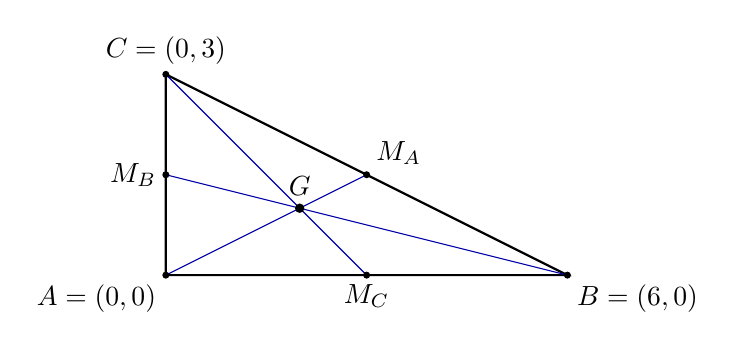
\begin{tikzpicture}[scale=.85]
 \coordinate (A) at (0,0); \coordinate (B) at (6,0);
 \coordinate (C) at (0,3); \coordinate (MA) at (3,1.5);
 \coordinate (MB) at (0,1.5); \coordinate (MC) at (3,0);
 \coordinate (G) at (2,1);
 \draw[thick] (A)--(B)--(C)--cycle;
 \draw[blue!65!black] (A)--(MA) (B)--(MB) (C)--(MC);
 \fill (G) circle (2pt) node[above=1pt] {$G$};
 \fill (A) circle (1.5pt) node[below left] {$A=(0,0)$};
 \fill (B) circle (1.5pt) node[below right] {$B=(6,0)$};
 \fill (C) circle (1.5pt) node[above] {$C=(0,3)$};
 \fill (MA) circle (1.5pt) node[above right] {$M_A$};
 \fill (MB) circle (1.5pt) node[left] {$M_B$};
 \fill (MC) circle (1.5pt) node[below] {$M_C$};
\end{tikzpicture}
\end{center}


\Needspace{5\baselineskip}
\par\bigskip
\noindent\textbf{1.7.10}\quad Prove the law of cosines starting from
$A^{2}=(\mathbf{B}-\mathbf{C})^{2}$.
\solution
Here $(\mathbf B-\mathbf C)^2$ means
$(\mathbf B-\mathbf C)\cdot(\mathbf B-\mathbf C)=|\mathbf B-\mathbf C|^2$,
and $A,B,C$ denote the side lengths $|\mathbf A|,|\mathbf B|,|\mathbf C|$.
Place the tails of $\mathbf B$ and $\mathbf C$ at the same triangle
vertex, and let $\theta$ be the included angle. The opposite side is
$\mathbf A=\mathbf B-\mathbf C$ up to orientation. Therefore
\[
 \begin{aligned}
 A^2&=(\mathbf B-\mathbf C)\cdot(\mathbf B-\mathbf C)
 =\mathbf B\cdot\mathbf B-\mathbf B\cdot\mathbf C
  -\mathbf C\cdot\mathbf B+\mathbf C\cdot\mathbf C\\
 &=\mathbf B\cdot\mathbf B+\mathbf C\cdot\mathbf C
       -2\mathbf B\cdot\mathbf C
 =B^2+C^2-2BC\cos\theta,
 \end{aligned}
\]
using $\mathbf C\cdot\mathbf B=\mathbf B\cdot\mathbf C$ and
$\mathbf B\cdot\mathbf C=BC\cos\theta$.
This is the law of cosines, reducing to Pythagoras when $\theta=\pi/2$.


\Needspace{5\baselineskip}
\par\bigskip
\noindent\textbf{1.7.11}\quad Given the three vectors,
\[
\mathbf{P}=3\hat{\mathbf{e}}_{x}+2\hat{\mathbf{e}}_{y}-\hat{\mathbf{e}}_{z},
\]
\[
\mathbf{Q}=-6\hat{\mathbf{e}}_{x}-4\hat{\mathbf{e}}_{y}+2\hat{\mathbf{e}}_{z},
\]
\[
\mathbf{R}=\hat{\mathbf{e}}_{x}-2\hat{\mathbf{e}}_{y}-\hat{\mathbf{e}}_{z},
\]
find two that are perpendicular and two that are parallel or antiparallel.
\solution
The component vectors are $\mathbf P=(3,2,-1)$,
$\mathbf Q=(-6,-4,2)$, and $\mathbf R=(1,-2,-1)$.
First $\mathbf Q=-2\mathbf P$, so $\mathbf P$ and $\mathbf Q$
are antiparallel. Next
\[
 \mathbf P\cdot\mathbf R=3(1)+2(-2)+(-1)(-1)=3-4+1=0,
\]
so $\mathbf P$ and $\mathbf R$ are perpendicular. Also
$\mathbf Q\cdot\mathbf R=-2(\mathbf P\cdot\mathbf R)=0$,
so $\mathbf Q$ and $\mathbf R$ form a second perpendicular pair.


\Needspace{9\baselineskip}
\subsection*{1.8 Complex Numbers and Functions}

\Needspace{5\baselineskip}
\par\bigskip
\noindent\textbf{1.8.1}\quad Find the reciprocal of $x+iy$, working in polar
form but expressing the final result in Cartesian form.
\solution
For $z=x+iy\ne0$, set $r=\sqrt{x^2+y^2}$ and
$z=r(\cos\theta+i\sin\theta)=re^{i\theta}$.
The reciprocal has magnitude $1/r$ and angle $-\theta$:
\[
 \frac1z=r^{-1}e^{-i\theta}
 =\frac1r(\cos\theta-i\sin\theta)
 =\boxed{\frac{x-iy}{x^2+y^2}}.
\]
Multiplication by $x+iy$ gives $(x^2+y^2)/(x^2+y^2)=1$,
checking the result. No reciprocal exists at $x=y=0$.


\Needspace{5\baselineskip}
\par\bigskip
\noindent\textbf{1.8.2}\quad Show that complex numbers have square roots and
that the square roots are contained in the complex plane. What are the square
roots of $i$?
\solution
Write a nonzero complex number as $z=re^{i\theta}$ with $r>0$.
The two numbers $w_k=\sqrt r\,e^{i(\theta/2+k\pi)}$, $k=0,1$,
satisfy $w_k^2=re^{i\theta}e^{2\pi ik}=z$. They are opposites and
are distinct. Conversely, if $w=\rho e^{i\phi}$ satisfies $w^2=z$,
then $\rho^2=r$ and $2\phi=\theta+2\pi k$, giving precisely these
two roots. Zero has the single distinct square root zero.
For $i=e^{i\pi/2}$ this gives
\[
 \boxed{\sqrt i=\pm e^{i\pi/4}=\pm\frac{1+i}{\sqrt2}}.
\]
Squaring either value gives $(1+2i-1)/2=i$.


\Needspace{5\baselineskip}
\par\bigskip
\noindent\textbf{1.8.3}\quad \erratum{For a nonnegative integer $n$ and real $\theta$,} show that
\begin{enumerate}
\item[(a)] $\displaystyle\cos n\theta=\cos^{n}\theta-\binom{n}{2}
  \cos^{n-2}\theta\sin^{2}\theta+\binom{n}{4}\cos^{n-4}\theta\sin^{4}\theta
  -\cdots,$
\item[(b)] $\displaystyle\sin n\theta=\binom{n}{1}\cos^{n-1}\theta\sin\theta
  -\binom{n}{3}\cos^{n-3}\theta\sin^{3}\theta+\cdots.$
\end{enumerate}
\solution
For a nonnegative integer $n$, de Moivre's formula and the binomial
expansion give
\[
 \cos n\theta+i\sin n\theta
 =(\cos\theta+i\sin\theta)^n
 =\sum_{j=0}^n\binom nj\cos^{n-j}\theta\,i^j\sin^j\theta.
\]
For $j=2r$, $i^{2r}=(-1)^r$, while for $j=2r+1$,
$i^{2r+1}=i(-1)^r$. Equating real and imaginary parts therefore yields
\[
 \cos n\theta=\sum_{r=0}^{\lfloor n/2\rfloor}
 (-1)^r\binom n{2r}\cos^{n-2r}\theta\sin^{2r}\theta,
\]
\[
 \sin n\theta=\sum_{r=0}^{\lfloor(n-1)/2\rfloor}
 (-1)^r\binom n{2r+1}\cos^{n-2r-1}\theta\sin^{2r+1}\theta.
\]
These are the two requested finite expansions. For $n=0$ the second
sum is empty and gives zero.


\Needspace{5\baselineskip}
\par\bigskip
\noindent\textbf{1.8.4}\quad Prove that
\begin{enumerate}
\item[(a)] $\displaystyle\sum_{n=0}^{N-1}\cos nx=\erratum{\frac{\sin(Nx/2)}{\sin(x/2)}\cos\!\left(\frac{(N-1)x}{2}\right)}$,
\item[(b)] $\displaystyle\sum_{n=0}^{N-1}\sin nx=\erratum{\frac{\sin(Nx/2)}{\sin(x/2)}\sin\!\left(\frac{(N-1)x}{2}\right)}$.
\end{enumerate}
\erratum{Here $N$ is a positive integer and $x$ is real; at $x=2\pi m$, use the continuous limits $N$ and $0$, respectively.} These series occur in the analysis of the multiple-slit diffraction pattern.
\solution
For $e^{ix}\ne1$, sum the finite geometric progression:
\[
 \sum_{n=0}^{N-1}e^{inx}=\frac{1-e^{iNx}}{1-e^{ix}}.
\]
Using $1-e^{it}=-2i e^{it/2}\sin(t/2)$ in numerator and denominator
reduces this to
\[
 \sum_{n=0}^{N-1}e^{inx}
 =e^{i(N-1)x/2}\frac{\sin(Nx/2)}{\sin(x/2)}.
\]
For real $x$ the sine quotient is real, so taking real and imaginary
parts gives (a) and (b). At $x=2\pi m$ the displayed quotient is
$0/0$, but the original sums are $N$ and $0$; these values are also
the continuous limits of the right sides. This supplies the removable
exception to the formulas.


\Needspace{5\baselineskip}
\par\bigskip
\noindent\textbf{1.8.5}\quad Assume that the trigonometric functions and the
hyperbolic functions are defined for complex argument by the appropriate power
series. Show that
\[
\erratum{i\sin z}=\sinh iz,\quad\sin iz=i\sinh z,
\]
\[
\cos z=\cosh iz,\quad\cos iz=\cosh z.
\]
\solution
\erratum{The first identity was mistranscribed: the textbook (p.~61)
has $i\sin z=\sinh(iz)$, not $i\sin(iz)=\sinh(iz)$.}
Direct substitution into the entire power series gives
\[
 \begin{aligned}
 \sinh(iz)&=\sum_{n=0}^\infty\frac{i^{2n+1}z^{2n+1}}{(2n+1)!}
       =i\sum_{n=0}^\infty\frac{(-1)^n z^{2n+1}}{(2n+1)!}=i\sin z,\\
 \sin(iz)&=\sum_{n=0}^\infty\frac{(-1)^n i^{2n+1}z^{2n+1}}{(2n+1)!}
       =i\sum_{n=0}^\infty\frac{z^{2n+1}}{(2n+1)!}=i\sinh z,\\
 \cosh(iz)&=\sum_{n=0}^\infty\frac{i^{2n}z^{2n}}{(2n)!}=\cos z,\\
 \cos(iz)&=\sum_{n=0}^\infty\frac{(-1)^n i^{2n}z^{2n}}{(2n)!}=\cosh z.
 \end{aligned}
\]
No restriction on complex $z$ is required because all four power
series converge absolutely everywhere.


\Needspace{5\baselineskip}
\par\bigskip
\noindent\textbf{1.8.6}\quad Using the identities
\[
\cos z=\frac{e^{iz}+e^{-iz}}{2},\quad\sin z=\frac{e^{iz}-e^{-iz}}{2i},
\]
established from comparison of power series, show that
\begin{enumerate}
\item[(a)] $\sin(x+iy)=\sin x\cosh y+i\cos x\sinh y$,\\
  $\cos(x+iy)=\cos x\cosh y-i\sin x\sinh y$,
\item[(b)] $|\sin z|^{2}=\sin^{2}x+\sinh^{2}y$,\quad
  $|\cos z|^{2}=\cos^{2}x+\sinh^{2}y$.
\end{enumerate}
This demonstrates that we may have $|\sin z|$, $|\cos z|>1$ in the complex
plane.
\solution
(a) For real $x,y$, $e^{i(x+iy)}=e^{-y}(\cos x+i\sin x)$ and
$e^{-i(x+iy)}=e^y(\cos x-i\sin x)$. Substituting these in the
exponential definitions and collecting terms gives
\[
 \begin{aligned}
 \sin(x+iy)&=\sin x\frac{e^y+e^{-y}}2
       +i\cos x\frac{e^y-e^{-y}}2
       =\sin x\cosh y+i\cos x\sinh y,\\
 \cos(x+iy)&=\cos x\cosh y-i\sin x\sinh y.
 \end{aligned}
\]
(b) Add the squares of each expression's real and imaginary parts:
\[
 \begin{aligned}
 |\sin z|^2&=\sin^2x\cosh^2y+\cos^2x\sinh^2y
 =\sin^2x+(\sin^2x+\cos^2x)\sinh^2y
 =\sin^2x+\sinh^2y,\\
 |\cos z|^2&=\cos^2x\cosh^2y+\sin^2x\sinh^2y
 =\cos^2x+\sinh^2y.
 \end{aligned}
\]
Here $\cosh^2y=1+\sinh^2y$ was used. For example
$|\cos(iy)|=\cosh y>1$ for $y\ne0$.


\Needspace{5\baselineskip}
\par\bigskip
\noindent\textbf{1.8.7}\quad From the identities in Exercises 1.8.5 and 1.8.6
show that
\begin{enumerate}
\item[(a)] $\sinh(x+iy)=\sinh x\cos y+i\cosh x\sin y$,\\
  $\cosh(x+iy)=\cosh x\cos y+i\sinh x\sin y$,
\item[(b)] $|\sinh z|^{2}=\sinh^{2}x+\sin^{2}y$,\quad
  \erratum{$|\cosh z|^{2}=\cosh^{2}x-\sin^{2}y$}.
\end{enumerate}
\solution
(a) Insert $e^{x+iy}=e^x(\cos y+i\sin y)$ and
$e^{-x-iy}=e^{-x}(\cos y-i\sin y)$ in the definitions of
$\sinh$ and $\cosh$. Subtracting and adding respectively yields
\[
 \sinh(x+iy)=\sinh x\cos y+i\cosh x\sin y,
 \quad
 \cosh(x+iy)=\cosh x\cos y+i\sinh x\sin y.
\]
(b) Consequently
\[
 \begin{aligned}
 |\sinh z|^2&=\sinh^2x\cos^2y+\cosh^2x\sin^2y
             =\sinh^2x+\sin^2y,\\
 |\cosh z|^2&=\cosh^2x\cos^2y+\sinh^2x\sin^2y
             =\cosh^2x-\sin^2y.
 \end{aligned}
\]
\erratum{The last sign is minus, correcting an error also present in
the textbook (p.~61).} At $x=0,y=\pi/2$, $\cosh(i\pi/2)=0$;
the corrected right side is $1-1=0$, whereas the printed plus sign
would give $2$. This independently checks the correction.


\Needspace{5\baselineskip}
\par\bigskip
\noindent\textbf{1.8.8}\quad \erratum{Put $z=x+iy$ with real $x,y$, and exclude the poles of each side.} Show that
\begin{enumerate}
\item[(a)] $\displaystyle\tanh\frac{z}{2}=\frac{\sinh x+i\sin y}{\cosh x+\cos y}$,
\item[(b)] $\displaystyle\coth\frac{z}{2}=\frac{\sinh x-i\sin y}{\cosh x-\cos y}$.
\end{enumerate}
\solution
Let $z=x+iy$ with $x,y$ real. From the exponential definitions,
$\tanh(z/2)=(e^z-1)/(e^z+1)$. Multiply numerator and denominator
by the conjugate $e^{x-iy}+1$ to obtain
\[
 \tanh\frac z2
 =\frac{e^{2x}-1+2ie^x\sin y}{e^{2x}+1+2e^x\cos y}
 =\frac{\sinh x+i\sin y}{\cosh x+\cos y}.
\]
Likewise $\coth(z/2)=(e^z+1)/(e^z-1)$. Multiplication by
$e^{x-iy}-1$ gives
\[
 \coth\frac z2
 =\frac{e^{2x}-1-2ie^x\sin y}{e^{2x}+1-2e^x\cos y}
 =\frac{\sinh x-i\sin y}{\cosh x-\cos y}.
\]
The divisions exclude the poles: $z=(2m+1)\pi i$ for $\tanh(z/2)$
and $z=2m\pi i$ for $\coth(z/2)$, $m\in\mathbb Z$.


\Needspace{5\baselineskip}
\par\bigskip
\noindent\textbf{1.8.9}\quad By comparing series expansions, show that
$\displaystyle\tan^{-1}x=\frac{i}{2}\erratum{\operatorname{Log}}\left(\frac{1-ix}{1+ix}\right)$, \erratum{for real $x$, with the principal inverse tangent and principal logarithm}.
\solution
For $|x|<1$, subtract the logarithm series on their branches through
$\log1=0$:
\[
 \log(1-ix)-\log(1+ix)
 =-2\left(ix+\frac{(ix)^3}3+\frac{(ix)^5}5+\cdots\right)
 =-2i\left(x-\frac{x^3}3+\frac{x^5}5-\cdots\right).
\]
Multiplication by $i/2$ gives exactly the Gregory series for $\arctan x$.
For all real $x$, $(1-ix)/(1+ix)$ has unit modulus and argument
$-2\arctan x\in(-\pi,\pi)$, so the principal logarithm satisfies
\[
 \boxed{\arctan x=\frac i2\operatorname{Log}\frac{1-ix}{1+ix}}.
\]
Other logarithm branches differ by $2\pi i m$ and change the right
side by $-\pi m$, the corresponding multivalued inverse-tangent branches.
For complex $x$, branch choices and the singularities $x=\pm i$
must be retained.


\Needspace{5\baselineskip}
\par\bigskip
\noindent\textbf{1.8.10}\quad Find the Cartesian form for all values of
\begin{enumerate}
\item[(a)] $(-8)^{1/3}$,
\item[(b)] $i^{1/4}$,
\item[(c)] $e^{i\pi/4}$.
\end{enumerate}
\solution
(a) Write $-8=8e^{i(\pi+2\pi k)}$. The cube roots have magnitude
$2$ and arguments $(\pi+2\pi k)/3$, $k=0,1,2$:
\[
 \boxed{1+i\sqrt3,\quad-2,\quad1-i\sqrt3}.
\]
(b) The fourth roots of $i=e^{i(\pi/2+2\pi k)}$ have arguments
$\pi/8+k\pi/2$, $k=0,1,2,3$. Set
$A=\sqrt{2+\sqrt2}/2$ and $B=\sqrt{2-\sqrt2}/2$; half-angle
identities give $\cos(\pi/8)=A$, $\sin(\pi/8)=B$. The four Cartesian
values are
\[
 \boxed{A+iB,\quad-B+iA,\quad-A-iB,\quad B-iA}.
\]
(c) The exponential is single-valued:
$\boxed{e^{i\pi/4}=(1+i)/\sqrt2}$.
Adding $2\pi$ to its angle reproduces this same value; it does not
create additional roots. Cubing the values in (a) or taking fourth
powers in (b) returns the specified original number.


\Needspace{5\baselineskip}
\par\bigskip
\noindent\textbf{1.8.11}\quad Find the polar form for all values of
\begin{enumerate}
\item[(a)] $(1+i)^{3}$,
\item[(b)] $(-1)^{1/5}$.
\end{enumerate}
\solution
(a) Since $1+i=\sqrt2 e^{i\pi/4}$,
\[
 \boxed{(1+i)^3=2\sqrt2 e^{3\pi i/4}}.
\]
This is one value, equal to $-2+2i$ in Cartesian form. Its argument
may be written $3\pi/4+2\pi m$, but all such choices represent the
same complex number.

(b) Write $-1=e^{i(\pi+2\pi k)}$. Its fifth roots are
\[
 \boxed{e^{i(2k+1)\pi/5},\qquad k=0,1,2,3,4}.
\]
They all have unit modulus. Their arguments are $\pi/5,3\pi/5,\pi,
7\pi/5,9\pi/5$, and raising any one to the fifth power gives
$e^{i(2k+1)\pi}=-1$. Values of $k$ outside this range repeat the roots.


\Needspace{9\baselineskip}
\subsection*{1.9 Derivatives and Extrema}

\Needspace{5\baselineskip}
\par\bigskip
\noindent\textbf{1.9.1}\quad Derive the following formula for the Maclaurin
expansion of a function of two variables \erratum{analytic near $(0,0)$, for $(x,y)$ within the convergence neighborhood of its Maclaurin series}:
\[
\begin{split}
f(x,y)=f(0,0)&+x\frac{\partial f}{\partial x}+y\frac{\partial f}{\partial y}\\
+\frac{1}{2!}\biggl[\binom{2}{0}x^{2}\frac{\partial^{2}f}{\partial x^{2}}
&+\binom{2}{1}xy\frac{\partial^{2}f}{\partial x\,\partial y}
+\binom{2}{2}y^{2}\frac{\partial^{2}f}{\partial y^{2}}\biggr]\\
+\frac{1}{3!}\biggl[\binom{3}{0}x^{3}\frac{\partial^{3}f}{\partial x^{3}}
&+\binom{3}{1}x^{2}y\frac{\partial^{3}f}{\partial x^{2}\,\partial y}
+\binom{3}{2}xy^{2}\frac{\partial^{3}f}{\partial x\,\partial y^{2}}
+\binom{3}{3}y^{3}\frac{\partial^{3}f}{\partial y^{3}}\biggr]+\cdots,
\end{split}
\]
where all the partial derivatives are to be evaluated at the point $(0,0)$.
\solution
\erratum{An infinite Taylor expansion represents the function only
where its remainder tends to zero; analyticity near the origin is a
sufficient hypothesis. Smoothness alone is not sufficient.}
Fix $x,y$ and define the one-variable function $F(t)=f(tx,ty)$.
The chain rule gives $F'(t)=(x\partial_x+y\partial_y)f(tx,ty)$.
Iterating, using commutation of the mixed partial derivatives, yields
\[
 F^{(n)}(0)=\sum_{j=0}^n\binom nj x^{n-j}y^j
          \frac{\partial^n f}{\partial x^{n-j}\partial y^j}(0,0).
\]
Taylor-expand $F$ about $t=0$ and then set $t=1$:
\[
 f(x,y)=\sum_{n=0}^\infty\sum_{j=0}^n
 \frac{x^{n-j}y^j}{(n-j)!j!}
 \frac{\partial^n f}{\partial x^{n-j}\partial y^j}(0,0).
\]
For $n=1$ this is $xf_x+yf_y$; for $n=2$ it is
$(x^2f_{xx}+2xyf_{xy}+y^2f_{yy})/2!$; for $n=3$ it is
$(x^3f_{xxx}+3x^2yf_{xxy}+3xy^2f_{xyy}+y^3f_{yyy})/3!$.
These are exactly the displayed terms. For a finite order $N$, ordinary
Taylor's theorem also provides a remainder $F^{(N+1)}(\theta)/(N+1)!$
for some $0<\theta<1$, under its usual real-variable hypotheses.


\Needspace{5\baselineskip}
\par\bigskip
\noindent\textbf{1.9.2}\quad The result in Exercise 1.9.1 can be generalized
to larger numbers of independent variables. Prove that for an $m$-variable
system \erratum{analytic near the origin, at points sufficiently close to it}, the Maclaurin expansion can be written in the symbolic form
\[
f(x_{1},\ldots,x_{m})
=\sum_{n=0}^{\infty}\frac{t^{n}}{n!}
\erratum{\left[\left(\sum_{i=1}^{m}\alpha_{i}
\frac{\partial}{\partial x_{i}}\right)^{n}f(\mathbf x)\right]_{\mathbf x=0}},
\]
where in the right-hand side we have made the substitutions $x_{j}=\alpha_{j}t$.
\solution
Define $F(t)=f(\alpha_1t,\ldots,\alpha_mt)$ with fixed $\alpha_i$.
The chain rule and induction give
\[
 F^{(n)}(t)=\left(\sum_{i=1}^m\alpha_i\partial_{x_i}\right)^n
 f(\alpha_1t,\ldots,\alpha_mt).
\]
Therefore Taylor's formula in $t$ is
\[
 F(t)=\sum_{n=0}^\infty\frac{t^n}{n!}
 \left[\left(\sum_{i=1}^m\alpha_i\partial_{x_i}\right)^n
 f(\mathbf x)\right]_{\mathbf x=0}.
\]
\erratum{The book's symbolic $D^nf(0)$ means that derivatives act on $f$ before evaluation at zero; the brackets in the corrected statement make this order explicit. Differentiating the constant $f(0)$ would instead give zero for $n>0$.} Since $x_i=\alpha_it$, this is the required symbolic
form. Explicitly the multinomial theorem gives
\[
 f(\mathbf x)=\sum_{r_1,\ldots,r_m\ge0}
 \frac{x_1^{r_1}\cdots x_m^{r_m}}{r_1!\cdots r_m!}
 (\partial_{x_1}^{r_1}\cdots\partial_{x_m}^{r_m}f)(0).
\]
\erratum{As in Exercise 1.9.1, equality to the infinite expansion
requires convergence to $f$; assume analyticity on the neighborhood
under consideration, or retain a finite Taylor remainder.}


\Needspace{9\baselineskip}
\subsection*{1.10 Evaluation of Integrals}

\Needspace{5\baselineskip}
\par\bigskip
\noindent\textbf{1.10.1}\quad Use a recursive method to show that, for all
positive integers $n$, $\Gamma(n)=(n-1)!$.

Evaluate the integrals in Exercises 1.10.2 through 1.10.9.
\solution
Start from $\Gamma(n)=\int_0^\infty t^{n-1}e^{-t}dt$ for $n>0$.
For an integer $n\ge1$, integration by parts gives
\[
 \Gamma(n+1)=\int_0^\infty t^n e^{-t}dt
 =[-t^n e^{-t}]_0^\infty+n\int_0^\infty t^{n-1}e^{-t}dt
 =n\Gamma(n).
\]
The boundary term vanishes because the exponential dominates any fixed
power at infinity and $t^n\to0$ at zero. The initial value is
$\Gamma(1)=\int_0^\infty e^{-t}dt=1$. Repeated application of the
recurrence yields $\Gamma(n)=(n-1)(n-2)\cdots1\,\Gamma(1)
=\boxed{(n-1)!}$, including $n=1$ with $0!=1$.


\Needspace{5\baselineskip}
\par\bigskip
\noindent\textbf{1.10.2}\quad $\displaystyle\int_{0}^{\infty}\frac{\sin x}{x}\,dx$.

\emph{Hint.}~Multiply integrand by $e^{-ax}$ and take the limit $\erratum{a\downarrow0}$.
\solution
For $a>0$ define $I(a)=\int_0^\infty e^{-ax}\sin x\,dx/x$.
Exponential decay permits differentiation under the integral:
\[
 I'(a)=-\int_0^\infty e^{-ax}\sin x\,dx
       =-\operatorname{Im}\frac1{a-i}=-\frac1{1+a^2}.
\]
Also $|I(a)|\le\int_0^\infty e^{-ax}dx=1/a$, so $I(a)\to0$
as $a\to\infty$. Integrating this derivative from $a$ to infinity gives
\[
 I(a)=\int_a^\infty\frac{dt}{1+t^2}=\frac\pi2-\arctan a.
\]
It remains to justify removing the damping. For $a\ge0$ the decreasing
function $g(x)=e^{-ax}/x$ satisfies $g'\le0$. On $[R,T]$,
\[
 \int_R^T g(x)\sin x\,dx=[-g(x)\cos x]_R^T+
                              \int_R^T g'(x)\cos x\,dx.
\]
Its absolute value is at most
$g(R)+g(T)+\int_R^T|g'(x)|dx
=g(R)+g(T)+g(R)-g(T)=2g(R)\le2/R$.
Taking $T\to\infty$ proves the same bound for the tail.
This tail bound is uniform in $a$, and the integral on $[0,R]$ tends
to its undamped value by dominated convergence. Thus the ordinary
improper integral equals $\lim_{a\downarrow0}I(a)$:
\[
 \boxed{\int_0^\infty\frac{\sin x}{x}dx=\frac\pi2}.
\]
The tail argument also proves convergence, rather than merely assigning
an Abel-summed value to the expression.


\Needspace{5\baselineskip}
\par\bigskip
\noindent\textbf{1.10.3}\quad $\displaystyle\int_{0}^{\infty}\frac{dx}{\cosh x}$.

\emph{Hint.}~\erratum{Expand the integrand using $e^{-x}$ for $x>0$, and control the integrated remainder at $x=0$.}
\solution
For $x>0$,
\[
 \frac1{\cosh x}=\frac{2e^{-x}}{1+e^{-2x}}
 =2\sum_{n=0}^N(-1)^ne^{-(2n+1)x}
  +\frac{2(-1)^{N+1}e^{-(2N+3)x}}{1+e^{-2x}}.
\]
The integral of the last term has absolute value at most $2/(2N+3)$,
so integrating and taking the limit is justified even though the
geometric series itself does not converge at $x=0$. \erratum{Thus the original hint's claim of series convergence at every relevant $x$ needs this endpoint qualification.} Therefore
\[
 \int_0^\infty\frac{dx}{\cosh x}
 =2\sum_{n=0}^\infty\frac{(-1)^n}{2n+1}=\boxed{\frac\pi2}.
\]
An independent substitution $t=e^{-x}$ gives
$2\int_0^1dt/(1+t^2)=2[\arctan t]_0^1=\pi/2$.


\Needspace{5\baselineskip}
\par\bigskip
\noindent\textbf{1.10.4}\quad
$\displaystyle\int_{0}^{\infty}\frac{dx}{e^{ax}+1}$, for $a>0$.
\solution
Set $u=e^{-ax}$ for $a>0$. Then $dx=-du/(au)$,
$e^{ax}=1/u$, and the limits $x=0,\infty$ become $u=1,0$.
Consequently
\[
 \int_0^\infty\frac{dx}{e^{ax}+1}
 =\frac1a\int_0^1\frac{du}{1+u}
 =\boxed{\frac{\ln2}{a}}.
\]
As a series check, for $x>0$ the integrand is
$e^{-ax}-e^{-2ax}+e^{-3ax}-\cdots$; integrating its finite geometric
remainder gives an error at most $1/[a(N+1)]$. Hence its integral is
$(1/a)\sum_{n\ge1}(-1)^{n-1}/n=(\ln2)/a$ as well.


\Needspace{5\baselineskip}
\par\bigskip
\noindent\textbf{1.10.5}\quad
$\displaystyle\int_{\pi}^{\infty}\frac{\sin x}{x^{2}}\,dx$.
\solution
Differentiate $\sin x/x$ to obtain
$\sin x/x^2=\cos x/x-d(\sin x/x)/dx$. On a finite interval $[\pi,R]$,
\[
 \int_\pi^R\frac{\sin x}{x^2}dx
 =\int_\pi^R\frac{\cos x}{x}dx-\left[\frac{\sin x}{x}\right]_\pi^R.
\]
The boundary term tends to zero because $\sin\pi=0$ and
$|\sin R/R|\le1/R$. With the convention
$\operatorname{Ci}(z)=-\int_z^\infty\cos t\,dt/t$ for $z>0$,
\[
 \boxed{\int_\pi^\infty\frac{\sin x}{x^2}dx
 =-\operatorname{Ci}(\pi)=-0.0736679120464255\ldots}.
\]
The negative sign is consistent with the negative first lobe on
$(\pi,2\pi)$ and the decreasing weights of subsequent lobes.
The verification script checks the result by oscillatory quadrature.


\Needspace{5\baselineskip}
\par\bigskip
\noindent\textbf{1.10.6}\quad
$\displaystyle\int_{0}^{\infty}\frac{e^{-x}\sin x}{x}\,dx$.
\solution
Use $I(a)$ derived in Exercise 1.10.2:
\[
 I(a)=\int_0^\infty\frac{e^{-ax}\sin x}{x}dx
     =\frac\pi2-\arctan a\quad(a>0).
\]
At $a=1$, this gives $\boxed{I(1)=\pi/4}$.
For a direct check, write $\sin x/x=\int_0^1\cos(tx)dt$;
absolute integrability of the exponentially damped double integral
permits interchanging integrals, giving
\[
 \int_0^1dt\int_0^\infty e^{-x}\cos(tx)dx
 =\int_0^1\frac{dt}{1+t^2}=\frac\pi4.
\]


\Needspace{5\baselineskip}
\par\bigskip
\noindent\textbf{1.10.7}\quad $\displaystyle\int_{0}^{x}\mathrm{erf}(t)\,dt$.

The result can be expressed in terms of special functions in Table 1.2.
\solution
From the definition of the error function,
$\operatorname{erf}'(t)=2e^{-t^2}/\sqrt\pi$. Integration by parts gives
\[
 \begin{aligned}
 \int_0^x\operatorname{erf}(t)dt
 &=[t\operatorname{erf}(t)]_0^x
   -\frac2{\sqrt\pi}\int_0^x t e^{-t^2}dt\\
 &=\boxed{x\operatorname{erf}(x)+\frac{e^{-x^2}-1}{\sqrt\pi}}.
 \end{aligned}
\]
Differentiating the answer cancels $2xe^{-x^2}/\sqrt\pi$ against
$-2xe^{-x^2}/\sqrt\pi$, leaving $\operatorname{erf}(x)$;
at $x=0$ the answer is zero. Both checks fix the additive constant.


\Needspace{5\baselineskip}
\par\bigskip
\noindent\textbf{1.10.8}\quad $\displaystyle\int_{1}^{x}E_{1}(t)\,dt$.

Obtain a result in which the only special function is $E_{1}$, \erratum{for real $x>0$}.
\solution
For $t>0$, $E_1(t)=\int_t^\infty e^{-u}du/u$ and hence
$E_1'(t)=-e^{-t}/t$. Integration by parts now gives
\[
 \begin{aligned}
 \int_1^x E_1(t)dt
 &=[tE_1(t)]_1^x-\int_1^x tE_1'(t)dt\\
 &=xE_1(x)-E_1(1)+\int_1^x e^{-t}dt\\
 &=\boxed{xE_1(x)-e^{-x}-E_1(1)+e^{-1}},\qquad x>0.
 \end{aligned}
\]
Its derivative is $E_1(x)+x(-e^{-x}/x)+e^{-x}=E_1(x)$,
and its value at $x=1$ is zero. Thus it has both the correct derivative
and the prescribed lower-limit constant.


\Needspace{5\baselineskip}
\par\bigskip
\noindent\textbf{1.10.9}\quad
$\displaystyle\int_{0}^{\infty}\frac{e^{-x}}{x+1}\,dx$.
\solution
Set $u=x+1$, so $e^{-x}=e\,e^{-u}$ and $dx=du$. The limits are
$u=1$ and $u=\infty$, and therefore
\[
 \int_0^\infty\frac{e^{-x}}{x+1}dx
 =e\int_1^\infty\frac{e^{-u}}u du
 =\boxed{eE_1(1)=0.596347362323194\ldots}.
\]
The integral is convergent because its integrand is bounded at zero
and bounded above by $e^{-x}$ for $x\ge0$. Direct positive-integrand
quadrature in the supplementary script checks the numerical value.


\Needspace{5\baselineskip}
\par\bigskip
\noindent\textbf{1.10.10}\quad Show that
$\displaystyle\int_{0}^{\infty}\left(\frac{\tan^{-1}x}{x}\right)^{2}dx
=\pi\ln2$.

\emph{Hint.}~Integrate by parts, to linearize in $\tan^{-1}$. Then replace
$\tan^{-1}x$ by $\tan^{-1}ax$ and evaluate for $a=1$.
\solution
Integrate by parts with $u=(\arctan x)^2$ and $dv=dx/x^2$:
\[
 I=\left[-\frac{(\arctan x)^2}{x}\right]_0^\infty
       +2\int_0^\infty\frac{\arctan x}{x(1+x^2)}dx.
\]
The boundary term vanishes: near zero its magnitude is $O(x)$, and
at infinity it is $O(1/x)$. Define, for $a\ge0$,
\[
 J(a)=2\int_0^\infty\frac{\arctan(ax)}{x(1+x^2)}dx,
 \qquad I=J(1),\qquad J(0)=0.
\]
Differentiation is dominated by $2/(1+x^2)$ and yields
\[
 J'(a)=2\int_0^\infty\frac{dx}{(1+x^2)(1+a^2x^2)}.
\]
For $a>0$, $a\ne1$, partial fractions give
\[
 \frac1{(1+x^2)(1+a^2x^2)}
 =\frac1{1-a^2}\left(\frac1{1+x^2}-\frac{a^2}{1+a^2x^2}\right),
\]
so $J'(a)=2(\pi/2-a\pi/2)/(1-a^2)=\pi/(1+a)$.
Continuity of the integral extends this to $a=0,1$.
Integrating from $0$ to $a$ gives $J(a)=\pi\ln(1+a)$, and hence
$\boxed{I=\pi\ln2}$.


\Needspace{5\baselineskip}
\par\bigskip
\noindent\textbf{1.10.11}\quad By direct integration in Cartesian coordinates,
find the area of the ellipse with \erratum{positive semiaxes $a,b$}, defined by
\[
\frac{x^{2}}{a^{2}}+\frac{y^{2}}{b^{2}}=1.
\]
\solution
Take $a,b>0$. In the first quadrant the ellipse has upper boundary
$y=b\sqrt{1-x^2/a^2}$, $0\le x\le a$. Reflection symmetry gives
\[
 A=4b\int_0^a\sqrt{1-x^2/a^2}\,dx.
\]
Use $x=a\sin\theta$, $dx=a\cos\theta\,d\theta$, with
$0\le\theta\le\pi/2$:
\[
 A=4ab\int_0^{\pi/2}\cos^2\theta\,d\theta
  =2ab\left[\theta+\frac12\sin2\theta\right]_0^{\pi/2}
  =\boxed{\pi ab}.
\]
For $a=b=r$ this reduces to the circle area $\pi r^2$, checking the
scale and numerical coefficient.


\Needspace{5\baselineskip}
\par\bigskip
\noindent\textbf{1.10.12}\quad A unit circle is divided into two pieces by a
straight line whose distance of closest approach to the center is $1/2$ unit.
By evaluating a suitable integral, find the area of the smaller piece thereby
produced. Then use simple geometric considerations to verify your answer.
\solution
Rotate coordinates so that the cutting line is $x=1/2$ in the unit
circle $x^2+y^2=1$. The smaller cap has vertical extent
$2\sqrt{1-x^2}$, so
\[
 \begin{aligned}
 A&=2\int_{1/2}^1\sqrt{1-x^2}\,dx\\
  &=\left[x\sqrt{1-x^2}+\arcsin x\right]_{1/2}^1
   =\frac\pi2-\left(\frac{\sqrt3}4+\frac\pi6\right)
   =\boxed{\frac\pi3-\frac{\sqrt3}4}.
 \end{aligned}
\]
For the geometric check, the chord's endpoints make angles $\pm\pi/3$
with the positive $x$ axis. The sector between them has angle $2\pi/3$
and area $(1/2)(2\pi/3)=\pi/3$. The triangle cut off from that sector
has base $\sqrt3$ and altitude $1/2$, hence area $\sqrt3/4$.
Subtracting gives the same cap area.


\Needspace{9\baselineskip}
\subsection*{1.11 Dirac Delta Function}

\Needspace{5\baselineskip}
\par\bigskip
\noindent\textbf{1.11.1}\quad Let
\[
\delta_{n}(x)=\begin{cases}
0, & x<-\dfrac{1}{2n},\\[6pt]
n, & -\dfrac{1}{2n}<x<\dfrac{1}{2n},\\[6pt]
0, & \dfrac{1}{2n}<x.
\end{cases}
\]
Show that
\[
\lim_{n\to\infty}\int_{-\infty}^{\infty}f(x)\delta_{n}(x)\,dx=f(0),
\]
assuming that $f(x)$ is \erratum{locally integrable and} continuous at $x=0$.
\solution
The rectangle has width $1/n$ and height $n$, so its integral is $1$.
Subtracting $f(0)$ under the integral gives the useful explicit bound
\[
 \begin{aligned}
 \left|\int_{\mathbb R}f(x)\delta_n(x)dx-f(0)\right|
 &=\left|n\int_{-1/(2n)}^{1/(2n)}[f(x)-f(0)]dx\right|\\
 &\le\sup_{|x|\le1/(2n)}|f(x)-f(0)|.
 \end{aligned}
\]
Continuity at zero makes the supremum tend to zero: for each
$\epsilon>0$, take $\eta>0$ with $|f(x)-f(0)|<\epsilon$ when
$|x|<\eta$, then take $n>1/(2\eta)$. This proves the desired limit.
The unspecified values at the two endpoints do not affect an integral.


\Needspace{5\baselineskip}
\par\bigskip
\noindent\textbf{1.11.2}\quad For
\[
\delta_{n}(x)=\frac{n}{\pi}\,\frac{1}{1+n^{2}x^{2}},
\]
show that
\[
\int_{-\infty}^{\infty}\delta_{n}(x)\,dx=1.
\]
\solution
For $n>0$ use $u=nx$, so $dx=du/n$. Then
\[
 \int_{-\infty}^\infty\delta_n(x)dx
 =\frac1\pi\int_{-\infty}^\infty\frac{du}{1+u^2}
 =\frac1\pi[\arctan u]_{-\infty}^\infty
 =\frac1\pi\left(\frac\pi2+\frac\pi2\right)=1.
\]
This proves normalization for each $n$, not merely in the limit.
It also displays why the numerator must contain the factor $n$.


\Needspace{5\baselineskip}
\par\bigskip
\noindent\textbf{1.11.3}\quad Fejer's method of summing series is associated
with the function
\[
\delta_{n}(t)=\frac{1}{2\pi n}\left[\frac{\sin(nt/2)}{\sin(t/2)}\right]^{2}.
\]
Show that $\delta_{n}(t)$ is a delta distribution \erratum{on one period, for continuous $f$,} in the sense that
\[
\lim_{n\to\infty}\frac{1}{2\pi n}\erratum{\int_{-\pi}^{\pi}}f(t)
\left[\frac{\sin(nt/2)}{\sin(t/2)}\right]^{2}dt=f(0).
\]
\solution
\erratum{The printed whole-line assertion is false. On one period,
$\int_{-\pi}^{\pi} f(t)\delta_n(t)dt\to f(0)$ for continuous $f$.
On the whole real line the distributional limit is instead the comb
$\sum_{m\in\mathbb Z}\delta(t-2\pi m)$.}
For integer $n\ge1$, the finite geometric sum gives
\[
 \delta_n(t)=\frac1{2\pi n}\left|\sum_{j=0}^{n-1}e^{ijt}\right|^2
 =\frac1{2\pi}\sum_{k=-(n-1)}^{n-1}
                  \left(1-\frac{|k|}{n}\right)e^{ikt}.
\]
The modulus-square expression proves positivity; integrating the finite
Fourier sum over $[-\pi,\pi]$ leaves only its constant term, giving
$\int_{-\pi}^{\pi}\delta_n(t)dt=1$.
For any $0<\eta<\pi$, if $\eta\le|t|\le\pi$ then
\[
 0\le\delta_n(t)\le\frac1{2\pi n\sin^2(\eta/2)},\qquad
 \int_{\eta\le|t|\le\pi}\delta_n(t)dt
       \le\frac1{n\sin^2(\eta/2)}\to0.
\]
Subtract $f(0)$ and split the integral into $|t|<\eta$ and its
complement. The first part is at most
$\sup_{|t|<\eta}|f(t)-f(0)|$, which continuity makes arbitrarily small.
For bounded continuous $f$ the second is at most
$2\|f\|_\infty/[n\sin^2(\eta/2)]\to0$. This proves the one-period result.
For a smooth compactly supported test function on the whole line,
partition its support into periods and use $2\pi$-periodicity of
$\delta_n$. The same argument gives
\[
 \lim_{n\to\infty}\int_{\mathbb R} f(t)\delta_n(t)dt
       =\sum_{m\in\mathbb Z} f(2\pi m).
\]
Only finitely many terms occur for such a test function. Choosing it
supported near $2\pi$, with $f(2\pi)=1$ and $f(0)=0$, directly
contradicts the original claim and verifies the correction.


\Needspace{5\baselineskip}
\par\bigskip
\noindent\textbf{1.11.4}\quad Prove that
\[
\delta[a(x-x_{1})]=\erratum{\frac{1}{|a|}}\,\delta(x-x_{1}),\qquad \erratum{a\ne0}.
\]
\emph{Note.}~\erratum{The absolute value is required for all real nonzero $a$, including negative $a$.}
\solution
\erratum{For every real $a\ne0$ the factor is $1/|a|$; evenness is
not an optional extra convention for the Dirac distribution.}
Test the identity against a smooth compactly supported $\phi$ and
make the change of variable $u=a(x-x_1)$. The orientation of the
integration limits changes when $a<0$, producing the absolute Jacobian:
\[
 \int_{\mathbb R}\phi(x)\delta(a(x-x_1))dx
 =\frac1{|a|}\int_{\mathbb R}\phi(x_1+u/a)\delta(u)du
 =\frac{\phi(x_1)}{|a|}.
\]
This equals the action of $\delta(x-x_1)/|a|$, proving the distribution
identity. For $a>0$ it reduces to the printed factor $1/a$.
The value $a=0$ is excluded because $\delta(0)$ is not a distribution
obtained by this change of variable.


\Needspace{5\baselineskip}
\par\bigskip
\noindent\textbf{1.11.5}\quad \erratum{For distinct real $x_1,x_2$,} show that
\[
\delta[(x-x_{1})(x-x_{2})]
=[\delta(x-x_{1})+\delta(x-x_{2})]/|x_{1}-x_{2}|.
\]
\emph{Hint.}~Try using Exercise 1.11.4.
\solution
\erratum{Assume distinct real roots $x_1\ne x_2$.}
Let $g(x)=(x-x_1)(x-x_2)$. Near either simple root, use the local
variable $u=g(x)$, with $dx=du/|g'(x)|$ in a real integral.
Since
\[
 g'(x)=2x-x_1-x_2,\quad
 g'(x_1)=x_1-x_2,\quad g'(x_2)=x_2-x_1,
\]
a test function $\phi$ has integral
\[
 \int_{\mathbb R}\phi(x)\delta(g(x))dx
 =\frac{\phi(x_1)}{|x_1-x_2|}+\frac{\phi(x_2)}{|x_2-x_1|}.
\]
There is no contribution away from the roots, where $g$ stays away
from zero locally. Recognizing the two evaluation functionals proves
\[
 \delta((x-x_1)(x-x_2))
 =\frac{\delta(x-x_1)+\delta(x-x_2)}{|x_1-x_2|}.
\]
For coincident roots the Jacobian vanishes and this formula does not
apply; its singular denominator cannot simply be assigned a value.


\Needspace{5\baselineskip}
\par\bigskip
\noindent\textbf{1.11.6}\quad Using the Gauss error curve delta sequence
$\delta_{n}=\dfrac{n}{\sqrt{\pi}}e^{-n^{2}x^{2}}$, show that
\[
\erratum{x\frac{d}{dx}\delta(x)}=-\delta(x),
\]
treating $\delta(x)$ and its derivative as in Eq.~(1.157).
\solution
\erratum{The textbook (p.~81) asks for $x\delta'(x)=-\delta(x)$.
The transcribed derivative of the product is incorrect:
$(x\delta(x))'=0$, since $x\delta(x)=0$.}
For the specified Gaussian sequence,
\[
 \delta_n'(x)=-\frac{2n^3x}{\sqrt\pi}e^{-n^2x^2}.
\]
Against a smooth compactly supported test function $\phi$, substitute
$y=nx$ to obtain
\[
 \int_{\mathbb R}x\delta_n'(x)\phi(x)dx
 =-\frac2{\sqrt\pi}\int_{\mathbb R}y^2e^{-y^2}\phi(y/n)dy.
\]
Dominated convergence is justified by the integrable bound
$\|\phi\|_\infty y^2e^{-y^2}$. Integration by parts gives
\[
 \int_{\mathbb R}y^2e^{-y^2}dy
 =-\frac12[y e^{-y^2}]_{-\infty}^\infty
       +\frac12\int_{\mathbb R}e^{-y^2}dy=\frac{\sqrt\pi}{2}.
\]
Hence the limit is $-\phi(0)$, exactly the action of $-\delta$.
This proves $x\delta'=-\delta$. The product rule then gives
$(x\delta)'=\delta+x\delta'=0$, an independent consistency check.


\Needspace{5\baselineskip}
\par\bigskip
\noindent\textbf{1.11.7}\quad Show that
\[
\int_{-\infty}^{\infty}\delta'(x)f(x)\,dx=-f'(0).
\]
Here we assume that $f'(x)$ is continuous at $x=0$.
\solution
A distributional derivative is defined by its action on test functions,
$\langle T',f\rangle=-\langle T,f'\rangle$. Taking $T=\delta$ gives
\[
 \boxed{\int_{\mathbb R}\delta'(x)f(x)dx=-f'(0)}.
\]
To check this from regular functions, use a smooth delta sequence
$\delta_n$ and a smooth compactly supported $f$. Ordinary integration
by parts gives
\[
 \int_{\mathbb R}\delta_n'(x)f(x)dx
 =[\delta_n(x)f(x)]_{-\infty}^\infty
    -\int_{\mathbb R}\delta_n(x)f'(x)dx
 =-\int_{\mathbb R}\delta_n(x)f'(x)dx.
\]
The boundary term vanishes by compact support. Continuity of $f'$ at
zero then makes the last integral tend to $-f'(0)$, reproducing the
distributional definition and fixing the minus sign.
Only the values near zero matter: multiply any locally $C^1$ function
by a smooth cutoff equal to $1$ there. Since $\delta'$ is supported
at zero, this leaves its action unchanged. The identity therefore
extends to the local regularity stated in the question without imposing
any behavior on $f$ at infinity.


\Needspace{5\baselineskip}
\par\bigskip
\noindent\textbf{1.11.8}\quad Prove that
\[
\delta(f(x))=\erratum{\frac{1}{|f\prime(x_0)|}}\delta(x-x_{0}),
\]
where \erratum{$f$ is real and $C^1$, and $x_0$ is its unique simple real zero, so $f(x_0)=0$ and $f\prime(x_0)\ne0$}.

\emph{Hint.}~\erratum{Use the local variable $u=f(x)$ and the absolute Jacobian $1/|f\prime(x_0)|$ at each simple zero.}
\solution
\erratum{For a unique simple real zero $x_0$, the factor must be
$1/|f'(x_0)|$. For multiple simple zeros, add their contributions.}
Let $f$ be a real $C^1$ function on the domain under consideration,
with $f'(x_i)\ne0$ at every zero $x_i$. The inverse function theorem supplies a local
inverse $x=x_i(u)$ for $u=f(x)$. Restricting a test function $\phi$
to this neighborhood and changing variables gives
\[
 \int\phi(x)\delta(f(x))dx
 =\int\frac{\phi(x_i(u))}{|f'(x_i(u))|}\delta(u)du
 =\frac{\phi(x_i)}{|f'(x_i)|}.
\]
A partition into neighborhoods of the zeros (only finitely many in a
compact test support) therefore yields
\[
 \boxed{\delta(f(x))=\sum_{i:f(x_i)=0}
                  \frac{\delta(x-x_i)}{|f'(x_i)|}}.
\]
The printed single-root formula is recovered only with the additional
positive-derivative assumption. A negative derivative reverses limits,
which is why the absolute value is necessary. A repeated zero has
$f'(x_i)=0$ and lies outside this formula's hypotheses.


\Needspace{5\baselineskip}
\par\bigskip
\noindent\textbf{1.11.9}\quad
\begin{enumerate}
\item[(a)] If we define a sequence $\delta_{n}(x)=n/(2\cosh^{2}nx)$, show that
  \[
  \int_{-\infty}^{\infty}\delta_{n}(x)\,dx=1,\quad\text{independent of }n.
  \]
\item[(b)] Continuing this analysis, show that\footnote{Many other symbols are
  used for this function. This is the AMS-55 notation (in Additional Readings,
  see Abramowitz and Stegun): $u$ for unit.}
  \[
  \int_{-\infty}^{x}\erratum{\delta_{n}(t)\,dt}=\frac{1}{2}[1+\tanh nx]\equiv u_{n}(x)
  \]
  and
  \[
  \lim_{n\to\infty}u_{n}(x)=\begin{cases}0,&x<0,\\1,&x>0.\end{cases}
  \]
  This is the Heaviside unit step function (Fig.~1.23).
\end{enumerate}
\solution
(a) For $n>0$, substitute $u=nx$:
\[
 \int_{-\infty}^\infty\frac{n}{2\cosh^2(nx)}dx
 =\frac12\int_{-\infty}^\infty\operatorname{sech}^2u\,du
 =\frac12[\tanh u]_{-\infty}^\infty=1.
\]
(b) \erratum{Use a separate dummy variable in the integral.} Since
$d(\tanh nt)/dt=n\operatorname{sech}^2(nt)$,
\[
 u_n(x)=\int_{-\infty}^x\delta_n(t)dt
       =\frac12[\tanh(nt)]_{t=-\infty}^{t=x}
       =\frac12[1+\tanh(nx)].
\]
If $x>0$, $nx\to+\infty$ and $u_n(x)\to1$; if $x<0$,
$nx\to-\infty$ and $u_n(x)\to0$. At $x=0$ every $u_n(0)=1/2$,
so this symmetric sequence selects the convention $u(0)=1/2$.
The value at a single point does not affect its distributional derivative,
which is $\delta$.

\clearpage
\section{Chapter 2. Determinants and Matrices}
% Problems, Chapter 2: Determinants and Matrices
% Arfken, Weber & Harris, Mathematical Methods for Physicists, 7th ed.
% Requires: amsmath, amssymb, tikz

\section*{Problems}

\Needspace{9\baselineskip}
\subsection*{2.1 Determinants}

\Needspace{5\baselineskip}
\par\bigskip
\noindent\textbf{2.1.1}\quad Evaluate the following determinants:
\begin{enumerate}
\item[(a)] $\begin{vmatrix}1&0&1\\0&1&0\\1&0&0\end{vmatrix}$,\quad
\item[(b)] $\begin{vmatrix}1&2&0\\3&1&2\\0&3&1\end{vmatrix}$,\quad
\item[(c)] $\dfrac{1}{\sqrt{2}}\begin{vmatrix}
  0&\sqrt{3}&0&0\\ \sqrt{3}&0&2&0\\ 0&2&0&\sqrt{3}\\
  0&0&\sqrt{3}&0\end{vmatrix}$.
\end{enumerate}
\solution
Expand along a row or column containing as many zeros as possible.
\begin{enumerate}
\item[(a)] Only the middle entry of row 2 contributes:
\[
D_a=1(-1)^{2+2}
\begin{vmatrix}1&1\\1&0\end{vmatrix}
=1(1\cdot0-1\cdot1)=\boxed{-1}.
\]
\item[(b)] Expansion along row 1 gives
\[
D_b=1\begin{vmatrix}1&2\\3&1\end{vmatrix}
-2\begin{vmatrix}3&2\\0&1\end{vmatrix}
 =1(1-6)-2(3-0)=\boxed{-11}.
\]
\item[(c)] Write $s=\sqrt3$. The factor $1/\sqrt2$ in the question
multiplies the determinant once; it is not a factor on each row.
Expand along row 1, whose only nonzero entry is $a_{12}=s$ with sign
$(-1)^{1+2}=-1$, and then along column 1 of the resulting minor, whose
only nonzero entry is $s$ in position $(1,1)$:
\[
\begin{aligned}
D_c
&=-\frac{s}{\sqrt2}
\begin{vmatrix}s&2&0\\0&0&s\\0&s&0\end{vmatrix}
 =-\frac{s^2}{\sqrt2}
\begin{vmatrix}0&s\\s&0\end{vmatrix}\\
&=-\frac{3}{\sqrt2}(0-3)=\boxed{\frac9{\sqrt2}}.
\end{aligned}
\]
\end{enumerate}

\Needspace{5\baselineskip}
\par\bigskip
\noindent\textbf{2.1.2}\quad Test the set of linear homogeneous equations
\[
x+3y+3z=0,\quad x-y+z=0,\quad 2x+y+3z=0
\]
to see if it possesses a nontrivial solution. In any case, find a solution to
this equation set.
\solution
The coefficient determinant, expanded along row 1, is
\[
\begin{aligned}
D&=\begin{vmatrix}1&3&3\\1&-1&1\\2&1&3\end{vmatrix}\\
 &=1(-3-1)-3(3-2)+3(1+2)=-4-3+9=2.
\end{aligned}
\]
Since $D\ne0$, only the trivial solution is possible. Directly,
the second equation gives $x=y-z$. The first and third then become
\[
(y-z)+3y+3z=4y+2z=0,\qquad
2(y-z)+y+3z=3y+z=0.
\]
Thus $z=-2y$ and $z=-3y$, so $y=0$, $z=0$, and $x=0$:
$\boxed{(x,y,z)=(0,0,0)}$.
Substitution into each original equation gives zero.

\Needspace{5\baselineskip}
\par\bigskip
\noindent\textbf{2.1.3}\quad Given the pair of equations
\[
x+2y=3,\quad 2x+4y=6,
\]
\begin{enumerate}
\item[(a)] Show that the determinant of the coefficients vanishes.
\item[(b)] Show that the numerator determinants, see Eq.~(2.18), also vanish.
\item[(c)] Find at least two solutions.
\end{enumerate}
\solution
\textbf{(a), (b)} The coefficient determinant $D$ and the numerator
determinants $D_x$, $D_y$ of Cramer's rule are
\[
D=\begin{vmatrix}1&2\\2&4\end{vmatrix}=4-4=0,\quad
D_x=\begin{vmatrix}3&2\\6&4\end{vmatrix}=12-12=0,\quad
D_y=\begin{vmatrix}1&3\\2&6\end{vmatrix}=6-6=0.
\]
\textbf{(c)} The quotients $D_x/D,D_y/D$ are undefined and cannot
determine a unique solution. The second equation is twice the first,
so put $y=t$. Then $x=3-2t$, and every real solution is
\[
\boxed{(x,y)=(3-2t,t),\quad t\in\mathbb R}.
\]
(Complex $t$ is allowed if complex solutions are sought.)
For example $t=0$ gives $(3,0)$, and $t=1$ gives $(1,1)$.
Both satisfy $x+2y=3$ and hence $2x+4y=6$.

\Needspace{5\baselineskip}
\par\bigskip
\noindent\textbf{2.1.4}\quad If $C_{ij}$ is the cofactor of element $a_{ij}$,
formed by striking out the $i$th row and $j$th column and including a sign
$(-1)^{i+j}$, show that
\begin{enumerate}
\item[(a)] $\displaystyle\sum_{i}a_{ij}C_{ij}=\sum_{i}a_{ji}C_{ji}=|\mathsf{A}|$,
  where $|\mathsf{A}|$ is the determinant with the elements $a_{ij}$,
\item[(b)] $\displaystyle\sum_{i}a_{ij}C_{ik}=\sum_{i}a_{ji}C_{ki}=0$,
  $j\neq k$.
\end{enumerate}
\solution
Let $A_{\widehat i,\widehat j}$ denote $A$ with row $i$ and column $j$
struck out, so that $C_{ij}=(-1)^{i+j}\det A_{\widehat i,\widehat j}$.
For fixed $j$, Laplace expansion down column $j$ is
$\det A=\sum_i a_{ij}(-1)^{i+j}\det A_{\widehat i,\widehat j}
=\sum_i a_{ij}C_{ij}$.
Expansion across row $j$ similarly gives
$\det A=\sum_i a_{ji}C_{ji}$. This proves (a), without assuming
invertibility.

For (b), replace column $k$ of $A$ by its column $j$, with $j\ne k$,
and call the result $B$. Columns $j$ and $k$ of $B$ are identical, so
$\det B=0$. Expanding down column $k$, each minor is unchanged
from $A$ because that column is deleted; its cofactor is $C_{ik}$.
The entry being multiplied by that cofactor is now $a_{ij}$. Therefore
\[
0=\det B=\sum_i a_{ij}C_{ik}.
\]
Replacing row $k$ by row $j$ and expanding across row $k$ gives,
by the same argument, $0=\sum_i a_{ji}C_{ki}$.

\Needspace{5\baselineskip}
\par\bigskip
\noindent\textbf{2.1.5}\quad A determinant with all elements of order unity
may be surprisingly small. The Hilbert determinant
$H_{ij}=(i+j-1)^{-1}$, $i,j=1,2,\ldots,n$ is notorious for its small values.
\begin{enumerate}
\item[(a)] Calculate the value of the Hilbert determinants of order $n$ for
  $n=1$, $2$, and $3$.
\item[(b)] If an appropriate subroutine is available, find the Hilbert
  determinants of order $n$ for $n=4$, $5$, and $6$.
\end{enumerate}
\par\nobreak\hfill\emph{ANS.}\enspace
$\begin{array}{cr}
n&\mathrm{Det}(H_{n})\\
1&1.\\
2&8.33333\times10^{-2}\\
3&4.62963\times10^{-4}\\
4&1.65344\times10^{-7}\\
5&3.74930\times10^{-12}\\
6&5.36730\times10^{-18}.
\end{array}$
\solution
\textbf{(a)} Use exact fractions so that small determinants are not lost
by subtracting rounded numbers. The first three determinants ($D_3$
expanded along row 1) are
\[
D_1=1,\qquad D_2=1\cdot\frac13-\frac12\cdot\frac12=\frac1{12},
\]
\[
\begin{aligned}
D_3
&=\left(\frac1{15}-\frac1{16}\right)
-\frac12\left(\frac1{10}-\frac1{12}\right)
+\frac13\left(\frac18-\frac19\right)\\
&=\frac1{240}-\frac1{120}+\frac1{216}
=\frac{9-18+10}{2160}=\frac1{2160}.
\end{aligned}
\]

\textbf{(b)} For the larger matrices, Gaussian elimination uses
\[
R_i\longleftarrow R_i-\frac{u_{ik}}{u_{kk}}R_k
\quad(i=k+1,\ldots,n;\ k=1,\ldots,n-1),
\]
where $u_{ik}$ is the current entry in row $i$, column $k$; row $k$ no
longer changes after step $k-1$, so $u_{kk}$ is the $k$th pivot.
Each operation preserves the determinant. For example, the first
step on $H_6$ changes an entry with $i,j\ge2$ into
\[
\frac1{i+j-1}-\frac1i\frac1j
=\frac{(i-1)(j-1)}{ij(i+j-1)}.
\]
Every later step has the same structure. Suppose that before step $k$
the entries with $i,j\ge k$ have the form $\alpha_i\beta_j/(i+j-1)$;
for $H_6$ itself $\alpha_i=\beta_j=1$. The multiplier for row $i$ is
then
\[
\frac{u_{ik}}{u_{kk}}
=\frac{\alpha_i\beta_k/(i+k-1)}{\alpha_k\beta_k/(2k-1)}
=\frac{\alpha_i}{\alpha_k}\,\frac{2k-1}{i+k-1}.
\]
Subtracting it times the row-$k$ entry $\alpha_k\beta_j/(k+j-1)$ and
using the identity (expand both products)
\[
(i+k-1)(j+k-1)-(2k-1)(i+j-1)=ij-k(i+j)+k^2=(i-k)(j-k)
\]
turns the entry in row $i$, column $j$ into
\[
\alpha_i\beta_j\left[\frac1{i+j-1}-\frac{2k-1}{(i+k-1)(j+k-1)}\right]
=\frac{\alpha_i\beta_j\,(i-k)(j-k)}{(i+k-1)(j+k-1)(i+j-1)}.
\]
The form is preserved, with $\alpha_i$ multiplied by $(i-k)/(i+k-1)$
and $\beta_j$ by $(j-k)/(j+k-1)$; for $k=1$ this is the formula above.
Hence at step $k$
\[
\alpha_k=\beta_k=\prod_{m=1}^{k-1}\frac{k-m}{k+m-1}
=\frac{[(k-1)!]^2}{(2k-2)!},\qquad
u_{kk}=\frac{\alpha_k\beta_k}{2k-1}
=\frac{[(k-1)!]^4}{(2k-2)!\,(2k-1)!},
\]
because $\prod_{m=1}^{k-1}(k-m)=(k-1)!$,
$\prod_{m=1}^{k-1}(k+m-1)=k(k+1)\cdots(2k-2)=(2k-2)!/(k-1)!$, and
$(2k-2)!\,(2k-1)=(2k-1)!$. Successive pivots therefore have the ratio
\[
\frac{u_{k+1,k+1}}{u_{kk}}
=\frac{k^4}{(2k-1)(2k)\cdot(2k)(2k+1)}
=\frac{k^2}{4(4k^2-1)}
=\frac1{12},\ \frac1{15},\ \frac9{140},\ \frac4{63},\ \frac{25}{396}
\quad(k=1,\ldots,5),
\]
which, starting from $u_{11}=1$, gives the pivots $1$, $1/12$, $1/180$,
$1/2800$, $1/44100$, $1/698544$ for $k=1,\ldots,6$. The other entries
of row $k$ of the final triangular matrix are
$u_{kj}=\alpha_k\beta_j/(k+j-1)$ for $j>k$,
with $\beta_j=\prod_{m=1}^{k-1}(j-m)/(j+m-1)$.
For completeness, the multipliers $u_{ik}/u_{kk}$ in the successive
steps are listed below. At step $k$, subtract the indicated multiple
of the current row $k$ from each listed row $i$:
\[
\begin{array}{c|c|c}
k&i&u_{ik}/u_{kk}\ \text{in the same order}\\\hline
1&2,3,4,5,6&1/2,\ 1/3,\ 1/4,\ 1/5,\ 1/6\\
2&3,4,5,6&1,\ 9/10,\ 4/5,\ 5/7\\
3&4,5,6&3/2,\ 12/7,\ 25/14\\
4&5,6&2,\ 25/9\\
5&6&5/2
\end{array}
\]
For example, the second pivot is $1/12$ and the entry below it
in row 4 is $3/40$, giving multiplier $(3/40)/(1/12)=9/10$.
These operations produce
\[
U_6=\begin{pmatrix}
1&1/2&1/3&1/4&1/5&1/6\\
0&1/12&1/12&3/40&1/15&5/84\\
0&0&1/180&1/120&1/105&5/504\\
0&0&0&1/2800&1/1400&1/1008\\
0&0&0&0&1/44100&1/17640\\
0&0&0&0&0&1/698544
\end{pmatrix}.
\]
Elimination on a leading $n\times n$ block uses the same leading
pivots, so $D_n$ is the product of the first $n$ diagonal entries.
In particular
\[
D_4=\frac{D_3}{2800},\qquad
D_5=\frac{D_4}{44100},\qquad
D_6=\frac{D_5}{698544}.
\]
The resulting exact values and six-significant-figure approximations are
\[
\boxed{\begin{array}{c|c|c}
n&D_n&\text{decimal value}\\\hline
1&1&1\\
2&1/12&8.33333\times10^{-2}\\
3&1/2160&4.62963\times10^{-4}\\
4&1/6048000&1.65344\times10^{-7}\\
5&1/266716800000&3.74930\times10^{-12}\\
6&1/186313420339200000&5.36730\times10^{-18}
\end{array}}
\]
Equivalently, $D_n=\prod_{k=1}^n[(k-1)!]^4/[(2k-2)!\,(2k-1)!]$.
As an independent check, evaluating $\det H_n$ directly in exact
rational arithmetic (for instance by cofactor expansion in a
computer-algebra system) reproduces the same six fractions.

\Needspace{5\baselineskip}
\par\bigskip
\noindent\textbf{2.1.6}\quad Prove that the determinant consisting of the
coefficients from a set of linearly dependent forms has the value zero.
\solution
Write the $n$ forms as $L_i(x)=\sum_{j=1}^n a_{ij}x_j$.
Linear dependence means that constants $c_i$, not all zero, satisfy
$\sum_i c_iL_i(x)=0$ for every $x$.
Since $\sum_i c_iL_i(x)=\sum_j\bigl(\sum_i c_ia_{ij}\bigr)x_j$, the
choice $x=e_j$ (the $j$th unit vector) gives $\sum_i c_i a_{ij}=0$ for
each $j$; that is, the rows $R_i=(a_{i1},\ldots,a_{in})$ of the
coefficient matrix $A$ satisfy $\sum_i c_iR_i=0$.
Choose $r$ with $c_r\ne0$. Then the row vectors obey
\[
R_r=-\sum_{i\ne r}\frac{c_i}{c_r}R_i.
\]
Replace $R_r$ by $R_r+\sum_{i\ne r}(c_i/c_r)R_i$.
Adding multiples of other rows leaves the determinant unchanged, but
the new row is zero. Expansion across it therefore gives
$\boxed{\det A=0}$.
The same proof applies if the forms are recorded as columns.

\Needspace{5\baselineskip}
\par\bigskip
\noindent\textbf{2.1.7}\quad Solve the following set of linear simultaneous
equations. Give the results to five decimal places.
\[
\begin{split}
1.0x_{1}+0.9x_{2}+0.8x_{3}+0.4x_{4}+0.1x_{5}&=1.0\\
0.9x_{1}+1.0x_{2}+0.8x_{3}+0.5x_{4}+0.2x_{5}+0.1x_{6}&=0.9\\
0.8x_{1}+0.8x_{2}+1.0x_{3}+0.7x_{4}+0.4x_{5}+0.2x_{6}&=0.8\\
0.4x_{1}+0.5x_{2}+0.7x_{3}+1.0x_{4}+0.6x_{5}+0.3x_{6}&=0.7\\
0.1x_{1}+0.2x_{2}+0.4x_{3}+0.6x_{4}+1.0x_{5}+0.5x_{6}&=0.6\\
0.1x_{2}+0.2x_{3}+0.3x_{4}+0.5x_{5}+1.0x_{6}&=0.5.
\end{split}
\]
\emph{Note.}~These equations may also be solved by matrix inversion, as
discussed in Section 2.2.
\solution
Multiply every equation by $10$ and put them in the order $5,6,3,4,1,2$:
\[
\left[\begin{array}{rrrrrr|r}
1&2&4&6&10&5&6\\
0&1&2&3&5&10&5\\
8&8&10&7&4&2&8\\
4&5&7&10&6&3&7\\
10&9&8&4&1&0&10\\
9&10&8&5&2&1&9
\end{array}\right].
\]
Here $R_i$ refers to this new ordering. Apply
$R_3-8R_1$, $R_4-4R_1$, $R_5-10R_1$, and $R_6-9R_1$ to
rows $3,4,5,6$. The last four rows, omitting the zero first column, become
\[
\left[\begin{array}{rrrrr|r}
-8&-22&-41&-76&-38&-40\\
-3&-9&-14&-34&-17&-17\\
-11&-32&-56&-99&-50&-50\\
-8&-28&-49&-88&-44&-45
\end{array}\right].
\]
Next add $8R_2,3R_2,11R_2,8R_2$ to rows $3,4,5,6$, respectively,
which clears the $x_2$ column.
In columns $x_3,x_4,x_5,x_6$ this gives
\[
\left[\begin{array}{rrrr|r}
-6&-17&-36&42&0\\
-3&-5&-19&13&-2\\
-10&-23&-44&60&5\\
-12&-25&-48&36&-5
\end{array}\right].
\]
To eliminate $x_3$, replace
\[
R_4\leftarrow-2R_4+R_3,\quad
R_5\leftarrow-3R_5+5R_3,\quad
R_6\leftarrow-R_6+2R_3.
\]
Rows $4,5,6$, in columns $x_4,x_5,x_6$, are now
\[
\left[\begin{array}{rrr|r}
-7&2&16&4\\
-16&-48&30&-15\\
-9&-24&48&5
\end{array}\right].
\]
Eliminate $x_4$ by
$R_5\leftarrow-7R_5+16R_4$ and
$R_6\leftarrow-7R_6+9R_4$. The final two equations are
\[
368x_5+46x_6=169,\qquad186x_5-192x_6=1.
\]
Finally $R_6\leftarrow(368R_6-186R_5)/14$ gives
$-5658x_6=-2219$, because
$368(-192)-186\cdot46=-79212=14(-5658)$ and
$368\cdot1-186\cdot169=-31066=14(-2219)$.
Hence $x_6=2219/5658$. To back-substitute without fractions, write
$x_r=y_r/5658$ and use, in turn, $368x_5+46x_6=169$,
row 4 ($-7x_4+2x_5+16x_6=4$), row 3
($-6x_3-17x_4-36x_5+42x_6=0$), and rows 2 and 1 of the reordered
matrix:
\[
\begin{aligned}
y_6&=2219,\\
y_5&=\frac{169\cdot5658-46y_6}{368}
=\frac{956202-102074}{368}=2321,\\
y_4&=\frac{2y_5+16y_6-4\cdot5658}{7}
=\frac{4642+35504-22632}{7}=2502,\\
y_3&=\frac{-17y_4-36y_5+42y_6}{6}
=\frac{-42534-83556+93198}{6}=-5482,\\
y_2&=5\cdot5658-2y_3-3y_4-5y_5-10y_6\\
&=28290+10964-7506-11605-22190=-2047,\\
y_1&=6\cdot5658-2y_2-4y_3-6y_4-10y_5-5y_6\\
&=33948+4094+21928-15012-23210-11095=10653.
\end{aligned}
\]
Since $5658=2\cdot3\cdot23\cdot41$ and the common factors of $5658$ with
$y_1,\ldots,y_6$ are $3$, $23$, $2$, $6$, $1$, $1$, the fractions
$y_r/5658$ reduce to
\[
x=\Bigl(\frac{3551}{1886},-\frac{89}{246},-\frac{2741}{2829},
\frac{417}{943},\frac{2321}{5658},\frac{2219}{5658}\Bigr)^T.
\]
Thus, to five decimal places,
\[
\boxed{x=(1.88282,-0.36179,-0.96889,0.44221,0.41022,0.39219)^T}.
\]
For an exact check, let $B$ be ten times the original coefficient
matrix and multiply it into the vector of numerators $y_r$:
\[
\begin{aligned}
B(10653,-2047,-5482,2502,2321,2219)^T
&=(56580,50922,45264,39606,33948,28290)^T\\
&=5658(10,9,8,7,6,5)^T,
\end{aligned}
\]
verifying all six equations without rounding.

\Needspace{5\baselineskip}
\par\bigskip
\noindent\textbf{2.1.8}\quad Show that (in 3-D space)
\begin{enumerate}
\item[(a)] $\displaystyle\sum_{i}\delta_{ii}=3$,
\item[(b)] $\displaystyle\sum_{ij}\delta_{ij}\varepsilon_{ijk}=0$,
\item[(c)] $\displaystyle\sum_{pq}\varepsilon_{ipq}\varepsilon_{jpq}
  =2\delta_{ij}$,
\item[(d)] $\displaystyle\sum_{ijk}\varepsilon_{ijk}\varepsilon_{ijk}=6$.
\end{enumerate}
\emph{Note.}~The symbol $\delta_{ij}$ is the Kronecker delta, defined in
Eq.~(1.164), and $\varepsilon_{ijk}$ is the Levi-Civita symbol, Eq.~(2.8).
\solution
\begin{enumerate}
\item[(a)] Since $\delta_{11}=\delta_{22}=\delta_{33}=1$,
$\sum_i\delta_{ii}=1+1+1=3$.
\item[(b)] The factor $\delta_{ij}$ eliminates every term with $i\ne j$,
so $\sum_{ij}\delta_{ij}\varepsilon_{ijk}=\sum_i\varepsilon_{iik}=0$.
Every remaining Levi-Civita symbol has a repeated index.
\item[(c)] If $i=j$, the only nonzero terms have $(p,q)$ equal to the
two orderings of the other two indices. Their squares are both $1$, so
the sum is $2$. If $i\ne j$, a nonzero $\varepsilon_{ipq}$ requires
$\{i,p,q\}=\{1,2,3\}$, so $j\ne i$ equals $p$ or $q$. For the same
$p,q$, $\varepsilon_{jpq}$
then has a repeated index and vanishes. Thus the sum is $2$ for $i=j$
and $0$ otherwise: $\sum_{pq}\varepsilon_{ipq}\varepsilon_{jpq}=2\delta_{ij}$.
\item[(d)] There are $3!=6$ permutations of $(1,2,3)$.
For each, $\varepsilon_{ijk}^2=1$, and every other term vanishes.
Thus $\sum_{ijk}\varepsilon_{ijk}\varepsilon_{ijk}=6$.
Equivalently, set $j=i$ in (c) and sum over $i$:
$\sum_i2\delta_{ii}=6$ by (a).
\end{enumerate}

\Needspace{5\baselineskip}
\par\bigskip
\noindent\textbf{2.1.9}\quad Show that (in 3-D space)
\[
\sum_{k}\varepsilon_{ijk}\varepsilon_{pqk}
=\delta_{ip}\delta_{jq}-\delta_{iq}\delta_{jp}.
\]
\emph{Note.}~See Exercise 2.1.8 for definitions of $\delta_{ij}$ and
$\varepsilon_{ijk}$.
\solution
\erratum{The textbook identity is correct. In the Instructor's Manual
the final line has
$\delta_{ip}\delta_{jp}$ in place of $\delta_{ip}\delta_{jq}$.
For $i=p=1$, $j=q=2$, the left side is $1$, whereas that misprinted
right side is $0$.}
If $i=j$ or $p=q$, a Levi-Civita factor on the left vanishes for
every $k$; the two delta products on the right are identical and cancel.
Now take $i\ne j$ and $p\ne q$. A nonzero product requires a $k$
different from both $i,j$ and from both $p,q$. In three dimensions
$k$ is then the one index missing from $\{i,j\}$ and also the one
missing from $\{p,q\}$, so the unordered pairs $\{i,j\}$ and
$\{p,q\}$ must agree. If they differ, the left side is zero, and so
is the right side, since each delta product on the right requires
$(p,q)=(i,j)$ or $(p,q)=(j,i)$. If $(p,q)=(i,j)$, the single
allowed $k$ contributes $\varepsilon_{ijk}^2=1$, and the right side is
$1-0$. If $(p,q)=(j,i)$, antisymmetry gives
$\varepsilon_{ijk}\varepsilon_{jik}=-1$, and the right side is $0-1$.
These cases exhaust all indices, proving
\[
\boxed{\sum_k\varepsilon_{ijk}\varepsilon_{pqk}
=\delta_{ip}\delta_{jq}-\delta_{iq}\delta_{jp}}.
\]

\Needspace{9\baselineskip}
\subsection*{2.2 Matrices}

\Needspace{5\baselineskip}
\par\bigskip
\noindent\textbf{2.2.1}\quad Show that matrix multiplication is associative,
$(\mathsf{AB})\mathsf{C}=\mathsf{A}(\mathsf{BC})$.
\solution
Let $A,B,C$ have sizes $m\times n$, $n\times p$, and $p\times q$.
For every allowed $i,j$,
\[
\begin{aligned}
((AB)C)_{ij}
&=\sum_{k=1}^p(AB)_{ik}c_{kj}
=\sum_{k=1}^p\sum_{\ell=1}^n a_{i\ell}b_{\ell k}c_{kj}\\
&=\sum_{\ell=1}^n a_{i\ell}
       \left(\sum_{k=1}^p b_{\ell k}c_{kj}\right)
=\sum_{\ell=1}^n a_{i\ell}(BC)_{\ell j}
=(A(BC))_{ij}.
\end{aligned}
\]
The sums are finite, so their order can be interchanged. Equality of
every entry proves $(AB)C=A(BC)$.

\Needspace{5\baselineskip}
\par\bigskip
\noindent\textbf{2.2.2}\quad Show that
\[
(\mathsf{A}+\mathsf{B})(\mathsf{A}-\mathsf{B})=\mathsf{A}^{2}-\mathsf{B}^{2}
\]
if and only if $\mathsf{A}$ and $\mathsf{B}$ commute,
\[
[\mathsf{A},\mathsf{B}]=0.
\]
\solution
Distribute while preserving factor order:
\[
(A+B)(A-B)=A^2-AB+BA-B^2=A^2-B^2-[A,B].
\]
If $[A,B]=0$, the required equality follows. Conversely, if that
equality holds, subtract $A^2-B^2$ from both sides to get
$-[A,B]=0$. This proves both directions.

\Needspace{5\baselineskip}
\par\bigskip
\noindent\textbf{2.2.3}\quad
\begin{enumerate}
\item[(a)] Complex numbers, $a+ib$, with $a$ and $b$ real, may be represented
  by (or are isomorphic with) $2\times2$ matrices:
  \[
  a+ib\longleftrightarrow\begin{pmatrix}a&b\\-b&a\end{pmatrix}.
  \]
  Show that this matrix representation is valid for (i) addition and (ii)
  multiplication.
\item[(b)] Find the matrix corresponding to $(a+ib)^{-1}$,
  \erratum{assuming $a+ib\ne0$}.
\end{enumerate}
\solution
\textbf{(a)} Define $F(a+ib)=\begin{pmatrix}a&b\\-b&a\end{pmatrix}$.
(i) For real $a,b,c,d$,
\[
F(a+ib)+F(c+id)=
\begin{pmatrix}a+c&b+d\\-(b+d)&a+c\end{pmatrix}
=F((a+c)+i(b+d)).
\]
(ii) Multiplication gives
\[
\begin{pmatrix}a&b\\-b&a\end{pmatrix}
\begin{pmatrix}c&d\\-d&c\end{pmatrix}
=\begin{pmatrix}ac-bd&ad+bc\\-(ad+bc)&ac-bd\end{pmatrix},
\]
which is $F((a+ib)(c+id))$ because
$(a+ib)(c+id)=(ac-bd)+i(ad+bc)$.
The representation is one-to-one, since its first row recovers $a,b$,
and $F(1)=I_2$.

\textbf{(b)} For $a+ib\ne0$, multiplying numerator and denominator by
$a-ib$ gives $(a+ib)^{-1}=x+iy$ with $x=a/(a^2+b^2)$,
$y=-b/(a^2+b^2)$, so
\[
\boxed{F((a+ib)^{-1})=\begin{pmatrix}x&y\\-y&x\end{pmatrix}
=\frac1{a^2+b^2}
\begin{pmatrix}a&-b\\b&a\end{pmatrix}}.
\]
As a check,
\[
\begin{pmatrix}a&b\\-b&a\end{pmatrix}
\begin{pmatrix}a&-b\\b&a\end{pmatrix}
=\begin{pmatrix}a^2+b^2&0\\0&a^2+b^2\end{pmatrix}
=(a^2+b^2)I_2,
\]
so, after division by $a^2+b^2\ne0$, the boxed matrix is the inverse
of $F(a+ib)$; if $a=b=0$, neither inverse exists.

\Needspace{5\baselineskip}
\par\bigskip
\noindent\textbf{2.2.4}\quad If $\mathsf{A}$ is an $n\times n$ matrix, show
that
\[
\det(-\mathsf{A})=(-1)^{n}\det\mathsf{A}.
\]
\solution
Changing $A$ into $-A$ multiplies each of its $n$ rows by $-1$.
Linearity of the determinant in each row gives $n$ such factors:
\[
\det(-A)=\underbrace{(-1)(-1)\cdots(-1)}_{n\ \text{rows}}\det A
=\boxed{(-1)^n\det A}.
\]
No nonsingularity assumption is needed.

\Needspace{5\baselineskip}
\par\bigskip
\noindent\textbf{2.2.5}\quad
\begin{enumerate}
\item[(a)] The matrix equation $\mathsf{A}^{2}=0$ does not imply
  $\mathsf{A}=0$. Show that the most general $2\times2$ matrix whose square is
  zero may be written as
  \[
  \begin{pmatrix}ab&b^{2}\\-a^{2}&-ab\end{pmatrix},
  \]
  where $a$ and $b$ are real or complex numbers.
  \erratum{Allow complex parameters for this complete parametrization,
  including when $\mathsf A$ is real. A parametrization using only real
  parameters needs the additional sign derived below.}
\item[(b)] If $\mathsf{C}=\mathsf{A}+\mathsf{B}$, in general
  \[
  \det\mathsf{C}\neq\det\mathsf{A}+\det\mathsf{B}.
  \]
  Construct a specific numerical example to illustrate this inequality.
\end{enumerate}
\solution
\textbf{(a)} Let $A=\begin{pmatrix}u&v\\w&t\end{pmatrix}$. Then
\[
A^2=\begin{pmatrix}u^2+vw&v(u+t)\\w(u+t)&t^2+vw\end{pmatrix}.
\]
If $v=w=0$, the equations $u^2=t^2=0$ force $A=0$,
represented by $a=b=0$. Otherwise one of $v,w$ is nonzero,
so the off-diagonal equations give $t=-u$. The remaining condition is
$u^2+vw=0$.
If $v\ne0$, choose a complex square root $b$ of $v$ and set
$a=u/b$. Then $ab=u$, $b^2=v$, and $-a^2=-u^2/v=w$.
If $v=0,w\ne0$, the condition gives $u=t=0$; choose $b=0$ and
$a^2=-w$. These cases prove completeness over $\mathbb C$.
Conversely,
\[
\begin{pmatrix}ab&b^2\\-a^2&-ab\end{pmatrix}^{\!2}
=\begin{pmatrix}
a^2b^2-a^2b^2&ab^3-ab^3\\
-a^3b+a^3b&-a^2b^2+a^2b^2
\end{pmatrix}=0.
\]
\erratum{For real matrices a complete real parametrization is
$s\begin{pmatrix}ab&b^2\\-a^2&-ab\end{pmatrix}$, with
$a,b\in\mathbb R$ and $s=\pm1$.}
For $v\ne0$, take $s=\operatorname{sgn}v$, $b=\sqrt{|v|}$,
$a=u/(sb)$; then $sab=u$, $sb^2=s|v|=v$, and
$-sa^2=-su^2/|v|=-u^2/v=w$ (using $s^2=1$ and $v=s|v|$).
For $v=0,w\ne0$, take
$s=-\operatorname{sgn}w$, $a=\sqrt{|w|}$, $b=0$; then
$-sa^2=\operatorname{sgn}(w)|w|=w$ and the other entries vanish.
For example $\begin{pmatrix}0&-1\\0&0\end{pmatrix}$ would require
$b^2=-1$ in the unmodified real formula.

\textbf{(b)} Take $A=B=I_2$. Then $\det A+\det B=2$ but
$\det(A+B)=\det(2I_2)=4$. Thus the determinant is not additive.

\Needspace{5\baselineskip}
\par\bigskip
\noindent\textbf{2.2.6}\quad Given
\[
\mathsf{K}=\begin{pmatrix}0&0&i\\-i&0&0\\0&-1&0\end{pmatrix},
\]
show that
\[
\mathsf{K}^{n}=\mathsf{KKK}\cdots(n\text{ factors})=\mathbf{1}
\]
(with the proper choice of $n$, $n\neq0$).
\solution
Multiplication gives
\[
K^2=\begin{pmatrix}0&-i&0\\0&0&1\\i&0&0\end{pmatrix},
\qquad K^3=\begin{pmatrix}-1&0&0\\0&-1&0\\0&0&-1\end{pmatrix}=-I_3.
\]
For example $(K^2)_{12}=K_{13}K_{32}=i(-1)=-i$; each row has
only one nonzero product. Multiplying $K^2$ by $K$ gives diagonal
entries $(-i)(-i)=-1$, $1(-1)=-1$, and $i(i)=-1$.
Therefore $\boxed{K^6=(K^3)^2=I_3}$.
This is the smallest positive exponent: $K,K^2,K^4=-K,K^5=-K^2$
are off-diagonal, and $K^3=-I_3\ne I_3$.
In general $K^n=I_3$ exactly when $n$ is a multiple of $6$.

\Needspace{5\baselineskip}
\par\bigskip
\noindent\textbf{2.2.7}\quad Verify the Jacobi identity,
\[
[\mathsf{A},[\mathsf{B},\mathsf{C}]]
=[\mathsf{B},[\mathsf{A},\mathsf{C}]]-[\mathsf{C},[\mathsf{A},\mathsf{B}]].
\]
\solution
Expand without reordering factors:
\[
\begin{aligned}
{}[A,[B,C]]&=ABC-ACB-BCA+CBA,\\
[B,[A,C]]&=BAC-BCA-ACB+CAB,\\
[C,[A,B]]&=CAB-CBA-ABC+BAC.
\end{aligned}
\]
Subtracting the third line from the second cancels $BAC$ and $CAB$:
\[
[B,[A,C]]-[C,[A,B]]=-BCA-ACB+CBA+ABC,
\]
which is the first line rearranged. This proves the identity for
arbitrary square matrices of the same size.

\Needspace{5\baselineskip}
\par\bigskip
\noindent\textbf{2.2.8}\quad Show that the matrices
\[
\mathsf{A}=\begin{pmatrix}0&1&0\\0&0&0\\0&0&0\end{pmatrix},\quad
\mathsf{B}=\begin{pmatrix}0&0&0\\0&0&1\\0&0&0\end{pmatrix},\quad
\mathsf{C}=\begin{pmatrix}0&0&1\\0&0&0\\0&0&0\end{pmatrix}
\]
satisfy the commutation relations
\[
[\mathsf{A},\mathsf{B}]=\mathsf{C},\quad[\mathsf{A},\mathsf{C}]=0,
\quad\text{and }[\mathsf{B},\mathsf{C}]=0.
\]
\solution
Let $E_{ij}$ have one $1$ at position $(i,j)$. Entrywise,
\[
(E_{ij}E_{kl})_{rs}
=\sum_t\delta_{ri}\delta_{tj}\delta_{tk}\delta_{sl}
=\delta_{jk}\delta_{ri}\delta_{sl},
\quad E_{ij}E_{kl}=\delta_{jk}E_{il}.
\]
Here $A=E_{12}$, $B=E_{23}$, $C=E_{13}$. Therefore
\[
\begin{array}{lll}
AB=E_{13}=C,&BA=0,&[A,B]=C,\\
AC=0,&CA=0,&[A,C]=0,\\
BC=0,&CB=0,&[B,C]=0.
\end{array}
\]
For example $BA=E_{23}E_{12}=0$ because $3\ne1$.

\Needspace{5\baselineskip}
\par\bigskip
\noindent\textbf{2.2.9}\quad Let
\[
\mathsf{i}=\begin{pmatrix}0&1&0&0\\-1&0&0&0\\0&0&0&1\\0&0&-1&0\end{pmatrix},\quad
\mathsf{j}=\begin{pmatrix}0&0&0&-1\\0&0&-1&0\\0&1&0&0\\1&0&0&0\end{pmatrix},
\]
and
\[
\mathsf{k}=\begin{pmatrix}0&0&-1&0\\0&0&0&1\\1&0&0&0\\0&-1&0&0\end{pmatrix}.
\]
Show that
\begin{enumerate}
\item[(a)] $\mathsf{i}^{2}=\mathsf{j}^{2}=\mathsf{k}^{2}=-\mathbf{1}$, where
  $\mathbf{1}$ is the unit matrix.
\item[(b)] $\mathsf{ij}=-\mathsf{ji}=\mathsf{k}$,\\
  $\mathsf{jk}=-\mathsf{kj}=\mathsf{i}$,\\
  $\mathsf{ki}=-\mathsf{ik}=\mathsf{j}$.
\end{enumerate}
These three matrices ($\mathsf{i}$, $\mathsf{j}$, and $\mathsf{k}$) plus the
unit matrix $\mathbf{1}$ form a basis for \textbf{quaternions}. An alternate
basis is provided by the four $2\times2$ matrices, $i\sigma_{1}$, $i\sigma_{2}$,
$-i\sigma_{3}$, and $\mathbf{1}$, where the $\sigma_{i}$ are the Pauli spin
matrices of Example 2.2.1.
\solution
\textbf{(a)} Track the four standard basis columns: column $r$ of a
matrix is its image of $e_r$. Reading off the columns, the given
matrices act as
\[
\begin{array}{c|rrrr}
&e_1&e_2&e_3&e_4\\\hline
\mathsf i&-e_2&e_1&-e_4&e_3\\
\mathsf j&e_4&e_3&-e_2&-e_1\\
\mathsf k&e_3&-e_4&-e_1&e_2
\end{array}
\]
Applying each row twice sends every $e_r$ to $-e_r$; hence
$\mathsf i^2=\mathsf j^2=\mathsf k^2=-I_4$.
For example $\mathsf i^2e_1=\mathsf i(-e_2)=-e_1$ and
$\mathsf j^2e_1=\mathsf j(e_4)=-e_1$.

\textbf{(b)} For the cyclic products apply the right-hand factor first,
e.g.\ $\mathsf i\mathsf je_1=\mathsf i(\mathsf je_1)=\mathsf ie_4=e_3$.
The successive images are
\[
\begin{array}{c|rrrr}
&e_1&e_2&e_3&e_4\\\hline
\mathsf i\mathsf j&e_3&-e_4&-e_1&e_2\\
\mathsf j\mathsf k&-e_2&e_1&-e_4&e_3\\
\mathsf k\mathsf i&e_4&e_3&-e_2&-e_1
\end{array}
\]
Thus these products equal $\mathsf k,\mathsf i,\mathsf j$.
For the reversed products, for example,
$\mathsf j\mathsf i=(\mathsf k\mathsf i)\mathsf i
=\mathsf k(-I_4)=-\mathsf k$.
Likewise $\mathsf k\mathsf j=(\mathsf i\mathsf j)\mathsf j=-\mathsf i$
and $\mathsf i\mathsf k=(\mathsf j\mathsf k)\mathsf k=-\mathsf j$.
The complete multiplication table is
\[
\begin{array}{c|rrr}
&\mathsf i&\mathsf j&\mathsf k\\\hline
\mathsf i&-I_4&\mathsf k&-\mathsf j\\
\mathsf j&-\mathsf k&-I_4&\mathsf i\\
\mathsf k&\mathsf j&-\mathsf i&-I_4
\end{array}.
\]

The matrices $I_4,\mathsf i,\mathsf j,\mathsf k$ are linearly
independent: the first row of
$a_0I_4+a_1\mathsf i+a_2\mathsf j+a_3\mathsf k$ is
$(a_0,a_1,-a_3,-a_2)$, which vanishes only if every $a_r=0$.
For the alternative basis, put $q_1=i\sigma_1$, $q_2=i\sigma_2$,
$q_3=-i\sigma_3$. The Pauli products of Exercise 2.2.11 give
$q_r^2=-\sigma_r^2=-I_2$ and
\[
q_1q_2=-\sigma_1\sigma_2=-i\sigma_3=q_3,\quad
q_2q_3=\sigma_2\sigma_3=i\sigma_1=q_1,\quad
q_3q_1=\sigma_3\sigma_1=i\sigma_2=q_2.
\]
The reversed products change sign. If
$a_0I_2+a_1q_1+a_2q_2+a_3q_3=0$, its entries are
\[
\begin{pmatrix}a_0-ia_3&ia_1+a_2\\ia_1-a_2&a_0+ia_3\end{pmatrix}=0.
\]
Adding and subtracting the diagonal equations gives $a_0=a_3=0$;
the off-diagonal equations give $a_1=a_2=0$. Thus these four
matrices are linearly independent and realize the same quaternion algebra
with real coefficients.

\Needspace{5\baselineskip}
\par\bigskip
\noindent\textbf{2.2.10}\quad A matrix with elements $a_{ij}=0$ for $j<i$ may
be called upper right triangular. The elements in the lower left (below and to
the left of the main diagonal) vanish. Show that the product of two upper
right triangular matrices is an upper right triangular matrix.
\solution
For $i>j$ the $(i,j)$ entry is $(AB)_{ij}=\sum_k a_{ik}b_{kj}$.
If $k<i$, then $a_{ik}=0$ by upper triangularity of $A$.
If $k\ge i$, then $k>j$ and $b_{kj}=0$ by upper triangularity
of $B$. Thus every summand is zero, and $(AB)_{ij}=0$ whenever
$i>j$. This is precisely upper triangularity of $AB$.

\Needspace{5\baselineskip}
\par\bigskip
\noindent\textbf{2.2.11}\quad The three Pauli spin matrices are
\[
\sigma_{1}=\begin{pmatrix}0&1\\1&0\end{pmatrix},\quad
\sigma_{2}=\begin{pmatrix}0&-i\\i&0\end{pmatrix},\quad\text{and}\quad
\sigma_{3}=\begin{pmatrix}1&0\\0&-1\end{pmatrix}.
\]
Show that
\begin{enumerate}
\item[(a)] $(\sigma_{i})^{2}=\mathbf{1}_{2}$,
\item[(b)] $\sigma_{i}\sigma_{j}=i\sigma_{k}$, $(i,j,k)=(1,2,3)$ or a cyclic
  permutation thereof,
\item[(c)] $\sigma_{i}\sigma_{j}+\sigma_{j}\sigma_{i}=2\delta_{ij}
  \mathbf{1}_{2}$; $\mathbf{1}_{2}$ is the $2\times2$ unit matrix.
\end{enumerate}
\solution
\textbf{(a)} Direct multiplication gives
\[
\sigma_1^2=I_2,\qquad
\sigma_2^2=\begin{pmatrix}(-i)i&0\\0&i(-i)\end{pmatrix}=I_2,\qquad
\sigma_3^2=\begin{pmatrix}1&0\\0&(-1)^2\end{pmatrix}=I_2.
\]

\textbf{(b)} The six products with distinct indices are
\[
\begin{array}{ll}
\sigma_1\sigma_2=\begin{pmatrix}i&0\\0&-i\end{pmatrix}=i\sigma_3,
&\sigma_2\sigma_1=-i\sigma_3,\\[3pt]
\sigma_2\sigma_3=\begin{pmatrix}0&i\\i&0\end{pmatrix}=i\sigma_1,
&\sigma_3\sigma_2=-i\sigma_1,\\[3pt]
\sigma_3\sigma_1=\begin{pmatrix}0&1\\-1&0\end{pmatrix}=i\sigma_2,
&\sigma_1\sigma_3=-i\sigma_2.
\end{array}
\]
The reversed products in the right column follow in the same way, or
from $\sigma_j\sigma_i=\sigma_j^\dagger\sigma_i^\dagger
=(\sigma_i\sigma_j)^\dagger=(i\sigma_k)^\dagger=-i\sigma_k$, since each
$\sigma_i$ is Hermitian and $(XY)^\dagger=Y^\dagger X^\dagger$
(Exercise 2.2.32); for example
$\sigma_2\sigma_1=\begin{pmatrix}-i&0\\0&i\end{pmatrix}=-i\sigma_3$.

\textbf{(c)} Hence the anticommutator is zero for distinct indices; for
equal indices it is $2\sigma_i^2=2I_2$. Together,
\[
\boxed{\sigma_i\sigma_j+\sigma_j\sigma_i=2\delta_{ij}I_2},
\qquad \sigma_i\sigma_j=\delta_{ij}I_2+
i\sum_k\varepsilon_{ijk}\sigma_k.
\]

\Needspace{5\baselineskip}
\par\bigskip
\noindent\textbf{2.2.12}\quad One description of spin-1 particles uses the
matrices
\[
\mathsf{M}_{x}=\frac{1}{\sqrt{2}}\begin{pmatrix}0&1&0\\1&0&1\\0&1&0
\end{pmatrix},\quad
\mathsf{M}_{y}=\frac{1}{\sqrt{2}}\begin{pmatrix}0&-i&0\\i&0&-i\\0&i&0
\end{pmatrix},
\]
and
\[
\mathsf{M}_{z}=\begin{pmatrix}1&0&0\\0&0&0\\0&0&-1\end{pmatrix}.
\]
Show that
\begin{enumerate}
\item[(a)] $[\mathsf{M}_{x},\mathsf{M}_{y}]=i\mathsf{M}_{z}$, and so on
  (cyclic permutation of indices). Using the Levi-Civita symbol, we may write
  \[
  [\mathsf{M}_{i},\mathsf{M}_{j}]=i\sum_{k}\varepsilon_{ijk}\mathsf{M}_{k}.
  \]
\item[(b)] $\mathsf{M}^{2}\equiv\mathsf{M}_{x}^{2}+\mathsf{M}_{y}^{2}
  +\mathsf{M}_{z}^{2}=2\,\mathbf{1}_{3}$, where $\mathbf{1}_{3}$ is the
  $3\times3$ unit matrix.
\item[(c)] $[\mathsf{M}^{2},\mathsf{M}_{i}]=0$,\\
  $[\mathsf{M}_{z},\mathsf{L}^{+}]=\mathsf{L}^{+}$,\\
  $[\mathsf{L}^{+},\mathsf{L}^{-}]=2\mathsf{M}_{z}$,\\
  where $\mathsf{L}^{+}\equiv\mathsf{M}_{x}+i\mathsf{M}_{y}$ and
  $\mathsf{L}^{-}\equiv\mathsf{M}_{x}-i\mathsf{M}_{y}$.
\end{enumerate}
\solution
\textbf{(a)} The two products involving $x,y$ are
\[
M_xM_y=\frac i2\begin{pmatrix}1&0&-1\\0&0&0\\1&0&-1\end{pmatrix},
\quad
M_yM_x=\frac i2\begin{pmatrix}-1&0&-1\\0&0&0\\1&0&1\end{pmatrix}.
\]
Their difference is $i\operatorname{diag}(1,0,-1)=iM_z$.
For the other cyclic pairs,
\[
\begin{aligned}
M_yM_z&=\frac i{\sqrt2}\begin{pmatrix}0&0&0\\1&0&1\\0&0&0\end{pmatrix},
&
M_zM_y&=\frac i{\sqrt2}\begin{pmatrix}0&-1&0\\0&0&0\\0&-1&0\end{pmatrix},\\
M_zM_x&=\frac1{\sqrt2}\begin{pmatrix}0&1&0\\0&0&0\\0&-1&0\end{pmatrix},
&
M_xM_z&=\frac1{\sqrt2}\begin{pmatrix}0&0&0\\1&0&-1\\0&0&0\end{pmatrix}.
\end{aligned}
\]
Subtraction gives
\[
[M_y,M_z]=\frac i{\sqrt2}\begin{pmatrix}0&1&0\\1&0&1\\0&1&0\end{pmatrix}
=iM_x,\qquad
[M_z,M_x]=\frac1{\sqrt2}\begin{pmatrix}0&1&0\\-1&0&1\\0&-1&0\end{pmatrix}
=iM_y,
\]
where the last matrix is $iM_y$ because $i(-i)=1$ and $i\cdot i=-1$.
Reversed commutators change sign and $[M_i,M_i]=0$, yielding the
Levi-Civita expression for all indices.

\textbf{(b)} The squares are
\[
M_x^2=\frac12\begin{pmatrix}1&0&1\\0&2&0\\1&0&1\end{pmatrix},
\quad
M_y^2=\frac12\begin{pmatrix}1&0&-1\\0&2&0\\-1&0&1\end{pmatrix},
\quad M_z^2=\operatorname{diag}(1,0,1).
\]
Adding cancels the off-diagonal entries $\pm\frac12$; the diagonal
entries add to $\frac12+\frac12+1=2$, $1+1+0=2$, and
$\frac12+\frac12+1=2$. Hence $\boxed{M^2=2I_3}$.

\textbf{(c)} Since $M^2=2I_3$, $[M^2,M_i]=2M_i-2M_i=0$.
Next, the matrix $iM_y$ found in (a) agrees with $M_x$ above the
diagonal and is its negative below it.
Adding and subtracting, the raising and lowering matrices are
\[
L^+=\sqrt2\begin{pmatrix}0&1&0\\0&0&1\\0&0&0\end{pmatrix},
\qquad L^-=\sqrt2\begin{pmatrix}0&0&0\\1&0&0\\0&1&0\end{pmatrix}.
\]
For a diagonal $D=\operatorname{diag}(d_1,d_2,d_3)$,
$[D,L]_{ij}=(d_i-d_j)L_{ij}$. On the nonzero entries of $L^+$
the difference for $M_z$ is $1$, so $[M_z,L^+]=L^+$.
Finally
\[
L^+L^-=\operatorname{diag}(2,2,0),\qquad
L^-L^+=\operatorname{diag}(0,2,2),
\]
whose difference is $\operatorname{diag}(2,0,-2)=2M_z$.

\Needspace{5\baselineskip}
\par\bigskip
\noindent\textbf{2.2.13}\quad Repeat Exercise 2.2.12, using the matrices for a
spin of $3/2$,
\[
\mathsf{M}_{x}=\frac{1}{2}\begin{pmatrix}
0&\sqrt{3}&0&0\\ \sqrt{3}&0&2&0\\ 0&2&0&\sqrt{3}\\ 0&0&\sqrt{3}&0
\end{pmatrix},\quad
\mathsf{M}_{y}=\frac{i}{2}\begin{pmatrix}
0&-\sqrt{3}&0&0\\ \sqrt{3}&0&-2&0\\ 0&2&0&-\sqrt{3}\\ 0&0&\sqrt{3}&0
\end{pmatrix},
\]
and
\[
\mathsf{M}_{z}=\frac{1}{2}\begin{pmatrix}
3&0&0&0\\ 0&1&0&0\\ 0&0&-1&0\\ 0&0&0&-3\end{pmatrix}.
\]
\erratum{In repeating part (b), determine the new value of $M^2$:
for these matrices the claim is $M^2=\tfrac{15}{4}I_4$.
The numerical spin-1 value is not retained.}
\solution
The commutator identities are unchanged, with $4\times4$ matrices.
All three parts use the ladder matrices $L^\pm=M_x\pm iM_y$, so form
them first. Since $i\cdot\frac i2=-\frac12$, the matrix $iM_y$ agrees
with $M_x$ above the diagonal and is its negative below it; hence
\[
L^+=M_x+iM_y=
\begin{pmatrix}0&\sqrt3&0&0\\0&0&2&0\\0&0&0&\sqrt3\\0&0&0&0\end{pmatrix},
\qquad L^-=M_x-iM_y=(L^+)^T.
\]
The diagonal entries of $M_z$ are $3/2,1/2,-1/2,-3/2$.
As in Exercise 2.2.12, $[M_z,L]_{ij}=((M_z)_{ii}-(M_z)_{jj})L_{ij}$
for any $L$. The nonzero entries of $L^+$ are at positions $(i,i+1)$,
where this difference is $1$, and those of $L^-$ are at $(i+1,i)$,
where it is $-1$. Thus
\[
[M_z,L^+]=L^+,\qquad [M_z,L^-]=-L^-.
\]
Because $L^-=(L^+)^T$ is real, $(L^+L^-)_{ii}$ is the sum of the
squares of row $i$ of $L^+$ and $(L^-L^+)_{ii}$ that of column $i$;
the off-diagonal entries vanish because each row and each column of
$L^+$ has at most one nonzero entry. Thus
\[
L^+L^-=\operatorname{diag}(3,4,3,0),\qquad
L^-L^+=\operatorname{diag}(0,3,4,3),
\]
so $[L^+,L^-]=\operatorname{diag}(3,1,-1,-3)=2M_z$.

\textbf{(a)} Now $M_x=(L^++L^-)/2$ and $M_y=(L^+-L^-)/(2i)$. Using
$[L^\pm,L^\pm]=0$, $[L^-,L^+]=-[L^+,L^-]$, and
$[M_z,L^\pm]=\pm L^\pm$,
\[
\begin{aligned}
{}[M_x,M_y]&=\frac1{4i}[L^++L^-,L^+-L^-]
=\frac1{4i}\bigl(-[L^+,L^-]+[L^-,L^+]\bigr)
=-\frac{4M_z}{4i}=iM_z,\\
[M_z,M_x]&=\tfrac12\bigl([M_z,L^+]+[M_z,L^-]\bigr)
=\tfrac12(L^+-L^-)=iM_y,\\
[M_y,M_z]&=-\tfrac1{2i}\bigl([M_z,L^+]-[M_z,L^-]\bigr)
=\tfrac1{2i}(-L^+-L^-)=iM_x.
\end{aligned}
\]
Reversed commutators change sign and $[M_i,M_i]=0$, so, as in
Exercise 2.2.12(a), $[M_i,M_j]=i\sum_k\varepsilon_{ijk}M_k$ for all
$i,j$.

\textbf{(b)} Expand the squares:
\[
\begin{aligned}
M_x^2+M_y^2
&=\tfrac14\bigl((L^+)^2+L^+L^-+L^-L^++(L^-)^2\bigr)\\
&\quad-\tfrac14\bigl((L^+)^2-L^+L^--L^-L^++(L^-)^2\bigr)\\
&=\tfrac12(L^+L^-+L^-L^+)
=\operatorname{diag}(3/2,7/2,7/2,3/2).
\end{aligned}
\]
Adding $M_z^2=\operatorname{diag}(9/4,1/4,1/4,9/4)$ gives, since
$\frac32+\frac94=\frac72+\frac14=\frac{15}4$,
$\boxed{M^2=\tfrac{15}{4}I_4}$.

\textbf{(c)} Since $M^2=\tfrac{15}{4}I_4$,
$[M^2,M_i]=\tfrac{15}{4}(M_i-M_i)=0$. The identities
$[M_z,L^+]=L^+$ and $[L^+,L^-]=2M_z$ were established at the start of
this solution.

\Needspace{5\baselineskip}
\par\bigskip
\noindent\textbf{2.2.14}\quad If $\mathsf{A}$ is a diagonal matrix, with all
diagonal elements different, and $\mathsf{A}$ and $\mathsf{B}$ commute, show
that $\mathsf{B}$ is diagonal.
\solution
Write $A=\operatorname{diag}(\lambda_1,\ldots,\lambda_n)$.
Then $(AB)_{ij}=\lambda_i b_{ij}$ and $(BA)_{ij}=b_{ij}\lambda_j$,
so $AB=BA$ implies
\[
(\lambda_i-\lambda_j)b_{ij}=0.
\]
For $i\ne j$ the hypothesis gives $\lambda_i-\lambda_j\ne0$,
so $b_{ij}=0$. Diagonal entries $b_{ii}$ are unrestricted.
Therefore $B$ is diagonal.

\Needspace{5\baselineskip}
\par\bigskip
\noindent\textbf{2.2.15}\quad If $\mathsf{A}$ and $\mathsf{B}$ are diagonal,
show that $\mathsf{A}$ and $\mathsf{B}$ commute.
\solution
For $A=\operatorname{diag}(a_1,\ldots,a_n)$ and
$B=\operatorname{diag}(b_1,\ldots,b_n)$,
\[
(AB)_{ij}=\sum_k a_i\delta_{ik}b_k\delta_{kj}=a_ib_i\delta_{ij}.
\]
Similarly $(BA)_{ij}=b_ia_i\delta_{ij}$. Scalar multiplication
commutes, so the entries agree and $AB=BA$.

\Needspace{5\baselineskip}
\par\bigskip
\noindent\textbf{2.2.16}\quad Show that
$\mathrm{trace}(\mathsf{ABC})=\mathrm{trace}(\mathsf{CBA})$ if any two of the
three matrices commute.
\solution
For square matrices of the same size,
\[
\operatorname{tr}(XY)=\sum_{i,j}x_{ij}y_{ji}
=\sum_{j,i}y_{ji}x_{ij}=\operatorname{tr}(YX).
\]
Taking $X=AB,Y=C$, and then $X=A,Y=BC$, gives the cyclic rule
$\operatorname{tr}(ABC)=\operatorname{tr}(BCA)=\operatorname{tr}(CAB)$.
There are three possible commuting pairs:
\[
\begin{array}{ll}
AB=BA:&\operatorname{tr}(ABC)=\operatorname{tr}(BAC)
=\operatorname{tr}(CBA),\\
BC=CB:&\operatorname{tr}(ABC)=\operatorname{tr}(ACB)
=\operatorname{tr}(CBA),\\
CA=AC:&\operatorname{tr}(ABC)=\operatorname{tr}(BCA)
=\operatorname{tr}(BAC)=\operatorname{tr}(CBA).
\end{array}
\]
Every possible hypothesis therefore gives the required equality.

\Needspace{5\baselineskip}
\par\bigskip
\noindent\textbf{2.2.17}\quad Angular momentum matrices satisfy a commutation
relation
\[
[\mathsf{M}_{j},\mathsf{M}_{k}]=i\mathsf{M}_{l},\quad j,k,l\text{ cyclic}.
\]
Show that the trace of each angular momentum matrix vanishes.
\erratum{Use finite matrices, so all products and traces below exist.}
\solution
For finite square matrices, cyclicity gives
$\operatorname{tr}[A,B]=\operatorname{tr}(AB)-\operatorname{tr}(BA)=0$.
Apply this to each cyclic angular momentum relation:
\[
\begin{aligned}
i\operatorname{tr}M_z&=\operatorname{tr}[M_x,M_y]=0,\\
i\operatorname{tr}M_x&=\operatorname{tr}[M_y,M_z]=0,\\
i\operatorname{tr}M_y&=\operatorname{tr}[M_z,M_x]=0.
\end{aligned}
\]
Division by $i$ proves that every trace vanishes. This uses ordinary
finite-dimensional traces, not undefined traces of infinite-dimensional
operators.

\Needspace{5\baselineskip}
\par\bigskip
\noindent\textbf{2.2.18}\quad $\mathsf{A}$ and $\mathsf{B}$ anticommute:
$\mathsf{AB}=-\mathsf{BA}$. Also, $\mathsf{A}^{2}=\mathbf{1}$,
$\mathsf{B}^{2}=\mathbf{1}$. Show that
$\mathrm{trace}(\mathsf{A})=\mathrm{trace}(\mathsf{B})=0$.

\emph{Note.}~The Pauli and Dirac matrices are specific examples.
\solution
From $AB=-BA$ and $B^2=I$, we obtain $BAB=-AB^2=-A$.
Taking traces and cycling the first $B$ to the end,
\[
-\operatorname{tr}A=\operatorname{tr}(BAB)
=\operatorname{tr}(ABB)=\operatorname{tr}A.
\]
Hence $2\operatorname{tr}A=0$.
Similarly $A^2=I$ gives $ABA=-BA^2=-B$, and cycling the first $A$
to the end,
$-\operatorname{tr}B=\operatorname{tr}(ABA)=\operatorname{tr}(BAA)
=\operatorname{tr}B$, so $2\operatorname{tr}B=0$.
Thus $\boxed{\operatorname{tr}A=\operatorname{tr}B=0}$.

\Needspace{5\baselineskip}
\par\bigskip
\noindent\textbf{2.2.19}\quad
\begin{enumerate}
\item[(a)] If two nonsingular matrices anticommute, show that the trace of
  each one is zero. (Nonsingular means that the determinant of the matrix is
  nonzero.)
\item[(b)] For the conditions of part (a) to hold, $\mathsf{A}$ and
  $\mathsf{B}$ must be $n\times n$ matrices with $n$ \textbf{even}. Show that
  if $n$ is \textbf{odd}, a contradiction results.
\end{enumerate}
\solution
\erratum{The Instructor's Manual's left multiplication by $B^{-1}$
proves the vanishing of $\operatorname{tr}A$, not of
$\operatorname{tr}B$ as printed.
Interchanging the roles of $A$ and $B$ supplies the second trace.}
\textbf{(a)} Multiplying $AB=-BA$ on the right by $B^{-1}$ gives
$A=-BAB^{-1}$, that is, $BAB^{-1}=-A$.
Taking the trace and cycling $B$ to the end,
\[
-\operatorname{tr}A=\operatorname{tr}(BAB^{-1})
=\operatorname{tr}(AB^{-1}B)=\operatorname{tr}A,
\]
so $\operatorname{tr}A=0$. Likewise, multiplying $BA=-AB$ on the
right by $A^{-1}$ gives $ABA^{-1}=-B$, and
$-\operatorname{tr}B=\operatorname{tr}(ABA^{-1})
=\operatorname{tr}(BA^{-1}A)=\operatorname{tr}B$.
Hence $\operatorname{tr}B=0$.

\textbf{(b)} Taking determinants and using the product rule and
$\det(-X)=(-1)^n\det X$ (Exercise 2.2.4) gives
\[
\det A\det B=\det(AB)=\det(-BA)
=(-1)^n\det B\det A.
\]
Both determinants are nonzero; division by their product yields
$1=(-1)^n$. Odd $n$ would give $1=-1$, a contradiction over the
real or complex numbers. Therefore $\boxed{n\text{ is even}}$.

\Needspace{5\baselineskip}
\par\bigskip
\noindent\textbf{2.2.20}\quad If $\mathsf{A}^{-1}$ has elements
\[
(\mathsf{A}^{-1})_{ij}=a_{ij}^{(-1)}=\frac{C_{ji}}{|\mathsf{A}|},
\]
where $C_{ji}$ is the $ji$th cofactor of $|\mathsf{A}|$, show that
\[
\mathsf{A}^{-1}\mathsf{A}=\mathbf{1}.
\]
Hence $\mathsf{A}^{-1}$ is the inverse of $\mathsf{A}$ (if
$|\mathsf{A}|\neq0$).
\solution
Let $B_{ij}=C_{ji}/\det A$, with $\det A\ne0$. Then
\[
(BA)_{ij}=\sum_k\frac{C_{ki}}{\det A}a_{kj}
=\frac1{\det A}\sum_k a_{kj}C_{ki}.
\]
For $i=j$, the numerator is the expansion down column $i$ and equals
$\det A$ (Exercise 2.1.4(a)). For $i\ne j$, it is the expansion of
the determinant with column $i$ replaced by column $j$, so it is zero
(Exercise 2.1.4(b)). Thus
$(BA)_{ij}=\delta_{ij}$ and $BA=I$.
The corresponding row identities of Exercise 2.1.4 give
\[
(AB)_{ij}=\frac1{\det A}\sum_k a_{ik}C_{jk}=\delta_{ij}.
\]
The formula therefore produces the two-sided inverse $B=A^{-1}$.

\Needspace{5\baselineskip}
\par\bigskip
\noindent\textbf{2.2.21}\quad Find the matrices $\mathsf{M}_{L}$ such that the
product $\mathsf{M}_{L}\mathsf{A}$ will be $\mathsf{A}$ but with:
\begin{enumerate}
\item[(a)] The $i$th row multiplied by a constant $k$ ($a_{ij}\to ka_{ij}$,
  $j=1,2,3,\ldots$);
\item[(b)] The $i$th row replaced by the original $i$th row minus a multiple
  of the $m$th row ($a_{ij}\to a_{ij}-Ka_{mj}$, $\erratum{j}=1,2,3,\ldots$);
\item[(c)] The $i$th and $m$th rows interchanged ($a_{ij}\to a_{mj}$,
  $a_{mj}\to a_{ij}$, $j=1,2,3,\ldots$).
\end{enumerate}
\solution
\erratum{In (b), the varying index in the parentheses must be $j$,
not $i$: $i$ labels the one row being changed.
For (c), the Instructor's Manual's $M_{mi}-M_{im}=1$ must read
$M_{mi}=M_{im}=1$ when $i\ne m$. Both inserted entries are positive.}
Let $E_{ab}$ have a single $1$ in position $(a,b)$. Its action is
\[
(E_{ab}A)_{rj}=\sum_s\delta_{ra}\delta_{sb}a_{sj}
=\delta_{ra}a_{bj}.
\]
Thus $E_{ab}A$ has row $b$ of $A$ in row $a$ and all other rows
zero. For distinct $i,m$, the requested matrices are
\[
\boxed{\begin{aligned}
\text{(a)}\quad M_L&=I+(k-1)E_{ii},\\
\text{(b)}\quad M_L&=I-KE_{im},\\
\text{(c)}\quad M_L&=I-E_{ii}-E_{mm}+E_{im}+E_{mi}.
\end{aligned}}
\]
In (a), row $i$ becomes $R_i+(k-1)R_i=kR_i$.
In (b), it becomes $R_i-KR_m$.
In (c), the two subtractions remove rows $i,m$; the last two
terms insert $R_m,R_i$ in their places. Every other row retains
only the identity contribution. If $i=m$, (b) reduces to scaling
by $1-K$, and the formula in (c) reduces to $I$.

\Needspace{5\baselineskip}
\par\bigskip
\noindent\textbf{2.2.22}\quad Find the matrices $\mathsf{M}_{R}$ such that the
product $\mathsf{AM}_{R}$ will be $\mathsf{A}$ but with:
\begin{enumerate}
\item[(a)] The $i$th column multiplied by a constant $k$ ($a_{ji}\to ka_{ji}$,
  $j=1,2,3,\ldots$);
\item[(b)] The $i$th column replaced by the original $i$th column minus a
  multiple of the $m$th column ($a_{ji}\to a_{ji}-ka_{jm}$, $j=1,2,3,\ldots$);
\item[(c)] The $i$th and $m$th columns interchanged ($a_{ji}\to a_{jm}$,
  $a_{jm}\to a_{ji}$, $j=1,2,3,\ldots$).
\end{enumerate}
\solution
For right multiplication,
\[
(AE_{ab})_{rj}=\sum_s a_{rs}\delta_{sa}\delta_{jb}
=a_{ra}\delta_{jb}.
\]
Thus $AE_{ab}$ puts column $a$ of $A$ in column $b$, giving
\[
\boxed{\begin{aligned}
\text{(a)}\quad M_R&=I+(k-1)E_{ii},\\
\text{(b)}\quad M_R&=I-kE_{mi},\\
\text{(c)}\quad M_R&=I-E_{ii}-E_{mm}+E_{im}+E_{mi}.
\end{aligned}}
\]
Column $i$ in (a) is $C_i+(k-1)C_i=kC_i$; in (b), it is
$C_i-kC_m$; in (c), the two columns are removed and reinserted
in exchanged positions.
\erratum{The off-diagonal entry in (b) is $(m,i)$, the transpose
of the row-operation entry $(i,m)$; the Instructor's Manual's
statement that the answers are the same requires this transpose.}
For rectangular $A$, $M_L$ has order equal to the number of rows
of $A$, whereas $M_R$ has order equal to the number of columns.

\Needspace{5\baselineskip}
\par\bigskip
\noindent\textbf{2.2.23}\quad Find the inverse of
\[
\mathsf{A}=\begin{pmatrix}3&2&1\\2&2&1\\1&1&4\end{pmatrix}.
\]
\solution
Expansion along row 1 gives
\[
\det A=3(8-1)-2(8-1)+(2-2)=21-14=7.
\]
The cofactors (signed $2\times2$ minors) are
\[
\begin{array}{lll}
C_{11}=8-1=7,&C_{12}=-(8-1)=-7,&C_{13}=2-2=0,\\
C_{21}=-(8-1)=-7,&C_{22}=12-1=11,&C_{23}=-(3-2)=-1,\\
C_{31}=2-2=0,&C_{32}=-(3-2)=-1,&C_{33}=6-4=2.
\end{array}
\]
By Exercise 2.2.20, $(A^{-1})_{ij}=C_{ji}/\det A$, so $A^{-1}$ is the
transposed cofactor matrix divided by $7$. The cofactor matrix is
symmetric, so its transpose is unchanged:
\[
\boxed{A^{-1}=\frac17
\begin{pmatrix}7&-7&0\\-7&11&-1\\0&-1&2\end{pmatrix}}.
\]
An independent multiplication checks every entry:
\[
A\begin{pmatrix}7&-7&0\\-7&11&-1\\0&-1&2\end{pmatrix}
=\begin{pmatrix}
21-14&-21+22-1&-2+2\\
14-14&-14+22-1&-2+2\\
7-7&-7+11-4&-1+8
\end{pmatrix}=7I_3.
\]

\Needspace{5\baselineskip}
\par\bigskip
\noindent\textbf{2.2.24}\quad Matrices are far too useful to remain the
exclusive property of physicists. They may appear wherever there are linear
relations. For instance, in a study of population movement the initial
fraction of a fixed population in each of $n$ areas (or industries or
religions, etc.) is represented by an $n$-component column vector
$\mathsf{P}$. The movement of people from one area to another in a given time
is described by an $n\times n$ (stochastic) matrix $\mathsf{T}$. Here
$T_{ij}$ is the fraction of the population in the $j$th area that moves to the
$i$th area. (Those not moving are covered by $i=j$.) With $\mathsf{P}$
describing the initial population distribution, the final population
distribution is given by the matrix equation $\mathsf{TP}=\mathsf{Q}$. From
its definition, $\sum_{i=1}^{n}P_{i}=1$.
\begin{enumerate}
\item[(a)] Show that conservation of people requires that
  \[
  \sum_{i=1}^{n}T_{ij}=1,\quad j=1,2,\ldots,n.
  \]
\item[(b)] Prove that
  \[
  \sum_{i=1}^{n}Q_{i}=1
  \]
  continues the conservation of people.
\end{enumerate}
\solution
\textbf{(a)} A source area $j$ containing $N_j$ people contributes
$T_{1j}N_j,\ldots,T_{nj}N_j$ to the destination areas.
Conservation requires the sum to be $N_j$; for $N_j>0$, division
gives $\sum_iT_{ij}=1$. This requirement holds for every source
area, even one initially empty, because conservation must hold for
every possible initial distribution. Equivalently, start with $P=e_j$;
the final total $\sum_iT_{ij}$ must be $1$.

\textbf{(b)} Since $Q_i=\sum_jT_{ij}P_j$,
\[
\sum_iQ_i=\sum_i\sum_jT_{ij}P_j
=\sum_jP_j\left(\sum_iT_{ij}\right)=\sum_jP_j=1.
\]
Nonnegative fractions and $P_j\ge0$ also imply $Q_i\ge0$, so $Q$
is again a valid population distribution.

\Needspace{5\baselineskip}
\par\bigskip
\noindent\textbf{2.2.25}\quad Given a $6\times6$ matrix $\mathsf{A}$ with
elements $a_{ij}=0.5^{|i-j|}$, $i,j=0,1,2,\ldots,5$, find $\mathsf{A}^{-1}$.
\par\nobreak\hfill\emph{ANS.}\enspace
$\mathsf{A}^{-1}=\dfrac{1}{3}\begin{pmatrix}
4&-2&0&0&0&0\\-2&5&-2&0&0&0\\0&-2&5&-2&0&0\\
0&0&-2&5&-2&0\\0&0&0&-2&5&-2\\0&0&0&0&-2&4
\end{pmatrix}$.
\solution
First retain a parameter $r$ in $A_{ij}=r^{|i-j|}$ for
$i,j=0,\ldots,5$. Subtract $r$ times original row $i-1$ from
row $i$ for each $i=1,\ldots,5$. For $j<i$, the new entry is
$r^{i-j}-r\,r^{i-1-j}=0$; for $j\ge i$, it is
$r^{j-i}-r\,r^{j-i+1}=(1-r^2)r^{j-i}$.
The result is $EA$, where $E$ has $1$ on the diagonal and $-r$ just
below it. Now subtract $r$ times original column $j-1$ of $EA$ from
column $j$, for each $j=1,\ldots,5$, which is right multiplication by
$E^T$. Above the
diagonal this gives $r^j-r\,r^{j-1}=0$ in row $0$ and
$(1-r^2)(r^{j-i}-r\,r^{j-1-i})=0$ for $j>i\ge1$; the diagonal and
lower entries are unchanged, because the entry to the left of each is
$0$. Hence
\[
EAE^T=\Delta\equiv\operatorname{diag}(1,1-r^2,\ldots,1-r^2).
\]
Since $E$ is lower triangular with unit diagonal, $\det E=1$, so
$\det A=\det\Delta=(1-r^2)^5$: $A$ is invertible exactly when
$r^2\ne1$ (for $r=\pm1$ every row of $A$ is $\pm$ row~$0$).
For $r^2\ne1$, $A=E^{-1}\Delta(E^T)^{-1}$ gives
$A^{-1}=E^T\Delta^{-1}E$.
Write $\Delta^{-1}=\operatorname{diag}(\delta_0,\ldots,\delta_5)$, so
$\delta_0=1$ and $\delta_1=\cdots=\delta_5=1/(1-r^2)$, and set
$\delta_6=0$. Column $i$ of $E$ has only the entries $1$ (row $i$) and
$-r$ (row $i+1$), so $(E^T\Delta^{-1}E)_{ij}=\sum_kE_{ki}\delta_kE_{kj}$
receives contributions only from $k\in\{i,i+1\}\cap\{j,j+1\}$. It is
$\delta_i+r^2\delta_{i+1}$ on the diagonal, $-r\delta_{\max(i,j)}$ for
$|i-j|=1$, and zero elsewhere. Explicitly,
\[
\begin{aligned}
\delta_0+r^2\delta_1&=1+\frac{r^2}{1-r^2}=\frac1{1-r^2},&
\delta_5+r^2\delta_6&=\frac1{1-r^2},\\
\delta_i+r^2\delta_{i+1}&=\frac{1+r^2}{1-r^2}\quad(1\le i\le4),&
-r\delta_{\max(i,j)}&=-\frac{r}{1-r^2}.
\end{aligned}
\]
This is $T/(1-r^2)$, where $T$ is
tridiagonal with end diagonal entries $1$, interior diagonal entries
$1+r^2$, and adjacent entries $-r$.
The result can be confirmed by multiplying $A$ and $T$ directly.
For an interior column $j=1,\ldots,4$,
\[
(AT)_{ij}=-rA_{i,j-1}+(1+r^2)A_{ij}-rA_{i,j+1}.
\]
If $i<j$, put $d=j-i\ge1$ to obtain
$-r r^{d-1}+(1+r^2)r^d-r r^{d+1}=0$.
If $i>j$, put $d=i-j\ge1$ to obtain
$-r r^{d+1}+(1+r^2)r^d-r r^{d-1}=0$.
For $i=j$, the result is $-r^2+(1+r^2)-r^2=1-r^2$.
At the first column,
\[
(AT)_{i0}=A_{i0}-rA_{i1}
=\begin{cases}1-r^2,&i=0,\\r^i-r r^{i-1}=0,&i>0.\end{cases}
\]
At the last column, likewise,
\[
(AT)_{i5}=-rA_{i4}+A_{i5}
=\begin{cases}1-r^2,&i=5,\\-r\,r^{4-i}+r^{5-i}=0,&i<5.\end{cases}
\]
Thus $AT=(1-r^2)I_6$, confirming $A^{-1}=T/(1-r^2)$.
At $r=1/2$, $1-r^2=3/4$, so $A^{-1}=\frac43T$ has end diagonal
entries $\frac43$, interior diagonal entries $\frac43\cdot\frac54=\frac53$,
and adjacent entries $\frac43\bigl(-\frac12\bigr)=-\frac23$:
\[
\boxed{A^{-1}=\frac{T}{1-r^2}
=\frac13\begin{pmatrix}
4&-2&0&0&0&0\\
-2&5&-2&0&0&0\\
0&-2&5&-2&0&0\\
0&0&-2&5&-2&0\\
0&0&0&-2&5&-2\\
0&0&0&0&-2&4
\end{pmatrix}}.
\]

\Needspace{5\baselineskip}
\par\bigskip
\noindent\textbf{2.2.26}\quad Show that the product of two orthogonal matrices
is orthogonal.
\solution
Let $A^TA=I$ and $B^TB=I$. Since transposition reverses products,
\[
(AB)^T(AB)=B^TA^TAB=B^T(A^TA)B=B^TIB=B^TB=I.
\]
This is exactly the orthogonality condition for $AB$.

\Needspace{5\baselineskip}
\par\bigskip
\noindent\textbf{2.2.27}\quad If $\mathsf{A}$ is orthogonal, show that its
determinant $=\pm1$.
\solution
Taking determinants of $A^TA=I$ and using $\det(A^T)=\det A$ gives
\[
1=\det(A^TA)=\det(A^T)\det A=(\det A)^2.
\]
The two roots of $d^2=1$ are $1,-1$, so $\boxed{\det A=\pm1}$.

\Needspace{5\baselineskip}
\par\bigskip
\noindent\textbf{2.2.28}\quad Show that the trace of the product of a
symmetric and an antisymmetric matrix is zero.
\solution
Let $S^T=S$ and $K^T=-K$. Transposition preserves the trace:
\[
\operatorname{tr}(SK)=\operatorname{tr}((SK)^T)
=\operatorname{tr}(K^TS^T)
=-\operatorname{tr}(KS)=-\operatorname{tr}(SK).
\]
Thus $2\operatorname{tr}(SK)=0$ and $\boxed{\operatorname{tr}(SK)=0}$.
Entrywise, each pair with $i<j$ cancels:
$s_{ij}k_{ji}+s_{ji}k_{ij}=s_{ij}(-k_{ij})+s_{ij}k_{ij}=0$,
while all diagonal terms vanish because $k_{ii}=0$.

\Needspace{5\baselineskip}
\par\bigskip
\noindent\textbf{2.2.29}\quad $\mathsf{A}$ is $2\times2$ and orthogonal. Find
the most general form of
\[
\mathsf{A}=\begin{pmatrix}a&b\\c&d\end{pmatrix}.
\]
\solution
For real orthogonal $A$, $A^TA=I$ means $A^T=A^{-1}$, so also
$AA^T=I$: the rows are orthonormal. The first row is a real unit
vector, so write $(a,b)=(\cos\theta,\sin\theta)$.
The second row is a unit vector perpendicular to the first.
The vectors perpendicular to $(\cos\theta,\sin\theta)$ form the line
spanned by $(-\sin\theta,\cos\theta)$, whose only unit vectors are
$\pm(-\sin\theta,\cos\theta)$. Hence
\[
\boxed{A=\begin{pmatrix}
\cos\theta&\sin\theta\\
-s\sin\theta&s\cos\theta
\end{pmatrix},\quad s=\pm1,\quad\theta\in\mathbb R}.
\]
The two row norms are $1$, their inner product is $0$, and
$\det A=s(\cos^2\theta+\sin^2\theta)=s$.
For $s=1$, $A$ is the two-dimensional rotation matrix: it rotates the
coordinate axes through the angle $\theta$,
$x'=x\cos\theta+y\sin\theta$, $y'=-x\sin\theta+y\cos\theta$.
For $s=-1$, $A=\operatorname{diag}(1,-1)$ times that rotation, i.e.\
the rotation followed by the reflection $y'\to-y'$.
\erratum{Both signs are required. The Instructor's Manual assumes
$\det A=1$ and omits the $\det A=-1$ reflection family.}

If orthogonality is extended to complex $A$ with $A^TA=I$, the
algebraic form is
$A=\begin{pmatrix}a&b\\-sb&sa\end{pmatrix}$ with
$a^2+b^2=1$, $a,b\in\mathbb C$, and $s=\pm1$.
Indeed, as in the real case $A^TA=I$ gives $AA^T=I$, so
$a^2+b^2=1$, $ac+bd=0$, and $c^2+d^2=1$. Since $(a,b)\ne(0,0)$, the
solutions $(c,d)$ of the single linear equation $ac+bd=0$ form a
one-dimensional space containing $(-b,a)\ne0$, so
$(c,d)=\lambda(-b,a)$; then $c^2+d^2=\lambda^2(a^2+b^2)=\lambda^2=1$
gives $\lambda=s=\pm1$. Conversely, every such $A$ has
$A^TA=(a^2+b^2)I=I$.

\Needspace{5\baselineskip}
\par\bigskip
\noindent\textbf{2.2.30}\quad Show that
\[
\det(\mathsf{A}^{*})=(\det\mathsf{A})^{*}=\det(\mathsf{A}^{\dagger}).
\]
\solution
The permutation formula is
\[
\det A=\sum_{\pi\in S_n}\operatorname{sgn}(\pi)
\prod_{r=1}^n a_{r,\pi(r)}.
\]
Because each permutation sign is real, conjugating the finite sum gives
\[
(\det A)^*=\sum_\pi\operatorname{sgn}(\pi)
\prod_r a_{r,\pi(r)}^*=\det(A^*).
\]
Finally $A^\dagger=(A^*)^T$, and determinants are invariant under
transposition. Thus $\det(A^\dagger)=\det(A^*)=(\det A)^*$.

\Needspace{5\baselineskip}
\par\bigskip
\noindent\textbf{2.2.31}\quad Three angular momentum matrices satisfy the
basic commutation relation
\[
[\mathsf{J}_{x},\mathsf{J}_{y}]=i\mathsf{J}_{z}
\]
(and cyclic permutation of indices). If two of the matrices have real
elements, show that the elements of the third must be pure imaginary.
\solution
Suppose the real matrices are $J_x,J_y$. Each entry
\[
R_{ab}:=([J_x,J_y])_{ab}
=\sum_c\bigl((J_x)_{ac}(J_y)_{cb}-(J_y)_{ac}(J_x)_{cb}\bigr)
\]
is real. The commutation relation gives
$(J_z)_{ab}=R_{ab}/i=-iR_{ab}$, which is pure imaginary
(possibly zero). For either other real pair, use the corresponding
cyclic commutation relation in the same calculation.

\Needspace{5\baselineskip}
\par\bigskip
\noindent\textbf{2.2.32}\quad Show that
$(\mathsf{AB})^{\dagger}=\mathsf{B}^{\dagger}\mathsf{A}^{\dagger}$.
\solution
For conformable matrices,
\[
\begin{aligned}
((AB)^\dagger)_{ij}
&=(AB)_{ji}^*
=\left(\sum_k a_{jk}b_{ki}\right)^*
=\sum_k a_{jk}^*b_{ki}^*\\
&=\sum_k(B^\dagger)_{ik}(A^\dagger)_{kj}
=(B^\dagger A^\dagger)_{ij}.
\end{aligned}
\]
The scalar entries commute; no commutation of the matrices was
assumed. Equality of all entries proves the reversed product rule.

\Needspace{5\baselineskip}
\par\bigskip
\noindent\textbf{2.2.33}\quad A matrix
$\mathsf{C}=\mathsf{S}^{\dagger}\mathsf{S}$. Show that the trace is positive
definite unless $\mathsf{S}$ is the null matrix, in which case
$\mathrm{trace}\,(\mathsf{C})=0$.
\solution
If $S$ has entries $s_{ki}$, the diagonal entries of $C=S^\dagger S$ are
\[
C_{ii}=\sum_k(S^\dagger)_{ik}S_{ki}
=\sum_k s_{ki}^*s_{ki}=\sum_k|s_{ki}|^2.
\]
Therefore
\[
\boxed{\operatorname{tr}(S^\dagger S)=\sum_{i,k}|s_{ki}|^2}.
\]
Every summand is nonnegative. The sum is zero exactly when every
entry is zero; otherwise it is strictly positive. The trace is thus
a positive-definite quadratic form in the real and imaginary parts of
the entries of $S$.
This does not imply that $C$ itself is positive definite:
$S=\operatorname{diag}(1,0)$ gives $C=\operatorname{diag}(1,0)$,
which has a zero eigenvalue.

\Needspace{5\baselineskip}
\par\bigskip
\noindent\textbf{2.2.34}\quad If $\mathsf{A}$ and $\mathsf{B}$ are Hermitian
matrices, show that $(\mathsf{AB}+\mathsf{BA})$ and $i(\mathsf{AB}-\mathsf{BA})$
are also Hermitian.
\solution
Using $A^\dagger=A$, $B^\dagger=B$, and reversing the product order
(Exercise 2.2.32),
\[
(AB+BA)^\dagger=B^\dagger A^\dagger+A^\dagger B^\dagger
=BA+AB=AB+BA.
\]
For the second expression also conjugate the scalar $i$:
\[
\bigl(i(AB-BA)\bigr)^\dagger
=-i(B^\dagger A^\dagger-A^\dagger B^\dagger)
=-i(BA-AB)=i(AB-BA).
\]
Both expressions equal their adjoints and are therefore Hermitian.

\Needspace{5\baselineskip}
\par\bigskip
\noindent\textbf{2.2.35}\quad The matrix $\mathsf{C}$ is not Hermitian. Show
that then $\mathsf{C}+\mathsf{C}^{\dagger}$ and
$i(\mathsf{C}-\mathsf{C}^{\dagger})$ are Hermitian. This means that a
non-Hermitian matrix may be resolved into two Hermitian parts,
\[
\mathsf{C}=\frac{1}{2}(\mathsf{C}+\mathsf{C}^{\dagger})
+\frac{1}{2i}\,i(\mathsf{C}-\mathsf{C}^{\dagger}).
\]
This decomposition of a matrix into two Hermitian matrix parts parallels the
decomposition of a complex number $z$ into $x+iy$, where $x=(z+z^{*})/2$ and
$y=(z-z^{*})/2i$.
\solution
For any square $C$, whether or not it is Hermitian, set
\[
H=\frac{C+C^\dagger}{2},\qquad K=\frac{C-C^\dagger}{2i}.
\]
Taking adjoints with $(C^\dagger)^\dagger=C$ and
$(\lambda X)^\dagger=\lambda^*X^\dagger$, where $(1/2i)^*=1/(-2i)$,
\[
H^\dagger=\frac{C^\dagger+C}{2}=H,\qquad
K^\dagger=\frac{C^\dagger-C}{-2i}
=\frac{C-C^\dagger}{2i}=K.
\]
Also $C+C^\dagger=2H$ and $i(C-C^\dagger)=i\cdot2iK=-2K$. Real
multiples of Hermitian matrices are Hermitian, so both matrices
requested in the first sentence are Hermitian.
Recombining, with $iK=i(C-C^\dagger)/(2i)=(C-C^\dagger)/2$,
\[
H+iK=\frac{C+C^\dagger}{2}+\frac{C-C^\dagger}{2}=C.
\]
This is the displayed decomposition: its second summand is the
Hermitian matrix $i(C-C^\dagger)=-2K$ times the scalar $1/(2i)$, that
is, $iK$. The summand $iK=(C-C^\dagger)/2$ itself is anti-Hermitian,
just as $iy$ is imaginary; the two Hermitian parts are $H$ and $K$,
the matrix analogues of $x=\operatorname{Re}z$ and
$y=\operatorname{Im}z$.
The decomposition is unique: if $C=H_1+iK_1$ with Hermitian
$H_1,K_1$, then $C^\dagger=H_1-iK_1$; adding and subtracting give
$C+C^\dagger=2H_1$ and $C-C^\dagger=2iK_1$, so $H_1=H$ and $K_1=K$.

\Needspace{5\baselineskip}
\par\bigskip
\noindent\textbf{2.2.36}\quad $\mathsf{A}$ and $\mathsf{B}$ are two
noncommuting Hermitian matrices:
\[
\mathsf{AB}-\mathsf{BA}=i\mathsf{C}.
\]
Prove that $\mathsf{C}$ is Hermitian.
\solution
Take adjoints of both sides of $AB-BA=iC$. By the reversed product
rule $(XY)^\dagger=Y^\dagger X^\dagger$ (Exercise 2.2.32) and
$A^\dagger=A$, $B^\dagger=B$, the left side gives
\[
(AB-BA)^\dagger=B^\dagger A^\dagger-A^\dagger B^\dagger
=BA-AB=-(AB-BA)=-iC,
\]
whereas the right side gives $(iC)^\dagger=i^*C^\dagger=-iC^\dagger$.
Therefore $-iC^\dagger=-iC$, and division by $-i$ proves
$\boxed{C^\dagger=C}$.

\Needspace{5\baselineskip}
\par\bigskip
\noindent\textbf{2.2.37}\quad Two matrices $\mathsf{A}$ and $\mathsf{B}$ are
each Hermitian. Find a necessary and sufficient condition for their product
$\mathsf{AB}$ to be Hermitian.
\par\nobreak\hfill\emph{ANS.}\enspace $[\mathsf{A},\mathsf{B}]=0$.
\solution
By the reversed product rule (Exercise 2.2.32) and Hermiticity of
$A,B$, $(AB)^\dagger=B^\dagger A^\dagger=BA$.
If $AB$ is Hermitian, then $AB=(AB)^\dagger=BA$; conversely, if
$AB=BA$, then $(AB)^\dagger=BA=AB$. Thus $AB$ is Hermitian precisely
when $AB=BA$, or $\boxed{[A,B]=0}$. This proves necessity and
sufficiency.

\Needspace{5\baselineskip}
\par\bigskip
\noindent\textbf{2.2.38}\quad Show that the reciprocal (that is, inverse) of a
unitary matrix is unitary.
\solution
Unitary $U$ satisfies $U^{-1}=U^\dagger$. Put $V=U^{-1}$.
Then $V^\dagger=(U^\dagger)^\dagger=U$, so
\[
V^\dagger V=UU^{-1}=I,\qquad VV^\dagger=U^{-1}U=I.
\]
Hence $V$ is unitary.

\Needspace{5\baselineskip}
\par\bigskip
\noindent\textbf{2.2.39}\quad Prove that the direct product of two unitary
matrices is unitary.
\solution
\erratum{``Direct product'' here means the tensor product defined
in the text. The Instructor's Manual instead displays the proof for
the ordinary product $UV$; the double-index proof below supplies the
requested result.}
Let unitary $U,V$ have orders $m,n$. Their direct (Kronecker)
product $W=U\otimes V$ has rows and columns labeled by index pairs,
with entries $W_{(i,a),(j,b)}=U_{ij}V_{ab}$. Its adjoint has entries
$(W^\dagger)_{(j,b),(i,a)}=W^*_{(i,a),(j,b)}=U_{ij}^*V_{ab}^*$, and a
matrix product sums over the intermediate pair $(i,a)$. Thus
\[
\begin{aligned}
(W^\dagger W)_{(j,b),(k,c)}
&=\sum_{i=1}^m\sum_{a=1}^n U_{ij}^*V_{ab}^*U_{ik}V_{ac}
=\left(\sum_iU_{ij}^*U_{ik}\right)
\left(\sum_aV_{ab}^*V_{ac}\right)\\
&=(U^\dagger U)_{jk}(V^\dagger V)_{bc}=\delta_{jk}\delta_{bc}.
\end{aligned}
\]
Therefore $W^\dagger W=I_{mn}$. In the reverse order the sum runs
over the pair $(j,b)$:
\[
(WW^\dagger)_{(i,a),(k,c)}
=\sum_{j,b}U_{ij}V_{ab}U_{kj}^*V_{cb}^*
=(UU^\dagger)_{ik}(VV^\dagger)_{ac}=\delta_{ik}\delta_{ac},
\]
so $WW^\dagger=I_{mn}$ as well, proving unitarity of the direct
product. In matrix notation, the entry formula for $W^\dagger$ says
$(U\otimes V)^\dagger=U^\dagger\otimes V^\dagger$, and with the
direct-product rule $(A\otimes B)(C\otimes D)=AC\otimes BD$ the same
calculation reads
\[
(U\otimes V)^\dagger(U\otimes V)
=(U^\dagger U)\otimes(V^\dagger V)=I_m\otimes I_n=I_{mn}.
\]

\Needspace{5\baselineskip}
\par\bigskip
\noindent\textbf{2.2.40}\quad If $\boldsymbol{\sigma}$ is the vector with the
$\sigma_{i}$ as components given in Eq.~(2.61), and $\mathbf{p}$ is an ordinary
vector, show that
\[
(\boldsymbol{\sigma}\cdot\mathbf{p})^{2}=\mathbf{p}^{2}\mathbf{1}_{2},
\]
where $\mathbf{1}_{2}$ is a $2\times2$ unit matrix.
\solution
\erratum{In the Instructor's Manual's expansion, the term multiplying
$p_yp_z$ must contain $\sigma_2\sigma_3+\sigma_3\sigma_2$, not the
repeated $\sigma_1\sigma_2+\sigma_2\sigma_1$. Both vanish, so the
printed final result is unaffected.}
The scalar components $p_i$ commute with each other and with the
matrices, so
\[
(\boldsymbol{\sigma}\cdot\mathbf p)^2
=\Bigl(\sum_ip_i\sigma_i\Bigr)\Bigl(\sum_jp_j\sigma_j\Bigr)
=\sum_{i,j}p_ip_j\,\sigma_i\sigma_j.
\]
Collect the three terms with $i=j$ and, for each pair $i<j$, the
two terms $(i,j)$ and $(j,i)$:
\[
\begin{aligned}
(\boldsymbol{\sigma}\cdot\mathbf p)^2
={}&p_1^2\sigma_1^2+p_2^2\sigma_2^2+p_3^2\sigma_3^2\\
&+p_1p_2(\sigma_1\sigma_2+\sigma_2\sigma_1)
+p_1p_3(\sigma_1\sigma_3+\sigma_3\sigma_1)\\
&+p_2p_3(\sigma_2\sigma_3+\sigma_3\sigma_2).
\end{aligned}
\]
By Exercise 2.2.11, each square is $\sigma_i^2=I_2$ and each mixed
anticommutator $\sigma_i\sigma_j+\sigma_j\sigma_i$ ($i\ne j$) is zero:
\[
\boxed{(\boldsymbol{\sigma}\cdot\mathbf p)^2
=(p_1^2+p_2^2+p_3^2)I_2}.
\]
The same reasoning applies to the mutually commuting free-particle
momentum operators $-i\hbar\partial_i$ on functions for which the mixed
derivatives commute.

\Needspace{5\baselineskip}
\par\bigskip
\noindent\textbf{2.2.41}\quad Use the equations for the properties of direct
products, Eqs.~(2.57) and (2.58), to show that the four matrices
$\boldsymbol{\gamma}^{\mu}$, $\mu=0,1,2,3$, satisfy the conditions listed in
Eqs.~(2.74) and (2.75).
\solution
Explicitly, the Dirac matrices of Eqs.~(2.70) and (2.72) are
\[
\gamma^0=\sigma_3\otimes I_2,\qquad
\gamma^i=J\otimes\sigma_i\quad(i=1,2,3),\qquad
J=\begin{pmatrix}0&1\\-1&0\end{pmatrix}=i\sigma_2.
\]
The direct-product rule is $(A\otimes B)(C\otimes D)=AC\otimes BD$.
Since $J^2=(i\sigma_2)^2=-\sigma_2^2=-I_2$ and $\sigma_i^2=I_2$
(Exercise 2.2.11),
\[
(\gamma^0)^2=\sigma_3^2\otimes I_2^2=I_2\otimes I_2=I_4,\qquad
(\gamma^i)^2=J^2\otimes\sigma_i^2=-I_2\otimes I_2=-I_4.
\]
For the mixed products the rule gives
$\gamma^0\gamma^i=(\sigma_3\otimes I_2)(J\otimes\sigma_i)
=\sigma_3J\otimes\sigma_i$ and
$\gamma^i\gamma^0=J\sigma_3\otimes\sigma_i$, where
\[
\sigma_3J=\begin{pmatrix}1&0\\0&-1\end{pmatrix}
\begin{pmatrix}0&1\\-1&0\end{pmatrix}
=\begin{pmatrix}0&1\\1&0\end{pmatrix}=\sigma_1,\qquad
J\sigma_3=\begin{pmatrix}0&-1\\-1&0\end{pmatrix}=-\sigma_1.
\]
Hence
\[
\gamma^0\gamma^i+\gamma^i\gamma^0
=(\sigma_3J+J\sigma_3)\otimes\sigma_i=0.
\]
For spatial indices $\gamma^i\gamma^j=J^2\otimes\sigma_i\sigma_j
=-I_2\otimes\sigma_i\sigma_j$, so by Exercise 2.2.11(c)
\[
\gamma^i\gamma^j+\gamma^j\gamma^i
=-I_2\otimes(\sigma_i\sigma_j+\sigma_j\sigma_i)
=-I_2\otimes2\delta_{ij}I_2=-2\delta_{ij}I_4.
\]
For $i=j$ this repeats $(\gamma^i)^2=-I_4$; for $i\ne j$ it is the
anticommutation of two spatial matrices.
These are the conditions (2.74)--(2.75), compactly
\[
\boxed{\{\gamma^\mu,\gamma^\nu\}=2g^{\mu\nu}I_4,\quad
g=\operatorname{diag}(1,-1,-1,-1)}.
\]

\Needspace{5\baselineskip}
\par\bigskip
\noindent\textbf{2.2.42}\quad Show that $\boldsymbol{\gamma}^{5}$, Eq.~(2.76),
anticommutes with all four $\boldsymbol{\gamma}^{\mu}$.
\solution
By definition, $\gamma^5=i\gamma^0\gamma^1\gamma^2\gamma^3$.
Use the tensor forms of 2.2.41 and the direct-product rule twice,
with $J^3=J^2J=-J$ and $\sigma_1\sigma_2\sigma_3=(i\sigma_3)\sigma_3=iI_2$
(Exercise 2.2.11):
\[
\gamma^1\gamma^2\gamma^3
=J^3\otimes(\sigma_1\sigma_2\sigma_3)
=(-J)\otimes(iI_2)=-iJ\otimes I_2.
\]
Hence, since $i(-i)=1$ and $\sigma_3J=\sigma_1$ (2.2.41),
\[
\gamma^5=i(\sigma_3\otimes I_2)(-iJ\otimes I_2)
=(\sigma_3J)\otimes I_2=\sigma_1\otimes I_2
=\begin{pmatrix}0&I_2\\I_2&0\end{pmatrix}.
\]
Now $\sigma_1\sigma_3=-\sigma_3\sigma_1$ (Exercise 2.2.11) and, with
$J=i\sigma_2$, $\sigma_1J=i\sigma_1\sigma_2=-i\sigma_2\sigma_1=-J\sigma_1$.
By the direct-product rule, therefore,
\[
\{\gamma^5,\gamma^0\}
=(\sigma_1\sigma_3+\sigma_3\sigma_1)\otimes I_2=0,
\]
\[
\{\gamma^5,\gamma^i\}
=(\sigma_1J+J\sigma_1)\otimes\sigma_i=0\quad(i=1,2,3).
\]
Thus $\gamma^5$ anticommutes with all four $\gamma^\mu$.

\Needspace{5\baselineskip}
\par\bigskip
\noindent\textbf{2.2.43}\quad In this problem, the summations are over
$\mu=0,1,2,3$. Define $g_{\mu\nu}=g^{\mu\nu}$ by the relations
\[
g_{00}=1;\quad g_{kk}=-1,\quad k=1,2,3;\quad g_{\mu\nu}=0,\quad\mu\neq\nu;
\]
and define $\gamma_{\mu}$ as
$\erratum{\sum_{\nu=0}^{3}g_{\nu\mu}\gamma^{\nu}}$. Using these
definitions, show that
\begin{enumerate}
\item[(a)] $\displaystyle\sum\gamma_{\mu}\gamma^{\alpha}\gamma^{\mu}
  =-2\gamma^{\alpha}$,
\item[(b)] $\displaystyle\sum\gamma_{\mu}\gamma^{\alpha}\gamma^{\beta}
  \gamma^{\mu}=4g^{\alpha\beta}\erratum{\mathbf1_4}$,
\item[(c)] $\displaystyle\sum\gamma_{\mu}\gamma^{\alpha}\gamma^{\beta}
  \gamma^{\nu}\gamma^{\mu}=-2\gamma^{\nu}\gamma^{\beta}\gamma^{\alpha}$.
\end{enumerate}
\solution
\erratum{The textbook prints the lowering sum without a summation
index and with $\gamma^\mu$ in the summand, although $\mu$ is the
free index. The intended definition is the contraction over the
dummy index $\nu$ shown above; for this diagonal metric it gives
$\gamma_\mu=g_{\mu\mu}\gamma^\mu$ with no sum on $\mu$. In (b), a
scalar denotes that scalar times $I_4$, made explicit in the
statement.}
The sums in (a)--(c) run over $\mu=0,1,2,3$.
Lowering an index gives $\gamma_0=\gamma^0$, $\gamma_i=-\gamma^i$.
The Clifford relation $\{\gamma^\mu,\gamma^\alpha\}=2g^{\mu\alpha}I_4$
of 2.2.41 implies
\[
\{\gamma_\mu,\gamma^\alpha\}=g_{\mu\mu}\{\gamma^\mu,\gamma^\alpha\}
=2g_{\mu\mu}g^{\mu\alpha}I_4=2\delta_\mu^\alpha I_4,\qquad
\sum_\mu\gamma_\mu\gamma^\mu=4I_4,
\]
because $g^{\mu\alpha}=0$ for $\alpha\ne\mu$ and
$g_{\mu\mu}g^{\mu\mu}=(\pm1)^2=1$.
For the second identity, the time term is $(\gamma^0)^2=I_4$ and each
spatial term is $-(\gamma^i)^2=I_4$.

\textbf{(a)} Move $\gamma_\mu$ past the first factor with
$\gamma_\mu\gamma^\alpha=2\delta_\mu^\alpha I_4-\gamma^\alpha\gamma_\mu$;
in the first term the Kronecker delta keeps only $\mu=\alpha$:
\[
\begin{aligned}
\sum_\mu\gamma_\mu\gamma^\alpha\gamma^\mu
&=\sum_\mu(2\delta_\mu^\alpha I_4-\gamma^\alpha\gamma_\mu)\gamma^\mu
=2\gamma^\alpha-\gamma^\alpha\sum_\mu\gamma_\mu\gamma^\mu\\
&=2\gamma^\alpha-\gamma^\alpha(4I_4)
=\boxed{-2\gamma^\alpha}.
\end{aligned}
\]
\textbf{(b)} Use the same step and then (a) with $\alpha$ replaced
by $\beta$:
\[
\begin{aligned}
\sum_\mu\gamma_\mu\gamma^\alpha\gamma^\beta\gamma^\mu
&=\sum_\mu(2\delta_\mu^\alpha I_4-\gamma^\alpha\gamma_\mu)
\gamma^\beta\gamma^\mu\\
&=2\gamma^\beta\gamma^\alpha
-\gamma^\alpha\sum_\mu\gamma_\mu\gamma^\beta\gamma^\mu\\
&=2\gamma^\beta\gamma^\alpha+2\gamma^\alpha\gamma^\beta
=2\{\gamma^\alpha,\gamma^\beta\}
=\boxed{4g^{\alpha\beta}I_4}.
\end{aligned}
\]
\textbf{(c)} Use the same step, then (b) with $(\alpha,\beta)$
replaced by $(\beta,\nu)$, and finally the Clifford relation in the
form $\gamma^\beta\gamma^\nu-2g^{\beta\nu}I_4=-\gamma^\nu\gamma^\beta$:
\[
\begin{aligned}
\sum_\mu\gamma_\mu\gamma^\alpha\gamma^\beta\gamma^\nu\gamma^\mu
&=2\gamma^\beta\gamma^\nu\gamma^\alpha
-\gamma^\alpha\sum_\mu\gamma_\mu\gamma^\beta\gamma^\nu\gamma^\mu\\
&=2\gamma^\beta\gamma^\nu\gamma^\alpha-4g^{\beta\nu}\gamma^\alpha\\
&=2(\gamma^\beta\gamma^\nu-2g^{\beta\nu}I_4)\gamma^\alpha
=\boxed{-2\gamma^\nu\gamma^\beta\gamma^\alpha}.
\end{aligned}
\]
These derivations include coincident free indices; no distinctness
assumption was made.

\Needspace{5\baselineskip}
\par\bigskip
\noindent\textbf{2.2.44}\quad If
$\mathsf{M}=\frac{1}{2}(1+\boldsymbol{\gamma}^{5})$, where
$\boldsymbol{\gamma}^{5}$ is given in Eq.~(2.76), show that
\[
\mathsf{M}^{2}=\mathsf{M}.
\]
\erratum{The textbook adds that this equation still holds when
$\boldsymbol{\gamma}^5$ is replaced by any other Dirac matrix listed in
Eq.~(2.76). That is true precisely for the replacements $\Gamma$ with
$\Gamma^2=\mathbf1_4$, not for every Dirac matrix (see the solution).}
\solution
Since $\gamma^5=\sigma_1\otimes I_2$ (Exercise 2.2.42),
$(\gamma^5)^2=\sigma_1^2\otimes I_2=I_4$. Expanding the square, in
which $I_4$ commutes with $\gamma^5$,
\[
M^2=\tfrac14(I_4+2\gamma^5+(\gamma^5)^2)
=\tfrac14(2I_4+2\gamma^5)=\tfrac12(I_4+\gamma^5)=M.
\]
For the note in the statement, let $\Gamma$ be any $4\times4$ matrix
and $M_\Gamma=(I_4+\Gamma)/2$. The same expansion gives
$M_\Gamma^2=\tfrac14(I_4+2\Gamma+\Gamma^2)$, so
\[
M_\Gamma^2-M_\Gamma
=\frac{I_4+2\Gamma+\Gamma^2}{4}-\frac{2I_4+2\Gamma}{4}
=\frac{\Gamma^2-I_4}{4},
\]
and $M_\Gamma^2=M_\Gamma$ exactly when $\Gamma^2=I_4$.
Each of the 16 Dirac matrices squares to $\pm I_4$:
\[
\begin{array}{c|c}
\Gamma&\Gamma^2\\\hline
I_4,\ \gamma^5,\ \gamma^0,\ \gamma^5\gamma^i,\
\sigma^{ij}\ (1\le i<j\le3)&+I_4\\
\gamma^i,\ \gamma^5\gamma^0,\ \sigma^{0i}\ (i=1,2,3)&-I_4
\end{array}
\]
where $\sigma^{\mu\nu}=i\gamma^\mu\gamma^\nu$ for $\mu<\nu$.
The entries follow from $(\gamma^0)^2=(\gamma^5)^2=I_4$,
$(\gamma^i)^2=-I_4$, and the anticommutation relations of
Exercises 2.2.41 and 2.2.42. For example, moving the second
$\gamma^5$ to the left past $\gamma^\mu$,
$(\gamma^5\gamma^\mu)^2=\gamma^5\gamma^\mu\gamma^5\gamma^\mu
=-(\gamma^5)^2(\gamma^\mu)^2=-(\gamma^\mu)^2$, and, for $\mu\ne\nu$,
$(i\gamma^\mu\gamma^\nu)^2=-\gamma^\mu\gamma^\nu\gamma^\mu\gamma^\nu
=\gamma^\mu\gamma^\mu\gamma^\nu\gamma^\nu=(\gamma^\mu)^2(\gamma^\nu)^2$.
Thus the replacement works for the matrices in the first row of the
table and fails for the seven in the second row, for which
$M_\Gamma^2-M_\Gamma=-I_4/2$.
Multiplying such a $\Gamma$ by $i$ makes its square $+I_4$ and
restores the projector construction.

\Needspace{5\baselineskip}
\par\bigskip
\noindent\textbf{2.2.45}\quad Prove that the 16 Dirac matrices form a linearly
independent set.
\solution
Let $\sigma_0=I_2$. All four $\sigma_a$ are Hermitian, so
$\sigma_a^\dagger\sigma_b=\sigma_a\sigma_b$, and the Pauli products of
Exercise 2.2.11 give
\[
\operatorname{tr}(\sigma_a^\dagger\sigma_b)=2\delta_{ab},
\qquad a,b=0,1,2,3.
\]
For $a=b$ the product is $\sigma_a^2=I_2$, of trace $2$; for distinct
indices the product is a traceless Pauli matrix or $\pm i$ times one.
Also, the diagonal entries of $X\otimes Y$ are the products
$X_{rr}Y_{ss}$, so
\[
\operatorname{tr}(X\otimes Y)=\sum_{r,s}X_{rr}Y_{ss}
=\operatorname{tr}X\,\operatorname{tr}Y.
\]
Therefore the 16 tensor products $T_{ab}=\sigma_a\otimes\sigma_b$ obey,
by $(X\otimes Y)^\dagger=X^\dagger\otimes Y^\dagger$ (Exercise 2.2.39)
and the direct-product rule,
\[
\operatorname{tr}(T_{ab}^\dagger T_{cd})
=\operatorname{tr}(\sigma_a^\dagger\sigma_c\otimes\sigma_b^\dagger\sigma_d)
=\operatorname{tr}(\sigma_a^\dagger\sigma_c)\,
\operatorname{tr}(\sigma_b^\dagger\sigma_d)
=4\delta_{ac}\delta_{bd}.
\]
The explicit correspondence with Eq.~(2.76) is
\[
\begin{array}{c|c}
\text{Dirac matrix}&\text{tensor form}\\\hline
I_4&\sigma_0\otimes\sigma_0\\
\gamma^5&\sigma_1\otimes\sigma_0\\
\gamma^0&\sigma_3\otimes\sigma_0\\
\gamma^5\gamma^0&-i\sigma_2\otimes\sigma_0\\
\gamma^i\ (i=1,2,3)&i\sigma_2\otimes\sigma_i\\
\gamma^5\gamma^i\ (i=1,2,3)&-\sigma_3\otimes\sigma_i\\
\sigma^{0i}\ (i=1,2,3)&i\sigma_1\otimes\sigma_i\\
\sigma^{12},\ \sigma^{13},\ \sigma^{23}
&\sigma_0\otimes\sigma_3,\ -\sigma_0\otimes\sigma_2,\
\sigma_0\otimes\sigma_1
\end{array}
\]
The first three rows are $I_4$ and the forms of $\gamma^5$ and
$\gamma^0$ found in Exercises 2.2.41 and 2.2.42, and the row of
$\gamma^i$ is $\gamma^i=J\otimes\sigma_i$ with $J=i\sigma_2$. The
others follow from the direct-product rule and the Pauli products of
Exercise 2.2.11:
\[
\begin{aligned}
\gamma^5\gamma^0&=\sigma_1\sigma_3\otimes\sigma_0
=-i\sigma_2\otimes\sigma_0,\qquad
\gamma^5\gamma^i=\sigma_1(i\sigma_2)\otimes\sigma_i
=-\sigma_3\otimes\sigma_i,\\
\sigma^{0i}&=i\gamma^0\gamma^i=i\,\sigma_3(i\sigma_2)\otimes\sigma_i
=-\sigma_3\sigma_2\otimes\sigma_i=i\sigma_1\otimes\sigma_i,\\
\sigma^{ij}&=i\gamma^i\gamma^j=i(i\sigma_2)^2\otimes\sigma_i\sigma_j
=-iI_2\otimes\sigma_i\sigma_j=\varepsilon_{ijk}I_2\otimes\sigma_k,
\end{aligned}
\]
where in the last line $i<j$, $k$ is the remaining index, and
$\sigma_i\sigma_j=i\varepsilon_{ijk}\sigma_k$.
The table uses each pair $(a,b)$ exactly once, so each Dirac matrix
is $\Gamma_r=\eta_rT_{a_rb_r}$ with a different pair $(a_r,b_r)$ and
a coefficient $\eta_r\in\{\pm1,\pm i\}$ of modulus $1$. Hence
\[
\operatorname{tr}(\Gamma_r^\dagger\Gamma_s)
=\eta_r^*\eta_s\operatorname{tr}(T_{a_rb_r}^\dagger T_{a_sb_s})
=4|\eta_r|^2\delta_{rs}=4\delta_{rs}.
\]
If $\sum_sc_s\Gamma_s=0$, multiply by $\Gamma_r^\dagger$ and
take the trace: $4c_r=0$ for every $r$. This proves linear
independence over $\mathbb C$, and hence over $\mathbb R$.
Other sign or phase conventions (for example $\gamma^0\gamma^5
=-\gamma^5\gamma^0$ in place of $\gamma^5\gamma^0$) only change some
$\eta_r$ and do not affect the argument.
The complex $4\times4$ matrix space has dimension $16$, so these
matrices also span it.

\Needspace{5\baselineskip}
\par\bigskip
\noindent\textbf{2.2.46}\quad If we assume that a given $4\times4$ matrix
$\mathsf{A}$ (with constant elements) can be written as a linear combination
of the 16 Dirac matrices (which we denote here as $\Gamma_{i}$)
\[
\mathsf{A}=\sum_{i=1}^{16}c_{i}\Gamma_{i},
\]
show that
\[
c_{i}\sim\mathrm{trace}(\mathsf{A}\Gamma_{i}).
\]
\solution
To avoid confusion with the imaginary unit, label the Dirac matrices
$\Gamma_r$, $r=1,\ldots,16$, and the coefficients $c_r$.
Write $\Gamma_r^2=s_rI_4$, where $s_r=\pm1$ as in the table of 2.2.44.
In 2.2.45 each $\Gamma_r=\eta_rT_r$, where $T_r$ is one of the
products $\sigma_a\otimes\sigma_b$ and $\eta_r\in\{\pm1,\pm i\}$.
Each $T_r$ is Hermitian, and $T_r^2=\sigma_a^2\otimes\sigma_b^2=I_4$;
hence $\Gamma_r^2=\eta_r^2I_4$, so $s_r=\eta_r^2$, and
\[
\Gamma_r^\dagger=\eta_r^*T_r=\frac{\eta_r^*}{\eta_r}\Gamma_r
=(\eta_r^*)^2\Gamma_r=s_r\Gamma_r,
\]
because $\eta_r^*/\eta_r=(\eta_r^*)^2/|\eta_r|^2$, $|\eta_r|=1$, and
$(\eta_r^*)^2=(\eta_r^2)^*=s_r$ is real. Since $s_r^2=1$, also
$\Gamma_r=s_r\Gamma_r^\dagger$, and the trace relation of 2.2.45 gives
\[
\operatorname{tr}(\Gamma_r\Gamma_j)
=s_r\operatorname{tr}(\Gamma_r^\dagger\Gamma_j)=4s_r\delta_{rj}.
\]
Multiplying $A=\sum_jc_j\Gamma_j$ by $\Gamma_r$ and taking the trace,
which is linear and satisfies
$\operatorname{tr}(\Gamma_j\Gamma_r)=\operatorname{tr}(\Gamma_r\Gamma_j)$,
\[
\operatorname{tr}(A\Gamma_r)=
\sum_jc_j\operatorname{tr}(\Gamma_j\Gamma_r)=4s_rc_r.
\]
Thus the full proportionality, with its normalization and sign, is
\[
\boxed{c_r=\frac1{4s_r}\operatorname{tr}(A\Gamma_r)
=\frac{s_r}{4}\operatorname{tr}(A\Gamma_r)
=\frac14\operatorname{tr}(\Gamma_r^\dagger A)}.
\]
The last form follows from $s_r\Gamma_r=\Gamma_r^\dagger$ and
$\operatorname{tr}(A\Gamma_r^\dagger)=\operatorname{tr}(\Gamma_r^\dagger A)$.
The sign $s_r$ matters for the basis matrices squaring to $-I_4$.

\Needspace{5\baselineskip}
\par\bigskip
\noindent\textbf{2.2.47}\quad The matrix
$\mathsf{C}=i\boldsymbol{\gamma}^{2}\boldsymbol{\gamma}^{0}$ is sometimes
called the charge conjugation matrix. Show that
$\mathsf{C}\boldsymbol{\gamma}^{\mu}\mathsf{C}^{-1}
=-(\boldsymbol{\gamma}^{\mu})^{T}$.
\solution
Use the specified Dirac representation
$\gamma^0=\sigma_3\otimes I_2$, $\gamma^i=i\sigma_2\otimes\sigma_i$
(Exercise 2.2.41). By the direct-product rule and
$\sigma_2\sigma_3=i\sigma_1$,
\[
C=i\gamma^2\gamma^0=i\,(i\sigma_2\sigma_3\otimes\sigma_2)
=-\sigma_2\sigma_3\otimes\sigma_2
=-i\sigma_1\otimes\sigma_2,
\]
so $C^2=(-i)^2\sigma_1^2\otimes\sigma_2^2=-I_4$ and $C^{-1}=-C$.
The transpose of a direct product is $(A\otimes B)^T=A^T\otimes B^T$,
since in the notation of 2.2.39
$((A\otimes B)^T)_{(k,a),(l,b)}=A_{lk}B_{ba}=(A^T)_{kl}(B^T)_{ab}$.
The Pauli transposes are
$\sigma_1^T=\sigma_1$, $\sigma_2^T=-\sigma_2$, $\sigma_3^T=\sigma_3$,
so $(\gamma^0)^T=\sigma_3\otimes I_2=\gamma^0$ and
$(\gamma^i)^T=(i\sigma_2)^T\otimes\sigma_i^T=-i\sigma_2\otimes\sigma_i^T$,
giving
\[
(\gamma^0)^T=\gamma^0,\quad(\gamma^2)^T=\gamma^2,\quad
(\gamma^1)^T=-\gamma^1,\quad(\gamma^3)^T=-\gamma^3.
\]
On the other side, the product $\gamma^2\gamma^0$ anticommutes with
$\gamma^0$ and $\gamma^2$: by $(\gamma^0)^2=I_4$, $(\gamma^2)^2=-I_4$,
and $\gamma^0\gamma^2=-\gamma^2\gamma^0$ (Exercise 2.2.41),
\[
\begin{aligned}
C\gamma^0&=i\gamma^2(\gamma^0)^2=i\gamma^2,&
\gamma^0C&=i\gamma^0\gamma^2\gamma^0=-i\gamma^2(\gamma^0)^2=-i\gamma^2,\\
C\gamma^2&=i\gamma^2\gamma^0\gamma^2=-i(\gamma^2)^2\gamma^0=i\gamma^0,&
\gamma^2C&=i(\gamma^2)^2\gamma^0=-i\gamma^0.
\end{aligned}
\]
It commutes with $\gamma^1,\gamma^3$, since moving either to the left
past the two factors $\gamma^0$ and $\gamma^2$ gives two minus signs:
$C\gamma^\mu=i\gamma^2\gamma^0\gamma^\mu=i\gamma^\mu\gamma^2\gamma^0
=\gamma^\mu C$ for $\mu=1,3$. Multiplying $C\gamma^\mu=\mp\gamma^\mu C$
on the right by $C^{-1}$ gives
\[
C\gamma^\mu C^{-1}=
\begin{cases}-\gamma^\mu,&\mu=0,2,\\+\gamma^\mu,&\mu=1,3.\end{cases}
\]
Comparison with the transposes proves
$\boxed{C\gamma^\mu C^{-1}=-(\gamma^\mu)^T}$ for every $\mu$.

\Needspace{5\baselineskip}
\par\bigskip
\noindent\textbf{2.2.48}\quad
\begin{enumerate}
\item[(a)] Show that, by substitution of the definitions of the
  $\boldsymbol{\gamma}^{\mu}$ matrices from Eqs.~(2.70) and (2.72), that the
  Dirac equation, Eq.~(2.73), takes the following form when written as
  $2\times2$ blocks (with $\psi_{L}$ and $\psi_{S}$ column vectors of
  dimension 2). Here $L$ and $S$ stand, respectively, for ``large'' and
  ``small'' because of their relative size in the nonrelativistic limit):
  \[
  \begin{pmatrix}
  mc^{2}-E&c(\sigma_{1}p_{1}+\sigma_{2}p_{2}+\sigma_{3}p_{3})\\
  \erratum{+}c(\sigma_{1}p_{1}+\sigma_{2}p_{2}+\sigma_{3}p_{3})&-mc^{2}-E
  \end{pmatrix}
  \begin{pmatrix}\psi_{L}\\\psi_{S}\end{pmatrix}=0.
  \]
\item[(b)] \erratum{Take $m>0$ and the positive-energy branch.}
  To reach the nonrelativistic limit, make the substitution
  $E=mc^{2}+\varepsilon$ and approximate $-2mc^{2}-\varepsilon$ by $-2mc^{2}$.
  Then write the matrix equation as two simultaneous two-component equations
  and show that they can be rearranged to yield
  \[
  \frac{1}{2m}\left(p_{1}^{2}+p_{2}^{2}+p_{3}^{2}\right)\psi_{L}
  =\varepsilon\psi_{L},
  \]
  which is just the Schr\"odinger equation for a free particle.
\item[(c)] Explain why is it reasonable to call $\psi_{L}$ and $\psi_{S}$
  ``large'' and ``small.''
\end{enumerate}
\solution
\erratum{The lower-left block in the printed question (textbook
p.~121) has an incorrect minus sign. Equation (2.73) requires the
positive sign shown in the corrected question above. The printed sign
would give negative free-particle kinetic energy upon elimination of
the small component: its second row would imply
$\psi_S\simeq-P\psi_L/(2mc)$, and its first would then give
$\varepsilon\psi_L=-\mathbf p^2\psi_L/(2m)$, where
$P=\boldsymbol{\sigma}\cdot\mathbf p$.}

\erratum{In the Instructor's Manual, the block Hamiltonian also omits
$c$ from its momentum terms. Equation (2.73) has $c\alpha_i p_i$;
all factors of $c$ are retained below.}

\textbf{(a)} Put $P=\boldsymbol{\sigma}\cdot\mathbf p
=\sigma_1p_1+\sigma_2p_2+\sigma_3p_3$. The definitions
in Eqs.~(2.70)--(2.73) give
\[
\gamma^0=\begin{pmatrix}I_2&0\\0&-I_2\end{pmatrix},\quad
\gamma^i=\begin{pmatrix}0&\sigma_i\\-\sigma_i&0\end{pmatrix},\quad
\alpha_i=\gamma^0\gamma^i=
\begin{pmatrix}0&\sigma_i\\\sigma_i&0\end{pmatrix};
\]
in the block product $\gamma^0\gamma^i$ the upper-right block is
$I_2\sigma_i=\sigma_i$, the lower-left block is
$(-I_2)(-\sigma_i)=\sigma_i$, and the diagonal blocks vanish. Hence
\[
mc^2\gamma^0+c\sum_i\alpha_ip_i-EI_4
=\begin{pmatrix}(mc^2-E)I_2&cP\\cP&(-mc^2-E)I_2\end{pmatrix},
\]
and with $\Psi=(\psi_L,\psi_S)^T$ the Dirac equation
$(mc^2\gamma^0+c\sum_i\alpha_ip_i)\Psi=E\Psi$ is
\[
\boxed{\begin{pmatrix}
(mc^2-E)I_2&cP\\cP&(-mc^2-E)I_2
\end{pmatrix}\begin{pmatrix}\psi_L\\\psi_S\end{pmatrix}=0}.
\]
Both off-diagonal blocks are the same.

\textbf{(b)} On the positive-energy branch set $E=mc^2+\varepsilon$
with $|\varepsilon|\ll mc^2$. Then $mc^2-E=-\varepsilon$ and
$-mc^2-E=-(2mc^2+\varepsilon)$, so the two block rows of (a) are the
two-component equations
\[
-\varepsilon\psi_L+cP\psi_S=0,\qquad
cP\psi_L-(2mc^2+\varepsilon)\psi_S=0.
\]
The second gives $\psi_S=cP\psi_L/(2mc^2+\varepsilon)$.
Substitution into the first yields, since $P^2=\mathbf p^2I_2$ with
$\mathbf p^2=p_1^2+p_2^2+p_3^2$ (Exercise 2.2.40),
\[
\varepsilon\psi_L=\frac{c^2P^2}{2mc^2+\varepsilon}\psi_L
=\frac{c^2\mathbf p^2}{2mc^2+\varepsilon}\psi_L.
\]
Approximating $-2mc^2-\varepsilon$ by $-2mc^2$, as the problem
directs, replaces $(2mc^2+\varepsilon)^{-1}$ by $(2mc^2)^{-1}$; since
$c^2/(2mc^2)=1/(2m)$, this gives
\[
\boxed{\frac{\mathbf p^2}{2m}\psi_L=\varepsilon\psi_L}.
\]
With $p_i=-i\hbar\partial_i$, this is
$-\hbar^2\nabla^2\psi_L/(2m)=\varepsilon\psi_L$.
As an exact check before approximation, take a plane wave of
momentum $\mathbf p$ (so that $\mathbf p$ is a numerical vector)
with $\psi_L\ne0$. Multiplying by $2mc^2+\varepsilon$ gives
$\varepsilon(2mc^2+\varepsilon)=c^2\mathbf p^2$; since
$\varepsilon(2mc^2+\varepsilon)=(E-mc^2)(E+mc^2)=E^2-m^2c^4$, this is
$E^2=m^2c^4+c^2\mathbf p^2$.

\textbf{(c)} For such a state $2mc^2+\varepsilon=E+mc^2>0$, and the
exact relation of (b) is $\psi_S=cP\psi_L/(E+mc^2)$. For real
$\mathbf p$, $P$ is Hermitian, so $P^\dagger P=P^2=\mathbf p^2I_2$ and
\[
\|\psi_S\|^2=\frac{c^2\,\psi_L^\dagger P^\dagger P\psi_L}{(E+mc^2)^2}
=\frac{c^2\mathbf p^2}{(E+mc^2)^2}\,\|\psi_L\|^2.
\]
Hence, with $E\simeq mc^2$ in the nonrelativistic regime,
\[
\frac{\|\psi_S\|}{\|\psi_L\|}
=\frac{c|\mathbf p|}{E+mc^2}
\simeq\frac{|\mathbf p|}{2mc}\ll1
\quad\text{when }|\mathbf p|\ll mc.
\]
This explains the names on the positive-energy, nonrelativistic
branch. At rest the small component vanishes; the ratio need not be
small in the relativistic regime, and it tends to $1$ as
$|\mathbf p|\to\infty$, where $E\simeq c|\mathbf p|$.

\Needspace{5\baselineskip}
\par\bigskip
\noindent\textbf{2.2.49}\quad Show that it is consistent with the requirements
that they must satisfy to take the Dirac gamma matrices to be (in $2\times2$
block form)
\[
\boldsymbol{\gamma}^{0}=\begin{pmatrix}0&\mathbf{1}_{2}\\
\mathbf{1}_{2}&0\end{pmatrix},\quad
\boldsymbol{\gamma}^{i}=\begin{pmatrix}0&\sigma_{i}\\
-\sigma_{i}&0\end{pmatrix},\ (i=1,2,3).
\]
This choice for the gamma matrices is called the Weyl representation.
\solution
Write the proposed Weyl matrices as
\[
\gamma^0=\sigma_1\otimes I_2,\qquad
\gamma^i=J\otimes\sigma_i,\quad
J=i\sigma_2=\begin{pmatrix}0&1\\-1&0\end{pmatrix};
\]
the $\gamma^i$ are the same as in the Dirac representation of 2.2.41.
Then $(\gamma^0)^2=\sigma_1^2\otimes I_2=I_4$ and
$(\gamma^i)^2=J^2\otimes\sigma_i^2=-I_4$.
By the direct-product rule $\gamma^0\gamma^i=\sigma_1J\otimes\sigma_i$
and $\gamma^i\gamma^0=J\sigma_1\otimes\sigma_i$, where
\[
\sigma_1J=\begin{pmatrix}0&1\\1&0\end{pmatrix}
\begin{pmatrix}0&1\\-1&0\end{pmatrix}
=\begin{pmatrix}-1&0\\0&1\end{pmatrix}=-\sigma_3,\qquad
J\sigma_1=\begin{pmatrix}1&0\\0&-1\end{pmatrix}=\sigma_3.
\]
Hence
\[
\{\gamma^0,\gamma^i\}=(\sigma_1J+J\sigma_1)\otimes\sigma_i=0.
\]
For spatial indices, as in 2.2.41,
$\{\gamma^i,\gamma^j\}=J^2\otimes\{\sigma_i,\sigma_j\}
=-2\delta_{ij}I_4$. All the required relations (2.74)--(2.75) hold.
Also $(\gamma^0)^\dagger=\sigma_1^\dagger\otimes I_2=\gamma^0$ and,
since $J^\dagger=J^T=-J$ and $\sigma_i^\dagger=\sigma_i$,
$(\gamma^i)^\dagger=J^\dagger\otimes\sigma_i^\dagger=-\gamma^i$. With
the anticommutation just proved,
\[
\alpha_i^\dagger=(\gamma^0\gamma^i)^\dagger
=(\gamma^i)^\dagger(\gamma^0)^\dagger
=-\gamma^i\gamma^0=\gamma^0\gamma^i=\alpha_i.
\]
The free Dirac Hamiltonian $mc^2\gamma^0+c\sum_i\alpha_ip_i$
therefore has the required Hermiticity as well.

\Needspace{5\baselineskip}
\par\bigskip
\noindent\textbf{2.2.50}\quad Show that the Dirac equation separates into
independent $2\times2$ blocks in the Weyl representation (see Exercise 2.2.49)
in the limit that the mass $m$ approaches zero. This observation is important
in the ultra relativistic regime where the rest mass is inconsequential, or
for particles of negligible mass (e.g., neutrinos).
\solution
\erratum{The Instructor's Manual's momentum blocks again lack their
factors of $c$. With the units of Eq.~(2.73), the decoupled equations
contain $\pm c\boldsymbol{\sigma}\cdot\mathbf p$.}
In the Weyl representation, block multiplication gives
\[
\alpha_i=\gamma^0\gamma^i=
\begin{pmatrix}0&I_2\\I_2&0\end{pmatrix}
\begin{pmatrix}0&\sigma_i\\-\sigma_i&0\end{pmatrix}
=\begin{pmatrix}-\sigma_i&0\\0&\sigma_i\end{pmatrix},
\qquad
mc^2\gamma^0=\begin{pmatrix}0&mc^2I_2\\mc^2I_2&0\end{pmatrix},
\]
so $c\sum_i\alpha_ip_i$ is block diagonal with diagonal blocks
$-c\boldsymbol{\sigma}\cdot\mathbf p$ and
$c\boldsymbol{\sigma}\cdot\mathbf p$.
With $\Psi=(\psi_1,\psi_2)^T$, Eq.~(2.73),
$(mc^2\gamma^0+c\sum_i\alpha_ip_i)\Psi=E\Psi$, is
\[
\begin{pmatrix}
-c\boldsymbol{\sigma}\cdot\mathbf p&mc^2I_2\\
mc^2I_2&c\boldsymbol{\sigma}\cdot\mathbf p
\end{pmatrix}
\begin{pmatrix}\psi_1\\\psi_2\end{pmatrix}
=E\begin{pmatrix}\psi_1\\\psi_2\end{pmatrix}.
\]
Equivalently,
\[
-c\boldsymbol{\sigma}\cdot\mathbf p\,\psi_1+mc^2\psi_2=E\psi_1,\qquad
mc^2\psi_1+c\boldsymbol{\sigma}\cdot\mathbf p\,\psi_2=E\psi_2.
\]
At $m=0$ the coupling terms disappear:
\[
\boxed{-c\boldsymbol{\sigma}\cdot\mathbf p\,\psi_1=E\psi_1,\qquad
c\boldsymbol{\sigma}\cdot\mathbf p\,\psi_2=E\psi_2}.
\]
Each two-component equation can be solved independently. Squaring
either gives the massless relation: applying
$-c\boldsymbol{\sigma}\cdot\mathbf p$ to both sides of the first and
using $(\boldsymbol{\sigma}\cdot\mathbf p)^2=\mathbf p^2I_2$
(Exercise 2.2.40),
\[
c^2\mathbf p^2\psi_1=E(-c\boldsymbol{\sigma}\cdot\mathbf p\,\psi_1)
=E^2\psi_1,
\]
and likewise $c^2\mathbf p^2\psi_2=E^2\psi_2$. For a plane wave with a
nonzero component this is $E^2=c^2\mathbf p^2$.

\Needspace{5\baselineskip}
\par\bigskip
\noindent\textbf{2.2.51}\quad
\begin{enumerate}
\item[(a)] Given $\mathbf{r}'=\mathsf{U}\mathbf{r}$, with $\mathsf{U}$ a
  unitary matrix and $\mathbf{r}$ a (column) vector with complex elements,
  show that the magnitude of $\mathbf{r}$ is invariant under this operation.
\item[(b)] The \erratum{square} matrix $\mathsf{U}$ transforms any column vector $\mathbf{r}$
  with complex elements into $\mathbf{r}'$, leaving the magnitude invariant:
  $\mathbf{r}^{\dagger}\mathbf{r}=\mathbf{r}'^{\dagger}\mathbf{r}'$. Show that
  $\mathsf{U}$ is unitary.
\end{enumerate}
\solution
\textbf{(a)} For a complex vector,
$\|\mathbf r\|^2=\mathbf r^\dagger\mathbf r$.
If $\mathbf r'=U\mathbf r$ with $U^\dagger U=I$, then, since
$(U\mathbf r)^\dagger=\mathbf r^\dagger U^\dagger$ (Exercise 2.2.32),
\[
\|\mathbf r'\|^2=(U\mathbf r)^\dagger U\mathbf r
=\mathbf r^\dagger U^\dagger U\mathbf r
=\mathbf r^\dagger\mathbf r.
\]
Taking nonnegative square roots proves invariance of the magnitude.

\textbf{(b)} \erratum{In the Instructor's Manual,
$\mathbf r'^{\dagger}\mathbf r$ must be $\mathbf r'^{\dagger}\mathbf r'$.
Here $U$ is square and acts on vectors of the
same dimension. For rectangular $U$, norm preservation implies only
$U^\dagger U=I$, not two-sided unitarity.}
Set $H=U^\dagger U-I$. Since
$\mathbf r'^\dagger\mathbf r'=\mathbf r^\dagger U^\dagger U\mathbf r$
as in (a), the hypothesis is
$\mathbf r^\dagger H\mathbf r=0$ for every complex $\mathbf r$;
also $H^\dagger=(U^\dagger U)^\dagger-I=H$, so $H_{ji}=H_{ij}^*$.
Let $e_i$ be the $i$th unit column vector, so that
$e_i^\dagger He_j=H_{ij}$.
Choose $\mathbf r=e_i$ to get $H_{ii}=0$.
For $i\ne j$, choose $\mathbf r=e_i+e_j$:
\[
0=(e_i+e_j)^\dagger H(e_i+e_j)=H_{ii}+H_{ij}+H_{ji}+H_{jj}
=H_{ij}+H_{ij}^*=2\operatorname{Re}H_{ij}.
\]
Next choose $\mathbf r=e_i+ie_j$, for which
$\mathbf r^\dagger=e_i^\dagger-ie_j^\dagger$ and $(-i)(i)=1$:
\[
0=H_{ii}+iH_{ij}-iH_{ji}+H_{jj}
=i(H_{ij}-H_{ij}^*)=i\cdot2i\operatorname{Im}H_{ij}
=-2\operatorname{Im}H_{ij}.
\]
Every entry vanishes, so $H=0$ and $U^\dagger U=I$.
Since $U$ is square, taking determinants yields
$\det U^\dagger\det U=(\det U)^*\det U=|\det U|^2=1$.
Hence $\det U\ne0$ and $U$ is invertible; multiplying $U^\dagger U=I$
on the right by $U^{-1}$ gives $U^\dagger=U^{-1}$, and then
$UU^\dagger=UU^{-1}=I$.
Thus $U$ is unitary.

\clearpage
\section{Chapter 3. Vector Analysis}
% Problems, Chapter 3: Vector Analysis
% Arfken, Weber & Harris, Mathematical Methods for Physicists, 7th ed.
% Requires: amsmath, amssymb, tikz

\section*{Problems}

\Needspace{12\baselineskip}
\subsection*{3.2 Vectors in 3-D Space}

\Needspace{5\baselineskip}
\par\bigskip
\noindent\textbf{3.2.1}\quad If $\mathbf{P}=\hat{\mathbf{e}}_{x}P_{x}
+\hat{\mathbf{e}}_{y}P_{y}$ and $\mathbf{Q}=\hat{\mathbf{e}}_{x}Q_{x}
+\hat{\mathbf{e}}_{y}Q_{y}$ are any two nonparallel (also nonantiparallel)
vectors in the $xy$-plane, show that $\mathbf{P}\times\mathbf{Q}$ is in the
$z$-direction.
\solution
Distribute the cross product, using
$\hat{\mathbf e}_x\times\hat{\mathbf e}_y=\hat{\mathbf e}_z$,
$\hat{\mathbf e}_y\times\hat{\mathbf e}_x=-\hat{\mathbf e}_z$, and
$\hat{\mathbf e}_i\times\hat{\mathbf e}_i=0$:
\[
\begin{aligned}
\mathbf P\times\mathbf Q
&=P_xQ_x(\hat{\mathbf e}_x\times\hat{\mathbf e}_x)
+P_xQ_y(\hat{\mathbf e}_x\times\hat{\mathbf e}_y)
+P_yQ_x(\hat{\mathbf e}_y\times\hat{\mathbf e}_x)
+P_yQ_y(\hat{\mathbf e}_y\times\hat{\mathbf e}_y)\\
&=P_xQ_y\hat{\mathbf e}_z-P_yQ_x\hat{\mathbf e}_z
=\boxed{(P_xQ_y-P_yQ_x)\hat{\mathbf e}_z}.
\end{aligned}
\]
The coefficient is nonzero: its magnitude is
$|\mathbf P\times\mathbf Q|=PQ\sin\theta$, where $\theta$ is the angle
between the vectors, and $\sin\theta\ne0$ because they are neither
parallel ($\theta=0$) nor antiparallel ($\theta=\pi$).
Its sign determines whether the direction is $+z$ or $-z$.

\Needspace{5\baselineskip}
\par\bigskip
\noindent\textbf{3.2.2}\quad Prove that
$(\mathbf{A}\times\mathbf{B})\cdot(\mathbf{A}\times\mathbf{B})
=(AB)^{2}-(\mathbf{A}\cdot\mathbf{B})^{2}$.
\solution
For nonzero $\mathbf A,\mathbf B$, let $\theta$ be their angle.
Then $|\mathbf A\times\mathbf B|=AB\sin\theta$ and
$\mathbf A\cdot\mathbf B=AB\cos\theta$, so
\[
(\mathbf A\times\mathbf B)^2=A^2B^2\sin^2\theta
=A^2B^2(1-\cos^2\theta)
=\boxed{A^2B^2-(\mathbf A\cdot\mathbf B)^2}.
\]
If either vector is zero, both sides are zero directly.
An algebraic check expands both sides in components. The left side is
$(A_yB_z-A_zB_y)^2+(A_zB_x-A_xB_z)^2+(A_xB_y-A_yB_x)^2$;
its squared terms are $\sum_{i\ne j}A_i^2B_j^2$ and its mixed terms
are $-2\sum_{i<j}A_iA_jB_iB_j$. On the right,
\[
A^2B^2=\sum_{i,j}A_i^2B_j^2,\qquad
(\mathbf A\cdot\mathbf B)^2=\sum_iA_i^2B_i^2+2\sum_{i<j}A_iA_jB_iB_j .
\]
In the difference the $i=j$ terms cancel, leaving
$\sum_{i\ne j}A_i^2B_j^2-2\sum_{i<j}A_iA_jB_iB_j$, the same as the
left side.

\Needspace{5\baselineskip}
\par\bigskip
\noindent\textbf{3.2.3}\quad Using the vectors
\[
\begin{split}
\mathbf{P}&=\hat{\mathbf{e}}_{x}\cos\theta+\hat{\mathbf{e}}_{y}\sin\theta,\\
\mathbf{Q}&=\hat{\mathbf{e}}_{x}\cos\varphi-\hat{\mathbf{e}}_{y}\sin\varphi,\\
\mathbf{R}&=\hat{\mathbf{e}}_{x}\cos\varphi+\hat{\mathbf{e}}_{y}\sin\varphi,
\end{split}
\]
prove the familiar trigonometric identities
\[
\sin(\theta+\varphi)=\sin\theta\cos\varphi+\cos\theta\sin\varphi,\quad
\cos(\theta+\varphi)=\cos\theta\cos\varphi-\sin\theta\sin\varphi.
\]
\solution
All three vectors have unit length. Their directed angles from $+x$ are
$\theta,-\varphi,\varphi$, respectively; in particular the directed
angle from $\mathbf Q$ to $\mathbf P$ is $\theta+\varphi$.
Geometrically the dot product and signed $z$-component of the cross
product are
\[
\mathbf Q\cdot\mathbf P=\cos(\theta+\varphi),\qquad
(\mathbf Q\times\mathbf P)_z=\sin(\theta+\varphi).
\]
Here $|\mathbf Q\times\mathbf P|=|\sin(\theta+\varphi)|$, the sine of
the angle between the unit vectors, and by the right-hand rule
$\mathbf Q\times\mathbf P$ points along $+\hat{\mathbf e}_z$ exactly when
the shorter turn from $\mathbf Q$ to $\mathbf P$ is counterclockwise,
i.e.\ when $\sin(\theta+\varphi)>0$; this fixes the sign.
Evaluation from their Cartesian components gives
\[
\mathbf Q\cdot\mathbf P=\cos\varphi\cos\theta-\sin\varphi\sin\theta,
\]
\[
(\mathbf Q\times\mathbf P)_z
=Q_xP_y-Q_yP_x
=\cos\varphi\sin\theta+\sin\varphi\cos\theta.
\]
Equating the geometric and component expressions proves both identities,
including their signs. Directed angles extend the argument to all real
$\theta,\varphi$.
The vector $\mathbf R$ is not needed here. Since its directed angle is
$\varphi$, the same steps give
$\mathbf R\cdot\mathbf P=\cos\varphi\cos\theta+\sin\varphi\sin\theta
=\cos(\theta-\varphi)$ and
$(\mathbf R\times\mathbf P)_z=\cos\varphi\sin\theta-\sin\varphi\cos\theta
=\sin(\theta-\varphi)$, the corresponding difference formulas.

\Needspace{5\baselineskip}
\par\bigskip
\noindent\textbf{3.2.4}\quad
\begin{enumerate}
\item[(a)] Find a vector $\mathbf{A}$ that is perpendicular to
  \[
  \mathbf{U}=2\hat{\mathbf{e}}_{x}+\hat{\mathbf{e}}_{y}-\hat{\mathbf{e}}_{z},
  \quad
  \mathbf{V}=\hat{\mathbf{e}}_{x}-\hat{\mathbf{e}}_{y}+\hat{\mathbf{e}}_{z}.
  \]
\item[(b)] What is $\mathbf{A}$ if, in addition to this requirement, we demand
  that it have unit magnitude?
\end{enumerate}
\solution
\textbf{(a)} Write $\mathbf A=(a,b,c)$. The two perpendicularity
conditions are $2a+b-c=0$ and $a-b+c=0$. Adding gives $3a=0$,
so $a=0$ and then $b=c$. Thus every common perpendicular is
\[
\mathbf A=t(0,1,1).
\]
A nonzero choice is $(0,1,1)$; the cross product
\[
\mathbf U\times\mathbf V
=\bigl(1\cdot1-(-1)(-1),\ (-1)(1)-2\cdot1,\ 2(-1)-1\cdot1\bigr)
=(0,-3,-3)
\]
gives the same direction.
\textbf{(b)} Its squared norm is $2t^2$. Unit magnitude requires
$t=\pm1/\sqrt2$, giving
\[
\boxed{\mathbf A=\pm(\hat{\mathbf e}_y+\hat{\mathbf e}_z)/\sqrt2}.
\]
Both orientations meet the requirements.

\Needspace{5\baselineskip}
\par\bigskip
\noindent\textbf{3.2.5}\quad If four vectors $\mathbf{a}$, $\mathbf{b}$,
$\mathbf{c}$, and $\mathbf{d}$ all lie in the same plane, show that
\[
(\mathbf{a}\times\mathbf{b})\times(\mathbf{c}\times\mathbf{d})=0.
\]
\emph{Hint.}~Consider the directions of the cross-product vectors.
\solution
Let $\hat{\mathbf n}$ be a unit normal to the common plane.
Both $\mathbf a\times\mathbf b$ and $\mathbf c\times\mathbf d$
are normal to it, so they have the forms $\lambda\hat{\mathbf n}$
and $\mu\hat{\mathbf n}$ (including zero if a pair is dependent).
Hence their cross product is
$\lambda\mu(\hat{\mathbf n}\times\hat{\mathbf n})=0$.

\Needspace{5\baselineskip}
\par\bigskip
\noindent\textbf{3.2.6}\quad Derive the law of sines (see Fig.~3.4):
\[
\frac{\sin\alpha}{|A|}=\frac{\sin\beta}{|B|}=\frac{\sin\gamma}{|C|}.
\]
\solution
Take a nondegenerate triangle with side lengths $A,B,C$ opposite
$\alpha,\beta,\gamma$. Its area $\Delta$ is half the magnitude of the
cross product of the two side vectors that leave any one vertex. At the
vertex with angle $\alpha$ these two sides have lengths $B$ and $C$
($A$ is the opposite side), so $2\Delta=BC\sin\alpha$; the other two
vertices are treated the same way:
\[
2\Delta=BC\sin\alpha=CA\sin\beta=AB\sin\gamma.
\]
Divide each expression by the nonzero product $ABC$:
\[
\boxed{\frac{\sin\alpha}{A}=\frac{\sin\beta}{B}
=\frac{\sin\gamma}{C}=\frac{2\Delta}{ABC}}.
\]
This also follows by dropping the altitude from the vertex of angle
$\gamma$ onto the line of side $C$: computed from either of the other
two sides, its length is $h=A\sin\beta=B\sin\alpha$, so
$\sin\alpha/A=\sin\beta/B$. (If $\alpha$ or $\beta$ is obtuse, the foot
lies on the extension of $C$, and the right triangle contains the
supplementary angle, which has the same sine.) The altitude from the
vertex of angle $\alpha$ gives $C\sin\beta=B\sin\gamma$, i.e.\
$\sin\beta/B=\sin\gamma/C$, in the same way.

\Needspace{5\baselineskip}
\par\bigskip
\noindent\textbf{3.2.7}\quad The magnetic induction $\mathbf{B}$ is defined by
the Lorentz force equation,
\[
\mathbf{F}=q(\mathbf{v}\times\mathbf{B}).
\]
Carrying out three experiments, we find that if
\[
\mathbf{v}=\hat{\mathbf{e}}_{x},\quad\frac{\mathbf{F}}{q}
=2\hat{\mathbf{e}}_{z}-4\hat{\mathbf{e}}_{y},
\]
\[
\mathbf{v}=\hat{\mathbf{e}}_{y},\quad\frac{\mathbf{F}}{q}
=4\hat{\mathbf{e}}_{x}-\hat{\mathbf{e}}_{z},
\]
\[
\mathbf{v}=\hat{\mathbf{e}}_{z},\quad\frac{\mathbf{F}}{q}
=\hat{\mathbf{e}}_{y}-2\hat{\mathbf{e}}_{x}.
\]
From the results of these three separate experiments calculate the magnetic
induction $\mathbf{B}$.
\solution
Put $\mathbf B=(B_x,B_y,B_z)$. The three unit-velocity cross products are
\[
\hat{\mathbf e}_x\times\mathbf B=(0,-B_z,B_y),\quad
\hat{\mathbf e}_y\times\mathbf B=(B_z,0,-B_x),\quad
\hat{\mathbf e}_z\times\mathbf B=(-B_y,B_x,0).
\]
Matching components with the measured $\mathbf F/q$: the first
measurement, $(0,-B_z,B_y)=(0,-4,2)$, gives $B_z=4,B_y=2$; the second,
$(B_z,0,-B_x)=(4,0,-1)$, gives $B_z=4,B_x=1$; the third,
$(-B_y,B_x,0)=(-2,1,0)$, independently gives $B_y=2,B_x=1$.
All are consistent, so
$\boxed{\mathbf B=\hat{\mathbf e}_x+2\hat{\mathbf e}_y+4\hat{\mathbf e}_z}$.

\Needspace{5\baselineskip}
\par\bigskip
\noindent\textbf{3.2.8}\quad You are given the three vectors $\mathbf{A}$,
$\mathbf{B}$, and $\mathbf{C}$,
\[
\mathbf{A}=\hat{\mathbf{e}}_{x}+\hat{\mathbf{e}}_{y},\quad
\mathbf{B}=\hat{\mathbf{e}}_{y}+\hat{\mathbf{e}}_{z},\quad
\mathbf{C}=\hat{\mathbf{e}}_{x}-\hat{\mathbf{e}}_{z}.
\]
\begin{enumerate}
\item[(a)] Compute the scalar triple product,
  $\mathbf{A}\cdot\mathbf{B}\times\mathbf{C}$. Noting that
  $\mathbf{A}=\mathbf{B}+\mathbf{C}$, give a geometric interpretation of your
  result for the scalar triple product.
\item[(b)] Compute $\mathbf{A}\times(\mathbf{B}\times\mathbf{C})$.
\end{enumerate}
\solution
First compute, expanding along the first row,
\[
\mathbf B\times\mathbf C
=\begin{vmatrix}\hat{\mathbf e}_x&\hat{\mathbf e}_y&\hat{\mathbf e}_z\\
0&1&1\\1&0&-1\end{vmatrix}
=\hat{\mathbf e}_x(-1-0)-\hat{\mathbf e}_y(0-1)+\hat{\mathbf e}_z(0-1)
=(-1,1,-1).
\]
\textbf{(a)} $\mathbf A\cdot(\mathbf B\times\mathbf C)
=(1,1,0)\cdot(-1,1,-1)=\boxed{0}$.
This is forced by $\mathbf A=\mathbf B+\mathbf C$: since
$\mathbf B\times\mathbf C$ is perpendicular to both $\mathbf B$ and
$\mathbf C$, $(\mathbf B+\mathbf C)\cdot(\mathbf B\times\mathbf C)=0$.
Geometrically, the three vectors lie in one plane, so the
parallelepiped they span has zero volume.
\textbf{(b)} Direct multiplication gives
\[
\mathbf A\times(\mathbf B\times\mathbf C)
=(1,1,0)\times(-1,1,-1)
=\bigl(1(-1)-0\cdot1,\ 0(-1)-1(-1),\ 1\cdot1-1(-1)\bigr)
=\boxed{(-1,1,2)}.
\]
The triple-product identity, with $\mathbf A\cdot\mathbf C=1$ and
$\mathbf A\cdot\mathbf B=1$, also gives
$\mathbf B(\mathbf A\cdot\mathbf C)-\mathbf C(\mathbf A\cdot\mathbf B)
=\mathbf B-\mathbf C=(-1,1,2)$.

\Needspace{5\baselineskip}
\par\bigskip
\noindent\textbf{3.2.9}\quad Prove Jacobi's identity for vector products:
\[
\mathbf{a}\times(\mathbf{b}\times\mathbf{c})
+\mathbf{b}\times(\mathbf{c}\times\mathbf{a})
+\mathbf{c}\times(\mathbf{a}\times\mathbf{b})=0.
\]
\solution
Expand the three vector triple products:
\[
\begin{aligned}
\mathbf a\times(\mathbf b\times\mathbf c)
&=\mathbf b(\mathbf a\cdot\mathbf c)-\mathbf c(\mathbf a\cdot\mathbf b),\\
\mathbf b\times(\mathbf c\times\mathbf a)
&=\mathbf c(\mathbf b\cdot\mathbf a)-\mathbf a(\mathbf b\cdot\mathbf c),\\
\mathbf c\times(\mathbf a\times\mathbf b)
&=\mathbf a(\mathbf c\cdot\mathbf b)-\mathbf b(\mathbf c\cdot\mathbf a).
\end{aligned}
\]
Dot products commute, so the coefficient of each of
$\mathbf a,\mathbf b,\mathbf c$ in the sum is zero. The sum vanishes.

\Needspace{5\baselineskip}
\par\bigskip
\noindent\textbf{3.2.10}\quad A vector $\mathbf{A}$ is decomposed into a
radial vector $\mathbf{A}_{r}$ and a tangential vector $\mathbf{A}_{t}$. If
$\hat{\mathbf{r}}$ is a unit vector in the radial direction, show that
\begin{enumerate}
\item[(a)] $\mathbf{A}_{r}=\hat{\mathbf{r}}(\mathbf{A}\cdot\hat{\mathbf{r}})$
  and
\item[(b)] $\mathbf{A}_{t}=-\hat{\mathbf{r}}\times(\hat{\mathbf{r}}
  \times\mathbf{A})$.
\end{enumerate}
\solution
\textbf{(a)} The radial component must be $\mathbf A_r=a\hat{\mathbf r}$.
The remainder is tangential if
$0=\hat{\mathbf r}\cdot(\mathbf A-a\hat{\mathbf r})
=\hat{\mathbf r}\cdot\mathbf A-a$. Thus
\[
\boxed{\mathbf A_r=\hat{\mathbf r}(\mathbf A\cdot\hat{\mathbf r})}.
\]
\textbf{(b)} The triple-product identity and
$\hat{\mathbf r}\cdot\hat{\mathbf r}=1$ give
\[
-\hat{\mathbf r}\times(\hat{\mathbf r}\times\mathbf A)
=-\bigl[\hat{\mathbf r}(\hat{\mathbf r}\cdot\mathbf A)
-\mathbf A(\hat{\mathbf r}\cdot\hat{\mathbf r})\bigr]
=\mathbf A-\mathbf A_r=\boxed{\mathbf A_t}.
\]
It is perpendicular to $\hat{\mathbf r}$ and the two parts sum to
$\mathbf A$, verifying the decomposition.

\Needspace{5\baselineskip}
\par\bigskip
\noindent\textbf{3.2.11}\quad Prove that a necessary and sufficient condition
for the three (nonvanishing) vectors $\mathbf{A}$, $\mathbf{B}$, and
$\mathbf{C}$ to be coplanar is the vanishing of the scalar triple product
\[
\mathbf{A}\cdot\mathbf{B}\times\mathbf{C}=0.
\]
\solution
If $\mathbf B,\mathbf C$ are independent, their cross product is a
nonzero normal to their plane. Consequently
$\mathbf A\cdot(\mathbf B\times\mathbf C)=0$ says exactly that
$\mathbf A$ lies in that plane. This proves necessity and sufficiency
in this case.
If $\mathbf B,\mathbf C$ are dependent, their cross product is zero, so
the triple product vanishes; and all three vectors lie in a plane
containing $\mathbf A$ and the common line of $\mathbf B,\mathbf C$, so
they are coplanar. Both conditions hold, and again they are equivalent.
Collinear triples are included in this second case.

\Needspace{5\baselineskip}
\par\bigskip
\noindent\textbf{3.2.12}\quad Three vectors $\mathbf{A}$, $\mathbf{B}$, and
$\mathbf{C}$ are given by
\[
\mathbf{A}=3\hat{\mathbf{e}}_{x}-2\hat{\mathbf{e}}_{y}+2\hat{\mathbf{e}}_{z},\quad
\mathbf{B}=6\hat{\mathbf{e}}_{x}+4\hat{\mathbf{e}}_{y}-2\hat{\mathbf{e}}_{z},\quad
\mathbf{C}=-3\hat{\mathbf{e}}_{x}-2\hat{\mathbf{e}}_{y}-4\hat{\mathbf{e}}_{z}.
\]
Compute the values of $\mathbf{A}\cdot\mathbf{B}\times\mathbf{C}$ and
$\mathbf{A}\times(\mathbf{B}\times\mathbf{C})$,
$\mathbf{C}\times(\mathbf{A}\times\mathbf{B})$ and
$\mathbf{B}\times(\mathbf{C}\times\mathbf{A})$.
\solution
The needed cross product, from
$\mathbf B\times\mathbf C=(B_yC_z-B_zC_y,\ B_zC_x-B_xC_z,\ B_xC_y-B_yC_x)$,
and dot products are
\[
\begin{aligned}
\mathbf B\times\mathbf C&=\bigl(4(-4)-(-2)(-2),\ (-2)(-3)-6(-4),\
6(-2)-4(-3)\bigr)=(-20,30,0),\\
\mathbf A\cdot\mathbf B&=18-8-4=6,\\
\mathbf A\cdot\mathbf C&=-9+4-8=-13,\qquad
\mathbf B\cdot\mathbf C=-18-8+8=-18.
\end{aligned}
\]
Therefore the scalar triple product is
\[
\boxed{\mathbf A\cdot(\mathbf B\times\mathbf C)
=3(-20)+(-2)(30)+2(0)=-120}.
\]
Using $\mathbf X\times(\mathbf Y\times\mathbf Z)
=\mathbf Y(\mathbf X\cdot\mathbf Z)-\mathbf Z(\mathbf X\cdot\mathbf Y)$,
\[
\begin{aligned}
\mathbf A\times(\mathbf B\times\mathbf C)
&=\mathbf B(\mathbf A\cdot\mathbf C)-\mathbf C(\mathbf A\cdot\mathbf B)
=-13\mathbf B-6\mathbf C\\
&=(-78+18,\ -52+12,\ 26+24)=\boxed{(-60,-40,50)},\\
\mathbf C\times(\mathbf A\times\mathbf B)
&=\mathbf A(\mathbf C\cdot\mathbf B)-\mathbf B(\mathbf C\cdot\mathbf A)
=-18\mathbf A+13\mathbf B\\
&=(-54+78,\ 36+52,\ -36-26)=\boxed{(24,88,-62)},\\
\mathbf B\times(\mathbf C\times\mathbf A)
&=\mathbf C(\mathbf B\cdot\mathbf A)-\mathbf A(\mathbf B\cdot\mathbf C)
=6\mathbf C+18\mathbf A\\
&=(-18+54,\ -12-36,\ -24+36)=\boxed{(36,-48,12)}.
\end{aligned}
\]
Their sum is $(0,0,0)$, as required by Jacobi's identity
(Exercise 3.2.9).

\Needspace{5\baselineskip}
\par\bigskip
\noindent\textbf{3.2.13}\quad Show that
\[
(\mathbf{A}\times\mathbf{B})\cdot(\mathbf{C}\times\mathbf{D})
=(\mathbf{A}\cdot\mathbf{C})(\mathbf{B}\cdot\mathbf{D})
-(\mathbf{A}\cdot\mathbf{D})(\mathbf{B}\cdot\mathbf{C}).
\]
\solution
Write components using $\varepsilon_{ijk}$, summing every repeated
index from $1$ to $3$. After the cyclic shifts
$\varepsilon_{ijk}=\varepsilon_{jki}$ and
$\varepsilon_{i\ell m}=\varepsilon_{\ell mi}$, the contraction identity
$\sum_k\varepsilon_{ijk}\varepsilon_{pqk}
=\delta_{ip}\delta_{jq}-\delta_{iq}\delta_{jp}$ of Exercise 2.1.9, with
$(i,j,k,p,q)$ renamed $(j,k,i,\ell,m)$, reads
$\varepsilon_{ijk}\varepsilon_{i\ell m}
=\delta_{j\ell}\delta_{km}-\delta_{jm}\delta_{k\ell}$. Hence
\[
\begin{aligned}
(\mathbf A\times\mathbf B)\cdot(\mathbf C\times\mathbf D)
&=\varepsilon_{ijk}\varepsilon_{i\ell m}A_jB_kC_\ell D_m\\
&=(\delta_{j\ell}\delta_{km}-\delta_{jm}\delta_{k\ell})
A_jB_kC_\ell D_m\\
&=\sum_{j,k}A_jC_jB_kD_k-\sum_{j,k}A_jD_jB_kC_k\\
&=(\mathbf A\cdot\mathbf C)(\mathbf B\cdot\mathbf D)
-(\mathbf A\cdot\mathbf D)(\mathbf B\cdot\mathbf C).
\end{aligned}
\]
No independence or nonzero-vector assumption is required.

\Needspace{5\baselineskip}
\par\bigskip
\noindent\textbf{3.2.14}\quad Show that
\[
(\mathbf{A}\times\mathbf{B})\times(\mathbf{C}\times\mathbf{D})
=(\mathbf{A}\cdot\mathbf{B}\times\mathbf{D})\mathbf{C}
-(\mathbf{A}\cdot\mathbf{B}\times\mathbf{C})\mathbf{D}.
\]
\solution
Apply the triple-product identity with $\mathbf X=\mathbf A\times\mathbf B$:
\[
\mathbf X\times(\mathbf C\times\mathbf D)
=\mathbf C(\mathbf X\cdot\mathbf D)-\mathbf D(\mathbf X\cdot\mathbf C).
\]
Cyclicity of the scalar triple product gives
$\mathbf X\cdot\mathbf D=(\mathbf A\times\mathbf B)\cdot\mathbf D
=\mathbf A\cdot(\mathbf B\times\mathbf D)$ and likewise
$\mathbf X\cdot\mathbf C=\mathbf A\cdot(\mathbf B\times\mathbf C)$.
Substituting these two scalars,
\[
(\mathbf A\times\mathbf B)\times(\mathbf C\times\mathbf D)
=\boxed{(\mathbf A\cdot\mathbf B\times\mathbf D)\mathbf C
-(\mathbf A\cdot\mathbf B\times\mathbf C)\mathbf D}.
\]

\Needspace{5\baselineskip}
\par\bigskip
\noindent\textbf{3.2.15}\quad An electric charge $q_{1}$ moving with velocity
$\mathbf{v}_{1}$ produces a magnetic induction $\mathbf{B}$ given by
\[
\mathbf{B}=\frac{\mu_{0}}{4\pi}q_{1}\frac{\mathbf{v}_{1}\times\hat{\mathbf{r}}}
{r^{2}}\quad\text{(mks units)},
\]
where $\hat{\mathbf{r}}$ is a unit vector that points from $q_{1}$ to the
point at which $\mathbf{B}$ is measured (Biot and Savart law).
\begin{enumerate}
\item[(a)] Show that the magnetic force exerted by $q_{1}$ on a second charge
  $q_{2}$, velocity $\mathbf{v}_{2}$, is given by the vector triple product
  \[
  \mathbf{F}_{2}=\frac{\mu_{0}}{4\pi}\frac{q_{1}q_{2}}{r^{2}}\,
  \mathbf{v}_{2}\times(\mathbf{v}_{1}\times\hat{\mathbf{r}}).
  \]
\item[(b)] Write out the corresponding magnetic force $\mathbf{F}_{1}$ that
  $q_{2}$ exerts on $q_{1}$. Define your unit radial vector. How do
  $\mathbf{F}_{1}$ and $\mathbf{F}_{2}$ compare?
\item[(c)] Calculate $\mathbf{F}_{1}$ and $\mathbf{F}_{2}$ for the case of
  $q_{1}$ and $q_{2}$ moving along parallel trajectories side by side.
\end{enumerate}
\par\nobreak\hfill\emph{ANS.}\enspace
(b)\enspace$\mathbf{F}_{1}=-\dfrac{\mu_{0}}{4\pi}\dfrac{q_{1}q_{2}}{r^{2}}\,
\mathbf{v}_{1}\times(\mathbf{v}_{2}\times\hat{\mathbf{r}})$.\enspace
In general, there is no simple relation between $\mathbf{F}_{1}$ and
$\mathbf{F}_{2}$. Specifically, Newton's third law,
$\mathbf{F}_{1}=-\mathbf{F}_{2}$, does not hold.\par
\nobreak\hfill(c)\enspace$\mathbf{F}_{1}=\dfrac{\mu_{0}}{4\pi}
\dfrac{q_{1}q_{2}}{r^{2}}\erratum{(\mathbf v_1\cdot\mathbf v_2)}\hat{\mathbf{r}}=-\mathbf{F}_{2}$.\enspace
\erratum{Mutual attraction if $q_1q_2(\mathbf v_1\cdot\mathbf v_2)>0$; repulsion if it is negative.}
\solution
\textbf{(a)} Set $K=\mu_0q_1q_2/(4\pi r^2)$ and let $\hat{\mathbf r}$
point from charge 1 to charge 2. The field of $q_1$ at $q_2$ is
$\mathbf B_1=(\mu_0/4\pi)q_1\mathbf v_1\times\hat{\mathbf r}/r^2$, so
the magnetic Lorentz force on $q_2$ is
\[
\mathbf F_2=q_2\mathbf v_2\times\mathbf B_1
=K\mathbf v_2\times(\mathbf v_1\times\hat{\mathbf r})
=K\{\mathbf v_1(\mathbf v_2\cdot\hat{\mathbf r})
-\hat{\mathbf r}(\mathbf v_1\cdot\mathbf v_2)\}.
\]
\textbf{(b)} For the field of charge 2 evaluated at charge 1, the unit
vector from the source to the field point is $-\hat{\mathbf r}$, so
$\mathbf B_2=-(\mu_0/4\pi)q_2\mathbf v_2\times\hat{\mathbf r}/r^2$ and
\[
\mathbf F_1=q_1\mathbf v_1\times\mathbf B_2
=-K\mathbf v_1\times(\mathbf v_2\times\hat{\mathbf r})
=K\{\hat{\mathbf r}(\mathbf v_1\cdot\mathbf v_2)
-\mathbf v_2(\mathbf v_1\cdot\hat{\mathbf r})\}.
\]
Thus
$\mathbf F_1+\mathbf F_2
=K[\mathbf v_1(\mathbf v_2\cdot\hat{\mathbf r})
-\mathbf v_2(\mathbf v_1\cdot\hat{\mathbf r})]$, generally nonzero.
For example, if $\mathbf v_1=v\hat{\mathbf r}$ with $v\ne0$ and
$\mathbf v_2\ne0$ is perpendicular to $\hat{\mathbf r}$, then
$\mathbf F_2=0$ (because $\mathbf v_1\times\hat{\mathbf r}=0$), whereas
$\mathbf F_1=-Kv\,\mathbf v_2\ne0$; so $\mathbf F_1\ne-\mathbf F_2$.
This concerns the magnetic forces on the particles; it is not a claim
that particle-plus-field momentum fails to be conserved.

\textbf{(c)} For side-by-side trajectories, both velocities are
perpendicular to $\hat{\mathbf r}$:
$\mathbf v_1\cdot\hat{\mathbf r}=\mathbf v_2\cdot\hat{\mathbf r}=0$.
The first term of $\mathbf F_2$ and the second term of $\mathbf F_1$
then vanish, leaving
\[
\boxed{\mathbf F_1=K(\mathbf v_1\cdot\mathbf v_2)\hat{\mathbf r}
=-\mathbf F_2}.
\]
Because $\hat{\mathbf r}$ points from charge 1 toward charge 2, the
charges attract when $K(\mathbf v_1\cdot\mathbf v_2)>0$.
\erratum{The printed $v^2$ assumes equal velocities.
Attraction requires $q_1q_2(\mathbf v_1\cdot\mathbf v_2)>0$;
opposite sign gives repulsion.}
For equal velocities and like charges this reduces to the printed
attractive result.

\Needspace{12\baselineskip}
\subsection*{3.3 Coordinate Transformations}

\Needspace{5\baselineskip}
\par\bigskip
\noindent\textbf{3.3.1}\quad A rotation $\varphi_{1}+\varphi_{2}$ about the
$z$-axis is carried out as two successive rotations $\varphi_{1}$ and
$\varphi_{2}$, each about the $z$-axis. Use the matrix representation of the
rotations to derive the trigonometric identities
\[
\cos(\varphi_{1}+\varphi_{2})
=\cos\varphi_{1}\cos\varphi_{2}-\sin\varphi_{1}\sin\varphi_{2},\quad
\sin(\varphi_{1}+\varphi_{2})
=\sin\varphi_{1}\cos\varphi_{2}+\cos\varphi_{1}\sin\varphi_{2}.
\]
\solution
For a passive rotation of axes about $z$,
\[
Z(\varphi)=\begin{pmatrix}
\cos\varphi&\sin\varphi&0\\-\sin\varphi&\cos\varphi&0\\0&0&1
\end{pmatrix}.
\]
The two successive rotations give $Z(\varphi_2)Z(\varphi_1)$ (the first
rotation acts first, so its matrix stands on the right).
Multiplying rows of $Z(\varphi_2)$ into columns of $Z(\varphi_1)$, its
upper left block is
\[
\begin{pmatrix}
c_2c_1-s_2s_1&c_2s_1+s_2c_1\\
-s_2c_1-c_2s_1&-s_2s_1+c_2c_1
\end{pmatrix},
\qquad c_i=\cos\varphi_i,\ s_i=\sin\varphi_i;
\]
the third row and column are those of the identity.
Turning the axes through $\varphi_1$ and then through $\varphi_2$ about
the same axis is a single rotation through $\varphi_1+\varphi_2$, so the
product equals $Z(\varphi_1+\varphi_2)$, whose $(1,1)$ and $(1,2)$
entries are $\cos(\varphi_1+\varphi_2)$ and $\sin(\varphi_1+\varphi_2)$.
Equating these entries gives the stated cosine and sine addition
formulas.

\Needspace{5\baselineskip}
\par\bigskip
\noindent\textbf{3.3.2}\quad A corner reflector is formed by three mutually
perpendicular reflecting surfaces. Show that a ray of light incident upon the
corner reflector (striking all three surfaces) is reflected back along a line
parallel to the line of incidence.

\emph{Hint.}~Consider the effect of a reflection on the components of a vector
describing the direction of the light ray.
\solution
Choose $x,y,z$ perpendicular to the three reflecting planes, and let
$\mathbf v=(v_x,v_y,v_z)$ be the propagation direction of the incident
ray.
Reflection reverses the normal component of a ray's direction and
preserves its two tangential components. The three reflection matrices
are therefore
\[
R_x=\operatorname{diag}(-1,1,1),\quad
R_y=\operatorname{diag}(1,-1,1),\quad
R_z=\operatorname{diag}(1,1,-1).
\]
Being diagonal, they commute, and
$R_xR_yR_z=\operatorname{diag}\bigl((-1)(1)(1),\,(1)(-1)(1),\,
(1)(1)(-1)\bigr)=-I_3$. After one reflection from each surface, in any
order, the propagation direction is
$-\mathbf v=(-v_x,-v_y,-v_z)$.
The outgoing line is thus parallel to, and traversed oppositely from,
the incident line; it can be displaced from that line.

\Needspace{5\baselineskip}
\par\bigskip
\noindent\textbf{3.3.3}\quad Let $\mathbf{x}$ and $\mathbf{y}$ be column
vectors. Under an orthogonal transformation $\mathsf{S}$, they become
$\mathbf{x}'=\mathsf{S}\mathbf{x}$ and $\mathbf{y}'=\mathsf{S}\mathbf{y}$.
Show that $(\mathbf{x}')^{T}\mathbf{y}'=\mathbf{x}^{T}\mathbf{y}$, a result
equivalent to the invariance of the dot product under a rotational
transformation.
\solution
Orthogonality means $S^TS=I$. Consequently
\[
(\mathbf x')^T\mathbf y'
=(S\mathbf x)^T(S\mathbf y)
=\mathbf x^TS^TS\mathbf y
=\boxed{\mathbf x^T\mathbf y}.
\]
This argument works for both proper rotations and orthogonal
transformations with determinant $-1$.

\Needspace{5\baselineskip}
\par\bigskip
\noindent\textbf{3.3.4}\quad Given the orthogonal transformation matrix
$\mathsf{S}$ and vectors $\mathbf{a}$ and $\mathbf{b}$,
\[
\mathsf{S}=\begin{pmatrix}0.80&0.60&0.00\\-0.48&0.64&0.60\\
0.36&-0.48&0.80\end{pmatrix},\quad
\mathbf{a}=\begin{pmatrix}1\\0\\1\end{pmatrix},\quad
\mathbf{b}=\begin{pmatrix}0\\2\\-1\end{pmatrix},
\]
\begin{enumerate}
\item[(a)] Calculate $\det(\mathsf{S})$.
\item[(b)] Verify that $\mathbf{a}\cdot\mathbf{b}$ is invariant under
  application of $\mathsf{S}$ to $\mathbf{a}$ and $\mathbf{b}$.
\item[(c)] Determine what happens to $\mathbf{a}\times\mathbf{b}$ under
  application of $\mathsf{S}$ to $\mathbf{a}$ and $\mathbf{b}$. Is this what
  is expected?
\end{enumerate}
\solution
\textbf{(a)} Expansion along the first row ($S_{13}=0$) gives
\[
\begin{aligned}
\det S&=0.80(0.64\cdot0.80+0.60\cdot0.48)
-0.60(-0.48\cdot0.80-0.60\cdot0.36)\\
&=0.80(0.80)-0.60(-0.60)=0.64+0.36=\boxed{1}.
\end{aligned}
\]
\textbf{(b)} Matrix multiplication (each component is a row of $S$
dotted into the column vector) gives
\[
\begin{aligned}
\mathbf a'&=S\mathbf a=(0.80+0.00,\ -0.48+0.60,\ 0.36+0.80)
=(0.80,0.12,1.16),\\
\mathbf b'&=S\mathbf b=\bigl(2(0.60)-0.00,\ 2(0.64)-0.60,\
2(-0.48)-0.80\bigr)=(1.20,0.68,-1.76).
\end{aligned}
\]
Then $\mathbf a\cdot\mathbf b=0+0-1=-1$, and
\[
\mathbf a'\cdot\mathbf b'
=0.80(1.20)+0.12(0.68)+1.16(-1.76)
=0.96+0.0816-2.0416=-1,
\]
so the dot product is invariant.
\textbf{(c)} The original cross product and its transform are
\[
\begin{aligned}
\mathbf a\times\mathbf b
&=(0(-1)-1\cdot2,\ 1\cdot0-1(-1),\ 1\cdot2-0\cdot0)=(-2,1,2),\\
S(\mathbf a\times\mathbf b)
&=(-1.60+0.60+0,\ 0.96+0.64+1.20,\ -0.72-0.48+1.60)
=(-1.00,2.80,0.40).
\end{aligned}
\]
The cross product after transformation is
\[
\begin{aligned}
\mathbf a'\times\mathbf b'
&=(0.12(-1.76)-1.16(0.68),\
1.16(1.20)-0.80(-1.76),\
0.80(0.68)-0.12(1.20))\\
&=(-0.2112-0.7888,\ 1.392+1.408,\ 0.544-0.144)
=(-1.00,2.80,0.40).
\end{aligned}
\]
This is expected: the cross product of two vectors is a pseudovector
(Section 3.3), i.e.\ for orthogonal $S$,
$(S\mathbf a)\times(S\mathbf b)=(\det S)S(\mathbf a\times\mathbf b)$,
and here $\det S=1$.
To verify this law, note that
$\sum_{ijk}\varepsilon_{ijk}S_{i\ell}S_{jm}S_{kn}$ is the determinant of
the matrix whose columns are columns $\ell,m,n$ of $S$, which is
$(\det S)\varepsilon_{\ell mn}$: it vanishes when two columns coincide
and changes sign under each interchange of columns. Hence
\[
\bigl(S^T[(S\mathbf a)\times(S\mathbf b)]\bigr)_\ell
=\sum_{ijkmn}\varepsilon_{ijk}S_{i\ell}S_{jm}S_{kn}a_mb_n
=(\det S)(\mathbf a\times\mathbf b)_\ell ,
\]
and multiplying by $S$, with $SS^T=I$, gives the law.

\Needspace{5\baselineskip}
\par\bigskip
\noindent\textbf{3.3.5}\quad Using $\mathbf{a}$ and $\mathbf{b}$ as defined in
Exercise 3.3.4, but with
\[
\mathsf{S}=\begin{pmatrix}0.60&0.00&0.80\\-0.64&-0.60&0.48\\
-0.48&0.80&0.36\end{pmatrix}\quad\text{and}\quad
\mathbf{c}=\begin{pmatrix}2\\1\\3\end{pmatrix},
\]
\begin{enumerate}
\item[(a)] Calculate $\det(\mathsf{S})$.

  Apply $\mathsf{S}$ to $\mathbf{a}$, $\mathbf{b}$, and $\mathbf{c}$, and
  determine what happens to
\item[(b)] $\mathbf{a}\times\mathbf{b}$,
\item[(c)] $(\mathbf{a}\times\mathbf{b})\cdot\mathbf{c}$,
\item[(d)] $\mathbf{a}\times(\mathbf{b}\times\mathbf{c})$.
\item[(e)] Classify the expressions in (b) through (d) as scalar, vector,
  pseudovector, or pseudoscalar.
\end{enumerate}
\solution
\textbf{(a)} Expansion along the first row, whose middle entry is zero,
gives
\[
\begin{aligned}
\det S&=0.60(-0.60\cdot0.36-0.48\cdot0.80)
+0.80(-0.64\cdot0.80-(-0.60)(-0.48))\\
&=0.60(-0.60)+0.80(-0.80)=-0.36-0.64=\boxed{-1}.
\end{aligned}
\]
Multiplying $S$ into the three column vectors gives
\[
\begin{aligned}
\mathbf a'&=(0.60+0.80,\ -0.64+0.48,\ -0.48+0.36)=(1.40,-0.16,-0.12),\\
\mathbf b'&=(0-0.80,\ -1.20-0.48,\ 1.60-0.36)=(-0.80,-1.68,1.24),\\
\mathbf c'&=(1.20+0+2.40,\ -1.28-0.60+1.44,\ -0.96+0.80+1.08)
=(3.60,-0.44,0.92).
\end{aligned}
\]
\textbf{(b)} With $\mathbf a\times\mathbf b=(-2,1,2)$ from
Exercise 3.3.4,
\[
S(\mathbf a\times\mathbf b)
=(-1.20+0+1.60,\ 1.28-0.60+0.96,\ 0.96+0.80+0.72)=(0.40,1.64,2.48),
\]
whereas
\[
\begin{aligned}
\mathbf a'\times\mathbf b'
&=\bigl((-0.16)(1.24)-(-0.12)(-1.68),\
(-0.12)(-0.80)-1.40(1.24),\\
&\qquad 1.40(-1.68)-(-0.16)(-0.80)\bigr)\\
&=(-0.1984-0.2016,\ 0.096-1.736,\ -2.352-0.128)\\
&=(-0.40,-1.64,-2.48)=-S(\mathbf a\times\mathbf b).
\end{aligned}
\]
\textbf{(c)} The original triple product is
$(-2,1,2)\cdot(2,1,3)=-4+1+6=3$; the new one is
\[
(\mathbf a'\times\mathbf b')\cdot\mathbf c'
=(-0.40)(3.60)+(-1.64)(-0.44)+(-2.48)(0.92)
=-1.44+0.7216-2.2816=-3.
\]
\textbf{(d)} Since $\mathbf a\cdot\mathbf c=2+0+3=5$ and
$\mathbf a\cdot\mathbf b=-1$,
\[
\mathbf a\times(\mathbf b\times\mathbf c)
=\mathbf b(\mathbf a\cdot\mathbf c)-\mathbf c(\mathbf a\cdot\mathbf b)
=5\mathbf b+\mathbf c=(0,10,-5)+(2,1,3)=(2,11,-2).
\]
Dot products are unchanged by any orthogonal $S$ (Exercise 3.3.3), so
the same identity gives for the transformed vectors
\[
\begin{aligned}
\mathbf a'\times(\mathbf b'\times\mathbf c')
&=5\mathbf b'+\mathbf c'
=(-4.00+3.60,\ -8.40-0.44,\ 6.20+0.92)\\
&=(-0.40,-8.84,7.12)=S(2,11,-2),
\end{aligned}
\]
since $S(2,11,-2)=(1.20+0-1.60,\ -1.28-6.60-0.96,\ -0.96+8.80-0.72)$.
\textbf{(e)} Thus (b) is a pseudovector, (c) a pseudoscalar, and
(d) an ordinary vector. A pseudovector acquires the extra factor
$\det S$, and a pseudoscalar changes sign under this improper rotation.

\erratum{The Instructor's Manual, p.~36, prints $S_{32}=-0.80$ in its
matrices; the textbook has $+0.80$, as used here. With $+0.80$ the rows
of $S$ are orthonormal; with $-0.80$ the second and third rows would
have scalar product $(-0.64)(-0.48)+(-0.60)(-0.80)+0.48(0.36)=0.96\ne0$,
so $S$ would not be orthogonal. The transformed vectors listed in the
Instructor's Manual also require the positive sign. For example,
$b'_z=0.80(2)+0.36(-1)=1.24$, whereas the negative sign gives $-1.96$.}

\Needspace{12\baselineskip}
\subsection*{3.4 Rotations in \texorpdfstring{$\mathbb{R}^{3}$}{R3}}

\Needspace{5\baselineskip}
\par\bigskip
\noindent\textbf{3.4.1}\quad Another set of Euler rotations in common use is
\begin{enumerate}
\item[(1)] a rotation about the $x_{3}$-axis through an angle $\varphi$,
  counterclockwise,
\item[(2)] a rotation about the $x'_{1}$-axis through an angle $\theta$,
  counterclockwise,
\item[(3)] a rotation about the $x''_{3}$-axis through an angle $\psi$,
  counterclockwise.
\end{enumerate}
If
\[
\begin{alignedat}{3}
\alpha&=\varphi-\pi/2&\qquad\varphi&=\alpha+\pi/2\\
\beta&=\theta&\text{or}\qquad\theta&=\beta\\
\gamma&=\psi+\pi/2&\psi&=\gamma-\pi/2,
\end{alignedat}
\]
show that the final systems are identical.
\solution
Use passive rotation matrices
\[
Z(t)=\begin{pmatrix}c_t&s_t&0\\-s_t&c_t&0\\0&0&1\end{pmatrix},\
Y(t)=\begin{pmatrix}c_t&0&-s_t\\0&1&0\\s_t&0&c_t\end{pmatrix},\
X(t)=\begin{pmatrix}1&0&0\\0&c_t&s_t\\0&-s_t&c_t\end{pmatrix},
\]
where $c_t=\cos t,s_t=\sin t$.
The textbook convention (rotations about $x_3$, $x'_2$, $x''_3$, each
later rotation multiplying from the left) is
$S(\alpha,\beta,\gamma)=Z(\gamma)Y(\beta)Z(\alpha)$.
The alternative set, whose second rotation is about $x'_1$, is likewise
$Z(\psi)X(\theta)Z(\varphi)$.
For the quarter turns, $c_{\pm\pi/2}=0$ and $s_{\pm\pi/2}=\pm1$, so
\[
Z(-\pi/2)=\begin{pmatrix}0&-1&0\\1&0&0\\0&0&1\end{pmatrix},\qquad
Z(\pi/2)=\begin{pmatrix}0&1&0\\-1&0&0\\0&0&1\end{pmatrix}.
\]
Multiplying $Y(\theta)$ on the right by $Z(-\pi/2)$ replaces its
columns $(\mathbf k_1,\mathbf k_2,\mathbf k_3)$ by
$(\mathbf k_2,-\mathbf k_1,\mathbf k_3)$:
\[
Y(\theta)Z(-\pi/2)
=\begin{pmatrix}0&-c_\theta&-s_\theta\\1&0&0\\0&-s_\theta&c_\theta
\end{pmatrix},
\]
and multiplying on the left by $Z(\pi/2)$ replaces the rows
$(\mathbf r_1,\mathbf r_2,\mathbf r_3)$ of this matrix by
$(\mathbf r_2,-\mathbf r_1,\mathbf r_3)$:
\[
Z(\pi/2)Y(\theta)Z(-\pi/2)
=\begin{pmatrix}1&0&0\\0&c_\theta&s_\theta\\0&-s_\theta&c_\theta\end{pmatrix}
=X(\theta).
\]
Consequently, under the stated substitutions, and with
$Z(a+b)=Z(a)Z(b)=Z(b)Z(a)$ (Exercise 3.3.1),
\[
\begin{aligned}
S&=Z(\psi+\pi/2)Y(\theta)Z(\varphi-\pi/2)\\
&=Z(\psi)\,[Z(\pi/2)Y(\theta)Z(-\pi/2)]\,Z(\varphi)
=Z(\psi)X(\theta)Z(\varphi).
\end{aligned}
\]
The matrices, and therefore the final frames, coincide.
For use below, the explicit product $Z(\gamma)Y(\beta)Z(\alpha)$, the
textbook's Eq.~(3.37), is
\begin{equation}\tag{3.37}\label{ch03:euler}
S=\begin{pmatrix}
c_\gamma c_\beta c_\alpha-s_\gamma s_\alpha&
c_\gamma c_\beta s_\alpha+s_\gamma c_\alpha&-c_\gamma s_\beta\\
-s_\gamma c_\beta c_\alpha-c_\gamma s_\alpha&
-s_\gamma c_\beta s_\alpha+c_\gamma c_\alpha&s_\gamma s_\beta\\
s_\beta c_\alpha&s_\beta s_\alpha&c_\beta
\end{pmatrix}.
\end{equation}

\Needspace{5\baselineskip}
\par\bigskip
\noindent\textbf{3.4.2}\quad Suppose the Earth is moved (rotated) so that the
north pole goes to $30^{\circ}$ north, $20^{\circ}$ west (original latitude
and longitude system) and the $10^{\circ}$ west meridian points due south
(also in the original system).
\begin{enumerate}
\item[(a)] What are the Euler angles describing this rotation?
\item[(b)] Find the corresponding direction cosines.
\end{enumerate}
\par\nobreak\hfill\emph{ANS.}\enspace
(b)\enspace$\mathsf{S}=\begin{pmatrix}
0.9551&-0.2552&-0.1504\\0.0052&0.5221&-0.8529\\
0.2962&0.8138&0.5000\end{pmatrix}$.
\erratum{To reproduce the printed matrix, take $+y$ along the equator at Greenwich and $+x$ at $90^\circ$ west; the longitude convention otherwise leaves the Cartesian axes unspecified.}
\solution
\erratum{A longitude reference for the Cartesian axes is needed.
The printed matrix is consistent with the $+y$-axis through Greenwich
and the $+x$-axis through $90^\circ$ west; use that convention here.}
East longitude $\lambda$ then has azimuth $90^\circ+\lambda$,
measured from $+x$ toward $+y$.

\textbf{(a)} The rows of $S$ are the new unit vectors expressed in the
original axes. By \eqref{ch03:euler} the third row, the new $z$-axis
(the new north pole), is
$(\sin\beta\cos\alpha,\sin\beta\sin\alpha,\cos\beta)$, so $\beta$ is
the colatitude and $\alpha$ the azimuth of the new pole.
The new pole has $\lambda=-20^\circ$ and colatitude
$\beta=90^\circ-30^\circ=60^\circ$, so $\alpha=90^\circ-20^\circ=70^\circ$.

After the first two rotations the axes are the rows of
\[
Y(\beta)Z(\alpha)=\begin{pmatrix}
c_\beta c_\alpha&c_\beta s_\alpha&-s_\beta\\
-s_\alpha&c_\alpha&0\\
s_\beta c_\alpha&s_\beta s_\alpha&c_\beta
\end{pmatrix}.
\]
The first row is the spherical unit vector $\mathbf e_\theta$ at the
new pole (polar angle $\beta$, azimuth $\alpha$), which points due
south; the second row is $\mathbf e_\varphi$ there, which points east.
Indeed, the first row is $\partial/\partial\beta$ of the third row
$(s_\beta c_\alpha,s_\beta s_\alpha,c_\beta)$, the direction in which
the colatitude increases, and the second row is
$(1/s_\beta)\,\partial/\partial\alpha$ of it, the direction in which the
longitude increases.
The last rotation, through $\gamma$ about the new $z$-axis, multiplies
on the left by $Z(\gamma)$; its rows $(c_\gamma,s_\gamma,0)$ and
$(-s_\gamma,c_\gamma,0)$ recombine the first two rows into the final
equatorial axes
\[
\mathbf e'_1=\cos\gamma\,\mathbf e_\theta+\sin\gamma\,\mathbf e_\varphi,
\qquad
\mathbf e'_2=-\sin\gamma\,\mathbf e_\theta+\cos\gamma\,\mathbf e_\varphi.
\]
By the same rule (azimuth $90^\circ+\lambda$), applied to the rotated
axes, the body's $10^\circ$ west meridian has azimuth
$90^\circ-10^\circ=80^\circ$ measured from its $x$-axis. A meridian of azimuth $a$ leaves the pole
along $\cos a\,\mathbf e'_1+\sin a\,\mathbf e'_2$, so by the addition
formulas this tangent is
\[
\cos80^\circ\,\mathbf e'_1+\sin80^\circ\,\mathbf e'_2
=\cos(\gamma+80^\circ)\mathbf e_\theta
+\sin(\gamma+80^\circ)\mathbf e_\varphi.
\]
Requiring this tangent to point due south, i.e.\ to equal
$+\mathbf e_\theta$, requires $\cos(\gamma+80^\circ)=1$, so
$\gamma=-80^\circ$ (equivalently $280^\circ$).
Thus
\[
\boxed{(\alpha,\beta,\gamma)=(70^\circ,60^\circ,-80^\circ)}.
\]
\textbf{(b)} The direction cosines are the elements of $S$. Substitute
$c_\alpha=\cos70^\circ=0.342020$, $s_\alpha=0.939693$, $c_\beta=1/2$,
$s_\beta=\sqrt3/2=0.866025$, $c_\gamma=\cos80^\circ=0.173648$,
$s_\gamma=-\sin80^\circ=-0.984808$ into \eqref{ch03:euler}; for example
$S_{11}=c_\gamma c_\beta c_\alpha-s_\gamma s_\alpha
=0.029696+0.925417=0.955113$.
In all, computing with unrounded sines and cosines,
\[
\boxed{S=\begin{pmatrix}
0.95511217&-0.25523613&-0.15038373\\
0.00523613&0.52209946&-0.85286853\\
0.29619813&0.81379768&0.50000000
\end{pmatrix}},
\]
which rounds to the printed four-place matrix.
The third row is the pole direction and its $z$-component is
$\sin30^\circ=1/2$, providing a direct geometric check.
If instead $+x$ is Greenwich and $+y$ is $90^\circ$ east, the azimuth
is $\lambda$ itself: the pole gives $\alpha=-20^\circ$, $\beta=60^\circ$,
and the $10^\circ$ west meridian has azimuth $-10^\circ$, so the
condition becomes $\cos(\gamma-10^\circ)=1$. The same physical
orientation thus has Euler angles $(-20^\circ,60^\circ,10^\circ)$;
its numerical matrix changes because the reference axes change.

\Needspace{5\baselineskip}
\par\bigskip
\noindent\textbf{3.4.3}\quad Verify that the Euler angle rotation matrix,
Eq.~(3.37), is invariant under the transformation
\[
\alpha\to\alpha+\pi,\quad\beta\to-\beta,\quad\gamma\to\gamma-\pi.
\]
\solution
In \eqref{ch03:euler}, the substitutions give
\[
(c_\alpha,s_\alpha)\mapsto(-c_\alpha,-s_\alpha),\quad
(c_\beta,s_\beta)\mapsto(c_\beta,-s_\beta),\quad
(c_\gamma,s_\gamma)\mapsto(-c_\gamma,-s_\gamma).
\]
Each term in the upper left $2\times2$ block has either one
$\alpha$ factor and one $\gamma$ factor, or those two factors times
$c_\beta$; it acquires two minus signs. For example,
\[
S_{11}=c_\gamma c_\beta c_\alpha-s_\gamma s_\alpha
\mapsto(-c_\gamma)c_\beta(-c_\alpha)-(-s_\gamma)(-s_\alpha)=S_{11}.
\]
The $(1,3),(2,3)$ entries contain one $\gamma$ factor and $s_\beta$,
again two signs. The $(3,1),(3,2)$ entries contain one $\alpha$
factor and $s_\beta$, also two signs. Finally $(3,3)=c_\beta$ is
unchanged. Every matrix entry is therefore invariant.

\Needspace{5\baselineskip}
\par\bigskip
\noindent\textbf{3.4.4}\quad Show that the Euler angle rotation matrix
$\mathsf{S}(\alpha,\beta,\gamma)$ satisfies the following relations:
\begin{enumerate}
\item[(a)] $\mathsf{S}^{-1}(\alpha,\beta,\gamma)
  =\tilde{\mathsf{S}}(\alpha,\beta,\gamma)$,
\item[(b)] $\mathsf{S}^{-1}(\alpha,\beta,\gamma)
  =\mathsf{S}(-\gamma,-\beta,-\alpha)$.
\end{enumerate}
\solution
\textbf{(a)} Recall from Exercise 3.4.1 that
$S=Z(\gamma)Y(\beta)Z(\alpha)$. For each elementary matrix,
$Z(t)^T=Z(-t)=Z(t)^{-1}$ and $Y(t)^T=Y(-t)=Y(t)^{-1}$;
multiplying the $2\times2$ blocks verifies these using
$\cos^2t+\sin^2t=1$.
Therefore
\[
S^TS=
Z(\alpha)^TY(\beta)^TZ(\gamma)^TZ(\gamma)Y(\beta)Z(\alpha)=I,
\]
after canceling the three adjacent inverse pairs. Hence $S^{-1}=S^T$,
the transpose, which the statement writes $\tilde{\mathsf S}$.
\textbf{(b)} Inverting a product reverses the order of its factors:
\[
S^{-1}=Z(\alpha)^{-1}Y(\beta)^{-1}Z(\gamma)^{-1}
=Z(-\alpha)Y(-\beta)Z(-\gamma)
=\boxed{S(-\gamma,-\beta,-\alpha)},
\]
because $S(\alpha',\beta',\gamma')=Z(\gamma')Y(\beta')Z(\alpha')$ with
$\alpha'=-\gamma$, $\beta'=-\beta$, $\gamma'=-\alpha$ is exactly this
product.

\Needspace{5\baselineskip}
\par\bigskip
\noindent\textbf{3.4.5}\quad The coordinate system $(x,y,z)$ is rotated
through an angle $\Phi$ counterclockwise about an axis defined by the unit
vector $\hat{\mathbf{n}}$ into system $(x',y',z')$. In terms of the new
coordinates the radius vector becomes
\[
\mathbf{r}'=\mathbf{r}\cos\Phi+\mathbf{r}\times\hat{\mathbf{n}}\sin\Phi
+\hat{\mathbf{n}}(\hat{\mathbf{n}}\cdot\mathbf{r})(1-\cos\Phi).
\]
\begin{enumerate}
\item[(a)] Derive this expression from geometric considerations.
\item[(b)] Show that it reduces as expected for
  $\hat{\mathbf{n}}=\hat{\mathbf{e}}_{z}$. The answer, in matrix form, appears
  in Eq.~(3.35).
\item[(c)] Verify that $r'^{2}=r^{2}$.
\end{enumerate}
\solution
\textbf{(a)} Split $\mathbf r=\mathbf r_\parallel+\mathbf r_\perp$, where
$\mathbf r_\parallel=\hat{\mathbf n}(\hat{\mathbf n}\cdot\mathbf r)$ lies
along the axis and $\mathbf r_\perp=\mathbf r-\mathbf r_\parallel$ is
perpendicular to it.
Turning the axes counterclockwise through $\Phi$ changes the components
of a fixed vector exactly as turning the vector clockwise through $\Phi$
(through $-\Phi$) with the axes held fixed; senses are as seen from the
tip of $\hat{\mathbf n}$. This preserves $\mathbf r_\parallel$.
In the plane perpendicular to $\hat{\mathbf n}$, the vectors
$\mathbf r_\perp$ and $\mathbf r_\perp\times\hat{\mathbf n}$ are
orthogonal, both have length $|\mathbf r_\perp|$, and
$\mathbf r_\perp\times\hat{\mathbf n}$ is $\mathbf r_\perp$ turned
clockwise through $90^\circ$ (for instance
$\hat{\mathbf e}_x\times\hat{\mathbf e}_z=-\hat{\mathbf e}_y$).
Turning $\mathbf r_\perp$ clockwise through $\Phi$ therefore gives
$\mathbf r_\perp\cos\Phi+(\mathbf r_\perp\times\hat{\mathbf n})\sin\Phi$,
and
\[
\mathbf r'=\mathbf r_\parallel
+\mathbf r_\perp\cos\Phi+(\mathbf r_\perp\times\hat{\mathbf n})\sin\Phi.
\]
Here $\mathbf r_\perp\times\hat{\mathbf n}=\mathbf r\times\hat{\mathbf n}$,
because $\mathbf r_\parallel\times\hat{\mathbf n}=0$.
Substituting $\mathbf r_\perp=\mathbf r-\mathbf r_\parallel$ gives the
required formula:
\[
\begin{aligned}
\mathbf r'&=\mathbf r_\parallel+(\mathbf r-\mathbf r_\parallel)\cos\Phi
+(\mathbf r\times\hat{\mathbf n})\sin\Phi\\
&=\mathbf r\cos\Phi+\mathbf r\times\hat{\mathbf n}\sin\Phi
+\hat{\mathbf n}(\hat{\mathbf n}\cdot\mathbf r)(1-\cos\Phi).
\end{aligned}
\]
\textbf{(b)} For $\hat{\mathbf n}=\hat{\mathbf e}_z$,
$\mathbf r\times\hat{\mathbf e}_z=(y,-x,0)$ and
$\hat{\mathbf n}(\hat{\mathbf n}\cdot\mathbf r)=(0,0,z)$, so
\[
\begin{aligned}
\mathbf r'&=\bigl(x\cos\Phi+y\sin\Phi,\ y\cos\Phi-x\sin\Phi,\
z\cos\Phi+z(1-\cos\Phi)\bigr)\\
&=(x\cos\Phi+y\sin\Phi,\ -x\sin\Phi+y\cos\Phi,\ z),
\end{aligned}
\]
which is $Z(\Phi)\mathbf r$, the matrix form of Eq.~(3.35).
\textbf{(c)} The three terms $\mathbf r_\parallel$,
$\mathbf r_\perp\cos\Phi$, $(\mathbf r_\perp\times\hat{\mathbf n})\sin\Phi$
of the first expression for $\mathbf r'$ are mutually orthogonal, and
$|\mathbf r_\perp\times\hat{\mathbf n}|=|\mathbf r_\perp|$.
By Pythagoras, first for $\mathbf r'$ and then for
$\mathbf r=\mathbf r_\parallel+\mathbf r_\perp$,
\[
|\mathbf r'|^2=|\mathbf r_\parallel|^2+
|\mathbf r_\perp|^2(\cos^2\Phi+\sin^2\Phi)
=|\mathbf r_\parallel|^2+|\mathbf r_\perp|^2=|\mathbf r|^2.
\]

\Needspace{12\baselineskip}
\subsection*{3.5 Differential Vector Operators}

\Needspace{5\baselineskip}
\par\bigskip
\noindent\textbf{3.5.1}\quad If
$S(x,y,z)=\left(x^{2}+y^{2}+z^{2}\right)^{-3/2}$, find
\begin{enumerate}
\item[(a)] $\nabla S$ at the point $(1,2,3)$,
\item[(b)] the magnitude of the gradient of $S$, $|\nabla S|$ at $(1,2,3)$,
  and
\item[(c)] the direction cosines of $\nabla S$ at $(1,2,3)$.
\end{enumerate}
\solution
\textbf{(a)} For $r=(x^2+y^2+z^2)^{1/2}>0$, differentiate by the chain
rule:
\[
\partial_x S=-\tfrac32(x^2+y^2+z^2)^{-5/2}(2x)
=-3xr^{-5},
\]
and similarly for $y,z$. Hence $\nabla S=-3(x,y,z)/r^5$.
At $(1,2,3)$, $r^2=1+4+9=14$ and $r^5=14^2\sqrt{14}=196\sqrt{14}$,
giving
\[
\boxed{\nabla S=-\frac3{14^{5/2}}(1,2,3)=-\frac{3}{196\sqrt{14}}(1,2,3)}.
\]
\textbf{(b)} Since $|(1,2,3)|=\sqrt{14}$,
\[
\boxed{|\nabla S|=\frac{3\sqrt{14}}{196\sqrt{14}}=\frac3{196}}
\approx0.0153.
\]
\textbf{(c)} Divide the vector by its magnitude to obtain the direction
cosines $\boxed{(-1,-2,-3)/\sqrt{14}}$, whose squares sum to $1$.

\Needspace{5\baselineskip}
\par\bigskip
\noindent\textbf{3.5.2}\quad
\begin{enumerate}
\item[(a)] Find a unit vector perpendicular to the surface
  \[
  x^{2}+y^{2}+z^{2}=3
  \]
  at the point $(1,1,1)$.
\item[(b)] Derive the equation of the plane tangent to the surface at
  $(1,1,1)$.
\end{enumerate}
\par\nobreak\hfill\emph{ANS.}\enspace
(a)\enspace$\left(\hat{\mathbf{e}}_{x}+\hat{\mathbf{e}}_{y}
+\hat{\mathbf{e}}_{z}\right)/\sqrt{3}$,\quad
(b)\enspace$x+y+z=3$.
\solution
\textbf{(a)} Let $f=x^2+y^2+z^2-3$. A displacement tangent to $f=0$
satisfies $df=\nabla f\cdot d\mathbf r=0$, so $\nabla f$ is a normal.
At $(1,1,1)$, $\nabla f=(2x,2y,2z)=(2,2,2)$ with length
$\sqrt{4+4+4}=2\sqrt3$.
An outward unit normal is therefore $(1,1,1)/\sqrt3$; its negative
is the inward unit normal.
\textbf{(b)} The tangent plane through $\mathbf r_0=(1,1,1)$ consists of
the points $\mathbf r$ for which $\mathbf r-\mathbf r_0$ is
perpendicular to the normal:
\[
(2,2,2)\cdot(\mathbf r-\mathbf r_0)=0,
\]
or $2(x-1)+2(y-1)+2(z-1)=0$. Thus
$\boxed{x+y+z=3}$.

\Needspace{5\baselineskip}
\par\bigskip
\noindent\textbf{3.5.3}\quad Given a vector
$\mathbf{r}_{12}=\hat{\mathbf{e}}_{x}(x_{1}-x_{2})
+\hat{\mathbf{e}}_{y}(y_{1}-y_{2})+\hat{\mathbf{e}}_{z}(z_{1}-z_{2})$, show
that $\nabla_{1}r_{12}$ (gradient with respect to $x_{1}$, $y_{1}$, and
$z_{1}$ of the magnitude $r_{12}$) is a unit vector in the direction of
$\mathbf{r}_{12}$.
\erratum{Assume $r_{12}>0$.}
\solution
For separated points $r_{12}>0$,
\[
r_{12}=[(x_1-x_2)^2+(y_1-y_2)^2+(z_1-z_2)^2]^{1/2}.
\]
Keeping point 2 fixed, the chain rule applied to
$r_{12}=(r_{12}^2)^{1/2}$ gives
\[
\frac{\partial r_{12}}{\partial x_1}
=\frac1{2r_{12}}\,\frac{\partial(r_{12}^2)}{\partial x_1}
=\frac{2(x_1-x_2)}{2r_{12}}=\frac{x_1-x_2}{r_{12}},
\]
and analogously for $y_1$ and $z_1$. Therefore
\[
\boxed{\nabla_1r_{12}=\frac{(x_1-x_2,y_1-y_2,z_1-z_2)}{r_{12}}
=\hat{\mathbf r}_{12}}.
\]
Its norm is $r_{12}/r_{12}=1$.
\erratum{At coincidence $r_{12}=0$, the distance is not differentiable
and no radial unit direction is defined.}

\Needspace{5\baselineskip}
\par\bigskip
\noindent\textbf{3.5.4}\quad If a vector function $\mathbf{F}$ depends on both
space coordinates $(x,y,z)$ and time $t$, show that
\[
d\mathbf{F}=(d\mathbf{r}\cdot\nabla)\mathbf{F}
+\frac{\partial\mathbf{F}}{\partial t}\,dt.
\]
\solution
In a fixed Cartesian basis, apply the total differential to each component:
\[
dF_i=(\partial_xF_i)dx+(\partial_yF_i)dy+(\partial_zF_i)dz
+(\partial_tF_i)dt.
\]
Because $d\mathbf r\cdot\nabla=dx\,\partial_x+dy\,\partial_y+dz\,\partial_z$,
the first three terms are $[(d\mathbf r\cdot\nabla)\mathbf F]_i$.
Collecting the three components proves the stated identity.
Along a path $\mathbf r(t)$ it gives
$d\mathbf F/dt=\partial_t\mathbf F+(\mathbf v\cdot\nabla)\mathbf F$.

\Needspace{5\baselineskip}
\par\bigskip
\noindent\textbf{3.5.5}\quad Show that $\nabla(uv)=v\nabla u+u\nabla v$, where
$u$ and $v$ are differentiable scalar functions of $x$, $y$, and $z$.
\solution
The scalar product rule holds for each coordinate:
$\partial_i(uv)=v\,\partial_i u+u\,\partial_i v$.
Multiply by the constant Cartesian unit vector $\hat{\mathbf e}_i$
and sum:
\[
\nabla(uv)=\sum_i\hat{\mathbf e}_i\partial_i(uv)
=v\sum_i\hat{\mathbf e}_i\partial_i u
+u\sum_i\hat{\mathbf e}_i\partial_i v
=\boxed{v\nabla u+u\nabla v}.
\]

\Needspace{5\baselineskip}
\par\bigskip
\noindent\textbf{3.5.6}\quad For a particle moving in a circular orbit
$\mathbf{r}=\hat{\mathbf{e}}_{x}r\cos\omega t+\hat{\mathbf{e}}_{y}r\sin\omega
t$:
\begin{enumerate}
\item[(a)] Evaluate $\mathbf{r}\times\dot{\mathbf{r}}$, with
  $\dot{\mathbf{r}}=d\mathbf{r}/dt=\mathbf{v}$.
\item[(b)] Show that $\ddot{\mathbf{r}}+\omega^{2}\mathbf{r}=0$ with
  $\ddot{\mathbf{r}}=d\mathbf{v}/dt$.
\end{enumerate}
\emph{Hint.}~The radius $r$ and the angular velocity $\omega$ are constant.
\par\nobreak\hfill\emph{ANS.}\enspace
(a)\enspace$\hat{\mathbf{e}}_{z}\omega r^{2}$.
\solution
\textbf{(a)} Differentiating, with $r,\omega$ constant,
\[
\dot{\mathbf r}=\omega r(-\sin\omega t,\cos\omega t,0).
\]
Both vectors lie in the $xy$-plane, so only the $z$-component
$x\dot y-y\dot x$ of their cross product survives:
\[
\begin{aligned}
\mathbf r\times\dot{\mathbf r}
&=\hat{\mathbf e}_z\bigl[(r\cos\omega t)(\omega r\cos\omega t)
-(r\sin\omega t)(-\omega r\sin\omega t)\bigr]\\
&=\hat{\mathbf e}_z\omega r^2
(\cos^2\omega t+\sin^2\omega t)
=\boxed{\hat{\mathbf e}_z\omega r^2}.
\end{aligned}
\]
\textbf{(b)} One further derivative gives
$\ddot{\mathbf r}=-\omega^2r(\cos\omega t,\sin\omega t,0)
=-\omega^2\mathbf r$, proving
$\boxed{\ddot{\mathbf r}+\omega^2\mathbf r=0}$.

\Needspace{5\baselineskip}
\par\bigskip
\noindent\textbf{3.5.7}\quad Vector $\mathbf{A}$ satisfies the vector
transformation law, Eq.~(3.26). Show directly that its time derivative
$d\mathbf{A}/dt$ also satisfies Eq.~(3.26) and is therefore a vector.
\erratum{Use a fixed, time-independent orthogonal transformation.}
\solution
\erratum{The transformation is a fixed, time-independent change
of Cartesian axes. A frame rotating with time requires an additional
term.}
For $A'_i=\sum_jS_{ij}A_j$ with constant $S_{ij}$,
\[
\frac{dA'_i}{dt}=\sum_jS_{ij}\frac{dA_j}{dt}.
\]
This is precisely the same vector transformation law.
If $S=S(t)$ instead, the product rule gives
$\dot{\mathbf A}'=S\dot{\mathbf A}+\dot S\mathbf A$;
it is not legitimate to omit the second term.

\Needspace{5\baselineskip}
\par\bigskip
\noindent\textbf{3.5.8}\quad Show, by differentiating components, that
\begin{enumerate}
\item[(a)] $\dfrac{d}{dt}(\mathbf{A}\cdot\mathbf{B})
  =\dfrac{d\mathbf{A}}{dt}\cdot\mathbf{B}
  +\mathbf{A}\cdot\dfrac{d\mathbf{B}}{dt}$,
\item[(b)] $\dfrac{d}{dt}(\mathbf{A}\times\mathbf{B})
  =\dfrac{d\mathbf{A}}{dt}\times\mathbf{B}
  +\mathbf{A}\times\dfrac{d\mathbf{B}}{dt}$,
\end{enumerate}
just like the derivative of the product of two algebraic functions.
\solution
\textbf{(a)} Differentiate the component sum of the dot product, using
the ordinary product rule on each term:
\[
\frac d{dt}(\mathbf A\cdot\mathbf B)
=\sum_i\frac d{dt}(A_iB_i)
=\sum_i(\dot A_iB_i+A_i\dot B_i)
=\dot{\mathbf A}\cdot\mathbf B+\mathbf A\cdot\dot{\mathbf B}.
\]
\textbf{(b)} Each component
$(\mathbf A\times\mathbf B)_i=\sum_{jk}\varepsilon_{ijk}A_jB_k$ has
constant coefficients $\varepsilon_{ijk}$, so
\[
\frac d{dt}(\mathbf A\times\mathbf B)_i
=\sum_{jk}\varepsilon_{ijk}(\dot A_jB_k+A_j\dot B_k)
=(\dot{\mathbf A}\times\mathbf B+\mathbf A\times\dot{\mathbf B})_i.
\]
The order of the cross-product factors is preserved, as required by
its antisymmetry.

\Needspace{5\baselineskip}
\par\bigskip
\noindent\textbf{3.5.9}\quad Prove
$\nabla\cdot(\mathbf{a}\times\mathbf{b})
=\mathbf{b}\cdot(\nabla\times\mathbf{a})
-\mathbf{a}\cdot(\nabla\times\mathbf{b})$.

\emph{Hint.}~Treat as a scalar triple product.
\solution
Apply the product rule with repeated indices summed:
\[
\begin{aligned}
\nabla\cdot(\mathbf a\times\mathbf b)
&=\partial_i(\varepsilon_{ijk}a_jb_k)\\
&=\varepsilon_{ijk}(\partial_i a_j)b_k+
\varepsilon_{ijk}a_j(\partial_i b_k)\\
&=b_k\varepsilon_{kij}\partial_i a_j
-a_j\varepsilon_{jik}\partial_i b_k\\
&=\boxed{\mathbf b\cdot(\nabla\times\mathbf a)
-\mathbf a\cdot(\nabla\times\mathbf b)}.
\end{aligned}
\]
The first sign follows from the cyclic permutation
$\varepsilon_{ijk}=\varepsilon_{kij}$; the second from the swap
$\varepsilon_{ijk}=-\varepsilon_{jik}$. The last line uses
$(\nabla\times\mathbf a)_k=\varepsilon_{kij}\partial_ia_j$ and
$(\nabla\times\mathbf b)_j=\varepsilon_{jik}\partial_ib_k$.

\Needspace{5\baselineskip}
\par\bigskip
\noindent\textbf{3.5.10}\quad Classically, orbital angular momentum is given
by $\mathbf{L}=\mathbf{r}\times\mathbf{p}$, where $\mathbf{p}$ is the linear
momentum. To go from classical mechanics to quantum mechanics, $\mathbf{p}$ is
replaced (in units with $\hbar=1$) by the operator $-i\nabla$. Show that the
quantum mechanical angular momentum operator has Cartesian components
\[
L_{x}=-i\left(y\frac{\partial}{\partial z}-z\frac{\partial}{\partial y}
\right),\quad
L_{y}=-i\left(z\frac{\partial}{\partial x}-x\frac{\partial}{\partial z}
\right),\quad
L_{z}=-i\left(x\frac{\partial}{\partial y}-y\frac{\partial}{\partial x}
\right).
\]
\solution
Apply the operator to an arbitrary differentiable scalar $f$:
\[
\mathbf Lf=-i\,\mathbf r\times\nabla f
=-i\begin{vmatrix}
\hat{\mathbf e}_x&\hat{\mathbf e}_y&\hat{\mathbf e}_z\\
x&y&z\\ \partial_xf&\partial_yf&\partial_zf
\end{vmatrix}.
\]
Expanding along the first row, with $f_x=\partial f/\partial x$ and so
on, gives
$L_xf=-i(yf_z-zf_y)$,
$L_yf=-i(zf_x-xf_z)$, and
$L_zf=-i(xf_y-yf_x)$.
Because $f$ is arbitrary, the stated three operator formulas follow.
The coordinate factors multiply on the left of the derivatives.

\Needspace{5\baselineskip}
\par\bigskip
\noindent\textbf{3.5.11}\quad Using the angular momentum operators previously
given, show that they satisfy commutation relations of the form
\[
[L_{x},L_{y}]\equiv L_{x}L_{y}-L_{y}L_{x}=iL_{z}
\]
and hence
\[
\mathbf{L}\times\mathbf{L}=i\mathbf{L}.
\]
These commutation relations will be taken later as the defining relations of
an angular momentum operator.
\solution
Let $f$ have commuting mixed second derivatives, and write
$f_x=\partial f/\partial x$, $f_{xz}=\partial^2f/\partial x\,\partial z$,
and so on. Since $(-i)^2=-1$,
\[
\begin{aligned}
L_xL_yf&=-(y\partial_z-z\partial_y)(zf_x-xf_z),\\
L_yL_xf&=-(z\partial_x-x\partial_z)(yf_z-zf_y).
\end{aligned}
\]
The product rule gives an extra term only where a derivative acts on a
factor of its own coordinate ($\partial_z$ on $z$):
$y\partial_z(zf_x)=yf_x+yzf_{xz}$ and
$-x\partial_z(-zf_y)=xf_y+xzf_{yz}$; in every other term the coordinate
factor is constant for that derivative, which acts on $f$ alone. Thus
\[
\begin{aligned}
L_xL_yf&=-\{y f_x+yzf_{xz}-xyf_{zz}-z^2f_{xy}+xz f_{yz}\},\\
L_yL_xf&=-\{zyf_{xz}-z^2f_{xy}-xyf_{zz}+x f_y+xz f_{yz}\}.
\end{aligned}
\]
All second-derivative terms cancel on subtraction, leaving
\[
[L_x,L_y]f=-(yf_x-xf_y)=xf_y-yf_x=iL_zf,
\]
since $iL_zf=i(-i)(xf_y-yf_x)=xf_y-yf_x$.
Cyclic relabeling of $x,y,z$ in this explicit computation gives
$[L_y,L_z]=iL_x$ and $[L_z,L_x]=iL_y$.
Thus
\[
\mathbf L\times\mathbf L
=\bigl([L_y,L_z],[L_z,L_x],[L_x,L_y]\bigr)=\boxed{i\mathbf L}.
\]
Unlike ordinary numbers, the components here do not commute, so a
vector operator need not have zero cross product with itself.

\erratum{In the last line on p.~39 of the Instructor's Manual, the coefficient of $\partial_x$ is misprinted as $-u$; it is $-y$, as the preceding subtraction shows.}

\Needspace{5\baselineskip}
\par\bigskip
\noindent\textbf{3.5.12}\quad With the aid of the results of Exercise 3.5.11,
show that if two vectors $\mathbf{a}$ and $\mathbf{b}$ commute with each other
and with $\mathbf{L}$, that is, $[\mathbf{a},\mathbf{b}]=[\mathbf{a},
\mathbf{L}]=[\mathbf{b},\mathbf{L}]=0$, show that
\[
[\mathbf{a}\cdot\mathbf{L},\mathbf{b}\cdot\mathbf{L}]
=i(\mathbf{a}\times\mathbf{b})\cdot\mathbf{L}.
\]
\solution
Exercise 3.5.11 gives $[L_x,L_y]=iL_z$ and its two cyclic
permutations. Together with $[L_i,L_i]=0$ and
$[L_j,L_i]=-[L_i,L_j]$ these are summarized by
$[L_i,L_j]=i\sum_k\varepsilon_{ijk}L_k$.
Interpret the commuting hypotheses componentwise. They permit $a_i,b_j$
to be moved through each other and through every $L_k$:
\[
\begin{aligned}
{}[\mathbf a\cdot\mathbf L,\mathbf b\cdot\mathbf L]
&=\sum_{ij}(a_iL_i b_jL_j-b_jL_j a_iL_i)\\
&=\sum_{ij}a_ib_j(L_iL_j-L_jL_i)\\
&=i\sum_{ijk}a_ib_j\varepsilon_{ijk}L_k
=\boxed{i(\mathbf a\times\mathbf b)\cdot\mathbf L}.
\end{aligned}
\]
The last equality uses $\varepsilon_{ijk}=\varepsilon_{kij}$, so that
$\sum_{ij}\varepsilon_{kij}a_ib_j=(\mathbf a\times\mathbf b)_k$.

\Needspace{5\baselineskip}
\par\bigskip
\noindent\textbf{3.5.13}\quad Prove that the stream lines of $\mathbf{b}$
in Example 3.5.7 \erratum{with nonzero distance from the $z$-axis} are counterclockwise circles; \erratum{points on the $z$-axis are stationary}.
\solution
Example 3.5.7 defines $\mathbf b=(-y,x,0)$.
A streamline is a curve everywhere tangent to $\mathbf b$; parametrized
in the flow direction it obeys $d\mathbf r/ds=\mathbf b$, that is,
$dx/ds=-y$, $dy/ds=x$, $dz/ds=0$.
Therefore
\[
\frac d{ds}(x^2+y^2)=2x\frac{dx}{ds}+2y\frac{dy}{ds}
=2x(-y)+2yx=0,\qquad z=z_0.
\]
The streamlines through points off the $z$-axis are therefore circles
$x^2+y^2=R^2$, $R>0$, in planes $z=z_0$. Explicitly $x=R\cos(s+s_0)$,
$y=R\sin(s+s_0)$; increasing $s$ is counterclockwise as viewed
from $+z$. At $(R,0)$ the velocity is $(0,R)$, confirming the sense.
\erratum{On the $z$-axis the field vanishes, so these are stationary
points rather than nonzero-radius circular streamlines.}

\Needspace{12\baselineskip}
\subsection*{3.6 Differential Vector Operators: Further Properties}

\Needspace{5\baselineskip}
\par\bigskip
\noindent\textbf{3.6.1}\quad Show that $\mathbf{u}\times\mathbf{v}$ is
solenoidal if $\mathbf{u}$ and $\mathbf{v}$ are each irrotational.
\solution
Irrotationality means $\nabla\times\mathbf u=\nabla\times\mathbf v=0$.
By the product rule proved in Exercise 3.5.9, with $\mathbf a=\mathbf u$
and $\mathbf b=\mathbf v$,
\[
\nabla\cdot(\mathbf u\times\mathbf v)
=\mathbf v\cdot(\nabla\times\mathbf u)
-\mathbf u\cdot(\nabla\times\mathbf v)=0-0=0.
\]
Thus $\mathbf u\times\mathbf v$ is solenoidal.

\Needspace{5\baselineskip}
\par\bigskip
\noindent\textbf{3.6.2}\quad If $\mathbf{A}$ is irrotational, show that
$\mathbf{A}\times\mathbf{r}$ is solenoidal.
\solution
In Cartesian coordinates $\mathbf r=(x,y,z)$, and each component of
$\nabla\times\mathbf r$ is a difference of zero cross derivatives:
\[
\nabla\times\mathbf r=(\partial_yz-\partial_zy,\ \partial_zx-\partial_xz,\
\partial_xy-\partial_yx)=(0,0,0).
\]
Therefore, by the product rule of Exercise 3.5.9 with
$\mathbf a=\mathbf A$ and $\mathbf b=\mathbf r$,
\[
\nabla\cdot(\mathbf A\times\mathbf r)
=\mathbf r\cdot(\nabla\times\mathbf A)
-\mathbf A\cdot(\nabla\times\mathbf r)=0.
\]
The first term vanishes by the hypothesis, the second by the calculation.

\Needspace{5\baselineskip}
\par\bigskip
\noindent\textbf{3.6.3}\quad A rigid body is rotating with constant angular
velocity $\boldsymbol{\omega}$. Show that the linear velocity $\mathbf{v}$ is
solenoidal.
\solution
The velocity is $\mathbf v=\boldsymbol\omega\times\mathbf r$, or
\[
\mathbf v=(\omega_yz-\omega_zy,\ \omega_zx-\omega_xz,\
\omega_xy-\omega_yx).
\]
Each component is independent of its matching coordinate when
$\boldsymbol\omega$ is spatially constant: $v_x$ contains only $y,z$,
$v_y$ only $z,x$, and $v_z$ only $x,y$. Hence
$\nabla\cdot\mathbf v=\partial_xv_x+\partial_yv_y+\partial_zv_z
=0+0+0=0$.
A spatially uniform translational velocity can be added without changing
this result.

\Needspace{5\baselineskip}
\par\bigskip
\noindent\textbf{3.6.4}\quad If a vector function $\mathbf{V}(x,y,z)$ is not
irrotational, show that if there exists a \erratum{nowhere-zero} scalar function $g(x,y,z)$ such that
$g\mathbf{V}$ is irrotational, then
\[
\mathbf{V}\cdot\nabla\times\mathbf{V}=0.
\]
\solution
\erratum{The integrating factor must be nonzero on the region where
the conclusion is asserted; allowing $g\equiv0$ makes the statement false.}
The product rule, componentwise
$\varepsilon_{ijk}\partial_j(gV_k)=\varepsilon_{ijk}(\partial_jg)V_k
+g\,\varepsilon_{ijk}\partial_jV_k$ (repeated indices summed), gives
\[
0=\nabla\times(g\mathbf V)=\nabla g\times\mathbf V
+g\,\nabla\times\mathbf V.
\]
Dot with $\mathbf V$. The scalar triple product with two factors
$\mathbf V$ is zero,
$\mathbf V\cdot(\nabla g\times\mathbf V)
=\nabla g\cdot(\mathbf V\times\mathbf V)=0$, so
$g\,\mathbf V\cdot(\nabla\times\mathbf V)=0$.
Where $g\ne0$, division proves
$\boxed{\mathbf V\cdot(\nabla\times\mathbf V)=0}$.
To check why the qualification is necessary, take
$\mathbf V=(-y,x,1)$. Then $\nabla\times\mathbf V=(0,0,2)$ and
$\mathbf V\cdot\nabla\times\mathbf V=2$, yet $g\mathbf V=0$ is
irrotational when $g=0$.

\Needspace{5\baselineskip}
\par\bigskip
\noindent\textbf{3.6.5}\quad Verify the vector identity
\[
\nabla\times(\mathbf{A}\times\mathbf{B})
=(\mathbf{B}\cdot\nabla)\mathbf{A}-(\mathbf{A}\cdot\nabla)\mathbf{B}
-\mathbf{B}(\nabla\cdot\mathbf{A})+\mathbf{A}(\nabla\cdot\mathbf{B}).
\]
\solution
For component $i$, with repeated indices summed from $1$ to $3$,
contract the Levi-Civita symbols: by the cyclic shift
$\varepsilon_{k\ell m}=\varepsilon_{\ell mk}$ and the identity
$\sum_k\varepsilon_{ijk}\varepsilon_{\ell mk}
=\delta_{i\ell}\delta_{jm}-\delta_{im}\delta_{j\ell}$ of Exercise 2.1.9,
$\varepsilon_{ijk}\varepsilon_{k\ell m}
=\delta_{i\ell}\delta_{jm}-\delta_{im}\delta_{j\ell}$.
Then apply the product rule to each $\partial_j$:
\[
\begin{aligned}
{}[\nabla\times(\mathbf A\times\mathbf B)]_i
&=\varepsilon_{ijk}\partial_j(\varepsilon_{k\ell m}A_\ell B_m)\\
&=(\delta_{i\ell}\delta_{jm}-\delta_{im}\delta_{j\ell})
\partial_j(A_\ell B_m)\\
&=\partial_j(A_iB_j)-\partial_j(A_jB_i)\\
&=B_j\partial_jA_i+A_i\partial_jB_j
-B_i\partial_jA_j-A_j\partial_jB_i.
\end{aligned}
\]
The four terms are respectively the $i$-components of
$(\mathbf B\cdot\nabla)\mathbf A$,
$\mathbf A(\nabla\cdot\mathbf B)$,
$-\mathbf B(\nabla\cdot\mathbf A)$, and
$-(\mathbf A\cdot\nabla)\mathbf B$, proving the identity.

\Needspace{5\baselineskip}
\par\bigskip
\noindent\textbf{3.6.6}\quad As an alternative to the vector identity of
Example 3.6.4 show that
\[
\nabla(\mathbf{A}\cdot\mathbf{B})
=(\mathbf{A}\times\nabla)\times\mathbf{B}
+(\mathbf{B}\times\nabla)\times\mathbf{A}
+\mathbf{A}(\nabla\cdot\mathbf{B})+\mathbf{B}(\nabla\cdot\mathbf{A}).
\]
\solution
The derivatives in $(\mathbf A\times\nabla)\times\mathbf B$
act on $\mathbf B$ to their right, not on the coefficient $\mathbf A$.
Sum repeated indices and write
$(\mathbf A\times\nabla)_j=\varepsilon_{j\ell m}A_\ell\partial_m$. The
cyclic shifts $\varepsilon_{ijk}=\varepsilon_{kij}$,
$\varepsilon_{j\ell m}=\varepsilon_{\ell mj}$ and the identity of
Exercise 2.1.9, $\sum_j\varepsilon_{kij}\varepsilon_{\ell mj}
=\delta_{k\ell}\delta_{im}-\delta_{km}\delta_{i\ell}$, give
$\varepsilon_{ijk}\varepsilon_{j\ell m}
=\delta_{k\ell}\delta_{im}-\delta_{km}\delta_{i\ell}$.
Thus
\[
\begin{aligned}
{}[(\mathbf A\times\nabla)\times\mathbf B]_i
&=\varepsilon_{ijk}\varepsilon_{j\ell m}A_\ell\partial_mB_k\\
&=(\delta_{im}\delta_{k\ell}-\delta_{i\ell}\delta_{km})
A_\ell\partial_mB_k\\
&=A_k\partial_iB_k-A_i\partial_kB_k.
\end{aligned}
\]
Interchanging $A,B$ gives
$[(\mathbf B\times\nabla)\times\mathbf A]_i
=B_k\partial_iA_k-B_i\partial_kA_k$.
Adding the $i$-components $A_i\partial_kB_k+B_i\partial_kA_k$ of
$\mathbf A(\nabla\cdot\mathbf B)+\mathbf B(\nabla\cdot\mathbf A)$
cancels the two divergence terms:
\[
(A_k\partial_iB_k-A_i\partial_kB_k)+(B_k\partial_iA_k-B_i\partial_kA_k)
+A_i\partial_kB_k+B_i\partial_kA_k
=A_k\partial_iB_k+B_k\partial_iA_k.
\]
By the product rule this is $\partial_i(A_kB_k)$,
the $i$-component of $\nabla(\mathbf A\cdot\mathbf B)$.

\Needspace{5\baselineskip}
\par\bigskip
\noindent\textbf{3.6.7}\quad Verify the identity
\[
\mathbf{A}\times(\nabla\times\mathbf{A})
=\frac{1}{2}\nabla(A^{2})-(\mathbf{A}\cdot\nabla)\mathbf{A}.
\]
\solution
For each component, with repeated indices summed and the contraction
$\varepsilon_{ijk}\varepsilon_{k\ell m}
=\delta_{i\ell}\delta_{jm}-\delta_{im}\delta_{j\ell}$ used in
Exercise 3.6.5,
\[
\begin{aligned}
{}[\mathbf A\times(\nabla\times\mathbf A)]_i
&=\varepsilon_{ijk}\varepsilon_{k\ell m}A_j\partial_\ell A_m\\
&=(\delta_{i\ell}\delta_{jm}-\delta_{im}\delta_{j\ell})
A_j\partial_\ell A_m\\
&=A_j\partial_iA_j-A_j\partial_jA_i\\
&=\tfrac12\partial_i\left(\sum_jA_j^2\right)
-(\mathbf A\cdot\nabla)A_i.
\end{aligned}
\]
Here $\partial_i(A_j^2)=2A_j\partial_iA_j$.
Collecting components gives the stated identity.

\Needspace{5\baselineskip}
\par\bigskip
\noindent\textbf{3.6.8}\quad If $\mathbf{A}$ and $\mathbf{B}$ are constant
vectors, show that
\[
\nabla(\mathbf{A}\cdot\mathbf{B}\times\mathbf{r})=\mathbf{A}\times\mathbf{B}.
\]
\solution
Cyclicity changes the scalar triple product to
$\mathbf A\cdot(\mathbf B\times\mathbf r)
=(\mathbf A\times\mathbf B)\cdot\mathbf r$.
Write the constant vector $\mathbf A\times\mathbf B=\mathbf C$.
Then
$\nabla(C_xx+C_yy+C_zz)=(C_x,C_y,C_z)=\mathbf C$,
which proves the result. Constancy matters because otherwise derivatives
of $\mathbf C$ would also appear.

\Needspace{5\baselineskip}
\par\bigskip
\noindent\textbf{3.6.9}\quad Verify Eq.~(3.70),
\[
\nabla\times(\nabla\times\mathbf{V})
=\nabla(\nabla\cdot\mathbf{V})-\nabla\cdot\nabla\mathbf{V},
\]
by direct expansion in Cartesian coordinates.
\solution
Assume the components have commuting mixed second derivatives.
Directly, the $x$-component of the double curl is
\[
\begin{aligned}
{}[\nabla\times(\nabla\times\mathbf V)]_x
&=\partial_y(\partial_xV_y-\partial_yV_x)
-\partial_z(\partial_zV_x-\partial_xV_z)\\
&=\partial_x\partial_yV_y+\partial_x\partial_zV_z
-\partial_y^2V_x-\partial_z^2V_x\\
&=\partial_x(\partial_xV_x+\partial_yV_y+\partial_zV_z)
-(\partial_x^2+\partial_y^2+\partial_z^2)V_x.
\end{aligned}
\]
The second line uses $\partial_y\partial_x=\partial_x\partial_y$ and
$\partial_z\partial_x=\partial_x\partial_z$; the third adds and
subtracts $\partial_x^2V_x$.
Cyclic replacement $x\to y\to z\to x$ gives
$[\nabla\times(\nabla\times\mathbf V)]_y=\partial_y(\nabla\cdot\mathbf V)-\nabla^2V_y$
and
$[\nabla\times(\nabla\times\mathbf V)]_z=\partial_z(\nabla\cdot\mathbf V)-\nabla^2V_z$.
Together these are $\nabla(\nabla\cdot\mathbf V)-\nabla^2\mathbf V$,
where the Cartesian vector Laplacian acts componentwise.

\Needspace{5\baselineskip}
\par\bigskip
\noindent\textbf{3.6.10}\quad Prove that
$\nabla\times(\varphi\nabla\varphi)=0$.
\solution
The product rule gives $\nabla(\varphi^2)=2\varphi\nabla\varphi$, i.e.\
$\varphi\nabla\varphi=\frac12\nabla(\varphi^2)$.
For a $C^2$ scalar $f$, the $i$-component of
$\nabla\times\nabla f$ is $\varepsilon_{ijk}\partial_j\partial_k f=0$,
since the derivatives are symmetric and $\varepsilon_{ijk}$ antisymmetric.
Hence $\nabla\times(\varphi\nabla\varphi)=\frac12\nabla\times\nabla(\varphi^2)=0$.

\Needspace{5\baselineskip}
\par\bigskip
\noindent\textbf{3.6.11}\quad You are given that the curl of $\mathbf{F}$
equals the curl of $\mathbf{G}$. Show that $\mathbf{F}$ and $\mathbf{G}$ may
differ by (a) a constant and (b) a gradient of a scalar function.
\solution
Put $\mathbf H=\mathbf F-\mathbf G$. The hypothesis is
$\nabla\times\mathbf H=0$.
\textbf{(a)} A constant vector $\mathbf c$ has zero derivatives, so
$\nabla\times\mathbf c=0$ and
$\mathbf F=\mathbf G+\mathbf c$ has the same curl as $\mathbf G$.
\textbf{(b)} Likewise $\nabla\times\nabla f=0$ for every $C^2$ scalar
$f$ (Exercise 3.6.10), so
$\mathbf F=\mathbf G+\nabla f$ has the same curl.
The constant case is included by $f=\mathbf c\cdot\mathbf r$, since
$\nabla(\mathbf c\cdot\mathbf r)=\mathbf c$.

\erratum{Conversely, every such difference $\mathbf H$ is the gradient
of a single-valued function when the domain is simply connected, but
not on every domain.}
On a simply connected domain set
$f(\mathbf r)=\int_{\mathbf r_0}^{\mathbf r}\mathbf H\cdot d\boldsymbol\ell$.
Two paths from $\mathbf r_0$ to $\mathbf r$ together form a closed loop
that bounds a surface $S$ in the domain, so by Stokes' theorem the two
path integrals differ by
$\int_S(\nabla\times\mathbf H)\cdot d\boldsymbol\sigma=0$; thus $f$ is
well defined. Extending a path by a segment parallel to the $x$-axis
gives $f(x+h,y,z)-f(x,y,z)=\int_x^{x+h}H_x(s,y,z)\,ds$, so
$\partial_xf=H_x$; likewise for $y$ and $z$, hence $\nabla f=\mathbf H$.
With the $z$-axis removed, $\mathbf H=(-y,x,0)/(x^2+y^2)$ has zero curl:
its $x$- and $y$-components vanish because $H_z=0$ and $\mathbf H$ does
not depend on $z$, and
$\partial_xH_y=(y^2-x^2)/(x^2+y^2)^2=\partial_yH_x$.
On the unit circle $\mathbf r=(\cos\varphi,\sin\varphi,0)$, however,
$\mathbf H\cdot d\mathbf r=(\sin^2\varphi+\cos^2\varphi)\,d\varphi
=d\varphi$, so its circulation is $2\pi$, whereas the closed line
integral of the gradient of a single-valued function vanishes. Hence
this $\mathbf H$ is not such a gradient there.

\Needspace{5\baselineskip}
\par\bigskip
\noindent\textbf{3.6.12}\quad The Navier-Stokes equation of hydrodynamics
contains a nonlinear term of the form $(\mathbf{v}\cdot\nabla)\mathbf{v}$.
Show that the curl of this term may be written as
$-\nabla\times[\mathbf{v}\times(\nabla\times\mathbf{v})]$.
\solution
Exercise 3.6.7 with $\mathbf A=\mathbf v$, solved for
$(\mathbf v\cdot\nabla)\mathbf v$, gives
\[
(\mathbf v\cdot\nabla)\mathbf v
=\tfrac12\nabla(\mathbf v\cdot\mathbf v)
-\mathbf v\times(\nabla\times\mathbf v).
\]
Take the curl. The gradient term has zero curl, as shown in
Exercise 3.6.10, so
\[
\boxed{\nabla\times[(\mathbf v\cdot\nabla)\mathbf v]
=-\nabla\times[\mathbf v\times(\nabla\times\mathbf v)]}.
\]
No incompressibility assumption is needed.

\erratum{The Instructor's Manual, p.~41, omits the factor $1/2$ in
front of $\nabla(\mathbf v\cdot\mathbf v)$. For $\mathbf v=(x,0,0)$,
where $\nabla\times\mathbf v=0$, the identity requires
$\tfrac12\nabla(\mathbf v\cdot\mathbf v)-(\mathbf v\cdot\nabla)\mathbf v=0$,
and indeed $(x,0,0)-(x,0,0)=0$; without the $1/2$ this difference would
be $(2x,0,0)-(x,0,0)=(x,0,0)\ne0$. Taking a curl hides this error
because either gradient has zero curl.}

\Needspace{5\baselineskip}
\par\bigskip
\noindent\textbf{3.6.13}\quad Prove that $(\nabla u)\times(\nabla v)$ is
solenoidal, where $u$ and $v$ are \erratum{$C^2$} scalar functions.
\solution
\erratum{For a classical pointwise calculation assume $u,v$ are $C^2$,
so the required mixed derivatives exist and commute.}
Using Exercise 3.5.9 with $\mathbf a=\nabla u$ and $\mathbf b=\nabla v$,
\[
\nabla\cdot(\nabla u\times\nabla v)
=\nabla v\cdot(\nabla\times\nabla u)
-\nabla u\cdot(\nabla\times\nabla v)=0.
\]
Each curl of a gradient vanishes by equality of mixed partial
derivatives, $(\nabla\times\nabla u)_i=\sum_{jk}\varepsilon_{ijk}
\partial_j\partial_ku=0$ (Exercise 3.6.10), so the cross product is
solenoidal.

\Needspace{5\baselineskip}
\par\bigskip
\noindent\textbf{3.6.14}\quad The function $\varphi$ is a scalar satisfying
Laplace's equation, $\nabla^{2}\varphi=0$. Show that $\nabla\varphi$ is both
solenoidal and irrotational.
\solution
For $\mathbf A=\nabla\varphi$,
$\nabla\cdot\mathbf A=\sum_i\partial_i\partial_i\varphi
=\nabla^2\varphi=0$ by the given equation.
Also
\[
(\nabla\times\mathbf A)_i
=\varepsilon_{ijk}\partial_j\partial_k\varphi=0
\]
by commuting mixed derivatives. Thus the gradient is both solenoidal
and irrotational.

\Needspace{5\baselineskip}
\par\bigskip
\noindent\textbf{3.6.15}\quad Show that any solution of the equation
\[
\nabla\times(\nabla\times\mathbf{A})-k^{2}\mathbf{A}=0
\]
automatically satisfies the vector Helmholtz equation
\[
\nabla^{2}\mathbf{A}+k^{2}\mathbf{A}=0
\]
and the solenoidal condition
\[
\nabla\cdot\mathbf{A}=0.
\]
\emph{Hint.}~Let $\nabla\cdot$ operate on the first equation.
\erratum{Assume that $k$ is constant and $k\ne0$.}
\solution
\erratum{The conclusion requires a constant $k\ne0$; the example at the
end shows that it fails for $k=0$.}
Taking the divergence of the first equation gives
\[
\nabla\cdot[\nabla\times(\nabla\times\mathbf A)]-k^2\nabla\cdot\mathbf A
=0-k^2\nabla\cdot\mathbf A=0.
\]
The divergence of any curl vanishes,
$\nabla\cdot(\nabla\times\mathbf C)
=\sum_{ijk}\varepsilon_{ijk}\partial_i\partial_jC_k=0$, because the mixed
derivatives are symmetric in $i,j$ and $\varepsilon_{ijk}$ is antisymmetric;
here $\mathbf C=\nabla\times\mathbf A$. The constant $k^2$ passes through
the divergence. Division by $k^2\ne0$ gives $\nabla\cdot\mathbf A=0$.
Substitution into the double-curl identity (3.70) of Exercise 3.6.9,
$\nabla\times(\nabla\times\mathbf A)
=\nabla(\nabla\cdot\mathbf A)-\nabla^2\mathbf A$, then yields
\[
0=\nabla(\nabla\cdot\mathbf A)-\nabla^2\mathbf A-k^2\mathbf A
=-\nabla^2\mathbf A-k^2\mathbf A.
\]
This is the required vector Helmholtz equation.
For $k=0$, take $\mathbf A=\nabla(x^3)=(3x^2,0,0)$.
Its curl and double curl vanish, but
$\nabla\cdot\mathbf A=6x$ and $\nabla^2\mathbf A=(6,0,0)$;
both proposed conclusions fail in general.

\Needspace{5\baselineskip}
\par\bigskip
\noindent\textbf{3.6.16}\quad The theory of heat conduction leads to an
equation
\[
\nabla^{2}\Psi=k\left|\nabla\Phi\right|^{2},
\]
where $\Phi$ is a potential satisfying Laplace's equation: $\nabla^{2}\Phi=0$.
Show that a solution of this equation is $\Psi=k\Phi^{2}/2$.
\erratum{Take $\Phi$ real-valued and $k$ constant.}
\solution
For the real potential $\Phi$ and constant $k$, differentiate
$\Psi=k\Phi^2/2$:
\[
\partial_i\Psi=k\Phi\,\partial_i\Phi,\qquad
\partial_i^2\Psi=k(\partial_i\Phi)^2+k\Phi\,\partial_i^2\Phi.
\]
Summing over the three coordinates, with
$\sum_i(\partial_i\Phi)^2=|\nabla\Phi|^2$ for real $\Phi$, gives
\[
\nabla^2\Psi=k|\nabla\Phi|^2+k\Phi\nabla^2\Phi
=\boxed{k|\nabla\Phi|^2}.
\]
Thus it is a solution. One can add any harmonic function to $\Psi$
because its Laplacian contributes zero.
\erratum{Both qualifications are needed. The complex harmonic function
$\Phi=x+iy$ has $\nabla\Phi=(1,i,0)$ and
$\sum_i(\partial_i\Phi)^2=1+i^2=0$, so $\nabla^2(k\Phi^2/2)=0$, whereas
$k|\nabla\Phi|^2=2k$; and for nonconstant $k$ the product rule adds
$\frac12\Phi^2\nabla^2k+2\Phi\,\nabla k\cdot\nabla\Phi$, nonzero in
general, to $\nabla^2\Psi$.}

\Needspace{5\baselineskip}
\par\bigskip
\noindent\textbf{3.6.17}\quad Given the three matrices
\[
\mathsf{M}_{x}=\begin{pmatrix}0&0&0\\0&0&-i\\0&i&0\end{pmatrix},\quad
\mathsf{M}_{y}=\begin{pmatrix}0&0&i\\0&0&0\\-i&0&0\end{pmatrix},
\]
and
\[
\mathsf{M}_{z}=\begin{pmatrix}0&-i&0\\i&0&0\\0&0&0\end{pmatrix},
\]
show that the matrix-vector equation
\[
\left(\mathsf{M}\cdot\nabla+\mathbf{1}_{3}\frac{1}{c}\frac{\partial}
{\partial t}\right)\boldsymbol{\psi}=0
\]
reproduces \erratum{the two curl equations of Maxwell's vacuum system. The full system additionally requires $\nabla\cdot\mathbf E=\nabla\cdot\mathbf B=0$ initially}. Here $\boldsymbol{\psi}$ is a column
vector with components $\psi_{j}=B_{j}-iE_{j}/c$, $j=x,y,z$. Note that
$\epsilon_{0}\mu_{0}=1/c^{2}$ and that $\mathbf{1}_{3}$ is the $3\times3$ unit
matrix.
\solution
The matrix differential operator
$\mathsf M\cdot\nabla=\mathsf M_x\partial_x+\mathsf M_y\partial_y
+\mathsf M_z\partial_z$ is
\[
\mathsf M\cdot\nabla=
\begin{pmatrix}
0&-i\partial_z&i\partial_y\\
i\partial_z&0&-i\partial_x\\
-i\partial_y&i\partial_x&0
\end{pmatrix}.
\]
Its action on a column $\boldsymbol\psi$ is, row by row,
\[
(\mathsf M\cdot\nabla)\boldsymbol\psi=
\begin{pmatrix}
i(\partial_y\psi_z-\partial_z\psi_y)\\
i(\partial_z\psi_x-\partial_x\psi_z)\\
i(\partial_x\psi_y-\partial_y\psi_x)
\end{pmatrix}
=i\nabla\times\boldsymbol\psi.
\]
The given equation is therefore
$i\nabla\times\boldsymbol\psi+c^{-1}\partial_t\boldsymbol\psi=0$.
Insert $\boldsymbol\psi=\mathbf B-i\mathbf E/c$: the two terms become
$i\nabla\times\mathbf B+c^{-1}\nabla\times\mathbf E$ and
$c^{-1}\partial_t\mathbf B-ic^{-2}\partial_t\mathbf E$. Separating real
and imaginary parts,
\[
\frac1c(\nabla\times\mathbf E+\partial_t\mathbf B)
+i\left(\nabla\times\mathbf B-\frac1{c^2}\partial_t\mathbf E\right)=0.
\]
For real fields both brackets vanish, which with $1/c^2=\epsilon_0\mu_0$
gives
\[
\boxed{\nabla\times\mathbf E=-\partial_t\mathbf B,\qquad
\nabla\times\mathbf B=\frac1{c^2}\partial_t\mathbf E
=\epsilon_0\mu_0\,\partial_t\mathbf E}.
\]
\erratum{The matrix equation supplies the two vacuum curl equations.
The full vacuum Maxwell system also needs
$\nabla\cdot\mathbf E=\nabla\cdot\mathbf B=0$ as initial constraints;
they are not consequences of the matrix equation alone.}
Taking the divergence of the matrix equation and using
$\nabla\cdot(\nabla\times\boldsymbol\psi)=0$ gives
$c^{-1}\partial_t(\nabla\cdot\boldsymbol\psi)=0$, that is,
$\partial_t(\nabla\cdot\mathbf B)-ic^{-1}\partial_t(\nabla\cdot\mathbf E)=0$.
Its real and imaginary parts give
$\partial_t(\nabla\cdot\mathbf B)=
\partial_t(\nabla\cdot\mathbf E)=0$, so initial zero divergences are
preserved. As a counterexample without those initial conditions,
the static fields $\mathbf B=\mathbf r$, $\mathbf E=0$ solve the
matrix equation (both curls vanish, $\nabla\times\mathbf r=0$ as in
Exercise 3.6.2, and so do both time derivatives) but have
$\nabla\cdot\mathbf B=3$.

\erratum{The Instructor's Manual, p.~42, labels its full operator
matrix $\mathsf M\cdot\nabla$ even though it includes
$c^{-1}\partial_t I$. After multiplying that equation by $c$, the
imaginary part is $c[\nabla\times\mathbf B-c^{-2}\partial_t\mathbf E]$,
so its displayed imaginary bracket is also missing an overall factor
$c$. These notation and normalization errors do not affect the
conclusion that both brackets vanish.}

\Needspace{5\baselineskip}
\par\bigskip
\noindent\textbf{3.6.18}\quad Using the Pauli matrices $\sigma_{i}$ of
Eq.~(2.28), show that
\[
(\boldsymbol{\sigma}\cdot\mathbf{a})(\boldsymbol{\sigma}\cdot\mathbf{b})
=(\mathbf{a}\cdot\mathbf{b})\mathbf{1}_{2}
+i\boldsymbol{\sigma}\cdot(\mathbf{a}\times\mathbf{b}).
\]
Here
\[
\boldsymbol{\sigma}\equiv\hat{\mathbf{e}}_{x}\sigma_{1}
+\hat{\mathbf{e}}_{y}\sigma_{2}+\hat{\mathbf{e}}_{z}\sigma_{3},
\]
$\mathbf{a}$ and $\mathbf{b}$ are ordinary vectors, and $\mathbf{1}_{2}$ is
the $2\times2$ unit matrix.
\solution
The matrices of Eq.~(2.28) are
\[
\sigma_1=\begin{pmatrix}0&1\\1&0\end{pmatrix},\qquad
\sigma_2=\begin{pmatrix}0&-i\\i&0\end{pmatrix},\qquad
\sigma_3=\begin{pmatrix}1&0\\0&-1\end{pmatrix}.
\]
Direct multiplication gives
$\sigma_1^2=\sigma_2^2=\sigma_3^2=\mathbf 1_2$ and
\[
\sigma_1\sigma_2=\begin{pmatrix}i&0\\0&-i\end{pmatrix}=i\sigma_3,\quad
\sigma_2\sigma_3=\begin{pmatrix}0&i\\i&0\end{pmatrix}=i\sigma_1,\quad
\sigma_3\sigma_1=\begin{pmatrix}0&1\\-1&0\end{pmatrix}=i\sigma_2,
\]
while the products in reverse order have the opposite sign (for
example $\sigma_2\sigma_1=-i\sigma_3$). These nine products are
summarized by the Pauli multiplication law
$\sigma_i\sigma_j=\delta_{ij}\mathbf 1_2+i\sum_k\varepsilon_{ijk}\sigma_k$.
The ordinary vector components commute with the Pauli matrices, so we
may expand and use this law, together with
$\varepsilon_{ijk}=\varepsilon_{kij}$:
\[
\begin{aligned}
(\boldsymbol\sigma\cdot\mathbf a)(\boldsymbol\sigma\cdot\mathbf b)
&=\sum_{ij}a_i b_j\sigma_i\sigma_j\\
&=\sum_{ij}a_ib_j\left(\delta_{ij}\mathbf 1_2+
i\sum_k\varepsilon_{ijk}\sigma_k\right)\\
&=\left(\sum_i a_ib_i\right)\mathbf 1_2+
i\sum_k\sigma_k\left(\sum_{ij}\varepsilon_{kij}a_ib_j\right)\\
&=\boxed{(\mathbf a\cdot\mathbf b)\mathbf 1_2+
i\boldsymbol\sigma\cdot(\mathbf a\times\mathbf b)}.
\end{aligned}
\]
The last step uses
$\sum_{ij}\varepsilon_{kij}a_ib_j=(\mathbf a\times\mathbf b)_k$.

\Needspace{12\baselineskip}
\subsection*{3.7 Vector Integration}

\Needspace{5\baselineskip}
\par\bigskip
\noindent\textbf{3.7.1}\quad The origin and the three vectors $\mathbf{A}$,
$\mathbf{B}$, and $\mathbf{C}$ (all of which start at the origin) define a
tetrahedron. Taking the outward direction as positive, calculate the total
vector area of the four tetrahedral surfaces.
\solution
Suppose first $\mathbf A\cdot(\mathbf B\times\mathbf C)>0$.
The face $OAB$ is a triangle with edges $\mathbf A$, $\mathbf B$ at
$O$, so its vector area is $\pm\frac12\mathbf A\times\mathbf B$. The
vertex $C$ not on this face satisfies
$\mathbf C\cdot(\mathbf A\times\mathbf B)
=\mathbf A\cdot(\mathbf B\times\mathbf C)>0$ (cyclic triple product), so
$\mathbf A\times\mathbf B$ points from the face toward $C$, into the
tetrahedron. The same argument with the opposite vertices $A$ and $B$
applies to the faces $OBC$ and $OCA$. Hence the outward vector areas of
faces $OAB,OBC,OCA$ are respectively
$-\mathbf A\times\mathbf B/2$,
$-\mathbf B\times\mathbf C/2$,
$-\mathbf C\times\mathbf A/2$.
For face $ABC$, with edges $\mathbf B-\mathbf A$ and $\mathbf C-\mathbf A$
at $A$, expanding and using $\mathbf A\times\mathbf A=0$,
$-\mathbf B\times\mathbf A=\mathbf A\times\mathbf B$,
$-\mathbf A\times\mathbf C=\mathbf C\times\mathbf A$,
\[
\frac12(\mathbf B-\mathbf A)\times(\mathbf C-\mathbf A)
=\frac12(\mathbf B\times\mathbf C+\mathbf C\times\mathbf A+
\mathbf A\times\mathbf B).
\]
This is the outward vector area: its scalar product with $\mathbf A$,
the vector from $O$ to a point of the face, is
$\frac12\mathbf A\cdot(\mathbf B\times\mathbf C)>0$, so it points away
from $O$.
Adding all four cancels every term:
$\boxed{\sum_{\text{faces}}\boldsymbol{\sigma}=0}$.
For negative scalar triple product, every outward orientation reverses
relative to these expressions, and the sum remains zero.
This is the sum of directed areas; the sum of their positive magnitudes
does not vanish.

\erratum{The Instructor's Manual, p.~42, sums the positive scalar face
areas instead of the requested vector areas. For the tetrahedron with
vertices $0,\hat{\mathbf e}_x,\hat{\mathbf e}_y,\hat{\mathbf e}_z$, its
scalar total is $3\cdot\frac12+\frac{\sqrt3}{4}(\sqrt2)^2=(3+\sqrt3)/2$
(three right triangles and an equilateral triangle of side $\sqrt2$),
while the outward vector areas still sum to zero.}

\Needspace{5\baselineskip}
\par\bigskip
\noindent\textbf{3.7.2}\quad Find the work $\erratum{-\int_C}\,\mathbf{F}\cdot d\mathbf{r}$
done moving on a unit circle in the $xy$-plane, doing work against a force
field given by
\[
\mathbf{F}=\frac{-\hat{\mathbf{e}}_{x}y}{x^{2}+y^{2}}
+\frac{\hat{\mathbf{e}}_{y}x}{x^{2}+y^{2}}:
\]
\begin{enumerate}
\item[(a)] Counterclockwise from $0$ to $\pi$,
\item[(b)] Clockwise from $0$ to $-\pi$.
\end{enumerate}
Note that the work done depends on the path.
\solution
\erratum{The textbook writes $\oint\mathbf F\cdot d\mathbf r$, but these
paths are semicircles, not closed loops. Also, work
against the specified field is $-\int_C\mathbf F\cdot d\mathbf r$;
$\int_C\mathbf F\cdot d\mathbf r$ is the work done by the field.}
Parametrize the unit circle by
$\mathbf r(\varphi)=(\cos\varphi,\sin\varphi,0)$.
Then
$\mathbf F=(-\sin\varphi,\cos\varphi,0)$ (because $x^2+y^2=1$) and
$d\mathbf r=(-\sin\varphi,\cos\varphi,0)d\varphi$, so
$\mathbf F\cdot d\mathbf r=(\sin^2\varphi+\cos^2\varphi)\,d\varphi
=d\varphi$.
Thus the work by the field is
\[
W_F^{(a)}=\int_0^\pi d\varphi=\pi,\qquad
W_F^{(b)}=\int_0^{-\pi}d\varphi=-\pi.
\]
The requested work against it is consequently
\[
\boxed{W_{\rm against}^{(a)}=-\pi,\qquad W_{\rm against}^{(b)}=+\pi}.
\]
Both paths join $(1,0)$ to $(-1,0)$ but give different work.

\Needspace{5\baselineskip}
\par\bigskip
\noindent\textbf{3.7.3}\quad Calculate the work you do in going from point
$(1,1)$ to point $(3,3)$. The force you exert is given by
\[
\mathbf{F}=\hat{\mathbf{e}}_{x}(x-y)+\hat{\mathbf{e}}_{y}(x+y).
\]
Specify clearly the path you choose. Note that this force field is
nonconservative.
\solution
Choose the straight path $x=y=t$, $1\le t\le3$. On this path,
$\mathbf F=(0,2t)$ and $d\mathbf r=(1,1)dt$, giving
\[
\boxed{W=\int_1^3 2t\,dt=[t^2]_1^3=8}.
\]
To exhibit path dependence, instead go horizontally from $(1,1)$
to $(3,1)$, then vertically to $(3,3)$. On the first leg $y=1$,
$dy=0$, and $\mathbf F\cdot d\mathbf r=(x-1)\,dx$; on the second $x=3$,
$dx=0$, and $\mathbf F\cdot d\mathbf r=(3+y)\,dy$. Hence
\[
W=\int_1^3(x-1)\,dx+\int_1^3(3+y)\,dy
=\Bigl[\tfrac12(x-1)^2\Bigr]_1^3+\Bigl[\tfrac12(3+y)^2\Bigr]_1^3
=2+10=12.
\]
The curl is $\hat{\mathbf e}_z[\partial_x(x+y)-\partial_y(x-y)]
=2\hat{\mathbf e}_z$, consistent with nonconservative behavior.
Indeed, going out along the second path and back along the first is a
counterclockwise circuit of the triangle with vertices $(1,1)$, $(3,1)$,
$(3,3)$, of area $2$; by Stokes' theorem (Section 3.8) its circulation
is $2\cdot2=4=12-8$.

\Needspace{5\baselineskip}
\par\bigskip
\noindent\textbf{3.7.4}\quad Evaluate $\oint\mathbf{r}\cdot d\mathbf{r}$ for a
closed path of your choosing.
\solution
Since $d(\mathbf r\cdot\mathbf r)=2\mathbf r\cdot d\mathbf r$,
\[
\oint_C\mathbf r\cdot d\mathbf r
=\frac12\oint_Cd(r^2)=\frac12(r_{\rm final}^2-r_{\rm initial}^2)
=\boxed0.
\]
This holds for every piecewise smooth closed path. For a concrete
choice, a circle $\mathbf r=(R\cos t,R\sin t,0)$ has
$\mathbf r\cdot d\mathbf r=R^2(-\cos t\sin t+\sin t\cos t)dt=0$
pointwise.

\Needspace{5\baselineskip}
\par\bigskip
\noindent\textbf{3.7.5}\quad Evaluate
\[
\frac{1}{3}\int_{s}\mathbf{r}\cdot d\boldsymbol{\sigma}
\]
over the unit cube defined by the point $(0,0,0)$ and the unit intercepts on
the positive $x$-, $y$-, and $z$-axes. Note that $\mathbf{r}\cdot
d\boldsymbol{\sigma}$ is zero for three of the surfaces and that each of the
three remaining surfaces contributes the same amount to the integral.
\solution
Use outward normals. On $x=0,y=0,z=0$, respectively,
$\mathbf r\cdot\hat{\mathbf n}=-x,-y,-z=0$.
On each of $x=1,y=1,z=1$, it is $1$, and the face area is $1$.
Thus
\[
\boxed{\frac13\oint_S\mathbf r\cdot d\boldsymbol\sigma
=\frac13(0+0+0+1+1+1)=1}.
\]
As a volume check (Gauss' theorem, Exercise 3.8.2),
$\frac13\int_V\nabla\cdot\mathbf r\,d\tau=\frac13\cdot3\cdot1=1$, since
$\nabla\cdot\mathbf r=3$ and the cube has volume $1$.

\Needspace{12\baselineskip}
\subsection*{3.8 Integral Theorems}

\Needspace{5\baselineskip}
\par\bigskip
\noindent\textbf{3.8.1}\quad Using Gauss' theorem, prove that
\[
\oint_{S}d\boldsymbol{\sigma}=0
\]
if $S=\partial V$ is a closed surface.
\solution
For each constant Cartesian unit vector $\hat{\mathbf e}_i$,
Gauss' theorem gives
\[
\hat{\mathbf e}_i\cdot\oint_Sd\boldsymbol\sigma
=\oint_S\hat{\mathbf e}_i\cdot d\boldsymbol\sigma
=\int_V\nabla\cdot\hat{\mathbf e}_i\,d\tau=0.
\]
All three components vanish, so $\boxed{\oint_Sd\boldsymbol\sigma=0}$.
The surface is oriented outward.

\Needspace{5\baselineskip}
\par\bigskip
\noindent\textbf{3.8.2}\quad Show that
\[
\frac{1}{3}\oint_{S}\mathbf{r}\cdot d\boldsymbol{\sigma}=V,
\]
where $V$ is the volume enclosed by the closed surface $S=\partial V$.

\emph{Note.}~This is a generalization of Exercise 3.7.5.
\solution
Apply Gauss' theorem to $\mathbf r=(x,y,z)$:
\[
\frac13\oint_S\mathbf r\cdot d\boldsymbol\sigma
=\frac13\int_V(\partial_xx+\partial_yy+\partial_zz)\,d\tau
=\frac13\int_V3\,d\tau=\boxed V.
\]
The result is independent of the position of the origin: adding a
constant vector $\mathbf a$ to $\mathbf r$ adds
$\frac13\mathbf a\cdot\oint_Sd\boldsymbol\sigma=0$ by Exercise 3.8.1.

\Needspace{5\baselineskip}
\par\bigskip
\noindent\textbf{3.8.3}\quad If $\mathbf{B}=\nabla\times\mathbf{A}$, show that
\[
\oint_{S}\mathbf{B}\cdot d\boldsymbol{\sigma}=0
\]
for any closed surface $S$.
\erratum{Assume $S$ bounds a region on a neighborhood of which $\mathbf A$ is a single-valued $C^2$ field.}
\solution
\erratum{Assume $\mathbf A$ is a single-valued $C^2$ field on a
neighborhood of the enclosed region; singular potentials require
separate treatment. For example, $\mathbf B=\hat{\mathbf r}/r^2$ is the
curl of the potential of Exercise 3.9.5, which is singular on the
$z$-axis, and its flux through any sphere centered at the origin is
$4\pi$.}
The divergence of its curl is
$\sum_{ijk}\varepsilon_{ijk}\partial_i\partial_jA_k=0$, since mixed
derivatives are symmetric in $i,j$ while $\varepsilon_{ijk}$ is
antisymmetric. Therefore Gauss' theorem, applied to the region $V$
enclosed by $S$, gives
\[
\boxed{\oint_S\mathbf B\cdot d\boldsymbol\sigma
=\int_V\nabla\cdot(\nabla\times\mathbf A)\,d\tau=0}.
\]

\Needspace{5\baselineskip}
\par\bigskip
\noindent\textbf{3.8.4}\quad From Eq.~(3.72), with $\mathbf{V}$ the electric
field $\mathbf{E}$ and $f$ the electrostatic potential $\varphi$, show that,
for integration over all space,
\[
\int\rho\varphi\,d\tau=\epsilon_{0}\int E^{2}\,d\tau.
\]
This corresponds to a 3-D integration by parts.

\emph{Hint.}~$\mathbf{E}=-\nabla\varphi$,
$\nabla\cdot\mathbf{E}=\rho/\epsilon_{0}$. You may assume that $\varphi$
vanishes at large $r$ at least as fast as $r^{-1}$.
\erratum{Assume both volume integrals converge and $\lim_{R\to\infty}\oint_{r=R}\varphi\mathbf E\cdot d\boldsymbol\sigma=0$. For a regular localized charge distribution, $\varphi=O(R^{-1})$ and $\mathbf E=O(R^{-2})$ suffice for this boundary condition.}
\solution
The product rule and the electrostatic equations
$\nabla\varphi=-\mathbf E$, $\nabla\cdot\mathbf E=\rho/\epsilon_0$ give
\[
\nabla\cdot(\varphi\mathbf E)
=\nabla\varphi\cdot\mathbf E+\varphi\nabla\cdot\mathbf E
=-E^2+\frac{\rho\varphi}{\epsilon_0}.
\]
Integrate over a ball of radius $R$, apply Gauss' theorem to the left
side, and multiply by $\epsilon_0$:
\[
\int_{r<R}\rho\varphi\,d\tau
=\epsilon_0\int_{r<R}E^2\,d\tau
+\epsilon_0\oint_{r=R}\varphi\mathbf E\cdot d\boldsymbol\sigma.
\]
\erratum{The hint alone does not suffice: $\varphi=\sin(r^3)/r$ is
$O(r^{-1})$, yet $E_r=-\varphi'=-3r\cos r^3+r^{-2}\sin r^3$ oscillates
with an amplitude growing like $r$, so the surface term
$4\pi R^2\varphi E_r=-6\pi R^2\sin(2R^3)+4\pi R^{-1}\sin^2R^3$ has no
limit and $\int E^2\,d\tau$ diverges. For ideal point charges both
volume integrals diverge.}
Under the conditions $\varphi=O(R^{-1})$, $\mathbf E=O(R^{-2})$ of the
statement, the surface term is $O(R^{-1})$:
\[
\Bigl|\oint_{r=R}\varphi\mathbf E\cdot d\boldsymbol\sigma\Bigr|
\le4\pi R^2\max_{r=R}|\varphi|\,|\mathbf E|
=4\pi R^2\,O(R^{-1})\,O(R^{-2})=O(R^{-1}).
\]
Taking $R\to\infty$ gives
$\boxed{\int\rho\varphi\,d\tau=\epsilon_0\int E^2\,d\tau}$.

\Needspace{5\baselineskip}
\par\bigskip
\noindent\textbf{3.8.5}\quad A particular steady-state electric current
distribution is localized in space. Choosing a bounding surface far enough out
so that the current density $\mathbf{J}$ is zero everywhere on the surface,
show that
\[
\int\mathbf{J}\,d\tau=0.
\]
\emph{Hint.}~Take one component of $\mathbf{J}$ at a time. With
$\nabla\cdot\mathbf{J}=0$, show that $J_{i}=\nabla\cdot(x_{i}\mathbf{J})$ and
apply Gauss' theorem.
\solution
Steady current obeys $\nabla\cdot\mathbf J=0$.
For each component,
\[
\nabla\cdot(x_i\mathbf J)=
\sum_j[(\partial_jx_i)J_j+x_i\partial_jJ_j]
=J_i+x_i\nabla\cdot\mathbf J=J_i,
\]
because $\partial_jx_i=\delta_{ij}$. Hence, by Gauss' theorem,
$\int_VJ_i\,d\tau=\oint_{\partial V}x_i\mathbf J\cdot d\boldsymbol\sigma=0$
because $\mathbf J=0$ on the chosen boundary. All three components
are zero, giving $\boxed{\int_V\mathbf J\,d\tau=0}$.

\Needspace{5\baselineskip}
\par\bigskip
\noindent\textbf{3.8.6}\quad Given a vector
$\mathbf{t}=-\hat{\mathbf{e}}_{x}y+\hat{\mathbf{e}}_{y}x$, show, with the help
of Stokes' theorem, that the integral of $\mathbf{t}$ around a \erratum{simple, piecewise smooth, counterclockwise oriented}
closed curve in the $xy$-plane satisfies
\[
\frac{1}{2}\oint\mathbf{t}\cdot d\boldsymbol{\lambda}
=\frac{1}{2}\oint(x\,dy-y\,dx)=A,
\]
where $A$ is the area enclosed by the curve.
\solution
\erratum{Take a simple, piecewise smooth loop oriented counterclockwise
as viewed from $+z$. Reversing orientation changes the sign; a
self-intersecting loop gives signed area with multiplicity.}
For $\mathbf t=(-y,x,0)$,
\[
\nabla\times\mathbf t=\bigl(\partial_y0-\partial_zx,\
\partial_z(-y)-\partial_x0,\ \partial_xx-\partial_y(-y)\bigr)
=(0,0,2)=2\hat{\mathbf e}_z.
\]
Stokes' theorem, applied to the plane region $S$ enclosed by $C$ with
upward surface normal ($d\boldsymbol\sigma=\hat{\mathbf e}_z\,dA$),
gives
\[
\frac12\oint_C\mathbf t\cdot d\boldsymbol\lambda
=\frac12\int_S2\hat{\mathbf e}_z\cdot\hat{\mathbf e}_z\,dA
=\boxed A.
\]
Since $d\boldsymbol\lambda=(dx,dy,0)$ along the curve,
$\mathbf t\cdot d\boldsymbol\lambda=-y\,dx+x\,dy$,
and this also proves the second displayed expression.

\Needspace{5\baselineskip}
\par\bigskip
\noindent\textbf{3.8.7}\quad The calculation of the magnetic moment of a
current loop leads to the line integral
\[
\oint\mathbf{r}\times d\mathbf{r}.
\]
\begin{enumerate}
\item[(a)] Integrate around the perimeter of a current loop (in the
  $xy$-plane) and show that the scalar magnitude of this line integral is
  twice the area of the enclosed surface.
\item[(b)] The perimeter of an ellipse is described by
  $\mathbf{r}=\hat{\mathbf{e}}_{x}a\cos\theta
  +\hat{\mathbf{e}}_{y}b\sin\theta$. From part (a) show that the area of the
  ellipse is $\pi ab$.
\end{enumerate}
\erratum{In (a), take a simple, piecewise smooth loop; in (b), take $a,b>0$.}
\solution
\textbf{(a)} In the $xy$-plane, $\mathbf r=(x,y,0)$ and
$d\mathbf r=(dx,dy,0)$, so
$\mathbf r\times d\mathbf r=(y\cdot0-0\cdot dy,\ 0\cdot dx-x\cdot0,\
x\,dy-y\,dx)=(x\,dy-y\,dx)\hat{\mathbf e}_z$.
For a simple positively oriented loop, Exercise 3.8.6 gives
\[
\oint_C\mathbf r\times d\mathbf r=2A\hat{\mathbf e}_z,
\]
so the magnitude is $2A$. Reverse traversal reverses the vector but
not its magnitude.
\textbf{(b)} For the ellipse with $a,b>0$,
$dx=-a\sin\theta\,d\theta$ and $dy=b\cos\theta\,d\theta$.
Then
\[
x\,dy-y\,dx=(a\cos\theta)(b\cos\theta\,d\theta)
-(b\sin\theta)(-a\sin\theta\,d\theta)
=ab(\cos^2\theta+\sin^2\theta)d\theta=ab\,d\theta.
\]
As $\theta$ increases from $0$ to $2\pi$ the ellipse is traversed once
counterclockwise, so by (a)
$2A=\oint(x\,dy-y\,dx)=\int_0^{2\pi}ab\,d\theta=2\pi ab$, hence
$\boxed{A=\pi ab}$.
\erratum{The qualifications are needed: a self-intersecting loop in (a)
gives signed areas counted with multiplicity (Exercise 3.8.6), and for
$ab<0$ in (b) the same parametrization runs clockwise and gives
$\oint(x\,dy-y\,dx)=2\pi ab<0$, while the area is $\pi|ab|$.}

\Needspace{5\baselineskip}
\par\bigskip
\noindent\textbf{3.8.8}\quad Evaluate $\oint\mathbf{r}\times d\mathbf{r}$ by
using the alternate form of Stokes' theorem given by Eq.~(3.95):
\[
\int_{S}(d\boldsymbol{\sigma}\times\nabla)\times\mathbf{P}
=\oint d\boldsymbol{\lambda}\times\mathbf{P}.
\]
Take the loop to be entirely in the $xy$-plane.
\solution
Take $\mathbf P=\mathbf r$ in the alternate Stokes formula.
Treat the normal area element as the coefficient of the differential
operator. The component contraction is that of Exercise 3.6.6 with
$\mathbf A\to d\boldsymbol\sigma$ (proved for general $\mathbf P$ in
Exercise 3.8.13); with repeated indices summed,
$\partial_ir_j=\delta_{ij}$, and $\partial_jr_j=3$, it gives
\[
[(d\boldsymbol\sigma\times\nabla)\times\mathbf r]_i
=d\sigma_j\,\partial_i r_j-d\sigma_i\,\partial_j r_j
=d\sigma_i-3d\sigma_i=-2d\sigma_i.
\]
Thus $\oint d\mathbf r\times\mathbf r=-2\int_Sd\boldsymbol\sigma$.
For the plane region $S$ enclosed by the loop, with upward normal
(counterclockwise traversal), $\int_Sd\boldsymbol\sigma
=\hat{\mathbf e}_z\int_SdA=A\hat{\mathbf e}_z$, where $A$ is the enclosed
area. Reversing the order of the cross product,
$\mathbf r\times d\mathbf r=-d\mathbf r\times\mathbf r$, gives
\[
\boxed{\oint\mathbf r\times d\mathbf r=2A\hat{\mathbf e}_z}.
\]
The sign is reversed for clockwise traversal.

\Needspace{5\baselineskip}
\par\bigskip
\noindent\textbf{3.8.9}\quad Prove that
\[
\oint u\nabla v\cdot d\boldsymbol{\lambda}
=-\oint v\nabla u\cdot d\boldsymbol{\lambda}.
\]
\erratum{Assume $u,v$ are single-valued $C^1$ functions along the closed, piecewise smooth path.}
\solution
By the product rule (Exercise 3.5.5),
$u\nabla v+v\nabla u=\nabla(uv)$, and
$\nabla(uv)\cdot d\boldsymbol\lambda=d(uv)$ is the change of $uv$ along
the line element.
Its closed line integral is
\[
\oint_C(u\nabla v+v\nabla u)\cdot d\boldsymbol\lambda
=\oint_Cd(uv)=0
\]
for single-valued differentiable $u,v$, since $uv$ returns to its
starting value. Move the second integral to
the right to obtain the stated integration-by-parts identity.

\Needspace{5\baselineskip}
\par\bigskip
\noindent\textbf{3.8.10}\quad Prove that
\[
\oint u\nabla v\cdot d\boldsymbol{\lambda}
=\int_{S}(\nabla u)\times(\nabla v)\cdot d\boldsymbol{\sigma}.
\]
\erratum{Here the line integral is over the positively oriented boundary $\partial S$ of an oriented, piecewise smooth surface, and $u,v$ are $C^2$ on a neighborhood of $S$.}
\solution
Apply Stokes' theorem to $u\nabla v$:
\[
\oint_{\partial S}u\nabla v\cdot d\boldsymbol\lambda
=\int_S\nabla\times(u\nabla v)\cdot d\boldsymbol\sigma.
\]
The product rule
$\nabla\times(g\mathbf V)=\nabla g\times\mathbf V+g\nabla\times\mathbf V$
(as in Exercise 3.6.4), with $g=u$ and $\mathbf V=\nabla v$, gives
$\nabla\times(u\nabla v)=\nabla u\times\nabla v+
u\,\nabla\times\nabla v=\nabla u\times\nabla v$, because a curl of a
gradient vanishes (Exercise 3.6.10).
Substitution proves the result with the compatible boundary orientation.
The fields must be regular on the spanning surface.

\erratum{The first integral in the Instructor's Manual's displayed
derivation on p.~45 must be
$2\oint_{\partial S}u\nabla v\cdot d\boldsymbol\lambda$, not
$2\int_Su\nabla v\cdot d\boldsymbol\sigma$. Stokes' theorem relates
that line integral to the surface integral of its curl.}

\Needspace{5\baselineskip}
\par\bigskip
\noindent\textbf{3.8.11}\quad Prove that
\[
\oint_{\partial V}d\boldsymbol{\sigma}\times\mathbf{P}
=\int_{V}\nabla\times\mathbf{P}\,d\tau.
\]
\solution
Take a constant test vector $\mathbf a$. Scalar triple-product
cyclicity,
$\mathbf a\cdot(d\boldsymbol\sigma\times\mathbf P)
=d\boldsymbol\sigma\cdot(\mathbf P\times\mathbf a)$, and Gauss' theorem
give
\[
\begin{aligned}
\mathbf a\cdot\oint_{\partial V}d\boldsymbol\sigma\times\mathbf P
&=\oint_{\partial V}(\mathbf P\times\mathbf a)\cdot d\boldsymbol\sigma\\
&=\int_V\nabla\cdot(\mathbf P\times\mathbf a)\,d\tau\\
&=\int_V\mathbf a\cdot(\nabla\times\mathbf P)\,d\tau.
\end{aligned}
\]
The last step is Exercise 3.5.9,
$\nabla\cdot(\mathbf P\times\mathbf a)
=\mathbf a\cdot(\nabla\times\mathbf P)-\mathbf P\cdot(\nabla\times\mathbf a)$,
with $\nabla\times\mathbf a=0$. Taking $\mathbf a$ to be each
Cartesian unit vector proves the vector identity.

\Needspace{5\baselineskip}
\par\bigskip
\noindent\textbf{3.8.12}\quad Prove that
\[
\int_{S}d\boldsymbol{\sigma}\times\nabla\varphi
=\oint_{\partial S}\varphi\,d\mathbf{r}.
\]
\solution
For any constant $\mathbf a$,
$\mathbf a\cdot\oint\varphi\,d\mathbf r=\oint(\varphi\mathbf a)\cdot
d\mathbf r$, and Stokes' theorem applied to $\varphi\mathbf a$ gives
\[
\begin{aligned}
\mathbf a\cdot\oint_{\partial S}\varphi\,d\mathbf r
&=\int_S[\nabla\times(\varphi\mathbf a)]\cdot d\boldsymbol\sigma\\
&=\int_S(\nabla\varphi\times\mathbf a)\cdot d\boldsymbol\sigma\\
&=\mathbf a\cdot\int_Sd\boldsymbol\sigma\times\nabla\varphi.
\end{aligned}
\]
The second equality is the product rule
$\nabla\times(\varphi\mathbf a)=\nabla\varphi\times\mathbf a
+\varphi\nabla\times\mathbf a$ with $\nabla\times\mathbf a=0$; the last
is the cyclic scalar triple product
$(\nabla\varphi\times\mathbf a)\cdot d\boldsymbol\sigma
=\mathbf a\cdot(d\boldsymbol\sigma\times\nabla\varphi)$.
Equality for all $\mathbf a$ proves the claimed vector equation.

\Needspace{5\baselineskip}
\par\bigskip
\noindent\textbf{3.8.13}\quad Prove that
\[
\int_{S}(d\boldsymbol{\sigma}\times\nabla)\times\mathbf{P}
=\oint_{\partial S}d\mathbf{r}\times\mathbf{P}.
\]
\solution
Let $\mathbf a$ be constant. By the cyclic triple product
$\mathbf a\cdot(d\mathbf r\times\mathbf P)
=(\mathbf P\times\mathbf a)\cdot d\mathbf r$ and Stokes' theorem,
\[
\mathbf a\cdot\oint_{\partial S}d\mathbf r\times\mathbf P
=\oint_{\partial S}(\mathbf P\times\mathbf a)\cdot d\mathbf r
=\int_S[\nabla\times(\mathbf P\times\mathbf a)]\cdot d\boldsymbol\sigma.
\]
The curl-product rule of Exercise 3.6.5, with $\mathbf A\to\mathbf P$,
$\mathbf B\to\mathbf a$, and all derivatives of $\mathbf a$ zero, gives
$\nabla\times(\mathbf P\times\mathbf a)
=(\mathbf a\cdot\nabla)\mathbf P-\mathbf a(\nabla\cdot\mathbf P)$.
With repeated indices summed, the integrand is therefore
$[(\mathbf a\cdot\nabla)\mathbf P-\mathbf a(\nabla\cdot\mathbf P)]
\cdot d\boldsymbol\sigma
=a_i[d\sigma_j\partial_iP_j-d\sigma_i\partial_jP_j]$.
On the other hand, the Levi-Civita contraction of Exercise 3.6.6, with
$\mathbf A\to d\boldsymbol\sigma$ (not differentiated) and
$\mathbf B\to\mathbf P$, gives
\[
[(d\boldsymbol\sigma\times\nabla)\times\mathbf P]_i
=\varepsilon_{ijk}\varepsilon_{j\ell m}\,d\sigma_\ell\,\partial_mP_k
=d\sigma_j\partial_iP_j-d\sigma_i\partial_jP_j,
\]
so $\mathbf a\cdot\int_S(d\boldsymbol\sigma\times\nabla)\times\mathbf P
=\int_Sa_i[d\sigma_j\partial_iP_j-d\sigma_i\partial_jP_j]$ as well.
Both sides have the same dot product with every constant $\mathbf a$,
so the vector integrals agree.

\Needspace{12\baselineskip}
\subsection*{3.9 Potential Theory}

\Needspace{5\baselineskip}
\par\bigskip
\noindent\textbf{3.9.1}\quad If a force $\mathbf{F}$ is given by
\[
\mathbf{F}=\left(x^{2}+y^{2}+z^{2}\right)^{n}
\left(\hat{\mathbf{e}}_{x}x+\hat{\mathbf{e}}_{y}y+\hat{\mathbf{e}}_{z}z\right),
\]
find
\begin{enumerate}
\item[(a)] $\nabla\cdot\mathbf{F}$.
\item[(b)] $\nabla\times\mathbf{F}$.
\item[(c)] A scalar potential $\varphi(x,y,z)$ so that $\mathbf{F}
  =-\nabla\varphi$.
\item[(d)] For what value of the exponent $n$ does the scalar potential
  diverge at both the origin and infinity?
\end{enumerate}
\erratum{Take $n\in\mathbb R$ and initially work at $r>0$; any extension across the origin requires a separate regularity check.}
\par\nobreak\hfill\emph{ANS.}\enspace
$\begin{array}{ll}
\text{(a)}\ (2n+3)r^{2n}&\text{(b)}\ 0\\
\text{(c)}\ -r^{2n+2}/(2n+2),\ n\neq-1&\text{(d)}\ n=-1,\ \varphi=-\ln r.
\end{array}$
\solution
Write $\mathbf F=r^{2n}\mathbf r$, with $r>0$ and
$r^2=x^2+y^2+z^2=\sum_ix_i^2$.
\textbf{(a)} Since $\partial_i r=x_i/r$, the chain rule gives
$\partial_i(r^{2n})=2nr^{2n-1}x_i/r=2nr^{2n-2}x_i$, so
\[
\nabla\cdot\mathbf F
=\sum_i\partial_i(r^{2n}x_i)
=\sum_i[2n r^{2n-2}x_i^2+r^{2n}]
=2nr^{2n}+3r^{2n}=\boxed{(2n+3)r^{2n}}.
\]
\textbf{(b)} By the product rule of Exercise 3.6.4, with
$\nabla(r^{2n})=2nr^{2n-2}\mathbf r$ from (a) and
$\nabla\times\mathbf r=0$ (Exercise 3.6.2),
$\nabla\times\mathbf F=\nabla(r^{2n})\times\mathbf r
+r^{2n}\nabla\times\mathbf r
=2nr^{2n-2}\mathbf r\times\mathbf r=\boxed0$.
\textbf{(c)} Since $\mathbf F$ is radial, try $\varphi=\varphi(r)$.
Then $\nabla\varphi=\varphi'(r)\nabla r=\varphi'(r)\mathbf r/r$, and
$\mathbf F=-\nabla\varphi$ requires
$r^{2n}\mathbf r=-\varphi'(r)\mathbf r/r$, that is,
$-\varphi'(r)=r^{2n+1}$. Integration gives
\[
\boxed{\varphi(r)=
\begin{cases}
-r^{2n+2}/(2n+2)+C,&n\ne-1,\\
-\ln(r/r_0)+C,&n=-1,
\end{cases}}
\]
where $r_0>0$ fixes the additive reference. With $C=0$ (and $r_0=1$
in the logarithm) these are the textbook's answers.
\textbf{(d)} For $n\ne-1$, $\varphi-C$ is a constant multiple of
$r^{2n+2}$. If $2n+2>0$ it tends to $0$ as $r\to0$ and diverges as
$r\to\infty$; if $2n+2<0$ the reverse holds. For $n=-1$,
$-\ln(r/r_0)\to+\infty$ as $r\to0$ and $-\ln(r/r_0)\to-\infty$ as
$r\to\infty$. Hence only the logarithmic case $\boxed{n=-1}$ diverges
in magnitude at both ends.
\erratum{These differential formulas hold away from singularities.
For instance, at $n=-3/2$ the divergence is zero for $r>0$, but
its distributional extension is $4\pi\delta^{(3)}(\mathbf r)$,
as the flux through every sphere is $4\pi$.}

\Needspace{5\baselineskip}
\par\bigskip
\noindent\textbf{3.9.2}\quad A sphere of radius $a$ is uniformly charged
(throughout its volume). Construct the electrostatic potential $\varphi(r)$
for $0\le r<\infty$.
\solution
Let the total charge be $Q$, so the uniform density is
$\rho_0=3Q/(4\pi a^3)$. Choose $\varphi(\infty)=0$.
By spherical symmetry $\mathbf E=E_r(r)\hat{\mathbf r}$, and Gauss' law
for the sphere of radius $r$ gives
\[
4\pi r^2 E_r(r)=\frac{Q_{\rm enclosed}(r)}{\epsilon_0},\qquad
Q_{\rm enclosed}(r)=
\begin{cases}\rho_0\cdot\frac43\pi r^3=Q r^3/a^3,&r\le a,\\
Q,&r\ge a.\end{cases}
\]
Thus $E_r=Qr/(4\pi\epsilon_0a^3)$ inside and
$E_r=Q/(4\pi\epsilon_0r^2)$ outside.
Since $E_r=-d\varphi/dr$ and $\varphi(\infty)=0$, integrating inward
from infinity gives
\[
\varphi(r)=\int_r^\infty E_r(s)\,ds
=\Bigl[-\frac{Q}{4\pi\epsilon_0s}\Bigr]_r^\infty
=\frac{Q}{4\pi\epsilon_0r}\quad(r\ge a).
\]
Inside, using $\int_r^as\,ds=(a^2-r^2)/2$,
\[
\begin{aligned}
\varphi(r)&=\varphi(a)+\int_r^a\frac{Qs}{4\pi\epsilon_0a^3}\,ds\\
&=\frac{Q}{4\pi\epsilon_0a}
+\frac{Q(a^2-r^2)}{8\pi\epsilon_0a^3}
=\frac{Q}{8\pi\epsilon_0a}\Bigl(2+1-\frac{r^2}{a^2}\Bigr).
\end{aligned}
\]
Consequently
\[
\boxed{\varphi(r)=
\begin{cases}
\dfrac{Q}{8\pi\epsilon_0a}(3-r^2/a^2),&0\le r\le a,\\[3pt]
\dfrac{Q}{4\pi\epsilon_0r},&r\ge a.
\end{cases}}
\]
At $r=a$ the inner and outer formulas agree: both give
$\varphi(a)=Q/(4\pi\epsilon_0a)$ and
$E_r(a)=-\varphi'(a)=Q/(4\pi\epsilon_0a^2)$. Also
$\varphi(0)=3Q/(8\pi\epsilon_0a)$ is finite.

\Needspace{5\baselineskip}
\par\bigskip
\noindent\textbf{3.9.3}\quad The origin of the Cartesian coordinates is at the
Earth's center. The moon is on the $z$-axis, a fixed distance $R$ away
(center-to-center distance). The tidal force exerted by the moon on a particle
at the Earth's surface (point $x,y,z$) is given by
\[
F_{x}=-GMm\frac{x}{R^{3}},\quad F_{y}=-GMm\frac{y}{R^{3}},\quad
F_{z}=+2GMm\frac{z}{R^{3}}.
\]
Find the potential that yields this tidal force.
\par\nobreak\hfill\emph{ANS.}\enspace
$-\dfrac{GMm}{R^{3}}\left(z^{2}-\dfrac{1}{2}x^{2}-\dfrac{1}{2}y^{2}\right)$.
\solution
Set $K=GMm/R^3$. From $\mathbf F=-\nabla\varphi$,
$\partial_x\varphi=Kx$, so
$\varphi=Kx^2/2+f(y,z)$.
The $y$ equation gives $\partial_yf=Ky$, hence
$f=Ky^2/2+g(z)$. The $z$ equation gives $g'=-2Kz$, so
$g=-Kz^2+C$. Thus
\[
\boxed{\varphi=\frac{GMm}{R^3}
\left(\frac{x^2+y^2}{2}-z^2\right)+C}.
\]
Its negative gradient is $(-Kx,-Ky,2Kz)$, exactly the given force.
With $C=0$ this is the textbook's answer
$-K(z^2-\frac12x^2-\frac12y^2)$.

\erratum{The Instructor's Manual, p.~46, gives the opposite overall
sign for the potential; applying $-\nabla$ to its expression reverses
every required force component. Its intermediate expression also
includes an extra factor $r^2$ before $(3z^2-r^2)$. The consistent
chain, with $r^2=x^2+y^2+z^2$ and
$P_2(\cos\theta)=\frac12(3\cos^2\theta-1)=(3z^2-r^2)/(2r^2)$, is
$V=-GmM(3z^2-r^2)/(2R^3)=-GmMr^2P_2(\cos\theta)/R^3$,
as in the textbook answer.}

\Needspace{5\baselineskip}
\par\bigskip
\noindent\textbf{3.9.4}\quad A long, straight wire carrying a current $I$
produces a magnetic induction $\mathbf{B}$ with components
\[
\mathbf{B}=\frac{\mu_{0}I}{2\pi}\left(\frac{-y}{x^{2}+y^{2}},
\frac{x}{x^{2}+y^{2}},0\right).
\]
Find a magnetic vector potential $\mathbf{A}$.
\erratum{Work off the ideal wire, where $x^2+y^2>0$.}
\par\nobreak\hfill\emph{ANS.}\enspace
$\mathbf{A}=-\hat{\mathbf{e}}_{z}(\mu_{0}I/4\pi)\ln(x^{2}+y^{2})$.\enspace
(This solution is not unique.)
\solution
Choose $\mathbf A=A_z(x,y)\hat{\mathbf e}_z$.
Then $\nabla\times\mathbf A=(\partial_yA_z,-\partial_xA_z,0)$.
With $K=\mu_0I/(2\pi)$, the required $y$-component implies
$\partial_xA_z=-Kx/(x^2+y^2)$.
Integration in $x$, using $\partial_x\ln(x^2+y^2)=2x/(x^2+y^2)$, gives
$A_z=-(K/2)\ln(x^2+y^2)+f(y)$.
The required $x$-component,
$\partial_yA_z=-Ky/(x^2+y^2)+f'(y)=-Ky/(x^2+y^2)$, sets $f'(y)=0$, so
$f$ is a constant. Equivalently, with
$\rho=\sqrt{x^2+y^2}>0$ and reference length $\rho_0$,
\[
\boxed{\mathbf A=K\ln(\rho_0/\rho)\hat{\mathbf e}_z}.
\]
Indeed $\partial_yA_z=-Ky/\rho^2$ and
$-\partial_xA_z=Kx/\rho^2$. The choice $\rho_0=1$ (in the units used)
gives $-K\ln\rho=-\frac K2\ln(x^2+y^2)
=-(\mu_0I/4\pi)\ln(x^2+y^2)$, the textbook's answer. Adding any regular
gradient leaves the curl unchanged, so the potential is not unique.
The ideal-wire axis is excluded.

\Needspace{5\baselineskip}
\par\bigskip
\noindent\textbf{3.9.5}\quad If
\[
\mathbf{B}=\frac{\hat{\mathbf{r}}}{r^{2}}
=\left(\frac{x}{r^{3}},\frac{y}{r^{3}},\frac{z}{r^{3}}\right),
\]
find a \erratum{local vector potential, for example off the $z$-axis,} $\mathbf{A}$ such that $\nabla\times\mathbf{A}=\mathbf{B}$.
\par\nobreak\hfill\emph{ANS.}\enspace
One possible solution is
$\mathbf{A}=\hat{\mathbf{e}}_{x}\dfrac{yz}{r(x^{2}+y^{2})}
-\hat{\mathbf{e}}_{y}\dfrac{xz}{r(x^{2}+y^{2})}$.
\solution
\erratum{The displayed potential is valid off the $z$-axis. No
globally smooth, single-valued potential exists on all of
$\mathbb R^3\setminus\{0\}$ for this field.}
Write $\rho=\sqrt{x^2+y^2}$ and $r=\sqrt{\rho^2+z^2}$.
Then $\mathbf r=\rho\hat{\mathbf e}_\rho+z\hat{\mathbf e}_z$ and
$\mathbf B=\mathbf r/r^3=(\rho/r^3)\hat{\mathbf e}_\rho+
(z/r^3)\hat{\mathbf e}_z$.
Try $\mathbf A=A_\varphi(\rho,z)\hat{\mathbf e}_\varphi$.
By the curl in cylindrical coordinates (Section 3.10), its curl has
components $B_\rho=-\partial_zA_\varphi$, $B_\varphi=0$, and
$B_z=\rho^{-1}\partial_\rho(\rho A_\varphi)$.
The last condition,
$\partial_\rho(\rho A_\varphi)=z\rho/(\rho^2+z^2)^{3/2}$, integrates to
$\rho A_\varphi=-z/r+g(z)$; take $g=0$.
This choice, $A_\varphi=-z/(\rho r)$, with $\partial_z(1/r)=-z/r^3$,
$\partial_\rho(1/r)=-\rho/r^3$, and $r^2-z^2=\rho^2$, gives
\[
-\partial_zA_\varphi=\frac1\rho\left(\frac1r-\frac{z^2}{r^3}\right)
=\frac{\rho}{r^3},\qquad
\frac1\rho\partial_\rho(\rho A_\varphi)
=\frac1\rho\frac{z\rho}{r^3}=\frac z{r^3}.
\]
Since $\hat{\mathbf e}_\varphi=(-y/\rho,x/\rho,0)$,
\[
\boxed{\mathbf A=\left(\frac{yz}{r\rho^2},-\frac{xz}{r\rho^2},0\right)}.
\]
A direct Cartesian check does not need cylindrical coordinates. Since
$A_z=0$ and $\partial_z(z/r)=1/r-z^2/r^3=\rho^2/r^3$,
\[
(\nabla\times\mathbf A)_x=-\partial_zA_y
=\frac x{\rho^2}\,\partial_z\frac zr=\frac x{r^3},\qquad
(\nabla\times\mathbf A)_y=\partial_zA_x
=\frac y{\rho^2}\,\partial_z\frac zr=\frac y{r^3}.
\]
For the third component put $f=1/(r\rho^2)$, so that $A_x=yzf$ and
$A_y=-xzf$. As $f$ depends on $x,y$ only through $\rho$,
$x\partial_xf+y\partial_yf=\rho\,\partial_\rho f
=\rho\bigl(-\rho^{-1}r^{-3}-2\rho^{-3}r^{-1}\bigr)=-1/r^3-2f$; hence
\[
(\nabla\times\mathbf A)_z=\partial_xA_y-\partial_yA_x
=-z\bigl(2f+x\partial_xf+y\partial_yf\bigr)=\frac z{r^3}.
\]
For the global obstruction, the flux through a sphere is
$\int r^{-2}dS=4\pi$. If a regular single-valued potential existed
on that sphere, applying Stokes' theorem to its upper and lower
hemispheres would express the flux as two opposite equatorial line
integrals, whose sum is zero. The contradiction proves the stated
global limitation.

\Needspace{5\baselineskip}
\par\bigskip
\noindent\textbf{3.9.6}\quad Show that the pair of equations
\[
\mathbf{A}=\frac{1}{2}(\mathbf{B}\times\mathbf{r}),\quad
\mathbf{B}=\nabla\times\mathbf{A},
\]
is satisfied by any constant magnetic induction $\mathbf{B}$.
\solution
Use the curl-product rule of Exercise 3.6.5, with $\mathbf A\to\mathbf B$
and $\mathbf B\to\mathbf r$, for constant $\mathbf B$:
\[
\nabla\times(\mathbf B\times\mathbf r)
=(\mathbf r\cdot\nabla)\mathbf B-(\mathbf B\cdot\nabla)\mathbf r
-\mathbf r(\nabla\cdot\mathbf B)+\mathbf B(\nabla\cdot\mathbf r).
\]
The four terms are $0,-\mathbf B,0,3\mathbf B$: the derivatives of the
constant $\mathbf B$ vanish,
$(\mathbf B\cdot\nabla)(x,y,z)
=(B_x\partial_x+B_y\partial_y+B_z\partial_z)(x,y,z)=\mathbf B$, and
$\nabla\cdot\mathbf r=3$.
Thus the curl is $2\mathbf B$, and
$\boxed{\nabla\times[\tfrac12(\mathbf B\times\mathbf r)]=\mathbf B}$.

\Needspace{5\baselineskip}
\par\bigskip
\noindent\textbf{3.9.7}\quad Vector $\mathbf{B}$ is formed by the product of
two gradients
\[
\mathbf{B}=(\nabla u)\times(\nabla v),
\]
where $u$ and $v$ are \erratum{$C^2$} scalar functions.
\begin{enumerate}
\item[(a)] Show that $\mathbf{B}$ is solenoidal.
\item[(b)] Show that
  \[
  \mathbf{A}=\frac{1}{2}(u\nabla v-v\nabla u)
  \]
  is a vector potential for $\mathbf{B}$, in that
  \[
  \mathbf{B}=\nabla\times\mathbf{A}.
  \]
\end{enumerate}
\solution
\textbf{(a)} By Exercise 3.5.9 with $\mathbf a=\nabla u$,
$\mathbf b=\nabla v$, and with commuting mixed derivatives
($\nabla\times\nabla u=\nabla\times\nabla v=0$, Exercise 3.6.10),
\[
\nabla\cdot\mathbf B=
\nabla v\cdot(\nabla\times\nabla u)
-\nabla u\cdot(\nabla\times\nabla v)=0.
\]
This is Exercise 3.6.13.
\textbf{(b)} For the proposed potential, the product rule
$\nabla\times(g\mathbf V)=\nabla g\times\mathbf V+g\nabla\times\mathbf V$
gives $\nabla\times(u\nabla v)=\nabla u\times\nabla v+u\,\nabla\times\nabla v
=\nabla u\times\nabla v$, and likewise
$\nabla\times(v\nabla u)=\nabla v\times\nabla u$. Hence
\[
\begin{aligned}
2\nabla\times\mathbf A
&=\nabla\times(u\nabla v)-\nabla\times(v\nabla u)\\
&=(\nabla u\times\nabla v)-(\nabla v\times\nabla u)\\
&=2\nabla u\times\nabla v=2\mathbf B,
\end{aligned}
\]
by antisymmetry of the cross product. Thus $\mathbf A$
is a vector potential for $\mathbf B$.

\Needspace{5\baselineskip}
\par\bigskip
\noindent\textbf{3.9.8}\quad The magnetic induction $\mathbf{B}$ is related to
the magnetic vector potential $\mathbf{A}$ by
$\mathbf{B}=\nabla\times\mathbf{A}$. By Stokes' theorem
\[
\int\mathbf{B}\cdot d\boldsymbol{\sigma}
=\oint\mathbf{A}\cdot d\mathbf{r}.
\]
Show that each side of this equation is invariant under the gauge
transformation, $\mathbf{A}\to\mathbf{A}+\nabla\varphi$.

\emph{Note.}~Take the function $\varphi$ to be single-valued.
\solution
Let $\mathbf A'=\mathbf A+\nabla\varphi$, with regular single-valued
$\varphi$ on the relevant surface. Then
$\mathbf B'=\nabla\times\mathbf A'
=\mathbf B+\nabla\times\nabla\varphi=\mathbf B$,
so the flux does not change.
On the closed boundary, since $\nabla\varphi\cdot d\mathbf r=d\varphi$,
\[
\oint\mathbf A'\cdot d\mathbf r-\oint\mathbf A\cdot d\mathbf r
=\oint\nabla\varphi\cdot d\mathbf r
=\varphi(\text{end})-\varphi(\text{start})=0.
\]
Single-valuedness makes the final equality valid: the end and start
points coincide, and so do the values of $\varphi$ there.

\Needspace{5\baselineskip}
\par\bigskip
\noindent\textbf{3.9.9}\quad Show that the value of the electrostatic
potential $\varphi$ at any point $P$ is equal to the average of the potential
over any spherical surface centered on $P$, provided that there are no
electric charges on or within the sphere.

\emph{Hint.}~Use Green's theorem, Eq.~(3.85), with $u=r^{-1}$, \erratum{where $r$ is the distance}
from $P$, and $v=\varphi$. Equation (3.120) will also be useful.
\solution
\erratum{The hint is reworded to make clear that the distance from $P$
is $r$, not $u=r^{-1}$.}
Place $P$ at the origin and let the sphere have radius $a$.
With no charge on or within the sphere,
$\nabla^2\varphi=-\rho/\epsilon_0=0$: the potential is harmonic
throughout the ball. We use Green's theorem in the form
\[
\int_V(u\nabla^2v-v\nabla^2u)\,d\tau
=\oint_{\partial V}(u\nabla v-v\nabla u)\cdot d\boldsymbol\sigma.
\]
To avoid applying it through the singularity of $u=1/r$ at $P$, take
for $V$ the shell $\epsilon<r<a$. Both $\nabla^2u$ and
$\nabla^2\varphi$ vanish there; for $u$, note that
$\nabla(1/r)=-\mathbf r/r^3$ is $-\mathbf F$ of Exercise 3.9.1 with
$n=-3/2$, whose divergence $(2n+3)r^{2n}$ is zero. With $\partial_n$
the derivative along the outward normal of the shell,
\[
0=\oint_{\partial\text{shell}}
\left(\frac1r\partial_n\varphi-\varphi\partial_n\frac1r\right)dS.
\]
On the outer sphere, $\partial_n=\partial_r$ and
$\partial_r(1/r)=-1/r^2$, so its contribution is
$a^{-1}\oint_{r=a}\partial_r\varphi\,dS+
a^{-2}\oint_{r=a}\varphi\,dS$.
The first integral is zero by Gauss' theorem and harmonicity in the
ball:
$\oint_{r=a}\partial_r\varphi\,dS
=\oint_{r=a}\nabla\varphi\cdot d\boldsymbol\sigma
=\int_{r<a}\nabla^2\varphi\,d\tau=0$.
On the inner sphere the outward shell normal is $-\hat{\mathbf e}_r$,
so $\partial_n=-\partial_r$, giving
\[
-\epsilon^{-1}\oint_{r=\epsilon}\partial_r\varphi\,dS
-\epsilon^{-2}\oint_{r=\epsilon}\varphi\,dS.
\]
The first term tends to zero: its magnitude is at most
$\epsilon^{-1}\cdot4\pi\epsilon^2\max|\nabla\varphi|=O(\epsilon)$.
The second is $-4\pi$ times the mean value of $\varphi$ over the small
sphere (of area $4\pi\epsilon^2$), which tends to $-4\pi\varphi(P)$ by
continuity.
Letting $\epsilon\to0$ gives
$a^{-2}\oint_{r=a}\varphi\,dS-4\pi\varphi(P)=0$, or
\[
\boxed{\varphi(P)=\frac1{4\pi a^2}\oint_{r=a}\varphi\,dS}.
\]
Using instead $\nabla^2(1/r)=-4\pi\delta(\mathbf r)$ on the whole ball
gives the same result at once: the left side of Green's theorem is
then $4\pi\varphi(P)$. The small sphere does the work of the delta
function.

\Needspace{5\baselineskip}
\par\bigskip
\noindent\textbf{3.9.10}\quad Using Maxwell's equations, show that for a
system (steady current) the magnetic vector potential $\mathbf{A}$ satisfies a
vector Poisson equation,
\[
\nabla^{2}\mathbf{A}=-\mu\mathbf{J},
\]
provided we require $\nabla\cdot\mathbf{A}=0$.
\erratum{Use magnetostatics in a medium with spatially constant scalar permeability $\mu$.}
\solution
\erratum{The permeability must be spatially constant: by the product
rule of Exercise 3.6.4,
$\nabla\times(\mu\mathbf H)=\nabla\mu\times\mathbf H
+\mu\nabla\times\mathbf H$, so for nonuniform $\mu$ Amp\`ere's law
below would contain the extra term $\nabla\mu\times\mathbf H$.}
For steady currents $\partial\mathbf D/\partial t=0$, so the Maxwell
equation $\nabla\times\mathbf H=\mathbf J+\partial\mathbf D/\partial t$
with $\mathbf B=\mu\mathbf H$ and constant $\mu$ gives Amp\`ere's law
$\nabla\times\mathbf B=\mu\nabla\times\mathbf H=\mu\mathbf J$.
Insert $\mathbf B=\nabla\times\mathbf A$ and expand the double curl by
Eq.~(3.70) (Exercise 3.6.9):
\[
\mu\mathbf J=\nabla(\nabla\cdot\mathbf A)-\nabla^2\mathbf A.
\]
The stated gauge condition $\nabla\cdot\mathbf A=0$ removes the
first term, leaving $\boxed{\nabla^2\mathbf A=-\mu\mathbf J}$.
Taking the divergence gives
$-\mu\nabla\cdot\mathbf J=\nabla\cdot\nabla^2\mathbf A
=\nabla^2(\nabla\cdot\mathbf A)=0$, consistent with steady-current
conservation.

\Needspace{5\baselineskip}
\par\bigskip
\noindent\textbf{3.9.11}\quad Derive, assuming the Lorentz gauge, Eq.~(3.109):
\[
\frac{1}{c^{2}}\frac{\partial^{2}\mathbf{A}}{\partial t^{2}}
-\nabla^{2}\mathbf{A}=\mu_{0}\mathbf{J}.
\]
\emph{Hint.}~Eq.~(3.70) will be helpful.
\solution
Use $\mathbf B=\nabla\times\mathbf A$,
$\mathbf E=-\nabla\varphi-\partial_t\mathbf A$, and the Maxwell equation
$\nabla\times\mathbf B=\mu_0\mathbf J+c^{-2}\partial_t\mathbf E$
(with $\epsilon_0\mu_0=1/c^2$). By Eq.~(3.70),
$\nabla\times\mathbf B=\nabla\times(\nabla\times\mathbf A)
=\nabla(\nabla\cdot\mathbf A)-\nabla^2\mathbf A$, while
$c^{-2}\partial_t\mathbf E=-c^{-2}\nabla\partial_t\varphi
-c^{-2}\partial_t^2\mathbf A$. Substitution yields
\[
\nabla(\nabla\cdot\mathbf A)-\nabla^2\mathbf A
=\mu_0\mathbf J-\frac1{c^2}\nabla\partial_t\varphi
-\frac1{c^2}\partial_t^2\mathbf A.
\]
The Lorentz gauge condition (also called the Lorenz gauge) is
$\nabla\cdot\mathbf A+c^{-2}\partial_t\varphi=0$.
Its gradient, $\nabla(\nabla\cdot\mathbf A)
=-c^{-2}\nabla\partial_t\varphi$, makes the two gradient terms
identical on the two sides, so they cancel.
Rearrangement gives
\[
\boxed{\frac1{c^2}\partial_t^2\mathbf A-\nabla^2\mathbf A
=\mu_0\mathbf J}.
\]

\Needspace{5\baselineskip}
\par\bigskip
\noindent\textbf{3.9.12}\quad Prove that an arbitrary solenoidal vector
$\mathbf{B}$ can be described as $\mathbf{B}=\nabla\times\mathbf{A}$, with
\[
\mathbf{A}=-\hat{\mathbf{e}}_{x}\int_{y_{0}}^{y}B_{z}(x,y,z)\,dy
-\hat{\mathbf{e}}_{z}\left[\int_{x_{0}}^{x}B_{y}(x,y_{0},z)\,dx
-\int_{y_{0}}^{y}B_{x}(x,y,z)\,dy\right].
\]
\erratum{Take $\mathbf B$ to be $C^1$ on a coordinate box containing the indicated integration paths; the formula is a local construction on more general regions.}
\solution
\erratum{The construction is valid on a coordinate box, or on a region
containing all the indicated integration paths with a regular solenoidal
field. Solenoidality alone does not ensure a global potential on an
arbitrary punctured domain; see Exercise 3.9.5.}
Use distinct dummy variables:
\[
A_x=-\int_{y_0}^yB_z(x,\eta,z)\,d\eta,\quad A_y=0,\quad
A_z=-\int_{x_0}^xB_y(\xi,y_0,z)\,d\xi
+\int_{y_0}^yB_x(x,\eta,z)\,d\eta.
\]
Since $A_y=0$, and the first term of $A_z$ does not depend on $y$,
the fundamental theorem of calculus immediately gives
$(\nabla\times\mathbf A)_x=\partial_yA_z-\partial_zA_y
=\partial_yA_z=B_x(x,y,z)$ and
$(\nabla\times\mathbf A)_z=\partial_xA_y-\partial_yA_x
=-\partial_yA_x=B_z(x,y,z)$.
For the remaining component, differentiate both integrals: in $x$ and
$z$, which are not integration variables, under the integral sign
($\mathbf B$ is $C^1$), and the upper limit of the $\xi$ integral by the
fundamental theorem of calculus:
\[
\begin{aligned}
(\nabla\times\mathbf A)_y
&=\partial_zA_x-\partial_xA_z\\
&=-\int_{y_0}^y\partial_zB_z\,d\eta+B_y(x,y_0,z)
-\int_{y_0}^y\partial_xB_x\,d\eta\\
&=B_y(x,y_0,z)+\int_{y_0}^y\partial_\eta B_y(x,\eta,z)\,d\eta\\
&=B_y(x,y_0,z)+B_y(x,y,z)-B_y(x,y_0,z)=B_y(x,y,z).
\end{aligned}
\]
The third line uses $\partial_xB_x+\partial_\eta B_y+\partial_zB_z=0$.
All three curl components are correct.

\Needspace{12\baselineskip}
\subsection*{3.10 Curvilinear Coordinates}

\erratum{The coordinate differential formulas below are classical formulas on regular charts: $\rho>0$ in cylindrical coordinates and $r>0$, $0<\theta<\pi$ in spherical coordinates. At a coordinate axis or the origin, an extension must be checked from the underlying Cartesian field.}

\Needspace{5\baselineskip}
\par\bigskip
\noindent\textbf{3.10.1}\quad The $u$-, $v$-, $z$-coordinate system frequently
used in electrostatics and in hydrodynamics is defined by
\[
xy=u,\quad x^{2}-y^{2}=v,\quad z=z.
\]
This $u$-, $v$-, $z$-system is orthogonal.
\begin{enumerate}
\item[(a)] In words, describe briefly the nature of each of the three families
  of coordinate surfaces.
\item[(b)] Sketch the system in the $xy$-plane showing the intersections of
  surfaces of constant $u$ and surfaces of constant $v$ with the $xy$-plane.
\item[(c)] Indicate the directions of the unit vectors $\hat{\mathbf{e}}_{u}$
  and $\hat{\mathbf{e}}_{v}$ in all four quadrants.
\item[(d)] Finally, is this $u$-, $v$-, $z$-system right-handed
  ($\hat{\mathbf{e}}_{u}\times\hat{\mathbf{e}}_{v}=+\hat{\mathbf{e}}_{z}$) or
  left-handed ($\hat{\mathbf{e}}_{u}\times\hat{\mathbf{e}}_{v}
  =-\hat{\mathbf{e}}_{z}$)?
\end{enumerate}
\erratum{Use a regular local branch with $x^2+y^2>0$.}
\solution
\textbf{(a)} The surfaces $xy=u$ are rectangular hyperbolic cylinders
parallel to $z$: for $u>0$ their sections occupy quadrants I and III,
and for $u<0$ quadrants II and IV. Their asymptotes are the coordinate
axes. The surfaces $x^2-y^2=v$ are another family of rectangular
hyperbolic cylinders, with asymptotes $y=\pm x$; they open along $x$
for $v>0$ and along $y$ for $v<0$. Constant $z$ gives horizontal planes.
The zero levels are pairs of intersecting planes: $u=0$ gives the
planes $x=0$ and $y=0$, and $v=0$ the planes $y=x$ and $y=-x$.

\textbf{(b)} Here blue curves have $u=\pm1$ and red curves have
$v=\pm1.2$. Arrows show increasing coordinates:
\begin{center}
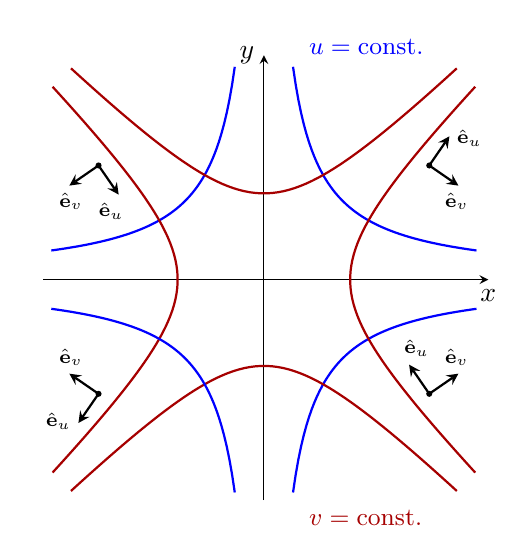
\begin{tikzpicture}[>=stealth]
\clip (-3,-3.2) rectangle (3,3.2);
\draw[->] (-2.8,0)--(2.85,0) node[below]{$x$};
\draw[->] (0,-2.8)--(0,2.85) node[left]{$y$};
\foreach \sg in {-1,1}{
 \draw[blue,thick,domain=0.37:2.7,samples=70] plot (\x,{\sg/\x});
 \draw[blue,thick,domain=-2.7:-0.37,samples=70] plot (\x,{\sg/\x});
 \draw[red!65!black,thick,domain=-2.45:2.45,samples=70]
 plot ({\sg*sqrt(1.2+\x*\x)},\x);
 \draw[red!65!black,thick,domain=-2.45:2.45,samples=70]
 plot (\x,{\sg*sqrt(1.2+\x*\x)});
}
\foreach \px/\py/\lux/\luy/\lvx/\lvy in {2.1/1.45/2.61/1.8/2.45/0.99,
 -2.1/1.45/-1.94/0.87/-2.45/0.99,-2.1/-1.45/-2.61/-1.8/-2.45/-0.99,
 2.1/-1.45/1.94/-0.87/2.45/-0.99}{
 \pgfmathsetmacro\fac{0.45/sqrt(\px*\px+\py*\py)}
 \fill (\px,\py) circle(1.1pt);
 \draw[->,black,thick] (\px,\py)--++({\fac*\py},{\fac*\px});
 \draw[->,black,thick] (\px,\py)--++({\fac*\px},{-\fac*\py});
 \node[font=\scriptsize] at (\lux,\luy){$\hat{\mathbf e}_u$};
 \node[font=\scriptsize] at (\lvx,\lvy){$\hat{\mathbf e}_v$};
}
\node[blue,font=\small,anchor=base west] at (0.45,2.86)
{$u=\text{const.}$};
\node[red!65!black,font=\small,anchor=base west] at (0.45,-3.12)
{$v=\text{const.}$};
\end{tikzpicture}
\end{center}
\textbf{(c)} For $\rho=\sqrt{x^2+y^2}>0$,
$\nabla u=(y,x,0)$ and $\nabla v=(2x,-2y,0)$.
They are orthogonal, since their dot product is $2xy-2xy=0$.
For orthogonal coordinates the gradient formula of Section 3.10,
$\nabla\psi=\sum_i\hat{\mathbf e}_i\,h_i^{-1}\,\partial\psi/\partial q_i$
with scale factors $h_i>0$, applied to $\psi=u$ and $\psi=v$ gives
$\nabla u=\hat{\mathbf e}_u/h_u$ and $\nabla v=\hat{\mathbf e}_v/h_v$.
Hence the increasing-coordinate unit vectors are $\nabla u/|\nabla u|$
and $\nabla v/|\nabla v|$, with $|\nabla u|=\sqrt{y^2+x^2}=\rho$ and
$|\nabla v|=2\rho$:
\[
\boxed{\hat{\mathbf e}_u=\frac{(y,x,0)}{\rho},\qquad
\hat{\mathbf e}_v=\frac{(x,-y,0)}{\rho}}.
\]
Their $(x,y)$ component signs in quadrants I, II, III, IV are
respectively $(+,+),(+,-),(-,-),(-,+)$ for $\hat{\mathbf e}_u$
and $(+,-),(-,-),(-,+),(+,+)$ for $\hat{\mathbf e}_v$.
\textbf{(d)} The cross product of the unit vectors is
\[
\hat{\mathbf e}_u\times\hat{\mathbf e}_v
=\rho^{-2}(y,x,0)\times(x,-y,0)
=\rho^{-2}\bigl(0,0,y(-y)-x\cdot x\bigr)
=-\hat{\mathbf e}_z,
\]
so the ordered system $(u,v,z)$ is left-handed.
\erratum{The chart is singular on the $z$-axis and is only local
unless a branch is chosen, because $(x,y)$ and $(-x,-y)$ have the
same $(u,v)$.}

One can also check handedness by the Jacobian. Differentiating the definitions gives
\[
\begin{pmatrix}du\\dv\end{pmatrix}
=\begin{pmatrix}y&x\\2x&-2y\end{pmatrix}
\begin{pmatrix}dx\\dy\end{pmatrix},\qquad
\det\frac{\partial(u,v)}{\partial(x,y)}=-2y^2-2x^2=-2(x^2+y^2).
\]
The rows of this matrix are $\nabla u$ and $\nabla v$, and
$\nabla u\times\nabla v=(0,0,-2y^2-2x^2)$ is this determinant times
$\hat{\mathbf e}_z$; so the negative determinant is the left-handedness
found in (d).
Inverting the $2\times2$ matrix with the rule
\[
\begin{pmatrix}\alpha&\beta\\\gamma&\delta\end{pmatrix}^{-1}
=\frac1{\alpha\delta-\beta\gamma}
\begin{pmatrix}\delta&-\beta\\-\gamma&\alpha\end{pmatrix}
\]
gives
\[
\frac{\partial(x,y)}{\partial(u,v)}
=\frac{1}{-2\rho^2}\begin{pmatrix}-2y&-x\\-2x&y\end{pmatrix}
=\begin{pmatrix}y/\rho^2&x/(2\rho^2)\\x/\rho^2&-y/(2\rho^2)\end{pmatrix},
\]
whose determinant is the reciprocal of the one above,
\[
\det\frac{\partial(x,y)}{\partial(u,v)}
=-\frac{y^2}{2\rho^4}-\frac{x^2}{2\rho^4}=-\frac1{2\rho^2}.
\]
The columns of the inverse matrix are the tangent vectors
$\partial\mathbf r/\partial u=(y,x,0)/\rho^2$ and
$\partial\mathbf r/\partial v=(x,-y,0)/(2\rho^2)$ of the coordinate
lines; as a check on (c), they point along $\hat{\mathbf e}_u$ and
$\hat{\mathbf e}_v$, with lengths $h_u=1/\rho$ and $h_v=1/(2\rho)$.
\erratum{The Instructor's Manual, p.~49, omits the factor $1/2$ in this
inverse determinant. Its earlier differential must likewise read
$dv=2x\,dx-2y\,dy$, with a minus sign, since
$\partial_y(x^2-y^2)=-2y$.}

\Needspace{5\baselineskip}
\par\bigskip
\noindent\textbf{3.10.2}\quad The elliptic cylindrical coordinate system
consists of three families of surfaces:
\[
\text{(1)}\ \frac{x^{2}}{a^{2}\cosh^{2}u}+\frac{y^{2}}{a^{2}\sinh^{2}u}=1;
\quad
\text{(2)}\ \frac{x^{2}}{a^{2}\cos^{2}v}-\frac{y^{2}}{a^{2}\sin^{2}v}=1;
\quad
\text{(3)}\ z=z.
\]
Sketch the coordinate surfaces $u=\text{constant}$ and $v=\text{constant}$ as
they intersect the first quadrant of the $xy$-plane. Show the unit vectors
$\hat{\mathbf{e}}_{u}$ and $\hat{\mathbf{e}}_{v}$. The range of $u$ is
$0\le u<\infty$. The range of $v$ is $0\le v\le2\pi$.
\erratum{Take $a>0$. Interpret the zero-denominator limiting surfaces by the parametrization below; the unit basis is undefined at the foci, where $\sinh^2u+\sin^2v=0$.}
\solution
Use the parametrization
\[
x=a\cosh u\cos v,\qquad y=a\sinh u\sin v,\qquad z=z,\quad a>0.
\]
Dividing its squared coordinates by $a^2\cosh^2u,a^2\sinh^2u$
and adding gives $1$; dividing by $a^2\cos^2v,a^2\sin^2v$
and subtracting also gives $1$. Thus it generates both stated families.
Constant $u>0$ gives ellipses with semi-axes $a\cosh u>a\sinh u$, whose
foci $(\pm c,0)$ have $c^2=a^2\cosh^2u-a^2\sinh^2u=a^2$; constant $v$
(not a multiple of $\pi/2$) gives hyperbolas with semi-axes
$a|\cos v|$ and $a|\sin v|$, whose foci $(\pm c,0)$ have
$c^2=a^2\cos^2v+a^2\sin^2v=a^2$. Both families are therefore confocal,
with foci $(\pm a,0)$. In the first quadrant use
$u>0$, $0<v<\pi/2$. The sketch shows the ellipses $u=0.45,0.8,1.15$
(blue), the hyperbolas $v=20^\circ,45^\circ,70^\circ$ (red), and the
unit vectors at the point $u=1$, $v=30^\circ$:
\begin{center}
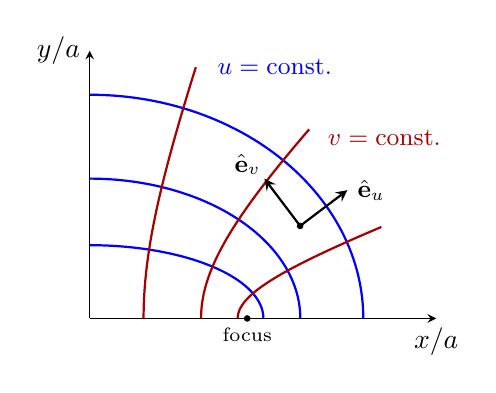
\begin{tikzpicture}[scale=2,>=stealth]
\draw[->] (0,0)--(2.2,0) node[below]{$x/a$};
\draw[->] (0,0)--(0,1.7) node[left]{$y/a$};
\foreach \u in {0.45,0.8,1.15}{
 \draw[blue,thick,domain=0:90,samples=60]
 plot ({(exp(\u)+exp(-\u))*cos(\x)/2},
       {(exp(\u)-exp(-\u))*sin(\x)/2});
}
\foreach \v in {20,45,70}{
 \draw[red!65!black,thick,domain=0:1.3,samples=60]
 plot ({(exp(\x)+exp(-\x))*cos(\v)/2},
       {(exp(\x)-exp(-\x))*sin(\v)/2});
}
\fill (1,0) circle(0.6pt) node[below,font=\scriptsize]{focus};
\coordinate (p) at (1.33635,0.58760);
\fill (p) circle(0.6pt);
\draw[->,thick] (p)--++(0.30,0.227)
 node[right,font=\small]{$\hat{\mathbf e}_u$};
\draw[->,thick] (p)--++(-0.227,0.30)
 node[above left,font=\small,inner sep=1pt]{$\hat{\mathbf e}_v$};
\node[blue,font=\small,anchor=west] at (0.75,1.6){$u=\text{const.}$};
\node[red!65!black,font=\small,anchor=west] at (1.45,1.15)
{$v=\text{const.}$};
\end{tikzpicture}
\end{center}
Differentiate the position:
\[
\frac{\partial\mathbf r}{\partial u}
=a(\sinh u\cos v,\ \cosh u\sin v,\ 0),\qquad
\frac{\partial\mathbf r}{\partial v}
=a(-\cosh u\sin v,\ \sinh u\cos v,\ 0).
\]
Both have squared length
\[
a^2(\sinh^2u\cos^2v+\cosh^2u\sin^2v)
=a^2[\sinh^2u(1-\sin^2v)+(1+\sinh^2u)\sin^2v]
=a^2(\sinh^2u+\sin^2v),
\]
and their dot product
$a^2(-\sinh u\cosh u\sin v\cos v+\cosh u\sinh u\sin v\cos v)$ is zero.
Normalizing,
\[
\boxed{\begin{aligned}
\hat{\mathbf e}_u&=
\frac{(\sinh u\cos v,\ \cosh u\sin v,\ 0)}
{\sqrt{\sinh^2u+\sin^2v}},\\
\hat{\mathbf e}_v&=
\frac{(-\cosh u\sin v,\ \sinh u\cos v,\ 0)}
{\sqrt{\sinh^2u+\sin^2v}}.
\end{aligned}}
\]
The common scale factor is $h_u=h_v=a\sqrt{\sinh^2u+\sin^2v}$.
The first vector points outward and northeast, the second along an
ellipse toward increasing $v$ (northwest) in this quadrant, since for
$u>0$, $0<v<\pi/2$ both $\sinh u\cos v$ and $\cosh u\sin v$ are
positive.
At limiting coordinate surfaces where a displayed denominator of the
implicit equations vanishes, use the parametrization and its limit:
in the $xy$-plane, $u=0$ gives the segment $|x|\le a$ of the $x$-axis,
$v=0$ and $v=\pi$ give the rays $x\ge a$ and $x\le-a$ of the $x$-axis,
and $v=\pi/2$ and $v=3\pi/2$ give the positive and negative $y$-axis.

\Needspace{5\baselineskip}
\par\bigskip
\noindent\textbf{3.10.3}\quad Develop arguments to show that dot and cross
products (not involving $\nabla$) in orthogonal curvilinear coordinates in
$\mathbb{R}^{3}$ proceed, as in Cartesian coordinates, \textbf{with no
involvement of scale factors}.
\erratum{Use physical components along orthonormal unit vectors; the usual cross-product signs require a right-handed ordering.}
\solution
At a fixed regular point, expand in the local orthonormal basis:
$\mathbf A=\sum_iA_i\hat{\mathbf e}_i$ and
$\mathbf B=\sum_jB_j\hat{\mathbf e}_j$. Both products are bilinear,
and the unit vectors of an orthogonal system satisfy
$\hat{\mathbf e}_i\cdot\hat{\mathbf e}_j=\delta_{ij}$, so
\[
\mathbf A\cdot\mathbf B
=\sum_{ij}A_iB_j\,\hat{\mathbf e}_i\cdot\hat{\mathbf e}_j
=\sum_{ij}A_iB_j\delta_{ij}=\sum_iA_iB_i.
\]
For a right-handed basis,
$\hat{\mathbf e}_1\times\hat{\mathbf e}_2=\hat{\mathbf e}_3$ and its
cyclic permutations hold, the reversed products change sign, and
$\hat{\mathbf e}_i\times\hat{\mathbf e}_i=0$; together,
$\hat{\mathbf e}_i\times\hat{\mathbf e}_j
=\sum_k\varepsilon_{ijk}\hat{\mathbf e}_k$, so
\[
\mathbf A\times\mathbf B
=\sum_{ij}A_iB_j\,\hat{\mathbf e}_i\times\hat{\mathbf e}_j
=\sum_{ijk}\varepsilon_{ijk}A_iB_j\hat{\mathbf e}_k.
\]
These are exactly the Cartesian component rules. Only the values of
the unit vectors at the one point enter, never their derivatives; the
scale factors appear only through $ds_i=h_i\,dq_i$ when $\nabla$
differentiates along the coordinate lines, which these products do not do.
\erratum{The usual cross-product sign assumes a right-handed unit
basis; a left-handed ordering, such as $(u,v,z)$ in Exercise 3.10.1, contributes
an overall minus sign.}
Also these formulas use physical components along unit vectors. Components
along the unnormalized coordinate tangents
$\partial\mathbf r/\partial q_i=h_i\hat{\mathbf e}_i$ would acquire
the corresponding scale factors.

\Needspace{5\baselineskip}
\par\bigskip
\noindent\textbf{3.10.4}\quad With $\hat{\mathbf{e}}_{1}$ a unit vector in the
direction of increasing $q_{1}$, show that
\begin{enumerate}
\item[(a)] $\displaystyle\nabla\cdot\hat{\mathbf{e}}_{1}
  =\frac{1}{h_{1}h_{2}h_{3}}\frac{\partial(h_{2}h_{3})}{\partial q_{1}}$
\item[(b)] $\displaystyle\nabla\times\hat{\mathbf{e}}_{1}
  =\frac{1}{h_{1}}\left[\hat{\mathbf{e}}_{2}\frac{1}{h_{3}}
  \frac{\partial h_{1}}{\partial q_{3}}
  -\hat{\mathbf{e}}_{3}\frac{1}{h_{2}}\frac{\partial h_{1}}{\partial q_{2}}
  \right]$.
\end{enumerate}
Note that even though $\hat{\mathbf{e}}_{1}$ is a unit vector, its divergence
and curl \textbf{do not necessarily vanish}.
\erratum{Use a regular, right-handed orthogonal coordinate chart with positive scale factors $h_i$.}
\solution
For physical components $V_i$ in an orthogonal system, the flux through
opposite $q_i$ faces gives
\[
\nabla\cdot\mathbf V=\frac1{h_1h_2h_3}
\sum_i\partial_{q_i}(h_jh_kV_i),\qquad\{i,j,k\}=\{1,2,3\}.
\]
For $\mathbf V=\hat{\mathbf e}_1$, $V_1=1,V_2=V_3=0$, so only the
$i=1$ term survives, $\partial_{q_1}(h_2h_3\cdot1)$, and
$\boxed{\nabla\cdot\hat{\mathbf e}_1=
(h_1h_2h_3)^{-1}\partial_{q_1}(h_2h_3)}$.
For the curl, the gradient formula
$\nabla\psi=\sum_j\hat{\mathbf e}_jh_j^{-1}\partial_{q_j}\psi$ with
$\psi=q_1$ gives $\nabla q_1=\hat{\mathbf e}_1/h_1$, i.e.\
$\hat{\mathbf e}_1=h_1\nabla q_1$. By the product rule
$\nabla\times(g\mathbf V)=\nabla g\times\mathbf V+g\nabla\times\mathbf V$
(Exercise 3.6.4) and $\nabla\times\nabla q_1=0$ (Exercise 3.6.10),
\[
\nabla\times\hat{\mathbf e}_1=\nabla h_1\times\nabla q_1
=\left(\sum_j\frac{\hat{\mathbf e}_j}{h_j}\partial_{q_j}h_1\right)
\times\frac{\hat{\mathbf e}_1}{h_1}.
\]
The $j=1$ term vanishes because $\hat{\mathbf e}_1\times\hat{\mathbf e}_1=0$.
In a right-handed basis
$\hat{\mathbf e}_2\times\hat{\mathbf e}_1=-\hat{\mathbf e}_3$ and
$\hat{\mathbf e}_3\times\hat{\mathbf e}_1=\hat{\mathbf e}_2$, so the
other two terms give
\[
\boxed{\nabla\times\hat{\mathbf e}_1=
\frac1{h_1}\left[
\frac{\hat{\mathbf e}_2}{h_3}\partial_{q_3}h_1
-\frac{\hat{\mathbf e}_3}{h_2}\partial_{q_2}h_1\right]}.
\]
For a left-handed ordering both cross products, and hence the result
of (b), change sign; this is why the note under the statement asks
for a right-handed chart.
The basis direction can vary even though its magnitude is fixed.

\Needspace{5\baselineskip}
\par\bigskip
\noindent\textbf{3.10.5}\quad Show that a set of orthogonal unit vectors
$\hat{\mathbf{e}}_{i}$ may be defined by
\[
\hat{\mathbf{e}}_{i}=\frac{1}{h_{i}}\frac{\partial\mathbf{r}}{\partial q_{i}}.
\]
In particular, show that $\hat{\mathbf{e}}_{i}\cdot\hat{\mathbf{e}}_{i}=1$
leads to an expression for $h_{i}$ in agreement with Eq.~(3.131).

The above equation for $\hat{\mathbf{e}}_{i}$ may be taken as a starting point
for deriving
\[
\frac{\partial\hat{\mathbf{e}}_{i}}{\partial q_{j}}
=\hat{\mathbf{e}}_{j}\frac{1}{h_{i}}\frac{\partial h_{j}}{\partial q_{i}},
\quad i\neq j
\]
and
\[
\frac{\partial\hat{\mathbf{e}}_{i}}{\partial q_{i}}
=-\sum_{j\neq i}\hat{\mathbf{e}}_{j}\frac{1}{h_{j}}
\frac{\partial h_{i}}{\partial q_{j}}.
\]
\erratum{Assume the coordinates form a regular orthogonal chart and $h_i>0$; arbitrary curvilinear coordinates need not be orthogonal.}
\solution
On a regular orthogonal chart, the tangent to increasing $q_i$ is
$\mathbf r_i=\partial_{q_i}\mathbf r$, and $\partial_i$ below means
$\partial/\partial q_i$. Since
$d\mathbf r=\sum_i\mathbf r_i\,dq_i$, the system is orthogonal exactly
when $\mathbf r_i\cdot\mathbf r_j=0$ for $i\ne j$ (no cross terms in
$ds^2=d\mathbf r\cdot d\mathbf r$), so the vectors
$\hat{\mathbf e}_i=\mathbf r_i/h_i$ are mutually orthogonal. Requiring
$\hat{\mathbf e}_i\cdot\hat{\mathbf e}_i=\mathbf r_i\cdot\mathbf r_i/h_i^2=1$
gives
\[
h_i^2=\mathbf r_i\cdot\mathbf r_i
=\Bigl(\frac{\partial x}{\partial q_i}\Bigr)^2
+\Bigl(\frac{\partial y}{\partial q_i}\Bigr)^2
+\Bigl(\frac{\partial z}{\partial q_i}\Bigr)^2,
\]
in agreement with Eq.~(3.131); then
$ds^2=\sum_ih_i^2dq_i^2$, so these $h_i$ are the scale factors.

To derive the basis derivatives, write
$\mathbf r_{ij}=\partial_j\mathbf r_i=\partial_i\partial_j\mathbf r$,
which is symmetric in $i,j$ because mixed partials commute.
Differentiating $\mathbf r_i=h_i\hat{\mathbf e}_i$ gives
$\mathbf r_{ij}=(\partial_jh_i)\hat{\mathbf e}_i+h_i\partial_j\hat{\mathbf e}_i$,
so $\mathbf r_{ij}=\mathbf r_{ji}$ reads
\[
(\partial_jh_i)\hat{\mathbf e}_i+h_i\partial_j\hat{\mathbf e}_i
=(\partial_ih_j)\hat{\mathbf e}_j+h_j\partial_i\hat{\mathbf e}_j.
\tag{*}
\]
Differentiating $\hat{\mathbf e}_i\cdot\hat{\mathbf e}_i=1$ with
respect to $q_j$ gives $\hat{\mathbf e}_i\cdot\partial_j\hat{\mathbf e}_i=0$.
For three distinct indices $i,j,k$, differentiate the orthogonality
relations $\mathbf r_i\cdot\mathbf r_k=0$, $\mathbf r_i\cdot\mathbf r_j=0$,
$\mathbf r_j\cdot\mathbf r_k=0$ with respect to $q_j$, $q_k$, $q_i$,
respectively; for example the first gives
$\mathbf r_{ij}\cdot\mathbf r_k+\mathbf r_i\cdot\mathbf r_{kj}=0$.
With the symmetry of $\mathbf r_{ij}$ the three results give, in turn,
\[
\mathbf r_k\cdot\mathbf r_{ij}
=-\mathbf r_i\cdot\mathbf r_{jk}
=\mathbf r_j\cdot\mathbf r_{ik}
=-\mathbf r_k\cdot\mathbf r_{ij},
\]
so $\mathbf r_k\cdot\mathbf r_{ij}=0$. Dotting the expansion of
$\mathbf r_{ij}$ with $\mathbf r_k=h_k\hat{\mathbf e}_k$ and using
$\hat{\mathbf e}_k\cdot\hat{\mathbf e}_i=0$ gives
$\mathbf r_k\cdot\mathbf r_{ij}=h_kh_i\,\hat{\mathbf e}_k\cdot\partial_j\hat{\mathbf e}_i$;
hence $\hat{\mathbf e}_k\cdot\partial_j\hat{\mathbf e}_i=0$.
Dotting (*) with $\hat{\mathbf e}_j$ for $i\ne j$, and using
$\hat{\mathbf e}_j\cdot\hat{\mathbf e}_i=0$ and
$\hat{\mathbf e}_j\cdot\partial_i\hat{\mathbf e}_j=0$, gives the only
remaining component:
$h_i\hat{\mathbf e}_j\cdot\partial_j\hat{\mathbf e}_i=\partial_i h_j$.
Therefore
\[
\boxed{\partial_j\hat{\mathbf e}_i
=\hat{\mathbf e}_j\,\frac{\partial_i h_j}{h_i}\quad(i\ne j)}.
\]
Finally, $\partial_i\hat{\mathbf e}_i$ has no $\hat{\mathbf e}_i$
component. For $j\ne i$ differentiate $\hat{\mathbf e}_i\cdot\hat{\mathbf e}_j=0$
with respect to $q_i$ and use the boxed formula with $i$ and $j$
interchanged, $\partial_i\hat{\mathbf e}_j=\hat{\mathbf e}_i(\partial_jh_i)/h_j$:
$\hat{\mathbf e}_j\cdot\partial_i\hat{\mathbf e}_i
=-\hat{\mathbf e}_i\cdot\partial_i\hat{\mathbf e}_j
=-(\partial_jh_i)/h_j$.
Expanding in the perpendicular basis gives
$\boxed{\partial_i\hat{\mathbf e}_i
=-\sum_{j\ne i}\hat{\mathbf e}_j(\partial_jh_i)/h_j}$.

\Needspace{5\baselineskip}
\par\bigskip
\noindent\textbf{3.10.6}\quad Resolve the circular cylindrical unit vectors
into their Cartesian components (see Fig.~3.23).
\par\nobreak\hfill\emph{ANS.}\enspace
$\begin{aligned}
\hat{\mathbf{e}}_{\rho}&=\hat{\mathbf{e}}_{x}\cos\varphi
+\hat{\mathbf{e}}_{y}\sin\varphi,\\
\hat{\mathbf{e}}_{\varphi}&=-\hat{\mathbf{e}}_{x}\sin\varphi
+\hat{\mathbf{e}}_{y}\cos\varphi,\\
\hat{\mathbf{e}}_{z}&=\hat{\mathbf{e}}_{z}.
\end{aligned}$
\solution
Start with $\mathbf r=(\rho\cos\varphi,\rho\sin\varphi,z)$.
Its coordinate derivatives are
\[
\partial_\rho\mathbf r=(\cos\varphi,\sin\varphi,0),\quad
\partial_\varphi\mathbf r=\rho(-\sin\varphi,\cos\varphi,0),\quad
\partial_z\mathbf r=(0,0,1).
\]
Their lengths are
$(\cos^2\varphi+\sin^2\varphi)^{1/2}=1$,
$\rho(\sin^2\varphi+\cos^2\varphi)^{1/2}=\rho$, and $1$, for $\rho>0$.
Dividing by these lengths gives
\[
\boxed{\hat{\mathbf e}_\rho=(\cos\varphi,\sin\varphi,0),\quad
\hat{\mathbf e}_\varphi=(-\sin\varphi,\cos\varphi,0),\quad
\hat{\mathbf e}_z=(0,0,1)}.
\]
Their dot products are $\delta_{ij}$ (for instance
$\hat{\mathbf e}_\rho\cdot\hat{\mathbf e}_\varphi
=-\cos\varphi\sin\varphi+\sin\varphi\cos\varphi=0$), and
$\hat{\mathbf e}_\rho\times\hat{\mathbf e}_\varphi
=(0,0,\cos^2\varphi+\sin^2\varphi)=\hat{\mathbf e}_z$, so the
ordering $(\rho,\varphi,z)$ is right-handed.

\Needspace{5\baselineskip}
\par\bigskip
\noindent\textbf{3.10.7}\quad Resolve the Cartesian unit vectors into their
circular cylindrical components (see Fig.~3.23).
\par\nobreak\hfill\emph{ANS.}\enspace
$\begin{aligned}
\hat{\mathbf{e}}_{x}&=\hat{\mathbf{e}}_{\rho}\cos\varphi
-\hat{\mathbf{e}}_{\varphi}\sin\varphi,\\
\hat{\mathbf{e}}_{y}&=\hat{\mathbf{e}}_{\rho}\sin\varphi
+\hat{\mathbf{e}}_{\varphi}\cos\varphi,\\
\hat{\mathbf{e}}_{z}&=\hat{\mathbf{e}}_{z}.
\end{aligned}$
\solution
Exercise 3.10.6 gives $\hat{\mathbf e}_\rho,\hat{\mathbf e}_\varphi,
\hat{\mathbf e}_z$ as the rows of an orthogonal matrix acting on
$(\hat{\mathbf e}_x,\hat{\mathbf e}_y,\hat{\mathbf e}_z)$; its inverse is
its transpose, whose first two rows are the first two columns
$(\cos\varphi,-\sin\varphi,0)$ and $(\sin\varphi,\cos\varphi,0)$ of
the original matrix. These rows give the coefficients of the
combinations, which check directly:
\[
\begin{aligned}
\cos\varphi\,\hat{\mathbf e}_\rho-\sin\varphi\,\hat{\mathbf e}_\varphi
&=(\cos^2\varphi+\sin^2\varphi,\ \cos\varphi\sin\varphi
-\sin\varphi\cos\varphi,\ 0)=\hat{\mathbf e}_x,\\
\sin\varphi\,\hat{\mathbf e}_\rho+\cos\varphi\,\hat{\mathbf e}_\varphi
&=(\sin\varphi\cos\varphi-\cos\varphi\sin\varphi,\
\sin^2\varphi+\cos^2\varphi,\ 0)=\hat{\mathbf e}_y.
\end{aligned}
\]
Together with unchanged $\hat{\mathbf e}_z$, these are the requested
inverse formulas.

\Needspace{5\baselineskip}
\par\bigskip
\noindent\textbf{3.10.8}\quad From the results of Exercise 3.10.6, show that
\[
\frac{\partial\hat{\mathbf{e}}_{\rho}}{\partial\varphi}
=\hat{\mathbf{e}}_{\varphi},\quad
\frac{\partial\hat{\mathbf{e}}_{\varphi}}{\partial\varphi}
=-\hat{\mathbf{e}}_{\rho}
\]
and that all other first derivatives of the circular cylindrical unit vectors
with respect to the circular cylindrical coordinates vanish.
\solution
Differentiating the Cartesian expressions gives
\[
\partial_\varphi\hat{\mathbf e}_\rho
=(-\sin\varphi,\cos\varphi,0)=\hat{\mathbf e}_\varphi,
\]
\[
\partial_\varphi\hat{\mathbf e}_\varphi
=(-\cos\varphi,-\sin\varphi,0)=-\hat{\mathbf e}_\rho.
\]
Neither depends on $\rho$ or $z$, so those derivatives vanish.
The vector $\hat{\mathbf e}_z=(0,0,1)$ is constant, so all three
of its coordinate derivatives vanish.

\Needspace{5\baselineskip}
\par\bigskip
\noindent\textbf{3.10.9}\quad Compare $\nabla\cdot\mathbf{V}$ as given for
cylindrical coordinates in Eq.~(3.148) with the result of its computation by
applying to $\mathbf{V}$ the operator
\[
\nabla=\hat{\mathbf{e}}_{\rho}\frac{\partial}{\partial\rho}
+\hat{\mathbf{e}}_{\varphi}\frac{1}{\rho}\frac{\partial}{\partial\varphi}
+\hat{\mathbf{e}}_{z}\frac{\partial}{\partial z}
\]
Note that $\nabla$ acts both on the unit vectors and on the components of
$\mathbf{V}$.
\solution
Write $\mathbf V=V_\rho\hat{\mathbf e}_\rho+
V_\varphi\hat{\mathbf e}_\varphi+V_z\hat{\mathbf e}_z$.
The basis has no $\rho$ or $z$ dependence, giving
$\hat{\mathbf e}_\rho\cdot\partial_\rho\mathbf V=\partial_\rho V_\rho$
and $\hat{\mathbf e}_z\cdot\partial_z\mathbf V=\partial_zV_z$.
For the azimuthal derivative, differentiate coefficients and basis,
using $\partial_\varphi\hat{\mathbf e}_\rho=\hat{\mathbf e}_\varphi$ and
$\partial_\varphi\hat{\mathbf e}_\varphi=-\hat{\mathbf e}_\rho$
(Exercise 3.10.8):
\[
\partial_\varphi\mathbf V
=(\partial_\varphi V_\rho-V_\varphi)\hat{\mathbf e}_\rho
+(\partial_\varphi V_\varphi+V_\rho)\hat{\mathbf e}_\varphi
+(\partial_\varphi V_z)\hat{\mathbf e}_z.
\]
The operator gives
$\nabla\cdot\mathbf V=\hat{\mathbf e}_\rho\cdot\partial_\rho\mathbf V
+\rho^{-1}\hat{\mathbf e}_\varphi\cdot\partial_\varphi\mathbf V
+\hat{\mathbf e}_z\cdot\partial_z\mathbf V$, and with
$\hat{\mathbf e}_\varphi\cdot\partial_\varphi\mathbf V
=\partial_\varphi V_\varphi+V_\rho$ from the last display, the three
dot products yield
\[
\boxed{\nabla\cdot\mathbf V
=\partial_\rho V_\rho+\frac{V_\rho}{\rho}
+\frac1\rho\partial_\varphi V_\varphi+\partial_zV_z
=\frac1\rho\partial_\rho(\rho V_\rho)
+\frac1\rho\partial_\varphi V_\varphi+\partial_zV_z},
\]
where $\rho^{-1}\partial_\rho(\rho V_\rho)=\partial_\rho V_\rho+V_\rho/\rho$.
This agrees with Eq.~(3.148).
The $V_\rho/\rho$ term is exactly the contribution of the varying basis.

\erratum{The Instructor's Manual, p.~51, calls the exercise's operator incorrect. The textbook explicitly says that it acts on the unit vectors as well as the components, so the operator as stated is correct: the basis derivative supplies exactly the $V_\rho/\rho$ term computed above.}

\Needspace{5\baselineskip}
\par\bigskip
\noindent\textbf{3.10.10}\quad
\begin{enumerate}
\item[(a)] Show that
  $\mathbf{r}=\hat{\mathbf{e}}_{\rho}\rho+\hat{\mathbf{e}}_{z}z$.
\item[(b)] Working entirely in circular cylindrical coordinates, show that
  \[
  \nabla\cdot\mathbf{r}=3\quad\text{and}\quad\nabla\times\mathbf{r}=0.
  \]
\end{enumerate}
\solution
\textbf{(a)} Since $x=\rho\cos\varphi,y=\rho\sin\varphi$,
$x\hat{\mathbf e}_x+y\hat{\mathbf e}_y
=\rho(\cos\varphi\,\hat{\mathbf e}_x+\sin\varphi\,\hat{\mathbf e}_y)
=\rho\hat{\mathbf e}_\rho$ by Exercise 3.10.6,
so $\mathbf r=\rho\hat{\mathbf e}_\rho+z\hat{\mathbf e}_z$.

\textbf{(b)} The physical cylindrical components of $\mathbf r$ are
$(V_\rho,V_\varphi,V_z)=(\rho,0,z)$.
Therefore Eq.~(3.148) gives
\[
\nabla\cdot\mathbf r=\frac1\rho\partial_\rho(\rho^2)
+\frac1\rho\partial_\varphi0+\partial_zz=2+0+1=3.
\]
For the curl, expanding the determinant form of the curl with
$h_\rho=1$, $h_\varphi=\rho$, $h_z=1$ gives the components
\[
(\nabla\times\mathbf V)_\rho=\frac1\rho\partial_\varphi V_z-\partial_zV_\varphi,\quad
(\nabla\times\mathbf V)_\varphi=\partial_zV_\rho-\partial_\rho V_z,\quad
(\nabla\times\mathbf V)_z=\frac1\rho[\partial_\rho(\rho V_\varphi)-\partial_\varphi V_\rho].
\]
For $\mathbf V=\mathbf r$,
\[
(\nabla\times\mathbf r)_\rho=\rho^{-1}\partial_\varphi z-\partial_z0=0,
\quad
(\nabla\times\mathbf r)_\varphi=\partial_z\rho-\partial_\rho z=0,
\]
and
$(\nabla\times\mathbf r)_z=\rho^{-1}[\partial_\rho(\rho\,0)-\partial_\varphi\rho]=0$.
Thus $\boxed{\nabla\times\mathbf r=0}$.

\Needspace{5\baselineskip}
\par\bigskip
\noindent\textbf{3.10.11}\quad
\begin{enumerate}
\item[(a)] Show that the parity operation (reflection through the origin) on a
  point $(\rho,\varphi,z)$ relative to fixed $x$-, $y$-, $z$-axes consists of
  the transformation
  \[
  \rho\to\rho,\quad\varphi\to\varphi\pm\pi,\quad z\to-z.
  \]
\item[(b)] Show that $\hat{\mathbf{e}}_{\rho}$ and $\hat{\mathbf{e}}_{\varphi}$
  have odd parity (reversal of direction) and that $\hat{\mathbf{e}}_{z}$ has
  even parity.
\end{enumerate}
\emph{Note.}~The Cartesian unit vectors $\hat{\mathbf{e}}_{x}$,
$\hat{\mathbf{e}}_{y}$, and $\hat{\mathbf{e}}_{z}$ remain constant.
\solution
\textbf{(a)} Under $(x,y,z)\mapsto(-x,-y,-z)$,
$\rho=\sqrt{x^2+y^2}$ is unchanged. Both $\cos\varphi=x/\rho$
and $\sin\varphi=y/\rho$ change sign. Since
$\cos(\varphi\pm\pi)=-\cos\varphi$, $\sin(\varphi\pm\pi)=-\sin\varphi$,
and the pair $(\cos\varphi,\sin\varphi)$ fixes the angle modulo $2\pi$,
$\varphi\mapsto\varphi\pm\pi$ (the two signs give the same point);
and $z\mapsto-z$.

\textbf{(b)} Substituting this angle into the unit-vector functions of
Exercise 3.10.6 gives
\[
\begin{aligned}
\hat{\mathbf e}_\rho(\varphi+\pi)&=(-\cos\varphi,-\sin\varphi,0)
=-\hat{\mathbf e}_\rho(\varphi),\\
\hat{\mathbf e}_\varphi(\varphi+\pi)&=(\sin\varphi,-\cos\varphi,0)
=-\hat{\mathbf e}_\varphi(\varphi),\\
\hat{\mathbf e}_z(\varphi+\pi)&=(0,0,1)=\hat{\mathbf e}_z.
\end{aligned}
\]
This is evaluation of the curvilinear basis at the reflected point
relative to fixed Cartesian unit vectors, as specified in the note.

\Needspace{5\baselineskip}
\par\bigskip
\noindent\textbf{3.10.12}\quad A rigid body is rotating about a fixed axis
with a constant angular velocity $\boldsymbol{\omega}$. Take
$\boldsymbol{\omega}$ to lie along the $z$-axis. Express the position vector
$\mathbf{r}$ in circular cylindrical coordinates and using circular
cylindrical coordinates,
\begin{enumerate}
\item[(a)] calculate $\mathbf{v}=\boldsymbol{\omega}\times\mathbf{r}$,
\item[(b)] calculate $\nabla\times\mathbf{v}$.
\end{enumerate}
\par\nobreak\hfill\emph{ANS.}\enspace
(a)\enspace$\mathbf{v}=\hat{\mathbf{e}}_{\varphi}\omega\rho$\quad
(b)\enspace$\nabla\times\mathbf{v}=2\boldsymbol{\omega}$.
\solution
\textbf{(a)} With $\boldsymbol\omega=\omega\hat{\mathbf e}_z$ and
$\mathbf r=\rho\hat{\mathbf e}_\rho+z\hat{\mathbf e}_z$
(Exercise 3.10.10), and the right-handed products
$\hat{\mathbf e}_z\times\hat{\mathbf e}_\rho=\hat{\mathbf e}_\varphi$,
$\hat{\mathbf e}_z\times\hat{\mathbf e}_z=0$,
\[
\mathbf v=\omega\hat{\mathbf e}_z\times
(\rho\hat{\mathbf e}_\rho+z\hat{\mathbf e}_z)
=\omega\rho\,\hat{\mathbf e}_z\times\hat{\mathbf e}_\rho
=\boxed{\omega\rho\hat{\mathbf e}_\varphi}.
\]
\textbf{(b)} Its components are $(v_\rho,v_\varphi,v_z)=(0,\omega\rho,0)$
and are independent of $z,\varphi$. Hence, with the cylindrical curl
components of Exercise 3.10.10,
$(\nabla\times\mathbf v)_\rho=\rho^{-1}\partial_\varphi0-\partial_z(\omega\rho)=0$
and $(\nabla\times\mathbf v)_\varphi=\partial_z0-\partial_\rho0=0$, while
\[
(\nabla\times\mathbf v)_z
=\frac1\rho[\partial_\rho(\rho\,\omega\rho)-\partial_\varphi0]
=\frac{2\omega\rho}{\rho}=2\omega.
\]
Thus $\boxed{\nabla\times\mathbf v=2\omega\hat{\mathbf e}_z=2\boldsymbol\omega}$.

\Needspace{5\baselineskip}
\par\bigskip
\noindent\textbf{3.10.13}\quad Find the circular cylindrical components of the
velocity and acceleration of a moving particle,
\[
\begin{aligned}
v_{\rho}&=\dot{\rho},&a_{\rho}&=\ddot{\rho}-\rho\dot{\varphi}^{2},\\
v_{\varphi}&=\rho\dot{\varphi},&a_{\varphi}&=\rho\ddot{\varphi}
+2\dot{\rho}\dot{\varphi},\\
v_{z}&=\dot{z},&a_{z}&=\ddot{z}.
\end{aligned}
\]
\emph{Hint.}\quad
$\begin{aligned}[t]
\mathbf{r}(t)&=\hat{\mathbf{e}}_{\rho}(t)\rho(t)+\hat{\mathbf{e}}_{z}z(t)\\
&=[\hat{\mathbf{e}}_{x}\cos\varphi(t)+\hat{\mathbf{e}}_{y}\sin\varphi(t)]
\rho(t)+\hat{\mathbf{e}}_{z}z(t).
\end{aligned}$

\emph{Note.}~$\dot{\rho}=d\rho/dt$, $\ddot{\rho}=d^{2}\rho/dt^{2}$, and so on.
\solution
Along the trajectory the unit vectors depend on $t$ only through
$\varphi(t)$, so by the chain rule and Exercise 3.10.8 the basis
derivatives are
$\dot{\hat{\mathbf e}}_\rho=\dot\varphi\,\partial_\varphi\hat{\mathbf e}_\rho
=\dot\varphi\hat{\mathbf e}_\varphi$,
$\dot{\hat{\mathbf e}}_\varphi=\dot\varphi\,\partial_\varphi\hat{\mathbf e}_\varphi
=-\dot\varphi\hat{\mathbf e}_\rho$,
and $\dot{\hat{\mathbf e}}_z=0$.
(Differentiating the hint's Cartesian form directly gives the same:
$\frac d{dt}(\cos\varphi,\sin\varphi,0)=\dot\varphi(-\sin\varphi,\cos\varphi,0)$.)
Differentiate $\mathbf r=\rho\hat{\mathbf e}_\rho+z\hat{\mathbf e}_z$
by the product rule:
\[
\mathbf v=\dot\rho\hat{\mathbf e}_\rho+
\rho\dot\varphi\hat{\mathbf e}_\varphi+\dot z\hat{\mathbf e}_z.
\]
Differentiate each term once more, again with
$\dot{\hat{\mathbf e}}_\rho=\dot\varphi\hat{\mathbf e}_\varphi$ and
$\dot{\hat{\mathbf e}}_\varphi=-\dot\varphi\hat{\mathbf e}_\rho$:
\[
\begin{aligned}
\mathbf a={}&\underbrace{\ddot\rho\hat{\mathbf e}_\rho+
\dot\rho\dot\varphi\hat{\mathbf e}_\varphi}_{d(\dot\rho\hat{\mathbf e}_\rho)/dt}
+\underbrace{(\dot\rho\dot\varphi+\rho\ddot\varphi)\hat{\mathbf e}_\varphi
-\rho\dot\varphi^2\hat{\mathbf e}_\rho}_{d(\rho\dot\varphi\hat{\mathbf e}_\varphi)/dt}
+\ddot z\hat{\mathbf e}_z.
\end{aligned}
\]
Collecting coefficients gives
\[
\boxed{\begin{aligned}
v_\rho&=\dot\rho,&v_\varphi&=\rho\dot\varphi,&v_z&=\dot z,\\
a_\rho&=\ddot\rho-\rho\dot\varphi^2,&
a_\varphi&=\rho\ddot\varphi+2\dot\rho\dot\varphi,&a_z&=\ddot z.
\end{aligned}}
\]

\Needspace{5\baselineskip}
\par\bigskip
\noindent\textbf{3.10.14}\quad In right circular cylindrical coordinates, a
particular vector function is given by
\[
\mathbf{V}(\rho,\varphi)=\hat{\mathbf{e}}_{\rho}V_{\rho}(\rho,\varphi)
+\hat{\mathbf{e}}_{\varphi}V_{\varphi}(\rho,\varphi).
\]
Show that $\nabla\times\mathbf{V}$ has only a $z$-component. Note that this
result will hold for any vector confined to a surface $q_{3}=\text{constant}$
as long as the products $h_{1}V_{1}$ and $h_{2}V_{2}$ are each independent of
$q_{3}$.
\solution
Use the cylindrical curl components of Exercise 3.10.10 with $V_z=0$
and the absence of $z$ dependence:
\[
(\nabla\times\mathbf V)_\rho=\rho^{-1}\partial_\varphi V_z-\partial_zV_\varphi=0,
\qquad
(\nabla\times\mathbf V)_\varphi=\partial_zV_\rho-\partial_\rho V_z=0.
\]
The remaining component need not vanish:
\[
\boxed{\nabla\times\mathbf V=
\frac{\hat{\mathbf e}_z}{\rho}
[\partial_\rho(\rho V_\varphi)-\partial_\varphi V_\rho]}.
\]
More generally, expanding the determinant form of the curl in
orthogonal coordinates gives the first two components
\[
(\nabla\times\mathbf V)_1=\frac{\partial_2(h_3V_3)-\partial_3(h_2V_2)}{h_2h_3},
\qquad
(\nabla\times\mathbf V)_2=\frac{\partial_3(h_1V_1)-\partial_1(h_3V_3)}{h_3h_1},
\]
with $\partial_i=\partial/\partial q_i$. For a vector confined to the
surfaces $q_3=\text{constant}$, $V_3=0$, and these reduce to
\[
-(h_2h_3)^{-1}\partial_3(h_2V_2),\qquad
(h_3h_1)^{-1}\partial_3(h_1V_1).
\]
Both vanish when $h_1V_1$ and $h_2V_2$ are independent of $q_3$, as
stated in the problem, leaving only component 3. (Cylindrical
coordinates with $q_3=z$, $h_1V_1=V_\rho$, $h_2V_2=\rho V_\varphi$ are
the case above.)

\erratum{For this $V_z=0$ field, the transverse curl components are $-\partial_zV_\varphi$ and $\partial_zV_\rho$. The Instructor's Manual, p.~52, gives the first with the wrong sign and the second with an extra factor $1/\rho$. Both are zero here because the components are independent of $z$, so the conclusion survives those errors.}

\Needspace{5\baselineskip}
\par\bigskip
\noindent\textbf{3.10.15}\quad A conducting wire along the $z$-axis carries a
current $I$. The resulting magnetic vector potential is given by
\[
\mathbf{A}=\hat{\mathbf{e}}_{z}\frac{\mu I}{2\pi}\ln\frac{1}{\rho}.
\]
Show that the magnetic induction $\mathbf{B}$ is given by
\[
\mathbf{B}=\hat{\mathbf{e}}_{\varphi}\frac{\mu I}{2\pi\rho}.
\]
\solution
Let $K=\mu I/(2\pi)$, so $A_z=K\ln(1/\rho)=-K\ln\rho$, $A_\rho=A_\varphi=0$.
With the cylindrical curl components of Exercise 3.10.10,
$B_\rho=\rho^{-1}\partial_\varphi A_z-\partial_zA_\varphi=0$ because
$A_z$ does not depend on $\varphi$, and
$B_z=\rho^{-1}[\partial_\rho(\rho A_\varphi)-\partial_\varphi A_\rho]=0$.
The remaining one is
\[
B_\varphi=\partial_zA_\rho-\partial_\rho A_z
=0-(-K/\rho)=K/\rho.
\]
Thus $\boxed{\mathbf B=\mu I\,\hat{\mathbf e}_\varphi/(2\pi\rho)}$,
valid for $\rho>0$ outside the ideal wire.
Replacing $\ln(1/\rho)$ by $\ln(\rho_0/\rho)$ makes the logarithm
dimensionless and adds only a constant to $A_z$, leaving $\mathbf B$ unchanged.

\Needspace{5\baselineskip}
\par\bigskip
\noindent\textbf{3.10.16}\quad A force is described by
\[
\mathbf{F}=-\hat{\mathbf{e}}_{x}\frac{y}{x^{2}+y^{2}}
+\hat{\mathbf{e}}_{y}\frac{x}{x^{2}+y^{2}}.
\]
\begin{enumerate}
\item[(a)] Express $\mathbf{F}$ in circular cylindrical coordinates.

  Operating entirely in circular cylindrical coordinates for (b) and (c),
\item[(b)] Calculate the curl of $\mathbf{F}$ and
\item[(c)] Calculate the work done by $\mathbf{F}$ in encircling the unit
  circle once counterclockwise.
\item[(d)] How do you reconcile the results of (b) and (c)?
\end{enumerate}
\solution
\textbf{(a)} Substitute $x=\rho\cos\varphi,y=\rho\sin\varphi$, so
$x^2+y^2=\rho^2$:
\[
\mathbf F=\frac{(-\rho\sin\varphi,\rho\cos\varphi,0)}{\rho^2}
=\frac1\rho(-\sin\varphi,\cos\varphi,0)
=\boxed{\hat{\mathbf e}_\varphi/\rho}.
\]
\textbf{(b)} For $\rho>0$, $F_\rho=F_z=0$ and $F_\varphi=1/\rho$ depends
on $\rho$ only. With the cylindrical curl components of
Exercise 3.10.10, the transverse components
$\rho^{-1}\partial_\varphi F_z-\partial_zF_\varphi$ and
$\partial_zF_\rho-\partial_\rho F_z$ vanish,
and $(\nabla\times\mathbf F)_z=\rho^{-1}[\partial_\rho(\rho\cdot\rho^{-1})
-\partial_\varphi F_\rho]=\rho^{-1}\partial_\rho1=0$.
So $\boxed{\nabla\times\mathbf F=0}$ for $\rho>0$.
\textbf{(c)} In cylindrical coordinates
$d\mathbf r=\hat{\mathbf e}_\rho d\rho+\hat{\mathbf e}_\varphi\rho\,d\varphi
+\hat{\mathbf e}_z dz$; on the unit circle ($\rho=1$, $z=0$)
$d\mathbf r=\hat{\mathbf e}_\varphi d\varphi$ and
$\mathbf F\cdot d\mathbf r=d\varphi$, so
$\boxed{W=\oint\mathbf F\cdot d\mathbf r=\int_0^{2\pi}d\varphi=2\pi}$.
\textbf{(d)} The field is undefined on the axis. A disk spanning
the circle crosses that singularity, so Stokes' theorem cannot
use the ordinary zero curl over that disk. On an annulus excluding
the axis, the outer counterclockwise circulation $2\pi$ and the
inner clockwise circulation $-2\pi$ cancel, in full agreement with
zero curl. (The calculation in (c) gives $2\pi$ on a circle of any
radius $a$, since $\mathbf F\cdot d\mathbf r=a^{-1}\,a\,d\varphi$.)
Locally $\mathbf F=\nabla\varphi$, since
$\nabla\varphi=\hat{\mathbf e}_\varphi\rho^{-1}\partial_\varphi\varphi
=\hat{\mathbf e}_\varphi/\rho$, but $\varphi$ is not
a global single-valued potential around the axis: it increases by
$2\pi$ once around, which is the circulation found in (c).

\Needspace{5\baselineskip}
\par\bigskip
\noindent\textbf{3.10.17}\quad A calculation of the magnetohydrodynamic pinch
effect involves the evaluation of $(\mathbf{B}\cdot\nabla)\mathbf{B}$. If the
magnetic induction $\mathbf{B}$ is taken to be
$\mathbf{B}=\hat{\mathbf{e}}_{\varphi}B_{\varphi}(\rho)$, show that
\[
(\mathbf{B}\cdot\nabla)\mathbf{B}
=-\hat{\mathbf{e}}_{\rho}B_{\varphi}^{2}/\rho.
\]
\solution
For $\mathbf B=B_\varphi(\rho)\hat{\mathbf e}_\varphi$, dotting into
$\nabla=\hat{\mathbf e}_\rho\partial_\rho
+\hat{\mathbf e}_\varphi\rho^{-1}\partial_\varphi+\hat{\mathbf e}_z\partial_z$
keeps only the middle term, so
the directional derivative operator is
$\mathbf B\cdot\nabla=(B_\varphi/\rho)\partial_\varphi$.
It must differentiate the basis as well as the scalar component:
\[
(\mathbf B\cdot\nabla)\mathbf B
=\frac{B_\varphi}{\rho}
\left[(\partial_\varphi B_\varphi)\hat{\mathbf e}_\varphi+
B_\varphi\partial_\varphi\hat{\mathbf e}_\varphi\right]
=\boxed{-\frac{B_\varphi^2}{\rho}\hat{\mathbf e}_\rho}.
\]
Here $\partial_\varphi B_\varphi=0$ and
$\partial_\varphi\hat{\mathbf e}_\varphi=-\hat{\mathbf e}_\rho$
(Exercise 3.10.8).

\Needspace{5\baselineskip}
\par\bigskip
\noindent\textbf{3.10.18}\quad Express the spherical polar unit vectors in
terms of Cartesian unit vectors.
\par\nobreak\hfill\emph{ANS.}\enspace
$\begin{aligned}
\hat{\mathbf{e}}_{r}&=\hat{\mathbf{e}}_{x}\sin\theta\cos\varphi
+\hat{\mathbf{e}}_{y}\sin\theta\sin\varphi+\hat{\mathbf{e}}_{z}\cos\theta,\\
\hat{\mathbf{e}}_{\theta}&=\hat{\mathbf{e}}_{x}\cos\theta\cos\varphi
+\hat{\mathbf{e}}_{y}\cos\theta\sin\varphi-\hat{\mathbf{e}}_{z}\sin\theta,\\
\hat{\mathbf{e}}_{\varphi}&=-\hat{\mathbf{e}}_{x}\sin\varphi
+\hat{\mathbf{e}}_{y}\cos\varphi.
\end{aligned}$
\solution
The position map is
$\mathbf r=r(\sin\theta\cos\varphi,\sin\theta\sin\varphi,\cos\theta)$.
Its $r,\theta,\varphi$ derivatives are
\[
\begin{aligned}
\partial_r\mathbf r&=(\sin\theta\cos\varphi,\sin\theta\sin\varphi,\cos\theta),\\
\partial_\theta\mathbf r&=r(\cos\theta\cos\varphi,\cos\theta\sin\varphi,-\sin\theta),\\
\partial_\varphi\mathbf r&=r\sin\theta(-\sin\varphi,\cos\varphi,0),
\end{aligned}
\]
with lengths $1,r,r\sin\theta$ on a regular patch $r>0$, $0<\theta<\pi$
(for the first two, the squared components sum to
$\sin^2\theta+\cos^2\theta=1$ after $\cos^2\varphi+\sin^2\varphi=1$).
Normalize each derivative to obtain
\[
\boxed{\begin{aligned}
\hat{\mathbf e}_r&=(\sin\theta\cos\varphi,\sin\theta\sin\varphi,\cos\theta),\\
\hat{\mathbf e}_\theta&=(\cos\theta\cos\varphi,\cos\theta\sin\varphi,-\sin\theta),\\
\hat{\mathbf e}_\varphi&=(-\sin\varphi,\cos\varphi,0).
\end{aligned}}
\]
Their norms are one, their pairwise dot products vanish (for instance
$\hat{\mathbf e}_r\cdot\hat{\mathbf e}_\theta
=\sin\theta\cos\theta(\cos^2\varphi+\sin^2\varphi)-\cos\theta\sin\theta=0$),
and
\[
\hat{\mathbf e}_r\times\hat{\mathbf e}_\theta
=\bigl(-\sin\varphi(\sin^2\theta+\cos^2\theta),\
\cos\varphi(\cos^2\theta+\sin^2\theta),\ 0\bigr)
=\hat{\mathbf e}_\varphi,
\]
so $(r,\theta,\varphi)$ is right-handed.
At the polar axis, the angular basis requires a choice of azimuthal
limit and is not a unique coordinate basis.

\Needspace{5\baselineskip}
\par\bigskip
\noindent\textbf{3.10.19}\quad Resolve the Cartesian unit vectors into their
spherical polar components:
\[
\begin{aligned}
\hat{\mathbf{e}}_{x}&=\hat{\mathbf{e}}_{r}\sin\theta\cos\varphi
+\hat{\mathbf{e}}_{\theta}\cos\theta\cos\varphi
-\hat{\mathbf{e}}_{\varphi}\sin\varphi,\\
\hat{\mathbf{e}}_{y}&=\hat{\mathbf{e}}_{r}\sin\theta\sin\varphi
+\hat{\mathbf{e}}_{\theta}\cos\theta\sin\varphi
+\hat{\mathbf{e}}_{\varphi}\cos\varphi,\\
\hat{\mathbf{e}}_{z}&=\hat{\mathbf{e}}_{r}\cos\theta
-\hat{\mathbf{e}}_{\theta}\sin\theta.
\end{aligned}
\]
\solution
Any vector is the sum of its projections on an orthonormal basis.
For example,
$\hat{\mathbf e}_x=\sum_{j=r,\theta,\varphi}
(\hat{\mathbf e}_x\cdot\hat{\mathbf e}_j)\hat{\mathbf e}_j$.
The projection coefficients
$\hat{\mathbf e}_x\cdot\hat{\mathbf e}_r=\sin\theta\cos\varphi$,
$\hat{\mathbf e}_x\cdot\hat{\mathbf e}_\theta=\cos\theta\cos\varphi$,
$\hat{\mathbf e}_x\cdot\hat{\mathbf e}_\varphi=-\sin\varphi$
are precisely the $x$ components of the vectors in Exercise 3.10.18.
Repeating with their $y$ and $z$ components gives
\[
\boxed{\begin{aligned}
\hat{\mathbf e}_x&=\sin\theta\cos\varphi\,\hat{\mathbf e}_r
+\cos\theta\cos\varphi\,\hat{\mathbf e}_\theta-\sin\varphi\,\hat{\mathbf e}_\varphi,\\
\hat{\mathbf e}_y&=\sin\theta\sin\varphi\,\hat{\mathbf e}_r
+\cos\theta\sin\varphi\,\hat{\mathbf e}_\theta+\cos\varphi\,\hat{\mathbf e}_\varphi,\\
\hat{\mathbf e}_z&=\cos\theta\,\hat{\mathbf e}_r-\sin\theta\,\hat{\mathbf e}_\theta.
\end{aligned}}
\]
Thus the inverse change-of-basis matrix is the transpose of the matrix
whose rows are the vectors of Exercise 3.10.18 (the matrix $T$ of
Exercise 3.10.20).

\Needspace{5\baselineskip}
\par\bigskip
\noindent\textbf{3.10.20}\quad
\begin{enumerate}
\item[(a)] Explain why it is not possible to relate a column vector
  $\mathbf{r}$ (with components $x,y,z$) to another column vector
  $\mathbf{r}'$ (with components $r,\theta,\varphi$), via a matrix equation of
  the form $\mathbf{r}'=\mathsf{B}\mathbf{r}$ \erratum{with one constant matrix $\mathsf B$ valid at all positions}.
\item[(b)] One can write a matrix equation relating the Cartesian components
  of a vector to its components in spherical polar coordinates. Find the
  transformation matrix and determine whether it is orthogonal.
\end{enumerate}
\solution
\textbf{(a)} \erratum{The qualification ``one constant matrix'' is
needed: at any one point $\mathbf r\ne0$ the position-dependent matrix
$\mathsf B=\mathbf r'\mathbf r^T/r^2$ does give
$\mathsf B\mathbf r=\mathbf r'(\mathbf r^T\mathbf r)/r^2=\mathbf r'$.}
Write $\mathbf x=(x,y,z)^T$ for the column $\mathbf r$, to keep it
apart from the radius $r$. The radius $r=\sqrt{x^2+y^2+z^2}$ is not
a linear function: $r(-\mathbf x)=r(\mathbf x)$, whereas the first
component of a constant matrix map is linear,
$(\mathsf B(-\mathbf x))_1=-(\mathsf B\mathbf x)_1$.
If $(\mathsf B\mathbf x)_1=r(\mathbf x)$ held for all $\mathbf x$, then
$r(\mathbf x)=r(-\mathbf x)=(\mathsf B(-\mathbf x))_1
=-(\mathsf B\mathbf x)_1=-r(\mathbf x)$, so $r(\mathbf x)=0$, which is
false for $\mathbf x\ne0$.
The angular coordinates are nonlinear as well; for example
$\theta(2\mathbf x)=\theta(\mathbf x)$, while a linear function doubles.

\textbf{(b)} Physical components of a vector at a fixed point are its
projections on the unit vectors, $V_r=\hat{\mathbf e}_r\cdot\mathbf V
=\sum_a(\hat{\mathbf e}_r)_aV_a$ and similarly for $V_\theta,V_\varphi$,
with the Cartesian components $(\hat{\mathbf e}_r)_a$ etc.\ of
Exercise 3.10.18. Hence they obey
\[
\boxed{\begin{pmatrix}V_r\\V_\theta\\V_\varphi\end{pmatrix}
=T\begin{pmatrix}V_x\\V_y\\V_z\end{pmatrix},\quad
T=\begin{pmatrix}
\sin\theta\cos\varphi&\sin\theta\sin\varphi&\cos\theta\\
\cos\theta\cos\varphi&\cos\theta\sin\varphi&-\sin\theta\\
-\sin\varphi&\cos\varphi&0
\end{pmatrix}}.
\]
The rows are the three unit vectors from Exercise 3.10.18, so the
entries of $TT^T$ are their inner products,
$\hat{\mathbf e}_i\cdot\hat{\mathbf e}_j=\delta_{ij}$; thus $TT^T=I$,
and $T$ is orthogonal. Its determinant is the triple product
$\hat{\mathbf e}_r\cdot(\hat{\mathbf e}_\theta\times\hat{\mathbf e}_\varphi)
=\hat{\mathbf e}_r\cdot\hat{\mathbf e}_r=1$ (a rotation).
Thus $T^{-1}=T^T$, but $T$ depends on the observation point.
In particular $T(x,y,z)^T=(r,0,0)^T$, the components of the
position vector, rather than the coordinate labels $(r,\theta,\varphi)^T$.

\Needspace{5\baselineskip}
\par\bigskip
\noindent\textbf{3.10.21}\quad Find the transformation matrix that converts
the components of a vector in spherical polar coordinates into its components
in circular cylindrical coordinates. Then find the matrix of the inverse
transformation.
\solution
The common azimuthal vector is unchanged, while
\[
\hat{\mathbf e}_\rho=\sin\theta\,\hat{\mathbf e}_r+
\cos\theta\,\hat{\mathbf e}_\theta,\qquad
\hat{\mathbf e}_z=\cos\theta\,\hat{\mathbf e}_r-
\sin\theta\,\hat{\mathbf e}_\theta.
\]
These follow from the Cartesian forms in Exercises 3.10.6 and 3.10.18.
For instance, the $x$ component of
$\sin\theta\,\hat{\mathbf e}_r+\cos\theta\,\hat{\mathbf e}_\theta$ is
$\sin^2\theta\cos\varphi+\cos^2\theta\cos\varphi=\cos\varphi$, its
$y$ component is likewise $\sin\varphi$, and its $z$ component is
$\sin\theta\cos\theta-\cos\theta\sin\theta=0$; similarly
$\cos\theta\,\hat{\mathbf e}_r-\sin\theta\,\hat{\mathbf e}_\theta$ has
components $(0,0,\cos^2\theta+\sin^2\theta)=(0,0,1)$.
Project $\mathbf V=V_r\hat{\mathbf e}_r+V_\theta\hat{\mathbf e}_\theta
+V_\varphi\hat{\mathbf e}_\varphi$ onto these directions:
$V_\rho=\hat{\mathbf e}_\rho\cdot\mathbf V=\sin\theta\,V_r+\cos\theta\,V_\theta$,
$V_z=\hat{\mathbf e}_z\cdot\mathbf V=\cos\theta\,V_r-\sin\theta\,V_\theta$,
and $V_\varphi$ is shared. In the specified component
orders,
\[
\boxed{\begin{pmatrix}V_\rho\\V_\varphi\\V_z\end{pmatrix}
=C\begin{pmatrix}V_r\\V_\theta\\V_\varphi\end{pmatrix},\quad
C=\begin{pmatrix}\sin\theta&\cos\theta&0\\0&0&1\\
\cos\theta&-\sin\theta&0\end{pmatrix}}.
\]
The rows are orthonormal (e.g.\ the first and third give
$\sin\theta\cos\theta-\cos\theta\sin\theta=0$), so $C$ is orthogonal and
\[
\boxed{C^{-1}=C^T=
\begin{pmatrix}\sin\theta&0&\cos\theta\\
\cos\theta&0&-\sin\theta\\0&1&0\end{pmatrix}}.
\]
Multiplication of these matrices gives $I$ using $\sin^2\theta+\cos^2\theta=1$.

\Needspace{5\baselineskip}
\par\bigskip
\noindent\textbf{3.10.22}\quad
\begin{enumerate}
\item[(a)] From the results of Exercise 3.10.18, calculate the partial
  derivatives of $\hat{\mathbf{e}}_{r}$, $\hat{\mathbf{e}}_{\theta}$, and
  $\hat{\mathbf{e}}_{\varphi}$ with respect to $r$, $\theta$, and $\varphi$.
\item[(b)] With $\nabla$ given by
  \[
  \hat{\mathbf{e}}_{r}\frac{\partial}{\partial r}
  +\hat{\mathbf{e}}_{\theta}\frac{1}{r}\frac{\partial}{\partial\theta}
  +\hat{\mathbf{e}}_{\varphi}\frac{1}{r\sin\theta}\frac{\partial}
  {\partial\varphi}
  \]
  (greatest space rate of change), use the results of part (a) to calculate
  $\nabla\cdot\nabla\psi$. This is an alternate derivation of the Laplacian.
\end{enumerate}
\emph{Note.}~The derivatives of the left-hand $\nabla$ operate on the unit
vectors of the right-hand $\nabla$ before the dot product is evaluated.
\solution
\textbf{(a)} None of the unit vectors in Exercise 3.10.18 depends on $r$.
Differentiating their Cartesian expressions with respect to the angles,
\[
\begin{aligned}
\partial_\theta\hat{\mathbf e}_r&=(\cos\theta\cos\varphi,\cos\theta\sin\varphi,-\sin\theta),&
\partial_\varphi\hat{\mathbf e}_r&=\sin\theta(-\sin\varphi,\cos\varphi,0),\\
\partial_\theta\hat{\mathbf e}_\theta&=-(\sin\theta\cos\varphi,\sin\theta\sin\varphi,\cos\theta),&
\partial_\varphi\hat{\mathbf e}_\theta&=\cos\theta(-\sin\varphi,\cos\varphi,0),
\end{aligned}
\]
$\partial_\theta\hat{\mathbf e}_\varphi=0$, and
$\partial_\varphi\hat{\mathbf e}_\varphi=(-\cos\varphi,-\sin\varphi,0)$.
Comparing with the unit vectors themselves gives
\[
\begin{array}{c|ccc}
&\partial_r&\partial_\theta&\partial_\varphi\\\hline
\hat{\mathbf e}_r&0&\hat{\mathbf e}_\theta&\sin\theta\,\hat{\mathbf e}_\varphi\\
\hat{\mathbf e}_\theta&0&-\hat{\mathbf e}_r&\cos\theta\,\hat{\mathbf e}_\varphi\\
\hat{\mathbf e}_\varphi&0&0&-\sin\theta\,\hat{\mathbf e}_r-\cos\theta\,\hat{\mathbf e}_\theta
\end{array}
\]
For the last entry, the projections of
$(-\cos\varphi,-\sin\varphi,0)$ on $\hat{\mathbf e}_r,\hat{\mathbf e}_\theta,
\hat{\mathbf e}_\varphi$ are
$-\sin\theta(\cos^2\varphi+\sin^2\varphi)=-\sin\theta$,
$-\cos\theta(\cos^2\varphi+\sin^2\varphi)=-\cos\theta$, and
$\sin\varphi\cos\varphi-\cos\varphi\sin\varphi=0$, respectively.

\textbf{(b)} First apply the given $\nabla$ to any vector
$\mathbf W=W_r\hat{\mathbf e}_r+W_\theta\hat{\mathbf e}_\theta+
W_\varphi\hat{\mathbf e}_\varphi$.
By the product rule and the derivative table,
\[
\begin{aligned}
\partial_\theta\mathbf W&=(\partial_\theta W_r-W_\theta)\hat{\mathbf e}_r
+(W_r+\partial_\theta W_\theta)\hat{\mathbf e}_\theta
+\partial_\theta W_\varphi\,\hat{\mathbf e}_\varphi,\\
\partial_\varphi\mathbf W&=(\partial_\varphi W_r-\sin\theta W_\varphi)\hat{\mathbf e}_r
+(\partial_\varphi W_\theta-\cos\theta W_\varphi)\hat{\mathbf e}_\theta\\
&\quad+(\sin\theta W_r+\cos\theta W_\theta+\partial_\varphi W_\varphi)
\hat{\mathbf e}_\varphi,
\end{aligned}
\]
while $\partial_r\mathbf W$ has components $\partial_rW_r,\partial_rW_\theta,
\partial_rW_\varphi$. Hence
\[
\hat{\mathbf e}_r\cdot\partial_r\mathbf W=\partial_rW_r,\quad
\hat{\mathbf e}_\theta\cdot\partial_\theta\mathbf W=W_r+\partial_\theta W_\theta,
\]
\[
\hat{\mathbf e}_\varphi\cdot\partial_\varphi\mathbf W
=\sin\theta W_r+\cos\theta W_\theta+\partial_\varphi W_\varphi.
\]
The given operator dotted into $\mathbf W$ is
$\nabla\cdot\mathbf W=\hat{\mathbf e}_r\cdot\partial_r\mathbf W
+r^{-1}\hat{\mathbf e}_\theta\cdot\partial_\theta\mathbf W
+(r\sin\theta)^{-1}\hat{\mathbf e}_\varphi\cdot\partial_\varphi\mathbf W$;
inserting the three dot products and collecting the $W_r$ terms
($W_r/r+\sin\theta\,W_r/(r\sin\theta)=2W_r/r$),
\[
\nabla\cdot\mathbf W=\partial_rW_r+\frac{2W_r}{r}
+\frac{\partial_\theta W_\theta+\cot\theta W_\theta}{r}
+\frac{\partial_\varphi W_\varphi}{r\sin\theta}.
\]
Now put $\mathbf W=\nabla\psi$, whose physical components are
$W_r=\psi_r$, $W_\theta=\psi_\theta/r$, $W_\varphi=\psi_\varphi/(r\sin\theta)$
(subscripts on $\psi$ denote partial derivatives).
Then $\partial_\theta W_\theta=\psi_{\theta\theta}/r$ and
$\partial_\varphi W_\varphi=\psi_{\varphi\varphi}/(r\sin\theta)$, and
substitution yields
\[
\begin{aligned}
\nabla^2\psi
&=\psi_{rr}+\frac2r\psi_r+
\frac1{r^2}(\psi_{\theta\theta}+\cot\theta\,\psi_\theta)
+\frac{\psi_{\varphi\varphi}}{r^2\sin^2\theta}\\
&=\boxed{\frac1{r^2}\partial_r(r^2\partial_r\psi)
+\frac1{r^2\sin\theta}\partial_\theta(\sin\theta\,\partial_\theta\psi)
+\frac1{r^2\sin^2\theta}\partial_\varphi^2\psi}.
\end{aligned}
\]
The last step uses
$r^{-2}\partial_r(r^2\psi_r)=\psi_{rr}+2\psi_r/r$ and
$(\sin\theta)^{-1}\partial_\theta(\sin\theta\,\psi_\theta)
=\psi_{\theta\theta}+\cot\theta\,\psi_\theta$.

\erratum{The Instructor's Manual, p.~54, prints $\tan\theta/r^2$ instead of $\cot\theta/r^2$ as the coefficient of $\partial_\theta$. Its following divergence-form identity must have $1/(r^2\sin\theta)$, not $1/(r^2\sin^2\theta)$, before $\partial_\theta(\sin\theta\,\partial_\theta)$. For a quick independent check, $\psi=r\cos\theta=z$ has zero Cartesian Laplacian. The correct formula gives $2\cos\theta/r-\cos\theta/r-\cos\theta/r=0$; the printed $\tan\theta$ version instead gives $\cos(2\theta)/(r\cos\theta)$.}

\Needspace{5\baselineskip}
\par\bigskip
\noindent\textbf{3.10.23}\quad A rigid body is rotating about a fixed axis
with a constant angular velocity $\boldsymbol{\omega}$. Take
$\boldsymbol{\omega}$ to be along the $z$-axis. Using spherical polar
coordinates,
\begin{enumerate}
\item[(a)] calculate $\mathbf{v}=\boldsymbol{\omega}\times\mathbf{r}$.
\item[(b)] calculate $\nabla\times\mathbf{v}$.
\end{enumerate}
\par\nobreak\hfill\emph{ANS.}\enspace
(a)\enspace$\mathbf{v}=\hat{\mathbf{e}}_{\varphi}\omega r\sin\theta$.\quad
(b)\enspace$\nabla\times\mathbf{v}=2\boldsymbol{\omega}$.
\solution
\textbf{(a)} In spherical components,
$\boldsymbol\omega=\omega\hat{\mathbf e}_z=\omega(\cos\theta\,\hat{\mathbf e}_r-
\sin\theta\,\hat{\mathbf e}_\theta)$ (Exercise 3.10.19) and
$\mathbf r=r\hat{\mathbf e}_r$.
With $\hat{\mathbf e}_r\times\hat{\mathbf e}_r=0$ and
$\hat{\mathbf e}_\theta\times\hat{\mathbf e}_r=-\hat{\mathbf e}_\varphi$,
the cross product is
\[
\mathbf v=\omega r(\cos\theta\,\hat{\mathbf e}_r\times\hat{\mathbf e}_r
-\sin\theta\,\hat{\mathbf e}_\theta\times\hat{\mathbf e}_r)
=\boxed{\omega r\sin\theta\,\hat{\mathbf e}_\varphi}.
\]
\textbf{(b)} Expanding the determinant form of the curl with
$h_r=1$, $h_\theta=r$, $h_\varphi=r\sin\theta$ gives the spherical
components
\[
\begin{aligned}
(\nabla\times\mathbf V)_r&=\frac1{r\sin\theta}
[\partial_\theta(\sin\theta\,V_\varphi)-\partial_\varphi V_\theta],\qquad
(\nabla\times\mathbf V)_\varphi=\frac1r[\partial_r(rV_\theta)-\partial_\theta V_r],\\
(\nabla\times\mathbf V)_\theta&=\frac1r\Bigl[\frac1{\sin\theta}\partial_\varphi V_r
-\partial_r(rV_\varphi)\Bigr].
\end{aligned}
\]
For $v_r=v_\theta=0$, $v_\varphi=\omega r\sin\theta$ these give
\[
(\nabla\times\mathbf v)_r
=\frac1{r\sin\theta}\partial_\theta(\omega r\sin^2\theta)
=\frac{2\omega r\sin\theta\cos\theta}{r\sin\theta}=2\omega\cos\theta,
\]
\[
(\nabla\times\mathbf v)_\theta
=-\frac1r\partial_r(\omega r^2\sin\theta)=-\frac{2\omega r\sin\theta}{r}
=-2\omega\sin\theta,
\qquad(\nabla\times\mathbf v)_\varphi=0.
\]
Thus the result is
$2\omega(\cos\theta\,\hat{\mathbf e}_r-\sin\theta\,\hat{\mathbf e}_\theta)
=\boxed{2\boldsymbol\omega}$.

\Needspace{5\baselineskip}
\par\bigskip
\noindent\textbf{3.10.24}\quad A certain vector $\mathbf{V}$ has no radial
component. Its curl has no tangential components. What does this imply about
the radial dependence of the tangential components of $\mathbf{V}$?
\solution
Since $V_r=0$, the tangential curl components of Exercise 3.10.23,
$(\nabla\times\mathbf V)_\theta=r^{-1}[(\sin\theta)^{-1}\partial_\varphi V_r
-\partial_r(rV_\varphi)]$ and
$(\nabla\times\mathbf V)_\varphi=r^{-1}[\partial_r(rV_\theta)-\partial_\theta V_r]$,
reduce to
\[
(\nabla\times\mathbf V)_\theta=-\frac1r\partial_r(rV_\varphi),
\qquad
(\nabla\times\mathbf V)_\varphi=\frac1r\partial_r(rV_\theta).
\]
Setting both to zero means $\partial_r(rV_\theta)=\partial_r(rV_\varphi)=0$,
so $rV_\theta$ and $rV_\varphi$ are independent of $r$,
say $rV_\theta=f(\theta,\varphi)$ and
$rV_\varphi=g(\theta,\varphi)$. Hence, on $r>0$,
\[
\boxed{V_\theta=\frac{f(\theta,\varphi)}r,\qquad
V_\varphi=\frac{g(\theta,\varphi)}r}.
\]
If the region includes the origin and boundedness there is also required,
then these two functions must vanish; that extra regularity was not
part of the stated assumptions.

\Needspace{5\baselineskip}
\par\bigskip
\noindent\textbf{3.10.25}\quad Modern physics lays great stress on the
property of parity (whether a quantity remains invariant or changes sign under
an inversion of the coordinate system). In Cartesian coordinates this means
$x\to-x$, $y\to-y$, and $z\to-z$.
\begin{enumerate}
\item[(a)] Show that the inversion (reflection through the origin) of a point
  $(r,\theta,\varphi)$ relative to fixed $x$-, $y$-, $z$-axes consists of the
  transformation
  \[
  r\to r,\quad\theta\to\pi-\theta,\quad\varphi\to\varphi\pm\pi.
  \]
\item[(b)] Show that $\hat{\mathbf{e}}_{r}$ and $\hat{\mathbf{e}}_{\varphi}$
  have odd parity (reversal of direction) and that $\hat{\mathbf{e}}_{\theta}$
  has even parity.
\end{enumerate}
\solution
\textbf{(a)} Inversion leaves $r=\sqrt{x^2+y^2+z^2}$ unchanged.
Since $\cos\theta=z/r$ changes sign and $0\le\theta\le\pi$,
the new angle is the one in $[0,\pi]$ with cosine $-\cos\theta$,
namely $\theta\mapsto\pi-\theta$; then $\sin\theta$ is unchanged.
Both $x=r\sin\theta\cos\varphi$ and $y=r\sin\theta\sin\varphi$ change
sign with $r\sin\theta$ fixed, so $\cos\varphi$ and $\sin\varphi$ both
change sign, i.e.\ $\varphi\mapsto\varphi\pm\pi$ (modulo $2\pi$, as in
Exercise 3.10.11).

\textbf{(b)} Under these substitutions,
$\sin\theta$ is unchanged, $\cos\theta$ changes sign, and
$\sin\varphi,\cos\varphi$ both change sign.
The component formulas in Exercise 3.10.18 then give
\[
\begin{aligned}
\hat{\mathbf e}_r(\pi-\theta,\varphi+\pi)
&=(-\sin\theta\cos\varphi,-\sin\theta\sin\varphi,-\cos\theta)
=-\hat{\mathbf e}_r(\theta,\varphi),\\
\hat{\mathbf e}_\theta(\pi-\theta,\varphi+\pi)
&=\bigl((-\cos\theta)(-\cos\varphi),(-\cos\theta)(-\sin\varphi),-\sin\theta\bigr)
=\hat{\mathbf e}_\theta(\theta,\varphi),\\
\hat{\mathbf e}_\varphi(\varphi+\pi)
&=(\sin\varphi,-\cos\varphi,0)=-\hat{\mathbf e}_\varphi(\varphi).
\end{aligned}
\]
Thus the stated basis-field parities follow relative to fixed Cartesian axes.

\Needspace{5\baselineskip}
\par\bigskip
\noindent\textbf{3.10.26}\quad With $\mathbf{A}$ any vector,
\[
\mathbf{A}\cdot\nabla\mathbf{r}=\mathbf{A}.
\]
\begin{enumerate}
\item[(a)] Verify this result in Cartesian coordinates.
\item[(b)] Verify this result using spherical polar coordinates.
  Equation~(3.156) provides $\nabla$.
\end{enumerate}
\solution
\textbf{(a)} In Cartesian coordinates,
$[(\mathbf A\cdot\nabla)\mathbf r]_j
=\sum_i A_i\partial_i x_j=\sum_iA_i\delta_{ij}=A_j$.
\textbf{(b)} In spherical coordinates $\mathbf r=r\hat{\mathbf e}_r$,
so, with $\partial_\theta\hat{\mathbf e}_r=\hat{\mathbf e}_\theta$ and
$\partial_\varphi\hat{\mathbf e}_r=\sin\theta\,\hat{\mathbf e}_\varphi$
(Exercise 3.10.22),
\[
\partial_r\mathbf r=\hat{\mathbf e}_r,\quad
\partial_\theta\mathbf r=r\hat{\mathbf e}_\theta,\quad
\partial_\varphi\mathbf r=r\sin\theta\,\hat{\mathbf e}_\varphi.
\]
Dotting $\mathbf A=A_r\hat{\mathbf e}_r+A_\theta\hat{\mathbf e}_\theta
+A_\varphi\hat{\mathbf e}_\varphi$ into the gradient operator of
Eq.~(3.156) gives
$\mathbf A\cdot\nabla=A_r\partial_r+(A_\theta/r)\partial_\theta
+(A_\varphi/(r\sin\theta))\partial_\varphi$. Therefore
\[
(\mathbf A\cdot\nabla)\mathbf r
=A_r\partial_r\mathbf r+\frac{A_\theta}{r}\partial_\theta\mathbf r
+\frac{A_\varphi}{r\sin\theta}\partial_\varphi\mathbf r
=A_r\hat{\mathbf e}_r+A_\theta\hat{\mathbf e}_\theta
+A_\varphi\hat{\mathbf e}_\varphi
=\boxed{\mathbf A}.
\]
The derivatives act on $\mathbf r$, not on the coefficients of $\mathbf A$.

\Needspace{5\baselineskip}
\par\bigskip
\noindent\textbf{3.10.27}\quad Find the spherical coordinate components of the
velocity and acceleration of a moving particle:
\[
\begin{aligned}
v_{r}&=\dot{r},&a_{r}&=\ddot{r}-r\dot{\theta}^{2}
-r\sin^{2}\theta\,\dot{\varphi}^{2},\\
v_{\theta}&=r\dot{\theta},&a_{\theta}&=r\ddot{\theta}+2\dot{r}\dot{\theta}
-r\sin\theta\cos\theta\,\dot{\varphi}^{2},\\
v_{\varphi}&=r\sin\theta\,\dot{\varphi},&a_{\varphi}&=r\sin\theta\,
\ddot{\varphi}+2\dot{r}\sin\theta\,\dot{\varphi}
+2r\cos\theta\,\dot{\theta}\dot{\varphi}.
\end{aligned}
\]
\emph{Hint.}\quad
$\begin{aligned}[t]
\mathbf{r}(t)&=\hat{\mathbf{e}}_{r}(t)r(t)\\
&=[\hat{\mathbf{e}}_{x}\sin\theta(t)\cos\varphi(t)
+\hat{\mathbf{e}}_{y}\sin\theta(t)\sin\varphi(t)
+\hat{\mathbf{e}}_{z}\cos\theta(t)]r(t).
\end{aligned}$

\emph{Note.}~The dot in $\dot{r}$, $\dot{\theta}$, $\dot{\varphi}$ means time
derivative: $\dot{r}=dr/dt$, $\dot{\theta}=d\theta/dt$,
$\dot{\varphi}=d\varphi/dt$.
\solution
The unit vectors depend on $t$ through $\theta(t)$ and $\varphi(t)$,
so by the chain rule
$\dot{\hat{\mathbf e}}=\dot\theta\,\partial_\theta\hat{\mathbf e}
+\dot\varphi\,\partial_\varphi\hat{\mathbf e}$ for each of them. With
the basis derivatives in Exercise 3.10.22,
\[
\begin{aligned}
\dot{\hat{\mathbf e}}_r&=\dot\theta\hat{\mathbf e}_\theta+
\sin\theta\dot\varphi\hat{\mathbf e}_\varphi,\\
\dot{\hat{\mathbf e}}_\theta&=-\dot\theta\hat{\mathbf e}_r+
\cos\theta\dot\varphi\hat{\mathbf e}_\varphi,\\
\dot{\hat{\mathbf e}}_\varphi&=-\sin\theta\dot\varphi\hat{\mathbf e}_r
-\cos\theta\dot\varphi\hat{\mathbf e}_\theta.
\end{aligned}
\]
Differentiate $\mathbf r=r\hat{\mathbf e}_r$ by the product rule:
\[
\mathbf v=\dot r\hat{\mathbf e}_r+r\dot{\hat{\mathbf e}}_r
=\dot r\hat{\mathbf e}_r+r\dot\theta\hat{\mathbf e}_\theta+
r\sin\theta\dot\varphi\hat{\mathbf e}_\varphi,
\]
so $\boxed{v_r=\dot r,\ v_\theta=r\dot\theta,\
v_\varphi=r\sin\theta\,\dot\varphi}$.
Differentiating the three terms of $\mathbf v$ by the product rule
(with $\frac d{dt}\sin\theta=\cos\theta\,\dot\theta$) and inserting the
basis derivatives above gives
\[
\begin{aligned}
\frac d{dt}(\dot r\hat{\mathbf e}_r)
&=\ddot r\hat{\mathbf e}_r+\dot r\dot\theta\hat{\mathbf e}_\theta
+\dot r\sin\theta\dot\varphi\hat{\mathbf e}_\varphi,\\
\frac d{dt}(r\dot\theta\hat{\mathbf e}_\theta)
&=(\dot r\dot\theta+r\ddot\theta)\hat{\mathbf e}_\theta
-r\dot\theta^2\hat{\mathbf e}_r
+r\cos\theta\dot\theta\dot\varphi\hat{\mathbf e}_\varphi,\\
\frac d{dt}(r\sin\theta\dot\varphi\hat{\mathbf e}_\varphi)
&=(\dot r\sin\theta\dot\varphi+r\cos\theta\dot\theta\dot\varphi+
r\sin\theta\ddot\varphi)\hat{\mathbf e}_\varphi\\
&\quad-r\sin^2\theta\dot\varphi^2\hat{\mathbf e}_r
-r\sin\theta\cos\theta\dot\varphi^2\hat{\mathbf e}_\theta.
\end{aligned}
\]
Collecting each basis vector (for example, the $\hat{\mathbf e}_\theta$
terms are $\dot r\dot\theta$, $\dot r\dot\theta+r\ddot\theta$, and
$-r\sin\theta\cos\theta\dot\varphi^2$) yields
\[
\boxed{\begin{aligned}
a_r&=\ddot r-r\dot\theta^2-r\sin^2\theta\dot\varphi^2,\\
a_\theta&=r\ddot\theta+2\dot r\dot\theta-r\sin\theta\cos\theta\dot\varphi^2,\\
a_\varphi&=r\sin\theta\ddot\varphi+2\dot r\sin\theta\dot\varphi
+2r\cos\theta\dot\theta\dot\varphi.
\end{aligned}}
\]

\Needspace{5\baselineskip}
\par\bigskip
\noindent\textbf{3.10.28}\quad Express $\partial/\partial x$,
$\partial/\partial y$, $\partial/\partial z$ in spherical polar coordinates.
\par\nobreak\hfill\emph{ANS.}\enspace
$\begin{aligned}
\frac{\partial}{\partial x}&=\sin\theta\cos\varphi\frac{\partial}{\partial r}
+\cos\theta\cos\varphi\frac{1}{r}\frac{\partial}{\partial\theta}
-\frac{\sin\varphi}{r\sin\theta}\frac{\partial}{\partial\varphi},\\
\frac{\partial}{\partial y}&=\sin\theta\sin\varphi\frac{\partial}{\partial r}
+\cos\theta\sin\varphi\frac{1}{r}\frac{\partial}{\partial\theta}
+\frac{\cos\varphi}{r\sin\theta}\frac{\partial}{\partial\varphi},\\
\frac{\partial}{\partial z}&=\cos\theta\frac{\partial}{\partial r}
-\sin\theta\frac{1}{r}\frac{\partial}{\partial\theta}.
\end{aligned}$

\emph{Hint.}~Equate $\nabla_{xyz}$ and $\nabla_{r\theta\varphi}$.
\solution
The chain rule is $\partial_x=r_x\partial_r+\theta_x\partial_\theta+
\varphi_x\partial_\varphi$, and similarly for $y,z$; subscripts on
$r,\theta,\varphi$ denote partial derivatives with respect to $x,y,z$.
From $r^2=x^2+y^2+z^2$, $2rr_x=2x$, so $r_x=x/r=\sin\theta\cos\varphi$;
likewise $r_y=y/r=\sin\theta\sin\varphi$ and $r_z=z/r=\cos\theta$.
Differentiating $\cos\theta=z/r$ with respect to $x$ gives
$-\sin\theta\,\theta_x=-zr_x/r^2=-zx/r^3$, hence
\[
\theta_x=\frac{zx}{r^3\sin\theta}
=\frac{(r\cos\theta)(r\sin\theta\cos\varphi)}{r^3\sin\theta}
=\frac{\cos\theta\cos\varphi}r,
\]
and in the same way $\theta_y=zy/(r^3\sin\theta)=\cos\theta\sin\varphi/r$.
With respect to $z$,
$-\sin\theta\,\theta_z=1/r-z^2/r^3=(x^2+y^2)/r^3=\sin^2\theta/r$, so
$\theta_z=-\sin\theta/r$.
Finally differentiating $\varphi=\operatorname{atan2}(y,x)$ (locally
$\tan\varphi=y/x$) on a
regular local branch gives $\varphi_x=-y/(x^2+y^2)$,
$\varphi_y=x/(x^2+y^2)$, $\varphi_z=0$; with
$x^2+y^2=r^2\sin^2\theta$ these are
$-\sin\varphi/(r\sin\theta)$, $\cos\varphi/(r\sin\theta)$, $0$.
The full Jacobian obtained this way is
\[
\begin{array}{c|ccc}
&\partial_x&\partial_y&\partial_z\\\hline
r&\sin\theta\cos\varphi&\sin\theta\sin\varphi&\cos\theta\\
\theta&\cos\theta\cos\varphi/r&\cos\theta\sin\varphi/r&-\sin\theta/r\\
\varphi&-\sin\varphi/(r\sin\theta)&\cos\varphi/(r\sin\theta)&0
\end{array}
\]
Substitution of each column into the chain rule gives all three displayed operator
formulas in the question. They hold on $r>0,\sin\theta\ne0$,
where these coordinates are nonsingular.
Following the hint gives the same result faster: dotting
$\hat{\mathbf e}_x$ into
$\hat{\mathbf e}_x\partial_x+\hat{\mathbf e}_y\partial_y+\hat{\mathbf e}_z\partial_z
=\hat{\mathbf e}_r\partial_r+\hat{\mathbf e}_\theta r^{-1}\partial_\theta
+\hat{\mathbf e}_\varphi(r\sin\theta)^{-1}\partial_\varphi$
and using the projections
$\hat{\mathbf e}_x\cdot\hat{\mathbf e}_r=\sin\theta\cos\varphi$,
$\hat{\mathbf e}_x\cdot\hat{\mathbf e}_\theta=\cos\theta\cos\varphi$,
$\hat{\mathbf e}_x\cdot\hat{\mathbf e}_\varphi=-\sin\varphi$ of
Exercise 3.10.19 reproduces the $\partial_x$ formula; $\hat{\mathbf e}_y$
and $\hat{\mathbf e}_z$ give the other two.

\Needspace{5\baselineskip}
\par\bigskip
\noindent\textbf{3.10.29}\quad Using results from Exercise 3.10.28, show that
\[
-i\left(x\frac{\partial}{\partial y}-y\frac{\partial}{\partial x}\right)
=-i\frac{\partial}{\partial\varphi}.
\]
This is the quantum mechanical operator corresponding to the $z$-component of
orbital angular momentum.
\solution
Insert the derivatives from Exercise 3.10.28 and
$x=r\sin\theta\cos\varphi,y=r\sin\theta\sin\varphi$.
In $x\partial_y-y\partial_x$, the coefficient of $\partial_r$ is
$x\sin\theta\sin\varphi-y\sin\theta\cos\varphi
=r\sin^2\theta(\cos\varphi\sin\varphi-\sin\varphi\cos\varphi)=0$.
The coefficient of $\partial_\theta$ is
$(x\cos\theta\sin\varphi-y\cos\theta\cos\varphi)/r
=\sin\theta\cos\theta(\cos\varphi\sin\varphi-\sin\varphi\cos\varphi)=0$.
The coefficient of $\partial_\varphi$ is
$x\cos\varphi/(r\sin\theta)+y\sin\varphi/(r\sin\theta)
=\cos^2\varphi+\sin^2\varphi=1$. Thus
$x\partial_y-y\partial_x=\partial_\varphi$ and
$\boxed{L_z=-i\partial_\varphi}$.

\Needspace{5\baselineskip}
\par\bigskip
\noindent\textbf{3.10.30}\quad With the quantum mechanical orbital angular
momentum operator defined as $\mathbf{L}=-i(\mathbf{r}\times\nabla)$, show
that
\begin{enumerate}
\item[(a)] $\displaystyle L_{x}+iL_{y}=e^{i\varphi}\left(\frac{\partial}
  {\partial\theta}+i\cot\theta\frac{\partial}{\partial\varphi}\right)$,
\item[(b)] $\displaystyle L_{x}-iL_{y}=-e^{-i\varphi}\left(\frac{\partial}
  {\partial\theta}-i\cot\theta\frac{\partial}{\partial\varphi}\right)$.
\end{enumerate}
\solution
Using $\mathbf r=r\hat{\mathbf e}_r$ in the spherical gradient of
Eq.~(3.156), the radial term drops out
($\hat{\mathbf e}_r\times\hat{\mathbf e}_r=0$), and
$\hat{\mathbf e}_r\times\hat{\mathbf e}_\theta=\hat{\mathbf e}_\varphi$,
$\hat{\mathbf e}_r\times\hat{\mathbf e}_\varphi=-\hat{\mathbf e}_\theta$
give
$\mathbf r\times\nabla=\hat{\mathbf e}_\varphi\partial_\theta
-\hat{\mathbf e}_\theta\csc\theta\,\partial_\varphi$, so
\[
\mathbf L=-i(\mathbf r\times\nabla)
=i\left(\hat{\mathbf e}_\theta\csc\theta\,\partial_\varphi
-\hat{\mathbf e}_\varphi\partial_\theta\right).
\]
Projection on $x,y$, with the Cartesian components
$\hat{\mathbf e}_\theta=(\cos\theta\cos\varphi,\cos\theta\sin\varphi,-\sin\theta)$
and $\hat{\mathbf e}_\varphi=(-\sin\varphi,\cos\varphi,0)$ of
Exercise 3.10.18, gives
$L_x=i(\sin\varphi\,\partial_\theta+\cot\theta\cos\varphi\,\partial_\varphi)$
and
$L_y=i(-\cos\varphi\,\partial_\theta+\cot\theta\sin\varphi\,\partial_\varphi)$
(this is Exercise 3.10.32(a),(b)).
Therefore, using $i\cdot i=-1$,
\[
\begin{aligned}
L_x+iL_y
&=(\cos\varphi+i\sin\varphi)\partial_\theta
+(i\cos\varphi-\sin\varphi)\cot\theta\,\partial_\varphi\\
&=\boxed{e^{i\varphi}(\partial_\theta+i\cot\theta\,\partial_\varphi)},\\
L_x-iL_y
&=(-\cos\varphi+i\sin\varphi)\partial_\theta
+(i\cos\varphi+\sin\varphi)\cot\theta\,\partial_\varphi\\
&=\boxed{-e^{-i\varphi}(\partial_\theta-i\cot\theta\,\partial_\varphi)},
\end{aligned}
\]
by Euler's formula: $\cos\varphi+i\sin\varphi=e^{i\varphi}$,
$i\cos\varphi-\sin\varphi=i(\cos\varphi+i\sin\varphi)=ie^{i\varphi}$,
$-\cos\varphi+i\sin\varphi=-e^{-i\varphi}$, and
$i\cos\varphi+\sin\varphi=i(\cos\varphi-i\sin\varphi)=ie^{-i\varphi}$.

\Needspace{5\baselineskip}
\par\bigskip
\noindent\textbf{3.10.31}\quad Verify that $\mathbf{L}\times\mathbf{L}
=i\mathbf{L}$ in spherical polar coordinates.
$\mathbf{L}=-i(\mathbf{r}\times\nabla)$, the quantum mechanical orbital
angular momentum operator.

Written in component form, this relation is
\[
L_{y}L_{z}-L_{z}L_{y}=iL_{x},\quad L_{z}L_{x}-L_{x}L_{z}=\erratum{iL_{y}},\quad
L_{x}L_{y}-L_{y}L_{x}=iL_{z}.
\]
Using the commutator notation, $[A,B]=AB-BA$, and the definition of the
Levi-Civita symbol $\epsilon_{ijk}$, the above can also be written
\[
[L_{i},L_{j}]=i\epsilon_{ijk}L_{k},
\]
where $i,j,k$ are $x,y,z$ in any order.

\emph{Hint.}~Use spherical polar coordinates for $\mathbf{L}$ but Cartesian
components for the cross product.
\solution
\erratum{As printed on textbook p.~201, the second component relation
has $-L_y$ on the right; it must be $[L_z,L_x]=iL_y$, the cyclic
permutation $x\to z\to y\to x$ of $[L_x,L_y]=iL_z$, as the calculation
below confirms.}
Use the Cartesian components expressed in spherical coordinates
(Exercise 3.10.32(b)):
$L_x=iX$, $L_y=iY$, $L_z=-i\partial_\varphi$, where
\[
X=\sin\varphi\,\partial_\theta+\cot\theta\cos\varphi\,\partial_\varphi,\quad
Y=-\cos\varphi\,\partial_\theta+\cot\theta\sin\varphi\,\partial_\varphi.
\]
For first-order operators $X=a^\theta\partial_\theta+a^\varphi\partial_\varphi$
and $Y=b^\theta\partial_\theta+b^\varphi\partial_\varphi$, applying both
orders to a smooth $f$ and subtracting, the second-derivative terms
$a^\mu b^\nu\partial_\mu\partial_\nu f$ cancel because mixed partials
commute, leaving
\[
[X,Y]=(Xb^\theta-Ya^\theta)\partial_\theta+(Xb^\varphi-Ya^\varphi)\partial_\varphi .
\]
Put $t=\cot\theta$ and $s=\csc^2\theta$, so $\partial_\theta t=-s$.
Here $a^\theta=\sin\varphi$, $a^\varphi=t\cos\varphi$,
$b^\theta=-\cos\varphi$, $b^\varphi=t\sin\varphi$.
The coefficient of $\partial_\theta$ in $[X,Y]$ is
$Xb^\theta-Ya^\theta=t\cos\varphi\sin\varphi-t\sin\varphi\cos\varphi=0$.
The coefficient of $\partial_\varphi$ is
\[
Xb^\varphi-Ya^\varphi=[-s\sin^2\varphi+t^2\cos^2\varphi]
-[s\cos^2\varphi-t^2\sin^2\varphi]
=t^2-s=-1,
\]
since $\cot^2\theta-\csc^2\theta=-1$.
Thus $[L_x,L_y]=i^2[X,Y]=-[X,Y]=\partial_\varphi=iL_z$.
For the other two commutators, $(-i)(i)=1$ and $(i)(-i)=1$ give
$[L_z,L_x]=[\partial_\varphi,X]$ and $[L_y,L_z]=[Y,\partial_\varphi]$;
since $\partial_\varphi$ has constant coefficients, these commutators
simply differentiate the coefficients of $X$ and $Y$ with respect to $\varphi$:
\[
\begin{aligned}
{}[L_z,L_x]&=[\partial_\varphi,X]
=\cos\varphi\,\partial_\theta-\cot\theta\sin\varphi\,\partial_\varphi=-Y=iL_y,\\
[L_y,L_z]&=[Y,\partial_\varphi]
=-\sin\varphi\,\partial_\theta-\cot\theta\cos\varphi\,\partial_\varphi=-X=iL_x.
\end{aligned}
\]
The components of the cross product of the operator vector with itself
are $(\mathbf L\times\mathbf L)_x=L_yL_z-L_zL_y$ and cyclically, so
\[
\bigl([L_y,L_z],[L_z,L_x],[L_x,L_y]\bigr)=\boxed{i\mathbf L}.
\]

\Needspace{5\baselineskip}
\par\bigskip
\noindent\textbf{3.10.32}\quad
\begin{enumerate}
\item[(a)] Using Eq.~(3.156) show that
  \[
  \mathbf{L}=-i(\mathbf{r}\times\nabla)
  =i\left(\hat{\mathbf{e}}_{\theta}\frac{1}{\sin\theta}\frac{\partial}
  {\partial\varphi}-\hat{\mathbf{e}}_{\varphi}\frac{\partial}{\partial\theta}
  \right).
  \]
\item[(b)] Resolving $\hat{\mathbf{e}}_{\theta}$ and
  $\hat{\mathbf{e}}_{\varphi}$ into Cartesian components, determine $L_{x}$,
  $L_{y}$, and $L_{z}$ in terms of $\theta$, $\varphi$, and their derivatives.
\item[(c)] From $L^{2}=L_{x}^{2}+L_{y}^{2}+L_{z}^{2}$ show that
  \[
  L^{2}=-\frac{1}{\sin\theta}\frac{\partial}{\partial\theta}
  \left(\sin\theta\frac{\partial}{\partial\theta}\right)
  -\frac{1}{\sin^{2}\theta}\frac{\partial^{2}}{\partial\varphi^{2}}
  =-r^{2}\nabla^{2}+\frac{\partial}{\partial r}\left(r^{2}\frac{\partial}
  {\partial r}\right).
  \]
\end{enumerate}
\solution
\textbf{(a)} With $\mathbf r=r\hat{\mathbf e}_r$ and Eq.~(3.156),
\[
\mathbf r\times\nabla=r\hat{\mathbf e}_r\times\Bigl(\hat{\mathbf e}_r\partial_r
+\hat{\mathbf e}_\theta\frac1r\partial_\theta
+\hat{\mathbf e}_\varphi\frac1{r\sin\theta}\partial_\varphi\Bigr).
\]
The radial derivative term vanishes because
$\hat{\mathbf e}_r\times\hat{\mathbf e}_r=0$. Since
$\hat{\mathbf e}_r\times\hat{\mathbf e}_\theta=\hat{\mathbf e}_\varphi$
and $\hat{\mathbf e}_r\times\hat{\mathbf e}_\varphi=-\hat{\mathbf e}_\theta$,
$\mathbf r\times\nabla=\hat{\mathbf e}_\varphi\partial_\theta
-\hat{\mathbf e}_\theta\csc\theta\,\partial_\varphi$, and multiplying by $-i$,
\[
\boxed{\mathbf L=i(\hat{\mathbf e}_\theta\csc\theta\,\partial_\varphi
-\hat{\mathbf e}_\varphi\partial_\theta)}.
\]
The unit vectors stand to the left of the derivatives, so they are
not differentiated.
\textbf{(b)} Insert the Cartesian basis components of Exercise 3.10.18:
$L_x=\hat{\mathbf e}_x\cdot\mathbf L$ uses
$\hat{\mathbf e}_x\cdot\hat{\mathbf e}_\theta=\cos\theta\cos\varphi$ and
$\hat{\mathbf e}_x\cdot\hat{\mathbf e}_\varphi=-\sin\varphi$;
$L_y$ uses $\cos\theta\sin\varphi$ and $\cos\varphi$; $L_z$ uses
$-\sin\theta$ and $0$. With $\cos\theta\csc\theta=\cot\theta$ and
$\sin\theta\csc\theta=1$,
\[
\boxed{\begin{aligned}
L_x&=i(\sin\varphi\,\partial_\theta+\cot\theta\cos\varphi\,\partial_\varphi),\\
L_y&=i(-\cos\varphi\,\partial_\theta+\cot\theta\sin\varphi\,\partial_\varphi),\\
L_z&=-i\partial_\varphi.
\end{aligned}}
\]
\textbf{(c)} Apply the squared operators to an arbitrary smooth $f$,
including derivatives of their coefficients. Write $s=\sin\varphi$,
$c=\cos\varphi$, $t=\cot\theta$, $q=\csc^2\theta$, so that
$\partial_\varphi s=c$, $\partial_\varphi c=-s$, $\partial_\theta t=-q$,
and subscripts on $f$ denote partial derivatives. Since
$L_x=i(s\partial_\theta+tc\partial_\varphi)$,
$L_x^2f=-(s\partial_\theta+tc\partial_\varphi)(sf_\theta+tcf_\varphi)$, where
\[
\begin{aligned}
(s\partial_\theta+tc\partial_\varphi)(sf_\theta+tcf_\varphi)
&=s(sf_{\theta\theta}-qcf_\varphi+tcf_{\theta\varphi})
+tc(cf_\theta+sf_{\theta\varphi}-tsf_\varphi+tcf_{\varphi\varphi})\\
&=s^2f_{\theta\theta}+2tscf_{\theta\varphi}+t^2c^2f_{\varphi\varphi}
+tc^2f_\theta-sc(q+t^2)f_\varphi.
\end{aligned}
\]
$L_y=i(-c\partial_\theta+ts\partial_\varphi)$ is $L_x$ with $s\to-c$,
$c\to s$ (that is, $\varphi\to\varphi-\pi/2$, which preserves
$\partial_\varphi s=c$, $\partial_\varphi c=-s$), so the same
substitution gives $L_y^2f$. Altogether
\[
\begin{aligned}
L_x^2f&=-s^2f_{\theta\theta}-2tsc f_{\theta\varphi}
-t^2c^2f_{\varphi\varphi}-tc^2f_\theta+sc(q+t^2)f_\varphi,\\
L_y^2f&=-c^2f_{\theta\theta}+2tsc f_{\theta\varphi}
-t^2s^2f_{\varphi\varphi}-ts^2f_\theta-sc(q+t^2)f_\varphi,\\
L_z^2f&=(-i)^2f_{\varphi\varphi}=-f_{\varphi\varphi}.
\end{aligned}
\]
Mixed terms and the terms proportional to $f_\varphi$ cancel.
Using $s^2+c^2=1$ and $1+t^2=q$,
\[
L^2f=-f_{\theta\theta}-\cot\theta f_\theta-\csc^2\theta f_{\varphi\varphi}
=-\frac1{\sin\theta}\partial_\theta(\sin\theta f_\theta)
-\frac1{\sin^2\theta}f_{\varphi\varphi},
\]
since $(\sin\theta)^{-1}\partial_\theta(\sin\theta f_\theta)
=f_{\theta\theta}+\cot\theta f_\theta$.
Multiplying the Laplacian of Exercise 3.10.22 by $r^2$ gives
\[
r^2\nabla^2f=\partial_r(r^2\partial_rf)
+\frac1{\sin\theta}\partial_\theta(\sin\theta f_\theta)
+\frac1{\sin^2\theta}f_{\varphi\varphi}
=\partial_r(r^2\partial_rf)-L^2f,
\]
so
\[
\boxed{L^2=-r^2\nabla^2+\partial_r(r^2\partial_r)}.
\]

\erratum{In the Instructor's Manual's part (a), p.~56, the coefficient of $\hat{\mathbf e}_\theta\csc\theta\,\partial_\varphi$ is printed as $-1$. It must be $+i$, as follows directly from $-i\hat{\mathbf e}_r\times\hat{\mathbf e}_\varphi=+i\hat{\mathbf e}_\theta$.}

\Needspace{5\baselineskip}
\par\bigskip
\noindent\textbf{3.10.33}\quad With $\mathbf{L}=-i\mathbf{r}\times\nabla$,
verify the operator identities
\begin{enumerate}
\item[(a)] $\displaystyle\nabla=\hat{\mathbf{e}}_{r}\frac{\partial}{\partial r}
  -i\frac{\mathbf{r}\times\mathbf{L}}{r^{2}}$,
\item[(b)] $\displaystyle \erratum{\mathbf r}\nabla^{2}-\nabla\left(1+r\frac{\partial}
  {\partial r}\right)=i\nabla\times\mathbf{L}$.
\end{enumerate}
\solution
\erratum{In (b), the first $r$ is the position vector $\mathbf r$,
as printed in bold on textbook p.~202; a scalar $r\nabla^2$
cannot equal the other vector operators.}
All identities below act on an arbitrary smooth scalar $f$.
\textbf{(a)} The ordinary triple-product identity
$\mathbf a\times(\mathbf b\times\mathbf c)
=\mathbf b(\mathbf a\cdot\mathbf c)-\mathbf c(\mathbf a\cdot\mathbf b)$
applies after $\nabla$ has acted, with
$\mathbf a=\mathbf b=\mathbf r$, $\mathbf c=\nabla f$:
\[
\mathbf r\times\mathbf L f
=-i\,\mathbf r\times(\mathbf r\times\nabla f)
=-i[\mathbf r(\mathbf r\cdot\nabla f)-r^2\nabla f].
\]
Since $\mathbf r\cdot\nabla f=r\hat{\mathbf e}_r\cdot\nabla f=r\partial_r f$
(the radial component of the gradient, Eq.~(3.156)) and $(-i)(-i)=-1$,
\[
-\frac{i}{r^2}\,\mathbf r\times\mathbf L f
=-\frac1{r^2}[\mathbf r\,r\partial_rf-r^2\nabla f]
=\nabla f-\hat{\mathbf e}_r\partial_r f.
\]
Rearranging, $\nabla f=\hat{\mathbf e}_r\partial_rf-i\,\mathbf r\times\mathbf Lf/r^2$
for every $f$, which is (a).

\textbf{(b)} Set $D=\mathbf r\cdot\nabla=r\partial_r$.
Since $i\mathbf Lf=i(-i)\mathbf r\times\nabla f=\mathbf r\times\nabla f$,
the curl-product rule of Exercise 3.6.5, with $\mathbf A=\mathbf r$ and
$\mathbf B=\nabla f$, gives
\[
\begin{aligned}
i\nabla\times(\mathbf Lf)
&=\nabla\times(\mathbf r\times\nabla f)\\
&=(\nabla f\cdot\nabla)\mathbf r
-(\mathbf r\cdot\nabla)\nabla f
-\nabla f\,(\nabla\cdot\mathbf r)+\mathbf r\,\nabla^2f\\
&=\mathbf r\,\nabla^2f-2\nabla f-D(\nabla f),
\end{aligned}
\]
because $(\nabla f\cdot\nabla)\mathbf r=\nabla f$ (Exercise 3.10.26 with
$\mathbf A=\nabla f$) and $\nabla\cdot\mathbf r=3$.
Componentwise, with $x_j$ summed over $j$,
$\partial_i(Df)=\partial_i(x_j\partial_jf)
=\delta_{ij}\partial_jf+x_j\partial_j\partial_i f
=\partial_i f+x_j\partial_j\partial_i f$, so
$\nabla(Df)=\nabla f+D(\nabla f)$, i.e.\
$D(\nabla f)=\nabla(Df)-\nabla f$.
Substitution yields
\[
i\nabla\times(\mathbf Lf)=\mathbf r\nabla^2f-2\nabla f-\nabla(Df)+\nabla f
=\mathbf r\nabla^2f-\nabla(f+r\partial_rf),
\]
which is precisely the corrected operator identity
$\mathbf r\nabla^2-\nabla(1+r\partial_r)=i\nabla\times\mathbf L$.

\Needspace{5\baselineskip}
\par\bigskip
\noindent\textbf{3.10.34}\quad Show that the following three forms (spherical
coordinates) of $\nabla^{2}\psi(r)$ are equivalent:
\[
\text{(a)}\ \frac{1}{r^{2}}\frac{d}{dr}\left[r^{2}\frac{d\psi(r)}{dr}\right];
\quad
\text{(b)}\ \frac{1}{r}\frac{d^{2}}{dr^{2}}[r\psi(r)];
\quad
\text{(c)}\ \frac{d^{2}\psi(r)}{dr^{2}}+\frac{2}{r}\frac{d\psi(r)}{dr}.
\]
The second form is particularly convenient in establishing a correspondence
between spherical polar and Cartesian descriptions of a problem.
\solution
For $r>0$, expand the first expression:
\[
\frac1{r^2}\frac d{dr}(r^2\psi')
=\frac{2r\psi'+r^2\psi''}{r^2}
=\psi''+\frac2r\psi'.
\]
For the second, first differentiate $r\psi$ to get $\psi+r\psi'$,
then differentiate again to get $2\psi'+r\psi''$.
Division by $r$ again gives $\psi''+2\psi'/r$.
Thus all three expressions agree. At $r=0$, values are obtained by
regular limits when they exist; the displayed divisions by $r$ do
not themselves define a value at the origin.

\Needspace{5\baselineskip}
\par\bigskip
\noindent\textbf{3.10.35}\quad A certain force field is given in spherical
polar coordinates by
\[
\mathbf{F}=\hat{\mathbf{e}}_{r}\frac{2P\cos\theta}{r^{3}}
+\hat{\mathbf{e}}_{\theta}\frac{P}{r^{3}}\sin\theta,\quad r\ge P/2.
\]
\begin{enumerate}
\item[(a)] Examine $\nabla\times\mathbf{F}$ to see if a potential exists.
\item[(b)] Calculate $\oint\mathbf{F}\cdot d\mathbf{r}$ for a unit circle in
  the plane $\theta=\pi/2$. What does this indicate about the force being
  conservative or nonconservative?
\item[(c)] If you believe that $\mathbf{F}$ may be described by
  $\mathbf{F}=-\nabla\psi$, find $\psi$. Otherwise simply state that no
  acceptable potential exists.
\end{enumerate}
\erratum{Take $P$ constant and $r>0$. In (b), the unit circle belongs to the stated region only if $P/2\le1$ in the chosen units.}
\solution
\textbf{(a)} Use the spherical curl components of Exercise 3.10.23 with
$F_r=2P\cos\theta/r^3$, $F_\theta=P\sin\theta/r^3$, $F_\varphi=0$.
For constant $P$, $\partial_r(rF_\theta)=\partial_r(P\sin\theta/r^2)
=-2P\sin\theta/r^3$ and $\partial_\theta F_r=-2P\sin\theta/r^3$, so
the only possibly nonzero curl component is
\[
\begin{aligned}
(\nabla\times\mathbf F)_\varphi
&=\frac1r[\partial_r(rF_\theta)-\partial_\theta F_r]\\
&=\frac1r\left[-\frac{2P\sin\theta}{r^3}
-\left(-\frac{2P\sin\theta}{r^3}\right)\right]=0.
\end{aligned}
\]
The other components,
$(r\sin\theta)^{-1}[\partial_\theta(\sin\theta F_\varphi)-\partial_\varphi F_\theta]$
and $r^{-1}[(\sin\theta)^{-1}\partial_\varphi F_r-\partial_r(rF_\varphi)]$,
vanish because $F_\varphi=0$ and no component
depends on $\varphi$. Thus $\nabla\times\mathbf F=0$, so a potential
may exist; (c) finds it.

\textbf{(b)} On the equatorial unit circle ($r=1$, $\theta=\pi/2$),
$d\mathbf r=\hat{\mathbf e}_\varphi\,r\sin\theta\,d\varphi
=\hat{\mathbf e}_\varphi d\varphi$,
so the integrand $F_\varphi\,d\varphi$ is zero and
$\boxed{\oint\mathbf F\cdot d\mathbf r=0}$.
(The circle has $r=1$, so it lies in the stated region $r\ge P/2$
when $P\le2$; the field formulas themselves hold at every $r>0$.)
This is consistent with a conservative force, but a zero integral on
one loop alone would not prove conservativeness;
here an explicit potential settles it.

\textbf{(c)} With the gradient of Eq.~(3.156), $\mathbf F=-\nabla\psi$
requires $-\partial_r\psi=F_r$, $-r^{-1}\partial_\theta\psi=F_\theta$,
and $-(r\sin\theta)^{-1}\partial_\varphi\psi=F_\varphi=0$.
Integrate $-\partial_r\psi=2P\cos\theta/r^3$ in $r$
(using $\int r^{-3}dr=-r^{-2}/2$):
$\psi=P\cos\theta/r^2+f(\theta,\varphi)$.
The equation $-r^{-1}\partial_\theta\psi=P\sin\theta/r^3$
becomes $P\sin\theta/r^3-r^{-1}\partial_\theta f=P\sin\theta/r^3$, so
$\partial_\theta f=0$, and $F_\varphi=0$ gives
$\partial_\varphi f=0$. Hence
\[
\boxed{\psi=P\cos\theta/r^2+C}.
\]
It is single-valued and regular throughout the stated region away
from the origin, so the force is conservative there.

\Needspace{5\baselineskip}
\par\bigskip
\noindent\textbf{3.10.36}\quad
\begin{enumerate}
\item[(a)] Show that $\mathbf{A}=-\hat{\mathbf{e}}_{\varphi}\cot\theta/r$ is a
  solution of $\nabla\times\mathbf{A}=\hat{\mathbf{e}}_{r}/r^{2}$.
\item[(b)] Show that this spherical polar coordinate solution agrees with the
  solution given for Exercise 3.9.5:
  \[
  \mathbf{A}=\hat{\mathbf{e}}_{x}\frac{yz}{r(x^{2}+y^{2})}
  -\hat{\mathbf{e}}_{y}\frac{xz}{r(x^{2}+y^{2})}.
  \]
  Note that the solution diverges for $\theta=0,\pi$ corresponding to
  $x,y=0$.
\item[(c)] Finally, show that $\mathbf{A}=-\hat{\mathbf{e}}_{\theta}\varphi
  \sin\theta/r$ is a solution. Note that although this solution does not
  diverge ($r\neq0$), it is no longer single-valued for all possible azimuth
  angles.
\end{enumerate}
\erratum{Use a regular local spherical chart with a chosen azimuth branch; the potentials are not globally regular single-valued potentials on all of $r>0$.}
\solution
\textbf{(a)} For $A_\varphi=-\cot\theta/r$, $A_r=A_\theta=0$, the
spherical curl components of Exercise 3.10.23 give
\[
(\nabla\times\mathbf A)_r
=\frac1{r\sin\theta}\partial_\theta(\sin\theta A_\varphi)
=\frac1{r\sin\theta}\partial_\theta(-\cos\theta/r)
=\frac1{r\sin\theta}\cdot\frac{\sin\theta}r=\frac1{r^2}.
\]
The other nontrivial candidate is
$(\nabla\times\mathbf A)_\theta=-r^{-1}\partial_r(rA_\varphi)
=-r^{-1}\partial_r(-\cot\theta)=0$,
and the $\varphi$ component
$r^{-1}[\partial_r(rA_\theta)-\partial_\theta A_r]$ is zero.
Hence $\nabla\times\mathbf A=\hat{\mathbf e}_r/r^2$.
\textbf{(b)} With $\rho=r\sin\theta$ and $z=r\cos\theta$, use
$\cot\theta=z/\rho$, $\rho^2=x^2+y^2$, and
$\hat{\mathbf e}_\varphi=(-\sin\varphi,\cos\varphi,0)=(-y/\rho,x/\rho,0)$:
\[
\mathbf A=-\frac{z}{r\rho}(-y/\rho,x/\rho,0)
=\left(\frac{yz}{r(x^2+y^2)},-\frac{xz}{r(x^2+y^2)},0\right).
\]
This is the vector potential of Exercise 3.9.5.
\textbf{(c)} For $A_\theta=-\varphi\sin\theta/r$,
$A_r=A_\varphi=0$,
\[
(\nabla\times\mathbf A)_r
=-\frac1{r\sin\theta}\partial_\varphi A_\theta
=\frac1{r\sin\theta}\cdot\frac{\sin\theta}r=\frac1{r^2},
\qquad
(\nabla\times\mathbf A)_\varphi
=\frac1r\partial_r(rA_\theta)=\frac1r\partial_r(-\varphi\sin\theta)=0.
\]
The $\theta$ component
$r^{-1}[(\sin\theta)^{-1}\partial_\varphi A_r-\partial_r(rA_\varphi)]$
is also zero.
\erratum{Both are local potentials: (a) excludes the polar axis,
and (c) requires an azimuthal branch. Neither is a globally regular
single-valued potential for the monopole field, and none can be: for
such an $\mathbf A$ on $r>0$, Stokes' theorem on the upper and lower
hemispheres of the unit sphere (both bounded by the equator, traversed
in opposite senses) would make the total flux of $\nabla\times\mathbf A$
through the sphere zero, whereas the flux of $\hat{\mathbf e}_r/r^2$ is $4\pi$.}
Indeed increasing $\varphi$ by $2\pi$ changes the latter potential by
$-2\pi\sin\theta\,\hat{\mathbf e}_\theta/r=\nabla(2\pi\cos\theta)$.
The curl is unchanged within overlapping regular patches, while the
potential itself is not periodic in $\varphi$.

\Needspace{23\baselineskip}
\par\bigskip
\noindent\textbf{3.10.37}\quad An electric dipole of moment $\mathbf{p}$ is
located at the origin. The dipole creates an electric potential at
$\mathbf{r}$ given by
\[
\psi(\mathbf{r})=\frac{\mathbf{p}\cdot\mathbf{r}}{4\pi\epsilon_{0}r^{3}}.
\]
Find the electric field, $\mathbf{E}=-\nabla\psi$ at $\mathbf{r}$.
\solution
The dipole moment is constant and $r>0$. Apply the scalar product rule:
\[
\nabla\psi=\frac1{4\pi\epsilon_0}
\left[r^{-3}\nabla(\mathbf p\cdot\mathbf r)
+(\mathbf p\cdot\mathbf r)\nabla(r^{-3})\right].
\]
Here $\nabla(\mathbf p\cdot\mathbf r)=\mathbf p$, since
$\partial_i(p_jx_j)=p_i$ for constant $p_j$, and
$\nabla r^{-3}=-3r^{-4}\nabla r=-3r^{-4}\hat{\mathbf e}_r=-3\mathbf r/r^5$.
Thus
\[
\mathbf E=-\nabla\psi=\frac1{4\pi\epsilon_0}
\left[\frac{3(\mathbf p\cdot\mathbf r)\mathbf r}{r^5}-\frac{\mathbf p}{r^3}\right],
\]
and writing $\mathbf r=r\hat{\mathbf e}_r$,
\[
\boxed{\mathbf E(\mathbf r)=\frac1{4\pi\epsilon_0r^3}
\left[3(\mathbf p\cdot\hat{\mathbf e}_r)\hat{\mathbf e}_r-\mathbf p\right]}.
\]
For $\mathbf p=p\hat{\mathbf e}_z
=p(\cos\theta\,\hat{\mathbf e}_r-\sin\theta\,\hat{\mathbf e}_\theta)$,
$\mathbf p\cdot\hat{\mathbf e}_r=p\cos\theta$ and the bracket is
$3p\cos\theta\,\hat{\mathbf e}_r-p\cos\theta\,\hat{\mathbf e}_r
+p\sin\theta\,\hat{\mathbf e}_\theta$, so
this becomes
$\mathbf E=p(2\cos\theta\,\hat{\mathbf e}_r+\sin\theta\,\hat{\mathbf e}_\theta)/
(4\pi\epsilon_0r^3)$. This is the field of Exercise 3.10.35 with
$P=p/(4\pi\epsilon_0)$, and correspondingly
$\psi=p\cos\theta/(4\pi\epsilon_0r^2)$ is the potential found there.

\clearpage
\section{Chapter 4. Tensors and Differential Forms}
% Problems, Chapter 4: Tensors and Differential Forms
% Arfken, Weber & Harris, Mathematical Methods for Physicists, 7th ed.
% Requires: amsmath, amssymb, tikz

\section*{Problems}

\Needspace{9\baselineskip}
\subsection*{4.1 Tensor Analysis}

\Needspace{5\baselineskip}
\par\bigskip
\noindent\textbf{4.1.1}\quad Show that if all the components of any tensor of
any rank vanish in one particular coordinate system, they vanish in all
coordinate systems.

\emph{Note.}~This point takes on special importance in the four-dimensional
(4-D) curved space of general relativity. If a quantity, expressed as a
tensor, exists in one coordinate system, it exists in all coordinate systems
and is not just a consequence of a choice of a coordinate system (as are
centrifugal and Coriolis forces in Newtonian mechanics).
\solution
Let $T$ have $p$ contravariant indices and $q$ covariant indices,
so its rank is $p+q$. At a given point, the components in two coordinate
systems related by a nonsingular change of coordinates obey the tensor
transformation law
\[
T'{}^{i_1\cdots i_p}{}_{j_1\cdots j_q}
=\frac{\partial x'^{i_1}}{\partial x^{a_1}}\cdots
 \frac{\partial x'^{i_p}}{\partial x^{a_p}}
 \frac{\partial x^{b_1}}{\partial x'^{j_1}}\cdots
 \frac{\partial x^{b_q}}{\partial x'^{j_q}}
 T^{a_1\cdots a_p}{}_{b_1\cdots b_q}.
\]
Every repeated index is summed. If every unprimed component on the right
is zero, each term in every sum is zero. Thus every primed component is
zero, regardless of the values of the finite Jacobian factors. For rank
zero the transformation law is simply $T'=T$, with the same conclusion.
This proves the assertion pointwise; if the tensor vanishes throughout a
region, apply the argument at each point of that region.

\Needspace{5\baselineskip}
\par\bigskip
\noindent\textbf{4.1.2}\quad The components of tensor $\mathsf{A}$ are equal
to the corresponding components of tensor $\mathsf{B}$ in one particular
coordinate system, denoted by the superscript $0$; that is,
\[
A_{ij}^{0}=B_{ij}^{0}.
\]
Show that tensor $\mathsf{A}$ is equal to tensor $\mathsf{B}$,
$A_{ij}=B_{ij}$, in all coordinate systems.
\solution
The difference $C_{ij}=A_{ij}-B_{ij}$ is a tensor because the
transformation law is linear. Denote the coordinates of the specified
system by $x_0^a$; the label $0$ (a superscript on components, a
subscript on coordinates) names that system and is not a tensor index.
There $C^0_{ab}=A^0_{ab}-B^0_{ab}=0$. In any other system,
\[
C_{ij}
=\frac{\partial x_0^a}{\partial x^i}
 \frac{\partial x_0^b}{\partial x^j}C^0_{ab}=0.
\]
Consequently $A_{ij}-B_{ij}=0$ in every system.

\Needspace{5\baselineskip}
\par\bigskip
\noindent\textbf{4.1.3}\quad The last three components of a 4-D vector vanish
in each of two reference frames. If the second reference frame is not merely a
rotation of the first about the $x_{0}$ axis, meaning that at least one of the
coefficients $\partial(x')^{i}/\partial x^{0}$ ($i=1,2,3$) is nonzero, show
that the zeroth component vanishes in all reference frames. Translated into
relativistic mechanics, this means that if momentum is conserved in two
Lorentz frames, then energy is conserved in all Lorentz frames.
\solution
Write the vector in the first frame as
$V^\mu=(V^0,0,0,0)$. Its spatial components in the second frame are
\[
V'^i=\frac{\partial x'^i}{\partial x^\mu}V^\mu
=\frac{\partial x'^i}{\partial x^0}V^0,
\qquad i=1,2,3.
\]
By hypothesis all three left sides vanish, and at least one coefficient
$\partial x'^i/\partial x^0$ is nonzero. The corresponding equation
therefore gives $V^0=0$. All four components vanish in the first frame,
so Exercise 4.1.1 gives $V'^\mu=0$ in every frame.

For the conservation statement, apply this argument to the difference
between total final and initial four-momenta,
\[
\Delta P^\mu=(\Delta E/c,\Delta p_x,\Delta p_y,\Delta p_z).
\]
Conservation of three-momentum in the two frames supplies the two sets of
three zero components. Two frames in relative motion satisfy the
hypothesis on the coefficients. Indeed, $\partial x'^i/\partial x^0$,
taken at fixed $x^1,x^2,x^3$, is the rate at which the primed spatial
coordinates of a point at rest in the first frame change with $x^0$; if
all three vanished, every point at rest in the first frame would also be
at rest in the second. For example, for a boost with velocity $\beta c$ along
$x^1$, $x'^1=\gamma(x^1-\beta x^0)$ with $\gamma=(1-\beta^2)^{-1/2}$, so
$\partial x'^1/\partial x^0=-\gamma\beta\ne0$. The argument above then
forces $\Delta E=0$, and hence conservation of all four components in
every Lorentz frame.

\Needspace{5\baselineskip}
\par\bigskip
\noindent\textbf{4.1.4}\quad From an analysis of the behavior of a general
second-rank tensor under $90^{\circ}$ and $180^{\circ}$ rotations about the
coordinate axes, show that an isotropic second-rank tensor in 3-D space must
be a multiple of $\delta_{j}^{i}$.
\solution
In orthonormal Cartesian coordinates, write the components as a
$3\times3$ matrix $T$. A rotation $Q$ gives
$T'_{ij}=Q_{ik}Q_{jl}T_{kl}$, that is, $T'=QTQ^{\mathsf T}$;
isotropy means $QTQ^{\mathsf T}=T$ for every proper rotation.

First use the $180^\circ$ rotations
\[
R_1=\operatorname{diag}(1,-1,-1),\qquad
R_2=\operatorname{diag}(-1,1,-1).
\]
If $R=\operatorname{diag}(s_1,s_2,s_3)$, then
$(RTR^{\mathsf T})_{ij}=s_i s_jT_{ij}$. For $R_1$,
$s_1s_2=s_1s_3=-1$ and $s_2s_3=1$, so $R_1$ changes the signs of
$T_{12},T_{13},T_{21},T_{31}$, and invariance forces each to equal its
negative, hence to vanish. For $R_2$, $s_2s_3=-1$, so $R_2$ likewise
forces $T_{23}=T_{32}=0$.
We have proved, without assuming symmetry in advance, that
$T=\operatorname{diag}(a,b,c)$.

Now use $90^\circ$ rotations about the third and first axes:
\[
Q_3=\begin{pmatrix}0&-1&0\\1&0&0\\0&0&1\end{pmatrix},\qquad
Q_1=\begin{pmatrix}1&0&0\\0&0&-1\\0&1&0\end{pmatrix}.
\]
Multiplying first by $Q$ on the left,
\[
Q_3T=\begin{pmatrix}0&-b&0\\a&0&0\\0&0&c\end{pmatrix},\qquad
Q_1T=\begin{pmatrix}a&0&0\\0&0&-c\\0&b&0\end{pmatrix},
\]
and then by $Q^{\mathsf T}$ on the right gives
\[
Q_3TQ_3^{\mathsf T}=\operatorname{diag}(b,a,c),\qquad
Q_1TQ_1^{\mathsf T}=\operatorname{diag}(a,c,b).
\]
Equality with $T$ requires $a=b$ and $b=c$. Therefore
\[
\boxed{T^i{}_j=\lambda\delta^i_j}.
\]
Conversely $Q(\lambda I)Q^{\mathsf T}=\lambda QQ^{\mathsf T}=\lambda I$,
so every tensor of this form is isotropic.

\Needspace{5\baselineskip}
\par\bigskip
\noindent\textbf{4.1.5}\quad The 4-D fourth-rank Riemann-Christoffel curvature
tensor of general relativity, $R_{iklm}$, satisfies the symmetry relations
\[
R_{iklm}=-R_{ikml}=-R_{kilm}.
\]
With the indices running from $0$ to $3$, show that the number of independent
components is reduced from $256$ to $36$ and that the condition
\[
R_{iklm}=R_{lmik}
\]
further reduces the number of independent components to $21$. Finally, if the
components satisfy an identity $R_{iklm}+R_{ilmk}+R_{imkl}=0$, show that the
number of independent components is reduced to $20$.

\emph{Note.}~The final three-term identity furnishes new information only if
all four indices are different.
\solution
There are initially $4^4=256$ components. Antisymmetry in
$(i,k)$ makes every component with $i=k$ zero and determines a component
with $i>k$ as the negative of one with $i<k$. The six possible ordered
representatives of a pair are
\[
01,\quad02,\quad03,\quad12,\quad13,\quad23.
\]
The same argument applies independently to $(l,m)$. Thus the tensor is
specified by a $6\times6$ array $C_{(ik),(lm)}=R_{iklm}$, containing
$6^2=36$ potentially independent entries.

Pair exchange, $R_{iklm}=R_{lmik}$, says that $C$ is symmetric. Its six
diagonal entries and $6\cdot5/2=15$ entries above the diagonal determine
all the others. The number is now $6+15=21$.

Consider the cyclic identity. Its left side is unchanged by the cyclic
permutation $(k,l,m)\to(l,m,k)$, which merely permutes its three terms.
So if two of $k,l,m$ coincide, we may take them to be $k=l$. The left
side then has the form
\[
R_{ikkm}+R_{ikmk}+R_{imkk}=R_{ikkm}-R_{ikkm}+0=0.
\]
If $i$ coincides with one of $k,l,m$, the same cyclic freedom lets us
take $i=k$. Then
\[
R_{iilm}+R_{ilmi}+R_{imil}
=0-R_{ilim}+R_{ilim}=0,
\]
because $R_{ilmi}=-R_{ilim}$ by antisymmetry in the last pair, and
$R_{imil}=R_{ilim}$ by pair exchange.
Thus a new restriction is possible only when all four indices differ.
For the four available indices it is
\[
R_{0123}+R_{0231}+R_{0312}=0,
\quad\hbox{or}\quad
\boxed{C_{01,23}-C_{02,13}+C_{03,12}=0}.
\]
All other orderings give this same equation, possibly with the opposite
sign. To see why, set
$B_{iklm}=R_{iklm}+R_{ilmk}+R_{imkl}$. Interchanging $k,l$ changes all
three terms' signs, by antisymmetry in the last pair:
\[
B_{ilkm}=R_{ilkm}+R_{ikml}+R_{imlk}
=-R_{ilmk}-R_{iklm}-R_{imkl}=-B_{iklm}.
\]
Interchanging $l,m$ likewise reverses all three signs:
\[
B_{ikml}=R_{ikml}+R_{imlk}+R_{ilkm}
=-R_{iklm}-R_{imkl}-R_{ilmk}=-B_{iklm}.
\]
Interchanging $i,k$ gives
\[
B_{kilm}=R_{kilm}+R_{klmi}+R_{kmil}
=-R_{iklm}-R_{imkl}-R_{ilmk}=-B_{iklm}.
\]
Here $R_{kilm}=-R_{iklm}$, while pair exchange followed by antisymmetry
gives $R_{klmi}=R_{mikl}=-R_{imkl}$ and $R_{kmil}=R_{ilkm}=-R_{ilmk}$.
Every permutation of the four slots is a product of interchanges of
neighboring slots, so $B$ is completely antisymmetric. Its only
independent entry in four dimensions is $B_{0123}$. The displayed relation is
nontrivial: it links three different entries above the diagonal of the
symmetric array $C$, which are independent among the 21 parameters. It
therefore removes exactly one of them. The final number is
\[
\boxed{21-1=20}.
\]

\Needspace{5\baselineskip}
\par\bigskip
\noindent\textbf{4.1.6}\quad $T_{iklm}$ is antisymmetric with respect to all
pairs of indices. How many independent components has it (in 3-D space)?
\solution
Four indices chosen from the three values $1,2,3$ must include a
repeated value. Interchanging the two slots containing that repeated
value leaves a component unchanged. Complete antisymmetry says that the
same interchange changes its sign. Therefore each component obeys
$T_{iklm}=-T_{iklm}$ and is zero. The number of independent components is
\[
\boxed{0}.
\]
Equivalently, the space of completely antisymmetric rank-four tensors
in three dimensions has dimension $\binom34=0$.

\Needspace{5\baselineskip}
\par\bigskip
\noindent\textbf{4.1.7}\quad If $T_{\ldots i}$ is a tensor of rank $n$, show
that $\partial T_{\ldots i}/\partial x^{j}$ is a tensor of rank $n+1$
(Cartesian coordinates).

\emph{Note.}~In non-Cartesian coordinate systems the coefficients $a_{ij}$
are, in general, functions of the coordinates, and the derivatives \erratum{of} the
components of a tensor of rank $n$ do not form a tensor except in the special
case $n=0$. In this case the derivative does yield a covariant vector (tensor
of rank $1$).
\solution
A change between orthonormal Cartesian systems has the form
$x'^i=Q_{ia}x^a+s^i$, where $Q$ and the shift $s^i$ are constant and
$Q^{\mathsf T}Q=I$. Multiplying by $Q_{ib}$, summing over $i$, and using
$Q_{ib}Q_{ia}=\delta_{ba}$ gives the inverse map
$x^b=Q_{ib}(x'^i-s^i)$, so $\partial x^b/\partial x'^j=Q_{jb}$. The
chain rule then gives
\[
\partial'_j\equiv\frac{\partial}{\partial x'^j}
=\frac{\partial x^b}{\partial x'^j}\frac{\partial}{\partial x^b}
=Q_{jb}\partial_b.
\]
For a rank-$n$ tensor, its Cartesian component law is
\[
T'_{i_1\cdots i_n}=Q_{i_1a_1}\cdots Q_{i_na_n}T_{a_1\cdots a_n}.
\]
Differentiate this equation. The $Q$'s are constant, so the product rule
produces no derivatives of them:
\[
\partial'_jT'_{i_1\cdots i_n}
=Q_{i_1a_1}\cdots Q_{i_na_n}Q_{jb}
  \partial_bT_{a_1\cdots a_n}.
\]
There is one transformation factor for each of the original $n$ indices
and one more for $j$. This is precisely a tensor law of rank $n+1$.
For general coordinates the Jacobian factors depend on position, and
differentiating them gives extra terms. For a covariant vector, for
instance,
\[
\partial'_jV'_i
=\frac{\partial}{\partial x'^j}
 \Bigl(\frac{\partial x^a}{\partial x'^i}V_a\Bigr)
=\frac{\partial x^a}{\partial x'^i}\frac{\partial x^b}{\partial x'^j}
 \partial_bV_a
 +\frac{\partial^2x^a}{\partial x'^j\partial x'^i}V_a,
\]
and the last term spoils the tensor law. A scalar has no such factors,
so its ordinary first derivative remains a covector in general coordinates.
\erratum{The word ``of'' in the Note is supplied: the printed sentence
lacks it (``the derivatives the components''), but it is the
derivatives \emph{of} the components that fail to form a tensor.}

\Needspace{5\baselineskip}
\par\bigskip
\noindent\textbf{4.1.8}\quad If $T_{ijk\ldots}$ is a tensor of rank $n$, show
that $\sum_{j}\partial T_{ijk\ldots}/\partial x^{j}$ is a tensor of rank
$n-1$ (Cartesian coordinates).
\solution
Let $D_{ik\cdots}=\partial_jT_{ijk\cdots}$, with the repeated
$j$ summed. Use the same constant orthogonal matrix as in Exercise 4.1.7:
\begin{align*}
D'_{ik\cdots}
&=\partial'_jT'_{ijk\cdots}\\
&=Q_{jd}\partial_d
  \bigl(Q_{ia}Q_{jb}Q_{kc}\cdots T_{abc\cdots}\bigr)\\
&=Q_{ia}Q_{kc}\cdots
  \left(\sum_jQ_{jd}Q_{jb}\right)\partial_dT_{abc\cdots}\\
&=Q_{ia}Q_{kc}\cdots\delta_{db}\partial_dT_{abc\cdots}\\
&=Q_{ia}Q_{kc}\cdots\partial_bT_{abc\cdots}
 =Q_{ia}Q_{kc}\cdots D_{ac\cdots}.
\end{align*}
The constant $Q$'s were taken outside the derivative, and the fourth line
uses orthogonality,
$\sum_jQ_{jd}Q_{jb}=(Q^{\mathsf T}Q)_{db}=\delta_{db}$.
Differentiation introduces one index and contraction removes two, leaving
$n+1-2=n-1$ free indices. The displayed law verifies that the result is a
rank-$(n-1)$ tensor. In the rank-one case the same calculation gives the
scalar divergence $\partial_jT_j$.

\Needspace{5\baselineskip}
\par\bigskip
\noindent\textbf{4.1.9}\quad The operator
\[
\nabla^{2}-\frac{1}{c^{2}}\frac{\partial^{2}}{\partial t^{2}}
\]
may be written as
\[
\sum_{i=1}^{4}\frac{\partial^{2}}{\partial x_{i}^{2}},
\]
using $x_{4}=ict$. This is the 4-D Laplacian, sometimes called the
d'Alembertian and denoted by $\square^{2}$. Show that it is a scalar operator,
that is, invariant under Lorentz transformations, represented here by
\erratum{complex orthogonal transformations} in the space of vectors $(x_{1},x_{2},x_{3},x_{4})$.
\solution
Since $x_4=ict$, differentiation at fixed spatial coordinates gives
\[
\frac{\partial}{\partial x_4}=\frac{1}{ic}\frac{\partial}{\partial t},
\qquad
\frac{\partial^2}{\partial x_4^2}
=-\frac{1}{c^2}\frac{\partial^2}{\partial t^2}.
\]
Thus $\sum_{a=1}^4\partial_a^2$ is the stated operator. In these complex
coordinates a Lorentz transformation $x'=Qx$ is represented by a
constant complex orthogonal matrix $Q$: it preserves
$x_1^2+x_2^2+x_3^2+x_4^2=\mathbf{x}^2-c^2t^2$, that is,
$x^{\mathsf T}Mx=0$ for every event $x$, where $M=Q^{\mathsf T}Q-I$ is
symmetric. Sums of events are events, so polarization, as in
Exercise 4.1.10, gives
\[
u^{\mathsf T}Mv=\tfrac12\{(u+v)^{\mathsf T}M(u+v)-u^{\mathsf T}Mu
-v^{\mathsf T}Mv\}=0
\]
for any two events $u,v$. Events have real $x_1,x_2,x_3$ and imaginary
$x_4$, so $u,v$ may be taken among the unit columns $e_1,e_2,e_3$ and
$ie_4$; this gives $M_{bd}=0$, $iM_{b4}=0$ ($b,d\le3$) and $-M_{44}=0$.
Hence $M=0$, that is, $Q^{\mathsf T}Q=I$. For example, the boost
$x_1'=\gamma(x_1-\beta ct)$, $t'=\gamma(t-\beta x_1/c)$, with
$\gamma=(1-\beta^2)^{-1/2}$, reads
\[
x_1'=\gamma(x_1+i\beta x_4),\quad x_4'=\gamma(x_4-i\beta x_1),
\qquad
\begin{pmatrix}Q_{11}&Q_{14}\\Q_{41}&Q_{44}\end{pmatrix}
=\begin{pmatrix}\gamma&i\beta\gamma\\-i\beta\gamma&\gamma\end{pmatrix},
\]
and this block satisfies $Q^{\mathsf T}Q=I$: the diagonal entries of
the product are $\gamma^2+(i\beta\gamma)^2=\gamma^2(1-\beta^2)=1$, and
the off-diagonal ones are $i\beta\gamma^2-i\beta\gamma^2=0$.
These are complex rotations, not arbitrary real
Euclidean rotations mixing the physical time and space coordinates.
Since $x=Q^{\mathsf T}x'$, that is, $x_b=Q_{ab}x'_a$, the chain rule gives
$\partial'_a=(\partial x_b/\partial x'_a)\partial_b=Q_{ab}\partial_b$.
Hence, acting on a scalar function,
\begin{align*}
\sum_a\partial'^2_a
&=\sum_{a,b,d}Q_{ab}Q_{ad}\partial_b\partial_d\\
&=\sum_{b,d}(Q^{\mathsf T}Q)_{bd}\partial_b\partial_d
 =\sum_{b,d}\delta_{bd}\partial_b\partial_d
 =\sum_b\partial_b^2.
\end{align*}
This proves the operator's Lorentz invariance. No derivative of $Q$
appears because inertial Lorentz transformations are linear.

\Needspace{5\baselineskip}
\par\bigskip
\noindent\textbf{4.1.10}\quad The double summation $K_{ij}A_{i}B_{j}$ is
invariant for any two vectors $A_{i}$ and $B_{j}$. Prove that $K_{ij}$ is a
second-rank tensor.

\emph{Note.}~In the form $ds^{2}(\text{invariant})=g_{ij}\,dx^{i}\,dx^{j}$,
this result shows that the \erratum{symmetric} matrix $g_{ij}$ is a tensor.
\solution
Use orthonormal Cartesian coordinates, so vectors transform as
$A'_p=Q_{pi}A_i$ and $B'_q=Q_{qj}B_j$. Invariance of the given scalar
means
\[
K_{ij}A_iB_j
=K'_{pq}A'_pB'_q
=K'_{pq}Q_{pi}Q_{qj}A_iB_j.
\]
Choose $A$ and $B$ successively to be each pair of coordinate unit
vectors, $A_i=\delta_{im}$ and $B_j=\delta_{jn}$; every such choice is
permitted. The sums over $i$ and $j$ then collapse, leaving
$K_{mn}=Q_{pm}Q_{qn}K'_{pq}$ for all $m,n$. Renaming $m,n$ as $i,j$,
\[
K_{ij}=Q_{pi}Q_{qj}K'_{pq}.
\]
Multiply by $Q_{ri}Q_{sj}$ and sum $i,j$. Orthogonality gives
\[
Q_{ri}Q_{sj}K_{ij}
=(Q_{ri}Q_{pi})(Q_{sj}Q_{qj})K'_{pq}
=\delta_{rp}\delta_{sq}K'_{pq}=K'_{rs}.
\]
Thus $K'_{rs}=Q_{ri}Q_{sj}K_{ij}$, the second-rank tensor law.

\erratum{The line-element application uses the symmetry of the metric.
A quadratic expression alone cannot determine an antisymmetric part of
$g_{ij}$, because that part contracts to zero with $dx^i dx^j$.}
For a symmetric metric, polarization recovers the bilinear expression
from the invariant quadratic form $q(U)=g_{ij}U^iU^j$:
\[
g_{ij}U^iV^j=\frac12\{q(U+V)-q(U)-q(V)\}.
\]
To see the polarization step explicitly, expand
\[
q(U+V)=q(U)+q(V)+g_{ij}U^iV^j+g_{ij}V^iU^j
=q(U)+q(V)+2g_{ij}U^iV^j,
\]
where symmetry and relabeling $i,j$ equate the cross terms.
The left side of the polarization formula is consequently invariant for
independent $U,V$. For a general nonsingular coordinate change, write
$U^i=J^i{}_aU'^a$, $V^j=J^j{}_bV'^b$, where
$J^i{}_a=\partial x^i/\partial x'^a$. Then
\[
g'_{ab}U'^aV'^b
=g_{ij}J^i{}_aJ^j{}_bU'^aV'^b.
\]
Taking $U',V'$ to be each pair of coordinate unit vectors yields
$g'_{ab}=J^i{}_aJ^j{}_b g_{ij}$, the covariant metric transformation law.

\Needspace{5\baselineskip}
\par\bigskip
\noindent\textbf{4.1.11}\quad The equation $K_{ij}A_{jk}=B_{ik}$ holds for all
orientations of the coordinate system. If $A$ and $B$ are arbitrary
second-rank tensors, show that $K$ is a second-rank tensor also.
\solution
Write the contraction as the matrix equation $KA=B$. Under a
Cartesian rotation $Q$, the two known tensors transform as
$A'=QAQ^{\mathsf T}$ and $B'=QBQ^{\mathsf T}$. Substituting $B=KA$ and
inserting $Q^{\mathsf T}Q=I$ between $K$ and $A$,
\[
B'=QKAQ^{\mathsf T}
  =QK(Q^{\mathsf T}Q)AQ^{\mathsf T}
  =(QKQ^{\mathsf T})(QAQ^{\mathsf T})
  =(QKQ^{\mathsf T})A'.
\]
But the hypothesis states that the equation has the same form in the
new coordinates: $K'A'=B'$. Subtracting gives
\[
(K'-QKQ^{\mathsf T})A'=0.
\]
This must hold for every second-rank $A'$. In particular, set $A'=I$;
then $K'-QKQ^{\mathsf T}=0$. Hence
\[
\boxed{K'=QKQ^{\mathsf T}},
\]
which is the required tensor law. The word ``arbitrary'' is essential:
if the equation were supplied only for one singular $A$, it would not
in general determine $K$; for example $A=B=0$ imposes no condition.

\Needspace{9\baselineskip}
\subsection*{4.2 Pseudotensors, Dual Tensors}

\Needspace{5\baselineskip}
\par\bigskip
\noindent\textbf{4.2.1}\quad An antisymmetric square array is given by
\[
\begin{pmatrix}0&C_{3}&-C_{2}\\-C_{3}&0&C_{1}\\C_{2}&-C_{1}&0\end{pmatrix}
=\begin{pmatrix}0&C_{12}&C_{13}\\-C_{12}&0&C_{23}\\
-C_{13}&-C_{23}&0\end{pmatrix},
\]
where $(C_{1},C_{2},C_{3})$ form a pseudovector. Assuming that the relation
\[
C_{i}=\frac{1}{2!}\epsilon_{ijk}C_{jk}
\]
holds in all \erratum{orthonormal Cartesian coordinate systems}, prove that $C_{jk}$ is a tensor. (This is
another form of the quotient theorem.)
\solution
\erratum{The numerical Levi-Civita symbol in this question uses
orthonormal Cartesian axes. General curvilinear coordinates require the
metric-dependent volume tensor, rather than the same numerical symbol.}
First invert the stated relation: multiply it by $\epsilon_{\ell mi}$
and sum over $i$. The contraction identity
\[
\epsilon_{\ell mi}\epsilon_{ijk}
=\delta_{\ell j}\delta_{mk}-\delta_{\ell k}\delta_{mj}
\]
gives
\[
\epsilon_{\ell mi}C_i
=\frac12(\delta_{\ell j}\delta_{mk}-\delta_{\ell k}\delta_{mj})C_{jk}
=\frac12(C_{\ell m}-C_{m\ell})=C_{\ell m}.
\]
Here antisymmetry was essential in the final step. Thus
$C_{jk}=\epsilon_{jki}C_i$, in every orthonormal Cartesian system.

For an orthogonal change of Cartesian axes $Q$, put $d=\det Q=\pm1$.
A pseudovector obeys $C'_i=dQ_{ia}C_a$. For the numerical Levi-Civita
symbols,
$Q_{jb}Q_{kc}Q_{i\ell}\epsilon_{bc\ell}=(\det Q)\epsilon_{jki}$.
Indeed, by the expansion $\det A=\epsilon_{bc\ell}A_{1b}A_{2c}A_{3\ell}$,
the left side is the determinant of the matrix whose rows are rows
$j,k,i$ of $Q$: for $(j,k,i)=(1,2,3)$ it is $\det Q$, an interchange of
two rows reverses its sign, and a repeated row gives zero, exactly as
for $(\det Q)\epsilon_{jki}$. Multiplying by $d$ and using $d^2=1$ yields
\[
\epsilon_{jki}=dQ_{jb}Q_{kc}Q_{i\ell}\epsilon_{bc\ell}.
\]
Substituting both identities into the inverted relation gives
\begin{align*}
C'_{jk}
&=\epsilon_{jki}C'_i\\
&=d^2Q_{jb}Q_{kc}Q_{i\ell}Q_{ia}\epsilon_{bc\ell}C_a\\
&=Q_{jb}Q_{kc}\delta_{\ell a}\epsilon_{bc\ell}C_a\\
&=Q_{jb}Q_{kc}C_{bc}.
\end{align*}
We used $d^2=1$, $\sum_iQ_{i\ell}Q_{ia}=\delta_{\ell a}$, and, in the
last line, the inverted relation $\epsilon_{bca}C_a=C_{bc}$ in the
original axes.
This is the ordinary second-rank tensor law, including reflections.

\Needspace{5\baselineskip}
\par\bigskip
\noindent\textbf{4.2.2}\quad Show that the vector product is unique to 3-D
space, that is, only in three dimensions can we establish a
\erratum{linear} one-to-one correspondence between the components of an
antisymmetric tensor (second-rank) and the components of a vector.
\solution
In $n$ dimensions, an antisymmetric tensor has zero diagonal
entries, and each entry below the diagonal is minus the corresponding
entry above it. Its independent components are therefore indexed by
unordered pairs of distinct indices, whose number is
\[
\binom n2=\frac{n(n-1)}2.
\]
A vector has $n$ independent components. A linear one-to-one
correspondence between the full component spaces requires equal
dimensions:
\[
\frac{n(n-1)}2=n
\quad\Longrightarrow\quad n(n-3)=0.
\]
For a positive space dimension this forces $n=3$. In three dimensions
the correspondence actually exists: $C_i=\tfrac12\epsilon_{ijk}C_{jk}$
and $C_{jk}=\epsilon_{jki}C_i$ are inverse maps. Exercise 4.2.1 showed
that the second undoes the first. In the other order, start from $C_j$
and form $C_{mi}=\epsilon_{mij}C_j=\epsilon_{ijm}C_j$. Setting $k=m$ in
the contraction identity of Exercise 4.2.1 and summing gives
$\epsilon_{\ell mi}\epsilon_{ijm}=3\delta_{\ell j}-\delta_{\ell j}
=2\delta_{\ell j}$, since $\delta_{mm}=3$; hence
$\tfrac12\epsilon_{\ell mi}C_{mi}
=\tfrac12\epsilon_{\ell mi}\epsilon_{ijm}C_j=C_\ell$.
The associated vector is a pseudovector when orientation reversals are
included.

\erratum{The word ``linear'' is added to the statement because, as mere
sets, $\mathbb R^{n(n-1)/2}$ and $\mathbb R^n$ can be put in one-to-one
correspondence for every $n\ge2$. The uniqueness of the vector product
is meant in the sense of this linear correspondence with all
antisymmetric second-rank tensors; the dimension count does not exclude
other, differently defined products bearing the name cross product.}

\Needspace{5\baselineskip}
\par\bigskip
\noindent\textbf{4.2.3}\quad Write $\nabla\cdot\nabla\times\mathbf{A}$ and
$\nabla\times\nabla\varphi$ in tensor (index) notation in $\mathbb{R}^{3}$ so
that it becomes obvious that each expression vanishes.
\erratum{Assume that the fields have continuous second derivatives.}
\par\nobreak\hfill\emph{ANS.}\enspace
$\begin{aligned}
\nabla\cdot\nabla\times\mathbf{A}
&=\epsilon_{ijk}\frac{\partial}{\partial x^{i}}\frac{\partial}{\partial x^{j}}
A^{k}\\
(\nabla\times\nabla\varphi)_{i}
&=\epsilon_{ijk}\frac{\partial}{\partial x^{j}}\frac{\partial}{\partial x^{k}}
\varphi.
\end{aligned}$
\solution
Assume the fields have continuous second derivatives so that mixed
partial derivatives commute. With repeated indices summed,
\[
\nabla\cdot(\nabla\times\mathbf A)
=\partial_i(\epsilon_{ijk}\partial_jA^k)
=\epsilon_{ijk}\partial_i\partial_jA^k.
\]
Interchanging the dummy indices $i,j$ changes $\epsilon_{ijk}$ to its
negative but leaves $\partial_i\partial_jA^k$ unchanged. More explicitly,
relabeling gives
$\epsilon_{ijk}\partial_i\partial_jA^k=\epsilon_{jik}\partial_j\partial_iA^k
=-\epsilon_{ijk}\partial_j\partial_iA^k$, and the average of these two
forms is
\[
\epsilon_{ijk}\partial_i\partial_jA^k
=\frac12\epsilon_{ijk}
 (\partial_i\partial_j-\partial_j\partial_i)A^k=0.
\]
Likewise,
\[
(\nabla\times\nabla\varphi)_i
=\epsilon_{ijk}\partial_j\partial_k\varphi
=\frac12\epsilon_{ijk}
 (\partial_j\partial_k-\partial_k\partial_j)\varphi=0.
\]
Both identities are contractions of an antisymmetric pair of indices
with a symmetric pair.

\Needspace{5\baselineskip}
\par\bigskip
\noindent\textbf{4.2.4}\quad Verify that each of the following fourth-rank
tensors is isotropic, that is, that it has the same form independent of any
rotation of the coordinate systems.
\begin{enumerate}
\item[(a)] $A_{jl}^{ik}=\delta_{j}^{i}\delta_{l}^{k}$,
\item[(b)] $B_{kl}^{ij}=\delta_{k}^{i}\delta_{l}^{j}
  +\delta_{l}^{i}\delta_{k}^{j}$,
\item[(c)] $C_{kl}^{ij}=\delta_{k}^{i}\delta_{l}^{j}
  -\delta_{l}^{i}\delta_{k}^{j}$.
\end{enumerate}
\solution
The mixed identity tensor is invariant. Indeed, under a rotation,
\[
\delta'{}^i_j
=Q_{ia}Q_{jb}\delta^a_b
=\sum_aQ_{ia}Q_{ja}
=(QQ^{\mathsf T})_{ij}=\delta^i_j.
\]
For (a), apply the four-index transformation law and group the factors
associated with each Kronecker delta:
\begin{align*}
A'{}^{ik}_{jl}
&=Q_{ia}Q_{kc}Q_{jb}Q_{ld}\delta^a_b\delta^c_d\\
&=\left(\sum_aQ_{ia}Q_{ja}\right)
  \left(\sum_cQ_{kc}Q_{lc}\right)
=\delta^i_j\delta^k_l=A^{ik}_{jl}.
\end{align*}
The same calculation with the indices arranged as in (b) gives
\[
(\delta^i_k\delta^j_l)'=\delta^i_k\delta^j_l,
\qquad
(\delta^i_l\delta^j_k)'=\delta^i_l\delta^j_k.
\]
The second pairs the indices crosswise; with upper indices $i,j$ and
lower indices $k,l$ its transformation reads
\[
Q_{ia}Q_{jc}Q_{kb}Q_{ld}\delta^a_d\delta^c_b
=\Bigl(\sum_aQ_{ia}Q_{la}\Bigr)\Bigl(\sum_cQ_{jc}Q_{kc}\Bigr)
=\delta^i_l\delta^j_k.
\]
Since transformation is linear, adding the two invariance equations proves
$B'{}^{ij}_{kl}=B^{ij}_{kl}$, and subtracting them proves
$C'{}^{ij}_{kl}=C^{ij}_{kl}$. Thus all three tensors are isotropic.
The argument in fact also allows orthogonal reflections.

\Needspace{5\baselineskip}
\par\bigskip
\noindent\textbf{4.2.5}\quad Show that the two-index Levi-Civita symbol
$\epsilon_{ij}$ is a second-rank pseudotensor (in two-dimensional [2-D]
space). Does this contradict the uniqueness of $\delta_{j}^{i}$
(Exercise 4.1.4)?
\solution
Use the orientation convention $\epsilon_{12}=1$, so
\[
E=(\epsilon_{ij})=\begin{pmatrix}0&1\\-1&0\end{pmatrix}.
\]
For $Q=\begin{pmatrix}a&b\\c&d\end{pmatrix}$, direct multiplication gives
\[
QEQ^{\mathsf T}
=\begin{pmatrix}-b&a\\-d&c\end{pmatrix}
 \begin{pmatrix}a&c\\b&d\end{pmatrix}
=\begin{pmatrix}0&ad-bc\\bc-ad&0\end{pmatrix}
=(\det Q)E.
\]
In particular, for orthogonal $Q$ the pseudotensor law is
\[
E'=(\det Q)QEQ^{\mathsf T}=(\det Q)^2E=E.
\]
Thus the same numerical symbol in every oriented coordinate convention
is a second-rank pseudotensor. A proper rotation has $\det Q=1$; a
reflection has $\det Q=-1$ and contributes the extra sign appropriate
to a pseudotensor.

There is no contradiction with Exercise 4.1.4, which concerns
\emph{three} dimensions. In two dimensions $E$ is a nonzero
antisymmetric matrix invariant under all proper rotations; the rotations
about three distinct axes used in that exercise are unavailable.
Moreover, $E$ is not invariant under the ordinary tensor transformation
law for reflections, whereas the identity is.

\Needspace{5\baselineskip}
\par\bigskip
\noindent\textbf{4.2.6}\quad Represent $\epsilon_{ij}$ by a $2\times2$ matrix,
and using the $2\times2$ rotation matrix of Eq.~(3.23), show that
$\epsilon_{ij}$ is invariant under \erratum{proper orthogonal} similarity transformations.
\solution
\erratum{Here ``orthogonal similarity transformations'' must be
restricted to proper rotations ($\det Q=1$). For general orthogonal $Q$
the correct relation is $QEQ^{-1}=(\det Q)E$.}

With $c=\cos\phi$, $s=\sin\phi$, the rotation matrix in the question is
\[
R=\begin{pmatrix}c&s\\-s&c\end{pmatrix},\qquad
R^{-1}=R^{\mathsf T}=\begin{pmatrix}c&-s\\s&c\end{pmatrix}.
\]
Since $E=\begin{pmatrix}0&1\\-1&0\end{pmatrix}$, multiply explicitly:
\[
RER^{-1}
=\begin{pmatrix}-s&c\\-c&-s\end{pmatrix}
 \begin{pmatrix}c&-s\\s&c\end{pmatrix}
=\begin{pmatrix}0&s^2+c^2\\-(c^2+s^2)&0\end{pmatrix}
=E.
\]
This proves the desired rotational invariance. To check the necessary
qualification, take the reflection $Q=\operatorname{diag}(1,-1)$.
Then
\[
QEQ^{-1}=\begin{pmatrix}0&-1\\1&0\end{pmatrix}=-E.
\]
Under the \emph{pseudotensor} law its additional factor $\det Q=-1$
restores $E$, exactly as in Exercise 4.2.5.

\Needspace{5\baselineskip}
\par\bigskip
\noindent\textbf{4.2.7}\quad Given
$A_{k}=\frac{1}{2}\epsilon_{ijk}B^{ij}$ with $B^{ij}=-B^{ji}$, antisymmetric,
show that
\[
B^{mn}=\epsilon^{mnk}A_{k}.
\]
\solution
Multiply the given equation by $\epsilon^{mnk}$ and sum $k$:
\begin{align*}
\epsilon^{mnk}A_k
&=\frac12\epsilon^{mnk}\epsilon_{ijk}B^{ij}\\
&=\frac12(\delta^m_i\delta^n_j-\delta^m_j\delta^n_i)B^{ij}\\
&=\frac12(B^{mn}-B^{nm})\\
&=\frac12(B^{mn}+B^{mn})=B^{mn}.
\end{align*}
The second line is the contraction identity of Exercise 4.2.1, applied
to $\epsilon^{mnk}\epsilon_{kij}$ after the cyclic rearrangement
$\epsilon_{ijk}=\epsilon_{kij}$ (in Cartesian coordinates upper and
lower indices are equivalent), and the last line uses $B^{nm}=-B^{mn}$.
This is the stated inverse relation. It also checks the factor $1/2$:
without it the two antisymmetric terms would produce $2B^{mn}$.

\Needspace{9\baselineskip}
\subsection*{4.3 Tensors in General Coordinates}

\Needspace{5\baselineskip}
\par\bigskip
\noindent\textbf{4.3.1}\quad For the special case of 3-D space
($\boldsymbol{\varepsilon}_{1},\boldsymbol{\varepsilon}_{2},
\boldsymbol{\varepsilon}_{3}$ defining a right-handed coordinate system, not
necessarily orthogonal), show that
\[
\boldsymbol{\varepsilon}^{i}
=\frac{\boldsymbol{\varepsilon}_{j}\times\boldsymbol{\varepsilon}_{k}}
{\boldsymbol{\varepsilon}_{j}\times\boldsymbol{\varepsilon}_{k}\cdot
\boldsymbol{\varepsilon}_{i}},\quad i,j,k=1,2,3\text{ and cyclic
permutations.}
\]
\emph{Note.}~These contravariant basis vectors
$\boldsymbol{\varepsilon}^{i}$ define the reciprocal lattice space of
Example 3.2.1.
\solution
The reciprocal basis is characterized by
$\boldsymbol\varepsilon^i\cdot\boldsymbol\varepsilon_\ell
=\delta^i_\ell$: with $\boldsymbol\varepsilon^i=\nabla q^i$ and
$\boldsymbol\varepsilon_\ell=\partial\mathbf r/\partial q^\ell$, the chain
rule gives
$\nabla q^i\cdot\partial\mathbf r/\partial q^\ell
=\partial q^i/\partial q^\ell=\delta^i_\ell$. Let
\[
D=(\boldsymbol\varepsilon_1\times\boldsymbol\varepsilon_2)
 \cdot\boldsymbol\varepsilon_3.
\]
Linear independence implies $D\ne0$, and the specified right-handedness
makes $D>0$. Cyclic permutations preserve this scalar triple product,
so for cyclic $(i,j,k)$ the denominator in the formula is
$(\boldsymbol\varepsilon_j\times\boldsymbol\varepsilon_k)
\cdot\boldsymbol\varepsilon_i=D$, and the right side of the formula is
\[
\mathbf b^i=\frac{\boldsymbol\varepsilon_j\times
                         \boldsymbol\varepsilon_k}{D}.
\]
The cross product is perpendicular to both its factors, so
\[
\mathbf b^i\cdot\boldsymbol\varepsilon_j=0,\qquad
\mathbf b^i\cdot\boldsymbol\varepsilon_k=0.
\]
Its remaining scalar product is
\[
\mathbf b^i\cdot\boldsymbol\varepsilon_i
=\frac{(\boldsymbol\varepsilon_j\times\boldsymbol\varepsilon_k)
            \cdot\boldsymbol\varepsilon_i}{D}=1.
\]
These are exactly the three reciprocal-basis conditions. They determine
a vector uniquely: the difference of any two solutions would be
orthogonal to three linearly independent vectors and hence zero.
Therefore $\mathbf b^i=\boldsymbol\varepsilon^i$, proving the formula.

\Needspace{5\baselineskip}
\par\bigskip
\noindent\textbf{4.3.2}\quad If the covariant vectors
$\boldsymbol{\varepsilon}_{i}$ are orthogonal, show that
\begin{enumerate}
\item[(a)] $g_{ij}$ is diagonal,
\item[(b)] $g^{ii}=1/g_{ii}$ (no summation),
\item[(c)] $|\boldsymbol{\varepsilon}^{i}|=1/|\boldsymbol{\varepsilon}_{i}|$.
\end{enumerate}
\solution
Put $h_i=|\boldsymbol\varepsilon_i|>0$. Orthogonality means
\[
g_{ij}=\boldsymbol\varepsilon_i\cdot\boldsymbol\varepsilon_j
=\begin{cases}h_i^2,&i=j,\\0,&i\ne j.\end{cases}
\]
Thus (a) the covariant metric is diagonal. The contravariant metric
$g^{ij}=\boldsymbol\varepsilon^i\cdot\boldsymbol\varepsilon^j$ is its
inverse, $\sum_jg^{ij}g_{jk}=\delta^i_k$ (Exercise 4.3.3). For a diagonal
$g_{jk}$ only the term $j=k$ survives, so this reads
$g^{ik}h_k^2=\delta^i_k$ (no sum), and
\[
g^{ik}=0\quad(i\ne k),\qquad
\boxed{g^{ii}=h_i^{-2}=1/g_{ii}}
\quad\text{(no sum)}.
\]
This proves (b). To obtain (c), observe that
$\boldsymbol\varepsilon_i/h_i^2$ has scalar product $1$ with
$\boldsymbol\varepsilon_i$ and $0$ with all the other basis vectors.
By the uniqueness argument of Exercise 4.3.1, it is consequently the
reciprocal vector:
\[
\boldsymbol\varepsilon^i
=\frac{\boldsymbol\varepsilon_i}{h_i^2},\qquad
\boxed{|\boldsymbol\varepsilon^i|
=\frac{h_i}{h_i^2}=\frac1{|\boldsymbol\varepsilon_i|}}.
\]

\Needspace{5\baselineskip}
\par\bigskip
\noindent\textbf{4.3.3}\quad Prove that
$(\boldsymbol{\varepsilon}^{i}\cdot\boldsymbol{\varepsilon}^{j})
(\boldsymbol{\varepsilon}_{j}\cdot\boldsymbol{\varepsilon}_{k})
=\delta_{k}^{i}$.
\solution
The dual-basis expansion of any vector $\mathbf v$ is
\[
\mathbf v=\sum_j(\boldsymbol\varepsilon_j\cdot\mathbf v)
                  \boldsymbol\varepsilon^j.
\]
To verify it, take the scalar product with each
$\boldsymbol\varepsilon_k$; the right side gives
$\sum_j(\boldsymbol\varepsilon_j\cdot\mathbf v)\delta^j_k
=\boldsymbol\varepsilon_k\cdot\mathbf v$. A vector is determined by
these three scalar products. Apply the expansion to
$\mathbf v=\boldsymbol\varepsilon_k$ and then dot with
$\boldsymbol\varepsilon^i$:
\[
\boldsymbol\varepsilon^i\cdot\boldsymbol\varepsilon_k
=\sum_j(\boldsymbol\varepsilon_j\cdot\boldsymbol\varepsilon_k)
       (\boldsymbol\varepsilon^i\cdot\boldsymbol\varepsilon^j)
=\delta^i_k.
\]
This is the desired identity, also written $g^{ij}g_{jk}=\delta^i_k$.

\Needspace{5\baselineskip}
\par\bigskip
\noindent\textbf{4.3.4}\quad Show that
$\Gamma_{jk}^{m}=\Gamma_{kj}^{m}$.
\solution
For a smooth coordinate map $\mathbf r(q^1,q^2,q^3)$,
\[
\boldsymbol\varepsilon_j=\frac{\partial\mathbf r}{\partial q^j},
\qquad
\frac{\partial\boldsymbol\varepsilon_j}{\partial q^k}
=\Gamma^m_{jk}\boldsymbol\varepsilon_m.
\]
Commuting the mixed second derivatives of $\mathbf r$ gives
\[
\Gamma^m_{jk}\boldsymbol\varepsilon_m
=\frac{\partial^2\mathbf r}{\partial q^k\partial q^j}
=\frac{\partial^2\mathbf r}{\partial q^j\partial q^k}
=\Gamma^m_{kj}\boldsymbol\varepsilon_m.
\]
Linear independence of the basis forces equality of each coefficient:
$\boxed{\Gamma^m_{jk}=\Gamma^m_{kj}}$. Equivalently, take the scalar
product of both sides with $\boldsymbol\varepsilon^n$ and use
$\boldsymbol\varepsilon_m\cdot\boldsymbol\varepsilon^n=\delta^n_m$ to
obtain $\Gamma^n_{jk}=\Gamma^n_{kj}$. The symmetry rests on the basis
vectors $\boldsymbol\varepsilon_j=\partial\mathbf r/\partial q^j$ being
derivatives of a single position vector $\mathbf r$. Coefficients
defined in the same way for a basis not of this form need not be
symmetric: for the cylindrical unit vectors,
$\partial_\phi\hat{\mathbf e}_\rho=\hat{\mathbf e}_\phi$ but
$\partial_\rho\hat{\mathbf e}_\phi=0$, so the analogue of
$\Gamma^\phi_{\rho\phi}$ is $1$ while that of $\Gamma^\phi_{\phi\rho}$
is $0$.

\Needspace{5\baselineskip}
\par\bigskip
\noindent\textbf{4.3.5}\quad Derive the covariant and contravariant metric
tensors for circular cylindrical coordinates.
\solution
Choose $q^1=\rho$, $q^2=\phi$, $q^3=z$, with
\[
\mathbf r=(\rho\cos\phi,\rho\sin\phi,z).
\]
Differentiating gives the coordinate basis
\[
\boldsymbol\varepsilon_\rho=(\cos\phi,\sin\phi,0),\quad
\boldsymbol\varepsilon_\phi=(-\rho\sin\phi,\rho\cos\phi,0),\quad
\boldsymbol\varepsilon_z=(0,0,1).
\]
Its squared lengths are $1,\rho^2,1$. The only potentially nonzero
off-diagonal scalar product is
$\boldsymbol\varepsilon_\rho\cdot\boldsymbol\varepsilon_\phi
=-\rho\cos\phi\sin\phi+\rho\sin\phi\cos\phi=0$;
the other off-diagonal scalar products also vanish, because
$\boldsymbol\varepsilon_z$ has no $x,y$ components while
$\boldsymbol\varepsilon_\rho$ and $\boldsymbol\varepsilon_\phi$ have no
$z$ component. The basis is orthogonal, so by Exercise 4.3.2(b) the
contravariant metric has the reciprocal diagonal entries. Therefore
\[
\boxed{(g_{ij})=\begin{pmatrix}1&0&0\\0&\rho^2&0\\0&0&1\end{pmatrix},
\qquad
(g^{ij})=\begin{pmatrix}1&0&0\\0&\rho^{-2}&0\\0&0&1\end{pmatrix}}.
\]
As checks, their product is the identity and
$ds^2=g_{ij}\,dq^i dq^j=d\rho^2+\rho^2d\phi^2+dz^2$.
These coordinate formulas apply for $\rho>0$; at the axis the angular
coordinate is singular.

\Needspace{5\baselineskip}
\par\bigskip
\noindent\textbf{4.3.6}\quad Show that the covariant derivative of a covariant
vector is given by
\[
V_{i;j}\equiv\frac{\partial V_{i}}{\partial q^{j}}-V_{k}\Gamma_{ij}^{k}.
\]
\emph{Hint.}~Differentiate
\[
\boldsymbol{\varepsilon}^{i}\cdot\boldsymbol{\varepsilon}_{j}
=\delta_{j}^{i}.
\]
\solution
Differentiate the reciprocal-basis identity of the hint, written as
$\boldsymbol\varepsilon^i\cdot\boldsymbol\varepsilon_k=\delta^i_k$, with
respect to $q^j$, using
$\partial_j\boldsymbol\varepsilon_k=\Gamma^m_{kj}\boldsymbol\varepsilon_m$:
\[
0=\partial_j(\boldsymbol\varepsilon^i\cdot\boldsymbol\varepsilon_k)
=(\partial_j\boldsymbol\varepsilon^i)\cdot\boldsymbol\varepsilon_k
 +\boldsymbol\varepsilon^i\cdot
    (\Gamma^m_{kj}\boldsymbol\varepsilon_m).
\]
The last term is $\Gamma^i_{kj}$, so
$(\partial_j\boldsymbol\varepsilon^i)\cdot\boldsymbol\varepsilon_k
=-\Gamma^i_{kj}$. Expanding this derivative in the reciprocal basis,
$\mathbf w=(\mathbf w\cdot\boldsymbol\varepsilon_k)\boldsymbol\varepsilon^k$
(Exercise 4.3.3), therefore gives
\[
\partial_j\boldsymbol\varepsilon^i
=-\Gamma^i_{kj}\boldsymbol\varepsilon^k.
\]
Now express $\mathbf V$ using covariant components,
$\mathbf V=V_i\boldsymbol\varepsilon^i$. Differentiation gives
\begin{align*}
\partial_j\mathbf V
&=(\partial_jV_i)\boldsymbol\varepsilon^i
  +V_i\partial_j\boldsymbol\varepsilon^i\\
&=(\partial_jV_i)\boldsymbol\varepsilon^i
  -V_i\Gamma^i_{kj}\boldsymbol\varepsilon^k\\
&=(\partial_jV_i-V_k\Gamma^k_{ij})\boldsymbol\varepsilon^i.
\end{align*}
In the last line the dummy indices in the second term were relabeled,
$i\leftrightarrow k$.
The coefficients of the reciprocal basis are the covariant components
of the derivative, hence
\[
\boxed{V_{i;j}=\partial_jV_i-V_k\Gamma^k_{ij}}.
\]

\Needspace{5\baselineskip}
\par\bigskip
\noindent\textbf{4.3.7}\quad Verify that $V_{i;j}=g_{ik}V^{k}_{;j}$ by showing
that
\[
\frac{\partial V_{i}}{\partial q^{j}}-V_{k}\Gamma_{ij}^{k}
=g_{ik}\left[\frac{\partial V^{k}}{\partial q^{j}}
+V^{m}\Gamma_{mj}^{k}\right].
\]
\solution
Start from $V_i=g_{ik}V^k$. We first need the derivative of the
metric. Differentiate its basis-vector definition with the product rule
and use
$\partial_j\boldsymbol\varepsilon_i=\Gamma^m_{ij}\boldsymbol\varepsilon_m$:
\begin{align*}
\partial_jg_{ik}
&=\partial_j(\boldsymbol\varepsilon_i\cdot\boldsymbol\varepsilon_k)\\
&=(\Gamma^m_{ij}\boldsymbol\varepsilon_m)
      \cdot\boldsymbol\varepsilon_k
 +\boldsymbol\varepsilon_i\cdot
      (\Gamma^m_{kj}\boldsymbol\varepsilon_m)\\
&=\Gamma^m_{ij}g_{mk}+\Gamma^m_{kj}g_{im}.
\end{align*}
Use this identity in the product rule:
\begin{align*}
V_{i;j}
&=\partial_j(g_{ik}V^k)-V_\ell\Gamma^\ell_{ij}\\
&=g_{ik}\partial_jV^k+(\partial_jg_{ik})V^k
       -g_{\ell k}V^k\Gamma^\ell_{ij}\\
&=g_{ik}\partial_jV^k
  +\Gamma^m_{ij}g_{mk}V^k
  +\Gamma^m_{kj}g_{im}V^k
  -g_{mk}V^k\Gamma^m_{ij}\\
&=g_{ik}\partial_jV^k+g_{im}\Gamma^m_{kj}V^k\\
&=g_{ik}\bigl(\partial_jV^k+\Gamma^k_{mj}V^m\bigr)
 =\boxed{g_{ik}V^k{}_{;j}}.
\end{align*}
In the second line $V_\ell=g_{\ell k}V^k$; in the third the dummy
$\ell$ of the last term was renamed $m$. The two terms containing
$\Gamma^m_{ij}g_{mk}V^k$ then cancel exactly; only the dummy-index
relabeling $m\leftrightarrow k$ is used in the last line.

\Needspace{5\baselineskip}
\par\bigskip
\noindent\textbf{4.3.8}\quad From the circular cylindrical metric tensor
$g_{ij}$, calculate the $\Gamma_{ij}^{k}$ for circular cylindrical
coordinates.

\emph{Note.}~There are only three nonvanishing $\Gamma$.
\solution
For $q^i=(\rho,\phi,z)$, Exercise 4.3.5 gives
$g_{ij}=\operatorname{diag}(1,\rho^2,1)$ and
$g^{ij}=\operatorname{diag}(1,\rho^{-2},1)$. Use
\[
\Gamma^k_{ij}=\frac12g^{k\ell}
 (\partial_i g_{\ell j}+\partial_jg_{\ell i}-\partial_\ell g_{ij}).
\]
All metric derivatives vanish except $\partial_\rho g_{\phi\phi}=2\rho$.
For an upper $\rho$ index the inverse metric selects $\ell=\rho$;
only the last derivative can survive, and only when $i=j=\phi$:
\[
\Gamma^\rho_{\phi\phi}
=\frac12g^{\rho\rho}(0+0-\partial_\rho g_{\phi\phi})
=-\rho.
\]
For an upper $\phi$ index the inverse metric selects $\ell=\phi$. The
last derivative, $\partial_\phi g_{ij}$, is zero; the first survives
only for $i=\rho$, $j=\phi$, and the second only for $i=\phi$,
$j=\rho$:
\[
\Gamma^\phi_{\rho\phi}
=\frac12g^{\phi\phi}(\partial_\rho g_{\phi\phi}+0-0)
=\frac1{2\rho^2}(2\rho)=\frac1\rho,
\qquad
\Gamma^\phi_{\phi\rho}=\frac1\rho.
\]
With an upper $z$ index, every term differentiates a constant metric
entry or differentiates with respect to $z$, so every term is zero.
There are no other nonzero possibilities. Thus the complete list is
\[
\boxed{\Gamma^\rho_{\phi\phi}=-\rho,\qquad
\Gamma^\phi_{\rho\phi}=\Gamma^\phi_{\phi\rho}=\rho^{-1}}.
\]
As a check against the definition
$\partial_j\boldsymbol\varepsilon_i=\Gamma^k_{ij}\boldsymbol\varepsilon_k$,
differentiate the basis vectors of Exercise 4.3.5:
$\partial_\phi\boldsymbol\varepsilon_\phi
=(-\rho\cos\phi,-\rho\sin\phi,0)=-\rho\,\boldsymbol\varepsilon_\rho$ and
$\partial_\phi\boldsymbol\varepsilon_\rho
=\partial_\rho\boldsymbol\varepsilon_\phi
=(-\sin\phi,\cos\phi,0)=\boldsymbol\varepsilon_\phi/\rho$, while all
other derivatives vanish.

\Needspace{5\baselineskip}
\par\bigskip
\noindent\textbf{4.3.9}\quad Using the $\Gamma_{ij}^{k}$ from Exercise 4.3.8,
write out the covariant derivatives $V^{i}_{;j}$ of a vector $\mathbf{V}$ in
circular cylindrical coordinates.
\solution
Use the contravariant derivative formula
\[
V^i{}_{;j}=\partial_jV^i+\Gamma^i_{mj}V^m.
\]
For $i=\rho$, the only nonzero connection term occurs at $m=j=\phi$
and equals $-\rho V^\phi$. For $i=\phi$, the terms are
$V^\phi/\rho$ when $j=\rho$ and $V^\rho/\rho$ when $j=\phi$.
There are no connection terms for $i=z$. Thus all nine derivatives are
\[
\boxed{
\bigl(V^i{}_{;j}\bigr)=
\begin{pmatrix}
\partial_\rho V^\rho&\partial_\phi V^\rho-\rho V^\phi&\partial_z V^\rho\\[2pt]
\partial_\rho V^\phi+V^\phi/\rho&
\partial_\phi V^\phi+V^\rho/\rho&\partial_z V^\phi\\[2pt]
\partial_\rho V^z&\partial_\phi V^z&\partial_z V^z
\end{pmatrix}}.
\]
Rows are labeled by $i=(\rho,\phi,z)$ and columns by
$j=(\rho,\phi,z)$. These are components in the coordinate basis, whose
angular vector has length $\rho$. If
$\mathbf V=V_{\hat\rho}\hat{\mathbf e}_\rho+
V_{\hat\phi}\hat{\mathbf e}_\phi+V_{\hat z}\hat{\mathbf e}_z$,
then
\[
V^\rho=V_{\hat\rho},\qquad V^\phi=V_{\hat\phi}/\rho,
\qquad V^z=V_{\hat z}.
\]
For example, the first row's angular entry becomes
$\partial_\phi V^\rho-\rho V^\phi=\partial_\phi V_{\hat\rho}-V_{\hat\phi}$.
Since $\partial_j\mathbf V=V^i{}_{;j}\boldsymbol\varepsilon_i$ (the
relation that defines $V^i{}_{;j}$) and
$\boldsymbol\varepsilon_\rho=\hat{\mathbf e}_\rho$, this entry is the
$\hat{\mathbf e}_\rho$ component of $\partial_\phi\mathbf V$. Direct
differentiation of the unit-vector expansion, with
$\partial_\phi\hat{\mathbf e}_\rho=\hat{\mathbf e}_\phi$,
$\partial_\phi\hat{\mathbf e}_\phi=-\hat{\mathbf e}_\rho$ and
$\partial_\phi\hat{\mathbf e}_z=0$, agrees:
\[
\partial_\phi\mathbf V
=(\partial_\phi V_{\hat\rho}-V_{\hat\phi})\hat{\mathbf e}_\rho
 +(\partial_\phi V_{\hat\phi}+V_{\hat\rho})\hat{\mathbf e}_\phi
 +(\partial_\phi V_{\hat z})\hat{\mathbf e}_z.
\]
Likewise, because $\boldsymbol\varepsilon_\phi=\rho\,\hat{\mathbf e}_\phi$,
the $\hat{\mathbf e}_\phi$ component is
$\rho V^\phi{}_{;\phi}=\rho\,\partial_\phi(V_{\hat\phi}/\rho)+V_{\hat\rho}
=\partial_\phi V_{\hat\phi}+V_{\hat\rho}$.

\Needspace{5\baselineskip}
\par\bigskip
\noindent\textbf{4.3.10}\quad Show that for the metric tensor
$g_{ij;k}=g^{ij}_{;k}=0$.
\solution
The covariant derivative acts on each covariant index with a
minus connection term:
\[
g_{ij;k}=\partial_kg_{ij}
 -\Gamma^m_{ik}g_{mj}-\Gamma^m_{jk}g_{im}.
\]
This rule follows as in Exercise 4.3.6. Write a second-rank tensor as
$T_{ij}\boldsymbol\varepsilon^i\boldsymbol\varepsilon^j$, a sum of
direct products of reciprocal basis vectors, and differentiate by the
product rule, using
$\partial_k\boldsymbol\varepsilon^i=-\Gamma^i_{mk}\boldsymbol\varepsilon^m$
for each basis vector:
\begin{align*}
\partial_k(T_{ij}\boldsymbol\varepsilon^i\boldsymbol\varepsilon^j)
&=(\partial_kT_{ij})\boldsymbol\varepsilon^i\boldsymbol\varepsilon^j
 -T_{ij}\Gamma^i_{mk}\boldsymbol\varepsilon^m\boldsymbol\varepsilon^j
 -T_{ij}\Gamma^j_{mk}\boldsymbol\varepsilon^i\boldsymbol\varepsilon^m\\
&=(\partial_kT_{ij}-\Gamma^m_{ik}T_{mj}-\Gamma^m_{jk}T_{im})
 \boldsymbol\varepsilon^i\boldsymbol\varepsilon^j,
\end{align*}
after relabeling $i\leftrightarrow m$ in the second term and
$j\leftrightarrow m$ in the third; the coefficient is $T_{ij;k}$. With
contravariant components, $T^{ij}\boldsymbol\varepsilon_i
\boldsymbol\varepsilon_j$, and
$\partial_k\boldsymbol\varepsilon_i=\Gamma^m_{ik}\boldsymbol\varepsilon_m$
instead, each upper index gives a plus term.

Differentiate $g_{ij}=\boldsymbol\varepsilon_i\cdot
\boldsymbol\varepsilon_j$ as in Exercise 4.3.7 to obtain
\[
\partial_kg_{ij}=\Gamma^m_{ik}g_{mj}+\Gamma^m_{jk}g_{im}.
\]
Substitution cancels both terms, so $\boxed{g_{ij;k}=0}$.

For the inverse metric, differentiate $g^{ia}g_{ab}=\delta^i_b$:
\[
(\partial_kg^{ia})g_{ab}+g^{ia}\partial_kg_{ab}=0.
\]
Multiply by $g^{bj}$ and sum $b$. Since $g_{ab}g^{bj}=\delta^j_a$, the
first term becomes $\partial_kg^{ij}$, which is thereby isolated:
\begin{align*}
\partial_kg^{ij}
&=-g^{ia}(\partial_kg_{ab})g^{bj}\\
&=-g^{ia}(\Gamma^m_{ak}g_{mb}+\Gamma^m_{bk}g_{am})g^{bj}\\
&=-g^{ia}\Gamma^j_{ak}-\Gamma^i_{bk}g^{bj}.
\end{align*}
The last line uses $g_{mb}g^{bj}=\delta^j_m$ and
$g^{ia}g_{am}=\delta^i_m$. As shown above, the contravariant derivative
has a plus connection term for each upper index. Renaming the dummies
$a,b$ as $m$,
\begin{align*}
g^{ij}{}_{;k}
&=\partial_kg^{ij}+\Gamma^i_{mk}g^{mj}+\Gamma^j_{mk}g^{im}\\
&=-g^{im}\Gamma^j_{mk}-\Gamma^i_{mk}g^{mj}
  +\Gamma^i_{mk}g^{mj}+\Gamma^j_{mk}g^{im}=0.
\end{align*}
Both cancellations rely on the metric-compatible Christoffel
connection used in this section.

\Needspace{5\baselineskip}
\par\bigskip
\noindent\textbf{4.3.11}\quad Starting with the divergence in tensor notation,
Eq.~(4.70), develop the divergence of a vector in spherical polar coordinates,
Eq.~(3.157).
\solution
The tensor divergence is
\[
V^i{}_{;i}=\partial_iV^i+\Gamma^i_{mi}V^m
=\frac1{\sqrt g}\partial_i(\sqrt g\,V^i),
\qquad g=\det(g_{ij}).
\]
For completeness, the contraction in the middle expression satisfies
\[
\Gamma^i_{mi}=\frac12g^{i\ell}
 (\partial_mg_{\ell i}+\partial_i g_{\ell m}-\partial_\ell g_{mi})
=\frac12g^{i\ell}\partial_mg_{i\ell}
=\partial_m\ln\sqrt g.
\]
The last two derivatives in parentheses cancel after interchanging the
dummy indices $i,\ell$ in one of them and using the symmetry of
$g^{i\ell}$ and $g_{\ell m}$. The last equality is the determinant
derivative $\partial_mg=g\,g^{i\ell}\partial_mg_{\ell i}$: by the chain
rule, $\partial_mg$ is the sum over entries of
$(\partial g/\partial g_{\ell i})\,\partial_mg_{\ell i}$, and
$\partial g/\partial g_{\ell i}$ is the cofactor of $g_{\ell i}$, which
equals $g\,g^{i\ell}$ by the cofactor formula for the inverse matrix.
The product rule then gives the first displayed formula:
\[
\frac1{\sqrt g}\partial_i(\sqrt g\,V^i)
=\partial_iV^i+V^m\partial_m\ln\sqrt g
=\partial_iV^i+\Gamma^i_{mi}V^m.
\]

In spherical polar coordinates $q^i=(r,\theta,\phi)$, differentiating
$\mathbf r=(r\sin\theta\cos\phi,r\sin\theta\sin\phi,r\cos\theta)$ gives
the coordinate basis
\begin{align*}
\boldsymbol\varepsilon_r
&=(\sin\theta\cos\phi,\sin\theta\sin\phi,\cos\theta),\\
\boldsymbol\varepsilon_\theta
&=r(\cos\theta\cos\phi,\cos\theta\sin\phi,-\sin\theta),\\
\boldsymbol\varepsilon_\phi
&=r\sin\theta(-\sin\phi,\cos\phi,0).
\end{align*}
Their pairwise scalar products vanish, and their squared lengths are
$1$, $r^2$, $r^2\sin^2\theta$. Hence
\[
g_{ij}=\operatorname{diag}(1,r^2,r^2\sin^2\theta),\qquad
g=r^4\sin^2\theta,\qquad
\sqrt g=r^2\sin\theta
\]
on the usual regular chart $r>0$, $0<\theta<\pi$, where $\sin\theta>0$.
Let $V_r,V_\theta,V_\phi$ denote components along the \emph{unit} vectors.
The coordinate basis vectors have lengths $\sqrt{g_{ii}}=1,r,r\sin\theta$,
so comparing $\mathbf V=V^i\boldsymbol\varepsilon_i$ with the unit-vector
expansion gives
\[
V^r=V_r,\qquad V^\theta=\frac{V_\theta}{r},\qquad
V^\phi=\frac{V_\phi}{r\sin\theta}.
\]
Thus $\sqrt g\,V^r=r^2\sin\theta\,V_r$, $\sqrt g\,V^\theta=r\sin\theta\,V_\theta$,
and $\sqrt g\,V^\phi=rV_\phi$. Insert these quantities before differentiating:
\begin{align*}
\nabla\cdot\mathbf V
&=\frac1{r^2\sin\theta}
 \left[\partial_r(r^2\sin\theta V_r)
       +\partial_\theta(r\sin\theta V_\theta)
       +\partial_\phi(rV_\phi)\right]\\
&=\boxed{\frac1{r^2}\frac{\partial(r^2V_r)}{\partial r}
 +\frac1{r\sin\theta}\frac{\partial(\sin\theta V_\theta)}{\partial\theta}
 +\frac1{r\sin\theta}\frac{\partial V_\phi}{\partial\phi}}.
\end{align*}
Expanding the products gives the equivalent form
$\partial_rV_r+2V_r/r+(\partial_\theta V_\theta)/r+
(\cot\theta)V_\theta/r+(\partial_\phi V_\phi)/(r\sin\theta)$.

\Needspace{5\baselineskip}
\par\bigskip
\noindent\textbf{4.3.12}\quad The covariant vector $A_{i}$ is the gradient of
a \erratum{twice continuously differentiable} scalar. Show that the difference of covariant derivatives
$A_{i;j}-A_{j;i}$ vanishes.
\solution
Write $A_i=\partial_i\Phi$ for the scalar potential. Then
\[
A_{i;j}=\partial_j\partial_i\Phi-\Gamma^k_{ij}\partial_k\Phi,
\qquad
A_{j;i}=\partial_i\partial_j\Phi-\Gamma^k_{ji}\partial_k\Phi.
\]
Subtract:
\[
A_{i;j}-A_{j;i}
=(\partial_j\partial_i-\partial_i\partial_j)\Phi
 -(\Gamma^k_{ij}-\Gamma^k_{ji})\partial_k\Phi=0.
\]
The first term vanishes for a twice continuously differentiable scalar;
the second vanishes by Exercise 4.3.4. Thus the covariant Hessian of a
scalar is symmetric for this connection.

\Needspace{9\baselineskip}
\subsection*{4.4 Jacobians}

\Needspace{5\baselineskip}
\par\bigskip
\noindent\textbf{4.4.1}\quad Assuming the functions $u$ and $v$ to be
\erratum{continuously differentiable, and interpreting part (a) locally
where at least one of $\nabla u,\nabla v$ is nonzero},
\begin{enumerate}
\item[(a)] Show that a necessary and sufficient condition that $u(x,y,z)$ and
  $v(x,y,z)$ are related by \erratum{a regular $C^1$ relation $f(u,v)=0$, with
$(f_u,f_v)\ne(0,0)$}, is that
  $(\nabla u)\times(\nabla v)=0$;
\item[(b)] If $u=u(x,y)$ and $v=v(x,y)$, show that the condition
  $(\nabla u)\times(\nabla v)=0$ leads to the 2-D Jacobian
  \[
  J=\frac{\partial(u,v)}{\partial(x,y)}
  =\begin{vmatrix}\dfrac{\partial u}{\partial x}&\dfrac{\partial u}
  {\partial y}\\[2ex]\dfrac{\partial v}{\partial x}&\dfrac{\partial v}
  {\partial y}\end{vmatrix}=0.
  \]
\end{enumerate}
\solution
\erratum{The usual equivalence is local and needs regularity.
A meaningful relation is a $C^1$ function $f$ with
$(f_u,f_v)\ne(0,0)$ on the image near the point in question; otherwise
$f\equiv0$ would relate every pair $u,v$, and necessity would fail:
$u=x$, $v=y$ satisfy $f(u,v)=0$, yet
$\nabla u\times\nabla v=\hat{\mathbf e}_z\ne0$. For the converse, work where at
least one of $\nabla u,\nabla v$ is nonzero. Mere differentiability,
without these qualifications, does not establish the printed global
``necessary and sufficient'' statement.}

(a) First suppose $f(u(x,y,z),v(x,y,z))=0$ is a regular relation.
It holds identically near the point, so its partial derivatives vanish;
by the chain rule, $\partial_x f(u,v)=f_uu_x+f_vv_x=0$, and likewise
for $y$ and $z$. Together,
\[
f_u\nabla u+f_v\nabla v=0.
\]
If $f_v\ne0$, then $\nabla v=-(f_u/f_v)\nabla u$, and their cross
product is zero. If $f_v=0$, regularity forces $f_u\ne0$, whence
$\nabla u=0$ and the cross product again vanishes. This proves necessity.

Conversely suppose $\nabla u\times\nabla v=0$ in a neighborhood and
$\nabla u\ne0$ at the point under consideration. Relabel $x,y,z$ if
necessary so that $u_x\ne0$ there. Continuity lets us shrink the
neighborhood so that $u_x\ne0$ throughout. The coordinate change
\[
(s,\eta,\zeta)=(u(x,y,z),y,z)
\]
has Jacobian
\[
\frac{\partial(s,\eta,\zeta)}{\partial(x,y,z)}
=\begin{vmatrix}u_x&u_y&u_z\\0&1&0\\0&0&1\end{vmatrix}=u_x\ne0,
\]
so the inverse function theorem makes it locally invertible. The
vanishing cross product says that $\nabla v=\lambda\nabla u$, with
$\lambda=v_x/u_x$: its $z$- and $y$-components,
$u_xv_y-u_yv_x=0$ and $u_zv_x-u_xv_z=0$, give $v_y=\lambda u_y$ and
$v_z=\lambda u_z$, while $v_x=\lambda u_x$ by the choice of $\lambda$.
In differential notation this is $dv=\lambda\,du$. Let
$\widetilde v(s,\eta,\zeta)$ denote $v$ expressed in the new
coordinates. Since $s=u$, we have $du=ds$, and the relation reads
\[
d\widetilde v
=\frac{\partial\widetilde v}{\partial s}\,ds
 +\frac{\partial\widetilde v}{\partial\eta}\,d\eta
 +\frac{\partial\widetilde v}{\partial\zeta}\,d\zeta
=\lambda\,ds.
\]
The differentials $ds,d\eta,d\zeta$ of a coordinate system are linearly
independent, so the coefficients agree: $\widetilde v_s=\lambda$ and
$\widetilde v_\eta=\widetilde v_\zeta=0$. Let $(s_0,\eta_0,\zeta_0)$ be
the image of the point under consideration. On a sufficiently small
coordinate box $|s-s_0|<\delta$, $|\eta-\eta_0|<\delta$,
$|\zeta-\zeta_0|<\delta$, the mean value theorem applied in $\eta$ and
then in $\zeta$ gives
$\widetilde v(s,\eta,\zeta)=\widetilde v(s,\eta_0,\zeta_0)\equiv F(s)$,
a $C^1$ function of $s$ alone, because $\widetilde v$ is $v$ composed
with the inverse coordinate map, and both are $C^1$ (the inverse
function theorem supplies a $C^1$ inverse). Therefore
\[
v=F(u),\qquad f(u,v)=v-F(u)=0,
\]
and this relation is regular because $f_v=1$. If instead only
$\nabla v$ is known to be nonzero, interchange $u$ and $v$ in the
argument.

The restriction at critical points is substantive. For $u=x^2$,
$v=x^3$, the gradients $(2x,0,0)$ and $(3x^2,0,0)$ are parallel, so the
cross product vanishes everywhere, and both gradients vanish at $x=0$.
Yet no regular $C^1$ relation describes the image near
$(u,v)=(0,0)$. If $f_v(0,0)\ne0$, the implicit function theorem would
make the zero set of $f$ near the origin a graph $v=F(u)$; this is
contradicted by $x$ and $-x$ producing the same $u$ and opposite $v$.
If $f_u(0,0)\ne0$, it would give a $C^1$ function with $u=G(v)$, that
is, $G(x^3)=x^2$, so $G(v)=|v|^{2/3}$, whose difference quotient
$|v|^{2/3}/v$ at zero is unbounded. The singular relation
$v^2-u^3=0$, with $f_u=-3u^2$ and $f_v=2v$ both zero at the origin,
does exist. So at a critical point a vanishing cross product may yield
only a singular relation, which is why the converse in part (a) is
restricted to points where $\nabla u$ or $\nabla v$ is nonzero.

(b) If the functions are independent of $z$, write their gradients as
$(u_x,u_y,0)$ and $(v_x,v_y,0)$. Expanding the cross product gives
\[
\nabla u\times\nabla v
=\bigl(0,0,u_xv_y-u_yv_x\bigr)
=\hat{\mathbf e}_z\,
  \begin{vmatrix}u_x&u_y\\v_x&v_y\end{vmatrix}.
\]
Thus its vanishing is exactly
$\boxed{\partial(u,v)/\partial(x,y)=0}$. This algebraic identity
itself does not require the regular-point hypothesis in part (a).

\Needspace{5\baselineskip}
\par\bigskip
\noindent\textbf{4.4.2}\quad A 2-D orthogonal system is described by the
coordinates $q_{1}$ and $q_{2}$. Show that the Jacobian $J$ satisfies the
equation
\[
J\equiv\frac{\partial(x,y)}{\partial(q_{1},q_{2})}
\equiv\frac{\partial x}{\partial q_{1}}\frac{\partial y}{\partial q_{2}}
-\frac{\partial x}{\partial q_{2}}\frac{\partial y}{\partial q_{1}}=\erratum{\pm h_{1}h_{2}}.
\]
\emph{Hint.}~It's easier to work with the square of each side of this
equation.
\solution
\erratum{The orientation-independent statement is
$|J|=h_1h_2$. The textbook prints $J=h_1h_2$, whose positive sign
assumes an orientation-preserving coordinate chart; the orthogonal
chart $x=q_1$, $y=-q_2$ checked below has $J=-h_1h_2$.}

At a given point set
\[
a=x_{q_1},\quad b=y_{q_1},\quad c=x_{q_2},\quad d=y_{q_2}.
\]
The coordinate basis vectors are
$\partial\mathbf r/\partial q_1=(a,b)$ and
$\partial\mathbf r/\partial q_2=(c,d)$, and the scale factors are their
lengths, $h_i=|\partial\mathbf r/\partial q_i|$ (from
$ds^2=h_1^2dq_1^2+h_2^2dq_2^2$). Hence
\[
h_1^2=a^2+b^2,\qquad h_2^2=c^2+d^2,\qquad ac+bd=0.
\]
The last equality is precisely orthogonality,
$(\partial\mathbf r/\partial q_1)\cdot(\partial\mathbf r/\partial q_2)=0$.
Now expand the squares:
\begin{align*}
h_1^2h_2^2-(ac+bd)^2
&=(a^2+b^2)(c^2+d^2)-(a^2c^2+2abcd+b^2d^2)\\
&=a^2d^2+b^2c^2-2abcd\\
&=(ad-bc)^2=J^2.
\end{align*}
Because $ac+bd=0$, we obtain $J^2=h_1^2h_2^2$. Scale factors are
positive on a regular chart, hence $|J|=h_1h_2$. Positive orientation
selects $J=+h_1h_2$; negative orientation selects $J=-h_1h_2$.
For an explicit check, $x=q_1$, $y=-q_2$ is orthogonal with
$h_1=h_2=1$ but $J=-1$, so orthogonality alone cannot fix the sign.

\Needspace{5\baselineskip}
\par\bigskip
\noindent\textbf{4.4.3}\quad For the transformation $u=x+y$, $v=x/y$, with
$x\ge0$ and \erratum{$y>0$}, find the Jacobian
$\dfrac{\partial(x,y)}{\partial(u,v)}$
\begin{enumerate}
\item[(a)] By direct computation,
\item[(b)] By first computing $J^{-1}$.
\end{enumerate}
\solution
\erratum{The ratio $v=x/y$ requires $y>0$ on the stated
nonnegative quadrant; the boundary $y=0$ is excluded.} Then $u>0$,
$v\ge0$, and the inverse transformation follows directly from
$x=vy$:
\[
u=x+y=(v+1)y,\qquad
\boxed{y=\frac{u}{v+1},\qquad x=\frac{uv}{v+1}}.
\]
(a) Differentiate the inverse formulas; for $x_v$ the quotient rule
gives $x_v=u[(v+1)-v]/(v+1)^2$:
\[
x_u=\frac{v}{v+1},\qquad x_v=\frac{u}{(v+1)^2},\qquad
y_u=\frac1{v+1},\qquad y_v=-\frac{u}{(v+1)^2}.
\]
Their determinant is
\begin{align*}
J&=x_uy_v-x_vy_u
 =\frac{v}{v+1}\left(-\frac{u}{(v+1)^2}\right)
  -\frac{u}{(v+1)^2}\cdot\frac1{v+1}\\
 &=-\frac{uv}{(v+1)^3}-\frac{u}{(v+1)^3}
 =-\frac{u(v+1)}{(v+1)^3}
 =\boxed{-\frac{u}{(v+1)^2}}.
\end{align*}
(b) For the forward transformation,
\[
u_x=1,\quad u_y=1,\quad v_x=\frac1y,\quad v_y=-\frac{x}{y^2}.
\]
Thus
\[
J^{-1}=\frac{\partial(u,v)}{\partial(x,y)}
=\begin{vmatrix}1&1\\1/y&-x/y^2\end{vmatrix}
=-\frac{x}{y^2}-\frac1y
=-\frac{x+y}{y^2}=-\frac{u}{y^2}.
\]
It is nonzero on the admissible domain. The chain rule makes the
Jacobian matrices of a map and its inverse mutually inverse, and the
determinant of a product of matrices is the product of their
determinants, so
$\bigl[\partial(x,y)/\partial(u,v)\bigr]\bigl[\partial(u,v)/\partial(x,y)\bigr]=1$,
and with $y=u/(v+1)$,
\[
J=-\frac{y^2}{u}
=-\frac1u\left(\frac{u}{v+1}\right)^2
=-\frac{u}{(v+1)^2},
\]
in agreement with (a). The negative sign records orientation reversal;
an ordinary unoriented area integral uses $|J|=u/(v+1)^2$.

\Needspace{9\baselineskip}
\subsection*{4.5 Differential Forms}

\Needspace{5\baselineskip}
\par\bigskip
\noindent\textbf{4.5.1}\quad Using the rules for the application of the Hodge
star operator, verify the results given in Eq.~(4.82) for its application to
all linearly independent differential forms in Minkowski space.
\erratum{In the rule on p.~236, count the negative metric factors in the
input form being starred, rather than in its complement.}
\solution
Use the ordered basis of 1-forms
\[
e^0=dt,\quad e^1=dx_1,\quad e^2=dx_2,\quad e^3=dx_3,
\qquad \eta=\operatorname{diag}(1,-1,-1,-1),
\]
and write $e^{a_1\cdots a_p}=e^{a_1}\wedge\cdots\wedge e^{a_p}$,
with $\mathrm{vol}=e^{0123}$. For an increasing index set $I$, let $J$
be its increasing complement, $m$ the number of spatial indices in $I$,
and $N$ the number of inversions in the concatenation $(I,J)$, that is,
of pairs of entries standing in decreasing order; for example, for
$I=\{1,3\}$ the concatenation $(1,3,0,2)$ has the three inversions
$(1,0)$, $(3,0)$, $(3,2)$, so $N=3$. Then
\[
e^I\wedge e^J=(-1)^N\mathrm{vol},\qquad
\langle e^I,e^I\rangle=(-1)^m{:}
\]
the first because sorting $(I,J)$ into the order $0123$ takes $N$
interchanges of adjacent factors, each of which changes the sign (each
interchange of an adjacent pair standing in decreasing order removes
exactly one inversion); the second because the metric induces on
$p$-forms the inner product
$\langle e^K,e^I\rangle=\det\bigl[\eta^{ab}\bigr]_{a\in K,\,b\in I}$,
which for $K=I$ is the product of the diagonal metric entries
$\eta^{aa}$, $a\in I$, $m$ of which equal $-1$. For $K\ne I$ this
determinant vanishes: since $\eta$ is diagonal, the row of an index
$a\in K$ not in $I$ is zero.
The Hodge star of a $p$-form $\beta$ is fixed by the standard defining
relation
$\alpha\wedge *\beta=\langle\alpha,\beta\rangle\mathrm{vol}$ for every
$p$-form $\alpha$. Take $\beta=e^I$. For $\alpha=e^K$ with $K\ne I$ the
right side is zero by this orthogonality, and $e^K$ has a nonzero wedge
product only with the basis form of its own complement; hence $*e^I$
has no component along the complement of any $K\ne I$, and
$*e^I=s\,e^J$ for some number $s$.
Then $\alpha=e^I$ gives $s(-1)^N=(-1)^m$, so
\[
\boxed{*e^I=(-1)^{N+m}e^J}.
\]
The sign combines the parity $(-1)^N$ of the permutation that orders
$e^I\wedge e^J$ with a factor $-1$ for each negative metric entry of
the form $e^I$ being starred.

\erratum{The rule in the first paragraph of textbook p.~236 says to
count negative metric entries in the complementary form $\omega'$.
That is a typographical error: count them in the form $\omega$ being
starred. The worked example and Eq.~(4.82) use this corrected rule:
for $\omega=1$ the complement $\omega'=\mathrm{vol}$ has three negative
metric factors, so the printed rule would give $*1=-\mathrm{vol}$,
whereas Eq.~(4.82) has $*1=+\mathrm{vol}$. Since $\omega$ and $\omega'$
together contain all three spatial differentials, the two counts always
differ in parity, so the printed rule would reverse the sign of every
result in Eq.~(4.82).}
For instance, $*1=\mathrm{vol}$ has $m=0$, while
$*\mathrm{vol}=-1$ has $m=3$.

\Needspace{22\baselineskip}
Here is the explicit calculation for every basis form. The complement
column is written before its final sign is applied.
\[
\begin{array}{c|c|r|r|c}
\text{input}&\text{complement}&N&m&\text{Hodge star}\\ \hline
1&e^{0123}&0&0&e^{0123}\\
e^0&e^{123}&0&0&e^{123}\\
e^1&e^{023}&1&1&e^{023}\\
e^2&e^{013}&2&1&-e^{013}\\
e^3&e^{012}&3&1&e^{012}\\ \hline
e^{01}&e^{23}&0&1&-e^{23}\\
e^{02}&e^{13}&1&1&e^{13}\\
e^{03}&e^{12}&2&1&-e^{12}\\
e^{12}&e^{03}&2&2&e^{03}\\
e^{13}&e^{02}&3&2&-e^{02}\\
e^{23}&e^{01}&4&2&e^{01}\\ \hline
e^{012}&e^3&0&2&e^3\\
e^{013}&e^2&1&2&-e^2\\
e^{023}&e^1&2&2&e^1\\
e^{123}&e^0&3&3&e^0\\
e^{0123}&1&0&3&-1
\end{array}
\]
The table includes $1+4+6+4+1=16$ independent forms. Take $(i,j,k)$
to be $(1,2,3)$, $(2,3,1)$, or $(3,1,2)$. Rewriting the table in cyclic order
absorbs the displayed minus signs associated with reordering spatial
indices. These occur in the rows $e^2$, $e^{13}$, $e^{013}$; using
$dx_1\wedge dx_3=-dx_3\wedge dx_1$ (also inside the starred forms),
\begin{gather*}
*dx_2=-dt\wedge dx_1\wedge dx_3=dt\wedge dx_3\wedge dx_1,\qquad
*(dx_3\wedge dx_1)=-{*}(dx_1\wedge dx_3)=dt\wedge dx_2,\\
*(dt\wedge dx_3\wedge dx_1)=-{*}(dt\wedge dx_1\wedge dx_3)=dx_2,
\end{gather*}
while the row $e^{02}$ gives
$*(dt\wedge dx_2)=dx_1\wedge dx_3=-dx_3\wedge dx_1$.
The table thus gives exactly
\begin{gather*}
*1=dt\wedge dx_1\wedge dx_2\wedge dx_3,\qquad
*dt=dx_1\wedge dx_2\wedge dx_3,\\
*dx_i=dt\wedge dx_j\wedge dx_k,\\
*(dx_j\wedge dx_k)=dt\wedge dx_i,\qquad
*(dt\wedge dx_i)=-dx_j\wedge dx_k,\\
*(dx_1\wedge dx_2\wedge dx_3)=dt,\qquad
*(dt\wedge dx_i\wedge dx_j)=dx_k,\\
*(dt\wedge dx_1\wedge dx_2\wedge dx_3)=-1.
\end{gather*}
As an independent sign check, apply the boxed rule twice to a $p$-form:
$*e^I=(-1)^{N_I+m_I}e^J$ and $*e^J=(-1)^{N_J+m_J}e^I$, where $N_J$
counts the inversions of $(J,I)$. Since $I$ and $J$ are both listed in
increasing order, no two indices from the same set form an inversion,
while each of the $p(4-p)$ pairs made of one index from $I$ and one
from $J$ is an inversion in exactly one of the orders $(I,J)$ and
$(J,I)$; so $N_I+N_J=p(4-p)$. Also $m_I+m_J=3$, the total number of
spatial indices. Hence
\[
{*}{*}\omega_p=(-1)^{p(4-p)+3}\omega_p,
\]
which is negative for even $p$ and positive for odd $p$, in agreement
with every pair of rows in the table.

\Needspace{5\baselineskip}
\par\bigskip
\noindent\textbf{4.5.2}\quad If the force field is constant and moving a
particle from the origin to $(3,0,0)$ requires $a$ units of work, from
$(-1,-1,0)$ to $(-1,1,0)$ takes $b$ units of work, and from $(0,0,4)$ to
$(0,0,5)$ $c$ units of work, find the 1-form of the work.
\solution
Let $\mathbf F=(F_x,F_y,F_z)$ be the constant force that does the quoted
work (if the work is done against the field, $\mathbf F$ is minus the
field's force). Its work 1-form is
$\omega=F_x\,dx+F_y\,dy+F_z\,dz$, and its work between two points is
$\mathbf F\cdot\Delta\mathbf r$, because each force component can be
taken outside the line integral. The three given displacements are
\[
(3,0,0),\qquad (0,2,0),\qquad (0,0,1).
\]
They yield $3F_x=a$, $2F_y=b$, and $F_z=c$. Therefore
\[
\boxed{\omega=\frac a3\,dx+\frac b2\,dy+c\,dz}.
\]
For a direct check, integrating along the three paths multiplies these
coefficients by $3,2,1$, respectively, returning $a,b,c$. The form is
also exact:
$\omega=d(ax/3+by/2+cz)$, so the result does not depend on the shapes
of the paths.

\Needspace{9\baselineskip}
\subsection*{4.6 Differentiating Forms}

\Needspace{5\baselineskip}
\par\bigskip
\noindent\textbf{4.6.1}\quad Given the two 1-forms $\omega_{1}=x\,dy+y\,dx$
and $\omega_{2}=x\,dy-y\,dx$, calculate
\begin{enumerate}
\item[(a)] $d\omega_{1}$,
\item[(b)] $d\omega_{2}$.
\item[(c)] For each of your answers to (a) or (b) that is nonzero, apply the
  operator $d$ a second time and verify that $d(d\omega_{i})=0$.
\end{enumerate}
\solution
Use $d(f\alpha)=df\wedge\alpha+f\,d\alpha$ and
$d(dx)=d(dy)=0$.

(a) For the first form,
\begin{align*}
d\omega_1
&=d(x\,dy)+d(y\,dx)\\
&=dx\wedge dy+x\,d(dy)+dy\wedge dx+y\,d(dx)\\
&=dx\wedge dy-dx\wedge dy=\boxed{0}.
\end{align*}
Indeed $\omega_1=d(xy)$.

(b) Changing the sign between the terms, and using the two derivatives
$d(x\,dy)=dx\wedge dy$ and $d(y\,dx)=dy\wedge dx$ found in (a), gives
\begin{align*}
d\omega_2
&=d(x\,dy)-d(y\,dx)\\
&=dx\wedge dy-dy\wedge dx
=\boxed{2\,dx\wedge dy}.
\end{align*}

(c) The nonzero result is a constant-coefficient 2-form. Applying $d$
again, and using the product rule
$d(\alpha\wedge\beta)=d\alpha\wedge\beta+(-1)^p\,\alpha\wedge d\beta$
for a $p$-form $\alpha$ (here $\alpha=dx$ with $p=1$, hence the minus
sign),
\[
d(d\omega_2)
=2\,d(dx\wedge dy)
=2\{d(dx)\wedge dy-dx\wedge d(dy)\}=0.
\]
The already-zero result for $\omega_1$ also has zero exterior derivative.

\Needspace{5\baselineskip}
\par\bigskip
\noindent\textbf{4.6.2}\quad Apply the operator $d$ twice to
$\omega_{3}=xy\,dz+xz\,dy-yz\,dx$. Verify that the second application of $d$
yields a zero result.
\solution
First differentiate each coefficient and keep every wedge term:
\begin{align*}
d\omega_3
&=d(xy)\wedge dz+d(xz)\wedge dy-d(yz)\wedge dx\\
&=(y\,dx+x\,dy)\wedge dz
 +(z\,dx+x\,dz)\wedge dy
 -(z\,dy+y\,dz)\wedge dx\\
&=y\,dx\wedge dz+x\,dy\wedge dz
 +z\,dx\wedge dy+x\,dz\wedge dy\\
&\hspace{1.5em}-z\,dy\wedge dx-y\,dz\wedge dx.
\end{align*}
The two terms with coefficient $x$ cancel. Reordering the last two
terms reverses their signs, so the terms with coefficients $y$ and $z$
each add rather than cancel:
\[
\boxed{d\omega_3=2y\,dx\wedge dz+2z\,dx\wedge dy}.
\]
Apply $d$ again. Derivatives of the basis differentials vanish, leaving
$d(2y)\wedge dx\wedge dz+d(2z)\wedge dx\wedge dy$ with $d(2y)=2\,dy$
and $d(2z)=2\,dz$:
\begin{align*}
d(d\omega_3)
&=2\,dy\wedge dx\wedge dz+2\,dz\wedge dx\wedge dy\\
&=-2\,dx\wedge dy\wedge dz+2\,dx\wedge dy\wedge dz=\boxed{0}.
\end{align*}
The first permutation needs one interchange; the second needs two,
which explains their opposite signs.

\Needspace{5\baselineskip}
\par\bigskip
\noindent\textbf{4.6.3}\quad For $\omega_{2}$ and $\omega_{3}$ the 1-forms
with these names in Exercises 4.6.1 and 4.6.2, evaluate
$d(\omega_{2}\wedge\omega_{3})$:
\begin{enumerate}
\item[(a)] By forming the exterior product and then differentiating, and
\item[(b)] Using the formula for differentiating a product of two forms.
\end{enumerate}
Verify that both approaches give the same result.
\solution
(a) Expand the product, keeping the order of differentials:
\begin{align*}
\omega_2\wedge\omega_3
&=(x\,dy-y\,dx)\wedge(xy\,dz+xz\,dy-yz\,dx)\\
&=x^2y\,dy\wedge dz+x^2z\,dy\wedge dy
 -xyz\,dy\wedge dx\\
&\hspace{1.5em}-xy^2\,dx\wedge dz-xyz\,dx\wedge dy
 +y^2z\,dx\wedge dx\\
&=x^2y\,dy\wedge dz-xy^2\,dx\wedge dz.
\end{align*}
The repeated-differential terms vanish, and the two $xyz$ terms cancel
because $dy\wedge dx=-dx\wedge dy$. Differentiating the surviving
coefficients, $d(x^2y)=2xy\,dx+x^2\,dy$ and $d(xy^2)=y^2\,dx+2xy\,dy$,
gives the following; in the third line the terms
$x^2\,dy\wedge dy\wedge dz$ and $-y^2\,dx\wedge dx\wedge dz$ are dropped
because they contain a repeated differential:
\begin{align*}
d(\omega_2\wedge\omega_3)
&=(2xy\,dx+x^2\,dy)\wedge dy\wedge dz\\
&\hspace{1.5em}-(y^2\,dx+2xy\,dy)\wedge dx\wedge dz\\
&=2xy\,dx\wedge dy\wedge dz-2xy\,dy\wedge dx\wedge dz\\
&=2xy\,dx\wedge dy\wedge dz+2xy\,dx\wedge dy\wedge dz
=\boxed{4xy\,dx\wedge dy\wedge dz}.
\end{align*}

(b) Since $\omega_2$ is a 1-form, the product rule quoted in
Exercise 4.6.1(c) has a minus sign:
\[
d(\omega_2\wedge\omega_3)
=d\omega_2\wedge\omega_3-\omega_2\wedge d\omega_3.
\]
Use the preceding exercises to compute the terms separately:
\begin{align*}
d\omega_2\wedge\omega_3
&=2\,dx\wedge dy\wedge(xy\,dz+xz\,dy-yz\,dx)\\
&=2xy\,dx\wedge dy\wedge dz,\\
\omega_2\wedge d\omega_3
&=(x\,dy-y\,dx)\wedge(2y\,dx\wedge dz+2z\,dx\wedge dy)\\
&=2xy\,dy\wedge dx\wedge dz
=-2xy\,dx\wedge dy\wedge dz.
\end{align*}
All terms not displayed in the simplified lines contain a repeated
$dx$ or $dy$ and are zero. Subtracting the second result from the first
gives $(2xy-(-2xy))\,dx\wedge dy\wedge dz=4xy\,dx\wedge dy\wedge dz$,
exactly as in (a).

\Needspace{9\baselineskip}
\subsection*{4.7 Integrating Forms}

\Needspace{5\baselineskip}
\par\bigskip
\noindent\textbf{4.7.1}\quad Use differential-forms relations to transform the
integral $A(x,y,z)\,dx\wedge dy\wedge dz$ to the equivalent expression in
$du\wedge dv\wedge dw$, where $u,v,w$ is an \erratum{invertible} linear transformation of $x,y,z$,
and thereby find the determinant that can be identified as the Jacobian of the
transformation.
\solution
\erratum{To serve as a change of three independent coordinates,
the linear transformation must be invertible.} Write its inverse as
\[
\begin{pmatrix}x\\y\\z\end{pmatrix}
=\begin{pmatrix}a_1&a_2&a_3\\b_1&b_2&b_3\\c_1&c_2&c_3\end{pmatrix}
 \begin{pmatrix}u\\v\\w\end{pmatrix}
\equiv L\begin{pmatrix}u\\v\\w\end{pmatrix}.
\]
The coefficients are constant, so
\[
dx=a_1\,du+a_2\,dv+a_3\,dw,\quad
dy=b_1\,du+b_2\,dv+b_3\,dw,\quad
dz=c_1\,du+c_2\,dv+c_3\,dw.
\]
Expand their exterior product. Any term containing two copies of a
differential vanishes; precisely six terms remain, one for each
ordering of $du,dv,dw$:
\begin{align*}
dx\wedge dy\wedge dz
={}&a_1b_2c_3\,du\wedge dv\wedge dw
 +a_1b_3c_2\,du\wedge dw\wedge dv\\
&+a_2b_1c_3\,dv\wedge du\wedge dw
 +a_2b_3c_1\,dv\wedge dw\wedge du\\
&+a_3b_1c_2\,dw\wedge du\wedge dv
 +a_3b_2c_1\,dw\wedge dv\wedge du.
\end{align*}
Each interchange of two factors changes the sign. The orderings
$du\wedge dw\wedge dv$, $dv\wedge du\wedge dw$, $dw\wedge dv\wedge du$
are one interchange away from $du\wedge dv\wedge dw$ and acquire a
factor $-1$; the cyclic shifts $dv\wedge dw\wedge du$ and
$dw\wedge du\wedge dv$ are two interchanges away and keep their sign.
Hence
\[
dx\wedge dy\wedge dz
=(a_1b_2c_3-a_1b_3c_2-a_2b_1c_3+a_2b_3c_1
     +a_3b_1c_2-a_3b_2c_1)\,du\wedge dv\wedge dw.
\]
The coefficient is
$a_1(b_2c_3-b_3c_2)-a_2(b_1c_3-b_3c_1)+a_3(b_1c_2-b_2c_1)$, the
first-row expansion of the determinant of $L$. Since $x_u=a_1$,
$x_v=a_2$, \dots, $z_w=c_3$, it is
\[
J=\det L
=\begin{vmatrix}x_u&x_v&x_w\\y_u&y_v&y_w\\z_u&z_v&z_w\end{vmatrix}
=\frac{\partial(x,y,z)}{\partial(u,v,w)}.
\]
Therefore the transformed 3-form is
\[
\boxed{A(x(u,v,w),y(u,v,w),z(u,v,w))\,J\,du\wedge dv\wedge dw}.
\]
Its integral is taken over the corresponding parameter region with the
induced orientation. Differential forms retain the sign of $J$;
a scalar integral written using positive, unoriented volume elements
instead uses $|J|$. If the forward transformation has matrix $M$,
then $L=M^{-1}$ and $J=1/\det M$.

\Needspace{5\baselineskip}
\par\bigskip
\noindent\textbf{4.7.2}\quad Write Oersted's law,
\[
\int_{\partial S}\mathbf{H}\cdot d\mathbf{r}
=\int_{S}\nabla\times\mathbf{H}\cdot d\mathbf{a}\sim I,
\]
in differential form notation.
\solution
Associate the 1-form
\[
h=H_x\,dx+H_y\,dy+H_z\,dz
\]
with the magnetic field. Its exterior derivative is
$dh=dH_x\wedge dx+dH_y\wedge dy+dH_z\wedge dz$. Expanding each
$dH_i=\partial_xH_i\,dx+\partial_yH_i\,dy+\partial_zH_i\,dz$, dropping
the terms with a repeated differential, and writing every pair in the
order $dy\wedge dz$, $dz\wedge dx$, or $dx\wedge dy$,
\begin{align*}
dH_x\wedge dx&=\partial_yH_x\,dy\wedge dx+\partial_zH_x\,dz\wedge dx
 =-\partial_yH_x\,dx\wedge dy+\partial_zH_x\,dz\wedge dx,\\
dH_y\wedge dy&=\partial_xH_y\,dx\wedge dy+\partial_zH_y\,dz\wedge dy
 =\partial_xH_y\,dx\wedge dy-\partial_zH_y\,dy\wedge dz,\\
dH_z\wedge dz&=\partial_xH_z\,dx\wedge dz+\partial_yH_z\,dy\wedge dz
 =-\partial_xH_z\,dz\wedge dx+\partial_yH_z\,dy\wedge dz.
\end{align*}
Grouping terms with the same ordered differential pair,
\begin{align*}
dh={}&(\partial_yH_z-\partial_zH_y)\,dy\wedge dz\\
&+(\partial_zH_x-\partial_xH_z)\,dz\wedge dx\\
&+(\partial_xH_y-\partial_yH_x)\,dx\wedge dy.
\end{align*}
These three coefficients are the components of $\nabla\times\mathbf H$.
To integrate over $S$, parametrize it as $\mathbf r(s,t)$, with $(s,t)$
ordered so that $\mathbf r_s\times\mathbf r_t$ points along the chosen
normal; then $d\mathbf a=\mathbf r_s\times\mathbf r_t\,ds\,dt$. On $S$,
\[
dy\wedge dz=(y_s\,ds+y_t\,dt)\wedge(z_s\,ds+z_t\,dt)
=(y_sz_t-y_tz_s)\,ds\wedge dt,
\]
and $y_sz_t-y_tz_s$ is the $x$-component of
$\mathbf r_s\times\mathbf r_t$; cyclically ($x\to y\to z\to x$),
$dz\wedge dx$ and $dx\wedge dy$ give its $y$- and $z$-components.
Hence a 2-form $P\,dy\wedge dz+Q\,dz\wedge dx+R\,dx\wedge dy$
integrates over $S$ to the flux $\int_S(P,Q,R)\cdot d\mathbf a$; in
particular $\int_Sdh=\int_S\nabla\times\mathbf H\cdot d\mathbf a$.
Along $\partial S$ the 1-form $h$ is $\mathbf H\cdot d\mathbf r$, so
$\int_{\partial S}h=\int_{\partial S}\mathbf H\cdot d\mathbf r$.
Stokes' theorem thus gives the requested notation:
\[
\boxed{\int_{\partial S}h=\int_Sdh\ \sim\ I}.
\]
The boundary orientation is the one induced by $S$. More explicitly,
if the current density is $\mathbf J$, its flux 2-form is
\[
j=J_x\,dy\wedge dz+J_y\,dz\wedge dx+J_z\,dx\wedge dy,
\qquad I=\int_S j.
\]
With the proportionality constant $\kappa$ appropriate to the chosen
units ($\kappa=1$ in SI units, where $\nabla\times\mathbf H=\mathbf J$;
$\kappa=4\pi/c$ in Gaussian units), the magnetostatic field equation is
$dh=\kappa j$, and the
integral relation reads $\int_{\partial S}h=\kappa\int_Sj=\kappa I$.
This preserves the unspecified proportionality convention in the
question.

\Needspace{5\baselineskip}
\par\bigskip
\noindent\textbf{4.7.3}\quad A 1-form $A\,dx+B\,dy$ is defined as closed if
$\dfrac{\partial A}{\partial y}=\dfrac{\partial B}{\partial x}$. It is called
exact if there is a function $f$ such that $\dfrac{\partial f}{\partial x}=A$
and $\dfrac{\partial f}{\partial y}=B$. Determine which of the following
1-forms are closed, or exact, and find the corresponding functions $f$ for
those that are exact.
\erratum{Use their natural real domains for the first four forms, and
state explicitly when a primitive is only local. For the fifth, take a
$C^1$ complex-valued coefficient on an open domain in $\mathbb C$ and give
the conditions for closedness and global exactness:}
\[
y\,dx+x\,dy,\quad\frac{y\,dx+x\,dy}{x^{2}+y^{2}},\quad
[\ln(xy)+1]\,dx+\frac{x}{y}\,dy,
\]
\[
-\frac{y\,dx}{x^{2}+y^{2}}+\frac{x\,dy}{x^{2}+y^{2}},\quad
f(z)\,dz\text{ with }z=x+iy.
\]
\solution
For a $C^1$ 1-form $\omega=A\,dx+B\,dy$, the terms $A_x\,dx\wedge dx$
and $B_y\,dy\wedge dy$ vanish, so
\[
d\omega=dA\wedge dx+dB\wedge dy
=A_y\,dy\wedge dx+B_x\,dx\wedge dy
=(B_x-A_y)\,dx\wedge dy.
\]
Thus closedness means $B_x=A_y$. A globally exact form $\omega=d\Phi$
is closed, because $A_y=\Phi_{xy}=\Phi_{yx}=B_x$ (equality of mixed
partial derivatives, Schwarz's theorem; $\Phi$ is $C^2$ since
its first derivatives $A,B$ are $C^1$), and it has zero integral around
every closed curve $\Gamma$, because $\int_\Gamma d\Phi$ is the
difference of the values of $\Phi$ at the endpoints of $\Gamma$, which
coincide. We use
$\Phi$ for a potential to distinguish it from the last question's $f$.

\erratum{Exactness depends on the domain. In particular the angular
form below is only locally exact on the punctured plane. For the last
form, closedness is equivalent to holomorphy of $f$, and a closed
$f\,dz$ is globally exact exactly when $\oint_\Gamma f\,dz=0$ for every
closed curve $\Gamma$ in the domain, which holds on every simply
connected domain but not in general ($dz/z$ on
$\mathbb C\setminus\{0\}$ is a counterexample).}

\emph{First form.} For $\omega=y\,dx+x\,dy$, $A_y=B_x=1$, so the
form is closed. Integrate $\Phi_x=y$ with respect to $x$:
$\Phi=xy+h(y)$. The other equation gives
$\Phi_y=x+h'(y)=x$, hence $h'=0$. Therefore
\[
\boxed{\omega=d(xy),\qquad\Phi=xy+C},
\]
and the form is globally exact on $\mathbb R^2$.

\emph{Second form.} Its domain excludes the origin. Set
$A=y/(x^2+y^2)$ and $B=x/(x^2+y^2)$. The quotient rule gives
\[
A_y=\frac{x^2+y^2-2y^2}{(x^2+y^2)^2}
=\frac{x^2-y^2}{(x^2+y^2)^2},\qquad
B_x=\frac{x^2+y^2-2x^2}{(x^2+y^2)^2}
=\frac{y^2-x^2}{(x^2+y^2)^2}.
\]
These derivatives differ except on the lines $y=\pm x$. Those lines
contain no nonempty open subset of the plane, and a form that is exact
on an open set is closed there. Consequently
\[
\boxed{\frac{y\,dx+x\,dy}{x^2+y^2}\text{ is neither closed nor exact}}
\]
on any nonempty open part of its natural domain.

\emph{Third form.} For real logarithms the domain is $xy>0$.
The two coefficients obey
\[
\partial_y[\ln(xy)+1]=\frac{x}{xy}=\frac1y,
\qquad \partial_x(x/y)=\frac1y,
\]
so the form is closed. Integration in $x$ gives
$\Phi=x\ln(xy)+h(y)$, because, by the product rule and
$\partial_x\ln(xy)=y/(xy)=1/x$,
$\partial_x[x\ln(xy)]=\ln(xy)+x\cdot(1/x)=\ln(xy)+1$. Then
$\Phi_y=x/y+h'(y)=x/y$, so $h$ is constant. Thus
\[
\boxed{[\ln(xy)+1]\,dx+\frac xy\,dy=d[x\ln(xy)]}.
\]
It is exact on each component of $xy>0$, and also on their union
with the displayed potential; arbitrary additive constants may be
chosen independently on the two components.

\emph{Fourth form.} Here $A=-y/(x^2+y^2)$ and
$B=x/(x^2+y^2)$, so
\[
A_y=\frac{-(x^2+y^2)+2y^2}{(x^2+y^2)^2}
=\frac{y^2-x^2}{(x^2+y^2)^2}=B_x,
\]
with $B_x$ as computed for the second form.
The form is closed everywhere on $\mathbb R^2\setminus\{0\}$.
On a region with a continuous angle coordinate $\theta$, use
$x=r\cos\theta$, $y=r\sin\theta$, so that
$dx=\cos\theta\,dr-r\sin\theta\,d\theta$ and
$dy=\sin\theta\,dr+r\cos\theta\,d\theta$. The $dr$ terms cancel and the
$d\theta$ terms combine through $\sin^2\theta+\cos^2\theta=1$:
\begin{align*}
-y\,dx+x\,dy
={}&-r\sin\theta(\cos\theta\,dr-r\sin\theta\,d\theta)\\
&+r\cos\theta(\sin\theta\,dr+r\cos\theta\,d\theta)
=r^2\,d\theta.
\end{align*}
Dividing by $x^2+y^2=r^2$, $\omega=d\theta$ locally. For example, on
$x>0$ a potential is
$\Phi=\arctan(y/x)+C$, since
\[
\Phi_x=\frac{-y/x^2}{1+y^2/x^2}=-\frac{y}{x^2+y^2},\qquad
\Phi_y=\frac{1/x}{1+y^2/x^2}=\frac{x}{x^2+y^2}.
\]
For a complete counterclockwise circle
$x=R\cos t$, $y=R\sin t$, $0\le t\le2\pi$, where
$dx=-R\sin t\,dt$ and $dy=R\cos t\,dt$,
\[
\oint\omega
=\int_0^{2\pi}\frac{R^2\sin^2t+R^2\cos^2t}{R^2}\,dt=2\pi.
\]
A single-valued potential would make this integral zero. Therefore
\[
\boxed{\omega\text{ is closed but not globally exact on the punctured plane}}.
\]
\erratum{The Instructor's Manual, p.~65, prints $d\tan(y/x)$;
the local primitive is $\arctan(y/x)$, and its assertion of exactness
needs the domain qualification just proved.}

\emph{Fifth form.} Write the complex-valued coefficient as $f(x,y)$
and use $dz=dx+i\,dy$. Thus $A=f$ and $B=if$, so
$B_x-A_y=if_x-f_y=2i\cdot\frac12(f_x+if_y)$, giving
\[
d(f\,dz)=(if_x-f_y)\,dx\wedge dy
=2i\frac{\partial f}{\partial\bar z}\,dx\wedge dy,
\qquad
\frac{\partial f}{\partial\bar z}=\frac12(f_x+if_y).
\]
For $C^1$ coefficients the form is closed exactly when
$f_y=if_x$. With $f=u+iv$ this reads $u_y+iv_y=iu_x-v_x$, that is,
$u_x=v_y$ and $u_y=-v_x$: the Cauchy--Riemann conditions
(Section 11.2) for $f$ to be holomorphic.
Under that condition it is locally exact. One can construct a primitive
on a small rectangle with sides parallel to the axes, centred at a point
$(x_0,y_0)$ and contained in the domain, without presupposing a complex
antiderivative. For $(x,y)$ in the rectangle, the horizontal segment
from $(x_0,y_0)$ to $(x,y_0)$ and the vertical segment from $(x,y_0)$
to $(x,y)$ stay inside it, so both integrals in
\[
\Phi(x,y)=\int_{x_0}^{x}f(s,y_0)\,ds
          +i\int_{y_0}^{y}f(x,t)\,dt
\]
are defined. Only the second integral depends on $y$, so the
fundamental theorem of calculus gives $\Phi_y$. For $\Phi_x$, differentiate the second
integral under the integral sign (allowed for $C^1$ $f$), then use
$if_x=f_y$ and the fundamental theorem in $t$:
\[
\Phi_y=if(x,y),\qquad
\Phi_x=f(x,y_0)+i\int_{y_0}^{y}f_x(x,t)\,dt
=f(x,y_0)+\int_{y_0}^{y}f_y(x,t)\,dt=f(x,y).
\]
Hence $d\Phi=\Phi_x\,dx+\Phi_y\,dy=f\,(dx+i\,dy)=f\,dz$. On a simply
connected complex domain, every closed curve $\Gamma$ is contractible
(it can be shrunk continuously to a point without leaving the domain).
The shrinking sweeps out a surface $S$ in the domain whose boundary is
$\Gamma$, and $d(f\,dz)=0$ on $S$, so Stokes' theorem gives
$\oint_\Gamma f\,dz=\int_Sd(f\,dz)=0$ (this is Cauchy's integral
theorem, Section 11.3). Two paths with the same endpoints together
form a closed curve, so they have equal integrals.
The local primitives thus give a global primitive
\[
\boxed{F(z)=\int_{z_0}^{z}f(\zeta)\,d\zeta+C,\qquad dF=f(z)\,dz},
\]
where the integral is path independent. To see that $dF=f\,dz$, fix a
point $z_1$ and let $\Phi$ be a local primitive, constructed as above,
on a small rectangle about $z_1$ inside the domain. For $z$ in that
rectangle, path independence lets us integrate from $z_0$ to $z_1$ and
then from $z_1$ to $z$ inside the rectangle, where $f\,d\zeta=d\Phi$;
hence
\[
F(z)=F(z_1)+\int_{z_1}^{z}d\Phi=F(z_1)+\Phi(z)-\Phi(z_1).
\]
So near $z_1$, $F$ differs from $\Phi$ by a constant, and
$dF=d\Phi=f\,dz$. More generally, this formula defines a global
primitive precisely when $\oint_\Gamma f(z)\,dz=0$ for every closed
curve $\Gamma$ in the domain. The domain condition cannot be omitted:
$f(z)=1/z$ is holomorphic on $\mathbb C\setminus\{0\}$, but on
$z=Re^{it}$, $0\le t\le2\pi$, where $dz=iRe^{it}\,dt$,
\[
\oint\frac{dz}{z}=\int_0^{2\pi}i\,dt=2\pi i\ne0,
\]
so it is not globally exact there. If $f$ is not holomorphic, even
closedness can fail: $f=\bar z=x-iy$ has $f_x=1$, $f_y=-i$, so
$d(f\,dz)=(i+i)\,dx\wedge dy=2i\,dx\wedge dy$.
\erratum{Accordingly, the Instructor's Manual's unqualified claim that
$f(z)\,dz$ is exact must be read with both the analyticity and domain
conditions above.}

\clearpage
\section{Chapter 5. Vector Spaces}
% Problems, Chapter 5: Vector Spaces
% Arfken, Weber & Harris, Mathematical Methods for Physicists, 7th ed.
% Requires: amsmath, amssymb, tikz

\section*{Problems}

\Needspace{9\baselineskip}
\subsection*{5.1 Vectors in Function Spaces}

\Needspace{5\baselineskip}
\par\bigskip
\noindent\textbf{5.1.1}\quad A function $f(x)$ is expanded in a series of
orthonormal functions, \erratum{with convergence in the Hilbert-space norm},
\[
f(x)=\sum_{n=0}^{\infty}a_{n}\varphi_{n}(x).
\]
Show that the series expansion is unique for a given set of $\varphi_{n}(x)$.
The functions $\varphi_{n}(x)$ are being taken here as the basis vectors in an
infinite-dimensional Hilbert space.
\solution
Write $S_N=\sum_{n=0}^N a_n\varphi_n$; the expansion means that
$S_N\to f$ in the Hilbert-space norm.
\erratum{The textbook does not say in what sense the series converges,
and uniqueness depends on it: the argument below uses norm convergence,
whereas for convergence almost everywhere uniqueness fails (Menshov
constructed a trigonometric series, with coefficients not all zero,
that converges to zero almost everywhere).}
For a fixed $k$ and $N\ge k$,
\[
\langle\varphi_k|S_N\rangle
=\sum_{n=0}^N a_n\langle\varphi_k|\varphi_n\rangle
=\sum_{n=0}^N a_n\delta_{kn}=a_k.
\]
The scalar product is continuous: by linearity in the second argument and
Schwarz's inequality, for every $N\ge k$,
\[
|\langle\varphi_k|f\rangle-a_k|
=|\langle\varphi_k|f-S_N\rangle|
\le\|\varphi_k\|\,\|f-S_N\|=\|f-S_N\|\longrightarrow0.
\]
The left side does not depend on $N$, so it is zero. Each coefficient is
therefore determined by $f$ alone:
\[
\boxed{a_k=\langle\varphi_k|f\rangle.}
\]
Any other convergent expansion in the same orthonormal set has the same
scalar products and hence the same coefficients. Equality of functions in
this Hilbert space means equality almost everywhere; changes at isolated
points do not produce a different Hilbert-space vector.

\Needspace{5\baselineskip}
\par\bigskip
\noindent\textbf{5.1.2}\quad A function $f(x)$ is represented by a finite set
of basis functions $\varphi_{i}(x)$,
\[
f(x)=\sum_{i=1}^{N}c_{i}\varphi_{i}(x).
\]
Show that the components $c_{i}$ are unique, that no different set $c'_{i}$
exists.

\emph{Note.}~Your basis functions are automatically linearly independent. They
are not necessarily orthogonal.
\solution
Suppose also $f=\sum_{i=1}^N c'_i\varphi_i$. Subtract the two finite sums:
\[
0=\sum_{i=1}^N(c_i-c'_i)\varphi_i.
\]
Linear independence means precisely that a zero linear combination of the
$\varphi_i$ has every coefficient zero. Consequently $c_i-c'_i=0$ for
$i=1,\ldots,N$, proving uniqueness without any orthogonality assumption.

As a scalar-product check, let $G_{ij}=\langle\varphi_i|\varphi_j\rangle$.
For any nonzero column $d$, linear independence makes $\sum_id_i\varphi_i$
a nonzero function, so
\[
d^\dagger Gd=\sum_{i,j}d_i^*\langle\varphi_i|\varphi_j\rangle d_j
=\left\|\sum_i d_i\varphi_i\right\|^2>0.
\]
Hence $Gd\ne0$ whenever $d\ne0$, i.e., $G$ is invertible. Taking the
scalar product of the expansion of $f$ with $\varphi_i$ gives the equations
$\sum_jG_{ij}c_j=\langle\varphi_i|f\rangle$, which therefore also have
exactly one solution.

\Needspace{5\baselineskip}
\par\bigskip
\noindent\textbf{5.1.3}\quad A \erratum{square-integrable} function $f(x)$ is approximated by a power
series $\sum_{i=0}^{n-1}c_{i}x^{i}$ over the interval $[0,1]$. Show that
minimizing the mean square error leads to a set of linear equations
\[
\mathsf{A}\mathbf{c}=\mathbf{b},
\]
where
\[
A_{ij}=\int_{0}^{1}x^{i+j}\,dx=\frac{1}{i+j+1},\quad i,j=0,1,2,\ldots,n-1
\]
and
\[
b_{i}=\int_{0}^{1}x^{i}f(x)\,dx,\quad i=0,1,2,\ldots,n-1.
\]
\emph{Note.}~The $A_{ij}$ are the elements of the Hilbert matrix of order $n$.
The determinant of this Hilbert matrix is a rapidly decreasing function of
$n$. For $n=5$, $\det\mathsf{A}=3.7\times10^{-12}$ and the set of equations
$\mathsf{A}\mathbf{c}=\mathbf{b}$ is becoming ill-conditioned and unstable.
\solution
\erratum{The added square integrability is needed: otherwise the mean
square error is infinite for every choice of the $c_i$, because
$|f|^2\le2|f-p|^2+2|p|^2$ and the polynomial $p=\sum_ic_ix^i$ is bounded
on $[0,1]$.
It also makes each $b_i$ finite, by Schwarz's inequality
$|b_i|\le(\int_0^1x^{2i}dx)^{1/2}(\int_0^1|f|^2dx)^{1/2}$.}
For real $f$ and real coefficients, put $p(x)=\sum_{j=0}^{n-1}c_jx^j$.
Expanding the error before differentiating gives
\begin{align*}
E(c)&=\int_0^1(f-p)^2\,dx\\
&=\int_0^1 f^2\,dx
 -2\sum_jc_j\int_0^1x^jf\,dx
 +\sum_{j,k}c_jc_k\int_0^1x^{j+k}\,dx.
\end{align*}
In the notation of the statement,
$E(c)=\int_0^1f^2dx-2\sum_jb_jc_j+\sum_{j,k}A_{jk}c_jc_k$. The last matrix
is symmetric, $A_{jk}=A_{kj}$, so
$\partial(\sum_{j,k}A_{jk}c_jc_k)/\partial c_i
=\sum_kA_{ik}c_k+\sum_jA_{ji}c_j=2\sum_jA_{ij}c_j$, and
\[
\frac{\partial E}{\partial c_i}
=-2b_i+2\sum_{j=0}^{n-1}A_{ij}c_j=0,
\qquad
A_{ij}=\left[\frac{x^{i+j+1}}{i+j+1}\right]_0^1
=\frac1{i+j+1}.
\]
Hence the normal equations are $\boxed{Ac=b}$. They determine the global
minimum, not merely a stationary point: for any nonzero vector $v$,
\[
v^TAv=\int_0^1\left(\sum_{j=0}^{n-1}v_jx^j\right)^2dx>0.
\]
A nonzero polynomial cannot vanish on an interval, so the Hessian $2A$ is
positive definite. In particular $Av\ne0$ for $v\ne0$, so $A$ is invertible
and the normal equations have exactly one solution $c_*$. To complete the
square, put $c=c_*+d$ in $E(c)=\int_0^1f^2dx-2b^Tc+c^TAc$ and use
$b=Ac_*$, $A^T=A$:
\begin{align*}
E(c_*+d)&=\int_0^1f^2dx-2c_*^TA(c_*+d)+(c_*+d)^TA(c_*+d)\\
&=\int_0^1f^2dx-c_*^TAc_*+d^TAd=E(c_*)+d^TAd.
\end{align*}
Since $d^TAd>0$ for $d\ne0$, $c_*$ is the unique minimizer.

For complex $f$ and complex $c$, minimize $E(c)=\int_0^1|f-p|^2dx$. The
$x^j$ are real, so $\int_0^1f^*p\,dx=b^\dagger c$ and
$\int_0^1fp^*dx=c^\dagger b$, with the same, now complex, $b_i$, and
\[
E(c)=\int_0^1|f|^2dx-b^\dagger c-c^\dagger b+c^\dagger Ac.
\]
If $Ac_*=b$, then $b^\dagger=c_*^\dagger A$ because $A$ is real and
symmetric, and the same completion of the square gives
\[
E(c_*+d)=\int_0^1|f|^2dx-c_*^\dagger Ac_*+d^\dagger Ad=E(c_*)+d^\dagger Ad,
\]
where $d^\dagger Ad=\int_0^1|\sum_jd_jx^j|^2dx>0$ for $d\ne0$. The same
equations $Ac=b$, now with complex $c$ and $b$, thus give the unique
minimizer.

For $n=5$, Gaussian elimination in exact fractions, without row
interchanges, gives the pivots $1$, $1/12$, $1/180$, $1/2800$, $1/44100$
(Exercise 2.1.5, where the indices start at $1$), and the determinant is
their product:
\[
\det A=\frac1{12\cdot180\cdot2800\cdot44100}=\frac1{266716800000}
=3.7492951325\ldots\times10^{-12}.
\]
\erratum{The Note infers ill-conditioning from the small determinant, but a
small determinant alone is not a condition-number test (rescaling
any well-conditioned matrix can make its determinant small). For this
particular matrix the condition number
$\kappa_2(A)=\sigma_{\max}/\sigma_{\min}\simeq4.7661\times10^5$, the ratio of
the extreme singular values, confirms sensitivity of the equations.}
Because $A$ is symmetric and positive definite, its singular values are its
eigenvalues. Computing them numerically (with any symmetric eigenvalue
routine, e.g., the Jacobi method) gives $\lambda_{\max}\simeq1.56705$ and
$\lambda_{\min}\simeq3.28793\times10^{-6}$, whose ratio is the quoted
$\kappa_2$. To see what this ratio measures, let $b$ change by $\delta b$,
so that $c$ changes by $\delta c=A^{-1}\delta b$. Expanding in orthonormal
eigenvectors of $A$ shows that, for Euclidean lengths,
$|\delta c|\le|\delta b|/\lambda_{\min}$ and
$|b|=|Ac|\le\lambda_{\max}|c|$. Hence
\[
\frac{|\delta c|}{|c|}\le\frac{|\delta b|/\lambda_{\min}}{|b|/\lambda_{\max}}
=\kappa_2(A)\,\frac{|\delta b|}{|b|},
\]
with equality when $c$ is an eigenvector for $\lambda_{\max}$ and
$\delta b$ one for $\lambda_{\min}$. A relative error in $b$ can thus be
magnified by a factor of up to about $5\times10^5$ in the solution $c$.

\Needspace{5\baselineskip}
\par\bigskip
\noindent\textbf{5.1.4}\quad \erratum{Let $F$ and $\varphi_n$ be real, square-integrable functions,
with the $\varphi_n$ orthonormal for a nonnegative weight $w$.}
In place of the expansion of $F(x)$ given by
\[
F(x)=\sum_{n=0}^{\infty}a_{n}\varphi_{n}(x),
\]
with
\[
a_{n}=\int_{a}^{b}F(x)\varphi_{n}(x)w(x)\,dx,
\]
take the finite series approximation
\[
F(x)\approx\sum_{n=0}^{m}c_{n}\varphi_{n}(x).
\]
Show that the mean square error
\[
\int_{a}^{b}\left[F(x)-\sum_{n=0}^{m}c_{n}\varphi_{n}(x)\right]^{2}w(x)\,dx
\]
is minimized by taking $c_{n}=a_{n}$.

\emph{Note.}~The values of the coefficients are independent of the number of
terms in the finite series. This independence is a consequence of
orthogonality and would not hold for a least-squares fit using powers of $x$.
\solution
Use the real orthonormal functions and nonnegative weight implicit in the
stated coefficient formula:
$\int_a^b\varphi_j\varphi_k w\,dx=\delta_{jk}$. Expanding the finite error,
\begin{align*}
E(c)&=\int_a^bF^2w\,dx
 -2\sum_{n=0}^m c_n\int_a^bF\varphi_nw\,dx
 +\sum_{n,k=0}^m c_nc_k\delta_{nk}\\
&=\|F\|^2-2\sum_{n=0}^m c_na_n+\sum_{n=0}^m c_n^2\\
&=\|F\|^2-\sum_{n=0}^m a_n^2+\sum_{n=0}^m(c_n-a_n)^2.
\end{align*}
Here $\|F\|^2=\int_a^bF^2w\,dx$, and the last line uses
$c_n^2-2c_na_n=(c_n-a_n)^2-a_n^2$ to complete the square term by term.
Only the last sum depends on the trial coefficients. It is nonnegative
and vanishes exactly when
\[
\boxed{c_n=a_n\quad(0\le n\le m)},\qquad
E_{\min}=\|F\|^2-\sum_{n=0}^m a_n^2.
\]
Adding another orthonormal function only adds its own square to this
calculation; it does not alter the earlier coefficients. If the full
expansion converges in norm, Parseval's identity
$\|F\|^2=\sum_{n=0}^\infty a_n^2$ gives $E_{\min}=\sum_{n>m}a_n^2$.
For complex functions the corresponding formula uses
$a_n=\int\varphi_n^*Fw\,dx$ and $E=\int|F-\sum c_n\varphi_n|^2w\,dx$;
the last sum is then $\sum|c_n-a_n|^2$, with the same conclusion.

\Needspace{5\baselineskip}
\par\bigskip
\noindent\textbf{5.1.5}\quad From Example 5.1.6,
\[
f(x)=\begin{cases}
\phantom{-}\dfrac{h}{2},&0<x<\pi\\[2ex]
-\dfrac{h}{2},&-\pi<x<0
\end{cases}
=\frac{2h}{\pi}\sum_{n=0}^{\infty}\frac{\sin(2n+1)x}{2n+1}.
\]
\begin{enumerate}
\item[(a)] Show that
  \[
  \int_{-\pi}^{\pi}[f(x)]^{2}\,dx=\frac{\pi}{2}h^{2}
  =\frac{4h^{2}}{\pi}\sum_{n=0}^{\infty}(2n+1)^{-2}.
  \]
  For a finite upper limit this would be Bessel's inequality. For the upper
  limit $\infty$, this is Parseval's identity.
\item[(b)] Verify that
  \[
  \frac{\pi}{2}h^{2}=\frac{4h^{2}}{\pi}\sum_{n=0}^{\infty}(2n+1)^{-2}
  \]
  by evaluating the series.
\end{enumerate}
\emph{Hint.}~The series can be expressed in terms of the Riemann zeta function
$\zeta(2)=\pi^{2}/6$.
\solution
(a) Except at the irrelevant endpoints and jump, $f^2=h^2/4$. Thus
\[
\int_{-\pi}^{\pi} f^2\,dx=2\pi\frac{h^2}{4}=\frac{\pi h^2}{2}.
\]
For positive integers $k,\ell$, the product-to-sum identity gives
\[
\int_{-\pi}^{\pi}\sin kx\sin\ell x\,dx
=\frac12\int_{-\pi}^{\pi}
[\cos(k-\ell)x-\cos(k+\ell)x]dx=\pi\delta_{k\ell}.
\]
The norm squared of the partial sum $f_N$ through $n=N$ is therefore
\begin{align*}
\int_{-\pi}^{\pi}f_N^2\,dx
&=\frac{4h^2}{\pi^2}
 \sum_{n,m=0}^N\frac{\pi\delta_{nm}}{(2n+1)(2m+1)}\\
&=\frac{4h^2}{\pi}\sum_{n=0}^N\frac1{(2n+1)^2}.
\end{align*}
The residual is orthogonal to this partial sum. Indeed, $f\sin(2n+1)x$ is
even, so
\[
\int_{-\pi}^{\pi}f\sin(2n+1)x\,dx
=2\cdot\frac h2\int_0^\pi\sin(2n+1)x\,dx
=h\left[-\frac{\cos(2n+1)x}{2n+1}\right]_0^\pi=\frac{2h}{2n+1},
\]
and hence
\[
\langle f_N|f\rangle=\frac{2h}{\pi}\sum_{n=0}^N\frac1{2n+1}\,\frac{2h}{2n+1}
=\frac{4h^2}{\pi}\sum_{n=0}^N\frac1{(2n+1)^2}=\|f_N\|^2,
\]
i.e., $\langle f_N|f-f_N\rangle=0$. By Pythagoras,
\[
\|f\|^2=\|f_N\|^2+2\langle f_N|f-f_N\rangle+\|f-f_N\|^2
=\|f_N\|^2+\|f-f_N\|^2\ge\|f_N\|^2,
\]
which is Bessel's inequality.
The functions $1,\cos kx,\sin kx$ ($k\ge1$) form a complete orthogonal set
on $[-\pi,\pi]$, so the Fourier series of every square-integrable function
converges to it in the mean-square norm. Here all cosine coefficients
vanish ($f$ is odd), and so do the even-order sine coefficients, since
$\int_0^\pi\sin2mx\,dx=0$; the partial sums of the Fourier series of $f$
are therefore the $f_N$, and $\|f-f_N\|\to0$. Letting $N\to\infty$ in the
Pythagoras identity proves the stated Parseval equality.

(b) Split the positive integers into odd and even ones:
\[
\sum_{n=0}^\infty\frac1{(2n+1)^2}
=\sum_{k=1}^\infty\frac1{k^2}
 -\sum_{k=1}^\infty\frac1{(2k)^2}
=\left(1-\frac14\right)\zeta(2)=\frac{\pi^2}{8}.
\]
Substitution yields
$(4h^2/\pi)(\pi^2/8)=\pi h^2/2$, an independent check of the equality.

\Needspace{5\baselineskip}
\par\bigskip
\noindent\textbf{5.1.6}\quad Derive the Schwarz inequality \erratum{for real square-integrable functions} from the identity
\[
\left[\int_{a}^{b}f(x)g(x)\,dx\right]^{2}
=\int_{a}^{b}f^{2}(x)\,dx\int_{a}^{b}g^{2}(x)\,dx
-\frac{1}{2}\int_{a}^{b}dx\int_{a}^{b}dy\,
[f(x)g(y)-f(y)g(x)]^{2}.
\]
\solution
\erratum{The qualification is needed for the derivation: square
integrability makes every integral below finite, and for real functions
the integrand of the double integral is a nonnegative square. (The
identity is pure algebra and also holds for complex functions, but then
that integrand need not be nonnegative.)}
To check the identity, expand its double integral. Fubini's theorem
applies since $\int_a^bf^2dx$ and $\int_a^bg^2dx$ are finite and
$\int_a^b|fg|\,dx<\infty$. The latter fact follows from
$2|fg|\le f^2+g^2$, so it does not assume the Schwarz inequality we
are proving:
\begin{align*}
D&=\int_a^b\!\int_a^b[f(x)g(y)-f(y)g(x)]^2\,dx\,dy\\
&=\int_a^b\!\int_a^b
 \{f(x)^2g(y)^2+f(y)^2g(x)^2
          -2f(x)g(x)f(y)g(y)\}\,dx\,dy\\
&=2\left(\int_a^bf^2dx\right)\left(\int_a^bg^2dx\right)
 -2\left(\int_a^bfg\,dx\right)^2.
\end{align*}
In the last step each term, a function of $x$ times a function of $y$,
integrates to a product of single integrals, e.g.,
$\int\!\!\int f(x)^2g(y)^2\,dx\,dy=\int f^2dx\int g^2dy$; the second term
gives the same product with $x$ and $y$ renamed, and the third gives
$-2(\int fg\,dx)(\int fg\,dy)$. Dividing by $2$ gives
\[
\frac12D=\int_a^bf^2dx\int_a^bg^2dx-\left(\int_a^bfg\,dx\right)^2,
\]
which is the identity.
Since the original integrand in $D$ is a square, $D\ge0$, and the
identity gives $(\int fg\,dx)^2\le\int f^2dx\int g^2dx$. Taking
nonnegative square roots proves
\[
\boxed{\left|\int_a^bfg\,dx\right|
\le\left(\int_a^bf^2dx\right)^{1/2}
   \left(\int_a^bg^2dx\right)^{1/2}.}
\]
If $\int g^2dx>0$, set $\lambda=(\int fg)/(\int g^2)$. Then
\begin{align*}
\int_a^b(f-\lambda g)^2dx
&=\int f^2dx-2\lambda\int fg\,dx+\lambda^2\int g^2dx\\
&=\int f^2dx-\frac{(\int fg\,dx)^2}{\int g^2dx}.
\end{align*}
The right side vanishes exactly in the case of equality, and the left
side exactly when $f=\lambda g$ almost everywhere. Thus equality holds
exactly when $f=\lambda g$ almost everywhere; the zero-function cases also
give equality. For complex functions the
Schwarz inequality is $|\int f^*g|^2\le\int|f|^2\int|g|^2$;
ordinary squares in the displayed real identity must be replaced by
appropriate modulus squares.

\Needspace{5\baselineskip}
\par\bigskip
\noindent\textbf{5.1.7}\quad Starting from
\[
I=\left\langle f-\sum_{i}a_{i}\varphi_{i}\,\middle|\,
f-\sum_{j}a_{j}\varphi_{j}\right\rangle\ge0,
\]
derive Bessel's inequality,
$\langle f|f\rangle\ge\sum_{n}|a_{n}|^{2}$.
\erratum{Here the $\varphi_n$ are orthonormal and
$a_n=\langle\varphi_n|f\rangle$; begin with finite partial sums.}
\solution
\erratum{The added hypotheses are needed: for $f=\varphi_0$, the
arbitrary choice $a_0=2$ (all other $a_n=0$) gives
$\sum|a_n|^2=4>\langle f|f\rangle=1$, and $a_n=\langle\varphi_n|f\rangle$
with the nonorthogonal choice $\varphi_1=\varphi_0$ gives
$|a_0|^2+|a_1|^2=2>1$. Finite sums come first because the convergence of
$\sum_ia_i\varphi_i$, which the printed $I$ presupposes, is not known in
advance.}
Take a finite set of orthonormal functions first, and use the projection
coefficients $a_j=\langle\varphi_j|f\rangle$. The scalar product is
conjugate-linear in its first argument, so
\begin{align*}
I_N&=\left\langle f-\sum_{i=0}^Na_i\varphi_i\,\middle|\,
 f-\sum_{j=0}^Na_j\varphi_j\right\rangle\\
&=\langle f|f\rangle
 -\sum_j a_j\langle f|\varphi_j\rangle
 -\sum_i a_i^*\langle\varphi_i|f\rangle
 +\sum_{i,j}a_i^*a_j\delta_{ij}\\
&=\|f\|^2-\sum_j|a_j|^2-\sum_i|a_i|^2
 +\sum_i|a_i|^2
=\|f\|^2-\sum_{i=0}^N|a_i|^2\ge0.
\end{align*}
The passage to the last line uses $\langle\varphi_i|f\rangle=a_i$ and
$\langle f|\varphi_j\rangle=\langle\varphi_j|f\rangle^*=a_j^*$.
The partial sums of the nonnegative series $\sum|a_i|^2$ increase and
are bounded by $\|f\|^2$. Taking their limit gives
\[
\boxed{\sum_{i=0}^\infty|a_i|^2\le\langle f|f\rangle.}
\]
No completeness assumption on the orthonormal set is needed for this
inequality. To check the equality case, let $S_N=\sum_{i=0}^Na_i\varphi_i$.
For $M>N$, orthonormality gives
$\|S_M-S_N\|^2=\sum_{i=N+1}^M|a_i|^2$, which tends to $0$ as $N\to\infty$
(a tail of the convergent series), so the $S_N$ form a Cauchy sequence.
A Hilbert space is complete in the sense that every Cauchy sequence
converges in it (a property of the space, not of the orthonormal set), so
$S_N\to S$ for some $S$. This $S$ lies in the closed span of the
$\varphi_i$, the set of all norm limits of finite linear combinations of
the $\varphi_i$.
Letting $N\to\infty$ in the residual identity
$\|f-S_N\|^2=I_N=\|f\|^2-\sum_{i=0}^N|a_i|^2$ (the norm is continuous) gives
\[
\|f-S\|^2=\|f\|^2-\sum_{i=0}^\infty|a_i|^2.
\]
Thus equality implies $f=S$ in that closed span. Conversely, if $f$ is in
the closed span, the residual $f-S$ belongs to it and is orthogonal to
every $\varphi_k$, since
$\langle\varphi_k|f-S\rangle=a_k-\lim_N\langle\varphi_k|S_N\rangle=a_k-a_k=0$;
by linearity and continuity it is orthogonal to the entire closed span.
Its squared norm is therefore zero, proving equality.

\Needspace{5\baselineskip}
\par\bigskip
\noindent\textbf{5.1.8}\quad Expand the function $\sin\pi x$ in a series of
functions $\varphi_{i}$ that are orthogonal (but not normalized) on the range
$0\le x\le1$ when the scalar product has definition
\[
\langle f|g\rangle=\int_{0}^{1}f^{*}(x)g(x)\,dx.
\]
Keep the first four terms of the expansion. The first four $\varphi_{i}$ are:
\[
\varphi_{0}=1,\quad\varphi_{1}=2x-1,\quad\varphi_{2}=6x^{2}-6x+1,\quad
\varphi_{3}=20x^{3}-30x^{2}+12x-1.
\]
\emph{Note.}~The integrals that are needed are the subject of Example 1.10.5.
\solution
For an orthogonal but unnormalized family,
$c_n=\langle\varphi_n|f\rangle/\langle\varphi_n|\varphi_n\rangle$.
Direct polynomial integration gives the four squared norms
\[
\int_0^1\varphi_n^2dx=1,\ \frac13,\ \frac15,\ \frac17
\qquad(n=0,1,2,3).
\]
For the nonconstant squared norms, square the polynomials,
\begin{align*}
\varphi_1^2&=4x^2-4x+1,\qquad
\varphi_2^2=36x^4-72x^3+48x^2-12x+1,\\
\varphi_3^2&=400x^6-1200x^5+1380x^4-760x^3+204x^2-24x+1,
\end{align*}
and integrate term by term with $\int_0^1x^k\,dx=1/(k+1)$:
\begin{align*}
\|\varphi_1\|^2&=\frac43-\frac42+1=\frac13,\\
\|\varphi_2\|^2&=\frac{36}5-\frac{72}4+\frac{48}3-\frac{12}2+1=\frac15,\\
\|\varphi_3\|^2&=\frac{400}7-\frac{1200}6+\frac{1380}5
 -\frac{760}4+\frac{204}3-\frac{24}2+1=\frac17.
\end{align*}
To compute all numerators, put $I_j=\int_0^1x^j\sin\pi x\,dx$.
The first two integrals are
\[
I_0=\frac2\pi,\qquad
I_1=\left[-\frac{x\cos\pi x}{\pi}
 +\frac{\sin\pi x}{\pi^2}\right]_0^1=\frac1\pi.
\]
Two integrations by parts, for $j\ge2$, give
\begin{align*}
I_j&=\left[-\frac{x^j\cos\pi x}{\pi}\right]_0^1
 +\frac{j}{\pi}\int_0^1x^{j-1}\cos\pi x\,dx\\
&=\frac1\pi+\frac{j}{\pi}\left(
 \left[\frac{x^{j-1}\sin\pi x}{\pi}\right]_0^1
 -\frac{j-1}{\pi}\int_0^1x^{j-2}\sin\pi x\,dx\right)\\
&=\frac1\pi-\frac{j(j-1)}{\pi^2}I_{j-2},
\end{align*}
since $\cos\pi=-1$ and $\sin\pi=\sin0=0$. Hence
\[
I_2=\frac1\pi-\frac2{\pi^2}I_0=\frac1\pi-\frac4{\pi^3},\qquad
I_3=\frac1\pi-\frac6{\pi^2}I_1=\frac1\pi-\frac6{\pi^3}.
\]
Substituting,
\begin{align*}
\langle\varphi_0|f\rangle&=I_0=2/\pi,\\
\langle\varphi_1|f\rangle&=2I_1-I_0=0,\\
\langle\varphi_2|f\rangle&=6I_2-6I_1+I_0
=2/\pi-24/\pi^3,\\
\langle\varphi_3|f\rangle&=20I_3-30I_2+12I_1-I_0
=\frac{20-30+12-2}{\pi}+\frac{-120+120}{\pi^3}=0.
\end{align*}
Dividing by the squared norms $\|\varphi_0\|^2=1$ and
$\|\varphi_2\|^2=1/5$ gives
\[
c_0=\frac2\pi,\qquad
c_2=5\Bigl(\frac2\pi-\frac{24}{\pi^3}\Bigr)=\frac{10(\pi^2-12)}{\pi^3}
\approx-0.6871,
\]
while $c_1=c_3=0$. The requested four-term projection is therefore
\[
\boxed{\sin\pi x\ \approx\ \frac2\pi\varphi_0
 +0\varphi_1+\frac{10(\pi^2-12)}{\pi^3}\varphi_2+0\varphi_3.}
\]
The two zero coefficients can also be checked by reflection:
\[
\sin\pi(1-x)=\sin\pi x,\qquad\text{whereas}\qquad
\varphi_1(1-x)=-\varphi_1(x),\quad \varphi_3(1-x)=-\varphi_3(x).
\]
The substitution $x\to1-x$, which maps
$[0,1]$ onto itself and so leaves the value of an integral over $[0,1]$
unchanged, therefore turns each of $\int_0^1\varphi_1\sin\pi x\,dx$ and
$\int_0^1\varphi_3\sin\pi x\,dx$ into its own negative; both integrals
vanish.
Because each $c_n$ is a projection coefficient, the residual
$\sin\pi x-\sum_{n=0}^3c_n\varphi_n$ has zero scalar product with each of
the four retained functions.

\Needspace{5\baselineskip}
\par\bigskip
\noindent\textbf{5.1.9}\quad Expand the function $e^{-x}$ in Laguerre
polynomials $L_{n}(x)$, which are orthonormal on the range $0\le x<\infty$
with scalar product
\[
\langle f|g\rangle=\int_{0}^{\infty}f^{*}(x)g(x)e^{-x}\,dx.
\]
Keep the first four terms of the expansion. The first four $L_{n}(x)$ are
\[
L_{0}=1,\quad L_{1}=1-x,\quad L_{2}=\frac{2-4x+x^{2}}{2},\quad
L_{3}=\frac{6-18x+9x^{2}-x^{3}}{6}.
\]
\solution
The weight contributes an additional factor $e^{-x}$, so
\[
a_n=\langle L_n|e^{-x}\rangle=\int_0^\infty L_n(x)e^{-2x}dx.
\]
Set $J_k=\int_0^\infty x^ke^{-2x}dx$. Then $J_0=1/2$, and for $k\ge1$
integration by parts gives
\[
J_k=\left[-\frac{x^ke^{-2x}}{2}\right]_0^\infty
 +\frac k2\int_0^\infty x^{k-1}e^{-2x}dx=\frac k2J_{k-1},
\]
hence $J_k=k!/2^{k+1}$, i.e., $(J_0,J_1,J_2,J_3)=(1/2,1/4,1/4,3/8)$.
Inserting the powers of $x$ in each $L_n$, the four coefficients are
\begin{align*}
a_0&=J_0=\frac12,\\
a_1&=J_0-J_1=\frac12-\frac14=\frac14,\\
a_2&=J_0-2J_1+\frac12J_2
=\frac12-\frac12+\frac18=\frac18,\\
a_3&=J_0-3J_1+\frac32J_2-\frac16J_3
=\frac12-\frac34+\frac38-\frac1{16}=\frac1{16}.
\end{align*}
Consequently
\[
\boxed{e^{-x}\approx\frac12L_0+\frac14L_1+\frac18L_2+\frac1{16}L_3
=\frac{15}{16}-\frac{11x}{16}+\frac{5x^2}{32}-\frac{x^3}{96}.}
\]
Collecting powers of $x$: the constant is
$\frac12+\frac14+\frac18+\frac1{16}=\frac{15}{16}$, the coefficient of $x$ is
$-\frac14-\frac14-\frac3{16}=-\frac{11}{16}$, that of $x^2$ is
$\frac1{16}+\frac3{32}=\frac5{32}$, and that of $x^3$ is $-\frac1{96}$.
As a check of both the weight and the normalization, the residual identity
of Exercise 5.1.7, with $\|e^{-x}\|^2=\int_0^\infty e^{-2x}e^{-x}dx$, gives
the squared error norm of the four-term sum $f_3$:
\begin{align*}
\|e^{-x}-f_3\|^2
&=\int_0^\infty e^{-3x}dx-\sum_{n=0}^3|a_n|^2\\
&=\frac13-\left(\frac14+\frac1{16}+\frac1{64}+\frac1{256}\right)
=\frac13-\frac{85}{256}=\frac1{768}.
\end{align*}
Expanding the square gives the same value:
\begin{align*}
\int_0^\infty(e^{-x}-f_3)^2e^{-x}dx
&=\int_0^\infty e^{-3x}dx-2\int_0^\infty f_3e^{-2x}dx
 +\int_0^\infty f_3^2e^{-x}dx\\
&=\frac13-2\cdot\frac{85}{256}+\frac{85}{256}=\frac1{768},
\end{align*}
where the polynomial form of $f_3$ and the $J_k$ give
$\int_0^\infty f_3e^{-2x}dx
=\frac{15}{32}-\frac{11}{64}+\frac5{128}-\frac1{256}=\frac{85}{256}$, and
orthonormality gives
$\int_0^\infty f_3^2e^{-x}dx=\sum_{n=0}^3a_n^2=\frac{85}{256}$.

\Needspace{5\baselineskip}
\par\bigskip
\noindent\textbf{5.1.10}\quad The explicit form of a function $f$ is not
known, but the coefficients $a_{n}$ of its expansion in the orthonormal set
$\varphi_{n}$ are available. Assuming that the $\varphi_{n}$ and the members
of another orthonormal set, $\chi_{n}$, are available, use Dirac notation to
obtain a formula for the coefficients for the expansion of $f$ in the
$\chi_{n}$ set.
\solution
Write $|f\rangle=\sum_n a_n|\varphi_n\rangle$. Taking the scalar product
with the $m$th new basis vector gives
\[
\boxed{b_m=\langle\chi_m|f\rangle
=\sum_n\langle\chi_m|\varphi_n\rangle a_n.}
\]
Thus only overlaps between known basis functions are required. In matrix
notation $b=Ua$, where $U_{mn}=\langle\chi_m|\varphi_n\rangle$.
For an infinite expansion the interchange of $\langle\chi_m|$ and the sum
follows by taking scalar products with its norm-convergent partial sums,
as in Exercise 5.1.1.

If both sets are complete in the same space, then
$(U^\dagger)_{jm}=U_{mj}^*=\langle\varphi_j|\chi_m\rangle$, and inserting
the resolution of the identity $\sum_m|\chi_m\rangle\langle\chi_m|=1$ gives
\[
(U^\dagger U)_{jk}
=\sum_m\langle\varphi_j|\chi_m\rangle
           \langle\chi_m|\varphi_k\rangle
=\langle\varphi_j|\varphi_k\rangle=\delta_{jk}.
\]
Similarly, $\sum_k|\varphi_k\rangle\langle\varphi_k|=1$ gives
\[
(UU^\dagger)_{mn}
=\sum_k\langle\chi_m|\varphi_k\rangle
           \langle\varphi_k|\chi_n\rangle
=\langle\chi_m|\chi_n\rangle=\delta_{mn},
\]
i.e., $UU^\dagger=I$. If the $\chi_m$ do not span $f$, the same
formula instead gives the coefficients of its orthogonal projection;
it cannot reconstruct a component outside their closed span.

\Needspace{5\baselineskip}
\par\bigskip
\noindent\textbf{5.1.11}\quad Using conventional vector notation, evaluate
$\sum_{j}|\hat{\mathbf{e}}_{j}\rangle\langle\hat{\mathbf{e}}_{j}|
\mathbf{a}\rangle$, where $\mathbf{a}$ is an arbitrary vector in the space
spanned by the \erratum{orthonormal} $\hat{\mathbf{e}}_{j}$.
\solution
For the usual orthonormal unit vectors,
$\langle\hat{\mathbf e}_j|\mathbf a\rangle
=\hat{\mathbf e}_j\cdot\mathbf a=a_j$. Therefore
\[
\boxed{\sum_j|\hat{\mathbf e}_j\rangle
 \langle\hat{\mathbf e}_j|\mathbf a\rangle
=\sum_j\hat{\mathbf e}_j(\hat{\mathbf e}_j\cdot\mathbf a)
=\sum_j a_j\hat{\mathbf e}_j=\mathbf a.}
\]
In ordinary dyadic notation this is
$(\sum_j\hat{\mathbf e}_j\hat{\mathbf e}_j^{\mathsf T})\mathbf a=I\mathbf a$.
\erratum{Orthonormality is needed here; unit length and spanning alone are
insufficient.} For example, the unit vectors $(1,0)$ and
$(1,1)/\sqrt2$ span $\mathbb R^2$, but the displayed sum applied to
$(1,0)$ is
\[
(1,0)\,[(1,0)\cdot(1,0)]
+\frac{(1,1)}{\sqrt2}\Bigl[\frac{(1,1)}{\sqrt2}\cdot(1,0)\Bigr]
=(1,0)+\frac12(1,1)=\Bigl(\frac32,\frac12\Bigr),
\]
not $(1,0)$.

\Needspace{5\baselineskip}
\par\bigskip
\noindent\textbf{5.1.12}\quad Letting
$\mathbf{a}=a_{1}\hat{\mathbf{e}}_{1}+a_{2}\hat{\mathbf{e}}_{2}$ and
$\mathbf{b}=b_{1}\hat{\mathbf{e}}_{1}+b_{2}\hat{\mathbf{e}}_{2}$ be vectors in
$\mathbb{R}^{2}$, for what values of $k$, if any, is
\[
\langle\mathbf{a}|\mathbf{b}\rangle
=a_{1}b_{1}-a_{1}b_{2}-a_{2}b_{1}+ka_{2}b_{2}
\]
a valid definition of a scalar product?
\solution
The proposed form is bilinear and symmetric for every real $k$, because
it equals $(a_1,a_2)\,G\,(b_1,b_2)^T$ with the matrix
\[
G=\begin{pmatrix}1&-1\\-1&k\end{pmatrix}=G^T.
\]
It remains to test positive definiteness. Completing the square,
\[
\langle\mathbf a|\mathbf a\rangle
=a_1^2-2a_1a_2+ka_2^2=(a_1-a_2)^2+(k-1)a_2^2.
\]
If $k>1$, both terms are nonnegative and their sum can vanish only if
$a_2=0$ and then $a_1=0$. If $k=1$, the nonzero vector $(1,1)$ has
zero norm. If $k<1$, this same vector has squared norm $k-1<0$.
Thus all scalar-product axioms hold exactly for
\[
\boxed{k>1.}
\]
The determinant check $\det G=k-1>0$, together with $G_{11}=1>0$
(Sylvester's criterion for positive definiteness), agrees with the direct
square-completion argument.

\Needspace{9\baselineskip}
\subsection*{5.2 Gram-Schmidt Orthogonalization}

For the Gram-Schmidt constructions in Exercises 5.2.1 through 5.2.6, use a
scalar product of the form given in Eq.~(5.7) with the specified interval and
weight.

\Needspace{5\baselineskip}
\par\bigskip
\noindent\textbf{5.2.1}\quad Following the Gram-Schmidt procedure, construct a
set of polynomials $P_{n}^{*}(x)$ orthogonal (unit weighting factor) over the
range $[0,1]$ from the set $[1,x,x^{2},\ldots]$. Scale so that
$P_{n}^{*}(1)=1$.
\par\nobreak\hfill\emph{ANS.}\enspace
$\begin{aligned}
\erratum{P_{0}^{*}(x)}&=1,\\
P_{1}^{*}(x)&=2x-1,\\
P_{2}^{*}(x)&=6x^{2}-6x+1,\\
P_{3}^{*}(x)&=20x^{3}-30x^{2}+12x-1.
\end{aligned}$\par
These are the first four shifted Legendre polynomials.

\emph{Note.}~The ``*'' is the standard notation for ``shifted'': $[0,1]$
instead of $[-1,1]$. It does not mean complex conjugate.
\solution
\erratum{The first answer on textbook p.~273 is printed $P_n^*(x)=1$;
its subscript must be $0$, because $P_n^*$ has degree $n$, so the
constant answer is $P_0^*$.}
It is convenient first to construct monic orthogonal polynomials $q_n$:
\[
q_n=x^n-\sum_{j=0}^{n-1}
 \frac{\int_0^1q_jx^n\,dx}{\int_0^1q_j^2\,dx}\,q_j,
\qquad P_n^*=\frac{q_n}{q_n(1)}.
\]
All the required integrals reduce to $\int_0^1x^kdx=1/(k+1)$.
Start with $q_0=1$, $\|q_0\|^2=1$. Then
\[
q_1=x-\frac12,\qquad
\|q_1\|^2=\frac13-\frac12+\frac14=\frac1{12}.
\]
For the next polynomial,
\[
\langle q_0|x^2\rangle=\frac13,\qquad
\langle q_1|x^2\rangle=\frac14-\frac16=\frac1{12}.
\]
Dividing by $\|q_0\|^2=1$ and $\|q_1\|^2=1/12$, the coefficients are $1/3$
and $1$, so
\[
q_2=x^2-\frac13-q_1=x^2-x+\frac16,
\]
\[
q_2^2=x^4-2x^3+\frac43x^2-\frac13x+\frac1{36},\qquad
\|q_2\|^2
=\frac15-\frac12+\frac49-\frac16+\frac1{36}=\frac1{180}.
\]
For $x^3$ the three projection numerators are
\[
\langle q_0|x^3\rangle=\frac14,\qquad
\langle q_1|x^3\rangle=\frac15-\frac18=\frac3{40},\qquad
\langle q_2|x^3\rangle=\frac16-\frac15+\frac1{24}=\frac1{120}.
\]
Dividing by $1,1/12,1/180$, respectively, gives the coefficients
$1/4$, $9/10$, $3/2$ and
\begin{align*}
q_3&=x^3-\frac14-\frac9{10}\left(x-\frac12\right)
 -\frac32\left(x^2-x+\frac16\right)\\
&=x^3-\frac32x^2+\frac35x-\frac1{20},
\end{align*}
since the coefficient of $x$ is $-\frac9{10}+\frac32=\frac35$ and the
constant is $-\frac14+\frac9{20}-\frac14=-\frac1{20}$.
The endpoint values are $q_0(1)=1$, $q_1(1)=1/2$,
$q_2(1)=1/6$, and $q_3(1)=(20-30+12-1)/20=1/20$. Hence
\[
\boxed{P_0^*=1,\quad P_1^*=2x-1,\quad
P_2^*=6x^2-6x+1,\quad P_3^*=20x^3-30x^2+12x-1.}
\]
The construction extends to the complete set. A formula with the same
orthogonality and endpoint normalization is
\[
\boxed{P_n^*(x)=\frac1{n!}\frac{d^n}{dx^n}[x^n(x-1)^n]
=\sum_{k=0}^n(-1)^{n-k}\binom nk\binom{n+k}k x^k.}
\]
The finite sum follows by first expanding and then differentiating:
\[
x^n(x-1)^n=\sum_{k=0}^n(-1)^{n-k}\binom nk x^{n+k},\qquad
\frac1{n!}\frac{d^n x^{n+k}}{dx^n}
=\frac{(n+k)!}{n!k!}x^k=\binom{n+k}k x^k.
\]
To verify orthogonality, multiply the derivative formula by $x^j$, $j<n$, and
integrate by parts $n$ times. All boundary terms vanish because
$x^n(x-1)^n$ and its first $n-1$ derivatives vanish at both endpoints;
the remaining integral vanishes because $d^nx^j/dx^n=0$.
At $x=1$, use the Leibniz rule
\[
\frac{d^n}{dx^n}[x^n(x-1)^n]=\sum_{k=0}^n\binom nk
\frac{d^kx^n}{dx^k}\,\frac{d^{n-k}(x-1)^n}{dx^{n-k}}.
\]
For $k\ge1$ the last factor is $(x-1)^k\,n!/k!$, which vanishes at
$x=1$, so only the term differentiating $(x-1)^n$ all $n$ times ($k=0$)
survives; it equals $1^n\,n!=n!$, so $P_n^*(1)=1$.
Finally, these are the Gram--Schmidt polynomials: the polynomial given by
the derivative formula and the Gram--Schmidt $P_n^*$ (orthogonal to
$P_0^*,\ldots,P_{n-1}^*$, which span the polynomials of degree below $n$)
both have degree $n$, are orthogonal to every polynomial of lower degree,
and equal $1$ at $x=1$. If $R$ and $S$ are two such polynomials,
$R-\lambda S$, with $\lambda$ the ratio of their leading coefficients, has
lower degree and is orthogonal to itself, hence zero; $x=1$ then gives
$\lambda=1$, so $R=S$.

A useful check is the norm formula. The leading coefficient is
$\binom{2n}n$ and lower powers are orthogonal to $P_n^*$, so
\begin{align*}
\int_0^1(P_n^*)^2dx
&=\binom{2n}n\int_0^1x^nP_n^*(x)dx\\
&=\binom{2n}n\int_0^1x^n(1-x)^n dx
=\frac{(2n)!}{(n!)^2}\frac{(n!)^2}{(2n+1)!}
=\frac1{2n+1}.
\end{align*}
The middle equality again uses $n$ integrations by parts with vanishing
boundary terms, now moving all derivatives onto $x^n$:
\[
\int_0^1x^nP_n^*dx
=\frac{(-1)^n}{n!}\int_0^1\frac{d^nx^n}{dx^n}\,x^n(x-1)^n\,dx
=(-1)^n\int_0^1x^n(x-1)^ndx=\int_0^1x^n(1-x)^ndx.
\]
To evaluate the
last integral without a table, set $J_{a,b}=\int_0^1x^a(1-x)^b dx$.
For integers $a\ge0$, $b\ge1$, integration by parts gives
\[
J_{a,b}=\left[\frac{x^{a+1}(1-x)^b}{a+1}\right]_0^1
 +\frac b{a+1}J_{a+1,b-1}=\frac b{a+1}J_{a+1,b-1}.
\]
Repeating $b$ times and using $J_{a+b,0}=1/(a+b+1)$ yields
\[
J_{a,b}=\frac b{a+1}\,\frac{b-1}{a+2}\cdots\frac1{a+b}\,\frac1{a+b+1}
=\frac{a!\,b!}{(a+b+1)!};
\]
take $a=b=n$.

\Needspace{5\baselineskip}
\par\bigskip
\noindent\textbf{5.2.2}\quad Apply the Gram-Schmidt procedure to form the
first three Laguerre polynomials:
\[
u_{n}(x)=x^{n},\quad n=0,1,2,\ldots,\quad0\le x<\infty,\quad w(x)=e^{-x}.
\]
The conventional normalization is
\[
\int_{0}^{\infty}L_{m}(x)L_{n}(x)e^{-x}\,dx=\delta_{mn}.
\]
\par\nobreak\hfill\emph{ANS.}\enspace
$L_{0}=1$,\quad$L_{1}=(1-x)$,\quad$L_{2}=\dfrac{2-4x+x^{2}}{2}$.
\solution
All scalar products reduce to the moments
$M_k=\int_0^\infty x^ke^{-x}dx$. For $k\ge1$, integration by parts gives
\[
M_k=[-x^ke^{-x}]_0^\infty+kM_{k-1}=kM_{k-1},\qquad M_0=1.
\]
The boundary term is zero, so repeated application gives
\[
M_k=k!,\qquad
M_0=1,\ M_1=1,\ M_2=2,\ M_3=6,\ M_4=24.
\]
Begin with $q_0=1$ and subtract its projection from $x$:
\[
q_1=x-\frac{M_1}{M_0}=x-1,\qquad
\|q_1\|^2=M_2-2M_1+M_0=1.
\]
For $x^2$, the projections onto $q_0$ and $q_1$ have coefficients
\[
\frac{\langle q_0|x^2\rangle}{\|q_0\|^2}=\frac{M_2}{M_0}=2,
\qquad
\frac{\langle q_1|x^2\rangle}{\|q_1\|^2}=M_3-M_2=4.
\]
Therefore
\[
q_2=x^2-2-4(x-1)=x^2-4x+2.
\]
Since $q_2^2=x^4-8x^3+20x^2-16x+4$,
\[
\|q_2\|^2=M_4-8M_3+20M_2-16M_1+4M_0
=24-48+40-16+4=4.
\]
Choose the conventional signs $L_n(0)>0$. Dividing by the norms gives
\[
\boxed{L_0=1,\qquad L_1=-q_1=1-x,\qquad
L_2=q_2/2=1-2x+\frac{x^2}{2}.}
\]
Gram--Schmidt makes the cross integrals zero, and the displayed norm
calculations make all three diagonal integrals one. Normalization alone
leaves each polynomial's overall sign free.

\Needspace{5\baselineskip}
\par\bigskip
\noindent\textbf{5.2.3}\quad You are given
\begin{enumerate}
\item[(a)] a set of functions $u_{n}(x)=x^{n}$, $n=0,1,2,\ldots$,
\item[(b)] an interval $(0,\infty)$,
\item[(c)] a weighting function $w(x)=xe^{-x}$.
\end{enumerate}
Use the Gram-Schmidt procedure to construct the first three orthonormal
functions from the set $u_{n}(x)$ for this interval and this weighting
function.
\par\nobreak\hfill\emph{ANS.}\enspace
$\varphi_{0}(x)=1$,\quad$\varphi_{1}(x)=(x-2)/\sqrt{2}$,\quad
$\varphi_{2}(x)=\erratum{\dfrac{x^{2}-6x+6}{2\sqrt{3}}}$.
\solution
With the extra factor $x$ in the weight, the moments are those of
Exercise 5.2.2 with $k$ raised by one:
\[
M_k=\int_0^\infty x^kxe^{-x}dx=(k+1)!,
\quad (M_0,M_1,M_2,M_3,M_4)=(1,2,6,24,120).
\]
The first function is $q_0=\varphi_0=1$. For the second,
\[
q_1=x-\frac{M_1}{M_0}=x-2,\qquad
\|q_1\|^2=6-4(2)+4(1)=2,
\quad \varphi_1=\frac{x-2}{\sqrt2}.
\]
For the third polynomial,
\[
\langle q_0|x^2\rangle=M_2=6,\qquad
\frac{\langle q_1|x^2\rangle}{\|q_1\|^2}
=\frac{M_3-2M_2}{2}=\frac{24-12}{2}=6.
\]
Consequently
\[
q_2=x^2-6-6(x-2)=x^2-6x+6.
\]
Its square is $x^4-12x^3+48x^2-72x+36$, so
\[
\|q_2\|^2=120-12(24)+48(6)-72(2)+36=12.
\]
Thus
\[
\boxed{\varphi_0=1,\qquad\varphi_1=\frac{x-2}{\sqrt2},\qquad
\varphi_2=\frac{x^2-6x+6}{2\sqrt3}.}
\]
\erratum{The printed slash notation for $\varphi_2$ means division by the
entire quantity $2\sqrt3$; writing a fraction removes the ambiguity.}
As a direct orthogonality check,
$\langle1|q_2\rangle=M_2-6M_1+6M_0=6-12+6=0$ and, since
$(x-2)(x^2-6x+6)=x^3-8x^2+18x-12$,
$\langle q_1|q_2\rangle=24-8(6)+18(2)-12=0$.

\Needspace{5\baselineskip}
\par\bigskip
\noindent\textbf{5.2.4}\quad Using the Gram-Schmidt orthogonalization
procedure, construct the lowest three Hermite polynomials:
\[
u_{n}(x)=x^{n},\quad n=0,1,2,\ldots,\quad-\infty<x<\infty,\quad
w(x)=e^{-x^{2}}.
\]
For this set of polynomials the usual normalization is
\[
\int_{-\infty}^{\infty}H_{m}(x)H_{n}(x)w(x)\,dx
=\delta_{mn}2^{m}m!\,\pi^{1/2}.
\]
\par\nobreak\hfill\emph{ANS.}\enspace
$H_{0}=1$,\quad$H_{1}=2x$,\quad$H_{2}=4x^{2}-2$.
\solution
Odd moments vanish by parity. For $j\ge1$, use
$x e^{-x^2}dx=-\tfrac12d(e^{-x^2})$ in integration by parts:
\[
M_{2j}=-\frac12[x^{2j-1}e^{-x^2}]_{-\infty}^{\infty}
 +\frac{2j-1}{2}\int_{-\infty}^{\infty}x^{2j-2}e^{-x^2}dx.
\]
The boundary term vanishes. The even-moment recurrence is therefore
\[
M_{2j}=\int_{-\infty}^{\infty}x^{2j}e^{-x^2}dx
=\frac{2j-1}{2}M_{2j-2},\qquad M_0=\sqrt\pi.
\]
Thus $M_2=\sqrt\pi/2$ and $M_4=3\sqrt\pi/4$.
Start with $q_0=1$. The projection of $x$ onto $1$ vanishes, so $q_1=x$.
For $x^2$ the projection onto $x$ vanishes, and
\[
q_2=x^2-\frac{M_2}{M_0}=x^2-\frac12.
\]
Their squared norms, using $q_2^2=x^4-x^2+\frac14$, are
\[
\|q_0\|^2=\sqrt\pi,\qquad
\|q_1\|^2=M_2=\frac{\sqrt\pi}{2},\qquad
\|q_2\|^2=M_4-M_2+\frac14M_0
=\Bigl(\frac34-\frac12+\frac14\Bigr)\sqrt\pi=\frac{\sqrt\pi}{2}.
\]
The required squared norms $2^nn!\,\pi^{1/2}$ for degrees $0,1,2$ are
respectively $\sqrt\pi,2\sqrt\pi,8\sqrt\pi$.
The needed positive scale factors $s_n$, with $s_n^2\|q_n\|^2$ equal to
these, are therefore
$1$, $\sqrt{2/(1/2)}=2$, and $\sqrt{8/(1/2)}=4$. Hence
\[
\boxed{H_0=1,\qquad H_1=2x,\qquad H_2=4x^2-2.}
\]
Parity verifies the odd cross integrals, while
$\langle H_0|H_2\rangle=4M_2-2M_0=0$ checks the remaining pair.

\Needspace{5\baselineskip}
\par\bigskip
\noindent\textbf{5.2.5}\quad Use the Gram-Schmidt orthogonalization scheme to
construct the first three Chebyshev polynomials (type I):
\[
u_{n}(x)=x^{n},\quad n=0,1,2,\ldots,\quad-1\le x\le1,\quad
w(x)=(1-x^{2})^{-1/2}.
\]
Take the normalization
\[
\int_{-1}^{1}T_{m}(x)T_{n}(x)w(x)\,dx
=\delta_{mn}\begin{cases}\pi,&m=n=0,\\[1ex]
\dfrac{\pi}{2},&m=n\ge1.
\end{cases}
\]
\emph{Hint.}~The needed integrals are given in Exercise 13.3.2.
\par\nobreak\hfill\emph{ANS.}\enspace
$T_{0}=1$,\quad$T_{1}=x$,\quad$T_{2}=2x^{2}-1$,\quad$(T_{3}=4x^{3}-3x)$.
\solution
Substitute $x=\cos t$. Since $dx=-\sin t\,dt$,
$\sqrt{1-x^2}=\sin t$ on $0\le t\le\pi$, and $x=-1,1$ correspond to
$t=\pi,0$ (the minus sign of $dx$ is absorbed by interchanging these
limits),
\[
M_{2j}=\int_{-1}^1\frac{x^{2j}}{\sqrt{1-x^2}}dx
=\int_0^\pi\cos^{2j}t\,dt,
\quad M_{2j}=\frac{2j-1}{2j}M_{2j-2}.
\]
To see every term of the reduction, integrate
$\cos^{2j-1}t\,d(\sin t)$ by parts:
\[
M_{2j}=[\cos^{2j-1}t\sin t]_0^\pi
 +(2j-1)\int_0^\pi\sin^2t\cos^{2j-2}t\,dt
 =(2j-1)(M_{2j-2}-M_{2j}).
\]
The boundary term vanishes because $\sin0=\sin\pi=0$, and the last step
uses $\sin^2t=1-\cos^2t$. Moving the last term to the left gives
$2jM_{2j}=(2j-1)M_{2j-2}$, the stated recurrence. It yields
$M_0=\pi$, $M_2=\pi/2$, $M_4=3\pi/8$, and $M_6=5\pi/16$;
all odd moments vanish. Gram--Schmidt therefore gives
\[
q_0=1,\qquad q_1=x,\qquad
q_2=x^2-\frac{M_2}{M_0}=x^2-\frac12.
\]
Their squared norms are
\[
\|q_0\|^2=\pi,\quad \|q_1\|^2=M_2=\frac\pi2,\quad
\|q_2\|^2=M_4-M_2+\frac14M_0
=\frac{3\pi}8-\frac\pi2+\frac\pi4=\frac\pi8.
\]
Thus $q_0$ and $q_1$ already have the requested normalization, and $q_2$
needs multiplication by $2$:
\[
\boxed{T_0=1,\qquad T_1=x,\qquad T_2=2x^2-1.}
\]
To check the additional answer $T_3$, only the projection of $x^3$ onto
$x$ survives parity; its coefficient is
$\langle x|x^3\rangle/\langle x|x\rangle=M_4/M_2$:
\[
q_3=x^3-\frac{M_4}{M_2}x=x^3-\frac34x,
\]
\[
\|q_3\|^2=M_6-\frac32M_4+\frac9{16}M_2
=\frac{5\pi}{16}-\frac{9\pi}{16}+\frac{9\pi}{32}
=\frac\pi{32}.
\]
Multiplying $q_3$ by $4$ gives $T_3=4x^3-3x$ and norm squared $\pi/2$.

\Needspace{5\baselineskip}
\par\bigskip
\noindent\textbf{5.2.6}\quad Use the Gram-Schmidt orthogonalization scheme to
construct the first three Chebyshev polynomials (type II):
\[
u_{n}(x)=x^{n},\quad n=0,1,2,\ldots,\quad-1\le x\le1,\quad
w(x)=(1-x^{2})^{+1/2}.
\]
Take the normalization to be
\[
\int_{-1}^{1}U_{m}(x)U_{n}(x)w(x)\,dx=\delta_{mn}\frac{\pi}{2}.
\]
\emph{Hint.}
\[
\int_{-1}^{1}(1-x^{2})^{1/2}x^{2n}\,dx
=\frac{\pi}{2}\times\frac{1\cdot3\cdot5\cdots(2n-1)}
{4\cdot6\cdot8\cdots(2n+2)},\quad n=1,2,3,\ldots
\]
\[
=\frac{\pi}{2},\quad n=0.
\]
\par\nobreak\hfill\emph{ANS.}\enspace
$U_{0}=1$,\quad$U_{1}=2x$,\quad$U_{2}=4x^{2}-1$.
\solution
The hint gives the even moments
\[
M_0=\frac\pi2,\qquad M_2=\frac\pi2\cdot\frac14=\frac\pi8,\qquad
M_4=\frac\pi2\cdot\frac{1\cdot3}{4\cdot6}=\frac\pi{16},
\]
and symmetry makes the odd moments zero. The monic Gram--Schmidt
polynomials are
\[
q_0=1,\qquad q_1=x,\qquad
q_2=x^2-\frac{\langle1|x^2\rangle}{\langle1|1\rangle}
=x^2-\frac14.
\]
There is no projection onto $x$ in the last line because
$\langle x|x^2\rangle=M_3=0$. The squared norms are, with
$q_2^2=x^4-\frac12x^2+\frac1{16}$,
\[
\|q_0\|^2=\frac\pi2,\qquad \|q_1\|^2=M_2=\frac\pi8,
\]
\[
\|q_2\|^2=M_4-\frac12M_2+\frac1{16}M_0
=\frac\pi{16}-\frac\pi{16}+\frac\pi{32}=\frac\pi{32}.
\]
Scale these by $1$, $2$, and $4$ so that every squared norm is $\pi/2$:
\[
\boxed{U_0=1,\qquad U_1=2x,\qquad U_2=4x^2-1.}
\]
The remaining even cross integral is
$\langle U_0|U_2\rangle=4M_2-M_0=0$; the other cross integrals are odd.

\Needspace{5\baselineskip}
\par\bigskip
\noindent\textbf{5.2.7}\quad As a modification of \erratum{Exercise 5.2.4}, apply the
Gram-Schmidt orthogonalization procedure to the set $u_{n}(x)=x^{n}$,
$n=0,1,2,\ldots$, $0\le x<\infty$. Take $w(x)$ to be $\exp(-x^{2})$. Find the
first two nonvanishing polynomials. Normalize so that the coefficient of the
highest power of $x$ is unity. In \erratum{Exercise 5.2.4}, the interval $(-\infty,
\infty)$ led to the Hermite polynomials. The functions found here are
certainly not the Hermite polynomials.
\par\nobreak\hfill\emph{ANS.}\enspace
$\varphi_{0}=1$,\quad$\varphi_{1}=x-\pi^{-1/2}$.
\solution
\erratum{The textbook (p.~275) twice refers to Exercise 5.2.5, which
constructs the Chebyshev polynomials; both references should be to
Exercise 5.2.4, which uses the Gaussian weight on $(-\infty,\infty)$ and
gives the Hermite polynomials.}

On the half-line the moments required for the first two polynomials are
as follows; $M_0$ is half the full-line value $\sqrt\pi$ because the
integrand is even:
\[
M_0=\int_0^\infty e^{-x^2}dx=\frac{\sqrt\pi}{2},\qquad
M_1=\int_0^\infty xe^{-x^2}dx
=\left[-\frac12e^{-x^2}\right]_0^\infty=\frac12.
\]
The monic constant is $\varphi_0=1$, and subtraction of its projection
from $x$ gives
\[
\boxed{\varphi_1=x-\frac{\langle1|x\rangle}{\langle1|1\rangle}
=x-\frac1{\sqrt\pi}.}
\]
Indeed, $\langle\varphi_0|\varphi_1\rangle
=1/2-(1/\sqrt\pi)(\sqrt\pi/2)=0$.
For an independent norm check, $M_2=\sqrt\pi/4$ (half the full-line
value of Exercise 5.2.4), so
\[
\|\varphi_1\|^2=M_2-\frac2{\sqrt\pi}M_1+\frac1\pi M_0
=\frac{\sqrt\pi}4-\frac1{\sqrt\pi}+\frac1{2\sqrt\pi}
=\frac{\pi-2}{4\sqrt\pi}>0.
\]
On the full line the first moment is zero; on the half-line it is $1/2$.
This explicitly explains the constant term absent from the odd Hermite
polynomial.

\Needspace{5\baselineskip}
\par\bigskip
\noindent\textbf{5.2.8}\quad Form a set of three orthonormal vectors by the
Gram-Schmidt process using these input vectors in the order given:
\[
\mathbf{c}_{1}=\begin{pmatrix}1\\1\\1\end{pmatrix},\quad
\mathbf{c}_{2}=\begin{pmatrix}1\\1\\2\end{pmatrix},\quad
\mathbf{c}_{3}=\begin{pmatrix}1\\0\\2\end{pmatrix}.
\]
\solution
Normalize the first vector:
\[
\mathbf e_1=\frac{\mathbf c_1}{\|\mathbf c_1\|}
=\frac1{\sqrt3}(1,1,1)^T.
\]
The projection coefficient of $\mathbf c_2$ onto it is
$\mathbf e_1\cdot\mathbf c_2=4/\sqrt3$. Subtract and normalize:
\[
\mathbf q_2=(1,1,2)^T-\frac43(1,1,1)^T
=\frac13(-1,-1,2)^T,\qquad \|\mathbf q_2\|^2=\frac23,
\]
\[
\mathbf e_2=\frac1{\sqrt6}(-1,-1,2)^T.
\]
For the third vector,
\[
\mathbf e_1\cdot\mathbf c_3=\frac3{\sqrt3}=\sqrt3,
\qquad
\mathbf e_2\cdot\mathbf c_3=\frac{-1+4}{\sqrt6}=\frac3{\sqrt6}.
\]
Since $\sqrt3\,\mathbf e_1=(1,1,1)^T$ and
$(3/\sqrt6)\,\mathbf e_2=\frac12(-1,-1,2)^T$, subtracting both
projections gives
\begin{align*}
\mathbf q_3&=(1,0,2)^T-(1,1,1)^T
 -\frac12(-1,-1,2)^T\\
&=(1/2,-1/2,0)^T,\qquad \|\mathbf q_3\|^2=\frac12,
\end{align*}
so the requested set is
\[
\boxed{\mathbf e_1=\frac{(1,1,1)^T}{\sqrt3},\quad
\mathbf e_2=\frac{(-1,-1,2)^T}{\sqrt6},\quad
\mathbf e_3=\frac{(1,-1,0)^T}{\sqrt2}.}
\]
The three cross-dot-product numerators are $-1-1+2=0$, $1-1=0$,
and $-1+1=0$; their squared lengths are respectively $3/3$, $6/6$,
and $2/2$, independently verifying orthonormality.

\Needspace{9\baselineskip}
\subsection*{5.3 Operators}

\Needspace{5\baselineskip}
\par\bigskip
\noindent\textbf{5.3.1}\quad Show (without introducing matrix representations)
that the adjoint of the adjoint of a \erratum{bounded, everywhere-defined} operator restores the original operator,
i.e., that $(\mathcal{A}^{\dagger})^{\dagger}=\mathcal{A}$.
\solution
\erratum{For the identity as an equality of operators, assume the operators
are bounded and everywhere defined, as they automatically are in finite
dimension. For a densely defined unbounded operator, the double adjoint
is its closure when the operator is closable; equality then additionally
requires that it be closed.}

Let $f,g$ be arbitrary vectors. The adjoint definition and conjugate
symmetry of the scalar product give, step by step,
\begin{align*}
\langle f|Ag\rangle
&=\langle A^\dagger f|g\rangle
=\langle g|A^\dagger f\rangle^*\\
&=\langle(A^\dagger)^\dagger g|f\rangle^*
=\langle f|(A^\dagger)^\dagger g\rangle.
\end{align*}
The first and third equalities are the definition
$\langle u|Bv\rangle=\langle B^\dagger u|v\rangle$, applied with
$(B,u,v)=(A,f,g)$ and $(A^\dagger,g,f)$, respectively; the second and
fourth are $\langle u|v\rangle=\langle v|u\rangle^*$.
Hence $\langle f|[A-(A^\dagger)^\dagger]g\rangle=0$ for every $f$.
For fixed $g$, choose $f=[A-(A^\dagger)^\dagger]g$. Its squared norm is
zero, so it is the zero vector. Since $g$ was arbitrary,
\[
\boxed{(A^\dagger)^\dagger=A.}
\]

\Needspace{5\baselineskip}
\par\bigskip
\noindent\textbf{5.3.2}\quad $\mathcal{U}$ and $\mathcal{V}$ are two arbitrary
\erratum{bounded, everywhere-defined} operators. Without introducing matrix representations of these operators, show
that
\[
(\mathcal{U}\mathcal{V})^{\dagger}
=\mathcal{V}^{\dagger}\mathcal{U}^{\dagger}.
\]
Note the resemblance to adjoint matrices.
\solution
\erratum{The unrestricted equality is valid for bounded, everywhere-defined
operators, including all finite matrices. For general unbounded
operators their domains matter; the formal algebra alone does not prove
equality of the adjoint domains.}
For arbitrary $f,g$ in the bounded setting, apply the adjoint definition
twice, first to $U$ acting on the vector $Vg$, then to $V$ with $U^\dagger f$
in the left slot:
\[
\langle f|UVg\rangle
=\langle U^\dagger f|Vg\rangle
=\langle V^\dagger U^\dagger f|g\rangle.
\]
By definition also $\langle f|UVg\rangle=\langle(UV)^\dagger f|g\rangle$.
Subtracting, $\langle[(UV)^\dagger-V^\dagger U^\dagger]f|g\rangle=0$ for
every $g$; the choice $g=[(UV)^\dagger-V^\dagger U^\dagger]f$ shows, as in
the previous exercise, that this vector is zero. Since $f$ is arbitrary,
\[
\boxed{(UV)^\dagger=V^\dagger U^\dagger.}
\]
The order reverses because $U$, the operator applied last, is the first
to be moved across the scalar product.

\Needspace{5\baselineskip}
\par\bigskip
\noindent\textbf{5.3.3}\quad Consider a Hilbert space spanned by the three
functions $\varphi_{1}=x_{1}$, $\varphi_{2}=x_{2}$, $\varphi_{3}=x_{3}$, and a
scalar product defined by $\langle x_{\nu}|x_{\mu}\rangle=\delta_{\nu\mu}$.
\begin{enumerate}
\item[(a)] Form the $3\times3$ matrix of each of the following operators:
  \[
  \mathcal{A}_{1}=\sum_{i=1}^{3}x_{i}\left(\frac{\partial}{\partial x_{i}}
  \right),\quad
  \mathcal{A}_{2}=x_{1}\left(\frac{\partial}{\partial x_{2}}\right)
  -x_{2}\left(\frac{\partial}{\partial x_{1}}\right).
  \]
\item[(b)] Form the column vector representing $\psi=x_{1}-2x_{2}+3x_{3}$.
\item[(c)] Form the matrix equation corresponding to
  $\chi=(\mathcal{A}_{1}-\mathcal{A}_{2})\psi$ and verify that the matrix
  equation reproduces the result obtained by direct application of
  $\mathcal{A}_{1}-\mathcal{A}_{2}$ to $\psi$.
\end{enumerate}
\solution
(a) Because $\langle x_\nu|x_\mu\rangle=\delta_{\nu\mu}$, the matrix
element $A_{ij}=\langle x_i|Ax_j\rangle$ is the coefficient of $x_i$ in
$Ax_j$: the $j$th matrix column is the expansion of $A\varphi_j$ in the
ordered basis $(x_1,x_2,x_3)$. Since
$\partial x_j/\partial x_i=\delta_{ij}$,
\[
A_1x_j=\sum_i x_i\delta_{ij}=x_j.
\]
For the second operator,
\[
A_2x_1=-x_2,\qquad A_2x_2=x_1,\qquad A_2x_3=0.
\]
Reading off the columns gives
\[
\boxed{A_1=\begin{pmatrix}1&0&0\\0&1&0\\0&0&1\end{pmatrix},\qquad
A_2=\begin{pmatrix}0&1&0\\-1&0&0\\0&0&0\end{pmatrix}.}
\]
(b) The coefficient column of $\psi$ is $c=(1,-2,3)^T$.

(c) Subtraction and multiplication give
\[
(A_1-A_2)c
=\begin{pmatrix}1&-1&0\\1&1&0\\0&0&1\end{pmatrix}
 \begin{pmatrix}1\\-2\\3\end{pmatrix}
=\begin{pmatrix}1+2\\1-2\\3\end{pmatrix}
=\begin{pmatrix}3\\-1\\3\end{pmatrix}.
\]
Independently, differentiating the function itself yields
\[
A_1\psi=x_1-2x_2+3x_3,\qquad
A_2\psi=x_1(-2)-x_2(1)=-2x_1-x_2.
\]
Thus
$\chi=A_1\psi-A_2\psi=(x_1-2x_2+3x_3)-(-2x_1-x_2)=3x_1-x_2+3x_3$,
exactly the function represented by the matrix result $(3,-1,3)^T$.

\Needspace{5\baselineskip}
\par\bigskip
\noindent\textbf{5.3.4}\quad
\begin{enumerate}
\item[(a)] Obtain the matrix representation of $\mathcal{A}=x(d/dx)$ in a
  basis of Legendre polynomials, keeping terms through $P_{3}$. Use the
  orthonormal forms of these polynomials as given in \erratum{Example 5.2.1} and the scalar
  product defined there.
\item[(b)] Expand $x^{3}$ in the orthonormal Legendre polynomial basis.
\item[(c)] Verify that $\mathcal{A}x^{3}$ is given correctly by its matrix
  representation.
\end{enumerate}
\solution
\erratum{The textbook says only ``5.2.1.'' The intended reference is
\emph{Example} 5.2.1 (textbook pp.~270--271), which uses $[-1,1]$.
Exercise 5.2.1 instead uses shifted polynomials on $[0,1]$.}
Write the orthonormal basis without confusing it with the conventionally
normalized $P_n$:
\[
p_0=\frac1{\sqrt2},\quad p_1=\sqrt{\frac32}x,\quad
p_2=\sqrt{\frac52}\frac{3x^2-1}{2},\quad
p_3=\sqrt{\frac72}\frac{5x^3-3x}{2}.
\]
(a) Differentiate each polynomial and then re-expand, using
\[
3x^2=(3x^2-1)+1,\qquad 15x^3-3x=3(5x^3-3x)+6x.
\]
This gives
\begin{align*}
Ap_0&=0,\qquad Ap_1=\sqrt{\frac32}x=p_1,\\
Ap_2&=\sqrt{\frac52}3x^2
=2p_2+\sqrt{\frac52}=2p_2+\sqrt5\,p_0,\\
Ap_3&=\sqrt{\frac72}\frac{15x^3-3x}{2}\\
&=3\sqrt{\frac72}\frac{5x^3-3x}{2}
 +3\sqrt{\frac72}x
=3p_3+\sqrt{21}\,p_1.
\end{align*}
The leftover lower-degree terms are re-expressed with $1=\sqrt2\,p_0$ and
$x=\sqrt{2/3}\,p_1$: $\sqrt{5/2}=\sqrt5\,p_0$ and
$3\sqrt{7/2}\,x=3\sqrt{7/3}\,p_1=\sqrt{21}\,p_1$.
All outputs remain in this four-dimensional span. The matrix element
$A_{ij}=\langle p_i|Ap_j\rangle$ is the coefficient of $p_i$ in $Ap_j$, so
the $j$th column lists the coefficients of $Ap_j$. With row and column
order $0,1,2,3$, the matrix is
\[
\boxed{A=\begin{pmatrix}
0&0&\sqrt5&0\\0&1&0&\sqrt{21}\\0&0&2&0\\0&0&0&3
\end{pmatrix}.}
\]
(b) The coefficients of the even polynomials vanish by parity. The two
odd coefficients are
\begin{align*}
\langle p_1|x^3\rangle
&=\sqrt{\frac32}\int_{-1}^1x^4dx
=\sqrt{\frac32}\frac25=\frac{\sqrt6}{5},\\
\langle p_3|x^3\rangle
&=\frac12\sqrt{\frac72}\int_{-1}^1(5x^6-3x^4)\,dx
=\frac12\sqrt{\frac72}\left(5\frac27-3\frac25\right)\\
&=\frac12\sqrt{\frac72}\,\frac8{35}
=\frac4{35}\,\frac{\sqrt{14}}2=\frac{2\sqrt{14}}{35}.
\end{align*}
Therefore
\[
\boxed{x^3=\frac{\sqrt6}{5}p_1+\frac{2\sqrt{14}}{35}p_3},
\qquad c=\begin{pmatrix}0\\\sqrt6/5\\0\\2\sqrt{14}/35\end{pmatrix}.
\]
Substitution of the polynomials checks the expansion directly: since
\[
\frac{\sqrt6}5\sqrt{\frac32}=\frac{\sqrt9}5=\frac35,\qquad
\frac{2\sqrt{14}}{35}\cdot\frac12\sqrt{\frac72}=\frac{\sqrt{49}}{35}
=\frac15,
\]
the sum is $(3/5)x+(1/5)(5x^3-3x)=x^3$.

(c) Matrix multiplication gives
\[
Ac=\begin{pmatrix}
0\\ \sqrt6/5+\sqrt{21}(2\sqrt{14}/35)\\0\\6\sqrt{14}/35
\end{pmatrix}
=\begin{pmatrix}0\\3\sqrt6/5\\0\\6\sqrt{14}/35\end{pmatrix}=3c,
\]
because $\sqrt{21}\sqrt{14}=\sqrt{294}=7\sqrt6$ makes the second entry
$\sqrt6/5+14\sqrt6/35=\sqrt6/5+2\sqrt6/5=3\sqrt6/5$.
This represents $3x^3$, agreeing with the direct derivative
$x(d/dx)x^3=3x^3$.

\Needspace{9\baselineskip}
\subsection*{5.4 Self-Adjoint Operators}

\Needspace{5\baselineskip}
\par\bigskip
\noindent\textbf{5.4.1}\quad
\erratum{Work with bounded, everywhere-defined operators.}
\begin{enumerate}
\item[(a)] $\mathcal{A}$ is a non-Hermitian operator. Show that the operators
  $\mathcal{A}+\mathcal{A}^{\dagger}$ and $i(\mathcal{A}
  -\mathcal{A}^{\dagger})$ are Hermitian.
\item[(b)] Using the preceding result, show that every non-Hermitian operator
  may be written as a linear combination of two Hermitian operators.
\end{enumerate}
\solution
Use the adjoint identities $(\lambda A)^\dagger=\lambda^*A^\dagger$,
$(A+B)^\dagger=A^\dagger+B^\dagger$, and
$(A^\dagger)^\dagger=A$ \erratum{for bounded, everywhere-defined operators. General unbounded
operators require additional domain assumptions, as noted in
Exercises 5.3.1--5.3.2}.

(a) If $B=A+A^\dagger$, then
\[
B^\dagger=A^\dagger+(A^\dagger)^\dagger=A^\dagger+A=B.
\]
If $C=i(A-A^\dagger)$, conjugating the scalar $i$ is essential:
\[
C^\dagger=-i\{A^\dagger-(A^\dagger)^\dagger\}
=-i(A^\dagger-A)=i(A-A^\dagger)=C.
\]
Thus both operators are Hermitian.

(b) Solve these two definitions for $A$: since
$iC=i^2(A-A^\dagger)=-(A-A^\dagger)$,
\[
B-iC=(A+A^\dagger)+(A-A^\dagger)=2A,\qquad\text{so}\qquad
\boxed{A=\frac12B-\frac i2C.}
\]
Equivalently, define the Hermitian real and imaginary parts
\[
H=\frac{A+A^\dagger}{2},\qquad
K=\frac{A-A^\dagger}{2i};\qquad \boxed{A=H+iK}.
\]
Because $1/(2i)=-i/2$, these are $H=B/2$ and $K=-C/2$, real multiples
of the operators of (a), hence Hermitian, and $H+iK=B/2-iC/2$ is the
first boxed formula. Directly, substitution verifies the reconstruction
because the $A^\dagger$ terms cancel and the two $A/2$ terms add. This
decomposition works also if $A$ happens already to be Hermitian, in
which case $K=0$.

\Needspace{5\baselineskip}
\par\bigskip
\noindent\textbf{5.4.2}\quad Prove that the product of two
\erratum{bounded, everywhere-defined} Hermitian operators is Hermitian
if and only if the two operators commute.
\solution
For Hermitian $A$ and $B$, the product-adjoint identity
$(AB)^\dagger=B^\dagger A^\dagger$ (Exercise 5.3.2) gives
\[
(AB)^\dagger=B^\dagger A^\dagger=BA.
\]
If $AB$ is Hermitian, then $AB=(AB)^\dagger=BA$, so the operators
commute. Conversely, if $AB=BA$, then
$(AB)^\dagger=BA=AB$, so the product is Hermitian. Thus
\[
\boxed{AB\text{ is Hermitian}\ \Longleftrightarrow\ [A,B]=0.}
\]
\erratum{This statement has its usual finite-dimensional or bounded-operator
meaning. For unbounded operators one must also establish the domains of
the product and its adjoint; formal commutation on a subdomain alone is
not a proof of self-adjointness.}

\Needspace{5\baselineskip}
\par\bigskip
\noindent\textbf{5.4.3}\quad $\mathcal{A}$ and $\mathcal{B}$ are noncommuting
\erratum{Hermitian, bounded, everywhere-defined} quantum mechanical operators,
and $\mathcal{C}$ is given by the formula
\[
\mathcal{A}\mathcal{B}-\mathcal{B}\mathcal{A}=i\mathcal{C}.
\]
Show that $\mathcal{C}$ is Hermitian.
\erratum{For an unbounded realization, equality of all adjoint domains used
in the argument must also be established; a formal boundary-condition
assertion alone is insufficient.}
\solution
\erratum{The conclusion requires $A$ and $B$ themselves to be Hermitian,
as when they represent quantum observables. Being merely ``quantum
mechanical operators'' or merely noncommuting does not imply this.}
With that assumption and the indicated adjoint/domain conditions, the
product-adjoint identity of Exercise 5.3.2 gives
\begin{align*}
(AB-BA)^\dagger
&=B^\dagger A^\dagger-A^\dagger B^\dagger\\
&=BA-AB=-(AB-BA)=-iC.
\end{align*}
But the adjoint of the right side of $AB-BA=iC$ is
$(iC)^\dagger=i^*C^\dagger=-iC^\dagger$.
Thus $-iC^\dagger=-iC$, and multiplication by $i$ gives
\[
\boxed{C^\dagger=C.}
\]
Equivalently $C=-i[A,B]$ is Hermitian because $[A,B]$ is
anti-Hermitian. Noncommutation only ensures $C\ne0$; it is not needed
for Hermiticity. To check why the added hypothesis matters, take
\[
A=\begin{pmatrix}0&1\\0&0\end{pmatrix},\quad
B=\begin{pmatrix}1&0\\0&0\end{pmatrix}.
\]
Then $[A,B]=-A$, and $C=iA$ is not Hermitian. This counterexample
rules out the unqualified statement.

\Needspace{5\baselineskip}
\par\bigskip
\noindent\textbf{5.4.4}\quad The operator $\mathcal{L}$ is Hermitian. Show
that $\langle L^{2}\rangle\ge0$, meaning that for all
\erratum{$\psi\in D(L^2)$},
$\langle\psi|L^{2}|\psi\rangle\ge0$.
\solution
\erratum{For an unbounded $L$, the expression in the question requires
$\psi\in D(L^2)=\{\psi\in D(L):L\psi\in D(L)\}$, not merely
$\psi\in D(L)$.}
Write $L^2\psi=L\chi$ with $\chi=L\psi$, move the left factor of $L$
across the scalar product by the adjoint definition
$\langle\psi|L\chi\rangle=\langle L^\dagger\psi|\chi\rangle$, and use
$L^\dagger=L$:
\[
\boxed{\langle\psi|L^2|\psi\rangle
=\langle L^\dagger\psi|L\psi\rangle
=\langle L\psi|L\psi\rangle=\|L\psi\|^2\ge0.}
\]
Equality occurs exactly when $L\psi=0$. For a normalized state this is
the stated expectation value. For an unnormalized nonzero state, dividing
by $\langle\psi|\psi\rangle>0$ preserves the inequality.

\Needspace{5\baselineskip}
\par\bigskip
\noindent\textbf{5.4.5}\quad Consider a Hilbert space whose members are
functions defined on the surface of the unit sphere, with a scalar product of
the form
\[
\langle f|g\rangle=\int d\Omega\,f^{*}g,
\]
where $d\Omega$ is the element of solid angle. Note that the total solid angle
of the sphere is $4\pi$. We work here with the three functions
$\varphi_{1}=Cx/r$, $\varphi_{2}=Cy/r$, $\varphi_{3}=Cz/r$, with $C$ assigned
a value that makes the $\varphi_{i}$ normalized.
\begin{enumerate}
\item[(a)] Find $C$, and show that the $\varphi_{i}$ are also mutually
  orthogonal.
\item[(b)] Form the $3\times3$ matrices of the angular momentum operators
  \[
  L_{x}=-i\left(y\frac{\partial}{\partial z}-z\frac{\partial}{\partial y}
  \right),\quad
  L_{y}=-i\left(z\frac{\partial}{\partial x}-x\frac{\partial}{\partial z}
  \right),\quad
  L_{z}=-i\left(x\frac{\partial}{\partial y}-y\frac{\partial}{\partial x}
  \right).
  \]
\item[(c)] Verify that the matrix representations of the components of
  $\mathbf{L}$ satisfy the angular momentum commutator
  $[L_{x},L_{y}]=iL_{z}$.
\end{enumerate}
\solution
(a) Put $n_x=x/r=\sin\theta\cos\phi$,
$n_y=\sin\theta\sin\phi$, $n_z=\cos\theta$, and
$d\Omega=\sin\theta\,d\theta\,d\phi$. In the $\theta$ integrals
substitute $u=\cos\theta$, $du=-\sin\theta\,d\theta$; the limits
$\theta=0,\pi$ become $u=1,-1$, and reversing them absorbs the minus
sign, while $\sin^2\theta=1-u^2$. With
$\int_0^{2\pi}\cos^2\phi\,d\phi=\int_0^{2\pi}\sin^2\phi\,d\phi=\pi$
(their sum is $2\pi$ and their difference is
$\int_0^{2\pi}\cos2\phi\,d\phi=0$),
\begin{align*}
\int n_x^2d\Omega
&=\left(\int_0^{2\pi}\cos^2\phi\,d\phi\right)
  \left(\int_0^\pi\sin^3\theta\,d\theta\right)\\
&=\pi\int_{-1}^1(1-u^2)du=\pi\left(2-\frac23\right)=\frac{4\pi}{3},\\
\int n_y^2d\Omega&=\frac{4\pi}{3}\quad(\cos^2\phi\to\sin^2\phi),\qquad
\int n_z^2d\Omega=2\pi\int_{-1}^1u^2du=\frac{4\pi}{3}.
\end{align*}
The mixed $xy$ integral contains
$\int_0^{2\pi}\sin\phi\cos\phi\,d\phi=0$; the $xz$ and $yz$
integrals contain respectively the zero integrals of $\cos\phi$ and
$\sin\phi$. Normalization requires $C^2(4\pi/3)=1$ for each
$\varphi_i$, and choosing the common constant real and positive gives
\[
\boxed{C=\sqrt{\frac3{4\pi}}},\qquad
\langle\varphi_i|\varphi_j\rangle=\delta_{ij}.
\]
(b) Rotational derivatives annihilate the radial factor. For example,
\[
\left(y\partial_z-z\partial_y\right)\frac1r
=y\frac{-z}{r^3}-z\frac{-y}{r^3}=0.
\]
The same cancellation occurs for $z\partial_x-x\partial_z$ and
$x\partial_y-y\partial_x$. The product rule therefore leaves only
differentiation of $x,y,z$; for example,
$L_x\varphi_2=-iC(y\cdot0-z\cdot1)/r=iCz/r=i\varphi_3$.
The nine actions are
\[
\begin{array}{c|ccc}
 &\varphi_1&\varphi_2&\varphi_3\\\hline
L_x&0&i\varphi_3&-i\varphi_2\\
L_y&-i\varphi_3&0&i\varphi_1\\
L_z&i\varphi_2&-i\varphi_1&0
\end{array}
\]
Because the $\varphi_i$ are orthonormal by (a), the matrix element
$(L_x)_{ij}=\langle\varphi_i|L_x\varphi_j\rangle$ is the coefficient
of $\varphi_i$ in $L_x\varphi_j$. Thus column $j$ of each matrix lists
the coefficients of the table entry under $\varphi_j$ in that
operator's row; e.g.\ $L_x\varphi_2=i\varphi_3$ gives the second
column $(0,0,i)^T$ of $L_x$:
\[
\boxed{L_x=\begin{pmatrix}0&0&0\\0&0&-i\\0&i&0\end{pmatrix},\quad
L_y=\begin{pmatrix}0&0&i\\0&0&0\\-i&0&0\end{pmatrix},\quad
L_z=\begin{pmatrix}0&-i&0\\i&0&0\\0&0&0\end{pmatrix}.}
\]
Conjugate transposition checks that each is Hermitian.

(c) Each product has a single nonzero entry,
$(L_xL_y)_{21}=(L_x)_{23}(L_y)_{31}=(-i)(-i)=-1$ and
$(L_yL_x)_{12}=(L_y)_{13}(L_x)_{32}=i\cdot i=-1$; every other
row--column pairing meets a zero. Hence
\[
L_xL_y=\begin{pmatrix}0&0&0\\-1&0&0\\0&0&0\end{pmatrix},\qquad
L_yL_x=\begin{pmatrix}0&-1&0\\0&0&0\\0&0&0\end{pmatrix}.
\]
Therefore
\[
[L_x,L_y]=\begin{pmatrix}0&1&0\\-1&0&0\\0&0&0\end{pmatrix}
=i\begin{pmatrix}0&-i&0\\i&0&0\\0&0&0\end{pmatrix}=\boxed{iL_z}.
\]

\Needspace{9\baselineskip}
\subsection*{5.5 Unitary Operators}

\Needspace{5\baselineskip}
\par\bigskip
\noindent\textbf{5.5.1}\quad Show that the \erratum{corrected matrix for Example 5.5.1},
\[
\mathsf U=\frac1{\sqrt2}\begin{pmatrix}
-1&\erratum{i}&0&0&0\\1&\erratum{i}&0&0&0\\
0&0&\erratum{-i}&1&0\\0&0&\erratum{i}&1&0\\
0&0&0&0&\sqrt2
\end{pmatrix},
\]
correctly transforms the vector
$f(\theta,\varphi)=3\chi_{1}+2i\chi_{2}-\chi_{3}+\chi_{5}$ to the
$\{\chi'_{i}\}$ basis by
\begin{enumerate}
\item[(a)] (1) Making a column vector $\mathbf{c}$ that represents
  $f(\theta,\varphi)$ in the $\{\chi_{i}\}$ basis, (2) forming
  $\mathbf{c}'=\mathsf{U}\mathbf{c}$, and (3) comparing the expansion
  $\sum_{i}c'_{i}\chi'_{i}(\theta,\varphi)$ with $f(\theta,\varphi)$;
\item[(b)] Verifying that $\mathsf{U}$ is unitary.
\end{enumerate}
\solution
\erratum{The matrix displayed in Example 5.5.1 (p.~290) has four incorrect
imaginary signs for the basis functions defined on p.~289. In fact its
worked integral gives $u_{22}=+i/\sqrt2$, while the displayed matrix has
$-i/\sqrt2$. The matrix must be corrected before part (a) is true.}
We derive the correction directly from those functions, without relying
on the displayed matrix. Euler's identities give
\begin{align*}
\chi'_1&=-\frac{\chi_1+i\chi_2}{\sqrt2},&
\chi'_2&=\frac{\chi_1-i\chi_2}{\sqrt2},\\
\chi'_3&=\frac{\chi_4+i\chi_3}{\sqrt2},&
\chi'_4&=\frac{\chi_4-i\chi_3}{\sqrt2},&
\chi'_5&=\chi_5.
\end{align*}
For example, $e^{\pm i\phi}=\cos\phi\pm i\sin\phi$ yields the first two
identities, and $e^{2i\phi}=\cos2\phi+i\sin2\phi$ together with
$\sin2\phi=2\sin\phi\cos\phi$ yields the third, with exactly
the normalizing constants in the example. Since
$U_{ij}=\langle\chi'_i|\chi_j\rangle$, the coefficients in these
identities must be conjugated to obtain the rows of $U$: if
$\chi'_i=\sum_ka_{ik}\chi_k$, the orthonormality of the $\chi_k$ gives
$U_{ij}=\sum_ka_{ik}^*\langle\chi_k|\chi_j\rangle=a_{ij}^*$. For instance
$U_{12}=(-i/\sqrt2)^*=i/\sqrt2$. Thus
\[
U=\frac1{\sqrt2}\begin{pmatrix}
-1&\erratum{i}&0&0&0\\
1&\erratum{i}&0&0&0\\
0&0&\erratum{-i}&1&0\\
0&0&\erratum{i}&1&0\\
0&0&0&0&\sqrt2
\end{pmatrix}.
\]
(a) The original and transformed coefficient columns are
\[
c=\begin{pmatrix}3\\2i\\-1\\0\\1\end{pmatrix},\qquad
c'=Uc=\frac1{\sqrt2}
\begin{pmatrix}-3+i(2i)\\3+i(2i)\\(-i)(-1)\\i(-1)\\\sqrt2\end{pmatrix}
=\boxed{\begin{pmatrix}-5/\sqrt2\\1/\sqrt2\\i/\sqrt2\\-i/\sqrt2\\1\end{pmatrix}}.
\]
Substituting the basis relations back into the expansion checks it:
\begin{align*}
\sum_jc'_j\chi'_j
&=\frac52(\chi_1+i\chi_2)+\frac12(\chi_1-i\chi_2)\\
&\quad+\frac i2(\chi_4+i\chi_3)-\frac i2(\chi_4-i\chi_3)+\chi_5\\
&=3\chi_1+2i\chi_2-\chi_3+\chi_5=f,
\end{align*}
since the coefficients of $\chi_1$, $\chi_2$, $\chi_3$ collect to
$\frac52+\frac12$, $\frac{5i-i}2$, and $\frac{i^2}2+\frac{i^2}2$, while
the two $\chi_4$ terms cancel.
For comparison, using the matrix as printed gives
$\widetilde c'=(-1,5,-i,i,\sqrt2)^T/\sqrt2$ and reconstructs
$3\chi_1-2i\chi_2+\chi_3+\chi_5$, which is not the requested $f$.
This explicitly verifies the need for the correction.

(b) The corrected $U$ has two $2\times2$ blocks and a final $1$.
Their products with their adjoints are
\[
\frac12\begin{pmatrix}-1&i\\1&i\end{pmatrix}
\begin{pmatrix}-1&1\\-i&-i\end{pmatrix}
=\frac12\begin{pmatrix}2&-1+1\\-1+1&2\end{pmatrix}=I_2,
\]
\[
\frac12\begin{pmatrix}-i&1\\i&1\end{pmatrix}
\begin{pmatrix}i&-i\\1&1\end{pmatrix}
=\frac12\begin{pmatrix}2&-1+1\\-1+1&2\end{pmatrix}=I_2.
\]
The blocks have disjoint support and $(\sqrt2/\sqrt2)^2=1$ for the last
entry, so $UU^\dagger=I_5$; for a square matrix a right inverse is also
a left inverse, hence $U^\dagger U=I_5$ as well.
The printed matrix is also unitary; that test by itself cannot detect a
matrix that represents the wrong basis transformation.

\Needspace{5\baselineskip}
\par\bigskip
\noindent\textbf{5.5.2}\quad
\begin{enumerate}
\item[(a)] Given (in $\mathbb{R}^{3}$) the basis $\varphi_{1}=x$,
  $\varphi_{2}=y$, $\varphi_{3}=z$, consider the basis transformation
  \erratum{$x=z'$, $y=y'$, $z=-x'$ (old coordinate functions written in new
coordinates)}. Find the $3\times3$ matrix $\mathsf{U}$ for
  this transformation.
\item[(b)] This transformation corresponds to a rotation of the coordinate
  axes. Identify the rotation and reconcile your transformation matrix with an
  appropriate matrix $\mathsf{S}(\alpha,\beta,\gamma)$ of the form given in
  Eq.~(3.37).
\item[(c)] Form the column vector $\mathbf{c}$ representing (in the original
  basis) $f=2x-3y+z$, find the result of applying $\mathsf{U}$ to
  $\mathbf{c}$, and show that this is consistent with the basis transformation
  of part (a).
\end{enumerate}
\emph{Note.}~You do not need to be able to form scalar products to handle this
exercise; a knowledge of the linear relationship between the original and
transformed functions is sufficient.
\solution
\erratum{The textbook writes the transformation as $x\to z$, $y\to y$,
$z\to-x$. The arrows require a convention: here, consistent with the
coefficient transformation in Section 5.5, they express the old
coordinate functions in new coordinates, $x=z'$, $y=y'$, $z=-x'$.
Equivalently the new functions are $x'=-z$, $y'=y$, $z'=x$.}

(a) Each column of $U$ contains the coefficients of an old basis function
in the new basis $(x',y',z')$: for $f=\varphi_j$ the old column is
$c=e_j$, and $c'=Uc$ is column $j$ of $U$. The identities
\[
x=0x'+0y'+1z',\qquad y=0x'+1y'+0z',\qquad
z=-1x'+0y'+0z'
\]
therefore give
\[
\boxed{U=\begin{pmatrix}0&0&-1\\0&1&0\\1&0&0\end{pmatrix}.}
\]
(b) Since $x'=-z$ and $z'=x$, the new coordinate axes are
$\hat e'_x=-\hat e_z$, $\hat e'_y=\hat e_y$,
$\hat e'_z=\hat e_x$. They result from a right-handed rotation of the
axes by $\pi/2$ about $+y$: such a rotation by $\beta$ carries
$\hat e_x\to\cos\beta\,\hat e_x-\sin\beta\,\hat e_z$ and
$\hat e_z\to\sin\beta\,\hat e_x+\cos\beta\,\hat e_z$, which for
$\beta=\pi/2$ are $-\hat e_z$ and $\hat e_x$. For the Euler convention
of Eq.~(3.37), setting $\alpha=\gamma=0$ ($\cos\alpha=\cos\gamma=1$,
$\sin\alpha=\sin\gamma=0$) leaves
\[
S(0,\beta,0)=\begin{pmatrix}
\cos\beta&0&-\sin\beta\\0&1&0\\\sin\beta&0&\cos\beta
\end{pmatrix},
\]
whose rows are the components of the three rotated axes just
described. Putting $\beta=\pi/2$ gives $S(0,\pi/2,0)=U$, as required.

(c) The original coefficient column and its transform are
\[
c=\begin{pmatrix}2\\-3\\1\end{pmatrix},\qquad
c'=Uc=\begin{pmatrix}-1\\-3\\2\end{pmatrix}.
\]
The function itself satisfies
\[
f=2x-3y+z=2z'-3y'-x'=-x'-3y'+2z',
\]
which verifies the coefficient column without scalar products.

If instead the arrows are used to \emph{define} the new ordered basis
as $(z,y,-x)$ in the old coordinates, the coefficient transformation for
the same fixed $f$ is $U^{-1}$ and gives $(1,-3,-2)^T$.
Likewise, active substitution $x\mapsto z$, $z\mapsto-x$ in $f$ produces
$-x-3y+2z$ in the old labels. Keeping the primes explicit distinguishes
these interpretations and their opposite rotation senses.

\Needspace{5\baselineskip}
\par\bigskip
\noindent\textbf{5.5.3}\quad Construct the matrix representing the inverse of
the transformation in Exercise 5.5.2, and show that this matrix and the
transformation matrix of that exercise are matrix inverses of each other.
\solution
Using the convention established in Exercise 5.5.2, solve the
transformation $x=z'$, $y=y'$, $z=-x'$ for the primed variables:
$x'=-z$, $y'=y$, $z'=x$. To express a primed expansion in the old basis,
read the coefficients of these three functions as columns (as in
5.5.2(a), with the roles of the two bases exchanged):
\[
\boxed{V=\begin{pmatrix}0&0&1\\0&1&0\\-1&0&0\end{pmatrix}=U^T=U^\dagger.}
\]
Both orders of multiplication give the identity:
\[
UV=\begin{pmatrix}0&0&-1\\0&1&0\\1&0&0\end{pmatrix}
\begin{pmatrix}0&0&1\\0&1&0\\-1&0&0\end{pmatrix}
=\begin{pmatrix}1&0&0\\0&1&0\\0&0&1\end{pmatrix},
\]
\[
VU=\begin{pmatrix}0&0&1\\0&1&0\\-1&0&0\end{pmatrix}
\begin{pmatrix}0&0&-1\\0&1&0\\1&0&0\end{pmatrix}=I_3.
\]
(Each row of $V$ has a single nonzero entry, so the rows of $VU$ are
row 3 of $U$, row 2 of $U$, and minus row 1 of $U$, namely
$(1,0,0)$, $(0,1,0)$, $(0,0,1)$.)
As a vector check, $V(-1,-3,2)^T=(2,-3,1)^T$, recovering the original
coefficients from 5.5.2.

\Needspace{5\baselineskip}
\par\bigskip
\noindent\textbf{5.5.4}\quad \erratum{Consider two successive changes of coefficient columns,
first from a basis $\{\varphi_i\}$ to $\{\varphi'_i\}$ by $\mathsf U$,
then to $\{\chi_i\}$ by $\mathsf V$. The bases need not be orthonormal.
Take real $\theta$ with
$\sin\theta\cos\theta(\cos^2\theta-\sin^2\theta)\ne0$ so both maps are
invertible.} Their matrix representations are
\[
\mathsf{U}=\begin{pmatrix}i\sin\theta&\cos\theta&0\\
-\cos\theta&i\sin\theta&0\\0&0&1\end{pmatrix},\quad
\mathsf{V}=\begin{pmatrix}1&0&0\\0&\cos\theta&i\sin\theta\\
0&\cos\theta&-i\sin\theta\end{pmatrix}.
\]
Given the function $f(x)=3\varphi_{1}(x)-\varphi_{2}(x)-2\varphi_{3}(x)$,
\begin{enumerate}
\item[(a)] By applying $\mathsf{U}$, form the vector representing $f(x)$ in
  the $\{\varphi'_{i}\}$ basis and then by applying $\mathsf{V}$ form the
  vector representing $f(x)$ in the $\{\chi_{i}\}$ basis. Use this result to
  write $f(x)$ as a linear combination of the $\chi_{i}$.
\item[(b)] Form the matrix products $\mathsf{UV}$ and $\mathsf{VU}$ and then
  apply each to the vector representing $f(x)$ in the $\{\varphi_{i}\}$ basis.
  Verify that the results of these applications differ and that only one of
  them gives the result corresponding to part (a).
\end{enumerate}
\solution
Put $s=\sin\theta$, $c=\cos\theta$, and $a=(3,-1,-2)^T$.
First retain the matrices exactly as printed and evaluate the requested
products.

(a) Row-by-column multiplication gives
\[
Ua=\begin{pmatrix}(is)\cdot3+c\cdot(-1)\\(-c)\cdot3+(is)\cdot(-1)\\-2
\end{pmatrix}
=\begin{pmatrix}3is-c\\-3c-is\\-2\end{pmatrix}.
\]
Applying $V$ to this column gives
\begin{align*}
b=V(Ua)
&=\begin{pmatrix}
3is-c\\c(-3c-is)+is(-2)\\c(-3c-is)-is(-2)
\end{pmatrix}\\
&=\boxed{\begin{pmatrix}
-c+3is\\-3c^2-is(c+2)\\-3c^2+is(2-c)
\end{pmatrix}}.
\end{align*}
Where these matrices are invertible and interpreted as successive
coefficient changes, the formal expansion is
\[
f=(-c+3is)\chi_1+[-3c^2-is(c+2)]\chi_2
                 +[-3c^2+is(2-c)]\chi_3.
\]
\erratum{These signs also correct the Instructor's Manual's
multiplication: the second entry of the initial vector is $-1$, so the
first two entries of $Ua$ are $3is-c$ and $-3c-is$.}

(b) Form both matrix products before acting on $a$; each entry has at
most two nonzero terms, e.g.\ $(UV)_{12}=c\cdot c$,
$(UV)_{23}=(is)(is)=-s^2$, $(VU)_{21}=c\,(-c)$,
$(VU)_{32}=c\,(is)$:
\[
UV=\begin{pmatrix}
is&c^2&ics\\-c&ics&-s^2\\0&c&-is
\end{pmatrix},\qquad
VU=\begin{pmatrix}
is&c&0\\-c^2&ics&is\\-c^2&ics&-is
\end{pmatrix}.
\]
Consequently
\[
(UV)a=\begin{pmatrix}
-c^2+is(3-2c)\\-3c-ics+2s^2\\-c+2is
\end{pmatrix},\qquad
(VU)a=\begin{pmatrix}
-c+3is\\-3c^2-is(c+2)\\-3c^2+is(2-c)
\end{pmatrix}=b.
\]
Only $VU$ corresponds to applying $U$ first and $V$ second. In fact,
the two resulting columns differ for every real $\theta$: equality of
their first entries, $-c^2+3is-2isc=-c+3is$, would require
$c(c-1)+2isc=0$; its real part $c(c-1)$ must vanish, so $c=0$ or $c=1$.
For $c=0$, their second entries are $2$ and $-2is$ and differ; for
$c=1$, $s=0$ and their third entries are $-1$ and $-3$ and differ.

\erratum{The textbook's premise that both printed matrices are unitary
is false; this is why the corrected question permits general bases and
excludes singular angles.}
An explicit check, with
\[
U^\dagger=\begin{pmatrix}-is&-c&0\\c&-is&0\\0&0&1\end{pmatrix},\qquad
V^\dagger=\begin{pmatrix}1&0&0\\0&c&c\\0&-is&is\end{pmatrix},
\]
gives (for instance $(U^\dagger U)_{12}=(-is)c+(-c)(is)=-2isc$ and
$(V^\dagger V)_{33}=(-is)(is)+(is)(-is)=2s^2$)
\[
U^\dagger U=\begin{pmatrix}1&-2isc&0\\2isc&1&0\\0&0&1\end{pmatrix},
\qquad V^\dagger V=\begin{pmatrix}1&0&0\\0&2c^2&0\\0&0&2s^2\end{pmatrix}.
\]
Thus $U$ is unitary only when $sc=0$, whereas $V$ is unitary only when
$c^2=s^2=1/2$. These conditions never hold simultaneously, because
$sc=0$ forces $c^2=0$ or $c^2=1$. Moreover, expanding each determinant
along the row that contains its isolated entry $1$,
\[
\det U=(is)(is)-c(-c)=c^2-s^2,\qquad
\det V=c(-is)-(is)c=-2isc.
\]
At their zeros even an invertible change of basis is impossible. Away
from those zeros the calculations above describe general changes of
coefficients, but not successive changes between orthonormal bases.

\erratum{One consistent repair, not uniquely determined by the printed
problem, is to use the following unitary families instead:}
\[
\widehat U=\begin{pmatrix}is&c&0\\\erratum{c}&is&0\\0&0&1\end{pmatrix},\qquad
\widehat V=\begin{pmatrix}1&0&0\\0&c&is\\0&\erratum{is}&\erratum{c}\end{pmatrix}.
\]
Their nontrivial blocks are $isI+c\sigma_1$ and $cI+is\sigma_1$, with
$\sigma_1=\bigl(\begin{smallmatrix}0&1\\1&0\end{smallmatrix}\bigr)$ and
$\sigma_1^2=I$; multiplication by their adjoints cancels the cross
terms:
\begin{align*}
(-isI+c\sigma_1)(isI+c\sigma_1)
&=s^2I-isc\,\sigma_1+isc\,\sigma_1+c^2\sigma_1^2=(s^2+c^2)I=I,\\
(cI-is\sigma_1)(cI+is\sigma_1)
&=c^2I+isc\,\sigma_1-isc\,\sigma_1+s^2\sigma_1^2=I.
\end{align*}
With these repaired data, the full calculation becomes
\[
\widehat Ua=\begin{pmatrix}-c+3is\\3c-is\\-2\end{pmatrix},\qquad
\widehat V\widehat Ua=\begin{pmatrix}
-c+3is\\3c^2-is(c+2)\\s^2-2c+3ics
\end{pmatrix},
\]
\[
\widehat U\widehat V=\begin{pmatrix}is&c^2&ics\\c&ics&-s^2\\0&is&c\end{pmatrix},
\qquad
\widehat V\widehat U=\begin{pmatrix}is&c&0\\c^2&ics&is\\ics&-s^2&c\end{pmatrix},
\]
\[
\widehat U\widehat Va=\begin{pmatrix}
-c^2+is(3-2c)\\3c-ics+2s^2\\-2c-is
\end{pmatrix}.
\]
The coefficients of the repaired expansion in its final basis are the
entries of $\widehat V\widehat Ua$. These repaired matrices fail to
commute in general; for example $c=0$, $s=1$ makes the second entries
of the two results $-2i$ and $2$. At special angles they may commute
(e.g. $\theta=0$), so an assertion of different products for every angle
would require its own qualification.

\Needspace{5\baselineskip}
\par\bigskip
\noindent\textbf{5.5.5}\quad Three functions which are orthogonal with unit
weight on the range $-1\le x\le1$ are $P_{0}=1$, $P_{1}=x$, and
$P_{2}=\frac{3}{2}x^{2}-\frac{1}{2}$. Another set of functions that are
orthogonal and span the same space are $F_{0}=x^{2}$, $F_{1}=x$,
$F_{2}=5x^{2}-3$. Although much of this exercise can be done by inspection,
write down and evaluate all the integrals that lead to the results when they
are obtained in terms of scalar products.
\begin{enumerate}
\item[(a)] Normalize each of the $P_{i}$ and $F_{i}$.
\item[(b)] Find the unitary matrix $\mathsf{U}$ that transforms from the
  normalized $P_{i}$ basis to the normalized $F_{i}$ basis.
\item[(c)] Find the unitary matrix $\mathsf{V}$ that transforms from the
  normalized $F_{i}$ basis to the normalized $P_{i}$ basis.
\item[(d)] Show that $\mathsf{U}$ and $\mathsf{V}$ are unitary, and that
  $\mathsf{V}=\mathsf{U}^{-1}$.
\item[(e)] Expand $f(x)=5x^{2}-3x+1$ in terms of the normalized versions of
  both bases, and verify that the transformation matrix $\mathsf{U}$ converts
  the $P$-basis expansion of $f(x)$ into its $F$-basis expansion.
\end{enumerate}
\solution
Use $M_k=\int_{-1}^1x^kdx$, so $M_k=0$ for odd $k$ and
$M_k=2/(k+1)$ for even $k$: $M_0=2$, $M_2=2/3$, $M_4=2/5$.

(a) The normalization integrals are
\begin{align*}
\|P_0\|^2&=M_0=2,&\|P_1\|^2&=M_2=\frac23,\\
\|P_2\|^2&=\frac14(9M_4-6M_2+M_0)
=\frac14\left(\frac{18}5-4+2\right)=\frac25,\\
\|F_0\|^2&=M_4=\frac25,&\|F_1\|^2&=M_2=\frac23,\\
\|F_2\|^2&=25M_4-30M_2+9M_0=10-20+18=8.
\end{align*}
The normalized functions are therefore
\[
p_0=\frac1{\sqrt2},\quad p_1=\sqrt{\frac32}x,\quad
p_2=\sqrt{\frac52}\frac{3x^2-1}{2},
\]
\[
g_0=\sqrt{\frac52}x^2,\quad g_1=\sqrt{\frac32}x,\quad
g_2=\frac{5x^2-3}{2\sqrt2}.
\]
For completeness, the original off-diagonal integrals are
\[
\langle P_0|P_1\rangle=M_1=0,\quad
\langle P_0|P_2\rangle=(3M_2-M_0)/2=0,\quad
\langle P_1|P_2\rangle=(3M_3-M_1)/2=0,
\]
\[
\langle F_0|F_1\rangle=M_3=0,\quad
\langle F_0|F_2\rangle=5M_4-3M_2=0,\quad
\langle F_1|F_2\rangle=5M_3-3M_1=0.
\]
(b) With the convention $U_{ij}=\langle\varphi'_i|\varphi_j\rangle$ of
Section 5.5, used in Exercise 5.5.1 (new functions $g_i$, old functions
$p_j$), evaluate all
nine overlaps $U_{ij}=\int_{-1}^1g_ip_jdx$:
\begin{align*}
U_{00}&=\frac{\sqrt5}{2}M_2=\frac{\sqrt5}{3},&
U_{01}&=\frac{\sqrt{15}}2M_3=0,\\
U_{02}&=\frac54(3M_4-M_2)=\frac23,&
U_{10}&=\frac{\sqrt3}{2}M_1=0,\\
U_{11}&=\frac32M_2=1,&
U_{12}&=\frac{\sqrt{15}}4(3M_3-M_1)=0,\\
U_{20}&=\frac14(5M_2-3M_0)=-\frac23,&
U_{21}&=\frac{\sqrt3}{4}(5M_3-3M_1)=0,\\
U_{22}&=\frac{\sqrt5}{8}(15M_4-14M_2+3M_0)
=\frac{\sqrt5}{3}.&&
\end{align*}
In $U_{02}$, $U_{20}$, $U_{22}$ the moments evaluate as
\[
\frac54\Bigl(\frac65-\frac23\Bigr)=\frac54\cdot\frac8{15}=\frac23,\qquad
\frac14\Bigl(\frac{10}3-6\Bigr)=-\frac23,\qquad
\frac{\sqrt5}8\Bigl(6-\frac{28}3+6\Bigr)=\frac{\sqrt5}8\cdot\frac83
=\frac{\sqrt5}3;
\]
for $U_{22}$ the constants combine as
$(2\sqrt2)^{-1}\sqrt{5/2}\cdot\frac12=\sqrt5/8$ and
$(5x^2-3)(3x^2-1)=15x^4-14x^2+3$. Thus
\[
\boxed{U=\begin{pmatrix}\sqrt5/3&0&2/3\\0&1&0\\-2/3&0&\sqrt5/3\end{pmatrix}.}
\]
(c) Reversing the real integrands gives
$V_{ij}=\int p_ig_jdx=U_{ji}$; these are the same nine evaluated
integrals with their indices interchanged. Therefore
\[
\boxed{V=U^T=\begin{pmatrix}\sqrt5/3&0&-2/3\\0&1&0\\2/3&0&\sqrt5/3\end{pmatrix}.}
\]
(d) Let $a=\sqrt5/3$, $b=2/3$, so $a^2+b^2=5/9+4/9=1$.
The $0,2$ block of $UV$ is
\[
\begin{pmatrix}a&b\\-b&a\end{pmatrix}
\begin{pmatrix}a&-b\\b&a\end{pmatrix}
=\begin{pmatrix}a^2+b^2&-ab+ab\\-ab+ab&a^2+b^2\end{pmatrix}=I_2.
\]
The middle entry is $1$ and other entries vanish, so $UV=I_3$; the
$0,2$ block of $VU$ is the same computation with $b\to-b$, so also
$VU=I_3$.
Since $V=U^\dagger$, both matrices are unitary and $V=U^{-1}$.

(e) Evaluate the six coefficient integrals, retaining their moment
expressions to check every term:
\begin{align*}
a_0&=\int p_0f\,dx=\frac{5M_2-3M_1+M_0}{\sqrt2}
=\frac{8\sqrt2}{3},\\
a_1&=\int p_1f\,dx=\sqrt{\frac32}(5M_3-3M_2+M_1)=-\sqrt6,\\
a_2&=\int p_2f\,dx
=\frac12\sqrt{\frac52}(15M_4-9M_3-2M_2+3M_1-M_0)
=\frac{2\sqrt{10}}3,\\
b_0&=\int g_0f\,dx=\sqrt{\frac52}(5M_4-3M_3+M_2)
=\frac{4\sqrt{10}}3,\\
b_1&=\int g_1f\,dx=a_1=-\sqrt6\qquad(g_1=p_1),\\
b_2&=\int g_2f\,dx
=\frac{25M_4-15M_3-10M_2+9M_1-3M_0}{2\sqrt2}
=-\frac{2\sqrt2}{3}.
\end{align*}
(All integrals in this part have limits $-1,1$.) The moment
combinations in $a_0,a_1,a_2,b_0,b_2$ are
\[
\frac{10}3+2=\frac{16}3,\qquad -2,\qquad 6-\frac43-2=\frac83,\qquad
2+\frac23=\frac83,\qquad 10-\frac{20}3-6=-\frac83,
\]
where the integrands of $a_2$ and $b_2$ use
\[
(3x^2-1)f=15x^4-9x^3-2x^2+3x-1,\qquad
(5x^2-3)f=25x^4-15x^3-10x^2+9x-3.
\]
With $\sqrt{3/2}=\sqrt6/2$ and $\sqrt{5/2}=\sqrt{10}/2$ these give the
values shown, e.g.
\[
a_0=\frac{16}{3\sqrt2}=\frac{8\sqrt2}3,\qquad
a_2=\frac12\cdot\frac{\sqrt{10}}2\cdot\frac83=\frac{2\sqrt{10}}3,\qquad
b_2=-\frac83\cdot\frac1{2\sqrt2}=-\frac{2\sqrt2}3.
\]
Thus
\[
\boxed{f=\frac{8\sqrt2}{3}p_0-\sqrt6\,p_1+\frac{2\sqrt{10}}3p_2
=\frac{4\sqrt{10}}3g_0-\sqrt6\,g_1-\frac{2\sqrt2}{3}g_2.}
\]
Direct substitution yields, respectively,
$8/3-3x+(5/3)(3x^2-1)$ and
$(20/3)x^2-3x-(5x^2-3)/3$, both equal to $f$.
Finally,
\[
Ua=\begin{pmatrix}
(\sqrt5/3)(8\sqrt2/3)+(2/3)(2\sqrt{10}/3)\\
-\sqrt6\\
(-2/3)(8\sqrt2/3)+(\sqrt5/3)(2\sqrt{10}/3)
\end{pmatrix}
=\begin{pmatrix}4\sqrt{10}/3\\-\sqrt6\\-2\sqrt2/3\end{pmatrix}=b,
\]
because $\sqrt5\sqrt2=\sqrt{10}$ and $\sqrt5\sqrt{10}=5\sqrt2$ make the
first entry $(8\sqrt{10}+4\sqrt{10})/9=12\sqrt{10}/9$ and the third
$(-16\sqrt2+10\sqrt2)/9=-6\sqrt2/9$. This checks the coefficient
transformation independently of reconstruction.

\Needspace{9\baselineskip}
\subsection*{5.6 Transformations of Operators}

\Needspace{5\baselineskip}
\par\bigskip
\noindent\textbf{5.6.1}\quad
\begin{enumerate}
\item[(a)] Using the two spin functions $\varphi_{1}=\alpha$ and
  $\varphi_{2}=\beta$ as an orthonormal basis (so
  $\langle\alpha|\alpha\rangle=\langle\beta|\beta\rangle=1$,
  $\langle\alpha|\beta\rangle=0$), and the relations
  \[
  S_{x}\alpha=\frac{1}{2}\beta,\quad S_{x}\beta=\frac{1}{2}\alpha,\quad
  S_{y}\alpha=\frac{i}{2}\beta,\quad S_{y}\beta=-\frac{i}{2}\alpha,\quad
  S_{z}\alpha=\frac{1}{2}\alpha,\quad S_{z}\beta=-\frac{1}{2}\beta,
  \]
  construct the $2\times2$ matrices of $S_{x}$, $S_{y}$, and $S_{z}$.
\item[(b)] Taking now the basis $\varphi'_{1}=C(\alpha+\beta)$,
  $\varphi'_{2}=C(\alpha-\beta)$:
  \begin{enumerate}
  \item[(i)] Verify that $\varphi'_{1}$ and $\varphi'_{2}$ are orthogonal,
  \item[(ii)] Assign $C$ a value that makes $\varphi'_{1}$ and $\varphi'_{2}$
    normalized,
  \item[(iii)] Find the unitary matrix for the transformation
    $\{\varphi_{i}\}\to\{\varphi'_{i}\}$.
  \end{enumerate}
\item[(c)] Find the matrices of $S_{x}$, $S_{y}$, and $S_{z}$ in the
  $\{\varphi'_{i}\}$ basis.
\end{enumerate}
\solution
(a) In the order $(\alpha,\beta)$, an operator's first column gives its
action on $\alpha$ and its second gives its action on $\beta$.
The six given relations therefore give
\[
\boxed{S_x=\frac12\begin{pmatrix}0&1\\1&0\end{pmatrix},\quad
S_y=\frac12\begin{pmatrix}0&-i\\i&0\end{pmatrix},\quad
S_z=\frac12\begin{pmatrix}1&0\\0&-1\end{pmatrix}.}
\]
For example, $S_y\alpha=(i/2)\beta$ supplies the column $(0,i/2)^T$;
this fixes the imaginary signs without an appeal to a memorized matrix.

(b) Expand the scalar products using orthonormality:
\[
\langle\alpha+\beta|\alpha-\beta\rangle=1-0+0-1=0,
\]
\[
\|\alpha\pm\beta\|^2=1\pm0\pm0+1=2.
\]
Hence $\|\varphi'_{1,2}\|^2=2C^2=1$, and $C=1/\sqrt2$ is a real
positive normalizing choice. The overlap
matrix $U_{ij}=\langle\varphi'_i|\varphi_j\rangle$ has, for example,
$U_{21}=\langle(\alpha-\beta)/\sqrt2|\alpha\rangle=1/\sqrt2$ and
$U_{22}=\langle(\alpha-\beta)/\sqrt2|\beta\rangle=-1/\sqrt2$; altogether
\[
\boxed{U=\frac1{\sqrt2}\begin{pmatrix}1&1\\1&-1\end{pmatrix}},
\qquad U^\dagger=U,\quad U^2=\frac12\begin{pmatrix}2&0\\0&2\end{pmatrix}=I.
\]
Thus $U^\dagger U=U^2=I$: $U$ is unitary.

(c) For $U_{ij}=\langle\varphi'_i|\varphi_j\rangle$ an operator matrix
transforms as $A'=UAU^\dagger$: expanding in the orthonormal $\varphi_k$,
$\varphi'_j=\sum_k\langle\varphi_k|\varphi'_j\rangle\varphi_k
=\sum_kU_{jk}^*\varphi_k=\sum_k(U^\dagger)_{kj}\varphi_k$, and so
$A'_{ij}=\langle\varphi'_i|A\varphi'_j\rangle
=\sum_{k,l}U_{ik}A_{kl}(U^\dagger)_{lj}$, where conjugate linearity in
the first slot turned $(U^\dagger)_{ki}^*$ into $U_{ik}$.
Hence $S'_j=US_jU^\dagger$. Put $H=\sqrt2U$, so that
$US_jU^\dagger=\frac12HS_jH$ because $U^\dagger=U$.
The three unscaled products are
\begin{align*}
H\begin{pmatrix}0&1\\1&0\end{pmatrix}H
&=\begin{pmatrix}1&1\\-1&1\end{pmatrix}
  \begin{pmatrix}1&1\\1&-1\end{pmatrix}
=\begin{pmatrix}2&0\\0&-2\end{pmatrix},\\
H\begin{pmatrix}0&-i\\i&0\end{pmatrix}H
&=\begin{pmatrix}i&-i\\-i&-i\end{pmatrix}
  \begin{pmatrix}1&1\\1&-1\end{pmatrix}
=\begin{pmatrix}0&2i\\-2i&0\end{pmatrix},\\
H\begin{pmatrix}1&0\\0&-1\end{pmatrix}H
&=\begin{pmatrix}1&-1\\1&1\end{pmatrix}
  \begin{pmatrix}1&1\\1&-1\end{pmatrix}
=\begin{pmatrix}0&2\\2&0\end{pmatrix}.
\end{align*}
Each must be multiplied by $1/4$ (two factors $1/\sqrt2$ and the
operator's $1/2$), giving
\[
\boxed{S'_x=\frac12\begin{pmatrix}1&0\\0&-1\end{pmatrix},\quad
S'_y=\frac12\begin{pmatrix}0&i\\-i&0\end{pmatrix},\quad
S'_z=\frac12\begin{pmatrix}0&1\\1&0\end{pmatrix}.}
\]
A direct action check is $S_x(\alpha\pm\beta)=\pm(\alpha\pm\beta)/2$,
which confirms the diagonal $S'_x$ and the order of its eigenvalues.

\Needspace{5\baselineskip}
\par\bigskip
\noindent\textbf{5.6.2}\quad For the basis $\varphi_{1}=Cxe^{-r^{2}}$,
$\varphi_{2}=Cye^{-r^{2}}$, $\varphi_{3}=Cze^{-r^{2}}$, where
$r^{2}=x^{2}+y^{2}+z^{2}$, with the scalar product defined as an unweighted
integral over $\mathbb{R}^{3}$ and with $C$ chosen to make the $\varphi_{i}$
normalized:
\begin{enumerate}
\item[(a)] Find the $3\times3$ matrix of
  $L_{x}=-i\left(y\dfrac{\partial}{\partial z}-z\dfrac{\partial}{\partial y}
  \right)$;
\item[(b)] Using the transformation matrix
  $\mathsf{U}=\begin{pmatrix}1&0&0\\0&1/\sqrt{2}&-i/\sqrt{2}\\
  0&1/\sqrt{2}&i/\sqrt{2}\end{pmatrix}$, find the transformed matrix of
  $L_{x}$;
\item[(c)] Find the new basis functions $\varphi'_{i}$ defined by the
  transformation $\mathsf{U}$, and write explicitly (in terms of $x$, $y$, and
  $z$) the functional forms of $L_{x}\varphi'_{i}$, $i=1,2,3$.
\end{enumerate}
\emph{Hint.}~Use $\int e^{-r^{2}}d^{3}r=\pi^{3/2}$,
$\int x^{2}e^{-r^{2}}d^{3}r=\frac{1}{2}\pi^{3/2}$; the integrals are over
$\mathbb{R}^{3}$.
\solution
First determine the common normalization, choosing $C$ real and positive. Scaling the Gaussian integral
in the hint gives
\[
\int_{\mathbb R^3}e^{-ar^2}d^3r=\pi^{3/2}a^{-3/2},\qquad
\int_{\mathbb R^3}x^2e^{-ar^2}d^3r=\frac{\pi^{3/2}}{2a^{5/2}}.
\]
For the second formula substitute $(X,Y,Z)=\sqrt a(x,y,z)$ in the
hint: $x^2d^3r=X^2d^3R/a^{5/2}$ and $e^{-ar^2}=e^{-R^2}$. The squared
wavefunctions involve $a=2$, not $a=1$:
$\|\varphi_1\|^2=C^2\int x^2e^{-2r^2}d^3r=C^2\pi^{3/2}/(2\cdot2^{5/2})$,
so
\[
1=C^2\frac{\pi^{3/2}}{2^{7/2}},\qquad
\boxed{C=\frac{2^{7/4}}{\pi^{3/4}}}.
\]
By symmetry the same $C$ normalizes $\varphi_2$ and $\varphi_3$. The
mixed integrals vanish by odd parity (e.g.\ $\int xy\,e^{-2r^2}d^3r$
is odd in $x$), so the basis is orthonormal.

(a) Write $E=e^{-r^2}$. Its rotational derivative is zero:
\[
(y\partial_z-z\partial_y)E=y(-2zE)-z(-2yE)=0.
\]
The product rule then gives
\[
L_x(xE)=0,\qquad L_x(yE)=-i(0-z)E=izE,\qquad
L_x(zE)=-i(y-0)E=-iyE.
\]
The common factor $C$ does not change the coefficients, and in the
orthonormal basis column $j$ holds the coefficients of $L_x\varphi_j$, so
\[
\boxed{L_x=\begin{pmatrix}0&0&0\\0&0&-i\\0&i&0\end{pmatrix}.}
\]
(b) The nontrivial block of $U$ has rows $(1,-i)/\sqrt2$ and
$(1,i)/\sqrt2$, whose norms are one and whose mutual Hermitian scalar
product is $(1+(-i)(-i))/2=0$. Thus $U^{-1}=U^\dagger$, and the
transformed matrix is $L'_x=UL_xU^\dagger$ (Exercise 5.6.1(c)).
Explicitly,
\[
UL_x=\begin{pmatrix}0&0&0\\0&1/\sqrt2&-i/\sqrt2\\
0&-1/\sqrt2&-i/\sqrt2\end{pmatrix},\qquad
U^\dagger=\begin{pmatrix}1&0&0\\0&1/\sqrt2&1/\sqrt2\\
0&i/\sqrt2&-i/\sqrt2\end{pmatrix}.
\]
The first row of $UL_x$ vanishes. Row 2 of $UL_x$ times columns 2 and 3
of $U^\dagger$ gives $\frac12+\frac{(-i)(i)}2=1$ and
$\frac12+\frac{(-i)(-i)}2=0$; row 3 gives
$-\frac12+\frac{(-i)(i)}2=0$ and $-\frac12+\frac{(-i)(-i)}2=-1$. Hence
\[
\boxed{L'_x=UL_xU^\dagger=\begin{pmatrix}0&0&0\\0&1&0\\0&0&-1\end{pmatrix}.}
\]
(c) Because $U_{ij}=\langle\varphi'_i|\varphi_j\rangle$, the new ket
functions are $\varphi'_i=\sum_jU_{ij}^*\varphi_j$ (Exercise 5.6.1(c)),
i.e.\ they use the \emph{conjugates} of the rows of $U$:
\[
\boxed{\varphi'_1=CxE,\quad
\varphi'_2=\frac{C}{\sqrt2}(y+iz)E,\quad
\varphi'_3=\frac{C}{\sqrt2}(y-iz)E.}
\]
Applying the differential operator, using the actions in (a), gives
\begin{align*}
L_x\varphi'_1&=0,\\
L_x\varphi'_2&=\frac C{\sqrt2}[iz+i(-iy)]E
=\frac C{\sqrt2}(y+iz)E=\varphi'_2,\\
L_x\varphi'_3&=\frac C{\sqrt2}[iz-i(-iy)]E
=-\frac C{\sqrt2}(y-iz)E=-\varphi'_3.
\end{align*}
These are exactly the three columns of the diagonal matrix in (b).

\Needspace{5\baselineskip}
\par\bigskip
\noindent\textbf{5.6.3}\quad The Gram-Schmidt process for converting an
arbitrary basis $\chi_{\nu}$ into an orthonormal set $\varphi_{\nu}$ is
described in Section 5.2 in a way that introduces coefficients of the form
$-\langle\varphi_{\mu}|\chi_{\nu}\rangle$. For bases consisting of three
functions, convert the formulation so that $\varphi_{\nu}$ is expressed
entirely in terms of the $\chi_{\mu}$, thereby obtaining an expression for the
upper-triangular matrix $\mathsf{T}$ appearing in Eq.~(5.81).
\solution
Use the complex scalar-product convention of the chapter and define
\[
S_{ij}=\langle\chi_i|\chi_j\rangle,\quad S_{ji}=S_{ij}^*,\qquad
D_1=S_{11},\quad D_2=S_{11}S_{22}-S_{12}S_{21},\quad D_3=\det S.
\]
Since the $\chi_i$ are linearly independent,
$v^\dagger Sv=\sum_{i,j}v_i^*S_{ij}v_j=\|\sum_iv_i\chi_i\|^2>0$ for every
nonzero column $v$; so $S$, and likewise its leading $1\times1$ and
$2\times2$ blocks (the Gram matrices of $\chi_1$ and of
$\chi_1,\chi_2$), are positive definite. Their determinants
$D_1,D_2,D_3$ are products of positive eigenvalues, hence positive, and
all square roots below are well defined and positive. Gram--Schmidt
begins with
\[
\varphi_1=\frac{\chi_1}{\sqrt{D_1}},\qquad
\psi_2=\chi_2-\langle\varphi_1|\chi_2\rangle\varphi_1
=\chi_2-\frac{S_{12}}{D_1}\chi_1 .
\]
Expanding the norm, including complex conjugation, gives with
$a=S_{12}/D_1$, $a^*=S_{21}/D_1$,
\begin{align*}
\|\psi_2\|^2&=S_{22}-aS_{21}-a^*S_{12}+a^*aS_{11}\\
&=S_{22}-\frac{S_{12}S_{21}}{D_1}
 -\frac{S_{21}S_{12}}{D_1}
 +\frac{S_{21}S_{12}S_{11}}{D_1^2}\\
&=S_{22}-\frac{S_{12}S_{21}}{D_1}
=\frac{S_{11}S_{22}-S_{12}S_{21}}{D_1}
=\frac{D_2}{D_1},
\end{align*}
because $S_{11}=D_1$ makes the last term cancel one of the two middle
ones. Consequently
\[
\varphi_2=\frac{\psi_2}{\|\psi_2\|}
=\sqrt{\frac{D_1}{D_2}}\Bigl(\chi_2-\frac{S_{12}}{D_1}\chi_1\Bigr)
=\frac{D_1\chi_2-S_{12}\chi_1}{\sqrt{D_1D_2}}.
\]
For the third step define $K=D_1S_{23}-S_{21}S_{13}$. The two projection
coefficients, with the conjugation on the first argument accounted for
($D_1$ is real and $S_{12}^*=S_{21}$), are
\[
\langle\varphi_1|\chi_3\rangle=\frac{S_{13}}{\sqrt{D_1}},\qquad
\langle\varphi_2|\chi_3\rangle
=\frac{D_1S_{23}-S_{12}^*S_{13}}{\sqrt{D_1D_2}}
=\frac K{\sqrt{D_1D_2}}.
\]
Substitute the already-expanded $\varphi_1,\varphi_2$ into
$\psi_3=\chi_3-\langle\varphi_1|\chi_3\rangle\varphi_1
-\langle\varphi_2|\chi_3\rangle\varphi_2$ and collect the coefficient of
each $\chi_i$:
\begin{align*}
\psi_3
&=\chi_3-\frac{S_{13}}{D_1}\chi_1
 -\frac K{D_1D_2}(D_1\chi_2-S_{12}\chi_1)\\
&=\chi_3-\frac K{D_2}\chi_2
 +\frac{-D_2S_{13}+S_{12}K}{D_1D_2}\chi_1.
\end{align*}
The last numerator simplifies without any reality assumption, since
the two terms $\pm S_{12}S_{21}S_{13}$ cancel:
\begin{align*}
-D_2S_{13}+S_{12}K
&=-(D_1S_{22}-S_{12}S_{21})S_{13}
  +S_{12}(D_1S_{23}-S_{21}S_{13})\\
&=D_1(S_{12}S_{23}-S_{22}S_{13}).
\end{align*}
Thus, with $-K=S_{21}S_{13}-D_1S_{23}$ and the factor $D_1$ cancelled,
the unnormalized third vector is
\[
\psi_3=\chi_3
 +\frac{S_{21}S_{13}-D_1S_{23}}{D_2}\chi_2
 +\frac{S_{12}S_{23}-S_{22}S_{13}}{D_2}\chi_1.
\]
Its norm can be evaluated by subtracting the squared orthogonal
projection lengths: $\chi_3=\psi_3+\langle\varphi_1|\chi_3\rangle\varphi_1
+\langle\varphi_2|\chi_3\rangle\varphi_2$ is a sum of three mutually
orthogonal vectors, so by Pythagoras
$\|\chi_3\|^2=\|\psi_3\|^2+|\langle\varphi_1|\chi_3\rangle|^2
+|\langle\varphi_2|\chi_3\rangle|^2$, i.e.
\[
\|\psi_3\|^2
=S_{33}-\frac{S_{31}S_{13}}{D_1}-\frac{K^*K}{D_1D_2}
=\frac{D_3}{D_2}.
\]
To verify the determinant simplification explicitly, multiply by
$D_1D_2$ and use $K^*=D_1S_{32}-S_{12}S_{31}$:
\begin{align*}
D_1D_2\|\psi_3\|^2
&=D_1(D_1S_{22}-S_{12}S_{21})S_{33}
 -(D_1S_{22}-S_{12}S_{21})S_{31}S_{13}\\
&\quad-(D_1S_{32}-S_{12}S_{31})(D_1S_{23}-S_{21}S_{13})\\
&=D_1\{D_1S_{22}S_{33}-S_{12}S_{21}S_{33}-S_{22}S_{31}S_{13}\\
&\hspace{34mm}-D_1S_{32}S_{23}+S_{32}S_{21}S_{13}
                          +S_{12}S_{31}S_{23}\}\\
&=D_1\det S.
\end{align*}
In the second step the two products $S_{12}S_{21}S_{31}S_{13}$ (from the
second and third terms) cancel and every remaining term contains $D_1$;
with $D_1=S_{11}$ the six terms in braces are exactly the six terms of
the expansion
$\det S=S_{11}S_{22}S_{33}+S_{12}S_{23}S_{31}+S_{13}S_{21}S_{32}
-S_{13}S_{22}S_{31}-S_{12}S_{21}S_{33}-S_{11}S_{23}S_{32}$.
Dividing $\psi_3$ by $\|\psi_3\|=\sqrt{D_3/D_2}$ now expresses all three
$\varphi_j$ in the original $\chi_i$. Since the coefficients of
$\varphi_j=\sum_iT_{ij}\chi_i$ form column $j$, the answer is
\[
\boxed{T=\begin{pmatrix}
\dfrac1{\sqrt{D_1}}&-\dfrac{S_{12}}{\sqrt{D_1D_2}}&
\dfrac{S_{12}S_{23}-S_{22}S_{13}}{\sqrt{D_2D_3}}\\[2ex]
0&\sqrt{\dfrac{D_1}{D_2}}&
\dfrac{S_{21}S_{13}-D_1S_{23}}{\sqrt{D_2D_3}}\\[2ex]
0&0&\sqrt{\dfrac{D_2}{D_3}}
\end{pmatrix}.}
\]
Every column has unit $S$-norm and is $S$-orthogonal to the others,
because $(T^\dagger ST)_{\mu\nu}=\sum_{i,j}T_{i\mu}^*S_{ij}T_{j\nu}
=\langle\varphi_\mu|\varphi_\nu\rangle=\delta_{\mu\nu}$; so
$T^\dagger ST=I$. Finally, if $A_{ij}=\langle\chi_i|\mathcal A\chi_j\rangle$,
expanding both arguments gives
\[
\langle\varphi_\mu|\mathcal A\varphi_\nu\rangle
=\sum_{i,j}T_{i\mu}^*A_{ij}T_{j\nu}=(T^\dagger AT)_{\mu\nu},
\]
which also verifies the orientation of $T$ in Eq.~(5.81).

\Needspace{9\baselineskip}
\subsection*{5.7 Invariants}

\Needspace{5\baselineskip}
\par\bigskip
\noindent\textbf{5.7.1}\quad Using the formal properties of unitary
transformations, show that the \erratum{operator commutator $[x,p]=iI$,
on a common domain of the products, is invariant under unitary conjugation
when the domain is carried along by the same unitary map}.
\solution
Let $x'=UxU^\dagger$, $p'=UpU^\dagger$, with
$U^\dagger U=UU^\dagger=I$. Multiply before simplifying:
\begin{align*}
[x',p']
&=(UxU^\dagger)(UpU^\dagger)-(UpU^\dagger)(UxU^\dagger)\\
&=Ux(U^\dagger U)pU^\dagger-Up(U^\dagger U)xU^\dagger\\
&=U(xp-px)U^\dagger=U(iI)U^\dagger
=iUU^\dagger=\boxed{iI}.
\end{align*}
\erratum{The canonical relation $[x,p]=iI$ cannot hold for finite square
matrices: $\operatorname{tr}(xp-px)=0$, whereas
$\operatorname{tr}(iI_N)=iN\ne0$. It is an operator relation in an
infinite-dimensional space. For unbounded position and momentum the
calculation holds on a common domain of the products, carried to the
new domain by $U$; it is not a claim that those products are defined on
every Hilbert-space vector.}
For example, the usual relation holds for
$x\psi=x\psi(x)$ and $p\psi=-i\psi'(x)$ on smooth rapidly decreasing
functions, since
\[
x(-i\psi')-[-i(x\psi)']=-ix\psi'+i(\psi+x\psi')=i\psi.
\]
This explicitly supplies a domain and realization for the formal relation.

\Needspace{5\baselineskip}
\par\bigskip
\noindent\textbf{5.7.2}\quad The Pauli matrices
\[
\sigma_{1}=\begin{pmatrix}0&1\\1&0\end{pmatrix},\quad
\sigma_{2}=\begin{pmatrix}0&-i\\i&0\end{pmatrix},\quad
\sigma_{3}=\begin{pmatrix}1&0\\0&-1\end{pmatrix},
\]
have commutator $[\sigma_{1},\sigma_{2}]=2i\sigma_{3}$. Show that this
relationship continues to be valid if these matrices are transformed by
\[
\mathsf{U}=\begin{pmatrix}\cos\theta&\sin\theta\\
-\sin\theta&\cos\theta\end{pmatrix}.
\]
\solution
Let $c=\cos\theta$, $s=\sin\theta$. The columns of $U$ are real
orthonormal vectors, so $U^\dagger=U^T=U^{-1}$. Direct multiplication
gives
\begin{align*}
\sigma'_1=U\sigma_1U^T
&=\begin{pmatrix}s&c\\c&-s\end{pmatrix}
  \begin{pmatrix}c&-s\\s&c\end{pmatrix}
=\begin{pmatrix}2sc&c^2-s^2\\c^2-s^2&-2sc\end{pmatrix},\\
\sigma'_2=U\sigma_2U^T
&=\begin{pmatrix}is&-ic\\ic&is\end{pmatrix}
  \begin{pmatrix}c&-s\\s&c\end{pmatrix}
=\begin{pmatrix}0&-i\\i&0\end{pmatrix},\\
\sigma'_3=U\sigma_3U^T
&=\begin{pmatrix}c&-s\\-s&-c\end{pmatrix}
  \begin{pmatrix}c&-s\\s&c\end{pmatrix}
=\begin{pmatrix}c^2-s^2&-2sc\\-2sc&-(c^2-s^2)\end{pmatrix}.
\end{align*}
In $\sigma'_2$ the diagonal entries are $isc-ics=0$ and $-isc+isc=0$,
and $c^2+s^2=1$ reduces the off-diagonal ones $-i(s^2+c^2)$ and
$i(c^2+s^2)$ to $-i$ and $i$.
Write $C=\cos2\theta=c^2-s^2$ and $S=\sin2\theta=2sc$. Then
\[
\sigma'_1\sigma'_2
=\begin{pmatrix}S&C\\C&-S\end{pmatrix}
 \begin{pmatrix}0&-i\\i&0\end{pmatrix}
=\begin{pmatrix}iC&-iS\\-iS&-iC\end{pmatrix}=i\sigma'_3,
\]
\[
\sigma'_2\sigma'_1
=\begin{pmatrix}0&-i\\i&0\end{pmatrix}
 \begin{pmatrix}S&C\\C&-S\end{pmatrix}
=\begin{pmatrix}-iC&iS\\iS&iC\end{pmatrix}=-i\sigma'_3.
\]
Subtracting proves
\[
\boxed{[\sigma'_1,\sigma'_2]=2i\sigma'_3.}
\]
This also follows from $[UAU^\dagger,UBU^\dagger]=U[A,B]U^\dagger$
(the computation of Exercise 5.7.1), but the displayed products check
the signs and factors directly.

\Needspace{5\baselineskip}
\par\bigskip
\noindent\textbf{5.7.3}\quad
\begin{enumerate}
\item[(a)] The operator $L_{x}$ is defined as
  \[
  L_{x}=-i\left(y\frac{\partial}{\partial z}-z\frac{\partial}{\partial y}
  \right).
  \]
  Verify that the basis $\varphi_{1}=Cxe^{-r^{2}}$,
  $\varphi_{2}=Cye^{-r^{2}}$, $\varphi_{3}=Cze^{-r^{2}}$, where
  $r^{2}=x^{2}+y^{2}+z^{2}$, forms a closed set under the operation of
  $L_{x}$, meaning that when $L_{x}$ is applied to any member of this basis
  the result is a function within the basis space, and construct the
  $3\times3$ matrix of $L_{x}$ in this basis from the result of the
  application of $L_{x}$ to each basis function.
\item[(b)] Verify that $L_{x}(x+iy)e^{-r^{2}}=-ze^{-r^{2}}$, and note that
  this result, using the $\{\varphi_{i}\}$ basis, can be written
  $L_{x}(\varphi_{1}+i\varphi_{2})=-\varphi_{3}$.
\item[(c)] Express the equation of part (b) in matrix form, and write the
  matrix equation that results when each of the quantities is transformed
  using the transformation matrix
  \[
  \mathsf{U}=\begin{pmatrix}1&0&0\\0&1/\sqrt{2}&-i/\sqrt{2}\\
  0&1/\sqrt{2}&i/\sqrt{2}\end{pmatrix}.
  \]
\item[(d)] Regarding the transformation $\mathsf{U}$ as producing a new basis
  $\{\varphi'_{i}\}$, find the explicit form (in $x,y,z$) of the
  $\varphi'_{i}$.
\item[(e)] Using the operator form of $L_{x}$ and the explicit forms of the
  $\varphi'_{i}$, verify the validity of the transformed equation found in
  part (c).
\end{enumerate}
\emph{Hint.}~The results of Exercise 5.6.2 may be useful.
\solution
Put $E=e^{-r^2}$ and use the same positive normalization
$C=2^{7/4}/\pi^{3/4}$ as in Exercise 5.6.2.

(a) Since $(y\partial_z-z\partial_y)E=0$, the product rule gives, as in
Exercise 5.6.2(a),
\[
L_x\varphi_1=0,\qquad L_x\varphi_2=i\varphi_3,\qquad
L_x\varphi_3=-i\varphi_2.
\]
Every result belongs to the span, so the set is closed under $L_x$.
Column $j$ of the matrix holds the coefficients of $L_x\varphi_j$, so
\[
L=\begin{pmatrix}0&0&0\\0&0&-i\\0&i&0\end{pmatrix}.
\]
(b) Applying the same actions without the factor $C$ gives
\[
L_x[(x+iy)E]=L_x(xE)+iL_x(yE)=0+i(izE)=-zE.
\]
Multiplying by $C$ produces
$L_x(\varphi_1+i\varphi_2)=-\varphi_3$.

(c) The input and output coefficient columns are $a=(1,i,0)^T$ and
$b=(0,0,-1)^T$, so the original equation is
\[
La=\begin{pmatrix}0&0&0\\0&0&-i\\0&i&0\end{pmatrix}
\begin{pmatrix}1\\i\\0\end{pmatrix}
=\begin{pmatrix}0\\0\\i^2\end{pmatrix}=b.
\]
Transform both vectors and the operator, not just the vectors:
\[
a'=Ua=\begin{pmatrix}1\\i/\sqrt2\\i/\sqrt2\end{pmatrix},\quad
b'=Ub=\begin{pmatrix}0\\i/\sqrt2\\-i/\sqrt2\end{pmatrix},\quad
L'=ULU^\dagger=\begin{pmatrix}0&0&0\\0&1&0\\0&0&-1\end{pmatrix},
\]
with $L'$ taken from Exercise 5.6.2(b). For instance, the second entry
of $a'$ is $\frac1{\sqrt2}\cdot i+\bigl(-\frac i{\sqrt2}\bigr)\cdot0$ and
the third entry of $b'$ is $\frac i{\sqrt2}\cdot(-1)$. The equation
survives the transformation because $U^\dagger U=I$:
$L'a'=ULU^\dagger Ua=U(La)=Ub=b'$.
The transformed equation is therefore
\[
\boxed{\begin{pmatrix}0&0&0\\0&1&0\\0&0&-1\end{pmatrix}
\begin{pmatrix}1\\i/\sqrt2\\i/\sqrt2\end{pmatrix}
=\begin{pmatrix}0\\i/\sqrt2\\-i/\sqrt2\end{pmatrix}.}
\]
(d) Conjugating the rows of $U$ to form the new ket functions,
$\varphi'_i=\sum_jU_{ij}^*\varphi_j$ as in Exercise 5.6.2(c), yields
\[
\varphi'_1=CxE,\qquad
\varphi'_2=\frac C{\sqrt2}(y+iz)E,\qquad
\varphi'_3=\frac C{\sqrt2}(y-iz)E.
\]
(e) Direct differentiation, including the cancellation of the radial
terms as in (a), gives
\[
L_x\varphi'_1=0,\qquad
L_x\varphi'_2=\frac C{\sqrt2}[iz+i(-iy)]E=\varphi'_2,
\]
\[
L_x\varphi'_3=\frac C{\sqrt2}[iz-i(-iy)]E=-\varphi'_3.
\]
The transformed matrix equation thus means exactly
\[
L_x\left(\varphi'_1+\frac i{\sqrt2}\varphi'_2
                    +\frac i{\sqrt2}\varphi'_3\right)
=\frac i{\sqrt2}\varphi'_2-\frac i{\sqrt2}\varphi'_3.
\]
By the three actions just found, the left side is
$0+\frac i{\sqrt2}\varphi'_2+\frac i{\sqrt2}(-\varphi'_3)$, which is the
right side; this verifies the transformed equation. To see that it is
the equation of (b), substitute the explicit forms, using
$\frac i{\sqrt2}\cdot\frac C{\sqrt2}=\frac{iC}2$. The input is
\[
CxE+\frac{iC}{2}[(y+iz)+(y-iz)]E=CxE+\frac{iC}2(2y)E=C(x+iy)E,
\]
and the output is
\[
\frac{iC}{2}[(y+iz)-(y-iz)]E=\frac{iC}2(2iz)E=-CzE.
\]
This is precisely the functional equation from (b), verifying the
invariance using both matrices and differential operators.

\clearpage
\section{Chapter 6. Eigenvalue Problems}
% Problems, Chapter 6: Eigenvalue Problems
% Arfken, Weber & Harris, Mathematical Methods for Physicists, 7th ed.
% Requires: amsmath, amssymb, tikz

\section*{Problems}

\Needspace{9\baselineskip}
\subsection*{6.2 Matrix Eigenvalue Problems}

Find the eigenvalues and corresponding normalized eigenvectors of the
matrices in Exercises 6.2.1 through 6.2.14. Orthogonalize any degenerate
eigenvectors.

In this section write $v=(x,y,z)^{\mathsf T}$ and
$p(\lambda)=\det(A-\lambda I)$. A normalized vector satisfies
$v^\dagger v=1$; an overall sign or complex phase does not change its
eigendirection.

\Needspace{5\baselineskip}
\par\bigskip
\noindent\textbf{6.2.1}\quad
$\mathsf{A}=\begin{pmatrix}1&0&1\\0&1&0\\1&0&1\end{pmatrix}$.
\par\nobreak\hfill\emph{ANS.}\enspace $\lambda=0,1,2$.
\solution
Expanding the determinant along the second row gives
\[
p(\lambda)=(1-\lambda)\bigl[(1-\lambda)^2-1\bigr]
=(1-\lambda)\lambda(\lambda-2).
\]
Thus the eigenvalues are $0,1,2$. The component equations are
\[
(1-\lambda)x+z=0,\qquad(1-\lambda)y=0,\qquad
x+(1-\lambda)z=0.
\]
For $\lambda=0$, they give $y=0$, $z=-x$. For $\lambda=1$, the first
and third give $z=x=0$, leaving $y$ free. For $\lambda=2$, they give
$y=0$, $z=x$. The resulting raw vectors have squared lengths $2,1,2$,
so the normalized eigenpairs are
\[
\boxed{\begin{array}{c|c}
\lambda&u_\lambda\\\hline
0&(1,0,-1)^{\mathsf T}/\sqrt2\\
1&(0,1,0)^{\mathsf T}\\
2&(1,0,1)^{\mathsf T}/\sqrt2
\end{array}}
\]
The first and third vectors have scalar product $(1-1)/2=0$, and
both are perpendicular to the middle vector. Thus this is an orthonormal
basis, with no degeneracy to resolve.

\Needspace{5\baselineskip}
\par\bigskip
\noindent\textbf{6.2.2}\quad
$\mathsf{A}=\begin{pmatrix}1&\sqrt{2}&0\\\sqrt{2}&0&0\\
0&0&0\end{pmatrix}$.
\par\nobreak\hfill\emph{ANS.}\enspace $\lambda=-1,0,2$.
\solution
The third coordinate decouples. Expanding on that coordinate,
\[
p(\lambda)=-\lambda\bigl[(1-\lambda)(-\lambda)-2\bigr]
=-\lambda(\lambda^2-\lambda-2)
=-\lambda(\lambda-2)(\lambda+1).
\]
The first two component equations are
\[
(1-\lambda)x+\sqrt2\,y=0,\qquad
\sqrt2\,x-\lambda y=0,
\]
while the last is $-\lambda z=0$.
For $\lambda=-1$, $z=0$ and $y=-\sqrt2\,x$.
For $\lambda=0$, the second equation forces $x=0$, then the first
forces $y=0$; $z$ is free.
For $\lambda=2$, $z=0$ and $x=\sqrt2\,y$.
The nontrivial two-coordinate vectors each have squared length $3$:
\[
\boxed{\begin{array}{c|c}
\lambda&u_\lambda\\\hline
-1&(1,-\sqrt2,0)^{\mathsf T}/\sqrt3\\
0&(0,0,1)^{\mathsf T}\\
2&(\sqrt2,1,0)^{\mathsf T}/\sqrt3
\end{array}}
\]
The two vectors in the $xy$ plane have scalar product
$(\sqrt2-\sqrt2)/3=0$; the third coordinate vector is perpendicular
to both.

\Needspace{5\baselineskip}
\par\bigskip
\noindent\textbf{6.2.3}\quad
$\mathsf{A}=\begin{pmatrix}1&1&0\\1&0&1\\0&1&1\end{pmatrix}$.
\par\nobreak\hfill\emph{ANS.}\enspace $\lambda=-1,1,2$.
\solution
Expansion along the first row (whose third entry is zero) gives
\begin{align*}
p(\lambda)
&=(1-\lambda)\begin{vmatrix}-\lambda&1\\1&1-\lambda\end{vmatrix}
-1\cdot\begin{vmatrix}1&1\\0&1-\lambda\end{vmatrix}\\
&=(1-\lambda)\bigl[-\lambda(1-\lambda)-1\bigr]-(1-\lambda)
=(1-\lambda)\bigl[\lambda^2-\lambda-1-1\bigr]\\
&=(1-\lambda)(\lambda^2-\lambda-2)
=(1-\lambda)(\lambda-2)(\lambda+1).
\end{align*}
The equations for an eigenvector are
\[
(1-\lambda)x+y=0,\quad x-\lambda y+z=0,\quad
 y+(1-\lambda)z=0.
\]
For $\lambda=-1$, the first and third yield $y=-2x=-2z$; the middle
then holds because $x+y+z=x-2x+x=0$.
For $\lambda=1$, $y=0$ and the middle equation gives $z=-x$.
For $\lambda=2$, the first and third give $y=x=z$, which also satisfies
the middle equation. Their squared lengths before normalization are
$6,2,3$, respectively. Hence
\[
\boxed{\begin{array}{c|c}
\lambda&u_\lambda\\\hline
-1&(1,-2,1)^{\mathsf T}/\sqrt6\\
1&(1,0,-1)^{\mathsf T}/\sqrt2\\
2&(1,1,1)^{\mathsf T}/\sqrt3
\end{array}}
\]
The raw pairwise scalar products are $1-1$, $1-2+1$, and $1-1$;
all are zero.

\Needspace{5\baselineskip}
\par\bigskip
\noindent\textbf{6.2.4}\quad
$\mathsf{A}=\begin{pmatrix}1&\sqrt{8}&0\\\sqrt{8}&1&\sqrt{8}\\
0&\sqrt{8}&1\end{pmatrix}$.
\par\nobreak\hfill\emph{ANS.}\enspace $\lambda=-3,1,5$.
\solution
Set $q=1-\lambda$ and note that $\sqrt8=2\sqrt2$.
Expanding the tridiagonal determinant along the first row,
\begin{align*}
p(\lambda)
&=q\begin{vmatrix}q&\sqrt8\\\sqrt8&q\end{vmatrix}
-\sqrt8\begin{vmatrix}\sqrt8&\sqrt8\\0&q\end{vmatrix}
=q(q^2-8)-\sqrt8\cdot\sqrt8\,q\\
&=q(q^2-16)=q(q-4)(q+4).
\end{align*}
Thus $q=4,0,-4$, giving $\lambda=-3,1,5$. The component equations are
\[
qx+2\sqrt2\,y=0,\quad
2\sqrt2\,x+qy+2\sqrt2\,z=0,\quad
2\sqrt2\,y+qz=0.
\]
When $q=4$, they give $y=-\sqrt2\,x$ and $z=x$; the middle equation
then reads $2\sqrt2 x-4\sqrt2 x+2\sqrt2 x=0$.
When $q=0$, they give $y=0$ and $z=-x$.
When $q=-4$, they give $y=\sqrt2\,x$ and $z=x$, and the middle
equation again vanishes. Normalization gives
\[
\boxed{\begin{array}{c|c}
\lambda&u_\lambda\\\hline
-3&(1,-\sqrt2,1)^{\mathsf T}/2\\
1&(1,0,-1)^{\mathsf T}/\sqrt2\\
5&(1,\sqrt2,1)^{\mathsf T}/2
\end{array}}
\]
The raw squared norms are $4,2,4$; the first and last scalar product
is $1-2+1=0$, and both are perpendicular to the middle vector.

\Needspace{5\baselineskip}
\par\bigskip
\noindent\textbf{6.2.5}\quad
$\mathsf{A}=\begin{pmatrix}1&0&0\\0&1&1\\0&1&1\end{pmatrix}$.
\par\nobreak\hfill\emph{ANS.}\enspace $\lambda=0,1,2$.
\solution
The first coordinate is separate from the lower $2\times2$ block:
\[
p(\lambda)=(1-\lambda)\bigl[(1-\lambda)^2-1\bigr]
=(1-\lambda)\lambda(\lambda-2).
\]
The equations are
\[
(1-\lambda)x=0,\qquad(1-\lambda)y+z=0,\qquad
y+(1-\lambda)z=0.
\]
At $\lambda=0$, $x=0$ and $z=-y$. At $\lambda=1$, the last two
equations give $y=z=0$, while $x$ is free. At $\lambda=2$, $x=0$
and $z=y$. Thus
\[
\boxed{\begin{array}{c|c}
\lambda&u_\lambda\\\hline
0&(0,1,-1)^{\mathsf T}/\sqrt2\\
1&(1,0,0)^{\mathsf T}\\
2&(0,1,1)^{\mathsf T}/\sqrt2
\end{array}}
\]
The vectors' squared norms are one; the only nontrivial scalar product
is $(1-1)/2=0$.

\Needspace{5\baselineskip}
\par\bigskip
\noindent\textbf{6.2.6}\quad
$\mathsf{A}=\begin{pmatrix}1&0&0\\0&1&\sqrt{2}\\0&\sqrt{2}&0\end{pmatrix}$.
\par\nobreak\hfill\emph{ANS.}\enspace $\lambda=-1,1,2$.
\solution
The block determinant is
\begin{align*}
p(\lambda)
&=(1-\lambda)\bigl[(1-\lambda)(-\lambda)-2\bigr]\\
&=(1-\lambda)(\lambda^2-\lambda-2)
=(1-\lambda)(\lambda-2)(\lambda+1).
\end{align*}
The eigenvector equations are
\[
(1-\lambda)x=0,\qquad(1-\lambda)y+\sqrt2\,z=0,
\qquad\sqrt2\,y-\lambda z=0.
\]
For $\lambda=-1$, $x=0$ and $z=-\sqrt2\,y$.
For $\lambda=1$, the last two equations force $z=y=0$, leaving $x$
free. For $\lambda=2$, $x=0$ and $y=\sqrt2\,z$. Therefore
\[
\boxed{\begin{array}{c|c}
\lambda&u_\lambda\\\hline
-1&(0,1,-\sqrt2)^{\mathsf T}/\sqrt3\\
1&(1,0,0)^{\mathsf T}\\
2&(0,\sqrt2,1)^{\mathsf T}/\sqrt3
\end{array}}
\]
Each two-coordinate raw vector has squared norm $3$, and their scalar
product is $\sqrt2-\sqrt2=0$.
\erratum{The Instructor's Manual, p.~81, prints
$(0,\sqrt2,0)^{\mathsf T}/\sqrt3$ for the eigenvalue $2$.
Its last component must be $1/\sqrt3$, as above: the printed vector
has squared norm $2/3$ and does not satisfy $Av=2v$.}
Indeed, for the printed vector $v_{\rm p}$,
\[
 Av_{\rm p}-2v_{\rm p}
 =\frac1{\sqrt3}(0,-\sqrt2,2)^{\mathsf T}\ne0.
\]

\Needspace{5\baselineskip}
\par\bigskip
\noindent\textbf{6.2.7}\quad
$\mathsf{A}=\begin{pmatrix}0&1&0\\1&0&1\\0&1&0\end{pmatrix}$.
\par\nobreak\hfill\emph{ANS.}\enspace $\lambda=-\sqrt{2},0,\sqrt{2}$.
\solution
Expanding along the first row,
\begin{align*}
p(\lambda)
&=-\lambda\begin{vmatrix}-\lambda&1\\1&-\lambda\end{vmatrix}
-1\cdot\begin{vmatrix}1&1\\0&-\lambda\end{vmatrix}\\
&=(-\lambda)(\lambda^2-1)-(-\lambda)
=-\lambda(\lambda^2-2),
\end{align*}
so $\lambda=0,\pm\sqrt2$. The three equations are
\[
y=\lambda x,\qquad x+z=\lambda y,\qquad y=\lambda z.
\]
For $\lambda=0$, $y=0$ and $z=-x$.
For $\lambda\ne0$, the first and third imply $z=x$; substituting into
the middle gives $2x=\lambda^2x$. A nonzero vector then has
$\lambda=\pm\sqrt2$ and $y=\pm\sqrt2\,x$. Thus
\[
\boxed{\begin{array}{c|c}
\lambda&u_\lambda\\\hline
-\sqrt2&(1,-\sqrt2,1)^{\mathsf T}/2\\
0&(1,0,-1)^{\mathsf T}/\sqrt2\\
\sqrt2&(1,\sqrt2,1)^{\mathsf T}/2
\end{array}}
\]
The nonzero-eigenvalue raw vectors have squared length $1+2+1=4$;
the zero-eigenvalue vector has squared length $2$. Pairwise orthogonality
follows from $1-2+1=0$ and $1-1=0$.

\Needspace{5\baselineskip}
\par\bigskip
\noindent\textbf{6.2.8}\quad
$\mathsf{A}=\begin{pmatrix}2&0&0\\0&1&1\\0&1&1\end{pmatrix}$.
\par\nobreak\hfill\emph{ANS.}\enspace $\lambda=0,2,2$.
\solution
Expansion on the first coordinate gives
\[
p(\lambda)=(2-\lambda)\bigl[(1-\lambda)^2-1\bigr]
=(2-\lambda)\lambda(\lambda-2)
=-\lambda(\lambda-2)^2.
\]
For $\lambda=0$, the equations give $x=0$ and $y+z=0$, hence
$u_0=(0,1,-1)^{\mathsf T}/\sqrt2$.
For the repeated eigenvalue $\lambda=2$,
\[
(A-2I)v=0\quad\Longleftrightarrow\quad -y+z=0,
\]
with $x$ free. The entire eigenspace is
\[
v=x(1,0,0)^{\mathsf T}+y(0,1,1)^{\mathsf T}.
\]
Its two displayed spanning vectors are already orthogonal, with lengths
$1$ and $\sqrt2$. Normalizing them gives the required orthonormal
choice within the degenerate eigenspace:
\[
\boxed{\begin{array}{c|c}
\lambda&\text{orthonormal eigenvectors}\\\hline
0&(0,1,-1)^{\mathsf T}/\sqrt2\\
2&(1,0,0)^{\mathsf T},\quad(0,1,1)^{\mathsf T}/\sqrt2
\end{array}}
\]
Both eigenvectors for $2$ have zero scalar product with $u_0$.

\Needspace{5\baselineskip}
\par\bigskip
\noindent\textbf{6.2.9}\quad
$\mathsf{A}=\begin{pmatrix}0&1&1\\1&0&1\\1&1&0\end{pmatrix}$.
\par\nobreak\hfill\emph{ANS.}\enspace $\lambda=-1,-1,2$.
\solution
Expanding along the first row,
\begin{align*}
p(\lambda)
&=-\lambda\begin{vmatrix}-\lambda&1\\1&-\lambda\end{vmatrix}
-\begin{vmatrix}1&1\\1&-\lambda\end{vmatrix}
+\begin{vmatrix}1&-\lambda\\1&1\end{vmatrix}\\
&=-\lambda(\lambda^2-1)+(\lambda+1)+(\lambda+1)
=(\lambda+1)\bigl[-\lambda(\lambda-1)+2\bigr]\\
&=(\lambda+1)(2+\lambda-\lambda^2)=(2-\lambda)(\lambda+1)^2,
\end{align*}
since $(2-\lambda)(1+\lambda)=2+\lambda-\lambda^2$.
To obtain the eigenspaces without repeated elimination, set
$s=x+y+z$. Then
\[
Av=(s-x,s-y,s-z)^{\mathsf T}.
\]
If $x=y=z$, this equals $2v$, giving
$u_2=(1,1,1)^{\mathsf T}/\sqrt3$.
For $\lambda=-1$, the equation $Av=-v$ is exactly $s=0$, a plane of
dimension two. Choose the independent vectors
\[
a=(1,-1,0)^{\mathsf T},\qquad b=(1,0,-1)^{\mathsf T}.
\]
They are not orthogonal: $a^{\mathsf T}b=1$ and
$a^{\mathsf T}a=2$. Gram--Schmidt gives
\[
b_\perp=b-\frac{a^{\mathsf T}b}{a^{\mathsf T}a}a
=b-\frac12a=(\tfrac12,\tfrac12,-1)^{\mathsf T},\qquad
\|b_\perp\|^2=\frac32.
\]
Consequently a normalized orthogonal choice is
\[
\boxed{\begin{array}{c|c}
\lambda&\text{orthonormal eigenvectors}\\\hline
-1&(1,-1,0)^{\mathsf T}/\sqrt2,\quad(1,1,-2)^{\mathsf T}/\sqrt6\\
2&(1,1,1)^{\mathsf T}/\sqrt3
\end{array}}
\]
The coordinate sum of each vector in the first row is zero, so each is
also perpendicular to $u_2$.


\Needspace{5\baselineskip}
\par\bigskip
\noindent\textbf{6.2.10}\quad
$\mathsf{A}=\begin{pmatrix}1&-1&-1\\-1&1&-1\\-1&-1&1\end{pmatrix}$.
\par\nobreak\hfill\emph{ANS.}\enspace $\lambda=-1,2,2$.
\solution
Let $J$ be the matrix whose nine entries are all $1$.
Here $A=2I-J$, and $Jv=(x+y+z)(1,1,1)^{\mathsf T}$.
On the line spanned by $w=(1,1,1)^{\mathsf T}$, $Jw=3w$, so
$Aw=(2-3)w=-w$.
On the plane $x+y+z=0$, $Jv=0$, so $Av=2v$.
The line and plane have dimensions one and two and together span the
whole space. In a basis made of $w$ and two independent vectors of the
plane, $A$ becomes $\operatorname{diag}(-1,2,2)$. Since
$\det(A-\lambda I)$ does not depend on the basis (Exercise 6.4.1),
\[
p(\lambda)=(-1-\lambda)(2-\lambda)^2,
\]
so $-1,2,2$ are all the eigenvalues.
To orthogonalize the degenerate plane, take
$a=(1,-1,0)^{\mathsf T}$ and $b=(1,0,-1)^{\mathsf T}$.
Since $a\cdot b=1$ and $a\cdot a=2$,
\[
b_\perp=b-\frac12a=\frac12(1,1,-2)^{\mathsf T},\qquad
\|a\|=\sqrt2,\quad\|b_\perp\|=\sqrt{3/2}.
\]
Hence
\[
\boxed{\begin{array}{c|c}
\lambda&\text{orthonormal eigenvectors}\\\hline
-1&(1,1,1)^{\mathsf T}/\sqrt3\\
2&(1,-1,0)^{\mathsf T}/\sqrt2,\quad(1,1,-2)^{\mathsf T}/\sqrt6
\end{array}}
\]
The coordinate-sum condition also makes both eigenvectors for $2$
perpendicular to the eigenvector for $-1$.

\Needspace{5\baselineskip}
\par\bigskip
\noindent\textbf{6.2.11}\quad
$\mathsf{A}=\begin{pmatrix}1&1&1\\1&1&1\\1&1&1\end{pmatrix}$.
\par\nobreak\hfill\emph{ANS.}\enspace $\lambda=0,0,3$.
\solution
For this all-ones matrix,
\[
Av=(x+y+z)(1,1,1)^{\mathsf T}.
\]
The vector $w=(1,1,1)^{\mathsf T}$ satisfies $Aw=3w$.
Every vector in the plane $x+y+z=0$ is annihilated, so $0$ is an
eigenvalue with a two-dimensional eigenspace. These dimensions add to
three, so in a basis made of $w$ and two independent vectors of the
plane, $A$ becomes $\operatorname{diag}(3,0,0)$. Since $\det(A-\lambda I)$ does
not depend on the basis (Exercise 6.4.1),
\[
p(\lambda)=(3-\lambda)\lambda^2.
\]
For an explicit orthogonalization of the zero eigenspace, choose
$a=(1,-1,0)^{\mathsf T}$ and $b=(1,0,-1)^{\mathsf T}$.
Subtract the projection of $b$ on $a$:
\[
b_\perp=b-\frac{1}{2}a=\tfrac12(1,1,-2)^{\mathsf T}.
\]
Their lengths are $\sqrt2$ and $\sqrt{3/2}$, respectively. Therefore
\[
\boxed{\begin{array}{c|c}
\lambda&\text{orthonormal eigenvectors}\\\hline
0&(1,-1,0)^{\mathsf T}/\sqrt2,\quad(1,1,-2)^{\mathsf T}/\sqrt6\\
3&(1,1,1)^{\mathsf T}/\sqrt3
\end{array}}
\]
The last vector is perpendicular to the zero eigenspace because its
scalar product with $v$ is $(x+y+z)/\sqrt3$.

\Needspace{5\baselineskip}
\par\bigskip
\noindent\textbf{6.2.12}\quad
$\mathsf{A}=\begin{pmatrix}5&0&2\\0&1&0\\2&0&2\end{pmatrix}$.
\par\nobreak\hfill\emph{ANS.}\enspace $\lambda=1,1,6$.
\solution
The middle coordinate decouples, so
\begin{align*}
p(\lambda)
&=(1-\lambda)\bigl[(5-\lambda)(2-\lambda)-4\bigr]\\
&=(1-\lambda)(\lambda^2-7\lambda+6)
=(1-\lambda)(\lambda-1)(\lambda-6)
=(1-\lambda)^2(6-\lambda).
\end{align*}
At $\lambda=1$, the first and third equations are $4x+2z=0$ and
$2x+z=0$, which are equivalent to $z=-2x$; $y$ is free. Thus
\[
E_1=\operatorname{span}\{(1,0,-2)^{\mathsf T},(0,1,0)^{\mathsf T}\}.
\]
The displayed vectors are already orthogonal, with squared norms $5$
and $1$. At $\lambda=6$, the equations give $y=0$, $x=2z$, producing
a raw vector of squared norm $5$. The normalized answer is
\[
\boxed{\begin{array}{c|c}
\lambda&\text{orthonormal eigenvectors}\\\hline
1&(1,0,-2)^{\mathsf T}/\sqrt5,\quad(0,1,0)^{\mathsf T}\\
6&(2,0,1)^{\mathsf T}/\sqrt5
\end{array}}
\]
The remaining scalar product is $(2-2)/5=0$, completing the
orthonormality check.

\Needspace{5\baselineskip}
\par\bigskip
\noindent\textbf{6.2.13}\quad
$\mathsf{A}=\begin{pmatrix}1&1&0\\1&1&0\\0&0&0\end{pmatrix}$.
\par\nobreak\hfill\emph{ANS.}\enspace $\lambda=0,0,2$.
\solution
The third row gives the determinant factor $-\lambda$:
\[
p(\lambda)=-\lambda\bigl[(1-\lambda)^2-1\bigr]
=-\lambda\cdot\lambda(\lambda-2)
=(2-\lambda)\lambda^2.
\]
For $\lambda=0$, the first two equations both reduce to $x+y=0$,
and $z$ is free. Two orthogonal spanning vectors are
$(1,-1,0)^{\mathsf T}$ and $(0,0,1)^{\mathsf T}$, with lengths
$\sqrt2$ and $1$. For $\lambda=2$, the third equation forces $z=0$,
and the first gives $y=x$. Thus
\[
\boxed{\begin{array}{c|c}
\lambda&\text{orthonormal eigenvectors}\\\hline
0&(1,-1,0)^{\mathsf T}/\sqrt2,\quad(0,0,1)^{\mathsf T}\\
2&(1,1,0)^{\mathsf T}/\sqrt2
\end{array}}
\]
The two vectors in the degenerate zero eigenspace are orthonormal as
chosen, and each is perpendicular to the eigenvector for $2$.

\Needspace{5\baselineskip}
\par\bigskip
\noindent\textbf{6.2.14}\quad
$\mathsf{A}=\begin{pmatrix}5&0&\sqrt{3}\\0&3&0\\\sqrt{3}&0&3\end{pmatrix}$.
\par\nobreak\hfill\emph{ANS.}\enspace $\lambda=2,3,6$.
\solution
Expansion on the middle coordinate gives
\begin{align*}
p(\lambda)
&=(3-\lambda)\bigl[(5-\lambda)(3-\lambda)-3\bigr]\\
&=(3-\lambda)(\lambda^2-8\lambda+12)
=(3-\lambda)(\lambda-2)(\lambda-6).
\end{align*}
The nontrivial component equations are
\[
(5-\lambda)x+\sqrt3\,z=0,\qquad
(3-\lambda)y=0,\qquad
\sqrt3\,x+(3-\lambda)z=0.
\]
At $\lambda=2$, $y=0$ and $z=-\sqrt3\,x$.
At $\lambda=3$, the last equation forces $x=0$, then the first forces
$z=0$, leaving $y$ free.
At $\lambda=6$, $y=0$ and $x=\sqrt3\,z$.
The first and third raw vectors have squared norm $4$, so
\[
\boxed{\begin{array}{c|c}
\lambda&u_\lambda\\\hline
2&(1,0,-\sqrt3)^{\mathsf T}/2\\
3&(0,1,0)^{\mathsf T}\\
6&(\sqrt3,0,1)^{\mathsf T}/2
\end{array}}
\]
Their only nontrivial scalar product is $(\sqrt3-\sqrt3)/4=0$.

\Needspace{5\baselineskip}
\par\bigskip
\noindent\textbf{6.2.15}\quad Describe the geometric properties of the
surface
\[
x^{2}+2xy+2y^{2}+2yz+z^{2}=1.
\]
How is it oriented in 3-D space? \erratum{Classify the quadric surface and its cross sections perpendicular to its axis.}
\solution
The quadratic form is
\[
q=\begin{pmatrix}x&y&z\end{pmatrix}
\underbrace{\begin{pmatrix}1&1&0\\1&2&1\\0&1&1\end{pmatrix}}_{B}
\begin{pmatrix}x\\y\\z\end{pmatrix}.
\]
Notice first that $q=(x+y)^2+(y+z)^2$. It is nonnegative, but it vanishes
on the entire line $(x,y,z)=t(1,-1,1)$, not only at the origin.
Thus the form is positive semidefinite rather than positive definite.
The characteristic determinant, expanded along the first row, is
\begin{align*}
\det(B-\lambda I)
&=(1-\lambda)\begin{vmatrix}2-\lambda&1\\1&1-\lambda\end{vmatrix}
-1\cdot\begin{vmatrix}1&1\\0&1-\lambda\end{vmatrix}\\
&=(1-\lambda)\bigl[(2-\lambda)(1-\lambda)-1\bigr]-(1-\lambda)\\
&=(1-\lambda)(\lambda^2-3\lambda)
=\lambda(1-\lambda)(\lambda-3).
\end{align*}
The equations $(B-\lambda I)v=0$ are
\[
(1-\lambda)x+y=0,\qquad x+(2-\lambda)y+z=0,\qquad y+(1-\lambda)z=0.
\]
For $\lambda=0$, they are $x+y=0$, $y+z=0$, and their sum
$x+2y+z=0$, giving $(1,-1,1)$. For $\lambda=1$, the first and third
give $y=0$ and then the middle gives $x+z=0$, giving $(1,0,-1)$.
For $\lambda=3$, the first and third give $y=2x$ and $y=2z$, so $z=x$
(the middle equation $x-y+z=0$ then holds), giving $(1,2,1)$.
Their pairwise scalar products, $1-1$, $1-2+1$, and $1-1$, vanish.
Normalizing these mutually perpendicular vectors gives
\[
e_1=\frac{(1,0,-1)^{\mathsf T}}{\sqrt2},\qquad
e_3=\frac{(1,2,1)^{\mathsf T}}{\sqrt6},\qquad
e_0=\frac{(1,-1,1)^{\mathsf T}}{\sqrt3}.
\]
Their subscripts label the eigenvalues. Define orthogonal coordinates
\[
\xi=e_1^{\mathsf T}r=\frac{x-z}{\sqrt2},\quad
\eta=e_3^{\mathsf T}r=\frac{x+2y+z}{\sqrt6},\quad
\zeta=e_0^{\mathsf T}r=\frac{x-y+z}{\sqrt3}.
\]
The inverse relation is $r=\xi e_1+\eta e_3+\zeta e_0$. Because
$Be_1=e_1$, $Be_3=3e_3$, $Be_0=0$, we have $Br=\xi e_1+3\eta e_3$, and
orthonormality removes all mixed products:
\[
q=r^{\mathsf T}Br
=(\xi e_1+\eta e_3+\zeta e_0)^{\mathsf T}(\xi e_1+3\eta e_3)
=\xi^2+3\eta^2.
\]
Hence the surface is
\[
\boxed{\xi^2+3\eta^2=1,\quad\zeta\text{ arbitrary}.}
\]
This is an \textbf{elliptic cylinder}. Its axis is the line through the
origin in direction $(1,-1,1)$; its transverse semiaxes have lengths
$1$ along $e_1$ and $1/\sqrt3$ along $e_3$. A parametrization displaying
both the elliptical cross section and the unrestricted axis is
\[
r(t,s)=e_1\cos t+\frac{e_3}{\sqrt3}\sin t+s e_0,
\qquad0\le t<2\pi,\quad s\in\mathbb R.
\]
\erratum{A surface in three-dimensional space is a quadric here, not
itself a planar conic section. Its sections perpendicular to the axis
are ellipses. The Instructor's Manual, p.~82, incorrectly calls the form
positive definite and describes an ellipsoid or ellipse; the zero
eigenvalue and unrestricted $\zeta$ prove that the full surface is an
elliptic cylinder.}

\Needspace{9\baselineskip}
\subsection*{6.4 Hermitian Matrix Diagonalization}

\Needspace{5\baselineskip}
\par\bigskip
\noindent\textbf{6.4.1}\quad Show that the eigenvalues of a matrix are
unaltered if the matrix is transformed by a similarity transformation---a
transformation that need not be unitary, but of the form given in Eq.~(5.78).

This property is not limited to symmetric or Hermitian matrices. It holds for
any matrix satisfying an eigenvalue equation of the type
$\mathsf{A}\mathbf{x}=\lambda\mathbf{x}$. If our matrix can be brought into
diagonal form by a similarity transformation, then two immediate consequences
are that:
\begin{enumerate}
\item[1.] The trace (sum of eigenvalues) is invariant under a similarity
  transformation.
\item[2.] The determinant (product of eigenvalues) is invariant under a
  similarity transformation.
\end{enumerate}
\emph{Note.}~The invariance of the trace and determinant are often
demonstrated by using the Cayley-Hamilton theorem, which states that a matrix
satisfies its own characteristic (secular) equation.
\solution
Let $S$ be invertible and write the similar matrix as
$B=S^{-1}AS$. If $Ax=\lambda x$ with $x\ne0$, set $y=S^{-1}x$.
Invertibility ensures $y\ne0$, and
\[
By=S^{-1}AS(S^{-1}x)=S^{-1}Ax
=\lambda S^{-1}x=\lambda y.
\]
Conversely, since $A=SBS^{-1}$, an eigenvector $y$ of $B$ maps to an
eigenvector $x=Sy$ of $A$, with the same eigenvalue. Algebraic
multiplicities are also preserved. Since $S^{-1}(\lambda I)S=\lambda I$
and the determinant of a product is the product of the determinants,
\begin{align*}
\det(B-\lambda I)
&=\det\bigl[S^{-1}(A-\lambda I)S\bigr]\\
&=\det(S^{-1})\det(A-\lambda I)\det S
=\det(A-\lambda I),
\end{align*}
because $\det(S^{-1})\det S=\det(S^{-1}S)=\det I=1$.
Thus the entire characteristic polynomial is unchanged.

The determinant follows directly by putting $\lambda=0$:
$\det B=(\det S)^{-1}\det A\det S=\det A$.
For the trace, an index calculation avoids any diagonalizability
assumption:
\[
\operatorname{tr}B
=\sum_{i,j,k}(S^{-1})_{ij}A_{jk}S_{ki}
=\sum_{j,k}A_{jk}\underbrace{\sum_iS_{ki}(S^{-1})_{ij}}_{\delta_{kj}}
=\sum_jA_{jj}=\operatorname{tr}A.
\]
These invariances therefore hold even for defective matrices that
cannot be diagonalized. When a diagonal form
$S^{-1}AS=\operatorname{diag}(\lambda_1,\ldots,\lambda_n)$ exists, its
diagonal entries are the eigenvalues, so
$\operatorname{tr}A=\sum_i\lambda_i$ and $\det A=\prod_i\lambda_i$:
these are the sum and product interpretations stated in the question.

\Needspace{5\baselineskip}
\par\bigskip
\noindent\textbf{6.4.2}\quad As a converse of the theorem that Hermitian
matrices have real eigenvalues and that eigenvectors corresponding to
distinct eigenvalues are orthogonal, show that if
\begin{enumerate}
\item[(a)] the eigenvalues of a matrix are real and
\item[(b)] \erratum{a complete set of $n$ eigenvectors for the $n\times n$ matrix}
  satisfies $\mathbf{x}_{i}^{\dagger}\mathbf{x}_{j}=\delta_{ij}$,
\end{enumerate}
then the matrix is Hermitian.
\solution
\erratum{The orthonormal eigenvectors must form a complete basis:
there must be $n$ of them for an $n\times n$ matrix.}
Let $U$ have those eigenvectors as its columns and set
$D=\operatorname{diag}(\lambda_1,\ldots,\lambda_n)$. The $(i,j)$
element of $U^\dagger U$ is $x_i^\dagger x_j=\delta_{ij}$, so
$U^\dagger U=I$; since $U$ is square, $U^\dagger$ is then its inverse,
and also $UU^\dagger=I$. Column $j$ of $AU$ is $Ax_j=\lambda_jx_j$,
which is column $j$ of $UD$. Hence
\[
U^\dagger U=UU^\dagger=I,\qquad AU=UD.
\]
Multiply the second equation by $U^\dagger$ on the right:
$A=UDU^\dagger$. Because every $\lambda_i$ is real, $D^\dagger=D$.
Taking the adjoint now gives
\[
A^\dagger=(UDU^\dagger)^\dagger
=UD^\dagger U^\dagger=UDU^\dagger=A.
\]
Hence $A$ is Hermitian.

Completeness is essential. The matrix
$\begin{pmatrix}1&1\\0&1\end{pmatrix}$ has the real eigenvalue $1$ and
a normalized eigenvector $(1,0)^{\mathsf T}$, but its eigenspace has
only one dimension and the matrix is not Hermitian. A partial
orthonormal set does not provide $UU^\dagger=I$.

\Needspace{5\baselineskip}
\par\bigskip
\noindent\textbf{6.4.3}\quad Show that a real matrix that is not symmetric
cannot be diagonalized by an orthogonal transformation.
\erratum{For unitary diagonalization, add the hypothesis that all
eigenvalues are real.}

\emph{Hint.}~Assume that the nonsymmetric real matrix can be diagonalized and
develop a contradiction.
\solution
\erratum{The claim is correct for real orthogonal diagonalization.
For unitary diagonalization it is false without the additional
hypothesis that the eigenvalues are real.}

First suppose a real orthogonal $Q$ diagonalizes the real matrix $A$:
$Q^{\mathsf T}AQ=D$. The matrix $D$ is diagonal, and real because $Q$
and $A$ are real. Multiplying on the left by $Q$ and on the right by
$Q^{\mathsf T}$ and using $QQ^{\mathsf T}=I$ recovers $A$; then take
its transpose, using $D^{\mathsf T}=D$:
\[
A=QDQ^{\mathsf T},\qquad
A^{\mathsf T}=(QDQ^{\mathsf T})^{\mathsf T}
=QD^{\mathsf T}Q^{\mathsf T}=QDQ^{\mathsf T}=A.
\]
This contradicts the assumed nonsymmetry.

For a unitary transformation, however, the diagonal entries need not
be real. A counterexample is
\[
A=\begin{pmatrix}0&-1\\1&0\end{pmatrix},\qquad
U=\frac1{\sqrt2}\begin{pmatrix}1&1\\-i&i\end{pmatrix}.
\]
Here $A^{\mathsf T}=-A\ne A$, but the columns
$u_+=(1,-i)^{\mathsf T}/\sqrt2$ and
$u_-=(1,i)^{\mathsf T}/\sqrt2$ of $U$ satisfy
\[
Au_\pm=\frac1{\sqrt2}(\pm i,1)^{\mathsf T}=\pm i\,u_\pm,
\]
and they are orthonormal: $u_\pm^\dagger u_\pm=(1+1)/2=1$ and
$u_+^\dagger u_-=(1\cdot1+i\cdot i)/2=0$. Thus $U^\dagger U=I$ and
$AU=U\operatorname{diag}(i,-i)$. Consequently
$U^\dagger AU=\operatorname{diag}(i,-i)$ is a valid unitary
diagonalization of a real nonsymmetric matrix.

If one additionally assumes real eigenvalues, a unitary diagonalization
would instead give $A=UDU^\dagger$ with $D^\dagger=D$, implying
$A^\dagger=A$; because $A$ is real, this is $A^{\mathsf T}=A$.
That proves the corrected unitary version. The distinction between
transpose and adjoint prevents the orthogonal proof from being applied
to an arbitrary complex unitary matrix.

\Needspace{5\baselineskip}
\par\bigskip
\noindent\textbf{6.4.4}\quad The matrices representing the angular momentum
components $L_{x}$, $L_{y}$, and $L_{z}$ are all Hermitian. Show that the
eigenvalues of $L^{2}$, where $L^{2}=L_{x}^{2}+L_{y}^{2}+L_{z}^{2}$, are real
and nonnegative.
\solution
For each component $L_\alpha^\dagger=L_\alpha$, so
\[
(L_\alpha^2)^\dagger
=L_\alpha^\dagger L_\alpha^\dagger=L_\alpha^2.
\]
Therefore $L^2=\sum_{\alpha=x,y,z}L_\alpha^2$ is Hermitian.
More explicitly, let $L^2v=\ell v$ with $v\ne0$. Multiply by
$v^\dagger$ and use the Hermiticity of each component:
\begin{align*}
\ell\,v^\dagger v
&=v^\dagger L^2v
=\sum_\alpha v^\dagger L_\alpha^2v\\
&=\sum_\alpha (L_\alpha v)^\dagger(L_\alpha v)
=\sum_\alpha\|L_\alpha v\|^2.
\end{align*}
Each norm square is real and nonnegative, while $v^\dagger v>0$.
Thus
\[
\boxed{\ell=\frac{\|L_xv\|^2+\|L_yv\|^2+\|L_zv\|^2}{\|v\|^2}
\in[0,\infty).}
\]
The value $\ell=0$ occurs exactly when all three $L_\alpha v$ vanish.

\Needspace{5\baselineskip}
\par\bigskip
\noindent\textbf{6.4.5}\quad $\mathsf{A}$ has eigenvalues $\lambda_{i}$ and
corresponding eigenvectors $|x_{i}\rangle$. Show that $\mathsf{A}^{-1}$ has
the same eigenvectors but with eigenvalues $\lambda_{i}^{-1}$.
\solution
The notation $A^{-1}$ presupposes that $A$ is invertible.
An eigenvalue of an invertible matrix cannot be zero: $Ax_i=0$ would
imply $x_i=A^{-1}0=0$, contradicting the definition of eigenvector.
Thus $\lambda_i\ne0$. Multiply $Ax_i=\lambda_i x_i$ by $A^{-1}$:
\[
x_i=\lambda_i A^{-1}x_i,
\qquad
\boxed{A^{-1}x_i=\lambda_i^{-1}x_i.}
\]
Conversely, if $A^{-1}y=\mu y$ with $y\ne0$, then $\mu\ne0$ by the
same argument applied to the invertible matrix $A^{-1}$, and
multiplying by $A$ gives $y=\mu Ay$, that is, $Ay=\mu^{-1}y$. So $A$
and $A^{-1}$ have exactly the same eigenvectors, with reciprocal
eigenvalues. No complete eigenbasis is required for this argument.

\Needspace{5\baselineskip}
\par\bigskip
\noindent\textbf{6.4.6}\quad A square matrix with zero determinant is labeled
singular.
\begin{enumerate}
\item[(a)] If $\mathsf{A}$ is singular, show that there is at least one
  nonzero column vector $\mathbf{v}$ such that
  \[
  \mathsf{A}|\mathbf{v}\rangle=0.
  \]
\item[(b)] If there is a nonzero vector $|\mathbf{v}\rangle$ such that
  \[
  \mathsf{A}|\mathbf{v}\rangle=0,
  \]
  show that $\mathsf{A}$ is a singular matrix. This means that if a matrix (or
  operator) has zero as an eigenvalue, the matrix (or operator) has no inverse
  and \erratum{its determinant is zero in the finite-dimensional matrix case;
  a general infinite-dimensional operator need not have a determinant}.
\end{enumerate}
\solution
Write the columns of $A$ as $a_1,\ldots,a_n$.

(a) A zero determinant means that these columns are linearly dependent.
Indeed, if they were independent, the $n$ columns would form a basis,
so each unit vector could be written as
$e_k=\sum_jb_{jk}a_j=Ab_k$, with $b_k=(b_{1k},\ldots,b_{nk})^{\mathsf T}$.
The matrix $B$ with columns $b_k$ would satisfy $AB=I$, hence
$\det A\det B=1$, contradicting $\det A=0$.
Hence there exist coefficients $v_1,\ldots,v_n$, not all zero, such that
\[
v_1a_1+\cdots+v_na_n=0.
\]
For the nonzero column vector $v=(v_1,\ldots,v_n)^{\mathsf T}$, the
left side is exactly $Av$. Thus $Av=0$.

(b) Conversely, if $Av=0$ with $v\ne0$, expanding the matrix-vector
product gives precisely such a nontrivial linear dependence
$\sum_jv_ja_j=0$ among the columns. Choose $r$ with $v_r\ne0$.
Multiplying column $r$ by $v_r$ multiplies the determinant by $v_r$,
and then adding $v_j$ times column $j$ to column $r$ for every $j\ne r$
does not change it. Column $r$ has become $\sum_jv_ja_j=0$, so
\[
v_r\det A=\det\Bigl(a_1,\ldots,\sum_jv_ja_j,\ldots,a_n\Bigr)
=\det(a_1,\ldots,0,\ldots,a_n)=0.
\]
Since $v_r\ne0$, $\det A=0$, and $A$ is singular.
An inverse is impossible: if $A^{-1}$ existed, $Av=0$ would give
$v=A^{-1}Av=0$, a contradiction.

The equation $Av=0v$ is the eigenvalue equation for eigenvalue zero.
We have proved the equivalence between a zero eigenvalue, a nontrivial
kernel, and zero determinant for a finite square matrix, including
matrices that are not diagonalizable.
\erratum{For a general infinite-dimensional operator a determinant need
not be defined. A nonzero vector in its kernel still precludes a
two-sided inverse; the determinant statement is a finite-dimensional one.}

\Needspace{5\baselineskip}
\par\bigskip
\noindent\textbf{6.4.7}\quad Two Hermitian matrices $\mathsf{A}$ and
$\mathsf{B}$ have the same eigenvalues \erratum{including multiplicities}. Show that $\mathsf{A}$ and
$\mathsf{B}$ are related by a unitary transformation.
\solution
\erratum{``The same eigenvalues'' must include their algebraic
multiplicities.} The spectral theorem gives orthonormal eigenbases
$a_1,\ldots,a_n$ for $A$ and $b_1,\ldots,b_n$ for $B$, ordered so that
\[
Aa_i=\lambda_i a_i,\qquad Bb_i=\lambda_i b_i.
\]
Define
\[
W=\sum_i|b_i\rangle\langle a_i|.
\]
Its adjoint is $W^\dagger=\sum_i|a_i\rangle\langle b_i|$. Multiplying
and using orthonormality gives
\[
W^\dagger W=\sum_{i,j}|a_i\rangle
 \underbrace{\langle b_i|b_j\rangle}_{\delta_{ij}}\langle a_j|
=\sum_i|a_i\rangle\langle a_i|=I,
\]
the last step being the completeness relation of the orthonormal basis
$a_i$. In the same way
$WW^\dagger=\sum_{i,j}|b_i\rangle\langle a_i|a_j\rangle\langle b_j|
=\sum_i|b_i\rangle\langle b_i|=I$. Thus $W$ is unitary. Moreover
$Wa_i=\sum_j|b_j\rangle\langle a_j|a_i\rangle=b_i$, and likewise
$W^\dagger b_i=a_i$. On each basis vector $b_i$,
\[
WAW^\dagger b_i=WAa_i=\lambda_iWa_i=\lambda_i b_i=Bb_i.
\]
Because the $b_i$ span the space, $\boxed{B=WAW^\dagger}$.
Within a degenerate eigenspace any orthonormal basis may be used.
If multiplicities were ignored, the statement would fail, for example
for $\operatorname{diag}(1,1,2)$ and $\operatorname{diag}(1,2,2)$,
whose traces differ despite having the same two distinct eigenvalues.

\Needspace{5\baselineskip}
\par\bigskip
\noindent\textbf{6.4.8}\quad Find the eigenvalues and an orthonormal set of
eigenvectors for each of the matrices of Exercise 2.2.12.
\solution
The matrices in Exercise 2.2.12 (textbook p.~116) are
\[
M_x=\frac1{\sqrt2}\begin{pmatrix}0&1&0\\1&0&1\\0&1&0\end{pmatrix},\qquad
M_y=\frac1{\sqrt2}\begin{pmatrix}0&-i&0\\i&0&-i\\0&i&0\end{pmatrix},
\qquad M_z=\operatorname{diag}(1,0,-1).
\]
For $M_xv=\lambda v$, the equations are
\[
y/\sqrt2=\lambda x,\qquad(x+z)/\sqrt2=\lambda y,
\qquad y/\sqrt2=\lambda z.
\]
If $\lambda=0$, then $y=0$ and $z=-x$. If $\lambda\ne0$, the first
and third equations give $y=\sqrt2\lambda x=\sqrt2\lambda z$, so $z=x$
(and $x\ne0$ for a nonzero vector). Substitution into the middle
equation gives $\sqrt2\,x=\lambda y=\sqrt2\lambda^2x$, so
$\lambda^2=1$. The nonzero-eigenvalue vectors have the form
$(1,\sqrt2\lambda,1)^{\mathsf T}$, whose squared norm is $4$.
(Since $\sqrt2M_x$ is the matrix of Exercise 6.2.7, these agree with
the eigenvectors found there.) Therefore
\[
\begin{array}{c|ccc}
&\lambda=1&\lambda=0&\lambda=-1\\\hline
M_x&\dfrac{(1,\sqrt2,1)^{\mathsf T}}2&
\dfrac{(1,0,-1)^{\mathsf T}}{\sqrt2}&
\dfrac{(1,-\sqrt2,1)^{\mathsf T}}2
\end{array}
\]
Their pairwise inner products vanish, as follows from $1-2+1=0$
and $1-1=0$.

For $M_y$, use the diagonal unitary matrix
$D=\operatorname{diag}(d_1,d_2,d_3)=\operatorname{diag}(1,i,-1)$.
Since $(DM_xD^\dagger)_{jk}=d_j(M_x)_{jk}d_k^*$, the $(1,2)$ and
$(2,3)$ entries of $M_x$ are multiplied by $d_1d_2^*=d_2d_3^*=-i$ and
the $(2,1)$ and $(3,2)$ entries by $d_2d_1^*=d_3d_2^*=i$:
\[
DM_xD^\dagger
=\frac1{\sqrt2}\begin{pmatrix}0&-i&0\\i&0&-i\\0&i&0\end{pmatrix}=M_y.
\]
If $M_xu=\lambda u$, then, because $M_yD=DM_xD^\dagger D=DM_x$,
$M_y(Du)=DM_xu=\lambda(Du)$. Since $D^\dagger D=I$, multiplication
by $D$ preserves all norms and inner products. Multiplying the
components of each eigenvector of $M_x$ by $1,i,-1$ therefore gives an
orthonormal answer for $M_y$:
\[
\begin{array}{c|ccc}
&\lambda=1&\lambda=0&\lambda=-1\\\hline
M_y&\dfrac{(1,i\sqrt2,-1)^{\mathsf T}}2&
\dfrac{(1,0,1)^{\mathsf T}}{\sqrt2}&
\dfrac{(1,-i\sqrt2,-1)^{\mathsf T}}2
\end{array}
\]
Finally, $M_z$ is already diagonal:
\[
\boxed{\lambda=1:\ (1,0,0)^{\mathsf T},\qquad
\lambda=0:\ (0,1,0)^{\mathsf T},\qquad
\lambda=-1:\ (0,0,1)^{\mathsf T}.}
\]
Every matrix has the spectrum $\{1,0,-1\}$ and the displayed
orthonormal eigenbasis.

\Needspace{5\baselineskip}
\par\bigskip
\noindent\textbf{6.4.9}\quad The unit process in the iterative matrix
diagonalization procedure known as the Jacobi method is a unitary
transformation that operates on rows/columns $i$ and $j$ of a real symmetric
matrix $\mathsf{A}$ to make $a_{ij}=a_{ji}=0$. If this transformation (from
basis functions $\varphi_{i}$ and $\varphi_{j}$ to $\varphi'_{i}$ and
$\varphi'_{j}$) is written
\[
\varphi'_{i}=\varphi_{i}\cos\theta-\varphi_{j}\sin\theta,\quad
\varphi'_{j}=\varphi_{i}\sin\theta+\varphi_{j}\cos\theta,
\]
\begin{enumerate}
\item[(a)] Show that $a_{ij}$ is transformed to zero if
  $\tan2\theta=\dfrac{2a_{ij}}{a_{jj}-a_{ii}}$
  \erratum{when $a_{jj}\ne a_{ii}$; also give a valid angle when
  $a_{jj}=a_{ii}$ or $a_{ij}=0$},
\item[(b)] Show that $a_{\mu\nu}$ remains unchanged if neither $\mu$ nor $\nu$
  is $i$ or $j$,
\item[(c)] Find $a'_{ii}$ and $a'_{jj}$ and show that the trace of
  $\mathsf{A}$ is not changed by the transformation,
\item[(d)] Find $a'_{i\mu}$ and $a'_{j\mu}$ (where $\mu$ is neither $i$ nor
  $j$) and show that the sum of the squares of the off-diagonal elements of
  $\mathsf{A}$ is reduced by the amount $2a_{ij}^{2}$.
\end{enumerate}
\solution
Put $c=\cos\theta$ and $s=\sin\theta$. Only the two basis vectors
$i,j$ are altered; the new matrix elements are
$a'_{\mu\nu}=\langle\varphi'_\mu|A|\varphi'_\nu\rangle$.
All coefficients are real, and $a_{ji}=a_{ij}$.

(a) Expanding the off-diagonal entry gives
\begin{align*}
a'_{ij}
&=\langle c\varphi_i-s\varphi_j|A|s\varphi_i+c\varphi_j\rangle\\
&=cs\,a_{ii}+c^2a_{ij}-s^2a_{ji}-sc\,a_{jj}\\
&=cs\,(a_{ii}-a_{jj})+(c^2-s^2)a_{ij}\\
&=\frac12(a_{ii}-a_{jj})\sin2\theta+a_{ij}\cos2\theta,
\end{align*}
using $a_{ji}=a_{ij}$, $2cs=\sin2\theta$, and $c^2-s^2=\cos2\theta$.
Setting this to zero gives
$\frac12(a_{jj}-a_{ii})\sin2\theta=a_{ij}\cos2\theta$. If
$a_{jj}\ne a_{ii}$, then $\cos2\theta\ne0$ (if $\cos2\theta=0$, the
equation would force $\sin2\theta=0$ as well, which is impossible),
and division gives
\[
\boxed{\tan2\theta=\frac{2a_{ij}}{a_{jj}-a_{ii}}}.
\]
Conversely, every $\theta$ with this tangent satisfies the preceding
sine--cosine equation and so makes $a'_{ij}=0$.
\erratum{The tangent formula needs its limiting cases: if
$a_{ii}=a_{jj}$ and $a_{ij}\ne0$, choose $\theta=\pi/4$; if
$a_{ij}=0$, choose $\theta=0$ and no elimination is needed.}
These choices avoid dividing by zero.

(b) If neither $\mu$ nor $\nu$ is $i$ or $j$, neither basis vector
changes. Thus
$a'_{\mu\nu}=\langle\varphi_\mu|A|\varphi_\nu\rangle=a_{\mu\nu}$.

(c) Expand the two diagonal entries:
\begin{align*}
a'_{ii}
&=\langle c\varphi_i-s\varphi_j|A|c\varphi_i-s\varphi_j\rangle
=c^2a_{ii}+s^2a_{jj}-2cs\,a_{ij},\\
a'_{jj}
&=\langle s\varphi_i+c\varphi_j|A|s\varphi_i+c\varphi_j\rangle
=s^2a_{ii}+c^2a_{jj}+2cs\,a_{ij}.
\end{align*}
Their sum is
\[
a'_{ii}+a'_{jj}=(c^2+s^2)(a_{ii}+a_{jj})=a_{ii}+a_{jj}.
\]
Every other diagonal element is unchanged by (b), so the total trace
is unchanged.

(d) For $\mu\ne i,j$, the basis vector $\varphi_\mu$ is unchanged, so
\[
a'_{i\mu}=\langle c\varphi_i-s\varphi_j|A|\varphi_\mu\rangle,\qquad
a'_{j\mu}=\langle s\varphi_i+c\varphi_j|A|\varphi_\mu\rangle,
\]
that is,
\[
\boxed{a'_{i\mu}=c\,a_{i\mu}-s\,a_{j\mu},\qquad
       a'_{j\mu}=s\,a_{i\mu}+c\,a_{j\mu}.}
\]
Squaring and adding exhibits the cancellation of cross terms:
\begin{align*}
(a'_{i\mu})^2+(a'_{j\mu})^2
={}&c^2a_{i\mu}^2+s^2a_{j\mu}^2-2cs\,a_{i\mu}a_{j\mu}\\
&+s^2a_{i\mu}^2+c^2a_{j\mu}^2+2cs\,a_{i\mu}a_{j\mu}\\
={}&a_{i\mu}^2+a_{j\mu}^2.
\end{align*}
Symmetry gives the same result for the transposed entries
$a'_{\mu i},a'_{\mu j}$. Entries with neither index $i,j$ are unchanged.
Thus, in the sum $S=\sum_{\mu\ne\nu}a_{\mu\nu}^2$, the only net
change is the removal of $a_{ij}$ and $a_{ji}$ themselves:
\[
\boxed{S'=S-a_{ij}^2-a_{ji}^2=S-2a_{ij}^2.}
\]
Both members of each symmetric off-diagonal pair are included in $S$,
which accounts for the factor $2$.

\Needspace{9\baselineskip}
\subsection*{6.5 Normal Matrices}

\Needspace{5\baselineskip}
\par\bigskip
\noindent\textbf{6.5.1}\quad Find the eigenvalues and corresponding
eigenvectors for
\[
\begin{pmatrix}2&4\\1&2\end{pmatrix}.
\]
Note that the eigenvectors are not orthogonal.
\par\nobreak\hfill\emph{ANS.}\enspace
$\lambda_{1}=0,\ \mathbf{c}_{1}=(2,-1)$;\quad
$\lambda_{2}=4,\ \mathbf{c}_{2}=(2,1)$.
\solution
The characteristic determinant is
\[
\det(A-\lambda I)=(2-\lambda)^2-4
=\lambda^2-4\lambda=\lambda(\lambda-4).
\]
For $\lambda=0$, the first row gives $2x+4y=0$, or $x=-2y$;
$(2,-1)^{\mathsf T}$ is a nonzero solution. For $\lambda=4$, the first
row gives $-2x+4y=0$, or $x=2y$; choose $(2,1)^{\mathsf T}$.
In each case the second row is the same equation up to a constant
factor. Normalizing the vectors, whose squared norms are $5$, gives
\[
\boxed{\lambda_0=0,\quad u_0=\frac{(2,-1)^{\mathsf T}}{\sqrt5};
\qquad \lambda_4=4,\quad u_4=\frac{(2,1)^{\mathsf T}}{\sqrt5}.}
\]
Their inner product is $(4-1)/5=3/5\ne0$, so they are not orthogonal.
This causes no contradiction: the matrix is not Hermitian, and in fact
\[
AA^{\mathsf T}=\begin{pmatrix}20&10\\10&5\end{pmatrix},\qquad
A^{\mathsf T}A=\begin{pmatrix}5&10\\10&20\end{pmatrix}
\]
show that it is not normal either.

\Needspace{5\baselineskip}
\par\bigskip
\noindent\textbf{6.5.2}\quad If $\mathsf{A}$ is a $2\times2$ matrix, show that
its eigenvalues $\lambda$ satisfy the secular equation
\[
\lambda^{2}-\lambda\,\mathrm{trace}(\mathsf{A})+\det(\mathsf{A})=0.
\]
\solution
Write $A=\begin{pmatrix}a&b\\c&d\end{pmatrix}$. An eigenvalue
makes $A-\lambda I$ singular, so
\begin{align*}
0&=\det(A-\lambda I)
=(a-\lambda)(d-\lambda)-bc\\
&=ad-(a+d)\lambda+\lambda^2-bc\\
&=\lambda^2-\lambda\operatorname{tr}A+\det A.
\end{align*}
This proves the formula for any real or complex $2\times2$ matrix;
no symmetry or diagonalizability is needed. It also shows that the two
roots, counted with multiplicity, have sum $a+d$ and product $ad-bc$.

\Needspace{5\baselineskip}
\par\bigskip
\noindent\textbf{6.5.3}\quad Assuming a unitary matrix $\mathsf{U}$ to satisfy
an eigenvalue equation $\mathsf{U}\mathbf{c}=\lambda\mathbf{c}$, show that the
eigenvalues of the unitary matrix have unit magnitude. This same result holds
for real orthogonal matrices.
\solution
Let $Uc=\lambda c$ with $c\ne0$. Unitarity means
$U^\dagger U=I$, so the squared norm is preserved:
\[
c^\dagger c=c^\dagger U^\dagger Uc=(Uc)^\dagger(Uc)
=(\lambda c)^\dagger(\lambda c)
=\lambda^*\lambda\,c^\dagger c=|\lambda|^2c^\dagger c.
\]
Divide by $c^\dagger c>0$ to obtain
\[
\boxed{|\lambda|^2=1,\qquad |\lambda|=1.}
\]
For a real orthogonal matrix $Q$, $Q^\dagger=Q^{\mathsf T}$ and
$Q^{\mathsf T}Q=I$, so the identical argument applies, allowing complex
eigenvectors and eigenvalues even though the entries of $Q$ are real.

\Needspace{5\baselineskip}
\par\bigskip
\noindent\textbf{6.5.4}\quad Since an orthogonal matrix describing a rotation
in real 3-D space is a special case of a unitary matrix, such an orthogonal
matrix can be diagonalized by a unitary transformation.
\begin{enumerate}
\item[(a)] Show that the sum of the three eigenvalues is $1+2\cos\varphi$,
  where $\varphi$ is the net angle of rotation about a single fixed axis.
\item[(b)] Given that one eigenvalue is $1$, show that the other two
  eigenvalues must be $e^{i\varphi}$ and $e^{-i\varphi}$.
\end{enumerate}
Our orthogonal rotation matrix (real elements) has \erratum{generally}
complex eigenvalues.
\solution
(a) Let $R$ be the rotation matrix, and choose an orthonormal basis
whose third axis is the fixed rotation axis. In this basis the matrix
is, up to the sign convention for the angle,
\[
R_0=\begin{pmatrix}\cos\varphi&-\sin\varphi&0\\
\sin\varphi&\cos\varphi&0\\0&0&1\end{pmatrix}.
\]
A change of orthonormal basis is a similarity, so the trace is the same
in the original coordinates (Exercise 6.4.1). The unitary
diagonalization $U^\dagger RU=\operatorname{diag}(\lambda_1,\lambda_2,\lambda_3)$
is also a similarity, so the trace equals the sum of the eigenvalues.
Thus
\[
\boxed{\lambda_1+\lambda_2+\lambda_3
=\operatorname{tr}R_0=1+2\cos\varphi.}
\]
(b) Take $\lambda_1=1$, corresponding to the rotation axis. A proper
rotation has determinant $1$, and by the same similarity argument the
determinant is the product $\lambda_1\lambda_2\lambda_3$ of the
eigenvalues, so $\lambda_2\lambda_3=1$; part (a) gives
$\lambda_2+\lambda_3=2\cos\varphi$. Therefore $\lambda_2$ and
$\lambda_3$ are the roots of
\[
(\lambda-\lambda_2)(\lambda-\lambda_3)
=\lambda^2-(\lambda_2+\lambda_3)\lambda+\lambda_2\lambda_3
=\lambda^2-2\cos\varphi\,\lambda+1=0.
\]
Equivalently the planar block has characteristic determinant
$(\cos\varphi-\lambda)^2+\sin^2\varphi$. By the quadratic formula,
since $\cos^2\varphi-1=-\sin^2\varphi$, the roots are
$\lambda=\cos\varphi\pm\sqrt{\cos^2\varphi-1}=\cos\varphi\pm i\sin\varphi$:
\[
\boxed{\lambda_2=\cos\varphi+i\sin\varphi=e^{i\varphi},\qquad
\lambda_3=\cos\varphi-i\sin\varphi=e^{-i\varphi}.}
\]
The unordered pair is unchanged if the passive-rotation convention
reverses $\varphi$.
\erratum{These two eigenvalues are generally nonreal, but they are real
when $\varphi$ is an integer multiple of $\pi$: both are $1$ for a full
turn and both are $-1$ for a half-turn.}

\Needspace{5\baselineskip}
\par\bigskip
\noindent\textbf{6.5.5}\quad $\mathsf{A}$ is an $n$th-order Hermitian matrix
with orthonormal eigenvectors $|x_{i}\rangle$ and real eigenvalues
$\lambda_{1}\le\lambda_{2}\le\lambda_{3}\le\cdots\le\lambda_{n}$. Show that
for a unit magnitude vector $|y\rangle$,
\[
\lambda_{1}\le\langle y|\mathsf{A}|y\rangle\le\lambda_{n}.
\]
\solution
Expand the unit vector in the complete orthonormal eigenbasis:
\[
|y\rangle=\sum_i c_i|x_i\rangle,
\qquad c_i=\langle x_i|y\rangle,
\qquad1=\langle y|y\rangle=\sum_i|c_i|^2.
\]
Then
\begin{align*}
\langle y|A|y\rangle
&=\sum_{i,j}c_i^*c_j\langle x_i|A|x_j\rangle\\
&=\sum_{i,j}c_i^*c_j\lambda_j\delta_{ij}
=\sum_i\lambda_i|c_i|^2.
\end{align*}
Each weight $|c_i|^2$ is nonnegative. Since
$\lambda_1\le\lambda_i\le\lambda_n$, multiplication by these weights
and summation give
\[
\lambda_1\sum_i|c_i|^2
\le\sum_i\lambda_i|c_i|^2
\le\lambda_n\sum_i|c_i|^2.
\]
The two outer sums equal one, proving the stated bounds. Equality at
an endpoint occurs precisely when $y$ has components only in the
eigenspace of that endpoint eigenvalue.

\Needspace{5\baselineskip}
\par\bigskip
\noindent\textbf{6.5.6}\quad A particular matrix is both Hermitian and
unitary. Show that its eigenvalues are all $\pm1$.

\emph{Note.}~The Pauli and Dirac matrices are specific examples.
\solution
For a Hermitian matrix each eigenvalue is real. For a unitary
matrix Exercise 6.5.3 gives $|\lambda|=1$. Combining these facts yields
$\lambda=1$ or $\lambda=-1$.
One may also use both matrix properties directly: $A^\dagger=A$ and
$A^\dagger A=I$ imply $A^2=A^\dagger A=I$. Thus for $Av=\lambda v$,
\[
v=A^2v=\lambda^2v.
\]
Since $v\ne0$, $\lambda^2=1$, again giving
$\boxed{\lambda\in\{-1,1\}}$. Either sign may occur with any allowed
multiplicity; a particular matrix need not contain both signs.

\Needspace{5\baselineskip}
\par\bigskip
\noindent\textbf{6.5.7}\quad For his relativistic electron theory Dirac
required a set of four anticommuting matrices. Assume that these matrices are
to be Hermitian and unitary. If these are $n\times n$ matrices, show that $n$
must be even. With $2\times2$ matrices inadequate (why?), this demonstrates
that the smallest possible matrices forming a set of four anticommuting,
Hermitian, unitary matrices are $4\times4$.
\solution
Write the four matrices as $\Gamma_a$, with
$\Gamma_a\Gamma_b=-\Gamma_b\Gamma_a$ when $a\ne b$.
Unitarity makes every determinant nonzero:
$|\det\Gamma_a|^2=\det(\Gamma_a^\dagger\Gamma_a)=\det I=1$.
Taking determinants of an anticommutation relation, and using
$\det(-M)=(-1)^n\det M$ (each of the $n$ rows changes sign), gives
\[
\det\Gamma_a\det\Gamma_b
=\det(-\Gamma_b\Gamma_a)
=(-1)^n\det\Gamma_b\det\Gamma_a.
\]
Cancel the nonzero determinants. Then $(-1)^n=1$, so $n$ must be even.

We next exclude $n=2$, not merely odd $n$. Hermiticity and unitarity give
$\Gamma_a^2=\Gamma_a^\dagger\Gamma_a=I$ and, by Exercise 6.5.6,
eigenvalues $\pm1$. The first matrix cannot be $I$
or $-I$, because anticommuting with either would give
$\pm2\Gamma_b=0$ for every other matrix. So $\Gamma_1$ has the
eigenvalues $1$ and $-1$, and a unitary $V$ diagonalizes it.
Replacing every $\Gamma_a$ by $V^\dagger\Gamma_aV$ preserves
Hermiticity, unitarity, and all anticommutation relations, so we may
take
\[
\Gamma_1=\begin{pmatrix}1&0\\0&-1\end{pmatrix}.
\]
Write another Hermitian matrix as
$B=\begin{pmatrix}a&z\\z^*&d\end{pmatrix}$, with $a,d$ real.
Its anticommutator with $\Gamma_1$ is
\[
\Gamma_1B+B\Gamma_1
=\begin{pmatrix}a&z\\-z^*&-d\end{pmatrix}
+\begin{pmatrix}a&-z\\z^*&-d\end{pmatrix}
=\begin{pmatrix}2a&0\\0&-2d\end{pmatrix}.
\]
Therefore every remaining matrix must have the form
\[
B(z)=\begin{pmatrix}0&z\\z^*&0\end{pmatrix},\qquad
B(z)^2=\begin{pmatrix}zz^*&0\\0&z^*z\end{pmatrix}=|z|^2I,
\]
and unitarity, $B(z)^\dagger B(z)=B(z)^2=I$, forces $|z|=1$.
For two such matrices,
\[
B(z)B(w)+B(w)B(z)
=\begin{pmatrix}zw^*+wz^*&0\\0&z^*w+w^*z\end{pmatrix}
=2\Re(zw^*)I.
\]
Writing $z=x_1+iy_1$ and $w=x_2+iy_2$ gives
$\Re(zw^*)=x_1x_2+y_1y_2$, the scalar product of the real vectors
$(x_1,y_1)$ and $(x_2,y_2)$.
Thus the three remaining matrices would require three nonzero,
mutually orthogonal real vectors $(x,y)$ in a two-dimensional space.
After choosing two independent orthogonal vectors, a vector orthogonal
to both is zero; this contradicts $|z|=1$. Hence four such $2\times2$
matrices cannot exist.

To prove that $4\times4$ matrices do exist, define the Pauli matrices
\[
\sigma_x=\begin{pmatrix}0&1\\1&0\end{pmatrix},\quad
\sigma_y=\begin{pmatrix}0&-i\\i&0\end{pmatrix},\quad
\sigma_z=\begin{pmatrix}1&0\\0&-1\end{pmatrix}.
\]
Each is Hermitian and has square $I_2$, and direct multiplication gives
\[
\sigma_x\sigma_y=i\sigma_z=-\sigma_y\sigma_x,\quad
\sigma_y\sigma_z=i\sigma_x=-\sigma_z\sigma_y,\quad
\sigma_z\sigma_x=i\sigma_y=-\sigma_x\sigma_z,
\]
so each anticommutes with either of the other two. Use the four block
matrices
\[
\Gamma_1=\begin{pmatrix}0&I_2\\I_2&0\end{pmatrix},\quad
\Gamma_2=\begin{pmatrix}0&-iI_2\\iI_2&0\end{pmatrix},\quad
\Gamma_3=\begin{pmatrix}\sigma_x&0\\0&-\sigma_x\end{pmatrix},\quad
\Gamma_4=\begin{pmatrix}\sigma_y&0\\0&-\sigma_y\end{pmatrix}.
\]
They are Hermitian and their squares are $I_4$, so they are also
unitary: $\Gamma_a^\dagger\Gamma_a=\Gamma_a^2=I_4$. Equivalently, as
direct products,
$\Gamma_1=\sigma_x\otimes I_2$, $\Gamma_2=\sigma_y\otimes I_2$,
$\Gamma_3=\sigma_z\otimes\sigma_x$, and
$\Gamma_4=\sigma_z\otimes\sigma_y$.
By the rule $(P\otimes Q)(P'\otimes Q')=PP'\otimes QQ'$,
\begin{align*}
\{\Gamma_1,\Gamma_2\}&=\{\sigma_x,\sigma_y\}\otimes I_2=0,\\
\{\sigma_\alpha\otimes I_2,\sigma_z\otimes\sigma_\beta\}
&=\{\sigma_\alpha,\sigma_z\}\otimes\sigma_\beta=0
\qquad(\alpha,\beta\in\{x,y\}),\\
\{\Gamma_3,\Gamma_4\}&=\sigma_z^2\otimes\{\sigma_x,\sigma_y\}=0.
\end{align*}
The middle line covers the four pairs formed by $\Gamma_1$ or
$\Gamma_2$ with $\Gamma_3$ or $\Gamma_4$, so all six pairs
anticommute. Therefore the smallest possible size is
\[
\boxed{n=4.}
\]

\Needspace{5\baselineskip}
\par\bigskip
\noindent\textbf{6.5.8}\quad $\mathsf{A}$ is a normal matrix with eigenvalues
$\lambda_{n}$ and orthonormal eigenvectors $|x_{n}\rangle$. Show that
$\mathsf{A}$ may be written as
\[
\mathsf{A}=\sum_{n}\lambda_{n}|x_{n}\rangle\langle x_{n}|.
\]
\emph{Hint.}~Show that both this eigenvector form of $\mathsf{A}$ and the
original $\mathsf{A}$ give the same result acting on an arbitrary vector
$|y\rangle$.
\solution
Let
$B=\sum_n\lambda_n|x_n\rangle\langle x_n|$ be the proposed expression.
The normal matrix has the complete orthonormal eigenbasis specified in
the question. Expand an arbitrary vector as
\[
|y\rangle=\sum_j c_j|x_j\rangle,
\qquad c_j=\langle x_j|y\rangle.
\]
The original matrix acts as
\[
A|y\rangle=\sum_jc_jA|x_j\rangle
=\sum_jc_j\lambda_j|x_j\rangle.
\]
The proposed matrix acts as
\begin{align*}
B|y\rangle
&=\sum_{n,j}\lambda_nc_j|x_n\rangle
 \underbrace{\langle x_n|x_j\rangle}_{\delta_{nj}}\\
&=\sum_jc_j\lambda_j|x_j\rangle=A|y\rangle.
\end{align*}
Since this holds for every $y$, $A=B$, proving
\[
\boxed{A=\sum_n\lambda_n|x_n\rangle\langle x_n|.}
\]
Repeated eigenvalues cause no difficulty; any orthonormal basis in each
degenerate eigenspace gives the same operator.

\Needspace{5\baselineskip}
\par\bigskip
\noindent\textbf{6.5.9}\quad $\mathsf{A}$ has eigenvalues $1$ and $-1$ and
corresponding eigenvectors $\begin{pmatrix}1\\0\end{pmatrix}$ and
$\begin{pmatrix}0\\1\end{pmatrix}$. Construct $\mathsf{A}$.
\par\nobreak\hfill\emph{ANS.}\enspace
$\mathsf{A}=\begin{pmatrix}1&0\\0&-1\end{pmatrix}$.
\solution
Let $e_1=(1,0)^{\mathsf T}$ and $e_2=(0,1)^{\mathsf T}$.
The product $Ae_j$ is the $j$th column of $A$. Thus $Ae_1=e_1$ fixes
the first column as $(1,0)^{\mathsf T}$, while $Ae_2=-e_2$ fixes the
second as $(0,-1)^{\mathsf T}$. Therefore
\[
\boxed{A=\begin{pmatrix}1&0\\0&-1\end{pmatrix}.}
\]
The spectral formula of Exercise 6.5.8 gives the same result
explicitly:
\[
A=|e_1\rangle\langle e_1|-|e_2\rangle\langle e_2|
=\begin{pmatrix}1&0\\0&0\end{pmatrix}
 -\begin{pmatrix}0&0\\0&1\end{pmatrix}
=\begin{pmatrix}1&0\\0&-1\end{pmatrix}.
\]

\Needspace{5\baselineskip}
\par\bigskip
\noindent\textbf{6.5.10}\quad A non-Hermitian matrix $\mathsf{A}$ has
eigenvalues $\lambda_{i}$ and corresponding eigenvectors $|u_{i}\rangle$. The
adjoint matrix $\mathsf{A}^{\dagger}$ has \erratum{the conjugate eigenvalues
$\lambda_i^*$}, with corresponding eigenvectors $|v_{i}\rangle$. Show that the
eigenvectors form a biorthogonal set in the sense that
\[
\langle v_{i}|u_{j}\rangle=0\quad\text{for }\erratum{\lambda_{i}\neq\lambda_{j}}.
\]
\solution
\erratum{In general the adjoint has the conjugate eigenvalues,
not the same eigenvalues. With the consistent pairing
$A^\dagger v_i=\lambda_i^*v_i$, the condition for the displayed
orthogonality is $\lambda_i\ne\lambda_j$.}
The conjugation of the spectrum follows from
$A^\dagger-\mu I=(A-\overline\mu I)^\dagger$, since transposition does
not change a determinant and conjugating every entry conjugates it:
\[
\det(A^\dagger-\mu I)
=\overline{\det(A-\overline\mu I)};
\]
its zeros are the complex conjugates of the zeros of the original
characteristic polynomial, including multiplicities.

Using the corrected pairing, take the adjoint of the second eigenvalue
equation, with $(A^\dagger v_i)^\dagger=v_i^\dagger A$ and
$(\lambda_i^*v_i)^\dagger=\lambda_iv_i^\dagger$:
\[
Au_j=\lambda_j u_j,\qquad
A^\dagger v_i=\lambda_i^*v_i
\quad\Longrightarrow\quad
\langle v_i|A=\lambda_i\langle v_i|.
\]
Evaluate the same scalar in these two ways:
\[
\langle v_i|A|u_j\rangle
=\lambda_j\langle v_i|u_j\rangle
=\lambda_i\langle v_i|u_j\rangle.
\]
Subtracting gives
\[
(\lambda_j-\lambda_i)\langle v_i|u_j\rangle=0,
\qquad
\boxed{\langle v_i|u_j\rangle=0\quad\hbox{if }\lambda_i\ne\lambda_j.}
\]
If one instead denotes the eigenvalue of $A^\dagger$ by $\mu_i$,
without pairing it in advance, the same calculation yields
$(\lambda_j-\mu_i^*)\langle v_i|u_j\rangle=0$.
This is the textbook's condition $\lambda_i^*\ne\lambda_j$, read with
$\lambda_i$ denoting the eigenvalue of $A^\dagger$ that belongs to
$v_i$. No orthogonality is forced when the two
paired eigenvalues coincide, and the argument does not assume that a
non-Hermitian matrix has a complete eigenbasis.

\Needspace{5\baselineskip}
\par\bigskip
\noindent\textbf{6.5.11}\quad You are given a pair of equations:
\[
\mathsf{A}|f_{n}\rangle=\lambda_{n}|g_{n}\rangle
\]
\[
\tilde{\mathsf{A}}|g_{n}\rangle=\lambda_{n}|f_{n}\rangle
\quad\text{with }\mathsf{A}\text{ real}.
\]
\begin{enumerate}
\item[(a)] Prove that $|f_{n}\rangle$ is an eigenvector of
  $(\tilde{\mathsf{A}}\mathsf{A})$ with eigenvalue $\lambda_{n}^{2}$.
\item[(b)] Prove that $|g_{n}\rangle$ is an eigenvector of
  $(\mathsf{A}\tilde{\mathsf{A}})$ with eigenvalue $\lambda_{n}^{2}$.
\item[(c)] State how you know that
  \begin{enumerate}
  \item[(1)] The $|f_{n}\rangle$ \erratum{can be chosen to form an orthogonal set}.
  \item[(2)] The $|g_{n}\rangle$ \erratum{can be chosen to form an orthogonal set}.
  \item[(3)] $\lambda_{n}^{2}$ is real.
  \end{enumerate}
\end{enumerate}
\solution
Here $\widetilde A=A^{\mathsf T}=A^\dagger$ because $A$ is real.
Take the indicated $f_n,g_n$ to be nonzero.

(a) Apply $A^{\mathsf T}$ to the first equation:
\[
A^{\mathsf T}Af_n=\lambda_nA^{\mathsf T}g_n
=\lambda_n(\lambda_nf_n)=\boxed{\lambda_n^2f_n}.
\]
(b) Apply $A$ to the second equation:
\[
AA^{\mathsf T}g_n=\lambda_nAf_n
=\lambda_n(\lambda_ng_n)=\boxed{\lambda_n^2g_n}.
\]
(c) Both products are real symmetric:
\[
(A^{\mathsf T}A)^{\mathsf T}=A^{\mathsf T}A,
\qquad(AA^{\mathsf T})^{\mathsf T}=AA^{\mathsf T}.
\]
They are also positive semidefinite. In particular,
\[
\lambda_n^2
=\frac{f_n^\dagger A^{\mathsf T}Af_n}{f_n^\dagger f_n}
=\frac{\|Af_n\|^2}{\|f_n\|^2}\ge0,
\]
so the eigenvalue $\lambda_n^2$ is real and nonnegative. A number
whose square is real and nonnegative is itself real, so $\lambda_n$ is
real; replacing $g_n$ by $-g_n$ reverses its sign, and its nonnegative
choice is the singular value.

For distinct squared eigenvalues, symmetry proves orthogonality:
\[
\lambda_j^2 f_i^\dagger f_j
=f_i^\dagger(A^{\mathsf T}A)f_j
=((A^{\mathsf T}A)f_i)^\dagger f_j
=\lambda_i^2 f_i^\dagger f_j,
\]
where the middle step uses $(A^{\mathsf T}A)^\dagger=A^{\mathsf T}A$
and the last uses the reality of $\lambda_i^2$.
Thus $f_i^\dagger f_j=0$ when $\lambda_i^2\ne\lambda_j^2$.
The identical argument with $AA^{\mathsf T}$ proves the assertion for
$g_i,g_j$.

\erratum{Eigenvectors in a repeated eigenspace are not automatically
orthogonal; the correct assertion is that they can be chosen
orthonormal.} For example, if $A=I_2$, the unit vectors
$f_1=g_1=(1,0)^{\mathsf T}$ and
$f_2=g_2=(1,1)^{\mathsf T}/\sqrt2$ satisfy both paired equations with
$\lambda_1=\lambda_2=1$, but their inner product is $1/\sqrt2$.

To make a consistent orthonormal choice, first orthonormalize the
$f_n$ in each eigenspace of $A^{\mathsf T}A$. For a nonzero singular
value $\sigma_n=|\lambda_n|$, set $g_n=Af_n/\sigma_n$. Then
\[
g_i^\dagger g_j
=\frac{f_i^\dagger A^{\mathsf T}Af_j}{\sigma_i\sigma_j}
=\frac{\sigma_j^2}{\sigma_i\sigma_j}\delta_{ij}=\delta_{ij},
\qquad
A^{\mathsf T}g_n=\frac{A^{\mathsf T}Af_n}{\sigma_n}
=\frac{\sigma_n^2f_n}{\sigma_n}=\sigma_nf_n,
\]
so both pair equations hold with $\lambda_n=\sigma_n$.
This also handles repeated positive singular values. For zero singular
values, note that $\ker(A^{\mathsf T}A)=\ker A$, because
$A^{\mathsf T}Af=0$ implies $\|Af\|^2=f^\dagger A^{\mathsf T}Af=0$;
likewise $\ker(AA^{\mathsf T})=\ker A^{\mathsf T}$. Choose orthonormal
vectors $f_n$ in $\ker A$ and $g_n$ in $\ker A^{\mathsf T}$; both pair
equations then hold with $\lambda_n=0$. For a square $N\times N$ matrix
these kernels have the same dimension,
$N-\operatorname{rank}A=N-\operatorname{rank}A^{\mathsf T}$, so they
can be paired. These $f_n$ are orthogonal to the earlier ones, which
belong to different eigenvalues of $A^{\mathsf T}A$; these $g_n$ are
orthogonal to the earlier ones $g_m=Af_m/\sigma_m$, since
$h\in\ker A^{\mathsf T}$ gives
$h^\dagger Af_m=(A^{\mathsf T}h)^\dagger f_m=0$. This gives the
complete orthonormal families used in the following exercises.

\Needspace{5\baselineskip}
\par\bigskip
\noindent\textbf{6.5.12}\quad Prove that $\mathsf{A}$ of the preceding
exercise may be written as
\[
\mathsf{A}=\sum_{n}\lambda_{n}|g_{n}\rangle\langle f_{n}|,
\]
with \erratum{complete orthonormal families} $|g_{n}\rangle$ and
$|f_{n}\rangle$ \erratum{chosen as in Exercise 6.5.11}.

\emph{Hint.}~Expand an arbitrary vector as a linear combination of
$|f_{n}\rangle$.
\solution
\erratum{The right vectors $f_n$ must form a complete orthonormal
basis, as chosen in Exercise 6.5.11; unit norms alone are insufficient.}
Expand an arbitrary vector using that basis:
\[
|y\rangle=\sum_n c_n|f_n\rangle,
\qquad c_n=\langle f_n|y\rangle.
\]
The paired equation $A|f_n\rangle=\lambda_n|g_n\rangle$ gives
\[
A|y\rangle=\sum_n c_n\lambda_n|g_n\rangle.
\]
For the proposed expression, orthonormality gives
\begin{align*}
\left(\sum_n\lambda_n|g_n\rangle\langle f_n|\right)|y\rangle
&=\sum_{n,j}\lambda_n c_j|g_n\rangle
 \underbrace{\langle f_n|f_j\rangle}_{\delta_{nj}}\\
&=\sum_j c_j\lambda_j|g_j\rangle=A|y\rangle.
\end{align*}
Agreement on every vector proves
\[
\boxed{A=\sum_n\lambda_n|g_n\rangle\langle f_n|.}
\]
Terms with $\lambda_n=0$ vanish, but including the corresponding right
vectors makes the expansion of an arbitrary $y$ complete.
For nonzero $\lambda_n$, a unit right vector has a unit left vector
when the paired equations hold:
\[
\|g_n\|^2
=\frac{f_n^\dagger A^{\mathsf T}Af_n}{\lambda_n^2}
=\|f_n\|^2=1.
\]
The nonnegative choices of $\lambda_n$ give the usual singular-value
decomposition; a negative real factor may instead be absorbed by
reversing the sign of its $g_n$.

The unit-normalized but nonorthogonal example in Exercise 6.5.11 shows
why the qualification matters: it would give
\[
|f_1\rangle\langle f_1|+|f_2\rangle\langle f_2|
=\begin{pmatrix}3/2&1/2\\1/2&1/2\end{pmatrix}\ne I_2,
\]
even though both paired factors are $1$ and the actual matrix is $I_2$.

\Needspace{5\baselineskip}
\par\bigskip
\noindent\textbf{6.5.13}\quad Given
\[
\mathsf{A}=\frac{1}{\sqrt{5}}\begin{pmatrix}\erratum{2}&2\\\erratum{1}&-4\end{pmatrix},
\]
\begin{enumerate}
\item[(a)] Construct the transpose $\tilde{\mathsf{A}}$ and the symmetric
  forms $\tilde{\mathsf{A}}\mathsf{A}$ and $\mathsf{A}\tilde{\mathsf{A}}$.
\item[(b)] From $\mathsf{A}\tilde{\mathsf{A}}|g_{n}\rangle
  =\lambda_{n}^{2}|g_{n}\rangle$, find $\lambda_{n}$ and $|g_{n}\rangle$.
  Normalize the $|g_{n}\rangle$.
\item[(c)] From $\tilde{\mathsf{A}}\mathsf{A}|f_{n}\rangle
  =\lambda_{n}^{2}\erratum{|f_{n}\rangle}$, find $\lambda_{n}$ [same as (b)] and
  $|f_{n}\rangle$. Normalize the $|f_{n}\rangle$.
\item[(d)] Verify that $\mathsf{A}|f_{n}\rangle=\lambda_{n}|g_{n}\rangle$ and
  $\tilde{\mathsf{A}}|g_{n}\rangle=\lambda_{n}|f_{n}\rangle$.
\item[(e)] Verify that
  $\mathsf{A}=\sum_{n}\lambda_{n}|g_{n}\rangle\langle f_{n}|$.
\end{enumerate}
\solution
\erratum{The matrix's first column is $(2,1)^{\mathsf T}/\sqrt5$
in the textbook, p.~326; the earlier transcription reversed these two
entries. Also, the right side in part (c) must contain $f_n$, not $g_n$.
The corrections are marked in the question.}

(a) For the corrected matrix,
\[
A=\frac1{\sqrt5}\begin{pmatrix}2&2\\1&-4\end{pmatrix},\qquad
A^{\mathsf T}=\frac1{\sqrt5}\begin{pmatrix}2&1\\2&-4\end{pmatrix}.
\]
Multiply in both orders, retaining the individual products:
\begin{align*}
A^{\mathsf T}A
&=\frac15\begin{pmatrix}
2\cdot2+1\cdot1&2\cdot2+1\cdot(-4)\\
2\cdot2+(-4)\cdot1&2\cdot2+(-4)(-4)
\end{pmatrix}
=\begin{pmatrix}1&0\\0&4\end{pmatrix},\\
AA^{\mathsf T}
&=\frac15\begin{pmatrix}
2\cdot2+2\cdot2&2\cdot1+2\cdot(-4)\\
1\cdot2+(-4)\cdot2&1\cdot1+(-4)(-4)
\end{pmatrix}
=\frac15\begin{pmatrix}8&-6\\-6&17\end{pmatrix}.
\end{align*}
(b) Write $\mu=\lambda^2$. The characteristic determinant for
$AA^{\mathsf T}$ is
\[
\det(AA^{\mathsf T}-\mu I)
=\frac{(8-5\mu)(17-5\mu)-36}{25}
=\mu^2-5\mu+4=(\mu-1)(\mu-4).
\]
Thus the nonnegative singular values are $\lambda_1=1$, $\lambda_2=2$.
For $\mu=1$, the first row of the eigenvector equation gives
$3g_x-6g_y=0$, so $g_x=2g_y$.
For $\mu=4$, it gives $-12g_x-6g_y=0$, so $g_y=-2g_x$.
The two raw vectors have squared length $5$ and scalar product
$2-2=0$, giving
\[
g_1=\frac{(2,1)^{\mathsf T}}{\sqrt5},\qquad
 g_2=\frac{(1,-2)^{\mathsf T}}{\sqrt5}.
\]
(c) The matrix $A^{\mathsf T}A=\operatorname{diag}(1,4)$ is already
diagonal, so the matching orthonormal right vectors are
\[
f_1=(1,0)^{\mathsf T},\qquad f_2=(0,1)^{\mathsf T}.
\]
(d) The relative signs of left and right vectors are confirmed directly:
\begin{align*}
Af_1&=\frac1{\sqrt5}\begin{pmatrix}2\\1\end{pmatrix}=g_1,
&Af_2&=\frac1{\sqrt5}\begin{pmatrix}2\\-4\end{pmatrix}=2g_2,\\
A^{\mathsf T}g_1
&=\frac15\begin{pmatrix}2\cdot2+1\cdot1\\2\cdot2-4\cdot1\end{pmatrix}
=\begin{pmatrix}1\\0\end{pmatrix}=f_1,
&A^{\mathsf T}g_2
&=\frac15\begin{pmatrix}2\cdot1+1\cdot(-2)\\2\cdot1-4\cdot(-2)\end{pmatrix}
=\begin{pmatrix}0\\2\end{pmatrix}=2f_2.
\end{align*}
(e) Finally, form the two outer products:
\[
\lambda_1g_1f_1^{\mathsf T}+\lambda_2g_2f_2^{\mathsf T}
=\frac1{\sqrt5}\begin{pmatrix}2&0\\1&0\end{pmatrix}
 +\frac1{\sqrt5}\begin{pmatrix}0&2\\0&-4\end{pmatrix}
=\boxed{\frac1{\sqrt5}\begin{pmatrix}2&2\\1&-4\end{pmatrix}=A.}
\]

\Needspace{5\baselineskip}
\par\bigskip
\noindent\textbf{6.5.14}\quad Given the \erratum{factors in the paired equations}
$\lambda_{1}=1$,
$\lambda_{2}=-1$ and the corresponding \erratum{right and left vectors}
\[
|f_{1}\rangle=\begin{pmatrix}1\\0\end{pmatrix},\quad
|g_{1}\rangle=\frac{1}{\sqrt{2}}\begin{pmatrix}1\\1\end{pmatrix},\quad
|f_{2}\rangle=\begin{pmatrix}0\\1\end{pmatrix},\quad\text{and}\quad
|g_{2}\rangle=\frac{1}{\sqrt{2}}\begin{pmatrix}1\\-1\end{pmatrix},
\]
\begin{enumerate}
\item[(a)] construct $\mathsf{A}$;
\item[(b)] verify that $\mathsf{A}|f_{n}\rangle=\lambda_{n}|g_{n}\rangle$;
\item[(c)] verify that
  $\tilde{\mathsf{A}}|g_{n}\rangle=\lambda_{n}|f_{n}\rangle$.
\end{enumerate}
\par\nobreak\hfill\emph{ANS.}\enspace
$\mathsf{A}=\dfrac{1}{\sqrt{2}}\begin{pmatrix}1&-1\\1&1\end{pmatrix}$.
\solution
\erratum{The numbers $1,-1$ are factors in the paired equations
$Af_n=\lambda_ng_n$, not ordinary eigenvalues of $A$. The vectors $f_n$
and $g_n$ are right and left singular vectors with a sign convention.
With this wording correction the exercise is well-defined, even though
the Instructor's Manual, p.~86, says to disregard it.}

(a) Both given families are orthonormal: the $f_n$ are coordinate
vectors, while $g_1^\dagger g_2=(1-1)/2=0$ and each $g_n$ has norm one.
Use Exercise 6.5.12:
\begin{align*}
A&=g_1f_1^{\mathsf T}-g_2f_2^{\mathsf T}\\
&=\frac1{\sqrt2}\begin{pmatrix}1&0\\1&0\end{pmatrix}
 -\frac1{\sqrt2}\begin{pmatrix}0&1\\0&-1\end{pmatrix}
=\boxed{\frac1{\sqrt2}\begin{pmatrix}1&-1\\1&1\end{pmatrix}.}
\end{align*}
(b) Multiplication by the coordinate vectors selects the columns:
\[
Af_1=\frac1{\sqrt2}\begin{pmatrix}1\\1\end{pmatrix}=g_1,
\qquad
Af_2=\frac1{\sqrt2}\begin{pmatrix}-1\\1\end{pmatrix}=-g_2.
\]
(c) The transpose is
$A^{\mathsf T}=\frac1{\sqrt2}\begin{pmatrix}1&1\\-1&1\end{pmatrix}$,
so
\[
A^{\mathsf T}g_1=\frac12\begin{pmatrix}1+1\\-1+1\end{pmatrix}=f_1,
\qquad
A^{\mathsf T}g_2=\frac12\begin{pmatrix}1-1\\-1-1\end{pmatrix}=-f_2.
\]
All paired equations hold with the supplied signs. To check explicitly
why the original terminology fails,
\[
\det(A-\mu I)=\mu^2-\sqrt2\mu+1,
\qquad \mu=\frac{1\pm i}{\sqrt2}.
\]
These are the actual eigenvalues of $A$, and neither equals $1$ or $-1$.
Its ordinary singular values are $1,1$, since $A^{\mathsf T}A=I$;
replacing $g_2$ by $-g_2$ converts the second paired factor to $+1$.

\Needspace{5\baselineskip}
\par\bigskip
\noindent\textbf{6.5.15}\quad Two matrices $\mathsf{U}$ and $\mathsf{H}$ are
related by
\[
\mathsf{U}=e^{ia\mathsf{H}},
\]
with $a$ real. \erratum{For the converses in (b) and (d), the stated
property is required for every $a$ in an interval about $0$, with $H$ fixed.}
\begin{enumerate}
\item[(a)] If $\mathsf{H}$ is Hermitian, show that $\mathsf{U}$ is unitary.
\item[(b)] If $\mathsf{U}$ is unitary, show that $\mathsf{H}$ is Hermitian.
  ($\mathsf{H}$ is independent of $a$.)
\item[(c)] If $\mathrm{trace}\,\mathsf{H}=0$, show that
  $\det\mathsf{U}=+1$.
\item[(d)] If $\det\mathsf{U}=+1$, show that
  $\mathrm{trace}\,\mathsf{H}=0$.
\end{enumerate}
\emph{Hint.}~\erratum{When $H$ is Hermitian, it can be diagonalized
unitarily;} then $\mathsf{U}$ is also diagonal in that basis. The corresponding eigenvalues are given by
$u_{j}=\exp(iah_{j})$.
\solution
\erratum{Parts (b) and (d) require the indicated property of
$U(a)=e^{iaH}$ for every real $a$ in an interval about $0$, with the
same fixed matrix $H$. Either converse is false for only one fixed
value of $a$.}

(a) The matrix exponential is defined by its convergent power series.
Taking its adjoint term by term, and using real $a$ and $H^\dagger=H$,
\[
U(a)^\dagger
=\sum_{k=0}^\infty\frac{(-ia)^k(H^\dagger)^k}{k!}
=e^{-iaH}=U(a)^{-1}.
\]
The last equality follows because $iaH$ and $-iaH$ commute, so the
product of their exponentials is $e^0=I$. Thus $U(a)$ is unitary.

(b) Suppose now that $U(a)^\dagger U(a)=I$ throughout an interval
about zero. The power series gives
\[
U(0)=I,\qquad U'(0)=iH,\qquad
\left.\frac{dU^\dagger}{da}\right|_{a=0}=-iH^\dagger.
\]
Differentiate the unitary identity and evaluate at zero:
\[
0=\left.\frac{d}{da}(U^\dagger U)\right|_{0}
=(-iH^\dagger)I+I(iH)=i(H-H^\dagger).
\]
Therefore $\boxed{H=H^\dagger}$.

For parts (c) and (d) we first establish a determinant identity valid
for every finite square matrix $H$, whether or not it is diagonalizable.
Let $F(a)=\det U(a)$. The exponential is invertible and
$U'=iHU$. If $C_{ij}$ denotes the cofactor of entry $U_{ij}$,
differentiation of the determinant and the inverse-cofactor formula give
\[
 F'=\sum_{i,j}C_{ij}U'_{ij},\qquad
 C_{ij}=F(U^{-1})_{ji}.
\]
Consequently
\[
 F'=F\sum_{i,j}(U^{-1})_{ji}U'_{ij}
   =F\operatorname{tr}(U^{-1}U'),
\]
which is Jacobi's formula with all indices accounted for. Hence
\[
F'=i\operatorname{tr}(U^{-1}HU)F=i(\operatorname{tr}H)F,
\qquad F(0)=1,
\]
where trace invariance was proved in Exercise 6.4.1. Solving this scalar
constant-coefficient equation yields
\[
\boxed{\det U(a)=e^{ia\operatorname{tr}H}.}
\]
(c) If $\operatorname{tr}H=0$, this formula immediately gives
$\det U(a)=1$.

(d) If $\det U(a)=1$ for every $a$ near zero, differentiate at zero:
$0=F'(0)=i\operatorname{tr}H$. Therefore
$\boxed{\operatorname{tr}H=0}$ under the corrected hypothesis.
For a single nonzero $a_0$, however,
\[
e^{ia_0\operatorname{tr}H}=1
\quad\Longleftrightarrow\quad
\operatorname{tr}H=\frac{2\pi k}{a_0},\qquad k\in\mathbb Z,
\]
which need not vanish. At $a_0=0$ there is no restriction at all.

Here is a nonzero-parameter counterexample to the unqualified part (b),
as well as to (d). Take
\[
P=\begin{pmatrix}0&1\\0&1\end{pmatrix},\qquad P^2=P,
\qquad H=2\pi P,
\qquad a_0=1.
\]
This $H$ is not Hermitian and has trace $2\pi$. Nevertheless the
idempotence allows its exponential to be summed exactly:
\[
e^{iH}=I+\sum_{k=1}^\infty\frac{(2\pi i)^k}{k!}P
=I+(e^{2\pi i}-1)P=I.
\]
Thus $U(1)$ is unitary with determinant one, confirming why information
about the whole parameter family is required for both converses.

\Needspace{5\baselineskip}
\par\bigskip
\noindent\textbf{6.5.16}\quad An $n\times n$ matrix $\mathsf{A}$ has $n$
eigenvalues $A_{i}$. If $\mathsf{B}=e^{\mathsf{A}}$, show that $\mathsf{B}$
\erratum{has every eigenvector of $\mathsf{A}$ as an eigenvector}, with the corresponding eigenvalues
$B_{i}$ given by $B_{i}=\exp(A_{i})$.
\solution
Let $Av=\alpha v$ with $v\ne0$. Starting from $A^0v=v$,
induction gives
\[
A^{k+1}v=A(A^kv)=A(\alpha^kv)=\alpha^kAv
=\alpha^{k+1}v,
\]
so $A^kv=\alpha^kv$ for every nonnegative integer $k$.
Apply the convergent exponential series:
\[
e^Av=\sum_{k=0}^\infty\frac{A^kv}{k!}
=\sum_{k=0}^\infty\frac{\alpha^k}{k!}v
=\boxed{e^\alpha v}.
\]
Thus every eigenvector of $A$ remains an eigenvector of $B=e^A$, with
its eigenvalue exponentiated. In the question's notation,
$\boxed{B_i=e^{A_i}}$. The proof works for each eigenvector even if
$A$ is defective and lacks a complete eigenbasis.

\erratum{``The same eigenvectors'' should mean this forward implication;
$e^A$ can have additional eigendirections when different eigenvalues
of $A$ have the same exponential.} For example,
\[
A=\operatorname{diag}(0,2\pi i),\qquad e^A=I_2.
\]
The vector $(1,1)^{\mathsf T}$ is an eigenvector of $e^A$ but not of
$A$. This also explains why exponentiating eigenvalues need not preserve
the multiplicities of distinct eigenspaces.

\Needspace{5\baselineskip}
\par\bigskip
\noindent\textbf{6.5.17}\quad A matrix $\mathsf{P}$ is a projection operator
satisfying the condition
\[
\mathsf{P}^{2}=\mathsf{P}.
\]
Show that the corresponding eigenvalues $(\rho^{2})_{\lambda}$ and
$\rho_{\lambda}$ satisfy the relation
\[
(\rho^{2})_{\lambda}=(\rho_{\lambda})^{2}=\rho_{\lambda}.
\]
This means that the eigenvalues of $\mathsf{P}$ \erratum{belong to $\{0,1\}$}.
\solution
Let $Pv=\rho_\lambda v$ with $v\ne0$. Applying $P$ once more,
\[
P^2v=P(\rho_\lambda v)=\rho_\lambda Pv
=(\rho_\lambda)^2v.
\]
Thus the eigenvalue of $P^2$ on this same vector is
$(\rho^2)_\lambda=(\rho_\lambda)^2$.
But $P^2=P$, so it is also $\rho_\lambda$:
\[
(\rho_\lambda)^2=\rho_\lambda,
\qquad\rho_\lambda(\rho_\lambda-1)=0,
\qquad\boxed{\rho_\lambda\in\{0,1\}.}
\]
The interpretation is direct. If $v$ lies in the range of $P$, say
$v=Pw$, then $Pv=P^2w=Pw=v$. If it lies in the kernel, $Pv=0$.
Every vector decomposes as
$w=Pw+(I-P)w$, with the first part in the range and the second in the
kernel because $P(I-P)=0$.
\erratum{The eigenvalues belong to $\{0,1\}$; both need not occur.
For example, $P=0$ has only eigenvalue $0$, and $P=I$ has only eigenvalue $1$.}

\Needspace{5\baselineskip}
\par\bigskip
\noindent\textbf{6.5.18}\quad In the matrix eigenvector-eigenvalue equation
\[
\mathsf{A}|x_{i}\rangle=\lambda_{i}|x_{i}\rangle,
\]
$\mathsf{A}$ is an $n\times n$ Hermitian matrix. For simplicity assume that
its $n$ real eigenvalues are distinct, $\lambda_{1}$ being the largest. If
$|x\rangle$ is an approximation to $|x_{1}\rangle$,
\[
|x\rangle=|x_{1}\rangle+\sum_{i=2}^{n}\delta_{i}|x_{i}\rangle,
\]
show that
\[
\frac{\langle x|\mathsf{A}|x\rangle}{\langle x|x\rangle}\le\lambda_{1}
\]
and that the error in $\lambda_{1}$ is of the order $|\delta_{i}|^{2}$. Take
$|\delta_{i}|\ll1$.

\emph{Hint.}~The $n$ vectors $|x_{i}\rangle$ form a complete orthogonal set
spanning the $n$-dimensional (complex) space.
\solution
First allow the mutually orthogonal eigenvectors to have arbitrary
nonzero norms $s_i=\langle x_i|x_i\rangle>0$.
Inserting the given expansion and using
$\langle x_i|x_j\rangle=0$ for $i\ne j$ gives
\begin{align*}
\langle x|x\rangle
&=s_1+\sum_{i=2}^n|\delta_i|^2s_i,\\
\langle x|A|x\rangle
&=\lambda_1s_1+\sum_{i=2}^n\lambda_i|\delta_i|^2s_i.
\end{align*}
There are no linear terms in $\delta_i$ because every such term contains
an inner product of two distinct eigenvectors. Subtract the Rayleigh
quotient $R(x)$ from $\lambda_1$, combining the terms over a common
denominator:
\begin{align*}
\lambda_1-R(x)
&=\frac{\lambda_1\bigl(s_1+\sum_{i=2}^n|\delta_i|^2s_i\bigr)
 -\bigl(\lambda_1s_1+\sum_{i=2}^n\lambda_i|\delta_i|^2s_i\bigr)}
 {s_1+\sum_{i=2}^n|\delta_i|^2s_i}\\
&=\boxed{\frac{\sum_{i=2}^n(\lambda_1-\lambda_i)|\delta_i|^2s_i}
 {s_1+\sum_{i=2}^n|\delta_i|^2s_i}}\ge0.
\end{align*}
Every gap $\lambda_1-\lambda_i$ is positive and the denominator is
positive. Thus $R(x)\le\lambda_1$, with equality exactly when every
$\delta_i=0$ under the distinct-eigenvalue assumption.

For an orthonormal choice, all $s_i=1$. Put
$S=\sum_{i=2}^n|\delta_i|^2$ and
$N=\sum_{i=2}^n(\lambda_1-\lambda_i)|\delta_i|^2$. The exact deficit is
$N/(1+S)$. Since $S$ and $N$ are both of second order,
\[
\lambda_1-R(x)=N(1-S+O(S^2))
=\sum_{i=2}^n(\lambda_1-\lambda_i)|\delta_i|^2
  +O(\|\delta\|^4).
\]
This proves the claimed quadratic error and explicitly identifies its
leading coefficient. The preceding weighted formula proves the same
order for any fixed choice of eigenvector norms.

\Needspace{5\baselineskip}
\par\bigskip
\noindent\textbf{6.5.19}\quad Two equal masses are connected to each other and
to walls by springs as shown in Fig.~6.5. The masses are constrained to stay
on a horizontal line.
\begin{center}
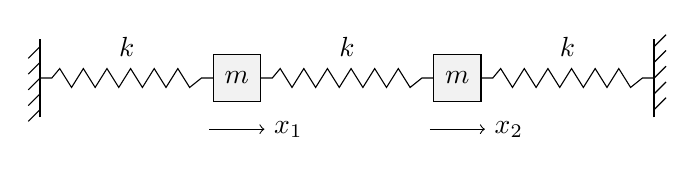
\begin{tikzpicture}[scale=1]
\foreach \s in {0,2.8,5.6}{
 \begin{scope}[shift={(\s,0)}]
 \draw (0,0)--(0.15,0)--(0.25,0.12)--(0.4,-0.12)--(0.55,0.12)
 --(0.7,-0.12)--(0.85,0.12)--(1,-0.12)--(1.15,0.12)
 --(1.3,-0.12)--(1.45,0.12)--(1.6,-0.12)--(1.75,0.12)
 --(1.9,-0.12)--(2.05,0)--(2.2,0);
 \node at (1.1,0.4) {$k$};
 \end{scope}
}
\draw[thick] (0,-0.5)--(0,0.5) (7.8,-0.5)--(7.8,0.5);
\foreach \y in {-0.4,-0.2,0,0.2,0.4}{
 \draw (0,\y)--(-0.15,{\y-0.15});
 \draw (7.8,\y)--(7.95,{\y+0.15});
}
\draw[fill=gray!10] (2.2,-0.3) rectangle (2.8,0.3);
\draw[fill=gray!10] (5,-0.3) rectangle (5.6,0.3);
\node at (2.5,0) {$m$};\node at (5.3,0) {$m$};
\draw[->] (2.15,-0.65)--(2.85,-0.65) node[right] {$x_1$};
\draw[->] (4.95,-0.65)--(5.65,-0.65) node[right] {$x_2$};
\end{tikzpicture}
\par\small Fig.~6.5 (schematic): equal masses and three equal spring constants.
\end{center}
\begin{enumerate}
\item[(a)] Set up the Newtonian acceleration equation for each mass.
\item[(b)] Solve the secular equation for the \erratum{eigenvalues}.
\item[(c)] Determine the eigenvectors and thus the normal modes of motion.
\end{enumerate}
\solution
The source figure has three springs with the same constant $k$ and
two masses of the same mass $m$. Take $m,k>0$ and measure both
displacements to the right from equilibrium.

(a) The left outer spring exerts $-kx_1$ on mass 1. The middle spring's
extension is $x_2-x_1$, so its forces are $+k(x_2-x_1)$ on mass 1 and
$-k(x_2-x_1)$ on mass 2. The right outer spring exerts $-kx_2$ on
mass 2. Newton's equations are therefore
\[
\boxed{m\ddot x_1=-2kx_1+kx_2,\qquad
       m\ddot x_2=kx_1-2kx_2.}
\]
In matrix notation,
\[
m\ddot{\boldsymbol x}+k
\begin{pmatrix}2&-1\\-1&2\end{pmatrix}\boldsymbol x=0.
\]
(b) Seek a normal mode
$\boldsymbol x(t)=\boldsymbol X e^{i\omega t}$ and use
$\ddot{\boldsymbol x}=-\omega^2\boldsymbol x$. Then
\[
\begin{pmatrix}2&-1\\-1&2\end{pmatrix}\boldsymbol X
=\lambda\boldsymbol X,
\qquad\lambda=\frac{m\omega^2}{k}.
\]
The secular equation is
\[
0=\begin{vmatrix}2-\lambda&-1\\-1&2-\lambda\end{vmatrix}
=(2-\lambda)^2-1
=\lambda^2-4\lambda+3=(\lambda-1)(\lambda-3).
\]
Thus
\[
\boxed{\omega_+=\sqrt{k/m},\qquad\omega_-=\sqrt{3k/m}.}
\]
\erratum{Part (b) asks for eigenvectors in the source; the secular
equation determines the eigenvalues. The eigenvectors are then found
in part (c), as follows.}

(c) For $\lambda=1$, the first row is $X_1-X_2=0$; choose the
unit vector $u_+=(1,1)^{\mathsf T}/\sqrt2$. The masses move in phase
with equal displacement, so the middle spring has no changing extension.
For $\lambda=3$, the first row is $-X_1-X_2=0$; choose
$u_-=(1,-1)^{\mathsf T}/\sqrt2$. The masses move with equal amplitudes
and opposite signs, stretching and compressing the middle spring.
These vectors have norm one and inner product zero.

The corresponding normal coordinates are
\[
Q_+=\frac{x_1+x_2}{\sqrt2},\qquad Q_-=\frac{x_1-x_2}{\sqrt2}.
\]
Adding and subtracting the Newton equations gives
\[
m\ddot Q_++kQ_+=0,\qquad m\ddot Q_-+3kQ_-=0.
\]
Therefore the general real motion can be written
\[
\boxed{\boldsymbol x(t)
=C_+u_+\cos(\omega_+t+\delta_+)
 +C_-u_-\cos(\omega_-t+\delta_-),}
\]
where the amplitudes and phases are fixed by the initial positions
and velocities.

\Needspace{5\baselineskip}
\par\bigskip
\noindent\textbf{6.5.20}\quad Given a normal matrix $\mathsf{A}$ with
eigenvalues $\lambda_{j}$, show that $\mathsf{A}^{\dagger}$ has eigenvalues
$\lambda_{j}^{*}$, its real part $(\mathsf{A}+\mathsf{A}^{\dagger})/2$ has
eigenvalues $\Re(\lambda_{j})$, and its imaginary part
$(\mathsf{A}-\mathsf{A}^{\dagger})/2i$ has eigenvalues $\Im(\lambda_{j})$.
\solution
First show that a right eigenvector of a normal matrix is also an
eigenvector of its adjoint with the conjugate eigenvalue. If
$Ax_j=\lambda_jx_j$, put $B=A-\lambda_jI$. It is normal because
\[
BB^\dagger-B^\dagger B=AA^\dagger-A^\dagger A=0.
\]
Using $Bx_j=0$, compute
\[
\|B^\dagger x_j\|^2
=x_j^\dagger BB^\dagger x_j
=x_j^\dagger B^\dagger Bx_j
=\|Bx_j\|^2=0.
\]
A vector with zero norm is zero, so
$B^\dagger x_j=0$, or $\boxed{A^\dagger x_j=\lambda_j^*x_j}$.
Now add and subtract the two eigenvalue equations:
\[
\frac{A+A^\dagger}{2}x_j
=\frac{\lambda_j+\lambda_j^*}{2}x_j
=\boxed{\Re(\lambda_j)x_j},
\]
\[
\frac{A-A^\dagger}{2i}x_j
=\frac{\lambda_j-\lambda_j^*}{2i}x_j
=\boxed{\Im(\lambda_j)x_j}.
\]
Thus the adjoint and both Hermitian parts share the original
orthonormal eigenbasis; the indicated eigenvalues follow on each basis
vector, including degenerate eigenspaces.

\Needspace{5\baselineskip}
\par\bigskip
\noindent\textbf{6.5.21}\quad Consider a rotation given by Euler angles
$\alpha=\pi/4$, $\beta=\pi/2$, $\gamma=5\pi/4$.
\begin{enumerate}
\item[(a)] Using the formula of Eq.~(3.37), construct the matrix $\mathsf{U}$
  representing this rotation.
\item[(b)] Find the eigenvalues and eigenvectors of $\mathsf{U}$, and from
  them describe this rotation by specifying a single rotation axis and an
  angle of rotation about that axis.
\end{enumerate}
\emph{Note.}~This technique provides a representation of rotations alternative
to the Euler angles.
\solution
(a) Equation (3.37), verified against textbook p.~141, uses
$U=S_3(\gamma)S_2(\beta)S_1(\alpha)$, where the rotations act on
coordinates. Set $c=1/\sqrt2$. The specified angles give
\[
\cos\alpha=\sin\alpha=c,\quad
\cos\beta=0,\quad\sin\beta=1,\quad
\cos\gamma=\sin\gamma=-c.
\]
The three matrices and their first product are
\[
S_1=\begin{pmatrix}c&c&0\\-c&c&0\\0&0&1\end{pmatrix},\quad
S_2=\begin{pmatrix}0&0&-1\\0&1&0\\1&0&0\end{pmatrix},\quad
S_3=\begin{pmatrix}-c&-c&0\\c&-c&0\\0&0&1\end{pmatrix},
\]
\[
S_2S_1=\begin{pmatrix}0&0&-1\\-c&c&0\\c&c&0\end{pmatrix}.
\]
Multiplying by $S_3$ on the left gives
\[
\boxed{U=\begin{pmatrix}
1/2&-1/2&1/\sqrt2\\
1/2&-1/2&-1/\sqrt2\\
1/\sqrt2&1/\sqrt2&0
\end{pmatrix}.}
\]
Its columns have norm one and pairwise scalar products zero; its
determinant is $1$, as also follows from the three proper-rotation
factors.

(b) To display the characteristic calculation without fractions,
expand the determinant of $2(U-\lambda I)$:
\begin{align*}
8\det(U-\lambda I)
&=\begin{vmatrix}
1-2\lambda&-1&\sqrt2\\1&-1-2\lambda&-\sqrt2\\
\sqrt2&\sqrt2&-2\lambda
\end{vmatrix}\\
&=(1-2\lambda)(4\lambda^2+2\lambda+2)
  +(2-2\lambda)+4(1+\lambda)\\
&=8(1-\lambda^3).
\end{align*}
Thus
\[
\lambda^3=1,\qquad
\boxed{\lambda_0=1,\quad
\lambda_\pm=\frac{-1\pm i\sqrt3}{2}=e^{\pm2\pi i/3}.}
\]
For an eigenvector $(x,y,z)^{\mathsf T}$, adding the first two rows of
the eigenvalue equation and retaining the third gives
\[
(1-\lambda)x-(1+\lambda)y=0,\qquad
x+y=\sqrt2\lambda z.
\]
At $\lambda=1$ the first equation gives $y=0$ and the second gives
$x=\sqrt2 z$. The remaining row also holds. Normalizing yields the
fixed-axis vector
\[
\boxed{n=\frac{(\sqrt2,0,1)^{\mathsf T}}{\sqrt3}.}
\]
For $\lambda=\lambda_\pm$, substitute
$y=\sqrt2\lambda z-x$ into the first equation:
\[
2x-\sqrt2\lambda(1+\lambda)z=0.
\]
Since $\lambda^2+\lambda+1=0$, this gives $x=-z/\sqrt2$ and then
\[
y=\frac{1+2\lambda}{\sqrt2}z
=\pm i\sqrt{\frac32}\,z.
\]
For $z=1$ the squared Hermitian norm is $1/2+3/2+1=3$, so
\[
\boxed{u_\pm=
\begin{pmatrix}-1/\sqrt6\\ \pm i/\sqrt2\\1/\sqrt3\end{pmatrix}.}
\]
Substitution into the unused row gives $Uu_\pm=\lambda_\pm u_\pm$.
Also $n^\dagger u_\pm=-1/3+1/3=0$ and
$u_+^\dagger u_-=1/6-1/2+1/3=0$, so these three vectors are
orthonormal.

The rotation axis is the line through the origin parallel to
$(\sqrt2,0,1)$, and its unsigned angle is $2\pi/3=120^\circ$.
The sign can be fixed, rather than inferred only from a conjugate pair
of eigenvalues. Define $[n]_\times v=n\times v$. Direct subtraction gives
\[
U-U^{\mathsf T}
=\begin{pmatrix}0&-1&0\\1&0&-\sqrt2\\0&\sqrt2&0\end{pmatrix}
=\sqrt3\,[n]_\times.
\]
For an active right-handed rotation, $R-R^{\mathsf T}
=2\sin\varphi[n]_\times$, while
$\operatorname{tr}U=0=1+2\cos\varphi$. Thus active application of $U$
to a column vector is a rotation by $+120^\circ$ about $n$.
\erratum{Equation (3.37) is a passive coordinate transformation.
The corresponding rotation of the coordinate axes is therefore
$-120^\circ$ about $n$, equivalently $+120^\circ$ about $-n$.
The directed angle must be paired with the chosen direction of the axis.}

\clearpage
\section{Chapter 7. Ordinary Differential Equations}
% Problems, Chapter 7: Ordinary Differential Equations
% Arfken, Weber & Harris, Mathematical Methods for Physicists, 7th ed.
% Requires: amsmath, amssymb, tikz

\section*{Problems}

\Needspace{8\baselineskip}
\subsection*{7.2 First-Order Equations}

\Needspace{5\baselineskip}
\par\bigskip
\noindent\textbf{7.2.1}\quad From Kirchhoff's law the current $I$ in an RC
(resistance-capacitance) circuit (Fig.~7.1) obeys the equation
\[
R\frac{dI}{dt}+\frac{1}{C}I=0.
\]
\begin{enumerate}
\item[(a)] Find $I(t)$.
\item[(b)] For a capacitance of $10{,}000$ $\mu$F charged to $100$ V and
  discharging through a resistance of $1$ M$\Omega$, find the current $I$ for
  $t=0$ and for $t=100$ seconds.
\end{enumerate}
\emph{Note.}~The initial voltage is $I_{0}R$ or $Q/C$, where
$Q=\int_{0}^{\infty}I(t)\,dt$.
\solution
(a) For $R,C>0$, separate the variables and integrate from $0$ to $t$,
with $I_0=I(0)\ne0$:
\[
\frac{dI}{I}=-\frac{dt}{RC},\qquad
\ln\left|\frac{I(t)}{I_0}\right|=-\frac{t}{RC},\qquad
\boxed{I(t)=I_0e^{-t/(RC)}}.
\]
The absolute value drops because $I(t)/I_0=\pm e^{-t/(RC)}$ is continuous,
never zero, and equal to $1$ at $t=0$.
The identically zero solution is included by $I_0=0$. Differentiation
checks $RI'+I/C=-I/C+I/C=0$.

(b) Convert the given units before finding the time constant:
\[
C=10^4\times10^{-6}\ \mathrm F=10^{-2}\ \mathrm F,\quad
R=10^6\ \Omega,\quad RC=10^4\ \mathrm s.
\]
By the Note, the initial voltage is $V_0=I_0R=100$ V, so $I_0=V_0/R$;
at $t=100$ s the exponent is $t/(RC)=100/10^4=0.01$. Thus
\[
\boxed{I(0)=\frac{100}{10^6}\ \mathrm A=100\ \mu\mathrm A},\qquad
\boxed{I(100\ \mathrm s)=100e^{-0.01}\ \mu\mathrm A
=99.00498337\ldots\ \mu\mathrm A}.
\]
As a charge check,
$\int_0^\infty I(t)dt=I_0RC\bigl[-e^{-t/(RC)}\bigr]_0^\infty=I_0RC
=(10^{-4}\ \mathrm A)(10^4\ \mathrm s)=1\ \mathrm C$, which equals
$CV_0=(10^{-2}\ \mathrm F)(100\ \mathrm V)$, as the Note requires.

\Needspace{5\baselineskip}
\par\bigskip
\noindent\textbf{7.2.2}\quad The Laplace transform of Bessel's equation
($n=0$) leads to
\[
(s^{2}+1)f'(s)+sf(s)=0.
\]
Solve for $f(s)$.
\solution
For real $s$, $1+s^2$ is positive. Separate and integrate, using
$d\ln(1+s^2)/ds=2s/(1+s^2)$:
\[
\frac{f'}f=-\frac{s}{1+s^2},\qquad
\ln|f|=-\frac12\ln(1+s^2)+K.
\]
Exponentiating gives $|f|=e^K(1+s^2)^{-1/2}$; absorbing the sign into an
arbitrary real constant gives
\[
\boxed{f(s)=\frac{A}{\sqrt{1+s^2}}}.
\]
This includes $f=0$. Indeed,
$f'=-As(1+s^2)^{-3/2}$, so $(1+s^2)f'=-As(1+s^2)^{-1/2}=-sf$.
Conversely, every solution has this form, even one that vanishes
somewhere (where the logarithm fails): by the product rule,
$d\bigl[\sqrt{1+s^2}\,f\bigr]/ds=\bigl[(1+s^2)f'+sf\bigr]/\sqrt{1+s^2}=0$,
so $\sqrt{1+s^2}\,f$ is a constant $A$.
The ODE alone does not determine $A$. If the intended transform is
specifically that of $J_0$, the initial-value theorem of the Laplace
transform, $\lim_{s\to+\infty}sf(s)=J_0(0)=1$, together with
$sf(s)=As/\sqrt{1+s^2}\to A$, gives $A=1$.
For complex $s$, the same formula holds with a complex constant on a
simply connected domain avoiding $s=\pm i$, after choosing a square-root
branch. On the Laplace half-plane $\operatorname{Re}s>0$, choose the
analytic branch positive for positive real $s$; it has
$\sqrt{1+s^2}\sim s$ along the positive real axis.

\Needspace{5\baselineskip}
\par\bigskip
\noindent\textbf{7.2.3}\quad The decay of a population by catastrophic
two-body collisions is described by
\[
\frac{dN}{dt}=-kN^{2}.
\]
This is a first-order, nonlinear differential equation. Derive the solution
\[
N(t)=N_{0}\left(1+\frac{t}{\tau_{0}}\right)^{-1},
\]
where $\tau_{0}=(kN_{0})^{-1}$, \erratum{with $k,N_0>0$.
The backward extrapolation has a pole as $t\downarrow-\tau_0$;
$N(-\tau_0)$ itself is undefined.}
\solution
For $N_0>0$ and $k>0$, integrate from the initial state:
\[
\int_{N_0}^{N(t)}\frac{dN}{N^2}=-k\int_0^t ds,
\qquad -\frac1{N(t)}+\frac1{N_0}=-kt.
\]
Hence $1/N(t)=1/N_0+kt=(1+kN_0t)/N_0$, and taking the reciprocal gives
\[
\boxed{N(t)=\frac{N_0}{1+kN_0t}
=N_0\left(1+\frac t{\tau_0}\right)^{-1}},\qquad
\tau_0=\frac1{kN_0}.
\]
Direct differentiation yields $N'=-kN_0^2/(1+kN_0t)^2=-kN^2$.
The initial-value solution with positive population has mathematical
interval $t> -\tau_0$ and a pole at its left endpoint; physical decay
uses $t\ge0$. The textbook's closing remark that this implies an
infinite population at $t=-\tau_0$, qualified by the red note in the
statement, should be read accordingly: the pole is a backward
extrapolation of the model, not an attained infinite population at a
finite time within its solution interval.
If $N_0=0$, the separate solution is $N\equiv0$; if $k=0$, $N\equiv N_0$.

\Needspace{5\baselineskip}
\par\bigskip
\noindent\textbf{7.2.4}\quad The rate of a particular chemical reaction
$\mathrm{A}+\mathrm{B}\to\mathrm{C}$ is proportional to the concentrations of
the reactants A and B:
\[
\frac{dC(t)}{dt}=\alpha[A(0)-C(t)][B(0)-C(t)].
\]
\begin{enumerate}
\item[(a)] Find $C(t)$ for $A(0)\neq B(0)$.
\item[(b)] Find $C(t)$ for $A(0)=B(0)$.
\end{enumerate}
The initial condition is that $C(0)=0$.
\solution
Let $A_0=A(0)$ and $B_0=B(0)$, and assume nonnegative initial
concentrations and $\alpha\ge0$.

(a) If $A_0\ne B_0$ and both are positive, partial fractions give
\[
\frac1{(A_0-C)(B_0-C)}
=\frac1{B_0-A_0}\left(\frac1{A_0-C}-\frac1{B_0-C}\right),
\]
as recombining the right side over the common denominator shows.
Separate the variables, $dC/[(A_0-C)(B_0-C)]=\alpha\,dt$, and integrate
from $0$ to $t$. The constant $C=\min(A_0,B_0)$ is an equilibrium
solution. The right side $\alpha(A_0-C)(B_0-C)$ is a polynomial in $C$,
so by the uniqueness theorem for $C'=f(C)$ with continuously
differentiable $f$ two solutions cannot take the same value at the same
time; hence the solution starting at $C(0)=0$ never reaches the
equilibrium. Below it both factors are positive, so $C'\ge0$ and $C$
cannot fall below $C(0)=0$. Thus $0\le C<\min(A_0,B_0)$, where
\[
\int_0^C\frac{du}{A_0-u}=\ln\frac{A_0}{A_0-C},\qquad
\int_0^C\frac{du}{B_0-u}=\ln\frac{B_0}{B_0-C}.
\]
The difference of these logarithms, divided by $B_0-A_0$, yields
\[
\frac1{B_0-A_0}\ln\left[\frac{B_0-C}{A_0-C}\frac{A_0}{B_0}\right]
=\alpha t.
\]
Set $E=e^{\alpha(B_0-A_0)t}$. Multiplying by $B_0-A_0$, exponentiating,
clearing the denominators, and collecting the terms in $C$ give
\[
A_0(B_0-C)=B_0E(A_0-C),\qquad
C(B_0E-A_0)=A_0B_0(E-1).
\]
Thus $C=A_0B_0(E-1)/(B_0E-A_0)$; dividing numerator and denominator by
$E$ gives
\[
\boxed{C(t)=\frac{A_0B_0(1-e^{-\alpha(B_0-A_0)t})}
{B_0-A_0e^{-\alpha(B_0-A_0)t}}}.
\]
It starts at zero and approaches $\min(A_0,B_0)$ for $\alpha>0$: if
$B_0>A_0$ the exponential tends to $0$ and $C\to A_0B_0/B_0=A_0$; if
$B_0<A_0$ it grows without bound, and $C\to A_0B_0/A_0=B_0$.
To check the result, put $\lambda=\alpha(B_0-A_0)$ and
$D=B_0-A_0e^{-\lambda t}$, so $C=A_0B_0(1-e^{-\lambda t})/D$. Then
$A_0-C=A_0(B_0-A_0)e^{-\lambda t}/D$ and $B_0-C=B_0(B_0-A_0)/D$, so
$\alpha(A_0-C)(B_0-C)=\alpha A_0B_0(B_0-A_0)^2e^{-\lambda t}/D^2$.
Since $D'=\lambda A_0e^{-\lambda t}$, the quotient rule gives
\[
C'=\frac{A_0B_0\lambda e^{-\lambda t}\bigl[D-A_0(1-e^{-\lambda t})\bigr]}{D^2}
=\frac{A_0B_0\lambda e^{-\lambda t}(B_0-A_0)}{D^2},
\]
the same expression because $\lambda=\alpha(B_0-A_0)$.
If either concentration is zero, $C(t)=0$ directly; the formula also
reduces to that value when $A_0\ne B_0$.

(b) With $A_0=B_0=a>0$, separate instead as
\[
\int_0^{C(t)}\frac{du}{(a-u)^2}=\alpha t,
\qquad \frac1{a-C}-\frac1a=\alpha t.
\]
Hence $1/(a-C)=(1+\alpha at)/a$, i.e., $a-C=a/(1+\alpha at)$, and
\[
\boxed{C(t)=a-\frac a{1+\alpha at}=\frac{\alpha a^2t}{1+\alpha at}}.
\]
The formula includes $a=0$ and $\alpha=0$. It satisfies the equation:
$C'=\alpha a^2/(1+\alpha at)^2=\alpha(a-C)^2$.

\Needspace{5\baselineskip}
\par\bigskip
\noindent\textbf{7.2.5}\quad A boat, coasting through the water, experiences a
resisting force proportional to $v^{n}$, $v$ being the boat's instantaneous
velocity. Newton's second law leads to
\[
m\frac{dv}{dt}=-kv^{n}.
\]
With $v(t=0)=v_{0}$, $x(t=0)=0$, integrate to find $v$ as a function of time
and $v$ as a function of distance.
\erratum{Take $m,k,v_0>0$, $n\in\mathbb R$, and use the real positive-speed
branch until it reaches zero, if it does.}
\solution
Take $m,k,v_0>0$ and interpret $v$ as speed while the boat moves
forward. Put $\gamma=k/m$. For $n\ne1$, separate and integrate from $0$
to $t$:
\[
v^{-n}dv=-\gamma dt,\qquad
\frac{v^{1-n}-v_0^{1-n}}{1-n}=-\gamma t,
\]
so $v^{1-n}=v_0^{1-n}-(1-n)\gamma t$, and raising to the power $1/(1-n)$,
\[
\boxed{v(t)=\left[v_0^{1-n}+(n-1)\gamma t\right]^{1/(1-n)}}
\quad(n\ne1).
\]
The real positive branch is used while the bracket is positive. For
$n=1$, the integration is logarithmic:
\[
\ln(v/v_0)=-\gamma t,\qquad \boxed{v(t)=v_0e^{-\gamma t}}.
\]
To eliminate time use $dv/dt=(dv/dx)(dx/dt)=v\,dv/dx$ while $v>0$.
Then $mv\,dv/dx=-kv^n$, i.e., $v^{1-n}dv=-\gamma dx$; integrating from
$x=0$, for $n\ne2$,
\[
\frac{v^{2-n}-v_0^{2-n}}{2-n}=-\gamma x,
\qquad
\boxed{v(x)=\left[v_0^{2-n}+(n-2)\gamma x\right]^{1/(2-n)}}.
\]
For the omitted case $n=2$, $dv/v=-\gamma dx$, giving
\[
\boxed{v(x)=v_0e^{-\gamma x}}.
\]
The general formulas also cover the value excluded in the other
variable: $n=1$ in $v(x)$ gives $v(x)=v_0-\gamma x$, and $n=2$ in $v(t)$
gives $v(t)=(v_0^{-1}+\gamma t)^{-1}=v_0/(1+\gamma v_0t)$.
Differentiating the two integrated identities,
$d[v^{1-n}/(1-n)]/dt=v^{-n}v'=-\gamma$ and
$d[v^{2-n}/(2-n)]/dx=v^{1-n}\,dv/dx=-\gamma$, checks both equations
for every $n\ne1$ and every $n\ne2$, respectively; the exponentials
satisfy $v'=-\gamma v$ ($n=1$) and $v\,dv/dx=-\gamma v^2$ ($n=2$)
directly.

For $n<1$ the bracket in $v(t)$ decreases to zero, so the positive-speed
branch reaches zero at $t_*=v_0^{1-n}/[(1-n)\gamma]$; likewise, for $n<2$
the bracket in $v(x)$ vanishes at the limiting travel distance
$x_*=v_0^{2-n}/[(2-n)\gamma]$. For $n>1$ the bracket in $v(t)$ grows
without bound, so $v\to0$ only as $t\to\infty$ (as for the exponential
at $n=1$): stopping takes infinite time. In the same way, for $n\ge2$ the
speed $v(x)$ is positive at every $x$, so the traveled distance is
unbounded: were $x(t)\le L$ for all $t$, then, since
$dv/dx=-\gamma v^{n-1}<0$, the speed would stay at least $v(L)>0$, so
$x(t)\ge v(L)\,t$ would exceed $L$ for $t>L/v(L)$, a contradiction.
\erratum{The positive-speed drag model does not authorize continuing a
fractional or negative power through $v=0$. At or after stopping an
appropriate force law must be specified; the formulas above state their
actual domain.}

\Needspace{5\baselineskip}
\par\bigskip
\noindent\textbf{7.2.6}\quad In the first-order differential equation
$dy/dx=f(x,y)$, the function $f(x,y)$ is a function of the ratio $y/x$:
\[
\frac{dy}{dx}=g(y/x).
\]
Show that the substitution of $u=y/x$ leads to a separable equation in $u$ and
$x$.
\solution
Work on an interval with $x\ne0$. Since $y=xu$,
\[
\frac{dy}{dx}=u+x\frac{du}{dx}=g(u),\qquad
x\frac{du}{dx}=g(u)-u.
\]
Thus, whenever $g(u)-u\ne0$,
\[
\boxed{\frac{du}{g(u)-u}=\frac{dx}{x}},\qquad
\int^u\frac{ds}{g(s)-s}=\ln|x|+C.
\]
Division by $g(u)-u$ omits its zeros. Each constant $u_*$ satisfying
$g(u_*)=u_*$ supplies the additional straight-line solution $y=u_*x$,
which must be checked before declaring the solution set complete.

\Needspace{5\baselineskip}
\par\bigskip
\noindent\textbf{7.2.7}\quad The differential equation
\[
P(x,y)\,dx+Q(x,y)\,dy=0
\]
is exact. \erratum{Assume $P,Q$ have continuous first partial derivatives
and that the rectangular integration path lies inside the domain.} Show that its solution is of the form
\[
\varphi(x,y)=\erratum{\int_{x_{0}}^{x}P(\xi,y)\,d\xi+\int_{y_{0}}^{y}Q(x_{0},\eta)\,d\eta}
=\text{constant}.
\]
\solution
Use distinct integration variables, so the proposed potential is
\[
\varphi(x,y)=\int_{x_0}^xP(\xi,y)d\xi
             +\int_{y_0}^yQ(x_0,\eta)d\eta.
\]
This is the line integral along the path first from $(x_0,y_0)$ to
$(x_0,y)$, then to $(x,y)$. Exactness means $P\,dx+Q\,dy=d\Phi$
for a potential $\Phi$, i.e., $\Phi_x=P$ and $\Phi_y=Q$. Hence, by the
fundamental theorem of calculus,
\[
\int_{y_0}^yQ(x_0,\eta)d\eta=\Phi(x_0,y)-\Phi(x_0,y_0),\qquad
\int_{x_0}^xP(\xi,y)d\xi=\Phi(x,y)-\Phi(x_0,y),
\]
and the sum is $\varphi(x,y)=\Phi(x,y)-\Phi(x_0,y_0)$. It follows that
$d\varphi=d\Phi=P\,dx+Q\,dy$ and the solution curves satisfy
\[
\boxed{\varphi(x,y)=C}.
\]
More explicitly, differentiation (under the integral sign in the first
term, then the exactness condition $P_y=Q_x$ and the fundamental theorem
of calculus in $\xi$; see 7.2.8) gives
\[
\varphi_x=P(x,y),\quad
\varphi_y=\int_{x_0}^xP_y(\xi,y)d\xi+Q(x_0,y)
=Q(x,y)-Q(x_0,y)+Q(x_0,y)=Q(x,y).
\]
Along any solution curve $(x(t),y(t))$, the chain rule gives
$d\varphi/dt=P\dot x+Q\dot y=0$. Conversely this same calculation
shows that a differentiable level curve solves the differential form.
The displayed rectangular path is understood to lie inside the domain;
otherwise one uses an admissible path for the same exact differential.

\Needspace{5\baselineskip}
\par\bigskip
\noindent\textbf{7.2.8}\quad The differential equation
\[
P(x,y)\,dx+Q(x,y)\,dy=0
\]
is exact. \erratum{Assume $P,Q$ have continuous first partial derivatives
and that the rectangular integration path lies inside the domain.} If
\[
\varphi(x,y)=\erratum{\int_{x_{0}}^{x}P(\xi,y)\,d\xi+\int_{y_{0}}^{y}Q(x_{0},\eta)\,d\eta},
\]
show that
\[
\frac{\partial\varphi}{\partial x}=P(x,y),\quad
\frac{\partial\varphi}{\partial y}=Q(x,y).
\]
Hence, $\varphi(x,y)=\text{constant}$ is a solution of the original
differential equation.
\solution
Write the formula with dummy variables:
\[
\varphi(x,y)=\int_{x_0}^xP(\xi,y)d\xi
             +\int_{y_0}^yQ(x_0,\eta)d\eta.
\]
The fundamental theorem of calculus, with $y$ held fixed, gives
$\boxed{\varphi_x=P(x,y)}$; the second term does not depend on $x$.
Differentiating with respect to $y$ requires both terms: the first is
differentiated under the integral sign (allowed because $P_y$ is
continuous), the second by the fundamental theorem of calculus in $\eta$:
\begin{align*}
\varphi_y
&=\int_{x_0}^xP_y(\xi,y)d\xi+Q(x_0,y)\\
&=\int_{x_0}^xQ_x(\xi,y)d\xi+Q(x_0,y)\\
&=Q(x,y)-Q(x_0,y)+Q(x_0,y)=\boxed{Q(x,y)}.
\end{align*}
The second line uses the exactness condition $P_y=Q_x$; the third
integrates $Q_x$ in $\xi$ by the fundamental theorem of calculus.
Therefore $d\varphi=\varphi_xdx+\varphi_ydy=Pdx+Qdy$.
A level curve $\varphi=C$ has $d\varphi=0$ and satisfies the original
equation. As in 7.2.7, the chosen paths must lie within the domain.

\Needspace{5\baselineskip}
\par\bigskip
\noindent\textbf{7.2.9}\quad Prove that Eq.~(7.12) is exact in the sense of
Eq.~(7.9), provided that $\alpha(x)$ satisfies Eq.~(7.14).
\solution
The referenced equations are
$\alpha y'+\alpha py=\alpha q$ and $\alpha'=\alpha p$.
In differential form (multiply the first by $dx$ and move $\alpha q\,dx$
to the left) it is
\[
M(x,y)dx+N(x,y)dy=0,\qquad
M=\alpha(x)[p(x)y-q(x)],\quad N=\alpha(x).
\]
The exactness test is
\[
M_y=\alpha p,\qquad N_x=\alpha',
\]
so $M_y=N_x$ follows precisely from Eq.~(7.14). A direct potential is
\[
\boxed{\Phi(x,y)=\alpha(x)y-\int^x\alpha(s)q(s)ds},
\]
because $\Phi_y=\alpha=N$ and, by Eq.~(7.14),
$\Phi_x=\alpha' y-\alpha q=\alpha(py-q)=M$.
For equivalence with the original ODE choose a nonzero integrating factor,
$\alpha=e^{\int p\,dx}$; the identically zero factor would give only
$0=0$ and discard the equation.

\Needspace{5\baselineskip}
\par\bigskip
\noindent\textbf{7.2.10}\quad A certain differential equation has the form
\[
f(x)\,dx+g(x)h(y)\,dy=0,
\]
with none of the functions $f(x)$, $g(x)$, $h(y)$ identically zero. Show that
a necessary and sufficient condition for this equation to be exact is that
$g(x)=\text{constant}$.
\erratum{Work on a product of connected intervals, with $C^1$ coefficients.}
\solution
On a product of connected intervals, with the stated functions continuously
differentiable where needed, exactness requires
\[
\frac{\partial f(x)}{\partial y}=0
=\frac{\partial[g(x)h(y)]}{\partial x}=g'(x)h(y).
\]
Since $h$ is not identically zero, choose one $y_*$ with $h(y_*)\ne0$.
The equality at $(x,y_*)$ forces $g'(x)=0$ for every $x$, so $g$ is a
constant. Conversely, if $g=g_0$, then
\[
f(x)dx+g_0h(y)dy=d\left[\int^xf(s)ds+g_0\int^yh(t)dt\right]
\]
is exact. Hence $\boxed{g(x)=g_0}$ is necessary and sufficient.
\erratum{The connected product-domain assumption specifies the usual
meaning of this exercise. Without it, $h$ could vanish throughout an
entire component, imposing no condition on $g$ there, or different
$x$-components could carry different constants.}

\Needspace{5\baselineskip}
\par\bigskip
\noindent\textbf{7.2.11}\quad Show that
\[
y(x)=\exp\left[-\int^{x}p(t)\,dt\right]
\left\{\int^{x}\left[\exp\left(\int^{s}p(t)\,dt\right)\right]q(s)\,ds
+C\right\}
\]
is a solution of
\[
\frac{dy}{dx}+p(x)y(x)=q(x)
\]
by differentiating the expression for $y(x)$ and substituting into the
differential equation.
\solution
Choose a fixed base point and abbreviate
\[
P_0(x)=\int_{x_0}^xp(t)dt,\qquad
J(x)=\int_{x_0}^xe^{P_0(s)}q(s)ds+C.
\]
Then the proposed solution is $y=e^{-P_0}J$, with
$P_0'=p$ and $J'=e^{P_0}q$. The product and chain rules give
\[
y'=-p e^{-P_0}J+e^{-P_0}e^{P_0}q=-py+q.
\]
Therefore $\boxed{y'+py=q}$. Changing the fixed lower limits merely
changes the arbitrary constant or rescales the integrating factor and
does not change the resulting family of solutions.

\Needspace{5\baselineskip}
\par\bigskip
\noindent\textbf{7.2.12}\quad The motion of a body falling in a resisting
medium may be described by
\[
m\frac{dv}{dt}=mg-bv
\]
when the retarding force is proportional to the velocity, $v$. Find the
velocity. Evaluate the constant of integration by demanding that $v(0)=0$.
\solution
For $b>0$, divide by $m$ and multiply by the integrating factor
$e^{bt/m}$; by the product rule,
$(e^{bt/m}v)'=e^{bt/m}(v'+bv/m)$, so
\[
v'+\frac bm v=g,\qquad
\frac d{dt}(e^{bt/m}v)=ge^{bt/m}.
\]
Integrating from $0$ to $t$, using $v(0)=0$ and
$\int_0^tge^{bs/m}ds=(mg/b)(e^{bt/m}-1)$, gives
\[
e^{bt/m}v(t)=\frac{mg}{b}(e^{bt/m}-1),\qquad
\boxed{v(t)=\frac{mg}{b}(1-e^{-bt/m})}.
\]
The check is $mv'=mg e^{-bt/m}=mg-bv$.
The terminal velocity is $mg/b$; as $b\to0$, the expansion
$1-e^{-bt/m}=bt/m+O(b^2)$ gives the drag-free solution $v=gt$.

\Needspace{5\baselineskip}
\par\bigskip
\noindent\textbf{7.2.13}\quad Radioactive nuclei decay according to the law
\[
\frac{dN}{dt}=-\lambda N,
\]
$N$ being the concentration of a given nuclide and $\lambda$, the particular
decay constant. In a radioactive series of two different nuclides, with
concentrations $N_{1}(t)$ and $N_{2}(t)$, we have
\[
\frac{dN_{1}}{dt}=-\lambda_{1}N_{1},\quad
\frac{dN_{2}}{dt}=\lambda_{1}N_{1}-\lambda_{2}N_{2}.
\]
Find $N_{2}(t)$ for the conditions $N_{1}(0)=N_{0}$ and $N_{2}(0)=0$.
\solution
The first equation integrates to $N_1=N_0e^{-\lambda_1t}$. The second
becomes a linear equation; multiplying it by the integrating factor
$e^{\lambda_2t}$ and using
$(e^{\lambda_2t}N_2)'=e^{\lambda_2t}(N_2'+\lambda_2N_2)$,
\[
N_2'+\lambda_2N_2=\lambda_1N_0e^{-\lambda_1t},\qquad
\frac d{dt}(e^{\lambda_2t}N_2)
=\lambda_1N_0e^{(\lambda_2-\lambda_1)t}.
\]
Integrate from $0$ to $t$, with $N_2(0)=0$. If
$\lambda_1\ne\lambda_2$,
\[
e^{\lambda_2t}N_2(t)=\lambda_1N_0\int_0^te^{(\lambda_2-\lambda_1)s}ds
=\frac{\lambda_1N_0}{\lambda_2-\lambda_1}
\bigl(e^{(\lambda_2-\lambda_1)t}-1\bigr),
\]
and multiplication by $e^{-\lambda_2t}$ gives
\[
\boxed{N_2(t)=\frac{\lambda_1N_0}{\lambda_2-\lambda_1}
(e^{-\lambda_1t}-e^{-\lambda_2t})}.
\]
\erratum{The coincident-rate case must be handled separately rather than
dividing by $\lambda_2-\lambda_1$.} If both rates equal $\lambda$,
\[
e^{\lambda t}N_2=\lambda N_0\int_0^t ds=\lambda N_0t,
\qquad \boxed{N_2=\lambda N_0t e^{-\lambda t}}.
\]
This is also the limit of the preceding expression: with
$\lambda_1=\lambda$ and $\lambda_2\to\lambda$,
$(e^{-\lambda t}-e^{-\lambda_2t})/(\lambda_2-\lambda)$ tends to the
derivative of $-e^{-\lambda_2t}$ with respect to $\lambda_2$ at
$\lambda_2=\lambda$, which is $te^{-\lambda t}$. Both forms satisfy
the initial condition and the inhomogeneous equation by differentiation.

\Needspace{5\baselineskip}
\par\bigskip
\noindent\textbf{7.2.14}\quad The rate of evaporation from a particular
spherical drop of liquid (constant density) is proportional to its surface
area. Assuming this to be the sole mechanism of mass loss, find the radius of
the drop as a function of time.
\solution
Let $\rho$ be the fixed mass density and let $j>0$ be the mass lost per
unit area per unit time. Then
\[
M=\frac{4\pi}3\rho r^3,\qquad
\frac{dM}{dt}=4\pi\rho r^2r'=-j(4\pi r^2).
\]
While $r>0$, cancellation gives $r'=-j/\rho$. With $r(0)=r_0$,
\[
\boxed{r(t)=r_0-\frac j\rho t,\qquad
0\le t\le t_*:=\frac{\rho r_0}{j}.}
\]
At $t_*$ the drop is exhausted. The model's physical continuation has
zero radius and mass, not a negative radius. If the proportionality
constant is defined for volume loss instead of mass loss, put
$\kappa=j/\rho$ and write $r=r_0-\kappa t$.

\Needspace{5\baselineskip}
\par\bigskip
\noindent\textbf{7.2.15}\quad In the linear homogeneous differential equation
\[
\frac{dv}{dt}=-av
\]
the variables are separable. When the variables are separated, the equation is
exact. Solve this differential equation subject to $v(0)=v_{0}$ by the
following three methods:
\begin{enumerate}
\item[(a)] Separating variables and integrating.
\item[(b)] Treating the separated variable equation as exact.
\item[(c)] Using the result for a linear homogeneous differential equation.
\end{enumerate}
\par\nobreak\hfill\emph{ANS.}\enspace $v(t)=v_{0}e^{-at}$.
\solution
(a) For $v_0\ne0$, separation gives
\[
\int_{v_0}^{v(t)}\frac{du}{u}=-a\int_0^t ds,
\quad \ln|v(t)/v_0|=-at,
\quad v(t)=v_0e^{-at}.
\]
The sign stays that of $v_0$; $v\equiv0$ is separately included when
$v_0=0$.

(b) The separated form $a\,dt+dv/v=0$, i.e., $P\,dt+Q\,dv=0$ with
$P=a$ and $Q=1/v$, is exact on either half-plane $v>0$ or $v<0$, since
both cross partial derivatives vanish: $\partial P/\partial v=0
=\partial Q/\partial t$. Its potential is $\Phi(t,v)=at+\ln|v|$, because
$\Phi_t=a$ and $\Phi_v=1/v$. The level condition
$\Phi(t,v)=\Phi(0,v_0)=\ln|v_0|$ gives $\ln|v/v_0|=-at$, so
$|v|=|v_0|e^{-at}$; since $v$ stays in the half-plane of $v_0$, this is
the same exponential $v=v_0e^{-at}$.
The zero solution was excluded only by division by $v$ and must be restored.

(c) In the linear first-order formula of Exercise 7.2.11 take $p=a$,
$q=0$:
\[
v=e^{-\int a\,dt}(C+0)=Ce^{-at}.
\]
The initial condition gives $C=v_0$. Thus all three methods give
$\boxed{v=v_0e^{-at}}$, and $v'=-av$ checks it directly.

\Needspace{5\baselineskip}
\par\bigskip
\noindent\textbf{7.2.16}\quad
\begin{enumerate}
\item[(a)] Solve Example 7.2.1, assuming that the parachute opens when the
  parachutist's velocity has reached $v_{i}=60$ mi/h (regard this time as
  $t=0$). Find $v(t)$.
\item[(b)] For a skydiver in free fall use the friction coefficient
  $b=0.25$ kg/m and mass $m=70$ kg. What is the limiting velocity in this
  case?
\end{enumerate}
\solution
In Example 7.2.1 the downward speed obeys
$mv'=mg-bv^2$. Put $v_T=\sqrt{mg/b}$ and
$T=\sqrt{m/(bg)}$, so $v_T/T=g$.

(a) Since $mg-bv^2=b(v_T^2-v^2)$, separation gives
$dv/(v_T^2-v^2)=(b/m)\,dt$. By partial fractions,
\[
\frac1{v_T^2-u^2}=\frac1{2v_T}\left(\frac1{v_T-u}+\frac1{v_T+u}\right),
\qquad
\int\frac{du}{v_T^2-u^2}=\frac1{2v_T}\ln\left|\frac{v_T+u}{v_T-u}\right|.
\]
Integrating from the nonzero initial speed $v_i$ at $t=0$ therefore gives
\[
\int_{v_i}^{v}\frac{du}{v_T^2-u^2}=\frac bm t,
\qquad
\frac1{2v_T}\ln\left|\frac{v_T+v}{v_T-v}
                         \frac{v_T-v_i}{v_T+v_i}\right|=\frac bm t.
\]
Here $2v_Tb/m=2\sqrt{bg/m}=2/T$, so the logarithm equals $2t/T$.
For $v_i\ne v_T$, put $q=(v_i-v_T)/(v_i+v_T)$. Exponentiating and
inverting the ratio give
\[
\left|\frac{v-v_T}{v+v_T}\right|=|q|\,e^{-2t/T}.
\]
The right side never vanishes, so $v\ne v_T$ at every $t$; by continuity
$v-v_T$ keeps the sign of $v_i-v_T$, which is the sign of $q$. (Since
$v'=(b/m)(v_T^2-v^2)$, the speed moves monotonically from $v_i\ge0$
toward $v_T$, so $v+v_T>0$.) Hence
\[
\frac{v-v_T}{v+v_T}=q e^{-2t/T},\qquad
v(1-qe^{-2t/T})=v_T(1+qe^{-2t/T}).
\]
Divide by $1-qe^{-2t/T}$ and multiply numerator and denominator by
$v_i+v_T$. This gives
\[
\boxed{v(t)=v_T
\frac{(v_i+v_T)+(v_i-v_T)e^{-2t/T}}
     {(v_i+v_T)-(v_i-v_T)e^{-2t/T}}}
=v_T\frac{v_i+v_T\tanh(t/T)}{v_T+v_i\tanh(t/T)}.
\]
For the second form write the numerator as
$v_i(1+e^{-2t/T})+v_T(1-e^{-2t/T})$ and the denominator as
$v_i(1-e^{-2t/T})+v_T(1+e^{-2t/T})$, divide both by $1+e^{-2t/T}$, and
use $(1-e^{-2u})/(1+e^{-2u})=\tanh u$.
For $v_i=v_T$, separation divided by zero; direct substitution instead
gives the equilibrium $v(t)=v_T$, which the boxed formula also includes.
For every $v_i\ge0$ and $t\ge0$, $-1\le q<1$, so its denominator is
positive. It gives $v(0)=v_i$ and approaches $v_T$. For the example's
$m=70\ \mathrm{kg}$, $b=700\ \mathrm{kg/m}$, $g=9.8\ \mathrm{m/s^2}$,
and with $1\ \mathrm{mi/h}=1609.344\ \mathrm m/3600\ \mathrm s
=0.44704\ \mathrm{m/s}$,
\[
\begin{aligned}
v_i&=60(0.44704)=26.8224\ \mathrm{m/s},\\
v_T&=\sqrt{0.98}=0.9899494936\ldots\ \mathrm{m/s},\\
T&=1/\sqrt{98}=0.1010152544\ldots\ \mathrm s.
\end{aligned}
\]
\erratum{Here $v_i>v_T$. The Instructor's Manual's real expression
involving $\operatorname{arctanh}(v_i/v_T)$ is therefore inapplicable,
since $\operatorname{arctanh}w$ is real only for $|w|<1$. The equivalent
real hyperbolic form for this case is}
\[
\erratum{v(t)=v_T\coth\left(t/T+\operatorname{arccoth}(v_i/v_T)\right)},
\quad \operatorname{arccoth}w=\tfrac12\ln\frac{w+1}{w-1}\quad(w>1).
\]
Indeed, with $\phi=\operatorname{arccoth}(v_i/v_T)$ and $u=t/T$, the
addition formula $\coth(u+\phi)=(\coth u\coth\phi+1)/(\coth u+\coth\phi)$,
multiplied above and below by $v_T\tanh u$, gives
$v_T\coth(u+\phi)=v_T(v_i+v_T\tanh u)/(v_T+v_i\tanh u)$, the
$\tanh$ form above.
Differentiating either real form verifies $v'=g(1-v^2/v_T^2)$, which is
$mv'=mg-bv^2$ divided by $m$; e.g., $\operatorname{csch}^2=\coth^2-1$ and
$v_T/T=g$ give
$v'=-(v_T/T)\operatorname{csch}^2(u+\phi)=g(1-v^2/v_T^2)$. The
speed initially decreases, as it must when the parachute opens above
terminal speed. Numerically, $v_i/v_T=27.0947\ldots$, so
$\phi=\frac12\ln[(v_i/v_T+1)/(v_i/v_T-1)]=0.0369243\ldots$, and
$1/T=\sqrt{98}\ \mathrm{s^{-1}}=9.89949\ldots\ \mathrm{s^{-1}}$; with $t$
in seconds,
\[
v(t)\approx0.989949\coth(9.89949\,t+0.0369243)\ \mathrm{m/s}.
\]
For example, $v(0.1\ \mathrm s)=1.2812\ldots\ \mathrm{m/s}$, already
within $0.3\ \mathrm{m/s}$ of $v_T$.

(b) With the free-fall drag coefficient $b=0.25\ \mathrm{kg/m}$,
\[
\boxed{v_T=\sqrt{\frac{70(9.8)}{0.25}}=\sqrt{2744}
=52.38320341\ldots\ \mathrm{m/s}
=188.5795\ldots\ \mathrm{km/h}},
\]
where $1\ \mathrm{m/s}=3.6\ \mathrm{km/h}$.

\Needspace{5\baselineskip}
\par\bigskip
\noindent\textbf{7.2.17}\quad Solve the ODE
\[
(xy^{2}-y)\,dx+x\,dy=0.
\]
\solution
On $x\ne0$, divide by $x$:
\[
y'-\frac yx=-y^2.
\]
The solution $y=0$ is immediate. For $y\ne0$, this Bernoulli equation
becomes linear for $u=1/y$: then $u'=-y'/y^2$, and multiplication by
$-y^{-2}$ gives $-y'/y^2+1/(xy)=1$, i.e.,
\[
u'+\frac ux=1,\qquad (xu)'=xu'+u=x.
\]
Integrating yields $xu=x^2/2+C$, hence $u=(x^2+2C)/(2x)$ and $y=1/u$:
\[
\boxed{y(x)=\frac{2x}{x^2+K}},\qquad \boxed{y\equiv0},
\]
where $K=2C$. Substitution into the original, undivided equation, which
is $xy'=y-xy^2$, checks it: by the quotient rule
$y'=[2(x^2+K)-4x^2]/(x^2+K)^2=2(K-x^2)/(x^2+K)^2$, and
\[
x y'=\frac{2x(K-x^2)}{(x^2+K)^2}
=\frac{2x(x^2+K)-4x^3}{(x^2+K)^2}
=y-xy^2.
\]
The rational solution is valid wherever its denominator is nonzero,
including its smooth extension through $x=0$ when $K\ne0$. The equation
itself forces $y(0)=0$ if a solution is defined there. For $K=0$,
$y=2/x$ has a pole at zero and is used on either side separately.

\Needspace{5\baselineskip}
\par\bigskip
\noindent\textbf{7.2.18}\quad Solve the ODE
\[
(x^{2}-y^{2}e^{y/x})\,dx+(x^{2}+xy)e^{y/x}\,dy=0.
\]
\emph{Hint.}~Note that the quantity $y/x$ in the exponents is of combined
degree zero and does not affect the determination of homogeneity.
\solution
The original equation is defined on $x\ne0$. Set $u=y/x$, so
$y=xu$ and $dy=u\,dx+x\,du$. Substitution gives
\begin{align*}
0&=x^2(1-u^2e^u)dx+x^2(1+u)e^u(u\,dx+x\,du)\\
 &=x^2(1+ue^u)dx+x^3(1+u)e^u du,
\end{align*}
because the coefficient of $dx$ is
$x^2[1-u^2e^u+(u+u^2)e^u]=x^2(1+ue^u)$.
After division by $x^2$ this is already exact, since
$d(ue^u)=(1+u)e^udu$ and the product rule give
\[
(1+ue^u)dx+x(1+u)e^u du=d[x(1+ue^u)]=0.
\]
Therefore $x(1+ue^u)=C$; with $xu=y$ this reads
\[
\boxed{x+ye^{y/x}=C}.
\]
A direct check avoids division by $1+ue^u$ or $1+u$. Using
$d(y/x)=(x\,dy-y\,dx)/x^2$,
\begin{align*}
d(x+ye^{y/x})&=dx+e^u dy+ye^u\frac{x\,dy-y\,dx}{x^2}\\
&=(1-u^2e^u)dx+(1+u)e^u dy,
\end{align*}
which is exactly the original differential form divided by $x^2$.
For real $u$, $ue^u\ge-1/e$ (its minimum, at $u=-1$, where
$(ue^u)'=(1+u)e^u$ vanishes), so $1+ue^u>0$. A constant-ratio solution
$u=\text{const}$ would need $(1+ue^u)dx=0$ in the reduced form, so none
was lost. At $u=-1$ the coefficient of $dy$ vanishes, and the level curve
can have a vertical tangent; the implicit differential-form solution
remains valid there.

\Needspace{8\baselineskip}
\subsection*{7.3 ODEs with Constant Coefficients}

Find the general solutions to the following ODEs. Write the solutions in forms
that are entirely real (i.e., that contain no complex quantities).

\Needspace{5\baselineskip}
\par\bigskip
\noindent\textbf{7.3.1}\quad $y'''-2y''-y'+2y=0$.
\solution
Substitute $y=e^{rx}$ and cancel the nonzero exponential. The
characteristic polynomial factors by grouping:
\[
r^3-2r^2-r+2=r^2(r-2)-(r-2)=(r-2)(r^2-1)=(r-2)(r-1)(r+1).
\]
Its three distinct real roots give
\[
\boxed{y=C_1e^{2x}+C_2e^x+C_3e^{-x}}.
\]
Each exponential solves the ODE because its exponent is a root.
In the Wronskian, the $k$th derivative of $e^{rx}$ is $r^ke^{rx}$, so
the factor $e^{rx}$ comes out of each column:
\[
W=e^{(2+1-1)x}\det\begin{pmatrix}1&1&1\\2&1&-1\\4&1&1\end{pmatrix}
=e^{2x}[(1+1)-(2+4)+(2-4)]=-6e^{2x}\ne0,
\]
expanding along the first row. So these three solutions are
independent and span the three-dimensional solution space.

\Needspace{5\baselineskip}
\par\bigskip
\noindent\textbf{7.3.2}\quad $y'''-2y''+y'-2y=0$.
\solution
For $y=e^{rx}$ the characteristic equation is
\[
r^3-2r^2+r-2=r^2(r-2)+(r-2)=(r-2)(r^2+1)=0.
\]
The roots are $2,i,-i$. Euler's identity $e^{\pm ix}=\cos x\pm i\sin x$
converts the last pair into the real solutions
$(e^{ix}+e^{-ix})/2=\cos x$ and $(e^{ix}-e^{-ix})/(2i)=\sin x$, giving
\[
\boxed{y=C_1e^{2x}+C_2\cos x+C_3\sin x}.
\]
Direct differentiation verifies all three terms. Their Wronskian at
$x=0$ (rows: the values, first and second derivatives of
$e^{2x},\cos x,\sin x$) is, expanding along the first row,
\[
\det\begin{pmatrix}1&1&0\\2&0&1\\4&-1&0\end{pmatrix}
=1\cdot(0+1)-1\cdot(0-4)=5\ne0.
\]
By Abel's formula a Wronskian of solutions is either identically zero or
never zero, so the three solutions are independent and the three arbitrary
real constants provide the general real solution.

\Needspace{5\baselineskip}
\par\bigskip
\noindent\textbf{7.3.3}\quad $y'''-3y'+2y=0$.
\solution
The exponential trial gives the cubic $r^3-3r+2$, which vanishes at
$r=1$; dividing by $r-1$ and factoring the quadratic,
\[
r^3-3r+2=(r-1)(r^2+r-2)=(r-1)^2(r+2).
\]
The repeated root $r=1$ needs a second solution in addition to $e^x$.
To see its form without assuming a multiplicity rule, set $y=e^xu$ and
write $D=d/dx$. Then $(D-1)(e^xu)=e^xu'$ and
$(D+2)(e^xu)=e^x(u'+3u)$; applying $D-1$ twice to $e^x(u'+3u)$
differentiates the factor $u'+3u$ twice, so
\[
(D-1)^2(D+2)y=e^x(u^{(3)}+3u'')=0.
\]
Taking $u=1$ and $u=x$ supplies $e^x$ and $xe^x$; the remaining solution
$u=e^{-3x}$ gives $e^{-2x}$, from the root $r=-2$. Hence
\[
\boxed{y=(C_1+C_2x)e^x+C_3e^{-2x}}.
\]
At $x=0$ the values, first and second derivatives of
$e^x,xe^x,e^{-2x}$ are $(1,0,1)$, $(1,1,-2)$, $(1,2,4)$, so the
Wronskian at $0$ is
$\det\bigl(\begin{smallmatrix}1&0&1\\1&1&-2\\1&2&4\end{smallmatrix}\bigr)
=1\cdot(4+4)+1\cdot(2-1)=9$.
Since the ODE has no $y''$ term, Abel's formula makes the Wronskian
constant, so it equals $9\ne0$ everywhere, which checks independence and
completeness.

\Needspace{5\baselineskip}
\par\bigskip
\noindent\textbf{7.3.4}\quad $y''+2y'+2y=0$.
\solution
The characteristic equation is
$r^2+2r+2=(r+1)^2+1=0$, with roots $-1\pm i$.
Equivalently, substituting $y=e^{-x}u$ gives
\[
y'=e^{-x}(u'-u),\quad y''=e^{-x}(u''-2u'+u),\quad
 y''+2y'+2y=e^{-x}(u''+u).
\]
Thus $u''+u=0$, so $u=C_1\cos x+C_2\sin x$, and
\[
\boxed{y=e^{-x}(C_1\cos x+C_2\sin x)}.
\]
The same real functions are $e^{-x}$ times the real and imaginary parts
of $e^{ix}$ in $e^{(-1\pm i)x}=e^{-x}(\cos x\pm i\sin x)$.
For a common factor $f$, $W(fu_1,fu_2)=f^2W(u_1,u_2)$ (the terms with
$f'$ cancel), so the Wronskian of the two displayed real functions is
$e^{-2x}(\cos^2x+\sin^2x)=e^{-2x}$, which is nonzero for every real $x$.

\Needspace{8\baselineskip}
\subsection*{7.4 Second-Order Linear ODEs}

\Needspace{5\baselineskip}
\par\bigskip
\noindent\textbf{7.4.1}\quad Show that Legendre's equation has regular
singularities at $x=-1$ and $1$, and \erratum{at $\infty$ when
$l(l+1)\ne0$. Classify $\infty$ also when $l=0$ or $l=-1$.}
\solution
Write $\lambda=l(l+1)$ and divide Legendre's equation by $1-x^2$:
\[
y''+P(x)y'+Q(x)y=0,\qquad
P=-\frac{2x}{1-x^2},\quad Q=\frac\lambda{1-x^2}.
\]
At $x=1$, $(x-1)P=2x/(x+1)$ and
$(x-1)^2Q=-\lambda(x-1)/(x+1)$ are analytic. At $x=-1$,
$(x+1)P=2x/(x-1)$ and
$(x+1)^2Q=-\lambda(x+1)/(x-1)$ are analytic.
The simple poles of $P$ are nonremovable, so both are regular singular
points for every $\lambda$.

At infinity put $z=1/x$ and $Y(z)=y(1/z)$. Since $dz/dx=-1/x^2=-z^2$,
the chain rule gives
\[
y'=-z^2Y',\qquad y''=-z^2\frac d{dz}(-z^2Y')=z^4Y''+2z^3Y'.
\]
Substitution into the original equation, with $1-x^2=(z^2-1)/z^2$ and
$-2xy'=2zY'$, gives
\[
(z^2-1)(z^2Y''+2zY')+2zY'+\lambda Y
=z^2(z^2-1)Y''+2z^3Y'+\lambda Y=0,
\]
and division by $z^2(z^2-1)$ gives
\[
Y''+\frac{2z}{z^2-1}Y'+\frac\lambda{z^2(z^2-1)}Y=0.
\]
Thus $z\widetilde P=2z^2/(z^2-1)$ and
$z^2\widetilde Q=\lambda/(z^2-1)$ are analytic at zero. For
$\lambda\ne0$ the double pole of $\widetilde Q$ makes infinity regular
singular.
\erratum{The original unqualified question has an exception: if
$l=0$ or $l=-1$, then $\lambda=0$ and both transformed coefficients
are analytic at $z=0$; infinity is then an ordinary point.}

\Needspace{5\baselineskip}
\par\bigskip
\noindent\textbf{7.4.2}\quad Show that Laguerre's equation, like the Bessel
equation, has a regular singularity at $x=0$ and an irregular singularity at
$x=\infty$.
\solution
For Laguerre's equation $xy''+(1-x)y'+ny=0$,
\[
P=\frac1x-1,\qquad Q=\frac nx.
\]
At $x=0$, $xP=1-x$ and $x^2Q=nx$ are analytic, whereas $P$ has a
simple pole; zero is regular singular.
To analyze infinity, put $z=1/x$, so $y'=-z^2Y'$ and
$y''=z^4Y''+2z^3Y'$ (as in 7.4.1). A normalized ODE
$y''+P(x)y'+Q(x)y=0$ becomes
$z^4Y''+2z^3Y'-z^2P(1/z)Y'+Q(1/z)Y=0$, and dividing by $z^4$ gives
\[
Y''+\left[\frac2z-\frac{P(1/z)}{z^2}\right]Y'
       +\frac{Q(1/z)}{z^4}Y=0.
\]
Here $P(1/z)=z-1$ and $Q(1/z)=nz$, so the transformed coefficients are
\[
\widetilde P=\frac2z-\frac{z-1}{z^2}=\frac1z+\frac1{z^2},\qquad
\widetilde Q=\frac{nz}{z^4}=\frac n{z^3}.
\]
Since $z\widetilde P=1+1/z$ is singular, infinity is irregular even
when $n=0$.

For comparison, Bessel's equation has $P=1/x$, $Q=1-\nu^2/x^2$.
At zero, $xP=1$ and $x^2Q=x^2-\nu^2$ are analytic. At infinity,
$P(1/z)=z$ and $Q(1/z)=1-\nu^2z^2$, so
\[
\widetilde P=\frac2z-\frac z{z^2}=\frac1z,\qquad
\widetilde Q=\frac{1-\nu^2z^2}{z^4}=\frac1{z^4}-\frac{\nu^2}{z^2},
\]
and $z^2\widetilde Q=1/z^2-\nu^2$ is singular. These establish the
same classification for Bessel's equation.

\Needspace{5\baselineskip}
\par\bigskip
\noindent\textbf{7.4.3}\quad Show that Chebyshev's equation, like the Legendre
equation \erratum{when $l(l+1)\ne0$}, has regular singularities at $x=-1$, $1$, and $\infty$.
\solution
Chebyshev's equation is $(1-x^2)y''-xy'+n^2y=0$, so
\[
P=-\frac{x}{1-x^2},\qquad Q=\frac{n^2}{1-x^2}.
\]
At $1$, $(x-1)P=x/(x+1)$ and
$(x-1)^2Q=-n^2(x-1)/(x+1)$ are analytic; at $-1$ the corresponding
expressions are $x/(x-1)$ and $-n^2(x+1)/(x-1)$.
The poles of $P$ ensure both points are regular singular.

With $z=1/x$,
$P(1/z)=-(1/z)/(1-z^{-2})=z/(1-z^2)$ and
$Q(1/z)=n^2/(1-z^{-2})=n^2z^2/(z^2-1)$, so the transformed coefficients
of 7.4.2 are
\[
\widetilde P=\frac2z-\frac1{z(1-z^2)}
=\frac{1-2z^2}{z(1-z^2)},\qquad
\widetilde Q=\frac{n^2}{z^2(z^2-1)}.
\]
Then $z\widetilde P=(1-2z^2)/(1-z^2)$ and
$z^2\widetilde Q=n^2/(z^2-1)$ are analytic at zero.
Since $z\widetilde P\to1$ as $z\to0$, $\widetilde P$ always has a simple
pole, and infinity is regular singular even for $n=0$.
\erratum{The Instructor's Manual's first displayed normalized Chebyshev
equation has
$+x/(1-x^2)$ multiplying $y'$. Division of the original equation gives
$-x/(1-x^2)$ instead; its transformed $P$ coefficient must therefore
also be the one calculated above. The singularity classification is
unchanged.}

\Needspace{5\baselineskip}
\par\bigskip
\noindent\textbf{7.4.4}\quad Show that Hermite's equation has no singularity
other than an irregular singularity at $x=\infty$.
\solution
In $y''-2xy'+2\alpha y=0$, the normalized coefficients
$P=-2x$ and $Q=2\alpha$ are polynomials. They have no singularities at
any finite complex $x$.
For $z=1/x$, $P(1/z)=-2/z$ and $Q(1/z)=2\alpha$, so the transformation
of 7.4.2 gives $\widetilde P=2/z+(2/z)/z^2$, $\widetilde Q=2\alpha/z^4$,
i.e., the transformed equation is
\[
Y''+\left(\frac2z+\frac2{z^3}\right)Y'
       +\frac{2\alpha}{z^4}Y=0.
\]
Multiplying the coefficient of $Y'$ by $z$ gives $2+2/z^2$, which
is not analytic or finite at zero. Thus infinity is an irregular singular
point for every $\alpha$, including $\alpha=0$.

\Needspace{5\baselineskip}
\par\bigskip
\noindent\textbf{7.4.5}\quad Show that the substitution
\[
x\to\frac{1-x}{2},\quad a=-l,\quad b=l+1,\quad c=1
\]
converts the hypergeometric equation into Legendre's equation.
\erratum{Use $t(t-1)u''+[(1+a+b)t-c]u'+ab\,u=0$;
Table 7.1 has the wrong sign on $c$.}
\solution
Distinguish the hypergeometric variable $t$ from the new variable $x$:
\[
t(t-1)u_{tt}+[(1+a+b)t-c]u_t+ab\,u=0,
\qquad t=\frac{1-x}{2},\quad y(x)=u(t).
\]
\erratum{The coefficient is $(1+a+b)t-c$, as in Exercise 7.5.5.
Table 7.1 of the textbook prints $+c$ in this sign convention; with it
the coefficient of $u_t$ would be $2t+1=2-x$, and the steps below would
give $(1-x^2)y''+(4-2x)y'+l(l+1)y=0$, which is not Legendre's equation.}
Since $x=1-2t$, $dx/dt=-2$, and the chain rule gives $u_t=-2y'$ and
$u_{tt}=4y''$. Also $t-1=-(1+x)/2$, so
$t(t-1)=-(1-x)(1+x)/4=(x^2-1)/4$. With $a=-l$, $b=l+1$, $c=1$,
\[
1+a+b=2,\qquad 2t-1=-x,\qquad ab=-l(l+1).
\]
Substitution therefore gives
\[
(x^2-1)y''+(-x)(-2y')-l(l+1)y=0.
\]
Multiplying by $-1$ yields exactly
\[
\boxed{(1-x^2)y''-2xy'+l(l+1)y=0}.
\]

\Needspace{8\baselineskip}
\subsection*{7.5 Series Solutions---Frobenius' Method}

\Needspace{5\baselineskip}
\par\bigskip
\noindent\textbf{7.5.1}\quad \emph{Uniqueness theorem.} The function $y(x)$
satisfies a second-order, linear, homogeneous differential equation. At
$x=x_{0}$, $y(x)=y_{0}$ and $dy/dx=y'_{0}$. Show that $y(x)$ is unique, in
that no other solution of this differential equation passes through the points
$(x_{0},y_{0})$ with a slope of $y'_{0}$.
\erratum{Assume a connected interval on which the normalized coefficients
are continuous. For the Taylor-series hint, assume they are analytic
and $x_0$ is an ordinary point.}

\emph{Hint.}~Assume a second solution satisfying these conditions and compare
the Taylor series expansions.
\solution
\erratum{Uniqueness is guaranteed when the normalized coefficients are
continuous near the initial point (in particular at an ordinary point);
at a singular point it can fail. The hint using Taylor series additionally
requires analytic coefficients. The unqualified claim, and the
Instructor's Manual's extension to regular singular points, are false.}
For example, $xy''-y'=0$ (regular singular at $0$) has the family
$y=Cx^2$, since $x(2C)-2Cx=0$; all members have $y(0)=y'(0)=0$, although
they differ elsewhere.

For the Taylor proof, write $y''+P(x)y'+Q(x)y=0$, with $P,Q$ analytic
at $x_0$. If $y$ and $\widetilde y$ share the initial data, their
difference $u=y-\widetilde y$ solves the same equation (it is linear and
homogeneous) and has $u(x_0)=u'(x_0)=0$. The equation gives
$u''(x_0)=-P(x_0)u'(x_0)-Q(x_0)u(x_0)=0$.
Differentiating $k$ times and applying the product rule gives
\[
u^{(k+2)}=-\sum_{j=0}^k\binom kj
 \{P^{(j)}u^{(k-j+1)}+Q^{(j)}u^{(k-j)}\}.
\]
The right side involves derivatives of $u$ only up to order $k+1$ (the
term $j=0$). If all derivatives through order $k+1$ vanish at $x_0$, the
right side vanishes there, and so does $u^{(k+2)}(x_0)$. Induction on $k$
therefore makes every Taylor coefficient of $u$ zero. The hint
presupposes that $u$, like the series solutions constructed in
Section~7.5, is analytic at the ordinary point $x_0$, i.e., equal to its
convergent Taylor series there. This is true, but Section~7.5 only
constructs series solutions; that \emph{every} solution is analytic is
normally derived from the uniqueness theorem itself, so the integral
estimate below is the self-contained proof. Granting the hint's
assumption, $u=0$ in a neighborhood of $x_0$. The same argument
applies at every point of the connected ordinary interval: the set where $u=u'=0$ is closed (by continuity) and open (by
this argument), and it contains $x_0$, so it is the whole interval. This
proves uniqueness throughout it.

For merely continuous $P,Q$, one can replace the Taylor argument by an
integral estimate. With zero initial data, integrating $u'$ and
$u''=-Pu'-Qu$ from $x_0$ gives
\[
u(x)=\int_{x_0}^xu'(t)dt,\qquad
u'(x)=-\int_{x_0}^x[P(t)u'(t)+Q(t)u(t)]dt.
\]
On a compact interval $[x_0,x_1]$ to the right, $P$ and $Q$ are
continuous, hence bounded, so we can choose a constant $K$ with
$K\ge1+|P(t)|+|Q(t)|$ for all $t\in[x_0,x_1]$, and put
$F(x)=\int_{x_0}^x(|u|+|u'|)dt$. The two integrals give
$|u(x)|\le F(x)$ and
$|u'(x)|\le\int_{x_0}^x(|P||u'|+|Q||u|)dt\le(K-1)F(x)$, so
$F'=|u|+|u'|\le KF$, and $F(x_0)=0$.
Thus $(e^{-K(x-x_0)}F)'=e^{-K(x-x_0)}(F'-KF)\le0$, so
$e^{-K(x-x_0)}F(x)\le F(x_0)=0$, while $F\ge0$; this forces $F=0$, hence
$F'=|u|+|u'|=0$ and
$u=u'=0$. Reverse the integration direction for points to the left.
This establishes the continuous-coefficient version without assuming that
a smooth function equals its Taylor series.

\Needspace{5\baselineskip}
\par\bigskip
\noindent\textbf{7.5.2}\quad A series solution of Eq.~(7.23) is attempted,
expanding about the point $x=x_{0}$. If $x_{0}$ is an ordinary point, show
that the indicial equation has roots $s=0,1$.
\solution
Set $t=x-x_0$ and write the normalized equation as
$y''+P(t)y'+Q(t)y=0$, where $P,Q$ are analytic at $t=0$.
For a Frobenius trial
\[
y=\sum_{j=0}^\infty a_jt^{s+j},\quad a_0\ne0,
\quad y'=\sum_j(s+j)a_jt^{s+j-1},\quad
 y''=\sum_j(s+j)(s+j-1)a_jt^{s+j-2},
\]
the lowest possible power is $t^{s-2}$. Only $y''$ contributes to it:
since $P(t)=P(0)+O(t)$ and $Q(t)=Q(0)+O(t)$ have no negative powers,
$P y'$ starts at $t^{s-1}$ and $Qy$ at $t^s$. Hence
\[
a_0s(s-1)=0,\qquad \boxed{s=0\ \hbox{or}\ s=1}.
\]
These represent a solution that can be nonzero at $x_0$ and one with a
simple zero there. The coefficient of $t^{s-1}$ receives $(s+1)sa_1$
from $y''$ (term $j=1$) and $P(0)sa_0$ from $Py'$, so it is
$s(s+1)a_1+sP(0)a_0=0$; for $s=1$ this gives
$a_1=-P(0)a_0/2$, so ordinary-point exponents alone do not generally
force $a_1$ to vanish.

\Needspace{5\baselineskip}
\par\bigskip
\noindent\textbf{7.5.3}\quad In the development of a series solution of the
simple harmonic oscillator (SHO) equation, the second series coefficient
$a_{1}$ was neglected except to set it equal to zero. From the coefficient of
the next-to-the-lowest power of $x$, $x^{s-1}$, develop a second-indicial
type equation.
\begin{enumerate}
\item[(a)] (SHO equation with $s=0$). Show that $a_{1}$ may be assigned any
  finite value (including zero).
\item[(b)] (SHO equation with $s=1$). Show that $a_{1}$ must be set equal to
  zero.
\end{enumerate}
\solution
Use $y''+\omega^2y=0$ and
$y=\sum_{j\ge0}a_jx^{s+j}$ with $a_0\ne0$. Substitution gives
\[
\sum_{j\ge0}(s+j)(s+j-1)a_jx^{s+j-2}
 +\omega^2\sum_{j\ge0}a_jx^{s+j}=0.
\]
The coefficients of $x^{s-2}$ and $x^{s-1}$ come from the first sum only
($j=0$ and $j=1$); they are respectively
\[
s(s-1)a_0=0,\qquad \boxed{s(s+1)a_1=0}.
\]
Replacing $j$ by $j+2$ in the first sum, the coefficient of $x^{s+j}$,
$j\ge0$, gives
\[
(s+j+2)(s+j+1)a_{j+2}+\omega^2a_j=0.
\]
(a) For $s=0$ the second equation is $0=0$, leaving $a_1$ arbitrary.
The subsequent equations give
\[
a_{j+2}=-\frac{\omega^2a_j}{(j+2)(j+1)},
\]
so the even coefficients depend on $a_0$ and the odd coefficients on
$a_1$: iterating, $a_{2k}=(-\omega^2)^ka_0/(2k)!$ and
$a_{2k+1}=(-\omega^2)^ka_1/(2k+1)!$. In particular, comparison with the
Maclaurin series of $\cos\omega x$ and $\sin\omega x$ gives
$y=a_0\cos\omega x+(a_1/\omega)\sin\omega x$ for $\omega\ne0$.

(b) For $s=1$ the second equation is $2a_1=0$, hence $a_1=0$.
The recurrence becomes $a_{j+2}=-\omega^2a_j/[(j+3)(j+2)]$, so
$a_{2k}=(-\omega^2)^ka_0/(2k+1)!$ and the series
$a_0\sum_k(-1)^k\omega^{2k}x^{2k+1}/(2k+1)!$ is
$a_0\sin(\omega x)/\omega$. Thus setting $a_1=0$ in the
$s=0$ series is harmless only when the separate $s=1$ solution is also
retained. For $\omega=0$ the two solutions reduce to $1,x$.

\Needspace{5\baselineskip}
\par\bigskip
\noindent\textbf{7.5.4}\quad Analyze the series solutions of the following
differential equations to see when $a_{1}$ may be set equal to zero without
irrevocably losing anything and when $a_{1}$ must be set equal to zero.
\begin{enumerate}
\item[(a)] Legendre,\quad(b) Chebyshev,\quad(c) Bessel,\quad(d) Hermite.
\end{enumerate}
\par\nobreak\hfill\emph{ANS.}\enspace
(a) Legendre, (b) Chebyshev, and (d) Hermite: For $s=0$, $a_{1}$ may be set
equal to zero; for $s=1$, $a_{1}$ must be set equal to zero.\par
\nobreak\hfill(c) Bessel: $a_{1}$ must be set equal to zero (except for
$s=\pm n=-\frac{1}{2}$).
\solution
Insert $y=\sum_{j\ge0}a_jx^{s+j}$, $a_0\ne0$. For Legendre,
Chebyshev, and Hermite the coefficient multiplying $y'$ starts with $x$,
so their lowest two powers come only from $y''$:
\[
s(s-1)a_0=0,\qquad s(s+1)a_1=0.
\]
The coefficient of $x^{s+j}$ receives $(s+j+2)(s+j+1)a_{j+2}$ from
$y''$ and multiples of $a_j$ from the other terms:
$-(s+j)(s+j-1)-2(s+j)+l(l+1)=-(s+j)(s+j+1)+l(l+1)$ from
$-x^2y''-2xy'+l(l+1)y$ (Legendre),
$-(s+j)(s+j-1)-(s+j)+n^2=-(s+j)^2+n^2$ from $-x^2y''-xy'+n^2y$
(Chebyshev), and $-2(s+j)+2\alpha$ from $-2xy'+2\alpha y$ (Hermite).
Setting the coefficient to zero gives the explicit recurrences,
respectively,
\begin{align*}
\text{Legendre: }\quad
 a_{j+2}&=\frac{(s+j)(s+j+1)-l(l+1)}{(s+j+2)(s+j+1)}a_j,\\
\text{Chebyshev: }\quad
 a_{j+2}&=\frac{(s+j)^2-n^2}{(s+j+2)(s+j+1)}a_j,\\
\text{Hermite: }\quad
 a_{j+2}&=\frac{2(s+j-\alpha)}{(s+j+2)(s+j+1)}a_j.
\end{align*}
Thus (a), (b), and (d) have arbitrary $a_1$ for $s=0$, but require
$a_1=0$ for $s=1$. Each recurrence links $a_{j+2}$ to $a_j$ only, so it
preserves parity. Moreover, each depends on $s$ and $j$ only through the
power $s+j$; hence the odd coefficients $a_1,a_3,\ldots$ of the $s=0$
branch obey the same recurrence as $a_0,a_2,\ldots$ of the $s=1$ branch,
and the $s=0$ series with $a_1\ne0$ is $a_0$ times the even solution plus
$a_1$ times the $s=1$ solution. Choosing $a_1=0$
in the $s=0$ branch gives the even solution; the omitted odd branch is
then supplied separately by $s=1$. It would be lost if only the even
branch were retained.

(c) Bessel's equation is $x^2y''+xy'+(x^2-n^2)y=0$. At $x^{s+j}$ the
first two terms contribute $[(s+j)(s+j-1)+(s+j)]a_j=(s+j)^2a_j$ and
$x^2y$ contributes $a_{j-2}$. Its lowest two
coefficients and subsequent recurrence are therefore
\[
(s^2-n^2)a_0=0,\quad [(s+1)^2-n^2]a_1=0,\quad
[(s+j)^2-n^2]a_j+a_{j-2}=0\quad(j\ge2).
\]
At either indicial root $s^2=n^2$, the second coefficient reduces to
$(s+1)^2-n^2=s^2+2s+1-n^2=2s+1$, so $(2s+1)a_1=0$. Hence $a_1$ is
forced to zero except when
\[
\boxed{s=-\tfrac12,\qquad n^2=\tfrac14}.
\]
In that exceptional lower-root branch, $a_1$ is free and generates the
other, $s=+1/2$, solution. This conclusion concerns $a_1$ only; for
integer orders a later vanishing denominator in the lower-root recurrence
can require a logarithmic second solution.

\Needspace{5\baselineskip}
\par\bigskip
\noindent\textbf{7.5.5}\quad Obtain a series solution of the hypergeometric
equation
\[
x(x-1)y''+[(1+a+b)x-c]y'+aby=0.
\]
Test your solution for convergence.
\solution
Multiply the equation by $-1$ to use
$x(1-x)y''+[c-(a+b+1)x]y'-aby=0$.
Insert $y=\sum_{j\ge0}A_jx^{s+j}$, $A_0\ne0$. The contributions from
$x y''+c y'$ at power $x^{s+j-1}$ are
$[(s+j)(s+j-1)+c(s+j)]A_j=(s+j)(s+j+c-1)A_j$; those from
$-x^2y''-(a+b+1)xy'-aby$ at power $x^{s+j}$ are
\[
-[(s+j)(s+j-1)+(a+b+1)(s+j)+ab]A_j=-(s+j+a)(s+j+b)A_j,
\]
because the bracket equals $(s+j)^2+(a+b)(s+j)+ab$. The lowest power
$x^{s-1}$ gives the indicial equation; replacing $j$ by $j+1$ in the
first group, the coefficient of $x^{s+j}$ gives
$(s+j+1)(s+j+c)A_{j+1}-(s+j+a)(s+j+b)A_j=0$. Thus
\[
s(s+c-1)=0,
\quad
\boxed{A_{j+1}=\frac{(s+j+a)(s+j+b)}{(s+j+1)(s+j+c)}A_j}.
\]
With $(q)_j=q(q+1)\cdots(q+j-1)$ and $(q)_0=1$, iterating from $A_0=1$
for $s=0$ gives
$A_j=\prod_{i=0}^{j-1}\frac{(i+a)(i+b)}{(i+1)(i+c)}=\frac{(a)_j(b)_j}{(c)_jj!}$;
for $s=1-c$ the factors become $(i+a-c+1)(i+b-c+1)/[(i+1)(i+2-c)]$.
The two generic Frobenius solutions are therefore
\begin{align*}
y_1&=\sum_{j=0}^\infty\frac{(a)_j(b)_j}{(c)_j j!}x^j
=1+\frac{ab}{c}x+\frac{a(a+1)b(b+1)}{2c(c+1)}x^2+\cdots,\\
y_2&=x^{1-c}\sum_{j=0}^\infty
\frac{(a-c+1)_j(b-c+1)_j}{(2-c)_j j!}x^j.
\end{align*}
For noninteger $c$ no denominator $(j+1)(j+c)$ or $(j+1)(j+2-c)$
vanishes, and the two solutions are independent: their leading powers are
$1$ and $x^{1-c}$, and with $y_1=1+O(x)$, $y_2=x^{1-c}[1+O(x)]$ their
Wronskian $y_1y_2'-y_1'y_2$ starts as $(1-c)x^{-c}\ne0$.
A branch of the fractional power is fixed when complex $x$ is used.

\erratum{The displayed coefficient formulas require nonzero denominators.
At integer $c$, one cannot automatically assert two independent solutions
of these exact forms.} A valid first series always comes from the root
$s=0$ if $c\ge1$ and $s=1-c$ if $c\le0$: its recurrence denominators
do not vanish. When $c$ is an integer, the roots $0$ and $1-c$ coincide
($c=1$) or differ by a nonzero integer; then the lower root either
repeats the first series or its recurrence meets a zero denominator (at
$j=c-2$ if $c\ge2$, at $j=-c$ if $c\le0$), so the second solution may
require a logarithm. To construct it,
normalize the equation and split the first-derivative coefficient:
\[
P(x)=\frac{c-(a+b+1)x}{x(1-x)}
=\frac cx+\frac{c-a-b-1}{1-x}.
\]
Consequently $e^{-\int Pdx}=x^{-c}(1-x)^{c-a-b-1}$, and reduction of
order (the second-solution formula, Eq.~(7.67) of Section~7.6) gives
\[
y_2=y_1\int^x\frac{t^{-c}(1-t)^{c-a-b-1}}{y_1(t)^2}\,dt.
\]
Expand the analytic factors and integrate each power near zero; a
$t^{-1}$ term produces $\ln t$. On a branch avoiding $0,1$ and zeros
of $y_1$, its Wronskian is
$W(y_1,y_2)=y_1^2\,(y_2/y_1)'=x^{-c}(1-x)^{c-a-b-1}\ne0$.
This supplies the missing independent solution in every integer-$c$
case. If a numerator factor $s+j+a$ or $s+j+b$ vanishes at some $j$
before a denominator factor does, then $A_{j+1}=0$ and the series
terminates; the resulting polynomial (times $x^s$) is a solution,
because the undivided recurrence
$(s+j+1)(s+j+c)A_{j+1}=(s+j+a)(s+j+b)A_j$ then holds for every $j$,
reading $0=0$ beyond the termination, including at a zero denominator.

For a nonterminating series, its successive terms satisfy
\[
\left|\frac{A_{j+1}x^{j+1}}{A_jx^j}\right|
=|x|\left|\frac{(j+s+a)(j+s+b)}{(j+s+1)(j+s+c)}\right|
\longrightarrow |x|.
\]
By the ratio test it converges absolutely for $|x|<1$ and diverges for
$|x|>1$. For boundary convergence put $\sigma=c-a-b$. Writing
$(q)_j=\Gamma(j+q)/\Gamma(q)$, the coefficients of $y_1$ are
\[
A_j=\frac{\Gamma(c)}{\Gamma(a)\Gamma(b)}\,
\frac{\Gamma(j+a)}{\Gamma(j+1)}\,\frac{\Gamma(j+b)}{\Gamma(j+c)}.
\]
For large $j$ use Stirling's series (Section~13.4) with
$\Gamma(z+1)=z\Gamma(z)$:
$\ln\Gamma(z)=(z-\frac12)\ln z-z+\frac12\ln2\pi+O(z^{-1})$. For fixed $u$,
$\ln(j+u)=\ln j+u/j+O(j^{-2})$, so
$(j+u-\frac12)\ln(j+u)=(j+u-\frac12)\ln j+u+O(j^{-1})$ and
\[
\ln\Gamma(j+u)=(j+u-\tfrac12)\ln j-j+\tfrac12\ln2\pi+O(j^{-1}).
\]
Subtracting the same expansion with $v$ leaves $(u-v)\ln j+O(j^{-1})$,
and exponentiating gives
$\Gamma(j+u)/\Gamma(j+v)=j^{u-v}[1+O(j^{-1})]$. With $(u,v)=(a,1)$ and
$(b,c)$ this gives, in a
nonterminating generic case ($a,b,c$ not zero or negative integers),
\[
A_j=Kj^{(a-1)+(b-c)}[1+O(j^{-1})]=Kj^{-\sigma-1}[1+O(j^{-1})],
\qquad K=\frac{\Gamma(c)}{\Gamma(a)\Gamma(b)}\ne0.
\]
Therefore at $x=1$
convergence holds precisely when $\operatorname{Re}\sigma>0$.
Indeed, absolute convergence is then comparison with
$j^{-1-\operatorname{Re}\sigma}$. If $-1<\operatorname{Re}\sigma\le0$,
compare the leading powers $Kj^{-\sigma-1}$ with
$\int_1^Nt^{-\sigma-1}dt=(N^{-\sigma}-1)/(-\sigma)$, or $\ln N$ when
$\sigma=0$. Since
$|d(t^{-\sigma-1})/dt|=|\sigma+1|\,t^{-\operatorname{Re}\sigma-2}$, for
$j\le t\le j+1$ we have
$|j^{-\sigma-1}-t^{-\sigma-1}|\le|\sigma+1|\,j^{-\operatorname{Re}\sigma-2}$,
which is summable. Splitting the integral at the integers,
\[
\sum_{j=1}^{N-1}j^{-\sigma-1}-\int_1^Nt^{-\sigma-1}dt
=\sum_{j=1}^{N-1}\int_j^{j+1}\bigl(j^{-\sigma-1}-t^{-\sigma-1}\bigr)dt
\]
therefore tends to a finite limit. The partial sums thus contain a term
proportional to $N^{-\sigma}$, or $\ln N$, with no limit:
$|N^{-\sigma}|=N^{-\operatorname{Re}\sigma}\to\infty$ if
$\operatorname{Re}\sigma<0$, while $N^{-i\tau}=e^{-i\tau\ln N}$ keeps
circling the unit circle if $\sigma=i\tau\ne0$. The
$O(j^{-\operatorname{Re}\sigma-2})$ correction is summable. For
$\operatorname{Re}\sigma\le-1$ even the individual terms fail to tend
to zero. At $x=-1$, put $p=\sigma+1$. When $\operatorname{Re}p>0$,
$j^{-p}\to0$ and
$(j+1)^{-p}-j^{-p}=O(j^{-\operatorname{Re}p-1})$ is absolutely
summable. Summation by parts with the bounded partial sums of
$(-1)^j$ (Dirichlet's test) therefore proves convergence. The
coefficient correction is
also absolutely summable. Thus the condition there is
$\operatorname{Re}\sigma>-1$, with absolute convergence only for
$\operatorname{Re}\sigma>0$. The second series has the same
$\sigma$, since $(2-c)-(a-c+1)-(b-c+1)=c-a-b$.
For any other point on $|x|=1$ with $x\ne1$, the partial sums of $x^j$
are bounded by $2/|1-x|$, so the same summation-by-parts argument as
at $-1$ gives convergence precisely when $\operatorname{Re}\sigma>-1$.
A terminating power-series factor is a polynomial and converges
for every finite $x$; the second solution still retains its possibly
singular or multivalued prefactor $x^{1-c}$.

\Needspace{5\baselineskip}
\par\bigskip
\noindent\textbf{7.5.6}\quad Obtain two series solutions of the confluent
hypergeometric equation
\[
xy''+(c-x)y'-ay=0.
\]
Test your solutions for convergence.
\erratum{For integer $c$, allow a generalized Frobenius solution containing
a logarithm; two independent pure power-series forms need not exist.}
\solution
Put $y=\sum_{j\ge0}A_jx^{s+j}$, $A_0\ne0$. Then
$x y''+c y'$ contributes
$[(s+j)(s+j-1)+c(s+j)]A_jx^{s+j-1}=(s+j)(s+j+c-1)A_jx^{s+j-1}$,
whereas $-xy'-ay$ contributes $-(s+j+a)A_jx^{s+j}$. Matching powers
(the lowest, $x^{s-1}$, then $x^{s+j}$ after replacing $j$ by $j+1$ in
the first group),
\[
s(s+c-1)=0,\qquad
\boxed{A_{j+1}=\frac{s+j+a}{(s+j+1)(s+j+c)}A_j}.
\]
Iterating from $A_0=1$ gives $A_j=(a)_j/[(c)_jj!]$ for $s=0$; for
$s=1-c$ the factors are $(i+a-c+1)/[(i+1)(i+2-c)]$, $i=0,\ldots,j-1$.
For noninteger $c$ no denominator vanishes, and the independent
solutions, each with leading coefficient one, are
\begin{align*}
y_1&=\sum_{j=0}^\infty\frac{(a)_j}{(c)_j j!}x^j
=1+\frac acx+\frac{a(a+1)}{2c(c+1)}x^2+\cdots,\\
y_2&=x^{1-c}\sum_{j=0}^\infty
\frac{(a-c+1)_j}{(2-c)_j j!}x^j.
\end{align*}
The first is conventionally $M(a,c,x)$; the second is
$x^{1-c}M(a-c+1,2-c,x)$. As in 7.5.5, $y_1=1+O(x)$ and
$y_2=x^{1-c}[1+O(x)]$, so their Wronskian has leading term
$(1-c)x^{-c}$, verifying independence.
For either coefficient sequence,
\[
\left|\frac{A_{j+1}x^{j+1}}{A_jx^j}\right|
=|x|\left|\frac{s+j+a}{(s+j+1)(s+j+c)}\right|
\sim\frac{|x|}{j}\longrightarrow0.
\]
Thus both power-series factors converge for every finite $x$.
The prefactor $x^{1-c}$ may still be singular or multivalued at zero;
convergence of its power-series factor does not remove that singularity.
A terminating power-series factor is a polynomial; the second solution
still includes its displayed power prefactor.

\erratum{For integer $c$, two independent pure Frobenius series need not
exist; a logarithmic solution may be necessary. The ordinary formulas
above must not be used through a zero denominator.}
\par\Needspace{4\baselineskip}
A constructive series prescription for all integer $c$ is as follows. Choose
$s=\max(0,1-c)$ and obtain $y_1=x^sA(x)$ with $A(0)=1$ by the displayed
recurrence; its denominators are nonzero. Write
\[
A(x)^2=\sum_{j\ge0}B_jx^j,\quad B_j=\sum_{r=0}^jA_rA_{j-r},
\quad \frac{e^x}{A(x)^2}=\sum_{j\ge0}h_jx^j.
\]
Since $B_0=1$, comparing the coefficients of $x^k$ in
$A(x)^2\sum_jh_jx^j=e^x$, i.e., $\sum_{j=0}^kB_jh_{k-j}=1/k!$, gives
$h_0=1$ and $h_k=1/k!-\sum_{j=1}^k B_jh_{k-j}$.
The normalized equation has $P=c/x-1$, so $e^{-\int P\,dx}=x^{-c}e^x$,
and reduction of order gives
\[
y_2=y_1\int^x\frac{t^{-c}e^t}{y_1(t)^2}\,dt
=y_1\int^x t^{-c-2s}\frac{e^t}{A(t)^2}\,dt
=y_1\int^x\sum_{k\ge0}h_kt^{k-c-2s}\,dt.
\]
Integrating term by term, $t^{k-c-2s}$ gives
$x^{k-c-2s+1}/(k-c-2s+1)$, except for $k=c+2s-1$, where it gives
$\ln x$. This yields the explicit generalized series
\[
y_2=x^sA(x)\left[
\sum_{\substack{k\ge0\\k\ne c+2s-1}}
 \frac{h_kx^{k-c-2s+1}}{k-c-2s+1}
+h_{c+2s-1}\ln x\right].
\]
Here $c+2s-1$ is a nonnegative integer ($c-1\ge0$ if $c\ge1$, and
$1-c\ge1$ if $c\le0$), and the logarithm is omitted
if its coefficient vanishes. This expansion converges locally, near zero
where $A(x)\ne0$; its Wronskian with $y_1$ is
$y_1^2(y_2/y_1)'=e^xx^{-c}\ne0$.
For example, $a=c=1$ gives $s=0$, $A_j=(1)_j/[(1)_jj!]=1/j!$, so
$y_1=e^x$; then $e^x/A^2=e^{-x}$, $h_k=(-1)^k/k!$, $c+2s-1=0$, and
$y_2=e^x[\ln x+\sum_{k\ge1}(-x)^k/(k k!)]$, displaying the necessary
logarithm explicitly. Real solutions on the negative half-line use
$\ln|x|$ and an appropriate real power convention.

\Needspace{5\baselineskip}
\par\bigskip
\noindent\textbf{7.5.7}\quad A quantum mechanical analysis of the Stark effect
(parabolic coordinates) leads to the differential equation
\[
\frac{d}{d\xi}\left(\xi\frac{du}{d\xi}\right)
+\left(\frac{1}{2}E\xi+\alpha-\frac{m^{2}}{4\xi}-\frac{1}{4}F\xi^{2}\right)u=0.
\]
Here $\alpha$ is a constant, $E$ is the total energy, and $F$ is a constant
such that $Fz$ is the potential energy added to the system by the introduction
of an electric field.

Using the larger root of the indicial equation, develop a power-series
solution about $\xi=0$. Evaluate the first three coefficients in terms of
$a_{0}$.
\par\nobreak\hfill\emph{ANS.}\enspace
Indicial equation $s^{2}-\dfrac{m^{2}}{4}=0$,\par
\nobreak\hfill
\erratum{$M=|m|$,}
$u(\xi)=a_{0}\xi^{\erratum{M}/2}\left[1-\dfrac{\alpha}{\erratum{M}+1}\xi
+\left(\dfrac{\alpha^{2}}{2(\erratum{M}+1)(\erratum{M}+2)}
-\dfrac{E}{4(\erratum{M}+2)}\right)\xi^{2}+\cdots\right]$.\par
Note that the perturbation $F$ does not appear until $a_{3}$ is included.
\solution
\erratum{The larger indicial root is $|m|/2$ for a real azimuthal quantum
number. The printed answer implicitly assumes $m\ge0$; use $M=|m|$
for either sign.}
Expand the derivative and multiply by $\xi$:
\[
\xi^2u''+\xi u'-\frac{m^2}{4}u
 +\alpha\xi u+\frac E2\xi^2u-\frac F4\xi^3u=0.
\]
For $u=\sum_{j\ge0}a_j\xi^{s+j}$, set negative-index coefficients to
zero. At $\xi^{s+j}$, $\xi^2u''+\xi u'$ contributes
$[(s+j)(s+j-1)+(s+j)]a_j=(s+j)^2a_j$, while $\alpha\xi u$,
$(E/2)\xi^2u$ and $-(F/4)\xi^3u$ contribute $\alpha a_{j-1}$,
$(E/2)a_{j-2}$ and $-(F/4)a_{j-3}$. Matching $\xi^{s+j}$ gives
\[
\left[(s+j)^2-\frac{m^2}{4}\right]a_j
 +\alpha a_{j-1}+\frac E2a_{j-2}-\frac F4a_{j-3}=0.
\]
At $j=0$ this yields $s^2-m^2/4=0$, so $s=\pm M/2$; choose the larger
root $s=M/2$. For $j\ge1$ the coefficient of $a_j$ is
$(M/2+j)^2-M^2/4=j(j+M)\ne0$, so
\[
a_j=\frac{-\alpha a_{j-1}-(E/2)a_{j-2}+(F/4)a_{j-3}}{j(j+M)}.
\]
In particular, $j=1$ and $j=2$ give, with $-\alpha a_1=\alpha^2a_0/(M+1)$,
\[
a_1=-\frac\alpha{M+1}a_0,
\quad
a_2=\frac{-\alpha a_1-(E/2)a_0}{2(M+2)}
=a_0\left[\frac{\alpha^2}{2(M+1)(M+2)}-\frac E{4(M+2)}\right].
\]
Therefore the requested result is
\[
\boxed{u=a_0\xi^{M/2}\left[1-\frac\alpha{M+1}\xi
 +\left(\frac{\alpha^2}{2(M+1)(M+2)}-\frac E{4(M+2)}\right)\xi^2
 +\cdots\right]}.
\]
The next coefficient ($j=3$, with $-(E/2)a_1=E\alpha a_0/[2(M+1)]$) is
\[
a_3=\frac1{3(M+3)}\left[-\alpha a_2
 +\frac{E\alpha}{2(M+1)}a_0+\frac F4a_0\right],
\]
so $F$ first enters at $a_3$, as claimed.

\Needspace{5\baselineskip}
\par\bigskip
\noindent\textbf{7.5.8}\quad For the special case of no azimuthal dependence,
the quantum mechanical analysis of the hydrogen molecular ion leads to the
equation
\[
\frac{d}{d\eta}\left[(1-\eta^{2})\frac{du}{d\eta}\right]+\alpha u
+\beta\eta^{2}u=0.
\]
Develop a power-series solution for $u(\eta)$. Evaluate the first three
\erratum{coefficients not forced to vanish by parity ($a_0,a_2,a_4$) in
terms of $a_0$; special parameter values may make some of them zero.}
\par\nobreak\hfill\emph{ANS.}\enspace
Indicial equation $s(s-1)=0$,\par
\nobreak\hfill
$u_{k=1}=a_{0}\eta\left[1+\dfrac{2-\alpha}{6}\eta^{2}
+\left(\dfrac{(2-\alpha)(12-\alpha)}{120}-\dfrac{\beta}{20}\right)\eta^{4}
+\cdots\right]$.
\solution
Expanding the differential operator gives
$(1-\eta^2)u''-2\eta u'+\alpha u+\beta\eta^2u=0$.
For $u=\sum_{j\ge0}a_j\eta^{s+j}$, the terms $-\eta^2u''$, $-2\eta u'$,
$\alpha u$ start at $\eta^s$ and $\beta\eta^2u$ at $\eta^{s+2}$, so the
two lowest powers
$\eta^{s-2},\eta^{s-1}$ come from $u''$ alone; their coefficients are
\[
s(s-1)a_0=0,\qquad s(s+1)a_1=0.
\]
Thus $s=0,1$. For $s=1$ the second equation, $2a_1=0$, forces $a_1=0$;
for $s=0$ it leaves $a_1$ free, and we take $a_1=0$ to separate the even
and odd solutions (as in 7.5.4, the odd part of the $s=0$ series is the
$s=1$ solution). At $\eta^{s+j}$, $u''$ contributes
$(s+j+2)(s+j+1)a_{j+2}$, the terms $-\eta^2u''-2\eta u'+\alpha u$
contribute $[-(s+j)(s+j-1)-2(s+j)+\alpha]a_j=[\alpha-(s+j)(s+j+1)]a_j$,
and $\beta\eta^2u$ contributes $\beta a_{j-2}$. Equating the
coefficients of $\eta^{s+j}$ to zero then gives
\[
\boxed{a_{j+2}=
\frac{[(s+j)(s+j+1)-\alpha]a_j-\beta a_{j-2}}
{(s+j+2)(s+j+1)}},\qquad a_{-2}=a_{-1}=0.
\]
For $s=1$, $j=0$ has $(s+j)(s+j+1)=2$ over the denominator
$3\cdot2=6$, and $j=2$ has $3\cdot4=12$ over $5\cdot4=20$:
\[
a_2=\frac{2-\alpha}{6}a_0,\qquad
a_4=\frac{(12-\alpha)a_2-\beta a_0}{20}
=a_0\left[\frac{(2-\alpha)(12-\alpha)}{120}-\frac\beta{20}\right].
\]
This reproduces the displayed odd solution and fulfills the request for
a series solution. For completeness, the even branch $s=0$ ($j=0$ has
$0\cdot1=0$ over $2\cdot1=2$, and $j=2$ has $2\cdot3=6$ over
$4\cdot3=12$) has
\[
a_2=-\frac\alpha2a_0,\qquad
a_4=\frac{(6-\alpha)a_2-\beta a_0}{12}
=a_0\left[\frac{\alpha(\alpha-6)}{24}-\frac\beta{12}\right].
\]
Thus a normalized pair is
\begin{align*}
u_{\rm even}&=1-\frac\alpha2\eta^2
 +\left[\frac{\alpha(\alpha-6)}{24}-\frac\beta{12}\right]\eta^4+\cdots,\\
u_{\rm odd}&=\eta\left[1+\frac{2-\alpha}{6}\eta^2
 +\left(\frac{(2-\alpha)(12-\alpha)}{120}-\frac\beta{20}\right)\eta^4+\cdots\right].
\end{align*}
The initial values $(u,u')=(1,0)$ and $(0,1)$ at zero establish
independence. Their linear combination is the general local solution;
both series converge at least for $|\eta|<1$, because a power-series
solution about an ordinary point converges in every disk about it in
which the normalized coefficients are analytic, and here
$P=-2\eta/(1-\eta^2)$ and $Q=(\alpha+\beta\eta^2)/(1-\eta^2)$ are
analytic for $|\eta|<1$ ($P$ has poles at $\eta=\pm1$).
\erratum{At special parameter values some displayed coefficients can
vanish, so these are the first three coefficients not forced to vanish
by parity, not necessarily three nonzero numbers.}

\Needspace{5\baselineskip}
\par\bigskip
\noindent\textbf{7.5.9}\quad To a good approximation, the interaction of two
nucleons may be described by a mesonic potential
\[
V=\frac{Ae^{-ax}}{x},
\]
attractive for $A$ negative. Show that the resultant Schr\"odinger wave
equation
\[
\frac{\hbar^{2}}{2m}\frac{d^{2}\psi}{dx^{2}}+(E-V)\psi=0
\]
has the following series solution \erratum{through $x^3$, allowing a
displayed coefficient to vanish at special parameter values}:
\[
\psi=a_{0}\left\{x+\frac{1}{2}A'x^{2}
+\frac{1}{6}\left[\frac{1}{2}A'^{2}-E'-aA'\right]x^{3}+\cdots\right\},
\]
where the prime indicates multiplication by $2m/\hbar^{2}$.
\solution
Put $A'=2mA/\hbar^2$, $E'=2mE/\hbar^2$. The equation becomes
\[
\psi''+\left(E'-\frac{A'e^{-ax}}x\right)\psi=0.
\]
Multiplied by $x^2$ it reads $x^2\psi''+(E'x^2-A'xe^{-ax})\psi=0$; the
coefficient of $\psi$ vanishes at $x=0$, so for $\psi\sim x^s$ only
$x^2\psi''$ contributes to the lowest power. The indicial term is
therefore $s(s-1)$, and the regular
vanishing branch has $s=1$. Write
$\psi=\sum_{j\ge0}a_jx^{j+1}$ and use
$e^{-ax}=\sum_{k\ge0}(-a)^kx^k/k!$.
Then $\psi''=\sum_{j\ge1}(j+1)ja_jx^{j-1}$ has coefficient
$(j+2)(j+1)a_{j+1}$ at $x^j$, $E'\psi$ has coefficient $E'a_{j-1}$, and
the Cauchy product
$(e^{-ax}/x)\psi=\sum_{k\ge0}\frac{(-a)^kx^k}{k!}\sum_{i\ge0}a_ix^i$
has coefficient $\sum_{k=0}^j(-a)^ka_{j-k}/k!$.
At power $x^j$, the recurrence is therefore
\[
(j+2)(j+1)a_{j+1}+E'a_{j-1}
 -A'\sum_{k=0}^j\frac{(-a)^k}{k!}a_{j-k}=0,
\qquad a_{-1}=0.
\]
For $j=0$ this gives $2a_1-A'a_0=0$, and for $j=1$ it gives
$6a_2+E'a_0-A'(a_1-aa_0)=0$, i.e.,
$6a_2=A'a_1-aA'a_0-E'a_0=(A'^2/2-aA'-E')a_0$. Consequently
\[
a_1=\frac{A'}2a_0,\qquad
a_2=\frac{a_0}{6}\left(\frac{A'^2}{2}-E'-aA'\right),
\]
and
\[
\boxed{\psi=a_0\left[x+\frac{A'}2x^2
 +\frac16\left(\frac{A'^2}{2}-E'-aA'\right)x^3+\cdots\right]}.
\]
The same coefficients follow by substituting
$e^{-ax}/x=x^{-1}-a+(a^2/2)x+\cdots$ and equating the constant and
linear terms of the differential equation. The other branch may have a
logarithm; the displayed series is the regular branch requested here.
\erratum{The qualification in the statement only makes the claim
precise: the series is determined here through $x^3$, and its displayed
coefficients need not be nonzero ($a_1=A'a_0/2$ vanishes when $A'=0$,
and $a_2$ when $E'=A'^2/2-aA'$).}

\Needspace{5\baselineskip}
\par\bigskip
\noindent\textbf{7.5.10}\quad If the parameter $b^{2}$ in Eq.~(7.53) is equal
to $2$, Eq.~(7.53) becomes
\[
y''+\frac{1}{x^{2}}y'-\frac{2}{x^{2}}y=0.
\]
From the indicial equation and the recurrence relation, derive a solution
$y=1+2x+2x^{2}$. Verify that this is indeed a solution by substituting back
into the differential equation.
\solution
Multiplying by $x^2$ gives $x^2y''+y'-2y=0$ for $x\ne0$.
For $y=\sum_{j\ge0}a_jx^{s+j}$, the lowest power $x^{s-1}$ comes only
from $y'$ (the terms $x^2y''$ and $-2y$ start at $x^s$) and has
coefficient $sa_0$. With $a_0\ne0$, the indicial equation $sa_0=0$ gives
$s=0$. Then
\[
x^2y''=\sum_{j\ge0}j(j-1)a_jx^j,\quad
y'=\sum_{j\ge0}(j+1)a_{j+1}x^j,\quad
-2y=-\sum_{j\ge0}2a_jx^j,
\]
the middle sum after replacing $j$ by $j+1$. Matching the coefficients
of $x^j$ gives
\[
[j(j-1)-2]a_j+(j+1)a_{j+1}=0,
\qquad
\boxed{a_{j+1}=\frac{2-j(j-1)}{j+1}a_j}.
\]
Thus $j=0,1,2$ give $a_1=2a_0$, $a_2=\frac22a_1=2a_0$, and
$a_3=\frac{2-2}{3}a_2=0$, so every later coefficient is zero as well.
Taking $a_0=1$ yields $\boxed{y=1+2x+2x^2}$.
The direct check is
\[
y'=2+4x,\quad y''=4,\quad
x^2y''+y'-2y=4x^2+(2+4x)-2(1+2x+2x^2)=0.
\]
The original normalized equation is undefined at zero even though this
particular solution extends there analytically. Zero is irregular
singular ($P=1/x^2$, so $xP=1/x$ is not analytic there), so finding this
terminating series does not imply that every solution admits an ordinary
Frobenius series there.

\Needspace{5\baselineskip}
\par\bigskip
\noindent\textbf{7.5.11}\quad The modified Bessel function $I_{0}(x)$
satisfies the differential equation
\[
x^{2}\frac{d^{2}}{dx^{2}}I_{0}(x)+x\frac{d}{dx}I_{0}(x)-x^{2}I_{0}(x)=0.
\]
Given that the leading term in an asymptotic expansion
\erratum{as $x\to+\infty$} is known to be
\[
I_{0}(x)\sim\frac{e^{x}}{\sqrt{2\pi x}},
\]
assume a series of the form
\[
I_{0}(x)\sim\frac{e^{x}}{\sqrt{2\pi x}}
\left\{1+b_{1}x^{-1}+b_{2}x^{-2}+\cdots\right\}.
\]
Determine the coefficients $b_{1}$ and $b_{2}$.
\par\nobreak\hfill\emph{ANS.}\enspace
$b_{1}=\dfrac{1}{8}$,\quad$b_{2}=\dfrac{9}{128}$.
\solution
Write $I_0=Ef$, where $E=e^x/\sqrt{2\pi x}$. Since
$\ln E=x-\frac12\ln x-\frac12\ln(2\pi)$, the derivatives of the
prefactor satisfy
\[
\frac{E'}E=1-\frac1{2x},\qquad
\frac{E''}E=\left(\frac{E'}E\right)'+\left(\frac{E'}E\right)^2
=1-\frac1x+\frac3{4x^2},
\]
because $(E'/E)'=1/(2x^2)$ and $(E'/E)^2=1-1/x+1/(4x^2)$.
Since $I_0'=E'f+Ef'$ and $I_0''=E''f+2E'f'+Ef''$,
substitution into $x^2I_0''+xI_0'-x^2I_0=0$ and division by $E$ give
\[
x^2f''+\left(2x^2\frac{E'}E+x\right)f'
+\left(x^2\frac{E''}E+x\frac{E'}E-x^2\right)f=0.
\]
The coefficient of $f'$ is $(2x^2-x)+x=2x^2$, and that of $f$ is
$(x^2-x+\frac34)+(x-\frac12)-x^2=\frac14$: the terms in $x^2f$ and
$xf$ cancel, leaving
\[
\boxed{x^2f''+2x^2f'+\frac14f=0}.
\]
Set $f\sim\sum_{j\ge0}b_jx^{-j}$, $b_0=1$. Termwise,
\[
x^2f''=\sum_{j\ge0}j(j+1)b_jx^{-j},\qquad
2x^2f'=-\sum_{j\ge1}2jb_jx^{1-j}=-\sum_{j\ge0}2(j+1)b_{j+1}x^{-j},
\]
the last sum after replacing $j$ by $j+1$. Since
$j(j+1)+\frac14=(j+\frac12)^2$, the coefficient of $x^{-j}$ gives
\[
[j(j+1)+\tfrac14]b_j-2(j+1)b_{j+1}=0,
\quad b_{j+1}=\frac{(j+1/2)^2}{2(j+1)}b_j.
\]
Therefore ($j=0$ and $j=1$)
\[
\boxed{b_1=\frac{1/4}{2}=\frac18},\qquad
\boxed{b_2=\frac{9/4}{4}\frac18=\frac9{128}}.
\]
These are asymptotic coefficients for large positive $x$, not a
convergent series at fixed $x$: the ratio of successive inverse-power
terms, $b_{j+1}x^{-j-1}/(b_jx^{-j})=(j+\frac12)^2/[2(j+1)x]$, behaves as
$j/(2x)$ for large $j$ and grows beyond one. Truncation
must be understood in the asymptotic sense. The qualification
$x\to+\infty$ in the statement is needed because
$I_0(x)=\sum_k(x/2)^{2k}/(k!)^2$ is an even function: as $x\to-\infty$,
$I_0(x)=I_0(|x|)\sim e^{|x|}/\sqrt{2\pi|x|}$ grows, whereas
$e^x/\sqrt{2\pi x}$ is imaginary there and tends to zero.

\Needspace{5\baselineskip}
\par\bigskip
\noindent\textbf{7.5.12}\quad The even power-series solution of Legendre's
equation is given by Exercise 8.3.1. Take $a_{0}=1$ and $n$ not an even
integer, say $n=0.5$. Calculate the partial sums of the series through
$x^{200}$, $x^{400}$, $x^{600}$, \ldots, $x^{2000}$ for $x=0.95(0.01)1.00$.
Also, write out the individual term corresponding to each of these powers.

\emph{Note.}~This calculation does not constitute proof of convergence at
$x=0.99$ or divergence at $x=1.00$, but perhaps you can see the difference in
the behavior of the sequence of partial sums for these two values of $x$.
\solution
For $n=1/2$, $n(n+1)=\frac34$ and Legendre's equation is
$(1-x^2)y''-2xy'+\tfrac34y=0$.
Insert the even series $y=\sum_{j\ge0}a_{2j}x^{2j}$ with $a_0=1$.
The coefficient of $x^{2j}$ receives $(2j+2)(2j+1)a_{2j+2}$ from $y''$
(the term $a_{2j+2}x^{2j+2}$ differentiated twice), $-2j(2j-1)a_{2j}$
from $-x^2y''$, $-4ja_{2j}$ from $-2xy'$, and $\frac34a_{2j}$ from
$\frac34y$. Since $2j(2j-1)+4j=2j(2j+1)$, it gives
\[
(2j+2)(2j+1)a_{2j+2}
+[\tfrac34-2j(2j+1)]a_{2j}=0,
\]
so
\[
\boxed{a_{2j+2}=
\frac{2j(2j+1)-3/4}{(2j+2)(2j+1)}a_{2j}}.
\]
For example $j=0$ gives $a_2=(-\frac34)/2=-3/8$, and $j=1$ gives
$a_4=\frac{6-3/4}{12}a_2=\frac7{16}\left(-\frac38\right)=-21/128$.
For each specified $x$, update the term and sum without repeatedly
forming large powers:
\[
T_0=1,\quad S_0=1,\quad
T_{j+1}=T_jx^2\frac{2j(2j+1)-3/4}{(2j+2)(2j+1)},\quad
S_{j+1}=S_j+T_{j+1}.
\]
The first table gives $S_J=\sum_{j=0}^Ja_{2j}x^{2j}$ through the power
$N=2J$. The second gives the individual term $T_J=a_Nx^N$ at that
same power. The entries are rounded to seven significant digits, a
final zero not being printed ($0.147621$ stands for $0.1476210$). The
recursion is numerically benign: ordinary double-precision arithmetic
reproduces every entry, and so does a high-precision sum of the
closed-form coefficients $a_{2j}$ given below.

\begin{center}\scriptsize
Partial sums $S_J$\par\smallskip
\setlength{\tabcolsep}{2.7pt}
\begin{tabular}{r*{6}{r}}\toprule
$N$&$x=0.95$&$0.96$&$0.97$&$0.98$&$0.99$&$1.00$\\\midrule
200&$0.2154301$&$0.1476299$&$0.0605814$&$-0.06073655$&$-0.2554509$&$-0.6500133$\\
400&$0.2154292$&$0.1476211$&$0.06048901$&$-0.06176434$&$-0.2684287$&$-0.8540902$\\
600&$0.2154292$&$0.147621$&$0.0604889$&$-0.06177416$&$-0.2694032$&$-0.9735833$\\
800&$0.2154292$&$0.147621$&$0.0604889$&$-0.06177427$&$-0.2694942$&$-1.058397$\\
1000&$0.2154292$&$0.147621$&$0.0604889$&$-0.06177428$&$-0.2695036$&$-1.124197$\\
1200&$0.2154292$&$0.147621$&$0.0604889$&$-0.06177428$&$-0.2695046$&$-1.177967$\\
1400&$0.2154292$&$0.147621$&$0.0604889$&$-0.06177428$&$-0.2695047$&$-1.223433$\\
1600&$0.2154292$&$0.147621$&$0.0604889$&$-0.06177428$&$-0.2695047$&$-1.262819$\\
1800&$0.2154292$&$0.147621$&$0.0604889$&$-0.06177428$&$-0.2695047$&$-1.297563$\\
2000&$0.2154292$&$0.147621$&$0.0604889$&$-0.06177428$&$-0.2695047$&$-1.328643$\\
\bottomrule\end{tabular}\end{center}

\begin{center}\scriptsize
Last terms $T_J$\par\smallskip
\setlength{\tabcolsep}{2.7pt}
\begin{tabular}{r*{6}{r}}\toprule
$N$&$x=0.95$&$0.96$&$0.97$&$0.98$&$0.99$&$1.00$\\\midrule
200&$-1.036298\times10^{-7}$&$-8.414151\times10^{-7}$&$-6.685141\times10^{-6}$&$-5.199707\times10^{-5}$&$-0.000396098$&$-0.002956403$\\
400&$-1.814542\times10^{-12}$&$-1.19624\times10^{-10}$&$-7.551248\times10^{-9}$&$-4.568307\times10^{-7}$&$-2.650958\times10^{-5}$&$-0.001476811$\\
600&$-4.238976\times10^{-17}$&$-2.269016\times10^{-14}$&$-1.13799\times10^{-11}$&$-5.354799\times10^{-9}$&$-2.367089\times10^{-6}$&$-0.0009842326$\\
800&$-1.114231\times10^{-21}$&$-4.842588\times10^{-18}$&$-1.92965\times10^{-14}$&$-7.062389\times10^{-11}$&$-2.378191\times10^{-7}$&$-0.000738059$\\
1000&$-3.124249\times10^{-26}$&$-1.102487\times10^{-21}$&$-3.490395\times10^{-17}$&$-9.936101\times10^{-13}$&$-2.548795\times10^{-8}$&$-0.0005903918$\\
1200&$-9.125533\times10^{-31}$&$-2.614638\times10^{-25}$&$-6.576775\times10^{-20}$&$-1.456206\times10^{-14}$&$-2.845545\times10^{-9}$&$-0.0004919624$\\
1400&$-2.741657\times10^{-35}$&$-6.378109\times10^{-29}$&$-1.274658\times10^{-22}$&$-2.195188\times10^{-16}$&$-3.267669\times10^{-10}$&$-0.0004216632$\\
1600&$-8.408677\times10^{-40}$&$-1.588298\times10^{-32}$&$-2.521936\times10^{-25}$&$-3.378161\times10^{-18}$&$-3.830633\times10^{-11}$&$-0.0003689429$\\
1800&$-2.619901\times10^{-44}$&$-4.018045\times10^{-36}$&$-5.068939\times10^{-28}$&$-5.281188\times10^{-20}$&$-4.561899\times10^{-12}$&$-0.0003279407$\\
2000&$-8.264934\times10^{-49}$&$-1.029188\times10^{-39}$&$-1.031567\times10^{-30}$&$-8.359498\times10^{-22}$&$-5.500701\times10^{-13}$&$-0.0002951405$\\
\bottomrule\end{tabular}\end{center}

The tables show the difference the Note refers to. At $x=0.99$ every
further 200 powers reduce the last term by a factor between about 8 and
15, and the partial sum is fixed to all seven digits, $-0.2695047$, from
$N=1400$ on. At $x=1.00$ the last term only halves from $N=1000$ to
$N=2000$, and the partial sums keep falling: by $0.204$ from $N=200$ to
$400$, and still by $0.031$ from $N=1800$ to $2000$. Their total fall
from $N=200$ to $2000$, $0.679$, matches
$\sum_{j=101}^{1000}0.295/j\approx0.295\ln(1000/100)=0.679$ (recall
$N=2j$), as expected from the asymptotic form $a_{2j}\approx-0.295/j$
derived below.

The convergence distinction can also be proved rather than inferred
from these tables. Since $2j(2j+1)-\frac34=4(j-\frac14)(j+\frac34)$ and
$(2j+2)(2j+1)=4(j+\frac12)(j+1)$, the recursion reads
\[
\frac{a_{2j+2}}{a_{2j}}=\frac{(j-\frac14)(j+\frac34)}{(j+\frac12)(j+1)},
\]
and because the Pochhammer symbol satisfies $(c)_{j+1}=(c)_j(c+j)$,
$(c)_0=1$, the exact coefficients are
\[
a_{2j}=\frac{(-1/4)_j(3/4)_j}{(1/2)_j j!}.
\]
The ratio of consecutive terms, $a_{2j+2}x^{2j+2}/(a_{2j}x^{2j})$,
tends to $x^2$, so the ratio test gives absolute convergence for
$|x|<1$. For $x=1$ write $(c)_j=\Gamma(c+j)/\Gamma(c)$ and use
$\Gamma(j+a)/\Gamma(j+b)\sim j^{a-b}$ as $j\to\infty$ (Stirling's formula):
\[
a_{2j}=\frac{\Gamma(1/2)}{\Gamma(-1/4)\Gamma(3/4)}
\frac{\Gamma(j-\frac14)}{\Gamma(j+\frac12)}
\frac{\Gamma(j+\frac34)}{\Gamma(j+1)}
\sim \frac{\Gamma(1/2)}{\Gamma(-1/4)\Gamma(3/4)}\,j^{-3/4}j^{-1/4}
=-\frac{\sqrt\pi}{4\Gamma(3/4)^2}\frac1j,
\]
where $\Gamma(-\frac14)=\Gamma(\frac34)/(-\frac14)=-4\Gamma(\frac34)$
by $\Gamma(z+1)=z\Gamma(z)$; the constant is $-0.29509$. (The last-term
table agrees: for $x=1$ and $N=2000$ it gives $1000\,T_{1000}=-0.2951$.)
All coefficients after $a_0$ are negative, since $a_2=-3/8$ and every
later ratio ($j\ge1$ above) is positive. By limit comparison with the
harmonic series $\sum1/j$, the series therefore diverges to $-\infty$
at $x=1$.
For every listed $x<1$, the additional factor $x^{2j}$ instead makes
the terms exponentially small. The finite numerical sequences alone
would not establish either conclusion.

\Needspace{5\baselineskip}
\par\bigskip
\noindent\textbf{7.5.13}\quad
\begin{enumerate}
\item[(a)] The odd power-series solution of Hermite's equation is given by
  Exercise 8.3.3. Take $a_{0}=1$. Evaluate this series for $\alpha=0$,
  $x=1,2,3$. Cut off your calculation after the last term calculated has
  dropped below the maximum term by a factor of $10^{6}$ or more. Set an upper
  bound to the error made in ignoring the remaining terms in the infinite
  series.
\item[(b)] As a check on the calculation of part (a), show that the Hermite
  series $y_{\mathrm{odd}}(\alpha=0)$ corresponds to
  $\erratum{\int_{0}^{x}e^{t^{2}}\,dt}$.
\item[(c)] Calculate this integral for $x=1,2,3$.
\end{enumerate}
\solution
(a) For $\alpha=0$, Hermite's equation is $y''-2xy'=0$.
The odd solution with leading coefficient $a_0=1$ has $y(0)=0$,
$y'(0)=1$. Substitute $y=\sum_{k\ge0}c_kx^{2k+1}$, $c_0=1$; after the
shift $k\to k+1$ in the second derivative,
\[
y''=\sum_{k\ge0}(2k+3)(2k+2)c_{k+1}x^{2k+1},\qquad
2xy'=\sum_{k\ge0}2(2k+1)c_kx^{2k+1},
\]
and matching the coefficients of $x^{2k+1}$ gives
\[
(2k+3)(2k+2)c_{k+1}=2(2k+1)c_k,
\qquad c_0=1.
\]
Since $2/(2k+2)=1/(k+1)$, this says
$c_{k+1}/c_k=(2k+1)/[(k+1)(2k+3)]$, which is also the ratio of
consecutive values of $1/[k!(2k+1)]$; induction therefore gives
$c_k=1/[k!(2k+1)]$. Thus
\[
\boxed{y(x)=\sum_{k=0}^\infty\frac{x^{2k+1}}{k!(2k+1)}}.
\]
For a fixed positive $x$, define $t_k=x^{2k+1}/[k!(2k+1)]$.
The iteration uses
\[
\frac{t_{k+1}}{t_k}=\frac{x^2(2k+1)}{(k+1)(2k+3)},\qquad
S_K=\sum_{k=0}^Kt_k.
\]
The ratio decreases with $k$, since apart from the constant factor $x^2$
\[
\frac{2k+1}{(k+1)(2k+3)}-\frac{2k+3}{(k+2)(2k+5)}
=\frac{4k^2+8k+1}{(k+1)(k+2)(2k+3)(2k+5)}>0,
\]
so the terms rise while the ratio exceeds one and fall afterwards. For
$x=1$ the ratio is $\frac13$ already at $k=0$; for $x=2$ it is
$\frac43,\frac65,\frac{20}{21}$ at $k=0,1,2$; for $x=3$ it is
$\frac{39}{35}>1$ at $k=6$ but $\frac{135}{136}<1$ at $k=7$. So the
largest term is $t_0=1$ for $x=1$, $t_2=3.2$ for $x=2$, and
$t_7=3^{15}/(7!\cdot15)=189.80$ for $x=3$.
Stop at the first $K$ for which $t_K\le10^{-6}\max_{j\le K}t_j$.
The thresholds are therefore $10^{-6}$, $3.2\times10^{-6}$ and
$1.898\times10^{-4}$; the terms $t_8=1.459\times10^{-6}$,
$t_{16}=1.244\times10^{-5}$ and $t_{27}=2.913\times10^{-4}$ still exceed
them, while $t_9$, $t_{17}$ and $t_{28}$ (tabulated below) do not, so
$K=9,17,28$.
For every subsequent ratio,
$t_{j+1}/t_j<x^2/(j+1)\le q:=x^2/(K+2)$ when $j\ge K+1$, the first
inequality because $(2j+1)/(2j+3)<1$. Hence $t_{K+1+i}\le q^it_{K+1}$,
and the cutoffs below have $q=\frac1{11},\frac4{19},\frac3{10}<1$, so
summing the geometric series gives the rigorous bound
\[
\boxed{0<y-S_K\le B_K:=t_{K+1}\sum_{i\ge0}q^i
=\frac{t_{K+1}}{1-x^2/(K+2)}}.
\]
This bounds the entire remaining sum, rather than assuming that the
last calculated term is itself an error bound. The tabulated bounds are
rounded upward; the sums and last terms are rounded to nearest.

\begin{center}\small
\begin{tabular}{rrrrr}\toprule
$x$&$K$&$S_K$&$t_K$&$B_K$\\\midrule
1&9&$1.4626517316055$&$1.450385\times10^{-7}$&$1.443479\times10^{-8}$\\
2&17&$16.452627042558$&$2.760027\times10^{-6}$&$7.349021\times10^{-7}$\\
3&28&$1444.5450849204$&$9.034328\times10^{-5}$&$3.869592\times10^{-5}$\\
\bottomrule\end{tabular}\end{center}

(b) \erratum{The textbook prints the integral as $\int_0^x\exp(x^2)\,dx$,
reusing $x$ as integration variable and upper limit; the dummy variable
$t$ makes its intended meaning explicit.} Since the exponential series
$e^{t^2}=\sum_{k\ge0}t^{2k}/k!$ converges uniformly
on every finite integration interval, termwise integration is valid:
\[
\int_0^xe^{t^2}dt
=\sum_{k=0}^\infty\frac1{k!}\int_0^xt^{2k}dt
=\sum_{k=0}^\infty\frac{x^{2k+1}}{k!(2k+1)}=y(x).
\]
Alternatively $y'=e^{x^2}$ directly gives $y''=2xe^{x^2}=2xy'$ and the
correct initial data $y(0)=0$, $y'(0)=1$.

(c) Numerical quadrature evaluates the integral independently of the
series: a 25-point Gauss--Legendre rule on $[0,x]$, carried out in
30-digit arithmetic, gives
\[
\begin{aligned}
\int_0^1e^{t^2}dt&=1.462651745907181608\ldots,\\
\int_0^2e^{t^2}dt&=16.45262776550723022\ldots,\\
\int_0^3e^{t^2}dt&=1444.5451228927141547\ldots.
\end{aligned}
\]
Every printed digit agrees with library values of
$(\sqrt\pi/2)\operatorname{erfi}(x)$, where
$\operatorname{erfi}(x)=-i\operatorname{erf}(ix)=(2/\sqrt\pi)\int_0^xe^{t^2}dt$
is the imaginary error function (put $u=it$ in
$\operatorname{erf}(z)=(2/\sqrt\pi)\int_0^ze^{-u^2}du$); the relative
error of the quadrature is below $10^{-26}$.
The differences from the finite sums in (a), $1.430\times10^{-8}$,
$7.229\times10^{-7}$ and $3.797\times10^{-5}$, are positive and smaller
than the bounds $B_K$, as an independent numerical check.

\Needspace{8\baselineskip}
\subsection*{7.6 Other Solutions}

\Needspace{5\baselineskip}
\par\bigskip
\noindent\textbf{7.6.1}\quad You know that the three unit vectors
$\hat{\mathbf{e}}_{x}$, $\hat{\mathbf{e}}_{y}$, and $\hat{\mathbf{e}}_{z}$ are
mutually perpendicular (orthogonal). Show that $\hat{\mathbf{e}}_{x}$,
$\hat{\mathbf{e}}_{y}$, and $\hat{\mathbf{e}}_{z}$ are linearly independent.
Specifically, show that no relation of the form of Eq.~(7.54) exists for
$\hat{\mathbf{e}}_{x}$, $\hat{\mathbf{e}}_{y}$, and $\hat{\mathbf{e}}_{z}$.
\solution
Suppose $a\hat e_x+b\hat e_y+c\hat e_z=0$.
Take the dot product successively with the three unit vectors. Their
orthonormality gives
\[
a(1)+b(0)+c(0)=0,\qquad
 a(0)+b(1)+c(0)=0,\qquad a(0)+b(0)+c(1)=0.
\]
Thus $a=b=c=0$. No nontrivial constant linear relation exists, which is
exactly linear independence. Equivalently their component matrix is the
identity and has determinant one.

\Needspace{5\baselineskip}
\par\bigskip
\noindent\textbf{7.6.2}\quad The criterion for the linear independence of
three vectors $\mathbf{A}$, $\mathbf{B}$, and $\mathbf{C}$ is that the
equation
\[
a\mathbf{A}+b\mathbf{B}+c\mathbf{C}=0,
\]
analogous to Eq.~(7.54), has no solution other than the trivial $a=b=c=0$.
Using components $\mathbf{A}=(A_{1},A_{2},A_{3})$, and so on, set up the
determinant criterion for the existence or nonexistence of a nontrivial
solution for the coefficients $a$, $b$, and $c$. Show that your criterion is
equivalent to the scalar triple product
$\mathbf{A}\cdot\mathbf{B}\times\mathbf{C}\neq0$.
\solution
The vector equation is the homogeneous component system
\[
\begin{pmatrix}A_1&B_1&C_1\\A_2&B_2&C_2\\A_3&B_3&C_3\end{pmatrix}
\begin{pmatrix}a\\b\\c\end{pmatrix}=0.
\]
It has only the zero solution precisely when its square coefficient
matrix is invertible, or equivalently when its determinant is nonzero.
Expansion down the first column gives
\begin{align*}
\det[A\ B\ C]
&=A_1(B_2C_3-B_3C_2)-A_2(B_1C_3-B_3C_1)\\
&\quad+A_3(B_1C_2-B_2C_1)
=\mathbf A\cdot(\mathbf B\times\mathbf C),
\end{align*}
because the three brackets, with the middle sign absorbed, are the
components $(B_2C_3-B_3C_2,\ B_3C_1-B_1C_3,\ B_1C_2-B_2C_1)$ of
$\mathbf B\times\mathbf C$.
Therefore
\[
\boxed{\mathbf A,\mathbf B,\mathbf C\text{ independent}
\ \Longleftrightarrow\ \mathbf A\cdot(\mathbf B\times\mathbf C)\ne0}.
\]
If the determinant is zero, the matrix has a nonzero null vector and
there is a nontrivial relation; this proves the converse as well.

\Needspace{5\baselineskip}
\par\bigskip
\noindent\textbf{7.6.3}\quad Using the Wronskian determinant, show that the
set of functions
\[
\left\{1,\frac{x^{n}}{n!},(n=1,2,\ldots,N)\right\}
\]
is linearly independent.
\solution
The set is $\{1,x,x^2/2!,\ldots,x^N/N!\}$, that is, $x^n/n!$ for
$n=0,\ldots,N$. For columns indexed by $n=0,\ldots,N$ and rows by
derivative order $j=0,\ldots,N$,
\[
\frac{d^j}{dx^j}\frac{x^n}{n!}
=\begin{cases}x^{n-j}/(n-j)!,&j\le n,\\0,&j>n.\end{cases}
\]
The Wronskian matrix is upper triangular with diagonal entries one:
\[
W=\det\begin{pmatrix}
1&x&x^2/2!&\cdots&x^N/N!\\
0&1&x&\cdots&x^{N-1}/(N-1)!\\
0&0&1&\cdots&x^{N-2}/(N-2)!\\
\vdots&\vdots&\vdots&\ddots&\vdots\\0&0&0&\cdots&1
\end{pmatrix}=\boxed{1}.
\]
If a constant linear combination of the functions were zero, its first
$N$ derivatives would be zero too. Invertibility of this matrix would
then force every coefficient to vanish.

Without the constant function, the set $\{x,x^2/2!,\ldots,x^N/N!\}$
is still independent, but its Wronskian is no longer constant. With rows
$j=0,\ldots,N-1$, the entry of column $n=1,\ldots,N$ is
$n(n-1)\cdots(n-j+1)x^{n-j}/n!$. Taking $x^n/n!$ out of column $n$ and
$x^{-j}$ out of row $j$ leaves the matrix of falling factorials
$n(n-1)\cdots(n-j+1)$. Each is $n^j$ plus lower powers of $n$ with
coefficients independent of $n$, so subtracting multiples of earlier
rows turns this matrix into the Vandermonde matrix $[n^j]$, of
determinant $\prod_{1\le i<k\le N}(k-i)=\prod_{k=2}^N(k-1)!$. Hence
\[
W\{x,x^2/2!,\ldots,x^N/N!\}
=\frac{\prod_{k=1}^{N-1}k!}{\prod_{n=1}^Nn!}\,
 x^{\sum_{n=1}^Nn-\sum_{j=0}^{N-1}j}
=\boxed{\frac{x^N}{N!}},
\]
since the two exponent sums are $N(N+1)/2$ and $N(N-1)/2$. (For $N=2$:
$x\cdot x-1\cdot x^2/2=x^2/2$.)
This Wronskian is nonzero at every $x\ne0$, enough to prove independence;
its isolated zero at zero does not imply dependence.

\Needspace{5\baselineskip}
\par\bigskip
\noindent\textbf{7.6.4}\quad If the Wronskian of two functions $y_{1}$ and
$y_{2}$ is identically zero, show by direct integration that
\[
y_{1}=cy_{2},
\]
that is, that $y_{1}$ and $y_{2}$ are linearly dependent. Assume the functions
have continuous derivatives and that at least one of the functions does not
vanish in the interval under consideration.
\erratum{Interchange the labels first, if necessary, so that $y_2$ is
nowhere zero; without this convention $y_1=cy_2$ can fail (for example
when $y_2\equiv0$ and $y_1\ne0$), although $y_1$ and $y_2$ are still
linearly dependent.}
\solution
Suppose first that $y_2$ is nowhere zero on the interval.
The quotient rule gives
\[
\left(\frac{y_1}{y_2}\right)'
=\frac{y_1'y_2-y_1y_2'}{y_2^2}=-\frac W{y_2^2}=0.
\]
Integrating from any fixed $x_*$ yields
$y_1(x)/y_2(x)=y_1(x_*)/y_2(x_*)=c$, hence
$\boxed{y_1=cy_2}$. This argument also allows $y_1$ to have zeros.

\erratum{If the nowhere-zero function is instead $y_1$, the directly
valid statement is $y_2=cy_1$. The literal requested orientation
$y_1=cy_2$ fails when $y_2\equiv0$ and $y_1\ne0$.}
In that case the same quotient calculation with roles reversed proves
linear dependence. If its constant is nonzero one can invert it and
recover the displayed orientation; if it is zero, dependence still holds
because one function is identically zero. Thus the dependence
conclusion requires no division by a function that may vanish.

\Needspace{5\baselineskip}
\par\bigskip
\noindent\textbf{7.6.5}\quad The Wronskian of two functions is found to be
zero at $x_{0}-\epsilon\le x\le x_{0}+\epsilon$ for arbitrarily small
$\epsilon>0$. Show that this Wronskian vanishes for all $x$ and that the
functions are linearly dependent.
\erratum{Assume both functions are analytic on one connected interval
containing these points, or that they solve the same normalized
second-order ODE with continuous coefficients there.}
\solution
\erratum{The textbook's statement is false for general differentiable, or even
infinitely differentiable, functions, as the counterexample below
shows. It needs analyticity on a connected
interval, or a common regular second-order ODE.}
A smooth counterexample on $\mathbb R$ is
\[
y_1(x)=1,\qquad
y_2(x)=\begin{cases}0,&x\le1,\\e^{-1/(x-1)^2},&x>1.\end{cases}
\]
To check smoothness at $1$, set $u=1/(x-1)$ on the right.
Since $du/dx=-u^2$, so that $d/dx=-u^2\,d/du$, induction shows that
every derivative has the form $p(u)e^{-u^2}$ for a polynomial $p$
(differentiating $p(u)e^{-u^2}$ gives $-u^2[p'(u)-2up(u)]e^{-u^2}$).
Each tends to zero as $u\to+\infty$, i.e.\ as $x\to1^+$; by the mean
value theorem the right-hand derivatives of every order at $1$ are then
zero, matching every derivative of the zero branch. Thus
$y_2$ is smooth.
Its Wronskian with $1$ is
\[
W=y_2'=\begin{cases}0,&x\le1,\\
\dfrac{2e^{-1/(x-1)^2}}{(x-1)^3},&x>1.\end{cases}
\]
It vanishes in every sufficiently small interval around $x_0=0$, but
not for $x>1$. The functions are independent: a relation $a+by_2=0$
first forces $a=0$ on $x\le1$, then $b=0$ on $x>1$.

Under the added analytic hypothesis, $W=y_1y_2'-y_1'y_2$ is analytic.
Its vanishing on a nonempty interval makes all its Taylor coefficients
there zero; the analytic identity theorem propagates $W=0$ through the
connected domain. If, say, $y_2$ is not identically zero, its zeros are
isolated (identity theorem again), so choose a small interval where it
is nonzero. Exercise 7.6.4 gives $y_1=cy_2$ there, and the
analytic identity theorem applied to $y_1-cy_2$ extends that relation
throughout the domain. An identically zero member gives dependence
immediately.

Alternatively, for two solutions of the same normalized ODE with
continuous $P,Q$, Abel's identity gives
$W(x)=W(x_*)e^{-\int_{x_*}^xP(t)dt}$. A single zero then makes $W$
identically zero. At any point $x_*$ the Wronskian matrix
$\bigl(\begin{smallmatrix}y_1&y_2\\y_1'&y_2'\end{smallmatrix}\bigr)$
is then singular, so it has a null vector $(a,b)\ne(0,0)$, and
$u=ay_1+by_2$ solves the ODE with $u(x_*)=u'(x_*)=0$; initial-value
uniqueness gives $u\equiv0$, which is linear dependence. The ODE or
analytic assumption is the missing reason local information can be
extended globally.

\Needspace{5\baselineskip}
\par\bigskip
\noindent\textbf{7.6.6}\quad The three functions $\sin x$, $e^{x}$, and
$e^{-x}$ are linearly independent. No one function can be written as a linear
combination of the other two. Show that the Wronskian of $\sin x$, $e^{x}$,
and $e^{-x}$ vanishes but only at isolated points.
\par\nobreak\hfill\emph{ANS.}\enspace
$W=4\sin x$,\quad$W=0$ for $x=\pm n\pi$,\quad$n=0,1,2,\ldots$.
\solution
Form the determinant with functions as columns:
\[
W=\det\begin{pmatrix}
\sin x&e^x&e^{-x}\\\cos x&e^x&-e^{-x}\\-\sin x&e^x&e^{-x}
\end{pmatrix}.
\]
Factor $e^x$ and $e^{-x}$ from the last two columns; their product is
one. Expanding the remaining determinant
\[
\det\begin{pmatrix}
\sin x&1&1\\\cos x&1&-1\\-\sin x&1&1
\end{pmatrix}
\]
along its first row, with the $2\times2$ minors $1-(-1)=2$,
$\cos x-\sin x$ and $\cos x+\sin x$, gives
\[
W=2\sin x-(\cos x-\sin x)+(\cos x+\sin x)
=\boxed{4\sin x}.
\]
It vanishes exactly at the isolated points $x=k\pi$, $k\in\mathbb Z$.
Since it is nonzero, for example, at $x=\pi/2$, the functions are
linearly independent. The special theorem that an ODE Wronskian is
either everywhere zero or nowhere zero concerns solutions of one common
regular ODE of the matching order; arbitrary independent functions can
have isolated Wronskian zeros, as this example demonstrates.

\Needspace{5\baselineskip}
\par\bigskip
\noindent\textbf{7.6.7}\quad Consider two functions $\varphi_{1}=x$ and
$\varphi_{2}=|x|$. Since $\varphi'_{1}=1$ and $\varphi'_{2}=x/|x|$,
$W(\varphi_{1},\varphi_{2})=0$ for any interval, including $[-1,+1]$. Does the
vanishing of the Wronskian over $[-1,+1]$ prove that $\varphi_{1}$ and
$\varphi_{2}$ are linearly dependent? Clearly, they are not. What is wrong?
\solution
For $x>0$, $|x|=x$ and $W=x(1)-1(x)=0$. For $x<0$, $|x|=-x$ and
$W=x(-1)-1(-x)=0$. But $|x|$ has left derivative $-1$ and right
derivative $1$ at zero, so
\[
\boxed{\text{$W(x,|x|)$ is undefined at $x=0$, not zero there.}}
\]
This is the flaw the question asks us to find; the printed argument is
an intentional trap. The continuous-derivative hypothesis needed for the
usual theorem fails.
Furthermore, both functions vanish at $x=0$, so the quotient argument of
Exercise 7.6.4, which needs one function that is nowhere zero, cannot
connect the constants on the two sides.

They are independent on that full interval: if $ax+b|x|=0$, positive
$x$ gives $a+b=0$ and negative $x$ gives $a-b=0$. Therefore
$a=b=0$. On $0<x\le1$ alone they are dependent, since $|x|=x$ there,
and on $-1\le x<0$ alone, since $|x|=-x$ there.

\Needspace{5\baselineskip}
\par\bigskip
\noindent\textbf{7.6.8}\quad Explain that linear independence does not mean
the absence of any dependence. Illustrate your argument with $\cosh x$ and
$e^{x}$.
\solution
Linear dependence requires a relation with constant coefficients,
$a\cosh x+be^x=0$, valid throughout an interval. Since
$\cosh x=(e^x+e^{-x})/2$, it would read
$(\frac a2+b)e^x+\frac a2e^{-x}=0$, and multiplication by $e^x$ gives
\[
\left(\frac a2+b\right)e^{2x}+\frac a2=0.
\]
Differentiation gives $2(a/2+b)e^{2x}=0$, hence $a/2+b=0$;
the original relation then gives $a/2=0$ and $b=0$. Thus they are
linearly independent. Their Wronskian checks this directly:
\[
W(\cosh x,e^x)=\cosh x\,e^x-\sinh x\,e^x=e^x(\cosh x-\sinh x)
=e^xe^{-x}=1.
\]
They nevertheless satisfy the nonlinear relation
\[
\boxed{2\cosh x-e^x-\frac1{e^x}=0}.
\]
Writing $Y_1=\cosh x$, $Y_2=e^x$, this is
$2Y_1-Y_2-Y_2^{-1}=0$. Linear independence excludes constant linear
relations only, not all functional or nonlinear relations.

\Needspace{5\baselineskip}
\par\bigskip
\noindent\textbf{7.6.9}\quad Legendre's differential equation
\[
(1-x^{2})y''-2xy'+n(n+1)y=0
\]
has a regular solution $P_{n}(x)$ and an irregular solution $Q_{n}(x)$. Show
that the Wronskian of $P_{n}$ and $Q_{n}$ is given by
\[
P_{n}(x)Q'_{n}(x)-P'_{n}(x)Q_{n}(x)=\frac{A_{n}}{1-x^{2}},
\]
with $A_{n}$ independent of $x$.
\solution
Let $u=P_n$, $v=Q_n$ and $W=uv'-u'v$ on an interval not crossing
$x=\pm1$. Differentiate so the cross terms cancel:
\[
W'=u'v'+uv''-u''v-u'v'=uv''-u''v.
\]
The normalized Legendre equation gives
$y''=2xy'/(1-x^2)-n(n+1)y/(1-x^2)$. Substitution for $u''$ and $v''$
yields
\[
W'=\frac{2x(uv'-u'v)-n(n+1)(uv-uv)}{1-x^2}=\frac{2x}{1-x^2}W.
\]
Equivalently,
$[(1-x^2)W]'=-2xW+(1-x^2)W'=0$. Integrating gives $(1-x^2)W=A_n$, a
constant, that is,
\[
\boxed{W(P_n,Q_n)=\frac{A_n}{1-x^2}},
\]
with $A_n$ constant on the interval. Its value depends on the
normalization of the chosen solutions; the differential equation alone
determines the $x$ dependence.

\Needspace{5\baselineskip}
\par\bigskip
\noindent\textbf{7.6.10}\quad Show, by means of the Wronskian, that a linear,
second-order, homogeneous ODE of the form
\[
y''(x)+P(x)y'(x)+Q(x)y(x)=0
\]
cannot have three independent solutions.
\erratum{Assume $P,Q$ are continuous on a connected interval.}

\emph{Hint.}~Assume a third solution and show that the Wronskian vanishes for
all $x$.
\solution
\erratum{Work on a connected interval where $P,Q$ are continuous, so the
normalized second-order initial-value problem is unique.}
Suppose $y_1,y_2,y_3$ solve the equation. In their $3\times3$ Wronskian,
\[
W_3=\det\begin{pmatrix}y_1&y_2&y_3\\y_1'&y_2'&y_3'\\y_1''&y_2''&y_3''\end{pmatrix},
\]
the third row equals $-Q(x)$ times the first row minus $P(x)$ times
the second. Hence $W_3(x)=0$ for every $x$.

A vanishing Wronskian alone does not prove dependence of arbitrary
differentiable functions: $x^2$ and $x|x|$, whose derivatives are $2x$
and $2|x|$, have $W=x^2\cdot2|x|-2x\cdot x|x|=0$ everywhere, yet they are
independent on $[-1,1]$ by the argument of Exercise 7.6.7. So complete
the argument with the ODE: choose any point $x_0$ of the interval. The
two homogeneous equations
\[
\sum_{j=1}^3c_jy_j(x_0)=0,\qquad
\sum_{j=1}^3c_jy_j'(x_0)=0
\]
have a nonzero constant solution $(c_1,c_2,c_3)$ because there are
three unknowns and only two equations. The function
$u=\sum c_jy_j$ solves the same ODE and has $u(x_0)=u'(x_0)=0$.
Uniqueness forces $u\equiv0$. This supplies a nontrivial constant
linear relation, proving that three independent solutions cannot exist.

\Needspace{5\baselineskip}
\par\bigskip
\noindent\textbf{7.6.11}\quad Show the following when the linear second-order
differential equation $py''+qy'+ry=0$ is expressed in self-adjoint form:
\erratum{Use the coefficients after conversion, so $q=p'$, and work on
an interval with $p\ne0$; part (b) initially requires $y_1\ne0$.}
\begin{enumerate}
\item[(a)] The Wronskian is equal to a constant divided by $p$:
  \[
  W(x)=\frac{C}{p(x)}.
  \]
\item[(b)] A second solution $y_{2}(x)$ is obtained from a first solution
  $y_{1}(x)$ as
  \[
  y_{2}(x)=Cy_{1}(x)\int^{x}\frac{dt}{p(t)[y_{1}(t)]^{2}}.
  \]
\end{enumerate}
\solution
In self-adjoint form the equation is
\[
(py')'+ry=0,\qquad\text{so }py''+p'y'+ry=0.
\]
Here $p$ denotes the coefficient after any integrating factor has been
applied; the self-adjoint condition is $q=p'$. Work where $p\ne0$.

(a) For solutions $y_1,y_2$, subtract $y_2$ times the first equation
from $y_1$ times the second. The terms involving $r$ cancel:
\[
p(y_1y_2''-y_1''y_2)+p'(y_1y_2'-y_1'y_2)=0.
\]
Since $W=y_1y_2'-y_1'y_2$ has $W'=y_1y_2''-y_1''y_2$ (the terms
$y_1'y_2'$ cancel), this is $pW'+p'W=(pW)'=0$, and
\[
\boxed{W=C/p}.
\]
(b) On a subinterval where $y_1\ne0$,
\[
\left(\frac{y_2}{y_1}\right)'
=\frac{y_1y_2'-y_1'y_2}{y_1^2}=\frac{C}{p y_1^2}.
\]
Integration gives
\[
\boxed{y_2=y_1\left[D+C\int^x\frac{dt}{p(t)y_1(t)^2}\right]}.
\]
The $D$ term only repeats the known solution; set $D=0$ and choose
$C\ne0$ for an independent second solution. The formula is initially
local around points with $y_1\ne0$ and may then be continued by the ODE.

\Needspace{5\baselineskip}
\par\bigskip
\noindent\textbf{7.6.12}\quad Transform our linear, second-order ODE
\[
y''+P(x)y'+Q(x)y=0
\]
\erratum{with $P$ continuously differentiable and $Q$ continuous on the
interval}, by the substitution
\[
y=z\exp\left[-\frac{1}{2}\int^{x}P(t)\,dt\right]
\]
and show that the resulting differential equation for $z$ is
\[
z''+q(x)z=0,
\]
where
\[
q(x)=Q(x)-\frac{1}{2}P'(x)-\frac{1}{4}P^{2}(x).
\]
\emph{Note.}~This substitution can be derived by the technique of
Exercise 7.6.25.
\solution
Set $E(x)=\exp[-\tfrac12\int^xP(t)dt]$, so $y=Ez$ and, differentiating
$E'=-PE/2$ once more,
\[
E'=-\frac P2E,\qquad E''=-\frac{P'}2E-\frac P2E'
=\left(-\frac{P'}2+\frac{P^2}4\right)E.
\]
The product rule gives
\[
y'=E\left(z'-\frac P2z\right),\qquad
y''=E\left[z''-Pz'+\left(-\frac{P'}2+\frac{P^2}4\right)z\right].
\]
Substitute all three terms of the ODE:
\begin{align*}
y''+Py'+Qy
&=E\left[z''-Pz'+\left(-\frac{P'}2+\frac{P^2}4\right)z
 +Pz'-\frac{P^2}2z+Qz\right]\\
&=E\left[z''+\left(Q-\frac{P'}2-\frac{P^2}4\right)z\right].
\end{align*}
Since $E$ never vanishes, division by it proves
\[
\boxed{z''+qz=0,\qquad q=Q-\tfrac12P'-\tfrac14P^2}.
\]
This calculation requires $P$ differentiable where the substitution is
used, in addition to the usual existence assumptions on the coefficients.

\Needspace{5\baselineskip}
\par\bigskip
\noindent\textbf{7.6.13}\quad Use the result of Exercise 7.6.12 to show that
the replacement of $\varphi(r)$ by $r\varphi(r)$ may be expected to eliminate
the first derivative from the Laplacian in spherical polar coordinates. See
also Exercise 3.10.34.
\solution
The radial part of the spherical Laplacian is
\[
\frac1{r^2}\frac d{dr}\left(r^2\frac{d\varphi}{dr}\right)
=\varphi''+\frac2r\varphi',\qquad r>0.
\]
Thus $P(r)=2/r$ and the factor in 7.6.12 is
$\exp[-\tfrac12\int(2/r)dr]=e^{-\ln r}=1/r$, up to a constant.
The new dependent variable is therefore $u=r\varphi$, or
$\varphi=u/r$. Direct differentiation confirms the cancellation:
\[
\varphi'=\frac{u'}r-\frac u{r^2},\qquad
\varphi''=\frac{u''}r-\frac{2u'}{r^2}+\frac{2u}{r^3},
\]
so that
\[
\varphi''+\frac2r\varphi'
=\frac{u''}r-\frac{2u'}{r^2}+\frac{2u}{r^3}+\frac{2u'}{r^2}-\frac{2u}{r^3},
\qquad
\boxed{\varphi''+\frac2r\varphi'=\frac{u''}r}.
\]
The potential correction from the substitution also vanishes:
$-P'/2-P^2/4=1/r^2-1/r^2=0$, so $q=Q$ in 7.6.12.
If angular dependence is present, it is unaffected: writing
$\nabla^2=r^{-2}\partial_r(r^2\partial_r)+r^{-2}\Delta_\Omega$, where
$\Delta_\Omega$ is the angular operator in $\theta$ and the azimuth
(it does not act on $r$),
$\nabla^2(u/r)=u_{rr}/r+\Delta_\Omega u/r^3$.
The eliminated derivative is the first \emph{radial} derivative. At the
origin a separate condition is needed: for $\varphi=u/r$ to stay finite
there, $u=r\varphi$ must vanish at $r=0$.

\Needspace{5\baselineskip}
\par\bigskip
\noindent\textbf{7.6.14}\quad By direct differentiation and substitution show
that
\[
y_{2}(x)=y_{1}(x)\int^{x}\frac{\exp\left[-\int^{s}P(t)\,dt\right]}
{[y_{1}(s)]^{2}}\,ds
\]
satisfies, like $y_{1}(x)$, the ODE
\[
y''_{2}(x)+P(x)y'_{2}(x)+Q(x)y_{2}(x)=0.
\]
\emph{Note.}~The Leibniz formula for the derivative of an integral is
\[
\frac{d}{d\alpha}\int_{g(\alpha)}^{h(\alpha)}f(x,\alpha)\,dx
=\int_{g(\alpha)}^{h(\alpha)}\frac{\partial f(x,\alpha)}{\partial\alpha}\,dx
+f[h(\alpha),\alpha]\frac{dh(\alpha)}{d\alpha}
-f[g(\alpha),\alpha]\frac{dg(\alpha)}{d\alpha}.
\]
\erratum{Apply the integral formula on an interval with continuous $P,Q$
and a nowhere-zero first solution $y_1$; choose all integration limits
within that interval.}
\solution
On an interval where $y_1\ne0$, abbreviate
\[
E=e^{-\int^xP(t)dt},\qquad h=E/y_1^2,\qquad
J=\int^xh(s)ds,
\]
so $E'=-PE$, $J'=h$ (the Leibniz formula of the note, with only the
upper limit depending on $x$), and $y_2=y_1J$. Differentiate
explicitly; $h'=E'/y_1^2-2Ey_1'/y_1^3$ and the product rule give
\[
h'=-Ph-2\frac{y_1'}{y_1}h,
\quad y_2'=y_1'J+y_1h,
\quad y_2''=y_1''J+2y_1'h+y_1h'.
\]
Substitution groups the terms as
\begin{align*}
y_2''+Py_2'+Qy_2
&=J(y_1''+Py_1'+Qy_1)+(2y_1'+Py_1)h+y_1h'\\
&=0+(2y_1'+Py_1)h
  +y_1\left(-P-2\frac{y_1'}{y_1}\right)h=0.
\end{align*}
Thus the displayed expression is a solution. Its Wronskian with $y_1$
is $y_1(y_1'J+y_1h)-y_1'(y_1J)=y_1^2h=E\ne0$, independently
confirming that it is a second, independent solution.

\Needspace{5\baselineskip}
\par\bigskip
\noindent\textbf{7.6.15}\quad In the equation
\[
y_{2}(x)=y_{1}(x)\int^{x}\frac{\exp\left[-\int^{s}P(t)\,dt\right]}
{[y_{1}(s)]^{2}}\,ds,
\]
$y_{1}(x)$ satisfies
\[
y''_{1}+P(x)y'_{1}+Q(x)y_{1}=0.
\]
The function $y_{2}(x)$ is a linearly independent second solution of the same
equation. Show that the inclusion of lower limits on the two integrals leads
to nothing new, that is, that it generates only an overall constant factor and
a constant multiple of the known solution $y_{1}(x)$.
\erratum{Apply the integral formula on an interval with continuous $P,Q$
and a nowhere-zero first solution $y_1$; choose all integration limits
within that interval.}
\solution
Distinguish the inner and outer lower limits by defining
\[
E_a(s)=\exp\left[-\int_a^sP(t)dt\right],\qquad
Y_{a,c}(x)=y_1(x)\int_c^x\frac{E_a(s)}{y_1(s)^2}ds.
\]
For another inner lower limit $b$,
\[
\int_a^sP=\int_b^sP-\int_b^aP,\qquad
E_a(s)=K E_b(s),\quad K=\exp\left(\int_b^aP(t)dt\right)\ne0.
\]
Changing the outer lower limit from $c$ to $d$, with
$\int_c^x=\int_d^x-\int_d^c$, then gives
\begin{align*}
Y_{a,c}
&=K y_1\int_c^x\frac{E_b(s)}{y_1(s)^2}ds\\
&=K y_1\left[\int_d^x\frac{E_b(s)}{y_1(s)^2}ds
              -\int_d^c\frac{E_b(s)}{y_1(s)^2}ds\right]\\
&=\boxed{K Y_{b,d}+D y_1},\qquad
D=-K\int_d^c\frac{E_b(s)}{y_1(s)^2}ds.
\end{align*}
Both $K$ and $D$ are constants. Hence lower limits only rescale the
second solution and add a multiple of the first. The limits must lie in
an interval where the integrals and the nonzero-denominator formula are
well defined.

\Needspace{5\baselineskip}
\par\bigskip
\noindent\textbf{7.6.16}\quad Given that one solution of
\[
R''+\frac{1}{r}R'-\frac{m^{2}}{r^{2}}R=0
\]
is $R=r^{m}$, show that Eq.~(7.67) predicts a second solution,
$R=r^{-m}$ \erratum{for $m\ne0$, and $R=\ln r$ for $m=0$, on $r>0$}.
\solution
On $r>0$, $P=1/r$ and $e^{-\int Pdr}=1/r$, up to a constant.
With $R_1=r^m$, reduction of order gives
\[
R_2=r^m\int^r\frac{ds/s}{s^{2m}}
=r^m\int^rs^{-2m-1}ds.
\]
For $m\ne0$, $\int^rs^{-2m-1}ds=-r^{-2m}/(2m)$, so
\[
R_2=-\frac1{2m}r^{-m},
\]
and rescaling yields the requested independent solution
$\boxed{R_2=r^{-m}}$. With $R_2'=-mr^{-m-1}$ and
$R_2''=m(m+1)r^{-m-2}$, direct substitution gives
$m(m+1)r^{-m-2}-mr^{-m-2}-m^2r^{-m-2}=0$.
\erratum{When $m=0$, $r^m=r^{-m}=1$ does not provide two independent
solutions. The integral becomes $\int ds/s$, and the second solution
is $\ln r$.} Its derivatives $1/r,-1/r^2$ satisfy the $m=0$ equation.

\Needspace{5\baselineskip}
\par\bigskip
\noindent\textbf{7.6.17}\quad Using
\[
y_{1}(x)=\sum_{n=0}^{\infty}\frac{(-1)^{n}}{(2n+1)!}x^{2n+1}
\]
as a solution of the linear oscillator equation, follow the analysis that
proceeds through Eq.~(7.81) and show that in that equation $c_{n}=0$, so that
in this case the second solution does not contain a logarithmic term.
\solution
The given first solution is $y_1=\sin x=xA(x^2)$ with
$A(w)=\sum_{m\ge0}(-1)^mw^m/(2m+1)!$, so $A(0)=1$; the oscillator
equation $y''+y=0$ has $P=0$, so $e^{-\int P\,dx}=1$.
Its reduction-of-order integrand is
\[
\frac1{y_1^2}=\frac1{x^2}\frac1{A(x^2)^2}
=\frac1{x^2}\sum_{j\ge0}b_jx^{2j}
=\sum_{j\ge0}b_jx^{2j-2}.
\]
The reciprocal series exists near zero because $A(0)\ne0$.
A logarithm can arise on termwise integration only from a power
$x^{-1}$. But $2j-2=-1$ would require $j=1/2$, not an integer.
Thus the logarithm coefficient denoted $c_n$ in the referenced analysis
is zero: the indicial roots of $y''+y=0$ at $x=0$ are $1$ and $0$, so
$n=1$, the integrand is $x^{-2}(1+c_1x+c_2x^2+\cdots)$, and $c_1$, the
coefficient of $x$ in the even series $1/A(x^2)^2$, vanishes. Indeed,
\[
y_2=\sin x\int^x\frac{ds}{\sin^2s}
=\sin x(-\cot x)=-\cos x,
\]
since $(\cot s)'=-1/\sin^2s$; the integration constant adds a multiple
of $\sin x$. The Taylor series
$-1+x^2/2!-x^4/4!+\cdots$ contains no logarithm and verifies the
coefficient argument directly.

\Needspace{5\baselineskip}
\par\bigskip
\noindent\textbf{7.6.18}\quad Show that when $n$ is not an integer in Bessel's
ODE, Eq.~(7.40), the second solution of Bessel's equation, obtained from
Eq.~(7.67), does not contain a logarithmic term.
\solution
For a real noninteger order set $\nu=|n|$; for a complex noninteger
order the same proof works with $\nu=n$. Bessel's equation
$x^2y''+xy'+(x^2-n^2)y=0$ depends only on $n^2=\nu^2$. Substituting
$y=\sum_{j\ge0}a_jx^{\nu+j}$ gives $[(\nu+j)^2-\nu^2]a_j+a_{j-2}=0$,
that is, $j(2\nu+j)a_j=-a_{j-2}$, with $a_{-1}=a_{-2}=0$. Here
$2\nu+j\ne0$ for $j\ge1$, so $a_1=0$ and every odd coefficient
vanishes: the Frobenius solution with exponent $\nu$ has the form
\[
y_1=x^\nu A(x^2),\qquad A(0)=a_0\ne0.
\]
Since $P=1/x$ and $e^{-\int P\,dx}=1/x$,
\[
\frac{e^{-\int Pdx}}{y_1^2}
=x^{-2\nu-1}\frac1{A(x^2)^2}
=\sum_{k\ge0}b_kx^{2k-2\nu-1}.
\]
A logarithm could arise only if $2k-2\nu-1=-1$, or $k=\nu$.
There is no such nonnegative integer $k$ when $\nu$ is noninteger.
Termwise integration therefore gives
\[
y_2=x^\nu A(x^2)\sum_{k\ge0}
\frac{b_k}{2k-2\nu}x^{2k-2\nu}
=x^{-\nu}\times\text{a power series in }x^2,
\]
with no logarithm. The power-series integrations are local, and a
consistent branch of $x^\nu$ is used for complex $x$.
The leading coefficient is nonzero, so this is
independent of $x^\nu A(x^2)$ and proportional, up to addition of that
first solution, to $J_{-\nu}$. This also explains why half-integer
orders, though their indicial roots differ by an integer, still produce
no logarithm: parity prevents the resonant $x^{-1}$ term.

\Needspace{5\baselineskip}
\par\bigskip
\noindent\textbf{7.6.19}\quad
\begin{enumerate}
\item[(a)] One solution of Hermite's differential equation
  \[
  y''-2xy'+2\alpha y=0
  \]
  for $\alpha=0$ is $y_{1}(x)=1$. Find a second solution, $y_{2}(x)$, using
  Eq.~(7.67). Show that your second solution is equivalent to
  $y_{\mathrm{odd}}$ (Exercise 8.3.3).
\item[(b)] Find a second solution for $\alpha=1$, where $y_{1}(x)=x$, using
  Eq.~(7.67). Show that your second solution is equivalent to
  $y_{\mathrm{even}}$ (Exercise 8.3.3).
\end{enumerate}
\solution
For Hermite's equation $P=-2x$, so $e^{-\int Pdx}=e^{x^2}$.

(a) When $\alpha=0$ and $y_1=1$,
\[
\boxed{y_2=\int_0^xe^{t^2}dt
=\sum_{k=0}^\infty\frac{x^{2k+1}}{k!(2k+1)}}.
\]
The exponential series converges uniformly on finite intervals,
justifying its termwise integral. This is the normalized odd solution:
$y_2(0)=0$, $y_2'(0)=1$, and $y_2''-2xy_2'=0$ directly. To compare
with Exercise 8.3.3, substitute $y=\sum_ja_jx^j$ into Hermite's
equation: $(j+2)(j+1)a_{j+2}-2ja_j+2\alpha a_j=0$, so
\[
a_{j+2}=\frac{2(j-\alpha)}{(j+2)(j+1)}a_j.
\]
For $\alpha=0$ and $j=2k+1$ this gives
$a_{2k+3}/a_{2k+1}=(2k+1)/[(k+1)(2k+3)]$, the ratio of consecutive
coefficients $1/[k!(2k+1)]$ above (as in Exercise 7.5.13); with the
same leading coefficient the two odd series coincide:
$x+x^3/3+x^5/10+\cdots$.

(b) With $\alpha=1$ and $y_1=x$, reduction of order gives
$x\int^xe^{t^2}/t^2\,dt$. Differentiate $e^{t^2}/t$:
\[
\frac d{dt}\left(\frac{e^{t^2}}t\right)
=2e^{t^2}-\frac{e^{t^2}}{t^2},
\quad
\int^x\frac{e^{t^2}}{t^2}dt=-\frac{e^{x^2}}x+2\int_0^xe^{t^2}dt.
\]
Multiplying by $x$ gives a solution with value $-1$ at zero. Reverse
its sign to normalize the even solution to one:
\[
\boxed{y_{\rm even}=e^{x^2}-2x\int_0^xe^{t^2}dt}.
\]
Its series follows from $e^{x^2}=\sum_kx^{2k}/k!$ and the series of
part (a), with $k\to k-1$ in the second sum:
\begin{align*}
y_{\rm even}
&=\sum_{k\ge0}\frac{x^{2k}}{k!}
 -2\sum_{k\ge0}\frac{x^{2k+2}}{k!(2k+1)}\\
&=1+\sum_{k\ge1}\left[\frac1{k!}
 -\frac2{(k-1)!(2k-1)}\right]x^{2k}\\
&=1-\sum_{k\ge1}\frac{x^{2k}}{k!(2k-1)}
=1-x^2-\frac{x^4}{6}-\frac{x^6}{30}-\cdots,
\end{align*}
because $2/(k-1)!=2k/k!$ and
\[
\frac1{k!}-\frac{2k}{k!(2k-1)}=\frac{(2k-1)-2k}{k!(2k-1)}
=-\frac1{k!(2k-1)}.
\]
This is the even Hermite series at $\alpha=1$: the recursion of part (a)
with $\alpha=1$, $j=2k$, gives $a_2=-a_0$ and, for $k\ge1$,
$a_{2k+2}/a_{2k}=(2k-1)/[(k+1)(2k+1)]$, which is exactly the ratio of
consecutive coefficients $-1/[k!(2k-1)]$. Setting
$J=\int_0^xe^{t^2}dt$, so $J'=e^{x^2}$, gives
$y'=2xe^{x^2}-2J-2xe^{x^2}=-2J$, $y''=-2e^{x^2}$, and
$y''-2xy'+2y=-2e^{x^2}+4xJ+2(e^{x^2}-2xJ)=0$.
The integral construction is initially used on $x\ne0$; the displayed
even function extends smoothly through zero.

\Needspace{5\baselineskip}
\par\bigskip
\noindent\textbf{7.6.20}\quad One solution of Laguerre's differential equation
\[
xy''+(1-x)y'+ny=0
\]
for $n=0$ is $y_{1}(x)=1$. Using Eq.~(7.67), develop a second, linearly
independent solution. Exhibit the logarithmic term explicitly.
\solution
Normalize the $n=0$ equation to $y''+(1/x-1)y'=0$ on $x\ne0$.
Since $\int(1/x-1)dx=\ln|x|-x$,
\[
e^{-\int(1/x-1)dx}=\frac{e^x}{|x|}=\pm\frac{e^x}{x}
\]
on either real half-line; the constant sign is dropped. With $y_1=1$,
$y_1^2=1$, Eq.~(7.67) gives
\[
y_2=\int^x\frac{e^s}{s}ds.
\]
Expand $e^s/s=s^{-1}+\sum_{k\ge1}s^{k-1}/k!$ and integrate:
\[
\boxed{y_2=\ln|x|+\sum_{k=1}^\infty\frac{x^k}{k\,k!}}.
\]
An additive constant repeats $y_1$ and is omitted. The series factor
converges for all finite $x$, by its factorial denominator.
Its derivative is $e^x/x$, so $W(1,y_2)=e^x/x\ne0$, proving
independence. The logarithmic singularity at zero is explicit.

\Needspace{5\baselineskip}
\par\bigskip
\noindent\textbf{7.6.21}\quad For Laguerre's equation with $n=0$,
\[
y_{2}(x)=\int^{x}\frac{e^{s}}{s}\,ds.
\]
\begin{enumerate}
\item[(a)] Write $y_{2}(x)$ as a logarithm plus a power series.
\item[(b)] Verify that the integral form of $y_{2}(x)$, previously given, is a
  solution of Laguerre's equation ($n=0$) by direct differentiation of the
  integral and substitution into the differential equation.
\item[(c)] Verify that the series form of $y_{2}(x)$, part (a), is a solution
  by differentiating the series and substituting back into Laguerre's
  equation.
\end{enumerate}
\solution
(a) Separate the integrand's pole before integrating:
\[
\frac{e^s}s=\frac1s+\sum_{k=1}^\infty\frac{s^{k-1}}{k!},
\qquad
\boxed{y_2=\ln|x|+\sum_{k=1}^\infty\frac{x^k}{k\,k!}+C},\quad x\ne0.
\]
The factorial series and its derivatives converge locally uniformly,
so these integrations and differentiations are justified away from zero.

(b) The fundamental theorem gives $y_2'=e^x/x$, and the quotient rule
gives $y_2''=e^x/x-e^x/x^2$. Consequently
\[
xy_2''+(1-x)y_2'
=e^x-\frac{e^x}x+\frac{e^x}x-e^x=0.
\]
(c) Differentiate the series explicitly, using
$[x^k/(k\,k!)]'=x^{k-1}/k!$:
\[
y_2'=\frac1x+\sum_{k\ge1}\frac{x^{k-1}}{k!},\qquad
y_2''=-\frac1{x^2}+\sum_{k\ge1}\frac{(k-1)x^{k-2}}{k!}.
\]
Hence
\[
xy_2''=-\frac1x+\sum_{k\ge1}\frac{(k-1)x^{k-1}}{k!},\qquad
(1-x)y_2'=\frac1x-1+\sum_{k\ge1}\frac{x^{k-1}}{k!}
 -\sum_{k\ge1}\frac{x^k}{k!}.
\]
Adding, the $1/x$ terms cancel and $(k-1)+1=k$, so
\begin{align*}
xy_2''+(1-x)y_2'
&=-1+\sum_{k\ge1}\frac{kx^{k-1}}{k!}
      -\sum_{k\ge1}\frac{x^k}{k!}\\
&=-1+\sum_{k\ge1}\frac{x^{k-1}}{(k-1)!}-(e^x-1)
=-1+e^x-(e^x-1)=0.
\end{align*}
This verifies the series independently of recognizing it as the integral.

\Needspace{5\baselineskip}
\par\bigskip
\noindent\textbf{7.6.22}\quad One solution of the Chebyshev equation
\[
(1-x^{2})y''-xy'+n^{2}y=0
\]
for $n=0$ is $y_{1}=1$.
\begin{enumerate}
\item[(a)] Using Eq.~(7.67), develop a second, linearly independent solution.
\item[(b)] Find a second solution by direct integration of the Chebyshev
  equation.
\end{enumerate}
\emph{Hint.}~Let $v=y'$ and integrate. Compare your result with the second
solution given in Section 18.4.
\par\nobreak\hfill\emph{ANS.}\enspace
(a) $y_{2}=\sin^{-1}x$ \erratum{on $-1<x<1$}.\quad
(b) The second solution, $V_n(x)$, is not defined for $n=0$
\erratum{under the nonzero-$n$ convention of Section 18.4}.
\solution
Work on $-1<x<1$. (a) The normalized coefficient is
$P=-x/(1-x^2)$; with $w=1-x^2$, $dw=-2x\,dx$,
\[
\int Pdx=\int\frac{dw}{2w}=\tfrac12\ln(1-x^2),\qquad
e^{-\int Pdx}=(1-x^2)^{-1/2}.
\]
Since $y_1=1$, reduction of order yields
\[
\boxed{y_2=\int_0^x\frac{ds}{\sqrt{1-s^2}}=\arcsin x}.
\]
Its Wronskian with $1$ is $1/\sqrt{1-x^2}\ne0$.

(b) Put $v=y'$ in the $n=0$ equation:
\[
(1-x^2)v'-xv=0,\quad
\frac{dv}{v}=\frac{x\,dx}{1-x^2},\quad
\ln|v|=-\tfrac12\ln(1-x^2)+C.
\]
Therefore $v=A/\sqrt{1-x^2}$ and
$\boxed{y=A\arcsin x+B}$, reproducing the same pair.

Section 18.4 explicitly introduces $V_n(x)=\sin(n\arccos x)$ for
$n\ne0$, so the printed answer follows its convention. The sine expression
has a continuous extension to $n=0$, but this gives the zero function,
which cannot be an independent second solution. The expression
$V_n=\sqrt{1-x^2}\,U_{n-1}$ also falls outside the usual nonnegative
polynomial indexing when $n=0$.
A nonzero limiting second solution is
$\lim_{n\to0}V_n(x)/n=\arccos x=\pi/2-\arcsin x$, differing only
by a sign and a multiple of the first solution.

\Needspace{5\baselineskip}
\par\bigskip
\noindent\textbf{7.6.23}\quad One solution of the Chebyshev equation
\[
(1-x^{2})y''-xy'+n^{2}y=0
\]
for $n=1$ is $y_{1}(x)=x$. Set up the Wronskian double integral solution and
derive a second solution, $y_{2}(x)$.
\par\nobreak\hfill\emph{ANS.}\enspace $y_{2}=-(1-x^{2})^{1/2}$.
\solution
On $-1<x<1$, use $P=-x/(1-x^2)$ and $y_1=x$. As in Exercise 7.6.22,
the inner integral is $\int^sP(t)dt=\frac12\ln(1-s^2)$, so
$\exp[-\int^sP(t)dt]=(1-s^2)^{-1/2}$, and the
Wronskian double integral gives, initially on either side of zero,
\[
y_2=x\int^x\frac{\exp[-\int^s(-t/(1-t^2))dt]}{s^2}ds
=x\int^x\frac{ds}{s^2\sqrt{1-s^2}}.
\]
The antiderivative follows directly from the product rule, since
$(\sqrt{1-s^2})'=-s/\sqrt{1-s^2}$:
\[
\frac d{ds}\left(-\frac{\sqrt{1-s^2}}s\right)
=\frac1{\sqrt{1-s^2}}+\frac{\sqrt{1-s^2}}{s^2}
=\frac{s^2+(1-s^2)}{s^2\sqrt{1-s^2}}
=\frac1{s^2\sqrt{1-s^2}}.
\]
Thus $y_2=x\cdot(-\sqrt{1-x^2}/x)$, that is,
\[
\boxed{y_2=-\sqrt{1-x^2}},
\]
up to a multiple of $x$ from the integration constant. Its derivatives
are, by the chain rule and then the quotient rule,
\[
y_2'=\frac x{\sqrt{1-x^2}},\qquad
y_2''=\frac{\sqrt{1-x^2}+x^2/\sqrt{1-x^2}}{1-x^2}=(1-x^2)^{-3/2},
\]
so substitution gives
\[
(1-x^2)y_2''-xy_2'+y_2
=\frac{1-x^2}{\sqrt{1-x^2}}-\sqrt{1-x^2}=0.
\]
Finally $W(x,y_2)=xy_2'-y_2=x^2/\sqrt{1-x^2}+\sqrt{1-x^2}
=1/\sqrt{1-x^2}\ne0$. Although the reduction
integrand was singular at zero, the final solution and this Wronskian
extend there regularly.

\Needspace{5\baselineskip}
\par\bigskip
\noindent\textbf{7.6.24}\quad The radial Schr\"odinger wave equation for a
spherically symmetric potential can be written in the form
\[
\left[-\frac{\hbar^{2}}{2m}\frac{d^{2}}{dr^{2}}
+l(l+1)\frac{\hbar^{2}}{2mr^{2}}+V(r)\right]y(r)=Ey(r).
\]
\erratum{Take $l=0,1,2,\ldots$ and $r>0$.}
The potential energy $V(r)$ may be expanded about the origin as
\[
V(r)=\frac{b_{-1}}{r}+b_{0}+b_{1}r+\cdots.
\]
\begin{enumerate}
\item[(a)] Show that there is one (regular) solution $y_{1}(r)$ starting with
  $r^{l+1}$.
\item[(b)] From Eq.~(7.69) show that the irregular solution $y_{2}(r)$
  \erratum{has leading behavior $r^{-l}$, diverging for $l\ge1$ but
approaching a nonzero constant for $l=0$.}
\end{enumerate}
\solution
Let $\kappa=2m/\hbar^2$ and take the physical $l=0,1,2,\ldots$.
Multiplying by $-\kappa$ and collecting all terms on the left, the
equation becomes
\[
y''-\frac{l(l+1)}{r^2}y+\kappa[E-V(r)]y=0.
\]
(a) Insert a Frobenius trial $y=\sum_{j\ge0}a_jr^{s+j}$, $a_0\ne0$.
The potential has at most a simple pole, so $\kappa(E-V)y$ begins at
$r^{s-1}$, and the lowest power $r^{s-2}$ comes only from
$y''-l(l+1)y/r^2$, with coefficient
\[
[s(s-1)-l(l+1)]a_0=(s-l-1)(s+l)a_0=0.
\]
The roots are $l+1$ and $-l$. For $s=l+1$, the coefficient of $a_j$
in the recurrence is
\[
(s+j)(s+j-1)-l(l+1)=(l+j+1)(l+j)-l(l+1)=j(2l+j+1)>0\quad(j\ge1).
\]
In detail, the coefficient of $r^{s+j-2}$ also receives
$\kappa Ea_{j-2}$ from $\kappa Ey$ and, since
$Vy=\sum_q\sum_ib_qa_ir^{s+i+q}$, the terms $-\kappa b_qa_i$ with
$i+q=j-2$ from $-\kappa Vy$. With negative-index coefficients zero,
this gives
\[
j(2l+j+1)a_j
=\kappa\left[\sum_{q=-1}^{j-2}b_q a_{j-2-q}-Ea_{j-2}\right].
\]
Thus an arbitrary nonzero $a_0$ determines every following coefficient;
for example $a_1=\kappa b_{-1}a_0/[2(l+1)]$. The regular solution is
$\boxed{y_1=a_0r^{l+1}[1+O(r)]}$.

(b) There is no first derivative ($P=0$, $e^{-\int P}=1$), so
reduction of order is $y_2=y_1\int^rds/y_1(s)^2$. Its leading terms are
\[
\frac1{y_1(s)^2}=a_0^{-2}s^{-2l-2}[1+O(s)],
\quad
\int^r\frac{ds}{y_1(s)^2}
\sim-\frac{a_0^{-2}}{2l+1}r^{-2l-1}:
\]
integrating termwise, $s^{-2l-2}$ gives $r^{-2l-1}/(-2l-1)$, while the
higher terms give the higher powers $r^{-2l},r^{-2l+1},\ldots$ and
possibly $\ln r$ (from an $s^{-1}$ term), all smaller as $r\to0$.
Multiplying by $y_1=a_0r^{l+1}[1+O(r)]$ gives
\[
\boxed{y_2(r)\sim-\frac1{a_0(2l+1)}r^{-l}}.
\]
\erratum{The textbook states that $y_2$ diverges at the origin as
$r^{-l}$. For $l\ge1$ it does; for $l=0$, however,
$y_2$ tends to a nonzero constant and does not diverge. The physical
radial function $R=y/r$ still behaves as $1/r$ and is irregular.}
For $l=0$ the next terms may contain $r\ln r$, which still tend to zero
and do not change the constant leading behavior.

\Needspace{5\baselineskip}
\par\bigskip
\noindent\textbf{7.6.25}\quad Show that if a second solution, $y_{2}$, is
assumed to be related to the first solution, $y_{1}$, according to
$y_{2}(x)=y_{1}(x)f(x)$, substitution back into the original equation
\[
y''_{2}+P(x)y'_{2}+Q(x)y_{2}=0
\]
leads to
\[
f(x)=\int^{x}\frac{\exp\left[-\int^{s}P(t)\,dt\right]}{[y_{1}(s)]^{2}}\,ds,
\]
in agreement with Eq.~(7.67).
\erratum{Apply the integral formula on an interval with continuous $P,Q$
and a nowhere-zero first solution $y_1$; choose all integration limits
within that interval.}
\solution
Set $y_2=y_1f$. Two differentiations give
\[
y_2'=y_1'f+y_1f',\qquad
y_2''=y_1''f+2y_1'f'+y_1f''.
\]
Substitution and use of the equation for $y_1$ leave
\[
0=f(y_1''+Py_1'+Qy_1)+(2y_1'+Py_1)f'+y_1f''
=y_1f''+(2y_1'+Py_1)f'.
\]
On an interval with $y_1\ne0$, let $g=f'$; then
\[
g'+\left(2\frac{y_1'}{y_1}+P\right)g=0,
\qquad
\frac{g'}g=-2\frac{y_1'}{y_1}-P.
\]
Integrating gives $\ln|g|=-2\ln|y_1|-\int^xP\,dt+c$ on an interval
where $g\ne0$; exponentiating, with the constant sign of $g$ absorbed,
gives $g=C e^{-\int Pdx}/y_1^2$, and a second integration gives
\[
\boxed{f=D+C\int^x\frac{e^{-\int^sP(t)dt}}{y_1(s)^2}ds}.
\]
Here $C=0$ recovers the constant-$f$ branch excluded by division by $g$.
For an independent second solution choose $C\ne0$, and omit the
$D y_1$ contribution. Taking $C=1,D=0$ gives exactly the formula in
the question; its Wronskian is
$y_1(y_1'f+y_1f')-y_1'y_1f=y_1^2f'=e^{-\int Pdx}\ne0$.

\Needspace{5\baselineskip}
\par\bigskip
\noindent\textbf{7.6.26}\quad
\erratum{Use $x>0$ and $a_0\ne0$; the primed labels in parts (b) and (c)
name limiting solutions, not derivatives.}
\begin{enumerate}
\item[(a)] Show that
  \[
  y''+\frac{1-\alpha^{2}}{4x^{2}}y=0
  \]
  has two solutions:
  \[
  y_{1}(x)=a_{0}x^{(1+\alpha)/2},\quad y_{2}(x)=a_{0}x^{(1-\alpha)/2}.
  \]
\item[(b)] For $\alpha=0$ the two linearly independent solutions of part (a)
  reduce to the single solution $y'_{1}=a_{0}x^{1/2}$. Using Eq.~(7.68) derive
  a second solution,
  \[
  y'_{2}(x)=a_{0}x^{1/2}\ln x.
  \]
  Verify that $y'_{2}$ is indeed a solution.
\item[(c)] Show that the second solution from part (b) may be obtained as a
  limiting case from the two solutions of part (a):
  \[
  y'_{2}(x)=\lim_{\alpha\to0}\left(\frac{y_{1}-y_{2}}{\alpha}\right).
  \]
\end{enumerate}
\solution
Take $x>0$ and $a_0\ne0$. (a) For a trial $y=a_0x^s$,
\[
y''+\frac{1-\alpha^2}{4x^2}y
=a_0x^{s-2}\left[s(s-1)+\frac{1-\alpha^2}{4}\right].
\]
The quadratic is
$s^2-s+\frac14-\frac{\alpha^2}4=(s-\frac12)^2-(\frac\alpha2)^2$, which
factors as
$[s-(1+\alpha)/2][s-(1-\alpha)/2]$, so both stated powers solve
the equation. Their Wronskian is
\[
W=a_0^2\left(\frac{1-\alpha}{2}-\frac{1+\alpha}{2}\right)
 x^{(1+\alpha)/2+(1-\alpha)/2-1}=-\alpha a_0^2.
\]
They are independent precisely when $\alpha\ne0$.

(b) At $\alpha=0$ the common solution is $u_1=a_0\sqrt x$;
here $u_1,u_2$ denote the primed labels in the question, not derivatives.
Since $P=0$,
\[
u_1\int^x\frac{ds}{u_1(s)^2}
=a_0\sqrt x\int^x\frac{ds}{a_0^2s}
=\frac1{a_0}\sqrt x\ln x.
\]
An arbitrary nonzero rescaling (by $a_0^2$) gives
$\boxed{u_2=a_0\sqrt x\ln x}$. Explicitly, by the product rule,
\[
u_2'=a_0\left(\frac{\ln x}{2\sqrt x}+\frac{\sqrt x}x\right)
=a_0x^{-1/2}(1+\tfrac12\ln x),
\]
\[
u_2''=a_0\left[-\tfrac12x^{-3/2}(1+\tfrac12\ln x)
+x^{-1/2}\frac1{2x}\right]
=-\frac{a_0}{4}x^{-3/2}\ln x,
\]
so
\[
u_2''+\frac{u_2}{4x^2}=-\frac{a_0}4x^{-3/2}\ln x+\frac{a_0}4x^{-3/2}\ln x=0.
\]
Also $W(u_1,u_2)=u_1u_2'-u_1'u_2
=a_0^2(1+\tfrac12\ln x)-\tfrac12a_0^2\ln x=a_0^2\ne0$.

(c) Write the powers as exponentials, using
$x^{(1\pm\alpha)/2}=\sqrt x\,e^{\pm(\alpha/2)\ln x}$:
\[
\frac{y_1-y_2}{\alpha}
=a_0\sqrt x\frac{e^{(\alpha/2)\ln x}-e^{-(\alpha/2)\ln x}}\alpha.
\]
Since $e^{hL}=1+hL+\tfrac12h^2L^2+O(h^3)$, applied with $L=\ln x$ and
$h=\pm\alpha/2$, the constant and the equal quadratic terms cancel and
the numerator is $\alpha\ln x+O(\alpha^3)$ (the odd terms double), and
hence
\[
\boxed{\lim_{\alpha\to0}\frac{y_1-y_2}{\alpha}
=a_0\sqrt x\ln x=u_2}.
\]
\erratum{The Instructor's Manual drops $a_0$ and gives an extra factor
$1/2$ in this limit. The explicit expansion above retains $a_0$ and
shows that no extra $1/2$ is present.}

\Needspace{8\baselineskip}
\subsection*{7.7 Inhomogeneous Linear ODEs}

\Needspace{5\baselineskip}
\par\bigskip
\noindent\textbf{7.7.1}\quad If our linear, second-order ODE is inhomogeneous,
that is, of the form of Eq.~(7.94), the most general solution is
\[
y(x)=\erratum{C_1}y_{1}(x)+\erratum{C_2}y_{2}(x)+y_{p}(x),
\]
where $y_{1}$ and $y_{2}$ are independent solutions of the homogeneous
equation, \erratum{on a connected interval where the normalized
coefficients and source are continuous}. Show that
\[
y_{p}(x)=y_{2}(x)\int^{x}\frac{y_{1}(s)F(s)\,ds}{W\{y_{1}(s),y_{2}(s)\}}
-y_{1}(x)\int^{x}\frac{y_{2}(s)F(s)\,ds}{W\{y_{1}(s),y_{2}(s)\}},
\]
with $W\{y_{1}(x),y_{2}(x)\}$ the Wronskian of $y_{1}(s)$ and $y_{2}(s)$.

\solution
\erratum{For fixed independent homogeneous solutions, the general solution
is $y=C_1y_1+C_2y_2+y_p$; the two arbitrary coefficients must be explicit.}
Write the normalized equation as $L[y]=y''+Py'+Qy=F$ and seek
$y_p=u_1y_1+u_2y_2$. Then
$y_p'=u_1y_1'+u_2y_2'+(u_1'y_1+u_2'y_2)$; impose the auxiliary condition
$u_1'y_1+u_2'y_2=0$, so that
\[
y_p'=u_1y_1'+u_2y_2',\qquad
y_p''=u_1y_1''+u_2y_2''+u_1'y_1'+u_2'y_2'.
\]
Collecting the terms multiplied by $u_1$ and by $u_2$,
\[
L[y_p]=u_1L[y_1]+u_2L[y_2]+u_1'y_1'+u_2'y_2'.
\]
Because $L[y_1]=L[y_2]=0$, the remaining equation is
$u_1'y_1'+u_2'y_2'=F$. Thus
\[
\begin{pmatrix}y_1&y_2\\y_1'&y_2'\end{pmatrix}
\begin{pmatrix}u_1'\\u_2'\end{pmatrix}
=\begin{pmatrix}0\\F\end{pmatrix}.
\]
Its determinant is $W=y_1y_2'-y_1'y_2$, nonzero on the regular interval:
if $W(x_0)=0$, a null vector $(a,b)\ne(0,0)$ of this matrix at $x_0$
would make $ay_1+by_2$ a homogeneous solution with zero value and slope
at $x_0$, hence identically zero by initial-value uniqueness (as in
Exercise 7.6.5), contradicting independence. Cramer's rule gives
\[
u_1'=\frac1W\det\begin{pmatrix}0&y_2\\F&y_2'\end{pmatrix}
=-\frac{y_2F}{W},\qquad
u_2'=\frac1W\det\begin{pmatrix}y_1&0\\y_1'&F\end{pmatrix}
=\frac{y_1F}{W}.
\]
Integrate and substitute:
\[
\boxed{y_p=y_2(x)\int^x\frac{y_1(s)F(s)}{W(s)}ds
-y_1(x)\int^x\frac{y_2(s)F(s)}{W(s)}ds}.
\]
Constants in the integrals contribute only multiples of $y_1,y_2$.
As a direct check, these $u_1',u_2'$ satisfy both conditions:
$u_1'y_1+u_2'y_2=(-y_2y_1+y_1y_2)F/W=0$ and
$L[y_p]=u_1'y_1'+u_2'y_2'=(y_1y_2'-y_1'y_2)F/W=F$.
Finally any other solution minus this particular solution satisfies the
homogeneous equation, and every homogeneous solution $y_h$ is a
combination $C_1y_1+C_2y_2$: by Exercise 7.6.10, $y_h,y_1,y_2$ satisfy
a nontrivial relation $cy_h+ay_1+by_2=0$, and $c\ne0$ because $y_1,y_2$
are independent. This proves that $C_1y_1+C_2y_2+y_p$ is the general
solution.

\Needspace{8\baselineskip}
\bigskip
Find the general solutions to the following inhomogeneous ODEs:

\Needspace{5\baselineskip}
\par\bigskip
\noindent\textbf{7.7.2}\quad $y''+y=1$.
\solution
The homogeneous characteristic equation is $r^2+1=0$, with roots
$r=\pm i$, giving $y_h=C_1\cos x+C_2\sin x$. For a constant particular
solution $y_p=A$, the equation requires $0+A=1$, so $A=1$. Therefore
\[
\boxed{y=C_1\cos x+C_2\sin x+1}.
\]
For a variation-of-parameters check, take $y_1=\cos x$, $y_2=\sin x$,
$W=\cos x\cos x-(-\sin x)\sin x=1$, $F=1$. Then, by Exercise 7.7.1,
$u_1'=-y_2F/W=-\sin x$, $u_2'=y_1F/W=\cos x$, so one choice is
$u_1=\cos x$, $u_2=\sin x$. Their combination is
$y_p=u_1y_1+u_2y_2=\cos^2x+\sin^2x=1$, agreeing with the constant trial.
\erratum{The Instructor's Manual labels both derivatives $u_1'$ in its
variation-of-parameters calculation; the second must be
$u_2'=\cos x$, as Cramer's rule above shows.}

\Needspace{5\baselineskip}
\par\bigskip
\noindent\textbf{7.7.3}\quad $y''+4y=e^{x}$.
\solution
The homogeneous roots satisfy $r^2+4=0$, so $r=\pm2i$ and the real
homogeneous solution is $C_1\cos2x+C_2\sin2x$. Try $y_p=Ae^x$; then
\[
y_p''+4y_p=(A+4A)e^x=5Ae^x.
\]
Matching the right side sets $A=1/5$. Thus
\[
\boxed{y=C_1\cos2x+C_2\sin2x+\frac15e^x}.
\]
The homogeneous Wronskian is
$W(\cos2x,\sin2x)=2\cos^22x+2\sin^22x=2$, so the two constants are
independent. Differentiating the displayed solution twice verifies that
its trigonometric contributions cancel and its exponential contribution
is exactly $e^x$.

Variation of parameters (Exercise 7.7.1) gives the same particular
solution: with $y_1=\cos2x$, $y_2=\sin2x$, $W=2$, $F=e^x$,
\[
u_1'=-\frac{y_2F}W=-\frac{e^x\sin2x}2,\qquad
u_2'=\frac{y_1F}W=\frac{e^x\cos2x}2.
\]
The real and imaginary parts of
$\int e^{(1+2i)x}dx=e^{(1+2i)x}/(1+2i)=e^x(\cos2x+i\sin2x)(1-2i)/5$
give $\int e^x\cos2x\,dx=e^x(\cos2x+2\sin2x)/5$ and
$\int e^x\sin2x\,dx=e^x(\sin2x-2\cos2x)/5$, so
\[
u_1=\frac{e^x(2\cos2x-\sin2x)}{10},\qquad
u_2=\frac{e^x(\cos2x+2\sin2x)}{10},
\]
and $y_p=u_1\cos2x+u_2\sin2x=e^x(2\cos^22x+2\sin^22x)/10=e^x/5$.
\erratum{In the Instructor's Manual's variation-of-parameters
calculation, $u_2'=e^x\cos(2x)/2$, not $e^x\sin(2x)/2$: Cramer's rule
gives $y_1F/W=\cos(2x)e^x/2$. Its printed antiderivative and final
answer agree with this corrected derivative.}

\Needspace{5\baselineskip}
\par\bigskip
\noindent\textbf{7.7.4}\quad $y''-3y'+2y=\sin x$.
\solution
The homogeneous characteristic polynomial is
$r^2-3r+2=(r-1)(r-2)$, giving $y_h=C_1e^x+C_2e^{2x}$.
For $y_p=A\sin x+B\cos x$,
\[
y_p'=A\cos x-B\sin x,\qquad y_p''=-A\sin x-B\cos x.
\]
Hence, collecting $\sin x$ terms ($-A+3B+2A$) and $\cos x$ terms
($-B-3A+2B$),
\[
y_p''-3y_p'+2y_p=(A+3B)\sin x+(B-3A)\cos x.
\]
Matching coefficients gives $A+3B=1$, $B-3A=0$; hence
$B=3A$, $10A=1$, $A=1/10$, $B=3/10$. The general solution is
\[
\boxed{y=C_1e^x+C_2e^{2x}+\frac{\sin x+3\cos x}{10}}.
\]
The coefficient equations above are also a direct residual check of the
particular solution; the homogeneous Wronskian is $e^{3x}\ne0$.

\Needspace{5\baselineskip}
\par\bigskip
\noindent\textbf{7.7.5}\quad $xy''-(1+x)y'+y=x^{2}$.
\solution
First find homogeneous solutions. For a linear trial $y=ax+b$,
$xy''-(1+x)y'+y=b-a$, so $y_1=x+1$ is a solution.
The exponential $y_2=e^x$ also works, since
$xe^x-(1+x)e^x+e^x=0$. Their Wronskian is
\[
W=(x+1)e^x-e^x=xe^x,
\]
nonzero on either interval $x>0$ or $x<0$.
After division by $x$ the equation reads
$y''-\frac{1+x}xy'+\frac1xy=x$, so the source term for variation of
parameters is $F=x$, not $x^2$. Therefore
\[
u_1'=-\frac{y_2F}W=-\frac{e^x x}{xe^x}=-1,\qquad
u_2'=\frac{y_1F}W=\frac{(x+1)x}{xe^x}=(x+1)e^{-x}.
\]
Integration by parts gives
$\int(x+1)e^{-x}dx=-(x+1)e^{-x}+\int e^{-x}dx=-(x+2)e^{-x}$, so one
choice of antiderivatives is
$u_1=-x$, $u_2=-(x+2)e^{-x}$, giving
\[
y_p=u_1y_1+u_2y_2=-x(x+1)-(x+2)=-x^2-2x-2.
\]
Since $-2(x+1)$ is homogeneous, it can be absorbed into its arbitrary
coefficient; take simply $y_p=-x^2$. Thus
\[
\boxed{y=C_1(x+1)+C_2e^x-x^2}.
\]
The direct check for the particular solution, with $y_p'=-2x$ and
$y_p''=-2$, is $x(-2)-(1+x)(-2x)-x^2=-2x+2x+2x^2-x^2=x^2$.
The formula extends smoothly through zero, although the normalized ODE
and the Wronskian argument are applied on intervals away from zero.
It also describes every $C^2$ solution across zero: write the formula
with constants $C_1^\pm,C_2^\pm$ on the two sides. Continuity of $y''$
gives $C_2^-=C_2^+$ because $y''(0)=C_2-2$; continuity of $y$ then
gives $C_1^-=C_1^+$. Thus no additional $C^2$ branch is lost at zero.

\Needspace{8\baselineskip}
\subsection*{7.8 Nonlinear Differential Equations}

\Needspace{5\baselineskip}
\par\bigskip
\noindent\textbf{7.8.1}\quad Consider the Riccati equation
$y'=y^{2}-y-2$. A particular solution to this equation is $y=2$. Find a more
general solution.
\solution
Use the given solution by setting $y=2+u$. Then
\[
u'=(2+u)^2-(2+u)-2=u^2+3u.
\]
The branch $u=0$ gives the original solution $y=2$. Since $u^2+3u$ is
smooth, initial-value problems for $u$ have unique solutions, so a
solution with $u=0$ at one point is this zero solution; any other
solution has $u\ne0$ throughout its interval. For such $u$ put
$v=1/u$; then
\[
v'=-\frac{u'}{u^2}=-\frac{u^2+3u}{u^2}=-1-3v,\qquad
(e^{3x}v)'=e^{3x}(v'+3v)=-e^{3x},
\]
the second form after multiplying by the integrating factor $e^{3x}$.
Integrating gives $e^{3x}v=-\frac13e^{3x}+C$, so $v=Ce^{-3x}-1/3$ and
$u=1/v=3/(3Ce^{-3x}-1)$. Renaming $3C$ as $K$,
\[
\boxed{y=2+\frac3{Ke^{-3x}-1}},\qquad \boxed{y\equiv2}.
\]
The constant solution $y=-1$ is already included at $K=0$.
Every nonconstant expression is used on a maximal interval where its
denominator is nonzero. To check it, write $D=Ke^{-3x}-1$, so $u=3/D$
and $D'=-3Ke^{-3x}$:
$u'=-3D'/D^2=9Ke^{-3x}/D^2$, while
$u^2+3u=(9+9D)/D^2=9(1+D)/D^2=9Ke^{-3x}/D^2$.
\erratum{The integrating-constant formula for $v$ must have the particular
term $-1/3$; the Instructor's Manual's intermediate $+1/3$ does not
satisfy $v'+3v=-1$.}

\Needspace{5\baselineskip}
\par\bigskip
\noindent\textbf{7.8.2}\quad A particular solution to
$y'=y^{2}/x^{3}-y/x+2x$ is $y=x^{2}$. Find a more general solution.
\solution
Work on $x\ne0$ and set $y=x^2+u$. Expanding every term gives
\[
2x+u'=\frac{x^4+2x^2u+u^2}{x^3}
          -\frac{x^2+u}{x}+2x
=2x+\frac ux+\frac{u^2}{x^3}.
\]
Thus $u'=u/x+u^2/x^3$. The branch $u=0$ is $y=x^2$. Since the right
side is smooth in $u$ for $x\ne0$, uniqueness of initial-value problems
(as in Exercise 7.8.1) means that any other solution has $u\ne0$
throughout its interval. For such $u$ let $v=1/u$; then
$v'=-u'/u^2=-1/(xu)-1/x^3$, that is,
\[
v'=-\frac vx-\frac1{x^3},\qquad
v'+\frac vx=-\frac1{x^3},\qquad (xv)'=-\frac1{x^2},
\]
the last form after multiplying by the integrating factor
$e^{\int dx/x}=x$ (up to sign).
Integrating gives $xv=1/x+C$, so $v=(1+Cx)/x^2$ and
$u=1/v=x^2/(1+Cx)$. Therefore
\[
\boxed{y=x^2+\frac{x^2}{1+Cx}},\qquad \boxed{y=x^2}.
\]
The first family is valid where $x\ne0$ and $1+Cx\ne0$; the second is
the lost $u=0$ branch. For a check,
$u=x^2/(1+Cx)$ gives, by the quotient rule,
\[
u'=\frac{2x(1+Cx)-Cx^2}{(1+Cx)^2}=\frac{2x+Cx^2}{(1+Cx)^2},\qquad
\frac ux+\frac{u^2}{x^3}=\frac x{1+Cx}+\frac x{(1+Cx)^2}
=\frac{2x+Cx^2}{(1+Cx)^2}.
\]
\erratum{The Instructor's Manual's intermediate linear equation is
missing the factor $1/x$ multiplying $v$; its displayed final solution
agrees with the corrected equation derived here.}

\Needspace{5\baselineskip}
\par\bigskip
\noindent\textbf{7.8.3}\quad Solve the Bernoulli equation $y'+xy=xy^{3}$.
\solution
The solution $y=0$ must be recorded before dividing by a power of $y$.
Since $xy^3-xy$ is smooth in $y$, initial-value problems for this
equation have unique solutions, so a solution that vanishes at one
point is the zero solution. Every other solution is nowhere zero and,
being continuous, keeps one sign on its interval. For such a solution
set $u=y^{-2}$. Then
\[
u'=-2y^{-3}y'=-2y^{-3}(xy^3-xy)=-2x+2xu.
\]
Thus, multiplying the linear equation by the integrating factor
$e^{-x^2}$,
\[
u'-2xu=-2x,\qquad (e^{-x^2}u)'=-2xe^{-x^2}=(e^{-x^2})'.
\]
After integration $e^{-x^2}u=e^{-x^2}+C$, so $u=1+Ce^{x^2}$.
The real solutions are
\[
\boxed{y=0\quad\hbox{or}\quad
 y=\pm\frac1{\sqrt{1+Ce^{x^2}}}}.
\]
\erratum{Both signs and the zero solution are needed; taking only the
positive square root loses real solutions.} Choose a connected interval
where $1+Ce^{x^2}>0$ and a fixed sign. In particular $C=0$ gives
$y=\pm1$. Differentiation of $y=\pm(1+Ce^{x^2})^{-1/2}$ gives the
first line below, and the right side of the equation, written as
$y'=xy^3-xy$, gives the same expression:
\[
\begin{aligned}
y'&=\mp\tfrac12(1+Ce^{x^2})^{-3/2}\,2xCe^{x^2}
=-\frac{xCe^{x^2}y}{1+Ce^{x^2}},\\
xy^3-xy&=xy\left[\frac1{1+Ce^{x^2}}-1\right]
=-\frac{xCe^{x^2}y}{1+Ce^{x^2}}.
\end{aligned}
\]

\Needspace{5\baselineskip}
\par\bigskip
\noindent\textbf{7.8.4}\quad ODEs of the form $y=xy'+f(y')$ are known as
Clairaut equations. The first step in solving an equation of this type is to
differentiate it, \erratum{assuming a twice differentiable solution}, yielding
\[
y'=y'+xy''+f'(y')y'',\quad\text{or }y''\left[x+f'(y')\right]=0.
\]
Solutions may therefore be obtained both from $y''=0$ and from
$f'(y')=-x$. The so-called general solution comes from $y''=0$.

For $f(y')=(y')^{2}$,
\begin{enumerate}
\item[(a)] Obtain the general solution (note that it contains a single
  constant).
\item[(b)] Obtain the so-called singular solution from $f'(y')=-x$. By
  substituting back into the original ODE show that this singular solution
  contains no adjustable constants.
\end{enumerate}
\emph{Note.}~The singular solution is the envelope of the general solutions.
\solution
For $f(p)=p^2$, differentiating the equation gives
$y''(x+2y')=0$.

(a) On the branch $y''=0$, write $y=ax+b$ and $y'=a$.
Substitute into the original, rather than only its derivative:
\[
ax+b=xa+a^2\quad\Longrightarrow\quad b=a^2.
\]
Hence the one-parameter family is
\[
\boxed{y=ax+a^2},\qquad a\text{ arbitrary}.
\]
(b) On the other branch $x+2y'=0$, so $y'=-x/2$ and
$y=-x^2/4+C$. The original equation requires
\[
-\frac{x^2}4+C=x\left(-\frac x2\right)+\left(-\frac x2\right)^2
=-\frac{x^2}4,
\]
so $C=0$ and
\[
\boxed{y=-x^2/4}.
\]
To verify the envelope statement, eliminate the parameter $a$ from
$y=ax+a^2$ and its parameter derivative $0=x+2a$.
This gives $a=-x/2$ and $y=-x^2/4$. Each line touches the parabola
at $x=-2a$: both values there are $-a^2$ and both slopes are $a$.

\erratum{If only $C^1$ solutions of the original first-order equation
are required, the two types can also be joined at a contact point.}
For example, $y=0$ for $x\le0$ and $y=-x^2/4$ for $x\ge0$ has
continuous value and derivative at zero, and each branch satisfies
$y=xy'+(y')^2$. The second derivatives there are $0$ and $-1/2$,
so this joined solution lies outside the differentiation argument.
The requested line family and singular curve are the standard smooth
branches; they do not exhaust such $C^1$ joins.

\clearpage
\section{Chapter 8. Sturm-Liouville Theory}
% Problems, Chapter 8: Sturm-Liouville Theory
% Arfken, Weber & Harris, Mathematical Methods for Physicists, 7th ed.
% Requires: amsmath, amssymb, tikz

\section*{Problems}

\Needspace{9\baselineskip}
\subsection*{8.2 Hermitian Operators}

\Needspace{5\baselineskip}
\par\bigskip
\noindent\textbf{8.2.1}\quad Show that Laguerre's ODE, Table 7.1, may be put
into self-adjoint form by multiplying by $e^{-x}$ and that $w(x)=e^{-x}$ is
the weighting function.
\solution
Write the equation as $xy''+(1-x)y'+ny=0$.  Multiplication by
$w=e^{-x}$ gives
\[
xe^{-x}y''+(1-x)e^{-x}y'+ne^{-x}y=0.
\]
The product rule gives $(xe^{-x})'=(1-x)e^{-x}$, so the first two
terms combine without changing the eigenvalue:
\[
\boxed{(xe^{-x}y')'+ne^{-x}y=0},\qquad
p(x)=xe^{-x},\quad w(x)=e^{-x}.
\]
Thus $A y=-w^{-1}(py')'=-xy''-(1-x)y'$ has eigenvalue $n$.
For functions in a common domain, integrate once in each scalar product:
\begin{align*}
\langle u,Av\rangle_w
&=-\int_a^b u^*(pv')'\,dx
=-[u^*pv']_a^b+\int_a^b p\,u'^*v'\,dx,\\
\langle Au,v\rangle_w
&=-\int_a^b(pu'^*)'v\,dx
=-[pu'^*v]_a^b+\int_a^b p\,u'^*v'\,dx.
\end{align*}
Subtracting cancels the identical integrals and gives
\[
\langle u,Av\rangle_w-\langle Au,v\rangle_w
=-\bigl[p(u^*v'-u'^*v)\bigr]_a^b,\qquad
\langle u,v\rangle_w=\int_a^b u^*v\,e^{-x}\,dx.
\]
This is the required weighted self-adjoint differential form; vanishing
of the displayed boundary form makes the operator Hermitian on that domain.
For polynomial solutions on $[0,\infty)$, both endpoint terms vanish,
as checked in Exercise 8.2.4.


\Needspace{5\baselineskip}
\par\bigskip
\noindent\textbf{8.2.2}\quad Show that the Hermite ODE, Table 7.1, may be put
into self-adjoint form by multiplying by $e^{-x^{2}}$ and that this gives
$w(x)=e^{-x^{2}}$ as the appropriate weighting function.
\solution
Hermite's equation is $y''-2xy'+2ny=0$.  Since
\[
\frac{d}{dx}e^{-x^2}=-2xe^{-x^2},
\]
multiplication by $e^{-x^2}$ gives
\[
e^{-x^2}y''-2xe^{-x^2}y'+2ne^{-x^2}y
=(e^{-x^2}y')'+2ne^{-x^2}y=0.
\]
Therefore
\[
\boxed{p=w=e^{-x^2},\qquad A=-w^{-1}(p\,d/dx)'=-d^2/dx^2+2x\,d/dx},
\]
where $Ay=2ny$.  In the scalar product
$\langle u,v\rangle_w=\int u^*v e^{-x^2}\,dx$, two integrations by
parts leave only $-[e^{-x^2}(u^*v'-u'^*v)]_a^b$.
It vanishes on $(-\infty,\infty)$ for polynomial solutions and their
linear combinations, establishing the claimed weight and Hermiticity.


\Needspace{5\baselineskip}
\par\bigskip
\noindent\textbf{8.2.3}\quad Show that the Chebyshev ODE, Table 7.1, may be
put into self-adjoint form by multiplying by $(1-x^{2})^{-1/2}$ and that this
gives $w(x)=(1-x^{2})^{-1/2}$ as the appropriate weighting function.
\solution
On $-1<x<1$, multiply $(1-x^2)y''-xy'+n^2y=0$ by
$(1-x^2)^{-1/2}$.  Because
\[
\frac{d}{dx}\sqrt{1-x^2}=-\frac{x}{\sqrt{1-x^2}},
\]
the resulting equation is
\[
\boxed{\left(\sqrt{1-x^2}\,y'\right)'
       +\frac{n^2}{\sqrt{1-x^2}}y=0}.
\]
Thus $p=\sqrt{1-x^2}$, $w=(1-x^2)^{-1/2}$ and
$A=-w^{-1}(p\,d/dx)'$ has eigenvalue $n^2$.
The scalar product is
\[
\boxed{\langle u,v\rangle_w=
\int_{-1}^{1}\frac{u^*(x)v(x)}{\sqrt{1-x^2}}\,dx}.
\]
The singularities of this weight are integrable: near either endpoint
they have the form a constant times $t^{-1/2}$, whose integral is
$2\sqrt t$.  Polynomial solutions therefore have finite norm, and
$p$ times any product of their values and first derivatives vanishes
at either endpoint.


\Needspace{5\baselineskip}
\par\bigskip
\noindent\textbf{8.2.4}\quad The Legendre, Chebyshev, Hermite, and Laguerre
equations, given in Table 7.1, have solutions that are polynomials. Show that
ranges of integration that guarantee that the Hermitian operator boundary
conditions will be satisfied are
\begin{enumerate}
\item[(a)] Legendre $[-1,1]$,\quad(b) Chebyshev $[-1,1]$,
\item[(c)] Hermite $(-\infty,\infty)$,\quad(d) Laguerre $[0,\infty)$.
\end{enumerate}
\solution
For $(pu')'+\lambda wu=0$, the boundary condition needed in the
orthogonality proof is
\[
\bigl[p(u^*v'-u'^*v)\bigr]_a^b=0.
\]
If $u,v$ are polynomials, then $u^*v'-u'^*v$ is another polynomial
(on the real axis).  We can therefore check each endpoint explicitly.
\begin{enumerate}
\item[(a)] Legendre: $p=1-x^2$ and $w=1$.
The polynomial factor is bounded at $x=\pm1$, while
$1-x^2\to0$.  Each boundary term is zero, and the norm integral over
$[-1,1]$ is finite.
\item[(b)] Chebyshev: $p=\sqrt{1-x^2}\to0$ at $\pm1$.
Bounded polynomial values and derivatives again make each boundary
term zero.  The norm exists because $w=(1-x^2)^{-1/2}$ is integrable.
\item[(c)] Hermite: $p=w=e^{-x^2}$.  Every polynomial is bounded in
magnitude by $C(1+|x|^N)$ for suitable $C,N$, and
$|x|^Ne^{-x^2}\to0$ as $x\to\pm\infty$.
Thus both boundary terms vanish and the weighted norms converge.
\item[(d)] Laguerre: $p=xe^{-x}$ and $w=e^{-x}$.
At $0$, the factor $x$ multiplies a bounded polynomial; at $\infty$,
$x^{N+1}e^{-x}\to0$.  Both boundary terms vanish, and the weighted
norms on $[0,\infty)$ converge.
\end{enumerate}
These conclusions use the polynomial hypothesis.  The same intervals
alone do not make arbitrary singular solutions satisfy the boundary
conditions, as Exercises 8.2.6 and 8.2.7 demonstrate.


\Needspace{5\baselineskip}
\par\bigskip
\noindent\textbf{8.2.5}\quad The functions $u_{1}(x)$ and $u_{2}(x)$ are
eigenfunctions of the same Hermitian operator but for distinct eigenvalues
$\lambda_{1}$ and $\lambda_{2}$. Prove that $u_{1}(x)$ and $u_{2}(x)$ are
linearly independent.
\solution
Suppose $c_1u_1+c_2u_2=0$, where eigenfunctions are nonzero by
definition.  Apply $A$ and then subtract $\lambda_2$ times the original
relation:
\[
c_1\lambda_1u_1+c_2\lambda_2u_2=0,
\qquad c_1(\lambda_1-\lambda_2)u_1=0.
\]
Since $\lambda_1\ne\lambda_2$ and $u_1\ne0$, we obtain $c_1=0$.
The original relation then implies $c_2=0$.  Hence the functions are
linearly independent.  Hermiticity is sufficient but is not needed
for this particular conclusion; only linearity and distinct eigenvalues
were used.


\Needspace{5\baselineskip}
\par\bigskip
\noindent\textbf{8.2.6}\quad Given that
\[
P_{1}(x)=x\quad\text{and}\quad
Q_{0}(x)=\frac{1}{2}\ln\left(\frac{1+x}{1-x}\right)
\]
are solutions of Legendre's differential equation (Table 7.1) corresponding to
different eigenvalues:
\begin{enumerate}
\item[(a)] Evaluate their orthogonality integral
  \[
  \int_{-1}^{1}\frac{x}{2}\ln\left(\frac{1+x}{1-x}\right)\,dx.
  \]
\item[(b)] Explain why these two functions are not orthogonal, that is, why
  the proof of orthogonality does not apply.
\end{enumerate}
\solution
\textbf{(a)} Put $Q=Q_0=\tfrac12\log((1+x)/(1-x))$.
Its derivative is
\[
Q'=\frac12\left(\frac1{1+x}+\frac1{1-x}\right)
=\frac1{1-x^2}.
\]
Integrate by parts on a closed subinterval of $(-1,1)$, choosing the
antiderivative $(x^2-1)/2$ of $x$:
\[
\int xQ\,dx=\frac{x^2-1}{2}Q
-\frac12\int(x^2-1)\frac{dx}{1-x^2}
=\frac{x^2-1}{2}Q+\frac{x}{2}.
\]
The endpoint products vanish because $t\log t\to0$ as $t\downarrow0$.
Taking both improper limits therefore gives
\[
\boxed{\int_{-1}^{1}P_1Q_0\,dx=0+\frac12(1-(-1))=1}.
\]
\textbf{(b)} For $A=-[(1-x^2)d/dx]'$, the eigenvalues of $P_1=x$
and $Q$ are $2$ and $0$.  Their boundary form is not zero:
\[
(1-x^2)(P_1Q'-P_1'Q)
=x-(1-x^2)Q\longrightarrow
\begin{cases}1,&x\to1,\\-1,&x\to-1.\end{cases}
\]
Its endpoint difference is $2$.  Indeed, subtracting their differential
equations gives
\[
\bigl[(1-x^2)(P_1Q'-P_1'Q)\bigr]_{-1}^{1}
=(2-0)\int_{-1}^{1}P_1Q\,dx=2.
\]
Although $Q$ is square integrable, it is singular at the endpoints and
does not belong to the same boundary-condition domain as the Legendre
polynomials.  The Hermitian orthogonality theorem thus does not apply
to this pair.


\Needspace{5\baselineskip}
\par\bigskip
\noindent\textbf{8.2.7}\quad $T_{0}(x)=1$ and $V_{1}(x)=(1-x^{2})^{1/2}$ are
solutions of the Chebyshev differential equation corresponding to different
eigenvalues. Explain, in terms of the boundary conditions, why these two
functions are not orthogonal on the range $(-1,1)$ with the weighting function
found in Exercise 8.2.3.
\solution
With $u=T_0=1$, $v=V_1=\sqrt{1-x^2}$, $p=\sqrt{1-x^2}$ and
$w=1/p$, the weighted inner product is
\[
\boxed{\langle u,v\rangle_w=\int_{-1}^{1}1\,dx=2\ne0}.
\]
Here $u'=0$, $v'=-x/p$, so
\[
p(uv'-u'v)=-x,
\qquad \bigl[p(uv'-u'v)\bigr]_{-1}^{1}=-2.
\]
The two eigenvalues are $0$ and $1$: explicitly,
$(pu')'=0$ and $(pv')'=-1=-wv$.
Consequently the boundary identity gives
$-2=(0-1)\langle u,v\rangle_w$, consistently with the integral.
The divergence of $v'$ cancels the zero of $p$; the boundary form
does not vanish even though $v$ itself vanishes at both endpoints.
They are therefore not eigenfunctions in a common Hermitian domain
containing the Chebyshev polynomials.


\Needspace{5\baselineskip}
\par\bigskip
\noindent\textbf{8.2.8}\quad A set of functions $u_{n}(x)$ satisfies the
Sturm-Liouville equation
\[
\frac{d}{dx}\left[p(x)\frac{d}{dx}u_{n}(x)\right]+\lambda_{n}w(x)u_{n}(x)=0.
\]
The functions $u_{m}(x)$ and $u_{n}(x)$ satisfy boundary conditions that lead
to orthogonality. The corresponding eigenvalues $\lambda_{m}$ and
$\lambda_{n}$ are distinct. Prove that for appropriate boundary conditions,
$u'_{m}(x)$ and $u'_{n}(x)$ are orthogonal with $p(x)$ as a weighting
function.
\solution
Multiply the equation for $u_n$ by $u_m^*$ and integrate:
\[
0=\int_a^b u_m^*(pu_n')'\,dx
 +\lambda_n\int_a^b wu_m^*u_n\,dx.
\]
One integration by parts gives the exact identity
\[
\boxed{\int_a^b p\,u_m'^*u_n'\,dx
=\bigl[pu_m^*u_n'\bigr]_a^b
 +\lambda_n\int_a^b wu_m^*u_n\,dx}.
\]
For distinct eigenvalues the last integral is zero by the assumed
orthogonality.  Thus the additional sufficient boundary condition is
\[
\bigl[pu_m^*u_n'\bigr]_a^b=0,
\]
which yields $\int_a^b p\,u_m'^*u_n'\,dx=0$.
This holds, for example, under common Dirichlet conditions, common
Neumann conditions, or a common choice of Dirichlet or Neumann
condition at each endpoint.  It also holds for periodic values of $u$
and $pu'$, when the endpoint products cancel, or when $p\to0$ and
the products $u_m^*u_n'$ remain bounded.

The vanishing of the antisymmetrized boundary form alone need not
suffice.  Under real Robin conditions $u'(a)=h_a u(a)$ and
$u'(b)=h_bu(b)$ that form vanishes, but the boundary term here is
\[
p(b)h_bu_m^*(b)u_n(b)-p(a)h_au_m^*(a)u_n(a),
\]
which requires a separate check.  For normalized eigenfunctions and
the stronger vanishing condition, the same calculation with $m=n$
also gives $\int_a^b p|u_n'|^2\,dx=\lambda_n$.


\Needspace{5\baselineskip}
\par\bigskip
\noindent\textbf{8.2.9}\quad Linear operator $\mathcal{A}$ has $n$ distinct
eigenvalues and $n$ corresponding eigenfunctions:
$\mathcal{A}\psi_{i}=\lambda_{i}\psi_{i}$. Show that the $n$ eigenfunctions
are linearly independent. Do not assume $\mathcal{A}$ to be Hermitian.

\emph{Hint.}~Assume linear dependence, i.e., that
$\psi_{n}=\sum_{i=1}^{n-1}a_{i}\psi_{i}$. Use this relation and the
operator-eigenfunction equation first in one order and then in the reverse
order. Show that a contradiction results.
\solution
We prove the statement by induction, so that comparison of coefficients
will not presuppose the independence we are trying to establish.
One nonzero eigenfunction is independent.  Suppose any $n-1$
eigenfunctions with distinct eigenvalues are independent, and consider
\[
\sum_{i=1}^n c_i\psi_i=0.
\]
Apply $\mathcal A-\lambda_n I$ to this equality.  Linearity and the
eigenfunction equations give
\[
\sum_{i=1}^{n-1}c_i(\lambda_i-\lambda_n)\psi_i=0.
\]
By the induction hypothesis every coefficient in this shorter sum is
zero.  Since $\lambda_i-\lambda_n\ne0$, $c_i=0$ for $i<n$.
The original equality becomes $c_n\psi_n=0$, hence $c_n=0$.
This completes the induction without Hermiticity and without division
by any individual eigenvalue (which may be zero).


\Needspace{5\baselineskip}
\par\bigskip
\noindent\textbf{8.2.10}\quad The ultraspherical polynomials
$C_{n}^{(\alpha)}(x)$ are solutions of the differential equation
\[
\left\{(1-x^{2})\frac{d^{2}}{dx^{2}}-(2\alpha+1)x\frac{d}{dx}+n(n+2\alpha)
\right\}C_{n}^{(\alpha)}(x)=0.
\]
\begin{enumerate}
\item[(a)] Transform this differential equation into self-adjoint form.
\item[(b)] Find an interval of integration and weighting factor that make
  $C_{n}^{(\alpha)}(x)$ of the same $\alpha$ but different $n$ orthogonal.
\end{enumerate}
\emph{Note.}~Assume that your solutions are polynomials.
\erratum{Take real $\alpha>-1/2$. At $\alpha=0$, use nonzero
limiting normalizations for degrees $n\ge1$.}
\solution
\erratum{For a positive integrable weight supporting all degrees,
assume real $\alpha>-\tfrac12$.  Eigenfunctions must be nonzero;
at $\alpha=0$ use the nonzero Chebyshev limits rather than the
identically zero standard $C_n^{(0)}$ for $n\ge1$.}

\textbf{(a)} If $w$ is the multiplier and $p=(1-x^2)w$, the
coefficient of $y'$ must be $p'=-(2\alpha+1)xw$.  Expanding this
condition gives
\[
(1-x^2)w'-2xw=-(2\alpha+1)xw,
\qquad \frac{w'}w=\frac{(1-2\alpha)x}{1-x^2}.
\]
Since $d\log(1-x^2)/dx=-2x/(1-x^2)$, integration yields
\[
w=(1-x^2)^{\alpha-1/2},\qquad p=(1-x^2)^{\alpha+1/2},
\]
where the irrelevant positive constant has been set to one.  Hence
\[
\boxed{\bigl[(1-x^2)^{\alpha+1/2}y'\bigr]'
+n(n+2\alpha)(1-x^2)^{\alpha-1/2}y=0}.
\]
\textbf{(b)} On $(-1,1)$ this weight is positive.  At either endpoint
it behaves as a positive constant times $t^{\alpha-1/2}$, whose
integral is finite exactly when $\alpha>-1/2$.  The same inequality
makes $p\to0$, so the boundary form vanishes for polynomial solutions.
For $m\ne n$ in $\{0,1,2,\ldots\}$,
\[
\lambda_n-\lambda_m=(n-m)(n+m+2\alpha)\ne0,
\]
because $n+m\ge1$ and $2\alpha>-1$.  Subtraction of the two
self-adjoint equations therefore gives
\[
\boxed{\int_{-1}^{1}(1-x^2)^{\alpha-1/2}
 C_m^{(\alpha)}(x)C_n^{(\alpha)}(x)\,dx=0\quad(m\ne n)}.
\]
To explain the qualification at zero, the generating function
$(1-2xt+t^2)^{-\alpha}=\sum_{n\ge0}C_n^{(\alpha)}(x)t^n$
is $1$ when $\alpha=0$.  For $n\ge1$ its nonzero limiting normalization
is $\lim_{\alpha\to0}C_n^{(\alpha)}(x)/\alpha=2T_n(x)/n$.
To see the coefficient explicitly, differentiate the generating function
with respect to $\alpha$ at zero. Put $x=\cos\theta$ and factor
$1-2xt+t^2=(1-e^{i\theta}t)(1-e^{-i\theta}t)$. For $|t|<1$,
\begin{align*}
-\log(1-2xt+t^2)
&=\sum_{n\ge1}\frac{e^{in\theta}+e^{-in\theta}}n t^n\\
&=2\sum_{n\ge1}\frac{\cos(n\theta)}n t^n
=2\sum_{n\ge1}\frac{T_n(x)}n t^n.
\end{align*}
The resulting Chebyshev family has precisely the weight in
Exercise 8.2.3.


\Needspace{9\baselineskip}
\subsection*{8.3 ODE Eigenvalue Problems}

\Needspace{5\baselineskip}
\par\bigskip
\noindent\textbf{8.3.1}\quad Solve the Legendre equation
\[
(1-x^{2})y''-2xy'+n(n+1)y=0
\]
by direct series substitution.
\begin{enumerate}
\item[(a)] Verify that the indicial equation is
  \[
  s(s-1)=0.
  \]
\item[(b)] Using $s=0$ and setting the coefficient $a_{1}=0$, obtain a series
  of even powers of $x$:
  \[
  y_{\mathrm{even}}=a_{0}\left[1-\frac{n(n+1)}{2!}x^{2}
  +\frac{(n-2)n(n+1)(n+3)}{4!}x^{4}+\cdots\right],
  \]
  where
  \[
  a_{j+2}=\frac{j(j+1)-n(n+1)}{(j+1)(j+2)}a_{j}.
  \]
\item[(c)] Using $s=1$ and noting that the coefficient $a_{1}$ must be zero,
  develop a series of odd powers of $x$:
  \[
  y_{\mathrm{odd}}=a_{0}\left[x-\frac{(n-1)(n+2)}{3!}x^{3}
  +\frac{(n-3)(n-1)(n+2)(n+4)}{5!}x^{5}+\cdots\right],
  \]
  where
  \[
  a_{j+2}=\frac{(j+1)(j+2)-n(n+1)}{(j+2)(j+3)}a_{j}.
  \]
\item[(d)] Show that both solutions, $y_{\mathrm{even}}$ and
  $y_{\mathrm{odd}}$, diverge for $x=\pm1$ if the series continue to infinity.
  (Compare with Exercise 1.2.5.)
\item[(e)] Finally, show that by an appropriate choice of $n$, one series at a
  time may be converted into a polynomial, thereby avoiding the divergence
  catastrophe. In quantum mechanics this restriction of $n$ to integral values
  corresponds to quantization of angular momentum.
\end{enumerate}
\solution
\textbf{(a)} Substitute $y=\sum_{j\ge0}a_jx^{j+s}$, with $a_0\ne0$.
Before combining powers, the equation reads
\[
\sum_{j\ge0}(j+s)(j+s-1)a_jx^{j+s-2}
+\sum_{j\ge0}\{n(n+1)-(j+s)(j+s+1)\}a_jx^{j+s}=0.
\]
The coefficient of $x^{s-2}$ is $s(s-1)a_0$, and that of $x^{s-1}$
is $s(s+1)a_1$.  Thus $s=0$ or $1$; $a_1$ is free for $s=0$
and is zero for $s=1$.  Matching the remaining powers gives
\[
\boxed{a_{j+2}=\frac{(j+s-n)(j+s+n+1)}{(j+s+1)(j+s+2)}a_j}.
\]
The point $x=0$ is ordinary; the two values of $s$ simply select the
even and odd Taylor solutions.

\textbf{(b)} For $s=0$, set $a_1=0$.  Then
\[
a_2=-\frac{n(n+1)}{2}a_0,\qquad
 a_4=\frac{(2-n)(n+3)}{3\cdot4}a_2
=\frac{(n-2)n(n+1)(n+3)}{4!}a_0.
\]
In general, with an empty product equal to one,
\[
y_e=a_0\sum_{k=0}^{\infty}
\frac{\prod_{r=0}^{k-1}(2r-n)(2r+n+1)}{(2k)!}x^{2k}.
\]
This gives the stated even series and its recurrence.

\textbf{(c)} For $s=1$, $a_1=0$ is forced by $2a_1=0$.  Now
\[
a_2=-\frac{(n-1)(n+2)}{3!}a_0,
\qquad
 a_4=\frac{(3-n)(n+4)}{4\cdot5}a_2
=\frac{(n-3)(n-1)(n+2)(n+4)}{5!}a_0.
\]
Thus the independent odd solution is
\[
y_o=a_0\sum_{k=0}^{\infty}
\frac{\prod_{r=0}^{k-1}(2r+1-n)(2r+n+2)}{(2k+1)!}x^{2k+1}.
\]
The two occurrences of $a_0$ are independent arbitrary constants.

\textbf{(d)} Let $c_k$ be the coefficient of $x^{2k+s}$ in either
nonterminating branch, with $s=0$ or $1$.  The exact recurrence implies
\[
\frac{c_{k+1}}{c_k}
=\frac{(2k+s)(2k+s+1)-n(n+1)}{(2k+s+1)(2k+s+2)}
=1-\frac{2(2k+s+1)+n(n+1)}{(2k+s+1)(2k+s+2)}.
\]
The subtracted numerator is $4k+O(1)$ and the denominator is
$4k^2+O(k)$, so the ratio is $1-1/k+O(k^{-2})$.
Consequently
\[
\frac{(k+1)c_{k+1}}{kc_k}=1+O(k^{-2}).
\]
Starting beyond all possible zeros, let $b_k=kc_k$. The recurrence
for $b_k$ is $b_{k+1}/b_k=1+O(k^{-2})$. The logarithms of these
ratios have an absolutely convergent sum, so their product has a
finite nonzero limit $C$. Its tail has logarithm
$O(\sum_{j\ge k}j^{-2})=O(k^{-1})$; hence
$b_k=C[1+O(k^{-1})]$ and
\[
c_k=\frac Ck+O(k^{-2}),\qquad C\ne0.
\]
At $x=1$, the $C/k$ terms have divergent partial sums, while the
$O(k^{-2})$ remainder is absolutely summable. At $x=-1$, every
term acquires the same factor $(-1)^s$,
so it diverges there too.  The ratio test gives convergence for $|x|<1$.
\erratum{The manual's observation that $c_{k+1}/c_k\to1$ is not by
itself a divergence proof; the $1/k$ asymptotic above supplies the
necessary endpoint argument.}

\textbf{(e)} A branch terminates when an exponent $r=2k+s\ge0$
satisfies $(r-n)(r+n+1)=0$.  With the conventional representative
$n\ge0$, this means $n=r$: even nonnegative $n$ truncates the even
branch, and odd positive $n$ truncates the odd branch.  The other
branch remains nonterminating and singular at the endpoints.
\erratum{If negative parameters are allowed, $n=-r-1$ produces the
same eigenvalue $n(n+1)=r(r+1)$ and the same polynomial; restricting
to $n\ge0$ removes this duplicate labeling.}
Normalizing the surviving polynomial by $P_n(1)=1$ gives the Legendre
polynomial, for example $1,x,(3x^2-1)/2,(5x^3-3x)/2$ for $n=0,1,2,3$.


\Needspace{5\baselineskip}
\par\bigskip
\noindent\textbf{8.3.2}\quad Show that with the weight factor $\exp(-x^{2})$
and the interval $-\infty<x<\infty$ for the scalar product, the Hermite ODE
eigenvalue problem is Hermitian.
\erratum{Use a common domain with vanishing boundary form at both
infinities, such as the span of the polynomial eigenfunctions.}
\solution
\erratum{A common domain satisfying the endpoint condition is required
in addition to the weight and interval.  The polynomial eigenfunctions
satisfy it.}
Write the eigenvalue problem as $Ay=2\alpha y$, where
\[
A=-\frac{d^2}{dx^2}+2x\frac{d}{dx}
=-e^{x^2}\frac{d}{dx}\left(e^{-x^2}\frac{d}{dx}\right).
\]
For finite endpoints $a,b$, integration by parts yields
\begin{align*}
\langle u,Av\rangle_w
&=-\int_a^b u^*(e^{-x^2}v')'\,dx\\
&=-[u^*e^{-x^2}v']_a^b
  +\int_a^b u'^*e^{-x^2}v'\,dx,\\
\langle Au,v\rangle_w
&=-[u'^*e^{-x^2}v]_a^b
  +\int_a^b u'^*e^{-x^2}v'\,dx.
\end{align*}
Their difference is
\[
-\bigl[e^{-x^2}(u^*v'-u'^*v)\bigr]_a^b.
\]
For polynomials $u,v$, the Gaussian defeats every power of $|x|$,
so both endpoint limits are zero as $a\to-\infty$, $b\to\infty$.
All displayed integrals converge.  The identity
$\langle u,Av\rangle_w=\langle Au,v\rangle_w$ follows on the
invariant domain of finite linear combinations of these polynomials.
More generally it holds on any common operator domain where the
integrals exist and the same boundary form vanishes.

\erratum{Weighted square integrability alone, as asserted in the
manual, is insufficient to establish this boundary condition.}
For example $u=1$ and $v=\sin(e^{x^2})$ are both in
$L^2(\mathbb R,e^{-x^2}dx)$, since they are bounded, but
\[
e^{-x^2}(uv'-u'v)=2x\cos(e^{x^2})
\]
has no zero limit: at $x_k=\sqrt{\log(2\pi k)}$ it equals $2x_k$.
Such a function is excluded from the domain used in the Hermitian
problem; square integrability does not replace an operator-domain
condition.


\Needspace{5\baselineskip}
\par\bigskip
\noindent\textbf{8.3.3}\quad
\begin{enumerate}
\item[(a)] Develop series solutions for Hermite's differential equation
  \[
  y''-2xy'+2\alpha y=0.
  \]
  \par\nobreak\hfill\emph{ANS.}\enspace $s(s-1)=0$, indicial equation.\par
  For $s=0$,
  \[
  a_{j+2}=2a_{j}\frac{j-\alpha}{(j+1)(j+2)}\quad(j\text{ even}),
  \]
  \[
  y_{\mathrm{even}}=a_{0}\left[1+\frac{2(-\alpha)x^{2}}{2!}
  +\frac{2^{2}(-\alpha)(2-\alpha)x^{4}}{4!}+\cdots\right].
  \]
  For $s=1$,
  \[
  a_{j+2}=2a_{j}\frac{j+1-\alpha}{(j+2)(j+3)}\quad(j\text{ even}),
  \]
  \[
  y_{\mathrm{odd}}=a_{1}\left[x+\frac{2(1-\alpha)x^{3}}{3!}
  +\frac{2^{2}(1-\alpha)(3-\alpha)x^{5}}{5!}+\cdots\right].
  \]
\item[(b)] Show that both series solutions are convergent for all $x$, the
  ratio of successive coefficients behaving, for a large index, like the
  corresponding ratio in the expansion of $\exp(x^{2})$.
\item[(c)] Show that by appropriate choice of $\alpha$, the series solutions
  may be cut off and converted to finite polynomials. (These polynomials,
  properly normalized, become the Hermite polynomials in Section 18.1.)
\end{enumerate}
\solution
\textbf{(a)} Substitution of $y=\sum_{j\ge0}a_jx^{j+s}$ gives
\[
\sum_{j\ge0}(j+s)(j+s-1)a_jx^{j+s-2}
+\sum_{j\ge0}2(\alpha-j-s)a_jx^{j+s}=0.
\]
Thus $s(s-1)=0$, $s(s+1)a_1=0$, and
\[
\boxed{a_{j+2}=\frac{2(j+s-\alpha)}{(j+s+1)(j+s+2)}a_j}.
\]
For the even solution take $s=0$, $a_1=0$, $a_0=A$.  Successive
substitutions give
\[
a_2=-\alpha A,\qquad
 a_4=\frac{2(2-\alpha)}{3\cdot4}(-\alpha A),
\]
and hence
\[
y_e=A\sum_{k\ge0}
\frac{2^k\prod_{r=0}^{k-1}(2r-\alpha)}{(2k)!}x^{2k}
=A\left[1-\alpha x^2+\frac{\alpha(\alpha-2)}6x^4+\cdots\right].
\]
For the odd solution take $s=1$.  Its Frobenius coefficient $a_1$
is forced to zero; call its free $a_0$ coefficient $B$, which is the
coefficient of $x$ (denoted $a_1$ in the printed answer).  Then
\[
a_2=\frac{2(1-\alpha)}{2\cdot3}B,\qquad
 a_4=\frac{2(3-\alpha)}{4\cdot5}a_2,
\]
so
\[
y_o=B\sum_{k\ge0}
\frac{2^k\prod_{r=0}^{k-1}(2r+1-\alpha)}{(2k+1)!}x^{2k+1}.
\]
Its first terms are exactly $B[x+2(1-\alpha)x^3/3!
+2^2(1-\alpha)(3-\alpha)x^5/5!+\cdots]$.

\textbf{(b)} For a fixed $x$, the ratio of successive nonzero
terms of either parity has magnitude
\[
|x|^2\left|\frac{2(j+s-\alpha)}{(j+s+1)(j+s+2)}\right|
\sim\frac{2|x|^2}{j}\longrightarrow0.
\]
Both series therefore converge absolutely for every finite real or
complex $x$.  With $j=2k$, the ratio is asymptotic to $x^2/k$,
which is the large-$k$ behavior of the ratio $x^2/(k+1)$ for
$e^{x^2}=\sum_{k\ge0}x^{2k}/k!$.

\textbf{(c)} Termination requires $j+s=\alpha$ at a nonnegative
integer exponent.  Thus $\alpha=N\in\{0,1,2,\ldots\}$ gives one
polynomial: the even branch for even $N$ and the odd branch for odd
$N$.  The other branch does not terminate, and its coefficient must
be set to zero if a polynomial is required.  Choosing leading
coefficient $2^N$ yields $H_N$, beginning with
\[
H_0=1,\quad H_1=2x,\quad H_2=4x^2-2,\quad H_3=8x^3-12x.
\]


\Needspace{5\baselineskip}
\par\bigskip
\noindent\textbf{8.3.4}\quad Laguerre's ODE is
\[
xL''_{n}(x)+(1-x)L'_{n}(x)+nL_{n}(x)=0.
\]
Develop a series solution and select the parameter $n$ to make your series a
polynomial.
\solution
Use $y=\sum_{j\ge0}a_jx^{j+s}$.  The $xy''+y'$ terms combine as
\[
xy''+y'=\sum_{j\ge0}(j+s)^2a_jx^{j+s-1},
\]
whereas $-xy'+ny=\sum_{j\ge0}(n-j-s)a_jx^{j+s}$.
The lowest coefficient is $s^2a_0$, so the repeated indicial root
is $s=0$.  Matching $x^{j+s}$ gives
\[
(j+s+1)^2a_{j+1}+(n-j-s)a_j=0,
\qquad
\boxed{a_{j+1}=\frac{j-n}{(j+1)^2}a_j\quad(s=0)}.
\]
\erratum{The recurrence advances by one index; the manual's
$a_{j+2}$ on the left is a typographical error.}
Iteration yields
\[
a_1=-na_0,\quad a_2=\frac{n(n-1)}{(2!)^2}a_0,
\quad a_3=-\frac{n(n-1)(n-2)}{(3!)^2}a_0,
\]
and, in general,
\[
y=a_0\sum_{j=0}^{\infty}
\frac{(-1)^j n(n-1)\cdots(n-j+1)}{(j!)^2}x^j.
\]
For a nonterminating solution the term ratio is asymptotic to $x/j$,
so this regular solution is entire.  It becomes a polynomial precisely
when $n=N$ is a nonnegative integer; then $a_{N+1}=0$ and all later
coefficients vanish.  With $a_0=1$,
\[
\boxed{L_N(x)=\sum_{j=0}^{N}(-1)^j\binom Nj\frac{x^j}{j!}}.
\]
For example $L_0=1$, $L_1=1-x$, and $L_2=1-2x+x^2/2$.
There is only one analytic solution near zero up to scale, since
$a_0$ determines every coefficient.  Reduction of order supplies a
second local solution
\[
y_2=y_1\int\frac{e^x}{x\,y_1(x)^2}\,dx,
\]
where $y_1(0)=1$.  Its integrand is $1/x+O(1)$, so it contains
$\log x$ and cannot be a regular polynomial at zero.


\Needspace{5\baselineskip}
\par\bigskip
\noindent\textbf{8.3.5}\quad Solve the Chebyshev equation
\[
(1-x^{2})T''_{n}-xT'_{n}+n^{2}T_{n}=0,
\]
by series substitution. What restrictions are imposed on $n$ if you demand
that the series solution converge for $x=\pm1$?
\par\nobreak\hfill\emph{ANS.}\enspace
The infinite series does converge for $x=\pm1$ and no restriction on $n$
exists (compare with Exercise 1.2.6).
\solution
Substitute $y=\sum_{j\ge0}a_jx^{j+s}$.  The coefficients of
$x^{s-2}$ and $x^{s-1}$ give $s(s-1)=0$ and $s(s+1)a_1=0$.
The other coefficients give
\[
(j+s+1)(j+s+2)a_{j+2}+[n^2-(j+s)^2]a_j=0,
\]
so
\[
\boxed{a_{j+2}=\frac{(j+s)^2-n^2}{(j+s+1)(j+s+2)}a_j}.
\]
The independent even and odd solutions, normalized to $y_e(0)=1$
and $y_o'(0)=1$, are therefore
\begin{align*}
y_e&=\sum_{k\ge0}
\frac{\prod_{r=0}^{k-1}[(2r)^2-n^2]}{(2k)!}x^{2k}
=1-\frac{n^2x^2}{2!}+\frac{n^2(n^2-4)x^4}{4!}+\cdots,\\
y_o&=\sum_{k\ge0}
\frac{\prod_{r=0}^{k-1}[(2r+1)^2-n^2]}{(2k+1)!}x^{2k+1}
=x+\frac{(1-n^2)x^3}{3!}
 +\frac{(1-n^2)(9-n^2)x^5}{5!}+\cdots.
\end{align*}
For a nonterminating branch put $c_k=a_{2k}$ in its own Frobenius
notation.  Its ratio is
\[
\frac{c_{k+1}}{c_k}
=\frac{(2k+s)^2-n^2}{(2k+s+1)(2k+s+2)}
=1-\frac{3(2k+s)+2+n^2}{(2k+s+1)(2k+s+2)}.
\]
The fraction subtracted from one is
$(6k+O(1))/(4k^2+O(k))=3/(2k)+O(k^{-2})$.
Multiplying $c_k$ by $k^{3/2}$ makes the new successive ratio
$1+O(k^{-2})$, whose product converges to a nonzero constant.
Thus $c_k\sim Ck^{-3/2}$.  Comparison with $\sum k^{-3/2}$ proves
absolute convergence at both $x=1$ and $x=-1$.
Terminating branches also converge there.  Hence
\[
\boxed{\text{endpoint convergence imposes no restriction on }n.}
\]
For an independent check, set $x=\sin t$ with $|t|<\pi/2$.
Writing $Y(t)=y(\sin t)$, the chain rule gives
\[
Y'=y'\cos t,\qquad
Y''=y''\cos^2t-y'\sin t=(1-x^2)y''-xy'.
\]
Thus $Y''+n^2Y=0$. The initial conditions at zero select
\[
y_e=\cos(n\arcsin x),\qquad
y_o=\begin{cases}\sin(n\arcsin x)/n,&n\ne0,\\\arcsin x,&n=0.
\end{cases}
\]
Their endpoint values are finite.  Polynomial solutions instead
require $n^2=N^2$, $N$ a nonnegative integer, and selection of the
branch of parity $N$.  Endpoint convergence and polynomial
termination are therefore different requirements.


\Needspace{5\baselineskip}
\par\bigskip
\noindent\textbf{8.3.6}\quad Solve
\[
(1-x^{2})U''_{n}(x)-3xU'_{n}(x)+n(n+2)U_{n}(x)=0,
\]
choosing the root of the indicial equation to obtain a series of odd powers of
$x$. Since the \erratum{nonterminating} series will diverge for $x=1$, choose $n$ to convert it into a
polynomial.
\solution
Substitution of $y=\sum_{j\ge0}a_jx^{j+s}$ gives
$s(s-1)=0$, $s(s+1)a_1=0$, and
\[
a_{j+2}
=\frac{(j+s)(j+s+2)-n(n+2)}{(j+s+1)(j+s+2)}a_j.
\]
For the odd branch choose $s=1$, which forces $a_1=0$.  Factor the
numerator to obtain
\[
\boxed{a_{j+2}=\frac{(j+1-n)(j+n+3)}{(j+2)(j+3)}a_j
\quad(j=0,2,4,\ldots)}.
\]
In particular,
\[
a_2=-\frac{(n-1)(n+3)}{3!}a_0,\qquad
 a_4=\frac{(n-3)(n-1)(n+3)(n+5)}{5!}a_0,
\]
so
\[
y=a_0\left[x-\frac{(n-1)(n+3)}{3!}x^3
+\frac{(n-3)(n-1)(n+3)(n+5)}{5!}x^5+\cdots\right].
\]
For the nonterminating odd series, $c_k=a_{2k}$ satisfies
\[
\frac{c_{k+1}}{c_k}
=\frac{(2k+1)(2k+3)-n(n+2)}{(2k+2)(2k+3)}
=1-\frac{2k+3+n(n+2)}{(2k+2)(2k+3)}.
\]
The subtracted fraction is $(2k+O(1))/(4k^2+O(k))
=1/(2k)+O(k^{-2})$.
As in Exercise 8.3.1, a convergent product shows
$c_k\sim Ck^{-1/2}$, $C\ne0$; the terms have a fixed eventual sign
for real $n$, so the series diverges at $x=1$ (and at $-1$).
Termination occurs at an odd exponent $N=2k+1$ when
\[
(N-n)(N+n+2)=0.
\]
With the usual convention $n\ge0$, choose $n=N=1,3,5,\ldots$;
then the degree is $N$.  \erratum{Allowing negative labels also gives
$n=-N-2=-3,-5,\ldots$, which produce the same eigenvalue and
polynomial.}
The standard second-kind Chebyshev normalization is
$a_0=(-1)^{(N-1)/2}(N+1)$.  The first three polynomials are
\[
U_1=2x,\qquad U_3=8x^3-4x,\qquad U_5=32x^5-32x^3+6x.
\]
This normalization can be checked from
$U_N(\cos\theta)=\sin((N+1)\theta)/\sin\theta$. Since
$d/dx=-(\sin\theta)^{-1}d/d\theta$, differentiation at
$x=0$ ($\theta=\pi/2$) gives
\[
a_0=U_N'(0)=-(N+1)\cos\frac{(N+1)\pi}{2}
=(-1)^{(N-1)/2}(N+1),
\]
where the last equality uses odd $N$.


\Needspace{9\baselineskip}
\subsection*{8.4 Variation Method}

\Needspace{5\baselineskip}
\par\bigskip
\noindent\textbf{8.4.1}\quad A function that is normalized on the interval
$0\le x<\infty$ with an unweighted scalar product is
\[
\psi=2\alpha^{3/2}xe^{-\alpha x},\qquad
\erratum{\alpha>0\ \text{real}}.
\]
\begin{enumerate}
\item[(a)] Verify the normalization.
\item[(b)] Verify that for this $\psi$, $\langle x^{-1}\rangle=\alpha$.
\item[(c)] Verify that for this $\psi$,
  $\langle d^{2}/dx^{2}\rangle=-\alpha^{2}$.
\item[(d)] Use the variation method to find the value of $\alpha$ that
  minimizes
  \[
  \left\langle\psi\left|-\frac{1}{2}\frac{d^{2}}{dx^{2}}-\frac{1}{x}\right|
  \psi\right\rangle,
  \]
  and find the minimum value of this expectation value.
\end{enumerate}
\solution
\erratum{Take $\alpha>0$ real; this is necessary for the stated
normalized trial function.}
For $\beta>0$, define $I_k(\beta)=\int_0^\infty x^ke^{-\beta x}\,dx$.
Direct integration gives $I_0=1/\beta$, and integration by parts gives
\[
I_k=\left[-\frac{x^ke^{-\beta x}}\beta\right]_0^\infty
+\frac{k}\beta I_{k-1}=\frac{k}\beta I_{k-1}\quad(k\ge1).
\]
Therefore $I_k=k!/\beta^{k+1}$.

\textbf{(a)} The normalization integral is
\[
\int_0^\infty|\psi|^2\,dx
=4\alpha^3 I_2(2\alpha)
=4\alpha^3\frac{2!}{(2\alpha)^3}=1.
\]
\textbf{(b)} Multiplication by $x^{-1}$ removes one power of $x$:
\[
\boxed{\langle x^{-1}\rangle
=4\alpha^3 I_1(2\alpha)
=4\alpha^3\frac{1!}{(2\alpha)^2}=\alpha}.
\]
The apparent singularity at $0$ is harmless because the integrand is
proportional to $x e^{-2\alpha x}$.

\textbf{(c)} Differentiate with the exponential retained:
\[
\psi'=2\alpha^{3/2}(1-\alpha x)e^{-\alpha x},\qquad
\psi''=2\alpha^{3/2}(\alpha^2x-2\alpha)e^{-\alpha x}.
\]
\erratum{The factor $e^{-\alpha x}$ is missing from the manual's
displayed second derivative, although its following integral is correct.}
Consequently
\begin{align*}
\langle d^2/dx^2\rangle
&=4\alpha^3\int_0^\infty
 (\alpha^2x^2-2\alpha x)e^{-2\alpha x}\,dx\\
&=4\alpha^3\left[\alpha^2\frac{2!}{(2\alpha)^3}
 -2\alpha\frac{1!}{(2\alpha)^2}\right]
=\boxed{-\alpha^2}.
\end{align*}
The sign also follows by integration by parts:
$\int\psi\psi''=[\psi\psi']_0^\infty-\int(\psi')^2
=-\int(\psi')^2$, since $\psi(0)=0$ and the exponential removes
the boundary term at infinity.

\textbf{(d)} Combine the two expectation values:
\[
E(\alpha)=-\tfrac12(-\alpha^2)-\alpha
=\frac{\alpha^2}{2}-\alpha
=\frac{(\alpha-1)^2}{2}-\frac12.
\]
Thus the unique minimum for $\alpha>0$ is
\[
\boxed{\alpha_{\mathrm{opt}}=1,\qquad E_{\min}=-\tfrac12}.
\]
Equivalently $E'=\alpha-1=0$ and $E''=1>0$.
As a direct check, at $\alpha=1$ the expression for $\psi''$ gives
$(-\tfrac12d^2/dx^2-1/x)\psi=-\tfrac12\psi$; the optimized trial
function is an exact eigenfunction in this case.

\clearpage
\section{Chapter 9. Partial Differential Equations}
% Problems, Chapter 9: Partial Differential Equations
% Arfken, Weber & Harris, Mathematical Methods for Physicists, 7th ed.
% Requires: amsmath, amssymb, tikz

\section*{Problems}

\Needspace{9\baselineskip}
\subsection*{9.2 First-Order Equations}

Find the general solutions of the PDEs in Exercises 9.2.1 to 9.2.4.

\Needspace{5\baselineskip}
\par\bigskip
\noindent\textbf{9.2.1}\quad
$\dfrac{\partial\psi}{\partial x}+2\dfrac{\partial\psi}{\partial y}+(2x-y)\psi=0$.
\solution
Let $s=x$ and $u=y-2x$, so $y=u+2s$.  The chain rule gives
\[
\partial_x=\partial_s-2\partial_u,\qquad
\partial_y=\partial_u,\qquad 2x-y=2s-(u+2s)=-u.
\]
Hence $\partial_x+2\partial_y=\partial_s-2\partial_u+2\partial_u=\partial_s$,
and the PDE reduces, at fixed $u$, to
$\psi_s-u\psi=0$.  Multiplying by $e^{-us}$ gives
$\partial_s(e^{-us}\psi)=e^{-us}(\psi_s-u\psi)=0$, so
$e^{-us}\psi=F(u)$ does not depend on $s$.  Returning to $s=x$,
$u=y-2x$,
\[
\boxed{\psi(x,y)=e^{x(y-2x)}F(y-2x)},
\]
where $F$ is an arbitrary differentiable function; this includes the zero
solution and does not require taking $\ln\psi$.
Indeed $D=\partial_x+2\partial_y$ annihilates $u$ and satisfies
$D(xu)=u$, hence $D\psi=u\psi=-(2x-y)\psi$.
The coordinate map has determinant one, so it loses no local solutions.


\Needspace{5\baselineskip}
\par\bigskip
\noindent\textbf{9.2.2}\quad
$\dfrac{\partial\psi}{\partial x}-2\dfrac{\partial\psi}{\partial y}+x+y=0$.
\solution
Put $s=x$, $u=y+2x$.  The chain rule gives
$\partial_x=\partial_s+2\partial_u$ and $\partial_y=\partial_u$, so
$\partial_x-2\partial_y=\partial_s$; also $x+y=s+(u-2s)=u-s$.
This reduces the PDE to
\[
\psi_s=s-u.
\]
Integration with $u$ held fixed gives
\[
\psi=\tfrac12s^2-us+F(u)
=\tfrac12x^2-(y+2x)x+F(y+2x)
=-\tfrac32x^2-xy+F(y+2x).
\]
Since
$\tfrac12(x+y)^2-(-\tfrac32x^2-xy)=2x^2+2xy+\tfrac12y^2
=\tfrac12(y+2x)^2$,
the difference is $\tfrac12u^2$, a function of $u$ alone, and can be
absorbed into the arbitrary function $F$.  An equivalent convenient
form is
\[
\boxed{\psi(x,y)=\tfrac12(x+y)^2+F(y+2x)}.
\]
Direct differentiation gives
$\psi_x=(x+y)+2F'$ and $\psi_y=(x+y)+F'$, so
$\psi_x-2\psi_y+x+y=0$ exactly.


\Needspace{5\baselineskip}
\par\bigskip
\noindent\textbf{9.2.3}\quad
$\dfrac{\partial\psi}{\partial x}+\dfrac{\partial\psi}{\partial y}
=\dfrac{\partial\psi}{\partial z}$.
\solution
Move the $z$ derivative to the left and put
$s=x$, $u=y-x$, $v=z+x$.  The inverse transformation is
$x=s$, $y=u+s$, $z=v-s$, and
\[
\partial_x=\partial_s-\partial_u+\partial_v,
\quad\partial_y=\partial_u,
\quad\partial_z=\partial_v.
\]
Thus
$(\partial_x+\partial_y-\partial_z)\psi
=(\partial_s-\partial_u+\partial_v+\partial_u-\partial_v)\psi
=\psi_s=0$, so $\psi$ does not depend on $s$ at fixed $(u,v)$, giving
\[
\boxed{\psi(x,y,z)=F(y-x,z+x)}.
\]
Here $F$ is any differentiable function of two arguments.  Its derivatives
are $\psi_x=-F_u+F_v$, $\psi_y=F_u$, $\psi_z=F_v$, which directly
verify the original equation.  The characteristic lines have tangent
$(1,1,-1)$ and keep both arguments of $F$ constant.


\Needspace{5\baselineskip}
\par\bigskip
\noindent\textbf{9.2.4}\quad
$\dfrac{\partial\psi}{\partial x}+\dfrac{\partial\psi}{\partial y}
+\dfrac{\partial\psi}{\partial z}=x-y$.
\solution
Choose $s=z$, $u=x-z$, $v=y-z$, whose inverse is
$x=u+s$, $y=v+s$, $z=s$.  The chain rule gives
$\partial_x=\partial_u$, $\partial_y=\partial_v$ and
$\partial_z=\partial_s-\partial_u-\partial_v$, so the sum of the three
original derivatives is $\partial_s$; also $x-y=u-v$.  Therefore
\[
\psi_s=u-v,\qquad \psi=s(u-v)+F(u,v),
\]
or
\[
\boxed{\psi(x,y,z)=z(x-y)+F(x-z,y-z)}.
\]
The derivative sum annihilates $x-z$, $y-z$ and $x-y$, while it sends
$z$ to one.  Applied to the boxed expression it gives $x-y$, as required.
Every characteristic is a straight line in the direction $(1,1,1)$.


\Needspace{5\baselineskip}
\par\bigskip
\noindent\textbf{9.2.5}\quad
\begin{enumerate}
\item[(a)] Show that the PDE
  \[
  y\frac{\partial\psi}{\partial x}+x\frac{\partial\psi}{\partial y}=0
  \]
  can be transformed into a readily soluble form by writing it in the new
  variables $u=xy$, $v=x^{2}-y^{2}$, and find its
  \erratum{general local solution away from the origin; distinguish
  connected characteristic branches when describing global solutions}.
\item[(b)] Discuss this result in terms of characteristics.
\end{enumerate}
\solution
\textbf{(a)} For $u=xy$, $v=x^2-y^2$, the chain rule gives
\[
\psi_x=y\psi_u+2x\psi_v,\qquad
\psi_y=x\psi_u-2y\psi_v.
\]
Thus
\[
y\psi_x+x\psi_y
=y(y\psi_u+2x\psi_v)+x(x\psi_u-2y\psi_v)
=(x^2+y^2)\psi_u.
\]
Since $(x^2+y^2)^2=(x^2-y^2)^2+4x^2y^2=v^2+4u^2$, in the new variables
alone the PDE reads $\sqrt{v^2+4u^2}\,\psi_u=0$.
Away from $(0,0)$ the coefficient is nonzero, so $\psi_u=0$ and
\[
\boxed{\psi=F(v)=F(x^2-y^2)\quad\text{locally}}.
\]
The Jacobian is
$\partial(u,v)/\partial(x,y)=u_xv_y-u_yv_x=y(-2y)-x(2x)
=-2(x^2+y^2)$, confirming local
invertibility at every such point.

\textbf{(b)} A characteristic parametrized by $s$ satisfies
$x'=y$, $y'=x$, $\psi'=0$: along such a curve
$\psi'=x'\psi_x+y'\psi_y=y\psi_x+x\psi_y$, which the PDE sets to zero.
Adding and subtracting the first two relations gives
$(x+y)'=x+y$ and $(x-y)'=-(x-y)$, so
\[
x+y=Ae^s,\qquad x-y=Be^{-s},\qquad x^2-y^2=(x+y)(x-y)=AB.
\]
The nonzero level sets are hyperbolas, and the zero level consists of
the lines $y=\pm x$, with each ray a separate characteristic; the
origin is a stationary point.  The solution is constant along every
connected characteristic.

\erratum{Away from the origin, a single function $F(x^2-y^2)$ is the general local form.
Globally, distinct connected branches of the same level set can carry
different functions, subject to smooth matching across the separating
lines and at the origin.}
More explicitly, on the whole plane a $C^1$ solution can use four
functions $F_R,F_L$ for $v>0$ (right and left sectors) and $F_U,F_D$
for $v<0$ (upper and lower sectors).  These functions must extend
$C^1$ to $v=0$ with a common value $C$ and a common first derivative.
Set $\psi=C$ on both lines $y=\pm x$.  The common value follows because
each characteristic ray approaches the origin; the common derivative
follows by crossing each ray at a nonzero point, where $\nabla v\ne0$.
Conversely these matching conditions make the piecewise formula $C^1$:
off the lines, $\nabla\psi=F'(v)(2x,-2y)$; across a nonzero ray both
limits agree, and at the origin the gradient tends to zero.
For a smooth solution all one-sided derivatives of the four $F$'s
must likewise agree at zero.
For example, write $v=x^2-y^2$ and set
\[
\psi=\begin{cases}
 e^{-1/v^2},&v>0,\ x>0,\\
 -e^{-1/v^2},&v>0,\ x<0,\\
 0,&v\le0.
\end{cases}
\]
Each derivative of $e^{-1/v^2}$ is that exponential times a polynomial
in $1/v$: differentiating preserves this form because
$(e^{-1/v^2})'=2v^{-3}e^{-1/v^2}$.  Every resulting term tends to zero:
with $w=1/v$, $w^m e^{-w^2}\to0$ for every fixed $m$.
Thus all four branch functions have zero derivatives of every order at
zero; equivalently, $G(v)=e^{-1/v^2}$ for $v>0$, $G(v)=0$ for $v\le0$,
is smooth on $\mathbb R$ with $G^{(j)}(0)=0$ for all $j$.
Now $\psi=G(v)$ on the half-plane $x>0$, $\psi=-G(v)$ on $x<0$, and
$\psi=0$ on the open set $v<0$, which contains the $y$-axis minus the
origin.  These three open sets cover the plane minus the origin, and on
each of them $\psi$ is a smooth function of $v$ alone, so there it is
smooth and satisfies the PDE.  Off the origin each partial derivative
of $\psi$ of order $j$ is a sum of terms $\pm G^{(i)}(v)$, $i\le j$,
times polynomials in $x,y$, so it tends to zero as $(x,y)\to(0,0)$:
then $v\to0$ and $G^{(i)}(v)\to0$, while the polynomials stay bounded.
A function continuous at the origin whose gradient tends to zero there
is differentiable at the origin with zero gradient, by the mean value
theorem on the segment from the origin.  Applying this to $\psi$ and
then to each of its partial derivatives in turn shows that $\psi$ is
smooth at the origin too, with all derivatives zero.  Its values at
$(x,y)$ and $(-x,-y)$ with $v>0$ differ, proving that it cannot be
represented by one global $F(v)$.  At the origin the PDE itself is
$0=0$; continuity and differentiability govern the matching there.


\Needspace{5\baselineskip}
\par\bigskip
\noindent\textbf{9.2.6}\quad Find the \erratum{general local solution away
from the origin} to the PDE
\[
x\frac{\partial\psi}{\partial x}-y\frac{\partial\psi}{\partial y}=0,
\]
\erratum{and account for characteristic branches globally.}
\emph{Hint.}~The solution to Exercise 9.2.5 may provide a suggestion as to how
to proceed.
\solution
Use the same coordinates $u=xy$, $v=x^2-y^2$ as in Exercise 9.2.5.
Now
\[
x\psi_x-y\psi_y
=x(y\psi_u+2x\psi_v)-y(x\psi_u-2y\psi_v)
=2(x^2+y^2)\psi_v.
\]
Off the origin the coefficient $2(x^2+y^2)$ is nonzero, so $\psi_v=0$
and
\[
\boxed{\psi(x,y)=F(xy)\quad\text{locally}}.
\]
Along a curve with $x'=x$, $y'=-y$ the PDE gives
$\psi'=x'\psi_x+y'\psi_y=x\psi_x-y\psi_y=0$.  The characteristic
equations and their integrals are therefore
\[
x'=x,\quad y'=-y,\quad\psi'=0,
\qquad x=Ae^s,\quad y=Be^{-s},\quad xy=AB.
\]
Consequently the characteristics are connected branches of $xy=$
constant, together with the four open coordinate-axis rays and the
stationary origin.

\erratum{As in Exercise 9.2.5, different branches can have different
functions of the invariant; smoothness must be imposed where they meet.
A single $F(xy)$ need not describe every global solution.}
On the whole plane assign functions $F_{\mathrm I},F_{\mathrm{III}}$
on $u>0$ to the first and third quadrants, and
$F_{\mathrm{II}},F_{\mathrm{IV}}$ on $u<0$ to the other quadrants.
For a $C^1$ solution they extend to $u=0$ with a common value $C$
and first derivative; set $\psi=C$ on the axes.
Necessity follows by approaching the origin along each ray and by
crossing each nonzero ray transversely.  Sufficiency follows from
$\nabla\psi=F'(u)(y,x)$, whose limiting values match on each ray and
tend to zero at the origin.  Smooth solutions require matching derivatives
of every order, exactly as in Exercise~9.2.5.
For a concrete example let $u=xy$ and take
$\psi=\operatorname{sgn}(x)e^{-1/u^2}$ when $u>0$, and $\psi=0$
when $u\le0$.  It is smooth: with the flat function $G$ of
Exercise~9.2.5, $\psi=G(u)$ on each of the half-planes $x>0$ and $y>0$,
and $\psi=-G(u)$ on each of $x<0$ and $y<0$, because $G(xy)\ne0$ only
where $x$ and $y$ have the same sign.  These four open half-planes cover
the plane minus the origin, and at the origin the argument of
Exercise~9.2.5 applies with $u$ in place of $v$.
Both $u$ and the sign of $x$ are constant along each of its nonzero
characteristics, so it solves the PDE, but its values in the first and
third quadrants differ at the same positive $u$.


\Needspace{9\baselineskip}
\subsection*{9.3 Second-Order Equations}

\Needspace{5\baselineskip}
\par\bigskip
\noindent\textbf{9.3.1}\quad \erratum{Let $a,b,c$ be real constants with
$c>0$, so the displayed coordinates are real and defined.}
Show that by making a change of variables to
$\xi=c^{1/2}x-c^{-1/2}by$, $\eta=c^{-1/2}y$, the operator $L$ of Eq.~(9.18)
can be brought to the form
\[
\erratum{L=(ac-b^{2})\frac{\partial^{2}}{\partial\xi^{2}}
+\frac{\partial^{2}}{\partial\eta^{2}}.}
\]
\solution
\erratum{The coefficient $ac-b^2$ multiplies only
$\partial_\xi^2$, as in the textbook's Eq.~(9.21).
The displayed change of coordinates requires $c\ne0$; take $c>0$
for real square roots.  The coefficients are constants.}
Expanding Eq.~(9.18) gives
$L=a\partial_x^2+2b\partial_x\partial_y+c\partial_y^2$.
For the given $\xi,\eta$ we have $\xi_x=\sqrt c$, $\eta_x=0$,
$\xi_y=-b/\sqrt c$, $\eta_y=1/\sqrt c$, so the chain rule
$\partial_x=\xi_x\partial_\xi+\eta_x\partial_\eta$ (and likewise for
$\partial_y$) gives
\[
\partial_x=\sqrt c\,\partial_\xi,\qquad
\partial_y=-\frac b{\sqrt c}\partial_\xi
            +\frac1{\sqrt c}\partial_\eta.
\]
As these coefficients are constant, a second differentiation gives
\begin{align*}
\partial_x^2&=c\partial_\xi^2,\\
\partial_x\partial_y&=-b\partial_\xi^2+\partial_\xi\partial_\eta,\\
\partial_y^2&=\frac{b^2}{c}\partial_\xi^2
 -\frac{2b}{c}\partial_\xi\partial_\eta+\frac1c\partial_\eta^2.
\end{align*}
Substituting and collecting coefficients yields
\[
L=(ac-2b^2+b^2)\partial_\xi^2
 +(2b-2b)\partial_\xi\partial_\eta+\partial_\eta^2
=\boxed{(ac-b^2)\partial_\xi^2+\partial_\eta^2}.
\]
If $\Delta=ac-b^2>0$, a further rescaling
$\widetilde\eta=\sqrt\Delta\,\eta$ does give
$L=\Delta(\partial_\xi^2+\partial_{\widetilde\eta}^2)$.
That is a different coordinate change from the one stated.


\Needspace{9\baselineskip}
\subsection*{9.4 Separation of Variables}

\Needspace{5\baselineskip}
\par\bigskip
\noindent\textbf{9.4.1}\quad By letting the operator $\nabla^{2}+k^{2}$ act on
the general form $a_{1}\psi_{1}(x,y,z)+a_{2}\psi_{2}(x,y,z)$, show that it is
linear, i.e., that
$(\nabla^{2}+k^{2})(a_{1}\psi_{1}+a_{2}\psi_{2})
=a_{1}(\nabla^{2}+k^{2})\psi_{1}+a_{2}(\nabla^{2}+k^{2})\psi_{2}$.
\solution
For constants $a_1,a_2$, each second derivative obeys
\[
\partial_j^2(a_1\psi_1+a_2\psi_2)
=a_1\partial_j^2\psi_1+a_2\partial_j^2\psi_2
\quad(j=x,y,z).
\]
Adding these three identities and distributing the multiplication by
$k^2$ gives
\begin{align*}
(\nabla^2+k^2)(a_1\psi_1+a_2\psi_2)
&=a_1\nabla^2\psi_1+a_2\nabla^2\psi_2
  +a_1k^2\psi_1+a_2k^2\psi_2\\
&=a_1(\nabla^2+k^2)\psi_1+a_2(\nabla^2+k^2)\psi_2.
\end{align*}
This proves linearity for arbitrary twice-differentiable functions.
In particular, a constant linear combination of solutions of the
homogeneous equation is another solution.  The statement remains true
if $k^2$ is a prescribed position-dependent coefficient, since
multiplication by a fixed function is also linear.


\Needspace{5\baselineskip}
\par\bigskip
\noindent\textbf{9.4.2}\quad Show that the Helmholtz equation,
\[
\nabla^{2}\psi+k^{2}\psi=0,
\]
is still separable in circular cylindrical coordinates if $k^{2}$ is
generalized to $k^{2}+f(\rho)+(1/\rho^{2})g(\varphi)+h(z)$.
\solution
Set $\psi=R(\rho)\Phi(\varphi)Z(z)$.  Substitution of
\[
\nabla^2=\frac1\rho\partial_\rho(\rho\partial_\rho)
 +\frac1{\rho^2}\partial_\varphi^2+\partial_z^2
\]
and division by the product, where it is nonzero, gives
\[
\frac{(\rho R')'}{\rho R}+k^2+f(\rho)
+\frac1{\rho^2}\left(\frac{\Phi''}{\Phi}+g(\varphi)\right)
+\frac{Z''}{Z}+h(z)=0.
\]
Only the last two terms depend on $z$, so set
$Z''/Z+h=-\kappa^2$.  The remaining equation, multiplied by $\rho^2$,
is
\[
\frac{\rho(\rho R')'}{R}+
 \rho^2[k^2-\kappa^2+f(\rho)]
+\frac{\Phi''}{\Phi}+g(\varphi)=0.
\]
Set the angular part equal to $-\mu$.  The three ordinary differential
equations are therefore
\[
\boxed{\begin{aligned}
Z''+[h(z)+\kappa^2]Z&=0,\\
\Phi''+[g(\varphi)+\mu]\Phi&=0,\\
\rho^2R''+\rho R'+\{\rho^2[k^2-\kappa^2+f(\rho)]-\mu\}R&=0.
\end{aligned}}
\]
Their products satisfy the original PDE by direct substitution,
including at zeros of individual factors by continuity.  The notation
$\kappa^2$ does not presume positivity; boundary conditions determine
the allowed constants.  When $g=0$ and the angular function is
single-valued and periodic, $\mu=m^2$ with integer $m$.


\Needspace{5\baselineskip}
\par\bigskip
\noindent\textbf{9.4.3}\quad Separate variables in the Helmholtz equation in
spherical polar coordinates, splitting off the radial dependence first. Show
that your separated equations have the same form as Eqs.~(9.74), (9.77), and
(9.78).
\solution
Separate the radius first by writing $\psi=R(r)Y(\theta,\varphi)$.
Define the angular differential expression
\[
\Delta_\Omega Y=
\frac1{\sin\theta}\partial_\theta(\sin\theta\,\partial_\theta Y)
+\frac1{\sin^2\theta}\partial_\varphi^2Y.
\]
In spherical polar coordinates
$\nabla^2=r^{-2}\partial_r(r^2\partial_r)+r^{-2}\Delta_\Omega$, so the
Helmholtz equation becomes
\[
\frac{Y}{r^2}(r^2R')'+\frac{R}{r^2}\Delta_\Omega Y+k^2RY=0.
\]
Multiplication by $r^2/(RY)$ isolates the independent variables:
\[
\frac{(r^2R')'}R+k^2r^2=-\frac{\Delta_\Omega Y}{Y}=\lambda.
\]
Hence
\[
(r^2R')'+(k^2r^2-\lambda)R=0,\qquad
\Delta_\Omega Y+\lambda Y=0.
\]
Now set $Y=\Theta(\theta)\Phi(\varphi)$ and multiply its equation
by $\sin^2\theta/(\Theta\Phi)$.  The result is
\[
\frac{\sin\theta}{\Theta}(\sin\theta\,\Theta')'
+\lambda\sin^2\theta=-\frac{\Phi''}{\Phi}=m^2.
\]
Thus all three separated equations are
\[
\boxed{\begin{aligned}
\Phi''+m^2\Phi&=0,\\
\frac1{\sin\theta}(\sin\theta\,\Theta')'
 +\left(\lambda-\frac{m^2}{\sin^2\theta}\right)\Theta&=0,\\
\frac1{r^2}(r^2R')'+\left(k^2-\frac{\lambda}{r^2}\right)R&=0.
\end{aligned}}
\]
These are Eqs.~(9.74), (9.77), and (9.78), respectively.  Periodicity
of a nonzero $\Phi$ on the full azimuth makes $m$ integral; regularity
on the sphere selects $\lambda=l(l+1)$ with $l\ge|m|$, as in the
associated Legendre problem.  The separation itself does not require
these boundary restrictions.


\Needspace{5\baselineskip}
\par\bigskip
\noindent\textbf{9.4.4}\quad Verify that
\[
\nabla^{2}\psi(r,\theta,\varphi)+
\left[k^{2}+f(r)+\frac{1}{r^{2}}g(\theta)
+\frac{1}{r^{2}\sin^{2}\theta}h(\varphi)\right]\psi(r,\theta,\varphi)=0
\]
is separable (in spherical polar coordinates). The functions $f$, $g$, and $h$
are functions only of the variables indicated; $k^{2}$ is a constant.
\solution
Substitute $\psi=R(r)\Theta(\theta)\Phi(\varphi)$ in the PDE, write the
Laplacian as in Exercise~9.4.3 with
$\Delta_\Omega=(\sin\theta)^{-1}\partial_\theta(\sin\theta\,\partial_\theta)
+(\sin\theta)^{-2}\partial_\varphi^2$, and multiply by $r^2/\psi$.
We obtain
\[
\frac{(r^2R')'}R+r^2[k^2+f(r)]
+\frac{(\sin\theta\,\Theta')'}{\Theta\sin\theta}+g(\theta)
+\frac1{\sin^2\theta}
 \left(\frac{\Phi''}{\Phi}+h(\varphi)\right)=0.
\]
The radial part depends only on $r$; set it equal to $\lambda$.
Multiply the remaining angular equation by $\sin^2\theta$ to find
\[
\frac{\sin\theta}{\Theta}(\sin\theta\,\Theta')'
+[g(\theta)+\lambda]\sin^2\theta
=-\frac{\Phi''}{\Phi}-h(\varphi)=\mu.
\]
The desired ODEs are
\[
\boxed{\begin{aligned}
(r^2R')'+\{r^2[k^2+f(r)]-\lambda\}R&=0,\\
\frac1{\sin\theta}(\sin\theta\,\Theta')'
 +\left[g(\theta)+\lambda-\frac\mu{\sin^2\theta}\right]\Theta&=0,\\
\Phi''+[h(\varphi)+\mu]\Phi&=0.
\end{aligned}}
\]
Every coefficient in each equation depends on its own independent
variable alone.  Conversely, multiplying the three equations by
$\Theta\Phi/r^2$, $R\Phi/r^2$ and $R\Theta/(r^2\sin^2\theta)$,
respectively, and adding gives the PDE: the separation constants enter
as $-\lambda\psi/r^2+\lambda\psi/r^2$ and
$-\mu\psi/(r^2\sin^2\theta)+\mu\psi/(r^2\sin^2\theta)$, which cancel.
For general $g,h$,
the separation constants need not be the unperturbed values $l(l+1)$
and $m^2$.


\Needspace{5\baselineskip}
\par\bigskip
\noindent\textbf{9.4.5}\quad An atomic (quantum mechanical) particle is
confined inside a rectangular box of sides $a$, $b$, and $c$. The particle is
described by a wave function $\psi$ that satisfies the Schr\"odinger wave
equation
\[
-\frac{\hbar^{2}}{2m}\nabla^{2}\psi=E\psi.
\]
The wave function is required to vanish at each surface of the box (but not to
be identically zero). This condition imposes constraints on the separation
constants and therefore on the energy $E$. What is the smallest value of $E$
for which such a solution can be obtained?
\par\nobreak\hfill\emph{ANS.}\enspace
$E=\dfrac{\pi^{2}\hbar^{2}}{2m}\left(\dfrac{1}{a^{2}}+\dfrac{1}{b^{2}}
+\dfrac{1}{c^{2}}\right)$.
\solution
Place the box at $0<x<a$, $0<y<b$, $0<z<c$, with $a,b,c,m>0$.
For a product $\psi=XYZ$, division of the Schr\"odinger equation by
$XYZ$ gives
\[
\frac{X''}X+\frac{Y''}Y+\frac{Z''}Z=-\frac{2mE}{\hbar^2}.
\]
Each ratio depends on a different variable, so each must be a constant,
written $-k_x^2,-k_y^2,-k_z^2$; then
$E=\hbar^2(k_x^2+k_y^2+k_z^2)/(2m)$.
For $X''=-k_x^2X$ with $X(0)=X(a)=0$, multiply by $X^*$ and integrate
by parts; the boundary term vanishes because $X(0)=X(a)=0$:
\[
-k_x^2\int_0^a|X|^2dx=\int_0^aX^*X''dx
=\bigl[X^*X'\bigr]_0^a-\int_0^a|X'|^2dx=-\int_0^a|X'|^2dx.
\]
Hence $k_x^2\int_0^a|X|^2dx=\int_0^a|X'|^2dx>0$ for a nonzero $X$
(if $X'\equiv0$, then $X\equiv X(0)=0$), so $k_x^2>0$; take $k_x>0$.
Thus $X=A\sin k_xx+B\cos k_xx$;
$X(0)=0$ makes $B=0$, and $X(a)=A\sin k_xa=0$ with $A\ne0$ requires
$k_x=n_x\pi/a$, $n_x=1,2,\ldots$.  The other two directions give
$k_y=n_y\pi/b$, $k_z=n_z\pi/c$.  Consequently
\[
E_{n_xn_yn_z}=\frac{\pi^2\hbar^2}{2m}
\left(\frac{n_x^2}{a^2}+\frac{n_y^2}{b^2}+\frac{n_z^2}{c^2}\right).
\]
All three contributions are minimized at $n_x=n_y=n_z=1$, yielding
\[
\boxed{E_{\min}=\frac{\pi^2\hbar^2}{2m}
\left(\frac1{a^2}+\frac1{b^2}+\frac1{c^2}\right)}.
\]
A normalized state attaining it is
\[
\psi_{111}=\sqrt{\frac8{abc}}
\sin\frac{\pi x}a\sin\frac{\pi y}b\sin\frac{\pi z}c,
\]
since each sine-squared integral is half the corresponding side length.
To see that a nonseparable state cannot have lower energy, put
$s(x)=\sin(\pi x/a)$ and let $X$ now denote any continuously
differentiable, possibly complex, function on $[0,a]$ with
$X(0)=X(a)=0$ (not necessarily a solution of $X''=-k_x^2X$); write
$X=sV$ on $0<x<a$.  Since $s''=-(\pi/a)^2s$,
\begin{align*}
|X'|^2&=(s')^2|V|^2+s^2|V'|^2
       +ss'\bigl(V'^*V+V^*V'\bigr),\\
\frac{d}{dx}(ss'|V|^2)
&=\left[(s')^2-\frac{\pi^2}{a^2}s^2\right]|V|^2
  +ss'\bigl(V'^*V+V^*V'\bigr).
\end{align*}
Subtracting the second identity from the first and using
$s^2|V|^2=|X|^2$ gives
$|X'|^2-(\pi/a)^2|X|^2=s^2|V'|^2+(ss'|V|^2)'$; integrating,
\[
\int_0^a\left(|X'|^2-\frac{\pi^2}{a^2}|X|^2\right)dx
=\int_0^a\sin^2(\pi x/a)|V'|^2dx\ge0.
\]
The boundary term $[ss'|V|^2]_0^a=[s'|X|^2/s]_0^a$ vanishes: since
$X$ is continuously differentiable with $X(0)=0$, $|X|^2=O(x^2)$ while
$s\sim\pi x/a$ as $x\to0$, and similarly at $x=a$.  Apply this
inequality to each slice $x\mapsto\psi(x,y,z)$ at fixed $(y,z)$ and integrate over $y$ and $z$:
$\int|\partial_x\psi|^2dV\ge(\pi/a)^2\int|\psi|^2dV$, and likewise
with $(\pi/b)^2$ and $(\pi/c)^2$ for $\partial_y\psi$ and
$\partial_z\psi$.  Multiplying the Schr\"odinger equation by $\psi^*$
and integrating by parts, with $\psi=0$ on the walls, gives
$E\int|\psi|^2dV=(\hbar^2/2m)\int|\nabla\psi|^2dV$.  Adding the three
inequalities yields $E\ge E_{\min}$, with equality for the state above.


\Needspace{5\baselineskip}
\par\bigskip
\noindent\textbf{9.4.6}\quad The quantum mechanical angular momentum operator
is given by $\mathbf{L}=-i(\mathbf{r}\times\nabla)$. Show that
\[
\mathbf{L}\cdot\mathbf{L}\psi=l(l+1)\psi
\]
leads to the associated Legendre equation.

\emph{Hint.}~Section 8.3 and Exercise 8.3.1 may be helpful.
\solution
In the given units $L_i=-i\epsilon_{ijk}x_j\partial_k$, so
$L_iL_i\psi=(-i)^2\epsilon_{ijk}\epsilon_{ilm}x_j\partial_k(x_l\partial_m\psi)$
(summed over repeated indices).
The derivative in the first operator must also act on the coordinate
in the second.  Contracting the two epsilon symbols with
$\epsilon_{ijk}\epsilon_{ilm}=\delta_{jl}\delta_{km}-\delta_{jm}\delta_{kl}$,
and then using $\partial_kx_j=\delta_{jk}$ and $\partial_kx_k=3$, gives
\begin{align*}
L_iL_i\psi
&=-(\delta_{jl}\delta_{km}-\delta_{jm}\delta_{kl})
 x_j\partial_k(x_l\partial_m\psi)\\
&=-\sum_{j,k}x_j\partial_k(x_j\partial_k\psi)
  +\sum_{j,k}x_j\partial_k(x_k\partial_j\psi)\\
&=-\sum_jx_j\partial_j\psi-r^2\nabla^2\psi
  +3\sum_jx_j\partial_j\psi
  +\sum_{j,k}x_jx_k\partial_k\partial_j\psi\\
&=2\mathbf r\cdot\nabla\psi-r^2\nabla^2\psi
 +\sum_{j,k}x_jx_k\partial_j\partial_k\psi.
\end{align*}
If $D=\mathbf r\cdot\nabla=r\partial_r$, then
$D^2\psi=x_j\partial_j(x_k\partial_k\psi)
=D\psi+\sum_{j,k}x_jx_k\partial_j\partial_k\psi$.
Substituting $\sum_{j,k}x_jx_k\partial_j\partial_k\psi=D^2\psi-D\psi$
above, and using $D^2+D=r\partial_r(r\partial_r)+r\partial_r
=r^2\partial_r^2+2r\partial_r$, we obtain
\[
\mathbf L^2=-r^2\nabla^2+D^2+D
=-r^2\nabla^2+r^2\partial_r^2+2r\partial_r
=-\Delta_\Omega,
\]
because the spherical Laplacian gives
$r^2\nabla^2=\partial_r(r^2\partial_r)+\Delta_\Omega
=r^2\partial_r^2+2r\partial_r+\Delta_\Omega$, with $\Delta_\Omega$ the
angular operator of Exercise~9.4.3.
\erratum{The Instructor's Manual, p.~114, prints
$L^2=+\Delta_\Omega$; the sign must be negative for the stated
$L_i=-i(\mathbf r\times\nabla)_i$.  For example,
$\Delta_\Omega\cos\theta=-2\cos\theta$, whereas
$L^2\cos\theta=2\cos\theta$.}
The eigenvalue equation is consequently
\[
\frac1{\sin\theta}\partial_\theta(\sin\theta\,\partial_\theta\psi)
+\frac1{\sin^2\theta}\partial_\varphi^2\psi
+l(l+1)\psi=0.
\]
Separate an angular mode as $\Theta(\theta)\Phi(\varphi)$ and
multiply by $\sin^2\theta/(\Theta\Phi)$, as in Exercise~9.4.3 with
$\lambda=l(l+1)$.  Setting $\Phi''/\Phi=-m^2$ and multiplying by
$\Theta/\sin^2\theta$ leaves
\[
\frac1{\sin\theta}(\sin\theta\,\Theta')'
+\left[l(l+1)-\frac{m^2}{\sin^2\theta}\right]\Theta=0.
\]
Put $u=\cos\theta$ and $\Theta(\theta)=P(u)$.  Then
$d/d\theta=-\sin\theta\,d/du$, so $\Theta'=-\sin\theta P'$,
$\sin\theta\,\Theta'=-(1-u^2)P'$, and
\[
\frac1{\sin\theta}(\sin\theta\,\Theta')'
=\frac1{\sin\theta}\frac{d}{d\theta}[-(1-u^2)P']
=\frac{d}{du}[(1-u^2)P']
=(1-u^2)P''-2uP'.
\]
Thus
\[
\boxed{(1-u^2)P''-2uP'
 +\left[l(l+1)-\frac{m^2}{1-u^2}\right]P=0},
\]
the associated Legendre equation.  Radial factors are unrestricted by
this angular eigenvalue equation alone.


\Needspace{5\baselineskip}
\par\bigskip
\noindent\textbf{9.4.7}\quad The 1-D Schr\"odinger wave equation for a
particle in a potential field $V=\frac{1}{2}kx^{2}$ is
\[
-\frac{\hbar^{2}}{2m}\frac{d^{2}\psi}{dx^{2}}+\frac{1}{2}kx^{2}\psi=E\psi(x).
\]
\begin{enumerate}
\item[(a)] Defining
  \[
  a=\left(\frac{mk}{\hbar^{2}}\right)^{1/4},\quad
  \lambda=\frac{2E}{\hbar}\left(\frac{m}{k}\right)^{1/2},
  \]
  and setting $\xi=ax$, show that
  \[
  \frac{d^{2}\psi(\xi)}{d\xi^{2}}+(\lambda-\xi^{2})\psi(\xi)=0.
  \]
\item[(b)] Substituting
  \[
  \psi(\xi)=y(\xi)e^{-\xi^{2}/2},
  \]
  show that $y(\xi)$ satisfies the Hermite differential equation.
\end{enumerate}
\solution
Assume the harmonic-oscillator parameters $m,k,\hbar$ are positive.
\textbf{(a)} Since $\xi=ax$, $d/dx=a\,d/d\xi$ and $x^2=\xi^2/a^2$.
Substitution gives
\[
-\frac{\hbar^2a^2}{2m}\psi_{\xi\xi}
+\frac{k\xi^2}{2a^2}\psi=E\psi.
\]
Multiply by $-2m/(\hbar^2a^2)$ and move all terms to the left:
\[
\psi_{\xi\xi}+\left[\frac{2mE}{\hbar^2a^2}
 -\frac{mk}{\hbar^2a^4}\xi^2\right]\psi=0.
\]
The definition $a^4=mk/\hbar^2$ makes the second coefficient one,
while $a^2=\sqrt{mk}/\hbar$ gives
\[
\frac{2mE}{\hbar^2a^2}
=\frac{2E}{\hbar}\sqrt{\frac mk}=\lambda.
\]
Hence $\boxed{\psi_{\xi\xi}+(\lambda-\xi^2)\psi=0}$.

\textbf{(b)} Differentiating $\psi=ye^{-\xi^2/2}$ by the product rule,
with $(e^{-\xi^2/2})'=-\xi e^{-\xi^2/2}$, gives
$\psi'=e^{-\xi^2/2}(y'-\xi y)$ and
\[
\psi''=e^{-\xi^2/2}(y''-y-\xi y')-\xi e^{-\xi^2/2}(y'-\xi y)
=e^{-\xi^2/2}[y''-2\xi y'+(\xi^2-1)y].
\]
Substitution in part (a) gives
$e^{-\xi^2/2}[y''-2\xi y'+(\xi^2-1)y+(\lambda-\xi^2)y]=0$.
The terms $+\xi^2y$ and $-\xi^2y$ cancel, and dividing by the
nonzero exponential leaves
\[
\boxed{y''-2\xi y'+(\lambda-1)y=0}.
\]
This is Hermite's equation with parameter $2\alpha=\lambda-1$.
When $\alpha=n$ is a nonnegative integer, the polynomial solutions in
Exercise 8.3.3 give $\psi=H_n(\xi)e^{-\xi^2/2}$ and
$E=\hbar\sqrt{k/m}(n+\tfrac12)$.


\Needspace{9\baselineskip}
\subsection*{9.5 Laplace and Poisson Equations}

\Needspace{5\baselineskip}
\par\bigskip
\noindent\textbf{9.5.1}\quad Verify that the following are solutions of
Laplace's equation:
\begin{enumerate}
\item[(a)] $\psi_{1}=1/r$, $r\neq0$,\quad
(b) $\psi_{2}=\dfrac{1}{2r}\ln\dfrac{r+z}{r-z}$,
\erratum{$x^2+y^2>0$ (exclude the entire $z$-axis)}.
\end{enumerate}
\solution
\textbf{(a)} For a radial function in three dimensions,
$\nabla^2f=r^{-2}(r^2f')'$.  At $r>0$, with $f=1/r$,
\[
f'=-r^{-2},\qquad (r^2f')'=(-1)'=0,
\qquad \boxed{\nabla^2(1/r)=0\quad(r>0)}.
\]
This is a local statement away from the singularity.  Its nonzero
flux through a sphere, $\int\partial_r(1/r)\,dS=-4\pi$, is why it
cannot be extended as a source-free solution through the origin.

\textbf{(b)} \erratum{The domain must exclude the whole $z$-axis,
where the logarithm is singular; $r\ne0$ alone would not suffice.}
With $z=r\cos\theta$ and $0<\theta<\pi$,
\[
\psi_2=\frac{g(\theta)}r,\qquad
g(\theta)=\frac12\ln\frac{1+\cos\theta}{1-\cos\theta}
=\ln\cot\frac\theta2.
\]
Here $(1+\cos\theta)/(1-\cos\theta)
=2\cos^2(\theta/2)/[2\sin^2(\theta/2)]=\cot^2(\theta/2)$, and
$\cot(\theta/2)>0$.  In the spherical Laplacian
\[
\nabla^2=\frac1{r^2}\partial_r(r^2\partial_r)
+\frac1{r^2\sin\theta}\partial_\theta(\sin\theta\,\partial_\theta)
+\frac1{r^2\sin^2\theta}\partial_\varphi^2
\]
the radial and azimuthal contributions vanish:
\[
\partial_r(r^2\partial_r\psi_2)=\partial_r[-g(\theta)]=0,
\qquad\partial_\varphi^2\psi_2=0.
\]
For the remaining angular term, direct differentiation gives
\[
g'=-\frac{\sin\theta}{2}
\left(\frac1{1+\cos\theta}+\frac1{1-\cos\theta}\right)
=-\frac{\sin\theta}{2}\,\frac{2}{1-\cos^2\theta}
=-\frac1{\sin\theta},
\]
so $(\sin\theta\,g')'=(-1)'=0$.
Consequently
\[
\boxed{\nabla^2\psi_2=
\frac1{r^3\sin\theta}(\sin\theta\,g')'=0
\quad\text{where }x^2+y^2>0}.
\]
No claim of harmonicity across the excluded axis follows from this
calculation.


\Needspace{5\baselineskip}
\par\bigskip
\noindent\textbf{9.5.2}\quad If $\Psi$ is a solution of Laplace's equation,
$\nabla^{2}\Psi=0$, show that $\partial\Psi/\partial z$ is also a solution.
\solution
Where the third derivatives exist and are continuous, interchange of
mixed derivatives gives
\begin{align*}
\nabla^2(\partial_z\Psi)
&=\partial_x^2\partial_z\Psi+
  \partial_y^2\partial_z\Psi+\partial_z^3\Psi\\
&=\partial_z(\partial_x^2\Psi+
  \partial_y^2\Psi+\partial_z^2\Psi)
=\partial_z(\nabla^2\Psi)=0.
\end{align*}
Thus $\partial_z\Psi$ solves Laplace's equation on the same open
region.  The conclusion also holds in the distributional sense,
where partial derivatives commute without classical differentiability
assumptions.  Boundary values generally change on differentiation;
the assertion concerns the PDE, not preservation of prescribed
boundary data.


\Needspace{5\baselineskip}
\par\bigskip
\noindent\textbf{9.5.3}\quad Show that an argument based on Eq.~(9.88) can be
used to prove that the Laplace and Poisson equations with Dirichlet boundary
conditions have unique solutions \erratum{on a bounded region with a
piecewise smooth boundary, for solutions regular enough for Green's identity
and continuous up to the boundary}.
\solution
\erratum{Use the bounded region and regularity assumptions of the
text's uniqueness argument.  An unbounded region requires an
appropriate condition at infinity as well.}
Let $\psi_1,\psi_2$ satisfy the same Poisson equation
$\nabla^2\psi_i=f$ on a bounded region $\Omega$, with the same
Dirichlet values on its entire boundary.  Their difference
$u=\psi_1-\psi_2$ satisfies
\[
\nabla^2u=0\quad\text{in }\Omega,\qquad
u=0\quad\text{on }\partial\Omega.
\]
The product rule followed by the divergence theorem gives Green's
identity, including complex conjugation if the functions are complex:
\[
\int_{\partial\Omega}u^*\partial_nu\,dS
=\int_\Omega\nabla\cdot(u^*\nabla u)\,dV
=\int_\Omega\bigl(|\nabla u|^2+u^*\nabla^2u\bigr)\,dV.
\]
The boundary integral is zero because $u=0$ there, and the Laplacian
term is zero in the interior.  It follows that
\[
\int_\Omega|\nabla u|^2\,dV=0.
\]
The integrand is nonnegative, so $\nabla u=0$ (everywhere for a
classical smooth solution).  Thus $u$ is constant on each connected
component, and its zero boundary values make each constant zero.
Hence $\psi_1=\psi_2$.  Taking $f=0$ proves the Laplace case as well.
This proves uniqueness when a solution exists; it does not assert
existence for arbitrary boundary data.
For the need for a condition at infinity, $u=z$ and $u=0$ are distinct
harmonic functions in the half-space $z>0$ with the same zero values
on $z=0$.


\Needspace{9\baselineskip}
\subsection*{9.6 Wave Equation}

Solve the wave equation, Eq.~(9.89), subject to the indicated conditions.

\Needspace{5\baselineskip}
\par\bigskip
\noindent\textbf{9.6.1}\quad Determine $\psi(x,t)$ given that at $t=0$
$\psi_{0}(x)=\sin x$ and $\partial\psi(x)/\partial t=\cos x$.
\solution
Take $c>0$, the speed in $\psi_{tt}=c^2\psi_{xx}$.  To incorporate
both initial data, write $\psi=F(x-ct)+G(x+ct)$.
For initial displacement $f$ and velocity $v$,
\[
F+G=f,\qquad -cF'+cG'=v.
\]
Differentiate the first equation and solve these two linear equations:
\[
F'=\tfrac12(f'-v/c),\qquad G'=\tfrac12(f'+v/c).
\]
Integrating,
$F(\zeta)=\tfrac12f(\zeta)-\tfrac1{2c}\int_0^\zeta v(s)\,ds+K$ and
$G(\zeta)=\tfrac12f(\zeta)+\tfrac1{2c}\int_0^\zeta v(s)\,ds-K$, where
the two constants of integration add to zero because $F+G=f$.
Evaluating $F$ at $x-ct$ and $G$ at $x+ct$, and combining the two
integrals into one, yields d'Alembert's formula
\[
\psi(x,t)=\frac{f(x-ct)+f(x+ct)}2
 +\frac1{2c}\int_{x-ct}^{x+ct}v(s)\,ds.
\]
For $f(x)=\sin x$, $v(x)=\cos x$, the integral is
$\sin(x+ct)-\sin(x-ct)=2\cos x\sin ct$ by the addition formula
$\sin(x\pm ct)=\sin x\cos ct\pm\cos x\sin ct$.  The same formula makes
the first term $[\sin(x-ct)+\sin(x+ct)]/2=\sin x\cos ct$, so
\[
\boxed{\psi(x,t)=\sin x\cos ct+\frac{\cos x}{c}\sin ct}.
\]
At $t=0$ this is $\sin x$, and
$\psi_t=-c\sin x\sin ct+\cos x\cos ct$ becomes $\cos x$.
Each term obeys $\psi_{tt}=c^2\psi_{xx}$, completing the check.


\Needspace{5\baselineskip}
\par\bigskip
\noindent\textbf{9.6.2}\quad Determine $\psi(x,t)$ given that at $t=0$
$\psi_{0}(x)=\delta(x)$ (Dirac delta function) and the initial time derivative
of $\psi$ is zero.
\solution
With initial velocity zero, d'Alembert's formula, interpreted for
distributions, gives
\[
\boxed{\psi(x,t)=\tfrac12\delta(x-ct)+\tfrac12\delta(x+ct)}.
\]
\erratum{The Instructor's Manual prints $\delta(x-ct)$ twice.  The second pulse
must have argument $x+ct$ to obtain zero initial velocity.}
For any smooth compactly supported test function $\varphi$,
\[
\langle\psi(\cdot,t),\varphi\rangle
=\tfrac12[\varphi(ct)+\varphi(-ct)].
\]
At $t=0$ this is $\varphi(0)$, while its time derivative is
$\tfrac c2[\varphi'(ct)-\varphi'(-ct)]$, which is zero at $0$.
The second time derivative is
$\tfrac{c^2}2[\varphi''(ct)+\varphi''(-ct)]$, exactly the action
of $c^2\partial_x^2\psi$ on the same test function, which by definition
of the distributional derivative is
$c^2\langle\psi(\cdot,t),\varphi''\rangle$.
Thus both the PDE and the initial data hold distributionally.
The unit impulse splits into equal masses moving with speeds $+c$
and $-c$.


\Needspace{5\baselineskip}
\par\bigskip
\noindent\textbf{9.6.3}\quad Determine $\psi(x,t)$ given that at $t=0$
$\psi_{0}(x)$ is a single square-wave pulse as defined below, and the initial
time derivative of $\psi$ is zero.
\[
\psi_{0}(x)=0,\ |x|>a/2,\quad\psi_{0}(x)=1/a,\ |x|<a/2.
\]
\solution
Take $a,c>0$ and write
$f(x)=a^{-1}\mathbf1_{\{|x|<a/2\}}$, where $\mathbf1$ denotes an
indicator function.  Since the initial velocity is zero, d'Alembert's
formula (Exercise~9.6.1) reduces to $\psi=\tfrac12[f(x-ct)+f(x+ct)]$:
\[
\boxed{\psi(x,t)=\frac1{2a}
\left[\mathbf1_{\{|x-ct|<a/2\}}
     +\mathbf1_{\{|x+ct|<a/2\}}\right]}.
\]
The right-moving pulse occupies $(ct-a/2,ct+a/2)$ and the left-moving
pulse occupies $(-ct-a/2,-ct+a/2)$; each has height $1/(2a)$ and
integral $1/2$.  At $t=0$ they coincide to reproduce $f$.
The two intervals overlap in $(ct-a/2,\,a/2-ct)$, which is nonempty
exactly when $2ct<a$.  Thus for $0<t<a/(2c)$ their overlap has height
$1/a$; for $t\ge a/(2c)$ the pulses are disjoint.  Endpoint values may
be assigned the half-jump convention; they do not affect the associated
distribution.
As for any traveling profile, each term solves the wave equation
weakly, and their time derivatives cancel initially.

\begin{center}
\begin{tikzpicture}[x=0.9cm,y=1cm,>=stealth]
  \begin{scope}
    \draw[->] (-4,0)--(4,0) node[right] {$x/a$};
    \draw[->] (0,-0.15)--(0,1.5) node[above] {$a\psi$};
    \draw[blue,thick] (-3.7,0)--(-1,0)--(-1,1)--(1,1)--(1,0)--(3.7,0);
    \node[left] at (-3.9,0.9) {$t=0$};
    \node[above left] at (0,1) {$1$};
    \node[below] at (-1,0) {$-\tfrac12$};
    \node[below] at (1,0) {$\tfrac12$};
  \end{scope}
  \begin{scope}[yshift=-2.4cm]
    \draw[->] (-4,0)--(4,0) node[right] {$x/a$};
    \draw[->] (0,-0.15)--(0,1.2) node[above] {$a\psi$};
    \draw[blue,thick] (-3.7,0)--(-3,0)--(-3,0.5)--(-1,0.5)--(-1,0)
      --(1,0)--(1,0.5)--(3,0.5)--(3,0)--(3.7,0);
    \node[left] at (-3.9,0.8) {$t=a/c$};
    \node[left] at (0,0.5) {$\tfrac12$};
    \foreach \pos/\lab in {-3/{-\tfrac32},-1/{-\tfrac12},1/{\tfrac12},3/{\tfrac32}}
      \node[below] at (\pos,0) {$\lab$};
    \draw[->,blue] (-2,0.85)--(-2.8,0.85);
    \draw[->,blue] (2,0.85)--(2.8,0.85);
  \end{scope}
\end{tikzpicture}
\end{center}


\Needspace{5\baselineskip}
\par\bigskip
\noindent\textbf{9.6.4}\quad Determine $\psi(x,t)$ given that at $t=0$
$\psi_{0}=0$ for all $x$, but $\partial\psi/\partial t=\sin(x)$.
\solution
Here $f=0$ and $v(x)=\sin x$.  The initial-displacement terms in
d'Alembert's formula vanish, leaving
\begin{align*}
\psi(x,t)&=\frac1{2c}\int_{x-ct}^{x+ct}\sin s\,ds\\
&=\frac1{2c}[\cos(x-ct)-\cos(x+ct)]
=\boxed{\frac{\sin x\sin ct}{c}},
\end{align*}
since $\cos(x\mp ct)=\cos x\cos ct\pm\sin x\sin ct$ makes the
bracket $2\sin x\sin ct$.  Direct checks give $\psi(x,0)=0$,
$\psi_t(x,0)=\sin x$, and
$\psi_{tt}=-c\sin x\sin ct=c^2\psi_{xx}$.


\Needspace{9\baselineskip}
\subsection*{9.7 Heat-Flow, or Diffusion PDE}

\Needspace{5\baselineskip}
\par\bigskip
\noindent\textbf{9.7.1}\quad For a homogeneous spherical solid with constant
thermal diffusivity, $K$, and no heat sources, the equation of heat conduction
becomes
\[
\frac{\partial T(r,t)}{\partial t}=K\nabla^{2}T(r,t).
\]
Assume a solution of the form
\[
T=R(r)\mathcal{T}(t)
\]
and separate variables. Show that the radial equation may take on the standard
form
\[
r^{2}\frac{d^{2}R}{dr^{2}}+2r\frac{dR}{dr}+\alpha^{2}r^{2}R=0,
\]
and that $\sin\alpha r/r$ and $\cos\alpha r/r$ are its solutions.
\erratum{For a linearly independent pair take $\alpha\ne0$; also give
the independent pair at $\alpha=0$.}
\solution
Spherical symmetry removes the angular derivatives, so
\[
R(r)\mathcal T'(t)
=K\mathcal T(t)\frac1{r^2}(r^2R')'.
\]
Divide by $KR\mathcal T$ and equate the independent-variable
expressions to a separation constant, conventionally $-\alpha^2$:
\[
\frac{\mathcal T'}{K\mathcal T}
=\frac{(r^2R')'}{r^2R}=-\alpha^2.
\]
Integrating $\mathcal T'=-K\alpha^2\mathcal T$, and writing
$(r^2R')'=r^2R''+2rR'$ in $(r^2R')'+\alpha^2r^2R=0$, gives the decaying
time factor and radial equation
\[
\mathcal T=C e^{-K\alpha^2t},\qquad
\boxed{r^2R''+2rR'+\alpha^2r^2R=0}.
\]
To solve the latter, let $u=rR$.  Then
\[
R'=\frac{u'}r-\frac u{r^2},\qquad
R''=\frac{u''}r-\frac{2u'}{r^2}+\frac{2u}{r^3},
\]
so $r^2R''+2rR'+\alpha^2r^2R=r(u''+\alpha^2u)$.
The radial equation is therefore $u''+\alpha^2u=0$ for $r>0$.
For $\alpha\ne0$ its solutions are $u=A\sin\alpha r+B\cos\alpha r$, so
\[
\boxed{R=A\frac{\sin\alpha r}{r}
       +B\frac{\cos\alpha r}{r}}.
\]
\erratum{These two functions form a basis only for $\alpha\ne0$.
At $\alpha=0$, the independent radial solutions are $1$ and $1/r$.}
Indeed, at $\alpha=0$ the sine solution vanishes identically, while
$u''=0$ gives $u=A+Br$, that is, $R=A/r+B$.
If the solid contains its center and the temperature is finite there,
the cosine term (or $1/r$ term) must be absent.  The sine term is
regular because $\sin\alpha r/r=\alpha-\alpha^3r^2/6+\cdots$.
The choice $-\alpha^2$ describes the usual decaying modes for $K>0$;
allowed values depend on the surface boundary condition, which was
not specified.


\Needspace{5\baselineskip}
\par\bigskip
\noindent\textbf{9.7.2}\quad Separate variables in the thermal diffusion
equation of Exercise 9.7.1 in circular cylindrical coordinates. Assume that
you can neglect end effects and take $T=T(\rho,t)$.
\solution
With no dependence on $z$ or $\varphi$, the cylindrical Laplacian is
$\rho^{-1}\partial_\rho(\rho\partial_\rho)$.
Set $T(\rho,t)=R(\rho)\mathcal T(t)$.  The PDE becomes
\[
R\mathcal T'=K\mathcal T\frac1\rho(\rho R')',
\qquad
\frac{\mathcal T'}{K\mathcal T}
=\frac{(\rho R')'}{\rho R}=-\alpha^2.
\]
The time equation $\mathcal T'=-K\alpha^2\mathcal T$ integrates to an
exponential, and the radial equation $(\rho R')'+\alpha^2\rho R=0$,
multiplied by $\rho$ with $\rho(\rho R')'=\rho^2R''+\rho R'$, becomes
\[
\boxed{\mathcal T=C e^{-K\alpha^2t},\qquad
\rho^2R''+\rho R'+\alpha^2\rho^2R=0}.
\]
For nonzero $\alpha$ put $s=\alpha\rho$, so that $R_\rho=\alpha R_s$ and
$R_{\rho\rho}=\alpha^2R_{ss}$; then $\rho^2R_{\rho\rho}=s^2R_{ss}$,
$\rho R_\rho=sR_s$, and
$s^2R_{ss}+sR_s+s^2R=0$, the order-zero Bessel equation.
Its solution is $R=A J_0(\alpha\rho)+B Y_0(\alpha\rho)$.
If the axis is included, finiteness there selects $J_0$ since $Y_0$
has a logarithmic singularity.  For $\alpha=0$, integrate
$(\rho R')'=0$ directly: $\rho R'=B$ and
$R=A+B\ln\rho$, again leaving only a constant on the axis.
A radial boundary condition would determine the allowed $\alpha$;
none is supplied here.


\Needspace{5\baselineskip}
\par\bigskip
\noindent\textbf{9.7.3}\quad Solve the PDE
\[
\frac{\partial\psi}{\partial t}=a^{2}\frac{\partial^{2}\psi}{\partial x^{2}},
\]
to obtain $\psi(x,t)$ for a rod of infinite extent (in both the $+x$ and $-x$
directions), with a heat pulse at time $t=0$ that corresponds to
$\psi_{0}(x)=A\delta(x)$.
\solution
Let $D=a^2>0$.  Use the Fourier transform convention
\[
\widehat\psi(k,t)=\int_{\mathbb R}\psi(x,t)e^{-ikx}\,dx,
\qquad
\psi(x,t)=\frac1{2\pi}\int_{\mathbb R}\widehat\psi(k,t)e^{ikx}\,dk.
\]
Integrating by parts twice, with boundary terms that vanish for $\psi$
decaying as $|x|\to\infty$ (or by distributional differentiation), the
transform of $\psi_{xx}$ is $(ik)^2\widehat\psi=-k^2\widehat\psi$.
Hence $\partial_t\widehat\psi=-Dk^2\widehat\psi$, and
$\widehat\psi(k,0)=\int_{\mathbb R}A\delta(x)e^{-ikx}\,dx=A$.
Solving this scalar ODE yields
$\widehat\psi=Ae^{-Dk^2t}$, so $\psi=(A/2\pi)I(x)$, where for $t>0$
we put $I(x)=\int_{\mathbb R}e^{-Dtk^2}e^{ikx}\,dk$.
Differentiate under the integral sign, use
$ke^{-Dtk^2}=-(2Dt)^{-1}\partial_k e^{-Dtk^2}$, and integrate by
parts in $k$:
\[
I'(x)=-\frac i{2Dt}\int_{\mathbb R}
 \partial_k(e^{-Dtk^2})e^{ikx}\,dk
=\frac i{2Dt}\int_{\mathbb R}e^{-Dtk^2}\,(ix)e^{ikx}\,dk
=-\frac{x}{2Dt}I(x).
\]
The boundary term vanishes because of the Gaussian factor.  This linear
ODE gives $[e^{x^2/(4Dt)}I(x)]'=0$, and
$I(0)=\int_{\mathbb R}e^{-Dtk^2}dk=\sqrt{\pi/(Dt)}$ from the
Gaussian integral.  Thus $I(x)=\sqrt{\pi/(Dt)}e^{-x^2/(4Dt)}$ and,
since $(2\pi)^{-1}\sqrt{\pi/(Dt)}=1/\sqrt{4\pi Dt}$,
\[
\boxed{\psi(x,t)=\frac{A}{\sqrt{4\pi Dt}}
 e^{-x^2/(4Dt)}\quad(t>0)}.
\]
In terms of $a$, the denominator is $2|a|\sqrt{\pi t}$.
\erratum{The form $\psi=A\,e^{-x^2/(4a^2t)}/(2a\sqrt{\pi t})$ presumes
$a>0$: the PDE contains only the diffusivity $a^2$, and for $a<0$ that
expression would make the pulse negative.}
Direct differentiation, with $\psi_x=-x\psi/(2Dt)$ and hence
$\psi_{xx}=[-1/(2Dt)+x^2/(4D^2t^2)]\psi$, gives
\[
\psi_t=\left(-\frac1{2t}+\frac{x^2}{4Dt^2}\right)\psi,
\qquad
D\psi_{xx}=\left(-\frac1{2t}+\frac{x^2}{4Dt^2}\right)\psi.
\]
The total heat is $\int\psi\,dx=A$: substitute $x=2\sqrt{Dt}\,u$ and
use $\int e^{-u^2}du=\sqrt\pi$.  To check the initial impulse,
substitute $x=2\sqrt{Dt}\,u$ in its action on a test function:
\[
\int\psi(x,t)\varphi(x)\,dx
=\frac A{\sqrt\pi}\int e^{-u^2}\varphi(2\sqrt{Dt}\,u)\,du
\longrightarrow A\varphi(0).
\]
Dominated convergence applies because $\varphi$ is bounded and the
Gaussian is integrable.  This verifies the initial condition as a
distribution, rather than assigning a finite value to $\delta(0)$.
If $a=0$, the PDE is $\psi_t=0$ and the initial distribution
$A\delta(x)$ remains unchanged.


\Needspace{5\baselineskip}
\par\bigskip
\noindent\textbf{9.7.4}\quad Solve the same PDE as in Exercise 9.7.3 for a rod
of length $L$, \erratum{with positive diffusivity $a^2>0$ and $L>0$,}
with position on the rod given by the variable $x$, with the
two ends of the rod at $x=0$ and $x=L$ kept (at all times $t$) at the
respective temperatures $T=1$ and $T=0$, and with the rod initially at
$T(x)=0$, for $0<x\le L$.
\solution
Take $D=a^2>0$ and $L>0$.
\erratum{Here $L>0$ is the rod's length, and $a^2>0$ excludes the
degenerate case $a=0$, in which the PDE is $T_t=0$: the interior then
keeps its initial temperature $0$ for all $t$ and never relaxes to the
steady profile $S$ found below.}
The steady solution satisfying the two endpoint temperatures is
$S(x)=1-x/L$, since $S''=0$, $S(0)=1$, $S(L)=0$.
Write $T=S+u$.  Then
\[
u_t=D u_{xx},\quad u(0,t)=u(L,t)=0,\quad
u(x,0)=\frac xL-1\quad(0<x<L).
\]
Separate its zero-boundary modes: a product $X(x)\mathcal T(t)$ gives
$\mathcal T'/(D\mathcal T)=X''/X=-\kappa^2$.  As in Exercise~9.4.5,
$X''=-\kappa^2X$ with $X(0)=X(L)=0$ forces $\kappa^2>0$,
$X\propto\sin\kappa x$ and $\sin\kappa L=0$; this gives
$X_n=\sin(n\pi x/L)$, $\kappa_n=n\pi/L$, and the time factors
$e^{-D\kappa_n^2t}$.
Hence
\[
u(x,t)=\sum_{n=1}^{\infty}b_n\sin\frac{n\pi x}{L}
 e^{-D(n\pi/L)^2t}.
\]
Setting $t=0$ and using the orthogonality relation
$\int_0^L\sin(n\pi x/L)\sin(m\pi x/L)\,dx=(L/2)\delta_{nm}$ gives
\begin{align*}
b_n&=\frac2L\int_0^L\left(\frac xL-1\right)
                  \sin\frac{n\pi x}L\,dx\\
&=\frac2L\left[
 -\frac{(x/L-1)\cos(n\pi x/L)}{n\pi/L}
 +\frac{\sin(n\pi x/L)}{L(n\pi/L)^2}\right]_0^L
=-\frac2{n\pi}.
\end{align*}
The antiderivative comes from one integration by parts, differentiating
$x/L-1$ and integrating the sine.  At $x=L$ both terms vanish
($x/L-1=0$ and $\sin n\pi=0$), while at $x=0$ the bracket equals
$1/(n\pi/L)=L/(n\pi)$; hence $b_n=(2/L)[0-L/(n\pi)]=-2/(n\pi)$.
Therefore
\[
\boxed{T(x,t)=1-\frac xL-\frac2\pi
\sum_{n=1}^{\infty}\frac1n\sin\frac{n\pi x}L
 e^{-D(n\pi/L)^2t}}.
\]
Fix $t_0>0$ and put $\eta_0=D\pi^2t_0/L^2$.  For $t\ge t_0$ the $n$th
terms of the series and of its termwise derivatives $\partial_t$,
$\partial_x$ and $\partial_x^2$ are bounded in modulus by constant
multiples (depending only on $D$ and $L$) of $n\,e^{-\eta_0n^2}$, and
$\sum_nn\,e^{-\eta_0n^2}<\infty$.  By the Weierstrass M-test these
series converge uniformly for $0\le x\le L$, $t\ge t_0$, so termwise
differentiation is valid; each term satisfies $u_t=Du_{xx}$, hence so
does the sum, and $T=S+u$ solves the PDE because $S''=0$.
At $x=0,L$ all sine terms vanish, giving the required endpoint values.
For $0<x<L$, its initial limit is zero because
\[
\sum_{n=1}^{\infty}\frac{\sin(n\theta)}n
=\frac{\pi-\theta}{2}\quad(0<\theta<2\pi),
\qquad\theta=\frac{\pi x}L,
\]
so at $t=0$ the series term is $(2/\pi)(\pi-\pi x/L)/2=1-x/L$, which
cancels $S(x)$.
This identity follows by taking the imaginary part of
$\sum_{n\ge1}r^ne^{in\theta}/n=-\ln(1-re^{i\theta})$ ($0\le r<1$,
principal logarithm) and letting $r\uparrow1$.  By Abel's theorem the
limit of the left side equals the series at $r=1$, which converges by
Dirichlet's test because the partial sums of $\sin(n\theta)$ are
bounded (see below).  The right side tends to $-\ln(1-e^{i\theta})$,
because $1-re^{i\theta}$ has positive real part $1-r\cos\theta$ for
$0\le r\le1$ and the principal logarithm is continuous off the negative
real axis.
Since $1-e^{i\theta}=-2i\sin(\theta/2)e^{i\theta/2}
=2\sin(\theta/2)e^{i(\theta-\pi)/2}$ with $\sin(\theta/2)>0$, we have
$\arg(1-e^{i\theta})=(\theta-\pi)/2$, and the imaginary part of
$-\ln(1-e^{i\theta})$ is $(\pi-\theta)/2$.

The initial limit is justified without assuming uniform convergence at
$x=0$.  Write $\eta=D\pi^2t/L^2$, so the $n$th term carries
$e^{-\eta n^2}$, and fix $0<\theta<\pi$.  Summing
$2\sin(\theta/2)\sin(n\theta)=\cos((n-\tfrac12)\theta)
-\cos((n+\tfrac12)\theta)$ telescopically gives, for $m\ge N\ge0$,
\[
B_m=\sum_{n=N+1}^{m}\sin(n\theta)
=\frac{\cos((N+\frac12)\theta)-\cos((m+\frac12)\theta)}{2\sin(\theta/2)},
\qquad |B_m|\le\frac1{\sin(\theta/2)},
\]
with $B_N=0$ (empty sum), so that $\sin(n\theta)=B_n-B_{n-1}$ for
$n>N$.  Let $M>N$ and $c_n=e^{-\eta n^2}/n$, which decreases in $n$.
Substituting $\sin(n\theta)=B_n-B_{n-1}$ and shifting the index in the
sum containing $B_{n-1}$ (summation by parts) gives
\begin{align*}
\sum_{n=N+1}^{M}c_n\sin(n\theta)
&=\sum_{n=N+1}^{M}c_nB_n-\sum_{n=N}^{M-1}c_{n+1}B_n\\
&=c_MB_M+\sum_{n=N+1}^{M-1}(c_n-c_{n+1})B_n,
\end{align*}
since the $n=N$ term of the second sum is $c_{N+1}B_N=0$.
As $c_n-c_{n+1}\ge0$ and these differences add up to $c_{N+1}-c_M$,
the modulus is at most
$[c_M+(c_{N+1}-c_M)]/\sin(\theta/2)
=c_{N+1}/\sin(\theta/2)$.  Letting $M\to\infty$ bounds the tail
starting at $N+1$ by $1/[(N+1)\sin(\theta/2)]$, uniformly for
$\eta\ge0$.  Hence the series at time $t$ and at $t=0$ differ by at most
$\sum_{n\le N}(1-e^{-\eta n^2})/n+2/[(N+1)\sin(\theta/2)]$.
Take $t\downarrow0$ in the finite initial portion and then let
$N\to\infty$.  The long-time limit is $S(x)$, since the modulus of the
series is at most
$\sum_{n\ge1}e^{-\eta n^2}\le\sum_{n\ge1}e^{-\eta n}=1/(e^{\eta}-1)$,
which tends to zero as $t\to\infty$.

The initial interior temperature tends to zero as $x\downarrow0$,
whereas the imposed endpoint is one.  There is consequently a corner
discontinuity at $(0,0)$; the initial limit is taken at fixed interior
$x$, as the question specifies, not jointly with $x\to0$.
For numerical evaluation at $t>0$, so that $\eta=D\pi^2t/L^2>0$,
truncation after $N\ge1$ terms has the uniform error bound
\[
|R_N|\le\frac2\pi\sum_{n>N}\frac{e^{-\eta n^2}}n
\le\frac2\pi\int_N^\infty\frac{e^{-\eta s^2}}s\,ds
\le\frac{e^{-\eta N^2}}{\pi\eta N^2}.
\]
The first inequality uses $|\sin|\le1$; the second holds because
$e^{-\eta s^2}/s$ decreases, so each term with $n>N$ is at most the
integral of that function over $[n-1,n]$.  The last inequality uses
$1/s\le s/N^2$ for $s\ge N$ and integrates $s e^{-\eta s^2}$ exactly:
$\int_N^\infty se^{-\eta s^2}ds=e^{-\eta N^2}/(2\eta)$.


\clearpage
\section{Chapter 10. Green's Functions}
% Problems, Chapter 10: Green's Functions
% Arfken, Weber & Harris, Mathematical Methods for Physicists, 7th ed.
% Requires: amsmath, amssymb, tikz

\section*{Problems}

\Needspace{9\baselineskip}
\subsection*{10.1 One-Dimensional Problems}

\Needspace{5\baselineskip}
\par\bigskip
\noindent\textbf{10.1.1}\quad Show that
\[
G(x,t)=\begin{cases}
x, & 0\le x<t,\\
t, & t<x\le 1,
\end{cases}
\]
is the Green's function for the operator $L=-d^{2}/dx^{2}$ and the boundary
conditions $y(0)=0$, $y'(1)=0$.
\solution
For fixed $0<t<1$, write the proposed kernel as $G(x,t)=\min(x,t)$.
It is continuous at $x=t$, and its two derivatives there are
\[
G_x(t^-,t)=1,\qquad G_x(t^+,t)=0.
\]
Thus $[G_x]_{t^-}^{t^+}=-1$. A continuous, piecewise smooth function
has a delta function in its second derivative with coefficient equal to
this derivative jump. Consequently
\[
-G_{xx}=\delta(x-t).
\]
Away from $t$, both branches are linear, so there is no ordinary part
of $-G_{xx}$. The endpoint conditions also hold:
$G(0,t)=0$ and $G_x(1,t)=0$.

To check the resulting solution directly, let $f$ be continuous and split
the integral at $t=x$:
\[
y(x)=\int_0^1G(x,t)f(t)\,dt
=\int_0^x t f(t)\,dt+x\int_x^1f(t)\,dt.
\]
Differentiation gives
\begin{align*}
y'(x)&=xf(x)+\int_x^1f(t)\,dt-xf(x)
      =\int_x^1f(t)\,dt,\\
y''(x)&=-f(x).
\end{align*}
Hence $-y''=f$, $y(0)=0$, and $y'(1)=0$. Finally, the difference of
two solutions would be $ax+b$; its endpoint conditions force $b=0$
and $a=0$. Thus this kernel gives the unique solution.

\Needspace{5\baselineskip}
\par\bigskip
\noindent\textbf{10.1.2}\quad Find the Green's function for
\begin{enumerate}
\item[(a)] $Ly(x)=\dfrac{d^{2}y(x)}{dx^{2}}+y(x)$,\quad
  $y(0)=0$,\quad$y'(1)=0$.
\item[(b)] $Ly(x)=\dfrac{d^{2}y(x)}{dx^{2}}-y(x)$,\quad$y(x)$ finite for
  $-\infty<x<\infty$, \erratum{meaning bounded as $x\to\pm\infty$}.
\end{enumerate}
\solution
(a) For $y''+y=0$, choose a left solution and a right solution
\[
u(x)=\sin x,\qquad v(x)=\cos(1-x).
\]
They satisfy $u(0)=0$ and $v'(1)=0$, respectively. Continuity at $x=t$
is built into the form
\[
G(x,t)=C\begin{cases}u(x)v(t),&x<t,\\u(t)v(x),&x>t.\end{cases}
\]
The derivative jump must be $+1$ because the coefficient of $y''$ is $1$.
The needed Wronskian is
\begin{align*}
u(t)v'(t)-u'(t)v(t)
&=\sin t\sin(1-t)-\cos t\cos(1-t)\\
&=-\cos\bigl(t+(1-t)\bigr)=-\cos1.
\end{align*}
Therefore $C(-\cos1)=1$, and
\[
\boxed{G(x,t)=-\frac1{\cos1}
\begin{cases}
\sin x\cos(1-t),&0\le x\le t,\\
\sin t\cos(1-x),&t\le x\le1.
\end{cases}}
\]
Both branches solve $G_{xx}+G=0$ away from the source, are continuous
at the source, have derivative jump $1$, and satisfy the specified
endpoint conditions. These facts prove $(\partial_x^2+1)G=\delta(x-t)$.
There is no zero mode: $h(0)=0$ gives $h=A\sin x$, and $h'(1)=A\cos1=0$
gives $A=0$ since $\cos1\ne0$.

(b) \erratum{``Finite for $-\infty<x<\infty$'' must here mean bounded
as $x\to\pm\infty$. Finiteness only at each finite point would allow
both $e^x$ and $e^{-x}$ and would not select a unique Green's function.}
The bounded homogeneous solution on the left is proportional to $e^x$;
on the right it is proportional to $e^{-x}$. Impose continuity by writing
\[
G(x,t)=C\begin{cases}e^{x-t},&x<t,\\e^{t-x},&x>t.\end{cases}
\]
Its derivative jump is $-C-C=-2C$, so $-2C=1$ gives
\[
\boxed{G(x,t)=-\frac12e^{-|x-t|}.}
\]
It decays at both infinities, solves $G_{xx}-G=0$ for $x\ne t$, and
has derivative jump $1$. Thus $y(x)=\int_{\mathbb R}G(x,t)f(t)\,dt$
solves $y''-y=f$ whenever the integral is defined, for example for
bounded continuous $f$. In that example
$|y(x)|\le\|f\|_\infty\int_{\mathbb R}e^{-|x-t|}/2\,dt
=\|f\|_\infty$.
No nonzero combination $Ae^x+Be^{-x}$ is bounded at both infinities,
which proves uniqueness in the bounded class.

\Needspace{5\baselineskip}
\par\bigskip
\noindent\textbf{10.1.3}\quad Show that the function $y(x)$ defined by
Eq.~(10.26) satisfies the initial-value problem defined by Eq.~(10.24) and its
initial conditions $y(0)=y'(0)=0$.
\solution
The referenced formulas, Eqs.~(10.24) and (10.26) on textbook
pp.~453--454, are
\[
y''+y=f(x),\qquad y(x)=\int_0^x\sin(x-t)f(t)\,dt.
\]
For continuous $f$, the Leibniz rule includes both an endpoint term and
a derivative of the integrand. Applying it once gives
\begin{align*}
y'(x)&=\sin(x-x)f(x)+\int_0^x\cos(x-t)f(t)\,dt\\
&=\int_0^x\cos(x-t)f(t)\,dt.
\end{align*}
Apply the rule a second time:
\begin{align*}
y''(x)&=\cos(x-x)f(x)-\int_0^x\sin(x-t)f(t)\,dt\\
&=f(x)-y(x).
\end{align*}
This proves $y''+y=f$. At $x=0$, both displayed integrals have zero
length, so $y(0)=y'(0)=0$.

For forward evolution $x\ge0$ with source times $t\ge0$, the equivalent
causal kernel is $G(x,t)=\Theta(x-t)\sin(x-t)$.
The displayed Volterra integral itself also solves the initial-value
problem for negative $x$ when its integral is given the usual orientation. The kernel vanishes for $x<t$, is continuous
with value zero at $x=t$, and its first derivative jumps from $0$ to
$1$. Thus $(\partial_x^2+1)G=\delta(x-t)$. The difference of any two
solutions is $A\sin x+B\cos x$; its zero initial position and velocity
force $A=B=0$, so the verified solution is unique.

\Needspace{5\baselineskip}
\par\bigskip
\noindent\textbf{10.1.4}\quad Find the Green's function for the equation
\[
-\frac{d^{2}y}{dx^{2}}-\frac{y}{4}=f(x),
\]
with boundary conditions $y(0)=y(\pi)=0$.
\par\nobreak\hfill\emph{ANS.}\enspace
$G(x,t)=\begin{cases}
2\sin(x/2)\cos(t/2), & 0\le x<t,\\
2\cos(x/2)\sin(t/2), & t<x\le\pi.
\end{cases}$
\solution
For $y''+y/4=0$, take
\[
u(x)=\sin(x/2),\qquad v(x)=\cos(x/2).
\]
Here $u(0)=0$ and $v(\pi)=0$. A continuous kernel with the required
endpoint behavior is $C u(x)v(t)$ for $x<t$ and $C u(t)v(x)$ for $x>t$.
Its derivative jump is
\begin{align*}
G_x(t^+,t)-G_x(t^-,t)
&=C\left[-\frac12\sin^2(t/2)-\frac12\cos^2(t/2)\right]\\
&=-\frac C2.
\end{align*}
Because the operator is $-\partial_x^2-1/4$, this jump must be $-1$.
Therefore $C=2$ and
\[
\boxed{G(x,t)=\begin{cases}
2\sin(x/2)\cos(t/2),&0\le x\le t,\\
2\cos(x/2)\sin(t/2),&t\le x\le\pi.
\end{cases}}
\]
The branches solve the homogeneous equation off the diagonal; continuity
and the jump prove $(-\partial_x^2-1/4)G=\delta(x-t)$.

For a direct check of the source sign, put
\[
I(x)=\int_0^x\sin(t/2)f(t)\,dt,\qquad
J(x)=\int_x^\pi\cos(t/2)f(t)\,dt.
\]
Then $y=2\cos(x/2)I+2\sin(x/2)J$. Since
$I'=\sin(x/2)f$ and $J'=-\cos(x/2)f$, the two endpoint terms cancel
in the first derivative:
\[
y'=-\sin(x/2)I+\cos(x/2)J.
\]
Differentiating again gives
\[
y''=-\tfrac12\cos(x/2)I-\tfrac12\sin(x/2)J
-\bigl[\sin^2(x/2)+\cos^2(x/2)\bigr]f=-\frac y4-f.
\]
Also $I(0)=J(\pi)=0$ gives the two Dirichlet conditions.
A homogeneous solution satisfying $y(0)=0$ is $A\sin(x/2)$, and its
value at $\pi$ is $A$, so the homogeneous boundary problem has only
the zero solution.

\Needspace{5\baselineskip}
\par\bigskip
\noindent\textbf{10.1.5}\quad Construct the Green's function for
\[
x^{2}\frac{d^{2}y}{dx^{2}}+x\frac{dy}{dx}+(k^{2}x^{2}-1)y=0,
\]
subject to the boundary conditions $y(0)=0$, $y(1)=0$.
\erratum{Use the operator exactly as printed with ordinary $dt$ source
integration. Construct its inverse for nonresonant real $k$, treat $k=0$
separately, and explain the obstruction at a positive zero of $J_1(k)$.}
\solution
\erratum{The normalization of the operator matters at this singular
endpoint. The Instructor's Manual, p.~119, first divides the printed
ODE by $x$. Its symmetric kernel is the Green's function of that divided
operator. For the operator exactly as printed, with an ordinary $dt$
source integral, the kernel has an additional factor $1/t$. An ordinary
inverse also requires a nonresonant parameter. Both conventions are
specified below.}
Write
\[
D=x^2\frac{d^2}{dx^2}+x\frac d{dx}+k^2x^2-1,
\qquad
L=\frac1xD=\frac d{dx}\left(x\frac d{dx}\right)+k^2x-\frac1x.
\]
First take $k>0$ with $J_1(k)\ne0$, and let $0<t<1$. On either side of
the source, $Dy=0$ is Bessel's equation of order one. Its independent
solutions are $J_1(kx)$ and $Y_1(kx)$. Their small-$x$ behavior is
\[
J_1(kx)\sim\frac{kx}{2},\qquad
Y_1(kx)\sim-\frac{2}{\pi kx}.
\]
Thus the left homogeneous solution obeying $y(0)=0$ is
$u(x)=J_1(kx)$. Choose the right solution
\[
v(x)=Y_1(kx)-\frac{Y_1(k)}{J_1(k)}J_1(kx),\qquad v(1)=0.
\]

To determine the normalization, define $W=uv'-u'v$, with derivatives
with respect to $x$. Dividing the homogeneous ODE by $x^2$ gives
$y''=-y'/x-(k^2-x^{-2})y$. Hence
\[
W'=uv''-u''v=-\frac1x(uv'-u'v)=-\frac Wx,
\qquad W=\frac Cx.
\]
The multiple of $J_1$ in $v$ does not change $W$. Using the displayed
small-$x$ forms of $J_1,Y_1$ gives
\[
W\sim\frac{kx}{2}\frac{2}{\pi kx^2}
      -\frac k2\left(-\frac{2}{\pi kx}\right)
=\frac{2}{\pi x}.
\]
Therefore the exact Wronskian is $W(x)=2/(\pi x)$.

For $LG_L=\delta(x-t)$, the jump condition is
$t[G_{L,x}]_{t^-}^{t^+}=1$. Set
$G_L=C u(x_<)v(x_>)$, where $x_<=\min(x,t)$ and
$x_>=\max(x,t)$. Its jump is $CW(t)$, giving
$t\,C\,2/(\pi t)=1$, or $C=\pi/2$. Consequently
\[
\boxed{G_L(x,t)=\frac\pi2J_1(kx_<)
\left[Y_1(kx_>)-\frac{Y_1(k)}{J_1(k)}J_1(kx_>)\right].}
\]
This is the symmetric kernel in the manual. Since $D=xL$,
\[
D_xG_L(x,t)=x\delta(x-t)=t\delta(x-t).
\]
Thus the answer for the printed operator is
\[
\boxed{G_D(x,t)=\frac{G_L(x,t)}t,\qquad D_xG_D(x,t)=\delta(x-t).}
\]
In particular $[G_{D,x}]=1/t^2$, exactly as required by the leading
coefficient $x^2$. The two equivalent source formulas are
\[
Dy=F\quad\Longrightarrow\quad
y(x)=\int_0^1G_D(x,t)F(t)\,dt
     =\int_0^1G_L(x,t)\frac{F(t)}t\,dt.
\]
For each interior $t$, both kernels are continuous at $x=t$, vanish at
$x=1$, and tend to zero as $x\downarrow0$.

The singular endpoint also restricts allowable sources if the integrated
solution is required to vanish at zero. Sources supported inside $(0,1)$
are sufficient; more generally $F(x)=O(x^\alpha)$ for $\alpha>0$ is
sufficient. The small-$x$ kernel estimates give terms bounded by constants
times $x^{-1}\int_0^x|F(t)|dt$ and
$x\int_x^1|F(t)|t^{-2}dt$.  Up to constant multipliers, these bounds
are respectively
\[
\frac1x\int_0^x t^\alpha\,dt=\frac{x^\alpha}{\alpha+1},
\qquad
x\int_x^1t^{\alpha-2}\,dt=
\begin{cases}
\dfrac{x-x^\alpha}{\alpha-1},&\alpha\ne1,\\
-x\log x,&\alpha=1.
\end{cases}
\]
For every $\alpha>0$ both tend to zero, including the logarithmic case.
An arbitrary nonzero constant source at zero is not covered by this
boundary-value inverse.

At a positive root $J_1(k)=0$, the nonzero function $u=J_1(kx)$
satisfies both endpoint conditions. The denominator vanishes for a
reason: the homogeneous problem has a zero mode. Green's identity gives
for an admissible solution of $Dy=F$
\[
\int_0^1u(x)\frac{F(x)}x\,dx
=\int_0^1(uLy-yLu)\,dx
=\left[x(uy'-u'y)\right]_0^1=0.
\]
A general source does not satisfy this compatibility condition, and a
compatible solution is not unique because one can add $cu$.
Therefore no ordinary inverse Green's function exists at these resonances.

The case $k=0$ must be treated separately, rather than counted as a
positive Bessel zero. Now the homogeneous solutions are $x$ and $1/x$.
Choose $u=x$, $v=x-1/x$; then $W=2/x$. The kernels are
\[
\boxed{G_{L,0}(x,t)=\frac12x_<\left(x_>-\frac1{x_>}\right),
\qquad G_{D,0}(x,t)=\frac1{2t}x_<\left(x_>-\frac1{x_>}\right).}
\]
These are also the $k\downarrow0$ limits of the previous expressions.
No nonzero multiple of $x$ vanishes at $1$, so this case is nonresonant.
For real negative $k$, replace it by $|k|$ throughout, since the printed
operator depends only on $k^2$.

\Needspace{5\baselineskip}
\par\bigskip
\noindent\textbf{10.1.6}\quad Given that
\[
L=(1-x^{2})\frac{d^{2}}{dx^{2}}-2x\frac{d}{dx}
\]
and that $G(\pm1,t)$ remains finite, show that no Green's function can be
constructed by the techniques of this section.

\emph{Note.}~The solutions to $L=0$ needed for the regions $x<t$ and $x>t$ are
linearly dependent.
\solution
Put the operator in divergence form:
\[
Ly=\frac d{dx}\bigl[(1-x^2)y'(x)\bigr].
\]
For a homogeneous solution, one integration gives
$(1-x^2)y'=C$, and a second gives
\[
y(x)=D+\frac C2\log\frac{1+x}{1-x}.
\]
The logarithm diverges at either endpoint. Thus a homogeneous solution
finite at $-1$ is a constant, and a homogeneous solution finite at $+1$
is also a constant.

For an interior source $-1<t<1$, the proposed Green's function would
therefore have to be
\[
G(x,t)=\begin{cases}A(t),&x<t,\\B(t),&x>t.\end{cases}
\]
It must be continuous at $t$, because a discontinuity in $G$ would produce
a delta derivative in $LG$, which is absent from the required source.
So $A(t)=B(t)$. Both ordinary derivatives are zero, and hence
\[
\left[(1-x^2)G_x(x,t)\right]_{t^-}^{t^+}=0.
\]
But integrating $LG=\delta(x-t)$ across $t$ requires this flux jump
to be $1$. This contradiction rules out an ordinary Green's function
under the specified finite-endpoint conditions.

The obstruction is the constant zero mode $L1=0$. For a regular source
$f$, endpoint finiteness of a solution to $Ly=f$ forces the endpoint
fluxes $(1-x^2)y'$ to vanish: a nonzero limiting flux would integrate
to the logarithmic divergence displayed above. Consequently
\[
\int_{-1}^1f(x)\,dx
=\left[(1-x^2)y'(x)\right]_{-1}^1=0.
\]
A delta source has integral $1$ and violates that condition. Even when
a source is compatible, an arbitrary additive constant remains.
A Green's function with the constant mode projected out would solve a
modified source equation, not $LG=\delta$ requested here.

\Needspace{5\baselineskip}
\par\bigskip
\noindent\textbf{10.1.7}\quad Find the Green's function for
\[
\frac{d^{2}\psi}{dt^{2}}+k\frac{d\psi}{dt}=f(t),
\]
subject to the initial conditions $\psi(0)=\psi'(0)=0$, and solve this ODE for
$t>0$ given $f(t)=\exp(-t)$.
\solution
Use $u$ for the source time and $t$ for the observation time.
For $t<u$, the zero initial data require the causal kernel to vanish.
For $t>u$, the homogeneous equation is $G_{tt}+kG_t=0$. When $k\ne0$
its solution is $A(u)+B(u)e^{-kt}$. Continuity at $t=u$ requires
$A+B e^{-ku}=0$, so it can be written $C(u)(1-e^{-k(t-u)})$.
Its first derivative at $u^+$ is $kC(u)$, while that at $u^-$ is zero.
The coefficient of $\psi''$ is one; therefore the jump must be one,
and $C(u)=1/k$. We obtain
\[
\boxed{G(t,u)=\Theta(t-u)\frac{1-e^{-k(t-u)}}k\quad(k\ne0).}
\]
For $k=0$, integrate $G_{tt}=0$ on each side and use the same matching
conditions, or take the limit:
\[
\boxed{G(t,u)=\Theta(t-u)(t-u)\quad(k=0).}
\]
For either expression $G$ is continuous with value zero at the source
and $[G_t]=1$, proving $(\partial_t^2+k\partial_t)G=\delta(t-u)$.

\erratum{The manual's kernel on pp.~119--120 is normalized for the
multiplied equation $(e^{kt}\psi')'=e^{kt}f$. It is $e^{-ku}G(t,u)$
and must be integrated against $e^{ku}f(u)$. The kernel above acts
directly on the original source $f(u)$. Also, the apparent singularities
at $k=0$ and $k=1$ in the final algebraic formula are removable and need
the cases given below.}

For $f(u)=e^{-u}$ and $k\ne0,1$, the convolution is
\begin{align*}
\psi(t)&=\frac1k\int_0^t\left(1-e^{-k(t-u)}\right)e^{-u}\,du\\
&=\frac1k\left[1-e^{-t}-e^{-kt}\int_0^t e^{(k-1)u}\,du\right]\\
&=\frac1k\left[1-e^{-t}-\frac{e^{-t}-e^{-kt}}{k-1}\right]\\
&=\boxed{\frac{(k-1)-ke^{-t}+e^{-kt}}{k(k-1)}}.
\end{align*}
Its derivatives are
\[
\psi'(t)=\frac{e^{-t}-e^{-kt}}{k-1},\qquad
\psi''(t)=\frac{-e^{-t}+ke^{-kt}}{k-1},
\]
so $\psi''+k\psi'=e^{-t}$ and $\psi(0)=\psi'(0)=0$.
For the exceptional values, evaluate the integrals directly:
\begin{align*}
k=1:\quad
\psi(t)&=\int_0^t(e^{-u}-e^{-t})\,du
=\boxed{1-(1+t)e^{-t}},\\
k=0:\quad
\psi(t)&=\int_0^t(t-u)e^{-u}\,du
=\boxed{t-1+e^{-t}}.
\end{align*}
For $k=1$, the derivatives are $te^{-t}$ and $(1-t)e^{-t}$;
for $k=0$, they are $1-e^{-t}$ and $e^{-t}$. These verify the ODE
and zero initial data in both cases. There is no boundary condition at
infinite time, so a negative real $k$ is also permitted in the causal
formula despite the possible growth of the response.

\Needspace{5\baselineskip}
\par\bigskip
\noindent\textbf{10.1.8}\quad \erratum{Take $k>0$ and time dependence
$e^{-i\omega\tau}$, with $\omega>0$.} Verify that the Green's function
\[
G(x,x')=-\frac{i}{2k}\exp\left(ik|x-x'|\right)
\]
yields an outgoing wave solution to the ODE
\[
\left(\frac{d^{2}}{dx^{2}}+k^{2}\right)\psi(x)=g(x).
\]
\emph{Note.}~Compare with Example 10.1.3.
\solution
\erratum{Take $k>0$ and the time convention $e^{-i\omega\tau}$ used
in Example 10.1.3. Its Eq.~(10.28), textbook p.~454, omits $k$ inside
the exponential; the expression in this exercise and Table 10.1 has
the correct factor $ik|x-x'|$.}
Let $s=x-x'$. Away from $s=0$, each branch is proportional to
$e^{iks}$ or $e^{-iks}$, and hence solves $G_{xx}+k^2G=0$.
Both branches have the common value $-i/(2k)$ at $s=0$. Their first
derivatives are
\[
G_x(x,x')=\begin{cases}
-\frac12e^{ik(x'-x)},&x<x',\\
\frac12e^{ik(x-x')},&x>x'.
\end{cases}
\]
Thus $G_x(x'^+,x')-G_x(x'^-,x')=1$. Continuity rules out a delta
derivative, and this jump gives
\[
(\partial_x^2+k^2)G(x,x')=\delta(x-x').
\]

For a continuous compactly supported source $g$, define
\[
F(x)=\int_{-\infty}^xe^{-ikt}g(t)\,dt,\qquad
H(x)=\int_x^\infty e^{ikt}g(t)\,dt.
\]
The convolution has the explicit form
\[
\psi(x)=-\frac{i}{2k}\left[e^{ikx}F(x)+e^{-ikx}H(x)\right].
\]
Because $F'=e^{-ikx}g$ and $H'=-e^{ikx}g$, their endpoint contributions
cancel in the first derivative. A second differentiation gives
\begin{align*}
\psi'(x)&=\frac12\left[e^{ikx}F(x)-e^{-ikx}H(x)\right],\\
\psi''(x)&=\frac{ik}{2}\left[e^{ikx}F(x)+e^{-ikx}H(x)\right]+g(x).
\end{align*}
Since $k^2\psi=-ik[e^{ikx}F+e^{-ikx}H]/2$, their sum is $g$.

If the source is supported in $[a,b]$, then for $x>b$ only the first
term remains: $\psi=C_+e^{ikx}$. For $x<a$ only the second remains:
$\psi=C_-e^{-ikx}$. With the time factor $e^{-i\omega\tau}$, constant
phase on the right obeys $kx-\omega\tau=\text{constant}$ and moves
to increasing $x$; on the left it obeys $-kx-\omega\tau=\text{constant}$
and moves to decreasing $x$. Both waves travel away from the source,
which verifies the outgoing condition.

\Needspace{5\baselineskip}
\par\bigskip
\noindent\textbf{10.1.9}\quad Construct the 1-D Green's function for the
modified Helmholtz equation, \erratum{with $k>0$ in the displayed answer},
\[
\left(\frac{d^{2}}{dx^{2}}-k^{2}\right)\psi(x)=f(x).
\]
The boundary conditions are that the Green's function must vanish for
$x\to\infty$ and $x\to-\infty$.
\par\nobreak\hfill\emph{ANS.}\enspace
$G(x_{1},x_{2})=-\dfrac{1}{2k}\exp\left(-k|x_{1}-x_{2}|\right)$.
\solution
\erratum{The printed formula assumes $k>0$. For a real nonzero
parameter of either sign, set $\kappa=|k|$; the operator contains
$k^2=\kappa^2$, while decay requires the positive root.}
For $x<t$, decay as $x\to-\infty$ selects $e^{\kappa x}$;
for $x>t$, decay as $x\to+\infty$ selects $e^{-\kappa x}$.
Continuity can be imposed by a single coefficient:
\[
G(x,t)=C\begin{cases}
e^{\kappa(x-t)},&x<t,\\
e^{-\kappa(x-t)},&x>t.
\end{cases}
\]
The jump of its derivative is $-\kappa C-\kappa C=-2\kappa C$.
The coefficient of $\psi''$ is one, so this must equal one. Hence
\[
\boxed{G(x,t)=-\frac1{2\kappa}e^{-\kappa|x-t|}.}
\]
It is continuous at $x=t$, solves $G_{xx}-\kappa^2G=0$ off the
diagonal, and decays at both infinities. Its derivative limits are
$-1/2$ and $+1/2$, so $(\partial_x^2-k^2)G=\delta(x-t)$.
Therefore
\[
\psi(x)=-\frac1{2\kappa}\left[
e^{-\kappa x}\int_{-\infty}^x e^{\kappa t}f(t)\,dt
+e^{\kappa x}\int_x^\infty e^{-\kappa t}f(t)\,dt\right]
\]
is the required solution for, for example, a continuous compactly
supported source. A homogeneous solution $Ae^{\kappa x}+Be^{-\kappa x}$
can decay at both ends only if $A=B=0$, proving uniqueness.

\erratum{For $k=0$, no Green's function for $d^2/dx^2$ can vanish at
both infinities. Each branch would be affine; decay at its corresponding
infinity would make that branch zero, leaving no derivative jump.}
The divergent constant in the $\kappa\downarrow0$ expansion
\[
G(x,t)=-\frac1{2\kappa}+\frac12|x-t|+O(\kappa)
\]
reflects that obstruction. Subtracting the constant would yield the
Laplace fundamental solution, but it would not satisfy decay at infinity.

\Needspace{5\baselineskip}
\par\bigskip
\noindent\textbf{10.1.10}\quad From the eigenfunction expansion of the Green's
function show that
\begin{enumerate}
\item[(a)]
  $\displaystyle\frac{2}{\pi^{2}}\sum_{n=1}^{\infty}
  \frac{\sin n\pi x\,\sin n\pi t}{n^{2}}
  =\begin{cases}
  x(1-t), & 0\le x<t,\\
  t(1-x), & t<x\le 1.
  \end{cases}$
\item[(b)]
  $\displaystyle\frac{2}{\pi^{2}}\sum_{n=0}^{\infty}
  \frac{\sin(n+\frac{1}{2})\pi x\,\sin(n+\frac{1}{2})\pi t}
  {(n+\frac{1}{2})^{2}}
  =\begin{cases}
  x, & 0\le x<t,\\
  t, & t<x\le 1.
  \end{cases}$
\end{enumerate}
\solution
In both parts use $L=-d^2/dx^2$ on $[0,1]$. For a normalized
eigenfunction $\phi_n$, $L\phi_n=\lambda_n\phi_n$, the inverse has
coefficients $1/\lambda_n$:
\[
G(x,t)=\sum_n\frac{\phi_n(x)\phi_n(t)}{\lambda_n}.
\]
There is no complex conjugation to display here because the chosen
eigenfunctions are real.

(a) With $\phi(0)=\phi(1)=0$, the equation $-\phi''=\lambda\phi$
has positive eigenvalues. Indeed, integration by parts gives
\[
\lambda\int_0^1|\phi|^2dx
=\int_0^1|\phi'|^2dx,
\]
and equality at $\lambda=0$ would make $\phi$ a constant vanishing
at the endpoints. Write $\lambda=q^2$ with $q>0$. The condition at zero
removes the cosine term, and $\sin q=0$ gives $q=n\pi$, $n\ge1$.
Since
\[
\int_0^1\sin^2(n\pi x)\,dx
=\left[\frac x2-\frac{\sin(2n\pi x)}{4n\pi}\right]_0^1=\frac12,
\]
we have $\phi_n(x)=\sqrt2\sin(n\pi x)$ and $\lambda_n=n^2\pi^2$.
The eigenfunction formula is therefore
\[
G_D(x,t)=\frac2{\pi^2}\sum_{n=1}^\infty
\frac{\sin(n\pi x)\sin(n\pi t)}{n^2}.
\]
Construct the same kernel directly. The left and right homogeneous
solutions are $x$ and $1-x$, and continuity suggests
$C x_<(1-x_>)$. Its derivative jump is
$-Ct-C(1-t)=-C$. Requiring $-G_{xx}=\delta$ gives $C=1$.
Thus
\[
\boxed{\frac2{\pi^2}\sum_{n=1}^\infty
\frac{\sin(n\pi x)\sin(n\pi t)}{n^2}
=\begin{cases}x(1-t),&x\le t,\\t(1-x),&t\le x.\end{cases}}
\]

(b) Now impose $\phi(0)=0$, $\phi'(1)=0$. The same energy identity
shows that the eigenvalues are positive: its boundary term vanishes
also for these mixed conditions. Again $\phi=A\sin(qx)$, while the
second endpoint condition gives $q\cos q=0$. Thus
\[
q_n=(n+\tfrac12)\pi,\qquad
\lambda_n=(n+\tfrac12)^2\pi^2,\qquad n=0,1,2,\ldots.
\]
The normalization is unchanged because $\sin(2q_n)=0$:
$\int_0^1\sin^2(q_nx)dx=1/2$. Hence
\[
G_M(x,t)=\frac2{\pi^2}\sum_{n=0}^\infty
\frac{\sin((n+\tfrac12)\pi x)\sin((n+\tfrac12)\pi t)}{(n+\tfrac12)^2}.
\]
Exercise 10.1.1 constructed the unique kernel for precisely these
conditions, $G_M(x,t)=\min(x,t)$. It follows that
\[
\boxed{\frac2{\pi^2}\sum_{n=0}^\infty
\frac{\sin((n+\tfrac12)\pi x)\sin((n+\tfrac12)\pi t)}{(n+\tfrac12)^2}
=\begin{cases}x,&x\le t,\\t,&t\le x.\end{cases}}
\]

For completeness, the identification does not require differentiating
either series twice term by term. For each fixed interior $t$, integrate
by parts on $(0,t)$ and $(t,1)$, using $-G_{xx}=\delta(x-t)$ and
the matching endpoint conditions.  Because each closed kernel is affine
on either side of $t$, integration by parts twice gives
\begin{align*}
\int_0^1G(-\phi_n'')\,dx
&=\bigl[-G\phi_n'+G_x\phi_n\bigr]_{0}^{t^-}
 +\bigl[-G\phi_n'+G_x\phi_n\bigr]_{t^+}^{1}\\
&=\bigl[G_x(t^-,t)-G_x(t^+,t)\bigr]\phi_n(t)=\phi_n(t).
\end{align*}
Here the outer-endpoint terms vanish; the terms with $\phi_n'(t)$
cancel because $G$ is continuous, and the derivative jump is $-1$.
Since $-\phi_n''=\lambda_n\phi_n$, this gives
\[
\lambda_n\int_0^1G(x,t)\phi_n(x)\,dx
=\int_0^1G(x,t)(-\phi_n''(x))\,dx=\phi_n(t).
\]
Thus the closed kernels have exactly the stated Fourier coefficients.
Completeness gives equality in $L^2$. Both series converge absolutely
and uniformly by comparison with $\sum n^{-2}$ or
$\sum(n+1/2)^{-2}$, so their sums are continuous. Equality therefore
holds everywhere, including $x=t$ and the endpoints by continuity.

\Needspace{5\baselineskip}
\par\bigskip
\noindent\textbf{10.1.11}\quad Derive an integral equation corresponding to
\[
y''(x)-y(x)=0,\quad y(1)=1,\quad y(-1)=1,
\]
\begin{enumerate}
\item[(a)] by integrating twice.
\item[(b)] by forming the Green's function.
\end{enumerate}
\par\nobreak\hfill\emph{ANS.}\enspace
$y(x)=1-\displaystyle\int_{-1}^{1}K(x,t)\,y(t)\,dt$,\par
\nobreak\hfill
$K(x,t)=\begin{cases}
\frac{1}{2}(1-x)(t+1), & x>t,\\
\frac{1}{2}(1-t)(x+1), & x<t.
\end{cases}$
\solution
(a) Rewrite the ODE as $y''=y$, and set $c=y'(-1)$.
Integrating first to $s$ and then to $x$ gives
\[
y'(s)=c+\int_{-1}^s y(t)\,dt,
\qquad
y(x)=1+c(x+1)+\int_{-1}^x\int_{-1}^s y(t)\,dt\,ds.
\]
Interchanging the order on the triangle $-1\le t\le s\le x$ turns
the double integral into $\int_{-1}^x(x-t)y(t)dt$. At $x=1$,
\[
1=1+2c+\int_{-1}^1(1-t)y(t)\,dt,
\qquad c=-\frac12\int_{-1}^1(1-t)y(t)\,dt.
\]
Substitution yields
\[
y(x)=1+\int_{-1}^x(x-t)y(t)\,dt
-\frac{x+1}{2}\int_{-1}^1(1-t)y(t)\,dt.
\]
Split the last integral at $t=x$. On $t<x$, its combined coefficient is
\[
(x-t)-\frac{x+1}{2}(1-t)
=\frac{2x-2t-x-1+xt+t}{2}
=-\frac{(1-x)(t+1)}2.
\]
On $t>x$, the coefficient is $-(x+1)(1-t)/2$. We obtain
\[
\boxed{y(x)=1-\int_{-1}^1K(x,t)y(t)\,dt,\quad
K(x,t)=\begin{cases}
\frac12(1-x)(t+1),&t\le x,\\
\frac12(1-t)(x+1),&x\le t.
\end{cases}}
\]

(b) Homogenize the boundary conditions by setting $u=y-1$.
Then $u(-1)=u(1)=0$, and the original equation gives
$-u''=-y$. Construct the Green's function of $-d^2/dx^2$ on $[-1,1]$:
the left and right homogeneous solutions are $x+1$ and $1-x$.
The continuous kernel $C(x_<+1)(1-x_>)$ has derivative jump
\[
-C(t+1)-C(1-t)=-2C.
\]
Setting that jump to $-1$ gives $C=1/2$, which is exactly $K$ above.
Thus
\[
u(x)=\int_{-1}^1K(x,t)(-y(t))\,dt,
\]
and adding $1$ recovers the same integral equation.

Conversely, $K(\pm1,t)=0$ makes any solution of that integral equation
satisfy $y(\pm1)=1$. Applying $-d^2/dx^2$ gives $-y''=-y$, or $y''-y=0$.
As an explicit check, write $y=A\cosh x+B\sinh x$. The two endpoint
values give $A\cosh1+B\sinh1=1$ and $A\cosh1-B\sinh1=1$,
so
\[
\boxed{y(x)=\frac{\cosh x}{\cosh1}.}
\]
Direct integration of the two branches of $K$ gives
$\int_{-1}^1K(x,t)\cosh t\,dt=\cosh1-\cosh x$, verifying the
integral equation with this solution.

\Needspace{5\baselineskip}
\par\bigskip
\noindent\textbf{10.1.12}\quad The general second-order linear ODE with
constant coefficients is
\[
y''(x)+a_{1}y'(x)+a_{2}y(x)=0.
\]
Given the boundary conditions $y(0)=y(1)=0$, integrate twice and develop the
integral equation
\[
y(x)=\int_{0}^{1}K(x,t)\,y(t)\,dt,
\]
with
\[
K(x,t)=\begin{cases}
a_{2}t(1-x)+a_{1}(x-1), & t<x,\\
a_{2}x(1-t)+a_{1}x, & x<t.
\end{cases}
\]
Note that $K(x,t)$ is symmetric and continuous if $a_{1}=0$. How is this
related to self-adjointness of the ODE?
\erratum{For this self-adjointness discussion take $a_1,a_2$ real,
and distinguish the ordinary unit-weight inner product from a weighted one.}
\solution
Let $c=y'(0)$ and use $y(0)=0$. One integration of
$y''=-a_1y'-a_2y$ gives
\[
y'(x)=c-a_1y(x)-a_2\int_0^xy(t)\,dt.
\]
Integrate once more. Reversing the order in the double integral gives
\[
y(x)=cx-a_1\int_0^xy(t)\,dt-a_2\int_0^x(x-t)y(t)\,dt.
\]
The second boundary condition supplies
\[
0=c-a_1\int_0^1y(t)\,dt-a_2\int_0^1(1-t)y(t)\,dt.
\]
Eliminate $c$ from the preceding expression:
\begin{align*}
y(x)={}&a_1x\int_0^1y(t)\,dt-a_1\int_0^xy(t)\,dt\\
&+a_2x\int_0^1(1-t)y(t)\,dt-a_2\int_0^x(x-t)y(t)\,dt.
\end{align*}
For $t<x$, the coefficient of $y(t)$ is
\[
a_1(x-1)+a_2\bigl[x(1-t)-(x-t)\bigr]
=a_1(x-1)+a_2t(1-x).
\]
For $t>x$, it is $a_1x+a_2x(1-t)$. Hence
\[
\boxed{y(x)=\int_0^1K(x,t)y(t)\,dt,\qquad
K(x,t)=\begin{cases}
a_2t(1-x)+a_1(x-1),&t<x,\\
a_2x(1-t)+a_1x,&t>x.
\end{cases}}
\]
The value of $K$ at the single point $t=x$ does not affect the integral.

The reverse implication can also be checked without assuming the ODE.
Let the integral on the right be $F(x)$ and split it at $t=x$. The
first branch at the diagonal minus the second branch there is $-a_1$,
so the Leibniz rule gives
\[
F'(x)=-a_1y(x)+\int_0^x(-a_2t+a_1)y(t)\,dt
+\int_x^1\bigl[a_2(1-t)+a_1\bigr]y(t)\,dt.
\]
A second differentiation gives
\[
F''=-a_1y'+\bigl[(-a_2x+a_1)-(a_2(1-x)+a_1)\bigr]y
=-a_1y'-a_2y.
\]
Thus $y=F$ implies the original ODE. Also $K(0,t)=K(1,t)=0$,
so the integral equation incorporates both boundary conditions.

\erratum{The self-adjointness discussion assumes real $a_1,a_2$ and
the unit-weight inner product. A nonzero real $a_1$ does not make the
ODE intrinsically incapable of a self-adjoint formulation; it requires
an integrating factor, or equivalently a weighted inner product.}
For real coefficients and zero Dirichlet data, integration by parts gives
\[
\left(\frac{d^2}{dx^2}+a_1\frac d{dx}+a_2\right)^{\!\dagger}
=\frac{d^2}{dx^2}-a_1\frac d{dx}+a_2.
\]
So the displayed operator is formally self-adjoint in unit weight
precisely when $a_1=0$. In this case
\[
K(x,t)=a_2x_<(1-x_>),
\]
which is continuous and symmetric. When $a_1\ne0$, the kernel jumps by
$a_1$ as $t$ passes from below to above $x$ and is not symmetric.
Multiplication of the ODE by $p(x)=e^{a_1x}$ instead gives
\[
(py')'+a_2py=0.
\]
This differential expression is self-adjoint with the Dirichlet domain;
the original expression is symmetric in the weighted scalar product
$\int_0^1p(x)\phi(x)^*\psi(x)dx$.

The homogeneous integral equation need not have a nonzero solution for
arbitrary coefficients. To identify its exceptional parameters, put
$y=e^{-a_1x/2}v$. Then
\[
y'=e^{-a_1x/2}(v'-a_1v/2),\qquad
y''=e^{-a_1x/2}(v''-a_1v'+a_1^2v/4),
\]
and substitution reduces the ODE to
\[
v''+(a_2-a_1^2/4)v=0,\qquad v(0)=v(1)=0.
\]
For real coefficients, nonzero solutions exist exactly when
$a_2-a_1^2/4=n^2\pi^2$, $n=1,2,\ldots$; they are
$y=C e^{-a_1x/2}\sin(n\pi x)$. Otherwise the only solution of either
formulation is $y=0$.

\Needspace{5\baselineskip}
\par\bigskip
\noindent\textbf{10.1.13}\quad Transform the ODE
\[
\frac{d^{2}y(r)}{dr^{2}}-k^{2}y(r)+V_{0}\frac{e^{-r}}{r}y(r)=0
\]
and the boundary conditions $y(0)=y(\infty)=0$ into an integral equation of
the form
\[
y(r)=-V_{0}\int_{0}^{\infty}G(r,t)\,\frac{e^{-t}}{t}\,y(t)\,dt.
\]
The quantities $V_{0}$ and $k^{2}$ are constants.
\erratum{Take $k>0$ (or, more generally, $\Re k>0$ for the displayed
decaying kernel), and the regular branch $y(r)=O(r)$ at the origin.}
The ODE is derived from the
Schr\"odinger wave equation with a mesonic potential:
\[
G(r,t)=\begin{cases}
-\dfrac{1}{k}e^{-kt}\sinh kr, & 0\le r<t,\\[6pt]
-\dfrac{1}{k}e^{-kr}\sinh kt, & t<r<\infty.
\end{cases}
\]
\solution
\erratum{The decaying kernel in the question assumes $k$ is the
positive square root of a positive $k^2$ (more generally $\Re k>0$).
The singular endpoint is interpreted using the regular solution
$y(r)=O(r)$ as $r\downarrow0$. The manual's final sentence on p.~120,
claiming that the question's $G$ is minus the Green's function, is
incorrect for the chapter's convention $LG=+\delta$.}
Isolate the free operator and source:
\[
L_0=\frac{d^2}{dr^2}-k^2,\qquad
L_0y(r)=-V_0\frac{e^{-r}}r y(r).
\]
For $L_0u=0$, choose $u(r)=\sinh(kr)$, which vanishes at zero,
and $v(r)=e^{-kr}$, which decays at infinity. Their Wronskian is
\begin{align*}
uv'-u'v
&=-k\sinh(kr)e^{-kr}-k\cosh(kr)e^{-kr}\\
&=-ke^{-kr}\bigl[\sinh(kr)+\cosh(kr)\bigr]=-k.
\end{align*}
The continuous kernel $C u(r_<)v(r_>)$ has derivative jump $-kC$.
For $L_0G=\delta(r-t)$ the jump must be $1$, so $C=-1/k$:
\[
\boxed{G(r,t)=-\frac1k\sinh(kr_<)e^{-kr_>},
\qquad r_<=\min(r,t),\quad r_>=\max(r,t).}
\]
It satisfies $G(0,t)=0$ and $G(\infty,t)=0$. The matching calculation
shows directly that it is the Green's function with a positive unit
delta source. Equivalently, the method-of-images form is
\[
G(r,t)=-\frac1{2k}\left[e^{-k|r-t|}-e^{-k(r+t)}\right].
\]
The second term cancels the first at $r=0$ and is homogeneous as a
function of positive $r$.

Apply this inverse to the source $-V_0e^{-t}y(t)/t$:
\[
\boxed{y(r)=-V_0\int_0^\infty G(r,t)\frac{e^{-t}}t\,y(t)\,dt.}
\]
Thus the negative sign outside the integral and the negative sign in
$G$ are both required. In split form, the same equation reads
\[
y(r)=\frac{V_0}{k}\left[
e^{-kr}\int_0^r\sinh(kt)\frac{e^{-t}}t y(t)\,dt
+\sinh(kr)\int_r^\infty e^{-kt}\frac{e^{-t}}t y(t)\,dt\right].
\]
On the regular branch $y(t)=O(t)$, the source factor $y(t)/t$ is bounded
near zero. For example, substitution of $y=At+Bt^2+\cdots$ into the
ODE gives $2B+V_0A=0$, so
$y(t)=At-(V_0A/2)t^2+\cdots$. At infinity the exponential factors
ensure convergence for a decaying $y$.

Conversely, apply $L_0$ to the integral equation. The delta identity
gives $L_0y=-V_0e^{-r}y/r$, and the kernel enforces the endpoint
conditions. There is no omitted homogeneous term: $Ae^{kr}+Be^{-kr}$
can decay at infinity only if $A=0$, and its value at zero then forces
$B=0$. The integral equation is therefore equivalent to the original
boundary problem within this regular, decaying class; it is a homogeneous
eigenvalue equation for the allowed parameters, not an assertion that
all $V_0,k$ admit a nonzero solution.

The limit $k\downarrow0$ gives $G(r,t)\to-\min(r,t)$, which approaches
$-t$, not zero, as $r\to\infty$. Accordingly there is no inverse of
$d^2/dr^2$ satisfying these same two zero boundary values for an arbitrary
source: its right homogeneous branch would have to be identically zero.
This explains why the decay assumption on the free parameter is needed.

\Needspace{9\baselineskip}
\subsection*{10.2 Problems in Two and Three Dimensions}

\Needspace{5\baselineskip}
\par\bigskip
\noindent\textbf{10.2.1}\quad Show that the fundamental Green's function for
the 1-D Laplace equation, $|x_{1}-x_{2}|/2$, is consistent with the form found
in Example 10.1.1.
\solution
Write $x=x_1$, $t=x_2$. The fundamental solution
$G_0(x,t)=|x-t|/2$ has derivative $-1/2$ for $x<t$ and $+1/2$ for
$x>t$. Its derivative jump is $1$, so
\[
\partial_x^2G_0(x,t)=\delta(x-t).
\]
To impose zero Dirichlet values at $x=0,1$, add a homogeneous solution
in $x$, $h(x,t)=a(t)x+b(t)$. The endpoint equations are
\[
0=G_0(0,t)+b(t)=t/2+b(t),
\]
\[
0=G_0(1,t)+a(t)+b(t)=(1-t)/2+a(t)-t/2.
\]
Hence $b=-t/2$, $a=t-1/2$, and
\[
G_D(x,t)=\frac12|x-t|+xt-\frac{x+t}{2}.
\]
This added affine function has zero second derivative and cannot change
the source normalization. Evaluating the two branches gives
\begin{align*}
x<t:\quad G_D&=\frac{t-x}{2}+xt-\frac{x+t}{2}
=-x(1-t),\\
x>t:\quad G_D&=\frac{x-t}{2}+xt-\frac{x+t}{2}
=-t(1-x).
\end{align*}
Thus
\[
\boxed{G_D(x,t)=-\begin{cases}x(1-t),&x\le t,\\t(1-x),&t\le x.\end{cases}}
\]
\erratum{The operator in Example 10.1.1 is $-d^2/dx^2$, whereas the
Laplace operator here is $+d^2/dx^2$. Their Green's functions therefore
differ by a minus sign. Consistency requires retaining that operator
sign, as also shown in Example 10.2.1, textbook p.~464.}
Indeed $\partial_x^2G_D=\delta$, while
$(-\partial_x^2)(-G_D)=\delta$; the latter positive kernel is exactly
the one in Example 10.1.1.

\Needspace{5\baselineskip}
\par\bigskip
\noindent\textbf{10.2.2}\quad Show that if
\[
L\psi(\mathbf{r})\equiv
\nabla\cdot\left[p(\mathbf{r})\nabla\psi(\mathbf{r})\right]
+q(\mathbf{r})\psi(\mathbf{r}),
\]
then $L$ is Hermitian for $p(\mathbf{r})$ and $q(\mathbf{r})$ real, assuming
\erratum{common homogeneous Dirichlet boundary conditions, sufficient
regularity for Green's identity, and a vanishing boundary form at infinity
if the region is unbounded}, and that the scalar product is an integral
over that region with unit weight.
\solution
\erratum{For an operator domain, the Dirichlet conditions used here
are homogeneous: both test functions vanish at the boundary.
Nonzero prescribed boundary data must first be subtracted using a fixed
extension. On an unbounded region the corresponding boundary form at
infinity must also vanish.}
Let $\Omega$ have a smooth boundary, with sufficiently regular
$p,q,\phi,\psi$ for the integrations below, and take $p,q$ real.
The unit-weight scalar product is
\[
\langle\phi,\psi\rangle=\int_\Omega\phi^*\psi\,dV.
\]
The product rule gives
\[
\phi^*\nabla\cdot(p\nabla\psi)
=\nabla\cdot(p\phi^*\nabla\psi)-p\nabla\phi^*\cdot\nabla\psi.
\]
Integrate and use the divergence theorem:
\begin{align*}
\langle\phi,L\psi\rangle
&=\int_{\partial\Omega}p\phi^*\partial_n\psi\,dS
-\int_\Omega p\nabla\phi^*\cdot\nabla\psi\,dV
+\int_\Omega q\phi^*\psi\,dV\\
&=-\int_\Omega p\nabla\phi^*\cdot\nabla\psi\,dV
+\int_\Omega q\phi^*\psi\,dV,
\end{align*}
because $\phi=0$ on $\partial\Omega$.
Reality of the coefficients gives
$(L\phi)^*=\nabla\cdot(p\nabla\phi^*)+q\phi^*$. Repeating the
integration by parts with $\psi$ outside the divergence yields
\begin{align*}
\langle L\phi,\psi\rangle
&=\int_{\partial\Omega}p\psi\partial_n\phi^*\,dS
-\int_\Omega p\nabla\psi\cdot\nabla\phi^*\,dV
+\int_\Omega q\phi^*\psi\,dV\\
&=-\int_\Omega p\nabla\psi\cdot\nabla\phi^*\,dV
+\int_\Omega q\phi^*\psi\,dV.
\end{align*}
The remaining volume integrals agree term by term, so
\[
\boxed{\langle\phi,L\psi\rangle=\langle L\phi,\psi\rangle.}
\]
Equivalently, their difference is the boundary form
\[
\int_{\partial\Omega}p\left(\phi^*\partial_n\psi
-\psi\partial_n\phi^*\right)dS=0.
\]
This proves the Hermitian (symmetric) property on the stated common
domain. \erratum{If ``self-adjoint'' is used in its stronger operator-theoretic
sense, a domain realization must also be specified; the usual smooth,
bounded, uniformly elliptic Dirichlet realization is one such setting.}

\Needspace{5\baselineskip}
\par\bigskip
\noindent\textbf{10.2.3}\quad Show that the terms $+k^{2}$ in the Helmholtz
operator and $-k^{2}$ in the modified Helmholtz operator do not affect the
behavior of $G(\mathbf{r}_{1},\mathbf{r}_{2})$ in the immediate vicinity of
the singular point $\mathbf{r}_{1}=\mathbf{r}_{2}$. Specifically, show that
\[
\erratum{\lim_{\varepsilon\downarrow0}
\int_{|\mathbf{r}_{2}-\mathbf{r}_{1}|<\varepsilon}
k^{2}G(\mathbf{r}_{1},\mathbf{r}_{2})\,d^{3}r_{2}=0.}
\]
\solution
\erratum{The printed limit, including its value $-1$, is incorrect
for a shrinking neighborhood of the source (textbook p.~466). The
integration region must be specified as a ball of radius $\varepsilon$,
and the local limit is $0$. The manual, p.~121, computes a different,
whole-space Fourier integral, formally giving $+1/k^2$ for its
Helmholtz denominator $k^2-p^2$.  It does not establish the printed
local claim.}
Fix $\mathbf r_1$ and put $s=|\mathbf r_2-\mathbf r_1|$.
The three-dimensional outgoing and modified kernels are respectively
\[
G_H(s)=-\frac{e^{iks}}{4\pi s},\qquad
G_M(s)=-\frac{e^{-ks}}{4\pi s},\qquad k>0.
\]
Their Taylor expansions at $s=0$ start with
\[
G_H(s)=-\frac1{4\pi s}-\frac{ik}{4\pi}+O(s),\qquad
G_M(s)=-\frac1{4\pi s}+\frac{k}{4\pi}+O(s).
\]
Both therefore have the same leading singularity as the Laplace kernel.
Since $d^3r_2=4\pi s^2ds$ for a radial integral,
\begin{align*}
\int_{s<\varepsilon}k^2G(s)\,d^3r_2
&=4\pi k^2\int_0^\varepsilon
\left[-\frac1{4\pi s}+O(1)\right]s^2\,ds\\
&=-\frac{k^2\varepsilon^2}{2}+O(\varepsilon^3).
\end{align*}
Consequently the corrected assertion is
\[
\boxed{\lim_{\varepsilon\downarrow0}
\int_{|\mathbf r_2-\mathbf r_1|<\varepsilon}
k^2G(\mathbf r_1,\mathbf r_2)\,d^3r_2=0.}
\]
The same conclusion holds for $-k^2G$.

The exact radial integrals independently show the limit. For Helmholtz,
\begin{align*}
I_H(\varepsilon)&=-k^2\int_0^\varepsilon s e^{iks}\,ds\\
&=-k^2\left[e^{iks}\left(\frac{s}{ik}+\frac1{k^2}\right)\right]_0^\varepsilon\\
&=e^{ik\varepsilon}(ik\varepsilon-1)+1\longrightarrow0.
\end{align*}
For modified Helmholtz,
\begin{align*}
I_M(\varepsilon)&=-k^2\int_0^\varepsilon s e^{-ks}\,ds\\
&=\left[(1+ks)e^{-ks}\right]_0^\varepsilon
=(1+k\varepsilon)e^{-k\varepsilon}-1\longrightarrow0.
\end{align*}
Integrating the defining equation over the ball now gives
\[
\int_{s=\varepsilon}\nabla G\cdot d\mathbf S
\ \mathord{\pm}\ \int_{s<\varepsilon}k^2G\,dV=1.
\]
The second integral tends to zero, while the flux tends to one.
Therefore it is the Laplacian term that supplies the delta singularity;
the zeroth-order $\pm k^2$ term cannot change its coefficient.
For comparison, taking the entire space for the modified kernel means
$\varepsilon\to\infty$, and gives $I_M\to-1$. That global value must
not be substituted for the shrinking-ball limit.

\Needspace{5\baselineskip}
\par\bigskip
\noindent\textbf{10.2.4}\quad Show that
\[
-\frac{\exp(ik|\mathbf{r}_{1}-\mathbf{r}_{2}|)}
{4\pi|\mathbf{r}_{1}-\mathbf{r}_{2}|}
\]
satisfies the appropriate criteria and therefore is a Green's function for the
Helmholtz equation. \erratum{Use $k>0$ and the outgoing convention with
time factor $e^{-i\omega\tau}$, $\omega>0$.}
\solution
Let $s=|\mathbf r_1-\mathbf r_2|$ and take $k>0$, with time
dependence $e^{-i\omega\tau}$. For a radial function $G(s)$ at $s>0$,
\[
\nabla^2G=G''+\frac2sG'.
\]
Write $G=F(s)/s$. Then
\[
G'=\frac{F'}s-\frac F{s^2},\qquad
G''=\frac{F''}s-\frac{2F'}{s^2}+\frac{2F}{s^3},
\]
so the first-derivative terms cancel and
\[
(\nabla^2+k^2)G=\frac{F''+k^2F}{s}.
\]
The homogeneous radial solutions are consequently
$G=(Ae^{iks}+Be^{-iks})/s$. The $e^{iks-i\omega\tau}$ phase moves
outward, whereas $e^{-iks-i\omega\tau}$ moves inward. Thus the outgoing
condition selects $B=0$.

For $G=Ae^{iks}/s$, the flux through a sphere of radius $\varepsilon$
centered on the source is
\[
4\pi\varepsilon^2G'(\varepsilon)
=4\pi A e^{ik\varepsilon}(ik\varepsilon-1)
\longrightarrow-4\pi A.
\]
Exercise 10.2.3 shows that the integral of $k^2G$ over that small ball
vanishes. A positive unit delta source therefore requires $-4\pi A=1$,
giving
\[
\boxed{G(\mathbf r_1,\mathbf r_2)
=-\frac{e^{ik|\mathbf r_1-\mathbf r_2|}}
{4\pi|\mathbf r_1-\mathbf r_2|}.}
\]
It solves the homogeneous Helmholtz equation away from the source, is
smooth there, and has a locally integrable $1/s$ singularity.
Its outgoing Sommerfeld condition is explicit:
\[
s(\partial_s-ik)G=\frac{e^{iks}}{4\pi s}\longrightarrow0.
\]

To verify the delta identity against an arbitrary smooth compactly
supported test function $\eta$, apply Green's second identity outside a
ball of radius $\varepsilon$ around the source. The outer boundary
contributes zero, while the outward normal of this punctured region
at the inner sphere points in the direction $-\widehat{\mathbf s}$.
Since $(\nabla^2+k^2)G=0$ there, the identity reads
\[
\int_{s>\varepsilon}G(\nabla^2+k^2)\eta\,dV
=\int_{s=\varepsilon}
\left[-G\,\partial_s\eta+\eta\,\partial_sG\right]dS.
\]
The first surface term is $O(\varepsilon)$, because $G=O(1/\varepsilon)$
and the sphere has area $O(\varepsilon^2)$. In the second term,
$\eta=\eta(\mathbf r_2)+O(\varepsilon)$ and the flux tends to one,
so its limit is $\eta(\mathbf r_2)$. This proves, with its sign and
normalization,
\[
(\nabla_1^2+k^2)G(\mathbf r_1,\mathbf r_2)
=\delta^{(3)}(\mathbf r_1-\mathbf r_2).
\]
Convolution with a compactly supported source therefore produces the
outgoing solution of the inhomogeneous Helmholtz equation.

\Needspace{5\baselineskip}
\par\bigskip
\noindent\textbf{10.2.5}\quad Find the Green's function for the 3-D Helmholtz
equation, Exercise 10.2.4, when the wave is a standing wave.
\erratum{Find the customary equal average of outgoing and incoming
kernels, and state the remaining freedom to add a regular standing
homogeneous solution.}
\solution
With $s=|\mathbf r_1-\mathbf r_2|$, the outgoing and incoming
Green's functions are
\[
G_{\rm out}=-\frac{e^{iks}}{4\pi s},\qquad
G_{\rm in}=-\frac{e^{-iks}}{4\pi s}.
\]
For real $k$, they are complex conjugates. Each solves
$(\nabla^2+k^2)G=\delta^{(3)}$; its small-sphere flux tends to $1$.
The equal average therefore still has a unit, rather than doubled,
delta source:
\begin{align*}
G_{\rm st}&=\frac12(G_{\rm out}+G_{\rm in})\\
&=-\frac{e^{iks}+e^{-iks}}{8\pi s}
=\boxed{-\frac{\cos(ks)}{4\pi s}}.
\end{align*}
Multiplying by $e^{-i\omega\tau}$ and taking the real part gives
$-\cos(ks)\cos(\omega\tau)/(4\pi s)$, a standing radial wave.
Equivalently, the outgoing and incoming amplitudes are equal, so their
opposite radial fluxes cancel. Directly, $\operatorname{Im}(G_{\rm st}^*
\partial_sG_{\rm st})=0$ because $G_{\rm st}$ is real.

Its derivative and source flux are
\[
G_{\rm st}'=\frac{k\sin(ks)}{4\pi s}
+\frac{\cos(ks)}{4\pi s^2},\qquad
4\pi s^2G_{\rm st}'=ks\sin(ks)+\cos(ks)\longrightarrow1.
\]
Also $F(s)=sG_{\rm st}=-\cos(ks)/(4\pi)$ satisfies $F''+k^2F=0$.
These checks establish the same differential operator and source as in
Exercise 10.2.4.

\erratum{A standing-wave condition alone does not uniquely specify the
regular homogeneous part. The answer above uses the customary equal
average of the outgoing and incoming Green's functions. For any real
constant $C$, adding $C\sin(ks)/s$ gives another real radial standing-wave
kernel with the same delta source; an additional phase convention or
boundary condition is needed to exclude it.}
Indeed $\sin(ks)/s=k-k^3s^2/6+\cdots$ is smooth at the origin,
its small-sphere flux tends to zero, and it satisfies the homogeneous
Helmholtz equation everywhere. Thus it does not alter the singular
normalization.

\Needspace{5\baselineskip}
\par\bigskip
\noindent\textbf{10.2.6}\quad Verify that the formula given for the 3-D
Green's function of the modified Helmholtz equation in Table 10.1 is correct
when the boundary conditions of the problem are that $G$ vanish at infinity.
\erratum{Use the positive decay root $k>0$ in the table and also identify
its $k\downarrow0$ limit.}
\solution
The three-dimensional entry in Table 10.1, textbook p.~463, is
\[
\boxed{G(\mathbf r_1,\mathbf r_2)=-\frac{e^{-ks}}{4\pi s},
\qquad s=|\mathbf r_1-\mathbf r_2|.}
\]
\erratum{Here $k>0$ is the decay constant. For a real nonzero parameter
of either sign, replace $k$ by $|k|$. The limit $k=0$ gives the decaying
three-dimensional Laplace kernel $-1/(4\pi s)$.}
For $s>0$, put $F=sG=-e^{-ks}/(4\pi)$. The radial calculation of
Exercise 10.2.4 gives
\[
(\nabla^2-k^2)G=\frac{F''-k^2F}{s}=0.
\]
The kernel decays at infinity, and its leading singularity is
$-1/(4\pi s)$.

Check the entire source normalization on a sphere of arbitrary radius
$R>0$, not just in a limiting expansion. The derivative is
\[
G'(s)=\frac{e^{-ks}}{4\pi}\left(\frac{k}s+\frac1{s^2}\right),
\]
so its flux is
\[
\Phi(R)=4\pi R^2G'(R)=(1+kR)e^{-kR}.
\]
The integral of $G$ over the ball is
\begin{align*}
I(R)&=4\pi\int_0^R G(s)s^2\,ds=-\int_0^R s e^{-ks}\,ds\\
&=\left[e^{-ks}\left(\frac s{k}+\frac1{k^2}\right)\right]_0^R
=\frac{(1+kR)e^{-kR}-1}{k^2}.
\end{align*}
Therefore
\[
\int_{s<R}(\nabla^2-k^2)G\,dV
=\Phi(R)-k^2I(R)
=(1+kR)e^{-kR}-\bigl[(1+kR)e^{-kR}-1\bigr]=1.
\]
In particular $\Phi(R)\to1$ and $k^2I(R)\to0$ as $R\downarrow0$.
The test-function argument from Exercise 10.2.4 applies without change
to the singularity, proving
\[
(\nabla_1^2-k^2)G=\delta^{(3)}(\mathbf r_1-\mathbf r_2).
\]

For uniqueness in the class of kernels with that singularity and decay,
the difference $h$ of two such solutions is regular everywhere,
vanishes at infinity, and obeys $\nabla^2h=k^2h$.
Apply this to its real part: a positive maximum would be attained at
a finite point and would have $\nabla^2h\le0$, contradicting $k^2h>0$;
a negative minimum gives the opposite contradiction. Hence the real
part is zero, and the same argument applies to the imaginary part.
This establishes uniqueness for $k>0$ under these conditions.

\Needspace{5\baselineskip}
\par\bigskip
\noindent\textbf{10.2.7}\quad An electrostatic potential (mks units) is
\[
\varphi(\mathbf{r})=Z\,\frac{e^{-ar}}{4\pi\epsilon_{0}r},
\qquad\erratum{a>0}.
\]
Reconstruct the electrical charge distribution that will produce this
potential. Note that $\varphi(\mathbf{r})$ vanishes exponentially for large
$r$, showing that the net charge is zero.
\par\nobreak\hfill\emph{ANS.}\enspace
$\rho(\mathbf{r})=Z\,\delta(\mathbf{r})-\dfrac{Za^{2}e^{-ar}}{4\pi r}$.
\solution
\erratum{The exponential-decay and zero-net-charge conclusion
assumes $a>0$. At $a=0$ the potential is Coulombic and its net charge is
$Z$, not zero.}
Use Poisson's equation in SI units,
\[
\nabla^2\varphi=-\frac{\rho}{\epsilon_0},\qquad
\rho=-\epsilon_0\nabla^2\varphi.
\]
First compute away from the origin. For $h(r)=e^{-ar}/r$,
\[
h'=-e^{-ar}\left(\frac a{r}+\frac1{r^2}\right),\qquad
r^2h'=-(ar+1)e^{-ar},
\]
and therefore
\[
\frac d{dr}(r^2h')
=-a e^{-ar}+a(ar+1)e^{-ar}=a^2r e^{-ar}.
\]
Thus $\nabla^2h=r^{-2}(r^2h')'=a^2e^{-ar}/r$ for $r>0$.
This ordinary calculation omits the point singularity. Its coefficient
is fixed by the flux through a small sphere:
\[
\lim_{R\downarrow0}4\pi R^2h'(R)
=-4\pi\lim_{R\downarrow0}(aR+1)e^{-aR}=-4\pi.
\]
The integral of $a^2h$ over that ball tends to zero, so the full
distributional identity is
\[
\nabla^2\frac{e^{-ar}}r
=a^2\frac{e^{-ar}}r-4\pi\delta^{(3)}(\mathbf r).
\]
Insert $\varphi=Zh/(4\pi\epsilon_0)$ into Poisson's equation:
\[
\boxed{\rho(\mathbf r)=Z\delta^{(3)}(\mathbf r)
-\frac{Za^2e^{-ar}}{4\pi r}.}
\]
The first term is a point charge $Z$ at the origin; the second is a
spherically symmetric cloud of opposite sign. Its $1/r$ density
singularity is integrable because the radial volume element contains
$r^2dr$.

Compute its total charge explicitly. Integration by parts gives
\[
\int_0^\infty r e^{-ar}\,dr
=\left[-\frac r{a}e^{-ar}\right]_0^\infty
+\frac1a\int_0^\infty e^{-ar}\,dr=\frac1{a^2}.
\]
Consequently
\[
Q_{\rm cloud}=4\pi\int_0^\infty r^2
\left(-\frac{Za^2e^{-ar}}{4\pi r}\right)dr=-Z,
\qquad Q_{\rm total}=Z-Z=0.
\]
As an independent check, the enclosed charge at a finite radius is
\[
Q(R)=Z-Za^2\int_0^Rr e^{-ar}\,dr=Z(1+aR)e^{-aR}.
\]
The electric field obtained by differentiating the supplied potential is
\[
E_r=-\varphi'(r)=\frac{Ze^{-ar}}{4\pi\epsilon_0}
\left(\frac a{r}+\frac1{r^2}\right),
\]
and Gauss' law gives $4\pi\epsilon_0R^2E_r(R)=Q(R)$ exactly.
It tends to $Z$ as $R\downarrow0$ and to zero as $R\to\infty$,
confirming both the point charge and the screening cloud.

\clearpage
\section{Chapter 11. Complex Variable Theory}
% Problems, Chapter 11: Complex Variable Theory
% Arfken, Weber & Harris, Mathematical Methods for Physicists, 7th ed.
% Requires: amsmath, amssymb, tikz

\section*{Problems}

\Needspace{12\baselineskip}
\subsection*{11.2 Cauchy-Riemann Conditions}

\Needspace{5\baselineskip}
\par\bigskip
\noindent\textbf{11.2.1}\quad Show whether or not the function
$f(z)=\Re(z)=x$ is analytic.
\solution
Here $u=x$ and $v=0$, so $u_x=1$ whereas $v_y=0$.
The necessary Cauchy--Riemann equation $u_x=v_y$ fails at every point.
Equivalently, for real $h$, $[f(z+h)-f(z)]/h=1$, whereas
$[f(z+ih)-f(z)]/(ih)=0$. These direction-dependent limits disagree.
Thus $f$ is nowhere complex differentiable and analytic on no open set.

\Needspace{5\baselineskip}
\par\bigskip
\noindent\textbf{11.2.2}\quad Having shown that the real part $u(x,y)$ and
the imaginary part $v(x,y)$ of an analytic function $w(z)$ each satisfy
Laplace's equation, show that neither $u(x,y)$ nor $v(x,y)$ can have either a
maximum or a minimum in the interior of any region in which $w(z)$ is
\erratum{analytic and nonconstant, with the region connected. Any stationary points of the components are saddles.}
\solution
\erratum{Exclude the constant case: a constant harmonic function has
both non-strict maxima and minima everywhere.}
Let $w$ be nonconstant and $z_0$ an interior point. Not all Taylor
coefficients $a_m$ ($m\ge1$) of $w$ at $z_0$ vanish; otherwise $w$ would be
constant near $z_0$, hence constant on its connected domain by the
identity theorem. With $m$ the smallest index of a nonzero one,
\[
w(z_0+h)=w(z_0)+a_mh^m+O(h^{m+1}),\qquad a_m\ne0,\quad m\ge1.
\]
Writing $a_m=|a_m|e^{i\alpha}$ and $h=re^{i\theta}$, we have
$a_mh^m=|a_m|r^me^{i(\alpha+m\theta)}$, whose real part gives
\[
u(z_0+h)-u(z_0)
=|a_m|r^m\cos(\alpha+m\theta)+O(r^{m+1}).
\]
Choose $\theta=-\alpha/m$ and $(\pi-\alpha)/m$, where the cosine is
$+1$ and $-1$. The remainder is bounded by $Kr^{m+1}$ for $0<r<r_0$, with
some constants $K,r_0>0$, so for $0<r<\min(r_0,|a_m|/K)$ the leading term
dominates it and the two differences have opposite signs. Thus nearby
values of $u$ lie both above and below
$u(z_0)$, which is neither a maximum nor a minimum.
For $v$ the imaginary part gives
$v(z_0+h)-v(z_0)=|a_m|r^m\sin(\alpha+m\theta)+O(r^{m+1})$, and
$\alpha+m\theta=\pi/2,3\pi/2$ give the two signs.
A stationary point of $u$ or $v$ is a zero of
$w'=u_x-iu_y=v_y+iv_x$, i.e., a point with $m\ge2$. There
$\cos(\alpha+m\theta)$ and $\sin(\alpha+m\theta)$ change sign $2m$
times as $\theta$ runs around $z_0$: a saddle. At other points the
gradients are nonzero.

\Needspace{5\baselineskip}
\par\bigskip
\noindent\textbf{11.2.3}\quad Find the analytic function
\[
w(z)=u(x,y)+iv(x,y)
\]
\begin{enumerate}
\item[(a)] if $u(x,y)=x^{3}-3xy^{2}$,\quad
(b) if $v(x,y)=e^{-y}\sin x$.
\end{enumerate}
\solution
\textbf{(a)} Cauchy--Riemann gives $v_y=u_x=3x^2-3y^2$.
Integrating in $y$ gives $v=3x^2y-y^3+g(x)$.
Then $v_x=6xy+g'(x)$ must equal $-u_y=6xy$, which forces $g'=0$,
i.e., $g=C$, a real constant. Since
$(x+iy)^3=x^3-3xy^2+i(3x^2y-y^3)$,
\[
\boxed{w(z)=z^3+iC,\qquad C\in\mathbb R}.
\]
\textbf{(b)} Here $u_x=v_y=-e^{-y}\sin x$, so
$u=e^{-y}\cos x+g(y)$. Then $u_y=-e^{-y}\cos x+g'(y)$ must equal
$-v_x=-e^{-y}\cos x$, so $g'=0$ and $g=C$. Therefore
\[
\boxed{w(z)=e^{iz}+C,\qquad C\in\mathbb R},
\]
using $e^{iz}=e^{-y}(\cos x+i\sin x)$.
The constants preserve the specified real or imaginary component.

\Needspace{5\baselineskip}
\par\bigskip
\noindent\textbf{11.2.4}\quad If there is a common \erratum{connected} region in which
$w_{1}=u(x,y)+iv(x,y)$ and $w_{2}=w_{1}^{*}=u(x,y)-iv(x,y)$ are both analytic,
prove that $u(x,y)$ and $v(x,y)$ are constants.
\solution
For $w_1$, $u_x=v_y$ and $u_y=-v_x$.
For $w_2=u-iv$, $u_x=-v_y$ and $u_y=v_x$.
Adding and subtracting $u_x=v_y$ and $u_x=-v_y$ gives $u_x=0$ and
$v_y=0$; likewise $u_y=-v_x$ and $u_y=v_x$ give $u_y=0$ and $v_x=0$.
Hence $u_x=u_y=v_x=v_y=0$.
Along every path in a connected component, $du=u_xdx+u_ydy=0$
and $dv=v_xdx+v_ydy=0$, so both functions are constant there.
\erratum{Connectedness is needed: on the union of two disjoint disks,
$w_1=0$ on one and $w_1=1$ on the other makes $w_1$ and $w_1^*=w_1$
analytic, yet $u$ is not constant.}
The two resulting complex constants are conjugates.
\erratum{The Instructor's Manual further writes $w_1=w_2$, but equality requires
$v=0$. For example, $w_1=1+i$ and $w_2=1-i$ are both analytic
and satisfy the hypotheses without being equal.}

\Needspace{5\baselineskip}
\par\bigskip
\noindent\textbf{11.2.5}\quad Starting from $f(z)=1/(x+iy)$, show that $1/z$
is analytic in the entire finite $z$ plane except at the point $z=0$. This
extends our discussion of the analyticity of $z^{n}$ to negative integer
powers $n$.
\solution
Rationalizing the denominator gives
$u=x/(x^2+y^2)$ and $v=-y/(x^2+y^2)$. Set $D=x^2+y^2>0$.
Then
\[
u_x=\frac{y^2-x^2}{D^2}=v_y,\qquad
u_y=-\frac{2xy}{D^2}=-v_x.
\]
These partial derivatives are continuous off the origin, proving
analyticity there. The derivative is
\[
f'=u_x+iv_x=\frac{y^2-x^2+2ixy}{D^2}
=-\frac{(x-iy)^2}{D^2}=-\frac{(z^*)^2}{(zz^*)^2}=\boxed{-z^{-2}},
\]
using $x-iy=z^*$ and $D=zz^*$.
At zero there is a pole. Products of $1/z$ consequently give analytic
negative integer powers on $\mathbb C\setminus\{0\}$.

\Needspace{5\baselineskip}
\par\bigskip
\noindent\textbf{11.2.6}\quad Show that, \erratum{assuming real differentiability of $u,v$ at the point,} the Cauchy-Riemann equations imply that
the derivative $f'(z)$ has the same value for $dz=a\,dx+ib\,dy$ (with neither
$a$ nor $b$ zero) as it has for $dz=dx$.
\solution
Assume real differentiability of $u,v$ at the point; continuous
first partial derivatives nearby are sufficient. The increment
$h=a\,dx+ib\,dy$ has $\Delta x=a\,dx$ and $\Delta y=b\,dy$, so the
real differential of $f=u+iv$ is the first line below.
Cauchy--Riemann, $u_y=-v_x$ and $v_y=u_x$, gives the second line, and
$-v_x+iu_x=i(u_x+iv_x)$ gives the third:
\[
\begin{aligned}
df&=(u_x+iv_x)a\,dx+(u_y+iv_y)b\,dy\\
&=(u_x+iv_x)a\,dx+(-v_x+iu_x)b\,dy\\
&=(u_x+iv_x)(a\,dx+ib\,dy).
\end{aligned}
\]
The remainder in this real differential is $o(|h|)$.
Dividing by $h\ne0$ and taking the limit yields
$\boxed{f'=u_x+iv_x}$ independently of direction.
\erratum{Cauchy--Riemann equalities at an isolated point, without
real differentiability, are not alone sufficient for this conclusion.}
For a concrete reason for the hypothesis, set
\[
f(x+iy)=\begin{cases}xy/\sqrt{x^2+y^2},&(x,y)\ne(0,0),\\0,&(x,y)=(0,0).\end{cases}
\]
Here $v=0$, and both partial derivatives of $u$ at zero are zero
because $u$ vanishes on each axis, so Cauchy--Riemann holds there.
Along the real axis the difference quotient is zero. Along
$h=t(1+i)$ with $t>0$, however,
\[
\frac{f(h)}h=\frac{t/\sqrt2}{t(1+i)}=\frac{1-i}{2\sqrt2}\ne0.
\]
Thus real differentiability cannot be omitted.

\Needspace{5\baselineskip}
\par\bigskip
\noindent\textbf{11.2.7}\quad Using $f(re^{i\theta})=R(r,\theta)e^{i\Theta(r,\theta)}$,
in which $R(r,\theta)$ and $\Theta(r,\theta)$ are differentiable real
functions of $r$ and $\theta$, show that the Cauchy-Riemann conditions in
polar coordinates become \erratum{on a local patch with $r>0$ and $f\ne0$}
\begin{enumerate}
\item[(a)] $\dfrac{\partial R}{\partial r}
=\dfrac{R}{r}\dfrac{\partial\Theta}{\partial\theta}$,\qquad
(b) $\dfrac{1}{r}\dfrac{\partial R}{\partial\theta}
=-R\dfrac{\partial\Theta}{\partial r}$.
\end{enumerate}
\emph{Hint.}~Set up the derivative first with $\delta z$ radial and then with
$\delta z$ tangential.
\solution
On a regular polar patch $r>0$, use a differentiable phase for
$f=Re^{i\Theta}$. The product rule gives
$\partial_rf=(R_r+iR\Theta_r)e^{i\Theta}$ and
$\partial_\theta f=(R_\theta+iR\Theta_\theta)e^{i\Theta}$.
A radial displacement is $dz=e^{i\theta}dr$, giving
\[
f'_r=e^{-i\theta}\partial_r f
=e^{i(\Theta-\theta)}(R_r+iR\Theta_r).
\]
A tangential displacement is $dz=ir e^{i\theta}d\theta$, giving, with
$1/i=-i$,
\[
f'_\theta=\frac{e^{-i\theta}}{ir}\partial_\theta f
=e^{i(\Theta-\theta)}
\left(\frac{R\Theta_\theta}{r}-i\frac{R_\theta}{r}\right).
\]
Analyticity requires $f'_r=f'_\theta$.
Cancel the common phase and equate real and imaginary parts:
\[
\boxed{R_r=\frac Rr\Theta_\theta,\qquad
\frac1rR_\theta=-R\Theta_r}.
\]
\erratum{A smooth argument is a local choice away from zeros of $f$;
it is not generally defined at a zero or at $r=0$.}

\Needspace{5\baselineskip}
\par\bigskip
\noindent\textbf{11.2.8}\quad As an extension of Exercise 11.2.7 show that
\erratum{on a nonzero analytic patch with $r>0$,} $\Theta(r,\theta)$ satisfies the 2-D Laplace equation in polar coordinates,
\[
\frac{\partial^{2}\Theta}{\partial r^{2}}
+\frac{1}{r}\frac{\partial\Theta}{\partial r}
+\frac{1}{r^{2}}\frac{\partial^{2}\Theta}{\partial\theta^{2}}=0.
\]
\solution
\erratum{Use a local nonzero analytic branch, so $R>0$ and a smooth
single-valued phase $\Theta$ is available.}
Put $L=\ln R$, so $L_r=R_r/R$ and $L_\theta=R_\theta/R$. Dividing the
equations of 11.2.7 by $R$, and multiplying the second by $r$, gives
$L_r=\Theta_\theta/r$ and $L_\theta=-r\Theta_r$.
Differentiating the first in $\theta$ and the second in $r$,
\[
L_{r\theta}=\Theta_{\theta\theta}/r,\qquad
L_{\theta r}=-\Theta_r-r\Theta_{rr}.
\]
$L$ and $\Theta$ are the real and imaginary parts of the analytic
function $\ln f=L+i\Theta$, so they have continuous second derivatives
and the mixed derivatives agree:
$\Theta_{\theta\theta}/r=-\Theta_r-r\Theta_{rr}$. Moving all terms to
one side and dividing by $r$ gives
\[
\boxed{\Theta_{rr}+\frac1r\Theta_r+
\frac1{r^2}\Theta_{\theta\theta}=0}.
\]

\Needspace{5\baselineskip}
\par\bigskip
\noindent\textbf{11.2.9}\quad For each of the following functions $f(z)$, find
$f'(z)$ and identify the maximal region within which $f(z)$ is analytic.
\begin{enumerate}
\item[(a)] $f(z)=\dfrac{\sin z}{z}$,\qquad
(d) $f(z)=e^{-1/z}$,
\item[(b)] $f(z)=\dfrac{1}{z^{2}+1}$,\qquad
(e) $f(z)=z^{2}-3z+2$,
\item[(c)] $f(z)=\dfrac{1}{z(z+1)}$,\qquad
(f) $f(z)=\tan(z)$,\qquad (g) $f(z)=\tanh(z)$.
\end{enumerate}
\solution
Quotient and chain rules give the following derivatives. Domains
listed are in the finite complex plane:
\[
\begin{array}{c|c|l}
 &f'(z)&\text{domain}\\ \hline
(a)&(z\cos z-\sin z)/z^2&\mathbb C\text{ after setting }f(0)=1\\
(b)&-2z/(z^2+1)^2&\mathbb C\setminus\{i,-i\}\\
(c)&-(2z+1)/[z^2(z+1)^2]&\mathbb C\setminus\{0,-1\}\\
(d)&e^{-1/z}/z^2&\mathbb C\setminus\{0\}\\
(e)&2z-3&\mathbb C\\
(f)&1/\cos^2z&\mathbb C\setminus\{\pi/2+n\pi:n\in\mathbb Z\}\\
(g)&1/\cosh^2z&\mathbb C\setminus\{i(\pi/2+n\pi):n\in\mathbb Z\}
\end{array}
\]
For (a), $\sin z/z=1-z^2/3!+z^4/5!-\cdots$ gives $f'(0)=0$.
\erratum{The literal quotient is undefined at zero; the entire
function is its removable extension.}
In (b),(c) the numerator $1$ cannot cancel the denominator zeros; (d)
has an essential singularity at zero. For (f),
$\cos z=(e^{iz}+e^{-iz})/2=0$ is equivalent to
$e^{2iz}=-1=e^{i(2n+1)\pi}$, i.e., $2iz=(2n+1)\pi i$, giving the
listed real sequence. For (g), $\cosh z=(e^z+e^{-z})/2=0$ gives
$e^{2z}=-1$, $2z=(2n+1)\pi i$, the listed imaginary sequence.

\Needspace{5\baselineskip}
\par\bigskip
\noindent\textbf{11.2.10}\quad For what complex values do each of the
following functions $f(z)$ have a derivative \erratum{after choosing single-valued branches (and specifying any extension at a branch point)}?
\begin{enumerate}
\item[(a)] $f(z)=z^{3/2}$,\qquad
(b) $f(z)=z^{-3/2}$,\qquad
(c) $f(z)=\tan^{-1}(z)$,\qquad
(d) $f(z)=\tanh^{-1}(z)$.
\end{enumerate}
\solution
\erratum{These expressions require branches. Derivatives below
are local analytic derivatives away from branch points; a chosen
cut is a further boundary of that branch.}
For the powers choose $-\pi<\arg z<\pi$, i.e.,
$z^c=\exp(c\operatorname{Log}z)$, where
$\operatorname{Log}z=\ln|z|+i\arg z$ with $-\pi<\arg z\le\pi$ is the
principal logarithm, analytic off $(-\infty,0]$. On the slit plane the
chain rule and $(\operatorname{Log}z)'=1/z$ give $(z^c)'=cz^c/z=cz^{c-1}$, so
\[
(z^{3/2})'=\tfrac32z^{1/2},\qquad
(z^{-3/2})'=-\tfrac32z^{-5/2}.
\]
Other cuts allow local analytic branches through every nonzero
point. The origin is a branch point of both powers, and the second
diverges there.
\erratum{For (a), the pointwise derivative at zero does exist if a
single-valued selection is defined with $f(0)=0$: its value is zero.
The Instructor's Manual's exclusion of that derivative is incorrect; this does
not give analyticity on a neighborhood of the branch point.}
Indeed $|f(h)/h|=|h|^{1/2}\to0$, independently of the square-root sign.

Solving $z=\tan w=(e^{2iw}-1)/[i(e^{2iw}+1)]$ for $e^{2iw}$ gives
$e^{2iw}=(1+iz)/(1-iz)$; similarly
$z=\tanh w=(e^{2w}-1)/(e^{2w}+1)$ gives $e^{2w}=(1+z)/(1-z)$.
Near zero we therefore choose the inverse-function branches
\[
\arctan z=\frac{\operatorname{Log}(1+iz)-\operatorname{Log}(1-iz)}{2i},\qquad
\operatorname{arctanh}z=\frac{\operatorname{Log}(1+z)-\operatorname{Log}(1-z)}2.
\]
Differentiating the logarithms,
$[\operatorname{Log}(1\pm iz)]'=\pm i/(1\pm iz)$ and
$[\operatorname{Log}(1\pm z)]'=\pm1/(1\pm z)$, gives
\[
(\arctan z)'=\frac1{2i}\left(\frac i{1+iz}+\frac i{1-iz}\right)
=\frac12\,\frac{(1-iz)+(1+iz)}{(1+iz)(1-iz)}
=\boxed{\frac1{1+z^2}},
\]
\[
(\operatorname{arctanh}z)'=\frac12
\left(\frac1{1+z}+\frac1{1-z}\right)
=\frac12\,\frac{(1-z)+(1+z)}{(1+z)(1-z)}
=\boxed{\frac1{1-z^2}}.
\]
Local branches have derivatives away from $\pm i$ and $\pm1$,
respectively. The standard cuts are where an argument $1\pm iz$ or
$1\pm z$ of a logarithm is real and $\le0$: they run outward along the
imaginary axis from $\pm i$ for (c), and along the real axis from
$\pm1$ for (d).

\Needspace{5\baselineskip}
\par\bigskip
\noindent\textbf{11.2.11}\quad Two-dimensional irrotational fluid flow is
conveniently described by a complex potential $f(z)=\erratum{u(x,y)}+iv(x,y)$. We label
the real part, $u(x,y)$, the \emph{velocity potential}, and the imaginary
part, $v(x,y)$, the \emph{stream function}. The fluid velocity $\mathbf{V}$ is
given by $\mathbf{V}=\nabla u$. If $f(z)$ is analytic:
\begin{enumerate}
\item[(a)] Show that $df/dz=V_{x}-iV_{y}$.
\item[(b)] Show that $\nabla\cdot\mathbf{V}=0$ (no sources or sinks).
\item[(c)] Show that $\nabla\times\mathbf{V}=0$ (irrotational, nonturbulent
  flow).
\end{enumerate}
\solution
Write $\mathbf V=(u_x,u_y,0)$.
\textbf{(a)} A real increment gives $f'=u_x+iv_x$.
Since $v_x=-u_y$, $\boxed{f'=V_x-iV_y}$.
\textbf{(b)} Differentiating $u_x=v_y$ in $x$ and
$u_y=-v_x$ in $y$ gives
$u_{xx}+u_{yy}=v_{yx}-v_{xy}=0$; the mixed partials are equal because
the components of an analytic function have continuous partial
derivatives of all orders. Thus $\nabla\cdot\mathbf V=0$.
\textbf{(c)} The only possibly nonzero curl component is
$\partial_xu_y-\partial_yu_x=0$ by equality of mixed derivatives.
The field is incompressible and irrotational on its analytic region.
\erratum{The first occurrence of $u(x,v)$ in the printed problem is a typographical error; the potential depends on the coordinates $x,y$.}

\Needspace{5\baselineskip}
\par\bigskip
\noindent\textbf{11.2.12}\quad The function $f(z)$ is analytic.
\erratum{Show that the ordinary complex derivative with respect to the
conjugate variable exists at $z_0$ exactly when $f'(z_0)=0$.
Deduce that it exists throughout a connected region exactly when $f$ is
constant. Distinguish this from the Wirtinger partial derivative.}

\emph{Hint.}~\erratum{For the Wirtinger interpretation,} use the chain rule and take $x=(z+z^{*})/2$, $y=(z-z^{*})/2i$.

\emph{Note.}~This result emphasizes that our analytic function $f(z)$ is not
just a complex function of two real variables $x$ and $y$. It is a function of
the complex variable $x+iy$.
\solution
\erratum{Distinguish the ordinary complex derivative in the conjugate
variable from the Wirtinger partial derivative. The latter exists
and is zero for every analytic $f$. The former can exist at isolated
critical points, but exists throughout a connected region only for
a constant function.}
For the ordinary interpretation, divide
$f(z_0+h)-f(z_0)=f'(z_0)h+o(|h|)$ by $h^*$, which has
$|h^*|=|h|$:
\[
\frac{f(z_0+h)-f(z_0)}{h^*}
=f'(z_0)\frac h{h^*}+o(1).
\]
For real increments $h/h^*=1$, and for purely imaginary ones
$h/h^*=-1$; the quotient then tends to $f'(z_0)$ and
$-f'(z_0)$, respectively. The limit therefore exists only if $f'(z_0)=0$.
This condition is also sufficient because the remaining term tends
to zero. For example $f(z)=z^2$ has this derivative zero at $z_0=0$.
If the condition holds throughout a connected region, $f'=0$
there and $f$ is constant.

The chain rule in the hint instead defines the Wirtinger derivative.
Treating $z$ and $z^*$ as independent variables,
$x=(z+z^*)/2$ and $y=(z-z^*)/2i$ give
$\partial x/\partial z^*=\tfrac12$ and
$\partial y/\partial z^*=-1/(2i)=i/2$, so
\[
\partial_{z^*}f
=\tfrac12(\partial_x+i\partial_y)(u+iv)
=\tfrac12[(u_x-v_y)+i(v_x+u_y)]=\boxed0.
\]
This is exactly the Cauchy--Riemann condition, not a condition that
$f$ be constant.

\Needspace{12\baselineskip}
\subsection*{11.3 Cauchy's Integral Theorem}

\Needspace{5\baselineskip}
\par\bigskip
\noindent\textbf{11.3.1}\quad Show that
$\displaystyle\int_{z_{1}}^{z_{2}}f(z)\,dz
=-\int_{z_{2}}^{z_{1}}f(z)\,dz$, \erratum{with the same path traversed in reverse.}
\solution
Parametrize the specified path $C$ by $\gamma(t)$, $0\le t\le1$,
from $z_1$ to $z_2$. Its reverse $\widetilde C$ is
$\widetilde\gamma(t)=\gamma(1-t)$, with
$\widetilde\gamma'(t)=-\gamma'(1-t)$ by the chain rule:
\[
\int_{\widetilde C}f\,dz
=-\int_0^1f(\gamma(1-t))\gamma'(1-t)\,dt
=-\int_0^1f(\gamma(s))\gamma'(s)\,ds.
\]
In the second step $s=1-t$, $ds=-dt$, maps $t=0,1$ to $s=1,0$; the
sign of $ds$ and the reversal of the limits cancel. The last member
equals $-\int_Cf\,dz$, proving the identity.
\erratum{The reverse integral follows the same geometric path in
the opposite direction; two different paths need not give this relation.}

\Needspace{5\baselineskip}
\par\bigskip
\noindent\textbf{11.3.2}\quad Prove that
\[
\left|\int_{C}f(z)\,dz\right|\le|f|_{\max}\cdot L,
\]
where \erratum{$f$ is continuous on the piecewise smooth finite-length contour $C$,} $|f|_{\max}$ is the maximum value of $|f(z)|$ along the contour $C$ and
$L$ is the length of the contour.
\solution
For a piecewise smooth parametrization $\gamma:[a,b]\to C$, the
modulus of an integral is at most the integral of the modulus:
\[
\left|\int_C f\,dz\right|
=\left|\int_a^bf(\gamma(t))\gamma'(t)\,dt\right|
\le\int_a^b|f(\gamma(t))|\,|\gamma'(t)|\,dt.
\]
To prove this inequality for the complex integrand
$g(t)=f(\gamma(t))\gamma'(t)$, write
$\int_a^bg\,dt=\bigl|\int_a^bg\,dt\bigr|e^{i\varphi}$. Then
\[
\Bigl|\int_a^bg\,dt\Bigr|=\int_a^be^{-i\varphi}g\,dt
=\int_a^b\Re\bigl(e^{-i\varphi}g\bigr)\,dt\le\int_a^b|g|\,dt,
\]
since the left side is real (so the imaginary part of the middle
integral vanishes) and $\Re w\le|w|$.
Bound $|f(\gamma(t))|$ by $M=|f|_{\max}$ and use
$L=\int_a^b|\gamma'(t)|dt$:
$\boxed{|\int_Cf\,dz|\le ML}$.
Continuity on the compact contour guarantees a maximum; a finite
supremum suffices for the same argument.

\Needspace{5\baselineskip}
\par\bigskip
\noindent\textbf{11.3.3}\quad Show that the integral
\[
\int_{3+4i}^{4-3i}(4z^{2}-3iz)\,dz
\]
has the same value on the two paths: (a) the straight line connecting the
integration limits, and (b) an arc on the circle $|z|=5$.
\solution
The polynomial has the entire primitive
$P(z)=4z^3/3-3iz^2/2$, $P'(z)=4z^2-3iz$. Along a smooth path
$\gamma$ the chain rule gives
$dP(\gamma(t))/dt=(4\gamma(t)^2-3i\gamma(t))\gamma'(t)$, so by the
fundamental theorem of calculus (applied to real and imaginary parts)
the integral equals $P$ at the final point minus $P$ at the initial
point. Let $a=3+4i$, $b=4-3i$. Since $|a|=|b|=5$, both endpoints lie
on the circle $|z|=5$, at the angles $\arctan\frac43$ and
$-\arctan\frac34$. Thus the straight path $\gamma(t)=a+t(b-a)$,
$0\le t\le1$, and either circular arc $\gamma(\theta)=5e^{i\theta}$
between these angles both give $P(b)-P(a)$.
The endpoint powers are
\[
a^2=-7+24i,\quad b^2=7-24i,\quad
a^3=-117+44i,\quad b^3=-44-117i,
\]
so $b^3-a^3=73-161i$ and $b^2-a^2=14-48i$. With
$\tfrac{3i}{2}(14-48i)=72+21i$,
\[
\begin{aligned}
P(b)-P(a)
&=\tfrac43(b^3-a^3)-\tfrac{3i}{2}(b^2-a^2)
=\tfrac43(73-161i)-\tfrac{3i}{2}(14-48i)\\
&=\frac{292-644i}{3}-(72+21i)
=\frac{292-216}{3}-\frac{644+63}{3}\,i
=\boxed{\frac{76-707i}{3}}.
\end{aligned}
\]

\Needspace{5\baselineskip}
\par\bigskip
\noindent\textbf{11.3.4}\quad Let
$F(z)=\displaystyle\int_{\pi(1+i)}^{z}\cos2\zeta\,d\zeta$. Show that $F(z)$ is
independent of the path connecting the limits of integration, and evaluate
$F(\pi i)$.
\solution
The integrand has the entire primitive $\tfrac12\sin2\zeta$.
Thus every path gives
\[
F(z)=\tfrac12[\sin2z-\sin(2\pi+2\pi i)].
\]
At $z=\pi i$ the bracket is $\sin2\pi i-\sin(2\pi i+2\pi)$, and
periodicity $\sin(w+2\pi)=\sin w$ makes the two terms cancel.
Therefore $\boxed{F(\pi i)=0}$, and the
primitive proves path independence throughout the plane.

\Needspace{5\baselineskip}
\par\bigskip
\noindent\textbf{11.3.5}\quad Evaluate $\displaystyle\oint_{C}(x^{2}-iy^{2})\,dz$,
where the integration is (a) clockwise around the unit circle, (b) on a square
with vertices at $\pm1\pm i$. Explain why the results of parts (a) and (b) are
or are not identical.
\solution
Expand in real differentials:
\[
(x^2-iy^2)(dx+i\,dy)
=(x^2dx+y^2dy)+i(x^2dy-y^2dx).
\]
The real part is $d[(x^3+y^3)/3]$, whose closed integral is zero.
\textbf{(a)} For clockwise traversal set
$x=\cos t,y=-\sin t$, $0\le t\le2\pi$, so $dx=-\sin t\,dt$ and
$dy=-\cos t\,dt$. The imaginary part becomes
$x^2dy-y^2dx=(-\cos^3t+\sin^3t)dt$.
Each odd power changes sign under $t\to t+\pi$ and so has zero
integral over a full period; the answer is $0$.
\textbf{(b)} Traverse the square counterclockwise from $-1-i$.
On a horizontal edge $dz=dx$; on a vertical edge $dz=i\,dy$.
The four contributions are
\[
\begin{aligned}
I_{\rm bottom}&=\int_{-1}^{1}(x^2-i)\,dx=\frac23-2i,\\
I_{\rm right}&=\int_{-1}^{1}(1-iy^2)i\,dy=\frac23+2i,\\
I_{\rm top}&=\int_{1}^{-1}(x^2-i)\,dx=-\frac23+2i,\\
I_{\rm left}&=\int_{1}^{-1}(1-iy^2)i\,dy=-\frac23-2i.
\end{aligned}
\]
Opposite edges cancel pairwise, giving $\boxed0$. Reversing the
orientation reverses all four signs and still gives zero.

The results are identical, but not by Cauchy's theorem: $u=x^2$,
$v=-y^2$ give $u_x=2x$, $v_y=-2y$, so Cauchy--Riemann holds only on
the line $y=-x$ and fails on every open set. The reason is symmetry.
The real part is exact, and by Green's theorem the imaginary part is,
for counterclockwise traversal (clockwise reverses the sign),
\[
\oint(x^2dy-y^2dx)=\iint\left[\frac{\partial(x^2)}{\partial x}
-\frac{\partial(-y^2)}{\partial y}\right]dx\,dy
=\iint(2x+2y)\,dx\,dy=2A(\bar x+\bar y),
\]
where $A$ is the enclosed area and $(\bar x,\bar y)$ its centroid.
Both the disk and the square are centered at the origin, so both
integrals vanish; a region whose centroid has $\bar x+\bar y\ne0$
would give a nonzero value.

\Needspace{5\baselineskip}
\par\bigskip
\noindent\textbf{11.3.6}\quad Verify that
\[
\int_{0}^{1+i}z^{*}\,dz
\]
depends on the path by evaluating the integral for the two paths shown in
Fig.~11.7. Recall that $f(z)=z^{*}$ is not an analytic function of $z$ and
that Cauchy's integral theorem therefore does not apply.
\solution
In Fig.~11.7, path 1 is $0\to1\to1+i$ and path 2 is
$0\to i\to1+i$. Along path 1, $z=x$, $z^*=x$, $dz=dx$ on the first
segment and $z=1+iy$, $z^*=1-iy$, $dz=i\,dy$ on the second:
\[
I_1=\int_0^1x\,dx+\int_0^1(1-iy)i\,dy
=\frac12+i+\frac12=\boxed{1+i}.
\]
Along the first segment of path 2, $z=iy$, $z^*=-iy$, $dz=i\,dy$; on
the second, $z=x+i$, $z^*=x-i$, $dz=dx$:
\[
I_2=\int_0^1(-iy)i\,dy+\int_0^1(x-i)\,dx
=\frac12+\frac12-i=\boxed{1-i}.
\]
\erratum{The Instructor's Manual's second-path calculation omits the factor $i$
in $dz=i\,dy$ and prints an incorrect second value.}
The difference $2i$ establishes path dependence.
\begin{center}
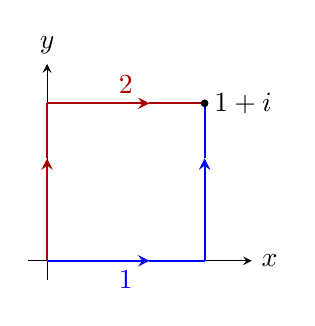
\begin{tikzpicture}[scale=2,>=stealth]
\draw[->](-.12,0)--(1.3,0)node[right]{$x$};
\draw[->](0,-.12)--(0,1.25)node[above]{$y$};
\draw[blue,thick,->](0,0)--(.65,0);
\draw[blue,thick](.65,0)--(1,0);
\draw[blue,thick,->](1,0)--(1,.65);
\draw[blue,thick](1,.65)--(1,1);
\draw[red!65!black,thick,->](0,0)--(0,.65);
\draw[red!65!black,thick](0,.65)--(0,1);
\draw[red!65!black,thick,->](0,1)--(.65,1);
\draw[red!65!black,thick](.65,1)--(1,1);
\fill(1,1)circle(.7pt)node[right]{$1+i$};
\node[blue,below]at(.5,0){1};
\node[red!65!black,above]at(.5,1){2};
\end{tikzpicture}
\end{center}

\Needspace{5\baselineskip}
\par\bigskip
\noindent\textbf{11.3.7}\quad Show that
\[
\oint_{C}\frac{dz}{z^{2}+z}=0,
\]
in which the contour $C$ is a \erratum{counterclockwise} circle defined by $|z|=R>1$.

\emph{Hint.}~Direct use of the Cauchy integral theorem is illegal. The
integral may be evaluated by expanding into partial fractions and then
treating the two terms individually. This yields $0$ for $R>1$ and $2\pi i$
for $\erratum{0<R<1}$.
\solution
Partial fractions give $1/[z(z+1)]=1/z-1/(z+1)$, since
$(z+1)-z=1$. For a counterclockwise circle, $\oint dz/(z-a)=2\pi i$ if
$a$ lies inside: the circle may be shrunk to $|z-a|=\rho$ without
crossing the singularity, and $z-a=\rho e^{i\theta}$ gives
$\int_0^{2\pi}i\,d\theta$. If $a$ lies outside, the integrand is
analytic on and inside the circle and Cauchy's theorem gives zero.
For $R>1$, both poles lie inside.
The two terms therefore contribute $2\pi i$ and $-2\pi i$,
giving $\boxed0$.
For $0<R<1$ only the origin lies inside; the term $1/(z+1)$ gives zero,
so the integral is $2\pi i$.
At $R=1$ the path hits $-1$, so the ordinary integral is undefined.
\erratum{The orientation matters for the hint's value $2\pi i$ at
$0<R<1$, which a clockwise circle changes to $-2\pi i$; the bound
$R>0$ excludes the degenerate circle $|z|=0$.}
The zero-integral theorem cannot be applied directly over the
singularities, which is why the decomposition is useful.

\Needspace{12\baselineskip}
\subsection*{11.4 Cauchy's Integral Formula}

Unless explicitly stated otherwise, closed contours occurring in these
exercises are to be understood as traversed in the mathematically positive
(counterclockwise) direction.

\Needspace{5\baselineskip}
\par\bigskip
\noindent\textbf{11.4.1}\quad Show that
\[
\frac{1}{2\pi i}\oint z^{m-n-1}\,dz,\quad m\text{ and }n\text{ integers}
\]
(with the contour encircling the origin once), is a representation of the
Kronecker $\delta_{mn}$.
\solution
On the circle $z=Re^{i\theta}$, $0\le\theta\le2\pi$, we have
$dz=iRe^{i\theta}d\theta$, so
$z^{m-n-1}dz=iR^{m-n}e^{i(m-n)\theta}d\theta$ and
\[
\frac1{2\pi i}\oint z^{m-n-1}\,dz
=\frac{R^{m-n}}{2\pi}\int_0^{2\pi}e^{i(m-n)\theta}\,d\theta.
\]
For $m=n$ this is $1$.
For the nonzero integer $k=m-n$, the integral is
$[e^{ik\theta}/(ik)]_0^{2\pi}=0$.
Thus the result is $\boxed{\delta_{mn}}$.
Contour deformation gives the same value for any contour avoiding
zero with positive winding number one.

\Needspace{5\baselineskip}
\par\bigskip
\noindent\textbf{11.4.2}\quad Evaluate
\[
\oint_{C}\frac{dz}{z^{2}-1},
\]
where $C$ is the circle $|z-1|=1$.
\solution
The poles at $1,-1$ have distances $0,2$ from the center $1$.
Only $1$ is inside the specified unit-radius circle.
Using
\[
\frac1{z^2-1}=\frac12\left(\frac1{z-1}-\frac1{z+1}\right),
\]
the first term contributes $\tfrac12\cdot2\pi i=\pi i$, since the circle
encloses $1$ (as in 11.3.7), and the second, analytic on and inside the
circle, integrates to zero by Cauchy's theorem.
Therefore $\boxed{\oint_C dz/(z^2-1)=\pi i}$.
\erratum{The Instructor's Manual's answer $0$ is incorrect for this contour:
the textbook (p.~491) prints the circle $|z-1|=1$, which encloses only
the pole at $z=1$.}

\Needspace{5\baselineskip}
\par\bigskip
\noindent\textbf{11.4.3}\quad Assuming that $f(z)$ is analytic on and within a
closed contour $C$ and that the point $z_{0}$ is within $C$, show that
\[
\oint_{C}\frac{f'(z)}{z-z_{0}}\,dz
=\oint_{C}\frac{f(z)}{(z-z_{0})^{2}}\,dz.
\]
\solution
Along the contour, the single-valued function $f(z)/(z-z_0)$ obeys
\[
d\left(\frac{f(z)}{z-z_0}\right)
=\left[\frac{f'(z)}{z-z_0}-\frac{f(z)}{(z-z_0)^2}\right]dz.
\]
Its closed integral is zero: the integral of the derivative of the
single-valued function $f(z)/(z-z_0)$, analytic on a neighborhood of
$C$, is the change of that function around the closed path. Moving one
term to the opposite side proves the stated equality. Both integrals also equal
$2\pi i f'(z_0)$ by Cauchy's formulas.

\Needspace{5\baselineskip}
\par\bigskip
\noindent\textbf{11.4.4}\quad You know that $f(z)$ is analytic on and within a
closed contour $C$, \erratum{with $z_0$ inside $C$ and $n$ a nonnegative integer.} You suspect that the $n$th derivative $f^{(n)}(z_{0})$ is
given by
\[
f^{(n)}(z_{0})=\frac{n!}{2\pi i}\oint_{C}\frac{f(z)}{(z-z_{0})^{n+1}}\,dz.
\]
Using mathematical induction (Section 1.4), prove that this expression is
correct.
\solution
The base case $n=0$ is Cauchy's integral formula. Assume the formula
holds for $n$ at every point inside $C$. The point $z_0$ has a positive
distance $\delta$ from $C$, so the disk $|\zeta-z_0|<\delta$, which
contains $z_0$ and does not meet $C$, lies inside $C$. Let
$0<|\Delta|<\delta/2$. Then $z_0+\Delta$ is inside $C$; subtracting the
formula at $z_0$ from the formula at $z_0+\Delta$ and dividing by
$\Delta$ gives
\[
\frac{f^{(n)}(z_0+\Delta)-f^{(n)}(z_0)}{\Delta}
=\frac{n!}{2\pi i}\oint_Cf(z)\,\frac{q(\Delta)-q(0)}{\Delta}\,dz,
\qquad q(s)=(z-z_0-s)^{-n-1}.
\]
Fix $z$ on $C$. By the chain rule,
\[
\begin{aligned}
q'(s)&=-(n+1)(z-z_0-s)^{-n-2}(-1)=(n+1)(z-z_0-s)^{-n-2},\\
q''(s)&=(n+1)(n+2)(z-z_0-s)^{-n-3}.
\end{aligned}
\]
On the segment from $0$ to $\Delta$, $|z-z_0-s|\ge\delta-|s|>\delta/2$,
so $|q''(s)|\le K$ with $K=(n+1)(n+2)(2/\delta)^{n+3}$. Integrating
$q''$ from $0$ to $s$ along the segment gives
$|q'(s)-q'(0)|\le K|s|\le K|\Delta|$ (Exercise 11.3.2), and integrating
$q'$ gives
\[
\left|\frac{q(\Delta)-q(0)}{\Delta}-q'(0)\right|
=\left|\frac1\Delta\int_0^\Delta[q'(s)-q'(0)]\,ds\right|
\le\frac{K|\Delta|\cdot|\Delta|}{|\Delta|}=K|\Delta|,
\]
a bound independent of $z$. Hence, by Exercise 11.3.2 with $L$ the
length of $C$,
\[
\left|\frac{f^{(n)}(z_0+\Delta)-f^{(n)}(z_0)}{\Delta}
-\frac{n!}{2\pi i}\oint_Cf(z)\,q'(0)\,dz\right|
\le\frac{n!}{2\pi}\Bigl(\max_C|f|\Bigr)L\,K|\Delta|\to0.
\]
The difference quotient therefore converges as $\Delta\to0$, and with
$q'(0)=(n+1)(z-z_0)^{-n-2}$ its limit is
\[
f^{(n+1)}(z_0)
=\frac{n!}{2\pi i}\oint_C
\frac{(n+1)f(z)}{(z-z_0)^{n+2}}\,dz
=\frac{(n+1)!}{2\pi i}\oint_C
\frac{f(z)}{(z-z_0)^{n+2}}\,dz.
\]
This is the induction step, proving the result for every $n\ge0$.

\Needspace{5\baselineskip}
\par\bigskip
\noindent\textbf{11.4.5}\quad
\begin{enumerate}
\item[(a)] A function $f(z)$ is analytic within a closed contour $C$ (and
  continuous on $C$). If $f(z)\neq0$ within $C$ and
  \erratum{$|f(z)|\ge m>0$} on $C$, show that
  \[
  \erratum{|f(z)|\ge m}
  \]
  for all points within $C$.

  \emph{Hint.}~Consider $w(z)=1/f(z)$.
\item[(b)] If $f(z)=0$ within the contour $C$, show that the foregoing result
  does not hold and that it is possible to have $|f(z)|=0$ at one or more
  points in the interior with $|f(z)|>0$ over the entire bounding contour.
  Cite a specific example of an analytic function that behaves this way.
\end{enumerate}
\solution
\erratum{As printed on p.~491, (a) reads: if $f(z)\ne0$ within $C$ and
$|f(z)|\le M$ on $C$, then $|f(z)|\le M$ for all points within $C$.
This maximum-modulus statement does not require $f\ne0$, so (b)'s
claim that it fails when $f$ has zeros is false. The hint $w=1/f$
points to the intended minimum-modulus statement given above. We prove
both.}
For the \textbf{original upper-bound version}, continuity gives a
maximum of $|f|$ on the closed bounded region (the inside of $C$
together with $C$). Suppose it exceeded $M$. Then it would occur at an
interior point $z_0$, with $f(z_0)\ne0$ because $|f(z_0)|>M\ge0$.
A constant $f$ is impossible, since its modulus would equal its
boundary value, at most $M$. For nonconstant $f$ some Taylor
coefficient at $z_0$ with $k\ge1$ is nonzero (identity theorem); with
the smallest such $k$,
$f(z_0+h)=f(z_0)+a_kh^k+O(h^{k+1})$, $a_k\ne0$.
Write $f(z_0)=|f(z_0)|e^{i\beta}$, $a_k=|a_k|e^{i\alpha}$, and take
$h=re^{i\theta}$ with $\theta=(\beta-\alpha)/k$. Then
$a_kh^k=|a_k|r^ke^{i\beta}$ has the phase of $f(z_0)$, so
$|f(z_0)+a_kh^k|=|f(z_0)|+|a_k|r^k$. The remainder is bounded by
$Kr^{k+1}$ for $0<r<r_0$, with some constants $K,r_0>0$, so
\[
|f(z_0+h)|\ge|f(z_0)|+|a_k|r^k-Kr^{k+1}>|f(z_0)|
\qquad\text{for }0<r<\min(r_0,|a_k|/K),
\]
contradicting maximality. Hence
$\boxed{|f|\le M}$ throughout, whether or not zeros occur.

For the \textbf{corrected lower bound in (a)}, assume $f$ has no zero on
the closed region and $|f|\ge m>0$ on $C$. Then $1/f$ is analytic
and obeys $|1/f|\le1/m$ on the boundary. The upper-bound result
gives $|1/f|\le1/m$ inside, hence $|f|\ge m$.
For \textbf{(b)}, $f(z)=z$ on the unit disk has boundary modulus
$1$ and $f(0)=0$. This disproves a positive interior \emph{lower}
bound without nonvanishing, while still satisfying the printed upper bound.

\Needspace{5\baselineskip}
\par\bigskip
\noindent\textbf{11.4.6}\quad Evaluate
\[
\oint_{C}\frac{e^{iz}}{z^{3}}\,dz,
\]
for the contour a square with sides of length $a>1$, centered at $z=0$.
\solution
Let $g=e^{iz}$, so $g''=i^2e^{iz}=-e^{iz}$. The square surrounds zero
once, so Cauchy's formula for the second derivative gives
\[
\oint_C\frac{e^{iz}}{z^3}\,dz
=\frac{2\pi i}{2!}g''(0)
=\pi i[-e^{iz}]_{z=0}=\boxed{-\pi i}.
\]
Any positive side length suffices; $a>1$ is stronger than needed.

\Needspace{5\baselineskip}
\par\bigskip
\noindent\textbf{11.4.7}\quad Evaluate
\[
\oint_{C}\frac{\sin^{2}z-z^{2}}{(z-a)^{3}}\,dz,
\]
where the contour encircles the point $z=a$.
\solution
Set $g(z)=\sin^2z-z^2$. Then, with $2\sin z\cos z=\sin2z$,
$g'=\sin2z-2z$ and $g''=2\cos2z-2$.
Cauchy's derivative formula gives
\[
\oint_C\frac{g(z)}{(z-a)^3}\,dz
=\frac{2\pi i}{2!}g''(a)
=\boxed{2\pi i(\cos2a-1)}.
\]
The formula still applies when a numerator zero lowers or removes
the apparent pole.

\Needspace{5\baselineskip}
\par\bigskip
\noindent\textbf{11.4.8}\quad Evaluate
\[
\oint_{C}\frac{dz}{z(2z+1)},
\]
for the contour the unit circle.
\solution
Decompose
\[
\frac1{z(2z+1)}=\frac1z-\frac2{2z+1}
=\frac1z-\frac1{z+1/2}.
\]
Both poles are inside the unit circle. Their contributions,
$2\pi i$ and $-2\pi i$, cancel, giving $\boxed0$.

\Needspace{5\baselineskip}
\par\bigskip
\noindent\textbf{11.4.9}\quad Evaluate
\[
\oint_{C}\frac{f(z)}{z(2z+1)^{2}}\,dz,
\]
for the contour the unit circle, \erratum{assuming $f$ is analytic on a neighborhood of the closed disk.}

\emph{Hint.}~Make a partial fraction expansion.
\solution
\erratum{Assume $f$ is analytic on and within the unit circle;
additional singularities would supply additional contributions.}
Write
$1/[z(2z+1)^2]=A/z+B/(2z+1)+D/(2z+1)^2$.
Clearing denominators yields
$1=A(2z+1)^2+Bz(2z+1)+Dz=(4A+2B)z^2+(4A+B+D)z+A$.
Constant, quadratic, and linear coefficients give, respectively,
$A=1$, $4A+2B=0$, $4A+B+D=0$; hence $B=-2$ and $D=-4-B=-2$.
Since $2/(2z+1)=1/(z+1/2)$ and $2/(2z+1)^2=\tfrac12/(z+1/2)^2$,
\[
\frac{f(z)}{z(2z+1)^2}
=\frac{f(z)}z-\frac{f(z)}{z+1/2}
-\frac{f(z)/2}{(z+1/2)^2}.
\]
Both points $0$ and $-1/2$ lie inside the unit circle. Cauchy's formula
$\oint f(z)\,dz/(z-z_0)=2\pi if(z_0)$ and its derivative form
$\oint f(z)\,dz/(z-z_0)^2=2\pi if'(z_0)$ now give
\[
2\pi if(0)-2\pi if(-1/2)-\tfrac12\cdot2\pi if'(-1/2)
=\boxed{2\pi i f(0)-2\pi i f(-1/2)-\pi i f'(-1/2)}.
\]

\Needspace{12\baselineskip}
\subsection*{11.5 Laurent Expansion}

\Needspace{5\baselineskip}
\par\bigskip
\noindent\textbf{11.5.1}\quad Develop the Taylor expansion of $\ln(1+z)$.
\par\nobreak\hfill\emph{ANS.}\enspace
$\displaystyle\sum_{n=1}^{\infty}(-1)^{n-1}\frac{z^{n}}{n}$.
\solution
Choose the logarithm analytic near $z=0$ with value zero there.
For $|z|<1$, the geometric series gives
$1/(1+z)=\sum_{n=0}^\infty(-1)^nz^n$.
It converges uniformly on every smaller closed disk, allowing
termwise integration from zero to $z$ along the segment. Since
$[\ln(1+z)]'=1/(1+z)$ and $\int_0^z\zeta^n\,d\zeta=z^{n+1}/(n+1)$,
and with the index shift $n+1\to n$ in the second form,
\[
\boxed{\ln(1+z)=\sum_{n=0}^\infty\frac{(-1)^nz^{n+1}}{n+1}
=\sum_{n=1}^\infty(-1)^{n-1}\frac{z^n}{n}}.
\]
Both sides vanish at zero, fixing the integration constant.
The nearest singularity is $z=-1$, so the Taylor radius is one.

\Needspace{5\baselineskip}
\par\bigskip
\noindent\textbf{11.5.2}\quad Derive the binomial expansion
\[
(1+z)^{m}=1+mz+\frac{m(m-1)}{1\cdot2}z^{2}+\cdots
=\sum_{n=0}^{\infty}\binom{m}{n}z^{n}
\]
for $m$, any real number. The expansion is convergent for $|z|<1$. Why?
\solution
Choose $(1+z)^m=\exp[m\operatorname{Log}(1+z)]$ with value $1$
at zero. For any real exponent $s$ the chain rule gives
$\frac{d}{dz}(1+z)^s=\exp[s\operatorname{Log}(1+z)]\,\frac{s}{1+z}
=s(1+z)^{s-1}$, so repeated differentiation gives
\[
\frac{d^n}{dz^n}(1+z)^m
=m(m-1)\cdots(m-n+1)(1+z)^{m-n}.
\]
Set $z=0$ and divide by $n!$ to obtain
\[
\boxed{(1+z)^m=\sum_{n=0}^\infty
\frac{m(m-1)\cdots(m-n+1)}{n!}z^n}.
\]
The empty product for $n=0$ is one. For a nonterminating series the
coefficients $c_n$ have $c_{n+1}/c_n=(m-n)/(n+1)$, so the absolute
successive-term ratio is $|z|\,|m-n|/(n+1)\to|z|$; by the ratio test
the series converges for $|z|<1$ and diverges for $|z|>1$.
The reason is the singularity at $z=-1$, where $1+z=0$: this branch is
analytic on the open disk $|z|<1$, which reaches up to $-1$, so by
Taylor's theorem the series converges to $(1+z)^m$ there, and no
larger disk about $0$ avoids $-1$.
For nonnegative integer $m$ the series terminates and is valid
everywhere; for other real $m$ the Taylor radius is one.

\Needspace{5\baselineskip}
\par\bigskip
\noindent\textbf{11.5.3}\quad A function $f(z)$ is analytic on and within the
unit circle. Also, $|f(z)| < 1$ for $|z| \le 1$ and $f(0)=0$. Show that
$|f(z)| < |z|$ for $\erratum{0<|z|\le1}$.

\emph{Hint.}~One approach is to show that $f(z)/z$ is analytic and then to
express $[f(z_{0})/z_{0}]^{n}$ by the Cauchy integral formula. Finally,
consider absolute magnitudes and take the $n$th root. This exercise is
sometimes called Schwarz's theorem.
\solution
\erratum{The strict inequality excludes $z=0$, where both sides
are zero. It holds for $0<|z|\le1$.}
The series $f(z)=a_1z+a_2z^2+\cdots$ shows that
$g(z)=f(z)/z$ extends analytically to zero by $g(0)=a_1$.
Compactness of the unit circle and the strict hypothesis give
$|g(\zeta)|=|f(\zeta)|\le M<1$ there.
For $|z_0|<1$, Cauchy's formula applied to the analytic function
$g^n$ gives the first relation below. On the circle
$|g(\zeta)^n|\le M^n$ and $|\zeta-z_0|\ge1-|z_0|$, so the bound of
Exercise 11.3.2, with length $2\pi$, gives the second:
\[
g(z_0)^n=\frac1{2\pi i}\oint_{|\zeta|=1}
\frac{g(\zeta)^n}{\zeta-z_0}\,d\zeta,\qquad
|g(z_0)|^n\le\frac1{2\pi}\cdot2\pi\cdot\frac{M^n}{1-|z_0|}
=\frac{M^n}{1-|z_0|}.
\]
Taking $n$th roots, $|g(z_0)|\le M(1-|z_0|)^{-1/n}$; letting
$n\to\infty$ gives $|g(z_0)|\le M$.
This also holds on the boundary. Thus
$|f(z)|\le M|z|<|z|$ for nonzero $z$, with equality $0=0$ at zero.

\Needspace{5\baselineskip}
\par\bigskip
\noindent\textbf{11.5.4}\quad If $f(z)$ is a real function of the complex
variable $z=x+iy$, that is, $f(x)=f^{*}(x)$ \erratum{for real $x$ near zero}, and the Laurent expansion about
the origin, $f(z)=\sum a_{n}z^{n}$ \erratum{on $0<|z|<R$}, has $a_{n}=0$ for $n < -N$, show that all
of the coefficients $a_{n}$ are real.

\emph{Hint.}~Show that $z^{N}f(z)$ is analytic (via Morera's theorem,
Section 11.4).
\solution
\erratum{Here \emph{real} means real-valued for real arguments
near the Laurent center, not throughout an open complex region.}
The finite principal part makes
\[
g(z)=z^Nf(z)=\sum_{j=0}^\infty a_{j-N}z^j
\]
analytic after its removable extension to zero.
For nonzero real $x$ near zero, $g(x)=x^Nf(x)$ is real, and
continuity gives a real value at zero. Each analytic derivative
at zero may be computed along the real line; derivatives of
this real-valued restriction are real. Hence
$a_{j-N}=g^{(j)}(0)/j!\in\mathbb R$ for every $j\ge0$.
The remaining coefficients vanish and are real as well.

\Needspace{5\baselineskip}
\par\bigskip
\noindent\textbf{11.5.5}\quad Prove that the Laurent expansion of a given
function about a given point is unique; that is, if
\[
f(z)=\sum_{n=-N}^{\infty}a_{n}(z-z_{0})^{n}
=\sum_{n=-N}^{\infty}b_{n}(z-z_{0})^{n},
\]
\erratum{with both series representing $f$ on a common annulus,} show that $a_{n}=b_{n}$ for all $n$.

\emph{Hint.}~Use the Cauchy integral formula.
\solution
Choose a circle $|\zeta-z_0|=r$ in the common convergence annulus.
Uniform convergence there permits termwise integration:
\[
\begin{aligned}
\frac1{2\pi i}\oint f(\zeta)(\zeta-z_0)^{-k-1}\,d\zeta
&=\sum_n a_n\frac1{2\pi i}\oint
(\zeta-z_0)^{n-k-1}\,d\zeta\\
&=\sum_n a_n\delta_{nk}=a_k.
\end{aligned}
\]
The circle integrals equal $\delta_{nk}$ by Exercise 11.4.1, applied in
the variable $\zeta-z_0$.
The second series gives $b_k$ for the identical integral.
Thus $\boxed{a_k=b_k}$ for every integer $k$.
The proof also works for an infinite principal part on a common annulus.
\erratum{The common annulus is needed because the proof integrates both
series over one circle on which both converge to $f$; about one point a
function can have different Laurent series on different annuli, e.g.,
the two expansions of $1/[z(z-1)]$ about $z=1$ in Exercise 11.6.10.}
For the displayed series, whose principal parts are finite, the
condition holds once both represent $f$ near $z_0$: each then does so on
a punctured disk $0<|z-z_0|<\varepsilon$, and the smaller of the two
disks is a common annulus.

\Needspace{5\baselineskip}
\par\bigskip
\noindent\textbf{11.5.6}\quad Obtain the Laurent expansion of $e^{z}/z^{2}$
about $z=0$.
\solution
Divide the everywhere-convergent exponential series by $z^2$:
\[
\boxed{\frac{e^z}{z^2}
=\sum_{n=0}^\infty\frac{z^{n-2}}{n!}
=\frac1{z^2}+\frac1z+\frac12+\frac z6+\frac{z^2}{24}+\cdots}.
\]
The annulus is $0<|z|<\infty$. The pole has order two and residue one.

\Needspace{5\baselineskip}
\par\bigskip
\noindent\textbf{11.5.7}\quad Obtain the Laurent expansion of
$ze^{z}/(z-1)$ about $z=1$.
\solution
Put $w=z-1$, so $z=1+w$ and $e^z=e\,e^w$. Then
\[
\frac{ze^z}{z-1}=\frac{(1+w)\,e\,e^w}{w}
=e\left(\frac1w+1\right)\sum_{n=0}^\infty\frac{w^n}{n!}.
\]
The $w^{-1}$ coefficient is $e$, from $n=0$ in the product with $1/w$.
For $m\ge0$ the $w^m$ coefficient comes from $n=m+1$ in the product
with $1/w$ and from $n=m$ in the product with $1$:
$e[1/(m+1)!+1/m!]=e[1+(m+1)]/(m+1)!=e(m+2)/(m+1)!$.
Consequently
\[
\boxed{\frac{ze^z}{z-1}
=\frac e{z-1}+e\sum_{m=0}^\infty
\frac{m+2}{(m+1)!}(z-1)^m},\qquad0<|z-1|<\infty.
\]
The first regular terms are $2e+\frac32e(z-1)+\frac23e(z-1)^2$.

\Needspace{5\baselineskip}
\par\bigskip
\noindent\textbf{11.5.8}\quad Obtain the Laurent expansion of
$(z-1)e^{1/z}$ about $z=0$.
\solution
Multiplication of the exponential series gives
\[
(z-1)e^{1/z}
=\sum_{n=0}^\infty\frac{z^{1-n}}{n!}
-\sum_{n=0}^\infty\frac{z^{-n}}{n!}.
\]
The leading term is $z$ ($n=0$ in the first sum), and the constants
($n=1$ in the first sum, $n=0$ in the second) cancel. For $k\ge1$ the
coefficient of $z^{-k}$ comes from $n=k+1$ in the first sum and $n=k$
in the second:
$1/(k+1)!-1/k!=[1-(k+1)]/(k+1)!=-k/(k+1)!$. Thus
\[
\boxed{(z-1)e^{1/z}
=z-\sum_{k=1}^\infty\frac{k}{(k+1)!}z^{-k}
=z-\frac1{2z}-\frac1{3z^2}-\frac1{8z^3}-\cdots}.
\]
It converges for $0<|z|<\infty$; its infinite principal part
makes zero an essential singularity.

\Needspace{12\baselineskip}
\subsection*{11.6 Singularities}

\Needspace{5\baselineskip}
\par\bigskip
\noindent\textbf{11.6.1}\quad As an example of an essential singularity
consider $e^{1/z}$ as $z$ approaches zero. For any complex number $z_{0}$,
$z_{0}\neq0$, show that
\[
e^{1/z}=z_{0}
\]
has an infinite number of solutions.
\solution
Write $z_0=\rho e^{i\alpha}$ with $\rho>0$, choosing one argument.
Since $e^w=e^{w'}$ exactly when $w-w'\in2\pi i\mathbb Z$, all solutions
of $e^w=z_0=e^{\ln\rho+i\alpha}$ are
$w=\ln\rho+i(\alpha+2\pi n)$, $n\in\mathbb Z$.
Therefore
\[
\boxed{z_n=\frac1{\ln\rho+i(\alpha+2\pi n)}}
\]
whenever the denominator is nonzero.
Substitution gives $e^{1/z_n}=\rho e^{i\alpha}=z_0$.
A zero denominator needs $\ln\rho=0$ and $\alpha+2\pi n=0$, so at most
one integer has one. All remaining denominators are distinct, since
their imaginary parts differ by multiples of $2\pi$, so their
reciprocals are distinct. Thus infinitely many distinct solutions
remain, with $|z_n|\le1/|\alpha+2\pi n|\to0$ as $|n|\to\infty$.
For $z_0=1$ with the choice $\alpha=0$, simply omit $n=0$.
\erratum{The Instructor's Manual argues from roots of truncated exponential polynomials. Passing to the limit does not by itself establish distinct roots of the original equation. The explicit logarithmic preimages above supply that missing argument.}

\Needspace{5\baselineskip}
\par\bigskip
\noindent\textbf{11.6.2}\quad Show that the function
\[
w(z)=(z^{2}-1)^{1/2}
\]
is single-valued if we make branch cuts on the real axis for $\erratum{x\ge1}$ and for $\erratum{x\le-1}$.
\solution
Remove both rays including their endpoints:
$D=\mathbb C\setminus((-\infty,-1]\cup[1,\infty))$.
For $z=x+iy$, $1-z^2=(1-x^2+y^2)-2ixy$ is nonpositive real only if
$xy=0$ and $1-x^2+y^2\le0$. The choice $x=0$ gives $1+y^2>0$;
otherwise $y=0$, $|x|\ge1$, exactly the removed rays.
The principal square root is analytic off the ray $(-\infty,0]$, so
$\sqrt{1-z^2}$ is analytic on $D$, and the explicit branch
\[
\boxed{w(z)=i\sqrt{1-z^2}}
\]
is single-valued and satisfies $w^2=z^2-1$.
Its negative is the other branch; one reference value selects its sign.
\erratum{The branch points $\pm1$ themselves are excluded from
the analytic domain, not merely the open rays.}
\erratum{The Instructor's Manual instead discusses a cut joining $-1$ to $1$. That is the different branch domain in Example 11.6.4, not the two outward rays specified here.}

\Needspace{5\baselineskip}
\par\bigskip
\noindent\textbf{11.6.3}\quad A function $f(z)$ can be represented by
\[
f(z)=\frac{f_{1}(z)}{f_{2}(z)},
\]
in which $f_{1}(z)$ and $f_{2}(z)$ are analytic. The denominator, $f_{2}(z)$,
vanishes at $z=z_{0}$, showing that $f(z)$ has a pole at $z=z_{0}$. However,
$f_{1}(z_{0})\neq0$, $f'_{2}(z_{0})\neq0$. Show that $a_{-1}$, the coefficient
of $(z-z_{0})^{-1}$ in a Laurent expansion of $f(z)$ at $z=z_{0}$, is given by
\[
a_{-1}=\frac{f_{1}(z_{0})}{f'_{2}(z_{0})}.
\]
\solution
With $h=z-z_0$, Taylor expansion gives
\[
f_1(z)=f_1(z_0)+O(h),\quad
f_2(z)=f'_2(z_0)h[1+O(h)].
\]
Each $O(h)$ here is a convergent power series in $h$ without constant
term. The last factor has an analytic reciprocal $1+O(h)$ near zero
because its constant term is one. Hence
\[
f(z)=\frac{f_1(z_0)+O(h)}{f'_2(z_0)h}[1+O(h)]
=\frac{f_1(z_0)}{f'_2(z_0)}h^{-1}+O(1).
\]
Therefore $\boxed{a_{-1}=f_1(z_0)/f'_2(z_0)}$.
The assumptions make this coefficient nonzero and the pole simple.

\Needspace{5\baselineskip}
\par\bigskip
\noindent\textbf{11.6.4}\quad Determine a unique branch for the function of
Exercise 11.6.2 that will cause the value it yields for $f(i)$ to be the same
as that found for $f(i)$ in Example 11.6.4. Although Exercise 11.6.2 and
Example 11.6.4 describe the same multivalued function, the specific values
assigned for various $z$ will not agree everywhere, due to the difference in
the location of the branch cuts. Identify the portions of the complex plane
where both these descriptions do and do not agree, and characterize the
differences.
\solution
Write $z-1=\rho_1e^{i\varphi_1}$ and $z+1=\rho_2e^{i\varphi_2}$. The
segment-cut branch $G$ of Example 11.6.4 is
$G(z)=(\rho_1\rho_2)^{1/2}e^{i(\varphi_1+\varphi_2)/2}$, positive on
the real axis $z>1$, where $\varphi_1=\varphi_2=0$.
At $z=i$, the arguments of $i-1$ and $i+1$ are $3\pi/4$ and
$\pi/4$ and their moduli are both $\sqrt2$. Its value is
\[
(\sqrt2)^{1/2}(\sqrt2)^{1/2}
e^{i(3\pi/4+\pi/4)/2}=\boxed{i\sqrt2}.
\]
The outward-cut branch with this value is
$F(z)=i\sqrt{1-z^2}$ from 11.6.2, since $F(i)=i\sqrt{1-i^2}=i\sqrt2$.
Since its domain is connected, the reference value fixes its sign;
the other branch, $-F$, has the value $-i\sqrt2$ there.

Where both are defined,
$F^2=G^2=z^2-1$ and neither vanishes; thus $F/G$ is continuous
and takes only $\pm1$, so it is constant on each connected piece of
the common domain. The two systems of cuts together cover the real
axis, so the common domain is the plane minus the real axis, whose
components are the upper and lower half-planes.
Equality at $i$ implies $F=G$ in the upper half-plane.
At $-i$, continuing $G$ from $z>1$ through the lower half-plane, the
arguments of $-i-1$ and $-i+1$ are $-3\pi/4$ and $-\pi/4$, so
$G(-i)=\sqrt2\,e^{-i\pi/2}=-i\sqrt2$, while
$F(-i)=i\sqrt{1-(-i)^2}=i\sqrt2$. Hence $F=-G$ in the lower half-plane.
On the real axis at most one of them is defined, since $G$ is cut along
$[-1,1]$ and $F$ along $|x|\ge1$. Each is continuous across the other's
cut, so by the half-plane relations its value there is the limit of the
other from above, written with argument $x+i0$, and minus the limit from
below, $x-i0$. For $|x|>1$, where $\varphi_1=\varphi_2$ is $0$ ($x>1$) or
$\pi$ ($x<-1$),
\[
G(x)=\operatorname{sgn}(x)\sqrt{x^2-1}=F(x+i0)=-F(x-i0),
\]
and for $|x|<1$, $F(x)=i\sqrt{1-x^2}=G(x+i0)=-G(x-i0)$.
These statements specify precisely their agreement and sign difference.
\erratum{The Instructor's Manual gives $f(i)=2i$. Each factor contributes modulus $2^{1/4}$, not $\sqrt2$, so their product has modulus $\sqrt2$. Also $(i\sqrt2)^2=-2=i^2-1$, whereas $(2i)^2=-4$.}

\Needspace{5\baselineskip}
\par\bigskip
\noindent\textbf{11.6.5}\quad Find all singularities of
\[
z^{-1/3}+\frac{z^{-1/4}}{(z-3)^{3}}+(z-2)^{1/2},
\]
and identify their types (e.g., second-order branch point, fifth-order pole,
\ldots). Include any singularities at the point at infinity.

\emph{Note.}~A branch point is of $n$th order if it requires $n$, but no
fewer, circuits around the point to restore the original value.
\solution
At zero, since $(z-3)^3=(-3)^3(1-z/3)^3$,
\[
\frac{z^{-1/4}}{(z-3)^3}
=-\frac1{27}z^{-1/4}(1-z/3)^{-3},
\]
where $(1-z/3)^{-3}$ and the third term $(z-2)^{1/2}$ are analytic
near zero. After $N$ circuits about zero the first two terms therefore
acquire multipliers $e^{-2\pi iN/3}$ and $e^{-2\pi iN/4}$, and the third
is unchanged, so the function changes by
\[
c_1z^{-1/3}+c_2z^{-1/4}(1-z/3)^{-3},\qquad
c_1=e^{-2\pi iN/3}-1,\quad c_2=-\tfrac1{27}\bigl(e^{-2\pi iN/4}-1\bigr).
\]
These changes cannot cancel. If $c_1\ne0$, the ratio of the second term
to the first, $(c_2/c_1)z^{1/12}(1-z/3)^{-3}$, tends to zero as $z\to0$
(because $-1/4-(-1/3)=1/12>0$), so the change is nonzero near zero; if
$c_1=0$, the change $c_2z^{-1/4}(1-z/3)^{-3}$ vanishes only if $c_2=0$.
Hence the function returns to its initial value iff both multipliers
equal $1$, i.e., iff $N$ is divisible by $3$ and $4$;
the least such positive integer is $12$. Zero is a branch point
of order $12$ in the question's convention.
At $3$, the chosen local numerator is analytic and nonzero and the
other two terms are analytic, giving a third-order pole. At $2$, only $(z-2)^{1/2}$ branches, with order $2$.
For infinity put $w=1/z$; with $(1/w-3)^3=(1-3w)^3/w^3$ and
$1/w-2=(1-2w)/w$,
\[
f(1/w)=w^{1/3}+\frac{w^{13/4}}{(1-3w)^3}
+w^{-1/2}(1-2w)^{1/2}.
\]
The analytic factors $(1-3w)^{-3}$ and $(1-2w)^{1/2}$ have nonzero
constant terms, so $N$ circuits about $w=0$ multiply the three terms by
$e^{2\pi iN/3}$, $e^{2\pi i(13N/4)}=e^{2\pi iN/4}$ (since
$e^{2\pi i\cdot3N}=1$) and $e^{-\pi iN}$. As at zero, the changes
cannot cancel: among the terms whose multiplier is not $1$, the one with
the smallest exponent of $w$ (the exponents are $-1/2<1/3<13/4$)
dominates the others as $w\to0$, so the change is nonzero near $w=0$.
So the function returns to its initial value iff all three multipliers
equal $1$, i.e., iff $N$ is divisible by $3$, $4$ and $2$; their least
common multiple is $12$.
Infinity is an order-$12$ branch point, not an isolated meromorphic pole.
There are no other finite singularities.

\Needspace{5\baselineskip}
\par\bigskip
\noindent\textbf{11.6.6}\quad The function $F(z)=\ln(z^{2}+1)$ is made
single-valued by straight-line branch cuts from $(x,y)=(0,-1)$ to
$(-\infty,-1)$ and from $(0,+1)$ to $(0,+\infty)$. See Fig.~11.17. If
$F(0)=-2\pi i$, find the value of $F(i-2)$.
\solution
Factor $z^2+1=(z-i)(z+i)$, so every branch has the form
$\ln|z-i|+\ln|z+i|+i[\arg(z-i)+\arg(z+i)]+2\pi ik$.
The upward cut from $i$ consists of the points with
$\arg(z-i)=\pi/2$; choosing $-3\pi/2<\arg(z-i)<\pi/2$ makes this
argument continuous off that cut. The leftward cut from $-i$ consists
of the points with $\arg(z+i)=\pi$; choosing $-\pi<\arg(z+i)<\pi$
makes this argument continuous off it.
At zero, $z-i=-i$ and $z+i=i$ have arguments $-\pi/2,\pi/2$ and both
moduli are one, so $F(0)=2\pi ik=-2\pi i$ requires $k=-1$.
The required branch is therefore
\[
F(z)=\ln|z-i|+\ln|z+i|
+i[\arg(z-i)+\arg(z+i)-2\pi].
\]
At $z=-2+i$, the factors are $-2$ and $-2+2i$.
Their arguments in these ranges are $-\pi$ and $3\pi/4$;
their moduli are $2$ and $2\sqrt2$. Thus
\[
F(i-2)=\ln2+\ln(2\sqrt2)+i\left(-\pi+\frac{3\pi}4-2\pi\right)
=\boxed{\ln(4\sqrt2)-9\pi i/4}.
\]
Exponentiation verifies the result:
$e^F=4\sqrt2\,e^{-9\pi i/4}=4\sqrt2\,e^{-i\pi/4}=4-4i=(-2+i)^2+1$.

\Needspace{5\baselineskip}
\par\bigskip
\noindent\textbf{11.6.7}\quad Show that negative numbers have logarithms in
the complex plane. In particular, find $\ln(-1)$.
\par\nobreak\hfill\emph{ANS.}\enspace $\erratum{\operatorname{Log}(-1)=i\pi\text{ (principal value)}}$.
\solution
For $r>0$, $-r=re^{i(\pi+2\pi n)}$, $n\in\mathbb Z$.
All logarithms are consequently
\[
\boxed{\ln(-r)=\ln r+i(2n+1)\pi}.
\]
In particular $\ln(-1)=i(2n+1)\pi$.
\erratum{The printed $i\pi$ is the principal value, or one chosen
branch value, rather than the complete multivalued answer.}

\Needspace{5\baselineskip}
\par\bigskip
\noindent\textbf{11.6.8}\quad For noninteger $m$, show that the binomial
expansion of Exercise 11.5.2 holds only for a suitably defined branch of the
function $(1+z)^{m}$. Show how the $z$-plane is cut. Explain why $|z| < 1$
may be taken as the circle of convergence for the expansion of this branch,
in light of the cut you have chosen.
\solution
Choose $(1+z)^m=\exp[m\operatorname{Log}(1+z)]$ with
$-\pi<\arg(1+z)<\pi$. The cut is $(-\infty,-1]$ and the
value at zero is $1$. This analytic branch has the Taylor
coefficients derived in 11.5.2, and the open unit disk avoids the cut.
For noninteger real $m$, a circuit about $-1$ increases $\arg(1+z)$ by
$2\pi$ and so multiplies the value by $e^{2\pi im}\ne1$. Thus $-1$ is a
genuine branch point, distance one from the Taylor center. The radius
is exactly one: if the series converged on a disk $|z|<\rho$ with
$\rho>1$, its sum $S$ would be analytic there and equal to the branch
on $|z|<1$, hence (by analytic continuation) on the disk minus the
cut. Continuing along a small circle about $-1$ inside the disk would
then return $S$ to its starting value, contradicting the factor
$e^{2\pi im}$.

\Needspace{5\baselineskip}
\par\bigskip
\noindent\textbf{11.6.9}\quad The Taylor expansion of Exercises 11.5.2 and
11.6.8 is not suitable for branches other than the one suitably defined
branch of the function $(1+z)^{m}$ for noninteger $m$. (Note that other
branches cannot have the same Taylor expansion since they must be
distinguishable.) Using the same branch cut of the earlier exercises for all
other branches, find the corresponding Taylor expansions, detailing the phase
assignments and Taylor coefficients.
\solution
For the same cut, let
\[
\operatorname{Log}_k(1+z)=\ln|1+z|
+i\arg(1+z)+2\pi ik,\quad k\in\mathbb Z,
\]
where the displayed argument lies in $(-\pi,\pi)$; the branch $k$
assigns $1+z$ the phase $\arg(1+z)+2\pi k$. Then
$(1+z)^m_k=\exp[m\operatorname{Log}_k(1+z)]
=e^{2\pi imk}\exp[m\operatorname{Log}_0(1+z)]=e^{2\pi imk}(1+z)^m_0$,
where $k=0$ is the branch of 11.6.8, so
\[
\boxed{(1+z)^m_k=e^{2\pi imk}
\sum_{n=0}^\infty\binom mn z^n,\qquad |z|<1}.
\]
Every coefficient is multiplied by the same phase; the constant
coefficient already distinguishes the branches.
For $m=p/q$ in lowest terms, $k$ modulo $q$ gives $q$ distinct
branches. For irrational $m$, all integer $k$ give distinct ones.

\Needspace{5\baselineskip}
\par\bigskip
\noindent\textbf{11.6.10}\quad
\begin{enumerate}
\item[(a)] Develop a Laurent expansion of $f(z)=[z(z-1)]^{-1}$ about the
  point $z=1$ valid for small values of $|z-1|$. Specify the exact range over
  which your expansion holds. This is an analytic continuation of the
  infinite series in Eq.~(11.49).
\item[(b)] Determine the Laurent expansion of $f(z)$ about $z=1$ but for
  $|z-1|$ large.
\end{enumerate}
\emph{Hint.}~Make a partial fraction decomposition of this function and use
the geometric series.
\solution
Put $w=z-1$, so $f=1/[w(1+w)]=1/w-1/(1+w)$, since $(1+w)-w=1$.
\textbf{(a)} For $|w|<1$, the geometric series
$1/(1+w)=\sum_{n=0}^\infty(-1)^nw^n$ gives
\[
\boxed{f=\frac1w-1+w-w^2+\cdots
=\sum_{n=-1}^\infty(-1)^{n+1}w^n,\qquad0<|w|<1}.
\]
The pole at $w=0$ excludes the center; the pole at $w=-1$
sets the outer radius.
\textbf{(b)} For $|w|>1$ write $w(1+w)=w^2(1+w^{-1})$ and expand
$(1+w^{-1})^{-1}=\sum_{n=0}^\infty(-1)^nw^{-n}$, a geometric series in
$w^{-1}$ with $|w^{-1}|<1$:
\[
\boxed{f=w^{-2}(1+w^{-1})^{-1}
=\sum_{n=0}^\infty(-1)^nw^{-n-2},\qquad |w|>1}.
\]
The annuli differ, so uniqueness of Laurent coefficients on a
fixed annulus is not contradicted.
\erratum{The Instructor's Manual writes the outer series as $\sum_{n=-2}^{\infty}(-1)^n(z-1)^{-n}$. Its lower index should be $2$; otherwise it begins with growing powers and cannot equal a function that decays as $(z-1)^{-2}$ at infinity.}

\Needspace{5\baselineskip}
\par\bigskip
\noindent\textbf{11.6.11}\quad
\begin{enumerate}
\item[(a)] Given $f_{1}(z)=\displaystyle\int_{0}^{\infty}e^{-zt}\,dt$ (with
  $t$ real), show that the domain in which $f_{1}(z)$ exists (and is
  analytic) is $\Re(z)>0$.
\item[(b)] Show that $f_{2}(z)=1/z$ equals $f_{1}(z)$ over $\Re(z)>0$ and is
  therefore an analytic continuation of $f_{1}(z)$ over the entire $z$-plane
  except for $z=0$.
\item[(c)] Expand $1/z$ about the point $z=-i$. You will have
  \[
  f_{3}(z)=\sum_{n=0}^{\infty}a_{n}(z+i)^{n}.
  \]
  What is the domain of this formula for $f_{3}(z)$?
\end{enumerate}
\par\nobreak\hfill\emph{ANS.}\enspace
$\dfrac{1}{z}=i\displaystyle\sum_{n=0}^{\infty}i^{-n}(z+i)^{n}$,\quad
$|z+i| < 1$.
\solution
\textbf{(a)} For $z\ne0$,
\[
\int_0^Te^{-zt}\,dt=(1-e^{-zT})/z.
\]
Here $|e^{-zT}|=e^{-T\Re z}$. If $\Re z>0$, the exponential tends to
zero as $T\to\infty$, so $f_1(z)=1/z$, which is analytic there.
If $\Re z<0$, $|e^{-zT}|$ grows without bound. If $\Re z=0$,
$z=iy\ne0$, then $e^{-iyT}$ has modulus one and keeps rotating, without
a limit. For $z=0$, the integral equals $T$.
Thus ordinary convergence occurs exactly on $\Re z>0$.
\textbf{(b)} By (a), $f_2=1/z$ equals $f_1$ on $\Re z>0$, and $1/z$ is
analytic on $\mathbb C\setminus\{0\}$. By the identity theorem it is
the only analytic function on this connected domain that agrees with
$f_1$ on $\Re z>0$; it is the analytic continuation of $f_1$.
\erratum{The continuation has no negative-integer singularities;
the Instructor's Manual's mention of those points is extraneous to this function.}
\textbf{(c)} Set $w=z+i$. Then $z=w-i=-i(1+iw)$ and $1/(-i)=i$; the
geometric series in $-iw$ converges for $|w|<1$, and
$(-i)^n=i^{-n}$ because $-i=1/i$, so
\[
\boxed{\frac1z=\frac i{1+iw}
=i\sum_{n=0}^\infty(-i)^nw^n
=i\sum_{n=0}^\infty i^{-n}(z+i)^n,\quad |z+i|<1}.
\]
The pole at zero is distance one from the center $-i$, fixing
the exact convergence radius.
\erratum{The Instructor's Manual expands about $+i$ in part (c), while the question requests $-i$. The expansion here uses $z+i$ and has constant coefficient $1/(-i)=i$.}

\Needspace{12\baselineskip}
\subsection*{11.7 Calculus of Residues}

\Needspace{5\baselineskip}
\par\bigskip
\noindent\textbf{11.7.1}\quad Determine the nature of the singularities of
each of the following functions and evaluate the residues ($a>0$).
\begin{enumerate}
\item[(a)] $\dfrac{1}{z^{2}+a^{2}}$.\qquad
(b) $\dfrac{1}{(z^{2}+a^{2})^{2}}$.\qquad
(c) $\dfrac{z^{2}}{(z^{2}+a^{2})^{2}}$.
\item[(d)] $\dfrac{\sin 1/z}{z^{2}+a^{2}}$.\qquad
(e) $\dfrac{ze^{iz}}{z^{2}+a^{2}}$.\qquad
(f) $\dfrac{ze^{iz}}{z^{2}-a^{2}}$.
\item[(g)] $\dfrac{e^{iz}}{z^{2}-a^{2}}$.\qquad
(h) $\dfrac{z^{-k}}{z+1}$,\quad $0 < k < 1$.
\end{enumerate}
\emph{Hint.}~For the point at infinity, use the transformation $w=1/z$ for
$|z|\to\erratum{\infty}$. For the residue, transform $f(z)\,dz$ into $g(w)\,dw$ and look at
the behavior of $g(w)$.
\solution
\erratum{Infinity corresponds to $w=1/z\to0$, hence to $|z|\to\infty$,
not to $|z|\to0$ as the printed hint says.} The nature of the
singularity at infinity is the nature of $f(1/w)$ at zero. For the
residue, $z=1/w$ gives $dz=-dw/w^2$, so $f(z)\,dz=g(w)\,dw$ with
$g(w)=-f(1/w)/w^2$, and, as the hint says, the residue at infinity is
that of $g$ at $w=0$:
\[
\operatorname{Res}_{\infty}f
=\operatorname{Res}_{w=0}\left[-\frac{f(1/w)}{w^2}\right].
\]
These are different transformations: the second includes the differential.

\textbf{(a)--(c)} Factor $z^2+a^2=(z-ia)(z+ia)$. For (a), both poles
are simple, and evaluating $(z\mp ia)f(z)=1/(z\pm ia)$ at $z=\pm ia$ gives
\[
\operatorname{Res}_{ia}\frac1{z^2+a^2}=\frac1{2ia},\qquad
\operatorname{Res}_{-ia}\frac1{z^2+a^2}=-\frac1{2ia}.
\]
For (b), the poles are double. The double-pole formula
$\operatorname{Res}_{z_0}f=\frac{d}{dz}[(z-z_0)^2f(z)]_{z=z_0}$, with
$(z-ia)^2f(z)=(z+ia)^{-2}$ and $(2ia)^3=8i^3a^3=-8ia^3$, gives
\[
\operatorname{Res}_{ia}\frac1{(z^2+a^2)^2}
=\left.\frac{d}{dz}(z+ia)^{-2}\right|_{ia}
=-\frac2{(2ia)^3}=\frac1{4ia^3}.
\]
Each of the functions (a)--(c) depends on $a$ only through $a^2$, so
replacing $a$ by $-a$ interchanges the poles $\pm ia$: the residue at
$-ia$ is the residue at $ia$ with $a\to-a$. For (b) it is
$-1/(4ia^3)$. In (c) the numerator $z^2$ equals $-a^2\ne0$ at $\pm ia$,
so the poles are again double, and the double-pole formula, now with
$(z-ia)^2f(z)=z^2/(z+ia)^2$, gives
\[
\left.\frac{d}{dz}\frac{z^2}{(z+ia)^2}\right|_{ia}
=\left.\frac{2z(z+ia)-2z^2}{(z+ia)^3}\right|_{ia}
=\frac{-2a^2}{-8ia^3}=\frac1{4ia}.
\]
The residue at $-ia$ is $-1/(4ia)$. At infinity the three functions
$f(1/w)$ become, after multiplying numerator and denominator by $w^2$
or $w^4$,
\[
\frac{w^2}{1+a^2w^2},\quad
\frac{w^4}{(1+a^2w^2)^2},\quad
\frac{w^2}{(1+a^2w^2)^2}.
\]
Thus infinity is removable, with a zero of order $2,4,2$, respectively.
The transformed differentials $g(w)=-f(1/w)/w^2$,
\[
-\frac1{1+a^2w^2},\quad
-\frac{w^2}{(1+a^2w^2)^2},\quad
-\frac1{(1+a^2w^2)^2},
\]
are analytic at $w=0$, so all three residues at infinity are zero.
Consistently, in each case the two finite residues add to zero.

\textbf{(d)} Zero is an essential singularity: if $f$ had at most a
pole there, so would $\sin(1/z)=(z^2+a^2)f(z)$, whose Laurent series
$\sum_{k\ge0}(-1)^kz^{-2k-1}/(2k+1)!$ has infinitely many negative
powers. The points $\pm ia$ are simple poles; as in (a), the residue
there is $\sin(1/z)/(z\pm ia)$ evaluated at $z=\pm ia$, where
$1/(\pm ia)=\mp i/a$ and $\sin(\mp i/a)=\mp i\sinh(1/a)$ (from
$\sin iy=i\sinh y$):
\[
\operatorname{Res}_{ia}f
=\frac{\sin(-i/a)}{2ia}
=-\frac{\sinh(1/a)}{2a},\qquad
\operatorname{Res}_{-ia}f
=\frac{\sin(i/a)}{-2ia}
=-\frac{\sinh(1/a)}{2a}.
\]
To obtain the residue at zero directly, multiply two series that
converge absolutely on $0<|z|<a$, the Laurent series of $\sin(1/z)$
above and the geometric series
$1/(z^2+a^2)=a^{-2}(1+z^2/a^2)^{-1}=\sum_{j\ge0}(-1)^jz^{2j}/a^{2j+2}$:
\[
\frac{\sin(1/z)}{z^2+a^2}
=\sum_{j,k\ge0}
\frac{(-1)^{j+k}z^{2j-2k-1}}{a^{2j+2}(2k+1)!}.
\]
A term has exponent $2j-2k-1=-1$ exactly when $j=k$, and then
$(-1)^{j+k}=1$. Consequently
\[
\boxed{\operatorname{Res}_{0}f
=\sum_{k=0}^{\infty}\frac1{a^{2k+2}(2k+1)!}
=\frac1a\sum_{k=0}^{\infty}\frac{(1/a)^{2k+1}}{(2k+1)!}
=\frac{\sinh(1/a)}a}.
\]
At infinity $f(1/w)=w^2\sin w/(1+a^2w^2)$ has a zero of order three,
since $\sin w=w+O(w^3)$, and $g(w)=-\sin w/(1+a^2w^2)$ is analytic at
$w=0$, so the residue at infinity is zero. Consistently, the three
finite residues add to zero.

\textbf{(e)--(g)} If $D$ has a simple zero $p$ and $N$ is analytic at
$p$, the residue of $N/D$ is $N(p)/D'(p)$, here with $D'(p)=2p$.
Applying this rule gives
\[
\begin{array}{c|c|c|c}
&\text{finite poles}&\text{residues in the same order}
&\operatorname{Res}_{\infty}f\\ \hline
(e)&ia,\,-ia&e^{-a}/2,\ e^{a}/2&-\cosh a\\
(f)&a,\,-a&e^{ia}/2,\ e^{-ia}/2&-\cos a\\
(g)&a,\,-a&e^{ia}/(2a),\ -e^{-ia}/(2a)&-i\sin a/a
\end{array}
\]
For example, the first two rows follow from
$p e^{ip}/(2p)=e^{ip}/2$ (for $p=\pm ia$ this is $e^{\mp a}/2$), and
the third from $e^{ip}/(2p)$ with $p=\pm a$.
All these finite poles are simple, since the numerators do not vanish
there. Each function has an essential singularity at infinity:
$f(1/w)$ is $e^{i/w}$ times a rational function of $w$ that is not
identically zero, so if $f(1/w)$ had at most a pole at $w=0$, so would
$e^{i/w}=\sum_{m\ge0}i^mw^{-m}/m!$, which has infinitely many negative
powers. Nevertheless its residue there is defined. Under $z=1/w$ a
small counterclockwise circle about $w=0$ becomes a large clockwise
circle $|z|=R$, so
$\operatorname{Res}_\infty f=-\frac1{2\pi i}\oint_{|z|=R}f\,dz$ with
the counterclockwise orientation. For $R>a$ the residue theorem gives
$\operatorname{Res}_{\infty}f=-\sum_{\text{finite }p}\operatorname{Res}_p f$.
The sums are $(e^{-a}+e^a)/2=\cosh a$, $(e^{ia}+e^{-ia})/2=\cos a$, and
$(e^{ia}-e^{-ia})/(2a)=i\sin a/a$, which yield the displayed answers.
\erratum{In (d), the Instructor's Manual gives positive residues at $\pm ia$; both must be $-\sinh(1/a)/(2a)$, as the displayed substitution shows. It reverses the paired exponents in (e), giving
$e^{\pm a}/2$ at $\pm ia$. Its (f) incorrectly uses poles $\pm ia$
and residues $-ie^{\mp a}/2$, although the denominator is $z^2-a^2$.
In (g) it reverses the exponential signs as well. Substitution into
$N(p)/D'(p)$ gives the table above, with each residue paired to its pole.}

\textbf{(h)} The nonintegral power produces branch points at zero and
infinity: continuation once around zero multiplies $z^{-k}$ by
$e^{-2\pi i k}\ne1$, while $f(1/w)=w^{-k}\cdot w/(1+w)=w^{k+1}/(1+w)$
is also multivalued at $w=0$. A rational $k=p/q$ in lowest terms gives
$q$ sheets; irrational $k$ gives infinitely many. On any local branch
at $-1$ the numerator is analytic and nonzero, so there is a simple
pole whose residue is the value of $z^{-k}$ at $-1$ on that branch,
$e^{-ik\arg(-1)}$ with $\arg(-1)=(2m+1)\pi$:
\[
\boxed{\operatorname{Res}_{-1}f=(-1)^{-k}
=e^{-ik(2m+1)\pi}}.
\]
For the branch $0<\arg z<2\pi$, $\arg(-1)=\pi$: take $m=0$, so the
residue is $e^{-ik\pi}$.
\erratum{The residue depends on the branch. Ordinary Laurent residues
at the branch points zero and infinity are not defined.}

\Needspace{5\baselineskip}
\par\bigskip
\noindent\textbf{11.7.2}\quad Evaluate the residues at $z=0$ and $z=-1$ of
$\pi\cot\pi z/z(z+1)$.
\solution
From $\cot x=\cos x/\sin x=x^{-1}(1-x^2/2+\cdots)(1-x^2/6+\cdots)^{-1}
=x^{-1}-x/3+O(x^3)$ with $x=\pi z$,
$\pi\cot\pi z=z^{-1}-(\pi^2/3)z+O(z^3)$. At zero, divide this by $z$
and expand $1/(1+z)$ in a geometric series:
\[
\frac{\pi\cot\pi z}{z(z+1)}
=\left(\frac1{z^2}-\frac{\pi^2}{3}+O(z^2)\right)
(1-z+z^2-\cdots)
=\frac1{z^2}-\frac1z+O(1).
\]
At $z=-1$, put $w=z+1$. The period one of $\cot\pi z$ gives
$\pi\cot\pi z=\pi\cot\pi w=w^{-1}+O(w)$, while $z(z+1)=(w-1)w$ and
$1/(w-1)=-(1+w+w^2+\cdots)$:
\[
\frac{\pi\cot\pi z}{z(z+1)}
=\frac{w^{-1}+O(w)}{w(w-1)}
=-\frac1{w^2}(1+w+w^2+\cdots)+O(1)
=-\frac1{w^2}-\frac1w+O(1).
\]
Thus both points are double poles and
\[
\boxed{\operatorname{Res}_{0}f=\operatorname{Res}_{-1}f=-1}.
\]

\Needspace{5\baselineskip}
\par\bigskip
\noindent\textbf{11.7.3}\quad The classical definition of the exponential
integral $\mathrm{Ei}(x)$ for $x>0$ is the Cauchy principal value integral
\[
\mathrm{Ei}(x)=\int_{-\infty}^{x}\frac{e^{t}}{t}\,dt,
\]
where the integration range is cut at $\erratum{t=0}$. Show that this definition yields
a convergent result for positive $x$.
\solution
\erratum{The printed problem says the range is cut at $x=0$; the
singular point of the integrand is $t=0$, while $x>0$ is the upper
limit.}
Fix $x>0$ and choose $0<\delta<x$. Split the negative side at $-x$
and change $t=-u$, $dt=-du$, in the interval $[-x,-\delta]$:
\[
\int_{-x}^{-\delta}\frac{e^t}{t}\,dt
=\int_{x}^{\delta}\frac{e^{-u}}{-u}\,(-du)
=-\int_\delta^x\frac{e^{-u}}u\,du.
\]
Inserting this after the split,
\[
\begin{aligned}
\int_{-\infty}^{-\delta}\frac{e^t}{t}\,dt+
\int_\delta^x\frac{e^t}{t}\,dt
&=\int_{-\infty}^{-x}\frac{e^t}{t}\,dt
-\int_\delta^x\frac{e^{-u}}u\,du
+\int_\delta^x\frac{e^u}u\,du\\
&=\int_{-\infty}^{-x}\frac{e^t}{t}\,dt
+\int_\delta^x\frac{e^u-e^{-u}}u\,du.
\end{aligned}
\]
The first integral converges absolutely, since $|e^t/t|\le e^t/x$ for
$t\le-x$ and $\int_{-\infty}^{-x}e^t\,dt=e^{-x}$. In the second,
$e^u-e^{-u}=2u+O(u^3)$, so the integrand has the finite limit $2$ at
zero; it extends continuously to $[0,x]$, and the integral over
$[\delta,x]$ tends to the integral over $[0,x]$ as $\delta\to0$.
Therefore
\[
\boxed{\mathrm{Ei}(x)=
\int_{-\infty}^{-x}\frac{e^t}{t}\,dt+
\int_0^x\frac{2\sinh u}{u}\,du}
\]
is finite. The cancellation uses equal distances $\delta$ on the two
sides of the pole, precisely the principal-value prescription.

\Needspace{5\baselineskip}
\par\bigskip
\noindent\textbf{11.7.4}\quad Writing a Cauchy principal value integral to
deal with the singularity at $x=1$, show that, if $0 < p < 1$,
\[
\int_{0}^{\infty}\frac{x^{-p}}{x-1}\,dx=\erratum{\pi\cot p\pi}.
\]
\solution
\erratum{For the printed denominator $x-1$, the answer is
$+\pi\cot(\pi p)$, not $-\pi\cot(\pi p)$. The Instructor's Manual derives its negative
answer for the different denominator $1-x$.}
Write the intended integral as
\[
I=\lim_{\delta\downarrow0}
\left(\int_0^{1-\delta}+\int_{1+\delta}^{\infty}\right)
\frac{x^{-p}}{x-1}\,dx.
\]
The endpoint estimates are $O(x^{-p})$ at zero and $O(x^{-p-1})$
at infinity, so $0<p<1$ makes both endpoints integrable. Only $x=1$
requires a principal value.

Use $F(z)=z^{-p}/(z-1)$ with $z^{-p}=|z|^{-p}e^{-ip\arg z}$,
$0<\arg z<2\pi$, and a keyhole contour about the positive real axis.
On the upper bank ($\arg z=0$) $z^{-p}=x^{-p}$; on the lower bank
($\arg z=2\pi$) it equals $q x^{-p}$, where $q=e^{-2\pi ip}$.
The upper bank, directed outward, gives $I$; the lower bank, directed
inward, gives $\int_\infty^0 qx^{-p}(x-1)^{-1}\,dx=-qI$; together they
give $(1-q)I$. Exclude the boundary pole at $1$ by semicircles of
radius $\delta$ into the domain. Near $z=1$, $z^{-p}\to1$ on the upper
bank and $z^{-p}\to q$ on the lower one, so there
$F(z)=1/(z-1)+O(1)$ and $F(z)=q/(z-1)+O(1)$, respectively. With
$z-1=\delta e^{i\theta}$, $\int dz/(z-1)=i\int d\theta$, while the
bounded remainder contributes $O(\delta)$. The upper semicircle runs
from $\theta=\pi$ to $\theta=0$ (clockwise) and contributes $-i\pi$; the
lower one runs from $\theta=0$ to $\theta=-\pi$ (also clockwise) and
contributes $-i\pi q$. On the origin circle
$|F|\le\epsilon^{-p}/(1-\epsilon)$ and on the outer circle
$|F|\le R^{-p}/(R-1)$; times the lengths $2\pi\epsilon$ and $2\pi R$,
these give $O(\epsilon^{1-p})$ and $O(R^{-p})$, so both vanish. No pole
remains inside the indented contour, hence
\[
(1-q)I-i\pi(1+q)=0.
\]
Finally, factoring out $e^{-\pi ip}$,
\[
1+q=e^{-\pi ip}(e^{\pi ip}+e^{-\pi ip})=2e^{-\pi ip}\cos\pi p,\qquad
1-q=2ie^{-\pi ip}\sin\pi p,
\]
and therefore
\[
\boxed{\PVint_0^\infty\frac{x^{-p}}{x-1}\,dx
=i\pi\frac{1+q}{1-q}=i\pi\frac{\cos\pi p}{i\sin\pi p}=\pi\cot\pi p}.
\]
An independent check of the sign: $x=1/u$ turns the part beyond
$1+\delta$ into $\int_0^{1/(1+\delta)}u^{p-1}(1-u)^{-1}\,du$. Its piece
between $1-\delta$ and $1/(1+\delta)$ has length $\delta^2/(1+\delta)$
and integrand at most $(1-\delta)^{p-1}(1+\delta)/\delta$, so it
vanishes as $\delta\to0$. Hence
\[
\PVint_0^\infty\frac{x^{-p}}{x-1}\,dx
=\int_0^1\frac{x^{p-1}-x^{-p}}{1-x}\,dx,
\]
an ordinary integral, since the numerator vanishes at $x=1$. For
$0<p<\frac12$ we have $p-1<-p$, so the integrand is positive on
$(0,1)$; the integral is positive, like $\pi\cot\pi p$, whereas
$-\pi\cot\pi p<0$.

\Needspace{5\baselineskip}
\par\bigskip
\noindent\textbf{11.7.5}\quad Explain why Eq.~(11.88) is not directly
applicable to the product expansion of $\sin z$. Show how the expansion,
Eq.~(11.89), can be obtained by expanding instead $\sin z/z$.
\solution
The product formula quoted in the text contains the factors
$f(0)$ and $\exp[zf'(0)/f(0)]$. Since $\sin0=0$, direct substitution
would both annihilate the product and divide by zero. Instead let
\[
g(z)=\begin{cases}\sin z/z,&z\ne0,\\1,&z=0.\end{cases}
\]
The Taylor expansion $g(z)=1-z^2/3!+z^4/5!-\cdots$ gives
$g(0)=1$ and $g'(0)=0$. Its zeros are the nonzero points $\pm n\pi$,
each simple. To justify the product for this specific function,
differentiate $\ln g=\ln\sin z-\ln z$ and use the cotangent pole
expansion (11.81), together with
$\frac{d}{dz}\operatorname{Log}[1-z^2/(n^2\pi^2)]
=[-2z/(n^2\pi^2)]/[1-z^2/(n^2\pi^2)]$: on $|z|<\pi$,
\[
\frac{g'(z)}{g(z)}=\cot z-\frac1z
=\sum_{n=1}^{\infty}\frac{2z}{z^2-n^2\pi^2}
=\sum_{n=1}^{\infty}\frac{d}{dz}
\operatorname{Log}\!\left(1-\frac{z^2}{n^2\pi^2}\right).
\]
The removable value at zero is understood. On every smaller closed disk
the summands are bounded by a constant times $n^{-2}$, so the series
converges uniformly and may be integrated from zero to $z$.
Choose the analytic logarithms that vanish at zero; since $g$ has no zero
in this disk and $g(0)=1$, integration gives
\[
\operatorname{Log}g(z)=\sum_{n=1}^{\infty}
\operatorname{Log}\!\left(1-\frac{z^2}{n^2\pi^2}\right).
\]
Exponentiating yields the paired product. Equivalently, the canonical
factors of (11.88) for $g$, with $g(0)=1$, $g'(0)=0$ (so the
exponential prefactor is $1$) and the opposite zeros $\pm n\pi$, give
\[
g(z)=\prod_{n=1}^{\infty}
\left(1-\frac{z}{n\pi}\right)e^{z/(n\pi)}
\left(1+\frac{z}{n\pi}\right)e^{-z/(n\pi)}.
\]
Pairing the positive and negative zeros cancels the exponentials and
multiplies the two linear factors:
\[
\boxed{\sin z=z\prod_{n=1}^{\infty}
\left(1-\frac{z^2}{n^2\pi^2}\right)}.
\]
The paired product converges uniformly on compact sets because
$\sum_{n\ge1}|z|^2/(n^2\pi^2)$ does. It defines an entire function,
so its equality to $g$ on $|z|<\pi$ extends to the whole plane by the
identity theorem. Multiplication by $z$ proves the displayed formula,
including its simple zero and derivative one at zero.
\erratum{The statement preceding (11.88) needs additional restrictions:
zeros and the two values $f(0),f'(0)$ do not determine an arbitrary entire
function. For example, $e^{z^2}$ has no zeros, $f(0)=1$, and $f'(0)=0$,
while that formula would give $1$. The logarithmic-derivative argument
above establishes the sine product without this unjustified generalization.}

\Needspace{5\baselineskip}
\par\bigskip
\noindent\textbf{11.7.6}\quad Starting from the observations
\begin{enumerate}
\item[1.] $f(z)=a_n z^n$ has $n$ zeros \erratum{counted with multiplicity, where $a_n\ne0$ and $n\ge1$,} and
\item[2.] for sufficiently large $|R|$,
  $\left|\sum_{m=0}^{n-1}a_{m}R^{m}\right| < |a_{n}R^{n}|$,
\end{enumerate}
use Rouch\'e's theorem to prove the fundamental theorem of algebra (namely
that every polynomial of degree $n$ has $n$ roots).
\solution
\erratum{The monomial $a_nz^n$ has the single zero $z=0$, so it has
$n$ zeros only when they are counted with multiplicity; and it has
degree $n\ge1$ only if $a_n\ne0$.}
Let
\[
P(z)=a_nz^n+\sum_{m=0}^{n-1}a_mz^m,\qquad a_n\ne0,
\quad S=\sum_{m=0}^{n-1}|a_m|.
\]
Choose $R>\max(1,S/|a_n|)$. At every point of $|z|=R$, the triangle
inequality, $R^m\le R^{n-1}$ for $m\le n-1$ (as $R>1$), and
$S<|a_n|R$ give
\[
\left|\sum_{m=0}^{n-1}a_mz^m\right|
\le\sum_{m=0}^{n-1}|a_m|R^m
\le SR^{n-1}<|a_n|R^n=|a_nz^n|.
\]
Rouch\'e's theorem (if $|g|<|f|$ on a closed contour, then $f$ and
$f+g$ have the same number of zeros inside it), with $f=a_nz^n$ and
$g=P-a_nz^n$, says that $P$ and $a_nz^n$ have the same number
of zeros inside this circle. The monomial has its sole zero at zero,
of multiplicity $n$, so $P$ has exactly $n$ zeros there. The same
inequality holds for every larger radius. Any additional finite zero
would lie within some such larger circle and increase the count,
which is impossible. Thus $P$ has exactly $n$ complex roots with
multiplicity.

\Needspace{5\baselineskip}
\par\bigskip
\noindent\textbf{11.7.7}\quad Using Rouch\'e's theorem, show that all the
zeros of $F(z)=z^{6}-4z^{3}+10$ lie between the circles $|z|=1$ and $|z|=2$.
\solution
Rouch\'e's theorem: if $|g|<|f|$ on a closed contour, then $f$ and
$f+g$ have the same number of zeros inside it.
On $|z|=1$ compare $F$ with the constant $f=10$, taking
$g=z^6-4z^3$:
\[
|z^6-4z^3|\le|z|^6+4|z|^3=1+4=5<10.
\]
The constant has no zeros, so Rouch\'e's theorem gives no zeros in
$|z|<1$; on the circle itself $|F|\ge10-5>0$, so there is no zero
there either. On $|z|=2$, compare with $f=z^6$, taking $g=-4z^3+10$:
\[
|-4z^3+10|\le4(2^3)+10=42<2^6=64.
\]
Since $z^6$ has six zeros (at the origin, with multiplicity), there
are six zeros of $F$ in $|z|<2$, counted with multiplicity, and none
on its boundary, where $|F|\ge64-42>0$. A degree-six polynomial has
exactly six zeros, so all lie in $1<|z|<2$.
As an independent check, setting $w=z^3$ yields
$w^2-4w+10=0$, hence $w=(4\pm\sqrt{16-40})/2=2\pm i\sqrt6$. Both values
have modulus $\sqrt{4+6}=\sqrt{10}$, so every root satisfies
$|z|=|w|^{1/3}=10^{1/6}\approx1.468$, strictly between one and two.
\erratum{The Instructor's Manual claims $|z^6+10|>|-4z^3|$ for all points inside $|z|=2$. It fails when $z^3=i\sqrt{10}$: the left side is zero and the right side is positive. The comparisons above apply on the two boundary circles, as required by Rouch\'e's theorem.}

\Needspace{5\baselineskip}
\par\bigskip
\noindent\textbf{11.7.8}\quad Derive the pole expansions of $\sec z$ and
$\csc z$ given in Eqs.~(11.82) and (11.83).
\solution
A simple pole of $1/h$ at a simple zero $a$ of $h$ has residue
$1/h'(a)$. Thus, with $a_n=(n+\tfrac12)\pi$, $(\cos z)'=-\sin z$,
$\sin(\pm a_n)=\pm(-1)^n$, and $(\sin z)'=\cos z$, $\cos n\pi=(-1)^n$,
\[
\operatorname{Res}_{a_n}\sec z=(-1)^{n+1},\quad
\operatorname{Res}_{-a_n}\sec z=(-1)^n,\qquad
\operatorname{Res}_{n\pi}\csc z=(-1)^n.
\]
To justify a pole expansion, integrate $F(\zeta)/(\zeta-z)$ on
expanding rectangles, with $z$ fixed inside. For $\sec\zeta$, use
vertical sides $\Re\zeta=\pm N\pi$ and horizontal sides
$\Im\zeta=\pm N\pi$. On a vertical side
$\cos(\pm N\pi+iy)=\cos N\pi\cosh y\mp i\sin N\pi\sinh y=(-1)^N\cosh y$,
so $|\sec\zeta|=\operatorname{sech}y$, and $|\zeta-z|\ge N\pi-|z|$;
its integral is at most
$(N\pi-|z|)^{-1}\int_{\mathbb R}\operatorname{sech}y\,dy=\pi/(N\pi-|z|)$,
which is $O(N^{-1})$.
On a horizontal side
$|\cos(x\pm iN\pi)|^2=\cos^2x+\sinh^2N\pi\ge\sinh^2N\pi$, so its
integral is at most $2N\pi/[(N\pi-|z|)\sinh N\pi]$ and
tends to zero exponentially. For $\csc\zeta$, choose vertical sides
$\Re\zeta=\pm(N+\tfrac12)\pi$ and the same horizontal heights.
There $\sin(\pm(N+\tfrac12)\pi+iy)=\pm(-1)^N\cosh y$, so
$|\csc\zeta|=\operatorname{sech}y$, while
$|\sin(x\pm iN\pi)|^2=\sin^2x+\sinh^2N\pi$;
the estimates are the same.

Inside the rectangle, $F(\zeta)/(\zeta-z)$ has residue $F(z)$ at
$\zeta=z$ and residue $\operatorname{Res}_aF/(a-z)$ at each pole $a$
of $F$. Since the contour integral tends to zero, the residue theorem
gives, in the limit,
\[
0=F(z)+\sum_a\frac{\operatorname{Res}_a F}{a-z},
\qquad
F(z)=\sum_a\frac{\operatorname{Res}_a F}{z-a}.
\]
The $N$th rectangle contains the poles $\pm a_n$, $n<N$, for $\sec$, and
$0,\pm\pi,\dots,\pm N\pi$ for $\csc$, so the sums are limits of
symmetric partial sums. For $\sec z$ pair the poles $a_n$ and $-a_n$:
\[
\frac{(-1)^{n+1}}{z-a_n}+\frac{(-1)^n}{z+a_n}
=\frac{2(-1)^na_n}{a_n^2-z^2}.
\]
For $\csc z$ separate the pole at zero and pair $\pm n\pi$:
\[
\frac{(-1)^n}{z-n\pi}+\frac{(-1)^n}{z+n\pi}
=\frac{2(-1)^nz}{z^2-n^2\pi^2}.
\]
Consequently, using $2a_n=(2n+1)\pi$ and $a_n^2=(n+\tfrac12)^2\pi^2$,
off their poles,
\[
\boxed{\sec z=\pi\sum_{n=0}^{\infty}
\frac{(-1)^n(2n+1)}{(n+\tfrac12)^2\pi^2-z^2}},\qquad
\boxed{\csc z=\frac1z+2z\sum_{n=1}^{\infty}
\frac{(-1)^n}{z^2-n^2\pi^2}}.
\]
The second paired series is absolutely locally uniformly convergent.
In the first, the leading term is the convergent alternating series
$2(-1)^n/a_n$, and subtracting that leading term leaves
$2(-1)^nz^2/[a_n(a_n^2-z^2)]$, a locally uniform $O(n^{-3})$ series. This specifies the pairing and convergence
needed for the pole expansion.

\Needspace{5\baselineskip}
\par\bigskip
\noindent\textbf{11.7.9}\quad Given that $f(z)=(z^{2}-3z+2)/z$, apply a
partial fraction decomposition to $f'/f$ and show directly that
$\oint_{C}f'(z)/f(z)\,dz=2\pi i(N_{f}-P_{f})$, where $N_{f}$ and $P_{f}$ are,
respectively, the numbers of zeros and poles encircled by $C$ (including
their multiplicities), \erratum{for a simple positively oriented contour avoiding $0,1,2$.}
\solution
Here $f(z)=z-3+2/z=(z-1)(z-2)/z$ and $f'(z)=1-2/z^2=(z^2-2)/z^2$, so
\[
\frac{f'}f=\frac{z^2-2}{z(z-1)(z-2)}
=\frac Az+\frac B{z-1}+\frac C{z-2}.
\]
Multiplying by each linear factor and setting $z$ equal to its root
gives $A=(-2)/[(-1)(-2)]=-1$, $B=(-1)/[1\cdot(-1)]=1$, and
$C=2/(2\cdot1)=1$:
\[
\frac{f'}f=\frac1{z-1}+\frac1{z-2}-\frac1z.
\]
For a positively oriented simple closed contour through none of
$0,1,2$, $\oint_C dz/(z-c)$ equals $2\pi i$ if $c$ is inside (Cauchy's
integral formula) and zero if $c$ is outside (Cauchy's theorem). So
each of the first two fractions integrates to $2\pi i$
if its pole is inside and to zero otherwise. The last contributes
$-2\pi i$ if zero is inside. The zeros of $f$ are $1,2$ and its only
pole is $0$, all simple. Hence
\[
\boxed{\oint_C\frac{f'}f\,dz
=2\pi i\bigl(\mathbf1_{\{1\text{ inside}\}}
+\mathbf1_{\{2\text{ inside}\}}-\mathbf1_{\{0\text{ inside}\}}\bigr)
=2\pi i(N_f-P_f)}.
\]
\erratum{For a general closed curve the same formula uses winding-number
weighted counts; the unweighted interpretation assumes a simple
positively oriented contour avoiding all zeros and poles.}

\Needspace{5\baselineskip}
\par\bigskip
\noindent\textbf{11.7.10}\quad \erratum{For a shrinking semicircle about a simple pole,
the limiting contribution is one-half the full-circle integral, with
compatible orientation.} Show, by a specific example, that
\[
\int_{\text{Semicircle}}f(z)\,dz
=\frac{1}{2}\oint_{\text{Circle}}f(z)\,dz
\]
does not necessarily hold if the integral encircles a pole of higher order.

\emph{Hint.}~Try $f(z)=z^{-2}$.
\solution
\erratum{Even for a simple pole the equality holds only in the limit:
if $f=a_{-1}/(z-z_0)+g$ with $g$ analytic, the semicircle
$z-z_0=Re^{i\theta}$, $0\le\theta\le\pi$, gives $i\pi a_{-1}+O(R)$,
which tends to $\frac12(2\pi ia_{-1})$, half the full-circle integral,
as $R\to0$.}
Take $f(z)=z^{-2}$ and the upper semicircle $z=Re^{i\theta}$,
$0\le\theta\le\pi$. Since $dz=iRe^{i\theta}\,d\theta$, the integrand
is $iRe^{i\theta}/(R^2e^{2i\theta})\,d\theta=(i/R)e^{-i\theta}\,d\theta$,
and with the antiderivative $e^{-i\theta}/(-i)$ and $e^{-i\pi}=-1$,
\[
\int_{\text{upper arc}}\frac{dz}{z^2}
=\frac iR\int_0^\pi e^{-i\theta}\,d\theta
=-\frac1R[e^{-i\theta}]_0^\pi=-\frac1R(-1-1)=\frac2R.
\]
On the full circle the same computation gives
$-R^{-1}[e^{-i\theta}]_0^{2\pi}=0$, since $e^{-2\pi i}=1$; equivalently,
the residue of $z^{-2}$ at zero is zero.
Thus $2/R\ne\frac12(0)$ for every $R>0$; the semicircle integral
even diverges as the radius shrinks. The cancellation on the other
half of the circle is essential for a pole of order two.

\Needspace{5\baselineskip}
\par\bigskip
\noindent\textbf{11.7.11}\quad A function $f(z)$ is analytic along the real
axis except for a third-order pole at $z=x_{0}$. The Laurent expansion about
$z=x_{0}$ has the form
\[
f(z)=\frac{a_{-3}}{(z-x_{0})^{3}}+\frac{a_{-1}}{z-x_{0}}+g(z),
\]
with $g(z)$ analytic at $z=x_{0}$. \erratum{Assume the integrals converge separately at both infinite endpoints.} Show that the Cauchy principal value
technique is applicable, in the sense that
\begin{enumerate}
\item[(a)] $\displaystyle\lim_{\delta\to0}
  \left\{\int_{-\infty}^{x_{0}-\delta}f(x)\,dx
  +\int_{x_{0}+\delta}^{\infty}f(x)\,dx\right\}$ is finite.
\item[(b)] $\displaystyle\erratum{\lim_{\delta\downarrow0}}\int_{C_{x_{0}}}f(z)\,dz=\pm i\pi a_{-1}$,
\end{enumerate}
where $C_{x_{0}}$ denotes a semicircle \erratum{of radius $\delta$} about $z=x_{0}$.
\solution
\erratum{The hypothesis controls the singularity at $x_0$, but does not
ensure convergence at infinity. Part (a) needs convergent tails, or a
separately specified principal value there. For instance
$f(z)=(z-x_0)^{-3}+1$ satisfies the local hypothesis and has divergent
tails. Also, the equality in (b) is a limit as the semicircle shrinks.}
Assume the tails in (a) converge, and choose $h>0$ within the Laurent
expansion's disk. Put $t=x-x_0$. The singular terms are odd, so for
$j=1,3$ and every $0<\delta<h$,
\[
\int_{-h}^{-\delta}t^{-j}\,dt+\int_\delta^h t^{-j}\,dt=0;
\]
indeed, the substitution $t=-u$, $dt=-du$, gives
$\int_{-h}^{-\delta}t^{-j}\,dt=\int_h^\delta(-u)^{-j}(-du)
=-\int_\delta^hu^{-j}\,du$ for odd $j$.
Meanwhile continuity of $g$ gives
\[
\lim_{\delta\downarrow0}
\left(\int_{x_0-h}^{x_0-\delta}g(x)\,dx+
\int_{x_0+\delta}^{x_0+h}g(x)\,dx\right)
=\int_{x_0-h}^{x_0+h}g(x)\,dx.
\]
Adding the two nonsingular convergent tails proves local principal-value
existence and thus the qualified statement (a).

On a semicircle set $z-x_0=\delta e^{i\theta}$, so
$dz=i\delta e^{i\theta}\,d\theta$ and $dz/(z-x_0)^3
=i\delta^{-2}e^{-2i\theta}\,d\theta$. Then
\[
\int \frac{a_{-3}\,dz}{(z-x_0)^3}
=ia_{-3}\delta^{-2}\int_{\theta_1}^{\theta_2}e^{-2i\theta}\,d\theta
=ia_{-3}\delta^{-2}\left[\frac{e^{-2i\theta}}{-2i}\right]_{\theta_1}^{\theta_2}=0,
\qquad \theta_2-\theta_1=\pm\pi,
\]
because the endpoint values of $e^{-2i\theta}$ are equal
($e^{\mp2\pi i}=1$). The simple pole contributes
$a_{-1}\int i\,d\theta=ia_{-1}(\theta_2-\theta_1)=\pm i\pi a_{-1}$.
Finally, by the ML inequality, the analytic part is bounded by the
length $\pi\delta$ times $\max_{|z-x_0|=\delta}|g(z)|$, which tends to
zero. Therefore
\[
\boxed{\lim_{\delta\downarrow0}\int_{C_{x_0}}f(z)\,dz
=\pm i\pi a_{-1}},
\]
with plus for counterclockwise traversal and minus for clockwise traversal.

\Needspace{5\baselineskip}
\par\bigskip
\noindent\textbf{11.7.12}\quad The unit step function is defined as (compare
Exercise \erratum{1.11.9})
\[
u(s-a)=\begin{cases}
0, & s<a\\
1, & s>a.
\end{cases}
\]
Show that $u(s)$ has the integral representations
\begin{enumerate}
\item[(a)] $u(s)=\displaystyle\lim_{\epsilon\to0^{+}}\frac{1}{2\pi i}
  \erratum{\displaystyle\int_{-\infty}^{\infty}}\frac{e^{ixs}}{x-i\epsilon}\,dx$.
\item[(b)] $u(s)=\dfrac{1}{2}+\dfrac{1}{2\pi i}\displaystyle
  \PVint_{-\infty}^{\infty}\frac{e^{ixs}}{x}\,dx$.
\end{enumerate}
\emph{Note.}~The parameter $s$ is real \erratum{and nonzero; the symmetric convention at $s=0$ is discussed below.}
\solution
\erratum{The published erratum removes the principal-value symbol in
(a): for fixed $\epsilon>0$ the pole is off the real axis. For $s\ne0$
the ordinary oscillatory improper integral exists. At $s=0$ its two
tails do not converge separately; a symmetric limit assigns $u(0)=1/2$,
while the problem's definition leaves $u(0)$ unspecified.}
\erratum{The printed cross-reference, Exercise 1.15.13, does not exist
in this edition, whose Chapter 1 ends with Section 1.11; the step
function is introduced in Exercise 1.11.9 as the limit of
$u_n(x)=\frac12(1+\tanh nx)$.}
For $s>0$, close the contour in the upper half-plane. The exponential
has modulus $|e^{izs}|=e^{-s\,\Im z}\le1$ there, and
$1/(z-i\epsilon)=O(R^{-1})$ on the arc $|z|=R$, so Jordan's estimate
makes the large semicircle contribution tend to zero. The sole pole is
$z=i\epsilon$ and has residue $e^{i(i\epsilon)s}=e^{-\epsilon s}$. Thus
\[
\frac1{2\pi i}\int_{\mathbb R}\frac{e^{ixs}}{x-i\epsilon}\,dx
=\frac{2\pi i\,e^{-\epsilon s}}{2\pi i}
=e^{-\epsilon s}\longrightarrow1.
\]
For $s<0$, close below, where $|e^{izs}|=e^{|s|\Im z}\le1$ and Jordan's
estimate applies again. There are no poles below the real axis, so the
clockwise contour gives zero. These are exactly the two prescribed step
values.

For (b), evaluate
$J(s)=\PVint_{\mathbb R}e^{ixs}/x\,dx$ directly. The integrand
$e^{izs}/z$ has a simple pole at zero with residue $1$. For $s>0$
close above and indent the origin into the upper half-plane.
The small clockwise arc has limit $-i\pi\cdot1$; the indented domain
contains no pole. Hence $J(s)-i\pi=0$. For $s<0$, close below;
the lower indentation is counterclockwise and contributes $+i\pi$,
so $J(s)+i\pi=0$. Consequently, with
$J(s)/(2\pi i)=\frac12\operatorname{sgn}s$,
\[
J(s)=i\pi\,\operatorname{sgn}s,\qquad
\boxed{\frac12+\frac{J(s)}{2\pi i}
=\frac{1+\operatorname{sgn}s}{2}=u(s)\quad(s\ne0)}.
\]
For completeness the connection between the prescriptions is visible in
\[
\frac1{x-i\epsilon}
=\frac{x}{x^2+\epsilon^2}
+i\frac{\epsilon}{x^2+\epsilon^2}.
\]
The second term has integral $i\pi$ in the limit: put
$x=\epsilon t$, then use dominated convergence with $(1+t^2)^{-1}$.
The first tends to the principal-value term (pair the two sides near
zero and use oscillatory convergence in the tails). At $s=0$,
the symmetric integral of the first term is zero and that of the second
is $i\pi$, giving the optional value $1/2$ in both representations.

\Needspace{12\baselineskip}
\subsection*{11.8 Evaluation of Definite Integrals}

\Needspace{5\baselineskip}
\par\bigskip
\noindent\textbf{11.8.1}\quad Generalizing Example 11.8.1, \erratum{for real $a,b$,} show that
\[
\int_{0}^{2\pi}\frac{d\theta}{a\pm b\cos\theta}
=\int_{0}^{2\pi}\frac{d\theta}{a\pm b\sin\theta}
=\frac{2\pi}{(a^{2}-b^{2})^{1/2}},\quad\text{for }a>|b|.
\]
What happens if $|b|>|a|$?
\solution
Take $a,b$ real (the condition $a>|b|$ and the final question
presuppose this) with $a>|b|$, and first consider $a+b\cos\theta$.
If $b=0$, the integral is $2\pi/a$. Otherwise set
$z=e^{i\theta}$, $d\theta=dz/(iz)$, $\cos\theta=(z+z^{-1})/2$, and
$D=\sqrt{a^2-b^2}>0$. Then $a+b\cos\theta=(bz^2+2az+b)/(2z)$, so
\[
I=\oint_{|z|=1}\frac{2z}{bz^2+2az+b}\,\frac{dz}{iz}
=\frac2i\oint_{|z|=1}\frac{dz}{bz^2+2az+b}.
\]
By the quadratic formula the roots of the denominator are $(-a\pm D)/b$;
multiplying numerator and denominator by $a+D$ and using
$D^2-a^2=-b^2$,
\[
r_+=\frac{-a+D}{b}=-\frac b{a+D},\qquad
r_-=\frac{-a-D}{b},\qquad r_+r_-=\frac bb=1.
\]
Since $|r_+|=|b|/(a+D)<1$ and $|r_-|=1/|r_+|>1$, only $r_+$ is inside.
The residue of the rational integrand there is the reciprocal of the
derivative $2bz+2a$ of its denominator at $r_+$:
\[
\frac1{2br_++2a}=\frac1{2(-a+D)+2a}=\frac1{2D}.
\]
The residue theorem gives
\[
\boxed{I=\frac2i(2\pi i)\frac1{2D}
=\frac{2\pi}{\sqrt{a^2-b^2}}}.
\]
The derivation holds for either sign of $b$, so changing $b$ to $-b$
leaves the result unchanged. Since $\sin\theta=\cos(\theta-\pi/2)$,
the substitution $\varphi=\theta-\pi/2$ turns the sine integrals into
cosine integrals over $[-\pi/2,3\pi/2]$, and a full-period integral of
a $2\pi$-periodic function does not depend on where the period starts,
proving the other two formulas.

If $|b|>|a|$, the denominator vanishes at the angles $\theta_0$ with
$\cos\theta_0=-a/b$ (or the corresponding sine values), which exist
because $|a/b|<1$. Its derivative $-b\sin\theta_0$ there is nonzero
because $|\cos\theta_0|<1$. Locally the reciprocal
therefore has the form $c/(\theta-\theta_0)+O(1)$, $c\ne0$, which is
not integrable.
\erratum{The ordinary improper integrals then do not exist. An analytic
continuation of the displayed square root is not their value; any
principal-value prescription must be specified separately.}
If principal values are taken at both zeros, the roots
$r_\pm=(-a\pm i\sqrt{b^2-a^2})/b$ lie on $|z|=1$, and each contributes
$\pi i$ times its residue (half the usual $2\pi i$) to the contour
integral, namely $\pi i/(2br_\pm+2a)=\pi i/(\pm2i\sqrt{b^2-a^2})$.
These cancel, so the principal value is zero.

\Needspace{5\baselineskip}
\par\bigskip
\noindent\textbf{11.8.2}\quad Show that
\[
\int_{0}^{\pi}\frac{d\theta}{(a+\cos\theta)^{2}}
=\frac{\pi a}{(a^{2}-1)^{3/2}},\quad a>1.
\]
\solution
For $a>1$, the substitution $\theta\mapsto2\pi-\theta$, which leaves
$\cos\theta$ unchanged, maps $[\pi,2\pi]$ onto $[0,\pi]$; so the
integral over $[0,\pi]$ is half the full-period integral of
Exercise 11.8.1 with $b=1$:
\[
J(a)=\int_0^\pi\frac{d\theta}{a+\cos\theta}
=\frac12\cdot\frac{2\pi}{\sqrt{a^2-1}}=\frac{\pi}{\sqrt{a^2-1}}.
\]
On any closed interval of parameters lying in $(1,\infty)$, the
denominator is bounded away from zero, and the $a$-derivative
$-(a+\cos\theta)^{-2}$ of the integrand is continuous. We may therefore
differentiate under the finite integral, and by the chain rule
$\frac{d}{da}(a^2-1)^{-1/2}=-\frac12(a^2-1)^{-3/2}\cdot2a$:
\[
J'(a)=-\int_0^\pi\frac{d\theta}{(a+\cos\theta)^2}
=-\pi a(a^2-1)^{-3/2}.
\]
Multiplying by $-1$ proves
\[
\boxed{\int_0^\pi\frac{d\theta}{(a+\cos\theta)^2}
=\frac{\pi a}{(a^2-1)^{3/2}}}.
\]

\Needspace{5\baselineskip}
\par\bigskip
\noindent\textbf{11.8.3}\quad Show that
\[
\int_{0}^{2\pi}\frac{d\theta}{1-2t\cos\theta+t^{2}}
=\frac{2\pi}{1-t^{2}},\quad\text{for }|t| < 1.
\]
What happens if $|t|>1$? What happens if $|t|=1$?
\solution
For $t\ne0$ write, with $z=e^{i\theta}$ and $z+1/z=2\cos\theta$,
\[
(1-tz)(1-t/z)=1-t(z+1/z)+t^2=1-2t\cos\theta+t^2.
\]
With $d\theta=dz/(iz)$ and $z(1-t/z)=z-t$,
\[
I(t)=\oint_{|z|=1}\frac{dz}{iz(1-tz)(1-t/z)}
=\frac1i\oint_{|z|=1}
\frac{dz}{(1-tz)(z-t)}.
\]
The two poles are $z=t$ and $z=1/t$. If $|t|<1$, only $t$ is inside
and its residue is $1/(1-t\cdot t)=1/(1-t^2)$, so
$I=(1/i)(2\pi i)/(1-t^2)$. If $|t|>1$, only $1/t$ is inside; writing
$1-tz=-t(z-1/t)$, its residue is
$1/[-t(1/t-t)]=1/(t^2-1)$. Therefore
\[
\boxed{I(t)=
\begin{cases}2\pi/(1-t^2),&|t|<1,\\
2\pi/(t^2-1),&|t|>1.
\end{cases}}
\]
The case $t=0$ directly gives $2\pi$, consistent with the first branch.
These calculations also hold for complex $t$ off the unit circle.

For real $t$ with $|t|=1$, the denominator is
$2(1-\cos\theta)=4\sin^2(\theta/2)$ at $t=1$ and
$2(1+\cos\theta)=4\cos^2(\theta/2)$ at $t=-1$. Each has a quadratic
zero (at $\theta=0,2\pi$ and at $\theta=\pi$, respectively), near which
the positive integrand behaves like $(\theta-\theta_0)^{-2}$, and
the integral diverges to $+\infty$.
\erratum{If complex $t$ is admitted, the other points $|t|=1$ put
simple poles on the integration path instead. Those ordinary improper
integrals are also undefined; they need not diverge to positive infinity.}

\Needspace{5\baselineskip}
\par\bigskip
\noindent\textbf{11.8.4}\quad Evaluate
\[
\int_{0}^{2\pi}\frac{\cos3\theta\,d\theta}{5-4\cos\theta}.
\]
\par\nobreak\hfill\emph{ANS.}\enspace $\pi/12$.
\solution
Because $\sin3\theta/(5-4\cos\theta)$ changes sign under
$\theta\mapsto2\pi-\theta$, which maps $[0,2\pi]$ onto itself, its
integral equals its own negative and vanishes. We may thus
replace $\cos3\theta$ by $e^{3i\theta}=\cos3\theta+i\sin3\theta$
without changing the desired integral. With $z=e^{i\theta}$,
$e^{3i\theta}=z^3$, $d\theta=dz/(iz)$, and
$5-4\cos\theta=5-2(z+z^{-1})=(-2z^2+5z-2)/z$, so
\[
I=\oint_{|z|=1}\frac{z^3\cdot z}{-2z^2+5z-2}\,\frac{dz}{iz}
=\frac1i\oint_{|z|=1}
\frac{z^3\,dz}{-2z^2+5z-2}.
\]
The denominator is $-(2z-1)(z-2)=-2(z-\tfrac12)(z-2)$, so only $z=1/2$
lies inside. Its residue is
\[
\left.\frac{z^3}{-2(z-2)}\right|_{z=1/2}
=\frac{1/8}{(-2)(-3/2)}=\frac{1/8}{3}=\frac1{24}.
\]
It follows that
\[
\boxed{I=\frac1i(2\pi i)\frac1{24}=\frac{\pi}{12}}.
\]

\Needspace{5\baselineskip}
\par\bigskip
\noindent\textbf{11.8.5}\quad With the calculus of residues, show that
\[
\int_{0}^{\pi}\cos^{2n}\theta\,d\theta
=\pi\frac{(2n)!}{2^{2n}(n!)^{2}}
=\pi\frac{(2n-1)!!}{(2n)!!},\quad n=0,1,2,\ldots.
\]
The double factorial notation is defined in Eq.~(1.76).

\emph{Hint.}~$\cos\theta=\frac{1}{2}(e^{i\theta}+e^{-i\theta})
=\frac{1}{2}(z+z^{-1})$,\quad $|z|=1$.
\solution
The even power has period $\pi$, since
$\cos^{2n}(\theta+\pi)=(-\cos\theta)^{2n}=\cos^{2n}\theta$, so twice
the required integral is its integral over $[0,2\pi]$. Set
$z=e^{i\theta}$, so that $\cos^{2n}\theta=2^{-2n}(z+z^{-1})^{2n}$,
$d\theta=dz/(iz)$, and $(z+z^{-1})^{2n}=z^{-2n}(z^2+1)^{2n}$:
\[
2I_n=\frac1{i\,2^{2n}}\oint_{|z|=1}
\frac{(z+z^{-1})^{2n}}z\,dz
=\frac1{i\,2^{2n}}\oint_{|z|=1}
\frac{(z^2+1)^{2n}}{z^{2n+1}}\,dz.
\]
Expand the numerator,
$(z^2+1)^{2n}=\sum_{j=0}^{2n}\binom{2n}{j}z^{2j}$.
The $z^{-1}$ term occurs when $2j-(2n+1)=-1$, or $j=n$,
and has coefficient $\binom{2n}{n}$, which is therefore the residue.
Hence, by the residue theorem,
\[
2I_n=\frac{2\pi i}{i\,2^{2n}}\binom{2n}{n}
=\frac{2\pi}{2^{2n}}\binom{2n}{n},\qquad
\boxed{I_n=\pi\frac{(2n)!}{2^{2n}(n!)^2}}.
\]
Finally $(2n)!!=2\cdot4\cdots(2n)=2^n n!$ and
$(2n-1)!!=(2n)!/(2n)!!=(2n)!/(2^n n!)$, so
$(2n-1)!!/(2n)!!=(2n)!/(2^{2n}(n!)^2)$, the factorial ratio above. For $n=0$ the empty-product convention
$(-1)!!=0!!=1$ gives $I_0=\pi$ as required.

\Needspace{5\baselineskip}
\par\bigskip
\noindent\textbf{11.8.6}\quad Verify that simplification of the expression in
Eq.~(11.112) yields the result given in Eq.~(11.113).
\solution
In the cited example,
$I=\int_0^\infty\ln x/(1+x^3)\,dx$. Put
$q=e^{2\pi i/3}=-\tfrac12+i\tfrac{\sqrt3}{2}$.
Equation (11.112), as printed in the textbook, reads
\[
(1-q)I-\frac{2\pi i}{3}q\,\frac{2\pi}{3\sqrt3}
=(2\pi i)\frac{\pi i}{9}q^{-1}.
\]
Move the second term to the right and use $i^2=-1$:
\[
(1-q)I=-\frac{2\pi^2}{9}q^{-1}
+\frac{4\pi^2i}{9\sqrt3}q.
\]
Since $q^{-1}=-\tfrac12-i\tfrac{\sqrt3}{2}$ and
$iq=-\tfrac{\sqrt3}{2}-\tfrac i2$, the two terms are
$-\frac{2\pi^2}{9}q^{-1}$ and
$\frac{4\pi^2}{9\sqrt3}(iq)$, that is,
\[
\frac{\pi^2}{9}+\frac{i\pi^2\sqrt3}{9},
\qquad
-\frac{2\pi^2}{9}-\frac{2i\pi^2}{9\sqrt3}.
\]
Since $\sqrt3/9-2/(9\sqrt3)=(3-2)/(9\sqrt3)$, their sum is
$-\pi^2/9+i\pi^2/(9\sqrt3)
=-(2\pi^2/27)(\tfrac32-i\tfrac{\sqrt3}{2})$, where
$\sqrt3/27=1/(9\sqrt3)$ was used.
But $1-q=\tfrac32-i\tfrac{\sqrt3}{2}\ne0$. Canceling this factor gives
\[
\boxed{I=-\frac{2\pi^2}{27}},
\]
which is Eq.~(11.113).

\Needspace{5\baselineskip}
\par\bigskip
\noindent\textbf{11.8.7}\quad Complete the details of Example 11.8.8 by
verifying that there is no contribution to the contour integral from either
the small or the large circles of the contour, and that Eq.~(11.115)
simplifies to the result given as (11.116).
\solution
Use $F(z)=z^p/(1+z^2)$ with $0<\arg z<2\pi$, and let the keyhole
run outward along the upper bank and inward along the lower bank.
\erratum{This orientation reverses the incorrectly drawn lower arrows
in the textbook's Fig.~11.26, as specified in the published errata.}
On the small circle $|z|=\epsilon<1$, $|z^p|=\epsilon^p$ and
$|1+z^2|\ge1-\epsilon^2$; with the length $2\pi\epsilon$,
\[
\left|\int_{\text{small}}F(z)\,dz\right|
\le\frac{2\pi\epsilon^{p+1}}{1-\epsilon^2}\longrightarrow0.
\]
On the large circle $|z|=R>1$, $|z^p|=R^p$ and $|1+z^2|\ge R^2-1$:
\[
\left|\int_{\text{large}}F(z)\,dz\right|
\le\frac{2\pi R^{p+1}}{R^2-1}
=O(R^{p-1})\longrightarrow0.
\]
Thus the two arc contributions vanish for $-1<p<1$, in particular
for the stated $0<p<1$.

The upper bank ($\arg z=0$, $z^p=x^p$) contributes $I$; on the lower
bank $z^p=x^pe^{2\pi ip}$ and the direction is inward, so it
contributes $-e^{2\pi ip}I$. The residues at $i$ and $-i$ are
$z^p/(z+i)$ at $i$ and $z^p/(z-i)$ at $-i$; with arguments
$\pi/2$ and $3\pi/2$ on this branch they are
\[
\frac{e^{ip\pi/2}}{2i},\qquad
-\frac{e^{3ip\pi/2}}{2i}.
\]
Multiplying their sum by $2\pi i$ and factoring out $e^{ip\pi}$,
\[
(1-e^{2\pi ip})I
=\pi(e^{ip\pi/2}-e^{3ip\pi/2})
=\pi e^{ip\pi}(e^{-ip\pi/2}-e^{ip\pi/2})
=-2\pi i e^{ip\pi}\sin(p\pi/2).
\]
Also $1-e^{2\pi ip}=e^{ip\pi}(e^{-ip\pi}-e^{ip\pi})
=-2ie^{ip\pi}\sin p\pi$.
For $0<p<1$ these factors are nonzero. Dividing,
$I=\pi\sin(p\pi/2)/\sin p\pi$, and
$\sin p\pi=2\sin(p\pi/2)\cos(p\pi/2)$ gives
\[
\boxed{I=\int_0^\infty\frac{x^p}{1+x^2}\,dx
=\frac{\pi}{2\cos(p\pi/2)}}.
\]
The same result extends throughout $-1<p<1$, with $p=0$ obtained
by continuity or directly from $\int_0^\infty dx/(1+x^2)=\pi/2$.

\Needspace{5\baselineskip}
\par\bigskip
\noindent\textbf{11.8.8}\quad Evaluate
\[
\int_{-\infty}^{\infty}\frac{\cos bx-\cos ax}{x^{2}}\,dx,\quad a>b>0.
\]
\par\nobreak\hfill\emph{ANS.}\enspace $\pi(a-b)$.
\solution
Consider $F(z)=(e^{ibz}-e^{iaz})/z^2$. From
$e^{icz}=1+icz-c^2z^2/2+O(z^3)$,
$e^{ibz}-e^{iaz}=i(b-a)z+(a^2-b^2)z^2/2+O(z^3)$, so
\[
F(z)=\frac{e^{ibz}-e^{iaz}}{z^2}
=\frac{i(b-a)}z+\frac{a^2-b^2}{2}+O(z).
\]
Close the real line above and indent the origin by a small clockwise
upper semicircle of radius $\epsilon$. On the large arc $|z|=R$,
$|e^{iaz}|,|e^{ibz}|\le1$ (since $\Im z\ge0$), so $|F|\le2/R^2$ and,
with the length $\pi R$, the arc integral is bounded by $2\pi/R$ and
vanishes. On the small arc, $z=\epsilon e^{i\theta}$ with $\theta$ from
$\pi$ to $0$, the term $i(b-a)/z$ contributes
$i(b-a)\int_\pi^0i\,d\theta=-i\pi[i(b-a)]=\pi(b-a)$, while the bounded
remainder contributes $O(\epsilon)$. There are no poles inside
the indented contour, hence
\[
\PVint_{\mathbb R}F(x)\,dx+\pi(b-a)=0,\qquad
\PVint_{\mathbb R}F(x)\,dx=\pi(a-b).
\]
Taking real parts removes the simple pole: the real integrand
$(\cos bx-\cos ax)/x^2$ tends to $(a^2-b^2)/2$ at zero and is
absolutely integrable at infinity. Thus it needs no principal value,
and
\[
\boxed{\int_{\mathbb R}\frac{\cos bx-\cos ax}{x^2}\,dx
=\pi(a-b)}.
\]
The same proof allows $b=0$, since the large-arc estimate still holds.

\Needspace{5\baselineskip}
\par\bigskip
\noindent\textbf{11.8.9}\quad Prove that
\[
\int_{-\infty}^{\infty}\frac{\sin^{2}x}{x^{2}}\,dx=\erratum{\pi}.
\]
\emph{Hint.}~$\sin^{2}x=\frac{1}{2}(1-\cos2x)$.
\solution
Use $\sin^2x=(1-\cos2x)/2$ and the case $b=0$, $a=2$ of
Exercise 11.8.8, which gives $\int_{\mathbb R}(1-\cos2x)x^{-2}\,dx
=\pi(2-0)=2\pi$:
\[
\int_{\mathbb R}\frac{\sin^2x}{x^2}\,dx
=\frac12\int_{\mathbb R}\frac{1-\cos2x}{x^2}\,dx
=\frac12(2\pi)=\boxed{\pi}.
\]
The origin is removable with limiting value one, and the tails are
bounded by $x^{-2}$, so this is an ordinary absolutely convergent
integral.
\erratum{The textbook prints the limits $-\infty$ to $\infty$
but gives $\pi/2$, and the errata list of the Instructor's Manual
(p.~3) also states $\pi/2$; that is the half-line value
$\int_0^\infty(\sin x/x)^2\,dx$. The Instructor's Manual's worked
solution (p.~138) correctly gives $\pi$ for the full line and $\pi/2$
for the half-line. Evenness and the contour calculation above prove
that the full-line value is $\pi$.}

\Needspace{5\baselineskip}
\par\bigskip
\noindent\textbf{11.8.10}\quad Show that
\[
\int_{0}^{\infty}\frac{x\sin x}{x^{2}+1}\,dx=\frac{\pi}{2e}.
\]
\solution
Integrate $F(z)=ze^{iz}/(z^2+1)$ over an upper semicircle.
Its rational factor is bounded by $R/(R^2-1)=O(R^{-1})$ on the large
arc, and $|e^{iz}|=e^{-\Im z}$ decays in the upper half-plane, so
Jordan's estimate ($\int_{\text{arc}}|e^{iz}|\,|dz|<\pi$) bounds that
arc by $\pi R/(R^2-1)$, which vanishes. The only enclosed pole is $i$:
\[
\operatorname{Res}_{i}F
=\left.\frac{ze^{iz}}{z+i}\right|_{z=i}=\frac{ie^{-1}}{2i}
=\frac{e^{-1}}2.
\]
Therefore
\[
\int_{\mathbb R}\frac{xe^{ix}}{x^2+1}\,dx=2\pi i\,\frac{e^{-1}}2
=\frac{\pi i}{e}.
\]
The real part $x\cos x/(x^2+1)$ is odd and integrates to zero over
$[-R,R]$. The imaginary part $x\sin x/(x^2+1)$ is even, so its
full-line integral, $\pi/e$, is twice the required one:
\[
\boxed{\int_0^\infty\frac{x\sin x}{x^2+1}\,dx=\frac{\pi}{2e}}.
\]
The tails converge by Dirichlet's test (the amplitude
$x/(x^2+1)$ decreases to zero for $x>1$), although they are not
absolutely convergent.

\Needspace{5\baselineskip}
\par\bigskip
\noindent\textbf{11.8.11}\quad A quantum mechanical calculation of a
transition probability leads to the function
$f(t,\omega)=2(1-\cos\omega t)/\omega^{2}$. Show that
\[
\int_{-\infty}^{\infty}f(t,\omega)\,d\omega=\erratum{2\pi|t|},\qquad\erratum{t\in\mathbb R}.
\]
\solution
\erratum{For a general real time parameter the answer is $2\pi|t|$.
The printed $2\pi t$ assumes $t\ge0$.}
If $t=0$ the integrand is zero. If $t\ne0$, put $y=|t|\omega$, which
maps $\mathbb R$ onto $\mathbb R$ preserving direction;
then $d\omega=dy/|t|$, $1/\omega^2=t^2/y^2$, and
$\cos\omega t=\cos(\pm y)=\cos y$. Thus
\[
\begin{aligned}
\int_{\mathbb R}\frac{2(1-\cos\omega t)}{\omega^2}\,d\omega
&=2|t|\int_{\mathbb R}\frac{1-\cos y}{y^2}\,dy\\
&=2|t|\,\pi=\boxed{2\pi|t|},
\end{aligned}
\]
where Exercise 11.8.8 with $a=1,b=0$ evaluates the last integral.
At $\omega=0$ the integrand extends continuously with value $t^2$;
the tails are $O(\omega^{-2})$, so the substitution is justified
in an absolutely convergent integral.

\Needspace{5\baselineskip}
\par\bigskip
\noindent\textbf{11.8.12}\quad Show that ($a>0$, \erratum{$k\in\mathbb R$}):
\begin{enumerate}
\item[(a)] $\displaystyle\int_{-\infty}^{\infty}\frac{\cos x}{x^{2}+a^{2}}\,dx
  =\frac{\pi}{a}e^{-a}$.\par
  How is the right side modified if $\cos x$ is replaced by $\cos kx$?
\item[(b)] $\displaystyle\int_{-\infty}^{\infty}\frac{x\sin x}{x^{2}+a^{2}}\,dx
  =\pi e^{-a}$.\par
  How is the right side modified if $\sin x$ is replaced by $\sin kx$?
\end{enumerate}
\solution
Let $k>0$. Closing above for
$F(z)=e^{ikz}/(z^2+a^2)$ encloses only $ia$, whose residue is
$e^{ik(ia)}/(2ia)=e^{-ka}/(2ia)$. On the large arc
$|e^{ikz}|=e^{-k\Im z}\le1$ and $|z^2+a^2|\ge R^2-a^2$, so the arc
integral is at most $\pi R/(R^2-a^2)$ and vanishes. The result
$2\pi i\,e^{-ka}/(2ia)$ is real, and the imaginary part
$\int\sin kx/(x^2+a^2)\,dx$ vanishes by oddness; taking real parts gives
\[
\int_{\mathbb R}\frac{\cos kx}{x^2+a^2}\,dx
=2\pi i\frac{e^{-ka}}{2ia}=\frac{\pi}{a}e^{-ka}.
\]
Cosine is even, so $\cos kx=\cos|k|x$ and $k<0$ gives
$(\pi/a)e^{-|k|a}$; and $k=0$ gives
$\int_{\mathbb R}dx/(x^2+a^2)=a^{-1}[\arctan(x/a)]_{-\infty}^{\infty}=\pi/a$.
Hence
\[
\boxed{\text{(a)}\quad
\int_{\mathbb R}\frac{\cos kx}{x^2+a^2}\,dx
=\frac{\pi}{a}e^{-a|k|}\qquad(k\in\mathbb R).}
\]

For (b), integrate $G(z)=ze^{ikz}/(z^2+a^2)$. For $k>0$ the rational
factor is only $O(R^{-1})$, but Jordan's estimate
($\int_{\text{arc}}|e^{ikz}|\,|dz|<\pi/k$) again removes the upper arc,
and $\operatorname{Res}_{ia}G=ia\,e^{-ka}/(2ia)=e^{-ka}/2$. Thus
$\int_{\mathbb R}xe^{ikx}/(x^2+a^2)\,dx=2\pi i\,e^{-ka}/2=\pi ie^{-ka}$,
and taking imaginary parts yields
$\int_{\mathbb R}x\sin kx/(x^2+a^2)\,dx=\pi e^{-ka}$.
For $k<0$, $\sin kx=-\sin|k|x$, so the integral changes sign; for
$k=0$ the integrand is zero. Hence
\[
\boxed{\text{(b)}\quad
\int_{\mathbb R}\frac{x\sin kx}{x^2+a^2}\,dx
=\begin{cases}
\pi\,\operatorname{sgn}(k)e^{-a|k|},&k\ne0,\\
0,&k=0.
\end{cases}}
\]
Setting $k=1$ recovers both stated formulas.
\erratum{The second formula has a jump in its limits as $k\to0$;
the integral at $k=0$ is exactly zero. Differentiation of the first
formula across $k=0$ would therefore be invalid.}
For nonzero $k$, convergence of the second integral's tails follows
from Dirichlet's test, not absolute convergence.

\Needspace{5\baselineskip}
\par\bigskip
\noindent\textbf{11.8.13}\quad Use the contour shown (Fig.~11.28) with
$R\to\infty$ to prove that
\[
\int_{-\infty}^{\infty}\frac{\sin x}{x}\,dx=\pi.
\]
\solution
Use exactly the rectangular contour of Fig.~11.28: its vertical sides
are $\Re z=\pm R$, its top is $\Im z=R$, and its bottom follows the
real axis except for a clockwise semicircular indentation of radius
$\epsilon$ at zero. Integrate $F(z)=e^{iz}/z$ counterclockwise
around this indented domain. The pole at zero has been excluded,
so the contour integral is zero.

On either vertical side, $z=\pm R+iy$, $0\le y\le R$, we have
$|e^{iz}|=e^{-y}$ and $|z|\ge R$, so
\[
\left|\int_{\text{side}}F(z)\,dz\right|
\le\frac1R\int_0^R e^{-y}\,dy\le\frac1R.
\]
On the top, $|z|\ge R$, $|e^{iz}|=e^{-R}$ and the length is $2R$,
so the bound is $2R\cdot e^{-R}/R=2e^{-R}$. All three contributions
vanish. On the small arc, $e^{iz}=1+iz+O(z^2)$ gives
$e^{iz}/z=1/z+i+O(z)$. With $z=\epsilon e^{i\theta}$, the term $1/z$
gives $\int_\pi^0 i\,d\theta=-i\pi$, since the argument decreases from
$\pi$ to zero, while the bounded remainder contributes $O(\epsilon)$.
Consequently
\[
\PVint_{\mathbb R}\frac{e^{ix}}x\,dx-i\pi=0.
\]
Since $e^{ix}/x=\cos x/x+i\sin x/x$, taking imaginary parts gives
\[
\boxed{\int_{-\infty}^{\infty}\frac{\sin x}{x}\,dx=\pi}.
\]
Here $\sin x/x\to1$ at zero and each infinite tail converges by
Dirichlet's test; the real integral itself does not need a
principal-value qualification.

\Needspace{5\baselineskip}
\par\bigskip
\noindent\textbf{11.8.14}\quad In the quantum theory of atomic collisions, we
encounter the integral
\[
I=\int_{-\infty}^{\infty}\frac{\sin t}{t}e^{ipt}\,dt,
\]
in which $p$ is real. Show that
\begin{align*}
I&=0,\quad|p|>1\\
I&=\pi,\quad|p| < 1.
\end{align*}
What happens if $p=\pm1$?
\solution
Use $\sin t=(e^{it}-e^{-it})/(2i)$ to write
\[
I(p)=\frac1{2i}\left\{
\PVint_{\mathbb R}\frac{e^{i(p+1)t}}t\,dt
-\PVint_{\mathbb R}\frac{e^{i(p-1)t}}t\,dt\right\}.
\]
The pole terms at zero cancel in their difference, because
$\sin t/t$ is continuous there. For any real nonzero $q$, the
upper or lower indented contour gives
$\PVint_{\mathbb R}e^{iqt}/t\,dt=i\pi\,\operatorname{sgn}q$
(this is $J(q)$ of Exercise 11.7.12(b)).
Thus, for $p\ne\pm1$,
$I(p)=(2i)^{-1}[i\pi\operatorname{sgn}(p+1)-i\pi\operatorname{sgn}(p-1)]$.
For $|p|<1$ the two signs are $+1$ and $-1$; for $p>1$ both are $+1$,
and for $p<-1$ both are $-1$. Hence
\[
\boxed{I(p)=\frac{\pi}{2}
\{\operatorname{sgn}(p+1)-\operatorname{sgn}(p-1)\}
=\begin{cases}\pi,&|p|<1,\\0,&|p|>1.\end{cases}}
\]
Both frequencies are then nonzero, so each tail of the original
integral converges by Dirichlet's test.

\erratum{At $p=\pm1$ the ordinary improper complex integral does not
exist: its two imaginary tails diverge logarithmically. A symmetric
principal value at infinity, or Abel regularization, gives $\pi/2$.}
Indeed for $p=1$, using $\sin t\cos t=\frac12\sin2t$,
\[
\frac{\sin t}{t}e^{it}
=\frac{\sin2t}{2t}+i\frac{\sin^2t}{t}.
\]
The real part integrates to $\pi/2$: with $u=2t$,
$\int_{\mathbb R}\sin2t/(2t)\,dt=\frac12\int_{\mathbb R}\sin u/u\,du$,
and Exercise 11.8.13 gives $\pi$ for the last integral. The imaginary
part is odd, so it cancels on symmetric intervals, but, by
$\sin^2t=(1-\cos2t)/2$,
\[
\int_1^R\frac{\sin^2t}{t}\,dt
=\frac12\ln R-\frac12\int_1^R\frac{\cos2t}{t}\,dt
\]
diverges as $\frac12\ln R$, since the second term has a finite limit
as $R\to\infty$ (Dirichlet's test).
For $p=-1$ its sign is reversed. This proves both the failure of
ordinary convergence and the symmetric value at the endpoints.

\Needspace{5\baselineskip}
\par\bigskip
\noindent\textbf{11.8.15}\quad Show that
\[
\int_{0}^{\infty}\frac{dx}{(x^{2}+a^{2})^{2}}=\frac{\pi}{4a^{3}},\quad a>0.
\]
\solution
The function $(z^2+a^2)^{-2}$ is bounded by $(R^2-a^2)^{-2}=O(R^{-4})$
on a large upper semicircle, so that arc, of length $\pi R$,
contributes $O(R^{-3})$. Its sole enclosed pole is the double pole at
$ia$, with residue (as in Exercise 11.7.1(b))
\[
\left.\frac{d}{dz}(z+ia)^{-2}\right|_{ia}
=-\frac2{(2ia)^3}=\frac1{4ia^3}.
\]
Thus
\[
\int_{\mathbb R}\frac{dx}{(x^2+a^2)^2}
=2\pi i\frac1{4ia^3}=\frac{\pi}{2a^3}.
\]
The integrand is even, giving
\[
\boxed{\int_0^\infty\frac{dx}{(x^2+a^2)^2}=\frac{\pi}{4a^3}}.
\]

\Needspace{5\baselineskip}
\par\bigskip
\noindent\textbf{11.8.16}\quad Evaluate
\[
\int_{-\infty}^{\infty}\frac{x^{2}}{1+x^{4}}\,dx.
\]
\par\nobreak\hfill\emph{ANS.}\enspace $\pi/\sqrt{2}$.
\solution
The roots of $1+z^4$, i.e., of $z^4=-1=e^{i\pi(2m+1)}$, are
$e^{i\pi/4}$, $e^{3i\pi/4}$, $e^{5i\pi/4}$, $e^{7i\pi/4}$. Only the
first two lie above the real axis. At a root $p$ the residue of
$z^2/(1+z^4)$ is, by the rule $N(p)/D'(p)$ for a simple zero of the
denominator, $p^2/(4p^3)=1/(4p)$; and $1/p=e^{-i\pi/4}$,
$e^{-3i\pi/4}$ for the two upper roots. Their sum is
\[
\frac14\left(e^{-i\pi/4}+e^{-3i\pi/4}\right)
=\frac14\left(\frac{1-i}{\sqrt2}+\frac{-1-i}{\sqrt2}\right)
=-\frac{i}{2\sqrt2}.
\]
On $|z|=R$ the integrand is bounded by $R^2/(R^4-1)=O(R^{-2})$, so its
large semicircle integral, of length $\pi R$, is $O(R^{-1})$ and vanishes.
The residue theorem therefore yields
\[
\boxed{\int_{\mathbb R}\frac{x^2}{1+x^4}\,dx
=2\pi i\left(-\frac{i}{2\sqrt2}\right)=\frac{\pi}{\sqrt2}}.
\]

\Needspace{5\baselineskip}
\par\bigskip
\noindent\textbf{11.8.17}\quad Evaluate
\[
\int_{0}^{\infty}\frac{x^{p}\ln x}{x^{2}+1}\,dx,\quad 0 < p < 1.
\]
\par\nobreak\hfill\emph{ANS.}\enspace
$\dfrac{\pi^{2}\sin(\pi p/2)}{4\cos^{2}(\pi p/2)}$.
\solution
From Exercise 11.8.7,
\[
J(p)=\int_0^\infty\frac{x^p}{1+x^2}\,dx
=\frac{\pi}{2\cos(\pi p/2)},\qquad -1<p<1.
\]
Fix $p$ in this interval and choose $\eta>0$ so that
$-1<p-\eta<p+\eta<1$. The $p$-derivative of the integrand is
$x^p\ln x/(1+x^2)$, since $\partial_px^p=x^p\ln x$. For every $p'$ with
$|p'-p|\le\eta$, this derivative is bounded on $0<x<1$ by
$x^{p-\eta}|\ln x|$ (there $x^{p'}\le x^{p-\eta}$), and on $x>1$ by
$x^{p+\eta-2}\ln x$ (there $x^{p'}\le x^{p+\eta}$ and $1+x^2>x^2$).
Both bounds are integrable, because $p-\eta>-1$ and $p+\eta-2<-1$.
Differentiation under the integral is therefore valid, and
$\frac{d}{dp}[\cos(\pi p/2)]^{-1}=(\pi/2)\sin(\pi p/2)/\cos^2(\pi p/2)$:
\[
\begin{aligned}
\int_0^\infty\frac{x^p\ln x}{1+x^2}\,dx
&=J'(p)
=\frac{\pi}{2}
\frac{(\pi/2)\sin(\pi p/2)}{\cos^2(\pi p/2)}\\
&=\boxed{\frac{\pi^2\sin(\pi p/2)}
{4\cos^2(\pi p/2)}}.
\end{aligned}
\]
This includes the stated range $0<p<1$.

\Needspace{5\baselineskip}
\par\bigskip
\noindent\textbf{11.8.18}\quad Evaluate
\[
\int_{0}^{\infty}\frac{(\ln x)^{2}}{1+x^{2}}\,dx,
\]
\begin{enumerate}
\item[(a)] by appropriate series expansion of the integrand to obtain
  \[
  4\sum_{n=0}^{\infty}(-1)^{n}(2n+1)^{-3},
  \]
\item[(b)] and by contour integration to obtain
  \[
  \frac{\pi^{3}}{8}.
  \]
\end{enumerate}
\emph{Hint.}~$x\to z=e^{t}$. Try the contour shown in Fig.~11.29, letting
$R\to\infty$.
\solution
Let $I$ denote the required integral.
\textbf{(a)} In its part from one to infinity set $x=1/u$.
Then $dx=-du/u^2$, $(\ln x)^2=(\ln u)^2$, and
$1+x^2=(1+u^2)/u^2$; the limits $x=1,\infty$ become $u=1,0$, so
\[
\int_1^\infty\frac{(\ln x)^2}{1+x^2}\,dx
=\int_1^0\frac{(\ln u)^2u^2}{1+u^2}\left(-\frac{du}{u^2}\right)
=\int_0^1\frac{(\ln u)^2}{1+u^2}\,du,
\]
the part from zero to one. Expanding
$1/(1+x^2)=\sum_{n\ge0}(-1)^nx^{2n}$ for $0\le x<1$,
\[
I=2\int_0^1\frac{(\ln x)^2}{1+x^2}\,dx
=2\sum_{n=0}^{\infty}(-1)^n\int_0^1x^{2n}(\ln x)^2\,dx.
\]
To evaluate the coefficient put $x=e^{-u}$, so $dx=-e^{-u}\,du$,
$(\ln x)^2=u^2$, $x^{2n}=e^{-2nu}$, and $x=0,1$ correspond to
$u=\infty,0$:
\[
\int_0^1x^{2n}(\ln x)^2\,dx
=\int_0^\infty u^2e^{-(2n+1)u}\,du
=\frac2{(2n+1)^3}.
\]
For $\alpha=2n+1>0$, the two integrations by parts are
\[
\begin{aligned}
\int_0^\infty u^2e^{-\alpha u}\,du
&=\left[-\frac{u^2e^{-\alpha u}}\alpha\right]_0^\infty
 +\frac2\alpha\int_0^\infty ue^{-\alpha u}\,du\\
&=\frac2\alpha\left(
\left[-\frac{ue^{-\alpha u}}\alpha\right]_0^\infty
+\frac1\alpha\int_0^\infty e^{-\alpha u}\,du\right)
=\frac2{\alpha^3}.
\end{aligned}
\]
Each boundary term vanishes because exponential decay dominates the
polynomial at infinity, and the polynomial is zero at the origin. Since $\sum 2/(2n+1)^3$ converges, the integrals of the
absolute values of the series terms are summable, justifying the
interchange even at the endpoint. Therefore
\[
\boxed{I=4\sum_{n=0}^{\infty}\frac{(-1)^n}{(2n+1)^3}}.
\]

\textbf{(b)} Set $x=e^t$, so $dx=e^t\,dt$ and $(\ln x)^2=t^2$, while
$x=0,\infty$ correspond to $t=-\infty,\infty$. Because
$e^t/(1+e^{2t})=1/(e^{-t}+e^t)=1/(2\cosh t)$, we have
\[
I=\int_{-\infty}^{\infty}\frac{t^2}{2\cosh t}\,dt.
\]
Integrate $F(z)=z^2/(2\cosh z)$ around the rectangle with vertices
$-R,R,R+i\pi,-R+i\pi$, as in Fig.~11.29. On the vertical sides
$|\cosh(\pm R+iy)|^2=\sinh^2R+\cos^2y\ge\sinh^2R$ and
$|z|^2\le R^2+\pi^2$; with the length $\pi$,
their integrals are at most $\pi(R^2+\pi^2)/(2\sinh R)=O(R^2e^{-R})$.
On the top, $z=t+i\pi$ and
$\cosh(t+i\pi)=\cosh t\cos\pi+i\sinh t\sin\pi=-\cosh t$, and its
direction is from $R$ to $-R$, so
\[
\int_{\text{top}}F\,dz=\int_R^{-R}\frac{(t+i\pi)^2}{-2\cosh t}\,dt
=\int_{-R}^{R}\frac{(t+i\pi)^2}{2\cosh t}\,dt.
\]
After adding bottom and top, expanding
$t^2+(t+i\pi)^2=2t^2-\pi^2+2i\pi t$, and passing to the limit, the
contour integral is
\[
\int_{\mathbb R}\frac{t^2+(t+i\pi)^2}{2\cosh t}\,dt
=2I-\frac{\pi^2}{2}\int_{\mathbb R}\operatorname{sech}t\,dt.
\]
The term $2i\pi t$ integrates to zero by oddness. Also, with $u=e^t$,
$\operatorname{sech}t=2u/(u^2+1)$ and $dt=du/u$, so
\[
\int_{\mathbb R}\operatorname{sech}t\,dt
=2\int_0^\infty\frac{du}{1+u^2}=\pi.
\]
The zeros of $\cosh z$ are $z=i(m+\frac12)\pi$, $m\in\mathbb Z$, so
the only pole in the rectangle is $z=i\pi/2$. By the rule $N/D'$, with
$(2\cosh z)'=2\sinh z$ and $\sinh(i\pi/2)=i\sin(\pi/2)=i$, its residue is
\[
\frac{(i\pi/2)^2}{2\sinh(i\pi/2)}
=\frac{-\pi^2/4}{2i}=\frac{i\pi^2}{8}.
\]
Hence $2I-\pi^3/2=2\pi i(i\pi^2/8)=-\pi^3/4$, so
$2I=\pi^3/2-\pi^3/4=\pi^3/4$.
Solving, and comparing with (a), which gives the series as $I/4$,
\[
\boxed{I=\frac{\pi^3}{8}},\qquad
\sum_{n=0}^{\infty}\frac{(-1)^n}{(2n+1)^3}=\frac{\pi^3}{32}.
\]

\Needspace{5\baselineskip}
\par\bigskip
\noindent\textbf{11.8.19}\quad Prove that
\[
\int_{0}^{\infty}\frac{\ln(1+x^{2})}{1+x^{2}}\,dx=\pi\ln2.
\]
\solution
Use the principal logarithm and consider separately
\[
F_+(z)=\frac{\operatorname{Log}(z+i)}{z^2+1},\qquad
F_-(z)=\frac{\operatorname{Log}(z-i)}{z^2+1}.
\]
The logarithm in $F_+$ has its cut where $z+i\le0$, i.e., on the ray
$\{x-i:x\le0\}$, below the real axis. Close its contour above;
the pole at $i$ has residue $\operatorname{Log}(z+i)/(z+i)$ at $z=i$,
that is, $\operatorname{Log}(2i)/(2i)$.
The logarithm in $F_-$ has its cut on $\{x+i:x\le0\}$, above the real
axis; close below, clockwise, enclosing the pole at $-i$ with residue
$\operatorname{Log}(-2i)/(-2i)$. On the large arcs
$|\operatorname{Log}(z\pm i)|\le\ln(R+1)+\pi$ and
$|z^2+1|\ge R^2-1$; with the length $\pi R$, both arc integrals are
$O((\ln R)/R)$ and vanish. Therefore, with the factors $2\pi i$ and
$-2\pi i$ (clockwise),
\[
\int_{\mathbb R}F_+(x)\,dx=2\pi i\frac{\operatorname{Log}(2i)}{2i}
=\pi\operatorname{Log}(2i),\qquad
\int_{\mathbb R}F_-(x)\,dx=-2\pi i\frac{\operatorname{Log}(-2i)}{-2i}
=\pi\operatorname{Log}(-2i).
\]
For real $x$, $x-i$ is the conjugate of $x+i$ and neither lies on the
cut, so the two logarithms are conjugates and their sum is
$2\ln|x+i|=\ln(x^2+1)$. Also
$\operatorname{Log}(2i)=\ln2+i\pi/2$ and
$\operatorname{Log}(-2i)=\ln2-i\pi/2$. Adding the two equations yields
\[
\int_{\mathbb R}\frac{\ln(1+x^2)}{1+x^2}\,dx=2\pi\ln2.
\]
Evenness then gives
\[
\boxed{\int_0^\infty\frac{\ln(1+x^2)}{1+x^2}\,dx=\pi\ln2}.
\]

\Needspace{5\baselineskip}
\par\bigskip
\noindent\textbf{11.8.20}\quad Show that
\[
\int_{0}^{\infty}\frac{x^{a}}{(x+1)^{2}}\,dx=\frac{\pi a}{\sin\pi a},
\]
where $-1 < a < 1$, \erratum{with the quotient interpreted as its limit $1$ at $a=0$.}

\emph{Hint.}~Use the contour shown in Fig.~11.26, noting that $z=0$ is a
branch point and the positive $x$-axis can be chosen to be a cut line.
\solution
For $a\ne0$ use $F(z)=z^a/(1+z)^2$ on $0<\arg z<2\pi$ and a
keyhole contour about the positive real axis. Since $|z^a|=|z|^a$,
$|1+z|\ge1-\epsilon$ on $|z|=\epsilon$, and $|1+z|\ge R-1$ on $|z|=R$,
the small circle is bounded by $2\pi\epsilon^{a+1}/(1-\epsilon)^2$,
and the large circle by $2\pi R^{a+1}/(R-1)^2=O(R^{a-1})$. Both vanish
exactly when $-1<a<1$. The upper bank, where $z^a=x^a$, contributes
$I$; the lower bank, where $z^a=x^ae^{2\pi ia}$, is traversed inward
and contributes $-e^{2\pi ia}I$; together they give
$(1-e^{2\pi ia})I$.

The enclosed pole at $-1$ is double, so its residue is
$\frac{d}{dz}[(z+1)^2F(z)]$ at $z=-1$. Since $\arg(-1)=\pi$,
$(-1)^{a-1}=e^{i\pi(a-1)}$, and
\[
\operatorname{Res}_{-1}F
=\left.\frac{d}{dz}z^a\right|_{-1}
=a(-1)^{a-1}=a e^{i\pi(a-1)}=-a e^{i\pi a}.
\]
It follows from the residue theorem that
\[
(1-e^{2\pi ia})I=2\pi i(-a e^{i\pi a})=-2\pi i a e^{i\pi a}.
\]
Using $1-e^{2\pi ia}=e^{i\pi a}(e^{-i\pi a}-e^{i\pi a})
=-2ie^{i\pi a}\sin\pi a$ and dividing,
$I=-2\pi iae^{i\pi a}/(-2ie^{i\pi a}\sin\pi a)$, which gives
\[
\boxed{I=\frac{\pi a}{\sin\pi a}\qquad(-1<a<1,\ a\ne0)}.
\]
\erratum{At $a=0$ the displayed quotient means its removable limit,
equal to one.} Directly,
$\int_0^\infty(1+x)^{-2}\,dx=[-(1+x)^{-1}]_0^\infty=1$.
This also verifies the continuous value at zero.

\Needspace{5\baselineskip}
\par\bigskip
\noindent\textbf{11.8.21}\quad Show that
\[
\int_{-\infty}^{\infty}\frac{x^{2}\,dx}{x^{4}-2x^{2}\cos2\theta+1}
=\erratum{\frac{\pi}{2|\sin\theta|}}
=\frac{\pi}{2^{1/2}(1-\cos2\theta)^{1/2}}.
\]
\erratum{Assume $\theta$ is real and $\sin\theta\ne0$.} Exercise 11.8.16 is a special case of this result.
\solution
\erratum{The formula with $\sin\theta$ in the denominator requires
$\sin\theta>0$, for example $0<\theta<\pi$. For any real
$\theta\notin\pi\mathbb Z$, the general answer is
$\pi/(2|\sin\theta|)$. At $\theta\in\pi\mathbb Z$ the integral diverges.}
First take $0<\theta<\pi$, $\theta\ne\pi/2$, and factor
\[
D(z)=(z^2-e^{2i\theta})(z^2-e^{-2i\theta}).
\]
Its zeros are $\pm e^{i\theta}$ and $\pm e^{-i\theta}$. Since
$\Im e^{i\theta}=\Im(-e^{-i\theta})=\sin\theta>0$, the upper poles are
$u=e^{i\theta}$ and $v=-e^{-i\theta}$; the other two are their
negatives. Since $\theta\ne\pi/2$, $\sin2\theta=2\sin\theta\cos\theta\ne0$,
so $e^{2i\theta}\ne e^{-2i\theta}$ and the four zeros are distinct,
hence simple. Since $D'(z)=4z^3-4z\cos2\theta=4z(z^2-\cos2\theta)$, the
residue of $z^2/D$ at a simple zero $p$ is
$p^2/D'(p)=p/[4(p^2-\cos2\theta)]$, and
$u^2-\cos2\theta=e^{2i\theta}-\cos2\theta=i\sin2\theta$,
$v^2-\cos2\theta=e^{-2i\theta}-\cos2\theta=-i\sin2\theta$. Hence
\[
\operatorname{Res}_{u}\frac{z^2}{D(z)}
=\frac{u}{4i\sin2\theta},\qquad
\operatorname{Res}_{v}\frac{z^2}{D(z)}
=-\frac{v}{4i\sin2\theta}
=\frac{e^{-i\theta}}{4i\sin2\theta}.
\]
With $e^{i\theta}+e^{-i\theta}=2\cos\theta$ and
$\sin2\theta=2\sin\theta\cos\theta$, their sum simplifies to
\[
\frac{2\cos\theta}{4i(2\sin\theta\cos\theta)}
=\frac1{4i\sin\theta}.
\]
The large upper arc vanishes because the rational function is
$O(R^{-2})$ and the arc has length $\pi R$. Hence
\[
I=2\pi i\,\frac1{4i\sin\theta}
=\frac{\pi}{2\sin\theta}.
\]
At $\theta=\pi/2$ the poles coalesce, since $\cos2\theta=-1$ and
$D(x)=(x^2+1)^2$, but the integral can be evaluated directly, with
$\int_{\mathbb R}dx/(x^2+1)=\pi$ and
$\int_{\mathbb R}dx/(x^2+1)^2=\pi/2$ (Exercise 11.8.15 with $a=1$):
\[
\frac{x^2}{(x^2+1)^2}
=\frac1{x^2+1}-\frac1{(x^2+1)^2},\qquad
I=\pi-\frac{\pi}{2}=\frac{\pi}{2}.
\]
This agrees with the formula. In general the denominator depends on
$\theta$ only through $\sin^2\theta$, because
$\cos2\theta=1-2\sin^2\theta$ gives
$D(x)=(x^2-1)^2+4x^2\sin^2\theta$. For real $\theta\notin\pi\mathbb Z$
choose $\theta'\in(0,\pi)$ with $\sin\theta'=|\sin\theta|$; then
$I(\theta)=I(\theta')=\pi/(2\sin\theta')=\pi/(2|\sin\theta|)$. Also
$1-\cos2\theta=2\sin^2\theta$, so
$\sqrt2\sqrt{1-\cos2\theta}=2|\sin\theta|$. Finally
\[
\boxed{I=\frac{\pi}{2|\sin\theta|}
=\frac{\pi}{\sqrt2\,\sqrt{1-\cos2\theta}}}.
\]
If $\sin\theta=0$, then $D(x)=(x^2-1)^2=(x-1)^2(x+1)^2$, and the real
poles at $\pm1$ behave like $\frac14(x\mp1)^{-2}$ and cause divergence.
Choosing $\theta=\pi/4$, where $\cos2\theta=0$ and
$\sin\theta=1/\sqrt2$, recovers Exercise 11.8.16:
$\pi/(2/\sqrt2)=\pi/\sqrt2$.

\Needspace{5\baselineskip}
\par\bigskip
\noindent\textbf{11.8.22}\quad \erratum{For real $n>1$,} show that
\[
\int_{0}^{\infty}\frac{dx}{1+x^{n}}=\frac{\pi/n}{\sin(\pi/n)}.
\]
\emph{Hint.}~Try the contour shown in Fig.~11.30, with $\theta=2\pi/n$.
\solution
\erratum{The convergence condition is $n>1$ (for real $n$);
it is necessary and was omitted from the statement.}
Choose a branch of $z^n$ with argument in the sector
$0<\arg z<\alpha=2\pi/n$, and integrate $1/(1+z^n)$ over the
sector boundary, with small and large circular arcs of radii
$\epsilon$ and $R$. On the small arc $|1+z^n|\ge1-\epsilon^n$ and the
length is $\alpha\epsilon$, so it is $O(\epsilon)$; on the large one
$|1+z^n|\ge R^n-1$ and the length is $\alpha R$, so it is
$O(R^{1-n})$. Both vanish for $n>1$.
On the outgoing real ray the integral is $I$, while on the incoming
ray $z=re^{i\alpha}$, $dz=e^{i\alpha}\,dr$, traversed from $r=R$ to
$r=\epsilon$, it is
$\int_\infty^0e^{i\alpha}\,dr/(1+r^n)=-e^{i\alpha}I$, since
$z^n=r^ne^{in\alpha}=r^ne^{2\pi i}=r^n$.

A pole $z=re^{i\varphi}$ in the sector satisfies
$r^ne^{in\varphi}=-1$ with $0<n\varphi<2\pi$, so $r=1$ and
$n\varphi=\pi$: there is one pole, $z_0=e^{i\pi/n}$, where
$z_0^n=e^{i\pi}=-1$. By the rule $N/D'$ with $(1+z^n)'=nz^{n-1}$,
\[
\operatorname{Res}_{z_0}\frac1{1+z^n}
=\frac1{nz_0^{n-1}}
=\frac{z_0}{nz_0^n}=-\frac{e^{i\pi/n}}n.
\]
Thus, by the residue theorem, with $e^{i\alpha}=e^{2\pi i/n}$,
\[
(1-e^{2\pi i/n})I=-\frac{2\pi i}{n}e^{i\pi/n}.
\]
Since $1-e^{2i\beta}=e^{i\beta}(e^{-i\beta}-e^{i\beta})
=-2ie^{i\beta}\sin\beta$, with $\beta=\pi/n$ we obtain
\[
I=\frac{-(2\pi i/n)e^{i\pi/n}}{-2ie^{i\pi/n}\sin(\pi/n)},\qquad
\boxed{\int_0^\infty\frac{dx}{1+x^n}
=\frac{\pi}{n\sin(\pi/n)}\qquad(n>1)}.
\]
The branch argument also covers nonintegral real $n>1$; the small
circle excludes its branch point at zero. For $0<n\le1$ the tail
is comparable to $x^{-n}$ and diverges; for $n\le0$ the integrand does
not even tend to zero (it tends to $1$ for $n<0$ and equals $\frac12$
for $n=0$).
\erratum{The Instructor's Manual loses a minus sign when replacing $z_0^{1-n}/n$ by an exponential. Since $z_0^n=-1$, the residue is $-z_0/n=-e^{i\pi/n}/n$, not $+e^{i\pi/n}/n$. Its positive final integral agrees with the correctly signed derivation above.}

\Needspace{5\baselineskip}
\par\bigskip
\noindent\textbf{11.8.23}\quad
\begin{enumerate}
\item[(a)] Show that
  \[
  f(z)=z^{4}-2z^{2}\cos2\theta+1
  \]
  has zeros at $e^{i\theta}$, $e^{-i\theta}$, $-e^{i\theta}$, and
  $-e^{-i\theta}$.
\item[(b)] \erratum{For real $\theta$ with $\sin\theta\ne0$,} show that
  \[
  \int_{-\infty}^{\infty}\frac{dx}{x^{4}-2x^{2}\cos2\theta+1}
  =\erratum{\frac{\pi}{2|\sin\theta|}}
  =\frac{\pi}{2^{1/2}(1-\cos2\theta)^{1/2}}.
  \]
\end{enumerate}
Exercise 11.8.22 ($n=4$) is a special case of this result.
\solution
\textbf{(a)} Since $2\cos2\theta=e^{2i\theta}+e^{-2i\theta}$,
\[
\begin{aligned}
z^4-2z^2\cos2\theta+1
&=(z^2-e^{2i\theta})(z^2-e^{-2i\theta})\\
&=(z-e^{i\theta})(z+e^{i\theta})
(z-e^{-i\theta})(z+e^{-i\theta}).
\end{aligned}
\]
The four listed numbers are exactly the zeros, with repetitions
counted when they coincide.

\textbf{(b)} On the positive half-line put $x=1/u$. Then
\[
dx=-\frac{du}{u^2},\qquad
x^4-2x^2\cos2\theta+1
=\frac{1-2u^2\cos2\theta+u^4}{u^4},
\]
so
\[
\int_0^\infty\frac{dx}{x^4-2x^2\cos2\theta+1}
=\int_0^\infty\frac{u^2\,du}{u^4-2u^2\cos2\theta+1}.
\]
Both integrands are even, and Exercise 11.8.21 evaluates twice
the latter integral. Consequently
\[
\boxed{\int_{\mathbb R}\frac{dx}{x^4-2x^2\cos2\theta+1}
=\frac{\pi}{2|\sin\theta|}
=\frac{\pi}{\sqrt2\,\sqrt{1-\cos2\theta}}}.
\]
\erratum{As in 11.8.21, the printed expression without the absolute
value requires $\sin\theta>0$, and $\sin\theta=0$ is divergent.}
At $\theta=\pi/4$, the half-line value is $\pi/(2\sqrt2)$, the
$n=4$ case of Exercise 11.8.22.

\Needspace{5\baselineskip}
\par\bigskip
\noindent\textbf{11.8.24}\quad Show that
\[
\int_{0}^{\infty}\frac{x^{-a}}{x+1}\,dx=\frac{\pi}{\sin a\pi},
\]
where $0 < a < 1$.

\emph{Hint.}~You have a branch point and you will need a cut line. Try the
contour shown in Fig.~11.26.
\solution
Use $F(z)=z^{-a}/(1+z)$ with $0<\arg z<2\pi$. On a keyhole
contour, the small-circle bound is
$2\pi\epsilon^{1-a}/(1-\epsilon)$ and the large-circle bound is
$2\pi R^{1-a}/(R-1)$. The first tends to zero if $a<1$ and
the second if $a>0$. The two straight banks give
$(1-e^{-2\pi ia})I$. At the only pole, $z=-1$,
\[
\operatorname{Res}_{-1}F=e^{-i\pi a}.
\]
Therefore
\[
(1-e^{-2\pi ia})I=2\pi i e^{-i\pi a}.
\]
Using $1-e^{-2\pi ia}=2ie^{-i\pi a}\sin\pi a$ yields
\[
\boxed{\int_0^\infty\frac{x^{-a}}{1+x}\,dx
=\frac{\pi}{\sin\pi a}\qquad(0<a<1)}.
\]
The same inequalities also prove ordinary convergence at both
real endpoints.

\Needspace{5\baselineskip}
\par\bigskip
\noindent\textbf{11.8.25}\quad Show that
\[
\int_{0}^{\infty}\frac{\cosh bx}{\cosh x}\,dx
=\frac{\pi}{2\cos(\pi b/2)},\quad|b| < 1,\quad\erratum{b\in\mathbb R}.
\]
\emph{Hint.}~Choose a contour that encloses one \erratum{zero of $\cosh z$, hence one pole of $1/\cosh z$.}
\solution
For real $|b|<1$, integrate $F(z)=e^{bz}/\cosh z$ around the
rectangle $-R,R,R+i\pi,-R+i\pi$. On either vertical side,
$|\cosh(\pm R+iy)|\ge\sinh R$, so the contributions are
$O(e^{-(1-|b|)R})$. Let
\[
J=\int_{\mathbb R}\frac{e^{bx}}{\cosh x}\,dx.
\]
On the top, $F(x+i\pi)=-e^{i\pi b}F(x)$; the reversed direction
therefore gives $+e^{i\pi b}J$. The one pole inside is $i\pi/2$:
\[
\operatorname{Res}_{i\pi/2}F
=\frac{e^{i\pi b/2}}{\sinh(i\pi/2)}
=\frac{e^{i\pi b/2}}i.
\]
The residue theorem gives
\[
(1+e^{i\pi b})J=2\pi e^{i\pi b/2}.
\]
Now $1+e^{i\pi b}=2e^{i\pi b/2}\cos(\pi b/2)$, so
$J=\pi/\cos(\pi b/2)$. Pairing $x$ with $-x$ in $J$,
\[
J=\int_0^\infty\frac{e^{bx}+e^{-bx}}{\cosh x}\,dx
=2\int_0^\infty\frac{\cosh bx}{\cosh x}\,dx.
\]
Thus
\[
\boxed{\int_0^\infty\frac{\cosh bx}{\cosh x}\,dx
=\frac{\pi}{2\cos(\pi b/2)}}.
\]
\erratum{The printed hint calls this a pole of $\cosh z$. That function is entire; its simple zero at $i\pi/2$ produces the pole of the reciprocal used here.}

\Needspace{5\baselineskip}
\par\bigskip
\noindent\textbf{11.8.26}\quad Show that
\[
\int_{0}^{\infty}\cos(t^{2})\,dt
=\int_{0}^{\infty}\sin(t^{2})\,dt
=\frac{\sqrt{\pi}}{2\sqrt{2}}.
\]
\emph{Hint.}~Try the contour shown in Fig.~11.30, with $\theta=\pi/4$.

\emph{Note.}~These are the Fresnel integrals for the special case of infinity
as the upper limit. For the general case of a varying upper limit, asymptotic
expansions of the Fresnel integrals are the topic of Exercise 12.6.1.
\solution
Integrate the entire function $e^{iz^2}$ around the sector
$0\le\arg z\le\pi/4$, $|z|\le R$. The real segment contributes
$I_R=\int_0^R e^{it^2}\,dt$. On the returning ray put
$z=e^{i\pi/4}t$; then $iz^2=-t^2$ and its contribution is
$-e^{i\pi/4}\int_0^R e^{-t^2}\,dt$.
On the circular arc $z=Re^{i\theta}$,
\[
|e^{iz^2}|=e^{-R^2\sin2\theta}.
\]
For $0\le\theta\le\pi/4$, concavity of sine gives
$\sin2\theta\ge4\theta/\pi$, so
\[
\left|\int_{\text{arc}}e^{iz^2}\,dz\right|
\le R\int_0^{\pi/4}e^{-4R^2\theta/\pi}\,d\theta
\le\frac{\pi}{4R}\longrightarrow0.
\]
Cauchy's theorem now implies
\[
\lim_{R\to\infty} I_R
=e^{i\pi/4}\int_0^\infty e^{-t^2}\,dt.
\]
For clarity, the Gaussian value follows by squaring its integral
and using polar coordinates in the first quadrant:
\[
\left(\int_0^\infty e^{-t^2}\,dt\right)^2
=\int_0^{\pi/2}\int_0^\infty e^{-r^2}r\,dr\,d\theta
=\frac{\pi}{2}\cdot\frac12=\frac{\pi}{4}.
\]
The integral is positive, so it is $\sqrt\pi/2$.
Since $e^{i\pi/4}=(1+i)/\sqrt2$, taking real and imaginary parts gives
\[
\boxed{\int_0^\infty\cos(t^2)\,dt
=\int_0^\infty\sin(t^2)\,dt=\frac{\sqrt\pi}{2\sqrt2}}.
\]
The vanishing arc estimate proves convergence of these improper
oscillatory integrals as well as their values.

\Needspace{5\baselineskip}
\par\bigskip
\noindent\textbf{11.8.27}\quad Show that
\[
\int_{0}^{1}\frac{1}{(x^{2}-x^{3})^{1/3}}\,dx=2\pi/\sqrt{3}.
\]
\emph{Hint.}~Try the contour shown in Fig.~11.31.
\solution
The real integrand is $x^{-2/3}(1-x)^{-1/3}$, with its positive
real cube root. Both endpoint exponents exceed $-1$, so it is
integrable. To use the dogbone contour of Fig.~11.31, define on
$\mathbb C\setminus[0,1]$
\[
F(z)=\frac{e^{i\pi/3}}{z}
\left(1-\frac1z\right)^{-1/3},
\]
where the power in parentheses uses its principal logarithm.
The map $1-1/z$ meets the nonpositive real axis exactly on the
removed segment, so this branch is analytic on the contour's domain.
It satisfies $F(z)^3=1/[z^2(1-z)]$.

For $0<x<1$, approaching from above makes
$\arg(1-1/z)\to\pi$, whereas approaching from below makes it
tend to $-\pi$. Thus
\[
F_+(x)=x^{-2/3}(1-x)^{-1/3},\qquad
F_-(x)=e^{2\pi i/3}F_+(x).
\]
Orient the outer circle counterclockwise; the inner dogbone then
goes from zero to one above the cut and from one to zero below it.
The endpoint circles contribute $O(\epsilon^{1/3})$ at zero and
$O(\epsilon^{2/3})$ at one, hence vanish. If $I$ is the desired
integral, the two banks contribute $(1-e^{2\pi i/3})I$.
At infinity,
$F(z)=e^{i\pi/3}/z+O(z^{-2})$, so the outer circle tends to
$2\pi i e^{i\pi/3}$. There are no poles in the remaining domain,
and Cauchy's theorem gives
\[
(1-e^{2\pi i/3})I+2\pi i e^{i\pi/3}=0.
\]
Since $1-e^{2\pi i/3}=-i\sqrt3\,e^{i\pi/3}$,
\[
\boxed{I=\frac{2\pi}{\sqrt3}}.
\]
Independently, $x=t/(1+t)$ transforms $I$ into
$\int_0^\infty t^{-2/3}/(1+t)\,dt$, the $a=2/3$ case of 11.8.24.

\Needspace{5\baselineskip}
\par\bigskip
\noindent\textbf{11.8.28}\quad Evaluate
\[
\int_{-\infty}^{\infty}\frac{\tan^{-1}ax\,dx}{x(x^{2}+b^{2})},
\]
for $a$ and $b$ positive, with $ab < 1$. Explain why the integrand does not
have a singularity at $x=0$.

\emph{Hint.}~Try the contour shown in Fig.~11.32, and use Eq.~(1.137) to
represent $\tan^{-1}az$. After cancellation, the integrals on segments $B$
and $B'$ combine to give an elementary integral.
\solution
Let
\[
A(z)=\arctan(az)
=\frac1{2i}\{\operatorname{Log}(1+iaz)
-\operatorname{Log}(1-iaz)\},\qquad
F(z)=\frac{A(z)}{z(z^2+b^2)},
\]
using the branches continued from $A(0)=0$.
The Taylor expansion $A(z)=az+O(z^3)$ gives
$F(z)=a/b^2+O(z^2)$ at zero, so the apparent singularity is
removable.

Use the upper contour of Fig.~11.32, with the slit from $i/a$ to
$i\infty$ excluded. The assumption $ab<1$ places the pole $ib$
below the branch point. The small circle around $i/a$ has integral
$O(\rho|\ln\rho|)\to0$, and the large arc vanishes because
$A(z)$ is bounded at large $|z|$ on each bank and
$F(z)=O(|z|^{-3})$. The enclosed residue is
\[
\operatorname{Res}_{ib}F
=\frac{A(ib)}{(ib)(2ib)}
=-\frac{i}{4b^2}\ln\frac{1+ab}{1-ab},
\]
where
$A(ib)=\tfrac i2\ln[(1+ab)/(1-ab)]$ follows by substituting
$z=ib$ into the logarithms.

For $z=iy$, $y>1/a$, the first logarithm has arguments $+\pi$
on the right bank and $-\pi$ on the left bank, while the second
has no jump. Hence $A_{\rm right}-A_{\rm left}=\pi$.
The right bank is traversed downward and the left bank upward,
so their combined contribution is
\[
-i\int_{1/a}^\infty
\frac{\pi\,dy}{iy(b^2-y^2)}
=\pi\int_{1/a}^\infty\frac{dy}{y(y^2-b^2)}.
\]
The elementary antiderivative is
\[
\int\frac{dy}{y(y^2-b^2)}
=\frac1{2b^2}\ln\left(1-\frac{b^2}{y^2}\right),
\]
as direct differentiation verifies. Its definite value is
$-\ln(1-a^2b^2)/(2b^2)$. Calling the real-axis integral $I$,
the residue theorem gives
\[
I-\frac{\pi}{2b^2}\ln(1-a^2b^2)
=\frac{\pi}{2b^2}\ln\frac{1+ab}{1-ab}.
\]
Combine the logarithms, whose arguments are positive under $ab<1$:
\[
\boxed{I=\frac{\pi}{2b^2}
\ln\left[\frac{1+ab}{1-ab}(1-a^2b^2)\right]
=\frac{\pi}{b^2}\ln(1+ab)}.
\]
The tails are $O(|x|^{-3})$ and the origin is removable, so this
real integral is absolutely convergent.

\Needspace{12\baselineskip}
\subsection*{11.9 Evaluation of Sums}

\Needspace{5\baselineskip}
\par\bigskip
\noindent\textbf{11.9.1}\quad Show that if $f(z)$ is analytic at $z=z_{0}$ and
$g(z)$ has a simple pole at $z=z_{0}$ with residue $b_{0}$, then $f(z)g(z)$
has \erratum{at most} a simple pole at $z=z_{0}$, with residue $f(z_{0})b_{0}$.
\solution
Write the Taylor and Laurent expansions, respectively:
\[
f(z)=f(z_0)+f'(z_0)(z-z_0)+O((z-z_0)^2),\qquad
g(z)=\frac{b_0}{z-z_0}+b_1+O(z-z_0).
\]
Multiplication gives
\[
f(z)g(z)=\frac{f(z_0)b_0}{z-z_0}
+\{f(z_0)b_1+f'(z_0)b_0\}+O(z-z_0).
\]
The coefficient of $(z-z_0)^{-1}$ is therefore
\[
\boxed{\operatorname{Res}_{z_0}(fg)=f(z_0)b_0}.
\]
\erratum{The claim that the product also has a simple pole requires
$f(z_0)\ne0$. If $f(z_0)=0$, the pole is canceled and the product has
a removable singularity, with residue zero. For example,
$f(z)=z-z_0$ and $g(z)=1/(z-z_0)$ give the constant one.}

\Needspace{5\baselineskip}
\par\bigskip
\noindent\textbf{11.9.2}\quad Show that $\cot z$ has magnitude
\erratum{$O(1)$ away from fixed neighborhoods of its poles. Deduce that
$I_N=\oint_{C_N}f(z)\pi\cot(\pi z)\,dz\to0$ on
$C_N:|z|=N+\tfrac12$ if
$(N+\tfrac12)\max_{C_N}|f(z)|\to0$.}
\solution
For $z=x+iy$, the identities
\[
|\sin z|^2=\sin^2x+\sinh^2y,\qquad
|\cos z|^2=\cos^2x+\sinh^2y
\]
follow by expanding sine and cosine into real and imaginary parts.
Hence
\[
|\cot z|^2=
\frac{\cos^2x+\sinh^2y}{\sin^2x+\sinh^2y}.
\]
If $|y|\ge\delta>0$, then
\[
|\cot z|^2\le
\frac{1+\sinh^2y}{\sinh^2y}=\coth^2|y|
\le\coth^2\delta.
\]
In the remaining strip $|y|\le\delta$, impose a fixed positive
distance from the poles $\pi\mathbb Z$. Periodicity reduces $x$
to $[-\pi/2,\pi/2]$; the resulting closed set is compact and
contains no zero of $\sin z$. The continuous quotient is therefore
bounded there too. Thus $\cot z$ is uniformly bounded away from
fixed neighborhoods of its poles.
\erratum{Here \emph{order one} means $O(1)$, not a nonzero lower bound:
$\cot z$ has zeros at $(n+\tfrac12)\pi$ even for arbitrarily large
$|z|$. The exclusion of the poles must have a fixed positive width.}

For the text's circles $C_N$, with radius $R_N=N+\tfrac12$,
\[
|z-n|\ge\bigl||z|-|n|\bigr|\ge\tfrac12
\qquad(z\in C_N,\ n\in\mathbb Z).
\]
Consequently $|\pi\cot\pi z|\le M$ on every $C_N$, with one
constant $M$ independent of $N$. If
$R_N\max_{C_N}|f(z)|\to0$, the estimation lemma gives
\[
|I_N|=\left|\oint_{C_N}f(z)\pi\cot\pi z\,dz\right|
\le2\pi R_NM\max_{C_N}|f(z)|\longrightarrow0.
\]
\erratum{The decay of $zf(z)$ used here is uniform on the contours.
Directional or pointwise decay alone does not supply this bound.}

\Needspace{5\baselineskip}
\par\bigskip
\noindent\textbf{11.9.3}\quad Evaluate
$\dfrac{1}{1^{3}}-\dfrac{1}{3^{3}}+\dfrac{1}{5^{3}}-\cdots$.
\solution
Exercise 11.8.18 established both
\[
\int_0^\infty\frac{(\ln x)^2}{1+x^2}\,dx
=4\sum_{n=0}^{\infty}\frac{(-1)^n}{(2n+1)^3}
\quad\hbox{and}\quad
\int_0^\infty\frac{(\ln x)^2}{1+x^2}\,dx=\frac{\pi^3}{8}.
\]
Dividing the second value by the factor four in the first identity gives
\[
\boxed{1-\frac1{3^3}+\frac1{5^3}-\cdots=\frac{\pi^3}{32}}.
\]
That earlier derivation justified the series interchange by absolute
integrability and evaluated the integral by the specified rectangular
contour, so no unproved summation formula is needed here.

\Needspace{5\baselineskip}
\par\bigskip
\noindent\textbf{11.9.4}\quad Evaluate
$\displaystyle\sum_{n=1}^{\infty}\frac{1}{n(n+2)}$.
\solution
Resolve the summand into partial fractions:
\[
\frac1{n(n+2)}=\frac12\left(\frac1n-\frac1{n+2}\right).
\]
For a finite upper limit $N$, every term from $1/3$ through $1/N$
cancels between the two sums:
\[
S_N=\frac12\left(1+\frac12-\frac1{N+1}-\frac1{N+2}\right).
\]
Taking $N\to\infty$ gives
\[
\boxed{\sum_{n=1}^{\infty}\frac1{n(n+2)}=\frac34}.
\]
The summands are $O(n^{-2})$, which also confirms convergence before
performing the cancellation.

\Needspace{5\baselineskip}
\par\bigskip
\noindent\textbf{11.9.5}\quad Evaluate
$\displaystyle\sum_{n=-\infty}^{\infty}\frac{(-1)^{n}}{(n+a)^{2}}$, where $a$
is real and not an integer.
\solution
Integrate
\[
F(z)=\frac{\pi\csc\pi z}{(z+a)^2}
\]
on expanding rectangles with vertical sides at half-integers and
horizontal sides at imaginary parts $\pm N$. On a vertical side
$|\csc\pi z|=\operatorname{sech}(\pi\Im z)\le1$; on the horizontal
sides it decays exponentially. Also $(z+a)^{-2}=O(N^{-2})$ on
the boundary for fixed real $a$. Thus the boundary integral tends
to zero. At each integer $n$, the residue is
$(-1)^n/(n+a)^2$ because the residue of $\pi\csc\pi z$ is $(-1)^n$.

Since $a$ is not an integer, the remaining pole at $-a$ is double
and distinct from all the integer poles. Its residue is
\[
\left.\frac{d}{dz}(\pi\csc\pi z)\right|_{z=-a}
=-\pi^2\csc(-\pi a)\cot(-\pi a)
=-\pi^2\csc\pi a\cot\pi a.
\]
The residue theorem and the vanishing boundary integral give
\[
0=\sum_{n\in\mathbb Z}\frac{(-1)^n}{(n+a)^2}
-\pi^2\csc\pi a\cot\pi a.
\]
Therefore
\[
\boxed{\sum_{n=-\infty}^{\infty}\frac{(-1)^n}{(n+a)^2}
=\pi^2\csc\pi a\cot\pi a}.
\]
The series is absolutely convergent, so the limiting rectangular
ordering does not restrict the meaning of the sum.

\Needspace{5\baselineskip}
\par\bigskip
\noindent\textbf{11.9.6}\quad
\begin{enumerate}
\item[(a)] Using a method based on contour integration, evaluate
  $\displaystyle\sum_{n=0}^{\infty}\frac{1}{(2n+1)^{2}}$.
\item[(b)] Check your work by relating your answer to an appropriate
  expression involving zeta functions.
\end{enumerate}
\solution
\textbf{(a)} Integrate $F(z)=\pi\tan(\pi z)/z^2$ over the square
with sides $\Re z=\pm N$, $\Im z=\pm N$, where $N$ is a positive
integer. On the vertical sides
$\tan(\pi(N+iy))=i\tanh\pi y$, so its modulus is at most one.
On the horizontal sides its modulus is bounded by $\coth\pi N$.
Since $|z|\ge N$, the contour integral is $O(N^{-1})$ and vanishes.

The expansion $\tan\pi z=\pi z+O(z^3)$ gives the residue $\pi^2$
at zero. Each other pole is $p=n+\tfrac12$, $n\in\mathbb Z$.
Because
\[
\operatorname{Res}_{p}(\pi\tan\pi z)
=\frac{\pi\sin\pi p}{-\pi\sin\pi p}=-1,
\]
the residue of $F$ is $-1/p^2$. Summing residues yields
\[
\sum_{n\in\mathbb Z}\frac1{(n+\tfrac12)^2}=\pi^2.
\]
Pairing positive and negative half-integers and factoring the two gives
\[
\sum_{n\in\mathbb Z}\frac1{(n+\tfrac12)^2}
=2\sum_{n=0}^{\infty}\frac4{(2n+1)^2}
=8\sum_{n=0}^{\infty}\frac1{(2n+1)^2}.
\]
Thus
\[
\boxed{\sum_{n=0}^{\infty}\frac1{(2n+1)^2}=\frac{\pi^2}{8}}.
\]

\textbf{(b)} Split the defining zeta series into its odd and even parts:
\[
\zeta(2)=\sum_{n=0}^{\infty}\frac1{(2n+1)^2}
+\sum_{n=1}^{\infty}\frac1{(2n)^2}
=\sum_{n=0}^{\infty}\frac1{(2n+1)^2}+\frac14\zeta(2).
\]
The odd sum is $(3/4)\zeta(2)$. Using $\zeta(2)=\pi^2/6$
gives $(3/4)(\pi^2/6)=\pi^2/8$, in agreement with the contour result;
conversely that result supplies the same value of $\zeta(2)$.
\erratum{The discussion on textbook p.~545 assigns residue $+1$ to $\pi\tan(\pi z)$. The quotient calculation above shows that each residue is $-1$; this sign is required in the contour sum.}

\Needspace{5\baselineskip}
\par\bigskip
\noindent\textbf{11.9.7}\quad Show that
$\dfrac{1}{\cosh(\pi/2)}-\dfrac{1}{3\cosh(3\pi/2)}
+\dfrac{1}{5\cosh(5\pi/2)}-\cdots=\dfrac{\pi}{8}$.
\solution
Let
\[
S=\sum_{n=0}^{\infty}
\frac{(-1)^n}{(2n+1)\cosh((2n+1)\pi/2)},\qquad
F(z)=\frac1{z\cos z\cosh z}.
\]
Integrate $F$ over the square with sides $\Re z=\pm R$,
$\Im z=\pm R$, choosing $R=N\pi$. On a vertical side,
$|\cos(\pm R+iy)|=\cosh y$ and
$|\cosh(\pm R+iy)|\ge\sinh R$, while $|z|\ge R$.
Its integral is bounded by
\[
\frac1{R\sinh R}\int_{-R}^{R}\operatorname{sech}y\,dy
\le\frac{\pi}{R\sinh R}.
\]
On a horizontal side the roles of cosine and hyperbolic cosine
interchange, giving the same bound. Thus the square integral
tends to zero.

The residue at zero is one. Put $a_n=(n+\tfrac12)\pi$, $n\ge0$.
At the positive real poles,
\[
\operatorname{Res}_{a_n}F
=\frac1{-a_n\sin a_n\cosh a_n}
=\frac{(-1)^{n+1}}{a_n\cosh a_n}.
\]
The residue at $-a_n$ is the same, as direct substitution shows.
At the positive imaginary poles,
\[
\operatorname{Res}_{ia_n}F
=\frac1{(ia_n)\cos(ia_n)\sinh(ia_n)}
=\frac1{(ia_n)\cosh a_n\,i(-1)^n}
=\frac{(-1)^{n+1}}{a_n\cosh a_n},
\]
and again the negative imaginary pole has the same residue.
The four poles for each $n$ therefore contribute
\[
4\frac{(-1)^{n+1}}{a_n\cosh a_n}
=-\frac8\pi\,
\frac{(-1)^n}{(2n+1)\cosh((2n+1)\pi/2)}.
\]
Their series is absolutely convergent by exponential decay.
The residue theorem in the limit now gives
$0=2\pi i(1-8S/\pi)$, and hence
\[
\boxed{S=\frac{\pi}{8}}.
\]

\Needspace{5\baselineskip}
\par\bigskip
\noindent\textbf{11.9.8}\quad For $-\pi\le\varphi\le+\pi$, show that
$\displaystyle\sum_{n=1}^{\infty}(-1)^{n}\frac{\sin n\varphi}{n^{3}}
=\frac{\varphi}{12}(\varphi^{2}-\pi^{2})$.
\solution
The original series converges absolutely and uniformly in real
$\varphi$, since $|\sin n\varphi|/n^3\le1/n^3$.
To justify the differentiations, first insert $0<r<1$:
\[
S_r(\varphi)=\sum_{n=1}^{\infty}
\frac{(-1)^nr^n\sin n\varphi}{n^3}.
\]
The differentiated series are then uniformly convergent, and the
logarithmic power series gives
\[
S_r''(\varphi)
=-\sum_{n=1}^{\infty}\frac{(-1)^nr^n\sin n\varphi}{n}
=\Im\operatorname{Log}(1+re^{i\varphi}).
\]
The real part of $1+re^{i\varphi}$ is positive, so this imaginary
part is bounded in absolute value by $\pi/2$. For
$-\pi<\varphi<\pi$,
\[
1+e^{i\varphi}=2\cos(\varphi/2)e^{i\varphi/2},
\qquad
\lim_{r\uparrow1}S_r''(\varphi)=\frac{\varphi}{2}.
\]
For $0\le\varphi\le\pi$, integrate twice, using $S_r(0)=0$:
\[
S_r(\varphi)=C_r\varphi+
\int_0^\varphi(\varphi-t)\Im\operatorname{Log}(1+re^{it})\,dt.
\]
Also $S_r(\pi)=0$, term by term, so
\[
C_r=-\frac1\pi\int_0^\pi(\pi-t)
\Im\operatorname{Log}(1+re^{it})\,dt
\longrightarrow
-\frac1\pi\int_0^\pi\frac{(\pi-t)t}{2}\,dt
=-\frac{\pi^2}{12}.
\]
The bounded argument justifies dominated convergence in both integrals.
The uniform limit $S_r\to S$ therefore satisfies
\[
S(\varphi)=-\frac{\pi^2\varphi}{12}
+\int_0^\varphi\frac{(\varphi-t)t}{2}\,dt
=-\frac{\pi^2\varphi}{12}+\frac{\varphi^3}{12}.
\]
Both sides are odd, so the formula extends to negative $\varphi$.
Continuity includes the endpoints, where both sides vanish:
\[
\boxed{\sum_{n=1}^{\infty}\frac{(-1)^n\sin n\varphi}{n^3}
=\frac{\varphi}{12}(\varphi^2-\pi^2),
\quad -\pi\le\varphi\le\pi}.
\]

\Needspace{12\baselineskip}
\subsection*{11.10 Miscellaneous Topics}

\Needspace{5\baselineskip}
\par\bigskip
\noindent\textbf{11.10.1}\quad A function $f(z)=u(x,y)+iv(x,y)$ satisfies the
conditions for the Schwarz reflection principle. Show that
\begin{enumerate}
\item[(a)] $u$ is an even function of $y$.\quad
(b) $v$ is an odd function of $y$.
\end{enumerate}
\solution
The Schwarz reflection principle gives
$f(\bar z)=\overline{f(z)}$ on the reflected domain.
Writing $z=x+iy$ and equating real and imaginary parts,
\[
u(x,-y)+iv(x,-y)=u(x,y)-iv(x,y).
\]
Thus
\[
\boxed{u(x,-y)=u(x,y)},\qquad
\boxed{v(x,-y)=-v(x,y)}.
\]
The real part is even in $y$ and the imaginary part is odd in $y$,
at all pairs of points related by the reflection.

\Needspace{5\baselineskip}
\par\bigskip
\noindent\textbf{11.10.2}\quad A function $f(z)$ can be expanded in a Laurent
series about the origin with the coefficients $a_{n}$ real. Show that the
complex conjugate of this function of $z$ is the same function of the complex
conjugate of $z$; that is,
\[
f^{*}(z)=f(z^{*}).
\]
Verify this explicitly for
\begin{enumerate}
\item[(a)] $f(z)=z^{n}$, $n$ an integer.\quad
(b) $f(z)=\sin z$.
\end{enumerate}
If $f(z)=iz$ ($a_{1}=i$), show that the foregoing statement does not hold.
\solution
On the Laurent series' annulus of convergence,
\[
f(z)=\sum_{n=-\infty}^{\infty}a_nz^n,\qquad a_n\in\mathbb R.
\]
The annulus is invariant under complex conjugation. Conjugating its
convergent partial sums and then taking the limit gives
\[
\overline{f(z)}
=\sum_{n=-\infty}^{\infty}\overline{a_n}\,\bar z^{\,n}
=\sum_{n=-\infty}^{\infty}a_n\bar z^{\,n}
=f(\bar z).
\]
For $f(z)=z^n$ this follows directly from conjugation of products
if $n\ge0$ and of reciprocals if $n<0$ (the latter require $z\ne0$).
For the sine function,
\[
\sin(x+iy)=\sin x\cosh y+i\cos x\sinh y.
\]
Replacing $y$ by $-y$ changes only the sign of its imaginary part,
so $\sin(\bar z)=\overline{\sin z}$ explicitly.
In contrast, for $f(z)=iz$,
\[
\overline{f(z)}=-i\bar z,\qquad f(\bar z)=i\bar z.
\]
They disagree for every $z\ne0$, showing why the reality of the
coefficients is essential.
\erratum{The manual's sine series omits both alternating signs and the odd powers. The correct series is $\sin z=\sum_{n=0}^\infty(-1)^nz^{2n+1}/(2n+1)!$, whose real coefficients agree with the direct Cartesian verification above.}

\Needspace{5\baselineskip}
\par\bigskip
\noindent\textbf{11.10.3}\quad The function $f(z)$ is analytic in a domain
\erratum{that is connected, invariant under complex conjugation, and includes a real interval.} When $z$ is real ($z=x$), $f(x)$ is pure
imaginary.
\begin{enumerate}
\item[(a)] Show that
  \[
  f(z^{*})=-[f(z)]^{*}.
  \]
\item[(b)] For the specific case $f(z)=iz$, develop the Cartesian forms of
  $f(z)$, $f(z^{*})$, and $f^{*}(z)$. Do not quote the general result of
  part (a).
\end{enumerate}
\solution
\textbf{(a)} Define $g(z)=-if(z)$. If $f(x)$ is pure imaginary
on the real axis, then $g(x)$ is real there. Schwarz reflection gives
\[
g(\bar z)=\overline{g(z)},\qquad
-if(\bar z)=i\,\overline{f(z)}.
\]
Dividing by $-i$ proves
\[
\boxed{f(\bar z)=-\overline{f(z)}}.
\]
\erratum{This identity is understood on the reflected continuation,
or on a conjugation-invariant connected domain containing the real
interval. For an arbitrary nonsymmetric original domain, one can assert
it on the common component connected to that interval; $f(\bar z)$
need not even be defined at every $z$ of the original domain.}

\textbf{(b)} Compute the three expressions separately from $z=x+iy$:
\[
f(z)=i(x+iy)=-y+ix,\qquad
f(\bar z)=i(x-iy)=y+ix,\qquad
\overline{f(z)}=-y-ix.
\]
The second is the negative of the third, directly confirming (a)
without invoking it.

\Needspace{5\baselineskip}
\par\bigskip
\noindent\textbf{11.10.4}\quad How do circles centered on the origin in the
$z$-plane transform for
\begin{enumerate}
\item[(a)] $w_{1}(z)=z+\dfrac{1}{z}$,\quad
(b) $w_{2}(z)=z-\dfrac{1}{z}$,\quad for $z\neq0$?
\end{enumerate}
What happens when $|z|\to1$?
\solution
Parameterize a circle by $z=re^{i\theta}$, $r>0$. Then
$z^{-1}=r^{-1}(\cos\theta-i\sin\theta)$.
\textbf{(a)} For $w_1=u+iv=z+z^{-1}$,
\[
u=(r+r^{-1})\cos\theta,\qquad
v=(r-r^{-1})\sin\theta.
\]
If $r\ne1$, eliminate $\theta$ to obtain the ellipse
\[
\boxed{\frac{u^2}{(r+r^{-1})^2}
+\frac{v^2}{(r-r^{-1})^2}=1}.
\]
Its horizontal semiaxis is $r+r^{-1}$ and its vertical semiaxis
is $|r-r^{-1}|$. For $r<1$ the sign of the sine coefficient
reverses the direction of traversal, but not the geometric ellipse.

\textbf{(b)} For $w_2=z-z^{-1}$ the coordinates are
\[
u=(r-r^{-1})\cos\theta,\qquad
v=(r+r^{-1})\sin\theta,
\]
giving the ellipse
\[
\boxed{\frac{u^2}{(r-r^{-1})^2}
+\frac{v^2}{(r+r^{-1})^2}=1\qquad(r\ne1)}.
\]
Here the major axis is vertical.
As $r\to1$, one semiaxis in each case tends to zero.
At $r=1$ the parameterizations, rather than the divided equations,
give $w_1=2\cos\theta$ and $w_2=2i\sin\theta$. The images are
the segments $[-2,2]$ and $[-2i,2i]$, respectively, each traced twice
during a full circuit of the unit circle.

\Needspace{5\baselineskip}
\par\bigskip
\noindent\textbf{11.10.5}\quad What part of the $z$-plane corresponds to the
interior of the unit circle in the $w$-plane if
\begin{enumerate}
\item[(a)] $w=\dfrac{z-1}{z+1}$?\qquad
(b) $w=\dfrac{z-i}{z+i}$?
\end{enumerate}
\solution
\textbf{(a)} The condition $|w|<1$ is
$|z-1|<|z+1|$. Squaring and substituting $z=x+iy$ gives
\[
(x-1)^2+y^2<(x+1)^2+y^2
\quad\Longleftrightarrow\quad -2x<2x
\quad\Longleftrightarrow\quad x>0.
\]
Thus the disk corresponds exactly to the open right half-plane.
The pole $z=-1$ is outside it; the imaginary axis maps to its boundary.

\textbf{(b)} Similarly,
\[
|z-i|<|z+i|
\quad\Longleftrightarrow\quad
x^2+(y-1)^2<x^2+(y+1)^2
\quad\Longleftrightarrow\quad y>0.
\]
The disk corresponds to the open upper half-plane. The pole $z=-i$
lies outside it, and the real axis maps to the boundary.
The inverse formulas
$z=(1+w)/(1-w)$ and $z=i(1+w)/(1-w)$ show that every point of
$|w|<1$ is attained, since $w=1$ is not in the open disk.

\Needspace{5\baselineskip}
\par\bigskip
\noindent\textbf{11.10.6}\quad
\begin{enumerate}
\item[(a)] Writing $z=x+iy$, $w=u+iv$, show that if $w=1/z$, the circle in
  the $xy$ plane defined by $(x-a)^{2}+(y-b)^{2}=r^{2}$ transforms into
  $(u-A)^{2}+(v-B)^{2}=R^{2}$ \erratum{when $r>0$ and $a^2+b^2\ne r^2$. Determine the image line when the circle passes through zero, omitting zero from the original circle.}
\item[(b)] Does the center of the circle in the $z$ plane transform into the
  center of the corresponding circle in the $w$ plane?
\end{enumerate}
\solution
\erratum{Inversion maps a circle through the origin to a straight line.
The claimed circle-to-circle form requires $a^2+b^2-r^2\ne0$;
the origin itself is excluded from the map.}
Because $z=1/w=(u-iv)/(u^2+v^2)$,
\[
x=\frac{u}{u^2+v^2},\qquad
y=-\frac{v}{u^2+v^2}.
\]
Expand the original circle as
$x^2+y^2-2ax-2by+a^2+b^2-r^2=0$ and multiply by
$u^2+v^2$. With $D=a^2+b^2-r^2$, the result is
\[
1-2au+2bv+D(u^2+v^2)=0.
\]
If $D\ne0$, divide by $D$ and complete both squares:
\[
\left(u-\frac aD\right)^2+
\left(v+\frac bD\right)^2
=\frac{a^2+b^2}{D^2}-\frac1D
=\frac{r^2}{D^2}.
\]
Therefore
\[
\boxed{A=\frac aD,\qquad B=-\frac bD,\qquad R=\frac r{|D|}}.
\]
If $D=0$, the equation is instead the line
$\boxed{2au-2bv=1}$.

For (b), when $a+ib\ne0$ the image of the original center is
\[
\frac1{a+ib}=\frac{a-ib}{a^2+b^2},
\]
whereas the center of the image circle is
$(a-ib)/(a^2+b^2-r^2)$. For a genuine circle $r>0$ these are
different whenever both are defined. If the original center is zero,
its image is undefined even though the image circle has center zero.
Thus a circle's center does not in general map to its image's center.
\erratum{The manual writes the signed quantity $r/(r^2-a^2-b^2)$ for the radius. Its square gives the correct circle equation, but the geometric radius must be nonnegative: $R=r/|r^2-a^2-b^2|$.}

\Needspace{5\baselineskip}
\par\bigskip
\noindent\textbf{11.10.7}\quad Assume that a curve in the $xy$ plane passes
through point $z_{0}$ in the direction $dz=e^{i\theta}ds$, where $s$
indicates arc length on the curve. Then, if $w=f(z)$, with $f(z)$ analytic at
$z=z_{0}$, we have $dw=(dw/dz)\,dz=f'(z)e^{i\theta}ds$, where $dw$ is in the
direction the mapping of the $xy$ curve passes through $w_{0}=f(z_{0})$ in
the $w$ plane. Use this observation to prove that if $f'(z_{0})\neq0$, the
angle at which two curves intersect in the $z$ plane is the same (both in
magnitude and direction) as the angle of intersection of their mappings in
the $w$ plane.
\solution
Since $f'(z_0)\ne0$, write it uniquely in modulus-argument form
$f'(z_0)=\rho e^{i\alpha}$ with $\rho>0$ and $\alpha$ defined
modulo $2\pi$. Let the two oriented tangents be
\[
dz_1=e^{i\theta_1}ds_1,\qquad
dz_2=e^{i\theta_2}ds_2,\qquad ds_1,ds_2>0.
\]
Their images satisfy
\[
dw_j=f'(z_0)dz_j
=\rho e^{i(\alpha+\theta_j)}ds_j,\qquad j=1,2.
\]
Thus each tangent rotates by the same angle $\alpha$ and each
infinitesimal length is multiplied by the same positive factor $\rho$.
The oriented angle between the image tangents is consequently
\[
(\alpha+\theta_2)-(\alpha+\theta_1)
=\theta_2-\theta_1\pmod{2\pi}.
\]
It equals the original oriented angle, preserving both magnitude and
sense. The condition $f'(z_0)\ne0$ ensures that neither image tangent
collapses to zero, so its direction is defined.


\clearpage
\section{Chapter 12. Further Topics in Analysis}
% Problems, Chapter 12: Further Topics in Analysis
% Arfken, Weber & Harris, Mathematical Methods for Physicists, 7th ed.
% Requires: amsmath, amssymb, tikz

\section*{Problems}

\Needspace{8\baselineskip}
\subsection*{12.1 Orthogonal Polynomials}

\Needspace{5\baselineskip}
\par\bigskip
\noindent\textbf{12.1.1}\quad Starting from the Rodrigues formula in
Table 12.1 for the Hermite polynomials $H_{n}$, derive the generating
function for the $H_{n}$ given in that table.
\solution
The convention in Table 12.1 is
\[
H_n(x)=(-1)^ne^{x^2}\frac{d^n}{dx^n}e^{-x^2}.
\]
Taylor's theorem applied to the entire function $f(x)=e^{-x^2}$ gives
\[
f(x-t)=\sum_{n=0}^{\infty}\frac{(-t)^n}{n!}f^{(n)}(x).
\]
Multiply by $e^{x^2}$ and insert the Rodrigues expression term by term:
\[
\sum_{n=0}^{\infty}H_n(x)\frac{t^n}{n!}
=e^{x^2}e^{-(x-t)^2}
=\boxed{e^{2xt-t^2}}.
\]
The Taylor series converges for every finite complex $t$, so the generating
function is an identity, not only a formal expansion. As a normalization
check, its first three coefficients are $1,2x,2x^2-1$, corresponding to
$H_0=1$, $H_1=2x$, $H_2=4x^2-2$ after multiplying by $n!$.

\Needspace{5\baselineskip}
\par\bigskip
\noindent\textbf{12.1.2}\quad
\begin{enumerate}
\item[(a)] Starting from the Laguerre ODE,
  \[
  xy''+(1-x)y'+\lambda y=0,
  \]
  obtain the Rodrigues formula for its polynomial solutions $L_{n}(x)$.
\item[(b)] From the Rodrigues formula, scaled as in Table 12.1, derive the
  generating function for the $L_{n}(x)$ given in that table.
\end{enumerate}
\solution
(a) If $y$ is a polynomial of degree $n$ with leading coefficient $a_n\ne0$,
the coefficient of $x^n$ in the ODE is $(\lambda-n)a_n$. Thus
$\lambda=n$. The weight needed to put the equation in self-adjoint form
satisfies
\[
(xw)'=(1-x)w,\quad xw'+w=w-xw,\quad w'=-w,
\]
so choose $w=e^{-x}$. The Rodrigues construction with $p=x$ gives
\[
\boxed{L_n(x)=\frac{e^x}{n!}\frac{d^n}{dx^n}(x^ne^{-x})}.
\]
We can verify this construction directly. Put $F=x^ne^{-x}$, so
$xF'=(n-x)F$. Differentiate $n+1$ times. Since both $x$ and $n-x$ are
linear, the product rule leaves
\[
xF^{(n+2)}+(n+1)F^{(n+1)}
=(n-x)F^{(n+1)}-(n+1)F^{(n)}.
\]
With $G=F^{(n)}$ this becomes $xG''+(x+1)G'+(n+1)G=0$.
Now $G=n!e^{-x}L_n$, so
$G'=n!e^{-x}(L_n'-L_n)$ and
$G''=n!e^{-x}(L_n''-2L_n'+L_n)$.
Substitution cancels the common factor and gives
$xL_n''+(1-x)L_n'+nL_n=0$, exactly the required ODE.

Leibniz's rule also shows that the result is a polynomial:
\[
L_n(x)=\sum_{k=0}^n\binom nk\frac{(-x)^k}{k!}.
\]
Indeed, differentiating $x^n$ $n-k$ times gives $n!x^k/k!$, while the
remaining $k$ derivatives of $e^{-x}$ give $(-1)^ke^{-x}$.
This fixes the scale $L_n(0)=1$ and gives leading coefficient $(-1)^n/n!$.

(b) Sum that explicit polynomial formula:
\begin{align*}
\sum_{n=0}^{\infty}L_n(x)t^n
&=\sum_{k=0}^{\infty}\frac{(-x)^k}{k!}
       \sum_{n=k}^{\infty}\binom nk t^n\\
&=\sum_{k=0}^{\infty}\frac{(-x)^k}{k!}
       \frac{t^k}{(1-t)^{k+1}}\\
&=\boxed{\frac1{1-t}\exp\left(-\frac{xt}{1-t}\right)},\qquad |t|<1.
\end{align*}
The inner sum follows by differentiating $(1-t)^{-1}$ $k$ times and
multiplying by $t^k/k!$. Interchanging the sums is justified because the
corresponding absolute sum is at most
$(1-|t|)^{-1}\exp[|x||t|/(1-|t|)]<\infty$.

\Needspace{5\baselineskip}
\par\bigskip
\noindent\textbf{12.1.3}\quad Carry out in detail the steps needed to confirm
that the $(n+1)$-fold differentiation of Eq.~(12.10) leads to Eq.~(12.12).
\solution
Set $F=wp^n$ and $A=(n-1)p'+q$. Equation (12.10) is $pF'=AF$.
Because $p$ has degree at most two, $p^{(j)}=0$ for $j\ge3$; because
$A$ is at most linear, $A^{(j)}=0$ for $j\ge2$. Leibniz's formula
therefore gives, with every surviving term displayed,
\begin{align*}
D^{n+1}(pF')
 &=pF^{(n+2)}+(n+1)p'F^{(n+1)}
      +\frac{n(n+1)}2p''F^{(n)},\\
D^{n+1}(AF)
 &=AF^{(n+1)}+(n+1)A'F^{(n)}.
\end{align*}
The last term in the first line has coefficient zero if $n=0$.
Bring the right side to the left and divide by nonzero $w$.
The coefficient of $F^{(n+1)}/w$ is
\[
(n+1)p'-[(n-1)p'+q]=2p'-q.
\]
The coefficient of $F^{(n)}/w=y_n$ is
\begin{align*}
\frac{n(n+1)}2p''-(n+1)[(n-1)p''+q']
&=\frac{(n+1)(2-n)}2p''-(n+1)q'\\
&=-\left[\frac{n^2-n-2}{2}p''+(n+1)q'\right].
\end{align*}
Hence
\[
\boxed{\frac p wF^{(n+2)}+\frac{2p'-q}{w}F^{(n+1)}
-\left[\frac{n^2-n-2}{2}p''+(n+1)q'\right]y_n=0},
\]
which is Eq. (12.12).

\Needspace{5\baselineskip}
\par\bigskip
\noindent\textbf{12.1.4}\quad Confirm the algebraic steps that convert
Eq.~(12.12) into Eq.~(12.16).
\solution
Write $G=D^n(wp^n)=wy_n$ and
\[
S=\frac{w'}w=\frac{q-p'}p.
\]
Two product differentiations give
\[
\frac{G'}w=y_n'+Sy_n,\qquad
\frac{G''}w=y_n''+2Sy_n'+(S'+S^2)y_n.
\]
Put $A=(n^2-n-2)p''/2+(n+1)q'$. Substitution into Eq. (12.12) gives
\[
p y_n''+[2pS+2p'-q]y_n'
+[pS'+pS^2+(2p'-q)S-A]y_n=0.
\]
The first-derivative coefficient simplifies to
$2(q-p')+2p'-q=q$. In the last coefficient,
\[
pS^2+(2p'-q)S=S[(q-p')+2p'-q]=p'S,
\]
so
\[
pS'+p'S-A=(pS)'-A=q'-p''-A
=-\frac{n(n-1)}2p''-nq'.
\]
Thus
\[
\boxed{p y_n''+q y_n'-\left[\frac{n(n-1)}2p''+nq'\right]y_n=0},
\]
exactly Eq. (12.16), with eigenvalue
$\lambda_n=-n(n-1)\alpha-n\mu$ when $p''=2\alpha$, $q'=\mu$.

\erratum{The source's intermediate Eqs. (12.13)--(12.15), on textbook
p.~553, contain algebraic errors. Equation (12.16) is correct. The
consistent intermediate identities are the following:}
\begin{align*}
\erratum{\frac p wG''}
&\erratum{=p y_n''+\frac{2(q-p')}{w}G'
 -\left[p''-q'+\frac{q(q-p')}{p}\right]y_n,}\\
\erratum{0}
&\erratum{=p y_n''+\frac q wG'
 -\left[\frac{n(n-1)}2p''+nq'+\frac{q(q-p')}{p}\right]y_n,}\\
\erratum{\frac q wG'}
&\erratum{=q y_n'+\frac{q(q-p')}{p}y_n.}
\end{align*}
For the first identity, eliminate $y_n'$ from $G''/w$ using
$G'/w=y_n'+Sy_n$; then
$p(S'-S^2)=q'-p''-q(q-p')/p$. The other two follow by substitution.
The opposite signs printed in (12.14) and (12.15) would cancel each
other, but neither intermediate identity is valid with those signs.

\Needspace{5\baselineskip}
\par\bigskip
\noindent\textbf{12.1.5}\quad Given the following integral representations, in
which \erratum{$n\in\mathbb Z$} and the contours \erratum{encircle the origin once counterclockwise} but no other singular points, derive
the corresponding generating functions:
\begin{enumerate}
\item[(a)] Bessel functions:
  \[
  J_{n}(x)=\frac{1}{2\pi i}\oint e^{(x/2)(t-1/t)}t^{-n-1}\,dt.
  \]
\item[(b)] Modified Bessel functions:
  \[
  I_{n}(x)=\frac{1}{2\pi i}\oint e^{(x/2)(t+1/t)}t^{-n-1}\,dt.
  \]
\end{enumerate}
\solution
Both integrands are analytic in the punctured $t$-plane, so their
Laurent coefficients on $0<|t|<\infty$ are extracted by the given
positively oriented contour integrals. Uniqueness of the Laurent
expansion therefore gives
\[
\boxed{e^{(x/2)(t-1/t)}=\sum_{n=-\infty}^{\infty}J_n(x)t^n},
\qquad
\boxed{e^{(x/2)(t+1/t)}=\sum_{n=-\infty}^{\infty}I_n(x)t^n}.
\]
For $x\ne0$, the essential singularity at zero requires the full integer
range rather than a Taylor series. At $x=0$ both generating functions
are one, so only the $n=0$ coefficient survives.
To exhibit the coefficients directly, multiply the two exponential series:
\[
e^{xt/2}e^{\mp x/(2t)}
=\sum_{j,k\ge0}\frac{(x/2)^{j+k}(\mp1)^k}{j!k!}t^{j-k}.
\]
For $n\ge0$, the terms with $j-k=n$ have $j=k+n$ and give
\[
J_n(x)=\sum_{k\ge0}\frac{(-1)^k(x/2)^{n+2k}}{k!(n+k)!},\quad
I_n(x)=\sum_{k\ge0}\frac{(x/2)^{n+2k}}{k!(n+k)!}.
\]
The negative coefficients similarly give $J_{-n}=(-1)^nJ_n$ and
$I_{-n}=I_n$. On any compact annulus in $t$, the product of exponential
series converges absolutely and uniformly, justifying collection of
coefficients and contour integration term by term.

\Needspace{5\baselineskip}
\par\bigskip
\noindent\textbf{12.1.6}\quad Expand the generating function for the Legendre
polynomials, $(1-2tz+t^{2})^{-1/2}$, in powers of $t$. Assume that $t$ is
small. Collect the coefficients of $t^{0}$, $t^{1}$, and $t^{2}$.
\par\nobreak\hfill\emph{ANS.}\enspace
$a_{0}=P_{0}(z)=1$,\quad$a_{1}=P_{1}(z)=z$,\quad
$a_{2}=P_{2}(z)=\frac{1}{2}(3z^{2}-1)$.
\solution
Use $(1+u)^{-1/2}=1-u/2+3u^2/8+O(u^3)$ with
$u=-2tz+t^2$. To retain only powers through $t^2$,
\[
-\frac u2=zt-\frac{t^2}2,\qquad
\frac{3u^2}{8}=\frac38(4z^2t^2+O(t^3))
=\frac32z^2t^2+O(t^3).
\]
Consequently
\[
(1-2tz+t^2)^{-1/2}
=1+zt+\frac{3z^2-1}{2}t^2+O(t^3).
\]
Thus $\boxed{P_0=1,\ P_1=z,\ P_2=(3z^2-1)/2}$.
Here $z$ is fixed and the branch is chosen to equal one at $t=0$;
the expansion is valid in a sufficiently small disk about zero.

\Needspace{5\baselineskip}
\par\bigskip
\noindent\textbf{12.1.7}\quad The set of Chebyshev polynomials usually denoted
$U_{n}(x)$ has the generating-function formula
\[
\frac{1}{1-2xt+t^{2}}=\sum_{n=0}^{\infty}U_{n}(x)t^{n}.
\]
Derive a recurrence formula (for integer $n\ge0$) connecting three $U_{n}$ of
consecutive $n$, \erratum{using $U_{-1}(x)=0$ at $n=0$}.
\solution
Multiply the generating-function identity by its denominator:
\[
(1-2xt+t^2)\sum_{n=0}^{\infty}U_n(x)t^n=1.
\]
The constant term gives $U_0=1$, and the coefficient of $t$ gives
$U_1-2xU_0=0$, so $U_1=2x$. At power $t^{n+1}$ for $n\ge1$,
\[
U_{n+1}-2xU_n+U_{n-1}=0.
\]
Hence
\[
\boxed{U_{n+1}=2xU_n-U_{n-1}\quad(n\ge1)}.
\]
\erratum{To write this recurrence at $n=0$ as requested, define
$U_{-1}=0$; otherwise the three-term formula starts at $n=1$ and the
$n=0$ case is the separate initial equation $U_1=2xU_0$.}
The recurrence gives $U_2=4x^2-1$ and $U_3=8x^3-4x$, which also
follow by direct expansion of the rational generating function.

\Needspace{8\baselineskip}
\subsection*{12.2 Bernoulli Numbers}

\Needspace{5\baselineskip}
\par\bigskip
\noindent\textbf{12.2.1}\quad Verify the identities, Eqs.~(12.32) and (12.46).
\solution
For Eq. (12.32), multiply the numerator and denominator involving
$e^{-t}$ by $e^t$:
\[
\frac{-t}{e^{-t}-1}=\frac{te^t}{e^t-1}
=\frac{t(e^t-1)+t}{e^t-1}=t+\frac{t}{e^t-1}.
\]
Subtracting $t$ gives
\[
\boxed{\frac{t}{e^t-1}=\frac{-t}{e^{-t}-1}-t}.
\]
The first equality already proves Eq. (12.46):
\[
\boxed{\frac{te^t}{e^t-1}=\frac{-t}{e^{-t}-1}}.
\]
These identities hold away from the denominator's zeros and extend
through the removable point $t=0$ by continuity; both quotients there
have limiting value one.

\Needspace{5\baselineskip}
\par\bigskip
\noindent\textbf{12.2.2}\quad Show that the first Bernoulli polynomials are
\begin{align*}
B_{0}(s)&=1\\
B_{1}(s)&=s-\tfrac{1}{2}\\
B_{2}(s)&=s^{2}-s+\tfrac{1}{6}.
\end{align*}
Note that $B_{n}(0)=B_{n}$, the Bernoulli number.
\solution
The defining generating function is
$te^{st}/(e^t-1)=\sum_{n\ge0}B_n(s)t^n/n!$.
First invert the series $(e^t-1)/t=1+t/2+t^2/6+O(t^3)$.
If its inverse is $1+at+bt^2+O(t^3)$, the product requires
$a+1/2=0$ and $b+a/2+1/6=0$. Thus $a=-1/2$, $b=1/12$.
Multiply by $e^{st}=1+st+s^2t^2/2+O(t^3)$:
\[
\frac{te^{st}}{e^t-1}
=1+\left(s-\frac12\right)t
+\left(\frac{s^2}{2}-\frac s2+\frac1{12}\right)t^2+O(t^3).
\]
Comparing with $B_0+B_1t+B_2t^2/2!+\cdots$ yields
\[
\boxed{B_0(s)=1,\quad B_1(s)=s-\frac12,\quad
 B_2(s)=s^2-s+\frac16}.
\]
At $s=0$ the generating function is the Bernoulli-number generating
function itself, proving $B_n(0)=B_n$ for every $n$.

\Needspace{5\baselineskip}
\par\bigskip
\noindent\textbf{12.2.3}\quad Show that
\[
\tan x=\sum_{n=1}^{\infty}
\frac{(-1)^{n-1}2^{2n}(2^{2n}-1)B_{2n}}{(2n)!}x^{2n-1},
\quad-\frac{\pi}{2}<x<\frac{\pi}{2}.
\]
\emph{Hint.}~$\tan x=\cot x-2\cot2x$.
\solution
First verify the hinted identity:
\[
\cot x-2\cot2x
=\frac{\cos x}{\sin x}
 -\frac{\cos^2x-\sin^2x}{\sin x\cos x}
=\frac{\sin x}{\cos x}=\tan x.
\]
The identity extends through zero by continuity after the poles cancel.
From the Bernoulli generating function,
\[
\cot x=i+\frac{2i}{e^{2ix}-1}
=\frac1x+\sum_{n=1}^{\infty}
 \frac{(-1)^n2^{2n}B_{2n}}{(2n)!}x^{2n-1},\quad |x|<\pi.
\]
Here the $B_1=-1/2$ term cancels the initial $i$, and all odd Bernoulli
numbers beyond $B_1$ vanish. Substitute this series at $x$ and at $2x$:
\begin{align*}
\cot x-2\cot2x
&=\left(\frac1x-\frac2{2x}\right)
+\sum_{n\ge1}\frac{(-1)^n2^{2n}B_{2n}}{(2n)!}
 [1-2^{2n}]x^{2n-1}\\
&=\boxed{\sum_{n=1}^{\infty}
\frac{(-1)^{n-1}2^{2n}(2^{2n}-1)B_{2n}}{(2n)!}x^{2n-1}}.
\end{align*}
Both cotangent expansions converge for $|x|<\pi/2$. The nearest poles
of $\tan x$ are at $\pm\pi/2$, so this is also its exact Taylor radius.
The first terms are $x+x^3/3+2x^5/15+\cdots$.

\Needspace{8\baselineskip}
\subsection*{12.3 Euler-Maclaurin Integration Formula}

\Needspace{5\baselineskip}
\par\bigskip
\noindent\textbf{12.3.1}\quad The Euler-Maclaurin integration formula may be
used for the evaluation of finite series:
\[
\sum_{m=1}^{n}f(m)=\int_{1}^{n}f(x)\,dx+\frac{1}{2}f(1)+\frac{1}{2}f(n)
+\frac{B_{2}}{2!}\left[f'(n)-f'(1)\right]+\cdots.
\]
Show that
\begin{enumerate}
\item[(a)] $\displaystyle\sum_{m=1}^{n}m=\tfrac{1}{2}n(n+1)$.
\item[(b)] $\displaystyle\sum_{m=1}^{n}m^{2}=\tfrac{1}{6}n(n+1)(2n+1)$.
\item[(c)] $\displaystyle\sum_{m=1}^{n}m^{3}=\tfrac{1}{4}n^{2}(n+1)^{2}$.
\item[(d)] $\displaystyle\sum_{m=1}^{n}m^{4}
  =\tfrac{1}{30}n(n+1)(2n+1)(3n^{2}+3n-1)$.
\end{enumerate}
\solution
For each polynomial, the Euler--Maclaurin correction sequence terminates
because sufficiently high derivatives vanish. Use $B_2=1/6$, $B_4=-1/30$.

(a) For $f(x)=x$, the first-derivative difference is $1-1=0$, so
\[
\sum_{m=1}^nm=\frac{n^2-1}{2}+\frac{1+n}{2}
=\boxed{\frac{n(n+1)}2}.
\]
(b) For $f(x)=x^2$, $f'=2x$ and higher odd derivatives vanish. Hence
\begin{align*}
\sum_{m=1}^nm^2
&=\frac{n^3-1}{3}+\frac{1+n^2}{2}+\frac1{12}(2n-2)\\
&=\frac{2n^3+3n^2+n}{6}
=\boxed{\frac{n(n+1)(2n+1)}6}.
\end{align*}
(c) For $f(x)=x^3$, $f'=3x^2$ and $f^{(3)}=6$, whose endpoint
difference is zero. Thus
\begin{align*}
\sum_{m=1}^nm^3
&=\frac{n^4-1}{4}+\frac{1+n^3}{2}+\frac1{12}(3n^2-3)\\
&=\frac{n^4+2n^3+n^2}{4}
=\boxed{\frac{n^2(n+1)^2}{4}}.
\end{align*}
(d) For $f(x)=x^4$, $f'=4x^3$, $f^{(3)}=24x$, and $f^{(5)}=0$.
Retain both nonzero endpoint corrections:
\begin{align*}
\sum_{m=1}^nm^4
&=\frac{n^5-1}{5}+\frac{1+n^4}{2}
 +\frac1{12}(4n^3-4)-\frac1{720}(24n-24)\\
&=\frac{6n^5+15n^4+10n^3-n}{30}\\
&=\boxed{\frac{n(n+1)(2n+1)(3n^2+3n-1)}{30}}.
\end{align*}
The last factorization follows from
$(n+1)(2n+1)(3n^2+3n-1)=6n^4+15n^3+10n^2-1$.

\Needspace{5\baselineskip}
\par\bigskip
\noindent\textbf{12.3.2}\quad The Euler-Maclaurin integration formula provides
a way of calculating the Euler-Mascheroni constant $\gamma$ to high accuracy.
Using $f(x)=1/x$ in Eq.~(12.57) (with interval $[1,n]$) and the definition of
$\gamma$, Eq.~(1.13), we obtain
\[
\gamma=\sum_{s=1}^{n}s^{-1}-\ln n-\frac{1}{2n}
+\sum_{k=1}^{N}\frac{B_{2k}}{(2k)n^{2k}}\erratum{+R_{n,N}}.
\]
Using double-precision arithmetic, calculate the approximation for
$N=1,2,\ldots$ \erratum{at $n=1000$}, as in the printed answer below.

\emph{Note.}~See D.~E. Knuth, Euler's constant to 1271 places.
\emph{Math.\ Comput.}~\textbf{16}: 275 (1962).
\par\nobreak\hfill\emph{ANS.}\enspace
For $n=1000$, $N=2$\quad$\gamma\erratum{\approx}0.5772\,1566\,4901$
\erratum{(truncated, rather than rounded, to twelve decimal places)}.
\solution
\erratum{The printed finite-$N$ equality omits the remainder $R_{n,N}$; it is restored above.}
Put $H_n=\sum_{s=1}^n1/s$ and define the computable approximation
\[
A_{n,N}=H_n-\ln n-\frac1{2n}
 +\sum_{k=1}^N\frac{B_{2k}}{2k\,n^{2k}}.
\]
To see the signs, apply Euler--Maclaurin to the tail from $n$ to $M$.
Since $f^{(2k-1)}(x)=-(2k-1)!/x^{2k}$, it gives
\[
H_M-H_n=\ln(M/n)+\frac1{2M}-\frac1{2n}
 +\sum_{k=1}^N\frac{B_{2k}}{2k}
 (n^{-2k}-M^{-2k})+\text{remainder}.
\]
Let $M\to\infty$ and use $H_M-\ln M\to\gamma$.
This yields $\gamma=A_{n,N}+R_{n,N}$. A rigorous signed remainder
bound, derived in Exercise 12.6.6, is
\[
0<(-1)^N R_{n,N}
<\frac{|B_{2N+2}|}{(2N+2)n^{2N+2}}.
\]

Using IEEE double arithmetic, $n=1000$, an accurately summed harmonic
sum, and then accurately summing the corrections, gives
\begin{center}
\begin{tabular}{rrr}\toprule
$N$&$A_{1000,N}$&last correction\\\midrule
1&$0.5772156649015416$&$8.3333333333\times10^{-8}$\\
2&$0.5772156649015333$&$-8.3333333333\times10^{-15}$\\
3&$0.5772156649015333$&$3.9682539683\times10^{-21}$\\
4&$0.5772156649015333$&$-4.1666666667\times10^{-27}$\\
5&$0.5772156649015333$&$7.5757575758\times10^{-33}$\\
6&$0.5772156649015333$&$-2.1092796093\times10^{-38}$\\
\bottomrule\end{tabular}\end{center}
The exact truncation error at $N=2$ is below
$1/(252\,1000^6)=3.9682539683\times10^{-21}$.
The remaining roughly $4\times10^{-16}$ difference from
$\gamma=0.5772156649015328606\ldots$ is double-arithmetic rounding
in the harmonic sum and subtraction. More corrections cannot recover
those already lost digits. To twelve decimal places the result is
$\boxed{\gamma=0.577215664902}$, consistent with the textbook's
truncated display $0.5772\,1566\,4901$.

\Needspace{8\baselineskip}
\subsection*{12.4 Dirichlet Series}

\Needspace{5\baselineskip}
\par\bigskip
\noindent\textbf{12.4.1}\quad From
$B_{2n}=(-1)^{n-1}\dfrac{2(2n)!}{(2\pi)^{2n}}\zeta(2n)$, show that
\begin{enumerate}
\item[(a)] $\zeta(2)=\dfrac{\pi^{2}}{6}$,\qquad
(d) $\zeta(8)=\dfrac{\pi^{8}}{9450}$,
\item[(b)] $\zeta(4)=\dfrac{\pi^{4}}{90}$,\qquad
(e) $\zeta(10)=\dfrac{\pi^{10}}{93{,}555}$,
\item[(c)] $\zeta(6)=\dfrac{\pi^{6}}{945}$,
\end{enumerate}
\solution
Rearrange the stated identity before inserting numbers:
\[
\zeta(2n)=\frac{(-1)^{n-1}B_{2n}(2\pi)^{2n}}{2(2n)!}.
\]
With $B_2=1/6$, $B_4=-1/30$, $B_6=1/42$, $B_8=-1/30$,
$B_{10}=5/66$, the five evaluations are
\begin{align*}
\zeta(2)&=\frac{(1/6)4\pi^2}{2\cdot2}=\boxed{\pi^2/6},\\
\zeta(4)&=\frac{(1/30)16\pi^4}{2\cdot24}=\boxed{\pi^4/90},\\
\zeta(6)&=\frac{(1/42)64\pi^6}{2\cdot720}=\boxed{\pi^6/945},\\
\zeta(8)&=\frac{(1/30)256\pi^8}{2\cdot40320}=\boxed{\pi^8/9450},\\
\zeta(10)&=\frac{(5/66)1024\pi^{10}}{2\cdot3628800}
=\boxed{\pi^{10}/93555}.
\end{align*}
Each alternating sign cancels the sign of the corresponding Bernoulli
number, leaving the positive values required by the defining zeta series.

\Needspace{5\baselineskip}
\par\bigskip
\noindent\textbf{12.4.2}\quad The integral
\[
\int_{0}^{1}\frac{dx}{x}\,[\ln(1-x)]^{2}
\]
appears in the fourth-order correction to the magnetic moment of the
electron. Show that it equals $2\zeta(3)$.

\emph{Hint.}~Let $1-x=e^{-t}$.
\solution
Let $1-x=e^{-t}$, so $x=1-e^{-t}$, $dx=e^{-t}dt$, and
$\ln(1-x)=-t$. The endpoints $x=0,1$ become $t=0,\infty$, giving
\[
I=\int_0^\infty\frac{t^2e^{-t}}{1-e^{-t}}dt.
\]
For $t>0$, $e^{-t}/(1-e^{-t})=\sum_{m=1}^\infty e^{-mt}$.
All summands are nonnegative, so Tonelli's theorem permits interchange:
\[
I=\sum_{m=1}^\infty\int_0^\infty t^2e^{-mt}dt.
\]
Put $u=mt$ in each integral. Two integrations by parts give
$\int_0^\infty u^2e^{-u}du=2\int_0^\infty ue^{-u}du=2$.
Consequently
\[
\boxed{I=2\sum_{m=1}^\infty\frac1{m^3}=2\zeta(3)}.
\]
The finite value also proves convergence of the original improper
integral, including its logarithmic endpoint singularity.

\Needspace{5\baselineskip}
\par\bigskip
\noindent\textbf{12.4.3}\quad
\begin{enumerate}
\item[(a)] Show that
  \[
  \int_{0}^{\infty}\frac{(\ln z)^{2}}{1+z^{2}}\,dz
  =4\left(1-\frac{1}{3^{3}}+\frac{1}{5^{3}}-\frac{1}{7^{3}}+\cdots\right).
  \]
\item[(b)] By contour integration show that \erratum{the integral, equivalently
  four times the parenthesized series,} evaluates to $\pi^{3}/8$.
\end{enumerate}
\solution
(a) In the part from $1$ to $\infty$, set $z=1/t$. Since
$dz/(1+z^2)=-dt/(1+t^2)$ and $(\ln z)^2=(\ln t)^2$,
\[
I=2\int_0^1\frac{(\ln t)^2}{1+t^2}dt.
\]
Expand the denominator geometrically. The absolute sum of the integrals
is finite, because
\[
\int_0^1t^{2k}(\ln t)^2dt
=\int_0^\infty u^2e^{-(2k+1)u}du=\frac2{(2k+1)^3}.
\]
Here $t=e^{-u}$ was used. Thus termwise integration gives
\[
\boxed{I=4\sum_{k=0}^\infty\frac{(-1)^k}{(2k+1)^3}=4\beta(3)}.
\]

(b) Integrate $F(z)=(\operatorname{Log}z)^2/(1+z^2)$ round an upper
semicircle, indenting the origin, using $0<\arg z<\pi$ inside the
contour. The large arc is $O((\ln R)^2/R)$ and the small arc is
$O(\epsilon|\ln\epsilon|^2)$; both vanish. The sole enclosed pole is
$z=i$, where
\[
\operatorname{Res}_{z=i}F
=\frac{(i\pi/2)^2}{2i}=\frac{i\pi^2}{8},\qquad
\oint Fdz=-\frac{\pi^3}{4}.
\]
On the negative real edge, $z=-t$ and $\operatorname{Log}z=\ln t+i\pi$.
The two real-axis contributions therefore add to
\[
2I+2i\pi J-\pi^2K,\qquad
J=\int_0^\infty\frac{\ln t}{1+t^2}dt,\quad
K=\int_0^\infty\frac{dt}{1+t^2}=\frac\pi2.
\]
The substitution $t=1/u$ gives $J=-J$, so $J=0$. Equating to the
residue result yields $2I-\pi^3/2=-\pi^3/4$, hence
\[
\boxed{I=\pi^3/8},\qquad \boxed{\beta(3)=\pi^3/32}.
\]
\erratum{The value $\pi^3/8$ refers to the integral, or to four times
the series in parentheses in (a). The unmultiplied alternating odd-cube
series has value $\pi^3/32$.}

\Needspace{5\baselineskip}
\par\bigskip
\noindent\textbf{12.4.4}\quad Show that Catalan's constant, $\beta(2)$, may be
written as
\[
\beta(2)=2\sum_{k=1}^{\infty}(4k-3)^{-2}-\frac{\pi^{2}}{8}.
\]
\emph{Hint.}~$\pi^{2}=6\zeta(2)$.
\solution
Separate the positive odd integers into their two residue classes:
\[
A=\sum_{k\ge1}(4k-3)^{-2},\qquad
B=\sum_{k\ge1}(4k-1)^{-2}.
\]
Absolute convergence permits grouping. By definition $\beta(2)=A-B$,
while
\[
A+B=\sum_{j\ge0}(2j+1)^{-2}
=\zeta(2)-\sum_{j\ge1}(2j)^{-2}
=\frac34\zeta(2)=\frac{\pi^2}{8}.
\]
Eliminate $B=\pi^2/8-A$ to obtain
\[
\boxed{\beta(2)=2\sum_{k=1}^\infty(4k-3)^{-2}-\frac{\pi^2}{8}}.
\]

\Needspace{5\baselineskip}
\par\bigskip
\noindent\textbf{12.4.5}\quad Show that
\begin{enumerate}
\item[(a)] $\displaystyle\int_{0}^{1}\frac{\ln(1+x)}{x}\,dx=\frac{1}{2}\zeta(2)$,\quad
(b) $\displaystyle\lim_{a\to1^{-}}\int_{0}^{a}\frac{\ln(1-x)}{x}\,dx=\erratum{-}\zeta(2)$.
\end{enumerate}
Note that the integrand in part (b) diverges for $a=1$ but that the integral
is convergent.
\solution
(a) For $0\le x<1$, expand
$\ln(1+x)/x=\sum_{k\ge1}(-1)^{k+1}x^{k-1}/k$.
The sum of the integrals of the absolute values is
$\sum_{k\ge1}1/k^2<\infty$, which justifies termwise integration up
to the endpoint. Therefore
\[
\int_0^1\frac{\ln(1+x)}x dx
=\sum_{k\ge1}\frac{(-1)^{k+1}}{k^2}
=\zeta(2)-2\sum_{j\ge1}\frac1{(2j)^2}
=\boxed{\frac12\zeta(2)}.
\]
(b) For $a<1$, the logarithm series is uniformly convergent on
$[0,a]$ after removing the harmless limit at zero, giving
\[
\int_0^a\frac{\ln(1-x)}x dx
=-\sum_{k=1}^\infty\frac{a^k}{k^2}.
\]
Dominated convergence, with dominating summable sequence $1/k^2$,
permits $a\uparrow1$, so
\[
\boxed{\lim_{a\to1^-}\int_0^a\frac{\ln(1-x)}x dx=-\zeta(2)}.
\]
\erratum{The printed right-hand side in (b) has the wrong sign.
The integral is negative since $\ln(1-x)/x<0$ for $0<x<1$.}
The integrand diverges logarithmically at one, but its absolute integral
is $\zeta(2)$ and is finite.

\Needspace{5\baselineskip}
\par\bigskip
\noindent\textbf{12.4.6}\quad
\begin{enumerate}
\item[(a)] Show that the equation
  $\ln2=\sum_{s=1}^{\infty}(-1)^{s+1}s^{-1}$, Eq.~(1.53), may be rewritten as
  \[
  \ln2=\sum_{s=2}^{n}2^{-s}\zeta(s)
  +\sum_{p=1}^{\infty}(2p)^{-n-1}\left[1-\frac{1}{2p}\right]^{-1}.
  \]
  \emph{Hint.}~Take the terms in pairs.
\item[(b)] Calculate $\ln2$ to six significant figures.
\end{enumerate}
\solution
(a) Pair neighboring terms of the convergent alternating harmonic series:
\[
\ln2=\sum_{p=1}^\infty\left(\frac1{2p-1}-\frac1{2p}\right)
=\sum_{p=1}^\infty\frac{(2p)^{-2}}{1-(2p)^{-1}}.
\]
For $r=(2p)^{-1}$ the finite geometric identity is
\[
\frac{r^2}{1-r}=\sum_{s=2}^{n}r^s+\frac{r^{n+1}}{1-r}.
\]
Sum it over $p$. The first sum has finitely many $s$, and all terms
are nonnegative, giving exactly
\[
\boxed{\ln2=\sum_{s=2}^{n}2^{-s}\zeta(s)
+\sum_{p=1}^\infty\frac{(2p)^{-n-1}}{1-(2p)^{-1}}}.
\]
The usual nonempty first sum takes $n\ge2$; the $n=1$ case also holds
if that sum is interpreted as empty.

(b) The remainder $R_n$ is positive and, since
$1-(2p)^{-1}\ge1/2$, obeys
\[
0<R_n\le2\sum_{p\ge1}(2p)^{-n-1}=2^{-n}\zeta(n+1).
\]
Take $n=24$. Direct summation of the 23 zeta terms gives
\[
S_{24}=0.6931471209552993497\ldots,\qquad
R_{24}<5.9604646552\times10^{-8}.
\]
Both ends of the interval $S_{24}<\ln2<S_{24}+R_{24}^{\rm bound}$
round to the same six-significant-figure value:
\[
\boxed{\ln2=0.693147\quad\text{(six significant figures)}}.
\]
The error bound comes from the derived remainder, independently of any
precomputed logarithm value.

\Needspace{5\baselineskip}
\par\bigskip
\noindent\textbf{12.4.7}\quad
\begin{enumerate}
\item[(a)] Show that the equation
  $\pi/4=\sum_{s=1}^{\infty}(-1)^{s+1}(2s-1)^{-1}$, Eq.~(12.72), may be
  rewritten as
  \[
  \frac{\pi}{4}=1-2\sum_{s=1}^{n}4^{-2s}\zeta(2s)
  -2\sum_{p=1}^{\infty}(4p)^{-2n-2}\left[1-\frac{1}{(4p)^{2}}\right]^{-1}.
  \]
\item[(b)] Calculate $\pi/4$ to six significant figures.
\end{enumerate}
\solution
(a) Separate the first term of the arctangent series, then pair the rest:
\[
\frac\pi4=1+\sum_{p=1}^\infty
\left(-\frac1{4p-1}+\frac1{4p+1}\right)
=1-2\sum_{p=1}^\infty\frac1{(4p)^2-1}.
\]
With $r=(4p)^{-2}$,
\[
\frac1{(4p)^2-1}=\frac r{1-r}
=\sum_{s=1}^nr^s+\frac{r^{n+1}}{1-r}.
\]
Summing over $p$ yields
\[
\boxed{\frac\pi4=1-2\sum_{s=1}^n4^{-2s}\zeta(2s)
-2\sum_{p=1}^\infty
\frac{(4p)^{-2n-2}}{1-(4p)^{-2}}}.
\]
(b) The omitted correction has negative sign. Its magnitude is bounded
using $1-(4p)^{-2}\ge15/16$:
\[
0<R_n:=2\sum_{p\ge1}\frac{(4p)^{-2n-2}}{1-(4p)^{-2}}
\le\frac{32}{15}\,4^{-2n-2}\zeta(2n+2).
\]
For $n=6$, the finite part and bound are
\[
S_6=0.7853981713451978431\ldots,\qquad
R_6<7.9477727265\times10^{-9}.
\]
Thus $S_6-R_6^{\rm bound}<\pi/4<S_6$, whose endpoints both round to
\[
\boxed{\pi/4=0.785398\quad\text{(six significant figures)}}.
\]

\Needspace{8\baselineskip}
\subsection*{12.5 Infinite Products}

\Needspace{5\baselineskip}
\par\bigskip
\noindent\textbf{12.5.1}\quad \erratum{Assume $a_n\ge0$, no factor vanishes, and the factors
are eventually positive. Product convergence means a finite nonzero
limit.} Using
\[
\ln\prod_{n=1}^{\infty}(1\pm a_{n})=\sum_{n=1}^{\infty}\ln(1\pm a_{n})
\]
and the Maclaurin expansion of $\ln(1\pm a_{n})$, show that the infinite
product $\prod_{n=1}^{\infty}(1\pm a_{n})$ converges or diverges with the
infinite series $\sum_{n=1}^{\infty}a_{n}$.
\solution
\erratum{The unqualified statement is false for signed or complex $a_n$.
It is valid in its usual comparison-test form when $a_n\ge0$ and the
factors are eventually positive. A convergent infinite product here means
a finite, nonzero limit, with no zero factor.}
Discarding finitely many initial nonzero factors only multiplies all later
partial products by a fixed nonzero constant. We therefore apply real
logarithms to the eventually positive tail. For that tail, convergence
of the product is equivalent to convergence of its logarithmic series. If $a_n\not\to0$, a nonzero product limit
is already impossible, since the ratio of two successive partial products
would not tend to one. Otherwise, eventually $0\le a_n\le1/2$.
Integration of $1/(1+t)$ and $1/(1-t)$ on $[0,a_n]$ gives
\[
\frac{a_n}{2}\le\ln(1+a_n)\le a_n,\qquad
 a_n\le-\ln(1-a_n)\le2a_n.
\]
The comparison test now proves the stated equivalence for both choices
of sign. If $\sum a_n$ diverges, the plus-product grows without bound
and the minus-product tends to zero.

To see why the hypotheses matter, take
$a_n=(-1)^n/\sqrt{n+1}$. Its series converges by the alternating test,
and every $1+a_n$ is positive. But the logarithm expansion gives
\[
\ln(1+a_n)=a_n-\frac12a_n^2+O(|a_n|^3).
\]
Here $\sum a_n^2=\sum1/(n+1)=\infty$, while
$\sum|a_n|^3<\infty$. Consequently the logarithmic partial sums tend
to $-\infty$, and $\prod(1+a_n)$ tends to zero, not a nonzero limit.

A useful corrected version for signed or complex terms is: if
$a_n\to0$, $\sum|a_n|^2<\infty$, and no factor vanishes, then
$\prod(1+a_n)$ converges to a nonzero limit exactly when $\sum a_n$
converges. Indeed $\log(1+a_n)-a_n=O(|a_n|^2)$, using the logarithm
branch near one; its error series is absolutely convergent. To justify
necessity as well as sufficiency, suppose the partial products $P_n\to L\ne0$.
Choose a disk about $L$ avoiding zero and one analytic logarithm $\ell$
there. For large $n$, $\ell(P_n)-\ell(P_{n-1})=\log(1+a_n)$:
both sides tend to zero, and their difference is an integer multiple
of $2\pi i$. The logarithmic tail telescopes to a convergent limit.
Conversely, a convergent logarithmic series exponentiates to a nonzero
product. Subtracting the absolutely convergent error proves the claim
about $\sum a_n$. The minus case follows by replacing $a_n$ by $-a_n$.

\Needspace{5\baselineskip}
\par\bigskip
\noindent\textbf{12.5.2}\quad An infinite product appears in the form
\[
\prod_{n=1}^{\infty}\left(\frac{1+a/n}{1+b/n}\right),
\]
where $a$ and $b$ are constants \erratum{not equal to negative integers,
so all factors are defined and nonzero}. Show that this infinite product
converges \erratum{to a finite nonzero limit} only if $a=b$.
\solution
\erratum{Use the standard finite, nonzero meaning of product convergence,
and assume every denominator and numerator factor is nonzero. If a zero
limit were counted as convergence, the asserted ``only if'' would fail.}
For fixed real or complex $a,b$, the tail has a logarithm branch near one.
Its expansion is
\[
\log\frac{1+a/n}{1+b/n}
=\frac{a-b}{n}+O(n^{-2}).
\]
The error series converges absolutely, so for the partial product $P_N$,
\[
\log P_N=(a-b)H_N+C+o(1)
=(a-b)\log N+C_1+o(1).
\]
The finitely many initial factors only alter the nonzero multiplicative
constant. Thus $P_N=K N^{a-b}(1+o(1))$, $K\ne0$.
If $\Re(a-b)>0$, its modulus tends to infinity; if $\Re(a-b)<0$,
it tends to zero. If $a-b=i\beta$ with real $\beta\ne0$, its phase
$\beta\ln N$ has no limit modulo $2\pi$: integers nearest
$e^{2\pi k/|\beta|}$ and $e^{(2\pi k+\pi)/|\beta|}$ give opposite
limiting phases. Hence no finite nonzero limit exists unless $a=b$.
When $a=b$, every defined factor equals one, so
\[
\boxed{\text{the nonzero product converges exactly when }a=b.}
\]
For a concrete zero-limit exception, $a=0,b=1$ gives
$P_N=\prod_{n=1}^N n/(n+1)=1/(N+1)\to0$.
If $a$ is a negative integer a numerator factor is zero; if $b$ is a
negative integer the written product is undefined at that factor.

\Needspace{5\baselineskip}
\par\bigskip
\noindent\textbf{12.5.3}\quad Show that the infinite product representations
of $\sin x$ and $\cos x$ are consistent with the identity
$2\sin x\cos x=\sin2x$.
\solution
The product formulas are
\[
\sin x=x\prod_{n=1}^{\infty}\left(1-\frac{x^2}{n^2\pi^2}\right),\quad
\cos x=\prod_{n=1}^{\infty}
 \left(1-\frac{4x^2}{(2n-1)^2\pi^2}\right).
\]
In the sine product rewrite $x^2/(n^2\pi^2)=4x^2/[(2n)^2\pi^2]$.
The two products then supply the even and odd positive integers:
\begin{align*}
2\sin x\cos x
&=2x\prod_{n\ge1}\left(1-\frac{4x^2}{(2n)^2\pi^2}\right)
       \prod_{n\ge1}\left(1-\frac{4x^2}{(2n-1)^2\pi^2}\right)\\
&=2x\prod_{m=1}^{\infty}\left(1-\frac{(2x)^2}{m^2\pi^2}\right)
=\boxed{\sin2x}.
\end{align*}
The deviations of the factors from one are bounded on compact $x$ sets
by a constant times $1/n^2$. Their absolute summability justifies
interleaving the factors. At zeros of a factor the equality extends
by continuity, so it holds for all complex $x$.

\Needspace{5\baselineskip}
\par\bigskip
\noindent\textbf{12.5.4}\quad Determine the limit to which
$\displaystyle\prod_{n=2}^{\infty}\left(1+\frac{(-1)^{n}}{n}\right)$
converges.
\solution
Pair the factor with even index $2k$ with the following odd index:
\[
\left(1+\frac1{2k}\right)
\left(1-\frac1{2k+1}\right)
=\frac{2k+1}{2k}\frac{2k}{2k+1}=1.
\]
To ensure that pairing has not hidden a subsequence issue, let
$P_N=\prod_{n=2}^N[1+(-1)^n/n]$. Then exactly
\[
P_{2M+1}=1,\qquad P_{2M}=\frac{2M+1}{2M}.
\]
Both subsequences tend to one. Therefore the complete sequence of
partial products converges and
\[
\boxed{\prod_{n=2}^{\infty}\left(1+\frac{(-1)^n}{n}\right)=1}.
\]

\Needspace{5\baselineskip}
\par\bigskip
\noindent\textbf{12.5.5}\quad Show that
$\displaystyle\prod_{n=2}^{\infty}\left[1-\frac{2}{n(n+1)}\right]
=\frac{1}{3}$.
\solution
Factor each term before taking any limit:
\[
1-\frac2{n(n+1)}
=\frac{n^2+n-2}{n(n+1)}
=\frac{(n-1)(n+2)}{n(n+1)}.
\]
The finite product telescopes in two separate pieces:
\begin{align*}
P_N&=\left(\prod_{n=2}^N\frac{n-1}{n}\right)
     \left(\prod_{n=2}^N\frac{n+2}{n+1}\right)\\
&=\left(\frac12\frac23\cdots\frac{N-1}{N}\right)
  \left(\frac43\frac54\cdots\frac{N+2}{N+1}\right)\\
&=\frac1N\frac{N+2}{3}.
\end{align*}
Taking $N\to\infty$ proves $\boxed{P_\infty=1/3}$.

\Needspace{5\baselineskip}
\par\bigskip
\noindent\textbf{12.5.6}\quad Prove that
$\displaystyle\prod_{n=2}^{\infty}\left(1-\frac{1}{n^{2}}\right)=\frac{1}{2}$.
\solution
Use $1-1/n^2=(n-1)(n+1)/n^2$. For a finite upper limit,
\[
P_N=\left(\prod_{n=2}^N\frac{n-1}{n}\right)
    \left(\prod_{n=2}^N\frac{n+1}{n}\right)
=\frac1N\frac{N+1}{2}=\frac{N+1}{2N}.
\]
Both telescoping factors are exact for every $N\ge2$.
Thus $\boxed{\lim_{N\to\infty}P_N=1/2}$.

\Needspace{5\baselineskip}
\par\bigskip
\noindent\textbf{12.5.7}\quad Verify the Euler identity
$\displaystyle\prod_{p=1}^{\infty}(1+z^{p})
=\prod_{q=1}^{\infty}(1-z^{2q-1})^{-1}$, $|z| < 1$.
\solution
For $|z|<1$, all factors $1\pm z^n$ are nonzero and
$\sum_{n\ge1}|z|^n<\infty$. The corresponding products and their
logarithmic tails converge absolutely, permitting the following
factorization and regrouping:
\[
\prod_{p=1}^{\infty}(1+z^p)
=\frac{\prod_{p=1}^{\infty}(1-z^{2p})}
       {\prod_{p=1}^{\infty}(1-z^p)}.
\]
Split the denominator into even and odd indices:
\[
\prod_{p\ge1}(1-z^p)
=\prod_{q\ge1}(1-z^{2q})\prod_{q\ge1}(1-z^{2q-1}).
\]
The even-index product is nonzero, so it cancels legitimately, leaving
\[
\boxed{\prod_{p=1}^{\infty}(1+z^p)
=\prod_{q=1}^{\infty}(1-z^{2q-1})^{-1}}.
\]
The same argument is uniform on $|z|\le r<1$. No boundary claim at
$|z|=1$ follows from it.

\Needspace{5\baselineskip}
\par\bigskip
\noindent\textbf{12.5.8}\quad Show that
$\prod_{r=1}^{\infty}(1+x/r)e^{-x/r}$ converges for all finite $x$ (except for
the zeros of $1+x/r$).

\emph{Hint.}~Write the $n$th factor as $1+a_{n}$.
\erratum{Here convergence means a nonzero product; at a negative integer
$x$ the partial products instead have the zero limit.}
\solution
Write the $r$th factor as $1+a_r$ with $u=x/r$:
\begin{align*}
(1+u)e^{-u}
&=(1+u)\left(1-u+\frac{u^2}{2}-\frac{u^3}{6}+\cdots\right)\\
&=1-\frac{u^2}{2}+\frac{u^3}{3}+O(u^4).
\end{align*}
Hence $a_r=-x^2/(2r^2)+O(r^{-3})$ for fixed finite complex $x$,
and $\sum|a_r|<\infty$. Once $|a_r|<1/2$, the convergent logarithm
series has the bound
\[
|\log(1+a_r)|
\le\sum_{k\ge1}\frac{|a_r|^k}{k}\le2|a_r|.
\]
The logarithmic tail therefore converges absolutely, proving a finite
nonzero product whenever no factor vanishes. The exceptional points
are exactly $x=-1,-2,\ldots$, since exponentials never vanish.

The estimate is uniform for $|x|\le R$ after finitely many factors:
$|a_r|\le C_R/r^2$. Thus the product even defines an entire function
by locally uniform convergence.
\erratum{At the excluded points it still converges as a sequence of
partial products, with value zero; they are excluded only from the
convention of a nonzero convergent infinite product.}

\Needspace{5\baselineskip}
\par\bigskip
\noindent\textbf{12.5.9}\quad Derive the formula, \erratum{for $0<x<\pi$ with real logarithms},
\[
\ln\sin x=\ln x+\sum a_{n}x^{n},
\]
giving the explicit form for the coefficients $a_{n}$.

\emph{Hint.}~$d(\ln\sin x)/dx=\cot x$.
\solution
It is convenient to remove the known logarithmic singularity first:
\[
\frac d{dx}\ln\frac{\sin x}{x}=\cot x-\frac1x.
\]
The Bernoulli expansion of the right side is
\[
\cot x-\frac1x
=\sum_{k=1}^{\infty}
 \frac{(-1)^k2^{2k}B_{2k}}{(2k)!}x^{2k-1},\qquad |x|<\pi.
\]
Integrate term by term from zero, using
$\sin x/x\to1$ to fix the integration constant to zero:
\[
\boxed{\ln\frac{\sin x}{x}
=\sum_{k=1}^{\infty}
\frac{(-1)^k2^{2k}B_{2k}}{2k(2k)!}x^{2k}}.
\]
Therefore
\[
\boxed{a_{2k}=\frac{(-1)^k2^{2k}B_{2k}}{2k(2k)!}
=-\frac{\zeta(2k)}{k\pi^{2k}},\qquad a_{2k-1}=0\quad(k\ge1)}.
\]
The constant coefficient is $a_0=0$ by the normalization at zero.
In particular,
$\ln(\sin x/x)=-x^2/6-x^4/180-x^6/2835-\cdots$.
\erratum{For real logarithms the question's form $\ln\sin x=\ln x+\cdots$
uses $0<x<\pi$. For $-\pi<x<0$, write $\ln|\sin x|=\ln|x|+\cdots$.
In complex form, the quotient has an analytic logarithm on $|x|<\pi$
normalized to zero at the origin; any separate logarithms must use
consistent branches.}

\Needspace{5\baselineskip}
\par\bigskip
\noindent\textbf{12.5.10}\quad Using the infinite product representations of
$\sin z$, show that \erratum{for $|z|<\pi$}
\[
z\cot z=1-2\sum_{m,n=1}^{\infty}\left(\frac{z}{n\pi}\right)^{2m},
\]
and hence that the Bernoulli numbers are given by the formula
\[
B_{2n}=(-1)^{n-1}\frac{2(2n)!}{(2\pi)^{2n}}\zeta(2n).
\]
This is an alternate route to Eq.~(12.38).

\emph{Hint.}~The result of Exercise 12.5.9 will be helpful.
\solution
Take the logarithmic derivative of the sine product on a compact subset
avoiding its zeros. Local uniform convergence of the derivative series
follows from its $O(n^{-2})$ terms. Thus
\[
\cot z=\frac1z+\sum_{n=1}^{\infty}
 \frac{-2z}{n^2\pi^2-z^2},\qquad
z\cot z=1-2\sum_{n=1}^{\infty}\frac{z^2}{n^2\pi^2-z^2}.
\]
\erratum{The requested double power series is restricted to $|z|<\pi$;
it is not a representation for arbitrary $z$ away from the poles.}
In that disk each denominator can be expanded geometrically:
\[
\frac{z^2}{n^2\pi^2-z^2}
=\sum_{m=1}^{\infty}\left(\frac{z}{n\pi}\right)^{2m}.
\]
For $|z|\le r<\pi$ the double absolute sum is bounded by
\[
\sum_{n\ge1}\frac{r^2/(n\pi)^2}{1-r^2/(n\pi)^2}
\le\frac{r^2\zeta(2)}{\pi^2[1-r^2/\pi^2]}<\infty,
\]
so the two summations may be interchanged. Hence
\[
\boxed{z\cot z=1-2\sum_{m,n\ge1}(z/(n\pi))^{2m}}
=1-2\sum_{m\ge1}\frac{\zeta(2m)}{\pi^{2m}}z^{2m}.
\]
Independently, the Bernoulli generating function gives
\[
z\cot z=1+\sum_{m\ge1}
 \frac{(-1)^m2^{2m}B_{2m}}{(2m)!}z^{2m}.
\]
Equate the coefficients of $z^{2m}$ and solve for $B_{2m}$:
\[
\boxed{B_{2m}=(-1)^{m-1}\frac{2(2m)!}{(2\pi)^{2m}}\zeta(2m)}.
\]

\Needspace{8\baselineskip}
\subsection*{12.6 Asymptotic Series}

\Needspace{5\baselineskip}
\par\bigskip
\noindent\textbf{12.6.1}\quad Integrating by parts, develop asymptotic
expansions \erratum{as $x\to+\infty$} of the Fresnel integrals
\begin{enumerate}
\item[(a)] $\displaystyle C(x)=\int_{0}^{x}\cos\frac{\pi u^{2}}{2}\,du$,\quad
(b) $\displaystyle s(x)=\int_{0}^{x}\sin\frac{\pi u^{2}}{2}\,du$.
\end{enumerate}
These integrals appear in the analysis of a knife-edge diffraction pattern.
\solution
Take $x\to+\infty$ and write $S(x)=s(x)$ for the sine integral in the
question. Put $\theta=\pi x^2/2$. Rotating the Gaussian integration
ray through $\pi/4$ gives
\[
\int_0^\infty e^{i\pi u^2/2}du
=e^{i\pi/4}\int_0^\infty e^{-\pi t^2/2}dt
=\frac{1+i}{2}.
\]
The rotation is justified by an arc estimate: on $u=Re^{i\phi}$,
$|e^{i\pi u^2/2}|=e^{-\pi R^2\sin(2\phi)/2}$; its integral over
$0\le\phi\le\pi/4$, including the small region next to $\phi=0$,
is bounded using $\sin2\phi\ge4\phi/\pi$:
\[
R\int_0^{\pi/4}e^{-\pi R^2\sin(2\phi)/2}d\phi
\le R\int_0^\infty e^{-2R^2\phi}d\phi=\frac1{2R}.
\]
Therefore
\[
C(x)+iS(x)=\frac{1+i}{2}-T_0(x),\qquad
T_m(x)=\int_x^\infty u^{-2m}e^{i\pi u^2/2}du.
\]
Since $d(e^{i\pi u^2/2})=i\pi u e^{i\pi u^2/2}du$, integration by
parts gives
\begin{align*}
T_m&=\left[\frac{e^{i\pi u^2/2}}{i\pi u^{2m+1}}\right]_x^\infty
 +\frac{2m+1}{i\pi}\int_x^\infty u^{-2m-2}e^{i\pi u^2/2}du\\
&=\frac{i e^{i\theta}}{\pi x^{2m+1}}
 -\frac{i(2m+1)}\pi T_{m+1}.
\end{align*}
Repeated substitution therefore gives the finite identity
\[
T_0=\frac{i e^{i\theta}}{\pi x}
\sum_{k=0}^{N-1}\frac{(-i)^k(2k-1)!!}{(\pi x^2)^k}
+\frac{(-i)^N(2N-1)!!}{\pi^N}T_N,
\]
where $(-1)!!=1$. The same integration-by-parts identity, followed by
an absolute bound on $T_{N+1}$, gives
\[
|T_N|\le\frac1{\pi x^{2N+1}}
+\frac{2N+1}{\pi}\int_x^\infty u^{-2N-2}du
=\frac2{\pi x^{2N+1}}.
\]
Thus the remainder is of the order of the next inverse power for every
fixed $N$, proving asymptotic validity.

Separate the even and odd $k$ contributions by defining
\begin{align*}
f(x)&\sim\frac1{\pi x}\left[1-\frac3{\pi^2x^4}
 +\frac{105}{\pi^4x^8}-\cdots\right],\\
g(x)&\sim\frac1{\pi^2x^3}\left[1-\frac{15}{\pi^2x^4}
 +\frac{945}{\pi^4x^8}-\cdots\right].
\end{align*}
Then $T_0\sim e^{i\theta}(g+if)$, so the requested real expansions are
\[
\boxed{C(x)\sim\frac12+f(x)\sin\theta-g(x)\cos\theta},
\qquad
\boxed{S(x)\sim\frac12-f(x)\cos\theta-g(x)\sin\theta}.
\]
For example $C=1/2+\sin\theta/(\pi x)-\cos\theta/(\pi^2x^3)
+O(x^{-5})$, with the corresponding sine-integral formula obtained
from the second box. For large negative $x$, use the oddness of both
integrals rather than the positive-infinity constants $1/2$.

\Needspace{5\baselineskip}
\par\bigskip
\noindent\textbf{12.6.2}\quad Rederive the asymptotic expansions of
$\mathrm{Ci}(x)$ and $\mathrm{si}(x)$ \erratum{as $x\to+\infty$} by repeated integration by parts.

\emph{Hint.}~$\mathrm{Ci}(x)+i\,\mathrm{si}(x)
=-\displaystyle\int_{x}^{\infty}\frac{e^{it}}{t}\,dt$.
\solution
Use the definitions in the hint, so $\mathrm{si}(x)=\mathrm{Si}(x)-\pi/2$,
and take $x\to+\infty$. Set
\[
J_m(x)=\int_x^\infty\frac{e^{it}}{t^{m+1}}dt.
\]
Integration by parts with $dv=e^{it}dt$ gives
\[
J_m=\left[\frac{e^{it}}{it^{m+1}}\right]_x^\infty
 +\frac{m+1}{i}J_{m+1}
=\frac{i e^{ix}}{x^{m+1}}-i(m+1)J_{m+1}.
\]
Consequently
\[
\mathrm{Ci}(x)+i\,\mathrm{si}(x)=-J_0
=-\frac{i e^{ix}}x\sum_{k=0}^{N-1}\frac{(-i)^kk!}{x^k}
-(-i)^NN!J_N.
\]
A further integration by parts bounds the remainder integral by
\[
|J_N|\le x^{-N-1}+(N+1)\int_x^\infty t^{-N-2}dt
=2x^{-N-1}.
\]
The residual after $N$ displayed terms is therefore $O(x^{-N-1})$.
Collect the real even/odd subsequences:
\[
A(x)\sim1-\frac{2!}{x^2}+\frac{4!}{x^4}-\cdots,\qquad
B(x)\sim1-\frac{3!}{x^2}+\frac{5!}{x^4}-\cdots.
\]
Since $-J_0\sim e^{ix}[-iA/x-B/x^2]$, multiplication by
$\cos x+i\sin x$ yields
\[
\boxed{\mathrm{Ci}(x)\sim\frac{\sin x}{x}A(x)
-\frac{\cos x}{x^2}B(x)},
\]
\[
\boxed{\mathrm{si}(x)\sim-\frac{\cos x}{x}A(x)
-\frac{\sin x}{x^2}B(x)}.
\]
These are fixed-order asymptotic truncations; the factorial coefficients
do not define convergent infinite series at a fixed finite $x$.

\Needspace{5\baselineskip}
\par\bigskip
\noindent\textbf{12.6.3}\quad Derive the asymptotic expansion of the Gauss
error function \erratum{as $x\to+\infty$}
\begin{align*}
\mathrm{erf}(x)&=\frac{2}{\sqrt{\pi}}\int_{0}^{x}e^{-t^{2}}\,dt\\
&\approx1-\frac{e^{-x^{2}}}{\sqrt{\pi}\,x}\left(1-\frac{1}{2x^{2}}
+\frac{1\cdot3}{2^{2}x^{4}}-\frac{1\cdot3\cdot5}{2^{3}x^{6}}+\cdots
+(-1)^{n}\frac{(2n-1)!!}{2^{n}x^{2n}}\right).
\end{align*}
\emph{Hint.}~$\mathrm{erf}(x)=1-\mathrm{erfc}(x)
=1-\dfrac{2}{\sqrt{\pi}}\displaystyle\int_{x}^{\infty}e^{-t^{2}}\,dt$.

Normalized so that $\mathrm{erf}(\infty)=1$, this function plays an important
role in probability theory. It may be expressed in terms of the Fresnel
integrals (Exercise 12.6.1), the incomplete gamma functions (Section 13.6),
or the confluent hypergeometric functions (Section 18.5).
\solution
For $x>0$, let
\[
I_m(x)=\int_x^\infty t^{-2m}e^{-t^2}dt,\qquad
\mathrm{erfc}(x)=\frac2{\sqrt\pi}I_0(x).
\]
Use $d(e^{-t^2})=-2t e^{-t^2}dt$ in integration by parts:
\[
I_m=\left[-\frac{e^{-t^2}}{2t^{2m+1}}\right]_x^\infty
-\frac{2m+1}{2}\int_x^\infty t^{-2m-2}e^{-t^2}dt
=\frac{e^{-x^2}}{2x^{2m+1}}-\frac{2m+1}{2}I_{m+1}.
\]
After $N$ repetitions,
\[
I_0=\frac{e^{-x^2}}{2x}
\sum_{k=0}^{N-1}\frac{(-1)^k(2k-1)!!}{2^kx^{2k}}
+\frac{(-1)^N(2N-1)!!}{2^N}I_N.
\]
All $I_m$ are positive, and the recurrence implies
$0<I_N<e^{-x^2}/(2x^{2N+1})$. The remainder in $\mathrm{erfc}$
has sign $(-1)^N$ and magnitude less than its first omitted term:
\[
|R_N|<\frac{e^{-x^2}}{\sqrt\pi x}
\frac{(2N-1)!!}{2^Nx^{2N}}.
\]
Finally $\mathrm{erf}=1-\mathrm{erfc}$ gives
\[
\boxed{\mathrm{erf}(x)\sim1-\frac{e^{-x^2}}{\sqrt\pi x}
\left[1-\frac1{2x^2}+\frac3{4x^4}-\frac{15}{8x^6}+\cdots\right]}.
\]
The term with index $k=n$ is
$(-1)^n(2n-1)!!/(2^nx^{2n})$, as requested.
The remainder bound proves the expansion for $x\to+\infty$.
For $x\to-\infty$ use $\mathrm{erf}(-x)=-\mathrm{erf}(x)$.

\Needspace{5\baselineskip}
\par\bigskip
\noindent\textbf{12.6.4}\quad The asymptotic expressions for the various
Bessel functions, Section 14.6, contain the series
\begin{align*}
P_{\nu}(z)&\sim1+\sum_{n=1}^{\infty}(-1)^{n}
\frac{\prod_{s=1}^{2n}[4\nu^{2}-(2s-1)^{2}]}{(2n)!(8z)^{2n}},\\
Q_{\nu}(z)&\sim\sum_{n=1}^{\infty}(-1)^{n+1}
\frac{\prod_{s=1}^{2n-1}[4\nu^{2}-(2s-1)^{2}]}{(2n-1)!(8z)^{2n-1}}.
\end{align*}
Show that these are asymptotic expansions \erratum{for fixed $\nu$ as
$z=x\to+\infty$; distinguish terminating half-integer orders from
divergent cases. Then specify a complex sector of validity.}
\solution
\erratum{Divergence at fixed $z$ does not by itself prove that a series
is asymptotic to a particular function. Also, for half-integer $\nu$ the
products terminate, so the blanket divergence argument in the manual
has exceptions. We first prove the asymptotic statement for fixed real
$\nu$ and $z=x\to+\infty$, then give its complex extension on a specified
sector.}
Put
\[
\mu=\nu^2-\frac14,\qquad
A_k=\frac{\prod_{s=1}^k[4\nu^2-(2s-1)^2]}{k!8^k},\quad A_0=1.
\]
The outgoing Bessel solution in Section 14.6 is written
\[
H_\nu^{(1)}(x)=\sqrt{\frac2{\pi x}}
 e^{i(x-\nu\pi/2-\pi/4)}w(x),\qquad w=P_\nu+iQ_\nu.
\]
Substituting $H=x^{-1/2}e^{ix}$ times a constant times $w$ into
$x^2H''+xH'+(x^2-\nu^2)H=0$ gives
\[
w''+2iw'-\frac\mu{x^2}w=0,\qquad w(x)\to1.
\]
Only the leading outgoing normalization $w\to1$ from Section 14.6
is used here; the higher coefficients and their remainder will be proved.
For $w\sim\sum_{k\ge0}c_kx^{-k}$, the coefficient of $x^{-k-2}$ is
\[
[k(k+1)-\mu]c_k-2i(k+1)c_{k+1}=0.
\]
Hence
\[
c_{k+1}=\frac{i[4\nu^2-(2k+1)^2]}{8(k+1)}c_k,\qquad
c_k=i^kA_k.
\]
The real even powers and imaginary odd powers are exactly the two
series in the question, including their signs.

Here is a remainder argument. For an integrable forcing $f$, define
\[
(Kf)(x)=\frac1{2i}\int_x^\infty[e^{2i(t-x)}-1]f(t)\,dt.
\]
Differentiating under the integral (the boundary kernel is zero) gives
\[
(Kf)'=-\int_x^\infty e^{2i(t-x)}f(t)\,dt,\qquad
(Kf)''=f(x)+2i\int_x^\infty e^{2i(t-x)}f(t)\,dt.
\]
Thus $(Kf)''+2i(Kf)'=f$, and $Kf\to0$ at infinity.
Apply this to $f=\mu w/x^2$, which is integrable because $w\to1$.
The difference $w-1-Kf$ solves $d''+2id'=0$, so $d=A+Be^{-2ix}$.
Since $d\to0$ on the positive axis, $A=B=0$.
This proves the Volterra equation
\[
w(x)=1+\frac\mu{2i}\int_x^\infty
 [e^{2i(t-x)}-1]\frac{w(t)}{t^2}dt.
\]
Its kernel has absolute value at most $1$ after division by $2i$.
On $x\ge R>|\mu|$, its operator $T$ has sup-norm at most
$|\mu|/R<1$, so the bounded outgoing solution is uniquely obtained by
successive substitution. Let $S_N=\sum_{k=0}^{N-1}c_kx^{-k}$.
The recurrence cancels every lower power, leaving precisely
\[
r_N:=S_N''+2iS_N'-\mu S_N/x^2
=[N(N-1)-\mu]c_{N-1}x^{-N-1}.
\]
Then $E_N=w-S_N$ satisfies
\[
E_N=T[E_N]-\frac1{2i}\int_x^\infty[e^{2i(t-x)}-1]r_N(t)dt.
\]
The explicit last integral is $O(x^{-N})$. In the weighted norm
$\|E\|_N=\sup_{x\ge R}x^N|E(x)|$,
\[
x^N|T[E](x)|
\le |\mu|\|E\|_Nx^N\int_x^\infty t^{-N-2}dt
\le\frac{|\mu|}{(N+1)R}\|E\|_N.
\]
The same contraction argument constructs $E_N=O(x^{-N})$; uniqueness
identifies $S_N+E_N$ with $w$. This is the required asymptotic remainder
estimate for every fixed truncation. Taking real and imaginary parts
proves the $P_\nu,Q_\nu$ expansions; retaining one extra term when
necessary gives the next even or odd inverse-power remainder.

For nonterminating cases the ratio of two consecutive $P$ terms is
\[
\left|\frac{[4\nu^2-(4n+1)^2][4\nu^2-(4n+3)^2]}
{(2n+1)(2n+2)(8x)^2}\right|\sim\frac{n^2}{x^2},
\]
and the $Q$ ratio has the same growth. Thus they diverge for fixed $x$,
while their finite truncations have the proved large-$x$ meaning.
If $\nu=\pm(j+1/2)$, $j=0,1,\ldots$, a numerator factor vanishes at $s=j+1$ and
all later coefficients are zero; the resulting finite expansions remain
valid, and in fact solve the transformed equation exactly.
\erratum{These terminating cases satisfy the usual fixed-order remainder
definition. They are excluded only if one imposes the textbook's extra
divergence convention, Eq. (12.98); see Exercise 12.6.5.}

The proof also supplies a complex sector, rather than assuming that an
expansion on the real axis automatically extends to all directions.
For $\Re z\ge0$, integrate along $t=z+u$, $u\ge0$. Then
\[
|e^{2iu}-1|\le2,\qquad
|z+u|\ge (|z|+u)/\sqrt2.
\]
Thus the unweighted operator norm on $|z|\ge R$ is at most
$2|\mu|/R$. In the weighted norm its bound is
\[
\frac{|\mu|\,2^{(N+2)/2}}{(N+1)R},
\]
and the residual integral is bounded by
$|[N(N-1)-\mu]c_{N-1}|\,2^{(N+1)/2}|z|^{-N}/N$.
Taking $R$ sufficiently large gives the same contraction and
$O(|z|^{-N})$ remainder, uniformly in this closed right half-plane.
The incoming solution obeys $w_-''-2iw_-'-\mu w_-/z^2=0$; its kernel
uses $e^{-2iu}-1$, with the same bound, and its coefficients are
$(-i)^kA_k$. Therefore $P=(w+w_-)/2$ selects the even terms and
$Q=(w-w_-)/(2i)$ selects the odd terms. These analytic solutions agree
with the Hankel normalizations on the positive axis and hence throughout
the sector. This argument also works for each fixed complex $\nu$,
since only $|\mu|$ enters the bounds. Wider continuation sectors require
the corresponding Hankel branches; no expansion across an unspecified
branch or Stokes boundary is being asserted.

\Needspace{5\baselineskip}
\par\bigskip
\noindent\textbf{12.6.5}\quad For $x>1$,
\[
\frac{1}{1+x}=\sum_{n=0}^{\infty}(-1)^{n}\frac{1}{x^{n+1}}.
\]
Test this series to see if it is an asymptotic series.
\solution
The answer depends on the stated convention. With the textbook's partial
sum through $x^{-m}$, $m\ge1$, finite geometric summation gives
\[
s_m(x)=\sum_{k=1}^m(-1)^{k-1}x^{-k}
=\frac{1-(-1/x)^m}{1+x},\qquad
R_m(x)=\frac{(-1)^m}{x^m(1+x)}.
\]
Consequently
\[
x^mR_m(x)=\frac{(-1)^m}{1+x}.
\]
For each fixed $m$ this tends to zero as $x\to+\infty$, satisfying
Eq. (12.97). For each fixed $x>1$, however, its absolute value is the
constant $1/(1+x)$; it does not diverge as $m\to\infty$.
Thus the extra requirement in Eq. (12.98) is not met:
\[
\boxed{\text{not an asymptotic series under the textbook's convention}.}
\]
This agrees with the manual. Its convergence follows independently from
the geometric ratio $|-1/x|<1$.

\erratum{Terminology qualification: the usual Poincar\'e definition uses
the fixed-order condition (12.97) without the additional divergence
requirement (12.98). The book itself acknowledges this alternative in
footnote 5 on p.583. Under that definition the same series is both
convergent and asymptotic; the manual's answer is correct under the
book's explicitly stricter convention.}
In that usual notation,
\[
\frac1{1+x}\sim\frac1x-\frac1{x^2}+\frac1{x^3}-\cdots,\qquad x\to+\infty.
\]
The exact remainder above proves the claim under either convention
without inferring asymptotic behavior merely from convergence or divergence.

\Needspace{5\baselineskip}
\par\bigskip
\noindent\textbf{12.6.6}\quad Derive the following Bernoulli-number asymptotic
series for the Euler-Mascheroni constant, defined in Eq.~(1.13):
\[
\gamma\sim\sum_{s=1}^{n}s^{-1}-\ln n-\frac{1}{2n}
+\sum_{k=1}^{\infty}\frac{B_{2k}}{(2k)n^{2k}}.
\]
Here $n$ plays the role of $x$.

\emph{Hint.}~Apply the Euler-Maclaurin integration formula to $f(x)=x^{-1}$
over the interval $[1,n]$ for $N=1,2,\ldots$.
\solution
Write $H_n=\sum_{s=1}^n1/s$. Applying Euler--Maclaurin to the finite
tail $\sum_{s=n+1}^M1/s$, with
$f^{(2k-1)}(x)=-(2k-1)!x^{-2k}$, gives
\[
H_M-H_n=\ln(M/n)+\frac1{2M}-\frac1{2n}
+\sum_{k=1}^N\frac{B_{2k}}{2k}
 (n^{-2k}-M^{-2k})+\text{remainder}.
\]
Let $M\to\infty$ and use the definition of $\gamma$. This produces
\[
\gamma=H_n-\ln n-\frac1{2n}
+\sum_{k=1}^N\frac{B_{2k}}{2k\,n^{2k}}+R_{n,N}.
\]
To prove the asymptotic nature, rather than merely write formal
corrections, we now derive a signed bound for $R_{n,N}$.
Define
\[
K(n)=\int_0^\infty e^{-nt}
 \left[\frac1t-\frac1{e^t-1}\right]dt.
\]
This integral is finite: the bracket tends to $1/2$ at zero and is
$O(1/t)$ at infinity. Its consecutive difference is
\begin{align*}
K(n)-K(n+1)
&=\int_0^\infty\frac{e^{-nt}-e^{-(n+1)t}}t dt
 -\int_0^\infty e^{-(n+1)t}dt\\
&=\ln(1+1/n)-\frac1{n+1}.
\end{align*}
The first equality used $(1-e^{-t})/(e^t-1)=e^{-t}$;
the logarithmic integral follows by integrating
$\int_n^{n+1}e^{-at}da$ first in $t$. This is also the consecutive
difference of $H_n-\ln n-\gamma$. The bracket in $K(n)$ is bounded,
say by $C$, so $|K(n)|\le C\int_0^\infty e^{-nt}dt=C/n\to0$.
Both sequences therefore tend to zero as $n\to\infty$,
so they are equal. Thus, with
$q(t)=1/(e^t-1)-1/t+1/2$,
\[
\gamma=H_n-\ln n-\frac1{2n}+\int_0^\infty e^{-nt}q(t)dt.
\]
The cotangent partial fractions, evaluated at $it/2$, give
\[
q(t)=\frac12\coth(t/2)-\frac1t
=2t\sum_{j=1}^{\infty}\frac1{(2\pi j)^2+t^2}.
\]
Expand each denominator by a \emph{finite} geometric identity through
$t^{2N-2}$. With $a_j=2\pi j$, this yields
\[
q(t)=\sum_{k=1}^N\frac{B_{2k}}{(2k)!}t^{2k-1}
+(-1)^N2t^{2N+1}\sum_{j=1}^{\infty}
\frac1{a_j^{2N}(a_j^2+t^2)}.
\]
The coefficients follow from the zeta/Bernoulli identity, and the last
sum is positive. Since $\int_0^\infty e^{-nt}t^m dt=m!/n^{m+1}$,
integration gives the stated correction terms and the rigorous bound
\[
\boxed{0<(-1)^N R_{n,N}
<\frac{|B_{2N+2}|}{(2N+2)n^{2N+2}}}.
\]
Indeed, replace $(a_j^2+t^2)^{-1}$ by $a_j^{-2}$ in the positive
remainder and use
$2(2N+1)!\zeta(2N+2)/(2\pi)^{2N+2}=|B_{2N+2}|/(2N+2)$.
For each fixed $N$ this remainder is smaller by two powers of $n$
than the last correction, proving the requested asymptotic series.
The coefficients grow factorially, so taking infinitely many terms at
fixed $n$ is not justified.

\Needspace{5\baselineskip}
\par\bigskip
\noindent\textbf{12.6.7}\quad Develop an asymptotic series for
\[
\int_{0}^{\infty}\frac{e^{-xv}}{\erratum{1+v^{2}}}\,dv.
\]
Take $x$ to be real and positive.
\par\nobreak\hfill\emph{ANS.}\enspace
$\dfrac{1}{x}-\dfrac{2!}{x^{3}}+\dfrac{4!}{x^{5}}-\cdots
+\dfrac{(-1)^{n}(2n)!}{x^{2n+1}}$.
\solution
\erratum{The published errata (Instructor's Manual, 6 April 2012,
textbook p.~585) replace the original denominator $(1+v^2)^2$ by
$1+v^2$. The corrected integral in the question now matches its printed
answer. We give both versions below to make the change explicit.}
For the corrected integral $I(x)$, use the exact finite identity
\[
\frac1{1+v^2}=\sum_{k=0}^N(-1)^kv^{2k}
+\frac{(-1)^{N+1}v^{2N+2}}{1+v^2}.
\]
Multiply by $e^{-xv}$ and integrate for $x>0$. With $u=xv$,
\[
\int_0^\infty e^{-xv}v^{2k}dv
=x^{-2k-1}\int_0^\infty e^{-u}u^{2k}du
=\frac{(2k)!}{x^{2k+1}},
\]
where repeated integration by parts evaluates the last integral.
Consequently
\[
\boxed{I(x)\sim\sum_{k=0}^{\infty}\frac{(-1)^k(2k)!}{x^{2k+1}}
=\frac1x-\frac{2!}{x^3}+\frac{4!}{x^5}-\cdots}.
\]
The actual remainder after $k=N$ is
\[
R_N=(-1)^{N+1}\int_0^\infty
 \frac{e^{-xv}v^{2N+2}}{1+v^2}dv,\qquad
0<(-1)^{N+1}R_N<\frac{(2N+2)!}{x^{2N+3}}.
\]
This proves the asymptotic statement without interchanging an infinite
geometric series outside its disk of convergence.

For comparison, the \emph{original} squared-denominator integral has
\[
\int_0^\infty\frac{e^{-xv}}{(1+v^2)^2}dv
\sim\boxed{\sum_{k=0}^{\infty}
\frac{(-1)^k(k+1)(2k)!}{x^{2k+1}}}
=\frac1x-\frac{4}{x^3}+\frac{72}{x^5}-\cdots.
\]
Its coefficients follow from $(1+w)^{-2}=\sum(-1)^k(k+1)w^k$.
More precisely, the finite remainder is
$(-1)^{N+1}w^{N+1}[(N+2)+(N+1)w]/(1+w)^2$.
For $w=v^2\ge0$ its magnitude is at most $(N+2)v^{2N+2}$,
so integration bounds the original integral's remainder by
$(N+2)(2N+2)!/x^{2N+3}$. The factor $k+1$ shows exactly why the
original problem and printed answer were inconsistent.

\Needspace{8\baselineskip}
\subsection*{12.7 Method of Steepest Descents}

We present here a rather small number of exercises on the method of steepest
descents. Several additional exercises appear elsewhere in this book, in
particular in Section 14.6, where the technique is applied to the contour
integral representations of Bessel functions.

\Needspace{5\baselineskip}
\par\bigskip
\noindent\textbf{12.7.1}\quad \erratum{Let $F$ be nonconstant and analytic on a connected
open region. Derive the correct circle mean of $|F|^2$ about $z_0$
from the Taylor coefficients of $F$. Prove that $|F|$ has no interior
local maximum and no positive interior local minimum. In particular,
if $F$ never vanishes, it has no interior modulus extremum.}
\solution
\erratum{Both the asserted mean-value identity for $|F|^2$ and the
unqualified absence of minima are false. For $F(z)=z$ at $z_0=0$,
the circle average is $r^2$, whereas $|F(0)|^2=0$ is a minimum.
The nonconstant, nonzero case used in the preceding text needs a
corrected argument.}
Expand in a disk about $z_0$ lying in the analytic region:
\[
F(z_0+re^{i\theta})=\sum_{n=0}^{\infty}a_nr^ne^{in\theta}.
\]
Uniform convergence on a smaller circle permits multiplication and
integration term by term. Since
$(2\pi)^{-1}\int_0^{2\pi}e^{i(n-m)\theta}d\theta=\delta_{nm}$,
\begin{align*}
\frac1{2\pi}\int_0^{2\pi}|F(z_0+re^{i\theta})|^2d\theta
&=\sum_{n,m\ge0}a_n\overline{a_m}r^{n+m}\delta_{nm}\\
&=\boxed{|F(z_0)|^2+\sum_{n=1}^{\infty}|a_n|^2r^{2n}}.
\end{align*}
At least one $a_n$, $n\ge1$, is nonzero: otherwise the Taylor series
would make $F$ constant near $z_0$, and the identity theorem would make
it constant throughout the connected region. Thus the mean strictly exceeds the center value on every
sufficiently small circle. A local maximum would make every value on
that circle no larger than the center, a contradiction. Therefore
$|F|$ has no interior local maximum unless $F$ is constant.

If $F(z_0)\ne0$, continuity gives a smaller disk where $F$ never
vanishes. Apply the same maximum argument to the analytic function
$1/F$. A local minimum of $|F|$ would be a local maximum of $|1/F|$,
again impossible for nonconstant $F$. Thus a nonconstant analytic
function has no positive interior local minimum; zeros are allowed
minima. A constant function is the usual exception to both statements.

For comparison, the true mean-value identities are
$\langle F\rangle=F(z_0)$, and, on a zero-free disk,
$\langle\log|F|\rangle=\log|F(z_0)|$. The latter follows by taking
the real part of the mean-value formula for a local analytic logarithm.
It directly proves the no-extremum assertion in the zero-free setting
relevant to the saddle-point discussion.

\Needspace{5\baselineskip}
\par\bigskip
\noindent\textbf{12.7.2}\quad Find the steepest path and leading asymptotic
expansion \erratum{as $s\to+\infty$} for the Fresnel integrals
$\displaystyle\int_{0}^{s}\cos x^{2}\,dx$,\quad
$\displaystyle\int_{0}^{s}\sin x^{2}\,dx$.

\emph{Hint.}~Use $\displaystyle\int_{0}^{1}e^{itz^{2}}\,dz$.
\solution
Put $t=s^2>0$ and scale $x=sz$:
\[
\int_0^s e^{ix^2}dx=sJ(t),\qquad J(t)=\int_0^1e^{itz^2}dz.
\]
For $f(z)=iz^2$, the saddle is $z=0$, with $f''(0)=2i$.
Writing $z=re^{i\theta}$ gives
$\Re(it z^2)=-tr^2\sin2\theta$ and
$\Im(it z^2)=tr^2\cos2\theta$. The descending ray from zero is
therefore $\theta=\pi/4$; on it the exponential becomes $e^{-tr^2}$.
The endpoint $z=1$ has a descending constant-phase path
\[
z=\sqrt{1+iv},\quad 0\le v<\infty,\qquad
it z^2=it-tv,\quad dz=\frac{i\,dv}{2\sqrt{1+iv}}.
\]
Both paths approach the same direction at infinity. Deforming the finite
interval to their difference is legitimate because the integrand is
entire and the joining segment at infinity has exponentially vanishing
integral. Hence the exact contour decomposition is
\[
J(t)=e^{i\pi/4}\int_0^\infty e^{-tr^2}dr
-\frac i2e^{it}\int_0^\infty\frac{e^{-tv}}{\sqrt{1+iv}}dv.
\]
The first integral is the endpoint half-Gaussian
$\sqrt\pi/(2\sqrt t)$. For the second,
$(1+iv)^{-1/2}=1-iv/2-3v^2/8+O(v^3)$ near zero.
Termwise integration of any finite Taylor truncation gives
\[
J(t)=\frac{e^{i\pi/4}\sqrt\pi}{2\sqrt t}
-\frac{ie^{it}}{2t}-\frac{e^{it}}{4t^2}+O(t^{-3}).
\]
To justify the error, split the Laplace integral at a fixed small
$v=\delta$: its Taylor remainder contributes $O(\int_0^\infty
v^2e^{-tv}dv)=O(t^{-3})$ at the order displayed, and its remote tail
is exponentially small.
Multiplying by $s$ and taking real and imaginary parts yields
\begin{align*}
\boxed{\int_0^s\cos x^2dx}
&\boxed{=\sqrt{\frac\pi8}+\frac{\sin s^2}{2s}
-\frac{\cos s^2}{4s^3}+O(s^{-5}),}\\
\boxed{\int_0^s\sin x^2dx}
&\boxed{=\sqrt{\frac\pi8}-\frac{\cos s^2}{2s}
-\frac{\sin s^2}{4s^3}+O(s^{-5}).}
\end{align*}
\erratum{The saddle is an endpoint, so it contributes half of a full
Gaussian integral. The manual's limiting value is twice the correct
$\sqrt{\pi/8}$.}

\Needspace{5\baselineskip}
\par\bigskip
\noindent\textbf{12.7.3}\quad Show that the formula
\[
\Gamma(1+s)\approx\sqrt{2\pi s}\,s^{s}e^{-s}
\]
holds for complex values of $s$ (with $\Re(s)$ large and positive).

\emph{Hint.}~This involves assigning a phase to $s$ and then demanding that
$\Im[sf(z)]$ be constant in the vicinity of the saddle point.
\solution
Use the principal $\operatorname{Log}s$ for $\Re s>0$.
Starting with $\Gamma(1+s)=\int_0^\infty e^{-u}u^sdu$, set $u=sz$.
The resulting ray can be rotated to the positive $z$ axis: the rotation
stays inside $|\arg u|<\pi/2$, the exponential decays at infinity,
and $u^s$ is integrable at zero since $\Re s>0$.
Along the deformed rays $\operatorname{Log}u=\operatorname{Log}s+
\operatorname{Log}z$, so $u^s=s^sz^s$ with consistent branches. Thus
\[
\Gamma(1+s)=s^{s+1}\int_0^\infty e^{s f(z)}dz,\qquad
f(z)=\operatorname{Log}z-z.
\]
The saddle is $z_0=1$, because $f'=1/z-1$; there
$f(1)=-1$ and $f''(1)=-1$. Write $s=\rho e^{i\phi}$.
Near the saddle,
\[
sf(z)=-s-\frac s2(z-1)^2+\frac s3(z-1)^3+\cdots.
\]
To make the quadratic decrement real and negative, choose
\[
z-1=e^{-i\phi/2}\frac{v}{\sqrt\rho}=\frac v{\sqrt s},\qquad v\in\mathbb R.
\]
This is the local steepest path and keeps $\Im[sf(z)]$ constant to
quadratic order. Since $dz=dv/\sqrt s$, its leading Gaussian
contribution is
\[
\int e^{sf(z)}dz
\sim\frac{e^{-s}}{\sqrt s}\int_{-\infty}^{\infty}e^{-v^2/2}dv
=\frac{\sqrt{2\pi}e^{-s}}{\sqrt s}.
\]
Therefore, with the same branch for all powers,
\[
\boxed{\Gamma(1+s)\sim\sqrt{2\pi s}\,s^s e^{-s}}.
\]
The factor $e^{-i\phi/2}$ from the path is essential; replacing the
Gaussian width by $1/\sqrt{|s|}$ would lose that phase.

For completeness, the approximation remains valid throughout the
stated limit $\Re s\to+\infty$, even if the phase changes with $s$.
A useful uniform remainder follows from Euler--Maclaurin. The Euler
limit for $\Gamma(s)$ gives
\[
\log\Gamma(s)=\lim_{M\to\infty}
\left[\log M!+s\log M-\sum_{k=0}^M\operatorname{Log}(s+k)\right].
\]
Apply Euler--Maclaurin to $h(t)=\operatorname{Log}(s+t)$:
\[
\sum_{k=0}^Mh(k)=\int_0^Mh(t)dt+\frac{h(0)+h(M)}2
+\frac{h'(M)-h'(0)}{12}
-\frac12\int_0^M\widetilde B_2(t)h''(t)dt,
\]
where $\widetilde B_2(t)=B_2(\{t\})$ is periodic. Using
$h'=1/(s+t)$, $h''=-1/(s+t)^2$, and
$\int h=(s+t)\operatorname{Log}(s+t)-(s+t)$, the finite sum is
\begin{align*}
\sum_{k=0}^M\operatorname{Log}(s+k)
={}&(s+M+\tfrac12)\operatorname{Log}(s+M)-M\\
&-(s-\tfrac12)\operatorname{Log}s
 +\frac1{12(s+M)}-\frac1{12s}\\
&+\frac12\int_0^M\frac{\widetilde B_2(t)}{(s+t)^2}dt.
\end{align*}
The real Gaussian calculation gives
$\log M!=(M+\tfrac12)\log M-M+\tfrac12\log(2\pi)+o(1)$.
After inserting both formulas in the Euler limit, the remaining
$M$-dependent logarithms are
\[
(M+s+\tfrac12)\bigl[\log M-\operatorname{Log}(M+s)\bigr]
=-(M+s+\tfrac12)\operatorname{Log}(1+s/M)\longrightarrow-s
\]
for each fixed $s$ with $\Re s>0$; also $1/(M+s)\to0$.
Adding $\operatorname{Log}s$ to pass from $\Gamma(s)$ to $\Gamma(1+s)$
therefore yields
\[
\log\Gamma(1+s)=(s+\tfrac12)\operatorname{Log}s-s
+\tfrac12\ln2\pi+R(s),\qquad
R(s)=\frac1{12s}-\frac12\int_0^\infty
\frac{\widetilde B_2(t)}{(s+t)^2}dt.
\]
Since $|\widetilde B_2|\le1/6$ and $|s+t|\ge\Re s+t$,
\[
|R(s)|\le\frac1{12|s|}+\frac1{12\Re s}
\le\frac1{6\Re s}\longrightarrow0.
\]
Exponentiation proves that the ratio to the boxed expression tends to
one for the entire requested right-half-plane limit.

\Needspace{8\baselineskip}
\subsection*{12.8 Dispersion Relations}

\Needspace{5\baselineskip}
\par\bigskip
\noindent\textbf{12.8.1}\quad Assume that the function $f(z)$ satisfies the
conditions for the dispersion relations. In addition, assume that
$f(z)=f^{*}(z^{*})$, i.e., that it meets the conditions of the Schwarz
reflection principle, Eq.~(11.127). Show that $f(z)$ is identically zero.
\solution
The dispersion assumptions are analyticity in the upper half-plane and
across the real axis, with sufficient decay for the large arc to vanish.
On the real axis the additional reflection condition gives
$f(x)=f(x)^*$, so $v(x)=\Im f(x)=0$.
The first Hilbert-transform equation is
\[
u(x_0)=\frac1\pi\operatorname{PV}\int_{-\infty}^{\infty}
\frac{v(x)}{x-x_0}dx.
\]
Its integrand vanishes identically, hence $u(x_0)=0$ for every real
$x_0$ too. Thus $f=0$ on the real axis. Because that axis lies in a
region through which $f$ is analytic, the identity theorem implies
\[
\boxed{f(z)\equiv0}
\]
on the connected analytic upper-half-plane domain. Equivalently,
Schwarz reflection would extend $f$ to an entire function with decay
in both half-planes, and Liouville's theorem gives the same result.

\Needspace{5\baselineskip}
\par\bigskip
\noindent\textbf{12.8.2}\quad For $f(z)$ such that we may replace the closed
contour of the Cauchy integral formula by an integral over the real axis we
have
\[
f(x_{0})=\frac{1}{2\pi i}\left\{
\int_{-\infty}^{x_{0}-\delta}\frac{f(x)}{x-x_{0}}\,dx
+\int_{x_{0}+\delta}^{\infty}\frac{f(x)}{x-x_{0}}\,dx\right\}
+\frac{1}{2\pi i}\int_{C}\frac{f(x)}{x-x_{0}}\,dx.
\]
Here we take $C$ to be a small semicircle about $x_{0}$ in the lower
half-plane. Show that \erratum{as $\delta\downarrow0$} the formula for $f(x_{0})$ reduces to
\[
f(x_{0})=\frac{1}{\pi i}\erratum{\operatorname{PV}}\int_{-\infty}^{\infty}\frac{f(x)}{x-x_{0}}\,dx,
\]
which is Eq.~(12.117).
\solution
Parameterize the lower semicircle from its left endpoint to its right
endpoint as
\[
z=x_0+\delta e^{i\theta},\quad -\pi\le\theta\le0,\qquad
dz=i\delta e^{i\theta}d\theta.
\]
Its orientation is counterclockwise around the lower half of the small
circle, so
\[
\int_C\frac{f(z)}{z-x_0}dz
=i\int_{-\pi}^0f(x_0+\delta e^{i\theta})d\theta
\longrightarrow i\pi f(x_0).
\]
The two real integrals together tend to their Cauchy principal value.
Taking $\delta\to0$ in the formula in the question therefore gives
\[
f(x_0)=\frac1{2\pi i}\operatorname{PV}\int_{-\infty}^{\infty}
\frac{f(x)}{x-x_0}dx+\frac12f(x_0).
\]
Subtract the half contribution and multiply by two:
\[
\boxed{f(x_0)=\frac1{\pi i}\operatorname{PV}
\int_{-\infty}^{\infty}\frac{f(x)}{x-x_0}dx}.
\]
\erratum{The real-axis integral in the requested formula must be read as
a Cauchy principal value; an ordinary improper integral at the pole
need not exist. The source uses a cut integral sign for this convention.}

\Needspace{5\baselineskip}
\par\bigskip
\noindent\textbf{12.8.3}\quad
\begin{enumerate}
\item[(a)] The function $f(z)=e^{iz}$ does not vanish at the endpoints of the
  range of $\arg z$, \erratum{$0$} and $\pi$. Show, with the help of Jordan's lemma,
  Eq.~(11.102), that Eq.~(12.116) still holds.
\item[(b)] For $f(z)=e^{iz}$ verify by direct integration the dispersion
  relations, Eq.~(12.117) or Eqs.~(12.118).
\end{enumerate}
\solution
\erratum{The printed lower endpoint \texttt{a} is $0$: the contour is the
upper semicircle $0\le\arg z\le\pi$.}
(a) For $z_0$ fixed in the upper half-plane, put $z=Re^{i\theta}$ on
the large semicircle, $0\le\theta\le\pi$. Then
\[
\left|\int_{\rm arc}\frac{e^{iz}}{z-z_0}dz\right|
\le\frac R{R-|z_0|}\int_0^\pi e^{-R\sin\theta}d\theta.
\]
On $0\le\theta\le\pi/2$, $\sin\theta\ge2\theta/\pi$; symmetry
therefore bounds the last integral by
$2\int_0^{\pi/2}e^{-2R\theta/\pi}d\theta\le\pi/R$.
The arc contribution is at most $\pi/(R-|z_0|)\to0$, despite the
nonvanishing endpoint values. Cauchy's formula consequently gives
\[
\boxed{e^{iz_0}=\frac1{2\pi i}\int_{-\infty}^{\infty}
\frac{e^{ix}}{x-z_0}dx},\qquad\Im z_0>0.
\]

(b) Set $t=x-x_0$. The symmetric principal value is
\[
\operatorname{PV}\int_{-\infty}^{\infty}\frac{e^{ix}}{x-x_0}dx
=e^{ix_0}\left[\operatorname{PV}\int_{-\infty}^{\infty}
\frac{\cos t}{t}dt+i\int_{-\infty}^{\infty}\frac{\sin t}{t}dt\right].
\]
The cosine integral is zero by oddness. To evaluate the sine integral,
first insert $e^{-\epsilon t}$ on $t>0$. If
$A(b)=\int_0^\infty e^{-\epsilon t}\sin(bt)dt/t$, then
$A'(b)=\epsilon/(\epsilon^2+b^2)$ and $A(0)=0$, so
$A(1)=\arctan(1/\epsilon)\to\pi/2$.
The damping can be removed uniformly in the tail: integration by parts
against a bounded primitive of $\sin t$ gives
$|\int_A^\infty e^{-\epsilon t}\sin t\,dt/t|\le2/A$ for every
$\epsilon\ge0$. On $[0,A]$, dominated convergence applies.
Thus the whole-line sine integral is $\pi$, and
\[
\operatorname{PV}\int_{-\infty}^{\infty}\frac{e^{ix}}{x-x_0}dx
=i\pi e^{ix_0}.
\]
Dividing by $i\pi$ verifies Eq. (12.117). Separating components also gives
\[
\frac1\pi\operatorname{PV}\int\frac{\sin x}{x-x_0}dx=\cos x_0,\qquad
-\frac1\pi\operatorname{PV}\int\frac{\cos x}{x-x_0}dx=\sin x_0,
\]
with both integrals over the whole real line, verifying both equations
in (12.118).

\Needspace{5\baselineskip}
\par\bigskip
\noindent\textbf{12.8.4}\quad With $f(x)=u(x)+iv(x)$ and $f(x)=f^{*}(-x)$,
\erratum{assume the dispersion relations. For (a), require
$v\in C^1$ and $v^{(j)}(x)=O(x^{-2-\epsilon-j})$; for (b), require
$u\in C^1$ and $u^{(j)}(x)=O(x^{-1-\epsilon-j})$, $j=0,1$,
with $0<\epsilon<1$.} Show that as $x_0\to+\infty$,
\begin{enumerate}
\item[(a)] $u(x_{0})\erratum{=}-\dfrac{2}{\pi x_{0}^{2}}
  \displaystyle\int_{0}^{\infty}xv(x)\,dx\erratum{+o(x_0^{-2})}$,
\item[(b)] $v(x_{0})\erratum{=}\dfrac{2}{\pi x_{0}}
  \displaystyle\int_{0}^{\infty}u(x)\,dx\erratum{+o(x_0^{-1})}$.
\end{enumerate}
In quantum mechanics relations of this form are often called \emph{sum rules}.
\solution
The crossing condition implies $u(-x)=u(x)$ and $v(-x)=-v(x)$.
Split the Hilbert integrals into positive and negative halves, substitute
$x\mapsto-x$ on the latter, and combine denominators. With $a=x_0>0$,
\[
u(a)=\frac2\pi\operatorname{PV}\int_0^\infty
\frac{xv(x)}{x^2-a^2}dx,\qquad
v(a)=-\frac{2a}\pi\operatorname{PV}\int_0^\infty
\frac{u(x)}{x^2-a^2}dx.
\]
\erratum{The displayed moments and the passage to large $a$ require
additional decay/tail control. Crossing and the ordinary dispersion
assumptions alone do not suffice. Also, a zero leading moment gives a
little-$o$ conclusion, not an equivalence to zero.}
For example $f(z)=1/(1-iz)$ is analytic above the real axis, decays,
and satisfies crossing, but $v(x)=x/(1+x^2)$ makes
$\int_0^\infty xv(x)dx$ divergent.

Here are sufficient assumptions and a justified expansion. For (a),
assume $v,v'$ are continuous and, for some $0<\epsilon<1$,
$v^{(j)}(x)=O(x^{-2-\epsilon-j})$, $j=0,1$.
For (b), assume instead
$u^{(j)}(x)=O(x^{-1-\epsilon-j})$, $j=0,1$.
Each condition is imposed on the function in its corresponding integral.
The exact kernel decompositions give
\begin{align*}
u(a)&=-\frac2{\pi a^2}\int_0^\infty xv(x)dx
 +\frac2{\pi a^2}\operatorname{PV}\int_0^\infty
       \frac{x^3v(x)}{x^2-a^2}dx,\\
v(a)&=\frac2{\pi a}\int_0^\infty u(x)dx
 -\frac2{\pi a}\operatorname{PV}\int_0^\infty
       \frac{x^2u(x)}{x^2-a^2}dx.
\end{align*}
Both final integrals tend to zero. To see the control near the moving
pole, put $h=x^3v$ in (a) or $h=x^2u$ in (b), and split the range
at $a/2,3a/2$. On the middle interval write
$g(x)=h(x)/(x+a)$, so the principal value is
\[
\operatorname{PV}\int_{a/2}^{3a/2}\frac{g(x)}{x-a}dx
=\int_{a/2}^{3a/2}\frac{g(x)-g(a)}{x-a}dx.
\]
The constant term cancels by symmetry; $g'=O(a^{-1-\epsilon})$
bounds this integral by $O(a^{-\epsilon})$.
On the lower interval, $|x^2-a^2|\ge3a^2/4$ and
$h(x)=O(x^{1-\epsilon})$ at large $x$, so its contribution is
$O(a^{-\epsilon})+O(a^{-2})$. On the upper interval the denominator
is bounded below by a constant times $x^2$, giving
$O(\int_{3a/2}^\infty x^{-1-\epsilon}dx)=O(a^{-\epsilon})$.
It follows that
\[
\boxed{u(a)=-\frac2{\pi a^2}\int_0^\infty xv(x)dx+o(a^{-2})},
\]
\[
\boxed{v(a)=\frac2{\pi a}\int_0^\infty u(x)dx+o(a^{-1})}.
\]
When the respective moment is nonzero, these imply exactly the two
originally printed $\sim$ relations. When it vanishes, a further moment is
needed to find the first nonzero term.

\Needspace{5\baselineskip}
\par\bigskip
\noindent\textbf{12.8.5}\quad
\begin{enumerate}
\item[(a)] Given the integral equation (valid for all real $x_{0}$)
  \[
  \frac{1}{1+x_{0}^{2}}
  =\frac{1}{\pi}\erratum{\operatorname{PV}}\int_{-\infty}^{\infty}\frac{u(x)}{x-x_{0}}\,dx,
  \]
  use Hilbert transforms to determine $u(x_{0})$.
\item[(b)] Verify that the $u(x_{0})$ found as your answer to part (a)
  actually satisfies the integral equation.
\item[(c)] From $f(z)|_{y=0}=u(x)+iv(x)$, replace $x$ by $z$ and determine
  $f(z)$. Verify that the conditions for the Hilbert transforms are
  satisfied.
\item[(d)] Are the crossing conditions satisfied?
\end{enumerate}
\par\nobreak\hfill\emph{ANS.}\enspace
(a) $u(x_{0})=\dfrac{x_{0}}{1+x_{0}^{2}}$,\quad
(c) $f(z)=(z+i)^{-1}$.
\solution
\erratum{The principal-value symbol restores the cut integral sign
in the source; it is necessary at $x=x_0$.} All integrals below have
that meaning. Use the convention
\[
(Hg)(a)=\frac1\pi\operatorname{PV}\int_{-\infty}^{\infty}
\frac{g(x)}{x-a}dx,\qquad u=Hv,\quad v=-Hu.
\]
(a) The given equation is $Hu=1/(1+a^2)$, so
$v(a)=-1/(1+a^2)$ and $u=Hv$. To evaluate the latter transform, use
\[
\frac1{(1+x^2)(x-a)}
=\frac1{1+a^2}\left[\frac1{x-a}-\frac{x+a}{1+x^2}\right].
\]
The principal value of $1/(x-a)$ on the whole real line is zero;
$x/(1+x^2)$ contributes zero by symmetric odd integration; and
$\int dx/(1+x^2)=\pi$. Therefore
\[
u(a)=-\frac1\pi\operatorname{PV}\int
\frac{dx}{(1+x^2)(x-a)}=\boxed{\frac a{1+a^2}}.
\]
Within the decaying Hilbert-transform class, inversion $H^2=-1$
fixes this solution uniquely.

(b) Check the original transform directly with another decomposition:
\[
\frac{x}{(1+x^2)(x-a)}
=\frac1{1+a^2}\left[\frac a{x-a}+\frac{1-ax}{1+x^2}\right].
\]
Its integral is $\pi/(1+a^2)$ by the same three evaluations. Division
by $\pi$ reproduces the given equation, including its positive sign.

(c) On the real axis,
\[
f(x)=u+iv=\frac{x-i}{x^2+1}=\frac1{x+i}.
\]
Thus $\boxed{f(z)=1/(z+i)}$. Its only pole is at $-i$, below the
real axis, so it is analytic in and above the real axis. Also
$f(z)=O(1/z)$ there. For the Cauchy kernel $f(z)/(z-z_0)$ the large
arc is $O(1/R)$, verifying the needed dispersion condition.

(d) The standard crossing conditions are not satisfied: $u$ is odd,
whereas $v$ is even. In fact
\[
f(-x)=\frac1{-x+i}=-\frac1{x-i}=-f(x)^*,
\]
with a minus sign instead of the requested $f(-x)=f(x)^*$.

\Needspace{5\baselineskip}
\par\bigskip
\noindent\textbf{12.8.6}\quad
\erratum{Assume the full-frequency dispersion hypotheses for
$f(\omega)=n^2(\omega)-1$, including analyticity above the real axis
and high-frequency decay. In (a), constancy means on the entire real
frequency axis.}
\begin{enumerate}
\item[(a)] If the real part of the complex index of refraction (squared) is
  constant (no optical dispersion), show that the imaginary part is zero (no
  absorption).
\item[(b)] Conversely, if there is absorption, show that there must be
  dispersion. In other words, if the imaginary part of $n^{2}-1$ is not
  zero, show that the real part of $n^{2}-1$ is not constant.
\end{enumerate}
\solution
\erratum{The conclusion uses the dispersion hypotheses on
$f(\omega)=n^2(\omega)-1$, including its decay at high frequency,
and constancy over the entire frequency axis. Constancy over only a
finite frequency interval is not enough for this argument.}
Write $f=u+iv$. (a) If the real part of $n^2$ is constant, then
$u=\Re(n^2-1)=K$ is constant. Since $f(\omega)\to0$ at high frequency,
$K=0$. The second Hilbert-transform equation then gives
\[
v(\omega_0)=-\frac1\pi\operatorname{PV}\int_{-\infty}^{\infty}
\frac{u(\omega)}{\omega-\omega_0}d\omega=0.
\]
Thus $\boxed{\Im n^2=0}$, meaning no absorption under the stated model.
The constant real value of $n^2$ is in fact one because of the
high-frequency normalization.

(b) This is the contrapositive of (a). If $v$ is not identically zero
and $u$ were constant, the preceding argument would force $v=0$, a
contradiction. Hence
\[
\boxed{\Im(n^2-1)\not\equiv0\quad\Longrightarrow\quad
\Re(n^2-1)\text{ is not constant}}.
\]
This asserts the existence of dispersion somewhere in the full spectrum;
it does not demand that its size be appreciable at every frequency.

\Needspace{5\baselineskip}
\par\bigskip
\noindent\textbf{12.8.7}\quad Given $u(x)=x/(x^{2}+1)$ and
$v(x)=-1/(x^{2}+1)$, show by direct evaluation of each integral that
\[
\int_{-\infty}^{\infty}|u(x)|^{2}\,dx
=\int_{-\infty}^{\infty}|v(x)|^{2}\,dx.
\]
\par\nobreak\hfill\emph{ANS.}\enspace
$\displaystyle\int_{-\infty}^{\infty}|u(x)|^{2}\,dx
=\int_{-\infty}^{\infty}|v(x)|^{2}\,dx=\frac{\pi}{2}$.
\solution
Use $x=\tan\theta$, $dx=\sec^2\theta\,d\theta$, with
$-\pi/2<\theta<\pi/2$. For the real functions in the question,
\[
\int_{-\infty}^{\infty}|u|^2dx
=\int_{-\pi/2}^{\pi/2}
 \frac{\tan^2\theta}{\sec^4\theta}\sec^2\theta\,d\theta
=\int_{-\pi/2}^{\pi/2}\sin^2\theta\,d\theta,
\]
\[
\int_{-\infty}^{\infty}|v|^2dx
=\int_{-\pi/2}^{\pi/2}
 \frac1{\sec^4\theta}\sec^2\theta\,d\theta
=\int_{-\pi/2}^{\pi/2}\cos^2\theta\,d\theta.
\]
With $\sin^2\theta=(1-\cos2\theta)/2$ and
$\cos^2\theta=(1+\cos2\theta)/2$, the oscillatory endpoint term
$\sin2\theta/4$ vanishes at both limits. Each integral is therefore
\[
\boxed{\pi/2}.
\]
This directly checks the Parseval equality without assuming it.

\Needspace{5\baselineskip}
\par\bigskip
\noindent\textbf{12.8.8}\quad Take $u(x)=\delta(x)$, a delta function, and
assume that the Hilbert transform equations hold.
\erratum{Interpret both displayed kernel integrals as distributions:
replace each reciprocal $1/q$ by $q/(q^2+\epsilon^2)$, use the same
$\epsilon>0$ for both factors, integrate, and then take
$\epsilon\downarrow0$ against smooth compactly supported test functions.}
\begin{enumerate}
\item[(a)] Show that
  \[
  \delta(w)=\frac{1}{\pi^{2}}\int_{-\infty}^{\infty}\frac{dy}{y(y-w)}.
  \]
\item[(b)] With changes of variables $w=s-t$ and $x=s-y$, transform the
  $\delta$ representation of part (a) into
  \[
  \delta(s-t)=\frac{1}{\pi^{2}}
  \int_{-\infty}^{\infty}\frac{dx}{(x-s)(x-t)}.
  \]
\end{enumerate}
\emph{Note.}~The $\delta$ function is discussed in Section 1.11.
\solution
\erratum{These formulas are distributional kernel identities. They are
not ordinary improper integrals, nor does the pointwise principal value
at coincident poles exist. A consistent regularization is essential.}
With $u(x)=\delta(x)$, the second Hilbert relation gives
\[
v(y)=-\frac1\pi\operatorname{PV}\int\frac{\delta(x)}{x-y}dx
=\frac1\pi\operatorname{PV}\frac1y.
\]
The first relation $u=Hv$ therefore formally gives the expression in
(a). To specify and prove its meaning, regularize both kernels by the
same positive $\epsilon$ and define
\[
D_\epsilon(w)=\frac1{\pi^2}\int_{-\infty}^{\infty}
\frac{y(y-w)}{(y^2+\epsilon^2)((y-w)^2+\epsilon^2)}dy.
\]
For real $w\ne0$, close the rational integrand in the upper half-plane.
The arc vanishes as $O(1/R)$, and the two residues before division by
$\pi^2$ are
\[
\frac{-w+i\epsilon}{2w(w-2i\epsilon)},\qquad
\frac{w+i\epsilon}{2w(w+2i\epsilon)}.
\]
Their sum is $-i\epsilon/(w^2+4\epsilon^2)$, so
\[
\boxed{D_\epsilon(w)=\frac{2\epsilon}{\pi(w^2+4\epsilon^2)}}.
\]
The formula extends to $w=0$ by continuity; directly the integral there
is $1/(2\pi\epsilon)$, the same value. For every smooth compactly
supported test function $\varphi$, substitute $w=2\epsilon t$:
\[
\int_{-\infty}^{\infty}D_\epsilon(w)\varphi(w)dw
=\int_{-\infty}^{\infty}\frac{\varphi(2\epsilon t)}{\pi(1+t^2)}dt
\longrightarrow\varphi(0).
\]
Dominated convergence applies because $\varphi$ is bounded and the
Cauchy density has integral one. Therefore $D_\epsilon\to\delta$ in
the distributional sense, establishing the precise meaning of
\[
\boxed{\delta(w)=\frac1{\pi^2}\int\frac{dy}{y(y-w)}}.
\]
For $w\ne0$ the separately interpreted principal values would give
zero, while at $w=0$ the integral of $1/y^2$ diverges; this is why a
pointwise calculation cannot replace the distributional limit.

(b) Set $w=s-t$ and $x=s-y$. Then $y=s-x$, $y-w=t-x$, and
$dy=-dx$. Reversing the limits removes the minus sign, while
\[
y(y-w)=(s-x)(t-x)=(x-s)(x-t).
\]
Thus
\[
\boxed{\delta(s-t)=\frac1{\pi^2}
\int_{-\infty}^{\infty}\frac{dx}{(x-s)(x-t)}}
\]
with the same regularization: its finite-$\epsilon$ kernel is
$2\epsilon/[\pi((s-t)^2+4\epsilon^2)]$. This also supplies the
consistent kernel identity used in the Parseval calculation.

\clearpage
\section{Chapter 13. Gamma Function}
% Problems, Chapter 13: Gamma Function
% Arfken, Weber & Harris, Mathematical Methods for Physicists, 7th ed.
% Requires: amsmath, amssymb, tikz

\section*{Problems}

\Needspace{9\baselineskip}
\subsection*{13.1 Definitions, Properties}

\Needspace{5\baselineskip}
\par\bigskip
\noindent\textbf{13.1.1}\quad Derive the recurrence relations
\[
\Gamma(z+1)=z\Gamma(z)
\]
from the Euler integral, Eq.~(13.5),
\[
\Gamma(z)=\int_{0}^{\infty}e^{-t}t^{z-1}\,dt.
\]
\par\smallskip
\erratum{The Euler integral is used for $\Re z>0$; the recurrence then extends meromorphically.}
\solution
Initially let $\Re z>0$, so both Euler integrals and the boundary
terms below converge.  Integrate $\Gamma(z+1)=\int_0^\infty t^ze^{-t}dt$
by parts with $u=t^z$ and $dv=e^{-t}dt$, so that $du=zt^{z-1}dt$ and
$v=-e^{-t}$:
\[
\Gamma(z+1)=\bigl[-t^ze^{-t}\bigr]_0^\infty
 +z\int_0^\infty t^{z-1}e^{-t}dt.
\]
At zero, $|t^ze^{-t}|\le|t^z|=t^{\Re z}\to0$; at infinity
$|t^ze^{-t}|=t^{\Re z}e^{-t}\to0$, since the exponential outweighs the
power.  The boundary term therefore vanishes, and the remaining
integral is $\Gamma(z)$.  Hence
\[
\boxed{\Gamma(z+1)=z\Gamma(z)}.
\]
Applying this $N$ times,
$\Gamma(z+N)=(z+N-1)(z+N-2)\cdots(z+1)z\,\Gamma(z)$, that is,
$\Gamma(z)=\Gamma(z+N)/[z(z+1)\cdots(z+N-1)]$ with
$\Re(z+N)>0$.  This extends the identity to the meromorphic gamma
function; at poles it is interpreted by meromorphic continuation,
not as multiplication of finite values.  In particular
$\Gamma(1)=\int_0^\infty e^{-t}dt=1$, and
$\Gamma(N+1)=N(N-1)\cdots1\cdot\Gamma(1)=N!$ for every nonnegative
integer $N$.


\Needspace{5\baselineskip}
\par\bigskip
\noindent\textbf{13.1.2}\quad In a power-series solution for the Legendre
functions of the second kind we encounter the expression
\[
\frac{(n+1)(n+2)(n+3)\cdots(n+2s-1)(n+2s)}
{2\cdot4\cdot6\cdot8\cdots(2s-2)(2s)\cdot(2n+3)(2n+5)(2n+7)\cdots(2n+2s+1)},
\]
in which $s$ is a positive integer.
\begin{enumerate}
\item[(a)] Rewrite this expression in terms of factorials.
\item[(b)] Rewrite this expression using Pochhammer symbols; see Eq.~(1.72).
\end{enumerate}
\solution
\textbf{(a)} For the factorials of integers take $n\ge0$ integral.
The numerator is $(n+2s)!/n!$, and the even product is
$2\cdot4\cdots(2s)=2^s(1\cdot2\cdots s)=2^ss!$.  The odd product is a
quotient of odd double factorials.  Since $(2m+1)!=(2m+1)!!\,(2m)!!$
and $(2m)!!=2^mm!$, each of them is $(2m+1)!!=(2m+1)!/(2^mm!)$; with
$m=n+s$ and $m=n$,
\[
\frac{(2n+2s+1)!!}{(2n+1)!!}
=\frac{(2n+2s+1)!}{2^{n+s}(n+s)!}
 \frac{2^nn!}{(2n+1)!}.
\]
In the product of the two denominator factors the powers of two
cancel:
\[
2^ss!\,\frac{(2n+2s+1)!\,2^nn!}{2^{n+s}(n+s)!\,(2n+1)!}
=\frac{s!\,n!\,(2n+2s+1)!}{(n+s)!\,(2n+1)!}.
\]
Dividing the numerator $(n+2s)!/n!$ by this product gives
\[
\boxed{\frac{(n+2s)!(n+s)!(2n+1)!}
{s!(n!)^2(2n+2s+1)!}}.
\]
For nonintegral $n$, factorial notation means $q!=\Gamma(q+1)$,
and the equality holds wherever the original denominator is nonzero,
with any removable gamma quotients interpreted by limits.

\textbf{(b)} By definition $(q)_s=q(q+1)\cdots(q+s-1)$.
The numerator is $(n+1)_{2s}$.  Taking a factor $2$ out of each
factor of the two denominator products gives
\begin{gather*}
2\cdot4\cdots(2s)=2^s(1)_s=2^ss!,\\
(2n+3)(2n+5)\cdots(2n+2s+1)
=2^s\left(n+\tfrac32\right)\left(n+\tfrac52\right)\cdots
\left(n+s+\tfrac12\right)
=2^s\left(n+\tfrac32\right)_s.
\end{gather*}
Thus
\[
\boxed{\frac{(n+1)_{2s}}{4^s s!(n+\tfrac32)_s}
=\frac{(\tfrac{n+1}{2})_s(\tfrac{n+2}{2})_s}
{s!(n+\tfrac32)_s}}.
\]
For the last equality, separate the $2s$ consecutive numerator
factors into those in odd and even positions and take a factor $2$
out of each:
\begin{align*}
(n+1)_{2s}&=\bigl[(n+1)(n+3)\cdots(n+2s-1)\bigr]
 \bigl[(n+2)(n+4)\cdots(n+2s)\bigr]\\
&=2^s\left(\tfrac{n+1}2\right)_s\cdot2^s\left(\tfrac{n+2}2\right)_s,
\end{align*}
so the factor $4^s$ cancels.  These finite-product forms also cover
complex $n$ away from zeros of the original denominator.


\Needspace{5\baselineskip}
\par\bigskip
\noindent\textbf{13.1.3}\quad Show that $\Gamma(z)$ may be written
\begin{align*}
\Gamma(z)&=2\int_{0}^{\infty}e^{-t^{2}}t^{2z-1}\,dt,\quad\Re(z)>0,\\
\Gamma(z)&=\int_{0}^{1}\left[\ln\left(\frac{1}{t}\right)\right]^{z-1}dt,
\quad\Re(z)>0.
\end{align*}
\solution
Start from $\Gamma(z)=\int_0^\infty e^{-u}u^{z-1}du$, with
$\Re z>0$.  Put $u=t^2$.  Then $du=2t\,dt$ and $u^{z-1}=t^{2z-2}$,
so $e^{-u}u^{z-1}du=2e^{-t^2}t^{2z-1}dt$, and the limits remain
zero and infinity:
\[
\boxed{\Gamma(z)=2\int_0^\infty e^{-t^2}t^{2z-1}\,dt}.
\]
For the second representation put $u=-\ln t$.
Then $t=e^{-u}$, $du=-dt/t$, and $e^{-u}=t$; the endpoints
$u=0,\infty$ correspond to $t=1,0$.  Therefore
\[
\Gamma(z)=\int_1^0 t(-\ln t)^{z-1}\frac{-dt}{t}
=\boxed{\int_0^1\left[\ln(1/t)\right]^{z-1}dt}.
\]
All powers use the real logarithm of their positive bases.  The
condition $\Re z>0$ controls the original lower endpoint and, after
substitution, the corresponding endpoint of each transformed integral.


\Needspace{5\baselineskip}
\par\bigskip
\noindent\textbf{13.1.4}\quad In a Maxwellian distribution the fraction of
particles of mass $m$ with speed between $v$ and $v+dv$ is
\[
\frac{dN}{N}=4\pi\left(\frac{m}{2\pi kT}\right)^{3/2}
\exp\left(-\frac{mv^{2}}{2kT}\right)v^{2}\,dv,
\]
where $N$ is the total number of particles, $k$ is Boltzmann's constant, and
$T$ is the absolute temperature. The average or expectation value of $v^{n}$
is defined as $\langle v^{n}\rangle=N^{-1}\int v^{n}\,dN$. Show that
\[
\langle v^{n}\rangle=\left(\frac{2kT}{m}\right)^{n/2}
\frac{\Gamma(\frac{n+3}{2})}{\Gamma(\frac{3}{2})}.
\]
This is an extension of Example 13.1.1, in which the distribution was in
kinetic energy $E=mv^{2}/2$, with $dE=mv\,dv$.
\par\smallskip
\erratum{Assume $m,k,T>0$ and $\Re n>-3$.}
\solution
\erratum{Assume $m,k,T>0$.  The moment requires $\Re n>-3$
for convergence at zero.}
Set $b=m/(2kT)>0$.  Then $m/(2\pi kT)=b/\pi$, the prefactor is
$4\pi(b/\pi)^{3/2}=4b^{3/2}/\sqrt\pi$, and the normalized speed
density is $(4/\sqrt\pi)b^{3/2}v^2e^{-bv^2}$.  Hence
\[
\langle v^n\rangle=\frac{4b^{3/2}}{\sqrt\pi}
\int_0^\infty v^{n+2}e^{-bv^2}\,dv.
\]
Put $u=bv^2$; the limits $0,\infty$ are unchanged, $v=(u/b)^{1/2}$,
$v^{n+2}=b^{-(n+2)/2}u^{(n+2)/2}$ and
$dv=\tfrac12b^{-1/2}u^{-1/2}du$.  The powers combine to
$b^{-(n+3)/2}u^{(n+1)/2}$, and since
$b^{3/2}b^{-(n+3)/2}=b^{-n/2}$,
\begin{align*}
\langle v^n\rangle
&=\frac{4b^{3/2}}{\sqrt\pi}\frac12b^{-(n+3)/2}
 \int_0^\infty e^{-u}u^{(n+1)/2}\,du\\
&=\frac{2}{\sqrt\pi}b^{-n/2}\Gamma\left(\frac{n+3}2\right).
\end{align*}
Finally $b^{-n/2}=(2kT/m)^{n/2}$, and
$\Gamma(3/2)=\tfrac12\Gamma(1/2)=\sqrt\pi/2$, i.e.,
$2/\sqrt\pi=1/\Gamma(3/2)$.  We obtain
\[
\boxed{\langle v^n\rangle=
\left(\frac{2kT}{m}\right)^{n/2}
\frac{\Gamma((n+3)/2)}{\Gamma(3/2)}}.
\]
At $n=0$ this equals one, checking normalization; at $n=2$,
$\Gamma(5/2)=\tfrac32\Gamma(3/2)$ gives $\langle v^2\rangle=3kT/m$.
The convergence restriction comes from the lower limit:
$|v^{n+2}|=v^{\Re n+2}$ is integrable at $v=0$ exactly when
$\Re n+2>-1$.


\Needspace{5\baselineskip}
\par\bigskip
\noindent\textbf{13.1.5}\quad By transforming the integral into a gamma
function, show that
\[
-\int_{0}^{1}x^{k}\ln x\,dx=\frac{1}{(k+1)^{2}},\quad k>-1.
\]
\solution
Put $u=-(k+1)\ln x$, which is positive for $0<x<1$ since $k>-1$.
Then
\[
x=e^{-u/(k+1)},\quad
 dx=-\frac1{k+1}e^{-u/(k+1)}du,\quad
 -\ln x=\frac u{k+1},
\]
and $x=1$ and $x\to0^+$ correspond to $u=0$ and $u\to\infty$.  The
factor $x^k=e^{-ku/(k+1)}$ and the exponential in $dx$ combine to
$e^{-u}$.  Reversing the transformed limits absorbs the minus sign
of $dx$:
\begin{align*}
-\int_0^1x^k\ln x\,dx
&=\int_\infty^0\frac u{k+1}\left(-\frac{e^{-u}}{k+1}\right)du
=\frac1{(k+1)^2}\int_0^\infty u e^{-u}\,du\\
&=\frac{\Gamma(2)}{(k+1)^2}
=\boxed{\frac1{(k+1)^2}},
\end{align*}
since $\Gamma(2)=1!=1$.
The restriction $k>-1$ ensures convergence at zero and makes the
change of variable valid with these limits.


\Needspace{5\baselineskip}
\par\bigskip
\noindent\textbf{13.1.6}\quad Show that
\[
\int_{0}^{\infty}e^{-x^{4}}\,dx=\Gamma\left(\frac{5}{4}\right).
\]
\solution
With $t=x^4$, i.e., $x=t^{1/4}$, we have $dx=\tfrac14t^{-3/4}dt$,
and the limits $0,\infty$ are unchanged.  Thus
\[
\int_0^\infty e^{-x^4}dx
=\frac14\int_0^\infty e^{-t}t^{1/4-1}dt
=\frac14\Gamma\left(\frac14\right)
=\boxed{\Gamma\left(\frac54\right)},
\]
where the last equality is the recurrence from Exercise 13.1.1 with
$z=\tfrac14$.
The transformed power $t^{-3/4}$ is integrable at zero.


\Needspace{5\baselineskip}
\par\bigskip
\noindent\textbf{13.1.7}\quad Show that
\[
\lim_{x\to0}\frac{\Gamma(ax)}{\Gamma(x)}=\frac{1}{a}.
\]
\par\smallskip
\erratum{Take a fixed $a\ne0$.}
\solution
\erratum{The parameter $a$ is fixed and nonzero.}
Use the recurrence in the form $\Gamma(w)=\Gamma(1+w)/w$, with
$w=ax$ and $w=x$, to remove the two poles at $x=0$:
\[
\frac{\Gamma(ax)}{\Gamma(x)}
=\frac{\Gamma(1+ax)/(ax)}{\Gamma(1+x)/x}
=\frac1a\frac{\Gamma(1+ax)}{\Gamma(1+x)}.
\]
As $x\to0$, both $1+ax$ and $1+x$ tend to $1$.  The gamma function is
continuous and nonzero near $1$, with $\Gamma(1)=1$, so the last
quotient tends to $1$.  Consequently
\[
\boxed{\lim_{x\to0}\frac{\Gamma(ax)}{\Gamma(x)}=\frac1a}.
\]
This argument also works for complex $a\ne0$ and a complex limit
$x\to0$.  For $a=0$ the numerator would be $\Gamma(0)$ throughout,
so the original ratio would not be defined.


\Needspace{5\baselineskip}
\par\bigskip
\noindent\textbf{13.1.8}\quad Locate the poles of $\Gamma(z)$. Show that they
are simple poles and determine the residues.
\solution
The Euler integral is analytic for $\Re z>0$.  On a compact subset
of that half-plane, where $0<\sigma_1\le\Re z\le\sigma_2$, say, the
$j$th $z$-derivative $e^{-t}t^{z-1}(\ln t)^j$ of the integrand is
bounded by the integrable function
$e^{-t}(t^{\sigma_1-1}+t^{\sigma_2-1})|\ln t|^j$, because
$|t^{z-1}|=t^{\Re z-1}$ is at most $t^{\sigma_1-1}$ for $t\le1$ and
at most $t^{\sigma_2-1}$ for $t\ge1$; hence the integral may be
differentiated under the integral sign.
For any point outside that half-plane, shift far enough
(the recurrence of Exercise 13.1.1, applied $N+1$ times) to use
\[
\Gamma(z)=\frac{\Gamma(z+N+1)}{z(z+1)\cdots(z+N)}.
\]
In the half-plane $\Re z>-N-1$ the numerator is analytic, because
$\Re(z+N+1)>0$; the only possible singularities there are the zeros
$z=0,-1,\ldots,-N$ of the denominator.  Since $N$ is arbitrary, the
only possible singularities of $\Gamma$ are $z=0,-1,-2,\ldots$.
At $z=-n$ choose $N=n$.  The factor $z+n$ cancels the last
denominator factor, and the residue is
\begin{align*}
\lim_{z\to-n}(z+n)\Gamma(z)
&=\lim_{z\to-n}\frac{\Gamma(z+n+1)}{z(z+1)\cdots(z+n-1)}
=\frac{\Gamma(1)}{(-n)(-n+1)\cdots(-1)}\\
&=\frac1{(-1)^nn!}
=\boxed{\frac{(-1)^n}{n!}}\qquad(n=0,1,2,\ldots).
\end{align*}
For $n=0$ the denominator product is empty and equals one.
The denominator has exactly one vanishing factor, and the displayed
residue is nonzero.  Hence each listed singularity is a simple pole,
and the shifted formula proves that there are no others.


\Needspace{5\baselineskip}
\par\bigskip
\noindent\textbf{13.1.9}\quad Show that the equation $\Gamma(x)=k$, $k\neq0$,
has an infinite number of real roots.
\par\smallskip
\erratum{The level $k$ is real.}
\solution
\erratum{Here $k$ must be a nonzero real number.  A nonreal $k$
cannot equal $\Gamma(x)$ at a real nonsingular $x$.}
On the interval $(-N,-N+1)$, with $N\ge1$, repeated recurrence gives
\[
\Gamma(x)=\frac{\Gamma(x+N)}{x(x+1)\cdots(x+N-1)}.
\]
Here $0<x+N<1$, so $\Gamma(x+N)>0$, while all $N$ denominator factors
are negative.  Hence $\Gamma(x)$ has the fixed sign $(-1)^N$ there.
By the residues of Exercise 13.1.8,
$\Gamma(x)\approx(-1)^N/[N!\,(x+N)]$ near $x=-N$, where $x+N>0$, and
$\Gamma(x)\approx(-1)^{N-1}/[(N-1)!\,(x+N-1)]$ near $x=-N+1$, where
$x+N-1<0$.  Therefore
\[
\Gamma(x)\longrightarrow(-1)^N\infty
\quad\text{as }x\downarrow-N\text{ or }x\uparrow-N+1.
\]
At the midpoint, recurrence from $\Gamma(1/2)=\sqrt\pi$ gives
(see Exercise 13.1.14)
\[
\Gamma\left(\frac12-N\right)
=\frac{(-1)^N2^N\sqrt\pi}{(2N-1)!!}.
\]
Its magnitude tends to zero, since by
$\Gamma(w)=\Gamma(w+1)/w$ with $w=-\tfrac12-N$,
$|\Gamma(\tfrac12-N-1)|=|\Gamma(\tfrac12-N)|/(N+\tfrac12)$: the ratio
of consecutive magnitudes is $1/(N+1/2)\to0$.  Choose arbitrarily
large $N$ of the parity making $(-1)^N=\operatorname{sgn}k$ and with
midpoint magnitude
less than $|k|$.  The function is continuous between its poles,
and its magnitude tends to infinity at either endpoint.  The
intermediate value theorem therefore gives a root of $\Gamma(x)=k$
on each side of the midpoint.  Infinitely many disjoint intervals
have the required parity, proving infinitely many real roots.


\Needspace{5\baselineskip}
\par\bigskip
\noindent\textbf{13.1.10}\quad Show that, for integer $s$,
\begin{enumerate}
\item[(a)] $\displaystyle\int_{0}^{\infty}x^{2s+1}\exp(-ax^{2})\,dx
  =\frac{s!}{2a^{s+1}}$.
\item[(b)] $\displaystyle\int_{0}^{\infty}x^{2s}\exp(-ax^{2})\,dx
  =\frac{\Gamma(s+\frac{1}{2})}{2a^{s+1/2}}
  =\frac{(2s-1)!!}{2^{s+1}a^{s}}\sqrt{\frac{\pi}{a}}$.
\end{enumerate}
These Gaussian integrals are of major importance in statistical mechanics.
\par\smallskip
\erratum{Take $a>0$ and $s=0,1,2,\ldots$.}
\solution
\erratum{For these convergent real Gaussian integrals, take $a>0$
and integer $s\ge0$.}
In both cases put $u=ax^2$, so $x=(u/a)^{1/2}$,
$dx=\tfrac12a^{-1/2}u^{-1/2}du$, and the limits $0,\infty$ are
unchanged.
\textbf{(a)} Since $x^{2s+1}=a^{-s-1/2}u^{s+1/2}$, the integrand
becomes
$a^{-s-1/2}u^{s+1/2}e^{-u}\cdot\tfrac12a^{-1/2}u^{-1/2}du
=\tfrac12a^{-s-1}u^se^{-u}du$, and
\[
\int_0^\infty x^{2s+1}e^{-ax^2}dx
=\frac1{2a^{s+1}}\int_0^\infty u^se^{-u}du
=\frac{\Gamma(s+1)}{2a^{s+1}}
=\boxed{\frac{s!}{2a^{s+1}}}.
\]
\textbf{(b)} With $x^{2s}=a^{-s}u^s$ instead, the integrand becomes
$\tfrac12a^{-s-1/2}u^{s-1/2}e^{-u}du$, and
\[
\int_0^\infty x^{2s}e^{-ax^2}dx
=\frac1{2a^{s+1/2}}\int_0^\infty u^{s-1/2}e^{-u}du
=\frac{\Gamma(s+1/2)}{2a^{s+1/2}}.
\]
Repeated recurrence gives
\[
\Gamma\left(s+\frac12\right)
=\frac{2s-1}{2}\frac{2s-3}{2}\cdots\frac12\Gamma\left(\frac12\right)
=\frac{(2s-1)!!}{2^s}\sqrt\pi.
\]
Thus, writing $2a^{s+1/2}=2a^s\sqrt a$,
\[
\boxed{\int_0^\infty x^{2s}e^{-ax^2}dx
=\frac{(2s-1)!!}{2^{s+1}a^s}\sqrt{\frac\pi a}}.
\]
The convention $(-1)!!=1$ includes $s=0$.  Negative integer $s$
would make the lower endpoint divergent in both parts.


\Needspace{5\baselineskip}
\par\bigskip
\noindent\textbf{13.1.11}\quad Express the coefficient of the $n$th term of
the expansion of $(1+x)^{1/2}$ in powers of $x$
\begin{enumerate}
\item[(a)] in terms of factorials of integers,
\item[(b)] in terms of the double factorial ($!!$) functions.
\end{enumerate}
\par\nobreak\hfill\emph{ANS.}\enspace
$a_{n}=(-1)^{n+1}\dfrac{(2n-3)!}{2^{2n-2}n!(n-2)!}
=(-1)^{n+1}\dfrac{(2n-3)!!}{(2n)!!}$,\quad$n=2,3,\ldots$.
\solution
The coefficient of $x^n$ is the binomial coefficient
\[
a_n=\binom{1/2}{n}
=\frac{(1/2)(1/2-1)\cdots(1/2-n+1)}{n!}.
\]
The first two coefficients are $a_0=1$ and $a_1=1/2$.
For $n\ge2$, pull a factor $1/2$ from each of the $n$ numerator
terms; the last $n-1$ of them are negative:
\[
\frac12\left(-\frac12\right)\left(-\frac32\right)\cdots
\left(-\frac{2n-3}2\right)
=\frac{(-1)^{n-1}\,1\cdot3\cdots(2n-3)}{2^n}
=\frac{(-1)^{n-1}(2n-3)!!}{2^n}.
\]
\textbf{(b)} Dividing by $n!$ and using $(2n)!!=2^n n!$,
\[
a_n=\frac{(-1)^{n-1}(2n-3)!!}{2^n n!}
=\boxed{(-1)^{n+1}\frac{(2n-3)!!}{(2n)!!}}.
\]
\textbf{(a)} To express the odd double factorial using ordinary
factorials, separate the even factors of $(2n-3)!$, whose product is
$2\cdot4\cdots(2n-4)=2^{n-2}(n-2)!$:
\[
(2n-3)!=(2n-3)!!\,2^{n-2}(n-2)!.
\]
Substituting $(2n-3)!!=(2n-3)!/[2^{n-2}(n-2)!]$ and
$2^n2^{n-2}=2^{2n-2}$ gives
\[
\boxed{a_n=(-1)^{n+1}\frac{(2n-3)!}{2^{2n-2}n!(n-2)!}
\quad(n\ge2)}.
\]
For example $a_2=-1/8$ and $a_3=1/16$, in agreement with direct
multiplication of the first few binomial factors.


\Needspace{5\baselineskip}
\par\bigskip
\noindent\textbf{13.1.12}\quad Express the coefficient of the $n$th term of
the expansion of $(1+x)^{-1/2}$ in powers of $x$
\begin{enumerate}
\item[(a)] in terms of the factorials of integers,
\item[(b)] in terms of the double factorial ($!!$) functions.
\end{enumerate}
\par\nobreak\hfill\emph{ANS.}\enspace
$a_{n}=(-1)^{n}\dfrac{(2n)!}{2^{2n}(n!)^{2}}
=(-1)^{n}\dfrac{(2n-1)!!}{(2n)!!}$,\quad$n=1,2,3,\ldots$.
\solution
For $n\ge1$, all $n$ numerator factors $-(2j-1)/2$,
$j=1,\ldots,n$, are negative, so
\[
a_n=\binom{-1/2}{n}
=\frac{(-1/2)(-3/2)\cdots(-(2n-1)/2)}{n!}
=\frac{(-1)^n(2n-1)!!}{2^n n!}.
\]
\textbf{(b)} Since $(2n)!!=2^n n!$, the double-factorial result is
\[
\boxed{a_n=(-1)^n\frac{(2n-1)!!}{(2n)!!}}.
\]
\textbf{(a)} Splitting $(2n)!$ into its even and odd factors gives
$(2n)!=(2n)!!(2n-1)!!=2^n n!(2n-1)!!$.  Substituting
$(2n-1)!!=(2n)!/(2^nn!)$ in the first expression for $a_n$ gives
\[
\boxed{a_n=(-1)^n\frac{(2n)!}{2^{2n}(n!)^2}}.
\]
The coefficient $a_0=1$ is also covered if $(-1)!!=0!!=1$.
The first terms are $1-x/2+3x^2/8-5x^3/16+\cdots$.


\Needspace{5\baselineskip}
\par\bigskip
\noindent\textbf{13.1.13}\quad The Legendre polynomial $P_{n}$ may be written
as
\begin{align*}
P_{n}(\cos\theta)=2\frac{(2n-1)!!}{(2n)!!}\Bigg\{&\cos n\theta
+\frac{1}{1}\cdot\frac{n}{2n-1}\cos(n-2)\theta\\
&+\frac{1\cdot3}{1\cdot2}\frac{n(n-1)}{(2n-1)(2n-3)}\cos(n-4)\theta\\
&+\frac{1\cdot3\cdot5}{1\cdot2\cdot3}
\frac{n(n-1)(n-2)}{(2n-1)(2n-3)(2n-5)}\cos(n-6)\theta+\cdots\Bigg\}.
\end{align*}
Let $n=2s+1$. Then the above can be written
\[
P_{n}(\cos\theta)=P_{2s+1}(\cos\theta)=\sum_{m=0}^{s}a_{m}\cos(2m+1)\theta.
\]
Find $a_{m}$ in terms of factorials and double factorials.
\solution
Let $k$ count downward steps of two from the highest harmonic $n$.
The term in the braces that contains $\cos(n-2k)\theta$ is
\[
\frac{1\cdot3\cdots(2k-1)}{1\cdot2\cdots k}\,
\frac{n(n-1)\cdots(n-k+1)}{(2n-1)(2n-3)\cdots(2n-2k+1)}
\cos(n-2k)\theta,
\]
and its three products are $(2k-1)!!/k!$, $n!/(n-k)!$, and
$(2n-1)!!/(2n-2k-1)!!$.  Including the prefactor, the coefficient of
$\cos(n-2k)\theta$ is therefore
\[
c_k=2\frac{(2n-1)!!}{(2n)!!}
 \frac{(2k-1)!!}{k!}
 \frac{n!}{(n-k)!}
 \frac{(2n-2k-1)!!}{(2n-1)!!}.
\]
Cancel $(2n-1)!!$ and use $(2n)!!=2^n n!$; the factor $n!$ cancels
too, leaving
\[
c_k=2^{1-n}\frac{(2k-1)!!(2n-2k-1)!!}{k!(n-k)!}.
\]
For odd $n=2s+1$ the series in braces ends with its $\cos\theta$
term, $k=s$.  \erratum{The printed ``$+\cdots$'' must stop there.
Its general term vanishes only from $k=n+1$ on (for $n=3$ the printed
third term, $k=2$, is $\tfrac35\cos(-\theta)$), but since
$c_{n-k}=c_k$ and $\cos(n-2k)\theta=\cos(2k-n)\theta$, the terms with
$s<k\le n$ only repeat the harmonics already present and would double
the sum to $2P_n$; the factor $2$ in front already accounts for
them.}  Thus $k=0,1,\ldots,s$ gives the harmonics
$\cos(2m+1)\theta$ with $m=s,s-1,\ldots,0$, and $n-2k=2m+1$ implies
$k=s-m$ and $n-k=s+m+1$; also $2n-2k-1=2s+2m+1$ and
$2^{1-n}=2^{-2s}$.  Hence
\[
\boxed{a_m=
\frac{(2s-2m-1)!!(2s+2m+1)!!}
{2^{2s}(s-m)!(s+m+1)!}\quad(0\le m\le s)}.
\]
The convention $(-1)!!=1$ includes the highest harmonic $m=s$.
Finally apply $(2q-1)!!=(2q)!/(2^q q!)$ with $q=s-m$ and
$q=s+m+1$:
\[
(2s-2m-1)!!=\frac{(2s-2m)!}{2^{s-m}(s-m)!},\qquad
(2s+2m+1)!!=\frac{(2s+2m+2)!}{2^{s+m+1}(s+m+1)!}.
\]
Their powers of two multiply to $2^{2s+1}$, which with the factor
$2^{2s}$ already present makes $2^{4s+1}$:
\[
\boxed{a_m=
\frac{(2s-2m)!(2s+2m+2)!}
{2^{4s+1}[(s-m)!]^2[(s+m+1)!]^2}}.
\]
For $s=1$ the double-factorial form gives
$a_0=1!!\,3!!/(2^2\,1!\,2!)=3/8$ and $a_1=(-1)!!\,5!!/(2^2\,0!\,3!)=5/8$,
so $P_3(\cos\theta)=(3\cos\theta+5\cos3\theta)/8$.  This also follows
by inserting $\cos^3\theta=(\cos3\theta+3\cos\theta)/4$ in
$P_3(x)=(5x^3-3x)/2$.


\Needspace{5\baselineskip}
\par\bigskip
\noindent\textbf{13.1.14}\quad
\begin{enumerate}
\item[(a)] Show that $\Gamma(\frac{1}{2}-n)\Gamma(\frac{1}{2}+n)=(-1)^{n}\pi$,
  where $n$ is an integer.
\item[(b)] Express $\Gamma(\frac{1}{2}+n)$ and $\Gamma(\frac{1}{2}-n)$
  separately in terms of $\pi^{1/2}$ and a double factorial function.
\end{enumerate}
\par\nobreak\hfill\emph{ANS.}\enspace
$\Gamma(\tfrac{1}{2}+n)=\dfrac{(2n-1)!!}{2^{n}}\pi^{1/2}$.
\par\smallskip
\erratum{The displayed double-factorial answer uses $n\ge0$ and $(-1)!!=1$. For negative integer $n$, interchange the two half-integer formulas derived below.}
\solution
\textbf{(b)} First take $n=N\ge0$.  Recurrence upward from $1/2$,
$\Gamma(\tfrac12+N)=(N-\tfrac12)(N-\tfrac32)\cdots\tfrac12\,
\Gamma(\tfrac12)$, yields
\[
\Gamma\left(\frac12+N\right)
=\Gamma\left(\frac12\right)
 \prod_{j=1}^N\left(j-\frac12\right)
=\frac{1\cdot3\cdots(2N-1)}{2^N}\sqrt\pi
=\boxed{\frac{(2N-1)!!}{2^N}\sqrt\pi}.
\]
Recurrence downward,
$\Gamma(\tfrac12)=(-\tfrac12)\Gamma(-\tfrac12)
=(-\tfrac12)(-\tfrac32)\Gamma(-\tfrac32)=\cdots
=\prod_{j=1}^N(\tfrac12-j)\,\Gamma(\tfrac12-N)$, gives, since each of
the $N$ factors $\tfrac12-j=-(2j-1)/2$ is negative,
\[
\Gamma\left(\frac12-N\right)
=\frac{\Gamma(1/2)}{\prod_{j=1}^N(1/2-j)}
=\frac{2^N\sqrt\pi}{(-1)^N(2N-1)!!}
=\boxed{\frac{(-1)^N2^N}{(2N-1)!!}\sqrt\pi}.
\]
The products are empty when $N=0$, consistently with $(-1)!!=1$.

\textbf{(a)} Multiplying the two results cancels the double
factorial and the power of two:
\[
\boxed{\Gamma(1/2-N)\Gamma(1/2+N)=(-1)^N\pi}.
\]
For a negative integer $n=-N$, interchange the two boxed individual
formulas.  The product is unchanged and $(-1)^{-N}=(-1)^N$, so the
product identity holds for every integer $n$ without introducing
undefined negative odd double factorials.  The reflection formula
$\Gamma(z)\Gamma(1-z)=\pi/\sin\pi z$ with $z=\tfrac12+n$ confirms
this directly: $\pi/\sin(\tfrac\pi2+n\pi)=\pi/\cos n\pi=(-1)^n\pi$.


\Needspace{5\baselineskip}
\par\bigskip
\noindent\textbf{13.1.15}\quad Show that if $\Gamma(x+iy)=u+iv$, then
$\Gamma(x-iy)=u-iv$.

This is a special case of the Schwarz reflection principle, Section 11.10.
\par\smallskip
\erratum{Take real $x,y$ and exclude poles of the gamma functions.}
\solution
For real $x>0$ and real $y$, the Euler integral is absolutely
convergent and $t^{x+iy-1}=\exp[(x+iy-1)\ln t]$ with real $\ln t$.
Complex conjugation may therefore pass under the integral:
\[
\overline{\Gamma(x+iy)}
=\int_0^\infty e^{-t}\overline{t^{x+iy-1}}dt
=\int_0^\infty e^{-t}t^{x-iy-1}dt
=\Gamma(x-iy).
\]
For any other nonsingular $z=x+iy$, choose an integer $N$ with
$\Re(z+N)>0$ and use
\[
\Gamma(z)=\frac{\Gamma(z+N)}{\prod_{j=0}^{N-1}(z+j)}.
\]
Conjugating numerator and denominator and applying the proven
half-plane result to $\Gamma(z+N)$ (note that
$\Re(\bar z+N)=\Re(z+N)>0$) gives
\[
\overline{\Gamma(z)}
=\frac{\overline{\Gamma(z+N)}}{\prod_{j=0}^{N-1}(\bar z+j)}
=\frac{\Gamma(\bar z+N)}{\prod_{j=0}^{N-1}(\bar z+j)}
=\Gamma(\bar z)
\]
there as well.  Thus if $\Gamma(x+iy)=u+iv$,
\[
\boxed{\Gamma(x-iy)=u-iv}.
\]
At a pole neither side is a finite complex value; the equality is
understood as the corresponding meromorphic reflection relation.


\Needspace{5\baselineskip}
\par\bigskip
\noindent\textbf{13.1.16}\quad Prove that
$|\Gamma(\alpha+i\beta)|=|\Gamma(\alpha)|
\displaystyle\prod_{n=0}^{\infty}\left[1+\dfrac{\beta^{2}}{(\alpha+n)^{2}}
\right]^{-1/2}$.

This equation has been useful in calculations of beta decay theory.
\par\smallskip
\erratum{Take real $\alpha,\beta$ with $\alpha\notin\{0,-1,-2,\ldots\}$.}
\solution
\erratum{Assume real $\alpha,\beta$ and
$\alpha\notin\{0,-1,-2,\ldots\}$, so every displayed factor and
$\Gamma(\alpha)$ are defined.}
The Euler product-limit representation is
\[
\Gamma(z)=\lim_{N\to\infty}
\frac{N!\,N^z}{z(z+1)\cdots(z+N)}.
\]
Since $|N^{\alpha+i\beta}|=|e^{(\alpha+i\beta)\ln N}|=N^\alpha$, the
factors $N!\,|N^z|$ cancel when the absolute value at
$z=\alpha+i\beta$ is divided by that at $z=\alpha$ (a finite nonzero
limit, $|\Gamma(\alpha)|$).  This gives
\begin{align*}
\frac{|\Gamma(\alpha+i\beta)|}{|\Gamma(\alpha)|}
&=\lim_{N\to\infty}\prod_{j=0}^N
 \frac{|\alpha+j|}{|\alpha+j+i\beta|}\\
&=\prod_{j=0}^\infty
 \left(1+\frac{\beta^2}{(\alpha+j)^2}\right)^{-1/2},
\end{align*}
because each factor is
$|\alpha+j|/\sqrt{(\alpha+j)^2+\beta^2}
=[1+\beta^2/(\alpha+j)^2]^{-1/2}$.
This product converges to a positive value: by
$0\le\ln(1+w)\le w$ for $w\ge0$, the logarithm of the $j$th factor
has magnitude at most $\beta^2/[2(\alpha+j)^2]$, and these bounds
form a convergent series.
Multiplying by $|\Gamma(\alpha)|$ gives the requested identity.
The argument applies to negative nonintegral $\alpha$ as well as
positive $\alpha$, because the product-limit formula holds for every
$z\notin\{0,-1,-2,\ldots\}$.
At a nonpositive integer $\alpha$ the written expression would
contain an undefined pole times a zero factor; it must not be used
literally there.


\Needspace{5\baselineskip}
\par\bigskip
\noindent\textbf{13.1.17}\quad Show that for $n$, a positive integer,
\[
|\Gamma(n+ib+1)|=\left(\frac{\pi b}{\sinh\pi b}\right)^{1/2}
\prod_{s=1}^{n}(s^{2}+b^{2})^{1/2}.
\]
\par\smallskip
\erratum{Take real $b$; at $b=0$, interpret $\pi b/\sinh(\pi b)$ by its limit, one.}
\solution
Take real $b$.  For $b\ne0$, reflection and recurrence give
\[
\Gamma(ib)\Gamma(1-ib)=\frac{\pi}{\sin(\pi ib)},
\qquad\Gamma(1+ib)=ib\Gamma(ib).
\]
Multiply the first relation by $ib$ and use the second.  Since
$\sin(i\pi b)=(e^{-\pi b}-e^{\pi b})/(2i)=i\sinh(\pi b)$, and the two
factors $\Gamma(1\pm ib)$ are conjugates (Exercise 13.1.15), this
yields
\[
|\Gamma(1+ib)|^2=\Gamma(1+ib)\Gamma(1-ib)
=\frac{ib\pi}{i\sinh\pi b}
=\frac{\pi b}{\sinh\pi b}.
\]
Apply recurrence $n$ more times,
$\Gamma(n+1+ib)=(n+ib)\Gamma(n+ib)=\cdots$:
\[
\Gamma(n+1+ib)=\left[\prod_{s=1}^n(s+ib)\right]\Gamma(1+ib).
\]
Taking the absolute value and using $|s+ib|=\sqrt{s^2+b^2}$ gives
\[
\boxed{|\Gamma(n+1+ib)|=
\left(\frac{\pi b}{\sinh\pi b}\right)^{1/2}
\prod_{s=1}^n\sqrt{s^2+b^2}}.
\]
\erratum{At $b=0$, the quotient $\pi b/\sinh\pi b$ is interpreted
by its limit $1$.}  The formula then gives $n!=\Gamma(n+1)$, as it
should.  Its square root is the nonnegative real one; the quotient
is positive for either sign of nonzero real $b$.


\Needspace{5\baselineskip}
\par\bigskip
\noindent\textbf{13.1.18}\quad Show that for all real values of $x$ and $y$,
$|\Gamma(x)|\ge|\Gamma(x+iy)|$.
\par\smallskip
\erratum{Exclude $x=0,-1,-2,\ldots$, where the displayed $\Gamma(x)$ is undefined.}
\solution
\erratum{Exclude $x=0,-1,-2,\ldots$, where $\Gamma(x)$ is not a
finite defined value.}
For other real $x$ and real $y$, Exercise 13.1.16 gives
\[
\frac{|\Gamma(x+iy)|}{|\Gamma(x)|}
=\prod_{n=0}^\infty
\left(1+\frac{y^2}{(x+n)^2}\right)^{-1/2}.
\]
Each factor is positive and at most one, and the product converges.
Every partial product is therefore at most one, as is its limit.
Consequently
\[
\boxed{|\Gamma(x+iy)|\le|\Gamma(x)|}.
\]
Equality holds at $y=0$.  If $y\ne0$, already the $n=0$ factor is
strictly smaller than one and all later factors are at most one, so
the inequality is strict.  This proof includes negative nonintegral
$x$, where the original Euler integral cannot be used directly.


\Needspace{5\baselineskip}
\par\bigskip
\noindent\textbf{13.1.19}\quad Show that
$\left|\Gamma(\tfrac{1}{2}+iy)\right|^{2}=\dfrac{\pi}{\cosh\pi y}$.
\par\smallskip
\erratum{Take real $y$.}
\solution
Put $z=1/2+iy$ in the reflection formula.  Then
$1-z=1/2-iy=\bar z$, so Exercise 13.1.15 gives
\[
\left|\Gamma\left(\frac12+iy\right)\right|^2
=\Gamma(z)\Gamma(1-z)=\frac\pi{\sin\pi z}.
\]
The denominator is
\[
\sin\left(\frac\pi2+i\pi y\right)
=\cos(i\pi y)=\frac{e^{\pi y}+e^{-\pi y}}2
=\cosh\pi y.
\]
Hence
\[
\boxed{\left|\Gamma\left(\frac12+iy\right)\right|^2
=\frac\pi{\cosh\pi y}}.
\]
For real $y$ the denominator is positive, and at $y=0$ the formula
reduces to $\Gamma(1/2)^2=\pi$.


\Needspace{5\baselineskip}
\par\bigskip
\noindent\textbf{13.1.20}\quad The probability density associated with the
normal distribution of statistics is given by
\[
f(x)=\frac{1}{\sigma(2\pi)^{1/2}}
\exp\left[-\frac{(x-\mu)^{2}}{2\sigma^{2}}\right],
\]
with $(-\infty,\infty)$ for the range of $x$. Show that
\begin{enumerate}
\item[(a)] $\langle x\rangle$, the mean value of $x$, is equal to $\mu$,
\item[(b)] the standard deviation
  $(\langle x^{2}\rangle-\langle x\rangle^{2})^{1/2}$ is given by $\sigma$.
\end{enumerate}
\par\smallskip
\erratum{Assume real $\mu$ and $\sigma>0$.}
\solution
Take real $\mu$ and \erratum{$\sigma>0$}, as required for the stated
probability density.  Set $u=(x-\mu)/\sigma$, so
$x=\mu+\sigma u$, $dx=\sigma\,du$, the limits remain $\mp\infty$, and
$f(x)dx=(2\pi)^{-1/2}e^{-u^2/2}du$.
The Gaussian integral (Exercise 13.1.10(b) with $s=0$ and
$a=\tfrac12$ gives $\int_0^\infty e^{-u^2/2}du=\sqrt{\pi/2}$, doubled
for the even integrand) and oddness of the second integrand give
\[
\frac1{\sqrt{2\pi}}\int_{-\infty}^{\infty}e^{-u^2/2}du
=\frac{2\sqrt{\pi/2}}{\sqrt{2\pi}}=1,
\qquad
\int_{-\infty}^{\infty}u e^{-u^2/2}du=0.
\]
Writing $ue^{-u^2/2}du=d(-e^{-u^2/2})$ and integrating by parts
also gives, since the boundary term vanishes at both ends,
\[
\int_{-\infty}^{\infty}u^2e^{-u^2/2}du
=\bigl[-u e^{-u^2/2}\bigr]_{-\infty}^{\infty}
+\int_{-\infty}^{\infty}e^{-u^2/2}du=\sqrt{2\pi}.
\]
\textbf{(a)} Expanding the first moment now yields
\[
\langle x\rangle=\frac1{\sqrt{2\pi}}
\int_{-\infty}^{\infty}(\mu+\sigma u)e^{-u^2/2}du
=\mu\cdot1+\sigma\cdot0=\boxed{\mu}.
\]
\textbf{(b)} Expanding $(\mu+\sigma u)^2=\mu^2+2\mu\sigma u+\sigma^2u^2$
and using the three integrals yields
\[
\langle x^2\rangle=\mu^2+2\mu\sigma\cdot0+\sigma^2,
\qquad
\boxed{\sqrt{\langle x^2\rangle-\langle x\rangle^2}
=\sqrt{\sigma^2}=\sigma}.
\]
The final equality uses the positive scale convention.


\Needspace{5\baselineskip}
\par\bigskip
\noindent\textbf{13.1.21}\quad For the gamma distribution
\[
f(x)=\begin{cases}
\dfrac{1}{\beta^{\alpha}\Gamma(\alpha)}x^{\alpha-1}e^{-x/\beta}, & x>0,\\[8pt]
0, & x\le0,
\end{cases}
\]
show that
\begin{enumerate}
\item[(a)] $\langle x\rangle$, the mean value of $x$, is equal to
  $\alpha\beta$,
\item[(b)] $\sigma^{2}$, its variance, defined as
  $\langle x^{2}\rangle-\langle x\rangle^{2}$, has the value $\alpha\beta^{2}$.
\end{enumerate}
\par\smallskip
\erratum{Assume real $\alpha,\beta>0$.}
\solution
\erratum{A gamma probability distribution requires $\alpha>0$ and
$\beta>0$.}
For any moment exponent $q$ with $\Re q>-\alpha$, substitute
$x=\beta u$, $dx=\beta du$, so that
$x^{\alpha+q-1}dx=\beta^{\alpha+q}u^{\alpha+q-1}du$:
\begin{align*}
\langle x^q\rangle
&=\frac1{\beta^\alpha\Gamma(\alpha)}
 \int_0^\infty x^{\alpha+q-1}e^{-x/\beta}dx\\
&=\frac{\beta^q}{\Gamma(\alpha)}
 \int_0^\infty u^{\alpha+q-1}e^{-u}du
=\frac{\beta^q\Gamma(\alpha+q)}{\Gamma(\alpha)}.
\end{align*}
At $q=0$ this is one, checking normalization.
\textbf{(a)} With $q=1$ and the gamma recurrence
$\Gamma(\alpha+1)=\alpha\Gamma(\alpha)$,
\[
\boxed{\langle x\rangle
=\frac{\beta\Gamma(\alpha+1)}{\Gamma(\alpha)}=\alpha\beta}.
\]
\textbf{(b)} With $q=2$ and
$\Gamma(\alpha+2)=(\alpha+1)\Gamma(\alpha+1)=(\alpha+1)\alpha\Gamma(\alpha)$,
$\langle x^2\rangle=\beta^2\alpha(\alpha+1)$, so
\[
\boxed{\sigma^2=\alpha(\alpha+1)\beta^2-(\alpha\beta)^2
=\alpha\beta^2}.
\]


\Needspace{5\baselineskip}
\par\bigskip
\noindent\textbf{13.1.22}\quad The wave function of a particle scattered by a
Coulomb potential is $\psi(r,\theta)$. Given that at the origin the wave
function becomes
\[
\psi(0)=e^{-\pi\gamma/2}\Gamma(1+i\gamma),
\]
where $\gamma>0$ is a dimensionless parameter, show that
\[
|\psi(0)|^{2}=\frac{2\pi\gamma}{e^{2\pi\gamma}-1}.
\]
\solution
The real exponential factor has squared magnitude $e^{-\pi\gamma}$.
Using Exercise 13.1.17 with the empty product ($n=0$), that is, its
first step $|\Gamma(1+ib)|^2=\pi b/\sinh\pi b$ with $b=\gamma$,
\[
|\psi(0)|^2=e^{-\pi\gamma}|\Gamma(1+i\gamma)|^2
=e^{-\pi\gamma}\frac{\pi\gamma}{\sinh\pi\gamma}.
\]
Write $\sinh\pi\gamma=(e^{\pi\gamma}-e^{-\pi\gamma})/2$
and multiply numerator and denominator by $e^{\pi\gamma}$:
\[
|\psi(0)|^2
=\frac{2\pi\gamma\,e^{-\pi\gamma}}{e^{\pi\gamma}-e^{-\pi\gamma}}
=\boxed{\frac{2\pi\gamma}{e^{2\pi\gamma}-1}}.
\]
Since $e^{2\pi\gamma}-1=2\pi\gamma+O(\gamma^2)$, the limit as
$\gamma\downarrow0$ is one, agreeing with $\Gamma(1)=1$ in the
original wave function.


\Needspace{5\baselineskip}
\par\bigskip
\noindent\textbf{13.1.23}\quad Derive the contour integral representation of
Eq.~(13.31),
\[
2i\Gamma(\nu+1)\sin\nu\pi=\int_{C}e^{-t}\erratum{e^{-\pi i\nu}t^{\nu}}\,dt.
\]
\par\smallskip
\erratum{Use $0<\arg t<2\pi$: $C$ runs inward on the upper lip of the positive real cut, counterclockwise around a fixed circle about zero, and outward on the lower lip. At negative integer $\nu$, interpret the gamma--sine product by continuation.}
\solution
Use the branch $t^\nu=\exp[\nu(\ln|t|+i\arg t)]$ with
$0<\arg t<2\pi$, cut along the positive real axis.  The contour
starts at positive infinity above the cut, runs inward to a small
circle of radius $\varepsilon$, traverses that circle
counterclockwise, then returns below the cut to positive infinity.
\erratum{The published errata (Instructor's Manual, 6 April 2012)
replace the printed $(-t)^\nu$ by $e^{-\pi i\nu}t^\nu$ with this
continuous branch convention.}  The two forms agree: for
$0<\arg t<2\pi$ the principal argument of $-t$ is
$\arg t-\pi\in(-\pi,\pi)$, so the principal power is
$(-t)^\nu=\exp\{\nu[\ln|t|+i(\arg t-\pi)]\}=e^{-\pi i\nu}t^\nu$; the
explicit form only states the branch.

\begin{center}
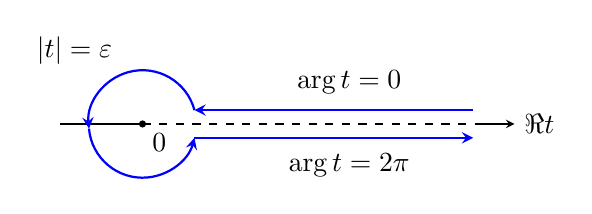
\begin{tikzpicture}[x=1.05cm,y=1.05cm,>=stealth]
\draw (-1,0)--(0,0);
\draw[dashed] (0,0)--(4.1,0);
\draw[->] (4.1,0)--(4.5,0) node[right] {$\Re t$};
\fill (0,0) circle (1.3pt) node[below right] {$0$};
\draw[blue,thick,->] (4,0.168)--(0.628,0.168);
\draw[blue,thick,->] (15:0.65) arc (15:185:0.65);
\draw[blue,thick,->] (185:0.65) arc (185:345:0.65);
\draw[blue,thick,->] (0.628,-0.168)--(4,-0.168);
\node[above] at (2.5,0.24) {$\arg t=0$};
\node[below] at (2.5,-0.24) {$\arg t=2\pi$};
\node[above left] at (-0.25,0.6) {$|t|=\varepsilon$};
\end{tikzpicture}
\end{center}
The two lips of the cut are displaced in the sketch for visibility.
Initially assume $\Re\nu>-1$.  On the upper lip $t=x$ with
$\arg t=0$, so $t^\nu=x^\nu$, but the direction is inward ($x$ runs
from $\infty$ to $\varepsilon$).  Its contribution is
\[
I_{\rm upper}=-e^{-\pi i\nu}
\int_\varepsilon^\infty e^{-x}x^\nu dx.
\]
On the lower lip the continuous argument is $2\pi$, so
$t^\nu=e^{2\pi i\nu}x^\nu$; since $e^{-\pi i\nu}e^{2\pi i\nu}
=e^{\pi i\nu}$, the outward contribution is
\[
I_{\rm lower}=e^{\pi i\nu}
\int_\varepsilon^\infty e^{-x}x^\nu dx.
\]
On the small circle put $t=\varepsilon e^{i\theta}$,
$0\le\theta\le2\pi$, so $dt=i\varepsilon e^{i\theta}d\theta$ and
$t^\nu=\varepsilon^\nu e^{i\nu\theta}$.  There $|e^{-t}|\le
e^\varepsilon$ and
$|e^{-\pi i\nu}t^\nu|=\varepsilon^{\Re\nu}e^{(\pi-\theta)\Im\nu}
\le\varepsilon^{\Re\nu}e^{\pi|\Im\nu|}$, and the circle has length
$2\pi\varepsilon$.  The circle integral is therefore at most
$2\pi e^{\pi|\Im\nu|}\varepsilon^{\Re\nu+1}e^\varepsilon$ in
magnitude, which tends to zero because $\Re\nu+1>0$.
The integrand is analytic in the plane cut along the positive real
axis, so by Cauchy's theorem $\int_C$ does not depend on
$\varepsilon$: for radii $\varepsilon_1<\varepsilon_2$ the two
contours differ by the boundary of the cut annulus
$\varepsilon_1<|t|<\varepsilon_2$ (the two circles and the lip
segments between them), which contains no singularity.  Hence
$\int_C$ is the limit as $\varepsilon\downarrow0$ of
$I_{\rm upper}+I_{\rm lower}$ plus the circle integral.  In this
limit the circle integral vanishes and the two ray integrals tend to
$\int_0^\infty e^{-x}x^\nu dx=\Gamma(\nu+1)$; with
$e^{\pi i\nu}-e^{-\pi i\nu}=2i\sin\pi\nu$,
\begin{align*}
\int_C e^{-t}e^{-\pi i\nu}t^\nu dt
&=(e^{\pi i\nu}-e^{-\pi i\nu})
 \int_0^\infty e^{-x}x^\nu dx\\
&=\boxed{2i\sin(\pi\nu)\Gamma(\nu+1)}.
\end{align*}

For $\Re\nu\le-1$, keep a nonzero circle radius; the individual
ray integrals cannot be extended to zero separately.  For fixed
$\varepsilon$ the complete contour integral is entire in $\nu$:
the circle is compact and the ray tails are dominated uniformly on
compact parameter sets by an exponential times a fixed power.
By the Cauchy argument above, which did not use $\Re\nu>-1$, it is
independent of $\varepsilon$.  Therefore the identity continues
analytically.  By the reflection formula,
$\Gamma(\nu+1)\Gamma(-\nu)=\pi/\sin\pi(\nu+1)=-\pi/\sin\pi\nu$, so its
left side is the entire function
\[
2i\Gamma(\nu+1)\sin\pi\nu=-\frac{2\pi i}{\Gamma(-\nu)}.
\]
\erratum{Only nonnegative integer $\nu$ makes the integrand entire
in $t$ and gives zero.  At negative integers the integral is nonzero;
the text's unqualified statement about integer $\nu$ needs this
restriction.}
Indeed, for $\nu=-m$, $m=1,2,\ldots$, the integrand is
$(-1)^m e^{-t}t^{-m}$.  Since $t^{-m}$ is single valued, the two lips
carry the same integrand in opposite directions and cancel, so only
the circle contributes.  The coefficient of $t^{-1}$ is
$(-1)^m(-1)^{m-1}/(m-1)!=-1/(m-1)!$, so by the residue theorem the
counterclockwise circle gives $2\pi i\cdot[-1/(m-1)!]=-2\pi i/(m-1)!$,
which is the continued formula $-2\pi i/\Gamma(-\nu)=-2\pi i/\Gamma(m)$.


\Needspace{9\baselineskip}
\subsection*{13.2 Digamma and Polygamma Functions}

\Needspace{5\baselineskip}
\par\bigskip
\noindent\textbf{13.2.1}\quad For ``small'' values of $x$,
\[
\ln\Gamma(x+1)=-\gamma x+\sum_{n=2}^{\infty}(-1)^{n}\frac{\zeta(n)}{n}x^{n},
\]
where $\gamma$ is the Euler-Mascheroni constant and $\zeta(n)$ the Riemann
zeta function. For what values of $x$ does this series converge?
\par\nobreak\hfill\emph{ANS.}\enspace $-1 < x\le1$.\par
Note that if $x=1$, we obtain
\[
\gamma=\sum_{n=2}^{\infty}(-1)^{n}\frac{\zeta(n)}{n},
\]
a series for the Euler-Mascheroni constant. The convergence of this series is
exceedingly slow. For actual computation of $\gamma$, other, indirect,
approaches are far superior (see Exercise 12.3.2).
\solution
Write $\zeta(n)=1+d_n$.  Since $k^{-n}\le\int_{k-1}^kt^{-n}dt$ for
$k\ge3$,
\[
0<d_n=\sum_{k=2}^{\infty}k^{-n}
\le 2^{-n}+\int_2^\infty t^{-n}dt
=2^{-n}+\frac{2^{1-n}}{n-1}
=2^{-n}\left(1+\frac2{n-1}\right).
\]
Thus, apart from the term $-\gamma x$, the series is the sum of
\[
\sum_{n=2}^\infty\frac{(-x)^n}n
\qquad\text{and}\qquad
\sum_{n=2}^\infty\frac{(-1)^nd_n}{n}x^n.
\]
The first has radius one.  The second, the correction, converges
absolutely for $|x|<2$, because $d_n/n\le3\cdot2^{-n}$ bounds its
terms by $3(|x|/2)^n$.  The sum converges absolutely for $|x|<1$.
At $x=1$ the first series is the convergent alternating harmonic
series, while at $x=-1$ it is the divergent harmonic tail
$\sum_{n\ge2}1/n$; the correction converges at both endpoints, so the
whole series converges at $x=1$ and diverges at $x=-1$.  For $|x|>1$
the terms $\zeta(n)x^n/n$ do not tend to zero, since $\zeta(n)>1$ and
$|x|^n/n\to\infty$.  Hence the real convergence set is exactly
\[
\boxed{-1<x\le1}.
\]
To identify the endpoint sum, let $x\uparrow1$ in the interior
identity.  By Abel's theorem the power series, which converges at
$x=1$, tends to its value there, while
$\ln\Gamma(1+x)\to\ln\Gamma(2)=\ln1=0$.  Hence
$0=-\gamma+\sum_{n\ge2}(-1)^n\zeta(n)/n$, that is,
\[
\gamma=\sum_{n=2}^{\infty}(-1)^n\frac{\zeta(n)}n.
\]
The leading $1/n$ behavior explains the slow convergence.  For
complex $x$, the same decomposition gives conditional convergence
on $|x|=1$ except at $x=-1$.


\Needspace{5\baselineskip}
\par\bigskip
\noindent\textbf{13.2.2}\quad Show that the series expansion of
$\ln\Gamma(x+1)$ (Exercise 13.2.1) may be written as
\begin{enumerate}
\item[(a)] $\ln\Gamma(x+1)=\dfrac{1}{2}\ln\left(\dfrac{\pi x}{\sin\pi x}\right)
  -\gamma x-\displaystyle\sum_{n=1}^{\infty}\frac{\zeta(2n+1)}{2n+1}x^{2n+1}$,
\item[(b)] $\ln\Gamma(x+1)=\dfrac{1}{2}\ln\left(\dfrac{\pi x}{\sin\pi x}\right)
  -\dfrac{1}{2}\ln\left(\dfrac{1+x}{1-x}\right)+(1-\gamma)x$\\[2pt]
  $\hfill-\displaystyle\sum_{n=1}^{\infty}
  \left[\zeta(2n+1)-1\right]\frac{x^{2n+1}}{2n+1}$.
\end{enumerate}
Determine the range of convergence of each of these expressions.
\solution
Use the real logarithm initially on $-1<x<1$ (with removable
quotients at $x=0$).  Split the original series into even and odd
powers:
\[
\ln\Gamma(1+x)=-\gamma x+
\sum_{n=1}^{\infty}\frac{\zeta(2n)x^{2n}}{2n}
-\sum_{n=1}^{\infty}\frac{\zeta(2n+1)x^{2n+1}}{2n+1}.
\]
Reflection and recurrence give
$\Gamma(1+x)\Gamma(1-x)=x\Gamma(x)\Gamma(1-x)=\pi x/\sin\pi x$.
Adding the series at $x$ and $-x$ cancels $-\gamma x$ and the odd
terms and doubles the even ones:
\[
\ln\frac{\pi x}{\sin\pi x}=\ln\Gamma(1+x)+\ln\Gamma(1-x)
=2\sum_{n=1}^{\infty}\frac{\zeta(2n)x^{2n}}{2n}.
\]
\textbf{(a)} Substituting half of this for the even series gives
exactly the first requested form.
Its remaining odd series has radius one; at $x=1$ its positive
terms behave as $1/(2n+1)$, and at $x=-1$ their negatives do.
It therefore converges for $\boxed{-1<x<1}$ only.  In particular,
the finite limit of the complete expression at $x=1$ requires
cancellation of divergent pieces; direct endpoint substitution
in the separated terms is invalid.

\textbf{(b)} Split $\zeta(2n+1)=1+[\zeta(2n+1)-1]$ and use
\[
\sum_{n=1}^{\infty}\frac{x^{2n+1}}{2n+1}
=\frac12\ln\frac{1+x}{1-x}-x.
\]
This follows by integrating the geometric series
$(1-t^2)^{-1}=\sum_{n\ge0}t^{2n}$ from zero to $x$, which gives
$\sum_{n\ge0}x^{2n+1}/(2n+1)=\int_0^xdt/(1-t^2)
=\frac12\ln[(1+x)/(1-x)]$, and removing the linear term.  Hence
\[
-\sum_{n=1}^{\infty}\frac{\zeta(2n+1)x^{2n+1}}{2n+1}
=-\frac12\ln\frac{1+x}{1-x}+x
-\sum_{n=1}^{\infty}\left[\zeta(2n+1)-1\right]\frac{x^{2n+1}}{2n+1},
\]
and inserting this in (a) produces the second displayed form, with
$-\gamma x+x=(1-\gamma)x$.
By the bounds $2^{-m}<\zeta(m)-1\le2^{-m}[1+2/(m-1)]$ (the lower one
is the first term of $d_m$, the upper one is from Exercise 13.2.1),
$2^{2n+1}[\zeta(2n+1)-1]\to1$, so the remaining
series has radius two.  At $x=\pm2$ its terms behave as
$\pm1/(2n+1)$, a signed harmonic tail, and it diverges.  Thus this
series alone converges on $\boxed{-2<x<2}$, but \erratum{the expression as written with
separate real logarithms has the domain $-1<x<1$.}
If those logarithms are first combined, their contribution is
\[
\frac12\ln\frac{\pi x(1-x)}{(1+x)\sin\pi x}.
\]
This has a removable limit $\tfrac12\ln(1/2)$ at $x=1$, because
$\sin\pi x=\sin\pi(1-x)\approx\pi(1-x)$ there, so the quotient tends
to $\pi/(2\pi)=1/2$.  It is real on $-1<x<2$, since for $1<x<2$ both
$1-x$ and $\sin\pi x$ are negative and the quotient stays positive.
Both sides of the combined identity are analytic on $-1<x<2$ and
agree on $-1<x<1$, so by the identity theorem (uniqueness of
analytic continuation) the combined form extends the identity across
$x=1$ to that larger interval.  This continuation
must be distinguished from the domain of the separate logarithms.


\Needspace{5\baselineskip}
\par\bigskip
\noindent\textbf{13.2.3}\quad Verify that for $n$, a positive integer, the
following two forms of the digamma function are equal to each other:
\[
\psi(n+1)=\sum_{j=1}^{n}\frac{1}{j}-\gamma
\quad\text{and}\quad
\psi(n+1)=\sum_{j=1}^{\infty}\frac{n}{j(n+j)}-\gamma.
\]
\solution
For a fixed positive integer $n$, partial fractions give
\[
\frac{n}{j(n+j)}=\frac1j-\frac1{j+n}.
\]
Sum only to a finite $N$ before canceling.  With
$H_N=\sum_{j=1}^N1/j$ and
$\sum_{j=1}^N1/(j+n)=\sum_{i=n+1}^{N+n}1/i=H_{N+n}-H_n$,
\begin{align*}
\sum_{j=1}^N\frac{n}{j(n+j)}
&=H_N-(H_{N+n}-H_n)\\
&=H_n-\sum_{j=N+1}^{N+n}\frac1j.
\end{align*}
The final sum lies between zero and $n/(N+1)$, hence tends to
zero as $N\to\infty$.  Therefore
\[
\boxed{\sum_{j=1}^{\infty}\frac{n}{j(n+j)}=H_n},
\qquad\psi(n+1)=H_n-\gamma,
\]
and the two representations agree.  This argument avoids
subtracting two divergent harmonic series separately.


\Needspace{5\baselineskip}
\par\bigskip
\noindent\textbf{13.2.4}\quad Show that $\psi(z+1)$ has the series expansion
\[
\psi(z+1)=-\gamma+\sum_{n=2}^{\infty}(-1)^{n}\zeta(n)z^{n-1}.
\]
\par\smallskip
\erratum{The expansion holds for $|z|<1$.}
\solution
On every closed disk $|z|\le r<1$, the Maclaurin series for
$\ln\Gamma(1+z)$, Eq.~(13.44), may be differentiated term by term.
Indeed, the derivative terms
$(d/dz)[(-1)^n\zeta(n)z^n/n]=(-1)^n\zeta(n)z^{n-1}$ have absolute
values at most $\zeta(2)r^{n-1}$ (since $\zeta(n)\le\zeta(2)$), whose
sum converges; by the Weierstrass M-test the differentiated series
converges uniformly on the disk, which justifies the term-by-term
differentiation.  Since
$\psi(1+z)=d\ln\Gamma(1+z)/dz$ and $(d/dz)(-\gamma z)=-\gamma$,
differentiation gives
\[
\boxed{\psi(1+z)=-\gamma+
\sum_{n=2}^{\infty}(-1)^n\zeta(n)z^{n-1}},
\qquad |z|<1.
\]
\erratum{The domain $|z|<1$ is needed: on $|z|=1$ the
summands have magnitudes $\zeta(n)\to1$, so none of that boundary
belongs to the convergence set.}  The closest pole of the
expanded function is at $z=-1$, consistent with radius one.


\Needspace{5\baselineskip}
\par\bigskip
\noindent\textbf{13.2.5}\quad For a power-series expansion of
$\ln\Gamma(z+1)$, AMS-55 (see Additional Readings for the reference) lists
\[
\ln\Gamma(z+1)=-\ln(1+z)+z(1-\gamma)
+\sum_{n=2}^{\infty}(-1)^{n}\left[\zeta(n)-1\right]\frac{z^{n}}{n}.
\]
\begin{enumerate}
\item[(a)] Show that this agrees with Eq.~(13.44) for $|z| < 1$.
\item[(b)] What is the range of convergence of this new expression?
\end{enumerate}
\solution
\textbf{(a)} For $|z|<1$,
\[
\ln(1+z)=z-\sum_{n=2}^{\infty}(-1)^n\frac{z^n}{n}.
\]
Add this to the series for $\ln\Gamma(1+z)$.  The linear
coefficients combine to $1-\gamma$, and for each $n\ge2$ the
coefficients $(-1)^n\zeta(n)/n$ and $-(-1)^n/n$ combine to
$(-1)^n[\zeta(n)-1]/n$, giving
\[
\ln\Gamma(1+z)+\ln(1+z)
=(1-\gamma)z+
\sum_{n=2}^{\infty}(-1)^n\frac{\zeta(n)-1}{n}z^n.
\]
Moving $\ln(1+z)$ to the right proves the claimed agreement.

\textbf{(b)} Set $e_n=\zeta(n)-1-2^{-n}=\sum_{k\ge3}k^{-n}$.  The
integral comparison of Exercise 13.2.1, now starting at $k=3$, gives
the estimate
\[
0<e_n\le3^{-n}+\int_3^\infty t^{-n}dt
=3^{-n}\left(1+\frac3{n-1}\right).
\]
Since $(-1)^n[\zeta(n)-1]z^n/n=(-z/2)^n/n+(-1)^ne_nz^n/n$, the new
series is $\sum_{n=2}^\infty(-z/2)^n/n$ plus a correction absolutely
convergent for $|z|<3$ (its terms are at most $4(|z|/3)^n$).  Thus
its radius is two; on $|z|=2$ it converges except at $z=-2$, by the
Dirichlet test for the leading series $\sum w^n/n$, $|w|=1$, $w\ne1$.
Its real convergence set is $\boxed{-2<z\le2}$.

\erratum{Convergence of the series is distinct from the domain
of the complete logarithmic identity: with ordinary real
logarithms that identity requires $z>-1$, and hence holds for
$-1<z\le2$.  It is undefined at $z=-1$.}
More precisely, since $\Gamma(2+z)=(1+z)\Gamma(1+z)$, part (a)
shows that the analytic series equals
$\ln\Gamma(2+z)-(1-\gamma)z$ for $|z|<1$.  The function
$\Gamma(2+z)$ has no zeros and its nearest pole is at $z=-2$, so
$\ln\Gamma(2+z)$, continued from zero, is analytic on $|z|<2$, as is
the series (radius two).  Agreeing on $|z|<1$, the two agree on the
whole disk $|z|<2$ by the identity theorem (uniqueness of analytic
continuation).  Subtracting $\ln(1+z)$ gives the requested
identity on a slit disk, for example
$|z|<2$ with $z\notin(-2,-1]$, using compatible analytic branches.
The endpoint $z=2$ follows by Abel's theorem and continuity.


\Needspace{5\baselineskip}
\par\bigskip
\noindent\textbf{13.2.6}\quad Show that
\[
\frac{1}{2}\ln\left(\frac{\pi z}{\sin\pi z}\right)
=\sum_{n=1}^{\infty}\frac{\zeta(2n)}{2n}z^{2n},\quad|z| < 1.
\]
\emph{Hint.}~Use Eqs.~(13.23) and \erratum{(13.44)}.
\solution
Write the expansion in Eq.~(13.44) at $z$ and $-z$ and add:
\begin{align*}
\ln\Gamma(1+z)+\ln\Gamma(1-z)
&=\sum_{k=2}^{\infty}\frac{(-1)^k\zeta(k)}k
 [z^k+(-z)^k]\\
&=2\sum_{n=1}^{\infty}\frac{\zeta(2n)}{2n}z^{2n}.
\end{align*}
The linear terms and all odd powers cancel.  Reflection,
$\Gamma(z)\Gamma(1-z)=\pi/\sin\pi z$, followed by
$z\Gamma(z)=\Gamma(1+z)$, gives
\[
\Gamma(1+z)\Gamma(1-z)=\frac{\pi z}{\sin\pi z}.
\]
In $|z|<1$ the quotient has no zero or pole, with value one at
zero.  Choose its analytic logarithm to vanish there.  The sum
of the two gamma logarithms has that same value and exponential,
so there is no additional $2\pi i$ constant.  Dividing by two gives
\[
\boxed{\frac12\ln\frac{\pi z}{\sin\pi z}
=\sum_{n=1}^{\infty}\frac{\zeta(2n)}{2n}z^{2n}},\qquad |z|<1.
\]
\erratum{The printed hint cites Eq.~(13.35); the published errata
(Instructor's Manual, 6 April 2012) replace it by Eq.~(13.44), the
Maclaurin series of $\ln\Gamma(1+z)$ used above.}


\Needspace{5\baselineskip}
\par\bigskip
\noindent\textbf{13.2.7}\quad Write out a Weierstrass infinite-product
definition of $\ln\Gamma(z+1)$. Without differentiating, show that this leads
directly to the Maclaurin expansion of $\ln\Gamma(z+1)$, Eq.~(13.44).
\solution
Weierstrass' product, after using $\Gamma(1+z)=z\Gamma(z)$, is
\[
\frac1{\Gamma(1+z)}=e^{\gamma z}
\prod_{k=1}^{\infty}\left(1+\frac zk\right)e^{-z/k}.
\]
Taking the analytic logarithm that is zero at $z=0$ gives
\[
\ln\Gamma(1+z)=-\gamma z+
\sum_{k=1}^{\infty}\left[\frac zk-\ln\left(1+\frac zk\right)\right].
\]
For $|z|<1$, expand each logarithm by
$\ln(1+w)=w-w^2/2+w^3/3-\cdots$ with $w=z/k$, $|w|<1$.  Its linear
term cancels:
\[
\frac zk-\ln\left(1+\frac zk\right)
=\sum_{n=2}^{\infty}\frac{(-1)^n z^n}{n k^n}.
\]
The double series is absolutely convergent, since summing over $k$
first gives $\zeta(n)|z|^n/n\le\zeta(2)|z|^n$ and
\[
\sum_{n=2}^{\infty}\sum_{k=1}^{\infty}
\frac{|z|^n}{n k^n}
\le\zeta(2)\sum_{n=2}^{\infty}|z|^n<\infty.
\]
Interchange the sums and identify $\sum_{k=1}^\infty k^{-n}$:
\[
\boxed{\ln\Gamma(1+z)=-\gamma z+
\sum_{n=2}^{\infty}(-1)^n\frac{\zeta(n)}n z^n}.
\]
No differentiation of the product was used.


\Needspace{5\baselineskip}
\par\bigskip
\noindent\textbf{13.2.8}\quad Derive the difference relation for the
polygamma function,
\[
\psi^{(m)}(z+2)=\psi^{(m)}(z+1)+(-1)^{m}\frac{m!}{(z+1)^{m+1}},
\quad m=0,1,2,\ldots.
\]
\solution
Differentiate $\Gamma(z+2)=(z+1)\Gamma(z+1)$ logarithmically
at regular arguments, i.e., differentiate
$\ln\Gamma(z+2)=\ln(z+1)+\ln\Gamma(z+1)$.  The result is
\[
\psi(z+2)=\frac1{z+1}+\psi(z+1).
\]
This already proves the case $m=0$.  For $m\ge1$, differentiate
this relation $m$ times, using $\psi^{(m)}=d^m\psi/dz^m$; the $m$th
derivative of the first term is
\[
\frac{d^m}{dz^m}(z+1)^{-1}
=(-1)(-2)\cdots(-m)(z+1)^{-m-1}
=\frac{(-1)^m m!}{(z+1)^{m+1}}.
\]
Hence
\[
\boxed{\psi^{(m)}(z+2)=\psi^{(m)}(z+1)
+\frac{(-1)^m m!}{(z+1)^{m+1}}},\qquad m=0,1,2,\ldots.
\]
These are identities of meromorphic functions; a displayed value
at a pole is not a finite number.  For integer positive arguments,
the formulas recursively reduce to the values at one.


\Needspace{5\baselineskip}
\par\bigskip
\noindent\textbf{13.2.9}\quad The Pochhammer symbol $(a)_{n}$ is defined (for
integral $n$) as
\[
(a)_{n}=a(a+1)\cdots(a+n-1),\quad(a)_{0}=1.
\]
\begin{enumerate}
\item[(a)] Express $(a)_{n}$ in terms of factorials.
\item[(b)] Find $(d/da)(a)_{n}$ in terms of $(a)_{n}$ and digamma functions.
\end{enumerate}
\par\nobreak\hfill\emph{ANS.}\enspace
$\dfrac{d}{da}(a)_{n}=(a)_{n}\left[\psi(a+n)-\psi(a)\right]$.
\begin{enumerate}
\item[(c)] Show that
  \[
  (a)_{n+k}=(a+n)_{k}\cdot(a)_{n}.
  \]
\end{enumerate}
\par\smallskip
\erratum{The finite-product indices $n,k$ are nonnegative integers. Products involving singular gamma or digamma factors are evaluated by their polynomial continuation.}
\solution
\erratum{The finite-product definition here uses nonnegative
integers $n$ and, in part (c), $k$.}
\textbf{(a)} Repeated gamma recurrence gives
$\Gamma(a+n)=(a+n-1)(a+n-2)\cdots a\,\Gamma(a)=(a)_n\Gamma(a)$,
so
\[
\boxed{(a)_n=\frac{\Gamma(a+n)}{\Gamma(a)}
=\frac{(a+n-1)!}{(a-1)!}}.
\]
The factorials have their generalized meaning.  The finite
product is a polynomial in $a$ and defines any removable value
of this quotient at gamma poles.

\textbf{(b)} At points where all factors are nonzero,
logarithmic differentiation of the finite product gives
\[
\frac{d}{da}(a)_n=(a)_n\sum_{j=0}^{n-1}\frac1{a+j}.
\]
Iterating $\psi(a+1)-\psi(a)=1/a$ (Exercise 13.2.8 with $m=0$)
identifies the finite sum by telescoping,
$\psi(a+n)-\psi(a)=\sum_{j=0}^{n-1}[\psi(a+j+1)-\psi(a+j)]
=\sum_{j=0}^{n-1}1/(a+j)$:
\[
\boxed{\frac{d}{da}(a)_n=(a)_n[\psi(a+n)-\psi(a)]}.
\]
The same result follows from (a):
$(d/da)[\Gamma(a+n)/\Gamma(a)]
=[\Gamma(a+n)/\Gamma(a)][\psi(a+n)-\psi(a)]$.
At exceptional arguments use the equivalent polynomial formula
\[
\frac{d}{da}(a)_n=
\sum_{j=0}^{n-1}\prod_{\substack{0\le\ell<n\\\ell\ne j}}(a+\ell).
\]
For example, at $a=-j$ with $0\le j<n$ only the term that omits the
vanishing factor $a+j$ survives, and its value is
\[
\prod_{\ell=0}^{j-1}(\ell-j)\prod_{\ell=j+1}^{n-1}(\ell-j)
=(-1)^jj!\,(n-1-j)!,
\]
even though the separated digamma factors have poles.  For $n=0$
the empty product is one and its derivative is zero.

\textbf{(c)} Split the product after its first $n$ factors:
\begin{align*}
(a)_{n+k}
&=\left[\prod_{j=0}^{n-1}(a+j)\right]
  \left[\prod_{j=n}^{n+k-1}(a+j)\right]\\
&=\boxed{(a)_n(a+n)_k}.
\end{align*}
This polynomial proof also includes zeros and empty products.


\Needspace{5\baselineskip}
\par\bigskip
\noindent\textbf{13.2.10}\quad Verify the following special values of the
$\psi$ form of the digamma and polygamma functions:
\[
\psi(1)=-\gamma,\quad\psi^{(1)}(1)=\zeta(2),\quad
\psi^{(2)}(1)=-2\zeta(3).
\]
\solution
Differentiating the Weierstrass form
$\ln\Gamma(1+z)=-\gamma z+\sum_k[z/k-\ln(1+z/k)]$ of
Exercise 13.2.7 term by term (each term has derivative
$1/k-1/(k+z)=z/[k(k+z)]$, and these converge locally uniformly
away from the poles) gives the convergent digamma representation
\[
\psi(1+z)=-\gamma+
\sum_{k=1}^{\infty}\left(\frac1k-\frac1{k+z}\right).
\]
Putting $z=0$ makes every term of the sum vanish, so
$\boxed{\psi(1)=-\gamma}$.
Differentiation on compact sets away from the poles, with
$(d/dz)(k+z)^{-1}=-(k+z)^{-2}$ and $(d/dz)(k+z)^{-2}=-2(k+z)^{-3}$,
gives
\[
\psi^{(1)}(1+z)=\sum_{k=1}^{\infty}\frac1{(k+z)^2},
\qquad
\psi^{(2)}(1+z)=-2\sum_{k=1}^{\infty}\frac1{(k+z)^3}.
\]
Both differentiated sums converge absolutely and locally
uniformly.  Therefore at $z=0$,
\[
\boxed{\psi^{(1)}(1)=\sum_{k=1}^{\infty}k^{-2}=\zeta(2)},
\qquad
\boxed{\psi^{(2)}(1)=-2\sum_{k=1}^{\infty}k^{-3}=-2\zeta(3)}.
\]


\Needspace{5\baselineskip}
\par\bigskip
\noindent\textbf{13.2.11}\quad Verify:
\begin{enumerate}
\item[(a)] $\displaystyle\int_{0}^{\infty}e^{-r}\ln r\,dr=-\gamma$.
\item[(b)] $\displaystyle\int_{0}^{\infty}re^{-r}\ln r\,dr=1-\gamma$.
\item[(c)] $\displaystyle\int_{0}^{\infty}r^{n}e^{-r}\ln r\,dr
  =(n-1)!+n\int_{0}^{\infty}r^{n-1}e^{-r}\ln r\,dr$,\quad$n=1,2,3,\ldots$.
\end{enumerate}
\emph{Hint.}~These may be verified by integration by parts, or by
differentiating the Euler integral formula for $\Gamma(n+1)$ with respect to
$n$.
\solution
For $s$ in a compact subset of $\Re s>0$, on which
$\Re s\ge\varepsilon$ for some $\varepsilon>0$, differentiation of
Euler's integral is justified by the integrable bounds
$r^{\varepsilon-1}|\ln r|$ near zero and a polynomial times
$e^{-r}|\ln r|$ at infinity.  Hence
\[
\Gamma'(s)=\int_0^\infty r^{s-1}e^{-r}\ln r\,dr
=\Gamma(s)\psi(s).
\]
\textbf{(a)} At $s=1$, $\Gamma(1)=1$ and $\psi(1)=-\gamma$,
so the integral is $\boxed{-\gamma}$.

\textbf{(c)} Write $I_n=\int_0^\infty r^ne^{-r}\ln r\,dr$.
For integers $n\ge1$, integrate by parts with
$u=r^n\ln r$, $dv=e^{-r}dr$, so that
$du=(nr^{n-1}\ln r+r^{n-1})dr$ and $v=-e^{-r}$.  Since
$r^n\ln r\to0$ at zero and the exponential removes the upper
boundary term, and since $\int_0^\infty r^{n-1}e^{-r}dr=\Gamma(n)
=(n-1)!$,
\begin{align*}
I_n&=\bigl[-r^ne^{-r}\ln r\bigr]_0^\infty
+\int_0^\infty e^{-r}(nr^{n-1}\ln r+r^{n-1})dr\\
&=\boxed{nI_{n-1}+(n-1)!}.
\end{align*}
\textbf{(b)} In particular, $I_1=I_0+0!=\boxed{1-\gamma}$.
The general closed form is $I_n=n!(H_n-\gamma)$, with the harmonic
numbers $H_n=\sum_{j=1}^n1/j$ of Exercise 13.2.3 and $H_0=0$, as is
checked by this recurrence and $I_0=-\gamma$: if
$I_{n-1}=(n-1)!(H_{n-1}-\gamma)$, then
$I_n=n!(H_{n-1}-\gamma)+n!/n=n!(H_n-\gamma)$.  It agrees with
$I_n=\Gamma'(n+1)=\Gamma(n+1)\psi(n+1)$ and Exercise 13.2.3.
Integration by parts at $n=0$ would have a divergent boundary term,
which is why part (a) was evaluated before using this recurrence.


\Needspace{5\baselineskip}
\par\bigskip
\noindent\textbf{13.2.12}\quad Dirac relativistic wave functions for hydrogen
involve factors such as $\Gamma[2(1-\alpha^{2}Z^{2})^{1/2}+1]$ where $\alpha$,
the fine structure constant, is \erratum{approximated here by $1/137$} and $Z$ is the atomic number. Expand
$\Gamma[2(1-\alpha^{2}Z^{2})^{1/2}+1]$ in a series of powers of
$\alpha^{2}Z^{2}$.
\solution
Let $q=\alpha^2Z^2$ and expand about $q=0$, using the square-root
branch that equals one there.  The binomial series
$\sqrt{1-q}=1-\frac q2-\frac{q^2}8-\frac{q^3}{16}+O(q^4)$ gives
\[
2\sqrt{1-q}+1=3+\delta,
\qquad\delta=-q-\frac{q^2}{4}-\frac{q^3}{8}+O(q^4).
\]
Set $p=\psi(3)$, $r=\psi^{(1)}(3)$ and $s=\psi^{(2)}(3)$.
The recurrence of Exercise 13.2.8, applied with $z=0$ and $z=1$,
gives $\psi^{(m)}(3)=\psi^{(m)}(1)+(-1)^mm!\,(1+2^{-m-1})$; with
the values at one from Exercise 13.2.10 this yields
\[
p=\frac32-\gamma,\qquad
r=\zeta(2)-1-\frac14=\zeta(2)-\frac54,
\qquad s=-2\zeta(3)+2+\frac14=\frac94-2\zeta(3).
\]
Differentiating $\Gamma'=\Gamma\psi$ and using $\Gamma'=\Gamma\psi$
again at each step gives
$\Gamma''=\Gamma'\psi+\Gamma\psi'=\Gamma(\psi^2+\psi')$ and
$\Gamma^{(3)}=\Gamma\psi(\psi^2+\psi')+\Gamma(2\psi\psi'+\psi'')$,
that is,
\[
\Gamma''=\Gamma(\psi^2+\psi'),\qquad
\Gamma^{(3)}=\Gamma(\psi^3+3\psi\psi'+\psi'').
\]
Since $\Gamma(3)=2$, Taylor expansion in $\delta$ is
\[
\Gamma(3+\delta)=2\left[1+p\delta+
\frac{p^2+r}{2}\delta^2+
\frac{p^3+3pr+s}{6}\delta^3+O(\delta^4)\right].
\]
Now $\delta^2=q^2+q^3/2+O(q^4)$ and
$\delta^3=-q^3+O(q^4)$.  Inside the brackets the coefficient of $q$
is $-p$; that of $q^2$ is $-p/4+(p^2+r)/2$; and that of $q^3$ is
$-p/8+(p^2+r)/4-(p^3+3pr+s)/6$.  Multiplying by two,
\begin{align*}
\Gamma(2\sqrt{1-q}+1)
={}&2-2pq+\left(p^2+r-\frac p2\right)q^2\\
&+\left[-\frac p4+\frac{p^2+r}{2}
-\frac{p^3+3pr+s}{3}\right]q^3+O(q^4).
\end{align*}
Here $-2p=2\gamma-3$ and
\[
p^2+r-\frac p2
=\left(\frac94-3\gamma+\gamma^2\right)+\zeta(2)-\frac54
-\frac34+\frac\gamma2
=\gamma^2-\frac52\gamma+\zeta(2)+\frac14.
\]
In particular, the first three terms in the original variables are
\[
\boxed{2+(2\gamma-3)\alpha^2Z^2+
\left[\gamma^2-\frac52\gamma+\zeta(2)+\frac14\right]
\alpha^4Z^4+O(\alpha^6Z^6)}.
\]
For the $q^3$ coefficient, multiplying out the products and adding
$s=\tfrac94-2\zeta(3)$ gives
\begin{align*}
p^3&=\frac{27}8-\frac{27}4\gamma+\frac92\gamma^2-\gamma^3,\qquad
3pr=\frac92\zeta(2)-\frac{45}8+\frac{15}4\gamma-3\gamma\zeta(2),\\
p^3+3pr+s&=-\gamma^3+\frac92\gamma^2-3\gamma-3\gamma\zeta(2)
+\frac92\zeta(2)-2\zeta(3),\\
-\frac p4+\frac{p^2+r}2&=\frac{\gamma^2}2-\frac54\gamma
+\frac{\zeta(2)}2+\frac18,
\end{align*}
and subtracting one third of the second line from the third gives the
$q^3$ coefficient
$\gamma^3/3-\gamma^2-\gamma/4+(\gamma-1)\zeta(2)+\tfrac23\zeta(3)
+\tfrac18$.  Numerically,
\[
\Gamma(2\sqrt{1-q}+1)=2-1.845569\,q+0.785073\,q^2-0.182458\,q^3
+O(q^4),
\]
which can be checked by evaluating the gamma function directly: at
$q=0.1$, $\Gamma(2\sqrt{0.9}+1)=\Gamma(2.8973666)=1.8231159$, while
the cubic gives $1.8231114$.  The difference, about
$4.5\times10^{-6}$, is the size of the omitted $q^4$ term: its
coefficient, obtained in the same way from $\Gamma^{(4)}$ and
$\psi^{(3)}(3)$, is $0.04416$, so the term is $4.4\times10^{-6}$ at
$q=0.1$.
Higher terms follow from the same two Taylor expansions.  The
expansion is local at $q=0$ and converges for $|q|<1$; there the
chosen square root has positive real part, so its gamma argument
encounters no gamma pole.  Physically, a short truncation requires
$\alpha^2Z^2$ small.  The value of $\alpha$ does not enter the
coefficients; the statement's $1/137$ approximates the measured
$\alpha\simeq1/137.036$.


\Needspace{5\baselineskip}
\par\bigskip
\noindent\textbf{13.2.13}\quad The quantum mechanical description of a
particle in a Coulomb field requires a knowledge of the argument of
$\Gamma(z)$ when $z$ is complex. Determine the argument of $\Gamma(1+ib)$
for small, real $b$.
\solution
Choose the argument continuously from $b=0$, where $\Gamma(1)=1$
and the argument is zero; it is then the imaginary part of the
logarithm of Eq.~(13.44), which vanishes at $z=0$.  For $|b|<1$,
substitute $z=ib$ in
\[
\ln\Gamma(1+z)=-\gamma z+
\sum_{n=2}^{\infty}(-1)^n\frac{\zeta(n)}n z^n.
\]
The linear term $-\gamma ib$ contributes $-\gamma b$ to the
imaginary part.  Even powers $(ib)^{2m}=(-1)^mb^{2m}$ are real.  For
the odd powers $n=2m+1$,
$(-1)^{2m+1}i^{2m+1}=-i\,(i^2)^m=(-1)^{m+1}i$.  Therefore
\[
\arg\Gamma(1+ib)=\Im\ln\Gamma(1+ib)
=-\gamma b+\sum_{m=1}^{\infty}(-1)^{m+1}
\frac{\zeta(2m+1)}{2m+1}b^{2m+1},
\]
that is,
\[
\boxed{\arg\Gamma(1+ib)
=-\gamma b+\frac{\zeta(3)}3b^3
-\frac{\zeta(5)}5b^5+\frac{\zeta(7)}7b^7-\cdots}.
\]
The leading approximation is $-\gamma b$, with an error of order
$b^3$.  This is the continuous local phase (and agrees with the
principal phase for sufficiently small $b$); arbitrary arguments
differ by $2\pi$ multiples.  Its oddness in $b$ also follows from
$\Gamma(1-ib)=\overline{\Gamma(1+ib)}$.


\Needspace{5\baselineskip}
\par\bigskip
\noindent\textbf{13.2.14}\quad Using digamma and polygamma functions, sum the
series
\begin{enumerate}
\item[(a)] $\displaystyle\sum_{n=1}^{\infty}\frac{1}{n(n+1)}$,\quad
(b) $\displaystyle\sum_{n=2}^{\infty}\frac{1}{n^{2}-1}$.
\end{enumerate}
\emph{Note.}~You can use Exercise 13.2.8 to calculate the needed digamma
functions.
\solution
Use the digamma identity
\[
\psi(1+z)+\gamma=\sum_{j=1}^{\infty}\frac{z}{j(j+z)},
\]
which is the representation of Exercise 13.2.10 with
$1/j-1/(j+z)=z/[j(j+z)]$.
\textbf{(a)} At $z=1$ the requested sum is
$\psi(2)+\gamma$.  The recurrence of Exercise 13.2.8 ($m=0$, $z=0$),
$\psi(2)=\psi(1)+1=-\gamma+1$, gives
\[
\boxed{\sum_{n=1}^{\infty}\frac1{n(n+1)}=1}.
\]
\textbf{(b)} Put $j=n-1$; then $n^2-1=(n-1)(n+1)=j(j+2)$.  At $z=2$
the identity gives $\sum_j2/[j(j+2)]=\psi(3)+\gamma$, and the
recurrence ($m=0$, $z=1$) gives $\psi(3)=\psi(2)+\tfrac12
=\tfrac32-\gamma$.  Hence
\begin{align*}
\sum_{n=2}^{\infty}\frac1{n^2-1}
&=\sum_{j=1}^{\infty}\frac1{j(j+2)}
=\frac12[\psi(3)+\gamma]\\
&=\frac12\left(1+\frac12\right)=\boxed{\frac34}.
\end{align*}
As a separate check, the partial fractions
$1/[n(n+1)]=1/n-1/(n+1)$ and
$1/(n^2-1)=\tfrac12[1/(n-1)-1/(n+1)]$ make the finite partial sums
telescope to $1-1/(N+1)$ in (a) and
$\tfrac12[1+1/2-1/N-1/(N+1)]$ in (b), respectively;
their limits give the same answers.


\Needspace{5\baselineskip}
\par\bigskip
\noindent\textbf{13.2.15}\quad Show that
\[
\sum_{n=1}^{\infty}\frac{1}{(n+a)(n+b)}
=\frac{1}{(b-a)}\left[\psi(1+b)-\psi(1+a)\right],
\]
where $a\neq b$, and neither $a$ nor $b$ is a negative integer. It is of some
interest to compare this summation with the corresponding integral,
\[
\int_{1}^{\infty}\frac{dx}{(x+a)(x+b)}
=\frac{1}{b-a}\left[\ln(1+b)-\ln(1+a)\right].
\]
The relation between $\psi(x)$ and $\ln x$ is made explicit in the analysis
leading to Stirling's formula.
\par\smallskip
\erratum{For the displayed ordinary real improper integral and real logarithms, require real $a,b>-1$ as well as $a\ne b$. The series has the wider domain stated above.}
\solution
For the stated admissible $a,b$, every denominator is nonzero
and the summands are $O(n^{-2})$, so the series converges
absolutely.  Subtract the two convergent digamma representations:
\begin{align*}
\psi(1+b)-\psi(1+a)
&=\sum_{n=1}^{\infty}
\left(\frac1{n+a}-\frac1{n+b}\right)\\
&=(b-a)\sum_{n=1}^{\infty}\frac1{(n+a)(n+b)}.
\end{align*}
Division by $b-a$ proves
\[
\boxed{\sum_{n=1}^{\infty}\frac1{(n+a)(n+b)}
=\frac{\psi(1+b)-\psi(1+a)}{b-a}}.
\]
The removable case $b=a$ is
$\sum_{n=1}^{\infty}(n+a)^{-2}=\psi^{(1)}(1+a)$.

\erratum{The accompanying real improper integral requires
stronger conditions, for example real $a,b>-1$.  Merely excluding
negative integers does not prevent an interior pole: $a=-3/2$,
$b=0$ gives one at $x=3/2$.}
Under $a,b>-1$, partial fractions give
\begin{align*}
\int_1^R\frac{dx}{(x+a)(x+b)}
&=\frac1{b-a}
\bigl[\ln(x+a)-\ln(x+b)\bigr]_1^R\\
&=\frac1{b-a}\left[\ln\frac{R+a}{R+b}
+\ln(1+b)-\ln(1+a)\right].
\end{align*}
The first logarithm tends to zero, proving the quoted integral.
When $b\to a>-1$, its value tends to $1/(1+a)$, whereas the
series tends to the trigamma value above.


\Needspace{9\baselineskip}
\subsection*{13.3 The Beta Function}

\Needspace{5\baselineskip}
\par\bigskip
\noindent\textbf{13.3.1}\quad Verify the following beta function identities:
\begin{enumerate}
\item[(a)] $B(a,b)=B(a+1,b)+B(a,b+1)$,
\item[(b)] $B(a,b)=\dfrac{a+b}{b}B(a,b+1)$,
\item[(c)] $B(a,b)=\dfrac{b-1}{a}B(a+1,b-1)$,
\item[(d)] $B(a,b)B(a+b,c)=B(b,c)B(a,b+c)$.
\end{enumerate}
\solution
Start where the beta integrals converge; in part (c) take
$\Re b>1$ as well as $\Re a>0$.  The results then extend as
meromorphic identities wherever the displayed values are defined.

\textbf{(a)} Insert $1=t+(1-t)$ into the defining integral:
\begin{align*}
B(a,b)&=\int_0^1 t^{a-1}(1-t)^{b-1}[t+(1-t)]dt\\
&=\boxed{B(a+1,b)+B(a,b+1)}.
\end{align*}
\textbf{(b)} Gamma recurrence gives
\[
B(a,b+1)=\frac{\Gamma(a)b\Gamma(b)}{(a+b)\Gamma(a+b)}
=\frac b{a+b}B(a,b),
\]
so $\boxed{B(a,b)=\dfrac{a+b}{b}B(a,b+1)}$.

\textbf{(c)} Use $\Gamma(a+1)=a\Gamma(a)$ and
$\Gamma(b-1)=\Gamma(b)/(b-1)$:
\[
B(a+1,b-1)=\frac{a\Gamma(a)\Gamma(b)}{(b-1)\Gamma(a+b)}
=\frac a{b-1}B(a,b).
\]
Rearranging gives the requested identity.  When one of the
separated factors has a pole, an equivalent continued identity
must be interpreted by a limit, not by multiplying undefined values.

\textbf{(d)} Multiplication cancels the intermediate gamma factor:
\begin{align*}
B(a,b)B(a+b,c)
&=\frac{\Gamma(a)\Gamma(b)}{\Gamma(a+b)}
  \frac{\Gamma(a+b)\Gamma(c)}{\Gamma(a+b+c)}\\
&=\frac{\Gamma(a)\Gamma(b)\Gamma(c)}{\Gamma(a+b+c)}\\
&=\frac{\Gamma(b)\Gamma(c)}{\Gamma(b+c)}
  \frac{\Gamma(a)\Gamma(b+c)}{\Gamma(a+b+c)}\\
&=\boxed{B(b,c)B(a,b+c)}.
\end{align*}


\Needspace{5\baselineskip}
\par\bigskip
\noindent\textbf{13.3.2}\quad
\begin{enumerate}
\item[(a)] Show that
  \[
  \int_{-1}^{1}(1-x^{2})^{1/2}x^{2n}\,dx=\begin{cases}
  \pi/2, & n=0\\[4pt]
  \pi\dfrac{(2n-1)!!}{(2n+2)!!}, & n=1,2,3,\ldots.
  \end{cases}
  \]
\item[(b)] Show that
  \[
  \int_{-1}^{1}(1-x^{2})^{-1/2}x^{2n}\,dx=\begin{cases}
  \pi, & n=0,\\[4pt]
  \pi\dfrac{(2n-1)!!}{(2n)!!}, & n=1,2,3,\ldots.
  \end{cases}
  \]
\end{enumerate}
\solution
Both integrands are even.  In twice the integral from zero to one,
put $u=x^2$, so $2\,dx=u^{-1/2}du$.
\textbf{(a)} This gives
\begin{align*}
\int_{-1}^1(1-x^2)^{1/2}x^{2n}dx
&=\int_0^1u^{n-1/2}(1-u)^{1/2}du\\
&=B\left(n+\frac12,\frac32\right)
=\frac{\Gamma(n+1/2)\Gamma(3/2)}{\Gamma(n+2)}\\
&=\frac{[(2n-1)!!\sqrt\pi/2^n](\sqrt\pi/2)}{(n+1)!}
=\boxed{\pi\frac{(2n-1)!!}{(2n+2)!!}}.
\end{align*}
Here $(2n+2)!!=2^{n+1}(n+1)!$.  With $(-1)!!=1$ this
includes $n=0$, giving $\pi/2$.

\textbf{(b)} The same substitution changes the second integral to
\begin{align*}
B\left(n+\frac12,\frac12\right)
&=\frac{\Gamma(n+1/2)\Gamma(1/2)}{\Gamma(n+1)}\\
&=\frac{(2n-1)!!\pi}{2^nn!}
=\boxed{\pi\frac{(2n-1)!!}{(2n)!!}}.
\end{align*}
This also includes $n=0$, because $0!!=1$.  The endpoint powers
$\pm1/2$ are greater than $-1$, so both improper integrals exist.


\Needspace{5\baselineskip}
\par\bigskip
\noindent\textbf{13.3.3}\quad Show that
\[
\int_{-1}^{1}(1-x^{2})^{n}\,dx=\frac{2(2n)!!}{(2n+1)!!},\quad n=0,1,2,\ldots.
\]
\solution
Evenness followed by $u=x^2$ yields
\[
\int_{-1}^1(1-x^2)^n dx
=2\int_0^1(1-x^2)^n dx
=\int_0^1u^{-1/2}(1-u)^n du
=B\left(\frac12,n+1\right).
\]
Now $\Gamma(n+3/2)=(2n+1)!!\sqrt\pi/2^{n+1}$, so
\[
B\left(\frac12,n+1\right)
=\frac{\sqrt\pi\,n!}{(2n+1)!!\sqrt\pi/2^{n+1}}
=\boxed{\frac{2(2n)!!}{(2n+1)!!}}.
\]
At $n=0$ this is two, the length of the interval, checking the
empty-product convention.


\Needspace{5\baselineskip}
\par\bigskip
\noindent\textbf{13.3.4}\quad Evaluate
$\displaystyle\int_{-1}^{1}(1+x)^{a}(1-x)^{b}\,dx$ in terms of the beta
function.
\par\nobreak\hfill\emph{ANS.}\enspace $2^{a+b+1}B(a+1,b+1)$.
\par\smallskip
\erratum{Require $\Re a,\Re b>-1$ for this improper integral.}
\solution
\erratum{The improper integral requires $\Re a>-1$ and
$\Re b>-1$; the bases inside the interval are positive.}
Put $u=(1+x)/2$, so $x=2u-1$, $dx=2du$,
$1+x=2u$ and $1-x=2(1-u)$.  The limits $x=-1,1$ become
$u=0,1$.  Therefore
\begin{align*}
\int_{-1}^1(1+x)^a(1-x)^b dx
&=2^{a+b+1}\int_0^1u^a(1-u)^bdu\\
&=\boxed{2^{a+b+1}B(a+1,b+1)}\\
&=2^{a+b+1}\frac{\Gamma(a+1)\Gamma(b+1)}{\Gamma(a+b+2)}.
\end{align*}
The factor $2^{a+b+1}$ includes the Jacobian two.  Outside the
stated convergence domain the gamma expression may continue
meromorphically, but that continuation is not the original
convergent improper integral.


\Needspace{5\baselineskip}
\par\bigskip
\noindent\textbf{13.3.5}\quad Show, by means of the beta function, that
\[
\int_{t}^{z}\frac{dx}{(z-x)^{1-\alpha}(x-t)^{\alpha}}
=\frac{\pi}{\sin\pi\alpha},\quad 0<\alpha<1.
\]
\par\smallskip
\erratum{Take real $t<z$.}
\solution
\erratum{Take real $t<z$ for the displayed real integral.}
Set $u=(x-t)/(z-t)$.  Then
\[
x-t=(z-t)u,\quad z-x=(z-t)(1-u),\quad dx=(z-t)du.
\]
The denominator has total power $(1-\alpha)+\alpha=1$, so
its factor $z-t$ cancels the Jacobian.  Hence
\begin{align*}
\int_t^z\frac{dx}{(z-x)^{1-\alpha}(x-t)^\alpha}
&=\int_0^1u^{-\alpha}(1-u)^{\alpha-1}du\\
&=B(1-\alpha,\alpha)
=\Gamma(1-\alpha)\Gamma(\alpha)\\
&=\boxed{\frac\pi{\sin\pi\alpha}}.
\end{align*}
The conditions $1-\alpha>0$ and $\alpha>0$ are exactly the
two endpoint convergence requirements.  Reflection gives the
last equality; the interval length has canceled completely.


\Needspace{5\baselineskip}
\par\bigskip
\noindent\textbf{13.3.6}\quad Show that the Dirichlet integral
\[
\iint x^{p}y^{q}\,dx\,dy=\frac{p!\,q!}{(p+q+2)!}=\frac{B(p+1,q+1)}{p+q+2},
\]
where the range of integration is the triangle bounded by the positive $x$-
and $y$-axes and the line $x+y=1$.
\par\smallskip
\erratum{The integral requires $\Re p,\Re q>-1$; factorials outside nonnegative integers mean gamma functions.}
\solution
\erratum{The integral converges for $\Re p,\Re q>-1$;
ordinary integer factorials correspond to $p,q\ge0$.}
Describe the triangle by $0\le x\le1$ and $0\le y\le1-x$.
Integrate with respect to $y$ first:
\begin{align*}
\int_0^1\int_0^{1-x}x^py^q\,dy\,dx
&=\frac1{q+1}\int_0^1x^p(1-x)^{q+1}dx\\
&=\frac{B(p+1,q+2)}{q+1}\\
&=\frac{\Gamma(p+1)\Gamma(q+2)}{(q+1)\Gamma(p+q+3)}\\
&=\boxed{\frac{\Gamma(p+1)\Gamma(q+1)}{\Gamma(p+q+3)}}.
\end{align*}
Since $\Gamma(q+2)=(q+1)\Gamma(q+1)$, the inner-integral
factor has canceled.  Recurrence in the remaining denominator
gives
\[
\frac{\Gamma(p+1)\Gamma(q+1)}{\Gamma(p+q+3)}
=\boxed{\frac{B(p+1,q+1)}{p+q+2}}
=\frac{p!q!}{(p+q+2)!}
\]
for nonnegative integers.  At $p=q=0$ the value is $1/2$, the
area of the triangle.


\Needspace{5\baselineskip}
\par\bigskip
\noindent\textbf{13.3.7}\quad Show that
\[
\int_{0}^{\infty}\!\!\int_{0}^{\infty}
e^{-(x^{2}+y^{2}+2xy\cos\theta)}\,dx\,dy=\frac{\theta}{2\sin\theta}.
\]
What are the limits on $\theta$?

\emph{Hint.}~Consider oblique $xy$-coordinates.
\par\nobreak\hfill\emph{ANS.}\enspace
\erratum{$-\pi<\theta<\pi$ for the unreduced formula, with value $1/2$ at $\theta=0$ by continuity. The integral itself converges for every real $\theta$ except odd multiples of $\pi$.}
\solution
First take $0<\theta<\pi$.  Introduce Cartesian variables
\[
X=x+y\cos\theta,\qquad Y=y\sin\theta.
\]
Then $X^2+Y^2=x^2+y^2+2xy\cos\theta$ and
$\partial(X,Y)/\partial(x,y)=\sin\theta>0$.  The original
positive quadrant maps onto the sector between the positive
$X$-axis ($y=0$) and the ray at angle $\theta$ ($x=0$).

\begin{center}
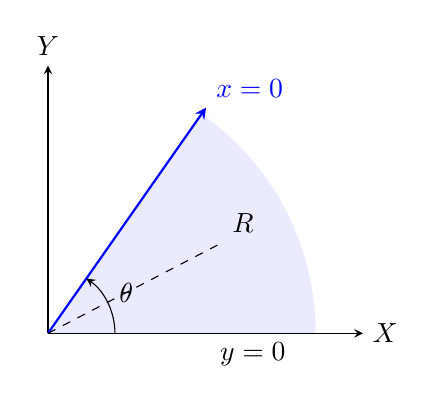
\begin{tikzpicture}[x=1cm,y=1cm,>=stealth]
\fill[blue!8] (0,0)--(3.4,0) arc (0:55:3.4)--cycle;
\draw[->] (0,0)--(4,0) node[right] {$X$};
\draw[->] (0,0)--(0,3.4) node[above] {$Y$};
\draw[thick,blue,->] (0,0)--(55:3.5) node[above right] {$x=0$};
\node[below] at (2.6,0) {$y=0$};
\draw[->] (0.85,0) arc (0:55:0.85);
\node at (27.5:1.12) {$\theta$};
\draw[dashed] (0,0)--(27.5:2.5) node[above right] {$R$};
\end{tikzpicture}
\end{center}
In polar coordinates $X=R\cos\phi$, $Y=R\sin\phi$,
\begin{align*}
I(\theta)&=\frac1{\sin\theta}
\int_0^\theta d\phi\int_0^\infty e^{-R^2}R\,dR\\
&=\frac\theta{\sin\theta}
\left[-\frac12e^{-R^2}\right]_0^\infty
=\boxed{\frac\theta{2\sin\theta}}.
\end{align*}
Both the original integral and this quotient are even in $\theta$,
so the result extends to $-\pi<\theta<0$.  At zero use
$u=x+y$, $v=x$, where $0\le v\le u$:
\[
I(0)=\int_0^\infty e^{-u^2}\int_0^u dv\,du
=\int_0^\infty ue^{-u^2}du=\frac12,
\]
the removable limit of the formula.

\erratum{The stated interval $-\pi<\theta<\pi$ is the range
for the unreduced formula $\theta/(2\sin\theta)$, including its
removable value at zero.  For unrestricted real $\theta$, the
integral is periodic and converges except at odd multiples of
$\pi$.}
Indeed, if $c=\cos\theta>-1$, the quadratic form on $x,y\ge0$
is at least $\min(1,1+c)(x^2+y^2)$, so a convergent Gaussian
dominates it.  If $c=-1$, the integrand is $e^{-(x-y)^2}$;
on $x\ge1$, $x\le y\le x+1$ it is at least $e^{-1}$, giving
infinite integral.  In general reduce to
$\vartheta=\arccos(\cos\theta)\in[0,\pi]$ and use
$\vartheta/(2\sin\vartheta)$, with the endpoint conventions just
established.


\Needspace{5\baselineskip}
\par\bigskip
\noindent\textbf{13.3.8}\quad Evaluate (using the beta function)
\begin{enumerate}
\item[(a)] $\displaystyle\int_{0}^{\pi/2}\cos^{1/2}\theta\,d\theta
  =\frac{(2\pi)^{3/2}}{16[\Gamma(5/4)]^{2}}$,
\item[(b)] $\displaystyle\int_{0}^{\pi/2}\cos^{n}\theta\,d\theta
  =\int_{0}^{\pi/2}\sin^{n}\theta\,d\theta
  =\frac{\sqrt{\pi}\,[(n-1)/2]!}{2(n/2)!}$\\[4pt]
  $\hfill=\begin{cases}
  \dfrac{(n-1)!!}{n!!} & \text{for }n\text{ odd},\\[8pt]
  \dfrac{\pi}{2}\cdot\dfrac{(n-1)!!}{n!!} & \text{for }n\text{ even}.
  \end{cases}$
\end{enumerate}
\par\smallskip
\erratum{The general integral requires $\Re n>-1$; its odd/even forms use nonnegative integer $n$ and $(-1)!!=0!!=1$.}
\solution
For $u=\sin^2\theta$, the limits become zero and one and
\[
du=2\sin\theta\cos\theta\,d\theta,\qquad
d\theta=\frac{du}{2\sqrt{u(1-u)}},\qquad
\cos^n\theta=(1-u)^{n/2}.
\]
Thus the common form is
\[
I_n=\int_0^{\pi/2}\cos^n\theta\,d\theta
=\frac12\int_0^1u^{-1/2}(1-u)^{(n-1)/2}du
=\frac{\sqrt\pi\,\Gamma((n+1)/2)}{2\Gamma((n+2)/2)}.
\]
\erratum{This integral formula requires $\Re n>-1$; the odd/even
factorial forms below use nonnegative integer $n$.}
Replacing $\theta$ by $\pi/2-\theta$ proves the same value for
$\int_0^{\pi/2}\sin^n\theta\,d\theta$.

\textbf{(a)} At $n=1/2$,
$I_{1/2}=\sqrt\pi\,\Gamma(3/4)/[2\Gamma(5/4)]$.
Reflection and recurrence give
\[
\Gamma(1/4)\Gamma(3/4)=\pi\sqrt2,
\qquad\Gamma(1/4)=4\Gamma(5/4).
\]
Thus
\[
\boxed{I_{1/2}=\frac{\pi\sqrt{2\pi}}{8[\Gamma(5/4)]^2}
=\frac{(2\pi)^{3/2}}{16[\Gamma(5/4)]^2}}.
\]
\textbf{(b)} The gamma expression is precisely
$\sqrt\pi\,[(n-1)/2]!/[2(n/2)!]$.  For $n=2m+1$,
\[
I_{2m+1}=\frac{\sqrt\pi\,m!}{2\Gamma(m+3/2)}
=\frac{2^mm!}{(2m+1)!!}
=\boxed{\frac{(2m)!!}{(2m+1)!!}}.
\]
For $n=2m$,
\[
I_{2m}=\frac{\sqrt\pi\,\Gamma(m+1/2)}{2m!}
=\frac\pi2\frac{(2m-1)!!}{2^mm!}
=\boxed{\frac\pi2\frac{(2m-1)!!}{(2m)!!}}.
\]
The case $m=0$ in the even formula gives $I_0=\pi/2$.


\Needspace{5\baselineskip}
\par\bigskip
\noindent\textbf{13.3.9}\quad Evaluate
$\displaystyle\int_{0}^{1}(1-x^{4})^{-1/2}\,dx$ as a beta function.
\par\nobreak\hfill\emph{ANS.}\enspace
$\dfrac{[\Gamma(5/4)]^{2}\cdot4}{(2\pi)^{1/2}}=1.311028777$.
\solution
Put $u=x^4$, so $dx=\tfrac14u^{-3/4}du$.  The endpoint
exponents $-3/4$ and $-1/2$ are both integrable, and
\[
I=\frac14\int_0^1u^{-3/4}(1-u)^{-1/2}du
=\boxed{\frac14B\left(\frac14,\frac12\right)}
=\frac{\Gamma(1/4)\sqrt\pi}{4\Gamma(3/4)}.
\]
Use $\Gamma(1/4)\Gamma(3/4)=\pi\sqrt2$ to remove
$\Gamma(3/4)$, then $\Gamma(1/4)=4\Gamma(5/4)$:
\[
I=\frac{[\Gamma(1/4)]^2}{4\sqrt{2\pi}}
=\boxed{\frac{4[\Gamma(5/4)]^2}{\sqrt{2\pi}}}
=1.311028777146\ldots.
\]
For an independent numerical quadrature one can also put
$x=\sin\phi$; cancellation of $\cos\phi$ gives the nonsingular
integral $\int_0^{\pi/2}(1+\sin^2\phi)^{-1/2}d\phi$.


\Needspace{5\baselineskip}
\par\bigskip
\noindent\textbf{13.3.10}\quad Using beta functions, show that the integral
representation
\[
J_{\nu}(z)=\frac{2}{\pi^{1/2}\Gamma(\nu+\frac{1}{2})}
\left(\frac{z}{2}\right)^{\nu}
\int_{0}^{\pi/2}\sin^{2\nu}\theta\cos(z\cos\theta)\,d\theta,
\quad\Re(\nu)>-\tfrac{1}{2},
\]
reduces to the Bessel series
\[
J_{\nu}(z)=\sum_{s=0}^{\infty}(-1)^{s}
\frac{1}{s!\,\Gamma(s+\nu+1)}\left(\frac{z}{2}\right)^{2s+\nu},
\]
thereby confirming its validity.
\solution
Expand the cosine, keeping the same branch of $(z/2)^\nu$
throughout:
\[
\cos(z\cos\theta)=\sum_{s=0}^{\infty}
\frac{(-1)^s z^{2s}\cos^{2s}\theta}{(2s)!}.
\]
For fixed $z$, the absolute sum is bounded by $e^{|z|}$.
The remaining weight has magnitude $\sin^{2\Re\nu}\theta$,
which is integrable at zero exactly when $\Re\nu>-1/2$.
Dominated convergence therefore permits integration term by term.
The beta integral for each term is
\[
\int_0^{\pi/2}\sin^{2\nu}\theta\cos^{2s}\theta\,d\theta
=\frac12B\left(\nu+\frac12,s+\frac12\right)
=\frac{\Gamma(\nu+1/2)\Gamma(s+1/2)}{2\Gamma(s+\nu+1)}.
\]
Insert this in the proposed representation and cancel its
$2$ and $\Gamma(\nu+1/2)$ factors:
\[
J_\nu(z)=\left(\frac z2\right)^\nu
\sum_{s=0}^{\infty}\frac{(-1)^sz^{2s}}{\sqrt\pi(2s)!}
\frac{\Gamma(s+1/2)}{\Gamma(s+\nu+1)}.
\]
Finally,
\[
\Gamma\left(s+\frac12\right)
=\frac{(2s)!\sqrt\pi}{4^ss!},
\qquad
\frac{\Gamma(s+1/2)}{\sqrt\pi(2s)!}=\frac1{4^ss!}.
\]
Thus
\[
\boxed{J_\nu(z)=\sum_{s=0}^{\infty}
\frac{(-1)^s}{s!\Gamma(s+\nu+1)}
\left(\frac z2\right)^{2s+\nu}},
\]
the defining Bessel series.  For noninteger $\nu$ both
representations use a chosen branch of $z^\nu$; a value at zero
is taken only when the corresponding limit exists.


\Needspace{5\baselineskip}
\par\bigskip
\noindent\textbf{13.3.11}\quad Given the associated Legendre function, defined
in Chapter 15,
\[
P_{m}^{m}(x)=(2m-1)!!\,(1-x^{2})^{m/2},
\]
show that
\begin{enumerate}
\item[(a)] $\displaystyle\int_{-1}^{1}[P_{m}^{m}(x)]^{2}\,dx
  =\frac{2}{2m+1}(2m)!$,\quad$m=0,1,2,\ldots$,
\item[(b)] $\displaystyle\int_{-1}^{1}[P_{m}^{m}(x)]^{2}\frac{dx}{1-x^{2}}
  =2\cdot(2m-1)!$,\quad$m=1,2,3,\ldots$.
\end{enumerate}
\solution
Square the stated expression:
$[P_m^m(x)]^2=[(2m-1)!!]^2(1-x^2)^m$.
\textbf{(a)} Exercise 13.3.3 gives
\begin{align*}
\int_{-1}^1[P_m^m(x)]^2dx
&=[(2m-1)!!]^2\frac{2(2m)!!}{(2m+1)!!}\\
&=\frac{2(2m-1)!!(2m)!!}{2m+1}
=\boxed{\frac{2(2m)!}{2m+1}}.
\end{align*}
We used $(2m+1)!!=(2m+1)(2m-1)!!$ and
$(2m-1)!!(2m)!!=(2m)!$.  The case $m=0$ gives two.

\textbf{(b)} Division by $1-x^2$ reduces the exponent to $m-1$.
For $m\ge1$ the same beta evaluation yields
\begin{align*}
\int_{-1}^1[P_m^m(x)]^2\frac{dx}{1-x^2}
&=[(2m-1)!!]^2\frac{2(2m-2)!!}{(2m-1)!!}\\
&=2(2m-1)!!(2m-2)!!
=\boxed{2(2m-1)!}.
\end{align*}
At $m=0$ the second integral diverges at both endpoints,
explaining its different lower limit on $m$.  An alternative
associated-Legendre convention introduces $(-1)^m$, which has
no effect on either squared integral.


\Needspace{5\baselineskip}
\par\bigskip
\noindent\textbf{13.3.12}\quad Show that, for integers $p$ and $q$,
\begin{enumerate}
\item[(a)] $\displaystyle\int_{0}^{1}x^{2p+1}(1-x^{2})^{-1/2}\,dx
  =\frac{(2p)!!}{(2p+1)!!}$,
\item[(b)] $\displaystyle\int_{0}^{1}x^{2p}(1-x^{2})^{q}\,dx
  =\frac{(2p-1)!!\,(2q)!!}{(2p+2q+1)!!}$.
\end{enumerate}
\par\smallskip
\erratum{Take $p\ge0$ in (a), and $p,q\ge0$ in (b).}
\solution
\erratum{For the stated integer parameters, require $p\ge0$
in (a), and $p,q\ge0$ in (b).  Negative integer values produce
nonintegrable endpoint powers.}
Use $u=x^2$, $dx=du/(2\sqrt u)$.
\textbf{(a)} Since $x^{2p+1}dx=u^pdu/2$,
\begin{align*}
\int_0^1x^{2p+1}(1-x^2)^{-1/2}dx
&=\frac12 B\left(p+1,\frac12\right)
=\frac{p!\sqrt\pi}{2\Gamma(p+3/2)}\\
&=\frac{p!\sqrt\pi\,2^{p+1}}{2(2p+1)!!\sqrt\pi}
=\boxed{\frac{(2p)!!}{(2p+1)!!}}.
\end{align*}
\textbf{(b)} Here $x^{2p}dx=u^{p-1/2}du/2$, so
\begin{align*}
\int_0^1x^{2p}(1-x^2)^qdx
&=\frac12 B\left(p+\frac12,q+1\right)
=\frac{\Gamma(p+1/2)q!}{2\Gamma(p+q+3/2)}\\
&=\frac{[(2p-1)!!\sqrt\pi/2^p]q!}
 {2[(2p+2q+1)!!\sqrt\pi/2^{p+q+1}]}\\
&=\boxed{\frac{(2p-1)!!(2q)!!}{(2p+2q+1)!!}}.
\end{align*}
These formulas include $p=0$ or $q=0$ with the usual empty
products $(-1)!!=0!!=1$.


\Needspace{5\baselineskip}
\par\bigskip
\noindent\textbf{13.3.13}\quad A particle of mass $m$ moving in a symmetric
potential that is well described by $V(x)=A|x|^{n}$ has a total energy
$\frac{1}{2}m(dx/dt)^{2}+V(x)=E$. Solving for $dx/dt$ and integrating we find
that the period of motion is
\[
\tau=2\sqrt{2m}\int_{0}^{x_{\max}}\frac{dx}{(E-Ax^{n})^{1/2}},
\]
where $x_{\max}$ is a classical turning point given by
$Ax_{\max}^{n}=E$. Show that
\[
\tau=\frac{2}{n}\sqrt{\frac{2\pi m}{E}}
\left(\frac{E}{A}\right)^{1/n}
\frac{\Gamma(1/n)}{\Gamma(1/n+\frac{1}{2})}.
\]
\par\smallskip
\erratum{Assume $m,A,E,n>0$.}
\solution
\erratum{For the bounded oscillation considered here, take
$m,A,E>0$ and $n>0$.}
The positive turning point is $x_{\max}=(E/A)^{1/n}$.
On the outward quarter-cycle, energy conservation gives
\[
\frac{dx}{dt}=\sqrt{\frac2m}\sqrt{E-Ax^n},
\qquad
\frac\tau4=\sqrt{\frac m2}\int_0^{x_{\max}}
\frac{dx}{\sqrt{E-Ax^n}},
\]
which explains the factor in the question.  Set
$u=Ax^n/E=(x/x_{\max})^n$.  Then
\[
x=x_{\max}u^{1/n},\quad
 dx=\frac{x_{\max}}n u^{1/n-1}du,\quad
(E-Ax^n)^{-1/2}=E^{-1/2}(1-u)^{-1/2}.
\]
Both endpoints become zero and one, respectively.  Consequently
\begin{align*}
\tau&=\frac2n\sqrt{\frac{2m}E}\left(\frac EA\right)^{1/n}
\int_0^1u^{1/n-1}(1-u)^{-1/2}du\\
&=\frac2n\sqrt{\frac{2m}E}\left(\frac EA\right)^{1/n}
B\left(\frac1n,\frac12\right)\\
&=\boxed{\frac2n\sqrt{\frac{2\pi m}E}\left(\frac EA\right)^{1/n}
\frac{\Gamma(1/n)}{\Gamma(1/n+1/2)}}.
\end{align*}
As a check, $n=2$ and $A=m\omega^2/2$ give
$\tau=\pi\sqrt{2m/A}=2\pi/\omega$, the harmonic-oscillator
period, independent of $E$.


\Needspace{5\baselineskip}
\par\bigskip
\noindent\textbf{13.3.14}\quad Referring to Exercise 13.3.13,
\begin{enumerate}
\item[(a)] Determine the limit as $n\to\infty$ of
  \[
  \frac{2}{n}\sqrt{\frac{2\pi m}{E}}\left(\frac{E}{A}\right)^{1/n}
  \frac{\Gamma(1/n)}{\Gamma(1/n+\frac{1}{2})}.
  \]
\item[(b)] Find $\lim_{n\to\infty}\tau$ from the behavior of the integrand
  $(E-Ax^{n})^{-1/2}$.
\item[(c)] Investigate the behavior of the physical system (potential well)
  as $n\to\infty$. Obtain the period from inspection of this limiting
  physical system.
\end{enumerate}
\par\smallskip
\erratum{For a dimensionful family, write $V_n(x)=A(|x|/L)^n$ with fixed $A,L>0$; the displayed formula uses length units $L=1$.}
\solution
\textbf{(a)} Use the recurrence before taking the limit:
\[
\frac{\Gamma(1/n)}{n\Gamma(1/n+1/2)}
=\frac{\Gamma(1+1/n)}{\Gamma(1/n+1/2)}
\longrightarrow\frac{\Gamma(1)}{\Gamma(1/2)}=\frac1{\sqrt\pi}.
\]
Also $(E/A)^{1/n}\to1$ for fixed positive numerical $E/A$.
Hence the period written in the question tends to
\[
\boxed{\tau_\infty=2\sqrt{\frac{2m}E}}.
\]
\erratum{When comparing dimensionful potentials at different
$n$, fix a length $L$ and write $V_n(x)=A(|x|/L)^n$ with fixed
energy scale $A$.  The question uses length units with $L=1$;
the dimensionful limiting period is $2L\sqrt{2m/E}$.}

\textbf{(b)} To justify passing to the limit despite the moving
turning point, set $x=x_{\max}u$:
\[
\tau_n=2\sqrt{\frac{2m}E}\,x_{\max}
\int_0^1(1-u^n)^{-1/2}du.
\]
For $0\le u<1$, this integrand tends to one.  For $n\ge1$,
$u^n\le u$, so
\[
0<(1-u^n)^{-1/2}\le(1-u)^{-1/2},
\qquad\int_0^1(1-u)^{-1/2}du=2.
\]
Dominated convergence gives an integral limit of one, and
$x_{\max}=L(E/A)^{1/n}\to L$.  This proves the same limit
without ignoring the endpoint singularity.

\textbf{(c)} For $|x|<L$, $V_n(x)\to0$; for $|x|>L$,
$V_n(x)\to\infty$.  The limiting motion is free flight between
reflecting walls at $\pm L$, with speed $v=\sqrt{2E/m}$.
A round trip covers distance $4L$, so
\[
\boxed{\tau_\infty=\frac{4L}{v}=2L\sqrt{\frac{2m}E}}.
\]
The isolated value $V_n(\pm L)=A$ does not affect the limiting
travel time derived in (b).


\Needspace{5\baselineskip}
\par\bigskip
\noindent\textbf{13.3.15}\quad Show that
\[
\int_{0}^{\infty}\frac{\sinh^{\alpha}x}{\cosh^{\beta}x}\,dx
=\frac{1}{2}B\left(\frac{\alpha+1}{2},\frac{\beta-\alpha}{2}\right),
\quad-1<\alpha<\beta.
\]
\emph{Hint.}~Let $\sinh^{2}x=u$.
\solution
The endpoint behavior explains the given restrictions: near zero
$\sinh^\alpha x/\cosh^\beta x\sim x^\alpha$, whereas at infinity
it is asymptotic to $2^{\beta-\alpha}e^{(\alpha-\beta)x}$.
Thus for real parameters convergence requires $\alpha>-1$ and
$\beta>\alpha$.

Set $u=\sinh^2x$.  Since $\cosh^2x=1+u$,
\[
du=2\sinh x\cosh x\,dx=2\sqrt{u(1+u)}\,dx.
\]
It follows that
\begin{align*}
\int_0^\infty\frac{\sinh^\alpha x}{\cosh^\beta x}dx
&=\frac12\int_0^\infty
u^{(\alpha-1)/2}(1+u)^{-(\beta+1)/2}du.
\end{align*}
To recognize the beta integral, put $v=u/(1+u)$,
$du=dv/(1-v)^2$.  In general this shows
\[
\int_0^\infty u^{p-1}(1+u)^{-p-q}du
=\int_0^1v^{p-1}(1-v)^{q-1}dv=B(p,q).
\]
Here $p=(\alpha+1)/2$, $q=(\beta-\alpha)/2$, both positive.
Therefore
\[
\boxed{\int_0^\infty\frac{\sinh^\alpha x}{\cosh^\beta x}dx
=\frac12 B\left(\frac{\alpha+1}2,\frac{\beta-\alpha}2\right)}.
\]
For complex parameters the corresponding absolute-convergence
conditions are $\Re\alpha>-1$ and $\Re(\beta-\alpha)>0$.


\Needspace{5\baselineskip}
\par\bigskip
\noindent\textbf{13.3.16}\quad The beta distribution of probability theory has
a probability density
\[
f(x)=\frac{\Gamma(\alpha+\beta)}{\Gamma(\alpha)\Gamma(\beta)}
x^{\alpha-1}(1-x)^{\beta-1},
\]
with $x$ restricted to the interval $(0,1)$. Show that
\begin{enumerate}
\item[(a)] $\langle x\rangle$, the mean value, is
  $\dfrac{\alpha}{\alpha+\beta}$.
\item[(b)] $\sigma^{2}$, its variance, is
  $\langle x^{2}\rangle-\langle x\rangle^{2}
  =\dfrac{\alpha\beta}{(\alpha+\beta)^{2}(\alpha+\beta+1)}$.
\end{enumerate}
\par\smallskip
\erratum{Assume real $\alpha,\beta>0$.}
\solution
\erratum{A beta probability density requires real
$\alpha,\beta>0$.}
Its prefactor is $1/B(\alpha,\beta)$.  Consequently
\[
\langle x^q\rangle
=\frac{B(\alpha+q,\beta)}{B(\alpha,\beta)}
=\frac{\Gamma(\alpha+q)\Gamma(\alpha+\beta)}
{\Gamma(\alpha)\Gamma(\alpha+\beta+q)},
\qquad\Re q>-\alpha.
\]
At $q=0$ this equals one and verifies normalization.
\textbf{(a)} For $q=1$, apply gamma recurrence to numerator and
denominator:
\[
\langle x\rangle
=\frac{[\alpha\Gamma(\alpha)]\Gamma(\alpha+\beta)}
{\Gamma(\alpha)[(\alpha+\beta)\Gamma(\alpha+\beta)]}
=\boxed{\frac\alpha{\alpha+\beta}}.
\]
\textbf{(b)} For $q=2$ the same cancellation gives
\[
\langle x^2\rangle
=\frac{\alpha(\alpha+1)\Gamma(\alpha)\Gamma(\alpha+\beta)}
{\Gamma(\alpha)(\alpha+\beta)(\alpha+\beta+1)\Gamma(\alpha+\beta)}
=\frac{\alpha(\alpha+1)}{(\alpha+\beta)(\alpha+\beta+1)}.
\]
Subtract the squared mean using a common denominator:
\begin{align*}
\sigma^2&=\frac{\alpha(\alpha+1)(\alpha+\beta)
-\alpha^2(\alpha+\beta+1)}{(\alpha+\beta)^2(\alpha+\beta+1)}\\
&=\frac{\alpha[(\alpha^2+\alpha\beta+\alpha+\beta)
-(\alpha^2+\alpha\beta+\alpha)]}
{(\alpha+\beta)^2(\alpha+\beta+1)}\\
&=\boxed{\frac{\alpha\beta}{(\alpha+\beta)^2(\alpha+\beta+1)}}.
\end{align*}


\Needspace{5\baselineskip}
\par\bigskip
\noindent\textbf{13.3.17}\quad From
\[
\lim_{n\to\infty}
\frac{\displaystyle\int_{0}^{\pi/2}\sin^{2n}\theta\,d\theta}
{\displaystyle\int_{0}^{\pi/2}\sin^{2n+1}\theta\,d\theta}=1,
\]
derive the Wallis formula for $\pi$:
\[
\frac{\pi}{2}=\frac{2\cdot2}{1\cdot3}\cdot\frac{4\cdot4}{3\cdot5}
\cdot\frac{6\cdot6}{5\cdot7}\cdots.
\]
\solution
Write $I_k=\int_0^{\pi/2}\sin^k\theta\,d\theta$.
Exercise 13.3.8 gives
\[
I_{2n}=\frac\pi2\frac{(2n-1)!!}{(2n)!!},
\qquad I_{2n+1}=\frac{(2n)!!}{(2n+1)!!}.
\]
Therefore
\[
\frac{I_{2n}}{I_{2n+1}}
=\frac\pi2\frac{(2n-1)!!(2n+1)!!}{[(2n)!!]^2}.
\]
Define the finite product
\[
P_n=\prod_{j=1}^n\frac{(2j)^2}{(2j-1)(2j+1)}
=\frac{[(2n)!!]^2}{(2n-1)!!(2n+1)!!}.
\]
The previous ratio is $(\pi/2)/P_n$.  Taking its stated limit
of one gives
\[
\boxed{\frac\pi2=\lim_{n\to\infty}P_n
=\frac{2\cdot2}{1\cdot3}\frac{4\cdot4}{3\cdot5}
\frac{6\cdot6}{5\cdot7}\cdots}.
\]
For completeness, the limit used here also follows without a
gamma asymptotic formula: since $0\le\sin\theta\le1$,
$I_{2n+1}\le I_{2n}\le I_{2n-1}$.  The already evaluated
odd integrals satisfy $I_{2n-1}/I_{2n+1}=(2n+1)/(2n)$, so
\[
1\le\frac{I_{2n}}{I_{2n+1}}\le1+\frac1{2n}\longrightarrow1.
\]
This proves convergence of the infinite product as well as its value.


\Needspace{9\baselineskip}
\subsection*{13.4 Stirling's Series}

\Needspace{5\baselineskip}
\par\bigskip
\noindent\textbf{13.4.1}\quad Rewrite Stirling's series to give $\Gamma(z+1)$
instead of $\ln\Gamma(z+1)$.
\par\nobreak\hfill\emph{ANS.}\enspace
$\Gamma(z+1)\erratum{\sim}\sqrt{2\pi}\,z^{z+1/2}e^{-z}
\left(1+\dfrac{1}{12z}+\dfrac{1}{288z^{2}}-\dfrac{139}{51{,}840z^{3}}
+\cdots\right)$.
\par\smallskip
\erratum{Interpret this as an asymptotic expansion as $|z|\to\infty$ in a fixed sector $|\arg z|\le\pi-\delta$, $\delta>0$, with consistent logarithm branches.}
\solution
Use Stirling's logarithmic expansion on the positive real axis,
or on a fixed closed sector $|\arg z|\le\pi-\delta$ with a
consistent logarithm branch:
\[
\log\Gamma(z+1)=\frac12\log(2\pi)+\left(z+\frac12\right)\log z-z
+\frac1{12z}-\frac1{360z^3}+O(z^{-5}).
\]
Let $u=1/(12z)-1/(360z^3)+O(z^{-5})$ and exponentiate.
Through order $z^{-3}$,
\begin{align*}
e^u&=1+u+\frac{u^2}{2}+\frac{u^3}{6}+O(z^{-4})\\
&=1+\frac1{12z}+\frac1{2\cdot12^2z^2}
+\left(-\frac1{360}+\frac1{6\cdot12^3}\right)z^{-3}
+O(z^{-4}).
\end{align*}
The cubic coefficient is
$-1/360+1/10368=(-144+5)/51840=-139/51840$.
Thus
\[
\boxed{\Gamma(z+1)\sim\sqrt{2\pi}\,z^{z+1/2}e^{-z}
\left(1+\frac1{12z}+\frac1{288z^2}
-\frac{139}{51840z^3}+\cdots\right)}.
\]
\erratum{This is an asymptotic expansion, not a convergent
infinite power series in $1/z$.}  A finite truncation and its
remainder order are meaningful; the ellipsis does not license
summing infinitely many terms at a fixed $z$.


\Needspace{5\baselineskip}
\par\bigskip
\noindent\textbf{13.4.2}\quad Use Stirling's formula to estimate $52!$, the
number of possible rearrangements of cards in a standard deck of playing
cards.
\solution
The leading Stirling estimate is
\[
52!\approx\sqrt{2\pi\cdot52}\left(\frac{52}{e}\right)^{52}.
\]
Compute its logarithm first:
\[
L_0=\frac12\ln(2\pi)+\frac{105}{2}\ln52-52
=156.3592337587296\ldots.
\]
Exponentiation gives
\[
\boxed{52!\approx e^{L_0}=8.05290203839\times10^{67}
\approx8.1\times10^{67}}.
\]
The first logarithmic correction gives
\[
e^{L_0+1/(12\cdot52)}=8.06581767642\times10^{67}.
\]
For comparison, direct integer multiplication $1\cdot2\cdots52$
gives $52!=8.065817517094\ldots\times10^{67}$.  The leading
estimate has relative error $-0.00160126096\ldots$, about
$-0.1601\%$; including $1/(12\cdot52)$ reduces the relative
error to $1.97534\times10^{-8}$.  The size and sign are consistent
with the next logarithmic term $-1/(360\cdot52^3)$.


\Needspace{5\baselineskip}
\par\bigskip
\noindent\textbf{13.4.3}\quad Show that the constants $C_{1}$ and $C_{2}$ in
Stirling's formula have the respective values zero and
$\frac{1}{2}\ln2\pi$ by using the logarithm of the Legendre duplication
formula \erratum{and that of the recurrence formula}.
\solution
Let $F(z)=\ln\Gamma(z+1)$ for large positive $z$.  Before the
constants are determined, the integrated expansion is
\[
F(z)=C_2+\left(z+\frac12\right)\ln z+(C_1-1)z+O(z^{-1}).
\]
The recurrence gives $F(z)-F(z-1)=\ln z$.  Substituting and
canceling $C_2$ and the common linear terms yields
\[
0=\left(z-\frac12\right)\ln\frac z{z-1}+C_1-1+O(z^{-1}).
\]
Since $\ln[z/(z-1)]=-\ln(1-1/z)=1/z+O(z^{-2})$,
the first term tends to one.  Therefore $\boxed{C_1=0}$.

Now use duplication in the form
\[
F(z)+F\left(z-\frac12\right)
=\frac12\ln\pi-2z\ln2+F(2z).
\]
The needed shifted expansion is
\begin{align*}
F\left(z-\frac12\right)
&=C_2+z\ln\left(z-\frac12\right)-z+\frac12+O(z^{-1})\\
&=C_2+z\ln z+z\left[-\frac1{2z}+O(z^{-2})\right]
-z+\frac12+O(z^{-1})\\
&=C_2+z\ln z-z+O(z^{-1}).
\end{align*}
Consequently the left side of duplication is
$2C_2+(2z+1/2)\ln z-2z+O(z^{-1})$, while its right side is
\[
C_2+\left(2z+\frac12\right)\ln z-2z
+\frac12\ln\pi+\frac12\ln2+O(z^{-1}).
\]
Canceling the common terms and taking the limit gives
\[
\boxed{C_2=\frac12\ln(2\pi)}.
\]
The corrected instruction supplies the recurrence needed to
fix $C_1$, in addition to the duplication formula used for $C_2$.


\Needspace{5\baselineskip}
\par\bigskip
\noindent\textbf{13.4.4}\quad Without using Stirling's series show that
\begin{enumerate}
\item[(a)] $\ln(n!)<\displaystyle\int_{1}^{n+1}\ln x\,dx$,\quad
(b) $\ln(n!)>\displaystyle\int_{1}^{n}\ln x\,dx$; $n$ is an integer $\ge2$.
\end{enumerate}
Note that the arithmetic mean of these two integrals gives a good
approximation for Stirling's series.
\solution
The logarithm is strictly increasing.
\textbf{(a)} On each interval $[j,j+1]$,
$\ln x>\ln j$ except at its left endpoint.  Integrating over a
unit interval and summing $j=1,\ldots,n$ gives
\[
\boxed{\ln(n!)=\sum_{j=1}^n\ln j
<\sum_{j=1}^n\int_j^{j+1}\ln x\,dx
=\int_1^{n+1}\ln x\,dx}.
\]
\textbf{(b)} On $[j-1,j]$ for $j=2,\ldots,n$,
$\ln x<\ln j$ except at the right endpoint.  Therefore
\[
\boxed{\int_1^n\ln x\,dx
=\sum_{j=2}^n\int_{j-1}^j\ln x\,dx
<\sum_{j=2}^n\ln j=\ln(n!)}.
\]
Evaluating the elementary antiderivative $x\ln x-x$ gives the
explicit two-sided bound
\[
n\ln n-n+1<\ln(n!)<(n+1)\ln(n+1)-n.
\]
The arithmetic mean of these bounds is
\[
\frac{n\ln n+(n+1)\ln(n+1)-2n+1}{2}
=\left(n+\frac12\right)\ln n-n+1+O(n^{-1}),
\]
which reproduces Stirling's growing terms without assuming that
formula.  It does not determine Stirling's exact constant term.


\Needspace{5\baselineskip}
\par\bigskip
\noindent\textbf{13.4.5}\quad Test for convergence
\[
\sum_{p=0}^{\infty}\left[\frac{\Gamma(p+\frac{1}{2})}{p!}\right]^{2}
\frac{2p+1}{2p+2}
=\pi\sum_{p=0}^{\infty}\frac{(2p-1)!!\,(2p+1)!!}{(2p)!!\,(2p+2)!!}.
\]
This series arises in an attempt to describe the magnetic field created by
and enclosed by a current loop.
\solution
Let
\[
a_p=\left[\frac{\Gamma(p+1/2)}{\Gamma(p+1)}\right]^2
\frac{2p+1}{2p+2}>0.
\]
Stirling's formula gives the gamma quotient
\[
\frac{\Gamma(p+1/2)}{\Gamma(p+1)}
=p^{-1/2}\left[1-\frac1{8p}+O(p^{-2})\right].
\]
This is also the $a=-1/2$, $b=0$ specialization of the detailed
quotient expansion in Exercise 13.4.6.  Since
$(2p+1)/(2p+2)\to1$, it follows that
\[
\lim_{p\to\infty}p\,a_p=1.
\]
By limit comparison with $\sum_{p=1}^\infty1/p$,
\[
\boxed{\sum_{p=0}^{\infty}a_p\text{ diverges to }+\infty}.
\]
The finite $p=0$ term is $\pi/2$ and does not alter convergence.
For the second form, use
$\Gamma(p+1/2)/p!=\sqrt\pi(2p-1)!!/(2p)!!$ and absorb
$(2p+1)/(2p+2)$ into the corresponding double factorials.
This proves that it is the same positive series.  A ratio tending
to one alone would not establish its divergence; the harmonic
comparison above does.


\Needspace{5\baselineskip}
\par\bigskip
\noindent\textbf{13.4.6}\quad Show that
$\displaystyle\lim_{x\to\infty}x^{b-a}\frac{\Gamma(x+a+1)}{\Gamma(x+b+1)}=1$.
\solution
Take fixed $a,b$ and $x\to+\infty$.  Complex $a,b$ are also
allowed with logarithms continued in the large right half-plane.
For either fixed parameter $c$, Stirling's formula gives
\[
\log\Gamma(x+c+1)
=\left(x+c+\frac12\right)\log(x+c)-(x+c)
+\frac12\log(2\pi)+\frac1{12(x+c)}+O(x^{-3}).
\]
Expand $\log(x+c)=\log x+c/x-c^2/(2x^2)+O(x^{-3})$.
Multiplication by $x+c+1/2$ and cancellation of the constant $c$
against $-(x+c)$ gives
\begin{align*}
\log\Gamma(x+c+1)
={}&\left(x+\frac12\right)\log x-x+\frac12\log(2\pi)
+c\log x\\
&+\frac{c(c+1)/2+1/12}{x}+O(x^{-2}).
\end{align*}
Subtract the $c=b$ expression from the $c=a$ expression and
add $(b-a)\log x$:
\[
\log\left[x^{b-a}\frac{\Gamma(x+a+1)}{\Gamma(x+b+1)}\right]
=\frac{(a-b)(a+b+1)}{2x}+O(x^{-2})\longrightarrow0.
\]
Exponentiating proves
\[
\boxed{\lim_{x\to\infty}x^{b-a}
\frac{\Gamma(x+a+1)}{\Gamma(x+b+1)}=1}.
\]
The calculation also gives the first relative correction
$(a-b)(a+b+1)/(2x)$, useful for checking the rate of approach.


\Needspace{5\baselineskip}
\par\bigskip
\noindent\textbf{13.4.7}\quad Show that
$\displaystyle\lim_{n\to\infty}\frac{(2n-1)!!}{(2n)!!}n^{1/2}=\pi^{-1/2}$.
\solution
Express the double factorials in gamma form:
\[
(2n-1)!!=\frac{2^n\Gamma(n+1/2)}{\sqrt\pi},
\qquad (2n)!!=2^n\Gamma(n+1).
\]
Their normalized ratio is consequently
\[
\frac{(2n-1)!!}{(2n)!!}\sqrt n
=\frac1{\sqrt\pi}\,
 n^{1/2}\frac{\Gamma(n+1/2)}{\Gamma(n+1)}.
\]
Exercise 13.4.6 with $a=-1/2$ and $b=0$ shows that the final
factor tends to one, so
\[
\boxed{\lim_{n\to\infty}\frac{(2n-1)!!}{(2n)!!}\sqrt n
=\pi^{-1/2}}.
\]
More precisely it equals
$\pi^{-1/2}[1-1/(8n)+O(n^{-2})]$, approaching the limit from
below for sufficiently large $n$.


\Needspace{5\baselineskip}
\par\bigskip
\noindent\textbf{13.4.8}\quad A set of $N$ distinguishable particles is
assigned to states $\psi_{i}$, $i=1,2,\ldots,M$. If the numbers of particles
in the various states are $n_{1},n_{2},\ldots,n_{M}$ (with $M\ll N$), the
number of ways this can be done is
\[
W=\frac{N!}{n_{1}!\,n_{2}!\cdots n_{M}!}.
\]
The entropy associated with this assignment is $S=k\ln W$, where $k$ is
Boltzmann's constant. In the limit $N\to\infty$, with $n_{i}=p_{i}N$ (so
$p_{i}$ is the fraction of the particles in state $i$), find $S$ as a
function of $N$ and the $p_{i}$.
\begin{enumerate}
\item[(a)] In the limit of large $N$, find the entropy associated with an
  arbitrary set of $n_{i}$. Is the entropy an extensive function of the
  system size (i.e., is it proportional to $N$)?
\item[(b)] Find the set of $p_{i}$ that maximize $S$.
\end{enumerate}
\emph{Hint.}~Remember that $\sum_{i}p_{i}=1$ and that this is a constrained
maximization (see Section 22.3).

\emph{Note.}~These formulas correspond to classical, or Boltzmann,
statistics.
\par\smallskip
\erratum{Take $M$ fixed and the fractions $p_i$ fixed as $N\to\infty$. Extensivity refers to the leading term; $M\ll N$ alone is insufficient if $M$ grows with $N$.}
\solution
Use $0!=1$ and $0\ln0=0$ for unoccupied states.
\textbf{(a)} With fixed $M$ and fixed fractions $p_i$,
$\sum_i n_i=N$ and $n_i=Np_i$.  The leading Stirling terms give
\begin{align*}
\frac Sk&=\ln N!-\sum_i\ln n_i!\\
&=N\ln N-N-\sum_i(n_i\ln n_i-n_i)+O(\ln N)\\
&=N\ln N-\sum_iNp_i(\ln N+\ln p_i)+O(\ln N)\\
&=-N\sum_i p_i\ln p_i+O(\ln N).
\end{align*}
Thus
\[
\boxed{S\sim-Nk\sum_{i=1}^M p_i\ln p_i}
\]
when the entropy per particle is nonzero; more generally the
additive estimate in the preceding line includes the zero-entropy
case.  This leading term is extensive.

If $q$ fractions are positive, retaining the half-logarithm terms
makes the finite-size correction explicit:
\[
\frac Sk=-N\sum_{p_i>0}p_i\ln p_i
-\frac{q-1}{2}\ln(2\pi N)-\frac12\sum_{p_i>0}\ln p_i
+O(N^{-1}).
\]
Here every occupied $n_i$ tends to infinity; zero fractions were
omitted before applying Stirling's formula.
\erratum{Extensivity is the leading large-$N$ statement for
fixed state fractions and a fixed number of states.  The exact
finite-$N$ entropy has smaller corrections.  The condition
$M\ll N$ alone does not ensure extensivity if $M$ also grows:
for example $M=\sqrt N$, $p_i=1/M$ gives a leading
$(k/2)N\ln N$.}

\textbf{(b)} Maximize $H=-\sum_i p_i\ln p_i$ subject to
$\sum_i p_i=1$.  In the interior of the probability simplex,
introduce $\mathcal L=H-\lambda(\sum_i p_i-1)$.  Then
\[
\frac{\partial\mathcal L}{\partial p_i}
=-\ln p_i-1-\lambda=0,
\qquad p_i=e^{-1-\lambda}.
\]
All probabilities are equal, and normalization gives
\[
\boxed{p_i=\frac1M\quad(i=1,\ldots,M)},\qquad
\boxed{S_{\max}=Nk\ln M+O(\ln N)}.
\]
The Hessian of $H$ is $-\operatorname{diag}(1/p_i)$, strictly
negative on every nonzero tangent displacement, so this is the
unique maximum.  A boundary with only $q<M$ occupied states has
maximum $\ln q<\ln M$ and cannot improve it.

For a finite integer assignment, if $n_i\ge n_j+2$, moving one
particle from $i$ to $j$ changes the multiplicity by
$W_{\rm new}/W_{\rm old}=n_i/(n_j+1)>1$.  Thus the exact
maximizing counts differ by at most one; they are exactly uniform
when $M$ divides $N$, and tend to the probabilities above otherwise.


\Needspace{9\baselineskip}
\subsection*{13.5 Riemann Zeta Function}

\Needspace{5\baselineskip}
\par\bigskip
\noindent\textbf{13.5.1}\quad Show that the symmetrical functional relation
\[
\Gamma\left(\frac{z}{2}\right)\pi^{-z/2}\zeta(z)
=\Gamma\left(\frac{1-z}{2}\right)\pi^{-(1-z)/2}\zeta(1-z)
\]
follows from the equation
\[
\left(e^{2\pi iz}-1\right)\zeta(z)
=\zeta(1-z)\frac{(2\pi)^{z}}{\Gamma(z)}
\left(e^{3\pi iz/2}-e^{\pi iz/2}\right).
\]
\solution
Initially avoid integer $z$ and poles of the gamma factors so
that the following divisions are valid.  Factor the exponentials:
\[
e^{2\pi iz}-1=2ie^{\pi iz}\sin\pi z,\qquad
e^{3\pi iz/2}-e^{\pi iz/2}=2ie^{\pi iz}\sin\frac{\pi z}{2}.
\]
Cancel $2ie^{\pi iz}$ in the supplied relation to obtain
\[
\sin\pi z\,\zeta(z)=
\frac{(2\pi)^z}{\Gamma(z)}\sin\frac{\pi z}{2}\,\zeta(1-z).
\]
Use reflection twice:
\[
\sin\pi z=\frac\pi{\Gamma(z)\Gamma(1-z)},\qquad
\sin\frac{\pi z}{2}=\frac\pi{\Gamma(z/2)\Gamma(1-z/2)}.
\]
After cancellation this gives
\[
\zeta(z)=\frac{(2\pi)^z\Gamma(1-z)}
{\Gamma(z/2)\Gamma(1-z/2)}\,\zeta(1-z).
\]
Duplication with $w=(1-z)/2$ reads
\[
\Gamma\left(\frac{1-z}{2}\right)\Gamma\left(1-\frac z2\right)
=2^z\sqrt\pi\,\Gamma(1-z).
\]
Substitute for $\Gamma(1-z)$ and cancel
$\Gamma(1-z/2)$ and $2^z$:
\[
\zeta(z)=\pi^{z-1/2}
\frac{\Gamma((1-z)/2)}{\Gamma(z/2)}\zeta(1-z).
\]
Multiplication by $\Gamma(z/2)\pi^{-z/2}$ yields
\[
\boxed{\Gamma\left(\frac z2\right)\pi^{-z/2}\zeta(z)
=\Gamma\left(\frac{1-z}{2}\right)\pi^{-(1-z)/2}\zeta(1-z)}.
\]
The two meromorphic functions therefore agree by continuation;
at exceptional points their limits, rather than the canceled
zero or pole factors separately, determine the identity.


\Needspace{5\baselineskip}
\par\bigskip
\noindent\textbf{13.5.2}\quad Prove that
\[
\int_{0}^{\infty}\frac{x^{n}e^{x}\,dx}{(e^{x}-1)^{2}}=n!\,\zeta(n).
\]
Assuming $n$ to be real, show that each side of the equation diverges if
$n=1$. Hence the preceding equation carries the condition $n>1$. Integrals
such as this appear in the quantum theory of transport effects: thermal and
electrical conductivity.
\solution
Since $d[(e^x-1)^{-1}]/dx=-e^x/(e^x-1)^2$, integration by
parts gives
\begin{align*}
I_n&=\int_0^\infty\frac{x^ne^x}{(e^x-1)^2}dx\\
&=\left[-\frac{x^n}{e^x-1}\right]_0^\infty
+n\int_0^\infty\frac{x^{n-1}}{e^x-1}dx.
\end{align*}
At infinity the boundary term vanishes exponentially.  At zero
$x^n/(e^x-1)\sim x^{n-1}$, so it vanishes for real $n>1$.
Expanding $(e^x-1)^{-1}=\sum_{k=1}^\infty e^{-kx}$ and
integrating the nonnegative terms then gives
\[
I_n=n\sum_{k=1}^{\infty}\int_0^\infty x^{n-1}e^{-kx}dx
=n\sum_{k=1}^{\infty}\frac{\Gamma(n)}{k^n}
=\boxed{\Gamma(n+1)\zeta(n)=n!\zeta(n)}.
\]
For a noninteger $n$, the notation $n!$ means $\Gamma(n+1)$.
The original integrand behaves as $x^{n-2}$ near zero.  Thus
$n=1$ gives a logarithmically divergent integral, matching the
pole of $\zeta(1)$; the real integral converges exactly for
$n>1$.  For complex $n$ the same argument, with absolute
convergence, holds for $\Re n>1$.


\Needspace{5\baselineskip}
\par\bigskip
\noindent\textbf{13.5.3}\quad The Bloch-Gr\"uneisen approximation for the
resistance in a monovalent metal at absolute temperature $T$ is
\[
\rho=C\frac{T^{5}}{\Theta^{6}}
\int_{0}^{\Theta/T}\frac{x^{5}\,dx}{(e^{x}-1)(1-e^{-x})},
\]
where $\Theta$ is the Debye temperature characteristic of the metal.
\begin{enumerate}
\item[(a)] For $T\to\infty$, show that
  \[
  \rho\approx\frac{C}{4}\cdot\frac{T}{\Theta^{2}}.
  \]
\item[(b)] For $T\to0$, show that
  \[
  \rho\approx5!\,\zeta(5)\,C\frac{T^{5}}{\Theta^{6}}.
  \]
\end{enumerate}
\solution
Take $T,\Theta>0$ and set $y=\Theta/T$.  First rewrite
\[
\frac1{(e^x-1)(1-e^{-x})}=\frac{e^x}{(e^x-1)^2}.
\]
\textbf{(a)} For high temperature, $y\to0$.  Differentiating
the local expansion
$(e^x-1)^{-1}=x^{-1}-1/2+x/12-x^3/720+\cdots$ gives
\[
\frac{e^x}{(e^x-1)^2}=\frac1{x^2}-\frac1{12}+O(x^2).
\]
Multiply by $x^5$ and integrate:
\[
\int_0^y\frac{x^5e^x}{(e^x-1)^2}dx
=\frac{y^4}{4}-\frac{y^6}{72}+O(y^8).
\]
Hence
\begin{align*}
\rho&=C\frac{T^5}{\Theta^6}
\left[\frac14\left(\frac\Theta T\right)^4
-\frac1{72}\left(\frac\Theta T\right)^6
+O\left(\frac{\Theta^8}{T^8}\right)\right]\\
&=\boxed{\frac C4\frac T{\Theta^2}}
\left[1-\frac1{18}\left(\frac\Theta T\right)^2
+O\left(\frac{\Theta^4}{T^4}\right)\right].
\end{align*}
\textbf{(b)} For low temperature, $y\to\infty$.  The positive
integral tends to the complete one from Exercise 13.5.2 at $n=5$:
\[
\int_0^\infty\frac{x^5e^x}{(e^x-1)^2}dx=5!\zeta(5).
\]
Thus
\[
\boxed{\rho\sim5!\zeta(5)C\frac{T^5}{\Theta^6}}.
\]
The omitted tail is exponentially small.  Explicitly, for $x\ge y>0$,
$e^x/(e^x-1)^2\le e^{-x}/(1-e^{-y})^2$, so its integral is at
most
\[
\frac{e^{-y}}{(1-e^{-y})^2}
\left(y^5+5y^4+20y^3+60y^2+120y+120\right).
\]
The polynomial follows by five integrations by parts of
$\int_y^\infty x^5e^{-x}dx$ and proves the limiting replacement.


\Needspace{5\baselineskip}
\par\bigskip
\noindent\textbf{13.5.4}\quad Derive the following expansion of the Debye
function for $n\ge1$:
\[
\int_{0}^{x}\frac{t^{n}\,dt}{e^{t}-1}
=x^{n}\left[\frac{1}{n}-\frac{x}{2(n+1)}
+\sum_{k=1}^{\infty}\frac{B_{2k}x^{2k}}{(2k+n)(2k)!}\right],
\quad|x|<2\pi.
\]
The complete integral $(0,\infty)$ equals $n!\,\zeta(n+1)$
(Exercise 13.5.6).
\par\smallskip
\erratum{For complex $x$, take integer $n\ge1$. For real $n\ge1$, the real-power version uses $0<x<2\pi$; complex continuation needs a specified power branch.}
\solution
The Bernoulli generating function is analytic for $|t|<2\pi$:
\[
\frac{t}{e^t-1}=1-\frac t2+
\sum_{k=1}^{\infty}\frac{B_{2k}}{(2k)!}t^{2k}.
\]
Its nearest nonremovable poles are at $t=\pm2\pi i$.
Multiply by $t^{n-1}$ and integrate from zero to $x$.
For integer $n\ge1$ uniform convergence on every smaller disk
justifies termwise integration, giving
\begin{align*}
\int_0^x\frac{t^n}{e^t-1}dt
&=\frac{x^n}{n}-\frac{x^{n+1}}{2(n+1)}
+\sum_{k=1}^{\infty}
\frac{B_{2k}x^{n+2k}}{(n+2k)(2k)!}\\
&=\boxed{x^n\left[\frac1n-\frac{x}{2(n+1)}+
\sum_{k=1}^{\infty}\frac{B_{2k}x^{2k}}{(2k+n)(2k)!}\right]}.
\end{align*}
Every denominator $n+2k$ comes from integrating a monomial;
the lower-limit terms vanish.  The same calculation is valid
for real $n>0$ and $0<x<2\pi$, with the integrable factor
$t^{n-1}$; for complex $x$ and noninteger $n$ a consistent power
branch is needed.  The full integral to infinity is instead
$\Gamma(n+1)\zeta(n+1)$, as derived in Exercise 13.5.6.


\Needspace{5\baselineskip}
\par\bigskip
\noindent\textbf{13.5.5}\quad The \erratum{equilibrium radiation energy per unit volume} of a blackbody is
given by
\[
u=\frac{8\pi k^{4}T^{4}}{c^{3}h^{3}}
\int_{0}^{\infty}\frac{x^{3}}{e^{x}-1}\,dx.
\]
Show that the integral in this expression is equal to $3!\,\zeta(4)$. The
final result is the Stefan-Boltzmann law.
\solution
For $x>0$ the geometric series gives
$(e^x-1)^{-1}=\sum_{m=1}^{\infty}e^{-mx}$.
The terms are nonnegative, so integrate them by monotone
convergence.  In each integral put $t=mx$:
\begin{align*}
\int_0^\infty\frac{x^3}{e^x-1}dx
&=\sum_{m=1}^{\infty}\int_0^\infty x^3e^{-mx}dx\\
&=\sum_{m=1}^{\infty}\frac1{m^4}\int_0^\infty t^3e^{-t}dt
=\boxed{3!\zeta(4)}=\frac{\pi^4}{15}.
\end{align*}
Here $\Gamma(4)=3!=6$ and $\zeta(4)=\pi^4/90$.
Substitution gives
\[
\boxed{u=\frac{8\pi^5 k^4}{15c^3h^3}T^4}.
\]
\erratum{The supplied formula describes radiation energy per
unit volume, not total radiated energy or power per unit area.}
For isotropic equilibrium radiation, the outgoing flux through
a surface is
\[
j^\star=\frac{cu}{4\pi}
\int_0^{2\pi}d\phi\int_0^{\pi/2}\cos\theta\sin\theta\,d\theta
=\frac{cu}{4}.
\]
Thus the Stefan--Boltzmann flux law is
\[
\boxed{j^\star=\sigma T^4,\qquad
\sigma=\frac{2\pi^5k^4}{15c^2h^3}}.
\]
This also distinguishes the two quantities' different powers of $c$.


\Needspace{5\baselineskip}
\par\bigskip
\noindent\textbf{13.5.6}\quad As a generalization of the result in Exercise
13.5.5, show that
\[
\int_{0}^{\infty}\frac{x^{s}\,dx}{e^{x}-1}=s!\,\zeta(s+1),
\quad\Re(s)>0.
\]
\solution
Let $\sigma=\Re s>0$ and use $x^s=e^{s\ln x}$ for $x>0$.
Near zero the integrand is $O(x^{\sigma-1})$ in absolute
value, and at infinity it has exponential decay.  Moreover,
\[
\sum_{n=1}^{\infty}\int_0^\infty|x^se^{-nx}|dx
=\Gamma(\sigma+1)\sum_{n=1}^{\infty}n^{-\sigma-1}<\infty.
\]
Thus the geometric expansion may be integrated term by term:
\begin{align*}
\int_0^\infty\frac{x^s}{e^x-1}dx
&=\sum_{n=1}^{\infty}\int_0^\infty x^se^{-nx}dx\\
&=\sum_{n=1}^{\infty}n^{-s-1}
\int_0^\infty t^se^{-t}dt\\
&=\boxed{\Gamma(s+1)\zeta(s+1)=s!\zeta(s+1)}.
\end{align*}
The substitution in the second line is $t=nx$, including its
Jacobian $dx=dt/n$.  The condition $\Re s>0$ is exactly what
makes both the endpoint and the absolutely summed integrals
converge.


\Needspace{5\baselineskip}
\par\bigskip
\noindent\textbf{13.5.7}\quad Prove that
\[
\int_{0}^{\infty}\frac{x^{s}\,dx}{e^{x}+1}
=s!\,(1-2^{-s})\,\zeta(s+1),\quad\Re(s)>0.
\]
Exercises 13.5.6 and 13.5.7 give the Mellin integral transform of
$1/(e^{x}\pm1)$; this transform is defined in Eq.~(20.9).
\solution
The algebraic identity
\[
\frac1{e^x+1}=\frac1{e^x-1}-\frac2{e^{2x}-1}
\]
follows by taking a common denominator.  For $\Re s>0$ both
integrals on the right converge separately, and Exercise 13.5.6
gives
\begin{align*}
\int_0^\infty\frac{x^s}{e^x+1}dx
&=\Gamma(s+1)\zeta(s+1)
-2\int_0^\infty\frac{x^s}{e^{2x}-1}dx\\
&=\Gamma(s+1)\zeta(s+1)
-2\cdot2^{-s-1}\int_0^\infty\frac{t^s}{e^t-1}dt\\
&=\boxed{\Gamma(s+1)(1-2^{-s})\zeta(s+1)}.
\end{align*}
In the second integral $t=2x$, so the power and Jacobian give
$2^{-s-1}$.

The original Fermi integral actually converges for $\Re s>-1$,
because its denominator tends to two at zero.  Analytic
continuation therefore extends the answer to that half-plane,
with a removable product at $s=0$:
\[
(1-2^{-s})\zeta(s+1)\longrightarrow\ln2,
\qquad
\int_0^\infty\frac{dx}{e^x+1}
=\bigl[-\ln(1+e^{-x})\bigr]_0^\infty=\ln2.
\]
The extension does not permit separating the two divergent
Bose integrals when $-1<\Re s\le0$.


\Needspace{5\baselineskip}
\par\bigskip
\noindent\textbf{13.5.8}\quad The neutrino energy density (Fermi
distribution) in the early history of the universe is given by
\[
\rho_{\nu}=\frac{4\pi}{h^{3}}
\int_{0}^{\infty}\frac{x^{3}}{\exp(x/kT)+1}\,dx.
\]
Show that
\[
\rho_{\nu}=\frac{7\pi^{5}}{30h^{3}}(kT)^{4}.
\]
\par\smallskip
\erratum{Use $kT>0$ and the convention $c=1$. With $x$ an energy in conventional units, insert $c^{-3}$ in both formulas.}
\solution
For positive $kT$, put $t=x/(kT)$, so
$x^3dx=(kT)^4t^3dt$.  Then
\[
\rho_\nu=\frac{4\pi(kT)^4}{h^3}
\int_0^\infty\frac{t^3}{e^t+1}dt.
\]
At $s=3$ the preceding exercise gives
\[
\int_0^\infty\frac{t^3}{e^t+1}dt
=3!(1-2^{-3})\zeta(4)
=6\cdot\frac78\cdot\frac{\pi^4}{90}
=\frac{7\pi^4}{120}.
\]
Multiplying by the prefactor yields
\[
\boxed{\rho_\nu=\frac{7\pi^5}{30h^3}(kT)^4}.
\]
\erratum{As an energy density with $x$ an energy, the supplied
formula uses $c=1$.  Restoring conventional length/time units
requires a factor $c^{-3}$ on both the stated integral and its
answer.}  Indeed a massless momentum satisfies $x=pc$, so the
radial phase-space factor $p^2dp$ becomes $x^2dx/c^3$; one
additional factor $x$ supplies the energy.


\Needspace{5\baselineskip}
\par\bigskip
\noindent\textbf{13.5.9}\quad Prove that
\[
\psi^{(n)}(z)=(-1)^{n+1}\int_{0}^{\infty}\frac{t^{n}e^{-zt}}{1-e^{-t}}\,dt,
\quad\Re(z)>0.
\]
\par\smallskip
\erratum{The derivative order is an integer $n\ge1$.}
\solution
\erratum{Require an integer $n\ge1$ as well as $\Re z>0$.
For $n=0$ the written integral diverges as $\int_0 dt/t$ and
cannot equal the finite digamma function.}
For $t>0$, expand $(1-e^{-t})^{-1}=\sum_{p=0}^{\infty}e^{-pt}$.
Absolute convergence justifies termwise integration, because
\[
\sum_{p=0}^{\infty}\int_0^\infty t^ne^{-(\Re z+p)t}dt
=n!\sum_{p=0}^{\infty}(\Re z+p)^{-n-1}<\infty.
\]
Therefore
\begin{align*}
(-1)^{n+1}\int_0^\infty\frac{t^ne^{-zt}}{1-e^{-t}}dt
&=(-1)^{n+1}\sum_{p=0}^{\infty}
\int_0^\infty t^ne^{-(z+p)t}dt\\
&=(-1)^{n+1}n!\sum_{p=0}^{\infty}\frac1{(z+p)^{n+1}}\\
&=\boxed{\psi^{(n)}(z)}.
\end{align*}
The second equality is the scaled gamma integral; the last is
the differentiated digamma series.  The near-zero behavior
$t^{n-1}$ also directly verifies the required condition on $n$.


\Needspace{5\baselineskip}
\par\bigskip
\noindent\textbf{13.5.10}\quad Show that $\zeta(s)$ is analytic in the entire
finite complex plane except at $s=1$, where it has a simple pole with a
residue of $+1$.

\emph{Hint.}~The contour integral representation will be useful.
\solution
Use the positive-real-axis cut and continuous argument
$0<\arg t<2\pi$ from Exercise 13.1.23.  Let $C_\varepsilon$
run inward along the upper lip, counterclockwise around the
circle $|t|=\varepsilon$, then outward along the lower lip,
where $0<\varepsilon<2\pi$.  Define
\[
H(s)=\int_{C_\varepsilon}\frac{t^{s-1}}{e^t-1}dt.
\]
Keeping the circle radius fixed makes $H$ entire in $s$:
the compact circle contains no pole on its path, and the two
ray tails decay exponentially and uniformly for $s$ in a
compact set.  The poles $t=\pm2\pi i,\pm4\pi i,\ldots$ lie
outside the small circle.

For $\Re s>1$ the circle can shrink to zero: its contribution
is $O(\varepsilon^{\Re s-1})$.  The upper ray contributes
$-\Gamma(s)\zeta(s)$ and the lower ray contributes
$e^{2\pi i(s-1)}\Gamma(s)\zeta(s)$.  Thus
\[
H(s)=(e^{2\pi is}-1)\Gamma(s)\zeta(s).
\]
Use $e^{2\pi is}-1=2ie^{\pi is}\sin\pi s$ and gamma
reflection to rewrite this as
\[
\boxed{\zeta(s)=\frac{e^{-\pi is}\Gamma(1-s)}{2\pi i}\,H(s)}.
\]
The right side is meromorphic on the whole finite plane and
agrees with the original zeta function on a nonempty open set.
It therefore supplies its meromorphic continuation.  Since
$H$ is entire, its only possible poles are the poles of
$\Gamma(1-s)$, namely $s=1,2,3,\ldots$.

At an integer $m\ge2$, the two ray contributions cancel.
On the small circle the integrand is single-valued and analytic
at zero, because
\[
\frac{t^{m-1}}{e^t-1}
=t^{m-2}\left(1-\frac t2+O(t^2)\right).
\]
Hence its circle integral is zero and $H(m)=0$.  This zero
cancels the possible simple pole of $\Gamma(1-s)$, proving
regularity at every $m\ge2$.

At $s=1$ the circle integrand is $(e^t-1)^{-1}=t^{-1}-1/2+O(t)$,
so the counterclockwise contour gives $H(1)=2\pi i$.
Writing $s=1+\eta$,
\[
\Gamma(1-s)=\Gamma(-\eta)=-\frac1\eta+O(1),
\qquad e^{-\pi is}=-1+O(\eta).
\]
Substitution yields
\[
\boxed{\zeta(s)=\frac1{s-1}+O(1)},
\]
so the pole is simple and its residue is $+1$.  At nonpositive
integers $\Gamma(1-s)$ is regular, giving no additional poles.
For example $H(0)=-\pi i$ from the coefficient $-1/(2t)$,
which gives the finite value $\zeta(0)=-1/2$.

\erratum{The alternating-series quotient alone does not prove
regularity throughout $\Re s>0$: its denominator
$1-2^{1-s}$ vanishes also at $s=1+2\pi i k/\ln2$ for nonzero
integers $k$.  Cancellation at those points must be justified.}
The entire-contour argument above establishes that all such
points are regular and leaves only the pole at one.


\Needspace{9\baselineskip}
\subsection*{13.6 Other Related Functions}

\Needspace{5\baselineskip}
\par\bigskip
\noindent\textbf{13.6.1}\quad Show that
$\gamma(a,x)=e^{-x}\displaystyle\sum_{n=0}^{\infty}
\frac{(a-1)!}{(a+n)!}x^{a+n}$
\begin{enumerate}
\item[(a)] by repeatedly integrating by parts,
\item[(b)] by transforming it into Eq.~(13.76).
\end{enumerate}
\par\smallskip
\erratum{Take $x>0$ and $\Re a>0$ for the defining lower-gamma integral; factorials mean gamma functions.}
\solution
\erratum{For the defining lower incomplete-gamma integral, take
$x>0$ and $\Re a>0$; factorials here mean gamma functions and
do not require integral $a$.}
\textbf{(a)} Integrate $e^{-t}t^{a-1}$ by parts, integrating
the power and differentiating the exponential:
\[
\gamma(a,x)=\left[\frac{t^a e^{-t}}a\right]_0^x
+\frac1a\int_0^x t^ae^{-t}dt
=\frac{x^ae^{-x}}a+\frac{\gamma(a+1,x)}a.
\]
Repeat this step $N$ times.  With $(a)_N=a(a+1)\cdots(a+N-1)$,
\[
\gamma(a,x)=e^{-x}\sum_{n=0}^{N-1}\frac{x^{a+n}}{(a)_{n+1}}
+\frac{\gamma(a+N,x)}{(a)_N}.
\]
Let $\sigma=\Re a>0$.  Since $|(a)_N|\ge(\sigma)_N$,
the final remainder has the bound
\[
\left|\frac{\gamma(a+N,x)}{(a)_N}\right|
\le\frac{x^{\sigma+N}}{(\sigma+N)(\sigma)_N}
=\frac{\Gamma(\sigma)x^{\sigma+N}}{\Gamma(\sigma+N+1)}
\longrightarrow0.
\]
The ratio of successive bounds is $x/(\sigma+N+1)\to0$.
Therefore
\[
\boxed{\gamma(a,x)=e^{-x}\sum_{n=0}^{\infty}
\frac{\Gamma(a)}{\Gamma(a+n+1)}x^{a+n}}.
\]

\textbf{(b)} To transform this into Eq.~(13.76), use
\[
\frac{\Gamma(a)}{\Gamma(a+n+1)}
=\frac1{n!}\int_0^1u^{a-1}(1-u)^n du.
\]
The exponential series converges uniformly on $0\le u\le1$,
and $u^{\Re a-1}$ is integrable.  Thus
\begin{align*}
e^{-x}\sum_{n=0}^{\infty}\frac{\Gamma(a)x^{a+n}}{\Gamma(a+n+1)}
&=x^a\int_0^1u^{a-1}e^{-x}
\sum_{n=0}^{\infty}\frac{[x(1-u)]^n}{n!}du\\
&=x^a\int_0^1u^{a-1}e^{-xu}du\\
&=x^a\sum_{m=0}^{\infty}\frac{(-x)^m}{m!}
\int_0^1u^{a+m-1}du\\
&=\boxed{x^a\sum_{m=0}^{\infty}\frac{(-1)^m x^m}{m!(a+m)}}.
\end{align*}
This is exactly the lower incomplete-gamma series in Eq.~(13.76).
Both series converge for every finite positive $x$ in the stated
parameter domain, although they need not be equally convenient numerically.


\Needspace{5\baselineskip}
\par\bigskip
\noindent\textbf{13.6.2}\quad Show that
\begin{enumerate}
\item[(a)] $\dfrac{d^{m}}{dx^{m}}\left[x^{-a}\gamma(a,x)\right]
  =(-1)^{m}x^{-a-m}\gamma(a+m,x)$,
\item[(b)] $\dfrac{d^{m}}{dx^{m}}\left[e^{x}\gamma(a,x)\right]
  =e^{x}\dfrac{\Gamma(a)}{\Gamma(a-m)}\gamma(a-m,x)$.
\end{enumerate}
\par\smallskip
\erratum{Take $x>0$ and integer $m\ge0$. The direct integral proofs use $\Re a>0$ in (a) and $\Re a>m$ in (b); beyond these domains continue the whole products meromorphically.}
\solution
Let $m$ be a nonnegative integer and $x>0$.
\textbf{(a)} For $\Re a>0$, put $t=xu$ in the defining integral:
\[
x^{-a}\gamma(a,x)=\int_0^1u^{a-1}e^{-xu}du.
\]
Differentiation under this finite integral is justified by the
integrable weight $u^{\Re a-1}$.  Each derivative supplies $-u$,
so
\begin{align*}
\frac{d^m}{dx^m}[x^{-a}\gamma(a,x)]
&=(-1)^m\int_0^1u^{a+m-1}e^{-xu}du\\
&=\boxed{(-1)^mx^{-a-m}\gamma(a+m,x)}.
\end{align*}

\textbf{(b)} Initially take $\Re a>m$ so every lower gamma
integral appearing below is defined.  The first product derivative is
\[
\frac d{dx}[e^x\gamma(a,x)]
=e^x\gamma(a,x)+x^{a-1}.
\]
\erratum{The manual's intermediate derivative includes an
extra $e^{-x}$ in the second term; it cancels against $e^x$.}
The lower recurrence gives
$\gamma(a,x)=(a-1)\gamma(a-1,x)-x^{a-1}e^{-x}$.
Substitution cancels the power term:
\[
\frac d{dx}[e^x\gamma(a,x)]=(a-1)e^x\gamma(a-1,x).
\]
Apply the same formula with $a$ replaced successively by
$a-1,\ldots,a-m+1$:
\[
\boxed{\frac{d^m}{dx^m}[e^x\gamma(a,x)]
=e^x(a-1)(a-2)\cdots(a-m)\gamma(a-m,x)
=e^x\frac{\Gamma(a)}{\Gamma(a-m)}\gamma(a-m,x)}.
\]
\erratum{Outside the initial integral domain, the entire product
on the right must be interpreted by meromorphic continuation.
A zero coefficient cannot be multiplied literally by a pole of
$\gamma(a-m,x)$.}  For example, when $a=m=1$ the left side is
$d(e^x-1)/dx=e^x$, not zero.  The continued product has precisely
this finite value.  At $m=0$ both identities reduce to themselves.


\Needspace{5\baselineskip}
\par\bigskip
\noindent\textbf{13.6.3}\quad Show that $\gamma(a,x)$ and $\Gamma(a,x)$
satisfy the recurrence relations
\begin{enumerate}
\item[(a)] $\gamma(a+1,x)=a\,\gamma(a,x)-x^{a}e^{-x}$,
\item[(b)] $\Gamma(a+1,x)=a\,\Gamma(a,x)+x^{a}e^{-x}$.
\end{enumerate}
\par\smallskip
\erratum{Take $x>0$. The lower-integral proof starts at $\Re a>0$ and then continues meromorphically; the upper-integral identity holds for every complex $a$.}
\solution
\textbf{(a)} For $x>0$, $\Re a>0$, integrate
$\gamma(a+1,x)=\int_0^x t^ae^{-t}dt$ by parts with
$u=t^a$, $dv=e^{-t}dt$:
\begin{align*}
\gamma(a+1,x)
&=\bigl[-t^ae^{-t}\bigr]_0^x
+a\int_0^x t^{a-1}e^{-t}dt\\
&=\boxed{a\gamma(a,x)-x^ae^{-x}}.
\end{align*}
The lower boundary term vanishes because $\Re a>0$.

\textbf{(b)} The same integration by parts over $[x,\infty)$
gives
\begin{align*}
\Gamma(a+1,x)
&=\bigl[-t^ae^{-t}\bigr]_x^\infty
+a\int_x^\infty t^{a-1}e^{-t}dt\\
&=\boxed{a\Gamma(a,x)+x^ae^{-x}}.
\end{align*}
For fixed $x>0$ this upper-integral proof works for every
complex $a$, because zero is outside the interval and the
exponential controls infinity.  Adding the two relations cancels
the endpoint terms and recovers $\Gamma(a+1)=a\Gamma(a)$.
The lower relation also continues meromorphically in $a$.


\Needspace{5\baselineskip}
\par\bigskip
\noindent\textbf{13.6.4}\quad Show that the asymptotic expansion (for large
$x$) of the incomplete gamma function $\Gamma(a,x)$ has the form
\[
\Gamma(a,x)\sim x^{a-1}e^{-x}\sum_{n=0}^{\infty}
\frac{\Gamma(a)}{\Gamma(a-n)}\cdot\frac{1}{x^{n}},
\]
and that the above expression is equivalent to
\[
\Gamma(a,x)\sim x^{a-1}e^{-x}\sum_{n=0}^{\infty}
(a-n)_{n}\frac{1}{x^{n}}.
\]
\par\smallskip
\erratum{Take fixed $a$ and $x\to+\infty$. Interpret $\Gamma(a)/\Gamma(a-n)$ as the polynomial $(a-1)\cdots(a-n)$ at gamma poles.}
\solution
For fixed $a$ and $x\to+\infty$, integrate the upper gamma
integral by parts in the direction of decreasing parameter:
\[
\Gamma(a,x)=x^{a-1}e^{-x}+(a-1)\Gamma(a-1,x).
\]
After $N$ steps this is the exact identity
\[
\Gamma(a,x)=x^{a-1}e^{-x}\sum_{n=0}^{N-1}\frac{c_n(a)}{x^n}
+c_N(a)\Gamma(a-N,x),
\qquad c_n(a)=\prod_{j=1}^n(a-j),\quad c_0=1.
\]
The remainder has the required order.  Indeed, putting $t=x+u$
gives
\[
\Gamma(a-N,x)=e^{-x}x^{a-N-1}
\int_0^\infty e^{-u}(1+u/x)^{a-N-1}du.
\]
For $x\ge1$ its integral is bounded in absolute value by
$\int_0^\infty e^{-u}(1+u)^{\max(\Re a-N-1,0)}du<\infty$.
Thus the remainder is $O(e^{-x}x^{\Re a-N-1})$, establishing
an asymptotic expansion rather than an unjustified integration
of an infinite binomial series:
\[
\boxed{\Gamma(a,x)\sim x^{a-1}e^{-x}
\sum_{n=0}^{\infty}\frac{c_n(a)}{x^n}}.
\]
Gamma recurrence and reversal of the finite product give
\[
c_n(a)=\frac{\Gamma(a)}{\Gamma(a-n)}
=(a-n)(a-n+1)\cdots(a-1)=(a-n)_n,
\]
which proves both requested forms.
\erratum{At gamma poles the coefficient is the finite polynomial
$c_n(a)$, not an undefined quotient of gamma values.}
For example $a=0$ gives $c_n(0)=(-1)^nn!$.  If $a$ is a
positive integer, the products eventually vanish and the
expansion terminates exactly.  Otherwise the ratio of successive
term magnitudes behaves as $n/x$ for fixed $x$, so the infinite
series diverges even though every fixed truncation is asymptotic.


\Needspace{5\baselineskip}
\par\bigskip
\noindent\textbf{13.6.5}\quad A series expansion of the incomplete beta
function yields
\begin{align*}
B_{x}(p,q)=x^{p}\Bigg\{&\frac{1}{p}+\frac{1-q}{p+1}x
+\frac{(1-q)(2-q)}{2!\,(p+2)}x^{2}+\cdots\\
&+\frac{(1-q)(2-q)\cdots(n-q)}{n!\,(p+n)}x^{n}+\cdots\Bigg\}.
\end{align*}
Given that $0\le x\le1$, $p>0$, and $q>0$, test this series for convergence.
What happens at $x=1$?
\solution
Let the coefficient after removing $x^p$ be
\[
a_n=\frac{(1-q)_n}{n!(p+n)},\qquad n=0,1,\ldots.
\]
If $q$ is a positive integer, $(1-q)_n=0$ for $n\ge q$,
so the series is a finite polynomial times $x^p$ and convergence
is immediate.  Otherwise no such termination occurs, and
\[
\frac{a_{n+1}x^{n+1}}{a_nx^n}
=x\,\frac{n+1-q}{n+1}\frac{p+n}{p+n+1}\longrightarrow x.
\]
It follows that the series converges absolutely for $0\le x<1$.
\erratum{In the manual's reverse ratio
$(\text{term }n-1)/(\text{term }n)$, the factor is $1/x$,
not $x$; its stated large-$n$ limit must be $1/x$.}

At $x=1$, use the gamma quotient for the coefficients:
\[
a_n=\frac{\Gamma(n+1-q)}{\Gamma(1-q)\Gamma(n+1)(p+n)}
\sim\frac{n^{-q-1}}{\Gamma(1-q)}.
\]
Since $q>0$, comparison with the convergent positive series
$\sum n^{-q-1}$ proves \emph{absolute} convergence at the
endpoint, regardless of the finite initial pattern of signs.
In fact $\sum|a_n|<\infty$, so the series is uniformly
convergent on $0\le x\le1$ after multiplication by $x^p$.
The integral defining $B_x(p,q)$ is continuous as $x\uparrow1$
for $p,q>0$, hence
\[
\boxed{B_1(p,q)=\sum_{n=0}^{\infty}\frac{(1-q)_n}{n!(p+n)}
=B(p,q)=\frac{\Gamma(p)\Gamma(q)}{\Gamma(p+q)}}.
\]
Thus the full specified interval, including $x=1$, belongs
to the convergence set.  At $x=0$ its value is zero because $p>0$.


\Needspace{5\baselineskip}
\par\bigskip
\noindent\textbf{13.6.6}\quad Using the definitions of the various functions,
show that
\begin{enumerate}
\item[(a)] $\mathrm{si}(x)=\dfrac{1}{2i}\left[E_{1}(ix)-E_{1}(-ix)\right]$,
\item[(b)] $\mathrm{Ci}(x)=-\dfrac{1}{2}\left[E_{1}(ix)+E_{1}(-ix)\right]$,
\item[(c)] $E_{1}(ix)=-\mathrm{Ci}(x)+i\,\mathrm{si}(x)$.
\end{enumerate}
\par\smallskip
\erratum{Take $x>0$, principal $E_1$, and $\mathrm{si}(x)=\mathrm{Si}(x)-\pi/2$.}
\solution
\erratum{Take $x>0$ and the principal branch of $E_1$.
The real sine integral here is $\mathrm{si}(x)=\mathrm{Si}(x)-\pi/2$.}
For $\varepsilon>0$ the scaled defining integral is
\[
E_1((\varepsilon\pm i)x)
=\int_1^\infty\frac{e^{-(\varepsilon\pm i)xu}}u\,du
=\int_x^\infty\frac{e^{-(\varepsilon\pm i)t}}t\,dt.
\]
Let $\varepsilon\downarrow0$.  The oscillatory sine and cosine
tails converge by the Dirichlet test. To justify equality with the
Abel limits, set $g_\varepsilon(t)=e^{-\varepsilon t}/t$.
An integration by parts of $\int_R^\infty g_\varepsilon(t)e^{\pm it}dt$
bounds its magnitude by
\[
g_\varepsilon(R)+\int_R^\infty|g_\varepsilon'(t)|dt
=2g_\varepsilon(R)\le\frac2R.
\]
This bound is uniform for $\varepsilon\ge0$; on $[x,R]$ ordinary
dominated convergence applies. First let $\varepsilon\downarrow0$,
then $R\to\infty$, to obtain the ordinary improper integrals.  Using the definitions
\[
\mathrm{si}(x)=-\int_x^\infty\frac{\sin t}{t}dt,
\qquad\mathrm{Ci}(x)=-\int_x^\infty\frac{\cos t}{t}dt,
\]
we obtain
\[
\boxed{E_1(ix)=-\mathrm{Ci}(x)+i\,\mathrm{si}(x)},
\qquad E_1(-ix)=-\mathrm{Ci}(x)-i\,\mathrm{si}(x).
\]
This proves (c).  Subtracting the two identities and dividing
by $2i$ proves (a); adding and multiplying by $-1/2$ proves (b).
The limiting procedure also specifies the contour at infinity,
which cannot be changed silently in a complex exponential integral.


\Needspace{5\baselineskip}
\par\bigskip
\noindent\textbf{13.6.7}\quad The potential produced by a $1s$ hydrogen
electron is given by
\[
V(r)=\frac{q}{4\pi\epsilon_{0}a_{0}}
\left[\frac{1}{2r}\,\gamma(3,2r)+\Gamma(2,2r)\right].
\]
\begin{enumerate}
\item[(a)] For $r\ll1$, show that
  \[
  V(r)=\frac{q}{4\pi\epsilon_{0}a_{0}}
  \left[1-\frac{2}{3}r^{2}+\cdots\right].
  \]
\item[(b)] For $r\gg1$, show that
  \[
  V(r)\erratum{\sim}\frac{q}{4\pi\epsilon_{0}a_{0}}\cdot\frac{1}{r}.
  \]
\end{enumerate}
Here $r$ is expressed in units of $a_{0}$, the Bohr radius.

\emph{Note.}~$V(r)$ is illustrated in Fig.~13.8.
\solution
Write $V(r)=[q/(4\pi\epsilon_0a_0)]F(r)$.
For positive integer parameters the incomplete gamma formulas give
\[
\gamma(3,2r)=2\left[1-e^{-2r}(1+2r+2r^2)\right],
\qquad\Gamma(2,2r)=e^{-2r}(1+2r).
\]
Insert these expressions before taking either limit:
\begin{align*}
F(r)&=\frac{1-e^{-2r}(1+2r+2r^2)}r+e^{-2r}(1+2r)\\
&=\boxed{\frac{1-(1+r)e^{-2r}}r}.
\end{align*}
\textbf{(a)} For small positive $r$, multiplication of the
exponential Taylor series gives
\[
(1+r)e^{-2r}=1-r+\frac23r^3-\frac23r^4+\frac25r^5+O(r^6).
\]
Thus the numerator's apparent zero-over-zero singularity is removable:
\[
F(r)=1-\frac23r^2+\frac23r^3-\frac25r^4+O(r^5),
\qquad
\boxed{V(r)=\frac{q}{4\pi\epsilon_0a_0}
\left[1-\frac23r^2+O(r^3)\right]}.
\]
In particular $F(0)=1$ and $F'(0)=0$.

\textbf{(b)} The exact expression also gives
\[
F(r)=\frac1r-\left(1+\frac1r\right)e^{-2r}
=\frac1r[1-(1+r)e^{-2r}].
\]
Therefore
\[
\boxed{V(r)\sim\frac{q}{4\pi\epsilon_0a_0r}\quad(r\to\infty)}.
\]
This is the leading Coulomb potential; its relative correction
is the explicitly displayed exponentially small term.


\Needspace{5\baselineskip}
\par\bigskip
\noindent\textbf{13.6.8}\quad The potential produced by a $2p$ hydrogen
electron can be shown to be
\begin{align*}
V(\mathbf{r})=\frac{1}{4\pi\epsilon_{0}}\cdot\frac{q}{24a_{0}}
&\left[\frac{1}{r}\gamma(5,r)+\Gamma(4,r)\right]\\
-&\frac{1}{4\pi\epsilon_{0}}\cdot\frac{q}{120a_{0}}
\left[\frac{1}{r^{3}}\gamma(7,r)+r^{2}\Gamma(2,r)\right]P_{2}(\cos\theta).
\end{align*}
Here $r$ is expressed in units of $a_{0}$, the Bohr radius. $P_{2}(\cos\theta)$
is a Legendre polynomial (Section 15.1).
\begin{enumerate}
\item[(a)] For $r\ll1$, show that
  \[
  V(\mathbf{r})=\frac{1}{4\pi\epsilon_{0}}\cdot\frac{q}{a_{0}}
  \left[\frac{1}{4}-\frac{1}{120}r^{2}P_{2}(\cos\theta)+\cdots\right].
  \]
\item[(b)] For $r\gg1$, show that
  \[
  V(\mathbf{r})=\frac{1}{4\pi\epsilon_{0}}\cdot\frac{q}{a_{0}r}
  \left[1-\frac{6}{r^{2}}P_{2}(\cos\theta)+\cdots\right].
  \]
\end{enumerate}
\solution
Factor out $C=q/(4\pi\epsilon_0a_0)$ and write
$V=C[A_0(r)-A_2(r)P_2(\cos\theta)]$, where
\[
A_0=\frac{\gamma(5,r)/r+\Gamma(4,r)}{24},
\qquad
A_2=\frac{\gamma(7,r)/r^3+r^2\Gamma(2,r)}{120}.
\]
\textbf{(a)} Integrating the exponential power series gives
\[
\gamma(j,r)=\frac{r^j}{j}-\frac{r^{j+1}}{j+1}+O(r^{j+2}),
\qquad\Gamma(j,r)=(j-1)!-\gamma(j,r).
\]
Consequently
\begin{align*}
24A_0&=\frac{r^4}{5}+O(r^5)+6-\frac{r^4}{4}+O(r^5)
=6-\frac{r^4}{20}+O(r^5),\\
120A_2&=\frac{r^4}{7}+O(r^5)
+r^2\left[1-\frac{r^2}{2}+O(r^3)\right]
=r^2-\frac5{14}r^4+O(r^5).
\end{align*}
Divide by the normalizing constants and substitute:
\[
\boxed{V=C\left[\frac14-\frac{r^2}{120}P_2(\cos\theta)
+r^4\left(-\frac1{480}+\frac{P_2(\cos\theta)}{336}\right)
+O(r^5)\right]}.
\]
This includes the requested leading terms and identifies the
first omitted orders.

\textbf{(b)} At integer $j$,
$\Gamma(j,r)=(j-1)!e^{-r}\sum_{k=0}^{j-1}r^k/k!$.
Write $S_j(r)=\sum_{k=0}^j r^k/k!$. Substituting the finite
upper-gamma formulas and $\gamma(j,r)=(j-1)!-\Gamma(j,r)$ gives
\[
A_0=\frac1r-e^{-r}\left[\frac{S_4(r)}r-\frac{S_3(r)}4\right],
\qquad
A_2=\frac6{r^3}-e^{-r}\left[\frac{6S_6(r)}{r^3}
-\frac{r^2(1+r)}{120}\right].
\]
For the first bracket, $S_4/r=1/r+1+r/2+r^2/6+r^3/24$
and $S_3/4=1/4+r/4+r^2/8+r^3/24$. Their difference is
$1/r+3/4+r/4+r^2/24$.
For the second bracket,
\[
\frac{6S_6}{r^3}=\frac6{r^3}+\frac6{r^2}+\frac3r+1
+\frac r4+\frac{r^2}{20}+\frac{r^3}{120};
\]
subtracting $r^2/120+r^3/120$ leaves the $r^2$ coefficient
$1/20-1/120=1/24$ and cancels the $r^3$ term.
Thus the exact expressions are
\begin{align*}
A_0&=\frac1r-e^{-r}\left(\frac1r+\frac34+\frac r4+\frac{r^2}{24}\right),\\
A_2&=\frac6{r^3}-e^{-r}\left(\frac6{r^3}+\frac6{r^2}
+\frac3r+1+\frac r4+\frac{r^2}{24}\right).
\end{align*}
Thus
\[
\boxed{V=\frac{C}{r}\left[1-\frac6{r^2}P_2(\cos\theta)
+O(r^3e^{-r})\right]}.
\]
The monopole and quadrupole coefficients are fixed by
$\Gamma(5)=24$ and $\Gamma(7)=720$, respectively;
$720/120=6$ explains the second coefficient.


\Needspace{5\baselineskip}
\par\bigskip
\noindent\textbf{13.6.9}\quad Prove that the exponential integral has the
expansion
\[
\int_{x}^{\infty}\frac{e^{-t}}{t}\,dt
=-\gamma-\ln x-\sum_{n=1}^{\infty}\frac{(-1)^{n}x^{n}}{n\cdot n!},
\]
where $\gamma$ is the Euler-Mascheroni constant.
\par\smallskip
\erratum{Take $x>0$ for this real improper integral and logarithm.}
\solution
Take $x>0$.  Using $E_1(x)=\Gamma(0,x)$, subtract the
lower incomplete-gamma series from $\Gamma(a)$ and let $a\to0$:
\[
E_1(x)=\lim_{a\to0}\left[\Gamma(a)-\frac{x^a}{a}\right]
-\sum_{n=1}^{\infty}\frac{(-1)^nx^n}{n\,n!}.
\]
The series with $n\ge1$ is locally uniformly convergent in $a$
near zero, because its factorial denominator dominates all
powers of a fixed $x$.  In the singular pair, use
$a\Gamma(a)=\Gamma(1+a)$:
\[
\lim_{a\to0}\frac{\Gamma(1+a)-x^a}{a}
=\Gamma'(1)-\ln x
=\Gamma(1)\psi(1)-\ln x=-\gamma-\ln x.
\]
\erratum{The evaluation subscript in the textbook's
Eq.~(13.82) must be $a=0$, not $a=1$; the limit being evaluated
is $a\to0$.}
Therefore
\[
\boxed{E_1(x)=\int_x^\infty\frac{e^{-t}}t\,dt
=-\gamma-\ln x-\sum_{n=1}^{\infty}\frac{(-1)^nx^n}{n\,n!}}.
\]
The ratio of successive absolute series terms is
$xn/(n+1)^2\to0$, so the series converges for every finite $x$.
As an independent differential check,
\[
\frac d{dx}\left[-\gamma-\ln x-
\sum_{n=1}^{\infty}\frac{(-1)^nx^n}{n\,n!}\right]
=-\frac1x-\frac{e^{-x}-1}{x}=-\frac{e^{-x}}x,
\]
which is the derivative of the defining integral.  For complex
$x$, use the principal $\operatorname{Log} x$ on the plane cut along the
negative real axis; zero remains a logarithmic singularity.


\Needspace{5\baselineskip}
\par\bigskip
\noindent\textbf{13.6.10}\quad Show that $E_{1}(z)$ may be written as
\[
E_{1}(z)=e^{-z}\int_{0}^{\infty}\frac{e^{-zt}}{1+t}\,dt.
\]
Show also that we must impose the condition $|\arg z|\le\pi/2$ \erratum{and $z\ne0$; convergence on the imaginary axis is conditional}.
\solution
Initially let $\Re z>0$.  The scaled exponential integral is
\[
E_1(z)=\int_1^\infty\frac{e^{-zu}}u\,du.
\]
For positive real $z$ this follows directly from $v=zu$ in
$\int_z^\infty e^{-v}dv/v$; both sides are analytic in the
right half-plane, so the equality holds there by analytic
continuation.  Set $u=1+t$, with $du=dt$, to obtain
\[
\boxed{E_1(z)=e^{-z}\int_0^\infty\frac{e^{-zt}}{1+t}dt}.
\]
If $\Re z>0$, the integral is absolutely convergent.  If
$z=ib$, $b\ne0$, the primitive of $e^{-ibt}$ is bounded and
$(1+t)^{-1}$ decreases to zero, so the Dirichlet test gives
conditional convergence.  Taking the limit from $\Re z>0$
identifies this value with the principal $E_1$ on the imaginary axis.

If $\Re z<0$, even conditional convergence fails.  For a fixed
$L>0$ chosen so that $1-e^{-zL}\ne0$, the integral over
$[R,R+L]$ satisfies
\[
\int_R^{R+L}\frac{e^{-zt}}{1+t}dt
=\frac{e^{-zR}}R\left[\frac{1-e^{-zL}}z+O(R^{-1})\right].
\]
Its magnitude grows exponentially, contradicting the Cauchy
criterion for convergence of an improper integral.  Therefore
\[
\boxed{|\arg z|\le\frac\pi2,\qquad z\ne0}
\]
is the convergence domain of this particular representation.
\erratum{The exclusion $z=0$ is essential, and the boundary
$|\arg z|=\pi/2$ is conditional rather than absolute convergence.}
The function itself has analytic continuation beyond this
integral's convergence sector.


\Needspace{5\baselineskip}
\par\bigskip
\noindent\textbf{13.6.11}\quad Related to the exponential integral by a
simple change of variable is the function
\[
E_{n}(x)=\int_{1}^{\infty}\frac{e^{-xt}}{t^{n}}\,dt.
\]
Show that $E_{n}(x)$ satisfies the recurrence relation
\[
E_{n+1}(x)=\frac{1}{n}e^{-x}-\frac{x}{n}E_{n}(x),\quad n=1,2,3,\cdots.
\]
\par\smallskip
\erratum{Take $x>0$ for the displayed recurrence. At $x=0$, use the limiting interpretation when $n=1$.}
\solution
For $x>0$, integrate $E_{n+1}(x)$ by parts with
$u=e^{-xt}$ and $dv=t^{-n-1}dt$, so
$du=-xe^{-xt}dt$ and $v=-t^{-n}/n$:
\begin{align*}
E_{n+1}(x)
&=\left[-\frac{e^{-xt}}{nt^n}\right]_1^\infty
-\frac xn\int_1^\infty\frac{e^{-xt}}{t^n}dt\\
&=\boxed{\frac{e^{-x}}n-\frac xnE_n(x)},
\qquad n=1,2,\ldots.
\end{align*}
The upper boundary term vanishes and the lower one is
$+e^{-x}/n$.  When $n>1$, the identity also holds at $x=0$
using the finite values of both integrals.  For $n=1$, $E_1(0)$
is divergent, so the extension must instead use the limit
$xE_1(x)\to0$, established by Exercise 13.6.9.  It then gives
$E_2(0)=1$ without assigning a value to $0\cdot E_1(0)$.


\Needspace{5\baselineskip}
\par\bigskip
\noindent\textbf{13.6.12}\quad With $E_{n}(x)$ as defined in Exercise
13.6.11, show that for $n>1$,
\[
E_{n}(0)=1/(n-1).
\]
\solution
At $x=0$ the exponential is one.  For $n>1$ evaluate the
improper integral through a finite upper limit:
\[
E_n(0)=\lim_{R\to\infty}\int_1^R t^{-n}dt
=\lim_{R\to\infty}\frac{R^{1-n}-1}{1-n}
=\boxed{\frac1{n-1}}.
\]
The exponent $1-n$ is negative, making $R^{1-n}\to0$.
At $n=1$ the integral is $\ln R\to\infty$, while for $n<1$
it diverges as a positive power of $R$.  Thus the stated real
condition $n>1$ is necessary as well as sufficient.  Dominated
convergence also shows $E_n(x)\to E_n(0)$ as $x\downarrow0$
for these $n$, since $0\le e^{-xt}t^{-n}\le t^{-n}$.


\Needspace{5\baselineskip}
\par\bigskip
\noindent\textbf{13.6.13}\quad Develop the following power-series expansions:
\begin{enumerate}
\item[(a)] $\mathrm{si}(x)=-\dfrac{\pi}{2}
  +\displaystyle\sum_{n=0}^{\infty}\frac{(-1)^{n}x^{2n+1}}{(2n+1)(2n+1)!}$,
\item[(b)] $\mathrm{Ci}(x)=\gamma+\ln x
  +\displaystyle\sum_{n=1}^{\infty}\frac{(-1)^{n}x^{2n}}{2n(2n)!}$.
\end{enumerate}
\par\smallskip
\erratum{Use $x>0$ for the displayed real logarithm; the sine-integral series also has its finite limit at zero.}
\solution
\textbf{(a)} For $x>0$, use the convergent Dirichlet integral
$\int_0^\infty\sin t\,dt/t=\pi/2$ to write
\[
\mathrm{si}(x)=-\frac\pi2+\int_0^x\frac{\sin t}{t}dt.
\]
For example its constant follows by Abel regularization:
$J(\varepsilon)=\int_0^\infty e^{-\varepsilon t}\sin t\,dt/t$
satisfies $J'(\varepsilon)=-1/(1+\varepsilon^2)$ and
$J(\infty)=0$, hence $J(\varepsilon)=\arctan(1/\varepsilon)$
and $J(0^+)=\pi/2$.
Now the sine series, divided by $t$, is uniformly convergent
on every finite interval.  Integrating term by term gives
\[
\boxed{\mathrm{si}(x)=-\frac\pi2+
\sum_{n=0}^{\infty}\frac{(-1)^nx^{2n+1}}{(2n+1)(2n+1)!}}.
\]
The apparent value at zero is the finite limit $-\pi/2$.

\textbf{(b)} Exercise 13.6.6 gives
$\mathrm{Ci}(x)=-[E_1(ix)+E_1(-ix)]/2$.
Insert the series from Exercise 13.6.9.  The logarithms satisfy
\[
\operatorname{Log}(ix)=\ln x+i\pi/2,\qquad
\operatorname{Log}(-ix)=\ln x-i\pi/2,
\]
so their imaginary constants cancel.  Odd powers cancel as
well, while $(ix)^{2n}+(-ix)^{2n}=2(-1)^nx^{2n}$.
Consequently
\[
\boxed{\mathrm{Ci}(x)=\gamma+\ln x+
\sum_{n=1}^{\infty}\frac{(-1)^nx^{2n}}{2n(2n)!}}.
\]
Both displayed power series have infinite radius of convergence;
$\mathrm{Ci}$ itself retains the explicitly separated logarithmic
singularity.  The formulas for real logarithms here use $x>0$;
complex continuation requires the same chosen logarithm branch.


\Needspace{5\baselineskip}
\par\bigskip
\noindent\textbf{13.6.14}\quad An analysis of a center-fed linear antenna
leads to the expression
\[
\int_{0}^{x}\frac{1-\cos t}{t}\,dt.
\]
Show that this is equal to $\gamma+\ln x-\mathrm{Ci}(x)$.
\par\smallskip
\erratum{Take $x>0$ in the displayed real-logarithm identity; extend continuously at zero.}
\solution
For $x>0$, Exercise 13.6.13 gives
\[
\mathrm{Ci}(x)=\gamma+\ln x+
\int_0^x\frac{\cos t-1}{t}dt.
\]
The integral is finite at its lower endpoint because
$(1-\cos t)/t=t/2+O(t^3)$.  Moving the integral to the other
side proves
\[
\boxed{\int_0^x\frac{1-\cos t}{t}dt
=\gamma+\ln x-\mathrm{Ci}(x)}.
\]
One can also check the identity by differentiation:
$\mathrm{Ci}'(x)=\cos x/x$, so the derivative of the right
side is exactly $(1-\cos x)/x$; its limit at zero is zero
because $\mathrm{Ci}(x)-\gamma-\ln x\to0$.  For negative
real $x$, the original integral is even in $x$, and its real
form is $\gamma+\ln|x|-\mathrm{Ci}(|x|)$.  At zero the
continuous value is zero.


\Needspace{5\baselineskip}
\par\bigskip
\noindent\textbf{13.6.15}\quad Using the relation
\[
\Gamma(a)=\gamma(a,x)+\Gamma(a,x),
\]
show that if $\gamma(a,x)$ satisfies the relations of Exercise 13.6.2, then
$\Gamma(a,x)$ must satisfy the same relations.
\par\smallskip
\erratum{Take $x>0$ and integer $m\ge0$; interpret the gamma quotient as the finite polynomial $(a-1)\cdots(a-m)$.}
\solution
Initially take $x>0$, $m\ge0$ integral and $\Re a>m$, so all
complete and lower gamma factors used separately below are
regular.  Write $\Gamma(a,x)=\Gamma(a)-\gamma(a,x)$.

\textbf{(a)} Direct differentiation of the complete-gamma term gives
\[
\frac{d^m}{dx^m}[x^{-a}\Gamma(a)]
=(-1)^m(a)_m x^{-a-m}\Gamma(a)
=(-1)^mx^{-a-m}\Gamma(a+m).
\]
Subtract the corresponding lower-gamma derivative from
Exercise 13.6.2(a):
\begin{align*}
\frac{d^m}{dx^m}[x^{-a}\Gamma(a,x)]
&=(-1)^mx^{-a-m}[\Gamma(a+m)-\gamma(a+m,x)]\\
&=\boxed{(-1)^mx^{-a-m}\Gamma(a+m,x)}.
\end{align*}

\textbf{(b)} Every derivative of $e^x\Gamma(a)$ equals
$e^x\Gamma(a)$.  Put $P_m(a)=(a-1)\cdots(a-m)$,
so $\Gamma(a)=P_m(a)\Gamma(a-m)$.  Subtraction of
Exercise 13.6.2(b) then gives
\begin{align*}
\frac{d^m}{dx^m}[e^x\Gamma(a,x)]
&=e^x\Gamma(a)-e^xP_m(a)\gamma(a-m,x)\\
&=e^xP_m(a)[\Gamma(a-m)-\gamma(a-m,x)]\\
&=\boxed{e^x\frac{\Gamma(a)}{\Gamma(a-m)}\Gamma(a-m,x)}.
\end{align*}
For fixed $x>0$, upper incomplete gamma functions are entire
in their parameter.  Thus both identities extend to every
complex $a$, \erratum{with the quotient in (b) interpreted as
the polynomial $P_m(a)$ at exceptional gamma arguments}.
For instance $a=1$, $m=1$ gives zero on both sides of (b),
since $e^x\Gamma(1,x)=1$.


\Needspace{5\baselineskip}
\par\bigskip
\noindent\textbf{13.6.16}\quad For $x>0$, show that
\[
\int_{x}^{\infty}\frac{t^{n}\,dt}{e^{t}-1}
=\sum_{k=1}^{\infty}e^{-kx}\left[\frac{x^{n}}{k}+\frac{nx^{n-1}}{k^{2}}
+\frac{n(n-1)x^{n-2}}{k^{3}}+\cdots+\frac{n!}{k^{n+1}}\right].
\]
\par\smallskip
\erratum{Take $n=0,1,2,\ldots$ so the bracket terminates.}
\solution
\erratum{The terminating bracket requires a nonnegative integer
$n$.}  For $t\ge x>0$, expand the positive geometric series:
\[
\frac1{e^t-1}=\sum_{k=1}^{\infty}e^{-kt}.
\]
Tonelli's theorem permits interchange of sum and integral.
In each term set $t=x+u$ and expand the finite binomial:
\begin{align*}
\int_x^\infty\frac{t^n}{e^t-1}dt
&=\sum_{k=1}^{\infty}e^{-kx}
\int_0^\infty(x+u)^ne^{-ku}du\\
&=\sum_{k=1}^{\infty}e^{-kx}
\sum_{j=0}^n\binom nj x^{n-j}
\int_0^\infty u^je^{-ku}du.
\end{align*}
Substitution $v=ku$ gives
$\int_0^\infty u^je^{-ku}du=j!/k^{j+1}$.
Cancel $j!$ against the binomial coefficient to obtain
\[
\boxed{\int_x^\infty\frac{t^n}{e^t-1}dt
=\sum_{k=1}^{\infty}e^{-kx}
\sum_{j=0}^n\frac{n!}{(n-j)!}\frac{x^{n-j}}{k^{j+1}}}.
\]
Writing the finite inner sum out gives exactly the bracket in
the question.  For fixed $x>0$ its outer sum converges absolutely
by its exponential factor.  In the boundary case $n=0$ it is
$\sum_{k=1}^{\infty}e^{-kx}/k=-\ln(1-e^{-x})$, also obtained
by direct integration of $(e^t-1)^{-1}$.


\clearpage
\section{Chapter 14. Bessel Functions}
% Problems, Chapter 14: Bessel Functions
% Arfken, Weber & Harris, Mathematical Methods for Physicists, 7th ed.
% Requires: amsmath, amssymb, tikz

\section*{Problems}

\Needspace{9\baselineskip}
\subsection*{14.1 Bessel Functions of the First Kind, $J_{\nu}(x)$}

\Needspace{5\baselineskip}
\par\bigskip
\noindent\textbf{14.1.1}\quad From the product of the generating functions
$g(x,t)g(x,-t)$, show that
\[
1=[J_{0}(x)]^{2}+2[J_{1}(x)]^{2}+2[J_{2}(x)]^{2}+\cdots
\]
and therefore that $|J_{0}(x)|\le1$ and
$|J_{n}(x)|\le1/\sqrt{2}$, $n=1,2,3,\ldots$.
\par\emph{Hint.}~Use uniqueness of power series, (Section~1.2).
\par\erratum{Take $x$ real for the two inequalities.}
\solution
\erratum{The inequalities require real $x$. The identity of squares
also holds for complex $x$, but those squares are then not nonnegative.}
First obtain the negative-order relation from the generating function
$g(x,t)=e^{(x/2)(t-1/t)}=\sum_mJ_m(x)t^m$. Both $g(x,1/t)$ and
$g(x,-t)$ equal $e^{(x/2)(1/t-t)}$; expanding the first in powers of
$1/t$ (and renaming $m\to-m$) and the second in powers of $-t$ gives
\[
g(x,1/t)=g(x,-t),\qquad
\sum_{m=-\infty}^{\infty}J_{-m}(x)t^m
=\sum_{m=-\infty}^{\infty}(-1)^mJ_m(x)t^m.
\]
Uniqueness of Laurent coefficients gives $J_{-m}=(-1)^mJ_m$.
Next, the exponents $\frac x2(t-t^{-1})$ of $g(x,t)$ and
$\frac x2(-t+t^{-1})$ of $g(x,-t)$ cancel, so $g(x,t)g(x,-t)=1$.
Multiply the two absolutely convergent Laurent expansions:
\[
1=g(x,t)g(x,-t)
=\sum_{m,n\in\mathbb Z}J_m(x)J_n(x)(-1)^n t^{m+n}.
\]
The left side is the constant $1$, so by uniqueness of Laurent
coefficients the coefficient of $t^0$ on the right is $1$. It comes
from $n=-m$, and $(-1)^{-m}J_{-m}=(-1)^{-m}(-1)^mJ_m=J_m$. Thus
\begin{align*}
1&=\sum_{m\in\mathbb Z}(-1)^{-m}J_mJ_{-m}
=\sum_{m\in\mathbb Z}J_m^2\\
&=J_0^2+\sum_{m=1}^{\infty}(J_m^2+J_{-m}^2)
=\boxed{J_0^2+2\sum_{m=1}^{\infty}J_m^2}.
\end{align*}
For real $x$, every summand is nonnegative. Dropping all terms but
$J_0^2$ gives $J_0^2\le1$; retaining only $2J_n^2$ gives
$2J_n^2\le1$. Taking nonnegative square roots proves the two bounds.

\Needspace{5\baselineskip}
\par\bigskip
\noindent\textbf{14.1.2}\quad Using a generating function
$g(x,t)=g(u+v,t)=g(u,t)g(v,t)$, show that
\begin{enumerate}
\item[(a)] $J_{n}(u+v)=\displaystyle\sum_{s=-\infty}^{\infty}
J_{s}(u)J_{n-s}(v)$,
\item[(b)] $J_{0}(u+v)=J_{0}(u)J_{0}(v)+2\displaystyle\sum_{s=1}^{\infty}
J_{s}(u)J_{-s}(v)$.
\end{enumerate}
These are addition theorems for the Bessel functions.
\solution
The exponent is linear in its first argument, so
\[
e^{(u+v)(t-t^{-1})/2}=e^{u(t-t^{-1})/2}e^{v(t-t^{-1})/2}.
\]
Insert the Laurent series on both sides:
\[
\sum_{n\in\mathbb Z}J_n(u+v)t^n
=\sum_{s,r\in\mathbb Z}J_s(u)J_r(v)t^{s+r}.
\]
(a) To obtain $t^n$ on the right, set $r=n-s$. Coefficient comparison
gives
\[
\boxed{J_n(u+v)=\sum_{s=-\infty}^{\infty}J_s(u)J_{n-s}(v).}
\]
(b) Set $n=0$ and separate $s=0$ from the pairs $s,-s$:
\[
J_0(u+v)=J_0(u)J_0(v)+\sum_{s=1}^{\infty}
\bigl[J_s(u)J_{-s}(v)+J_{-s}(u)J_s(v)\bigr].
\]
Because $J_{-s}(z)=(-1)^sJ_s(z)$ (Exercise~14.1.1), the two terms
inside each bracket are equal, both being $(-1)^sJ_s(u)J_s(v)$. Hence
\[
\boxed{J_0(u+v)=J_0(u)J_0(v)+2\sum_{s=1}^{\infty}J_s(u)J_{-s}(v).}
\]
Absolute convergence on any circle $0<|t|<\infty$ justifies the product
and coefficient collection; alternatively they follow by multiplying
the two convergent exponential series defining the generating function.

\Needspace{5\baselineskip}
\par\bigskip
\noindent\textbf{14.1.3}\quad Using only the generating function
\[
e^{(x/2)(t-1/t)}=\sum_{n=-\infty}^{\infty}J_{n}(x)t^{n}
\]
and not the explicit series form of $J_{n}(x)$, show that $J_{n}(x)$ has
odd or even parity according to whether $n$ is odd or even, that is,
\[
J_{n}(x)=(-1)^{n}J_{n}(-x).
\]
\solution
Changing both signs leaves the exponent unchanged:
\[
g(-x,-t)=\exp\left[\frac{-x}{2}\left(-t+\frac1t\right)\right]
=g(x,t).
\]
Expand these equal functions in powers of $t$:
\[
\sum_{n\in\mathbb Z}J_n(x)t^n
=\sum_{n\in\mathbb Z}J_n(-x)(-t)^n
=\sum_{n\in\mathbb Z}(-1)^nJ_n(-x)t^n.
\]
For every integer $n$, equality of Laurent coefficients gives
\[
\boxed{J_n(x)=(-1)^nJ_n(-x).}
\]
Thus even integer orders give even functions of $x$, and odd integer
orders give odd functions. No explicit coefficient series for $J_n$
was used.

\Needspace{5\baselineskip}
\par\bigskip
\noindent\textbf{14.1.4}\quad Use the basic recurrence formulas,
Eqs.~(14.7) and (14.8), to prove the following formulas:
\begin{enumerate}
\item[(a)] $\dfrac{d}{dx}\big[x^{n}J_{n}(x)\big]=x^{n}J_{n-1}(x)$,
\item[(b)] $\dfrac{d}{dx}\big[x^{-n}J_{n}(x)\big]=-x^{-n}J_{n+1}(x)$,
\item[(c)] $J_{n}(x)=J'_{n+1}+\dfrac{n+1}{x}J_{n+1}(x)$.
\end{enumerate}
\solution
The two given recurrences are
\[
J_{n-1}+J_{n+1}=\frac{2n}{x}J_n,
\qquad J_{n-1}-J_{n+1}=2J_n'.
\]
Adding them gives $2J_{n-1}=2nJ_n/x+2J_n'$; subtracting the second
from the first gives $2J_{n+1}=2nJ_n/x-2J_n'$. After division by 2,
\[
J_n'+\frac n{x}J_n=J_{n-1},\qquad
J_n'-\frac n{x}J_n=-J_{n+1}.
\]
(a) The product rule and the first identity yield
\[
\frac d{dx}(x^nJ_n)
=nx^{n-1}J_n+x^nJ_n'
=x^n\left(J_n'+\frac n{x}J_n\right)
=\boxed{x^nJ_{n-1}}.
\]
(b) Using the second identity instead,
\[
\frac d{dx}(x^{-n}J_n)
=-nx^{-n-1}J_n+x^{-n}J_n'
=x^{-n}\left(J_n'-\frac n{x}J_n\right)
=\boxed{-x^{-n}J_{n+1}}.
\]
(c) Replace $n$ by $n+1$ in the first identity:
\[
\boxed{J_n=J_{n+1}'+\frac{n+1}{x}J_{n+1}.}
\]
The manipulations hold at $x\ne0$; any expression with a removable
singularity at zero is extended there by its series limit.

\Needspace{5\baselineskip}
\par\bigskip
\noindent\textbf{14.1.5}\quad Derive the Jacobi-Anger expansion
\[
e^{i\rho\cos\varphi}=\sum_{m=-\infty}^{\infty}i^{m}J_{m}(\rho)e^{im\varphi}.
\]
This is an expansion of a plane wave in a series of cylindrical waves.
\solution
In the generating function, put $x=\rho$ and $t=i e^{i\varphi}$.
Since $t^{-1}=-i e^{-i\varphi}$ (because $1/i=-i$),
\[
t-t^{-1}=i(e^{i\varphi}+e^{-i\varphi})=2i\cos\varphi,
\]
so the exponent of the generating function is
$(\rho/2)(t-t^{-1})=i\rho\cos\varphi$. Therefore
\begin{align*}
e^{i\rho\cos\varphi}
&=\sum_{m=-\infty}^{\infty}J_m(\rho)(i e^{i\varphi})^m\\
&=\boxed{\sum_{m=-\infty}^{\infty}i^mJ_m(\rho)e^{im\varphi}}.
\end{align*}
The factors $e^{im\varphi}$ are the angular cylindrical modes; their
radial coefficients are $J_m(\rho)$.

\Needspace{5\baselineskip}
\par\bigskip
\noindent\textbf{14.1.6}\quad Show that
\begin{enumerate}
\item[(a)] $\cos x=J_{0}(x)+2\displaystyle\sum_{n=1}^{\infty}
(-1)^{n}J_{2n}(x)$,
\item[(b)] $\sin x=2\displaystyle\sum_{n=0}^{\infty}(-1)^{n}J_{2n+1}(x)$.
\end{enumerate}
\solution
Set $\varphi=0$, $\rho=x$ in Exercise 14.1.5:
\[
e^{ix}=\sum_{m\in\mathbb Z}i^mJ_m(x).
\]
Pair the terms of orders $m$ and $-m$. Since
$i^{-m}J_{-m}=i^{-m}(-1)^mJ_m=(-i)^m(-1)^mJ_m=i^mJ_m$,
the terms of orders $\pm m$ are equal. Then split the sum into even
orders $m=2n$, where $i^{2n}=(-1)^n$, and odd orders $m=2n+1$, where
$i^{2n+1}=i(-1)^n$:
\[
e^{ix}=J_0+2\sum_{m=1}^{\infty}i^mJ_m
=J_0+2\sum_{n=1}^{\infty}(-1)^nJ_{2n}
+2i\sum_{n=0}^{\infty}(-1)^nJ_{2n+1}.
\]
For real $x$ every $J_m(x)$ is real, so comparison of the real and
imaginary parts with $e^{ix}=\cos x+i\sin x$ gives
\[
\boxed{\cos x=J_0(x)+2\sum_{n=1}^{\infty}(-1)^nJ_{2n}(x)},
\qquad
\boxed{\sin x=2\sum_{n=0}^{\infty}(-1)^nJ_{2n+1}(x)}.
\]
Both sides are entire functions, so the identities also extend to
complex $x$.

\Needspace{5\baselineskip}
\par\bigskip
\noindent\textbf{14.1.7}\quad To help remove the generating function from
the realm of magic, show that it can be derived from the recurrence
relation, Eq.~(14.7).
\par\emph{Hint.}
\begin{enumerate}
\item[(a)] Assume a generating function of the form
\[
g(x,t)=\sum_{m=-\infty}^{\infty}J_{m}(x)t^{m}.
\]
\item[(b)] Multiply Eq.~(14.7) by $t^{n}$ and sum over $n$.
\item[(c)] Rewrite the preceding result as
\[
\left(t+\frac{1}{t}\right)g(x,t)=\frac{2t}{x}\frac{\partial g(x,t)}{\partial t}.
\]
\item[(d)] Integrate and adjust the ``constant'' of integration (a
function of $x$) so that the coefficient of the zeroth power, $t^{0}$,
is $J_{0}(x)$ as given by Eq.~(14.6).
\end{enumerate}
\solution
Start with the proposed Laurent series $g=\sum_mJ_m(x)t^m$.
Multiply $J_{n-1}+J_{n+1}=2nJ_n/x$ by $t^n$ and sum. Shifting the
indices on the left ($m=n-1$ and $m=n+1$, respectively) gives
\[
\sum_nJ_{n-1}t^n=t\sum_mJ_mt^m=tg,\qquad
\sum_nJ_{n+1}t^n=t^{-1}\sum_mJ_mt^m=t^{-1}g,
\]
while on the right
$\sum_n(2n/x)J_nt^n=(2t/x)\sum_nnJ_nt^{n-1}=(2t/x)\partial_tg$.
This is the form of hint~(c):
\[
\left(t+\frac1t\right)g=\frac{2t}{x}\frac{\partial g}{\partial t}.
\]
Thus, multiplying by $x/(2t)$ for fixed $x\ne0$,
\[
\partial_tg=\frac x2(1+t^{-2})g.
\]
Since $\partial_t[\frac x2(t-t^{-1})]=\frac x2(1+t^{-2})$, this says
$\partial_t\{g\,e^{-(x/2)(t-t^{-1})}\}=0$, so the bracket is
independent of $t$:
\[
g(x,t)=C(x)\exp\left[\frac x2(t-t^{-1})\right].
\]
To find $C$, multiply the two elementary exponential series
$e^{xt/2}=\sum_r(x/2)^rt^r/r!$ and
$e^{-x/(2t)}=\sum_s(-1)^s(x/2)^st^{-s}/s!$:
\[
e^{xt/2}e^{-x/(2t)}
=\sum_{r,s\ge0}\frac{(-1)^s(x/2)^{r+s}}{r!s!}t^{r-s}.
\]
Only $r=s$ contributes to $t^0$. Its coefficient is the series for
$J_0(x)$ given by Eq.~(14.6):
\[
\sum_{s=0}^{\infty}\frac{(-1)^s(x/2)^{2s}}{(s!)^2}=J_0(x).
\]
The coefficient of $t^0$ in $g$ is consequently $C(x)J_0(x)$,
which must equal $J_0(x)$. This yields $C(x)=1$ wherever $J_0(x)\ne0$.
\erratum{At an isolated zero of $J_0$, matching that one coefficient
alone does not determine $C$. Continuity in $x$ of the Bessel family
fixes the same value there; the recurrence by itself leaves an overall
normalization undetermined.}
The limit at $x=0$ likewise gives $g(0,t)=1$. Hence
\[
\boxed{g(x,t)=e^{(x/2)(t-t^{-1})}.}
\]

\Needspace{5\baselineskip}
\par\bigskip
\noindent\textbf{14.1.8}\quad Show, by direct differentiation, that
\[
J_{\nu}(x)=\sum_{s=0}^{\infty}\frac{(-1)^{s}}{s!\Gamma(s+\nu+1)}
\left(\frac{x}{2}\right)^{\nu+2s}
\]
satisfies the two recurrence relations
\begin{align*}
J_{\nu-1}(x)+J_{\nu+1}(x)&=\frac{2\nu}{x}J_{\nu}(x),\\
J_{\nu-1}(x)-J_{\nu+1}(x)&=2J'_{\nu}(x),
\end{align*}
and Bessel's differential equation
\[
x^{2}J''_{\nu}(x)+xJ'_{\nu}(x)+(x^{2}-\nu^{2})J_{\nu}(x)=0.
\]
\solution
Use a fixed branch of $x^\nu$ (in particular $x>0$ for real $\nu$),
and write
\[
J_\nu(x)=\sum_{s=0}^{\infty}a_s x^{\nu+2s},\qquad
a_s=\frac{(-1)^s}{2^{\nu+2s}s!\Gamma(s+\nu+1)}.
\]
The convergent series may be differentiated term by term on compact
sets away from a branch point, so
$J_\nu'=\sum_s(\nu+2s)a_sx^{\nu+2s-1}$ and
$(\nu/x)J_\nu=\sum_s\nu a_sx^{\nu+2s-1}$. First, since
$(\nu+2s)+\nu=2(\nu+s)$,
\begin{align*}
J_\nu'+\frac\nu{x}J_\nu
&=\sum_{s=0}^{\infty}2(\nu+s)a_sx^{\nu+2s-1}\\
&=\sum_{s=0}^{\infty}
\frac{(-1)^s x^{\nu-1+2s}}{2^{\nu-1+2s}s!\Gamma(s+\nu)}
=J_{\nu-1},
\end{align*}
where $(s+\nu)/\Gamma(s+\nu+1)=1/\Gamma(s+\nu)$ (from
$\Gamma(z+1)=z\Gamma(z)$) and $2/2^{\nu+2s}=1/2^{\nu-1+2s}$ were used.
On subtracting rather than adding the $\nu/x$ term, the coefficient
becomes $(\nu+2s)-\nu=2s$, so the $s=0$ term vanishes. Put $s=r+1$ in
the remaining sum and use $2(r+1)/(r+1)!=2/r!$,
$2/2^{\nu+2r+2}=1/2^{\nu+1+2r}$, and $(-1)^{r+1}=-(-1)^r$:
\begin{align*}
J_\nu'-\frac\nu{x}J_\nu
&=\sum_{s=1}^{\infty}2s a_sx^{\nu+2s-1}\\
&=-\sum_{r=0}^{\infty}
\frac{(-1)^r x^{\nu+1+2r}}{2^{\nu+1+2r}r!\Gamma(r+\nu+2)}
=-J_{\nu+1}.
\end{align*}
Adding the last two identities gives
$J_{\nu-1}-J_{\nu+1}=2J_\nu'$; subtracting gives
$J_{\nu-1}+J_{\nu+1}=2\nu J_\nu/x$.

For the differential equation, the coefficient contributed by
$x^2J_\nu''+xJ_\nu'-\nu^2J_\nu$ at $x^{\nu+2s}$ is
\[
\bigl[(\nu+2s)(\nu+2s-1)+(\nu+2s)-\nu^2\bigr]a_s
=4s(s+\nu)a_s.
\]
The term $x^2J_\nu=\sum_sa_sx^{\nu+2s+2}$ contributes $a_{s-1}$ at
$x^{\nu+2s}$ for $s\ge1$. Using $s/s!=1/(s-1)!$,
$(s+\nu)/\Gamma(s+\nu+1)=1/\Gamma(s+\nu)$, and
$4/2^{\nu+2s}=1/2^{\nu+2s-2}$,
\[
4s(s+\nu)a_s=\frac{(-1)^s}{2^{\nu+2s-2}(s-1)!\,\Gamma(s+\nu)}
=-a_{s-1},
\]
so $4s(s+\nu)a_s+a_{s-1}=0$. The initial coefficient ($s=0$)
already vanishes. Every power therefore cancels, proving
\[
\boxed{x^2J_\nu''+xJ_\nu'+(x^2-\nu^2)J_\nu=0.}
\]
The identity $z/\Gamma(z+1)=1/\Gamma(z)$ used above holds for every
complex $z$, both sides being zero at the poles $z=0,-1,-2,\ldots$
of $\Gamma$. Hence no order is exceptional: for a negative integer
$\nu$ the vanishing leading coefficients simply drop out.

\Needspace{5\baselineskip}
\par\bigskip
\noindent\textbf{14.1.9}\quad Prove that
\[
\frac{\sin x}{x}=\int_{0}^{\pi/2}J_{0}(x\cos\theta)\cos\theta\,d\theta,
\qquad
\frac{1-\cos x}{x}=\int_{0}^{\pi/2}J_{1}(x\cos\theta)\,d\theta.
\]
\par\emph{Hint.}~The definite integral
\[
\int_{0}^{\pi/2}\cos^{2s+1}\theta\,d\theta=
\frac{2\cdot4\cdot6\cdots(2s)}{1\cdot3\cdot5\cdots(2s+1)}
\]
may be useful.
\solution
The cosine integral of the hint can be written in factorial form.
Since $(2s)!!=2\cdot4\cdots(2s)=2^ss!$ and
$(2s+1)!!=(2s+1)!/(2s)!!=(2s+1)!/(2^ss!)$,
\[
I_s=\int_0^{\pi/2}\cos^{2s+1}\theta\,d\theta
=\frac{(2s)!!}{(2s+1)!!}
=\frac{2^{2s}(s!)^2}{(2s+1)!}.
\]
Expand $J_0(x\cos\theta)=\sum_s(-1)^s(x\cos\theta)^{2s}/[2^{2s}(s!)^2]$,
multiply by $\cos\theta$, and integrate each term:
\begin{align*}
\int_0^{\pi/2}J_0(x\cos\theta)\cos\theta\,d\theta
&=\sum_{s=0}^{\infty}\frac{(-1)^sx^{2s}}{2^{2s}(s!)^2}I_s\\
&=\sum_{s=0}^{\infty}\frac{(-1)^sx^{2s}}{(2s+1)!}
=\boxed{\frac{\sin x}{x}},
\end{align*}
the last step being the Maclaurin series
$\sin x=\sum_s(-1)^sx^{2s+1}/(2s+1)!$ divided by $x$.
For $J_1(x\cos\theta)=\sum_s(-1)^s(x\cos\theta)^{2s+1}/[2^{2s+1}s!(s+1)!]$,
the power of $\cos\theta$ is again $2s+1$. The factor
$I_s/[2^{2s+1}s!(s+1)!]=s!/[2(s+1)!(2s+1)!]=1/[2(s+1)(2s+1)!]$, and
$2(s+1)(2s+1)!=(2s+2)!$, so
\begin{align*}
\int_0^{\pi/2}J_1(x\cos\theta)\,d\theta
&=\sum_{s=0}^{\infty}\frac{(-1)^sx^{2s+1}}{2^{2s+1}s!(s+1)!}I_s\\
&=\sum_{s=0}^{\infty}\frac{(-1)^sx^{2s+1}}{2(s+1)(2s+1)!}\\
&=\sum_{s=0}^{\infty}\frac{(-1)^sx^{2s+1}}{(2s+2)!}
=\boxed{\frac{1-\cos x}{x}}.
\end{align*}
For the last step, put $k=s+1$ in
$1-\cos x=-\sum_{k\ge1}(-1)^kx^{2k}/(2k)!
=\sum_{s\ge0}(-1)^sx^{2s+2}/(2s+2)!$ and divide by $x$.
For fixed $x$, the Bessel series converge uniformly on this finite
integration interval, justifying the termwise integrations.
At $x=0$, the two apparent quotients have their continuous values
$1$ and $0$, which also follow immediately from the integrands.

\Needspace{5\baselineskip}
\par\bigskip
\noindent\textbf{14.1.10}\quad Derive
\[
J_{n}(x)=(-1)^{n}x^{n}\left(\frac{1}{x}\frac{d}{dx}\right)^{n}J_{0}(x).
\]
\par\emph{Hint.}~Try mathematical induction (Section~1.4).
\par\erratum{Here $n$ is a nonnegative integer; at $x=0$ use the continuous limit.}
\solution
Let $D=x^{-1}d/dx$ and take $n=0,1,2,\ldots$.
For $n=0$, the claimed identity is simply $J_0=J_0$.
Assume that $J_n=(-1)^nx^nD^nJ_0$. Then
\[
x^{-n}J_n=(-1)^nD^nJ_0.
\]
Differentiate this equation and use Exercise 14.1.4(b) on the left
and $d/dx=xD$ on the right:
\[
-x^{-n}J_{n+1}=(-1)^n\frac d{dx}(D^nJ_0)
=(-1)^nxD(D^nJ_0)=(-1)^nxD^{n+1}J_0.
\]
Multiplying by $-x^n$ gives
\[
J_{n+1}=(-1)^{n+1}x^{n+1}D^{n+1}J_0.
\]
This is the required induction step, so
\[
\boxed{J_n(x)=(-1)^nx^n\left(\frac1x\frac d{dx}\right)^nJ_0(x)}.
\]
The proof is for $x\ne0$. The even power series of $J_0$ shows that
the apparent singularities of the final expression are removable at zero.

\Needspace{5\baselineskip}
\par\bigskip
\noindent\textbf{14.1.11}\quad Show that between any two consecutive
zeros of $J_{n}(x)$ there is one and only one zero of $J_{n+1}(x)$.
\par\emph{Hint.}~Equations (14.10) and (14.11) may be useful.
\par\erratum{Use consecutive strictly positive zeros, excluding the origin.}
\solution
\erratum{Use consecutive positive zeros, excluding the origin. For
integer $n\ge1$, the origin is also a zero of $J_n$; the assertion would
be false on the interval between zero and its first positive zero.}
Let $a<b$ be consecutive positive zeros of $J_n$. The function
$f=x^{-n}J_n$ also vanishes at $a,b$. Rolle's theorem gives at least
one $c\in(a,b)$ for which $f'(c)=0$. By Exercise 14.1.4(b),
\[
f'=-x^{-n}J_{n+1},
\]
so $J_{n+1}(c)=0$.

Suppose there were two such zeros $c<d$ inside $(a,b)$. Apply Rolle's
theorem to $g=x^{n+1}J_{n+1}$ on $[c,d]$. Exercise 14.1.4(a) gives
\[
g'=x^{n+1}J_n,
\]
so $g'$ would vanish at some point of $(c,d)$. That would be a zero
of $J_n$ between its consecutive zeros $a,b$, a contradiction.
There is therefore exactly one zero of $J_{n+1}$ in $(a,b)$.

For strict interlacing there are no shared positive zeros. If both
$J_n(a)$ and $J_{n+1}(a)$ vanished, the recurrence
$J_n'=nJ_n/x-J_{n+1}$ would give $J_n'(a)=0$. At a positive point,
Bessel's ODE is regular; zero value and zero derivative force the
identically zero solution, contrary to the nonzero defining series.
The same argument shows that each positive zero is simple.

\Needspace{5\baselineskip}
\par\bigskip
\noindent\textbf{14.1.12}\quad An analysis of antenna radiation patterns
for a system with a circular aperture involves the equation
\[
g(u)=\int_{0}^{1}f(r)J_{0}(ur)r\,dr.
\]
If $f(r)=1-r^{2}$, show that
\[
g(u)=\frac{2}{u^{2}}J_{2}(u).
\]
\solution
For $u\ne0$, put $x=ur$, so $r\,dr=x\,dx/u^2$:
\[
g(u)=\frac1{u^2}\int_0^u\left(1-\frac{x^2}{u^2}\right)xJ_0(x)\,dx.
\]
The derivative identity $(xJ_1)'=xJ_0$ (Exercise~14.1.4(a) with
$n=1$) allows integration by parts, with
$d(1-x^2/u^2)/dx=-2x/u^2$:
\begin{align*}
g(u)&=\frac1{u^2}
\left[\left(1-\frac{x^2}{u^2}\right)xJ_1(x)\right]_0^u
+\frac2{u^4}\int_0^u x^2J_1(x)\,dx\\
&=\frac2{u^4}\left[x^2J_2(x)\right]_0^u
=\boxed{\frac{2J_2(u)}{u^2}}.
\end{align*}
The first endpoint expression vanishes at $x=u$ because of its
prefactor and at $x=0$ because $xJ_1(x)=O(x^2)$.
The second line uses $(x^2J_2)'=x^2J_1$ (Exercise~14.1.4(a) with
$n=2$) and $x^2J_2(x)=O(x^4)$.
At $u=0$, direct integration gives
$g(0)=\int_0^1(r-r^3)dr=1/4$; the answer has the same continuous
limit because $J_2(u)=u^2/8+O(u^4)$.

\Needspace{5\baselineskip}
\par\bigskip
\noindent\textbf{14.1.13}\quad The differential cross section in a nuclear
scattering experiment is given by $d\sigma/d\Omega=|f(\theta)|^{2}$.
An approximate treatment leads to
\[
f(\theta)=\frac{-ik}{2\pi}\int_{0}^{2\pi}\!\!\int_{0}^{R}
\exp[ik\rho\sin\theta\sin\varphi]\rho\,d\rho\,d\varphi.
\]
Here $\theta$ is an angle through which the scattered particle is
scattered. $R$ is the nuclear radius. Show that
\[
\frac{d\sigma}{d\Omega}=(\pi R^{2})\frac{1}{\pi}
\left[\frac{J_{1}(kR\sin\theta)}{\sin\theta}\right]^{2}.
\]
\solution
Put $b=k\sin\theta$. The order-zero angular representation is
\[
\frac1{2\pi}\int_0^{2\pi}e^{ib\rho\sin\varphi}\,d\varphi=J_0(b\rho).
\]
It follows from the generating function with $t=e^{i\varphi}$, for
which $t-t^{-1}=2i\sin\varphi$:
$e^{iz\sin\varphi}=\sum_mJ_m(z)e^{im\varphi}$, and integrating over
$0\le\varphi\le2\pi$ leaves only the $m=0$ term, $2\pi J_0(z)$.
The integrand is continuous on the rectangle of integration, so the
$\varphi$ integral may be performed first. This gives
\[
f(\theta)=-ik\int_0^R\rho J_0(b\rho)\,d\rho.
\]
For $b\ne0$, change variable to $x=b\rho$ (so
$\rho\,d\rho=x\,dx/b^2$, with new upper limit $bR$) and integrate
$xJ_0(x)=(xJ_1(x))'$:
\[
\int_0^R\rho J_0(b\rho)\,d\rho
=\frac1{b^2}\left[xJ_1(x)\right]_0^{bR}
=\frac{R}{b}J_1(bR).
\]
Consequently, since $k/b=1/\sin\theta$,
\[
f(\theta)=-ik\frac Rb\,J_1(bR)
=-iR\frac{J_1(kR\sin\theta)}{\sin\theta}.
\]
For real $k,R,\theta$, the quotient is real, and $|-i|^2=1$. Thus
\[
\boxed{\frac{d\sigma}{d\Omega}
=R^2\left[\frac{J_1(kR\sin\theta)}{\sin\theta}\right]^2
=(\pi R^2)\frac1\pi
\left[\frac{J_1(kR\sin\theta)}{\sin\theta}\right]^2.}
\]
The forward and backward axial directions are understood by continuity:
$J_1(z)=z/2+O(z^3)$ gives $f\to-ikR^2/2$ and
$d\sigma/d\Omega\to k^2R^4/4$. The apparent division by
$\sin\theta=0$ is therefore removable.

\Needspace{5\baselineskip}
\par\bigskip
\noindent\textbf{14.1.14}\quad A set of functions $C_{n}(x)$ satisfies the
recurrence relations
\begin{align*}
C_{n-1}(x)-C_{n+1}(x)&=\frac{2n}{x}C_{n}(x),\\
C_{n-1}(x)+C_{n+1}(x)&=2C'_{n}(x).
\end{align*}
\begin{enumerate}
\item[(a)] What linear second-order ODE does the $C_{n}(x)$ satisfy?
\item[(b)] By a change of variable transform your ODE into Bessel's
equation. This suggests that $C_{n}(x)$ may be expressed in terms of
Bessel functions of transformed argument.
\end{enumerate}
\solution
(a) Adding the given recurrences gives
$2C_{n-1}=2nC_n/x+2C_n'$; subtracting the first from the second gives
$2C_{n+1}=2C_n'-2nC_n/x$. After division by 2,
\[
C_{n-1}=C_n'+\frac n{x}C_n,\qquad
C_{n+1}=C_n'-\frac n{x}C_n.
\]
Differentiate the second identity:
\[
C_{n+1}'=C_n''-\frac n{x}C_n'+\frac n{x^2}C_n.
\]
The first identity with $n$ replaced by $n+1$ also says
\[
C_{n+1}'=C_n-\frac{n+1}{x}C_{n+1}
=C_n-\frac{n+1}{x}\left(C_n'-\frac n{x}C_n\right).
\]
Equate these two expressions, move everything to the left, and collect
coefficients: the $C_n'$ terms give $(-n+n+1)/x=1/x$, and the $C_n$
terms give $n/x^2-1-n(n+1)/x^2=-1-n^2/x^2$. Hence
\[
C_n''+\frac1xC_n'-\left(1+\frac{n^2}{x^2}\right)C_n=0.
\]
Multiplication by $x^2$ gives the modified Bessel equation
\[
\boxed{x^2C_n''+xC_n'-(x^2+n^2)C_n=0.}
\]
\erratum{The ODE displayed in the Instructor's Manual, p.~197, has
$x^2C_n'$; the correct first-derivative term is $xC_n'$, as the
derivation above shows.}

(b) Put $z=ix$ and $C_n(x)=Y(z)$. Then $C_n'=iY'$,
$C_n''=-Y''$, $x=-iz$, and $x^2=-z^2$. Substituting these into the
boxed ODE gives
\[
(-z^2)(-Y'')+(-iz)(iY')-(-z^2+n^2)Y=0,\quad\text{i.e.,}\quad
\boxed{z^2Y''+zY'+(z^2-n^2)Y=0}.
\]
This is Bessel's equation of order $n$. Its solutions can consequently
be expressed using Bessel functions with imaginary argument.
For example $I_n(x)=i^{-n}J_n(ix)$ is the regular modified Bessel
function; the phase depending on $n$ makes it satisfy the given
recurrences. Indeed, with $C_n=i^{-n}J_n(ix)$ and
$i^{-(n+1)}=-i^{1-n}$, the recurrences (14.7) and (14.8) at the
argument $ix$ give
\begin{align*}
C_{n-1}-C_{n+1}&=i^{1-n}[J_{n-1}(ix)+J_{n+1}(ix)]
=i^{1-n}\frac{2n}{ix}J_n(ix)=\frac{2n}{x}C_n,\\
C_{n-1}+C_{n+1}&=i^{1-n}[J_{n-1}(ix)-J_{n+1}(ix)]
=2i^{1-n}J_n'(ix)=2C_n',
\end{align*}
since $C_n'(x)=i^{-n}\cdot iJ_n'(ix)$.

\Needspace{5\baselineskip}
\par\bigskip
\noindent\textbf{14.1.15}
\begin{enumerate}
\item[(a)] Show by direct differentiation and substitution that
\[
J_{\nu}(x)=\frac{1}{2\pi i}\erratum{\int}_{C}e^{(x/2)(t-1/t)}t^{-\nu-1}\,dt
\]
(this is the Schlaefli integral representation of $J_{\nu}$), and that
the equivalent equation,
\[
J_{\nu}(x)=\frac{1}{2\pi i}\left(\frac{x}{2}\right)^{\nu}
\erratum{\int}_{C}e^{s-x^{2}/4s}s^{-\nu-1}\,ds,
\]
both satisfy Bessel's equation. $C$ is the contour shown in
Fig.~14.5. The negative real axis is the cut line.
\par\emph{Hint.}~This exercise is aimed at providing details of the
discussion that starts at Eq.~(14.38).
\item[(b)] Show that the first integral (with $n$ an integer) may be
transformed into
\[
J_{n}(x)=\frac{1}{2\pi}\int_{0}^{2\pi}e^{i(x\sin\theta-n\theta)}\,d\theta
=\frac{i^{-n}}{2\pi}\int_{0}^{2\pi}e^{i(x\cos\theta+n\theta)}\,d\theta.
\]
\end{enumerate}
\par\erratum{Take $x>0$ initially. The open contour starts below the negative-real cut at $-\infty$, circles zero counterclockwise, and returns above the cut; use $-\pi<\arg t<\pi$.}
\solution
\erratum{For noninteger $\nu$, the contour in Fig.~14.5 is an open
Hankel contour: it starts at $-\infty$ below the cut, circles zero
counterclockwise, and returns to $-\infty$ above the cut. Take $x>0$
and $-\pi<\arg t<\pi$ initially.}
The two unbounded ends then decay exponentially: on either bank
$t=-r$ with $r\to\infty$, and the exponent of the integrand has real
part $-\frac x2(r-r^{-1})\to-\infty$, while $|t^{-\nu-1}|$ grows at
most like a power of $r$. Write
\[
f(t,x)=e^{x(t-t^{-1})/2}t^{-\nu-1},\quad
S=t-t^{-1},\quad T=t+t^{-1}.
\]
(a) Differentiation with respect to $x$ gives $f_x=Sf/2$ and
$f_{xx}=S^2f/4$. Consequently the Bessel operator applied under the
integral has integrand
\begin{align*}
x^2f_{xx}+xf_x+(x^2-\nu^2)f
&=f\left(\frac{x^2(S^2+4)}{4}+\frac{xS}{2}-\nu^2\right)\\
&=f\left(\frac{x^2T^2}{4}+\frac{xS}{2}-\nu^2\right),
\end{align*}
since $S^2+4=t^2-2+t^{-2}+4=T^2$. This is a total derivative.
Indeed, $tS'=t(1+t^{-2})=T$ and $tT'=t(1-t^{-2})=S$, so the three
factors below have derivatives $(xT/2t)e^{xS/2}$, $-\nu t^{-\nu}/t$,
and $xS/(2t)$, and the product rule gives
\begin{align*}
\frac d{dt}\left[e^{xS/2}t^{-\nu}
 \left(\nu+\frac{xT}{2}\right)\right]
&=f\left[\left(\frac{xT}{2}-\nu\right)
 \left(\nu+\frac{xT}{2}\right)+\frac{xS}{2}\right]\\
&=f\left(\frac{x^2T^2}{4}+\frac{xS}{2}-\nu^2\right).
\end{align*}
Its integral is zero because the bracketed primitive tends to zero at
both ends of the contour (it contains the same decaying exponential
times a power of $r$). Therefore $F(x)=(2\pi i)^{-1}\int_C f\,dt$,
differentiated under the integral sign, satisfies
$x^2F''+xF'+(x^2-\nu^2)F=0$.

In the same integral put $s=xt/2$, i.e., $t=2s/x$ and
$dt=(2/x)\,ds$. Then
\[
\frac x2(t-t^{-1})=s-\frac{x^2}{4s},\qquad
t^{-\nu-1}dt=\left(\frac{2s}x\right)^{-\nu-1}\frac2x\,ds
=(x/2)^\nu s^{-\nu-1}ds,
\]
which gives the second representation. Positive dilation changes
neither the cut nor the contour's winding around zero; it may be
deformed back to a fixed contour without crossing a singularity.
This proves its equivalence and hence its differential equation.

For completeness the normalization is also fixed, rather than merely
identifying an unspecified solution of the ODE. Expand the second
exponential, $e^{-x^2/(4s)}=\sum_r(-x^2/4)^rs^{-r}/r!$, and use the
Hankel formula for the reciprocal gamma function,
$(2\pi i)^{-1}\int_Ce^ss^{-z}ds=1/\Gamma(z)$, with $z=\nu+r+1$ and
$(-x^2/4)^r=(-1)^r(x/2)^{2r}$:
\begin{align*}
F(x)&=(x/2)^\nu\sum_{r=0}^{\infty}
 \frac{(-x^2/4)^r}{r!}
 \frac1{2\pi i}\int_C e^s s^{-\nu-r-1}\,ds\\
&=\sum_{r=0}^{\infty}
 \frac{(-1)^r(x/2)^{\nu+2r}}{r!\Gamma(\nu+r+1)}
=J_\nu(x).
\end{align*}
The contour can have a fixed positive distance from zero, so the
series is uniformly dominated there by $e^{x^2/(4|s|)}$, and the
negative-real tails decay exponentially. These facts justify the
termwise integration and differentiation. Other admissible $x$ follow
by analytic continuation on a fixed branch.

(b) For integer $n$ the factor $t^{-n-1}$ is single valued, so the
integrand takes the same values on the two banks of the cut, which
are traversed in opposite directions; their contributions cancel,
leaving a counterclockwise circle, which may be taken as $|t|=1$.
Set $t=e^{i\theta}$, so $t-t^{-1}=2i\sin\theta$ and
$t^{-n-1}dt=e^{-i(n+1)\theta}\,ie^{i\theta}d\theta
=i e^{-in\theta}d\theta$; the factor $i$ cancels that of $2\pi i$:
\[
J_n(x)=\boxed{\frac1{2\pi}\int_0^{2\pi}
 e^{i(x\sin\theta-n\theta)}\,d\theta}.
\]
Now set $\theta=\pi/2-\phi$. Then $\sin\theta=\cos\phi$, and the
phase becomes $x\cos\phi+n\phi-n\pi/2$, with
$e^{-in\pi/2}=i^{-n}$. Also $d\theta=-d\phi$, and $\theta:0\to2\pi$
becomes $\phi:\pi/2\to-3\pi/2$. Reversing the integration limits
removes the minus sign, and the $2\pi$ periodicity of the integrand
in $\phi$ (for integer $n$) allows the interval $[-3\pi/2,\pi/2]$ to
be replaced by $[0,2\pi]$. This yields
\[
\boxed{J_n(x)=\frac{i^{-n}}{2\pi}\int_0^{2\pi}
e^{i(x\cos\phi+n\phi)}\,d\phi}.
\]

\Needspace{5\baselineskip}
\par\bigskip
\noindent\textbf{14.1.16}\quad The contour $C$ in Exercise~14.1.15 is
deformed to the path $-\infty$ to $-1$, unit circle $e^{-i\pi}$ to
$e^{i\pi}$, and finally $-1$ to $-\infty$. Show that
\[
J_{\nu}(x)=\frac{1}{\pi}\int_{0}^{\pi}\cos(\nu\theta-x\sin\theta)\,d\theta
-\frac{\sin\nu\pi}{\pi}\int_{0}^{\infty}e^{-\nu\theta-x\sinh\theta}\,d\theta.
\]
This is Bessel's integral.
\par\emph{Hint.}~The negative values of the variable of integration $u$
must be represented in a manner consistent with the presence of the
branch cut, for example, by writing $u=t\erratum{e^{\pm i\pi}}$.
\par\erratum{Take $x>0$ initially and use the cut convention of Exercise~14.1.15.}
\solution
\erratum{The hint's $e^{\pm ix}$ must be $e^{\pm i\pi}$:
these are the arguments of the two banks of the negative real axis.
Use the open contour and branch specified in Exercise~14.1.15, with
$x>0$ initially.}
Split its integral into a lower ray, the unit circle, and an upper
ray. On the lower ray put $t=e^{u-i\pi}$ with $u:\infty\to0$.
On the upper ray use $t=e^{u+i\pi}$ with $u:0\to\infty$. In both
cases $t=-e^u$, so $t-t^{-1}=-e^u+e^{-u}=-2\sinh u$ and the
exponential becomes $e^{-x\sinh u}$, whereas
$t^{-\nu-1}dt=t^{-\nu}(dt/t)=t^{-\nu}du$ gives
\[
t^{-\nu-1}dt=e^{-\nu u}e^{+i\pi\nu}du
\quad\hbox{(lower)},\qquad
t^{-\nu-1}dt=e^{-\nu u}e^{-i\pi\nu}du
\quad\hbox{(upper)}.
\]
Reversing the limits of the lower ray changes its sign, and
$-e^{i\pi\nu}+e^{-i\pi\nu}=-2i\sin\pi\nu$. Thus their combined
contribution is
\begin{align*}
\frac1{2\pi i}\left[-e^{i\pi\nu}+e^{-i\pi\nu}\right]
 \int_0^\infty e^{-\nu u-x\sinh u}\,du
&=-\frac{\sin\pi\nu}{\pi}
 \int_0^\infty e^{-\nu u-x\sinh u}\,du.
\end{align*}
On the circle $t=e^{i\theta}$, $-\pi\le\theta\le\pi$, so
$t-t^{-1}=2i\sin\theta$ and $t^{-\nu-1}dt=ie^{-i\nu\theta}d\theta$;
the contribution is
\[
\frac1{2\pi}\int_{-\pi}^{\pi}e^{i(x\sin\theta-\nu\theta)}d\theta
=\frac1\pi\int_0^\pi\cos(\nu\theta-x\sin\theta)d\theta.
\]
Here the phase $x\sin\theta-\nu\theta$ is an odd function of
$\theta$, so the sine of the phase is odd and integrates to zero over
$[-\pi,\pi]$, while its cosine is even and integrates to twice its
integral over $[0,\pi]$. Adding the three parts gives exactly the
stated formula. For integer $\nu=n$,
the ray contribution vanishes because $\sin\pi n=0$.

\Needspace{5\baselineskip}
\par\bigskip
\noindent\textbf{14.1.17}
\begin{enumerate}
\item[(a)] Show that
\[
J_{\nu}(x)=\frac{2}{\pi^{1/2}\Gamma(\nu+\frac{1}{2})}
\left(\frac{x}{2}\right)^{\nu}
\int_{0}^{\pi/2}\cos(x\sin\theta)\cos^{2\nu}\theta\,d\theta,
\]
where $\nu>-\frac{1}{2}$.
\par\emph{Hint.}~Here is a chance to use series expansion and
term-by-term integration. The formulas of Section~13.3 will prove
useful.
\item[(b)] Transform the integral in part (a) into
\begin{align*}
J_{\nu}(x)&=\frac{1}{\pi^{1/2}\Gamma(\nu+\frac{1}{2})}
\left(\frac{x}{2}\right)^{\nu}
\int_{0}^{\pi}\cos(x\cos\theta)\sin^{2\nu}\theta\,d\theta\\[2pt]
&=\frac{1}{\pi^{1/2}\Gamma(\nu+\frac{1}{2})}
\left(\frac{x}{2}\right)^{\nu}
\int_{0}^{\pi}e^{\pm ix\cos\theta}\sin^{2\nu}\theta\,d\theta\\[2pt]
&=\frac{1}{\pi^{1/2}\Gamma(\nu+\frac{1}{2})}
\left(\frac{x}{2}\right)^{\nu}
\int_{-1}^{1}e^{\pm ipx}(1-p^{2})^{\nu-1/2}\,dp.
\end{align*}
These are alternate integral representations of $J_{\nu}(x)$.
\end{enumerate}
\solution
(a) Expand the cosine,
$\cos(x\sin\theta)=\sum_r(-1)^rx^{2r}\sin^{2r}\theta/(2r)!$, and
integrate each term. For real $\nu>-1/2$, the endpoint weight is
integrable; uniform convergence of the cosine series on the finite
interval justifies the operation. The beta integral of Section~13.3,
$\int_0^{\pi/2}\sin^{2a-1}\theta\cos^{2b-1}\theta\,d\theta=\frac12B(a,b)
=\Gamma(a)\Gamma(b)/[2\Gamma(a+b)]$, with $a=r+\frac12$,
$b=\nu+\frac12$, gives
\begin{align*}
\int_0^{\pi/2}\sin^{2r}\theta\cos^{2\nu}\theta\,d\theta
&=\frac12B(r+\tfrac12,\nu+\tfrac12)\\
&=\frac{\Gamma(r+\tfrac12)\Gamma(\nu+\tfrac12)}
 {2\Gamma(r+\nu+1)}.
\end{align*}
Since $\Gamma(r+1/2)=\frac{(2r-1)!!}{2^r}\sqrt\pi$ and
$(2r-1)!!=(2r)!/(2^rr!)$, we have $\Gamma(r+1/2)=\sqrt\pi(2r)!/(4^r r!)$,
and the proposed right-hand side becomes
\begin{align*}
&\frac{2(x/2)^\nu}{\sqrt\pi\Gamma(\nu+1/2)}
\sum_{r=0}^\infty\frac{(-1)^rx^{2r}}{(2r)!}
 \frac{\Gamma(r+1/2)\Gamma(\nu+1/2)}{2\Gamma(r+\nu+1)}\\
&\qquad=(x/2)^\nu\sum_{r=0}^\infty
 \frac{(-1)^rx^{2r}}{4^rr!\,\Gamma(r+\nu+1)}
=\sum_{r=0}^\infty
 \frac{(-1)^r(x/2)^{\nu+2r}}{r!\Gamma(r+\nu+1)}
=J_\nu(x),
\end{align*}
where $\Gamma(\nu+1/2)$, $\sqrt\pi$, $2$ and $(2r)!$ cancel, and
$x^{2r}/4^r=(x/2)^{2r}$.
The factor $x^\nu$ is taken on the same branch as $J_\nu$.

(b) Replacing $\theta$ by $\pi/2-\theta$ first changes the integrand
to $\cos(x\cos\theta)\sin^{2\nu}\theta$; the limits $0,\pi/2$ are
interchanged and $d\theta\to-d\theta$, so the interval is again
$[0,\pi/2]$. Reflection about $\pi/2$ ($\theta\to\pi-\theta$, with
$\cos(\pi-\theta)=-\cos\theta$, $\sin(\pi-\theta)=\sin\theta$, and
the cosine even) leaves this integrand unchanged, so
\[
2\int_0^{\pi/2}\cos(x\cos\theta)\sin^{2\nu}\theta\,d\theta
=\int_0^\pi\cos(x\cos\theta)\sin^{2\nu}\theta\,d\theta.
\]
Inserting this into (a), the factor $2$ of the prefactor there and the
factor $\frac12$ from this relation combine to $1$, which gives the
first requested form. The integral of
$\sin(x\cos\theta)\sin^{2\nu}\theta$ over $[0,\pi]$ is zero: the
substitution $\theta\mapsto\pi-\theta$ reverses its sign. Since
$e^{\pm ix\cos\theta}=\cos(x\cos\theta)\pm i\sin(x\cos\theta)$, we may
consequently replace the cosine by either $e^{ix\cos\theta}$ or
$e^{-ix\cos\theta}$. Finally $p=\cos\theta$ gives, with
$\sin\theta=(1-p^2)^{1/2}\ge0$ on $[0,\pi]$,
\[
dp=-\sin\theta\,d\theta,\qquad
\sin^{2\nu}\theta\,d\theta=\sin^{2\nu-1}\theta\,\sin\theta\,d\theta
=-(1-p^2)^{\nu-1/2}dp.
\]
The limits $\theta=0,\pi$ become $p=1,-1$; reversing them absorbs the
minus sign and yields the final integral in the question.
The same proof works for complex $\nu$ with $\Re\nu>-1/2$.

\Needspace{5\baselineskip}
\par\bigskip
\noindent\textbf{14.1.18}\quad Given that $C$ is the contour in
Fig.~14.5,
\begin{enumerate}
\item[(a)] From
\[
J_{\nu}(x)=\frac{1}{2\pi i}\left(\frac{x}{2}\right)^{\nu}
\erratum{\int}_{C}t^{-\nu-1}e^{t-x^{2}/4t}\,dt
\]
derive the recurrence relation
\[
J'_{\nu}(x)=\frac{\nu}{x}J_{\nu}(x)-J_{\nu+1}(x).
\]
\item[(b)] From
\[
J_{\nu}(x)=\frac{1}{2\pi i}\erratum{\int}_{C}t^{-\nu-1}e^{(x/2)(t-1/t)}\,dt
\]
derive the recurrence relation
\[
J'_{\nu}(x)=\frac{1}{2}\big[J_{\nu-1}(x)-J_{\nu+1}(x)\big].
\]
\end{enumerate}
\par\erratum{The integrals are over the open Hankel contour of Exercise~14.1.15, with its fixed branch and $x>0$ initially.}
\solution
Use a fixed open Hankel contour, the branch convention of
Exercise~14.1.15, and initially $x>0$. Its exponentially decaying
tails justify differentiating under the integral.

(a) Both the prefactor and the exponential depend on $x$:
$d(x/2)^\nu/dx=(\nu/x)(x/2)^\nu$ and
$\partial_x[-x^2/(4t)]=-x/(2t)$. In the second line
$(x/2)^\nu(x/2)=(x/2)^{\nu+1}$ and $t^{-\nu-1}t^{-1}=t^{-(\nu+1)-1}$,
so the remaining term is the same representation with $\nu$ replaced
by $\nu+1$:
\begin{align*}
J_\nu'(x)
&=\frac\nu xJ_\nu(x)
 +\frac{(x/2)^\nu}{2\pi i}
 \int_C t^{-\nu-1}\left(-\frac{x}{2t}\right)
 e^{t-x^2/(4t)}dt\\
&=\frac\nu xJ_\nu(x)
 -\frac{(x/2)^{\nu+1}}{2\pi i}
 \int_C t^{-(\nu+1)-1}e^{t-x^2/(4t)}dt\\
&=\boxed{\frac\nu xJ_\nu(x)-J_{\nu+1}(x)}.
\end{align*}
(b) Differentiating the other representation brings down
$\partial_x[\frac x2(t-t^{-1})]=\frac12(t-t^{-1})$, and
$t^{-\nu-1}(t-t^{-1})=t^{-\nu}-t^{-\nu-2}$. Writing
$t^{-\nu}=t^{-(\nu-1)-1}$ and $t^{-\nu-2}=t^{-(\nu+1)-1}$ identifies
the two integrals as the representations of orders $\nu\mp1$:
\begin{align*}
J_\nu'(x)
&=\frac1{4\pi i}\int_C
 \left[t^{-\nu}-t^{-\nu-2}\right]e^{x(t-t^{-1})/2}dt\\
&=\frac12\left[\frac1{2\pi i}\int_C
 t^{-(\nu-1)-1}e^{x(t-t^{-1})/2}dt
-\frac1{2\pi i}\int_C t^{-(\nu+1)-1}e^{x(t-t^{-1})/2}dt\right]\\
&=\boxed{\tfrac12[J_{\nu-1}(x)-J_{\nu+1}(x)]}.
\end{align*}
The identities then continue to the domains of the Bessel functions.

\Needspace{5\baselineskip}
\par\bigskip
\noindent\textbf{14.1.19}\quad Show that the recurrence relation
\[
J'_{n}(x)=\frac{1}{2}\big[J_{n-1}(x)-J_{n+1}(x)\big]
\]
follows directly from differentiation of
\[
J_{n}(x)=\frac{1}{\pi}\int_{0}^{\pi}\cos(n\theta-x\sin\theta)\,d\theta.
\]
\par\erratum{The order $n$ in this trigonometric integral is an integer.}
\solution
For integer $n$, differentiating the finite-interval integral under
the integral sign (the integrand is smooth in $x$ and $\theta$), with
$\partial_x\cos(n\theta-x\sin\theta)=\sin(n\theta-x\sin\theta)\sin\theta$,
gives
\[
J_n'(x)=\frac1\pi\int_0^\pi
\sin(n\theta-x\sin\theta)\sin\theta\,d\theta.
\]
Set $A=n\theta-x\sin\theta$. The elementary subtraction identity
$\cos(A-\theta)-\cos(A+\theta)=2\sin A\sin\theta$ therefore gives
\begin{align*}
2J_n'(x)
&=\frac1\pi\int_0^\pi
\{\cos[(n-1)\theta-x\sin\theta]
-\cos[(n+1)\theta-x\sin\theta]\}\,d\theta\\
&=J_{n-1}(x)-J_{n+1}(x).
\end{align*}
Dividing by two proves the recurrence. The restriction to integer
order matters: for noninteger order the extra ray integral from
Exercise~14.1.16 must also be differentiated.

\Needspace{5\baselineskip}
\par\bigskip
\noindent\textbf{14.1.20}\quad Evaluate
\[
\int_{0}^{\infty}e^{-ax}J_{0}(bx)\,dx,\qquad a,b>0.
\]
Actually the results hold for $a\ge0$, $-\infty<b<\infty$. This is a
Laplace transform of $J_{0}$.
\par\emph{Hint.}~Either an integral representation of $J_{0}$ or a
series expansion will be helpful.
\par\erratum{For real $a\ge0$ and $b$, exclude $(a,b)=(0,0)$; the $a=0$, $b\ne0$ integral is conditionally convergent.}
\solution
For $a>0$ and real $b$, use the integer-order integral representation
$J_0(z)=\pi^{-1}\int_0^\pi\cos(z\sin\theta)\,d\theta$ (Bessel's
integral, Exercise~14.1.16 with $\nu=0$) at $z=bx$:
\begin{align*}
L(a,b)&=\frac1\pi\int_0^\pi\int_0^\infty
e^{-ax}\cos(bx\sin\theta)\,dx\,d\theta\\
&=\frac1\pi\int_0^\pi\frac{a}{a^2+b^2\sin^2\theta}\,d\theta.
\end{align*}
The interchange is justified by the integrable bound $e^{-ax}$.
The inner Laplace integral is the real part of
\[
\int_0^\infty e^{-(a-ib\sin\theta)x}dx=\frac1{a-ib\sin\theta}
=\frac{a+ib\sin\theta}{a^2+b^2\sin^2\theta}.
\]
The integrand $a/(a^2+b^2\sin^2\theta)$ is symmetric about $\pi/2$
($\sin(\pi-\theta)=\sin\theta$), so the integral over $[0,\pi]$ is
twice that over $[0,\pi/2]$. There put $u=\tan\theta$, with
$d\theta=du/(1+u^2)$, $\sin^2\theta=u^2/(1+u^2)$, and limits
$u:0\to\infty$; then
$d\theta/(a^2+b^2\sin^2\theta)=du/[a^2(1+u^2)+b^2u^2]$, and
\begin{align*}
L(a,b)&=\frac{2a}{\pi}\int_0^{\pi/2}
\frac{d\theta}{a^2+b^2\sin^2\theta}
=\frac{2a}{\pi}\int_0^\infty
\frac{du}{a^2+(a^2+b^2)u^2}\\
&=\frac{2}{\pi\sqrt{a^2+b^2}}
\left[\arctan\frac{u\sqrt{a^2+b^2}}a\right]_0^\infty
=\boxed{\frac1{\sqrt{a^2+b^2}}}.
\end{align*}
Here, with $c=\sqrt{a^2+b^2}$, an antiderivative of
$1/(a^2+c^2u^2)$ is $\arctan(cu/a)/(ac)$, and the arctangent increases
by $\pi/2$ from $u=0$ to $u=\infty$.
\erratum{The claimed extension to $a\ge0$ excludes $(a,b)=(0,0)$,
where the integrand is $1$ and the integral diverges. At $a=0$,
$b\ne0$, the integral converges conditionally and equals $1/|b|$.}
To justify that boundary value, $J_0(bx)=J_0(|b|x)$ and its large-$x$
expansion (Section~14.6) is an oscillating cosine times $x^{-1/2}$
plus an $O(x^{-3/2})$ remainder. The first term converges by integration by
parts and the remainder absolutely. Abel's theorem for this
convergent improper integral then gives its value as
$\lim_{a\downarrow0}L(a,b)=1/|b|$.

\Needspace{5\baselineskip}
\par\bigskip
\noindent\textbf{14.1.21}\quad Using the symmetries of the trigonometric
functions, confirm that for integer $n$,
\[
\frac{1}{2\pi}\int_{0}^{2\pi}\cos(x\sin\theta-n\theta)\,d\theta
=\frac{1}{\pi}\int_{0}^{\pi}\cos(x\sin\theta-n\theta)\,d\theta.
\]
\solution
Let $F(\theta)=\cos(x\sin\theta-n\theta)$. For integer $n$, using
$\sin(2\pi-\theta)=-\sin\theta$, then the $2\pi$ periodicity of the
cosine (to drop $-2\pi n$), and finally its evenness,
\begin{align*}
F(2\pi-\theta)
&=\cos[-x\sin\theta-2\pi n+n\theta]\\
&=\cos[-(x\sin\theta-n\theta)]=F(\theta).
\end{align*}
In the integral from $\pi$ to $2\pi$, substitute $u=2\pi-\theta$.
Then
\[
\int_\pi^{2\pi}F(\theta)d\theta
=\int_0^\pi F(2\pi-u)du=\int_0^\pi F(u)du.
\]
Hence the integral over $[0,2\pi]$ is twice that over $[0,\pi]$.
Division by $2\pi$ proves the stated equality.

\Needspace{5\baselineskip}
\par\bigskip
\noindent\textbf{14.1.22}
\begin{enumerate}
\item[(a)] Plot the intensity, $\Phi^{2}$ of Eq.~(14.25), as a function
of $(\sin\alpha/\lambda)$ along a diameter of the circular diffraction
pattern. Locate the first two minima.
\item[(b)] Estimate the fraction of the total light intensity that
falls within the central maximum.
\end{enumerate}
\par\emph{Hint.}~$[J_{1}(x)]^{2}/x$ may be written as a derivative and
the area integral of the intensity integrated by inspection.
\par\erratum{For the total-intensity estimate use the paraxial diffraction plane and an aperture large compared with the wavelength.}
\solution
(a) Write $q=\sin\alpha/\lambda$ and $u=aq$. Equation (14.25) gives
$\Phi\propto(\lambda a/\sin\alpha)J_1(2\pi a\sin\alpha/\lambda)
=(a/q)J_1(2\pi aq)$. Since $J_1(z)=z/2+O(z^3)$,
$(a/q)J_1(2\pi aq)\to\pi a^2$ as $q\to0$, so the intensity normalized
by its central value is
\[
\boxed{\frac{I(q)}{I(0)}=
\left[\frac{2J_1(2\pi aq)}{2\pi aq}\right]^2}.
\]
The function is even, so the diameter profile is symmetric:
\begin{center}
\begin{tikzpicture}[x=3.1cm,y=3.2cm]
\draw[->] (-1.6,0)--(1.65,0) node[right] {$u$};
\draw[->] (0,0)--(0,1.13) node[above] {$I/I(0)$};
\foreach \a in {-1.5,-1,-.5,.5,1,1.5}
 {\draw (\a,0)--(\a,-.02) node[below,font=\small] {$\a$};}
\foreach \a in {.5,1}
 {\draw (0,\a)--(-.025,\a) node[left,font=\small] {$\a$};}
\draw[blue,thick] plot coordinates {(-1.500000,0.00140642) (-1.483333,0.00178320) (-1.466667,0.00217577) (-1.450000,0.00257005) (-1.433333,0.00295100)
(-1.416667,0.00330321) (-1.400000,0.00361156) (-1.383333,0.00386187) (-1.366667,0.00404161) (-1.350000,0.00414056)
(-1.333333,0.00415143) (-1.316667,0.00407042) (-1.300000,0.00389764) (-1.283333,0.00363746) (-1.266667,0.00329860)
(-1.250000,0.00289420) (-1.233333,0.00244158) (-1.216667,0.00196186) (-1.200000,0.00147942) (-1.183333,0.00102113)
(-1.166667,0.00061546) (-1.150000,0.00029142) (-1.133333,0.00007742) (-1.116667,0.00000000) (-1.100000,0.00008264)
(-1.083333,0.00034445) (-1.066667,0.00079903) (-1.050000,0.00145342) (-1.033333,0.00230720) (-1.016667,0.00335182)
(-1.000000,0.00457023) (-0.983333,0.00593673) (-0.966667,0.00741728) (-0.950000,0.00897002) (-0.933333,0.01054632)
(-0.916667,0.01209204) (-0.900000,0.01354929) (-0.883333,0.01485844) (-0.866667,0.01596045) (-0.850000,0.01679946)
(-0.833333,0.01732554) (-0.816667,0.01749753) (-0.800000,0.01728600) (-0.783333,0.01667604) (-0.766667,0.01566994)
(-0.750000,0.01428965) (-0.733333,0.01257884) (-0.716667,0.01060454) (-0.700000,0.00845833) (-0.683333,0.00625679)
(-0.666667,0.00414143) (-0.650000,0.00227785) (-0.633333,0.00085416) (-0.616667,0.00007871) (-0.600000,0.00017698)
(-0.583333,0.00138789) (-0.566667,0.00395933) (-0.550000,0.00814320) (-0.533333,0.01418991) (-0.516667,0.02234248)
(-0.500000,0.03283045) (-0.483333,0.04586359) (-0.466667,0.06162568) (-0.450000,0.08026851) (-0.433333,0.10190612)
(-0.416667,0.12660966) (-0.400000,0.15440278) (-0.383333,0.18525794) (-0.366667,0.21909346) (-0.350000,0.25577178)
(-0.333333,0.29509867) (-0.316667,0.33682369) (-0.300000,0.38064186) (-0.283333,0.42619647) (-0.266667,0.47308313)
(-0.250000,0.52085500) (-0.233333,0.56902894) (-0.216667,0.61709278) (-0.200000,0.66451327) (-0.183333,0.71074473)
(-0.166667,0.75523826) (-0.150000,0.79745112) (-0.133333,0.83685631) (-0.116667,0.87295197) (-0.100000,0.90527057)
(-0.083333,0.93338742) (-0.066667,0.95692866) (-0.050000,0.97557820) (-0.033333,0.98908375) (-0.016667,0.99726157)
(0.000000,1.00000000) (0.016667,0.99726157) (0.033333,0.98908375) (0.050000,0.97557820) (0.066667,0.95692866)
(0.083333,0.93338742) (0.100000,0.90527057) (0.116667,0.87295197) (0.133333,0.83685631) (0.150000,0.79745112)
(0.166667,0.75523826) (0.183333,0.71074473) (0.200000,0.66451327) (0.216667,0.61709278) (0.233333,0.56902894)
(0.250000,0.52085500) (0.266667,0.47308313) (0.283333,0.42619647) (0.300000,0.38064186) (0.316667,0.33682369)
(0.333333,0.29509867) (0.350000,0.25577178) (0.366667,0.21909346) (0.383333,0.18525794) (0.400000,0.15440278)
(0.416667,0.12660966) (0.433333,0.10190612) (0.450000,0.08026851) (0.466667,0.06162568) (0.483333,0.04586359)
(0.500000,0.03283045) (0.516667,0.02234248) (0.533333,0.01418991) (0.550000,0.00814320) (0.566667,0.00395933)
(0.583333,0.00138789) (0.600000,0.00017698) (0.616667,0.00007871) (0.633333,0.00085416) (0.650000,0.00227785)
(0.666667,0.00414143) (0.683333,0.00625679) (0.700000,0.00845833) (0.716667,0.01060454) (0.733333,0.01257884)
(0.750000,0.01428965) (0.766667,0.01566994) (0.783333,0.01667604) (0.800000,0.01728600) (0.816667,0.01749753)
(0.833333,0.01732554) (0.850000,0.01679946) (0.866667,0.01596045) (0.883333,0.01485844) (0.900000,0.01354929)
(0.916667,0.01209204) (0.933333,0.01054632) (0.950000,0.00897002) (0.966667,0.00741728) (0.983333,0.00593673)
(1.000000,0.00457023) (1.016667,0.00335182) (1.033333,0.00230720) (1.050000,0.00145342) (1.066667,0.00079903)
(1.083333,0.00034445) (1.100000,0.00008264) (1.116667,0.00000000) (1.133333,0.00007742) (1.150000,0.00029142)
(1.166667,0.00061546) (1.183333,0.00102113) (1.200000,0.00147942) (1.216667,0.00196186) (1.233333,0.00244158)
(1.250000,0.00289420) (1.266667,0.00329860) (1.283333,0.00363746) (1.300000,0.00389764) (1.316667,0.00407042)
(1.333333,0.00415143) (1.350000,0.00414056) (1.366667,0.00404161) (1.383333,0.00386187) (1.400000,0.00361156)
(1.416667,0.00330321) (1.433333,0.00295100) (1.450000,0.00257005) (1.466667,0.00217577) (1.483333,0.00178320)
(1.500000,0.00140642)};
\foreach \a in {-.609835,.609835,-1.116565,1.116565}
 {\fill[red] (\a,0) circle[radius=1pt];}
\node[font=\small] at (0,-.23) {$u=a\sin\alpha/\lambda$};
\end{tikzpicture}
\end{center}
The noncentral minima occur at the nonzero zeros of $J_1$, where the
intensity vanishes. The first two positive zeros, found from
$J_1(j)=0$ (e.g., by Newton's method from the starting values $3.8$
and $7.0$, with $J_1'=J_0-J_1/x$), are
\[
j_{11}=3.8317059702,\qquad j_{12}=7.0155866698.
\]
Setting $2\pi aq=j_{1k}$, i.e., $q=j_{1k}/(2\pi a)$, gives their
positions on either side of the center:
\[
\boxed{\frac{\sin\alpha}{\lambda}
=\pm\frac{0.6098349456}{a},\qquad
\frac{\sin\alpha}{\lambda}
=\pm\frac{1.1165652972}{a}}.
\]
The point $q=0$ is a maximum, not a zero: the apparent $0/0$ there
has limit one. Physical angles require $|\sin\alpha|\le1$, so a
given minimum is accessible only if its displayed value satisfies
that bound.

(b) In the small-angle diffraction plane the annular area element is
$2\pi q\,dq$. Put $x=2\pi aq$; then $q\,dq\propto x\,dx$ and
$I\propto[J_1(x)/x]^2$, so the energy within $x\le X$ is
proportional to $\int_0^X[J_1(x)/x]^2x\,dx=\int_0^X J_1(x)^2\,dx/x$.
Using $J_0'=-J_1$ and $J_1'=J_0-J_1/x$ (Exercise~14.1.4(b) with
$n=0$, and the identity $J_n'=J_{n-1}-nJ_n/x$ derived there, with
$n=1$),
\begin{align*}
\frac d{dx}(J_0^2+J_1^2)
&=2J_0(-J_1)+2J_1(J_0-J_1/x)
=-\frac{2J_1^2}{x},\\
\int_0^X\frac{J_1(x)^2}{x}dx
&=\frac12[1-J_0(X)^2-J_1(X)^2],
\end{align*}
the second line by integrating the first from $0$ to $X$ with
$J_0(0)=1$, $J_1(0)=0$. Both squared Bessel functions tend to zero as
$X\to\infty$, so the total radial integral is $1/2$. At the first dark
ring, $X=j_{11}$ and $J_1(X)=0$. The central fraction is the ratio
$\frac12[1-J_0(j_{11})^2]/\frac12$; with
$J_0(j_{11})=-0.4027593957$ it is consequently
\[
\boxed{1-J_0(j_{11})^2=0.8377848692\ldots\ \simeq83.8\%}.
\]
\erratum{This is the usual paraxial, large-aperture estimate
($a/\lambda\gg1$). The Instructor's Manual, p.~201, says $a/\lambda$
is small when extending the pattern to infinity; the regime is
reversed. Likewise the textbook, p.~650, calls $2\pi a/\lambda$ small while
giving its value as $57120$, which is large. For a subwavelength
aperture, the first dark ring may not exist at any physical angle,
and the $83.8\%$ plane-area estimate is not applicable.}

\Needspace{5\baselineskip}
\par\bigskip
\noindent\textbf{14.1.23}\quad The fraction of light incident on a
circular aperture (normal incidence) that is transmitted is given by
\[
T=2\int_{0}^{2ka}J_{2}(x)\frac{dx}{x}
-\frac{1}{2ka}\int_{0}^{2ka}J_{2}(x)\,dx.
\]
Here $a$ is the radius of the aperture and $k$ is the wave number,
$2\pi/\lambda$. Show that
\begin{enumerate}
\item[(a)] $T=1-\dfrac{1}{ka}\displaystyle\sum_{n=0}^{\infty}
J_{2n+1}(2ka)$,
\item[(b)] $T=1-\dfrac{1}{2ka}\displaystyle\int_{0}^{2ka}J_{0}(x)\,dx$.
\end{enumerate}
\solution
Put $A=2ka>0$. The recurrence from Exercise~14.1.4(b) with $n=1$ gives
$[J_1(x)/x]'=-J_2(x)/x$, while $J_1(x)/x\to1/2$ at zero. Thus
\[
2\int_0^A\frac{J_2(x)}x\,dx
=-2\left[\frac{J_1(x)}x\right]_0^A
=-2\left(\frac{J_1(A)}A-\frac12\right)
=1-\frac{2J_1(A)}A.
\]
Also $2J_1'=J_0-J_2$ (Eq.~(14.8) with $n=1$), so
$J_2=J_0-2J_1'$ and
\[
\int_0^A J_2(x)dx=\int_0^A J_0(x)dx-2J_1(A),
\]
because $J_1(0)=0$. Substitution into the defining formula for $T$
cancels the two terms containing $J_1(A)$ and proves part (b):
\[
T=1-\frac{2J_1(A)}A-\frac1A\left[\int_0^AJ_0(x)dx-2J_1(A)\right]
=\boxed{1-\frac1A\int_0^A J_0(x)dx}.
\]
For part (a), successively use $J_{2r}=2J_{2r+1}'+J_{2r+2}$, which is
Eq.~(14.8) with $n=2r+1$. Integrating it from $0$ to $A$ gives
$\int_0^AJ_{2r}dx=2J_{2r+1}(A)+\int_0^AJ_{2r+2}dx$, because
$J_{2r+1}(0)=0$. Applying this for $r=0,1,\ldots,N-1$ in turn,
\[
\int_0^A J_0(x)dx
=2\sum_{r=0}^{N-1}J_{2r+1}(A)+\int_0^A J_{2N}(x)dx.
\]
The series definition bounds $|J_m(x)|$ for $0\le x\le A$: since
$\Gamma(m+s+1)=(m+s)!\ge m!\,$,
\[
|J_m(x)|\le\sum_{s=0}^\infty\frac{(x/2)^{m+2s}}{s!\,(m+s)!}
\le\frac{(A/2)^m}{m!}\sum_{s=0}^\infty\frac{(A/2)^{2s}}{s!}
=\frac{(A/2)^m e^{A^2/4}}{m!}.
\]
Thus $|\int_0^AJ_{2N}dx|\le A(A/2)^{2N}e^{A^2/4}/(2N)!\to0$ as
$N\to\infty$. With $2/A=1/(ka)$, part (b) then gives
\[
\boxed{T=1-\frac1{ka}\sum_{r=0}^\infty J_{2r+1}(2ka)}.
\]
At $ka=0$ the expressions with denominators have their continuous
limit $T=0$, as follows from $A^{-1}\int_0^A J_0\to1$.

\Needspace{5\baselineskip}
\par\bigskip
\noindent\textbf{14.1.24}\quad The amplitude $U(\rho,\varphi,t)$ of a
vibrating circular membrane of radius $a$ satisfies the wave equation
\[
\nabla^{2}U\equiv\frac{\partial^{2}U}{\partial\rho^{2}}
+\frac{1}{\rho}\frac{\partial U}{\partial\rho}
+\frac{1}{\rho^{2}}\frac{\partial^{2}U}{\partial\varphi^{2}}
=\frac{1}{v^{2}}\frac{\partial^{2}U}{\partial t^{2}}.
\]
Here $v$ is the phase velocity of the wave, determined by the
properties of the membrane.
\begin{enumerate}
\item[(a)] Show that a physically relevant solution is
\[
U(\rho,\varphi,t)=J_{m}(k\rho)\big(c_{1}e^{im\varphi}
+c_{2}e^{-im\varphi}\big)\big(b_{1}e^{i\omega t}+b_{2}e^{-i\omega t}\big).
\]
\item[(b)] From the Dirichlet boundary condition $J_{m}(ka)=0$, find
the allowable values of $k$.
\end{enumerate}
\par\erratum{The separated wave satisfies $\omega=vk$; the two angular factors coincide for $m=0$.}
\solution
(a) Write $U=P(\rho)\Phi(\varphi)T(t)$ and divide the wave
equation by $P\Phi T$. The result is
\[
\frac{P''}P+\frac{P'}{\rho P}
+\frac{\Phi''}{\rho^2\Phi}=\frac{T''}{v^2T}=-k^2.
\]
Here the left side depends only on $\rho,\varphi$ and $T''/(v^2T)$
only on $t$, so both equal a constant, written $-k^2$.
Therefore $T''+v^2k^2T=0$. Defining $\omega=vk$ gives
$T=b_1e^{i\omega t}+b_2e^{-i\omega t}$. Multiplication of the
remaining equation by $\rho^2$ gives
$\rho^2P''/P+\rho P'/P+k^2\rho^2=-\Phi''/\Phi$; the left side depends
only on $\rho$ and the right only on $\varphi$, so both equal a
constant $m^2$:
\[
\frac{\Phi''}\Phi=-m^2,\qquad
\rho^2P''+\rho P'+(k^2\rho^2-m^2)P=0.
\]
Single-valuedness under $\varphi\mapsto\varphi+2\pi$ requires integer
$m$, so $\Phi=c_1e^{im\varphi}+c_2e^{-im\varphi}$. With $z=k\rho$
and $P(\rho)=y(z)$, so that $\rho P'=zy'$ and $\rho^2P''=z^2y''$,
the radial equation becomes Bessel's equation
$z^2y''+zy'+(z^2-m^2)y=0$. Finiteness at the center
excludes $Y_m$, leaving $P=J_m(k\rho)$ up to a constant. Multiplying
the three factors proves the displayed solution.
\erratum{Its parameters must satisfy $\omega=vk$; they are not
independent. For $m=0$ the two angular exponentials are the same
constant and represent only one angular mode.}

(b) Let $\alpha_{mn}$ be the $n$th positive zero of $J_m$,
$m=0,1,\ldots$, $n=1,2,\ldots$. The fixed-edge condition gives
\[
ka=\alpha_{mn},\qquad
\boxed{k_{mn}=\frac{\alpha_{mn}}a,\qquad
\omega_{mn}=\frac{v\alpha_{mn}}a}.
\]
The negative-$m$ radial solutions duplicate these since
$J_{-m}=(-1)^mJ_m$. For $m>0$ the two independent real angular
factors are $\cos m\varphi$ and $\sin m\varphi$. A zero value of
$k$ gives a regular harmonic radial function proportional to
$\rho^m$ (a constant for $m=0$); the edge condition then forces its
coefficient to vanish, so it supplies no additional normal mode.

\Needspace{5\baselineskip}
\par\bigskip
\noindent\textbf{14.1.25}\quad Example~14.1.2 describes the TM modes of
electromagnetic cavity oscillation. To obtain the transverse electric
(TE) modes, we set $E_{z}=0$ and work from the $z$ component of the
magnetic induction $B$:
\[
\nabla^{2}B_{z}+\alpha^{2}B_{z}=0
\]
with boundary conditions
\[
B_{z}(0)=B_{z}(l)=0\quad\text{and}\quad
\left.\frac{\partial B_{z}}{\partial\rho}\right|_{\rho=a}=0.
\]
Show that the TE resonant frequencies are given by
\[
\omega_{mnp}=c\sqrt{\frac{\beta_{mn}^{2}}{a^{2}}+\frac{p^{2}\pi^{2}}{l^{2}}},
\quad p=1,2,3,\ldots,
\]
and identify the quantities $\beta_{mn}$.
\par\erratum{(Here $\alpha^{2}=\omega^{2}/c^{2}$, with $\omega$ the
angular frequency; the height of the cavity is $l$.)}
\par\erratum{The TE fields must also obey $\nabla\cdot B=0$ and the perfectly conducting side condition $B_\rho=0$; these exclude a spurious constant transverse scalar mode.}
\solution
Write $B_z=P(\rho)\Phi(\varphi)Z(z)$ with harmonic time factor
$e^{-i\omega t}$. Dividing
$\nabla^2B_z+(\omega^2/c^2)B_z=0$ by $P\Phi Z$, the $z$ dependence
separates as $Z''/Z=-g^2$, and multiplying the rest by $\rho^2$
separates $\Phi''/\Phi=-m^2$ exactly as in Exercise~14.1.24. This gives
\[
\Phi''+m^2\Phi=0,\quad Z''+g^2Z=0,\quad
\rho^2P''+\rho P'+(q^2\rho^2-m^2)P=0,
\qquad q^2=\frac{\omega^2}{c^2}-g^2.
\]
Periodicity makes $m$ an integer. The end conditions $Z(0)=Z(l)=0$
give $Z=\sin(p\pi z/l)$ and $g=p\pi/l$, $p=1,2,\ldots$.
Regularity at the axis gives $P=J_m(q\rho)$ for $q>0$. The side
condition $\partial B_z/\partial\rho=P'(\rho)\Phi Z=0$ at $\rho=a$ is
\[
P'(a)=qJ_m'(qa)=0.
\]
Thus, with $\beta_{mn}$ the $n$th \emph{positive zero of $J_m'$},
$qa=\beta_{mn}$, and $\omega^2/c^2=q^2+g^2$ gives
\[
q=\frac{\beta_{mn}}a,\qquad
\boxed{\omega_{mnp}=c\sqrt{\frac{\beta_{mn}^2}{a^2}
+\frac{p^2\pi^2}{l^2}}},\quad m\ge0,\ n\ge1,\ p\ge1.
\]
\erratum{The Instructor's Manual, p.~202, mistakenly identifies
$\beta_{mn}$ as a zero of $J_m$; it must be a zero of $J_m'$. Its separated sine
also needs the factor $z$, and its oscillatory time factor needs
$i$: $\sin(p\pi z/l)$ and $e^{\pm i\omega t}$.}

\erratum{The scalar Helmholtz equation and the displayed scalar
boundary conditions alone also admit a constant transverse profile
at $q=0$. Excluding it for a TE electromagnetic mode requires
Maxwell's equations, not merely the scalar equation.}
For a Neumann transverse eigenfunction $\psi=P\Phi$, which satisfies
$\nabla_\perp^2\psi=-q^2\psi$ on the disk $D$, integration by parts
(Green's first identity, whose boundary term contains
$\partial_\rho\psi=0$ at $\rho=a$) gives
\[
q^2\int_D |P\Phi|^2\,dA
=\int_D|\nabla_\perp(P\Phi)|^2\,dA\ge0.
\]
If $q=0$, the profile is constant over the disk. For a perfectly
conducting side wall $B_\rho=0$; integrating $\nabla\cdot B=0$
over a thin disk-shaped slab therefore gives
$d(\int_D B_z\,dA)/dz=0$. The end condition $B_z=0$ makes this
flux zero, which rules out a nonzero constant transverse profile.
Hence only the positive derivative zeros represent TE modes.

\Needspace{5\baselineskip}
\par\bigskip
\noindent\textbf{14.1.26}\quad A conducting cylinder can accommodate
traveling electromagnetic waves; when used for this purpose it is called
a wave guide. The equations describing traveling waves are the same as
those of Example~14.1.2, but there is no boundary condition on $E_{z}$
at $z=0$ or $z=h$ other than that its $z$ dependence be oscillatory.
For each TM mode (values of $m$ and $j$ of Example~14.1.2), there is a
minimum frequency that can be transmitted through a wave guide of
radius $a$. Explain why this is so, and give a formula for the cutoff
frequencies.
\solution
As in Example~14.1.2, $E_z$ satisfies
$\nabla^2E_z+(\omega^2/c^2)E_z=0$, is regular on the axis, and, being
tangential to the conducting wall, vanishes at $\rho=a$. The radial
factor is therefore $J_m(\alpha_{mj}\rho/a)$ with $\alpha_{mj}$ a
positive zero of $J_m$, exactly as in the cavity; only the $z$
dependence changes. Take a separated traveling mode with axial wave
number $k_z$:
\[
E_z=J_m(\alpha_{mj}\rho/a)e^{im\varphi}
 e^{ik_z z-i\omega t},
\qquad J_m(\alpha_{mj})=0,\quad\alpha_{mj}>0.
\]
By Bessel's equation for $J_m(k\rho)$ with $k=\alpha_{mj}/a$, the
radial and angular factors satisfy
$(\partial_\rho^2+\rho^{-1}\partial_\rho+\rho^{-2}\partial_\varphi^2)
[J_m(k\rho)e^{im\varphi}]=-k^2J_m(k\rho)e^{im\varphi}$, i.e., they
have transverse Laplacian eigenvalue $-\alpha_{mj}^2/a^2$, and the
axial derivative supplies $-k_z^2$. Thus the Helmholtz equation
becomes
\[
-\frac{\alpha_{mj}^2}{a^2}-k_z^2+\frac{\omega^2}{c^2}=0,
\qquad k_z^2=\frac{\omega^2}{c^2}-\frac{\alpha_{mj}^2}{a^2}.
\]
Below $c\alpha_{mj}/a$, $k_z$ is imaginary and the axial field is
evanescent. Above that value $k_z$ is real and nonzero, so traveling
waves exist. The cutoff is therefore
\[
\boxed{\omega_{c,mj}=\frac{c\alpha_{mj}}a,
\qquad f_{c,mj}=\frac{c\alpha_{mj}}{2\pi a}}.
\]
This is why each TM mode has a minimum frequency: the wall fixes the
transverse wave number at $\alpha_{mj}/a$, and only the excess of
$\omega^2/c^2$ over $\alpha_{mj}^2/a^2$ is available for propagation
along the guide.
At equality $k_z=0$; this is the onset of propagation, with axial
group velocity $d\omega/dk_z=c^2k_z/\omega=0$ (differentiate
$\omega^2=c^2k_z^2+c^2\alpha_{mj}^2/a^2$). Strictly propagating
modes require $\omega>\omega_c$.
\erratum{The ordinary-frequency formula in the Instructor's Manual,
p.~203, omits the factor $c$. The dispersion relation above also shows
the dimensionally necessary factor explicitly.}

\Needspace{5\baselineskip}
\par\bigskip
\noindent\textbf{14.1.27}\quad Plot the three lowest TM and the three
lowest TE angular resonant frequencies, $\omega_{mnp}$, as a function
of the ratio radius/length $(a/l)$ for $0\le a/l\le1.5$.
\par\emph{Hint.}~Try plotting $\omega^{2}$ (in units of $c^{2}/a^{2}$)
vs.\ $(a/l)^{2}$. Why this choice?
\par\erratum{Count the $\pm m$ degeneracy as one mode family. The endpoint $a/l=0$ is the infinite-length limit.}
\solution
Use the dimensionless coordinates suggested in the hint:
\[
r=a/l,\qquad X=r^2,\qquad Y=(a\omega/c)^2.
\]
Multiplying the TM frequencies
$\omega_{mnp}^2=c^2(\alpha_{mn}^2/a^2+p^2\pi^2/l^2)$ of
Example~14.1.2 and the TE frequencies of Exercise~14.1.25 by
$a^2/c^2$ shows that each individual mode is a straight line,
\[
Y_{mnp}^{\rm TM}=\alpha_{mn}^2+p^2\pi^2X,\quad p\ge0;
\qquad
Y_{mnp}^{\rm TE}=\beta_{mn}^2+p^2\pi^2X,\quad p\ge1.
\]
This is the reason for the hint's choice: in the $(X,Y)$ plane every
mode is a line with intercept $\alpha_{mn}^2$ or $\beta_{mn}^2$ and
slope $p^2\pi^2$, so the curves are trivial to draw and their
crossings follow from linear equations.
The requested angular frequencies follow from
$\omega=(c/a)\sqrt{Y}$ and $r=\sqrt X$; $0\le r\le1.5$
means $0\le X\le2.25$.
\erratum{The three lowest mode families change as the aspect ratio
changes. The two angular polarizations for $m>0$ have the same
frequency and are counted as one family here; at crossings the
plotted families coincide. The point $r=0$ is an infinite-length
limit, not a finite cavity, and the axial indices then become
degenerate.}

For TM modes the lowest transverse roots are
\[
A=\alpha_{01}^2=5.783185963,\quad
B=\alpha_{11}^2=14.68197064,\quad
C=\alpha_{21}^2=26.37461643.
\]
To find the first three modes, it suffices to sort
$A$, $A+\pi^2X$, $A+4\pi^2X$, $B$, and $C$: a mode lying above three
other modes cannot be among the lowest three. For $X>0$,
$A+p^2\pi^2X$ with $p\ge3$ lies above $A$, $A+\pi^2X$, $A+4\pi^2X$;
$B+p^2\pi^2X$ with $p\ge1$ lies above $A$, $A+\pi^2X$, $B$; and
$C+p^2\pi^2X$ with $p\ge1$ lies above $A$, $A+\pi^2X$, $C$. Higher
transverse eigenvalues cannot improve the first three (see the end of
this solution). The crossover equations and their solutions are
\[
A+4\pi^2r_1^2=B,\quad A+\pi^2r_2^2=B,\quad
A+\pi^2r_3^2=C,
\]
\[
r_1=\frac{\sqrt{B-A}}{2\pi},\quad r_2=\frac{\sqrt{B-A}}{\pi},\quad
r_3=\frac{\sqrt{C-A}}{\pi},
\]
\[
(r_1,r_2,r_3)=(0.4747724183,\ 0.9495448366,\ 1.444419644).
\]
Thus the ordering, with indices written as $(m,n,p)$, is
\begin{center}
\begin{tabular}{c c c c}
\toprule $r$ interval & lowest & second & third\\\midrule
$0<r<r_1$ & TM$_{010}$ & TM$_{011}$ & TM$_{012}$\\
$r_1<r<r_2$ & TM$_{010}$ & TM$_{011}$ & TM$_{110}$\\
$r_2<r<r_3$ & TM$_{010}$ & TM$_{110}$ & TM$_{011}$\\
$r_3<r\le1.5$ & TM$_{010}$ & TM$_{110}$ & TM$_{210}$\\
\bottomrule
\end{tabular}
\end{center}
For TE modes let
\[
D=\beta_{11}^2=3.389957717,\quad
E=\beta_{21}^2=9.328363213,\quad
F=\beta_{01}^2=14.68197064.
\]
Here the candidates are $D+\pi^2X$, $D+4\pi^2X$,
$D+9\pi^2X$, $E+\pi^2X$, and $F+\pi^2X$. As for TM, for $X>0$,
$D+p^2\pi^2X$ with $p\ge4$ lies above the first three members of its
branch, while $E+p^2\pi^2X$ and $F+p^2\pi^2X$ with $p\ge2$ lie above
$D+\pi^2X$, $D+4\pi^2X$, and their own $p=1$ member.
The crossovers satisfy
\[
D+9\pi^2s_1^2=E+\pi^2s_1^2,\quad
D+4\pi^2s_2^2=E+\pi^2s_2^2,\quad
D+4\pi^2s_3^2=F+\pi^2s_3^2,
\]
so that
\[
s_1=\sqrt{\frac{E-D}{8\pi^2}},\quad
s_2=\sqrt{\frac{E-D}{3\pi^2}},\quad
s_3=\sqrt{\frac{F-D}{3\pi^2}},
\]
\[
(s_1,s_2,s_3)=(0.2742458463,\ 0.4478415918,\ 0.6175543472).
\]
This gives
\begin{center}
\begin{tabular}{c c c c}
\toprule $r$ interval & lowest & second & third\\\midrule
$0<r<s_1$ & TE$_{111}$ & TE$_{112}$ & TE$_{113}$\\
$s_1<r<s_2$ & TE$_{111}$ & TE$_{112}$ & TE$_{211}$\\
$s_2<r<s_3$ & TE$_{111}$ & TE$_{211}$ & TE$_{112}$\\
$s_3<r\le1.5$ & TE$_{111}$ & TE$_{211}$ & TE$_{011}$\\
\bottomrule
\end{tabular}
\end{center}
These orderings give the following plots of the three lowest
frequencies in squared coordinates. Blue solid is the lowest, red
dashed the second, and black dotted the third:
\begin{center}
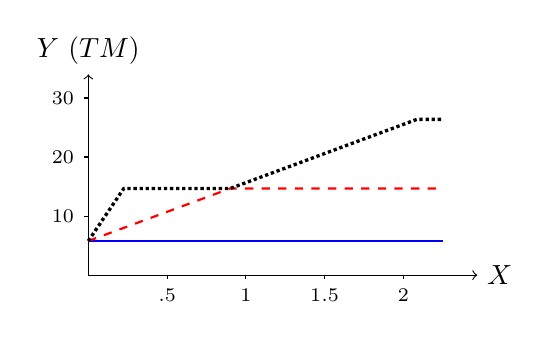
\begin{tikzpicture}[x=2cm,y=.075cm]
\draw[->] (0,0)--(2.47,0) node[right] {$X$};
\draw[->] (0,0)--(0,34) node[above] {$Y\ (TM)$};
\foreach \a in {.5,1,1.5,2} {\draw (\a,0)--(\a,-.7) node[below,font=\scriptsize] {$\a$};}
\foreach \a in {10,20,30} {\draw (0,\a)--(-.03,\a) node[left,font=\scriptsize] {$\a$};}
\draw[blue,thick] (0.0000000,5.7831860)--(2.2500000,5.7831860);
\draw[red,dashed,thick] (0.0000000,5.7831860)--(0.9016354,14.6819706)--(2.2500000,14.6819706);
\draw[black,densely dotted,very thick] (0.0000000,5.7831860)--(0.2254088,14.6819706)--(0.9016354,14.6819706)--(2.0863481,26.3746164)--(2.2500000,26.3746164);
\end{tikzpicture}\hspace{.35cm}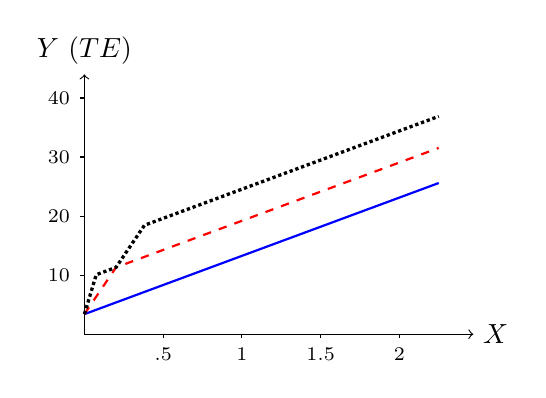
\begin{tikzpicture}[x=2cm,y=.075cm]
\draw[->] (0,0)--(2.47,0) node[right] {$X$};
\draw[->] (0,0)--(0,44) node[above] {$Y\ (TE)$};
\foreach \a in {.5,1,1.5,2} {\draw (\a,0)--(\a,-.7) node[below,font=\scriptsize] {$\a$};}
\foreach \a in {10,20,30,40} {\draw (0,\a)--(-.03,\a) node[left,font=\scriptsize] {$\a$};}
\draw[blue,thick] (0.0000000,3.3899577)--(2.2500000,25.5965676);
\draw[red,dashed,thick] (0.0000000,3.3899577)--(0.2005621,11.3078317)--(2.2500000,31.5349731);
\draw[black,densely dotted,very thick] (0.0000000,3.3899577)--(0.0752108,10.0706639)--(0.2005621,11.3078317)--(0.3813734,18.4459750)--(2.2500000,36.8885805);
\end{tikzpicture}
\end{center}
The transverse ordering used above can also be checked without
surveying indefinitely many roots. The radial eigenvalues for given
$m$ are the min--max values of the Rayleigh quotient
$\int_0^a(|P'|^2+m^2|P|^2/\rho^2)\rho\,d\rho\big/\int_0^a|P|^2\rho\,d\rho$.
Increasing $m^2$ increases the nonnegative term
$m^2\int |P|^2d\rho/\rho$, so each radial eigenvalue increases with
$m$; each fixed-$m$ sequence increases with its radial index.
For TM, the third-lowest value is at most $C$, since $A$, $B$, $C$
are all modes. Every other branch has either $n\ge2$, so
$\alpha_{mn}\ge\alpha_{02}=5.520078$, or $n=1$ and $m\ge3$, so
$\alpha_{m1}\ge\alpha_{31}=6.380162$. Both exceed
$\alpha_{21}=5.135622$, so these branches lie above $C$.
For TE, the zero Neumann eigenvalue is excluded as in
Exercise~14.1.25, and the third-lowest value is at most $F+\pi^2X$.
Every other branch has $n=1$ and $m\ge3$, so
$\beta_{m1}\ge\beta_{31}=4.201189$, or $n\ge2$, so
$\beta_{0n}\ge\beta_{02}>\beta_{01}$ and, for $m\ge1$,
$\beta_{mn}\ge\beta_{12}=5.331443$. All exceed $\beta_{01}$, so with
$p\ge1$ these branches lie above $F+\pi^2X$. In all
these labels $n=1$ means the first \emph{positive} root; in
particular $\beta_{01}=3.831706$, not zero.

\Needspace{5\baselineskip}
\par\bigskip
\noindent\textbf{14.1.28}\quad Show that the integral
\[
\int_{0}^{a}x^{m}J_{n}(x)\,dx,\quad m\ge n\ge0,
\]
\begin{enumerate}
\item[(a)] is integrable for $m+n$ odd in terms of Bessel functions and
powers of $x$, i.e., is expressible as linear combinations of
$a^{p}J_{q}(a)$;
\item[(b)] may be reduced for $m+n$ even to integrated terms plus
$\displaystyle\int_{0}^{a}J_{0}(x)\,dx$.
\end{enumerate}
\par\erratum{Here $m,n$ are nonnegative integers with $m\ge n$.}
\solution
The parity language presumes nonnegative integer $m,n$. Define
$I_{m,n}(a)=\int_0^a x^mJ_n(x)dx$. Since
$[x^{n+1}J_{n+1}(x)]'=x^{n+1}J_n(x)$, integration by parts gives
\begin{align*}
I_{m,n}
&=\int_0^a x^{m-n-1}\,d[x^{n+1}J_{n+1}(x)]\\
&=a^mJ_{n+1}(a)-(m-n-1)I_{m-1,n+1}(a).
\tag{*}
\end{align*}
Explicitly, for $x>0$ the product rule gives
\[
\frac d{dx}\bigl[x^mJ_{n+1}\bigr]
=\frac d{dx}\bigl[x^{m-n-1}\cdot x^{n+1}J_{n+1}\bigr]
=(m-n-1)x^{m-1}J_{n+1}+x^mJ_n,
\]
and integrating from $0$ to $a$ gives (*) for every $m\ge1$, $n\ge0$,
including $m-n-1<0$, which occurs in (b).
The lower boundary term is zero because
$x^mJ_{n+1}(x)=O(x^{m+n+1})$. Every repetition decreases the
power by one, increases the order by one, and leaves their sum
$N=m+n$ unchanged.

(a) If $N$ is odd, then $m-n$ is odd. After $r$ repetitions the
indices are $(m-r,n+r)$, and the next coefficient in (*) is
$(m-r)-(n+r)-1=m-n-1-2r$. After $r=(m-n-1)/2$ repetitions the
remaining indices therefore satisfy $m-r=(n+r)+1$, and at that stage
the coefficient of the remaining integral in (*) is zero. Thus the
procedure ends with the antiderivative $I_{j+1,j}=a^{j+1}J_{j+1}(a)$,
$j=n+r$, and all earlier terms are constants times
$a^{m-r}J_{n+r+1}(a)$. For example, $m-n-1=2$ for $I_{n+3,n}$, so
\[
I_{n+3,n}=a^{n+3}J_{n+1}(a)-2I_{n+2,n+1}
=a^{n+3}J_{n+1}(a)-2a^{n+2}J_{n+2}(a).
\]
This supplies a finite constructive expression of the required type.

(b) If $N$ is even, each coefficient $m-n-1-2r$ in (*) is odd
and cannot vanish. Continue until the power becomes zero, i.e.,
$m$ repetitions, after which the order is $n+m=N$. All the
terms already integrated have the desired form, and only a constant
multiple of $I_{0,N}$ remains. For even $N=2h$, the recurrence
$J_{2j}=J_{2j-2}-2J_{2j-1}'$ (Eq.~(14.8) with $n=2j-1$), integrated
from $0$ to $a$ with $J_{2j-1}(0)=0$, gives
$I_{0,2j}=I_{0,2j-2}-2J_{2j-1}(a)$; applying this for
$j=h,h-1,\ldots,1$,
\begin{align*}
I_{0,2h}(a)
&=I_{0,2h-2}(a)-2J_{2h-1}(a)\\
&=\boxed{\int_0^a J_0(x)dx-2\sum_{j=1}^{h}J_{2j-1}(a)}.
\end{align*}
All odd-order Bessel functions vanish at zero, so no omitted lower
boundary constants occur. Inserting this into the repeated formula
(*) proves the requested reduction.

\Needspace{5\baselineskip}
\par\bigskip
\noindent\textbf{14.1.29}\quad Show that
\[
\int_{0}^{\alpha_{0n}}\left(1-\frac{y}{\alpha_{0n}}\right)J_{0}(y)y\,dy
=\frac{1}{\alpha_{0n}}\int_{0}^{\alpha_{0n}}J_{0}(y)\,dy.
\]
Here $\alpha_{0n}$ is the $n$th zero of $J_{0}(y)$. This relation is
useful (see Exercise~14.2.9): The expression on the right is easier
and quicker to evaluate, and is much more accurate. Taking the
difference of two terms in the expression on the left leads to a large
relative error.
\solution
Set $A=\alpha_{0n}>0$, so $J_0(A)=0$. First use
$[yJ_1(y)]'=yJ_0(y)$:
\begin{align*}
\int_0^A(1-y/A)yJ_0(y)dy
&=\left[(1-y/A)yJ_1(y)\right]_0^A
+\frac1A\int_0^A yJ_1(y)dy\\
&=\frac1A\int_0^A yJ_1(y)dy.
\end{align*}
The upper boundary vanishes because $1-A/A=0$, and the lower
boundary because $yJ_1(y)=O(y^2)$. Now $J_1=-J_0'$ and a second
integration by parts gives
\begin{align*}
\frac1A\int_0^A yJ_1(y)dy
&=-\frac1A[yJ_0(y)]_0^A+\frac1A\int_0^A J_0(y)dy\\
&=\boxed{\frac1A\int_0^A J_0(y)dy}.
\end{align*}
The last boundary term is zero by the defining root condition.
The identity avoids separately evaluating the two oscillatory
moments $\int yJ_0$ and $A^{-1}\int y^2J_0$ and then subtracting
them; the smaller final quantity is computed directly.

\Needspace{9\baselineskip}
\subsection*{14.2 Orthogonality}

\Needspace{5\baselineskip}
\par\bigskip
\noindent\textbf{14.2.1}\quad Show that
\[
\int_{0}^{a}J_{\nu}(kx)J_{\nu}(k'x)x\,dx
=\frac{a[k'J_{\nu}(ka)J'_{\nu}(k'a)-kJ'_{\nu}(ka)J_{\nu}(k'a)]}
{(k^{2}-k'^{2})},
\]
where $J'_{\nu}(ka)=\dfrac{d}{d(kx)}J_{\nu}(kx)\Big|_{x=a}$, and that
\[
\int_{0}^{a}[J_{\nu}(kx)]^{2}x\,dx
=\frac{a^{2}}{2}\left\{[J'_{\nu}(ka)]^{2}
+\left(1-\frac{\nu^{2}}{k^{2}a^{2}}\right)[J_{\nu}(ka)]^{2}\right\},
\qquad\nu>-1.
\]
These two integrals are usually called the first and second Lommel
integrals.
\par\erratum{Take real $\nu>-1$, $a>0$, and $k,k'>0$. The first displayed quotient requires $k^2\ne k'^2$; its coincident limit is the second integral.}
\solution
Let $y(x)=J_\nu(kx)$ and $z(x)=J_\nu(k'x)$, initially with
$k,k'>0$, $k^2\ne k'^2$. Their equations in self-adjoint form are
\[
(xy')'+(k^2x-\nu^2/x)y=0,\qquad
(xz')'+(k'^2x-\nu^2/x)z=0.
\]
Multiply the second by $y$, the first by $z$, and subtract:
\[
\frac d{dx}\{x(yz'-y'z)\}=(k^2-k'^2)xyz.
\]
Integrate first from $\epsilon>0$ to $a$, so no individually
divergent origin terms have been introduced. To take $\epsilon\to0$,
write
\[
y=A x^\nu\left[1-\frac{k^2x^2}{4(\nu+1)}+O(x^4)\right],\quad
z=B x^\nu\left[1-\frac{k'^2x^2}{4(\nu+1)}+O(x^4)\right].
\]
The leading powers cancel in the bracket, leaving
\[
x(yz'-y'z)=\frac{AB(k^2-k'^2)}{2(\nu+1)}x^{2\nu+2}
+O(x^{2\nu+4})\longrightarrow0\qquad(\nu>-1).
\]
At $a$, the chain rule gives $y'=kJ_\nu'(ka)$ and
$z'=k'J_\nu'(k'a)$. Hence
\[
\boxed{\int_0^a xyz\,dx=
\frac{a[k'J_\nu(ka)J_\nu'(k'a)-kJ_\nu'(ka)J_\nu(k'a)]}
{k^2-k'^2}}.
\]
For the second integral let $k'\to k$ and apply l'H\^opital's rule.
Writing $J=J_\nu(ka)$ and using primes for argument derivatives,
\[
\int_0^a xJ_\nu(kx)^2dx
=\frac{a[J(J'+kaJ'')-ka(J')^2]}{-2k}.
\]
Bessel's equation at $ka$ says
$kaJ''=-J'-(ka-\nu^2/(ka))J$. Therefore
\[
J(J'+kaJ'')-ka(J')^2
=-ka\left[(J')^2+\left(1-\frac{\nu^2}{k^2a^2}\right)J^2\right],
\]
which gives
\[
\boxed{\int_0^a xJ_\nu(kx)^2dx
=\frac{a^2}{2}\left[J_\nu'(ka)^2+
\left(1-\frac{\nu^2}{k^2a^2}\right)J_\nu(ka)^2\right]}.
\]
The condition $\nu>-1$ also makes the integrand
$O(x^{2\nu+1})$ integrable. Coincident wave numbers use the second
formula; any zero-parameter value must be taken as an existing
limit, not inserted into the displayed denominators.

\Needspace{5\baselineskip}
\par\bigskip
\noindent\textbf{14.2.2}
\begin{enumerate}
\item[(a)] If $\beta_{\nu m}$ is the $m$th \erratum{positive zero of $J_\nu^\prime$}, so that
\erratum{$(d/d\rho)J_\nu(\beta_{\nu m}\rho/a)|_{\rho=a}=0$}, show that the Bessel functions
are orthogonal over the interval $[0,a]$ with an orthogonality
integral
\[
\int_{0}^{a}J_{\nu}\left(\beta_{\nu m}\frac{\rho}{a}\right)
J_{\nu}\left(\beta_{\nu n}\frac{\rho}{a}\right)\rho\,d\rho=0,
\qquad m\neq n,\quad\nu>-1.
\]
\item[(b)] Derive the corresponding normalization integral ($m=n$).
\end{enumerate}
\par\nobreak\hfill\emph{ANS.}\enspace
(b) $\dfrac{a^{2}}{2}\left(1-\dfrac{\nu^{2}}{\beta_{\nu m}^{2}}\right)
[J_{\nu}(\beta_{\nu m})]^{2}$, $\nu>-1$.
\par\erratum{These formulas refer to positive derivative roots. For $\nu=0$ the additional constant mode has norm $a^2/2$.}
\solution
Interpret $\beta_{\nu m}$ as a positive argument satisfying
$J_\nu'(\beta_{\nu m})=0$, so the derivative with respect to $\rho$
vanishes at $\rho=a$. Put $k=\beta_{\nu m}/a$ and
$k'=\beta_{\nu n}/a$ in the first Lommel integral. For $m\ne n$
the denominator is nonzero, while both terms in its numerator
contain a vanishing derivative. Thus
\[
\boxed{\int_0^a \rho J_\nu(\beta_{\nu m}\rho/a)
J_\nu(\beta_{\nu n}\rho/a)d\rho=0\quad(m\ne n)}.
\]
For $m=n$, use the second Lommel integral instead. The squared
derivative term is zero, and $k^2a^2=\beta_{\nu m}^2$, giving
\[
\boxed{N_{\nu m}=\frac{a^2}{2}
\left(1-\frac{\nu^2}{\beta_{\nu m}^2}\right)
J_\nu(\beta_{\nu m})^2}.
\]
The origin terms vanish for $\nu>-1$ by the calculation in
Exercise~14.2.1. The integral defining $N_{\nu m}$ is positive,
so this also implies $\beta_{\nu m}>|\nu|$ for every positive
derivative zero under consideration.
\erratum{For $\nu=0$ the Neumann problem has the additional
constant mode $J_0(0\rho/a)=1$, of norm $a^2/2$. It is not one
of the positive roots, and the displayed expression containing
$\nu^2/\beta^2$ must not be used as $0/0$. Its orthogonality to
the positive modes follows from
$\int_0^a\rho J_0(\beta\rho/a)d\rho=a^2J_1(\beta)/\beta=0$.}

\Needspace{5\baselineskip}
\par\bigskip
\noindent\textbf{14.2.3}\quad Verify that the orthogonality equation,
Eq.~(14.44), and the normalization equation, Eq.~(14.46), hold for
$\nu>-1$.
\par\emph{Hint.}~Using power-series expansions, examine the behavior of
Eq.~(14.43) as $\rho\to0$.
\solution
The two equations to be checked are the Dirichlet orthogonality
and normalization formulas
\[
\int_0^a\rho J_\nu(\alpha_{\nu m}\rho/a)
J_\nu(\alpha_{\nu n}\rho/a)d\rho=0\quad(m\ne n),
\]
\[
\int_0^a\rho J_\nu(\alpha_{\nu n}\rho/a)^2d\rho
=\frac{a^2}{2}J_{\nu+1}(\alpha_{\nu n})^2.
\]
The only possible issue when $-1<\nu<0$ is the singular-looking
origin. Put $k=\alpha_{\nu m}/a$, $k'=\alpha_{\nu n}/a$.
The series begin
\[
J_\nu(k\rho)=\frac{(k/2)^\nu}{\Gamma(\nu+1)}\rho^\nu
\left[1-\frac{k^2\rho^2}{4(\nu+1)}+O(\rho^4)\right].
\]
In the boundary expression
$\rho[J_\nu(k\rho)\partial_\rho J_\nu(k'\rho)
-\partial_\rho J_\nu(k\rho)J_\nu(k'\rho)]$, the terms of order
$\rho^{2\nu}$ cancel exactly. The next term is
\[
\frac{(kk'/4)^\nu(k^2-k'^2)}
{2(\nu+1)\Gamma(\nu+1)^2}\rho^{2\nu+2},
\]
which vanishes for precisely the stated range $\nu>-1$.
At $\rho=a$ both function values vanish for distinct Dirichlet
roots, so the first Lommel formula gives orthogonality. For a
repeated root, the second formula reduces to
$a^2J_\nu'(\alpha_{\nu n})^2/2$. The recurrence
$J_\nu'=\nu J_\nu/x-J_{\nu+1}$ yields
$J_\nu'(\alpha_{\nu n})=-J_{\nu+1}(\alpha_{\nu n})$, proving
normalization. All relevant integrals converge because their
origin integrands behave as $\rho^{2\nu+1}$.

\Needspace{5\baselineskip}
\par\bigskip
\noindent\textbf{14.2.4}\quad From Eq.~\erratum{(14.44)}, develop a
proof that $J_{\nu}(z)$, $\nu>-1$ has no complex roots (with a nonzero
imaginary part).
\par\emph{Hint.}
\begin{enumerate}
\item[(a)] Use the series form of $J_{\nu}(z)$ to exclude pure
imaginary roots.
\item[(b)] Assume $\alpha_{\nu m}$ to be complex and take
$\alpha_{\nu n}$ to be $\alpha_{\nu m}^{\,*}$.
\end{enumerate}
\solution
Take real $\nu>-1$ and consider nonzero roots on a fixed
branch. The factor $z^\nu$ can be removed by defining the entire
even function
\[
F_\nu(z)=\Gamma(\nu+1)(2/z)^\nu J_\nu(z)
=\sum_{r=0}^\infty
\frac{(-1)^r\Gamma(\nu+1)(z^2/4)^r}
{r!\Gamma(\nu+r+1)}.
\]
(a) If $z=iy$ with real $y\ne0$, every term of $F_\nu(iy)$
is positive, because $(-1)^r(iy)^{2r}=y^{2r}$ and all gamma
arguments $\nu+r+1$ are positive. Thus $F_\nu(iy)>0$, excluding
nonzero pure imaginary roots.

(b) The series coefficients are real, so if $z_0$ is a root then
$z_0^*$ is also a root. Suppose both its real and imaginary parts
are nonzero. Then $z_0^2\ne(z_0^*)^2$. Apply the first Lommel
identity on $0\le x\le1$ with $k=z_0$, $k'=z_0^*$.
The upper boundary term vanishes because both arguments are roots;
the lower boundary vanishes by the same $x^{2\nu+2}$ estimate as
before. With conjugate branches for the two factors, this says
\[
0=\int_0^1 xJ_\nu(z_0x)J_\nu(z_0^*x)dx
=\int_0^1 x|J_\nu(z_0x)|^2dx.
\]
But the integrand is nonnegative and the series shows that the
function is not identically zero on $(0,1)$, so the integral is
strictly positive. This contradiction excludes every remaining
nonreal possibility. Therefore all nonzero zeros are real.
The corrected reference is Eq.~(14.44), the orthogonality identity;
the original reference to (11.49) is unrelated.

\Needspace{5\baselineskip}
\par\bigskip
\noindent\textbf{14.2.5}
\begin{enumerate}
\item[(a)] In the series expansion
\[
f(\rho)=\sum_{m=1}^{\infty}c_{\nu m}J_{\nu}\left(\alpha_{\nu m}
\frac{\rho}{a}\right),\quad0\le\rho\le a,\quad\nu>-1,
\]
with $J_{\nu}(\alpha_{\nu m})=0$, show that the coefficients are given
by
\[
c_{\nu m}=\frac{2}{a^{2}[J_{\nu+1}(\alpha_{\nu m})]^{2}}
\int_{0}^{a}f(\rho)J_{\nu}\left(\alpha_{\nu m}\frac{\rho}{a}\right)
\rho\,d\rho.
\]
\item[(b)] In the series expansion
\[
f(\rho)=\erratum{f_{\rm extra}(\rho)+}\sum_{m=1}^{\infty}d_{\nu m}J_{\nu}\left(\beta_{\nu m}
\frac{\rho}{a}\right),\quad0\le\rho\le a,\quad\nu>-1,
\]
with $(d/d\rho)J_{\nu}(\beta_{\nu m}\rho/a)\big|_{\rho=a}=0$, show
that the coefficients are given by
\[
d_{\nu m}=\frac{2}{a^{2}(1-\nu^{2}/\beta_{\nu m}^{2})
[J_{\nu}(\beta_{\nu m})]^{2}}
\int_{0}^{a}f(\rho)J_{\nu}\left(\beta_{\nu m}\frac{\rho}{a}\right)
\rho\,d\rho.
\]
\end{enumerate}
\par\erratum{Use real $\nu>-1$ and convergence in $L^2((0,a),\rho\,d\rho)$; the roots are positive. In (b), include $f_{\rm extra}=0$ for $\nu>0$, a constant mode for $\nu=0$, and the mode proportional to $I_\nu(\kappa\rho/a)$ with $I_\nu^\prime(\kappa)=0$ for $-1<\nu<0$. Its coefficient is determined below.}
\solution
Use the weighted inner product
$\langle g,h\rangle=\int_0^a g(\rho)^*h(\rho)\rho\,d\rho$.
The coefficient formulas hold whenever the stated expansions
converge in this weighted $L^2$ space.

(a) Multiply the Dirichlet expansion by
$J_\nu(\alpha_{\nu n}\rho/a)\rho$ and integrate. Orthogonality
removes every term except $m=n$:
\[
\int_0^a f(\rho)J_\nu(\alpha_{\nu n}\rho/a)\rho d\rho
=c_{\nu n}\frac{a^2}{2}J_{\nu+1}(\alpha_{\nu n})^2.
\]
Division gives the asserted $c_{\nu n}$.

(b) Repeat with $J_\nu(\beta_{\nu n}\rho/a)\rho$ instead.
The Neumann orthogonality and norm from Exercise~14.2.2 give
\[
\int_0^a f(\rho)J_\nu(\beta_{\nu n}\rho/a)\rho d\rho
=d_{\nu n}\frac{a^2}{2}
\left(1-\frac{\nu^2}{\beta_{\nu n}^2}\right)
J_\nu(\beta_{\nu n})^2.
\]
Solving for $d_{\nu n}$ proves the second displayed coefficient
formula for each positive root.

\erratum{Positive derivative roots alone do not give an expansion
of an arbitrary function throughout the stated range $\nu>-1$.
For $\nu=0$ one must add the constant mode with coefficient
$d_{00}=2a^{-2}\int_0^a f(\rho)\rho\,d\rho$.
For $-1<\nu<0$ one must also include a negative-eigenvalue mode
$I_\nu(\kappa\rho/a)$, where $I_\nu'(\kappa)=0$, $\kappa>0$.
These omissions do not change the coefficient formulas for the
positive-root terms.}
Here is a direct check of the latter qualification. For $-1<\nu<0$,
$I_\nu(x)>0$ by its series, its derivative is negative near zero
($I_\nu\sim(x/2)^\nu/\Gamma(\nu+1)$), and positive for large
$x$. Thus it has a positive derivative zero. If
$w=xI_\nu'/I_\nu$, the modified Bessel equation gives
$xw'=x^2+\nu^2-w^2$. At every zero of $w$ its derivative is
positive, so it crosses zero only once. The corresponding radial
function has eigenvalue $-\kappa^2/a^2$ and is orthogonal to all
positive-eigenvalue modes by the same boundary-bracket argument.
For clarity, derive its norm rather than assuming a modified Lommel
formula. Put $y(x)=I_\nu(x)$ and
\[
F(x)=\frac12\{x^2[y(x)^2-y'(x)^2]+\nu^2y(x)^2\}.
\]
Differentiation gives
\[
F'=x(y^2-y'^2)+(x^2+\nu^2)yy'-x^2y'y''.
\]
The modified equation says
$x^2y''=(x^2+\nu^2)y-xy'$. Substitution cancels the two
$yy'$ terms and the two $xy'^2$ terms, leaving $F'=xy^2$.
Near zero, the leading $x^{2\nu}$ contributions cancel in $F$,
so $F=O(x^{2\nu+2})\to0$ for $\nu>-1$.
Now set $x=\kappa\rho/a$ and use $I_\nu^\prime(\kappa)=0$:
\[
N_-=\frac{a^2}{\kappa^2}\int_0^\kappa xI_\nu(x)^2\,dx
=\frac{a^2}{\kappa^2}[F(\kappa)-F(0)].
\]
Thus its norm is
\[
N_-=\frac{a^2}{2}\left(1+\frac{\nu^2}{\kappa^2}\right)
I_\nu(\kappa)^2,
\]
so its coefficient is
$N_-^{-1}\int_0^a f(\rho)I_\nu(\kappa\rho/a)\rho d\rho$.
At the Dirichlet endpoint $\rho=a$, a series of zero-valued basis
functions is zero; nonzero prescribed endpoint values are understood
as interior limits or in $L^2$, rather than equality at that single
point.

\Needspace{5\baselineskip}
\par\bigskip
\noindent\textbf{14.2.6}\quad A right circular cylinder has an
electrostatic potential of $\psi(\rho,\varphi)$ on both ends. The
potential on the curved cylindrical surface is zero. Find the
potential at all interior points.
\par\emph{Hint.}~Choose your coordinate system and adjust your $z$
dependence to exploit the symmetry of your potential.
\par\erratum{Assume bounded, piecewise smooth end data, and seek the bounded harmonic interior solution. At an incompatible rim, impose the face limits away from the junction.}
\solution
Let the cylinder have radius $a$ and length $l$, with its ends
at $z=\pm l/2$. Denote the sought interior potential by $V$ and
the identical prescribed end potential by $\psi(\rho,\varphi)$.
Separation of $\nabla^2V=0$ gives the angular factors $e^{im\varphi}$,
regular radial factors $J_{|m|}(k\rho)$, and axial equation
$Z''-k^2Z=0$. The side condition forces
$k=\alpha_{|m|n}/a$, where $J_{|m|}(\alpha_{|m|n})=0$.
Identical end data are even in $z$; hence use $\cosh(kz)$ rather
than the odd $\sinh(kz)$. Normalize the axial factor to one on
both ends:
\[
\boxed{V(\rho,\varphi,z)=\sum_{m=-\infty}^{\infty}
\sum_{n=1}^{\infty}A_{mn}J_{|m|}(\alpha_{|m|n}\rho/a)
e^{im\varphi}
\frac{\cosh(\alpha_{|m|n}z/a)}
{\cosh(\alpha_{|m|n}l/(2a))}}.
\]
At either end this is the double Fourier--Bessel expansion of
$\psi$. Multiply it by
$e^{-im\varphi}J_{|m|}(\alpha_{|m|n}\rho/a)\rho$ and integrate
over the disk. The angular norm is $2\pi$ and the radial norm is
$a^2J_{|m|+1}(\alpha_{|m|n})^2/2$. Therefore
\[
\boxed{A_{mn}=\frac{\displaystyle\int_0^{2\pi}\!\int_0^a
\psi(\rho,\varphi)e^{-im\varphi}
J_{|m|}(\alpha_{|m|n}\rho/a)\rho\,d\rho\,d\varphi}
{\pi a^2J_{|m|+1}(\alpha_{|m|n})^2}}.
\]
Every term satisfies Laplace's equation, the grounded side, and
reflection symmetry; the coefficient projection supplies both end
conditions. For real data $A_{-m,n}=A_{mn}^*$, making the potential
real. For compatible boundary data and finite-energy solutions,
the difference $U=V_1-V_2$ has zero boundary values. Green's
identity gives $\int|\nabla U|^2d^3x=0$, hence $U=0$.

\erratum{A discontinuous rim need not give a finite-energy field,
so that energy argument should not be applied to each such field
without qualification.} Uniqueness still holds among bounded
harmonic solutions with the specified face limits. To see this,
let $\Gamma$ be the two rim circles and introduce the positive
harmonic barrier
\[
B(\mathbf x)=\int_\Gamma\frac{d\ell_{\mathbf y}}{|\mathbf x-\mathbf y|}.
\]
It is finite in the interior, harmonic there, and diverges to
$+\infty$ at the rim: the local line integral is comparable to
$\int_{-\delta}^{\delta}(d^2+s^2)^{-1/2}ds
=2\operatorname{arsinh}(\delta/d)\to\infty$.
For any $\epsilon>0$, both $U-\epsilon B$ and
$-U-\epsilon B$ have nonpositive boundary upper limits, including
the rim because $U$ is bounded. The maximum principle gives
$|U(\mathbf x)|\le\epsilon B(\mathbf x)$ in the interior.
Letting $\epsilon\downarrow0$ proves $U=0$.
The series therefore supplies the bounded interior solution and,
at incompatible rims, the face limits away from the junction.

\Needspace{5\baselineskip}
\par\bigskip
\noindent\textbf{14.2.7}\quad A function $f(x)$ is expressed as a
Bessel series:
\[
f(x)=\sum_{n=1}^{\infty}a_{n}J_{m}(\alpha_{mn}x),
\]
with $\alpha_{mn}$ the $n$th root of $J_{m}$. Prove the Parseval
relation,
\[
\int_{0}^{1}[f(x)]^{2}x\,dx
=\frac{1}{2}\sum_{n=1}^{\infty}a_{n}^{2}[J_{m+1}(\alpha_{mn})]^{2}.
\]
\par\erratum{Let $m>-1$ be real, let $\alpha_{mn}$ enumerate the positive zeros, and assume convergence to $f$ in $L^2((0,1),x\,dx)$.}
\solution
First take a finite partial sum
$S_N(x)=\sum_{n=1}^N a_nJ_m(\alpha_{mn}x)$. Expanding its square,
then using orthogonality and the Dirichlet norm, gives
\begin{align*}
\int_0^1 S_N(x)^2x\,dx
&=\sum_{n=1}^N\sum_{j=1}^N a_na_j
\int_0^1J_m(\alpha_{mn}x)J_m(\alpha_{mj}x)x\,dx\\
&=\frac12\sum_{n=1}^N a_n^2J_{m+1}(\alpha_{mn})^2.
\end{align*}
\erratum{To pass to an infinite series, the expansion must converge
to $f$ in $L^2((0,1),x\,dx)$; merely writing a formal series does
not justify Parseval's equality.}
Under that assumption, the Cauchy--Schwarz inequality gives
\[
\left|\int_0^1(f^2-S_N^2)x\,dx\right|
\le\|f-S_N\|\,\|f+S_N\|\longrightarrow0.
\]
The finite identity therefore tends to the formula in the question.
For real $f$ and coefficients this is the usual Parseval identity.
For complex functions, the norm version is
\[
\int_0^1|f(x)|^2x\,dx
=\frac12\sum_{n=1}^{\infty}|a_n|^2J_{m+1}(\alpha_{mn})^2;
\]
the bilinear square identity also follows by the same limiting
argument. Completeness of the Dirichlet Bessel basis identifies the
limit with $f$, rather than merely its orthogonal projection.

\Needspace{5\baselineskip}
\par\bigskip
\noindent\textbf{14.2.8}\quad Prove that
\[
\sum_{n=1}^{\infty}(\alpha_{mn})^{-2}=\frac{1}{4(m+1)}.
\]
\par\emph{Hint.}~Expand $x^{m}$ in a Bessel series and apply the
Parseval relation.
\par\erratum{Here $m>-1$ is real and $\alpha_{mn}$ is the $n$th positive zero of $J_m$.}
\solution
Expand $f(x)=x^m$ on $0<x<1$ in the Dirichlet Bessel basis.
For $m>-1$, $\int_0^1|x^m|^2x\,dx=1/[2(m+1)]$ is finite.
The coefficient formula gives
\[
a_n=\frac{2}{J_{m+1}(\alpha_{mn})^2}
\int_0^1x^{m+1}J_m(\alpha_{mn}x)dx.
\]
Set $\alpha=\alpha_{mn}$. The recurrence implies
\[
\frac d{dx}[x^{m+1}J_{m+1}(\alpha x)]
=\alpha x^{m+1}J_m(\alpha x).
\]
Its lower boundary vanishes as $x^{2m+2}$; hence
\[
\int_0^1x^{m+1}J_m(\alpha x)dx
=\frac{J_{m+1}(\alpha)}\alpha,
\qquad a_n=\frac{2}{\alpha_{mn}J_{m+1}(\alpha_{mn})}.
\]
Insert these coefficients into Parseval's relation:
\begin{align*}
\frac1{2(m+1)}
&=\frac12\sum_{n=1}^{\infty}
\frac{4J_{m+1}(\alpha_{mn})^2}
{\alpha_{mn}^2J_{m+1}(\alpha_{mn})^2}
=2\sum_{n=1}^{\infty}\alpha_{mn}^{-2}.
\end{align*}
Thus
\[
\boxed{\sum_{n=1}^{\infty}\frac1{\alpha_{mn}^2}
=\frac1{4(m+1)}}.
\]
The expansion is used in the weighted $L^2$ sense. At $x=1$ every
basis function is zero whereas $x^m=1$; that single endpoint has
zero measure and does not affect the integral or Parseval's
identity.

\Needspace{5\baselineskip}
\par\bigskip
\noindent\textbf{14.2.9}\quad A right circular cylinder of length $l$
and radius $a$ has on its end caps a potential
\[
\psi\Big|_{z=\pm\frac{l}{2}}=100\left(1-\frac{\rho}{a}\right).
\]
The potential on the curved surface (the side) is zero. Using the
Bessel series from Exercise~14.2.6, calculate the electrostatic
potential for $\rho/a=0.0(0.2)1.0$ and $z/l=0.0(0.1)0.5$. Take
$a/l=0.5$.
\par\emph{Hint.}~From Exercise~14.1.29 you have
\[
\int_{0}^{\alpha_{0n}}\left(1-\frac{y}{\alpha_{0n}}\right)J_{0}(y)y\,dy.
\]
Show that this equals
\[
\frac{1}{\alpha_{0n}}\int_{0}^{\alpha_{0n}}J_{0}(y)\,dy.
\]
Numerical evaluation of this latter form rather than the former is
both faster and more accurate.
\par\emph{Note.}~For $\rho/a=0.0$ and $z/l=0.5$ the convergence is
slow, 20 terms giving only 98.4 rather than 100.
\par\nobreak\hfill\emph{Check value.}\enspace
For $\rho/a=0.4$ and $z/l=0.3$, $\psi=\erratum{24.559}$.
\solution
The end data are independent of $\varphi$, so only $m=0$ remains
in Exercise~14.2.6. Put $r=\rho/a$, $s=z/l$, and
$\alpha_n=\alpha_{0n}$. Since $l/(2a)=1$,
\[
\boxed{V(r,s)=\sum_{n=1}^{\infty}A_nJ_0(\alpha_n r)
\frac{\cosh(2\alpha_n s)}{\cosh\alpha_n}},
\qquad
A_n=\frac{200}{J_1(\alpha_n)^2}
\int_0^1(1-r)J_0(\alpha_n r)r\,dr.
\]
With $y=\alpha_n r$, the last integral is
\[
\frac1{\alpha_n^2}\int_0^{\alpha_n}
(1-y/\alpha_n)yJ_0(y)dy
=\frac1{\alpha_n^3}\int_0^{\alpha_n}J_0(y)dy,
\]
where the final equality is proved by the two integrations by
parts in Exercise~14.1.29. Consequently the stable coefficients are
\[
\boxed{A_n=\frac{200}{\alpha_n^3J_1(\alpha_n)^2}
\int_0^{\alpha_n}J_0(y)dy}.
\]
\Needspace{12\baselineskip}
The resulting potentials are:
\begin{center}
\begin{tabular}{c r r r r r r}
\toprule
$\rho/a\backslash z/l$ & $0.0$ & $0.1$ & $0.2$ & $0.3$ & $0.4$ & $0.5$\\
\midrule
0.0 & 14.108 & 15.805 & 21.353 & 32.341 & 52.640 & 100.000 \\
0.2 & 13.290 & 14.881 & 20.061 & 30.213 & 48.293 & 80.000 \\
0.4 & 10.989 & 12.287 & 16.485 & 24.559 & 38.270 & 60.000 \\
0.6 & 7.617 & 8.504 & 11.359 & 16.786 & 25.844 & 40.000 \\
0.8 & 3.747 & 4.179 & 5.568 & 8.204 & 12.648 & 20.000 \\
1.0 & 0.000 & 0.000 & 0.000 & 0.000 & 0.000 & 0.000 \\
\bottomrule
\end{tabular}
\end{center}
The last column is the prescribed boundary value $100(1-r)$;
the last row is the grounded side. For the interior entries, the
integrals were accumulated between consecutive zeros of $J_0$,
and 120 modes were summed. Comparing 80 and 120 modes changed
every interior entry by less than $10^{-20}$, comfortably below
the $0.001$ displayed precision. This convergence comparison is a
numerical check, not a universal truncation-error theorem.
\erratum{The printed check value $24.558$ is not correctly rounded
to three decimals: the converged value is
$V(0.4,0.3)=24.5585639709\ldots$, hence $24.559$.}
At the top center, a 20-mode sum is $98.424595978\ldots$; prescribing
the exact boundary value avoids reporting its slowly convergent
truncation as the boundary potential. Symmetry gives
$V(r,-s)=V(r,s)$ for the lower half of the cylinder.

\Needspace{9\baselineskip}
\subsection*{14.3 Neumann Functions, Bessel Functions of the Second Kind}

\Needspace{5\baselineskip}
\par\bigskip
\noindent\textbf{14.3.1}\quad Prove that the Neumann functions $Y_{n}$
(with $n$ an integer) satisfy the recurrence relations
\begin{align*}
Y_{n-1}(x)+Y_{n+1}(x)&=\frac{2n}{x}Y_{n}(x),\\
Y_{n-1}(x)-Y_{n+1}(x)&=2Y'_{n}(x).
\end{align*}
\par\emph{Hint.}~These relations may be proved by differentiating the
recurrence relations for $J_{\nu}$ or by using the limit form of
$Y_{\nu}$ but not dividing everything by zero.
\solution
Begin with noninteger $\nu$, where the defining denominator is
nonzero. Abbreviate $C=\cos\pi\nu$ and $S=\sin\pi\nu$.
Since $\cos\pi(\nu\pm1)=-C$ and $\sin\pi(\nu\pm1)=-S$,
\[
Y_{\nu-1}=\frac{CJ_{\nu-1}+J_{-\nu+1}}S,\qquad
Y_{\nu+1}=\frac{CJ_{\nu+1}+J_{-\nu-1}}S.
\]
Add these and apply the $J$ recurrence at both orders $\nu$ and
$-\nu$:
\begin{align*}
Y_{\nu-1}+Y_{\nu+1}
&=\frac{C(2\nu J_\nu/x)-2\nu J_{-\nu}/x}S
=\frac{2\nu}{x}\frac{CJ_\nu-J_{-\nu}}S
=\frac{2\nu}{x}Y_\nu.
\end{align*}
Subtracting instead gives
\begin{align*}
Y_{\nu-1}-Y_{\nu+1}
&=\frac{C(J_{\nu-1}-J_{\nu+1})
 +(J_{-\nu+1}-J_{-\nu-1})}S\\
&=\frac{2CJ_\nu'-2J_{-\nu}'}S=2Y_\nu'.
\end{align*}
Now let $\nu\to n$. The defining removable limits give
$Y_\nu\to Y_n$, $Y_{\nu\pm1}\to Y_{n\pm1}$, and the same
limits hold after $x$ differentiation away from the branch point
$x=0$. Both recurrences therefore hold for integer $n$, with no
division by $\sin\pi n=0$.

\Needspace{5\baselineskip}
\par\bigskip
\noindent\textbf{14.3.2}\quad Show that for integer $n$
\[
Y_{-n}(x)=(-1)^{n}Y_{n}(x).
\]
\solution
For noninteger $\nu$, solve the definition for the opposite-order
first-kind function:
\[
J_{-\nu}=\cos\pi\nu\,J_\nu-\sin\pi\nu\,Y_\nu.
\]
Apply the definition once more with order $-\nu$:
\begin{align*}
Y_{-\nu}
&=\frac{\cos\pi\nu\,J_{-\nu}-J_\nu}{-\sin\pi\nu}\\
&=\frac{(\cos^2\pi\nu-1)J_\nu
-\cos\pi\nu\sin\pi\nu\,Y_\nu}{-\sin\pi\nu}\\
&=\sin\pi\nu\,J_\nu+\cos\pi\nu\,Y_\nu.
\end{align*}
Taking the removable limit $\nu\to n\in\mathbb Z$ gives
\[
\boxed{Y_{-n}(x)=(-1)^nY_n(x)}.
\]
This also includes $n=0$, where the equality is immediate.

\Needspace{5\baselineskip}
\par\bigskip
\noindent\textbf{14.3.3}\quad Show that
\[
Y'_{0}(x)=-Y_{1}(x).
\]
\solution
Set $n=0$ in the derivative recurrence:
\[
2Y_0'=Y_{-1}-Y_1.
\]
Exercise~14.3.2 gives $Y_{-1}=-Y_1$, and hence
\[
2Y_0'=-2Y_1,\qquad\boxed{Y_0'=-Y_1}.
\]
\erratum{The manual's last equation in this exercise, p.~209,
prints $J_1,J_0'$ where $Y_1,Y_0'$ are required. The latter are
the functions used in the recurrence above.}

\Needspace{5\baselineskip}
\par\bigskip
\noindent\textbf{14.3.4}\quad If $X$ and $Z$ are any two solutions of
Bessel's equation, show that
\[
X_{\nu}(x)Z'_{\nu}(x)-X'_{\nu}(x)Z_{\nu}(x)=\frac{A_{\nu}}{x},
\]
in which $A_{\nu}$ may depend on $\nu$ but is independent of $x$. This
is a special case of Exercise~7.6.11.
\solution
Define $W=X_\nu Z_\nu'-X_\nu'Z_\nu$ on an interval not
containing $x=0$. Differentiation cancels the mixed terms:
\[
W'=X_\nu Z_\nu''-X_\nu''Z_\nu.
\]
Both functions satisfy
$y''=-y'/x-(1-\nu^2/x^2)y$. Substitution therefore gives
\begin{align*}
W'&=X_\nu\left[-\frac{Z_\nu'}x-
\left(1-\frac{\nu^2}{x^2}\right)Z_\nu\right]
-\left[-\frac{X_\nu'}x-
\left(1-\frac{\nu^2}{x^2}\right)X_\nu\right]Z_\nu\\
&=-\frac1x(X_\nu Z_\nu'-X_\nu'Z_\nu)=-\frac Wx.
\end{align*}
Thus $(xW)'=W+xW'=0$, proving
\[
\boxed{W(x)=\frac{A_\nu}{x}}.
\]
The constant depends on the chosen solutions and their order, but
not on $x$. It is zero for linearly dependent solutions.

\Needspace{5\baselineskip}
\par\bigskip
\noindent\textbf{14.3.5}\quad Verify the Wronskian formulas
\begin{align*}
J_{\nu}(x)J_{-\nu+1}(x)+J_{-\nu}(x)J_{\nu-1}(x)
&=\frac{2\sin\nu\pi}{\pi x},\\
J_{\nu}(x)Y'_{\nu}(x)-J'_{\nu}(x)Y_{\nu}(x)&=\frac{2}{\pi x}.
\end{align*}
\solution
For noninteger $\nu$, the derivative recurrences give
\[
J_{1-\nu}=-J_{-\nu}'-\frac\nu xJ_{-\nu},\qquad
J_{\nu-1}=J_\nu'+\frac\nu xJ_\nu.
\]
Multiplying and adding cancels the terms proportional to $\nu/x$:
\[
J_\nu J_{1-\nu}+J_{-\nu}J_{\nu-1}
=-J_\nu J_{-\nu}'+J_\nu'J_{-\nu}
=-W[J_\nu,J_{-\nu}].
\]
\erratum{The manual's corresponding line on p.~209 has a minus
sign before the second product; it must be plus, as the cancellation
above shows.}
By Exercise~14.3.4, $W=A/x$. The leading series terms are
\[
J_\nu=\frac{(x/2)^\nu}{\Gamma(\nu+1)}[1+O(x^2)],\qquad
J_{-\nu}=\frac{(x/2)^{-\nu}}{\Gamma(1-\nu)}[1+O(x^2)].
\]
Their derivatives give
\[
A=-\frac{2\nu}{\Gamma(\nu+1)\Gamma(1-\nu)}
=-\frac{2}{\Gamma(\nu)\Gamma(1-\nu)}
=-\frac{2\sin\pi\nu}{\pi}.
\]
Therefore
\[
\boxed{J_\nu J_{1-\nu}+J_{-\nu}J_{\nu-1}
=\frac{2\sin\pi\nu}{\pi x}}.
\]
Finally $Y_\nu=(\cos\pi\nu\,J_\nu-J_{-\nu})/\sin\pi\nu$,
so bilinearity of the Wronskian gives
\[
W[J_\nu,Y_\nu]=-
\frac{W[J_\nu,J_{-\nu}]}{\sin\pi\nu}
=\boxed{\frac2{\pi x}}.
\]
Both formulas extend to integer orders by their removable order
limits. In the first, both sides then vanish because $J_{-n}$ is
proportional to $J_n$; the second remains nonzero.

\Needspace{5\baselineskip}
\par\bigskip
\noindent\textbf{14.3.6}\quad As an alternative to letting $x$ approach
zero in the evaluation of the Wronskian constant, we may invoke the
uniqueness of power-series expansions. The coefficient of $x^{-1}$ in
the series expansion of $u_{\nu}(x)v'_{\nu}(x)-u'_{\nu}(x)v_{\nu}(x)$
is then $A_{\nu}$. Show by series expansion that the coefficients of
$x^{0}$ and $x^{1}$ of
$J_{\nu}(x)J'_{-\nu}(x)-J'_{\nu}(x)J_{-\nu}(x)$ are each zero.
\solution
For noninteger $\nu$, write the first two series terms as
\[
J_\nu=A x^\nu(1-ax^2+O(x^4)),\quad
J_{-\nu}=B x^{-\nu}(1-bx^2+O(x^4)),
\]
where
\[
A=\frac{2^{-\nu}}{\Gamma(\nu+1)},\quad
B=\frac{2^\nu}{\Gamma(1-\nu)},\quad
a=\frac1{4(\nu+1)},\quad b=\frac1{4(1-\nu)}.
\]
All powers in either product $J_\nu J_{-\nu}'$ or
$J_\nu'J_{-\nu}$ are $x^{2r-1}$ with integer $r\ge0$.
Consequently an $x^0$ term cannot occur. For $x^1$, differentiate
the two displayed series and multiply:
\begin{align*}
J_\nu J_{-\nu}'
&=AB\left[-\frac\nu x+
\{a\nu-b(2-\nu)\}x+O(x^3)\right],\\
J_\nu'J_{-\nu}
&=AB\left[\frac\nu x+
\{-b\nu-a(\nu+2)\}x+O(x^3)\right].
\end{align*}
Subtracting, the $x$ coefficient is
\[
2AB[(\nu+1)a+(\nu-1)b]
=2AB\left[\frac14-\frac14\right]=0.
\]
Thus both requested coefficients vanish, leaving
$-2\nu AB/x+O(x^3)$ at this order. At integer $\nu=n$ the
negative-order relation makes the entire Wronskian identically
zero, so the same coefficient conclusion holds there without
using intermediate gamma factors at their poles.

\Needspace{5\baselineskip}
\par\bigskip
\noindent\textbf{14.3.7}
\begin{enumerate}
\item[(a)] By differentiating and substituting into Bessel's ODE for
$\nu=0$, show that $\displaystyle\int_{0}^{\infty}\cos(x\cosh t)\,dt$
is a solution.
\par\emph{Hint.}~Rearrange the final integral to
$\displaystyle\int_{0}^{\infty}\frac{d}{dt}
\big[x\sin(x\cosh t)\sinh t\big]\,dt$.
\item[(b)] Show that
$Y_{0}(x)=-\dfrac{2}{\pi}\displaystyle\int_{0}^{\infty}
\cos(x\cosh t)\,dt$ is linearly independent of $J_{0}(x)$.
\end{enumerate}
\par\erratum{Take $x>0$. Justify differentiation through an upper-half-plane convergence factor before taking its real-axis boundary limit.}
\solution
\erratum{For real $x>0$, the integral is conditionally convergent.
Its formal $x$ derivatives are not convergent ordinary improper
integrals, and the proposed boundary term
$x\sin(x\cosh t)\sinh t$ does not vanish as $t\to\infty$.
The manual's unregularized integration by parts on p.~211 therefore
needs the limiting argument below.}

(a) Begin in the upper half-plane, with
\[
H(z)=\int_0^\infty e^{iz\cosh t}dt,\qquad\Im z>0.
\]
The factor $e^{-\Im z\cosh t}$ makes the integral and all local
$z$ derivatives absolutely convergent. Direct differentiation gives
\begin{align*}
z^2H''+zH'+z^2H
&=\int_0^\infty[-z^2\sinh^2t+iz\cosh t]e^{iz\cosh t}dt\\
&=\int_0^\infty\frac d{dt}
\left[iz\sinh t\,e^{iz\cosh t}\right]dt=0.
\end{align*}
At $t=0$ the bracket is zero, and at infinity exponential damping
overcomes $\sinh t$. Thus $H$ solves the order-zero Bessel equation.
Its coefficients are analytic near every positive real $x$, so its
solutions continue analytically across that regular part of the
axis. Equivalently, write $H$ locally as a linear combination of
the analytic solutions $J_0$ and $Y_0$ and continue those functions.

Now put $u=\cosh t$. The real part of the boundary value is
\[
F(x)=\int_1^\infty\frac{\cos(xu)}{\sqrt{u^2-1}}du
=\int_0^\infty\cos(x\cosh t)dt.
\]
The singularity at $u=1$ is integrable and the tail converges by
Dirichlet's test. Abel convergence therefore identifies it with
$\lim_{\epsilon\downarrow0}\Re H(x+i\epsilon)$. The analytic
continuation just established makes this limit a smooth solution:
\[
\boxed{x^2F''+xF'+x^2F=0\quad(x>0)}.
\]

(b) To compare it with $J_0$, split off an elementary logarithmic
integral:
\[
F(x)=\int_1^\infty\frac{\cos(xu)}u\,du
+\int_1^\infty\cos(xu)
\left(\frac1{\sqrt{u^2-1}}-\frac1u\right)du.
\]
The first is $-\operatorname{Ci}(x)=-\gamma-\ln x+o(1)$.
The difference in parentheses is absolutely integrable; dominated
convergence gives for the second integral
\[
\lim_{R\to\infty}[\operatorname{arcosh}R-\ln R]=\ln2.
\]
Consequently
\[
-\frac2\pi F(x)=\frac2\pi[\ln(x/2)+\gamma]+o(1).
\]
This diverges logarithmically as $x\downarrow0$, whereas $J_0(x)$
tends to one. They are linearly independent. The logarithmic
coefficient and constant also agree with the defining series of
$Y_0$; a difference of two such solutions would be a multiple of
$J_0$ tending to zero, so that multiple is zero. Hence
$Y_0(x)=-2F(x)/\pi$ with the stated normalization.

\Needspace{5\baselineskip}
\par\bigskip
\noindent\textbf{14.3.8}\quad Verify the expansion formula for $Y_{n}(x)$
given in Eq.~(14.61).
\par\emph{Hint.}~Start from Eq.~(14.60) and perform the indicated
differentiations on the power-series expansions of $J_{\nu}$ and
$J_{-\nu}$. The digamma functions $\psi$ arise from the
differentiation of the gamma function. You will need the identity (not
derived in this book)
$\displaystyle\lim_{z\to-n}\psi(z)/\Gamma(z)=(-1)^{n-1}n!$, where $n$
is a positive integer.
\par\erratum{Take a nonnegative integer $n$ and $x>0$ initially; a complex continuation uses a consistent logarithm branch.}
\solution
Let $L=\ln(x/2)$, take integer $n\ge0$, and use a fixed
branch of the logarithm. Equation (14.60) reads
\[
Y_n=\frac1\pi\left[
\left.\partial_\nu J_\nu\right|_n
-(-1)^n\left.\partial_\nu J_{-\nu}\right|_n\right].
\]
The first order derivative of the series is
\[
\left.\partial_\nu J_\nu\right|_n
=J_nL-\sum_{r=0}^\infty
\frac{(-1)^r(x/2)^{n+2r}\psi(n+r+1)}{r!(n+r)!}.
\tag{1}
\]
For the second, the power $(x/2)^{-\nu}$ contributes $-L$, while
the derivative of $1/\Gamma(r-\nu+1)$ contributes
$+\psi(r-\nu+1)/\Gamma(r-\nu+1)$. Thus
\[
\left.\partial_\nu J_{-\nu}\right|_n
=-J_{-n}L+\sum_{r=0}^\infty
\frac{(-1)^r(x/2)^{2r-n}}{r!}
\left.\frac{\psi(z)}{\Gamma(z)}\right|_{z=r-n+1}.
\tag{2}
\]
The values at gamma poles are limits. To derive them, set
$z=-q+\epsilon$, $q=0,1,\ldots$. The simple pole of gamma gives
\[
\frac1{\Gamma(-q+\epsilon)}=(-1)^q q!\epsilon+O(\epsilon^2),
\quad
\frac\psi\Gamma=-\left(\frac1\Gamma\right)'
\longrightarrow(-1)^{q+1}q!.
\]
Split (2) at $r=n$. For $r<n$, $q=n-r-1$, and its summands
become $(-1)^n(n-r-1)!(x/2)^{2r-n}/r!$. For $r\ge n$,
put $r=n+k$ and use $\Gamma(k+1)=k!$. Since
$J_{-n}=(-1)^nJ_n$, this yields
\begin{align*}
\left.\partial_\nu J_{-\nu}\right|_n
={}&(-1)^{n+1}J_nL
+(-1)^n\sum_{r=0}^{n-1}\frac{(n-r-1)!}{r!}(x/2)^{2r-n}\\
&+(-1)^n\sum_{k=0}^\infty
\frac{(-1)^k(x/2)^{n+2k}\psi(k+1)}{k!(n+k)!}.
\end{align*}
Substitute this and (1) into the order-limit formula. The logarithms
add, and both sums are subtracted:
\begin{align*}
\boxed{Y_n(x)={}}&\boxed{\frac2\pi J_n(x)\ln(x/2)
-\frac1\pi\sum_{r=0}^{n-1}\frac{(n-r-1)!}{r!}(x/2)^{2r-n}}\\
&\boxed{\quad-\frac1\pi\sum_{k=0}^\infty
\frac{(-1)^k[\psi(k+1)+\psi(n+k+1)]}{k!(n+k)!}
(x/2)^{n+2k}.}
\end{align*}
This is Eq.~(14.61). When $n=0$ the finite sum is empty; negative
integer orders follow from $Y_{-n}=(-1)^nY_n$. The gamma-pole
limit above also supplies $q=0$, needed by the last finite-sum term.

\Needspace{5\baselineskip}
\par\bigskip
\noindent\textbf{14.3.9}\quad If Bessel's ODE (with solution $J_{\nu}$)
is differentiated with respect to $\nu$, one obtains
\[
x^{2}\frac{d^{2}}{dx^{2}}\left(\frac{\partial J_{\nu}}{\partial\nu}\right)
+x\frac{d}{dx}\left(\frac{\partial J_{\nu}}{\partial\nu}\right)
+(x^{2}-\nu^{2})\frac{\partial J_{\nu}}{\partial\nu}=2\nu J_{\nu}.
\]
Use the above equation to show that $Y_{n}(x)$ is a solution to
Bessel's ODE.
\par\emph{Hint.}~Equation (14.60) will be useful.
\solution
Denote the Bessel operator by
$L_\nu=x^2\partial_x^2+x\partial_x+x^2-\nu^2$.
Differentiate $L_\nu J_\nu=0$ with respect to order:
\[
L_\nu(\partial_\nu J_\nu)-2\nu J_\nu=0.
\]
Because $J_{-\nu}$ satisfies the same equation with the same
$\nu^2$, differentiating $L_\nu J_{-\nu}=0$ likewise gives
\[
L_\nu(\partial_\nu J_{-\nu})=2\nu J_{-\nu}.
\]
At $\nu=n$, apply $L_n$ to Eq.~(14.60):
\begin{align*}
L_nY_n
&=\frac1\pi L_n\left[
\left.\partial_\nu J_\nu\right|_n
-(-1)^n\left.\partial_\nu J_{-\nu}\right|_n\right]\\
&=\frac{2n}{\pi}[J_n-(-1)^nJ_{-n}]\\
&=\frac{2n}{\pi}[J_n-(-1)^{2n}J_n]=0.
\end{align*}
Thus $\boxed{x^2Y_n''+xY_n'+(x^2-n^2)Y_n=0}$, including
$n=0$, for which both inhomogeneous terms already vanish.

\Needspace{5\baselineskip}
\par\bigskip
\noindent\textbf{14.3.10}\quad For the case $m=0$, $a=1$, and $b=2$,
the coaxial wave-guide TM boundary conditions become $f(\lambda)=0$,
with
\[
f(x)=\frac{J_{0}(2x)}{Y_{0}(2x)}-\frac{J_{0}(x)}{Y_{0}(x)}.
\]
This function is plotted in Fig.~14.9.
\begin{enumerate}
\item[(a)] Calculate $f(x)$ for $x=0.0(0.1)10.0$ and plot $f(x)$
vs.\ $x$ to find the approximate location of the roots.
\item[(b)] Call a root-finding program to determine the first three
roots to higher precision.
\end{enumerate}
\par\nobreak\hfill\emph{ANS.}\enspace
(b) 3.1230, 6.2734, 9.4182.
\par\emph{Note.}~The higher roots can be expected to appear at intervals
whose length approaches $\pi$. Why? AMS-55 (see Additional Readings)
gives an approximate formula for the roots. The function
$g(x)=J_{0}(x)Y_{0}(2x)-J_{0}(2x)Y_{0}(x)$ is much better behaved than
the $f(x)$ previously discussed.
\par\erratum{Tabulate $x=0$ as undefined and use the values $0.1,0.2,\ldots,10.0$ elsewhere. The limiting zero at the origin is not an annular eigenvalue.}
\solution
\erratum{At $x=0$ the quoted ratios are undefined. Their difference
has limiting value zero, but this is not an eigenvalue of the
annular Dirichlet problem. Poles of either denominator must also be
distinguished from roots; a sign change across a pole is not a zero.}

(a) The requested grid values, rounded to four decimals, are below.
The origin entry is undefined; its right-hand limit is zero.
\begin{center}\small
\begin{tabular}{r r r r r r r r}
\toprule
$x$ & $f(x)$ & $x$ & $f(x)$ & $x$ & $f(x)$ & $x$ & $f(x)$\\
\midrule
0.0 & $\mathrm{undef.}$ & 2.6 & 0.5341 & 5.2 & 5.2300 & 7.8 & -1.9419 \\
0.1 & -0.2656 & 2.7 & 0.4305 & 5.3 & 2.2930 & 7.9 & -2.1253 \\
0.2 & -0.6690 & 2.8 & 0.3441 & 5.4 & 1.4109 & 8.0 & -2.5934 \\
0.3 & -1.7451 & 2.9 & 0.2613 & 5.5 & 0.9937 & 8.1 & -3.8402 \\
0.4 & -8.1648 & 3.0 & 0.1673 & 5.6 & 0.7530 & 8.2 & -10.3590 \\
0.5 & 10.7813 & 3.1 & 0.0388 & 5.7 & 0.5959 & 8.3 & 9.6855 \\
0.6 & 5.8986 & 3.2 & -0.1741 & 5.8 & 0.4827 & 8.4 & 2.9820 \\
0.7 & 6.2993 & 3.3 & -0.6075 & 5.9 & 0.3925 & 8.5 & 1.6783 \\
0.8 & 10.8328 & 3.4 & -1.8044 & 6.0 & 0.3110 & 8.6 & 1.1349 \\
0.9 & -142.7633 & 3.5 & -9.5528 & 6.1 & 0.2248 & 8.7 & 0.8408 \\
1.0 & -8.2314 & 3.6 & 11.3692 & 6.2 & 0.1151 & 8.8 & 0.6571 \\
1.1 & -4.2257 & 3.7 & 6.8360 & 6.3 & -0.0542 & 8.9 & 0.5298 \\
1.2 & -2.9376 & 3.8 & 8.0074 & 6.4 & -0.3728 & 9.0 & 0.4326 \\
1.3 & -2.3652 & 3.9 & 18.3403 & 6.5 & -1.1445 & 9.1 & 0.3496 \\
1.4 & -2.1021 & 4.0 & -22.6755 & 6.6 & -4.2622 & 9.2 & 0.2677 \\
1.5 & -2.0284 & 4.1 & -6.4402 & 6.7 & 28.1279 & 9.3 & 0.1711 \\
1.6 & -2.1260 & 4.2 & -3.7568 & 6.8 & 7.4939 & 9.4 & 0.0333 \\
1.7 & -2.4670 & 4.3 & -2.7318 & 6.9 & 7.4278 & 9.5 & -0.2061 \\
1.8 & -3.3644 & 4.4 & -2.2430 & 7.0 & 12.9089 & 9.6 & -0.7246 \\
1.9 & -6.8081 & 4.5 & -2.0077 & 7.1 & -70.6154 & 9.7 & -2.3274 \\
2.0 & 23.0048 & 4.6 & -1.9344 & 7.2 & -8.1293 & 9.8 & -21.9636 \\
2.1 & 3.6951 & 4.7 & -2.0067 & 7.3 & -4.2476 & 9.9 & 9.2367 \\
2.2 & 1.8835 & 4.8 & -2.2745 & 7.4 & -2.9405 & 10.0 & 7.0840 \\
2.3 & 1.2180 & 4.9 & -2.9403 & 7.5 & -2.3396 &  &  \\
2.4 & 0.8780 & 5.0 & -4.9933 & 7.6 & -2.0424 &  &  \\
2.5 & 0.6728 & 5.1 & -45.1412 & 7.7 & -1.9218 &  &  \\
\bottomrule
\end{tabular}\normalsize
\end{center}
The plot separates each interval between poles; vertical values
outside $[-6,6]$ are clipped. Red points mark the first three roots.
\begin{center}
\begin{tikzpicture}[x=1.05cm,y=.34cm]
\draw[->] (0,0)--(10.4,0) node[right] {$x$};
\draw[->] (0,-6.3)--(0,6.7) node[above] {$f(x)$};
\foreach \a in {2,4,6,8,10} {\draw (\a,.12)--(\a,-.12) node[below,font=\small] {$\a$};}
\foreach \a in {-6,-3,3,6} {\draw (.06,\a)--(-.06,\a) node[left,font=\small] {$\a$};}
\draw[blue,thin] plot coordinates {(0.00059,-0.02106) (0.00356,-0.03741) (0.00654,-0.04751) (0.00951,-0.05595) (0.01248,-0.06358) (0.01545,-0.07072) (0.01842,-0.07755) (0.02139,-0.08418) (0.02436,-0.09066) (0.02733,-0.09705) (0.03030,-0.10338) (0.03327,-0.10967) (0.03624,-0.11595) (0.03921,-0.12223) (0.04218,-0.12853) (0.04515,-0.13485) (0.04812,-0.14121) (0.05110,-0.14762) (0.05407,-0.15408) (0.05704,-0.16061) (0.06001,-0.16720) (0.06298,-0.17387) (0.06595,-0.18062) (0.06892,-0.18746) (0.07189,-0.19439) (0.07486,-0.20142) (0.07783,-0.20856) (0.08080,-0.21580) (0.08377,-0.22316) (0.08674,-0.23063) (0.08971,-0.23824) (0.09268,-0.24597) (0.09566,-0.25383) (0.09863,-0.26184) (0.10160,-0.26999) (0.10457,-0.27830) (0.10754,-0.28676) (0.11051,-0.29538) (0.11348,-0.30417) (0.11645,-0.31313) (0.11942,-0.32228) (0.12239,-0.33161) (0.12536,-0.34114) (0.12833,-0.35086) (0.13130,-0.36079) (0.13427,-0.37094) (0.13724,-0.38131) (0.14022,-0.39190) (0.14319,-0.40273) (0.14616,-0.41381) (0.14913,-0.42514) (0.15210,-0.43674) (0.15507,-0.44860) (0.15804,-0.46075) (0.16101,-0.47319) (0.16398,-0.48593) (0.16695,-0.49898) (0.16992,-0.51236) (0.17289,-0.52607) (0.17586,-0.54013) (0.17883,-0.55455) (0.18180,-0.56935) (0.18478,-0.58453) (0.18775,-0.60012) (0.19072,-0.61612) (0.19369,-0.63255) (0.19666,-0.64944) (0.19963,-0.66680) (0.20260,-0.68464) (0.20557,-0.70299) (0.20854,-0.72186) (0.21151,-0.74128) (0.21448,-0.76128) (0.21745,-0.78186) (0.22042,-0.80307) (0.22339,-0.82492) (0.22636,-0.84745) (0.22934,-0.87067) (0.23231,-0.89463) (0.23528,-0.91936) (0.23825,-0.94488) (0.24122,-0.97125) (0.24419,-0.99848) (0.24716,-1.02664) (0.25013,-1.05576) (0.25310,-1.08588) (0.25607,-1.11706) (0.25904,-1.14934) (0.26201,-1.18279) (0.26498,-1.21746) (0.26795,-1.25342) (0.27092,-1.29074) (0.27390,-1.32948) (0.27687,-1.36972) (0.27984,-1.41155) (0.28281,-1.45506) (0.28578,-1.50034) (0.28875,-1.54750) (0.29172,-1.59664) (0.29469,-1.64788) (0.29766,-1.70136) (0.30063,-1.75722) (0.30360,-1.81560) (0.30657,-1.87668) (0.30954,-1.94062) (0.31251,-2.00763) (0.31548,-2.07791) (0.31846,-2.15170) (0.32143,-2.22926) (0.32440,-2.31085) (0.32737,-2.39680) (0.33034,-2.48743) (0.33331,-2.58312) (0.33628,-2.68429) (0.33925,-2.79138) (0.34222,-2.90493) (0.34519,-3.02550) (0.34816,-3.15372) (0.35113,-3.29033) (0.35410,-3.43613) (0.35707,-3.59205) (0.36004,-3.75914) (0.36302,-3.93858) (0.36599,-4.13177) (0.36896,-4.34027) (0.37193,-4.56594) (0.37490,-4.81089) (0.37787,-5.07765) (0.38084,-5.36916) (0.38381,-5.68896)};
\draw[blue,thin] plot coordinates {(0.59295,5.97233) (0.59592,5.93921) (0.59889,5.90915) (0.60186,5.88203) (0.60483,5.85775) (0.60780,5.83620) (0.61077,5.81730) (0.61374,5.80095) (0.61671,5.78709) (0.61968,5.77566) (0.62265,5.76658) (0.62562,5.75982) (0.62859,5.75532) (0.63156,5.75304) (0.63453,5.75295) (0.63751,5.75503) (0.64048,5.75924) (0.64345,5.76557) (0.64642,5.77401) (0.64939,5.78454) (0.65236,5.79717) (0.65533,5.81189) (0.65830,5.82870) (0.66127,5.84762) (0.66424,5.86865) (0.66721,5.89183) (0.67018,5.91715) (0.67315,5.94467) (0.67612,5.97440)};
\draw[blue,thin] plot coordinates {(1.03934,-5.97292) (1.04655,-5.68843) (1.05377,-5.43063) (1.06098,-5.19607) (1.06820,-4.98185) (1.07542,-4.78555) (1.08263,-4.60509) (1.08985,-4.43874) (1.09706,-4.28499) (1.10428,-4.14254) (1.11150,-4.01025) (1.11871,-3.88717) (1.12593,-3.77242) (1.13314,-3.66525) (1.14036,-3.56500) (1.14757,-3.47108) (1.15479,-3.38297) (1.16201,-3.30021) (1.16922,-3.22236) (1.17644,-3.14907) (1.18365,-3.08000) (1.19087,-3.01484) (1.19809,-2.95332) (1.20530,-2.89519) (1.21252,-2.84023) (1.21973,-2.78824) (1.22695,-2.73903) (1.23416,-2.69242) (1.24138,-2.64827) (1.24860,-2.60643) (1.25581,-2.56678) (1.26303,-2.52919) (1.27024,-2.49355) (1.27746,-2.45977) (1.28468,-2.42775) (1.29189,-2.39740) (1.29911,-2.36865) (1.30632,-2.34143) (1.31354,-2.31566) (1.32075,-2.29129) (1.32797,-2.26826) (1.33519,-2.24651) (1.34240,-2.22601) (1.34962,-2.20669) (1.35683,-2.18853) (1.36405,-2.17149) (1.37127,-2.15552) (1.37848,-2.14061) (1.38570,-2.12671) (1.39291,-2.11381) (1.40013,-2.10188) (1.40734,-2.09089) (1.41456,-2.08084) (1.42178,-2.07170) (1.42899,-2.06345) (1.43621,-2.05609) (1.44342,-2.04960) (1.45064,-2.04398) (1.45786,-2.03922) (1.46507,-2.03530) (1.47229,-2.03224) (1.47950,-2.03002) (1.48672,-2.02865) (1.49393,-2.02813) (1.50115,-2.02847) (1.50837,-2.02966) (1.51558,-2.03173) (1.52280,-2.03467) (1.53001,-2.03850) (1.53723,-2.04324) (1.54445,-2.04890) (1.55166,-2.05550) (1.55888,-2.06307) (1.56609,-2.07162) (1.57331,-2.08119) (1.58052,-2.09181) (1.58774,-2.10351) (1.59496,-2.11632) (1.60217,-2.13030) (1.60939,-2.14548) (1.61660,-2.16192) (1.62382,-2.17966) (1.63104,-2.19878) (1.63825,-2.21934) (1.64547,-2.24141) (1.65268,-2.26508) (1.65990,-2.29042) (1.66711,-2.31755) (1.67433,-2.34656) (1.68155,-2.37758) (1.68876,-2.41074) (1.69598,-2.44619) (1.70319,-2.48408) (1.71041,-2.52459) (1.71763,-2.56794) (1.72484,-2.61433) (1.73206,-2.66402) (1.73927,-2.71730) (1.74649,-2.77447) (1.75371,-2.83590) (1.76092,-2.90200) (1.76814,-2.97322) (1.77535,-3.05009) (1.78257,-3.13323) (1.78978,-3.22333) (1.79700,-3.32120) (1.80422,-3.42780) (1.81143,-3.54422) (1.81865,-3.67179) (1.82586,-3.81206) (1.83308,-3.96691) (1.84030,-4.13858) (1.84751,-4.32983) (1.85473,-4.54407) (1.86194,-4.78553) (1.86916,-5.05956) (1.87637,-5.37302) (1.88359,-5.73486)};
\draw[blue,thin] plot coordinates {(2.06412,5.40193) (2.07452,4.77427) (2.08492,4.27055) (2.09532,3.85755) (2.10572,3.51293) (2.11612,3.22115) (2.12652,2.97100) (2.13692,2.75427) (2.14732,2.56475) (2.15772,2.39768) (2.16812,2.24934) (2.17852,2.11681) (2.18892,1.99771) (2.19932,1.89014) (2.20972,1.79253) (2.22012,1.70358) (2.23052,1.62222) (2.24092,1.54752) (2.25132,1.47873) (2.26172,1.41518) (2.27212,1.35631) (2.28252,1.30162) (2.29292,1.25071) (2.30332,1.20319) (2.31372,1.15876) (2.32413,1.11711) (2.33453,1.07801) (2.34493,1.04124) (2.35533,1.00658) (2.36573,0.97388) (2.37613,0.94296) (2.38653,0.91369) (2.39693,0.88594) (2.40733,0.85960) (2.41773,0.83456) (2.42813,0.81073) (2.43853,0.78801) (2.44893,0.76634) (2.45933,0.74563) (2.46973,0.72583) (2.48013,0.70687) (2.49053,0.68870) (2.50093,0.67126) (2.51133,0.65451) (2.52173,0.63840) (2.53213,0.62290) (2.54253,0.60796) (2.55293,0.59354) (2.56333,0.57963) (2.57373,0.56617) (2.58413,0.55316) (2.59453,0.54055) (2.60493,0.52832) (2.61533,0.51645) (2.62573,0.50492) (2.63613,0.49370) (2.64653,0.48277) (2.65693,0.47211) (2.66733,0.46171) (2.67773,0.45154) (2.68813,0.44159) (2.69853,0.43184) (2.70893,0.42228) (2.71933,0.41288) (2.72973,0.40364) (2.74013,0.39453) (2.75053,0.38555) (2.76093,0.37668) (2.77133,0.36790) (2.78173,0.35920) (2.79213,0.35057) (2.80253,0.34199) (2.81293,0.33344) (2.82333,0.32492) (2.83373,0.31640) (2.84413,0.30788) (2.85453,0.29933) (2.86493,0.29075) (2.87533,0.28211) (2.88573,0.27340) (2.89613,0.26460) (2.90653,0.25569) (2.91693,0.24665) (2.92734,0.23748) (2.93774,0.22813) (2.94814,0.21859) (2.95854,0.20884) (2.96894,0.19886) (2.97934,0.18861) (2.98974,0.17807) (3.00014,0.16720) (3.01054,0.15598) (3.02094,0.14437) (3.03134,0.13233) (3.04174,0.11983) (3.05214,0.10681) (3.06254,0.09322) (3.07294,0.07902) (3.08334,0.06415) (3.09374,0.04854) (3.10414,0.03213) (3.11454,0.01484) (3.12494,-0.00343) (3.13534,-0.02275) (3.14574,-0.04323) (3.15614,-0.06500) (3.16654,-0.08817) (3.17694,-0.11289) (3.18734,-0.13933) (3.19774,-0.16766) (3.20814,-0.19809) (3.21854,-0.23086) (3.22894,-0.26623) (3.23934,-0.30450) (3.24974,-0.34602) (3.26014,-0.39119) (3.27054,-0.44048) (3.28094,-0.49442) (3.29134,-0.55365) (3.30174,-0.61892) (3.31214,-0.69110) (3.32254,-0.77125) (3.33294,-0.86064) (3.34334,-0.96079) (3.35374,-1.07360) (3.36414,-1.20137) (3.37454,-1.34702) (3.38494,-1.51423) (3.39534,-1.70771) (3.40574,-1.93365) (3.41614,-2.20024) (3.42654,-2.51866) (3.43694,-2.90446) (3.44734,-3.38000) (3.45774,-3.97858) (3.46814,-4.75203) (3.47854,-5.78569)};
\draw[blue,thin] plot coordinates {(4.11260,-5.89945) (4.12027,-5.61307) (4.12794,-5.35368) (4.13561,-5.11775) (4.14328,-4.90237) (4.15095,-4.70508) (4.15862,-4.52379) (4.16629,-4.35673) (4.17396,-4.20237) (4.18163,-4.05940) (4.18930,-3.92669) (4.19697,-3.80324) (4.20464,-3.68819) (4.21231,-3.58077) (4.21998,-3.48031) (4.22765,-3.38622) (4.23531,-3.29797) (4.24298,-3.21508) (4.25065,-3.13714) (4.25832,-3.06378) (4.26599,-2.99464) (4.27366,-2.92944) (4.28133,-2.86788) (4.28900,-2.80972) (4.29667,-2.75473) (4.30434,-2.70272) (4.31201,-2.65348) (4.31968,-2.60685) (4.32735,-2.56268) (4.33502,-2.52081) (4.34269,-2.48113) (4.35036,-2.44350) (4.35803,-2.40782) (4.36570,-2.37399) (4.37337,-2.34192) (4.38104,-2.31151) (4.38870,-2.28268) (4.39637,-2.25538) (4.40404,-2.22952) (4.41171,-2.20504) (4.41938,-2.18189) (4.42705,-2.16002) (4.43472,-2.13937) (4.44239,-2.11991) (4.45006,-2.10158) (4.45773,-2.08435) (4.46540,-2.06819) (4.47307,-2.05306) (4.48074,-2.03894) (4.48841,-2.02579) (4.49608,-2.01360) (4.50375,-2.00234) (4.51142,-1.99198) (4.51909,-1.98253) (4.52676,-1.97394) (4.53443,-1.96623) (4.54209,-1.95936) (4.54976,-1.95334) (4.55743,-1.94816) (4.56510,-1.94380) (4.57277,-1.94027) (4.58044,-1.93756) (4.58811,-1.93568) (4.59578,-1.93461) (4.60345,-1.93438) (4.61112,-1.93497) (4.61879,-1.93640) (4.62646,-1.93869) (4.63413,-1.94183) (4.64180,-1.94584) (4.64947,-1.95073) (4.65714,-1.95654) (4.66481,-1.96327) (4.67248,-1.97094) (4.68015,-1.97959) (4.68782,-1.98924) (4.69549,-1.99993) (4.70315,-2.01168) (4.71082,-2.02455) (4.71849,-2.03856) (4.72616,-2.05377) (4.73383,-2.07023) (4.74150,-2.08800) (4.74917,-2.10714) (4.75684,-2.12772) (4.76451,-2.14982) (4.77218,-2.17352) (4.77985,-2.19890) (4.78752,-2.22609) (4.79519,-2.25517) (4.80286,-2.28629) (4.81053,-2.31958) (4.81820,-2.35519) (4.82587,-2.39330) (4.83354,-2.43408) (4.84121,-2.47776) (4.84888,-2.52456) (4.85654,-2.57477) (4.86421,-2.62866) (4.87188,-2.68660) (4.87955,-2.74895) (4.88722,-2.81616) (4.89489,-2.88873) (4.90256,-2.96723) (4.91023,-3.05232) (4.91790,-3.14478) (4.92557,-3.24550) (4.93324,-3.35553) (4.94091,-3.47611) (4.94858,-3.60872) (4.95625,-3.75512) (4.96392,-3.91747) (4.97159,-4.09835) (4.97926,-4.30100) (4.98693,-4.52941) (4.99460,-4.78866) (5.00227,-5.08524) (5.00994,-5.42762) (5.01760,-5.82703)};
\draw[blue,thin] plot coordinates {(5.19674,5.44296) (5.20717,4.81316) (5.21761,4.30766) (5.22804,3.89315) (5.23848,3.54723) (5.24891,3.25430) (5.25935,3.00315) (5.26978,2.78551) (5.28021,2.59517) (5.29065,2.42735) (5.30108,2.27833) (5.31152,2.14516) (5.32195,2.02548) (5.33239,1.91736) (5.34282,1.81925) (5.35326,1.72983) (5.36369,1.64802) (5.37413,1.57291) (5.38456,1.50373) (5.39500,1.43981) (5.40543,1.38059) (5.41587,1.32557) (5.42630,1.27435) (5.43673,1.22654) (5.44717,1.18182) (5.45760,1.13991) (5.46804,1.10055) (5.47847,1.06353) (5.48891,1.02865) (5.49934,0.99573) (5.50978,0.96461) (5.52021,0.93514) (5.53065,0.90721) (5.54108,0.88069) (5.55152,0.85548) (5.56195,0.83149) (5.57239,0.80862) (5.58282,0.78681) (5.59325,0.76597) (5.60369,0.74604) (5.61412,0.72696) (5.62456,0.70868) (5.63499,0.69114) (5.64543,0.67429) (5.65586,0.65809) (5.66630,0.64250) (5.67673,0.62748) (5.68717,0.61300) (5.69760,0.59901) (5.70804,0.58550) (5.71847,0.57243) (5.72891,0.55977) (5.73934,0.54751) (5.74978,0.53560) (5.76021,0.52404) (5.77064,0.51279) (5.78108,0.50185) (5.79151,0.49118) (5.80195,0.48077) (5.81238,0.47060) (5.82282,0.46066) (5.83325,0.45092) (5.84369,0.44137) (5.85412,0.43200) (5.86456,0.42278) (5.87499,0.41371) (5.88543,0.40477) (5.89586,0.39594) (5.90630,0.38722) (5.91673,0.37858) (5.92716,0.37001) (5.93760,0.36150) (5.94803,0.35303) (5.95847,0.34459) (5.96890,0.33616) (5.97934,0.32774) (5.98977,0.31930) (6.00021,0.31082) (6.01064,0.30230) (6.02108,0.29372) (6.03151,0.28505) (6.04195,0.27628) (6.05238,0.26740) (6.06282,0.25838) (6.07325,0.24920) (6.08368,0.23984) (6.09412,0.23028) (6.10455,0.22048) (6.11499,0.21044) (6.12542,0.20011) (6.13586,0.18947) (6.14629,0.17849) (6.15673,0.16712) (6.16716,0.15534) (6.17760,0.14311) (6.18803,0.13037) (6.19847,0.11708) (6.20890,0.10319) (6.21934,0.08865) (6.22977,0.07338) (6.24021,0.05732) (6.25064,0.04040) (6.26107,0.02253) (6.27151,0.00361) (6.28194,-0.01644) (6.29238,-0.03776) (6.30281,-0.06046) (6.31325,-0.08470) (6.32368,-0.11062) (6.33412,-0.13841) (6.34455,-0.16828) (6.35499,-0.20045) (6.36542,-0.23519) (6.37586,-0.27280) (6.38629,-0.31363) (6.39673,-0.35808) (6.40716,-0.40660) (6.41759,-0.45974) (6.42803,-0.51812) (6.43846,-0.58248) (6.44890,-0.65371) (6.45933,-0.73286) (6.46977,-0.82117) (6.48020,-0.92019) (6.49064,-1.03179) (6.50107,-1.15828) (6.51151,-1.30255) (6.52194,-1.46828) (6.53238,-1.66018) (6.54281,-1.88440) (6.55325,-2.14913) (6.56368,-2.46552) (6.57411,-2.84910) (6.58455,-3.32217) (6.59498,-3.91796) (6.60542,-4.68824) (6.61585,-5.71818)};
\draw[blue,thin] plot coordinates {(7.24244,-5.84833) (7.25018,-5.56374) (7.25793,-5.30599) (7.26567,-5.07159) (7.27341,-4.85763) (7.28115,-4.66165) (7.28889,-4.48158) (7.29664,-4.31567) (7.30438,-4.16238) (7.31212,-4.02042) (7.31986,-3.88866) (7.32760,-3.76610) (7.33535,-3.65189) (7.34309,-3.54526) (7.35083,-3.44555) (7.35857,-3.35217) (7.36631,-3.26460) (7.37406,-3.18235) (7.38180,-3.10503) (7.38954,-3.03224) (7.39728,-2.96365) (7.40503,-2.89897) (7.41277,-2.83791) (7.42051,-2.78023) (7.42825,-2.72570) (7.43599,-2.67411) (7.44374,-2.62529) (7.45148,-2.57906) (7.45922,-2.53526) (7.46696,-2.49376) (7.47470,-2.45442) (7.48245,-2.41712) (7.49019,-2.38176) (7.49793,-2.34822) (7.50567,-2.31643) (7.51341,-2.28630) (7.52116,-2.25774) (7.52890,-2.23068) (7.53664,-2.20506) (7.54438,-2.18081) (7.55212,-2.15788) (7.55987,-2.13621) (7.56761,-2.11576) (7.57535,-2.09648) (7.58309,-2.07833) (7.59084,-2.06127) (7.59858,-2.04527) (7.60632,-2.03029) (7.61406,-2.01631) (7.62180,-2.00330) (7.62955,-1.99123) (7.63729,-1.98008) (7.64503,-1.96984) (7.65277,-1.96048) (7.66051,-1.95200) (7.66826,-1.94437) (7.67600,-1.93758) (7.68374,-1.93163) (7.69148,-1.92651) (7.69922,-1.92221) (7.70697,-1.91873) (7.71471,-1.91607) (7.72245,-1.91421) (7.73019,-1.91318) (7.73793,-1.91296) (7.74568,-1.91357) (7.75342,-1.91501) (7.76116,-1.91729) (7.76890,-1.92042) (7.77665,-1.92441) (7.78439,-1.92928) (7.79213,-1.93505) (7.79987,-1.94174) (7.80761,-1.94936) (7.81536,-1.95795) (7.82310,-1.96754) (7.83084,-1.97815) (7.83858,-1.98981) (7.84632,-2.00258) (7.85407,-2.01648) (7.86181,-2.03158) (7.86955,-2.04791) (7.87729,-2.06554) (7.88503,-2.08453) (7.89278,-2.10494) (7.90052,-2.12686) (7.90826,-2.15036) (7.91600,-2.17554) (7.92375,-2.20250) (7.93149,-2.23135) (7.93923,-2.26221) (7.94697,-2.29522) (7.95471,-2.33053) (7.96246,-2.36832) (7.97020,-2.40876) (7.97794,-2.45207) (7.98568,-2.49848) (7.99342,-2.54825) (8.00117,-2.60169) (8.00891,-2.65913) (8.01665,-2.72096) (8.02439,-2.78759) (8.03213,-2.85954) (8.03988,-2.93737) (8.04762,-3.02173) (8.05536,-3.11340) (8.06310,-3.21325) (8.07084,-3.32233) (8.07859,-3.44187) (8.08633,-3.57334) (8.09407,-3.71848) (8.10181,-3.87942) (8.10956,-4.05875) (8.11730,-4.25964) (8.12504,-4.48608) (8.13278,-4.74310) (8.14052,-5.03711) (8.14827,-5.37653) (8.15601,-5.77248)};
\draw[blue,thin] plot coordinates {(8.33607,5.45127) (8.34651,4.82127) (8.35695,4.31560) (8.36739,3.90093) (8.37783,3.55488) (8.38827,3.26183) (8.39871,3.01056) (8.40915,2.79282) (8.41959,2.60238) (8.43003,2.43448) (8.44047,2.28537) (8.45091,2.15213) (8.46135,2.03237) (8.47179,1.92419) (8.48223,1.82601) (8.49267,1.73653) (8.50311,1.65467) (8.51355,1.57950) (8.52399,1.51027) (8.53443,1.44630) (8.54487,1.38703) (8.55531,1.33197) (8.56575,1.28070) (8.57619,1.23285) (8.58663,1.18809) (8.59707,1.14615) (8.60751,1.10676) (8.61795,1.06971) (8.62839,1.03480) (8.63883,1.00185) (8.64927,0.97070) (8.65971,0.94121) (8.67015,0.91326) (8.68059,0.88672) (8.69103,0.86149) (8.70147,0.83748) (8.71191,0.81460) (8.72235,0.79277) (8.73279,0.77192) (8.74323,0.75198) (8.75367,0.73289) (8.76411,0.71460) (8.77456,0.69705) (8.78500,0.68019) (8.79544,0.66399) (8.80588,0.64840) (8.81632,0.63338) (8.82676,0.61890) (8.83720,0.60492) (8.84764,0.59141) (8.85808,0.57834) (8.86852,0.56569) (8.87896,0.55343) (8.88940,0.54154) (8.89984,0.52999) (8.91028,0.51875) (8.92072,0.50782) (8.93116,0.49717) (8.94160,0.48678) (8.95204,0.47663) (8.96248,0.46670) (8.97292,0.45699) (8.98336,0.44746) (8.99380,0.43811) (9.00424,0.42893) (9.01468,0.41988) (9.02512,0.41097) (9.03556,0.40218) (9.04600,0.39349) (9.05644,0.38488) (9.06688,0.37635) (9.07732,0.36788) (9.08776,0.35946) (9.09820,0.35106) (9.10864,0.34268) (9.11908,0.33431) (9.12952,0.32591) (9.13996,0.31749) (9.15040,0.30903) (9.16084,0.30050) (9.17128,0.29190) (9.18172,0.28319) (9.19216,0.27438) (9.20260,0.26542) (9.21304,0.25632) (9.22348,0.24703) (9.23392,0.23755) (9.24436,0.22783) (9.25480,0.21787) (9.26524,0.20763) (9.27568,0.19709) (9.28612,0.18620) (9.29656,0.17493) (9.30700,0.16326) (9.31744,0.15113) (9.32788,0.13850) (9.33832,0.12533) (9.34876,0.11157) (9.35920,0.09715) (9.36964,0.08201) (9.38008,0.06609) (9.39052,0.04931) (9.40096,0.03159) (9.41140,0.01283) (9.42184,-0.00706) (9.43228,-0.02821) (9.44272,-0.05073) (9.45316,-0.07478) (9.46360,-0.10051) (9.47404,-0.12810) (9.48448,-0.15775) (9.49492,-0.18971) (9.50536,-0.22422) (9.51580,-0.26159) (9.52624,-0.30216) (9.53668,-0.34634) (9.54712,-0.39458) (9.55756,-0.44743) (9.56800,-0.50550) (9.57844,-0.56954) (9.58888,-0.64043) (9.59932,-0.71922) (9.60976,-0.80715) (9.62020,-0.90577) (9.63064,-1.01695) (9.64108,-1.14299) (9.65152,-1.28679) (9.66197,-1.45201) (9.67241,-1.64338) (9.68285,-1.86703) (9.69329,-2.13116) (9.70373,-2.44690) (9.71417,-2.82978) (9.72461,-3.30210) (9.73505,-3.89709) (9.74549,-4.66648) (9.75593,-5.69545)};
\fill[red] (3.12303092,0) circle[radius=1.6pt];
\fill[red] (6.27343571,0) circle[radius=1.6pt];
\fill[red] (9.41820754,0) circle[radius=1.6pt];
\end{tikzpicture}
\end{center}
The grid brackets them in $(3.1,3.2)$, $(6.2,6.3)$, and
$(9.4,9.5)$, but root finding should use the continuous determinant
\[
g(x)=J_0(x)Y_0(2x)-J_0(2x)Y_0(x),\qquad
f(x)=-\frac{g(x)}{Y_0(x)Y_0(2x)}.
\]
(b) Solving $g(x)=0$ inside those intervals gives
\[
\boxed{\lambda_1=3.1230309196,\qquad
\lambda_2=6.2734357140,\qquad
\lambda_3=9.4182075423}.
\]
At these roots both denominators in $f$ are nonzero, and direct
substitution verifies both $g(\lambda_j)=0$ and $f(\lambda_j)=0$.
The corresponding radial eigenfunction
\[
R_j(\rho)=J_0(\lambda_j\rho)Y_0(\lambda_j)
-Y_0(\lambda_j\rho)J_0(\lambda_j)
\]
vanishes at $\rho=1$ identically and at $\rho=2$ by $g=0$.
At zero parameter the radial equation has solution $A+B\ln\rho$;
both boundary values zero force $A=B=0$. Consistently,
$g(0^+)=2\ln2/\pi\ne0$, although $f(0^+)=0$ because each
$Y_0$ grows logarithmically.

For large $x$, substitute
$J_0(x)\sim\sqrt{2/(\pi x)}\cos(x-\pi/4)$ and
$Y_0(x)\sim\sqrt{2/(\pi x)}\sin(x-\pi/4)$. The sine subtraction
identity gives
\[
g(x)=\frac{\sqrt2}{\pi x}
\{\sin[(2x-\pi/4)-(x-\pi/4)]+O(x^{-1})\}
=\frac{\sqrt2}{\pi x}\{\sin x+O(x^{-1})\}.
\]
To justify the ordering of the roots as well as the spacing, set
$u(\rho)=\sqrt{\rho}\,R(\rho)$. Differentiating
$R=\rho^{-1/2}u$ in $R''+\rho^{-1}R'+\lambda^2R=0$ gives
\[
-u''-\frac{u}{4\rho^2}=\lambda^2u,\qquad u(1)=u(2)=0.
\]
On $[1,2]$, $-1/4\le-1/(4\rho^2)\le-1/16$.
Compare its Rayleigh quotient with that of $-u''$, whose
Dirichlet eigenvalues on an interval of length one are $(j\pi)^2$.
The minimum--maximum characterization therefore gives, for every $j\ge1$,
\[
\sqrt{(j\pi)^2-\tfrac14}\le\lambda_j
\le\sqrt{(j\pi)^2-\tfrac1{16}}.
\]
These disjoint intervals contain the three computed roots for
$j=1,2,3$, so they are indeed the first three. The same bounds
give $\lambda_j=j\pi+O(j^{-1})$, hence
$\lambda_{j+1}-\lambda_j\to\pi$.

\Needspace{9\baselineskip}
\subsection*{14.4 Hankel Functions}

\Needspace{5\baselineskip}
\par\bigskip
\noindent\textbf{14.4.1}\quad Verify the Wronskian formulas
\begin{enumerate}
\item[(a)] $J_{\nu}(x)H_{\nu}^{(1)\prime}(x)-J'_{\nu}(x)H_{\nu}^{(1)}(x)
=\dfrac{2i}{\pi x}$,
\item[(b)] $J_{\nu}(x)H_{\nu}^{(2)\prime}(x)-J'_{\nu}(x)H_{\nu}^{(2)}(x)
=-\dfrac{2i}{\pi x}$,
\item[(c)] $Y_{\nu}(x)H_{\nu}^{(1)\prime}(x)-Y'_{\nu}(x)H_{\nu}^{(1)}(x)
=-\dfrac{2}{\pi x}$,
\item[(d)] $Y_{\nu}(x)H_{\nu}^{(2)\prime}(x)-Y'_{\nu}(x)H_{\nu}^{(2)}(x)
=-\dfrac{2}{\pi x}$,
\item[(e)] $H_{\nu}^{(1)}(x)H_{\nu}^{(2)\prime}(x)
-H_{\nu}^{(1)\prime}(x)H_{\nu}^{(2)}(x)=-\dfrac{4i}{\pi x}$,
\item[(f)] $H_{\nu}^{(2)}(x)H_{\nu+1}^{(1)}(x)
-H_{\nu}^{(1)}(x)H_{\nu+1}^{(2)}(x)=\dfrac{4}{i\pi x}$,
\item[(g)] $J_{\nu-1}(x)H_{\nu}^{(1)}(x)-J_{\nu}(x)H_{\nu-1}^{(1)}(x)
=\dfrac{2}{i\pi x}$.
\end{enumerate}
\solution
Write $J=J_\nu$, $Y=Y_\nu$,
$H^{(1)}=J+iY$, $H^{(2)}=J-iY$, and
$W[J,Y]=JY'-J'Y=2/(\pi x)$. Expand each requested expression:
\begin{align*}
\text{(a)}\quad W[J,H^{(1)}]
&=J(J'+iY')-J'(J+iY)=iW[J,Y]=\frac{2i}{\pi x},\\
\text{(b)}\quad W[J,H^{(2)}]
&=J(J'-iY')-J'(J-iY)=-iW[J,Y]=-\frac{2i}{\pi x},\\
\text{(c)}\quad W[Y,H^{(1)}]
&=YJ'-Y'J+i(YY'-Y'Y)=-W[J,Y]=-\frac2{\pi x},\\
\text{(d)}\quad W[Y,H^{(2)}]
&=YJ'-Y'J-i(YY'-Y'Y)=-\frac2{\pi x},\\
\text{(e)}\quad W[H^{(1)},H^{(2)}]
&=(J+iY)(J'-iY')-(J'+iY')(J-iY)\\
&=-2i(JY'-J'Y)=-\frac{4i}{\pi x}.
\end{align*}
For (f), the derivative recurrence gives
$H_{\nu+1}^{(j)}=\nu H_\nu^{(j)}/x-H_\nu^{(j)\prime}$.
Substitute in the left side; its two $\nu/x$ products cancel:
\begin{align*}
H_\nu^{(2)}H_{\nu+1}^{(1)}-H_\nu^{(1)}H_{\nu+1}^{(2)}
&=-H_\nu^{(2)}H_\nu^{(1)\prime}
+H_\nu^{(1)}H_\nu^{(2)\prime}\\
&=W[H^{(1)},H^{(2)}]=-\frac{4i}{\pi x}
=\frac4{i\pi x}.
\end{align*}
For (g), use $J_{\nu-1}=J_\nu'+\nu J_\nu/x$ and
$H_{\nu-1}^{(1)}=H_\nu^{(1)\prime}+\nu H_\nu^{(1)}/x$:
\[
J_{\nu-1}H_\nu^{(1)}-J_\nu H_{\nu-1}^{(1)}
=J_\nu'H_\nu^{(1)}-J_\nu H_\nu^{(1)\prime}
=-\frac{2i}{\pi x}=\frac2{i\pi x}.
\]
This verifies all seven signs with the same Wronskian convention.

\Needspace{5\baselineskip}
\par\bigskip
\noindent\textbf{14.4.2}\quad Show that the integral forms
\begin{enumerate}
\item[(a)] $\displaystyle\frac{1}{i\pi}
\int_{0C_{1}}^{\infty e^{i\pi}}e^{(x/2)(t-1/t)}
\frac{dt}{t^{\nu+1}}=H_{\nu}^{(1)}(x)$,
\item[(b)] $\displaystyle\frac{1}{i\pi}
\int_{\infty e^{-i\pi}C_{2}}^{0}e^{(x/2)(t-1/t)}
\frac{dt}{t^{\nu+1}}=H_{\nu}^{(2)}(x)$
\end{enumerate}
satisfy Bessel's ODE. The contours $C_{1}$ and $C_{2}$ are shown in
Fig.~14.10.
\par\erratum{Take $x>0$ and $-\pi<\arg t<\pi$. Approach zero from positive $t$ and the negative-real endpoints on their indicated banks.}
\solution
Take $x>0$ and the branch $-\pi<\arg t<\pi$, with limiting
values on either bank of the negative axis. Put
$f=e^{x(t-t^{-1})/2}t^{-\nu-1}$. The computation in
Exercise~14.1.15 gives the exact identity
\[
(x^2\partial_x^2+x\partial_x+x^2-\nu^2)f
=\frac{\partial}{\partial t}Q(t,x),
\]
\[
Q(t,x)=e^{x(t-t^{-1})/2}t^{-\nu}
\left[\nu+\frac x2(t+t^{-1})\right].
\]
We now check the different endpoints of these contours.
On the positive axis as $t\downarrow0$, the exponential is
$e^{-x/(2t)+O(t)}$; it dominates every power of $t^{-1}$ and
makes $Q\to0$. On either bank $t=Re^{\pm i\pi}$ as
$R\to\infty$, it is $e^{-xR/2+O(R^{-1})}$ and again
$Q\to0$. These estimates also justify differentiation under
the integrals on compact positive $x$ intervals.

(a) Integrating the identity from $0^+$ along $C_1$ to the upper
negative-real infinity gives $[Q]_{0^+}^{\infty e^{i\pi}}=0$.
After multiplication by $1/(\pi i)$, the first integral therefore
satisfies Bessel's equation.

(b) Along $C_2$ the orientation is from the lower negative-real
infinity to $0^+$. Both endpoint values still vanish, so the second
integral satisfies the same equation. These endpoint estimates
establish the ODE, while Exercises~14.4.3--14.4.4 establish that
their normalizations are precisely $J_\nu\pm iY_\nu$.

\Needspace{5\baselineskip}
\par\bigskip
\noindent\textbf{14.4.3}\quad Show that the substitution $t=e^{i\pi}/s$
into Eq.~(14.90) for $H_{\nu}^{(1)}(x)$ not only produces the integrand
for the similar integral representation of $H_{-\nu}^{(1)}(x)$ but that
the contour in $s$ is \erratum{the same geometric contour up to deformation, but with reversed orientation}.
\solution
Choose a convenient representative of $C_1$: the positive segment
$0<t\le1$, the upper unit semicircle, and the upper bank of the
negative ray from $-1$ to $-\infty$. This can be deformed to the
contour in Fig.~14.10 without crossing the cut or the origin.
Under $s=e^{i\pi}/t=-1/t$,
\[
t:0^+\longmapsto s:\infty e^{i\pi},\qquad
t:i\longmapsto s:i,\qquad
t:\infty e^{i\pi}\longmapsto s:0^+.
\]
The two rays are exchanged. On the semicircle, $t=e^{i\theta}$
maps to $s=e^{i(\pi-\theta)}$, so that arc is also unchanged as
a set but traversed backwards. Thus the entire transformed
contour is $C_1$ with reversed orientation.

On this branch, $\log t=i\pi-\log s$, so
\[
t-t^{-1}=s-s^{-1},\qquad
t^{-\nu-1}dt=-e^{-i\pi\nu}s^{\nu-1}ds.
\]
The minus sign from the differential cancels the reversed contour.
Therefore
\begin{align*}
H_\nu^{(1)}(x)
&=\frac{e^{-i\pi\nu}}{\pi i}\int_{C_1}
e^{x(s-s^{-1})/2}s^{\nu-1}ds\\
&=\boxed{e^{-i\pi\nu}H_{-\nu}^{(1)}(x)}.
\end{align*}
For any other admissible representative, ``the same contour'' means
the same deformable contour class with the same branch and endpoints;
the representative just chosen makes the reversal explicit.

\Needspace{5\baselineskip}
\par\bigskip
\noindent\textbf{14.4.4}\quad Using the integrals and contours given in
Exercise~14.4.2, show that
\[
\frac{1}{2i}\big[H_{\nu}^{(1)}(x)-H_{\nu}^{(2)}(x)\big]=Y_{\nu}(x).
\]
\solution
Temporarily denote the two contour integrals by $A_\nu$ and
$B_\nu$, without using their algebraic Hankel definitions. Joining
$C_2$ to $C_1$ gives the Schlaefli contour: the paths approaching
the positive origin can be joined through the exponentially
decaying region. Its prefactor is half the Hankel prefactor, so
\[
2J_\nu=A_\nu+B_\nu.
\tag{1}
\]
Exercise~14.4.3 gives $A_{-\nu}=e^{i\pi\nu}A_\nu$.
The same inversion on the lower contour, now with
$t=e^{-i\pi}/s$, gives $B_{-\nu}=e^{-i\pi\nu}B_\nu$.
Applying (1) at order $-\nu$ therefore yields
\[
2J_{-\nu}=e^{i\pi\nu}A_\nu+e^{-i\pi\nu}B_\nu.
\tag{2}
\]
For noninteger $\nu$, insert these into the definition of $Y_\nu$:
\begin{align*}
Y_\nu
&=\frac{\cos\pi\nu\,(A_\nu+B_\nu)
-e^{i\pi\nu}A_\nu-e^{-i\pi\nu}B_\nu}{2\sin\pi\nu}\\
&=\frac{-i\sin\pi\nu\,A_\nu
+i\sin\pi\nu\,B_\nu}{2\sin\pi\nu}
=\boxed{\frac{A_\nu-B_\nu}{2i}}.
\end{align*}
The limit in order proves the integer case. Combining this result
with (1) gives $A_\nu=J_\nu+iY_\nu$ and
$B_\nu=J_\nu-iY_\nu$, verifying both identifications from the
contours themselves.

\Needspace{5\baselineskip}
\par\bigskip
\noindent\textbf{14.4.5}\quad Show that the integrals in
Exercise~14.4.2 may be transformed to yield
\begin{enumerate}
\item[(a)] $H_{\nu}^{(1)}(x)=\displaystyle\frac{1}{\pi i}
\int_{C_{3}}e^{x\sinh\gamma-\nu\gamma}\,d\gamma$,
\item[(b)] $H_{\nu}^{(2)}(x)=\displaystyle\frac{1}{\pi i}
\int_{C_{4}}e^{x\sinh\gamma-\nu\gamma}\,d\gamma$,
\end{enumerate}
where $C_{3}$ and $C_{4}$ are the contours in Fig.~14.11.
\par\erratum{Take $x>0$ initially and retain the upper/lower logarithm branches and the orientations of $C_1,C_2$.}
\solution
Put $t=e^\gamma$ using a continuous logarithm on each contour.
Then
\[
\frac{dt}{t}=d\gamma,\qquad
t-t^{-1}=2\sinh\gamma,\qquad t^{-\nu}=e^{-\nu\gamma}.
\]
The transformed integrand is consequently
\[
e^{x(t-t^{-1})/2}t^{-\nu-1}dt
=e^{x\sinh\gamma-\nu\gamma}d\gamma.
\]
(a) For $C_1$, positive $t\downarrow0$ corresponds to
$\gamma\to-\infty$ on the real axis, and the upper negative ray
corresponds to $\gamma\to+\infty+i\pi$. A representative is
\[
C_3:\quad -\infty\ \longrightarrow\ 0\
\longrightarrow\ i\pi\ \longrightarrow\ +\infty+i\pi.
\]
Thus $H_\nu^{(1)}=(\pi i)^{-1}\int_{C_3}
e^{x\sinh\gamma-\nu\gamma}d\gamma$.

(b) The lower negative ray of $C_2$ begins at
$\gamma=+\infty-i\pi$, and the positive-origin endpoint is
$\gamma=-\infty$. Its orientation is
\[
C_4:\quad +\infty-i\pi\ \longrightarrow\ -i\pi\
\longrightarrow\ 0\ \longrightarrow\ -\infty.
\]
This gives the second requested integral with its stated sign.
The integrand is entire in $\gamma$, so these piecewise paths may
be smoothed to those in Fig.~14.11. For $x>0$, it decays at
$\Re\gamma\to-\infty$ on height zero and at
$\Re\gamma\to+\infty$ on heights $\pm\pi$, validating the
endpoint deformations.

\Needspace{5\baselineskip}
\par\bigskip
\noindent\textbf{14.4.6}
\begin{enumerate}
\item[(a)] Transform $H_{0}^{(1)}(x)$, Eq.~(14.90), into
\[
H_{0}^{(1)}(x)=\frac{1}{i\pi}\int_{C}e^{ix\cosh s}\,ds,
\]
where the contour $C$ runs from $-\infty-i\pi/2$ through the origin of
the $s$-plane to $\infty+i\pi/2$.
\item[(b)] Justify rewriting $H_{0}^{(1)}(x)$ as
\[
H_{0}^{(1)}(x)=\frac{2}{i\pi}\int_{0}^{\infty+i\pi/2}
e^{ix\cosh s}\,ds.
\]
\item[(c)] Verify that this integral representation actually satisfies
Bessel's differential equation. (The $i\pi/2$ in the upper limit is
not essential. It serves as a convergence factor. We can replace it
by $ia\pi/2$ and take the limit $a\to0$.)
\end{enumerate}
\par\erratum{Take $x>0$ and keep a positive imaginary contour height, or a positive imaginary part of $x$, during differentiation. Take the damping limit only afterward.}
\solution
(a) In the order-zero contour formula set
$t=ie^s=e^{s+i\pi/2}$. Directly,
\[
t-t^{-1}=i(e^s+e^{-s})=2i\cosh s,\qquad dt/t=ds.
\]
The initial positive-origin endpoint maps to $s=-\infty-i\pi/2$,
the point $t=i$ maps to $s=0$, and the final upper negative
infinity maps to $s=+\infty+i\pi/2$. Therefore
\[
\boxed{H_0^{(1)}(x)=\frac1{\pi i}\int_Ce^{ix\cosh s}ds}.
\]
(b) Choose the contour to consist of a path $C_+$ from $0$ to
$\infty+i\pi/2$ and its reflected path from
$-\infty-i\pi/2$ to $0$. On the reflected half put $u=-s$.
Because $\cosh(-u)=\cosh u$, reversing its limits cancels
$ds=-du$, so its integral equals the integral on $C_+$. Hence
\[
\boxed{H_0^{(1)}(x)=\frac2{\pi i}
\int_0^{\infty+i\pi/2}e^{ix\cosh s}ds}.
\]
(c) For $x>0$, choose a contour whose final ray has fixed height
$\eta$, $0<\eta\le\pi/2$. On that ray
\[
|e^{ix\cosh(R+i\eta)}|=e^{-x\sinh R\sin\eta},
\]
which decays faster than the hyperbolic factors from any two
derivatives. Differentiation under the integral is now legitimate:
\begin{align*}
(x^2\partial_x^2+x\partial_x+x^2)e^{ix\cosh s}
&=[-x^2\sinh^2s+ix\cosh s]e^{ix\cosh s}\\
&=\frac d{ds}[ix\sinh s\,e^{ix\cosh s}].
\end{align*}
The lower boundary is zero since $\sinh0=0$; the upper is zero
by the damping estimate. Thus the integral solves the Bessel ODE.
\erratum{The real-axis form is a boundary limit, not a license to
discard an undamped boundary term after differentiating. Take
$\eta\downarrow0$ only after the convergent-contour calculation,
or use $x+i\epsilon$ and Abel convergence as in
Exercise~14.3.7.}

\Needspace{5\baselineskip}
\par\bigskip
\noindent\textbf{14.4.7}\quad From
\[
H_{0}^{(1)}(x)=\frac{2}{i\pi}\int_{0}^{\infty}e^{ix\cosh s}\,ds
\]
show that
\begin{enumerate}
\item[(a)] $J_{0}(x)=\displaystyle\frac{2}{\pi}
\int_{0}^{\infty}\sin(x\cosh s)\,ds$,
\item[(b)] $J_{0}(x)=\displaystyle\frac{2}{\pi}
\int_{1}^{\infty}\frac{\sin(xt)}{\sqrt{t^{2}-1}}\,dt$.
\end{enumerate}
This last result is a Fourier sine transform.
\par\erratum{These ordinary oscillatory integrals hold for $x>0$; the value at zero is obtained after integration by a limit.}
\solution
\erratum{These real integrals are for $x>0$. The sine-transform
formula cannot be extended to $x<0$ unchanged, since its right
side is odd in $x$ whereas $J_0$ is even. At $x=0$ the limit
must be taken after integration.}
For $x>0$, expand the exponential and retain its prefactor:
\begin{align*}
H_0^{(1)}(x)
&=-\frac{2i}{\pi}\int_0^\infty
[\cos(x\cosh s)+i\sin(x\cosh s)]ds\\
&=\frac2\pi\int_0^\infty\sin(x\cosh s)ds
-\frac{2i}{\pi}\int_0^\infty\cos(x\cosh s)ds.
\end{align*}
(a) Since $H_0^{(1)}=J_0+iY_0$ and both $J_0,Y_0$ are real
on the positive axis, its real part is
\[
\boxed{J_0(x)=\frac2\pi\int_0^\infty\sin(x\cosh s)ds}.
\]
(b) Put $t=\cosh s$. The limits become $1,\infty$, and
$dt=\sinh s\,ds=\sqrt{t^2-1}\,ds$. Thus
\[
\boxed{J_0(x)=\frac2\pi\int_1^\infty
\frac{\sin(xt)}{\sqrt{t^2-1}}dt}.
\]
The square-root singularity at $t=1$ is integrable and the
oscillatory $1/t$ tail converges by Dirichlet's test. These facts
also identify the ordinary improper integral with its Abel limit.

\Needspace{5\baselineskip}
\par\bigskip
\noindent\textbf{14.4.8}\quad From
$H_{0}^{(1)}(x)=\displaystyle\frac{2}{i\pi}\int_{0}^{\infty}
e^{ix\cosh s}\,ds$ (see Exercises 14.4.5 and 14.4.6), show that
\begin{enumerate}
\item[(a)] $Y_{0}(x)=-\displaystyle\frac{2}{\pi}
\int_{0}^{\infty}\cos(x\cosh s)\,ds$,
\item[(b)] $Y_{0}(x)=-\displaystyle\frac{2}{\pi}
\int_{1}^{\infty}\frac{\cos(xt)}{\sqrt{t^{2}-1}}\,dt$.
\end{enumerate}
These are the integral representations in Eq.~(14.63). This last
result is a Fourier cosine transform.
\par\erratum{Take $x>0$ for both ordinary oscillatory integrals.}
\solution
For $x>0$, multiplication by $2/(i\pi)=-2i/\pi$ gives
\[
H_0^{(1)}(x)=\frac2\pi\int_0^\infty\sin(x\cosh s)ds
-\frac{2i}{\pi}\int_0^\infty\cos(x\cosh s)ds.
\]
(a) Equating imaginary parts with $J_0+iY_0$ therefore yields
\[
\boxed{Y_0(x)=-\frac2\pi\int_0^\infty\cos(x\cosh s)ds}.
\]
(b) With $t=\cosh s$, use $ds=dt/\sqrt{t^2-1}$ and the
limits $t=1,\infty$:
\[
\boxed{Y_0(x)=-\frac2\pi\int_1^\infty
\frac{\cos(xt)}{\sqrt{t^2-1}}dt}.
\]
As in Exercise~14.4.7, the finite endpoint is integrable and the
tail converges conditionally. Thus taking the imaginary part of
the Abel boundary value is consistent with the displayed
ordinary improper integrals. In particular the prefactor changes
the cosine integral's sign; omitting $1/i$ would interchange the
first- and second-kind identifications.

\Needspace{9\baselineskip}
\subsection*{14.5 Modified Bessel Functions, $I_{\nu}(x)$ and $K_{\nu}(x)$}

\Needspace{5\baselineskip}
\par\bigskip
\noindent\textbf{14.5.1}\quad Show that
$e^{(x/2)(t+1/t)}=\displaystyle\sum_{n=-\infty}^{\infty}I_{n}(x)t^{n}$,
thus generating modified Bessel functions, $I_{n}(x)$.
\solution
Start from
$\exp[X(T-T^{-1})/2]=\sum_{n\in\mathbb Z}J_n(X)T^n$ and
put $X=ix$, $T=-it$. Since $T^{-1}=i/t$,
\[
\frac{ix}{2}(-it-i/t)=\frac x2(t+t^{-1}),\qquad
J_n(ix)(-it)^n=i^{-n}J_n(ix)t^n=I_n(x)t^n.
\]
Thus, for $t\ne0$,
\[
\boxed{e^{x(t+t^{-1})/2}=\sum_{n=-\infty}^{\infty}I_n(x)t^n}.
\]
The equality $(-i)^n=i^{-n}$ holds for all integers $n$.
Absolute convergence on compact annuli follows either from the
original generating series or from the product of the two
exponential series $e^{xt/2}e^{x/(2t)}$.

\Needspace{5\baselineskip}
\par\bigskip
\noindent\textbf{14.5.2}\quad Verify the following identities
\begin{enumerate}
\item[(a)] $1=I_{0}(x)+2\displaystyle\sum_{n=1}^{\infty}
(-1)^{n}I_{2n}(x)$,
\item[(b)] $e^{x}=I_{0}(x)+2\displaystyle\sum_{n=1}^{\infty}I_{n}(x)$,
\item[(c)] $e^{-x}=I_{0}(x)+2\displaystyle\sum_{n=1}^{\infty}
(-1)^{n}I_{n}(x)$,
\item[(d)] $\cosh x=I_{0}(x)+2\displaystyle\sum_{n=1}^{\infty}
I_{2n}(x)$,
\item[(e)] $\sinh x=2\displaystyle\sum_{n=1}^{\infty}I_{2n-1}(x)$.
\end{enumerate}
\solution
Invariance of the generating function under $t\mapsto1/t$
gives $I_{-n}=I_n$. Pair positive and negative orders:
\[
e^{x(t+t^{-1})/2}=I_0+
\sum_{n=1}^\infty I_n(t^n+t^{-n}).
\]
(a) Put $t=i$. Odd-$n$ pairs cancel, while for $n=2j$,
$i^{2j}+i^{-2j}=2(-1)^j$. Since $i+i^{-1}=0$,
\[
\boxed{1=I_0+2\sum_{j=1}^\infty(-1)^jI_{2j}}.
\]
(b) Put $t=1$; all pairs equal two, so
\[
\boxed{e^x=I_0+2\sum_{n\ge1}I_n}.
\]

(c) Put $t=-1$; each pair is $2(-1)^n$, giving
\[
\boxed{e^{-x}=I_0+2\sum_{n\ge1}(-1)^nI_n}.
\]

(d) Add (b) and (c) and divide by two. Odd orders cancel and
even orders double, so
\[
\boxed{\cosh x=I_0+2\sum_{n\ge1}I_{2n}}.
\]

(e) Subtract (c) from (b) and divide by two. The constant and
even orders cancel, giving
\[
\boxed{\sinh x=2\sum_{n\ge1}I_{2n-1}}.
\]
All these substitutions are on the unit circle, where the
generating series converges absolutely.

\Needspace{5\baselineskip}
\par\bigskip
\noindent\textbf{14.5.3}
\begin{enumerate}
\item[(a)] From the generating function of Exercise~14.5.1 show that
\[
I_{n}(x)=\frac{1}{2\pi i}\oint e^{(x/2)(t+1/t)}\frac{dt}{t^{n+1}}.
\]
\item[(b)] For $n=\nu$, not an integer, show that the preceding
integral representation may be generalized to
\[
I_{\nu}(x)=\frac{1}{2\pi i}\erratum{\int}_{C}e^{(x/2)(t+1/t)}
\frac{dt}{t^{\nu+1}}.
\]
The contour $C$ is the same as that for $J_{\nu}(x)$ (Fig.~14.5).
\end{enumerate}
\par\erratum{In (b) use $x>0$ initially and the open Hankel contour with $-\pi<\arg t<\pi$.}
\solution
(a) Divide the Laurent expansion from Exercise~14.5.1 by
$t^{n+1}$ and integrate counterclockwise around any circle centered
at zero. The integral of $t^{m-n-1}$ is $2\pi i$ if $m=n$ and
zero otherwise. Thus coefficient extraction gives
\[
\boxed{I_n(x)=\frac1{2\pi i}\oint
e^{x(t+t^{-1})/2}t^{-n-1}dt}.
\]
The exponential has an essential singularity at zero, but its
Laurent coefficient is extracted exactly as for any isolated
singularity.

\erratum{For noninteger order in (b), the contour is the open
Hankel contour of Fig.~14.5, not an ordinary closed circle. Use
the two banks of the negative-real cut and a fixed circle about
zero, with $-\pi<\arg t<\pi$; take $x>0$ initially.}
Put $s=xt/2$. The proposed integral becomes
\[
\frac{(x/2)^\nu}{2\pi i}\int_C
e^{s+x^2/(4s)}s^{-\nu-1}ds.
\]
Expand only the second exponential and use the reciprocal-gamma
Hankel integral:
\begin{align*}
\frac{(x/2)^\nu}{2\pi i}\sum_{r=0}^\infty
\frac{(x^2/4)^r}{r!}\int_Ce^ss^{-\nu-r-1}ds
&=\sum_{r=0}^\infty
\frac{(x/2)^{\nu+2r}}{r!\Gamma(\nu+r+1)}\\
&=\boxed{I_\nu(x)}.
\end{align*}
A fixed-radius contour stays away from zero, so the expanded
factor is uniformly bounded; its tails have the decaying factor
$e^s$. This justifies termwise integration. The equality then
continues to compatible complex $x$ branches.

\Needspace{5\baselineskip}
\par\bigskip
\noindent\textbf{14.5.4}\quad For $\nu>-\frac{1}{2}$ show that
$I_{\nu}(z)$ may be represented by
\begin{align*}
I_{\nu}(z)&=\frac{1}{\pi^{1/2}\Gamma(\nu+\frac{1}{2})}
\left(\frac{z}{2}\right)^{\nu}
\int_{0}^{\pi}e^{\pm z\cos\theta}\sin^{2\nu}\theta\,d\theta\\[2pt]
&=\frac{1}{\pi^{1/2}\Gamma(\nu+\frac{1}{2})}
\left(\frac{z}{2}\right)^{\nu}
\int_{-1}^{1}e^{\pm zp}(1-p^{2})^{\nu-1/2}\,dp\\[2pt]
&=\frac{2}{\pi^{1/2}\Gamma(\nu+\frac{1}{2})}
\left(\frac{z}{2}\right)^{\nu}
\int_{0}^{\pi/2}\cosh(z\cos\theta)\sin^{2\nu}\theta\,d\theta.
\end{align*}
\par\erratum{Use one consistent branch of $z^\nu$ and of $I_\nu(z)$; at zero use an existing limit.}
\solution
For $\nu>-1/2$ the endpoint weight is integrable. Expand
$e^{z\cos\theta}$ in its uniformly convergent series. Reflection
$\theta\mapsto\pi-\theta$ cancels every odd power of
$\cos\theta$, leaving
\[
\int_0^\pi e^{z\cos\theta}\sin^{2\nu}\theta d\theta
=\sum_{r=0}^\infty\frac{z^{2r}}{(2r)!}
\int_0^\pi\cos^{2r}\theta\sin^{2\nu}\theta d\theta.
\]
The remaining integral is
$B(r+1/2,\nu+1/2)$, so multiplication by the prescribed
prefactor gives
\begin{align*}
\frac{(z/2)^\nu}{\sqrt\pi\Gamma(\nu+1/2)}
\sum_{r=0}^\infty\frac{z^{2r}}{(2r)!}
\frac{\Gamma(r+1/2)\Gamma(\nu+1/2)}{\Gamma(r+\nu+1)}
&=\sum_{r=0}^\infty
\frac{(z/2)^{\nu+2r}}{r!\Gamma(r+\nu+1)}\\
&=I_\nu(z),
\end{align*}
where $\Gamma(r+1/2)/[\sqrt\pi(2r)!]=1/(4^rr!)$.
Changing $z$ to $-z$ inside the exponential does not change any
surviving even term, proving both signs in the first integral.

With $p=\cos\theta$, $dp=-\sin\theta d\theta$, and hence
\[
\sin^{2\nu}\theta d\theta=-(1-p^2)^{\nu-1/2}dp.
\]
Reversing the limits gives the second representation. Finally the
reflection symmetry averages the two exponentials to
$\cosh(z\cos\theta)$, whose integral over $[0,\pi]$ is twice
its integral over $[0,\pi/2]$. This proves the third form.
All factors $z^\nu$ use the same branch as $I_\nu(z)$.

\Needspace{5\baselineskip}
\par\bigskip
\noindent\textbf{14.5.5}\quad The cylindrical cavity depicted in
Fig.~14.4 has radius $a$ and height $h$. For this exercise, the end
caps $z=0$ and $h$ are at zero potential, while the cylindrical wall
$\rho=a$ has a potential of functional form $V=V(\varphi,z)$.
\begin{enumerate}
\item[(a)] Show that the electrostatic potential
$\Phi(\rho,\varphi,z)$ has the functional form
\[
\Phi(\rho,\varphi,z)=\sum_{m=0}^{\infty}\sum_{n=1}^{\infty}
I_{m}(k_{n}\rho)\,(a_{mn}\sin m\varphi+b_{mn}\cos m\varphi)\sin k_{n}z,
\]
where $k_{n}=n\pi/h$.
\item[(b)] Show that the coefficients $a_{mn}$ and $b_{mn}$ are given by
\[
\left\{\begin{array}{c}a_{mn}\\b_{mn}\end{array}\right\}
=\frac{2-\delta_{m0}}{\pi \erratum{h}\,I_{m}(k_{n}a)}
\int_{0}^{2\pi}\!\!\int_{0}^{\erratum{h}}V(\varphi,z)
\left\{\begin{array}{c}\sin m\varphi\\\cos m\varphi\end{array}\right\}
\sin k_{n}z\,dz\,d\varphi.
\]
\end{enumerate}
\par\emph{Hint.}~Expand $V(\varphi,z)$ as a double series and use the
orthogonality of the trigonometric functions.
\par\erratum{Set $a_{0n}=0$ by convention, since the zero angular sine contributes nothing.}
\solution
(a) Set $\Phi=P(\rho)F(\varphi)Z(z)$ in Laplace's equation.
The separated angular and axial equations and boundary conditions
give
\[
F''+m^2F=0,\quad F= a\sin m\varphi+b\cos m\varphi,
\quad m=0,1,\ldots,
\]
\[
Z''+k_n^2Z=0,\quad Z(0)=Z(h)=0,
\quad Z=\sin k_nz,\quad k_n=n\pi/h,
\quad n\ge1.
\]
The radial equation is then
\[
\rho^2P''+\rho P'-(k_n^2\rho^2+m^2)P=0.
\]
Its regular solution is $I_m(k_n\rho)$; $K_m$ is singular at
the axis. Adding all separated solutions gives precisely the
double series in part (a).

(b) Evaluate it at $\rho=a$, multiply by the desired sine or
cosine in $\varphi$ and by $\sin k_nz$, and integrate over the
wall. Distinct indices vanish by orthogonality. The axial norm is
\[
\int_0^h\sin^2(n\pi z/h)dz=h/2.
\]
For $m>0$ both angular norms are $\pi$; for $m=0$ the constant
cosine has norm $2\pi$. Dividing by the product of norms and
by $I_m(k_na)$ gives
\[
\boxed{\begin{pmatrix}a_{mn}\\b_{mn}\end{pmatrix}
=\frac{2-\delta_{m0}}{\pi h I_m(k_na)}
\int_0^{2\pi}\!\int_0^hV(\varphi,z)
\begin{pmatrix}\sin m\varphi\\\cos m\varphi\end{pmatrix}
\sin k_nz\,dz\,d\varphi}.
\]
\erratum{The height is $h$ throughout, as in the published erratum;
the original $l$ in the coefficient formula must be replaced by
$h$. Also $\sin0\varphi=0$, so $a_{0n}$ is not determined by
orthogonality and has no effect on the solution. The displayed
formula makes the convenient choice $a_{0n}=0$.}

\Needspace{5\baselineskip}
\par\bigskip
\noindent\textbf{14.5.6}\quad Verify that $K_{\nu}(x)$ as defined in
Eq.~(14.106) is equivalent to
\[
K_{\nu}(x)=\frac{\pi}{2}\,\frac{I_{-\nu}(x)-I_{\nu}(x)}{\sin\nu\pi}
\]
and from this show that
\[
K_{\nu}(x)=K_{-\nu}(x).
\]
\par\erratum{Take $x>0$ initially; at integer order interpret the quotient by its removable order limit.}
\solution
For noninteger $\nu$, put $S=\sin\pi\nu$ and
$C=\cos\pi\nu$. The definitions imply
\begin{align*}
H_\nu^{(1)}(ix)
&=J_\nu(ix)+i\frac{CJ_\nu(ix)-J_{-\nu}(ix)}S\\
&=\frac{i}{S}[e^{-i\pi\nu}J_\nu(ix)-J_{-\nu}(ix)],
\end{align*}
because $S+iC=i e^{-i\pi\nu}$. Using the branch-compatible
relations $J_\nu(ix)=i^\nu I_\nu(x)$ and
$J_{-\nu}(ix)=i^{-\nu}I_{-\nu}(x)$,
\begin{align*}
K_\nu(x)&=\frac\pi2i^{\nu+1}H_\nu^{(1)}(ix)\\
&=\frac\pi{2S}
\left[i^{2\nu+2}e^{-i\pi\nu}I_\nu-i^2I_{-\nu}\right]
=\boxed{\frac\pi2\frac{I_{-\nu}-I_\nu}{\sin\pi\nu}}.
\end{align*}
Changing $\nu$ to $-\nu$ reverses the signs of both numerator
and denominator, so
\[
\boxed{K_{-\nu}=K_\nu}.
\]
At integer order both quotients are understood through their
removable limits in $\nu$, which preserves the same equality.

\Needspace{5\baselineskip}
\par\bigskip
\noindent\textbf{14.5.7}\quad Show that $K_{\nu}(x)$ satisfies the
following recurrence relations:
\begin{align*}
K_{\nu-1}(x)-K_{\nu+1}(x)&=-\frac{2\nu}{x}K_{\nu}(x),\\
K_{\nu-1}(x)+K_{\nu+1}(x)&=-2K'_{\nu}(x).
\end{align*}
\par\emph{Note.}~These differ from the recurrence relations for
$I_{\nu}$.
\solution
Let $c=\pi/(2\sin\pi\nu)$ and first take noninteger $\nu$.
Since the sine changes sign when the order changes by one,
\[
K_{\nu-1}=-c(I_{-\nu+1}-I_{\nu-1}),\qquad
K_{\nu+1}=-c(I_{-\nu-1}-I_{\nu+1}).
\]
For the difference, the $I$ recurrence at orders $\nu$ and
$-\nu$ gives
\begin{align*}
K_{\nu-1}-K_{\nu+1}
&=-c[(I_{-\nu+1}-I_{-\nu-1})
 -(I_{\nu-1}-I_{\nu+1})]\\
&=-c\left[\frac{2\nu}{x}I_{-\nu}
-\frac{2\nu}{x}I_\nu\right]
=\boxed{-\frac{2\nu}{x}K_\nu}.
\end{align*}
For the sum, use $I_{\mu-1}+I_{\mu+1}=2I_\mu'$:
\begin{align*}
K_{\nu-1}+K_{\nu+1}
&=-c[(I_{-\nu+1}+I_{-\nu-1})
 -(I_{\nu-1}+I_{\nu+1})]\\
&=-2c(I_{-\nu}'-I_\nu')=\boxed{-2K_\nu'}.
\end{align*}
Taking order limits gives the same relations for integer $\nu$.
The opposite signs relative to the $I$ recurrences arise from the
sign reversal of $\sin\pi\nu$, not from a change in the ODE.

\Needspace{5\baselineskip}
\par\bigskip
\noindent\textbf{14.5.8}\quad If $\mathcal{K}_{\nu}=e^{\nu\pi i}K_{\nu}$,
show that $\mathcal{K}_{\nu}$ satisfies the same recurrence relations
as $I_{\nu}$.
\solution
The neighboring phase factors satisfy
$e^{i\pi(\nu-1)}=e^{i\pi(\nu+1)}=-e^{i\pi\nu}$.
Multiplying the $K$ recurrences by this common negative phase
therefore gives
\begin{align*}
\mathcal K_{\nu-1}-\mathcal K_{\nu+1}
&=-e^{i\pi\nu}(K_{\nu-1}-K_{\nu+1})
=\frac{2\nu}{x}e^{i\pi\nu}K_\nu
=\boxed{\frac{2\nu}{x}\mathcal K_\nu},\\
\mathcal K_{\nu-1}+\mathcal K_{\nu+1}
&=-e^{i\pi\nu}(K_{\nu-1}+K_{\nu+1})
=2e^{i\pi\nu}K_\nu'
=\boxed{2\mathcal K_\nu'}.
\end{align*}
The order-dependent phase is constant with respect to $x$, so it
passes through the derivative. These are exactly the recurrences
for $I_\nu$.

\Needspace{5\baselineskip}
\par\bigskip
\noindent\textbf{14.5.9}\quad Show that when $K_{0}$ is evaluated from
its series expansion about $x=0$, the formula given as Eq.~(14.110)
only follows if a specific branch of its logarithmic term is chosen.
\solution
For positive $x$, the small-argument Hankel expansion is
\[
H_0^{(1)}(z)=1+\frac{2i}{\pi}[\ln(z/2)+\gamma]
+O(z^2\ln z).
\]
Insert $z=ix$ in $K_0(x)=(\pi i/2)H_0^{(1)}(ix)$:
\begin{align*}
K_0(x)&=\frac{\pi i}{2}-\ln(ix/2)-\gamma
+O(x^2\ln x)\\
&=-\ln(x/2)-\gamma-2\pi i k+O(x^2\ln x),
\end{align*}
where $\ln(ix/2)=\ln(x/2)+i\pi/2+2\pi ik$.
Thus the real expression in Eq.~(14.110) requires
\[
\boxed{\arg(ix)=\pi/2,\qquad k=0}.
\]
On this branch the $+\pi i/2$ prefactor contribution cancels the
imaginary part of the logarithm, leaving
$K_0=-\ln x-\gamma+\ln2+\cdots$.
The full logarithmic series has coefficient $-I_0(x)$; selecting
another logarithm branch changes the full function by
$-2\pi ikI_0(x)$, not merely its leading constant. This is why
the branch is part of the definition of the real positive-axis
function $K_0$.

\Needspace{5\baselineskip}
\par\bigskip
\noindent\textbf{14.5.10}\quad For $\nu>-\frac{1}{2}$ show that
$K_{\nu}(z)$ may be represented by
\begin{align*}
K_{\nu}(z)&=\frac{\pi^{1/2}}{\Gamma(\nu+\frac{1}{2})}
\left(\frac{z}{2}\right)^{\nu}
\int_{0}^{\infty}e^{-z\cosh t}\sinh^{2\nu}t\,dt,
\qquad-\frac{\pi}{2}<\arg z<\frac{\pi}{2}\\[2pt]
&=\frac{\pi^{1/2}}{\Gamma(\nu+\frac{1}{2})}
\left(\frac{z}{2}\right)^{\nu}
\int_{1}^{\infty}e^{-zp}(p^{2}-1)^{\nu-1/2}\,dp.
\end{align*}
\solution
Let $\nu>-1/2$ and initially $z>0$. Denote the second proposed
expression by $F(z)$, and put
$c=\sqrt\pi/[2^\nu\Gamma(\nu+1/2)]$. Thus
\[
F(z)=c z^\nu\int_1^\infty e^{-zp}(p^2-1)^{\nu-1/2}dp.
\]
Both endpoints are integrable: at $p=1$ the power is
$\nu-1/2>-1$, and at infinity the exponential dominates.
Differentiation under the integral gives
\begin{align*}
z^2F''+zF'-(z^2+\nu^2)F
&=cz^\nu\int_1^\infty e^{-zp}(p^2-1)^{\nu-1/2}
[z^2(p^2-1)-(2\nu+1)zp]dp\\
&=-cz^{\nu+1}\int_1^\infty\frac d{dp}
[e^{-zp}(p^2-1)^{\nu+1/2}]dp=0.
\end{align*}
The boundary at $p=1$ vanishes because $\nu+1/2>0$.
Thus $F$ solves the modified Bessel equation.

Its scale is fixed by the large-positive-$z$ limit. Put
$p=1+u/z$; after collecting powers,
\[
F(z)=\sqrt{\frac\pi{2z}}\frac{e^{-z}}{\Gamma(\nu+1/2)}
\int_0^\infty e^{-u}u^{\nu-1/2}
\left(1+\frac{u}{2z}\right)^{\nu-1/2}du.
\]
Dominated convergence makes the integral tend to
$\Gamma(\nu+1/2)$, so
$F(z)\sim\sqrt{\pi/(2z)}e^{-z}$.
This is the normalization of $K_\nu$ from its Hankel definition:
\[
\frac\pi2i^{\nu+1}
\sqrt{\frac2{\pi iz}}
e^{i(iz-\pi\nu/2-\pi/4)}
=\sqrt{\frac\pi{2z}}e^{-z}.
\]
Here the leading Hankel asymptotic form, established independently
in Section~14.6, is used only to fix the multiplicative constant.
Two decaying modified-Bessel solutions are proportional: their
Wronskian is $A/z$, and exponential decay of the functions and
their derivatives forces $A=0$. The common leading coefficient
then gives $F=K_\nu$.

Finally, substitute $p=\cosh t$, $dp=\sinh t\,dt$:
\[
(p^2-1)^{\nu-1/2}dp=\sinh^{2\nu}t\,dt,
\]
which gives the first representation. Absolute convergence and
analyticity extend both formulas to $\Re z>0$, equivalently
$-\pi/2<\arg z<\pi/2$, with a consistent branch of $z^\nu$.

\Needspace{5\baselineskip}
\par\bigskip
\noindent\textbf{14.5.11}\quad Show that $I_{\nu}(x)$ and $K_{\nu}(x)$
satisfy the Wronskian relation
\[
I_{\nu}(x)K'_{\nu}(x)-I'_{\nu}(x)K_{\nu}(x)=-\frac{1}{x}.
\]
\solution
Use the definitions at argument $w=ix$:
\[
I_\nu(x)=i^{-\nu}J_\nu(w),\qquad
K_\nu(x)=\frac\pi2i^{\nu+1}H_\nu^{(1)}(w).
\]
Each $x$ derivative supplies an additional factor $i$ from
$dw/dx=i$. Thus
\begin{align*}
I_\nu K_\nu'-I_\nu'K_\nu
&=\frac\pi2 i^{-\nu}i^{\nu+1}i
[J_\nu(w)H_\nu^{(1)\prime}(w)-J_\nu'(w)H_\nu^{(1)}(w)]\\
&=-\frac\pi2\frac{2i}{\pi w}
=-\frac i{ix}=\boxed{-\frac1x}.
\end{align*}
The derivative primes inside the brackets refer to the argument
$w$, whereas those on $I,K$ refer to $x$; keeping that distinction
is essential for the sign and normalization.

\Needspace{5\baselineskip}
\par\bigskip
\noindent\textbf{14.5.12}\quad Verify that the coefficient in the axial
Green's function of Eq.~(14.117) is $-1$.
\par\erratum{Use the cylindrical unit-source convention, whose radial equation has source $\delta(\rho_1-\rho_2)/\rho_1$. The inconsistent source factors in Eqs.~(14.114) and (14.116) are corrected below.}
\solution
\erratum{The coefficient $-1$ is correct for the cylindrical
point-source normalization. On p.~684, Eq.~(14.114) must have
$\rho_1^{-1}$, not $\rho_1^{-2}$, multiplying the three coordinate
delta functions. Equation~(14.116) must have
$\delta(\rho_1-\rho_2)/\rho_1$ on its right, not the unweighted
delta function printed there.}
Indeed the cylindrical volume element is
$\rho_1d\rho_1d\varphi_1dz_1$, so a unit point source is
$\delta(\rho_1-\rho_2)\delta(\varphi_1-\varphi_2)
\delta(z_1-z_2)/\rho_1$.
After the angular and axial expansions, put $r=\rho_1$,
$b=\rho_2>0$. The correct radial equation is
\[
\left[\frac{d^2}{dr^2}+\frac1r\frac d{dr}
-\frac{m^2}{r^2}-k^2\right]g(r,b)=\frac{\delta(r-b)}r,
\qquad k>0.
\]
Write a continuous candidate
$g=A I_m(kr_<)K_m(kr_>)$. Its derivative jump is
\begin{align*}
g'(b^+)-g'(b^-)
&=Ak[I_m(kb)K_m'(kb)-I_m'(kb)K_m(kb)]\\
&=Ak\left(-\frac1{kb}\right)=-\frac Ab.
\end{align*}
Multiplying the ODE by $r$ and integrating across $b$ requires
$[rg']_{b^-}^{b^+}=1$, so $-A=1$. Hence
\[
\boxed{g(r,b)=-I_m(kr_<)K_m(kr_>)}.
\]
It is regular at the axis and decays at infinity. If one instead
uses the literally printed unweighted radial delta, the jump must
be one and the coefficient would be $A=-b$, not $-1$.
The printed $\rho_1^{-2}$ source would require $A=-1/b$.

The proof uses $k>0$. For integer $|m|>0$, its $k\downarrow0$
limit is $-(r_</r_>)^{|m|}/(2|m|)$. For $m=0$ the limit has
an additive logarithmic divergence; the zero-wave-number radial
equation has no solution both regular at the axis and decaying
at infinity. It must be handled as a limiting Fourier component,
not by substituting $I_0(0)K_0(0)$ into the formula.

\Needspace{5\baselineskip}
\par\bigskip
\noindent\textbf{14.5.13}\quad If $r=(x^{2}+y^{2})^{1/2}$, prove that
\[
\frac{1}{r}=\frac{2}{\pi}\int_{0}^{\infty}\cos(xt)K_{0}(yt)\,dt.
\]
This is a Fourier cosine transform of $K_{0}$.
\par\erratum{Take real $x$ and $y>0$. For negative $y$, use $K_0(|y|t)$; $y=0$ is only a limit.}
\solution
\erratum{For the ordinary real integral take $y>0$ and real $x$.
If negative $y$ is to be allowed, replace $K_0(yt)$ by
$K_0(|y|t)$. The case $y=0$ is a limit of the transform, not a
pointwise-defined integral of $K_0(0)$.}
Insert the convergent representation
$K_0(yt)=\int_0^\infty e^{-yt\cosh u}du$:
\[
\int_0^\infty\cos(xt)K_0(yt)dt
=\int_0^\infty\int_0^\infty
\cos(xt)e^{-yt\cosh u}\,dt\,du.
\]
The absolute double integral is bounded by
$\int_0^\infty du/(y\cosh u)=\pi/(2y)$, so changing the
order is justified. The inner elementary Laplace integral is
\[
\int_0^\infty e^{-yt\cosh u}\cos(xt)dt
=\frac{y\cosh u}{y^2\cosh^2u+x^2}.
\]
Now put $v=\sinh u$, $dv=\cosh u\,du$:
\begin{align*}
\int_0^\infty\cos(xt)K_0(yt)dt
&=y\int_0^\infty\frac{dv}{y^2v^2+x^2+y^2}\\
&=\frac1{\sqrt{x^2+y^2}}
\left[\arctan\frac{yv}{\sqrt{x^2+y^2}}\right]_0^\infty\\
&=\frac\pi{2\sqrt{x^2+y^2}}.
\end{align*}
Multiplying by $2/\pi$ proves the formula. For $x\ne0$,
the limit $y\downarrow0$ of this evaluated transform is $1/|x|$.

\Needspace{5\baselineskip}
\par\bigskip
\noindent\textbf{14.5.14}\quad Derive the integral representation
\[
I_{n}(x)=\frac{1}{\pi}\int_{0}^{\pi}e^{x\cos\theta}
\cos(n\theta)\,d\theta,
\]
\erratum{where $n$ is an integer}.
\par\emph{Hint.}~Start with the corresponding integral representation
of $J_{n}(x)$. Equation (14.112) is a special case of this
representation.
\solution
For integer $n$, take the coefficient-extraction contour from
Exercise~14.5.3 to be the unit circle $t=e^{i\theta}$,
$-\pi\le\theta\le\pi$. Since $dt/t=i\,d\theta$,
\begin{align*}
I_n(x)
&=\frac1{2\pi}\int_{-\pi}^{\pi}
e^{x\cos\theta}e^{-in\theta}d\theta\\
&=\frac1{2\pi}\int_{-\pi}^{\pi}
e^{x\cos\theta}[\cos n\theta-i\sin n\theta]d\theta.
\end{align*}
The sine term is odd and integrates to zero; the cosine term is
even. Therefore
\[
\boxed{I_n(x)=\frac1\pi\int_0^\pi
e^{x\cos\theta}\cos(n\theta)d\theta}.
\]
This holds for negative integers too, because both $I_{-n}=I_n$
and $\cos(-n\theta)=\cos(n\theta)$.
The published qualification that $n$ is an integer is necessary:
noninteger order has the additional branch-cut contribution, so
an ordinary closed-circle coefficient extraction is unavailable.

\Needspace{5\baselineskip}
\par\bigskip
\noindent\textbf{14.5.15}\quad Show that
\[
K_{0}(z)=\int_{0}^{\infty}e^{-z\cosh t}\,dt
\]
satisfies the modified Bessel equation. How can you establish that
this form is linearly independent of $I_{0}(z)$?
\par\erratum{Take $\Re z>0$ for the integral and its differentiated forms.}
\solution
Take $\Re z>0$, which ensures absolute convergence and allows
two derivatives under the integral. With
$F(z)=\int_0^\infty e^{-z\cosh t}dt$,
\begin{align*}
z^2F''+zF'-z^2F
&=\int_0^\infty[z^2\sinh^2t-z\cosh t]e^{-z\cosh t}dt\\
&=-\int_0^\infty\frac d{dt}
[z\sinh t\,e^{-z\cosh t}]dt=0.
\end{align*}
At zero the bracket vanishes because $\sinh0=0$; at infinity
the exponential dominates the hyperbolic factor. Hence $F$ solves
the order-zero modified Bessel equation. Exercise~14.5.10 at
$\nu=0$ has prefactor one and identifies its normalization as
$F=K_0$.

To prove independence from $I_0$, take positive real $z$ and fix
any $T>0$. Positivity gives
\[
F(z)\ge\int_0^T e^{-z\cosh t}dt\longrightarrow T
\quad(z\downarrow0).
\]
Since $T$ is arbitrary, $F(z)\to\infty$, whereas
$I_0(z)=1+O(z^2)$. No constant multiple of $I_0$ can therefore
equal $F$, so the two solutions are linearly independent.

\Needspace{5\baselineskip}
\par\bigskip
\noindent\textbf{14.5.16}\quad The cylindrical cavity of
Exercise~14.5.5 has along the cylinder walls the potential walls:
\[
V(z)=\begin{cases}
100\,\dfrac{z}{h}, & 0\le\dfrac{z}{h}\le1/2,\\[8pt]
100\left(1-\dfrac{z}{h}\right), & 1/2\le\dfrac{z}{h}\le1.
\end{cases}
\]
With the radius-height ratio $a/h=0.5$, calculate the potential for
$z/h=0.1(0.1)0.5$ and $\rho/a=0.0(0.2)1.0$.
\par\nobreak\hfill\emph{Check value.}\enspace
For $z/h=0.3$ and $\rho/a=0.8$, $V=26.396$.
\solution
The boundary data are independent of $\varphi$, so only the
$m=0$ cosine modes of Exercise~14.5.5 survive. Put
$r=\rho/a$, $s=z/h$. Write the wall data as
$V(s)=\sum_{n\ge1}B_n\sin n\pi s$, where
\[
B_n=2\int_0^1V(s)\sin n\pi s\,ds.
\]
Reflection $s\mapsto1-s$ leaves $V$ unchanged and multiplies the
sine by $(-1)^{n+1}$. Therefore even-$n$ coefficients vanish.
For odd $n$ the two halves add, and integration by parts gives
\begin{align*}
B_n&=400\int_0^{1/2}s\sin n\pi s\,ds\\
&=400\left[-\frac{s\cos n\pi s}{n\pi}
+\frac{\sin n\pi s}{n^2\pi^2}\right]_0^{1/2}
=\frac{400\sin(n\pi/2)}{n^2\pi^2}.
\end{align*}
The final expression also gives zero for even $n$. Since $a/h=1/2$,
the potential is
\[
\boxed{\Phi(r,s)=\frac{400}{\pi^2}\sum_{n=1}^{\infty}
\frac{\sin(n\pi/2)\sin(n\pi s)}{n^2}
\frac{I_0(n\pi r/2)}{I_0(n\pi/2)}}.
\]
It vanishes on $s=0,1$, stays regular at $r=0$, and at $r=1$
reproduces the triangular wall potential, whose maximum is $50$.
The numerical results are
\begin{center}
\begin{tabular}{c r r r r r}
\toprule
$\rho/a\backslash z/h$ & $0.1$ & $0.2$ & $0.3$ & $0.4$ & $0.5$\\
\midrule
0.0 & 7.118 & 13.657 & 19.006 & 22.551 & 23.798 \\
0.2 & 7.262 & 13.954 & 19.461 & 23.138 & 24.437 \\
0.4 & 7.682 & 14.836 & 20.843 & 24.958 & 26.441 \\
0.6 & 8.345 & 16.261 & 23.180 & 28.212 & 30.130 \\
0.8 & 9.165 & 18.088 & 26.396 & 33.252 & 36.364 \\
1.0 & 10.000 & 20.000 & 30.000 & 40.000 & 50.000 \\
\bottomrule
\end{tabular}
\end{center}
The wall row uses the prescribed boundary values. The interior
entries sum the modes through $n=160$; comparison with $n=100$
changes them by less than $10^{-14}$. The series is evaluated
through the ratio of the two $I_0$ values, which prevents a large
coefficient and a small normalizing factor from being stored
separately. The requested check is
$\Phi(0.8,0.3)=26.3955684295\ldots\simeq26.396$, and the symmetry
$\Phi(r,1-s)=\Phi(r,s)$ determines the other half of the cylinder.

\Needspace{9\baselineskip}
\subsection*{14.6 Asymptotic Expansions}

\Needspace{5\baselineskip}
\par\bigskip
\noindent\textbf{14.6.1}\quad Determine the asymptotic dependence of
the modified Bessel functions $I_{\nu}(x)$, given
\[
I_{\nu}(x)=\frac{1}{2\pi i}\erratum{\int}_{C}e^{(x/2)(t+1/t)}
\frac{dt}{t^{\nu+1}}.
\]
The contour starts and ends at $t=-\infty$, encircling the origin in a
positive sense. There are two saddle points. Only the one at $z=+1$
contributes significantly to the asymptotic form.
\par\erratum{Find the leading form as $x\to+\infty$ with $\nu$ fixed; use the open contour and branch of Exercise~14.5.3.}
\solution
Take $x\to+\infty$ with order $\nu$ fixed. The rapidly varying
exponent is $w(t)=x(t+t^{-1})/2$, with
\[
w'(t)=\frac x2(1-t^{-2}),\qquad w''(t)=xt^{-3}.
\]
Thus the saddles are $t=\pm1$, not $\pm x$.
\erratum{The manual, p.~219, prints $t=\pm x$ in identifying
the saddles; the differentiated exponent gives $t=\pm1$.}
Their exponential factors are $e^x$ and $e^{-x}$, so the positive
saddle supplies the dominant positive-real-axis asymptotic form.
Near it, put $t=1+iu$ along the upward local descent direction:
\[
w(1+iu)=x-\frac{x u^2}{2}+O(xu^3),\quad
t^{-\nu-1}=1+O(u),\quad dt=i\,du.
\]
The contributing width is $u=O(x^{-1/2})$. Keeping the leading
terms and extending the local Gaussian integral to the real line,
\begin{align*}
I_\nu(x)&\sim\frac1{2\pi i}e^x i
\int_{-\infty}^{\infty}e^{-xu^2/2}du\\
&=\frac{e^x}{2\pi}\sqrt{\frac{2\pi}{x}}
=\boxed{\frac{e^x}{\sqrt{2\pi x}}}.
\end{align*}
The next relative terms are powers of $1/x$ for fixed order;
this leading approximation is not uniform when $\nu$ grows with
$x$. The branch-cut contour is understood as in Exercise~14.5.3.

\Needspace{5\baselineskip}
\par\bigskip
\noindent\textbf{14.6.2}\quad Determine the asymptotic dependence of
the modified Bessel function of the second kind, $K_{\nu}(x)$, by using
\[
K_{\nu}(x)=\frac{1}{2}\int_{0}^{\infty}
e^{(-x/2)(s+1/s)}\frac{ds}{s^{1-\nu}}.
\]
\par\erratum{Find the leading form as $x\to+\infty$ with $\nu$ fixed.}
\solution
For $x\to+\infty$ and fixed $\nu$, write the given integral as
\[
K_\nu(x)=\frac12\int_0^\infty e^{w(s)}s^{\nu-1}ds,
\qquad w(s)=-\frac x2(s+s^{-1}).
\]
Since $s+s^{-1}\ge2$ for positive $s$, its unique real maximum
is at $s=1$. In detail,
\[
w'(s)=-\frac x2(1-s^{-2}),\quad w''(1)=-x,
\quad w(1)=-x.
\]
Put $s=1+u$. Then
$w=-x-xu^2/2+O(xu^3)$ and $s^{\nu-1}=1+O(u)$.
Only a neighborhood of width $x^{-1/2}$ contributes at leading
order, so the endpoints can be extended to the full Gaussian
line in the local variable:
\begin{align*}
K_\nu(x)&\sim\frac12e^{-x}
\int_{-\infty}^{\infty}e^{-xu^2/2}du
=\frac12e^{-x}\sqrt{\frac{2\pi}{x}}\\
&=\boxed{\sqrt{\frac\pi{2x}}e^{-x}}.
\end{align*}
Both original endpoints are exponentially suppressed; no contour
deformation is needed for positive real $x$.

\Needspace{5\baselineskip}
\par\bigskip
\noindent\textbf{14.6.3}\quad Verify that the integral representations
\begin{align*}
I_{n}(z)&=\frac{1}{\pi}\int_{0}^{\pi}e^{z\cos t}\cos(nt)\,dt,\\
K_{\nu}(z)&=\int_{0}^{\infty}e^{-z\cosh t}\cosh(\nu t)\,dt,
\qquad\Re(z)>0,
\end{align*}
satisfy the modified Bessel equation by direct substitution into that
equation \erratum{(the index $n$ is an integer)}. How can you check
the normalization?
\solution
For the $I$ integral put $f(t)=e^{z\cos t}$ and
$c(t)=\cos nt$. Direct differentiation gives
\[
f''=(-z\cos t+z^2\sin^2t)f,
\qquad c''=-n^2c.
\]
Here primes on $f,c$ denote $t$ derivatives. Applying the
modified Bessel operator with respect to $z$ under the integral
therefore gives
\begin{align*}
(z^2\partial_z^2+z\partial_z-z^2-n^2)I_n
&=\frac1\pi\int_0^\pi[-f''c+fc'']dt\\
&=\frac1\pi[fc'-f'c]_0^\pi=0.
\end{align*}
At both endpoints $f'=-z\sin t\,f=0$, and $c'=-n\sin nt=0$
because $n$ is an integer. This explains the published integer
qualification; it is not needed merely for convergence, but for
the boundary terms.

For the $K$ integral use $f(t)=e^{-z\cosh t}$,
$c(t)=\cosh\nu t$. Now
$f''=(-z\cosh t+z^2\sinh^2t)f$ and $c''=\nu^2c$, so
\begin{align*}
(z^2\partial_z^2+z\partial_z-z^2-\nu^2)K_\nu
&=\int_0^\infty[f''c-fc'']dt\\
&=[f'c-fc']_0^\infty=0.
\end{align*}
At zero both first derivatives vanish. At infinity, $\Re z>0$
gives double-exponential damping, stronger than the fixed-order
factors $\cosh\nu t$ and $\sinh\nu t$.

To check normalization, for integer $n\ge1$ the first nonzero
term of the $I$ integral comes from $z^n\cos^nt/n!$.
The coefficient of $\cos nt$ in $\cos^nt$ is $2^{1-n}$,
and $\int_0^\pi\cos^2nt\,dt=\pi/2$. Thus the leading term is
$z^n/(2^nn!)$, exactly the defining $I_n$ coefficient.
For $n=0$ its value at zero is one; negative orders agree by
$I_{-n}=I_n$. For $K$, the dominant large-positive-$z$ region
is $t=0$, where $\cosh t=1+t^2/2+\cdots$ and
$\cosh\nu t=1+\cdots$. Hence
\[
K_\nu(z)\sim e^{-z}\int_0^\infty e^{-zt^2/2}dt
=\sqrt{\frac\pi{2z}}e^{-z},
\]
which fixes the standard decaying normalization.

\Needspace{5\baselineskip}
\par\bigskip
\noindent\textbf{14.6.4}
\begin{enumerate}
\item[(a)] Show that when $K_{\nu}$ is defined by Eq.~(14.128),
\[
\frac{dK_{0}(z)}{dz}=-K_{1}(z).
\]
\item[(b)] Show that the indefinite integral of $-K_{1}(x)$ as defined
by Eq.~(14.128) has in the limit of small $z$ the value $-\ln z+C$,
and therefore, by comparison with Eq.~(14.110), that $K_{0}$ as
defined by Eq.~(14.128) has the correct normalization.
\end{enumerate}
\par\erratum{To identify the full $K_0$ solution, also determine the constant $C$ or require decay at infinity; the logarithmic coefficient alone permits addition of $I_0$.}
\solution
(a) The two instances of Eq.~(14.128) are
\[
K_0(z)=\int_1^\infty\frac{e^{-zp}}{\sqrt{p^2-1}}dp,
\qquad K_1(z)=z\int_1^\infty e^{-zp}\sqrt{p^2-1}\,dp.
\]
For $\Re z>0$, differentiate the first and use
$d\sqrt{p^2-1}/dp=p/\sqrt{p^2-1}$:
\begin{align*}
K_0'(z)&=-\int_1^\infty e^{-zp}\,d\sqrt{p^2-1}\\
&=-[e^{-zp}\sqrt{p^2-1}]_1^\infty
-z\int_1^\infty e^{-zp}\sqrt{p^2-1}dp
=\boxed{-K_1(z)}.
\end{align*}
The boundary bracket vanishes at both ends.

(b) Set $u=zp$ in the $K_1$ integral for positive $z$:
\[
K_1(z)=\frac1z\int_z^\infty e^{-u}\sqrt{u^2-z^2}\,du.
\]
As $z\downarrow0$, the integrand is bounded by $ue^{-u}$
and tends to it; its integral tends to $\Gamma(2)=1$.
Thus $K_1(z)\sim1/z$ and an antiderivative of $-K_1$ has
leading logarithmic term $-\ln z$.
\erratum{That leading coefficient fixes the scale of the singular
solution but does not by itself exclude adding a multiple of
$I_0$. To identify the full normalization, fix the constant or
the decaying behavior as well.}
The constant can be found directly from the $K_0$ integral:
\[
K_0(z)=\int_1^\infty\frac{e^{-zp}}pdp
+\int_1^\infty e^{-zp}
\left(\frac1{\sqrt{p^2-1}}-\frac1p\right)dp.
\]
The first integral is $E_1(z)=-\ln z-\gamma+o(1)$.
The second tends, by absolute integrability, to
\[
\int_1^\infty\left(\frac1{\sqrt{p^2-1}}-\frac1p\right)dp
=\lim_{R\to\infty}(\operatorname{arcosh}R-\ln R)=\ln2.
\]
Therefore
\[
\boxed{K_0(z)=-\ln z+\ln2-\gamma+o(1)},
\]
which reproduces both the logarithmic scale and the constant in
Eq.~(14.110).

\Needspace{5\baselineskip}
\par\bigskip
\noindent\textbf{14.6.5}\quad Verify that Eq.~(14.132) can be
rearranged to the form given as Eq.~(14.133).
\solution
The coefficient of $(2z)^{-r}/r!$ in Eq.~(14.132) is
\[
\frac{\Gamma(\nu+r+1/2)}{\Gamma(\nu-r+1/2)}.
\]
For $r\ge1$, apply the gamma recurrence $2r$ times and pair
factors equidistant from $\nu$:
\begin{align*}
\frac{\Gamma(\nu+r+1/2)}{\Gamma(\nu-r+1/2)}
&=\prod_{j=1}^r
\left(\nu+j-\tfrac12\right)
\left(\nu-j+\tfrac12\right)\\
&=4^{-r}\prod_{j=1}^r[4\nu^2-(2j-1)^2].
\end{align*}
Since $4^r(2z)^r=(8z)^r$, the expansion is
\[
\boxed{K_\nu(z)\sim\sqrt{\frac\pi{2z}}e^{-z}
\sum_{r=0}^\infty
\frac{\prod_{j=1}^r[4\nu^2-(2j-1)^2]}{r!(8z)^r}}.
\]
The empty product at $r=0$ is one. Its first three terms are
\[
1+\frac{4\nu^2-1}{8z}
+\frac{(4\nu^2-1)(4\nu^2-9)}{2!(8z)^2}+\cdots,
\]
as in Eq.~(14.133). At exceptional half-integer orders the
product form also makes the terminating factors explicit. In
general this is an asymptotic series, not a convergent infinite
sum at a fixed $z$.

\Needspace{5\baselineskip}
\par\bigskip
\noindent\textbf{14.6.6}
\begin{enumerate}
\item[(a)] Show that
\[
y(z)=z^{\nu}\int e^{-zt}(t^{2}-1)^{\nu-1/2}\,dt
\]
satisfies the modified Bessel equation, provided the contour is chosen
so that
\[
e^{-zt}(t^{2}-1)^{\nu+1/2}
\]
has the same value at the initial and final points of the contour.
\item[(b)] Verify that the contours shown in Fig.~14.14 are suitable
for this problem.
\end{enumerate}
\par\erratum{Require convergence of the integral and its differentiated forms. For the two endpoint contours in (b), take $\Re\nu>-1/2$; the unbounded contour additionally needs $\Re z>0$.}
\solution
(a) Put $F(z)=\int_C e^{-zt}(t^2-1)^{\nu-1/2}dt$,
so $y=z^\nu F$. The product rule gives
\[
y'=\nu z^{\nu-1}F+z^\nu F',\qquad
y''=\nu(\nu-1)z^{\nu-2}F+2\nu z^{\nu-1}F'+z^\nu F''.
\]
Substitution cancels the terms proportional to $\nu^2F$:
\begin{align*}
z^2y''+zy'-(z^2+\nu^2)y
&=z^{\nu+2}(F''-F)+(2\nu+1)z^{\nu+1}F'\\
&=z^{\nu+1}\int_C e^{-zt}(t^2-1)^{\nu-1/2}
[z(t^2-1)-(2\nu+1)t]dt\\
&=-z^{\nu+1}\int_C\frac d{dt}
[e^{-zt}(t^2-1)^{\nu+1/2}]dt.
\end{align*}
Thus matching the two endpoint values of the bracket makes the
ODE residual zero. Differentiation under the integral requires a
fixed contour with convergent derivatives, as in the examples
below; a formal endpoint condition alone does not ensure the
integral exists.

(b) In Fig.~14.14, contour (1) joins $t=1$ and positive-real
infinity, and contour (2) joins $t=-1$ and $t=1$ on a fixed
bank of the cut. Their orientations change the solution's sign
but not the ODE test.
\erratum{For these endpoint contours take $\Re\nu>-1/2$.
The unbounded contour (1) also requires $\Re z>0$ as drawn;
without these conditions the stated suitability is not automatic.}
Under these assumptions, at $t=\pm1$ the bracket vanishes like
$(t\mp1)^{\nu+1/2}$, and the integrand is locally integrable
like $(t\mp1)^{\nu-1/2}$. On contour (1), exponential decay
makes the bracket and the differentiated integrands vanish at
infinity. On contour (2), both endpoint bracket values are zero,
with a consistent branch of $(t^2-1)^{\nu-1/2}$ along the
upper arc. Hence both contours satisfy the required conditions.

\Needspace{5\baselineskip}
\par\bigskip
\noindent\textbf{14.6.7}\quad Use the asymptotic expansions to verify
the following Wronskian formulas:
\begin{enumerate}
\item[(a)] $J_{\nu}(x)J_{-\nu-1}(x)+J_{-\nu}(x)J_{\nu+1}(x)
=-2\sin\nu\pi/\pi x$,
\item[(b)] $J_{\nu}(x)\erratum{Y_{\nu+1}}(x)
-J_{\nu+1}(x)\erratum{Y_{\nu}}(x)=-2/\pi x$,
\item[(c)] $J_{\nu}(x)H_{\nu-1}^{(2)}(x)-J_{\nu-1}(x)H_{\nu}^{(2)}(x)
=2/i\pi x$,
\item[(d)] $I_{\nu}(x)K'_{\nu}(x)-I'_{\nu}(x)K_{\nu}(x)=-1/x$,
\item[(e)] $I_{\nu}(x)K_{\nu+1}(x)+I_{\nu+1}(x)K_{\nu}(x)=1/x$.
\end{enumerate}
\solution
For fixed real order and $x\to+\infty$, put
$A=\sqrt{2/(\pi x)}$, $\chi=x-\nu\pi/2-\pi/4$. Then
\[
J_\nu\sim A\cos\chi,\quad Y_\nu\sim A\sin\chi,\quad
H_\nu^{(2)}\sim Ae^{-i\chi},
\]
\[
I_\nu\sim\frac{e^x}{\sqrt{2\pi x}},\qquad
K_\nu\sim\sqrt{\frac\pi{2x}}e^{-x},\qquad
I_\nu'\sim I_\nu,\quad K_\nu'\sim-K_\nu.
\]
To exhibit the Wronskians explicitly, use
$J_{-\nu-1}=J_{-\nu}'-\nu J_{-\nu}/x$,
$J_{\nu+1}=\nu J_\nu/x-J_\nu'$,
$Y_{\nu+1}=\nu Y_\nu/x-Y_\nu'$, and
$H_{\nu-1}^{(2)}=H_\nu^{(2)\prime}+\nu H_\nu^{(2)}/x$.
The $\nu/x$ products cancel in each pair, leaving
\[
\text{(a)}\ W[J_\nu,J_{-\nu}],\qquad
\text{(b)}\ -W[J_\nu,Y_\nu],\qquad
\text{(c)}\ W[J_\nu,H_\nu^{(2)}].
\]
Part (d) is already a Wronskian and (e) is its negative. Abel's identity makes each exactly a constant divided
by $x$. Thus computing its leading coefficient at infinity
determines the exact identity, not just an approximation.

(a) The phases for orders $-\nu$, $-\nu-1$, and $\nu+1$
are $\chi+\nu\pi$, $\chi+\nu\pi+\pi/2$, and
$\chi-\pi/2$. Consequently
\begin{align*}
J_\nu J_{-\nu-1}+J_{-\nu}J_{\nu+1}
&\sim A^2[-\cos\chi\sin(\chi+\nu\pi)
+\cos(\chi+\nu\pi)\sin\chi]\\
&=-A^2\sin\nu\pi=\boxed{-\frac{2\sin\nu\pi}{\pi x}}.
\end{align*}
(b) Since $Y_{\nu+1}\sim-A\cos\chi$ and
$J_{\nu+1}\sim A\sin\chi$,
\[
J_\nu Y_{\nu+1}-J_{\nu+1}Y_\nu
\sim-A^2(\cos^2\chi+\sin^2\chi)
=\boxed{-\frac2{\pi x}}.
\]
The $Y$ notation here is the published correction to $N$.

(c) The order-$\nu-1$ phase is $\chi+\pi/2$, so
\begin{align*}
J_\nu H_{\nu-1}^{(2)}-J_{\nu-1}H_\nu^{(2)}
&\sim A^2e^{-i\chi}[-i\cos\chi+\sin\chi]\\
&=-iA^2=\boxed{\frac2{i\pi x}}.
\end{align*}
(d) The product of the two leading modified functions is
$I_\nu K_\nu\sim1/(2x)$. Therefore
\[
I_\nu K_\nu'-I_\nu'K_\nu\sim-2I_\nu K_\nu
=\boxed{-\frac1x}.
\]
(e) Changing the fixed order by one does not alter these leading
factors, giving $I_\nu K_{\nu+1}+I_{\nu+1}K_\nu\sim1/x$.
To confirm its exact Wronskian status, substitute
$K_{\nu+1}=-K_\nu'+\nu K_\nu/x$ and
$I_{\nu+1}=I_\nu'-\nu I_\nu/x$. The order terms cancel,
leaving $-W[I_\nu,K_\nu]$. Thus it is exactly $\boxed{1/x}$.

\Needspace{5\baselineskip}
\par\bigskip
\noindent\textbf{14.6.8}\quad Verify that the Green's function for the
2-D Helmholtz equation (operator $\nabla^{2}+k^{2}$) with
outgoing-wave boundary conditions is
\[
G(\boldsymbol{\rho}_{1},\boldsymbol{\rho}_{2})
=\erratum{-}\frac{i}{4}H_{0}^{(1)}(k|\boldsymbol{\rho}_{1}-\boldsymbol{\rho}_{2}|).
\]
\par\emph{Hint.}~$H_{0}^{(1)}(k\rho)$ is known to be an outgoing-wave
solution to the homogeneous Helmholtz equation.
\par\erratum{Use $k>0$, time dependence $e^{-i\omega t}$, and $(\nabla^2+k^2)G=+\delta^{(2)}$. The displayed minus sign uses this positive-source convention.}
\solution
\erratum{The originally printed $+iH_0^{(1)}/4$ has source $-\delta^{(2)}$.
With the book's Chapter~10 convention $LG=+\delta$, the coefficient
must instead be $-i/4$; the manual, p.~223, derives this minus
sign. Both conventions are common, so the source sign must be
stated explicitly.}
Let $r=|\boldsymbol\rho_1-\boldsymbol\rho_2|$, $k>0$, and
$G=C H_0^{(1)}(kr)$. For $r>0$, the radial Helmholtz equation
is Bessel's equation, so $(\nabla^2+k^2)G=0$ there.
Near the source,
\[
H_0^{(1)}(kr)=1+\frac{2i}{\pi}
[\ln(kr/2)+\gamma]+O(r^2\ln r),
\quad G'(r)=\frac{2iC}{\pi r}+O(r\ln r).
\]
Integrate the operator over a disk of radius $\epsilon$ and use
the divergence theorem:
\begin{align*}
\int_{r<\epsilon}(\nabla^2+k^2)G\,d^2r
&=2\pi\epsilon G'(\epsilon)
+2\pi k^2\int_0^\epsilon G(r)r\,dr\\
&\longrightarrow4iC.
\end{align*}
The last integral tends to zero as $O(\epsilon^2|\ln\epsilon|)$.
A unit positive delta source therefore requires $4iC=1$:
\[
\boxed{G_+(\boldsymbol\rho_1,\boldsymbol\rho_2)
=-\frac i4H_0^{(1)}(kr),\qquad
(\nabla^2+k^2)G_+=\delta^{(2)}(\boldsymbol\rho_1-\boldsymbol\rho_2)}.
\]
Changing the sign gives the expression originally printed in the question and a
negative unit source. Finally the large-$r$ form
$H_0^{(1)}(kr)\sim\sqrt{2/(\pi kr)}e^{i(kr-\pi/4)}$
satisfies $(\partial_r-ik)G=O(r^{-3/2})$, the outgoing condition
for time dependence $e^{-i\omega t}$.

\Needspace{5\baselineskip}
\par\bigskip
\noindent\textbf{14.6.9}\quad From the asymptotic form of $K_{\nu}(z)$,
Eq.~(14.134), derive the asymptotic form of $H_{\nu}^{(1)}(z)$,
Eq.~(14.138). Note particularly the phase, $(\nu+\frac{1}{2})\pi/2$.
\solution
The definition gives
$H_\nu^{(1)}(z)=(2/\pi)i^{-\nu-1}K_\nu(-iz)$.
Take $z>0$ first and rotate clockwise to
$-iz=ze^{-i\pi/2}$, fixing the square-root and power branches.
Equation (14.134) then gives
\[
K_\nu(-iz)\sim\sqrt{\frac\pi{2(-iz)}}e^{iz}
[P_\nu(z)+iQ_\nu(z)],
\]
because $i(-iz)=z$. On this branch
$(-iz)^{-1/2}=z^{-1/2}e^{i\pi/4}$. Combining the prefactors,
\[
\frac2\pi i^{-\nu-1}\sqrt{\frac\pi{2z}}e^{i\pi/4}
=\sqrt{\frac2{\pi z}}
e^{-i(\nu+1)\pi/2+i\pi/4}
=\sqrt{\frac2{\pi z}}e^{-i(\nu+1/2)\pi/2}.
\]
Hence
\[
\boxed{H_\nu^{(1)}(z)\sim\sqrt{\frac2{\pi z}}
e^{i[z-(\nu+1/2)\pi/2]}[P_\nu(z)+iQ_\nu(z)]}.
\]
The additional $\pi/4$ is the phase of the rotated square root;
omitting it would give an incorrect outgoing-wave phase. Extension
to complex $z$ uses this same continuation: the sector
$-3\pi/2<\arg(-iz)<3\pi/2$ becomes
$-\pi<\arg z<2\pi$. The asymptotic estimates hold on closed
subsectors away from their boundary rays, with order fixed.

\Needspace{5\baselineskip}
\par\bigskip
\noindent\textbf{14.6.10}\quad Apply Stokes' method for obtaining an
asymptotic expansion for the Hankel function $H_{\nu}^{(1)}$ as
follows:
\begin{enumerate}
\item[(a)] Replace the Bessel function in Bessel's equation by
$x^{-1/2}y(x)$ and show that $y(x)$ satisfies
\[
y''(x)+\left(1-\frac{\nu^{2}-\frac{1}{4}}{x^{2}}\right)y(x)=0.
\]
\item[(b)] Develop a power-series solution with negative powers of $x$
starting with the assumed form
\[
y(x)\erratum{\sim}e^{ix}\sum_{n=0}^{\infty}a_{n}x^{-n}.
\]
Obtain the recurrence relation giving $a_{n+1}$ in terms of $a_{n}$.
Check your result against the asymptotic series, Eq.~(14.138).
\item[(c)] From Eq.~(14.125), determine the initial coefficient,
$a_{0}$.
\end{enumerate}
\par\erratum{The inverse-power ansatz in (b) is an asymptotic expansion at positive infinity for fixed $\nu$, rather than a generally convergent series.}
\solution
(a) Put $F=x^{-1/2}y$. Its derivatives are
\[
F'=x^{-1/2}y'-\tfrac12x^{-3/2}y,\qquad
F''=x^{-1/2}y''-x^{-3/2}y'+\tfrac34x^{-5/2}y.
\]
Substituting in $x^2F''+xF'+(x^2-\nu^2)F=0$ cancels
the $y'$ terms and gives
\[
x^{3/2}y''+x^{3/2}y+(1/4-\nu^2)x^{-1/2}y=0.
\]
After division by $x^{3/2}$,
$\boxed{y''+[1-(\nu^2-1/4)/x^2]y=0}$.

(b) Write $y=e^{ix}h$, $h\sim\sum_{n\ge0}a_nx^{-n}$,
and put $\mu=\nu^2-1/4$. Since
$y''+y=e^{ix}(h''+2ih')$, the equation becomes
\[
h''+2ih'-\mu x^{-2}h=0.
\]
The coefficient of $x^{-n-2}$ is
\[
[n(n+1)-\mu]a_n-2i(n+1)a_{n+1}=0.
\]
Thus
\[
\boxed{a_{n+1}=\frac{i[4\nu^2-(2n+1)^2]}{8(n+1)}a_n},
\qquad
a_n=a_0\frac{i^n}{8^nn!}
\prod_{j=1}^n[4\nu^2-(2j-1)^2].
\]
Even $n=2r$ have factor $i^{2r}=(-1)^r$ and build $P_\nu$;
odd $n=2r+1$ have $i^{2r+1}=i(-1)^r$ and build $iQ_\nu$.
This reproduces Eq.~(14.138) term by term.

(c) The leading Hankel form is
$H_\nu^{(1)}(x)\sim\sqrt{2/(\pi x)}
e^{i(x-\nu\pi/2-\pi/4)}$. Since $H=x^{-1/2}y$,
\[
\boxed{a_0=\sqrt{\frac2\pi}
e^{-i(\nu+1/2)\pi/2}}.
\]
The formal inverse-power series is generally asymptotic; for
half-integer order a factor in the recurrence can terminate it.

\Needspace{5\baselineskip}
\par\bigskip
\noindent\textbf{14.6.11}\quad Using the method of steepest descents,
evaluate the second Hankel function given by
\[
H_{\nu}^{(2)}(t)=\frac{1}{\pi i}\int_{C_{2}}
e^{(t/2)(z-1/z)}\frac{dz}{z^{\nu+1}},
\]
with contour $C_{2}$ as shown in Fig.~14.10.
\par\nobreak\hfill\emph{ANS.}\enspace
$H_{\nu}^{(2)}(t)\approx\sqrt{\dfrac{2}{\pi t}}\,
e^{-i(t-\pi/4-\nu\pi/2)}$.
\par\erratum{Take $t\to+\infty$ with order $\nu$ fixed.}
\solution
Take positive $t\to\infty$, with $\nu$ fixed. Here
$w(z)=t(z-z^{-1})/2$, $g(z)=z^{-\nu-1}$, and
\[
w'(z)=\frac t2(1+z^{-2}),\qquad w''(z)=-tz^{-3}.
\]
The lower contour goes through $z_0=-i$, where
$w(z_0)=-it$ and $w''(z_0)=it$. Its oriented descent direction
is $e^{i\pi/4}$: writing $z=-i+e^{i\pi/4}u$ gives
\[
w(z)=-it-\frac{tu^2}{2}+O(tu^3),\qquad
dz=e^{i\pi/4}du.
\]
On the lower branch $\arg(-i)=-\pi/2$, so
$g(-i)=e^{i(\nu+1)\pi/2}$. The Gaussian approximation is
\begin{align*}
H_\nu^{(2)}(t)
&\sim\frac1{\pi i}e^{i(\nu+1)\pi/2}e^{-it}
e^{i\pi/4}\sqrt{\frac{2\pi}{t}}\\
&=\boxed{\sqrt{\frac2{\pi t}}
e^{-i(t-\nu\pi/2-\pi/4)}}.
\end{align*}
The factor $1/i=e^{-i\pi/2}$ was included in the last phase
simplification. This is the incoming-wave counterpart of the
upper-contour asymptotic expression.

\Needspace{5\baselineskip}
\par\bigskip
\noindent\textbf{14.6.12}
\begin{enumerate}
\item[(a)] In applying the method of steepest descents to the Hankel
function $H_{\nu}^{(1)}(t)$, show that $w(z,t)$, which appears in
Eq.~(14.121), satisfies
\[
\Re[w(z,t)]<\Re[w(z_{0},t)]=0
\]
for $z$ on the contour $C_{1}$ (Fig.~14.10) but away from the point
$z=z_{0}=i$.
\item[(b)] For general values of $z=re^{i\theta}$, show that
\[
\Re[w(z,t)]>0\quad\text{for }0<r<1,\quad
\begin{cases}\pi/2<\theta\le\pi\\-\pi\le\theta<\erratum{-\pi/2}\end{cases}
\]
and
\[
\Re[w(z,t)]\erratum{>}0\quad\text{for }r>1,\quad-\frac{\pi}{2}<\theta<\frac{\pi}{2}.
\]
Your demonstration verifies that the distribution of the sign of $w$
is as shown schematically in Fig.~14.15.
\item[(c)] Explain why the contour $C_{1}$ (Fig.~14.10) cannot be
deformed to go through both saddle points, and why it may not go
through the saddle point at $-i$ if it is to end at $z=-\infty$ with
argument $+\pi$.
\end{enumerate}
\par\erratum{Take $t>0$. In (a) and (c) use an admissible descending representative of $C_1$; the claimed restriction concerns steepest descent, not arbitrary analytic detours through regions of exponential growth.}
\solution
For $t>0$ and $z=re^{i\theta}$, direct separation into real and
imaginary parts gives
\[
\boxed{\Re w=\frac t2(r-r^{-1})\cos\theta,\qquad
\Im w=\frac t2(r+r^{-1})\sin\theta}.
\]
(a) An explicit upper descent contour is
\[
r=\tan(\theta/2),\qquad0<\theta<\pi.
\]
It starts at $0^+$, passes through $i$, and ends at infinity on
the upper bank of the negative axis. Since
$r+r^{-1}=2/\sin\theta$ and $r-r^{-1}=-2\cot\theta$,
\[
\Im w=t,\qquad
\Re w=-\frac{t\cos^2\theta}{\sin\theta}\le0.
\]
Equality occurs only at $\theta=\pi/2$, namely $z=i$.
Thus the saddle is the unique maximum of the exponential modulus
on this admissible representative of $C_1$.

(b) If $r<1$, the factor $r-r^{-1}$ is negative. Therefore
$\Re w>0$ precisely in the left half-plane,
$\pi/2<\theta\le\pi$ or $-\pi\le\theta<-\pi/2$.
If $r>1$, that factor is positive, so $\Re w>0$ in the
right half-plane $-\pi/2<\theta<\pi/2$.
\erratum{The original second inequality printed $\Re w<0$; it is corrected to $\Re w>0$ in the statement. The lower angular endpoint in the first
pair must also be $-\pi/2$, as marked in the statement.
Both corrected signs agree with Fig.~14.15.}
The remaining open regions have $\Re w<0$; the unit circle
and imaginary axis have $\Re w=0$.

(c) A descending path leaving $0^+$ lies in the right half of
the unit disk, where $\Re w<0$. Its passage through $+i$
connects to the upper part of the exterior left half-plane,
which reaches the upper negative-real endpoint. Passage through
$-i$ instead connects to the lower exterior left half-plane and
the lower bank of the cut. To move from that lower branch to the
upper endpoint one must cross the cut, or leave the decaying
regions through a region with $\Re w>0$. A single steepest path
also has constant $\Im w$, whereas the two saddles have
$\Im w=+t$ and $-t$.
\erratum{The claimed impossibility is about an admissible descent
contour for this saddle approximation. An arbitrary analytic
contour can be deformed to detour through both saddles while
entering growth regions; Cauchy's theorem does not forbid that.
Such a detour cannot be evaluated by retaining only independent
decaying Gaussian neighborhoods of the two saddles.}

\Needspace{5\baselineskip}
\par\bigskip
\noindent\textbf{14.6.13}\quad Calculate the first 15 partial sums of
$P_{0}(x)$ and $Q_{0}(x)$, Eqs.~(14.135) and (14.136). Let $x$ vary
from 4 to 10 in unit steps. Determine the number of terms to be
retained for maximum accuracy and the accuracy achieved as a function
of $x$. Specifically, how small may $x$ be without raising the error
above $3\times10^{-6}$?
\par\nobreak\hfill\emph{ANS.}\enspace$x_{\min}=6$.
\par\erratum{Measure absolute error separately in $P_0$ and $Q_0$ on the stated integer grid; the quoted minimum is a grid minimum.}
\solution
For order zero define the exact coefficients recursively by
\[
a_0=1,\qquad a_{j+1}=-\frac{(2j+1)^2}{8(j+1)}a_j.
\]
The $N$-term partial sums requested are
\[
P_N(x)=\sum_{r=0}^{N-1}\frac{(-1)^ra_{2r}}{x^{2r}},\qquad
Q_N(x)=\sum_{r=0}^{N-1}\frac{(-1)^ra_{2r+1}}{x^{2r+1}}.
\]
For example $P_2=1-9/(128x^2)$ and
$Q_2=-1/(8x)+225/(3072x^3)$. The first fifteen $P_N$ are:
\begin{center}\begingroup\scriptsize\setlength{\tabcolsep}{1.5pt}
\begin{tabular}{r r r r r r r r}
\toprule
$N\backslash x$ & $4$ & $5$ & $6$ & $7$ & $8$ & $9$ & $10$\\
\midrule
1 & 1.0 & 1.0 & 1.0 & 1.0 & 1.0 & 1.0 & 1.0 \\
2 & 0.99560546875 & 0.9971875 & 0.998046875 & 0.99856505102 & 0.99890136719 & 0.99913194444 & 0.999296875 \\
3 & 0.99604356289 & 0.99736694336 & 0.99813341211 & 0.9986117616 & 0.99892874807 & 0.9991490382 & 0.99930809021 \\
4 & 0.99590379203 & 0.99733030327 & 0.99812114142 & 0.99860689542 & 0.99892656415 & 0.99914796093 & 0.99930751771 \\
5 & 0.99599647456 & 0.99734585282 & 0.99812475775 & 0.99860794906 & 0.99892692619 & 0.99914810204 & 0.99930757845 \\
6 & 0.99589155404 & 0.99733458706 & 0.99812293827 & 0.99860755959 & 0.99892682373 & 0.99914807048 & 0.99930756745 \\
7 & 0.99607263834 & 0.99734703108 & 0.99812433395 & 0.99860777908 & 0.99892686794 & 0.99914808124 & 0.99930757049 \\
8 & 0.99562993071 & 0.99732756059 & 0.99812281746 & 0.99860760386 & 0.99892684092 & 0.99914807605 & 0.9993075693 \\
9 & 0.99708580943 & 0.99736853993 & 0.99812503394 & 0.99860779201 & 0.99892686314 & 0.99914807942 & 0.99930756992 \\
10 & 0.99088757806 & 0.99725688252 & 0.99812083998 & 0.99860753045 & 0.99892683949 & 0.99914807658 & 0.9993075695 \\
11 & 1.0240553954 & 0.99763928142 & 0.99813081449 & 0.99860798749 & 0.99892687112 & 0.99914807958 & 0.99930756986 \\
12 & 0.8061441789 & 0.99603138045 & 0.99810168909 & 0.998607007 & 0.99892681917 & 0.99914807569 & 0.99930756948 \\
13 & 2.5306366164 & 1.0041750657 & 0.99820412944 & 0.99860954066 & 0.99892692196 & 0.99914808177 & 0.99930756996 \\
14 & -13.649436996 & 0.95527379385 & 0.99777695255 & 0.99860177835 & 0.99892668085 & 0.9991480705 & 0.99930756923 \\
15 & 163.94765864 & 1.2987965369 & 0.99986087045 & 0.9986295992 & 0.99892734245 & 0.99914809495 & 0.99930757051 \\
\bottomrule
\end{tabular}\endgroup\end{center}
\Needspace{16\baselineskip}
The first fifteen $Q_N$ are:
\begin{center}\begingroup\scriptsize\setlength{\tabcolsep}{1.5pt}
\begin{tabular}{r r r r r r r r}
\toprule
$N\backslash x$ & $4$ & $5$ & $6$ & $7$ & $8$ & $9$ & $10$\\
\midrule
1 & -0.03125 & -0.025 & -0.020833333333 & -0.017857142857 & -0.015625 & -0.013888888889 & -0.0125 \\
2 & -0.03010559082 & -0.0244140625 & -0.020494249132 & -0.017643608783 & -0.015481948853 & -0.013788419496 & -0.012426757812 \\
3 & -0.030327375978 & -0.024486737061 & -0.020523455408 & -0.017657121486 & -0.015488879639 & -0.01379226559 & -0.012429028893 \\
4 & -0.03022192386 & -0.024464622149 & -0.020517283542 & -0.017655023566 & -0.015488055794 & -0.013791904365 & -0.01242885612 \\
5 & -0.0303149282 & -0.02447710498 & -0.020519702798 & -0.017655627738 & -0.015488237443 & -0.013791967295 & -0.0124288805 \\
6 & -0.030183479479 & -0.024465813621 & -0.020518183117 & -0.017655348909 & -0.015488173259 & -0.013791949726 & -0.012428874987 \\
7 & -0.030455541237 & -0.024480770374 & -0.020519581033 & -0.017655537349 & -0.01548820647 & -0.013791956909 & -0.012428876813 \\
8 & -0.029679880565 & -0.02445347924 & -0.020517809689 & -0.01765536192 & -0.015488182799 & -0.013791952864 & -0.01242887598 \\
9 & -0.032594314255 & -0.024519106453 & -0.02052076772 & -0.017655577152 & -0.015488205034 & -0.013791955866 & -0.012428876481 \\
10 & -0.018638099211 & -0.024317976197 & -0.02051447217 & -0.017655240606 & -0.015488178415 & -0.013791953026 & -0.012428876097 \\
11 & -0.10160699937 & -0.025083229231 & -0.020531106254 & -0.017655893912 & -0.015488217977 & -0.013791956361 & -0.012428876462 \\
12 & 0.49794492096 & -0.021544099364 & -0.020477683307 & -0.017654352383 & -0.015488146505 & -0.013791951601 & -0.01242887604 \\
13 & -4.6776880071 & -0.041097087738 & -0.020682649385 & -0.017658697607 & -0.015488300751 & -0.013791959718 & -0.012428876623 \\
14 & 47.926278172 & 0.086091498118 & -0.019756769828 & -0.017644276747 & -0.015487908821 & -0.013791943422 & -0.012428875675 \\
15 & -573.85493274 & -0.87606832271 & -0.024620742001 & -0.017699935591 & -0.015489066979 & -0.013791981471 & -0.012428877467 \\
\bottomrule
\end{tabular}\endgroup\end{center}
To measure accuracy, recover the exact amplitude functions from
the two Bessel functions, with $\chi=x-\pi/4$:
\[
P(x)=\sqrt{\frac{\pi x}{2}}
[J_0(x)\cos\chi+Y_0(x)\sin\chi],
\]
\[
Q(x)=\sqrt{\frac{\pi x}{2}}
[Y_0(x)\cos\chi-J_0(x)\sin\chi].
\]
These formulas invert the $J_0,Y_0$ amplitude-phase formulas
and provide references independent of truncating the asymptotic
series. Minimizing the absolute error separately among the
fifteen sums gives:
\begin{center}\small
\begin{tabular}{r r r r r r}
\toprule
$x$ & best $N_P$ & $|P_{N_P}-P|$ & best $N_Q$ & $|Q_{N_Q}-Q|$ & relative $Q$ error\\
\midrule
4 & 5 & 4.40308e-05 & 4 & 4.36604e-05 & 1.44258e-03 \\
5 & 6 & 5.39862e-06 & 5 & 5.36775e-06 & 2.19345e-04 \\
6 & 7 & 6.72951e-07 & 6 & 6.70164e-07 & 3.26609e-05 \\
7 & 8 & 8.48751e-08 & 7 & 8.46089e-08 & 4.79223e-06 \\
8 & 9 & 1.07992e-08 & 8 & 1.07726e-08 & 6.95539e-07 \\
9 & 10 & 1.38345e-09 & 9 & 1.38072e-09 & 1.00110e-07 \\
10 & 11 & 1.78200e-10 & 10 & 1.77910e-10 & 1.43143e-08 \\
\bottomrule
\end{tabular}\normalsize
\end{center}
The optimum is $N_P=x+1$, $N_Q=x$ for these seven integer
arguments. Extra terms eventually make the errors larger: the
coefficient ratio grows quadratically in the order before division
by the index, so at fixed $x$ the term magnitudes eventually grow.
The least-term region is near coefficient index $j\simeq2x$,
which explains the observed truncation counts.

\erratum{The supplied answer $x_{\min}=6$ uses absolute errors
in both $P$ and $Q$, and the integer grid specified in the question.
If ``error'' means relative error in both amplitude functions,
the corresponding minimum on this grid is $8$, because $Q$ is
small. No threshold for all real $x$ between grid points is
established by the seven sampled arguments alone.}
Under the absolute-error interpretation, at $x=5$ both optimal
errors exceed $5.3\times10^{-6}$, whereas at $x=6$ both are
below $6.8\times10^{-7}$. Thus the requested grid threshold is
$\boxed{x_{\min}=6}$. The error table uses the full precision
of the computed sums, rather than the rounded values in the two
partial-sum tables.

\Needspace{9\baselineskip}
\subsection*{14.7 Spherical Bessel Functions}
\noindent\erratum{Unless a problem explicitly states otherwise, the spherical index $n$ (and $m$) is a nonnegative integer. Singular formulas are initially for nonzero argument; a value at zero requires its regular limit.}

\Needspace{5\baselineskip}
\par\bigskip
\noindent\textbf{14.7.1}\quad Show how one can obtain Eq.~(14.162)
starting from Eq.~(14.161).
\solution
Put $\nu=n+\tfrac12$ in Eq.~(14.161). The coefficient of
$i^s/x^s$ in $P_\nu(x)+iQ_\nu(x)$ is
\[
a_s=\frac{\prod_{j=1}^s[4\nu^2-(2j-1)^2]}{s!8^s}.
\]
For this half-integer order each factor is
\[
(2n+1)^2-(2j-1)^2=4(n+j)(n-j+1).
\]
For $0\le s\le n$ the two products are
\[
\prod_{j=1}^s(n+j)=\frac{(n+s)!}{n!},\qquad
\prod_{j=1}^s(n-j+1)=\frac{n!}{(n-s)!},
\]
and the factor at $j=n+1$ is zero. Thus the expansion terminates:
\[
P_{n+1/2}(x)+iQ_{n+1/2}(x)
=\sum_{s=0}^n\frac{i^s(n+s)!}{s!(2x)^s(n-s)!}.
\]
Since $e^{-i(n+1)\pi/2}=(-i)^{n+1}$, Eq.~(14.161) becomes
\[
\boxed{h_n^{(1)}(x)=(-i)^{n+1}\frac{e^{ix}}x
\sum_{s=0}^n\frac{i^s(n+s)!}{s!(2x)^s(n-s)!}.}
\]
Finally, $(2r)!!=2^r r!$ gives
\[
\frac{(2n+2s)!!}{(2n-2s)!!}
=2^{2s}\frac{(n+s)!}{(n-s)!}.
\]
Consequently the same sum is
$\sum_{s=0}^n i^s(2n+2s)!!/[s!(8x)^s(2n-2s)!!]$,
the other form in Eq.~(14.162). The finite expression satisfies the
spherical Bessel equation and has the outgoing normalization
$(-i)^{n+1}e^{ix}/x$; it is exact for $x\ne0$, not merely a
large-$x$ approximation.

\Needspace{5\baselineskip}
\par\bigskip
\noindent\textbf{14.7.2}\quad Show that if
\[
y_{n}(x)=\sqrt{\frac{\pi}{2x}}\,Y_{n+1/2}(x),
\]
it automatically equals
\[
(-1)^{n+1}\sqrt{\frac{\pi}{2x}}\,J_{-n-1/2}(x).
\]
\solution
For noninteger $\nu$, the defining relation for $Y_\nu$ is
\[
Y_\nu(x)=\frac{\cos(\pi\nu)J_\nu(x)-J_{-\nu}(x)}{\sin(\pi\nu)}.
\]
At $\nu=n+\tfrac12$, with integer $n$,
$\cos(\pi\nu)=0$ and $\sin(\pi\nu)=(-1)^n$. Hence
\[
Y_{n+1/2}(x)=-(-1)^nJ_{-n-1/2}(x)
=(-1)^{n+1}J_{-n-1/2}(x).
\]
Multiplication by $\sqrt{\pi/(2x)}$ gives the asserted formula.
For complex $x$, use the same branch of $x^{1/2}$ in both
expressions; their resulting spherical functions agree by analytic
continuation.

\Needspace{5\baselineskip}
\par\bigskip
\noindent\textbf{14.7.3}\quad Derive the trigonometric-polynomial forms
of $j_{n}(z)$ and $y_{n}(z)$\footnote{The upper summation limit
$[n/2]$ means the largest integer that does not exceed $n/2$.}:
\begin{align*}
j_{n}(z)=\frac{1}{z}\sin\left(z-\frac{n\pi}{2}\right)
&\sum_{s=0}^{[n/2]}\frac{(-1)^{s}(n+2s)!}{(2s)!(2z)^{2s}(n-2s)!}\\
+\frac{1}{z}\cos\left(z-\frac{n\pi}{2}\right)
&\sum_{s=0}^{[(n-1)/2]}
\frac{(-1)^{s}(n+2s+1)!}{(2s+1)!(2z)^{\erratum{2s+1}}(n-2s-1)!},
\end{align*}
\begin{align*}
y_{n}(z)=\frac{(-1)^{n+1}}{z}\cos\left(z+\frac{n\pi}{2}\right)
&\sum_{s=0}^{[n/2]}\frac{(-1)^{s}(n+2s)!}{(2s)!(2z)^{2s}(n-2s)!}\\
\erratum{-}\frac{(-1)^{n+1}}{z}\sin\left(z+\frac{n\pi}{2}\right)
&\sum_{s=0}^{[(n-1)/2]}
\frac{(-1)^{s}(n+2s+1)!}{(2s+1)!(2z)^{2s+1}(n-2s-1)!}.
\end{align*}
\solution
Separate the even and odd indices in the finite sum of
Exercise~14.7.1. Write
\begin{align*}
P&=\sum_{s=0}^{\lfloor n/2\rfloor}
\frac{(-1)^s(n+2s)!}{(2s)!(2z)^{2s}(n-2s)!},\\
Q&=\sum_{s=0}^{\lfloor(n-1)/2\rfloor}
\frac{(-1)^s(n+2s+1)!}{(2s+1)!(2z)^{2s+1}(n-2s-1)!}.
\end{align*}
An empty sum is zero, so $Q=0$ when $n=0$. With
$\chi=z-n\pi/2$ the prefactor is
$(-i)^{n+1}e^{iz}=\sin\chi-i\cos\chi$. Therefore
\[
h_n^{(1)}(z)=\frac1z
\{P\sin\chi+Q\cos\chi+i[-P\cos\chi+Q\sin\chi]\}.
\]
For positive real $z$, $P,Q$ are real and $h_n^{(1)}=j_n+iy_n$;
separating its two parts gives
\[
\boxed{j_n=\frac{P\sin\chi+Q\cos\chi}{z},\qquad
 y_n=\frac{-P\cos\chi+Q\sin\chi}{z}.}
\]
These finite analytic identities then extend to complex $z\ne0$.
To put the second one in the question's phase convention, use
\[
\cos\chi=(-1)^n\cos(z+n\pi/2),\qquad
\sin\chi=(-1)^n\sin(z+n\pi/2).
\]
Thus
\[
\boxed{y_n(z)=\frac{(-1)^{n+1}}z
\{P\cos(z+n\pi/2)-Q\sin(z+n\pi/2)\}.}
\]
\erratum{There are two corrections to the printed formulas. The
power in the odd sum for $j_n$ is $2s+1$, as in the published
errata. In the displayed phase convention for $y_n$, the sign
before its second sum must be minus. The actual textbook,
p.~710, prints plus. For $n=1$, $P=1$, $Q=1/z$; the correct
answer is $y_1=-\sin z/z-\cos z/z^2$. The printed plus would
change the last sign and fail the spherical Bessel equation.}
The same substitution gives $j_1=\sin z/z^2-\cos z/z$,
which also checks the corrected odd power.

\Needspace{5\baselineskip}
\par\bigskip
\noindent\textbf{14.7.4}\quad Use the integral representation of
$J_{\nu}(x)$,
\[
J_{\nu}(x)=\frac{1}{\pi^{1/2}\Gamma(\nu+\frac{1}{2})}
\left(\frac{x}{2}\right)^{\nu}
\int_{-1}^{1}e^{\pm ixp}(1-p^{2})^{\nu-1/2}\,dp,
\]
to show that the spherical Bessel functions $j_{n}(x)$ are expressible
in terms of trigonometric functions; that is, for example,
\[
j_{0}(x)=\frac{\sin x}{x},\qquad
j_{1}(x)=\frac{\sin x}{x^{2}}-\frac{\cos x}{x}.
\]
\solution
Insert $\nu=n+\tfrac12$ and multiply by
$\sqrt{\pi/(2x)}$. Since $\Gamma(n+1)=n!$,
\[
j_n(x)=\frac{x^n}{2^{n+1}n!}
\int_{-1}^1e^{ixp}(1-p^2)^n\,dp.
\]
Expand the polynomial and introduce
\[
S(x)=\int_{-1}^1e^{ixp}dp=\frac{2\sin x}{x}.
\]
Differentiation under this finite-interval integral gives
$S^{(2r)}(x)=(-1)^r\int_{-1}^1p^{2r}e^{ixp}dp$.
The two factors $(-1)^r$ cancel in the binomial expansion, so
\[
\boxed{j_n(x)=\frac{x^n}{2^{n+1}n!}
\sum_{r=0}^n\binom nr S^{(2r)}(x).}
\]
Every derivative of $\sin x/x$ is a finite combination of
$\sin x,\cos x$ multiplied by integer negative powers of $x$.
This proves the requested statement for every nonnegative integer
$n$. In particular,
\[
j_0=S/2=\frac{\sin x}{x}.
\]
For $n=1$,
\[
S''=-\frac{2\sin x}{x}-\frac{4\cos x}{x^2}
+\frac{4\sin x}{x^3},
\]
whence
\[
j_1=\frac x4(S+S'')=\frac{\sin x}{x^2}-\frac{\cos x}{x}.
\]
The apparent singularities at $x=0$ cancel, as is already clear
from the original integral multiplied by $x^n$.

\Needspace{5\baselineskip}
\par\bigskip
\noindent\textbf{14.7.5}
\begin{enumerate}
\item[(a)] Derive the recurrence relations
\begin{align*}
f_{n-1}(x)+f_{n+1}(x)&=\frac{2n+1}{x}f_{n}(x),\\
nf_{n-1}(x)-(n+1)f_{n+1}(x)&=(2n+1)f'_{n}(x)
\end{align*}
satisfied by the spherical Bessel functions $j_{n}(x)$, $y_{n}(x)$,
$h_{n}^{(1)}(x)$, and $h_{n}^{(2)}(x)$.
\item[(b)] Show, from these two recurrence relations, that the
spherical Bessel function $f_{n}(x)$ satisfies the differential
equation
\[
x^{2}f''_{n}(x)+2xf'_{n}(x)+\big[x^{2}-n(n+1)\big]f_{n}(x)=0.
\]
\end{enumerate}
\solution
(a) For any cylindrical solution $F_\nu$, set
$f_n=\sqrt{\pi/(2x)}F_{n+1/2}$. Its two cylindrical recurrences
give, respectively,
\[
f_{n-1}+f_{n+1}=\frac{2n+1}{x}f_n,
\qquad
f_n'=\frac12(f_{n-1}-f_{n+1})-\frac{f_n}{2x}.
\]
The last term arises from differentiating $x^{-1/2}$.
Replace $f_n/x$ by $(f_{n-1}+f_{n+1})/(2n+1)$:
\begin{align*}
(2n+1)f_n'
&=\frac{2n+1}{2}(f_{n-1}-f_{n+1})
-\frac12(f_{n-1}+f_{n+1})\\
&=nf_{n-1}-(n+1)f_{n+1}.
\end{align*}
This also yields the useful equivalent pair
\[
f_n'=f_{n-1}-\frac{n+1}{x}f_n
=\frac nxf_n-f_{n+1}.
\]
All four functions in the question inherit these relations by
linearity from their cylindrical counterparts.

(b) Differentiate $f_{n+1}=nf_n/x-f_n'$:
\[
f_{n+1}'=\frac nx f_n'-\frac n{x^2}f_n-f_n''.
\]
Use the first equivalent derivative identity at order $n+1$:
\[
f_{n+1}'=f_n-\frac{n+2}{x}f_{n+1}
=f_n-\frac{n(n+2)}{x^2}f_n+\frac{n+2}{x}f_n'.
\]
Equating the right sides and moving all terms to one side gives
\[
f_n''+\frac2x f_n'+\left(1-\frac{n(n+1)}{x^2}\right)f_n=0.
\]
Multiplication by $x^2$ proves the required equation.

\Needspace{5\baselineskip}
\par\bigskip
\noindent\textbf{14.7.6}\quad Prove by mathematical induction
(Section~1.4) that
\[
j_{n}(x)=(-1)^{n}x^{n}\left(\frac{1}{x}\frac{d}{dx}\right)^{n}
\left(\frac{\sin x}{x}\right)
\]
for $n$, an arbitrary nonnegative integer.
\solution
Let $D=x^{-1}d/dx$. The assertion is true for $n=0$
because $j_0=\sin x/x$. Assume it is true at $n$. The derivative
recurrence in Exercise~14.7.5 gives
\[
j_{n+1}=\frac nxj_n-j_n'
=-x^n\frac d{dx}(x^{-n}j_n).
\]
Insert the induction hypothesis before differentiating:
\begin{align*}
j_{n+1}
&=-x^n\frac d{dx}\{(-1)^nD^nj_0\}\\
&=(-1)^{n+1}x^{n+1}D(D^nj_0)
=(-1)^{n+1}x^{n+1}D^{n+1}j_0.
\end{align*}
This is the assertion for $n+1$, completing the induction.
The displayed differential expression is initially interpreted at
$x\ne0$; its continuous limit at the origin is supplied by the
power series of $j_n$.

\Needspace{5\baselineskip}
\par\bigskip
\noindent\textbf{14.7.7}\quad From the discussion of orthogonality of
the spherical Bessel functions, show that a Wronskian relation for
$j_{n}(x)$ and $\erratum{y_{n}}(x)$ is
\[
j_{n}(x)y'_{n}(x)-j'_{n}(x)y_{n}(x)=\frac{1}{x^{2}}.
\]
\solution
The spherical equation is self-adjoint in the form
\[
(x^2 f_n')'+[x^2-n(n+1)]f_n=0.
\]
Multiply the equation for $y_n$ by $j_n$, the equation for $j_n$
by $y_n$, and subtract. The undifferentiated terms cancel:
\[
j_n(x^2y_n')'-y_n(x^2j_n')'
=\frac d{dx}\{x^2(j_ny_n'-j_n'y_n)\}=0.
\]
Thus $x^2W$ is a constant. To determine it, use the leading
series at the origin,
\[
j_n\sim\frac{x^n}{(2n+1)!!},\qquad
y_n\sim-(2n-1)!!\,x^{-n-1},
\]
where $(-1)!!=1$. Their leading contribution to the Wronskian is
\begin{align*}
W&\sim\frac{(n+1)(2n-1)!!}{(2n+1)!!}\frac1{x^2}
+\frac{n(2n-1)!!}{(2n+1)!!}\frac1{x^2}\\
&=\frac{(2n+1)(2n-1)!!}{(2n+1)!!}\frac1{x^2}
=\frac1{x^2}.
\end{align*}
Because $x^2W$ is exactly constant, the asymptotic computation
fixes the exact result $\boxed{W[j_n,y_n]=x^{-2}}$.
\erratum{The second function is $y_n$, correcting the printed
$n_n$ in accordance with the published errata.}

\Needspace{5\baselineskip}
\par\bigskip
\noindent\textbf{14.7.8}\quad Verify
\[
h_{n}^{(1)}(x)h_{n}^{(2)\prime}(x)-h_{n}^{(1)\prime}(x)h_{n}^{(2)}(x)
=-\frac{2i}{x^{2}}.
\]
\solution
Write $j=j_n$, $y=y_n$. Bilinearity and antisymmetry
of the Wronskian give
\begin{align*}
W[h_n^{(1)},h_n^{(2)}]
&=W[j+iy,j-iy]\\
&=W[j,j]-iW[j,y]+iW[y,j]+W[y,y]\\
&=-iW[j,y]-iW[j,y]=-2iW[j,y].
\end{align*}
The two same-function Wronskians vanish. Substitution of
Exercise~14.7.7 yields $\boxed{-2i/x^2}$, including its sign.

\Needspace{5\baselineskip}
\par\bigskip
\noindent\textbf{14.7.9}\quad Verify Poisson's integral representation
of the spherical Bessel function,
\[
j_{n}(z)=\frac{z^{n}}{2^{n+1}n!}\int_{0}^{\pi}\cos(z\cos\theta)
\sin^{2n+1}\theta\,d\theta.
\]
\solution
Expand the cosine; its series is uniformly convergent
on the finite $\theta$ interval for every fixed complex $z$.
Its $r$th term requires
\begin{align*}
\int_0^\pi\cos^{2r}\theta\sin^{2n+1}\theta\,d\theta
&=\int_{-1}^1p^{2r}(1-p^2)^n dp\\
&=\int_0^1u^{r-1/2}(1-u)^n du\\
&=\frac{\Gamma(r+1/2)n!}{\Gamma(n+r+3/2)}.
\end{align*}
In the second line $u=p^2$ was used after doubling the integral
on $0<p<1$. Since
$\Gamma(r+1/2)=\sqrt\pi(2r)!/(4^rr!)$, the proposed right side
becomes
\begin{align*}
\frac{z^n}{2^{n+1}n!}
\sum_{r=0}^\infty\frac{(-1)^rz^{2r}}{(2r)!}
\frac{\Gamma(r+1/2)n!}{\Gamma(n+r+3/2)}
&=\frac{\sqrt\pi z^n}{2^{n+1}}
\sum_{r=0}^\infty\frac{(-1)^rz^{2r}}{4^rr!\Gamma(n+r+3/2)}\\
&=\sqrt{\frac\pi{2z}}J_{n+1/2}(z)=j_n(z).
\end{align*}
This proves the formula. At $z=0$ it has its regular limiting
value, $1$ for $n=0$ and $0$ for $n>0$.

\Needspace{5\baselineskip}
\par\bigskip
\noindent\textbf{14.7.10}\quad A well-known integral representation for
$K_{\nu}(x)$ has the form
\[
K_{\nu}(x)=\frac{2^{\nu}\Gamma(\nu+\frac{1}{2})}{\sqrt{\pi}\,x^{\nu}}
\int_{0}^{\infty}\frac{\cos xt}{(t^{2}+1)^{\nu+1/2}}\,dt.
\]
Starting from this formula, show that
\[
k_{n}(x)=\frac{2^{n+2}(n+1)!}{\pi x^{n+1}}
\int_{0}^{\infty}\frac{k^{2}j_{0}(kx)}{(k^{2}+1)^{n+2}}\,dk.
\]
\par\erratum{Take $x>0$ and nonnegative integer $n$. The starting cosine integral converges for real $\nu>-1/2$ (absolutely when $\nu>0$), and the required order is $\nu=n+1/2$.}
\solution
The book uses
\[
k_n(x)=\sqrt{\frac{2}{\pi x}}K_{n+1/2}(x),
\]
so its normalization differs from that of $j_n$. Inserting
$\nu=n+\tfrac12$ in the given integral gives
\[
k_n(x)=\frac{2^{n+1}n!}{\pi x^{n+1}}
\int_0^\infty\frac{\cos(xt)}{(1+t^2)^{n+1}}dt.
\]
Integrate this last integral by parts, taking the cosine as the
derivative of $\sin(xt)/x$:
\begin{align*}
\int_0^\infty\frac{\cos(xt)}{(1+t^2)^{n+1}}dt
&=\left[\frac{\sin(xt)}{x(1+t^2)^{n+1}}\right]_0^\infty
+\frac{2(n+1)}x\int_0^\infty
\frac{t\sin(xt)}{(1+t^2)^{n+2}}dt\\
&=2(n+1)\int_0^\infty
\frac{t^2j_0(xt)}{(1+t^2)^{n+2}}dt.
\end{align*}
The boundary term is zero at both ends for $x>0$, $n\ge0$.
Multiplying the prefactor by $2(n+1)$ and renaming $t$ as $k$
gives exactly
\[
\boxed{k_n(x)=\frac{2^{n+2}(n+1)!}{\pi x^{n+1}}
\int_0^\infty\frac{k^2j_0(kx)}{(1+k^2)^{n+2}}dk.}
\]
Both integrals are absolutely convergent for these parameters.

\Needspace{5\baselineskip}
\par\bigskip
\noindent\textbf{14.7.11}\quad Show that
\[
\int_{0}^{\infty}J_{\mu}(x)J_{\nu}(x)\frac{dx}{x}
=\frac{2}{\pi}\,\frac{\sin[(\mu-\nu)\pi/2]}{\mu^{2}-\nu^{2}},
\qquad\mu+\nu>0.
\]
\par\erratum{Take real orders. At $\mu=\nu>0$, interpret the quotient by continuity as $1/(2\nu)$.}
\solution
Take real orders with $\mu+\nu>0$. The two Bessel
equations in self-adjoint form are
\[
(xJ_\alpha')'+\left(x-\frac{\alpha^2}{x}\right)J_\alpha=0.
\]
Multiply the $\mu$ equation by $J_\nu$, the $\nu$ equation by
$J_\mu$, and subtract. The result is
\[
\frac d{dx}\{x(J_\nu J_\mu'-J_\nu'J_\mu)\}
=\frac{\mu^2-\nu^2}{x}J_\mu J_\nu.
\]
Integrate on $[\epsilon,R]$. At the lower endpoint the bracket
is $O(\epsilon^{\mu+\nu})$, which tends to zero; when a leading
coefficient vanishes at a negative integer order, the actual
power only improves this estimate. At the upper endpoint put
$\chi_\alpha=x-\alpha\pi/2-\pi/4$ and use
\[
J_\alpha=\sqrt{\frac2{\pi x}}[\cos\chi_\alpha+O(x^{-1})],\quad
J_\alpha'=\sqrt{\frac2{\pi x}}[-\sin\chi_\alpha+O(x^{-1})].
\]
It follows that
\begin{align*}
x(J_\nu J_\mu'-J_\nu'J_\mu)
&=\frac2\pi[-\cos\chi_\nu\sin\chi_\mu
+\sin\chi_\nu\cos\chi_\mu]+O(x^{-1})\\
&\longrightarrow\frac2\pi\sin\frac{(\mu-\nu)\pi}{2}.
\end{align*}
The integrand is integrable at zero and $O(x^{-2})$ at infinity,
so both limiting operations are justified. For $\mu^2\ne\nu^2$,
\[
\boxed{\int_0^\infty J_\mu J_\nu\frac{dx}{x}
=\frac2\pi\frac{\sin[(\mu-\nu)\pi/2]}{\mu^2-\nu^2}.}
\]
\erratum{At equal orders the printed quotient is $0/0$ and must
be interpreted by continuity. Here $\mu=\nu>0$ and its limit is
$1/(2\nu)$. The other vanishing denominator, $\mu=-\nu$, is
excluded by $\mu+\nu>0$.} Indeed, dividing numerator and
denominator by $\mu-\nu$ gives the limit
$(2/\pi)(\pi/2)/(2\nu)=1/(2\nu)$. Dominated convergence
is valid in a sufficiently small neighborhood of any fixed
positive $\nu$, using the same origin and infinity bounds.

\Needspace{5\baselineskip}
\par\bigskip
\noindent\textbf{14.7.12}\quad Derive Eq.~(14.190):
\[
\int_{-\infty}^{\infty}j_{m}(x)j_{n}(x)\,dx=0,\qquad
\begin{cases}m\neq n,\\m,n\ge0.\end{cases}
\]
\solution
The power series gives $j_n(-x)=(-1)^n j_n(x)$.
The product is integrable at the origin and decays as $O(x^{-2})$
at infinity. If $m+n$ is odd, its integral over the whole real
line therefore vanishes by oddness.

If $m+n$ is even, the product is even. On the positive half-line,
use Exercise~14.7.11 with $\mu=m+\tfrac12$, $\nu=n+\tfrac12$:
\begin{align*}
\int_0^\infty j_m(x)j_n(x)dx
&=\frac\pi2\int_0^\infty
J_{m+1/2}(x)J_{n+1/2}(x)\frac{dx}{x}\\
&=\frac{\sin[(m-n)\pi/2]}{(m+1/2)^2-(n+1/2)^2}\\
&=\frac{\sin[(m-n)\pi/2]}{(m-n)(m+n+1)}.
\end{align*}
For distinct nonnegative integers of the same parity, $m-n$ is a
nonzero even integer: the numerator is zero and the denominator
is nonzero. Doubling this zero proves the whole-line result.
\erratum{The denominator in this half-line intermediate formula
is $(m-n)(m+n+1)$, not $m^2-n^2$ as in the manual, p.~228.
The final orthogonality conclusion is unaffected.}

\Needspace{5\baselineskip}
\par\bigskip
\noindent\textbf{14.7.13}\quad Derive Eq.~(14.191):
\[
\int_{-\infty}^{\infty}\big[j_{n}(x)\big]^{2}dx=\frac{\pi}{2n+1}.
\]
\solution
Use the equal-order limit established in
Exercise~14.7.11, now with $\nu=n+\tfrac12>0$:
\[
\int_0^\infty\frac{J_{n+1/2}(x)^2}{x}dx
=\frac1{2(n+1/2)}=\frac1{2n+1}.
\]
Since $j_n^2=\pi J_{n+1/2}^2/(2x)$ on $x>0$,
\[
\int_0^\infty j_n(x)^2dx=\frac\pi{2(2n+1)}.
\]
The square is even, regardless of the parity of $n$. Its integral
over the whole line is twice the last expression, hence
$\boxed{\pi/(2n+1)}$.

\Needspace{5\baselineskip}
\par\bigskip
\noindent\textbf{14.7.14}\quad The Fresnel integrals (Fig.~14.19 and
Exercise~12.7.2) occurring in diffraction theory are given by
\begin{align*}
x(t)&=\sqrt{\frac{\pi}{2}}\,C\left(\erratum{\sqrt{\frac{2}{\pi}}}\,t\right)
=\int_{0}^{t}\cos(v^{2})\,dv,\\
y(t)&=\sqrt{\frac{\pi}{2}}\,\erratum{S}\left(\erratum{\sqrt{\frac{2}{\pi}}}\,t\right)
=\int_{0}^{t}\sin(v^{2})\,dv.
\end{align*}
Show that these integrals may be expanded in series of spherical
Bessel functions as follows:
\[
\erratum{x(\sqrt{s})}=\frac{1}{2}\int_{0}^{s}j_{-1}(u)u^{1/2}\,du
=s^{1/2}\sum_{n=0}^{\infty}j_{2n}(s),
\]
\[
\erratum{y(\sqrt{s})}=\frac{1}{2}\int_{0}^{s}j_{0}(u)u^{1/2}\,du
=s^{1/2}\sum_{n=0}^{\infty}j_{2n+1}(s).
\]
\par\emph{Hint.}~To establish the equality of the integral and the
sum, you may wish to work with their derivatives. The spherical Bessel
analogs of Eqs.~(14.8) and (14.12) may be helpful.
\par\erratum{Use the standard $C(q)=\int_0^q\cos(\pi u^2/2)\,du$ and $S(q)=\int_0^q\sin(\pi u^2/2)\,du$. In the subsequent formulas set $s=t^2\ge0$.}
\solution
Use capital $X,Y$ temporarily to distinguish the two
functions from their arguments. With the standard Fresnel
convention $C(q)=\int_0^q\cos(\pi u^2/2)du$ and
$S(q)=\int_0^q\sin(\pi u^2/2)du$, the substitution
$u=\sqrt{2/\pi}\,v$ gives
\[
X(t)=\sqrt{\frac\pi2}C\left(\sqrt{\frac2\pi}\,t\right),\qquad
Y(t)=\sqrt{\frac\pi2}S\left(\sqrt{\frac2\pi}\,t\right).
\]
Next put $s=t^2$ for $t\ge0$, and define
$F(s)=X(\sqrt{s})$, $H(s)=Y(\sqrt{s})$. In the defining
integrals set $u=v^2$, so $dv=du/(2\sqrt u)$:
\begin{align*}
F(s)&=\frac12\int_0^s\frac{\cos u}{\sqrt u}du
=\frac12\int_0^s\sqrt u\,j_{-1}(u)du,\\
H(s)&=\frac12\int_0^s\frac{\sin u}{\sqrt u}du
=\frac12\int_0^s\sqrt u\,j_0(u)du,
\end{align*}
where $j_{-1}(u)=\cos u/u$ and $j_0(u)=\sin u/u$.
\erratum{The Fresnel arguments printed on p.~711 are
$\sqrt{\pi/2}\,t$; the correct arguments are
$\sqrt{2/\pi}\,t$. Also the functions in the subsequent
$s$-integrals are $X(\sqrt{s})$ and $Y(\sqrt{s})$, not the
same functions evaluated at $s$. The printed second integral
has a stray $x$ after $u^{1/2}$, which must be deleted.}

To prove the series, form finite sums
\[
E_N(s)=\sqrt s\sum_{n=0}^Nj_{2n}(s)
=\sqrt{\frac\pi2}\sum_{n=0}^NJ_{2n+1/2}(s),
\]
\[
O_N(s)=\sqrt s\sum_{n=0}^Nj_{2n+1}(s)
=\sqrt{\frac\pi2}\sum_{n=0}^NJ_{2n+3/2}(s).
\]
Use $2J_\alpha'=J_{\alpha-1}-J_{\alpha+1}$. Consecutive
terms cancel, leaving the explicit terminal terms
\begin{align*}
E_N'(s)&=\frac12\sqrt{\frac\pi2}
[J_{-1/2}(s)-J_{2N+3/2}(s)],\\
O_N'(s)&=\frac12\sqrt{\frac\pi2}
[J_{1/2}(s)-J_{2N+5/2}(s)].
\end{align*}
The series for $J_\alpha$ bounds the terminal term on $0\le s\le R$
by $(R/2)^\alpha e^{R^2/4}/\Gamma(\alpha+1)$ for these positive
orders, which tends to zero. Integrate these finite identities
from zero to $s$; both sums vanish at zero. Their limits are
therefore $F(s)$ and $H(s)$, respectively. This establishes
\[
\boxed{F(s)=\sqrt s\sum_{n=0}^\infty j_{2n}(s),\qquad
H(s)=\sqrt s\sum_{n=0}^\infty j_{2n+1}(s).}
\]
Equivalently, in the original parameter,
\[
\boxed{X(t)=t\sum_{n=0}^\infty j_{2n}(t^2),\qquad
Y(t)=t\sum_{n=0}^\infty j_{2n+1}(t^2).}
\]
These last formulas also extend to negative real $t$ by oddness.

\Needspace{5\baselineskip}
\par\bigskip
\noindent\textbf{14.7.15}\quad A hollow sphere of radius $a$ (Helmholtz
resonator) contains standing sound waves. Find the minimum \erratum{positive} frequency
of oscillation in terms of the radius $a$ and the velocity of sound
$v$. The sound waves satisfy the wave equation
\[
\nabla^{2}\psi=\frac{1}{v^{2}}\frac{\partial^{2}\psi}{\partial t^{2}}
\]
and the boundary condition $\dfrac{\partial\psi}{\partial r}=0$,
$r=a$.
\par The spatial part of this PDE is the same as the PDE discussed in
Example~14.7.1, but here we have a Neumann boundary condition, in
contrast to the Dirichlet boundary condition of that example.
\par\nobreak\hfill\emph{ANS.}\enspace
$\nu_{\min}=0.3313\,v/a$,\quad$\lambda_{\max}=3.018\,a$.
\solution
Separate a time-harmonic mode as
$\psi=R_l(r)Y_{lm}(\theta,\phi)e^{-i\omega t}$ and set
$k=\omega/v$. The radial equation is
\[
(r^2R_l')'+[k^2r^2-l(l+1)]R_l=0.
\]
Regularity at the center selects $R_l(r)=j_l(kr)$ for $k>0$.
The rigid-wall condition is $j_l'(ka)=0$.
\erratum{A spatially constant Neumann mode has $k=\omega=0$.
The quoted minimum means the lowest \emph{positive} oscillation
frequency; the zero mode must be excluded explicitly.}

For $l=1$ differentiation of
$j_1(x)=\sin x/x^2-\cos x/x$ gives
\[
j_1'(x)=\frac{F(x)}{x^3},\qquad
F(x)=(x^2-2)\sin x+2x\cos x.
\]
Differentiate the numerator completely:
\[
F'=2x\sin x+(x^2-2)\cos x+2\cos x-2x\sin x=x^2\cos x.
\]
Thus $F$ increases from $F(0)=0$ to $x=\pi/2$, then decreases
strictly to $F(\pi)=-2\pi<0$. It has exactly one zero in
$(\pi/2,\pi)$ and none earlier. Numerical solution gives
\[
x_1=ka=2.0815759778181006\ldots.
\]
To establish that this is the global first positive eigenvalue,
first consider $l=0$. The derivative numerator is
$x\cos x-\sin x$, with derivative $-x\sin x<0$ on $(0,\pi)$.
It starts at zero, hence $j_0'$ has no positive root below $\pi$.
For every $l\ge2$, multiply the radial equation by $\overline R_l$
and integrate, using the regular origin and Neumann endpoint:
\[
k^2=\frac{\int_0^a[r^2|R_l'|^2+l(l+1)|R_l|^2]dr}
{\int_0^a r^2|R_l|^2dr}
\ge\frac{l(l+1)}{a^2}\ge\frac6{a^2}.
\]
Since $x_1<\sqrt6$, no higher angular order can lower this
frequency. The $l=1$ root is consequently the required one.
Converting angular frequency to cycles per unit time,
\[
\boxed{\nu_{\min}=\frac{x_1}{2\pi}\frac va
=0.3312931063\ldots\frac va,\qquad
\lambda_{\max}=\frac{2\pi a}{x_1}
=3.0184751237\ldots a.}
\]
At $k=0$ the regular radial solutions are $r^l$; their Neumann
condition permits only $l=0$, confirming the constant zero mode.

\Needspace{5\baselineskip}
\par\bigskip
\noindent\textbf{14.7.16}
\begin{enumerate}
\item[(a)] Show that the parity of $i_{n}(x)$ (the behavior under
$x\to-x$) is $(-1)^{n}$.
\item[(b)] Show that $k_{n}(x)$ has no definite parity.
\end{enumerate}
\solution
(a) From the series of $I_{n+1/2}$,
\[
i_n(x)=\sqrt{\frac\pi{2x}}I_{n+1/2}(x)
=\frac{\sqrt\pi x^n}{2^{n+1}}
\sum_{s=0}^\infty\frac{x^{2s}}{4^ss!\Gamma(n+s+3/2)}.
\]
The series after $x^n$ contains only even powers and is entire.
Hence $i_n(-x)=(-1)^ni_n(x)$. This argument also handles the
square-root branches: their product has the displayed integer
power series, which supplies the continuation through the origin.

(b) The finite half-integer $K$ formula, with the book's
normalization, is
\[
k_n(x)=\frac{e^{-x}}x\sum_{s=0}^n
\frac{(n+s)!}{s!(2x)^s(n-s)!}.
\]
Its continuation to $-x$ is
\[
k_n(-x)=-\frac{e^x}{x}\sum_{s=0}^n
\frac{(-1)^s(n+s)!}{s!(2x)^s(n-s)!}.
\]
For positive $x\to\infty$ both finite sums tend to $1$, so
$k_n(-x)/k_n(x)\sim-e^{2x}$. This ratio is neither identically
$+1$ nor identically $-1$. Therefore $k_n$ is neither even nor
odd for any nonnegative integer $n$. Already
$k_0(x)=e^{-x}/x$ exhibits the failure.

\Needspace{5\baselineskip}
\par\bigskip
\noindent\textbf{14.7.17}\quad Show that the Wronskian of the spherical
modified Bessel functions is given by
\[
i_{n}(x)k'_{n}(x)-i'_{n}(x)k_{n}(x)=-\frac{1}{x^{2}}.
\]
\solution
Keep the two normalization factors distinct:
\[
i_n=a(x)I_\nu(x),\quad k_n=b(x)K_\nu(x),\quad
\nu=n+\tfrac12,\quad
a=\sqrt{\frac\pi{2x}},\quad b=\sqrt{\frac2{\pi x}}.
\]
Differentiate each product and subtract:
\begin{align*}
i_nk_n'-i_n'k_n
&=aI_\nu(b'K_\nu+bK_\nu')
-(a'I_\nu+aI_\nu')bK_\nu\\
&=ab(I_\nu K_\nu'-I_\nu'K_\nu)
+(ab'-a'b)I_\nu K_\nu.
\end{align*}
Here $a'/a=b'/b=-1/(2x)$, so the last coefficient is zero,
and $ab=1/x$. Exercise~14.5.11 supplies
$W[I_\nu,K_\nu]=-1/x$. Consequently
\[
\boxed{W[i_n,k_n]=\frac1x\left(-\frac1x\right)=-\frac1{x^2}.}
\]
Using $\sqrt{\pi/(2x)}$ for both functions would introduce an
extra factor $\pi/2$; the result here uses precisely the book's
Eq.~(14.194) definition of $k_n$.

\clearpage
\section{Chapter 15. Legendre Functions}
% Problems, Chapter 15: Legendre Functions
% Arfken, Weber & Harris, Mathematical Methods for Physicists, 7th ed.
% Requires: amsmath, amssymb, tikz

\section*{Problems}

\Needspace{8\baselineskip}
\subsection*{15.1 Legendre Polynomials}

\Needspace{5\baselineskip}
\par\bigskip
\noindent\textbf{15.1.1}\quad Derive the Legendre ODE by manipulation
of the Legendre polynomial recurrence relations. Suggested starting
point: Eqs.~(15.24) and (15.25).
\solution
The two needed recurrences, Eqs.~(15.24) and (15.25), are
\[
P'_{n-1}=-nP_n+xP'_n,\qquad
(1-x^2)P'_n=nP_{n-1}-nxP_n.
\]
Differentiate the second, including both product derivatives:
\[
(1-x^2)P_n''-2xP_n'
=nP'_{n-1}-nP_n-nxP_n'.
\]
Insert $n$ times the first recurrence for $nP'_{n-1}$ on the right; the
terms $\pm nxP_n'$ cancel:
\[
n(-nP_n+xP_n')-nP_n-nxP_n'=-n^2P_n-nP_n=-n(n+1)P_n.
\]
Moving this term to the left gives
\[
\boxed{(1-x^2)P_n''-2xP_n'+n(n+1)P_n=0}.
\]
For $n=0$, $P_0=1$ verifies the equation directly, so no undefined
$P_{-1}$ is needed at that endpoint.

\Needspace{5\baselineskip}
\par\bigskip
\noindent\textbf{15.1.2}\quad Derive the following closed formula for
the Legendre polynomials $P_{n}(x)$,
\[
P_{n}(x)=\sum_{k=0}^{[n/2]}(-1)^{k}
\frac{(2n-2k)!}{2^{n}k!(n-k)!(n-2k)!}\,x^{n-2k},
\]
where $[n/2]$ stands for the integer part of $n/2$.
\par\emph{Hint.}~Further expand Eq.~(15.12) and rearrange the
resulting double sum.
\solution
Start in a sufficiently small disk about $t=0$, where the binomial
series converges:
\[
(1-2xt+t^2)^{-1/2}
=\sum_{j=0}^\infty\binom{-1/2}{j}(-2xt+t^2)^j.
\]
Expand each power by the binomial theorem,
$(t^2-2xt)^j=\sum_{k=0}^j\binom jk(t^2)^k(-2xt)^{j-k}$: choosing $k$
copies of $t^2$ from the $j$ factors, the other $j-k$ copies contribute
$(-2xt)^{j-k}$, so the resulting term is
\[
\binom{-1/2}{j}\binom jk(-2x)^{j-k}t^{j+k}.
\]
For $2|xt|+|t|^2<1$ this double series converges absolutely (with every
term replaced by its absolute value it sums to $(1-2|xt|-|t|^2)^{-1/2}$),
so its terms may be collected by powers of $t$.
To obtain $t^n$, set $j=n-k$. The condition $0\le k\le j$
becomes $2k\le n$, i.e., $0\le k\le\lfloor n/2\rfloor$. Therefore
\[
P_n(x)=\sum_{k=0}^{\lfloor n/2\rfloor}
\binom{-1/2}{n-k}\binom{n-k}{k}(-2x)^{n-2k}.
\]
Use
\[
\binom{-1/2}{j}=\frac{(-\frac12)(-\frac32)\cdots(-\frac{2j-1}2)}{j!}
=(-1)^j\frac{(2j-1)!!}{2^jj!}=(-1)^j\frac{(2j)!}{2^{2j}(j!)^2}
\]
(since $(2j-1)!!=(2j)!/(2^jj!)$) with $j=n-k$, together with
$\binom{n-k}{k}=(n-k)!/[k!(n-2k)!]$.
The sign becomes $(-1)^{n-k+n-2k}=(-1)^k$ and the power of two is
$2^{n-2k-2(n-k)}=2^{-n}$. The remaining factorials combine as
\[
\frac{(2n-2k)!}{[(n-k)!]^2}\,\frac{(n-k)!}{k!(n-2k)!}
=\frac{(2n-2k)!}{k!(n-k)!(n-2k)!},
\]
so that
\[
\boxed{P_n(x)=\sum_{k=0}^{\lfloor n/2\rfloor}
(-1)^k\frac{(2n-2k)!}{2^nk!(n-k)!(n-2k)!}x^{n-2k}}.
\]
Although the generating series was used locally in $t$, the coefficient
is a polynomial identity and holds for every finite complex $x$.

\Needspace{5\baselineskip}
\par\bigskip
\noindent\textbf{15.1.3}\quad By differentiation and direct
substitution of the series form given in Exercise~15.1.2, show that
$P_{n}(x)$ satisfies the Legendre ODE. Note that there is no
restriction on $x$. We may have any $x$, $-\infty<x<\infty$, and
indeed any $z$ in the entire finite complex plane.
\solution
Write $P_n=\sum_{k=0}^{\lfloor n/2\rfloor}A_kx^{n-2k}$, with
$A_k=(-1)^k(2n-2k)!/[2^nk!(n-k)!(n-2k)!]$
as in Exercise 15.1.2. With $D=d/dx$, the Legendre operator
$L_n=(1-x^2)D^2-2xD+n(n+1)$ acts on a monomial as
\[
L_n[x^j]=(1-x^2)j(j-1)x^{j-2}-2jx^j+n(n+1)x^j
=j(j-1)x^{j-2}+[n(n+1)-j(j+1)]x^j,
\]
since $-j(j-1)-2j=-j(j+1)$.
For $1\le k\le\lfloor n/2\rfloor$, the power $x^{n-2k}$ in $L_n[P_n]$
receives the second term of $L_n[A_kx^{n-2k}]$ and the first term of
$L_n[A_{k-1}x^{n-2k+2}]$ (with $j=n-2k+2$). Its total coefficient is
\[
(n-2k+2)(n-2k+1)A_{k-1}
+2k(2n-2k+1)A_k,
\]
because
$n(n+1)-(n-2k)(n-2k+1)=4kn-4k^2+2k=2k(2n-2k+1)$.
The ratio of consecutive coefficients is
\begin{align*}
\frac{A_k}{A_{k-1}}
&=-\frac{(2n-2k)!}{(2n-2k+2)!}\,\frac{(k-1)!}{k!}\,
\frac{(n-k+1)!}{(n-k)!}\,\frac{(n-2k+2)!}{(n-2k)!}\\
&=-\frac{(n-k+1)(n-2k+2)(n-2k+1)}{k(2n-2k+2)(2n-2k+1)}
=-\frac{(n-2k+2)(n-2k+1)}{2k(2n-2k+1)},
\end{align*}
where the last step uses $2n-2k+2=2(n-k+1)$.
Thus every displayed coefficient is zero. The leading coefficient
($k=0$) is multiplied by $n(n+1)-n(n+1)=0$.
At the bottom, the last monomial is either $1$ or $x$, whose second
derivative is zero, so no lower power remains. Hence $L_n[P_n]=0$
identically. All manipulations concern finite polynomials, which proves
the claim on the entire finite complex plane.

\Needspace{5\baselineskip}
\par\bigskip
\noindent\textbf{15.1.4}\quad The shifted Legendre polynomials,
designated by the symbol $P_{n}^{*}(x)$ (where the asterisk does not
mean complex conjugate) are orthogonal with unit weight on $[0,1]$,
with normalization integral
$\langle P_{n}^{*}|P_{n}^{*}\rangle=1/(2n+1)$. The $P_{n}^{*}$ through
$n=6$ are shown in Table~15.2.
\begin{center}
\begin{tabular}{l}
\multicolumn{1}{c}{Table 15.2\quad Shifted Legendre Polynomials}\\[4pt]
\toprule
$P_{0}^{*}(x)=1$\\
$P_{1}^{*}(x)=2x-1$\\
$P_{2}^{*}(x)=6x^{2}-6x+1$\\
$P_{3}^{*}(x)=20x^{3}-30x^{2}+12x-1$\\
$P_{4}^{*}(x)=70x^{4}-140x^{3}+90x^{2}-20x+1$\\
$P_{5}^{*}(x)=252x^{5}-630x^{4}+560x^{3}-210x^{2}+30x-1$\\
$P_{6}^{*}(x)=924x^{6}-2772x^{5}+3150x^{4}-1680x^{3}+420x^{2}-42x+1$\\
\bottomrule
\end{tabular}
\end{center}
\begin{enumerate}
\item[(a)] Find the recurrence relation satisfied by the $P_{n}^{*}$.
\item[(b)] Show that all the coefficients of the $P_{n}^{*}$ are
integers.
\end{enumerate}
\par\emph{Hint.}~Look at the closed formula in Exercise~15.1.2.
\solution
The listed normalization and signs are obtained by
$P_n^*(x)=P_n(2x-1)$. Indeed, $y=2x-1$ (so $dx=dy/2$, and $x=0,1$
become $y=-1,1$) gives
\[
\int_0^1P_n^*P_m^*dx
=\frac12\int_{-1}^1P_n(y)P_m(y)dy
=\frac12\,\frac{2\delta_{nm}}{2n+1}
=\frac{\delta_{nm}}{2n+1}.
\]
\erratum{The Instructor's Manual's last expression on p.~232 retains an
extra factor $1/2$. The change of variable contributes $1/2$, but the
unshifted norm contributes $2/(2n+1)$, leaving $1/(2n+1)$ as stated
correctly in the textbook.}
(a) Replace the argument in
$(n+1)P_{n+1}(y)=(2n+1)yP_n(y)-nP_{n-1}(y)$ by $y=2x-1$:
\[
\boxed{(n+1)P_{n+1}^*(x)
=(2n+1)(2x-1)P_n^*(x)-nP_{n-1}^*(x)}.
\]
The initial polynomials are $P_0^*=1$, $P_1^*=2x-1$. For example,
$n=1$ gives $2P_2^*=3(2x-1)^2-1=12x^2-12x+2$, i.e.,
$P_2^*=6x^2-6x+1$, as in the table.

(b) The recurrence alone involves division by $n+1$, so an explicit
coefficient formula is more useful for proving integrality.
Transform Rodrigues's formula
$P_n(y)=D_y^n(y^2-1)^n/(2^nn!)$, where $D_y=d/dy$, using
$D_y=\tfrac12D_x$ (with $D_x=d/dx$, since $dy=2\,dx$) and
$y^2-1=4x^2-4x=4x(x-1)$:
\[
P_n^*(x)=\frac1{2^nn!}\,\frac1{2^n}D_x^n[4^nx^n(x-1)^n]
=\frac1{n!}D_x^n[x^n(x-1)^n].
\]
Expand $(x-1)^n=\sum_{k=0}^n(-1)^{n-k}\binom nk x^k$, so that
$x^n(x-1)^n=\sum_{k=0}^n(-1)^{n-k}\binom nk x^{n+k}$, and differentiate
with $D_x^nx^{n+k}=\frac{(n+k)!}{k!}x^k$:
\[
P_n^*(x)=\sum_{k=0}^n(-1)^{n-k}
\binom nk\frac{(n+k)!}{n!k!}x^k
=\boxed{\sum_{k=0}^n(-1)^{n-k}\binom nk\binom{n+k}{k}x^k}.
\]
Every coefficient is a signed product of integers.

\Needspace{5\baselineskip}
\par\bigskip
\noindent\textbf{15.1.5}\quad Given the series
\[
\alpha_{0}+\alpha_{2}\cos^{2}\theta+\alpha_{4}\cos^{4}\theta
+\alpha_{6}\cos^{6}\theta=a_{0}P_{0}+a_{2}P_{2}+a_{4}P_{4}+a_{6}P_{6},
\]
where the arguments of the $P_{n}$ are $\cos\theta$, express the
coefficients $\alpha_{i}$ as a column vector $\boldsymbol{\alpha}$ and
the coefficients $a_{i}$ as a column vector $\mathbf{a}$ and determine
the matrices $\mathsf{A}$ and $\mathsf{B}$ such that
\[
\mathsf{A}\boldsymbol{\alpha}=\mathbf{a}
\quad\text{and}\quad\mathsf{B}\mathbf{a}=\boldsymbol{\alpha}.
\]
Check your computation by showing that $\mathsf{AB}=\mathbf{1}$ (unit
matrix). Repeat for the odd case
\[
\alpha_{1}\cos\theta+\alpha_{3}\cos^{3}\theta+\alpha_{5}\cos^{5}\theta
+\alpha_{7}\cos^{7}\theta=a_{1}P_{1}+a_{3}P_{3}+a_{5}P_{5}+a_{7}P_{7}.
\]
\par\emph{Note.}~$P_{n}(\cos\theta)$ and $\cos^{n}\theta$ are
tabulated in terms of each other in AMS-55 (see Additional Readings
for the complete reference).
\solution
Put $x=\cos\theta$ and order the even columns as
$\boldsymbol\alpha=(\alpha_0,\alpha_2,\alpha_4,\alpha_6)^T$,
$\mathbf a=(a_0,a_2,a_4,a_6)^T$. The coefficients of
$P_0,P_2,P_4,P_6$ in ascending powers of $x$ give the columns of
$\mathsf B_e$:
\[
\boxed{\mathsf B_e=
\begin{pmatrix}
1&-1/2&3/8&-5/16\\
0&3/2&-15/4&105/16\\
0&0&35/8&-315/16\\
0&0&0&231/16
\end{pmatrix}}.
\]
The rows of $\boldsymbol\alpha=\mathsf B_e\mathbf a$ read
\begin{align*}
\alpha_6&=\tfrac{231}{16}a_6,\qquad
\alpha_4=\tfrac{35}8a_4-\tfrac{315}{16}a_6,\\
\alpha_2&=\tfrac32a_2-\tfrac{15}4a_4+\tfrac{105}{16}a_6,\qquad
\alpha_0=a_0-\tfrac12a_2+\tfrac38a_4-\tfrac5{16}a_6.
\end{align*}
Solve them from the last one upward, inserting each result in the next:
\begin{align*}
a_6&=\tfrac{16}{231}\alpha_6,\\
a_4&=\tfrac8{35}\bigl(\alpha_4+\tfrac{315}{16}a_6\bigr)
=\tfrac8{35}\alpha_4+\tfrac{24}{77}\alpha_6,\\
a_2&=\tfrac23\bigl(\alpha_2+\tfrac{15}4a_4-\tfrac{105}{16}a_6\bigr)
=\tfrac23\bigl(\alpha_2+\tfrac67\alpha_4+\tfrac57\alpha_6\bigr)
=\tfrac23\alpha_2+\tfrac47\alpha_4+\tfrac{10}{21}\alpha_6,\\
a_0&=\alpha_0+\tfrac12a_2-\tfrac38a_4+\tfrac5{16}a_6
=\alpha_0+\tfrac13\alpha_2+\tfrac15\alpha_4+\tfrac17\alpha_6.
\end{align*}
Inside the parentheses of $a_2$, the coefficient of $\alpha_6$ is
$\frac{15}4\cdot\frac{24}{77}-\frac{105}{16}\cdot\frac{16}{231}
=\frac{90}{77}-\frac{35}{77}=\frac57$; in $a_0$, those of $\alpha_4$ and
$\alpha_6$ are $\frac27-\frac3{35}=\frac15$ and
$\frac5{21}-\frac9{77}+\frac5{231}=\frac{33}{231}=\frac17$.
Thus
\[
\boxed{\mathsf A_e=
\begin{pmatrix}
1&1/3&1/5&1/7\\
0&2/3&4/7&10/21\\
0&0&8/35&24/77\\
0&0&0&16/231
\end{pmatrix}}.
\]
Read by columns, $\mathsf A_e$ gives the Legendre expansions
$x^2=\frac13P_0+\frac23P_2$, $x^4=\frac15P_0+\frac47P_2+\frac8{35}P_4$,
and $x^6=\frac17P_0+\frac{10}{21}P_2+\frac{24}{77}P_4+\frac{16}{231}P_6$.
The diagonal entries of $\mathsf A_e\mathsf B_e$ are products of
diagonal entries, $1\cdot1$, $\frac23\cdot\frac32$,
$\frac8{35}\cdot\frac{35}8$, $\frac{16}{231}\cdot\frac{231}{16}$, all
equal to one. The six upper off-diagonal entries (row $i$ of
$\mathsf A_e$ times column $j$ of $\mathsf B_e$, $i<j$, in the order
$(1,2),(1,3),(1,4)$ and $(2,3),(2,4),(3,4)$) are, explicitly,
\[
-\tfrac12+\tfrac12,\quad
\tfrac38-\tfrac54+\tfrac78,\quad
-\tfrac5{16}+\tfrac{35}{16}-\tfrac{63}{16}+\tfrac{33}{16},
\]
\[
-\tfrac52+\tfrac52,\quad
\tfrac{35}{8}-\tfrac{45}{4}+\tfrac{55}{8},\quad
-\tfrac92+\tfrac92.
\]
All vanish, and entries below the diagonal vanish by triangularity.
Hence $\mathsf A_e\mathsf B_e=\mathsf1$.

For the odd case use the order $1,3,5,7$. The coefficients of
$P_1,P_3,P_5,P_7$ give the columns of $\mathsf B_o$ below, and the same
back substitution, from
$\alpha_7=\frac{429}{16}a_7$,
$\alpha_5=\frac{63}8a_5-\frac{693}{16}a_7$,
$\alpha_3=\frac52a_3-\frac{35}4a_5+\frac{315}{16}a_7$,
$\alpha_1=a_1-\frac32a_3+\frac{15}8a_5-\frac{35}{16}a_7$, gives
\begin{align*}
a_7&=\tfrac{16}{429}\alpha_7,\qquad
a_5=\tfrac8{63}\bigl(\alpha_5+\tfrac{693}{16}a_7\bigr)
=\tfrac8{63}\alpha_5+\tfrac8{39}\alpha_7,\\
a_3&=\tfrac25\bigl(\alpha_3+\tfrac{35}4a_5-\tfrac{315}{16}a_7\bigr)
=\tfrac25\bigl(\alpha_3+\tfrac{10}9\alpha_5+\tfrac{35}{33}\alpha_7\bigr)
=\tfrac25\alpha_3+\tfrac49\alpha_5+\tfrac{14}{33}\alpha_7,\\
a_1&=\alpha_1+\tfrac32a_3-\tfrac{15}8a_5+\tfrac{35}{16}a_7
=\alpha_1+\tfrac35\alpha_3+\tfrac37\alpha_5+\tfrac13\alpha_7.
\end{align*}
Inside the parentheses of $a_3$, the coefficient of $\alpha_7$ is
$\frac{35}4\cdot\frac8{39}-\frac{315}{16}\cdot\frac{16}{429}
=\frac{770-315}{429}=\frac{35}{33}$, and in $a_1$ the coefficients of
$\alpha_5$ and $\alpha_7$ are $\frac23-\frac5{21}=\frac37$ and
$\frac7{11}-\frac5{13}+\frac{35}{429}=\frac{143}{429}=\frac13$.
Therefore
\[
\boxed{\mathsf B_o=
\begin{pmatrix}
1&-3/2&15/8&-35/16\\
0&5/2&-35/4&315/16\\
0&0&63/8&-693/16\\
0&0&0&429/16
\end{pmatrix}},\qquad
\boxed{\mathsf A_o=
\begin{pmatrix}
1&3/5&3/7&1/3\\
0&2/5&4/9&14/33\\
0&0&8/63&8/39\\
0&0&0&16/429
\end{pmatrix}}.
\]
In the same order as for the even case, the six upper off-diagonal
entries of $\mathsf A_o\mathsf B_o$ are
\[
-\tfrac32+\tfrac32,\quad
\tfrac{15}8-\tfrac{21}4+\tfrac{27}8,\quad
-\tfrac{35}{16}+\tfrac{189}{16}-\tfrac{297}{16}+\tfrac{143}{16},
\]
\[
-\tfrac72+\tfrac72,\quad
\tfrac{63}8-\tfrac{77}4+\tfrac{91}8,\quad
-\tfrac{11}2+\tfrac{11}2,
\]
again zero, with diagonal entries $1\cdot1$, $\frac25\cdot\frac52$,
$\frac8{63}\cdot\frac{63}8$, $\frac{16}{429}\cdot\frac{429}{16}$, all one.
Therefore $\mathsf A_o\mathsf B_o=\mathsf1$. In both cases
$\mathbf a=\mathsf A\boldsymbol\alpha$ and
$\boldsymbol\alpha=\mathsf B\mathbf a$.

\Needspace{5\baselineskip}
\par\bigskip
\noindent\textbf{15.1.6}\quad By differentiating the generating
function $g(x,t)$ with respect to $t$, multiplying by $2t$, and then
adding $g(x,t)$, show that \erratum{inside the generating function's
Taylor disk (in particular, for $-1\le x\le1$ and $|t|<1$)}
\[
\frac{1-t^{2}}{(1-2tx+t^{2})^{3/2}}
=\sum_{n=0}^{\infty}(2n+1)P_{n}(x)t^{n}.
\]
This result is useful in calculating the charge induced on a grounded
metal sphere by a nearby point charge.
\solution
Write $Q=1-2xt+t^2$ and $g=Q^{-1/2}$. Then
\[
g_t=-\frac12Q^{-3/2}(-2x+2t)=(x-t)Q^{-3/2}.
\]
Consequently, since $2t(x-t)+Q=2xt-2t^2+1-2xt+t^2=1-t^2$,
\[
2tg_t+g
=\frac{2t(x-t)+Q}{Q^{3/2}}
=\frac{1-t^2}{(1-2xt+t^2)^{3/2}}.
\]
Termwise differentiation of the generating series
$g=\sum_{n\ge0}P_n(x)t^n$ in its convergence disk gives
$2tg_t=\sum_{n\ge0}2nP_n(x)t^n$, hence
$2tg_t+g=\sum_{n\ge0}(2n+1)P_n(x)t^n$.
Equating the two expressions proves the identity. In particular,
for real $-1\le x\le1$ the zeros $t=x\pm i\sqrt{1-x^2}$ of $Q$ have
$|t|^2=x^2+(1-x^2)=1$, so $g$ is analytic in $|t|<1$, its Taylor
series converges there, and the identity holds for $|t|<1$.

\Needspace{5\baselineskip}
\par\bigskip
\noindent\textbf{15.1.7}
\begin{enumerate}
\item[(a)] Derive Eq.~(15.26),
\[
(1-x^{2})P'_{n}(x)=(n+1)xP_{n}(x)-(n+1)P_{n+1}(x).
\]
\item[(b)] Write out the relation of Eq.~(15.26) to preceding
equations in symbolic form analogous to the symbolic forms for
Eqs.~(15.22) to (15.25).
\end{enumerate}
\solution
(a) Begin with Eq.~(15.25), $(1-x^2)P_n'=nP_{n-1}-nxP_n$, and
eliminate $nP_{n-1}$ using the three-term recurrence
$(2n+1)xP_n=(n+1)P_{n+1}+nP_{n-1}$:
\[
nP_{n-1}=(2n+1)xP_n-(n+1)P_{n+1}.
\]
It follows that
\[
(1-x^2)P_n'=[(2n+1)-n]xP_n-(n+1)P_{n+1}
=\boxed{(n+1)(xP_n-P_{n+1})}.
\]
This elimination uses $n\ge1$. For $n=0$, $P_0=1$ and $P_1=x$
give $0=x-x$ directly, so no $P_{-1}$ is required.
\erratum{The Instructor's Manual drops the factor $x$ from
$(n+1)xP_n$ in its last line for part (a), p.~233. The textbook
equation and the derivation above retain it.}
(b) To express the result in the same symbolic style as the textbook,
use $(15.24)_{n\mapsto n+1}$ and $x(15.23)$:
\[
P_n'=-(n+1)P_{n+1}+xP_{n+1}',\qquad
xP_{n+1}'=(n+1)xP_n+x^2P_n'.
\]
Substitute the second equation into the first,
\[
P_n'=-(n+1)P_{n+1}+(n+1)xP_n+x^2P_n',
\]
and move $x^2P_n'$ to the left; this is Eq.~(15.26).
Thus the indicated combination is
\[
\boxed{(15.24)_{n\mapsto n+1}+x(15.23)\ \Longrightarrow\ (15.26)},
\]
where the notation means eliminating their common $xP_{n+1}'$ term.

\Needspace{5\baselineskip}
\par\bigskip
\noindent\textbf{15.1.8}\quad Prove that
\[
P'_{n}(1)=\frac{d}{dx}P_{n}(x)\Big|_{x=1}=\frac{1}{2}n(n+1).
\]
\solution
Since $P_n$ is a polynomial, substitute $x=1$ directly into its ODE:
\[
(1-1)P_n''(1)-2P_n'(1)+n(n+1)P_n(1)=0.
\]
The first term vanishes, so $2P_n'(1)=n(n+1)P_n(1)$.
The generating function at $x=1$ is
$(1-2t+t^2)^{-1/2}=(1-t)^{-1}=\sum_{n\ge0}t^n$ for $|t|<1$, so
$P_n(1)=1$. Therefore
\[
\boxed{P_n'(1)=\frac{n(n+1)}2}.
\]
There is no singular limiting derivative here: the factor $1-x^2$
multiplies a finite polynomial derivative. The formula also gives
$P_0'(1)=0$.

\Needspace{5\baselineskip}
\par\bigskip
\noindent\textbf{15.1.9}\quad Show that
$P_{n}(\cos\theta)=(-1)^{n}P_{n}(-\cos\theta)$ by use of the
recurrence relation relating $P_{n}$, $P_{n+1}$, and $P_{n-1}$ and
your knowledge of $P_{0}$ and $P_{1}$.
\solution
The base cases are $P_0(-x)=1=P_0(x)$ and
$P_1(-x)=-x=-P_1(x)$. Assume
$P_n(-x)=(-1)^nP_n(x)$ and $P_{n-1}(-x)=(-1)^{n-1}P_{n-1}(x)$.
Evaluate the three-term recurrence
$(n+1)P_{n+1}(x)=(2n+1)xP_n(x)-nP_{n-1}(x)$ at $-x$ and insert the
induction hypothesis; then use $-(-1)^n=(-1)^{n+1}$ and
$(-1)^{n-1}=(-1)^{n+1}$:
\begin{align*}
(n+1)P_{n+1}(-x)
&=(2n+1)(-x)P_n(-x)-nP_{n-1}(-x)\\
&=-(2n+1)x(-1)^nP_n(x)-n(-1)^{n-1}P_{n-1}(x)\\
&=(-1)^{n+1}[(2n+1)xP_n(x)-nP_{n-1}(x)]\\
&=(-1)^{n+1}(n+1)P_{n+1}(x).
\end{align*}
Divide by $n+1$ and apply induction. Thus
$P_n(-x)=(-1)^nP_n(x)$ for every $n\ge0$.
Putting $x=\cos\theta$ gives the requested form.

\Needspace{5\baselineskip}
\par\bigskip
\noindent\textbf{15.1.10}\quad From Eq.~(15.27) write out the
coefficient of $t^{2}$ in terms of $\cos n\theta$, $n\le2$. This
coefficient is $P_{2}(\cos\theta)$.
\solution
Since $1-2t\cos\theta+t^2=(1-te^{i\theta})(1-te^{-i\theta})$,
Eq.~(15.27) factors the generating function as
\[
(1-te^{i\theta})^{-1/2}(1-te^{-i\theta})^{-1/2}.
\]
Each factor has the binomial series
$(1-u)^{-1/2}=1+\frac12u+\frac38u^2+\cdots$ with $u=te^{\pm i\theta}$.
The coefficient of $t^2$ in the product therefore receives exactly
three contributions: the $u^2$ term of either factor times the
constant $1$ of the other, and the product of the two linear terms:
\[
\frac38e^{2i\theta}
+\left(\frac12e^{i\theta}\right)
 \left(\frac12e^{-i\theta}\right)
+\frac38e^{-2i\theta}.
\]
Since $e^{2i\theta}+e^{-2i\theta}=2\cos2\theta$ and
$\cos2\theta=2\cos^2\theta-1$,
\[
\boxed{P_2(\cos\theta)=\frac14+\frac34\cos2\theta
=\frac12(3\cos^2\theta-1)}.
\]
The only angular frequencies are $0$ and $2$.

\Needspace{5\baselineskip}
\par\bigskip
\noindent\textbf{15.1.11}\quad Derive, \erratum{for integers $n\ge1$}, the recurrence relation
\[
(1-x^{2})P'_{n}(x)=nP_{n-1}(x)-nxP_{n}(x)
\]
from the Legendre polynomial generating function.
\solution
Let $g=(1-2xt+t^2)^{-1/2}=\sum P_n(x)t^n$ and $Q=1-2xt+t^2$.
Termwise differentiation gives $tg_t=\sum_{n\ge0}nP_nt^n$. Put $j=n-1$
in the first part of the proposed right-hand side and use
$\sum_{j\ge0}(j+1)P_jt^j=tg_t+g$:
\begin{align*}
\sum_{n\ge1}(nP_{n-1}-nxP_n)t^n
&=t\sum_{j\ge0}(j+1)P_jt^j-xtg_t\\
&=t(tg_t+g)-xtg_t=tg+t(t-x)g_t.
\end{align*}
On the other hand, differentiating $Q^{-1/2}$ gives
$g_x=-\frac12Q^{-3/2}(-2t)=tQ^{-3/2}$ and
$g_t=-\frac12Q^{-3/2}(2t-2x)=(x-t)Q^{-3/2}$. With
$Q-(x-t)^2=1-2xt+t^2-x^2+2xt-t^2=1-x^2$,
\[
tg+t(t-x)g_t
=\frac{t[Q-(x-t)^2]}{Q^{3/2}}
=\frac{t(1-x^2)}{Q^{3/2}}=(1-x^2)g_x.
\]
Since $(1-x^2)g_x=\sum_{n\ge0}(1-x^2)P_n'(x)t^n$, compare coefficients
of $t^n$:
\[
\boxed{(1-x^2)P_n'=nP_{n-1}-nxP_n},\qquad n\ge1.
\]
The $n=0$ coefficient is the separate identity $P_0'=0$.

\Needspace{5\baselineskip}
\par\bigskip
\noindent\textbf{15.1.12}\quad Evaluate
$\displaystyle\int_{0}^{1}P_{n}(x)\,dx$.
\par\nobreak\hfill\emph{ANS.}\enspace
$n=2s$, \quad 1 for $s=0$, 0 for $s>0$;\par\nobreak
\hfill$n=2s+1$, \quad
$P_{2s}(0)/(2s+2)=(-1)^{s}(2s-1)!!/\erratum{(2s+2)!!}$.
\par\emph{Hint.}~Use a recurrence relation to replace $P_{n}(x)$ by
derivatives and then integrate by inspection. Alternatively, you can
integrate the generating function.
\solution
For $n\ge1$, use $P'_{n+1}-P'_{n-1}=(2n+1)P_n$ and integrate:
\[
I_n:=\int_0^1P_n(x)dx
=\frac{[P_{n+1}-P_{n-1}]_0^1}{2n+1}
=\frac{P_{n-1}(0)-P_{n+1}(0)}{2n+1},
\]
because both endpoint values at one equal one.
If $n=2s>0$, both polynomials in the numerator are odd and vanish
at zero, so $I_{2s}=0$. Separately, $I_0=1$.
If $n=2s+1$, the recurrence $(m+1)P_{m+1}=(2m+1)xP_m-mP_{m-1}$ at
$x=0$ with $m=2s+1$ gives
\[
P_{2s+2}(0)=-\frac{2s+1}{2s+2}P_{2s}(0).
\]
Thus
\[
I_{2s+1}=\frac{P_{2s}(0)-P_{2s+2}(0)}{4s+3}
=\frac{P_{2s}(0)}{4s+3}\left(1+\frac{2s+1}{2s+2}\right)
=\frac{P_{2s}(0)}{2s+2}.
\]
Starting with $P_0(0)=1$ and repeating the same recurrence yields
\[
P_{2s}(0)=\prod_{j=1}^s\left(-\frac{2j-1}{2j}\right)
=(-1)^s\frac{1\cdot3\cdots(2s-1)}{2\cdot4\cdots(2s)}
=(-1)^s\frac{(2s-1)!!}{(2s)!!},
\]
whence, with $(2s)!!\,(2s+2)=(2s+2)!!$,
\[
\boxed{I_{2s+1}=(-1)^s\frac{(2s-1)!!}{(2s+2)!!}}.
\]
Use $(-1)!!=0!!=1$; at $s=0$ the formula gives $I_1=1/2$.
\erratum{The denominator shown in dark red in the answer applies the
published correction for textbook p.~723 in the Instructor's Manual
errata dated 6 April 2012.}

\Needspace{5\baselineskip}
\par\bigskip
\noindent\textbf{15.1.13}\quad Show that each term in the summation
\[
\sum_{r=[n/2]+1}^{n}\left(\frac{d}{dx}\right)^{n}
\frac{(-1)^{r}n!}{r!\,(n-r)!}\,x^{2n-2r}
\]
vanishes ($r$ and $n$ integral). Here $[n/2]$ is the largest integer
$\le n/2$.
\solution
For every integer $r\ge\lfloor n/2\rfloor+1$, one has $2r>n$,
because $\lfloor n/2\rfloor>n/2-1$; so the exponent $d=2n-2r$
satisfies $0\le d<n$ when $r\le n$.
The derivative of a monomial of degree $d$ is zero after $d+1$
derivatives, and hence, with $D=d/dx$,
\[
D^nx^{2n-2r}=0.
\]
The scalar factorial coefficient cannot change this result. Therefore
each individual summand vanishes, not only their sum.
For $n=0$ the indicated index set is empty, with sum zero.

\Needspace{5\baselineskip}
\par\bigskip
\noindent\textbf{15.1.14}\quad Show that
$\displaystyle\int_{-1}^{1}x^{m}P_{n}(x)\,dx=0$ when \erratum{$m,n$ are integers with $0\le m<n$}.
\par\emph{Hint.}~Use Rodrigues formula or expand $x^{m}$ in Legendre
polynomials.
\solution
Take nonnegative integers $m<n$. Rodrigues's formula,
$P_n=D^n(x^2-1)^n/(2^nn!)$ with $D=d/dx$, gives
\[
I=\frac1{2^nn!}\int_{-1}^1x^mD^n(x^2-1)^n\,dx.
\]
The polynomial $F=(x^2-1)^n=(x-1)^n(x+1)^n$ and all its derivatives
of orders $0,\ldots,n-1$ vanish at both endpoints. Each integration by
parts has the form
\[
\int_{-1}^1u\,D^kF\,dx=\Bigl[u\,D^{k-1}F\Bigr]_{-1}^1
-\int_{-1}^1u'\,D^{k-1}F\,dx,\qquad 1\le k\le n,
\]
with $u$ a derivative of $x^m$, so every boundary term from the $n$
integrations by parts is zero. Moving all derivatives onto $x^m$ in
this way leaves
\[
I=\frac{(-1)^n}{2^nn!}\int_{-1}^1(D^nx^m)(x^2-1)^n\,dx=0,
\]
because $D^nx^m=0$. This proves the required orthogonality.

\Needspace{5\baselineskip}
\par\bigskip
\noindent\textbf{15.1.15}\quad Show that
\[
\int_{-1}^{1}x^{n}P_{n}(x)\,dx=\frac{2n!}{(2n+1)!!}.
\]
\par\emph{Note.}~You are expected to use the Rodrigues formula and
integrate by parts, but also see if you can get the result from
Eq.~(15.14) by inspection.
\solution
Here $2n!$ means $2\cdot n!$, not $(2n)!$: for example, at $n=2$ the
integral is $\int_{-1}^1x^2\cdot\frac12(3x^2-1)\,dx=\frac35-\frac13
=\frac4{15}=2\cdot2!/5!!$, whereas $(2n)!/(2n+1)!!$ would give
$\frac{24}{15}$.
Move the $n$ Rodrigues derivatives onto $x^n$ as in Exercise 15.1.14,
using $D^nx^n=n!$ and $(-1)^n(x^2-1)^n=(1-x^2)^n$:
\[
I_n=\frac1{2^nn!}\int_{-1}^1x^nD^n(x^2-1)^n\,dx
=\frac{(-1)^n}{2^nn!}\int_{-1}^1n!(x^2-1)^n\,dx
=\frac1{2^n}\int_{-1}^1(1-x^2)^n\,dx.
\]
The integrand is even. Put $u=x^2$ on the positive half, so
$x=\sqrt u$ and $dx=du/(2\sqrt u)$:
\[
\int_{-1}^1(1-x^2)^ndx
=2\int_0^1(1-x^2)^ndx
=\int_0^1u^{-1/2}(1-u)^n\,du
=B(\tfrac12,n+1)=\frac{\Gamma(1/2)n!}{\Gamma(n+3/2)}.
\]
Using $\Gamma(1/2)=\sqrt\pi$, $\Gamma(n+3/2)=(2n+1)!!\sqrt\pi/2^{n+1}$,
and $(2n+1)!=(2n+1)!!\,2^nn!$,
\[
\int_{-1}^1(1-x^2)^ndx=\frac{2^{n+1}n!}{(2n+1)!!}
=\frac{2^{2n+1}(n!)^2}{(2n+1)!}.
\]
Dividing by $2^n$ yields
\[
\boxed{I_n=\frac{2n!}{(2n+1)!!}
=\frac{2^{n+1}(n!)^2}{(2n+1)!}}.
\]
For the alternative inspection argument, the leading coefficient of
$P_n$ (the $k=0$ term of Exercise 15.1.2) is
$(2n)!/[2^n(n!)^2]=(2n-1)!!/n!$, so
$x^n=n!P_n/(2n-1)!!+$ a polynomial of degree below $n$.
The lower-degree polynomial is orthogonal to $P_n$
(Exercise 15.1.14), and $\int P_n^2dx=2/(2n+1)$ gives the same result:
\[
\int_{-1}^1x^nP_n\,dx=\frac{n!}{(2n-1)!!}\,\frac2{2n+1}
=\frac{2n!}{(2n+1)!!}.
\]

\Needspace{5\baselineskip}
\par\bigskip
\noindent\textbf{15.1.16}\quad Show that
\[
\int_{-1}^{1}x^{2r}P_{2n}(x)\,dx
=\frac{2^{2n+1}(2r)!\,(r+n)!}{(2r+2n+1)!\,(r-n)!},\qquad \erratum{r,n\in\mathbb Z,\quad r\ge n\ge0}.
\]
\solution
For integers $r\ge n\ge0$, apply Rodrigues,
$P_{2n}=D^{2n}(x^2-1)^{2n}/[2^{2n}(2n)!]$, and integrate by parts $2n$
times as in Exercise 15.1.14. The endpoint terms vanish because
$(x^2-1)^{2n}$ has zeros of order $2n$ at both ends. With
$D^{2n}x^{2r}=\frac{(2r)!}{(2r-2n)!}x^{2r-2n}$ and
$(-1)^{2n}(x^2-1)^{2n}=(1-x^2)^{2n}$,
\[
I=\frac{(2r)!}{2^{2n}(2n)!(2r-2n)!}
\int_{-1}^1x^{2r-2n}(1-x^2)^{2n}dx.
\]
The integrand is even, so the integral is twice that over $[0,1]$;
with $u=x^2$, $dx=du/(2\sqrt u)$, it becomes
\[
\int_0^1u^{r-n-1/2}(1-u)^{2n}du=B(r-n+\tfrac12,2n+1)
=\frac{\Gamma(r-n+1/2)(2n)!}{\Gamma(r+n+3/2)}.
\]
For a nonnegative integer $j$,
$\Gamma(j+1/2)=(2j)!\sqrt\pi/(4^jj!)$; use it with $j=r-n$ and
$j=r+n+1$. Substitution, after cancelling $(2n)!$, gives
\begin{align*}
I&=\frac{(2r)!}{2^{2n}(2r-2n)!}
\frac{(2r-2n)!\sqrt\pi}{4^{r-n}(r-n)!}
\frac{4^{r+n+1}(r+n+1)!}{(2r+2n+2)!\sqrt\pi}
=\frac{2^{2n+2}(2r)!(r+n+1)!}{(r-n)!(2r+2n+2)!}\\
&=\boxed{\frac{2^{2n+1}(2r)!(r+n)!}
{(2r+2n+1)!(r-n)!}}.
\end{align*}
The powers of two combine as
$4^{r+n+1}/(2^{2n}4^{r-n})=2^{2n+2}$. The last step uses
$(2r+2n+2)!=2(r+n+1)(2r+2n+1)!$ and $(r+n+1)!=(r+n+1)(r+n)!$, so the
factor $2(r+n+1)$ cancels.

\Needspace{5\baselineskip}
\par\bigskip
\noindent\textbf{15.1.17}\quad As a generalization of Exercises 15.1.15
and 15.1.16, show that, \erratum{for nonnegative integers $r$},
the Legendre expansions of $x^{s}$ are
\begin{enumerate}
\item[(a)] $x^{2r}=\displaystyle\sum_{n=0}^{r}
\dfrac{2^{2n}(4n+1)(2r)!\,(r+n)!}{(2r+2n+1)!\,(r-n)!}\,P_{2n}(x)$,
\quad$s=2r$,
\item[(b)] $x^{2r+1}=\displaystyle\sum_{n=0}^{r}
\dfrac{2^{2n+1}(4n+3)(2r+1)!\,(r+n+1)!}{(2r+2n+3)!\,(r-n)!}\,P_{2n+1}(x)$,
\quad$s=2r+1$.
\end{enumerate}
\solution
For a polynomial of degree $s$, the expansion terminates at $P_s$,
because the nonzero leading coefficients of $P_0,\ldots,P_s$ make
them a basis for polynomials of degree at most $s$.
Orthogonality gives
\[
a_j=\frac{2j+1}{2}\int_{-1}^1x^sP_j(x)dx.
\]
Parity eliminates all $j$ of parity opposite to $s$.

(a) With $s=2r$, $j=2n$, use Exercise 15.1.16 and multiply by
$(4n+1)/2$:
\[
\boxed{x^{2r}=\sum_{n=0}^r
\frac{2^{2n}(4n+1)(2r)!(r+n)!}
{(2r+2n+1)!(r-n)!}P_{2n}(x)}.
\]

(b) For clarity, evaluate the odd moment separately. Moving $2n+1$
Rodrigues derivatives onto $x^{2r+1}$, with
$D^{2n+1}x^{2r+1}=\frac{(2r+1)!}{(2r-2n)!}x^{2r-2n}$, and substituting
$u=x^2$ as in Exercise 15.1.16 gives
\[
\int_{-1}^1x^{2r+1}P_{2n+1}(x)dx
=\frac{(2r+1)!}{2^{2n+1}(2n+1)!(2r-2n)!}
 B(r-n+\tfrac12,2n+2).
\]
The two signs, $(-1)^{2n+1}$ from integration by parts and
$(x^2-1)^{2n+1}=-(1-x^2)^{2n+1}$, cancel. Now
$B(r-n+\frac12,2n+2)=\Gamma(r-n+\frac12)(2n+1)!/\Gamma(r+n+\frac52)$.
Evaluating both gammas by the same half-integer formula as before
(with $j=r-n$ and $j=r+n+2$) and cancelling $(2n+1)!$ gives
\begin{align*}
\int_{-1}^1x^{2r+1}P_{2n+1}(x)dx
&=\frac{(2r+1)!}{2^{2n+1}(2r-2n)!}
\frac{(2r-2n)!\sqrt\pi}{4^{r-n}(r-n)!}
\frac{4^{r+n+2}(r+n+2)!}{(2r+2n+4)!\sqrt\pi}\\
&=\frac{2^{2n+3}(2r+1)!(r+n+2)!}{(r-n)!(2r+2n+4)!}
=\frac{2^{2n+2}(2r+1)!(r+n+1)!}
{(2r+2n+3)!(r-n)!},
\end{align*}
where $4^{r+n+2}/(2^{2n+1}4^{r-n})=2^{2n+3}$ and the last step cancels
$2(r+n+2)$ between $(2r+2n+4)!$ and $(r+n+2)!$.
Multiplication by $(4n+3)/2$ therefore yields
\[
\boxed{x^{2r+1}=\sum_{n=0}^r
\frac{2^{2n+1}(4n+3)(2r+1)!(r+n+1)!}
{(2r+2n+3)!(r-n)!}P_{2n+1}(x)}.
\]

\Needspace{5\baselineskip}
\par\bigskip
\noindent\textbf{15.1.18}\quad In numerical work (for e.g., the
Gauss-Legendre quadrature), it is useful to establish that $P_{n}(x)$
has $n$ real zeros in the interior of $[-1,1]$. Show that this is so.
\par\emph{Hint.}~Rolle's theorem shows that the first derivative of
$(x^{2}-1)^{\erratum{n}}$ has one zero in the interior of $[-1,1]$. Extend this
argument to the second, third, and ultimately the $n$th derivative.
\solution
\erratum{To connect the proposed Rolle argument with Rodrigues's
formula, start with $(x^2-1)^n$, not the printed $(x^2-1)^{2n}$.
The $n$th derivative of the latter is not proportional to $P_n$.}
Let $F(x)=(x^2-1)^n$, $n\ge1$. Its endpoints are zeros of
multiplicity $n$. We prove inductively that $F^{(k)}$ has at least
$k$ distinct zeros strictly between $-1$ and $1$, for $0\le k\le n$.
The assertion for $k=0$ is empty. If it holds for $k-1<n$, then
$F^{(k-1)}$ still vanishes at both endpoints, because their
multiplicities are $n-k+1\ge1$. Its $k-1$ interior zeros, together
with the two endpoints, determine $k$ disjoint open intervals.
Rolle's theorem supplies a zero of $F^{(k)}$ in each interval.
At $k=n$, Rodrigues gives $F^{(n)}=2^nn!P_n$, so $P_n$ has at least
$n$ distinct interior zeros. Its degree is exactly $n$, so these are
all its zeros and each is simple. For $n=0$ the statement means no zeros,
consistent with $P_0=1$.

\Needspace{8\baselineskip}
\subsection*{15.2 Orthogonality}

\Needspace{5\baselineskip}
\par\bigskip
\noindent\textbf{15.2.1}\quad Using a Rodrigues formula, show that the
$P_{n}(x)$ are orthogonal and that
\[
\int_{-1}^{1}[P_{n}(x)]^{2}\,dx=\frac{2}{2n+1}.
\]
\par\emph{Hint.}~Integrate by parts.
\solution
Suppose $m<n$. Rodrigues's formula
$P_n=D^n(x^2-1)^n/(2^nn!)$, with $D=d/dx$, and $n$ integrations by
parts, as in
Exercise 15.1.14, give
\[
\int_{-1}^1P_mP_n\,dx
=\frac{(-1)^n}{2^nn!}\int_{-1}^1P_m^{(n)}(x)(x^2-1)^n\,dx=0.
\]
Every boundary term vanishes because $(x^2-1)^n$ and its first $n-1$
derivatives vanish at $\pm1$; the remaining derivative of $P_m$ is zero,
since $P_m$ has degree $m<n$. Symmetry covers $m>n$.

For $m=n$, the leading coefficient
$c_n=(2n)!/[2^n(n!)^2]$ of $P_n$ (the $k=0$ term of Exercise 15.1.2)
gives $P_n^{(n)}=n!c_n$.
The same integrations by parts yield
\[
\int_{-1}^1P_n^2dx
=\frac{(-1)^n}{2^nn!}\int_{-1}^1n!c_n(x^2-1)^n\,dx
=\frac{c_n}{2^n}\int_{-1}^1(1-x^2)^n dx.
\]
The beta integral in Exercise 15.1.15 is
$\int_{-1}^1(1-x^2)^ndx=2^{2n+1}(n!)^2/(2n+1)!$. Therefore
\[
\int_{-1}^1P_n^2dx
=\frac{(2n)!}{2^{2n}(n!)^2}
\frac{2^{2n+1}(n!)^2}{(2n+1)!}
=\frac{2\,(2n)!}{(2n+1)!}
=\boxed{\frac2{2n+1}}.
\]
Together these establish $\int P_mP_n=2\delta_{mn}/(2n+1)$.

\Needspace{5\baselineskip}
\par\bigskip
\noindent\textbf{15.2.2}\quad You have constructed a set of orthogonal
functions by the Gram-Schmidt process (Section~5.2), taking
$u_{n}(x)=x^{n}$, $n=0,1,2,\ldots$, in increasing order with $w(x)=1$
and an interval $-1\le x\le1$. Prove that the $n$th such function
constructed in this way is proportional to $P_{n}(x)$.
\par\emph{Hint.}~Use mathematical induction (Section~1.4).
\solution
Without normalization, let the Gram--Schmidt output be
\[
g_n=x^n-\sum_{j=0}^{n-1}
\frac{\langle g_j,x^n\rangle}{\langle g_j,g_j\rangle}g_j.
\]
Its leading coefficient is one, since every subtracted polynomial has
degree below $n$. For $n=0$, $g_0=1=P_0$.
Assume the earlier $g_j$ are proportional to $P_j$.
Both $g_n$ and $P_n$ are orthogonal to all polynomials of degree
less than $n$. For $g_n$ this follows from the construction and the
induction hypothesis: $g_0,\ldots,g_{n-1}$ are proportional to
$P_0,\ldots,P_{n-1}$ and hence mutually orthogonal (Exercise 15.2.1),
so for $k<n$ only the term $j=k$ of the sum survives in
\[
\langle g_k,g_n\rangle=\langle g_k,x^n\rangle-\sum_{j=0}^{n-1}
\frac{\langle g_j,x^n\rangle}{\langle g_j,g_j\rangle}
\langle g_k,g_j\rangle
=\langle g_k,x^n\rangle-\langle g_k,x^n\rangle=0.
\]
Thus $g_n$ is orthogonal to $g_0,\ldots,g_{n-1}$, which are monic of
degrees $0,\ldots,n-1$ and hence span the polynomials of degree less
than $n$.
For $P_n$ it follows from Rodrigues's formula (Exercise 15.1.14).
Put $c_n=(2n)!/[2^n(n!)^2]$, the leading coefficient of $P_n$ (the
$k=0$ term of Exercise 15.1.2).
Then $h=g_n-P_n/c_n$ has degree below $n$ and is orthogonal to all
such polynomials, including itself. Thus
$\int_{-1}^1h(x)^2dx=0$, so the continuous polynomial $h$ is zero.
Consequently
\[
\boxed{g_n=\frac{2^n(n!)^2}{(2n)!}P_n}.
\]
Any optional nonzero normalization in Gram--Schmidt changes only this
scalar factor. This completes the induction.

\Needspace{5\baselineskip}
\par\bigskip
\noindent\textbf{15.2.3}\quad Expand the Dirac delta function
$\delta(x)$ in a series of Legendre polynomials using the interval
$-1\le x\le1$, \erratum{with convergence understood in the
distributional sense}.
\solution
The coefficient of $P_n$ is obtained by pairing the delta distribution
with the polynomial:
\[
a_n=\frac{2n+1}{2}\langle\delta,P_n\rangle
=\frac{2n+1}{2}P_n(0).
\]
Odd $n$ vanish. For $n=2s$, use
$P_{2s}(0)=(-1)^s(2s-1)!!/(2s)!!$:
\[
\boxed{\delta(x)=\sum_{s=0}^\infty
(-1)^s\frac{4s+1}{2}\frac{(2s-1)!!}{(2s)!!}P_{2s}(x)}.
\]
\erratum{This is a distributional expansion, not a pointwise function
series for the delta distribution.}
To verify it, let $\phi$ be smooth on $[-1,1]$, with Legendre
coefficients $c_n=(2n+1)\int\phi P_n/2$, i.e.,
$\int_{-1}^1\phi P_ndx=2c_n/(2n+1)$. Pairing the proposed series
with $\phi$ term by term gives
\[
\sum_{n=0}^\infty\frac{2n+1}2P_n(0)\int_{-1}^1\phi P_n\,dx
=\sum_{n=0}^\infty c_nP_n(0)=\phi(0),
\]
where the last equality is the Legendre expansion of $\phi$ evaluated
at $x=0$.
Here is the convergence justification for that pointwise evaluation.
Set $L=-D[(1-x^2)D]$, with $D=d/dx$, so $LP_n=n(n+1)P_n$ by the
Legendre ODE. For
$n\ge1$, transfer $L$ from $P_n$ to $\phi$ by two integrations by parts:
\[
\int_{-1}^1\phi\,LP_n\,dx
=\Bigl[(1-x^2)(\phi'P_n-\phi P_n')\Bigr]_{-1}^1
+\int_{-1}^1(L\phi)P_n\,dx
=\int_{-1}^1(L\phi)P_n\,dx,
\]
because both boundary terms contain $1-x^2$ and vanish. Hence
$c_n=\frac{2n+1}{2n(n+1)}\int_{-1}^1(L\phi)P_n\,dx$, and repeating
this $k$ times gives
\[
c_n=\frac{2n+1}{2[n(n+1)]^k}\int_{-1}^1(L^k\phi)(x)P_n(x)\,dx.
\]
Since $|P_n(x)|\le1$ on this interval, with
$\|L^k\phi\|_\infty=\max_{-1\le x\le1}|L^k\phi(x)|$,
\[
\Bigl|\int_{-1}^1(L^k\phi)P_n\,dx\Bigr|\le2\|L^k\phi\|_\infty,
\qquad\text{hence}\qquad
|c_n|\le\frac{(2n+1)\|L^k\phi\|_\infty}{[n(n+1)]^k}=O(n^{1-2k}).
\]
Taking $k=2$ makes $\sum|c_n|$ converge, so
$\sum c_nP_n$ converges uniformly. Its $L^2$ limit is $\phi$ by
polynomial completeness, and continuity then gives equality at every
point. Evaluation at zero therefore proves the required delta action.

\Needspace{5\baselineskip}
\par\bigskip
\noindent\textbf{15.2.4}\quad Verify the Dirac delta function
expansions \erratum{as distributions on $[-1,1]$}
\begin{align*}
\delta(1-x)&=\sum_{n=0}^{\infty}\frac{2n+1}{2}P_{n}(x),\\
\delta(1+x)&=\sum_{n=0}^{\infty}(-1)^{n}\frac{2n+1}{2}P_{n}(x).
\end{align*}
These expressions appear in a resolution of the Rayleigh plane wave
expansion (Exercise~15.2.24) into incoming and outgoing spherical
waves.
\par\emph{Note.}~Assume that the entire Dirac delta function is
covered when integrating over $[-1,1]$.
\solution
Use the full endpoint-mass convention specified in the question.
Orthogonal projection gives
\[
a_n^{(+)}=\frac{2n+1}{2}P_n(1)=\frac{2n+1}{2},\qquad
a_n^{(-)}=\frac{2n+1}{2}P_n(-1)=(-1)^n\frac{2n+1}{2}.
\]
Therefore the two proposed expansions follow.
For a direct distributional verification, expand a smooth test
function as $\phi=\sum c_nP_n$, with
$c_n=\frac{2n+1}2\int_{-1}^1\phi P_n\,dx$ as in Exercise 15.2.3.
Pairing the first series with $\phi$ gives
$\sum c_n=\sum c_nP_n(1)=\phi(1)$, while pairing the second gives
$\sum(-1)^nc_n=\sum c_nP_n(-1)=\phi(-1)$, since $P_n(1)=1$ and
$P_n(-1)=(-1)^n$. These are precisely the actions of
$\delta(1-x)$ and $\delta(1+x)$, respectively. The uniform convergence proved in Exercise 15.2.3
justifies both endpoint evaluations.
The endpoint convention matters: inserting a half-weight convention
would change both coefficients by a factor of two. These are
distributional identities, with no assertion of pointwise convergence.

\Needspace{5\baselineskip}
\par\bigskip
\noindent\textbf{15.2.5}\quad Neutrons (mass 1) are being scattered by
a nucleus of mass $A$ ($A>1$). In the center-of-mass system the
scattering is isotropic. Then, in the laboratory system the average of
the cosine of the angle of deflection of the neutron is
\[
\langle\cos\psi\rangle=\frac{1}{2}\int_{0}^{\pi}
\frac{A\cos\theta+1}{(A^{2}+2A\cos\theta+1)^{1/2}}\sin\theta\,d\theta.
\]
Show, by expansion of the denominator, that
$\langle\cos\psi\rangle=2/(3A)$.
\solution
Set $x=\cos\theta$, so $\sin\theta\,d\theta=-dx$; the limits
$\theta=0,\pi$ become $x=1,-1$, and the minus sign reverses them.
Then divide numerator and denominator by $A>1$, i.e., factor
$A$ out of $Ax+1$ and $A$ out of the square root:
\[
\langle\cos\psi\rangle
=\frac12\int_{-1}^1\frac{Ax+1}{(A^2+2Ax+1)^{1/2}}\,dx
=\frac12\int_{-1}^1(x+A^{-1})
(1+2x/A+A^{-2})^{-1/2}dx.
\]
The generating function at $t=-1/A$ gives
\[
(1+2x/A+A^{-2})^{-1/2}
=\sum_{n=0}^\infty(-A^{-1})^nP_n(x).
\]
Since $|P_n(x)|\le1$ and $\sum A^{-n}$ converges, the series converges
uniformly on $[-1,1]$ (Weierstrass M-test), so it may be integrated
termwise. As $1=P_0$ and $x=P_1$, orthogonality kills every term
except $n=0$ in the constant part and $n=1$ in the $x$ part:
\[
\langle\cos\psi\rangle
=\frac12\left[\frac1A\int_{-1}^1P_0^2dx
-\frac1A\int_{-1}^1P_1^2dx\right]
=\frac12\left(\frac2A-\frac2{3A}\right)
=\boxed{\frac2{3A}}.
\]

\Needspace{5\baselineskip}
\par\bigskip
\noindent\textbf{15.2.6}\quad A particular function \erratum{$f\in L^2[-1,1]$} is
expanded in a Legendre series over this same interval,
\erratum{converging in $L^2$}. Show that the expansion is unique.
\solution
In the usual $L^2[-1,1]$ interpretation of a Legendre expansion,
suppose
$f=\sum a_nP_n=\sum b_nP_n$, both sums converging in $L^2$.
Taking the inner product with a fixed $P_m$ is continuous in that
norm, by the Cauchy--Schwarz inequality: for the partial sums
$S_N=\sum_{n\le N}a_nP_n$ with $N\ge m$, orthogonality gives
$\int_{-1}^1S_NP_m\,dx=2a_m/(2m+1)$, and
$|\int_{-1}^1(f-S_N)P_m\,dx|\le\|f-S_N\|_2\|P_m\|_2\to0$, where
$\|g\|_2=(\int_{-1}^1|g|^2dx)^{1/2}$.
The same holds for the $b_n$. Hence
\[
\int_{-1}^1fP_mdx=\frac{2a_m}{2m+1}
=\frac{2b_m}{2m+1},
\]
so $a_m=b_m$ for every $m$.
The same proof applies to any stronger convergence that permits
these integrations. Thus the unique coefficients are
\[
\boxed{a_m=\frac{2m+1}{2}\int_{-1}^1f(x)P_m(x)dx}.
\]
\erratum{A convergence class is needed to justify extracting a
coefficient from an infinite series; the argument above uses the
standard square-integrable Fourier--Legendre setting.}

\Needspace{5\baselineskip}
\par\bigskip
\noindent\textbf{15.2.7}\quad A \erratum{real function $f\in L^2[-1,1]$} is expanded in
its \erratum{$L^2$-convergent} Legendre series
$f(x)=\displaystyle\sum_{n=0}^{\infty}a_{n}P_{n}(x)$. Show that
\[
\int_{-1}^{1}[f(x)]^{2}\,dx=\sum_{n=0}^{\infty}\frac{2a_{n}^{2}}{2n+1}.
\]
This is a statement that the Legendre polynomials form a complete set.
\solution
For a finite partial sum $S_N=\sum_{n=0}^Na_nP_n$, orthogonality
gives, with the cross terms written explicitly,
\[
\int_{-1}^1S_N^2dx
=\sum_{n,m=0}^Na_na_m\int_{-1}^1P_nP_mdx
=\sum_{n=0}^N\frac{2a_n^2}{2n+1}.
\]
For a real square-integrable $f$, its Legendre projections converge
in $L^2$. One way to establish completeness is that polynomials
approximate continuous functions uniformly on the compact interval,
continuous functions are dense in $L^2$, and the $P_n$ span all
polynomials. Density gives convergence of the $S_N$ because $S_N$ is
the best approximation to $f$ among the polynomials $p$ of degree at
most $N$. By the coefficient formula of Exercise 15.2.6,
$\int_{-1}^1(f-S_N)P_m\,dx=\int_{-1}^1fP_m\,dx-2a_m/(2m+1)=0$ for
$m\le N$, so $f-S_N$ is orthogonal to $P_0,\ldots,P_N$ and hence to
$S_N-p$, and
\[
\|f-p\|_2^2=\|f-S_N\|_2^2+\|S_N-p\|_2^2\ge\|f-S_N\|_2^2.
\]
Given $\varepsilon>0$, choose a polynomial $p$ with
$\|f-p\|_2<\varepsilon$; then $\|f-S_N\|_2<\varepsilon$ for every
$N\ge\deg p$. Moreover, writing $f^2-S_N^2=(f-S_N)(f+S_N)$ and using
the Cauchy--Schwarz and triangle inequalities,
\[
\left|\int_{-1}^1(f^2-S_N^2)\,dx\right|
\le\|f-S_N\|_2(\|f\|_2+\|S_N\|_2)\longrightarrow0,
\]
since $\|S_N\|_2\le\|f\|_2+\|f-S_N\|_2$ stays bounded.
Taking the limit proves
\[
\boxed{\int_{-1}^1f^2dx=\sum_{n=0}^\infty\frac{2a_n^2}{2n+1}}.
\]
\erratum{The norm identity for complex $f$ uses $|f|^2$ and $|a_n|^2$.
The printed bilinear identity with squares also holds for complex
$L^2$ functions, but is then not the nonnegative norm formula.}

\Needspace{5\baselineskip}
\par\bigskip
\noindent\textbf{15.2.8}
\begin{enumerate}
\item[(a)] For
\[
f(x)=\begin{cases}+1,&0<x<1,\\-1,&-1<x<0,\end{cases}
\]
show that
\[
\int_{-1}^{1}[f(x)]^{2}\,dx
=2\sum_{n=0}^{\infty}(4n+3)\left[\frac{(2n-1)!!}{(2n+2)!!}\right]^{2}.
\]
\item[(b)] By testing the series, prove that it is convergent.
\item[(c)] The value of the integral in part (a) is 2. Check the rate
at which the series converges by summing its first 10 terms.
\end{enumerate}
\solution
(a) The function is odd, so only odd Legendre coefficients occur.
For $j=2n+1$,
\[
a_{2n+1}=\frac{4n+3}{2}\int_{-1}^1\operatorname{sgn}(x)P_{2n+1}(x)dx
=(4n+3)\int_0^1P_{2n+1}(x)dx,
\]
because $\operatorname{sgn}(x)P_{2n+1}(x)$ is even.
Exercise 15.1.12 gives
$a_{2n+1}=(-1)^n(4n+3)(2n-1)!!/(2n+2)!!$.
Insert this in Parseval (Exercise 15.2.7), whose $j=2n+1$ term is
$2a_{2n+1}^2/(4n+3)=2(4n+3)[(2n-1)!!/(2n+2)!!]^2$:
\[
\int_{-1}^1f^2dx
=2\sum_{n=0}^\infty(4n+3)
\left[\frac{(2n-1)!!}{(2n+2)!!}\right]^2.
\]

(b) Since $(2n-1)!!/(2n)!!=(2n)!/[(2n)!!]^2=(2n)!/[4^n(n!)^2]$ and
$(2n+2)!!=2(n+1)(2n)!!$, write
\[
\frac{(2n-1)!!}{(2n+2)!!}
=\frac1{2(n+1)}\frac{\binom{2n}{n}}{4^n}.
\]
Stirling's formula gives $\binom{2n}{n}/4^n\sim(\pi n)^{-1/2}$.
Thus the entire summand, including its leading factor $2$, is
\[
\frac{2(4n+3)}{4(n+1)^2}\left[\frac{\binom{2n}{n}}{4^n}\right]^2
\sim\frac{8n}{4n^2}\,\frac1{\pi n}=\frac2{\pi n^2}.
\]
Comparison with $\sum n^{-2}$
proves convergence independently of invoking Parseval.
It also predicts a tail $\sum_{n\ge N}2/(\pi n^2)\approx2/(\pi N)$,
of order $1/N$.

(c) The terms are $\frac32$, $\frac7{32}$, $\frac{11}{128}$,
$\frac{375}{8192}$, \ldots, and the partial sums $S_N$ of the first $N$
terms are, for $N=1,\ldots,9$,
\[
1.5,\ 1.71875,\ 1.80469,\ 1.85046,\ 1.87888,\ 1.89822,\ 1.91224,\
1.92287,\ 1.93120.
\]
The first ten terms ($n=0,\ldots,9$), evaluated by exact rational
arithmetic, give
\[
\boxed{S_{10}=\frac{66586053015}{34359738368}
=1.9379091977316420525\ldots}.
\]
The missing amount is $2-S_{10}=0.0620908022683579475\ldots$,
or about $3.105\%$ of the integral, close to the estimate
$2/(10\pi)\approx0.064$ of part (b). The slow $1/N$ tail is visible
even though all terms are positive.
\erratum{The Instructor's Manual, p.~237, prints $1.943\ldots$ for ten
terms.
That is instead the eleven-term value
$S_{11}=267102370903/137438953472=1.943425529338128\ldots$.
The requested ten terms run from $n=0$ through $n=9$.}

\Needspace{5\baselineskip}
\par\bigskip
\noindent\textbf{15.2.9}\quad Prove that
\[
\int_{-1}^{1}x(1-x^{2})P'_{n}P'_{m}\,dx
=\frac{2n(n^{2}-1)}{4n^{2}-1}\,\delta_{m,n-1}
+\frac{2n(n+2)(n+1)}{(2n+1)(2n+3)}\,\delta_{m,n+1}.
\]
\solution
Let $I_{nm}$ denote the integral. Integrate by parts with
$u=x(1-x^2)P_n'$ and $dv=P_m'dx$, $v=P_m$. The boundary term vanishes
because $x(1-x^2)P_n'P_m$ is zero at $x=\pm1$, and
$u'=(1-x^2)P_n'+x\{(1-x^2)P_n'\}'$, so
\[
I_{nm}=-\int_{-1}^1P_m
\left[(1-x^2)P_n'+x\{(1-x^2)P_n'\}'\right]dx.
\]
The ODE says $\{(1-x^2)P_n'\}'=-n(n+1)P_n$.
Also $(1-x^2)P_n'=nP_{n-1}-nxP_n$. The bracket is therefore
$nP_{n-1}-nxP_n-n(n+1)xP_n=nP_{n-1}-n(n+2)xP_n$. Consequently
\[
I_{nm}=\int_{-1}^1P_m[n(n+2)xP_n-nP_{n-1}]dx.
\]
Replace $xP_n$ by $[(n+1)P_{n+1}+nP_{n-1}]/(2n+1)$ (the three-term
recurrence). The coefficient of $P_{n-1}$ becomes
$n[n(n+2)-(2n+1)]/(2n+1)=n(n^2-1)/(2n+1)$,
and that of $P_{n+1}$ is $n(n+1)(n+2)/(2n+1)$.
Orthogonality, $\int_{-1}^1P_mP_{n-1}dx=2\delta_{m,n-1}/(2n-1)$ and
$\int_{-1}^1P_mP_{n+1}dx=2\delta_{m,n+1}/(2n+3)$, now yields
\[
\boxed{I_{nm}=\frac{2n(n^2-1)}{(2n-1)(2n+1)}\delta_{m,n-1}
+\frac{2n(n+1)(n+2)}{(2n+1)(2n+3)}\delta_{m,n+1}}.
\]
For $n=0$ the original derivative is zero; for $n=1$ the first
coefficient is zero. Thus the boundary index cases are included.

\Needspace{5\baselineskip}
\par\bigskip
\noindent\textbf{15.2.10}\quad The coincidence counting rate,
$W(\theta)$, in a gamma-gamma angular correlation experiment has the
form
\[
W(\theta)=\sum_{n=0}^{\infty}a_{2n}P_{2n}(\cos\theta).
\]
Show that data in the range $\pi/2\le\theta\le\pi$ can, in principle,
define the function $W(\theta)$ (and permit a determination of the
coefficients $a_{2n}$). This means that although data in the range
$0\le\theta<\pi/2$ may be useful as a check, they are not essential.
\solution
Every $P_{2n}$ is even, so with $x=\cos\theta$ the stated expansion
implies $W(-x)=W(x)$, equivalently $W(\pi-\theta)=W(\theta)$.
Data for $\pi/2\le\theta\le\pi$ give $W(x)$ on $[-1,0]$;
reflection supplies its values on $[0,1]$.
The coefficient formula makes this explicit:
\[
a_{2n}=\frac{4n+1}{2}\int_{-1}^1W(x)P_{2n}(x)dx
=(4n+1)\int_{-1}^0W(x)P_{2n}(x)dx.
\]
The second form holds because $WP_{2n}$ is even.
Changing back to $\theta$ ($x=\cos\theta$ maps $[\pi/2,\pi]$ onto
$[0,-1]$, and $dx=-\sin\theta\,d\theta$) gives
\[
\boxed{a_{2n}=(4n+1)\int_{\pi/2}^{\pi}
W(\theta)P_{2n}(\cos\theta)\sin\theta\,d\theta}.
\]
Thus ideal knowledge on the stated half-range fixes every coefficient
and the full even function. The other half-range tests the assumed
even symmetry and improves experimental precision.

\Needspace{5\baselineskip}
\par\bigskip
\noindent\textbf{15.2.11}\quad A conducting sphere of radius $r_{0}$ is
placed in an initially uniform electric field, $E_{0}$. Show the
following:
\begin{enumerate}
\item[(a)] The induced surface charge density is
$\sigma=3\varepsilon_{0}E_{0}\cos\theta$,
\item[(b)] The induced electric dipole moment is
$P=4\pi r_{0}^{3}\varepsilon_{0}E_{0}$.
\end{enumerate}
\par\emph{Note.}~The induced electric dipole moment can be calculated
either from the surface charge [part (a)] or by noting that the final
electric field $E$ is the result of superimposing a dipole field on
the original uniform field.
\solution
Choose the $z$ axis along $\mathbf E_0$ and take the initially
uncharged conductor. The imposed potential is
$-E_0z=-E_0rP_1(\cos\theta)$. Outside the sphere the potential is a
sum of terms $(a_lr^l+b_lr^{-l-1})P_l(\cos\theta)$. Far away $V$ must
approach the imposed potential, $V+E_0z\to0$ (this also fixes the
additive constant), so $a_1=-E_0$ and all other $a_l$ vanish, including
the constant $a_0$; and on the sphere the potential is constant.
Matching each $P_l$ separately therefore leaves only the
imposed term and the decaying dipole harmonic $A\cos\theta/r^2$, with
$A=b_1$ (an $l=0$ term $b_0/r$ would carry a net charge, absent for the
neutral sphere). So outside the sphere
\[
V=-E_0r\cos\theta+\frac{A}{r^2}\cos\theta.
\]
A conducting surface is equipotential. At $r=r_0$ the coefficient of
$\cos\theta$, $-E_0r_0+A/r_0^2$, must vanish, giving $A=E_0r_0^3$.
Therefore
\[
E_r=-\partial_rV
=E_0\cos\theta+\frac{2A}{r^3}\cos\theta
=E_0\left(1+\frac{2r_0^3}{r^3}\right)\cos\theta.
\]
The field inside the conductor is zero, so the normal jump condition
gives, with $E_r(r_0)=3E_0\cos\theta$,
\[
\boxed{\sigma=\varepsilon_0E_r(r_0)=3\varepsilon_0E_0\cos\theta}.
\]
It integrates to zero, since $\int_0^\pi\cos\theta\sin\theta\,d\theta=0$,
as required for induced charge on a neutral sphere.
The dipole moment has only a $z$ component by axial symmetry; with
$dA=r_0^2\sin\theta\,d\theta\,d\varphi$ and the $\varphi$ integral
giving $2\pi$,
\begin{align*}
p_z&=\int_{\rm surface}(r_0\cos\theta)\sigma\,dA\\
&=6\pi\varepsilon_0E_0r_0^3
 \int_0^\pi\cos^2\theta\sin\theta\,d\theta\\
&=6\pi\varepsilon_0E_0r_0^3\left(\frac23\right)
=\boxed{4\pi\varepsilon_0E_0r_0^3}.
\end{align*}
The coefficient of the induced potential independently gives the same
answer: a dipole has $V_{\rm dip}=p_z\cos\theta/(4\pi\varepsilon_0r^2)$,
and comparison with $A\cos\theta/r^2$ gives
$p_z=4\pi\varepsilon_0A=4\pi\varepsilon_0E_0r_0^3$.

\Needspace{5\baselineskip}
\par\bigskip
\noindent\textbf{15.2.12}\quad Obtain as a Legendre expansion the
electrostatic potential of the circular ring of Example~15.2.3, for
points $(r,\theta)$ with $r<a$.
\solution
Let $C=q/(4\pi\varepsilon_0)$ and $a$ be the ring radius, as in
Example~15.2.3 (the ring lies in the plane $\theta=\pi/2$, centered on
the polar axis). Inside the sphere $r<a$ there is no charge, and the
axisymmetric potential is regular at the origin. Hence it has the form
$\psi=\sum_{n\ge0}b_nr^nP_n(\cos\theta)$.
On the positive axis ($\theta=0$, $r=z$) every ring element is the same
distance $\sqrt{a^2+z^2}$ away. The binomial series
$(1+u)^{-1/2}=\sum_s\binom{-1/2}{s}u^s
=\sum_s(-1)^s\frac{(2s-1)!!}{(2s)!!}u^s$ ($|u|<1$, here $u=z^2/a^2$)
gives, for $0\le z<a$,
\[
\psi(z,0)=\frac{C}{\sqrt{a^2+z^2}}
=\frac Ca\sum_{s=0}^\infty
(-1)^s\frac{(2s-1)!!}{(2s)!!}\left(\frac za\right)^{2s}.
\]
On the other hand, $\psi(z,0)=\sum_nb_nz^n$, since $P_n(1)=1$.
Equality of these power-series coefficients gives
$b_{2s}=C(-1)^s(2s-1)!!/[a^{2s+1}(2s)!!]=CP_{2s}(0)/a^{2s+1}$ and
$b_{2s+1}=0$. Therefore
\[
\boxed{\psi(r,\theta)=\frac{q}{4\pi\varepsilon_0a}
\sum_{s=0}^\infty P_{2s}(0)\left(\frac ra\right)^{2s}
P_{2s}(\cos\theta)},\qquad r<a.
\]
The series converges uniformly on every $r\le\rho<a$, and gives
$\psi(0)=C/a$. Its axis values and regular solid harmonics determine
all coefficients uniquely.

\Needspace{5\baselineskip}
\par\bigskip
\noindent\textbf{15.2.13}\quad Calculate the electric field produced by
the charged conducting ring of Example~15.2.3 for
\begin{enumerate}
\item[(a)] $r>a$, \quad (b) $r<a$.
\end{enumerate}
\solution
Put $C=q/(4\pi\varepsilon_0)$, $c_s=P_{2s}(0)$, and $x=\cos\theta$.
There is no azimuthal dependence, so $E_\varphi=0$.
For any potential $\psi(r,x)$,
$E_r=-\psi_r$ and, since $\partial_\theta=-\sin\theta\,\partial_x$,
$E_\theta=-r^{-1}\partial_\theta\psi=(\sin\theta/r)\psi_x$.

(a) The exterior ring potential of Example~15.2.3 is
$\psi=C\sum c_sa^{2s}r^{-2s-1}P_{2s}(x)$. Termwise differentiation,
with $-\partial_rr^{-2s-1}=(2s+1)r^{-2s-2}$, gives
\[
\boxed{E_r=\frac C{r^2}\sum_{s=0}^\infty
(2s+1)c_s\left(\frac ar\right)^{2s}P_{2s}(x)},
\]
\[
\boxed{E_\theta=\frac{C\sin\theta}{r^2}\sum_{s=0}^\infty
c_s\left(\frac ar\right)^{2s}P'_{2s}(x)},\qquad r>a.
\]

(b) Differentiate the interior result of Exercise 15.2.12,
$\psi=(C/a)\sum c_s(r/a)^{2s}P_{2s}(x)$, using
$\partial_r(r/a)^{2s}=(2s/a)(r/a)^{2s-1}$ and
$(1/r)(r/a)^{2s}=(1/a)(r/a)^{2s-1}$:
\[
\boxed{E_r=-\frac C{a^2}\sum_{s=1}^\infty
2s\,c_s\left(\frac ra\right)^{2s-1}P_{2s}(x)},
\]
\[
\boxed{E_\theta=\frac{C\sin\theta}{a^2}\sum_{s=1}^\infty
c_s\left(\frac ra\right)^{2s-1}P'_{2s}(x)},\qquad r<a.
\]
The $s=0$ term is a constant and contributes no field.
Both interior series begin at $s=1$ with terms proportional to $r/a$,
and the later terms carry higher powers of $r/a$, so $E_r$ and
$E_\theta$ tend to zero as $r\to0$ from every direction: the field at
the center of the ring is $\mathbf E(0)=0$, as symmetry requires.
Uniform convergence on compact subregions justifies the derivatives;
the singular charged ring itself is excluded.

\Needspace{5\baselineskip}
\par\bigskip
\noindent\textbf{15.2.14}\quad As an extension of Example~15.2.3, find
the potential $\psi(r,\theta)$ produced by a charged conducting disk,
Fig.~15.4, for $r>a$, where $a$ is the radius of the disk. The charge
density $\sigma$ (on each side of the disk) is
\[
\sigma(\rho)=\frac{q}{4\pi a(a^{2}-\rho^{2})^{1/2}},
\qquad\rho^{2}=x^{2}+y^{2}.
\]
\par\emph{Hint.}~The definite integral you get can be evaluated as a
beta function, Section~13.3. For more details see section 5.03 of
Smythe in Additional Readings.
\par\nobreak\hfill\emph{ANS.}\enspace
$\psi(r,\theta)=\dfrac{q}{4\pi\varepsilon_{0}r}
\displaystyle\sum_{l=0}^{\infty}(-1)^{l}\frac{1}{2l+1}
\left(\frac{a}{r}\right)^{2l}P_{2l}(\cos\theta)$.
\solution
Both faces contribute. A circular annulus of radius $\rho$ and width
$d\rho$ carries
\[
dq=2\sigma(\rho)\,2\pi\rho\,d\rho
=\frac qa\frac{\rho\,d\rho}{\sqrt{a^2-\rho^2}}.
\]
Its integral from zero to $a$ is
$(q/a)\bigl[-\sqrt{a^2-\rho^2}\,\bigr]_0^a=q$, confirming the
normalization. By Example~15.2.3 with the radius $a$ replaced by $\rho$,
the annulus produces, for $r>\rho$, the potential
$(dq/4\pi\varepsilon_0r)\sum_lP_{2l}(0)(\rho/r)^{2l}P_{2l}(\cos\theta)$.
Adding the annuli gives
\[
\psi=\frac1{4\pi\varepsilon_0r}
\sum_{l=0}^\infty\frac{P_{2l}(0)P_{2l}(\cos\theta)}{r^{2l}}
\int_0^a\rho^{2l}\,dq.
\]
For $r>a$ the series is dominated by $\sum(a/r)^{2l}$ (as
$|P_{2l}|\le1$), so it can be integrated termwise,
even with the integrable edge singularity in $\sigma$.
Using $u=\rho^2/a^2$, so that $\rho^{2l+1}d\rho=\frac12a^{2l+2}u^l\,du$
and $\sqrt{a^2-\rho^2}=a\sqrt{1-u}$,
\begin{align*}
\int_0^a\rho^{2l}\,dq
&=\frac qa\int_0^a\frac{\rho^{2l+1}}{\sqrt{a^2-\rho^2}}d\rho
=\frac{qa^{2l}}2\int_0^1u^l(1-u)^{-1/2}du\\
&=\frac{qa^{2l}}2 B(l+1,\tfrac12)
=qa^{2l}\frac{2^{2l}(l!)^2}{(2l+1)!}.
\end{align*}
The last step uses
$B(l+1,\frac12)=\Gamma(l+1)\Gamma(\frac12)/\Gamma(l+\frac32)
=l!\,2^{l+1}/(2l+1)!!=2^{2l+1}(l!)^2/(2l+1)!$, by
$\Gamma(l+\frac32)=(2l+1)!!\sqrt\pi/2^{l+1}$ and
$(2l+1)!!=(2l+1)!/(2^ll!)$.
Multiply by $P_{2l}(0)=(-1)^l(2l)!/[2^{2l}(l!)^2]$; all factors
cancel except $(-1)^l(2l)!/(2l+1)!=(-1)^l/(2l+1)$. Hence
\[
\boxed{\psi(r,\theta)=\frac{q}{4\pi\varepsilon_0r}
\sum_{l=0}^\infty\frac{(-1)^l}{2l+1}
\left(\frac ar\right)^{2l}P_{2l}(\cos\theta)}.
\]

\Needspace{5\baselineskip}
\par\bigskip
\noindent\textbf{15.2.15}\quad The hemisphere defined by $r=a$,
$0\le\theta<\pi/2$, has an electrostatic potential $+V_{0}$. The
hemisphere $r=a$, $\pi/2<\theta\le\pi$ has an electrostatic potential
$-V_{0}$. Show that the potential at interior points is
\begin{align*}
V&=V_{0}\sum_{n=0}^{\infty}\frac{4n+3}{2n+2}
\left(\frac{r}{a}\right)^{2n+1}P_{2n}(0)P_{2n+1}(\cos\theta)\\
&=V_{0}\sum_{n=0}^{\infty}(-1)^{n}
\frac{(4n+3)(2n-1)!!}{(2n+2)!!}
\left(\frac{r}{a}\right)^{2n+1}P_{2n+1}(\cos\theta).
\end{align*}
\par\emph{Hint.}~You need Exercise~15.1.12.
\solution
Let $x=\cos\theta$. The boundary potential is
$V(a,x)=V_0\operatorname{sgn}x$, except for the unspecified equatorial
jump. Its Legendre coefficients
$b_l=\frac{2l+1}2\int_{-1}^1V(a,x)P_l(x)\,dx$ are $V_0$ times those of
Exercise 15.2.8: for even $l$ the integrand is odd, while for
$l=2n+1$ it is even, and Exercise 15.1.12 gives the integral over
$[0,1]$:
\[
b_{2n}=0,\qquad
b_{2n+1}=V_0(4n+3)\int_0^1P_{2n+1}(x)dx
=V_0\frac{4n+3}{2n+2}P_{2n}(0).
\]
Regularity at the origin selects $r^l$, while the other radial solution
$r^{-l-1}$ is excluded. To match each boundary coefficient at $r=a$,
multiply it by $(r/a)^l$. Thus
\[
\boxed{V(r,\theta)=V_0\sum_{n=0}^\infty
\frac{4n+3}{2n+2}P_{2n}(0)
\left(\frac ra\right)^{2n+1}P_{2n+1}(\cos\theta)}.
\]
Substituting the double-factorial value
$P_{2n}(0)=(-1)^n(2n-1)!!/(2n)!!$ and using $(2n)!!\,(2n+2)=(2n+2)!!$
gives the second series in the question. For $r<a$ it converges locally
uniformly and is harmonic. Its boundary limit is $\pm V_0$ away
from the equator and the symmetric value zero at the jump.
This also shows $V(0)=0$ and the reflection antisymmetry.

\Needspace{5\baselineskip}
\par\bigskip
\noindent\textbf{15.2.16}\quad A conducting sphere of radius $a$ is
divided into two electrically separate hemispheres by a thin
insulating barrier at its equator. The top hemisphere is maintained
at a potential $V_{0}$, and the bottom hemisphere at $-V_{0}$.
\erratum{Take $V\to0$ at infinity and the ideal limit of zero
barrier width.}
\begin{enumerate}
\item[(a)] Show that the electrostatic potential exterior to the two
hemispheres is
\[
V(r,\theta)=V_{0}\sum_{s=0}^{\infty}(-1)^{s}(4s+3)
\frac{(2s-1)!!}{(2s+2)!!}\left(\frac{a}{r}\right)^{2s+2}
P_{2s+1}(\cos\theta).
\]
\item[(b)] Calculate the electric charge density $\sigma$ on the
outside surface. \erratum{Interpret the boundary derivative by its
radial Abel limit. Show that the pole densities are finite although
the unregularized series diverges there; identify the equatorial
singularity that produces the infinite ideal capacitance.}
\end{enumerate}
\par\nobreak\hfill\emph{ANS.}\enspace
(b) With $\rho=a/r$, \erratum{away from the equator},
\[
\sigma=\varepsilon_0\lim_{r\downarrow a}E_r
=\erratum{\frac{\varepsilon_0V_0}{a}}
\erratum{\lim_{\rho\uparrow1}}\sum_{s=0}^{\infty}(-1)^s(4s+3)
\frac{(2s-1)!!}{(2s)!!}\erratum{\rho^{2s+3}}P_{2s+1}(\cos\theta).
\]
\solution
(a) The boundary data are those of Exercise 15.2.15, so the boundary
coefficients are
$b_{2s+1}=V_0(-1)^s(4s+3)(2s-1)!!/(2s+2)!!$ and the even ones
are zero. The exterior solution that vanishes at infinity uses
$r^{-l-1}$: the term $b_l(a/r)^{l+1}P_l(\cos\theta)$ reduces to
$b_lP_l(\cos\theta)$ at $r=a$, and $(a/r)^{l+1}=(a/r)^{2s+2}$ for
$l=2s+1$. So
\[
\boxed{V=V_0\sum_{s=0}^\infty(-1)^s(4s+3)
\frac{(2s-1)!!}{(2s+2)!!}
\left(\frac ar\right)^{2s+2}P_{2s+1}(\cos\theta)},\quad r>a.
\]

(b) Differentiate first at $r>a$, where this is legitimate:
$-\partial_r(a/r)^{2s+2}=\frac{2s+2}a(a/r)^{2s+3}$ and
$(2s+2)/(2s+2)!!=1/(2s)!!$, so
\[
E_r=\frac{V_0}{a}\sum_{s=0}^\infty(-1)^s(4s+3)
\frac{(2s-1)!!}{(2s)!!}
\left(\frac ar\right)^{2s+3}P_{2s+1}(\cos\theta).
\]
Consequently, with $\sigma=\varepsilon_0E_r$ just outside the
surface and $\rho=a/r$,
\[
\boxed{\sigma(\theta)=\frac{\varepsilon_0V_0}{a}
\lim_{\rho\uparrow1}\sum_{s=0}^\infty(-1)^s(4s+3)
\frac{(2s-1)!!}{(2s)!!}\rho^{2s+3}P_{2s+1}(\cos\theta)}.
\]
This is the radial, or Abel, boundary limit.
\erratum{The printed answer is missing $1/a$. Moreover, ordinary
series divergence at the poles does not mean the physical charge
density is infinite there. The physical singularity and infinite
capacitance occur at the equatorial potential jump.}

For an explicit pole check, sum the series on the axis in closed form.
For axisymmetric boundary data $f(u)$, $u=\cos\theta$, the exterior
solution is $V=\sum_lb_l\rho^{l+1}P_l(\cos\theta)$ with
$b_l=\frac{2l+1}2\int_{-1}^1f(u)P_l(u)\,du$. On the positive axis
$P_l(1)=1$; for $\rho<1$ the sum may be taken under the integral
($|P_l|\le1$), and Exercise 15.1.6 sums it:
\[
V(r,0)=\frac\rho2\int_{-1}^1f(u)\sum_{l=0}^\infty(2l+1)\rho^lP_l(u)\,du
=\frac{\rho(1-\rho^2)}2\int_{-1}^1
\frac{f(u)\,du}{(1-2\rho u+\rho^2)^{3/2}}.
\]
For $f=V_0\operatorname{sgn}u$ this spherical Poisson kernel gives
\[
\frac{V(r,0)}{V_0}
=\frac{\rho(1-\rho^2)}2\int_{-1}^1
\frac{\operatorname{sgn}u}{(1-2\rho u+\rho^2)^{3/2}}du
=1-\frac{1-\rho^2}{\sqrt{1+\rho^2}},\quad \rho=\frac ar.
\]
The antiderivative of the integrand without the sign is
$[\rho\sqrt{1-2\rho u+\rho^2}]^{-1}$; for $0<\rho<1$ it gives
\[
\int_0^1-\int_{-1}^0
=\frac1\rho\left[\frac1{1-\rho}-\frac2{\sqrt{1+\rho^2}}
+\frac1{1+\rho}\right]
=\frac2\rho\left[\frac1{1-\rho^2}-\frac1{\sqrt{1+\rho^2}}\right],
\]
and multiplication by $\rho(1-\rho^2)/2$ gives the last equality.
Since $\rho=a/r$, $-\partial_r=(\rho^2/a)\partial_\rho$, and
\[
\frac d{d\rho}\left[1-\frac{1-\rho^2}{\sqrt{1+\rho^2}}\right]
=\frac{2\rho}{\sqrt{1+\rho^2}}+\frac{\rho(1-\rho^2)}{(1+\rho^2)^{3/2}}
=\frac{\rho(\rho^2+3)}{(1+\rho^2)^{3/2}},
\]
which equals $\sqrt2$ at $\rho=1$. With $\sigma=\varepsilon_0E_r$ and
the antisymmetry $V(r,\pi-\theta)=-V(r,\theta)$ (only odd $P_l$
occur), this yields
\[
\boxed{\sigma(0)=\frac{\sqrt2\varepsilon_0V_0}{a},
\qquad \sigma(\pi)=-\frac{\sqrt2\varepsilon_0V_0}{a}}.
\]
The unsmoothed series has terms of magnitude proportional to $\sqrt s$
at those poles: there $|P_{2s+1}|=1$, and
$(2s-1)!!/(2s)!!\sim(\pi s)^{-1/2}$ (Exercise 15.2.8(b)) makes the
coefficient grow like $4\sqrt{s/\pi}$. So an ordinary termwise
boundary sum cannot give these finite values.

The poles are not special in this respect. For fixed $0<\theta<\pi$,
the standard large-$n$ asymptotic form
\[
P_n(\cos\theta)\approx\Bigl(\frac2{\pi n\sin\theta}\Bigr)^{1/2}
\cos\Bigl[\Bigl(n+\frac12\Bigr)\theta-\frac\pi4\Bigr],
\]
with $n=2s+1$, gives terms of magnitude about
$4(\pi\sqrt{\sin\theta})^{-1}|\cos\beta_s|$, where
$\beta_s=(2s+\frac32)\theta-\frac\pi4$, since
$4\sqrt{s/\pi}\,[2/(\pi(2s+1)\sin\theta)]^{1/2}
\to4/(\pi\sqrt{\sin\theta})$. If $\cos\beta_s$ tended to zero, the
$\beta_s$ would approach odd multiples of $\pi/2$, so their constant
step $\beta_{s+1}-\beta_s=2\theta$ would be a multiple of $\pi$; for
$0<\theta<\pi$ this happens only on the equator, $\theta=\pi/2$, where
indeed every $P_{2s+1}(0)=0$. Hence the termwise boundary series
diverges at every angle off the equator, and the radial limit in the
boxed $\sigma$ is needed everywhere, not only at the poles.

To locate the actual singularity of $\sigma$, let $\Omega$ be a unit
vector on the north hemisphere. The axis formula extends to arbitrary
boundary data $f(\Omega')$ with the polar axis taken along $\Omega$:
average $V$ over the rotations about that axis. The average is again
harmonic outside the sphere and vanishes at infinity; its boundary data
are the averages of $f$ over the circles $\Omega\cdot\Omega'=u$; and on
the axis it equals $V$, because these rotations fix the points
$r\Omega$. In spherical coordinates $(u,\varphi')$ about $\Omega$, with
$u=\Omega\cdot\Omega'$ the cosine of the polar angle, the averaged data
are $\bar f(u)=\frac1{2\pi}\int_0^{2\pi}f\,d\varphi'$. Apply the axis
formula to $\bar f$; its kernel depends on $u$ only, so it may be taken
inside the $\varphi'$ integral:
\begin{align*}
V(r\Omega)&=\frac{\rho(1-\rho^2)}2\int_{-1}^1
\frac{\bar f(u)\,du}{(1-2\rho u+\rho^2)^{3/2}}\\
&=\frac{\rho(1-\rho^2)}{4\pi}\int_{-1}^1\!\int_0^{2\pi}
\frac{f\,d\varphi'\,du}{(1-2\rho u+\rho^2)^{3/2}}.
\end{align*}
Since $d\varphi'\,du$ is the solid-angle element $d\Omega'$ and
$1-2\rho\,\Omega\cdot\Omega'+\rho^2=|\rho\Omega-\Omega'|^2$, this is
the exterior Poisson integral
\[
V(r\Omega)=\frac{\rho(1-\rho^2)}{4\pi}
\int\frac{f(\Omega')\,d\Omega'}{|\rho\Omega-\Omega'|^3}.
\]
Split the boundary data into $V_0$ on the whole
sphere minus $2V_0$ on the south. The constant data $V_0$ give
$V=V_0a/r=V_0\rho$, so, with
$J(\rho)=\frac1{2\pi}\int_{\rm south}d\Omega'/|\rho\Omega-\Omega'|^3$,
\[
\frac{V}{V_0}=\rho-\frac{\rho(1-\rho^2)}{2\pi}
\int_{\rm south}\frac{d\Omega'}{|\rho\Omega-\Omega'|^3}
=\rho-\rho(1-\rho^2)J(\rho).
\]
At a point strictly north of the equator, $|\rho\Omega-\Omega'|$ stays
away from zero for $\Omega'$ in the south, so $J$ and $J'$ remain
finite as $\rho\uparrow1$. By the product rule,
$\frac d{d\rho}[\rho(1-\rho^2)J]=(1-3\rho^2)J+\rho(1-\rho^2)J'$, which
equals $-2J(1)$ at $\rho=1$. Using
$-\partial_r=(\rho^2/a)\partial_\rho$ therefore gives
$\sigma=(\varepsilon_0V_0/a)[1+2J(1)]$, i.e.,
\[
\sigma(\Omega)=\frac{\varepsilon_0V_0}{a}
\left[1+\frac1\pi\int_{\rm south}
\frac{d\Omega'}{|\Omega-\Omega'|^3}\right].
\]
At the north pole, $|\hat{\mathbf e}_z-\Omega'|^2=2-2u$ with
$u=\cos\theta'$, and
$\int_{\rm south}d\Omega'/|\hat{\mathbf e}_z-\Omega'|^3
=2\pi\int_{-1}^0(2-2u)^{-3/2}du=\pi(\sqrt2-1)$, which reproduces
$\sigma(0)=\sqrt2\varepsilon_0V_0/a$.
Now let $\Omega$ lie at a small angular distance $h>0$ north of the
equator. Near the equatorial point closest to $\Omega$, describe
$\Omega'$ by its longitude $X$ measured from that point and its angular
distance $Y\ge0$ south of the equator. For small $X$, $Y$, $h$ the
sphere is locally flat: $|\Omega-\Omega'|^2\approx X^2+(Y+h)^2$ and
$d\Omega'=\cos Y\,dX\,dY\approx dX\,dY$. The south hemisphere becomes
the half-plane $Y>0$, and the leading singular part of the integral is
(using $\int_{-\infty}^\infty dX/(X^2+b^2)^{3/2}=2/b^2$)
\[
\int_0^\infty\int_{-\infty}^{\infty}
\frac{dX\,dY}{[X^2+(Y+h)^2]^{3/2}}
=\int_0^\infty\frac{2\,dY}{(Y+h)^2}=\frac2h.
\]
To justify this local approximation, fix a small angular patch of
radius $\delta$ about the closest equatorial point. The spherical
area element and distance in that patch differ from their tangent-plane
values by multiplicative factors tending to one as $\delta\to0$.
The integral outside the patch stays bounded for fixed $\delta$.
Inside, substitute $X=h\xi$, $Y=h\eta$: the area contributes $h^2$
and the denominator $h^3$. After multiplying by $h$, the patch
expands to the whole half-plane and its integral tends to $2$.
The multiplicative bounds tend to one as $\delta\to0$, proving
\[
\sigma\sim\frac{2\varepsilon_0V_0}{\pi ah}\qquad(h\downarrow0).
\]
An equatorial strip has area $2\pi a^2\,dh$ to leading order, so
its charge grows as $4\varepsilon_0V_0a\int dh/h$. The hemisphere
charge, and hence its ratio to the voltage difference $2V_0$,
diverges logarithmically. This establishes the infinite ideal
capacitance at the equator.

\Needspace{5\baselineskip}
\par\bigskip
\noindent\textbf{15.2.17}\quad By writing
$\varphi_{s}(x)=\sqrt{(2s+1)/2}\,P_{s}(x)$, a Legendre polynomial is
renormalized to unity. Explain how $|\varphi_{s}\rangle\langle
\varphi_{s}|$ acts as a projection operator. In particular, show that
if $|f\rangle=\sum_{n}a'_{n}|\varphi_{n}\rangle$, then
\[
|\varphi_{s}\rangle\langle\varphi_{s}|f\rangle=a'_{s}|\varphi_{s}\rangle.
\]
\solution
The normalization gives
\[
\langle\varphi_s|\varphi_n\rangle
=\frac{\sqrt{(2s+1)(2n+1)}}2\int_{-1}^1P_sP_n\,dx
=\frac{\sqrt{(2s+1)(2n+1)}}2\,\frac{2\delta_{sn}}{2n+1}=\delta_{sn}.
\]
For $\Pi_s=|\varphi_s\rangle\langle\varphi_s|$, the scalar product
$\langle\varphi_s|$ may be taken term by term in the convergent
expansion of $|f\rangle$ (it is continuous, by the Schwarz inequality):
\[
\Pi_s|f\rangle
=|\varphi_s\rangle\sum_na_n'
 \langle\varphi_s|\varphi_n\rangle
=\boxed{a_s'|\varphi_s\rangle}.
\]
It is a projection because
\[
\Pi_s^2
=|\varphi_s\rangle\langle\varphi_s|\varphi_s\rangle
 \langle\varphi_s|=\Pi_s,\qquad
\Pi_s^\dagger=\Pi_s.
\]
Its image is the one-dimensional span of $\varphi_s$, and the
discarded remainder is orthogonal to that span:
$\langle\varphi_s,(1-\Pi_s)f\rangle=0$.
In the $x$ representation its kernel is
$\Pi_s(x,y)=\varphi_s(x)\varphi_s(y)^*$.

\Needspace{5\baselineskip}
\par\bigskip
\noindent\textbf{15.2.18}\quad Expand $x^{8}$ as a Legendre series.
Determine the Legendre coefficients from Eq.~(15.40),
\[
a_{m}=\frac{2m+1}{2}\int_{-1}^{1}x^{8}P_{m}(x)\,dx.
\]
Check your values against AMS-55, Table~22.9. (For the complete
reference, see Additional Readings.) This illustrates the expansion
of a simple function $f(x)$.
\par\emph{Hint.}~Gaussian quadrature can be used to evaluate the
integral.
\solution
Parity makes every odd coefficient zero. Since $x^8$ has degree eight,
coefficients above $a_8$ also vanish by Exercise 15.1.14.
For $m=2n$, $0\le n\le4$, the exact moment formula of
Exercise 15.1.16 with $r=4$ gives (as in Exercise 15.1.17(a))
\[
a_{2n}=\frac{4n+1}{2}\int_{-1}^1x^8P_{2n}(x)dx
=\frac{2^{2n}(4n+1)8!(4+n)!}{(2n+9)!(4-n)!}.
\]
Substitute $n=0,1,2,3,4$ and cancel the factorials, using
$8!/(2n+9)!=1/[9\cdot10\cdots(2n+9)]$:
\begin{align*}
a_0&=\frac{8!\,4!}{9!\,4!}=\frac19,\qquad
a_2=\frac{4\cdot5\cdot8!\,5!}{11!\,3!}=\frac{20\cdot20}{9\cdot10\cdot11}
=\frac{40}{99},\\
a_4&=\frac{16\cdot9\cdot8!\,6!}{13!\,2!}
=\frac{144\cdot360}{9\cdot10\cdot11\cdot12\cdot13}=\frac{48}{143},\qquad
a_6=\frac{64\cdot13\cdot8!\,7!}{15!}
=\frac{832\cdot5040}{9\cdot10\cdots15}=\frac{64}{495},\\
a_8&=\frac{256\cdot17\cdot8!\,8!}{17!}
=\frac{4352\cdot40320}{9\cdot10\cdots17}=\frac{128}{6435}.
\end{align*}
In summary,
\[
\begin{array}{c|ccccc}
m&0&2&4&6&8\\\hline
a_m&1/9&40/99&48/143&64/495&128/6435
\end{array}
\]
Over the common denominator $6435=9\cdot715=99\cdot65=143\cdot45
=495\cdot13$ this is
\[
\boxed{x^8=\frac{715P_0+2600P_2+2160P_4+832P_6+128P_8}{6435}}.
\]
Expansion of the five polynomials cancels all powers below eight and
leaves coefficient one on $x^8$ (the leading coefficient of $P_8$ is
$6435/128$), providing a separate exact check.
Following the hint, Gauss--Legendre quadrature with nine or more nodes
reproduces these coefficients exactly (apart from rounding), since
$x^8P_m$ has degree at most $16\le2\cdot9-1$.
The $x^8$ column of
\href{https://digital.library.unt.edu/ark:/67531/metadc40302/m1/814/}
{AMS-55, Table 22.9, p.~798}
lists denominator $6435$ and numerators $715,2600,2160,832,128$
in its $P_0,P_2,P_4,P_6,P_8$ rows, respectively. These agree with
all five coefficients derived above.

\Needspace{5\baselineskip}
\par\bigskip
\noindent\textbf{15.2.19}\quad Calculate and tabulate the electrostatic
potential created by a ring of charge, Example~15.2.3, for
$r/a=1.5(0.5)5.0$ and $\theta=0^{\circ}(15^{\circ})90^{\circ}$. Carry
terms through $P_{22}(\cos\theta)$.
\par\emph{Note.}~The convergence of your series will be slow for
$r/a=1.5$. Truncating the series at $P_{22}$ limits you to about
four-significant-figure accuracy.
\par\nobreak\hfill\emph{Check value.}\enspace
For $r/a=2.5$ and $\theta=60^{\circ}$,
$\psi=0.40272(q/4\pi\varepsilon_{0}\erratum{a})$.
\solution
Set $R=r/a$ and report the dimensionless potential
$F=4\pi\varepsilon_0a\,\psi/q$. The exterior expansion of
Example~15.2.3,
$\psi=(q/4\pi\varepsilon_0r)\sum_sP_{2s}(0)(a/r)^{2s}P_{2s}(\cos\theta)$,
with $P_{2s}(0)=(-1)^s(2s-1)!!/(2s)!!=(-1)^s\binom{2s}{s}/4^s$, gives
the required truncation
\[
F_{22}(R,\theta)=\sum_{s=0}^{11}
(-1)^s\frac{\binom{2s}{s}}{4^s}
\frac{P_{2s}(\cos\theta)}{R^{2s+1}}.
\]
For each angle start $P_0=1$, $P_1=\cos\theta$ and use
$P_{n+1}=[(2n+1)\cos\theta\,P_n-nP_{n-1}]/(n+1)$ up to $P_{22}$.
Summing the displayed twelve terms (ordinary double precision suffices)
gives the following values, rounded to six decimals; the six decimals
describe the truncated sum $F_{22}$, not a uniform six-decimal accuracy
claim for the exact potential.
\begin{center}\small
\setlength{\tabcolsep}{4pt}
\begin{tabular}{r|rrrrrrr}\toprule
$R$&$0^\circ$&$15^\circ$&$30^\circ$&$45^\circ$&$60^\circ$&$75^\circ$&$90^\circ$\\\midrule
1.5&0.554696&0.560829&0.579888&0.613868&0.665263&0.729928&0.768045\\
2.0&0.447214&0.450895&0.461951&0.480116&0.503626&0.526419&0.536591\\
2.5&0.371391&0.373649&0.380258&0.390536&0.402722&0.413298&0.417623\\
3.0&0.316228&0.317677&0.321844&0.328102&0.335155&0.340944&0.343220\\
3.5&0.274721&0.275694&0.278459&0.282517&0.286950&0.290473&0.291829\\
4.0&0.242536&0.243216&0.245133&0.247901&0.250864&0.253173&0.254050\\
4.5&0.216930&0.217422&0.218801&0.220769&0.222847&0.224443&0.225045\\
5.0&0.196116&0.196483&0.197504&0.198952&0.200464&0.201615&0.202046\\
\bottomrule\end{tabular}\end{center}
For example, $F_{22}(2.5,60^\circ)=0.402721525118444\ldots$.
\erratum{The printed check value uses the wrong length in its prefactor:
$0.40272$ multiplies $q/(4\pi\varepsilon_0a)$, not
$q/(4\pi\varepsilon_0r)$. With the latter prefactor the coefficient
is $R F=1.00680381279611\ldots$.}
A simple rigorous truncation bound follows from $|P_n|\le1$ and
$\binom{2s}{s}/4^s\le1$, by summing the geometric series:
\[
|F-F_{22}|\le\sum_{s=12}^\infty R^{-2s-1}
=\frac{R^{-25}}{1-R^{-2}}.
\]
It is $7.1\times10^{-5}$ at $R=1.5$ and $4.0\times10^{-8}$ at $R=2$,
which explains the four-figure warning of the note for $R=1.5$.
As an independent check, the exact potential follows from Coulomb's
law: the ring element $q\,d\varphi'/2\pi$ at
$(a\cos\varphi',a\sin\varphi',0)$ is at distance
$a(R^2+1-2R\sin\theta\cos\varphi')^{1/2}$ from the field point
$(r\sin\theta,0,r\cos\theta)$, so
\[
F(R,\theta)=\frac1{2\pi}\int_0^{2\pi}
\frac{d\varphi'}{(R^2+1-2R\sin\theta\cos\varphi')^{1/2}}.
\]
For this smooth periodic integrand the trapezoidal rule with 64 equally
spaced $\varphi'$ is accurate to about $10^{-12}$ on the whole grid; on
the axis, $F(R,0)=(1+R^2)^{-1/2}$ exactly. The largest difference
between $F$ and $F_{22}$ on the grid is at $R=1.5$, $\theta=0^\circ$,
where
$F=1/\sqrt{3.25}=0.554700$ exceeds $F_{22}$ by $4.5\times10^{-6}$,
within the bound; for $R\ge2$ the differences are below
$4\times10^{-9}$.

\Needspace{5\baselineskip}
\par\bigskip
\noindent\textbf{15.2.20}\quad Calculate and tabulate the electrostatic
potential created by a charged disk (Exercise~15.2.14), for
$r/a=1.5(0.5)5.0$ and $\theta=0^{\circ}(15^{\circ})90^{\circ}$. Carry
terms through $P_{22}(\cos\theta)$.
\par\nobreak\hfill\emph{Check value.}\enspace
For $r/a=2.0$ and $\theta=15^{\circ}$,
$\psi=0.46638(q/4\pi\varepsilon_{0}\erratum{a})$.
\solution
Use the same normalization as in Exercise 15.2.19,
$F=4\pi\varepsilon_0a\,\psi/q$ with $R=r/a$. Multiplying the answer of
Exercise 15.2.14 by $4\pi\varepsilon_0a/q$ turns its factor
$q(a/r)^{2l}/(4\pi\varepsilon_0r)$ into $(a/r)^{2l+1}=R^{-2l-1}$;
keeping $l=0,\ldots,11$ (through $P_{22}$) and writing $s$ for $l$
gives the twelve-term approximation
\[
F_{22}(R,\theta)=\sum_{s=0}^{11}
\frac{(-1)^s}{2s+1}\frac{P_{2s}(\cos\theta)}{R^{2s+1}}.
\]
The same three-term polynomial recurrence used in Exercise 15.2.19
evaluates all the needed polynomials; only the multipole weights change,
from $(-1)^s\binom{2s}{s}/4^s$ to $(-1)^s/(2s+1)$. Summing the twelve
terms (ordinary double precision suffices) and rounding to six decimals
gives the requested grid:
\begin{center}\small
\setlength{\tabcolsep}{4pt}
\begin{tabular}{r|rrrrrrr}\toprule
$R$&$0^\circ$&$15^\circ$&$30^\circ$&$45^\circ$&$60^\circ$&$75^\circ$&$90^\circ$\\\midrule
1.5&0.588001&0.592890&0.607783&0.633185&0.668769&0.708689&0.729727\\
2.0&0.463648&0.466381&0.474451&0.487268&0.503036&0.517445&0.523599\\
2.5&0.380506&0.382123&0.386792&0.393878&0.401998&0.408801&0.411517\\
3.0&0.321751&0.322766&0.325659&0.329924&0.334617&0.338380&0.339837\\
3.5&0.278300&0.278973&0.280872&0.283620&0.286569&0.288874&0.289752\\
4.0&0.244979&0.245445&0.246752&0.248620&0.250592&0.252108&0.252680\\
4.5&0.218669&0.219005&0.219940&0.221264&0.222647&0.223699&0.224093\\
5.0&0.197396&0.197644&0.198335&0.199308&0.200314&0.201074&0.201358\\
\bottomrule\end{tabular}\end{center}
At the check point,
$F_{22}(2,15^\circ)=0.466380536818770\ldots$, which rounds to the
stated $0.46638$.
\erratum{Again the printed numerical coefficient multiplies
$q/(4\pi\varepsilon_0a)$. If the prefactor is instead
$q/(4\pi\varepsilon_0r)$, its coefficient is
$R F=0.932761073637540\ldots$.}
For all the tabulated points, $|P_{2s}(\cos\theta)|\le1$ and
$1/(2s+1)\le1/25$ for $s\ge12$, so summing the geometric series gives
\[
|F-F_{22}|\le\sum_{s=12}^\infty\frac{R^{-2s-1}}{2s+1}
\le\frac1{25}\sum_{s=12}^\infty R^{-2s-1}
=\frac{R^{-25}}{25(1-R^{-2})}.
\]
The bound is $2.9\times10^{-6}$ at $R=1.5$ and $1.6\times10^{-9}$ at
$R=2$. Thus for $R\ge2$ the truncation error is far below the
six-decimal rounding, while at $R=1.5$ it can change the last displayed
digit; as in Exercise 15.2.19, the table describes the truncated sum
$F_{22}$.

For an independent check, two columns of the table, the axis
($\theta=0^\circ$) and the plane of the disk ($\theta=90^\circ$), can be
summed in closed form for the exact potential. On the axis
$P_{2s}(1)=1$, and in the plane of the disk
$(-1)^sP_{2s}(0)=\binom{2s}{s}/4^s$, so the Maclaurin series of
$\arctan$ and $\arcsin$ give
\[
F(R,0^\circ)=\sum_{s=0}^\infty\frac{(-1)^s}{(2s+1)R^{2s+1}}
=\arctan\frac1R,\qquad
F(R,90^\circ)=\sum_{s=0}^\infty\binom{2s}{s}\frac{R^{-2s-1}}{4^s(2s+1)}
=\arcsin\frac1R.
\]
For the second, $\arcsin y=\int_0^y(1-t^2)^{-1/2}dt$; the binomial
series with $\binom{-1/2}{s}=(-1)^s\binom{2s}{s}/4^s$
(Exercise 15.1.2) gives $(1-t^2)^{-1/2}=\sum_s\binom{2s}{s}t^{2s}/4^s$
for $|t|<1$, and integrating term by term gives
$\arcsin y=\sum_s\binom{2s}{s}y^{2s+1}/[4^s(2s+1)]$ for $|y|<1$; put
$y=1/R$.
At other angles, add the potentials of the rings that make up the disk.
With $\rho=a\sin t$, the annulus charge of Exercise 15.2.14,
$dq=(q/a)\rho\,d\rho/\sqrt{a^2-\rho^2}$, becomes $dq=q\sin t\,dt$. As
in the Coulomb integral of Exercise 15.2.19, the element of this ring
at azimuth $\varphi'$ is at distance
$a(R^2+\sin^2t-2R\sin t\sin\theta\cos\varphi')^{1/2}$ from the field
point, so
\[
F(R,\theta)=\int_0^{\pi/2}\frac{\sin t}{2\pi}\int_0^{2\pi}
\frac{d\varphi'\,dt}{(R^2+\sin^2t-2R\sin t\sin\theta\cos\varphi')^{1/2}}.
\]
The substitution has removed the edge singularity of $\sigma$, so the
integrand is smooth. A 20-point Gauss--Legendre rule in $t$ and the
64-point trapezoidal rule in $\varphi'$ agree with the two closed forms
to about $10^{-13}$, and doubling both numbers of nodes changes no value
by more than that. The largest difference between $F$ and $F_{22}$ on
the grid is at $R=1.5$, $\theta=0^\circ$, where
$F=\arctan(2/3)=0.588003$ exceeds $F_{22}$ by $1.1\times10^{-6}$,
within the bound; for $R\ge2$ the differences are below $10^{-9}$.

\Needspace{5\baselineskip}
\par\bigskip
\noindent\textbf{15.2.21}\quad Calculate the first five (nonvanishing)
coefficients in the Legendre series expansion of $f(x)=1-|x|$,
evaluating the coefficients in the series by numerical integration.
Actually these coefficients can be obtained in closed form. Compare
your coefficients with those listed in Exercise~18.4.26.
\par\nobreak\hfill\emph{ANS.}\enspace
$a_{0}=0.5000$, $a_{2}=-0.6250$, $a_{4}=0.1875$, $a_{6}=-0.1016$,
$a_{8}=0.0664$.
\solution
The coefficients are $a_k=\frac{2k+1}2\int_{-1}^1f(x)P_k(x)\,dx$.
Since $f$ is even, the integrand is odd for odd $k$, so $a_{2n+1}=0$;
for $k=2n$ it is even, and the integral is twice that over $[0,1]$,
where $f=1-x$:
\[
a_{2n}=(4n+1)\int_0^1(1-x)P_{2n}(x)\,dx.
\]
For the numerical integration note that $(1-x)P_{2n}(x)$ is a
polynomial of degree $2n+1\le9$ when $2n\le8$. The 9-point
Gauss--Legendre rule, with the standard nodes $\xi_i$ and weights $w_i$
of $[-1,1]$ mapped to $[0,1]$ (nodes $(1+\xi_i)/2$, weights $w_i/2$),
is exact through degree $17$ (an $N$-point rule is exact through
degree $2N-1$, so five nodes would already suffice), so it gives these
integrals up to rounding error:
\[
\begin{array}{c|r|c}
2n&a_{2n}\ \text{(9-point rule)}&\text{exact }a_{2n}\\\hline
0&0.5000000000&1/2\\
2&-0.6250000000&-5/8\\
4&0.1875000000&3/16\\
6&-0.1015625000&-13/128\\
8&0.0664062500&17/256
\end{array}
\]
The numerical values agree with the exact fractions derived next.

For the closed form, $a_0=\int_0^1(1-x)dx=1/2$.
For $n\ge1$, $\int_0^1P_{2n}dx=0$ (Exercise 15.1.12), so
$a_{2n}=-(4n+1)\int_0^1xP_{2n}dx$.
Write $I_k=\int_0^1P_k\,dx$. The three-term recurrence gives
$xP_{2n}=[(2n+1)P_{2n+1}+2nP_{2n-1}]/(4n+1)$, and Exercise 15.1.12
gives $I_{2n+1}=P_{2n}(0)/(2n+2)$ and $I_{2n-1}=P_{2n-2}(0)/(2n)$.
The recurrence $P_{2n}(0)=-\frac{2n-1}{2n}P_{2n-2}(0)$ used there turns
the latter into $I_{2n-1}=-P_{2n}(0)/(2n-1)$. Hence
\begin{align*}
\int_0^1xP_{2n}dx
&=\frac{(2n+1)I_{2n+1}+2nI_{2n-1}}{4n+1}
=\frac{P_{2n}(0)}{4n+1}
 \left[\frac{2n+1}{2n+2}-\frac{2n}{2n-1}\right]\\
&=\frac{P_{2n}(0)}{4n+1}\,
 \frac{(4n^2-1)-(4n^2+4n)}{(2n+2)(2n-1)}
=-\frac{P_{2n}(0)}{(2n-1)(2n+2)}.
\end{align*}
Therefore, with $P_{2n}(0)=(-1)^n(2n-1)!!/(2n)!!$,
\[
a_{2n}=\frac{(4n+1)P_{2n}(0)}{(2n-1)(2n+2)}
=(-1)^n(4n+1)\frac{(2n-1)!!}{(2n-1)\,(2n)!!\,(2n+2)},
\]
and $(2n-1)!!/(2n-1)=(2n-3)!!$, $(2n)!!\,(2n+2)=(2n+2)!!$ give
\[
\boxed{a_{2n}=(-1)^n(4n+1)\frac{(2n-3)!!}{(2n+2)!!}},\quad n\ge1,
\]
with $(-1)!!=1$. For $n=1,\ldots,4$ this gives $-5/8$, $3/16$,
$-13/128$, $17/256$, the exact column of the table.
The expansion of $|x|$ in Exercise 18.4.26(a) has constant $1/2$ and
the opposite nonconstant coefficients, exactly as $1-|x|$ requires.

\Needspace{5\baselineskip}
\par\bigskip
\noindent\textbf{15.2.22}\quad Calculate and tabulate the exterior
electrostatic potential created by the two charged hemispheres of
Exercise~15.2.16, for $r/a=1.5(0.5)5.0$ and
$\theta=0^{\circ}(15^{\circ})90^{\circ}$. Carry terms through
$P_{23}(\cos\theta)$.
\par\nobreak\hfill\emph{Check value.}\enspace
For $r/a=2.0$ and $\theta=45^{\circ}$, $V=0.27066V_{0}$.
\solution
Write $R=r/a$ and $G=V/V_0$. In the exterior solution of
Exercise 15.2.16(a),
$(2s-1)!!/(2s+2)!!=[(2s-1)!!/(2s)!!]/(2s+2)=\binom{2s}{s}/[4^s(2s+2)]$
(as in Exercise 15.2.19, $(2s-1)!!/(2s)!!=\binom{2s}{s}/4^s$),
and $P_{23}$ is the term $s=11$. Keeping $s=0,\ldots,11$ gives
\[
G_{23}(R,\theta)=\sum_{s=0}^{11}
(-1)^s\frac{(4s+3)\binom{2s}{s}}{4^s(2s+2)}
\frac{P_{2s+1}(\cos\theta)}{R^{2s+2}}.
\]
The polynomial recurrence of Exercise 15.2.19 is evaluated through
$P_{23}$, and the twelve contributions are summed (ordinary double
precision suffices). Rounded to six decimals:
\begin{center}\small
\setlength{\tabcolsep}{4pt}
\begin{tabular}{r|rrrrrrr}\toprule
$R$&$0^\circ$&$15^\circ$&$30^\circ$&$45^\circ$&$60^\circ$&$75^\circ$&$90^\circ$\\\midrule
1.5&0.537744&0.532551&0.515181&0.478972&0.406992&0.260331&0.000000\\
2.0&0.329180&0.323560&0.305432&0.270657&0.211743&0.120305&0.000000\\
2.5&0.220080&0.215255&0.200089&0.172575&0.129952&0.070921&0.000000\\
3.0&0.156726&0.152795&0.140654&0.119398&0.088122&0.047211&0.000000\\
3.5&0.116968&0.113786&0.104077&0.087472&0.063803&0.033839&0.000000\\
4.0&0.090491&0.087897&0.080046&0.066831&0.048383&0.025503&0.000000\\
4.5&0.072020&0.069879&0.063440&0.052724&0.037977&0.019937&0.000000\\
5.0&0.058643&0.056853&0.051498&0.042657&0.030616&0.016027&0.000000\\
\bottomrule\end{tabular}\end{center}
The equatorial values are exactly zero because all retained polynomials
are odd, so $P_{2s+1}(0)=0$. The check point gives
\[
G_{23}(2,45^\circ)=0.270656664912169\ldots,
\]
which rounds to the stated $0.27066$.
Since $\binom{2s}{s}/4^s\le1$, $(4s+3)/(2s+2)<2$ and
$|P_{2s+1}|\le1$, summing the geometric tail gives
\[
|G-G_{23}|\le2\sum_{s=12}^\infty R^{-2s-2}
=\frac{2R^{-26}}{1-R^{-2}}.
\]
This is $9.5\times10^{-5}$ at $R=1.5$, $4.0\times10^{-8}$ at $R=2$ and
$1.1\times10^{-10}$ at $R=2.5$. The table therefore shows the requested
truncation $G_{23}$, which for $R=1.5$ need not agree with $G$ to six
decimals.
For an independent check, the axis values are known in closed form from
Exercise 15.2.16: $G(R,0^\circ)=1-(1-R^{-2})/\sqrt{1+R^{-2}}$.
At $R=1.5$ this is $0.537750$, which exceeds $G_{23}(1.5,0^\circ)$ by
$5.8\times10^{-6}$, within the bound; at $R=2$ the difference is
$3.8\times10^{-9}$.


\Needspace{5\baselineskip}
\par\bigskip
\noindent\textbf{15.2.23}
\begin{enumerate}
\item[(a)] Given $f(x)=2.0$, $|x| < 0.5$ and $f(x)=0$,
$0.5 < |x| < 1.0$, expand $f(x)$ in a Legendre series and
calculate the coefficients $a_{n}$ through $a_{80}$ (analytically).
\item[(b)] Evaluate $\displaystyle\sum_{n=0}^{80}a_{n}P_{n}(x)$ for
$x=0.400(0.005)0.600$. Plot your results.
\end{enumerate}
\par\emph{Note.}~This illustrates the Gibbs phenomenon of
Section~19.3 and the danger of trying to calculate with a series
expansion in the vicinity of a discontinuity.
\solution
(a) With $a_n=\frac{2n+1}2\int_{-1}^1f(x)P_n(x)\,dx$, and $f=2$ only on
$|x|<1/2$,
\[
a_n=(2n+1)\int_{-1/2}^{1/2}P_n(x)dx.
\]
Every odd coefficient is zero because $P_n$ is then odd, and
$a_0=\int_{-1/2}^{1/2}dx=1$.
For even $n\ge2$, integrate the recurrence
$(2n+1)P_n=P'_{n+1}-P'_{n-1}$. Since $n\pm1$ are odd,
$P_{n\pm1}(-1/2)=-P_{n\pm1}(1/2)$, and
\[
a_n=\Bigl[P_{n+1}(x)-P_{n-1}(x)\Bigr]_{-1/2}^{1/2}
=\boxed{2[P_{n+1}(1/2)-P_{n-1}(1/2)]\quad(n=2,4,\ldots,80)}.
\]
This is an exact analytic formula for all the requested coefficients.
For an expression involving only integers and powers of two, put $x=1/2$
in the closed formula of Exercise 15.1.2, where
$2^{-j}(1/2)^{j-2k}=2^{-(2j-2k)}$:
\[
P_j(1/2)=\sum_{k=0}^{\lfloor j/2\rfloor}
\frac{(-1)^k(2j-2k)!}{2^{2j-2k}k!(j-k)!(j-2k)!}.
\]
For example, $P_1(1/2)=1/2$ and $P_3(1/2)=(5/8-3/2)/2=-7/16$, so
$a_2=2(-7/16-1/2)=-15/8$.
All 41 nonzero coefficients ($n=0,2,\ldots,80$) were calculated as exact
rational numbers from these polynomial values. Their decimal displays
are:
\begin{center}\small\begin{tabular}{r r|r r}\toprule
$n$&$a_n$&$n$&$a_n$\\\midrule
0&1.000000000&42&0.115695743\\
2&-1.875000000&44&-0.429575813\\
4&1.054687500&46&0.309464967\\
6&0.266601563&48&0.108557716\\
8&-0.982086182&50&-0.403296282\\
10&0.663539886&52&0.291080519\\
12&0.203865767&54&0.102595591\\
14&-0.751645535&56&-0.381317431\\
16&0.524470681&58&0.275626635\\
18&0.171100741&60&0.097518496\\
20&-0.632362136&62&-0.362580937\\
22&0.447317591&64&0.262399140\\
24&0.150272358&66&0.093127210\\
26&-0.556355477&68&-0.346360592\\
28&0.396552617&70&0.250910070\\
30&0.135556642&72&0.089280100\\
32&-0.502500382&74&-0.332139273\\
34&0.359902602&76&0.240809175\\
36&0.124454578&78&0.085873358\\
38&-0.461771439&80&-0.319537401\\
40&0.331841571&&\\
\bottomrule\end{tabular}\end{center}
(b) For each specified rational $x$, compute $P_0=1$, $P_1=x$,
then $P_{n+1}=[(2n+1)xP_n-nP_{n-1}]/(n+1)$ up to $P_{80}$,
and sum $S_{80}=\sum_{n=0}^{80}a_nP_n$. Exact rational arithmetic avoids
cancellation error; only the final display is rounded.
\begin{center}\small\begin{tabular}{r r|r r}\toprule
$x$&$S_{80}(x)$&$x$&$S_{80}(x)$\\\midrule
0.400&2.055021750&0.505&0.710618291\\
0.405&2.043444528&0.510&0.430206382\\
0.410&2.020966606&0.515&0.189030075\\
0.415&1.990922807&0.520&0.002436961\\
0.420&1.958725538&0.525&-0.121105466\\
0.425&1.931073999&0.530&-0.181043732\\
0.430&1.914789974&0.535&-0.184550845\\
0.435&1.915445056&0.540&-0.145134072\\
0.440&1.936002637&0.545&-0.080266216\\
0.445&1.975722662&0.550&-0.008445837\\
0.450&2.029559995&0.555&0.053799979\\
0.455&2.088226666&0.560&0.094441298\\
0.460&2.138990947&0.565&0.107554625\\
0.465&2.167165489&0.570&0.093742176\\
0.470&2.158112203&0.575&0.059315097\\
0.475&2.099484848&0.580&0.014435104\\
0.480&1.983362297&0.585&-0.029385877\\
0.485&1.807911778&0.590&-0.061902155\\
0.490&1.578269431&0.595&-0.076321894\\
0.495&1.306431978&0.600&-0.070616739\\
0.500&1.010104145&&\\
\bottomrule\end{tabular}\end{center}
\begin{center}
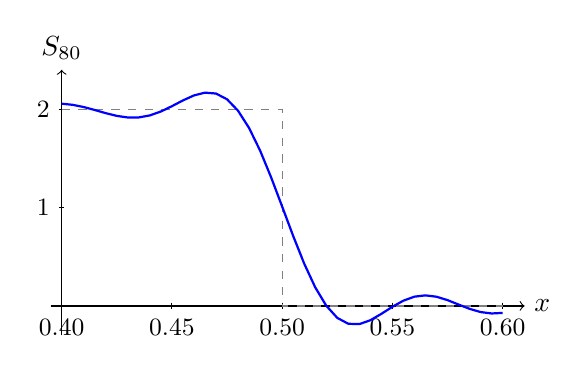
\begin{tikzpicture}[x=28cm,y=1.25cm]
\draw[->] (.395,0)--(.61,0) node[right]{$x$};
\draw[->] (.4,-.3)--(.4,2.4) node[above]{$S_{80}$};
\foreach \x/\lbl in {.4/0.40,.45/0.45,.5/0.50,.55/0.55,.6/0.60} {
 \draw (\x,.035)--(\x,-.035) node[below,font=\small]{$\lbl$};}
\foreach \y in {1,2} {
 \draw (.401,\y)--(.399,\y) node[left,font=\small]{$\y$};}
\draw[dashed,gray] (.4,2)--(.5,2)--(.5,0)--(.6,0);
\draw[blue,thick] plot coordinates {(0.400,2.0550217496) (0.405,2.0434445278) (0.410,2.0209666061) (0.415,1.9909228069) (0.420,1.9587255382) (0.425,1.9310739992) (0.430,1.9147899738) (0.435,1.9154450565) (0.440,1.9360026365) (0.445,1.9757226624) (0.450,2.0295599950) (0.455,2.0882266661) (0.460,2.1389909466) (0.465,2.1671654888) (0.470,2.1581122030) (0.475,2.0994848485) (0.480,1.9833622971) (0.485,1.8079117779) (0.490,1.5782694312) (0.495,1.3064319783) (0.500,1.0101041452) (0.505,0.7106182906) (0.510,0.4302063817) (0.515,0.1890300753) (0.520,0.0024369608) (0.525,-0.1211054656) (0.530,-0.1810437317) (0.535,-0.1845508447) (0.540,-0.1451340717) (0.545,-0.0802662162) (0.550,-0.0084458372) (0.555,0.0537999795) (0.560,0.0944412979) (0.565,0.1075546247) (0.570,0.0937421764) (0.575,0.0593150969) (0.580,0.0144351045) (0.585,-0.0293858766) (0.590,-0.0619021545) (0.595,-0.0763218939) (0.600,-0.0706167386)};
\end{tikzpicture}
\end{center}

The dashed line is the original step function; the solid line connects
all 41 requested computed values. On this grid the largest value is
$S_{80}(0.465)=2.1671654888\ldots$ and the smallest is
$S_{80}(0.535)=-0.1845508446\ldots$.
At the jump the partial sums tend to the midpoint value $1$: the same
computation gives $S_N(1/2)=1.0386$, $0.9893$, $1.0101$, $0.9972$,
$1.0026$ for $N=20$, $40$, $80$, $160$, $320$. The overshoot near the
jump, however, does not die out. On the grid
$x=0.40000(0.00001)0.50000$ (the same recurrence, in double precision)
the maximum of $S_{80}$ is $2.1690$, near $x=0.4665$, about $8.4\%$ of
the jump above $f=2$; for larger $N$ the maximum moves toward $x=1/2$,
while the overshoot approaches the Gibbs fraction of about $9\%$ of the
jump found for Fourier series in Section~19.3 ($S_{640}$ peaks at
$2.1797$ on the same grid). This is
the Gibbs phenomenon; it is not a failure of the exact coefficient
calculation.

\Needspace{5\baselineskip}
\par\bigskip
\noindent\textbf{15.2.24}\quad A plane wave may be expanded in a
series of spherical waves by the Rayleigh equation,
\[
e^{ikr\cos\gamma}=\sum_{n=0}^{\infty}a_{n}j_{n}(kr)P_{n}(\cos\gamma).
\]
Show that $a_{n}=i^{n}(2n+1)$.
\par\emph{Hint.}
\begin{enumerate}
\item[1.] Use the orthogonality of the $P_{n}$ to solve for
$a_{n}j_{n}(kr)$.
\item[2.] Differentiate $n$ times with respect to $(kr)$ and set
$r=0$ to eliminate the $r$-dependence.
\item[3.] Evaluate the remaining integral by Exercise~15.1.15.
\end{enumerate}
\par\emph{Note.}~This problem may also be treated by noting that both
sides of the equation satisfy the Helmholtz equation. The equality
can be established by showing that the solutions have the same
behavior at the origin and also behave alike at large distances.
\solution
Put $z=kr$ and $x=\cos\gamma$. Multiply the proposed expansion by
$P_n(x)$ and integrate over $-1\le x\le1$; by orthogonality,
$\int_{-1}^1P_mP_n\,dx=2\delta_{mn}/(2n+1)$, only the term $m=n$
survives:
\[
a_nj_n(z)=\frac{2n+1}{2}\int_{-1}^1e^{izx}P_n(x)dx.
\]
Expand $e^{izx}=\sum_{j\ge0}(iz)^jx^j/j!$; the series converges
uniformly for $-1\le x\le1$, so it may be integrated term by term.
All powers $x^j$ with $j<n$ have zero integral against $P_n$ by
Exercise 15.1.14, and for $j=n+1$ the integrand $x^{n+1}P_n$ is odd.
With the moment $\int_{-1}^1x^nP_n\,dx=2\cdot n!/(2n+1)!!$ of
Exercise 15.1.15, the right-hand side is therefore
\[
\frac{2n+1}{2}\frac{(iz)^n}{n!}
 \int_{-1}^1x^nP_n(x)dx+O(z^{n+2})
=\frac{(2n+1)i^nz^n}{(2n+1)!!}+O(z^{n+2}).
\]
The power series of $j_n$ (Section 14.7),
$j_n(z)=\sum_{k\ge0}(-1)^kz^{n+2k}/[2^kk!\,(2n+2k+1)!!]$, gives
$j_n(z)=z^n/(2n+1)!!+O(z^{n+2})$, so the left-hand side is
$a_nz^n/(2n+1)!!+O(z^{n+2})$. Comparing the coefficients of $z^n$ gives
\[
\boxed{a_n=i^n(2n+1)}.
\]
This is the procedure of the hint: differentiating both sides $n$ times
and setting $z=0$ removes all other terms and leaves
$a_n\,n!/(2n+1)!!=(2n+1)i^n\,n!/(2n+1)!!$; the common factor
$n!/(2n+1)!!$ cancels. Comparing power-series coefficients avoids any
division by $j_n(z)$, which has zeros. That the series with these
coefficients does sum to $e^{izx}$ is proved by the recurrence
argument in Exercise 15.2.25; Exercise 15.2.27 checks the coefficients
independently, by evaluating
$\frac{2n+1}2\int_{-1}^1e^{izx}P_n\,dx=i^n(2n+1)j_n(z)$ directly.

\Needspace{5\baselineskip}
\par\bigskip
\noindent\textbf{15.2.25}\quad Verify the Rayleigh equation of
Exercise~15.2.24 by starting with the following steps:
\begin{enumerate}
\item[(a)] Differentiate with respect to $(kr)$ to establish
\[
\sum_{n}a_{n}j'_{n}(kr)P_{n}(\cos\gamma)
=i\sum_{n}a_{n}j_{n}(kr)\cos\gamma\,P_{n}(\cos\gamma).
\]
\item[(b)] Use a recurrence relation to replace
$\cos\gamma\,P_{n}(\cos\gamma)$ by a linear combination of $P_{n-1}$
and $P_{n+1}$.
\item[(c)] Use a recurrence relation to replace $j'_{n}$ by a linear
combination of $j_{n-1}$ and $j_{n+1}$.
\end{enumerate}
\solution
Again put $z=kr$, $x=\cos\gamma$, and $F=\sum a_nj_n(z)P_n(x)$.
(a) If $F=e^{izx}$, then $F_z=ixF$. Differentiating the series term by
term (assumed in this derivation of the $a_n$; for the coefficients
found, it is justified in the sufficiency argument below) gives
$F_z=\sum_na_nj_n'(z)P_n(x)$, while
$ixF=i\sum_na_nj_n(z)\,xP_n(x)$; this is the displayed equation.

(b) Use the three-term recurrence
$xP_n=[(n+1)P_{n+1}+nP_{n-1}]/(2n+1)$:
\[
i\sum_na_nj_n\,xP_n
=i\sum_na_nj_n\left[\frac{n+1}{2n+1}P_{n+1}+\frac n{2n+1}P_{n-1}\right].
\]
A given $P_m$ comes from $n=m-1$ in the first term, with factor
$(n+1)/(2n+1)=m/(2m-1)$, and from $n=m+1$ in the second, with factor
$n/(2n+1)=(m+1)/(2m+3)$. So the coefficient of $P_m$ on the right is
\[
i\left[\frac{m\,a_{m-1}}{2m-1}j_{m-1}
+\frac{(m+1)a_{m+1}}{2m+3}j_{m+1}\right].
\]
The first term is absent for $m=0$.

(c) The spherical Bessel recurrence
$mj_{m-1}-(m+1)j_{m+1}=(2m+1)j_m'$ of Exercise 14.7.5 gives
\[
j_m'=\frac{m}{2m+1}j_{m-1}
-\frac{m+1}{2m+1}j_{m+1}
\]
for $m\ge1$; at $m=0$, where the coefficient of $j_{m-1}$ vanishes, it
reads $j_0'=-j_1$. Multiplying both sides of (a) by $P_m$ and
integrating over $-1\le x\le1$ (again term by term), orthogonality
shows that the coefficient $a_mj_m'$ of $P_m$ on the left must equal
the expression in (b). Inserting the recurrence and collecting terms,
\[
\left[\frac{m\,a_m}{2m+1}-\frac{i\,m\,a_{m-1}}{2m-1}\right]j_{m-1}
=\left[\frac{(m+1)a_m}{2m+1}+\frac{i(m+1)a_{m+1}}{2m+3}\right]j_{m+1}.
\]
Near $z=0$, $j_{m-1}$ and $j_{m+1}$ begin with the different powers
$z^{m-1}$ and $z^{m+1}$, so they are linearly independent and both
brackets vanish (for $m=0$ only the right one occurs). Dividing by $m$
and by $m+1$:
\[
\frac{a_m}{2m+1}=\frac{i\,a_{m-1}}{2m-1},\qquad
-\frac{a_m}{2m+1}=\frac{i\,a_{m+1}}{2m+3}.
\]
The first with $m$ replaced by $m+1$ reads $a_{m+1}/(2m+3)=ia_m/(2m+1)$;
the second, multiplied by $-i$ (and $-i\cdot i=1$), reads the same. So both
give the single recurrence $a_{m+1}=i(2m+3)a_m/(2m+1)$. Setting $z=0$
in the expansion, where $j_n(0)=\delta_{n0}$ and $P_0=1$, gives
$a_0=1$; and if $a_m=i^m(2m+1)$, then
$a_{m+1}=i(2m+3)i^m=i^{m+1}(2m+3)$. By induction $a_n=i^n(2n+1)$.

For sufficiency, insert these coefficients in $F$. The spherical
Bessel power series supplies a concrete uniform bound: for $|z|\le M$,
using $(2n+2k+1)!!\ge(2n+1)!!$,
\[
|j_n(z)|\le\sum_{k=0}^\infty
\frac{M^{n+2k}}{2^kk!(2n+2k+1)!!}
\le\frac{M^n}{(2n+1)!!}\sum_{k=0}^\infty\frac{(M^2/2)^k}{k!}
=\frac{M^n}{(2n+1)!!}e^{M^2/2}.
\]
After multiplication by $2n+1$, the ratio of consecutive bounds is
$M(2n-1)!!/(2n+1)!!=M/(2n+1)\to0$. Thus, by the ratio test and the
Weierstrass M test, $\sum(2n+1)|j_n(z)|$ converges uniformly on that
disk. The derivative recurrence above gives
$|j_n'|\le|j_{n-1}|+|j_{n+1}|$, hence the same conclusion for
$\sum(2n+1)|j_n'(z)|$, with $j_0'=-j_1$ handled separately.
Together with $|P_n(x)|\le1$, these bounds justify differentiating
$F$ term by term for $-1\le x\le1$.
The calculation above, read backwards, proves $F_z=ixF$. At zero,
$j_0(0)=1$ and $j_n(0)=0$ for $n>0$, so $F(0,x)=1$.
For fixed $x$, $\partial_z[e^{-izx}F]=e^{-izx}(F_z-ixF)=0$, so
$F(z,x)=F(0,x)e^{izx}=e^{izx}$, verifying the Rayleigh identity for all
finite $z$.

\Needspace{5\baselineskip}
\par\bigskip
\noindent\textbf{15.2.26}\quad From Exercise~15.2.24 show that
\[
j_{n}(kr)=\frac{1}{2i^{n}}\int_{-1}^{1}e^{ikr\mu}P_{n}(\mu)\,d\mu.
\]
This means that (apart from a constant factor) the spherical Bessel
function $j_{n}(kr)$ is an integral transform of the Legendre
polynomial $P_{n}(\mu)$.
\solution
Write the Rayleigh expansion of Exercise 15.2.24 with $z=kr$,
$\mu=\cos\gamma$ and $a_n=i^n(2n+1)$, multiply it by $P_m(\mu)$ and
integrate:
\[
\int_{-1}^1e^{iz\mu}P_m(\mu)d\mu
=\sum_{n\ge0}i^n(2n+1)j_n(z)
 \frac{2\delta_{nm}}{2n+1}
=2i^mj_m(z).
\]
Only $n=m$ survives, by the orthogonality relation
$\int_{-1}^1P_nP_m\,d\mu=2\delta_{nm}/(2n+1)$. Uniform convergence for
$\mu\in[-1,1]$ and fixed $z$ (Exercise 15.2.25: $\sum(2n+1)|j_n(z)|$
converges and $|P_n|\le1$) justifies the interchange of sum and
integral. Divide by $2i^m$ and rename the index:
\[
\boxed{j_n(z)=\frac1{2i^n}\int_{-1}^1e^{iz\mu}P_n(\mu)d\mu}.
\]
The integral is entire in $z$, so the formula also holds for complex
$z$ and at zero, with the usual removable values of $j_n$.

\Needspace{5\baselineskip}
\par\bigskip
\noindent\textbf{15.2.27}\quad Rewriting the formula of
Exercise~15.2.26 as
\[
j_{n}(z)=\frac{1}{2}(-i)^{n}\int_{0}^{\pi}e^{iz\cos\theta}
P_{n}(\cos\theta)\sin\theta\,d\theta,\qquad n=0,1,2,\ldots,
\]
verify it by transforming the right-hand side into
\[
\frac{z^{n}}{2^{n+1}n!}\int_{0}^{\pi}\cos(z\cos\theta)
\sin^{2n+1}\theta\,d\theta
\]
and using Exercise~14.7.9.
\solution
Call the right-hand side $I$. Put $x=\cos\theta$: then
$dx=-\sin\theta\,d\theta$, and $\theta=0,\pi$ become $x=1,-1$, so
reversing the limits absorbs the minus sign. Then insert Rodrigues'
formula, $P_n=D^n(x^2-1)^n/(2^nn!)$ with $D=d/dx$:
\[
I=\frac{(-i)^n}{2}\int_{-1}^1e^{izx}P_n(x)dx
=\frac{(-i)^n}{2^{n+1}n!}
 \int_{-1}^1e^{izx}D^n(x^2-1)^n dx.
\]
Integrate by parts $n$ times, moving one $D$ at a time onto the
exponential. As in Exercise 15.1.14, $D^k(x^2-1)^n$ vanishes at
$x=\pm1$ for $k<n$, so every boundary term vanishes, and since
$De^{izx}=ize^{izx}$ each step contributes a factor $-iz$:
\[
\int_{-1}^1e^{izx}D^n(x^2-1)^ndx
=(-iz)^n\int_{-1}^1e^{izx}(x^2-1)^ndx.
\]
Since $(-i)^n(-i)^n=(-1)^n$ and $(x^2-1)^n=(-1)^n(1-x^2)^n$, the two
signs cancel:
\[
I=\frac{z^n}{2^{n+1}n!}\int_{-1}^1e^{izx}(1-x^2)^n dx.
\]
Write $e^{izx}=\cos zx+i\sin zx$. The sine part is odd in $x$ and
integrates to zero, even for complex $z$. Returning to $\theta$ in the
cosine part ($1-x^2=\sin^2\theta$, $dx\to\sin\theta\,d\theta$ as
before) gives exactly
\[
I=\frac{z^n}{2^{n+1}n!}\int_0^\pi
\cos(z\cos\theta)\sin^{2n+1}\theta\,d\theta,
\]
the Poisson integral that Exercise 14.7.9 identifies with $j_n(z)$.
To verify the spherical Bessel value directly, expand
$\cos zx=\sum_k(-1)^kz^{2k}x^{2k}/(2k)!$ (uniformly convergent on
$[-1,1]$) and integrate each term; with $u=x^2$ on the even integrand,
\[
\int_{-1}^1x^{2k}(1-x^2)^ndx
=\int_0^1u^{k-1/2}(1-u)^n\,du
=B(k+\tfrac12,n+1)
=\frac{\Gamma(k+1/2)n!}{\Gamma(k+n+3/2)}.
\]
With $\Gamma(k+\frac12)=(2k)!\sqrt\pi/(4^kk!)$ and
$\Gamma(k+n+\frac32)=(2n+2k+1)!!\sqrt\pi/2^{k+n+1}$, the $k$th term of
$I$ is
\[
\frac{z^n}{2^{n+1}n!}\,\frac{(-1)^kz^{2k}}{(2k)!}\,
\frac{(2k)!\,n!}{4^kk!}\,\frac{2^{k+n+1}}{(2n+2k+1)!!}
=\frac{(-1)^kz^{n+2k}}{2^kk!\,(2n+2k+1)!!}.
\]
Therefore
\[
I=\sum_{k=0}^\infty
\frac{(-1)^kz^{n+2k}}{2^kk!(2n+2k+1)!!}=j_n(z),
\]
the power series of $j_n$ (Section 14.7). This reproduces the
Poisson representation of Exercise 14.7.9 without assuming it.

\Needspace{8\baselineskip}
\subsection*{15.3 Physical Interpretation of Generating Function}

\Needspace{5\baselineskip}
\par\bigskip
\noindent\textbf{15.3.1}\quad Develop the electrostatic potential for
the array of charges shown in Fig.~15.7. This is a linear electric
quadrupole.
\solution
In Fig.~15.7 the charges are $q,-2q,q$ at $z=-a,0,a$.
Coulomb's law therefore gives, at every point away from these charges,
\[
V=\frac{q}{4\pi\varepsilon_0}
\left[\frac1{\sqrt{r^2+a^2+2ar\cos\theta}}-\frac2r
+\frac1{\sqrt{r^2+a^2-2ar\cos\theta}}\right].
\]
For $r>a$, expand the two displaced charges with the generating
function, $t=\pm a/r$:
\[
\frac1{\sqrt{r^2+a^2\mp2ar\cos\theta}}
=\frac1r\Bigl[1\mp2\frac ar\cos\theta+\frac{a^2}{r^2}\Bigr]^{-1/2}
=\sum_{n=0}^\infty\frac{(\pm a)^n}{r^{n+1}}P_n(\cos\theta).
\]
Their $n$th coefficients add to $1+(-1)^n$, which is $0$ for odd $n$
and $2$ for even $n$. The $n=0$ term, $2/r$, cancels the central
charge's $-2/r$, and $n=2s$ leaves $2a^{2s}/r^{2s+1}$:
\[
\boxed{V=\frac{2q}{4\pi\varepsilon_0r}
\sum_{s=1}^\infty\left(\frac ar\right)^{2s}P_{2s}(\cos\theta)}.
\]
In particular,
\[
V=\frac{2qa^2}{4\pi\varepsilon_0r^3}P_2(\cos\theta)
+O(a^4/r^5)
=\frac{qa^2(3\cos^2\theta-1)}{4\pi\varepsilon_0r^3}
+O(a^4/r^5).
\]
The total charge and dipole moment are zero, while
$\sum q_i z_i^2=2qa^2\ne0$, identifying the leading quadrupole.

\Needspace{5\baselineskip}
\par\bigskip
\noindent\textbf{15.3.2}\quad Calculate the electrostatic potential of
the array of charges shown in Fig.~15.8. Here is an example of two
equal but oppositely directed quadrupoles. The quadrupole
contributions cancel. The octopole terms do not cancel.
\solution
Figure 15.8 has charges $-q,2q,-2q,q$ at $-2a,-a,a,2a$.
Thus the exact potential is
\[
V=\frac{q}{4\pi\varepsilon_0}
\left[-\frac1{|\mathbf r+2a\hat{\mathbf z}|}
+\frac2{|\mathbf r+a\hat{\mathbf z}|}
-\frac2{|\mathbf r-a\hat{\mathbf z}|}
+\frac1{|\mathbf r-2a\hat{\mathbf z}|}\right].
\]
For $r>2a$, expand each term with the generating function,
$1/|\mathbf r-c\hat{\mathbf z}|=\sum_nc^nP_n(\cos\theta)/r^{n+1}$ for
$|c|<r$, with $c=-2a,-a,a,2a$. The coefficient of
$(q/4\pi\varepsilon_0)a^nP_n(\cos\theta)/r^{n+1}$ is
\[
-(-2)^n+2(-1)^n-2+2^n
=[1-(-1)^n](2^n-2).
\]
For even $n$ the four terms cancel in pairs; for odd $n$ they give
$2^{n+1}-4=2(2^n-2)$. So the coefficient is zero for every even $n$ and
also for $n=1$. Putting $n=2s+1$ leaves
\[
\boxed{V=\frac{2q}{4\pi\varepsilon_0r}
\sum_{s=1}^\infty(2^{2s+1}-2)
\left(\frac ar\right)^{2s+1}P_{2s+1}(\cos\theta)}.
\]
The leading term ($s=1$, with $2^3-2=6$) is
\[
\boxed{V_{\rm oct}=\frac{12qa^3}{4\pi\varepsilon_0r^4}
P_3(\cos\theta)}.
\]
This also follows from the axial moments $\mu_n=\sum_iq_iz_i^n$, in
terms of which the same expansion reads
$V=\sum_n\mu_nP_n(\cos\theta)/(4\pi\varepsilon_0r^{n+1})$:
$\mu_0=\mu_1=\mu_2=0$ and
$\mu_3=q[-(-2)^3+2(-1)^3-2+2^3]a^3=q[8-2-2+8]a^3=12qa^3$.

\Needspace{5\baselineskip}
\par\bigskip
\noindent\textbf{15.3.3}\quad Show that the electrostatic potential
produced by a charge $q$ at $z=a$ for $r<a$ is
\[
\varphi(r)=\frac{q}{4\pi\varepsilon_{0}a}
\sum_{n=0}^{\infty}\left(\frac{r}{a}\right)^{n}P_{n}(\cos\theta).
\]
\solution
The source-point distance is
$|\mathbf r-a\hat{\mathbf z}|=\sqrt{a^2+r^2-2ar\cos\theta}$.
For $0\le r<a$, factor out $a$ and use the generating function with
$t=r/a$:
\[
\varphi=\frac{q}{4\pi\varepsilon_0a}
\left[1-2\frac ra\cos\theta+\left(\frac ra\right)^2\right]^{-1/2}
=\boxed{\frac{q}{4\pi\varepsilon_0a}
\sum_{n=0}^\infty\left(\frac ra\right)^nP_n(\cos\theta)}.
\]
For each fixed $r<a$ the series converges uniformly in $\theta$, since
$|P_n(\cos\theta)|\le1$ bounds its terms by those of the geometric
series $\sum_n(r/a)^n$. At $r=0$ the value is
$q/(4\pi\varepsilon_0a)$, with all higher terms vanishing.

\Needspace{5\baselineskip}
\par\bigskip
\noindent\textbf{15.3.4}\quad Using $\mathbf{E}=-\nabla\varphi$,
determine the components of the electric field corresponding to the
(pure) electric dipole potential,
\[
\varphi(r)=\frac{2aq\,P_{1}(\cos\theta)}{4\pi\varepsilon_{0}r^{2}}.
\]
Here it is assumed that $r\gg a$.
\par\nobreak\hfill\emph{ANS.}\enspace
$E_{r}=+\dfrac{4aq\cos\theta}{4\pi\varepsilon_{0}r^{3}}$,\quad
$E_{\theta}=+\dfrac{2aq\sin\theta}{4\pi\varepsilon_{0}r^{3}}$,\quad
$E_{\varphi}=0$.
\solution
Since $P_1(\cos\theta)=\cos\theta$, put $C=2aq/(4\pi\varepsilon_0)$
and write $\varphi=C r^{-2}\cos\theta$.
The spherical gradient gives
\[
E_r=-\partial_r\varphi=2Cr^{-3}\cos\theta,\qquad
E_\theta=-\frac1r\partial_\theta\varphi=Cr^{-3}\sin\theta,
\qquad E_\varphi=-\frac1{r\sin\theta}\partial_\varphi\varphi=0.
\]
Substituting $C$ yields all three stated components. For a pair of
charges separated by $2a$ these are its leading $r\gg a$ terms;
for an ideal point dipole of fixed moment $2aq$ they are exact at $r>0$.

\Needspace{5\baselineskip}
\par\bigskip
\noindent\textbf{15.3.5}\quad Operating in spherical polar
coordinates, show that \erratum{for $r>0$}
\[
\frac{\partial}{\partial z}\left[\frac{P_{l}(\cos\theta)}{r^{l+1}}\right]
=-(l+1)\frac{P_{l+1}(\cos\theta)}{r^{l+2}}.
\]
This is the key step in the mathematical argument that the derivative
of one multipole leads to the next higher multipole.
\par\emph{Hint.}~Compare with Exercise~3.10.28.
\solution
At fixed Cartesian $x,y$, write $\rho=\sqrt{x^2+y^2}$,
$r=\sqrt{\rho^2+z^2}$ and $u=z/r=\cos\theta$. Then
\[
\frac{\partial r}{\partial z}=\frac zr=u,\qquad
\frac{\partial u}{\partial z}=\frac1r-\frac z{r^2}\frac{\partial r}{\partial z}
=\frac1r-\frac{z^2}{r^3}=\frac{1-u^2}{r}.
\]
Hence, by the product and chain rules,
\begin{align*}
\partial_z\!\left[r^{-l-1}P_l(u)\right]
&=-(l+1)r^{-l-2}u\,P_l(u)+r^{-l-1}P_l'(u)\frac{1-u^2}r\\
&=r^{-l-2}\left[-(l+1)uP_l(u)+(1-u^2)P_l'(u)\right].
\end{align*}
Exercise 15.1.7 gives
$(1-u^2)P_l'=(l+1)(uP_l-P_{l+1})$.
The $uP_l$ terms cancel, leaving
\[
\boxed{\partial_z\!\left[\frac{P_l(\cos\theta)}{r^{l+1}}\right]
=-(l+1)\frac{P_{l+1}(\cos\theta)}{r^{l+2}}},\qquad r>0.
\]
Both sides are singular at the origin, where $\theta$ is undefined;
hence the restriction $r>0$ added to the statement.
This chain-rule calculation is equivalent to
$\partial_z=\cos\theta\,\partial_r-(\sin\theta/r)\partial_\theta$.

\Needspace{5\baselineskip}
\par\bigskip
\noindent\textbf{15.3.6}\quad A point electric dipole of strength
$p^{(1)}$ is placed at $z=a$; a second point electric dipole of equal
but opposite strength is at the origin. Keeping the product
$p^{(1)}a$ constant, let $a\to0$. Show that this results in a point
electric quadrupole.
\par\emph{Hint.}~Exercise~15.3.5 (when proved) will be helpful.
\solution
Define $F_1(\mathbf r)=P_1(\cos\theta)/r^2$.
The positive $z$ dipole at $a\hat{\mathbf z}$ and its negative at zero
have combined potential
\[
V_a(\mathbf r)=\frac{p^{(1)}}{4\pi\varepsilon_0}
[F_1(\mathbf r-a\hat{\mathbf z})-F_1(\mathbf r)].
\]
At each fixed point away from the origin, Taylor expansion in $a$ gives
$F_1(\mathbf r-a\hat{\mathbf z})-F_1(\mathbf r)
=-a\,\partial_zF_1+O(a^2)$.
Exercise 15.3.5 with $l=1$ evaluates $\partial_zF_1=-2P_2/r^3$, so
\[
V_a=\frac{p^{(1)}}{4\pi\varepsilon_0}
\left[\frac{2aP_2(\cos\theta)}{r^3}+O(a^2)\right]
=\frac{2p^{(1)}a\,P_2(\cos\theta)}{4\pi\varepsilon_0r^3}
+p^{(1)}O(a^2).
\]
Holding $K=p^{(1)}a$ fixed, the error is $p^{(1)}O(a^2)=O(Ka)\to0$, so
\[
\boxed{V_{\rm quad}=\frac{2K}{4\pi\varepsilon_0r^3}
P_2(\cos\theta)}.
\]
In the convention $V_{\rm quad}=p^{(2)}P_2/(4\pi\varepsilon_0r^3)$,
the resulting quadrupole strength is $p^{(2)}=2ap^{(1)}$.
The dipole terms cancel, while a nonzero $r^{-3}P_2$ term remains.

\Needspace{5\baselineskip}
\par\bigskip
\noindent\textbf{15.3.7}\quad A point electric octupole may be
constructed by placing a point electric quadrupole (pole strength
$p^{(2)}$ in the $z$-direction) at $z=a$ and an equal but opposite
point electric quadrupole at $z=0$ and then letting $a\to0$, subject
to $p^{(2)}a=\mathrm{constant}$. Find the electrostatic potential
corresponding to a point electric octupole. Show from the
construction of the point electric octupole that the corresponding
potential may be obtained by differentiating the point quadrupole
potential.
\solution
Use the same strength convention:
$V^{(2)}=p^{(2)}P_2(\cos\theta)/(4\pi\varepsilon_0r^3)$.
For a positive quadrupole displaced to $z=a$ and its negative at zero,
\[
V_a^{(3)}=\frac{p^{(2)}}{4\pi\varepsilon_0}
\left[F_2(\mathbf r-a\hat{\mathbf z})-F_2(\mathbf r)\right],
\qquad F_2=\frac{P_2(\cos\theta)}{r^3}.
\]
The Taylor difference is $-a\partial_zF_2+O(a^2)$, and
Exercise 15.3.5 with $l=2$ gives $\partial_zF_2=-3P_3/r^4$, so
$V_a^{(3)}=3ap^{(2)}P_3/(4\pi\varepsilon_0r^4)+p^{(2)}O(a^2)$.
Therefore, keeping $K_2=ap^{(2)}$ fixed and using
$P_3=\frac12(5\cos^3\theta-3\cos\theta)$,
\[
\boxed{V^{(3)}=\frac{3K_2}{4\pi\varepsilon_0r^4}P_3(\cos\theta)
=\frac{3K_2}{8\pi\varepsilon_0r^4}(5\cos^3\theta-3\cos\theta)}.
\]
Thus $p^{(3)}=3ap^{(2)}$ in this convention, and the construction
is precisely $V^{(3)}=-a\,\partial_zV^{(2)}$ in the limiting sense.
The sign is set by putting the positive source at $+a$.
\erratum{The Instructor's Manual, p.~245, instead writes $48a^3q$ for
the numerator of the octupole moment, although this exercise supplies
$p^{(2)}$, not a charge $q$. In the stated strength convention the
moment is $3ap^{(2)}$. That form would agree only after the
additional, unstated assignment $p^{(2)}=16a^2q$.}

\Needspace{5\baselineskip}
\par\bigskip
\noindent\textbf{15.3.8}\quad A point charge $q$ is in the interior of
a hollow conducting sphere of radius $r_{0}$. The charge $q$ is
displaced a distance \erratum{$0<a<r_0$} from the center of the sphere. If the
conducting sphere is grounded, show that the potential in the
interior produced by $q$ and the distributed induced charge is the
same as that produced by $q$ and its image charge $q'$. The image
charge is at a distance $a'=r_{0}^{2}/a$ from the center, collinear
with $q$ and the origin (Fig.~15.9).
\par\emph{Hint.}~Calculate the electrostatic potential for
$a<r_{0}<a'$. Show that the potential vanishes for $r=r_{0}$ if we
take $q'=-qr_{0}/a$.
\solution
For $0<a<r_0$, place $q'=-qr_0/a$ at $a'=r_0^2/a>r_0$.
The restriction added to the statement is needed: for $a=0$ there is
no image point $a'$ (that case is treated as a limit at the end), and
$a<r_0$ puts $q$ inside the sphere and its image outside.
Consider
\[
V(\mathbf r)=\frac1{4\pi\varepsilon_0}
\left[\frac q{|\mathbf r-a\hat{\mathbf z}|}
-\frac{qr_0/a}{|\mathbf r-a'\hat{\mathbf z}|}\right].
\]
On $r=r_0$, $|\mathbf r-a\hat{\mathbf z}|^2=r_0^2+a^2-2ar_0\cos\theta$,
and the two distances satisfy
\[
|\mathbf r-a'\hat{\mathbf z}|^2
=r_0^2+\frac{r_0^4}{a^2}-\frac{2r_0^3}{a}\cos\theta
=\frac{r_0^2}{a^2}|\mathbf r-a\hat{\mathbf z}|^2.
\]
Their positive square roots therefore satisfy
$|\mathbf r-a'\hat{\mathbf z}|=(r_0/a)|\mathbf r-a\hat{\mathbf z}|$,
and the two potential terms cancel exactly.

The Legendre version of the same cancellation uses expansions valid
for $a<r<a'$, a range that contains the sphere $r=r_0$.
There $r>a$ and $r<a'$, so the generating function gives
$1/|\mathbf r-a\hat{\mathbf z}|=\sum_na^nP_n/r^{n+1}$ and
$1/|\mathbf r-a'\hat{\mathbf z}|=\sum_nr^nP_n/(a')^{n+1}$ (as in
Exercise 15.3.3), hence
\[
V=\frac1{4\pi\varepsilon_0}\sum_{n=0}^\infty
\left[\frac{qa^n}{r^{n+1}}+
\frac{q'r^n}{(a')^{n+1}}\right]P_n(\cos\theta).
\]
At $r=r_0$, inserting $q'=-qr_0/a$ and
$(a')^{n+1}=r_0^{2n+2}/a^{n+1}$ makes each bracket zero:
\[
\frac{q'r_0^n}{(a')^{n+1}}
=-\frac{qr_0}a\,\frac{r_0^n\,a^{n+1}}{r_0^{2n+2}}
=-\frac{qa^n}{r_0^{n+1}}.
\]
The image term is harmonic everywhere inside the sphere, because its
source is outside; the real charge has exactly the required Coulomb
singularity. The difference from any other grounded solution is
harmonic, including across the canceled source singularity, and zero
on the boundary. Uniqueness for the Dirichlet problem proves the result
throughout the interior, including $r<a$, where the first expansion
diverges.
For $a=0$, take the limit directly: as $a\to0$, $a'\to\infty$ and the
image term tends to $-(qr_0/a)/a'=-q/r_0$, so
$V=q(1/r-1/r_0)/(4\pi\varepsilon_0)$.

\Needspace{8\baselineskip}
\subsection*{15.4 Associated Legendre Equation}

\Needspace{5\baselineskip}
\par\bigskip
\noindent\textbf{15.4.1}\quad Apply the Frobenius method to
Eq.~(15.72) to obtain Eq.~(15.73) and verify that the numerator of
that equation becomes zero if $\lambda=l(l+1)$ and $j=l-m$.
\solution
Write $U$ for the factor multiplying $(1-x^2)^{m/2}$ in the associated
Legendre function; Eq. (15.72) is
\[
(1-x^2)U''-2(m+1)xU'+[\lambda-m(m+1)]U=0.
\]
For $U=\sum_{j\ge0}a_jx^{j+k}$, the lowest power $x^{k-2}$
has coefficient $k(k-1)a_0$, so $k=0$ or $1$.
The next power, $x^{k-1}$, has coefficient $k(k+1)a_1$.
Thus $k=1$ forces $a_1=0$, whereas $k=0$ leaves $a_0,a_1$
independent; these are the even and odd branches at the ordinary
point $x=0$.
In general, $x^{j+k}$ receives
$(j+k+2)(j+k+1)a_{j+2}-(j+k)(j+k-1)a_j$ from $(1-x^2)U''$ (the first
part from the term $a_{j+2}x^{j+k+2}$), $-2(m+1)(j+k)a_j$ from
$-2(m+1)xU'$, and $[\lambda-m(m+1)]a_j$ from the last term. So the
coefficient of $x^{j+k}$ is
\[
(j+k+2)(j+k+1)a_{j+2}
+\{\lambda-m(m+1)-(j+k)(j+k-1)-2(m+1)(j+k)\}a_j.
\]
Set it to zero, using
$(j+k)(j+k-1)+2(m+1)(j+k)=(j+k)^2+(2m+1)(j+k)$:
\[
a_{j+2}=
\frac{(j+k)^2+(2m+1)(j+k)-\lambda+m(m+1)}
{(j+k+1)(j+k+2)}a_j.
\]
For $k=0$ the numerator is $j^2+(2m+1)j+m(m+1)-\lambda
=(j+m)(j+m+1)-\lambda$, and this is exactly Eq. (15.73).
If $\lambda=l(l+1)$, put $p=j+m$; the numerator factors as
\[
p(p+1)-l(l+1)=(p-l)(p+l)+(p-l)=(j+m-l)(j+m+l+1),
\]
which vanishes at $j=l-m$. The parity of $l-m$ selects the even
or odd power series. For nonnegative integers $m\le l$, that branch
terminates in a polynomial of degree $l-m$.

\Needspace{5\baselineskip}
\par\bigskip
\noindent\textbf{15.4.2}\quad Starting from the entries for $P_{2}^{2}$
and $P_{2}^{1}$ in Table~15.3, apply a recurrence formula to obtain
$P_{2}^{0}$ (which is $P_{2}$), $P_{2}^{-1}$, and $P_{2}^{-2}$.
Compare your results with the value of $P_{2}$ from Table~15.1 and
with values of $P_{2}^{-1}$ and $P_{2}^{-2}$ obtained by applying
Eq.~(15.81) to entries from Table~15.3.
\solution
Put $s=\sqrt{1-x^2}$ on $-1<x<1$.
Table 15.3 gives $P_2^2=3(1-x^2)=3s^2$ and $P_2^1=-3xs$.
Use the fixed-degree recurrence of Exercise 15.4.8 with $l=2$, so
that $l(l+1)=6$:
\[
P_2^{m+1}+\frac{2mx}{s}P_2^m+[6-m(m-1)]P_2^{m-1}=0.
\]
At $m=1$, this gives
$3s^2+\frac{2x}{s}(-3xs)+6P_2^0=3s^2-6x^2+6P_2^0=0$, so
$P_2^0=x^2-\frac12(1-x^2)$, i.e.
\[
\boxed{P_2^0=\frac{3x^2-1}{2}},
\]
which is $P_2$ of Table 15.1.
At $m=0$ the middle term is absent and $6-0=6$:
$P_2^1+6P_2^{-1}=0$, so
\[
\boxed{P_2^{-1}=-\frac16(-3xs)=\frac12xs}.
\]
At $m=-1$, $6-(-1)(-2)=4$ and
$P_2^0-(2x/s)P_2^{-1}+4P_2^{-2}=0$.
Substituting the two results, $(2x/s)(xs/2)=x^2$ and
$4P_2^{-2}=x^2-(3x^2-1)/2=(1-x^2)/2=s^2/2$, so
\[
\boxed{P_2^{-2}=\frac18(1-x^2)}.
\]
For the comparison the exercise asks for, Eq. (15.81),
$P_l^{-m}=(-1)^m[(l-m)!/(l+m)!]P_l^m$, applied to the Table 15.3
entries predicts
$P_2^{-1}=-(1!/3!)P_2^1=xs/2$ and
$P_2^{-2}=(0!/4!)P_2^2=3s^2/24=s^2/8$, in agreement.
(For $P_2^{-1}$ and $P_2^{-2}$ this is a consistency check rather than
an independent derivation, since Exercise 15.4.8 proves the recurrence
for $m\le0$ from Eq. (15.81), in the form of Exercise 15.4.3.)
The endpoint values follow by continuity.

\Needspace{5\baselineskip}
\par\bigskip
\noindent\textbf{15.4.3}\quad Prove that, \erratum{for integers $0\le m\le l$ and
$-1<x<1$},
\[
P_{l}^{-m}(x)=(-1)^{m}\frac{(l-m)!}{(l+m)!}\,P_{l}^{m}(x),
\]
where $P_{l}^{m}(x)$ is defined by
\[
P_{l}^{m}(x)=\frac{(-1)^{m}}{2^{l}l!}(1-x^{2})^{m/2}
\frac{d^{l+m}}{dx^{l+m}}(x^{2}-1)^{l}.
\]
\par\emph{Hint.}~One approach is to apply Leibniz's formula to
$(x+1)^{l}(x-1)^{l}$.
\solution
Let $F=(x-1)^l(x+1)^l$, $D=d/dx$, and take integers $0\le m\le l$.
Leibniz's rule, $D^N(fg)=\sum_i\binom Ni D^if\,D^{N-i}g$, with
$D^i(x\mp1)^l=\frac{l!}{(l-i)!}(x\mp1)^{l-i}$ for $i\le l$ (and zero for
$i>l$), gives for $N=l-m$, with $i=j$,
\[
D^{l-m}F=\sum_{j=0}^{l-m}
\frac{(l-m)!(l!)^2(x-1)^{l-j}(x+1)^{m+j}}
{j!(l-m-j)!(l-j)!(m+j)!}.
\]
For $D^{l+m}F$, the number $i$ of derivatives on the first factor
must lie between $m$ and $l$, because neither factor survives more than
$l$ derivatives. Write $i=m+j$, so the second factor receives $l-j$
derivatives:
\[
D^{l+m}F=\sum_{j=0}^{l-m}
\frac{(l+m)!(l!)^2(x-1)^{l-m-j}(x+1)^j}
{(m+j)!(l-j)!(l-m-j)!j!}.
\]
Multiplication of the second sum by $(x^2-1)^m=(x-1)^m(x+1)^m$ makes
its powers $(x-1)^{l-j}(x+1)^{m+j}$, exactly those of the first sum.
The remaining factors $(l!)^2/[j!(l-m-j)!(l-j)!(m+j)!]$ are the same in
both sums, so the coefficients differ only by the ratio
$(l-m)!/(l+m)!$. Thus
\[
D^{l-m}F=\frac{(l-m)!}{(l+m)!}(x^2-1)^mD^{l+m}F.
\]
Insert this identity into the Rodrigues definition with order $-m$,
where $(-1)^{-m}=(-1)^m$ and $(x^2-1)^m=(-1)^m(1-x^2)^m$:
\begin{align*}
P_l^{-m}
&=\frac{(-1)^m}{2^ll!}(1-x^2)^{-m/2}
 \frac{(l-m)!}{(l+m)!}(-1)^m(1-x^2)^mD^{l+m}F\\
&=(-1)^m\frac{(l-m)!}{(l+m)!}\,
 \frac{(-1)^m}{2^ll!}(1-x^2)^{m/2}D^{l+m}F
=\boxed{(-1)^m\frac{(l-m)!}{(l+m)!}P_l^m}.
\end{align*}
On $(-1,1)$ choose the positive square root of $1-x^2$.
The restrictions added to the statement are needed: for $m>l$ the
definition of $P_l^{-m}$ would require a derivative of negative order
$l-m$, and $(l-m)!$ is undefined; at $x=\pm1$ its factor
$(1-x^2)^{-m/2}$ is undefined for $m\ge1$, although both sides extend
continuously there. (Orders $-l\le m<0$ give the same identity solved
for $P_l^{|m|}$.)
The identity also extends with any consistently chosen complex branch.

\Needspace{5\baselineskip}
\par\bigskip
\noindent\textbf{15.4.4}\quad Show that
\begin{align*}
P_{2l}^{1}(0)&=0,\\
P_{2l+1}^{1}(0)&=(-1)^{l+1}\frac{(2l+1)!!}{(2l)!!},
\end{align*}
by each of these three methods:
\begin{enumerate}
\item[(a)] Use of recurrence relations,
\item[(b)] Expansion of the generating function,
\item[(c)] Rodrigues formula.
\end{enumerate}
\solution
Write the index of the statement as $s$, so the claims are
$P_{2s}^1(0)=0$ and $P_{2s+1}^1(0)=(-1)^{s+1}(2s+1)!!/(2s)!!$.

(a) The fixed-order recurrence
$(2l+1)xP_l^m=(l+m)P_{l-1}^m+(l-m+1)P_{l+1}^m$ (also used in
Exercise 15.4.12) at $x=0$, with $m=1$, gives
\[
lP_{l+1}^1(0)=-(l+1)P_{l-1}^1(0),\qquad l\ge1.
\]
The starting values are $P_0^1(0)=0$ and $P_1^1(0)=-1$, from
$P_0^1=0$ and $P_1^1=-\sqrt{1-x^2}$.
Odd $l$ link the even indices, so every even-index value is zero.
For the odd subsequence, $l=2k$ gives
$P_{2k+1}^1(0)=-\frac{2k+1}{2k}P_{2k-1}^1(0)$; using
$k=1,2,\ldots,s$ in turn,
\[
P_{2s+1}^1(0)=(-1)^s\frac{3\cdot5\cdots(2s+1)}
{2\cdot4\cdots2s}P_1^1(0)
=\boxed{(-1)^{s+1}\frac{(2s+1)!!}{(2s)!!}}.
\]

(b) Differentiate the generating function
$\sum_lP_l(x)t^l=(1-2xt+t^2)^{-1/2}$ with respect to $x$:
$\sum_lP_l'(x)t^l=t(1-2xt+t^2)^{-3/2}$. At $x=0$,
$P_l^1(0)=-\sqrt{1-0}\,P_l'(0)=-P_l'(0)$, so the binomial series
gives
\[
\sum_{l\ge0}P_l^1(0)t^l=-t(1+t^2)^{-3/2}
=-\sum_{s\ge0}(-1)^s\frac{(2s+1)!!}{2^ss!}t^{2s+1},
\]
because
\[
\binom{-3/2}{s}=\frac{(-\frac32)(-\frac52)\cdots(-\frac{2s+1}2)}{s!}
=(-1)^s\frac{(2s+1)!!}{2^ss!}.
\]
There are no even powers, and $2^ss!=(2s)!!$, so the coefficient of
$t^{2s+1}$ is $(-1)^{s+1}(2s+1)!!/(2s)!!$: the same values.

(c) Since $P_n^1(0)=-P_n'(0)$, which is minus the coefficient of $x$
in $P_n$, Rodrigues' formula gives
\[
P_n^1(0)=-\frac1{2^nn!}D^{n+1}(x^2-1)^n\Big|_{x=0},\qquad
(x^2-1)^n=\sum_{k=0}^n\binom nk(-1)^{n-k}x^{2k}.
\]
At $x=0$, $D^{n+1}x^{2k}$ is nonzero only for $2k=n+1$, when it equals
$(n+1)!$. For $n=2s$ no such $k$ exists, so $P_{2s}^1(0)=0$. For
$n=2s+1$ the term is $k=s+1$, with $(-1)^{n-k}=(-1)^s$:
\[
P_{2s+1}^1(0)=-\frac{(-1)^s}{2^{2s+1}(2s+1)!}
\binom{2s+1}{s+1}(2s+2)!
=(-1)^{s+1}\frac{(2s+2)!}{2^{2s+1}s!\,(s+1)!}.
\]
With $(2s+2)!=(2s+1)!!\,(2s+2)!!=(2s+1)!!\,2^{s+1}(s+1)!$ this is
$(-1)^{s+1}(2s+1)!!/(2^ss!)=(-1)^{s+1}(2s+1)!!/(2s)!!$.
This proves both formulas by the third requested method.

\Needspace{5\baselineskip}
\par\bigskip
\noindent\textbf{15.4.5}\quad Evaluate $P_{l}^{m}(0)$ for \erratum{integers $-l\le m\le l$}.
\par\nobreak\hfill\emph{ANS.}\enspace
$P_{l}^{m}(0)=\begin{cases}
(-1)^{(l+m)/2}\dfrac{(l+m-1)!!}{(l-m)!!}, & l+m\text{ even},\\[10pt]
0, & l+m\text{ odd}.
\end{cases}$
\solution
For integers $0\le m\le l$, the definition
$P_l^m=(-1)^m(1-x^2)^{m/2}D^mP_l$ ($D=d/dx$) gives
$P_l^m(0)=(-1)^mP_l^{(m)}(0)$, and by Taylor's formula
$P_l^{(m)}(0)=m!\,c_m$, where $c_m$ is the coefficient of $x^m$ in $P_l$.
The powers in $P_l$ are $l,l-2,\ldots$ (Exercise 15.1.2), so $c_m=0$
when $l+m$ is odd.
If $l+m$ is even, the power $x^{l-2k}=x^m$ of Exercise 15.1.2 has
$k=(l-m)/2$, so that $2l-2k=l+m$, $l-k=(l+m)/2$ and $l-2k=m$:
\[
c_m=(-1)^{(l-m)/2}\frac{(l+m)!}{2^l[(l-m)/2]!\,[(l+m)/2]!\,m!}.
\]
Multiplying by $(-1)^mm!$ and using
$(-1)^m(-1)^{(l-m)/2}=(-1)^{(l+m)/2}$ gives
\[
P_l^m(0)=
(-1)^{(l+m)/2}
\frac{(l+m)!}{2^l[(l-m)/2]![(l+m)/2]!}.
\]
Write $2^l=2^{(l+m)/2}\,2^{(l-m)/2}$ and split the factorials into even
and odd factors, $(l+m)!=(l+m)!!\,(l+m-1)!!$ with
$(l+m)!!=2^{(l+m)/2}[(l+m)/2]!$:
\[
\frac{(l+m)!}{2^{(l+m)/2}[(l+m)/2]!}=(l+m-1)!!,\qquad
2^{(l-m)/2}[(l-m)/2]!=(l-m)!!.
\]
Hence the stated nonzero value is
\[
\boxed{P_l^m(0)=(-1)^{(l+m)/2}\frac{(l+m-1)!!}{(l-m)!!}}.
\]
For $m=0$ this is $P_l(0)=(-1)^{l/2}(l-1)!!/l!!$ for even $l$, as in
Exercise 15.1.12, and $m=1$ reproduces Exercise 15.4.4.

Negative orders need no separate formula. For $m=-\mu$ with
$1\le\mu\le l$, Exercise 15.4.3 gives
$P_l^{-\mu}(0)=(-1)^\mu\frac{(l-\mu)!}{(l+\mu)!}P_l^\mu(0)$, which
vanishes when $l+\mu$, and hence $l+m=l-\mu$, is odd. Otherwise, by
$(l-\mu)!/(l-\mu)!!=(l-\mu-1)!!$, $(l+\mu)!/(l+\mu-1)!!=(l+\mu)!!$ and
$(-1)^{\mu+(l+\mu)/2}=(-1)^{(l-\mu)/2+2\mu}=(-1)^{(l-\mu)/2}$,
\[
P_l^{-\mu}(0)=(-1)^\mu\frac{(l-\mu)!}{(l+\mu)!}\,
(-1)^{(l+\mu)/2}\frac{(l+\mu-1)!!}{(l-\mu)!!}
=(-1)^{(l-\mu)/2}\frac{(l-\mu-1)!!}{(l+\mu)!!},
\]
which is the boxed formula with $m=-\mu$.
The restriction $|m|\le l$ in the statement is needed: for integer
$m>l$ the defining derivative makes $P_l^m=0$, while for even $l+m$ the
factorial expression would contain $(l-m)!!$ with $l-m<0$; for $m<-l$
the Rodrigues definition would require a derivative of negative order
$l+m$.

\Needspace{5\baselineskip}
\par\bigskip
\noindent\textbf{15.4.6}\quad Starting from the potential of a finite
dipole, Eq.~(15.65), verify the formulas for the electric field
components given as Eqs.~(15.130) and (15.131).
\solution
For charges $\pm q$ at $z=\pm a$,
$V=(q/4\pi\varepsilon_0)[|\mathbf r-a\hat{\mathbf z}|^{-1}
-|\mathbf r+a\hat{\mathbf z}|^{-1}]$; the generating-function expansions
(as in Exercise 15.3.1) have $n$th coefficients
$[1-(-1)^n]a^n/r^{n+1}$, so only odd $n=2s+1$ survive, with a factor
$2$. This is Eq. (15.65), the convergent finite-dipole expansion
\[
V=\frac{2q}{4\pi\varepsilon_0}
\sum_{s=0}^\infty\frac{a^{2s+1}}{r^{2s+2}}
P_{2s+1}(\cos\theta),\qquad r>a.
\]
Radial differentiation, $-\partial_rr^{-2s-2}=(2s+2)r^{-2s-3}$, with
$2q(2s+2)/(4\pi\varepsilon_0)=q(s+1)/(\pi\varepsilon_0)$, gives
\[
E_r=-\partial_rV=\frac{q}{\pi\varepsilon_0}
\sum_{s\ge0}(s+1)\frac{a^{2s+1}}{r^{2s+3}}P_{2s+1}
=\boxed{\frac{qa}{\pi\varepsilon_0r^3}
\left[P_1+2(a/r)^2P_3+3(a/r)^4P_5+\cdots\right]}.
\]
For the angular derivative,
$dP_l(\cos\theta)/d\theta=-\sin\theta\,P_l'(\cos\theta)
=P_l^1(\cos\theta)$, by $P_l^1(x)=-\sqrt{1-x^2}\,P_l'(x)$ with
$\sqrt{1-x^2}=\sin\theta$. Since
$(1/r)\,2q/(4\pi\varepsilon_0)=q/(2\pi\varepsilon_0r)$, therefore
\[
E_\theta=-\frac1r\partial_\theta V
=-\frac q{2\pi\varepsilon_0}\sum_{s\ge0}\frac{a^{2s+1}}{r^{2s+3}}
P_{2s+1}^1
=\boxed{-\frac{qa}{2\pi\varepsilon_0r^3}
\left[P_1^1+(a/r)^2P_3^1+(a/r)^4P_5^1+\cdots\right]}.
\]
These are Eqs. (15.130) and (15.131), with $E_\varphi=0$ since $V$
does not depend on $\varphi$.
Because $P_1^1(\cos\theta)=-\sin\theta$, the leading terms are
$E_r=qa\cos\theta/(\pi\varepsilon_0r^3)$ and
$E_\theta=qa\sin\theta/(2\pi\varepsilon_0r^3)$: the components found in
Exercise 15.3.4 for the dipole moment $2aq$, since
$4aq/(4\pi\varepsilon_0)=qa/(\pi\varepsilon_0)$ and
$2aq/(4\pi\varepsilon_0)=qa/(2\pi\varepsilon_0)$. For positive $qa$ the
leading $E_\theta$ points in the positive $\theta$ direction, since
$\sin\theta\ge0$, while the leading $E_r$ has the sign of $\cos\theta$:
outward for $\theta<\pi/2$ and inward for $\theta>\pi/2$.

\Needspace{5\baselineskip}
\par\bigskip
\noindent\textbf{15.4.7}\quad Show that
\[
P_{l}^{l}(\cos\theta)=(-1)^{l}(2l-1)!!\,\sin^{l}\theta,
\qquad l=0,1,2,\ldots,\quad \erratum{0\le\theta\le\pi}.
\]
\solution
The Rodrigues definition at $m=l$ involves $D^{2l}(x^2-1)^l$
($D=d/dx$). Only the leading monomial $x^{2l}$ of this polynomial of
degree $2l$ survives the $2l$ derivatives, with value $(2l)!$. Thus,
using $2^ll!=(2l)!!$ and $(2l)!=(2l)!!\,(2l-1)!!$,
\[
P_l^l(x)=\frac{(-1)^l(2l)!}{2^ll!}(1-x^2)^{l/2}
=(-1)^l(2l-1)!!(1-x^2)^{l/2}.
\]
For $x=\cos\theta$ and $0\le\theta\le\pi$,
$\sqrt{1-x^2}=\sin\theta\ge0$, so
\[
\boxed{P_l^l(\cos\theta)=(-1)^l(2l-1)!!\sin^l\theta}.
\]
The convention $(-1)!!=1$ includes $l=0$.

\Needspace{5\baselineskip}
\par\bigskip
\noindent\textbf{15.4.8}\quad Derive the associated Legendre recurrence
relation, \erratum{for $-1<x<1$ and integer orders
$-l\le m\le l$, $l\ge1$, with $P_l^{l+1}=0$ and, at $m=-l$, the
zero-coefficient term of order $-l-1$ omitted},
\[
P_{l}^{m+1}(x)+\frac{2mx}{(1-x^{2})^{1/2}}P_{l}^{m}(x)
+\big[l(l+1)-m(m-1)\big]P_{l}^{m-1}(x)=0.
\]
\solution
For $m\ge1$, differentiate the ordinary Legendre equation
$(1-x^2)P_l''-2xP_l'+l(l+1)P_l=0$ a total of $m-1$ times, and put
$u=D^{m-1}P_l$ ($D=d/dx$). Leibniz's rule, with the derivatives
$-2x$, $-2$ of $1-x^2$ and $2$ of $2x$, gives
\[
\begin{aligned}
D^{m-1}[(1-x^2)P_l'']&=(1-x^2)u''-2(m-1)xu'-(m-1)(m-2)u,\\
D^{m-1}[2xP_l']&=2xu'+2(m-1)u,
\end{aligned}
\]
where $-(m-1)(m-2)$ is $\binom{m-1}2(-2)$. Subtracting and adding
$l(l+1)u$,
\[
(1-x^2)u''-2mxu'+[l(l+1)-m(m-1)]u=0,
\]
because the $u'$ coefficient is $-2(m-1)x-2x=-2mx$ and the $u$
subtraction is $(m-1)(m-2)+2(m-1)=m(m-1)$.
Multiply this equation by $(-1)^{m+1}(1-x^2)^{(m-1)/2}$ and recall
$P_l^k=(-1)^k(1-x^2)^{k/2}D^kP_l$. Since $u''=D^{m+1}P_l$, $u'=D^mP_l$,
$(-1)^{m+1}=-(-1)^m$ and $(1-x^2)^{(m-1)/2}=(1-x^2)^{m/2}/\sqrt{1-x^2}$,
its three terms become, respectively,
\[
P_l^{m+1},\qquad
\frac{2mx}{\sqrt{1-x^2}}P_l^m,\qquad
[l(l+1)-m(m-1)]P_l^{m-1}.
\]
Their sum is zero, proving the recurrence.
For the extension to negative orders, denote the displayed left-hand
side by $R_m$ and write
$c_k=(-1)^k(l-k)!/(l+k)!$, so $P_l^{-k}=c_kP_l^k$ (Exercise 15.4.3).
For $1\le k<l$, the adjacent ratios are
\[
c_{k-1}=-(l+k)(l-k+1)c_k,\qquad
(l-k)(l+k+1)c_{k+1}=-c_k,
\]
since $(l-k+1)!/(l+k-1)!=(l+k)(l-k+1)\,(l-k)!/(l+k)!$ and
$(l-k-1)!/(l+k+1)!=(l-k)!/[(l+k)!\,(l-k)(l+k+1)]$.
In $R_{-k}$ the last coefficient is
$l(l+1)-(-k)(-k-1)=(l-k)(l+k+1)$, so
\[
R_{-k}=c_{k-1}P_l^{k-1}-\frac{2kx}{\sqrt{1-x^2}}c_kP_l^k
+(l-k)(l+k+1)c_{k+1}P_l^{k+1}.
\]
Substituting the ratios and using
$(l+k)(l-k+1)=l(l+1)-k(k-1)$ gives
\[
R_{-k}=-c_k\left\{P_l^{k+1}+\frac{2kx}{\sqrt{1-x^2}}P_l^k
+[l(l+1)-k(k-1)]P_l^{k-1}\right\}=-c_kR_k=0.
\]
At $m=0$ the recurrence is $P_l^1+l(l+1)P_l^{-1}=0$,
which is exactly the negative-order formula, since
$c_1=-1/[l(l+1)]$. At $m=l$, Rodrigues's formula gives $P_l^{l+1}=0$,
so $R_l=(2lx/\sqrt{1-x^2})P_l^l+2lP_l^{l-1}=0$. At $m=-l$ the
coefficient $l(l+1)-l(l+1)$ of the out-of-range order $-l-1$ is zero
and that term is omitted; with $c_{l-1}=-2l\,c_l$,
\[
R_{-l}=c_{l-1}P_l^{l-1}-\frac{2lx}{\sqrt{1-x^2}}c_lP_l^l
=-c_l\left[2lP_l^{l-1}+\frac{2lx}{\sqrt{1-x^2}}P_l^l\right]
=-c_lR_l=0.
\]
The $l=0$ case is simply $P_0^1=0$.
At $x=\pm1$ the factor $2mx/\sqrt{1-x^2}$ is infinite, but for $m\ne0$
its product with $P_l^m$, which is $(1-x^2)^{|m|/2}$ times a polynomial
(for $m<0$ by Exercise 15.4.3), tends to a finite limit; every term
extends continuously to $x=\pm1$, and the recurrence holds there in
that limiting sense.

\Needspace{5\baselineskip}
\par\bigskip
\noindent\textbf{15.4.9}\quad Develop a recurrence relation that will
yield $P_{l}^{1}(x)$, \erratum{for $l\ge1$ and $-1<x<1$}, as
\[
P_{l}^{1}(x)=f_{1}(x,l)P_{l}(x)+f_{2}(x,l)P_{l-1}(x).
\]
Follow either of the procedures (a) or (b):
\begin{enumerate}
\item[(a)] Derive a recurrence relation of the preceding form. Give
$f_{1}(x,l)$ and $f_{2}(x,l)$ explicitly.
\item[(b)] Find the appropriate recurrence relation in print.
\begin{enumerate}
\item[(1)] Give the source.
\item[(2)] Verify the recurrence relation.
\end{enumerate}
\end{enumerate}
\par\nobreak\hfill\emph{ANS.}\enspace
(a) $P_{l}^{1}(x)=\dfrac{lx}{(1-x^{2})^{1/2}}P_{l}
-\dfrac{l}{(1-x^{2})^{1/2}}P_{l-1}$.
\solution
Use the derivation option (a). The defining relation is
$P_l^1=-\sqrt{1-x^2}P_l'=-(1-x^2)P_l'/\sqrt{1-x^2}$, while the
ordinary recurrence, Eq. (15.25), gives
$(1-x^2)P_l'=lP_{l-1}-lxP_l$.
Divide the latter by $\sqrt{1-x^2}$ and reverse the sign:
\[
\boxed{P_l^1(x)=\frac{lx}{\sqrt{1-x^2}}P_l(x)
-\frac{l}{\sqrt{1-x^2}}P_{l-1}(x)},\qquad -1<x<1,\quad l\ge1.
\]
Thus $f_1=lx/\sqrt{1-x^2}$ and $f_2=-l/\sqrt{1-x^2}$.
The numerator $l[xP_l-P_{l-1}]$ vanishes at $x=\pm1$, because
$P_l(\pm1)=(\pm1)^l$; there the associated function, which is zero,
is recovered as a limit. For $l=0$, $P_0^1=0$ directly.

\Needspace{5\baselineskip}
\par\bigskip
\noindent\textbf{15.4.10}\quad Show that, \erratum{for $0\le\theta\le\pi$},
$\sin\theta\dfrac{d}{d\cos\theta}P_{n}(\cos\theta)
=\erratum{-}P_{n}^{1}(\cos\theta)$.
\solution
For $0\le\theta\le\pi$, set $x=\cos\theta$ in
$P_n^1(x)=-\sqrt{1-x^2}\,dP_n/dx$.
Because the square root is $\sin\theta$, this gives
\[
\boxed{\sin\theta\frac{d}{d\cos\theta}P_n(\cos\theta)
=-P_n^1(\cos\theta)}.
\]
\erratum{The minus sign is the published erratum for textbook p.~754,
listed in the Instructor's Manual dated 6 April 2012. It is required
by the book's Condon--Shortley definition.}
For instance $n=1$ gives $\sin\theta=-(-\sin\theta)$.

\Needspace{5\baselineskip}
\par\bigskip
\noindent\textbf{15.4.11}\quad Show that \erratum{for nonnegative integer degrees and
admissible orders $|m|\le\min(l,l')$ in part (a)}
\begin{enumerate}
\item[(a)] $\displaystyle\int_{0}^{\pi}
\left(\frac{dP_{l}^{m}}{d\theta}\frac{dP_{l'}^{m}}{d\theta}
+\frac{m^{2}P_{l}^{m}P_{l'}^{m}}{\sin^{2}\theta}\right)
\sin\theta\,d\theta
=\frac{2l(l+1)}{2l+1}\frac{(l+m)!}{(l-m)!}\,\delta_{ll'}$,
\item[(b)] $\displaystyle\int_{0}^{\pi}
\left(\frac{P_{l}^{1}}{\sin\theta}\frac{dP_{l'}^{1}}{d\theta}
+\frac{P_{l'}^{1}}{\sin\theta}\frac{dP_{l}^{1}}{d\theta}\right)
\sin\theta\,d\theta=0$.
\end{enumerate}
These integrals occur in the theory of scattering of electromagnetic
waves by spheres.
\solution
(a) Put $u=P_l^m(\cos\theta)$, $v=P_{l'}^m(\cos\theta)$.
Primes on $u$ and $v$ denote $d/d\theta$, while $P_l'$ denotes
$dP_l/dx$. The self-adjoint angular equation for $u$ is
\[
(\sin\theta\,u')'
+\left[l(l+1)\sin\theta-\frac{m^2}{\sin\theta}\right]u=0.
\]
This is the associated Legendre equation in the self-adjoint form
$[(1-x^2)P']'+[l(l+1)-m^2/(1-x^2)]P=0$ (Exercise 15.4.14) written in
$\theta$: for $x=\cos\theta$, $d/dx=-(\sin\theta)^{-1}d/d\theta$ and
$1-x^2=\sin^2\theta$, so $(1-x^2)\,dP/dx=-\sin\theta\,u'$ and
$[(1-x^2)P']'=(\sin\theta)^{-1}(\sin\theta\,u')'$; multiply by
$\sin\theta$.
Multiply by $v$ and integrate over $0\le\theta\le\pi$. Integration by
parts, $\int_0^\pi(\sin\theta\,u')'v\,d\theta
=[\sin\theta\,u'v]_0^\pi-\int_0^\pi\sin\theta\,u'v'\,d\theta$, then
yields
\[
\int_0^\pi\left(u'v'+\frac{m^2uv}{\sin^2\theta}\right)\sin\theta\,d\theta
=l(l+1)\int_0^\pi uv\sin\theta\,d\theta
+[\sin\theta\,u'v]_0^\pi.
\]
For admissible integer orders, the boundary term is zero.
For $m=0$, $u'=-\sin\theta\,P_l'(\cos\theta)=O(\sin\theta)$. For
$|m|>0$, both functions have the form $\sin^{|m|}\theta$ times a
polynomial in $\cos\theta$ (for negative orders by
Exercise 15.4.3), so $u'=O(\sin^{|m|-1}\theta)$ and
$\sin\theta\,u'v=O(\sin^{2|m|}\theta)$.
The fixed-$m$ orthogonality and normalization,
$\int_0^\pi uv\sin\theta\,d\theta
=\frac2{2l+1}\frac{(l+m)!}{(l-m)!}\delta_{ll'}$, give
\[
\boxed{\int_0^\pi\left(u'v'+\frac{m^2uv}{\sin^2\theta}\right)
\sin\theta\,d\theta
=\frac{2l(l+1)}{2l+1}\frac{(l+m)!}{(l-m)!}\delta_{ll'}}.
\]

(b) With $u=P_l^1(\cos\theta)$, $v=P_{l'}^1(\cos\theta)$, the
denominators $\sin\theta$ cancel the integration weight $\sin\theta$.
The integrand becomes $uv'+vu'=(uv)'$:
\[
\int_0^\pi(uv'+vu')d\theta=[uv]_0^\pi=0,
\]
because both order-one functions contain the factor $\sin\theta$ and
vanish at the two poles.

\Needspace{5\baselineskip}
\par\bigskip
\noindent\textbf{15.4.12}\quad As a repeat of Exercise~15.2.9, show,
using associated Legendre functions, that \erratum{for integers
$n\ge2$ and $m\ge0$}
\begin{align*}
\int_{-1}^{1}x(1-x^{2})P'_{n}(x)P'_{m}(x)\,dx
&=\frac{n+1}{2n+1}\frac{2}{2n-1}\frac{n!}{(n-2)!}\,\delta_{m,n-1}\\
&\quad+\frac{n}{2n+1}\frac{2}{2n+3}\frac{(n+2)!}{n!}\,\delta_{m,n+1}.
\end{align*}
\solution
Since $P_n^1=-\sqrt{1-x^2}P_n'$, we have
$(1-x^2)P_n'P_m'=P_n^1P_m^1$, so the required integral is
$I_{nm}=\int_{-1}^1xP_n^1P_m^1\,dx$.
The fixed-order recurrence
$(2l+1)xP_l^k=(l+k)P_{l-1}^k+(l-k+1)P_{l+1}^k$ with $k=1$, $l=n$ gives
\[
(2n+1)xP_n^1=(n+1)P_{n-1}^1+nP_{n+1}^1.
\]
Multiply by $P_m^1$ and integrate. The order-one functions are
orthogonal for different degrees, with
$\int_{-1}^1(P_j^1)^2dx=\frac2{2j+1}\frac{(j+1)!}{(j-1)!}
=\frac{2j(j+1)}{2j+1}$, so only two norms remain:
\begin{align*}
I_{nm}
&=\frac{n+1}{2n+1}
\frac{2(n-1)n}{2n-1}\delta_{m,n-1}\\
&\quad+\frac n{2n+1}
\frac{2(n+1)(n+2)}{2n+3}\delta_{m,n+1}.
\end{align*}
Here the norm was used with $j=n-1$ and $j=n+1$, after dividing the
recurrence by $2n+1$.
Writing $n(n-1)=n!/(n-2)!$ and $(n+1)(n+2)=(n+2)!/n!$
gives exactly the displayed formula.
\erratum{The factorial form of its first term assumes $n\ge2$.
The polynomial form above remains meaningful at $n=0,1$ and gives
the correct zero term, without a negative factorial.}

\Needspace{5\baselineskip}
\par\bigskip
\noindent\textbf{15.4.13}\quad Evaluate
$\displaystyle\int_{0}^{\pi}\sin^{2}\theta\,P_{n}^{1}(\cos\theta)\,d\theta$.
\solution
Insert $P_n^1(\cos\theta)=-\sin\theta\,P_n'(\cos\theta)$ and
then put $x=\cos\theta$:
\[
I_n=-\int_0^\pi\sin^3\theta\,P_n'(\cos\theta)d\theta
=-\int_{-1}^1(1-x^2)P_n'(x)dx.
\]
Integration by parts has a zero endpoint term, since $1-x^2=0$ at
$x=\pm1$:
\[
\int_{-1}^1(1-x^2)P_n'\,dx=\Bigl[(1-x^2)P_n\Bigr]_{-1}^1
+\int_{-1}^12xP_n\,dx,\qquad
I_n=-2\int_{-1}^1xP_n(x)dx.
\]
Because $x=P_1$ and $\int_{-1}^1P_1P_n\,dx=\frac23\delta_{n1}$,
\[
\boxed{I_n=-\frac43\,\delta_{n1}},\qquad n=0,1,2,\ldots.
\]
In particular, $P_1^1=-\sin\theta$ directly gives
$-\int_0^\pi\sin^3\theta\,d\theta=-4/3$.
\erratum{The Instructor's Manual's answer on p.~251 has the opposite
sign, $+4\delta_{n1}/3$. The negative sign follows from the book's
$P_1^1=-\sin\theta$ convention and the direct $n=1$ integral.}

\Needspace{5\baselineskip}
\par\bigskip
\noindent\textbf{15.4.14}\quad The associated Legendre function
$P_{l}^{m}(x)$ satisfies the self-adjoint ODE
\[
(1-x^{2})\frac{d^{2}P_{l}^{m}(x)}{dx^{2}}-2x\frac{dP_{l}^{m}(x)}{dx}
+\left[l(l+1)-\frac{m^{2}}{1-x^{2}}\right]P_{l}^{m}(x)=0.
\]
From the differential equations for $P_{l}^{m}(x)$ and $P_{l}^{k}(x)$
show that for \erratum{integer orders $0\le m,k\le l$ with $k\ne m$},
\[
\int_{-1}^{1}P_{l}^{m}(x)P_{l}^{k}(x)\frac{dx}{1-x^{2}}=0.
\]
\solution
\erratum{The eigenvalue that is compared is $m^2$, so the required
condition is $k^2\ne m^2$, or distinct nonnegative orders.
If $k=-m\ne0$, the two functions are proportional and the stated
zero integral is false.}
Let $u=P_l^m$, $v=P_l^k$, with nonnegative integer orders
$m,k\le l$ and $m\ne k$. In self-adjoint form their equations are
\[
[(1-x^2)u']'+\left[l(l+1)-\frac{m^2}{1-x^2}\right]u=0
\]
and the analogous equation for $v$, with $k$ in place of $m$.
Multiply the first by $v$, the second by $u$, and subtract. The
$l(l+1)uv$ terms cancel, and
$v[(1-x^2)u']'-u[(1-x^2)v']'=\frac d{dx}[(1-x^2)(vu'-uv')]$ because
the terms $(1-x^2)u'v'$ cancel in the derivative on the right. So
\[
\frac d{dx}[(1-x^2)(vu'-uv')]
+\frac{k^2-m^2}{1-x^2}uv=0.
\]
At least one order is positive. The endpoint products in the bracket
vanish: an order-$m$ function is $(1-x^2)^{m/2}$ times a polynomial,
so $u=O((1-x^2)^{m/2})$ and, for $m\ge1$,
$u'=O((1-x^2)^{m/2-1})$ (for $m=0$, $u'$ is bounded); likewise for
$v$ with $k$. Hence the weighted Wronskian $(1-x^2)(vu'-uv')$ is
$O((1-x^2)^{(m+k)/2})$ and tends to zero at $x=\pm1$.
Also $uv/(1-x^2)=O((1-x^2)^{(m+k)/2-1})$, which is integrable
because $(m+k)/2-1>-1$, i.e. $m+k>0$.
Integration over $-1<x<1$ therefore gives
\[
(k^2-m^2)\int_{-1}^1\frac{P_l^mP_l^k}{1-x^2}dx=0.
\]
Division by the nonzero eigenvalue difference proves the result.
As a concrete excluded case,
$P_1^1=-\sqrt{1-x^2}$ and $P_1^{-1}=\sqrt{1-x^2}/2$ give
integral $-1$, not zero.

\Needspace{5\baselineskip}
\par\bigskip
\noindent\textbf{15.4.15}\quad Determine the vector potential and the
magnetic induction field of a magnetic quadrupole by differentiating
the magnetic dipole potential.
\par\nobreak\hfill\emph{ANS.}\enspace
$\mathbf{A}_{MQ}=-\dfrac{\mu_{0}}{2}(Ia^{2})(dz)
\dfrac{P_{2}^{1}(\cos\theta)}{r^{3}}\,\hat{\mathbf{e}}_{\varphi}$
+ higher-order terms,\par\nobreak\hfill
$\mathbf{B}_{MQ}=\mu_{0}(Ia^{2})(dz)\left[
\dfrac{3P_{2}(\cos\theta)}{r^{4}}\hat{\mathbf{e}}_{r}
-\dfrac{P_{2}^{1}(\cos\theta)}{r^{4}}\hat{\mathbf{e}}_{\theta}
+\cdots\right]$.
\par This corresponds to placing a current loop of radius $a$ at
$z\to dz$ and an oppositely directed current loop at $z\to -dz$. The
vector potential and magnetic induction field of a point \erratum{quadrupole} are
given by the leading terms in these expansions if we take the limit
$dz\to0$, $a\to0$, and $I\to\infty$ subject to $Ia^{2}dz=\mathrm{constant}$.
\solution
Take a positive current loop at $+h$ and the opposite loop at $-h$,
where $h=dz$ in the question. A small loop at the origin has, to
leading order in $a/r$ (the first term of the series of
Example 15.4.2, i.e.\ the dipole potential of Exercise 15.4.17 with
$\mathbf m=I\pi a^2\hat{\mathbf z}$, since
$\hat{\mathbf z}\times\mathbf r=r\sin\theta\,\hat{\mathbf e}_\varphi$),
\[
A_\varphi^{(D)}=\frac{\mu_0Ia^2}{4}\frac{\sin\theta}{r^2}
=-\frac{\mu_0Ia^2}{4}\frac{P_1^1(\cos\theta)}{r^2}.
\]
Translation along the $z$ axis does not rotate $\hat{\mathbf e}_\varphi$.
In cylindrical coordinates $(\rho,\varphi,z)$ the two translated
potentials are $A_\varphi^{(D)}(\rho,z-h)$ and
$-A_\varphi^{(D)}(\rho,z+h)$; Taylor expansion in $h$ cancels the even
powers, so their sum is
$-2h\,\partial_zA_\varphi^{(D)}+O(h^3)$.
For fixed cylindrical radius $\rho$,
$\sin\theta/r^2=\rho/r^3=\rho(\rho^2+z^2)^{-3/2}$, so, with
$P_2^1(\cos\theta)=-3\cos\theta\sin\theta$,
\[
\partial_z(\sin\theta/r^2)=-\frac{3\rho z}{r^5}
=-\frac{3\sin\theta\cos\theta}{r^3}
=\frac{P_2^1(\cos\theta)}{r^3}.
\]
Thus $A_\varphi=-2h(\mu_0Ia^2/4)P_2^1/r^3$; writing $C=\mu_0Ia^2h/2$,
\[
\boxed{\mathbf A_{MQ}=-C\frac{P_2^1(\cos\theta)}{r^3}
\hat{\mathbf e}_\varphi}.
\]
The axisymmetric curl has components
$B_r=(r\sin\theta)^{-1}\partial_\theta(\sin\theta A_\varphi)$ and
$B_\theta=-r^{-1}\partial_r(rA_\varphi)$.
With $x=\cos\theta$, $\sin\theta\,P_l^1(\cos\theta)=-(1-x^2)P_l'(x)$
and $d/d\theta=-\sin\theta\,d/dx$; the Legendre ODE
$[(1-x^2)P_l']'=-l(l+1)P_l$ then gives
$\partial_\theta(\sin\theta P_l^1)=-l(l+1)\sin\theta P_l$, and for
$l=2$, $\partial_\theta(\sin\theta P_2^1)=-6\sin\theta P_2$.
Consequently
\[
B_r=\frac{-C}{r^4\sin\theta}(-6\sin\theta P_2)=\frac{6C}{r^4}P_2,\qquad
B_\theta=\frac{C P_2^1}r\,\partial_r(r^{-2})=-\frac{2C}{r^4}P_2^1,
\qquad B_\varphi=0.
\]
These are exactly the stated coefficients after substituting $C$.
For fixed observation points away from the origin, the next
translation term is $O(Ia^2h^3)=O((Ia^2h)h^2)$, and the next
finite-radius loop term is $O(Ia^4h)=O((Ia^2h)a^2)$.
Both vanish in the simultaneous point limit at fixed $Ia^2h$.
\erratum{The final sentence of the problem calls this a point dipole.
This construction and its $r^{-4}$ field describe a point quadrupole.}

\Needspace{5\baselineskip}
\par\bigskip
\noindent\textbf{15.4.16}\quad A single circular wire loop of radius
$a$ carries a constant current $I$.
\erratum{Model the wire as a line of zero cross section; choose
$I>0$ counterclockwise when seen from $+z$, with the flux normal
along $+z$.}
\begin{enumerate}
\item[(a)] Find the magnetic induction $\mathbf{B}$ for $r<a$,
$\theta=\pi/2$.
\item[(b)] Calculate the integral of the magnetic flux
($\mathbf{B}\cdot d\boldsymbol{\sigma}$) over the area of the current
loop, that is,
\[
\int_{0}^{a}r\,dr\int_{0}^{2\pi}d\varphi\,
B_{z}\left(r,\theta=\frac{\pi}{2}\right).
\]
\end{enumerate}
\par\nobreak\hfill\emph{ANS.}\enspace$\infty$.
\par The Earth is within such a ring current, in which $I$
approximates millions of amperes arising from the drift of charged
particles in the Van Allen belt.
\solution
Let $\rho=r/a<1$ in the equatorial plane. To obtain an interior
expansion, first use the exact (Biot--Savart) field on the axis and
the binomial series, with
$\binom{-3/2}{n}=(-1)^n(2n+1)!!/(2^nn!)=(-1)^n(2n+1)!!/(2n)!!$ as in
Exercise 15.4.4(b):
\[
B_z(z)=\frac{\mu_0Ia^2}{2(a^2+z^2)^{3/2}}
=\frac{\mu_0I}{2a}(1+z^2/a^2)^{-3/2}
=\frac{\mu_0I}{2a}\sum_{n=0}^\infty
(-1)^n\frac{(2n+1)!!}{(2n)!!}(z/a)^{2n},\quad |z|<a.
\]
In the source-free ball $r<a$, write $\mathbf B=-\nabla\Psi$ with
$\Psi$ harmonic, axially symmetric and regular, so
$\Psi=\sum_lA_lr^lP_l(\cos\theta)$, and on the positive axis
($P_l(1)=1$) $\Psi=\sum_lA_lz^l$. Choosing $\Psi(0)=0$ and
integrating $-d\Psi/dz=B_z$ term by term, with
$(2n+1)!!/(2n+1)=(2n-1)!!$,
\[
\Psi(z)=-\frac{\mu_0I}{2}\sum_{n=0}^\infty
(-1)^n\frac{(2n-1)!!}{(2n)!!}\left(\frac za\right)^{2n+1}.
\]
These axis values fix the $A_l$, so replacing $z^{2n+1}$ by
$r^{2n+1}P_{2n+1}(\cos\theta)$ gives
\[
\Psi=-\frac{\mu_0I}{2}\sum_{n=0}^\infty
(-1)^n\frac{(2n-1)!!}{(2n)!!}
\left(\frac ra\right)^{2n+1}P_{2n+1}(\cos\theta).
\]

(a) At the equator $P_{2n+1}(0)=0$, so $B_r=-\partial_r\Psi=0$.
For $B_\theta=-r^{-1}\partial_\theta\Psi$, use
$\partial_\theta P_l(\cos\theta)=P_l^1(\cos\theta)$ (as in
Exercise 15.4.6) and, from Exercise 15.4.4,
$P_{2n+1}^1(0)=(-1)^{n+1}(2n+1)!!/(2n)!!$:
\[
B_\theta(r,\tfrac\pi2)=\frac{\mu_0I}{2r}\sum_{n=0}^\infty
(-1)^n\frac{(2n-1)!!}{(2n)!!}\rho^{2n+1}
(-1)^{n+1}\frac{(2n+1)!!}{(2n)!!}
=-\frac{\mu_0I}{2a}\sum_{n=0}^\infty
(2n+1)\left[\frac{(2n-1)!!}{(2n)!!}\right]^2\rho^{2n}.
\]
With $(2n-1)!!/(2n)!!=\binom{2n}{n}/4^n$ and
$\hat{\mathbf z}=-\hat{\mathbf e}_\theta$ on the equator, this gives
\[
\boxed{\mathbf B(r,\pi/2)=
\frac{\mu_0I}{2a}\sum_{n=0}^\infty
(2n+1)\left[\frac{\binom{2n}{n}}{4^n}\right]^2
\rho^{2n}\,\hat{\mathbf z}}.
\]
The first terms are
$\mu_0I[1+\tfrac34\rho^2+\tfrac{45}{64}\rho^4+\cdots]/(2a)$.

(b) All coefficients $c_n=(2n+1)[\binom{2n}{n}/4^n]^2$ are positive,
so for $I>0$ every term of the series for $B_z$ is positive. Tonelli's
theorem (monotone convergence) permits
integrating term by term up to the edge, as an extended nonnegative
integral; with $\int_0^ar(r/a)^{2n}dr=a^2/(2n+2)$,
\[
\Phi=2\pi\int_0^arB_z\,dr
=2\pi\frac{\mu_0I}{2a}\sum_{n=0}^\infty c_n\frac{a^2}{2n+2}
=\pi\mu_0Ia\sum_{n=0}^\infty\frac{c_n}{2n+2}.
\]
Stirling's formula gives $\binom{2n}{n}/4^n\sim1/\sqrt{\pi n}$, so
$c_n\sim(2n+1)/(\pi n)\to2/\pi$, and the summand is asymptotic
to $1/(\pi n)$. Comparison with the harmonic series proves
\[
\boxed{\Phi=+\infty\quad(I>0)}
\]
for an ideal zero-thickness wire, with the sign reversed if the
current or surface orientation is reversed.
For $r<a$ the field itself is finite; the divergence occurs only
when the flux integral reaches the wire.

\Needspace{5\baselineskip}
\par\bigskip
\noindent\textbf{15.4.17}\quad The vector potential $\mathbf{A}$ of a
magnetic dipole, dipole moment $\mathbf{m}$, is given by
$\mathbf{A}(\mathbf{r})=(\mu_{0}/4\pi)(\mathbf{m}\times\mathbf{r}/r^{3})$.
Show by direct computation that the magnetic induction
$\mathbf{B}=\nabla\times\mathbf{A}$ is given, \erratum{for $r>0$}, by
\[
\mathbf{B}=\frac{\mu_{0}}{4\pi}
\frac{3\hat{\mathbf{r}}(\hat{\mathbf{r}}\cdot\mathbf{m})-\mathbf{m}}{r^{3}}.
\]
\solution
The formula describes points $r>0$. Put $\mathbf F=\mathbf r/r^3$.
For constant $\mathbf m$, the vector identity
$\nabla\times(\mathbf a\times\mathbf b)=\mathbf a(\nabla\cdot\mathbf b)
-\mathbf b(\nabla\cdot\mathbf a)+(\mathbf b\cdot\nabla)\mathbf a
-(\mathbf a\cdot\nabla)\mathbf b$ loses the two terms that
differentiate $\mathbf m$:
\[
\nabla\times(\mathbf m\times\mathbf F)
=\mathbf m(\nabla\cdot\mathbf F)-(\mathbf m\cdot\nabla)\mathbf F.
\]
The required derivatives can be computed componentwise, with
$\partial_jr_i=\delta_{ij}$ and $\partial_jr=r_j/r$, so
$\partial_jr^{-3}=-3r_j/r^5$:
\[
\partial_jF_i=\frac{\delta_{ij}}{r^3}-\frac{3r_ir_j}{r^5},
\qquad
\nabla\cdot\mathbf F=\frac3{r^3}-\frac{3r^2}{r^5}=0.
\]
Therefore, summing over $j$,
\[
[(\mathbf m\cdot\nabla)\mathbf F]_i=m_j\partial_jF_i
=\frac{m_i}{r^3}-\frac{3r_i(\mathbf m\cdot\mathbf r)}{r^5}.
\]
Multiplying its negative by $\mu_0/(4\pi)$ and writing
$\mathbf r=r\hat{\mathbf r}$ yields
\[
\boxed{\mathbf B=
\frac{\mu_0}{4\pi r^3}
[3\hat{\mathbf r}(\hat{\mathbf r}\cdot\mathbf m)-\mathbf m]}.
\]
\erratum{The ordinary-function field excludes $r=0$. Its distributional
curl contains an additional contact term, not a value assigned to
$r^{-3}$ at the origin.} To find that term explicitly, apply
$\partial_jF_i$ to a smooth test function $\phi$:
$\langle\partial_jF_i,\phi\rangle=-\int F_i\partial_j\phi\,d^3r$.
Integrate $-F_i\partial_j\phi$ outside a sphere of radius $\epsilon$
and integrate by parts. This leaves $\int_{r>\epsilon}\phi\,\partial_jF_i\,d^3r$
plus a surface term on $r=\epsilon$, where the outward normal of the
region is $-\hat{\mathbf r}$, $F_i=\hat r_i/\epsilon^2$ and
$dS=\epsilon^2d\Omega$; so the surface term is
$\int\hat r_i\hat r_j\phi\,d\Omega$, which tends to
\[
\phi(0)\int_{S^2}\hat r_i\hat r_j\,d\Omega
=\frac{4\pi}{3}\delta_{ij}\phi(0).
\]
The off-diagonal integrals vanish by reflection; the three diagonal
integrals are equal and sum to $\int d\Omega=4\pi$. Therefore
\[
\partial_jF_i=\operatorname{PV}\!\left(
\frac{\delta_{ij}}{r^3}-\frac{3r_ir_j}{r^5}\right)
+\frac{4\pi}{3}\delta_{ij}\delta(\mathbf r),
\]
where the principal value uses spherical exclusions. Its trace is
$\nabla\cdot\mathbf F=4\pi\delta(\mathbf r)$. In the curl formula,
the two source terms combine as
$\mu_0(4\pi-4\pi/3)\mathbf m\delta/(4\pi)
=\erratum{(2\mu_0/3)\mathbf m\delta(\mathbf r)}$, in addition
to the principal value of the displayed field.

\Needspace{5\baselineskip}
\par\bigskip
\noindent\textbf{15.4.18}
\begin{enumerate}
\item[(a)] Show that in the point dipole limit the magnetic induction
field of the current loop becomes
\begin{align*}
B_{r}(r,\theta)&=\frac{\mu_{0}m}{2\pi r^{3}}\,P_{1}(\cos\theta),\\
B_{\theta}(r,\theta)&=-\frac{\mu_{0}m}{\erratum{4}\pi r^{3}}\,P_{1}^{1}(\cos\theta),
\end{align*}
with $m=I\pi a^{2}$ and \erratum{$r>0$}.
\item[(b)] Compare these results with the magnetic induction of the
point magnetic dipole of Exercise~15.4.17. Take
$\mathbf{m}=\hat{\mathbf{z}}m$.
\end{enumerate}
\solution
(a) The leading term of the loop's exterior vector potential (the
first term of the series of Example 15.4.2) is
$A_\varphi=\mu_0Ia^2\sin\theta/(4r^2)
=\mu_0m\sin\theta/(4\pi r^2)$, where $m=I\pi a^2$. The following
terms carry additional factors $(a/r)^2$, so they vanish in the
point-dipole limit $a\to0$ at fixed $m$ and fixed $r>0$.
The curl of the leading term gives
\[
B_r=\frac1{r\sin\theta}\partial_\theta(\sin\theta A_\varphi)
=\frac{\mu_0m}{4\pi r^3\sin\theta}\,2\sin\theta\cos\theta
=\frac{\mu_0m}{2\pi r^3}\cos\theta,
\]
\[
B_\theta=-\frac1r\partial_r(rA_\varphi)
=-\frac{\mu_0m\sin\theta}{4\pi r}\,\partial_r\frac1r
=\frac{\mu_0m}{4\pi r^3}\sin\theta.
\]
Thus, with $P_1(\cos\theta)=\cos\theta$ and
$P_1^1(\cos\theta)=-\sin\theta$,
\[
\boxed{B_r=\frac{\mu_0m}{2\pi r^3}P_1(\cos\theta),\qquad
B_\theta=-\frac{\mu_0m}{4\pi r^3}P_1^1(\cos\theta)}.
\]
\erratum{The printed $B_\theta$ denominator $2\pi$ must be $4\pi$.
Its value as written is too large by a factor of two.}

(b) Insert $\mathbf m=m\hat{\mathbf z}$ into Exercise 15.4.17
and use $\hat{\mathbf r}\cdot\mathbf m=m\cos\theta$ and
$\hat{\mathbf z}=\cos\theta\,\hat{\mathbf e}_r
-\sin\theta\,\hat{\mathbf e}_\theta$. Then
\[
3\hat{\mathbf r}(\hat{\mathbf r}\cdot\mathbf m)-\mathbf m
=3m\cos\theta\,\hat{\mathbf e}_r-m\hat{\mathbf z}
=2m\cos\theta\,\hat{\mathbf e}_r
+m\sin\theta\,\hat{\mathbf e}_\theta,
\]
so $B_r=\mu_0m\cos\theta/(2\pi r^3)$ and
$B_\theta=\mu_0m\sin\theta/(4\pi r^3)$, which agrees with both
components of (a), including the corrected $B_\theta$: the point-dipole
limit of the loop is the point magnetic dipole.

\Needspace{5\baselineskip}
\par\bigskip
\noindent\textbf{15.4.19}\quad A uniformly charged spherical shell is
rotating with constant angular velocity.
\begin{enumerate}
\item[(a)] Calculate the magnetic induction $\mathbf{B}$ along the
axis of rotation outside the sphere.
\item[(b)] Using the vector potential series of Example~15.4.2, find
$\mathbf{A}$ and then $\mathbf{B}$ for all points outside the sphere.
\end{enumerate}
\solution
Let the shell radius be $a$, its uniform surface charge density be
$\sigma$, and its angular velocity be $\omega\hat{\mathbf z}$.
The strip between the polar angles $\alpha$ and $\alpha+d\alpha$ has
circumference $2\pi a\sin\alpha$ and width $a\,d\alpha$, hence charge
$dq=2\pi\sigma a^2\sin\alpha\,d\alpha$. This charge passes a fixed
point once per period $2\pi/\omega$, so the strip carries the current
$dI=(\omega/2\pi)dq=\sigma\omega a^2\sin\alpha\,d\alpha$.
It is a circular loop of radius $a\sin\alpha$ centered on the axis at
$z=a\cos\alpha$.

(a) By the Biot--Savart law, a circular loop of radius $R$ carrying
current $I$ produces on its axis, at distance $d$ from its center, the
field $B_z=\mu_0IR^2/[2(R^2+d^2)^{3/2}]$. For the strip, $R=a\sin\alpha$,
$d=z-a\cos\alpha$, and
$R^2+d^2=z^2+a^2-2az\cos\alpha$. Adding the strips and putting
$u=\cos\alpha$, $du=-\sin\alpha\,d\alpha$, $\sin^2\alpha=1-u^2$
(the limits $\alpha=0,\pi$ become $u=1,-1$),
\[
B_z(z)=\int_0^\pi\frac{\mu_0\sigma\omega a^4\sin^3\alpha\,d\alpha}
{2(z^2+a^2-2az\cos\alpha)^{3/2}}
=\frac{\mu_0\sigma\omega a^4}{2}
\int_{-1}^1\frac{1-u^2}{(z^2+a^2-2azu)^{3/2}}du,\qquad z>a.
\]
Set $t=z^2+a^2-2azu$. Then $du=-dt/(2az)$, the limits $u=-1$ and
$u=1$ become $t=(z+a)^2$ and $t=(z-a)^2$, and
$1-u^2=[4a^2z^2-(z^2+a^2-t)^2]/(4a^2z^2)$, so the integral becomes
\[
\frac1{8a^3z^3}\int_{(z-a)^2}^{(z+a)^2}
[4a^2z^2-(z^2+a^2-t)^2]t^{-3/2}dt.
\]
Since $(z^2+a^2)^2-4a^2z^2=(z^2-a^2)^2$, the integrand is
$-(z^2-a^2)^2t^{-3/2}+2(z^2+a^2)t^{-1/2}-t^{1/2}$, with the
antiderivative
\[
2(z^2-a^2)^2t^{-1/2}
+4(z^2+a^2)t^{1/2}-\frac23t^{3/2}.
\]
Since $z>a$, the endpoint square roots are $z+a$ and $z-a$.
With $1/(z+a)-1/(z-a)=-2a/(z^2-a^2)$ and
$(z+a)^3-(z-a)^3=6az^2+2a^3$, the difference of the antiderivative
values is
\begin{align*}
&2(z^2-a^2)^2\left(\frac1{z+a}-\frac1{z-a}\right)
+8a(z^2+a^2)-\frac23[(z+a)^3-(z-a)^3]\\
&\quad=-4a(z^2-a^2)+8a(z^2+a^2)-4az^2-\frac43a^3
=\frac{32a^3}{3}.
\end{align*}
Multiplication by $1/(8a^3z^3)$ leaves $4/(3z^3)$. Therefore
\[
\boxed{\mathbf B(z\hat{\mathbf z})
=\frac{2\mu_0\sigma\omega a^4}{3|z|^3}\hat{\mathbf z}},
\qquad |z|>a.
\]
For $z<-a$ the integral representation of $B_z$ still holds, and
replacing $z$ by $-z$ and $u$ by $-u$ leaves it unchanged; so $B_z$
depends only on $|z|$.

(b) Outside the shell, $r>a$, there is no current, so use the same
decaying vector-potential expansion as for the current loop of
Example 15.4.2:
\[
A_\varphi=\sum_{l\ge1}c_lr^{-l-1}P_l^1(\cos\theta).
\]
With $x=\cos\theta$, $P_l^1(x)=-(1-x^2)^{1/2}P_l'(x)$ and
$\partial_\theta=-\sin\theta\,d/dx$, we have
$\sin\theta\,P_l^1=-(1-x^2)P_l'$ and, by Legendre's equation,
\[
\partial_\theta[\sin\theta\,P_l^1(\cos\theta)]
=\sin\theta\,\frac{d}{dx}[(1-x^2)P_l'(x)]
=-l(l+1)\sin\theta\,P_l(x).
\]
Hence the radial component of the curl is
\[
B_r=\frac1{r\sin\theta}\partial_\theta(\sin\theta A_\varphi)
=-\sum_{l\ge1}l(l+1)c_lr^{-l-2}P_l(\cos\theta).
\]
On the positive axis ($\theta=0$, $r=z$), $B_r=B_z$ and $P_l(1)=1$,
so part (a) requires
$-\sum_ll(l+1)c_lz^{-l-2}=2\mu_0\sigma\omega a^4/(3z^3)$ for all $z>a$.
Uniqueness of the power series in $1/z$ therefore gives
$-2c_1=2\mu_0\sigma\omega a^4/3$ and $l(l+1)c_l=0$ for $l>1$, that is,
$c_1=-\mu_0\sigma\omega a^4/3$ and $c_l=0$ for $l>1$. Consequently,
for $r>a$ and with $P_1^1(\cos\theta)=-\sin\theta$,
\[
\boxed{A_\varphi=-\frac{\mu_0\sigma\omega a^4}{3r^2}P_1^1
=\frac{\mu_0\sigma\omega a^4}{3r^2}\sin\theta}.
\]
The radial component is $B_r=-2c_1r^{-3}\cos\theta$, and
\[
B_\theta=-\frac1r\partial_r(rA_\varphi)
=-\frac{\mu_0\sigma\omega a^4\sin\theta}{3r}\,\partial_r\frac1r
=\frac{\mu_0\sigma\omega a^4}{3r^3}\sin\theta,
\]
while $B_\varphi=r^{-1}[\partial_r(rA_\theta)-\partial_\theta A_r]=0$
because $A_r=A_\theta=0$. Thus, for $r>a$,
\[
\boxed{B_r=\frac{2\mu_0\sigma\omega a^4}{3r^3}\cos\theta,\qquad
B_\theta=\frac{\mu_0\sigma\omega a^4}{3r^3}\sin\theta,\qquad B_\varphi=0}.
\]
Comparison with the point-dipole field of Exercise 15.4.18,
$B_r=\mu_0m\cos\theta/(2\pi r^3)$,
$B_\theta=\mu_0m\sin\theta/(4\pi r^3)$, shows that this is exactly a
dipole field with
$m=4\pi\sigma\omega a^4/3=Q\omega a^2/3$, $Q=4\pi a^2\sigma$.
\erratum{In the Instructor's Manual, p.~252, the solution of part (a)
has an extra factor $3$ in its denominator: its displayed coefficient
is $2/9$ instead of $2/3$. This also conflicts with its own radial field on the
positive axis. In its expressions in terms of $P_1^1$, both
$A_\varphi$ and $B_\theta$ require a minus sign. The printed positive
signs conflict with $P_1^1=-\sin\theta$ and with the printed positive
radial field.}

\Needspace{5\baselineskip}
\par\bigskip
\noindent\textbf{15.4.20}\quad In the liquid-drop model of the nucleus,
a spherical nucleus is subjected to small deformations. Consider a
sphere of radius $r_{0}$ that is deformed so that its new surface is
given by
\[
r=r_{0}\big[1+\alpha_{2}P_{2}(\cos\theta)\big].
\]
Find the area of the deformed sphere through terms of order
$\alpha_{2}^{2}$.
\par\emph{Hint.}
\[
dA=\left[r^{2}+\left(\frac{dr}{d\theta}\right)^{2}\right]^{1/2}
r\sin\theta\,d\theta\,d\varphi.
\]
\par\nobreak\hfill\emph{ANS.}\enspace
$A=4\pi r_{0}^{2}\left[1+\dfrac{4}{5}\alpha_{2}^{2}
+O\big(\alpha_{2}^{3}\big)\right]$.
\par\emph{Note.}~The area element $dA$ follows from noting that the
line element $ds$ for fixed $\varphi$ is given by
\[
ds=(r^{2}d\theta^{2}+dr^{2})^{1/2}
=\left[r^{2}+\left(\frac{dr}{d\theta}\right)^{2}\right]^{1/2}d\theta.
\]
\solution
Put $\alpha=\alpha_2$, $P=P_2(\cos\theta)$ and
$\dot P=dP_2(\cos\theta)/d\theta$. Then
$r=r_0(1+\alpha P)$ and $r_\theta\equiv dr/d\theta=r_0\alpha\dot P$.
For small $\alpha$ the radius is positive and $r_\theta/r=O(\alpha)$.
The binomial series $\sqrt{1+\varepsilon}=1+\varepsilon/2+O(\varepsilon^2)$
with $\varepsilon=(r_\theta/r)^2=O(\alpha^2)$, together with
$r^2=r_0^2(1+2\alpha P+\alpha^2P^2)$ and
$r_\theta^2=r_0^2\alpha^2\dot P^2$, gives the area integrand
\begin{align*}
r\sqrt{r^2+r_\theta^2}
&=r^2\sqrt{1+(r_\theta/r)^2}\\
&=r^2+\frac12r_\theta^2+O(\alpha^3)\\
&=r_0^2[1+2\alpha P+\alpha^2(P^2+\tfrac12\dot P^2)]
+O(\alpha^3).
\end{align*}
With $x=\cos\theta$, $\sin\theta\,d\theta=-dx$, each
$\int_0^\pi(\cdots)\sin\theta\,d\theta$ becomes
$\int_{-1}^1(\cdots)dx$. The zeroth-order term gives
$\int_{-1}^1dx=2$. The first-order integral vanishes because
$\int_{-1}^1P_2dx=0$ (orthogonality to $P_0=1$).
The norm $2/(2l+1)$ gives $\int_{-1}^1P_2^2dx=2/5$. Also, from
$P=(3\cos^2\theta-1)/2$,
$\dot P=-3\cos\theta\sin\theta$, so $\dot P^2=9x^2(1-x^2)$, whence
\[
\int_0^\pi\dot P^2\sin\theta\,d\theta
=9\int_{-1}^1(x^2-x^4)dx
=9\left(\frac23-\frac25\right)=\frac{12}{5}.
\]
Integrating over $\varphi$ (a factor $2\pi$) now gives, with
$\tfrac12\cdot\tfrac{12}5=\tfrac65$,
\[
A=2\pi r_0^2\left[2+\alpha^2\left(\frac25+\frac65\right)
+O(\alpha^3)\right]
=\boxed{4\pi r_0^2[1+\tfrac45\alpha_2^2+O(\alpha_2^3)]}.
\]
Here $r_0$ is the fixed constant of the given surface equation; no
volume-conserving readjustment of $r_0$ is made.

\Needspace{8\baselineskip}
\subsection*{15.5 Spherical Harmonics}

\Needspace{5\baselineskip}
\par\bigskip
\noindent\textbf{15.5.1}\quad Show that the parity of
$Y_{l}^{m}(\theta,\varphi)$ is $(-1)^{l}$. Note the disappearance of
any $m$ dependence.
\par\emph{Hint.}~For the parity operation in spherical polar
coordinates, see Exercise~3.10.25.
\solution
Spatial parity sends $\mathbf r$ to $-\mathbf r$, so, by
Exercise 3.10.25, $(\theta,\varphi)\mapsto(\pi-\theta,\varphi+\pi)$
and $x=\cos\theta\mapsto\cos(\pi-\theta)=-x$.
In Rodrigues's formula (as in Exercise 15.4.3), valid for integers
$-l\le m\le l$,
\[
P_l^m(x)=\frac{(-1)^m}{2^ll!}(1-x^2)^{m/2}
\frac{d^{l+m}}{dx^{l+m}}(x^2-1)^l,
\]
the factor $(1-x^2)^{m/2}$ is even, while $(x^2-1)^l$ is even, so its
$(l+m)$th derivative has parity $(-1)^{l+m}$ (each derivative reverses
the parity). Hence $P_l^m(-x)=(-1)^{l+m}P_l^m(x)$.
The azimuthal factor changes by
$e^{im(\varphi+\pi)}=e^{im\pi}e^{im\varphi}=(-1)^me^{im\varphi}$.
The normalization constant is unchanged. Multiplying the two signs,
\[
\boxed{Y_l^m(\pi-\theta,\varphi+\pi)
=(-1)^{l+2m}Y_l^m(\theta,\varphi)
=(-1)^lY_l^m(\theta,\varphi)}.
\]
Thus it is spatial parity, rather than $\theta$ reflection alone,
that removes the $m$ dependence.

\Needspace{5\baselineskip}
\par\bigskip
\noindent\textbf{15.5.2}\quad Prove that
$Y_{l}^{m}(0,\varphi)=\left(\dfrac{2l+1}{4\pi}\right)^{1/2}\delta_{m0}$.
\solution
At $\theta=0$, $x=\cos\theta=1$, so the definition, Eq. (15.137)
(displayed in Exercise 15.5.3), gives
\[
Y_l^m(0,\varphi)=\sqrt{\frac{2l+1}{4\pi}\frac{(l-m)!}{(l+m)!}}\,
P_l^m(1)e^{im\varphi}.
\]
For $m>0$, $P_l^m(x)=(-1)^m(1-x^2)^{m/2}P_l^{(m)}(x)$, where
$P_l^{(m)}=d^mP_l/dx^m$.
The derivative is a finite polynomial, so at $x=1$ the factor
$(1-x^2)^{m/2}$ forces $P_l^m(1)=0$.
For $m<0$, Exercise 15.4.3 makes $P_l^m$ a constant multiple of
$P_l^{|m|}$, which gives the same zero.
For $m=0$, $P_l(1)=1$, the factorial normalization ratio
$(l-m)!/(l+m)!$ is one, and the azimuthal exponential is one.
Therefore
\[
\boxed{Y_l^m(0,\varphi)=\sqrt{\frac{2l+1}{4\pi}}\delta_{m0}}.
\]
The result is independent of the otherwise undefined azimuthal
coordinate at the pole.

\Needspace{5\baselineskip}
\par\bigskip
\noindent\textbf{15.5.3}\quad In the theory of Coulomb excitation of
nuclei we encounter $Y_{l}^{m}(\pi/2,0)$. Show that
\begin{align*}
Y_{l}^{m}\left(\frac{\pi}{2},0\right)
&=\left(\frac{2l+1}{4\pi}\right)^{1/2}
\frac{[(l-m)!\,(l+m)!]^{1/2}}{(l-m)!!\,(l+m)!!}\,
(-1)^{\erratum{(l+m)/2}},\quad l+m\text{ even},\\
&=0,\qquad l+m\text{ odd}.
\end{align*}
\solution
The book's definition, Eq. (15.137), is
\[
Y_l^m(\theta,\varphi)=
\sqrt{\frac{2l+1}{4\pi}\frac{(l-m)!}{(l+m)!}}\,
P_l^m(\cos\theta)e^{im\varphi},
\]
with the Condon--Shortley sign already in $P_l^m$.
At the point in question, $x=\cos(\pi/2)=0$ and the exponential
equals one, so only $P_l^m(0)$ is needed; Exercise 15.4.5 gives it
for all integers $-l\le m\le l$.
If $l+m$ is odd, Exercise 15.4.5 gives zero.
If $l+m$ is even, substitution of
$P_l^m(0)=(-1)^{(l+m)/2}(l+m-1)!!/(l-m)!!$ gives
\[
Y_l^m(\tfrac\pi2,0)=
(-1)^{(l+m)/2}
\sqrt{\frac{2l+1}{4\pi}\frac{(l-m)!}{(l+m)!}}\,
\frac{(l+m-1)!!}{(l-m)!!}.
\]
Use $(l+m)!=(l+m)!!(l+m-1)!!$, that is,
$(l+m-1)!!=(l+m)!/(l+m)!!$, to rewrite the magnitude:
\[
\sqrt{\frac{(l-m)!}{(l+m)!}}\,\frac{(l+m)!}{(l+m)!!\,(l-m)!!}
=\frac{\sqrt{(l-m)!(l+m)!}}{(l-m)!!(l+m)!!},
\]
so that
\[
\boxed{Y_l^m(\tfrac\pi2,0)=
(-1)^{(l+m)/2}\sqrt{\frac{2l+1}{4\pi}}\,
\frac{\sqrt{(l-m)!(l+m)!}}{(l-m)!!(l+m)!!}}.
\]
Since Exercise 15.4.5 covers negative orders, the result holds for
$-l\le m<0$ as well.
\erratum{The printed phase $(-1)^{(l-m)/2}$ differs by $(-1)^m$
from the phase required by the book's own definition. For $l=m=1$,
$Y_1^1(\pi/2,0)=-\sqrt{3/(8\pi)}$, which directly disproves the
printed positive sign. The Instructor's Manual obtains the correct
$(l+m)/2$ phase before claiming agreement with the printed result.}

\Needspace{5\baselineskip}
\par\bigskip
\noindent\textbf{15.5.4}\quad The orthogonal azimuthal functions yield
a useful representation of the Dirac delta function. Show that \erratum{as a distribution on the circle}
\[
\delta(\varphi_{1}-\varphi_{2})
=\frac{1}{2\pi}\sum_{m=-\infty}^{\infty}e^{im(\varphi_{1}-\varphi_{2})}.
\]
\par\emph{Note.}~This formula assumes that $\varphi_{1}$ and
$\varphi_{2}$ are restricted to $0\le\varphi<2\pi$. Without this
restriction there will be additional delta-function contributions at
intervals of $2\pi$ in $\varphi_{1}-\varphi_{2}$.
\solution
On the circle, the normalized functions are
$\phi_m(\varphi)=e^{im\varphi}/\sqrt{2\pi}$, and the proposed kernel
is the sum of $\phi_m(\varphi_1)\phi_m(\varphi_2)^*$ over all $m$.
For a smooth periodic $f$, its Fourier coefficients are
$c_m=(2\pi)^{-1}\int_0^{2\pi}f(\varphi_2)e^{-im\varphi_2}d\varphi_2$.
Pair the proposed kernel with $f$, taking the sum as the limit of the
symmetric partial sums $|m|\le N$ and integrating each of these term
by term:
\[
\int_0^{2\pi}\frac1{2\pi}\sum_{|m|\le N}
e^{im(\varphi_1-\varphi_2)}f(\varphi_2)d\varphi_2
=\sum_{|m|\le N}c_me^{im\varphi_1}\longrightarrow f(\varphi_1)
\quad(N\to\infty).
\]
For the limit, let $f$ be twice continuously differentiable. Two
integrations by parts, whose boundary terms cancel by periodicity, give
$c_m=-(2\pi m^2)^{-1}\int_0^{2\pi}f''(\varphi_2)e^{-im\varphi_2}
d\varphi_2$ for $m\ne0$, so $|c_m|\le\max|f''|/m^2$. The Fourier
series of $f$ therefore converges absolutely and uniformly, and by
Dirichlet's theorem for Fourier series (Chapter 19) its sum is $f$.
This proves the periodic delta identity. The series itself converges
at no point, since its terms all have modulus $1/(2\pi)$; it has a
meaning only through this action on test functions, as the qualification
in the statement records.

One explicit regularization is to insert $\rho^{|m|}$ with
$0<\rho<1$. Summing the geometric series over $m\ge0$ and over
$m\le-1$ separately ($|\rho e^{\pm iu}|=\rho<1$) gives
\[
\frac1{1-\rho e^{iu}}+\frac{\rho e^{-iu}}{1-\rho e^{-iu}}
=\frac{1-\rho e^{-iu}+\rho e^{-iu}-\rho^2}
{(1-\rho e^{iu})(1-\rho e^{-iu})},
\]
whose numerator is $1-\rho^2$ and whose denominator is
$1-\rho(e^{iu}+e^{-iu})+\rho^2=1-2\rho\cos u+\rho^2$, so that
\[
K_\rho(u)\equiv\frac1{2\pi}\sum_m\rho^{|m|}e^{imu}
=\frac{1-\rho^2}{2\pi(1-2\rho\cos u+\rho^2)},\quad 0<\rho<1.
\]
It is nonnegative, since $1-2\rho\cos u+\rho^2\ge(1-\rho)^2>0$. Its
integral over a period is one, since the series converges uniformly
in $u$ and integrating term by term leaves only $m=0$. It tends
uniformly to zero away from $u=0$ modulo $2\pi$: for fixed
$0<\eta<\pi$ and $\eta\le|u|\le\pi$,
$1-2\rho\cos u+\rho^2=(1-\rho)^2+2\rho(1-\cos u)\ge2\rho(1-\cos\eta)$,
so $K_\rho(u)\le(1-\rho^2)/[4\pi\rho(1-\cos\eta)]\to0$.
Consequently, for continuous periodic $f$, substitute
$u=\varphi_1-\varphi_2$, which turns $\int_0^{2\pi}d\varphi_2$ into
$\int_{\varphi_1-2\pi}^{\varphi_1}du$; the integrand is $2\pi$-periodic
in $u$, so this interval may be shifted to $[-\pi,\pi]$. Writing
$f(\varphi_1)=\int_{-\pi}^{\pi}K_\rho(u)f(\varphi_1)\,du$ (unit
integral) then gives
\[
\int_0^{2\pi}K_\rho(\varphi_1-\varphi_2)f(\varphi_2)d\varphi_2
-f(\varphi_1)
=\int_{-\pi}^{\pi}K_\rho(u)[f(\varphi_1-u)-f(\varphi_1)]du.
\]
Since $K_\rho\ge0$ has unit integral, the part $|u|<\eta$ is at most
$\max_{|u|<\eta}|f(\varphi_1-u)-f(\varphi_1)|$, which is small for
small $\eta$ by continuity, and the part $|u|\ge\eta$ is at most
$4\pi\max|f|$ times the bound on $K_\rho$, which tends to zero.
Choosing first $\eta$ and then $\rho$ close to $1$ makes both parts
arbitrarily small; hence $K_\rho$ tends to the periodic delta as
$\rho\uparrow1$.
On the real line the same distribution is
$\delta_{2\pi}(u)\equiv\sum_{k\in\mathbb Z}\delta(u-2\pi k)$, one delta
in each period, in agreement with the note.

\Needspace{5\baselineskip}
\par\bigskip
\noindent\textbf{15.5.5}\quad Derive the spherical harmonic closure
relation \erratum{as an identity of distributions for spherical
area measure, using $0<\theta_1<\pi$ in its coordinate form and
the periodic delta in azimuth}:
\begin{align*}
\sum_{l=0}^{\infty}\sum_{m=-l}^{+l}
Y_{l}^{m}(\theta_{1},\varphi_{1})
\big[Y_{l}^{m}(\theta_{2},\varphi_{2})\big]^{*}
&=\frac{1}{\sin\theta_{1}}\,\delta(\theta_{1}-\theta_{2})\,
\delta(\varphi_{1}-\varphi_{2})\\
&=\delta(\cos\theta_{1}-\cos\theta_{2})\,
\delta(\varphi_{1}-\varphi_{2}).
\end{align*}
\solution
Let $d\Omega=\sin\theta\,d\theta\,d\varphi$ and define
\[
K(\Omega_1,\Omega_2)=\sum_{l,m}
Y_l^m(\Omega_1)Y_l^m(\Omega_2)^*.
\]
For a smooth function $f=\sum f_{lm}Y_l^m$, with
$f_{lm}=\int Y_l^m(\Omega)^*f(\Omega)d\Omega$, integration term by term
gives
\[
\int K(\Omega_1,\Omega_2)f(\Omega_2)d\Omega_2
=\sum_{l,m}Y_l^m(\Omega_1)\int Y_l^m(\Omega_2)^*f(\Omega_2)d\Omega_2
=\sum_{l,m}f_{lm}Y_l^m(\Omega_1)=f(\Omega_1).
\]
Thus $K$ is the delta distribution for spherical area measure.

For completeness of the basis used here, first expand in Fourier
modes in $\varphi$. At fixed $m$, the polar factors
$P_l^m$, $l=|m|,|m|+1,\ldots$, are
$(1-x^2)^{|m|/2}$ times polynomials of successive degrees
$0,1,2,\ldots$ in $x=\cos\theta$, and $d\Omega=dx\,d\varphi$.
If an $L^2$ function of $x$ is orthogonal on $[-1,1]$ to every such
factor, its product with $(1-x^2)^{|m|/2}$ is orthogonal to every
polynomial. Polynomial density (Weierstrass) makes that product zero
almost everywhere, and since $(1-x^2)^{|m|/2}>0$ for $|x|<1$, the
original function is zero almost everywhere.
This proves completeness of each polar family. Now let $F$ be
orthogonal to every $Y_l^m$. Then, for each $m$, its Fourier
coefficient $F_m(x)=\int_0^{2\pi}F e^{-im\varphi}d\varphi$ is
orthogonal to every $P_l^m$ with $l\ge|m|$, hence zero almost
everywhere; by completeness of the $e^{im\varphi}$, $F=0$ almost
everywhere. So the spherical harmonics are complete.

The distributional passage to the infinite kernel can be made
without assuming pointwise convergence of an arbitrary $L^2$ series.
Let $K_N$ retain degrees $l\le N$, so integration against $f$ gives
its orthogonal projection $S_Nf$. For every smooth test function $h$,
the Cauchy--Schwarz inequality and completeness (Parseval:
$\|S_Nf-f\|_2^2=\sum_{l>N}\sum_m|f_{lm}|^2\to0$) give
\[
\left|\int h^*(\Omega_1)
\left[\int K_N(\Omega_1,\Omega_2)f(\Omega_2)d\Omega_2
-f(\Omega_1)\right]d\Omega_1\right|
\le\|h\|_2\|S_Nf-f\|_2\longrightarrow0.
\]
Thus the limiting kernel acts as the identity when tested in both
variables, which is precisely the delta kernel. For smooth $f$ this
agrees with the evaluation formula used above.

The coordinate kernel that reproduces the same test-function action is,
with the periodic delta $\delta_{2\pi}$ of Exercise 15.5.4,
\[
\boxed{K=\frac{\delta(\theta_1-\theta_2)
\delta_{2\pi}(\varphi_1-\varphi_2)}{\sin\theta_1}
=\delta(\cos\theta_1-\cos\theta_2)
\delta_{2\pi}(\varphi_1-\varphi_2)}.
\]
Indeed, for $0<\theta_1<\pi$,
\[
\int_0^{2\pi}\!\!\int_0^\pi
\frac{\delta(\theta_1-\theta_2)\delta_{2\pi}(\varphi_1-\varphi_2)}
{\sin\theta_1}f(\theta_2,\varphi_2)\sin\theta_2\,d\theta_2\,d\varphi_2
=f(\theta_1,\varphi_1),
\]
and, since $g(\theta_2)=\cos\theta_1-\cos\theta_2$ has the single zero
$\theta_2=\theta_1$ in $(0,\pi)$ with $g'(\theta_1)=\sin\theta_1>0$,
$\delta(\cos\theta_1-\cos\theta_2)=\delta(\theta_1-\theta_2)/\sin\theta_1$:
the Jacobian of $d(\cos\theta)=-\sin\theta\,d\theta$ cancels.
\erratum{The closure formula is a distributional identity. Its polar
coordinate form is used for $0<\theta_1<\pi$; at a pole the invariant
spherical delta, rather than division by a zero sine, specifies its meaning.}

\Needspace{5\baselineskip}
\par\bigskip
\noindent\textbf{15.5.6}\quad In some circumstances it is desirable to
replace the imaginary exponential of our spherical harmonic by sine
or cosine. Morse and Feshbach (see Additional Readings) define
\begin{align*}
\overset{e}{Y}_{ml}&=P_{l}^{m}(\cos\theta)\cos m\varphi,\qquad m\ge0,\\
\overset{o}{Y}_{ml}&=P_{l}^{m}(\cos\theta)\sin m\varphi,\qquad m>0,
\end{align*}
and their normalization integrals are
\begin{align*}
\int_{0}^{2\pi}\!\!\int_{0}^{\pi}
\big[\overset{e\text{ or }o}{Y}_{mn}(\theta,\varphi)\big]^{2}
\sin\theta\,d\theta\,d\varphi
&=\frac{4\pi}{2(2n+1)}\frac{(n+m)!}{(n-m)!},
\qquad \erratum{1\le m\le n},\\
&=\erratum{\frac{4\pi}{2n+1}},\qquad
\erratum{m=0,\ n\ge1\quad\text{(cosine family)}},\\
&=4\pi,\qquad n=0.
\end{align*}
These spherical harmonics are often named according to the patterns
of their positive and negative regions on the surface of a sphere:
zonal harmonics for $m=0$, sectoral harmonics for $m=n$, and tesseral
harmonics for $0<m<n$. For $\overset{e}{Y}_{mn}$, $n=4$, $m=0,2,4$,
indicate on a diagram of a hemisphere (one diagram for each spherical
harmonic) the regions in which the spherical harmonic is positive.
\solution
In the two definitions the degree is written $l$; it is the $n$ of the
normalization integrals and of the rest of the statement, and we write
$n$ throughout. We also write $Y^e_{mn}$ and $Y^o_{mn}$ for
$\overset{e}{Y}_{mn}$ and $\overset{o}{Y}_{mn}$, and
$\|Y\|^2=\int_0^{2\pi}\!\int_0^\pi Y^2\sin\theta\,d\theta\,d\varphi$
for a normalization integral. Since each $Y$ is a function of $\theta$
times a function of $\varphi$, this integral is the product of a polar
and an azimuthal integral. With $x=\cos\theta$,
the polar one is the associated Legendre normalization
$\int_{-1}^1[P_n^m(x)]^2dx=2(n+m)!/[(2n+1)(n-m)!]$. For $m>0$, both
$\int_0^{2\pi}\cos^2m\varphi\,d\varphi$ and its sine counterpart
equal $\pi$ (write $\cos^2m\varphi=(1+\cos2m\varphi)/2$ and
$\sin^2m\varphi=(1-\cos2m\varphi)/2$; the $\cos2m\varphi$ term
integrates to zero), giving the stated value
\[
\pi\,\frac{2(n+m)!}{(2n+1)(n-m)!}
=\frac{4\pi}{2(2n+1)}\frac{(n+m)!}{(n-m)!},\qquad 1\le m\le n.
\]
For $m=0$, the cosine factor is identically one, its square integrates
to $2\pi$, and the polar integral is $2/(2n+1)$, so
\[
\boxed{\|Y^e_{0n}\|^2=\frac{4\pi}{2n+1}}.
\]
\erratum{The printed normalization for $n\ge1$ is valid for $m>0$.
For the included $m=0$ harmonics it is smaller than the correct
norm by a factor of two. The separate $n=0$ value $4\pi$ is correct.}

For $n=4$, use $P_4^m=(-1)^m(1-x^2)^{m/2}d^mP_4/dx^m$ with
$P_4=(35x^4-30x^2+3)/8$ and $x=\cos\theta$; the sign $(-1)^m$ is $+1$
for even $m$. Since
$d^2P_4/dx^2=(420x^2-60)/8=\frac{15}2(7x^2-1)$ and
$d^4P_4/dx^4=35\cdot24/8=105$, the three real functions are
\[
Y^e_{04}=\frac18(35x^4-30x^2+3),\quad
Y^e_{24}=\frac{15}{2}(1-x^2)(7x^2-1)\cos2\varphi,\quad
Y^e_{44}=105(1-x^2)^2\cos4\varphi.
\]
\erratum{The first polynomial in the Instructor's Manual, p.~253, prints
$35\cos^2\theta$ in the leading term. It must be
$35\cos^4\theta$, as in $P_4$ above; the squared power would
incorrectly reduce this degree-four polynomial to degree two.}
On the north hemisphere, viewed from above, put $\rho=\sin\theta$,
so its orthographic projection is the unit disk. In the diagrams
blue regions are positive and white regions negative; the dashed
curves are the zeros, the solid circle is the equator, and the
meridian $\varphi=0$ points to the right.
\begin{center}
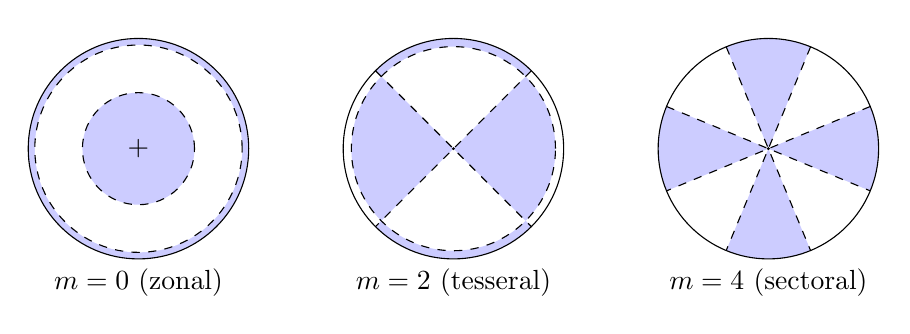
\begin{tikzpicture}
\begin{scope}
\fill[blue!20] (0,0) circle (1.4);
\fill[white] (0,0) circle ({1.4*sqrt(1-(15-2*sqrt(30))/35)});
\fill[blue!20] (0,0) circle ({1.4*sqrt(1-(15+2*sqrt(30))/35)});
\draw (0,0) circle (1.4);
\draw[dashed] (0,0) circle ({1.4*sqrt(1-(15-2*sqrt(30))/35)});
\draw[dashed] (0,0) circle ({1.4*sqrt(1-(15+2*sqrt(30))/35)});
\node at (0,0) {$+$};
\node at (0,-1.7) {$m=0$ (zonal)};
\end{scope}
\begin{scope}[xshift=4cm]
\foreach \s in {-45,135} {
\fill[blue!20] (0,0)--(\s:{1.4*sqrt(6/7)})
 arc[start angle=\s,end angle=\s+90,radius={1.4*sqrt(6/7)}]--cycle;}
\foreach \s in {45,225} {
\fill[blue!20] (\s:1.4)
 arc[start angle=\s,end angle=\s+90,radius=1.4]
 --(\s+90:{1.4*sqrt(6/7)})
 arc[start angle=\s+90,end angle=\s,radius={1.4*sqrt(6/7)}]--cycle;}
\draw (0,0) circle (1.4);
\draw[dashed] (0,0) circle ({1.4*sqrt(6/7)});
\draw[dashed] (45:1.4)--(225:1.4) (135:1.4)--(315:1.4);
\fill (0,0) circle (.02);
\node at (0,-1.7) {$m=2$ (tesseral)};
\end{scope}
\begin{scope}[xshift=8cm]
\foreach \s in {-22.5,67.5,157.5,247.5} {
\fill[blue!20] (0,0)--(\s:1.4)
 arc[start angle=\s,end angle=\s+45,radius=1.4]--cycle;}
\draw (0,0) circle (1.4);
\foreach \s in {22.5,67.5,112.5,157.5} {
\draw[dashed] (\s:1.4)--(\s+180:1.4);}
\fill (0,0) circle (.02);
\node at (0,-1.7) {$m=4$ (sectoral)};
\end{scope}
\end{tikzpicture}
\end{center}
For $m=0$, the latitude zeros solve $35y^2-30y+3=0$ with $y=x^2$, so
$x^2=(30\pm\sqrt{900-420})/70=(15\pm2\sqrt{30})/35$, that is,
$x\approx0.861$ and $0.340$ ($\theta\approx30.6^\circ$ and
$70.1^\circ$, $\rho\approx0.508$ and $0.940$). Since $P_4(1)=1>0$ and
$P_4(0)=3/8>0$, the polar cap and the equatorial band
are positive, and the band between them is negative.
For $m=2$, the factor $7x^2-1$ gives the latitude zero $x=1/\sqrt7$
($\rho=\sqrt{6/7}$), and the zeros of $\cos2\varphi$ give the
meridians $\varphi=\pi/4+j\pi/2$. Inside that latitude
circle ($x>1/\sqrt7$, where $7x^2-1>0$) the sign is that of
$\cos2\varphi$; outside it the sign reverses.
For $m=4$ there are no interior latitude zeros, and positivity is
$\cos4\varphi>0$, namely sectors centered at $\varphi=j\pi/2$
of half-width $\pi/8$. The pole is also a zero for $m=2,4$.
Since $n+m$ is even in all three cases, each function is even in $x$
($P_n^m(-x)=(-1)^{n+m}P_n^m(x)$, Exercise 15.5.1), so the southern
hemisphere has the same pattern.

\Needspace{5\baselineskip}
\par\bigskip
\noindent\textbf{15.5.7}\quad Suppose $f(r,\theta,\varphi)$ has the regular Laplace
series below, \erratum{converging uniformly on the closed ball
under consideration}:
\[
f(r,\theta,\varphi)=\sum_{l,m}a_{lm}r^{l}Y_{l}^{m}(\theta,\varphi).
\]
Letting $\langle\cdots\rangle_{\mathrm{sphere}}$ denote the average
over a sphere centered on the origin, show that
\[
\big\langle f(r,\theta,\varphi)\big\rangle_{\mathrm{sphere}}=f(0,0,0).
\]
\solution
Use $Y_0^0=1/\sqrt{4\pi}$ and orthogonality:
\[
\int Y_l^m\,d\Omega
=\sqrt{4\pi}\int Y_l^m(Y_0^0)^*d\Omega
=\sqrt{4\pi}\,\delta_{l0}\delta_{m0}.
\]
The average over the sphere of radius $r$ is
$\langle f\rangle_{\rm sphere}=(4\pi)^{-1}\int f(r,\theta,\varphi)\,d\Omega$.
Integrating the regular solid-harmonic expansion term by term, which the
assumed uniform convergence permits, therefore leaves only its constant
term:
\[
\langle f\rangle_{\rm sphere}
=\frac1{4\pi}\sum_{l,m}a_{lm}r^l\int Y_l^m\,d\Omega
=\frac{a_{00}}{\sqrt{4\pi}}.
\]
At the origin every $r^lY_l^m$ with $l>0$ vanishes, whereas
the $l=0$ term has the same value $a_{00}Y_0^0=a_{00}/\sqrt{4\pi}$.
Thus
\[
\boxed{\langle f\rangle_{\rm sphere}=f(0,0,0)}.
\]
\erratum{This is the mean-value property for the assumed regular
harmonic expansion. It does not hold for an arbitrary function;
for example, $f=r^2$ has sphere average $r^2$ but $f(0)=0$.}

\Needspace{8\baselineskip}
\subsection*{15.6 Legendre Functions of the Second Kind}

\Needspace{5\baselineskip}
\par\bigskip
\noindent\textbf{15.6.1}\quad \erratum{Use the real branches specified in the solution, with
$x\in\mathbb R\setminus\{-1,1\}$ and integer $l\ge0$.}
Show that if $l$ is even,
$Q_{l}(-x)=-Q_{l}(x)$, and that if $l$ is odd, $Q_{l}(-x)=Q_{l}(x)$.
\solution
Use the real Legendre functions with
\[
Q_0(x)=\frac12\ln\left|\frac{1+x}{1-x}\right|,\qquad
Q_1(x)=xQ_0(x)-1,\qquad x\ne\pm1.
\]
Replacing $x$ by $-x$ replaces the argument $|(1+x)/(1-x)|$ of the
logarithm by its reciprocal:
$Q_0(-x)=\frac12\ln|(1-x)/(1+x)|=-Q_0(x)$, so $Q_0$ is odd, and then
$Q_1(-x)=(-x)(-Q_0(x))-1=Q_1(x)$, so $Q_1$ is even. Thus
$Q_l(-x)=(-1)^{l+1}Q_l(x)$ holds for $l=0,1$.
The $Q_l$ obey the same three-term recurrence as the $P_l$,
$(n+1)Q_{n+1}(x)=(2n+1)xQ_n(x)-nQ_{n-1}(x)$.
Assume $Q_n(-x)=(-1)^{n+1}Q_n(x)$ and
$Q_{n-1}(-x)=(-1)^nQ_{n-1}(x)$ for some $n\ge1$. Then the
recurrence at $-x$ and $-(-1)^{n+1}=(-1)^{n+2}=(-1)^n$ give
\begin{align*}
(n+1)Q_{n+1}(-x)
&=-(2n+1)x(-1)^{n+1}Q_n(x)-n(-1)^nQ_{n-1}(x)\\
&=(-1)^{n+2}[(2n+1)xQ_n(x)-nQ_{n-1}(x)]\\
&=(-1)^{n+2}(n+1)Q_{n+1}(x).
\end{align*}
Induction proves
\[
\boxed{Q_l(-x)=(-1)^{l+1}Q_l(x)}.
\]
In particular even degree gives an odd function and odd degree an
even function. The assertion refers to these real functions (the
usual real $Q_l$ both for $|x|<1$ and for $|x|>1$); another choice of
branch of the logarithm would add a multiple of $P_l$, whose parity
$(-1)^l$ is the opposite one.

\Needspace{5\baselineskip}
\par\bigskip
\noindent\textbf{15.6.2}\quad Show that, \erratum{for nonnegative integers $p$ and
the real analytic $Q_l$ branch at $x=0$},
\begin{enumerate}
\item[(a)]
$\begin{aligned}[t]
Q_{2p}(x)=(-1)^{p}2^{2p}&\sum_{s=0}^{p}(-1)^{s}
\frac{(p+s)!\,(p-s)!}{(2s+1)!\,(2p-2s)!}\,x^{2s+1}\\
&+2^{2p}\sum_{s=p+1}^{\infty}
\frac{(p+s)!\,(2s-2p)!}{(2s+1)!\,(s-p)!}\,x^{2s+1},\qquad|x|<1,
\end{aligned}$
\item[(b)]
$\begin{aligned}[t]
Q_{2p+1}(x)=(-1)^{p+1}2^{2p}&\sum_{s=0}^{p}(-1)^{s}
\frac{(p+s)!\,(p-s)!}{(2s)!\,(2p-2s+1)!}\,x^{2s}\\
&+2^{2p+1}\sum_{s=p+1}^{\infty}
\frac{(p+s)!\,(2s-2p-2)!}{(2s)!\,(s-p-1)!}\,x^{2s},\qquad|x|<1.
\end{aligned}$
\end{enumerate}
\solution
Use the real analytic branch at $x=0$. As in Exercise 15.6.1, another
branch of the logarithm would add a multiple of $P_l$ (for example,
the exterior $Q_l$ continued onto $-1<x<1$ from above or below the
real axis equals this real function $\mp\frac{i\pi}2P_l(x)$), and
$P_l$ has only powers of the parity that is absent from the stated
series. Substituting
$y=\sum_ja_jx^j$ into $(1-x^2)y''-2xy'+l(l+1)y=0$, the coefficient of
$x^j$ is $(j+2)(j+1)a_{j+2}-j(j-1)a_j-2ja_j+l(l+1)a_j$, so the Legendre
equation gives the coefficient recurrence for any Taylor solution:
\[
(j+2)(j+1)a_{j+2}
=[j(j+1)-l(l+1)]a_j.
\]
By Exercise 15.6.1, $Q_{2p}$ is odd and $Q_{2p+1}$ is even, so their
Taylor series contain only odd and only even powers, respectively, and
the recurrence determines them from $Q'_{2p}(0)$ and $Q_{2p+1}(0)$.
These initial scales follow from $Q_0=x+\cdots$, $Q_1=-1+\cdots$
and the degree recurrences:
\[
Q'_{2p}(0)=(-1)^p\frac{(2p)!!}{(2p-1)!!},\qquad
Q_{2p+1}(0)=(-1)^{p+1}\frac{(2p)!!}{(2p+1)!!}.
\]
For the odd-degree values, the three-term recurrence
$(n+1)Q_{n+1}=(2n+1)xQ_n-nQ_{n-1}$ at $x=0$ with $n=2p$ gives
$(2p+1)Q_{2p+1}(0)=-2pQ_{2p-1}(0)$; iterating down to $Q_1(0)=-1$,
\[
Q_{2p+1}(0)=\prod_{k=1}^p\left(-\frac{2k}{2k+1}\right)Q_1(0)
=(-1)^{p+1}\frac{(2p)!!}{(2p+1)!!}.
\]
For the even-degree derivative, the identity
$(1-x^2)Q'_n=n(Q_{n-1}-xQ_n)$, which the $Q_n$ share with the $P_n$,
gives with $n=2p$ at $x=0$, and the odd-degree value for
$2p-1=2(p-1)+1$,
\[
Q'_{2p}(0)=2pQ_{2p-1}(0)
=(-1)^p\frac{2p(2p-2)!!}{(2p-1)!!}
=(-1)^p\frac{(2p)!!}{(2p-1)!!}\quad(p\ge1).
\]
The case $p=0$ comes from $Q_0$. With $(2p)!!=2^pp!$,
$(2p-1)!!=(2p)!/(2^pp!)$ and $(2p+1)!!=(2p+1)!/(2^pp!)$, these are
the values $C_0$ and $D_0$ below.

(a) Write $Q_{2p}=\sum_{s\ge0}C_sx^{2s+1}$.
For $j=2s+1$ and $l=2p$,
$(2s+1)(2s+2)-2p(2p+1)=2(s+p+1)(2s-2p+1)$, so
the Taylor recurrence is
\[
\frac{C_{s+1}}{C_s}
=\frac{(s+p+1)(2s-2p+1)}{(s+1)(2s+3)},\qquad
C_0=(-1)^p2^{2p}\frac{(p!)^2}{(2p)!}.
\]
For $0\le s\le p$, its product gives
\[
C_s=(-1)^{p+s}2^{2p}
\frac{(p+s)!(p-s)!}{(2s+1)!(2p-2s)!},
\]
which equals $C_0$ at $s=0$.
To check the product explicitly, the factorial ratio between adjacent
terms of this formula ($0\le s\le p-1$) is, with $(2p-2s)/(p-s)=2$,
\[
-\frac{p+s+1}{p-s}
\frac{(2p-2s)(2p-2s-1)}{(2s+3)(2s+2)}
=\frac{(p+s+1)(2s-2p+1)}{(s+1)(2s+3)}.
\]
At the transition, the formula gives $C_p=2^{2p}/(2p+1)$, and the
recurrence with $s=p$ gives
$C_{p+1}=C_p(2p+1)/[(p+1)(2p+3)]=2^{2p}/[(p+1)(2p+3)]$.
For $s\ge p+1$, the all-positive continuation is
\[
C_s=2^{2p}\frac{(p+s)!(2s-2p)!}{(2s+1)!(s-p)!},
\]
which reproduces $C_{p+1}$ at $s=p+1$. Its adjacent ratio,
\[
\frac{(p+s+1)(2s-2p+2)(2s-2p+1)}{(2s+3)(2s+2)(s-p+1)},
\]
reduces to the same recurrence by canceling
$2s-2p+2=2(s-p+1)$ against $s-p+1$. These formulas give exactly the two
sums in part (a).

(b) Put $Q_{2p+1}=\sum_{s\ge0}D_sx^{2s}$. This time $j=2s$,
$l=2p+1$, and
$2s(2s+1)-(2p+1)(2p+2)=2(s+p+1)(2s-2p-1)$, so
\[
\frac{D_{s+1}}{D_s}
=\frac{(s+p+1)(2s-2p-1)}{(s+1)(2s+1)},\qquad
D_0=(-1)^{p+1}2^{2p}\frac{(p!)^2}{(2p+1)!}.
\]
For $0\le s\le p$, repeated multiplication gives
\[
D_s=(-1)^{p+1+s}2^{2p}
\frac{(p+s)!(p-s)!}{(2s)!(2p-2s+1)!},
\]
which equals $D_0$ at $s=0$.
Its ratio ($0\le s\le p-1$) is
$-(p+s+1)(2p-2s+1)(2p-2s)/
[(p-s)(2s+2)(2s+1)]$, equal to the required ratio after canceling
$(2p-2s)/(p-s)=2$ against $2s+2=2(s+1)$ and writing
$-(2p-2s+1)=2s-2p-1$.
At the transition, the formula gives $D_p=-2^{2p}$, and the recurrence
with $s=p$ gives $D_{p+1}=D_p(2p+1)(-1)/[(p+1)(2p+1)]=2^{2p}/(p+1)$.
For the positive tail,
\[
D_s=2^{2p+1}\frac{(p+s)!(2s-2p-2)!}{(2s)!(s-p-1)!},
\qquad s\ge p+1,
\]
which reproduces $D_{p+1}=2^{2p+1}/(2p+2)$ at $s=p+1$. Its adjacent
ratio is
$(p+s+1)(2s-2p)(2s-2p-1)/[(2s+2)(2s+1)(s-p)]$, and canceling
$2s-2p=2(s-p)$ against $s-p$ again gives the same recurrence.
The initial values, the ratios within each range and the transition
values therefore establish both requested sums for every $s\ge0$.
Their term ratios tend to $x^2$, proving convergence
for $|x|<1$; uniqueness of the Taylor solution identifies them with $Q_l$.

\Needspace{5\baselineskip}
\par\bigskip
\noindent\textbf{15.6.3}
\begin{enumerate}
\item[(a)] \erratum{Use integer $l\ge0$ and the exterior $Q_l$
branch decaying at infinity, on $|x|>1$.} Starting with the assumed form
\[
Q_{l}(x)=\sum_{j=0}^{\infty}b_{lj}x^{k-j},
\]
show that
\[
Q_{l}(x)=b_{l0}x^{-l-1}\sum_{s=0}^{\infty}
\frac{(l+s)!\,(l+2s)!\,(2l+1)!}{s!\,(l!)^{2}(2l+2s+1)!}\,x^{-2s}.
\]
\item[(b)] The standard choice of $b_{l0}$ is
\[
b_{l0}=\frac{2^{l}(l!)^{2}}{(2l+1)!},
\]
leading to the final result
\[
Q_{l}(x)=x^{-l-1}\sum_{s=0}^{\infty}
\frac{(l+2s)!}{(2s)!!\,(2l+2s+1)!!}\,x^{-2s}.
\]
Show that this choice of $b_{l0}$ brings this negative power-series
form of $Q_{n}(x)$ into agreement with the closed-form solutions.
\end{enumerate}
\solution
(a) For a monomial $x^\alpha$, the Legendre operator
$L_l=(1-x^2)\,d^2/dx^2-2x\,d/dx+l(l+1)$ gives
$(1-x^2)\alpha(\alpha-1)x^{\alpha-2}-2\alpha x^\alpha+l(l+1)x^\alpha$,
that is,
\[
L_l[x^\alpha]=\alpha(\alpha-1)x^{\alpha-2}
+[l(l+1)-\alpha(\alpha+1)]x^\alpha.
\]
The leading term $b_{l0}x^k$ ($b_{l0}\ne0$) of the proposed series
gives the highest power $x^k$, with coefficient
$[l(l+1)-k(k+1)]b_{l0}$; the equation therefore requires
$k(k+1)=l(l+1)$, giving $k=l$ or $k=-l-1$.
The solution that decays at infinity uses the latter root.
The power $x^{k-j}=x^{-l-1-j}$ then receives
$[l(l+1)-(l+j)(l+j+1)]b_{lj}=-j(2l+j+1)b_{lj}$ from the term $j$, and,
through $\alpha(\alpha-1)x^{\alpha-2}$ with $\alpha=-l-j+1$,
$(l+j-1)(l+j)b_{l,j-2}$ from the term $j-2$. Hence
\[
j(2l+j+1)b_{lj}=(l+j)(l+j-1)b_{l,j-2},\qquad b_{l,-1}=0.
\]
At $j=1$, the power $x^{-l-2}$, this says
$2(l+1)b_{l1}=0$.
It follows that $b_{l1}=0$, and the recurrence then makes every
odd $j$ vanish. Set $c_s=b_{l,2s}$.
At power $x^{-l-1-2s}$ ($j=2s$) the equation gives
\[
2s(2l+2s+1)c_s=(l+2s)(l+2s-1)c_{s-1}.
\]
Hence
\[
\frac{c_s}{c_0}
=\prod_{q=1}^s\frac{(l+2q)(l+2q-1)}{2q(2l+2q+1)}
=\frac{(l+s)!(l+2s)!(2l+1)!}
{s!(l!)^2(2l+2s+1)!}.
\]
For the last equality, the numerator product is
$(l+1)(l+2)\cdots(l+2s)=(l+2s)!/l!$,
while the denominator product is
$2^ss!\,(2l+3)(2l+5)\cdots(2l+2s+1)=2^ss!\,(2l+2s+1)!!/(2l+1)!!$;
with $(2N+1)!!=(2N+1)!/(2^NN!)$ for $N=l+s$ and $N=l$, this is
$s!\,l!(2l+2s+1)!/[(l+s)!(2l+1)!]$.
This proves the requested series. Since
$c_s/c_{s-1}=(l+2s)(l+2s-1)/[2s(2l+2s+1)]\to1$, the ratio of
successive terms tends to $x^{-2}$, and the series converges for
$|x|>1$.

(b) The normalization can be checked against the closed logarithmic
solutions for every degree by the integral
\[
R_l(z)=\frac12\int_{-1}^1\frac{P_l(t)}{z-t}dt,\qquad |z|>1.
\]
Directly, since $-\operatorname{Log}(z-t)$ is an antiderivative of
$1/(z-t)$,
$R_0=\tfrac12[\operatorname{Log}(z+1)-\operatorname{Log}(z-1)]
=\tfrac12\operatorname{Log}[(z+1)/(z-1)]$ with the branch
vanishing at infinity (for real $z>1$ this is
$\frac12\ln[(z+1)/(z-1)]=Q_0(z)$), and, with $t/(z-t)=z/(z-t)-1$,
$R_1=\frac12\int_{-1}^1[z/(z-t)-1]dt=zR_0-1=Q_1(z)$.
For $l\ge1$, multiply the polynomial degree recurrence
$(l+1)P_{l+1}(t)=(2l+1)tP_l(t)-lP_{l-1}(t)$ by
$1/[2(z-t)]$, integrate over $[-1,1]$, and use
$t/(z-t)=z/(z-t)-1$ and $\int_{-1}^1P_l\,dt=0$; the middle term
becomes $(2l+1)[zR_l-\frac12\int_{-1}^1P_l\,dt]=(2l+1)zR_l$. This gives
\[
(l+1)R_{l+1}=(2l+1)zR_l-lR_{l-1}.
\]
The closed forms $Q_l$ obey the same recurrence and have the same
first two members, so $R_l=Q_l$ for every $l$ by induction.
For $|t|\le1<|z|$ the geometric series
$1/(z-t)=\sum_{j\ge0}t^jz^{-j-1}$ converges uniformly in $t$, so it may
be integrated term by term under the finite integral:
$R_l(z)=\sum_{j\ge0}z^{-j-1}\,\frac12\int_{-1}^1t^jP_l(t)dt$.
All moments with $j<l$ vanish by orthogonality ($t^j$ is a combination
of $P_0,\ldots,P_j$), so the series starts with $z^{-l-1}$, as in part
(a), and its leading coefficient is the moment with $j=l$. Since $P_l$
has leading coefficient $(2l)!/[2^l(l!)^2]$, $t^l$ equals
$2^l(l!)^2P_l(t)/(2l)!$ plus a polynomial of lower degree; with
$\int_{-1}^1P_l^2dt=2/(2l+1)$,
\[
b_{l0}=\frac12\int_{-1}^1t^lP_l(t)dt
=\frac{2^l(l!)^2}{(2l)!}\,\frac1{2l+1}
=\boxed{\frac{2^l(l!)^2}{(2l+1)!}}.
\]
Because $R_l=Q_l$ satisfies Legendre's equation and, for $|z|>1$,
equals this convergent series in descending powers beginning with
$z^{-l-1}$ (the form assumed in part (a), with $k=-l-1$), the
recurrence of part (a) applies to its coefficients; they are therefore
$b_{l0}$ times the coefficients found there:
\[
b_{l0}\frac{(l+s)!(l+2s)!(2l+1)!}{s!(l!)^2(2l+2s+1)!}
=\frac{2^l(l+s)!(l+2s)!}{s!(2l+2s+1)!},
\]
and splitting even and odd factorials,
$(2l+2s+1)!=2^{l+s}(l+s)!\,(2l+2s+1)!!$ and $2^ss!=(2s)!!$, gives
\[
\boxed{Q_l(z)=z^{-l-1}\sum_{s=0}^\infty
\frac{(l+2s)!}{(2s)!!(2l+2s+1)!!}z^{-2s}},\qquad |z|>1.
\]
For example, for $l=0$ the coefficients are
$(2s)!/[(2s)!!(2s+1)!!]=(2s)!/(2s+1)!=1/(2s+1)$, and
$\sum_sz^{-2s-1}/(2s+1)=\frac12\ln[(z+1)/(z-1)]$ is the familiar
expansion of $Q_0$.
For complex $z$ with $|z|>1$ the integral $R_l$ and the series define
the same branch of $Q_l$, the one that is analytic outside $[-1,1]$ and
vanishes at infinity.

\Needspace{5\baselineskip}
\par\bigskip
\noindent\textbf{15.6.4}
\begin{enumerate}
\item[(a)] Using the recurrence relations, prove (independent of the
Wronskian relation) that, \erratum{for integers $n\ge1$ on a common
consistent branch away from $x=\pm1$},
\[
n\big[P_{n}(x)Q_{n-1}(x)-P_{n-1}(x)Q_{n}(x)\big]
=P_{1}(x)Q_{0}(x)-P_{0}(x)Q_{1}(x).
\]
\item[(b)] By direct substitution show that the right-hand side of
this equation equals 1.
\end{enumerate}
\solution
(a) Let $D_n=P_nQ_{n-1}-P_{n-1}Q_n$. For $n\ge2$, both families obey
the three-term recurrence (with $n$ shifted to $n-1$)
\[
nF_n=(2n-1)xF_{n-1}-(n-1)F_{n-2}.
\]
Substitute this for $nP_n$ and $nQ_n$ in $nD_n=(nP_n)Q_{n-1}-P_{n-1}(nQ_n)$;
the terms $\pm(2n-1)xP_{n-1}Q_{n-1}$ cancel:
\begin{align*}
nD_n
&=[(2n-1)xP_{n-1}-(n-1)P_{n-2}]Q_{n-1}\\
&\quad-P_{n-1}[(2n-1)xQ_{n-1}-(n-1)Q_{n-2}]\\
&=(n-1)[P_{n-1}Q_{n-2}-P_{n-2}Q_{n-1}]\\
&=(n-1)D_{n-1}.
\end{align*}
Repeating gives $nD_n=(n-1)D_{n-1}=(n-2)D_{n-2}=\cdots=1\cdot D_1$,
which is the stated identity, since $D_1=P_1Q_0-P_0Q_1$; the case
$n=1$ is trivially included.

(b) Finally $P_0=1$, $P_1=x$, and $Q_1=xQ_0-1$, so
\[
D_1=xQ_0-(xQ_0-1)=1.
\]
Therefore
\[
\boxed{n[P_nQ_{n-1}-P_{n-1}Q_n]=1}.
\]
The argument uses only degree recurrences and starting values, as
requested, and is valid on any common consistent branch away from
the singular endpoints.

\clearpage
\section{Chapter 16. Angular Momentum}
% Problems, Chapter 16: Angular Momentum
% Arfken, Weber & Harris, Mathematical Methods for Physicists, 7th ed.
% Requires: amsmath, amssymb, tikz

\section*{Problems}

Throughout this chapter use $\hbar=1$, as in the textbook. Scalar
spherical harmonics are normalized with the Condon--Shortley phase;
their indices satisfy $L\in\{0,1,\ldots\}$ and $-L\le M\le L$.
Terms beyond a ladder endpoint mean zero, rather than an undefined
harmonic. Abstract spin multiplets may also have half-integral $L$;
in that case $L\pm M$ and $2L$ are nonnegative integers.

\Needspace{12\baselineskip}
\subsection*{16.1 Angular Momentum Operators}

\Needspace{5\baselineskip}
\par\bigskip
\noindent\textbf{16.1.1}\quad The quantum mechanical angular momentum
operators $L_{x}\pm iL_{y}$ in 3-D physical space are given by
\begin{align*}
L_{x}+iL_{y}&=e^{i\varphi}
\left(\frac{\partial}{\partial\theta}
+i\cot\theta\,\frac{\partial}{\partial\varphi}\right),\\
L_{x}-iL_{y}&=-e^{-i\varphi}
\left(\frac{\partial}{\partial\theta}
-i\cot\theta\,\frac{\partial}{\partial\varphi}\right).
\end{align*}
Show that
\begin{enumerate}
\item[(a)] $(L_{x}+iL_{y})Y_{L}^{M}(\theta,\varphi)
=\sqrt{(L-M)(L+M+1)}\,Y_{L}^{M+1}(\theta,\varphi)$,
\item[(b)] $(L_{x}-iL_{y})Y_{L}^{M}(\theta,\varphi)
=\sqrt{(L+M)(L-M+1)}\,Y_{L}^{M-1}(\theta,\varphi)$.
\end{enumerate}
\solution
Use $\hbar=1$ and the Condon--Shortley normalization
\[
Y_L^M=N_{LM}P_L^M(\cos\theta)e^{iM\varphi},\qquad
N_{LM}=\sqrt{\frac{2L+1}{4\pi}\frac{(L-M)!}{(L+M)!}}.
\]
Put $P=P_L^M(\cos\theta)$,
$A=P_L^{M+1}(\cos\theta)$ and
$B=(L+M)(L-M+1)P_L^{M-1}(\cos\theta)$.
In the variable $x=\cos\theta$ the associated-Legendre recurrences
(15.87) and (15.91) read
\[
A+\frac{2Mx}{\sqrt{1-x^2}}\,P+B=0,\qquad
\sqrt{1-x^2}\,\frac{dP}{dx}=\frac{B-A}{2}.
\]
Since $\sqrt{1-x^2}=\sin\theta$, $x/\sqrt{1-x^2}=\cot\theta$ and
$d/d\theta=-\sin\theta\,d/dx$, they become
\[
-M\cot\theta\,P=\frac{A+B}{2},\qquad
\frac{dP}{d\theta}=\frac{A-B}{2}.
\]
Adding them, or subtracting the second from the first, gives
\[
(\partial_\theta-M\cot\theta)P=A,\qquad
(-\partial_\theta-M\cot\theta)P=B.
\]
The first identity also follows directly from the form
$P_L^M=c\,\sin^M\theta\,f(x)$ of Exercise 15.4.3, valid for
$-L\le M\le L$, where $c=(-1)^M/(2^LL!)$ and
$f=d^{L+M}(x^2-1)^L/dx^{L+M}$:
\[
\partial_\theta P
=M\cot\theta\,P-c\sin^{M+1}\theta\,f'(x)
=M\cot\theta\,P+P_L^{M+1},
\]
because the same form of $P_L^{M+1}$ has the constant
$(-1)^{M+1}/(2^LL!)=-c$ and the function $f'$.

Since $\partial_\varphi e^{iM\varphi}=iM e^{iM\varphi}$, the
azimuthal term of $L_+$ acts on $Y_L^M$ as
$i\cot\theta\cdot iM=-M\cot\theta$, so
\[
L_+Y_L^M=N_{LM}e^{i(M+1)\varphi}(\partial_\theta-M\cot\theta)P
=N_{LM}P_L^{M+1}e^{i(M+1)\varphi}
=\frac{N_{LM}}{N_{L,M+1}}Y_L^{M+1}.
\]
For $M<L$ the normalization ratio is
\[
\frac{N_{LM}^2}{N_{L,M+1}^2}
=\frac{(L-M)!(L+M+1)!}{(L+M)!(L-M-1)!}
=(L-M)(L+M+1),
\]
proving (a). Similarly, the azimuthal term of $L_-$ acts as
$-i\cot\theta\cdot iM=M\cot\theta$, so
\[
\begin{aligned}
L_-Y_L^M&=N_{LM}e^{i(M-1)\varphi}(-\partial_\theta-M\cot\theta)P
=N_{LM}B\,e^{i(M-1)\varphi}\\
&=(L+M)(L-M+1)
\frac{N_{LM}}{N_{L,M-1}}Y_L^{M-1},
\end{aligned}
\]
and, for $M>-L$,
\[
\frac{N_{LM}^2}{N_{L,M-1}^2}
=\frac{(L-M)!(L+M-1)!}{(L+M)!(L-M+1)!}
=\frac1{(L+M)(L-M+1)}.
\]
The coefficient of $Y_L^{M-1}$ is therefore
\[
\frac{(L+M)(L-M+1)}{\sqrt{(L+M)(L-M+1)}}=\sqrt{(L+M)(L-M+1)}.
\]
Taking positive square roots establishes
\[
\boxed{L_\pm Y_L^M=
\sqrt{(L\mp M)(L\pm M+1)}\,Y_L^{M\pm1}}.
\]
These formulas hold for integer $-L\le M\le L$ with the endpoint
understood as annihilation: $L_+Y_L^L=L_-Y_L^{-L}=0$.
Indeed $Y_L^{\pm L}$ is proportional to
$\sin^L\theta\,e^{\pm iL\varphi}$, and direct substitution gives zero:
\[
L_\pm(\sin^L\theta\,e^{\pm iL\varphi})
=\pm e^{\pm i(L+1)\varphi}
(L\sin^{L-1}\theta\cos\theta-L\cot\theta\,\sin^L\theta)=0.
\]
No harmonic outside the permitted $M$ range is needed.

\Needspace{5\baselineskip}
\par\bigskip
\noindent\textbf{16.1.2}\quad With $L_{\pm}$ given by
\[
L_{\pm}=L_{x}\pm iL_{y}=\pm e^{\pm i\varphi}
\left(\frac{\partial}{\partial\theta}
\pm i\cot\theta\,\frac{\partial}{\partial\varphi}\right),
\]
show that
\begin{enumerate}
\item[(a)] $Y_{l}^{m}=\sqrt{\dfrac{(l+m)!}{(2l)!\,(l-m)!}}\,
(L_{-})^{l-m}Y_{l}^{l}$,
\item[(b)] $Y_{l}^{m}=\sqrt{\dfrac{(l-m)!}{(2l)!\,(l+m)!}}\,
(L_{+})^{l+m}Y_{l}^{-l}$.
\end{enumerate}
\solution
Each application of $L_-$ changes $m$ to $m-1$ with the coefficient
proved in 16.1.1. Starting at $m=l$, step $j$ ($j=0,1,\ldots$) acts on
magnetic index $m=l-j$, so its coefficient is
$\sqrt{(l+m)(l-m+1)}=\sqrt{(2l-j)(j+1)}$. After $k$ steps we therefore
have
\[
(L_-)^kY_l^l
=\left[\prod_{j=0}^{k-1}(2l-j)(j+1)\right]^{1/2}Y_l^{l-k}.
\]
The two products are
$\prod_{j=0}^{k-1}(2l-j)=2l(2l-1)\cdots(2l-k+1)=(2l)!/(2l-k)!$ and
$\prod_{j=0}^{k-1}(j+1)=k!$. Set $k=l-m$, so that $2l-k=l+m$:
\[
(L_-)^{l-m}Y_l^l
=\sqrt{\frac{(2l)!(l-m)!}{(l+m)!}}\,Y_l^m.
\]
Dividing by this positive coefficient proves
\[
\boxed{Y_l^m=\sqrt{\frac{(l+m)!}{(2l)!(l-m)!}}\,
(L_-)^{l-m}Y_l^l}.
\]

For raising from $m=-l$, the successive squared coefficients are
again $(2l-j)(j+1)$, because at step $j$ the magnetic index is
$m=-l+j$ and $(l-m)(l+m+1)=(2l-j)(j+1)$.
Thus
\[
(L_+)^kY_l^{-l}
=\sqrt{\frac{(2l)!\,k!}{(2l-k)!}}Y_l^{-l+k}.
\]
Putting $k=l+m$, so that $2l-k=l-m$, gives
\[
(L_+)^{l+m}Y_l^{-l}
=\sqrt{\frac{(2l)!(l+m)!}{(l-m)!}}\,Y_l^m,
\]
and solving for the final harmonic gives
\[
\boxed{Y_l^m=\sqrt{\frac{(l-m)!}{(2l)!(l+m)!}}\,
(L_+)^{l+m}Y_l^{-l}}.
\]
For $k=0$ the product is empty and equals one, so both extreme
states are included.

\Needspace{5\baselineskip}
\par\bigskip
\noindent\textbf{16.1.3}\quad Using the known forms of $L_{+}$ and
$L_{-}$ (Exercise~16.1.2), show that
\[
\int\big[Y_{L}^{M}\big]^{*}\,L_{-}\big(L_{+}Y_{L}^{M}\big)\,d\Omega
=\int\big(L_{+}Y_{L}^{M}\big)^{*}\big(L_{+}Y_{L}^{M}\big)\,d\Omega.
\]
Here $d\Omega$ is the element of solid angle
($\sin\theta\,d\theta\,d\varphi$), and the integration is over the
entire angular space.
\solution
We prove the needed adjoint identity by integration by parts rather
than assuming it. Let $u,v$ be smooth single-valued functions on the
sphere, with $\varphi$-periodic coordinate expressions. Since
\[
L_-v=-e^{-i\varphi}v_\theta
+i e^{-i\varphi}\cot\theta\,v_\varphi,
\]
we have, with $d\Omega=\sin\theta\,d\theta\,d\varphi$ and
$\langle u,w\rangle=\int u^*w\,d\Omega$,
\[
\langle u,L_-v\rangle
=\int_0^{2\pi}\int_0^\pi
\left[-u^*e^{-i\varphi}\sin\theta\,v_\theta
+i u^*e^{-i\varphi}\cos\theta\,v_\varphi\right]d\theta\,d\varphi.
\]
Integrate the first term by parts in $\theta$ and the second in
$\varphi$:
\[
\begin{aligned}
-\int_0^\pi u^*e^{-i\varphi}\sin\theta\,v_\theta\,d\theta
&=\int_0^\pi v\,e^{-i\varphi}
(\sin\theta\,u_\theta^*+\cos\theta\,u^*)\,d\theta,\\
\int_0^{2\pi}iu^*e^{-i\varphi}\cos\theta\,v_\varphi\,d\varphi
&=-\int_0^{2\pi}v\,e^{-i\varphi}\cos\theta\,
(iu_\varphi^*+u^*)\,d\varphi,
\end{aligned}
\]
where $\partial_\varphi(iu^*e^{-i\varphi})
=e^{-i\varphi}(iu_\varphi^*+u^*)$.
The $\theta$ boundary term $[-u^*e^{-i\varphi}\sin\theta\,v]_0^\pi$
vanishes because $\sin\theta=0$ at the poles; the $\varphi$ boundary
term vanishes by periodicity. The remaining integrand is
\[
v\left[
e^{-i\varphi}\sin\theta\,u_\theta^*
+e^{-i\varphi}\cos\theta\,u^*
-e^{-i\varphi}\cos\theta\,u^*
-i e^{-i\varphi}\cos\theta\,u_\varphi^*
\right].
\]
The middle two terms cancel. Dividing the rest by $\sin\theta$ to
restore $d\Omega$, and using
$(L_+u)^*=e^{-i\varphi}(u_\theta^*-i\cot\theta\,u_\varphi^*)$,
we are left with
\[
\langle u,L_-v\rangle
=\int v\,e^{-i\varphi}(u_\theta^*
-i\cot\theta\,u_\varphi^*)\,d\Omega
=\langle L_+u,v\rangle.
\]
Take $u=Y_L^M$ and $v=L_+Y_L^M$, both regular spherical harmonics
or zero. This is exactly the requested equality. Moreover, since
$L_+Y_L^M=\sqrt{(L-M)(L+M+1)}\,Y_L^{M+1}$ by 16.1.1 and
$\int|Y_L^{M+1}|^2d\Omega=1$, both sides equal
$\boxed{(L-M)(L+M+1)}$, including zero at the upper endpoint.

\Needspace{5\baselineskip}
\par\bigskip
\noindent\textbf{16.1.4}
\begin{enumerate}
\item[(a)] Show that
$\mathbf{J}^{2}=\dfrac{1}{2}\big[J_{+}J_{-}+J_{-}J_{+}\big]+J_{z}^{2}$.
\item[(b)] Use the result from part (a) and the explicit formulas for
$L_{+}$ and $L_{-}$ from Exercise~16.1.2 to verify that all the
spherical harmonics with $l=2$ are eigenfunctions of $\mathbf{L}^{2}$
with eigenvalue $l(l+1)=6$.
\end{enumerate}
\solution
\textbf{(a)} Preserve operator order while expanding:
\[
\begin{aligned}
J_+J_-&=J_x^2+J_y^2+iJ_yJ_x-iJ_xJ_y,\\
J_-J_+&=J_x^2+J_y^2+iJ_xJ_y-iJ_yJ_x.
\end{aligned}
\]
Their sum is $2J_x^2+2J_y^2$ because the mixed terms cancel.
Consequently
\[
\boxed{\mathbf J^2=\tfrac12(J_+J_-+J_-J_+)+J_z^2}.
\]

\textbf{(b)} For an arbitrary smooth test function $f$, direct
product differentiation in the given ladder operators yields
\[
L_+L_-f=-f_{\theta\theta}-\cot\theta f_\theta
-\cot^2\theta f_{\varphi\varphi}-if_\varphi,
\]
\[
L_-L_+f=-f_{\theta\theta}-\cot\theta f_\theta
-\cot^2\theta f_{\varphi\varphi}+if_\varphi.
\]
For the first, write $c=\cot\theta$, so $c'=-\csc^2\theta$, and
$L_-f=-e^{-i\varphi}(f_\theta-icf_\varphi)$. Then
$L_+L_-f=e^{i\varphi}\partial_\theta(L_-f)
+e^{i\varphi}ic\,\partial_\varphi(L_-f)$, and since
$\partial_\varphi(-e^{-i\varphi})=ie^{-i\varphi}$ the two parts are
\[
\begin{aligned}
e^{i\varphi}\partial_\theta(L_-f)
&=-f_{\theta\theta}+ic'f_\varphi+ic f_{\theta\varphi},\\
e^{i\varphi}ic\,\partial_\varphi(L_-f)
&=ic\,[\,i(f_\theta-icf_\varphi)-(f_{\theta\varphi}-icf_{\varphi\varphi})\,]\\
&=-c f_\theta-ic f_{\theta\varphi}
+c^2if_\varphi-c^2f_{\varphi\varphi}.
\end{aligned}
\]
The mixed derivatives cancel and $i(c'+c^2)=-i$, because
$\csc^2\theta-\cot^2\theta=1$.
For the second, replacing $i$ by $-i$ in the coefficients turns
$L_+$ into $-L_-$ and $L_-$ into $-L_+$, hence turns $L_+L_-$ into
$(-L_-)(-L_+)=L_-L_+$. The computation above uses only $i^2=-1$ and
$\partial_\varphi e^{\pm i\varphi}=\pm ie^{\pm i\varphi}$, which remain
true with $-i$ in place of $i$, so the same replacement in its result
(with $f$ unchanged) gives $L_-L_+f$. This changes only the last
first-order term, from $-if_\varphi$ to $+if_\varphi$.
\erratum{The Instructor's Manual (printed p.~257) writes the difference
$(L_+L_--L_-L_+)/2$ when extracting the common second-order terms.
It must use the sum. The half-difference is $L_z=-i\partial_\varphi$,
not $\mathbf L^2-L_z^2$.} In the half-sum the terms $\mp if_\varphi$
cancel:
$\tfrac12(L_+L_-+L_-L_+)f=-f_{\theta\theta}-\cot\theta f_\theta
-\cot^2\theta f_{\varphi\varphi}$.
Since $L_z^2f=-f_{\varphi\varphi}$ and $\cot^2\theta+1=\csc^2\theta$,
(a) gives
\[
\mathbf L^2f=-f_{\theta\theta}-\cot\theta f_\theta
-\csc^2\theta f_{\varphi\varphi}.
\]
From here on write $s=\sin\theta$ and $c=\cos\theta$ (so $c$ no
longer denotes $\cot\theta$). The five $l=2$ harmonics are
nonzero constant multiples of
$s^2e^{\pm2i\varphi}$, $sc\,e^{\pm i\varphi}$, and $3c^2-1$.
The operator acts on $F(\theta)e^{im\varphi}$ as
$[-F''-\cot\theta F'+m^2F/s^2]e^{im\varphi}$. Explicitly,
\[
\begin{array}{c|c|c|c}
F&m^2&F',\,F''&-F''-(c/s)F'+m^2F/s^2\\ \hline
s^2&4&2sc,\ 2(c^2-s^2)&-2c^2+2s^2-2c^2+4=6s^2\\
sc&1&c^2-s^2,\ -4sc&4sc-c^3/s+cs+c/s=6sc\\
3c^2-1&0&-6sc,\ -6(c^2-s^2)&12c^2-6s^2=6(3c^2-1)
\end{array}
\]
The last column uses $s^2+c^2=1$: $4=4s^2+4c^2$ in the first row,
$c/s-c^3/s=c(1-c^2)/s=cs$ in the second, and $-6s^2=6c^2-6$ in the
third. Both signs of $m$ have the same $m^2$, so the first two rows each
verify two harmonics. Multiplying by their normalization constants
does not change the eigenvalue:
$\boxed{\mathbf L^2Y_2^m=6Y_2^m}$ for all five $m$.

\Needspace{5\baselineskip}
\par\bigskip
\noindent\textbf{16.1.5}\quad Derive the following relations for
\erratum{normalized eigenstates of the Hermitian angular-momentum
algebra in one irreducible multiplet, with relative phases chosen
so the ladder coefficients are positive}. Do not assume coordinate
formulas for $\psi_L^M$:
\begin{enumerate}
\item[(a)] $\psi_{L}^{M}(\theta,\varphi)
=\sqrt{\dfrac{(L+M)!}{(2L)!\,(L-M)!}}\,
(L_{-})^{L-M}\psi_{L}^{L}(\theta,\varphi)$,
\item[(b)] $\psi_{L}^{M}(\theta,\varphi)
=\sqrt{\dfrac{(L-M)!}{(2L)!\,(L+M)!}}\,
(L_{+})^{L+M}\psi_{L}^{-L}(\theta,\varphi)$.
\end{enumerate}
\solution
\erratum{The numerical coefficients require normalized states in a
single angular-momentum multiplet and a consistent ladder phase
convention. Eigenvalue equations alone leave arbitrary magnitudes,
phases, and possible degeneracy labels.}
Assume the Hermitian angular-momentum algebra, and choose states with
$\mathbf L^2\psi_L^M=L(L+1)\psi_L^M$ and
$L_z\psi_L^M=M\psi_L^M$. The commutators
$[L_z,L_\pm]=\pm L_\pm$ and $[\mathbf L^2,L_\pm]=0$ show that
$L_\pm\psi_L^M$ has the same $L$ and magnetic index $M\pm1$:
$L_zL_\pm\psi_L^M=L_\pm(L_z\pm1)\psi_L^M=(M\pm1)L_\pm\psi_L^M$.
Within a fixed irreducible multiplet it is therefore proportional
to $\psi_L^{M\pm1}$.

From $[L_x,L_y]=iL_z$,
$[L_+,L_-]=-i[L_x,L_y]+i[L_y,L_x]=2L_z$, while the identity of
16.1.4(a) gives $L_+L_-+L_-L_+=2(\mathbf L^2-L_z^2)$. Adding and
subtracting these two equations and halving gives
\[
L_-L_+=\mathbf L^2-L_z^2-L_z,\qquad
L_+L_-=\mathbf L^2-L_z^2+L_z.
\]
Since $L_\pm^\dagger=L_\mp$, normalization determines the squared
proportionality factors:
\[
\|L_+\psi_L^M\|^2=\langle\psi_L^M,L_-L_+\psi_L^M\rangle
=L(L+1)-M^2-M=(L-M)(L+M+1),
\]
\[
\|L_-\psi_L^M\|^2=\langle\psi_L^M,L_+L_-\psi_L^M\rangle
=L(L+1)-M^2+M=(L+M)(L-M+1).
\]
Choose the relative phases so these factors have positive square roots.
This works for raising and lowering at once: if
$L_-\psi_L^{M+1}=c\,\psi_L^M$ with $c>0$, then $L_+\psi_L^M$, being
proportional to $\psi_L^{M+1}$, has the coefficient
$\langle\psi_L^{M+1},L_+\psi_L^M\rangle
=\langle L_-\psi_L^{M+1},\psi_L^M\rangle=c$.
Thus fixing the phases of $\psi_L^{L-1},\ldots,\psi_L^{-L}$ by positive
lowering coefficients makes every raising coefficient positive too.
As in 16.1.2, lowering step $j$ acts on $M=L-j$, where
$(L+M)(L-M+1)=(2L-j)(j+1)$.
Iteration now gives, without any coordinate formula,
\[
(L_-)^k\psi_L^L
=\sqrt{\prod_{j=0}^{k-1}(2L-j)(j+1)}\,\psi_L^{L-k}
=\sqrt{\frac{(2L)!k!}{(2L-k)!}}\,\psi_L^{L-k}.
\]
Setting $k=L-M$ and inverting the coefficient yields (a).
Starting at $-L$ and raising gives the identical product; setting
$k=L+M$ yields (b):
\[
\boxed{\psi_L^M=\sqrt{\frac{(L+M)!}{(2L)!(L-M)!}}
(L_-)^{L-M}\psi_L^L},
\]
\[
\boxed{\psi_L^M=\sqrt{\frac{(L-M)!}{(2L)!(L+M)!}}
(L_+)^{L+M}\psi_L^{-L}}.
\]
The argument also applies to abstract half-integral multiplets:
$2L,L\pm M$ are still nonnegative integers. Ordinary scalar
spherical harmonics are the integral-$L$ realization.

\Needspace{5\baselineskip}
\par\bigskip
\noindent\textbf{16.1.6}\quad Derive the operator equations
\erratum{for integers $n\ge0$, on $0<\theta<\pi$, with the derivatives
in $\cos\theta$ taken at fixed $\varphi$}:
\begin{align*}
(L_{+})^{n}Y_{L}^{M}(\theta,\varphi)
&=(-1)^{n}e^{in\varphi}\sin^{n+M}\theta\,
\frac{d^{n}\sin^{-M}\theta\,Y_{L}^{M}(\theta,\varphi)}
{(d\cos\theta)^{n}},\\
(L_{-})^{n}Y_{L}^{M}(\theta,\varphi)
&=e^{-in\varphi}\sin^{n-M}\theta\,
\frac{d^{n}\sin^{M}\theta\,Y_{L}^{M}(\theta,\varphi)}
{(d\cos\theta)^{n}}.
\end{align*}
\par\emph{Hint.}~Try mathematical induction (Section~1.4).
\solution
All derivatives with respect to $x=\cos\theta$ below hold $\varphi$
fixed, so $\partial_\theta=-\sin\theta\,\partial_x$; the interior
range $0<\theta<\pi$ keeps $\cot\theta$ and the powers
$\sin^{\pm M}\theta$ finite. Since
$\partial_\theta\sin^{\mp m}\theta=\mp m\cot\theta\,\sin^{\mp m}\theta$,
a function $g_m=F(\theta)e^{im\varphi}$, for which
$\partial_\varphi g_m=img_m$, satisfies
\[
\begin{aligned}
L_+g_m
&=e^{i\varphi}(\partial_\theta-m\cot\theta)g_m
=e^{i\varphi}\sin^m\theta\,
\partial_\theta(\sin^{-m}\theta\,g_m)\\
&=-e^{i\varphi}\sin^{m+1}\theta\,
\partial_x(\sin^{-m}\theta\,g_m),\\
L_-g_m
&=-e^{-i\varphi}(\partial_\theta+m\cot\theta)g_m
=-e^{-i\varphi}\sin^{-m}\theta\,
\partial_\theta(\sin^m\theta\,g_m)\\
&=e^{-i\varphi}\sin^{1-m}\theta\,
\partial_x(\sin^m\theta\,g_m).
\end{aligned}
\]
These establish both claims for $n=1$; $n=0$ is the identity.

Assume the raising formula at $n$:
$g_{M+n}=(L_+)^nY_L^M=(-1)^ne^{in\varphi}\sin^{M+n}\theta
\,\partial_x^n(\sin^{-M}\theta\,Y_L^M)$.
It has magnetic index $M+n$, because $Y_L^M\propto e^{iM\varphi}$ and
$\partial_x$ at fixed $\varphi$ keeps that factor. Apply the first
identity with $m=M+n$. The two opposite powers of sine cancel inside
the derivative,
$\sin^{-(M+n)}\theta\,g_{M+n}
=(-1)^ne^{in\varphi}\partial_x^n(\sin^{-M}\theta\,Y_L^M)$,
and $e^{in\varphi}$ is constant in $x$, so
\[
L_+g_{M+n}
=(-1)^{n+1}e^{i(n+1)\varphi}\sin^{M+n+1}\theta\,
\partial_x^{n+1}(\sin^{-M}\theta\,Y_L^M).
\]
This is the $n+1$ formula.

For lowering, the induction hypothesis is
$g_{M-n}=(L_-)^nY_L^M=e^{-in\varphi}\sin^{n-M}\theta
\,\partial_x^n(\sin^M\theta\,Y_L^M)$.
Use the second identity with $m=M-n$; its factor
$\sin^m\theta$ cancels $\sin^{n-M}\theta$:
$\sin^{M-n}\theta\,g_{M-n}
=e^{-in\varphi}\partial_x^n(\sin^M\theta\,Y_L^M)$. Since
$\sin^{1-m}\theta=\sin^{n+1-M}\theta$, this leaves
\[
L_-g_{M-n}
=e^{-i(n+1)\varphi}\sin^{n+1-M}\theta\,
\partial_x^{n+1}(\sin^M\theta\,Y_L^M).
\]
Thus both stated equations hold for every integer $n\ge0$.
They are coordinate expressions on $0<\theta<\pi$; the resulting
harmonics extend regularly to the poles.

\Needspace{5\baselineskip}
\par\bigskip
\noindent\textbf{16.1.7}\quad Show, using $(L_{-})^{n}$, that
\[
Y_{L}^{-M}(\theta,\varphi)
=(-1)^{M}\big[Y_{L}^{M}(\theta,\varphi)\big]^{*}.
\]
\solution
First let $M\ge0$. Iterating the raising coefficient from zero to $M$
gives
\[
Y_L^M=c_M(L_+)^M Y_L^0,\qquad
c_M=\sqrt{\frac{(L-M)!}{(L+M)!}}.
\]
Indeed step $j$ acts on magnetic index $j$, with squared coefficient
$(L-j)(L+j+1)$ by 16.1.1, and the squared product is
\[
\prod_{j=0}^{M-1}(L-j)\prod_{j=0}^{M-1}(L+j+1)
=\frac{L!}{(L-M)!}\cdot\frac{(L+M)!}{L!}
=\frac{(L+M)!}{(L-M)!}.
\]
The differential forms show, for any differentiable $f$,
\[
(L_+f)^*
=e^{-i\varphi}(\partial_\theta-i\cot\theta\,\partial_\varphi)f^*
=-L_-f^*.
\]
Applying this $M$ times gives
$[(L_+)^Mf]^*=(-1)^M(L_-)^Mf^*$. Because $Y_L^0$ is real, therefore
\[
(Y_L^M)^*=(-1)^M c_M(L_-)^M Y_L^0.
\]
Lowering from zero to $-M$ has the same squared coefficient product
$(L+M)!/(L-M)!$, since step $j$ acts on $m=-j$ and
$(L+m)(L-m+1)=(L-j)(L+j+1)$. Hence $c_M(L_-)^M Y_L^0=Y_L^{-M}$, so
$(Y_L^M)^*=(-1)^MY_L^{-M}$. Multiplying by $(-1)^M$,
\[
\boxed{Y_L^{-M}=(-1)^M(Y_L^M)^*}.
\]
Replacing $M$ by $-M$ and conjugating proves the identical statement
for negative $M$, since $(-1)^{-M}=(-1)^M$ for integral $M$.
\erratum{The Instructor's Manual (printed p.~258) says to start with $Y_0^0$.
For a fixed degree $L$ the starting function must be $Y_L^0$.
Indeed both ladders annihilate $Y_0^0$, so they cannot generate
any nonconstant harmonic from it.}

\Needspace{5\baselineskip}
\par\bigskip
\noindent\textbf{16.1.8}\quad Verify by explicit calculation that
\begin{enumerate}
\item[(a)] $L_{+}Y_{1}^{0}(\theta,\varphi)
=-\sqrt{\dfrac{3}{4\pi}}\sin\theta\,e^{i\varphi}
=\sqrt{2}\,Y_{1}^{1}(\theta,\varphi)$,
\item[(b)] $L_{-}Y_{1}^{0}(\theta,\varphi)
=+\sqrt{\dfrac{3}{4\pi}}\sin\theta\,e^{-i\varphi}
=\sqrt{2}\,Y_{1}^{-1}(\theta,\varphi)$.
\end{enumerate}
The signs have the indicated values because the spherical harmonics
were defined to be consistent with the results obtained using the
ladder operators $L_{+}$ and $L_{-}$ (Condon--Shortley phase).
\solution
The relevant normalized harmonics are
\[
Y_1^0=\sqrt{\frac3{4\pi}}\cos\theta,\qquad
Y_1^1=-\sqrt{\frac3{8\pi}}\sin\theta\,e^{i\varphi},\qquad
Y_1^{-1}=\sqrt{\frac3{8\pi}}\sin\theta\,e^{-i\varphi}.
\]
Since $Y_1^0$ is independent of $\varphi$, the azimuthal derivatives
in $L_\pm$ vanish. Direct differentiation, with
$\partial_\theta\cos\theta=-\sin\theta$ and
$\sqrt{3/(4\pi)}=\sqrt2\sqrt{3/(8\pi)}$, gives
\[
L_+Y_1^0=e^{i\varphi}\sqrt{\frac3{4\pi}}(-\sin\theta)
=-\sqrt{\frac3{4\pi}}\sin\theta\,e^{i\varphi}
=\boxed{\sqrt2\,Y_1^1},
\]
\[
L_-Y_1^0=-e^{-i\varphi}\sqrt{\frac3{4\pi}}(-\sin\theta)
=\sqrt{\frac3{4\pi}}\sin\theta\,e^{-i\varphi}
=\boxed{\sqrt2\,Y_1^{-1}}.
\]
The minus sign in $Y_1^1$ is precisely the phase needed to make
both ladder coefficients positive.

\Needspace{12\baselineskip}
\subsection*{16.2 Angular Momentum Coupling}

\Needspace{5\baselineskip}
\par\bigskip
\noindent\textbf{16.2.1}\quad Derive recursion relations for
Clebsch--Gordan coefficients. Use them to calculate
$C(11J\,|\,m_{1}m_{2}M)$ for $J=0,1,2$.
\par\emph{Hint.}~Use the known matrix elements of
$J_{+}=J_{1+}+J_{2+}$, $J_{i+}$, and
$\mathbf{J}^{2}=(\mathbf{J}_{1}+\mathbf{J}_{2})^{2}$, etc.
\solution
Write $|m_1,m_2\rangle=|j_1m_1\rangle|j_2m_2\rangle$ and
\[
|JM\rangle=\sum_{m_1+m_2=M}C_M(m_1,m_2)|m_1,m_2\rangle.
\]
Define $a_i^\pm(m)=\sqrt{(j_i\mp m)(j_i\pm m+1)}$, so that
$J_{i\pm}|j_im\rangle=a_i^\pm(m)|j_i,m\pm1\rangle$.
Apply $J_+=J_{1+}+J_{2+}$ to this expansion and collect the
coefficient of the \emph{target} state $|m_1,m_2\rangle$
($m_1+m_2=M+1$); it comes from $|m_1-1,m_2\rangle$ through $J_{1+}$
and from $|m_1,m_2-1\rangle$ through $J_{2+}$, while the left side
is $\sqrt{(J-M)(J+M+1)}\,|J,M+1\rangle$:
\[
\begin{aligned}
\sqrt{(J-M)(J+M+1)}\,C_{M+1}(m_1,m_2)
={}&a_1^+(m_1-1)C_M(m_1-1,m_2)\\
&+a_2^+(m_2-1)C_M(m_1,m_2-1).
\end{aligned}
\]
Similarly, applying $J_-$ gives
\[
\begin{aligned}
\sqrt{(J+M)(J-M+1)}\,C_{M-1}(m_1,m_2)
={}&a_1^-(m_1+1)C_M(m_1+1,m_2)\\
&+a_2^-(m_2+1)C_M(m_1,m_2+1).
\end{aligned}
\]
Coefficients outside the allowed magnetic ranges are zero.
A recursion within a fixed $M$ follows from
\[
\mathbf J^2=\mathbf J_1^2+\mathbf J_2^2+2J_{1z}J_{2z}
+J_{1+}J_{2-}+J_{1-}J_{2+},
\]
since $J_{1+}J_{2-}+J_{1-}J_{2+}=2(J_{1x}J_{2x}+J_{1y}J_{2y})$, so the
last three terms are $2\mathbf J_1\cdot\mathbf J_2$. The first three
terms multiply $|m_1,m_2\rangle$ by
$j_1(j_1+1)+j_2(j_2+1)+2m_1m_2$; $J_{1+}J_{2-}$ reaches
$|m_1,m_2\rangle$ from $|m_1-1,m_2+1\rangle$ and $J_{1-}J_{2+}$ from
$|m_1+1,m_2-1\rangle$. Equating coefficients of $|m_1,m_2\rangle$ in
$\mathbf J^2|JM\rangle=J(J+1)|JM\rangle$ gives
\[
\begin{aligned}
&[J(J+1)-j_1(j_1+1)-j_2(j_2+1)-2m_1m_2]C_M(m_1,m_2)\\
&\quad=a_1^+(m_1-1)a_2^-(m_2+1)C_M(m_1-1,m_2+1)\\
&\qquad\quad+a_1^-(m_1+1)a_2^+(m_2-1)C_M(m_1+1,m_2-1).
\end{aligned}
\]
Together with normalization and phase, these determine the coefficients.

For $j_1=j_2=1$, choose positive lowering coefficients and a positive
coefficient of the largest $m_1$ in each highest-$M$ state, consistent
with the text's Condon--Shortley convention. For $j_i=1$,
$J_{i-}|1\rangle=\sqrt2|0\rangle$, $J_{i-}|0\rangle=\sqrt2|-1\rangle$
and $J_{i-}|-1\rangle=0$; the total ladder factors are
$J_-|J,M\rangle=\sqrt{(J+M)(J-M+1)}\,|J,M-1\rangle$.
Each lowering below applies the $J_-$ recursion to all coefficients
at once: the coefficient of $|m_1,m_2\rangle$ in $J_-|JM\rangle$ is
the right side of that recursion, and dividing by
$\sqrt{(J+M)(J-M+1)}$ gives $C_{M-1}(m_1,m_2)$.
Start with $|2,2\rangle=|1,1\rangle$. Since
$J_-|1,1\rangle=\sqrt2|0,1\rangle+\sqrt2|1,0\rangle$ and
$J_-|2,2\rangle=2|2,1\rangle$, the first lowering gives
\[
2|2,1\rangle
=\sqrt2(|1,0\rangle+|0,1\rangle).
\]
Next, $J_-(|1,0\rangle+|0,1\rangle)
=\sqrt2(|0,0\rangle+|1,-1\rangle)+\sqrt2(|-1,1\rangle+|0,0\rangle)$
and $J_-|2,1\rangle=\sqrt6|2,0\rangle$, so, after dividing by the
$\sqrt2$ in $|2,1\rangle$,
\[
\sqrt6|2,0\rangle
=|1,-1\rangle+2|0,0\rangle+|-1,1\rangle.
\]
Lowering this numerator gives
$\sqrt2|0,-1\rangle+2\sqrt2(|-1,0\rangle+|0,-1\rangle)
+\sqrt2|-1,0\rangle=3\sqrt2(|0,-1\rangle+|-1,0\rangle)$;
after dividing by its existing $\sqrt6$ and the next ladder factor
$\sqrt6$,
$|2,-1\rangle=3\sqrt2(|0,-1\rangle+|-1,0\rangle)/6
=(|0,-1\rangle+|-1,0\rangle)/\sqrt2$.
The final lowering gives
$2|2,-2\rangle=(\sqrt2+\sqrt2)|-1,-1\rangle/\sqrt2=2|-1,-1\rangle$.
Thus the complete quintet is
\[
\begin{array}{c|l}
M&|2,M\rangle\\ \hline
2&|1,1\rangle\\
1&(|1,0\rangle+|0,1\rangle)/\sqrt2\\
0&(|1,-1\rangle+2|0,0\rangle+|-1,1\rangle)/\sqrt6\\
-1&(|0,-1\rangle+|-1,0\rangle)/\sqrt2\\
-2&|-1,-1\rangle
\end{array}
\]

The normalized vector at $M=1$ orthogonal to $|2,1\rangle$, with a
positive coefficient of $|1,0\rangle$, is
$|1,1\rangle_{\rm coupled}=(|1,0\rangle-|0,1\rangle)/\sqrt2$.
Its two lowerings, with ladder factors
$\sqrt{(1+M)(2-M)}=\sqrt2$ for $M=1,0$, are
\[
\begin{aligned}
J_-|1,1\rangle_{\rm coupled}
&=\tfrac1{\sqrt2}\bigl[\sqrt2(|0,0\rangle+|1,-1\rangle)
-\sqrt2(|-1,1\rangle+|0,0\rangle)\bigr]\\
&=|1,-1\rangle-|-1,1\rangle=\sqrt2|1,0\rangle_{\rm coupled},
\end{aligned}
\]
\[
J_-|1,0\rangle_{\rm coupled}
=\tfrac1{\sqrt2}\bigl(\sqrt2|0,-1\rangle-\sqrt2|-1,0\rangle\bigr)
=|0,-1\rangle-|-1,0\rangle
=\sqrt2|1,-1\rangle_{\rm coupled}.
\]
Hence the triplet is
\[
\begin{array}{c|l}
M&|1,M\rangle_{\rm coupled}\\ \hline
1&(|1,0\rangle-|0,1\rangle)/\sqrt2\\
0&(|1,-1\rangle-|-1,1\rangle)/\sqrt2\\
-1&(|0,-1\rangle-|-1,0\rangle)/\sqrt2
\end{array}
\]
Finally write the singlet as
$u|1,-1\rangle+v|0,0\rangle+w|-1,1\rangle$.
Orthogonality to $|2,0\rangle$ and $|1,0\rangle_{\rm coupled}$ gives
$u+2v+w=0$ and $u-w=0$, so $w=u,v=-u$.
Normalization gives $3u^2=1$, and the chosen sign gives $u>0$:
\[
\boxed{|0,0\rangle_{\rm coupled}
=\frac{|1,-1\rangle-|0,0\rangle+|-1,1\rangle}{\sqrt3}}.
\]
The fixed-$M$ recursion checks all three $M=0$ states at once. For
$m_1=1$, $m_2=-1$ its bracket is $J(J+1)-2-2+2$, and only the term
with $a_1^+(0)a_2^-(0)=2$ survives on the right (the other needs
$m_1=2$), so
$C_0(0,0)=\tfrac12[J(J+1)-2]\,C_0(1,-1)$. This gives $2C_0(1,-1)$,
$0$ and $-C_0(1,-1)$ for $J=2,1,0$, as in the tables.

Every Clebsch--Gordan coefficient requested is the coefficient of its
product ket in these nine normalized states; all unlisted coefficients
are zero. Their dimensions $5+3+1=9$ exhaust the product basis.

\Needspace{5\baselineskip}
\par\bigskip
\noindent\textbf{16.2.2}\quad Defining $\big(Y_{l}\chi\big)_{J}^{M}$
by the formula
\[
\big(Y_{l}\chi\big)_{J}^{M}
=\sum C\big(l\tfrac{1}{2}J\,\big|\,m_{l}m_{s}M\big)
Y_{l}^{m_{l}}\chi_{m_{s}},
\]
where $\chi_{\pm1/2}$ are the spin up and down eigenfunctions of
$\sigma_{3}=\sigma_{z}$, show that $\big(Y_{l}\chi\big)_{J}^{M}$ is a
$J,M$ eigenfunction.
\solution
Let $\chi_+=\chi_{1/2}$ and $\chi_-=\chi_{-1/2}$, so that
$S_z\chi_\pm=\pm\chi_\pm/2$ with $\mathbf S=\boldsymbol\sigma/2$.
Every nonzero Clebsch--Gordan term has $m_l+m_s=M$; therefore
$J_z=L_z+S_z$ acting on the sum gives $M$ times that sum.

To check $\mathbf J^2$ explicitly, consider the fixed-$M$ product basis
\[
u=Y_l^{M-1/2}\chi_+,\qquad
v=Y_l^{M+1/2}\chi_-,
\]
omitting a vector if its orbital magnetic index is outside $[-l,l]$.
In this basis,
\[
\mathbf J^2=\mathbf L^2+\mathbf S^2+2L_zS_z+L_+S_-+L_-S_+
=\left[l(l+1)+\tfrac14\right]I+
\begin{pmatrix}M&q\\q&-M\end{pmatrix},
\]
where $K=l+\tfrac12$ and $q=\sqrt{K^2-M^2}$.
Indeed, by 16.1.1 and $S_-\chi_+=\chi_-$, $S_+\chi_-=\chi_+$,
\[
L_+S_-u=\sqrt{(l-M+\tfrac12)(l+M+\tfrac12)}\,v=\sqrt{(K-M)(K+M)}\,v=qv,
\]
and likewise $L_-S_+v=qu$, while $S_-\chi_-=S_+\chi_+=0$ make
$L_+S_-v=L_-S_+u=0$. With $\mathbf S^2=\tfrac34$ and
$2L_zS_z=2(M\mp\tfrac12)(\pm\tfrac12)$ on $u$ and $v$, respectively,
the diagonal terms are
$l(l+1)+\tfrac34\pm(M\mp\tfrac12)=l(l+1)+\tfrac14\pm M$.
The square of the last matrix is
$(M^2+q^2)I=K^2I$, so its eigenvalues are $\pm K$; its trace is zero,
so one is $+K$ and the other $-K$.

The corresponding normalized eigenvectors are
\[
\Psi_+=\sqrt{\frac{K+M}{2K}}\,u+
\sqrt{\frac{K-M}{2K}}\,v,
\qquad
\Psi_-=-\sqrt{\frac{K-M}{2K}}\,u+
\sqrt{\frac{K+M}{2K}}\,v.
\]
Indeed $q\sqrt{K-M}=(K-M)\sqrt{K+M}$ and
$q\sqrt{K+M}=(K+M)\sqrt{K-M}$. The two components of the matrix
times $\Psi_+$ are consequently
$[M+K-M]\sqrt{K+M}$ and $[K+M-M]\sqrt{K-M}$,
divided by $\sqrt{2K}$; these are the components of $K\Psi_+$.
For $\Psi_-$ the components are
$[-M+K+M]\sqrt{K-M}$ and
$[-K+M-M]\sqrt{K+M}$, divided by $\sqrt{2K}$,
which equal $-K\Psi_-$.
The complete eigenvalues are thus
\[
l(l+1)+\tfrac14+K=(l+\tfrac12)(l+\tfrac32),\qquad
l(l+1)+\tfrac14-K=(l-\tfrac12)(l+\tfrac12).
\]
These are $J(J+1)$ for $J=l+1/2$ and $J=l-1/2$.

The eigenvectors also carry the Condon--Shortley phases. Write
$u_M,v_M,\Psi_\pm(M)$ for the vectors above at magnetic index $M$.
Since $J_-=L_-+S_-$, 16.1.1 and $S_-\chi_+=\chi_-$, $S_-\chi_-=0$
give
\[
J_-u_M=\sqrt{(K+M-1)(K-M+1)}\,u_{M-1}+v_{M-1},\qquad
J_-v_M=q\,v_{M-1}.
\]
Hence, combining the $v_{M-1}$ terms with
$q\sqrt{K\mp M}=(K\mp M)\sqrt{K\pm M}$,
\[
\begin{aligned}
J_-\Psi_+(M)&=\sqrt{\tfrac{K+M}{2K}}\bigl[\sqrt{(K+M-1)(K-M+1)}\,u_{M-1}
+(K-M+1)\,v_{M-1}\bigr]\\
&=\sqrt{(K+M)(K-M+1)}\,\Psi_+(M-1),\\
J_-\Psi_-(M)&=\sqrt{\tfrac{K-M}{2K}}\bigl[-\sqrt{(K+M-1)(K-M+1)}\,u_{M-1}
+(K+M-1)\,v_{M-1}\bigr]\\
&=\sqrt{(K+M-1)(K-M)}\,\Psi_-(M-1).
\end{aligned}
\]
These are the positive ladder factors $\sqrt{(J+M)(J-M+1)}$ for $J=K$
and $J=K-1$. The top state of each multiplet has a positive
coefficient of $Y_l^l$: at $M=K$, $\Psi_+=u=Y_l^l\chi_+$, and at
$M=K-1$ the coefficient of $v=Y_l^l\chi_-$ in $\Psi_-$ is
$\sqrt{(2K-1)/2K}>0$. Hence $\Psi_\pm$ are the Condon--Shortley states,
and since $K\pm M=l\pm M+\tfrac12$ and $2K=2l+1$, their components are
the Clebsch--Gordan coefficients for $j_2=\tfrac12$:
\[
C(l\tfrac12J\,|\,M\mp\tfrac12,\pm\tfrac12,M)=
\begin{cases}
\sqrt{\dfrac{l\pm M+\frac12}{2l+1}},&J=l+\tfrac12,\\[2ex]
\mp\sqrt{\dfrac{l\mp M+\frac12}{2l+1}},&J=l-\tfrac12.
\end{cases}
\]
For $l=1$ these coefficients reproduce the states obtained by
explicit lowering in 16.2.3.
At the extreme $M=\pm(l+1/2)$ only the permitted basis vector
survives. The lower multiplet exists only for $l\ge1$.
Consequently
\[
\boxed{\mathbf J^2(Y_l\chi)_J^M=J(J+1)(Y_l\chi)_J^M,\qquad
J_z(Y_l\chi)_J^M=M(Y_l\chi)_J^M}.
\]

\Needspace{5\baselineskip}
\par\bigskip
\noindent\textbf{16.2.3}\quad Find the $(j,m)$ states of a $p$
electron ($l=1$), in which the orbital angular momentum of the
electron is coupled to its spin angular momentum ($s=1/2$) to form
states whose conventional labelings are ${}^{2}p_{1/2}$ and
${}^{2}p_{3/2}$. The notation is of the general form
${}^{2s+1}(\mathrm{symbol})_{j}$, where ``symbol'' is that indicating
the $l$ value (i.e., $s$, $p$, \ldots).
\solution
Write $p_m=Y_1^m$ and $\alpha=\chi_{1/2}$,
$\beta=\chi_{-1/2}$. The tensor products are normalized and mutually
orthogonal. Since $1\otimes\tfrac12=\tfrac32\oplus\tfrac12$,
there are four \( {}^{2}p_{3/2}\) states and two \( {}^{2}p_{1/2}\) states.

The highest state is $|\tfrac32,\tfrac32\rangle=p_1\alpha$.
Use $L_-p_1=\sqrt2p_0$, $L_-p_0=\sqrt2p_{-1}$,
$S_-\alpha=\beta$, $S_-\beta=0$:
\[
J_-(p_1\alpha)=\sqrt2p_0\alpha+p_1\beta.
\]
Divide by $\sqrt3$, the $J=3/2$ ladder coefficient
$\sqrt{(J+M)(J-M+1)}$ at $M=3/2$, to get
$|\tfrac32,\tfrac12\rangle$ below. Lower its numerator once more:
\[
J_-(\sqrt2p_0\alpha+p_1\beta)
=\sqrt2(\sqrt2p_{-1}\alpha+p_0\beta)+\sqrt2p_0\beta
=2p_{-1}\alpha+2\sqrt2p_0\beta.
\]
Dividing by the previous $\sqrt3$ and the next ladder coefficient
$\sqrt{2\cdot2}=2$ gives $|\tfrac32,-\tfrac12\rangle
=(p_{-1}\alpha+\sqrt2p_0\beta)/\sqrt3$.
The last lowering is
$J_-(p_{-1}\alpha+\sqrt2p_0\beta)/\sqrt3
=(p_{-1}\beta+2p_{-1}\beta)/\sqrt3=\sqrt3p_{-1}\beta$, and the ladder
coefficient at $M=-1/2$ is $\sqrt{1\cdot3}=\sqrt3$. Therefore
\[
\boxed{\begin{aligned}
|\tfrac32,\tfrac32\rangle&=p_1\alpha,\\
|\tfrac32,\tfrac12\rangle&=\sqrt{\tfrac23}p_0\alpha+
\sqrt{\tfrac13}p_1\beta,\\
|\tfrac32,-\tfrac12\rangle&=\sqrt{\tfrac13}p_{-1}\alpha+
\sqrt{\tfrac23}p_0\beta,\\
|\tfrac32,-\tfrac32\rangle&=p_{-1}\beta.
\end{aligned}}
\]
For the remaining $M=1/2$ state, orthogonality to
$|\tfrac32,\tfrac12\rangle$ requires $\sqrt2u+v=0$ in
$u p_0\alpha+v p_1\beta$. Normalization gives $|u|^2+|v|^2=3u^2=1$;
choosing the coefficient of $p_1\beta$ ($m_l=l$) positive, as in
16.2.1, fixes $u=-1/\sqrt3$, $v=\sqrt{2/3}$.
Its lowering coefficient for $J=1/2$ is $\sqrt{1\cdot1}=1$:
\[
\begin{aligned}
J_-\left(-\frac{p_0\alpha}{\sqrt3}
+\sqrt{\frac23}p_1\beta\right)
&=-\sqrt{\frac23}p_{-1}\alpha
-\frac{p_0\beta}{\sqrt3}+\frac2{\sqrt3}p_0\beta\\
&=-\sqrt{\frac23}p_{-1}\alpha+\frac{p_0\beta}{\sqrt3}.
\end{aligned}
\]
Thus
\[
\boxed{\begin{aligned}
|\tfrac12,\tfrac12\rangle&=-\sqrt{\tfrac13}p_0\alpha+
\sqrt{\tfrac23}p_1\beta,\\
|\tfrac12,-\tfrac12\rangle&=-\sqrt{\tfrac23}p_{-1}\alpha+
\sqrt{\tfrac13}p_0\beta.
\end{aligned}}
\]
\erratum{The Instructor's Manual's displayed doublet changes the relative phase
between its two $M$ states and does not obey
$J_-|\tfrac12,\tfrac12\rangle=|\tfrac12,-\tfrac12\rangle$.
The explicit lowering above fixes that phase. A common overall sign
change of both states would be harmless.}
The superscript $2$ is $2s+1$, and the letter $p$ records $l=1$.

\Needspace{5\baselineskip}
\par\bigskip
\noindent\textbf{16.2.4}\quad Repeat Exercise~16.2.3 for $l=1$,
$s=3/2$. Apply the conventional labels to the $j,m$ states.
\solution
Here $1\otimes\tfrac32=\tfrac52\oplus\tfrac32\oplus\tfrac12$.
Because $2s+1=4$ and $l=1$, the labels are
\( {}^4p_{5/2}\), \( {}^4p_{3/2}\), and \( {}^4p_{1/2}\),
with $6,4,2$ states, respectively.
Write $p_+=Y_1^1$, $p_0=Y_1^0$, $p_-=Y_1^{-1}$ and let
$\chi_\mu$ be the normalized spin-$3/2$ state with $S_z\chi_\mu=\mu\chi_\mu$.
The elementary lowering actions are
\[
L_-p_+=\sqrt2p_0,\quad L_-p_0=\sqrt2p_-,\quad L_-p_-=0,
\]
\[
S_-\chi_{3/2}=\sqrt3\chi_{1/2},\quad
S_-\chi_{1/2}=2\chi_{-1/2},\quad
S_-\chi_{-1/2}=\sqrt3\chi_{-3/2},\quad S_-\chi_{-3/2}=0.
\]
These specify every matrix element used below.

For a compact complete table, express a state of given $M$ by its
coefficient column in the ordered product basis
\[
B_M=(p_+\chi_{M-1},\ p_0\chi_M,\ p_-\chi_{M+1}),
\qquad |JM\rangle=B_Mc_M^{(J)}.
\]
A nonexistent spin state is omitted, and its coefficient is zero.
Let $\sigma(\mu)=\sqrt{(3/2+\mu)(5/2-\mu)}$ for allowed $\mu$;
set $\sigma=0$ outside the spin range. Thus
$\sigma(\tfrac32)=\sqrt3$, $\sigma(\tfrac12)=2$,
$\sigma(-\tfrac12)=\sqrt3$, $\sigma(-\tfrac32)=0$, the $S_-$
coefficients above. Applying $J_-=L_-+S_-$
and collecting the three target coefficients gives the explicit rule
\[
\sqrt{(J+M)(J-M+1)}\,c_{M-1}^{(J)}
=
\begin{pmatrix}
\sigma(M-1)&0&0\\
\sqrt2&\sigma(M)&0\\
0&\sqrt2&\sigma(M+1)
\end{pmatrix}c_M^{(J)}.
\tag{*}
\]
Its columns are the images of the three basis states:
$J_-(p_+\chi_{M-1})=\sigma(M-1)p_+\chi_{M-2}+\sqrt2p_0\chi_{M-1}$,
$J_-(p_0\chi_M)=\sigma(M)p_0\chi_{M-1}+\sqrt2p_-\chi_M$, and
$J_-(p_-\chi_{M+1})=\sigma(M+1)p_-\chi_M$.
Each row of the tables below lists the complete coefficient column
$c_M^{(J)}$ of $|JM\rangle$ in the basis $B_M$.

For $J=5/2$, start with $c_{5/2}=(1,0,0)^T$.
The first lowering gives $(\sigma(\tfrac32),\sqrt2,0)^T
=(\sqrt3,\sqrt2,0)^T$, whose norm $\sqrt5$ equals the ladder factor
$\sqrt{5\cdot1}$. The next, with $\sigma(\tfrac12)=2$,
$\sigma(\tfrac32)=\sqrt3$, gives
\[
\frac1{\sqrt5}(2\sqrt3,\ \sqrt2\sqrt3+\sqrt3\sqrt2,\ \sqrt2\sqrt2)^T
=\frac1{\sqrt5}(2\sqrt3,\ 2\sqrt6,\ 2)^T;
\]
dividing by the next factor $\sqrt{4\cdot2}=2\sqrt2$ gives the
$M=1/2$ row.
For the remaining steps the factors in (*) are
$\sqrt{3\cdot3}=3$, $\sqrt{2\cdot4}=2\sqrt2$, $\sqrt{1\cdot5}=\sqrt5$,
and the numerators are ($\sigma(-\tfrac32)=0$ in the last two)
\[
\begin{aligned}
M=\tfrac12:&\quad
\bigl(\sqrt3\sqrt{\tfrac3{10}},\
\sqrt2\sqrt{\tfrac3{10}}+2\sqrt{\tfrac35},\
\sqrt2\sqrt{\tfrac35}+\sqrt3\sqrt{\tfrac1{10}}\bigr)^T
=\bigl(\tfrac3{\sqrt{10}},\ 3\sqrt{\tfrac35},\
3\sqrt{\tfrac3{10}}\bigr)^T,\\
M=-\tfrac12:&\quad
\bigl(0,\ \sqrt2\sqrt{\tfrac1{10}}+\sqrt3\sqrt{\tfrac35},\
\sqrt2\sqrt{\tfrac35}+2\sqrt{\tfrac3{10}}\bigr)^T
=\bigl(0,\ \tfrac4{\sqrt5},\ 2\sqrt{\tfrac65}\bigr)^T,\\
M=-\tfrac32:&\quad
\bigl(0,\ 0,\ \sqrt2\sqrt{\tfrac25}+\sqrt3\sqrt{\tfrac35}\bigr)^T
=(0,\ 0,\ \sqrt5)^T,
\end{aligned}
\]
where $\sqrt2\sqrt{3/10}=\sqrt{3/5}$,
$\sqrt2\sqrt{3/5}=\sqrt{6/5}=2\sqrt{3/10}$,
$\sqrt3\sqrt{1/10}=\sqrt{3/10}$ and $\sqrt2\sqrt{1/10}=1/\sqrt5$.
Dividing by the factors $3$, $2\sqrt2$, $\sqrt5$ gives the last three
rows of the complete sextet:
\[
\boxed{\begin{array}{c|ccc}
M&c_+&c_0&c_-\\ \hline
5/2&1&0&0\\
3/2&\sqrt{3/5}&\sqrt{2/5}&0\\
1/2&\sqrt{3/10}&\sqrt{3/5}&\sqrt{1/10}\\
-1/2&\sqrt{1/10}&\sqrt{3/5}&\sqrt{3/10}\\
-3/2&0&\sqrt{2/5}&\sqrt{3/5}\\
-5/2&0&0&1
\end{array}}\qquad ({}^4p_{5/2}).
\]

At $M=3/2$, the highest state of the $J=3/2$ multiplet must be
orthogonal to $(\sqrt{3/5},\sqrt{2/5},0)^T$. A positive first
coefficient ($m_l=l$, as in 16.2.1) fixes it to
$(\sqrt{2/5},-\sqrt{3/5},0)^T$.
Its three lowerings, with factors $\sqrt{3\cdot1}=\sqrt3$,
$\sqrt{2\cdot2}=2$ and $\sqrt{1\cdot3}=\sqrt3$, have numerators
\[
\begin{aligned}
M=\tfrac32:&\quad
\bigl(2\sqrt{\tfrac25},\ \sqrt2\sqrt{\tfrac25}-\sqrt3\sqrt{\tfrac35},\
-\sqrt2\sqrt{\tfrac35}\bigr)^T
=\bigl(2\sqrt{\tfrac25},\ -\tfrac1{\sqrt5},\ -\sqrt{\tfrac65}\bigr)^T,\\
M=\tfrac12:&\quad
\bigl(\sqrt3\sqrt{\tfrac8{15}},\
\sqrt2\sqrt{\tfrac8{15}}-\tfrac2{\sqrt{15}},\
-\tfrac{\sqrt2}{\sqrt{15}}-\sqrt3\sqrt{\tfrac25}\bigr)^T
=\bigl(2\sqrt{\tfrac25},\ \tfrac2{\sqrt{15}},\
-2\sqrt{\tfrac8{15}}\bigr)^T,\\
M=-\tfrac12:&\quad
\bigl(0,\ \sqrt2\sqrt{\tfrac25}+\tfrac{\sqrt3}{\sqrt{15}},\
\tfrac{\sqrt2}{\sqrt{15}}-2\sqrt{\tfrac8{15}}\bigr)^T
=\bigl(0,\ \tfrac3{\sqrt5},\ -\sqrt{\tfrac65}\bigr)^T,
\end{aligned}
\]
where $\sqrt2\sqrt{2/5}=2/\sqrt5$, $\sqrt3\sqrt{3/5}=3/\sqrt5$,
$\sqrt2\sqrt{8/15}=4/\sqrt{15}$, $\sqrt3\sqrt{2/5}=3\sqrt{2/15}$ and
$2\sqrt{8/15}=4\sqrt{2/15}$; for example the last component is
$\sqrt{2/15}-4\sqrt{2/15}=-3\sqrt{2/15}=-\sqrt{6/5}$.
Dividing by the factors gives
\[
\boxed{\begin{array}{c|ccc}
M&c_+&c_0&c_-\\ \hline
3/2&\sqrt{2/5}&-\sqrt{3/5}&0\\
1/2&\sqrt{8/15}&-1/\sqrt{15}&-\sqrt{2/5}\\
-1/2&\sqrt{2/5}&1/\sqrt{15}&-\sqrt{8/15}\\
-3/2&0&\sqrt{3/5}&-\sqrt{2/5}
\end{array}}\qquad ({}^4p_{3/2}).
\]

For the remaining highest state at $M=1/2$, write
$c=(A,B,C)^T$. Orthogonality to the two existing $M=1/2$ rows
(multiplied by $\sqrt{10}$ and $\sqrt{15}$, respectively) gives
\[
\sqrt3 A+\sqrt6 B+C=0,\qquad
2\sqrt2 A-B-\sqrt6 C=0.
\]
Substituting $C=-\sqrt3 A-\sqrt6 B$ in the second equation yields
$2\sqrt2A-B+3\sqrt2A+6B=5\sqrt2 A+5B=0$, so $B=-\sqrt2 A$ and
$C=-\sqrt3A+2\sqrt3A=\sqrt3 A$.
Normalization gives $(1+2+3)A^2=6A^2=1$; choose $A=1/\sqrt6>0$.
Then $c_{1/2}=(1/\sqrt6,-1/\sqrt3,1/\sqrt2)^T$.
Applying (*) with $\sigma(-\tfrac12)=\sqrt3$, $\sigma(\tfrac12)=2$,
$\sigma(\tfrac32)=\sqrt3$ and its factor $\sqrt{1\cdot1}=1$ produces
\[
\left(\frac1{\sqrt2},\
\frac1{\sqrt3}-\frac2{\sqrt3},\
-\sqrt{\frac23}+\sqrt{\frac32}\right)^T
=\left(\frac1{\sqrt2},-\frac1{\sqrt3},\frac1{\sqrt6}\right)^T.
\]
Thus the doublet is
\[
\boxed{\begin{array}{c|ccc}
M&c_+&c_0&c_-\\ \hline
1/2&1/\sqrt6&-1/\sqrt3&1/\sqrt2\\
-1/2&1/\sqrt2&-1/\sqrt3&1/\sqrt6
\end{array}}\qquad ({}^4p_{1/2}).
\]
Each row has norm one; rows of the same $M$ but different $J$ are
orthogonal, being eigenvectors of the Hermitian operator $\mathbf J^2$
with different eigenvalues. For instance, at $M=1/2$ the $J=5/2$ and
$J=3/2$ rows give
$\sqrt{3/10}\sqrt{8/15}-\sqrt{3/5}/\sqrt{15}-\sqrt{1/10}\sqrt{2/5}
=(2-1-1)/5=0$. The dimension
$6+4+2=12=3\cdot4$ confirms that every product-basis state is included.
A common sign change within a complete multiplet changes no physics;
the tables use the same ladder phase convention as 16.2.1.
\erratum{The Instructor's Manual's $J=3/2,M=-1/2$ row contains an invalid spin
label on its $p_+$ term. That label must be $-3/2$, since
$1+(-3/2)=-1/2$. The corrected table above obeys $m_l+m_s=M$
in every entry. Its $J=3/2$ multiplet differs from the Instructor's Manual by
one common, harmless overall sign. Its intermediate lowering
work on printed p.~261 also has two $p_0$ labels that must be $p_-$:
the term with spin $-1/2$ in $J=5/2,M=-3/2$, and the term with
spin $+1/2$ in $J=1/2,M=-1/2$. The sums $m_l+m_s$ fix both labels.}

\Needspace{5\baselineskip}
\par\bigskip
\noindent\textbf{16.2.5}\quad A deuterium atom consists of a proton,
a neutron, and an electron. Each of these particles has spin $1/2$.
The coupling of these three spins can produce $J$ values of $3/2$ and
$1/2$. We consider here only states with no orbital angular momentum.
\begin{enumerate}
\item[(a)] Show that these $J,M$ states consist of one quartet
($J=3/2$) and two linearly independent doublets ($J=1/2$).
\par\emph{Hint.}~Make a vector-model diagram.
\item[(b)] One way to analyze this problem is to couple the spins of
the proton and neutron to form a nuclear triplet or singlet, and then
to couple the resultant nuclear spin to the electron spin. Find the
states that are obtained in this way (designate the single-particle
states $p_{\alpha}$, $p_{\beta}$, $n_{\alpha}$, $n_{\beta}$,
$e_{\alpha}$, $e_{\beta}$).
\item[(c)] Another way to analyze this problem is to couple the spins
of the proton and electron to form an atomic triplet or singlet, and
then to couple that resultant to the neutron spin. Find the states
that result from this coupling scheme.
\item[(d)] Show that the coupling schemes of parts (b) and (c) span
the same Hilbert space.
\end{enumerate}
\par\emph{Note.}~The actual interaction energies among these angular
momenta cause the scheme of part (b) to be the better way of treating
this problem (the triplet nuclear state is substantially the more
stable), and the system actually looks like a spin-1 deuterium
nucleus plus an electron.
\solution
Use the fixed tensor order proton--neutron--electron.
The particles are distinct, so reordering their tensor factors while
writing a coupling scheme introduces no fermionic exchange sign.

\textbf{(a)} The product space has dimension $2^3=8$. Its numbers
of states at $M=3/2,1/2,-1/2,-3/2$ are respectively $1,3,3,1$,
the numbers $\binom30,\binom31,\binom32,\binom33$ of ways to choose
which of the three spins point down.
The unique highest state generates one $J=3/2$ quartet, removing
one state from each row. The remainder has two states at each of
$M=\pm1/2$, hence two independent $J=1/2$ doublets.
Equivalently, the coupling tree is
\[
(\tfrac12\otimes\tfrac12)\otimes\tfrac12
=(1\oplus0)\otimes\tfrac12
=(\tfrac32\oplus\tfrac12)\oplus\tfrac12.
\]

\textbf{(b)} Couple $p$ and $n$ first. Their triplet and singlet are
\[
t_+=p_\alpha n_\alpha,\qquad
t_0=\frac{p_\alpha n_\beta+p_\beta n_\alpha}{\sqrt2},\qquad
t_-=p_\beta n_\beta,\qquad
s=\frac{p_\alpha n_\beta-p_\beta n_\alpha}{\sqrt2}.
\]
With $J_-=J_{p-}+J_{n-}$ on the nuclear states, lowering each spin in
turn gives $J_-t_+=p_\beta n_\alpha+p_\alpha n_\beta=\sqrt2\,t_0$ and
$J_-t_0=2p_\beta n_\beta/\sqrt2=\sqrt2\,t_-$, while $J_\pm s=0$; so
the $t_m$ have the ladder coefficients of $p_m=Y_1^m$ in 16.2.3.
Applying the $1\otimes1/2$ formulas of 16.2.3 with $p_m\to t_m$,
$\alpha\to e_\alpha$, $\beta\to e_\beta$ gives the quartet
\[
\begin{aligned}
Q_{3/2}&=t_+e_\alpha=p_\alpha n_\alpha e_\alpha,\\
Q_{1/2}&=\sqrt{\tfrac23}t_0e_\alpha+\sqrt{\tfrac13}t_+e_\beta,\\
Q_{-1/2}&=\sqrt{\tfrac13}t_-e_\alpha+\sqrt{\tfrac23}t_0e_\beta,\\
Q_{-3/2}&=t_-e_\beta=p_\beta n_\beta e_\beta,
\end{aligned}
\]
and two doublets, denoted $T_M$ for nuclear triplet and $S_M$ for
nuclear singlet:
\[
\begin{aligned}
T_{1/2}&=\sqrt{\tfrac23}t_+e_\beta-\sqrt{\tfrac13}t_0e_\alpha,&
S_{1/2}&=s e_\alpha,\\
T_{-1/2}&=\sqrt{\tfrac13}t_0e_\beta-\sqrt{\tfrac23}t_-e_\alpha,&
S_{-1/2}&=s e_\beta.
\end{aligned}
\]
To display all product coefficients and compare the next scheme, define
\[
\begin{array}{lll}
A=p_\alpha n_\alpha e_\beta,&
B=p_\alpha n_\beta e_\alpha,&
C=p_\beta n_\alpha e_\alpha,\\
D=p_\alpha n_\beta e_\beta,&
E=p_\beta n_\alpha e_\beta,&
F=p_\beta n_\beta e_\alpha.
\end{array}
\]
Substitution of $t_0,s$ then gives
\[
\begin{array}{c|ccc}
M&Q_M&T_M&S_M\\ \hline
1/2&(A+B+C)/\sqrt3&(2A-B-C)/\sqrt6&(B-C)/\sqrt2\\
-1/2&(D+E+F)/\sqrt3&(D+E-2F)/\sqrt6&(D-E)/\sqrt2
\end{array}
\]
together with the two extreme quartet states already written.
For example $t_+e_\beta=A$ and $t_0e_\alpha=(B+C)/\sqrt2$, so
$T_{1/2}=\sqrt{2/3}\,A-\sqrt{1/3}\,(B+C)/\sqrt2=(2A-B-C)/\sqrt6$;
the other entries follow in the same way.
Lowering each spin in turn gives $J_-A=D+E$, $J_-B=D+F$ and
$J_-C=E+F$ (for example, in $A=p_\alpha n_\alpha e_\beta$ lowering
$p$ gives $E$, lowering $n$ gives $D$, and $e_\beta$ is annihilated).
Consequently $J_-(2A-B-C)=D+E-2F$ and
$J_-(B-C)=D-E$. Since the $J=1/2$ ladder coefficient at $M=1/2$ is
$\sqrt{1\cdot1}=1$, this explicitly checks the doublet ladder phases.

\textbf{(c)} Replace the first pair by $pe$:
\[
t'_+=p_\alpha e_\alpha,\quad
t'_0=(p_\alpha e_\beta+p_\beta e_\alpha)/\sqrt2,\quad
t'_-=p_\beta e_\beta,\quad
s'=(p_\alpha e_\beta-p_\beta e_\alpha)/\sqrt2.
\]
Couple these to $n$ with the same coefficients:
\[
\begin{aligned}
T'_{1/2}&=\sqrt{\tfrac23}t'_+n_\beta-\sqrt{\tfrac13}t'_0n_\alpha,&
S'_{1/2}&=s'n_\alpha,\\
T'_{-1/2}&=\sqrt{\tfrac13}t'_0n_\beta-\sqrt{\tfrac23}t'_-n_\alpha,&
S'_{-1/2}&=s'n_\beta.
\end{aligned}
\]
Reordering the displayed factors back to $pne$ (for example
$t'_+n_\beta=p_\alpha n_\beta e_\alpha=B$ and
$t'_0n_\alpha=(A+C)/\sqrt2$, so
$T'_{1/2}=\sqrt{2/3}\,B-\sqrt{1/3}\,(A+C)/\sqrt2$) gives
\[
\begin{array}{c|cc}
M&T'_M&S'_M\\ \hline
1/2&(2B-A-C)/\sqrt6&(A-C)/\sqrt2\\
-1/2&(D-2E+F)/\sqrt6&(D-F)/\sqrt2
\end{array}
\]
and the same four $Q_M$: the quartet is totally symmetric under
permuting its spin labels.

\textbf{(d)} At each $M=\pm1/2$ the product space is
three-dimensional, with orthonormal basis $Q_M,T_M,S_M$. The states
$T'_M,S'_M$ have $J=1/2$, so they are orthogonal to the $J=3/2$
state $Q_M$ (eigenvectors of the Hermitian $\mathbf J^2$ with different
eigenvalues), and therefore
$T'_M=\langle T_M,T'_M\rangle T_M+\langle S_M,T'_M\rangle S_M$, and
similarly for $S'_M$. For $M=1/2$ the coefficient vectors in the
basis $(A,B,C)$ are $T_M=(2,-1,-1)/\sqrt6$, $S_M=(0,1,-1)/\sqrt2$,
$T'_M=(-1,2,-1)/\sqrt6$, $S'_M=(1,0,-1)/\sqrt2$, and their dot
products give
\[
\langle T_M,T'_M\rangle=(-2-2+1)/6=-\tfrac12,\qquad
\langle S_M,T'_M\rangle=(2+1)/\sqrt{12}=\tfrac{\sqrt3}{2}.
\]
The corresponding products with $S'_M$ are
$\langle T_M,S'_M\rangle=(2+1)/\sqrt{12}=\sqrt3/2$ and
$\langle S_M,S'_M\rangle=1/2$.
Using the second rows of the tables, in the basis $(D,E,F)$, gives
exactly the same four numbers at $M=-1/2$. Thus, for both magnetic
values,
\[
\boxed{\begin{pmatrix}T'_M\\S'_M\end{pmatrix}
=\begin{pmatrix}-1/2&\sqrt3/2\\ \sqrt3/2&1/2\end{pmatrix}
\begin{pmatrix}T_M\\S_M\end{pmatrix}}.
\]
The real matrix squares to the identity and has orthonormal rows.
It therefore changes basis in the same two-dimensional doublet space
at each $M$. Together with the unchanged quartet, it is a unitary
change of basis in the full eight-dimensional Hilbert space.
\erratum{The Instructor's Manual repeats the relative doublet-phase mismatch
from 16.2.3 in its triplet--electron coupling. The expansions here
use $J_-T_{1/2}=T_{-1/2}$ and $J_-T'_{1/2}=T'_{-1/2}$, so the
same recoupling matrix applies to both $M$ values.}

\Needspace{12\baselineskip}
\subsection*{16.3 Spherical Tensors}

\Needspace{5\baselineskip}
\par\bigskip
\noindent\textbf{16.3.1}\quad For $l=1$, Eq.~(16.52) becomes
\[
Y_{1}^{m}(\theta',\varphi')
=\sum_{m'=-1}^{1}D_{m'm}^{1}(\alpha,\beta,\gamma)\,
Y_{1}^{m'}(\theta,\varphi).
\]
Rewrite these spherical harmonics in Cartesian form. Show that the
resulting Cartesian coordinate equations are equivalent to the Euler
rotation matrix $\mathsf{A}(\alpha,\beta,\gamma)$, Eq.~(3.37).
\solution
Use the passive rotations of Eq.~(3.37): first $\alpha$ about $z$,
then $\beta$ about the intermediate $y$, then $\gamma$ about the
new $z$. Define
\[
Z(t)=\begin{pmatrix}\cos t&\sin t&0\\-\sin t&\cos t&0\\0&0&1\end{pmatrix},
\qquad
B(\beta)=\begin{pmatrix}\cos\beta&0&-\sin\beta\\0&1&0\\
\sin\beta&0&\cos\beta\end{pmatrix}.
\]
Thus the Cartesian column transforms by
$\mathbf r'=A\mathbf r$, where $A=Z(\gamma)B(\beta)Z(\alpha)$.

The $l=1$ harmonics are linear combinations of the Cartesian
components $(x,y,z)$ of $\hat{\mathbf r}$: since
$\sin\theta\,e^{\pm i\varphi}=x\pm iy$ and $\cos\theta=z$,
$Y_1^{\pm1}=\mp\sqrt{3/(8\pi)}\,(x\pm iy)$ and
$Y_1^0=\sqrt{3/(4\pi)}\,z$, that is,
\[
\mathcal Y=\begin{pmatrix}Y_1^{-1}\\Y_1^0\\Y_1^1\end{pmatrix}
=\sqrt{\frac3{4\pi}}\,Q\hat{\mathbf r},\qquad
Q=\begin{pmatrix}
1/\sqrt2&-i/\sqrt2&0\\
0&0&1\\
-1/\sqrt2&-i/\sqrt2&0
\end{pmatrix}.
\]
Direct row products give $QQ^\dagger=I$; for a square matrix this
also gives $Q^\dagger Q=I$, so
$\hat{\mathbf r}=\sqrt{4\pi/3}\,Q^\dagger\mathcal Y$.
In the index convention of Eq.~(16.52),
$Y_1^m(\Omega')=\sum_{m'}D^1_{m'm}Y_1^{m'}(\Omega)$, so the $m$th
component of $\mathcal Y'$ is $\sum_{m'}(D^1)^T_{mm'}\mathcal Y_{m'}$:
the matrix acting on this column is $(D^1)^T$. On the other hand,
\[
\mathcal Y'=\sqrt{\frac3{4\pi}}\,Q\hat{\mathbf r}'
=\sqrt{\frac3{4\pi}}\,QA\hat{\mathbf r}
=QAQ^\dagger\mathcal Y.
\]
The three functions $Y_1^m$ are linearly independent, so the two
matrices agree:
\[
\boxed{(D^1)^T=QAQ^\dagger,\quad A=Q^\dagger(D^1)^TQ}.
\]
The transpose here follows from the displayed summation indices.

To compare with the explicit rotation matrix $D^1$, compute the
elementary spherical-basis matrices
\[
QZ(t)Q^\dagger=E(t)=\operatorname{diag}(e^{it},1,e^{-it}),
\]
\[
QB(\beta)Q^\dagger=
H(\beta)=\begin{pmatrix}
(1+c_\beta)/2&-s_\beta/\sqrt2&(1-c_\beta)/2\\
s_\beta/\sqrt2&c_\beta&-s_\beta/\sqrt2\\
(1-c_\beta)/2&s_\beta/\sqrt2&(1+c_\beta)/2
\end{pmatrix},
\]
where $c_t=\cos t$, $s_t=\sin t$.
To obtain them, write $(u_{-1},u_0,u_1)^T=Q\hat{\mathbf r}$, i.e.
$u_{\mp1}=\pm(x\mp iy)/\sqrt2$, $u_0=z$; inversely
$x=(u_{-1}-u_1)/\sqrt2$, $iy=-(u_{-1}+u_1)/\sqrt2$, $z=u_0$.
Under $Z(t)$, $x'\mp iy'=(x\mp iy)(\cos t\pm i\sin t)
=e^{\pm it}(x\mp iy)$ and $z'=z$, which gives $E(t)$.
Under $B(\beta)$, $x'=c_\beta x-s_\beta z$, $y'=y$,
$z'=s_\beta x+c_\beta z$, so for example
\[
u'_{-1}=\frac{x'-iy'}{\sqrt2}
=\frac{c_\beta(u_{-1}-u_1)+(u_{-1}+u_1)}{2}-\frac{s_\beta u_0}{\sqrt2},
\]
which is the first row of $H$; the rows for $u'_0=z'$ and
$u'_1=-(x'+iy')/\sqrt2$ follow in the same way.
Inserting $Q^\dagger Q=I$ between the factors of
$QZ(\gamma)B(\beta)Z(\alpha)Q^\dagger$ gives
$(D^1)^T=E(\gamma)H(\beta)E(\alpha)$.
Since the diagonal entries of $E(t)$ are $e^{-imt}$ ($m=-1,0,1$),
this is, entry by entry, the standard Euler-angle form of the $l=1$
rotation matrix:
\[
D^1_{m'm}(\alpha,\beta,\gamma)
=e^{-im'\alpha}\,d^1_{m'm}(\beta)\,e^{-im\gamma},\qquad
d^1_{m'm}(\beta)=H_{mm'}(\beta),
\]
that is, $d^1_{11}=d^1_{-1,-1}=(1+c_\beta)/2$,
$d^1_{1,-1}=d^1_{-1,1}=(1-c_\beta)/2$, $d^1_{00}=c_\beta$,
$d^1_{10}=d^1_{0,-1}=-s_\beta/\sqrt2$ and
$d^1_{01}=d^1_{-1,0}=s_\beta/\sqrt2$.
Conversely, inserting this explicit $D^1$ in
$\mathcal Y'=(D^1)^T\mathcal Y$ and multiplying by
$\sqrt{4\pi/3}\,Q^\dagger$ gives the Cartesian equations
\[
\hat{\mathbf r}'=Q^\dagger(D^1)^TQ\,\hat{\mathbf r}
=Q^\dagger E(\gamma)Q\,Q^\dagger H(\beta)Q\,Q^\dagger E(\alpha)Q\,
\hat{\mathbf r}
=Z(\gamma)B(\beta)Z(\alpha)\,\hat{\mathbf r},
\]
because $Q^\dagger E(t)Q=Z(t)$ and $Q^\dagger H(\beta)Q=B(\beta)$ by
the unitarity of $Q$.
Multiplying out the two right-hand factors gives
\[
B(\beta)Z(\alpha)=
\begin{pmatrix}
c_\beta c_\alpha&c_\beta s_\alpha&-s_\beta\\
-s_\alpha&c_\alpha&0\\
s_\beta c_\alpha&s_\beta s_\alpha&c_\beta
\end{pmatrix}.
\]
Multiplying by $Z(\gamma)$ on the left replaces the first row by
$c_\gamma$ times the first row plus $s_\gamma$ times the second, and
the second row by $-s_\gamma$ times the first plus $c_\gamma$ times
the second; the third row is unchanged. This yields
\[
\boxed{A=
\begin{pmatrix}
c_\gamma c_\beta c_\alpha-s_\gamma s_\alpha&
c_\gamma c_\beta s_\alpha+s_\gamma c_\alpha&-c_\gamma s_\beta\\
-s_\gamma c_\beta c_\alpha-c_\gamma s_\alpha&
-s_\gamma c_\beta s_\alpha+c_\gamma c_\alpha&s_\gamma s_\beta\\
s_\beta c_\alpha&s_\beta s_\alpha&c_\beta
\end{pmatrix}}.
\]
This is exactly Eq.~(3.37), with the same passive-angle convention.

\Needspace{5\baselineskip}
\par\bigskip
\noindent\textbf{16.3.2}\quad In proving the addition theorem, we
assumed that $Y_{l}^{k}(\theta_{1},\varphi_{1})$ could be expanded in
a series of $Y_{l}^{m}(\theta_{2},\varphi_{2})$, in which $m$ varied
from $-l$ to $+l$ but $l$ was held fixed. What arguments can you
develop to justify summing only over the upper index, $m$, and not
over the lower index, $l$?
\par\emph{Hints.}~Examine the \erratum{homogeneous harmonic
polynomials $r^lY_l^m$}. Their restrictions to the sphere have terms
of the form $\cos^{l-p}\theta\sin^p\theta\erratum{e^{im\varphi}}$,
or $x^{l-p-s}y^pz^s/r^l$. Alternatively examine the rotation
invariance of the angular Laplacian. \erratum{The textbook's angular
hint omits the azimuthal factor; homogeneity alone also needs the
harmonicity condition to exclude lower-degree traces.}
\solution
An expansion of $Y_l^k(\theta_1,\varphi_1)$ in functions of
$(\theta_2,\varphi_2)$ requires $(\theta_1,\varphi_1)$ to be determined
by $(\theta_2,\varphi_2)$: the two pairs are the angles of one direction
referred to two sets of axes related by a fixed rotation. Let $R$ be
the rotation matrix with $\hat{\mathbf r}_1=R\hat{\mathbf r}_2$ for the
component columns, and let $U_Rf(\mathbf r)=f(R\mathbf r)$ denote its
action on functions; then $Y_l^k(\theta_1,\varphi_1)$, as a function
of $(\theta_2,\varphi_2)$, is $U_RY_l^k$. A rotation
preserves $r$, dot products, and the Cartesian Laplacian. The identity
\[
\nabla^2=\frac1{r^2}\frac{\partial}{\partial r}
\left(r^2\frac{\partial}{\partial r}\right)-\frac{\mathbf L^2}{r^2}
\]
can be solved as
$\mathbf L^2=\partial_r(r^2\partial_r)-r^2\nabla^2$. Each term on the
right commutes with $U_R$: $\nabla^2$ is rotation invariant, and
$r$ and $\partial_r$ are unchanged because $R(r\hat{\mathbf r})
=r\,R\hat{\mathbf r}$. Therefore $U_R\mathbf L^2=\mathbf L^2U_R$. Expand the
rotated harmonic in the complete orthonormal spherical-harmonic basis:
\[
U_RY_l^k=\sum_{n=0}^{\infty}\sum_{m=-n}^{n}a_{nm}Y_n^m.
\]
Applying $\mathbf L^2$ in the two orders, $\mathbf L^2U_RY_l^k
=U_R\mathbf L^2Y_l^k=l(l+1)U_RY_l^k$, gives
\[
l(l+1)\sum_{nm}a_{nm}Y_n^m
=\sum_{nm}n(n+1)a_{nm}Y_n^m.
\]
Multiply by $Y_{n'}^{m'*}$ and integrate, using orthonormality:
\[
\big[n'(n'+1)-l(l+1)\big]a_{n'm'}=0.
\]
(Equivalently, $n'(n'+1)a_{n'm'}=\langle\mathbf L^2Y_{n'}^{m'},U_RY_l^k\rangle
=\langle Y_{n'}^{m'},\mathbf L^2U_RY_l^k\rangle=l(l+1)a_{n'm'}$ by the
Hermiticity of $\mathbf L^2$, without differentiating the series.)
Since $n(n+1)$ increases strictly for $n\ge0$, the factor is zero only
for $n'=l$.
All other coefficients vanish, proving
\[
\boxed{Y_l^k(\theta_1,\varphi_1)
=\sum_{m=-l}^{l}a_{lm}Y_l^m(\theta_2,\varphi_2)}.
\]

The polynomial hint gives the same conclusion when its harmonic
condition is retained. The solid harmonic $r^lY_l^k$ is a homogeneous
harmonic polynomial of degree $l$. Linear substitution by a rotation
preserves its degree, and rotation invariance of $\nabla^2$ preserves
its being harmonic. It therefore remains in the space spanned by
$r^lY_l^{-l},\ldots,r^lY_l^l$: writing a homogeneous polynomial of
degree $l$ as $r^lf(\hat{\mathbf r})$, the displayed form of
$\nabla^2$ gives $\nabla^2(r^lf)=r^{l-2}[l(l+1)f-\mathbf L^2f]$, so
harmonicity means $\mathbf L^2f=l(l+1)f$, and the coefficient argument
above leaves only the $Y_l^m$. Homogeneity alone would not suffice:
a general homogeneous polynomial may contain traces such as
$r^2$ times a lower-degree harmonic. Harmonicity excludes those traces.

\Needspace{5\baselineskip}
\par\bigskip
\noindent\textbf{16.3.3}\quad An atomic electron with angular
momentum $l$ and magnetic quantum number $m$ has a wave function
\[
\psi(r,\theta,\varphi)=f(r)Y_{l}^{m}(\theta,\varphi).
\]
Show that the sum of the electron densities in a given complete shell
is spherically symmetric; that is,
$\sum_{m=-l}^{l}\psi^{*}(r,\theta,\varphi)\psi(r,\theta,\varphi)$ is
independent of $\theta$ and $\varphi$.
\solution
All members of the specified shell have the same radial factor.
Consequently
\[
\sum_{m=-l}^{l}\psi_m^*\psi_m
=|f(r)|^2\sum_{m=-l}^{l}|Y_l^m(\theta,\varphi)|^2.
\]
Apply the addition theorem to two identical directions. Their
separation angle is zero, so $\cos\gamma=1$, and $P_l(1)=1$:
\[
1=P_l(1)=\frac{4\pi}{2l+1}
\sum_{m=-l}^{l}Y_l^{m*}(\theta,\varphi)Y_l^m(\theta,\varphi),
\]
that is, $\sum_{m}|Y_l^m(\theta,\varphi)|^2=(2l+1)/(4\pi)$ for every
direction. Thus
\[
\boxed{\sum_{m=-l}^{l}\psi_m^*\psi_m
=\frac{2l+1}{4\pi}|f(r)|^2}.
\]
This depends only on $r$. Equal occupancy of all magnetic states
is the complete-shell condition used by the stated sum; a common
spin-occupancy factor merely multiplies this radial density.

\Needspace{5\baselineskip}
\par\bigskip
\noindent\textbf{16.3.4}\quad The \erratum{potential energy} of an electron at point
$\mathbf{r}_{e}$ in the field of $Z$ protons at points
$\mathbf{r}_{p}$ is
\[
\Phi=-\frac{e^{2}}{4\pi\varepsilon_{0}}
\sum_{p=1}^{Z}\frac{1}{|\mathbf{r}_{e}-\mathbf{r}_{p}|}.
\]
Show that for $r_{e}$ larger than all $r_{p}$, this may be written as
\[
\Phi=-\frac{e^{2}}{4\pi\varepsilon_{0}r_{e}}
\sum_{p=1}^{Z}\sum_{L,M}\left(\frac{r_{p}}{r_{e}}\right)^{L}
\frac{4\pi}{2L+1}\,
Y_{L}^{M}(\theta_{p},\varphi_{p})^{*}Y_{L}^{M}(\theta_{e},\varphi_{e}).
\]
How should $\Phi$ be written for $r_{e}<r_{p}$?
\solution
\erratum{The displayed expression contains the charge product
$(-e)(+e)=-e^2$, so it is an interaction energy. The electric
potential of the protons alone has coefficient $+e/(4\pi\varepsilon_0)$.}
For each proton define $\gamma_p$ as the angle between
$\mathbf r_e$ and $\mathbf r_p$, so that
$|\mathbf r_e-\mathbf r_p|^2=r_e^2-2r_er_p\cos\gamma_p+r_p^2$.
With $t=r_p/r_e<1$, the Legendre generating function gives
\[
\frac1{|\mathbf r_e-\mathbf r_p|}
=\frac1{r_e}(1-2t\cos\gamma_p+t^2)^{-1/2}
=\frac1{r_e}\sum_{L=0}^{\infty}t^LP_L(\cos\gamma_p).
\]
The addition theorem is
\[
P_L(\cos\gamma_p)=\frac{4\pi}{2L+1}
\sum_{M=-L}^{L}Y_L^{M*}(\Omega_p)Y_L^M(\Omega_e).
\]
Substitution into each term of the proton sum, with the factor
$-e^2/(4\pi\varepsilon_0)$, gives exactly the first requested
expansion.

For $r_e<r_p$, factor out $r_p$ instead:
$|\mathbf r_e-\mathbf r_p|^{-1}
=r_p^{-1}(1-2t'\cos\gamma_p+t'^2)^{-1/2}$ with $t'=r_e/r_p<1$.
The same angular factor then gives
\[
\boxed{\Phi=-\frac{e^2}{4\pi\varepsilon_0}
\sum_{p=1}^{Z}\frac1{r_p}
\sum_{L=0}^{\infty}\left(\frac{r_e}{r_p}\right)^L
\frac{4\pi}{2L+1}\sum_{M=-L}^{L}
Y_L^{M*}(\Omega_p)Y_L^M(\Omega_e)}
\]
when the electron lies inside every proton radius. More generally,
the expansion can be used term by term, even when some protons
are inside $r_e$ and others outside:
\[
\boxed{\Phi=-\frac{e^2}{4\pi\varepsilon_0}
\sum_{p=1}^{Z}\sum_{L=0}^{\infty}
\frac{r_{<p}^{\,L}}{r_{>p}^{\,L+1}}\frac{4\pi}{2L+1}
\sum_{M=-L}^{L}Y_L^{M*}(\Omega_p)Y_L^M(\Omega_e)},
\]
where $r_{<p}=\min(r_e,r_p)$ and $r_{>p}=\max(r_e,r_p)$.
The strictly unequal radii assumed above make each generating
series convergent. Reversing which radius is larger changes only
the radial factor, not the angular addition theorem.

\Needspace{5\baselineskip}
\par\bigskip
\noindent\textbf{16.3.5}\quad Two protons are uniformly distributed
within the same spherical volume. If the coordinates of one element
of charge are $(r_{1},\theta_{1},\varphi_{1})$ and the coordinates of
the other are $(r_{2},\theta_{2},\varphi_{2})$ and $r_{12}$ is the
distance between them, the element of repulsion energy will be given
by
\[
d\psi=\rho^{2}\frac{d\tau_{1}\,d\tau_{2}}{r_{12}}
=\rho^{2}\frac{r_{1}^{2}dr_{1}\sin\theta_{1}\,d\theta_{1}\,d\varphi_{1}\,
r_{2}^{2}dr_{2}\sin\theta_{2}\,d\theta_{2}\,d\varphi_{2}}{r_{12}},
\]
where
\[
\rho=\frac{\text{charge}}{\text{volume}}=\frac{3e}{4\pi R^{3}}
\qquad\text{and}\qquad
r_{12}^{2}=r_{1}^{2}+r_{2}^{2}-2r_{1}r_{2}\cos\gamma.
\]
Here $\rho$ is the charge density and $\gamma$ is the angle between
$\mathbf{r}_{1}$ and $\mathbf{r}_{2}$. Calculate the total
electrostatic energy (of repulsion) of the two protons. This
calculation is used in accounting for the mass difference in
``mirror'' nuclei, such as O${}^{15}$ and N${}^{15}$.
\par\nobreak\hfill\emph{ANS.}\enspace$\dfrac{6}{5}\dfrac{e^{2}}{R}$.
\solution
The angular average of the Coulomb expansion retains only $L=0$.
As in 16.3.4, for $r_1\ne r_2$,
\[
\frac1{r_{12}}=\sum_{L=0}^{\infty}\frac{r_<^L}{r_>^{L+1}}
P_L(\cos\gamma),\qquad r_<=\min(r_1,r_2),\ r_>=\max(r_1,r_2).
\]
By the addition theorem and $\int Y_L^M\,d\Omega
=\sqrt{4\pi}\int Y_0^{0*}Y_L^M\,d\Omega=\sqrt{4\pi}\,\delta_{L0}\delta_{M0}$,
\[
\int P_L(\hat{\mathbf r}_1\cdot\hat{\mathbf r}_2)\,d\Omega_2
=\frac{4\pi}{2L+1}\sum_{M}Y_L^{M*}(\Omega_1)\sqrt{4\pi}\,
\delta_{L0}\delta_{M0}=4\pi\delta_{L0},
\]
since $Y_0^0=1/\sqrt{4\pi}$. The remaining $\Omega_1$ integral
gives another factor $4\pi$, so
\[
\int d\Omega_1\int d\Omega_2\,\frac1{r_{12}}
=\frac{16\pi^2}{\max(r_1,r_2)}.
\]
After these angular integrations, $U=\int d\psi$ is the double radial
integral in the first line below. The diagonal $r_1=r_2$ has zero
measure in it. The integrand is symmetric in $r_1,r_2$, and on the
triangle $r_2<r_1$ we have $\max(r_1,r_2)=r_1$. Split its square
into the two equal triangles:
\[
\begin{aligned}
U&=16\pi^2\rho^2\int_0^R\!\!\int_0^R
\frac{r_1^2r_2^2}{\max(r_1,r_2)}\,dr_2\,dr_1\\
&=32\pi^2\rho^2\int_0^R r_1\,dr_1
\int_0^{r_1}r_2^2\,dr_2\\
&=32\pi^2\rho^2\int_0^R r_1\,\frac{r_1^3}{3}\,dr_1
=\frac{32\pi^2\rho^2}{3}\int_0^R r_1^4\,dr_1
=\frac{32\pi^2\rho^2R^5}{15}.
\end{aligned}
\]
Substitute $\rho^2=9e^2/(16\pi^2R^6)$:
\[
\boxed{U=\frac{32\cdot9}{15\cdot16}\frac{e^2}{R}
=\frac{288}{240}\frac{e^2}{R}
=\frac65\frac{e^2}{R}}.
\]
There is no factor $1/2$: this is the mutual energy of two distinct
charge distributions, and each pair with one element from each
distribution is counted once. The problem uses a Coulomb constant
of one; in SI units the result is multiplied by $1/(4\pi\varepsilon_0)$.

\Needspace{5\baselineskip}
\par\bigskip
\noindent\textbf{16.3.6}\quad Each of the two $1s$ electrons in
helium may be described by a hydrogenic wave function
\[
\psi(r)=\left(\frac{Z^{3}}{\pi a_{0}^{3}}\right)^{1/2}e^{-Zr/a_{0}}
\]
in the absence of the other electron. Here $Z$, the atomic number, is
2. The symbol $a_{0}$ is the Bohr radius, $\hbar^{2}/me^{2}$. Find
the mutual potential energy of the two electrons, given by
\[
\int\psi^{*}(\mathbf{r}_{1})\psi^{*}(\mathbf{r}_{2})
\frac{e^{2}}{|\mathbf{r}_{1}-\mathbf{r}_{2}|}\,
\psi(\mathbf{r}_{1})\psi(\mathbf{r}_{2})\,d^{3}r_{1}\,d^{3}r_{2}.
\]
\par\nobreak\hfill\emph{ANS.}\enspace$\dfrac{5e^{2}Z}{8a_{0}}$.
\solution
Put $\lambda=2Z/a_0$ and $N=Z^3/(\pi a_0^3)$, so
$|\psi(r)|^2=Ne^{-\lambda r}$. Its normalization is
\[
4\pi N\int_0^\infty r^2e^{-\lambda r}\,dr
=4\pi N\,\frac{2}{\lambda^3}
=\frac{8\pi Z^3}{\pi a_0^3}\,\frac{a_0^3}{8Z^3}=1.
\]
The angular integration is the same as in 16.3.5: it replaces
$1/|\mathbf r_1-\mathbf r_2|$ by $16\pi^2/\max(r_1,r_2)$, so
\[
U=16\pi^2e^2N^2\int_0^\infty\!\!\int_0^\infty
\frac{r_1^2r_2^2e^{-\lambda(r_1+r_2)}}{\max(r_1,r_2)}\,dr_2\,dr_1.
\]
The integrand is symmetric, so splitting the radial quadrant into
the equal halves $r_2<r_1$ and $r_1<r_2$ gives
\[
U=32\pi^2e^2N^2
\int_0^\infty r_1e^{-\lambda r_1}\,dr_1
\int_0^{r_1}r_2^2e^{-\lambda r_2}\,dr_2.
\]
Set $x=\lambda r_2$, $y=\lambda r_1$, so that
$r_1\,dr_1\,r_2^2\,dr_2=\lambda^{-5}y\,dy\,x^2\,dx$ and the region
$0<r_2<r_1$ becomes $0<x<y$, and reverse the order:
\[
U=\frac{32\pi^2e^2N^2}{\lambda^5}
\int_0^\infty x^2e^{-x}
\left(\int_x^\infty ye^{-y}\,dy\right)dx.
\]
Integration by parts gives
\[
\int_x^\infty ye^{-y}dy
=[-ye^{-y}]_x^\infty+\int_x^\infty e^{-y}dy
=(x+1)e^{-x}.
\]
The $x$ integrand is therefore $x^2(x+1)e^{-2x}=(x^3+x^2)e^{-2x}$.
For $I_k=\int_0^\infty x^ke^{-2x}dx$ and $k\ge1$,
\[
I_k=\left[-\frac{x^ke^{-2x}}2\right]_0^\infty
+\frac{k}{2}\int_0^\infty x^{k-1}e^{-2x}dx
=\frac{k}{2}I_{k-1}.
\]
Since $I_0=1/2$, this gives $I_1=1/4$, $I_2=1/4$, and
$I_3=3/8$, or generally $I_k=k!/2^{k+1}$.
Hence the dimensionless integral is
\[
\int_0^\infty(x^3+x^2)e^{-2x}\,dx
=\frac{3!}{2^4}+\frac{2!}{2^3}=\frac38+\frac14=\frac58.
\]
The prefactor simplifies without an approximation, using
$N^2=Z^6/(\pi^2a_0^6)$ and $(2Z/a_0)^5=32Z^5/a_0^5$:
\[
\frac{32\pi^2e^2}{(2Z/a_0)^5}
\frac{Z^6}{\pi^2a_0^6}
=\frac{32e^2a_0^5}{32Z^5}\,\frac{Z^6}{a_0^6}
=\frac{e^2Z}{a_0}.
\]
Thus
\[
\boxed{U=\frac{5e^2Z}{8a_0}
=\frac{5e^2}{4a_0}\quad(Z=2)}.
\]
This evaluates the stated independent hydrogenic-orbital integral;
it uses the same Coulomb-unit convention as the problem.

\Needspace{5\baselineskip}
\par\bigskip
\noindent\textbf{16.3.7}\quad The probability of finding a $1s$
hydrogen electron in a volume element
$r^{2}dr\sin\theta\,d\theta\,d\varphi$ is
\[
\frac{1}{\pi a_{0}^{3}}\,e^{-2r/a_{0}}\,
r^{2}dr\sin\theta\,d\theta\,d\varphi,
\]
where $r$ is the distance of the electron from the nucleus. Find the
electrostatic potential of this charge distribution at points
$\mathbf{r}_{1}$, where you may not assume that $\mathbf{r}_{1}$ is
on the polar axis of your coordinate system. Calculate the potential
from
\[
V(\mathbf{r}_{1})=-\frac{e}{4\pi\varepsilon_{0}}
\int\frac{\rho(\mathbf{r}_{2})}{r_{12}}\,d^{3}r_{2},
\]
where $r_{12}=|\mathbf{r}_{1}-\mathbf{r}_{2}|$ and
$\rho(r)=e^{-2r/a_0}/(\pi a_0^3)$ is the probability density.
Expand \erratum{$1/r_{12}$}.
Apply the Legendre polynomial addition theorem and show that the
angular dependence of $V(\mathbf{r}_{1})$ drops out.
\par\nobreak\hfill\emph{ANS.}\enspace
$V(r_{1})=-\dfrac{e}{4\pi\varepsilon_{0}}
\left[\dfrac{1}{2r_{1}}\gamma\left(3,\dfrac{2r_{1}}{a_{0}}\right)
+\dfrac{1}{a_{0}}\Gamma\left(2,\dfrac{2r_{1}}{a_{0}}\right)\right]$, where
$\gamma$ and $\Gamma$ are incomplete gamma functions, Eq.~(13.73).
\solution
\erratum{The textbook's instruction ``Expand $r_{12}$'' must instead say
``Expand $1/r_{12}$'', since $1/r_{12}$ is the Coulomb kernel in the
integral.}
Write $R=r_1$ and $r=r_2$. Expand the inverse separation:
\[
\frac1{r_{12}}=\sum_{l=0}^{\infty}\frac{r_<^l}{r_>^{l+1}}
\frac{4\pi}{2l+1}\sum_{m=-l}^{l}
Y_l^m(\Omega_1)Y_l^{m*}(\Omega_2).
\]
The density is independent of $\Omega_2$. Because
$\int Y_l^{m*}\,d\Omega_2=\sqrt{4\pi}\delta_{l0}\delta_{m0}$
and $Y_0^0(\Omega_1)=1/\sqrt{4\pi}$, its angular integral is
$4\pi\cdot Y_0^0(\Omega_1)\sqrt{4\pi}/r_>=4\pi/r_>$. Thus no choice of
polar axis is needed. With $d^3r_2=r^2dr\,d\Omega_2$, the factor
$4\pi/(\pi a_0^3)=4/a_0^3$, and $r_>=R$ for $r<R$, $r_>=r$ for $r>R$,
\[
V(R)=-\frac{e}{4\pi\varepsilon_0}\frac4{a_0^3}
\left[\frac1R\int_0^R r^2e^{-2r/a_0}\,dr
+\int_R^\infty re^{-2r/a_0}\,dr\right].
\]
Put $q=2R/a_0$ and $r=a_0t/2$, so $dr=(a_0/2)\,dt$. By the definitions
$\gamma(s,q)=\int_0^q t^{s-1}e^{-t}dt$ and
$\Gamma(s,q)=\int_q^\infty t^{s-1}e^{-t}dt$,
\[
\int_0^R r^2e^{-2r/a_0}\,dr=\frac{a_0^3}{8}\,\gamma(3,q),\qquad
\int_R^\infty re^{-2r/a_0}\,dr=\frac{a_0^2}{4}\,\Gamma(2,q),
\]
and multiplying by $4/a_0^3$ gives
\[
\boxed{V(R)=-\frac{e}{4\pi\varepsilon_0}
\left[\frac{\gamma(3,q)}{2R}+\frac{\Gamma(2,q)}{a_0}\right]}.
\]
For clarity, the required integrations by parts are
\[
\begin{aligned}
\int_0^q te^{-t}dt
&=[-te^{-t}]_0^q+\int_0^q e^{-t}dt
=1-(q+1)e^{-q},\\
\gamma(3,q)=\int_0^q t^2e^{-t}dt
&=[-t^2e^{-t}]_0^q+2\int_0^q te^{-t}dt\\
&=2-e^{-q}(q^2+2q+2),\\
\Gamma(2,q)=\int_q^\infty te^{-t}dt
&=[-te^{-t}]_q^\infty+\int_q^\infty e^{-t}dt
=e^{-q}(q+1).
\end{aligned}
\]
Since $q/(2R)=1/a_0$, so that $q^2/(2R)=q/a_0$ and $2q/(2R)=2/a_0$,
substitution gives
\[
\frac{\gamma(3,q)}{2R}+\frac{\Gamma(2,q)}{a_0}
=\frac1R-e^{-q}\left(\frac{q}{a_0}+\frac2{a_0}+\frac1R\right)
+e^{-q}\left(\frac{q}{a_0}+\frac1{a_0}\right),
\]
in which the $q/a_0$ terms cancel and $2/a_0-1/a_0=1/a_0$, leaving
\[
\boxed{V(R)=-\frac{e}{4\pi\varepsilon_0}
\left[\frac1R-e^{-2R/a_0}\left(\frac1R+\frac1{a_0}\right)\right]}.
\]
For example, writing the bracket as
$(1-e^{-2R/a_0})/R-e^{-2R/a_0}/a_0$ and using
$(1-e^{-2R/a_0})/R\to2/a_0$ as $R\to0$ (since $1-e^{-x}=x+O(x^2)$)
gives the limit
$2/a_0-1/a_0$, so $V(0)=-e/(4\pi\varepsilon_0a_0)$. At large $R$ the
exponential disappears and the potential is that of charge $-e$,
as required.

\Needspace{5\baselineskip}
\par\bigskip
\noindent\textbf{16.3.8}\quad A hydrogen electron in a $2p$ orbital
has a charge distribution
\[
\rho=-\frac{e}{64\pi a_{0}^{5}}\,r^{2}e^{-r/a_{0}}\sin^{2}\theta,
\]
where $a_{0}=\hbar^{2}/me^{2}$ is the Bohr radius, and $r$ is the
distance between the electron and the nucleus. Find the electrostatic
\erratum{electron--nucleus interaction energy, treating the nucleus
as a point charge $+e$ at the origin. Also find the electric potential
of the electron distribution at an arbitrary field point.}
\solution
\erratum{For the hydrogen atom, the stated electrostatic energy is
interpreted as the electron--nucleus interaction. The manual instead
displays a position-dependent electric potential; both quantities
are obtained here. A classical self-energy
$\tfrac12\int\rho V\,d^3r$ would be a different quantity, so a
second charge is not required for every notion of electrostatic energy.}

Let the field point be $(R,\Theta,\Phi)$ and write $a=a_0$.
The identity $\sin^2\theta=\frac23[1-P_2(\cos\theta)]$ gives
\[
\rho(r,\theta)=-\frac{e}{96\pi a^5}r^2e^{-r/a}
[1-P_2(\cos\theta)].
\]
Its total charge is
\[
-\frac{e}{96\pi a^5}\,(4\pi)\int_0^\infty r^4e^{-r/a}dr
=-\frac{e}{24a^5}(4!a^5)=-e.
\]
Only the monopole and quadrupole survive. The addition theorem and
orthogonality give, for $l=0,2$,
\[
\int\frac{P_l(\cos\theta)}{|\mathbf R-\mathbf r|}\,d\Omega
=\frac{4\pi}{2l+1}\frac{r_<^l}{r_>^{l+1}}P_l(\cos\Theta).
\]
To see the factor, write
$P_l(\cos\theta)=\sqrt{4\pi/(2l+1)}Y_l^0(\Omega)$ in the
Coulomb expansion: the angular integral selects its $l,0$ term.
Consequently
\[
V(R,\Theta)=-\frac{e}{4\pi\varepsilon_0}\frac1{24a^5}
\left[I_0(R)-\frac{P_2(\cos\Theta)}5I_2(R)\right],
\]
where splitting each radial integral at $r=R$ gives
\[
\begin{aligned}
I_0(R)&=\frac1R\int_0^R r^4e^{-r/a}dr
+\int_R^\infty r^3e^{-r/a}dr,\\
I_2(R)&=\frac1{R^3}\int_0^R r^6e^{-r/a}dr
+R^2\int_R^\infty re^{-r/a}dr.
\end{aligned}
\]
Thus, with $q=R/a$,
\[
\boxed{\begin{aligned}
V(R,\Theta)=-\frac{e}{4\pi\varepsilon_0}
\bigg\{&
\frac1{24}\left[\frac{\gamma(5,q)}R+
\frac{\Gamma(4,q)}a\right]\\
&-\frac{P_2(\cos\Theta)}{120}
\left[\frac{a^2\gamma(7,q)}{R^3}
+\frac{R^2\Gamma(2,q)}{a^3}\right]\bigg\}.
\end{aligned}}
\]
\erratum{The manual's potential on printed p.~265 lacks the
overall factor $-e$ required by the given electron charge density.
The displayed result restores both the charge and its negative sign.}
A test charge $q_{\rm test}$ has energy $q_{\rm test}V(R,\Theta)$.

For the hydrogen nucleus, $q_{\rm test}=+e$ and $R=0$.
Since $e^{-r/a}=1+O(r)$ near the origin, the interior contributions are
\[
\frac1R\int_0^R r^4e^{-r/a}dr
=\frac{R^4}{5}+O(R^5),\qquad
\frac1{R^3}\int_0^R r^6e^{-r/a}dr
=\frac{R^4}{7}+O(R^5).
\]
Both vanish; the exterior quadrupole contribution is
$R^2\int_R^\infty re^{-r/a}dr=O(R^2)$ and also vanishes.
The surviving contribution in the braces is
$\Gamma(4,0)/(24a)=3!/(24a)=1/(4a)$. Therefore
\[
\boxed{U_{\text{electron--nucleus}}
=eV(0)=-\frac{e^2}{4\pi\varepsilon_0}\frac1{4a_0}}.
\]
Equivalently one may integrate the nuclear potential directly:
\[
U=\int\rho\,\frac{e}{4\pi\varepsilon_0 r}\,d^3r
=-\frac{e^2}{4\pi\varepsilon_0}\frac1{24a^5}
\int_0^\infty r^3e^{-r/a}dr
=-\frac{e^2}{4\pi\varepsilon_0}\frac1{4a}.
\]
In the Coulomb units used in the question's $a_0=\hbar^2/(me^2)$,
set $1/(4\pi\varepsilon_0)=1$: the energy is $-e^2/(4a_0)$.
This is the electrostatic interaction energy; the kinetic energy
is not part of the stated electrostatic calculation.

\Needspace{5\baselineskip}
\par\bigskip
\noindent\textbf{16.3.9}\quad
\erratum{Interpret the delta and both sums as distributions with
respect to $d\Omega=\sin\theta\,d\theta\,d\varphi$.}
\begin{enumerate}
\item[(a)] As a Laplace series and as an example of Eq.~(5.27), show
that
\[
\delta(\Omega_{1}-\Omega_{2})
=\sum_{l=0}^{\infty}\sum_{m=-l}^{l}
Y_{l}^{m}(\theta_{2},\varphi_{2})^{*}Y_{l}^{m}(\theta_{1},\varphi_{1}).
\]
\item[(b)] Show also that this same representation of the Dirac delta
function may be written as
\[
\delta(\Omega_{1}-\Omega_{2})
=\sum_{l=0}^{\infty}\frac{2l+1}{4\pi}\,P_{l}(\cos\gamma),
\]
and identify $\gamma$. Now, if you can justify equating the summations
over $l$ term by term, you have an alternate derivation of the
spherical harmonic addition theorem.
\end{enumerate}
\solution
\erratum{These infinite sums represent a distribution on the sphere,
with measure $d\Omega=\sin\theta\,d\theta\,d\varphi$; they are not
ordinary pointwise convergent formulas for a function.}

\textbf{(a)} For a smooth test function $f$, let
$f_{lm}=\int Y_l^{m*}(\Omega_2)f(\Omega_2)\,d\Omega_2$.
Completeness gives
$f(\Omega_1)=\sum_{lm}f_{lm}Y_l^m(\Omega_1)$.
Therefore
\[
\int\left[\sum_{lm}Y_l^{m*}(\Omega_2)Y_l^m(\Omega_1)\right]
f(\Omega_2)\,d\Omega_2
=\sum_{lm}f_{lm}Y_l^m(\Omega_1)=f(\Omega_1).
\]
This is precisely the defining action of
$\delta(\Omega_1-\Omega_2)$, proving (a) in the distributional sense.

\textbf{(b)} Define the finite-dimensional projection kernel
\[
K_l(\Omega_1,\Omega_2)=
\sum_{m=-l}^{l}Y_l^m(\Omega_1)Y_l^{m*}(\Omega_2).
\]
A common rotation of the two directions mixes their $m$ components
by the same unitary matrix: rotations preserve $d\Omega$ and hence
the harmonic inner product. In the sum, the two matrices multiply
to the identity. Thus $K_l$ is unchanged by a common rotation.
Choose one taking $\Omega_2$ to the north pole. The other direction
then has polar angle $\gamma$, their angular separation. At the pole,
\[
Y_l^m(0,\varphi)=0\quad(m\ne0),\qquad
Y_l^0(0,\varphi)=\sqrt{\frac{2l+1}{4\pi}}.
\]
It follows directly, without assuming the addition theorem, that
\[
K_l(\Omega_1,\Omega_2)
=Y_l^0(\gamma,0)\sqrt{\frac{2l+1}{4\pi}}
=\boxed{\frac{2l+1}{4\pi}P_l(\cos\gamma)},
\]
where
\[
\cos\gamma=\cos\theta_1\cos\theta_2+
\sin\theta_1\sin\theta_2\cos(\varphi_1-\varphi_2).
\]
Summing these kernels gives the stated Legendre representation
of the delta distribution.

The term-by-term identification is justified by orthogonal
projection, rather than by subtracting two arbitrary infinite sums.
Apply the degree-$l$ projector in the first angular variable.
It annihilates all $K_k$ with $k\ne l$, since
$\int Y_l^{m*}Y_k^q\,d\Omega=\delta_{lk}\delta_{mq}$, and leaves
$K_l$ unchanged. Thus each degree block is uniquely determined.
The boxed identity is the addition theorem.
\erratum{The manual (printed p.~266) says that reconstructing the
arbitrary test function yields $Y_l^m(\Omega_1)$. Its preceding
sum instead yields $f(\Omega_1)$, as the delta's defining action
requires. A single harmonic is recovered only when $f$ is that harmonic.}

\Needspace{5\baselineskip}
\par\bigskip
\noindent\textbf{16.3.10}\quad Verify the following, with
\erratum{$L\ge0$ and $|M|\le L$; in (d) also require
$L\ge1$ and $|M+1|\le L-1$}:
\begin{enumerate}
\item[(a)] $\displaystyle\int
Y_{L}^{M}(\theta,\varphi)Y_{0}^{0}(\theta,\varphi)
Y_{L}^{M*}(\theta,\varphi)\,d\Omega=\frac{1}{\sqrt{4\pi}}$,
\item[(b)] $\displaystyle\int Y_{L}^{M}Y_{1}^{0}Y_{L+1}^{M*}\,d\Omega
=\sqrt{\frac{3}{4\pi}\,
\frac{(L+M+1)(L-M+1)}{(2L+1)(2L+3)}}$,
\item[(c)] $\displaystyle\int
Y_{L}^{M}Y_{1}^{1}Y_{L+1}^{M+1*}\,d\Omega
=\sqrt{\frac{3}{8\pi}\,
\frac{(L+M+1)(L+M+2)}{(2L+1)(2L+3)}}$,
\item[(d)] $\displaystyle\int
Y_{L}^{M}Y_{1}^{1}Y_{L-1}^{M+1*}\,d\Omega
=-\sqrt{\frac{3}{8\pi}\,
\frac{(L-M)(L-M-1)}{(2L-1)(2L+1)}}$.
\end{enumerate}
These integrals were used in an investigation of the angular
correlation of internal conversion electrons.
\solution
Let
\[
N_{LM}=\sqrt{\frac{2L+1}{4\pi}\frac{(L-M)!}{(L+M)!}},
\qquad Y_L^M=N_{LM}P_L^M(\cos\theta)e^{iM\varphi}.
\]
All integrals use normalized harmonics and $d\Omega$.
\erratum{Each harmonic appearing in an integral must have
nonnegative degree and $|m|\le l$. In particular, (d) is an
integral of the displayed harmonics only when $L\ge1$ and
$|M+1|\le L-1$; absent terms in recurrence formulas are omitted.}

\textbf{(a)} Since $Y_0^0=1/\sqrt{4\pi}$,
\[
\int Y_L^MY_0^0Y_L^{M*}d\Omega
=\frac1{\sqrt{4\pi}}\int|Y_L^M|^2d\Omega
=\boxed{\frac1{\sqrt{4\pi}}}.
\]

\textbf{(b)} Put $x=\cos\theta$. Equation (15.88) gives
\[
xP_L^M=\frac{L-M+1}{2L+1}P_{L+1}^M+
\frac{L+M}{2L+1}P_{L-1}^M.
\]
For the upper term, the normalization ratio is
\[
\frac{N_{LM}}{N_{L+1,M}}
=\sqrt{\frac{2L+1}{2L+3}\frac{L+M+1}{L-M+1}}.
\]
Multiplying by $(L-M+1)/(2L+1)$ therefore gives
\[
A_+=\sqrt{\frac{(L+1)^2-M^2}{(2L+1)(2L+3)}}.
\]
For the lower term,
\[
\frac{N_{LM}}{N_{L-1,M}}
=\sqrt{\frac{2L+1}{2L-1}\frac{L-M}{L+M}},
\qquad
A_-=\sqrt{\frac{L^2-M^2}{(2L-1)(2L+1)}}.
\]
At an endpoint the zero coefficient removes the nonexistent term.
Thus
$\cos\theta\,Y_L^M=A_+Y_{L+1}^M+A_-Y_{L-1}^M$.
Multiply by $Y_{L+1}^{M*}$, integrate, and use
$Y_1^0=\sqrt{3/(4\pi)}\cos\theta$:
\[
\boxed{\int Y_L^MY_1^0Y_{L+1}^{M*}d\Omega
=\sqrt{\frac3{4\pi}
\frac{(L+M+1)(L-M+1)}{(2L+1)(2L+3)}}}.
\]

\textbf{(c),(d)} Equation (15.89) is
\[
\sqrt{1-x^2}\,P_L^M=
\frac{P_{L-1}^{M+1}-P_{L+1}^{M+1}}{2L+1}.
\]
The required ratios, including the azimuthal factor $e^{i\varphi}$,
are
\[
\begin{aligned}
\frac{N_{LM}}{(2L+1)N_{L+1,M+1}}
&=\sqrt{\frac{(L+M+1)(L+M+2)}{(2L+1)(2L+3)}}=B_+,\\
\frac{N_{LM}}{(2L+1)N_{L-1,M+1}}
&=\sqrt{\frac{(L-M)(L-M-1)}{(2L-1)(2L+1)}}=B_-.
\end{aligned}
\]
For example the upper factorial quotient cancels $(L-M)!$
and leaves $(L+M+2)!/(L+M)!=(L+M+2)(L+M+1)$;
the lower quotient similarly leaves $(L-M)(L-M-1)$.
Hence
\[
\sin\theta\,e^{i\varphi}Y_L^M
=-B_+Y_{L+1}^{M+1}+B_-Y_{L-1}^{M+1}.
\]
Because $Y_1^1=-\sqrt{3/(8\pi)}\sin\theta\,e^{i\varphi}$,
orthogonality now selects each coefficient:
\[
\boxed{\begin{aligned}
\int Y_L^MY_1^1Y_{L+1}^{M+1*}d\Omega
&=\sqrt{\frac3{8\pi}
\frac{(L+M+1)(L+M+2)}{(2L+1)(2L+3)}},\\
\int Y_L^MY_1^1Y_{L-1}^{M+1*}d\Omega
&=-\sqrt{\frac3{8\pi}
\frac{(L-M)(L-M-1)}{(2L-1)(2L+1)}}.
\end{aligned}}
\]

\Needspace{5\baselineskip}
\par\bigskip
\noindent\textbf{16.3.11}\quad For \erratum{nonnegative integers
$L,N$}, show that
\begin{enumerate}
\item[(a)] $\displaystyle\int_{-1}^{1}xP_{L}(x)P_{N}(x)\,dx
=\begin{cases}
\dfrac{2(L+1)}{(2L+1)(2L+3)}, & N=L+1,\\[12pt]
\dfrac{2L}{(2L-1)(2L+1)}, & N=L-1,\\[8pt]
\erratum{0}, & \erratum{\text{all other }N\ge0}.
\end{cases}$
\item[(b)] $\displaystyle\int_{-1}^{1}x^{2}P_{L}(x)P_{N}(x)\,dx
=\begin{cases}
\dfrac{2(L+1)(L+2)}{(2L+1)(2L+3)(2L+5)}, & N=L+2,\\[12pt]
\dfrac{2(2L^{2}+2L-1)}{(2L-1)(2L+1)(2L+3)}, & N=L,\\[12pt]
\dfrac{2L(L-1)}{(2L-3)(2L-1)(2L+1)}, & N=L-2,\\[8pt]
\erratum{0}, & \erratum{\text{all other }N\ge0}.
\end{cases}$
\end{enumerate}
\solution
Take $L,N$ to be nonnegative integers. Write the three-term recurrence
as
\[
xP_L=a_LP_{L+1}+b_LP_{L-1},\qquad
a_L=\frac{L+1}{2L+1},\quad b_L=\frac{L}{2L+1}.
\]
At $L=0$ this is $xP_0=P_1$; the negative-degree term is omitted.
Orthogonality is
$\int_{-1}^1P_jP_N\,dx=2\delta_{jN}/(2N+1)$.

\textbf{(a)} Multiplying the recurrence by $P_N$ and integrating gives
\[
\int_{-1}^1xP_LP_N\,dx
=a_L\frac{2\delta_{N,L+1}}{2L+3}
+b_L\frac{2\delta_{N,L-1}}{2L-1}.
\]
This gives respectively
$2(L+1)/[(2L+1)(2L+3)]$ and
$2L/[(2L-1)(2L+1)]$.

\textbf{(b)} Apply the recurrence a second time:
\[
\begin{aligned}
x^2P_L
&=a_L(a_{L+1}P_{L+2}+b_{L+1}P_L)
+b_L(a_{L-1}P_L+b_{L-1}P_{L-2})\\
&=A_LP_{L+2}+B_LP_L+C_LP_{L-2},
\end{aligned}
\]
where the coefficients are
\[
A_L=\frac{(L+1)(L+2)}{(2L+1)(2L+3)},\qquad
C_L=\frac{L(L-1)}{(2L+1)(2L-1)},
\]
\[
\begin{aligned}
B_L&=\frac{(L+1)^2}{(2L+1)(2L+3)}
+\frac{L^2}{(2L+1)(2L-1)}\\
&=\frac{(L+1)^2(2L-1)+L^2(2L+3)}
{(2L+1)(2L-1)(2L+3)}\\
&=\frac{(2L+1)(2L^2+2L-1)}
{(2L+1)(2L-1)(2L+3)}
=\frac{2L^2+2L-1}{(2L-1)(2L+3)}.
\end{aligned}
\]
For $L=0,1$, direct application of $xP_0=P_1$ removes every
negative-degree term; the surviving formulas still give these
same $A_L,B_L$. Integration against $P_N$ multiplies the three
coefficients by $2/(2L+5)$, $2/(2L+1)$, and $2/(2L-3)$,
respectively. These are exactly the three stated answers.
\erratum{Both displayed case lists need a final case $0$ for every
other nonnegative integer $N$. A case with a negative value of
$N=L-1$ or $N=L-2$ is absent.}

\Needspace{5\baselineskip}
\par\bigskip
\noindent\textbf{16.3.12}\quad Since $xP_{n}(x)$ is a polynomial (of
degree $n+1$), it may be represented by the Legendre series
\[
xP_{n}(x)=\sum_{s=0}^{\infty}a_{s}P_{s}(x).
\]
\begin{enumerate}
\item[(a)] Show that $a_{s}=0$ for $s<n-1$ and $s>n+1$.
\item[(b)] \erratum{For $n\ge1$,} calculate $a_{n-1}$, $a_n$,
and $a_{n+1}$ and reproduce the recurrence relation, Eq.~(15.18).
\erratum{Handle $n=0$ separately, since $a_{-1}$ is not an
expansion coefficient.}
\end{enumerate}
\par\emph{Note.}~This argument may be put in a general form to
demonstrate the existence of a three-term recurrence relation for any
of our complete sets of orthogonal polynomials:
\[
x\varphi_{n}=a_{n+1}\varphi_{n+1}+a_{n}\varphi_{n}
+a_{n-1}\varphi_{n-1}.
\]
\solution
Since the Legendre polynomials of degrees $0,\ldots,n+1$ form a
basis of the polynomials of degree at most $n+1$, the expansion of
$xP_n$ is finite and $a_s=0$ for $s>n+1$.
For a coefficient with $s<n-1$, use the inner product:
\[
a_s=\frac{2s+1}{2}\int_{-1}^1xP_n(x)P_s(x)\,dx
=\frac{2s+1}{2}\int_{-1}^1P_n(x)[xP_s(x)]\,dx.
\]
The bracket has degree $s+1<n$. It is a combination of
$P_0,\ldots,P_{n-1}$, each orthogonal to $P_n$; hence $a_s=0$.
Only degrees $n-1,n,n+1$ can occur.

The middle coefficient vanishes because
$x[P_n(x)]^2$ is odd:
\[
a_n=\frac{2n+1}{2}\int_{-1}^1x[P_n(x)]^2dx=0.
\]
To find the upper coefficient without assuming the desired
recurrence, use Rodrigues' formula. The highest term in
$(x^2-1)^n$ is $x^{2n}$, whose $n$th derivative is
$(2n)!x^n/n!$. Thus the leading coefficient of $P_n$ is
\[
\kappa_n=\frac{(2n)!}{2^n(n!)^2}.
\]
Matching the coefficient of $x^{n+1}$ in $xP_n=a_{n+1}P_{n+1}
+a_{n-1}P_{n-1}$ gives
\[
a_{n+1}=\frac{\kappa_n}{\kappa_{n+1}}
=\frac{2(n+1)^2}{(2n+2)(2n+1)}
=\frac{n+1}{2n+1}.
\]
For $n\ge1$, evaluate at $x=1$, where every $P_j(1)=1$:
\[
1=a_{n+1}+a_{n-1},\qquad
a_{n-1}=1-\frac{n+1}{2n+1}=\frac{n}{2n+1}.
\]
Therefore
\[
\boxed{(2n+1)xP_n=(n+1)P_{n+1}+nP_{n-1}\quad(n\ge1)}.
\]
For $n=0$ the separate identity is $xP_0=P_1$.

The same degree and inner-product argument works for orthogonal
polynomials with any positive weight on their interval: multiplication
by $x$ is symmetric in that inner product, so only the neighboring
degrees and the original degree can appear. The middle coefficient
need not vanish unless the weight and interval supply the parity
symmetry used here.

\Needspace{12\baselineskip}
\subsection*{16.4 Vector Spherical Harmonics}

\Needspace{5\baselineskip}
\par\bigskip
\noindent\textbf{16.4.1}\quad Construct the vector spherical
harmonics with \erratum{total $J=0,M=0$ and total $J=1,M=0$,
for every allowed orbital degree $L$}. The notation is
$\mathbf Y_{JLM}$: \erratum{the first index is total angular momentum,
and the second is orbital angular momentum}.
\par\nobreak\hfill\emph{ANS.}\enspace
$\mathbf{Y}_{010}=-\hat{\mathbf{r}}(4\pi)^{-1/2}$\par\nobreak\hfill
$\erratum{\mathbf{Y}_{000}=\mathbf{0}\quad\text{(formal zero only)}}$\par\nobreak\hfill
$\mathbf{Y}_{120}=-\hat{\mathbf{r}}(2\pi)^{-1/2}\cos\theta
-\hat{\boldsymbol{\theta}}(8\pi)^{-1/2}\sin\theta$\par\nobreak\hfill
$\mathbf{Y}_{110}=\hat{\boldsymbol{\varphi}}\,
i\,(3/8\pi)^{1/2}\sin\theta$\par\nobreak\hfill
$\mathbf{Y}_{100}=\hat{\mathbf{r}}(4\pi)^{-1/2}\cos\theta
-\hat{\boldsymbol{\theta}}(4\pi)^{-1/2}\sin\theta$.
\solution
Use the spherical Cartesian basis
\[
\mathbf e_+=-\frac{\mathbf e_x+i\mathbf e_y}{\sqrt2},\qquad
\mathbf e_0=\mathbf e_z,\qquad
\mathbf e_-=\frac{\mathbf e_x-i\mathbf e_y}{\sqrt2}.
\]
The first index of $\mathbf Y_{JLM}$ is the total angular momentum;
the second is the orbital degree. Its definition is
\[
\mathbf Y_{JLM}=\sum_{m,q}C(L\,1\,J\mid m\,q\,M)
Y_L^m\mathbf e_q.
\]
\erratum{The triangle condition $|L-1|\le J\le L+1$ excludes
$J=L=0$. The printed $\mathbf Y_{000}=0$ is a useful formal zero,
not a normalized vector harmonic. There is also no negative-degree
orbital harmonic.}

For $J=M=0$, only $L=1$ is allowed. The singlet coefficients from
16.2.1 give
\[
\mathbf Y_{010}=\frac1{\sqrt3}
(Y_1^1\mathbf e_- -Y_1^0\mathbf e_0+Y_1^{-1}\mathbf e_+).
\]
With $\mathbf e_\rho=\cos\varphi\,\mathbf e_x+
\sin\varphi\,\mathbf e_y$, the $m=\pm1$ terms combine to
$-\sqrt{3/(4\pi)}\sin\theta\,\mathbf e_\rho$.
The $m=0$ term is
$-\sqrt{3/(4\pi)}\cos\theta\,\mathbf e_z$.
Since $\hat{\mathbf r}=\sin\theta\,\mathbf e_\rho+
\cos\theta\,\mathbf e_z$,
\[
\boxed{\mathbf Y_{010}=-\frac{\hat{\mathbf r}}{\sqrt{4\pi}}}.
\]

For $J=1,M=0,L=0$, coupling a scalar to spin one is immediate:
\[
\boxed{\mathbf Y_{100}=Y_0^0\mathbf e_0
=\frac{\cos\theta\,\hat{\mathbf r}
-\sin\theta\,\hat{\boldsymbol\theta}}{\sqrt{4\pi}}}.
\]
For $L=1$, the antisymmetric coefficients give
\[
\mathbf Y_{110}=\frac1{\sqrt2}
(Y_1^1\mathbf e_- -Y_1^{-1}\mathbf e_+).
\]
Insert $Y_1^{\pm1}=\mp\sqrt{3/(8\pi)}\sin\theta\,e^{\pm i\varphi}$.
The Cartesian bracket is
\[
-e^{i\varphi}(\mathbf e_x-i\mathbf e_y)
+e^{-i\varphi}(\mathbf e_x+i\mathbf e_y)
=2i(-\sin\varphi\,\mathbf e_x+\cos\varphi\,\mathbf e_y),
\]
so
\[
\boxed{\mathbf Y_{110}=i\sqrt{\frac3{8\pi}}\sin\theta\,
\hat{\boldsymbol\varphi}}.
\]

Finally consider $L=2$. To obtain the $J=1$ coefficients, first
write its highest $M=1$ state in the product basis
$(m,q)=(2,-1),(1,0),(0,1)$ with coefficients $(a,b,c)$.
Its raising must vanish. The coefficients of the two $M=2$
products yield
\[
\sqrt2a+2b=0,\qquad \sqrt2b+\sqrt6c=0.
\]
Thus $b=-a/\sqrt2$, $c=a/\sqrt6$, and
$a^2+b^2+c^2=5a^2/3=1$ fixes
$(a,b,c)=(\sqrt{3/5},-\sqrt{3/10},1/\sqrt{10})$.
Lowering once and dividing by $\sqrt2$ gives
\[
\begin{aligned}
C(2\,1\,1\mid1,-1,0)&=(2a+\sqrt2b)/\sqrt2=\sqrt{3/10},\\
C(2\,1\,1\mid0,0,0)&=(\sqrt6b+\sqrt2c)/\sqrt2=-\sqrt{2/5},\\
C(2\,1\,1\mid-1,1,0)&=\sqrt6c/\sqrt2=\sqrt{3/10}.
\end{aligned}
\]
Consequently
\[
\mathbf Y_{120}=\sqrt{\frac3{10}}
(Y_2^1\mathbf e_-+Y_2^{-1}\mathbf e_+)
-\sqrt{\frac25}Y_2^0\mathbf e_z.
\]
Use $Y_2^{\pm1}=\mp\sqrt{15/(8\pi)}\sin\theta\cos\theta
e^{\pm i\varphi}$ and
$Y_2^0=\sqrt{5/(16\pi)}(3\cos^2\theta-1)$:
\[
\mathbf Y_{120}=-\frac1{\sqrt{8\pi}}
\left[3\sin\theta\cos\theta\,\mathbf e_\rho+
(3\cos^2\theta-1)\mathbf e_z\right].
\]
The substitutions
$\mathbf e_\rho=\sin\theta\,\hat{\mathbf r}
+\cos\theta\,\hat{\boldsymbol\theta}$ and
$\mathbf e_z=\cos\theta\,\hat{\mathbf r}
-\sin\theta\,\hat{\boldsymbol\theta}$ give radial coefficient
$3\sin^2\theta\cos\theta+(3\cos^2\theta-1)\cos\theta=2\cos\theta$
and polar coefficient
$3\sin\theta\cos^2\theta-(3\cos^2\theta-1)\sin\theta=\sin\theta$.
Therefore
\[
\boxed{\mathbf Y_{120}
=-\frac{\cos\theta}{\sqrt{2\pi}}\hat{\mathbf r}
-\frac{\sin\theta}{\sqrt{8\pi}}\hat{\boldsymbol\theta}}.
\]
Together with the formal $\mathbf Y_{000}=0$, these reproduce
all five displayed expressions.

\Needspace{5\baselineskip}
\par\bigskip
\noindent\textbf{16.4.2}\quad \erratum{Use argument inversion
$\hat{\mathbf r}\mapsto-\hat{\mathbf r}$ with a fixed Cartesian
basis, and include only allowed index triples.} Verify that the parity of
$\mathbf{Y}_{L\,L+1\,M}$ is $(-1)^{L+1}$, that of
$\mathbf{Y}_{L\,L\,M}$ is $(-1)^{L}$, and that of
$\mathbf{Y}_{L\,L-1\,M}$ is $(-1)^{L+1}$. What happened to the
$M$-dependence of the parity?
\par\emph{Hint.}~$\hat{\mathbf{r}}$ and $\hat{\boldsymbol{\varphi}}$
have odd parity; $\hat{\boldsymbol{\theta}}$ has even parity (compare
with Exercise~3.10.25).
\solution
Under inversion of the direction,
$(\theta,\varphi)\mapsto(\pi-\theta,\varphi+\pi)$.
For integer $m$, the associated Legendre and azimuthal factors give
\[
P_l^m(-\cos\theta)=(-1)^{l+m}P_l^m(\cos\theta),\qquad
e^{im(\varphi+\pi)}=(-1)^m e^{im\varphi}.
\]
Their product is $(-1)^{l+2m}=(-1)^l$ times the original harmonic.
Thus $Y_l^m(-\hat{\mathbf r})=(-1)^lY_l^m(\hat{\mathbf r})$,
independently of $m$.

In the fixed Cartesian spherical basis, $\mathbf e_q$ is independent
of the field direction. Every term in
\[
\mathbf Y_{JLM}(\hat{\mathbf r})
=\sum_{m,q}C(L\,1\,J\mid m\,q\,M)Y_L^m(\hat{\mathbf r})\mathbf e_q
\]
has the same orbital degree $L$. Therefore
\[
\mathbf Y_{JLM}(-\hat{\mathbf r})=(-1)^L
\mathbf Y_{JLM}(\hat{\mathbf r}).
\]
Applying this to the three orbital degrees $L+1,L,L-1$ gives
\[
\boxed{\begin{aligned}
\mathbf Y_{L,L+1,M}(-\hat{\mathbf r})&=(-1)^{L+1}\mathbf Y_{L,L+1,M},\\
\mathbf Y_{L,L,M}(-\hat{\mathbf r})&=(-1)^L\mathbf Y_{L,L,M},\\
\mathbf Y_{L,L-1,M}(-\hat{\mathbf r})&=(-1)^{L+1}\mathbf Y_{L,L-1,M}.
\end{aligned}}
\]
The last case is present only when $L\ge1$.
The $M$ dependence disappears because the two scalar parity factors
contain $2m$, an even integer.

This is the argument-parity convention in the question: the
Cartesian component functions are evaluated at $-\hat{\mathbf r}$.
If one instead defines parity on a physical polar-vector field by
$(\mathcal P\mathbf F)(\mathbf r)=-\mathbf F(-\mathbf r)$,
that operation includes an additional intrinsic minus sign.
In the moving spherical basis the same calculation distributes
the argument parity among the components and the basis vectors:
$\hat{\mathbf r},\hat{\boldsymbol\varphi}$ are odd and
$\hat{\boldsymbol\theta}$ is even, as stated in the hint.

\Needspace{5\baselineskip}
\par\bigskip
\noindent\textbf{16.4.3}\quad Verify the orthonormality of the vector
spherical harmonics $\mathbf{Y}_{JLM_{J}}$
\erratum{under the Hermitian inner product
$\int\mathbf Y^*\cdot\mathbf Y'\,d\Omega$, for allowed indices}.
\solution
\erratum{The textbook's Eq.~(16.89) omits the complex conjugate on
one vector harmonic. Orthonormality uses the Hermitian product
$\int\mathbf Y^*\cdot\mathbf Y'\,d\Omega$.
An unconjugated product cannot express it: already
$\mathbf e_+\cdot\mathbf e_+=0$, whereas
$\mathbf e_+^*\cdot\mathbf e_+=1$.}
The spherical Cartesian basis obeys
$\mathbf e_q^*\cdot\mathbf e_{q'}=\delta_{qq'}$.
Write $C_{mq}^{JM}=C(L\,1\,J\mid m\,q\,M)$.
Expanding both vector harmonics before integrating gives
\[
\begin{aligned}
&\int\mathbf Y_{JLM}^*\cdot\mathbf Y_{J'L'M'}\,d\Omega\\
&\quad=\sum_{m,q}\sum_{m',q'}
(C_{mq}^{JM})^*C(L'\,1\,J'\mid m'\,q'\,M')
(\mathbf e_q^*\cdot\mathbf e_{q'})
\int Y_L^{m*}Y_{L'}^{m'}\,d\Omega\\
&\quad=\delta_{LL'}\sum_{m,q}
C(L\,1\,J\mid m\,q\,M)^*
C(L\,1\,J'\mid m\,q\,M').
\end{aligned}
\]
The remaining sum is the inner product of two normalized coupled
states expressed in the orthonormal product basis. The
Clebsch--Gordan change of basis is unitary, so the sum is
$\delta_{JJ'}\delta_{MM'}$. Therefore, for all allowed indices,
\[
\boxed{\int\mathbf Y_{JLM}^*\cdot\mathbf Y_{J'L'M'}\,d\Omega
=\delta_{JJ'}\delta_{LL'}\delta_{MM'}}.
\]
This does not assign norm one to the excluded formal zero
$\mathbf Y_{000}$.

\Needspace{5\baselineskip}
\par\bigskip
\noindent\textbf{16.4.4}\quad Jackson's \emph{Classical
Electrodynamics} (see Additional Readings) defines
$\mathbf{Y}_{LLM}$ by the equation
\[
\mathbf{Y}_{LLM}(\theta,\varphi)
=\frac{1}{\sqrt{L(L+1)}}\,\mathbf{L}\,Y_{L}^{M}(\theta,\varphi),
\]
in which the angular momentum operator $\mathbf{L}$ is given by
\[
\mathbf{L}=-i(\mathbf{r}\times\nabla).
\]
Show that this definition agrees with Eq.~(16.88)
\erratum{for $L\ge1$ and $|M|\le L$}.
\solution
\erratum{The displayed definition requires $L\ge1$. At $L=0$
its denominator vanishes, and the formal $\mathbf Y_{000}=0$
is not a normalized member of this family.}
In the spherical Cartesian basis of 16.4.1, express the vector
operator in terms of $L_\pm=L_x\pm iL_y$:
\[
\mathbf L=\mathbf e_xL_x+\mathbf e_yL_y+\mathbf e_0L_z
=\frac{\mathbf e_-L_+-\mathbf e_+L_-}{\sqrt2}+\mathbf e_0L_z.
\]
Applying the scalar ladder formulas gives
\[
\begin{aligned}
\frac{\mathbf L Y_L^M}{\sqrt{L(L+1)}}={}&
\sqrt{\frac{(L-M)(L+M+1)}{2L(L+1)}}\,Y_L^{M+1}\mathbf e_-\\
&+\frac{M}{\sqrt{L(L+1)}}Y_L^M\mathbf e_0\\
&-\sqrt{\frac{(L+M)(L-M+1)}{2L(L+1)}}\,Y_L^{M-1}\mathbf e_+.
\end{aligned}
\]
These are the three Clebsch--Gordan coefficients for coupling
orbital $L$ and vector spin $1$ to total $J=L$.

One may establish their phase and total $J$ directly. At $M=L$
the two nonzero coefficients are
$-1/\sqrt{L+1}$ on $(m,q)=(L-1,1)$ and
$\sqrt{L/(L+1)}$ on $(L,0)$. Their norm squared is one.
Raising gives the coefficient
\[
-\frac{\sqrt{2L}}{\sqrt{L+1}}
+\sqrt{\frac{L}{L+1}}\sqrt2=0
\]
on $(L,1)$. Thus this is a highest state of total $J=L$,
with positive coefficient at the largest orbital $m$.

The subsequent lowering uses the vector transformation law.
On any scalar $f$, the total lowering generator acting on
$\mathbf Lf$ satisfies
\[
J_-(\mathbf Lf)=\mathbf L(L_-f).
\]
To exhibit the cancellation, the Cartesian spin-one matrices are
$(S_i)_{jk}=-i\epsilon_{ijk}$, whereas
$[L_i,L_j]=i\epsilon_{ijk}L_k$. Therefore, for each Cartesian $i$,
\[
\begin{aligned}
J_i(\mathbf Lf)-\mathbf L(L_if)
&=\sum_{j,k}\mathbf e_j\,i\epsilon_{ijk}L_kf
+\sum_{j,k}\mathbf e_j(-i\epsilon_{ijk})L_kf=0.
\end{aligned}
\]
Taking the $x-i y$ combination proves the stated lowering identity.
It follows that lowering the displayed $M$ expression gives
$\sqrt{(L+M)(L-M+1)}$ times the expression at $M-1$.
The normalized highest state and these positive lowering factors
uniquely generate the $J=L$ multiplet. Thus its coefficients are
exactly those of Eq.~(16.88), and
\[
\boxed{\mathbf Y_{LLM}=\frac{\mathbf LY_L^M}{\sqrt{L(L+1)}}}.
\]

\Needspace{5\baselineskip}
\par\bigskip
\noindent\textbf{16.4.5}\quad \erratum{For $L\ge1$,} show that
\[
\sum_{M=-L}^{L}\mathbf{Y}_{LLM}^{*}(\theta,\varphi)\cdot
\mathbf{Y}_{LLM}(\theta,\varphi)=\frac{2L+1}{4\pi}.
\]
\par\emph{Hint.}~One way is to use Exercise~16.4.4 with $\mathbf{L}$
expanded in Cartesian coordinates and to apply raising and lowering
operators.
\solution
\erratum{This identity holds for $L\ge1$. The book's formal
$\mathbf Y_{000}=0$ would give zero on the left for $L=0$,
whereas the stated right side would be $1/(4\pi)$.}
Use 16.4.4. Since Cartesian basis vectors are orthonormal,
\[
\begin{aligned}
\sum_M\mathbf Y_{LLM}^*\cdot\mathbf Y_{LLM}
&=\frac1{L(L+1)}\sum_M
\left(|L_xY_L^M|^2+|L_yY_L^M|^2+|L_zY_L^M|^2\right)\\
&=\frac1{L(L+1)}\sum_M
\left(\frac{|L_+Y_L^M|^2+|L_-Y_L^M|^2}{2}
+M^2|Y_L^M|^2\right).
\end{aligned}
\]
The second equality follows by expanding $L_x=(L_++L_-)/2$
and $L_y=(L_+-L_-)/(2i)$: their cross terms cancel.
Now collect the coefficient of a fixed $|Y_L^k|^2$.
The raising term comes from $M=k-1$ and the lowering term
from $M=k+1$. Including the $L_z$ term, the coefficient is
\[
\begin{aligned}
&\frac12(L-k+1)(L+k)+\frac12(L+k+1)(L-k)+k^2\\
&\quad=\frac12[L(L+1)-k^2+k]
+\frac12[L(L+1)-k^2-k]+k^2\\
&\quad=L(L+1).
\end{aligned}
\]
At $k=\pm L$, the out-of-range source term has coefficient zero,
so the same collection is valid at both endpoints. Hence
\[
\sum_M\mathbf Y_{LLM}^*\cdot\mathbf Y_{LLM}
=\sum_{k=-L}^{L}|Y_L^k|^2
=\boxed{\frac{2L+1}{4\pi}},
\]
where the last step is the scalar addition theorem at coincident
directions.

\Needspace{5\baselineskip}
\par\bigskip
\noindent\textbf{16.4.6}\quad \erratum{For $L\ge1$ and $|M|\le L$,}
show that
\[
\int\erratum{\mathbf{Y}_{LLM}^{*}}\cdot
\big(\hat{\mathbf{r}}\times\mathbf{Y}_{LLM}\big)\,d\Omega=0.
\]
The integrand represents an interference term in electromagnetic
radiation that contributes to angular distributions but not to total
intensity.
\solution
The original, unconjugated version has a stronger but different
property: its integrand is identically zero.
For any vector $\mathbf A$, including one with complex components,
the bilinear scalar triple product is
\[
\mathbf A\cdot(\hat{\mathbf r}\times\mathbf A)
=\sum_{ijk}\epsilon_{ijk}A_i\hat r_jA_k=0.
\]
Interchanging $i$ and $k$ changes $\epsilon_{ijk}$ to its negative
but leaves the commuting product $A_iA_k$ unchanged. The sum
therefore equals its own negative and is zero at every point.
Taking $\mathbf A=\mathbf Y_{LLM}$ proves the original integral.

\erratum{The source has no complex conjugate in this exercise.
Accordingly its following statement about a nonzero angular
interference term cannot describe the integrand as printed.
The physically relevant Hermitian version, with the first
$\mathbf Y_{LLM}$ conjugated, can be nonzero pointwise; its
angular integral also vanishes, as shown next.}

For $L\ge1$ put $N=\sqrt{L(L+1)}$ and $Y=Y_L^M$.
Using $\mathbf L=-i\hat{\boldsymbol\varphi}\,\partial_\theta
+i\hat{\boldsymbol\theta}(\sin\theta)^{-1}\partial_\varphi$ and
$\partial_\varphi Y=iMY$ gives
\[
A_\theta=-\frac{M}{N\sin\theta}Y,\qquad
A_\varphi=-\frac{i}{N}\partial_\theta Y,\qquad A_r=0.
\]
Since $\hat{\mathbf r}\times\hat{\boldsymbol\theta}
=\hat{\boldsymbol\varphi}$ and
$\hat{\mathbf r}\times\hat{\boldsymbol\varphi}
=-\hat{\boldsymbol\theta}$,
\[
\begin{aligned}
\mathbf A^*\cdot(\hat{\mathbf r}\times\mathbf A)
&=-A_\theta^*A_\varphi+A_\varphi^*A_\theta\\
&=-\frac{iM}{L(L+1)\sin\theta}
\left[Y^*\partial_\theta Y+
(\partial_\theta Y^*)Y\right]\\
&=-\frac{iM}{L(L+1)\sin\theta}\partial_\theta|Y|^2.
\end{aligned}
\]
The modulus is independent of $\varphi$, so integration gives
\[
\int\mathbf A^*\cdot(\hat{\mathbf r}\times\mathbf A)\,d\Omega
=-\frac{2\pi iM}{L(L+1)}
\left[|Y_L^M(\theta,0)|^2\right]_{\theta=0}^{\theta=\pi}=0.
\]
For $M=0$ the prefactor is zero; for $M\ne0$ the spherical
harmonic vanishes at both poles. For example $L=M=1$ gives
$|Y_1^1|^2=3\sin^2\theta/(8\pi)$ and hence
\[
-\frac{i}{2\sin\theta}\frac{d}{d\theta}
\left(\frac{3\sin^2\theta}{8\pi}\right)
=-\frac{3i}{8\pi}\cos\theta,
\]
which is nonzero away from the equator but integrates to zero. Thus the corrected
Hermitian interpretation has the angular behavior described
in the prose.


\clearpage
\section{Chapter 17. Group Theory}
% Problems, Chapter 17: Group Theory
% Arfken, Weber & Harris, Mathematical Methods for Physicists, 7th ed.
% Requires: amsmath, amssymb, tikz

\section*{Problems}

\Needspace{12\baselineskip}
\subsection*{17.1 Introduction to Group Theory}

\Needspace{5\baselineskip}
\par\bigskip
\noindent\textbf{17.1.1}\quad The Vierergruppe (German: four-membered
group) is a group different from the $C_{4}$ group introduced in
Example~17.1.4. The Vierergruppe has the multiplication table shown
in Table~17.2. Determine whether this group is cyclic and whether it
is abelian.
\solution
The diagonal of Table 17.2 gives
\[
I^2=A^2=B^2=C^2=I.
\]
Thus the powers of a nonidentity element $g$ alternate
$I,g,I,g,\ldots$, generating only two elements. The powers of $I$
generate only $I$. No element generates all four, so the group
is $\boxed{\text{not cyclic}}$.

The table is symmetric across its diagonal. More explicitly,
\[
AB=BA=C,\qquad BC=CB=A,\qquad CA=AC=B,
\]
and products with $I$ commute automatically. These exhaust all
pairs of distinct elements; an element commutes with itself.
Hence the Vierergruppe is $\boxed{\text{abelian}}$.
It is isomorphic to $C_2\times C_2$, for example under
$I\mapsto(0,0)$, $A\mapsto(1,0)$, $B\mapsto(0,1)$,
$C\mapsto(1,1)$ with componentwise addition modulo two.

\Needspace{5\baselineskip}
\par\bigskip
\noindent\textbf{17.1.2}
\begin{enumerate}
\item[(a)] Show that the permutations of $n$ distinct objects satisfy
the group postulates.
\item[(b)] Construct the multiplication table for the permutations of
three objects, giving each permutation a name of some sort.
(Suggestion: Use $I$ for the permutation that leaves the order
unchanged.)
\item[(c)] Show that this permutation group (named $S_{3}$) is
isomorphic with $D_{3}$ and identify corresponding operations. Is
your identification unique?
\end{enumerate}
\solution
\textbf{(a)} A permutation is a bijection of
$\{1,\ldots,n\}$ to itself; multiplication means composition,
with the right-hand permutation acting first.
The composition of two bijections is a bijection, proving closure.
For every label $j$,
$[(pq)r](j)=p(q(r(j)))=[p(qr)](j)$, proving associativity.
The identity is $I(j)=j$.
For each $p$, every target $k$ has a unique preimage; define $p^{-1}(k)$
to be that preimage. Then $pp^{-1}=p^{-1}p=I$ and $p^{-1}$
is another permutation. All four postulates hold.

\textbf{(b)} For three labels use cycle notation
\[
r=(123),\qquad s=(23),\qquad
r^2=(132),\quad sr=(13),\quad sr^2=(12).
\]
Here $(123)$ moves label $1$ to $2$, $2$ to $3$, and $3$ to $1$.
For instance $sr$ ($r$ acting first) sends $1\to2\to3$,
$2\to3\to2$, $3\to1\to1$, so $sr=(13)$; likewise $sr^2$ sends
$1\to3\to2$, $2\to1\to1$, $3\to2\to3$, so $sr^2=(12)$.
The elementary relations are
$r^3=s^2=I$ and $srs=r^{-1}$; the last holds because $srs$ sends
$1\to1\to2\to3$, $2\to3\to1\to1$, $3\to2\to3\to2$, which is
$r^{-1}=(132)$.
Multiplying $srs=r^{-1}$ on the left by $s$ gives $rs=sr^{-1}$,
and repeating, $r^is=sr^{-i}$. Hence
\[
(s^\epsilon r^i)(s^\eta r^j)=s^{\epsilon+\eta}r^{(-1)^\eta i+j},
\]
with the exponents of $s$ and $r$ reduced modulo two and three.
This reduces any product to one of the six listed elements.
For example, $r(sr)=(rs)r=sr^{-1}r=s$.
The complete table (row times column) is
\[
\begin{array}{c|rrrrrr}
 &I&r&r^2&s&sr&sr^2\\ \hline
I&I&r&r^2&s&sr&sr^2\\
r&r&r^2&I&sr^2&s&sr\\
r^2&r^2&I&r&sr&sr^2&s\\
s&s&sr&sr^2&I&r&r^2\\
sr&sr&sr^2&s&r^2&I&r\\
sr^2&sr^2&s&sr&r&r^2&I
\end{array}.
\]

\textbf{(c)} Number the triangle vertices as in Fig.~17.1.
A counterclockwise $120^\circ$ rotation has vertex action $(123)$;
the $180^\circ$ rotation about the axis through vertex 1 fixes
that vertex and interchanges 2 and 3. Hence an isomorphism is
\[
\boxed{I\leftrightarrow I,\quad C_3\leftrightarrow r,\quad
C_3^2\leftrightarrow r^2,\quad C_2\leftrightarrow s,\quad
C_2'\leftrightarrow sr,\quad C_2''\leftrightarrow sr^2}.
\]
The table just constructed is Table 17.1 with these substitutions,
so every product is preserved. Equivalently the geometric action
on the three vertices is injective, and both groups have six elements.
The identification is not unique: $C_3$ can be assigned either
3-cycle and $C_2$ any of the three transpositions; the relations
then determine the other images. These $2\cdot3=6$ choices
correspond to the possible vertex relabelings.

\Needspace{5\baselineskip}
\par\bigskip
\noindent\textbf{17.1.3}\quad \emph{Rearrangement theorem}: Given a
group of distinct elements $(I,a,b,\ldots,n)$, show that the set of
products $(aI,a^{2},ab,ac,\ldots,an)$ reproduces all the group
elements in a new order.
\solution
Fix $a\in\mathcal G$ and consider $L_a(g)=ag$.
Closure ensures its values lie in $\mathcal G$.
If $L_a(b)=L_a(c)$, then
\[
ab=ac\quad\Longrightarrow\quad
a^{-1}(ab)=a^{-1}(ac)\quad\Longrightarrow\quad b=c.
\]
Thus no two distinct elements yield the same product.
Furthermore, for every $h\in\mathcal G$, the element
$g=a^{-1}h$ lies in $\mathcal G$ and satisfies
$L_a(g)=a(a^{-1}h)=h$. Therefore $L_a$ is also onto.
It is a bijection with inverse $L_{a^{-1}}$.
The list $(aI,a^2,ab,\ldots)$ consequently contains each group
element exactly once. This proof works for infinite groups as
well as for the finite list in the question.

\Needspace{5\baselineskip}
\par\bigskip
\noindent\textbf{17.1.4}\quad A group $\mathcal{G}$ has a subgroup
$\mathcal{H}$ with elements $h_{i}$. Let $x$ be a fixed element of
the original group $\mathcal{G}$ and not a member of $\mathcal{H}$.
The transform
\[
xh_{i}x^{-1},\qquad i=1,2,\ldots
\]
generates a conjugate subgroup $x\mathcal{H}x^{-1}$. Show that this
conjugate subgroup satisfies each of the four group postulates and
therefore is a group.
\solution
Let $\mathcal K=x\mathcal Hx^{-1}$.
For $h,k\in\mathcal H$,
\[
(xhx^{-1})(xkx^{-1})
=xh(x^{-1}x)kx^{-1}=x(hk)x^{-1}\in\mathcal K,
\]
because $hk\in\mathcal H$. This proves closure.
Associativity is inherited from multiplication in $\mathcal G$;
explicitly both associations of three elements reduce to
$x(hk\ell)x^{-1}$.

The identity is $xIx^{-1}=I$, which belongs to $\mathcal K$.
The inverse of $xhx^{-1}$ is $xh^{-1}x^{-1}\in\mathcal K$:
\[
(xhx^{-1})(xh^{-1}x^{-1})=xhh^{-1}x^{-1}=I,
\]
and the reverse product is also $I$.
Thus $\mathcal K$ satisfies all four group postulates.

In fact $h\mapsto xhx^{-1}$ is a group isomorphism from
$\mathcal H$ to $\mathcal K$: the product formula proves the
homomorphism property, and conjugation by $x^{-1}$ is its inverse.
The condition $x\notin\mathcal H$ is unnecessary for this conclusion;
it only makes a potentially different conjugate subgroup of interest.

\Needspace{5\baselineskip}
\par\bigskip
\noindent\textbf{17.1.5}
\begin{enumerate}
\item[(a)] A particular group is abelian. A second group is created
by replacing $g_{i}$ by $g_{i}^{-1}$ for each element in the original
group. Show that the two groups are isomorphic.
\par\emph{Note.}~This means showing that if $ab=c$, then
$a^{-1}b^{-1}=c^{-1}$.
\item[(b)] Continuing part (a), show that the second group is also
abelian.
\end{enumerate}
\solution
\textbf{(a)} First recall the inverse-of-product identity:
\[
(ab)(b^{-1}a^{-1})=a(bb^{-1})a^{-1}=I,
\qquad
(b^{-1}a^{-1})(ab)=I.
\]
Hence $(ab)^{-1}=b^{-1}a^{-1}$.
In an abelian group $a^{-1}$ and $b^{-1}$ commute, so
\[
f(ab)=(ab)^{-1}=b^{-1}a^{-1}=a^{-1}b^{-1}=f(a)f(b),
\qquad f(g)=g^{-1}.
\]
Also $f(f(g))=g$, making $f$ bijective. It is therefore an isomorphism.

\textbf{(b)} Every pair in the set of inverses has the form
$a^{-1},b^{-1}$, and
\[
a^{-1}b^{-1}=(ba)^{-1}=(ab)^{-1}=b^{-1}a^{-1},
\]
by the inverse-of-product identity of part (a) in the first and
last steps and by $ab=ba$ in the middle one.
Thus the second group is abelian. In fact it is the same set
$\mathcal G$, because inversion permutes a group's elements.
The noteworthy conclusion is that inversion is an automorphism
when the group is abelian; in a general group it reverses the
multiplication order instead.

\Needspace{5\baselineskip}
\par\bigskip
\noindent\textbf{17.1.6}\quad Consider a cubic crystal consisting of
identical atoms at $\mathbf{r}=(la,ma,na)$, with $l$, $m$, and $n$
taking on all integral values.
\begin{enumerate}
\item[(a)] Show that each Cartesian axis is a fourfold symmetry axis.
\item[(b)] The cubic point group will consist of all operations
(rotations, reflections, inversion) that leave the simple cubic
crystal invariant and that do not move the atom at $l=m=n=0$. From a
consideration of the permutation of the positive and negative
coordinate axes, predict how many elements this cubic group will
contain.
\end{enumerate}
\solution
\textbf{(a)} A $90^\circ$ counterclockwise rotation about $z$
takes
\[
(la,ma,na)\longmapsto(-ma,la,na).
\]
The new coordinates again have integer coefficients.
Repeating the rotation gives $(-la,-ma,na)$, then
$(ma,-la,na)$, then the original point. The same argument
applies cyclically to $x$ and $y$.
These axes have exactly fourfold rotational symmetry: the four
nearest lattice points in their perpendicular coordinate plane
are at angular separations $90^\circ$, so a smaller positive
rotation cannot permute them.

\textbf{(b)} A point symmetry fixing the origin preserves distances,
so it permutes the six nearest lattice points
$\{\pm a\mathbf e_x,\pm a\mathbf e_y,\pm a\mathbf e_z\}$.
The image of $\mathbf e_x$ has six choices.
Orthogonality leaves four choices for the image of $\mathbf e_y$,
and then two for $\mathbf e_z$. Thus there are
\[
\boxed{6\cdot4\cdot2=48}
\]
possible signed permutation matrices.
Every one really is a symmetry: it merely permutes the integers
$(l,m,n)$ and changes some signs. No other point symmetry is
possible because the images of three orthonormal coordinate
vectors determine the entire orthogonal transformation.
Exactly 24 have determinant $+1$ and are rotations (the determinant
is the sign of the permutation times the product of the three signs,
and changing one sign switches it); multiplying by the inversion
$-I_3$, of determinant $-1$, pairs these with the 24 operations of
determinant $-1$.
The full point group is commonly denoted $O_h$.

\Needspace{5\baselineskip}
\par\bigskip
\noindent\textbf{17.1.7}\quad A plane is covered with regular
hexagons, as shown in Fig.~17.3.
\begin{enumerate}
\item[(a)] Determine the rotational symmetry of an axis perpendicular
to the plane through the common vertex of three hexagons ($A$). That
is, if the axis has $n$-fold symmetry, show (with careful
explanation) what $n$ is.
\item[(b)] Repeat part (a) for an axis perpendicular to the plane
through the geometric center of one hexagon ($B$).
\item[(c)] Find all the different kinds of axes within the plane of
hexagons about which a $180^{\circ}$ rotation is a symmetry element
(this corresponds to turning the plane over by rotation about that
axis).
\end{enumerate}
\solution
\textbf{(a)} At a vertex $A$, three edges leave at angular
separations $120^\circ$. A rotation preserving the tiling must
permute these three rays, so its angle is a multiple of
$120^\circ$. Rotation through $120^\circ$ about $A$ permutes the
three hexagons that meet at $A$, and it maps the whole tiling onto
itself. Indeed, each neighbor of a tile is the mirror image of that
tile in their common edge, so an isometry that maps a tile onto a
tile also maps each neighbor of it onto a neighbor of the image
tile; continuing from tile to tile across edges reaches every tile.
Thus the axis through $A$ is $\boxed{\text{threefold}}$.

\textbf{(b)} At a center $B$, the six vertices are equally spaced.
A $60^\circ$ rotation permutes the hexagon and its six neighboring
tiles, and hence the entire tiling by the same edge-continuation
argument. Any symmetry fixing $B$ must permute its six nearest
vertices, excluding a smaller positive angle.
The axis through $B$ is $\boxed{\text{sixfold}}$.

\textbf{(c)} A $180^\circ$ rotation about a line in the plane acts,
on that plane, as reflection in the line. The two kinds are
\[
\boxed{\begin{array}{l}
\text{lines through opposite vertices of a hexagon,}\\
\text{lines through midpoints of opposite edges of a hexagon.}
\end{array}}
\]
There are three directions of each kind through a given center.
Their lattice translates give all the corresponding axes throughout
the plane; an axis of the first kind also contains some tile edges.

To check completeness, take side length one and a hexagon centered
at the origin with vertices $(\pm1,0)$, $(\pm1/2,\pm\sqrt3/2)$.
Its neighbors lie across its edges, at twice the apothem, $\sqrt3$,
in the directions $30^\circ+60^\circ k$ of the edge midpoints.
Hence the centers form the lattice $L$ of points
$p\,\mathbf g_1+q\,\mathbf g_2$ ($p,q$ integers), with
$\mathbf g_1=(3/2,\sqrt3/2)$ and $\mathbf g_2=(0,\sqrt3)$.
A symmetry maps tile centers to tile centers, so a reflection
symmetry must permute the six shortest center-to-center vectors,
which point at $30^\circ+60^\circ k$. Reflection in a line at angle
$\theta$ sends the direction $\varphi$ to $2\theta-\varphi$, so
$2\theta-30^\circ$ must again be of the form $30^\circ+60^\circ k$;
that is, $\theta$ is a multiple of $30^\circ$, giving six directions.

For a horizontal axis $y=d$ the reflection is
$(x,y)\mapsto(x,2d-y)$. Its linear part $(x,y)\mapsto(x,-y)$
maps $L$ onto itself, because it sends $\mathbf g_1$ to
$(3/2,-\sqrt3/2)=\mathbf g_1-\mathbf g_2$ and $\mathbf g_2$ to $-\mathbf g_2$.
Hence the reflection maps $L$ onto itself exactly when the image
$(0,2d)$ of the origin lies in $L$; each tile is symmetric under
reflection in the horizontal and vertical lines through its center,
so the tiling is then preserved as well. A lattice point with
$x=3p/2=0$ has $p=0$, so $2d=q\sqrt3$ and $d=q\sqrt3/2$.
This line contains the center $q\mathbf g_1=(3q/2,q\sqrt3/2)$ and,
being horizontal, passes through two opposite vertices of that
hexagon. For a vertical axis $x=d$ the linear part
$(x,y)\mapsto(-x,y)$ sends $\mathbf g_1$ to
$(-3/2,\sqrt3/2)=\mathbf g_2-\mathbf g_1$ and fixes $\mathbf g_2$,
so by the same reasoning the condition is $(2d,0)\in L$.
The $y$ component $p\sqrt3/2+q\sqrt3$ vanishes only for $p=-2q$,
so $2d=3p/2=-3q$ and $d=3k/2$ with $k=-q$. The line $x=3k/2$
contains the center $k\mathbf g_1$ and, being vertical, passes
through the midpoints of two opposite edges of that hexagon.
The $60^\circ$ and $120^\circ$ rotations about the origin are
symmetries by part (b); they carry these two families onto the axes
in the remaining four directions ($0^\circ\to60^\circ,120^\circ$ and
$90^\circ\to150^\circ,30^\circ$), preserving their kind.
No additional offsets or directions are possible.

\begin{center}
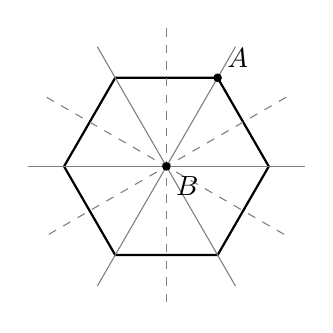
\begin{tikzpicture}[scale=1.3]
\draw[thick] (0:1)--(60:1)--(120:1)--(180:1)--(240:1)--(300:1)--cycle;
\foreach \ang in {0,60,120}
{\draw[gray] (\ang:1.35)--(\ang+180:1.35);}
\foreach \ang in {30,90,150}
{\draw[gray,dashed] (\ang:1.35)--(\ang+180:1.35);}
\fill (0,0) circle (1.2pt) node[below right] {$B$};
\fill (60:1) circle (1.2pt) node[above right] {$A$};
\end{tikzpicture}

\small Solid lines join opposite vertices; dashed lines join
opposite edge midpoints. Both sets are reflection axes.\normalsize
\end{center}

\Needspace{12\baselineskip}
\subsection*{17.2 Representation of Groups}

\Needspace{5\baselineskip}
\par\bigskip
\noindent\textbf{17.2.1}\quad For any representation $K$ of a group,
and for any group element $a$, show that
\[
\big[U^{K}(a)\big]^{-1}=U^{K}\big(a^{-1}\big).
\]
\solution
A matrix representation maps the identity to the identity matrix
and preserves products. Hence
\[
U^K(a)U^K(a^{-1})=U^K(aa^{-1})=U^K(I)=I,
\]
and also
\[
U^K(a^{-1})U^K(a)=U^K(a^{-1}a)=I.
\]
Thus $U^K(a^{-1})$ is both a right and left inverse of $U^K(a)$.
By uniqueness of the matrix inverse,
\[
\boxed{[U^K(a)]^{-1}=U^K(a^{-1})}.
\]
No assumption of a faithful representation or of unitarity is needed.

\Needspace{5\baselineskip}
\par\bigskip
\noindent\textbf{17.2.2}\quad Show that these four matrices form a
representation of the Vierergruppe, whose multiplication table is in
Table~17.2.
\[
\mathsf{I}=\begin{pmatrix}1&0\\0&1\end{pmatrix},\quad
\mathsf{A}=\begin{pmatrix}-1&0\\0&-1\end{pmatrix},\quad
\mathsf{B}=\begin{pmatrix}0&1\\1&0\end{pmatrix},\quad
\mathsf{C}=\begin{pmatrix}0&-1\\-1&0\end{pmatrix}.
\]
\solution
The given matrices obey $A=-I$ and $C=-B$. Direct multiplication gives
\[
B^2=\begin{pmatrix}0&1\\1&0\end{pmatrix}^2=I,
\]
so $A^2=(-I)^2=I$ and $C^2=(-B)^2=I$ as well.
The products of distinct nonidentity matrices are
\[
AB=BA=-B=C,\qquad AC=CA=B,\qquad
BC=CB=-B^2=-I=A.
\]
Multiplication by $I$ leaves every matrix unchanged. These statements
give all 16 products:
\[
\begin{array}{c|cccc}
&I&A&B&C\\\hline
I&I&A&B&C\\
A&A&I&C&B\\
B&B&C&I&A\\
C&C&B&A&I
\end{array}.
\]
The table is exactly Table 17.2; therefore the four matrices form
a representation of the Vierergruppe. Since all four are different,
this particular representation is faithful.

\Needspace{5\baselineskip}
\par\bigskip
\noindent\textbf{17.2.3}\quad Show that the matrices $\mathsf{I}$,
$\mathsf{A}$, $\mathsf{B}$, and $\mathsf{C}$ of Exercise~17.2.2 are
reducible. Reduce them.
\par\emph{Note.}~This means transforming $\mathsf{B}$ and
$\mathsf{C}$ to diagonal form (by the same unitary transformation).
\solution
The eigenvectors of $B$ are
\[
v_+=\frac1{\sqrt2}\binom11,\quad Bv_+=v_+,\qquad
v_-=\frac1{\sqrt2}\binom1{-1},\quad Bv_-=-v_-.
\]
Let $Q=(v_+\ v_-)=2^{-1/2}\begin{pmatrix}1&1\\1&-1\end{pmatrix}$.
Its columns are orthonormal, so $Q^\dagger Q=I$; that is,
$Q^\dagger v_+=(1,0)^T$ and $Q^\dagger v_-=(0,1)^T$.
Since $BQ=(v_+\ \ {-v_-})$, the columns of $Q^\dagger BQ$ are
$(1,0)^T$ and $(0,-1)^T$. Because $C=-B$,
the same eigenvectors diagonalize $C$:
\[
Q^\dagger BQ=\begin{pmatrix}1&0\\0&-1\end{pmatrix},\qquad
Q^\dagger CQ=\begin{pmatrix}-1&0\\0&1\end{pmatrix}.
\]
The scalar matrices $I,A=-I$ are unchanged. Thus the transformed
representation is a direct sum of two one-dimensional representations,
with characters in the order $(I,A,B,C)$
\[
\boxed{(1,-1,1,-1)\quad\text{and}\quad(1,-1,-1,1)}.
\]
Each line $\operatorname{span}\{v_\pm\}$ is invariant under every
group element, proving reducibility and supplying the reduction.

\Needspace{5\baselineskip}
\par\bigskip
\noindent\textbf{17.2.4}
\begin{enumerate}
\item[(a)] Once you have a matrix representation of any group, a 1-D
representation can be obtained by taking the determinants of the
matrices. Show that the multiplicative relations are preserved in
this determinant representation.
\item[(b)] Use determinants to obtain a 1-D representation of
$D_{3}$ from the $2\times2$ representation in Eq.~(17.2).
\end{enumerate}
\solution
\textbf{(a)} If $U(ab)=U(a)U(b)$, the determinant product theorem gives
\[
\chi_{\det}(ab)=\det U(ab)
=\det U(a)\det U(b)=\chi_{\det}(a)\chi_{\det}(b).
\]
Also $\chi_{\det}(I)=1$ and
$\chi_{\det}(a^{-1})=1/\chi_{\det}(a)$.
Every $U(a)$ is invertible, so no determinant is zero.
The determinants therefore define a one-dimensional representation.

\textbf{(b)} In Eq.~(17.2), the matrices of $C_3$ and $C_3^2$
have determinant
$(-1/2)^2+(\sqrt3/2)^2=1$.
The $C_2$ matrix has determinant $-1$; either other twofold matrix
has determinant $(-1/2)(1/2)-(\sqrt3/2)^2=-1$.
Thus
\[
\boxed{\begin{array}{c|rrrrrr}
g&I&C_3&C_3^2&C_2&C_2'&C_2''\\\hline
\chi_{\det}(g)&1&1&1&-1&-1&-1
\end{array}}.
\]
This is the $A_2$ representation of $D_3$.
Products of two flips have determinant $+1$, products of a flip
with a rotation have determinant $-1$, and products of rotations
have determinant $+1$, as required by the group table.

\Needspace{5\baselineskip}
\par\bigskip
\noindent\textbf{17.2.5}\quad Show that the cyclic group of $n$
objects, $C_{n}$, may be represented by $r^{m}$,
$m=0,1,2,\ldots,n-1$. Here $r$ is \erratum{the image of an abstract generator}, given by
\[
r=\exp(2\pi is/n).
\]
The parameter $s$ takes on the values $s=1,2,3,\ldots,n$, with each
value of $s$ yielding a different 1-D (irreducible) representation of
$C_{n}$.
\par\erratum{Take $n\ge1$ and complex representations; the scalar image need not have order $n$.}
\solution
Let $g$ be the abstract generator of $C_n$, so $g^n=I$.
For each integer $s\in\{1,\ldots,n\}$ set
\[
r_s=e^{2\pi is/n},\qquad U_s(g^m)=r_s^m.
\]
Because $r_s^n=e^{2\pi is}=1$, reducing $m$ modulo $n$
does not change this value. For arbitrary integers $j,k$,
\[
U_s(g^jg^k)=r_s^{j+k}=r_s^jr_s^k
=U_s(g^j)U_s(g^k).
\]
Thus this is a representation; it is irreducible since its space
is one-dimensional.

The representations are distinct: equivalence in one dimension
cannot change the scalar $U_s(g)$, and the $n$ numbers
$e^{2\pi is/n}$ are distinct for these $s$.
They are all the irreducible representations. Indeed any complex
representation matrix of $g$ satisfies $U(g)^n=U(g^n)=I$, so its
eigenvalues are $n$th roots of unity; each eigenline is invariant
under every power of $g$. An irreducible representation must
therefore have dimension one. A one-dimensional representation is
fixed by the number $U(g)$, which satisfies $U(g)^n=1$; hence
$U(g)=e^{2\pi is/n}$ for exactly one $s\in\{1,\ldots,n\}$, and the
representation is $U_s$.

\erratum{The scalar $r_s$ is the image of a generator, not
necessarily an element of order $n$. Its order is $n/\gcd(s,n)$.
The representation is faithful only when $\gcd(s,n)=1$;
$s=n$ gives the trivial representation.}
To check the order, $r_s^k=1$ is equivalent to $n$ dividing $sk$.
Write $d=\gcd(s,n)$, $s=ds'$, $n=dn'$; then $n\mid sk$ means
$n'\mid s'k$, and since $\gcd(n',s')=1$ this means $n'\mid k$.
The smallest positive such $k$ is therefore $n'=n/\gcd(s,n)$.

\Needspace{5\baselineskip}
\par\bigskip
\noindent\textbf{17.2.6}\quad Develop the irreducible $2\times2$
matrix representation of the group of rotations (including those that
turn it over) that transform a square into itself. Give the group
multiplication table.
\par\emph{Note.}~This group has the name $D_{4}$ (see Fig.~17.5).
\solution
Take $r$ to be a counterclockwise $90^\circ$ rotation and $s$ a
$180^\circ$ turn about the $x$ axis in the plane of the square.
Their action on in-plane coordinates is
\[
R=\begin{pmatrix}0&-1\\1&0\end{pmatrix},\qquad
S=\begin{pmatrix}1&0\\0&-1\end{pmatrix}.
\]
Thus $R^2=-I$, $R^4=S^2=I$, and
\[
SRS=S(RS)=S\begin{pmatrix}0&1\\1&0\end{pmatrix}
=\begin{pmatrix}0&1\\-1&0\end{pmatrix}=R^{-1}.
\]
The eight matrices, with $U(r^is)=R^iS$, are
\[
\begin{array}{c|cccc}
g&I&r&r^2&r^3\\\hline
U(g)&
\begin{pmatrix}1&0\\0&1\end{pmatrix}&
\begin{pmatrix}0&-1\\1&0\end{pmatrix}&
\begin{pmatrix}-1&0\\0&-1\end{pmatrix}&
\begin{pmatrix}0&1\\-1&0\end{pmatrix}
\end{array},
\]
\[
\begin{array}{c|cccc}
g&s&rs&r^2s&r^3s\\\hline
U(g)&
\begin{pmatrix}1&0\\0&-1\end{pmatrix}&
\begin{pmatrix}0&1\\1&0\end{pmatrix}&
\begin{pmatrix}-1&0\\0&1\end{pmatrix}&
\begin{pmatrix}0&-1\\-1&0\end{pmatrix}
\end{array}.
\]
The first four preserve the displayed side of the square;
the last four turn it over. All are real orthogonal.

Every element is $r^is^\epsilon$, $0\le i<4$, $\epsilon=0,1$.
The relation $srs=r^{-1}$ gives $sr=r^{-1}s$, and applying it
$j$ times, $sr^j=r^{-j}s$. Hence the product rule is
\[
(r^is^\epsilon)(r^js^\eta)
=r^{\,i+(-1)^\epsilon j}s^{\,\epsilon+\eta},
\]
with exponents reduced modulo four and two. This gives the full table
(row times column):
\[
\begin{array}{c|cccccccc}
&I&r&r^2&r^3&s&rs&r^2s&r^3s\\\hline
I&I&r&r^2&r^3&s&rs&r^2s&r^3s\\
r&r&r^2&r^3&I&rs&r^2s&r^3s&s\\
r^2&r^2&r^3&I&r&r^2s&r^3s&s&rs\\
r^3&r^3&I&r&r^2&r^3s&s&rs&r^2s\\
s&s&r^3s&r^2s&rs&I&r^3&r^2&r\\
rs&rs&s&r^3s&r^2s&r&I&r^3&r^2\\
r^2s&r^2s&rs&s&r^3s&r^2&r&I&r^3\\
r^3s&r^3s&r^2s&rs&s&r^3&r^2&r&I
\end{array}.
\]

To prove irreducibility even over $\mathbb C$, a proper nonzero
invariant subspace would be a line. It would have to be an
eigenline of $R$, whose distinct eigenvalues are $i,-i$ with
eigenvectors $(1,-i)^T$ and $(1,i)^T$.
But $S$ interchanges these lines. Neither is invariant under
the whole group, so the two-dimensional representation is irreducible.

\Needspace{12\baselineskip}
\subsection*{17.3 Symmetry and Physics}

\Needspace{5\baselineskip}
\par\bigskip
\noindent\textbf{17.3.1}\quad Consider a quantum mechanics problem
with $D_{3}$ symmetry, with the threefold symmetry axis taken as the
$z$ direction, and with orbitals $\varphi(\mathbf{r}-\mathbf{R}_{j})$
located at the vertices of an equilateral triangle. This is the same
system geometry as in Example~17.3.2, but in the present problem
$\varphi$ will no longer be chosen to have spherical symmetry.
\par Given that $\varphi(\mathbf{r})=(z/r)f(r)$ (so $\varphi$ has the
symmetry of a $p$ orbital oriented along the symmetry axis),
construct linear combinations of the $\varphi$ that are bases for
irreducible representations of $D_{3}$, for each basis indicating its
representation.
\solution
Write $\varphi_j(\mathbf r)=\varphi(\mathbf r-\mathbf R_j)$,
with the vertices numbered cyclically. Use active operations:
$r=C_3$ sends $\varphi_1\to\varphi_2\to\varphi_3\to\varphi_1$.
A twofold rotation $s=C_2$ about the in-plane axis through vertex 1
also reverses $z$. Since each local orbital is proportional to
$z$, its transformation is
\[
s\varphi_1=-\varphi_1,\qquad
s\varphi_2=-\varphi_3,\qquad
s\varphi_3=-\varphi_2.
\]
Thus the sum
\[
\boxed{\psi_{A_2}=\frac{\varphi_1+\varphi_2+\varphi_3}{\sqrt3}}
\]
is unchanged by $r$ and changes sign under $s$.
Its characters on $(I,2C_3,3C_2)$ are $(1,1,-1)$, identifying $A_2$.

Choose two independent zero-sum combinations
\[
u=\frac{2\varphi_1-\varphi_2-\varphi_3}{\sqrt6},\qquad
v=\frac{\varphi_2-\varphi_3}{\sqrt2}.
\]
Substituting $\varphi_1\to\varphi_2\to\varphi_3\to\varphi_1$ gives
\[
ru=\frac{-\varphi_1+2\varphi_2-\varphi_3}{\sqrt6}
=-\frac12u+\frac{\sqrt3}{2}v,\qquad
rv=\frac{\varphi_3-\varphi_1}{\sqrt2}
=-\frac{\sqrt3}{2}u-\frac12v.
\]
The coefficient vectors $(2,-1,-1)/\sqrt6$ and $(0,1,-1)/\sqrt2$ of
$u$ and $v$ are orthonormal, so each coefficient here is an inner
product of coefficient vectors; for example, the coefficient of $v$
in $ru$ is $[0\cdot(-1)+1\cdot2+(-1)(-1)]/\sqrt{12}=\sqrt3/2$.
The substitution for $s$ gives
\[
su=\frac{-2\varphi_1+\varphi_3+\varphi_2}{\sqrt6}=-u,\qquad
sv=\frac{-\varphi_3+\varphi_2}{\sqrt2}=v.
\]
Hence the coefficient matrices in the ordered basis $(u,v)$ are
\[
D_E(r)=\begin{pmatrix}-1/2&-\sqrt3/2\\
\sqrt3/2&-1/2\end{pmatrix},\qquad
D_E(s)=\begin{pmatrix}-1&0\\0&1\end{pmatrix}.
\]
Their traces are $-1$ and $0$, so the characters are $(2,-1,0)$.
An invariant line would have to be an eigenline of $D_E(r)$, whose
distinct eigenvalues $e^{\pm2\pi i/3}$ have eigenvectors
$(1,\mp i)^T$. But $D_E(s)(1,\mp i)^T=-(1,\pm i)^T$, so the flip
interchanges these two lines, and the two-dimensional space is
irreducible. As a check, the representation on
$\operatorname{span}\{\varphi_1,\varphi_2,\varphi_3\}$ has characters
$(3,0,-1)$: $r$ moves every orbital to another site, while $s$
contributes only the diagonal entry $-1$ from $s\varphi_1=-\varphi_1$.
Indeed $(3,0,-1)=(1,1,-1)+(2,-1,0)$. Therefore
\[
\boxed{\operatorname{span}\{\varphi_1,\varphi_2,\varphi_3\}
=A_2\oplus E,\qquad E\text{ has basis }(u,v)}.
\]
\erratum{The Instructor's Manual gives $-I_2$ for a twofold
operation in this $E$ space; that matrix has trace $-2$, whereas
every such operation has eigenvalues $+1,-1$ and trace zero, the
$E$ character, as the direct transformations show.}
The square-root factors normalize the coefficient vectors.
If spatially overlapping orbitals are used, their actual Hilbert-space
norms must be obtained from their overlap integrals; the symmetry
assignments do not depend on those common scale choices.

\Needspace{12\baselineskip}
\subsection*{17.4 Discrete Groups}

\Needspace{5\baselineskip}
\par\bigskip
\noindent\textbf{17.4.1}\quad The Vierergruppe has the multiplication
table shown in Table~17.2.
\begin{enumerate}
\item[(a)] Divide its elements into classes.
\item[(b)] Using the class information, determine for the
Vierergruppe its number of inequivalent irreducible representations
and their dimensions.
\item[(c)] Construct a character table for the Vierergruppe.
\end{enumerate}
\solution
\textbf{(a)} The group is abelian, so
$gag^{-1}=agg^{-1}=a$ for every $a,g$.
Its conjugacy classes are therefore
\[
\boxed{\{I\},\quad\{A\},\quad\{B\},\quad\{C\}}.
\]

\textbf{(b)} The number of inequivalent complex irreducible
representations equals the number of classes, hence is four.
Their positive integer dimensions satisfy
$d_1^2+d_2^2+d_3^2+d_4^2=|\mathcal G|=4$.
Every term is at least one, so each $d_j=1$.

\textbf{(c)} In a one-dimensional representation set
$\chi(A)=a$, $\chi(B)=b$.
Since $A^2=B^2=I$, both $a,b$ are $\pm1$.
The relation $C=AB$ fixes $\chi(C)=ab$.
The four independent choices of $a,b$ give
\[
\boxed{\begin{array}{c|rrrr}
&I&A&B&C\\\hline
A_1&1&1&1&1\\
A_2&1&1&-1&-1\\
A_3&1&-1&1&-1\\
A_4&1&-1&-1&1
\end{array}}.
\]
Each row obeys the multiplication table. Its squared norm
is four, and two distinct rows have two equal and two opposite
entries, giving inner product zero. Thus the table also satisfies
character orthogonality and contains all four irreducibles.

\Needspace{5\baselineskip}
\par\bigskip
\noindent\textbf{17.4.2}\quad The group $D_{3}$ may be discussed as a
permutation group of three objects. Operation $C_{3}$, for instance,
moves vertex 1 to the position formerly occupied by vertex \erratum{3};
likewise vertex 2 moves to the original position of vertex \erratum{1} and
vertex 3 moves to the original position of vertex \erratum{2}. So this
shuffling could be described as the permutation of $(1,2,3)$ to
$(2,3,1)$. Using now letters $a$, $b$, $c$ to avoid notational
confusion, this permutation $(abc)\to(bca)$ corresponds to the matrix
equation
\[
C_{3}\begin{pmatrix}a\\b\\c\end{pmatrix}
=\begin{pmatrix}0&1&0\\0&0&1\\1&0&0\end{pmatrix}
\begin{pmatrix}a\\b\\c\end{pmatrix}
=\begin{pmatrix}b\\c\\a\end{pmatrix},
\]
thereby identifying a $3\times3$ representation of the operation
$C_{3}$.
\begin{enumerate}
\item[(a)] Develop analogous $3\times3$ representations for the other
elements of $D_{3}$.
\item[(b)] Reduce your $3\times3$ representation to the direct sum of
a $1\times1$ and a $2\times2$ representation. Note: This $3\times3$
representation must be reducible or Eq.~(17.10) would be violated.
\end{enumerate}
\par\erratum{The printed statement has vertex 1 moving to the position of vertex 2, vertex 2 to that of vertex 3, and vertex 3 to that of vertex 1, which does not agree with the displayed matrix (see the solution); the vertex motion is reversed here so that the name $C_3$ follows the displayed matrix.}
\solution
\erratum{The printed vertex motion is the active map
$1\to2\to3\to1$. Afterwards position 1 holds the label $c$ of
vertex 3, position 2 holds $a$, and position 3 holds $b$, so it sends
the column of labels at fixed positions from $(a,b,c)$ to $(c,a,b)$.
The displayed matrix instead gives $(b,c,a)$, the inverse reordering.
We retain the displayed matrix for this exercise; using the printed
motion would interchange the labels $C_3$ and $C_3^2$.}

\textbf{(a)} Put
\[
R=\begin{pmatrix}0&1&0\\0&0&1\\1&0&0\end{pmatrix},\qquad
S=\begin{pmatrix}1&0&0\\0&0&1\\0&1&0\end{pmatrix}.
\]
Here $S$ interchanges the second and third entries; as a right
factor it interchanges the second and third columns.
Direct multiplication gives $R^2=U(C_3^2)$ below, $R^3=S^2=I$,
and $SRS=(SR)S=R^{-1}$: interchanging the last two columns of $SR$
(displayed below) gives $R^2=R^T=R^{-1}$.
Hence $R,S$ generate a representation of $D_3$.
The six matrices, named consistently with the multiplication
table $C_2C_3=C_2'$, are
\[
\begin{aligned}
U(I)&=I_3,&
U(C_3)&=R,&
U(C_3^2)&=\begin{pmatrix}0&0&1\\1&0&0\\0&1&0\end{pmatrix},\\
U(C_2)&=S,&
U(C_2')&=SR=\begin{pmatrix}0&1&0\\1&0&0\\0&0&1\end{pmatrix},&
U(C_2'')&=SR^2=\begin{pmatrix}0&0&1\\0&1&0\\1&0&0\end{pmatrix}.
\end{aligned}
\]

\textbf{(b)} All permutations preserve the sum of the three
components. Consequently
\[
e_0=\frac1{\sqrt3}\begin{pmatrix}1\\1\\1\end{pmatrix}
\]
is fixed. The permutation matrices are orthogonal, so its
orthogonal complement, the vectors with zero component sum, is
invariant. Choose an orthonormal basis there:
\[
e_1=\frac1{\sqrt6}\begin{pmatrix}2\\-1\\-1\end{pmatrix},\qquad
e_2=\frac1{\sqrt2}\begin{pmatrix}0\\1\\-1\end{pmatrix},
\qquad Q=(e_0\ e_1\ e_2).
\]
Since $R(a,b,c)^T=(b,c,a)^T$ and $S(a,b,c)^T=(a,c,b)^T$,
\[
Re_1=\frac1{\sqrt6}\begin{pmatrix}-1\\-1\\2\end{pmatrix}
=-\tfrac12e_1-\tfrac{\sqrt3}{2}e_2,\qquad
Re_2=\frac1{\sqrt2}\begin{pmatrix}1\\-1\\0\end{pmatrix}
=\tfrac{\sqrt3}{2}e_1-\tfrac12e_2,
\]
as one checks by adding the right-hand sides componentwise
(note $\tfrac{\sqrt3}{2}e_2=\tfrac{3}{2\sqrt6}(0,1,-1)^T$), and
$Se_1=e_1$, $Se_2=-e_2$. These coefficients form the columns of the
$2\times2$ blocks, while $Re_0=Se_0=e_0$ gives the entry $1$:
\[
Q^\dagger RQ=
1\oplus\begin{pmatrix}-1/2&\sqrt3/2\\-\sqrt3/2&-1/2\end{pmatrix},
\qquad
Q^\dagger SQ=1\oplus\begin{pmatrix}1&0\\0&-1\end{pmatrix}.
\]
Every other group matrix is a product of $R,S$, so the same
$1+2$ block structure holds for all six matrices.
The scalar block is $A_1$; the two-dimensional block has characters
$(2,-1,0)$ and is $E$. Hence
\[
\boxed{U=A_1\oplus E}.
\]
As a check, the traces of $I_3$, $R$, $S$ give the characters
$(3,0,1)$ of $U$ on $(I,2C_3,3C_2)$, and
$(3,0,1)=(1,1,1)+(2,-1,0)$.

\Needspace{5\baselineskip}
\par\bigskip
\noindent\textbf{17.4.3}\quad The group named $D_{4}$ has a fourfold
axis of symmetry, and twofold axes in four directions perpendicular
to the fourfold axis. See Fig.~17.5. $D_{4}$ has the following
classes (the numbers preceding the class descriptors indicate the
number of elements in the class): $I$, $2C_{4}$, $C_{2}$, $2C_{2}'$,
$2C_{2}''$. The twofold axes marked with primes are in the plane of
fourfold symmetry.
\begin{enumerate}
\item[(a)] Find the number and dimensions of the irreducible
representations.
\item[(b)] Given that all the characters of the representations of
dimension 1 are $\pm1$ and that $C_{2}=C_{4}^{2}$, use the
orthogonality conditions to construct a complete character table for
$D_{4}$.
\end{enumerate}
\solution
\textbf{(a)} There are five classes, so there are five irreducible
representations. Their dimensions have squares summing to eight.
No dimension can exceed two, since $3^2=9>8$. If $k$ dimensions are two and
the other $5-k$ are one, then
\[
4k+(5-k)=8\quad\Longrightarrow\quad k=1.
\]
Thus there are four one-dimensional representations and one
two-dimensional representation.

\textbf{(b)} Write the group as
$r^4=s^2=I$, $srs=r^{-1}$, as in 17.2.6.
Its classes are
\[
\{I\},\quad\{r,r^3\},\quad\{r^2\},\quad
\{s,r^2s\},\quad\{rs,r^3s\}.
\]
Indeed, with $sr^j=r^{-j}s$ from 17.2.6, conjugation by $r$ gives
$rsr^{-1}=r^2s$ and $r(rs)r^{-1}=r^3s$, conjugation by $s$ gives
$srs^{-1}=r^{-1}=r^3$, and $r^2$ commutes with every element.
In one dimension, $a=U(r)$ and $b=U(s)$ are scalars.
The relation $bab=a^{-1}$ and $b^2=1$ imply $a=a^{-1}$,
so $a,b=\pm1$. The class characters are therefore
$(1,a,1,b,ab)$, since $\chi(r^2)=a^2=1$ and $\chi(rs)=ab$.
Their four choices give the first four rows below.

For the remaining representation, $\chi_E(I)=2$.
Column orthogonality between a nonidentity column $g$ and the
identity column requires
\[
\sum_K \chi_K(I)^*\chi_K(g)=0.
\]
For $r,r^3$, the first four entries sum to zero, so
$2\chi_E(r)=0$. The same reasoning gives zero on both flip classes.
For $r^2$, the four scalar entries sum to four, so
$4+2\chi_E(r^2)=0$, giving $\chi_E(r^2)=-2$.
Thus the complete table is
\[
\boxed{\begin{array}{c|rrrrr}
D_4&I&2C_4&C_2&2C_2'&2C_2''\\\hline
A_1&1&1&1&1&1\\
A_2&1&1&1&-1&-1\\
B_1&1&-1&1&1&-1\\
B_2&1&-1&1&-1&1\\
E&2&0&-2&0&0
\end{array}}.
\]
Using class weights $(1,2,1,2,2)$, each row has squared norm
eight and distinct rows have inner product zero.
For example $\langle E,E\rangle=4+4=8$, while
$\langle E,A_1\rangle=2-2=0$. This verifies the required
orthogonality; the $E$ matrices in 17.2.6 realize its last row.

\Needspace{5\baselineskip}
\par\bigskip
\noindent\textbf{17.4.4}\quad The eight functions $\pm x^{3}$,
$\pm x^{2}y$, $\pm xy^{2}$, $\pm y^{3}$ \erratum{span a reducible function space} for
$D_{4}$, with $C_{4}$ a $90^{\circ}$ counterclockwise rotation in the
$xy$ plane, $C_{2}=C_{4}^{2}$, $C_{2}'=(x\to -x,\,y\to y)$,
$C_{2}''=(x\to y,\,y\to x)$, and the remaining members of $D_{4}$ are
additional members of the classes containing the above operations.
Find the characters of the reducible representation \erratum{on this span},
and find the direct sum of irreducible representations of which it consists.
\par\erratum{Also distinguish the formal permutation representation on eight independent signed labels, which is the interpretation used by the Instructor's Manual.}
\solution
\erratum{As actual functions, $f$ and $-f$ are linearly dependent.
The eight listed signed functions are not an eight-dimensional
basis: their function space has dimension four. The Instructor's
Manual's eight-dimensional answer describes a different, formal permutation
space whose eight signed labels are treated as independent.
We give both interpretations explicitly.}

For the actual cubic functions take the independent basis
\[
f_1=x^3,\quad f_2=x^2y,\quad f_3=xy^2,\quad f_4=y^3.
\]
Let the quarter-turn act on functions by the substitution
$r:(x,y)\mapsto(y,-x)$, that is, $(rf)(\mathbf r)=f(R^{-1}\mathbf r)$
for the counterclockwise $90^\circ$ rotation $R$. The opposite
convention, $f(R\mathbf r)$, assigns to each operation the matrix of
its inverse; it gives the same characters, because every element of
$D_4$ is conjugate to its inverse. The transformed basis is
\[
r(f_1,f_2,f_3,f_4)=\bigl(y^3,\,y^2(-x),\,y(-x)^2,\,(-x)^3\bigr)
=(f_4,-f_3,f_2,-f_1).
\]
Thus no diagonal coefficient occurs and $\chi(r)=0$.
The half-turn sends every cubic to its negative, so $\chi(r^2)=-4$.
For $s:(x,y)\mapsto(-x,y)$,
\[
s(f_1,f_2,f_3,f_4)=(-f_1,f_2,-f_3,f_4),
\]
whose trace is zero. The diagonal reflection
$(x,y)\mapsto(y,x)$ exchanges $f_1\leftrightarrow f_4$ and
$f_2\leftrightarrow f_3$, again with trace zero. Therefore
\[
\chi_{\rm cubic}=(4,0,-4,0,0)
\quad\text{on }(I,2C_4,C_2,2C_2',2C_2'').
\]
Only $I$ and $C_2$ have nonzero characters, and every
one-dimensional representation has $\chi(C_2)=1$, so the
multiplicity formula $n_K=8^{-1}\sum_{\rm classes}|C|\chi_K^*\chi$ gives
\[
n_{A_1}=n_{A_2}=n_{B_1}=n_{B_2}=\frac{4-4}{8}=0,\qquad
n_E=\frac{4\cdot2+(-4)(-2)}8=2.
\]
Hence the function-space answer is
\[
\boxed{\mathcal P_3=E\oplus E}.
\]
Explicit invariant pairs are $(x^3,y^3)$ and $(x^2y,xy^2)$, as the
transformation lists above show. In each pair a quarter-turn has
eigenvalues $\pm i$:
$r(x^3\mp iy^3)=\pm i(x^3\mp iy^3)$ and
$r(x^2y\pm ixy^2)=\pm i(x^2y\pm ixy^2)$. The reflection $s$
interchanges the eigenlines, since
$s(x^3-iy^3)=-(x^3+iy^3)$ and $s(x^2y+ixy^2)=x^2y-ixy^2$.
Hence neither pair has an invariant line, and each copy is irreducible.

For the formal eight-label interpretation, introduce independent
symbols $e_{j,+},e_{j,-}$ representing the labels $+f_j,-f_j$.
A group operation permutes these eight symbols, so its character
counts fixed labels. The identity fixes eight. The quarter-turn
and diagonal reflection fix none. The half-turn exchanges
each $+$ label with its $-$ partner and fixes none.
The reflection $x\mapsto-x$ fixes the four labels
$\pm x^2y,\pm y^3$. Thus
\[
\chi_{\rm formal}=(8,0,0,4,0),
\]
and
\[
\boxed{\mathcal V_{\rm formal}=2A_1\oplus2B_1\oplus2E}.
\]
Indeed its multiplicities are
$(8+2\cdot4)/8=2$ for $A_1,B_1$,
$(8-2\cdot4)/8=0$ for $A_2,B_2$, and
$(8\cdot2)/8=2$ for $E$.
The map $e_{j,\pm}\mapsto\pm f_j$ commutes with the group action
and maps onto the cubic space; its kernel is spanned by the four
vectors $e_{j,+}+e_{j,-}$. Each operation permutes these kernel
vectors without signs (an operation taking $f_j$ to $\pm f_k$ sends
$e_{j,+}+e_{j,-}$ to $e_{k,+}+e_{k,-}$), so the kernel has characters
$\chi_{\rm formal}-\chi_{\rm cubic}=(4,0,4,4,0)$; the same
multiplicity formula gives $(4+4+2\cdot4)/8=2$ for $A_1,B_1$ and
zero for the others, i.e.\ the kernel is $2A_1\oplus2B_1$.
The quotient by the kernel is the actual cubic function space
$E\oplus E$. This explains why the two legitimate spaces have
different characters and dimensions.

\Needspace{5\baselineskip}
\par\bigskip
\noindent\textbf{17.4.5}\quad The group $C_{4v}$ has a fourfold
symmetry axis in the $z$ direction, reflection symmetries
($\sigma_{v}$) about the $xz$ and $yz$ planes, and additional
reflection symmetries ($\sigma_{d}$, $d=\text{dihedral}$) about
planes that contain the $z$ axis but are $45^{\circ}$ from the $x$
and $y$ axes. See Fig.~17.6. The character table for $C_{4v}$
follows.
\begin{center}
\begin{tabular}{lccccc}
\toprule
& $I$ & $2C_{4}$ & $C_{2}$ & $2\sigma_{v}$ & $2\sigma_{d}$\\
\midrule
$A_{1}$ & 1 & 1 & 1 & 1 & 1\\
$A_{2}$ & 1 & 1 & 1 & $-1$ & $-1$\\
$B_{1}$ & 1 & $-1$ & 1 & 1 & $-1$\\
$B_{2}$ & 1 & $-1$ & 1 & $-1$ & 1\\
$E$ & 2 & 0 & $-2$ & 0 & 0\\
\bottomrule
\end{tabular}
\end{center}
\begin{enumerate}
\item[(a)] Construct the matrix representing one member of each class
of $C_{4v}$ using as a basis a $p_{z}$ orbital at each of the points
$(x,y)=(a,0)$, $(0,a)$, $(-a,0)$, $(0,-a)$, and therefrom extract the
characters of the reducible representation for which these $p_{z}$
orbitals form a basis. A $p_{z}$ orbital has functional form
$(z/r)f(r)$.
\item[(b)] Determine the irreducible representations contained in our
reducible $p_{z}$ representation.
\item[(c)] Form those linear combinations of our $p_{z}$ functions
that are bases for each of the irreducible representations found in
part \erratum{(b)}.
\end{enumerate}
\par\erratum{The printed reference in (c) says (a); the irreducible summands are determined in (b).}
\solution
Let $f_1,f_2,f_3,f_4$ denote the $p_z$ orbitals centered,
in order, at $+x,+y,-x,-y$.
A $C_{4v}$ operation leaves $z$ unchanged, so the local $p_z$
shape incurs no sign change; only the centers are permuted.
We use matrices whose $j$th column gives the image of $f_j$.

\textbf{(a)} Choose $r=C_4$ counterclockwise, $s=\sigma_v$
reflection in the $xz$ plane, and $d=\sigma_d$ reflection in $x=y$.
On the centers, $r$ acts as $+x\to+y\to-x\to-y\to+x$, $r^2$
exchanges opposite centers, $s$ fixes $\pm x$ and exchanges
$+y\leftrightarrow-y$, and $d$ exchanges $+x\leftrightarrow+y$ and
$-x\leftrightarrow-y$. Representatives of the five classes are
therefore
\[
P_I=I_4,\qquad
P_r=\begin{pmatrix}0&0&0&1\\1&0&0&0\\0&1&0&0\\0&0&1&0\end{pmatrix},
\qquad
P_{r^2}=\begin{pmatrix}0&0&1&0\\0&0&0&1\\1&0&0&0\\0&1&0&0\end{pmatrix},
\]
\[
P_s=\begin{pmatrix}1&0&0&0\\0&0&0&1\\0&0&1&0\\0&1&0&0\end{pmatrix},
\qquad
P_d=\begin{pmatrix}0&1&0&0\\1&0&0&0\\0&0&0&1\\0&0&1&0\end{pmatrix}.
\]
The traces are, on $(I,2C_4,C_2,2\sigma_v,2\sigma_d)$,
\[
\boxed{\chi=(4,0,0,2,0)}.
\]
For example $s$ fixes the two orbitals on the $x$ axis,
while $r,r^2,d$ fix none.

\textbf{(b)} With class sizes $(1,2,1,2,2)$,
$n_K=8^{-1}\sum_{\rm classes}|C|\chi_K^*\chi$, in which only the
classes $I$ and $2\sigma_v$ contribute, gives
\[
n_{A_1}=n_{B_1}=\frac{4+2(2)}8=1,\qquad
n_{A_2}=n_{B_2}=\frac{4-2(2)}8=0,\qquad
n_E=\frac{2(4)}8=1.
\]
Thus \(\boxed{\Gamma=A_1\oplus B_1\oplus E}\).

\textbf{(c)} Suitable combinations are
\[
\boxed{\begin{aligned}
A_1:\quad a&=\tfrac12(f_1+f_2+f_3+f_4),\\
B_1:\quad b&=\tfrac12(f_1-f_2+f_3-f_4),\\
E:\quad e_x&=(f_1-f_3)/\sqrt2,\qquad
e_y=(f_2-f_4)/\sqrt2.
\end{aligned}}
\]
Substituting the center permutations gives
\[
ra=a,\quad sa=a,\qquad rb=-b,\quad sb=b,
\]
\[
re_x=e_y,\quad re_y=-e_x,\qquad se_x=e_x,\quad se_y=-e_y,
\qquad de_x=e_y,\quad de_y=e_x.
\]
For instance, $rb=\tfrac12(f_2-f_3+f_4-f_1)=-b$, and
$sb=\tfrac12(f_1-f_4+f_3-f_2)=b$ because $s$ fixes $f_1,f_3$ and
exchanges $f_2,f_4$; also $db=-b$. These generator actions identify
the stated representations. The function $a$ is invariant, as $A_1$
requires. The function $b$ has $\chi(r)=-1$, $\chi(\sigma_v)=1$,
$\chi(\sigma_d)=-1$, which is the $B_1$ row. On $(e_x,e_y)$ the
matrices of $r$ and $s$ are
$\bigl(\begin{smallmatrix}0&-1\\1&0\end{smallmatrix}\bigr)$ and
$\bigl(\begin{smallmatrix}1&0\\0&-1\end{smallmatrix}\bigr)$, the
$E$ matrices of Exercise~17.2.6, with characters $(2,0,-2,0,0)$.
The pair $e_x,e_y$ is odd across the square and transforms like
$(x,y)$.
The four coefficient vectors are mutually orthonormal and hence
independent; their actual function norms, if orbitals overlap,
are handled as explained in 17.3.1.

\Needspace{5\baselineskip}
\par\bigskip
\noindent\textbf{17.4.6}\quad Using the notation and geometry of
Exercise~17.4.5, repeat that exercise for the eight-member basis
consisting of a $p_{x}$ and a $p_{y}$ orbital at each of the points
$(x,y)=(a,0)$, $(0,a)$, $(-a,0)$, $(0,-a)$.
\solution
Write $x_j=p_x(\mathbf r-\mathbf R_j)$ and
$y_j=p_y(\mathbf r-\mathbf R_j)$, with the four sites ordered
as in 17.4.5. All $x_j$ have positive lobe along positive $x$,
and all $y_j$ along positive $y$. The ordered basis is
\[
(x_1,y_1,x_2,y_2,x_3,y_3,x_4,y_4).
\]
Unlike $p_z$, these local orbitals rotate and reflect in their
two-component orientation space.

\textbf{(a)} Let $P_g$ be the site matrix from 17.4.5 and $O_g$
the matrix acting on $(p_x,p_y)$. The operation $g$ carries the
orbital of orientation $p_\alpha$ ($\alpha=x,y$) at site $j$ to the
site $k$ with $(P_g)_{kj}=1$, with orientation
$\sum_\beta(O_g)_{\beta\alpha}\,p_\beta$. Hence
\[
D(g)_{(k,\beta),(j,\alpha)}=(P_g)_{kj}(O_g)_{\beta\alpha},\qquad
\boxed{D(g)=P_g\otimes O_g}.
\]
This formula determines every entry of the requested $8\times8$
matrices. Explicitly, put
\[
R=\begin{pmatrix}0&-1\\1&0\end{pmatrix},\quad
S=\begin{pmatrix}1&0\\0&-1\end{pmatrix},\quad
T=\begin{pmatrix}0&1\\1&0\end{pmatrix},\quad H=I_2.
\]
Because $p_x$ and $p_y$ transform like $x$ and $y$, the orientation
matrices are those of the point operations on $(x,y)$:
$O_r=R$, $O_{r^2}=R^2=-H$, $O_s=S$, $O_d=T$.
In the following block matrices each entry is $2\times2$, and
block $(k,j)$ is $(P_g)_{kj}O_g$:
\[
D(I)=I_8,\qquad
D(r)=\begin{pmatrix}0&0&0&R\\R&0&0&0\\0&R&0&0\\0&0&R&0\end{pmatrix},
\qquad
D(r^2)=\begin{pmatrix}0&0&-H&0\\0&0&0&-H\\-H&0&0&0\\0&-H&0&0\end{pmatrix},
\]
\[
D(s)=\begin{pmatrix}S&0&0&0\\0&0&0&S\\0&0&S&0\\0&S&0&0\end{pmatrix},
\qquad
D(d)=\begin{pmatrix}0&T&0&0\\T&0&0&0\\0&0&0&T\\0&0&T&0\end{pmatrix}.
\]
For example $rx_1=y_2$, $ry_1=-x_2$, $sx_1=x_1$, and
$sy_1=-y_1$, which explain the orientation signs.
The trace of a tensor product is the product of traces,
$\operatorname{tr}(P\otimes O)=\operatorname{tr}P\,\operatorname{tr}O$,
so, class by class,
\[
\chi_D=\chi_{\rm site}\chi_{\rm orientation}
=(4,0,0,2,0)(2,0,-2,0,0)
=\boxed{(8,0,0,0,0)}.
\]

\textbf{(b)} Only the identity contributes to the multiplicity sum:
$n_K=8^{-1}(8)\chi_K(I)=\dim K$.
Therefore
\[
\boxed{\Gamma=A_1\oplus A_2\oplus B_1\oplus B_2\oplus E\oplus E},
\]
with total dimension $4\cdot1+2\cdot2=8$, as required.

\textbf{(c)} The following four combinations give the scalar
representations:
\[
\boxed{\begin{aligned}
A_1:\quad a_1&=(x_1+y_2-x_3-y_4)/2,\\
A_2:\quad a_2&=(y_1-x_2-y_3+x_4)/2,\\
B_1:\quad b_1&=(x_1-y_2-x_3+y_4)/2,\\
B_2:\quad b_2&=(y_1+x_2-y_3-x_4)/2.
\end{aligned}}
\]
They arise from the site pair $(f_1-f_3,f_2-f_4)$ of 17.4.5 and
the orientation pair $(p_x,p_y)$, both of which transform like
$(x,y)$. Written as
\[
\begin{aligned}
a_1&=\tfrac12[(x_1-x_3)+(y_2-y_4)],&
a_2&=\tfrac12[(y_1-y_3)-(x_2-x_4)],\\
b_1&=\tfrac12[(x_1-x_3)-(y_2-y_4)],&
b_2&=\tfrac12[(y_1-y_3)+(x_2-x_4)],
\end{aligned}
\]
they are the scalar product (like $x^2+y^2$), the antisymmetric
product (like the $z$ component $xy'-yx'$ of a cross product), the
difference of diagonal products (like $x^2-y^2$), and
the symmetric off-diagonal product (like $xy$) of the two pairs.
To check them directly, note that with site indices modulo four
\[
r:\ x_j\mapsto y_{j+1},\quad y_j\mapsto-x_{j+1};\qquad
s:\ x_j\mapsto x_{\bar\jmath},\quad y_j\mapsto-y_{\bar\jmath},
\]
where $\bar1=1$, $\bar2=4$, $\bar3=3$, $\bar4=2$. For example,
$ra_1=(y_2-x_3-y_4+x_1)/2=a_1$ and
$sa_1=(x_1-y_4-x_3+y_2)/2=a_1$. In the same way one finds the
eigenvalues under the two generators:
\[
\begin{array}{c|rrrr}
&a_1&a_2&b_1&b_2\\\hline
r&1&1&-1&-1\\
s&1&-1&1&-1
\end{array}.
\]
Since $d=rs$ (as matrices on $(x,y)$, $RS=T$), its eigenvalues
are the corresponding products, so these are exactly the four
character-table rows.

The two independent $E$ pairs are
\[
\boxed{\begin{aligned}
u_x&=(x_1+x_2+x_3+x_4)/2,&
u_y&=(y_1+y_2+y_3+y_4)/2,\\
v_x&=(x_1-x_2+x_3-x_4)/2,&
v_y&=(y_1-y_2+y_3-y_4)/2.
\end{aligned}}
\]
The first pair is the site $A_1$ combination times the orientation
pair; the second uses the site $B_1$ combination.
By the rules above, $ru_x=u_y$, $ru_y=-u_x$, while
$rv_x=(y_2-y_3+y_4-y_1)/2=-v_y$ and
$rv_y=(-x_2+x_3-x_4+x_1)/2=v_x$; also $su_x=u_x$, $su_y=-u_y$,
$sv_x=v_x$, $sv_y=-v_y$. So their generator matrices are
respectively $(R,S)$ and $(-R,S)$. Both have characters
$(2,0,-2,0,0)$ and have no common invariant line: $-R$ has the same
eigenlines $(1,\mp i)^T$ as $R$, and $S$ interchanges them, as in
17.2.6.
The eight coefficient columns displayed above have norm one
and pairwise zero inner products, so they form a complete basis.
As in 17.3.1, coefficient normalization is distinct from spatial
normalization when local orbitals overlap.

\Needspace{12\baselineskip}
\subsection*{17.5 Direct Products}

\Needspace{5\baselineskip}
\par\bigskip
\noindent\textbf{17.5.1}\quad The group $C_{4v}$ has eight elements,
corresponding to the rotational and reflection symmetries of a square
that cannot be turned over. See Fig.~17.6. Symmetry rotations about
the $z$ axis are denoted $C_{4}$, $C_{2}$, $C_{4}'$. Reflections
relative to the $xz$ and $yz$ planes are named $\sigma_{v}$ and
$\sigma_{v}'$; those at $45^{\circ}$ relative to the $xz$ and $yz$
planes are called $\sigma_{d}$ and $\sigma_{d}'$ ($d$ indicates
``dihedral''). The character table for $C_{4v}$ is in Table~17.4.
\begin{enumerate}
\item[(a)] Find the direct sum of irreducible representations of
$C_{4v}$ corresponding to the direct product $E\otimes E$.
\item[(b)] A basis for $E$ (in the context of Fig.~17.5) consists of
the two functions $\varphi_{1}=x$, $\varphi_{2}=y$. Apply a few of
the group operations to this basis and verify the entries for $E$ in
the character table.
\item[(c)] Assume now that we have two sets of variables, $x_{1}$,
$y_{1}$ and $x_{2}$, $y_{2}$, and we form the direct-product basis
$x_{1}x_{2}$, $x_{1}y_{2}$, $y_{1}x_{2}$, $y_{1}y_{2}$. Determine how
the direct-product basis functions can be combined to form bases for
each of the irreducible representations in the direct sum
corresponding to $E\otimes E$.
\end{enumerate}
\solution
\textbf{(a)} For matrices $A,B$,
$\operatorname{tr}(A\otimes B)=(\operatorname{tr}A)(\operatorname{tr}B)$.
The product character is consequently
\[
\chi_{E\otimes E}=(2,0,-2,0,0)^2=(4,0,4,0,0).
\]
For each of the four one-dimensional irreducibles,
$\chi(I)=\chi(C_2)=1$, so its multiplicity is
$(4+4)/8=1$. For $E$ itself it is
$[2(4)+(-2)(4)]/8=0$. Thus
\[
\boxed{E\otimes E=A_1\oplus A_2\oplus B_1\oplus B_2}.
\]

\textbf{(b)} Take $r x=y$, $r y=-x$,
$s x=x$, $s y=-y$, and $d x=y$, $d y=x$.
In the ordered basis $(x,y)$ their coefficient matrices are
\[
D(r)=\begin{pmatrix}0&-1\\1&0\end{pmatrix},\quad
D(r^2)=-I_2,\quad
D(s)=\begin{pmatrix}1&0\\0&-1\end{pmatrix},\quad
D(d)=\begin{pmatrix}0&1\\1&0\end{pmatrix}.
\]
Their traces, together with $\operatorname{tr}I_2=2$, are
$(2,0,-2,0,0)$ as in the $E$ row.

\textbf{(c)} The product basis has independent variables for
particles 1 and 2. Its four convenient combinations are
\[
\boxed{\begin{aligned}
A_1:\quad a_1&=(x_1x_2+y_1y_2)/\sqrt2,\\
A_2:\quad a_2&=(x_1y_2-y_1x_2)/\sqrt2,\\
B_1:\quad b_1&=(x_1x_2-y_1y_2)/\sqrt2,\\
B_2:\quad b_2&=(x_1y_2+y_1x_2)/\sqrt2.
\end{aligned}}
\]
Apply $r$ to each factor: $x_1x_2\to y_1y_2$,
$y_1y_2\to x_1x_2$,
$x_1y_2\to-y_1x_2$, and
$y_1x_2\to-x_1y_2$.
Thus the four eigenvalues of $r$ are $(1,1,-1,-1)$.
Under $s$ a product acquires one minus sign for each $y$,
so the eigenvalues are $(1,-1,1,-1)$.
Under $d$ the two variables are exchanged, giving
$(1,-1,-1,1)$.
These reproduce the four claimed one-dimensional characters.
Their independent coefficient vectors span the full four-dimensional
tensor-product space.

\Needspace{12\baselineskip}
\subsection*{17.6 Symmetric Group}

\Needspace{5\baselineskip}
\par\bigskip
\noindent\textbf{17.6.1}
\begin{enumerate}
\item[(a)] The objects $(abcd)$ are permuted to $(dacb)$. Write out a
$4\times4$ matrix representation of this one permutation.
\par\emph{Hint:}~Compare with Exercise~17.4.2.
\item[(b)] Is the permutation $(abdc)\to(dacb)$ odd or even?
\item[(c)] Is \erratum{either of the permutations in (a) and (b)} a possible member of the $D_{4}$
group, which was the subject of Exercise~17.4.3? Why or why not?
\end{enumerate}
\par\erratum{Keep the two printed inputs distinct. In (c), distinguish the standard cyclic square labeling $1,2,3,4$ from an embedding obtained by relabeling its vertices.}
\solution
\textbf{(a)} The target column selects entries $4,1,3,2$
of the original column:
\[
\boxed{P=\begin{pmatrix}
0&0&0&1\\1&0&0&0\\0&0&1&0\\0&1&0&0
\end{pmatrix}},\qquad
P\begin{pmatrix}a\\b\\c\\d\end{pmatrix}
=\begin{pmatrix}d\\a\\c\\b\end{pmatrix}.
\]
As a map from old positions to new positions, this is
$(1\,2\,4)$ with position 3 fixed. It is a 3-cycle, has
order three, and is even: a 3-cycle is a product of two transpositions.

\textbf{(b)} \erratum{The printed input changes from $(abcd)$
in (a) to $(abdc)$ in (b). These are different permutations.
The manual's answer \emph{even} applies to (a), not to (b) as printed.}
For the literal input $(a,b,d,c)$, the target $(d,a,c,b)$
selects entries $3,1,4,2$. Its matrix is
\[
Q=\begin{pmatrix}
0&0&1&0\\1&0&0&0\\0&0&0&1\\0&1&0&0
\end{pmatrix}.
\]
Its position cycle is $(1\,2\,4\,3)$, which is a product
of three transpositions. Thus the answer to (b) as printed is
\[
\boxed{\text{odd},\qquad \det Q=-1}.
\]
Equivalently the row-selection list $(3,1,4,2)$ has three
inversions, also giving $(-1)^3=-1$.

\textbf{(c)} For the permutation in (a), the answer is unambiguously
$\boxed{\text{no}}$: its order is three, while $D_4$ has only
elements of orders one, two, and four. In particular its order
cannot divide $|D_4|=8$.

\erratum{The original reference in (c) was ambiguous. For the literal
permutation of (b), the geometric labeling must be specified.}
With slots $1,2,3,4$ placed in that cyclic order around the square,
$Q$ is not a symmetry: it sends the adjacent pair $(1,2)$ to
$(2,4)$, a diagonal pair. But a four-cycle is compatible with
an abstract $D_4$ embedding. If the cyclic order of vertices is
chosen to be $1,2,4,3$, then $Q=(1\,2\,4\,3)$ is a quarter-turn.
This distinction resolves the ambiguity without silently changing
the input in (b).

\Needspace{5\baselineskip}
\par\bigskip
\noindent\textbf{17.6.2}
\begin{enumerate}
\item[(a)] The permutation group of four objects, $S_{4}$, has
$4!=24$ elements. Treating the four elements of the cyclic group,
$C_{4}$, as permutations, set up a $4\times4$ matrix representation
of $C_{4}$. Note that $C_{4}$ is a subgroup of \erratum{$S_{4}$}.
\item[(b)] How do you know that this $4\times4$ matrix
representation of $C_{4}$ must be reducible?
\end{enumerate}
\solution
Let $R$ cyclically shift a column of four entries to the left.
The four matrices are
\[
U(I)=I_4,\qquad
U(C_4)=R=\begin{pmatrix}
0&1&0&0\\0&0&1&0\\0&0&0&1\\1&0&0&0
\end{pmatrix},
\]
\[
U(C_4^2)=R^2=\begin{pmatrix}
0&0&1&0\\0&0&0&1\\1&0&0&0\\0&1&0&0
\end{pmatrix},\qquad
U(C_4^3)=R^3=\begin{pmatrix}
0&0&0&1\\1&0&0&0\\0&1&0&0\\0&0&1&0
\end{pmatrix}.
\]
Four shifts restore the original column, so $R^4=I_4$.
The products satisfy $R^jR^k=R^{j+k\pmod4}$, exactly the
cyclic-group law. All four are permutation matrices, so they
form a subgroup of the full permutation group $S_4$
\erratum{(the original note writes $P_4$; this denotes the permutation group $S_4$ just introduced).}

For reducibility, the vector $(1,1,1,1)^T$ is fixed by all
four matrices, giving a proper invariant line.
More fully, let $\omega=i$ and define
\[
v_k=\frac12\begin{pmatrix}1\\\omega^k\\\omega^{2k}\\
\omega^{3k}\end{pmatrix},\qquad k=0,1,2,3.
\]
Cyclic shifting gives $Rv_k=\omega^kv_k$; the last component
works because $\omega^{4k}=1$.
Their inner products are
\[
v_j^\dagger v_k=\frac14\sum_{m=0}^3\omega^{(k-j)m}
=\begin{cases}1,&j=k,\\0,&j\ne k,\end{cases}
\]
by the finite geometric-series formula.
Thus $V=(v_0\,v_1\,v_2\,v_3)$ is unitary and
\[
\boxed{V^\dagger R^mV=\operatorname{diag}(1,i^m,(-1)^m,(-i)^m)}.
\]
The representation reduces to the four one-dimensional irreducible
representations of $C_4$.

\Needspace{5\baselineskip}
\par\bigskip
\noindent\textbf{17.6.3}\quad The permutation group of four objects,
$S_{4}$, has five classes.
\begin{enumerate}
\item[(a)] Determine the number of elements in each class of $S_{4}$
and identify one element of each class as a product of cycles.
\item[(b)] Two of the irreducible representations of $S_{4}$ are of
dimension 1 (and are usually denoted $A_{1}$ and $A_{2}$). Noting
that permutations can be classified as even or odd, find the
characters of $A_{1}$ and $A_{2}$.
\par\emph{Hint.}~Set up a character table and fill in the $A_{1}$ and
$A_{2}$ lines.
\item[(c)] One irreducible representation of $S_{4}$ (usually denoted
$E$) is of dimension 2. Determine the dimensions of all the
irreducible representations of $S_{4}$ other than $A_{1}$, $A_{2}$,
and $E$.
\item[(d)] Complete the character table of $S_{4}$.
\par\emph{Hint.}~Only the even permutations have nonzero characters
in the $E$ representation.
\end{enumerate}
\solution
\textbf{(a)} Conjugation relabels a permutation's cycles and preserves
their lengths. Conversely two permutations with the same cycle
lengths are conjugate by a suitable relabeling. The five possibilities
and their sizes are
\[
\begin{array}{c|c|c}
\text{cycle type}&\text{example}&\text{class size}\\\hline
1+1+1+1&I&1\\
2+1+1&(12)&\binom42=6\\
2+2&(12)(34)&\frac12\binom42=3\\
3+1&(123)&\binom43(3-1)!=8\\
4&(1234)&(4-1)!=6
\end{array}.
\]
For two transpositions, dividing by two removes the ordering
of the two pairs. For a cycle of length $k$, cyclically shifting
its notation describes the same cycle, leaving $k!/k=(k-1)!$
choices. The sizes sum to $24$.

\textbf{(b)} The trivial character is $(1,1,1,1,1)$.
A cycle of length $k$ is a product of $k-1$ transpositions, so
the signs of the five classes are $(1,-1,1,1,-1)$.
These give the $A_1,A_2$ rows below.

\textbf{(c)} There are five irreducibles. The known dimensions
$1,1,2$ account for $1+1+4=6$ of the squared-dimension sum.
The other dimensions $d,e$ obey
$d^2+e^2=24-6=18$. The only positive integer solution is
$d=e=3$.

\textbf{(d)} A useful independent construction supplies the
remaining characters. The ordinary four-dimensional permutation
representation has character equal to its number of fixed letters:
\[
(4,2,0,1,0).
\]
Removing its invariant all-ones line leaves a three-dimensional
representation with character
\[
\chi_{T_2}=(3,1,-1,0,-1).
\]
Its squared character norm is
$9+6(1)+3(1)+8(0)+6(1)=24$, proving irreducibility.
Multiplying by the sign representation gives a second irreducible,
\[
\chi_{T_1}=(3,-1,-1,0,1).
\]
This fixes our names $T_1,T_2$; interchanging their names is
an equally valid convention.

To construct $E$, act on the three pair partitions
\[
12|34,\qquad13|24,\qquad14|23.
\]
The respective numbers of fixed partitions for the five classes
are $(3,1,3,0,1)$. For example $(12)$ fixes $12|34$ and
exchanges the other two; $(12)(34)$ fixes all three; a 3-cycle
cycles all three. A 4-cycle fixes $13|24$ and exchanges the other two.
Remove the all-ones invariant line from this three-dimensional
permutation space to obtain $\chi_E=(2,0,2,-1,0)$.
Its norm is $4+3(4)+8(1)=24$, again proving irreducibility.

The complete table is therefore
\[
\boxed{\begin{array}{c|rrrrr}
S_4&I&6(12)&3(12)(34)&8(123)&6(1234)\\\hline
A_1&1&1&1&1&1\\
A_2&1&-1&1&1&-1\\
E&2&0&2&-1&0\\
T_1&3&-1&-1&0&1\\
T_2&3&1&-1&0&-1
\end{array}}.
\]
Using the displayed class sizes, distinct rows are orthogonal;
for instance $\langle T_1,T_2\rangle=9-6+3-6=0$ and
$\langle E,A_1\rangle=2+6-8=0$.
All five rows have norm squared $24$, and their squared
dimensions sum to $24$, as required.

\Needspace{12\baselineskip}
\subsection*{17.7 Continuous Groups}

\Needspace{5\baselineskip}
\par\bigskip
\noindent\textbf{17.7.1}\quad Determine three $SU(2)$ subgroups of
$SU(3)$.
\solution
Every $SU(2)$ matrix can be written
\[
W=\begin{pmatrix}a&b\\-b^*&a^*\end{pmatrix},
\qquad |a|^2+|b|^2=1.
\]
To see that this describes every such matrix, let its first row be
$(a,b)$, of norm one. Every unit row orthogonal to it has the
form $e^{i\delta}(-b^*,a^*)$. The determinant is then
$e^{i\delta}(|a|^2+|b|^2)=e^{i\delta}$; requiring determinant
one gives $e^{i\delta}=1$. Conversely the displayed matrix has
orthonormal rows and determinant $|a|^2+|b|^2=1$.
Embed this block into each of the three coordinate pairs:
\[
\boxed{\begin{aligned}
H_{12}&=\left\{\begin{pmatrix}a&b&0\\-b^*&a^*&0\\0&0&1\end{pmatrix}\right\},\\
H_{13}&=\left\{\begin{pmatrix}a&0&b\\0&1&0\\-b^*&0&a^*\end{pmatrix}\right\},\\
H_{23}&=\left\{\begin{pmatrix}1&0&0\\0&a&b\\0&-b^*&a^*\end{pmatrix}\right\}.
\end{aligned}}
\]
Each set has the stated constraint on $a,b$.
Products and adjoints act only in the chosen $2\times2$ block,
so each set is a subgroup. Each embedding is injective and
preserves multiplication, making these subgroups isomorphic to
$SU(2)$. They fix, respectively, the third, second, and first basis vector.

For explicit generators, let $E_{ij}$ have a single one in row
$i$, column $j$. In the $(i,j)$ block take
\[
T_x=\frac{E_{ij}+E_{ji}}2,\qquad
T_y=\frac{E_{ij}-E_{ji}}{2i},\qquad
T_z=\frac{E_{ii}-E_{jj}}2.
\]
Using $E_{ab}E_{cd}=\delta_{bc}E_{ad}$, put
$A=E_{ij}$, $B=E_{ji}$, and $D=E_{ii}-E_{jj}$.
Then
\[
[A,B]=D,\qquad [D,A]=2A,\qquad[D,B]=-2B.
\]
Substitution displays all three commutators:
\[
\begin{aligned}
{}[T_x,T_y]&=\frac{[A+B,A-B]}{4i}
=\frac{-2D}{4i}=i\,\frac D2=iT_z,\\
[T_y,T_z]&=\frac{[A-B,D]}{4i}
=\frac{-2(A+B)}{4i}=i\,\frac{A+B}{2}=iT_x,\\
[T_z,T_x]&=\frac{[D,A+B]}4
=\frac{A-B}{2}=i\,\frac{A-B}{2i}=iT_y.
\end{aligned}
\]
In terms of the Gell-Mann matrices, the three triples are
\[
\left(\frac{\lambda_1}2,\frac{\lambda_2}2,\frac{\lambda_3}2\right),
\quad
\left(\frac{\lambda_4}2,\frac{\lambda_5}2,
\frac{\lambda_3+\sqrt3\lambda_8}{4}\right),
\quad
\left(\frac{\lambda_6}2,\frac{\lambda_7}2,
\frac{-\lambda_3+\sqrt3\lambda_8}{4}\right).
\]
\erratum{Equations (17.62) and (17.63) omit a factor $1/2$
in their linear combinations. Direct addition gives
$\sqrt3\lambda_8-\lambda_3=\operatorname{diag}(0,2,-2)$
and $\sqrt3\lambda_8+\lambda_3=\operatorname{diag}(2,0,-2)$.
Their displayed diagonal matrices therefore equal half those
combinations. The generator triples above include the needed factors.}

\Needspace{5\baselineskip}
\par\bigskip
\noindent\textbf{17.7.2}\quad Prove that the matrices $U(n)$
(unitary matrices of order $n$) form a group, and that $SU(n)$ (those
with determinant unity) form a subgroup of $U(n)$.
\solution
Let $U,V$ be $n\times n$ unitary matrices:
$U^\dagger U=UU^\dagger=I_n$ and likewise for $V$.
Their product is unitary because
\[
(UV)^\dagger(UV)=V^\dagger U^\dagger UV
=V^\dagger V=I_n,
\]
and similarly $(UV)(UV)^\dagger=I_n$. Thus $U(n)$ is closed.
Matrix multiplication is associative, $I_n$ is a unitary identity,
and the inverse of $U$ is $U^\dagger$, itself unitary:
$(U^\dagger)^\dagger U^\dagger=UU^\dagger=I_n$.
This proves all group axioms for $U(n)$.

For $SU(n)$, impose $\det U=1$ in addition.
If $U,V\in SU(n)$, then
\[
\det(UV)=\det U\,\det V=1,
\]
so the product is in $SU(n)$. The identity has determinant one,
and $\det U^{-1}=(\det U)^{-1}=1$, so the inverse is in $SU(n)$.
Associativity is inherited from $U(n)$.
Hence \(\boxed{SU(n)\le U(n)}\).
For comparison, unitarity alone gives
$|\det U|^2=\det(U^\dagger U)=1$; restricting this unit-modulus
determinant to the value one is precisely the special-unitary condition.

\Needspace{5\baselineskip}
\par\bigskip
\noindent\textbf{17.7.3}\quad Using Eq.~(17.56) for the matrix
elements of $SU(2)$ corresponding to rotations about the coordinate
axes, find the matrix corresponding to a rotation defined by Euler
angles $(\alpha,\beta,\gamma)$. The Euler angles are defined in
Section~3.4.
\solution
With the Euler convention of Section 3.4, the successive passive
coordinate rotations are about $z$, then the intermediate $y$,
then the final $z$. Equation (17.56) therefore prescribes
\[
U(\alpha,\beta,\gamma)
=e^{i\gamma\sigma_3/2}e^{i\beta\sigma_2/2}e^{i\alpha\sigma_3/2}.
\]
Since $\sigma_j^2=I$, separating even and odd powers of the
exponential gives
$e^{it\sigma_j/2}=I\cos(t/2)+i\sigma_j\sin(t/2)$.
In particular
\[
Z(t)=\begin{pmatrix}e^{it/2}&0\\0&e^{-it/2}\end{pmatrix},
\qquad
Y(\beta)=\begin{pmatrix}\cos(\beta/2)&\sin(\beta/2)\\
-\sin(\beta/2)&\cos(\beta/2)\end{pmatrix}.
\]
First multiply on the right:
\[
Y(\beta)Z(\alpha)=
\begin{pmatrix}
c\,e^{i\alpha/2}&s\,e^{-i\alpha/2}\\
-s\,e^{i\alpha/2}&c\,e^{-i\alpha/2}
\end{pmatrix},
\qquad c=\cos(\beta/2),\ s=\sin(\beta/2).
\]
Left multiplication by $Z(\gamma)$ multiplies its first row by
$e^{i\gamma/2}$ and its second by $e^{-i\gamma/2}$. Hence
\[
\boxed{U(\alpha,\beta,\gamma)=
\begin{pmatrix}
e^{i(\alpha+\gamma)/2}\cos(\beta/2)&
e^{i(\gamma-\alpha)/2}\sin(\beta/2)\\
-e^{i(\alpha-\gamma)/2}\sin(\beta/2)&
e^{-i(\alpha+\gamma)/2}\cos(\beta/2)
\end{pmatrix}}.
\]
Its determinant is $c^2+s^2=1$ and its columns are orthonormal,
so it is in $SU(2)$. This specifies the lift obtained from the
stated exponential product. Changing a single Euler angle by
$2\pi$ changes its sign; the two matrices $U,-U$ correspond
to the same spatial rotation, consistent with the double cover
of $SO(3)$ by $SU(2)$.

\Needspace{5\baselineskip}
\par\bigskip
\noindent\textbf{17.7.4}\quad For a product of three quarks, the
member of $SU(3)$ representation \textbf{10} with
$(I_{3},Y)=\big(\erratum{+\tfrac{3}{2}},1\big)$ is $uuu$.
\begin{enumerate}
\item[(a)] Apply operators in the root diagram for $SU(3)$,
Fig.~17.8, to obtain all the remaining members of the decuplet
comprising the representation \textbf{10}.
\item[(b)] The two representations \textbf{8} can be chosen to have
for $I_{3}=\tfrac{1}{2}$, $Y=1$ the respective members
$\psi_{1}\big(\tfrac{1}{2},1\big)=(ud-du)u$ and
$\psi_{2}\big(\tfrac{1}{2},1\big)=2uud-udu-duu$. Briefly explain why
this choice is possible.
\item[(c)] Using the operators in the root diagram and the above
$\psi_{1}\big(\tfrac{1}{2},1\big)$, find expressions for
$\psi_{1}\big(-\tfrac{1}{2},1\big)$, $\psi_{1}(-1,0)$,
$\psi_{1}(1,0)$, $\psi_{1}\big(-\tfrac{1}{2},-1\big)$, and
$\psi_{1}\big(\tfrac{1}{2},-1\big)$.
\item[(d)] Taking each of the six $\psi_{1}$ functions you now have,
apply an operator that will convert it into $\psi_{1}(0,0)$. Show
that you obtain exactly two linearly independent $\psi_{1}(0,0)$,
thereby justifying the claim that the $\psi_{1}$ are an octet at the
points shown in Fig.~17.10.
\item[(e)] Show that the octet built starting from
$\psi_{2}\big(\tfrac{1}{2},1\big)$ is linearly independent from that
built from $\psi_{1}$.
\item[(f)] Find the wave function $\psi(0,0)$ that is linearly
independent of all the $\psi(0,0)$ functions found in parts
(a)--(e). It is the sole member of the representation \textbf{1}.
\end{enumerate}
\par\erratum{Use the ordered flavor tensor space with $u,d,s$ orthonormal, and the root convention $I_-u=d$, $U_-d=s$, $V_-u=s$ from Fig.~17.8. The conflicting $U,V$ matrix labels in Eq.~(17.67) are corrected below.}
\solution
\erratum{The supplied transcription has $I_3=2/3$ for $uuu$.
The actual textbook (printed p.~861) correctly has $I_3=3/2$:
each $u$ contributes $1/2$. This value is restored in the question.
Also, the matrices labeled $U_\pm$ and $V_\pm$ in Eq.~(17.67)
are interchanged relative to Eqs.~(17.64)--(17.66) and Fig.~17.8.
We use the consistent root-diagram convention below.}

Use an ordered tensor product, so $uds=u\otimes d\otimes s$;
the 27 ordered words are orthonormal.
The single-quark weights and root actions are
\[
u:(1/2,1/3),\qquad d:(-1/2,1/3),\qquad s:(0,-2/3),
\]
\[
I_-u=d,\quad I_+d=u,\qquad
U_-d=s,\quad U_+s=d,\qquad
V_-u=s,\quad V_+s=u,
\]
with all unlisted single-quark actions zero.
On a word the operator acts on all three slots:
\[
T(abc)=(Ta)bc+a(Tb)c+ab(Tc).
\]
Thus the total generators are sums of the three single-slot
generators, not products of them. A word with occupation numbers
$(n_u,n_d,n_s)$ has
\[
I_3=(n_u-n_d)/2,\qquad Y=(n_u+n_d-2n_s)/3.
\]

\textbf{(a) The decuplet.}
Let $\mathcal S(aab)=aab+aba+baa$ for $a\ne b$, and
\[
\mathcal S(uds)=uds+usd+dus+dsu+sud+sdu.
\]
The ten normalized states are
\[
\boxed{\begin{array}{c|c|l}
I_3&Y&\text{state}\\\hline
3/2&1&uuu\\
1/2&1&\mathcal S(uud)/\sqrt3\\
-1/2&1&\mathcal S(ddu)/\sqrt3\\
-3/2&1&ddd\\
1&0&\mathcal S(uus)/\sqrt3\\
0&0&\mathcal S(uds)/\sqrt6\\
-1&0&\mathcal S(dds)/\sqrt3\\
1/2&-1&\mathcal S(ssu)/\sqrt3\\
-1/2&-1&\mathcal S(ssd)/\sqrt3\\
0&-2&sss
\end{array}}.
\]
To derive every coefficient, a symmetric word sum with occupations
$n_a$ has $N=3!/(n_u!n_d!n_s!)$ distinct words.
A root operator changing $a$ into $b$ produces each target word
$n_b+1$ times. The ratio of target and source word counts is
$N'/N=n_a/(n_b+1)$. Therefore its action on normalized sums is
\[
T_{b\leftarrow a}D_{n_u,n_d,n_s}
=\sqrt{n_a(n_b+1)}\,D_{\text{new occupations}}.
\]
For example $I_-uuu=duu+udu+uud=\sqrt3D_{uud}$.
Successive $I_-$ operations down the top row have coefficients
$\sqrt3,2,\sqrt3$.
The remaining rows follow from
\[
\begin{aligned}
V_-D_{uuu}&=\sqrt3D_{uus},&
I_-D_{uus}&=\sqrt2D_{uds},&
I_-D_{uds}&=\sqrt2D_{dds},\\
V_-D_{uus}&=2D_{uss},&
I_-D_{uss}&=D_{dss},&
V_-D_{uss}&=\sqrt3D_{sss}.
\end{aligned}
\]
Here the subscript denotes occupations, so $D_{uss}=D_{ssu}$.
These paths reach all ten states listed. The root actions preserve
complete permutation symmetry; the symmetric three-quark space
has $\binom{3+3-1}{3}=10$ occupation states, so none is omitted.

\textbf{(b) Choosing the two octet highest states.}
At weight $(1/2,1)$ the ordered basis is $(uud,udu,duu)$.
The decuplet coefficient vector is $(1,1,1)/\sqrt3$.
The two proposed vectors have coefficients
\[
a=(0,1,-1),\qquad b=(2,-1,-1).
\]
Their sums are zero, so both are orthogonal to the decuplet.
Also $a\cdot b=-1+1=0$ and their squared norms are $2,6$.
They span the two-dimensional remaining weight space.
Each is annihilated by $I_+$ because its coefficients sum to zero,
and by $U_+,V_+$ because it contains no strange quark.
They can therefore be taken as the two highest states.
The constructions below exhibit all eight states generated from
each, thereby identifying the two octets directly.

\textbf{(c) The six nonzero weights of the first octet.}
Use unnormalized states to keep every replacement visible.
Starting with $A=udu-duu$, the following path gives all requested
weights:
\[
\begin{array}{c|c|l}
\text{state}&(I_3,Y)&\text{word expression and operation}\\\hline
A&(1/2,1)&udu-duu\\
B&(-1/2,1)&I_-A=udd-dud\\
C&(-1,0)&V_-B=sdd-dsd\\
D&(-1/2,-1)&U_-C=sds-dss\\
E&(1/2,-1)&I_+D=sus-uss\\
F&(1,0)&V_+E=suu-usu
\end{array}.
\]
For clarity the first and third steps are
\[
I_-(udu-duu)
=(ddu+udd)-(ddu+dud)=udd-dud,
\]
\[
U_-(sdd-dsd)
=(ssd+sds)-(ssd+dss)=sds-dss.
\]
The remaining steps are equally explicit:
\[
\begin{aligned}
V_-(udd-dud)&=sdd-dsd,\\
I_+(sds-dss)&=sus-uss,\\
V_+(sus-uss)&=(uus+suu)-(uus+usu)=suu-usu.
\end{aligned}
\]
Every listed vector has squared norm two. Dividing them by
$\sqrt2$ produces normalized nonzero-weight states.

\textbf{(d) The two zero-weight states.}
Approach weight $(0,0)$ from each of the six preceding weights.
Define
\[
Z_1=sdu+uds-dsu-dus,\qquad
Z_2=usd+uds-sud-dus.
\]
The complete list of results is
\[
\begin{array}{c|l|c}
\text{operation}&\text{result}&\text{in the }(Z_1,Z_2)\text{ basis}\\\hline
V_-A&sdu+uds-dsu-dus&Z_1\\
U_-B&usd+uds-sud-dus&Z_2\\
I_+C&sud+sdu-usd-dsu&Z_1-Z_2\\
V_+D&uds+sdu-dus-dsu&Z_1\\
U_+E&dus+sud-uds-usd&-Z_2\\
I_-F&sdu+sud-dsu-usd&Z_1-Z_2
\end{array}.
\]
For example $V_-A$ changes either $u$ in each term of
$udu-duu$, giving the four terms in $Z_1$; all six rows
are obtained by the same slot-by-slot rule.
The inner products are
\[
\langle Z_1,Z_1\rangle=\langle Z_2,Z_2\rangle=4,\qquad
\langle Z_1,Z_2\rangle=2.
\]
Their Gram determinant is $16-4=12>0$, so they are independent,
while the table proves that all six incoming results are in their span.
One orthonormal zero-weight pair is
\[
\boxed{z_1=Z_1/2,\qquad z_2=(2Z_2-Z_1)/\sqrt{12}}.
\]
Indeed the second numerator is orthogonal to $Z_1$ and has
norm squared $4(4)+4-4(2)=12$.
The six distinct nonzero weights and these two independent zero
weights supply exactly eight states.

\textbf{(e) Independence of the second octet.}
Interchange slots 1 and 2, calling this unitary operation $P_{12}$.
The first highest state is odd under it:
$P_{12}(udu-duu)=-(udu-duu)$.
The second is even:
$P_{12}(2uud-udu-duu)=2uud-udu-duu$.
Every total root operator commutes with $P_{12}$, because it
sums identical actions on all three slots. Hence all states
generated from the first are odd and all from the second are even.
These eigenspaces are orthogonal: if $P_{12}v=-v$ and
$P_{12}w=w$, then
$\langle v,w\rangle=\langle P_{12}v,P_{12}w\rangle
=-\langle v,w\rangle=0$.

For an explicit check that the second space also has eight states,
use the same path $I_-,V_-,U_-,I_+,V_+$ as in (c):
\[
\begin{array}{c|l}
(I_3,Y)&\psi_2\\\hline
(1/2,1)&2uud-udu-duu\\
(-1/2,1)&dud+udd-2ddu\\
(-1,0)&dsd+sdd-2dds\\
(-1/2,-1)&2ssd-sds-dss\\
(1/2,-1)&2ssu-sus-uss\\
(1,0)&usu+suu-2uus
\end{array}.
\]
For instance lowering the first row gives
$2(dud+udd)-(ddu+udd)-(ddu+dud)=dud+udd-2ddu$.
Applying $V_-$ to its first row and $U_-$ to its second yields
\[
\begin{aligned}
T_1&=2sud+2usd-sdu-uds-dsu-dus,\\
T_2&=sud+dus+usd+uds-2sdu-2dsu.
\end{aligned}
\]
Their Gram matrix is
$\begin{pmatrix}12&6\\6&12\end{pmatrix}$ with determinant
$108>0$, giving two more independent states at zero weight.
The six outer states have norm squared six; a normalized central
pair is $T_1/\sqrt{12}$ and $(2T_2-T_1)/6$.

For completeness, the slot-symmetric subspace under $P_{12}$
has dimension $6\cdot3=18$. Its completely symmetric decuplet
takes ten dimensions, leaving eight. This orthogonal complement
is invariant under $SU(3)$, because both the slot exchange and
full symmetrization commute with $U\otimes U\otimes U$.
The second construction supplies eight independent vectors there
and hence exhausts that invariant complement.
The first octet lies in the nine-dimensional slot-antisymmetric
space; the remaining one-dimensional component is found next.

\textbf{(f) The singlet.}
There are six ordered words at zero weight, in the order
\[
(uds,usd,dus,dsu,sud,sdu).
\]
The decuplet supplies the all-ones vector; the two octets supply
$Z_1,Z_2,T_1,T_2$. These five vectors are independent:
$Z_1,Z_2$ have odd $P_{12}$ parity, while the other three have
even parity; $T_1,T_2$ are independent and each has coefficient
sum zero, so neither their span nor any of its nonzero vectors
is the all-ones line.
The normalized vector orthogonal to all five is
\[
\boxed{\psi_{\mathbf1}
=\frac{uds-usd-dus+dsu+sud-sdu}{\sqrt6}}.
\]
Its coefficients are $(1,-1,-1,1,1,-1)/\sqrt6$.
Their sum is zero, their dot products with $Z_1,Z_2$ are zero,
and orthogonality to $T_1,T_2$ follows also from opposite
$P_{12}$ parity. Its squared norm is one.

Finally this is an invariant state, not merely an unused vector:
it is the fully antisymmetric tensor. Under $U\otimes U\otimes U$
it is multiplied by $\det U=1$ for $U\in SU(3)$.
Equivalently each root operator produces pairs of opposite terms
and annihilates it. Thus it spans the trivial representation.
The first octet starts orthogonal to this invariant singlet and
stays orthogonal under the unitary group action. It therefore fills
the eight-dimensional complement of the singlet within the
nine-dimensional slot-antisymmetric space.

One can also verify irreducibility directly from the displayed
states. In either octet all nonzero outer weights other than the
starting state have a nonzero raising image: use $I_+$ on $B,C$,
$V_+$ on $D$, $U_+$ on $E,F$. At zero weight the replacement
rules give
\[
I_+(aZ_1+bZ_2)=(a-b)F,\qquad
V_+(aZ_1+bZ_2)=(2a+b)A.
\]
Both vanish only if $a=b=0$. The same equations hold with
$Z_j$ replaced by $T_j$ and $A,F$ by the second-octet states.
Thus the common kernel of $I_+,U_+,V_+$ in each octet is exactly
its one-dimensional highest-state line. In the decuplet the
occupation formula shows that any $d$ can be raised by $I_+$
and any $s$ by $V_+$; only $uuu$ is killed by all raising operators.
Every nonzero invariant summand of a finite-dimensional unitary
representation has a highest state. The commuting Hermitian
operators $Y,I_3$ preserve that summand and admit a simultaneous
eigenbasis there. Choose a weight vector of largest $Y$, then
largest $I_3$ among that $Y$ eigenspace. Both $U_+,V_+$ would
increase $Y$, while $I_+$ would increase $I_3$ at the same $Y$;
therefore all three annihilate the chosen vector. Two nonzero orthogonal summands would give
two independent common-kernel vectors, which the preceding
calculations exclude. All three constructed multiplets are
therefore irreducible.

The dimensions and the explicit independent states give
\[
\boxed{\mathbf3\otimes\mathbf3\otimes\mathbf3
=\mathbf{10}\oplus\mathbf8\oplus\mathbf8\oplus\mathbf1},
\qquad 10+8+8+1=27.
\]

\Needspace{12\baselineskip}
\subsection*{17.8 Lorentz Group}

\Needspace{5\baselineskip}
\par\bigskip
\noindent\textbf{17.8.1}\quad Show that in $3+1$ dimensions (this
means three spatial dimension plus time), a boost in the $xy$ plane
at an angle $\theta$ from the $x$ direction has, in coordinates
$(x^{0},x^{1},x^{2},x^{3})$, the generator
\[
\mathsf{S}=i\begin{pmatrix}
0 & \cos\theta & \sin\theta & 0\\
\cos\theta & 0 & 0 & 0\\
\sin\theta & 0 & 0 & 0\\
0 & 0 & 0 & 0
\end{pmatrix}.
\]
\par\erratum{Use $x^0=ct$, metric $\operatorname{diag}(1,-1,-1,-1)$, and $U(\rho)=e^{i\rho S}$ for the passive boost.}
\solution
Let $x^0=ct$ and
$\mathbf n=(\cos\theta,\sin\theta,0)$.
For an infinitesimal passive boost of rapidity $\delta\rho$,
the frame velocity is $c\,\delta\rho\,\mathbf n$ to first order.
Thus
\[
\delta x=-\delta\rho\cos\theta\,x^0,\qquad
\delta y=-\delta\rho\sin\theta\,x^0,\qquad \delta z=0.
\]
Write the most general linear first-order time change as
$\delta x^0=-\delta\rho(ax+by+dz+ex^0)$.
Preservation of $(x^0)^2-x^2-y^2-z^2$ to first order gives
\[
\begin{aligned}
2x^0\delta x^0-2x\delta x-2y\delta y
=2x^0\delta\rho\big[
(\cos\theta-a)x+(\sin\theta-b)y-dz-ex^0\big]=0.
\end{aligned}
\]
Because this polynomial vanishes for every $x,y,z,x^0$, each
coefficient vanishes:
$a=\cos\theta$, $b=\sin\theta$, $d=e=0$. Hence
\[
x'=(I_4-\delta\rho\,B)x+O(\delta\rho^2),\qquad
B=\begin{pmatrix}
0&\cos\theta&\sin\theta&0\\
\cos\theta&0&0&0\\
\sin\theta&0&0&0\\
0&0&0&0
\end{pmatrix}.
\]
The book defines a generator by
$U(\delta\rho)=I_4+i\delta\rho\,S+O(\delta\rho^2)$.
Comparing first-order coefficients, $iS=-B$, so
\[
\boxed{S=iB},
\]
which is the requested generator. With
$\eta=\operatorname{diag}(1,-1,-1,-1)$ one also checks
$B^T\eta+\eta B=0$, the infinitesimal Lorentz condition.

\Needspace{5\baselineskip}
\par\bigskip
\noindent\textbf{17.8.2}
\begin{enumerate}
\item[(a)] Show that the generator in Exercise~17.8.1 produces a
Lorentz transformation matrix for rapidity $\rho$ given by
\[
U(\rho;\theta)=\begin{pmatrix}
\cosh\rho & -\cos\theta\sinh\rho & -\sin\theta\sinh\rho & 0\\
-\cos\theta\sinh\rho & \sin^{2}\theta+\cos^{2}\theta\cosh\rho
& \cos\theta\sin\theta(\cosh\rho-1) & 0\\
-\sin\theta\sinh\rho & \cos\theta\sin\theta(\cosh\rho-1)
& \cos^{2}\theta+\sin^{2}\theta\cosh\rho & 0\\
0 & 0 & 0 & 1
\end{pmatrix}.
\]
\par\emph{Note.}~This transformation matrix is symmetric. All single
boosts (in any spatial direction) have symmetric transformation
matrices.
\item[(b)] Verify that the transformation matrix of part (a) is
consistent with (1) rotating the spatial coordinates to align the
boost direction with a coordinate axis, (2) performing a boost in the
direction of that axis using Eq.~(17.70), and (3) rotating back to
the original coordinate system.
\end{enumerate}
\solution
Put $c_\theta=\cos\theta$, $s_\theta=\sin\theta$, and let $B$
be the real matrix in 17.8.1, so $S=iB$.
Direct multiplication gives
\[
B^2=\begin{pmatrix}
1&0&0&0\\
0&c_\theta^2&c_\theta s_\theta&0\\
0&c_\theta s_\theta&s_\theta^2&0\\
0&0&0&0
\end{pmatrix},\qquad B^3=B,
\]
using $c_\theta^2+s_\theta^2=1$.
Thus every positive odd power is $B$ and every positive even power is
$B^2$. Separating the exponential series,
\[
\begin{aligned}
U(\rho;\theta)=e^{i\rho S}=e^{-\rho B}
&=I_4-B\left(\rho+\frac{\rho^3}{3!}+\cdots\right)
+B^2\left(\frac{\rho^2}{2!}+\frac{\rho^4}{4!}+\cdots\right)\\
&=I_4-B\sinh\rho+B^2(\cosh\rho-1).
\end{aligned}
\]
Writing $C=\cosh\rho$, $H=\sinh\rho$ and inserting the entries yields
\[
\boxed{U(\rho;\theta)=
\begin{pmatrix}
C&-c_\theta H&-s_\theta H&0\\
-c_\theta H&s_\theta^2+c_\theta^2C&c_\theta s_\theta(C-1)&0\\
-s_\theta H&c_\theta s_\theta(C-1)&c_\theta^2+s_\theta^2C&0\\
0&0&0&1
\end{pmatrix}}.
\]
For example the $xx$ entry is
$1+c_\theta^2(C-1)=s_\theta^2+c_\theta^2C$.
The matrix is symmetric. Along the time and $\mathbf n$ directions
it is the $2\times2$ block $\begin{pmatrix}C&-H\\-H&C\end{pmatrix}$;
on the two perpendicular directions it is the identity.
The relation $C^2-H^2=1$ consequently gives both
$U^T\eta U=\eta$ and $\det U=1$.

\textbf{(b)} Rotate the spatial coordinates so that $\mathbf n$
becomes the $x$ direction:
\[
R=\begin{pmatrix}
1&0&0&0\\0&c_\theta&s_\theta&0\\
0&-s_\theta&c_\theta&0\\0&0&0&1
\end{pmatrix},\qquad
U_x=\begin{pmatrix}
C&-H&0&0\\-H&C&0&0\\0&0&1&0\\0&0&0&1
\end{pmatrix}.
\]
First applying $R$, then $U_x$, then $R^{-1}=R^T$ gives
$R^TU_xR$. The first multiplication is
\[
U_xR=
\begin{pmatrix}
C&-Hc_\theta&-Hs_\theta&0\\
-H&Cc_\theta&Cs_\theta&0\\
0&-s_\theta&c_\theta&0\\0&0&0&1
\end{pmatrix}.
\]
Left multiplication by $R^T$ forms
$c_\theta$ times row 2 minus $s_\theta$ times row 3 for
the new $x$ row, and $s_\theta$ times row 2 plus $c_\theta$
times row 3 for the new $y$ row. These are exactly the
two middle rows of the boxed matrix. The other rows are unchanged.
This verifies the rotation--boost--inverse-rotation construction.

\Needspace{5\baselineskip}
\par\bigskip
\noindent\textbf{17.8.3}\quad Obtain the Lorentz transformation
matrix for a boost of finite amount $\rho'$ in the $x$ direction
followed by a finite boost $\rho''$ in the $y$ direction,
\erratum{with both rapidities real and nonzero}. Show that
there are no values of $\rho$ and $\theta$ that can bring this
transformation to the form given in Exercise~17.8.2.
\solution
Write $C'=\cosh\rho'$, $H'=\sinh\rho'$ and similarly
$C'',H''$ for $\rho''$. Since the $x$ boost acts first,
the product is $U_y(\rho'')U_x(\rho')$:
\[
\begin{aligned}
U_yU_x
&=\begin{pmatrix}
C''&0&-H''&0\\0&1&0&0\\-H''&0&C''&0\\0&0&0&1
\end{pmatrix}
\begin{pmatrix}
C'&-H'&0&0\\-H'&C'&0&0\\0&0&1&0\\0&0&0&1
\end{pmatrix}\\
&=\boxed{\begin{pmatrix}
C''C'&-C''H'&-H''&0\\
-H'&C'&0&0\\
-H''C'&H''H'&C''&0\\
0&0&0&1
\end{pmatrix}}.
\end{aligned}
\]
The spatial $xy$ entry is zero, whereas the $yx$ entry is
$H''H'$. For real nonzero $\rho',\rho''$, this product is
nonzero. The matrix is therefore not symmetric.
Every single boost in 17.8.2 is symmetric, so no choice of
$\rho,\theta$ can produce this two-boost matrix.

\erratum{The impossibility statement requires both rapidities
to be nonzero. If $\rho''=0$, the result is the single $x$ boost,
with $\theta=0$ and $\rho=\rho'$. If $\rho'=0$, it is the
single $y$ boost, with $\theta=\pi/2$ and $\rho=\rho''$.
If both vanish, the result is the identity.}

\Needspace{12\baselineskip}
\subsection*{17.9 Lorentz Covariance of Maxwell's Equations}

\Needspace{5\baselineskip}
\par\bigskip
\noindent\textbf{17.9.1}\quad Apply the Lorentz transformation of
Eq.~(17.80) to $F^{\mu\lambda}$ as given in Eq.~(17.79). Verify that
the result is a matrix $F'$ whose elements confirm the results given
in Eqs.~(17.82) and (17.83).
\par\erratum{Take a real boost velocity $|v|<c$, with the metric and passive convention of Exercise~17.8.1.}
\solution
Factor out the common $\varepsilon_0$ in Eq.~(17.79) and use
$\beta=v/c$, $\gamma=(1-\beta^2)^{-1/2}>0$, so $\gamma^2(1-\beta^2)=1$.
The transformation is $F'=UFU^T$; the particular boost matrix
is symmetric, so this is $UFU$, as in Eq.~(17.81).
The first multiplication gives
\[
\frac{UF}{\varepsilon_0}=
\begin{pmatrix}
-\beta\gamma E_z&
-\gamma E_x+\beta\gamma cB_y&
-\gamma E_y-\beta\gamma cB_x&-\gamma E_z\\
E_x&0&-cB_z&cB_y\\
E_y&cB_z&0&-cB_x\\
\gamma E_z&\beta\gamma E_x-\gamma cB_y&
\beta\gamma E_y+\gamma cB_x&\beta\gamma E_z
\end{pmatrix}.
\]
Right multiplication by $U$ mixes only columns 0 and 3.
The six independent entries are therefore
\[
\begin{aligned}
F'^{01}/\varepsilon_0&=-\gamma(E_x-\beta cB_y),&
F'^{02}/\varepsilon_0&=-\gamma(E_y+\beta cB_x),\\
F'^{03}/\varepsilon_0&=(\beta^2\gamma^2-\gamma^2)E_z=-E_z,&
F'^{12}/\varepsilon_0&=-cB_z,\\
F'^{13}/\varepsilon_0&=\gamma(cB_y-\beta E_x),&
F'^{23}/\varepsilon_0&=-\gamma(cB_x+\beta E_y).
\end{aligned}
\]
For instance $F'^{13}/\varepsilon_0$ is row 1 of $UF/\varepsilon_0$
dotted with column 3 of $U$, namely
$E_x(-\beta\gamma)+(cB_y)\gamma$.
The remaining off-diagonal entries are their negatives because
$(UFU^T)^T=UF^TU^T=-UFU^T$; every diagonal entry is zero.

Define
\[
X=\gamma(E_x-\beta cB_y),\quad
Y=\gamma(E_y+\beta cB_x),\quad
P=\gamma(cB_x+\beta E_y),\quad
Q=\gamma(cB_y-\beta E_x).
\]
The entire transformed matrix is
\[
F'=\varepsilon_0
\begin{pmatrix}
0&-X&-Y&-E_z\\
X&0&-cB_z&Q\\
Y&cB_z&0&-P\\
E_z&-Q&P&0
\end{pmatrix}.
\]
Reading it in the same pattern as the original field tensor gives
\[
\boxed{\begin{aligned}
E_x'&=\gamma(E_x-vB_y),&
E_y'&=\gamma(E_y+vB_x),&
E_z'&=E_z,\\
B_x'&=\gamma(B_x+vE_y/c^2),&
B_y'&=\gamma(B_y-vE_x/c^2),&
B_z'&=B_z.
\end{aligned}}
\]
These are precisely Eqs.~(17.82) and (17.83), including their signs.

\Needspace{5\baselineskip}
\par\bigskip
\noindent\textbf{17.9.2}\quad Confirm that the generalization of
Eqs.~(17.82) and (17.83) to a boost corresponding to an arbitrary
velocity \erratum{$\mathbf v$ with $|\mathbf v|<c$} is properly given by Eq.~(17.84).
\par\erratum{At $\mathbf v=0$, interpret the direction-dependent projections through the continuous zero-velocity limit.}
\solution
For $0<|\mathbf v|<c$, put
$\mathbf n=\mathbf v/|\mathbf v|$ and $\gamma=(1-|\mathbf v|^2/c^2)^{-1/2}$.
Split the fields into
parallel and perpendicular parts:
\[
\mathbf E_\parallel=(\mathbf E\cdot\mathbf n)\mathbf n,\quad
\mathbf E_\perp=\mathbf E-\mathbf E_\parallel,\qquad
\mathbf B_\parallel=(\mathbf B\cdot\mathbf n)\mathbf n,\quad
\mathbf B_\perp=\mathbf B-\mathbf B_\parallel.
\]
Choose a proper spatial rotation taking $\mathbf n$ to the
$z$ axis. In those coordinates 17.9.1 says that the longitudinal
components do not change, while the transverse electric components
are $\gamma(E_x-vB_y,E_y+vB_x)$.
These are exactly
$\gamma(\mathbf E_\perp+\mathbf v\times\mathbf B)$.
Likewise the transverse magnetic components are
$\gamma(\mathbf B_\perp-\mathbf v\times\mathbf E/c^2)$.
Proper rotations preserve dot and cross products, so these vector
statements remain valid after rotating back.

Adding the unchanged longitudinal parts gives
\[
\begin{aligned}
\mathbf E'
&=\mathbf E_\parallel+
\gamma(\mathbf E-\mathbf E_\parallel+\mathbf v\times\mathbf B)\\
&=\boxed{\gamma(\mathbf E+\mathbf v\times\mathbf B)
+(1-\gamma)\mathbf E_\parallel},\\
\mathbf B'
&=\mathbf B_\parallel+
\gamma(\mathbf B-\mathbf B_\parallel-\mathbf v\times\mathbf E/c^2)\\
&=\boxed{\gamma(\mathbf B-\mathbf v\times\mathbf E/c^2)
+(1-\gamma)\mathbf B_\parallel}.
\end{aligned}
\]
These are Eq.~(17.84), with $\mathbf E_\parallel=\mathbf E_v$,
$\mathbf B_\parallel=\mathbf B_v$.

\erratum{At $\mathbf v=0$ the direction $\hat{\mathbf v}$ is
undefined; the equations mean their continuous limit,
$\mathbf E'=\mathbf E$, $\mathbf B'=\mathbf B$.}
An equivalent form makes this endpoint explicit. Since
$\gamma^2-1=\gamma^2v^2/c^2$,
\[
\frac{\gamma-1}{v^2}=\frac{\gamma^2}{(\gamma+1)c^2}.
\]
Thus, for all $|\mathbf v|<c$, including zero,
\[
\boxed{\begin{aligned}
\mathbf E'&=\gamma(\mathbf E+\mathbf v\times\mathbf B)
-\frac{\gamma^2}{\gamma+1}\frac{\mathbf v(\mathbf v\cdot\mathbf E)}{c^2},\\
\mathbf B'&=\gamma(\mathbf B-\mathbf v\times\mathbf E/c^2)
-\frac{\gamma^2}{\gamma+1}\frac{\mathbf v(\mathbf v\cdot\mathbf B)}{c^2}.
\end{aligned}}
\]
Both the longitudinal invariance and the $z$-boost component
formulas follow immediately from this expression.


\clearpage
\section{Chapter 18. More Special Functions}
% Problems, Chapter 18: More Special Functions
% Arfken, Weber & Harris, Mathematical Methods for Physicists, 7th ed.
% Requires: amsmath, amssymb, tikz

\section*{Problems}

\erratum{Unless an exercise says otherwise, polynomial degrees and
derivative orders in this chapter are nonnegative integers.  The
associated Laguerre index $k$ is a fixed nonnegative integer.  Real
and complex extensions are stated separately where needed.}

\Needspace{12\baselineskip}
\subsection*{18.1 Hermite Functions}

\Needspace{5\baselineskip}
\par\bigskip
\noindent\textbf{18.1.1}\quad Assume that the Hermite polynomials are
known to be solutions of the Hermite ODE, Eq.~(18.1). Assume further
that the recurrence relation, Eq.~(18.3), and the values of $H_{n}(0)$
are also known. Given the existence of a generating function
\[
g(x,t)=\sum_{n=0}^{\infty}H_{n}(x)\,\frac{t^{n}}{n!},
\]
\begin{enumerate}
\item[(a)] Differentiate $g(x,t)$ with respect to $x$ and using the
recurrence relation develop a first-order PDE for $g(x,t)$.
\item[(b)] Integrate with respect to $x$, holding $t$ fixed.
\item[(c)] Evaluate $g(0,t)$ using the known values of $H_{n}(0)$.
\item[(d)] Finally, show that $g(x,t)=\exp(-t^{2}+2tx)$.
\end{enumerate}
\solution
\erratum{The Instructor's Manual prints $g(x,0)=f(t)$ in part (c); the
evaluation is $g(0,t)=f(t)$, because $g=e^{2tx}f(t)$ from part (b) reduces
to $f(t)$ at $x=0$.}\par

First derive the derivative identity from precisely the stated data.
Write $D=d/dx$ and $L_n=D^2-2xD+2n$, so that the ODE reads $L_mH_m=0$.
Since $L_n=L_m+2(n-m)$, the ODE gives
\[
L_nH_{n+1}=-2H_{n+1},\qquad L_nH_{n-1}=2H_{n-1},
\]
while the product rule, $D(xH_n)=xH_n'+H_n$ and
$D^2(xH_n)=xH_n''+2H_n'$, gives
\[
L_n(xH_n)=xL_nH_n+2H_n'-2xH_n=2H_n'-2xH_n.
\]
Apply $L_n$ to the known identity
$H_{n+1}-2xH_n+2nH_{n-1}=0$, and then use the same identity to
replace $H_{n+1}$:
\begin{align*}
0&=-2H_{n+1}-4H_n'+4xH_n+4nH_{n-1}\\
 &=-2(2xH_n-2nH_{n-1})-4H_n'+4xH_n+4nH_{n-1}\\
 &=8nH_{n-1}-4H_n'.
\end{align*}
Thus $H_n'=2nH_{n-1}$ for $n\ge1$; $H_0'=0$ because $H_0$, the
polynomial solution of degree zero, is the constant $H_0(0)=1$.  We have
not assumed the derivative formula separately.

(a) Differentiate the proposed generating series, initially as a
formal power series.  With $2n/n!=2/(n-1)!$ and $m=n-1$,
\[
\frac{\partial g}{\partial x}
 =\sum_{n=1}^\infty2nH_{n-1}(x)\frac{t^n}{n!}
 =2t\sum_{m=0}^\infty H_m(x)\frac{t^m}{m!}
 =\boxed{2tg}.
\]
(b) Holding $t$ fixed,
$\partial_x(e^{-2tx}g)=e^{-2tx}(\partial_xg-2tg)=0$, so $e^{-2tx}g$
depends on $t$ alone, say $f(t)$, and $g(x,t)=e^{2tx}f(t)$.

(c) At $x=0$, the known values are
$H_{2m}(0)=(-1)^m(2m)!/m!$ and $H_{2m+1}(0)=0$.  Therefore
\[
f(t)=g(0,t)=\sum_{m=0}^\infty
 \frac{(-1)^m(2m)!}{m!}\frac{t^{2m}}{(2m)!}
 =\sum_{m=0}^\infty\frac{(-t^2)^m}{m!}=e^{-t^2}.
\]
(d) Substitution gives
\[
\boxed{g(x,t)=e^{2tx-t^2}}.
\]
The resulting exponential is entire in $t$ for each $x$, so its
coefficient identity also establishes convergence of the initially
formal generating series everywhere.

\Needspace{5\baselineskip}
\par\bigskip
\noindent\textbf{18.1.2}\quad In developing the properties of the
Hermite polynomials, start at a number of different points, such as:
\begin{enumerate}
\item[1.] Hermite's ODE, Eq.~(18.1),
\item[2.] Rodrigues's formula, Eq.~(18.8),
\item[3.] Integral representation, Eq.~(18.10),
\item[4.] Generating function, Eq.~(18.2),
\item[5.] Gram--Schmidt construction of a complete set of orthogonal
polynomials over $(-\infty,\infty)$ with a weighting factor of
$\exp(-x^{2})$ (Section~5.2).
\end{enumerate}
Outline how you can go from any one of these starting points to all
the other points.
\erratum{In the ODE and Gram--Schmidt constructions, select the degree-$n$ polynomial with leading coefficient $2^n$.}\par\nobreak
\solution
\erratum{To identify a unique Hermite polynomial, supplement the ODE
or Gram--Schmidt construction by degree $n$ and leading coefficient
$2^n$.  The ODE alone also has nonpolynomial solutions, and orthogonality
alone does not fix the scale.}
Here is a closed chain, with both directions to the fifth starting point.

\textit{ODE $\longrightarrow$ Rodrigues.}
Let $w=e^{-x^2}$ and $D=d/dx$.  Differentiating $w'+2xw=0$ exactly
$n+1$ times, with Leibniz's rule $D^{n+1}(xw)=xw^{(n+1)}+(n+1)w^{(n)}$, gives
\[
w^{(n+2)}+2xw^{(n+1)}+2(n+1)w^{(n)}=0.
\]
Put $w^{(n)}=(-1)^nwR_n$.  Since $w'=-2xw$, the product rule gives
\begin{align*}
w^{(n+1)}&=(-1)^nw(R_n'-2xR_n),\\
w^{(n+2)}&=(-1)^nw\bigl[R_n''-2xR_n'-2R_n-2x(R_n'-2xR_n)\bigr]\\
 &=(-1)^nw\bigl[R_n''-4xR_n'+(4x^2-2)R_n\bigr].
\end{align*}
Substitution into the differentiated equation and division by
$(-1)^nw$ give
\begin{align*}
0={}&R_n''-4xR_n'+(4x^2-2)R_n
       +2x(R_n'-2xR_n)+2(n+1)R_n\\
 ={}&R_n''-2xR_n'+2nR_n.
\end{align*}
Differentiation of $w$ repeatedly produces $w$ times a polynomial, since
$D(wp)=w(p'-2xp)$; each step multiplies the highest term by $-2x$, so
the highest term of $w^{(n)}/w$ is $(-2x)^n$.  Thus $R_n$ has degree $n$
and leading coefficient $(-1)^n(-2)^n=2^n$.  Two such polynomial
solutions differ by a polynomial $d$ of degree below $n$ with $L_nd=0$,
where $L_n=D^2-2xD+2n$.  If $d\ne0$, let $cx^m$, with $c\ne0$ and
$m<n$, be its leading term.  The $x^m$ term of $L_nd$ is then
$(-2m+2n)cx^m\ne0$, because $D^2$ lowers the degree, contradicting
$L_nd=0$.  Hence $d=0$ and
\[
H_n=R_n=(-1)^ne^{x^2}\frac{d^n}{dx^n}e^{-x^2}.
\]

\textit{Rodrigues $\longrightarrow$ generating function.}
Taylor's theorem for the entire function $w$ gives
\[
\sum_{n=0}^\infty H_n(x)\frac{t^n}{n!}
 =e^{x^2}\sum_{n=0}^\infty\frac{(-t)^n}{n!}w^{(n)}(x)
 =e^{x^2}w(x-t)=e^{x^2-(x-t)^2}=e^{-t^2+2xt}.
\]

\textit{Generating function $\longleftrightarrow$ contour integral.}
Cauchy's coefficient formula on a positively oriented circle about zero is
\[
H_n(x)=\frac{n!}{2\pi i}\oint_{|z|=R}
 \frac{e^{-z^2+2xz}}{z^{n+1}}\,dz.
\]
Conversely, multiply by $t^n/n!$ and sum for $|t|<R$.
The geometric series $\sum_nt^n/z^{n+1}=1/(z-t)$ converges uniformly on
that circle, so termwise integration and Cauchy's integral formula give
\[
\sum_{n=0}^\infty H_n(x)\frac{t^n}{n!}
 =\frac1{2\pi i}\oint\frac{e^{-z^2+2xz}}{z-t}\,dz
 =e^{-t^2+2xt}.
\]
Any fixed $t$ is covered by choosing $R>|t|$.

\textit{Generating function $\longrightarrow$ ODE.}
For $g=e^{-t^2+2xt}$, direct differentiation gives $g_x=2tg$,
$g_{xx}=4t^2g$ and $g_t=(2x-2t)g$, so
\[
g_{xx}-2xg_x+2tg_t
 =[4t^2-4xt+2t(2x-2t)]g=0.
\]
Since $t\,\partial_t(t^n/n!)=nt^n/n!$, the $t^n/n!$ coefficient of this
equation is $H_n''-2xH_n'+2nH_n=0$.
These coefficients are polynomials of degree $n$ with leading
coefficient $2^n$, as the uniqueness argument in
\textit{ODE $\longrightarrow$ Rodrigues} requires: multiplying
$e^{2xt}=\sum_j(2x)^jt^j/j!$ by $e^{-t^2}=\sum_k(-1)^kt^{2k}/k!$ and
collecting the terms with $j+2k=n$ give the coefficient of $t^n/n!$,
\[
H_n(x)=n!\sum_{k=0}^{\lfloor n/2\rfloor}
 \frac{(-1)^k(2x)^{n-2k}}{k!\,(n-2k)!},
\]
whose highest term, from $k=0$, is $(2x)^n$.
This closes the first four starting points.

\textit{Rodrigues $\longleftrightarrow$ Gram--Schmidt.}
For every polynomial $q$ of degree less than $n$, use $wH_n=(-1)^nw^{(n)}$
and integrate by parts $n$ times; each integration moves one derivative
onto $q$ with a factor $-1$:
\[
\int_{-\infty}^{\infty}wH_nq\,dx
 =(-1)^n\int_{-\infty}^{\infty}w^{(n)}q\,dx
 =\int_{-\infty}^{\infty}wq^{(n)}\,dx=0.
\]
Every boundary term is a polynomial times $e^{-x^2}$ and vanishes.
For $q=H_n$, whose leading term is $2^nx^n$, the $n$th derivative is
$2^nn!$, so the same calculation and $\int w\,dx=\sqrt\pi$ give
\[
\int_{-\infty}^{\infty}wH_n^2\,dx=2^nn!\sqrt\pi.
\]
Therefore Rodrigues produces the orthogonal polynomials generated by
Gram--Schmidt from $1,x,x^2,\ldots$, with the prescribed leading coefficients.
Conversely, two degree-$n$ polynomials with that leading coefficient and
orthogonality to all lower degrees have difference $d$ of degree below
$n$.  Orthogonality gives $\int w d^2=0$, hence $d=0$.  Thus Gram--Schmidt
recovers Rodrigues and enters the preceding chain.

Completeness in $L^2(\mathbb R,w\,dx)$ can also be justified.  If $f$
is orthogonal to every polynomial, set
$F(z)=\int_{\mathbb R}f(x)w(x)e^{zx}\,dx$.
Cauchy--Schwarz bounds this integral and all its differentiated integrals
uniformly on compact $z$ sets by Gaussian moments, so $F$ is entire.
All $F^{(n)}(0)=\int_{\mathbb R}f(x)w(x)x^n\,dx$ vanish, so the Taylor
series of $F$ about zero vanishes, implying $F=0$.  In particular the Fourier
transform of the integrable function $fw$ is zero; Fourier uniqueness
gives $fw=0$ almost everywhere, hence $f=0$.

\Needspace{5\baselineskip}
\par\bigskip
\noindent\textbf{18.1.3}\quad Prove that
$\big|H_{n}(x)\big| \le \big|H_{n}(ix)\big|$.
\erratum{Take $x$ real.}\par\nobreak
\solution
\erratum{The assertion is for real $x$.  It is false for arbitrary
complex $x$: for $n=2$, $x=i$, the two moduli are $6$ and $2$.}
The finite series is
\[
H_n(x)=n!\sum_{k=0}^{\lfloor n/2\rfloor}
 \frac{(-1)^k(2x)^{n-2k}}{k!(n-2k)!}.
\]
For real $x$, the triangle inequality gives
\[
|H_n(x)|\le n!\sum_{k=0}^{\lfloor n/2\rfloor}
 \frac{(2|x|)^{n-2k}}{k!(n-2k)!}.
\]
On the other hand $(-1)^ki^{n-2k}=i^n(-1)^k(i^2)^{-k}=i^n$, so
\[
H_n(ix)=i^nn!\sum_{k=0}^{\lfloor n/2\rfloor}
 \frac{(2x)^{n-2k}}{k!(n-2k)!}.
\]
The exponents $n-2k$ all have the parity of $n$.  For $x>0$
all terms are nonnegative; for $x<0$ they all have the sign $(-1)^n$.
No cancellation occurs, so
\[
|H_n(ix)|=n!\sum_{k=0}^{\lfloor n/2\rfloor}
 \frac{(2|x|)^{n-2k}}{k!(n-2k)!},
\]
which is exactly the bound just obtained for $|H_n(x)|$.
At $x=0$ the conclusion follows directly from the constant terms.
Thus $\boxed{|H_n(x)|\le|H_n(ix)|}$ for every real $x$.

\Needspace{5\baselineskip}
\par\bigskip
\noindent\textbf{18.1.4}\quad Rewrite the series form of $H_{n}(x)$,
Eq.~(18.9), as an ascending power series.
\par\nobreak\hfill\emph{ANS.}\enspace
$H_{2n}(x)=(-1)^{n}\displaystyle\sum_{s=0}^{n}
(-1)^{\erratum{s}}(2x)^{2s}\frac{(2n)!}{(2s)!\,(n-s)!}$,\par\nobreak
\hfill$H_{2n+1}(x)=(-1)^{n}\displaystyle\sum_{s=0}^{n}
(-1)^{s}(2x)^{2s+1}\frac{(2n+1)!}{(2s+1)!\,(n-s)!}$.
\solution
Start with the descending series
$H_N(x)=N!\sum_{k=0}^{\lfloor N/2\rfloor}
(-1)^k(2x)^{N-2k}/[k!(N-2k)!]$.
For $N=2n$, put $s=n-k$, so $k=n-s$ and $N-2k=2s$.  As $k$ goes from
$0$ to $n$, $s$ goes from $n$ to $0$, and reversing the finite sum and
using $(-1)^{n-s}=(-1)^n(-1)^s$ give
\begin{align*}
H_{2n}(x)
 &=(2n)!\sum_{s=0}^n
 \frac{(-1)^{n-s}(2x)^{2s}}{(n-s)!(2s)!}\\
 &=\boxed{(-1)^n\sum_{s=0}^n
 \frac{(-1)^s(2n)!(2x)^{2s}}{(2s)!(n-s)!}}.
\end{align*}
For $N=2n+1$ we have $\lfloor N/2\rfloor=n$, and the same change
$s=n-k$ gives $N-2k=2s+1$, hence
\begin{align*}
H_{2n+1}(x)
 &=(2n+1)!\sum_{s=0}^n
 \frac{(-1)^{n-s}(2x)^{2s+1}}{(n-s)!(2s+1)!}\\
 &=\boxed{(-1)^n\sum_{s=0}^n
 \frac{(-1)^s(2n+1)!(2x)^{2s+1}}{(2s+1)!(n-s)!}}.
\end{align*}
\erratum{The even formula needs $(-1)^s$, not the textbook's
$(-1)^{2s}$.}  For example the corrected $n=1$ formula gives
$H_2(x)=4x^2-2$, directly checking the relative sign.

\Needspace{5\baselineskip}
\par\bigskip
\noindent\textbf{18.1.5}
\begin{enumerate}
\item[(a)] Expand $x^{2r}$ in a series of even-order Hermite
polynomials.
\item[(b)] Expand $x^{2r+1}$ in a series of odd-order Hermite
polynomials.
\end{enumerate}
\par\nobreak\hfill\emph{ANS.}\enspace
(a) $x^{2r}=\dfrac{(2r)!}{2^{2r}}\displaystyle\sum_{n=0}^{r}
\dfrac{H_{2n}(x)}{(2n)!\,(r-n)!}$\par\nobreak
\hfill(b) $x^{2r+1}=\dfrac{(2r+1)!}{2^{2r+1}}
\displaystyle\sum_{n=0}^{r}\dfrac{H_{2n+1}(x)}{(2n+1)!\,(r-n)!}$,
\qquad $r=0,1,2,\ldots.$
\par\emph{Hint.}~Use a Rodrigues representation and integrate by
parts.
\solution
Because $H_n$ has degree $n$ and leading coefficient $2^n$, the
polynomials $H_0,\ldots,H_m$ form a basis for polynomials of degree
at most $m$.  Write $x^m=\sum_{n=0}^m c_nH_n(x)$.  Orthogonality gives
\[
c_n=\frac1{2^nn!\sqrt\pi}
 \int_{-\infty}^{\infty}x^me^{-x^2}H_n(x)\,dx.
\]
By Rodrigues's formula $e^{-x^2}H_n=(-1)^nD^ne^{-x^2}$, with $D=d/dx$.
Each of $n$ integrations by parts moves one derivative onto $x^m$ with a
factor $-1$, and every boundary term is a polynomial times a derivative
of $e^{-x^2}$, which vanishes at $\pm\infty$.  Since
$D^nx^m=m!\,x^{m-n}/(m-n)!$ for $n\le m$,
\begin{align*}
\int_{-\infty}^{\infty}x^me^{-x^2}H_n(x)\,dx
 &=(-1)^n\int_{-\infty}^{\infty}x^mD^ne^{-x^2}\,dx
 =\int_{-\infty}^{\infty}e^{-x^2}D^nx^m\,dx\\
 &=\frac{m!}{(m-n)!}\int_{-\infty}^{\infty}x^{m-n}e^{-x^2}\,dx.
\end{align*}
Odd powers integrate to zero, the integrand being odd.  For $m-n=2j$,
the integrand is even, and the substitution $u=x^2$, $dx=du/(2\sqrt u)$,
gives
\[
\int_{-\infty}^{\infty}x^{2j}e^{-x^2}\,dx
 =2\int_0^\infty x^{2j}e^{-x^2}\,dx
 =\int_0^\infty u^{j-1/2}e^{-u}\,du
 =\Gamma(j+\tfrac12)=\frac{(2j)!\sqrt\pi}{4^jj!}.
\]
The last value follows from
$\Gamma(j+\frac12)=(j-\frac12)(j-\frac32)\cdots\frac12\,\Gamma(\frac12)
=2^{-j}(2j-1)!!\sqrt\pi$ and $(2j-1)!!=(2j)!/(2^jj!)$.
Consequently, with $(m-n)!=(2j)!$ and $2^n4^j=2^{n+2j}=2^m$,
\[
c_n=\frac1{2^nn!\sqrt\pi}\,\frac{m!}{(2j)!}\,
 \frac{(2j)!\sqrt\pi}{4^jj!}
 =\frac{m!}{2^n4^jn!j!}
 =\frac{m!}{2^mn!j!},\qquad n=m-2j,
\]
and $c_n=0$ when $m-n$ is odd.

(a) Take $m=2r$; only even $n=2k$ contribute, with $j=r-k$:
\[
\boxed{x^{2r}=\frac{(2r)!}{2^{2r}}
 \sum_{k=0}^r\frac{H_{2k}(x)}{(2k)!(r-k)!}}.
\]
(b) Take $m=2r+1$; only odd $n=2k+1$ contribute, again with $j=r-k$:
\[
\boxed{x^{2r+1}=\frac{(2r+1)!}{2^{2r+1}}
 \sum_{k=0}^r\frac{H_{2k+1}(x)}{(2k+1)!(r-k)!}}.
\]
These finite identities include $r=0$, giving $1=H_0$ and $x=H_1/2$.

\Needspace{5\baselineskip}
\par\bigskip
\noindent\textbf{18.1.6}\quad Show that
\begin{enumerate}
\item[(a)] $\displaystyle\int_{-\infty}^{\infty}
H_{n}(x)\exp\left[-\frac{x^{2}}{2}\right]dx
=\begin{cases}
\erratum{\sqrt{2\pi}}\,n!/(n/2)!, & n\text{ even},\\
0, & n\text{ odd}.
\end{cases}$
\item[(b)] $\displaystyle\int_{-\infty}^{\infty}
xH_{n}(x)\exp\left[-\frac{x^{2}}{2}\right]dx
=\begin{cases}
0, & n\text{ even},\\[8pt]
\erratum{\sqrt{2\pi}}\,\dfrac{(n+1)!}{((n+1)/2)!}, & n\text{ odd}.
\end{cases}$
\end{enumerate}
\solution
(a) Multiply the generating function by $e^{-x^2/2}$ and integrate.
For real $t$, completion of the square,
$-\tfrac12x^2+2tx-t^2=-\tfrac12(x-2t)^2+t^2$, and the shift
$x\to x+2t$ give
\begin{align*}
\sum_{n=0}^\infty\frac{t^n}{n!}
 \int_{-\infty}^{\infty}e^{-x^2/2}H_n(x)\,dx
 &=\int_{-\infty}^{\infty}e^{-x^2/2+2tx-t^2}\,dx\\
 &=e^{t^2}\int_{-\infty}^{\infty}e^{-(x-2t)^2/2}\,dx\\
 &=\sqrt{2\pi}\,e^{t^2}
 =\sqrt{2\pi}\sum_{k=0}^\infty\frac{t^{2k}}{k!}.
\end{align*}
The right side contains only even powers, and
$t^{2k}/k!=[(2k)!/k!]\,t^{2k}/(2k)!$.  Comparing coefficients of
$t^n/n!$ (with $n=2k$ for even $n$) gives
\[
\boxed{\int_{-\infty}^{\infty}e^{-x^2/2}H_n(x)\,dx
 =\begin{cases}\sqrt{2\pi}\,n!/(n/2)!,&n\text{ even},\\
 0,&n\text{ odd}.\end{cases}}
\]
The interchange of sum and integral is justified for $|t|\le R$ by
dominated convergence.  By Exercise 18.1.3, $|H_n(x)|\le|H_n(ix)|
=n!\sum_k(2|x|)^{n-2k}/[k!(n-2k)!]$, so, with $R^n=R^{n-2k}R^{2k}$,
\[
\sum_{n=0}^\infty|H_n(x)|\frac{R^n}{n!}
 \le\sum_{n=0}^\infty\sum_{k=0}^{\lfloor n/2\rfloor}
 \frac{(2R|x|)^{n-2k}R^{2k}}{k!(n-2k)!}
 =e^{2R|x|}e^{R^2},
\]
the double sum being the Cauchy product of the two exponential series.
Every partial sum is therefore bounded by the integrable function
$e^{R^2}e^{-x^2/2+2R|x|}$.

(b) Inserting $x$, completing the same square and putting $y=x-2t$ give
\begin{align*}
\sum_{n=0}^\infty\frac{t^n}{n!}
 \int_{-\infty}^{\infty}xe^{-x^2/2}H_n(x)\,dx
 &=e^{t^2}\int_{-\infty}^{\infty}(y+2t)e^{-y^2/2}\,dy\\
 &=2t\sqrt{2\pi}\,e^{t^2}
 =\sqrt{2\pi}\sum_{k=0}^\infty\frac{2t^{2k+1}}{k!}.
\end{align*}
The interchange of sum and integral is justified as in (a): for
$|t|\le R$ the partial sums are now bounded by
$|x|e^{R^2}e^{-x^2/2+2R|x|}$, which is still integrable.
The odd Gaussian moment $\int ye^{-y^2/2}dy$ is zero, and
$2t\int e^{-y^2/2}dy=2t\sqrt{2\pi}$.  The right side has only odd
powers, and
\[
\frac{2t^{2k+1}}{k!}=\frac{2(2k+1)!}{k!}\,\frac{t^{2k+1}}{(2k+1)!}.
\]
Thus even $n$ give zero, and for $n=2k+1$ the answer is
$\sqrt{2\pi}\,2(2k+1)!/k!$.  Since $2(2k+1)!/k!=(2k+2)(2k+1)!/[(k+1)k!]=(2k+2)!/(k+1)!$, this is
\[
\boxed{\int_{-\infty}^{\infty}xe^{-x^2/2}H_n(x)\,dx
 =\begin{cases}0,&n\text{ even},\\[3pt]
 \sqrt{2\pi}\,(n+1)!/((n+1)/2)!,&n\text{ odd}.
 \end{cases}}
\]
\erratum{Both square roots implement the published correction of
$2\pi$ to $\sqrt{2\pi}$.}  The case $n=0$ in (a) is the usual Gaussian
integral and already detects the original normalization error.

\Needspace{5\baselineskip}
\par\bigskip
\noindent\textbf{18.1.7}
\begin{enumerate}
\item[(a)] Using the Cauchy integral formula, develop an integral
representation of $H_{n}(x)$ based on Eq.~(18.2) with the contour
enclosing the point $z=-x$.
\par\nobreak\hfill\emph{ANS.}\enspace
$H_{n}(x)=\dfrac{n!}{2\pi i}\,e^{x^{2}}
\displaystyle\oint\frac{e^{-z^{2}}}{(z+x)^{n+1}}\,dz$.
\item[(b)] Show by direct substitution that this result satisfies the
Hermite equation.
\end{enumerate}
\solution
(a) Cauchy's coefficient formula applied to the generating function gives
\[
H_n(x)=\frac{n!}{2\pi i}\oint_{|w|=R}
 \frac{e^{-w^2+2xw}}{w^{n+1}}\,dw.
\]
Set $z=w-x$.  Then $w=z+x$, $dw=dz$, and
$-w^2+2xw=-(z+x)^2+2x(z+x)=x^2-z^2$.
The positively oriented circle now encloses $z=-x$, and hence
\[
\boxed{H_n(x)=\frac{n!}{2\pi i}e^{x^2}
 \oint\frac{e^{-z^2}}{(z+x)^{n+1}}\,dz}.
\]
Any positively oriented simple contour enclosing $-x$ gives the same
result, since this is the only finite singularity of the integrand.

(b) Use the original $w$ contour, which stays fixed as $x$ varies;
its integrand is entire in $x$, so differentiation under the finite
contour integral is valid.  Put $E=e^{-w^2+2xw}$, so that
$\partial_xE=2wE$.  Then
\[
H_n'=\frac{n!}{2\pi i}\oint\frac{2wE}{w^{n+1}}\,dw,
\qquad
H_n''=\frac{n!}{2\pi i}\oint\frac{4w^2E}{w^{n+1}}\,dw.
\]
Combining all three terms of the ODE gives
\begin{align*}
H_n''-2xH_n'+2nH_n
 &=\frac{n!}{2\pi i}\oint
 \frac{(4w^2-4xw+2n)E}{w^{n+1}}\,dw\\
 &=-2\,\frac{n!}{2\pi i}\oint
 \frac{d}{dw}\left(\frac{E}{w^n}\right)dw=0.
\end{align*}
Indeed, since $\partial_wE=(-2w+2x)E$,
\[
\frac{d}{dw}\left(\frac{E}{w^n}\right)
 =\frac{(-2w+2x)E}{w^n}-\frac{nE}{w^{n+1}}
 =\frac{(-2w^2+2xw-n)E}{w^{n+1}},
\]
and multiplication by $-2$ gives precisely the numerator
$4w^2-4xw+2n$.  The integral of this derivative is zero
because its primitive is single-valued on the closed contour, even
though it can have a pole inside.  This proves the equation directly,
including $n=0$.

\Needspace{12\baselineskip}
\subsection*{18.2 Applications of Hermite Functions}

\Needspace{5\baselineskip}
\par\bigskip
\noindent\textbf{18.2.1}\quad Prove that
$\left(2x-\dfrac{d}{dx}\right)^{n}1=H_{n}(x)$.
\par\emph{Hint.}~Check out the cases $n=0$ and $n=1$ and then use
mathematical induction (Section~1.4).
\solution
Let $A=2x-D$, where $D=d/dx$ acts on everything to its right.
The derivative formula $H_n'=2nH_{n-1}$ and the recurrence (18.3),
$H_{n+1}=2xH_n-2nH_{n-1}$, give
\[
AH_n=2xH_n-H_n'=2xH_n-2nH_{n-1}=H_{n+1}.
\]
Now $A^01=1=H_0$ and $A1=2x=H_1$.  If $A^n1=H_n$, then
\[
A^{n+1}1=A(A^n1)=AH_n=H_{n+1}.
\]
Mathematical induction therefore proves
$\boxed{(2x-D)^n1=H_n(x)}$ for every nonnegative integer $n$.
The operator power means repeated composition; $x$ and $D$ do not
commute, since $D(xf)=f+xDf$.

\Needspace{5\baselineskip}
\par\bigskip
\noindent\textbf{18.2.2}\quad Show that
$\displaystyle\int_{-\infty}^{\infty}x^{m}e^{-x^{2}}H_{n}(x)\,dx=0$
for $m$ an integer, $0\le m\le n-1$.
\solution
\erratum{The Instructor's Manual's polynomial expansion must start at
$H_0$, not $H_1$; its final integral is zero.  For example, the constant
polynomial cannot be expanded using only $H_1,\ldots,H_m$.}\par

For integers $0\le m<n$, Rodrigues gives
\begin{align*}
\int_{-\infty}^{\infty}x^me^{-x^2}H_n(x)\,dx
 &=(-1)^n\int_{-\infty}^{\infty}x^m
           \frac{d^n}{dx^n}e^{-x^2}\,dx\\
 &=\int_{-\infty}^{\infty}e^{-x^2}
           \frac{d^n}{dx^n}x^m\,dx=\boxed{0}.
\end{align*}
There are $n$ integrations by parts: their $(-1)^n$ cancels the
Rodrigues sign.  The $(i+1)$st of them, $0\le i<n$, reads
\begin{align*}
\int_{-\infty}^{\infty}(D^ix^m)\,D^{n-i}e^{-x^2}\,dx
 ={}&\Bigl[(D^ix^m)\,D^{n-i-1}e^{-x^2}\Bigr]_{-\infty}^{\infty}\\
 &-\int_{-\infty}^{\infty}(D^{i+1}x^m)\,D^{n-i-1}e^{-x^2}\,dx,
\end{align*}
with $D=d/dx$.  Every boundary term is a polynomial times a derivative
of the Gaussian, hence a polynomial times $e^{-x^2}$, and vanishes at
both infinities.  Finally
$D^nx^m=0$ because $n>m$.  For $n=0$ no integer $m$ meets the stated
range, so there is no exceptional missing case.

\Needspace{5\baselineskip}
\par\bigskip
\noindent\textbf{18.2.3}\quad The transition probability between two
oscillator states $m$ and $n$ depends on
\[
\int_{-\infty}^{\infty}xe^{-x^{2}}H_{n}(x)H_{m}(x)\,dx.
\]
Show that this integral equals
$\pi^{1/2}2^{n-1}n!\,\delta_{m,n-1}+\pi^{1/2}2^{n}(n+1)!\,
\delta_{m,n+1}$. This result shows that such transitions can occur
only between states of adjacent energy levels, $m=n\pm1$.
\par\emph{Hint.}~Multiply the generating function, Eq.~(18.2), by
itself using two different sets of variables $(x,s)$ and $(x,t)$.
Alternatively, the factor $x$ may be eliminated by the recurrence
relation, Eq.~(18.3).
\solution
The recurrence relation can be solved for multiplication by $x$:
\[
xH_n=\tfrac12H_{n+1}+nH_{n-1}.
\]
Let $I_{nm}$ denote the integral, and use the orthogonality integral
$\int_{\mathbb R}e^{-x^2}H_jH_m\,dx=\sqrt\pi\,2^jj!\,\delta_{jm}$.
Multiplying the recurrence by $e^{-x^2}H_m$ and integrating yields
\begin{align*}
I_{nm}
 &=\tfrac12\int_{\mathbb R}e^{-x^2}H_{n+1}H_m\,dx
   +n\int_{\mathbb R}e^{-x^2}H_{n-1}H_m\,dx\\
 &=\tfrac12\sqrt\pi\,2^{n+1}(n+1)!\,\delta_{m,n+1}
   +n\sqrt\pi\,2^{n-1}(n-1)!\,\delta_{m,n-1}\\
 &=\boxed{\sqrt\pi\,2^{n-1}n!\,\delta_{m,n-1}
   +\sqrt\pi\,2^n(n+1)!\,\delta_{m,n+1}},
\end{align*}
since $\tfrac12\,2^{n+1}=2^n$ and $n\,(n-1)!=n!$.
For $n=0$, omit the lowering term before writing its factorial:
$xH_0=H_1/2$.  The final formula still applies because
$\delta_{m,-1}=0$ for nonnegative $m$.
Thus the position matrix element vanishes unless $m=n\pm1$.
Normalization of the wave functions changes its nonzero magnitude
but not these zeros, giving the stated adjacent-level selection rule.

\Needspace{5\baselineskip}
\par\bigskip
\noindent\textbf{18.2.4}\quad Show that
$\displaystyle\int_{-\infty}^{\infty}
x^{2}e^{-x^{2}}H_{n}(x)H_{n}(x)\,dx
=\pi^{1/2}2^{n}n!\left(n+\frac{1}{2}\right)$.
This integral occurs in the calculation of the mean-square
displacement of our quantum oscillator.
\par\emph{Hint.}~Use the recurrence relation, Eq.~(18.3), and the
orthogonality integral.
\solution
Square $xH_n=H_{n+1}/2+nH_{n-1}$,
\[
x^2H_n^2=\tfrac14H_{n+1}^2+nH_{n+1}H_{n-1}+n^2H_{n-1}^2,
\]
and integrate with Gaussian weight, using the orthogonality integral:
\begin{align*}
\int_{\mathbb R}x^2e^{-x^2}H_n^2\,dx
 &=\frac14\int_{\mathbb R}e^{-x^2}H_{n+1}^2\,dx
   +n\int_{\mathbb R}e^{-x^2}H_{n+1}H_{n-1}\,dx
   +n^2\int_{\mathbb R}e^{-x^2}H_{n-1}^2\,dx\\
 &=\frac14\sqrt\pi\,2^{n+1}(n+1)!
   +n^2\sqrt\pi\,2^{n-1}(n-1)!\\
 &=\sqrt\pi\,2^{n-1}n![(n+1)+n]\\
 &=\boxed{\sqrt\pi\,2^nn!\left(n+\tfrac12\right)}.
\end{align*}
The mixed term is zero by orthogonality, and the third line uses
$\tfrac14\,2^{n+1}(n+1)!=2^{n-1}n!\,(n+1)$ and
$n^2\,2^{n-1}(n-1)!=2^{n-1}n!\,n$.  At $n=0$ the terms with
$H_{-1}$ are omitted at the first line, leaving $\sqrt\pi/2$;
this agrees with the final formula.  Dividing by the norm
$\sqrt\pi2^nn!$ gives $\langle x^2\rangle_n=n+1/2$ in the
dimensionless oscillator coordinate.

\Needspace{5\baselineskip}
\par\bigskip
\noindent\textbf{18.2.5}\quad Evaluate
\[
\int_{-\infty}^{\infty}x^{2}e^{-x^{2}}H_{n}(x)H_{m}(x)\,dx
\]
in terms of $n$ and $m$ and appropriate Kronecker delta functions.
\par\nobreak\hfill\emph{ANS.}\enspace
$2^{n-1}\pi^{1/2}(2n+1)n!\,\delta_{nm}
+2^{n}\pi^{1/2}(n+2)!\,\delta_{n+2,m}
+2^{n-2}\pi^{1/2}n!\,\delta_{n-2,m}$.
\solution
Apply the multiplication recurrence $xH_j=\frac12H_{j+1}+jH_{j-1}$
twice, first with $j=n$ and then with $j=n\pm1$, keeping each
coefficient:
\begin{align*}
x^2H_n
 &=\tfrac12xH_{n+1}+nxH_{n-1}\\
 &=\tfrac12\left(\tfrac12H_{n+2}+(n+1)H_n\right)
   +n\left(\tfrac12H_n+(n-1)H_{n-2}\right)\\
 &=\tfrac14H_{n+2}+\tfrac{2n+1}{2}H_n+n(n-1)H_{n-2}.
\end{align*}
Multiplication by $e^{-x^2}H_m$ and integration therefore gives
\begin{align*}
\int_{\mathbb R}x^2e^{-x^2}H_nH_m\,dx
 &=\tfrac14\sqrt\pi2^{n+2}(n+2)!\,\delta_{m,n+2}\\
 &\quad+\tfrac{2n+1}{2}\sqrt\pi2^nn!\,\delta_{mn}\\
 &\quad+n(n-1)\sqrt\pi2^{n-2}(n-2)!\,\delta_{m,n-2}\\
 &=\boxed{\begin{aligned}
 &\sqrt\pi2^{n-1}(2n+1)n!\,\delta_{mn}\\
 &{}+\sqrt\pi2^n(n+2)!\,\delta_{m,n+2}
   +\sqrt\pi2^{n-2}n!\,\delta_{m,n-2}
 \end{aligned}}.
\end{align*}
The orthogonality integral gives each line, and the box uses
$\tfrac14\,2^{n+2}=2^n$, $\tfrac{2n+1}{2}\,2^n=2^{n-1}(2n+1)$ and
$n(n-1)\,(n-2)!=n!$.
For $n=0,1$ the last Hermite term is absent; the last delta in the
boxed formula is zero for all allowed $m\ge0$, so that form covers
these cases without a negative factorial.  Setting $m=n$ recovers
Exercise 18.2.4.

\Needspace{5\baselineskip}
\par\bigskip
\noindent\textbf{18.2.6}\quad Show that
$\displaystyle\int_{-\infty}^{\infty}x^{r}e^{-x^{2}}
H_{n}(x)H_{n+p}(x)\,dx
=\begin{cases}
0, & p>r\\
2^{n}\pi^{1/2}(n+r)!, & p=r,
\end{cases}$
with $n$, $p$, and $r$ nonnegative integers.
\par\emph{Hint.}~Apply the multiplication recurrence, Eq.~(18.3), \erratum{$r$ times}, to $x^rH_n$.
\solution
\erratum{The recurrence removes one factor $x$ per application, so
$x^rH_n$ needs exactly $r$ applications, whatever the value of $p$;
this is the count in the corrected hint.}
Multiplication by $x$ raises a Hermite index by one with coefficient
$1/2$, or lowers it by one with coefficient equal to the current index:
$xH_j=H_{j+1}/2+jH_{j-1}$.  Iterating this relation $r$ times gives
\[
x^rH_n=2^{-r}H_{n+r}
       +\text{a polynomial of degree at most }n+r-2.
\]
To see why the highest coefficient is exactly $2^{-r}$, note that the only
way to reach index $n+r$ in $r$ steps is to raise the index at every
step; each contributes $1/2$.  Any lowering step decreases the final
index by two relative to that highest index.  This also follows by
matching leading terms: $x^rH_n$ has leading term $2^nx^{n+r}$,
whereas $H_{n+r}$ has leading term $2^{n+r}x^{n+r}$.

If $p>r$, the polynomial $x^rH_n$ has degree below $n+p$, so it is a
combination of $H_0,\ldots,H_{n+r}$ and is orthogonal to $H_{n+p}$.
If $p=r$, the lower terms, of degree at most $n+r-2$, are orthogonal
to $H_{n+r}$, and only the displayed highest Hermite term survives;
it contributes $2^{-r}\int e^{-x^2}H_{n+r}^2\,dx
=2^{-r}\sqrt\pi\,2^{n+r}(n+r)!$.  Consequently
\[
\boxed{\int_{-\infty}^{\infty}x^re^{-x^2}H_nH_{n+p}\,dx
 =\begin{cases}
 0,&p>r,\\
 2^{-r}\sqrt\pi2^{n+r}(n+r)!
 =2^n\sqrt\pi(n+r)!,&p=r.
 \end{cases}}
\]
The case $r=0,p=0$ is exactly the normalization integral.  All indices
are nonnegative integers as required by the question.

\Needspace{5\baselineskip}
\par\bigskip
\noindent\textbf{18.2.7}\quad With
$\psi_{n}(x)=\dfrac{e^{-x^{2}/2}H_{n}(x)}{(2^{n}n!\,\pi^{1/2})^{1/2}}$,
verify that
\begin{align*}
a\,\psi_{n}(x)
&=\erratum{\frac{x+ip}{\sqrt{2}}}\,\psi_{n}(x)
=\frac{1}{\sqrt{2}}\left(x+\frac{d}{dx}\right)\psi_{n}(x)
=n^{1/2}\psi_{n-1}(x),\\
a^{\dagger}\psi_{n}(x)
&=\erratum{\frac{x-ip}{\sqrt{2}}}\,\psi_{n}(x)
=\frac{1}{\sqrt{2}}\left(x-\frac{d}{dx}\right)\psi_{n}(x)
=(n+1)^{1/2}\psi_{n+1}(x).
\end{align*}
\par\emph{Note.}~The usual quantum mechanical operator approach
establishes these raising and lowering properties before the form of
$\psi_{n}(x)$ is known.
\erratum{Use dimensionless $p=-i\,d/dx$; at $n=0$ the lowering formula means $a\psi_0=0$.}\par\nobreak
\solution
\erratum{The Instructor's Manual's two reduced ladder expressions also
need $e^{-x^2/2}$, the factor carried by $\psi_n$, in place of
$e^{-x^2}$, and its recurrence lacks the index $n-1$; it must read
$2xH_n-2nH_{n-1}=H_{n+1}$.}\par

In the stated dimensionless variables $p=-iD$, with $D=d/dx$, so
$ip=D$.
Thus $a=(x+D)/\sqrt2$ and $a^\dagger=(x-D)/\sqrt2$.
\erratum{These are the signs of the published correction: since
$ip=d/dx$, they make $(x\pm ip)/\sqrt2$ agree with the printed
$(x\pm d/dx)/\sqrt2$.}  Set $N_n=(2^nn!\sqrt\pi)^{-1/2}$, so
$\psi_n=N_ne^{-x^2/2}H_n$.  The product rule gives
\[
D\psi_n=N_ne^{-x^2/2}(H_n'-xH_n).
\]
The normalization ratios are (the first for $n\ge1$)
\[
\frac{N_n}{N_{n-1}}=\left[\frac{2^{n-1}(n-1)!}{2^nn!}\right]^{1/2}
 =\frac1{\sqrt{2n}},\qquad
\frac{N_n}{N_{n+1}}=\left[\frac{2^{n+1}(n+1)!}{2^nn!}\right]^{1/2}
 =\sqrt{2(n+1)}.
\]
For lowering, $(x+D)\psi_n=N_ne^{-x^2/2}(xH_n+H_n'-xH_n)$: the $xH_n$
terms cancel, and $H_n'=2nH_{n-1}$ gives
\begin{align*}
a\psi_n
 &=\frac{N_n}{\sqrt2}e^{-x^2/2}H_n'
 =\sqrt2\,nN_ne^{-x^2/2}H_{n-1}\\
 &=\sqrt2\,n\frac{N_n}{N_{n-1}}\psi_{n-1}
 =\sqrt2\,n\frac1{\sqrt{2n}}\psi_{n-1}
 =\boxed{\sqrt n\,\psi_{n-1}}\qquad(n\ge1).
\end{align*}
For $n=0$, $H_0'=0$, so $a\psi_0=0$ directly; no function
$\psi_{-1}$ is needed.  For raising,
$(x-D)\psi_n=N_ne^{-x^2/2}(2xH_n-H_n')$, and
$2xH_n-H_n'=2xH_n-2nH_{n-1}=H_{n+1}$ by the recurrence (18.3), so
\begin{align*}
a^\dagger\psi_n
 &=\frac{N_n}{\sqrt2}e^{-x^2/2}(2xH_n-H_n')\\
 &=\frac{N_n}{\sqrt2}e^{-x^2/2}H_{n+1}
 =\frac{N_n}{\sqrt2N_{n+1}}\psi_{n+1}\\
 &=\frac{\sqrt{2(n+1)}}{\sqrt2}\psi_{n+1}
 =\boxed{\sqrt{n+1}\,\psi_{n+1}}.
\end{align*}
The normalization ratios, not only the polynomial recurrences,
produce the square-root coefficients.

\Needspace{5\baselineskip}
\par\bigskip
\noindent\textbf{18.2.8}
\begin{enumerate}
\item[(a)] Verify the operator identity
\[
x\erratum{-}ip=x-\frac{d}{dx}
=-\exp\left(\frac{x^{2}}{2}\right)\frac{d}{dx}
\exp\left(-\frac{x^{2}}{2}\right).
\]
\item[(b)] The normalized simple harmonic oscillator wave function is
\[
\psi_{n}(x)=(\pi^{1/2}2^{n}n!)^{-1/2}
\exp\left(-\frac{x^{2}}{2}\right)H_{n}(x).
\]
Show that this may be written as
\[
\psi_{n}(x)=(\pi^{1/2}2^{n}n!)^{-1/2}
\left(x-\frac{d}{dx}\right)^{n}\exp\left(-\frac{x^{2}}{2}\right).
\]
\end{enumerate}
\par\emph{Note.}~This corresponds to an $n$-fold application of the
raising operator of Exercise~18.2.7.
\erratum{Use the same dimensionless momentum $p=-i\,d/dx$.}\par\nobreak
\solution
(a) An operator identity must act on a function.  For any differentiable
$f$, with $D=d/dx$, the product rule gives
\begin{align*}
-e^{x^2/2}D(e^{-x^2/2}f)
 &=-e^{x^2/2}\bigl[-xe^{-x^2/2}f+e^{-x^2/2}f'\bigr]\\
 &=xf-f'=(x-D)f.
\end{align*}
Since $p=-iD$, $x-ip=x-D$, proving the identity as written with the
\erratum{published correction $x-ip$}.

(b) Let $M$ denote multiplication by $e^{x^2/2}$, and $M^{-1}$
multiplication by $e^{-x^2/2}$.  Part (a) says
$x-D=M(-D)M^{-1}$.  Consecutive inverse multiplication operators
cancel under composition, $M^{-1}M=1$, so if
$(x-D)^n=M(-D)^nM^{-1}$, then
$(x-D)^{n+1}=M(-D)M^{-1}\,M(-D)^nM^{-1}=M(-D)^{n+1}M^{-1}$.
Induction therefore gives
\[
(x-D)^n=M(-D)^nM^{-1}.
\]
Apply this identity to $e^{-x^2/2}$, for which
$M^{-1}e^{-x^2/2}=e^{-x^2}$:
\begin{align*}
(x-D)^ne^{-x^2/2}
 &=e^{x^2/2}(-1)^nD^ne^{-x^2}\\
 &=e^{x^2/2}e^{-x^2}H_n(x)
 =e^{-x^2/2}H_n(x),
\end{align*}
where the second line is Rodrigues's formula.  Therefore
\[
\boxed{\psi_n(x)=(\sqrt\pi2^nn!)^{-1/2}
       (x-D)^ne^{-x^2/2}}.
\]
Equivalently, $(a^\dagger)^n\psi_0=\sqrt{n!}\,\psi_n$ follows from
Exercise 18.2.7 by multiplying the successive factors
$\sqrt1,\sqrt2,\ldots,\sqrt n$.  Since $x-D=\sqrt2\,a^\dagger$ and
$e^{-x^2/2}=\pi^{1/4}\psi_0$, this gives
$(x-D)^ne^{-x^2/2}=2^{n/2}\pi^{1/4}\sqrt{n!}\,\psi_n$, the same result.
Both derivations include $n=0$ as the identity operator.

\Needspace{12\baselineskip}
\subsection*{18.3 Laguerre Functions}

\Needspace{5\baselineskip}
\par\bigskip
\noindent\textbf{18.3.1}\quad Show with the aid of the Leibniz
formula that the series expansion of $L_{n}(x)$, Eq.~(18.53), follows
from the Rodrigues representation, Eq.~(18.72).
\solution
Use Eq.~(18.72) with $k=0$ and $D=d/dx$:
\[
L_n(x)=\frac{e^x}{n!}D^n(x^ne^{-x}).
\]
Leibniz's formula assigns $j$ derivatives to $x^n$ and $n-j$ to
the exponential.  Since
\[
D^jx^n=\frac{n!}{(n-j)!}x^{n-j},\qquad
D^{n-j}e^{-x}=(-1)^{n-j}e^{-x},\qquad
\frac1{n!}\binom nj\frac{n!}{(n-j)!}=\frac{n!}{j!\,[(n-j)!]^2},
\]
it gives
\begin{align*}
L_n(x)
 &=\frac{e^x}{n!}\sum_{j=0}^n\binom nj
       \frac{n!}{(n-j)!}x^{n-j}(-1)^{n-j}e^{-x}\\
 &=\sum_{j=0}^n
       \frac{(-1)^{n-j}n!}{j!\,[(n-j)!]^2}x^{n-j}.
\end{align*}
Putting $m=n-j$ reverses the finite sum and yields
\[
\boxed{L_n(x)=\sum_{m=0}^n
 \frac{(-1)^mn!}{(n-m)!(m!)^2}x^m}.
\]
In descending order, the coefficient of $x^{n-i}$ ($j=i$ above) is
\[
\frac{(-1)^{n-i}n!}{i!\,[(n-i)!]^2}
 =\frac{(-1)^n}{n!}\,\frac{(-1)^i}{i!}\left[\frac{n!}{(n-i)!}\right]^2,
\]
which for $i=0,1,2$ and $n$ gives the bracketed coefficients $1$,
$-n^2$, $n^2(n-1)^2/2!$ and $(-1)^nn!$.  Thus the first descending
terms are
\[
\frac{(-1)^n}{n!}
 \left[x^n-n^2x^{n-1}
 +\frac{n^2(n-1)^2}{2!}x^{n-2}-\cdots+(-1)^nn!\right],
\]
which is Eq.~(18.53).  The empty differentiations and single-term
sum at $n=0$ both give $L_0=1$.

\Needspace{5\baselineskip}
\par\bigskip
\noindent\textbf{18.3.2}
\begin{enumerate}
\item[(a)] Using the explicit series form, Eq.~(18.53), show that
\[
L'_{n}(0)=-n,\qquad L''_{n}(0)=\tfrac{1}{2}n(n-1).
\]
\item[(b)] Repeat without using the explicit series form of
$L_{n}(x)$.
\end{enumerate}
\solution
(a) In the ascending series, the coefficients of $x$ and $x^2$ are
\[
-\frac{n!}{(n-1)!}=-n,\qquad
\frac{n!}{(n-2)!(2!)^2}=\frac{n(n-1)}4.
\]
A first derivative at zero selects the first coefficient; a second
derivative selects twice the second.  Thus
\[
\boxed{L_n'(0)=-n,\qquad L_n''(0)=\frac{n(n-1)}2}.
\]
For $n=0,1$ the absent higher terms give zero exactly where the
formulas predict it.

(b) Use the ODE $xL_n''+(1-x)L_n'+nL_n=0$ and the value $L_n(0)=1$,
which follows without the series from the generating function at
$x=0$: $\sum_nL_n(0)t^n=1/(1-t)=\sum_nt^n$.  Setting $x=0$ in the ODE
(the polynomial $L_n''$ is finite there) gives
$L_n'(0)+nL_n(0)=L_n'(0)+n=0$.  Differentiate the ODE once:
\[
xL_n'''+L_n''+(1-x)L_n''-L_n'+nL_n'=0,
\]
or
\[
xL_n'''+(2-x)L_n''+(n-1)L_n'=0.
\]
At zero, $2L_n''(0)+(n-1)L_n'(0)=2L_n''(0)+(n-1)(-n)=0$, giving
the second formula $L_n''(0)=n(n-1)/2$.
No explicit polynomial series has been used in this second proof.

\Needspace{5\baselineskip}
\par\bigskip
\noindent\textbf{18.3.3}\quad Derive the normalization relation,
Eq.~(18.71) for the associated Laguerre polynomials, thereby also
confirming Eq.~(18.55) for the $L_{n}$.
\solution
For fixed nonnegative integer $k$ and $D=d/dx$, Rodrigues's formula is
\[
e^{-x}x^kL_n^k(x)=\frac1{n!}D^n(e^{-x}x^{n+k}).
\]
Assume first $m\le n$.  Integrating by parts $n$ times gives
\begin{align*}
I_{mn}
 &=\int_0^\infty e^{-x}x^kL_n^kL_m^k\,dx
 =\frac1{n!}\int_0^\infty D^n(e^{-x}x^{n+k})\,L_m^k\,dx\\
 &=\frac{(-1)^n}{n!}\int_0^\infty
        e^{-x}x^{n+k}D^nL_m^k\,dx.
\end{align*}
The $(j+1)$st integration by parts, $0\le j<n$, is
\begin{align*}
\int_0^\infty D^{n-j}(e^{-x}x^{n+k})\,D^jL_m^k\,dx
 ={}&\Bigl[D^{n-j-1}(e^{-x}x^{n+k})\,D^jL_m^k\Bigr]_0^\infty\\
 &-\int_0^\infty D^{n-j-1}(e^{-x}x^{n+k})\,D^{j+1}L_m^k\,dx.
\end{align*}
At infinity the boundary terms decay exponentially.  At zero, by
Leibniz's rule every term of $D^{n-1-j}(e^{-x}x^{n+k})$ contains a
power $x^{n+k-i}$ with $i\le n-1-j$, so this derivative is
$O(x^{k+j+1})$ and each boundary term also vanishes.
If $m<n$, then $D^nL_m^k=0$.  If $m=n$, the leading term of
$L_n^k$ is $(-1)^nx^n/n!$: in Rodrigues's formula the highest power
comes from letting all $n$ derivatives act on $e^{-x}$, giving
$D^n(e^{-x}x^{n+k})=e^{-x}[(-1)^nx^{n+k}+\cdots]$.  Hence
$D^nL_n^k=(-1)^n$ and
\[
I_{nn}=\frac1{n!}\int_0^\infty e^{-x}x^{n+k}\,dx
       =\frac{\Gamma(n+k+1)}{n!}.
\]
Symmetry $I_{mn}=I_{nm}$ supplies the case $m>n$.  Therefore
\[
\boxed{\int_0^\infty e^{-x}x^kL_n^k(x)L_m^k(x)\,dx
 =\frac{(n+k)!}{n!}\delta_{mn}}.
\]
For $k=0$ the norm is one, proving Eq.~(18.55).  The same proof
works for real $k>-1$, replacing factorials by gamma functions:
the displayed zero-endpoint powers still tend to zero.

\Needspace{5\baselineskip}
\par\bigskip
\noindent\textbf{18.3.4}\quad Expand $x^{r}$ in a series of
associated Laguerre polynomials $L_{n}^{k}(x)$, with $k$ fixed and
$n$ ranging from $0$ to $r$ \erratum{when $r$ is a nonnegative
integer.  For other real $r>-k-1$, use an infinite expansion with
the convergence interpretation below.}
\par\emph{Hint.}~The Rodrigues form of $L_{n}^{k}(x)$ will be useful.
\par\nobreak\hfill\emph{ANS.}\enspace
$x^{r}=(r+k)!\,r!\displaystyle\sum_{n=0}^{r}
\dfrac{(-1)^{n}L_{n}^{k}(x)}{(n+k)!\,(r-n)!}$,\qquad
$0\le x<\infty$.
\erratum{The displayed finite answer applies to $r=0,1,2,\ldots$.  For $r>0$ the infinite version converges locally uniformly on $[0,\infty)$; for $-k-1<r<0$ use its Abel sum on $x>0$.  Weighted $L^2$ convergence holds precisely when $r>-(k+1)/2$.}\par\nobreak
\solution
Take the book's fixed nonnegative integer $k$.  Write
$h_n=\Gamma(n+k+1)/n!$ for the norm from Exercise 18.3.3.
For a nonnegative integer $r$, $x^r$ is a finite combination of
$L_0^k,\ldots,L_r^k$, since their degrees are distinct and their
leading coefficients are nonzero.  Its coefficient is
\[
c_n=\frac1{h_n}\int_0^\infty x^{r+k}e^{-x}L_n^k(x)\,dx.
\]
Rodrigues's formula, $x^ke^{-x}L_n^k=D^n(e^{-x}x^{n+k})/n!$, cancels the
$n!$ in $1/h_n$.  Then $n$ integrations by parts, as in Exercise 18.3.3
but moving the derivatives onto $x^r$, together with
$D^nx^r=r!\,x^{r-n}/(r-n)!$ and $\int_0^\infty e^{-x}x^{r+k}dx=(r+k)!$,
give for $n\le r$
\begin{align*}
c_n
 &=\frac1{\Gamma(n+k+1)}\int_0^\infty
       x^rD^n(e^{-x}x^{n+k})\,dx\\
 &=\frac{(-1)^n}{\Gamma(n+k+1)}
       \frac{r!}{(r-n)!}\int_0^\infty e^{-x}x^{r+k}\,dx\\
 &=\frac{(-1)^n(r+k)!r!}{(n+k)!(r-n)!}.
\end{align*}
For $n>r$ the derivative of $x^r$ is zero, so $c_n=0$.
Every endpoint term is zero: at infinity by the exponential and
at zero by a positive power at least $k+1$.  Hence
\[
\boxed{x^r=(r+k)!r!\sum_{n=0}^r
 \frac{(-1)^nL_n^k(x)}{(n+k)!(r-n)!}},\qquad r=0,1,2,\ldots.
\]

\erratum{The noninteger extension needs parameter and convergence
conditions; a finite upper limit $r$ and ordinary factorials no longer
specify it.}  For real $r>-k-1$ the same integration is valid, even
when intermediate derivatives are singular: every zero-endpoint
boundary product has order $x^{r+k+1}$, and the final integral has
power $r+k>-1$.  Write the falling derivative as a polynomial in $r$,
\[
D^nx^r=r(r-1)\cdots(r-n+1)\,x^{r-n}=(-1)^n(-r)_nx^{r-n},
\]
with $(-r)_n=(-r)(-r+1)\cdots(-r+n-1)$.  With
$\int_0^\infty e^{-x}x^{r+k}dx=\Gamma(r+k+1)$, the two signs $(-1)^n$
cancel and
\[
\boxed{c_n=\frac{\Gamma(r+k+1)(-r)_n}{\Gamma(n+k+1)}}.
\]
This form also handles nonnegative integer $r$ without undefined
gamma quotients and terminates automatically.

For $r>0$ the resulting infinite series converges absolutely and
uniformly on each finite interval $0\le x\le A$, and equals $x^r$.
Here are explicit convergence justifications.  The useful bound is
\[
|L_n^k(x)|\le e^{x/2}\binom{n+k}{n},\qquad x\ge0.
\]
For $k=0$ it follows from the Gaussian identity
\[
e^{-x/2}L_n(x)
 =\frac1{2^nn!\sqrt\pi}\int_{\mathbb R}
 e^{-y^2}H_n(y)^2e^{i\sqrt{2x}\,y}\,dy.
\]
Indeed $|e^{i\sqrt{2x}\,y}|=1$, and without the phase the integral of
the nonnegative function $e^{-y^2}H_n^2$ is the Hermite norm
$2^nn!\sqrt\pi$, so the right side has modulus at most one.  To prove
this identity, multiply two Hermite generators and integrate with
$e^{-y^2+icy}$, $c$ real.  Completion of the square,
$-y^2+(2u+2v+ic)y=-(y-w)^2+w^2$ with $w=u+v+ic/2$, gives
\[
\int_{\mathbb R}e^{-y^2+icy}e^{-u^2+2uy}e^{-v^2+2vy}\,dy
 =\sqrt\pi\,e^{w^2-u^2-v^2}
 =\sqrt\pi\,e^{2uv+ic(u+v)-c^2/4}.
\]
Here $\int_{\mathbb R}e^{-(y-w)^2}dy=\sqrt\pi$ also for complex $w$,
since its value at $w=0$ is $\sqrt\pi$ and its derivative with respect
to $w$ vanishes:
\[
\int_{\mathbb R}2(y-w)e^{-(y-w)^2}dy
 =-\Bigl[e^{-(y-w)^2}\Bigr]_{-\infty}^{\infty}=0.
\]
On the left, expand both generators and integrate termwise.  This is
justified for $|u|,|v|\le R$: the double series of absolute values is
at most $\bigl(\sum_n|H_n(y)|R^n/n!\bigr)^2\le e^{4R|y|+2R^2}$ by the
bound of Exercise 18.1.6, and $e^{-y^2+4R|y|}$ is integrable.  The
coefficient of $u^nv^n$ on the left is therefore
$(n!)^{-2}\int e^{-y^2+icy}H_n^2\,dy$.  On the right
the terms $(2uv)^\ell/\ell!$ of $e^{2uv}$ and
$(icu)^{n-\ell}(icv)^{n-\ell}/[(n-\ell)!]^2$ of $e^{icu}e^{icv}$ give
the coefficient
\[
\sqrt\pi\,e^{-c^2/4}\sum_{\ell=0}^n
 \frac{2^\ell(-c^2)^{n-\ell}}{\ell!\,[(n-\ell)!]^2}.
\]
Multiplying both by $(n!)^2/(2^nn!\sqrt\pi)$, i.e., dividing the
integral by the Hermite norm, and putting $j=n-\ell$ give
\[
\frac{\int e^{-y^2+icy}H_n^2\,dy}{2^nn!\sqrt\pi}
 =e^{-c^2/4}\sum_{j=0}^n
 \frac{n!(-c^2/2)^j}{(n-j)!(j!)^2}
 =e^{-c^2/4}L_n(c^2/2),
\]
by the series of Exercise 18.3.1.  Set $c=\sqrt{2x}$, so that
$c^2/2=x$ and $c^2/4=x/2$.  For integer $k\ge1$, the generating
function $\sum_nL_n^k(x)t^n=(1-t)^{-k-1}e^{-xt/(1-t)}$ (derived in
Exercise 18.3.5(b)) is $(1-t)^{-k}\sum_jL_j(x)t^j$.  With
$(1-t)^{-k}=\sum_i\binom{i+k-1}{k-1}t^i$, the coefficient of $t^n$ gives
\[
L_n^k(x)=\sum_{j=0}^n\binom{n-j+k-1}{k-1}L_j(x).
\]
The coefficients are positive, and their sum
\[
\sum_{i=0}^n\binom{i+k-1}{k-1}=\binom{n+k}{n}
\]
is the coefficient of $t^n$ in $(1-t)^{-k}(1-t)^{-1}=(1-t)^{-k-1}$.
Since each $|L_j(x)|\le e^{x/2}$, this proves the bound.  Consequently, for
$0\le x\le A$, using $\binom{n+k}{n}/\Gamma(n+k+1)=1/(n!\,k!)$,
\[
|c_nL_n^k(x)|\le
 \frac{e^{A/2}\Gamma(r+k+1)}{k!}\frac{|(-r)_n|}{n!}.
\]
For noninteger $r>0$, the last ratio is
$|\Gamma(n-r)/[\Gamma(-r)\Gamma(n+1)]|=O(n^{-r-1})$, since
$\Gamma(n-r)/\Gamma(n+1)\sim n^{-r-1}$ (Exercise 13.4.6 with $a=-r-1$,
$b=0$); this is summable, so the Weierstrass M-test gives absolute and
uniform convergence on $0\le x\le A$.  For integer $r$ it terminates.

To identify the sum, the Laguerre polynomials are complete in
$L^2((0,\infty),x^ke^{-x}dx)$.  A brief proof is to take a function
$f$ orthogonal to all monomials and form
$F(z)=\int_0^\infty f(x)x^ke^{-x}e^{zx}dx$.
Cauchy--Schwarz makes $F$ analytic for $\Re z<1/2$, all its derivatives
$F^{(m)}(0)=\int_0^\infty f(x)x^{m+k}e^{-x}dx$ at zero vanish, and the
identity theorem makes it zero throughout
that half-plane.  Fourier uniqueness on $z=i\xi$ then gives $f=0$
almost everywhere.  Thus the computed orthogonal expansion converges
to $x^r$ in this norm whenever $x^r$ lies in the space, i.e.\
whenever $\int_0^\infty x^{2r+k}e^{-x}dx<\infty$, or $r>-(k+1)/2$.
Conversely, for $-k-1<r\le-(k+1)/2$ it does not converge in this norm:
by orthogonality the $N$th partial sum has squared norm
$\sum_{n\le N}|c_n|^2h_n$, and, with $(-r)_n=\Gamma(n-r)/\Gamma(-r)$,
\begin{align*}
|c_n|^2h_n
 &=\frac{\Gamma(r+k+1)^2[(-r)_n]^2}{n!\,\Gamma(n+k+1)}
 =\left[\frac{\Gamma(r+k+1)}{\Gamma(-r)}\right]^2
 \frac{\Gamma(n-r)}{\Gamma(n+1)}\,\frac{\Gamma(n-r)}{\Gamma(n+k+1)}\\
 &\sim\left[\frac{\Gamma(r+k+1)}{\Gamma(-r)}\right]^2n^{-2r-k-2},
\end{align*}
because, by Exercise 13.4.6, the two gamma quotients behave as
$n^{-r-1}$ and $n^{-r-k-1}$.  The exponent $-2r-k-2$ is at least $-1$,
so these norms are unbounded.

For $r>0$ the partial sums $S_N$ converge uniformly on each $[0,A]$
to a continuous sum $S$, so
$\int_0^A|S_N-S|^2x^ke^{-x}dx\le k!\,\max_{[0,A]}|S_N-S|^2\to0$.
They also converge to $x^r$ in the weighted norm, hence in the norm
over $(0,A)$.  Limits in this norm are unique, so $S=x^r$ almost
everywhere on $[0,A]$, and, both functions being continuous,
$S(x)=x^r$ at every $x\ge0$.  The case $r=0$ is the single term
$L_0^k=1$.

For completeness, negative powers have a precise extension.
Put $r=-\beta$ with $0<\beta<k+1$ and $x>0$.  The same coefficients
give the Abel sum
\[
x^{-\beta}=\lim_{q\uparrow1}\sum_{n=0}^\infty c_nq^nL_n^k(x).
\]
To prove it rather than assume ordinary pointwise convergence, write
$c_n=\Gamma(k+1-\beta)(\beta)_n/\Gamma(n+k+1)$ with
$(\beta)_n=\Gamma(\beta+n)/\Gamma(\beta)$.  The beta integral
\[
\int_0^1u^{\beta+n-1}(1-u)^{k-\beta}du
=\frac{\Gamma(\beta+n)\Gamma(k+1-\beta)}{\Gamma(n+k+1)}
\]
gives $c_n=\Gamma(\beta)^{-1}\int_0^1u^{\beta+n-1}(1-u)^{k-\beta}du$.
Inserting this and summing the generating function
$\sum_n(qu)^nL_n^k(x)=(1-qu)^{-k-1}e^{-xqu/(1-qu)}$ under the integral
give, for $0\le q<1$,
\begin{align*}
\sum_{n=0}^\infty c_nq^nL_n^k(x)
 =\frac1{\Gamma(\beta)}\int_0^1
 \frac{u^{\beta-1}(1-u)^{k-\beta}}{(1-qu)^{k+1}}
 \exp\!\left(-\frac{xqu}{1-qu}\right)du.
\end{align*}
The series interchange is uniform because $|qu|\le q<1$: by the bound
above, $\sum_n|L_n^k(x)|(qu)^n\le e^{x/2}(1-q)^{-k-1}$.
For $q\ge1/2$ and $u\ge1/2$, put $\sigma=qu/(1-qu)\ge1/3$; then
\[
(1-qu)^{-k-1}e^{-x\sigma}=(1+\sigma)^{k+1}e^{-x\sigma}
\le\max_{\sigma\ge0}(1+\sigma)^{k+1}e^{-x\sigma}<\infty,
\]
so the exponential bounds the inverse power uniformly; on $u\le1/2$ the
denominator satisfies $1-qu\ge1/2$ directly.  Thus an integrable
constant multiple of the beta weight $u^{\beta-1}(1-u)^{k-\beta}$
dominates the integrand.  Dominated convergence and the substitution
$v=u/(1-u)$, for which $1-u=1/(1+v)$, $du=dv/(1+v)^2$ and
$u^{\beta-1}(1-u)^{-\beta-1}du=v^{\beta-1}dv$, yield
\[
\lim_{q\uparrow1}(\cdots)
 =\frac1{\Gamma(\beta)}\int_0^1
 \frac{u^{\beta-1}}{(1-u)^{\beta+1}}e^{-xu/(1-u)}du
 =\frac1{\Gamma(\beta)}\int_0^\infty v^{\beta-1}e^{-xv}dv
 =x^{-\beta}.
\]
If also $\beta<(k+1)/2$, the series has the weighted $L^2$
interpretation above.  For negative powers the endpoint $x=0$ is
not a finite value.  If $r\le-k-1$, even the coefficient integrals
diverge at zero, so the unrestricted orthogonal-expansion prescription
in the question does not apply there.

\Needspace{5\baselineskip}
\par\bigskip
\noindent\textbf{18.3.5}\quad Expand $e^{-ax}$ in a series of
associated Laguerre polynomials $L_{n}^{k}(x)$, with $k$ fixed and
$n$ ranging from $0$ to $\infty$.
\begin{enumerate}
\item[(a)] Evaluate directly the coefficients in your assumed
expansion.
\item[(b)] Develop the desired expansion from the generating
function.
\end{enumerate}
\par\nobreak\hfill\emph{ANS.}\enspace
$e^{-ax}=\dfrac{1}{(1+a)^{1+k}}\displaystyle\sum_{n=0}^{\infty}
\left(\dfrac{a}{1+a}\right)^{n}L_{n}^{k}(x)$,\qquad
$0\le x<\infty$.
\erratum{Assume $\Re a>-1/2$ for an expansion valid at every $x\ge0$.}\par\nobreak
\solution
\erratum{For an expansion valid throughout $0\le x<\infty$, take
$\Re a>-1/2$.  This is both the weighted $L^2$ condition and the
condition $|a/(1+a)|<1$ for the generating series.}

(a) By orthogonality the coefficient of $L_n^k$ is
\[
c_n=\frac{n!}{\Gamma(n+k+1)}
 \int_0^\infty x^ke^{-(1+a)x}L_n^k(x)\,dx.
\]
Rodrigues's formula, $x^ke^{-x}L_n^k=D^n(e^{-x}x^{n+k})/n!$, followed by
$n$ integrations by parts, as in Exercise 18.3.3, with
$D^ne^{-ax}=(-a)^ne^{-ax}$ and, for $\Re(1+a)>0$,
\[
\int_0^\infty e^{-(1+a)x}x^{n+k}dx=\frac{\Gamma(n+k+1)}{(1+a)^{n+k+1}},
\]
gives
\begin{align*}
c_n
 &=\frac1{\Gamma(n+k+1)}\int_0^\infty
       e^{-ax}D^n(e^{-x}x^{n+k})\,dx\\
 &=\frac{(-1)^n(-a)^n}{\Gamma(n+k+1)}
       \int_0^\infty e^{-(1+a)x}x^{n+k}\,dx\\
 &=\frac{a^n}{\Gamma(n+k+1)}
       \frac{\Gamma(n+k+1)}{(1+a)^{n+k+1}}\\
 &=\frac1{(1+a)^{k+1}}\left(\frac a{1+a}\right)^n.
\end{align*}
The boundary products vanish at zero as positive powers and at
infinity because $\Re(1+a)>0$.  This weaker condition suffices to
compute coefficients, but by itself does not ensure the requested
series converges.

(b) Leibniz's rule in Rodrigues's formula, as in Exercise 18.3.1, with
$n-j$ derivatives on $x^{n+k}$ and $j$ on $e^{-x}$, gives the explicit
polynomial
\begin{align*}
L_n^k(x)
 &=\frac{e^xx^{-k}}{n!}\sum_{j=0}^n\binom nj
   \frac{(n+k)!}{(k+j)!}x^{k+j}(-1)^je^{-x}\\
 &=\sum_{j=0}^n\binom{n+k}{n-j}\frac{(-x)^j}{j!},
\end{align*}
since
\[
\frac1{n!}\binom nj\frac{(n+k)!}{(k+j)!}
=\frac{(n+k)!}{j!\,(n-j)!\,(k+j)!}=\binom{n+k}{n-j}\frac1{j!}.
\]
Put $n=j+m$ in the generating sum, so that
$\binom{n+k}{n-j}=\binom{m+j+k}{m}$.  The binomial series
$\sum_m\binom{m+N}{m}t^m=(1-t)^{-N-1}$, with $N=j+k$, then yields
\begin{align*}
\sum_{n=0}^\infty L_n^k(x)t^n
 &=\sum_{j=0}^\infty\frac{(-xt)^j}{j!}
      \sum_{m=0}^\infty\binom{m+j+k}{m}t^m\\
 &=\sum_{j=0}^\infty\frac{(-xt)^j}{j!}(1-t)^{-j-k-1}\\
 &=(1-t)^{-k-1}\exp\!\left(-\frac{xt}{1-t}\right),
 \qquad |t|<1.
\end{align*}
For $|t|<1$ the sum of absolute values is bounded by the same
calculation with $|x|,|t|$, so changing the order is justified.
Set $t=a/(1+a)$, so $1-t=1/(1+a)$ and $t/(1-t)=a$; the generating
function becomes $(1+a)^{k+1}e^{-ax}$.  Division by $(1+a)^{k+1}$ gives
\[
\boxed{e^{-ax}=\frac1{(1+a)^{k+1}}
 \sum_{n=0}^\infty\left(\frac a{1+a}\right)^nL_n^k(x)}.
\]
The convergence condition $|t|<1$, i.e.\ $|a|<|1+a|$, follows from
$|1+a|^2-|a|^2=1+2\Re a>0$.  The Laguerre bound proved in
Exercise 18.3.4 also gives absolute locally uniform convergence.
At $a=0$ only the $n=0$ term remains.  At $\Re a=-1/2$ the
terms at $x=0$ have magnitudes proportional to
$\binom{n+k}{n}$ and fail to tend to zero; this prevents including
the boundary in a formula asserted for all $x\ge0$.

\Needspace{5\baselineskip}
\par\bigskip
\noindent\textbf{18.3.6}\quad Show that
$\displaystyle\int_{0}^{\infty}e^{-x}x^{k+1}
L_{n}^{k}(x)L_{n}^{k}(x)\,dx
=\frac{(n+k)!}{n!}\,(2n+k+1)$.
\par\emph{Hint.}~Note that
$xL_{n}^{k}=(2n+k+1)L_{n}^{k}-(n+k)L_{n-1}^{k}-(n+1)L_{n+1}^{k}$.
\solution
Let $h_n=(n+k)!/n!$.  Multiply the recurrence of the hint by
$x^ke^{-x}L_n^k$ and integrate:
\begin{align*}
\int_0^\infty x^{k+1}e^{-x}(L_n^k)^2\,dx
 &=(2n+k+1)\int_0^\infty x^ke^{-x}(L_n^k)^2\,dx\\
 &\quad-(n+k)\int_0^\infty x^ke^{-x}L_{n-1}^kL_n^k\,dx\\
 &\quad-(n+1)\int_0^\infty x^ke^{-x}L_{n+1}^kL_n^k\,dx.
\end{align*}
Both mixed integrals vanish by orthogonality, and the first integral
on the right is the norm $h_n$ of Eq.~(18.71), leaving
\[
\boxed{\int_0^\infty x^{k+1}e^{-x}(L_n^k)^2\,dx
       =(2n+k+1)\frac{(n+k)!}{n!}}.
\]
At $n=0$ the $L_{-1}^k$ term is absent (equivalently define it
as zero); directly the integral is $\Gamma(k+2)=(k+1)k!$,
consistent with the formula.
\erratum{The Instructor's Manual's last denominator $k!$ must be $n!$,
as in the norm (18.71); the question's displayed normalization is
correct.}

\Needspace{5\baselineskip}
\par\bigskip
\noindent\textbf{18.3.7}\quad Assume that a particular problem in
quantum mechanics has led to the ODE
\[
\frac{d^{2}y}{dx^{2}}-\left[\frac{k^{2}-1}{4x^{2}}
-\frac{2n+k+1}{2x}+\frac{1}{4}\right]y=0
\]
for nonnegative integers $n$, $k$. Write $y(x)$ as
$y(x)=A(x)B(x)C(x)$, with the requirement that
\begin{enumerate}
\item[(a)] $A(x)$ be a \textbf{negative} exponential giving the
required asymptotic behavior of $y(x)$, and
\item[(b)] $B(x)$ be a \textbf{positive} power of $x$ giving the
behavior of $y(x)$ for $0\le x\ll1$.
\end{enumerate}
Determine $A(x)$ and $B(x)$. Find the relation between $C(x)$ and
the associated Laguerre polynomial.
\par\nobreak\hfill\emph{ANS.}\enspace
$A(x)=e^{-x/2}$,\quad $B(x)=x^{(k+1)/2}$,\quad
$C(x)=L_{n}^{k}(x)$.
\erratum{Select the solution regular at $x=0$ (excluding the logarithmic branch when $k=0$).}\par\nobreak
\solution
At large positive $x$, the constant coefficient gives
$y''-y/4\simeq0$, with exponential factors $e^{\pm x/2}$.
The decaying factor is therefore $A=e^{-x/2}$; powers of $x$
can still multiply it.
At zero insert $y\sim x^p$ into the terms of order $x^{p-2}$, namely
$y''$ and $-(k^2-1)y/(4x^2)$:
\[
p(p-1)-\frac{k^2-1}{4}=0,
\qquad p=\frac{1\pm\sqrt{1+k^2-1}}{2}=\frac{1\pm k}{2}.
\]
The regular positive-power choice is $p=(k+1)/2$, giving
$B=x^{(k+1)/2}$.
\erratum{For $k=0$ the indicial root is repeated: selecting the
regular Frobenius branch also excludes its logarithmic companion.
The conditions fix a solution only up to overall normalization.}

Set $p=(k+1)/2$ and $g=AB=e^{-x/2}x^p$.  Then, using
$g''/g=(g'/g)'+(g'/g)^2$,
\[
\frac{g'}g=\frac px-\frac12,
\qquad \frac{g''}g=-\frac p{x^2}+\left(\frac px-\frac12\right)^2
 =\frac{p(p-1)}{x^2}-\frac px+\frac14.
\]
Insert $y=gC$, so that $y''=g''C+2g'C'+gC''$, and divide by $g$:
\[
C''+2\frac{g'}gC'
 +\left[\frac{g''}g-\frac{k^2-1}{4x^2}+\frac{2n+k+1}{2x}-\frac14\right]C=0.
\]
The indicial equation $p(p-1)=(k^2-1)/4$ cancels the $x^{-2}$ terms,
and the constants $\pm\frac14$ cancel.  What remains is
\[
C''+\left(\frac{2p}{x}-1\right)C'
 +\frac{(2n+k+1)/2-p}{x}C=0,
\]
or, since $2p=k+1$ and $(2n+k+1)/2-p=n$, after multiplication by $x$,
\[
xC''+(k+1-x)C'+nC=0.
\]
This is the associated Laguerre equation.  More explicitly, insertion
of $C=\sum_{j\ge0}c_jx^j$ and collection of the coefficient of $x^j$
($xC''$ and $(k+1)C'$ contribute $(j+1)j\,c_{j+1}+(k+1)(j+1)c_{j+1}$,
while $-xC'+nC$ contributes $(n-j)c_j$) give
\[
(j+1)(j+k+1)c_{j+1}+(n-j)c_j=0,
\quad
c_{j+1}=\frac{j-n}{(j+1)(j+k+1)}c_j.
\]
For nonnegative integer $n$ it terminates at degree $n$, because
$c_{n+1}=0$.  Iterating,
\[
c_j=c_0\prod_{i=0}^{j-1}\frac{i-n}{(i+1)(i+k+1)}
 =c_0\,\frac{(-1)^jn!\,k!}{(n-j)!\,j!\,(k+j)!}.
\]
Choosing $c_0=(n+k)!/(n!k!)$ gives
$c_j=(-1)^j(n+k)!/[(n-j)!\,j!\,(k+j)!]=\binom{n+k}{n-j}(-1)^j/j!$,
the coefficients of $L_n^k$ (Exercise 18.3.5(b)), so exactly $C=L_n^k$;
an arbitrary $c_0$ gives a constant multiple.  Thus
\[
\boxed{y(x)=\text{constant}\;e^{-x/2}x^{(k+1)/2}L_n^k(x)}.
\]
Its full large-$x$ leading behavior is proportional to
$e^{-x/2}x^{n+(k+1)/2}$, since $L_n^k\sim(-1)^nx^n/n!$.

\Needspace{5\baselineskip}
\par\bigskip
\noindent\textbf{18.3.8}\quad From Eq.~(18.84) the normalized radial
part of the hydrogenic wave function is
\[
R_{nL}(r)=\left[\alpha^{3}\frac{(n-L-1)!}{2n(n+L)!}\right]^{1/2}
\erratum{e^{-\alpha r/2}}(\alpha r)^{L}L_{n-L-1}^{2L+1}(\alpha r),
\]
in which $\alpha=2Z/na_{0}=2Zme^{2}/(4\pi\epsilon_{0}\hbar^{2}\erratum{n})$.
Evaluate
\begin{enumerate}
\item[(a)] $\langle r\rangle
=\displaystyle\int_{0}^{\infty}r\erratum{R_{nL}(r)R_{nL}(r)}
r^{2}\,dr$,
\item[(b)] $\big\langle r^{-1}\big\rangle
=\displaystyle\int_{0}^{\infty}r^{-1}\erratum{R_{nL}(r)R_{nL}(r)}
r^{2}\,dr$.
\end{enumerate}
The quantity $\langle r\rangle$ is the average displacement of the
electron from the nucleus, whereas $\langle r^{-1}\rangle$ is the
average of the reciprocal displacement.
\par\nobreak\hfill\emph{ANS.}\enspace
$\langle r\rangle=\dfrac{a_{0}}{2\erratum{Z}}\big[3n^{2}-L(L+1)\big]$,\qquad
$\big\langle r^{-1}\big\rangle=\dfrac{\erratum{Z}}{n^{2}a_{0}}$.
\erratum{Use $Z>0$, $a_0>0$, $n\ge1$ and $0\le L\le n-1$, with integer $n,L$.}\par\nobreak
\solution
\erratum{Equation (18.84) has $e^{-\alpha r/2}$, not the
$e^{-\alpha r}$ printed in this exercise.  The second expression
for $\alpha$ also needs $1/n$.  Once $R_{nL}$ is defined as a
function of $r$, the moments use $R_{nL}(r)$, not $R_{nL}(\alpha r)$.
The printed answers further assume $Z=1$; the corrected formulas
below retain general $Z$.}
Take $Z>0$, $n=1,2,\ldots$, and $L=0,\ldots,n-1$.
Put $q=n-L-1$, $k=2L+1$, $x=\alpha r$ and
$h_q=(q+k)!/q!$.  Then $(n-L-1)!=q!$, $(n+L)!=(q+k)!$, and
$r^2dr=x^2dx/\alpha^3$ cancels the factor $\alpha^3$, while
$x^{2L}x^2=x^{k+1}$.  The corrected radial probability measure is
therefore
\[
R_{nL}(r)^2r^2dr
 =\frac1{2nh_q}e^{-x}x^{k+1}[L_q^k(x)]^2dx,
\qquad \alpha=\frac{2Z}{na_0}.
\]
Since $2q+k+1=2n$, Exercise 18.3.6 shows that its integral is
$1$, explicitly checking normalization.

(b) Multiplication by $r^{-1}=\alpha/x$ removes the additional
power of $x$.  The normalization integral (18.71), whose value is
$h_q$, then gives
\[
\langle r^{-1}\rangle
 =\frac\alpha{2nh_q}\int_0^\infty e^{-x}x^k[L_q^k(x)]^2dx
 =\frac\alpha{2n}
 =\boxed{\frac{Z}{n^2a_0}}.
\]

(a) Multiplication by $r=x/\alpha$ instead gives
$\langle r\rangle=J_2/(2n\alpha h_q)$, where
$J_2=\int_0^\infty e^{-x}x^k[xL_q^k(x)]^2dx$.
Use the recurrence of Exercise 18.3.6,
\[
xL_q^k=(2q+k+1)L_q^k-(q+k)L_{q-1}^k-(q+1)L_{q+1}^k.
\]
Squaring and integrating with the weight $e^{-x}x^k$ removes every
mixed product by orthogonality, and each square integrates to its norm
$h_q$, $h_{q-1}$ or $h_{q+1}$.  Hence
\begin{align*}
\frac{J_2}{h_q}
 &=(2q+k+1)^2+(q+k)^2\frac{h_{q-1}}{h_q}
                       +(q+1)^2\frac{h_{q+1}}{h_q}\\
 &=(2q+k+1)^2+q(q+k)+(q+1)(q+k+1).
\end{align*}
Here $h_{q-1}/h_q=q/(q+k)$ and
$h_{q+1}/h_q=(q+k+1)/(q+1)$.  For $q=0$ omit the first
neighbor term before taking these ratios; its final contribution
$q(q+k)$ is zero.  Substituting $q=n-L-1$ and $k=2L+1$ gives
\begin{align*}
q(q+k)&=(n-L-1)(n+L)=n^2-n-L(L+1),\\
(q+1)(q+k+1)&=(n-L)(n+L+1)=n^2+n-L(L+1),\\
J_2/h_q&=4n^2+2n^2-2L(L+1).
\end{align*}
Consequently, with $n\alpha=2Z/a_0$,
\[
\langle r\rangle=\frac{J_2}{2n\alpha h_q}
 =\frac{6n^2-2L(L+1)}{2n\alpha}
 =\frac{3n^2-L(L+1)}{n\alpha}
 =\boxed{\frac{a_0}{2Z}[3n^2-L(L+1)]}.
\]
At $n=1$, $L=0$ these become $3a_0/(2Z)$ and $Z/a_0$.  Setting
$Z=1$ in the two boxed results gives the printed answers
$\frac{a_0}2[3n^2-L(L+1)]$ and $1/(n^2a_0)$.

\Needspace{5\baselineskip}
\par\bigskip
\noindent\textbf{18.3.9}\quad Derive a recurrence formula for the
hydrogen wave function expectation values:
\[
\frac{s+2}{n^{2}}\big\langle r^{s+1}\big\rangle
-(2s+3)a_{0}\big\langle r^{s}\big\rangle
+\frac{s+1}{4}\Big[(2L+1)^{2}-(s+1)^{2}\Big]
a_{0}^{2}\big\langle r^{s-1}\big\rangle=0,
\]
with $s\ge-2L-1$.
\par\emph{Hint.}~Transform Eq.~(18.80) into a form analogous to
Eq.~(18.73). Multiply by $\rho^{s+2}u'-c\rho^{s+1}u$, with
$u=\rho\Phi$. Adjust $c$ to cancel terms that do not yield
expectation values.
\erratum{Use hydrogen, $Z=1$, with $n\ge1$, $0\le L\le n-1$ and real $s$ in the stated range.}\par\nobreak
\solution
Use hydrogen, $Z=1$, and $\rho=\alpha r$ with
$\alpha=2/(na_0)$.  In terms of $\rho$, the radial equation (18.80)
for $\Phi(\rho)=R_{nL}(\rho/\alpha)$, with its eigenvalue parameter
equal to $n$, reads
\[
\frac1{\rho^2}\frac{d}{d\rho}\left(\rho^2\frac{d\Phi}{d\rho}\right)
 +\left(\frac n\rho-\frac14-\frac{L(L+1)}{\rho^2}\right)\Phi=0.
\]
Let $u(\rho)=\rho\Phi(\rho)$; its constant scale does not affect moment
ratios.  Since $u''=\rho\Phi''+2\Phi'=\rho^{-1}(\rho^2\Phi')'$,
multiplication of the radial equation by $\rho$ gives the form
analogous to Eq.~(18.73),
\[
u''=Q(\rho)u,\qquad
Q(\rho)=\frac14-\frac n\rho+\frac{L(L+1)}{\rho^2}.
\]
Because $u^2d\rho=\rho^2R_{nL}^2\,d\rho=\alpha^3r^2R_{nL}^2\,dr$, the
normalized moments are
\[
M_j=\frac{\int_0^\infty\rho^ju^2d\rho}
          {\int_0^\infty u^2d\rho}
    =\alpha^j\langle r^j\rangle.
\]
The radial function may be chosen real.  By Eq.~(18.84), $u$ is a
constant times $\rho^{L+1}e^{-\rho/2}L_{n-L-1}^{2L+1}(\rho)$, so near zero
$u=O(\rho^{L+1})$ and $u'=O(\rho^L)$, while at infinity $u$ and $u'$
are $e^{-\rho/2}$ times polynomials.

Put $f=\rho^{s+2}$ and $g=-c\rho^{s+1}$.  Multiply $u''-Qu=0$ by
$fu'+gu=fu'-c\rho^{s+1}u$ and integrate first on a finite interval:
\[
\int fu'u''+\int guu''-\int fQuu'-\int gQu^2=0.
\]
Since $u'u''=\frac12(u'^2)'$, the first term produces
\[
\int fu'u''=[fu'^2/2]-\frac12\int f'u'^2.
\]
For the second, integrate by parts and then use
$uu'=\frac12(u^2)'$ in the term $\int g'uu'$:
\begin{align*}
\int guu''&=[guu']-\int g'uu'-\int gu'^2\\
 &=[guu'-g'u^2/2]-\int gu'^2+\frac12\int g''u^2.
\end{align*}
Thus the unwanted integral in $u'^2$ cancels when
$g=-f'/2$; since $f'=(s+2)\rho^{s+1}$, this means $\boxed{c=(s+2)/2}$.
Then $-\int gQu^2=\frac12\int f'Qu^2$, and the same rule
$uu'=\frac12(u^2)'$ shows that the potential terms satisfy
\[
-\int fQuu'+\frac12\int f'Qu^2
 =[-fQu^2/2]+\frac12\int(fQ'+2f'Q)u^2.
\]
With $g=-f'/2$, the second identity reads
\[
\int guu''=\Bigl[-\frac12f'uu'+\frac14f''u^2\Bigr]
 +\frac12\int f'u'^2-\frac14\int f'''u^2.
\]
Adding these three identities and multiplying by two yields
\[
0=\left[fu'^2-f'uu'+\frac{f''}2u^2-fQu^2\right]_0^\infty
 +\int_0^\infty\left(2f'Q+fQ'-\frac{f'''}2\right)u^2d\rho.
\]
Since $f'=(s+2)\rho^{s+1}$, $f''=(s+1)(s+2)\rho^s$ and, near zero,
$Q=O(\rho^{-2})$, each of $fu'^2$, $f'uu'$, $f''u^2$ and $fQu^2$ is
$O(\rho^{s+2L+2})$ there.  Hence the zero-endpoint boundary bracket is
$O(\rho^{s+2L+2})$; it vanishes under the given condition $s\ge-2L-1$.
The lowest moment integrand has order $\rho^{s+2L+1}$ and is
integrable there.  The upper endpoint vanishes exponentially.
These estimates justify taking the limits after the finite-interval
integrations by parts.

Now compute the remaining coefficient explicitly.  With
$f'''=s(s+1)(s+2)\rho^{s-1}$ and $Q'=n/\rho^2-2L(L+1)/\rho^3$,
\[
2f'Q=\frac{s+2}2\rho^{s+1}-2n(s+2)\rho^s+2(s+2)L(L+1)\rho^{s-1},
\qquad
fQ'=n\rho^s-2L(L+1)\rho^{s-1}.
\]
Collecting powers, and then using $4L(L+1)=(2L+1)^2-1$ and
$s(s+2)=(s+1)^2-1$ in the last bracket, gives
\begin{align*}
2f'Q+fQ'-\tfrac12f'''
 ={}&\frac{s+2}{2}\rho^{s+1}-n(2s+3)\rho^s\\
 &+\left[2(s+1)L(L+1)-\frac{s(s+1)(s+2)}2\right]\rho^{s-1}\\
 ={}&\frac{s+2}{2}\rho^{s+1}-n(2s+3)\rho^s\\
 &+\frac{s+1}{2}\bigl[(2L+1)^2-(s+1)^2\bigr]\rho^{s-1}.
\end{align*}
Dividing the integral identity by $\int u^2d\rho$ gives
\[
\frac{s+2}{2}M_{s+1}-n(2s+3)M_s
 +\frac{s+1}{2}\bigl[(2L+1)^2-(s+1)^2\bigr]M_{s-1}=0.
\]
Substitute $M_j=\alpha^j\langle r^j\rangle$ and multiply by
$a_0/(n\alpha^s)$.  Since $\alpha=2/(na_0)$, we have
$\alpha a_0/(2n)=1/n^2$ and $a_0/(2n\alpha)=a_0^2/4$, so
\[
\boxed{\begin{aligned}
&\frac{s+2}{n^2}\langle r^{s+1}\rangle
 -(2s+3)a_0\langle r^s\rangle\\
&\quad+\frac{s+1}{4}\bigl[(2L+1)^2-(s+1)^2\bigr]
 a_0^2\langle r^{s-1}\rangle=0
\end{aligned}}.
\]
For $s=-1$ the last term vanishes and $\langle r^0\rangle=1$, so
$1/n^2-a_0\langle r^{-1}\rangle=0$, i.e.\
$\langle r^{-1}\rangle=1/(n^2a_0)$.
For $s=0$, since $\frac14[(2L+1)^2-1]=L(L+1)$, the relation reads
$2\langle r\rangle/n^2-3a_0+L(L+1)a_0^2\langle r^{-1}\rangle=0$;
inserting $\langle r^{-1}\rangle$ gives
$\langle r\rangle=a_0[3n^2-L(L+1)]/2$, checking both moments
from Exercise 18.3.8.  For a hydrogenic ion replace $a_0$ by
$a_0/Z$ throughout.  The proof also permits real $s>-2L-2$,
a slightly larger range than the one requested.

\Needspace{5\baselineskip}
\par\bigskip
\noindent\textbf{18.3.10}\quad Show that
$\displaystyle\int_{-\infty}^{\infty}x^{n}e^{-x^{2}}
H_{n}(xy)\,dx=\sqrt{\pi}\,n!\,P_{n}(y)$, where $P_{n}$ is a Legendre
polynomial.
\solution
\erratum{The Instructor's Manual drops $1/[2(n+1)y]$ in its integration
by parts and $e^{-x^2}$ in the last term of its next recurrence.  The
subsequent integrals are with respect to $x$, not $y$.  The finite
calculation below also covers $y=0$ without division by $y$.}\par

The Hermite sum is finite, so termwise integration has no convergence
interchange issue.  Insert
\[
H_n(xy)=n!\sum_{j=0}^{\lfloor n/2\rfloor}
 \frac{(-1)^j(2xy)^{n-2j}}{j!(n-2j)!}.
\]
After multiplication by $x^n$, the Gaussian power is
$x^nx^{n-2j}=x^{2n-2j}$.  By the even moment of Exercise 18.1.5,
with $n-j$ in place of $j$, its integral is
\[
\int_{-\infty}^{\infty}x^{2(n-j)}e^{-x^2}dx
 =\frac{(2n-2j)!\sqrt\pi}{4^{n-j}(n-j)!}.
\]
Thus the $j$th term contributes
$n!\,(-1)^j2^{n-2j}y^{n-2j}(2n-2j)!\sqrt\pi
/[j!\,(n-2j)!\,4^{n-j}(n-j)!]$, and, using $2^{n-2j}/4^{n-j}=2^{-n}$,
\[
\int_{-\infty}^{\infty}x^ne^{-x^2}H_n(xy)dx
 =\frac{\sqrt\pi n!}{2^n}
 \sum_{j=0}^{\lfloor n/2\rfloor}
 \frac{(-1)^j(2n-2j)!}{j!(n-j)!(n-2j)!}y^{n-2j}.
\]
To identify the polynomial, expand the Legendre Rodrigues formula by
the binomial theorem, $(y^2-1)^n=\sum_j\binom nj(-1)^jy^{2n-2j}$, and use,
with $D_y=d/dy$, $D_y^ny^{2n-2j}=\frac{(2n-2j)!}{(n-2j)!}y^{n-2j}$ for
$2j\le n$:
\begin{align*}
P_n(y)
 &=\frac1{2^nn!}D_y^n(y^2-1)^n\\
 &=\frac1{2^nn!}\sum_{j=0}^n(-1)^j\binom nj D_y^ny^{2n-2j}\\
 &=\frac1{2^n}\sum_{j=0}^{\lfloor n/2\rfloor}
 \frac{(-1)^j(2n-2j)!}{j!(n-j)!(n-2j)!}y^{n-2j}.
\end{align*}
Terms with $2n-2j<n$, i.e.\ $j>n/2$, vanish upon differentiation, and
\[
\frac1{2^nn!}\binom nj\frac{(2n-2j)!}{(n-2j)!}
=\frac1{2^n}\frac{(2n-2j)!}{j!(n-j)!(n-2j)!}.
\]
Comparing the two finite sums proves
\[
\boxed{\int_{-\infty}^{\infty}x^ne^{-x^2}H_n(xy)dx
       =\sqrt\pi\,n!P_n(y)}.
\]
Both sides are polynomials in $y$, so the identity also holds for
complex $y$ and includes $y=0$ without division by that parameter.

\Needspace{12\baselineskip}
\subsection*{18.4 Chebyshev Polynomials}

\Needspace{5\baselineskip}
\par\bigskip
\noindent\textbf{18.4.1}\quad By evaluating the generating function
for special values of $x$, verify the special values
\[
T_{n}(1)=1,\qquad T_{n}(-1)=(-1)^{n},\qquad T_{2n}(0)=(-1)^{n},
\qquad T_{2n+1}(0)=0.
\]
\solution
Use the book's type-I generator, whose nonconstant terms carry a
factor two:
\[
G_T(x,t)=\frac{1-t^2}{1-2xt+t^2}
       =T_0(x)+2\sum_{n=1}^\infty T_n(x)t^n,\qquad |t|<1.
\]
At $x=\pm1$ the denominator is $(1\mp t)^2$, and its factor $1\mp t$
cancels against $1-t^2=(1-t)(1+t)$.  Writing each reduced quotient as
$2/(\text{its denominator})-1$ and expanding geometrically, with
$2\sum_{n\ge0}t^n-1=1+2\sum_{n\ge1}t^n$, gives at the three requested
arguments
\begin{align*}
G_T(1,t)&=\frac{1+t}{1-t}=\frac2{1-t}-1
        =1+2\sum_{n=1}^\infty t^n,\\
G_T(-1,t)&=\frac{1-t}{1+t}=\frac2{1+t}-1
        =1+2\sum_{n=1}^\infty(-1)^nt^n,\\
G_T(0,t)&=\frac{1-t^2}{1+t^2}=\frac2{1+t^2}-1
        =1+2\sum_{j=1}^\infty(-1)^jt^{2j}.
\end{align*}
Equating coefficients with $T_0(x)+2\sum_{n\ge1}T_n(x)t^n$, including
the constant coefficient $T_0=1$, gives
\[
\boxed{T_n(1)=1,\quad T_n(-1)=(-1)^n,\quad
T_{2j}(0)=(-1)^j,\quad T_{2j+1}(0)=0}.
\]
All expansions used are ordinary geometric series with $|t|<1$.

\Needspace{5\baselineskip}
\par\bigskip
\noindent\textbf{18.4.2}\quad By evaluating the generating function
for special values of $x$, verify the special values
\[
U_{n}(1)=n+1,\qquad U_{n}(-1)=(-1)^{n}(n+1),\qquad
U_{2n}(0)=(-1)^{n},\qquad U_{2n+1}(0)=0.
\]
\solution
The type-II generator has no extra factor two:
\[
G_U(x,t)=\frac1{1-2xt+t^2}=\sum_{n=0}^\infty U_n(x)t^n.
\]
For $|t|<1$,
\begin{align*}
G_U(1,t)&=(1-t)^{-2}=\sum_{n=0}^\infty(n+1)t^n,\\
G_U(-1,t)&=(1+t)^{-2}=\sum_{n=0}^\infty(-1)^n(n+1)t^n,\\
G_U(0,t)&=(1+t^2)^{-1}=\sum_{j=0}^\infty(-1)^jt^{2j}.
\end{align*}
The first series is the derivative of $(1-t)^{-1}=\sum_{n\ge0}t^n$,
namely $\sum_{n\ge1}nt^{n-1}=\sum_{n\ge0}(n+1)t^n$; the second is the
first with $t$ replaced by $-t$, and the third is the geometric series
in $-t^2$.  Comparison gives
\[
\boxed{U_n(1)=n+1,\quad U_n(-1)=(-1)^n(n+1),\quad
U_{2j}(0)=(-1)^j,\quad U_{2j+1}(0)=0}.
\]

\Needspace{5\baselineskip}
\par\bigskip
\noindent\textbf{18.4.3}\quad Another Chebyshev generating function is
\[
\frac{1-xt}{1-2xt+t^{2}}=\sum_{n=0}^{\infty}X_{n}(x)t^{n},
\qquad |t| < 1.
\]
How is $X_{n}(x)$ related to $T_{n}(x)$ and $U_{n}(x)$?
\erratum{Take $-1\le x\le1$ for the stated radius $|t|<1$.}\par\nobreak
\solution
Write the proposed generator in two ways.  Since
$(1-2xt+t^2)+(1-t^2)=2(1-xt)$, the type-I generator, with $T_0=1$,
gives
\begin{align*}
\frac{1-xt}{1-2xt+t^2}
 &=\frac12\left[1+\frac{1-t^2}{1-2xt+t^2}\right]
 =\frac12\left[1+T_0(x)+2\sum_{n=1}^\infty T_n(x)t^n\right]\\
 &=1+\sum_{n=1}^\infty T_n(x)t^n.
\end{align*}
The type-II generator, with the index shift
$xt\sum_{n\ge0}U_nt^n=\sum_{n\ge1}xU_{n-1}t^n$, gives
\begin{align*}
\frac{1-xt}{1-2xt+t^2}
 &=(1-xt)\sum_{n=0}^\infty U_n(x)t^n\\
 &=U_0(x)+\sum_{n=1}^\infty[U_n(x)-xU_{n-1}(x)]t^n.
\end{align*}
Therefore
\[
\boxed{X_n=T_n=U_n-xU_{n-1}\quad(n\ge1),\qquad X_0=T_0=U_0=1}.
\]
Defining $U_{-1}=0$ includes $n=0$ in the first expression.
The radius $|t|<1$ of the statement needs $-1\le x\le1$ (the erratum
there): for any other $x$ the expansions hold only for $|t|$ less than
the distance from $0$ to the nearest pole of the generator, and this
distance is less than $1$.
Indeed, $1-2xt+t^2$ vanishes at $t_\pm=x\pm\sqrt{x^2-1}$, with
$t_+t_-=1$.  For $x=\cos\theta\in[-1,1]$ these are $e^{\pm i\theta}$,
of modulus $1$.  Conversely, if $|t_+|=|t_-|=1$ then
$t_-=1/t_+=\overline{t_+}$ and $x=(t_++t_-)/2=\Re t_+\in[-1,1]$; so
for every other $x$ one root lies inside the unit circle.  It is a
pole of the generator, because the numerator $1-xt$ vanishes only at
$t=1/x$ (never if $x=0$), where $1-2xt+t^2=(1-x^2)/x^2\ne0$ for
${x\ne\pm1}$.
The coefficient identities themselves are polynomial identities,
so hold for every complex $x$.

\Needspace{5\baselineskip}
\par\bigskip
\noindent\textbf{18.4.4}\quad Given
\[
(1-x^{2})U''_{n}(x)-3xU'_{n}(x)+n(n+2)U_{n}(x)=0,
\]
show that $V_{n}(x)$, Eq.~(18.106), satisfies
\[
(1-x^{2})V''_{n}(x)-xV'_{n}(x)+n^{2}V_{n}(x)=0,
\]
which is Chebyshev's equation.
\erratum{Use $n\ge1$ (so that $U_{n-1}$ exists) and $-1<x<1$ (where
$\sqrt{1-x^2}$ is differentiable).}\par\nobreak
\solution
On $-1<x<1$ put $h=\sqrt{1-x^2}$, $u=U_{n-1}$ and
$V_n=hu$, for $n\ge1$.  Since $h'=-x/h$,
\[
h''=-\frac1h+\frac{xh'}{h^2}=-\frac{h^2+x^2}{h^3}=-\frac1{h^3},
\]
and the product rule gives
\[
V_n'=hu'+h'u=hu'-\frac{x}{h}u,\qquad
V_n''=hu''+2h'u'+h''u=hu''-\frac{2x}{h}u'-\frac1{h^3}u.
\]
Substitute these derivatives into the claimed equation, using
$1-x^2=h^2$ and $-u/h+x^2u/h=-(1-x^2)u/h=-hu$:
\begin{align*}
(1-x^2)V_n''-xV_n'+n^2V_n
 &=h^3u''-2xhu'-\frac{u}{h}
   -xhu'+\frac{x^2u}{h}+n^2hu\\
 &=h^3u''-3xhu'-hu+n^2hu\\
 &=h\bigl[(1-x^2)u''-3xu'+(n^2-1)u\bigr].
\end{align*}
Because $(n-1)((n-1)+2)=n^2-1$, the bracket is exactly the
given type-II equation at index $n-1$, and is zero.  This proves
the result.  The formulas with $h$ specify the positive root on
this real interval; analytic continuation uses a consistent branch.

\Needspace{5\baselineskip}
\par\bigskip
\noindent\textbf{18.4.5}\quad Show that the Wronskian of $T_{n}(x)$
and $V_{n}(x)$ is given by
\[
T_{n}(x)V'_{n}(x)-T'_{n}(x)V_{n}(x)=-\frac{n}{(1-x^{2})^{1/2}}.
\]
This verifies that $T_n$ and $V_n$ ($n\ne0$) are independent
solutions of Eq.~(18.97). Conversely, for $n=0$, we do not have linear
independence. What happens at $n=0$? Where is the ``second'' solution?
\erratum{Work on $-1<x<1$, where $\sqrt{1-x^2}$ is differentiable and
the right side is finite.}\par\nobreak
\solution
Put $x=\cos\theta$, $0<\theta<\pi$, so $\sqrt{1-x^2}=\sin\theta$ and
$d/dx=-(\sin\theta)^{-1}\,d/d\theta$.  For $n\ge1$, $T_n=\cos n\theta$ and,
since $U_{n-1}(\cos\theta)=\sin n\theta/\sin\theta$,
$V_n=\sqrt{1-x^2}\,U_{n-1}=\sin n\theta$.  Hence
\[
T_n'=\frac{n\sin n\theta}{\sin\theta},\qquad
V_n'=-\frac{n\cos n\theta}{\sin\theta}.
\]
Thus
\[
T_nV_n'-T_n'V_n
 =-\frac{n(\cos^2n\theta+\sin^2n\theta)}{\sin\theta}
 =\boxed{-\frac n{\sqrt{1-x^2}}}.
\]
It is nonzero throughout $(-1,1)$, proving independence there.
At $n=0$ this particular family gives $T_0=1$ and
$\sin(0\theta)=0$, so its second member has collapsed to zero.
To find the second solution, transform Eq.~(18.97) to $\theta$: with
$y'=-y_\theta/\sin\theta$,
\[
y''=\frac{y_{\theta\theta}}{\sin^2\theta}
   -\frac{\cos\theta\,y_\theta}{\sin^3\theta},\qquad
(1-x^2)y''-xy'+n^2y=y_{\theta\theta}+n^2y,
\]
the two $\cot\theta\,y_\theta$ terms cancelling.  At $n=0$ the
equation is $d^2y/d\theta^2=0$, whose general solution is
$A+B\theta$.  The missing independent solution is
therefore $\arccos x$, equivalently $\arcsin x$ up to a constant
and a sign.  It also follows from
$\lim_{n\to0}\sin(n\arccos x)/n=\arccos x$, treating the order
as continuous in this limit.

\Needspace{5\baselineskip}
\par\bigskip
\noindent\textbf{18.4.6}\quad Show that
$W_{n}(x)=(1-x^{2})^{-1/2}T_{n+1}(x)$ is a solution of
\[
(1-x^{2})W''_{n}(x)-3xW'_{n}(x)+n(n+2)W_{n}(x)=0.
\]
\erratum{Work on $-1<x<1$, since $W_n$ is singular at $x=\pm1$.}\par\nobreak
\solution
Let $h=\sqrt{1-x^2}$ and $T=T_{n+1}$ on $-1<x<1$.  Since $h'=-x/h$,
\[
\Bigl(\frac1h\Bigr)'=\frac{x}{h^3},\qquad
\Bigl(\frac{x}{h^3}\Bigr)'=\frac1{h^3}+\frac{3x^2}{h^5}
 =\frac{h^2+3x^2}{h^5}=\frac{1+2x^2}{h^5}.
\]
Hence for $W=T/h$ the product rule gives
\[
W'=\frac{T'}h+\frac{xT}{h^3},\qquad
W''=\frac{T''}h+\frac{2xT'}{h^3}
                    +\frac{(1+2x^2)T}{h^5}.
\]
Insert these expressions and collect coefficients, using
$(1-x^2)/h^3=1/h$ and $1+n(n+2)=(n+1)^2$:
\begin{align*}
h^2W''-3xW'+n(n+2)W
 &=hT''-\frac{xT'}h
   +\frac{(1+2x^2-3x^2)T}{h^3}
   +\frac{n(n+2)T}h\\
 &=hT''-\frac{xT'}h+\frac{[1+n(n+2)]T}h\\
 &=\frac1h\bigl[(1-x^2)T''-xT'+(n+1)^2T\bigr]=0.
\end{align*}
The last bracket is the type-I equation for $T_{n+1}$.
Thus $\boxed{W_n=(1-x^2)^{-1/2}T_{n+1}}$ solves the type-II
equation, including $n=0$.  The differential identity is on the
open interval; $W_n$ itself is singular at its endpoints.

\Needspace{5\baselineskip}
\par\bigskip
\noindent\textbf{18.4.7}\quad Evaluate the Wronskian of $U_{n}(x)$
and $W_{n}(x)=(1-x^{2})^{-1/2}T_{n+1}(x)$.
\erratum{Work on $-1<x<1$, since $W_n$ is singular at $x=\pm1$.}\par\nobreak
\solution
Set $a=n+1$, $x=\cos\theta$ with $0<\theta<\pi$, and
$s=\sin\theta=\sqrt{1-x^2}$.  Then $U_n=\sin(a\theta)/s$ and, since
$T_{n+1}(\cos\theta)=\cos(a\theta)$, $W_n=T_{n+1}/s=\cos(a\theta)/s$.
Their $\theta$ derivatives are
\[
\frac{dU_n}{d\theta}=\frac{a\cos(a\theta)}s
                    -\frac{\sin(a\theta)\cos\theta}{s^2},
\qquad
\frac{dW_n}{d\theta}=-\frac{a\sin(a\theta)}s
                    -\frac{\cos(a\theta)\cos\theta}{s^2}.
\]
In the $\theta$ Wronskian the two terms with $\cos\theta$ cancel:
\begin{align*}
U_n\frac{dW_n}{d\theta}-\frac{dU_n}{d\theta}W_n
 &=-\frac{a\sin^2(a\theta)}{s^2}
   -\frac{\sin(a\theta)\cos(a\theta)\cos\theta}{s^3}\\
 &\quad-\frac{a\cos^2(a\theta)}{s^2}
   +\frac{\sin(a\theta)\cos(a\theta)\cos\theta}{s^3}
 =-\frac a{s^2}.
\end{align*}
Each $x$ derivative is $d\theta/dx=-1/s$ times the $\theta$
derivative, so multiplying by $-1/s$ gives
\[
\boxed{U_nW_n'-U_n'W_n=\frac{n+1}{(1-x^2)^{3/2}}}.
\]
It is nonzero for every $n\ge0$ on $(-1,1)$, so here the second
solution remains independent even at the lowest polynomial index.

\Needspace{5\baselineskip}
\par\bigskip
\noindent\textbf{18.4.8}\quad $V_{n}(x)=(1-x^{2})^{1/2}U_{n-1}(x)$ is
not defined for $n=0$. Show that a second and independent solution of
the Chebyshev differential equation for $T_{n}(x)$ ($n=0$) is
$V_{0}(x)=\arccos x$ (or $\arcsin x$).
\solution
At $n=0$, the equation is $(1-x^2)y''-xy'=0$.
Writing $v=y'$ gives the linear first-order equation
$(1-x^2)v'=xv$.  By uniqueness for this equation, a solution that
vanishes at one point of $(-1,1)$ vanishes identically; so either
$v\equiv0$, which gives the constant solution, or $v$ has no zero and
\[
\frac{v'}v=\frac{x}{1-x^2},\qquad
\ln|v|=-\frac12\ln(1-x^2)+\text{constant},
\]
so $v=C/\sqrt{1-x^2}$ on $(-1,1)$ and, since
$\arcsin x=\pi/2-\arccos x$,
\[
y=A+C\arcsin x=\widetilde A+\widetilde C\arccos x,\qquad
\widetilde A=A+\frac{\pi C}2,\quad \widetilde C=-C.
\]
The constant solution is $T_0=1$.  The derivative of $\arccos x$
is $-1/\sqrt{1-x^2}$, so its Wronskian with $1$ is
$1\cdot(\arccos x)'-0=-1/\sqrt{1-x^2}\ne0$, proving independence.
Directly,
\[
(\arccos x)'=-\frac1{\sqrt{1-x^2}},\qquad
(\arccos x)''=-\frac{x}{(1-x^2)^{3/2}},
\]
and the two terms of the ODE cancel:
\[
(1-x^2)\Bigl(-\frac{x}{(1-x^2)^{3/2}}\Bigr)
 -x\Bigl(-\frac1{\sqrt{1-x^2}}\Bigr)
 =-\frac{x}{\sqrt{1-x^2}}+\frac{x}{\sqrt{1-x^2}}=0.
\]
\erratum{Calling this solution $V_0$ is a separate zero-order
convention.  It must not replace the sine-family value $V_0=0$
in recurrences or orthogonality formulas for $V_n=\sin(n\arccos x)$.}

\Needspace{5\baselineskip}
\par\bigskip
\noindent\textbf{18.4.9}\quad Show that $V_{n}(x)$ satisfies the same
three-term recurrence relation as $T_{n}(x)$, Eq.~(18.92).
\erratum{The recurrence holds for $n\ge2$ with the book's $V_0=\arccos x$.  It also holds at $n=1$ if instead the sine family is extended by $V_0=0$.}\par\nobreak
\solution
With $x=\cos\theta$, $0\le\theta\le\pi$, the sine family is
$V_n=\sqrt{1-x^2}\,U_{n-1}(x)=\sin\theta\cdot\sin(n\theta)/\sin\theta
=\sin(n\theta)$ (by continuity also at $\theta=0,\pi$).
Adding the two angle formulas
$\sin(n\theta\pm\theta)=\sin n\theta\cos\theta\pm\cos n\theta\sin\theta$
gives
\begin{align*}
V_{n+1}+V_{n-1}
 &=\sin(n\theta+\theta)+\sin(n\theta-\theta)\\
 &=2\sin(n\theta)\cos\theta=2xV_n.
\end{align*}
Hence $\boxed{V_{n+1}-2xV_n+V_{n-1}=0}$.
Equivalently, for $n\ge2$ multiply the type-II recurrence with
index $n-1$, $U_n-2xU_{n-1}+U_{n-2}=0$, by $\sqrt{1-x^2}$.
At $n=1$ the recurrence reads $V_2-2xV_1+V_0=0$.  Since
$V_2-2xV_1=\sin2\theta-2\cos\theta\sin\theta=0$, it holds there
exactly for the sine-family value $V_0=\sin0=0$ and fails for the
solution $V_0=\arccos x$ of Exercise 18.4.8, as the qualification in
the statement says; for $n\ge2$ the value of $V_0$ does not enter.

\Needspace{5\baselineskip}
\par\bigskip
\noindent\textbf{18.4.10}\quad Verify the series solutions for
$T_{n}(x)$ and $U_{n}(x)$, Eqs.~(18.114) and (18.115).
\solution
\erratum{The Instructor's Manual substitutes the series for $T_n$ into Chebyshev's equation, a route not followed below.  In its first ODE line, $x^2T_n$ must be $n^2T_n$, as in Chebyshev's equation.  After shifting the derivative sum, its factorial is $(n-2m+2)!$, not $(n-2m)!$.  Its evaluation at zero also omits the prefactor $n/2$.}\par

Start with the type-II generator near $t=0$ and expand geometrically,
then binomially:
\begin{align*}
\frac1{1-2xt+t^2}
 &=\sum_{j=0}^\infty(2xt-t^2)^j
  =\sum_{j=0}^\infty\sum_{m=0}^j\binom jm(2xt)^{j-m}(-t^2)^m\\
 &=\sum_{j=0}^\infty\sum_{m=0}^j
       (-1)^m\binom jm(2x)^{j-m}t^{j+m}.
\end{align*}
For $2|x||t|+|t|^2<1$ the double series converges absolutely, so its
terms may be collected by powers of $t$.
For a fixed power $t^n$, $j=n-m$, and the condition $m\le j=n-m$
gives $0\le m\le\lfloor n/2\rfloor$.  Since
$\binom{n-m}m=(n-m)!/[m!(n-2m)!]$, the coefficient is
\[
\boxed{U_n(x)=\sum_{m=0}^{\lfloor n/2\rfloor}
 \frac{(-1)^m(n-m)!}{m!(n-2m)!}(2x)^{n-2m}}.
\]
For $T_n$, use $T_n=U_n-xU_{n-1}$ from Exercise 18.4.3, $n\ge1$.
Writing $x(2x)^{n-1-2m}=\frac12(2x)^{n-2m}$,
\[
xU_{n-1}(x)=\frac12\sum_{m=0}^{\lfloor(n-1)/2\rfloor}
 \frac{(-1)^m(n-m-1)!}{m!(n-2m-1)!}(2x)^{n-2m}.
\]
With $(n-m)!=(n-m)(n-m-1)!$ and $1/(n-2m-1)!=(n-2m)/(n-2m)!$,
the coefficient of $(-1)^m(2x)^{n-2m}$ in the difference is
\begin{align*}
\frac{(n-m)!}{m!(n-2m)!}
 -\frac{(n-m-1)!}{2\,m!\,(n-2m-1)!}
 &=\frac{(n-m-1)!}{m!(n-2m)!}
    \left[n-m-\frac{n-2m}{2}\right]\\
 &=\frac n2\frac{(n-m-1)!}{m!(n-2m)!}.
\end{align*}
When $n=2m$, the sum for $xU_{n-1}$ stops at $\lfloor(n-1)/2\rfloor=m-1$,
so the second term is absent; its rewritten form
$(n-m-1)!\,(n-2m)/[2\,m!\,(n-2m)!]$ is zero there, and the bracket is
still $n-m=n/2$.  (Directly: $(n-m)!/[m!\,0!]=1=\frac n2(n-m-1)!/[m!\,0!]$.)
Thus for $n\ge1$,
\[
\boxed{T_n(x)=\frac n2\sum_{m=0}^{\lfloor n/2\rfloor}
 \frac{(-1)^m(n-m-1)!}{m!(n-2m)!}(2x)^{n-2m}}.
\]
The case $T_0=1$ is separate; it must not be evaluated through
$0\cdot(-1)!$.  These coefficient extractions prove the two stated
series including their normalization.

\Needspace{5\baselineskip}
\par\bigskip
\noindent\textbf{18.4.11}\quad Transform the series form of
$T_{n}(x)$, Eq.~(18.114), into an ascending power series.
\par\nobreak\hfill\emph{ANS.}\enspace
$T_{2n}(x)=(-1)^{n}n\displaystyle\sum_{m=0}^{n}
(-1)^{m}\frac{(n+m-1)!}{(n-m)!\,(2m)!}\,(2x)^{2m}$,
$n\ge1$,\par\nobreak
\hfill$T_{2n+1}(x)=\dfrac{2n+1}{2}\displaystyle\sum_{m=0}^{n}
\dfrac{(-1)^{m+n}(n+m)!}{(n-m)!\,(2m+1)!}\,(2x)^{2m+1}$.
\solution
In the finite series (18.114),
\[
T_N(x)=\frac N2\sum_{j=0}^{\lfloor N/2\rfloor}
 \frac{(-1)^j(N-j-1)!}{j!\,(N-2j)!}(2x)^{N-2j},\qquad N\ge1,
\]
change the descending-power index $j$ to $n-m$; as $j$ runs from
$0$ to $n=\lfloor N/2\rfloor$, $m$ runs from $n$ down to $0$.
For $N=2n$, with $n\ge1$, the prefactor is $N/2=n$, the power is
$N-2j=2m$, $N-j-1=n+m-1$, $j!=(n-m)!$, $(N-2j)!=(2m)!$, and
$(-1)^j=(-1)^{n-m}=(-1)^n(-1)^m$.
Thus reversing the finite sum yields
\[
\boxed{T_{2n}(x)=(-1)^nn\sum_{m=0}^n
 \frac{(-1)^m(n+m-1)!}{(n-m)!(2m)!}(2x)^{2m}}.
\]
For $N=2n+1$, the corresponding values are $N/2=(2n+1)/2$,
$N-2j=2m+1$, $N-j-1=n+m$, $j!=(n-m)!$, $(N-2j)!=(2m+1)!$ and
$(-1)^j=(-1)^{n+m}$, giving
\[
\boxed{T_{2n+1}(x)=\frac{2n+1}{2}\sum_{m=0}^n
 \frac{(-1)^{n+m}(n+m)!}{(n-m)!(2m+1)!}(2x)^{2m+1}}.
\]
The even formula starts at $n=1$; $T_0=1$ is retained separately.
The odd formula includes $n=0$, where it gives $T_1=x$.

\Needspace{5\baselineskip}
\par\bigskip
\noindent\textbf{18.4.12}\quad Rewrite the series form of $U_{n}(x)$,
Eq.~(18.115), as an ascending power series.
\par\nobreak\hfill\emph{ANS.}\enspace
$U_{2n}(x)=(-1)^{n}\displaystyle\sum_{m=0}^{n}
(-1)^{m}\frac{(n+m)!}{(n-m)!\,(2m)!}\,(2x)^{2m}$,\par\nobreak
\hfill$U_{2n+1}(x)=(-1)^{n}\displaystyle\sum_{m=0}^{n}
(-1)^{m}\frac{(n+m+1)!}{(n-m)!\,(2m+1)!}\,(2x)^{2m+1}$.
\solution
Use
$U_N=\sum_{j=0}^{\lfloor N/2\rfloor}
(-1)^j(N-j)!(2x)^{N-2j}/[j!(N-2j)!]$.
For $N=2n$ put $j=n-m$ ($m$ from $n$ down to $0$), so the numerator
factorial $(N-j)!$ becomes $(n+m)!$, the denominator $j!(N-2j)!$
becomes $(n-m)!(2m)!$, the sign is $(-1)^{n-m}$, and the power becomes
$2m$.  Hence
\[
\boxed{U_{2n}(x)=(-1)^n\sum_{m=0}^n
 \frac{(-1)^m(n+m)!}{(n-m)!(2m)!}(2x)^{2m}}.
\]
For $N=2n+1$ the same substitution gives numerator $(n+m+1)!$,
denominator $(n-m)!(2m+1)!$ and power $2m+1$, so
\[
\boxed{U_{2n+1}(x)=(-1)^n\sum_{m=0}^n
 \frac{(-1)^m(n+m+1)!}{(n-m)!(2m+1)!}(2x)^{2m+1}}.
\]
Both include $n=0$, giving $U_0=1$ and $U_1=2x$.  The sign
$(-1)^{n-m}$ was replaced by $(-1)^{n+m}$ because their exponents
differ by the even integer $2m$.

\Needspace{5\baselineskip}
\par\bigskip
\noindent\textbf{18.4.13}
\begin{enumerate}
\item[(a)] From the differential equation for $T_{n}$ (in
self-adjoint form) show that
\[
\int_{-1}^{1}\frac{dT_{m}(x)}{dx}\frac{dT_{n}(x)}{dx}\,
(1-x^{2})^{1/2}\,dx=0,\qquad m\neq n.
\]
\item[(b)] Confirm the preceding result by showing that
\[
\frac{dT_{n}(x)}{dx}=nU_{n-1}(x).
\]
\end{enumerate}
\solution
(a) Set $p=\sqrt{1-x^2}$ and $w=1/p$.  Since
$(pT_n')'=pT_n''-xT_n'/p$, dividing Chebyshev's equation
$(1-x^2)T_n''-xT_n'+n^2T_n=0$ by $p$ gives the self-adjoint equations
\[
(pT_n')'+n^2wT_n=0,\qquad (pT_m')'+m^2wT_m=0.
\]
Multiply the first by $T_m$ and the second by $T_n$ and subtract.
Since $T_m(pT_n')'-T_n(pT_m')'=[p(T_mT_n'-T_nT_m')]'$ (the terms
$pT_m'T_n'$ cancel), integration gives
\[
[p(T_mT_n'-T_nT_m')]_{-1}^1
 +(n^2-m^2)\int_{-1}^1wT_mT_n\,dx=0.
\]
The boundary term is zero because polynomials and their derivatives
are finite there while $p\to0$.  For distinct nonnegative $m,n$,
$n^2-m^2\ne0$, so the integral is zero.
Next multiply the first self-adjoint equation by $T_m$ alone and
integrate, using
$\int_{-1}^1T_m(pT_n')'dx=[pT_mT_n']_{-1}^1-\int_{-1}^1pT_m'T_n'\,dx$:
\[
\int_{-1}^1pT_m'T_n'\,dx
 =[pT_mT_n']_{-1}^1+n^2\int_{-1}^1wT_mT_n\,dx=\boxed{0},
 \qquad m\ne n,
\]
because the boundary term again contains $p(\pm1)=0$ and the last
integral was just shown to vanish.
All endpoint integrals converge since $w$ has only square-root
singularities.

(b) With $x=\cos\theta$, $dT_n/dx=(dT_n/d\theta)/(dx/d\theta)$ and
$U_{n-1}(\cos\theta)=\sin n\theta/\sin\theta$, so
\[
T_n'(x)=\frac{-n\sin n\theta}{-\sin\theta}
        =\boxed{nU_{n-1}(x)}\qquad(n\ge1).
\]
Both sides are polynomials, so the identity holds on all of $[-1,1]$.
Therefore, by the type-II orthogonality of Exercise 18.4.19(c),
\[
\int_{-1}^1T_m'T_n'\sqrt{1-x^2}\,dx
 =mn\int_{-1}^1U_{m-1}U_{n-1}\sqrt{1-x^2}\,dx
 =mn\,\frac\pi2\,\delta_{mn},\qquad m,n\ge1,
\]
which vanishes for $m\ne n$.  If either index is zero, its derivative
is zero directly.
As a normalization check, the same calculation gives
$\int_{-1}^1p(T_n')^2dx=\pi n^2/2$ for $n\ge1$.

\Needspace{5\baselineskip}
\par\bigskip
\noindent\textbf{18.4.14}\quad The substitution $x=2x'-1$ converts
$T_{n}(x)$ into the shifted Chebyshev polynomials $T_{n}^{*}(x')$.
Verify that this produces the shifted polynomials shown in
Table~18.5 and that they satisfy the \erratum{orthogonality and normalization relation}
\[
\int_{0}^{1}T_{n}^{*}(x')T_{m}^{\erratum{*}}(x')\,
\big[x\erratum{'}(1-x\erratum{'})\big]^{-1/2}\,dx\erratum{'}
=\frac{\delta_{mn}\pi}{2-\delta_{n0}}.
\]
\begin{center}
\begin{tabular}{l}
\multicolumn{1}{c}{Table 18.5\quad Shifted Type I Chebyshev
Polynomials}\\[4pt]
\toprule
$T_{0}^{*}=1$\\
$T_{1}^{*}=2x-1$\\
$T_{2}^{*}=8x^{2}-8x+1$\\
$T_{3}^{*}=32x^{3}-48x^{2}+18x-1$\\
$T_{4}^{*}=128x^{4}-256x^{3}+160x^{2}-32x+1$\\
$T_{5}^{*}=512x^{5}-1280x^{4}+\erratum{1120}x^{3}-400x^{2}+50x-1$\\
$T_{6}^{*}=2048x^{6}-6144x^{5}+6912x^{4}-3584x^{3}+840x^{2}-72x+1$\\
\bottomrule
\end{tabular}
\end{center}
\solution
Put $y=x'$ and $S_n(y)=T_n(2y-1)$.  The recurrence (18.92),
$T_{n+1}=2xT_n-T_{n-1}$, with $2x=4y-2$ becomes
\[
S_{n+1}=(4y-2)S_n-S_{n-1},\qquad S_0=1,\quad S_1=2y-1.
\]
Successive multiplication and subtraction give
\begin{align*}
S_2&=(4y-2)(2y-1)-1=8y^2-8y+1,\\
S_3&=(4y-2)(8y^2-8y+1)-(2y-1)\\
   &=(32y^3-48y^2+20y-2)-(2y-1)
    =32y^3-48y^2+18y-1,\\
S_4&=(4y-2)(32y^3-48y^2+18y-1)-(8y^2-8y+1)\\
   &=(128y^4-256y^3+168y^2-40y+2)-(8y^2-8y+1)\\
   &=128y^4-256y^3+160y^2-32y+1,\\
S_5&=(4y-2)S_4-S_3\\
   &=(512y^5-1280y^4+1152y^3-448y^2+68y-2)
     -(32y^3-48y^2+18y-1)\\
   &=512y^5-1280y^4+1120y^3-400y^2+50y-1,\\
S_6&=(4y-2)S_5-S_4\\
   &=(2048y^6-6144y^5+7040y^4-3840y^3+1000y^2-104y+2)-S_4\\
   &=2048y^6-6144y^5+6912y^4-3584y^3+840y^2-72y+1.
\end{align*}
For example the $y^3$ coefficient of $S_5$ is
$4(160)-2(-256)-32=1120$.
\erratum{The $y^3$ coefficient of $T_5^*$ is therefore $1120$, not the
$120$ printed in Table~18.5.
The integration formula needs a star on both polynomials and the
same primed variable throughout.  The relation is orthogonality
with the stated norms, not unit normalization.}

In the integral set $x=2y-1$, so $dx=2dy$ and
$1-x^2=(1-x)(1+x)=(2-2y)(2y)=4y(1-y)$; thus
$dx/\sqrt{1-x^2}=dy/\sqrt{y(1-y)}$, and $y=0,1$ correspond to
$x=-1,1$.  Then $x=\cos\theta$, with $dx/\sqrt{1-x^2}=-d\theta$ and
reversed limits, gives
\begin{align*}
\int_0^1\frac{S_n(y)S_m(y)}{\sqrt{y(1-y)}}\,dy
 &=\int_{-1}^1\frac{T_n(x)T_m(x)}{\sqrt{1-x^2}}\,dx\\
 &=\int_0^\pi\cos(n\theta)\cos(m\theta)\,d\theta\\
 &=\boxed{\frac{\pi\delta_{mn}}{2-\delta_{n0}}}.
\end{align*}
For the last line write
$\cos n\theta\cos m\theta=\frac12[\cos((n-m)\theta)+\cos((n+m)\theta)]$
and use $\int_0^\pi\cos k\theta\,d\theta=\pi$ for $k=0$ and $0$ for
every other integer $k$: the result is $\pi$ for $m=n=0$, $\pi/2$ for
$m=n\ge1$, and zero for unequal nonnegative indices.

\Needspace{5\baselineskip}
\par\bigskip
\noindent\textbf{18.4.15}\quad The expansion of a power of $x$ in a
Chebyshev series leads to the integral
\[
I_{mn}=\int_{-1}^{1}x^{m}T_{n}(x)\,\frac{dx}{\sqrt{1-x^{2}}}.
\]
\begin{enumerate}
\item[(a)] Show that this integral vanishes for $m<n$.
\item[(b)] Show that this integral vanishes for $m+n$ odd.
\end{enumerate}
\solution
Assume the power and polynomial indices $m,n$ are nonnegative integers.
(a) The polynomials $T_0,\ldots,T_m$ form a basis for all polynomials
of degree at most $m$: $T_0=1$ and $T_j$ has nonzero leading
coefficient $2^{j-1}$ for $j\ge1$.  Therefore
$x^m=\sum_{j=0}^m c_jT_j$.  If $m<n$, orthogonality gives
\[
I_{mn}=\sum_{j=0}^m c_j
 \int_{-1}^1\frac{T_jT_n}{\sqrt{1-x^2}}dx=\boxed{0},
\]
since no index $j$ equals $n$.

(b) Every power $x^{n-2k}$ in the finite series (18.114) has the
parity of $n$, so $T_n(-x)=(-1)^nT_n(x)$.
Changing $x$ to $-u$ in the integral, which leaves the interval and
the weight unchanged, thus gives
\[
I_{mn}=\int_{-1}^1(-u)^mT_n(-u)\frac{du}{\sqrt{1-u^2}}
 =(-1)^{m+n}I_{mn}.
\]
For odd $m+n$ this says
$I_{mn}=-I_{mn}$, so again $\boxed{I_{mn}=0}$.
The weight is integrable at both endpoints, so this symmetry
argument applies to ordinary convergent integrals.

\Needspace{5\baselineskip}
\par\bigskip
\noindent\textbf{18.4.16}\quad Evaluate the integral
\[
I_{mn}=\int_{-1}^{1}x^{m}T_{n}(x)\,\frac{dx}{\sqrt{1-x^{2}}}
\]
for $m\ge n$ and $m+n$ even by each of two methods:
\begin{enumerate}
\item[(a)] Replacing $T_{n}(x)$ by its Rodrigues representation.
\item[(b)] Using $x=\cos\theta$ to transform the integral to a form
with $\theta$ as the variable.
\end{enumerate}
\par\nobreak\hfill\emph{ANS.}\enspace
$I_{mn}=\pi\dfrac{m!\,(m-n-1)!!}{(m-n)!\,(m+n)!!}$,\qquad
$m\ge n$, $m+n$ even.
\solution
\erratum{The Instructor's Manual uses the incorrect Rodrigues power $n+1/2$ twice; it must be $n-1/2$, as in the type-I Rodrigues formula below.  Its final gamma quotient must have $((m+n)/2)!$ in the denominator, not $((m-n)/2)!$, as the quotient $\Gamma(j+\frac12)/\Gamma(n+j+1)$ in (a) shows, with $n+j=(m+n)/2$.}\par

Let $m-n=2j\ge0$, and write $D=d/dx$.
(a) The Rodrigues representation
$T_n(x)=(-1)^n\sqrt\pi\,(1-x^2)^{1/2}D^n(1-x^2)^{n-1/2}/[2^n\Gamma(n+1/2)]$
gives
\[
\frac{T_n(x)}{\sqrt{1-x^2}}
 =\frac{(-1)^n\sqrt\pi}{2^n\Gamma(n+1/2)}
    D^n(1-x^2)^{n-1/2}.
\]
Integrate by parts $n$ times:
\[
\int_{-1}^1x^mD^nf\,dx
 =\Bigl[\sum_{k=0}^{n-1}(-1)^kD^k(x^m)\,D^{n-1-k}f\Bigr]_{-1}^1
  +(-1)^n\int_{-1}^1D^n(x^m)\,f\,dx,
\]
with $f=(1-x^2)^{n-1/2}$.  By induction,
$D^rf=(1-x^2)^{n-1/2-r}q_r(x)$ with a polynomial $q_r$, and
$n-1/2-r\ge1/2$ for $r\le n-1$; so every boundary term vanishes at
both endpoints.  The factor $(-1)^n$ cancels the sign of the
Rodrigues formula, and $D^nx^m=m!\,x^{m-n}/(m-n)!$.  For the remaining
integral, evenness and $u=x^2$, $dx=du/(2\sqrt u)$, give
\[
\int_{-1}^1x^{2j}(1-x^2)^{n-1/2}dx
 =2\int_0^1x^{2j}(1-x^2)^{n-1/2}dx
 =\int_0^1u^{j-1/2}(1-u)^{n-1/2}du
 =B(j+\tfrac12,n+\tfrac12).
\]
Collecting these results, with $(m-n)!=(2j)!$ in the second line,
\[
B(j+\tfrac12,n+\tfrac12)
 =\frac{\Gamma(j+\frac12)\Gamma(n+\frac12)}{\Gamma(n+j+1)}
\]
in the third, and
$\Gamma(j+\frac12)=\sqrt\pi\,(2j)!/(4^jj!)$, $2^n4^j=2^m$ in the last,
\begin{align*}
I_{mn}
 &=\frac{\sqrt\pi}{2^n\Gamma(n+1/2)}
   \frac{m!}{(m-n)!}
   \int_{-1}^1x^{m-n}(1-x^2)^{n-1/2}dx\\
 &=\frac{\sqrt\pi m!}{2^n(2j)!\Gamma(n+1/2)}
   B(j+\tfrac12,n+\tfrac12)\\
 &=\frac{\sqrt\pi m!\Gamma(j+1/2)}{2^n(2j)!\Gamma(n+j+1)}\\
 &=\boxed{\frac{\pi m!}{2^m j!(n+j)!}}.
\end{align*}
For $n=0$ no integration by parts is needed and the same beta
calculation applies.  Since
$(2j-1)!!=(2j)!/(2^jj!)$ and
$(m+n)!!=2^{n+j}(n+j)!$, the answer is equivalently
\[
\boxed{I_{mn}=\pi\frac{m!(m-n-1)!!}{(m-n)!(m+n)!!}},
\]
with $(-1)!!=1$ when $m=n$.

(b) Substitute $x=\cos\theta$:
$I_{mn}=\int_0^\pi\cos^m\theta\cos n\theta\,d\theta$.
The binomial expansion is
\[
\cos^m\theta=2^{-m}\sum_{\ell=0}^m
       \binom m\ell e^{i(m-2\ell)\theta}.
\]
Pair the terms $\ell$ and $m-\ell$, which have equal binomial
coefficients and opposite frequencies: each pair with $\ell<m/2$
gives $2^{1-m}\binom m\ell\cos((m-2\ell)\theta)$.  Since
$\int_0^\pi\cos k\theta\cos n\theta\,d\theta=0$ for nonnegative
integers $k\ne n$, only the frequency $m-2\ell=n$, i.e.\ $\ell=j$,
survives.  For $n>0$ the coefficient of $\cos n\theta$ is thus
$2^{1-m}\binom mj$, and multiplication by $\cos n\theta$ and
integration multiplies it by $\int_0^\pi\cos^2n\theta\,d\theta=\pi/2$.
For $n=0$ the unpaired constant coefficient is
$2^{-m}\binom m{m/2}$ and its integral is $\pi$ times that
coefficient.  Both cases give, since $m-j=n+j$,
$\pi2^{-m}\binom mj=\pi m!/[2^mj!(n+j)!]$, agreeing with (a).

\Needspace{5\baselineskip}
\par\bigskip
\noindent\textbf{18.4.17}\quad Establish the following bounds,
$-1\le x\le1$:
\begin{enumerate}
\item[(a)] $\big|U_{n}(x)\big|\le n+1$,
\item[(b)] $\left|\dfrac{d}{dx}T_{n}(x)\right|\le n^{2}$.
\end{enumerate}
\solution
(a) For $x=\cos\theta$ with $0<\theta<\pi$, a finite geometric
sum gives
\[
U_n(\cos\theta)
 =\frac{\sin((n+1)\theta)}{\sin\theta}
 =\sum_{j=0}^n e^{i(n-2j)\theta}.
\]
Indeed, summing the geometric series with ratio $e^{-2i\theta}\ne1$
and multiplying numerator and denominator by $e^{i\theta}$,
\[
e^{in\theta}\sum_{j=0}^ne^{-2ij\theta}
 =e^{in\theta}\frac{1-e^{-2i(n+1)\theta}}{1-e^{-2i\theta}}
 =\frac{e^{i(n+1)\theta}-e^{-i(n+1)\theta}}{e^{i\theta}-e^{-i\theta}}
 =\frac{\sin((n+1)\theta)}{\sin\theta}.
\]
There are $n+1$ unit-modulus terms, so the triangle inequality gives
$\boxed{|U_n(x)|\le n+1}$.  By polynomial continuity the bound
also holds at $x=\pm1$, where the values are $n+1$ and
$(-1)^n(n+1)$; thus it is sharp.

(b) Exercise 18.4.13 gives $T_n'=nU_{n-1}$ for $n\ge1$.
Applying (a) with index $n-1$ gives
\[
\boxed{|T_n'(x)|\le n\cdot n=n^2},\qquad -1\le x\le1.
\]
For $n=0$ the derivative is zero, again consistent with the bound.
For positive $n$ its magnitude at either endpoint is $n^2$.

\Needspace{5\baselineskip}
\par\bigskip
\noindent\textbf{18.4.18}
\begin{enumerate}
\item[(a)] Show that for $-1\le x\le1$, $\big|V_{n}(x)\big|\le1$.
\item[(b)] Show that $W_{n}(x)$ is unbounded in $-1\le x\le1$.
\end{enumerate}
\erratum{Use $n\ge1$ for $V_n$ and $n\ge0$ for $W_n$; unboundedness refers to approach to the endpoints from inside $(-1,1)$.}\par\nobreak
\solution
(a) Use $x=\cos\theta$, $0\le\theta\le\pi$.
Then $V_n(x)=\sin(n\theta)$, so $\boxed{|V_n(x)|\le1}$.
\erratum{This refers to the sine family ($n\ge1$, or its zero
member $V_0=0$), not the separate solution $\arccos x$ at order
zero, whose maximum is $\pi$.}

(b) As $x\to1^-$, $T_{n+1}(x)\to T_{n+1}(1)=1$ (Exercise 18.4.1) and
$\sqrt{1-x^2}=\sqrt{(1-x)(1+x)}\sim\sqrt{2(1-x)}$.  Thus
\[
W_n(x)\sim\frac1{\sqrt{2(1-x)}}\longrightarrow+\infty.
\]
Similarly, as $x\to-1^+$, $T_{n+1}(x)\to(-1)^{n+1}$ and
$\sqrt{1-x^2}\sim\sqrt{2(1+x)}$, so
\[
W_n(x)\sim\frac{(-1)^{n+1}}{\sqrt{2(1+x)}}.
\]
Therefore $W_n$ is unbounded for every nonnegative integer $n$;
it has no finite values at the two endpoints.  Possible zeros in
the interior cannot remove either endpoint singularity.

\Needspace{5\baselineskip}
\par\bigskip
\noindent\textbf{18.4.19}\quad Verify the orthogonality-normalization
integrals for
\begin{enumerate}
\item[(a)] $T_{m}(x)$, $T_{n}(x)$,
\item[(b)] $V_{m}(x)$, $V_{n}(x)$,
\item[(c)] $U_{m}(x)$, $U_{n}(x)$,
\item[(d)] $W_{m}(x)$, $W_{n}(x)$.
\end{enumerate}
\par\emph{Hint.}~All these can be converted to trigonometric
integrals.
\erratum{For $V_m,V_n$, take $m,n\ge1$.  The zero-norm entry in Eq.~(18.117) uses the optional sine-family extension $V_0=0$, not the independent solution $\arccos x$.}\par\nobreak
\solution
\erratum{In part (d) of the Instructor's Manual the second cosine should be $\cos((n+1)\theta)$, not a repeated $\cos((m+1)\theta)$, since the integrand is $W_mW_n$.}\par

Put $x=\cos\theta$, $0<\theta<\pi$, so $dx=-\sin\theta\,d\theta$;
reversing the integration limits gives $dx/\sqrt{1-x^2}=d\theta$ and
$\sqrt{1-x^2}\,dx=\sin^2\theta\,d\theta$ in the integrals.
With
\[
T_m=\cos m\theta,\quad V_m=\sin m\theta,\quad
U_m=\frac{\sin((m+1)\theta)}{\sin\theta},\quad
W_m=\frac{\cos((m+1)\theta)}{\sin\theta},
\]
the factor $\sin^2\theta$ cancels the two denominators in the last two
cases.
The four transformations are
\begin{align*}
\int_{-1}^1\frac{T_mT_n}{\sqrt{1-x^2}}dx
 &=\int_0^\pi\cos(m\theta)\cos(n\theta)d\theta,\\
\int_{-1}^1\frac{V_mV_n}{\sqrt{1-x^2}}dx
 &=\int_0^\pi\sin(m\theta)\sin(n\theta)d\theta,\\
\int_{-1}^1\sqrt{1-x^2}\,U_mU_n\,dx
 &=\int_0^\pi\sin((m+1)\theta)\sin((n+1)\theta)d\theta,\\
\int_{-1}^1\sqrt{1-x^2}\,W_mW_n\,dx
 &=\int_0^\pi\cos((m+1)\theta)\cos((n+1)\theta)d\theta.
\end{align*}
For the cosine product use
$2\cos a\theta\cos b\theta=\cos((a-b)\theta)+\cos((a+b)\theta)$;
for the sine product use
$2\sin a\theta\sin b\theta=\cos((a-b)\theta)-\cos((a+b)\theta)$.
Every nonzero integer-frequency cosine integrates to zero on
$[0,\pi]$, whereas the zero-frequency cosine integrates to $\pi$.
For nonnegative integers $a,b$, the difference $a-b$ is zero only for
$a=b$ and the sum $a+b$ only for $a=b=0$, so
\[
\int_0^\pi\cos a\theta\cos b\theta\,d\theta
 =\frac\pi2(\delta_{ab}+\delta_{a0}\delta_{b0}),\qquad
\int_0^\pi\sin a\theta\sin b\theta\,d\theta
 =\frac\pi2(\delta_{ab}-\delta_{a0}\delta_{b0}).
\]
In (a) and (b) take $a=m$, $b=n$; in (c) and (d) take $a=m+1\ge1$,
$b=n+1$, so the term $\delta_{a0}\delta_{b0}$ is absent.
Consequently the four answers are, respectively,
\[
\boxed{\frac{\pi\delta_{mn}}{2-\delta_{n0}}},\qquad
\boxed{\frac\pi2\delta_{mn}(1-\delta_{n0})},\qquad
\boxed{\frac\pi2\delta_{mn}},\qquad
\boxed{\frac\pi2\delta_{mn}}.
\]
The factor $1-\delta_{n0}$ in the second result comes from
$V_0=\sin0=0$.  The solution $\arccos x$ of Exercise 18.4.8 would not
satisfy relation (b): with $x=\cos\theta$, its weighted integral with
$V_n$ is $\int_0^\pi\theta\sin n\theta\,d\theta=(-1)^{n+1}\pi/n\ne0$
for $n\ge1$.
Although $W_n$ is singular at the endpoints, its weight reduces
the displayed integrals to bounded trigonometric integrals, so
all four improper integrals converge.

\Needspace{5\baselineskip}
\par\bigskip
\noindent\textbf{18.4.20}\quad Show whether
\begin{enumerate}
\item[(a)] $T_{m}(x)$ and $V_{n}(x)$ are or are not orthogonal over
the interval $[-1,1]$ with respect to the weighting factor
$(1-x^{2})^{-1/2}$.
\item[(b)] $U_{m}(x)$ and $W_{n}(x)$ are or are not orthogonal over
the interval $[-1,1]$ with respect to the weighting factor
$(1-x^{2})^{1/2}$.
\end{enumerate}
\erratum{Use $n\ge1$ in part (a), with $V_n=\sin(n\arccos x)$: for the
order-zero solution $\arccos x$ of Exercise 18.4.8 the integral is
$\int_0^\pi\theta\cos m\theta\,d\theta$, which is $\pi^2/2$ for $m=0$,
whereas the formula below gives $0$ at $n=0$.}\par\nobreak
\solution
For an integer $j$, define
\[
S(j)=\int_0^\pi\sin(j\theta)d\theta
 =\Bigl[-\frac{\cos j\theta}j\Bigr]_0^\pi
 =\begin{cases}[1-(-1)^j]/j,&j\ne0,\\0,&j=0.\end{cases}
\]
This formula includes negative integers; in particular $S(-j)=-S(j)$.
Thus $S(j)=0$ for even $j$ and $S(j)=2/j$ for odd $j$.

(a) Use the sine-family convention for $V_n$, the transformation
of Exercise 18.4.19, and
$2\cos(m\theta)\sin(n\theta)=\sin((n+m)\theta)+\sin((n-m)\theta)$:
\begin{align*}
A_{mn}&=\int_{-1}^1\frac{T_mV_n}{\sqrt{1-x^2}}dx
 =\int_0^\pi\cos(m\theta)\sin(n\theta)d\theta\\
 &=\tfrac12[S(n+m)+S(n-m)]\\
 &=\boxed{\begin{cases}
 0,&m+n\text{ even},\\[2pt]
 \displaystyle\frac{2n}{n^2-m^2},&m+n\text{ odd}.
 \end{cases}}
\end{align*}
For $m+n$ even, $n\pm m$ are both even; for $m+n$ odd, both are odd,
and $\frac12[2/(n+m)+2/(n-m)]=[(n-m)+(n+m)]/(n^2-m^2)=2n/(n^2-m^2)$.
The odd-parity case cannot have $m=n$, so its denominator is
nonzero.  For example $A_{0,1}=\int_0^\pi\sin\theta\,d\theta=2$.
Thus the two families are not mutually orthogonal, although all
pairs of equal parity are.

(b) The weight cancels the two sine denominators in $U_mW_n$, as in
Exercise 18.4.19, and
$2\sin(a\theta)\cos(b\theta)=\sin((a+b)\theta)+\sin((a-b)\theta)$
with $a=m+1$, $b=n+1$:
\begin{align*}
B_{mn}&=\int_{-1}^1\sqrt{1-x^2}\,U_mW_n\,dx\\
 &=\int_0^\pi\sin((m+1)\theta)\cos((n+1)\theta)d\theta\\
 &=\tfrac12[S(m+n+2)+S(m-n)]\\
 &=\boxed{\begin{cases}
 0,&m+n\text{ even},\\[2pt]
 \displaystyle\frac{2(m+1)}{(m+1)^2-(n+1)^2},&m+n\text{ odd}.
 \end{cases}}
\end{align*}
Here $m+n+2$ and $m-n$ have the parity of $m+n$; for $m+n$ odd,
\[
\frac1{m+n+2}+\frac1{m-n}=\frac{2(m+1)}{(m+n+2)(m-n)}
 =\frac{2(m+1)}{(m+1)^2-(n+1)^2}.
\]
For example
$B_{0,1}=\int_0^\pi\sin\theta\cos2\theta\,d\theta
=\frac12[S(3)+S(-1)]=\frac13-1=-\frac23$, so again there is no mutual
orthogonality across the full two families.

\Needspace{5\baselineskip}
\par\bigskip
\noindent\textbf{18.4.21}\quad Derive
\begin{enumerate}
\item[(a)] $T_{n+1}(x)+T_{n-1}(x)=2xT_{n}(x)$,
\item[(b)] $T_{m+n}(x)+T_{m-n}(x)=2T_{m}(x)T_{n}(x)$,
\end{enumerate}
from the ``corresponding'' cosine identities.
\solution
For $x=\cos\theta$, use
$\cos(A+B)+\cos(A-B)=2\cos A\cos B$.
(a) Set $A=n\theta$, $B=\theta$:
\[
T_{n+1}(x)+T_{n-1}(x)
 =\cos((n+1)\theta)+\cos((n-1)\theta)
 =\boxed{2xT_n(x)}.
\]
(b) Set $A=m\theta$, $B=n\theta$:
\[
T_{m+n}(x)+T_{m-n}(x)
 =\cos((m+n)\theta)+\cos((m-n)\theta)
 =\boxed{2T_m(x)T_n(x)}.
\]
If $m<n$, interpret $T_{m-n}=T_{n-m}$, because cosine is even
in its order; one may equivalently write $T_{|m-n|}$ throughout.
The identities first hold on $[-1,1]$, and then for all complex
$x$ because their two sides are polynomials agreeing on an interval.

\Needspace{5\baselineskip}
\par\bigskip
\noindent\textbf{18.4.22}\quad A number of equations relate the two
types of Chebyshev polynomials. As examples show that
\[
T_{n}(x)=U_{n}(x)-xU_{n-1}(x)
\]
and
\[
(1-x^{2})U_{n}(x)=xT_{n+1}(x)-T_{n+2}(x).
\]
\erratum{The first identity uses $n\ge1$, since it contains $U_{n-1}$; the second uses $n\ge0$.}\par\nobreak
\solution
Put $x=\cos\theta$ with $0<\theta<\pi$, so that
$U_n=\sin((n+1)\theta)/\sin\theta$ and $T_n=\cos n\theta$.  For $n\ge1$,
\begin{align*}
U_n-xU_{n-1}
 &=\frac{\sin((n+1)\theta)-\cos\theta\sin(n\theta)}{\sin\theta}\\
 &=\frac{\cos(n\theta)\sin\theta}{\sin\theta}
 =\boxed{T_n}.
\end{align*}
The sine addition formula
$\sin((n+1)\theta)=\sin n\theta\cos\theta+\cos n\theta\sin\theta$
gives the second line.
For the other identity, expand the cosine of a sum,
$\cos((n+2)\theta)=\cos((n+1)\theta)\cos\theta-\sin((n+1)\theta)\sin\theta$:
\begin{align*}
xT_{n+1}-T_{n+2}
 &=\cos\theta\cos((n+1)\theta)-\cos((n+2)\theta)\\
 &=\sin\theta\sin((n+1)\theta)
  =\sin^2\theta\,\frac{\sin((n+1)\theta)}{\sin\theta}
 =\boxed{(1-x^2)U_n}.
\end{align*}
Continuity supplies the endpoints, and polynomial identity extends
both formulas to arbitrary complex $x$.  The second holds for
$n\ge0$; the first also holds for $n=0$ if $U_{-1}=0$, in
which case it reads $T_0=U_0=1$.

\Needspace{5\baselineskip}
\par\bigskip
\noindent\textbf{18.4.23}\quad Show that
\[
\frac{d}{dx}\,V_{n}(x)=-\frac{nT_{n}(x)}{\sqrt{1-x^{2}}}
\]
\begin{enumerate}
\item[(a)] using the trigonometric forms of $V_{n}$ and $T_{n}$,
\item[(b)] using the Rodrigues representation.
\end{enumerate}
\erratum{Use $n\ge1$ and $-1<x<1$: $V_0$ is not given by $\sqrt{1-x^2}\,U_{n-1}$, and the right side is singular at $x=\pm1$.}\par\nobreak
\solution
(a) For $n\ge1$, $V_n=\sin(n\theta)$ and $x=\cos\theta$, so
$d\theta/dx=-1/\sin\theta=-1/\sqrt{1-x^2}$ for $0<\theta<\pi$ and
\[
V_n'(x)=n\cos(n\theta)\frac{d\theta}{dx}
 =\boxed{-\frac{nT_n(x)}{\sqrt{1-x^2}}},\qquad -1<x<1.
\]

(b) The type-II Rodrigues formula is
\[
U_n(x)=\frac{(-1)^n(n+1)\sqrt\pi}{2^{n+1}\Gamma(n+3/2)\sqrt{1-x^2}}
 D^n(1-x^2)^{n+1/2},\qquad D=\frac d{dx}.
\]
Replace $n$ by $n-1$, so that $(n+1)\to n$, $2^{n+1}\to2^n$,
$\Gamma(n+3/2)\to\Gamma(n+1/2)$ and $n+1/2\to n-1/2$, and multiply
by $\sqrt{1-x^2}$:
\[
V_n(x)=\frac{(-1)^{n-1}n\sqrt\pi}{2^n\Gamma(n+1/2)}
 D^{n-1}(1-x^2)^{n-1/2}.
\]
Differentiate once, then compare with the type-I Rodrigues formula
of Exercise 18.4.16,
\[
\frac{T_n}{\sqrt{1-x^2}}
 =\frac{(-1)^n\sqrt\pi}{2^n\Gamma(n+1/2)}D^n(1-x^2)^{n-1/2},
\]
using $(-1)^{n-1}=-(-1)^n$:
\begin{align*}
V_n'
 &=\frac{(-1)^{n-1}n\sqrt\pi}{2^n\Gamma(n+1/2)}
      D^n(1-x^2)^{n-1/2}\\
 &=-n\left[\frac{(-1)^n\sqrt\pi}{2^n\Gamma(n+1/2)}
      D^n(1-x^2)^{n-1/2}\right]
 =-\frac{nT_n}{\sqrt{1-x^2}}.
\end{align*}
The signs and normalization factors agree exactly.  At $n=0$ the
sine family has zero derivative, while the separately chosen
independent solution $\arccos x$ is not covered by this formula.

\Needspace{5\baselineskip}
\par\bigskip
\noindent\textbf{18.4.24}\quad Starting with $x=\cos\theta$ and
$T_{n}(\cos\theta)=\cos n\theta$, expand
\[
x^{k}=\left(\frac{e^{i\theta}+e^{-i\theta}}{2}\right)^{k}
\]
and show that
\[
x^{k}=\frac{1}{2^{k-1}}\left[T_{k}(x)+\binom{k}{1}T_{k-2}(x)
+\binom{k}{2}T_{k-4}+\cdots\right],
\]
the series in brackets terminating after the term containing $T_{1}$
or $T_{0}$.\erratum{\ (If the series ends with a $T_{0}$ term, that
term carries an additional factor of $1/2$.)}
\solution
For a nonnegative integer $k$, expand binomially, with
$(e^{i\theta})^{k-j}(e^{-i\theta})^j=e^{i(k-2j)\theta}$:
\[
x^k=2^{-k}\sum_{j=0}^k\binom kj e^{i(k-2j)\theta}.
\]
The terms $j$ and $k-j$ have equal binomial coefficients and
opposite frequencies.  Each such pair, $j<k/2$, sums by
$e^{i\phi}+e^{-i\phi}=2\cos\phi$ to
$2\binom kj\cos((k-2j)\theta)=2\binom kjT_{k-2j}(x)$.
If $k$ is odd all terms pair.  If $k$ is even, $j=k/2$ is
an unpaired zero-frequency term.  Thus the precise formula is
\[
\boxed{x^k=2^{1-k}\sum_{j=0}^{\lfloor(k-1)/2\rfloor}
 \binom kjT_{k-2j}(x)
 +\begin{cases}2^{-k}\binom k{k/2}T_0(x),&k\text{ even},\\
 0,&k\text{ odd}.
 \end{cases}}
\]
The first sum is empty at $k=0$ and the last term is then $1$.
Factoring out $2^{1-k}$ leaves the bracketed terms
$\binom kjT_{k-2j}$ of the statement and turns the $T_0$ term into
$2^{1-k}\cdot\frac12\binom k{k/2}T_0$; so the last $T_0$ coefficient,
when present, has the \erratum{additional factor $1/2$ specified
by the published erratum}.  For example
$x^2=(T_2+T_0)/2$ and $x^3=(T_3+3T_1)/4$.

\Needspace{5\baselineskip}
\par\bigskip
\noindent\textbf{18.4.25}\quad Develop the following Chebyshev
expansions (for $[-1,1]$):
\begin{enumerate}
\item[(a)] $(1-x^{2})^{1/2}=\dfrac{2}{\pi}\left[1-2
\displaystyle\sum_{s=1}^{\infty}(4s^{2}-1)^{-1}T_{2s}(x)\right]$,
\item[(b)] $\begin{cases}+1,&0<x\le1\\-1,&-1\le x<0\end{cases}
=\dfrac{4}{\pi}\displaystyle\sum_{s=0}^{\infty}
(-1)^{s}(2s+1)^{-1}T_{2s+1}(x)$.
\end{enumerate}
\solution
For $F(\theta)=f(\cos\theta)$, use the cosine-series convention
\[
f(x)=\frac{a_0}{2}+\sum_{n=1}^\infty a_nT_n(x),\qquad
 a_n=\frac2\pi\int_0^\pi F(\theta)\cos(n\theta)d\theta.
\]
(a) Here $F(\theta)=\sin\theta$ on $[0,\pi]$.
The constant is $a_0=(2/\pi)\int_0^\pi\sin\theta\,d\theta=4/\pi$.
The reflection $\theta\mapsto\pi-\theta$ leaves $\sin\theta$ unchanged
and multiplies $\cos n\theta$ by $\cos(n\pi)=(-1)^n$, so every odd
coefficient equals its own negative and is zero.
For $s\ge1$, the product-to-sum formula
$2\sin A\cos B=\sin(A+B)+\sin(A-B)$ and
$\int_0^\pi\sin(k\theta)d\theta=2/k$ for odd $k$
(Exercise 18.4.20) give
\begin{align*}
\int_0^\pi\sin\theta\cos(2s\theta)d\theta
 &=\frac12\int_0^\pi
  [\sin((2s+1)\theta)+\sin((1-2s)\theta)]d\theta\\
 &=\frac1{2s+1}+\frac1{1-2s}
  =\frac{2}{(2s+1)(1-2s)}=-\frac2{4s^2-1}.
\end{align*}
Thus $a_{2s}=-4/[\pi(4s^2-1)]$, and with $a_0/2=2/\pi$,
\[
\boxed{\sqrt{1-x^2}=\frac2\pi
 \left[1-2\sum_{s=1}^\infty\frac{T_{2s}(x)}{4s^2-1}\right]}.
\]
The coefficients are absolutely summable and $|T_n(x)|\le1$ on
$[-1,1]$, so the series converges uniformly, including both endpoints.
Its sum is continuous with the same cosine coefficients as
$\sin\theta$ (integrate term by term), and a continuous function on
$[0,\pi]$ is determined by its cosine coefficients, so the sum is
$\sqrt{1-x^2}$ there.

(b) Now $F=1$ on $0\le\theta<\pi/2$ and $F=-1$ on
$\pi/2<\theta\le\pi$.  Its average is zero, so $a_0=0$.  For $n\ge1$,
\begin{align*}
a_n&=\frac2\pi\left[\int_0^{\pi/2}\cos(n\theta)d\theta
              -\int_{\pi/2}^{\pi}\cos(n\theta)d\theta\right]\\
 &=\frac2{\pi n}\left[\sin\frac{n\pi}2
   -\Bigl(\sin n\pi-\sin\frac{n\pi}2\Bigr)\right]
 =\frac4{\pi n}\sin\frac{n\pi}{2},
\end{align*}
since $\sin n\pi=0$.
This vanishes for even $n$, and, as $\sin((2s+1)\pi/2)=(-1)^s$, equals
$4(-1)^s/[\pi(2s+1)]$ for $n=2s+1$.  Therefore
\[
\boxed{\operatorname{sgn}x=\frac4\pi\sum_{s=0}^\infty
 \frac{(-1)^s}{2s+1}T_{2s+1}(x)},\qquad -1\le x\le1,\ x\ne0.
\]
The cosine series is the Fourier series of the even $2\pi$-periodic
extension of $F$, which is $1$ for $|\theta|<\pi/2$ and $-1$ for
$\pi/2<|\theta|\le\pi$.  This extension is piecewise constant with
jumps only at $\theta=\pm\pi/2$ in $[-\pi,\pi]$, so by Dirichlet's
theorem the series converges to $F(\theta)$ at every other $\theta$,
including $\theta=0$ and $\theta=\pi$, that is, $x=\pm1$.  At $x=1$,
for example, $T_{2s+1}(1)=1$ and the series is
$\frac4\pi\bigl(1-\frac13+\frac15-\cdots\bigr)=\frac4\pi\cdot\frac\pi4=1$.
\erratum{At the jump $x=0$ the series equals the midpoint value
$0$.}  In fact every odd $T_{2s+1}(0)$ is zero, so all partial
sums already have that value; the series is not uniformly convergent
across the jump.

\Needspace{5\baselineskip}
\par\bigskip
\noindent\textbf{18.4.26}
\begin{enumerate}
\item[(a)] For the interval $[-1,1]$ show that
\begin{align*}
|x|&=\frac{1}{2}+\sum_{s=1}^{\infty}(-1)^{s+1}
\frac{(2s-3)!!}{(2s+2)!!}\,(4s+1)P_{2s}(x)\\
&=\frac{2}{\pi}+\frac{4}{\pi}\sum_{s=1}^{\infty}
(-1)^{s+1}\frac{1}{4s^{2}-1}\,T_{2s}(x).
\end{align*}
\item[(b)] Show that the ratio of the coefficient of $T_{2s}(x)$ to
that of $P_{2s}(x)$ approaches $(\pi s)^{\erratum{-1/2}}$ as
$s\to\infty$. This illustrates the relatively rapid convergence of
the Chebyshev series.
\end{enumerate}
\par\emph{Hint.}~With the Legendre recurrence relations, rewrite
$xP_{n}(x)$ as a linear combination of derivatives. The
trigonometric substitution $x=\cos\theta$, $T_{n}(x)=\cos n\theta$
is most helpful for the Chebyshev part.
\solution
(a) For the Legendre expansion the coefficient of $P_N$ is
$\frac{2N+1}2\int_{-1}^1|x|P_N(x)dx$.  Parity removes all odd degrees,
and the constant coefficient is
$\tfrac12\int_{-1}^1|x|dx=1/2$.  At even degree $N=2s\ge2$ the
integrand is even, so the coefficient is $(2N+1)J_N$, where
$J_N=\int_0^1xP_N(x)dx$.
Multiply the self-adjoint Legendre equation
$[(1-x^2)P_N']'+N(N+1)P_N=0$ by $x$ and integrate:
\[
0=[x(1-x^2)P_N']_0^1
  -\int_0^1(1-x^2)P_N'dx+N(N+1)J_N.
\]
The boundary term is zero (the factor $x$ vanishes at $0$ and
$1-x^2$ at $1$), while another integration by parts gives
\[
\int_0^1(1-x^2)P_N'dx
 =[(1-x^2)P_N]_0^1+\int_0^12xP_N\,dx=-P_N(0)+2J_N.
\]
Consequently $0=P_N(0)-2J_N+N(N+1)J_N$, and since
$N(N+1)-2=(N-1)(N+2)$,
\[
J_N=-\frac{P_N(0)}{(N-1)(N+2)}.
\]
Use $P_{2s}(0)=(-1)^s(2s-1)!!/(2s)!!$, $(2s-1)!!=(2s-1)(2s-3)!!$
and $(2s)!!\,(2s+2)=(2s+2)!!$:
\[
J_{2s}=-\frac{(-1)^s(2s-1)!!}{(2s)!!\,(2s-1)(2s+2)}
 =(-1)^{s+1}\frac{(2s-3)!!}{(2s+2)!!},
\]
with $(-1)!!=1$ at $s=1$.
It follows that
\[
\boxed{|x|=\frac12+\sum_{s=1}^\infty
 (-1)^{s+1}(4s+1)\frac{(2s-3)!!}{(2s+2)!!}P_{2s}(x)}.
\]
For the Chebyshev expansion, with the cosine-series convention of
Exercise 18.4.25, $F(\theta)=|\cos\theta|$ has
$a_0=(2/\pi)\int_0^\pi|\cos\theta|d\theta=4/\pi$.  Under
$\theta\mapsto\pi-\theta$, $|\cos\theta|$ is unchanged and
$\cos n\theta$ acquires the factor $(-1)^n$, so the odd coefficients
vanish and each even one is twice the integral over $[0,\pi/2]$.
With $2\cos\theta\cos(2s\theta)=\cos((2s-1)\theta)+\cos((2s+1)\theta)$
and $\sin((2s\mp1)\pi/2)=\mp(-1)^s$, for $s\ge1$,
\begin{align*}
a_{2s}
 &=\frac4\pi\int_0^{\pi/2}\cos\theta\cos(2s\theta)d\theta\\
 &=\frac2\pi\left[
  \frac{\sin((2s-1)\pi/2)}{2s-1}
 +\frac{\sin((2s+1)\pi/2)}{2s+1}\right]\\
 &=\frac2\pi(-1)^{s+1}
      \left[\frac1{2s-1}-\frac1{2s+1}\right]
 =\frac4\pi\frac{(-1)^{s+1}}{4s^2-1}.
\end{align*}
Hence, with $a_0/2=2/\pi$,
\[
\boxed{|x|=\frac2\pi+\frac4\pi\sum_{s=1}^\infty
 \frac{(-1)^{s+1}}{4s^2-1}T_{2s}(x)}.
\]
Both expansions are valid on the whole closed interval.  In the
Legendre case the coefficients are $O(s^{-3/2})$ as shown below,
and $|P_n(x)|\le1$ on this interval; in the Chebyshev case they
are $O(s^{-2})$ and $|T_n(x)|\le1$.  Thus both are absolutely
uniformly convergent, and orthogonal completeness identifies their
continuous sums with $|x|$.

(b) Let $A_s=(-1)^{s+1}(4s+1)(2s-3)!!/(2s+2)!!$ and
$B_s=4(-1)^{s+1}/[\pi(4s^2-1)]$ be the coefficients of $P_{2s}$ and
$T_{2s}$.  Convert the double-factorial ratio to gamma functions with
$(2k-1)!!=2^k\Gamma(k+\frac12)/\sqrt\pi$ at $k=s-1$ and
$(2k)!!=2^kk!$ at $k=s+1$, and use
$\Gamma(s+a)/\Gamma(s+b)\sim s^{a-b}$ as $s\to\infty$:
\[
\frac{(2s-3)!!}{(2s+2)!!}
 =\frac{2^{s-1}\Gamma(s-1/2)}{\sqrt\pi\,2^{s+1}\Gamma(s+2)}
 =\frac{\Gamma(s-1/2)}{4\sqrt\pi\,\Gamma(s+2)}
 \sim\frac1{4\sqrt\pi}\,s^{-5/2}.
\]
Therefore, with $4s+1\sim4s$ and $4s^2-1\sim4s^2$, the Legendre and
Chebyshev coefficients satisfy
\[
A_s\sim\frac{(-1)^{s+1}}{\sqrt\pi\,s^{3/2}},\qquad
B_s\sim\frac{(-1)^{s+1}}{\pi s^2},
\]
and their ratio is
\[
\boxed{\frac{B_s}{A_s}\sim\frac1{\sqrt{\pi s}}}.
\]
This is the \erratum{published exponent correction from $-1$ to
$-1/2$}.  It compares the large-order coefficients; the two
expansions use different orthogonality weights.

\Needspace{5\baselineskip}
\par\bigskip
\noindent\textbf{18.4.27}\quad Show that
\[
\frac{\pi^{2}}{8}=1+2\sum_{s=1}^{\infty}(4s^{2}-1)^{-2}.
\]
\par\emph{Hint.}~Apply Parseval's identity (or the completeness
relation) to the results of Exercise~18.4.26.
\solution
Use the uniformly convergent Chebyshev expansion of $|x|$ from
Exercise 18.4.26, with $a_0/2=2/\pi$ and
$a_{2s}=4(-1)^{s+1}/[\pi(4s^2-1)]$.  Orthogonality eliminates the
mixed terms upon squaring and integrating with weight
$(1-x^2)^{-1/2}$, and the norms of Exercise 18.4.19(a),
$\int_{-1}^1T_0^2(1-x^2)^{-1/2}dx=\pi$ and
$\int_{-1}^1T_n^2(1-x^2)^{-1/2}dx=\pi/2$ ($n\ge1$), give Parseval's
identity
\[
\int_{-1}^1\frac{|x|^2}{\sqrt{1-x^2}}dx
 =\Bigl(\frac{a_0}2\Bigr)^2\pi+\sum_{s=1}^\infty a_{2s}^2\,\frac\pi2.
\]
Thus
\begin{align*}
\int_{-1}^1\frac{x^2}{\sqrt{1-x^2}}dx
 &=\left(\frac2\pi\right)^2\pi
   +\sum_{s=1}^\infty
       \left(\frac4{\pi(4s^2-1)}\right)^2\frac\pi2\\
 &=\frac4\pi+\frac8\pi\sum_{s=1}^\infty(4s^2-1)^{-2}.
\end{align*}
The integral on the left is, with $x=\cos\theta$,
$\int_0^\pi\cos^2\theta\,d\theta=\pi/2$.  So
$\pi/2=4/\pi+(8/\pi)\sum_{s\ge1}(4s^2-1)^{-2}$, and multiplication
by $\pi/4$ gives
\[
\boxed{\frac{\pi^2}{8}=1+2\sum_{s=1}^\infty(4s^2-1)^{-2}}.
\]
For each partial sum $S_N$ of the expansion, orthogonality gives this
identity with $|x|$ replaced by $S_N$ and the sum stopped at $N$.
Passing to the limit $N\to\infty$ is justified because $S_N\to|x|$
uniformly on $[-1,1]$, so $S_N^2\to x^2$ uniformly, and
$\int_{-1}^1(1-x^2)^{-1/2}dx=\pi$ is finite; alternatively, use the
weighted $L^2$ Parseval identity.

\Needspace{5\baselineskip}
\par\bigskip
\noindent\textbf{18.4.28}\quad Show that
\begin{enumerate}
\item[(a)] $\cos^{-1}x=\dfrac{\pi}{2}
-\dfrac{4}{\pi}\displaystyle\sum_{n=0}^{\infty}
\dfrac{1}{(2n+1)^{2}}\,T_{2n+1}(x)$,
\item[(b)] $\sin^{-1}x=\dfrac{4}{\pi}
\displaystyle\sum_{n=0}^{\infty}\dfrac{1}{(2n+1)^{2}}\,T_{2n+1}(x)$.
\end{enumerate}
\erratum{Use principal real inverse trigonometric functions on $-1\le x\le1$.}\par\nobreak
\solution
\erratum{The intermediate constant coefficient in the Instructor's Manual should be $\pi/2$, not $\pi^2/2$, since $\frac1\pi\int_0^\pi\theta\,d\theta=\pi/2$.  Its final expansion has the correct constant.}\par

(a) Put $x=\cos\theta$, $0\le\theta\le\pi$, so $\arccos x=\theta$.
In the cosine-series convention of Exercise 18.4.25, the
coefficients of this linear function are
\[
a_0=\frac2\pi\int_0^\pi\theta\,d\theta=\frac2\pi\cdot\frac{\pi^2}2=\pi,
\]
and, for $n\ge1$, integration by parts with $u=\theta$,
$dv=\cos(n\theta)d\theta$, $v=\sin(n\theta)/n$, i.e.\
$\int\theta\cos(n\theta)d\theta=\theta\sin(n\theta)/n
-\int\sin(n\theta)d\theta/n$, gives
\begin{align*}
a_n
 &=\frac2\pi\int_0^\pi\theta\cos(n\theta)d\theta\\
 &=\frac2\pi\left[
       \frac{\theta\sin(n\theta)}n+\frac{\cos(n\theta)}{n^2}
       \right]_0^\pi
 =\frac2\pi\frac{(-1)^n-1}{n^2},
\end{align*}
since $\sin n\pi=\sin0=0$, $\cos n\pi=(-1)^n$ and $\cos0=1$.
Even coefficients vanish, and for $n=2j+1$ the result is
$-4/[\pi(2j+1)^2]$.  With $a_0/2=\pi/2$, therefore
\[
\boxed{\arccos x=\frac\pi2-\frac4\pi
 \sum_{j=0}^\infty\frac{T_{2j+1}(x)}{(2j+1)^2}}.
\]
The coefficients are absolutely summable and $|T_n(x)|\le1$, so the
series converges uniformly on $[-1,1]$; as in Exercise 18.4.25(a), its
continuous sum has the cosine coefficients of $\theta$ (integrate term
by term) and therefore equals $\theta=\arccos x$, including at both
endpoints.

(b) The principal real inverse functions satisfy
$\arcsin x+\arccos x=\pi/2$ for $-1\le x\le1$.
Subtracting the first expansion from $\pi/2$ yields
\[
\boxed{\arcsin x=\frac4\pi
 \sum_{j=0}^\infty\frac{T_{2j+1}(x)}{(2j+1)^2}}.
\]
At $x=0$ all terms are zero; at $x=\pm1$, where $T_{2j+1}(\pm1)=\pm1$,
the sums give $\pm\pi/2$, using
$\sum_{j\ge0}(2j+1)^{-2}=\zeta(2)-\sum_{k\ge1}(2k)^{-2}
=\frac34\zeta(2)=\pi^2/8$ (from $\zeta(2)=\pi^2/6$).

\Needspace{12\baselineskip}
\subsection*{18.5 Hypergeometric Functions}

\Needspace{5\baselineskip}
\par\bigskip
\noindent\textbf{18.5.1}
\begin{enumerate}
\item[(a)] For $c$, an integer, and $a$ and $b$ nonintegral, show
that
\[
{}_{2}F_{1}(a,b;c;x)\quad\text{and}\quad
x^{1-c}\,{}_{2}F_{1}(a+1-c,b+1-c;2-c;x)
\]
\erratum{provide only one usable series formula for a solution to the hypergeometric equation (counting coincident formulas once).}
\item[(b)] What happens if $a$ is an integer, say, $a=-1$, and
$c=-2$?
\end{enumerate}
\solution
(a) Write $F(a,b;c;x)={}_2F_1(a,b;c;x)$ and substitute
$y=\sum_{j\ge0}d_jx^j$ into
$x(1-x)y''+[c-(a+b+1)x]y'-aby=0$.  In the coefficient of $x^j$,
the terms $xy''$ and $cy'$ contribute $(j+1)jd_{j+1}+c(j+1)d_{j+1}$,
and the other three contribute
$-[j(j-1)+(a+b+1)j+ab]d_j=-(j+a)(j+b)d_j$.  Hence
\[
(j+1)(j+c)d_{j+1}=(j+a)(j+b)d_j.
\]
For $y=x^s(1+O(x))$ the lowest power $x^{s-1}$ gives the indicial
equation $s(s-1)+cs=s(s+c-1)=0$, so the two Frobenius exponents at
zero are $0$ and $1-c$.
For nonintegral $a,b$, neither numerator series terminates.
If $c=1$, the two displayed expressions coincide term for term.
If $c=0,-1,-2,\ldots$, the first series encounters
$(c)_j=c(c+1)\cdots(c+j-1)=0$ for $j\ge1-c$, with nonzero
numerator $(a)_j(b)_j$, while the second has the positive integer
denominator parameter $2-c$ and is well defined near zero.
If $c=2,3,\ldots$, the first series is well defined and the
second encounters the nonpositive integer parameter $2-c$, again
with nonzero numerator $(a+1-c)_j(b+1-c)_j$ because $a,b$ are
nonintegral.
Thus precisely one of these two unmodified formulas is usable
(or they are identical when $c=1$).

\erratum{This does not mean that the second-order ODE has only
one independent solution.  Nor does a zero denominator parameter
make the hypergeometric series zero: it makes the generic series
undefined, since a vanishing factor of $(c)_j$ then stands in a
denominator.}
On a subinterval avoiding $0,1$ and zeros of a first solution
$y_1$, reduction of order constructs a second solution:
\[
y_2=y_1\int^x\frac{s^{-c}(1-s)^{c-a-b-1}}{y_1(s)^2}\,ds.
\]
Indeed, written as $y''+py'+qy=0$, the ODE has, by partial
fractions,
\[
p=\frac{c-(a+b+1)x}{x(1-x)}=\frac cx+\frac{c-a-b-1}{1-x},
\]
so $\exp(-\int p\,dx)=x^{-c}(1-x)^{c-a-b-1}$ is the numerator in
this integral.  The Wronskian $y_1y_2'-y_1'y_2=y_1^2(y_2/y_1)'$
equals that nonzero numerator.
Initial-value uniqueness then extends the independent pair across any
zeros of $y_1$ to the whole interval avoiding $0,1$.
The resonant Frobenius construction generally introduces a logarithm;
the loss is in the displayed pair of formulas, not the dimension
of the solution space.

(b) For $a=-1,c=-2$, termination occurs before the zero denominator:
$(a)_j=0$ for $j\ge2$, while $(c)_1=-2$, $(c)_2=2$ and $(c)_j=0$
only for $j\ge3$.  With $2-c=4$, $a+1-c=2$, $b+1-c=b+3$,
\[
y_1=1+\frac{(-1)b}{-2}x=1+\frac b2x,
\qquad
 y_2=x^3F(2,b+3;4;x).
\]
The equation becomes
\[
x(1-x)y''+(-2-bx)y'+by=0.
\]
Direct substitution of $y_1'=b/2$, $y_1''=0$ gives
$(-2-bx)b/2+b(1+bx/2)=0$.
For the other solution, set $y=x^3u$ and differentiate:
$y'=3x^2u+x^3u'$, $y''=6xu+6x^2u'+x^3u''$.
After substitution the $u''$ terms are $x^4(1-x)u''$, the $u'$ terms
$[6x^3(1-x)-2x^3-bx^4]u'=x^3[4-(b+6)x]u'$, and the $u$ terms
$[6x^2(1-x)-6x^2-3bx^3+bx^3]u=-2(b+3)x^3u$.
Division by $x^3$ gives
\[
x(1-x)u''+[4-(b+6)x]u'-2(b+3)u=0,
\]
which is the hypergeometric equation with parameters $2,b+3;4$,
since $2+(b+3)+1=b+6$ and $2\cdot(b+3)=2(b+3)$; its analytic
solution with value one at zero is $F(2,b+3;4;x)$.
Since $y_1=1+O(x)$ and $y_2=x^3+O(x^4)$, they are independent:
here, unlike part (a), both formulas give solutions, and no
logarithm is needed.
The coefficient recurrence also shows exactly the extra freedom:
$d_1=b d_0/2$, $d_2=0$, and at $j=2$ both sides vanish, leaving
$d_3$ free.  Here $F(-1,b;-2;x)$ means the explicitly terminating
polynomial; a generic parameter limit need not select the same
solution without a specified limiting prescription.

\Needspace{5\baselineskip}
\par\bigskip
\noindent\textbf{18.5.2}\quad Find the Legendre, Chebyshev I, and
Chebyshev II recurrence relations corresponding to the
hypergeometric contiguous function relation given as Eq.~(18.126).
\solution
To avoid confusing the hypergeometric argument with the polynomial
variable, put $u=(1-z)/2$ and write the contiguous relation as
$AF(a,b;c;u)=BF(a-1,b+1;c;u)+CF(a+1,b-1;c;u)$.
In this notation Eq.~(18.126) has
\begin{gather*}
A=(a-b)\{c(a+b-1)+1-a^2-b^2+[(a-b)^2-1](1-u)\},\\
B=(c-a)(a-b+1)b,\qquad C=(c-b)(a-b-1)a.
\end{gather*}
We use the hypergeometric representations
$P_n(z)=F(-n,n+1;1;u)$, $T_n(z)=F(-n,n;\frac12;u)$ and
$U_n(z)=(n+1)F(-n,n+2;\frac32;u)$.
Their parameter sets give the following coefficients:
\[
\begin{array}{c|c|c|c}
(a,b,c)&A&B&C\\\hline
(-n,n+1,1)&-2n(n+1)(2n+1)z&-2n(n+1)^2&-2n^2(n+1)\\
(-n,n,\tfrac12)&-n(4n^2-1)z&-n(4n^2-1)/2&-n(4n^2-1)/2\\
(-n,n+2,\tfrac32)&-(n+1)(2n+1)(2n+3)z
 &-(n+2)(2n+1)(2n+3)/2&-n(2n+1)(2n+3)/2
\end{array}
\]
For example, in the Legendre row $a-b=-2n-1$, $c(a+b-1)=0$ and
$(a-b)^2-1=4n(n+1)$, so the expression in braces on the left is
\begin{align*}
1-n^2-(n+1)^2+4n(n+1)(1-u)
&=-2n(n+1)+4n(n+1)(1-u)\\
&=2n(n+1)(1-2u)=2n(n+1)z.
\end{align*}
This gives the first entry and illustrates the substitution used
for each row.  In the two Chebyshev rows, $c(a+b-1)+1-a^2-b^2$
equals $\frac12-2n^2=-\frac12(4n^2-1)$ and
$-2n^2-4n-\frac32=-\frac12(2n+1)(2n+3)$, while $(a-b)^2-1$ equals
$4n^2-1$ and $(2n+1)(2n+3)$.  Since $(1-u)-\frac12=z/2$, the
braces are $(4n^2-1)z/2$ and $(2n+1)(2n+3)z/2$; multiplication by
$a-b=-2n$ and $-2(n+1)$ gives the other two entries of $A$.
The entries $B,C$ are direct products, e.g.\ $B=(1+n)(-2n)(n+1)$
and $C=(-n)(-2n-2)(-n)$ in the Legendre row.

In each row, $F(a-1,b+1;c;u)$ and $F(a+1,b-1;c;u)$ are the
hypergeometric functions of that row with $n$ replaced by $n+1$
and $n-1$, since $a\mp1=-(n\pm1)$ and $b$ moves with it.
For Legendre, the three functions are therefore $P_n,P_{n+1},P_{n-1}$.
Divide the first row by $-2n(n+1)$ for $n\ge1$:
\[
\boxed{(n+1)P_{n+1}(z)-(2n+1)zP_n(z)+nP_{n-1}(z)=0}.
\]
At $n=0$ the original contiguous equation degenerates to $0=0$;
the recurrence separately follows from $P_0=1,P_1=z$.

For Chebyshev I the three functions are $T_n,T_{n+1},T_{n-1}$.
Divide the second row by $-n(4n^2-1)/2$, for $n\ge1$, to get
\[
\boxed{T_{n+1}(z)-2zT_n(z)+T_{n-1}(z)=0}.
\]
The initial polynomials are $T_0=1,T_1=z$.  If the cosine
extension $T_{-1}=T_1$ is adopted, the recurrence also holds at zero.

For Chebyshev II, include the normalization factors:
\[
F(-n,n+2;\tfrac32;u)=\frac{U_n(z)}{n+1},\quad
F(-n-1,n+3;\tfrac32;u)=\frac{U_{n+1}(z)}{n+2}.
\]
For $n\ge1$ the last function is $U_{n-1}/n$.  In the third
row the factors $n+1,n+2,n$ therefore cancel individually, leaving
\[
-z(2n+1)(2n+3)U_n
=-\frac{(2n+1)(2n+3)}2(U_{n+1}+U_{n-1}),
\]
so
\[
\boxed{U_{n+1}(z)-2zU_n(z)+U_{n-1}(z)=0}.
\]
At $n=0$ the last contiguous coefficient is zero; with $U_{-1}=0$
it gives $U_1=2zU_0$, consistent with $U_0=1$.

\Needspace{5\baselineskip}
\par\bigskip
\noindent\textbf{18.5.3}\quad Transform the following polynomials
into hypergeometric functions of argument $x^{2}$:
\begin{enumerate}
\item[(a)] $T_{2n}(x)$;
\item[(b)] $x^{-1}T_{2n+1}(x)$;
\item[(c)] $U_{2n}(x)$;
\item[(d)] $x^{-1}U_{2n+1}(x)$.
\end{enumerate}
\par\nobreak\hfill\emph{ANS.}\enspace
(a) $T_{2n}(x)=(-1)^{n}\,{}_{2}F_{1}\big(-n,n;\tfrac{1}{2};
x^{2}\big)$.\par\nobreak
\hfill(b) $x^{-1}T_{2n+1}(x)=(-1)^{n}(2n+1)\,
{}_{2}F_{1}\big(-n,n+1;\tfrac{3}{2};x^{2}\big)$.\par\nobreak
\hfill(c) $U_{2n}(x)=(-1)^{n}\,{}_{2}F_{1}\big(-n,n+1;\tfrac{1}{2};
x^{2}\big)$.\par\nobreak
\hfill(d) $x^{-1}U_{2n+1}(x)=(-1)^{n}(2n+2)\,
{}_{2}F_{1}\big(-n,n+2;\tfrac{3}{2};x^{2}\big)$.\par\nobreak
\erratum{Interpret the quotients at $x=0$ by their removable limits,
since $x^{-1}$ is undefined there.}\par\nobreak
\solution
Take $n=0,1,2,\ldots$ and $t=x^2$.  The polynomials $T_{2n}$ and
$U_{2n}$ are even and $T_{2n+1}$, $U_{2n+1}$ are odd, so each has
the form $f(t)$ or $xf(t)$ with $f$ a polynomial.  For an even
function $Y(x)=f(t)$, the chain rule $d/dx=2x\,d/dt$ gives
\[
Y'=2xf',\qquad Y''=2f'+4tf''.
\]
For an odd function $Y(x)=xf(t)$,
\[
Y'=f+2tf',\qquad Y''=2xf'+4xf'+4xtf''=x(6f'+4tf'').
\]
Substitution into the type-I equation
$(1-x^2)Y''-xY'+N^2Y=0$ turns its left side into
$4t(1-t)f''+(2-4t)f'+N^2f$ for even $Y$ and into
$x[4t(1-t)f''+(6-8t)f'+(N^2-1)f]$ for odd $Y$.
Division by $4$ (and by $x$) gives, respectively,
\[
t(1-t)f''+(\tfrac12-t)f'+\frac{N^2}{4}f=0,
\]
\[
t(1-t)f''+(\tfrac32-2t)f'+\frac{N^2-1}{4}f=0.
\]
With $N=2n$ in the first and $N=2n+1$ in the second, comparison
with $t(1-t)f''+[c-(a+b+1)t]f'-abf=0$ gives $c=\tfrac12$, $a+b=0$,
$ab=-n^2$ and $c=\tfrac32$, $a+b=1$, $ab=-[(2n+1)^2-1]/4=-n(n+1)$,
that is, $(a,b,c)=(-n,n,\tfrac12)$ and $(-n,n+1,\tfrac32)$.

For type II, use $(1-x^2)Y''-3xY'+N(N+2)Y=0$ instead.
Compared with type I, the extra term $-2xY'$ adds $-4tf'$ in the
even case and $-x(2f+4tf')$ in the odd case, and $N^2$ becomes
$N(N+2)$.  Dividing as before, the corresponding equations are
\[
t(1-t)f''+(\tfrac12-2t)f'+\frac{N(N+2)}4f=0,
\]
\[
t(1-t)f''+(\tfrac32-3t)f'
 +\frac{N(N+2)-3}{4}f=0.
\]
With $N=2n$, $a+b=1$ and $ab=-n(n+1)$; with $N=2n+1$, $a+b=2$ and
$ab=-[(2n+1)(2n+3)-3]/4=-n(n+2)$.  The parameters are therefore
$(-n,n+1,\tfrac12)$ and $(-n,n+2,\tfrac32)$.
All four analytic solutions at $t=0$ are uniquely determined by
their constant term, because $c$ is positive and the coefficient
recurrence $(j+1)(j+c)d_{j+1}=(j+a)(j+b)d_j$ of Exercise~18.5.1
has no zero factor $j+c$.
The needed constants are the values $f(0)$; they equal $Y(0)$ for
even $Y$ and, by $Y'=f+2tf'$ at $t=0$, $Y'(0)$ for odd $Y$:
\[
T_{2n}(0)=U_{2n}(0)=(-1)^n,
\quad T'_{2n+1}(0)=(-1)^n(2n+1),
\quad U'_{2n+1}(0)=(-1)^n(2n+2).
\]
To obtain them put $x=\cos\theta$, so that $x=0$ at
$\theta=\pi/2$ and $d/dx=-\csc\theta\,d/d\theta$.  From
$T_N=\cos N\theta$, $T_N(0)=\cos(N\pi/2)$ and
$T_N'=N\sin N\theta/\sin\theta$, so $T_N'(0)=N\sin(N\pi/2)$.  From
$U_N=\sin((N+1)\theta)/\sin\theta$, $U_N(0)=\sin((N+1)\pi/2)$ and,
since $\cos\theta=0$ at $\theta=\pi/2$,
$U_N'(0)=-(N+1)\cos((N+1)\pi/2)$.  With $N=2n$ or $N=2n+1$ these
are the displayed values.
Since $F(a,b;c;0)=1$, the four answers are
\begin{align*}
T_{2n}(x)&=\boxed{(-1)^nF(-n,n;\tfrac12;x^2)},\\
\frac{T_{2n+1}(x)}x&=\boxed{(-1)^n(2n+1)F(-n,n+1;\tfrac32;x^2)},\\
U_{2n}(x)&=\boxed{(-1)^nF(-n,n+1;\tfrac12;x^2)},\\
\frac{U_{2n+1}(x)}x&=\boxed{(-1)^n(2n+2)F(-n,n+2;\tfrac32;x^2)}.
\end{align*}
The parameter $-n$ terminates every series.  The quotients at $x=0$
are removable and take the derivative values just displayed;
these are polynomial identities, so hold also for complex $x$.

\Needspace{5\baselineskip}
\par\bigskip
\noindent\textbf{18.5.4}\quad Derive or verify the leading factor in
the hypergeometric representations of the Chebyshev functions.
\solution
In Eqs.~(18.133)--(18.135), the hypergeometric argument is
$u=(1-x)/2$, which is zero at $x=1$.  Each representation is a
constant multiple of a hypergeometric series: with $x=1-2u$,
$d/dx=-\frac12\,d/du$ and $1-x^2=4u(1-u)$, the type-I and type-II
equations $(1-x^2)y''-xy'+n^2y=0$ and
$(1-x^2)y''-3xy'+n(n+2)y=0$ become
\begin{gather*}
u(1-u)y_{uu}+(\tfrac12-u)y_u+n^2y=0,\\
u(1-u)y_{uu}+(\tfrac32-3u)y_u+n(n+2)y=0,
\end{gather*}
the hypergeometric equations with $(a,b,c)=(-n,n,\frac12)$ and
$(-n,n+2,\frac32)$.  The polynomials $T_n$, $U_n$ and
$V_n/\sqrt{1-x^2}=U_{n-1}$ are analytic at $u=0$, where the other
exponent $1-c=\pm\frac12$ is not an integer, so each is a constant
times the corresponding $F(a,b;c;u)$ (for $U_{n-1}$ replace $n$ by
$n-1$ in the type-II parameters, giving $F(-n+1,n+1;\frac32;u)$).
Since that series starts with one, the constants follow from
endpoint normalization, $\theta=\arccos x\to0$:
\[
T_n(1)=\cos0=1,\qquad
U_n(1)=\lim_{\theta\to0}\frac{\sin((n+1)\theta)}{\sin\theta}=n+1,
\]
\[
\lim_{x\to1^-}\frac{V_n(x)}{\sqrt{1-x^2}}=U_{n-1}(1)=n.
\]
Thus the leading factors of $T_n$, $U_n$ and $V_n$ are, respectively,
\[
\boxed{1,\qquad n+1,\qquad n\sqrt{1-x^2}}.
\]
The last expression describes the sine family $V_n=\sqrt{1-x^2}U_{n-1}$
for $n\ge1$; at zero order its continuation is $V_0=0$, not the
separate solution $\arccos x$.

For the four $x^2$ representations in Exercise~18.5.3, evaluate
at $x=0$ instead.  The even values are $(-1)^n$; for each odd
quotient use $\lim_{x\to0}Y(x)/x=Y'(0)$.  Differentiating the
trigonometric representations (as in Exercise~18.5.3) gives
\[
T_N'(0)=N\sin(N\pi/2),\qquad
U_N'(0)=-(N+1)\cos((N+1)\pi/2).
\]
At $N=2n+1$ these are $(-1)^n(2n+1)$ and
$(-1)^n(2n+2)$.  Hence the four leading factors, in order, are
\[
\boxed{(-1)^n,\quad(-1)^n(2n+1),\quad(-1)^n,\quad(-1)^n(2n+2)}.
\]
Both sets of representations are therefore scaled at a point where
the hypergeometric series equals one.

\Needspace{5\baselineskip}
\par\bigskip
\noindent\textbf{18.5.5}\quad Verify that the Legendre function of
the second kind, $Q_{\nu}(z)$, is given by
\[
Q_{\nu}(z)=\frac{\pi^{1/2}\nu!}{\Gamma\big(\nu+\frac{3}{2}\big)
(2z)^{\nu+1}}\,{}_{2}F_{1}\left(\frac{\nu}{2}+\frac{1}{2},
\frac{\nu}{2}+1;\erratum{\nu+\frac{3}{2}};z^{-2}\right),
\]
where $|z| > 1$, $|\arg z| < \pi$, and
$\nu\neq-1,-2,-3,\cdots$.
\erratum{When $\nu+3/2$ is a nonpositive integer, interpret ${}_2F_1/\Gamma(\nu+3/2)$ as the regularized hypergeometric function, as defined in the solution, since the series ${}_2F_1$ alone is then undefined; use $\nu!=\Gamma(\nu+1)$.}\par\nobreak
\solution
Put $r=\nu+1$, $t=z^{-2}$ and $Q=z^{-r}f(t)$, so that
$dt/dz=-2z^{-3}=-2t/z$.  The product and chain rules give
\[
Q'=-rz^{-r-1}f+z^{-r}f'\frac{dt}{dz}=z^{-r-1}[-rf-2tf'].
\]
The bracket has derivative
$-[(r+2)f'+2tf'']\,dt/dz=(2t/z)[(r+2)f'+2tf'']$, so
\begin{align*}
Q''&=-(r+1)z^{-r-2}[-rf-2tf']+2tz^{-r-2}[(r+2)f'+2tf'']\\
 &=z^{-r-2}[r(r+1)f+(4r+6)tf'+4t^2f''].
\end{align*}
Substitute into $(1-z^2)Q''-2zQ'+\nu(\nu+1)Q=0$, using
$(1-z^2)z^{-2}=t-1$ and $\nu(\nu+1)=r(r-1)$.  The left side becomes
$z^{-r}$ times
\[
4t^2(t-1)f''+[(4r+6)t(t-1)+4t]f'+[r(r+1)(t-1)+2r+r(r-1)]f,
\]
and the last bracket is $r(r+1)t$.  Division by $-4tz^{-r}$ and
$r=\nu+1$ give
\[
t(1-t)f''+[\nu+\tfrac32-(\nu+\tfrac52)t]f'
 -\frac{(\nu+1)(\nu+2)}4 f=0.
\]
Thus $c=\nu+\frac32$, $a+b=\nu+\frac32$ and
$ab=(\nu+1)(\nu+2)/4$, so
\[
a=\frac{\nu+1}{2},\quad b=\frac{\nu+2}{2},\quad
\boxed{c=\nu+\tfrac32},
\]
confirming the \erratum{published correction of the denominator
parameter}.  For nonsingular $c$, the analytic solution at $t=0$
is $f=A F(a,b;c;t)$; its recurrence is
\[
\frac{d_{j+1}}{d_j}
 =\frac{(j+(\nu+1)/2)(j+(\nu+2)/2)}{(j+1)(j+\nu+3/2)}.
\]

To fix $A$, including for noninteger degree, start with real
$\nu>0,z>1$ and the conventional exterior second-kind normalization
\[
Q_\nu(z)=\int_0^\infty
 [z+\sqrt{z^2-1}\cosh u]^{-\nu-1}\,du.
\]
This integral representation, with the conversion from Olver's
normalization, is recorded in
\href{https://dlmf.nist.gov/14.12.E6}{DLMF 14.12.6} and
\href{https://dlmf.nist.gov/14.3.E10}{14.3.10}.
Multiply by $z^{\nu+1}$ and let $z\to+\infty$.
The integrand becomes $[1+\sqrt{1-z^{-2}}\cosh u]^{-\nu-1}$, which
for $z\ge2$ is at most $(\sqrt3/2)^{-\nu-1}(1+\cosh u)^{-\nu-1}$,
an integrable function.  Dominated convergence gives
\begin{align*}
A&=\int_0^\infty(1+\cosh u)^{-\nu-1}du\\
 &=2^{-\nu}\int_0^\infty\operatorname{sech}^{2\nu+2}v\,dv
 \qquad(u=2v)\\
 &=2^{-\nu-1}\int_0^1 s^{-1/2}(1-s)^\nu ds
 \qquad(s=\tanh^2v)\\
 &=\frac{\sqrt\pi\,\Gamma(\nu+1)}{2^{\nu+1}\Gamma(\nu+3/2)}.
\end{align*}
Here $1+\cosh2v=2\cosh^2v$ and $du=2\,dv$; next
$ds=2\tanh v\operatorname{sech}^2v\,dv$ and
$\operatorname{sech}^2v=1-s$ give
$\operatorname{sech}^{2\nu+2}v\,dv=\frac12s^{-1/2}(1-s)^\nu ds$;
the last integral is
$B(\frac12,\nu+1)=\Gamma(\frac12)\Gamma(\nu+1)/\Gamma(\nu+\frac32)$.
At $t=0$ the other Frobenius exponent is $1-c=-\nu-\frac12<0$, so
every solution of the $f$ equation independent of $F$ is unbounded
as $t\to0$ (in $Q$ it grows like $z^{-r}t^{1-c}=z^\nu$).  Since
$Q_\nu$ satisfies Legendre's equation and $f=z^{\nu+1}Q_\nu\to A$
stays bounded, $f=AF(a,b;c;t)$.  Therefore
\[
\boxed{Q_\nu(z)=
 \frac{\sqrt\pi\,\Gamma(\nu+1)}{\Gamma(\nu+3/2)(2z)^{\nu+1}}
 F\!\left(\frac{\nu+1}2,\frac{\nu+2}2;
                 \nu+\tfrac32;z^{-2}\right)}.
\]
Analytic continuation in degree and in $z$ gives the requested
exterior branch, with $(2z)^{\nu+1}=\exp((\nu+1)\operatorname{Log}(2z))$
and $|\arg z|<\pi$.  The condition $|z|>1$ makes $|t|<1$.
At nonnegative integer $\nu=n$, the leading coefficient also reduces
to $n!/(2n+1)!!$, since $\Gamma(n+\frac32)=(2n+1)!!\sqrt\pi/2^{n+1}$,
agreeing with the ordinary $Q_n$ normalization.

At $\nu=-3/2,-5/2,\ldots$ (the case of the red note in the
statement) the displayed product must be read as a regularized
limit, since its separate hypergeometric factor is undefined.
Using $\Gamma(c)(c)_j=\Gamma(c+j)$, a formula that includes these
values directly is
\[
Q_\nu(z)=\frac{\sqrt\pi\,\Gamma(\nu+1)}{(2z)^{\nu+1}}
 \sum_{j=0}^\infty
 \frac{((\nu+1)/2)_j((\nu+2)/2)_j}
      {\Gamma(\nu+3/2+j)j!}\,z^{-2j}.
\]
Here $1/\Gamma$ is entire and vanishes at its nonpositive integer
arguments.  This is precisely $F/\Gamma(c)$, not an instruction to
multiply an undefined infinity by zero.  The regularized convention
is independently consistent with
\href{https://dlmf.nist.gov/14.3.E7}{DLMF 14.3.7}.
The excluded negative integer degrees are the poles specified in the
question; no value at those poles is asserted.

\Needspace{5\baselineskip}
\par\bigskip
\noindent\textbf{18.5.6}\quad The incomplete beta function was
defined in Eq.~(13.78) as
\[
B_{x}(p,q)=\int_{0}^{x}t^{p-1}(1-t)^{q-1}\,dt.
\]
Show that
\[
B_{x}(p,q)=p^{-1}x^{p}\,{}_{2}F_{1}(p,1-q;p+1;x).
\]
\erratum{Initially take $0\le x<1$ and $\Re p>0$, so that the integral converges at $t=0$; at $x=1$ also require $\Re q>0$, for convergence at $t=1$.}\par\nobreak
\solution
First take $0<x<1$, $\Re p>0$ and arbitrary complex $q$, using
real logarithms for positive $t$ and $1-t$.
The binomial series $(1-t)^{-\alpha}=\sum_j(\alpha)_jt^j/j!$ with
$\alpha=1-q$ is uniformly convergent for $0\le t\le x$:
\[
(1-t)^{q-1}=\sum_{j=0}^\infty\frac{(1-q)_j}{j!}t^j.
\]
Its product with $t^{p-1}$ is integrable at zero, and termwise
integration, with $\int_0^xt^{p+j-1}dt=x^{p+j}/(p+j)$, therefore
gives
\[
B_x(p,q)=\sum_{j=0}^\infty
 \frac{(1-q)_j}{j!}\frac{x^{p+j}}{p+j}.
\]
The finite-product cancellation
\[
\frac{(p)_j}{(p+1)_j}=\frac{p(p+1)\cdots(p+j-1)}{(p+1)\cdots(p+j)}
=\frac{p}{p+j}
\]
holds also at $j=0$.  Insert it into the last series:
\[
\boxed{B_x(p,q)=\frac{x^p}{p}
 \sum_{j=0}^\infty\frac{(p)_j(1-q)_j}{(p+1)_j j!}x^j
 =\frac{x^p}{p}F(p,1-q;p+1;x)}.
\]
At $x=0$ both sides tend to zero under $\Re p>0$.
At $x=1$, convergence of the defining integral additionally requires
$\Re q>0$, yielding the complete beta function.  The series also
converges there ($c-a-b=q$), both sides are continuous as
$x\to1^-$, and Exercise~18.5.8 confirms the value:
$p^{-1}F(p,1-q;p+1;1)=\Gamma(p+1)\Gamma(q)/[p\,\Gamma(p+q)]=B(p,q)$.
For complex $x$, continue along a path avoiding the branch points
$0,1$, with the same logarithms used in the integral and $x^p$.
Parameter continuation beyond $\Re p>0$ is a continuation of the
function, not an ordinary convergent lower-endpoint integral.

\Needspace{5\baselineskip}
\par\bigskip
\noindent\textbf{18.5.7}\quad Verify the integral representation
\[
{}_{2}F_{1}(a,b;c;z)=\frac{\Gamma(c)}{\Gamma(b)\Gamma(c-b)}
\int_{0}^{1}t^{b-1}(1-t)^{c-b-1}(1-tz)^{-a}\,dt.
\]
What restrictions must be placed on the parameters $b$ and $c$?
\par\emph{Note.}~Although the power series used to establish this
integral representation is only valid for $|z| < 1$, the
\erratum{principal representation is valid on
$\mathbb C\setminus[1,\infty)$.  Elsewhere specify matching analytic
continuation or boundary limits.  For nonintegral $a$, $[1,\infty)$
is the conventional cut.}
\par\emph{Hint.}~The integral is suspiciously like a beta function
and can be expanded into a series of beta functions.
\par\nobreak\hfill\emph{ANS.}\enspace$c>b>0$ \erratum{for real parameters; in general $\Re c>\Re b>0$.}
\solution
For $|z|<1$, expand the last factor:
\[
(1-tz)^{-a}=\sum_{j=0}^\infty\frac{(a)_j}{j!}t^jz^j.
\]
Assume $\Re b>0$ and $\Re(c-b)>0$.  The beta weight is absolutely
integrable and, since $|tz|\le|z|<1$, the binomial series is
uniformly absolutely convergent for $t\in[0,1]$ (Weierstrass
M-test), so integration and summation may be interchanged.
The proposed right side becomes
\begin{align*}
\frac{\Gamma(c)}{\Gamma(b)\Gamma(c-b)}
 \sum_{j=0}^\infty\frac{(a)_jz^j}{j!}
 \int_0^1t^{b+j-1}(1-t)^{c-b-1}dt
 &=\sum_{j=0}^\infty\frac{(a)_jz^j}{j!}
 \frac{\Gamma(c)\Gamma(b+j)}{\Gamma(b)\Gamma(c+j)}\\
 &=\sum_{j=0}^\infty\frac{(a)_j(b)_j}{(c)_j j!}z^j
 =F(a,b;c;z).
\end{align*}
Here the integral is the beta function
$B(b+j,c-b)=\Gamma(b+j)\Gamma(c-b)/\Gamma(c+j)$, and
$\Gamma(b+j)=\Gamma(b)(b)_j$, $\Gamma(c+j)=\Gamma(c)(c)_j$.
Near $t=0$ and $t=1$, for $z\ne1$ off the cut, the additional
factor is finite and nonzero.  Ordinary endpoint convergence thus
requires
\[
\boxed{\Re b>0,\qquad \Re(c-b)>0};
\qquad\boxed{c>b>0\quad\hbox{for real }b,c}.
\]
There is no restriction on $a$ for this initial domain.
Choose the branch of $(1-tz)^{-a}$ continued from $z=0$.
For $t\in[0,1]$ the number $1-tz$ is real and $\le0$ only when
$tz\ge1$, that is, only for real $z\ge1/t\ge1$; hence for
$z\notin[1,\infty)$ this branch is
$(1-tz)^{-a}=\exp[-a\operatorname{Log}(1-tz)]$, continuous in
$(t,z)$ and analytic in $z$.
For $z\in\mathbb C\setminus[1,\infty)$ the integral is analytic:
on every compact subset the additional factor and its derivatives
are uniformly bounded against the integrable endpoint weight.
The identity theorem therefore extends the representation from the
unit disk to this cut plane.
\erratum{On the cut itself a boundary value or another explicit
prescription is needed; the textbook's ``general $z$'' does not
guarantee an ordinary integral through $t=1/z$.}  At $z=1$, the
endpoint powers combine and require $\Re(c-a-b)>0$ instead at
$t=1$, as used next.

\Needspace{5\baselineskip}
\par\bigskip
\noindent\textbf{18.5.8}\quad Prove that
\[
{}_{2}F_{1}(a,b;c;1)=\frac{\Gamma(c)\Gamma(c-a-b)}
{\Gamma(c-a)\Gamma(c-b)},\qquad c\neq0,-1,-2,\ldots,\quad c>a+b.
\]
\erratum{For complex parameters read $c>a+b$ as $\Re(c-a-b)>0$, the
condition for convergence of the series at $1$.}
\par\emph{Hint.}~Here is a chance to use the integral
representation in Exercise~18.5.7.
\solution
Initially impose $\Re b>0$, $\Re(c-b)>0$ and
$\Re(c-a-b)>0$, so Euler's integral remains convergent at $z=1$.
First, the series converges at $z=1$.  If it does not terminate
($a,b\notin\{0,-1,-2,\ldots\}$), its $j$th term is
\[
\frac{(a)_j(b)_j}{(c)_jj!}
=\frac{\Gamma(c)}{\Gamma(a)\Gamma(b)}\,
 \frac{\Gamma(a+j)}{\Gamma(c+j)}\,\frac{\Gamma(b+j)}{\Gamma(1+j)},
\]
and $\Gamma(j+\alpha)/\Gamma(j+\beta)\sim j^{\alpha-\beta}$ as
$j\to\infty$ (a consequence of Stirling's formula) makes
it $O(j^{\Re(a+b-c)-1})$ in magnitude.  Thus the series converges
absolutely when $\Re(c-a-b)>0$, locally uniformly away from
$c=0,-1,-2,\ldots$; a terminating series is a finite sum.
By Abel's theorem, $F(a,b;c;z)\to F(a,b;c;1)$ as $z\to1^-$.
In Euler's integral, $0\le z<1$ gives $1-tz\ge1-t$, so
$|(1-tz)^{-a}|=(1-tz)^{-\Re a}\le\max\{1,(1-t)^{-\Re a}\}$.  The
integrand is therefore dominated by an integrable function (at
$t=0$ because $\Re b>0$, at $t=1$ because $\Re(c-b)>0$ and
$\Re(c-a-b)>0$), and dominated convergence lets $z\to1^-$ under
the integral.
Combining its two factors involving $1-t$ and using the beta
integral $B(b,c-a-b)$ gives
\begin{align*}
F(a,b;c;1)
 &=\frac{\Gamma(c)}{\Gamma(b)\Gamma(c-b)}
   \int_0^1t^{b-1}(1-t)^{c-a-b-1}dt\\
 &=\frac{\Gamma(c)}{\Gamma(b)\Gamma(c-b)}
   \frac{\Gamma(b)\Gamma(c-a-b)}{\Gamma(c-a)}\\
 &=\boxed{\frac{\Gamma(c)\Gamma(c-a-b)}
                 {\Gamma(c-a)\Gamma(c-b)}}.
\end{align*}
Both sides are analytic in $(a,b,c)$ on the connected set below:
the series by its locally uniform convergence, the right side
because $\Gamma(c)$ and $\Gamma(c-a-b)$ are analytic there and
$1/\Gamma$ is entire.  Analytic continuation in the
parameters therefore removes the temporary Euler-integral
conditions on $b$ and $c-b$ and proves the stated formula
throughout
\[
c\notin\{0,-1,-2,\ldots\},\qquad \Re(c-a-b)>0.
\]
For real parameters this is the question's $c>a+b$.
A gamma function in a denominator is interpreted through its entire
reciprocal, so a zero of that reciprocal is included when the other
factors are finite.  Terminating polynomials can obey a larger
parameter range; Exercise~18.5.12 proves their finite identity
without imposing this nonterminating convergence condition.

\Needspace{5\baselineskip}
\par\bigskip
\noindent\textbf{18.5.9}\quad Prove that
\[
{}_{2}F_{1}(a,b;c;x)=(1-x)^{-a}\,
{}_{2}F_{1}\left(a,c-b;c;\frac{-x}{1-x}\right).
\]
\par\emph{Hint.}~Try an integral representation.
\par\emph{Note.}~This relation is useful in developing a Rodrigues
representation of $T_{n}(x)$ (see Exercise~18.5.10).
\erratum{Take $c\notin\{0,-1,-2,\ldots\}$ and principal branches on the cut plane $x\notin[1,\infty)$; further continuation must follow matching paths, since both sides are multivalued around $x=1$.}\par\nobreak
\solution
Assume first $\Re b>0$, $\Re(c-b)>0$ and take $x$ close
to zero.  In Euler's integral for $F(a,b;c;x)$ put $u=1-t$.
Then $dt=-du$, the limits reverse, and
\[
1-tx=1-(1-u)x=(1-x)\left(1+\frac{xu}{1-x}\right).
\]
Consequently
\begin{align*}
F(a,b;c;x)
 &=\frac{\Gamma(c)}{\Gamma(b)\Gamma(c-b)}
   \int_0^1(1-u)^{b-1}u^{c-b-1}[1-x+xu]^{-a}du\\
 &=(1-x)^{-a}\frac{\Gamma(c)}{\Gamma(c-b)\Gamma(b)}
   \int_0^1u^{c-b-1}(1-u)^{b-1}
       \left(1-u\frac{-x}{1-x}\right)^{-a}du\\
 &=\boxed{(1-x)^{-a}F\!\left(a,c-b;c;\frac{-x}{1-x}\right)}.
\end{align*}
The last integral is Euler's integral (Exercise~18.5.7) for
$F(a,b';c;X)$ with $b'=c-b$ and $X=-x/(1-x)$: its weight is
$u^{b'-1}(1-u)^{c-b'-1}$, its conditions $\Re b'>0$, $\Re(c-b')>0$
are the ones assumed, and the prefactor
$\Gamma(c)/[\Gamma(b')\Gamma(c-b')]$ is unchanged when $b$ and $c-b$
exchange places.  For $x$ near zero, $|X|<1$.
This proves the identity in a neighborhood of $x=0$.  Both sides
are analytic on the principal cut plane, with
$(1-x)^{-a}=\exp[-a\operatorname{Log}(1-x)]$: if $x\notin[1,\infty)$
then $1-x\notin(-\infty,0]$, hence $1/(1-x)\notin(-\infty,0]$ and
$X=1-1/(1-x)\notin[1,\infty)$.  The identity theorem extends the
identity to this whole cut plane.  It also holds on matching
analytic continuations; independent branch choices need not agree.
Parameter continuation removes the temporary beta-integral
restrictions whenever the functions are defined.  The singular
point $x=1$ requires a separate limiting analysis.

\Needspace{5\baselineskip}
\par\bigskip
\noindent\textbf{18.5.10}\quad Derive the Rodrigues representation
of $T_{n}(x)$,
\[
T_{n}(x)=\frac{(-1)^{n}\pi^{1/2}(1-x^{2})^{1/2}}
{2^{n}\,\erratum{\Gamma\big(n+\tfrac{1}{2}\big)}}\,
\frac{d^{n}}{dx^{n}}\Big[(1-x^{2})^{n-1/2}\Big].
\]
\par\emph{Hint.}~One possibility is to use the hypergeometric
function relation
\[
{}_{2}F_{1}(a,b;c;z)=(1-z)^{-a}\,
{}_{2}F_{1}\left(a,c-b;c;\frac{-z}{1-z}\right),
\]
with $z=(1-x)/2$. An alternate approach is to develop a first-order
differential equation for $y=(1-x^{2})^{n-1/2}$. Repeated
differentiation of this equation leads to the Chebyshev equation.
\erratum{Derive the identity on $-1<x<1$; at $x=\pm1$, where the $n$th derivative is singular, use the polynomial's continuous limits.}\par\nobreak
\solution
Take $n=0,1,2,\ldots$ and first $-1<x<1$.
Set $g=(1-x^2)^{n-1/2}$; direct differentiation,
$g'=-(2n-1)x(1-x^2)^{n-3/2}$, gives
\[
(1-x^2)g'+(2n-1)xg=0.
\]
Differentiate $n+1$ times.  The first factor has only two nonzero
derivatives and $x$ only one, so Leibniz's formula gives
\begin{align*}
0={}&(1-x^2)g^{(n+2)}-2(n+1)xg^{(n+1)}
     -n(n+1)g^{(n)}\\
 &+(2n-1)xg^{(n+1)}+(2n-1)(n+1)g^{(n)}\\
 ={}&(1-x^2)g^{(n+2)}-3xg^{(n+1)}+(n^2-1)g^{(n)}.
\end{align*}
Thus $u=g^{(n)}$ satisfies
$(1-x^2)u''-3xu'+(n^2-1)u=0$.
With $h=\sqrt{1-x^2}$ we have $h'=-x/h$ and
$h''=-1/h-x^2/h^3=-1/h^3$ (as $h^2+x^2=1$), so $R=hu$ has
$R'=hu'-xu/h$ and $R''=hu''-2xu'/h-u/h^3$.  Hence
\begin{align*}
(1-x^2)R''-xR'+n^2R
&=h^3u''-3xhu'+\Bigl(n^2h-\frac{1-x^2}h\Bigr)u\\
&=h[(1-x^2)u''-3xu'+(n^2-1)u]=0.
\end{align*}
Moreover $R$ is a polynomial.  Indeed induction gives
\[
g^{(j)}=(1-x^2)^{n-1/2-j}p_j(x),\quad p_0=1,
\]
\[
p_{j+1}=(1-x^2)p_j'-2(n-1/2-j)xp_j,
\qquad \deg p_j\le j,
\]
since differentiating $(1-x^2)^{\alpha}p_j$ gives
$(1-x^2)^{\alpha-1}[(1-x^2)p_j'-2\alpha xp_j]$.
At $j=n$, multiplication by $h$ leaves $R=p_n$.
The polynomial solution of this degree-$n$ Chebyshev equation
is a scalar multiple of $T_n$: substitution of
$\sum_ka_kx^k$ gives
$(k+2)(k+1)a_{k+2}+(n^2-k^2)a_k=0$.  If $a_k\ne0$ for some $k$ of
parity opposite to $n$, then $k^2\ne n^2$ makes
$a_{k+2},a_{k+4},\ldots$ all nonzero, impossible for a polynomial;
for the parity of $n$, $a_k=(k+2)(k+1)a_{k+2}/(k^2-n^2)$ ($k<n$)
fixes every coefficient from $a_n$.  As $T_n$ is such a polynomial
solution with $T_n(1)=1$, $R=R(1)\,T_n$.

It remains to determine the scalar, rather than assume its sign.
Write $g=(1-x)^{n-1/2}(1+x)^{n-1/2}$ and use Leibniz's formula
\[
g^{(n)}=\sum_{j=0}^n\binom nj
 \frac{d^j(1-x)^{n-1/2}}{dx^j}\,
 \frac{d^{n-j}(1+x)^{n-1/2}}{dx^{n-j}}
\]
as $x\to1^-$.  The $j$th term contains $(1-x)^{n-1/2-j}$; after
multiplication by $h=(1-x)^{1/2}(1+x)^{1/2}$, every term with
$j<n$ vanishes as $(1-x)^{n-j}$.  The term $j=n$ is
$(-1)^n(n-\frac12)(n-\frac32)\cdots\frac12\,(1-x)^{-1/2}(1+x)^{n-1/2}$,
where $(n-\frac12)(n-\frac32)\cdots\frac12
=\Gamma(n+\frac12)/\Gamma(\frac12)$; multiplied by $h$, its last
two factors become $(1+x)^{n-1/2}(1+x)^{1/2}\to2^{n-1/2}\sqrt2$.
Hence
\begin{align*}
R(1)
 &=(-1)^n\frac{\Gamma(n+1/2)}{\Gamma(1/2)}
       2^{n-1/2}\sqrt2\\
 &=(-1)^n2^n\frac{\Gamma(n+1/2)}{\sqrt\pi}.
\end{align*}
Since $R=R(1)\,T_n$, division by this value proves
\[
\boxed{T_n(x)=\frac{(-1)^n\sqrt\pi}{2^n\Gamma(n+1/2)}
 \sqrt{1-x^2}\,\frac{d^n}{dx^n}(1-x^2)^{n-1/2}}.
\]
The published notation correction is the
\erratum{gamma function $\Gamma(n+1/2)$} in the denominator.
At $n=0$ the two square-root factors cancel and give $T_0=1$.
Although the derivative representation separately has endpoint
singularities, its product is the polynomial just proved, so it
extends continuously to $x=\pm1$ and algebraically to complex $x$.

\Needspace{5\baselineskip}
\par\bigskip
\noindent\textbf{18.5.11}\quad Show that the summation in
Eq.~(18.43),
\[
\sum_{\nu=0}^{\min(m,n)}
\frac{(-m)_{\nu}(-n)_{\nu}}
{\nu!\left(\dfrac{1-m-n}{2}\right)_{\nu}}
\left(\frac{a^{2}}{2(a^{2}-1)}\right)^{\nu},
\]
can be written as a hypergeometric function.
\erratum{Take integers $m,n\ge0$, as in Eq.~(18.43), and $a^2\ne1$, since the argument is undefined at $a^2=1$.  Interpret a singular lower hypergeometric parameter by the terminating finite series, not an undefined infinite-series quotient.}\par\nobreak
\solution
Let $m,n$ be nonnegative integers and set
\[
c=\frac{1-m-n}{2},\qquad w=\frac{a^2}{2(a^2-1)}.
\]
Compare each coefficient with the defining hypergeometric series:
\[
F(A,B;C;w)=\sum_{j\ge0}\frac{(A)_j(B)_j}{(C)_j j!}w^j.
\]
The numerator parameters are $A=-m$, $B=-n$, and the denominator
parameter is $C=c$.  The Pochhammer symbols
$(-m)_j=(-m)(-m+1)\cdots(-m+j-1)$ and $(-n)_j$
vanish for $j>m$ and $j>n$, respectively, so the series terminates
at $j=\min(m,n)$ and the finite sum is
\[
\boxed{F\!\left(-m,-n;\frac{1-m-n}{2};
                  \frac{a^2}{2(a^2-1)}\right)}.
\]
Here one must specify what ``terminates'' means when $c$ is
itself a nonpositive integer.  If $m+n=2\ell+1$, then $c=-\ell$
and $(c)_j=(-\ell)(-\ell+1)\cdots(-\ell+j-1)$ first vanishes at
$j=\ell+1$.  But $2\min(m,n)\le m+n=2\ell+1$ gives
$\min(m,n)\le\ell$, so every term actually retained has a
nonzero denominator.  If $m+n$ is even, $c$ is a half-integer
and no denominator factor vanishes.  Thus the original finite
sum is well defined in every degree case.
At the singular integer denominator parameters the boxed notation
therefore means this terminating polynomial (the convention of the
red note in the statement), not a generic infinite series with
later $0/0$ coefficients.
For $a^2\ne1$ the argument is finite.  At $a=\pm1$ it is
undefined as written; if one index is zero the polynomial is
identically one and has that removable value.  With both indices
positive its nonzero highest coefficient gives divergence as
$w\to\infty$.  Any cancellation with other factors in the full
Eq.~(18.43) must be taken in that full expression, not in this
isolated sum.

\Needspace{5\baselineskip}
\par\bigskip
\noindent\textbf{18.5.12}\quad Verify that
\[
{}_{2}F_{1}(-n,b;c;1)=\frac{(c-b)_{n}}{(c)_{n}},
\]
\erratum{where $n$ is a nonnegative integer, so that the series terminates, and $(c)_n\ne0$, so that the right side is defined.  Use the terminating series if the lower parameter would make a later, unused coefficient singular.}
\par\emph{Hint.}~Here is a chance to use the contiguous function
relation Eq.~(18.127) and mathematical induction (Section~1.4).
Alternatively, use the integral representation and the beta
function.
\solution
For the finite identity take $n=0,1,2,\ldots$ and initially
$\Re b>0$, $\Re(c-b)>0$.  In Euler's integral (Exercise~18.5.7)
with first parameter $-n$ the factor is $(1-tz)^n$, so both sides
are polynomials in $z$; the representation, proved for $|z|<1$,
therefore also holds at $z=1$.  With the beta integral
$B(b,c-b+n)$ it gives
\begin{align*}
F(-n,b;c;1)
 &=\frac{\Gamma(c)}{\Gamma(b)\Gamma(c-b)}
   \int_0^1t^{b-1}(1-t)^{c-b-1}(1-t)^n dt\\
 &=\frac{\Gamma(c)}{\Gamma(b)\Gamma(c-b)}
   \frac{\Gamma(b)\Gamma(c-b+n)}{\Gamma(c+n)}\\
 &=\frac{\Gamma(c-b+n)}{\Gamma(c-b)}
   \frac{\Gamma(c)}{\Gamma(c+n)}
 =\boxed{\frac{(c-b)_n}{(c)_n}}.
\end{align*}
Since $(-n)_j/j!=(-1)^jn!/[(n-j)!\,j!]$, the left side is the
finite sum
\[
\sum_{j=0}^n(-1)^j\binom nj\frac{(b)_j}{(c)_j};
\]
hence both sides are rational functions of $b,c$.  Multiply by $(c)_n$:
for every $j\le n$, the quotient $(c)_n/(c)_j=(c+j)_{n-j}$
is a polynomial.  The resulting polynomial identity, proved on
an open parameter set, holds identically.  Division back gives
the formula whenever $(c)_n\ne0$, without requiring the
beta-integral restrictions.  This includes singular denominator
parameters whose first zero occurs strictly after termination,
with the terminating convention of Exercise~18.5.11.
At $n=0$ both empty products and the single-term sum equal one.

\erratum{The terminating version uses a nonnegative integer $n$;
the published erratum's word ``integer'' should be understood in
that polynomial setting.}  Negative integer $n$ gives a
nonterminating series, for which the convergence conditions of
Gauss's formula in Exercise~18.5.8 must instead be imposed.
At zeros of $(c)_n$ the literal formula is not defined unless a
particular removable limit has been specified.

\Needspace{12\baselineskip}
\subsection*{18.6 Confluent Hypergeometric Functions}

\Needspace{5\baselineskip}
\par\bigskip
\noindent\textbf{18.6.1}\quad Verify the confluent hypergeometric
representation of the error function
\[
\mathrm{erf}(x)=\frac{2x}{\pi^{1/2}}\,
M\left(\frac{1}{2},\frac{3}{2},-x^{2}\right).
\]
\solution
By definition $M(a,c,z)=\sum_{j\ge0}(a)_jz^j/[(c)_j j!]$.
The finite products $(1/2)_j=\frac12\cdot\frac32\cdots(j-\frac12)$
and $(3/2)_j=\frac32\cdots(j+\frac12)$ share all factors except the
first and the last, so
\[
\frac{(1/2)_j}{(3/2)_j}
 =\frac{1/2}{j+1/2}=\frac1{2j+1},
\]
including $j=0$.  Hence
\[
\frac{2x}{\sqrt\pi}M(\tfrac12,\tfrac32,-x^2)
 =\frac2{\sqrt\pi}\sum_{j=0}^\infty
   \frac{(-1)^jx^{2j+1}}{(2j+1)j!}.
\]
On every bounded complex path, the exponential series
$e^{-u^2}=\sum_j(-1)^ju^{2j}/j!$ is uniformly absolutely
convergent, so it may be integrated term by term:
\[
\operatorname{erf}x=\frac2{\sqrt\pi}\int_0^xe^{-u^2}du
 =\frac2{\sqrt\pi}\sum_{j=0}^\infty\frac{(-1)^j}{j!}
          \int_0^xu^{2j}du.
\]
Evaluating the last monomial integral,
$\int_0^xu^{2j}du=x^{2j+1}/(2j+1)$, gives the preceding series,
proving the identity for every complex $x$, including its zero value
at the origin.  The entire integrand makes the integration path
irrelevant.

\Needspace{5\baselineskip}
\par\bigskip
\noindent\textbf{18.6.2}\quad Show that the Fresnel integrals $C(x)$
and $s(x)$ of Exercise~12.6.1 may be expressed in terms of the
confluent hypergeometric function as
\[
C(x)+i\,s(x)=xM\left(\frac{1}{2},\frac{3}{2},\frac{i\pi x^{2}}{2}\right).
\]
\solution
The definitions give
\[
C(x)+is(x)=\int_0^x[\cos(\pi u^2/2)+i\sin(\pi u^2/2)]du
         =\int_0^xe^{i\pi u^2/2}du.
\]
Expand the exponential and integrate term by term on the finite
path (uniform absolute convergence justifies this):
\begin{align*}
C(x)+is(x)
 &=\sum_{j=0}^\infty\frac{(i\pi/2)^j}{j!}
                  \frac{x^{2j+1}}{2j+1}\\
 &=x\sum_{j=0}^\infty
    \frac{(1/2)_j}{(3/2)_j j!}
                 \left(\frac{i\pi x^2}{2}\right)^j\\
 &=\boxed{xM\!\left(\tfrac12,\tfrac32,\frac{i\pi x^2}{2}\right)}.
\end{align*}
The factor $1/(2j+1)$ was converted by the exact product identity
in Exercise~18.6.1.  Both sides are entire, so the proof includes
negative real and complex $x$, with the same analytic definitions
of the Fresnel integrals.

\Needspace{5\baselineskip}
\par\bigskip
\noindent\textbf{18.6.3}\quad By direct differentiation and
substitution verify that
\[
y=ax^{-a}\int_{0}^{x}e^{-t}t^{a-1}\,dt=ax^{-a}\gamma(a,x)
\]
satisfies
\[
xy''+(a+1+x)y'+ay=0.
\]
\erratum{For the defining integral, take $x>0$ and $\Re a>0$; for $\Re a\le0$ the integral diverges at $t=0$.}\par\nobreak
\solution
Take $x>0$ and $\Re a>0$, the domain in which the defining
lower-endpoint integral converges.  Write
$G(x)=\gamma(a,x)$, so $G'=e^{-x}x^{a-1}$, and let
$y=ax^{-a}G$.  The product rule gives
\[
y'=-a^2x^{-a-1}G+ax^{-a}e^{-x}x^{a-1}
 =-\frac ax y+\frac a x e^{-x}.
\]
Differentiate this equality once more and substitute for $y'$:
\begin{align*}
y''&=\frac a{x^2}y-\frac ax y'
       -\frac a{x^2}e^{-x}-\frac ax e^{-x}\\
 &=\frac{a(a+1)}{x^2}y
       -\frac{a(a+1)}{x^2}e^{-x}-\frac ax e^{-x}.
\end{align*}
Thus the four contributions are
\begin{align*}
xy''&=\frac{a(a+1)}x y-\frac{a(a+1)}x e^{-x}-ae^{-x},\\
(a+1)y'&=-\frac{a(a+1)}x y+\frac{a(a+1)}x e^{-x},\\
xy'&=-ay+ae^{-x},\qquad ay=ay.
\end{align*}
Every term cancels upon addition, proving
\[
\boxed{xy''+(a+1+x)y'+ay=0}.
\]
Integrating $e^{-t}=\sum_j(-t)^j/j!$ termwise gives
$\gamma(a,x)=\sum_j(-1)^jx^{a+j}/[j!\,(a+j)]$, so, with
$a/(a+j)=(a)_j/(a+1)_j$ as in Exercise~18.5.6,
\[
y=\sum_{j=0}^\infty\frac{a}{a+j}\frac{(-x)^j}{j!}
 =\sum_{j=0}^\infty\frac{(a)_j}{(a+1)_j}\frac{(-x)^j}{j!}
 =M(a,a+1,-x),
\]
and $y(0)=1$.  This supplies analytic continuation with matching
branches.  For $\Re a\le0$ the displayed integral is not an
ordinary convergent integral (the red note in the statement); any
extension uses that analytic continuation.  For example its
removable continuation at $a=0$ is $1$, not a direct evaluation of
$0$ times a divergent integral.

\Needspace{5\baselineskip}
\par\bigskip
\noindent\textbf{18.6.4}\quad Show that the modified Bessel function
of the second kind, $K_{\nu}(x)$, is given by
\[
K_{\nu}(x)=\pi^{1/2}e^{-x}(2x)^{\nu}\,
U\big(\nu+\tfrac{1}{2},2\nu+1,2x\big).
\]
\erratum{Take $x>0$; first derive the identity for $\Re\nu>-1/2$, where the integral representations used converge, then continue in $\nu$.}\par\nobreak
\solution
Start with the integral representation of $K_\nu$, Eq.~(14.128) of
Section~14.6, proved in Exercise~14.5.10 for real $\nu>-1/2$; since
both sides are analytic in $\nu$, it holds for $x>0$ and
$\Re\nu>-1/2$:
\[
K_\nu(x)=\frac{\sqrt\pi(x/2)^\nu}{\Gamma(\nu+1/2)}
 \int_1^\infty e^{-xs}(s^2-1)^{\nu-1/2}ds.
\]
Set $s=1+2t$, so $ds=2dt$, the limits become $0$ and $\infty$,
$s^2-1=(s-1)(s+1)=4t(1+t)$ and $e^{-xs}=e^{-x}e^{-2xt}$.  Then
\begin{align*}
K_\nu(x)
 &=\frac{\sqrt\pi(x/2)^\nu e^{-x}\,2\,4^{\nu-1/2}}
         {\Gamma(\nu+1/2)}
   \int_0^\infty e^{-2xt}t^{\nu-1/2}(1+t)^{\nu-1/2}dt\\
 &=\sqrt\pi e^{-x}(2x)^\nu
   \frac1{\Gamma(\nu+1/2)}
   \int_0^\infty e^{-2xt}t^{\nu-1/2}(1+t)^{\nu-1/2}dt,
\end{align*}
since $2\cdot4^{\nu-1/2}=2^{2\nu}$ and $(x/2)^\nu2^{2\nu}=(2x)^\nu$.
In the integral representation
$U(a,c,z)=\Gamma(a)^{-1}\int_0^\infty e^{-zt}t^{a-1}(1+t)^{c-a-1}dt$
of Exercise~18.6.10(b), choose
\[
a=\nu+\tfrac12,\quad c=2\nu+1,\quad z=2x,
\]
so that $a-1=c-a-1=\nu-1/2$ and $\Gamma(a)=\Gamma(\nu+\frac12)$;
the last integral divided by $\Gamma(\nu+\frac12)$ is
$U(\nu+\frac12,2\nu+1,2x)$.  Therefore
\[
\boxed{K_\nu(x)=\sqrt\pi e^{-x}(2x)^\nu
               U(\nu+\tfrac12,2\nu+1,2x)}.
\]
The proof also works for $\Re x>0$ with consistent powers;
continuation in $\nu$ gives the remaining orders, and continuation
in $x$ uses the conventional cut and the same logarithm in $(2x)^\nu$.
The integral restrictions belong to this derivation, not to an
extra restriction on the continued identity.

The Instructor's Manual (with $z$ for $x$) reaches the same
integral from the form of Eq.~(14.128) used for the asymptotic
expansion in Section~14.6, whose variable $t$ is $2z$ times ours,
\[
K_\nu(z)=\sqrt{\frac{\pi}{2z}}\,\frac{e^{-z}}{\Gamma(\nu+\frac12)}
 \int_0^\infty e^{-t}t^{\nu-1/2}\Bigl(1+\frac{t}{2z}\Bigr)^{\nu-1/2}dt,
\]
by putting $t=2zy$: then $dt=2z\,dy$,
$t^{\nu-1/2}=(2z)^{\nu-1/2}y^{\nu-1/2}$ and $1+t/(2z)=1+y$, so the
powers $(2z)^{-1/2}(2z)^{\nu-1/2}(2z)$ combine to $(2z)^\nu$ and
$y$ is our $t$.
\erratum{The exponential inside the integral is then $e^{-2zy}$,
not $e^{z-2zy}$ as the Instructor's Manual has it, since the
factor $e^{-z}$ already stands outside.}

\Needspace{5\baselineskip}
\par\bigskip
\noindent\textbf{18.6.5}\quad Show that the cosine and sine
integrals of Section~13.6 may be expressed in terms of confluent
hypergeometric functions as
\[
\mathrm{Ci}(x)+i\,\mathrm{si}(x)=-e^{ix}U(1,1,-ix).
\]
This relation is useful in numerical computation of
$\mathrm{Ci}(x)$ and $\mathrm{si}(x)$ for large values of $x$.
\erratum{Take $x>0$, since for $x\le0$ the integral defining $\mathrm{Ci}(x)$ meets the singularity at $t=0$; here $\mathrm{si}(x)=-\int_x^\infty(\sin t)/t\,dt$.}\par\nobreak
\solution
For real $x>0$, the convention in Section~13.6 is
\[
\operatorname{Ci}x=-\int_x^\infty\frac{\cos t}{t}dt,
\qquad \operatorname{si}x=-\int_x^\infty\frac{\sin t}{t}dt
                         =\operatorname{Si}x-\frac\pi2.
\]
These oscillatory improper integrals converge by integration by
parts.  For $\varepsilon>0$, the Laplace representation of
Exercise~18.6.10(b) with $a=c=1$ (weight
$u^{a-1}(1+u)^{c-a-1}=(1+u)^{-1}$ and $\Gamma(a)=1$), valid because
$\Re(\varepsilon-ix)=\varepsilon>0$, gives
\[
U(1,1,\varepsilon-ix)
 =\int_0^\infty\frac{e^{-(\varepsilon-ix)u}}{1+u}du.
\]
Multiplying by $e^{-\varepsilon+ix}$ and setting $v=1+u$ gives
\[
e^{-\varepsilon+ix}U(1,1,\varepsilon-ix)
 =\int_1^\infty\frac{e^{-(\varepsilon-ix)v}}v\,dv.
\]
Let $\varepsilon\downarrow0$.  The left side tends to
$e^{ix}U(1,1,-ix)$, since $U(1,1,z)$ is continuous at $z=-ix$,
which is off its cut.  On the right, with $w=\varepsilon-ix\ne0$,
integration by parts gives
\[
\int_1^\infty\frac{e^{-wv}}v\,dv
=\frac{e^{-w}}w-\frac1w\int_1^\infty\frac{e^{-wv}}{v^2}\,dv,
\]
and this holds also at $\varepsilon=0$ (as an improper integral),
because the integrated term $e^{-wv}/(wv)$ still vanishes as
$v\to\infty$.  The last integrand is bounded by $v^{-2}$ for all
$\varepsilon\ge0$, so by dominated convergence the right side tends
to its value at $\varepsilon=0$, the ordinary oscillatory
integral.  With $t=xv$ it becomes
\[
e^{ix}U(1,1,-ix)=\int_1^\infty\frac{e^{ixv}}v\,dv
                        =\int_x^\infty\frac{e^{it}}t\,dt.
\]
By the definitions above, the last integral is
\[
\int_x^\infty\frac{\cos t}t\,dt+i\int_x^\infty\frac{\sin t}t\,dt
=-\operatorname{Ci}x-i\operatorname{si}x;
\]
taking its negative gives
\[
\boxed{\operatorname{Ci}x+i\operatorname{si}x
       =-e^{ix}U(1,1,-ix)}.
\]
The value of $U$ is continued from the right half-plane, fixing
the branch at $-ix$.  Equivalently, since $E_1(z)=e^{-z}U(1,1,z)$
on the principal cut plane (Exercise~18.6.12), the choice $z=-ix$,
for which $e^{-z}=e^{ix}$, shows that the answer is $-E_1(-ix)$.
\erratum{The lowercase $\operatorname{si}$ is essential: replacing
it by $\operatorname{Si}$ would require adding $i\pi/2$.}

\Needspace{5\baselineskip}
\par\bigskip
\noindent\textbf{18.6.6}\quad Verify the confluent hypergeometric
form of the Hermite polynomial $H_{2n+1}(x)$, Eq.~(18.149), by
showing that
\begin{enumerate}
\item[(a)] $H_{2n+1}(x)/x$ satisfies the confluent hypergeometric
equation with $a=-n$, $c=3/2$ and argument $x^{2}$,
\item[(b)] $\displaystyle\lim_{x\to0}\frac{H_{2n+1}(x)}{x}
=(-1)^{n}\frac{2(2n+1)!}{n!}$.
\end{enumerate}
\solution
(a) Let $t=x^2$ and $H_{2n+1}(x)=xf(t)$.  Then, as in
Exercise~18.5.3,
\[
H'=f+2tf',\qquad H''=x(6f'+4tf'').
\]
Insert these into $H''-2xH'+2(2n+1)H=0$:
\[
x[6f'+4tf''-2f-4tf'+(4n+2)f]=0.
\]
For $x\ne0$, division by $4x$ gives
\[
\boxed{tf''+(\tfrac32-t)f'+nf=0},
\]
which is Kummer's equation with $a=-n,c=3/2$.
Since the odd polynomial is divisible by $x$, $f$ is an actual
polynomial in $t$ and the equation extends to $x=0$ as well.

(b) In the finite Hermite series
\[
H_{2n+1}(x)=(2n+1)!\sum_{j=0}^n
 \frac{(-1)^j(2x)^{2n+1-2j}}{j!(2n+1-2j)!},
\]
the coefficient of $x$ comes only from $j=n$.  It is
$(-1)^n2(2n+1)!/n!$.  Therefore
\[
\lim_{x\to0}\frac{H_{2n+1}(x)}x
 =\boxed{(-1)^n\frac{2(2n+1)!}{n!}}.
\]
Because $M(-n,3/2,0)=1$ and the analytic solution is uniquely
fixed by its constant term (Kummer's recurrence
$(j+1)(j+c)d_{j+1}=(j+a)d_j$ has $j+c\ne0$ for $c=\frac32$),
parts (a) and (b) together prove
\[
H_{2n+1}(x)=(-1)^n\frac{2(2n+1)!}{n!}
             xM(-n,\tfrac32,x^2).
\]
For $n=0$ this reduces to $H_1=2x$ without a limiting exception.

\Needspace{5\baselineskip}
\par\bigskip
\noindent\textbf{18.6.7}\quad Show that the contiguous confluent
hypergeometric function equation
\[
(c-a)M(a-1,c,x)+(2a-c+x)M(a,c,x)-aM(a+1,c,x)=0
\]
leads to the associated Laguerre function recurrence relation,
Eq.~(18.66).
\solution
Use $a=-n$, $c=k+1$ and
\[
M(-n,k+1,x)=A_nL_n^k(x),\qquad
 A_n=\frac{n!\,k!}{(n+k)!}.
\]
This follows on comparing the two finite series
\[
M(-n,k+1,x)=\sum_{j=0}^n\frac{(-n)_j}{(k+1)_j\,j!}x^j,\qquad
L_n^k(x)=\sum_{j=0}^n\frac{(-1)^j(n+k)!}{(n-j)!\,(k+j)!\,j!}x^j,
\]
with $(-n)_j=(-1)^jn!/(n-j)!$ and $(k+1)_j=(k+j)!/k!$.
For $n\ge1$, with $c-a=n+k+1$, $2a-c+x=x-(2n+k+1)$, $-a=n$ and
$a\mp1=-(n\pm1)$, the contiguous equation becomes
\[
(n+k+1)A_{n+1}L_{n+1}^k
 +[x-(2n+k+1)]A_nL_n^k+nA_{n-1}L_{n-1}^k=0.
\]
The two ratios are
\[
\frac{A_{n+1}}{A_n}=\frac{(n+1)!\,(n+k)!}{n!\,(n+k+1)!}
=\frac{n+1}{n+k+1},\qquad
\frac{A_{n-1}}{A_n}=\frac{n+k}{n}.
\]
Divide by $A_n$; the first and last coefficients become
$(n+k+1)(n+1)/(n+k+1)=n+1$ and $n(n+k)/n=n+k$:
\[
\boxed{(n+1)L_{n+1}^k-(2n+k+1-x)L_n^k
                         +(n+k)L_{n-1}^k=0}.
\]
This is Eq.~(18.66).  At $n=0$ the original coefficient $-a$
is zero, so its last term is absent.  The result is
$L_1^k=(k+1-x)L_0^k$, consistent with $L_0^k=1$ and the
convention $L_{-1}^k=0$.  No division by $n=0$ is used.
Gamma functions extend this proof from integer $k\ge0$ to
nonsingular parameter values, in particular real $k>-1$.

\Needspace{5\baselineskip}
\par\bigskip
\noindent\textbf{18.6.8}\quad Verify the Kummer transformations:
\begin{enumerate}
\item[(a)] $M(a,c,x)=e^{x}M(c-a,c,-x)$,
\item[(b)] $U(a,c,x)=x^{1-c}U(a-c+1,2-c,x)$.
\end{enumerate}
\erratum{For $M$, take $c\notin\{0,-1,-2,\ldots\}$, where its series is defined; for $U$ and powers of $x$, which are multivalued, use matching branches, initially $|\arg x|<\pi$.}\par\nobreak
\solution
(a) Put $g(x)=M(c-a,c,-x)$.  The function $w(z)=M(c-a,c,z)$
satisfies Kummer's equation $zw''+(c-z)w'-(c-a)w=0$; since
$g(x)=w(-x)$ has $g'=-w'(-x)$ and $g''=w''(-x)$, setting $z=-x$
and multiplying by $-1$ gives
\[
xg''+(c+x)g'+(c-a)g=0.
\]
For $y=e^xg$, $y'=e^x(g+g')$ and $y''=e^x(g+2g'+g'')$.
Hence
\begin{align*}
xy''+(c-x)y'-ay
 &=e^x\{x(g+2g'+g'')+(c-x)(g+g')-ag\}\\
 &=e^x\{xg''+(c+x)g'+(c-a)g\}=0.
\end{align*}
Both $y$ and $M(a,c,x)$ are analytic at zero with value one.
For $c\notin\{0,-1,-2,\ldots\}$, their Taylor recurrence
$(j+1)(j+c)d_{j+1}=(j+a)d_j$ uniquely fixes every coefficient.
Therefore
\[
\boxed{M(a,c,x)=e^xM(c-a,c,-x)}.
\]
Exercise~18.6.11 supplies a separate integral proof.

(b) Use the corrected connection formula, initially $c\notin\mathbb Z$:
\[
U(a,c,x)=\frac{\Gamma(1-c)}{\Gamma(a-c+1)}M(a,c,x)
 +\frac{\Gamma(c-1)}{\Gamma(a)}x^{1-c}M(a-c+1,2-c,x).
\]
It follows from Eq.~(18.142) by the reflection identity, with its
\erratum{published replacement $\Gamma(-c)\to\Gamma(2-c)$}; so
corrected, Eq.~(18.142) reads
\[
U(a,c,x)=\frac{\pi}{\sin\pi c}\left[
 \frac{M(a,c,x)}{\Gamma(a-c+1)\Gamma(c)}
 -\frac{x^{1-c}M(a-c+1,2-c,x)}{\Gamma(a)\Gamma(2-c)}\right].
\]
Explicitly, $\Gamma(z)\Gamma(1-z)=\pi/\sin\pi z$ with $z=c$ and
with $z=c-1$ (where $\sin\pi(c-1)=-\sin\pi c$) gives
$\pi/[\sin\pi c\,\Gamma(c)]=\Gamma(1-c)$ and
$-\pi/[\sin\pi c\,\Gamma(2-c)]=\Gamma(c-1)$; substituting these
into the bracket gives the connection formula above.
Now replace $(a,c)$ by $(a-c+1,2-c)$; since $1-(2-c)=c-1$,
$(a-c+1)-(2-c)+1=a$ and $2-(2-c)=c$,
\begin{align*}
U(a-c+1,2-c,x)
 &=\frac{\Gamma(c-1)}{\Gamma(a)}M(a-c+1,2-c,x)\\
 &\quad+\frac{\Gamma(1-c)}{\Gamma(a-c+1)}x^{c-1}M(a,c,x).
\end{align*}
Multiplication by $x^{1-c}$ simply exchanges the two original
terms.  Thus
\[
\boxed{U(a,c,x)=x^{1-c}U(a-c+1,2-c,x)}.
\]
For integer $c$, take the limit of the entire combination; the
separate gamma terms may have poles which cancel.  Parameter
continuation includes other removable cases.  The powers on both
sides use the same logarithm, with the usual principal branch
initially $|\arg x|<\pi$.

\Needspace{5\baselineskip}
\par\bigskip
\noindent\textbf{18.6.9}\quad Prove that
\begin{enumerate}
\item[(a)] $\dfrac{d^{n}}{dx^{n}}\,M(a,c,x)
=\dfrac{(a)_{n}}{(\erratum{c})_{n}}\,M(a+n,\erratum{c}+n,x)$,
\item[(b)] $\dfrac{d^{n}}{dx^{n}}\,U(a,c,x)
=(-1)^{n}(a)_{n}\,U(a+n,c+n,x)$.
\end{enumerate}
\erratum{Take $n\ge0$; for $M$, exclude $c=0,-1,-2,\ldots$, where its series is undefined.  For $U$, differentiate on a fixed branch away from its branch point $x=0$.}\par\nobreak
\solution
Let $n$ be a nonnegative integer.
(a) Differentiate the entire defining series $n$ times, using
$d^n(x^j/j!)/dx^n=x^{j-n}/(j-n)!$ for $j\ge n$ and $0$ for $j<n$,
and then put $j=n+r$:
\begin{align*}
\frac{d^n}{dx^n}M(a,c,x)
 &=\sum_{j=n}^\infty\frac{(a)_j}{(c)_j}
                       \frac{x^{j-n}}{(j-n)!}\\
 &=\sum_{r=0}^\infty\frac{(a)_{n+r}}{(c)_{n+r}}
                       \frac{x^r}{r!}\\
 &=\frac{(a)_n}{(c)_n}
   \sum_{r=0}^\infty\frac{(a+n)_r}{(c+n)_r}\frac{x^r}{r!}.
\end{align*}
The last step uses $(a)_{n+r}=(a)_n(a+n)_r$ (both sides are the
product of $a,a+1,\ldots,a+n+r-1$) and its $c$ analogue.
Therefore
\[
\boxed{\frac{d^n}{dx^n}M(a,c,x)
 =\frac{(a)_n}{(c)_n}M(a+n,c+n,x)}.
\]
The \erratum{two denominator-parameter labels are $c$, not $b$},
as in the published erratum.  Initially exclude nonpositive
integer $c$; terminating cases with $n$ beyond the polynomial
degree have zero derivative, exactly as $(a)_n=0$ predicts.

(b) For $\Re a>0$, $\Re x>0$, differentiate the Laplace
integral of Exercise~18.6.10(b); each derivative brings down a
factor $-t$, and exponential decay justifies every finite number
of derivatives under the integral:
\begin{align*}
\frac{d^n}{dx^n}U(a,c,x)
 &=\frac{(-1)^n}{\Gamma(a)}
     \int_0^\infty e^{-xt}t^{a+n-1}(1+t)^{c-a-1}dt\\
 &=(-1)^n\frac{\Gamma(a+n)}{\Gamma(a)}U(a+n,c+n,x)\\
 &=\boxed{(-1)^n(a)_nU(a+n,c+n,x)}.
\end{align*}
The exponent $c-a-1$ stays unchanged because both parameters
increase by $n$: $(c+n)-(a+n)-1=c-a-1$, so the integral is
$\Gamma(a+n)\,U(a+n,c+n,x)$.  Analytic continuation supplies the
usual cut plane and other parameter values.  For $a=-N$, the resulting
polynomial has zero derivatives for $n>N$, consistently with
the vanishing Pochhammer factor.

\Needspace{5\baselineskip}
\par\bigskip
\noindent\textbf{18.6.10}\quad Verify the following integral
representations:
\begin{enumerate}
\item[(a)] $M(a,c,x)=\dfrac{\Gamma(c)}{\Gamma(a)\Gamma(c-a)}
\displaystyle\int_{0}^{1}e^{xt}t^{a-1}(1-t)^{c-a-1}\,dt$,
\quad $c>a>0$,
\item[(b)] $U(a,c,x)=\dfrac{1}{\Gamma(a)}
\displaystyle\int_{0}^{\infty}e^{-xt}t^{a-1}(1+t)^{c-a-1}\,dt$,
\quad $\Re x>0$, $a>0$.
\end{enumerate}
Under what conditions can you accept $\Re x=0$ in part (b)?
\solution
(a) For complex parameters the endpoint conditions are
$\Re a>0$, $\Re(c-a)>0$.  Expand $e^{xt}$ and integrate
its uniformly convergent series against the beta weight:
\begin{align*}
\frac{\Gamma(c)}{\Gamma(a)\Gamma(c-a)}
 \int_0^1e^{xt}t^{a-1}(1-t)^{c-a-1}dt
 &=\frac{\Gamma(c)}{\Gamma(a)\Gamma(c-a)}
   \sum_{j=0}^\infty\frac{x^j}{j!}B(a+j,c-a)\\
 &=\sum_{j=0}^\infty\frac{\Gamma(c)\Gamma(a+j)}
                  {\Gamma(a)\Gamma(c+j)}\frac{x^j}{j!}\\
 &=\boxed{M(a,c,x)}.
\end{align*}
Here $B(a+j,c-a)=\Gamma(a+j)\Gamma(c-a)/\Gamma(c+j)$, and
$\Gamma(a+j)/\Gamma(a)=(a)_j$, $\Gamma(c+j)/\Gamma(c)=(c)_j$.
This holds for every finite complex $x$; for real parameters
its restrictions are precisely $c>a>0$.

(b) Denote the proposed integral by $I(a,c,x)$.  It converges
absolutely for $\Re a>0$, $\Re x>0$, with no restriction on
$c$.  Differentiation under the integral brings down $-t$ for
$I'$ and $t^2$ for $I''$, and $xt^2-(c-x)t-a=xt(t+1)-ct-a$; so
\begin{align*}
xI''+(c-x)I'-aI
 &=\frac1{\Gamma(a)}\int_0^\infty
 e^{-xt}t^{a-1}(1+t)^{c-a-1}
       [xt(t+1)-ct-a]dt\\
 &=-\frac1{\Gamma(a)}
     \left[e^{-xt}t^a(1+t)^{c-a}\right]_0^\infty=0.
\end{align*}
The integrand is an exact derivative: by the product rule,
\[
\frac{d}{dt}\bigl[e^{-xt}t^a(1+t)^{c-a}\bigr]
=e^{-xt}t^{a-1}(1+t)^{c-a-1}[-xt(1+t)+a(1+t)+(c-a)t],
\]
and $a(1+t)+(c-a)t=a+ct$.
The endpoint terms vanish by $\Re a>0$ at zero and exponential
decay at infinity.  This verifies the differential equation, but
we must also identify the particular solution and its scale.

For noninteger $c$, its local basis is
$M(a,c,x)$ and $x^{1-c}M(a-c+1,2-c,x)$.  Let their coefficients
in $I$ be $A,B$.  Initially take real $a>0,c<1$.  As
$x\downarrow0$, $M(a,c,x)\to1$ and $x^{1-c}\to0$, so $I\to A$; on
the other hand dominated convergence (the integrand is bounded by
its value at $x=0$) gives
\[
A=I(a,c,0)
 =\frac1{\Gamma(a)}\int_0^\infty t^{a-1}(1+t)^{c-a-1}dt
 =\frac{\Gamma(1-c)}{\Gamma(a-c+1)}.
\]
Here the substitution $v=t/(1+t)$, i.e.\ $t=v/(1-v)$,
$1+t=1/(1-v)$, $dt=dv/(1-v)^2$, turns the integrand into
$v^{a-1}(1-v)^{-c}$ on $[0,1]$, so the integral is
$B(a,1-c)=\Gamma(a)\Gamma(1-c)/\Gamma(a-c+1)$.
To compute the coefficient $B$, take instead $1<c<a+1$ and put
$u=xt$, for which
$t^{a-1}(1+t)^{c-a-1}dt=x^{1-c}u^{a-1}(x+u)^{c-a-1}du$:
\[
x^{c-1}I=\frac1{\Gamma(a)}
 \int_0^\infty e^{-u}u^{a-1}(x+u)^{c-a-1}du
 \longrightarrow\frac{\Gamma(c-1)}{\Gamma(a)}.
\]
The exponent $c-a-1$ is negative in this initial strip, so
$(x+u)^{c-a-1}\le u^{c-a-1}$ and the integrand is bounded by
$e^{-u}u^{c-2}$, an integrable function since $c>1$; the limit is
$\Gamma(a)^{-1}\int_0^\infty e^{-u}u^{c-2}du$.
The analytic first solution vanishes after multiplication by
$x^{c-1}$, while $x^{c-1}\cdot x^{1-c}M(a-c+1,2-c,x)\to1$; hence
this limit is $B$.  Write $y_1=M(a,c,x)$ and
$y_2=x^{1-c}M(a-c+1,2-c,x)$.  Abel's formula for $y''+py'+qy=0$,
here with $p=(c-x)/x=c/x-1$, gives
$W(y_1,y_2)=Ce^{-\int p\,dx}=Cx^{-c}e^x$.  As $x\to0$,
$y_1=1+O(x)$, $y_1'=O(1)$, $y_2=x^{1-c}[1+O(x)]$ and
$y_2'=(1-c)x^{-c}[1+O(x)]$, so
$y_1y_2'-y_1'y_2=(1-c)x^{-c}+O(x^{1-c})$, whence $C=1-c$ and
$W(y_1,y_2)=(1-c)x^{-c}e^x\ne0$.  Hence the
coefficients $A=W(I,y_2)/W(y_1,y_2)$ and $B=W(y_1,I)/W(y_1,y_2)$
are analytic in $a,c$ for $\Re a>0$, $c\notin\mathbb Z$.  The
values found on the two real parameter sets therefore hold
throughout, and
\[
I=\frac{\Gamma(1-c)}{\Gamma(a-c+1)}M(a,c,x)
 +\frac{\Gamma(c-1)}{\Gamma(a)}x^{1-c}M(a-c+1,2-c,x).
\]
This is the corrected defining connection formula for
$\boxed{U(a,c,x)}$.  Limits include integer $c$; continuation
from positive real $x$ gives the whole right half-plane.
As a further scale check, $t=u/x$ in the original integral gives
$x^aI\to\Gamma(a)/\Gamma(a)=1$ as $x\to+\infty$.

\erratum{The boundary $\Re x=0$ must distinguish $x=0$ from a
nonzero purely imaginary $x$.}  At large $t$, the amplitude is
\[
h(t)=t^{a-1}(1+t)^{c-a-1}=t^{c-2}[1+O(t^{-1})],
\quad h'(t)=O(t^{\Re c-3})\ \hbox{in magnitude}.
\]
At $x=0$, the ordinary integral converges exactly when
$\Re c<1$ (still $\Re a>0$ at zero); it is the beta value above.
For $x=iy$, $y\ne0$, integration by parts on $[T,R]$ gives
\[
\int_T^R e^{-iyt}h(t)dt
 =\left[\frac{e^{-iyt}h(t)}{-iy}\right]_T^R
   +\frac1{iy}\int_T^R e^{-iyt}h'(t)dt.
\]
If $\Re c<2$, the endpoint at infinity vanishes and the last
integral is absolutely convergent.  The original integral is
absolutely convergent for $\Re c<1$ and conditionally convergent
for $1\le\Re c<2$.  For $\Re c\ge2$, the nonvanishing leading
oscillatory boundary term prevents an ordinary improper limit;
repeated integration by parts separates it from lower powers.
Thus $\Re x=0$ is acceptable, with $\Re a>0$, at $x=0$ when
$\Re c<1$ and at $x=iy\ne0$ when $\Re c<2$; there the convergent
integral equals the limit of $U$ as $\Re x\downarrow0$ (Abel's
theorem for Laplace integrals).
A value assigned by $\Re x\downarrow0$ outside these ranges is
an Abel continuation, not that ordinary integral.

\Needspace{5\baselineskip}
\par\bigskip
\noindent\textbf{18.6.11}\quad From the integral representation of
$M(a,c,x)$, Exercise~18.6.10(a), show that
\[
M(a,c,x)=e^{x}M(c-a,c,-x).
\]
\par\emph{Hint.}~Replace the variable of integration $t$ by $1-s$
to release a factor $e^{x}$ from the integral.
\erratum{For the integral derivation, take $\Re a>0$ and $\Re(c-a)>0$, where the integral converges at both endpoints; then continue in the nonsingular parameters.}\par\nobreak
\solution
For $\Re a>0$, $\Re(c-a)>0$, put $s=1-t$ in the Euler
integral.  Reversing the limits cancels the sign from $dt=-ds$:
\begin{align*}
M(a,c,x)
 &=\frac{\Gamma(c)}{\Gamma(a)\Gamma(c-a)}
   \int_0^1e^{x(1-s)}(1-s)^{a-1}s^{c-a-1}ds\\
 &=e^x\frac{\Gamma(c)}{\Gamma(c-a)\Gamma(a)}
   \int_0^1e^{-xs}s^{(c-a)-1}(1-s)^{c-(c-a)-1}ds\\
 &=\boxed{e^xM(c-a,c,-x)}.
\end{align*}
Both the powers and the two gamma factors have exchanged roles,
so no further normalization is needed.  The finite-interval integral
allows arbitrary complex $x$.  Analytic continuation in $a,c$
then gives the identity wherever $M$ is defined, including its
terminating polynomial cases.  This is independent of the ODE
uniqueness proof in Exercise~18.6.8(a).

\Needspace{5\baselineskip}
\par\bigskip
\noindent\textbf{18.6.12}\quad From the integral representation of
$U(a,c,x)$ in Exercise~18.6.10(b), show that the exponential
integral is given by
\[
E_{1}(x)=e^{-x}U(1,1,x).
\]
\par\emph{Hint.}~Replace the variable of integration $t$ in
$E_{1}(x)$ by $x(1+s)$.
\erratum{Initially take $x>0$, so that the integral defining $E_1(x)$ runs along the positive axis; both sides then have matching continuation to the principal cut plane.}\par\nobreak
\solution
For real $x>0$ start with
$E_1(x)=\int_x^\infty e^{-t}dt/t$.
Make exactly the suggested substitution $t=x(1+s)$: then
$dt=x\,ds$, $t=x\Rightarrow s=0$, $t\to\infty\Rightarrow s\to\infty$,
$e^{-t}=e^{-x}e^{-xs}$ and $dt/t=ds/(1+s)$, so
\[
E_1(x)=e^{-x}\int_0^\infty\frac{e^{-xs}}{1+s}ds.
\]
The Laplace integral for $U$ with $a=c=1$ has
$s^{a-1}=1$, $(1+s)^{c-a-1}=(1+s)^{-1}$ and $\Gamma(a)=1$.
Thus
\[
\boxed{E_1(x)=e^{-x}U(1,1,x)}.
\]
Both sides are analytic on the right half-plane and continue to
the principal cut plane $|\arg x|<\pi$ with the same branch.
They have a logarithmic singularity at $x=0$; that point is not
included as a finite value.

\Needspace{5\baselineskip}
\par\bigskip
\noindent\textbf{18.6.13}\quad From the integral representations of
$M(a,c,x)$ and $U(a,c,x)$ in Exercise~18.6.10, develop asymptotic
expansions of (a) $M(a,c,x)$, (b) $U(a,c,x)$.
\par\emph{Hint.}~You can use the technique that was employed with
$K_{\nu}(z)$ in Section~14.6.
\par\nobreak\hfill\emph{ANS.}\enspace
(a) $\dfrac{\Gamma(c)}{\Gamma(a)}\,\dfrac{e^{x}}{x^{c-a}}
\left[1+\dfrac{(1-a)(c-a)}{1!\,x}
+\dfrac{(1-a)(2-a)(c-a)(c-a+1)}{2!\,x^{2}}+\cdots\right]$,\par\nobreak
\hfill(b) $\dfrac{1}{x^{a}}\left[1+\dfrac{a(1+a-c)}{1!\,(-x)}
+\dfrac{a(a+1)(1+a-c)(2+a-c)}{2!\,(-x)^{2}}+\cdots\right]$.\par\nobreak
\erratum{Use fixed parameters and $x\to+\infty$, since an asymptotic expansion depends on the direction of the limit.  Initially assume $\Re c>\Re a>0$ in (a), $\Re a>0$ in (b), where the integrals of Exercise~18.6.10 converge; discuss terminating $a=0,-1,-2,\ldots$ separately, since then $1/\Gamma(a)=0$.}\par\nobreak
\solution
We derive Poincar\'e expansions for $x\to+\infty$, with fixed
parameters.  A displayed infinite asymptotic series means that
each fixed truncation has the stated remainder, not that the
whole series converges.

(a) Initially take real $0<a<c$.  In the Euler integral set
$u=1-t$, so $e^{xt}=e^xe^{-xu}$, obtaining
\[
M(a,c,x)=\frac{\Gamma(c)e^x}{\Gamma(a)\Gamma(c-a)}
 \int_0^1e^{-xu}u^{c-a-1}(1-u)^{a-1}du.
\]
Near $u=0$ the Taylor (binomial) expansion is
\[
(1-u)^{a-1}=\sum_{j=0}^{N-1}\frac{(1-a)_j}{j!}u^j+R_N(u).
\]
Choose a fixed $0<\delta<1$.  On $[0,\delta]$,
$|R_N(u)|\le K_\delta u^N$ for a constant $K_\delta$, so the
remainder integral is at most
$K_\delta\int_0^\infty e^{-xu}u^{c-a+N-1}du
=K_\delta\Gamma(c-a+N)x^{-(c-a+N)}$ (put $v=xu$).  On $[\delta,1]$
the integrable endpoint weight is multiplied by at most
$e^{-\delta x}$, making its contribution exponentially small.
Replacing each Taylor-term integral's upper limit by infinity
also changes it by an exponentially small amount.  Since
\[
\int_0^\infty e^{-xu}u^{c-a+j-1}du
 =\frac{\Gamma(c-a+j)}{x^{c-a+j}},
\]
multiplication by $\Gamma(c)e^x/[\Gamma(a)\Gamma(c-a)]$ and
$\Gamma(c-a+j)=\Gamma(c-a)(c-a)_j$ give
\[
\boxed{M(a,c,x)=\frac{\Gamma(c)}{\Gamma(a)}e^xx^{a-c}
 \left[\sum_{j=0}^{N-1}\frac{(1-a)_j(c-a)_j}{j!x^j}
                  +O(x^{-N})\right]}.
\]
The first three coefficients are
$1$, $(1-a)(c-a)$ and
$(1-a)(2-a)(c-a)(c-a+1)/2$, as printed.
The derivation extends to $\Re a>0$, $\Re(c-a)>0$ with
complex parameters and the same fixed positive-real limit.

(b) For $\Re a>0$, expand the Laplace-integral amplitude at zero
by the binomial series, whose coefficients are
$\binom{c-a-1}j=(c-a-1)(c-a-2)\cdots(c-a-j)/j!
=(-1)^j(1+a-c)_j/j!$:
\[
(1+t)^{c-a-1}
 =\sum_{j=0}^{N-1}\frac{(-1)^j(1+a-c)_j}{j!}t^j+O(t^N).
\]
The same split at a fixed $0<\delta<1$ works; the tail grows only
as a fixed power and is exponentially suppressed by $e^{-xt}$.
Termwise Laplace integration, with
$\int_0^\infty e^{-xt}t^{a+j-1}dt=\Gamma(a+j)x^{-a-j}$ and
$\Gamma(a+j)/\Gamma(a)=(a)_j$, therefore gives
\begin{align*}
U(a,c,x)
 &=\frac1{\Gamma(a)}\sum_{j=0}^{N-1}
   \frac{(-1)^j(1+a-c)_j}{j!}
           \frac{\Gamma(a+j)}{x^{a+j}}+O(x^{-\Re a-N})\\
 &=\boxed{x^{-a}\left[\sum_{j=0}^{N-1}
        \frac{(a)_j(1+a-c)_j}{j!(-x)^j}+O(x^{-N})\right]}.
\end{align*}
In particular the first correction is $-a(1+a-c)/x$, fixing
its sign.

As the red note in the statement says, these displayed forms need
a limit direction and parameter qualifications; a positive-axis
exponential expansion for $M$ cannot be applied unchanged at a
terminating $a$.
If $a=-m$, $m=0,1,\ldots$, use the exact polynomial
$M(-m,c,x)$, whose leading term is $(-1)^mx^m/(c)_m$
when $(c)_m\ne0$, since $(-m)_m=(-1)^mm!$.  The apparent
exponential prefactor $1/\Gamma(a)$ then vanishes.  The $U$
expansion instead terminates at $j=m$, because $(-m)_j=0$ for
$j>m$, and gives its exact polynomial, with leading
term $x^m$.  To justify this without applying the integral outside
its domain, use the connection formula from Exercise~18.6.8:
its second term vanishes because $1/\Gamma(-m)=0$, while
\[
\frac{\Gamma(1-c)}{\Gamma(1-c-m)}=(1-c-m)(2-c-m)\cdots(-c)
=(-1)^m(c)_m.
\]
Thus $U(-m,c,x)=(-1)^m(c)_mM(-m,c,x)$, first for noninteger
$c$ and then by continuation.  Reversing the finite powers of this
polynomial gives the displayed terminating $U$ expansion: with
$(-m)_{m-j}=(-1)^{m-j}m!/j!$ and $(c)_m/(c)_{m-j}=(c+m-j)_j$, the
coefficient of $x^{m-j}$ in $(-1)^m(c)_mM(-m,c,x)$ is
$(-1)^j\binom mj(c+m-j)_j$; in the $U$ expansion with $a=-m$ it is
$(-m)_j(1-m-c)_j/[j!\,(-1)^j]=\binom mj(1-m-c)_j$, the same number
because $(1-m-c)_j=(-1)^j(c+m-j)_j$.
On other complex rays one must choose the relevant
asymptotic sector; the estimates above specifically establish the
positive-real expansions requested by the given integrals.

\Needspace{5\baselineskip}
\par\bigskip
\noindent\textbf{18.6.14}\quad Show that the Wronskian of the two
confluent hypergeometric functions $M(a,c,x)$ and $U(a,c,x)$ is
given by
\[
MU'-M'U=-\frac{(c-1)!\,e^{x}}{(a-1)!\,x^{c}}.
\]
What happens if $a$ is $0$ or a negative integer?
\erratum{Take $c\notin\{0,-1,-2,\ldots\}$, where $M$ is defined, and $x\ne0$ on a fixed branch of the multivalued $x^{-c}$.  Interpret factorials by gamma functions, including reciprocal-gamma zeros.}\par\nobreak
\solution
Assume initially $c\notin\{0,-1,-2,\ldots\}$ so that $M$
is defined.  Write $W=MU'-M'U$.  Since both functions satisfy
$y''=(1-c/x)y'+(a/x)y$, differentiation gives
\begin{align*}
W'=MU''-M''U
&=M[(1-\tfrac cx)U'+\tfrac axU]-[(1-\tfrac cx)M'+\tfrac axM]U\\
&=(1-c/x)(MU'-M'U)=(1-c/x)W.
\end{align*}
Integration ($\ln W=x-c\ln x+{}$const) yields $W=C(a,c)e^xx^{-c}$
on a fixed branch.
For real $0<a<c$, Exercise~18.6.13 applies to $M$ and $U$ and,
through Exercise~18.6.9, to $M'=(a/c)M(a+1,c+1,x)$ and
$U'=-aU(a+1,c+1,x)$; since
$(a/c)\Gamma(c+1)/\Gamma(a+1)=\Gamma(c)/\Gamma(a)$, it gives
\[
M\sim\frac{\Gamma(c)}{\Gamma(a)}e^xx^{a-c},\quad
M'\sim M,\quad U\sim x^{-a},\quad U'\sim-ax^{-a-1}.
\]
Thus $e^{-x}x^cMU'\sim-a\Gamma(c)x^{-1}/\Gamma(a)\to0$,
while $e^{-x}x^cM'U\to\Gamma(c)/\Gamma(a)$, and
\[
\lim_{x\to+\infty}e^{-x}x^cW
 =-\frac{\Gamma(c)}{\Gamma(a)}.
\]
Because this quotient is the constant $C(a,c)$, the result is
exact, and parameter continuation gives
\[
\boxed{MU'-M'U=-\frac{\Gamma(c)}{\Gamma(a)}e^xx^{-c}}.
\]
The factorials in the question are these gamma functions.

If $a=-m$ is zero or a negative integer, $1/\Gamma(a)=0$ and
$W=0$.  \erratum{The Instructor's Manual's explanation that $M$
does not exist is incorrect: it exists and terminates.  The two
solutions have become proportional.}  Their leading polynomial
coefficients are $(-1)^m/(c)_m$ for $M$ and $1$ for $U$
(Exercise~18.6.13), so, with $L_m^{c-1}(x)=(c)_mM(-m,c,x)/m!$
from Exercise~18.6.7 ($k=c-1$),
\[
\boxed{U(-m,c,x)=(-1)^m(c)_mM(-m,c,x)
                    =(-1)^mm!L_m^{c-1}(x)}.
\]
The degree recurrence in the ODE uniquely fixes the polynomial
from that leading coefficient: Kummer's recurrence
$(j+1)(j+c)d_{j+1}=(j-m)d_j$ gives $d_{m-1},\ldots,d_0$ from $d_m$.
At $m=0$ both functions equal one.  The ODE still has a second
independent solution, but it is not supplied by this now-degenerate
pair.

\Needspace{5\baselineskip}
\par\bigskip
\noindent\textbf{18.6.15}\quad The Coulomb wave equation (radial
part of the Schr\"odinger equation with Coulomb potential) is
\[
\frac{d^{2}y}{dr^{2}}
+\left[1-\frac{2\eta}{r}-\frac{L(L+1)}{r^{2}}\right]y=0.
\]
Show that a regular solution $y=F_{L}(\eta,r)$ is given by
\[
F_{L}(\eta,r)=C_{L}(\eta)r^{L+1}e^{-ir}M(L+1-i\eta,2L+2,2ir).
\]
\erratum{For the physical radial problem, take $L\ge0$ integral, $\eta$ real and $r>0$, so that the denominator parameter $2L+2$ is a positive integer and $r^{L+1}$ is the regular branch at $r=0$.}\par\nobreak
\solution
Set $z=2ir$, $g(r)=r^{L+1}e^{-ir}$ and $y=Cg(r)f(z)$.
The logarithmic derivatives of $g$ are, using
$g''/g=(g'/g)'+(g'/g)^2$,
\[
\frac{g'}g=\frac{L+1}{r}-i,\qquad
\frac{g''}g=\frac{L(L+1)}{r^2}-\frac{2i(L+1)}r-1.
\]
Since $dz/dr=2i$, $y'=C(g'f+2igf')$ and
$y''=C(g''f+4ig'f'-4gf'')$, so
\[
\frac{y''}{Cg}=-4f''+4i\left(\frac{L+1}r-i\right)f'
 +\left[\frac{L(L+1)}{r^2}-\frac{2i(L+1)}r-1\right]f.
\]
Adding the potential term cancels $L(L+1)/r^2$ and $1$.
Use $1/r=2i/z$ in the remainder: the $f'$ coefficient is
$4i(L+1)/r+4=4-8(L+1)/z=-(4/z)(2L+2-z)$, and the $f$
coefficient is
$-(2/r)[i(L+1)+\eta]=-(4i/z)[i(L+1)+\eta]=(4/z)(L+1-i\eta)$.
Hence
\begin{align*}
\frac1{Cg}\left\{y''+
  \left[1-\frac{2\eta}r-\frac{L(L+1)}{r^2}\right]y\right\}
 =-\frac4z\{zf''+(2L+2-z)f'-(L+1-i\eta)f\}.
\end{align*}
The braces vanish for $f=M(L+1-i\eta,2L+2,z)$, proving
\[
\boxed{F_L(\eta,r)=C_L(\eta)r^{L+1}e^{-ir}
                  M(L+1-i\eta,2L+2,2ir)}.
\]
For physical $L=0,1,2,\ldots$, the denominator parameter is
positive and $M=1+O(r)$ at zero.  Thus $F_L\sim C_Lr^{L+1}$,
the regular Frobenius branch; the other exponent is $-L$.
The constant $C_L$ is set by the chosen normalization at large
radius and is not fixed by this homogeneous ODE alone.

\Needspace{5\baselineskip}
\par\bigskip
\noindent\textbf{18.6.16}
\begin{enumerate}
\item[(a)] Show that the radial part of the hydrogen-atom wave
function, Eq.~(18.81), may be written as
\begin{multline*}
e^{-\alpha r/2}(\alpha r)^{L}L_{n-L-1}^{2L+1}(\alpha r)=\\
\frac{(n+L)!}{(n-L-1)!\,(2L+1)!}\,e^{-\alpha r/2}(\alpha r)^{L}
M(L+1-n,2L+2,\alpha r).
\end{multline*}
\item[(b)] It was assumed previously that the total (kinetic +
potential) energy $E$ of the electron was negative. Rewrite the
(unnormalized) radial wave function for an unbound hydrogenic
electron, $E>0$.
\par\nobreak\hfill\emph{ANS.}\enspace
$e^{i\alpha r/2}(\alpha r)^{L}M(L+1-in,2L+2,-i\alpha r)$,
\erratum{regular continuum wave; see the correction below.} This representation provides a powerful alternative
technique for the calculation of photoionization and recombination
coefficients.
\end{enumerate}
\erratum{In (a), $n\ge L+1$ with integer $n,L\ge0$ and $\alpha>0$.  In (b), take $Z>0$ and real $E>0$; the continuum Coulomb parameter is not a discrete principal quantum number.}\par\nobreak
\solution
(a) Put $N=n-L-1\ge0$, $q=2L+1$ in
\[
L_N^q(x)=\frac{(N+q)!}{N!q!}M(-N,q+1,x).
\]
Then $N+q=n+L$, $-N=L+1-n$, $q+1=2L+2$.
Multiplication by $e^{-\alpha r/2}(\alpha r)^L$ yields exactly
\[
\boxed{e^{-\alpha r/2}(\alpha r)^LL_{n-L-1}^{2L+1}(\alpha r)
 =\frac{(n+L)!}{(n-L-1)!(2L+1)!}
  e^{-\alpha r/2}(\alpha r)^LM(L+1-n,2L+2,\alpha r)}.
\]
All factorials have nonnegative integer arguments in the bound-state
range $n\ge L+1$.

(b) Derive the positive-energy parameters directly to fix their
signs.  With $u=rR$, the physical radial equation is
\[
u''+\left[\frac{2m_eE}{\hbar^2}+
 \frac{2Z}{a_0r}-\frac{L(L+1)}{r^2}\right]u=0.
\]
For $E>0$, define
\[
k=\frac{\sqrt{2m_eE}}\hbar>0,\quad \alpha=2k,\quad
\rho=kr,\quad n=\frac{Z}{ka_0}>0.
\]
Here $n$ is a continuous Coulomb parameter, not a bound-state
principal quantum number.  Dividing the equation by $k^2$ gives
\[
\frac{d^2u}{d\rho^2}
 +\left[1+\frac{2n}{\rho}-\frac{L(L+1)}{\rho^2}\right]u=0.
\]
This is Exercise~18.6.15 with $\eta=-n$.  On dividing its regular
solution by $r$ and absorbing constants into the arbitrary scale,
\[
R_{\rm reg}(r)\ \propto\
 e^{-i\alpha r/2}(\alpha r)^L
 M(L+1+in,2L+2,i\alpha r).
\]
Kummer's transformation $M(a,c,z)=e^zM(c-a,c,-z)$ gives the
form printed in the question:
\[
\boxed{R_{\rm reg}(r)\ \propto\
 e^{i\alpha r/2}(\alpha r)^L
 M(L+1-in,2L+2,-i\alpha r)}.
\]
It is regular, $R_{\rm reg}=O(r^L)$, at the origin.

\erratum{The label ``outgoing wave'' is incorrect for this $M$
solution.  It is the regular continuum wave, containing incoming
and outgoing components.}  For real $n,r$, complex conjugation
of the last expression produces the preceding expression, and
Kummer's transformation proves they are equal.  Thus it can be
chosen real and has zero radial current
$\operatorname{Im}(R^*R')$, whereas a nonzero purely outgoing
wave carries positive outward current.

For comparison, a purely outgoing radial solution, with time
factor $e^{-iEt/\hbar}$, is
\[
R_{\rm out}(r)\ \propto\
 e^{i\alpha r/2}(\alpha r)^L
 U(L+1-in,2L+2,-i\alpha r).
\]
The asymptotic $U(a,c,z)\sim z^{-a}$ holds for
$|\arg z|\le3\pi/2-\delta$, including this ray; see
\href{https://dlmf.nist.gov/13.7.E3}{DLMF 13.7.3}.  Thus
its leading radial form is a nonzero constant times
$r^{-1}\exp\{i[kr+n\ln(2kr)]\}$, displaying the outward
Coulomb phase.  This $U$ solution is generally irregular at the
origin; regularity and a purely outgoing condition are different
boundary conditions.

\Needspace{5\baselineskip}
\par\bigskip
\noindent\textbf{18.6.17}\quad Evaluate
\begin{enumerate}
\item[(a)] $\displaystyle\int_{0}^{\infty}
\big[M_{k\mu}(x)\big]^{2}dx$,
\item[(b)] $\displaystyle\int_{0}^{\infty}
\big[M_{k\mu}(x)\big]^{2}\frac{dx}{x}$,
\item[(c)] $\displaystyle\int_{0}^{\infty}
\big[M_{k\mu}(x)\big]^{2}\frac{dx}{x^{1-a}}$,
\end{enumerate}
where $2\mu=0,1,2,\ldots$,\quad $k-\mu-\tfrac{1}{2}=0,1,2,\ldots$,
\quad $a>-2\mu-1$.
\par\nobreak\hfill\emph{ANS.}\enspace
\erratum{The printed norm and general-moment answers are inconsistent
with the definition in Eq.~(18.152); the corrected evaluations are
shown below.}
\solution
Use the definition in Eq.~(18.152), without changing its scale.
Put
\[
q=2\mu\in\{0,1,2,\ldots\},\qquad
N=k-\mu-\tfrac12\in\{0,1,2,\ldots\},\qquad
2k=2N+q+1.
\]
The terminating Kummer--Laguerre relation gives
\[
M_{k\mu}(x)=A e^{-x/2}x^{(q+1)/2}L_N^q(x),\qquad
 A=\frac{N!q!}{(N+q)!}.
\]
Define the common norm factor
\[
B=A^2\frac{(N+q)!}{N!}
 =\boxed{\frac{N!(q!)^2}{(N+q)!}}.
\]
(b) Orthogonality immediately yields, with its normalization shown,
\[
\int_0^\infty M_{k\mu}(x)^2\frac{dx}x
 =A^2\int_0^\infty e^{-x}x^q[L_N^q(x)]^2dx
 =\boxed{B}.
\]
(a) The first-moment recurrence in Exercise~18.3.6 gives
\[
\int_0^\infty M_{k\mu}(x)^2dx
 =A^2(2N+q+1)\frac{(N+q)!}{N!}
 =\boxed{2kB}.
\]
\erratum{The printed answers omit the factor
$N!q!/(N+q)!=1/\binom{N+q}{N}$ in both (a) and (b).}
For example, $N=q=1$ gives $k=2$, $\mu=1/2$ and
$M_{2,1/2}=xe^{-x/2}(1-x/2)$.
Its two integrals are $2$ and $1/2$, rather than $4$ and $1$.

(c) For real $a>-q-1$, the integral is
\[
I_a=A^2\int_0^\infty e^{-x}x^{q+a}[L_N^q(x)]^2dx.
\]
The given condition is exact at zero: the Kummer polynomial has
constant term one, so the original integrand has leading power
$x^{q+a}$.  Infinity is harmless because of $e^{-x}$.
A useful exact single sum follows by changing the Laguerre parameter.
Their generators satisfy
\begin{align*}
\sum_{N=0}^\infty L_N^q(x)t^N
 &=(1-t)^{-q-1}e^{-xt/(1-t)}\\
 &=(1-t)^a\sum_{j=0}^\infty L_j^{q+a}(x)t^j\\
 &=\left[\sum_{r=0}^\infty\frac{(-a)_r}{r!}t^r\right]
   \left[\sum_{j=0}^\infty L_j^{q+a}(x)t^j\right].
\end{align*}
Coefficient comparison gives the finite connection formula
\[
L_N^q(x)=\sum_{j=0}^N
 \frac{(-a)_{N-j}}{(N-j)!}L_j^{q+a}(x).
\]
Square it and integrate with weight $e^{-x}x^{q+a}$.
Since $q+a>-1$, orthogonality applies and all unequal-index
terms vanish.  Thus the complete answer is
\[
\boxed{I_a=\left[\frac{N!q!}{(N+q)!}\right]^2
 \sum_{j=0}^N\frac{[(-a)_{N-j}]^2}{[(N-j)!]^2}
                    \frac{\Gamma(j+q+a+1)}{j!}}.
\]
Every term is finite and nonnegative for the stated real parameters.
At $a=0$ only $j=N$ survives, giving $I_0=B$.
At $a=1$ only $j=N,N-1$ survive, giving
\[
I_1=A^2\left[\frac{\Gamma(N+q+2)}{N!}
 +\frac{\Gamma(N+q+1)}{(N-1)!}\right]
 =(2N+q+1)B,
\]
with the second term omitted for $N=0$.  This recovers (a).

\erratum{The printed general formula $(2k)^a q!$ is also
incorrect even when the normalization factor happens to be one.}
At $N=q=0$, $k=1/2$ and $M_{1/2,0}=x^{1/2}e^{-x/2}$,
so $I_a=\Gamma(a+1)$; at $a=2$ this is $2$, while the printed
answer is $1$.  More generally the next integer moment is
\[
I_2=B\,[6N(N+q+1)+(q+1)(q+2)],
\]
obtained from the three nonzero connection coefficients $1,-2,1$.
It exceeds $(2k)^2B$ by
$B[2N(N+q+1)+q+1]>0$, so even restoring the missing normalization
cannot turn all moments into powers of the first moment.

\Needspace{12\baselineskip}
\subsection*{18.7 Dilogarithm}

\Needspace{5\baselineskip}
\par\bigskip
\noindent\textbf{18.7.1}\quad Prove that the expansion of
$\mathrm{Li}_{2}(z)$, Eq.~(18.156), converges everywhere on the
circle $|z| = 1$.
\solution
For every $|z|\le1$,
\[
\left|\frac{z^n}{n^2}\right|\le\frac1{n^2},\qquad
\sum_{n=1}^\infty\frac1{n^2}=\frac{\pi^2}{6}<\infty.
\]
The Weierstrass comparison test therefore proves absolute and
uniform convergence on the whole closed unit disk, in particular
at every point of its boundary circle.  More explicitly,
\[
\left|\sum_{n=N+1}^\infty\frac{z^n}{n^2}\right|
 \le\sum_{n=N+1}^\infty\frac1{n^2}
 \le\int_N^\infty\frac{dt}{t^2}=\frac1N.
\]
This controls every boundary point with the same remainder bound.
The sum is continuous there.  Convergence at $z=1$ does not
make it analytic across that point: its derivative
$-\log(1-z)/z$ has the stated logarithmic branch singularity.

\Needspace{5\baselineskip}
\par\bigskip
\noindent\textbf{18.7.2}\quad Use the functional relations,
Eqs.~(18.161) to (18.163), to find the principal value of
$\mathrm{Li}_{2}(1/2)$.
\solution
On the principal real branch for $0<z<1$, the reflection identity
is
\[
\operatorname{Li}_2(z)+\operatorname{Li}_2(1-z)
 =\frac{\pi^2}{6}-\ln z\ln(1-z).
\]
At $z=1/2$ the two dilogarithms are equal and both logarithms
are $-\ln2$.  Thus
\[
2\operatorname{Li}_2(1/2)=\frac{\pi^2}{6}-(\ln2)^2,
\qquad
\boxed{\operatorname{Li}_2(1/2)=\frac{\pi^2}{12}
                                      -\frac12(\ln2)^2}.
\]
As a check using a second supplied identity, set $z=1/2$ in
Eq.~(18.163).  Its transformed argument is $-1$, so
$\operatorname{Li}_2(1/2)+\operatorname{Li}_2(-1)
=-\tfrac12\ln^2(1/2)$.  Since
$\operatorname{Li}_2(-1)=-\pi^2/12$, the same answer follows.

\Needspace{5\baselineskip}
\par\bigskip
\noindent\textbf{18.7.3}\quad Find all the multiple values of
$\mathrm{Li}_{2}(1/2)$.
\solution
Let $b=1/2$ and $F_0=\pi^2/12-\tfrac12\ln^22$ denote the
principal value.  To find every value, continue the differential
\[
dF=-L_1(z)\frac{dz}{z},\qquad L_1(z)=\log(1-z),
\]
around loops based at $b$ in $\mathbb C\setminus\{0,1\}$.
Let $A$ encircle zero once counterclockwise and $B$ encircle one
once counterclockwise.  They generate all closed paths up to
homotopy.  The two circles below are valid representatives.
\begin{center}
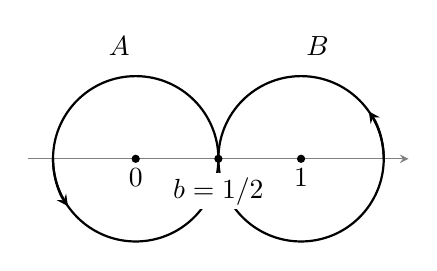
\begin{tikzpicture}[scale=2.1,>=stealth]
\draw[->,gray] (-.65,0)--(1.65,0);
\draw[thick] (0,0) circle(.5);
\draw[thick,->] (-.5,0) arc[start angle=180,end angle=215,radius=.5];
\draw[thick] (1,0) circle(.5);
\draw[thick,->] (1.5,0) arc[start angle=0,end angle=35,radius=.5];
\fill (0,0) circle(.025) node[below] {$0$};
\fill (1,0) circle(.025) node[below] {$1$};
\fill (.5,0) circle(.025) node[below=5pt,fill=white,inner sep=1.5pt] {$b=1/2$};
\node at (-.1,.68) {$A$};\node at (1.1,.68) {$B$};
\end{tikzpicture}
\end{center}
On a sheet where $L_1$ has increased by $2\pi i n$, traversal
of $A$ leaves $L_1$ unchanged and changes $F$ by
\[
\Delta_A F=-2\pi i n\oint_A\frac{dz}{z}=4\pi^2n.
\]
The principal part contributes zero because
$-\log(1-z)/z$ is analytic inside the zero circle.
For $B$, the additive constant $2\pi i n$ contributes zero
because $B$ has zero winding about zero.  To find the remaining
increment, let $L_0$ be the logarithm of $z$ analytic inside
this one-circle neighborhood, with $L_0(1)=0$.  Integration by
parts gives
\[
\Delta_B F=-[L_1L_0]_{\rm start}^{\rm end}
             +\oint_B L_0\,dL_1
           =-2\pi i\ln b+2\pi i L_0(1)
           =2\pi i\ln2.
\]
Here $L_1$ gains $2\pi i$, so $B$ also changes the integer
sheet label from $n$ to $n+1$.  Inverse loops give the inverse
increments.  It follows inductively that every word in $A,B$
ends at a value of the form
\[
\boxed{F_0+2\pi i n\ln2+4\pi^2m,\qquad m,n\in\mathbb Z}.
\]
Conversely, follow $B$, then $A$, then $B^{-1}$, then $A^{-1}$.
The two $B$ increments cancel, while $A$ was traversed with
sheet label one; this path adds $4\pi^2$ and returns the label
to zero.  Its repetitions and inverse give every $m$, after
which $B^n$ gives every $n$.  Thus the boxed set is both
necessary and sufficient, with no branch values omitted.

\erratum{The manual's proposed $2n^2\pi^2-2\pi i n\ln2$
correction is not the full branch set and is incorrect for odd
$n$.  Substituting a multivalued logarithm into the principal
reflection formula while equating its two dilogarithms assigns
incompatible branches.}  For example one loop $B$ gives
$F_0+2\pi i\ln2$ with no real shift, directly contradicting
that proposed enumeration.

\Needspace{5\baselineskip}
\par\bigskip
\noindent\textbf{18.7.4}\quad Explain why Eq.~(18.161) gives the
expected result for $z=0$ when on the principal branch of the
dilogarithm.
\solution
One cannot substitute $z=0$ separately into $\ln z$.
Take the principal-branch limit instead.  For $z\to0$ off its
logarithmic cut,
\[
\ln(1-z)=-z+O(z^2),\qquad
\ln z\ln(1-z)=-z\ln z+O(z^2\ln z).
\]
Writing $z=re^{i\theta}$ with $|\theta|\le\pi$ gives
$|z\ln z|\le r(|\ln r|+\pi)\to0$; the remainder also
vanishes.  The dilogarithm series gives
$\operatorname{Li}_2(0)=0$, while its continuous boundary value
at one is $\operatorname{Li}_2(1)=\sum n^{-2}=\pi^2/6$.
Consequently the two sides of Eq.~(18.161) both tend to
\[
\boxed{\pi^2/6}.
\]
This is a limit of the product, not an assignment of a finite
value to $\ln0$.  The principal branch condition also matters:
on other sheets the extra logarithmic terms must be continued
consistently.

\Needspace{5\baselineskip}
\par\bigskip
\noindent\textbf{18.7.5}\quad Show that
\[
\mathrm{Li}_{2}\left(\frac{1+z^{-1}}{2}\right)
=-\mathrm{Li}_{2}\left(\frac{1+z}{1-z}\right)
-\frac{1}{2}\ln^{2}\left(\frac{1-z^{-1}}{2}\right).
\]
\erratum{Exclude $z=0,1$ and use matching logarithm and dilogarithm branches.  Principal values give the identity directly for real $z>1$ or $z<0$; continue consistently elsewhere.}\par\nobreak
\solution
Set $w=(1+z^{-1})/2=(z+1)/(2z)$, with $z\ne0,1$.
Two elementary reductions are
\[
\frac{w}{w-1}
 =\frac{(z+1)/(2z)}{(1-z)/(2z)}=\frac{1+z}{1-z},
\qquad
1-w=\frac{1-z^{-1}}2.
\]
Insert them into Eq.~(18.163),
$\operatorname{Li}_2(w)+\operatorname{Li}_2(w/(w-1))
=-\tfrac12\log^2(1-w)$, and move its second term to the
right:
\[
\boxed{\operatorname{Li}_2\!\left(\frac{1+z^{-1}}2\right)
=-\operatorname{Li}_2\!\left(\frac{1+z}{1-z}\right)
-\frac12\log^2\!\left(\frac{1-z^{-1}}2\right)}.
\]
For real $z>1$ or $z<0$, both dilogarithm arguments are less
than one and the logarithm's argument is positive, so this is
an equality of ordinary real principal values.  Complex values
follow by continuing all three terms along the same path from
such a domain.

\erratum{The formula is not an unrestricted identity between
independently selected boundary values on the cut.}  For
$0<z<1$, both dilogarithm arguments exceed one, but a small
imaginary part of $z$ puts them on opposite sides of their cuts.
For example, at $z=1/3$ the arguments both equal $2$.
Selecting the same boundary value for both would incorrectly
assert $2\operatorname{Li}_2(2)=\pi^2/2$, although the boundary
values have imaginary parts $\pm\pi\ln2$.  Opposite boundary
values, with the matching logarithm, satisfy the continued identity.

\Needspace{5\baselineskip}
\par\bigskip
\noindent\textbf{18.7.6}\quad The following integral arises in the
computation of the electronic energy of the Li atom using a
correlated wave function (one that explicitly includes the
electron-electron distances as well as the distances of electrons
from the nucleus):
\[
I=\iiint d^{3}r_{1}\,d^{3}r_{2}\,d^{3}r_{3}\,
\frac{e^{-\alpha_{1}r_{1}-\alpha_{2}r_{2}-\alpha_{3}r_{3}}}
{r_{1}r_{2}r_{3}r_{12}r_{13}r_{23}},
\]
where $r_{i}=|\mathbf{r}_{i}|$,
$r_{ij}=|\mathbf{r}_{i}-\mathbf{r}_{j}|$, and the integrations are
over the entire three-dimensional space of each $\mathbf{r}_{i}$.
For convergence of $I$, we require all $\alpha_{j}>0$, but there
are no restrictions on their relative magnitudes.
\par In terms of the auxiliary quantities
\[
\zeta_{1}=\frac{\alpha_{1}}{\alpha_{2}+\alpha_{3}},\qquad
\zeta_{2}=\frac{\alpha_{2}}{\alpha_{1}+\alpha_{3}},\qquad
\zeta_{3}=\frac{\alpha_{3}}{\alpha_{1}+\alpha_{2}},
\]
this integral has the value
\[
I=\frac{32\pi^{3}}{\alpha_{1}\alpha_{2}\alpha_{3}}
\left(-\frac{\pi^{2}}{2}+\sum_{j=1}^{3}
\left[\mathrm{Li}_{2}(\zeta_{j})-\mathrm{Li}_{2}(-\zeta_{j})
+\ln\zeta_{j}\ln\left(\frac{1-\zeta_{j}}{1+\zeta_{j}}\right)\right]\right).
\]
Rearrange $I$ to a form (first found by Remiddi\footnote{E.~Remiddi, ``Analytic value of the atomic three-electron correlation integral with Slater wave functions,'' \emph{Physical Review A} \textbf{44}, 5492 (1991).}), in which
all terms in the final expression are guaranteed to evaluate to
real quantities and can be evaluated as principal values.
\erratum{In the given complex expression use continuation from $0<\zeta_j<1$, with the logarithm boundary values matching those of $\mathrm{Li}_2(\zeta_j)$.  At $\zeta_j=1$ use the finite limit.}\par\nobreak
\solution
For a positive variable $\zeta$, denote one summand by
\[
S(\zeta)=\operatorname{Li}_2(\zeta)-\operatorname{Li}_2(-\zeta)
 +\ln\zeta\log\frac{1-\zeta}{1+\zeta}.
\]
Start with $0<\zeta<1$, where all terms are real.  Reflection
and the logarithm of a positive quotient give
\[
\operatorname{Li}_2(\zeta)=\frac{\pi^2}{6}
 -\operatorname{Li}_2(1-\zeta)-\ln\zeta\ln(1-\zeta),
\]
\[
\log\frac{1-\zeta}{1+\zeta}
 =\log(1-\zeta)-\ln(1+\zeta).
\]
The terms containing $\ln\zeta\log(1-\zeta)$ cancel, leaving
\[
S(\zeta)=\frac{\pi^2}{6}
 -\operatorname{Li}_2(1-\zeta)-\operatorname{Li}_2(-\zeta)
 -\ln\zeta\ln(1+\zeta).
\]
Continue this equality consistently above or below $\zeta=1$.
The imaginary parts in the original combination cancel; the
right side is already real for every $\zeta>0$.
At $\zeta=1$ it has a finite limit, so no $0\log0$ product
needs to be evaluated separately.

Sum over $j=1,2,3$.  The three constants $\pi^2/6$ cancel
the original $-\pi^2/2$ exactly.  Thus the desired form is
\[
\boxed{I=-\frac{32\pi^3}{\alpha_1\alpha_2\alpha_3}
 \sum_{j=1}^3\left[
 \operatorname{Li}_2(-\zeta_j)+\operatorname{Li}_2(1-\zeta_j)
 +\ln\zeta_j\ln(1+\zeta_j)\right]}.
\]
The assumptions $\alpha_j>0$ imply $\zeta_j>0$.
Consequently $-\zeta_j<0$, $1-\zeta_j<1$, and both logarithm
arguments are strictly positive.  Every term in the final formula
therefore has a real principal value, for arbitrary relative
magnitudes of the three positive decay parameters.  In particular,
$\zeta_j=1$ is harmless because $\operatorname{Li}_2(0)=0$
and $\ln1=0$.

\Needspace{12\baselineskip}
\subsection*{18.8 Elliptic Integrals}

\Needspace{5\baselineskip}
\par\bigskip
\noindent\textbf{18.8.1}\quad The ellipse $x^{2}/a^{2}+y^{2}/b^{2}=1$
may be represented parametrically by $x=a\sin\theta$,
$y=b\cos\theta$. Show that the length of arc within the first
quadrant is
\[
a\int_{0}^{\pi/2}(1-m\sin^{2}\theta)^{1/2}\,d\theta=aE(m).
\]
\erratum{Take $a\ge b>0$, so $0\le m=(a^2-b^2)/a^2<1$.  The value $m=1$ is the degenerate limit $b\downarrow0$.}
\solution
Take $a\ge b>0$, so the given parameter lies in $0\le m<1$.
Differentiating the parametrization gives
$dx/d\theta=a\cos\theta$ and $dy/d\theta=-b\sin\theta$.
The arc-length element is therefore
\begin{align*}
ds&=\sqrt{(dx)^2+(dy)^2}
 =\sqrt{a^2\cos^2\theta+b^2\sin^2\theta}\,d\theta\\
 &=a\sqrt{1-\frac{a^2-b^2}{a^2}\sin^2\theta}\,d\theta.
\end{align*}
As $\theta$ increases from $0$ to $\pi/2$, the point moves
from $(0,b)$ to $(a,0)$ along precisely the first-quadrant arc.
Thus its length is
\[
\boxed{\ell=a\int_0^{\pi/2}\sqrt{1-m\sin^2\theta}\,d\theta
              =aE(m)},\qquad m=1-b^2/a^2.
\]
For $a=b$, $m=0$ and $\ell=\pi a/2$, the quarter-circle length.
The limit $b\downarrow0$ gives $m\uparrow1$ and
$\ell\to a\int_0^{\pi/2}\cos\theta\,d\theta=a$;
this is a degenerate limiting ellipse.  If $b>a$, interchange the
axis labels (or use $\theta\mapsto\pi/2-\theta$) to obtain
$bE(1-a^2/b^2)$ in the conventional nonnegative-parameter form.

\Needspace{5\baselineskip}
\par\bigskip
\noindent\textbf{18.8.2}\quad Derive the series expansion
\[
E(m)=\frac{\pi}{2}\left[1-\left(\frac{1}{2}\right)^{2}
\frac{m}{1}-\left(\frac{1\cdot3}{2\cdot4}\right)^{2}
\frac{m^{2}}{3}-\cdots\right].
\]
\erratum{The series is valid for $|m|\le1$, with the square root continued from $m=0$.}\par\nobreak
\solution
For $|m|<1$, expand the integrand uniformly in $\theta$:
\[
\sqrt{1-m\sin^2\theta}
 =1+\sum_{n=1}^\infty(-1)^n\binom{1/2}{n}
                  m^n\sin^{2n}\theta.
\]
For $n\ge1$, direct multiplication of the binomial factors gives
\[
(-1)^n\binom{1/2}{n}=-\frac{(2n-3)!!}{(2n)!!},
\]
where $(-1)!!=1$.  The sine moment is the beta integral
\[
\int_0^{\pi/2}\sin^{2n}\theta\,d\theta
 =\frac12B(n+\tfrac12,\tfrac12)
 =\frac\pi2\frac{(2n-1)!!}{(2n)!!}.
\]
Multiply these factors and use
$(2n-3)!!=(2n-1)!!/(2n-1)$:
\[
\boxed{E(m)=\frac\pi2\left[
 1-\sum_{n=1}^\infty\frac1{2n-1}
       \left(\frac{(2n-1)!!}{(2n)!!}\right)^2m^n\right]}.
\]
The first two nonconstant terms are
$-(1/2)^2m$ and $-(1\cdot3/(2\cdot4))^2m^2/3$,
which reproduce the requested series.  In ordinary powers,
\[
E(m)=\frac\pi2\left(1-\frac m4-\frac{3m^2}{64}
                             -\frac{5m^3}{256}-\cdots\right).
\]
Since $(2n-1)!!/(2n)!!\sim1/\sqrt{\pi n}$, the absolute
coefficients are $O(n^{-2})$.  Thus the series is absolutely
uniformly convergent for $|m|\le1$ and extends to the boundary
by continuity.  In particular $m=1$ gives $E(1)=1$, consistent
with its defining integral.

\Needspace{5\baselineskip}
\par\bigskip
\noindent\textbf{18.8.3}\quad Show that
\[
\lim_{m\to0}\erratum{\frac{K(m)-E(m)}{m}}
=\frac{\pi}{4}.
\]
\solution
\erratum{The original printed exercise has $(K-E)/m$, without
an extra factor $\pi$ in the numerator.  That extra factor in
the supplied transcription has been removed.  The published
erratum also makes both arguments explicitly $m$.}
Subtract the defining integrands before taking the limit:
\begin{align*}
K(m)-E(m)
 &=\int_0^{\pi/2}
 \frac{1-(1-m\sin^2\theta)}{\sqrt{1-m\sin^2\theta}}d\theta\\
 &=m\int_0^{\pi/2}\frac{\sin^2\theta}
                               {\sqrt{1-m\sin^2\theta}}d\theta.
\end{align*}
For $|m|$ bounded strictly below one, the integrand is dominated
by a constant times $\sin^2\theta$.  Dominated convergence gives
\[
\boxed{\lim_{m\to0}\frac{K(m)-E(m)}m
 =\int_0^{\pi/2}\sin^2\theta\,d\theta=\frac\pi4}.
\]
Equivalently the two series start with
$K=(\pi/2)(1+m/4+O(m^2))$ and
$E=(\pi/2)(1-m/4+O(m^2))$.
If the spurious numerator factor $\pi$ were retained, the limit
would instead be $\pi^2/4$, so it cannot accompany the stated
right side.

\Needspace{5\baselineskip}
\par\bigskip
\noindent\textbf{18.8.4}\quad A circular loop of wire in the
$xy$-plane, \erratum{centered at the origin with radius $a>0$}, carries a current $I$. Given
that the vector potential is
\[
A_{\varphi}(\rho,\varphi,z)
=\frac{a\mu_{0}I}{2\pi}\int_{0}^{\pi}
\frac{\cos\alpha\,d\alpha}
{(a^{2}+\rho^{2}+z^{2}-2a\rho\cos\alpha)^{1/2}},
\]
show that
\[
A_{\varphi}(\rho,\varphi,z)
=\frac{\mu_{0}I}{\pi k}\left(\frac{a}{\rho}\right)^{1/2}
\left[\left(1-\frac{k^{2}}{2}\right)K(k^{2})-E(k^{2})\right],
\]
where
\[
k^{2}=\frac{4a\rho}{(a+\rho)^{2}+z^{2}}.
\]
\par\emph{Note.}~For extension of this exercise to $\mathbf{B}$, see
Smythe.\footnote{W.~R.~Smythe, \emph{Static and Dynamic Electricity}, 3rd ed. (McGraw-Hill, New York, 1969), p.~270.}
\erratum{Take $\rho>0$ and real $z$, away from the wire $(\rho,z)=(a,0)$; recover the axis by a limit.}\par\nobreak
\solution
Assume $a>0$, $\rho>0$, away from the ideal wire
$(\rho,z)=(a,0)$.  Set
\[
D=(a+\rho)^2+z^2,\quad m=k^2=\frac{4a\rho}D,
\quad 0<m<1.
\]
Using $\cos\alpha=2\cos^2(\alpha/2)-1$, the denominator
squared becomes
\[
a^2+\rho^2+z^2-2a\rho\cos\alpha
 =D-4a\rho\cos^2(\alpha/2)
 =D[1-m\cos^2(\alpha/2)].
\]
Put $u=\alpha/2$ and then $\theta=\pi/2-u$:
\[
A_\varphi=\frac{a\mu_0 I}{\pi\sqrt D}
 \int_0^{\pi/2}\frac{2\sin^2\theta-1}
                         {\sqrt{1-m\sin^2\theta}}d\theta.
\]
The difference of the elliptic integrands gives
\[
K(m)-E(m)=m\int_0^{\pi/2}
 \frac{\sin^2\theta}{\sqrt{1-m\sin^2\theta}}d\theta.
\]
Therefore the remaining angular integral is
\[
\frac2m[K(m)-E(m)]-K(m)
 =\frac2m\left[(1-\tfrac m2)K(m)-E(m)\right].
\]
Finally
\[
\frac{2a}{m\sqrt D}
 =\frac1k\sqrt{\frac a\rho},
\]
because $k=2\sqrt{a\rho}/\sqrt D$.  Substitution yields
\[
\boxed{A_\varphi(\rho,\varphi,z)=\frac{\mu_0I}{\pi k}
 \sqrt{\frac a\rho}
 \left[(1-\tfrac{k^2}2)K(k^2)-E(k^2)\right]}.
\]
Rotational symmetry explains the absence of $\varphi$.
\erratum{At $\rho=0$ the apparent singular factors are interpreted
by a limit: the original integral is zero, so $A_\varphi=0$ on
the axis.  At the ideal wire $k^2=1$, the logarithmic singularity
is real and is not a removable limit.}
The cancellation near $k=0$ is also quantified by the next exercise.

\Needspace{5\baselineskip}
\par\bigskip
\noindent\textbf{18.8.5}\quad An analysis of the magnetic vector
potential of a circular current loop leads to the expression
\[
f(k^{2})=k^{-2}\big[(2-k^{2})K(k^{2})-2E(k^{2})\big],
\]
where $K(k^{2})$ and $E(k^{2})$ are the complete elliptic integrals
of the first and second kinds. Show that for $k^{2}\ll1$
($r\gg\text{radius of loop}$)
\[
f(k^{2})\approx\frac{\pi k^{2}}{16}.
\]
\erratum{Here $r=\sqrt{\rho^2+z^2}$ and the loop radius is $a$.  The far-field condition $r\gg a$ is sufficient for $k^2\ll1$.}\par\nobreak
\solution
Write $m=k^2$.  Since the definition divides by $m$, retain the
elliptic series through $m^2$ (one extra order beyond the desired
answer):
\[
K(m)=\frac\pi2\left(1+\frac m4+\frac{9m^2}{64}+O(m^3)\right),
\quad
E(m)=\frac\pi2\left(1-\frac m4-\frac{3m^2}{64}+O(m^3)\right).
\]
Then
\begin{align*}
(2-m)K(m)-2E(m)
 &=\frac\pi2\left[
 2-\frac m2+\left(\frac{18}{64}-\frac14\right)m^2
 -2+\frac m2+\frac{6m^2}{64}+O(m^3)\right]\\
 &=\frac\pi2\left[\frac{m^2}{8}+O(m^3)\right].
\end{align*}
The constant and linear terms cancel.  Dividing by $m$ gives
\[
\boxed{f(k^2)=\frac{\pi k^2}{16}+O(k^4)}.
\]
Keeping the next terms $25m^3/256$ in $2K/\pi$ and
$-5m^3/256$ in $2E/\pi$ would give
$f(m)=\pi m/16+3\pi m^2/64+O(m^3)$.
Thus $f$ has the removable value $f(0)=0$.

For the distant loop field, $D\sim r^2$,
$m\sim4a\rho/r^2$ and the preceding exercise has
$A_\varphi=a\mu_0I f(m)/(\pi\sqrt D)$.
Consequently its leading term is
$\mu_0Ia^2\rho/(4r^3)=\mu_0Ia^2\sin\theta/(4r^2)$,
the magnetic-dipole form.  Large $r/a$ is a sufficient way to
make $m$ small; it is not the only one, since $m\to0$ also
on approaching the symmetry axis.

\Needspace{5\baselineskip}
\par\bigskip
\noindent\textbf{18.8.6}\quad Show that
\begin{enumerate}
\item[(a)] $\dfrac{d\,E(k^{2})}{dk}=\dfrac{1}{k}
\big(E\erratum{(k^{2})}-K\erratum{(k^{2})}\big)$,
\item[(b)] $\dfrac{d\,K(k^{2})}{dk}
=\dfrac{E\erratum{(k^{2})}}{k(1-k^{2})}
-\dfrac{K\erratum{(k^{2})}}{k}$.
\end{enumerate}
\par\emph{Hint.}~For part (b) show that
\[
E(k^{2})=(1-k^{2})\int_{0}^{\pi/2}
(1-\erratum{k^{2}}\sin^{2}\theta)^{-3/2}\,d\theta
\]
by comparing series expansions.
\erratum{Initially take $0<k<1$; both derivatives have removable limits at $k=0$.}\par\nobreak
\solution
Take initially $0<k<1$, put $m=k^2$, and use differentiation
under the integral on compact subintervals of this range.
(a) The chain rule gives
\[
\frac{dE(k^2)}{dk}
 =-k\int_0^{\pi/2}\frac{\sin^2\theta}
                             {\sqrt{1-k^2\sin^2\theta}}d\theta.
\]
Since $-k\sin^2\theta=[(1-k^2\sin^2\theta)-1]/k$,
\[
\boxed{\frac{dE(k^2)}{dk}=\frac{E(k^2)-K(k^2)}k}.
\]

(b) First verify the corrected hint by the requested series method.
Define
\[
a_n=\left[\frac{(1/2)_n}{n!}\right]^2,
\qquad J(m)=\int_0^{\pi/2}(1-m\sin^2\theta)^{-3/2}d\theta.
\]
The binomial series and the sine moment give
\[
J(m)=\frac\pi2\sum_{n=0}^\infty
 \frac{(3/2)_n(1/2)_n}{(n!)^2}m^n
 =\frac\pi2\sum_{n=0}^\infty(2n+1)a_nm^n.
\]
For $n\ge1$, $a_n/a_{n-1}=(2n-1)^2/(4n^2)$.
Hence the $m^n$ coefficient of $2(1-m)J/\pi$ is
\[
(2n+1)a_n-(2n-1)a_{n-1}
 =a_n\left[(2n+1)-\frac{4n^2}{2n-1}\right]
 =-\frac{a_n}{2n-1}.
\]
The constant is one, so Exercise~18.8.2 identifies the entire
series with $2E(m)/\pi$.  Thus
\[
\boxed{E(m)=(1-m)J(m)},\qquad |m|<1.
\]
This uses the \erratum{corrected integrand $1-k^2\sin^2\theta$},
not $1-k\sin^2\theta$.

Now differentiate $K$ and rewrite its numerator:
\begin{align*}
\frac{dK(k^2)}{dk}
 &=k\int_0^{\pi/2}\frac{\sin^2\theta}
                              {(1-k^2\sin^2\theta)^{3/2}}d\theta\\
 &=\frac1k\int_0^{\pi/2}\left[
       \frac1{(1-k^2\sin^2\theta)^{3/2}}
       -\frac1{\sqrt{1-k^2\sin^2\theta}}\right]d\theta\\
 &=\frac{J(k^2)-K(k^2)}k
 =\boxed{\frac{E(k^2)}{k(1-k^2)}-\frac{K(k^2)}k}.
\end{align*}
All elliptic arguments in these formulas are the parameter
$k^2$, as stated in the published erratum.
At $k=0$ both derivatives have the removable value zero:
$E(k^2)=\pi/2-\pi k^2/8+O(k^4)$ and
$K(k^2)=\pi/2+\pi k^2/8+O(k^4)$.
The singular endpoint $k=1$ is outside the finite derivative
formulas and is approached only as a limit.

\clearpage
\section{Chapter 19. Fourier Series}
% Problems, Chapter 19: Fourier Series
% Arfken, Weber & Harris, Mathematical Methods for Physicists, 7th ed.
% Requires: amsmath, amssymb, tikz

\section*{Problems}

\Needspace{12\baselineskip}
\subsection*{19.1 General Properties}

\Needspace{5\baselineskip}
\par\bigskip
\noindent\textbf{19.1.1}\quad A \erratum{real-valued} function $f(x)$ (quadratically
integrable) is to be represented by a finite Fourier series. A
convenient measure of the accuracy of the series is given by the
integrated square of the deviation,
\[
\Delta_{p}=\int_{0}^{2\pi}\left[f(x)-\frac{a_{0}}{2}
-\sum_{n=1}^{p}(a_{n}\cos nx+b_{n}\sin nx)\right]^{2}dx.
\]
Show that the requirement that $\Delta_{p}$ be minimized, that is,
\[
\frac{\partial\Delta_{p}}{\partial a_{n}}=0,\qquad
\frac{\partial\Delta_{p}}{\partial b_{n}}=0,
\]
for all $n$, leads to choosing $a_{n}$ and $b_{n}$ as given in
Eqs.~(19.2) and (19.3).
\par\emph{Note.}~Your coefficients $a_{n}$ and $b_{n}$ are
independent of $p$. This independence is a consequence of
orthogonality and would not hold if we expanded $f(x)$ in a power
series.
\erratum{Take the coefficients real as well. For complex data, replace the squared residual by its modulus squared.}
\solution
Write $s_p=a_0/2+\sum_{n=1}^p(a_n\cos nx+b_n\sin nx)$.
\erratum{The restriction to real values is needed because for complex
$f$ or coefficients $[f-s_p]^2$ is complex and cannot be minimized; the
real measure of the error is then $|f-s_p|^2$.}
All integrals below exist: Cauchy--Schwarz on the finite interval gives
$\int|f|\le\sqrt{2\pi}\,(\int|f|^2)^{1/2}$.

The orthogonality integrals on $(0,2\pi)$ are, for $m,n\ge1$,
\begin{gather*}
\int_0^{2\pi}\cos mx\,dx=\int_0^{2\pi}\sin mx\,dx
=\int_0^{2\pi}\sin nx\cos mx\,dx=0,\\
\int_0^{2\pi}\cos nx\cos mx\,dx=\int_0^{2\pi}\sin nx\sin mx\,dx
=\pi\delta_{nm}.
\end{gather*}
Hence, for $1\le m\le p$,
\[
\int_0^{2\pi}s_p\cos mx\,dx=\pi a_m,\qquad
\int_0^{2\pi}s_p\sin mx\,dx=\pi b_m,\qquad
\int_0^{2\pi}s_p\,dx=\frac{a_0}2\,2\pi=\pi a_0.
\]
$\Delta_p$ is a quadratic polynomial in the finitely many coefficients,
with $\partial s_p/\partial a_m=\cos mx$ and
$\partial s_p/\partial b_m=\sin mx$. Differentiating under the
integral sign, for $1\le m\le p$,
\begin{align*}
\frac{\partial\Delta_p}{\partial a_m}
 &=-2\int_0^{2\pi}(f-s_p)\cos mx\,dx
 =-2\int_0^{2\pi}f\cos mx\,dx+2\pi a_m,\\
\frac{\partial\Delta_p}{\partial b_m}
 &=-2\int_0^{2\pi}(f-s_p)\sin mx\,dx
 =-2\int_0^{2\pi}f\sin mx\,dx+2\pi b_m.
\end{align*}
For the constant coefficient, $\partial s_p/\partial a_0=1/2$ gives
instead
\[
\frac{\partial\Delta_p}{\partial a_0}
=-\int_0^{2\pi}(f-s_p)\,dx=-\int_0^{2\pi}f\,dx+\pi a_0.
\]
Setting these derivatives to zero yields
\[
\boxed{a_m=\frac1\pi\int_0^{2\pi}f(x)\cos mx\,dx\quad(m\ge0),
\qquad b_m=\frac1\pi\int_0^{2\pi}f(x)\sin mx\,dx\quad(m\ge1).}
\]
These stationary values are the unique minimum, not merely a stationary
point. Let $s_p^*$ have the displayed coefficients, with error
$\Delta_p^*$, and change the coefficients by $\alpha_0,\alpha_m,\beta_m$,
so that $s_p=s_p^*+u$ with
$u=\alpha_0/2+\sum_{m=1}^p(\alpha_m\cos mx+\beta_m\sin mx)$. Then
\[
\Delta_p=\int_0^{2\pi}(f-s_p^*-u)^2dx
=\Delta_p^*-2\int_0^{2\pi}(f-s_p^*)u\,dx+\int_0^{2\pi}u^2dx.
\]
The middle integral vanishes, since the vanishing derivatives above say
that $f-s_p^*$ is orthogonal to $1$, $\cos mx$, $\sin mx$ ($m\le p$).
The orthogonality integrals give
$\int_0^{2\pi}u^2dx=2\pi(\alpha_0/2)^2+\pi\sum_{m=1}^p(\alpha_m^2+\beta_m^2)$,
so
\[
\Delta_p=\Delta_p^*+\frac\pi2\alpha_0^2
+\pi\sum_{m=1}^p(\alpha_m^2+\beta_m^2).
\]
Every added term is nonnegative and vanishes only when all changes vanish.
No coefficient formula contains $p$: adding an orthogonal mode cannot
change the projections onto modes already present.

\Needspace{5\baselineskip}
\par\bigskip
\noindent\textbf{19.1.2}\quad In the analysis of a complex waveform
(ocean tides, earthquakes, musical tones, etc.), it might be more
convenient to have the Fourier series written as
\[
f(x)=\frac{a_{0}}{2}+\sum_{n=1}^{\infty}
\alpha_{n}\cos(nx-\theta_{n}).
\]
Show that this is equivalent to Eq.~(19.1) with
\begin{align*}
a_{n}&=\alpha_{n}\cos\theta_{n},&
\alpha_{n}^{2}&=a_{n}^{2}+b_{n}^{2},\\
b_{n}&=\alpha_{n}\sin\theta_{n},&
\tan\theta_{n}&=b_{n}/a_{n}.
\end{align*}
\par\emph{Note.}~The coefficients $\alpha_{n}^{2}$ as a function of
$n$ define what is called the \emph{power spectrum}. The importance
of $\alpha_{n}^{2}$ lies in their invariance under a shift in the
phase $\theta_{n}$.
\erratum{The waveform and its sine/cosine coefficients are real. Take $\alpha_n\ge0$; the tangent formula applies only when $a_n\ne0$. Specify the phase quadrant and the zero-amplitude case.}
\solution
The cosine subtraction formula gives, for each harmonic,
\[
\alpha_n\cos(nx-\theta_n)
=\alpha_n\cos\theta_n\cos nx+\alpha_n\sin\theta_n\sin nx.
\]
The Fourier coefficients of a function are unique (they are given by
Eqs.~(19.2) and (19.3)), so matching the coefficients of $\cos nx$ and
$\sin nx$ with Eq.~(19.1) gives
$a_n=\alpha_n\cos\theta_n$, $b_n=\alpha_n\sin\theta_n$.
Squaring and adding gives
$a_n^2+b_n^2=\alpha_n^2(\cos^2\theta_n+\sin^2\theta_n)=\alpha_n^2$,
and dividing $b_n$ by $a_n$ when $a_n\ne0$ gives $\tan\theta_n$:
\[
\boxed{\alpha_n=\sqrt{a_n^2+b_n^2},\qquad
\tan\theta_n=b_n/a_n.}
\]
We choose the nonnegative amplitude: a negative $\alpha_n$ gives the
same term as $|\alpha_n|$ with $\theta_n$ increased by $\pi$, since
$-\cos u=\cos(u-\pi)$. \erratum{The tangent alone does not
fix the quadrant and is undefined when $a_n=0$. For nonzero amplitude
take $\theta_n$ to be the angle with $\cos\theta_n=a_n/\alpha_n$ and
$\sin\theta_n=b_n/\alpha_n$ (the two-argument arctangent
$\operatorname{atan2}(b_n,a_n)$), unique modulo $2\pi$; for
$a_n=b_n=0$ the phase is arbitrary. Reality is needed because for
complex data the amplitude--phase form can fail: $e^{ix}=\cos x+i\sin x$
has $a_1=1$, $b_1=i$, so $\alpha_1^2=a_1^2+b_1^2=0$ although
$a_1\ne0$.}
In particular, when $a_n=0$ and $b_n\ne0$, the phase is
$\operatorname{sgn}(b_n)\pi/2$ modulo $2\pi$.

Under a shift $x\mapsto x+x_0$,
$\alpha_n\cos(n(x+x_0)-\theta_n)=\alpha_n\cos(nx-(\theta_n-nx_0))$:
the phase becomes $\theta_n-nx_0$, while the amplitude stays unchanged.
Equivalently, expanding
$a_n'=\alpha_n\cos(\theta_n-nx_0)$ and
$b_n'=\alpha_n\sin(\theta_n-nx_0)$ by the addition formulas, the
coefficient pair is rotated:
\[
\begin{pmatrix}a_n'\\b_n'\end{pmatrix}
=\begin{pmatrix}\cos nx_0&\sin nx_0\\-\sin nx_0&\cos nx_0\end{pmatrix}
\begin{pmatrix}a_n\\b_n\end{pmatrix},
\qquad (a_n')^2+(b_n')^2=a_n^2+b_n^2.
\]
This is the asserted phase invariance of the power spectrum.

\Needspace{5\baselineskip}
\par\bigskip
\noindent\textbf{19.1.3}\quad A function $f(x)$ is expanded in an
exponential Fourier series
\[
f(x)=\sum_{n=-\infty}^{\infty}c_{n}e^{inx}.
\]
If $f(x)$ is real, $f(x)=f^{*}(x)$, what restriction is imposed on
the coefficients $c_{n}$?
\solution
The coefficient formula, with $f$ real so that only the exponential is
conjugated, gives
\[
c_n^*=\left[\frac1{2\pi}\int_{-\pi}^{\pi}f(x)e^{-inx}\,dx\right]^*
=\frac1{2\pi}\int_{-\pi}^{\pi}f(x)e^{inx}\,dx=c_{-n}.
\]
Thus, with $n=0$ giving $c_0^*=c_0$,
\[
\boxed{c_{-n}=c_n^*\quad\hbox{for every integer }n;\qquad c_0\in\mathbb R.}
\]
Conversely, this relation makes every symmetric partial sum real because
\[
c_ne^{inx}+c_{-n}e^{-inx}=c_ne^{inx}+(c_ne^{inx})^*
=2\operatorname{Re}(c_ne^{inx}).
\]
Consequently its pointwise limit, wherever it exists, is real; its
$L^2$ limit is real almost everywhere as well.

\Needspace{5\baselineskip}
\par\bigskip
\noindent\textbf{19.1.4}\quad Assuming that \erratum{$f$ is real and}
$\displaystyle\int_{-\pi}^{\pi}[f(x)]^{2}\,dx$ is finite, show that
\[
\lim_{m\to\infty}a_{m}=0,\qquad\lim_{m\to\infty}b_{m}=0.
\]
\par\emph{Hint.}~Integrate $[f(x)-s_{n}(x)]^{2}$, where $s_{n}(x)$
is the $n$th partial sum, and use Bessel's inequality
(Section~5.1). For our finite interval the assumption that $f(x)$
is square integrable
($\displaystyle\int_{-\pi}^{\pi}|f(x)|^{2}\,dx$ is finite) implies
that $\displaystyle\int_{-\pi}^{\pi}|f(x)|\,dx$ is also finite. The
converse does not hold.
\solution
Let $s_N=a_0/2+\sum_{n=1}^N(a_n\cos nx+b_n\sin nx)$ be the finite
Fourier projection; all integrals are over $(-\pi,\pi)$. Expanding the
square gives
\[
0\le\int_{-\pi}^{\pi}(f-s_N)^2\,dx
=\int f^2\,dx-2\int fs_N\,dx+\int s_N^2\,dx.
\]
The coefficient formulas $\int f\,dx=\pi a_0$, $\int f\cos nx\,dx=\pi a_n$,
$\int f\sin nx\,dx=\pi b_n$ give
\[
\int fs_N\,dx=\frac{a_0}2\pi a_0+\sum_{n=1}^N(a_n\pi a_n+b_n\pi b_n)
=\frac\pi2a_0^2+\pi\sum_{n=1}^N(a_n^2+b_n^2),
\]
and orthogonality ($\int1\,dx=2\pi$, $\int\cos^2nx\,dx=\int\sin^2nx\,dx=\pi$,
all cross terms zero) gives the same value for $\int s_N^2\,dx$.
Therefore
$0\le\int f^2\,dx-\frac\pi2a_0^2-\pi\sum_{n=1}^N(a_n^2+b_n^2)$, that is,
\[
\frac{a_0^2}{2}+\sum_{n=1}^N(a_n^2+b_n^2)
\le\frac1\pi\int_{-\pi}^{\pi}f^2\,dx<\infty.
\]
This is Bessel's inequality. The partial sums of the nonnegative series
$\sum(a_n^2+b_n^2)$ are nondecreasing and bounded, so the series
converges, and the terms of a convergent series tend to zero:
$a_n^2+b_n^2\to0$. Since each square is no larger than the sum,
\[
\boxed{a_n\to0,\qquad b_n\to0.}
\]
No pointwise convergence of the original Fourier series was used.
The statement assumes $f$ real because the argument uses
$(f-s_N)^2\ge0$; for complex $f$ the same argument with modulus squares,
as in 19.1.1, gives $|a_n|^2+|b_n|^2\to0$.

The integrability assertion in the hint follows from the
Cauchy--Schwarz inequality applied to $|f|$ and $1$:
\[
\int_{-\pi}^{\pi}|f|\cdot1\,dx
\le\left(\int|f|^2\,dx\right)^{1/2}\sqrt{2\pi}.
\]
For a counterexample to the converse, $f(x)=|x|^{-2/3}$ on $0<|x|<1$,
and zero elsewhere, has
$\int|f|=2\int_0^1x^{-2/3}\,dx=2\bigl[3x^{1/3}\bigr]_0^1=6$ but
$\int|f|^2=2\int_0^1x^{-4/3}\,dx
=2\lim_{\epsilon\downarrow0}\bigl[-3x^{-1/3}\bigr]_\epsilon^1=\infty$.

\Needspace{5\baselineskip}
\par\bigskip
\noindent\textbf{19.1.5}\quad Apply the summation technique of this
section to show that
\[
\sum_{n=1}^{\infty}\frac{\sin nx}{n}
=\begin{cases}
\dfrac{1}{2}(\pi-x), & 0<x\le\pi,\\[10pt]
-\dfrac{1}{2}(\pi+x), & -\pi\le x<0.
\end{cases}
\]
This is the reverse sawtooth wave shown in Fig.~19.5.
\solution
First insert an Abel factor $0<r<1$. With $z=re^{ix}$, $|z|<1$, the
series $-\log(1-z)=\sum_{n\ge1}z^n/n$ converges absolutely, and
$\operatorname{Im}z^n=r^n\sin nx$, so
\[
S_r(x)=\sum_{n=1}^{\infty}\frac{r^n\sin nx}{n}
=\operatorname{Im}\{-\log(1-re^{ix})\}.
\]
Use the principal logarithm; it is continuous on the right half-plane,
which contains $1-re^{ix}$ (real part $1-r\cos x>0$) and, for
$0<x<2\pi$, also $1-e^{ix}$ (real part $1-\cos x>0$). For $0<x<2\pi$,
\[
1-e^{ix}=e^{ix/2}\bigl(e^{-ix/2}-e^{ix/2}\bigr)
=-2i e^{ix/2}\sin(x/2)
=2\sin(x/2)e^{i(x/2-\pi/2)},
\]
with modulus $2\sin(x/2)>0$ and argument
$x/2-\pi/2\in(-\pi/2,\pi/2)$. Hence
\[
\lim_{r\uparrow1}S_r(x)=-\operatorname{Arg}(1-e^{ix})
=-\Bigl(\frac x2-\frac\pi2\Bigr)=\frac{\pi-x}2,\qquad0<x<2\pi.
\]
The original series converges for $x\notin2\pi\mathbb Z$ by Dirichlet's
test: $1/n$ decreases to zero, and the partial sums of $e^{inx}$ are
bounded,
\[
\Bigl|\sum_{n=1}^Ne^{inx}\Bigr|
=\Bigl|\frac{e^{ix}(1-e^{iNx})}{1-e^{ix}}\Bigr|\le\frac2{|1-e^{ix}|}.
\]
Abel's theorem (if $\sum c_n$ converges, then
$\lim_{r\uparrow1}\sum c_nr^n=\sum c_n$) then identifies its ordinary sum
with this limit. Oddness supplies the negative interval: for
$-\pi\le x<0$ the sum is $-(\pi-|x|)/2=-(\pi+x)/2$. Thus
\[
\boxed{\sum_{n=1}^{\infty}\frac{\sin nx}{n}
=\begin{cases}(\pi-x)/2,&0<x\le\pi,\\
-(\pi+x)/2,&-\pi\le x<0.\end{cases}}
\]
At $x=0$ every summand is zero; the sum is zero, the mean of the two
one-sided limits. At $\pm\pi$ it is also zero. The complete function is
$2\pi$-periodic.

\Needspace{5\baselineskip}
\par\bigskip
\noindent\textbf{19.1.6}\quad Sum the series
$\displaystyle\sum_{n=1}^{\infty}(-1)^{n+1}\frac{\sin nx}{n}$ and
show that it equals $x/2$ \erratum{for $-\pi<x<\pi$}.
\solution
For $0<r<1$, the alternating logarithmic series
$\log(1+z)=\sum_{n\ge1}(-1)^{n+1}z^n/n$ with $z=re^{ix}$ gives
\[
\sum_{n=1}^{\infty}(-1)^{n+1}\frac{r^n\sin nx}{n}
=\operatorname{Im}\log(1+re^{ix}).
\]
When $-\pi<x<\pi$,
\[
1+e^{ix}=e^{ix/2}\bigl(e^{-ix/2}+e^{ix/2}\bigr)
=2\cos(x/2)e^{ix/2},\qquad \cos(x/2)>0,
\]
so its principal argument is $x/2$; as in 19.1.5 the logarithm is
continuous as $r\uparrow1$, since $1+re^{ix}$ and $1+e^{ix}$ have
positive real parts. The series converges by Dirichlet's test, because
the partial sums of $(-1)^{n+1}e^{inx}=-(-e^{ix})^n$ are bounded by
$2/|1+e^{ix}|$ when $e^{ix}\ne-1$. Abel's theorem, as in 19.1.5,
therefore gives
\[
\boxed{\sum_{n=1}^{\infty}(-1)^{n+1}\frac{\sin nx}{n}=\frac{x}{2},
\qquad -\pi<x<\pi.}
\]
\erratum{The interval is essential: the left side is periodic, whereas
$x/2$ is not. At $x=(2k+1)\pi$ its value is zero, not $x/2$.}
By $2\pi$-periodicity, on $((2k-1)\pi,(2k+1)\pi)$ its value is
$(x-2k\pi)/2$.

\Needspace{5\baselineskip}
\par\bigskip
\noindent\textbf{19.1.7}\quad Sum the trigonometric series
$\displaystyle\sum_{n=0}^{\infty}\frac{\sin(2n+1)x}{2n+1}$ and show
that it equals
\[
\begin{cases}
\pi/4, & 0<x<\pi,\\
-\pi/4, & -\pi<x<0.
\end{cases}
\]
\solution
Subtract the even harmonics from the sum of all harmonics. Let
$S(x)=\sum_{n\ge1}\sin nx/n$ be the function of 19.1.5, where the
principal-logarithm computation gave $S(y)=(\pi-y)/2$ for every
$0<y<2\pi$. Split a partial sum of $S$ into odd and even $n$, writing
$n=2m$ in the even terms:
\[
\sum_{n=1}^{2N}\frac{\sin nx}{n}
=\sum_{n=0}^{N-1}\frac{\sin(2n+1)x}{2n+1}
+\frac12\sum_{m=1}^{N}\frac{\sin(2mx)}{m}.
\]
For $0<x<\pi$, as $N\to\infty$ the left side tends to $S(x)$ and the
last sum to $S(2x)$, since $x$ and $2x$ lie in $(0,2\pi)$. Hence the odd
series converges, and
\[
\sum_{n=0}^{\infty}\frac{\sin(2n+1)x}{2n+1}
=S(x)-\frac12S(2x)
=\frac{\pi-x}{2}-\frac{\pi-2x}{4}=\frac\pi4.
\]
The series is odd in $x$, giving $-\pi/4$ on $(-\pi,0)$. Thus
\[
\boxed{\sum_{n=0}^{\infty}\frac{\sin(2n+1)x}{2n+1}
=\begin{cases}\pi/4,&0<x<\pi,\\-\pi/4,&-\pi<x<0.\end{cases}}
\]
At every integer multiple of $\pi$, each sine vanishes and the sum is
zero, the midpoint value at the jump.

\Needspace{5\baselineskip}
\par\bigskip
\noindent\textbf{19.1.8}\quad Let
$f(z)=\ln(1+z)=\displaystyle\sum_{n=1}^{\infty}
\dfrac{(-1)^{n+1}z^{n}}{n}$. This series converges to $\ln(1+z)$
for $|z| \le 1$, except at the point $z=-1$.
\begin{enumerate}
\item[(a)] From the real parts show that
\[
\ln\left(2\cos\frac{\theta}{2}\right)
=\sum_{n=1}^{\infty}(-1)^{n+1}\frac{\cos n\theta}{n},
\qquad-\pi<\theta<\pi.
\]
\item[(b)] Using a change of variable, transform part (a) into
\[
-\ln\left(2\sin\frac{\theta}{2}\right)
=\sum_{n=1}^{\infty}\frac{\cos n\theta}{n},
\qquad0<\theta<2\pi.
\]
\end{enumerate}
\solution
\textbf{(a)} Put $z=e^{i\theta}$. For $-\pi<\theta<\pi$ the identity
\[
1+e^{i\theta}=2\cos(\theta/2)e^{i\theta/2}
\]
has a positive real amplitude $2\cos(\theta/2)$ and argument
$\theta/2\in(-\pi/2,\pi/2)$, so the principal logarithm is
\[
\log(1+e^{i\theta})=\ln(2\cos(\theta/2))+i\theta/2.
\]
By the statement the series converges to this value at $z=e^{i\theta}$,
$\theta\ne\pi$. Taking real parts, with
$\operatorname{Re}e^{in\theta}=\cos n\theta$, gives
\[
\boxed{\ln(2\cos(\theta/2))
=\sum_{n=1}^{\infty}(-1)^{n+1}\frac{\cos n\theta}{n},
\qquad-\pi<\theta<\pi.}
\]
At the included point $\theta=0$ this is the convergent alternating
harmonic series. The excluded endpoints have the logarithmic singularity.

\textbf{(b)} Replace the angle in (a) by $\theta-\pi$, which belongs
to $(-\pi,\pi)$ when $0<\theta<2\pi$. Then
\[
\cos\frac{\theta-\pi}{2}=\sin\frac\theta2,
\qquad \cos(n\theta-n\pi)=(-1)^n\cos n\theta.
\]
Consequently (a) becomes
\[
\ln\Bigl(2\sin\frac\theta2\Bigr)
=\sum_{n=1}^{\infty}(-1)^{n+1}(-1)^n\frac{\cos n\theta}{n}
=-\sum_{n=1}^{\infty}\frac{\cos n\theta}{n},
\]
since the two alternating factors multiply to $(-1)^{2n+1}=-1$. Hence
\[
\boxed{-\ln(2\sin(\theta/2))
=\sum_{n=1}^{\infty}\frac{\cos n\theta}{n},\qquad0<\theta<2\pi.}
\]
\erratum{The Instructor's Manual's intermediate exponential identity
in (b) has the wrong sign. The correct identity is
$2\sin(\theta/2)=i e^{-i\theta/2}(1-e^{i\theta})$.
Its final real-part result agrees with the formula above.}

\Needspace{5\baselineskip}
\par\bigskip
\noindent\textbf{19.1.9}
\begin{enumerate}
\item[(a)] Expand $f(x)=x$ in the interval $(0,2L)$. Sketch the
series you have found (right-hand side of ANS.) over $(-2L,2L)$.
\par\nobreak\hfill\emph{ANS.}\enspace
$x=L-\dfrac{2L}{\pi}\displaystyle\sum_{n=1}^{\infty}
\dfrac{1}{n}\sin\dfrac{n\pi x}{L}$.
\item[(b)] Expand $f(x)=x$ as a sine series in the half interval
$(0,L)$. Sketch the series you have found (right-hand side of
ANS.) over $(-2L,2L)$.
\par\nobreak\hfill\emph{ANS.}\enspace
$\erratum{x=\dfrac{2L}{\pi}\displaystyle\sum_{n=1}^{\infty}
\dfrac{(-1)^{n+1}}{n}\sin\dfrac{n\pi x}{L}}$.
\end{enumerate}
\solution
\textbf{(a)} For period $2L$, put $k_n=n\pi/L$. The coefficient
normalization on $(0,2L)$ is $1/L$, so
\[
a_0=\frac1L\int_0^{2L}x\,dx=2L.
\]
Two elementary antiderivatives are
\[
\int x\cos kx\,dx=\frac{x\sin kx}{k}+\frac{\cos kx}{k^2},
\qquad
\int x\sin kx\,dx=-\frac{x\cos kx}{k}+\frac{\sin kx}{k^2}.
\]
At $k=k_n$ and $x=0,2L$ the sines vanish and the cosines are one
($k_n2L=2n\pi$). Consequently
\begin{align*}
a_n&=\frac1L\left[\frac{x\sin k_nx}{k_n}
+\frac{\cos k_nx}{k_n^2}\right]_0^{2L}
=\frac1L\,\frac{1-1}{k_n^2}=0,\\
b_n&=\frac1L\left[-\frac{x\cos k_nx}{k_n}
+\frac{\sin k_nx}{k_n^2}\right]_0^{2L}
=\frac1L\left(-\frac{2L}{k_n}\right)=-\frac{2L}{n\pi}.
\end{align*}
With $a_0/2=L$, this gives
\[
\boxed{x=L-\frac{2L}{\pi}\sum_{n=1}^{\infty}\frac{\sin(n\pi x/L)}n,
\qquad0<x<2L.}
\]
The series has period $2L$, so on $(-2L,0)$ it equals $x+2L$; at $x=0$
its value is the midpoint $L$ of the jump from $2L$ to $0$ (every sine
vanishes there).

\textbf{(b)} A sine series on $(0,L)$ uses the odd extension to
$(-L,L)$, period $2L$, and the normalization $2/L$. The same
antiderivative, with $\sin k_nL=\sin n\pi=0$ and
$\cos k_nL=(-1)^n$, gives
\[
b_n=\frac2L\int_0^Lx\sin k_nx\,dx
=\frac2L\left[-\frac{x\cos k_nx}{k_n}
+\frac{\sin k_nx}{k_n^2}\right]_0^L
=\frac2L\,\frac{-L(-1)^n}{k_n}
=\frac{2L(-1)^{n+1}}{n\pi}.
\]
Therefore the corrected answer is
\[
\boxed{x=\frac{2L}{\pi}\sum_{n=1}^{\infty}
\frac{(-1)^{n+1}}n\sin\frac{n\pi x}{L},\qquad0<x<L.}
\]
\erratum{The textbook's printed answer in (b), with coefficient
$4L/\pi$ and only odd harmonics, is incorrect for $f(x)=x$: by 19.1.7,
with $\pi x/L$ in place of $x$, that printed series equals the constant
$L$ throughout $(0,L)$. The ANS.\ line above shows the corrected
series.}
The corrected series equals $x$ on $(-L,L)$, $x+2L$ on $(-2L,-L)$,
and $x-2L$ on $(L,2L)$; its values at $\pm L$ are zero.

\Needspace{14\baselineskip}
These are the requested sketches, with both axes scaled by $L$:
\begin{center}
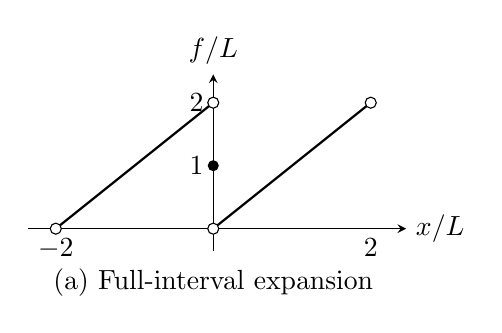
\begin{tikzpicture}[x=1cm,y=.8cm,>=stealth]
\draw[->] (-2.35,0)--(2.45,0) node[right] {$x/L$};
\draw[->] (0,-.35)--(0,2.45) node[above] {$f/L$};
\draw[thick] (-2,0)--(0,2); \draw[thick] (0,0)--(2,2);
\foreach \x/\y in {-2/0,0/2,0/0,2/2}
  \draw[fill=white] (\x,\y) circle (2pt);
\fill (0,1) circle (2pt);
\node[below] at (-2,0) {$-2$};\node[below] at (2,0) {$2$};
\node[left] at (0,1) {$1$};\node[left] at (0,2) {$2$};
\node at (0,-.85) {(a) Full-interval expansion};
\end{tikzpicture}\hspace{.6cm}
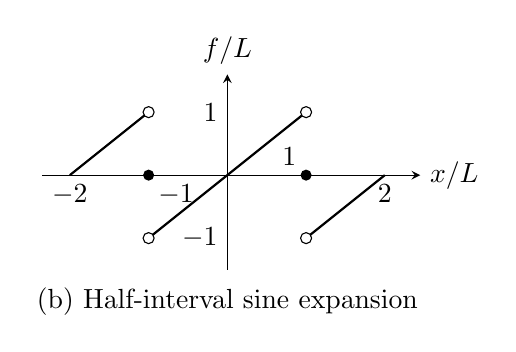
\begin{tikzpicture}[x=1cm,y=.8cm,>=stealth]
\draw[->] (-2.35,0)--(2.45,0) node[right] {$x/L$};
\draw[->] (0,-1.5)--(0,1.6) node[above] {$f/L$};
\draw[thick] (-2,0)--(-1,1);\draw[thick] (-1,-1)--(1,1);
\draw[thick] (1,-1)--(2,0);
\foreach \x/\y in {-1/1,-1/-1,1/1,1/-1}
  \draw[fill=white] (\x,\y) circle (2pt);
\fill (-1,0) circle (2pt);\fill (1,0) circle (2pt);
\node[below] at (-2,0) {$-2$};\node[below right] at (-1,0) {$-1$};
\node[above left] at (1,0) {$1$};\node[below] at (2,0) {$2$};
\node[left] at (0,1) {$1$};\node[left] at (0,-1) {$-1$};
\node at (0,-2) {(b) Half-interval sine expansion};
\end{tikzpicture}
\end{center}
Open circles are one-sided limits, and filled circles give the series
values at the indicated jumps.

\Needspace{5\baselineskip}
\par\bigskip
\noindent\textbf{19.1.10}\quad In some problems it is convenient to
approximate $\sin\pi x$ over the interval $[0,1]$ by a parabola
$ax(1-x)$, where $a$ is a constant. To get a feeling for the
accuracy of this approximation, expand $4x(1-x)$ in a Fourier sine
series ($-1\le x\le1$):
\[
f(x)=\begin{cases}
4x(1-x), & 0\le x\le1\\
4x(1+x), & -1\le x\le0
\end{cases}
=\sum_{n=1}^{\infty}b_{n}\sin n\pi x.
\]
\par\nobreak\hfill\emph{ANS.}\enspace
$b_{n}=\dfrac{32}{\pi^{3}n^{3}}$,\quad $n$ odd,\qquad
$b_{n}=0$,\quad $n$ even.
\par This approximation is shown in Fig.~19.6.
\solution
The stated extension is odd, since $f(-x)=4(-x)(1-x)=-f(x)$ for
$0\le x\le1$, so all cosine coefficients vanish. The period is $2$
($L=1$), and the integrand $f(x)\sin n\pi x$, a product of two odd
functions, is even. Put $k=n\pi$; the sine coefficient is
\[
b_n=\int_{-1}^1f(x)\sin kx\,dx=2\int_0^14x(1-x)\sin kx\,dx=8I_n,
\qquad I_n=\int_0^1x(1-x)\sin kx\,dx.
\]
Integrate by parts twice. The boundary terms vanish because
$x(1-x)=0$ at $x=0,1$ and $\sin k=\sin0=0$:
\begin{align*}
I_n&=\left[-\frac{x(1-x)\cos kx}{k}\right]_0^1
 +\frac1k\int_0^1(1-2x)\cos kx\,dx\\
&=\frac1k\left[\frac{(1-2x)\sin kx}{k}\right]_0^1
 +\frac2{k^2}\int_0^1\sin kx\,dx
 =\frac2{k^2}\,\frac{1-\cos k}{k}
 =\frac{2(1-\cos k)}{k^3}.
\end{align*}
With $\cos k=\cos n\pi=(-1)^n$ and $k^3=\pi^3n^3$, it follows that
\[
\boxed{b_n=\frac{16[1-(-1)^n]}{\pi^3n^3}
=\begin{cases}32/(\pi^3n^3),&n\text{ odd},\\0,&n\text{ even}.
\end{cases}}
\]
Thus the fundamental sine has coefficient $32/\pi^3\approx1.032$, and
the next nonzero coefficient, $b_3=32/(27\pi^3)\approx0.038$, is smaller
by a factor $27$. The series converges
absolutely and uniformly, since its terms are bounded by
$32/(\pi^3n^3)$ and $\sum n^{-3}$ converges (Weierstrass M-test). It
equals the continuous odd periodic
extension, including its zero values at $-1,0,1$.

\Needspace{5\baselineskip}
\par\bigskip
\noindent\textbf{19.1.11}\quad Verify that
$\delta(\varphi_{1}-\varphi_{2})=\dfrac{1}{2\pi}
\displaystyle\sum_{m=-\infty}^{\infty}e^{im(\varphi_{1}-\varphi_{2})}$
is a Dirac delta function by showing that it satisfies the
definition,
\[
\int_{-\pi}^{\pi}f(\varphi_{1})\,\frac{1}{2\pi}
\sum_{m=-\infty}^{\infty}e^{im(\varphi_{1}-\varphi_{2})}\,d\varphi_{1}
=f(\varphi_{2}).
\]
\par\emph{Hint.}~Represent $f(\varphi_{1})$ by an exponential
Fourier series.
\erratum{Use the periodic delta distribution on the circle, with a smooth $2\pi$-periodic test function $f$; interpret the series as the limit $N\to\infty$ of its symmetric partial sums $\sum_{m=-N}^{N}$.}
\solution
\erratum{This is the periodic delta distribution on the circle, not a
pointwise convergent series of functions: the terms $e^{imu}$ do not
tend to zero, so the series diverges at every $u$. On the real line it
is the comb $\delta_{2\pi}(u)=\sum_{k\in\mathbb Z}\delta(u-2\pi k)$.
The interval endpoints are identified.}
Take a smooth $2\pi$-periodic test function
$f(\varphi)=\sum_{j\in\mathbb Z}c_je^{ij\varphi}$, with
$c_j=(2\pi)^{-1}\int_{-\pi}^{\pi}f(\varphi)e^{-ij\varphi}\,d\varphi$.
For $j\ne0$, integrating by parts twice, with boundary terms that cancel
by periodicity, gives
\[
c_j=\frac1{2\pi ij}\int_{-\pi}^{\pi}f'(\varphi)e^{-ij\varphi}\,d\varphi
=-\frac1{2\pi j^2}\int_{-\pi}^{\pi}f''(\varphi)e^{-ij\varphi}\,d\varphi,
\]
so $|c_j|\le j^{-2}(2\pi)^{-1}\int|f''|$ and the coefficient series is
absolutely summable. For a finite symmetric kernel, interchange the
finite sum with the integral and use
$(2\pi)^{-1}\int_{-\pi}^{\pi}f(\varphi_1)e^{im\varphi_1}\,d\varphi_1=c_{-m}$:
\begin{align*}
\int_{-\pi}^{\pi}f(\varphi_1)\frac1{2\pi}
 \sum_{m=-N}^Ne^{im(\varphi_1-\varphi_2)}\,d\varphi_1
&=\sum_{m=-N}^Nc_{-m}e^{-im\varphi_2}\\
&=\sum_{j=-N}^Nc_je^{ij\varphi_2}\qquad(j=-m).
\end{align*}
The last expression is the symmetric partial sum of the Fourier series
of $f$, which converges to $f(\varphi_2)$ as $N\to\infty$ because $f$ is
smooth (Section 19.1); the absolutely summable coefficients make the
convergence uniform. This is exactly the defining distributional action,
hence
\[
\boxed{\delta_{2\pi}(\varphi_1-\varphi_2)
=\frac1{2\pi}\sum_{m\in\mathbb Z}e^{im(\varphi_1-\varphi_2)}.}
\]
For $\varphi_2$ strictly inside the integration interval, only one member
of the delta comb is present. For a piecewise regular function with a
jump at $\varphi_2$, symmetric Fourier sums give its midpoint value;
one must not assert recovery of an arbitrary assigned value at the jump.

\Needspace{5\baselineskip}
\par\bigskip
\noindent\textbf{19.1.12}\quad Show that integration of the Fourier
expansion of $f(x)=x$, $-\pi<x<\pi$, leads to
\[
\frac{\pi^{2}}{12}=\sum_{n=1}^{\infty}\frac{(-1)^{n+1}}{n^{2}}
=1-\frac{1}{4}+\frac{1}{9}-\frac{1}{16}+\cdots.
\]
\par\emph{Note.}~The series for $f(x)=x$ was the subject of
Example~19.1.1. Confirm that the change in the defined range from
$[0,2\pi]$ to $[-\pi,\pi]$ has no effect on the expansion.
\solution
From 19.1.6, or from the Fourier coefficients computed in 19.2.7,
\[
x=2\sum_{n=1}^{\infty}\frac{(-1)^{n+1}}n\sin nx,
\qquad-\pi<x<\pi.
\]
Integrating from $0$ to $x$ term by term, with
$\int_0^x\sin nt\,dt=(1-\cos nx)/n$, gives
\[
\frac{x^2}{2}
=2\sum_{n=1}^{\infty}\frac{(-1)^{n+1}}{n^2}(1-\cos nx).
\]
The integrated series is absolutely and uniformly convergent (its terms
are bounded by $4/n^2$). Termwise integration is justified as follows.
The partial sums $s_N$ of the series for $f(x)=x$ are its Fourier
partial sums, and since the trigonometric functions form a complete set,
the Fourier series of a square-integrable function converges to it in
the mean: $\|f-s_N\|_2\to0$, where
$\|g\|_2=\bigl(\int_{-\pi}^{\pi}|g|^2\,dx\bigr)^{1/2}$. By Cauchy--Schwarz
on the interval between $0$ and $x$,
\[
\Bigl|\int_0^x(f-s_N)\,dt\Bigr|\le\sqrt{|x|}\,\|f-s_N\|_2
\le\sqrt{\pi}\,\|f-s_N\|_2\longrightarrow0
\]
uniformly in $x$, so the integrated partial sums converge to
$\int_0^xt\,dt=x^2/2$.
Average the integrated identity over $(-\pi,\pi)$; uniform convergence
allows averaging term by term. Every cosine has zero average, so the
right side averages to $2\sum_{n\ge1}(-1)^{n+1}/n^2$, while
\[
\frac1{2\pi}\int_{-\pi}^{\pi}\frac{x^2}{2}\,dx
=\frac1{2\pi}\left[\frac{x^3}{6}\right]_{-\pi}^{\pi}
=\frac1{2\pi}\,\frac{2\pi^3}{6}=\frac{\pi^2}{6}.
\]
Consequently $2\sum_{n\ge1}(-1)^{n+1}/n^2=\pi^2/6$, that is,
\[
\boxed{\sum_{n=1}^{\infty}\frac{(-1)^{n+1}}{n^2}=\frac{\pi^2}{12}.}
\]
The change of range in the note does not change the underlying periodic
function: Example 19.1.1 defines it as $x$ on $(0,\pi)$ and $x-2\pi$ on
$(\pi,2\pi)$. Moving that latter interval left by $2\pi$ gives $x$ on
$(-\pi,0)$. Since the integral of a $2\pi$-periodic function is the same
over every interval of length $2\pi$, integrals over $[0,2\pi]$ and over
$[-\pi,\pi]$ give exactly these same Fourier coefficients.

\Needspace{5\baselineskip}
\par\bigskip
\noindent\textbf{19.1.13}
\begin{enumerate}
\item[(a)] Assuming that the Fourier expansion of \erratum{a real-valued} $f(x)$ is
uniformly convergent, show that
\[
\frac{1}{\pi}\int_{-\pi}^{\pi}\big[f(x)\big]^{2}dx
=\frac{a_{0}^{2}}{2}+\sum_{n=1}^{\infty}\big(a_{n}^{2}+b_{n}^{2}\big).
\]
This is Parseval's identity. Note that it is a completeness
relation for the Fourier expansion.
\item[(b)] Given
$x^{2}=\dfrac{\pi^{2}}{3}+4\displaystyle\sum_{n=1}^{\infty}
\dfrac{(-1)^{n}\cos nx}{n^{2}}$, $-\pi\le x\le\pi$, apply
Parseval's identity to obtain $\zeta(4)$ in closed form.
\item[(c)] The condition of uniform convergence is not necessary.
Show this by applying the Parseval identity to the square wave
\[
f(x)=\begin{cases}-1,&-\pi<x<0\\1,&0<x<\pi\end{cases}
=\frac{4}{\pi}\sum_{n=1}^{\infty}\frac{\sin(2n-1)x}{2n-1}.
\]
\end{enumerate}
\solution
\textbf{(a)} Square the partial sum
$s_N=a_0/2+\sum_{n=1}^N(a_n\cos nx+b_n\sin nx)$ and integrate over
$(-\pi,\pi)$. All cross terms integrate to zero, while
$\int(a_0/2)^2dx=\pi a_0^2/2$ and
$\int\cos^2nx\,dx=\int\sin^2nx\,dx=\pi$. Hence for every finite partial
sum
\[
\frac1\pi\int_{-\pi}^{\pi}s_N^2\,dx
=\frac{a_0^2}{2}+\sum_{n=1}^N(a_n^2+b_n^2).
\]
If $s_N\to f$ uniformly, that is, $\|s_N-f\|_\infty\to0$ with
$\|g\|_\infty=\sup_{-\pi<x<\pi}|g(x)|$, then $f$ is bounded, the $s_N$
are uniformly bounded for large $N$ ($\|s_N\|_\infty\le\|f\|_\infty+1$
once $\|s_N-f\|_\infty\le1$), and, since $s_N^2-f^2=(s_N-f)(s_N+f)$,
\[
\left|\int(s_N^2-f^2)\right|
\le2\pi\|s_N-f\|_\infty(\|s_N\|_\infty+\|f\|_\infty)\longrightarrow0.
\]
Letting $N\to\infty$ on both sides of the finite identity proves the
stated identity.
\erratum{The displayed identity is for real functions; the complex
version uses modulus squares. Also the Instructor's Manual's first
display in 19.1.13(a) is missing the factor $1/\pi$ on its integral:
for $f=1$ its unnormalized left side is $2\pi$, whereas its right side
is $2$.}
More generally $L^2$ convergence suffices: with $\|\cdot\|_2$ as in
19.1.12, the triangle inequality gives
$|\|s_N\|_2-\|f\|_2|\le\|s_N-f\|_2\to0$, so
$\pi^{-1}\int_{-\pi}^{\pi}s_N^2\,dx=\|s_N\|_2^2/\pi\to\|f\|_2^2/\pi$.

\textbf{(b)} Reading off the given series for $f=x^2$:
$a_0/2=\pi^2/3$, so $a_0=2\pi^2/3$; $a_n=4(-1)^n/n^2$, so
$a_n^2=16/n^4$; and $b_n=0$. The identity becomes
\[
\frac1\pi\int_{-\pi}^{\pi}x^4\,dx
=\frac1\pi\,\frac{2\pi^5}5
=\frac{2\pi^4}{5}
=\frac12\left(\frac{2\pi^2}{3}\right)^2
 +16\sum_{n=1}^{\infty}\frac1{n^4}
=\frac{2\pi^4}9+16\,\zeta(4).
\]
Solving, with $2/5-2/9=8/45$,
\[
\boxed{\zeta(4)=\frac1{16}\left(\frac25-\frac29\right)\pi^4
=\frac1{16}\,\frac{8\pi^4}{45}=\frac{\pi^4}{90}.}
\]
The given $x^2$ series is uniformly convergent by comparison with
$\sum n^{-2}$, so part (a) applies directly.

\textbf{(c)} The square wave has $f^2=1$, so
$\pi^{-1}\int_{-\pi}^{\pi}f^2\,dx=2$. From the given series it has no
constant or cosine terms, $b_{2j-1}=4/[\pi(2j-1)]$, and the even-$n$
sine coefficients vanish. Hence Parseval reads
\[
2=\frac{16}{\pi^2}\sum_{j=1}^{\infty}\frac1{(2j-1)^2}.
\]
To check this independently, the $L^2$ convergence of the square-wave
series may not be used: by the expansion in 19.1.4,
$\int(f-s_N)^2\,dx=\int f^2\,dx-\pi\sum_{n\le N}b_n^2$, so for this $f$
it is equivalent to the identity being checked. Instead use the
primitive $\int_0^xf\,dt=|x|$, which is continuous and piecewise smooth;
its cosine series (19.2.9) converges to it at every point, and at $x=0$
it gives
\[
0=\frac\pi2-\frac4\pi\sum_{j=1}^{\infty}\frac1{(2j-1)^2}.
\]
Thus $\sum_{j\ge1}(2j-1)^{-2}=\pi^2/8$ (as also found in 19.2.13(b)),
and the right side of Parseval is indeed $(16/\pi^2)(\pi^2/8)=2$.

For any fixed partial sum $s_N$, which is continuous with $s_N(0)=0$,
$s_N(x)\to0$ as $x\downarrow0$, whereas the square wave equals one there. Thus
$\sup_{0<x<\pi}|s_N(x)-1|\ge1$, ruling out uniform convergence. This supplies the requested counterexample
to necessity of uniform convergence, while $L^2$ completeness still
justifies Parseval.

\Needspace{5\baselineskip}
\par\bigskip
\noindent\textbf{19.1.14}\quad Given
\[
\varphi_{1}(x)\equiv\sum_{n=1}^{\infty}\frac{\sin nx}{n}
=\begin{cases}
-\dfrac{1}{2}(\pi+x), & -\pi\le x<0,\\[10pt]
\dfrac{1}{2}(\pi-x), & 0<x\le\pi,
\end{cases}
\]
show by integrating that
\[
\varphi_{2}(x)\equiv\sum_{n=1}^{\infty}\frac{\cos nx}{n^{2}}
=\begin{cases}
\dfrac{1}{4}(\pi+x)^{2}-\dfrac{\pi^{2}}{12}, & -\pi\le x\le0,\\[12pt]
\dfrac{1}{4}(\pi-x)^{2}-\dfrac{\pi^{2}}{12}, & 0\le x\le\pi.
\end{cases}
\]
\solution
The cosine series for $\varphi_2$ is absolutely and uniformly convergent
by comparison with $\sum n^{-2}$.
Integrating the sine series for $\varphi_1$ term by term from $0$ to $x$,
$0<x\le\pi$, is valid because the series is the Fourier series of
$\varphi_1$ (its coefficients $b_n=1/n$ are computed in 19.2.8). Its
partial sums $s_N$ therefore converge to $\varphi_1$ in the mean,
$\|\varphi_1-s_N\|_2\to0$, as in 19.1.12, and by Cauchy--Schwarz on
$(0,x)$,
\[
\Bigl|\int_0^x(\varphi_1-s_N)\,dt\Bigr|\le\sqrt{x}\,\|\varphi_1-s_N\|_2
\le\sqrt{\pi}\,\|\varphi_1-s_N\|_2\longrightarrow0.
\]
Since $n^{-1}\int_0^x\sin nt\,dt=(1-\cos nx)/n^2$, the term-by-term
integral is $\sum_{n\ge1}(1-\cos nx)/n^2=\varphi_2(0)-\varphi_2(x)$, and
integrating the closed form instead gives
\[
\varphi_2(0)-\varphi_2(x)
=\int_0^x\frac{\pi-t}{2}\,dt
=\frac{\pi x}{2}-\frac{x^2}{4}.
\]
Write $C=\varphi_2(0)$, so $\varphi_2(x)=C-\pi x/2+x^2/4$ on $[0,\pi]$.
The cosine series is even in $x$, which gives, on $[-\pi,\pi]$,
$\varphi_2(x)=C-\pi|x|/2+x^2/4$.
Every term of the uniformly convergent cosine series has zero integral
over $[0,\pi]$, because $\int_0^\pi\cos nx\,dx=\sin(n\pi)/n=0$, so
termwise integration gives
\[
0=\int_0^\pi\varphi_2(x)\,dx
=C\pi-\frac\pi2\frac{\pi^2}{2}+\frac14\frac{\pi^3}{3}
=C\pi-\frac{\pi^3}{4}+\frac{\pi^3}{12}
=C\pi-\frac{\pi^3}{6}.
\]
Therefore $C=\pi^2/6$. Completing the square,
$\pi^2/6-\pi|x|/2+x^2/4=(\pi-|x|)^2/4-\pi^2/4+\pi^2/6$, yields
\[
\boxed{\varphi_2(x)=\frac{(\pi-|x|)^2}{4}-\frac{\pi^2}{12},
\qquad -\pi\le x\le\pi,}
\]
which gives exactly the two requested branches ($|x|=-x$ for $x\le0$ and
$|x|=x$ for $x\ge0$). The derivation covered every $0\le x\le\pi$, and
evenness every $-\pi\le x\le0$, so the endpoints $x=0,\pm\pi$ are
included; in particular setting $x=0$ proves
$\sum n^{-2}=\varphi_2(0)=\pi^2/6$.

\Needspace{5\baselineskip}
\par\bigskip
\noindent\textbf{19.1.15}\quad Given
\[
\psi_{2s}(x)=\sum_{n=1}^{\infty}\frac{\sin nx}{n^{2s}},\qquad
\psi_{2s+1}(x)=\sum_{n=1}^{\infty}\frac{\cos nx}{n^{2s+1}},
\]
develop the following recurrence relations:
\begin{enumerate}
\item[(a)] $\psi_{2s}(x)=\displaystyle\int_{0}^{x}
\erratum{\psi_{2s-1}(t)\,dt}$,
\item[(b)] $\psi_{2s+1}(x)=\zeta(2s+1)
-\displaystyle\int_{0}^{x}\erratum{\psi_{2s}(t)\,dt}$.
\end{enumerate}
\par\emph{Note.}~The functions $\psi_{s}(x)$ and $\varphi_{s}(x)$
of this and the preceding exercise are known as \emph{Clausen
functions}. In theory they may be used to improve the rate of
convergence of a Fourier series. As is often the case, there is the
question of how much analytical work we do and how much arithmetic
work we demand that a computer do. As computers become steadily
more powerful, the balance progressively shifts so that we are
doing less and demanding that computers do more.
\erratum{Here $s=1,2,\ldots$. When $s=1$, the first integral is improper at multiples of $2\pi$ crossed by the interval.}
\solution
Let $s$ be a positive integer, as the statement requires: for $s=0$,
(b) would contain the divergent $\zeta(1)=\sum_n1/n$, and (a) the
divergent series $\psi_{-1}=\sum_nn\cos nx$. The statement writes the
integration variable as $t$, since $x$ is already the upper limit.
For $s\ge2$, the terms of the series for $\psi_{2s-1}$ are bounded by
$n^{-(2s-1)}\le n^{-3}$, so it converges absolutely and uniformly
(Weierstrass M-test) and may be integrated term by term, with
$\int_0^x\cos nt\,dt=\sin nx/n$. Thus
\[
\int_0^x\psi_{2s-1}(t)\,dt
=\sum_{n=1}^{\infty}\frac1{n^{2s-1}}\int_0^x\cos nt\,dt
=\sum_{n=1}^{\infty}\frac{\sin nx}{n^{2s}}
=\boxed{\psi_{2s}(x)}.
\]
For every $s\ge1$, the even-index series has terms bounded by
$n^{-2s}\le n^{-2}$, so it too converges absolutely and uniformly.
Termwise integration with $\int_0^x\sin nt\,dt=(1-\cos nx)/n$, and
splitting into two absolutely convergent series ($2s+1\ge3$), gives
\begin{align*}
\int_0^x\psi_{2s}(t)\,dt
&=\sum_{n=1}^{\infty}\frac{1-\cos nx}{n^{2s+1}}
=\sum_{n=1}^{\infty}\frac1{n^{2s+1}}
-\sum_{n=1}^{\infty}\frac{\cos nx}{n^{2s+1}}\\
&=\zeta(2s+1)-\psi_{2s+1}(x).
\end{align*}
Solving for $\psi_{2s+1}(x)$ proves the second recurrence.

\erratum{The first recurrence at $s=1$ has an integrable logarithmic
singularity at its lower endpoint: $\psi_1(t)=-\ln(2|\sin(t/2)|)$.
The integral must be read as improper at every multiple of $2\pi$ it
crosses; $\psi_1$ itself is not finite at those points.}
To justify this base case, insert $r^n$ with $0<r<1$. Then
$\sum_{n\ge1}r^n\cos nt/n=\operatorname{Re}\{-\log(1-re^{it})\}
=-\ln|1-re^{it}|$, and this series is uniformly convergent (its terms
are bounded by $r^n$), so termwise integration gives
\[
\int_0^x-\ln|1-re^{it}|\,dt
=\sum_{n=1}^{\infty}\frac{r^n\sin nx}{n^2}.
\]
The right side tends uniformly to $\psi_2(x)$ as $r\uparrow1$, because
the difference is bounded by $\sum_n(1-r^n)/n^2$, whose terms tend to
zero and are dominated by $n^{-2}$. On the left, for $t\notin2\pi\mathbb Z$
the integrand tends to $-\ln|1-e^{it}|=-\ln(2|\sin(t/2)|)=\psi_1(t)$.
To dominate it, use
\[
|1-re^{it}|^2=1-2r\cos t+r^2=(1-r)^2+4r\sin^2(t/2).
\]
For $1/2\le r<1$ this gives $2\sin^2(t/2)\le|1-re^{it}|^2<4$ (for the
lower bound drop $(1-r)^2\ge0$ and use $4r\ge2$; for the upper bound use
$|1-re^{it}|\le1+r<2$). Taking half the logarithm,
\[
\tfrac12\ln2+\ln|\sin(t/2)|\le\ln|1-re^{it}|<\ln2,
\]
and since $\ln|\sin(t/2)|\le0$ this gives
$|\ln|1-re^{it}||\le\ln2+|\ln|\sin(t/2)||$, independently of $r$. Let
$d=\operatorname{dist}(t,2\pi\mathbb Z)\in[0,\pi]$, so that
$|\sin(t/2)|=\sin(d/2)$. By Jordan's inequality ($\sin u\ge2u/\pi$ on
$[0,\pi/2]$), $\sin(d/2)\ge d/\pi$, hence
$|\ln|\sin(t/2)||\le\ln\pi-\ln d\le\ln\pi+|\ln d|$. So on any bounded
interval the integrand is bounded by $\ln(2\pi)+|\ln d|$, which is
integrable near the finitely many singularities because
$\int_0^\epsilon|\ln t|\,dt=\epsilon(1-\ln\epsilon)$ for $0<\epsilon<1$.
Dominated convergence therefore lets $r\uparrow1$ under the integral,
which proves the first recurrence also for $s=1$.

\Needspace{5\baselineskip}
\par\bigskip
\noindent\textbf{19.1.16}\quad Show that
$f(x)=\displaystyle\sum_{n=1}^{\infty}\dfrac{\cos nx}{n+1}$ may be
written as
\[
f(x)=\psi_{1}(x)-\varphi_{2}(x)
+\sum_{n=1}^{\infty}\frac{\cos nx}{n^{2}(n+1)},
\]
where $\psi_{1}(x)$ and $\varphi_{2}(x)$ are the Clausen functions
defined in Exercises~19.1.14 and 19.1.15.
\erratum{For the finite-valued identity take $x\notin2\pi\mathbb Z$.}
\solution
The elementary coefficient identity, over the common denominator
$n^2(n+1)$, is
\[
\frac1n-\frac1{n^2}+\frac1{n^2(n+1)}
=\frac{n(n+1)-(n+1)+1}{n^2(n+1)}
=\frac{n^2}{n^2(n+1)}
=\frac1{n+1}.
\]
Multiply by $\cos nx$, sum first to a finite $N$, and then pass to the
limit; for $x\notin2\pi\mathbb Z$ each of the three series converges, so
the limit of the sum is the sum of the limits. The first series is
$\psi_1=\sum\cos nx/n$ (the case $s=0$ of $\psi_{2s+1}$ in 19.1.15),
the second is $\varphi_2=\sum\cos nx/n^2$ of 19.1.14, and the last is
absolutely convergent. Therefore
\[
\boxed{f(x)=\psi_1(x)-\varphi_2(x)
+\sum_{n=1}^{\infty}\frac{\cos nx}{n^2(n+1)}.}
\]
\erratum{This equality is an ordinary finite-valued identity only for
$x\notin2\pi\mathbb Z$. At a multiple of $2\pi$ both $f$ and $\psi_1$
diverge.}
Away from those points, Dirichlet's test proves convergence of the
original series and of $\psi_1$, as in 19.1.5. The correction series has
a simple uniform truncation bound: $|\cos nx|/(n^2(n+1))<n^{-3}$, and
$n^{-3}\le\int_{n-1}^n t^{-3}\,dt$, so
\[
\left|\sum_{n>N}\frac{\cos nx}{n^2(n+1)}\right|
\le\sum_{n>N}\frac1{n^3}\le\int_N^\infty\frac{dt}{t^3}
=\frac1{2N^2}.
\]
Thus the known closed forms of the first two terms, for $0<x<2\pi$,
\[
\psi_1(x)=-\ln\Bigl(2\sin\frac x2\Bigr),\qquad
\varphi_2(x)=\frac{(\pi-x)^2}4-\frac{\pi^2}{12},
\]
leave a rapidly convergent remainder. The first is 19.1.8(b); the second
is 19.1.14 on $(0,\pi]$, extended to $[\pi,2\pi)$ by
$\varphi_2(x)=\varphi_2(x-2\pi)=\varphi_2(2\pi-x)$ (periodicity and
evenness), which reproduces the same formula.

\Needspace{12\baselineskip}
\subsection*{19.2 Applications of Fourier Series}

\Needspace{5\baselineskip}
\par\bigskip
\noindent\textbf{19.2.1}\quad Transform the Fourier expansion of a
square wave, Eq.~(19.26), into a power series \erratum{(formally: expand
each sine in powers of $x$ and collect like powers; height $h\ne0$)}.
Show that the coefficients of $x^{1}$ form a divergent series. Repeat
for the coefficients of $x^{3}$.
\par\emph{Note.}~A power series cannot handle a discontinuity.
These infinite coefficients are the result of attempting to beat
this basic limitation on power series.
\solution
Equation (19.26) is
\[
f(x)=\frac h2+\frac{2h}{\pi}\sum_{j=0}^{\infty}
\frac{\sin((2j+1)x)}{2j+1}.
\]
For each individual term its entire Taylor expansion is
\[
\frac{\sin((2j+1)x)}{2j+1}
=x-\frac{(2j+1)^2x^3}{3!}
+\frac{(2j+1)^4x^5}{5!}-\cdots.
\]
Retain only the first $N$ harmonics before collecting powers. Each
harmonic contributes $2h/\pi$ to the coefficient of $x$, so the linear
coefficient is $2hN/\pi$. For the cubic coefficient expand
$(2j+1)^2=4j^2+4j+1$ and use
$\sum_{j=0}^{N-1}j^2=(N-1)N(2N-1)/6$,
$\sum_{j=0}^{N-1}j=N(N-1)/2$:
\begin{align*}
-\frac{2h}{6\pi}\sum_{j=0}^{N-1}(2j+1)^2
&=-\frac{h}{3\pi}
\left[4\frac{(N-1)N(2N-1)}6
+4\frac{N(N-1)}2+N\right]\\
&=-\frac{h}{3\pi}\,\frac{N(4N^2-1)}3
=-\frac{hN(4N^2-1)}{9\pi},
\end{align*}
since the bracket is
$[(4N^3-6N^2+2N)+(6N^2-6N)+3N]/3=(4N^3-N)/3$.
For nonzero $h$ neither coefficient has a finite limit as $N\to\infty$;
their magnitudes grow as $N$ and $N^3$, respectively. Formally, the coefficient of
$x^{2k+1}$ would be
\[
\frac{2h}{\pi}\frac{(-1)^k}{(2k+1)!}
\sum_{j=0}^{\infty}(2j+1)^{2k},
\]
and it diverges for every $k\ge0$, because every term of the sum is at
least $1$.
\erratum{The textbook's request to transform the Fourier series into a
power series is therefore only formal, not a valid convergent
power-series rearrangement. Interchanging the harmonic
sum and Taylor sum is precisely the invalid step.}
A convergent power series on a neighborhood of zero is continuous
there, so it cannot reproduce the jump between $0$ and $h$.
Away from jumps the square wave is locally constant and has a perfectly
valid local constant Taylor series; the obstruction concerns a single
series spanning the discontinuity.

\Needspace{5\baselineskip}
\par\bigskip
\noindent\textbf{19.2.2}\quad Derive the Fourier series expansion
of the Dirac delta function $\delta(x)$ in the interval
$-\pi<x<\pi$.
\begin{enumerate}
\item[(a)] What significance can be attached to the constant term?
\item[(b)] In what region is this representation valid?
\item[(c)] With the identity
\[
\sum_{n=1}^{N}\cos nx=\frac{\sin(Nx/2)}{\sin(x/2)}
\cos\left[\erratum{(N+1)}\frac{x}{2}\right],
\]
show that your Fourier representation of $\delta(x)$ is consistent
with Eq.~(5.27).
\end{enumerate}
\erratum{Interpret the expansion distributionally. In the finite-sum identity use the continuous limiting value where $\sin(x/2)=0$.}
\solution
Apply the coefficient formulas to the distribution on $(-\pi,\pi)$,
using the sampling rule $\int_{-\pi}^{\pi}\delta(x)g(x)\,dx=g(0)$:
\[
a_0=\frac1\pi\int\delta(x)\,dx=\frac1\pi,
\quad a_n=\frac1\pi\int\delta(x)\cos nx\,dx=\frac{\cos0}\pi=\frac1\pi,
\quad b_n=\frac{\sin0}\pi=0.
\]
Thus, with $a_0/2=1/(2\pi)$,
\[
\boxed{\delta_{2\pi}(x)=\frac1{2\pi}
+\frac1\pi\sum_{n=1}^{\infty}\cos nx.}
\]
\textbf{(a)} The constant $1/(2\pi)$ is the mean density over one
period. All other terms integrate to zero over $(-\pi,\pi)$; this term
alone ensures unit total mass, $\int_{-\pi}^{\pi}dx/(2\pi)=1$.

\textbf{(b)} \erratum{The equality is distributional, and its global
extension is periodic: $\delta_{2\pi}(x)=\sum_{k\in\mathbb Z}
\delta(x-2\pi k)$. It represents the single $\delta(x)$ within
$(-\pi,\pi)$, not a single isolated delta on the whole real line.}
The series cannot be interpreted as an ordinary pointwise function.

\textbf{(c)} \erratum{The textbook's finite-sum identity has an
incorrect angle: its cosine must be $\cos((N+1)x/2)$, not
$\cos((N+1/2)x/2)$, as the geometric sum below shows.}
Indeed, factoring $e^{iNx/2}$ from the numerator and $e^{ix/2}$ from
the denominator, and using $e^{-iu}-e^{iu}=-2i\sin u$, the geometric
sum is
\begin{align*}
\sum_{n=1}^Ne^{inx}
&=e^{ix}\frac{1-e^{iNx}}{1-e^{ix}}
=e^{ix}\,\frac{e^{iNx/2}(e^{-iNx/2}-e^{iNx/2})}
{e^{ix/2}(e^{-ix/2}-e^{ix/2})}\\
&=e^{i(N+1)x/2}\frac{\sin(Nx/2)}{\sin(x/2)}.
\end{align*}
Taking real parts proves the corrected identity. Add the constant
term and use $2\sin A\cos B=\sin(A+B)+\sin(A-B)$ with $A=Nx/2$,
$B=(N+1)x/2$, so that $A+B=(N+1/2)x$ and $A-B=-x/2$. This yields
\begin{align*}
1+2\sum_{n=1}^N\cos nx
&=\frac{\sin(x/2)+\sin((N+1/2)x)-\sin(x/2)}{\sin(x/2)}\\
&=\frac{\sin((N+1/2)x)}{\sin(x/2)}=D_N(x).
\end{align*}
The quotient has the removable value $D_N(0)=2N+1$ (the left side at
$x=0$, or the limit $(N+1/2)/(1/2)$ of the quotient).
Its normalized integral is one,
$(2\pi)^{-1}\int_{-\pi}^{\pi}D_N\,dx=1$, since each $\cos nx$
integrates to zero. Moreover, since
$D_N(x)=\sum_{n=-N}^Ne^{inx}$, for a periodic $f$ with exponential
Fourier coefficients $c_n$ (as in 19.1.11)
\[
\frac1{2\pi}\int_{-\pi}^{\pi}f(x)D_N(x)\,dx=\sum_{n=-N}^Nc_{-n}
=\sum_{n=-N}^Nc_n,
\]
the symmetric partial sum of the Fourier series of $f$ at $x=0$; in
particular $D_N/(2\pi)$ reproduces the value at $0$ of every Fourier
polynomial of degree at most $N$. For smooth periodic $f$ these
partial sums tend to $f(0)$ as $N\to\infty$, as shown in 19.1.11.
This is the delta limit.

Specifically Eq. (5.27) is the closure relation
$\delta(x-t)=\sum_j\phi_j(x)\phi_j^*(t)$.
For the orthonormal functions
$1/\sqrt{2\pi}$, $\cos nx/\sqrt\pi$, $\sin nx/\sqrt\pi$,
setting $t=0$ gives
$1/(2\pi)+\pi^{-1}\sum_{n\ge1}(\cos nx\cos0+\sin nx\sin0)$,
exactly the boxed formula. Thus the finite kernel
and the general bilinear closure relation agree.

\Needspace{5\baselineskip}
\par\bigskip
\noindent\textbf{19.2.3}\quad Expand $\delta(x-t)$ in a Fourier
series. Compare your result with the bilinear form of Eq.~(5.27).
\par\nobreak\hfill\emph{ANS.}\enspace
$\delta(x-t)=\dfrac{1}{2\pi}+\dfrac{1}{\pi}
\displaystyle\sum_{n=1}^{\infty}(\cos nx\cos nt+\sin nx\sin nt)$\par
\nobreak\hfill$\hspace{4em}=\dfrac{1}{2\pi}+\dfrac{1}{\pi}
\displaystyle\sum_{n=1}^{\infty}\cos n(x-t)$.
\erratum{Use the periodic distribution on $(-\pi,\pi)$, with $t$ in that interval, or equivalently work on the circle.}
\solution
For $t$ strictly inside $(-\pi,\pi)$, the delta's sampling rule
$\int_{-\pi}^{\pi}\delta(x-t)g(x)\,dx=g(t)$, applied to $g=1$,
$\cos nx$, $\sin nx$ in the coefficient formulas, gives
\[
a_0(t)=\frac1\pi,\qquad
 a_n(t)=\frac{\cos nt}{\pi},\qquad
 b_n(t)=\frac{\sin nt}{\pi}.
\]
Substitution into $a_0/2+\sum_{n\ge1}(a_n\cos nx+b_n\sin nx)$ gives
\begin{align*}
\delta_{2\pi}(x-t)
&=\frac1{2\pi}+\frac1\pi\sum_{n=1}^{\infty}
(\cos nx\cos nt+\sin nx\sin nt)\\
&=\boxed{\frac1{2\pi}+\frac1\pi\sum_{n=1}^{\infty}\cos n(x-t)}.
\end{align*}
The last equality is the cosine subtraction identity
$\cos nx\cos nt+\sin nx\sin nt=\cos n(x-t)$, applied first to finite
sums. With the real orthonormal basis $1/\sqrt{2\pi}$,
$\cos nx/\sqrt\pi$, $\sin nx/\sqrt\pi$ from 19.2.2, the first line is
precisely $\sum_j\phi_j(x)\phi_j^*(t)$ in Eq.~(5.27), because
$(1/\sqrt{2\pi})(1/\sqrt{2\pi})=1/(2\pi)$ and
$(\cos nx/\sqrt\pi)(\cos nt/\sqrt\pi)=\pi^{-1}\cos nx\cos nt$, and
similarly for the sines.
For example, integrating against $\phi_k(x)$ leaves, by orthonormality,
only the $k$th term and gives $\phi_k(t)$; by the convergent Fourier
expansion this extends to smooth test functions.
The periodic/distributional and endpoint qualifications of 19.2.2
apply equally to the translated kernel.

\Needspace{5\baselineskip}
\par\bigskip
\noindent\textbf{19.2.4}\quad Show that integrating the Fourier
expansion of the Dirac delta function (Exercise~19.2.2) leads to
the Fourier representation of the square wave, Eq.~(19.26), with
$h=1$.
\par\emph{Note.}~Integrating the constant term $(1/2\pi)$ leads to
a term $x/2\pi$. What are you going to do with this?
\solution
Let $H(x)$ be zero for $-\pi<x<0$ and one for $0<x<\pi$.
Within this open interval, $H'=\delta(x)$ and the symmetric value at
zero is $H(0)=1/2$. Integrate the delta Fourier series from zero term
by term,
\[
\int_0^x\Bigl[\frac1{2\pi}+\frac1\pi\sum_{n=1}^{\infty}\cos nt\Bigr]dt
=\frac x{2\pi}+\frac1\pi\sum_{n=1}^{\infty}\frac{\sin nx}n,
\]
and add $H(0)=1/2$. This gives
\[
H(x)=\frac12+\frac{x}{2\pi}
+\frac1\pi\sum_{n=1}^{\infty}\frac{\sin nx}{n},
\qquad -\pi<x<\pi.
\]
As a check, by 19.1.5 the sine series is $(\pi-x)/2$ on $(0,\pi)$ and
$-(\pi+x)/2$ on $(-\pi,0)$, so the right side is
$1/2+x/(2\pi)+(\pi-x)/(2\pi)=1$ and
$1/2+x/(2\pi)-(\pi+x)/(2\pi)=0$, respectively.
The term $x/(2\pi)$ of the note must be retained; the answer to the
note's question is to replace it by its own Fourier series, the
sawtooth series $x=2\sum_{n\ge1}(-1)^{n+1}\sin nx/n$ of 19.2.7, that
is, $x/(2\pi)=\pi^{-1}\sum_{n\ge1}(-1)^{n+1}\sin nx/n$:
\begin{align*}
H(x)&=\frac12+\frac1\pi\sum_{n=1}^{\infty}
\frac{1+(-1)^{n+1}}n\sin nx\\
&=\boxed{\frac12+\frac2\pi\sum_{j=0}^{\infty}
\frac{\sin((2j+1)x)}{2j+1}}.
\end{align*}
Since $1+(-1)^{n+1}$ is $0$ for even $n$ and $2$ for odd $n=2j+1$, the
even terms cancel and the odd terms double, which is Eq.~(19.26) with
$h=1$.

There is also a direct way to keep the periodic boundary bookkeeping.
Integrate the series of 19.2.3 over $0<t<\pi$. The constant term gives
$\pi/(2\pi)=1/2$, and with $u=x-t$,
$\int_0^\pi\cos n(x-t)\,dt=\int_{x-\pi}^x\cos nu\,du
=[\sin nx-\sin(n(x-\pi))]/n$, and
$\sin(n(x-\pi))=(-1)^n\sin nx$:
\begin{align*}
H(x)&=\int_0^\pi\delta_{2\pi}(x-t)\,dt\\
&=\frac12+\frac1\pi\sum_{n=1}^{\infty}
\frac{\sin nx-\sin(n(x-\pi))}{n}\\
&=\frac12+\frac1\pi\sum_{n=1}^{\infty}
\frac{1-(-1)^n}{n}\sin nx.
\end{align*}
For $0<x<\pi$ the delta at $t=x$ lies in $(0,\pi)$ and the integral is
$1$; for $-\pi<x<0$ the comb members at $t=x$ and $t=x+2\pi$ both lie
outside $(0,\pi)$ and it is $0$. The coefficient $1-(-1)^n$ again keeps
only odd $n$, with value $2$, reproducing the boxed series.
\erratum{The Instructor's Manual's final negative-$x$ branch is
printed as $1$; it must be $0$. Also the derivative of the periodic step is
$\delta_{2\pi}(x)-\delta_{2\pi}(x-\pi)$, including the downward
boundary jump. Integrating a single periodic delta produces the linear
term above, not by itself a periodic primitive.}
At all jump points the Fourier series takes the midpoint $1/2$.

\Needspace{5\baselineskip}
\par\bigskip
\noindent\textbf{19.2.5}\quad Starting from the Fourier series
given as lines 4 and 5 of Table~19.1, show that:
\[
\sum_{n=0}^{\infty}\frac{\cos(2n+1)x}{2n+1}
=\frac{1}{2}\ln\left|\cot\frac{x}{2}\right|.
\]
\erratum{Exclude $x\in\pi\mathbb Z$.}
\solution
On $0<|x|<\pi$, the two logarithmic series in Table 19.1 read as
follows; they are 19.1.8(b), extended to $-\pi<x<0$ because both sides
are even, and 19.1.8(a) multiplied by $-1$:
\[
A(x)=\sum_{n=1}^{\infty}\frac{\cos nx}{n}
=-\ln(2|\sin(x/2)|),
\qquad
B(x)=\sum_{n=1}^{\infty}\frac{(-1)^n\cos nx}{n}
=-\ln(2\cos(x/2)).
\]
\erratum{In the Instructor's Manual's intermediate first sum, the
denominator printed as $x$ must be $n$, and that sum starts at $n=1$.}
Subtracting the two convergent series term by term eliminates every even
harmonic, since $1-(-1)^n$ is $0$ for even $n$ and $2$ for odd $n$:
\[
A-B=\sum_{n=1}^{\infty}\frac{1-(-1)^n}{n}\cos nx
=2\sum_{j=0}^{\infty}\frac{\cos((2j+1)x)}{2j+1}.
\]
The corresponding logarithmic difference is, since $\cos(x/2)>0$ for
$|x|<\pi$,
\[
\ln(2\cos(x/2))-\ln(2|\sin(x/2)|)
=\ln\frac{\cos(x/2)}{|\sin(x/2)|}
=\ln|\cot(x/2)|.
\]
Dividing $A-B$ by $2$ gives
\[
\boxed{\sum_{j=0}^{\infty}\frac{\cos((2j+1)x)}{2j+1}
=\frac12\ln|\cot(x/2)|.}
\]
\erratum{Exclude $x\in\pi\mathbb Z$. At even multiples of $\pi$
the series diverges to $+\infty$; at odd multiples it diverges to
$-\infty$.}
Elsewhere its ordinary convergence follows from Dirichlet's test for
$\sum e^{i(2j+1)x}$, whose geometric ratio is $e^{2ix}\ne1$.
Both sides have period $2\pi$, so periodicity extends the displayed
identity to every other real $x\notin\pi\mathbb Z$.

\Needspace{5\baselineskip}
\par\bigskip
\noindent\textbf{19.2.6}\quad Develop the Fourier series
representation of
\[
f(t)=\begin{cases}
0, & -\pi\le\omega t\le0,\\
\sin\omega t, & 0\le\omega t\le\pi.
\end{cases}
\]
This is the output of a simple half-wave rectifier. It is also an
approximation of the solar thermal effect that produces ``tides''
in the atmosphere.
\par\nobreak\hfill\emph{ANS.}\enspace
$f(t)=\dfrac{1}{\pi}+\dfrac{1}{2}\sin\omega t
-\dfrac{2}{\pi}\displaystyle\sum_{n=2,4,6,\ldots}
\dfrac{\cos n\omega t}{n^{2}-1}$.
\solution
Put $x=\omega t$ and use the $2\pi$-periodic extension. Only the
positive half-period contributes, so
\[
a_0=\frac1\pi\int_0^\pi\sin x\,dx=\frac2\pi.
\]
Orthogonality of sines on $(0,\pi)$ gives
\[
b_n=\frac1\pi\int_0^\pi\sin x\sin nx\,dx
=\frac1{2\pi}\int_0^\pi[\cos((n-1)x)-\cos((n+1)x)]\,dx
=\frac12\delta_{n1},
\]
because for $n\ge2$ both cosines integrate to zero, while for $n=1$ the
integrand is $1-\cos2x$, with integral $\pi$.
For $n\ne1$, the product-to-sum identity
$\sin x\cos nx=\frac12[\sin((n+1)x)+\sin((1-n)x)]$ and
$\int_0^\pi\sin mx\,dx=[1-(-1)^m]/m$ ($m\ne0$) give
\begin{align*}
a_n&=\frac1{2\pi}\int_0^\pi
 [\sin((n+1)x)+\sin((1-n)x)]\,dx\\
&=\frac1{2\pi}\left[
\frac{1-(-1)^{n+1}}{n+1}
+\frac{1-(-1)^{1-n}}{1-n}\right].
\end{align*}
For odd $n>1$ both $n+1$ and $1-n$ are even, so both numerators vanish.
For even $n$ both are odd and both numerators equal $2$, so
\[
a_n=\frac1\pi\left(\frac1{n+1}+\frac1{1-n}\right)
=\frac1\pi\,\frac{(1-n)+(n+1)}{(n+1)(1-n)}
=-\frac{2}{\pi(n^2-1)}.
\]
The exceptional coefficient is also zero:
$a_1=(2\pi)^{-1}\int_0^\pi\sin2x\,dx=0$.
Consequently, with $a_0/2=1/\pi$ and $n=2j$, $n^2-1=4j^2-1$,
\[
\boxed{f(t)=\frac1\pi+\frac12\sin\omega t
-\frac2\pi\sum_{j=1}^{\infty}
\frac{\cos(2j\omega t)}{4j^2-1}.}
\]
The coefficients of the infinite remainder are $O(j^{-2})$, so the
series converges absolutely and uniformly, including the joining points
where the rectified waveform is continuous and zero.

\Needspace{5\baselineskip}
\par\bigskip
\noindent\textbf{19.2.7}\quad A sawtooth wave is given by
\[
f(x)=x,\qquad-\pi<x<\pi.
\]
Show that
\[
f(x)=2\sum_{n=1}^{\infty}\frac{(-1)^{n+1}}{n}\sin nx.
\]
\solution
Oddness gives $a_0=a_n=0$, since $x$ and $x\cos nx$ are odd. The
integrand $x\sin nx$ is even, so with the antiderivative of 19.1.9,
$\sin n\pi=0$ and $\cos n\pi=(-1)^n$, the sine coefficient is
\begin{align*}
b_n&=\frac1\pi\int_{-\pi}^\pi x\sin nx\,dx
=\frac2\pi\int_0^\pi x\sin nx\,dx\\
&=\frac2\pi\left[-\frac{x\cos nx}{n}
+\frac{\sin nx}{n^2}\right]_0^\pi
=\frac2\pi\left(-\frac{\pi(-1)^n}{n}\right)
=\frac{2(-1)^{n+1}}n.
\end{align*}
Thus
\[
\boxed{x=2\sum_{n=1}^{\infty}\frac{(-1)^{n+1}}n\sin nx,
\qquad -\pi<x<\pi.}
\]
The periodic extension is piecewise smooth; its Fourier sum agrees
with $x$ at every point of this open interval. At $x=\pm\pi$ the
periodic extension jumps from $\pi$ to $-\pi$, and every sine term
vanishes, giving the midpoint zero.

\Needspace{5\baselineskip}
\par\bigskip
\noindent\textbf{19.2.8}\quad A different sawtooth wave is
described by
\[
f(x)=\begin{cases}
-\dfrac{1}{2}(\pi+x), & -\pi\le x<0,\\[10pt]
+\dfrac{1}{2}(\pi-x), & 0<x\le\pi.
\end{cases}
\]
Show that $f(x)=\displaystyle\sum_{n=1}^{\infty}(\sin nx/n)$.
\solution
The function is odd, so only sine terms remain. For $n\ge1$, using
$\int_0^\pi\sin nx\,dx=[1-(-1)^n]/n$ and
$\int_0^\pi x\sin nx\,dx=-\pi(-1)^n/n$ from 19.2.7,
\begin{align*}
b_n&=\frac2\pi\int_0^\pi\frac{\pi-x}{2}\sin nx\,dx\\
&=\int_0^\pi\sin nx\,dx
-\frac1\pi\int_0^\pi x\sin nx\,dx\\
&=\frac{1-(-1)^n}{n}
-\frac1\pi\left(-\frac{\pi(-1)^n}{n}\right)
=\frac{1-(-1)^n+(-1)^n}{n}=\frac1n.
\end{align*}
\erratum{The Instructor's Manual's last integral in its coefficient
calculation prints $x\sin x$; it must be $x\sin nx$. The
$n$-dependence is retained above.}
Therefore
\[
\boxed{f(x)=\sum_{n=1}^{\infty}\frac{\sin nx}{n}}
\]
throughout the stated intervals. At zero the two limiting values are
$\pm\pi/2$, and the Fourier value is zero. At $\pm\pi$ the function
and the series are both zero. This coefficient calculation independently
confirms the logarithmic summation in 19.1.5.

\Needspace{5\baselineskip}
\par\bigskip
\noindent\textbf{19.2.9}\quad A triangular wave (Fig.~19.4) is
represented by
\[
f(x)=\begin{cases}
x, & 0<x<\pi\\
-x, & -\pi<x<0.
\end{cases}
\]
Represent $f(x)$ by a Fourier series.
\par\nobreak\hfill\emph{ANS.}\enspace
$f(x)=\dfrac{\pi}{2}-\dfrac{4}{\pi}
\displaystyle\sum_{n=1,3,5,\ldots}\dfrac{\cos nx}{n^{2}}$.
\solution
Here $f(x)=|x|$ is even, so $b_n=0$ and the cosine integrals may be
taken over $(0,\pi)$ and doubled. Its constant coefficient is
\[
a_0=\frac2\pi\int_0^\pi x\,dx=\frac2\pi\,\frac{\pi^2}2=\pi.
\]
For $n\ge1$, integration by parts (the antiderivative of 19.1.9, with
$\sin n\pi=0$, $\cos n\pi=(-1)^n$) gives
\begin{align*}
a_n&=\frac2\pi\int_0^\pi x\cos nx\,dx\\
&=\frac2\pi\left[\frac{x\sin nx}{n}
+\frac{\cos nx}{n^2}\right]_0^\pi
=\frac{2[(-1)^n-1]}{\pi n^2}.
\end{align*}
Thus the even coefficients vanish, while each odd one is $-4/(\pi n^2)$;
with $a_0/2=\pi/2$,
\[
\boxed{|x|=\frac\pi2-\frac4\pi\sum_{j=0}^{\infty}
\frac{\cos((2j+1)x)}{(2j+1)^2},\qquad-\pi\le x\le\pi.}
\]
The periodic triangular wave is continuous, including at the period
endpoints, and piecewise smooth, so by Dirichlet's theorem its Fourier
series converges to it at every point; the corners at $x=0$ and
$x=\pm\pi$, where the slope jumps between $-1$ and $+1$, do not obstruct
equality. The series converges absolutely and uniformly by comparison
with $\sum n^{-2}$.

\Needspace{5\baselineskip}
\par\bigskip
\noindent\textbf{19.2.10}\quad Expand
\[
f(x)=\begin{cases}
1, & x^{2}<x_{0}^{2}\\
0, & x^{2}>x_{0}^{2}
\end{cases}
\]
in the interval $[-\pi,\pi]$.
\par\emph{Note.}~This variable-width square wave is of some
importance in electronic music.
\erratum{Take $x_0$ real and include zero width and full width; at a jump, state the Fourier midpoint value.}
\solution
Because the definition involves $x_0^2$, write $\alpha=|x_0|$.
First assume $0<\alpha<\pi$. The waveform depends only on $x^2$, so it is
even, giving $b_n=0$; on $(0,\pi)$ it is $1$ for $x<\alpha$ and $0$ for
$x>\alpha$. Hence
\[
a_0=\frac2\pi\int_0^\alpha1\,dx=\frac{2\alpha}{\pi},
\qquad
a_n=\frac2\pi\int_0^\alpha\cos nx\,dx
=\frac2\pi\left[\frac{\sin nx}n\right]_0^\alpha
=\frac{2\sin n\alpha}{n\pi},
\]
and, with $a_0/2=\alpha/\pi$,
\[
\boxed{f(x)=\frac\alpha\pi+\frac2\pi\sum_{n=1}^{\infty}
\frac{\sin n\alpha}{n}\cos nx.}
\]
The constant term is the duty fraction: the pulse occupies length
$2\alpha$ of a period $2\pi$. The series is one or zero in the open
constant regions. At the two jumps $x=\pm\alpha$ its value is the
midpoint $1/2$: with $2\sin n\alpha\cos n\alpha=\sin2n\alpha$ and
19.1.5 for $0<2\alpha<2\pi$,
\[
\frac\alpha\pi+\frac1\pi\sum_{n=1}^{\infty}\frac{\sin2n\alpha}{n}
=\frac\alpha\pi+\frac1\pi\,\frac{\pi-2\alpha}2=\frac12.
\]

\erratum{The usual variable-width formula presumes $0<|x_0|<\pi$.
For $|x_0|\ge\pi$ the function is one almost everywhere in the interval;
for $x_0=0$ it is zero almost everywhere.}
The equality points $x^2=x_0^2$ in the piecewise definition can be
assigned arbitrarily without changing any coefficient. One formula for
all real $x_0$ is obtained by replacing $\alpha$ by $\min(|x_0|,\pi)$
above: it reduces to the appropriate constant series in the two limiting
cases, since $\alpha=\pi$ gives $\alpha/\pi=1$ and $\sin n\pi=0$, and
$\alpha=0$ makes every term zero.

\Needspace{5\baselineskip}
\par\bigskip
\noindent\textbf{19.2.11}\quad A metal cylindrical tube of radius
$a$ is split lengthwise into two nontouching halves. The top half
is maintained at a potential $+V$, the bottom half at a potential
$-V$. See Fig.~19.9. Separate the variables in Laplace's equation
and solve for the electrostatic potential for $r\le a$. Observe
the resemblance between your solution for $r=a$ and the Fourier
series for a square wave.
\erratum{Assume an infinitely long tube, negligible slit width and no axial variation. Impose the boundary values away from the two ideal slit lines.}
\solution
\erratum{Use the ideal infinitely long tube, with translational symmetry
along its axis and negligible slit width. Finite end effects or a finite
open gap require additional boundary data. At the ideal slit endpoints
the two assigned boundary limits disagree, so a single boundary value
cannot be imposed there.}
Take $0<\varphi<\pi$ to be the top half. With no dependence on the axial
coordinate, Laplace's equation in the interior, in polar coordinates, is
\[
\Phi_{rr}+\frac1r\Phi_r+\frac1{r^2}\Phi_{\varphi\varphi}=0.
\]
With $\Phi=R(r)\Theta(\varphi)$, multiplication by $r^2/(R\Theta)$
separates this into a function of $r$ equal to a function of $\varphi$,
hence to a constant, written $n^2$:
\[
\frac{r^2R''+rR'}R=-\frac{\Theta''}\Theta=n^2.
\]
The angular equation $\Theta''+n^2\Theta=0$ has $2\pi$-periodic
(single-valued) solutions only for integer $n\ge0$, namely
$\Theta=\cos n\varphi,\sin n\varphi$ (for $n=0$ the general solution
$A+B\varphi$ changes by $2\pi B$ around the axis, so periodicity forces
$B=0$ and leaves the constant); a negative constant would give
nonperiodic exponentials. The radial equation $r^2R''+rR'-n^2R=0$ is
of Euler type: $R=r^k$ gives $k^2=n^2$, so $R=r^n,r^{-n}$ for $n\ge1$,
while for $n=0$ it reads $(rR')'=0$, with solutions $R=1,\ln r$.
Boundedness at the axis excludes $r^{-n}$ and $\ln r$, leaving
\[
\Phi(r,\varphi)=C_0+\sum_{n=1}^{\infty}
(r/a)^n(C_n\cos n\varphi+D_n\sin n\varphi).
\]
At $r=a$ this must be the Fourier series of the boundary function,
$V$ on $(0,\pi)$ and $-V$ on $(-\pi,0)$. That function is odd and has
zero mean, so $C_0=C_n=0$. Its sine coefficients, with the even
integrand reduced to $(0,\pi)$ and
$\int_0^\pi\sin n\varphi\,d\varphi=[1-(-1)^n]/n$, are
\[
D_n=\frac1\pi\int_{-\pi}^{\pi}\Phi(a,\varphi)\sin n\varphi\,d\varphi
=\frac2\pi\int_0^\pi V\sin n\varphi\,d\varphi
=\frac{2V}{n\pi}[1-(-1)^n],
\]
that is, $4V/(n\pi)$ for odd $n$ and $0$ for even $n$. Therefore
\[
\boxed{\Phi(r,\varphi)=\frac{4V}{\pi}\sum_{j=0}^{\infty}
\frac{(r/a)^{2j+1}}{2j+1}\sin((2j+1)\varphi),\qquad r<a.}
\]
The series and all differentiated series converge uniformly on compact
subdisks, so it is harmonic. As $r\uparrow a$, it becomes the $\pm V$
square-wave series and attains the prescribed values away from the slits.
Its radial limit on a slit is the midpoint zero.

For an additional closed-form check put $q=r/a<1$ and $z=qe^{i\varphi}$,
so that the boxed series is
$(4V/\pi)\operatorname{Im}\sum_{j\ge0}z^{2j+1}/(2j+1)$. Integrate the
geometric series $\sum_{j\ge0}z^{2j}=1/(1-z^2)$ from $0$ to $z$, using
the partial fractions $1/(1-z^2)=\frac12[1/(1+z)+1/(1-z)]$:
\[
\sum_{j=0}^{\infty}\frac{z^{2j+1}}{2j+1}
=\frac12\bigl[\log(1+z)-\log(1-z)\bigr]
=\frac12\log\frac{1+z}{1-z},
\]
with principal logarithms; $1\pm z$ lie in the right half-plane, so
their arguments lie in $(-\pi/2,\pi/2)$ and subtract without a $2\pi$
correction. Multiplying numerator and denominator by $1-\bar z$, and
using $z-\bar z=2iq\sin\varphi$,
\[
\frac{1+z}{1-z}=\frac{(1+z)(1-\bar z)}{|1-z|^2}
=\frac{1-q^2+2iq\sin\varphi}{|1-z|^2},
\]
whose real part is positive. Thus
\[
\Phi=\frac{2V}\pi\operatorname{Arg}\frac{1+z}{1-z}
=\frac{2V}\pi\arctan\frac{2q\sin\varphi}{1-q^2},
\]
and multiplying numerator and denominator by $a^2$ gives
\[
\boxed{\Phi(r,\varphi)=\frac{2V}{\pi}
\arctan\frac{2ar\sin\varphi}{a^2-r^2},\qquad r<a.}
\]
As $r\uparrow a$ the argument of the arctangent tends to $+\infty$ where
$\sin\varphi>0$ and to $-\infty$ where $\sin\varphi<0$, so the limit is
$+V$ above and $-V$ below. The bounded harmonic Dirichlet
solution is unique: the difference of two such solutions has zero
boundary data almost everywhere and its Poisson representation is zero.

\Needspace{5\baselineskip}
\par\bigskip
\noindent\textbf{19.2.12}\quad A metal cylinder is placed in a
(previously) uniform electric field, $\mathbf{E}_{0}$, with the
axis of the cylinder perpendicular to that of the original field.
\begin{enumerate}
\item[(a)] Find the perturbed electrostatic potential.
\item[(b)] Find the induced surface charge on the cylinder as a
function of angular position.
\end{enumerate}
\erratum{Assume an infinitely long neutral cylinder in vacuum. Take its radius to be $a$ and set its constant potential to zero.}
\solution
\erratum{The usual solution assumes an infinitely long, neutral cylinder
in vacuum. The textbook's problem does not specify a net charge; allowing
one adds a logarithmic monopole potential. Finite cylinders require end
data.}
Let the radius be $a$ and take the original field to be $E_0\hat{\mathbf x}$.
Choose the conductor potential as zero, so the far-field potential is
$-E_0r\cos\varphi$.

\textbf{(a)} The separated exterior harmonic functions are those of
19.2.11, $1,\ln r,r^{\pm n}\cos n\varphi,r^{\pm n}\sin n\varphi$, now
keeping $r^{-n}$ and $\ln r$ because the axis is excluded. Thus
\[
\Phi_{\rm out}=A_0+B_0\ln r+\sum_{n=1}^{\infty}
\bigl[(A_nr^n+B_nr^{-n})\cos n\varphi
+(A_n'r^n+B_n'r^{-n})\sin n\varphi\bigr].
\]
The applied field has only the $n=1$ cosine component. Since the
perturbation $\Phi_{\rm out}+E_0r\cos\varphi$ decays at infinity,
$A_1=-E_0$, every other $A_n$ and every $A_n'$ vanish, and
$A_0=B_0=0$ ($\ln r$ grows; it is the potential of a net line charge).
The conductor condition $\Phi_{\rm out}(a,\varphi)=0$ for all $\varphi$
makes every Fourier coefficient of the boundary values vanish:
$B_na^{-n}=0$ for $n\ge2$, $B_n'a^{-n}=0$ for $n\ge1$, and
$-E_0a+B_1/a=0$, or $B_1=E_0a^2$. Hence
\[
\boxed{\Phi_{\rm out}(r,\varphi)
=-E_0\left(r-\frac{a^2}{r}\right)\cos\varphi\quad(r\ge a),
\qquad\Phi_{\rm in}=0.}
\]
Each radial term solves the separated Laplace equation, and
$\Phi_{\rm out}+E_0r\cos\varphi=E_0a^2\cos\varphi/r\to0$.

\textbf{(b)} Since $\partial_r(r-a^2/r)=1+a^2/r^2$, the outward normal
field just outside the surface is
\[
E_r=-\partial_r\Phi_{\rm out}
=E_0\left(1+\frac{a^2}{r^2}\right)\cos\varphi,
\qquad E_r(a^+)=2E_0\cos\varphi.
\]
Since the field inside the metal is zero, the boundary condition
(Gauss's law for a thin pillbox across the surface) gives
\[
\boxed{\sigma(\varphi)=\epsilon_0[E_r(a^+)-E_r(a^-)]
=2\epsilon_0E_0\cos\varphi.}
\]
Also
$E_\varphi=-r^{-1}\partial_\varphi\Phi_{\rm out}
=-E_0(1-a^2/r^2)\sin\varphi$ vanishes at $r=a$, as it must on a
conductor, and the total induced charge per unit length is
$a\int_0^{2\pi}\sigma\,d\varphi=2\epsilon_0E_0a\int_0^{2\pi}\cos\varphi
\,d\varphi=0$, verifying neutrality.
If a net line charge $\lambda$ is specified instead, the more general
solution contains
\[
\Phi_{\rm mono}=-\frac{\lambda}{2\pi\epsilon_0}\ln(r/a),
\qquad \sigma_{\rm mono}=\frac{\lambda}{2\pi a},
\]
plus an arbitrary common potential constant. The decaying-perturbation
condition used above excludes this monopole.

\Needspace{5\baselineskip}
\par\bigskip
\noindent\textbf{19.2.13}
\begin{enumerate}
\item[(a)] Find the Fourier series representation of
\[
f(x)=\begin{cases}
0, & -\pi<x\le0\\
x, & 0\le x<\pi.
\end{cases}
\]
\item[(b)] From the Fourier expansion show that
\[
\frac{\pi^{2}}{8}=1+\frac{1}{3^{2}}+\frac{1}{5^{2}}+\cdots.
\]
\end{enumerate}
\solution
\textbf{(a)} Since $f=0$ on $(-\pi,0)$, all coefficient integrals run
only from zero to $\pi$:
\[
a_0=\frac1\pi\int_0^\pi x\,dx=\frac1\pi\,\frac{\pi^2}2=\frac\pi2.
\]
For $n\ge1$, the antiderivatives of $x\cos nx$ and $x\sin nx$ from
19.1.9, with $\sin n\pi=0$ and $\cos n\pi=(-1)^n$, give
\begin{align*}
a_n&=\frac1\pi\int_0^\pi x\cos nx\,dx
=\frac1\pi\left[\frac{x\sin nx}{n}
+\frac{\cos nx}{n^2}\right]_0^\pi
=\frac{(-1)^n-1}{\pi n^2},\\
b_n&=\frac1\pi\int_0^\pi x\sin nx\,dx
=\frac1\pi\left[-\frac{x\cos nx}{n}
+\frac{\sin nx}{n^2}\right]_0^\pi
=\frac{(-1)^{n+1}}n.
\end{align*}
Thus $a_0/2=\pi/4$, and $a_n=-2/(\pi n^2)$ for odd $n$ and $0$ for even
$n$:
\[
\boxed{f(x)=\frac\pi4-\frac2\pi\sum_{j=0}^{\infty}
\frac{\cos((2j+1)x)}{(2j+1)^2}
+\sum_{n=1}^{\infty}\frac{(-1)^{n+1}\sin nx}{n}.}
\]
This also follows by splitting $f(x)=(|x|+x)/2$ and taking half the sum
of the triangular expansion of 19.2.9 and the sawtooth expansion of
19.2.7. The function is piecewise smooth, so by Dirichlet's theorem the
equality holds on $(-\pi,\pi)$, including zero, where $f$ is continuous.
At the period endpoints the series equals the midpoint $\pi/2$ of the
jump between $f(\pi^-)=\pi$ and $f(-\pi^+)=0$.

\textbf{(b)} Set $x=0$, where $f(0)=0$. All sine terms vanish and every
cosine is one, so
\[
0=\frac\pi4-\frac2\pi\sum_{j=0}^{\infty}\frac1{(2j+1)^2}.
\]
Solving, $\sum_j(2j+1)^{-2}=(\pi/2)(\pi/4)$, gives
\[
\boxed{\sum_{j=0}^{\infty}\frac1{(2j+1)^2}=\frac{\pi^2}{8}.}
\]

\Needspace{5\baselineskip}
\par\bigskip
\noindent\textbf{19.2.14}\quad Integrate the Fourier expansion of
the unit step function
\[
f(x)=\begin{cases}
0, & -\pi<x<0\\
1, & 0<x<\pi.
\end{cases}
\]
Show that your integrated series agrees with Exercise~19.2.13.
\solution
The unit step has the series (Eq.~(19.26) with $h=1$; see 19.2.4)
\[
H(t)=\frac12+\frac2\pi\sum_{j=0}^{\infty}
\frac{\sin((2j+1)t)}{2j+1}.
\]
Its integral $F(x)=\int_0^xH(t)\,dt$ is $0$ for $-\pi<x<0$, where $H=0$
between $x$ and $0$, and $x$ for $0<x<\pi$; this is the function $f$
of 19.2.13. Integrating term by term, with
$\int_0^x\sin((2j+1)t)\,dt=[1-\cos((2j+1)x)]/(2j+1)$, gives
\[
F(x)=\frac x2+\frac2\pi\sum_{j=0}^{\infty}
\frac{1-\cos((2j+1)x)}{(2j+1)^2}.
\]
This step is justified in $L^2$: integration against the indicator of
$(0,x)$ is a bounded linear functional, and the Fourier partial sums
converge in $L^2$. The resulting series converges absolutely and
uniformly, since its terms are bounded by $(4/\pi)(2j+1)^{-2}$.
Splitting it into two absolutely convergent series and using
$\sum_{j\ge0}(2j+1)^{-2}=\pi^2/8$ (19.2.13(b)), so that the constant part
is $(2/\pi)(\pi^2/8)=\pi/4$, yields
\[
F(x)=\frac\pi4+\frac x2-\frac2\pi\sum_{j=0}^{\infty}
\frac{\cos((2j+1)x)}{(2j+1)^2}.
\]
Finally, on $(-\pi,\pi)$, half of the sawtooth series of 19.2.7 gives
$x/2=\sum_{n\ge1}(-1)^{n+1}\sin nx/n$. Substituting it produces
exactly the constant, cosine and sine terms in 19.2.13. The integral
$F$ itself is not periodic, because of its linear term $x/2$; replacing
that term by the sawtooth series supplies the required periodic
extension, with midpoint values at the endpoints.

\Needspace{5\baselineskip}
\par\bigskip
\noindent\textbf{19.2.15}\quad In the interval $(-\pi,\pi)$,
\[
\delta_{n}(x)=\begin{cases}
n, & |x| < 1/2n,\\
0, & |x| > 1/2n.
\end{cases}
\]
This wave form is the pulse shown in Fig.~19.10.
\begin{enumerate}
\item[(a)] Expand $\delta_{n}(x)$ as a Fourier cosine series.
\item[(b)] Show that your Fourier series agrees with a Fourier
expansion of $\delta(x)$ \erratum{in the distributional limit} as $n\to\infty$.
\end{enumerate}
\solution
Use a different letter $m$ for the Fourier harmonic. The pulse has
half-width $1/(2n)\le1/2<\pi$, so it lies inside the interval, and total
area $n(1/n)=1$. It is even, so $b_m=0$. Since $\delta_n$ vanishes for
$|x|>1/(2n)$ and $\cos mx$ is even, its coefficients are
\begin{gather*}
a_0=\frac1\pi\int_{-1/(2n)}^{1/(2n)}n\,dx=\frac1\pi,\\
a_m=\frac1\pi\int_{-1/(2n)}^{1/(2n)}n\cos mx\,dx
=\frac{2n}{\pi}\int_0^{1/(2n)}\cos mx\,dx
=\frac{2n}{\pi}\left[\frac{\sin mx}{m}\right]_0^{1/(2n)}
=\frac{2n}{\pi m}\sin\frac{m}{2n}.
\end{gather*}
\textbf{(a)} Therefore, with $a_0/2=1/(2\pi)$,
\[
\boxed{\delta_n(x)=\frac1{2\pi}
+\frac{2n}{\pi}\sum_{m=1}^{\infty}
\frac{\sin(m/(2n))}{m}\cos mx.}
\]
By Dirichlet's theorem (the pulse is piecewise constant), for each fixed
$n$ the series converges to the pulse away from its two edges, and to
the mean $(n+0)/2=n/2$ at the edges $x=\pm1/(2n)$.

\textbf{(b)} At every fixed harmonic $m$, the argument $u=m/(2n)$ tends
to zero and $\sin u/u\to1$, so
\[
\frac{2n}{m}\sin\frac{m}{2n}
=\frac{\sin(m/(2n))}{m/(2n)}\longrightarrow1,
\qquad
a_m=\frac1\pi\,\frac{\sin(m/(2n))}{m/(2n)}\longrightarrow\frac1\pi.
\]
The limiting coefficients therefore give
$1/(2\pi)+(1/\pi)\sum_{m\ge1}\cos mx$, the delta expansion of 19.2.2.
\erratum{This is a distributional limit; taking the coefficient limit
is not justification for a pointwise limit of the infinite series.}
A direct proof uses any test function $f$ continuous at zero. Since
$n\int_{-1/(2n)}^{1/(2n)}dx=1$, write $f(0)=n\int_{-1/(2n)}^{1/(2n)}f(0)\,dx$;
the remaining integral runs over an interval of length $1/n$, so
\[
\left|\int f(x)\delta_n(x)\,dx-f(0)\right|
=\left|n\int_{-1/(2n)}^{1/(2n)}[f(x)-f(0)]\,dx\right|
\le\sup_{|x|\le1/(2n)}|f(x)-f(0)|\longrightarrow0.
\]
This proves $\delta_n\to\delta$ directly, without passing to the limit
in the coefficients.

\Needspace{5\baselineskip}
\par\bigskip
\noindent\textbf{19.2.16}\quad Confirm the delta function nature of
your Fourier series of Exercise~19.2.15 by showing that for any
$f(x)$ that is \erratum{bounded and measurable} in $[-\pi,\pi]$ and continuous
at $x=0$,
\[
\erratum{\lim_{n\to\infty}\lim_{M\to\infty}
\int_{-\pi}^{\pi}f(x)S_{n,M}(x)\,dx=f(0).}
\]
\erratum{Here $S_{n,M}$ is the partial sum of the Fourier series of the finite-width pulse $\delta_n$ through the harmonic $\cos Mx$.}
\solution
\erratum{The displayed integrals require an integrable test function;
the textbook's hypothesis that $f$ be finite in $[-\pi,\pi]$ (pointwise
finiteness) does not by itself ensure integrability. A bounded
measurable $f$ continuous at zero suffices. The Fourier expansion must
first represent the finite-width pulse, followed by the pulse-width
limit; no unrestricted interchange of two infinite limits is needed.}
By 19.2.15(a), for fixed $n$ the partial sums are
\[
S_{n,M}(x)=\frac1{2\pi}+\sum_{m=1}^{M}a_m\cos mx,
\qquad a_m=\frac{2n}{\pi m}\sin\frac{m}{2n},
\]
and the full series equals $\delta_n$ except at the two edges. The
difference $\delta_n-S_{n,M}$ has the cosine coefficients $a_m$ for
$m>M$ and no others, so Parseval's identity on $(-\pi,\pi)$ and
$|a_m|\le2n/(\pi m)$ give
\[
\|\delta_n-S_{n,M}\|_2^2=\int_{-\pi}^{\pi}(\delta_n-S_{n,M})^2\,dx
=\pi\sum_{m>M}a_m^2\le\frac{4n^2}{\pi}\sum_{m>M}\frac1{m^2}
\longrightarrow0\quad(M\to\infty).
\]
Parseval's identity (19.1.13) applies here although the series of the
discontinuous $\delta_n$ does not converge uniformly: by the $L^2$
completeness of the Fourier basis, noted in 19.1.13(c), it holds for
every square-integrable function.
If $|f|\le B$, then $f\in L^2[-\pi,\pi]$ with $\|f\|_2\le B\sqrt{2\pi}$,
and the Cauchy--Schwarz inequality gives
\[
\left|\int_{-\pi}^{\pi}f\,(S_{n,M}-\delta_n)\,dx\right|
\le\|f\|_2\,\|S_{n,M}-\delta_n\|_2\longrightarrow0.
\]
Consequently the inner limit is the action of the pulse itself; with
$x=u/n$,
\[
I_n=\lim_{M\to\infty}\int_{-\pi}^{\pi}f(x)S_{n,M}(x)\,dx
=n\int_{-1/(2n)}^{1/(2n)}f(x)\,dx
=\int_{-1/2}^{1/2}f(u/n)\,du.
\]
Given $\epsilon>0$, continuity at zero provides $\eta>0$ such that
$|f(x)-f(0)|<\epsilon$ when $|x|<\eta$. Choose $n>1/(2\eta)$.
Then throughout the last integral $|u/n|\le1/(2n)<\eta$. Since the
$u$-interval has length one, $f(0)=\int_{-1/2}^{1/2}f(0)\,du$ and
\[
|I_n-f(0)|
\le\int_{-1/2}^{1/2}|f(u/n)-f(0)|\,du\le\epsilon.
\]
Hence
\[
\boxed{\lim_{n\to\infty}\lim_{M\to\infty}
\int_{-\pi}^{\pi}f(x)S_{n,M}(x)\,dx=f(0).}
\]
The shrinking-interval step uses only the values of $f$ near zero, so
$\int f\delta_n\,dx\to f(0)$ holds for every integrable $f$ continuous
at zero. The order of the limits matters: letting $n\to\infty$ first in
the coefficients would leave
$\int_{-\pi}^{\pi}f(x)\bigl[1/(2\pi)+\pi^{-1}\sum_{m=1}^M\cos mx\bigr]dx$,
which is the $M$th Fourier partial sum of $f$ at $x=0$, and that need
not converge even for a continuous $f$ (du Bois-Reymond constructed a
continuous periodic function whose Fourier series diverges at a point,
which a shift moves to $x=0$).

\Needspace{5\baselineskip}
\par\bigskip
\noindent\textbf{19.2.17}
\begin{enumerate}
\item[(a)] Show that the Dirac delta function $\delta(x-a)$,
expanded in a Fourier sine series in the half-interval $(0,L)$
($0<a<L$) is given by
\[
\delta(x-a)=\frac{2}{L}\sum_{n=1}^{\infty}
\sin\frac{n\pi a}{L}\sin\frac{n\pi x}{L}.
\]
Note that this series actually describes
$-\delta(x+a)+\delta(x-a)$ in the interval $(-L,L)$.
\item[(b)] By integrating both sides of the preceding equation
from $0$ to $x$, show that the cosine expansion of the square wave
\[
f(x)=\begin{cases}
0, & 0\le x<a\\
1, & a<x<L,
\end{cases}
\]
is
\[
f(x)=\frac{2}{\pi}\sum_{n=1}^{\infty}\frac{1}{n}
\sin\frac{n\pi a}{L}-\frac{2}{\pi}\sum_{n=1}^{\infty}\frac{1}{n}
\sin\frac{n\pi a}{L}\cos\frac{n\pi x}{L},
\]
for $0\le x<L$.
\item[(c)] Show that the term
$\dfrac{2}{\pi}\displaystyle\sum_{n=1}^{\infty}\dfrac{1}{n}
\sin\dfrac{n\pi a}{L}$ is the average of $f(x)$ on $(0,L)$.
\end{enumerate}
\erratum{The delta expansion is distributional. At $x=a$ the integrated Fourier series has the midpoint value $1/2$.}
\solution
\textbf{(a)} The sine functions are orthogonal on the half interval
$(0,L)$, with squared norm $L/2$ ($\delta_{nm}$ is the Kronecker delta):
\[
\int_0^L\sin\frac{n\pi x}{L}\sin\frac{m\pi x}{L}\,dx
=\frac L2\delta_{nm}.
\]
This follows by writing the product as half the difference of cosines,
\[
\sin\frac{n\pi x}{L}\sin\frac{m\pi x}{L}
=\frac12\Bigl[\cos\frac{(n-m)\pi x}{L}-\cos\frac{(n+m)\pi x}{L}\Bigr]:
\]
every $\cos(j\pi x/L)$ with $j\ne0$ integrates to zero over $(0,L)$, and
for $n=m$ the constant term $\frac12$ integrates to $L/2$. Multiplying
$\sum_nb_n\sin(n\pi x/L)$ by $\sin(m\pi x/L)$ and integrating over
$(0,L)$ therefore isolates
$(L/2)b_m$, and the sifting property ($0<a<L$) gives the delta
coefficient
\[
b_n=\frac2L\int_0^L\delta(x-a)\sin\frac{n\pi x}{L}\,dx
=\frac2L\sin\frac{n\pi a}{L},
\]
which gives the requested expansion
\[
\boxed{\delta(x-a)=\frac2L\sum_{n=1}^{\infty}
\sin\frac{n\pi a}{L}\sin\frac{n\pi x}{L},\qquad0<x,a<L.}
\]
The equality is distributional. Each $\sin(n\pi x/L)$ is odd and has
period $2L$, so on $(-L,L)$ the series represents the odd extension
$\delta(x-a)-\delta(x+a)$, repeated with period $2L$.

\textbf{(b)} For $0\le x<L$, $x\ne a$, integrating $\delta(t-a)$ from
zero to $x$ gives the step $H(x-a)$: zero for $x<a$, one for $x>a$.
For each mode,
\[
\int_0^x\sin\frac{n\pi t}{L}\,dt
=\frac{L}{n\pi}\left(1-\cos\frac{n\pi x}{L}\right),
\]
and multiplying by the coefficient $(2/L)\sin(n\pi a/L)$ gives
$(2/(n\pi))\sin(n\pi a/L)\,[1-\cos(n\pi x/L)]$. Therefore
\[
\boxed{H(x-a)=\frac2\pi\sum_{n=1}^{\infty}
\frac{\sin(n\pi a/L)}n
-\frac2\pi\sum_{n=1}^{\infty}
\frac{\sin(n\pi a/L)}n\cos\frac{n\pi x}{L}.}
\]
The termwise integration of the delta series is formal, since that
series does not converge as a function. The result is nevertheless
exact: the boxed series is the Fourier cosine series of the step on
$(0,L)$, computed directly in 19.2.18 (its constant term is
$1-a/L$ by (c)), so by Dirichlet's theorem it converges to $H(x-a)$ for
$x\ne a$ and to the midpoint $1/2$ at the jump $x=a$. At the endpoints,
$x=0$ makes the two sums cancel, giving $0$; at $x=L$,
$\cos n\pi=(-1)^n$ leaves
\[
\frac2\pi\sum_{n=1}^{\infty}\frac{\sin(n\pi a/L)}n\,\bigl[1-(-1)^n\bigr]
=\frac4\pi\sum_{n\ \mathrm{odd}}\frac{\sin(n\pi a/L)}n=1,
\]
because the square-wave series of 19.2.4 gives
$\sum_{n\ \mathrm{odd}}\sin(n\theta)/n=\pi/4$ for $0<\theta<\pi$.

\textbf{(c)} Put $\theta=\pi a/L\in(0,\pi)$ in 19.1.5:
\[
\frac2\pi\sum_{n=1}^{\infty}\frac{\sin n\theta}{n}
=\frac2\pi\frac{\pi-\theta}{2}=1-\frac aL.
\]
Independently the step average is
$L^{-1}\int_0^Lf(x)\,dx=L^{-1}\int_a^L1\,dx=1-a/L$.
Thus the first sum is exactly the required average.

\Needspace{5\baselineskip}
\par\bigskip
\noindent\textbf{19.2.18}\quad Verify the Fourier cosine expansion
of the square wave, Exercise~19.2.17(b), by direct calculation of
the Fourier coefficients.
\solution
For a half-interval cosine expansion, write
$f(x)=a_0/2+\sum_{n\ge1}a_n\cos(n\pi x/L)$. On $(0,L)$ the functions
$1,\cos(\pi x/L),\cos(2\pi x/L),\ldots$ are orthogonal, with
$\int_0^L1\,dx=L$ and $\int_0^L\cos^2(n\pi x/L)\,dx=L/2$ for $n\ge1$.
Multiplying the expansion by $1$ or by $\cos(n\pi x/L)$ and integrating
over $(0,L)$ therefore gives
$a_n=(2/L)\int_0^Lf(x)\cos(n\pi x/L)\,dx$ for all $n\ge0$. Since $f=0$
on $(0,a)$, only $(a,L)$ contributes:
\[
a_0=\frac2L\int_a^L1\,dx=2\left(1-\frac aL\right),
\]
and, for $n\ge1$, using $\sin n\pi=0$,
\[
a_n=\frac2L\int_a^L\cos\frac{n\pi x}{L}\,dx
=\frac2{n\pi}\left[\sin\frac{n\pi x}{L}\right]_a^L
=-\frac2{n\pi}\sin\frac{n\pi a}{L}.
\]
Hence, with $a_0/2=1-a/L$,
\[
\boxed{f(x)=1-\frac aL-\frac2\pi\sum_{n=1}^{\infty}
\frac{\sin(n\pi a/L)}n\cos\frac{n\pi x}{L}.}
\]
By 19.2.17(c), $(2/\pi)\sum_n\sin(n\pi a/L)/n=1-a/L$, so the constant
terms agree and the two expansions coincide term by term. The even
extension of $f$ is periodic with period $2L$; it is continuous at
$0,L$ and jumps at $\pm a$. Thus, by Dirichlet's theorem, the series has
the specified step values away from the jumps and the midpoint $1/2$
there.

\Needspace{5\baselineskip}
\par\bigskip
\noindent\textbf{19.2.19}
\begin{enumerate}
\item[(a)] A string is clamped at both ends $x=0$ and $x=L$.
Assuming small-amplitude vibrations, we find that the amplitude
$y(x,t)$ satisfies the wave equation
\[
\frac{\partial^{2}y}{\partial x^{2}}
=\frac{1}{v^{2}}\frac{\partial^{2}y}{\partial t^{2}}.
\]
Here $v$ is the wave velocity. The string is set in vibration by a
sharp blow at $x=a$. Hence we have
\[
y(x,0)=0,\qquad\frac{\partial y(x,t)}{\partial t}
=Lv_{0}\delta(x-a)\quad\text{at }t=0.
\]
The constant $L$ is included to compensate for the dimensions
(inverse length) of $\delta(x-a)$. With $\delta(x-a)$ given by
Exercise~19.2.17(a), solve the wave equation subject to these
initial conditions.
\par\nobreak\hfill\emph{ANS.}\enspace
$y(x,t)=\dfrac{2v_{0}L}{\pi v}\displaystyle\sum_{n=1}^{\infty}
\dfrac{1}{n}\sin\dfrac{n\pi a}{L}\sin\dfrac{n\pi x}{L}
\sin\dfrac{n\pi vt}{L}$.
\item[(b)] Show that the transverse velocity of the string
$\partial y(x,t)/\partial t$ is given by
\[
\frac{\partial y(x,t)}{\partial t}
=2v_{0}\sum_{n=1}^{\infty}\sin\frac{n\pi a}{L}
\sin\frac{n\pi x}{L}\cos\frac{n\pi vt}{L}.
\]
\end{enumerate}
\erratum{Take $L,v>0$ and $0<a<L$. Interpret the impulsive initial velocity and its propagated series as distributions.}
\solution
\textbf{(a)} Put $k_n=n\pi/L$ and $\Omega_n=vk_n$.
The fixed-end condition selects the sine modes, so write
$y(x,t)=\sum_{n\ge1}q_n(t)\sin k_nx$. Since
$(\sin k_nx)''=-k_n^2\sin k_nx$, substitution into $v^2y_{xx}=y_{tt}$
gives $\sum_n(q_n''+\Omega_n^2q_n)\sin k_nx=0$. Multiplying by
$\sin k_mx$ and integrating over $(0,L)$ (sine orthogonality, as in
19.2.17(a)) isolates each mode:
\[
q_n''+\Omega_n^2q_n=0,
\qquad q_n(t)=A_n\cos\Omega_nt+B_n\sin\Omega_nt.
\]
The zero initial displacement $y(x,0)=\sum_nA_n\sin k_nx=0$ forces
$A_n=0$. The sine coefficient of the initial velocity is
\[
q_n'(0)=\frac2L\int_0^L Lv_0\delta(x-a)\sin k_nx\,dx
=2v_0\sin k_na.
\]
Since $q_n'(0)=\Omega_nB_n$,
\[
B_n=\frac{2v_0\sin k_na}{\Omega_n}
=\frac{2v_0L}{\pi v}\,\frac{\sin(n\pi a/L)}{n},
\]
and we obtain
\[
\boxed{y(x,t)=\frac{2v_0L}{\pi v}\sum_{n=1}^{\infty}
\frac{\sin(n\pi a/L)\sin(n\pi x/L)\sin(n\pi vt/L)}n.}
\]
Every mode solves the wave equation and vanishes at both fixed ends.

\textbf{(b)} Differentiating $\sin\Omega_nt$ gives
$\Omega_n\cos\Omega_nt$, and the factor $\Omega_n=n\pi v/L$ cancels the
denominator and prefactor,
$(2v_0L/(\pi v))(1/n)(n\pi v/L)=2v_0$:
\[
\boxed{y_t(x,t)=2v_0\sum_{n=1}^{\infty}
\sin\frac{n\pi a}{L}\sin\frac{n\pi x}{L}
\cos\frac{n\pi vt}{L}.}
\]
At $t=0$ the series is
$Lv_0\cdot(2/L)\sum_n\sin(n\pi a/L)\sin(n\pi x/L)$, which by the sine
closure relation of 19.2.17(a) is exactly $Lv_0\delta(x-a)$.
\erratum{The ideal impulse makes the velocity a distribution. The
last series is not asserted to converge as an ordinary velocity function;
differentiation and initial conditions are interpreted distributionally.}

For an independent propagation description, extend the initial velocity
oddly and periodically:
\[
G(s)=Lv_0\sum_{j\in\mathbb Z}
[\delta(s-a-2jL)-\delta(s+a-2jL)].
\]
With zero initial displacement, d'Alembert's formula gives
\[
y(x,t)=\frac1{2v}\int_{x-vt}^{x+vt}G(s)\,ds,
\qquad y_t(x,t)=\frac12[G(x+vt)+G(x-vt)],
\]
the second by differentiating the limits of integration. $G$ is odd
about $s=0$ and, being odd with period $2L$, also about $s=L$, so its
integrals over $(-vt,vt)$ and $(L-vt,L+vt)$ vanish: $y(0,t)=y(L,t)=0$,
and the clamps hold. For $vt<\min(a,L-a)$ and $0<x<L$, the only source
that can lie in $(x-vt,x+vt)$ is the one at $s=a$ (every other source
lies at $s\le-a$ or $s\ge2L-a$, outside the interval, because
$x-vt>-vt>-a$ and $x+vt<L+vt<2L-a$), and it does exactly
when $|x-a|<vt$. Thus, before either pulse reaches an end,
$y=Lv_0/(2v)$ where $|x-a|<vt$, and zero outside; the moving fronts and
subsequent reflected images explain the singular velocity. This
confirms the Fourier solution: the sine coefficients of this plateau are
\[
\frac2L\,\frac{Lv_0}{2v}\int_{a-vt}^{a+vt}\sin k_nx\,dx
=\frac{v_0}{vk_n}\bigl[\cos k_n(a-vt)-\cos k_n(a+vt)\bigr]
=\frac{2v_0L}{\pi v}\,\frac{\sin k_na}{n}\,\sin\Omega_nt,
\]
the last step by $\cos(A-B)-\cos(A+B)=2\sin A\sin B$ (with $A=k_na$,
$B=k_nvt=\Omega_nt$) and $1/(vk_n)=L/(n\pi v)$. These are exactly the
coefficients $B_n\sin\Omega_nt$ found in (a).

\Needspace{5\baselineskip}
\par\bigskip
\noindent\textbf{19.2.20}\quad A string, clamped at $x=0$ and at
$x=L$, is vibrating freely. Its motion is described by the wave
equation
\[
\frac{\partial^{2}u(x,t)}{\partial t^{2}}
=v^{2}\frac{\partial^{2}u(x,t)}{\partial x^{2}}.
\]
Assume a Fourier expansion of the form
\[
u(x,t)=\sum_{n=1}^{\infty}b_{n}(t)\sin\frac{n\pi x}{L}
\]
and determine the coefficients $b_{n}(t)$. The initial conditions
are
\[
u(x,0)=f(x)\qquad\text{and}\qquad
\frac{\partial}{\partial t}\,u(x,0)=g(x).
\]
\par\emph{Note.}~This is only half the conventional Fourier
orthogonality integral interval. However, as long as only the
sines are included here, the Sturm--Liouville boundary conditions
are still satisfied and the functions are orthogonal.
\par\nobreak\hfill\emph{ANS.}\enspace
$b_{n}(t)=A_{n}\cos\dfrac{n\pi vt}{L}+B_{n}\sin
\dfrac{n\pi vt}{L}$,\par\nobreak
\hfill$A_{n}=\dfrac{2}{L}\displaystyle\int_{0}^{L}
f(x)\sin\frac{n\pi x}{L}\,dx$,\quad
$B_{n}=\dfrac{2}{n\pi v}\displaystyle\int_{0}^{L}
g(x)\sin\frac{n\pi x}{L}\,dx$.
\par\smallskip
\erratum{Take $L,v>0$ and real initial data. Because the modal series is differentiated termwise, it gives a classical solution only for data smooth enough and compatible with the clamps; for $f\in H_0^1(0,L)$ and $g\in L^2(0,L)$ (finite initial energy) it gives the finite-energy solution.}
\solution
Here $H_0^1(0,L)$ means that $f$ and its weak first derivative are
square integrable and $f$ has zero endpoint values. Thus the assumptions
make the initial displacement-gradient and velocity energies finite.
Let $k_n=n\pi/L$ and $\Omega_n=vk_n$, with $L,v>0$.
Substitute the sine expansion into the wave equation:
\[
\sum_{n\ge1}[b_n''(t)+\Omega_n^2b_n(t)]\sin k_nx=0.
\]
Multiplying by $\sin k_mx$ and integrating from $0$ to $L$ isolates
$(L/2)[b_m''+\Omega_m^2b_m]=0$. Thus
\[
b_n(t)=A_n\cos\Omega_nt+B_n\sin\Omega_nt.
\]
At zero, $b_n(0)=A_n$ and $b_n'(0)=\Omega_nB_n$, so the initial
conditions read
\[
\sum_{n\ge1}A_n\sin k_nx=f(x),\qquad
\sum_{n\ge1}\Omega_nB_n\sin k_nx=g(x).
\]
Projecting each onto its sine mode (multiply by $\sin k_mx$ and
integrate over $(0,L)$) gives $(L/2)A_m=\int_0^Lf\sin k_mx\,dx$ and
$(L/2)\Omega_mB_m=\int_0^Lg\sin k_mx\,dx$, that is,
\[
\boxed{A_n=\frac2L\int_0^Lf(x)\sin\frac{n\pi x}{L}\,dx,\qquad
 B_n=\frac{2}{n\pi v}\int_0^Lg(x)\sin\frac{n\pi x}{L}\,dx.}
\]
Together with the displayed time dependence these determine the solution.
The factor $2/(n\pi v)$ is $(2/L)/\Omega_n=(2/L)\,L/(n\pi v)$. The
cosine time factor carries the initial displacement, and the sine time
factor carries the initial velocity.

\erratum{For a classical solution the initial data must be regular enough
for the differentiations and compatible with the clamps (in particular
$f(0)=f(L)=0$, and $g(0)=g(L)=0$ when these traces exist). For less regular
data the modal formula is interpreted in the corresponding weak sense.}
For example $f\in H_0^1(0,L)$ and $g\in L^2(0,L)$ give a finite-energy
solution. Since $u_t=\sum_nb_n'\sin k_nx$ and
$u_x=\sum_nk_nb_n\cos k_nx$, and the sines and the cosines are each
orthogonal on $(0,L)$ with squared norms $L/2$, we have
$\int_0^Lu_t^2\,dx=(L/2)\sum_n(b_n')^2$ and
$\int_0^Lu_x^2\,dx=(L/2)\sum_nk_n^2b_n^2$. With $v^2k_n^2=\Omega_n^2$,
the energy
\[
E(t)=\frac12\int_0^L(u_t^2+v^2u_x^2)\,dx
=\frac L4\sum_{n\ge1}[(b_n')^2+\Omega_n^2b_n^2]
\]
is constant, since each summand has derivative
$2b_n'(b_n''+\Omega_n^2b_n)=0$.

\Needspace{5\baselineskip}
\par\bigskip
\noindent\textbf{19.2.21}
\begin{enumerate}
\item[(a)] Let us continue the vibrating string problem in
Exercise~19.2.20. We assume now that the presence of a resisting
medium will damp the vibrations according to the equation
\[
\frac{\partial^{2}u(x,t)}{\partial t^{2}}
=v^{2}\frac{\partial^{2}u(x,t)}{\partial x^{2}}
-k\frac{\partial u(x,t)}{\partial t}.
\]
Introduce a Fourier expansion
\[
u(x,t)=\sum_{n=1}^{\infty}b_{n}(t)\sin\frac{n\pi x}{L}
\]
and again determine the coefficients $b_{n}(t)$. Take the initial
and boundary conditions to be the same as in Exercise~19.2.20.
Assume the damping to be small.
\erratum{Since damping is small or large only relative to each mode's
frequency $n\pi v/L$, take $k\ge0$ and first consider each mode for which
$k<2n\pi v/L$.}
\item[(b)] Repeat, but assume the damping to be large.
\erratum{That is, treat the modes with $k>2n\pi v/L$, and include the
critical case $k=2n\pi v/L$; explain why finite $k$ cannot overdamp every mode.}
\end{enumerate}
\par\nobreak\hfill\emph{ANS.}\enspace
(a) $b_{n}(t)=e^{-kt/2}\big[A_{n}\cos\omega_{n}t
+B_{n}\sin\omega_{n}t\big]$,\quad
$\omega_{n}^{2}=\erratum{\left(\dfrac{n\pi v}{L}\right)^{2}}
-\left(\dfrac{k}{2}\right)^{2}>0$,\par\nobreak
\hfill$A_{n}=\dfrac{2}{L}\displaystyle\int_{0}^{L}
f(x)\sin\frac{n\pi x}{L}\,dx$,\quad
$B_{n}=\dfrac{2}{\omega_{n}L}\displaystyle\int_{0}^{L}
g(x)\sin\frac{n\pi x}{L}\,dx+\dfrac{k}{2\omega_{n}}\,A_{n}$.\par
\nobreak\hfill
(b) $b_{n}(t)=e^{-kt/2}\big[A_{n}\cosh\sigma_{n}t
+B_{n}\sinh\sigma_{n}t\big]$,\quad
$\sigma_{n}^{2}=\left(\dfrac{k}{2}\right)^{2}
-\left(\dfrac{n\pi v}{L}\right)^{2}>0$,\par\nobreak
\hfill$A_{n}=\dfrac{2}{L}\displaystyle\int_{0}^{L}
f(x)\sin\frac{n\pi x}{L}\,dx$,\quad
$B_{n}=\dfrac{2}{\sigma_{n}L}\displaystyle\int_{0}^{L}
g(x)\sin\frac{n\pi x}{L}\,dx+\dfrac{k}{2\sigma_{n}}\,A_{n}$.
\solution
Assume $k\ge0$, write $\Omega_n=n\pi v/L$, and let the initial sine coefficients be
\[
F_n=\frac2L\int_0^Lf(x)\sin\frac{n\pi x}{L}\,dx,
\qquad G_n=\frac2L\int_0^Lg(x)\sin\frac{n\pi x}{L}\,dx.
\]
Substituting the expansion into the damped wave equation gives
$\sum_n(b_n''+kb_n'+\Omega_n^2b_n)\sin(n\pi x/L)=0$, and projecting
onto each sine mode as in 19.2.20 gives
\[
b_n''+kb_n'+\Omega_n^2b_n=0,
\qquad b_n(0)=F_n,\quad b_n'(0)=G_n.
\]
To remove the first derivative put $b_n=e^{-kt/2}z_n$.
Then
\[
b_n'=e^{-kt/2}(z_n'-kz_n/2),\quad
b_n''=e^{-kt/2}(z_n''-kz_n'+k^2z_n/4),
\]
so that
\begin{align*}
b_n''+kb_n'+\Omega_n^2b_n
&=e^{-kt/2}\Bigl[z_n''-kz_n'+\frac{k^2}{4}z_n
+kz_n'-\frac{k^2}{2}z_n+\Omega_n^2z_n\Bigr]\\
&=e^{-kt/2}\Bigl[z_n''+\Bigl(\Omega_n^2-\frac{k^2}{4}\Bigr)z_n\Bigr].
\end{align*}
At $t=0$, $z_n(0)=b_n(0)$ and, from the expression for $b_n'$,
$z_n'(0)=b_n'(0)+kb_n(0)/2$. Hence
\[
z_n''+(\Omega_n^2-k^2/4)z_n=0,
\quad z_n(0)=F_n,\quad z_n'(0)=G_n+kF_n/2.
\]
\textbf{(a) Underdamped modes.} If $\Omega_n>k/2$, define
$\omega_n=\sqrt{\Omega_n^2-k^2/4}>0$. Then
$z_n=C_n\cos\omega_nt+D_n\sin\omega_nt$, and the initial conditions
give $C_n=z_n(0)=F_n$ and $\omega_nD_n=z_n'(0)=G_n+kF_n/2$, so
\[
\boxed{b_n=e^{-kt/2}\left[F_n\cos\omega_nt
+\frac{G_n+kF_n/2}{\omega_n}\sin\omega_nt\right].}
\]
This is the printed formula with $A_n=F_n$ and
$B_n=(G_n+kA_n/2)/\omega_n$.
\erratum{The textbook's answer to (a) omits the square on $n\pi v/L$ in
$\omega_n^2$; the equation for $z_n$ shows that the correct formula is
$\omega_n^2=(n\pi v/L)^2-(k/2)^2$, as used in the answer above.}

\textbf{(b) Overdamped modes.} If $0<\Omega_n<k/2$, define
$\sigma_n=\sqrt{k^2/4-\Omega_n^2}>0$. Now
$z_n=C_n\cosh\sigma_nt+D_n\sinh\sigma_nt$ with $C_n=F_n$ and
$\sigma_nD_n=G_n+kF_n/2$, so
\[
\boxed{b_n=e^{-kt/2}\left[F_n\cosh\sigma_nt
+\frac{G_n+kF_n/2}{\sigma_n}\sinh\sigma_nt\right].}
\]
This is the printed formula with $A_n=F_n$ and
$B_n=(G_n+kA_n/2)/\sigma_n$. The two decay exponents
$-k/2\pm\sigma_n$ are negative, since $0<\sigma_n<k/2$.

\erratum{Damping is classified mode by mode. No finite $k$ overdamps
all infinitely many modes, since $\Omega_n$ grows without bound.
The critical case $\Omega_n=k/2$, omitted from the textbook's question,
also needs a separate formula.}
Here $z_n''=0$, so $z_n=F_n+(G_n+kF_n/2)t$ and
\[
\boxed{b_n=e^{-kt/2}[F_n+(G_n+kF_n/2)t].}
\]
This is also the continuous $\omega_n\to0$ or $\sigma_n\to0$ limit,
since $\sin(\omega_nt)/\omega_n\to t$, $\sinh(\sigma_nt)/\sigma_n\to t$
and the cosine and hyperbolic cosine tend to $1$.
All modes are underdamped if $k<2\pi v/L$, because then
$\Omega_n\ge\Omega_1=\pi v/L>k/2$; otherwise modes with
$n<kL/(2\pi v)$ are overdamped, equality is critical, and the larger
indices remain underdamped.
As a check, let $E=\tfrac12\int_0^L(u_t^2+v^2u_x^2)\,dx$.
Differentiating and integrating the second term by parts gives
\begin{align*}
E'&=\int_0^L(u_tu_{tt}+v^2u_xu_{xt})\,dx\\
&=v^2[u_xu_t]_0^L+\int_0^Lu_t(u_{tt}-v^2u_{xx})\,dx\\
&=-k\int_0^Lu_t^2\,dx\le0\qquad(k\ge0).
\end{align*}
The boundary term vanishes because the clamped displacement is constant
in time, hence $u_t=0$ at both ends, and the last line uses the equation
of motion, $u_{tt}-v^2u_{xx}=-ku_t$. For smooth data this is a direct
calculation; for finite-energy data it follows by limits of finite modal
sums. It is consistent with the time dependence of every mode: as in
19.2.20, $E=(L/4)\sum_n[(b_n')^2+\Omega_n^2b_n^2]$, and the mode
equation $b_n''+\Omega_n^2b_n=-kb_n'$ gives each summand the derivative
$2b_n'(b_n''+\Omega_n^2b_n)=-2k(b_n')^2$, so
$E'=-(kL/2)\sum_n(b_n')^2=-k\int_0^Lu_t^2\,dx$, as found above.

\Needspace{12\baselineskip}
\subsection*{19.3 Gibbs Phenomenon}

\Needspace{5\baselineskip}
\par\bigskip
\noindent\textbf{19.3.1}\quad With the partial-sum summation
techniques of this section, show that at a discontinuity in $f(x)$
the Fourier series for $f(x)$ takes on the arithmetic mean of the
right- and left-hand limits:
\[
\erratum{\lim_{r\to\infty}s_r(x_{0})}=\tfrac{1}{2}\big[f(x_{0}+0)+f(x_{0}-0)\big].
\]
In evaluating $\displaystyle\lim_{r\to\infty}s_{r}(x_{0})$, you may
find it convenient to identify part of the integrand as a Dirac
delta function.
\erratum{Assume $f$ is $2\pi$-periodic and of bounded variation on a period. The left side is the Fourier-series limit, regardless of the assigned value of $f(x_0)$.}
\solution
\erratum{The conclusion concerns the Fourier-series value, which need
not equal an arbitrarily assigned $f(x_0)$. As in the chapter's Dirichlet
conditions, assume a piecewise regular periodic function; bounded
variation suffices. The existence of a jump alone is not a general
pointwise-convergence hypothesis. The textbook's Eq. (19.29) also omits
$n$ from the exponential; the correct finite kernel uses $e^{in(x-t)}$,
as in Eq. (19.30).}
Write $N$ for the textbook's number $r$ of harmonics, so that $s_N$ is
its $s_r$. The variation of a function $\varphi$ on an interval $J$ is
$\operatorname{Var}_J\varphi
=\sup\sum_{i=1}^k|\varphi(t_i)-\varphi(t_{i-1})|$, the supremum over all
finite chains $t_0<t_1<\dots<t_k$ in $J$, and $f$ has bounded variation
when its variation over a period is finite. Such an $f$ is a difference
of two increasing functions (Jordan decomposition), so the one-sided
limits $f(x_0\pm0)$ exist. Let
\[
m=\frac{f(x_0+0)+f(x_0-0)}2,
\qquad D_N(t)=\frac{\sin((N+1/2)t)}{\sin(t/2)}.
\]
Inserting the coefficient integrals into
$s_N(x)=a_0/2+\sum_{n=1}^N(a_n\cos nx+b_n\sin nx)$ and using
$\cos nt\cos nx+\sin nt\sin nx=\cos n(t-x)$ gives the finite
partial-sum formula
\[
s_N(x)=\frac1{2\pi}\int_{-\pi}^{\pi}f(t)
\Bigl[1+2\sum_{n=1}^N\cos n(t-x)\Bigr]dt
=\frac1{2\pi}\int_{-\pi}^{\pi}f(t)D_N(t-x)\,dt,
\]
because the finite geometric sum is
\[
1+2\sum_{n=1}^N\cos nu=\sum_{n=-N}^{N}e^{inu}
=\frac{e^{-iNu}\bigl(e^{i(2N+1)u}-1\bigr)}{e^{iu}-1}
=\frac{e^{i(N+1/2)u}-e^{-i(N+1/2)u}}{e^{iu/2}-e^{-iu/2}}
=D_N(u).
\]
Put $t=x_0+s$; the integrand has period $2\pi$ in $s$, so $s$ may
still run over $(-\pi,\pi)$. On $(-\pi,0)$ replace $s$ by $-s$, using
that $D_N$ is even, and rename $s$ as $t$:
\[
s_N(x_0)=\frac1{2\pi}\int_0^\pi
[f(x_0+t)+f(x_0-t)]D_N(t)\,dt.
\]
Because $D_N=1+2\sum_{j=1}^N\cos jt$ and $\int_0^\pi\cos jt\,dt
=\sin j\pi/j=0$, the integral of $D_N$ on $(0,\pi)$ is exactly $\pi$,
so $m=(2\pi)^{-1}\int_0^\pi2m\,D_N(t)\,dt$. Subtracting $m$ therefore
gives
\[
s_N(x_0)-m=\frac1{2\pi}\int_0^\pi g(t)D_N(t)\,dt,
\quad g(t)=f(x_0+t)+f(x_0-t)-2m,
\quad g(0+)=0.
\]
We prove that the last integral tends to zero, including its potentially
singular neighborhood of zero.

Put $M=N+1/2$ and $A_N(u)=\int_0^uD_N(t)\,dt$ for $0\le u\le\pi$.
Split
\[
\frac1{\sin(t/2)}=\frac2t+q(t),\qquad
A_N(u)=2\int_0^{Mu}\frac{\sin v}{v}\,dv
+\int_0^u q(t)\sin Mt\,dt,
\]
the first integral by the substitution $v=Mt$.
Here $q(t)=t/12+O(t^3)$ at zero, so $q$ is continuous on $[0,\pi]$ and
integrable. The sine integral is uniformly bounded: below $v=1$,
$|\sin v/v|\le1$ makes its absolute integral at most one; beyond one,
integration by parts gives
\[
\int_1^z\frac{\sin v}{v}\,dv
=\left[-\frac{\cos v}{v}\right]_1^z
-\int_1^z\frac{\cos v}{v^2}\,dv,
\]
whose absolute value is at most
$\cos1+1/z+\int_1^zv^{-2}\,dv=1+\cos1<2$. Hence
$|\int_0^z\sin v/v\,dv|\le3$ for every $z\ge0$, and consequently
$|A_N(u)|\le C=6+\int_0^\pi|q(t)|\,dt$, independently of $N,u$.

Since $g$ has bounded variation (the variation of a sum is at most the
sum of the variations) and $g(0+)=0$, choose a small
$\delta>0$ for which both $|g(\delta)|$ and its variation on
$(0,\delta]$ are small. Since $dA_N=D_N\,dt$ and the boundary term at
zero vanishes ($A_N(0)=0$, $g(0+)=0$), Stieltjes integration by parts
gives
\[
\left|\int_0^\delta g(t)D_N(t)\,dt\right|
=\left|g(\delta)A_N(\delta)-\int_{(0,\delta]}A_N(t)\,dg(t)\right|
\le C\bigl(|g(\delta)|+\operatorname{Var}_{(0,\delta]}g\bigr).
\]
The last step uses $|A_N|\le C$: every Riemann--Stieltjes sum
$\sum_iA_N(\xi_i)[g(t_i)-g(t_{i-1})]$ of $\int A_N\,dg$ is at most
$C\sum_i|g(t_i)-g(t_{i-1})|\le C\operatorname{Var}_{(0,\delta]}g$ in
absolute value.
The variation $\operatorname{Var}_{(0,\delta]}g$ can only decrease as
$\delta\downarrow0$, and its limit is zero: if it stayed above some
$\eta>0$, we could take a chain in $(0,\pi]$ with sum above $\eta/2$,
starting at some $t_0>0$, then such a chain in $(0,t_0/2]$, and so on;
joined, $K$ of these chains form one chain in $(0,\pi]$ with sum above
$K\eta/2$, impossible for large $K$ because $g$ has bounded variation.
Also $g(\delta)\to0$. Thus the bound tends to zero as
$\delta\downarrow0$, uniformly in $N$.
For fixed $\delta$, the remaining integrand on $[\delta,\pi]$ has the
form $h(t)\sin Mt$ with $h(t)=g(t)/\sin(t/2)$, which is bounded by
$\sup|g|/\sin(\delta/2)$ and Riemann integrable (monotone functions are,
$g$ is a combination of them, and $1/\sin(t/2)$ is continuous there). Its integral
tends to zero as $M\to\infty$ by the Riemann--Lebesgue lemma: given
$\epsilon>0$, take a step function $s$ with
$\int_\delta^\pi|h-s|\,dt<\epsilon$ (a lower Darboux step function of
$h$ will do). Each of the finitely many sine integrals of $s$ is
$O(1/M)$, since $|\int_\alpha^\beta\sin Mt\,dt|\le2/M$, while
$|\int_\delta^\pi(h-s)\sin Mt\,dt|<\epsilon$ for every $M$; hence
$\limsup_{M\to\infty}|\int_\delta^\pi h(t)\sin Mt\,dt|\le\epsilon$ for
every $\epsilon>0$. Combining the two parts, for every such $\delta$
\[
\limsup_{N\to\infty}|s_N(x_0)-m|
\le\frac{C}{2\pi}\bigl(|g(\delta)|+\operatorname{Var}_{(0,\delta]}g\bigr),
\]
and the right side tends to zero as $\delta\downarrow0$. This proves
\[
\boxed{\lim_{N\to\infty}s_N(x_0)
=\frac{f(x_0+0)+f(x_0-0)}2.}
\]
This is the precise form of the hint: on $(0,\pi)$ the kernel
$D_N/(2\pi)$ has total weight $1/2$ and acts in the limit as half a
Dirac delta function at $t=0$ on $f(x_0+t)+f(x_0-t)$. The kernel's
symmetry is what assigns equal weight to the two one-sided limits.

\Needspace{5\baselineskip}
\par\bigskip
\noindent\textbf{19.3.2}\quad Determine the partial sum, $s_{n}$,
of the series in Eq.~(19.33) by using
\begin{enumerate}
\item[(a)] $\dfrac{\sin mx}{m}
=\displaystyle\int_{0}^{x}\cos my\,dy$,
\item[(b)] $\displaystyle\sum_{p=1}^{n}\cos(2p-1)y
=\dfrac{\sin 2ny}{2\sin y}$.
\end{enumerate}
\erratum{Compare the peak limit with Eqs.~(19.38) and (19.41) (the
textbook cites Eq.~(19.40) here; see the solution).}
\solution
Equation (19.33) represents levels $\pm h/2$. Its first $n$ nonzero
harmonics give
\[
s_n(x)=\frac{2h}{\pi}\sum_{p=1}^n
\frac{\sin((2p-1)x)}{2p-1}.
\]
By hint (a) with $m=2p-1$, each term is
$\sin((2p-1)x)/(2p-1)=\int_0^x\cos((2p-1)y)\,dy$. There are only
finitely many terms, so the finite sum and the integral may be
interchanged:
\[
s_n(x)=\frac{2h}{\pi}\int_0^x\sum_{p=1}^n\cos((2p-1)y)\,dy.
\]
The identity in hint (b) follows by telescoping: the product formula
$2\sin A\cos B=\sin(A+B)+\sin(A-B)$ with $A=y$, $B=(2p-1)y$ gives
\[
2\sin y\cos((2p-1)y)=\sin2py-\sin(2p-2)y,
\]
so the sum over $p=1,\ldots,n$ collapses to $\sin2ny-\sin0=\sin2ny$.
Consequently, since $(2h/\pi)/2=h/\pi$, the exact partial sum is
\[
\boxed{s_n(x)=\frac h\pi\int_0^x\frac{\sin2ny}{\sin y}\,dy.}
\]
The apparent singularities at multiples of $\pi$ are removable because
the quotient equals twice a finite cosine sum.
For $h>0$, its first positive maximum occurs at $x_n=\pi/(2n)$: by the
fundamental theorem of calculus the derivative is
$(h/\pi)\sin2nx/\sin x$, positive for $0<x<\pi/(2n)$ and negative for
$\pi/(2n)<x<\pi/n$. Changing variables $t=2ny$ ($dy=dt/(2n)$, and
$y=x_n$ becomes $t=\pi$) at that maximum gives
\[
s_n(x_n)=\frac h\pi\int_0^\pi
\frac{\sin t}{2n\sin(t/(2n))}\,dt
=\frac h\pi\int_0^\pi\frac{\sin t}{t}\,
\frac{t/(2n)}{\sin(t/(2n))}\,dt
\longrightarrow\frac h\pi\int_0^\pi\frac{\sin t}{t}\,dt.
\]
The limit holds because $u/\sin u$ increases on $(0,\pi/2)$ (its
derivative is $(\sin u-u\cos u)/\sin^2u$, and $\sin u-u\cos u$ vanishes
at $u=0$ and has derivative $u\sin u>0$), so for
$0<t\le\pi$ the last factor lies between $1$ and
$(\pi/(2n))/\sin(\pi/(2n))$, which tends to $1$; the factor therefore
tends to $1$ uniformly, and $|\sin t/t|\le1$.
More generally, at $x=z/(2n)$ for fixed $z$ the limiting profile is
$(h/\pi)\int_0^z\sin t/t\,dt$.

\erratum{Eq. (19.40), cited at the end of the textbook's question, is a
tail-integral identity, not a partial-sum formula. The exact expression
above agrees with the small-$x$ approximation in (19.37) and the peak
limit in (19.38). Using (19.40) together with
$\int_0^\infty\sin t/t\,dt=\pi/2$ gives the peak integral in (19.41).}
Thus the limiting peak is
$(h/\pi)\int_0^\pi\sin t/t\,dt=(h/2)\,(2/\pi)\int_0^\pi\sin t/t\,dt
=(h/2)I$, with $I=1.178979744\ldots$ computed in 19.3.3. Its overshoot
above the level $h/2$ is $(h/2)(I-1)\approx0.08949h$: about $8.949\%$
of the jump height $h$, or $17.898\%$ of the positive level $h/2$.

\Needspace{5\baselineskip}
\par\bigskip
\noindent\textbf{19.3.3}
\begin{enumerate}
\item[(a)] Calculate the value of the Gibbs phenomenon integral
\[
I=\frac{2}{\pi}\int_{0}^{\pi}\frac{\sin t}{t}\,dt
\]
by numerical quadrature accurate to 12 significant figures.
\item[(b)] Check your result by (1) expanding the integrand as a
series, (2) integrating term by term, and (3) evaluating the
integrated series. This calls for double-precision calculation.
\end{enumerate}
\par\nobreak\hfill\emph{ANS.}\enspace$I=1.178979744472$.
\solution
\textbf{(a)} Define the removable endpoint by $(\sin t/t)|_{t=0}=1$.
Map the $n$-point Gauss--Legendre rule to $[0,\pi]$: with $t=\pi(1+x)/2$
the prefactor $2/\pi$ cancels $dt=(\pi/2)\,dx$, so with the Legendre
nodes $x_j$ (the zeros of $P_n$) and weights
$w_j=2/[(1-x_j^2)P_n'(x_j)^2]$ on $[-1,1]$,
\[
I=\int_{-1}^{1}\frac{\sin t}{t}\,dx
\approx Q_n=\sum_{j=1}^nw_j\,\frac{\sin t_j}{t_j},
\qquad t_j=\frac\pi2(1+x_j).
\]
Because the integrand is entire, the error $Q_n-I$ falls very fast
with $n$:
it is $-2.9\times10^{-12}$ for $n=6$, $7.5\times10^{-15}$ for $n=7$,
$-1.5\times10^{-17}$ for $n=8$ and $1.3\times10^{-38}$ for $n=15$.
Thus $n=7$ in ordinary double precision already gives the requested
twelve significant figures, and $n=20$ in 65-digit arithmetic gives
\[
\boxed{I=1.178979744472167270232028845824\ldots.}
\]
Adaptive tanh--sinh quadrature at the same precision gives the same
digits. To twelve significant figures the result is
$\boxed{1.17897974447}$; the textbook's $1.178979744472$ agrees when
rounded to twelve decimal places.

\textbf{(b)} The entire power series for the integrand is
\[
\frac{\sin t}{t}=\sum_{k=0}^{\infty}
\frac{(-1)^kt^{2k}}{(2k+1)!}.
\]
On $[0,\pi]$ its terms are bounded by $\pi^{2k}/(2k+1)!$, the terms of
a convergent series, so by the Weierstrass M-test it converges
uniformly there and may be integrated termwise. With
$\int_0^\pi t^{2k}\,dt=\pi^{2k+1}/(2k+1)$,
\begin{align*}
I&=\frac2\pi\sum_{k=0}^{\infty}
\frac{(-1)^k}{(2k+1)!}\frac{\pi^{2k+1}}{2k+1}\\
&=\boxed{2\sum_{k=0}^{\infty}
\frac{(-1)^k\pi^{2k}}{(2k+1)(2k+1)!}}.
\end{align*}
Let $T_k=2\pi^{2k}/[(2k+1)(2k+1)!]$. Since
$(2k+3)!=(2k+3)(2k+2)(2k+1)!$, successive magnitudes satisfy
\[
\frac{T_{k+1}}{T_k}
=\frac{\pi^2(2k+1)\,(2k+1)!}{(2k+3)\,(2k+3)!}
=\frac{\pi^2(2k+1)}{(2k+3)^2(2k+2)}<1\qquad(k\ge0).
\]
To verify the inequality for every $k$, put
$r_k=(2k+1)/[(2k+3)^2(2k+2)]$. Over the common denominator, using
$2k+2=2(k+1)$ and $2k+4=2(k+2)$, the numerator of $r_k-r_{k+1}$ is
$(2k+1)(k+2)(2k+5)^2-(k+1)(2k+3)^3$, so
\[
r_k-r_{k+1}
=\frac{16k^3+68k^2+84k+23}
 {2(k+1)(k+2)(2k+3)^2(2k+5)^2}>0\qquad(k\ge0).
\]
Thus the ratios decrease, and the largest is $\pi^2r_0=\pi^2/18<1$.
The magnitudes $T_k$ therefore decrease monotonically to zero, and by
the alternating-series (Leibniz) test the remainder after $N$ terms is
at most $T_N$. Direct evaluation in high-precision arithmetic yields
\[
\begin{array}{r|l|l}
N&\text{sum of terms }k=0,\ldots,N-1&\text{bound }T_N\\\hline
4&1.1735737377034521530&5.811\times10^{-3}\\
8&1.1789797154459948275&2.978\times10^{-8}\\
12&1.1789797444721629210&4.406\times10^{-15}\\
16&1.1789797444721672702&5.658\times10^{-23}
\end{array}
\]
These bounds concern the mathematical series truncation; arithmetic
roundoff must be controlled separately. Summing the sixteen terms using
ordinary double-precision arithmetic and compensated summation gives
$1.178979744472167$, independently meeting the requested twelve-digit
accuracy. High-precision series evaluation and both quadrature methods
provide the additional cross-checks.

\clearpage
\section{Chapter 20. Integral Transforms}
% Problems, Chapter 20: Integral Transforms
% Arfken, Weber & Harris, Mathematical Methods for Physicists, 7th ed.
% Requires: amsmath, amssymb, tikz

\section*{Problems}

\Needspace{9\baselineskip}
\subsection*{20.2 Fourier Transform}

\Needspace{5\baselineskip}
\par\bigskip
\noindent\textbf{20.2.1}
\begin{enumerate}
\item[(a)] Show that $g(-\omega)=g^{*}(\omega)$ is a necessary and
sufficient condition for $f(x)$ to be real.
\item[(b)] Show that $g(-\omega)=-g^{*}(\omega)$ is a necessary and
sufficient condition for $f(x)$ to be pure imaginary.
\end{enumerate}
\par\emph{Note.}~The condition of part (a) is used in the
development of the dispersion relations of Section~12.8.
\par\erratum{Use Fourier inversion in the usual $L^1$ or $L^2$ setting, and interpret reality almost everywhere; continuous representatives give pointwise statements.}
\solution
Use the convention
\[
g(\omega)=\frac1{\sqrt{2\pi}}\int_{-\infty}^{\infty}
f(x)e^{i\omega x}dx,\qquad
f(x)=\frac1{\sqrt{2\pi}}\int_{-\infty}^{\infty}
g(\omega)e^{-i\omega x}d\omega.
\]
Conjugating the first formula, with
$(e^{i\omega x})^*=e^{-i\omega x}$, shows
\[
g^*(\omega)=\frac1{\sqrt{2\pi}}\int f^*(x)e^{-i\omega x}dx
=\mathcal F[f^*](-\omega).
\]
(a) If $f=f^*$, the right side is $\mathcal F[f](-\omega)=g(-\omega)$,
so $g(-\omega)=g^*(\omega)$. Conversely, if
$g(-\omega)=g^*(\omega)$, conjugate the inverse transform and
put $u=-\omega$ (reversing the limits absorbs the sign of
$d\omega=-du$):
\begin{align*}
f^*(x)&=\frac1{\sqrt{2\pi}}\int g^*(\omega)e^{i\omega x}d\omega\\
&=\frac1{\sqrt{2\pi}}\int g(-\omega)e^{i\omega x}d\omega
=\frac1{\sqrt{2\pi}}\int g(u)e^{-iux}du=f(x).
\end{align*}
(b) Purely imaginary means $f^*=-f$. The conjugated forward
formula then gives
$g^*(\omega)=\mathcal F[-f](-\omega)=-g(-\omega)$, i.e.,
$g(-\omega)=-g^*(\omega)$. Conversely, if
$g^*(\omega)=-g(-\omega)$, the steps of the preceding inverse
calculation (conjugation, the hypothesis, then $u=-\omega$) give
$f^*(x)=-(2\pi)^{-1/2}\int g(-\omega)e^{i\omega x}d\omega=-f(x)$.
\erratum{For $L^1$ or $L^2$ transforms the recovered function is
determined almost everywhere; these reality assertions have that
meaning. They hold at every point for continuous representatives.
Changing a function at an isolated point cannot be detected by its
Fourier transform.}

\Needspace{5\baselineskip}
\par\bigskip
\noindent\textbf{20.2.2}\quad The function
\[
f(x)=\begin{cases}
1, & |x| < 1\\
0, & |x| > 1
\end{cases}
\]
is a symmetrical finite step function.
\begin{enumerate}
\item[(a)] Find $g_{c}(\omega)$, Fourier cosine transform of
$f(x)$.
\item[(b)] Taking the inverse cosine transform, show that
\[
f(x)=\frac{2}{\pi}\int_{0}^{\infty}
\frac{\sin\omega\cos\omega x}{\omega}\,d\omega.
\]
\item[(c)] From part (b) show that
\[
\int_{0}^{\infty}\frac{\sin\omega\cos\omega x}{\omega}\,d\omega
=\begin{cases}
0, & |x| > 1,\\[3pt]
\dfrac{\pi}{4}, & |x| = 1,\\[6pt]
\dfrac{\pi}{2}, & |x| < 1.
\end{cases}
\]
\end{enumerate}
\solution
(a) The unitary cosine transform is
\[
g_c(\omega)=\sqrt{\frac2\pi}\int_0^\infty f(x)\cos\omega x\,dx
=\sqrt{\frac2\pi}\left[\frac{\sin\omega x}{\omega}\right]_0^1
=\boxed{\sqrt{\frac2\pi}\frac{\sin\omega}{\omega}}.
\]
At zero its continuous value is $\sqrt{2/\pi}$.
(b) Substitution in the inverse cosine transform gives
\[
f(x)=\sqrt{\frac2\pi}\int_0^\infty g_c(\omega)\cos\omega x\,d\omega
=\frac2\pi\int_0^\infty\frac{\sin\omega\cos\omega x}{\omega}d\omega.
\]
At a jump, inversion gives the mean of the two one-sided limits,
so its value at $x=\pm1$ is $1/2$.

(c) By (b), the integral equals $(\pi/2)f(x)$: it is $\pi/2$ for
$|x|<1$ and $0$ for $|x|>1$, and the midpoint value $1/2$ at
$x=\pm1$ gives $(\pi/2)(1/2)=\pi/4$. To confirm these values,
including the edge value, evaluate the integral directly. For
$\epsilon>0$ first note that
\[
D_\epsilon(b)=\int_0^\infty e^{-\epsilon u}\frac{\sin bu}{u}du,
\qquad D_\epsilon'(b)=\int_0^\infty e^{-\epsilon u}\cos bu\,du
=\frac{\epsilon}{\epsilon^2+b^2}.
\]
Differentiation under the integral sign is allowed because the
$b$-derivative $e^{-\epsilon u}\cos bu$ of the integrand is bounded
by the integrable $e^{-\epsilon u}$; the last integral is $C$ of
Exercise~20.2.3 with $a=\epsilon$, $\omega=b$.
Since $D_\epsilon(0)=0$, integration in $b$ gives
\[
D_\epsilon(b)=\int_0^b\frac{\epsilon\,ds}{\epsilon^2+s^2}
=\arctan\frac b\epsilon.
\]
As $\epsilon\downarrow0$, $b/\epsilon\to\pm\infty$ for $b\gtrless0$.
Thus $D(b)=\lim_{\epsilon\downarrow0}D_\epsilon(b)
=(\pi/2)\operatorname{sgn}b$ for $b\ne0$, while
$D(0)=0$. The improper integral
$\int_0^\infty(\sin bu/u)\,du$ converges by Dirichlet's test, so
Abel's theorem for integrals makes it equal to this limit $D(b)$:
if $\int_0^\infty h\,du$ converges, then
$\int_0^\infty e^{-\epsilon u}h\,du\to\int_0^\infty h\,du$ as
$\epsilon\downarrow0$. To prove it, put $H(u)=\int_u^\infty h\,dv$;
then $H'=-h$, $H(0)=\int_0^\infty h\,du$, and $H$ is continuous with
$H(u)\to0$ as $u\to\infty$, hence bounded. Integration by parts gives
\begin{align*}
\int_0^\infty e^{-\epsilon u}h\,du
&=-\bigl[e^{-\epsilon u}H\bigr]_0^\infty
-\epsilon\int_0^\infty e^{-\epsilon u}H\,du\\
&=H(0)-\epsilon\int_0^\infty e^{-\epsilon u}H\,du.
\end{align*}
Splitting the last integral at any $U>0$ bounds the last term by
$\epsilon U\sup|H|+\sup_{u\ge U}|H(u)|$, which is arbitrarily small
when $U$ is chosen large and then $\epsilon$ small. Now use
\[
\sin\omega\cos\omega x
=\tfrac12\{\sin[(1+x)\omega]+\sin[(1-x)\omega]\}.
\]
Dividing by $\omega$ and integrating term by term,
\[
\int_0^\infty\frac{\sin\omega\cos\omega x}{\omega}d\omega
=\tfrac12[D(1+x)+D(1-x)]
=\frac\pi4[\operatorname{sgn}(1+x)+\operatorname{sgn}(1-x)],
\]
with $\operatorname{sgn}0=0$. For $|x|<1$ both signs are
positive; for $|x|>1$ they cancel; at $|x|=1$ just one is
positive. These are exactly the three stated values.

\Needspace{5\baselineskip}
\par\bigskip
\noindent\textbf{20.2.3}
\begin{enumerate}
\item[(a)] Show that the Fourier sine and cosine transforms of
$e^{-at}$ are
\[
g_{s}(\omega)=\sqrt{\frac{2}{\pi}}\,\frac{\omega}{\omega^{2}+a^{2}},
\qquad
g_{c}(\omega)=\sqrt{\frac{2}{\pi}}\,\frac{a}{\omega^{2}+a^{2}}.
\]
\par\emph{Hint.}~Each of the transforms can be related to the
other by integration by parts.
\item[(b)] Show that
\begin{align*}
\int_{0}^{\infty}\frac{\omega\sin\omega x}{\omega^{2}+a^{2}}\,d\omega
&=\frac{\pi}{2}\,e^{-ax},\qquad x>0,\\
\int_{0}^{\infty}\frac{\cos\omega x}{\omega^{2}+a^{2}}\,d\omega
&=\frac{\pi}{2a}\,e^{-ax},\qquad x>0.
\end{align*}
\end{enumerate}
These results can also be obtained by contour integration
(Exercise~11.8.12).
\par\erratum{Assume $a>0$.}
\solution
\erratum{Take $a>0$ for the ordinary exponentially decaying
transforms and the answers as printed.}

(a) Put
\[
C=\int_0^\infty e^{-at}\cos\omega t\,dt,\qquad
S=\int_0^\infty e^{-at}\sin\omega t\,dt.
\]
Integrate by parts using an antiderivative $-e^{-at}/a$ of the
exponential. The upper-limit terms vanish because $a>0$, so
\begin{align*}
C&=\left[-\frac{e^{-at}}a\cos\omega t\right]_0^\infty
-\frac\omega a\int_0^\infty e^{-at}\sin\omega t\,dt
=\frac1a-\frac\omega aS,\\
S&=\left[-\frac{e^{-at}}a\sin\omega t\right]_0^\infty
+\frac\omega a\int_0^\infty e^{-at}\cos\omega t\,dt
=\frac\omega aC.
\end{align*}
Substitute the second into the first and multiply by $a^2$:
$a^2C=a-\omega^2C$, hence
\[
C=\frac a{a^2+\omega^2},\qquad
S=\frac\omega{a^2+\omega^2}.
\]
Multiplication by $\sqrt{2/\pi}$ gives $g_c$ and $g_s$.
(b) For $x>0$, the inversion formulas
$f(x)=\sqrt{2/\pi}\int_0^\infty g_c(\omega)\cos\omega x\,d\omega$
and $f(x)=\sqrt{2/\pi}\int_0^\infty g_s(\omega)\sin\omega x\,d\omega$,
with $\sqrt{2/\pi}\sqrt{2/\pi}=2/\pi$, therefore read
\[
e^{-ax}=\frac{2a}{\pi}\int_0^\infty
\frac{\cos\omega x}{a^2+\omega^2}d\omega,
\qquad
e^{-ax}=\frac2\pi\int_0^\infty
\frac{\omega\sin\omega x}{a^2+\omega^2}d\omega.
\]
Multiplying the first by $\pi/(2a)$ and the second by $\pi/2$
gives the two integrals of (b).
The cosine integral is absolutely convergent. The sine integral
converges conditionally for $x>0$; it follows from inversion of
the odd extension of $e^{-at}$ on $t>0$. At $x=0$ that odd
extension has a jump and its inversion value is zero, so the
first formula in (b) must not be extended there by substitution.

\Needspace{5\baselineskip}
\par\bigskip
\noindent\textbf{20.2.4}\quad Find the Fourier transform of the
triangular pulse (Fig.~20.6),
\[
f(x)=\begin{cases}
h(1-a|x|), & |x| < 1/a,\\
0, & |x| > 1/a.
\end{cases}
\]
\par\emph{Note.}~This function provides another delta sequence
with $h=a$ and $a\to\infty$.
\par\erratum{Assume $a>0$, so the pulse has positive width.}
\solution
\erratum{Take $a>0$, so that the pulse has the stated positive
width.} Evenness eliminates the sine part:
\[
g(\omega)=\frac{2h}{\sqrt{2\pi}}
\int_0^{1/a}(1-ax)\cos\omega x\,dx.
\]
For $\omega\ne0$, use $\int\cos\omega x\,dx=\sin\omega x/\omega$
and, integrating by parts,
\[
\int x\cos\omega x\,dx
=\frac{x\sin\omega x}{\omega}+\frac{\cos\omega x}{\omega^2}.
\]
Between the limits $0$ and $1/a$ the terms proportional to
$\sin(\omega/a)$ cancel; then $1-\cos\theta=2\sin^2(\theta/2)$ gives
\begin{align*}
\int_0^{1/a}(1-ax)\cos\omega x\,dx
&=\frac{\sin(\omega/a)}\omega-a\left[\frac{\sin(\omega/a)}{a\omega}
+\frac{\cos(\omega/a)-1}{\omega^2}\right]\\
&=\frac{a[1-\cos(\omega/a)]}{\omega^2}
=\frac{2a\sin^2(\omega/2a)}{\omega^2}\\
&=\frac1{2a}\left[\frac{\sin(\omega/2a)}{\omega/2a}\right]^2.
\end{align*}
Multiplying by $2h/\sqrt{2\pi}$,
\[
\boxed{g(\omega)=\frac{h}{a\sqrt{2\pi}}
\left[\frac{\sin(\omega/2a)}{\omega/2a}\right]^2},
\qquad g(0)=\frac{h}{a\sqrt{2\pi}}.
\]
The area of the pulse, a triangle of base $2/a$ and height $h$,
is $h/a$, and $g(0)$ is $(2\pi)^{-1/2}$ times this area. With
$h=a$ the area is one; substitute $u=ax$, $dx=du/a$, in the
action of $f_a(x)=a(1-a|x|)$ on a continuous test function $\eta$:
\[
\int f_a(x)\eta(x)dx=\int_{-1}^1(1-|u|)\eta(u/a)du
\longrightarrow\eta(0)\int_{-1}^1(1-|u|)du=\eta(0),
\]
because $\eta(u/a)\to\eta(0)$ uniformly for $|u|\le1$ by the
continuity of $\eta$ at $0$.
This proves the delta-sequence claim, not merely a pointwise
concentration of the graph. Correspondingly, for $h=a$ the
transform $g(\omega)=(2\pi)^{-1/2}[\sin(\omega/2a)/(\omega/2a)]^2$
tends, for every $\omega$, to $(2\pi)^{-1/2}$, the transform of
$\delta(x)$.

\Needspace{5\baselineskip}
\par\bigskip
\noindent\textbf{20.2.5}\quad Consider the sequence
\[
\delta_{n}(x)=\begin{cases}
n, & |x| < 1/2n,\\
0, & |x| > 1/2n.
\end{cases}
\]
This is Eq.~(1.152). Express $\delta_{n}(x)$ as a Fourier integral
(via the Fourier integral theorem, inverse transform, etc.).
Finally, show that we may write
\[
\delta(x)=\lim_{n\to\infty}\delta_{n}(x)
=\frac{1}{2\pi}\int_{-\infty}^{\infty}e^{-ikx}\,dk.
\]
\par\erratum{The limit and the final Fourier integral are distributional identities, tested against smooth rapidly decreasing functions.}
\solution
The forward transform is
\begin{align*}
g_n(k)&=\frac n{\sqrt{2\pi}}\int_{-1/(2n)}^{1/(2n)}e^{ikx}dx
=\frac n{\sqrt{2\pi}}\,\frac{e^{ik/2n}-e^{-ik/2n}}{ik}\\
&=\frac n{\sqrt{2\pi}}\,\frac{2\sin(k/2n)}{k}
=\frac1{\sqrt{2\pi}}\frac{\sin(k/2n)}{k/2n}.
\end{align*}
Fourier inversion,
$\delta_n(x)=(2\pi)^{-1/2}\int g_n(k)e^{-ikx}dk$, consequently gives
\[
\boxed{\delta_n(x)=\frac1{2\pi}\int_{-\infty}^{\infty}
\frac{\sin(k/2n)}{k/2n}e^{-ikx}dk},
\]
with the midpoint value $n/2$ at either edge of the rectangle.
Those two point values do not affect any integral.
For a smooth rapidly decreasing test function $\eta$ (real or
complex), the interval $|x|<1/(2n)$ on which $\delta_n=n$ has
length $1/n$, so $\eta(0)=n\int_{-1/(2n)}^{1/(2n)}\eta(0)\,dx$ and
\begin{align*}
\Bigl|\int\delta_n(x)\eta(x)dx-\eta(0)\Bigr|
&=\Bigl|n\int_{-1/(2n)}^{1/(2n)}[\eta(x)-\eta(0)]\,dx\Bigr|\\
&\le\max_{|x|\le1/(2n)}|\eta(x)-\eta(0)|\longrightarrow0
\end{align*}
by the continuity of $\eta$ at $0$.
To take the same limit in the Fourier integral, let
$\tilde\eta(k)=(2\pi)^{-1/2}\int\eta(x)e^{ikx}dx$; it is
integrable, and $\eta(x)=(2\pi)^{-1/2}\int\tilde\eta(k)e^{-ikx}dk$.
Insert this in $\int\delta_n\eta\,dx$ and interchange the
absolutely convergent integrations. Since $g_n$ is even,
$\int\delta_n(x)e^{-ikx}dx=\sqrt{2\pi}\,g_n(-k)
=\sin(k/2n)/(k/2n)$, so
\[
\int\delta_n(x)\eta(x)dx
=\frac1{\sqrt{2\pi}}\int_{-\infty}^{\infty}
\frac{\sin(k/2n)}{k/2n}\,\tilde\eta(k)\,dk
\longrightarrow\frac1{\sqrt{2\pi}}\int_{-\infty}^{\infty}
\tilde\eta(k)\,dk=\eta(0).
\]
The limit follows from dominated convergence: the multiplier
tends to one, and $|\sin u/u|\le1$ for real $u$. The last step
is the inversion formula at $x=0$. Written out, the limit is
$(2\pi)^{-1}\int dk\int\eta(x)e^{ikx}dx
=(2\pi)^{-1}\int dk\int\eta(x)e^{-ikx}dx$ ($k\to-k$),
the action on $\eta$ of the kernel $(2\pi)^{-1}\int e^{-ikx}dk$.
Hence the limiting identity is
\[
\boxed{\delta(x)=\frac1{2\pi}\int_{-\infty}^{\infty}e^{-ikx}dk}.
\]
\erratum{This last integral is a distributional Fourier identity,
not a convergent ordinary integral or a pointwise limit of
functions at $x=0$. The test-function argument supplies its
precise meaning.}

\Needspace{5\baselineskip}
\par\bigskip
\noindent\textbf{20.2.6}\quad Using the sequence
\[
\delta_{n}(x)=\frac{n}{\sqrt{\pi}}\exp(-n^{2}x^{2}),
\]
show that
\[
\delta(x)=\frac{1}{2\pi}\int_{-\infty}^{\infty}e^{-ikx}\,dk.
\]
\par\emph{Hint.}~Remember that $\delta(x)$ is defined in terms of
its behavior as part of an integrand.
\par\erratum{Interpret the final Fourier integral as a distribution, rather than an ordinary convergent integral.}
\solution
The exponent completes to a square as
\[
-n^2x^2+ikx=-n^2\left(x-\frac{ik}{2n^2}\right)^2
-\frac{k^2}{4n^2}.
\]
Set $z=x-ik/(2n^2)$; as $x$ runs over $\mathbb R$, $z$ runs
along the horizontal line $\Im z=-k/(2n^2)$. This line can be
shifted back to the real axis: $e^{-n^2z^2}$ is entire, so by
Cauchy's theorem its integral around the rectangle with vertical
sides $z=\pm R+iv$ ($v$ between $0$ and $-k/(2n^2)$) vanishes, and
on those vertical sides the modulus is
$|e^{-n^2(\pm R+iv)^2}|=e^{-n^2R^2+n^2v^2}$, with $v$
in a fixed bounded interval, so those integrals tend to zero.
Consequently the remaining Gaussian integral is
$\int_{\mathbb R}e^{-n^2z^2}dz=\sqrt\pi/n$, and
\begin{align*}
g_n(k)&=\frac1{\sqrt{2\pi}}\frac n{\sqrt\pi}
\int_{-\infty}^{\infty}e^{-n^2x^2+ikx}dx
=\frac1{\sqrt{2\pi}}\frac n{\sqrt\pi}\,e^{-k^2/(4n^2)}
\frac{\sqrt\pi}n\\
&=\frac1{\sqrt{2\pi}}e^{-k^2/(4n^2)}.
\end{align*}
The inverse
$\delta_n(x)=(2\pi)^{-1/2}\int g_n(k)e^{-ikx}dk$ is therefore the
explicit regularized identity
\[
\frac n{\sqrt\pi}e^{-n^2x^2}
=\frac1{2\pi}\int_{-\infty}^{\infty}
e^{-k^2/(4n^2)}e^{-ikx}dk.
\]
For a bounded continuous test function $\eta$, put $u=nx$,
$dx=du/n$:
\[
\int\frac n{\sqrt\pi}e^{-n^2x^2}\eta(x)dx
=\frac1{\sqrt\pi}\int e^{-u^2}\eta(u/n)du
\longrightarrow\frac{\eta(0)}{\sqrt\pi}\int e^{-u^2}du=\eta(0).
\]
Dominated convergence applies, with the integrable majorant
$e^{-u^2}\sup|\eta|$. For a Schwartz test function $\eta$, with
transform $\tilde\eta$, the pairing argument of Exercise~20.2.5
gives likewise
\[
\int\frac n{\sqrt\pi}e^{-n^2x^2}\eta(x)dx
=\frac1{\sqrt{2\pi}}\int_{-\infty}^{\infty}
e^{-k^2/(4n^2)}\tilde\eta(k)\,dk
\longrightarrow\frac1{\sqrt{2\pi}}\int_{-\infty}^{\infty}
\tilde\eta(k)\,dk=\eta(0),
\]
because $0<e^{-k^2/(4n^2)}\le1$, the multiplier tends to one, and
$\tilde\eta$ is integrable. As there, the limit is the action of
the kernel $(2\pi)^{-1}\int e^{-ikx}dk$ on $\eta$. This gives the
required delta identity with the factor $1/(2\pi)$.
\erratum{The unregularized exponential integral is understood
in this weak, distributional sense; removing the Gaussian does
not make it an ordinary improper integral.}

\Needspace{5\baselineskip}
\par\bigskip
\noindent\textbf{20.2.7}\quad The formula
\[
\delta(t-x)=\frac{1}{2\pi}\int_{-\infty}^{\infty}
e^{i\omega(t-x)}\,d\omega
=\frac{1}{2\pi}\int_{-\infty}^{\infty}
e^{i\omega t}e^{-i\omega x}\,d\omega
\]
can be identified as the continuum limit of an eigenfunction
expansion. Derive sine and cosine representations of $\delta(t-x)$
that are comparable to the exponential representation just given.
\par\nobreak\hfill\emph{ANS.}\enspace
$\displaystyle\frac{2}{\pi}\int_{0}^{\infty}
\sin\omega t\sin\omega x\,d\omega$,\quad
$\displaystyle\frac{2}{\pi}\int_{0}^{\infty}
\cos\omega t\cos\omega x\,d\omega$.
\par\erratum{The two half-line answers above mean distributions for $x,t>0$. On the full line they require reflected delta terms, as derived in the solution.}
\solution
On a finite interval $(0,L)$ the orthonormal Dirichlet
eigenfunctions are $\sqrt{2/L}\sin(n\pi x/L)$, $n\ge1$, and the
orthonormal Neumann eigenfunctions are $1/\sqrt L$ and
$\sqrt{2/L}\cos(n\pi x/L)$, $n\ge1$; indeed
$\int_0^L\sin^2(n\pi x/L)dx=\int_0^L\cos^2(n\pi x/L)dx=L/2$.
With $\varphi_n$ denoting either orthonormal set, the completeness
relations $\sum_n\varphi_n(t)\varphi_n(x)=\delta(t-x)$ give, for
interior $x,t$,
\[
\delta(t-x)=\frac2L\sum_{n=1}^\infty
\sin\frac{n\pi t}L\sin\frac{n\pi x}L,
\]
\[
\delta(t-x)=\frac1L+\frac2L\sum_{n=1}^\infty
\cos\frac{n\pi t}L\cos\frac{n\pi x}L.
\]
Set $\omega_n=n\pi/L$, so $\Delta\omega=\omega_{n+1}-\omega_n=\pi/L$.
The factor $2/L=(2/\pi)\Delta\omega$ turns the sums into the
Riemann sums
$(2/\pi)\sum_n\sin\omega_nt\sin\omega_nx\,\Delta\omega$ and
$(2/\pi)\sum_n\cos\omega_nt\cos\omega_nx\,\Delta\omega$, which become
integrals over $0<\omega<\infty$ as $L\to\infty$; the constant
Neumann term $1/L$ vanishes. In the weak sense this gives the two
quoted kernels.

Their domains can be checked directly from the product-to-sum
formulas
$\sin\omega t\sin\omega x=\frac12[\cos\omega(t-x)-\cos\omega(t+x)]$
and
$\cos\omega t\cos\omega x=\frac12[\cos\omega(t-x)+\cos\omega(t+x)]$:
\begin{align*}
\frac2\pi\int_0^\infty\sin\omega t\sin\omega x\,d\omega
&=\delta(t-x)-\delta(t+x),\\
\frac2\pi\int_0^\infty\cos\omega t\cos\omega x\,d\omega
&=\delta(t-x)+\delta(t+x).
\end{align*}
Here $\delta(u)=\pi^{-1}\int_0^\infty\cos\omega u\,d\omega$, which is
the given exponential representation with $t-x$ replaced by $u$:
in $(2\pi)^{-1}\int_{-\infty}^\infty(\cos\omega u+i\sin\omega u)\,d\omega$
the odd sine term integrates to zero, and the even cosine term
gives twice its integral over $(0,\infty)$.
\erratum{The stated sine and cosine answers represent
$\delta(t-x)$ on the positive half-line, with $x,t>0$.
On the whole real line they contain the reflected source
$\mp\delta(t+x)$ shown above. Endpoint values at zero require
the corresponding half-line boundary convention.}
For fixed $x>0$ the reflected source $\delta(t+x)$ is concentrated
at $t=-x<0$, outside the support of any test function supported
inside $(0,\infty)$, so it contributes nothing there; this proves
exactly the needed positive-half-line identities.

\Needspace{5\baselineskip}
\par\bigskip
\noindent\textbf{20.2.8}\quad In a resonant cavity, an
electromagnetic oscillation of frequency $\omega_{0}$ dies out as
\[
A(t)=\begin{cases}
A_{0}e^{-\omega_{0}t/2Q}e^{-i\omega_{0}t}, & t>0,\\[3pt]
0, & t<0.
\end{cases}
\]
The parameter $Q$ is a measure of the ratio of stored energy to
energy loss per cycle. Calculate the frequency distribution of the
oscillation, $a^{*}(\omega)a(\omega)$, where $a(\omega)$ is the
Fourier transform of $A(t)$.
\par\emph{Note.}~The larger $Q$ is, the sharper your resonance
line will be.
\par\nobreak\hfill\emph{ANS.}\enspace
$a^{*}(\omega)a(\omega)=\dfrac{\erratum{|A_{0}|^{2}}}{2\pi}\,
\dfrac{1}{(\omega-\omega_{0})^{2}+(\omega_{0}/2Q)^{2}}$.
\par\erratum{Take $\omega_0>0$, $Q>0$. The amplitude $A_0$ may be complex, so its squared modulus is required in the answer.}
\solution
Put $\gamma=\omega_0/(2Q)>0$, the amplitude decay
rate. In the direct transformation of the causal signal the
kernel $e^{i\omega t}$ combines with $e^{-\gamma t-i\omega_0t}$
into a single exponential, and its value at the upper limit
vanishes because
$|e^{-[\gamma-i(\omega-\omega_0)]t}|=e^{-\gamma t}\to0$:
\begin{align*}
a(\omega)&=\frac{A_0}{\sqrt{2\pi}}\int_0^\infty
 e^{-[\gamma-i(\omega-\omega_0)]t}dt
=\frac{A_0}{\sqrt{2\pi}}\left[
-\frac{e^{-[\gamma-i(\omega-\omega_0)]t}}{\gamma-i(\omega-\omega_0)}
\right]_0^\infty\\
&=\frac{A_0}{\sqrt{2\pi}}
\frac1{\gamma-i(\omega-\omega_0)}.
\end{align*}
The conjugate $a^*(\omega)$ has the denominator
$\gamma+i(\omega-\omega_0)$, and the product of the two
denominators is $\gamma^2+(\omega-\omega_0)^2$. Hence
\[
\boxed{|a(\omega)|^2=\frac{|A_0|^2}{2\pi}
\frac1{(\omega-\omega_0)^2+(\omega_0/2Q)^2}.}
\]
\erratum{The printed numerator $A_0^2$ presumes a real initial
amplitude; for a complex amplitude it is $|A_0|^2$. Decay requires
$\omega_0/Q>0$, conventionally $\omega_0>0$, $Q>0$.}
The peak is at $\omega_0$, where the last factor equals
$1/\gamma^2$. Half its height, $1/(2\gamma^2)$, occurs where
$(\omega-\omega_0)^2=\gamma^2$, i.e., at
$|\omega-\omega_0|=\gamma$, so the full width at half maximum
is $2\gamma=\omega_0/Q$. Increasing $Q$ narrows the line.
As a normalization check (Parseval's theorem), use
$\int_{-\infty}^{\infty}d\omega/[(\omega-\omega_0)^2+\gamma^2]=\pi/\gamma$
and $\int_0^\infty e^{-2\gamma t}dt=1/(2\gamma)$:
\[
\int_{-\infty}^{\infty}|a(\omega)|^2d\omega
=\frac{|A_0|^2}{2\pi}\,\frac\pi\gamma=\frac{|A_0|^2}{2\gamma}
=|A_0|^2\int_0^\infty e^{-2\gamma t}dt
=\int_0^\infty|A(t)|^2dt.
\]

\Needspace{5\baselineskip}
\par\bigskip
\noindent\textbf{20.2.9}\quad Prove that
\[
\frac{\hbar}{2\pi i}\int_{-\infty}^{\infty}
\frac{e^{-i\omega t}\,d\omega}{E_{0}-i\Gamma/2-\hbar\omega}
=\begin{cases}
\exp\left(-\dfrac{\Gamma t}{2\hbar}\right)
\exp\left(-i\dfrac{E_{0}t}{\hbar}\right), & t>0,\\[12pt]
0, & t<0.
\end{cases}
\]
This Fourier integral appears in a variety of problems in quantum
mechanics: barrier penetration, scattering, time-dependent
perturbation theory, and so on.
\par\erratum{(The formula as given assumes that $\Gamma>0$.)}
\par\emph{Hint.}~Try contour integration.
\solution
Let
\[
\omega_p=\frac{E_0-i\Gamma/2}{\hbar},\qquad
\hbar>0,\quad E_0\in\mathbb R,\quad\Gamma>0.
\]
Since $E_0-i\Gamma/2-\hbar\omega=-\hbar(\omega-\omega_p)$, the
factor $\hbar$ cancels and the integral is
\[
I(t)=-\frac1{2\pi i}\int_{-\infty}^{\infty}
\frac{e^{-i\omega t}}{\omega-\omega_p}d\omega.
\]
The pole lies below the real axis: $\Im\omega_p=-\Gamma/(2\hbar)<0$.
If $t>0$, write $\omega=u+iv$; the modulus of the exponential is
$|e^{-iut}e^{vt}|=e^{vt}$, which decays for $v<0$,
so close the contour in the lower half-plane. The closure is
clockwise, and, because $1/(\omega-\omega_p)\to0$ uniformly on
large arcs, Jordan's lemma makes its arc integral vanish.
The residue of $e^{-i\omega t}/(\omega-\omega_p)$ at the simple
pole is $e^{-i\omega_pt}$; consequently
\[
I(t)=-\frac1{2\pi i}(-2\pi i)e^{-i\omega_pt}
=e^{-i(E_0-i\Gamma/2)t/\hbar}
=e^{-\Gamma t/(2\hbar)}e^{-iE_0t/\hbar}.
\]
If $t<0$, the factor $e^{vt}$ decays for $v>0$, so close above
instead. There is no pole inside, so the
integral is zero. This proves both cases, including the sign
from the contour orientation.
\erratum{The Instructor's Manual, p.~334, writes $e^{+i\omega_pt}$ in its
residue and final step. The exponent must be negative, as the
original integrand shows; the positive sign would produce
growth for $t>0$. The published condition $\Gamma>0$ is
necessary for the causal contour choice.}
At $t=0$ the symmetric principal-value inversion gives $1/2$,
the mean across the jump. Indeed, $\omega-\omega_p$ stays in the
upper half-plane, so along the real axis the principal
$\ln(\omega-\omega_p)$ is continuous and $\arg(\omega-\omega_p)$
decreases from $\pi$ to $0$, while
$\ln|R-\omega_p|-\ln|{-R}-\omega_p|\to0$ as $R\to\infty$; hence
\[
I(0)=-\frac1{2\pi i}\lim_{R\to\infty}
\bigl[\ln(\omega-\omega_p)\bigr]_{-R}^{R}
=-\frac{-i\pi}{2\pi i}=\frac12.
\]
The problem itself states only $t\ne0$.
For $\Gamma=0$, a pole prescription would
have to be supplied before the real-axis integral is defined.

\Needspace{5\baselineskip}
\par\bigskip
\noindent\textbf{20.2.10}\quad Verify that the following are
Fourier integral transforms of one another:
\begin{enumerate}
\item[(a)] $\left\{\begin{aligned}
&\sqrt{\frac{2}{\pi}}\cdot\frac{1}{\sqrt{a^{2}-x^{2}}},
&&|x| < a,\\[6pt]
&0, &&|x| > a,
\end{aligned}\right\}$ and $J_{0}(ay)$,
\item[(b)] $\left\{\begin{aligned}
&0, &&|x| < a,\\[6pt]
&-\sqrt{\frac{2}{\pi}}\,\frac{1}{\sqrt{\erratum{x^{2}-a^{2}}}},
&&|x| > a,
\end{aligned}\right\}$ and $Y_{0}(a|y|)$,
\item[(c)] $\sqrt{\dfrac{\pi}{2}}\,\dfrac{1}{\sqrt{x^{2}+a^{2}}}$
\quad and\quad $K_{0}(a|y|)$.
\item[(d)] Can you suggest why $I_{0}(ay)$ is not included in
this list?
\end{enumerate}
\par\erratum{(It is helpful to use the integral representation
$J_{0}(x)=\dfrac{2}{\pi}\displaystyle\int_{0}^{1}
\dfrac{\cos xt}{\sqrt{1-t^{2}}}\,dt$.)}
\par\emph{Hint.}~$J_{0}$, $Y_{0}$, and $K_{0}$ may be transformed
most easily by using an exponential representation, reversing the
order of integration, and employing the Dirac delta function
exponential representation, Eq.~(20.20). These cases can be
treated equally well as Fourier cosine transforms.
\par\erratum{Take $a>0$. In (b),(c), ordinary transform integrals are asserted for $y\ne0$; the identities also have a tempered-distribution interpretation.}
\solution
\erratum{Take $a>0$ for these transform pairs.} Since all the displayed functions are even,
the full unitary transform is
$\sqrt{2/\pi}\int_0^\infty f(x)\cos(xy)dx$: in
$(2\pi)^{-1/2}\int f(x)(\cos xy+i\sin xy)\,dx$ the odd sine part
integrates to zero, and the even cosine part gives twice its
integral over $(0,\infty)$.

(a) For the compactly supported member the prefactors give
$\sqrt{2/\pi}\sqrt{2/\pi}=2/\pi$, so
\begin{align*}
\mathcal F f(y)&=\frac2\pi\int_0^a
\frac{\cos(xy)}{\sqrt{a^2-x^2}}dx\\
&=\frac2\pi\int_0^1\frac{\cos(ayu)}{\sqrt{1-u^2}}du
=J_0(ay).
\end{align*}
The substitution $x=au$ gives $dx=a\,du$ and
$\sqrt{a^2-x^2}=a\sqrt{1-u^2}$, so both factors of $a$ cancel.
The last equality is the Poisson representation stated in the
published erratum.

(b) With the corrected square root, the prefactors give $-2/\pi$.
Since $\cos(xy)=\cos(x|y|)$, the substitution $x=au$
($dx=a\,du$, $\sqrt{x^2-a^2}=a\sqrt{u^2-1}$) gives
\[
\mathcal F f(y)=-\frac2\pi\int_a^\infty
\frac{\cos(xy)}{\sqrt{x^2-a^2}}dx
=-\frac2\pi\int_1^\infty
\frac{\cos(a|y|u)}{\sqrt{u^2-1}}du
=Y_0(a|y|),\quad y\ne0.
\]
The last equality is the real oscillatory representation
$Y_0(z)=-(2/\pi)\int_1^\infty\cos(zt)(t^2-1)^{-1/2}dt$, $z>0$,
derived in Exercise~14.4.8(b), with $z=a|y|$. Its endpoint
singularity is integrable and its infinite tail is conditionally
convergent for $y\ne0$.

(c) The prefactors now multiply to one,
$\sqrt{2/\pi}\sqrt{\pi/2}=1$, giving
\[
\mathcal F f(y)=\int_0^\infty
\frac{\cos(xy)}{\sqrt{x^2+a^2}}dx=K_0(a|y|),\quad y\ne0.
\]
To prove the last equality, write Exercise~14.5.13, with its $y$
replaced by $a$, in the unitary normalization:
\[
\frac1{\sqrt{x^2+a^2}}=\frac2\pi\int_0^\infty
K_0(aq)\cos(xq)dq
=\sqrt{\frac2\pi}\int_0^\infty
\Bigl[\sqrt{\frac2\pi}K_0(aq)\Bigr]\cos(xq)dq.
\]
Thus $1/\sqrt{x^2+a^2}$ is the cosine transform of
$\sqrt{2/\pi}K_0(aq)$, which is integrable on $(0,\infty)$ (its
singularity at $q=0$ is only logarithmic) and smooth for $q>0$.
The cosine transform is its own inverse, so for $q>0$
\[
\sqrt{\frac2\pi}\int_0^\infty\frac{\cos(xq)}{\sqrt{x^2+a^2}}dx
=\sqrt{\frac2\pi}K_0(aq).
\]
At $q=|y|$, with $\cos(xy)=\cos(x|y|)$, this is precisely the
asserted full-transform relation.
Applying the full transform twice reflects the original function,
$\mathcal F^2f(x)=f(-x)$: by the inversion formula,
$(2\pi)^{-1/2}\int g(y)e^{ixy}dy$ is the inverse transform of $g$
evaluated at $-x$, and for $g=\mathcal Ff$ it is $f(-x)$. All
three members here are even, so this also verifies the reverse
directions.
\erratum{The logarithmic singularities in (b) and (c) at
$y=0$ are not finite point values. Their transform identities
hold as tempered distributions and as the indicated ordinary
improper integrals away from zero; values at the support edges
in (a),(b) are likewise singular.}

(d) For $a>0$, the asymptotic form $I_0(z)\sim e^z/\sqrt{2\pi z}$ as
$z\to+\infty$ (Section~14.6), together with the evenness of $I_0$
(its series contains only even powers of $z$), gives
$I_0(ay)\sim e^{a|y|}/\sqrt{2\pi a|y|}$ as $|y|\to\infty$.
It therefore has neither an ordinary Fourier integral nor a
Fourier transform as a tempered distribution represented by this
function. This exponential growth is the obstruction to an
analogous pair in the present Fourier setting. At $a=0$ the
constant $I_0(0)=1$ instead has the distributional transform
$\sqrt{2\pi}\delta$, a separate degenerate case.

\Needspace{5\baselineskip}
\par\bigskip
\noindent\textbf{20.2.11}\quad \erratum{Show that the left-hand expression is the forward Fourier transform of the right-hand expression, and find the forward transform of the left-hand expression:}
\[
i^{n}J_{n}(t)\qquad\text{and}\qquad
\begin{cases}
\sqrt{\dfrac{2}{\pi}}\,T_{n}(x)(1-x^{2})^{-1/2},
& |x| < 1,\\[10pt]
0, & |x| > 1.
\end{cases}
\]
$T_{n}(x)$ is the $n$th-order Chebyshev polynomial.
\par\erratum{(The left-hand-side quantities are the transforms of
their right-hand-side counterparts, but the right-hand-side
quantities are $(-1)^{n}$ times the transforms of the
left-hand-side expressions.)}
\par\emph{Hint.}~With $T_{n}(\cos\theta)=\cos n\theta$, the
transform of $T_{n}(x)(1-x^{2})^{-1/2}$ leads to an integral
representation of $J_{n}(t)$.
\solution
Denote the compactly supported right-hand expression
by $f_n(x)$. Its transform, with prefactor
$(2\pi)^{-1/2}\sqrt{2/\pi}=1/\pi$, is
\[
\mathcal Ff_n(t)=\frac1\pi\int_{-1}^1
\frac{T_n(x)e^{itx}}{\sqrt{1-x^2}}dx.
\]
Set $x=\cos\theta$, where $0\le\theta\le\pi$; then
$\sqrt{1-x^2}=\sin\theta$ and $T_n(x)=\cos n\theta$. Reversing
the limits removes the sign of $dx=-\sin\theta\,d\theta$, and
$\sin\theta$ cancels:
\[
\mathcal Ff_n(t)=\frac1\pi\int_0^\pi
 e^{it\cos\theta}\cos(n\theta)d\theta.
\]
For integer $n\ge0$ the integral is half the full-circle
integral, because reflection $\theta\mapsto2\pi-\theta$ leaves
both factors unchanged. The sine part of $e^{in\theta}$ integrates
to zero under the same reflection, because $\sin n\theta$ changes
sign. To evaluate the full-circle integral, use the
Jacobi--Anger expansion of Exercise~14.1.5,
\[
e^{it\cos\theta}=\sum_{m=-\infty}^{\infty}i^mJ_m(t)e^{im\theta}.
\]
Multiply by $e^{in\theta}$ and integrate term by term; as
$(2\pi)^{-1}\int_0^{2\pi}e^{i(m+n)\theta}d\theta=\delta_{m,-n}$,
only $m=-n$ survives. With $J_{-n}=(-1)^nJ_n$ and
$i^{-n}(-1)^n=i^n$,
\[
\frac1\pi\int_0^\pi e^{it\cos\theta}\cos n\theta\,d\theta
=\frac1{2\pi}\int_0^{2\pi}e^{it\cos\theta+in\theta}d\theta
=i^{-n}J_{-n}(t)=\boxed{i^nJ_n(t)}.
\]
To check the direction of the transform, apply it again and use
$\mathcal F^2f(x)=f(-x)$ (Exercise~20.2.10):
\[
\mathcal F[i^nJ_n](x)=f_n(-x)=(-1)^nf_n(x),
\]
since $T_n(-x)=(-1)^nT_n(x)$. Thus the inverse transform of
$i^nJ_n$ is $f_n$, while its forward transform is $(-1)^nf_n$.
This proves, and explains, the published sign correction. The
square-root singularities are integrable; reverse inversion can
be read in the tempered-distribution sense at the singular edges.

\Needspace{5\baselineskip}
\par\bigskip
\noindent\textbf{20.2.12}\quad Show that the Fourier exponential
transform of
\[
f(\mu)=\begin{cases}
P_{n}(\mu), & |\mu| \le 1\\
0, & |\mu| > 1
\end{cases}
\]
is \erratum{$i^{n}\sqrt{2/\pi}\,j_{n}(\omega)$, where $\omega$ is
the transform variable (the book prints
$\left(2i^{n}/2\pi\right)j_{n}(kr)$)}. Here $P_{n}(\mu)$ is a
Legendre polynomial and $j_{n}$ is a spherical Bessel function.
\solution
The forward transform, with variable $\omega$, is
\[
g(\omega)=\frac1{\sqrt{2\pi}}\int_{-1}^1
P_n(\mu)e^{i\omega\mu}d\mu.
\]
Use Rodrigues' formula
$P_n(\mu)=(2^nn!)^{-1}d^n(\mu^2-1)^n/d\mu^n$.
Each integration by parts moves one derivative from
$(\mu^2-1)^n$ onto $e^{i\omega\mu}$, contributing a factor $-1$
and, from $de^{i\omega\mu}/d\mu=i\omega e^{i\omega\mu}$, a factor
$i\omega$. There are no endpoint terms: the polynomial
$(\mu^2-1)^n=(\mu-1)^n(\mu+1)^n$ has zeros of order $n$ at
$\mu=\pm1$, so it and its first $n-1$ derivatives vanish
at both endpoints. After $n$ steps the factor is
$(-1)^n(i\omega)^n=(-i\omega)^n$; in the second line below,
$(\mu^2-1)^n=(-1)^n(1-\mu^2)^n$ and $(-1)^n(-i\omega)^n=i^n\omega^n$.
Hence
\begin{align*}
g(\omega)
&=\frac{(-i\omega)^n}{2^nn!\sqrt{2\pi}}
\int_{-1}^1(\mu^2-1)^ne^{i\omega\mu}d\mu\\
&=\frac{i^n\omega^n}{2^nn!\sqrt{2\pi}}
\int_{-1}^1(1-\mu^2)^ne^{i\omega\mu}d\mu.
\end{align*}
The spherical Poisson representation of Exercise~14.7.4 is
\[
j_n(\omega)=\frac{\omega^n}{2^{n+1}n!}
\int_{-1}^1(1-\mu^2)^ne^{i\omega\mu}d\mu.
\]
Multiplied by $2i^n/\sqrt{2\pi}$, its right side becomes the
second line for $g(\omega)$, since $2/2^{n+1}=1/2^n$. Hence
\[
\boxed{g(\omega)=\frac{2i^n}{\sqrt{2\pi}}j_n(\omega)
=i^n\sqrt{\frac2\pi}\,j_n(\omega)}.
\]
No division by $\omega$ occurs, so the result holds at $\omega=0$
as well: there both sides equal $\sqrt{2/\pi}\,\delta_{n0}$, since
$\int_{-1}^1P_n\,d\mu=2\delta_{n0}$ and $j_n(0)=\delta_{n0}$.
This derivation verifies
both the scaling and the transform variable in the marked
correction; $kr$ is only a possible later choice of $\omega$.

\Needspace{5\baselineskip}
\par\bigskip
\noindent\textbf{20.2.13}
\begin{enumerate}
\item[(a)] Show that $f(x)=x^{-1/2}$ is a \emph{self-reciprocal}
under both Fourier cosine and sine transforms; that is,
\begin{align*}
\sqrt{\frac{2}{\pi}}\int_{0}^{\infty}
x^{-1/2}\cos xt\,dx&=t^{-1/2},\\
\sqrt{\frac{2}{\pi}}\int_{0}^{\infty}
x^{-1/2}\sin xt\,d\erratum{x}&=t^{-1/2}.
\end{align*}
\item[(b)] Use the preceding results to evaluate the Fresnel
integrals
\[
\int_{0}^{\infty}\cos\big(y^{2}\big)\,dy
\quad\text{and}\quad
\int_{0}^{\infty}\sin\big(y^{2}\big)\,dy.
\]
\end{enumerate}
\par\erratum{In part (a), take $t>0$.}
\solution
\erratum{The differential in the second integral must be
$dx$: the textbook, p.~979, prints $ds$.
Take $t>0$; both displayed integrals then converge conditionally.}
(a) Introduce positive damping before taking the square-root limit:
\[
I_\epsilon(t)=\int_0^\infty x^{-1/2}e^{-(\epsilon-it)x}dx
=\Gamma(1/2)(\epsilon-it)^{-1/2}.
\]
The gamma integral applies because $\Re(\epsilon-it)>0$: for real
$s>0$ the substitution $u=sx$ gives
$\int_0^\infty x^{-1/2}e^{-sx}dx=s^{-1/2}\int_0^\infty u^{-1/2}e^{-u}du
=\Gamma(1/2)s^{-1/2}$, with $\Gamma(1/2)=\sqrt\pi$, and both sides
are analytic in $s$ for $\Re s>0$, so the identity persists there
with the principal branch of $s^{-1/2}$.
As $\epsilon\downarrow0$, $|\epsilon-it|\to t$ and, on the principal
branch, $\arg(\epsilon-it)\to-\pi/2$, so
$(\epsilon-it)^{-1/2}\to t^{-1/2}e^{i\pi/4}$ and, with
$e^{i\pi/4}=(1+i)/\sqrt2$,
\[
I(t)=\lim_{\epsilon\downarrow0}I_\epsilon(t)
=\sqrt\pi\,t^{-1/2}e^{i\pi/4}
=\sqrt{\frac\pi2}\,t^{-1/2}(1+i).
\]
The ordinary integrals converge at zero by the exponent $-1/2$
and at infinity by Dirichlet's test, so Abel's theorem for integrals
(Exercise~20.2.2(c), here with $h(x)=x^{-1/2}e^{ixt}$) identifies
this limit with their values:
$I(t)=\int_0^\infty x^{-1/2}\cos xt\,dx+i\int_0^\infty x^{-1/2}\sin xt\,dx$.
Equating real and imaginary parts, each of these integrals is
$\sqrt{\pi/2}\,t^{-1/2}$; multiplying by $\sqrt{2/\pi}$ proves both
self-reciprocal identities.
\erratum{The Instructor's Manual, p.~336, has two further slips: the change
$u=-izt$ (its integration variable $z$ is our $x$) maps the
positive real $z$ axis to the negative imaginary $u$ axis, and
its final factor $t^{1/2}$ must be $t^{-1/2}$.
The damped gamma calculation above fixes both the phase and
the scaling without an ambiguous contour rotation.}

(b) For the Fresnel integrals take $t=1$ in
$\int_0^\infty x^{-1/2}\cos xt\,dx=\int_0^\infty x^{-1/2}\sin xt\,dx
=\sqrt{\pi/2}\,t^{-1/2}$ and set $x=y^2$. Then $dx=2y\,dy$ and
$x^{-1/2}dx=2dy$, with the limits $0,\infty$ unchanged, giving
\[
2\int_0^\infty\cos(y^2)dy
=2\int_0^\infty\sin(y^2)dy=\sqrt{\frac\pi2}.
\]
Thus each is $\boxed{\sqrt{\pi/8}}$. The substitution is first
made at a finite upper limit, followed by the convergent improper
limit; it does not require absolute convergence.

\Needspace{5\baselineskip}
\par\bigskip
\noindent\textbf{20.2.14}\quad Show that
$\left[\dfrac{1}{r^{2}}\right]^{T}\!\!(\mathbf{k})
=\left(\dfrac{\pi}{2}\right)^{1/2}\dfrac{1}{k}$.
\par\erratum{Here $k=|\mathbf k|>0$. The equality extends distributionally, with a singular zero-frequency value.}
\solution
Let $k=|\mathbf k|>0$ and use a polar axis parallel
to $\mathbf k$. To make the large-radius integration explicit,
first multiply $r^{-2}$ by $e^{-\epsilon r}$, $\epsilon>0$.
Since $d^3r=r^2dr\,d\Omega$, the radial singularity cancels
against the volume factor. With
$d\Omega=\sin\theta\,d\theta\,d\phi$ and $u=\cos\theta$, the
angular integration is
\[
\int d\Omega\,e^{ikr\cos\theta}
=2\pi\int_{-1}^1e^{ikru}du
=2\pi\frac{e^{ikr}-e^{-ikr}}{ikr}=4\pi\frac{\sin kr}{kr}.
\]
Thus
\begin{align*}
\mathcal F\left[\frac{e^{-\epsilon r}}{r^2}\right](\mathbf k)
&=\frac{4\pi}{(2\pi)^{3/2}k}
\int_0^\infty e^{-\epsilon r}\frac{\sin kr}{r}dr\\
&=\sqrt{\frac2\pi}\frac1k\arctan\frac{k}{\epsilon}.
\end{align*}
Here $4\pi/(2\pi)^{3/2}=\sqrt{2/\pi}$, and the last integral is
$D_\epsilon(k)=\arctan(k/\epsilon)$ of Exercise~20.2.2 (with $b=k$,
$u=r$). As $\epsilon\downarrow0$, $\arctan(k/\epsilon)\to\pi/2$ and
$\sqrt{2/\pi}\,\pi/2=\sqrt{\pi/2}$. The limit also holds after
pairing with a Schwartz test function $\eta(\mathbf k)$. Put
$\tilde\eta(\mathbf r)=(2\pi)^{-3/2}\int\eta(\mathbf k)
e^{i\mathbf k\cdot\mathbf r}d^3k$, again a Schwartz function. Since
$\eta$ and $e^{-\epsilon r}r^{-2}$ are integrable
($\int e^{-\epsilon r}r^{-2}d^3r=4\pi\int_0^\infty e^{-\epsilon r}dr
=4\pi/\epsilon$), the order of integration may be interchanged:
\[
\int\mathcal F\Bigl[\frac{e^{-\epsilon r}}{r^2}\Bigr](\mathbf k)\,
\eta(\mathbf k)\,d^3k
=\int\frac{e^{-\epsilon r}}{r^2}\,\tilde\eta(\mathbf r)\,d^3r.
\]
As $\epsilon\downarrow0$, dominated convergence takes the left side
to $\int\sqrt{\pi/2}\,k^{-1}\eta\,d^3k$ (majorant
$\sqrt{\pi/2}\,k^{-1}|\eta|$, since $0<\arctan(k/\epsilon)<\pi/2$)
and the right side to $\int r^{-2}\tilde\eta\,d^3r$ (majorant
$r^{-2}|\tilde\eta|$). Both majorants are integrable, because
$k^{-1}$ and $r^{-2}$ are locally integrable in three dimensions
($d^3k=k^2dk\,d\Omega$, $d^3r=r^2dr\,d\Omega$) and $\eta$,
$\tilde\eta$ decrease rapidly. The transform of the distribution
$r^{-2}$ is defined by this pairing rule,
$\int\mathcal F[r^{-2}]\,\eta\,d^3k=\int r^{-2}\tilde\eta\,d^3r$, so
the equality of the two limits for every $\eta$ states that
\[
\boxed{\mathcal F[r^{-2}](\mathbf k)
=\sqrt{\frac\pi2}\frac1k}.
\]
\erratum{Here $k$ is the nonnegative magnitude of the wave
vector. The formula is for $k>0$, or is a tempered-distribution
identity on all of three-dimensional momentum space. Its value
at $k=0$ is singular, and the original spatial integral is not
absolutely convergent at infinity.}

\Needspace{5\baselineskip}
\par\bigskip
\noindent\textbf{20.2.15}\quad The Fourier transform formulas for a
function of two variables are
\begin{align*}
F(u,v)&=\frac{1}{2\pi}\iint
f(x,y)e^{i(ux+vy)}\,dx\,dy,\\
f(x,y)&=\frac{1}{2\pi}\iint
F(u,v)e^{-i(ux+vy)}\,du\,dv,
\end{align*}
where the integrations are over the entire $xy$ or $uv$ plane. For
$f(x,y)=f\big([x^{2}+y^{2}]^{1/2}\big)=f(r)$, show that the
zero-order Hankel transforms
\begin{align*}
F(\rho)&=\int_{0}^{\infty}r f(r)J_{0}(\rho r)\,dr,\\
f(r)&=\int_{0}^{\infty}\rho F(\rho)J_{0}(\rho r)\,d\rho,
\end{align*}
are a special case of the Fourier transforms.
\par\emph{Note.}~This technique may be generalized to derive the
Hankel transforms of order $\nu=0,\tfrac{1}{2},1,\tfrac{3}{2},
\ldots$. See the two texts by Sneddon (Additional Readings). It
might also be noted that the Hankel transforms of half-integral
orders $\nu=\pm\tfrac{1}{2}$ reduce to Fourier sine and cosine
transforms.
\solution
Put $x=r\cos\theta$, $y=r\sin\theta$, and write
$u=\rho\cos\phi$, $v=\rho\sin\phi$. Then
$ux+vy=\rho r(\cos\theta\cos\phi+\sin\theta\sin\phi)
=\rho r\cos(\theta-\phi)$ and $dx\,dy=r\,dr\,d\theta$.
The forward transform is consequently
\begin{align*}
F(u,v)&=\frac1{2\pi}\int_0^\infty rf(r)dr
\int_0^{2\pi}e^{i\rho r\cos(\theta-\phi)}d\theta\\
&=\int_0^\infty rf(r)J_0(\rho r)dr.
\end{align*}
The angular integral is $2\pi J_0(\rho r)$, independent of
$\phi$: the integrand has period $2\pi$ in $\theta$, so the shift
$\theta-\phi\to\theta$ does not change the integral, and
$(2\pi)^{-1}\int_0^{2\pi}e^{iz\cos\theta}d\theta=J_0(z)$ is the
case $n=0$ of the integral evaluated in Exercise~20.2.11. This
proves that the transform is radial: $F=F(\rho)$.
For the inverse, use $du\,dv=\rho\,d\rho\,d\phi$:
\begin{align*}
f(x,y)&=\frac1{2\pi}\int_0^\infty\rho F(\rho)d\rho
\int_0^{2\pi}e^{-i\rho r\cos(\theta-\phi)}d\phi\\
&=\int_0^\infty\rho F(\rho)J_0(\rho r)d\rho,
\end{align*}
because the same steps give $2\pi J_0(-\rho r)$ for the angular
integral and $J_0$ is even. This is the claimed inverse Hankel
transform. The factors $r$ and $\rho$ are the two polar Jacobians;
the Fourier factors $1/(2\pi)$ cancel the angular integrals.
For radial Schwartz functions these operations (polar coordinates
and the order of integration) are justified directly. By Parseval's
theorem, $\iint|f|^2dx\,dy=\iint|F|^2du\,dv$; in polar coordinates
both sides carry the factor $2\pi$ of the angular integration, so
$\int_0^\infty|f(r)|^2r\,dr=\int_0^\infty|F(\rho)|^2\rho\,d\rho$.
The Hankel pair therefore extends, as the Fourier transform does,
to all radial $f$ with $\int_0^\infty|f(r)|^2r\,dr<\infty$.

\Needspace{5\baselineskip}
\par\bigskip
\noindent\textbf{20.2.16}\quad Show that the 3-D Fourier
exponential transform of a radially symmetric function may be
rewritten as a Fourier sine transform:
\[
\frac{1}{(2\pi)^{3/2}}
\erratum{\int_{\mathbb R^3} f(r)e^{i\mathbf{k}\cdot\mathbf{r}}\,d^{3}r}
=\frac{1}{k}\sqrt{\frac{2}{\pi}}\int_{0}^{\infty}
r f(r)\sin kr\,dr.
\]
\par\erratum{Take $k=|\mathbf k|>0$, and use a continuous limit at $k=0$ when it exists.}
\solution
Choose the $z$ axis along $\mathbf k$, with
$k=|\mathbf k|>0$, so that $\mathbf k\cdot\mathbf r=kr\cos\theta$.
In spherical coordinates,
\begin{align*}
\mathcal Ff(\mathbf k)
&=\frac1{(2\pi)^{3/2}}\int_0^\infty r^2f(r)dr
\int_0^{2\pi}d\phi\int_0^\pi e^{ikr\cos\theta}\sin\theta\,d\theta\\
&=\frac{2\pi}{(2\pi)^{3/2}}\int_0^\infty r^2f(r)dr
\int_{-1}^1 e^{ikru}du\\
&=\frac{4\pi}{(2\pi)^{3/2}}\int_0^\infty
r^2f(r)\frac{\sin kr}{kr}dr\\
&=\boxed{\frac1k\sqrt{\frac2\pi}\int_0^\infty rf(r)\sin kr\,dr}.
\end{align*}
In the second line $u=\cos\theta$, $du=-\sin\theta\,d\theta$; in
the third,
$\int_{-1}^1e^{ikru}du=(e^{ikr}-e^{-ikr})/(ikr)=2\sin kr/(kr)$;
in the last, $4\pi/(2\pi)^{3/2}=\sqrt{2/\pi}$ and $r^2/(kr)=r/k$.
Thus $k\mathcal Ff(k)$ is the unitary sine transform of $rf(r)$.
The marked volume element must be $d^3r$ over all space, as in
the published correction. If $\int_0^\infty r^2|f(r)|dr<\infty$,
the zero-frequency limit follows from the third line, since
$\sin(kr)/(kr)\to1$ with $|\sin(kr)/(kr)|\le1$ (dominated
convergence):
\[
\mathcal Ff(0)=\sqrt{\frac2\pi}\int_0^\infty r^2f(r)dr.
\]
Consequently the displayed $1/k$ does not create a singularity
when this finite limit exists.

\Needspace{9\baselineskip}
\subsection*{20.3 Properties of Fourier Transforms}

\Needspace{5\baselineskip}
\par\bigskip
\noindent\textbf{20.3.1}\quad Write the 1-D equivalents of the
equations for translation, scale change, sign change, and complex
conjugation that were given for 3-D transforms in Eqs.~(20.48) to
(20.51).
\solution
Write $g(\omega)=\mathcal Ff(\omega)$ with the positive
forward exponential of Eq.~(20.10). The four one-dimensional
identities are
\begin{align*}
\mathcal F[f(x-X)](\omega)&=e^{i\omega X}g(\omega),\\
\mathcal F[f(\alpha x)](\omega)&=\frac1{|\alpha|}g(\omega/\alpha),
\quad \alpha\in\mathbb R\setminus\{0\},\\
\mathcal F[f(-x)](\omega)&=g(-\omega),\\
\mathcal F[f^*(-x)](\omega)&=g^*(\omega).
\end{align*}
For translation set $u=x-X$, so $dx=du$ and
$e^{i\omega x}=e^{i\omega X}e^{i\omega u}$; the factor
$e^{i\omega X}$ comes out of the integral.
For scaling set $u=\alpha x$, so $dx=du/\alpha$ and
$e^{i\omega x}=e^{i(\omega/\alpha)u}$. When $\alpha<0$ the
integration limits reverse, and restoring their order changes
$1/\alpha$ into $-1/\alpha=1/|\alpha|$; in either case
\[
\mathcal F[f(\alpha x)](\omega)
=\frac1{|\alpha|}\frac1{\sqrt{2\pi}}\int f(u)e^{i(\omega/\alpha)u}du
=\frac1{|\alpha|}g(\omega/\alpha).
\]
The third identity is the second at $\alpha=-1$.
For the fourth, set $u=-x$ (the reversal of the limits cancels
the sign of $dx=-du$) and obtain
\[
\frac1{\sqrt{2\pi}}\int f^*(-x)e^{i\omega x}dx
=\frac1{\sqrt{2\pi}}\int f^*(u)e^{-i\omega u}du
=\left[\frac1{\sqrt{2\pi}}\int f(u)e^{i\omega u}du\right]^*
=g^*(\omega).
\]
Equivalently, applying the third identity to $f^*(-x)$,
$\mathcal F[f^*](\omega)=g^*(-\omega)$.
\erratum{A scale-change factor without an absolute value
presumes a positive scale. The formula above covers either sign;
$\alpha=0$ is not an invertible change of variables.}
\erratum{The one-dimensional translation line of the
Instructor's Manual, p.~337, prints $e^{i\omega t}$ for a shift
$f(t-a)$.
The phase must contain the fixed displacement, $e^{i\omega a}$,
not the integration variable.}

\Needspace{5\baselineskip}
\par\bigskip
\noindent\textbf{20.3.2}
\begin{enumerate}
\item[(a)] Show that by replacement of $\mathbf{r}$ by
$\mathbf{r}-\mathbf{R}$ in the formula for the Fourier transform
of $f(\mathbf{r})$, one can derive the translation formula,
Eq.~(20.48).
\item[(b)] Using methods similar to those for part (a), establish
the formulas for scale change, sign change, and complex
conjugation, Eqs.~(20.49) to (20.51).
\end{enumerate}
\solution
Let
$g(\mathbf k)=(2\pi)^{-3/2}\int f(\mathbf r)e^{i\mathbf k\cdot\mathbf r}d^3r$.
(a) Put $\mathbf u=\mathbf r-\mathbf R$. Translation has unit
Jacobian, and the exponential separates:
\begin{align*}
\mathcal F[f(\mathbf r-\mathbf R)](\mathbf k)
&=\frac1{(2\pi)^{3/2}}\int f(\mathbf u)
e^{i\mathbf k\cdot(\mathbf u+\mathbf R)}d^3u\\
&=\boxed{e^{i\mathbf k\cdot\mathbf R}g(\mathbf k)}.
\end{align*}
(b) For real nonzero $\alpha$, set $\mathbf u=\alpha\mathbf r$.
The volume element is $d^3r=|\alpha|^{-3}d^3u$ (the Jacobian of
$\mathbf r=\mathbf u/\alpha$ is $|\det(\alpha^{-1}I)|=|\alpha|^{-3}$),
and $\mathbf k\cdot\mathbf r=(\mathbf k/\alpha)\cdot\mathbf u$, so
\begin{align*}
\mathcal F[f(\alpha\mathbf r)](\mathbf k)
&=\frac{|\alpha|^{-3}}{(2\pi)^{3/2}}\int f(\mathbf u)
e^{i(\mathbf k/\alpha)\cdot\mathbf u}d^3u\\
&=\boxed{|\alpha|^{-3}g(\mathbf k/\alpha)}.
\end{align*}
In particular, at $\alpha=-1$ this gives
$\mathcal F[f(-\mathbf r)](\mathbf k)=g(-\mathbf k)$.
Finally, put $\mathbf u=-\mathbf r$, again with unit Jacobian,
so that $\mathbf k\cdot\mathbf r=-\mathbf k\cdot\mathbf u$:
\begin{align*}
\mathcal F[f^*(-\mathbf r)](\mathbf k)
&=\frac1{(2\pi)^{3/2}}\int f^*(\mathbf u)e^{-i\mathbf k\cdot\mathbf u}d^3u\\
&=\left[\frac1{(2\pi)^{3/2}}\int f(\mathbf u)e^{i\mathbf k\cdot\mathbf u}d^3u\right]^*
=\boxed{g^*(\mathbf k)}.
\end{align*}
\erratum{The printed $\alpha^{-3}$ in Eq.~(20.49) needs
$\alpha>0$. For negative real scaling the correct Jacobian is
$|\alpha|^{-3}$, as the sign-change case itself confirms.}

\Needspace{5\baselineskip}
\par\bigskip
\noindent\textbf{20.3.3}\quad Derive Eq.~(20.53), the formula for
the Fourier transform of $\nabla^{2}f(\mathbf{r})$.
\solution
For a sufficiently decaying differentiable function,
integrate by parts in $r_j$, holding the other coordinates fixed
($d^2r_\perp$ denotes their area element) and using
$\partial_je^{i\mathbf k\cdot\mathbf r}=ik_je^{i\mathbf k\cdot\mathbf r}$:
\begin{align*}
\mathcal F[\partial_j f](\mathbf k)
&=\frac1{(2\pi)^{3/2}}\int d^2r_\perp
\left([f e^{i\mathbf k\cdot\mathbf r}]_{r_j=-\infty}^{\infty}
-\int f\,ik_j e^{i\mathbf k\cdot\mathbf r}dr_j\right)\\
&=-ik_j g(\mathbf k).
\end{align*}
The boundary bracket vanishes because $f\to0$ as
$|r_j|\to\infty$. Applying the same calculation to
$\partial_j f$ gives
$\mathcal F[\partial_j^2 f]=-ik_j\mathcal F[\partial_jf]
=(-ik_j)^2g=-k_j^2g$.
Summing the three coordinate equations yields
\[
\boxed{\mathcal F[\nabla^2f](\mathbf k)
=-(k_x^2+k_y^2+k_z^2)g(\mathbf k)=-k^2g(\mathbf k)}.
\]
Schwartz functions satisfy the required endpoint and interchange
conditions. The same identity extends to tempered distributions
by defining their derivatives through integration by parts, so
singular sources can also be transformed consistently.

\Needspace{5\baselineskip}
\par\bigskip
\noindent\textbf{20.3.4}\quad Verify Eqs.~(20.55) and (20.56), the
formulas for the derivatives of 1-D Fourier transforms.
\solution
Starting from the one-dimensional definition and integrating by
parts with $de^{i\omega t}/dt=i\omega e^{i\omega t}$,
\begin{align*}
\mathcal F[f'](\omega)
&=\frac1{\sqrt{2\pi}}\int_{-\infty}^{\infty}f'(t)e^{i\omega t}dt\\
&=\frac1{\sqrt{2\pi}}[f(t)e^{i\omega t}]_{-\infty}^{\infty}
-i\omega\frac1{\sqrt{2\pi}}\int_{-\infty}^{\infty}f(t)e^{i\omega t}dt\\
&=-i\omega g(\omega),
\end{align*}
since the bracket vanishes when $f(t)\to0$ as $t\to\pm\infty$.
For $n$ derivatives repeat the operation, applying it to
$f^{(n-1)},f^{(n-2)},\ldots$. Each repetition moves
one derivative to the exponential and contributes $-i\omega$:
$\mathcal F[f^{(n)}]=-i\omega\mathcal F[f^{(n-1)}]=\cdots$, so
\[
\boxed{\mathcal F[f^{(n)}](\omega)=(-i\omega)^n g(\omega)}.
\]
More explicitly, $n$ integrations by parts on $(-R,R)$ give
\begin{align*}
\int_{-R}^{R}f^{(n)}(t)e^{i\omega t}dt
&=\sum_{j=0}^{n-1}(-i\omega)^j
[f^{(n-1-j)}(t)e^{i\omega t}]_{-R}^{R}\\
&\quad+(-i\omega)^n\int_{-R}^{R}f(t)e^{i\omega t}dt;
\end{align*}
under the usual decaying-function assumptions ($f,\ldots,f^{(n-1)}$
tend to zero at $\pm\infty$, and $f$ and $f^{(n)}$ are integrable)
each endpoint term tends to zero
as $R\to\infty$. This explains why no initial-value terms occur
for this two-sided transform, unlike the one-sided Laplace
transform. If $f$ has a jump at $t_0$, integrating by parts
separately on each side of $t_0$ leaves the extra endpoint term
$-[f(t_0^+)-f(t_0^-)]e^{i\omega t_0}/\sqrt{2\pi}$ in the transform
of the pointwise derivative, so that derivative alone violates the
identity. The identity still holds when $f'$ is the distributional
derivative, which contains the term
$[f(t_0^+)-f(t_0^-)]\,\delta(t-t_0)$; its transform
$[f(t_0^+)-f(t_0^-)]e^{i\omega t_0}/\sqrt{2\pi}$ cancels the endpoint
term. Jumps of $f',\ldots,f^{(n-1)}$ are treated in the same way.

\Needspace{5\baselineskip}
\par\bigskip
\noindent\textbf{20.3.5}\quad Derive the inverse of Eq.~(20.56),
namely that
\[
\left[t^{n}f(t)\right]^{T}\!\!(\omega)
=i^{-n}\,\frac{d^{n}}{d\omega^{n}}\,g(\omega).
\]
\solution
Differentiate the forward transform with respect to
its frequency argument under the integral sign; since
$\partial e^{i\omega t}/\partial\omega=it\,e^{i\omega t}$,
\[
g'(\omega)=\frac1{\sqrt{2\pi}}\int f(t)
\frac\partial{\partial\omega}e^{i\omega t}dt
=\frac i{\sqrt{2\pi}}\int tf(t)e^{i\omega t}dt
=i\,\mathcal F[tf](\omega).
\]
After $n$ derivatives, each bringing down another factor $it$,
\[
g^{(n)}(\omega)=\frac1{\sqrt{2\pi}}\int (it)^nf(t)e^{i\omega t}dt
=i^n\mathcal F[t^nf](\omega).
\]
Dividing by $i^n$ proves
\[
\boxed{\mathcal F[t^nf](\omega)=i^{-n}g^{(n)}(\omega)}.
\]
For example, $t^nf\in L^1$ justifies these differentiations
by dominated convergence, with lower moments controlled by
$f\in L^1$ and the highest moment. Schwartz functions satisfy
all such conditions. This is the duality between multiplication
in direct space and differentiation in frequency space.

\Needspace{5\baselineskip}
\par\bigskip
\noindent\textbf{20.3.6}\quad The 1-D neutron diffusion equation
with a (plane) source is
\[
-D\,\frac{d^{2}\varphi(x)}{dx^{2}}+K^{2}D\varphi(x)=Q\delta(x),
\]
where $\varphi(x)$ is the neutron flux, $Q\delta(x)$ is the
(plane) source at $x=0$, and $D$ and $K^{2}$ are constants. Apply
a Fourier transform. Solve the equation in transform space.
Transform your solution back into $x$-space.
\par\nobreak\hfill\emph{ANS.}\enspace
$\varphi(x)=\dfrac{Q}{2KD}\,e^{-|Kx|}$.
\par\erratum{For the displayed answer assume $D>0$, $K>0$, and seek the whole-line solution bounded at both infinities. These conditions select the decaying solution.}
\solution
\erratum{For the decaying whole-line solution take $D>0$
and $K^2>0$, and put $\kappa=\sqrt{K^2}>0$. The printed
coefficient $1/K$ presumes $K>0$. Decay, or boundedness at both
infinities, must be part of the boundary specification.}
Write $\Phi=\mathcal F\varphi$. The delta transform is
$\mathcal F[\delta](\omega)=(2\pi)^{-1/2}\int\delta(x)e^{i\omega x}dx
=1/\sqrt{2\pi}$, and
$\mathcal F[\varphi'']=(-i\omega)^2\Phi=-\omega^2\Phi$ by
Exercise~20.3.4 with $n=2$. Transforming the equation term by
term gives $-D(-\omega^2\Phi)+\kappa^2D\Phi=Q/\sqrt{2\pi}$, i.e.,
\[
D(\omega^2+\kappa^2)\Phi(\omega)=\frac Q{\sqrt{2\pi}},
\qquad \Phi(\omega)=\frac{Q}{D\sqrt{2\pi}(\omega^2+\kappa^2)}.
\]
Invert with $\varphi(x)=(2\pi)^{-1/2}\int\Phi(\omega)e^{-i\omega x}d\omega$.
Because $1/(\omega^2+\kappa^2)$ is even, the odd part
$-i\sin\omega x$ of $e^{-i\omega x}$ integrates to zero and the
cosine part gives twice its integral over $(0,\infty)$. The second
formula of Exercise~20.2.3(b), with $a=\kappa$ and $x$ replaced by
$|x|$ (the cosine integral is even in $x$, and at $x=0$ it equals
$\int_0^\infty d\omega/(\omega^2+\kappa^2)=\pi/(2\kappa)$), then gives
$\int_0^\infty\cos\omega x\,(\omega^2+\kappa^2)^{-1}d\omega
=(\pi/2\kappa)e^{-\kappa|x|}$:
\begin{align*}
\varphi(x)&=\frac{Q}{2\pi D}\int_{-\infty}^{\infty}
\frac{e^{-i\omega x}}{\omega^2+\kappa^2}d\omega\\
&=\frac{Q}{\pi D}\int_0^\infty
\frac{\cos\omega x}{\omega^2+\kappa^2}d\omega
=\boxed{\frac{Q}{2\kappa D}e^{-\kappa|x|}}.
\end{align*}
As a check, away from zero $\varphi''=\kappa^2\varphi$. For
$x\gtrless0$, $\varphi'=\mp\kappa\varphi$, so
$\varphi'(0^\pm)=\mp Q/(2D)$ and the derivative jump is
\[
\varphi'(0^+)-\varphi'(0^-)
=-\frac{Q}{2D}-\frac{Q}{2D}=-\frac QD.
\]
As a distribution, therefore,
$\varphi''=\kappa^2\varphi+[\varphi'(0^+)-\varphi'(0^-)]\delta(x)
=\kappa^2\varphi-(Q/D)\delta(x)$, so
$-D\varphi''+\kappa^2D\varphi=Q\delta(x)$ exactly.
A homogeneous addition is $A e^{\kappa x}+B e^{-\kappa x}$;
boundedness at both infinities forces $A=B=0$.
For $K=0$ and nonzero $Q$, the formal fundamental solution is
$-Q|x|/(2D)$ plus an affine function (since $|x|''=2\delta(x)$),
and no solution decays at
both ends. Substituting $K=0$ in the printed formula is invalid.

\Needspace{9\baselineskip}
\subsection*{20.4 Fourier Convolution Theorem}

\Needspace{5\baselineskip}
\par\bigskip
\noindent\textbf{20.4.1}\quad Work out the convolution equation
corresponding to Eq.~(20.71) for
\begin{enumerate}
\item[(a)] Fourier sine transforms
\[
\frac{1}{2}\int_{0}^{\infty}g(y)\big[f(y+x)+f(y-x)\big]\,dy
=\int_{0}^{\infty}F_{s}(s)G_{s}(s)\cos sx\,ds,
\]
where $f$ and $g$ are odd functions.
\item[(b)] Fourier cosine transforms
\[
\frac{1}{2}\int_{0}^{\infty}g(y)\big[f(y+x)+f(x-y)\big]\,dy
=\int_{0}^{\infty}F_{c}(s)G_{c}(s)\cos sx\,ds,
\]
where $f$ and $g$ are even functions.
\end{enumerate}
\solution
Use the unitary half-line transforms, for example
$F_s(s)=\sqrt{2/\pi}\int_0^\infty f(u)\sin(su)du$,
with the identical normalization in the inverse.

(a) Extend $f$ oddly. Its inverse sine representation
\[
f(u)=\sqrt{\frac2\pi}\int_0^\infty F_s(s)\sin(su)\,ds
\]
then holds for all real $u$, since both sides are odd in $u$.
Apply it at $u=y+x$ and $u=y-x$, and use the identity
$\sin(A+B)+\sin(A-B)=2\sin A\cos B$ with $A=sy$, $B=sx$:
\[
f(y+x)+f(y-x)=2\sqrt{\frac2\pi}\int_0^\infty
F_s(s)\sin(sy)\cos(sx)ds.
\]
Multiply by $g(y)/2$, integrate on $y>0$, and interchange the
order of integration:
\begin{align*}
\frac12\int_0^\infty g(y)[f(y+x)+f(y-x)]dy
&=\sqrt{\frac2\pi}\int_0^\infty F_s(s)\cos(sx)
\left[\int_0^\infty g(y)\sin(sy)dy\right]ds\\
&=\int_0^\infty F_s(s)G_s(s)\cos(sx)ds.
\end{align*}
By the definition of $G_s$ the bracket is
$\sqrt{\pi/2}\,G_s(s)$, and the factors $\sqrt{2/\pi}$ and
$\sqrt{\pi/2}$ cancel.

(b) Extend $f$ evenly; then
$f(u)=\sqrt{2/\pi}\int_0^\infty F_c(s)\cos(su)\,ds$ for all
real $u$. Since $f(x-y)=f(y-x)$, the identity
$\cos(A+B)+\cos(A-B)=2\cos A\cos B$, again with $A=sy$,
$B=sx$, gives
\[
f(y+x)+f(x-y)=2\sqrt{\frac2\pi}\int_0^\infty
F_c(s)\cos(sy)\cos(sx)ds.
\]
The same multiplication and integration replace the inner
integral $\int_0^\infty g(y)\cos(sy)dy$ by $\sqrt{\pi/2}\,G_c(s)$,
giving exactly the second
formula. The calculation is justified first for sufficiently
regular decaying transforms, and then by the $L^2$ pairing
limit where appropriate; odd/even extensions are essential for
arguments that become negative.
\erratum{The Instructor's Manual's intermediate two-delta
kernels on p.~339, which arise when both transforms on the
right-hand side are written as integrals and the $s$ integral is
done first, omit reflected sources. For example, the sine kernel
on the full range of its arguments is}
\[
\erratum{\begin{aligned}
\int_0^\infty\sin(sy)\sin(st)\cos(sx)ds
=\frac\pi4\big[&\delta(t-y-x)+\delta(t-y+x)\\
&-\delta(t+y+x)-\delta(t+y-x)\big].
\end{aligned}}
\]
\erratum{This follows by applying the product identity and
the reflected-source formula in Exercise~20.2.7.}
Indeed, $\sin(sy)\sin(st)=\frac12[\cos s(t-y)-\cos s(t+y)]$,
and multiplying each cosine by $\cos(sx)$ with
$\cos\alpha\cos\beta=\frac12[\cos(\alpha+\beta)+\cos(\alpha-\beta)]$
turns the integrand into
\[
\tfrac14\big[\cos s(t-y+x)+\cos s(t-y-x)
-\cos s(t+y+x)-\cos s(t+y-x)\big];
\]
each term is then integrated with
$\int_0^\infty\cos(su)\,ds=\pi\delta(u)$ (Exercise~20.2.7).
\erratum{The cosine
kernel has the same four delta arguments with all plus signs.
The reflected terms cannot all be discarded on $t,y>0$ when
$x$ is arbitrary; the odd/even extensions above include them.}
Since $F_s(s)G_s(s)$ is $2/\pi$ times the integral of
$f(t)g(y)\sin(st)\sin(sy)$ over $t,y>0$, inserting the sine
kernel and doing the $t$ integral, in which each delta
contributes only where its root $t$ is positive ($\theta$ is the
unit step function), gives
\[
\begin{aligned}
\int_0^\infty F_sG_s\cos(sx)\,ds
=\frac12\int_0^\infty g(y)\big[&f(y+x)\theta(y+x)+f(y-x)\theta(y-x)\\
&-f(-y-x)\theta(-y-x)-f(x-y)\theta(x-y)\big]dy.
\end{aligned}
\]
For odd $f$, $-f(-y-x)=f(y+x)$ and $-f(x-y)=f(y-x)$, so, since
$\theta(u)+\theta(-u)=1$, the bracket is $f(y+x)+f(y-x)$, which
gives (a); without the two
reflected terms the contributions from $y+x<0$ and from $y<x$
would be lost. The cosine kernel, with all plus signs and even
$f$, gives $f(y+x)+f(x-y)$ in the same way.

\Needspace{5\baselineskip}
\par\bigskip
\noindent\textbf{20.4.2}\quad Show that for both Fourier sine and
Fourier cosine transforms Parseval's relation has the form
\[
\int_{0}^{\infty}F(t)G(t)\,dt=\int_{0}^{\infty}f(y)g(y)\,dy.
\]
\solution
Set $x=0$ in each of the two formulas just proved.
For the sine version the bracket is $f(y)+f(y)=2f(y)$.
For the cosine version it is $f(y)+f(-y)=2f(y)$ because the
extension is even. On either right-hand side $\cos(sx)=1$.
Thus in both cases
\[
\boxed{\int_0^\infty f(y)g(y)dy
=\int_0^\infty F(s)G(s)ds}.
\]
The same result follows by inserting the inverse transform of
$f$ into the left-hand side and identifying the transform of
$g$; for the sine case,
\begin{align*}
\int_0^\infty f(y)g(y)dy
&=\int_0^\infty g(y)\sqrt{\frac2\pi}\int_0^\infty F(s)\sin(sy)\,ds\,dy\\
&=\int_0^\infty F(s)\left[\sqrt{\frac2\pi}\int_0^\infty
g(y)\sin(sy)\,dy\right]ds
=\int_0^\infty F(s)G(s)\,ds,
\end{align*}
and the cosine case is identical with $\cos(sy)$; all
normalization factors cancel. For $L^2$ functions,
Cauchy--Schwarz controls both pairings and permits approximation
by regular functions. This displayed version is bilinear and is
valid also for complex functions. To obtain the norm form set
$g=\overline f$: the sine and cosine kernels are real, so
$G=\overline F$, and
$\int|f|^2=\int|F|^2$.

\Needspace{5\baselineskip}
\par\bigskip
\noindent\textbf{20.4.3}
\begin{enumerate}
\item[(a)] A rectangular pulse is described by
\[
f(x)=\begin{cases}
1, & |x| < a,\\
0, & |x| > a.
\end{cases}
\]
Show that the Fourier exponential transform is
\[
F(t)=\sqrt{\frac{2}{\pi}}\,\frac{\sin at}{t}.
\]
This is the single-slit diffraction problem of physical optics.
The slit is described by $f(x)$. The diffraction pattern amplitude
is given by the Fourier transform $F(t)$.
\item[(b)] Use the Parseval relation to evaluate
\[
\int_{-\infty}^{\infty}\frac{\sin^{2}t}{t^{2}}\,dt.
\]
This integral may also be evaluated by using the calculus of
residues (Exercise~11.8.9).
\end{enumerate}
\par\nobreak\hfill\emph{ANS.}\enspace(b) $\pi$.
\par\erratum{Take $a>0$.}
\solution
(a) For $a>0$, direct integration gives
\begin{align*}
F(t)&=\frac1{\sqrt{2\pi}}\int_{-a}^{a}e^{itx}dx
=\frac1{\sqrt{2\pi}}\frac{e^{iat}-e^{-iat}}{it}\\
&=\frac1{\sqrt{2\pi}}\frac{2\sin at}{t}
=\boxed{\sqrt{\frac2\pi}\frac{\sin at}{t}},
\end{align*}
using $e^{i\theta}-e^{-i\theta}=2i\sin\theta$ and
$2/\sqrt{2\pi}=\sqrt{2/\pi}$.
At $t=0$ take the limit $F(0)=a\sqrt{2/\pi}$, since
$\sin at/t\to a$.
(b) Parseval's relation in the unitary form
$\int|f(x)|^2dx=\int|F(t)|^2dt$ gives
\[
2a=\int_{-a}^a1\,dx
=\int_{-\infty}^{\infty}|F(t)|^2dt
=\frac2\pi\int_{-\infty}^{\infty}\frac{\sin^2at}{t^2}dt.
\]
Set $u=at$, so $dt=du/a$ and $t^{-2}=a^2/u^2$:
\[
2a=\frac{2a}{\pi}\int_{-\infty}^{\infty}\frac{\sin^2u}{u^2}du.
\]
Canceling $2a$ gives the required value $\boxed{\pi}$.
The apparent singularity at zero is removable and the tails are
bounded by $u^{-2}$, so the final integral is absolutely convergent.

\Needspace{5\baselineskip}
\par\bigskip
\noindent\textbf{20.4.4}\quad Solve Poisson's equation,
$\nabla^{2}\psi(\mathbf{r})=-\rho(\mathbf{r})/\varepsilon_{0}$, by
the following sequence of operations:
\begin{enumerate}
\item[(a)] Take the Fourier transform of both sides of this
equation. Solve for the Fourier transform of $\psi(\mathbf{r})$.
\item[(b)] Carry out the Fourier inverse transform.
\end{enumerate}
\par\erratum{Seek the free-space solution that vanishes at infinity, for sufficiently localized charge. Without this boundary condition, harmonic additions are possible.}
\solution
(a) Let $\widehat\psi$ and $\widehat\rho$ denote
unitary three-dimensional transforms. By Exercise~20.3.3,
$\mathcal F[\nabla^2\psi]=-k^2\widehat\psi$, so the transformed
equation is
\[
-k^2\widehat\psi(\mathbf k)=-\frac{\widehat\rho(\mathbf k)}{\varepsilon_0},
\qquad
\widehat\psi(\mathbf k)=\frac{\widehat\rho(\mathbf k)}{\varepsilon_0k^2}.
\]
(b) To invert the multiplier, first evaluate the absolutely
convergent regulated radial transform, $\eta>0$, with the radial
formula of Exercise~20.2.16 (here $rf(r)=e^{-\eta r}$) and the
integral $S$ of Exercise~20.2.3 (with $a=\eta$, $\omega=k$):
\begin{align*}
\mathcal F\left[\frac{e^{-\eta r}}r\right](\mathbf k)
&=\sqrt{\frac2\pi}\frac1k\int_0^\infty e^{-\eta r}\sin kr\,dr
=\sqrt{\frac2\pi}\frac1k\,\frac{k}{k^2+\eta^2}\\
&=\sqrt{\frac2\pi}\frac1{k^2+\eta^2}.
\end{align*}
Letting $\eta\downarrow0$ in distributions gives
$\mathcal F[1/r]=\sqrt{2/\pi}/k^2$, so by Fourier inversion
$\mathcal F^{-1}[\sqrt{2/\pi}/k^2]=1/r$: the
inverse transform of $k^{-2}$ is $\sqrt{\pi/2}/r$.
For our normalization, if $A=\mathcal Fa$ and $B=\mathcal Fb$, the
convolution theorem reads
\[
\mathcal F^{-1}[AB](\mathbf r)
=(2\pi)^{-3/2}\int a(\mathbf u)b(\mathbf r-\mathbf u)d^3u.
\]
Indeed, transforming the right-hand side and substituting
$\mathbf r=\mathbf u+\mathbf v$ at fixed $\mathbf u$ factorizes it:
\[
\frac1{(2\pi)^3}\int a(\mathbf u)e^{i\mathbf k\cdot\mathbf u}d^3u
\int b(\mathbf v)e^{i\mathbf k\cdot\mathbf v}d^3v
=\frac{(2\pi)^{3/2}A\,(2\pi)^{3/2}B}{(2\pi)^3}=AB.
\]
Use $a=\rho$ and $b=\sqrt{\pi/2}/r$, so that $B=k^{-2}$:
\[
\psi(\mathbf r)=\frac1{\varepsilon_0}\,
\mathcal F^{-1}\!\left[\frac{\widehat\rho}{k^2}\right]
=\frac1{\varepsilon_0}\,\frac{\sqrt{\pi/2}}{(2\pi)^{3/2}}
\int\frac{\rho(\mathbf u)}{|\mathbf r-\mathbf u|}d^3u.
\]
Since
$\sqrt{\pi/2}/(2\pi)^{3/2}=\sqrt\pi/(\sqrt2\cdot2\sqrt2\,\pi^{3/2})
=1/(4\pi)$,
\[
\boxed{\psi(\mathbf r)=\frac1{4\pi\varepsilon_0}
\int\frac{\rho(\mathbf u)}{|\mathbf r-\mathbf u|}d^3u}.
\]
\erratum{This is the free-space solution with vanishing
potential at infinity for suitably localized charge. Without a
boundary condition, one may add any harmonic function; division
by $k^2$ does not establish uniqueness at the zero mode.}
For smooth localized charge the Coulomb singularity is locally
integrable, and $\nabla^2(1/r)=-4\pi\delta^{(3)}$ verifies the
source normalization of the answer.

\Needspace{5\baselineskip}
\par\bigskip
\noindent\textbf{20.4.5}
\begin{enumerate}
\item[(a)] Given $f(x)=1-|x/2|$ for $-2\le x\le2$, with $f(x)=0$
elsewhere, show that the Fourier transform of $f(x)$ is
\[
F(t)=\sqrt{\frac{2}{\pi}}\left(\frac{\sin t}{t}\right)^{2}.
\]
\item[(b)] Using the Parseval relation, evaluate
\[
\int_{-\infty}^{\infty}\left(\frac{\sin t}{t}\right)^{4}dt.
\]
\end{enumerate}
\par\nobreak\hfill\emph{ANS.}\enspace(b) $\dfrac{2\pi}{3}$.
\solution
(a) Let $q(x)$ equal one on $[-1,1]$ and zero
elsewhere. In this solution $*$ denotes the unnormalized
convolution integral, so the Fourier convolution theorem includes
its factor $\sqrt{2\pi}$. In
$(q*q)(x)=\int q(y)q(x-y)dy$ the integrand is one exactly when
$y\in[-1,1]$ and $y\in[x-1,x+1]$. For $0\le x\le2$ the overlap
of the two intervals is $[x-1,1]$, of length $2-x$; for
$-2\le x\le0$ it is $[-1,x+1]$, of length $2+x$; for $|x|>2$
the intervals do not overlap. Hence $(q*q)(x)=2-|x|$ for
$|x|\le2$ and zero outside, and $f=(q*q)/2$.
From Exercise~20.4.3 with $a=1$, $Q(t)=\sqrt{2/\pi}\sin t/t$.
The unitary convolution theorem reads
$\mathcal F[q*q]=\sqrt{2\pi}\,Q^2$: substituting $x=y+z$ in the
transform of $q*q$ gives
$(2\pi)^{-1/2}\int q(y)e^{ity}dy\int q(z)e^{itz}dz
=(2\pi)^{-1/2}(\sqrt{2\pi}\,Q)^2$. Therefore
\[
F(t)=\frac12\sqrt{2\pi}\,Q(t)^2
=\frac12\sqrt{2\pi}\,\frac2\pi\left(\frac{\sin t}{t}\right)^2
=\boxed{\sqrt{\frac2\pi}\left(\frac{\sin t}{t}\right)^2}.
\]
(b) Since $f$ is even, its direct-space squared norm is twice the
integral over $0\le x\le2$; there put $u=1-x/2$, $dx=-2\,du$, so
$u$ runs from $1$ to $0$, and reversing the limits absorbs the minus
sign:
\[
\int|f(x)|^2dx=2\int_0^2(1-x/2)^2dx
=4\int_0^1u^2du=\frac43.
\]
In transform space it is
\[
\int|F(t)|^2dt=\frac2\pi\int_{-\infty}^{\infty}
\left(\frac{\sin t}{t}\right)^4dt.
\]
Equating the norms yields the value
$\boxed{(\pi/2)(4/3)=2\pi/3}$.
\erratum{The Instructor's Manual's Parseval line on p.~341 prints
$(\sin t/t)^2$ where it must print $(\sin t/t)^4$:
the already squared amplitude $F(t)$ is squared again to
form $|F(t)|^2$.}

\Needspace{5\baselineskip}
\par\bigskip
\noindent\textbf{20.4.6}\quad With $F(t)$ and $G(t)$ the Fourier
transforms of $f(x)$ and $g(x)$, respectively, show that
\[
\int_{-\infty}^{\infty}\big|f(x)-g(x)\big|^{2}dx
=\int_{-\infty}^{\infty}\big|F(t)-G(t)\big|^{2}dt.
\]
If $g(x)$ is an approximation to $f(x)$, the preceding relation
indicates that the mean square deviation in $t$-space is equal to
the mean square deviation in $x$-space.
\par\erratum{Assume $f,g\in L^2$, or more generally that the difference and its transform are defined in $L^2$.}
\solution
Let $h=f-g$. Linearity gives
$\mathcal Fh=F-G$. Parseval's norm identity applied to $h$ is
\[
\int|h(x)|^2dx=\int|\mathcal Fh(t)|^2dt,
\]
which is exactly the claimed equation. To display the complex
cross terms explicitly,
\[
|f-g|^2=|f|^2+|g|^2-f\overline g-\overline f g.
\]
The unitary inner-product identity
$\int u\overline v\,dx=\int U\overline V\,dt$ sends each of these
four integrals respectively to the integrals of $|F|^2$, $|G|^2$,
$F\overline G$, and $\overline F G$, and with the same signs
$|F|^2+|G|^2-F\overline G-\overline FG=|F-G|^2$.
\erratum{The finite mean-square statement requires $f-g\in L^2$
and its $L^2$ transform; for example $f,g\in L^2$ suffice.
It is an equality of integrated squared errors, not pointwise
errors at corresponding coordinates.}

\Needspace{5\baselineskip}
\par\bigskip
\noindent\textbf{20.4.7}\quad Use the Parseval relation to
evaluate
\[
\text{(a)}\ \int_{-\infty}^{\infty}
\frac{d\omega}{(\omega^{2}+a^{2})^{2}},
\qquad
\text{(b)}\ \int_{-\infty}^{\infty}
\frac{\omega^{2}\,d\omega}{(\omega^{2}+a^{2})^{2}}.
\]
\par\emph{Hint.}~Compare Exercise~20.2.3.
\par\nobreak\hfill\emph{ANS.}\enspace
(a) $\dfrac{\pi}{2a^{3}}$,\quad(b) $\dfrac{\pi}{2a}$.
\par\erratum{The displayed answers use $a>0$; for nonzero real $a$ replace their $a$ by $|a|$.}
\solution
Take $a>0$ and apply the half-line Parseval identities
to $f(x)=e^{-ax}$. Its direct squared norm is
\[
\int_0^\infty e^{-2ax}dx=\frac1{2a}.
\]
(a) The cosine transform of Exercise~20.2.3 is
$g_c(\omega)=\sqrt{2/\pi}\,a/(\omega^2+a^2)$, so Parseval's
relation of Exercise~20.4.2, applied with both functions equal to
$f$ (so that both transforms are $g_c$), gives
\[
\frac1{2a}=\int_0^\infty g_c(\omega)^2d\omega
=\frac2\pi\int_0^\infty
\frac{a^2}{(\omega^2+a^2)^2}d\omega.
\]
Dividing by $2a^2/\pi$ gives
$\int_0^\infty d\omega/(\omega^2+a^2)^2=\pi/(4a^3)$. The
integrand is even, so doubling the half-line integral gives
\[
\boxed{\int_{-\infty}^{\infty}\frac{d\omega}{(\omega^2+a^2)^2}
=\frac\pi{2a^3}}.
\]
(b) Using the sine transform
$g_s(\omega)=\sqrt{2/\pi}\,\omega/(\omega^2+a^2)$ instead,
\[
\frac1{2a}=\int_0^\infty g_s(\omega)^2d\omega
=\frac2\pi\int_0^\infty
\frac{\omega^2}{(\omega^2+a^2)^2}d\omega,
\]
so the half-line integral is $\pi/(4a)$ and, the integrand being
even, the whole-line answer is $\boxed{\pi/(2a)}$.
\erratum{If $a$ is allowed to be negative, the integrands are
unchanged and the answers contain $|a|^3$ and $|a|$, respectively.
At $a=0$ both integrals diverge. The printed forms use $a>0$.}

\Needspace{5\baselineskip}
\par\bigskip
\noindent\textbf{20.4.8}\quad The nuclear form factor
$F(\mathbf{k})$ and the charge distribution $\rho(\mathbf{r})$
are 3-D Fourier transforms of each other:
\[
F(\mathbf{k})=\frac{1}{(2\pi)^{3/2}}\int
\rho(\mathbf{r})e^{i\mathbf{k}\cdot\mathbf{r}}\,d^{3}r.
\]
If the measured form factor is
\[
F(\mathbf{k})=(2\pi)^{-3/2}\left(1+\frac{k^{2}}{a^{2}}\right)^{-1},
\]
find the corresponding charge distribution.
\par\nobreak\hfill\emph{ANS.}\enspace
$\rho(r)=\dfrac{a^{2}}{4\pi}\,\dfrac{e^{-ar}}{r}$.
\par\erratum{The parameter $a$ in the displayed answer is the positive scale, $a>0$.}
\solution
Assume $a>0$ first. Rewrite the measured transform as
\[
F(\mathbf k)=\frac{a^2}{(2\pi)^{3/2}}\frac1{k^2+a^2}.
\]
The radial formula of Exercise~20.2.16, with $rf(r)=e^{-ar}$ and
$\int_0^\infty e^{-ar}\sin kr\,dr=k/(k^2+a^2)$ (the integral $S$
of Exercise~20.2.3 with $\omega=k$), gives
\[
\mathcal F\left[\frac{e^{-ar}}r\right](\mathbf k)
=\sqrt{\frac2\pi}\frac1k\int_0^\infty e^{-ar}\sin kr\,dr
=\sqrt{\frac2\pi}\frac1{k^2+a^2}.
\]
Therefore multiplication by $a^2/(4\pi)$ produces the given
$F$, because $(4\pi)^{-1}\sqrt{2/\pi}=(2\pi)^{-3/2}$.
Since a function is determined by its Fourier transform (the
inversion theorem), the charge distribution is
\[
\boxed{\rho(r)=\frac{a^2}{4\pi}\frac{e^{-ar}}r}.
\]
Its total charge is
\[
4\pi\int_0^\infty r^2\rho(r)dr
=a^2\int_0^\infty re^{-ar}dr=a^2\cdot\frac1{a^2}=1,
\]
in agreement with $\int\rho\,d^3r=(2\pi)^{3/2}F(0)=1$ (put
$\mathbf k=0$ in the definition of $F$). The $1/r$ origin
singularity is integrable with the volume element.
\erratum{The scale in the printed decaying exponential is the
positive root. For nonzero real $a$ of either sign use
$e^{-|a|r}$; the form factor only determines $a^2$.}

\Needspace{5\baselineskip}
\par\bigskip
\noindent\textbf{20.4.9}\quad Using convolution methods, find an
integral whose value is the electrostatic interaction energy
between a charge distribution $\rho(\mathbf{r}-\mathbf{A})$ and a
unit point charge at $\mathbf{C}$.
\solution
Let $H(\mathbf r)=1/|\mathbf r|$, write
$(\rho*H)(\mathbf v)=\int\rho(\mathbf u)H(\mathbf v-\mathbf u)d^3u$
for the unnormalized convolution, and use SI normalization, so the potential of unit charge is
$H/(4\pi\varepsilon_0)$. The potential at $\mathbf C$ of
the translated distribution is its interaction energy with the
unit point charge:
\[
U=\frac1{4\pi\varepsilon_0}\int
\frac{\rho(\mathbf r-\mathbf A)}{|\mathbf C-\mathbf r|}d^3r.
\]
Putting $\mathbf u=\mathbf r-\mathbf A$ identifies a convolution:
\[
\boxed{U=\frac1{4\pi\varepsilon_0}(\rho*H)(\mathbf C-\mathbf A)
=\frac1{4\pi\varepsilon_0}\int
\frac{\rho(\mathbf u)}{|\mathbf C-\mathbf A-\mathbf u|}d^3u}.
\]
If $R(\mathbf k)=\mathcal F\rho(\mathbf k)$, then
$\mathcal FH=\sqrt{2/\pi}/k^2$ (Exercise~20.4.4), and the
convolution theorem of Exercise~20.4.4, in the form
$\mathcal F(\rho*H)=(2\pi)^{3/2}R\,\mathcal FH$, gives
$\mathcal F(\rho*H)=4\pi R/k^2$, because
$(2\pi)^{3/2}\sqrt{2/\pi}=2^{3/2}\pi^{3/2}2^{1/2}\pi^{-1/2}=4\pi$.
Inverting,
\[
(\rho*H)(\mathbf v)=\frac1{(2\pi)^{3/2}}
\int\frac{4\pi R(\mathbf k)}{k^2}e^{-i\mathbf k\cdot\mathbf v}d^3k,
\]
and multiplying by $1/(4\pi\varepsilon_0)$ at
$\mathbf v=\mathbf C-\mathbf A$ yields the equivalent
transform-space integral
\[
\boxed{U=\frac1{\varepsilon_0(2\pi)^{3/2}}
\int\frac{R(\mathbf k)}{k^2}
e^{-i\mathbf k\cdot(\mathbf C-\mathbf A)}d^3k}.
\]
Both formulas show that only the relative displacement enters.
For real charge the frequency-domain integrand has conjugate
symmetry ($R(-\mathbf k)=R(\mathbf k)^*$, so its value at
$-\mathbf k$ is the complex conjugate of its value at
$\mathbf k$), so $U$ is real. These formulas assume the potential
integral exists; point-charge singularities are understood through
the corresponding distributions. There is no factor $1/2$ in
the mutual energy of these two specified charge distributions.

\Needspace{5\baselineskip}
\par\bigskip
\noindent\textbf{20.4.10}\quad With $\psi(\mathbf{r})$ a wave
function in ordinary space and $\varphi(\mathbf{p})$ the
corresponding momentum function, show that
\begin{enumerate}
\item[(a)] $\displaystyle\frac{1}{(2\pi\hbar)^{3/2}}
\int\mathbf{r}\psi(\mathbf{r})
e^{-i\mathbf{r}\cdot\mathbf{p}/\hbar}\,d^{3}r
=i\hbar\nabla_{p}\,\varphi(\mathbf{p})$,
\item[(b)] $\displaystyle\frac{1}{(2\pi\hbar)^{3/2}}
\int\mathbf{r}^{2}\psi(\mathbf{r})
e^{\erratum{-i}\mathbf{r}\cdot\mathbf{p}/\hbar}\,d^{3}r
=\big(i\hbar\nabla_{p}\big)^{2}\varphi(\mathbf{p})$.
\end{enumerate}
\par\erratum{(This exercise assumes that the units and scaling of
the momentum wave function correspond to the formula
$\varphi(\mathbf{p})=\dfrac{1}{(2\pi\hbar)^{3/2}}
\displaystyle\int\psi(\mathbf{r})
e^{-i\mathbf{r}\cdot\mathbf{p}/\hbar}\,d^{3}r$.)}
\par\emph{Note.}~$\nabla_{p}$ is the gradient in momentum space:
\[
\hat{\mathbf{e}}_{x}\frac{\partial}{\partial p_{x}}
+\hat{\mathbf{e}}_{y}\frac{\partial}{\partial p_{y}}
+\hat{\mathbf{e}}_{z}\frac{\partial}{\partial p_{z}}.
\]
These results may be extended to any positive integer power of
$\mathbf{r}$ \erratum{on the appropriate moment domain, and to an
analytic function only when its Maclaurin series can be
interchanged with the transform for the wave function in use}.
\solution
Use precisely the momentum-space convention stated
in the erratum, whose forward exponential has a negative sign:
\[
\varphi(\mathbf p)=\frac1{(2\pi\hbar)^{3/2}}\int
\psi(\mathbf r)e^{-i\mathbf r\cdot\mathbf p/\hbar}d^3r.
\]
(a) Differentiation of the exponential gives
\[
\nabla_p e^{-i\mathbf r\cdot\mathbf p/\hbar}
=-\frac{i\mathbf r}{\hbar}e^{-i\mathbf r\cdot\mathbf p/\hbar}.
\]
Move the derivative under the integral and multiply by $i\hbar$;
since $i\hbar(-i\mathbf r/\hbar)=\mathbf r$,
\[
\boxed{i\hbar\nabla_p\varphi
=\frac1{(2\pi\hbar)^{3/2}}\int
\mathbf r\psi(\mathbf r)e^{-i\mathbf r\cdot\mathbf p/\hbar}d^3r}.
\]
(b) Apply another component derivative: differentiating twice
with respect to $p_j$ brings down
$(-ir_j/\hbar)^2=-r_j^2/\hbar^2$. Summing over $j=x,y,z$,
\[
\nabla_p^2 e^{-i\mathbf r\cdot\mathbf p/\hbar}
=-\frac{r_x^2+r_y^2+r_z^2}{\hbar^2}e^{-i\mathbf r\cdot\mathbf p/\hbar}.
\]
Since $(i\hbar\nabla_p)^2=-\hbar^2\nabla_p^2$ and
$-\hbar^2(-r^2/\hbar^2)=r^2$, differentiating under the integral
proves
\[
\boxed{(i\hbar\nabla_p)^2\varphi
=\frac1{(2\pi\hbar)^{3/2}}\int r^2\psi(\mathbf r)
e^{-i\mathbf r\cdot\mathbf p/\hbar}d^3r}.
\]
\erratum{The exponent printed in part (b) omits the factor $i$:
it reads $-\mathbf r\cdot\mathbf p/\hbar$. The Fourier kernel
must be $e^{-i\mathbf r\cdot\mathbf p/\hbar}$ in both parts.}
The same argument works for every polynomial in the coordinate
components. Appropriate integrable moments of $\psi$ justify
ordinary differentiation; otherwise operator domains or a
well-defined distributional interpretation must be specified.

\Needspace{5\baselineskip}
\par\bigskip
\noindent\textbf{20.4.11}\quad The ordinary space wave function
$\psi(\mathbf{r},t)$ satisfies the time-dependent Schr\"odinger
equation,
\[
i\hbar\,\frac{\partial\psi(\mathbf{r},t)}{\partial t}
=-\frac{\hbar^{2}}{2m}\nabla^{2}\psi+V(\mathbf{r})\psi.
\]
Show that the corresponding time-dependent momentum wave function
satisfies the analogous equation
\[
i\hbar\,\frac{\partial\varphi(\mathbf{p},t)}{\partial t}
=\frac{p^{2}}{2m}\,\varphi+V(i\hbar\nabla_{p})\varphi.
\]
\par\emph{Note.}~Assume that $V(\mathbf{r})$ may be expressed by
a Maclaurin series \erratum{whose termwise transformation is
justified on the chosen wave function (a polynomial potential
suffices)}, and use Exercise~20.4.10.
$V(i\hbar\nabla_{p})$ is the same function of the variable
$i\hbar\nabla_{p}$ that $V(\mathbf{r})$ is of the variable
$\mathbf{r}$.
\solution
Transform with the negative-exponent momentum
convention of Exercise~20.4.10; for any function $\chi$ write
\[
\mathcal F_p[\chi](\mathbf p)=\frac1{(2\pi\hbar)^{3/2}}\int\chi(\mathbf r)
e^{-i\mathbf r\cdot\mathbf p/\hbar}d^3r,
\]
so that $\varphi=\mathcal F_p[\psi]$. The time derivative commutes
with the spatial transform, producing $i\hbar\partial_t\varphi$.
For the Laplacian, integrate by parts in $x$; the boundary terms
vanish because $\psi\to0$ at infinity, and
$\partial_xe^{-i\mathbf r\cdot\mathbf p/\hbar}
=-(ip_x/\hbar)e^{-i\mathbf r\cdot\mathbf p/\hbar}$, so
\[
\mathcal F_p\Big[\frac{\partial\psi}{\partial x}\Big]
=-\frac1{(2\pi\hbar)^{3/2}}\int\psi\,
\frac{\partial}{\partial x}e^{-i\mathbf r\cdot\mathbf p/\hbar}d^3r
=\frac{ip_x}\hbar\varphi.
\]
Applying this twice in each coordinate and summing
$(ip_j/\hbar)^2=-p_j^2/\hbar^2$ over $j=x,y,z$ gives
\[
\mathcal F_p[\nabla_r^2\psi]
=-\frac{p^2}{\hbar^2}\varphi,
\]
so the kinetic term becomes
$-(\hbar^2/2m)(-p^2/\hbar^2)\varphi=p^2\varphi/(2m)$.
Write a convergent coordinate expansion with multi-index
$\alpha=(\alpha_x,\alpha_y,\alpha_z)$,
$\mathbf r^\alpha=x^{\alpha_x}y^{\alpha_y}z^{\alpha_z}$ and
$|\alpha|=\alpha_x+\alpha_y+\alpha_z$:
\[
V(\mathbf r)=\sum_\alpha v_\alpha\mathbf r^\alpha.
\]
Exercise~20.4.10(a), applied component by component, gives
$\mathcal F_p[x\chi]=i\hbar\,\partial_{p_x}\mathcal F_p[\chi]$
for any admissible $\chi$; applying it to
$\chi=\psi,x\psi,x^2\psi,\ldots$ and likewise for $y$ and $z$,
\[
\mathcal F_p[\mathbf r^\alpha\psi]
=(i\hbar)^{|\alpha|}\partial_{p_x}^{\alpha_x}
\partial_{p_y}^{\alpha_y}\partial_{p_z}^{\alpha_z}\varphi
\equiv(i\hbar\nabla_p)^\alpha\varphi.
\]
Consequently
\[
\mathcal F_p[V\psi]=\sum_\alpha v_\alpha(i\hbar\nabla_p)^\alpha\varphi
=V(i\hbar\nabla_p)\varphi.
\]
Combining the terms gives
\[
\boxed{i\hbar\frac{\partial\varphi}{\partial t}
=\frac{p^2}{2m}\varphi+V(i\hbar\nabla_p)\varphi}.
\]
\erratum{For a nonpolynomial potential, a local Maclaurin series
alone does not justify interchange with an integral over all
space. Its action on the chosen wave function must converge
and permit that interchange. Polynomial potentials satisfy the
algebraic step without an infinite-series issue.}
When a general potential is treated by its transform instead,
the rigorous replacement is the momentum convolution
\[
\mathcal F_p[V\psi](\mathbf p)
=\frac1{(2\pi\hbar)^{3/2}}\int
\widetilde V(\mathbf p-\mathbf q)\varphi(\mathbf q)d^3q,
\]
where $\widetilde V=\mathcal F_pV$ with the same convention; it
follows by inserting
$\psi(\mathbf r)=(2\pi\hbar)^{-3/2}\int\varphi(\mathbf q)
e^{i\mathbf r\cdot\mathbf q/\hbar}d^3q$ into $\mathcal F_p[V\psi]$
and doing the $\mathbf r$ integral first, which produces
$\widetilde V(\mathbf p-\mathbf q)$. This holds
whenever the convolution, possibly distributional, is defined.
The differential expression is its polynomial or convergent-series
form.

\Needspace{9\baselineskip}
\subsection*{20.5 Signal-Processing Applications}

\Needspace{5\baselineskip}
\par\bigskip
\noindent\textbf{20.5.1}\quad Find the transfer function
$\varphi(\omega)$ for the circuit shown in the left panel of
Fig.~20.10. Is this a high-pass, a low-pass, or a more complicated
filter?
\solution
The left circuit has a series resistor $R$ and a capacitor $C$
across the output terminals. With the $e^{i\omega t}$ phasor
convention used in Section~20.5, $Z_C=1/(i\omega C)$. The
current is $I=V_{\rm in}/(R+Z_C)$, and $V_{\rm out}=IZ_C$.
Therefore, dividing numerator and denominator by $Z_C$ and using
$R/Z_C=i\omega RC$,
\[
\boxed{\varphi(\omega)=\frac{V_{\rm out}}{V_{\rm in}}
=\frac{Z_C}{R+Z_C}=\frac1{1+i\omega RC}}.
\]
For positive $R,C$, since $|1+i\omega RC|^2=1+\omega^2R^2C^2$,
\[
|\varphi|^2=\frac1{1+\omega^2R^2C^2},\qquad
\arg\varphi=-\tan^{-1}(\omega RC)\quad(\omega\ge0).
\]
The gain decreases from $1$ at zero frequency to $0$ at high
frequency: this is a low-pass filter. The power gain is $1/2$
at $\omega_c=1/(RC)$. These expressions assume an unloaded
output, as in the drawing. The sign of $i\omega$ follows the
section's phasor convention; the opposite time convention
conjugates the transfer function.

\Needspace{5\baselineskip}
\par\bigskip
\noindent\textbf{20.5.2}\quad Find the transfer function
$\varphi(\omega)$ for the circuit shown in the right panel of
Fig.~\erratum{20.10}.
\par\emph{Hint.}~The potential difference across an inductor is
given by $L\,dI/dt$.
\solution
\erratum{The intended reference is the right panel of
Fig.~20.10, which contains a series inductor $L$ and an output
resistor $R$. Figure~20.11 has a single, different circuit.}
For a current $I e^{i\omega t}$, the voltage across the
inductor is $L\,dI/dt=i\omega LI$. Kirchhoff's voltage law and
the output voltage are consequently
\[
V_{\rm in}=(R+i\omega L)I,\qquad V_{\rm out}=RI.
\]
Dividing gives
\[
\boxed{\varphi(\omega)=\frac{R}{R+i\omega L}
=\frac1{1+i\omega L/R}}.
\]
Its power gain is $|\varphi|^2=[1+(\omega L/R)^2]^{-1}$, which
decreases from $1$ at $\omega=0$ to $0$ as $\omega\to\infty$ and
equals $1/2$ at $\omega L/R=1$; so it is a
low-pass filter with half-power frequency $R/L$, for positive
$R,L$.

\Needspace{5\baselineskip}
\par\bigskip
\noindent\textbf{20.5.3}\quad Find the transfer function
$\varphi(\omega)$ for the circuit shown in Fig.~20.11. This is a
band-pass filter.
\par\emph{Hint.}~Assume the currents in the various parts of the
circuit to have the values shown in the figure.
\solution
Use the currents specified in Fig.~20.11: $I_1$ flows
through $R_1$, $I_2$ through the series combination $R_2,C_2$,
and $I_1+I_2$ through $C_1$. Put $p=i\omega$. The two node
voltages satisfy
\[
V_1=R_1I_1=\left(R_2+\frac1{pC_2}\right)I_2,
\quad V_{\rm out}=\frac{I_2}{pC_2},
\quad V_{\rm in}=V_1+\frac{I_1+I_2}{pC_1}.
\]
The middle relation gives $I_2=pC_2V_{\rm out}$, and the
first then gives
\[
V_1=(1+pR_2C_2)V_{\rm out},\qquad
I_1=\frac{1+pR_2C_2}{R_1}V_{\rm out}.
\]
Hence
$I_1+I_2=[(1+pR_2C_2)/R_1+pC_2]V_{\rm out}$. Substitute $V_1$
and $I_1+I_2$ into the input relation and multiply
by $pR_1C_1$:
\[
pR_1C_1V_{\rm in}
=\big[pR_1C_1(1+pR_2C_2)+1+pR_2C_2+pR_1C_2\big]V_{\rm out}.
\]
The bracket expands to
$1+p(R_1C_1+R_1C_2+R_2C_2)+p^2R_1R_2C_1C_2$, and
$p^2=-\omega^2$. Thus
\[
\boxed{\varphi(\omega)=
\frac{i\omega R_1C_1}
{1+i\omega(R_1C_1+R_1C_2+R_2C_2)-\omega^2R_1R_2C_1C_2}}.
\]
To check the filter type, write $A=R_1C_1$,
$B=R_1R_2C_1C_2$, and $D=R_1C_1+R_1C_2+R_2C_2$, all
positive. The denominator of $\varphi$ is $(1-B\omega^2)+iD\omega$,
so
\[
|\varphi|^2=\frac{A^2\omega^2}{(1-B\omega^2)^2+D^2\omega^2}
=\frac{A^2}{\omega^{-2}+B^2\omega^2+D^2-2B},
\]
where the second form divides numerator and denominator by
$\omega^2$ and expands $(1-B\omega^2)^2=1-2B\omega^2+B^2\omega^4$.
It vanishes as $\omega\to0$ and $\omega\to\infty$. Its
maximum occurs where the denominator is smallest. By the
inequality of arithmetic and geometric means,
$\omega^{-2}+B^2\omega^2\ge2\sqrt{\omega^{-2}B^2\omega^2}=2B$,
with equality exactly when $\omega^{-2}=B^2\omega^2$ (equivalently
$-2\omega^{-3}+2B^2\omega=0$), namely
$\omega=1/\sqrt B$. There the denominator is
$2B+D^2-2B=D^2$, so the maximum gain is $|\varphi|=A/D$.
It therefore passes an intermediate band of frequencies.

\Needspace{5\baselineskip}
\par\bigskip
\noindent\textbf{20.5.4}\quad The circuit elements for
Exercise~20.5.3 correspond to the successive transfer functions
shown in Fig.~20.12. Explain why the transfer function for this
exercise \erratum{is uniformly approximated by the product of the
individual unloaded transfer functions when $R_2\gg R_1$}.
\erratum{Explain the loading correction. The condition
$R_2\gg R_1$ is sufficient for a uniformly accurate product
approximation but, contrary to the textbook's word ``only'', it is
not necessary.}
\solution
Taken separately with unloaded outputs, the high-pass
and low-pass stages have transfer functions
\[
\varphi_1=\frac{pR_1C_1}{1+pR_1C_1},\qquad
\varphi_2=\frac1{1+pR_2C_2},\qquad p=i\omega.
\]
Their product is
\[
\varphi_1\varphi_2=\frac{pR_1C_1}
{1+p(R_1C_1+R_2C_2)+p^2R_1R_2C_1C_2}.
\]
The actual denominator found in Exercise~20.5.3 contains the
additional term $pR_1C_2$. This appears because the second
stage draws current from the first: the current through $C_1$
is $I_1+I_2$, not $I_1$. Quantitatively,
\[
\frac{I_2}{I_1}=\frac{R_1}{R_2+1/(i\omega C_2)},\qquad
\left|\frac{I_2}{I_1}\right|
=\frac{R_1}{\sqrt{R_2^2+1/(\omega^2C_2^2)}}\le\frac{R_1}{R_2}.
\]
Hence $R_2\gg R_1$ makes the load current small at every real
frequency. More explicitly, let
$D_0=(1+pR_1C_1)(1+pR_2C_2)=1+p(R_1C_1+R_2C_2)+p^2R_1R_2C_1C_2$,
so that $\varphi_1\varphi_2=pR_1C_1/D_0$. The denominator of
$\varphi$ is $D_0+pR_1C_2=D_0(1+\eta)$, hence
\[
\varphi=\frac{\varphi_1\varphi_2}{1+\eta},\qquad
\eta=\frac{pR_1C_2}{D_0},\qquad |\eta|\le R_1/R_2.
\]
Indeed,
\[
|\eta|=\frac{\omega R_1C_2}
{\sqrt{1+\omega^2R_1^2C_1^2}\sqrt{1+\omega^2R_2^2C_2^2}}
\le\frac{R_1}{R_2}\quad(\omega\ge0),
\]
since the first square root is at least $1$ and the second
at least $\omega R_2C_2$ (the case $\omega=0$ has $\eta=0$).
For $\delta=R_1/R_2<1$, the relative discrepancy, wherever
the product is nonzero, therefore satisfies
\[
\left|\frac{\varphi}{\varphi_1\varphi_2}-1\right|
=\left|\frac1{1+\eta}-1\right|
=\frac{|\eta|}{|1+\eta|}\le\frac{|\eta|}{1-|\eta|}
\le\frac{\delta}{1-\delta},
\]
by the reverse triangle inequality $|1+\eta|\ge1-|\eta|$ and
because $x/(1-x)$ increases on $0\le x<1$.
\erratum{The quoted limit is a sufficient condition for a
uniformly accurate product approximation, not a necessary one.
At sufficiently low and high frequencies the loading is small in
any case; an ideal buffer between stages makes the product
exact. For finite positive elements in the unbuffered circuit,
the product is not an identity in frequency.}
The exact size of the correction shows that $R_2\gg R_1$ is not
necessary. With $a=R_1C_1$ and
$b=R_2C_2$, dividing the numerator and denominator of $|\eta|^2$
by $\omega^2$ and expanding $(1+\omega^2a^2)(1+\omega^2b^2)$ gives
\[
|\eta|^2=\frac{R_1^2C_2^2}{\omega^{-2}+a^2+b^2+a^2b^2\omega^2}
\le\frac{R_1^2C_2^2}{(a+b)^2},
\]
since $\omega^{-2}+a^2b^2\omega^2\ge2ab$ (the inequality of
Exercise~20.5.3, where $B=ab$), with equality at the passband
center $\omega=1/\sqrt{ab}$. Thus
$|\eta|\to0$ as $\omega\to0$ or $\omega\to\infty$, and
\[
\max_\omega|\eta|=\frac{R_1C_2}{R_1C_1+R_2C_2}
<\frac{R_1C_2}{R_2C_2}=\frac{R_1}{R_2}.
\]
The product is therefore uniformly accurate whenever
$R_1C_2\ll R_1C_1+R_2C_2$, for example also when $C_2\ll C_1$
with comparable resistances.

\Needspace{20\baselineskip}
\subsection*{20.6 Discrete Fourier Transform}

\Needspace{5\baselineskip}
\par\bigskip
\noindent\textbf{20.6.1}\quad Derive the trigonometric forms of
discrete orthogonality corresponding to Eq.~(20.120):
\begin{align*}
\sum_{k=0}^{N-1}\cos(2\pi pk/N)\sin(2\pi qk/N)&=0\\
\sum_{k=0}^{N-1}\cos(2\pi pk/N)\cos(2\pi qk/N)&=
\erratum{\begin{cases}
N, & p=q=(0\text{ or }N/2);\\[3pt]
N/2, & (p+q=0\text{ or }N)\text{ or }p=q\text{ but not both};\\[3pt]
0, & \text{otherwise}.
\end{cases}}\\
\sum_{k=0}^{N-1}\sin(2\pi pk/N)\sin(2\pi qk/N)&=
\erratum{\begin{cases}
N/2, & p=q\text{ and }p+q\ne(0\text{ or }N);\\[3pt]
-N/2, & p\ne q\text{ and }p+q=N;\\[3pt]
0, & \text{otherwise}.
\end{cases}}
\end{align*}
\par\emph{Note.}~If $N$ is odd, $p$ and $q$ will never have the
value $N/2$.
\par\emph{Hint.}~Consider the use of trigonometric identities
such as
\[
\sin A\cos B=\frac{1}{2}\big[\sin(A+B)+\sin(A-B)\big].
\]
\par\erratum{Take integer indices $0\le p,q<N$ and a positive integer $N$ in these piecewise formulas.}
\solution
For integers $m$ define the discrete selector
\[
\Delta_N(m)=\begin{cases}1,&m\equiv0\pmod N,\\0,&\text{otherwise}.
\end{cases}
\]
With $r=e^{2\pi im/N}$ the finite geometric series gives
\[
\sum_{k=0}^{N-1}e^{2\pi imk/N}=\sum_{k=0}^{N-1}r^k=N\Delta_N(m).
\]
Indeed, if $m\equiv0\pmod N$, every term is $r^k=1$; otherwise $r\ne1$
and the sum is $(1-r^N)/(1-r)=0$, because
$r^N=e^{2\pi im}=1$. Its imaginary part
$\sum_k\sin(2\pi mk/N)$ is therefore zero and its real part
$\sum_k\cos(2\pi mk/N)$ is $N\Delta_N(m)$. With
$\theta_k=2\pi k/N$, the product identities
$\cos A\sin B=\frac12[\sin(B+A)+\sin(B-A)]$ and
$\cos A\cos B,\ \sin A\sin B=\frac12[\cos(A-B)\pm\cos(A+B)]$
then give
\begin{align*}
\sum_k\cos(p\theta_k)\sin(q\theta_k)
&=\frac12\sum_k\{\sin[(q+p)\theta_k]+\sin[(q-p)\theta_k]\}=0,\\
\sum_k\cos(p\theta_k)\cos(q\theta_k)
&=\frac12\sum_k\{\cos[(p-q)\theta_k]+\cos[(p+q)\theta_k]\}\\
&=\frac N2\{\Delta_N(p-q)+\Delta_N(p+q)\},\\
\sum_k\sin(p\theta_k)\sin(q\theta_k)
&=\frac12\sum_k\{\cos[(p-q)\theta_k]-\cos[(p+q)\theta_k]\}\\
&=\frac N2\{\Delta_N(p-q)-\Delta_N(p+q)\}.
\end{align*}
These formulas hold for all integer $p,q$ and positive integer
$N$. \erratum{The displayed piecewise formulas in the question
use the representative range $0\le p,q<N$. Without that range,
congruences modulo $N$ must replace the equalities.}
In this range $|p-q|<N$, so $\Delta_N(p-q)=1$ exactly when $p=q$.
Also $0\le p+q\le2N-2<2N$, so $\Delta_N(p+q)=1$ exactly when
$p+q=0$ or $N$.
Both selectors equal $1$ for $p=q=0$, and also for
$p=q=N/2$ when $N$ is even. The cosine sum is then $N$,
whereas the sine sum is zero. When exactly one selector is
$1$, the cosine sum is $N/2$; the sine sum is $N/2$ for
$p=q$ and $-N/2$ for $p+q=N$ with $p\ne q$.
When neither selector is $1$, both sums vanish. These cases
prove the corrected formulas, including $N=1$ and $N=2$.
\erratum{The red cases in the statement include the pairs with
$p+q=N$, $p\ne q$, for which $\Delta_N(p+q)=1$: for example,
$N=4$, $p=1$, $q=3$ gives the cosine sum $2=N/2$ and the sine sum
$-2=-N/2$, although $p\ne q$. The middle cosine case is written
with $p+q=0$ or $N$, so that $p=q=0$, where both of its
conditions hold, falls under the first case only; with $p+q=N$
alone the first two cases would overlap at $p=q=0$.}
\erratum{The final product-to-sum line in the Instructor's
Manual's proof on p.~344 has a cosine--cosine product on its left. It must
be a sine--sine product to agree with the difference of cosines
on its right. The selector derivation above gives that identity
directly.}

\Needspace{5\baselineskip}
\par\bigskip
\noindent\textbf{20.6.2}\quad Show in detail how to go from
\[
F_{p}=\frac{1}{N^{1/2}}\sum_{k=0}^{N-1}
f_{k}e^{2\pi ipk\erratum{/N}}
\qquad\text{to}\qquad
f_{k}=\frac{1}{N^{1/2}}\sum_{p=0}^{N-1}
F_{p}e^{-2\pi ipk\erratum{/N}}.
\]
\solution
Insert the defining expression for $F_p$ into the proposed
inverse, using a different dummy index $j$:
\begin{align*}
\frac1{\sqrt N}\sum_{p=0}^{N-1}F_pe^{-2\pi ipk/N}
&=\frac1N\sum_{p=0}^{N-1}\sum_{j=0}^{N-1}
f_je^{2\pi ipj/N}e^{-2\pi ipk/N}\\
&=\frac1N\sum_{j=0}^{N-1}f_j
\sum_{p=0}^{N-1}e^{2\pi ip(j-k)/N}.
\end{align*}
The inner sum is $N\Delta_N(j-k)$ by the finite geometric
series of Exercise~20.6.1 (with $m=j-k$). For $0\le j,k<N$ we
have $|j-k|<N$, so the only surviving index is $j=k$, and its
factor $N$ cancels the $1/N$.
Thus the expression is $f_k$, which proves
\[
\boxed{f_k=\frac1{\sqrt N}\sum_{p=0}^{N-1}F_pe^{-2\pi ipk/N}}.
\]
All sums are finite, so their interchange requires no
convergence assumption. \erratum{The factors $1/N$ in both
exponents are essential: without them every exponential is $1$
for integer indices, and the transform cannot distinguish the
input entries.}

\Needspace{5\baselineskip}
\par\bigskip
\noindent\textbf{20.6.3}\quad The $N$-membered point sets $f_{k}$
and $F_{p}$ are discrete Fourier transforms of each other. Derive
the following symmetry relations:
\begin{enumerate}
\item[(a)] If $f_{k}$ is real, $F_{p}$ is Hermitian symmetric;
that is, $F_{p}=F_{N-p}^{*}$.
\item[(b)] If $f_{k}$ is pure imaginary, then
$F_{p}=-F_{N-p}^{*}$.
\end{enumerate}
\par\emph{Note.}~The symmetry of part (a) is an illustration of
aliasing. If $F_{p}$ describes an amplitude at a frequency
proportional to $p$, we necessarily predict an equal amplitude at
the frequency proportional to $N-p$.
\par\erratum{Indices are understood modulo $N$, in particular $F_N=F_0$. Equal paired amplitudes in the note mean equal magnitudes, with conjugate phases.}
\solution
Regard the frequency index modulo $N$, so $F_N=F_0$.
Complex conjugation gives
\begin{align*}
F_{N-p}^{*}
&=\frac1{\sqrt N}\sum_{k=0}^{N-1}f_k^*
 e^{-2\pi i(N-p)k/N}\\
&=\frac1{\sqrt N}\sum_{k=0}^{N-1}f_k^*
 e^{-2\pi ik}e^{2\pi ipk/N}
=\frac1{\sqrt N}\sum_{k=0}^{N-1}f_k^*e^{2\pi ipk/N},
\end{align*}
since $e^{-2\pi ik}=1$ for integer $k$.
If $f_k$ is real, $f_k^*=f_k$, so $F_{N-p}^*=F_p$.
If $f_k$ is purely imaginary, $f_k^*=-f_k$, so
$F_{N-p}^*=-F_p$. These are precisely (a) and (b).
For a real input, the zero-frequency coefficient and, for even
$N$, the coefficient at $p=N/2$ are real because they are their
own conjugates. For a purely imaginary input those same
coefficients are purely imaginary. In general the paired
coefficients have equal magnitudes; their phases are related
by conjugation (and by an extra minus sign in part (b)). The
index $N-p$ represents the same sampled frequency as $-p$.

\Needspace{9\baselineskip}
\subsection*{20.7 Laplace Transforms}

\Needspace{5\baselineskip}
\par\bigskip
\noindent\textbf{20.7.1}\quad Prove that
\[
\lim_{s\to\infty}s f(s)=\lim_{t\to+0}F(t).
\]
\par\emph{Hint.}~Assume that $F(t)$ can be expressed as
$F(t)=\displaystyle\sum_{n=0}^{\infty}a_{n}t^{n}$.
\par\erratum{Let $s\to+\infty$ along the real axis. Assume a finite $F(0+)$ and an exponential bound $|F(t)|\le Me^{ct}$; these hypotheses suffice without an unjustified termwise integration.}
\solution
\erratum{Take $s\to+\infty$ along the positive real axis.
A sufficient hypothesis is that $F$ has the finite right limit
$F(0+)$, is locally integrable, and has an exponential bound
$|F(t)|\le M e^{ct}$ for $t\ge0$.}
In the defining integral put $u=st$, so $dt=du/s$ and, for
$s>0$, the limits stay $0$ and $\infty$:
\[
sf(s)=s\int_0^\infty e^{-st}F(t)dt
=\int_0^\infty e^{-u}F(u/s)du.
\]
For each fixed $u>0$, $u/s\to0^+$ and so $F(u/s)\to F(0+)$.
For sufficiently large $s$, $c/s\le1/2$, and
$|e^{-u}F(u/s)|\le Me^{-u}e^{cu/s}\le M e^{-u/2}$, which is
integrable (if $c\le0$, the bound $Me^{-u}$ holds for every
$s>0$).
Dominated convergence therefore gives
\[
\lim_{s\to+\infty}sf(s)
=F(0+)\int_0^\infty e^{-u}du=\boxed{F(0+)}.
\]
The hint also describes the coefficients: if a Taylor expansion
can be integrated termwise, then, with
$\int_0^\infty e^{-st}t^ndt=\Gamma(n+1)/s^{n+1}$ (substitute
$u=st$ as above; see also Exercise~20.7.7),
\[
f(s)=\sum_{n\ge0}\frac{a_n\Gamma(n+1)}{s^{n+1}},\qquad
sf(s)=a_0+\frac{a_1}{s}+\frac{2a_2}{s^2}+\cdots.
\]
Even when this infinite series is only asymptotic, the direct
limit proof above remains valid and identifies $a_0=F(0+)$.

\Needspace{5\baselineskip}
\par\bigskip
\noindent\textbf{20.7.2}\quad Show that
\[
\frac1\pi\lim_{s\to0}L\{\cos(xt)\}=\delta(x).
\]
\par\erratum{This formula leaves the transform variable, the
approach to zero, and the meaning of convergence unspecified; the
published errata therefore say to disregard it. Prove instead the
following precise replacement:}
\[
\erratum{\frac1\pi\lim_{s\downarrow0}L_t\{\cos xt\}(s)=\delta(x)
\quad\text{as distributions in }x.}
\]
\solution
\erratum{The published errata withdraw the statement as
ill-defined. It has a useful, precise replacement: let $s$
approach zero through positive real values, take the Laplace
transform in $t$, and interpret convergence as convergence of
distributions in $x$.}
For $s>0$ and real $x$, write $\cos xt=\Re e^{ixt}$; direct
integration of $e^{-(s-ix)t}$ over $0<t<\infty$ gives $1/(s-ix)$,
so
\[
L_t\{\cos xt\}(s)=\Re\frac1{s-ix}=\Re\frac{s+ix}{s^2+x^2}
=\frac{s}{s^2+x^2}.
\]
The resulting functions do not converge to an ordinary
function representing a delta: they approach zero at every
$x\ne0$ and diverge at $x=0$. To prove the correct weak limit,
take a smooth test function $\phi$ with compact support and
substitute $x=su$, so $dx=s\,du$ and $s^2+x^2=s^2(1+u^2)$:
\[
\int_{-\infty}^{\infty}\frac{s\phi(x)}{\pi(s^2+x^2)}dx
=\frac1\pi\int_{-\infty}^{\infty}\frac{\phi(su)}{1+u^2}du.
\]
The integrand is bounded by the integrable
$\|\phi\|_\infty/(1+u^2)$, and $\phi(su)\to\phi(0)$ for each $u$
by continuity. Consequently, by dominated convergence, the limit is
\[
\frac{\phi(0)}\pi[\tan^{-1}u]_{-\infty}^{\infty}=\phi(0).
\]
Thus the repaired assertion is
\[
\boxed{\lim_{s\downarrow0}\frac1\pi L_t\{\cos xt\}(s)
=\delta(x)\quad\text{in the distributional sense}.}
\]
The one-sided real approach is part of the assertion; an
unspecified complex limit is not the prescription proved here.

\Needspace{5\baselineskip}
\par\bigskip
\noindent\textbf{20.7.3}\quad Verify that
\[
L\left\{\frac{\cos at-\cos bt}{b^{2}-a^{2}}\right\}
=\frac{s}{(s^{2}+a^{2})(s^{2}+b^{2})},\qquad a^{2}\ne b^{2}.
\]
\solution
For real $a,b$ and $\Re s>0$, write
$\cos at=\frac12(e^{iat}+e^{-iat})$ and use
$L\{e^{\pm iat}\}=\int_0^\infty e^{-(s\mp ia)t}dt=1/(s\mp ia)$:
\[
L\{\cos at\}=\frac12\left(\frac1{s-ia}+\frac1{s+ia}\right)
=\frac12\,\frac{(s+ia)+(s-ia)}{s^2+a^2}
=\frac{s}{s^2+a^2}.
\]
Linearity and a common denominator now yield
\begin{align*}
L\left\{\frac{\cos at-\cos bt}{b^2-a^2}\right\}
&=\frac{s}{b^2-a^2}\left(\frac1{s^2+a^2}-\frac1{s^2+b^2}\right)\\
&=\frac{s}{b^2-a^2}
\frac{(s^2+b^2)-(s^2+a^2)}{(s^2+a^2)(s^2+b^2)}\\
&=\boxed{\frac{s}{(s^2+a^2)(s^2+b^2)}}.
\end{align*}
The stipulated $a^2\ne b^2$ permits the cancellation. For
complex frequencies the same algebra applies in a common
half-plane of convergence.

\Needspace{5\baselineskip}
\par\bigskip
\noindent\textbf{20.7.4}\quad Using partial fraction expansions,
show that
\begin{enumerate}
\item[(a)] $L^{-1}\left\{\dfrac{1}{(s+a)(s+b)}\right\}
=\dfrac{e^{-at}-e^{-bt}}{b-a}$,\quad $a\ne b$.
\item[(b)] $L^{-1}\left\{\dfrac{s}{(s+a)(s+b)}\right\}
=\dfrac{ae^{-at}-be^{-bt}}{a-b}$,\quad $a\ne b$.
\end{enumerate}
\solution
(a) Set $1/[(s+a)(s+b)]=A/(s+a)+B/(s+b)$.
After multiplication by the denominator,
$1=A(s+b)+B(s+a)$. Setting $s=-a$ gives $1=A(b-a)$ and
setting $s=-b$ gives $1=B(a-b)$, so
$A=1/(b-a)$ and $B=1/(a-b)=-1/(b-a)$. Since
$L\{e^{-at}\}=1/(s+a)$,
\[
\boxed{L^{-1}\left\{\frac1{(s+a)(s+b)}\right\}
=\frac{e^{-at}-e^{-bt}}{b-a}}.
\]
(b) Now $s=A(s+b)+B(s+a)$, so the same substitutions give
$-a=A(b-a)$ and $-b=B(a-b)$, i.e.,
$A=a/(a-b)$, $B=-b/(a-b)$. Hence
\[
\boxed{L^{-1}\left\{\frac{s}{(s+a)(s+b)}\right\}
=\frac{ae^{-at}-be^{-bt}}{a-b}}.
\]
The defining transforms converge for
$\Re s>\max(-\Re a,-\Re b)$. Although excluded in the
question, the equal-parameter limits are regular. By
l'H\^opital's rule in $b$ (differentiate numerator and
denominator with respect to $b$, then let $b\to a$),
\begin{align*}
\lim_{b\to a}\frac{e^{-at}-e^{-bt}}{b-a}
&=\lim_{b\to a}\frac{te^{-bt}}1=te^{-at},\\
\lim_{b\to a}\frac{ae^{-at}-be^{-bt}}{a-b}
&=\lim_{b\to a}\frac{-e^{-bt}+bte^{-bt}}{-1}=(1-at)e^{-at};
\end{align*}
these are the inverse transforms of $1/(s+a)^2$ and
$s/(s+a)^2$.

\Needspace{5\baselineskip}
\par\bigskip
\noindent\textbf{20.7.5}\quad Using partial fraction expansions,
show that for $a^{2}\ne b^{2}$,
\begin{enumerate}
\item[(a)] $L^{-1}\left\{\dfrac{1}{(s^{2}+a^{2})(s^{2}+b^{2})}
\right\}=-\dfrac{1}{a^{2}-b^{2}}\left(\dfrac{\sin at}{a}
-\dfrac{\sin bt}{b}\right)$.
\item[(b)] $L^{-1}\left\{\dfrac{s^{2}}{(s^{2}+a^{2})(s^{2}+b^{2})}
\right\}=\dfrac{1}{a^{2}-b^{2}}\{a\sin at-b\sin bt\}$.
\end{enumerate}
\par\erratum{For real $a,b$, use $\sin(at)/a\to t$ if $a=0$, and the corresponding limit if $b=0$.}
\solution
For real parameters use
$L\{\sin at/a\}=1/(s^2+a^2)$ in $\Re s>0$.
Write the transforms as $A/(s^2+a^2)+B/(s^2+b^2)$ and
multiply by $(s^2+a^2)(s^2+b^2)$.
(a) Equating coefficients of $s^2$ and $s^0$ in
\[
1=A(s^2+b^2)+B(s^2+a^2)
\]
gives $A+B=0$, $Ab^2+Ba^2=1$. Substituting $B=-A$ into the
second equation gives $A(b^2-a^2)=1$. Thus
$A=1/(b^2-a^2)$ and $B=-A$, and inversion gives
\[
\boxed{\frac1{b^2-a^2}\left(\frac{\sin at}{a}-\frac{\sin bt}{b}\right)}
=-\frac1{a^2-b^2}\left(\frac{\sin at}{a}-\frac{\sin bt}{b}\right),
\]
the printed form.
(b) Equating coefficients in
$s^2=A(s^2+b^2)+B(s^2+a^2)$ gives
$A+B=1$, $Ab^2+Ba^2=0$. Substituting $B=1-A$ into the second
equation gives $A(b^2-a^2)+a^2=0$, so
$A=a^2/(a^2-b^2)$ and $B=1-A=-b^2/(a^2-b^2)$. Inverting
$A/(s^2+a^2)+B/(s^2+b^2)$ gives
$A\sin(at)/a+B\sin(bt)/b$, in which $a^2\sin(at)/a=a\sin at$
and $b^2\sin(bt)/b=b\sin bt$. Therefore
\[
\boxed{L^{-1}\left\{\frac{s^2}{(s^2+a^2)(s^2+b^2)}\right\}
=\frac{a\sin at-b\sin bt}{a^2-b^2}}.
\]
\erratum{If either parameter is zero, the quotient
$\sin(at)/a$ in part (a) means its continuous limit $t$.
The condition $a^2\ne b^2$ alone does not exclude that case.}

\Needspace{5\baselineskip}
\par\bigskip
\noindent\textbf{20.7.6}\quad Show that
\begin{enumerate}
\item[(a)] $\displaystyle\int_{0}^{\infty}\frac{\cos s}{s^{\nu}}\,ds
=\frac{\pi}{2\erratum{\Gamma(\nu)}\cos(\nu\pi/2)}$,
\qquad$0<\nu<1$.
\item[(b)] $\displaystyle\int_{0}^{\infty}\frac{\sin s}{s^{\nu}}\,ds
=\frac{\pi}{2\erratum{\Gamma(\nu)}\sin(\nu\pi/2)}$,
\qquad$0<\nu<2$.
\end{enumerate}
Why is $\nu$ restricted to $(0,1)$ for (a), to $(0,2)$ for (b)?
These integrals may be interpreted as Fourier transforms of
$s^{-\nu}$ and as Mellin transforms of $\sin s$ and $\cos s$.
\par\emph{Hint.}~Replace $s^{-\nu}$ by a Laplace transform
integral: $L\big\{t^{\nu-1}/\Gamma(\nu)\big\}$. Then integrate
with respect to $s$. The resulting integral can be treated as a
beta function (Section~13.3).
\solution
To avoid confusing the transform parameter with the
integration variable, write the latter as $x$. For $\nu>0$,
substitution $v=ux$ into the gamma integral gives
\[
x^{-\nu}=\frac1{\Gamma(\nu)}\int_0^\infty
u^{\nu-1}e^{-ux}du.
\]
Insert a convergence factor $e^{-\epsilon x}$, $\epsilon>0$,
before changing the order of integration: let
\[
C_\epsilon=\int_0^\infty e^{-\epsilon x}x^{-\nu}\cos x\,dx,
\qquad
S_\epsilon=\int_0^\infty e^{-\epsilon x}x^{-\nu}\sin x\,dx,
\]
and substitute the representation of $x^{-\nu}$. In the ranges
stated in the question the resulting double integral is absolutely
integrable: after integrating its absolute value in $u$, it is
$\int_0^\infty e^{-\epsilon x}x^{-\nu}|\cos x|dx$ or its sine
counterpart, finite because $|\cos x|\le1$ and $|\sin x|\le x$
near $x=0$. Hence the order may be interchanged, and the inner
$x$ integrals are those of Exercise~20.2.3 with $a=u+\epsilon$,
$\omega=1$:
$\int_0^\infty e^{-(u+\epsilon)x}\cos x\,dx=(u+\epsilon)/[(u+\epsilon)^2+1]$
and
$\int_0^\infty e^{-(u+\epsilon)x}\sin x\,dx=1/[(u+\epsilon)^2+1]$.
Thus
\begin{align*}
C_\epsilon
&=\frac1{\Gamma(\nu)}\int_0^\infty
\frac{u^{\nu-1}(u+\epsilon)}{(u+\epsilon)^2+1}du,\\
S_\epsilon
&=\frac1{\Gamma(\nu)}\int_0^\infty
\frac{u^{\nu-1}}{(u+\epsilon)^2+1}du.
\end{align*}
For $0<\epsilon\le1$, on $0<u<1$ both integrands are bounded
by $2u^{\nu-1}$, since $(u+\epsilon)/[(u+\epsilon)^2+1]\le
u+\epsilon<2$ and $1/[(u+\epsilon)^2+1]\le1$. For $u\ge1$,
since $(u+\epsilon)/[(u+\epsilon)^2+1]<1/(u+\epsilon)\le1/u$
and $1/[(u+\epsilon)^2+1]<1/u^2$, the bounds are
$u^{\nu-2}$ and $u^{\nu-3}$, respectively. These dominating
functions are integrable because $\nu>0$ (at $u=0$) and
$\nu<1$, respectively $\nu<2$ (at $u=\infty$). Dominated
convergence as $\epsilon\downarrow0$ gives
\[
C_0=\frac1{\Gamma(\nu)}\int_0^\infty\frac{u^\nu}{1+u^2}du,
\qquad
S_0=\frac1{\Gamma(\nu)}\int_0^\infty\frac{u^{\nu-1}}{1+u^2}du.
\]
For $0<q<2$, put $v=u^2$, so $u^{q-1}du=\frac12v^{q/2-1}dv$,
and use the beta integral
$\int_0^\infty v^{\alpha-1}(1+v)^{-\alpha-\beta}dv
=B(\alpha,\beta)=\Gamma(\alpha)\Gamma(\beta)/\Gamma(\alpha+\beta)$
(Section~13.3) with $\alpha=q/2$, $\beta=1-q/2$, followed by the
reflection formula $\Gamma(z)\Gamma(1-z)=\pi/\sin\pi z$:
\[
\int_0^\infty\frac{u^{q-1}}{1+u^2}du
=\frac12\int_0^\infty\frac{v^{q/2-1}}{1+v}dv
=\frac12\Gamma(q/2)\Gamma(1-q/2)
=\frac\pi{2\sin(\pi q/2)}.
\]
Take $q=\nu+1$ for the cosine, with
$\sin[\pi(\nu+1)/2]=\cos(\pi\nu/2)$, and $q=\nu$ for the sine;
the condition $0<q<2$ is then $-1<\nu<1$, respectively
$0<\nu<2$:
\[
\boxed{C_0=\frac\pi{2\Gamma(\nu)\cos(\pi\nu/2)}},\quad0<\nu<1;
\qquad
\boxed{S_0=\frac\pi{2\Gamma(\nu)\sin(\pi\nu/2)}},\quad0<\nu<2.
\]
At the origin the cosine integrand behaves as $x^{-\nu}$,
requiring $\nu<1$, whereas the sine integrand behaves as
$x^{1-\nu}$, requiring $\nu<2$. At infinity Dirichlet's test
applies for $\nu>0$; for $\nu\le0$ the ordinary oscillatory
improper integral fails to converge. Abel's theorem for
integrals (Exercise~20.2.2(c), with $h(x)=x^{-\nu}\cos x$ or
$x^{-\nu}\sin x$) therefore identifies the regulated limits
$C_0=\lim_{\epsilon\downarrow0}C_\epsilon$ and
$S_0=\lim_{\epsilon\downarrow0}S_\epsilon$ above with the
ordinary improper integrals in precisely the stated ranges.
The gamma notation in the corrected statement accommodates
noninteger $\nu$.

\Needspace{5\baselineskip}
\par\bigskip
\noindent\textbf{20.7.7}\quad A function $F(t)$ can be expanded in
a Maclaurin series,
\[
F(t)=\sum_{n=0}^{\infty}a_{n}t^{n}.
\]
\erratum{If this series represents $F$ on the half-line and
termwise Laplace integration is justified, then}
\[
L\{F(t)\}=\int_{0}^{\infty}e^{-st}\sum_{n=0}^{\infty}a_{n}t^{n}\,dt
=\sum_{n=0}^{\infty}a_{n}\int_{0}^{\infty}e^{-st}t^{n}\,dt.
\]
Show that $f(s)$, the Laplace transform of $F(t)$, contains no
powers of $s$ greater than $s^{-1}$. Check your result by
calculating $L\{\delta(t)\}$, and comment on this fiasco.
\par\erratum{For the impulse comparison use the causal convention in which a delta at $t=0$ has full unit mass.}
\solution
Whenever termwise integration is justified, $u=st$ (so
$dt=du/s$ and $t^n=u^n/s^n$) gives
\[
\int_0^\infty e^{-st}t^n dt
=\frac1{s^{n+1}}\int_0^\infty e^{-u}u^n du
=\frac{n!}{s^{n+1}},\qquad s>0,
\]
since $\int_0^\infty e^{-u}u^ndu=\Gamma(n+1)=n!$.
Thus
\[
\boxed{f(s)=\sum_{n=0}^\infty\frac{a_n n!}{s^{n+1}}},
\]
which contains only $s^{-1},s^{-2},\ldots$.
\erratum{Existence of a local Maclaurin series does not by
itself justify the displayed interchange over the entire
half-line. For example, $F(t)=1/(1+t)$ has a Maclaurin series
near zero and a Laplace transform for $s>0$, but the resulting
formal series $\sum_{n\ge0}(-1)^n n!/s^{n+1}$ diverges for
every finite $s$. It is an asymptotic expansion at infinity,
not a convergent identity.}
(The Maclaurin series $\sum(-1)^nt^n$ converges only for
$|t|<1$, and in the formal series the ratio of consecutive terms
has modulus $(n+1)/s\to\infty$, so its terms do not even tend to
zero.)
With the causal Laplace convention in which a delta impulse
at $0$ has unit mass, the distributional pairing gives
\[
L\{\delta(t)\}(s)=\langle\delta,e^{-st}\rangle=e^{-s\cdot0}=1.
\]
This $1=s^0$ is a higher power than $s^{-1}$, but it is no
contradiction: a delta distribution is
not an ordinary function with a Maclaurin series. Its
transform lies outside the hypotheses of the argument. The
same distinction permits $L\{\delta^{(n)}\}=s^n$ for causal
distributions, since
$\langle\delta^{(n)},e^{-st}\rangle
=(-1)^n\,d^ne^{-st}/dt^n\big|_{t=0}=(-1)^n(-s)^n=s^n$.
\erratum{The convention at the lower endpoint
must be specified: integrating a symmetric regularization
over $[0,\infty)$ assigns half the mass, whereas the causal
$0^-$ convention used here assigns the full mass.}

\Needspace{5\baselineskip}
\par\bigskip
\noindent\textbf{20.7.8}\quad Show that the Laplace transform of
the confluent hypergeometric function $M(a, c\erratum{,}\, x)$ is
\[
L\big\{M(a, c\erratum{,}\, x)\big\}
=\frac{1}{s}\,{}_{2}F_{1}\left(a, 1; c; \frac{1}{s}\right).
\]
\par\erratum{For the ordinary series definitions take $c\notin\{0,-1,-2,\ldots\}$ and $\Re s>1$; exceptional terminating cases may admit larger domains.}
\solution
Use the defining confluent hypergeometric series
\[
M(a,c,t)=\sum_{n=0}^\infty\frac{(a)_n}{(c)_n}\frac{t^n}{n!}.
\]
Each term is integrated with
$\int_0^\infty e^{-st}t^ndt=n!/s^{n+1}$, $\Re s>0$ (Exercise~20.7.7
for real $s$; both sides are analytic in $s$ for $\Re s>0$, so
the identity extends to that half-plane).
For $\Re s>1$ the series may be integrated absolutely:
since $|e^{-st}|=e^{-t\Re s}$, the sum of the integrals of the
absolute terms is
\[
\sum_{n=0}^\infty\left|\frac{(a)_n}{(c)_n}\right|
\frac1{n!}\frac{n!}{(\Re s)^{n+1}}
=\frac1{\Re s}\sum_{n=0}^\infty
\left|\frac{(a)_n}{(c)_n}\right|(\Re s)^{-n},
\]
which converges by the ratio test (or terminates): the ratio
of consecutive terms is $|(a+n)/(c+n)|/\Re s\to1/\Re s<1$.
Hence, by dominated convergence (every partial sum is bounded in
modulus by the sum of the absolute terms, whose integral, by
monotone convergence, is the finite sum above), termwise
integration is allowed and
\begin{align*}
L\{M(a,c,t)\}(s)
&=\sum_{n=0}^\infty\frac{(a)_n}{(c)_n n!}
\frac{n!}{s^{n+1}}\\
&=\frac1s\sum_{n=0}^\infty
\frac{(a)_n(1)_n}{(c)_n n!}\left(\frac1s\right)^n
=\boxed{\frac1s\,{}_2F_1\left(a,1;c;\frac1s\right)},
\end{align*}
since $(1)_n=n!$.
\erratum{The ordinary definitions require
$c\notin\{0,-1,-2,\ldots\}$, unless a specified terminating
or limiting case removes the singularity. The half-plane
$\Re s>1$ is sufficient for the proof; continuation beyond it
must stay within the transform's convergence domain and use
consistent analytic branches. Terminating cases can have a
larger domain.}

\Needspace{9\baselineskip}
\subsection*{20.8 Properties of Laplace Transforms}

\Needspace{5\baselineskip}
\par\bigskip
\noindent\textbf{20.8.1}\quad Use the expression for the transform
of a second derivative to obtain the transform of $\cos kt$.
\solution
Put $F(t)=\cos kt$ and $f(s)=L\{F\}(s)$. The differential
identity $F''=-k^2F$ and initial values $F(0)=1$, $F'(0)=0$
give
\[
L\{F''\}=s^2f(s)-sF(0)-F'(0)=s^2f(s)-s=-k^2f(s),
\]
where the last equality transforms $F''=-k^2F$ by linearity.
The derivative formula applies for $\Re s>0$, since $F$ and
$F'=-k\sin kt$ are continuous and bounded. Collecting the $f$
terms gives $(s^2+k^2)f(s)=s$. For $\Re s>0$ the factor
$s^2+k^2$ does not vanish (its zeros $\pm ik$ lie on the
imaginary axis), so
\[
\boxed{L\{\cos kt\}(s)=\frac{s}{s^2+k^2}},\qquad \Re s>0
\quad(k\in\mathbb R).
\]
For $k=0$ this reduces to $L\{1\}=1/s$, as required.

\Needspace{5\baselineskip}
\par\bigskip
\noindent\textbf{20.8.2}\quad A mass $m$ is attached to one end of
an unstretched spring, spring constant $k$ (Fig.~20.17). Starting
at time $t=0$, the free end of the spring experiences a constant
acceleration $a$, away from the mass. Using Laplace transforms,
\begin{enumerate}
\item[(a)] find the position $x$ of $m$ as a function of time.
\item[(b)] determine the limiting form of $x(t)$ for small $t$.
\end{enumerate}
\par\nobreak\hfill\emph{ANS.}\enspace
(a) $x=\dfrac{1}{2}at^{2}-\dfrac{a}{\omega^{2}}(1-\cos\omega t)$,
$\omega^{2}=\dfrac{k}{m}$,\par\nobreak\hfill
(b) $x=\dfrac{a\omega^{2}}{4!}\,t^{4}$, $\omega t\ll1$.
\par\erratum{Use the initially resting preparation $x(0)=x'(0)=0$, with the driven end initially at rest and $m,k>0$; the textbook states no initial conditions, and its answer (a) presumes these.}
\solution
(a) Measure $x$ from the initial mass position, positive in
the direction of the acceleration $a$, and subtract
the unstretched spring length from the driven endpoint's
position. The latter coordinate is $y(t)=at^2/2$, so the spring
extension is $y-x$. Newton's law is
\[
m x''=k(y-x),\qquad
x''+\omega^2x=\frac{a\omega^2t^2}{2},\qquad \omega^2=k/m.
\]
The mass is initially at rest at $x=0$, so with
$\widehat x=L\{x\}$ we have
$L\{x''\}=s^2\widehat x-sx(0)-x'(0)=s^2\widehat x$; together
with $L\{t^2/2\}=1/s^3$, the transformed equation is
\[
(s^2+\omega^2)\widehat x=\frac{a\omega^2}{s^3},\qquad
\widehat x=\frac{a\omega^2}{s^3(s^2+\omega^2)}
=\frac a{s^3}-\frac a{s(s^2+\omega^2)}.
\]
The last step writes the numerator as
$\omega^2=(s^2+\omega^2)-s^2$. The same splitting gives
$1/[s(s^2+\omega^2)]=\omega^{-2}[1/s-s/(s^2+\omega^2)]$, and
the pairs $L\{t^2/2\}=1/s^3$, $L\{1\}=1/s$,
$L\{\cos\omega t\}=s/(s^2+\omega^2)$ then invert $\widehat x$
term by term:
\[
\boxed{x(t)=\frac12at^2-\frac a{\omega^2}(1-\cos\omega t)}.
\]
(b) Expanding the cosine shows explicitly the cancellation of the
quadratic terms:
\[
x(t)=\frac12at^2-\frac a{\omega^2}
\left(\frac{\omega^2t^2}{2}-\frac{\omega^4t^4}{24}
+\frac{\omega^6t^6}{720}-\cdots\right)
=\boxed{\frac{a\omega^2t^4}{24}+O(t^6)}.
\]
The small-time condition is $|\omega t|\ll1$. Differentiating
the exact answer gives $x''=a(1-\cos\omega t)$, which agrees
with $\omega^2(y-x)$ and verifies the equation of motion.

\Needspace{5\baselineskip}
\par\bigskip
\noindent\textbf{20.8.3}\quad Radioactive nuclei decay according
to the law
\[
\frac{dN}{dt}=-\lambda N,
\]
with $N$ the concentration of a given nuclide and $\lambda$ its
particular decay constant. This equation may be interpreted as
stating that the rate of decay is proportional to the number of
these radioactive nuclei present. They all decay independently.

Consider now a radioactive series of $n$ different nuclides, with
Nuclide 1 decaying into Nuclide 2, Nuclide 2 into Nuclide 3, etc.,
until reaching Nuclide $n$, which is stable. The concentrations of
the various nuclides satisfy the system of ODEs
\[
\frac{dN_{1}}{dt}=-\lambda_{1}N_{1},\qquad
\frac{dN_{2}}{dt}=\lambda_{1}N_{1}-\lambda_{2}N_{2},\qquad
\cdots,\qquad
\frac{dN_{n}}{dt}=\lambda_{n-1}N_{n-1}.
\]
\begin{enumerate}
\item[(a)] For the case $n=3$ find $N_{1}(t)$, $N_{2}(t)$, and
$N_{3}(t)$, with $N_{1}(0)=N_{0}$ and $N_{2}(0)=N_{3}(0)=0$.
\item[(b)] Find an approximate expression for $N_{2}$ and $N_{3}$,
valid for small $t$ when $\lambda_{1}\approx\lambda_{2}$.
\item[(c)] Find approximate expressions for $N_{2}$ and $N_{3}$,
valid for large $t$, when (1) $\lambda_{1}\gg\lambda_{2}$,
(2) $\lambda_{1}\ll\lambda_{2}$.
\end{enumerate}
\par\nobreak\hfill\emph{ANS.}\enspace
(a) $N_{1}(t)=N_{0}e^{-\lambda_{1}t}$,\quad
$N_{2}(t)=N_{0}\dfrac{\lambda_{1}}{\lambda_{2}-\lambda_{1}}
\big(e^{-\lambda_{1}t}-e^{-\lambda_{2}t}\big)$,\par\nobreak\hfill
$N_{3}(t)=N_{0}\left(1-\dfrac{\lambda_{2}}{\lambda_{2}-\lambda_{1}}
e^{-\lambda_{1}t}+\dfrac{\lambda_{1}}{\lambda_{2}-\lambda_{1}}
e^{-\lambda_{2}t}\right)$.\par\nobreak\hfill
(b) $N_{2}\approx N_{0}\lambda_{1}t$,\quad
$N_{3}\approx\dfrac{N_{0}}{2}\lambda_{1}\lambda_{2}t^{2}$.
\par\nobreak\hfill
(c) (1) $N_{2}\approx N_{0}e^{\erratum{-}\lambda_{2}t}$\par
\nobreak\hfill$N_{3}\approx N_{0}\big(1-e^{-\lambda_{2}t}\big)$,
\quad$\lambda_{1}t\gg1$.\par\nobreak\hfill
(2) $N_{2}\approx N_{0}(\lambda_{1}/\lambda_{2})
e^{-\lambda_{1}t}$,\par\nobreak\hfill
$N_{3}\approx N_{0}\big(1-e^{-\lambda_{1}t}\big)$,
\quad$\lambda_{2}t\gg1$.
\par\erratum{The quotient answers in part (a) are written for distinct rates; at equal rates take the continuous limits derived below.}
\solution
(a) Denote Laplace transforms by hats. By
$L\{N_i'\}=s\widehat N_i-N_i(0)$, the initial values
and the three rate equations give
\[
(s+\lambda_1)\widehat N_1=N_0,\quad
(s+\lambda_2)\widehat N_2=\lambda_1\widehat N_1,\quad
s\widehat N_3=\lambda_2\widehat N_2.
\]
Hence $\widehat N_1=N_0/(s+\lambda_1)$ and
$\widehat N_2=N_0\lambda_1/[(s+\lambda_1)(s+\lambda_2)]$.
For $\lambda_1\ne\lambda_2$ the partial fractions
$1/[(s+\lambda_1)(s+\lambda_2)]
=[1/(s+\lambda_1)-1/(s+\lambda_2)]/(\lambda_2-\lambda_1)$
and the pair $L\{e^{-\lambda t}\}=1/(s+\lambda)$ give
\begin{align*}
N_1(t)&=N_0e^{-\lambda_1t},\\
\widehat N_2&=\frac{N_0\lambda_1}{\lambda_2-\lambda_1}
\left(\frac1{s+\lambda_1}-\frac1{s+\lambda_2}\right),\\
N_2(t)&=\frac{N_0\lambda_1}{\lambda_2-\lambda_1}
(e^{-\lambda_1t}-e^{-\lambda_2t}).
\end{align*}
Adding the three original equations gives
$(N_1+N_2+N_3)'=0$, so their sum remains $N_0$. Subtraction
therefore gives
\[
N_3=N_0-N_1-N_2=N_0\left[1-\left(1+\frac{\lambda_1}
{\lambda_2-\lambda_1}\right)e^{-\lambda_1t}
+\frac{\lambda_1e^{-\lambda_2t}}{\lambda_2-\lambda_1}\right],
\]
and $1+\lambda_1/(\lambda_2-\lambda_1)=\lambda_2/(\lambda_2-\lambda_1)$,
so
\[
\boxed{N_3(t)=N_0\left[1-
\frac{\lambda_2e^{-\lambda_1t}-\lambda_1e^{-\lambda_2t}}
{\lambda_2-\lambda_1}\right]}.
\]
\erratum{The quotient formulas presume $\lambda_1\ne\lambda_2$.
At the removable equal-rate case $\lambda_1=\lambda_2=\lambda$,
$N_2=N_0\lambda t e^{-\lambda t}$ and
$N_3=N_0[1-(1+\lambda t)e^{-\lambda t}]$.}
They follow either from $\widehat N_2=N_0\lambda/(s+\lambda)^2$
and $L\{te^{-\lambda t}\}=1/(s+\lambda)^2$, or from the limit
$(e^{-\lambda_1t}-e^{-\lambda_2t})/(\lambda_2-\lambda_1)\to
-\partial_\lambda e^{-\lambda t}=te^{-\lambda t}$ of the
exponential difference; then $N_3=N_0-N_1-N_2$.

(b) Insert $e^{-\lambda t}=1-\lambda t+\lambda^2t^2/2
-\lambda^3t^3/6+O(t^4)$ into the formulas of (a):
\begin{align*}
e^{-\lambda_1t}-e^{-\lambda_2t}
&=(\lambda_2-\lambda_1)t-\frac{\lambda_2^2-\lambda_1^2}2t^2
+O(t^3),\\
\lambda_2e^{-\lambda_1t}-\lambda_1e^{-\lambda_2t}
&=(\lambda_2-\lambda_1)\left[1-\frac{\lambda_1\lambda_2}2t^2
+\frac{\lambda_1\lambda_2(\lambda_1+\lambda_2)}6t^3\right]
+O(t^4);
\end{align*}
in the second line the terms linear in $t$ cancel. Dividing by
$\lambda_2-\lambda_1$, with
$(\lambda_2^2-\lambda_1^2)/(\lambda_2-\lambda_1)=\lambda_1+\lambda_2$,
gives
\begin{align*}
N_2&=N_0\lambda_1\left[t-
\frac{\lambda_1+\lambda_2}{2}t^2+O(t^3)\right],\\
N_3&=N_0\lambda_1\lambda_2\left[
\frac{t^2}{2}-\frac{\lambda_1+\lambda_2}{6}t^3+O(t^4)\right].
\end{align*}
The leading terms are those stated. They hold when
$\max(\lambda_1,\lambda_2)t\ll1$, including equal or nearly
equal rates; closeness of the rates is not needed for this
small-time expansion. Indeed, Taylor's theorem and the rate
equations at $t=0$ give the same leading terms for all rates:
$N_2(0)=0$ and $N_2'(0)=\lambda_1N_1(0)=\lambda_1N_0$, while
$N_3(0)=0$, $N_3'(0)=\lambda_2N_2(0)=0$ and
$N_3''(0)=\lambda_2N_2'(0)=\lambda_1\lambda_2N_0$.

(c1) If $\lambda_1\gg\lambda_2$ and $\lambda_1t\gg1$, then
$e^{-\lambda_1t}=e^{-(\lambda_1-\lambda_2)t}e^{-\lambda_2t}$ is
negligible beside $e^{-\lambda_2t}$, because
$(\lambda_1-\lambda_2)t\simeq\lambda_1t\gg1$. Discarding it in
the exact formulas of (a) leaves
\[
N_2\simeq N_0\frac{\lambda_1}{\lambda_1-\lambda_2}e^{-\lambda_2t},
\quad
N_3\simeq N_0\left[1-
\frac{\lambda_1}{\lambda_1-\lambda_2}e^{-\lambda_2t}\right].
\]
Since $\lambda_1/(\lambda_1-\lambda_2)=1/(1-\lambda_2/\lambda_1)
=1+O(\lambda_2/\lambda_1)$,
these become $N_0e^{-\lambda_2t}$ and
$N_0(1-e^{-\lambda_2t})$.
\erratum{The positive exponent printed for $N_2$ in this
case must be negative. A positive exponent would violate both
the rate equation and $0\le N_2\le N_0$.}
The final $N_3$ stays accurate even while $N_3$ itself is
still small. By $N_3=N_0-N_1-N_2$ and part (a), it exceeds
the exact $N_3$ by
$N_1+N_2-N_0e^{-\lambda_2t}=N_0(e^{-\lambda_2t}-e^{-\lambda_1t})
[\lambda_1/(\lambda_1-\lambda_2)-1]$, that is, by
$N_0\lambda_2(e^{-\lambda_2t}-e^{-\lambda_1t})/(\lambda_1-\lambda_2)$.
Relative to $N_0(1-e^{-\lambda_2t})$ this is at most
$[\lambda_2/(\lambda_1-\lambda_2)]/(e^{\lambda_2t}-1)
\le1/[(\lambda_1-\lambda_2)t]\ll1$, by $e^x-1\ge x$.

(c2) If $\lambda_1\ll\lambda_2$ and $\lambda_2t\gg1$,
discard $e^{-\lambda_2t}$ instead, by the same argument with
the rates interchanged:
\[
N_2\simeq N_0\frac{\lambda_1}{\lambda_2-\lambda_1}e^{-\lambda_1t}
\simeq N_0\frac{\lambda_1}{\lambda_2}e^{-\lambda_1t},
\]
\[
N_3\simeq N_0\left[1-
\frac{\lambda_2}{\lambda_2-\lambda_1}e^{-\lambda_1t}\right]
\simeq N_0(1-e^{-\lambda_1t}).
\]
The last approximations keep the leading terms in the small
ratio $\lambda_1/\lambda_2$, using
$\lambda_2-\lambda_1=\lambda_2(1-\lambda_1/\lambda_2)$.
Since $N_3=N_0-N_1-N_2$ exactly, the final form of $N_3$ drops
precisely $N_2\simeq N_0(\lambda_1/\lambda_2)e^{-\lambda_1t}$.
Relative to $N_0(1-e^{-\lambda_1t})$ this is
$(\lambda_1/\lambda_2)/(e^{\lambda_1t}-1)\le1/(\lambda_2t)\ll1$,
by $e^x-1\ge x$; so the approximation stays accurate even while
$N_3$ itself is still small.

\Needspace{5\baselineskip}
\par\bigskip
\noindent\textbf{20.8.4}\quad The rate of formation of an isotope
in a nuclear reactor is given by
\[
\frac{dN_{2}}{dt}=\varphi\big[\sigma_{1}N_{1}(0)
-\sigma_{2}N_{2}(t)\big]-\lambda_{2}N_{2}(t).
\]
Here $N_{1}(0)$ is the concentration of the original isotope
(assumed constant), and $N_{2}$ is that of the newly formed
isotope. The first two terms on the right-hand side describe the
production and destruction of the new isotope via neutron
absorption; $\varphi$ is the neutron flux (units
cm$^{-2}$\,s$^{-1}$); $\sigma_{1}$ and $\sigma_{2}$ (units
cm$^{2}$) are neutron absorption cross sections. The final term
describes the radioactive decay of the new isotope, with decay
constant $\lambda_{2}$.
\begin{enumerate}
\item[(a)] Find the concentration $N_{2}$ of the new isotope as a
function of time.
\item[(b)] For original isotope $^{153}$Eu, $\sigma_{1}=400$
barns $=400\times10^{-24}$ cm$^{2}$, $\sigma_{2}=1000$ barns
$=1000\times10^{-24}$ cm$^{2}$, and
$\lambda_{2}=1.4\times10^{-9}$ s$^{-1}$. If $N_{1}(0)=10^{20}$
and $\varphi=10^{9}$ cm$^{-2}$\,s$^{-1}$, find $N_{2}$, the
concentration of $^{154}$Eu, after 1 year of continuous
irradiation. Is the assumption that $N_{1}$ is constant
justified?
\end{enumerate}
\par\erratum{In (a), retain $N_2(0)=N_{20}$ as an initial datum; for the numerical irradiation in (b), take $N_{20}=0$.}
\solution
(a) Set $A=\varphi\sigma_1N_1(0)$ and
$b=\varphi\sigma_2+\lambda_2$. The equation is
$N_2'+bN_2=A$. With $N_2(0)=N_{20}$, the transforms
$L\{N_2'\}=s\widehat N_2-N_{20}$ and $L\{A\}=A/s$ give
\[
(s+b)\widehat N_2=N_{20}+A/s,
\quad
\widehat N_2=\frac{N_{20}}{s+b}
+\frac A b\left(\frac1s-\frac1{s+b}\right),
\]
by the partial fractions $1/[s(s+b)]=[1/s-1/(s+b)]/b$.
Inverting with $L\{1\}=1/s$ and $L\{e^{-bt}\}=1/(s+b)$,
\[
\boxed{N_2(t)=N_{20}e^{-bt}+\frac A b(1-e^{-bt})}.
\]
\erratum{An initial concentration is needed. For irradiation
of the original isotope with none of the new isotope initially
present, use $N_{20}=0$; the formula above also covers a
nonzero initial inventory.} If $b=0$, the continuous limit is
$N_{20}+At$, since $(1-e^{-bt})/b\to t$ as $b\to0$.

(b) For the stated data,
\begin{align*}
A&=(10^9)(400\times10^{-24})(10^{20})
=4.00\times10^7\ \mathrm{s}^{-1},\\
b&=(10^9)(1000\times10^{-24})+1.4\times10^{-9}
=1.401\times10^{-9}\ \mathrm{s}^{-1}.
\end{align*}
Taking one year to mean $365$ days gives
$T=365\cdot86\,400=31\,536\,000$ s. Then
$bT=(1.401\times10^{-9})(31\,536\,000)=0.0441819$, so
$1-e^{-bT}=0.0432201$, while $A/b=2.85510\times10^{16}$.
For $N_{20}=0$,
\[
N_2(T)=\frac Ab\left(1-e^{-bT}\right)
=(2.85510\times10^{16})(0.0432201)
=\boxed{1.2340\times10^{15}}.
\]
To the precision of the given data (two significant figures
in $\lambda_2$) this is $1.2\times10^{15}$.
The parent ${}^{153}$Eu is stable, so it is consumed only by
neutron absorption: $N_1'=-\varphi\sigma_1N_1$ and
$N_1(T)=N_1(0)e^{-\varphi\sigma_1T}$. The depletion rate is
$\varphi\sigma_1=4.00\times10^{-13}$ s$^{-1}$ and
$\varphi\sigma_1T=1.26144\times10^{-5}$, so the fraction consumed is
\[
1-e^{-\varphi\sigma_1T}=1.26143\times10^{-5}
=0.00126143\%.
\]
Thus the assumption is justified: treating $N_1$ as constant
is accurate to about thirteen parts per million over this
interval. The calculation uses
the same number or concentration units as $N_1(0)$.

\Needspace{5\baselineskip}
\par\bigskip
\noindent\textbf{20.8.5}\quad In a nuclear reactor $^{135}$Xe is
formed as both a direct fission product of $^{235}$U and by decay
of $^{135}$I (another fission product), half-life 6.7 hours. The
half-life of $^{135}$Xe is 9.2 hours. Because $^{135}$Xe strongly
absorbs thermal neutrons, thereby ``poisoning'' the nuclear
reactor, its concentration is a matter of great interest. The
relevant equations are
\begin{align*}
\frac{dN_{\mathrm{I}}}{dt}
&=\varphi\gamma_{\mathrm{I}}(\sigma_{f}N_{\mathrm{U}})
-\lambda_{\mathrm{I}}N_{\mathrm{I}},\\
\frac{dN_{\mathrm{Xe}}}{dt}
&=\varphi\big[\gamma_{\mathrm{Xe}}(\sigma_{f}N_{\mathrm{U}})
-\sigma_{\mathrm{Xe}}N_{\mathrm{Xe}}\big]
+\lambda_{\mathrm{I}}N_{\mathrm{I}}
-\lambda_{\mathrm{Xe}}N_{\mathrm{Xe}}.
\end{align*}
Here $N_{\mathrm{I}}$, $N_{\mathrm{Xe}}$, $N_{\mathrm{U}}$ are the
concentrations of $^{135}$I, $^{135}$Xe, $^{235}$U, with
$N_{\mathrm{U}}$ assumed to be constant. The neutron flux
$\varphi$ in the reactor causes fission of $^{235}$U with cross
section $\sigma_{f}$ and removes $^{135}$Xe by neutron absorption
with cross section $\sigma_{\mathrm{Xe}}=3.5\times10^{6}$ barns
$=3.5\times10^{-18}$ cm$^{2}$. Neutron absorption by $^{135}$I is
negligible. The yield of $^{135}$I and $^{135}$Xe per fission
are, respectively, $\gamma_{\mathrm{I}}=0.060$ and
$\gamma_{\mathrm{Xe}}=0.003$.
\begin{enumerate}
\item[(a)] Find $N_{\mathrm{Xe}}(t)$ in terms of neutron flux
$\varphi$ and the product $\sigma_{f}N_{\mathrm{U}}$.
\item[(b)] Find $N_{\mathrm{Xe}}(t\to\infty)$.
\item[(c)] After $N_{\mathrm{Xe}}$ has reached equilibrium, the
reactor is shut down: $\varphi=0$. Find $N_{\mathrm{Xe}}(t)$
following shutdown. Notice the increase in $N_{\mathrm{Xe}}$,
which may for a few hours interfere with starting the reactor
up again. \erratum{The increase is not automatic: determine
when $N_{\mathrm{Xe}}$ increases immediately after shutdown;
this depends on the pre-shutdown flux.}
\end{enumerate}
\par\emph{Hint.}~The half-life $t_{1/2}$ of a radioactive
isotope is the time required for decay of half of the nuclides in
a sample. For a decay rate $dN/dt=-\lambda N$, the half-life has
the value $t_{1/2}=\ln 2/\lambda$, so $\lambda$ can be computed
as $\lambda=\ln 2/t_{1/2}=0.693/t_{1/2}$.
\par\erratum{In (a), retain initial inventories $N_{\rm I}(0)=I_0$ and $N_{\rm Xe}(0)=X_0$, then specialize to $I_0=X_0=0$.}
\solution
Keep the neutron flux and the uranium concentration
constant during operation, and abbreviate
\[
P=\varphi\sigma_fN_{\rm U},\quad
\alpha=\lambda_{\rm I},\quad\beta=\lambda_{\rm Xe},\quad
\mu=\beta+\varphi\sigma_{\rm Xe},\quad
I=N_{\rm I},\quad X=N_{\rm Xe}.
\]
The system becomes $I'+\alpha I=P\gamma_{\rm I}$ and
$X'+\mu X=P\gamma_{\rm Xe}+\alpha I$.
\erratum{The textbook's part (a) did not specify initial inventories.
We first keep $I(0)=I_0$, $X(0)=X_0$ arbitrary, and then give
the usual initially clean case $I_0=X_0=0$.}
The equilibrium values, obtained by setting both derivatives
to zero ($\alpha I_e=P\gamma_{\rm I}$ and
$\mu X_e=P\gamma_{\rm Xe}+\alpha I_e
=P(\gamma_{\rm Xe}+\gamma_{\rm I})$), are
\[
I_e=\frac{P\gamma_{\rm I}}\alpha,\qquad
X_e=\frac{P(\gamma_{\rm I}+\gamma_{\rm Xe})}{\mu}.
\]
(a) With $L\{I'\}=s\widehat I-I_0$, the first equation
transforms into
$(s+\alpha)\widehat I=I_0+P\gamma_{\rm I}/s=I_0+\alpha I_e/s$.
The partial fractions $\alpha/[s(s+\alpha)]=1/s-1/(s+\alpha)$
then give
\[
\widehat I=\frac{I_e}s+\frac{I_0-I_e}{s+\alpha},\qquad
I(t)=I_e+(I_0-I_e)e^{-\alpha t}.
\]
Next subtract $\mu X_e=P\gamma_{\rm Xe}+\alpha I_e$ from both
sides of the second equation:
\[
(X-X_e)'+\mu(X-X_e)=\alpha(I-I_e)
=\alpha(I_0-I_e)e^{-\alpha t}.
\]
Since $(X-X_e)(0)=X_0-X_e$, its transform is
\[
(s+\mu)L\{X-X_e\}=X_0-X_e+
\frac{\alpha(I_0-I_e)}{s+\alpha}.
\]
Divide by $s+\mu$, use
$1/[(s+\alpha)(s+\mu)]
=[1/(s+\alpha)-1/(s+\mu)]/(\mu-\alpha)$ (for $\mu\ne\alpha$),
and invert to obtain
\[
\boxed{X(t)=X_e+(X_0-X_e)e^{-\mu t}
+\frac{\alpha(I_0-I_e)}{\mu-\alpha}
(e^{-\alpha t}-e^{-\mu t})}.
\]
In particular, for zero initial inventories ($I_0=X_0=0$,
with $\alpha I_e=P\gamma_{\rm I}$),
\[
\boxed{X(t)=\frac{P(\gamma_{\rm I}+\gamma_{\rm Xe})}{\mu}
(1-e^{-\mu t})
-\frac{P\gamma_{\rm I}}{\mu-\alpha}
(e^{-\alpha t}-e^{-\mu t})}.
\]
\erratum{When $\mu=\alpha$, replace
$(e^{-\alpha t}-e^{-\mu t})/(\mu-\alpha)$ by $t e^{-\alpha t}$.
The populations remain finite at this coincident rate.}
This is the limit of the quotient as $\mu\to\alpha$, namely
$-\partial_\mu e^{-\mu t}=te^{-\mu t}$ at $\mu=\alpha$.
For example, in the initially clean case this gives
$X=X_e(1-e^{-\alpha t})-P\gamma_{\rm I}t e^{-\alpha t}$.

(b) Since the rates $\alpha$ and $\mu$ are positive, all
exponentials in (a) decay, so $X\to X_e$:
\[
\boxed{N_{\rm Xe}(\infty)=
\frac{\varphi(\gamma_{\rm I}+\gamma_{\rm Xe})\sigma_fN_{\rm U}}
{\lambda_{\rm Xe}+\varphi\sigma_{\rm Xe}}}.
\]
(c) Reset $t=0$ at shutdown. The initial values are now
$I_e,X_e$, but production and neutron absorption cease:
switching off the flux removes the terms $P\gamma_{\rm I}$,
$P\gamma_{\rm Xe}$ and $\varphi\sigma_{\rm Xe}X$, so the
equations become $I'=-\alpha I$ and $X'=-\beta X+\alpha I$.
Below, $\varphi$, $P$ and $\mu$ keep their pre-shutdown values,
which determine $I_e$ and $X_e$.
Thus $I=I_e e^{-\alpha t}$, and the second equation, with
$X(0)=X_e$, transforms into
\[
(s+\beta)\widehat X=X_e+\frac{\alpha I_e}{s+\alpha}.
\]
Here $\alpha>\beta$, because the iodine half-life is the
shorter. Dividing by $s+\beta$ and inverting with
$1/[(s+\alpha)(s+\beta)]=[1/(s+\beta)-1/(s+\alpha)]/(\alpha-\beta)$
gives
\[
\boxed{X(t)=X_e e^{-\beta t}
+\frac{\alpha I_e}{\alpha-\beta}
(e^{-\beta t}-e^{-\alpha t})}.
\]
\erratum{In the Instructor's Manual's shutdown formula the
coefficient of
the exponential difference uses $N_{\rm Xe}(0)$; it must use
$N_{\rm I}(0)=I_e$. The source of xenon after shutdown is
$\alpha I$, as the differential equation directly shows.}
The initial slope follows from the shutdown equation at $t=0$,
$X'(0)=\alpha I_e-\beta X_e$. With $\alpha I_e=P\gamma_{\rm I}$,
the value of $X_e$, and $\mu-\beta=\varphi\sigma_{\rm Xe}$,
\begin{align*}
X'(0)&=P\gamma_{\rm I}-\beta X_e
=\frac{P[\gamma_{\rm I}\mu-\beta(\gamma_{\rm I}+\gamma_{\rm Xe})]}
{\mu}\\
&=\frac{P(\gamma_{\rm I}\varphi\sigma_{\rm Xe}
-\beta\gamma_{\rm Xe})}{\mu}.
\end{align*}
\erratum{A short-term increase is conditional, not automatic:
for a positive pre-shutdown flux it occurs exactly when
$\varphi\sigma_{\rm Xe}>\beta\gamma_{\rm Xe}/\gamma_{\rm I}$.}
Here $\alpha=\ln2/(6.7\cdot3600)=2.87374\times10^{-5}$ s$^{-1}$
and $\beta=\ln2/(9.2\cdot3600)=2.09284\times10^{-5}$ s$^{-1}$.
Since $\gamma_{\rm Xe}/\gamma_{\rm I}=0.003/0.060=1/20$,
the threshold is
\[
\varphi>\frac{\beta}{20\sigma_{\rm Xe}}
=2.98977\times10^{11}\ \mathrm{cm}^{-2}\,\mathrm{s}^{-1}.
\]
For an explicit peak time put $A=\alpha I_e/(\alpha-\beta)>0$.
Then $X=(X_e+A)e^{-\beta t}-Ae^{-\alpha t}$, and
$X'=-\beta(X_e+A)e^{-\beta t}+\alpha Ae^{-\alpha t}=0$ gives
$e^{(\alpha-\beta)t}=\alpha A/[\beta(X_e+A)]$, that is,
\[
t_{\rm peak}=\frac1{\alpha-\beta}
\ln\frac{\alpha A}{\beta(X_e+A)}.
\]
This is positive exactly when $\alpha A>\beta(X_e+A)$, i.e.
$(\alpha-\beta)A=\alpha I_e>\beta X_e$, which is the
preceding increase condition $X'(0)>0$. Because
$e^{\beta t}X'=-\beta(X_e+A)+\alpha Ae^{-(\alpha-\beta)t}$
decreases in $t$, $X$ then has a single maximum, at
$t_{\rm peak}$; otherwise $X'<0$ for all $t>0$ and the maximum
after shutdown is at $t=0$.
Power reactors operate at thermal fluxes of about $10^{13}$ to
$10^{14}$ cm$^{-2}$\,s$^{-1}$, some $30$ to $300$ times this
threshold, so the increase noted in the textbook is the usual
case. For example, at $\varphi=10^{13}$ cm$^{-2}$\,s$^{-1}$
($\mu=5.59\times10^{-5}$ s$^{-1}$; $P$ cancels from the ratios)
the peak-time formula gives $t_{\rm peak}=6.4$ h with
$X(t_{\rm peak})=1.31X_e$, and solving $X(t)=X_e$ numerically
shows that $X$ falls back to $X_e$ about $17$ h after shutdown.

\Needspace{5\baselineskip}
\par\bigskip
\noindent\textbf{20.8.6}\quad Solve Eq.~(20.160), which describes
a damped simple harmonic oscillator, for $X(0)=X_{0}$,
$X'(0)=0$, and
\begin{enumerate}
\item[(a)] $b^{2}=4mk$ (critically damped),
\item[(b)] $b^{2}>4mk$ (overdamped).
\end{enumerate}
\par\nobreak\hfill\emph{ANS.}\enspace
(a) $X(t)=X_{0}e^{-(b/2m)t}\left(1+\dfrac{b}{2m}t\right)$.
\solution
The equation is $mX''+bX'+kX=0$. Put
$\alpha=b/(2m)$ and $\omega_0^2=k/m$, and divide by $m$:
$X''+2\alpha X'+\omega_0^2X=0$. With $X(0)=X_0$ and $X'(0)=0$,
the derivative formulas give $L\{X''\}=s^2\widehat X-sX_0$
and $L\{X'\}=s\widehat X-X_0$, so
\[
(s^2+2\alpha s+\omega_0^2)\widehat X=(s+2\alpha)X_0,
\quad
\widehat X=X_0\frac{(s+\alpha)+\alpha}
{(s+\alpha)^2+\omega_0^2-\alpha^2},
\]
where the denominator has been completed to a square,
$s^2+2\alpha s+\omega_0^2=(s+\alpha)^2+\omega_0^2-\alpha^2$.
Each case is inverted with the shift theorem
$L\{e^{-\alpha t}F(t)\}=f(s+\alpha)$.

(a) Critical damping means $\omega_0^2=\alpha^2$, so
the pairs $L\{1\}=1/s$ and $L\{t\}=1/s^2$, shifted, give
\[
\widehat X=X_0\left(\frac1{s+\alpha}
+\frac{\alpha}{(s+\alpha)^2}\right),\qquad
\boxed{X=X_0e^{-\alpha t}(1+\alpha t)}.
\]
(b) In the overdamped case define
$\kappa=\sqrt{\alpha^2-\omega_0^2}>0$, so the denominator is
$(s+\alpha)^2-\kappa^2$. The hyperbolic pairs
$L\{\cosh\kappa t\}=s/(s^2-\kappa^2)$ and
$L\{\sinh\kappa t\}=\kappa/(s^2-\kappa^2)$, shifted by
$s\mapsto s+\alpha$, give
\[
\widehat X=X_0\left[\frac{s+\alpha}{(s+\alpha)^2-\kappa^2}
+\frac\alpha\kappa\,\frac{\kappa}{(s+\alpha)^2-\kappa^2}\right],
\]
\[
\boxed{X=X_0e^{-\alpha t}
\left(\cosh\kappa t+\frac\alpha\kappa\sinh\kappa t\right)}.
\]
Writing $\cosh$ and $\sinh$ in exponentials, this is
\[
\frac{X_0}{2}\left[
\left(1+\frac\alpha\kappa\right)e^{(-\alpha+\kappa)t}
+\left(1-\frac\alpha\kappa\right)e^{(-\alpha-\kappa)t}\right].
\]
Both exponents $-\alpha\pm\kappa$ are the roots of the
characteristic equation $r^2+2\alpha r+\omega_0^2=0$; the
coefficients sum to $X_0$, and the initial derivative is
$(X_0/2)[(1+\alpha/\kappa)(\kappa-\alpha)
-(1-\alpha/\kappa)(\kappa+\alpha)]
=(X_0/2)[(\kappa-\alpha^2/\kappa)-(\kappa-\alpha^2/\kappa)]=0$.
Taking $\kappa\to0$ gives the critical result because
$\sinh\kappa t/\kappa\to t$.

\Needspace{5\baselineskip}
\par\bigskip
\noindent\textbf{20.8.7}\quad Again solve Eq.~(20.160), which
describes a damped simple harmonic oscillator, but this time for
$X(0)=0$, $X'(0)=v_{0}$, and
\begin{enumerate}
\item[(a)] $b^{2}<4mk$ (underdamped),
\item[(b)] $b^{2}=4mk$ (critically damped),
\item[(c)] $b^{2}>4mk$ (overdamped).
\end{enumerate}
\par\nobreak\hfill\emph{ANS.}\enspace
(a) $X(t)=\dfrac{v_{0}}{\omega_{1}}\,e^{-(b/2m)t}\sin\omega_{1}t$,
\par\nobreak\hfill
(b) $X(t)=v_{0}te^{-(b/2m)t}$.
\solution
With $\alpha=b/(2m)$, $\omega_0^2=k/m$, and initial data
$X(0)=0$, $X'(0)=v_0$, we have $L\{X''\}=s^2\widehat X-v_0$
and $L\{X'\}=s\widehat X$, so transformation of the equation
(divided by $m$) gives
\[
(s^2+2\alpha s+\omega_0^2)\widehat X=v_0,
\qquad
\widehat X=\frac{v_0}{(s+\alpha)^2+\omega_0^2-\alpha^2}.
\]
(a) If $\omega_1=\sqrt{\omega_0^2-\alpha^2}
=\sqrt{k/m-b^2/(4m^2)}>0$, then
$\widehat X=(v_0/\omega_1)\,\omega_1/[(s+\alpha)^2+\omega_1^2]$,
and the shifted sine transform
$L\{e^{-\alpha t}\sin\omega_1t\}=\omega_1/[(s+\alpha)^2+\omega_1^2]$
gives
\[
\boxed{X(t)=\frac{v_0}{\omega_1}e^{-\alpha t}\sin\omega_1t}.
\]
(b) At $\omega_0^2=\alpha^2$ the transform is
$v_0/(s+\alpha)^2$, whose inverse, by the shifted pair
$L\{te^{-\alpha t}\}=1/(s+\alpha)^2$, is
\[
\boxed{X(t)=v_0t e^{-\alpha t}}.
\]
(c) If $\kappa=\sqrt{\alpha^2-\omega_0^2}>0$, the
denominator factors as
$(s+\alpha)^2-\kappa^2=(s+\alpha-\kappa)(s+\alpha+\kappa)$, and
partial fractions give
\[
\widehat X=\frac{v_0}{2\kappa}
\left(\frac1{s+\alpha-\kappa}-\frac1{s+\alpha+\kappa}\right),
\]
so
\[
X(t)=\frac{v_0}{2\kappa}\left(e^{-(\alpha-\kappa)t}
-e^{-(\alpha+\kappa)t}\right)
=\boxed{\frac{v_0}{\kappa}e^{-\alpha t}\sinh\kappa t}.
\]
All three expressions have $X(0)=0$, $X'(0)=v_0$; for example,
in (a) $X'=v_0e^{-\alpha t}[\cos\omega_1t-(\alpha/\omega_1)
\sin\omega_1t]$.
The critical formula is the continuous limit of both others,
using $\sin z/z\to1$ and $\sinh z/z\to1$.

\Needspace{5\baselineskip}
\par\bigskip
\noindent\textbf{20.8.8}\quad The motion of a body falling in a
resisting medium may be described by
\[
m\,\frac{d^{2}X(t)}{dt^{2}}=mg-b\,\frac{dX(t)}{dt}
\]
when the retarding force is proportional to the velocity. Find
$X(t)$ and $dX(t)/dt$ for the initial conditions
\[
X(0)=\left.\frac{dX}{dt}\right|_{t=0}=0.
\]
\solution
Choose the downward direction positive and set
$\Gamma=b/m>0$. The equation is $X''+\Gamma X'=g$.
With both initial values zero, $L\{X''\}=s^2\widehat X$,
$L\{X'\}=s\widehat X$, and $L\{g\}=g/s$, so
\[
(s^2+\Gamma s)\widehat X=g/s,\qquad
\widehat X=\frac g{s^2(s+\Gamma)}.
\]
The partial fractions are
\[
\frac1{s^2(s+\Gamma)}
=\frac1{\Gamma s^2}-\frac1{\Gamma^2s}
+\frac1{\Gamma^2(s+\Gamma)}.
\]
Multiplication by $s^2(s+\Gamma)$ verifies the identity: its
right numerator is $(s+\Gamma)/\Gamma-s(s+\Gamma)/\Gamma^2
+s^2/\Gamma^2=1$. Inverting term by term with
$L^{-1}\{1/s^2\}=t$, $L^{-1}\{1/s\}=1$, and
$L^{-1}\{1/(s+\Gamma)\}=e^{-\Gamma t}$,
\[
X(t)=g\left[\frac t\Gamma-\frac1{\Gamma^2}
+\frac{e^{-\Gamma t}}{\Gamma^2}\right]
=\frac g\Gamma t-\frac g{\Gamma^2}(1-e^{-\Gamma t}),
\]
and differentiation gives $X'=(g/\Gamma)(1-e^{-\Gamma t})$.
With $\Gamma=b/m$,
\[
\boxed{X(t)=\frac{mg}{b}t-\frac{m^2g}{b^2}(1-e^{-bt/m})},
\qquad
\boxed{X'(t)=\frac{mg}{b}(1-e^{-bt/m})}.
\]
The velocity approaches the terminal value $mg/b$, since
$e^{-bt/m}\to0$. Expanding
$e^{-\Gamma t}=1-\Gamma t+\Gamma^2t^2/2-\Gamma^3t^3/6+\cdots$
gives
\[
X=\frac g\Gamma t-\frac g{\Gamma^2}
\left(\Gamma t-\frac{\Gamma^2t^2}2+\frac{\Gamma^3t^3}6
-\cdots\right)
=\frac{gt^2}2-\frac{g\Gamma t^3}6+\cdots,
\]
and similarly $X'=gt-g\Gamma t^2/2+\cdots$. Hence the
zero-drag limits are $X\to gt^2/2$ and $X'\to gt$: the
apparent singularities as $b\to0$ cancel.

\Needspace{5\baselineskip}
\par\bigskip
\noindent\textbf{20.8.9}\quad Ringing circuit. In certain
electronic devices, resistance, inductance, and capacitance are
placed in a circuit as shown in Fig.~20.18. A constant voltage is
maintained across the capacitance, keeping it charged. At time
$t=0$ the circuit is disconnected from the voltage source. Find
the voltages across each of the elements $R$, $L$, and $C$ as a
function of time. Assume $R$ to be small.
\par\emph{Hint.}~By Kirchhoff's laws
\[
I_{RL}+I_{C}=0\quad\text{and}\quad E_{R}+E_{L}=E_{C},
\]
where
\[
E_{R}=I_{RL}R,\qquad
E_{L}=L\,\frac{dI_{RL}}{dt},\qquad
E_{C}=\frac{q_{0}}{C}+\frac{1}{C}\int_{0}^{t}I_{C}\,dt,
\]
$q_{0}=$ initial charge of capacitor.
\par\erratum{Take $R,L,C>0$ and $R^2<4L/C$. Keep the initial branch current $I_{RL}(0)=I_0$ explicit; if the source was connected long enough for DC steady state, use $I_0=q_0/(CR)$.}
\solution
The drawing has a series $R,L$ branch in parallel with
$C$. Define $V_0=q_0/C$, write $I=I_{RL}$ for the current
through that branch and $I_0=I(0)$, and use the voltage
polarities in the hint.
Kirchhoff's laws, with the hint's $E_C$ differentiated
($E_C'=I_C/C$), imply
\[
I_C=-I,\qquad E_C'=-I/C,\qquad LI'+RI=E_C.
\]
Substituting $I=-CE_C'$ into the last relation gives
\[
LC E_C''+RC E_C'+E_C=0,\qquad
E_C(0)=V_0,\quad E_C'(0)=-I_0/C.
\]
Put $\alpha=R/(2L)$ and
$\omega=\sqrt{1/(LC)-\alpha^2}>0$; ``small $R$'' means
$R^2<4L/C$. With a hat denoting the Laplace transform, the
derivative formulas give the transforms
$s^2\widehat E_C-sV_0+I_0/C$ of $E_C''$ and
$s\widehat E_C-V_0$ of $E_C'$, so transformation and division by
$LC$ (note $R/L=2\alpha$) give
\[
\Big(s^2+2\alpha s+\frac1{LC}\Big)\widehat E_C
=(s+2\alpha)V_0-\frac{I_0}C,
\]
and $s^2+2\alpha s+1/(LC)=(s+\alpha)^2+\omega^2$. Hence
\[
\widehat E_C(s)=
\frac{(s+2\alpha)V_0-I_0/C}{(s+\alpha)^2+\omega^2}
=V_0\frac{s+\alpha}{(s+\alpha)^2+\omega^2}
+\frac{\alpha V_0-I_0/C}{(s+\alpha)^2+\omega^2}.
\]
Since $(s+\alpha)/[(s+\alpha)^2+\omega^2]$ and
$\omega/[(s+\alpha)^2+\omega^2]$ are the transforms of
$e^{-\alpha t}\cos\omega t$ and $e^{-\alpha t}\sin\omega t$
(shift theorem), inversion gives
\[
\boxed{E_C=e^{-\alpha t}\left[
V_0\cos\omega t+\frac{\alpha V_0-I_0/C}{\omega}\sin\omega t
\right]}.
\]
Write $B=(\alpha V_0-I_0/C)/\omega$ for the sine coefficient.
The product rule gives
\[
E_C'=e^{-\alpha t}\big[(\omega B-\alpha V_0)\cos\omega t
-(\alpha B+\omega V_0)\sin\omega t\big],
\]
where $\omega B-\alpha V_0=-I_0/C$ and, using
$\omega^2+\alpha^2=1/(LC)$,
$\alpha B+\omega V_0=[(\alpha^2+\omega^2)V_0-\alpha I_0/C]/\omega
=[V_0/(LC)-\alpha I_0/C]/\omega$. Multiplying by $-C$, the
cosine coefficient of $I=-C E_C'$ is $I_0$, while its sine
coefficient is $(V_0/L-\alpha I_0)/\omega$. Thus
\[
I=e^{-\alpha t}\left[I_0\cos\omega t+
\frac{V_0/L-\alpha I_0}{\omega}\sin\omega t\right],
\]
\[
\boxed{E_R=Re^{-\alpha t}\left[I_0\cos\omega t+
\frac{V_0/L-\alpha I_0}{\omega}\sin\omega t\right]},
\]
\[
\boxed{E_L=e^{-\alpha t}\left[(V_0-RI_0)\cos\omega t+
\frac{-\alpha V_0+(R\alpha-1/C)I_0}{\omega}\sin\omega t\right]}.
\]
The last expression is $E_C-E_R$ (Kirchhoff's voltage law):
its cosine coefficient is $V_0-RI_0$, and its sine coefficient
is $[\alpha V_0-I_0/C-R(V_0/L-\alpha I_0)]/\omega
=[-\alpha V_0+(R\alpha-1/C)I_0]/\omega$, because
$RV_0/L=2\alpha V_0$. It also equals $LI'$.
These formulas display both initial energy stores explicitly.

For the circuit exactly as drawn, if the constant source has
been connected long enough to establish a DC steady state,
the inductor has zero DC voltage but the resistor does not:
\[
\boxed{I_0=V_0/R}.
\]
Substitution gives, since then $I_0/C=V_0/(RC)$,
$R(V_0/L-\alpha I_0)=(2\alpha-\alpha)V_0=\alpha V_0$,
$V_0-RI_0=0$, and
$-\alpha V_0+(R\alpha-1/C)I_0=-V_0/(RC)$,
\begin{align*}
E_C&=V_0e^{-\alpha t}\left[
\cos\omega t+\frac{\alpha-1/(RC)}{\omega}\sin\omega t\right],\\
E_R&=V_0e^{-\alpha t}\left[
\cos\omega t+\frac\alpha\omega\sin\omega t\right],\\
E_L&=-\frac{V_0}{RC\omega}e^{-\alpha t}\sin\omega t.
\end{align*}
These have $E_R(0)=E_C(0)=V_0$, $E_L(0)=0$, as a prior
DC steady state requires.
\erratum{The Instructor's Manual instead uses damping $1/(2RC)$ and
$E_C(0)=q_0/C=0$. Those are not the equations or initial state
of the charged-capacitor circuit in Fig.~20.18. Its damping
is $R/(2L)$. An ideal inductor in series with $R$ does not
short the capacitor.}
\erratum{If a different switching preparation leaves the
inductor initially unenergized, set $I_0=0$ in the general
formulas; this is an additional initial condition, not the DC
steady state of the displayed circuit.}
In that case $E_C=V_0e^{-\alpha t}(\cos\omega t+
\alpha\sin\omega t/\omega)$,
$E_R=RV_0e^{-\alpha t}\sin\omega t/(L\omega)$, and
$E_L=V_0e^{-\alpha t}(\cos\omega t-
\alpha\sin\omega t/\omega)$.
The $R=0$ idealization admits this separately specified initial
state, but no finite steady DC current $V_0/R$.

\Needspace{5\baselineskip}
\par\bigskip
\noindent\textbf{20.8.10}\quad With $J_{0}(t)$ expressed as a
contour integral, apply the Laplace transform operation, reverse
the order of integration, and thus show that
\[
L\{J_{0}(t)\}=(s^{2}+1)^{-1/2},\quad\text{for }s>0.
\]
\solution
The generating function
$\exp[(t/2)(z-z^{-1})]=\sum_nJ_n(t)z^n$ (Section~14.1) is a
Laurent series in $z$, so the coefficient formula for its
$z^0$ term gives the contour representation
\[
J_0(t)=\frac1{2\pi i}\oint_{|z|=1}
\exp\left[\frac t2(z-z^{-1})\right]\frac{dz}{z},
\]
with counterclockwise orientation. On this contour
$z=e^{i\theta}$ and $z-z^{-1}=2i\sin\theta$, so the exponential
has modulus $1$.
For real $s>0$, multiplication by $e^{-st}$ makes the double
integral absolutely convergent (the integrand is bounded by
$e^{-st}$), and interchange is valid. The inner integral is
elementary, because the real part of
$s-(z-z^{-1})/2=s-i\sin\theta$ is $s>0$:
\begin{align*}
L\{J_0\}(s)
&=\frac1{2\pi i}\oint\frac{dz}{z}
\int_0^\infty e^{-t[s-(z-z^{-1})/2]}dt
=\frac1{2\pi i}\oint\frac{dz}{z[s-(z-z^{-1})/2]}\\
&=\frac1{2\pi i}\oint\frac{2\,dz}{1+2sz-z^2},
\end{align*}
since $z[s-(z-z^{-1})/2]=(2sz-z^2+1)/2$.
Let $D=\sqrt{s^2+1}>0$. The denominator vanishes at the roots
$z_\pm=s\pm D$ of $z^2-2sz-1=0$. Here $z_+>1$ and, since
$(D-s)(D+s)=D^2-s^2=1$,
$|z_-|=D-s=1/(D+s)<1$, so just $z_-$ lies inside.
At this simple pole the residue is the numerator divided by
the derivative $2s-2z$ of the denominator:
\[
\frac{2}{2s-2z_-}=\frac{2}{2D}=\frac1D.
\]
The residue theorem therefore gives
\[
\boxed{L\{J_0(t)\}(s)=\frac1{\sqrt{s^2+1}}},\qquad s>0.
\]
The transform extends analytically to $\Re s>0$ with the
branch whose square root is positive on the positive real axis.
Indeed, for $s=x+iy$ with $x>0$, $s^2+1=x^2-y^2+1+2ixy$ is real
only when $y=0$, and then it is positive; so the principal root
$\sqrt{s^2+1}$ is analytic in $\Re s>0$. The Laplace integral of
the bounded function $J_0$ is analytic there too, and the two
agree for $s>0$, hence throughout $\Re s>0$ by the identity
theorem.

\Needspace{5\baselineskip}
\par\bigskip
\noindent\textbf{20.8.11}\quad Develop the Laplace transform of
$J_{n}(t)$ from $L\{J_{0}(t)\}$ by using the Bessel function
recurrence relations.
\par\emph{Hint.}~Here is a chance to use mathematical induction
(Section~1.4).
\par\erratum{The formula derived by the indicated induction is for integer $n\ge0$.}
\solution
Write $g_n(s)=L\{J_n(t)\}(s)$,
$D=\sqrt{s^2+1}$, and $r=D-s$ for $s>0$.
Exercise~20.8.10 gives $g_0=1/D$. Since $J_0'=-J_1$ and
$J_0(0)=1$, the derivative formula
$L\{F'\}=sL\{F\}-F(0)$ gives
\[
g_1=-L\{J_0'\}=-[sg_0-J_0(0)]=1-s/D=(D-s)/D=r/D.
\]
For integer $n\ge1$, $2J_n'=J_{n-1}-J_{n+1}$ and
$J_n(0)=0$, so $L\{J_n'\}=sg_n$; transforming the recurrence
gives
\[
2sg_n=g_{n-1}-g_{n+1},\qquad
g_{n+1}=g_{n-1}-2sg_n.
\]
Assume $g_{n-1}=r^{n-1}/D$ and $g_n=r^n/D$ for some $n\ge1$;
this holds for $n=1$ by the two results above. Then
\[
g_{n+1}=\frac{r^{n-1}}D-2s\frac{r^n}D
=\frac{r^{n-1}}D(1-2sr).
\]
The identity (with $D^2=s^2+1$)
\[
r^2=(D-s)^2=D^2-2sD+s^2
=1+2s^2-2sD=1-2s(D-s)=1-2sr
\]
makes this $r^{n-1}r^2/D=r^{n+1}/D$. Induction establishes
\[
\boxed{L\{J_n(t)\}(s)=
\frac{(\sqrt{s^2+1}-s)^n}{\sqrt{s^2+1}}},\qquad n=0,1,2,\ldots.
\]
For negative integer order use $J_{-n}=(-1)^nJ_n$;
the displayed power formula is intended for nonnegative order.
Analytic continuation to $\Re s>0$ uses the branch specified
in Exercise~20.8.10.

\Needspace{5\baselineskip}
\par\bigskip
\noindent\textbf{20.8.12}\quad A calculation of the magnetic field
of a circular current loop in circular cylindrical coordinates
leads to the integral
\[
\int_{0}^{\infty}e^{-kz}kJ_{1}(ka)\,dk,\qquad\erratum{a>0,\quad\Re z>0}.
\]
Show that this integral is equal to $a/(z^{2}+a^{2})^{3/2}$.
\solution
\erratum{For an ordinary improper integral the boundary
$\Re z=0$, which the textbook's printed condition $\Re(z)\ge0$
includes, must
be excluded when $a>0$: the stated
integrand has oscillations with amplitude growing like
$\sqrt{k}$. The formula holds ordinarily for $\Re z>0$ and
has boundary values in an Abel or distributional sense.}
Scale Exercise~20.8.10: for $a>0$ and $\Re z>0$, substitute
$t=ka$ ($dk=dt/a$) and use that result, continued
analytically to $s=z/a$ with $\Re s>0$:
\[
\int_0^\infty e^{-kz}J_0(ka)dk
=\frac1a\int_0^\infty e^{-(z/a)t}J_0(t)dt
=\frac1a\,\frac1{\sqrt{(z/a)^2+1}}
=\frac1{\sqrt{z^2+a^2}}.
\]
By the chain rule and $J_0'=-J_1$, the $a$-derivative of the
integrand is $e^{-kz}kJ_0'(ka)=-e^{-kz}kJ_1(ka)$. Since
$|J_1(x)|\le1$ for real $x$ (Exercise~14.1.1), it is bounded
by the integrable $ke^{-k\Re z}$, so differentiation under the
integral sign with respect to $a$ is allowed:
\[
-\int_0^\infty e^{-kz}kJ_1(ka)dk
=\frac\partial{\partial a}(z^2+a^2)^{-1/2}
=-a(z^2+a^2)^{-3/2}.
\]
Therefore
\[
\boxed{\int_0^\infty e^{-kz}kJ_1(ka)dk
=\frac a{(z^2+a^2)^{3/2}}},\qquad \Re z>0.
\]
The square root is chosen positive for real $z>0$ and
continued throughout the right half-plane. To see the
boundary issue directly, at $z=0$,
$kJ_1(ka)\sim\sqrt{2k/(\pi a)}\cos(ka-3\pi/4)$;
its oscillatory primitive does not have a limit.
Nevertheless inserting $e^{-\epsilon k}$, that is, taking
$z=\epsilon>0$ in the boxed formula, and letting
$\epsilon\downarrow0$ gives the Abel value $a/(a^2)^{3/2}=1/a^2$.
For $z=iy$, the analogous limiting formula is singular at
$y=\pm a$; it is not a finite ordinary value there.
\erratum{The Instructor's Manual, p.~351, first integrates
$\int_0^\infty e^{-kz}J_1(ka)\,dk$ by parts, with
$J_1(ka)=-a^{-1}\,dJ_0(ka)/dk$, and then applies
$-\partial/\partial z$. In that intermediate integral it prints
$K_1(ka)$ where $J_1(ka)$ is required, and it replaces the
boundary term $[e^{-kz}J_0(ka)]_0^\infty=-1$ by $+1$. The
resulting constant, $-a^{-1}$ times this term, is independent
of $z$ and disappears on differentiation with respect to $z$,
but the intermediate equality is incorrect: the integral equals
$[1-z/\sqrt{z^2+a^2}]/a$.}

\Needspace{5\baselineskip}
\par\bigskip
\noindent\textbf{20.8.13}\quad Show that
\[
L\{I_{0}(at)\}=(s^{2}-a^{2})^{-1/2},\qquad\erratum{a\in\mathbb R,\quad s>|a|}.
\]
\solution
For real $a$ use the angular representation
(Exercise~14.5.14 with $n=0$; see also Exercise~14.6.3)
\[
I_0(at)=\frac1\pi\int_0^\pi e^{at\cos\theta}d\theta.
\]
\erratum{If $a$ is allowed to be negative, the sufficient
real convergence condition is $s>|a|$, not merely $s>a$.
For a positive scale $a$, the textbook's condition $s>a$ is correct.}
For $s>|a|$ the integrand of the double integral is bounded by
$e^{-st}e^{|a|t}=e^{-(s-|a|)t}$, so it converges absolutely and
the order of integration may be exchanged. The inner integral
is $\int_0^\infty e^{-(s-a\cos\theta)t}dt=1/(s-a\cos\theta)$,
so
\[
L\{I_0(at)\}(s)=\frac1\pi\int_0^\pi
\frac{d\theta}{s-a\cos\theta}.
\]
Set $u=\tan(\theta/2)$, so
$\cos\theta=(1-u^2)/(1+u^2)$ and
$d\theta=2du/(1+u^2)$; the range $0\le\theta<\pi$ becomes
$0\le u<\infty$, and
$s-a\cos\theta=[(s-a)+(s+a)u^2]/(1+u^2)$. Then
\begin{align*}
L\{I_0(at)\}
&=\frac2\pi\int_0^\infty
\frac{du}{(s-a)+(s+a)u^2}\\
&=\frac2{\pi\sqrt{(s-a)(s+a)}}
\left[\tan^{-1}\left(u\sqrt{\frac{s+a}{s-a}}\right)\right]_0^\infty\\
&=\frac2{\pi\sqrt{s^2-a^2}}\cdot\frac\pi2
=\boxed{\frac1{\sqrt{s^2-a^2}}}.
\end{align*}
The second line uses
$\int du/(p+qu^2)=(pq)^{-1/2}\tan^{-1}(u\sqrt{q/p})$ with
$p=s-a>0$ and $q=s+a>0$.
For complex $s$ in $\Re s>|a|$, use the branch positive on
$s>|a|$, equivalently the branch asymptotic to $s$ at positive
infinity in the denominator.

\Needspace{5\baselineskip}
\par\bigskip
\noindent\textbf{20.8.14}\quad Verify the following Laplace
transforms:
\begin{enumerate}
\item[(a)] $L\{j_{0}(at)\}=L\left\{\dfrac{\sin at}{at}\right\}
=\dfrac{1}{a}\cot^{-1}\left(\dfrac{s}{a}\right)$,
\item[(b)] $L\{y_{0}(at)\}$ does not exist.
\item[(c)] $L\{i_{0}(at)\}=L\left\{\dfrac{\sinh at}{at}\right\}
=\dfrac{1}{2a}\ln\dfrac{s+a}{s-a}
=\dfrac{1}{a}\coth^{-1}\left(\dfrac{s}{a}\right)$,
\item[(d)] $L\{k_{0}(at)\}$ does not exist.
\end{enumerate}
\par\erratum{Use $a>0$, with real $s>0$ in (a) and $s>a$ in (c), and the real inverse-function branches there.}
\solution
Take $a>0$; use real $s>0$ for (a) and $s>a$ for (c).
(a) Since $L\{\sin at\}(u)=a/(u^2+a^2)$, integrate the
transform parameter from $s$ to infinity, inserting the
defining integral and using $\int_s^\infty e^{-ut}du=e^{-st}/t$:
\[
\int_s^\infty\frac a{u^2+a^2}du
=\int_0^\infty\sin(at)\left(\int_s^\infty e^{-ut}du\right)dt
=\int_0^\infty e^{-st}\frac{\sin at}{t}dt.
\]
Absolute integrability after the factor $e^{-st}$ justifies
the interchange, because $|\sin at|/t\le a$. The left side is
$[\tan^{-1}(u/a)]_s^\infty=\pi/2-\tan^{-1}(s/a)$, and
$\pi/2-\tan^{-1}x=\cot^{-1}x$ for $x>0$. Since
$j_0(at)=\sin(at)/(at)$, dividing by $a$ yields
\[
\boxed{L\{j_0(at)\}=
\frac1a\left[\frac\pi2-\tan^{-1}(s/a)\right]
=\frac1a\cot^{-1}(s/a)}.
\]
(b) The spherical Neumann function is
$y_0(at)=-\cos(at)/(at)=-1/(at)+O(t)$ near zero, since
$\cos at=1+O(t^2)$.
Thus its Laplace integral contains a nonzero multiple of
$\int_0^\epsilon dt/t$ and diverges for every $s$.

(c) In the convergent half-plane $u>a$,
$L\{\sinh at\}(u)=a/(u^2-a^2)$. The same integration, now
justified by $0\le\sinh(at)/t\le a\cosh at\le ae^{at}$ and
$s>a$, followed by division by $a$ (since
$i_0(at)=\sinh(at)/(at)$), and the partial fractions
$1/(u^2-a^2)=[1/(u-a)-1/(u+a)]/(2a)$, give
\begin{align*}
L\{i_0(at)\}
&=\int_s^\infty\frac{du}{u^2-a^2}
=\frac1{2a}\left[\ln\frac{u-a}{u+a}\right]_s^\infty\\
&=\frac1{2a}\left[0-\ln\frac{s-a}{s+a}\right]
=\boxed{\frac1{2a}\ln\frac{s+a}{s-a}
=\frac1a\coth^{-1}(s/a)}.
\end{align*}
The two logarithms $\ln(u-a)$ and $\ln(u+a)$ must be kept
together at the infinite endpoint, where $(u-a)/(u+a)\to1$;
the individual logarithms do not have finite limits. The last
form uses $\coth^{-1}x=\frac12\ln[(x+1)/(x-1)]$ for $x>1$, with
$x=s/a$.
\erratum{The Instructor's Manual's final logarithmic expression for (c),
on p.~351, omits the factor $1/a$. Its coefficient must be
$1/(2a)$, as in the textbook answer and the partial fractions
shown here.}

(d) In the book's spherical normalization
$k_0(at)=e^{-at}/(at)$. It also has a nonintegrable $1/(at)$
singularity at zero, so its ordinary Laplace transform does
not exist.
\erratum{The real inverse-trigonometric and inverse-hyperbolic
forms are written for the positive scale and the domains
specified above; the $a=0$ limits of (a) and (c) are $1/s$.
Negative $a$ leaves $j_0(at)$ and $i_0(at)$ unchanged (they are
even in $a$). Both forms in (c) are even in $a$ too and remain
valid for $s>|a|$. In (a), however, $\cot^{-1}(s/a)$ at a
negative argument depends on the branch (values in $(0,\pi)$
give the wrong sign), so use $\tan^{-1}(a/s)/a$, which is even
in $a$ and valid for $s>0$.}

\Needspace{5\baselineskip}
\par\bigskip
\noindent\textbf{20.8.15}\quad Develop a Laplace transform
solution of Laguerre's equation,
\[
tF''(t)+(1-t)F'(t)+nF(t)=0.
\]
Note that you need a derivative of a transform and a transform of
derivatives. Go as far as you can with a general value of $n$;
then (and only then) set $n=0$.
\par\erratum{Find the solution regular at the origin, with finite $F(0)=C$ and $F'(0)$. A logarithmically singular second solution is outside these initial-value transform rules.}
\solution
Seek the solution regular at $t=0$, with finite
$F(0)=C$ and $F'(0)$. Write $f=L\{F\}$. The derivative
formulas and the derivative of a transform,
$L\{tG(t)\}=-\frac d{ds}L\{G\}$, give the needed transforms
\begin{align*}
L\{F'\}&=sf-C, &L\{F''\}&=s^2f-sC-F'(0),\\
L\{tF'\}&=-\frac d{ds}(sf-C)=-f-sf',
&L\{tF''\}&=-\frac d{ds}(s^2f-sC-F'(0))=-2sf-s^2f'+C.
\end{align*}
In the sum $L\{tF''\}+L\{F'\}-L\{tF'\}+nf$ the $f'$ terms give
$(-s^2+s)f'$, the $f$ terms give $(-2s+s+1+n)f$, and the
constants $C-C$ cancel, so the transformed equation is
\[
s(1-s)f'+(n+1-s)f=0.
\]
For a nonzero solution, divide by $s(1-s)f$ and decompose in
partial fractions; covering up $s$ at $s=0$ and $1-s$ at $s=1$
gives $(n+1-s)/[s(1-s)]=(n+1)/s+n/(1-s)$, so
\[
\frac{f'}f=-\frac{n+1-s}{s(1-s)}
=-\frac{n+1}{s}+\frac n{s-1}.
\]
Integrating each logarithmic derivative gives
\[
\ln f=\ln A+n\ln(s-1)-(n+1)\ln s,
\qquad f(s)=A\frac{(s-1)^n}{s^{n+1}}.
\]
For general $n$, take the powers positive for real $s>1$ and
continue them analytically into the half-plane $\Re s>1$.
The initial-value theorem (Exercise~20.7.1)
$\lim_{s\to\infty}sf(s)=F(0)$ gives $A=C$, because
$sf(s)=A(1-1/s)^n\to A$.
In this half-plane $|1/s|\le1/\Re s<1$, so expand by the
generalized
binomial theorem,
$(1-1/s)^n=\sum_j\binom nj(-1/s)^j$, where
$(-1)^j\binom nj=(-n)(-n+1)\cdots(-n+j-1)/j!=(-n)_j/j!$:
\[
f(s)=\frac C s\left(1-\frac1s\right)^n
=C\sum_{j=0}^\infty\frac{(-n)_j}{j!s^{j+1}}.
\]
Since $L\{t^j\}=j!/s^{j+1}$, inverting term by term identifies
the regular solution
\[
\boxed{F(t)=C\sum_{j=0}^\infty\frac{(-n)_j}{(j!)^2}t^j
=C\,{}_1F_1(-n;1;t)}.
\]
The termwise inversion is justified by Exercise~20.7.8 with
$a=-n$, $c=1$: for $\Re s>1$ it gives
$L\{M(-n,1,t)\}=s^{-1}{}_2F_1(-n,1;1;1/s)=s^{-1}(1-1/s)^n$,
because ${}_2F_1(-n,1;1;x)=\sum_j(-n)_jx^j/j!=(1-x)^n$; by
uniqueness of the inverse transform,
$F=C\,M(-n,1,t)=C\,{}_1F_1(-n;1;t)$.
If $n$ is a nonnegative
integer, the series terminates and $F=C L_n(t)$ (the
coefficients $(-n)_j/(j!)^2=(-1)^j\binom nj/j!$ are those of
the series (18.53) of $L_n$, in the ascending form derived in
Exercise~18.3.1), with
$f=C(s-1)^n/s^{n+1}$ already valid for $\Re s>0$.
Only now set $n=0$: $f=C/s$, so
\[
\boxed{F(t)=C,\qquad L_0(t)=1\text{ when }C=1}.
\]
\erratum{This is the regular solution selected by the finite
initial values used in transforming derivatives. The second
local solution is logarithmically singular at $t=0$ and is
not included by that derivation. At $n=0$, direct integration
gives $F'=B e^t/t$; its integral is singular unless $B=0$.}

\Needspace{5\baselineskip}
\par\bigskip
\noindent\textbf{20.8.16}\quad Show that the Laplace transform of
the Laguerre polynomial $L_{n}(at)$ is given by
\[
L\{L_{n}(at)\}=\frac{(s-a)^{n}}{s^{n+1}},\qquad s>0.
\]
\solution
For integer $n\ge0$, use the finite polynomial expansion
(Eq.~(18.53), in the ascending form derived in
Exercise~18.3.1, where
$n!/[(n-j)!(j!)^2]=\binom nj/j!$)
\[
L_n(x)=\sum_{j=0}^n(-1)^j\binom nj\frac{x^j}{j!}.
\]
There is no infinite-series interchange: transform its $n+1$
terms directly in $\Re s>0$, with
$L\{(at)^j\}=a^jj!/s^{j+1}$, and sum by the binomial theorem:
\begin{align*}
L\{L_n(at)\}(s)
&=\sum_{j=0}^n(-1)^j\binom nj\frac{a^j}{j!}
\frac{j!}{s^{j+1}}\\
&=\frac1s\sum_{j=0}^n\binom nj\left(-\frac a s\right)^j
=\frac1s\left(1-\frac a s\right)^n\\
&=\boxed{\frac{(s-a)^n}{s^{n+1}}}.
\end{align*}
This also includes $n=0$ and $a=0$. Because the integrand is
an exponential times a polynomial, no condition $s>a$ is
needed here; any real $s>0$ suffices.

\Needspace{5\baselineskip}
\par\bigskip
\noindent\textbf{20.8.17}\quad Show that
\[
L\{E_{1}(t)\}=\frac{1}{s}\ln(s+1),\qquad s>0,
\]
where
\[
E_{1}(t)=\int_{t}^{\infty}\frac{e^{-\tau}}{\tau}\,d\tau
=\int_{1}^{\infty}\frac{e^{-xt}}{x}\,dx.
\]
$E_{1}(t)$ is the exponential integral function, first
encountered in this book in Table~1.2.
\solution
For real $s>0$, the given representation has a
nonnegative integrand, so Tonelli's theorem permits the
interchange:
\begin{align*}
L\{E_1\}(s)
&=\int_0^\infty e^{-st}\int_1^\infty\frac{e^{-xt}}x\,dx\,dt\\
&=\int_1^\infty\frac{dx}{x}\int_0^\infty e^{-(s+x)t}dt
=\int_1^\infty\frac{dx}{x(s+x)}.
\end{align*}
Use $1/[x(s+x)]=s^{-1}[1/x-1/(x+s)]$ and a common upper
cutoff $R$:
\[
\int_1^R\frac{dx}{x(s+x)}
=\frac1s\big[\ln R-\ln(R+s)+\ln(1+s)\big].
\]
The first two logarithms approach $0$ together, since
$\ln R-\ln(R+s)=-\ln(1+s/R)\to0$ as $R\to\infty$. Therefore
\[
\boxed{L\{E_1(t)\}(s)=\frac{\ln(1+s)}s}.
\]
The apparent singularity at $s=0$ is removable: since
$\ln(1+s)=s-s^2/2+\cdots$, the limit is $1$. This is
consistent with
\[
\int_0^\infty E_1(t)dt
=\int_1^\infty\frac{dx}{x}\int_0^\infty e^{-xt}dt
=\int_1^\infty\frac{dx}{x^2}=1,
\]
obtained by reversing the order in its defining integral.

\Needspace{5\baselineskip}
\par\bigskip
\noindent\textbf{20.8.18}
\begin{enumerate}
\item[(a)] From Eq.~(20.184) show that
\[
\int_{0}^{\infty}f(x)\,dx=\int_{0}^{\infty}\frac{F(t)}{t}\,dt,
\]
provided the integrals exist.
\item[(b)] From the preceding result show that
\[
\int_{0}^{\infty}\frac{\sin t}{t}\,dt=\frac{\pi}{2},
\]
in agreement with Eqs.~(20.146) and (11.107).
\end{enumerate}
\par\erratum{In (a), justify the interchange, for example by $\int_0^\infty|F(t)|\,dt/t<\infty$; in (b), use an Abel limiting argument for the conditionally convergent integral.}
\solution
(a) Let $f(x)=\int_0^\infty e^{-xt}F(t)dt$.
\erratum{An interchange of improper integrals requires a
convergence justification. A simple sufficient condition for
the direct calculation is
$\int_0^\infty |F(t)|\,dt/t<\infty$; conditionally convergent
cases need a limiting argument, as in part (b).}
Under this absolute condition the double integral of
$e^{-xt}|F(t)|$ over $x,t>0$ equals
$\int_0^\infty|F(t)|\,dt/t<\infty$, so Fubini's theorem gives
\begin{align*}
\int_0^\infty f(x)dx
&=\int_0^\infty F(t)\left(\int_0^\infty e^{-xt}dx\right)dt\\
&=\boxed{\int_0^\infty\frac{F(t)}t\,dt},
\end{align*}
because the inner integral is $1/t$ for $t>0$.
Equivalently, Eq.~(20.184),
$L\{F(t)/t\}(s)=\int_s^\infty f(x)dx$ (the same interchange
with $\int_s^\infty e^{-xt}dx=e^{-st}/t$), yields the same
relation as $s\downarrow0$. Under the absolute condition this
limit is justified on both sides: the left side tends to
$\int_0^\infty F(t)\,dt/t$ by dominated convergence (dominating
function $|F(t)|/t$), and the right side to
$\int_0^\infty f(x)dx$ because
$\int_0^\infty|f(x)|dx\le\int_0^\infty|F(t)|\,dt/t<\infty$.

(b) For $F(t)=\sin t$, $f(x)=1/(1+x^2)$ for $x>0$. Insert a
positive lower cutoff $s$ in the $x$ integration. The double
integral of $e^{-xt}|\sin t|$ over $x>s$, $t>0$ is
$\int_0^\infty e^{-st}|\sin t|\,dt/t\le\int_0^\infty e^{-st}dt
=1/s$, since $|\sin t|\le t$; this absolute integrability
permits the interchange of (a), now with
$\int_s^\infty e^{-xt}dx=e^{-st}/t$:
\[
\int_0^\infty e^{-st}\frac{\sin t}{t}dt
=\int_s^\infty\frac{dx}{1+x^2}
=\frac\pi2-\tan^{-1}s.
\]
The unregulated sine integral exists: its integrand tends to
$1$ as $t\to0$, and integration by parts bounds its tail,
\[
\int_R^\infty\frac{\sin t}t\,dt
=\frac{\cos R}R-\int_R^\infty\frac{\cos t}{t^2}dt,
\qquad
\left|\int_R^\infty\frac{\sin t}t\,dt\right|
\le\frac1R+\int_R^\infty\frac{dt}{t^2}=\frac2R.
\]
Abel's theorem for integrals (Exercise~20.2.2(c)) thus lets
$s\downarrow0$ in the regulated integral without changing its
improper value, and $\tan^{-1}s\to0$.
Consequently
\[
\boxed{\int_0^\infty\frac{\sin t}{t}dt=\frac\pi2}.
\]
This proof uses a regulator precisely because the absolute
condition of part (a) fails for $|\sin t|/t$.

\Needspace{5\baselineskip}
\par\bigskip
\noindent\textbf{20.8.19}
\begin{enumerate}
\item[(a)] Show that
\[
L\left\{\frac{\sin kt}{t}\right\}=\cot^{-1}\left(\frac{s}{k}\right).
\]
\item[(b)] Using this result (with $k=1$), prove that
\[
L\{\mathrm{si}(t)\}=-\frac{1}{s}\tan^{-1}s,
\]
where
\[
\mathrm{si}(t)=-\int_{t}^{\infty}\frac{\sin x}{x}\,dx,
\qquad\text{the sine integral.}
\]
\end{enumerate}
\par\erratum{The real inverse-cotangent expression in (a) assumes $k>0$, $s>0$, and values in $(0,\pi/2)$. Use $s>0$ also in (b).}
\solution
(a) For real $s>0$, integrate the sine transform
$L\{\sin kt\}(u)=k/(u^2+k^2)$ in its transform parameter, by
the interchange of Exercise~20.8.14(a):
\[
L\left\{\frac{\sin kt}{t}\right\}(s)
=\int_s^\infty\frac{k}{u^2+k^2}du
=\boxed{\tan^{-1}(k/s)}.
\]
For $k>0$ the integral is
$[\tan^{-1}(u/k)]_s^\infty=\pi/2-\tan^{-1}(s/k)$, which equals
$\tan^{-1}(k/s)$ by $\tan^{-1}x+\tan^{-1}(1/x)=\pi/2$ for $x>0$;
for $k<0$ the same steps hold with $-\pi/2$ in place of $\pi/2$,
and for $k=0$ both sides vanish.
For $k>0$ this is $\cot^{-1}(s/k)$ with the usual value in
$(0,\pi/2)$.
\erratum{The printed inverse-cotangent form presumes $k>0$
and this branch. The arctangent form extends continuously to
$k=0$ and all real $k$.}

(b) From the defining tail integral,
$\mathrm{si}'(t)=\sin t/t$ (differentiate at the lower limit)
and $\mathrm{si}(0+)=-\int_0^\infty(\sin x/x)\,dx=-\pi/2$ by
Exercise~20.8.18(b). If $h(s)=L\{\mathrm{si}\}(s)$,
the derivative formula $L\{\mathrm{si}'\}=sh(s)-\mathrm{si}(0+)$
($\mathrm{si}$ is continuous and bounded, with a finite limit at
$0$) and part (a) with $k=1$ give
\[
s h(s)-\mathrm{si}(0+)
=s h(s)+\pi/2=\tan^{-1}(1/s).
\]
For $s>0$, $\tan^{-1}(1/s)=\pi/2-\tan^{-1}s$, so
$sh(s)=-\tan^{-1}s$ and
\[
\boxed{L\{\mathrm{si}(t)\}(s)=-\frac{\tan^{-1}s}{s}}.
\]
The finite value at the origin and the decaying oscillatory
tail of $\mathrm{si}$ ensure convergence in $\Re s>0$;
analytic continuation there uses the corresponding logarithmic
branch of the arctangent.

\Needspace{5\baselineskip}
\par\bigskip
\noindent\textbf{20.8.20}\quad If $F(t)$ is periodic
(Fig.~20.19) with a period $a$ so that $F(t+a)=F(t)$ for all
$t\ge0$, show that
\[
L\{F(t)\}=\frac{1}{1-e^{-as}}\int_{0}^{a}e^{-st}F(t)\,dt.
\]
Note that the integration is now over only the first period of
$F(t)$.
\par\erratum{Assume $a>0$, that $F$ is integrable over a period, and $\Re s>0$.}
\solution
Assume $a>0$ and $F$ integrable over one period.
For $\Re s>0$ split the half-line into successive periods,
putting $t=na+u$ ($0\le u\le a$) in the $n$th interval, so that
$e^{-st}=e^{-nas}e^{-su}$, and $F(na+u)=F(u)$ by $n$
applications of $F(t+a)=F(t)$:
\begin{align*}
L\{F\}(s)
&=\sum_{n=0}^\infty\int_{na}^{(n+1)a}e^{-st}F(t)dt\\
&=\sum_{n=0}^\infty e^{-nas}
\int_0^a e^{-su}F(na+u)du\\
&=\left(\sum_{n=0}^\infty e^{-nas}\right)
\int_0^a e^{-su}F(u)du.
\end{align*}
The geometric series converges because
$|e^{-as}|=e^{-a\Re s}<1$, and its sum is
$\sum_{n\ge0}(e^{-as})^n=1/(1-e^{-as})$.
It also bounds the absolute integrals,
$\sum_n\int_{na}^{(n+1)a}|e^{-st}F(t)|dt
\le\int_0^a|F(u)|du/(1-e^{-a\Re s})<\infty$, justifying the
splitting and summation. Hence
\[
\boxed{L\{F(t)\}(s)=\frac{\displaystyle\int_0^a e^{-st}F(t)dt}
{1-e^{-as}}},\qquad\Re s>0.
\]
Values assigned at isolated period boundaries do not affect
the transform.

\Needspace{5\baselineskip}
\par\bigskip
\noindent\textbf{20.8.21}\quad Find the Laplace transform of the
square wave (period $a$) defined by
\[
F(t)=\begin{cases}
1, & 0<t<a/2,\\
0, & a/2<t<a.
\end{cases}
\]
\par\nobreak\hfill\emph{ANS.}\enspace
$f(s)=\dfrac{1}{s}\,\dfrac{1-e^{-as/2}}{1-e^{-as}}$.
\par\erratum{Take $a>0$ and $\Re s>0$.}
\solution
Apply Exercise~20.8.20. Since $F=0$ on $(a/2,a)$, only the
first half of a period contributes to the numerator:
\[
\int_0^a e^{-st}F(t)dt
=\int_0^{a/2}e^{-st}dt=\left[-\frac{e^{-st}}s\right]_0^{a/2}
=\frac{1-e^{-as/2}}s.
\]
Dividing by $1-e^{-as}$ gives
\[
\boxed{f(s)=\frac{1-e^{-as/2}}{s(1-e^{-as})}
=\frac1{s(1+e^{-as/2})}},\qquad\Re s>0.
\]
The simplification follows from
$1-e^{-as}=(1-e^{-as/2})(1+e^{-as/2})$.
For real $s\to\infty$, $sf(s)=1/(1+e^{-as/2})\to1$, which
matches $F(0+)$ (the initial-value theorem,
Exercise~20.7.1).
For $s\downarrow0$, $sf(s)\to1/(1+1)=1/2$, the average value
over a period; this is not a pointwise final value of the
oscillating square wave.

\Needspace{5\baselineskip}
\par\bigskip
\noindent\textbf{20.8.22}\quad Show that
\begin{enumerate}
\item[(a)] $L\{\cosh at\cos at\}=\dfrac{s^{3}}{s^{4}+4a^{4}}$,
\item[(b)] $L\{\cosh at\sin at\}=\dfrac{as^{2}+2a^{3}}{s^{4}+4a^{4}}$,
\item[(c)] $L\{\sinh at\cos at\}=\dfrac{as^{2}-2a^{3}}{s^{4}+4a^{4}}$,
\item[(d)] $L\{\sinh at\sin at\}=\dfrac{2a^{2}s}{s^{4}+4a^{4}}$.
\end{enumerate}
\par\erratum{Take $a\in\mathbb R$ and $\Re s>|a|$.}
\solution
Take real $a$ and $\Re s>|a|$. Define
\[
D_-=(s-a)^2+a^2=s^2-2as+2a^2,\qquad
D_+=(s+a)^2+a^2=s^2+2as+2a^2.
\]
The substitution (frequency-shifting) theorem
$L\{e^{bt}F(t)\}=f(s-b)$, applied with $b=\pm a$ to
$L\{\cos at\}=s/(s^2+a^2)$ and $L\{\sin at\}=a/(s^2+a^2)$,
gives, since $(s\mp a)^2+a^2=D_\mp$,
\[
L\{e^{\pm at}\cos at\}=\frac{s\mp a}{D_\mp},\qquad
L\{e^{\pm at}\sin at\}=\frac a{D_\mp}.
\]
Also $D_\mp=(s^2+2a^2)\mp2as$, so
\[
D_-D_+=(s^2+2a^2)^2-(2as)^2=s^4+4a^4,\qquad
D_++D_-=2s^2+4a^2,\qquad D_+-D_-=4as.
\]
Using $\cosh at=(e^{at}+e^{-at})/2$ and
$\sinh at=(e^{at}-e^{-at})/2$, each transform is half the sum
or difference of two shifted transforms, brought to the common
denominator $D_-D_+$:
\begin{align*}
\text{(a)}\quad L\{\cosh at\cos at\}
&=\frac{(s-a)D_++(s+a)D_-}{2D_-D_+}
=\boxed{\frac{s^3}{s^4+4a^4}},\\
\text{(b)}\quad L\{\cosh at\sin at\}
&=\frac{a(D_++D_-)}{2D_-D_+}
=\boxed{\frac{as^2+2a^3}{s^4+4a^4}},\\
\text{(c)}\quad L\{\sinh at\cos at\}
&=\frac{(s-a)D_+-(s+a)D_-}{2D_-D_+}
=\boxed{\frac{as^2-2a^3}{s^4+4a^4}},\\
\text{(d)}\quad L\{\sinh at\sin at\}
&=\frac{a(D_+-D_-)}{2D_-D_+}
=\boxed{\frac{2a^2s}{s^4+4a^4}}.
\end{align*}
In (b) and (d) the numerators are
$a(2s^2+4a^2)$ and $a\cdot4as$, which halve to the boxed ones.
For the two less immediate numerators, direct expansion gives
$(s-a)D_+=s^3+as^2-2a^3$ and
$(s+a)D_-=s^3-as^2+2a^3$; adding gives $2s^3$ and subtracting
gives $2as^2-4a^3$, which proves the simplifications in (a)
and (c).

\Needspace{5\baselineskip}
\par\bigskip
\noindent\textbf{20.8.23}\quad Show that
\begin{enumerate}
\item[(a)] $L^{-1}\left\{(s^{2}+a^{2})^{-2}\right\}
=\dfrac{1}{2a^{3}}\sin at-\dfrac{t}{2a^{2}}\cos at$,
\item[(b)] $L^{-1}\left\{s(s^{2}+a^{2})^{-2}\right\}
=\dfrac{t}{2a}\sin at$,
\item[(c)] $L^{-1}\left\{s^{2}(s^{2}+a^{2})^{-2}\right\}
=\dfrac{1}{2a}\sin at+\dfrac{t}{2}\cos at$,
\item[(d)] $L^{-1}\left\{s^{3}(s^{2}+a^{2})^{-2}\right\}
=\cos at-\dfrac{at}{2}\sin at$.
\end{enumerate}
\par\erratum{Take real $a\ne0$ in the displayed quotients and use their continuous limits at $a=0$.}
\solution
Begin with
$L\{\sin at/a\}=1/(s^2+a^2)$ and
$L\{\cos at\}=s/(s^2+a^2)$ for real $a\ne0$, $\Re s>0$.
(a) Differentiate the first pair with respect to $a$ and
multiply by $-1/(2a)$. Differentiation under the transform
integral is allowed because the $a$-derivative of the
original,
$\partial_a(\sin at/a)=t\cos at/a-\sin at/a^2$, is bounded by
$t/|a|+1/a^2$; and
$\partial_a(s^2+a^2)^{-1}=-2a(s^2+a^2)^{-2}$. Hence
\[
-\frac1{2a}\frac\partial{\partial a}\frac1{s^2+a^2}
=\frac1{(s^2+a^2)^2},\quad
-\frac1{2a}\frac\partial{\partial a}\frac{\sin at}{a}
=\boxed{\frac{\sin at}{2a^3}-\frac{t\cos at}{2a^2}}.
\]
(b) Since $L\{tF\}=-dL\{F\}/ds$, take $F=\sin at/a$, whose
transform is $1/(s^2+a^2)$; then $\frac12tF$ has the transform
\[
-\frac12\frac d{ds}\frac1{s^2+a^2}
=\frac{s}{(s^2+a^2)^2},
\qquad
\boxed{L^{-1}\left\{\frac{s}{(s^2+a^2)^2}\right\}
=\frac t{2a}\sin at}.
\]
(c) Split the numerator as $s^2=(s^2+a^2)-a^2$ and use (a):
\[
\frac{s^2}{(s^2+a^2)^2}
=\frac1{s^2+a^2}-\frac{a^2}{(s^2+a^2)^2}.
\]
Its inverse is
$\sin at/a-a^2[\sin at/(2a^3)-t\cos at/(2a^2)]
=\sin at/a-\sin at/(2a)+(t/2)\cos at$, or
\[
\boxed{\frac{\sin at}{2a}+\frac t2\cos at}.
\]
(d) Similarly, from $s^3=s(s^2+a^2)-a^2s$,
$s^3/(s^2+a^2)^2=s/(s^2+a^2)-a^2s/(s^2+a^2)^2$.
The pair $L\{\cos at\}=s/(s^2+a^2)$ and part (b) then give
$\cos at-a^2\,t\sin at/(2a)$, that is,
\[
\boxed{\cos at-\frac{at}{2}\sin at}.
\]
\erratum{At $a=0$, interpret all quotient formulas by their
continuous limits. The four answers reduce to $t^3/6$,
$t^2/2$, $t$, and $1$, the inverses of $s^{-4}$ through
$s^{-1}$.}
For (a), $\sin at-at\cos at=a^3t^3/3+O(a^5)$ by the Maclaurin
series, so $(\sin at-at\cos at)/(2a^3)\to t^3/6$; the other
three limits follow from $\sin at/a\to t$ and $\cos at\to1$.

\Needspace{5\baselineskip}
\par\bigskip
\noindent\textbf{20.8.24}\quad Show that
\[
L\big\{(t^{2}-k^{2})^{-1/2}u(t-k)\big\}=K_{0}(ks).
\]
\par\erratum{(Here $u(t-k)$ is the unit step function.) This
clarification is from the published errata, which list it
under the misprinted number 20.8.34.}
\par\emph{Hint.}~Try transforming an integral representation of
$K_{0}(ks)$ into the Laplace transform integral.
\par\erratum{Take $k>0$ and $\Re s>0$; the step restricts the real square root to $t>k$.}
\solution
\erratum{Take $k>0$ and $\Re s>0$. The lower endpoint
$t=k$ then has an integrable square-root singularity. At
$k=0$ the kernel is $1/t$ and the ordinary transform diverges.}
The unit step $u(t-k)$ ($0$ for $t<k$, $1$ for $t>k$)
restricts the transform to
\[
L\{(t^2-k^2)^{-1/2}u(t-k)\}
=\int_k^\infty\frac{e^{-st}}{\sqrt{t^2-k^2}}dt.
\]
Set $t=k\cosh v$, $v\ge0$; the limits $t=k$ and $t\to\infty$
become $v=0$ and $v\to\infty$. Since
$dt=k\sinh v\,dv$ and, by $\cosh^2v-1=\sinh^2v$ with
$\sinh v\ge0$,
$\sqrt{t^2-k^2}=k\sinh v$, the Jacobian cancels the denominator:
\[
\int_k^\infty\frac{e^{-st}}{\sqrt{t^2-k^2}}dt
=\int_0^\infty e^{-ks\cosh v}dv=\boxed{K_0(ks)}.
\]
The last expression is the standard hyperbolic integral for
$K_0$ on $\Re(ks)>0$ (Exercise~14.5.15, or Exercise~14.6.3 with
$\nu=0$). The value assigned to $u(0)$ does not
change this integrable transform.

\Needspace{9\baselineskip}
\subsection*{20.9 Laplace Convolution Theorem}

\Needspace{5\baselineskip}
\par\bigskip
\noindent\textbf{20.9.1}\quad From the convolution theorem show
that
\[
\frac{1}{s}\,f(s)=L\left\{\int_{0}^{t}F(x)\,dx\right\},
\]
where $f(s)=L\{F(t)\}$.
\solution
In the one-sided Laplace convolution, choose $G(t)=1$
for $t\ge0$. Its transform is
$g(s)=\int_0^\infty e^{-st}dt=1/s$ for $\Re s>0$. Since
$G(t-x)=1$ for $0\le x\le t$, the definition gives
\[
(F*G)(t)=\int_0^tF(x)G(t-x)dx=\int_0^tF(x)dx.
\]
The convolution theorem, $L\{F*G\}=f(s)g(s)$, therefore yields
\[
\boxed{L\left\{\int_0^tF(x)dx\right\}(s)
=f(s)g(s)=\frac{f(s)}s}.
\]
For locally integrable $F$ of exponential order this
holds in the common half-plane where $\Re s>0$ and the
integral defining $f(s)$ converges. As a check, the primitive
$P(t)=\int_0^tF(x)dx$ has $P'=F$ and $P(0)=0$, so the
derivative formula $L\{P'\}=sL\{P\}-P(0)$ gives
$f(s)=sL\{P\}$, which is the same result.

\Needspace{5\baselineskip}
\par\bigskip
\noindent\textbf{20.9.2}\quad If $F(t)=t^{a}$ and $G(t)=t^{b}$,
$a>-1$, $b>-1$,
\begin{enumerate}
\item[(a)] Show that the convolution $F*G$ is given by
\[
F*G=t^{a+b+1}\int_{0}^{1}y^{a}(1-y)^{b}\,dy.
\]
\item[(b)] By using the convolution theorem, show that
\[
\int_{0}^{1}y^{a}(1-y)^{b}\,dy
=\erratum{\frac{\Gamma(a+1)\Gamma(b+1)}{\Gamma(a+b+2)}}=B(a+1,b+1),
\]
where $B$ is the beta function.
\end{enumerate}
\solution
(a) For $t>0$, substitute $x=ty$ into the convolution. Then
$dx=t\,dy$, $x^a=t^ay^a$, $(t-x)^b=t^b(1-y)^b$, and the limits
$x=0,t$ become $y=0,1$:
\[
(F*G)(t)=\int_0^t x^a(t-x)^b dx
=t^{a+b+1}\int_0^1 y^a(1-y)^bdy.
\]
The endpoint conditions $a,b>-1$ make this integral finite:
near $y=0$ the integrand behaves as $y^a$, and near $y=1$ as
$(1-y)^b$.

(b) Call the integral of (a) $C$. For $\nu>-1$ and $s>0$, the
substitution $u=st$ in the gamma integral gives
\[
L\{t^\nu\}=\int_0^\infty e^{-st}t^\nu dt
=\frac1{s^{\nu+1}}\int_0^\infty e^{-u}u^\nu du
=\frac{\Gamma(\nu+1)}{s^{\nu+1}}.
\]
With $\nu=a+b+1>-1$, $\nu=a$ and $\nu=b$ in turn,
\[
L\{F*G\}=C\frac{\Gamma(a+b+2)}{s^{a+b+2}},\qquad
f(s)=\frac{\Gamma(a+1)}{s^{a+1}},\qquad
g(s)=\frac{\Gamma(b+1)}{s^{b+1}}.
\]
The convolution theorem $L\{F*G\}=fg$ now reads
$C\,\Gamma(a+b+2)s^{-(a+b+2)}=\Gamma(a+1)\Gamma(b+1)s^{-(a+b+2)}$.
Cancelling $s^{-(a+b+2)}$ and dividing by $\Gamma(a+b+2)$ yields
\[
\boxed{\int_0^1y^a(1-y)^bdy
=\frac{\Gamma(a+1)\Gamma(b+1)}{\Gamma(a+b+2)}
=B(a+1,b+1)}.
\]
\erratum{The textbook writes this ratio as $a!\,b!/(a+b+1)!$;
since $a,b>-1$ need not be integers, the factorials mean gamma
functions, $a!=\Gamma(a+1)$, which is the form displayed above.}

\Needspace{5\baselineskip}
\par\bigskip
\noindent\textbf{20.9.3}\quad Using the convolution integral,
calculate
\[
L^{-1}\left\{\frac{s}{(s^{2}+a^{2})(s^{2}+b^{2})}\right\},
\qquad a^{2}\ne b^{2}.
\]
\solution
Factor the transform into
$[1/(s^2+a^2)]\,[s/(s^2+b^2)]$. For real $b$ and real $a\ne0$,
the factors are the transforms of $\sin(at)/a$ and $\cos bt$, so
the convolution theorem gives
\[
H(t)=\frac1a\int_0^t\sin(ax)\cos[b(t-x)]dx.
\]
Use $\sin u\cos v=[\sin(u+v)+\sin(u-v)]/2$ with $u=ax$,
$v=b(t-x)$, so that $u+v=(a-b)x+bt$ and $u-v=(a+b)x-bt$.
At $x=t$ both arguments equal $at$; at $x=0$ they are $\pm bt$,
and $\cos(-bt)=\cos bt$. Hence
\begin{align*}
H(t)&=\frac1{2a}\int_0^t
\{\sin[(a-b)x+bt]+\sin[(a+b)x-bt]\}dx\\
&=\frac1{2a}\left[-\frac{\cos[(a-b)x+bt]}{a-b}
-\frac{\cos[(a+b)x-bt]}{a+b}\right]_{x=0}^{x=t}\\
&=\frac1{2a}\left[
\frac{\cos bt-\cos at}{a-b}
+\frac{\cos bt-\cos at}{a+b}\right]\\
&=\frac{\cos bt-\cos at}{2a}\,
\frac{(a+b)+(a-b)}{a^2-b^2}\\
&=\boxed{\frac{\cos at-\cos bt}{b^2-a^2}}.
\end{align*}
The assumption $a^2\ne b^2$ makes $a\pm b$ nonzero.
\erratum{If $a=0$ (allowed when $b\ne0$), the first factor is
$1/s^2$, the transform of $x$ rather than $\sin(ax)/a$. Then
the substitution $w=t-x$ and an integration by parts give
$H(t)=\int_0^t(t-w)\cos bw\,dw=(1-\cos bt)/b^2$, which is the
boxed formula at $a=0$.}
This agrees with the independently transformed result of
Exercise~20.7.3.

\Needspace{5\baselineskip}
\par\bigskip
\noindent\textbf{20.9.4}\quad An undamped oscillator is driven by
a force $F_{0}\sin\omega t$. Find the displacement $X(t)$ as a
function of time, subject to initial conditions $X(0)=X'(0)=0$.
\erratum{For $\omega^2\ne\omega_0^2$}, the solution is a linear
combination of two simple harmonic motions, one with the frequency
of the driving force and one with the frequency $\omega_0>0$ of
the free oscillator. \erratum{Find the resonant limit separately.}
\par\nobreak\hfill\emph{ANS.}\enspace
$X(t)=\dfrac{F_{0}/m}{\omega^{2}-\omega_{0}^{2}}
\left(\dfrac{\omega}{\omega_{0}}\sin\omega_{0}t-\sin\omega t\right)$.
\par\erratum{The displayed quotient answer applies for $\omega^2\ne\omega_0^2$.}
\solution
Let $\omega_0^2=k/m>0$. The equation $mX''+kX=F_0\sin\omega t$
and the initial data, divided by $m$, are
\[
X''+\omega_0^2X=\frac{F_0}m\sin\omega t,\qquad X(0)=X'(0)=0.
\]
With $L\{X''\}=s^2\widehat X-sX(0)-X'(0)=s^2\widehat X$ and
$L\{\sin\omega t\}=\omega/(s^2+\omega^2)$, transformation gives
$(s^2+\omega_0^2)\widehat X=(F_0/m)\,\omega/(s^2+\omega^2)$, so
\[
\widehat X(s)=\frac{F_0}m\,
\frac\omega{(s^2+\omega^2)(s^2+\omega_0^2)}.
\]
Equivalently, since $1/(s^2+\omega_0^2)$ and
$\omega/(s^2+\omega^2)$ are the transforms of
$\sin(\omega_0t)/\omega_0$ and $\sin\omega t$, the convolution
theorem gives the response
\[
X(t)=\frac{F_0}{m\omega_0}\int_0^t
\sin[\omega_0(t-u)]\sin(\omega u)du.
\]
Partial fractions evaluate it more quickly. For
$\omega^2\ne\omega_0^2$,
$1/(s^2+\omega^2)-1/(s^2+\omega_0^2)
=(\omega_0^2-\omega^2)/[(s^2+\omega^2)(s^2+\omega_0^2)]$, so
\[
\widehat X=\frac{F_0\omega}{m(\omega_0^2-\omega^2)}
\left(\frac1{s^2+\omega^2}-\frac1{s^2+\omega_0^2}\right).
\]
Inverting the two terms by $L^{-1}\{1/(s^2+c^2)\}=\sin(ct)/c$
yields
\[
X(t)=\frac{F_0\omega}{m(\omega_0^2-\omega^2)}
\left(\frac{\sin\omega t}{\omega}
-\frac{\sin\omega_0t}{\omega_0}\right),
\]
that is, after moving $\omega$ into the bracket and changing
the sign of both factors,
\[
\boxed{X(t)=\frac{F_0/m}{\omega^2-\omega_0^2}
\left(\frac\omega{\omega_0}\sin\omega_0t-\sin\omega t\right)}.
\]
Its value vanishes at $t=0$, and so does its derivative, which
is proportional to $(\omega/\omega_0)\omega_0-\omega=0$ there:
the two sine slopes cancel.
\erratum{The printed answer requires a separate resonant
limit. At $\omega=\omega_0$ it is a removable $0/0$ form and
cannot be used as written.}
Apply l'H\^opital's rule to the ratio as $\omega\to\omega_0$;
for every $t$ the numerator
$(\omega/\omega_0)\sin\omega_0t-\sin\omega t$ and the
denominator $\omega^2-\omega_0^2$ both vanish at
$\omega=\omega_0$. Their $\omega$-derivatives are
$\sin(\omega_0t)/\omega_0-t\cos(\omega t)$ and $2\omega$, whose
ratio at $\omega=\omega_0$ is
$(\sin\omega_0t-\omega_0t\cos\omega_0t)/(2\omega_0^2)$. Thus
\[
\boxed{X_{\rm res}(t)=\frac{F_0}{2m\omega_0^2}
(\sin\omega_0t-\omega_0t\cos\omega_0t)}.
\]
This limit is indeed the solution at resonance. For
$\omega=\omega_0$ the transform is
$\widehat X=(F_0/m)\,\omega_0/(s^2+\omega_0^2)^2$, while the
rule $L\{tG(t)\}=-g'(s)$ for $g=L\{G\}$ gives
$L\{t\cos\omega_0t\}=-\frac d{ds}\frac s{s^2+\omega_0^2}
=\frac{s^2-\omega_0^2}{(s^2+\omega_0^2)^2}$ and hence
\[
L\{\sin\omega_0t-\omega_0t\cos\omega_0t\}
=\frac{\omega_0(s^2+\omega_0^2)-\omega_0(s^2-\omega_0^2)}
{(s^2+\omega_0^2)^2}
=\frac{2\omega_0^3}{(s^2+\omega_0^2)^2},
\]
so $X_{\rm res}=(F_0/m)\,\omega_0\cdot
(\sin\omega_0t-\omega_0t\cos\omega_0t)/(2\omega_0^3)$, as above.
The growing $t\cos\omega_0t$ term is the resonant response;
it is no longer a sum of two bounded oscillations at distinct
frequencies. For $\omega=0$ the driving force is identically
zero and the solution is $X=0$.

\Needspace{9\baselineskip}
\subsection*{20.10 Inverse Laplace Transform}

\Needspace{5\baselineskip}
\par\bigskip
\noindent\textbf{20.10.1}\quad Derive the Bromwich integral from
Cauchy's integral formula.
\par\emph{Hint.}~Apply the inverse transform $L^{-1}$ to
\[
f(s)=\frac{1}{2\pi i}\lim_{\alpha\to\infty}
\int_{\beta-i\alpha}^{\beta+i\alpha}\frac{f(z)}{s-z}\,dz,
\]
where $f(z)$ is analytic for $\Re e\,z\ge\beta$.
\par\erratum{Assume decay sufficient to make the right closing arc vanish and the usual Laplace inversion hypotheses; analyticity alone does not imply the identity in the hint. Take $\Re s>\beta$.}
\solution
Choose $\beta$ to the right of all singularities of the
Laplace transform, and fix $\Re s>\beta$. Close the upward
vertical segment $\beta-iR$ to $\beta+iR$ by a semicircle to
its right. This closed contour is clockwise, and it encloses
$s$ once $R>|s-\beta|$. The kernel
$f(z)/(s-z)=-f(z)/(z-s)$ has residue $-f(s)$ at $z=s$, so
Cauchy's formula with this orientation gives
\[
\int_{\beta-iR}^{\beta+iR}\frac{f(z)}{s-z}dz
+\int_{\text{right arc}}\frac{f(z)}{s-z}dz
=-2\pi i[-f(s)]=2\pi i f(s).
\]
If, for example, $|f(z)|\le M|z|^{-\epsilon}$ on these arcs for
some $\epsilon>0$, the arc integral is $O(R^{-\epsilon})$: the
arc $z=\beta+Re^{i\theta}$, $|\theta|\le\pi/2$, has length $\pi R$,
and on it $|s-z|\ge R-|s-\beta|\ge R/2$ once $R\ge2|s-\beta|$.
Letting $R\to\infty$ then gives the identity in the hint.
For each $z$ on the line $\Re z=\beta$,
\[
\frac1{s-z}=\int_0^\infty e^{-st}e^{zt}dt,
\qquad L_s^{-1}\{(s-z)^{-1}\}(t)=e^{zt},
\]
since $|e^{-(s-z)t}|=e^{-(\Re s-\beta)t}$ decays. Insert this
integral into the Cauchy representation and interchange the
$z$ and $t$ integrations (formally; see the remarks below):
\begin{align*}
f(s)&=\frac1{2\pi i}\lim_{R\to\infty}
\int_{\beta-iR}^{\beta+iR}f(z)
\left[\int_0^\infty e^{-st}e^{zt}dt\right]dz\\
&=\int_0^\infty e^{-st}\left[\frac1{2\pi i}\lim_{R\to\infty}
\int_{\beta-iR}^{\beta+iR}e^{zt}f(z)dz\right]dt.
\end{align*}
Thus $f$ is the Laplace transform of the last bracket, and
applying $L^{-1}$ (uniqueness of the inverse transform) gives
\[
\boxed{F(t)=\frac1{2\pi i}\lim_{R\to\infty}
\int_{\beta-iR}^{\beta+iR}e^{zt}f(z)dz},\qquad t>0,
\]
which is the Bromwich inversion formula at a continuity point
of $F$.
\erratum{Analyticity alone is not enough to discard the arc
or interchange a limiting inverse transform: $f(z)\equiv1$ is
analytic, yet for real $s>\beta$ (put $z=\beta+i\omega$,
$c=s-\beta$, so $1/(s-z)=(c+i\omega)/(c^2+\omega^2)$) the right
side of the hint is
$(2\pi)^{-1}\lim_{\alpha\to\infty}\int_{-\alpha}^{\alpha}
(c+i\omega)\,d\omega/(c^2+\omega^2)
=(2\pi)^{-1}\int_{-\infty}^\infty c\,d\omega/(c^2+\omega^2)
=1/2$, not $1$ (the odd imaginary part cancels between
$\pm\omega$). Decay on the
closing contours and inversion hypotheses are required. A
standard sufficient setting is a causal, piecewise smooth
function of exponential order, with the integral interpreted
by symmetric truncation (or Abel regularization). At a jump
it recovers the mean of the two one-sided limits.}
Writing $z=\beta+i\omega$ turns this into the
Fourier inversion of $e^{-\beta t}F(t)$ extended by zero to
$t<0$; Exercise~20.10.2 supplies a regularized kernel proof
of the limiting step.

\Needspace{5\baselineskip}
\par\bigskip
\noindent\textbf{20.10.2}\quad Starting with
\[
\frac{1}{2\pi i}\int_{\beta-i\infty}^{\beta+i\infty}
e^{st}f(s)\,ds,
\]
show that by introducing
\[
f(s)=\int_{0}^{\infty}e^{-sz}F(z)\,dz
\]
we can convert our integral into the Fourier representation of a
Dirac delta function. From this derive the inverse Laplace
transform.
\par\erratum{Use a Bromwich line to the right of the convergence abscissa, and recover $F(t)$ at positive continuity points; interpret the delta integral distributionally.}
\solution
Parameterize the line by $s=\beta+i\omega$, so
$ds/(2\pi i)=d\omega/(2\pi)$ and
$e^{st}e^{-sz}=e^{\beta(t-z)}e^{i\omega(t-z)}$. On inserting
the Laplace integral and interchanging the integrations, the
proposed inverse becomes formally
\begin{align*}
\frac1{2\pi i}\int_{\beta-i\infty}^{\beta+i\infty}e^{st}f(s)ds
&=\int_0^\infty F(z)e^{\beta(t-z)}
\left[\frac1{2\pi}\int_{-\infty}^{\infty}
e^{i\omega(t-z)}d\omega\right]dz\\
&=\int_0^\infty F(z)e^{\beta(t-z)}\delta(t-z)dz=F(t),
\qquad t>0,
\end{align*}
by the Fourier representation
$\delta(u)=\frac1{2\pi}\int_{-\infty}^\infty e^{i\omega u}d\omega$
and the sifting property; the factor $e^{\beta(t-z)}$ equals $1$
at $z=t$.

Here is a precise justification of the delta. Multiply the
frequency integrand by $e^{-\epsilon\omega^2}$, with
$\epsilon>0$. Completing the square,
$-\epsilon\omega^2+i\omega u
=-\epsilon[\omega-iu/(2\epsilon)]^2-u^2/(4\epsilon)$, and
$\int_{-\infty}^\infty e^{-\epsilon v^2}dv=\sqrt{\pi/\epsilon}$
(the shift of the line of integration is allowed by
Cauchy's theorem) give the Fourier integral
\[
K_\epsilon(u)=\frac1{2\pi}\int_{-\infty}^{\infty}
e^{-\epsilon\omega^2+i\omega u}d\omega
=\frac{e^{-u^2/(4\epsilon)}}{\sqrt{4\pi\epsilon}}.
\]
It is positive, even and decreasing in $|u|$, and has mass $1$
(substitute $u=2\sqrt\epsilon\,v$); for fixed $\delta>0$ both
$K_\epsilon(\delta)$ and $\int_{|u|\ge\delta}K_\epsilon(u)du$
tend to zero as $\epsilon\to0$. Let
$H(z)=e^{-\beta z}F(z)$ for $z\ge0$ and $H(z)=0$ for $z<0$,
with $H\in L^1$ ($\beta$ beyond the abscissa of absolute
convergence). Since $e^{-\epsilon\omega^2}|H(z)|$ is integrable
over the $(\omega,z)$ plane, Fubini's theorem justifies the
interchange in the regularized inverse:
\[
\frac1{2\pi}\int_{-\infty}^{\infty}e^{-\epsilon\omega^2}
e^{st}f(s)\,d\omega
=e^{\beta t}\int_{-\infty}^{\infty}K_\epsilon(t-z)H(z)dz.
\]
Let $t>0$ be a continuity point of $F$, hence of $H$. Given
$\eta>0$, choose $\delta>0$ with $|H(z)-H(t)|<\eta$ for
$|z-t|<\delta$. Because $K_\epsilon$ has mass $1$ and
$K_\epsilon(t-z)\le K_\epsilon(\delta)$ for $|z-t|\ge\delta$,
\[
\left|\int_{-\infty}^{\infty}K_\epsilon(t-z)H(z)dz-H(t)\right|
\le\eta+K_\epsilon(\delta)\int_{-\infty}^\infty|H|\,dz
+|H(t)|\int_{|u|\ge\delta}K_\epsilon(u)du.
\]
The last two terms tend to zero as $\epsilon\to0$, and $\eta$
is arbitrary. Hence the regularized inverse tends to
$e^{\beta t}H(t)=F(t)$ at every positive continuity
point. This proves
\[
\boxed{F(t)=\frac1{2\pi i}\int_{\beta-i\infty}^{\beta+i\infty}
e^{st}f(s)ds},\qquad t>0,
\]
with the integral understood as the limit $\epsilon\to0$ of
its regularized form.
\erratum{The unsmoothed frequency integral is a distribution,
not an absolutely convergent integral. At an interior jump
symmetric inversion gives $[F(t-)+F(t+)]/2$; at $t=0$ it gives
$F(0+)/2$ for the causal extension. For $t<0$ it gives zero.}

\Needspace{5\baselineskip}
\par\bigskip
\noindent\textbf{20.10.3}\quad Derive the Laplace transformation
convolution theorem by use of the Bromwich integral.
\solution
Let $f=L\{F\}$ and $g=L\{G\}$, with both functions
extended by zero for negative arguments. In a common
half-plane of convergence choose a Bromwich line $\Re s=\beta$.
Substitute the defining integral for $g$ into the inverse of
the product, combine $e^{st}e^{-su}=e^{s(t-u)}$, and
interchange the integrations:
\begin{align*}
L^{-1}\{fg\}(t)
&=\frac1{2\pi i}\int_{\beta-i\infty}^{\beta+i\infty}
e^{st}f(s)\left[\int_0^\infty e^{-su}G(u)du\right]ds\\
&=\int_0^\infty G(u)\left[
\frac1{2\pi i}\int_{\beta-i\infty}^{\beta+i\infty}
e^{s(t-u)}f(s)ds\right]du.
\end{align*}
The bracket is the Bromwich integral of Exercise~20.10.2
evaluated at the time $t-u$. It therefore equals $F(t-u)$ for
$u<t$ and vanishes for $u>t$, where $t-u<0$ (the inverse is
causal). Hence for $t\ge0$ the $u$ integral stops at
$u=t$, and the result is
\[
\boxed{L^{-1}\{f(s)g(s)\}(t)=\int_0^tF(t-u)G(u)du}.
\]
Changing variables $x=t-u$ ($du=-dx$; the limits $u=0,t$
become $x=t,0$) also gives
$\int_0^tF(x)G(t-x)dx$, the Laplace convolution.
For a direct rigorous interchange, it suffices that the
vertical integral of $|f(\beta+i\omega)|$ and
$\int_0^\infty e^{-\beta u}|G(u)|du$ are finite: on the line
$|e^{s(t-u)}f(s)G(u)|=e^{\beta t}|f(\beta+i\omega)|\,
e^{-\beta u}|G(u)|$, so the double integral converges
absolutely and Fubini's theorem applies.
For the usual broader class of locally integrable functions
of exponential order, insert the Gaussian frequency regulator
of Exercise~20.10.2, interchange the absolutely convergent
integrals, and then take its approximate-identity limit at
continuity points of the convolution. Values at isolated
endpoints do not alter the convolution integral.

\Needspace{5\baselineskip}
\par\bigskip
\noindent\textbf{20.10.4}\quad Find
\[
L^{-1}\left\{\frac{s}{s^{2}-k^{2}}\right\}
\]
\begin{enumerate}
\item[(a)] by a partial fraction expansion.
\item[(b)] Repeat, using the Bromwich integral.
\end{enumerate}
\solution
(a) For $k\ne0$, since $(s+k)+(s-k)=2s$,
\[
\frac{s}{s^2-k^2}
=\frac12\left(\frac1{s-k}+\frac1{s+k}\right).
\]
Thus, by $L\{e^{\pm kt}\}=1/(s\mp k)$,
\[
\boxed{L^{-1}\left\{\frac{s}{s^2-k^2}\right\}
=\frac{e^{kt}+e^{-kt}}2=\cosh kt}.
\]
(b) Take $\beta>|k|$ for real $k$. For $t>0$, close the
Bromwich segment from $\beta-iT$ to $\beta+iT$ by the arc of
the circle $|s|=R=\sqrt{\beta^2+T^2}$ to its left; the closed
contour is positively oriented. The following arc estimate
is used throughout this section. Suppose the factor $\varphi(s)$
multiplying $e^{st}$ satisfies $|\varphi(s)|\le M_R$ on the
arc, with $M_R\to0$ as $R\to\infty$. On the left semicircle
$s=Re^{i\theta}$, $\pi/2\le\theta\le3\pi/2$, put
$\theta=\pi/2+\phi$; then $|e^{st}|=e^{-tR\sin\phi}$, and
Jordan's inequality $\sin\phi\ge2\phi/\pi$ on $[0,\pi/2]$ gives
\[
\int|e^{st}|\,|ds|=2R\int_0^{\pi/2}e^{-tR\sin\phi}d\phi
\le2R\int_0^{\pi/2}e^{-2tR\phi/\pi}d\phi<\frac\pi t.
\]
The two remaining pieces (present for $\beta>0$), where
$0<\Re s<\beta$, have length
$R\arcsin(\beta/R)\le\pi\beta/2$ each, and there
$|e^{st}|\le e^{\beta t}$. Hence the arc contributes at most
$M_R(\pi/t+\pi\beta e^{\beta t})\to0$. Here
$\varphi(s)=s/(s^2-k^2)$ and $|s^2-k^2|\ge R^2-k^2$, so
$M_R=R/(R^2-k^2)$. The Bromwich integral therefore equals
the sum of the residues at the simple poles $s=\pm k$, each
found by cancelling its factor $s\mp k$ and setting $s=\pm k$:
\[
\mathop{\rm Res}_{s=k}\frac{se^{st}}{(s-k)(s+k)}
=\frac{ke^{kt}}{2k}=\frac{e^{kt}}2,
\]
\[
\mathop{\rm Res}_{s=-k}\frac{se^{st}}{(s-k)(s+k)}
=\frac{-ke^{-kt}}{-2k}=\frac{e^{-kt}}2.
\]
Their sum $(e^{kt}+e^{-kt})/2$ reproduces $\cosh kt$. At $k=0$
the transform reduces directly to $1/s$, with inverse $1$, also
the continuous limit of the answer. At $t=0$ the formula gives
the right-hand value $F(0+)=\cosh0=1$.

\Needspace{5\baselineskip}
\par\bigskip
\noindent\textbf{20.10.5}\quad Find
\[
L^{-1}\left\{\frac{k^{2}}{s(s^{2}+k^{2})}\right\}
\]
\begin{enumerate}
\item[(a)] by using a partial fraction expansion.
\item[(b)] Repeat using the convolution theorem.
\item[(c)] Repeat using the Bromwich integral.
\end{enumerate}
\par\nobreak\hfill\emph{ANS.}\enspace$F(t)=1-\cos kt$.
\solution
Assume real $k\ne0$ during the algebra.
(a) Writing the numerator as $k^2=(s^2+k^2)-s^2$ gives the
decomposition
\[
\frac{k^2}{s(s^2+k^2)}=\frac1s-\frac{s}{s^2+k^2},
\]
and the pairs $L\{1\}=1/s$, $L\{\cos kt\}=s/(s^2+k^2)$ give
$F(t)=1-\cos kt$.

(b) Factor the transform as
$[1/s]\,[k^2/(s^2+k^2)]$. The inverse factors are $1$ and
$k\sin kt$, so convolution gives
\[
F(t)=\int_0^t 1\cdot k\sin(ku)du=[-\cos(ku)]_0^t=1-\cos kt.
\]
(c) For a Bromwich line to the right of $0$, close to the
left for $t>0$. The rational factor is $O(s^{-3})$: on
$|s|=R>|k|$ it is at most $M_R=k^2/[R(R^2-k^2)]$, so the closing
arc vanishes by the arc estimate of Exercise~20.10.4(b). At
the three simple poles, cancelling each pole factor and
evaluating the rest there, with $(ik)(2ik)=(-ik)(-2ik)=-2k^2$,
\begin{align*}
\mathop{\rm Res}_{s=0}\frac{k^2e^{st}}{s(s-ik)(s+ik)}
&=\frac{k^2}{(-ik)(ik)}=1,\\
\mathop{\rm Res}_{s=ik}\frac{k^2e^{st}}{s(s-ik)(s+ik)}
&=\frac{k^2e^{ikt}}{(ik)(2ik)}=-\frac12e^{ikt},\\
\mathop{\rm Res}_{s=-ik}\frac{k^2e^{st}}{s(s-ik)(s+ik)}
&=\frac{k^2e^{-ikt}}{(-ik)(-2ik)}=-\frac12e^{-ikt}.
\end{align*}
Summing gives
\[
\boxed{F(t)=1-\frac12(e^{ikt}+e^{-ikt})=1-\cos kt}.
\]
At $k=0$ the transform and its inverse are both zero, which
agrees with the continuous limit. All three methods give
$F(0)=0$.

\Needspace{5\baselineskip}
\par\bigskip
\noindent\textbf{20.10.6}\quad Use the Bromwich integral to find
the function whose transform is $f(s)=s^{-1/2}$. Note that $f(s)$
has a branch point at $s=0$. The negative $x$-axis may be taken
as a cut line. See Fig.~20.23.
\par\emph{Hint.}~A portion of the path needed to close the
contour will yield nonzero contributions to the contour integral.
These will need to be taken into account to get the proper value
for the Bromwich integral.
\par\nobreak\hfill\emph{ANS.}\enspace$F(t)=(\pi t)^{-1/2}$.
\solution
Choose the principal branch
$s^{-1/2}=|s|^{-1/2}e^{-i\arg(s)/2}$ with
$-\pi<\arg(s)<\pi$. For $t>0$, close the Bromwich segment
to the left as in Exercise~20.10.4(b), but leave out the cut:
the closed contour follows the arc down to the upper bank of
the cut, runs along the upper bank from $-R$ to $-\rho$,
circles the origin clockwise on $|s|=\rho$, returns along the
lower bank from $-\rho$ to $-R$, and finishes on the arc. It
encloses no singularity, so its integral vanishes by Cauchy's
theorem. On the arc $|f|=R^{-1/2}\to0$, so the arc estimate of
Exercise~20.10.4(b) applies; on the small circle (length
$2\pi\rho$) $|e^{st}f|\le e^{\rho t}\rho^{-1/2}$, so it
contributes $O(\sqrt\rho)$ as $\rho\to0$. Hence the Bromwich
integral equals the reversed bank integrals: along the lower
bank from $-\infty$ to $0$ and along the upper bank from $0$
to $-\infty$, a counterclockwise path around the cut.
There are no poles; the two banks supply the entire inverse.
For $r>0$, $\arg s\to\pm\pi$ on the two banks, so
\[
f(-r+i0)=r^{-1/2}e^{-i\pi/2}=-i r^{-1/2},\qquad
f(-r-i0)=r^{-1/2}e^{i\pi/2}=+i r^{-1/2}.
\]
With $s=-r$, $ds=-dr$, the upper bank ($r$ from $0$ to
$\infty$) contributes $-\int_0^\infty e^{-rt}f(-r+i0)dr$ and
the lower bank ($r$ from $\infty$ to $0$) contributes
$+\int_0^\infty e^{-rt}f(-r-i0)dr$. Their sum is therefore
\[
\int_0^\infty e^{-rt}
\big[f(-r-i0)-f(-r+i0)\big]dr
=2i\int_0^\infty e^{-rt}r^{-1/2}dr.
\]
Dividing by $2\pi i$ and substituting $u=rt$ (so that
$r^{-1/2}dr=t^{-1/2}u^{-1/2}du$) gives, with
$\Gamma(1/2)=\sqrt\pi$,
\[
F(t)=\frac1\pi\int_0^\infty e^{-rt}r^{-1/2}dr
=\frac{\Gamma(1/2)}{\pi\sqrt t}
=\boxed{\frac1{\sqrt{\pi t}}},\qquad t>0.
\]
Its integrable singularity at zero is compatible with a
Laplace transform: direct substitution gives
$\int_0^\infty e^{-st}(\pi t)^{-1/2}dt=s^{-1/2}$ for
real $s>0$, fixing the branch and normalization independently.

\Needspace{5\baselineskip}
\par\bigskip
\noindent\textbf{20.10.7}\quad Show that
\[
L^{-1}\big\{(s^{2}+1)^{-1/2}\big\}=J_{0}(t)
\]
by evaluation of the Bromwich integral.
\par\emph{Hint.}~Convert your Bromwich integral into an integral
representation of $J_{0}(t)$. Figure~20.24 shows a possible
contour.
\solution
Take a cut along the segment from $-i$ to $i$ and choose
$D(s)=\sqrt{s^2+1}$ analytic outside this segment with
$D(s)\sim s$ at infinity and $D(s)>0$ for positive real $s$.
For $s=x+iy$ with $x>0$, the number $s^2+1=x^2-y^2+1+2ixy$
never lies on $(-\infty,0]$ (a real value needs $xy=0$, so
$y=0$, and then $s^2+1=x^2+1>0$). Hence the principal root
$\sqrt{s^2+1}$ is analytic on $\Re s>0$; its ratio to $D$ is a
continuous function with values $\pm1$ on this connected
half-plane, so it is constant, and it equals $1$ for $s>0$.
Thus $D$ is the principal root there. Letting $x\to0+$ gives,
on the right bank
$s=iy+0$, $-1<y<1$,
\[
D(iy+0)=+\sqrt{1-y^2}.
\]
On the left bank its sign is reversed:
$-D(-s)$ is also analytic outside the cut, squares to
$s^2+1$ and behaves as $s$ at infinity, so $D(-s)=-D(s)$ and
$D(iy-0)=-D(-iy+0)=-\sqrt{1-y^2}$.
For $t>0$, close the Bromwich segment by the arc of
Exercise~20.10.4(b). On $|s|=R>1$,
$|1/D(s)|\le(R^2-1)^{-1/2}\to0$, so the arc contributes
nothing in the limit. The closed contour encloses the cut,
and by Cauchy's theorem it may be shrunk onto a
counterclockwise contour hugging the cut: upward along the
right bank, around a small circle about $i$, downward along
the left bank, and around a small circle about $-i$. The
endpoint singularities are inverse square roots
($|D(s)|^2=|s-i|\,|s+i|$), so the circles, of radius $\rho$
and length $2\pi\rho$, contribute $O(\sqrt\rho)$. With
$s=iy$, $ds=i\,dy$, and
$1/D_{\rm right}-1/D_{\rm left}=2/\sqrt{1-y^2}$,
\begin{align*}
F(t)&=\frac1{2\pi i}
\int_{-i}^{i}e^{st}\left[\frac1{D(s)_{\rm right}}
-\frac1{D(s)_{\rm left}}\right]ds
=\frac1{2\pi i}\int_{-1}^1e^{iyt}
\frac{2\,i\,dy}{\sqrt{1-y^2}}\\
&=\frac1\pi\int_{-1}^1\frac{e^{iyt}}{\sqrt{1-y^2}}dy
=\frac2\pi\int_0^1\frac{\cos(yt)}{\sqrt{1-y^2}}dy.
\end{align*}
The sine part of $e^{iyt}$ cancels by oddness. Finally
$y=\cos\theta$ converts the symmetric integral
$\frac1\pi\int_{-1}^1\cos(yt)(1-y^2)^{-1/2}dy$: here
$dy=-\sin\theta\,d\theta$, $\sqrt{1-y^2}=\sin\theta\ge0$ on
$[0,\pi]$, and $y=-1,1$ correspond to $\theta=\pi,0$, so the
reversed limits absorb the minus sign. By the integral
representation of Exercise~14.1.17(b) with $\nu=0$,
\[
F(t)=\frac1\pi\int_0^\pi\cos(t\cos\theta)d\theta
=\boxed{J_0(t)}.
\]
This also has the right-hand initial value $J_0(0)=1$, in
agreement with the initial-value relation
$F(0+)=\lim_{s\to\infty}sf(s)=\lim_{s\to\infty}s/\sqrt{s^2+1}=1$.
The branch must
be continued through the exterior of the chosen cut; taking
an unrelated square-root sign on the left would spoil the
jump and the factor of two.

\Needspace{5\baselineskip}
\par\bigskip
\noindent\textbf{20.10.8}\quad Evaluate the inverse Laplace
transform
\[
L^{-1}\big\{(s^{2}-a^{2})^{-1/2}\big\}
\]
by each of the following methods:
\begin{enumerate}
\item[(a)] Expansion in a series and term-by-term inversion.
\item[(b)] Direct evaluation of the Bromwich integral.
\item[(c)] Change of variable in the Bromwich integral:
$s=(a/2)(z+z^{-1})$.
\end{enumerate}
\solution
Take $a>0$ and the branch of
$\sqrt{s^2-a^2}$ asymptotic to $s$, with cut $[-a,a]$:
$D(s)=\sqrt{s-a}\,\sqrt{s+a}$ with principal square roots.
The first factor changes sign across $(-\infty,a)$ and the
second across $(-\infty,-a)$; on $(-\infty,-a)$ the two sign
changes cancel, so $D$ is analytic outside $[-a,a]$, and
$D(s)=s\sqrt{1-a^2/s^2}\sim s$. Write $f=1/D$.
The Bromwich line lies at $\Re s=\beta>a$.

(a) For $|s|>a$ put $w=a^2/s^2$, so $|w|<1$. The binomial
series $(1-w)^{-1/2}=\sum_n\binom{-1/2}{n}(-w)^n$ has the
coefficients
\[
(-1)^n\binom{-1/2}{n}=\frac{1\cdot3\cdots(2n-1)}{2^nn!}
=\frac{(2n)!}{4^n(n!)^2},
\]
since $1\cdot3\cdots(2n-1)=(2n)!/(2^nn!)$. Hence on this branch
\[
(s^2-a^2)^{-1/2}=\frac1s(1-w)^{-1/2}
=\frac1s\sum_{n=0}^\infty
\frac{(2n)!}{4^n(n!)^2}\frac{a^{2n}}{s^{2n}}.
\]
The inverse of $s^{-2n-1}$ is $t^{2n}/(2n)!$, which cancels
the $(2n)!$, and $a^{2n}t^{2n}/4^n=(at/2)^{2n}$. Thus, by the
power series of $I_\nu$ at $\nu=0$,
\[
F(t)=\sum_{n=0}^\infty
\frac{(at/2)^{2n}}{(n!)^2}=\boxed{I_0(at)}.
\]
The resulting series converges for every finite $t$.
To justify the termwise inversion, transform it back. For
real $s>a$ every term $e^{-st}(at/2)^{2n}/(n!)^2$ is
nonnegative, so by monotone convergence the series may be
integrated term by term:
\[
L\{I_0(at)\}(s)=\sum_{n=0}^\infty\frac{a^{2n}}{4^n(n!)^2}\,
\frac{(2n)!}{s^{2n+1}}=(s^2-a^2)^{-1/2},
\]
the convergent binomial expansion again. By uniqueness of
the inverse transform, $F=I_0(at)$; no uniform convergence on
a Bromwich line is needed.

(b) For $-a<x<a$, $\sqrt{s+a}\to\sqrt{a+x}>0$ on both banks,
while $\arg(s-a)\to\pm\pi$ gives $\sqrt{s-a}\to\pm i\sqrt{a-x}$
on the upper and lower bank. Hence
$D(x\pm i0)=\pm i\sqrt{a^2-x^2}$, and the bank values of $f$
are
\[
f(x+i0)=-\frac i{\sqrt{a^2-x^2}},\qquad
f(x-i0)=+\frac i{\sqrt{a^2-x^2}}.
\]
For $t>0$, close the Bromwich segment by the arc of
Exercise~20.10.4(b). On $|s|=R>a$,
$|f|\le(R^2-a^2)^{-1/2}\to0$, so the arc drops out, and by
Cauchy's theorem the closed contour may be shrunk onto a
counterclockwise contour around the cut. Its upper bank runs
from $a$ to $-a$, and its lower bank from $-a$ to $a$. The
endpoint circles vanish as the square root of their radius,
since $|D(s)|^2=|s-a|\,|s+a|$ (as in Exercise~20.10.7).
Reversing the limits of the upper-bank integral gives
\begin{align*}
F(t)&=\frac1{2\pi i}\int_{-a}^a e^{xt}
\big[f(x-i0)-f(x+i0)\big]dx
=\frac1{2\pi i}\int_{-a}^a\frac{2i\,e^{xt}}{\sqrt{a^2-x^2}}dx\\
&=\frac1\pi\int_{-a}^a\frac{e^{xt}}{\sqrt{a^2-x^2}}dx
=\frac1\pi\int_0^\pi e^{at\cos\theta}d\theta
=I_0(at).
\end{align*}
In the substitution $x=a\cos\theta$,
$dx=-a\sin\theta\,d\theta$ and $\sqrt{a^2-x^2}=a\sin\theta$
for $0\le\theta\le\pi$; the limits $x=-a,a$ become
$\theta=\pi,0$, and the reversed limits cancel the sign in
$dx$. The last equality is the integral representation of
Exercise~14.5.14 with $n=0$.

(c) Set $s=(a/2)(z+z^{-1})$, taking the exterior inverse
$z=(s+\sqrt{s^2-a^2})/a$, for which $z\sim2s/a$ at infinity.
Since $s^2-a^2=\frac{a^2}4(z^2+2+z^{-2}-4)
=\frac{a^2}4(z-z^{-1})^2$ and $ds=\frac a2(1-z^{-2})dz$,
\[
\sqrt{s^2-a^2}=\frac a2(z-z^{-1}),\qquad
\frac{ds}{\sqrt{s^2-a^2}}
=\frac{(1-z^{-2})dz}{z-z^{-1}}=\frac{dz}{z};
\]
the sign of the root is fixed by $\sqrt{s^2-a^2}\sim s\sim az/2$
at infinity, and $z-z^{-1}=z(1-z^{-2})$. Deform the $s$
contour around its cut as in (b). For $x=a\cos\theta$,
$0<\theta<\pi$, the bank values $D(x\pm i0)$ of (b) give
$z=(x\pm i\sqrt{a^2-x^2})/a=e^{\pm i\theta}$. So the upper
bank ($x$ from $a$ to $-a$, $\theta$ from $0$ to $\pi$) maps to
the upper unit semicircle from $1$ to $-1$,
and the lower bank to the lower semicircle from $-1$ to $1$.
Their union is one counterclockwise unit circle, giving
\[
F(t)=\frac1{2\pi i}\oint_{|z|=1}
\exp\left[\frac{at}{2}(z+z^{-1})\right]\frac{dz}{z},
\]
which is Exercise~14.5.3(a) with $n=0$ and $x=at$. Directly,
expand the two exponentials on this fixed circle:
\[
\frac1z\sum_{n,m\ge0}
\frac{(at/2)^{n+m}}{n!m!}z^{n-m}.
\]
On $|z|=1$ the double series is dominated by
$\sum_{n,m}(at/2)^{n+m}/(n!m!)=e^{at}$, so it may be integrated
term by term, and $\oint z^{n-m-1}dz$ is $2\pi i$ for $n=m$ and
$0$ otherwise. Only $n=m$ contributes to the coefficient of
$z^{-1}$, so the residue is
$\sum_{n\ge0}(at/2)^{2n}/(n!)^2=I_0(at)$.
\erratum{For $at\ne0$, the singularity at $z=0$ is essential,
not the simple pole called for in the Instructor's Manual; the
residue calculation still applies. Also the image of the
undeformed vertical Bromwich line is a curve, not exactly a
vertical line in $z$. Mapping the already deformed cut contour
avoids that unwarranted replacement.}
The answer is even in $a$, so real negative $a$ gives the
same result with $|a|$. At $a=0$ the transform is $1/s$ and
its inverse is $1$.

\Needspace{5\baselineskip}
\par\bigskip
\noindent\textbf{20.10.9}\quad Show that
\[
L^{-1}\left\{\frac{\ln s}{s}\right\}=-\ln t-\gamma,
\]
where $\gamma=0.5772\ldots$ is the Euler--Mascheroni constant.
\solution
For real $q>0$ and $s>0$, the gamma substitution $u=st$ gives
\[
L\left\{\frac{t^{q-1}}{\Gamma(q)}\right\}(s)
=\frac1{\Gamma(q)}\int_0^\infty e^{-st}t^{q-1}dt
=\frac{s^{-q}}{\Gamma(q)}\int_0^\infty e^{-u}u^{q-1}du=s^{-q}.
\]
Differentiate with respect to $q$ near $q=1$. For
$|q-1|\le\frac12$ the $q$-derivative of the integrand,
$e^{-st}t^{q-1}\ln t$, is bounded by
$e^{-st}(t^{-1/2}+t^{1/2})|\ln t|$, which is integrable on
$(0,\infty)$ (exponential decay at infinity, an integrable
singularity at zero), so differentiation inside the transform
is justified. With
$\partial_qt^{q-1}=t^{q-1}\ln t$,
$\partial_q[1/\Gamma(q)]=-\Gamma'(q)/\Gamma(q)^2$ and
$\partial_qs^{-q}=-(\ln s)s^{-q}$,
\[
L\left\{\frac{t^{q-1}}{\Gamma(q)}
[\ln t-\psi(q)]\right\}(s)=-(\ln s)s^{-q},
\qquad\psi(q)=\frac{\Gamma'(q)}{\Gamma(q)}.
\]
Since $\Gamma(1)=1$ and $\psi(1)=-\gamma$ (Section~13.2),
setting $q=1$ gives $L\{\ln t+\gamma\}=-(\ln s)/s$, and
multiplying by $-1$ yields
\[
\boxed{L^{-1}\left\{\frac{\ln s}{s}\right\}(t)
=-\ln t-\gamma},\qquad t>0.
\]
For complex $s$ in $\Re s>0$, take the branch of $\ln s$
that is real on $s>0$; both sides are analytic in $\Re s>0$,
so the identity extends there. The logarithmic singularity of the
answer at $t=0$ is integrable, so it causes no failure of the
ordinary Laplace transform.

\Needspace{5\baselineskip}
\par\bigskip
\noindent\textbf{20.10.10}\quad Evaluate the Bromwich integral
for
\[
f(s)=\frac{s}{(s^{2}+a^{2})^{2}}.
\]
\solution
For real $a\ne0$, close the Bromwich line to the left
when $t>0$. The integrand
\[
\frac{se^{st}}{(s-ia)^2(s+ia)^2}
\]
has double poles at $s=\pm ia$ and a rational factor
$O(s^{-3})$: on $|s|=R>|a|$ it is at most $R/(R^2-a^2)^2$.
The closing arc therefore vanishes by the arc estimate of
Exercise~20.10.4(b). At a double pole $s_0$, the residue of
$\varphi(s)/(s-s_0)^2$, with $\varphi$ analytic at $s_0$, is
$\varphi'(s_0)$. At $s=ia$ take $\varphi(s)=se^{st}/(s+ia)^2$;
the product and quotient rules give
\[
\varphi'(s)=e^{st}\left[\frac{1+st}{(s+ia)^2}
-\frac{2s}{(s+ia)^3}\right].
\]
With $(2ia)^2=-4a^2$ and $(2ia)^3=-8ia^3$,
\begin{align*}
R_+=\varphi'(ia)
&=e^{iat}\left[\frac{1+iat}{(2ia)^2}
-\frac{2ia}{(2ia)^3}\right]\\
&=e^{iat}\left[-\frac{1+iat}{4a^2}+\frac1{4a^2}\right]
=-\frac{it}{4a}e^{iat}.
\end{align*}
Similarly, at $s=-ia$ the factor is $se^{st}/(s-ia)^2$, with
$(s-ia)^2=-4a^2$ and $(s-ia)^3=8ia^3$ there:
\[
R_-=e^{-iat}\left[\frac{1-iat}{-4a^2}-\frac{-2ia}{8ia^3}\right]
=e^{-iat}\left[-\frac{1-iat}{4a^2}+\frac1{4a^2}\right]
=\frac{it}{4a}e^{-iat}.
\]
Summing, with $e^{-iat}-e^{iat}=-2i\sin at$,
\[
F(t)=R_++R_-=
\frac{it}{4a}(e^{-iat}-e^{iat})
=\boxed{\frac t{2a}\sin at}.
\]
As a check, the rule $L\{tG(t)\}=-g'(s)$ for $g=L\{G\}$, with
$G=\sin at$ and $g=a/(s^2+a^2)$, gives
$L\{t\sin at\}=2as/(s^2+a^2)^2$, which is $2a$ times the
given transform.
\erratum{At $a=0$ the two double poles merge and the reduced
transform is $s^{-3}$; its inverse is $t^2/2$, the continuous
limit of the formula above.}

\Needspace{5\baselineskip}
\par\bigskip
\noindent\textbf{20.10.11}\quad Heaviside expansion theorem. If
the transform $f(s)$ may be written as a ratio
\[
f(s)=\frac{g(s)}{h(s)},
\]
where $g(s)$ and $h(s)$ are analytic functions, with $h(s)$
having simple, isolated zeros at $s=s_i$,
\erratum{and with a vanishing left closing-contour contribution
and a convergent residue sum}, show that
\[
F(t)=L^{-1}\left\{\frac{g(s)}{h(s)}\right\}
=\sum_{i}\frac{g(s_{i})}{h'(s_{i})}\,e^{s_{i}t}.
\]
\par\emph{Hint.}~See Exercise~11.6.3.
\par\erratum{A sufficient elementary setting is a strictly proper rational transform with finitely many simple poles, for $t>0$. The unqualified analytic-function assertion in the textbook is false, as the counterexample below shows.}
\solution
At a simple zero $s_i$ of $h$,
\[
h(s)=h'(s_i)(s-s_i)+O((s-s_i)^2),\qquad h'(s_i)\ne0.
\]
The residue of the inverse-transform integrand is therefore,
since $(s-s_i)/h(s)=(s-s_i)/[h(s)-h(s_i)]\to1/h'(s_i)$
(this is Exercise~11.6.3 with $f_1=e^{st}g$, $f_2=h$),
\[
\mathop{\rm Res}_{s=s_i}\frac{e^{st}g(s)}{h(s)}
=\lim_{s\to s_i}\frac{(s-s_i)e^{st}g(s)}{h(s)}
=\frac{g(s_i)}{h'(s_i)}e^{s_it}.
\]
Place the Bromwich line to the right of all the $s_i$, and
close it to the left by contours on which the contribution
vanishes in the limit. If the residue sums inside these
contours converge, the residue theorem applied to each closed
contour gives in the limit
\[
\boxed{F(t)=\sum_i\frac{g(s_i)}{h'(s_i)}e^{s_it}},\qquad t>0.
\]
A particularly simple sufficient case is a strictly proper
rational function $g/h$ with finitely many simple poles: then
$|g/h|\le M/|s|$ on large circles, so the arc estimate of
Exercise~20.10.4(b) applies, and one large circle encloses all
the poles. A zero of $h$ at which $g$ also vanishes is a
removable singularity of $g/h$; its residue is zero, and so is
its term $g(s_i)/h'(s_i)$.
\erratum{Analytic $g,h$ and simple zeros of $h$ alone do not
imply the stated expansion: one must also control the closing
contour, and an infinite residue sum needs its own convergence
prescription.}
For a concrete counterexample satisfying the printed analytic
conditions, choose $g(s)=e^{-s}$, $h(s)=s+1$. Its only pole
is $-1$, where $g(-1)/h'(-1)=e$, so the proposed unrestricted
sum would be $e\cdot e^{-t}=e^{1-t}$. But direct
transformation, with $v=t-1$, gives
\[
\int_1^\infty e^{-st}e^{-(t-1)}dt
=e^{-s}\int_0^\infty e^{-(s+1)v}dv=\frac{e^{-s}}{s+1},
\]
whose causal inverse is $e^{-(t-1)}u(t-1)$: it equals $e^{1-t}$
for $t>1$ but is zero for $0<t<1$.
For these times the integrand $e^{st}g/h=e^{s(t-1)}/(s+1)$ has
$|e^{s(t-1)}|=e^{(t-1)\Re s}$, which grows as $\Re s\to-\infty$
on a left closing arc, explaining exactly why the omitted
hypothesis fails. A polynomial part of a rational transform likewise
requires impulses at zero rather than this ordinary
exponential sum.

\Needspace{5\baselineskip}
\par\bigskip
\noindent\textbf{20.10.12}\quad Using the Bromwich integral,
invert $f(s)=s^{-2}e^{-ks}$, \erratum{$k\ge0$}. Express $F(t)=L^{-1}\{f(s)\}$ in
terms of the (shifted) unit step function $u(t-k)$.
\par\nobreak\hfill\emph{ANS.}\enspace$F(t)=(t-k)u(t-k)$.
\solution
\erratum{The restriction $k\ge0$ is needed: for $k<0$ the ramp
$(t-k)u(t-k)$ does not have the transform $s^{-2}e^{-ks}$, as
the check at the end shows.}
Since $e^{st}e^{-ks}=e^{s(t-k)}$, the inversion integral is
\[
F(t)=\frac1{2\pi i}\int_{\beta-i\infty}^{\beta+i\infty}
\frac{e^{s(t-k)}}{s^2}ds,\qquad\beta>0.
\]
Close the segment from $\beta-iT$ to $\beta+iT$ by an arc of
the circle $|s|=R=\sqrt{\beta^2+T^2}$. If $t<k$, close to the
right ($\Re s\ge\beta$), where
$|e^{s(t-k)}|=e^{(t-k)\Re s}\le e^{(t-k)\beta}$. No poles are
enclosed, so $F(t)=0$. If $t>k$, close to the left
($\Re s\le\beta$), where again $|e^{s(t-k)}|\le e^{(t-k)\beta}$,
and enclose the double pole at $s=0$. Its residue is the
derivative of $e^{s(t-k)}$ at $s=0$ (as for the double poles
of Exercise~20.10.10):
\[
\left.\frac d{ds}e^{s(t-k)}\right|_{s=0}=t-k.
\]
Both arcs have length at most $2\pi R$, and $|s^{-2}|=R^{-2}$
on them, so they contribute at most
$2\pi e^{(t-k)\beta}/R\to0$. At $t=k$ the value is zero,
either by continuity or because $1/s^2$ has zero residue at
$s=0$ (the same arc bound applies).
Thus
\[
\boxed{F(t)=(t-k)u(t-k)}.
\]
A forward check with $v=t-k$ gives
\[
\int_k^\infty e^{-st}(t-k)dt
=e^{-ks}\int_0^\infty e^{-sv}v\,dv=\frac{e^{-ks}}{s^2}.
\]
If $k<0$, the ramp equals $t-k$ for all $t\ge0$, and its
one-sided transform is instead
$\int_0^\infty e^{-st}(t-k)dt=s^{-2}-k/s\ne s^{-2}e^{-ks}$; this
confirms the need for the nonnegative delay in the one-sided
formula.

\Needspace{5\baselineskip}
\par\bigskip
\noindent\textbf{20.10.13}\quad You have a Laplace transform:
\[
f(s)=\frac{1}{(s+a)(s+b)},\qquad a\ne b.
\]
Invert this transform by each of three methods:
\begin{enumerate}
\item[(a)] Partial fractions and use of tables,
\item[(b)] Convolution theorem,
\item[(c)] Bromwich integral.
\end{enumerate}
\par\nobreak\hfill\emph{ANS.}\enspace
$F(t)=\dfrac{e^{-bt}-e^{-at}}{a-b}$,\quad$a\ne b$.
\solution
(a) Since $(s+a)-(s+b)=a-b$, write
\[
\frac1{(s+a)(s+b)}
=\frac1{a-b}\left(\frac1{s+b}-\frac1{s+a}\right).
\]
The exponential transform pair $L\{e^{-ct}\}=1/(s+c)$ gives
\[
F(t)=\frac{e^{-bt}-e^{-at}}{a-b}.
\]
(b) The inverse factors are $e^{-at}$ and $e^{-bt}$.
Their convolution, with
$e^{-au}e^{-b(t-u)}=e^{-bt}e^{-(a-b)u}$ and
$e^{-bt}e^{-(a-b)t}=e^{-at}$, is
\begin{align*}
F(t)&=\int_0^t e^{-au}e^{-b(t-u)}du
=e^{-bt}\int_0^t e^{-(a-b)u}du\\
&=e^{-bt}\frac{1-e^{-(a-b)t}}{a-b}
=\frac{e^{-bt}-e^{-at}}{a-b}.
\end{align*}
(c) Choose $\beta>\max(-\Re a,-\Re b)$ and close the
Bromwich line to the left for $t>0$. The rational factor
is $O(s^{-2})$, so the arc vanishes by the arc estimate of
Exercise~20.10.4(b). The residues at the simple poles, found
by cancelling each pole factor and setting $s$ to the pole,
are
\[
\mathop{\rm Res}_{s=-a}\frac{e^{st}}{(s+a)(s+b)}
=\frac{e^{-at}}{b-a},\qquad
\mathop{\rm Res}_{s=-b}\frac{e^{st}}{(s+a)(s+b)}
=\frac{e^{-bt}}{a-b}.
\]
Their sum gives the same result:
\[
\boxed{F(t)=\frac{e^{-bt}-e^{-at}}{a-b}}.
\]
Its initial value is zero and its initial slope is
$F'(0)=(-b+a)/(a-b)=1$.
The excluded coincident case has the regular limit
\[
\frac{e^{-bt}-e^{-at}}{a-b}
=e^{-at}\,\frac{e^{(a-b)t}-1}{a-b}\to te^{-at}
\qquad(b\to a),
\]
since $(e^{\epsilon t}-1)/\epsilon\to t$ as $\epsilon=a-b\to0$;
it is also obtained from the double pole of $e^{st}/(s+a)^2$, whose
residue is $\frac d{ds}e^{st}\big|_{s=-a}=te^{-at}$.

\clearpage
\section{Chapter 21. Integral Equations}
% Problems, Chapter 21: Integral Equations
% Arfken, Weber & Harris, Mathematical Methods for Physicists, 7th ed.
% Requires: amsmath, amssymb, tikz

\section*{Problems}

\Needspace{8\baselineskip}
\subsection*{21.1 Introduction}

\Needspace{5\baselineskip}
\par\bigskip
\noindent\textbf{21.1.1}\quad Starting with the ODE, integrate
twice and derive the Volterra integral equation corresponding to
\begin{enumerate}
\item[(a)] $y''(x)-y(x)=0$;\quad $y(0)=0$,\quad $y'(0)=1$.
\par\nobreak\hfill\emph{ANS.}\enspace
$y=\displaystyle\int_{0}^{x}(x-t)y(t)\,dt+x$.
\item[(b)] $y''(x)-y(x)=0$;\quad $y(0)=1$,\quad $y'(0)=-1$.
\par\nobreak\hfill\emph{ANS.}\enspace
$y=\displaystyle\int_{0}^{x}(x-t)y(t)\,dt-x+1$.
\end{enumerate}
Check your results with Eq.~(21.11).
\solution
Integrating $y''(t)=y(t)$ from $t=0$ to $t=u$ gives
\[
y'(u)=y'(0)+\int_0^u y(t)\,dt.
\]
Integrating this from $u=0$ to $u=x$ gives
\[
y(x)=y(0)+xy'(0)+\int_0^xdu\int_0^u y(t)\,dt.
\]
For $x\ge0$ the triangular integration region is
$0\le t\le u\le x$. Reverse the order:
\[
\int_0^x y(t)\left(\int_t^xdu\right)dt
=\int_0^x(x-t)y(t)\,dt.
\]
For $x<0$ the identity
$\int_0^xdu\int_0^uy(t)\,dt=\int_0^x(x-t)y(t)\,dt$ still holds: both
sides vanish at $x=0$, and both have $x$-derivative $\int_0^xy(t)\,dt$
(the left side by the fundamental theorem of calculus, the right side by
Leibniz's rule, whose endpoint term $(x-x)y(x)$ vanishes), so they agree
for every $x$.
Thus the general initial-value formula is
\[
y(x)=y(0)+xy'(0)+\int_0^x(x-t)y(t)\,dt.
\]
Inserting the two pairs of initial data yields, respectively,
\[
\boxed{y(x)=x+\int_0^x(x-t)y(t)\,dt},\qquad
\boxed{y(x)=1-x+\int_0^x(x-t)y(t)\,dt}.
\]
To check with Eq.~(21.11), write the ODE as $y''+A(x)y'+B(x)y=g(x)$
with initial point $a$: here $A=0$, $B=-1$, $g=0$, $a=0$. Hence
\[
\begin{aligned}
K(x,t)&=(t-x)[B(t)-A'(t)]-A(t)=(t-x)(-1)=x-t,\\
f(x)&=\int_0^x(x-t)g(t)\,dt+[A(0)y(0)+y'(0)](x-0)+y(0)
=y(0)+xy'(0),
\end{aligned}
\]
exactly as above.


\Needspace{5\baselineskip}
\par\bigskip
\noindent\textbf{21.1.2}\quad Starting with the given answers of
Exercise~21.1.1, differentiate and recover the original ODEs and
the boundary conditions.
\solution
Write either answer as
\[
y(x)=a+bx+\int_0^x(x-t)y(t)\,dt,
\]
where $(a,b)=(0,1)$ or $(1,-1)$. Leibniz's rule includes an
upper-endpoint term, which vanishes here:
\[
y'(x)=b+(x-x)y(x)+\int_0^x
\frac{\partial}{\partial x}\bigl[(x-t)y(t)\bigr]dt
=b+\int_0^x y(t)\,dt.
\]
Differentiate once more; by the fundamental theorem of calculus,
$\frac{d}{dx}\int_0^xy(t)\,dt=y(x)$, so
\[
\boxed{y''(x)=y(x)}.
\]
At $x=0$ both integrals have zero length, so
\[
y(0)=a,\qquad y'(0)=b.
\]
For $(a,b)=(0,1)$ this is $y(0)=0$, $y'(0)=1$, and for $(a,b)=(1,-1)$
it is $y(0)=1$, $y'(0)=-1$: precisely the two original initial
conditions. The differentiability used here follows from the integral
equation itself: for continuous $y$ its right-hand side is continuously
differentiable, hence so is $y$, and then $y'=b+\int_0^xy\,dt$ is
differentiable again.


\Needspace{5\baselineskip}
\par\bigskip
\noindent\textbf{21.1.3}\quad Given
\[
\varphi(x)=x-\int_{0}^{x}(t-x)\varphi(t)\,dt,
\]
solve this integral equation by converting it to an ODE (plus
boundary conditions) and solving the ODE (by inspection).
\solution
First account for the sign, $-(t-x)=x-t$:
\[
\varphi(x)=x+\int_0^x(x-t)\varphi(t)\,dt.
\]
Differentiating by Leibniz's rule, the upper-endpoint term
$(x-x)\varphi(x)$ is zero; a second differentiation uses the
fundamental theorem of calculus:
\[
\varphi'(x)=1+\int_0^x\varphi(t)\,dt,\qquad
\varphi''(x)=\varphi(x).
\]
At $x=0$ the integrals in the equation and in $\varphi'$ have zero
length, so $\varphi(0)=0$, $\varphi'(0)=1$. The general solution is
$Ae^x+Be^{-x}$, and therefore
\[
A+B=0,\qquad A-B=1,\qquad
A=\frac12,\quad B=-\frac12.
\]
Hence $\boxed{\varphi(x)=\sinh x}$. Directly, integrating by parts
with $u=x-t$, $dv=\sinh t\,dt$, $v=\cosh t$, $du=-dt$,
\[
\int_0^x(x-t)\sinh t\,dt
=\left[(x-t)\cosh t\right]_0^x+\int_0^x\cosh t\,dt
=-x+\sinh x,
\]
so substitution gives $x+(-x+\sinh x)=\sinh x$.


\Needspace{5\baselineskip}
\par\bigskip
\noindent\textbf{21.1.4}\quad Show that the homogeneous Volterra
equation of the second kind
\[
\psi(x)=\lambda\int_{0}^{x}K(x,t)\psi(t)\,dt
\]
has no solution (apart from the trivial solution $\psi=0$).
\erratum{Assume that $\psi$ is continuous and $K$ is continuous
on every finite triangle $0\le t\le x\le L$.}
\par\emph{Hint.}~\erratum{On a fixed triangle, set
$M=\max|K|$, $C=\max|\psi|$, and iterate the integral bound
to obtain $|\psi(x)|\le C(|\lambda|Mx)^n/n!$.}
\solution
Use the usual continuous-kernel setting on a finite triangle
$0\le t\le x\le L$. Put
\[
M=\max_{0\le t\le x\le L}|K(x,t)|,\qquad
C=\max_{0\le x\le L}|\psi(x)|.
\]
For $0\le x\le L$ the equation gives
\[
|\psi(x)|\le|\lambda|\int_0^x|K(x,t)|\,|\psi(t)|\,dt
\le|\lambda|\int_0^xMC\,dt=C|\lambda|Mx.
\]
Suppose $|\psi(t)|\le C(|\lambda|Mt)^n/n!$. Substituting this
bound into the same estimate gives
\[
|\psi(x)|\le|\lambda|M\int_0^x
C\frac{(|\lambda|Mt)^n}{n!}\,dt
=C\frac{(|\lambda|Mx)^{n+1}}{(n+1)!}.
\]
Starting with $n=0$, induction therefore proves this bound for every
integer $n\ge0$. For fixed $x$, the ratio of successive bounds is
$|\lambda|Mx/(n+1)\to0$, so the bound tends to zero. Thus
\[
\boxed{\psi(x)=0\quad(0\le x\le L)}
\]
for every finite $\lambda$. Taking arbitrary finite $L$ covers an
unbounded interval whenever the kernel is locally bounded and continuous.

The textbook's hint instead expands $\psi$ in a Maclaurin series.
If $K$ is smooth, put $k_j(x)=\partial_x^jK(x,t)\big|_{t=x}$.
Each differentiation of $\int_0^x\partial_x^jK(x,t)\psi(t)\,dt$ by
Leibniz's rule adds the endpoint term $k_j(x)\psi(x)$, so induction on
$n$ gives
\[
\psi^{(n)}(x)=\lambda\int_0^x\partial_x^nK(x,t)\psi(t)\,dt
+\lambda\sum_{j=0}^{n-1}\frac{d^{\,n-1-j}}{dx^{n-1-j}}
\bigl[k_j(x)\psi(x)\bigr].
\]
At $x=0$ the integral has zero length, and by the product rule the sum
contains only $\psi(0),\psi'(0),\ldots,\psi^{(n-1)}(0)$. Since
$\psi(0)=0$ (zero-length integral), induction on $n$ makes every
$\psi^{(n)}(0)$ zero.
\erratum{A vanishing Maclaurin series proves the conclusion only if
$\psi$ is analytic, not merely indefinitely differentiable. For example,
the smooth extension of $e^{-1/x^2}$ by zero at $x=0$ has all derivatives
zero there but is not the zero function. The bounded-kernel estimate
above supplies the missing uniqueness argument without assuming
analyticity.}


\Needspace{8\baselineskip}
\subsection*{21.2 Some Special Methods}

\Needspace{5\baselineskip}
\par\bigskip
\noindent\textbf{21.2.1}\quad The kernel of a Fredholm equation of
the second kind,
\[
\varphi(x)=f(x)+\lambda\int_{-\infty}^{\infty}K(x,t)\varphi(t)\,dt,
\]
is of the form $k(x-t)$.\footnote{This kernel and a range
$0\le x<\infty$ are the characteristics of integral equations of
the Wiener--Hopf type. Details will be found in Chapter~8 of Morse
and Feshbach (1953); see the Additional Readings.} Assuming that
the required transforms exist, show that
\[
\varphi(x)=\frac{1}{\sqrt{2\pi}}\int_{-\infty}^{\infty}
\frac{F(t)e^{-ixt}}{1-\sqrt{2\pi}\,\lambda K(t)}\,dt.
\]
$F(t)$ and $K(t)$ are the Fourier transforms of $f(x)$ and $k(x)$,
respectively.
\erratum{Assume also that the denominator has no real zeros and
that the quotient in the displayed formula admits Fourier inversion.}
\solution
Use the textbook's symmetric Fourier convention
\[
\widehat g(\omega)=\frac1{\sqrt{2\pi}}\int_{\mathbb R}
g(x)e^{i\omega x}dx,\qquad
g(x)=\frac1{\sqrt{2\pi}}\int_{\mathbb R}
\widehat g(\omega)e^{-i\omega x}d\omega.
\]
Let $\Phi=\widehat\varphi$, $F=\widehat f$, $K=\widehat k$
(the transform variable is called $\omega$ here and $t$ in the
statement), and write
$(k*\varphi)(x)=\int_{\mathbb R}k(x-t)\varphi(t)\,dt$ for the integral
in the equation (no factor $1/\sqrt{2\pi}$). To keep track of
normalization, set $u=x-t$ for fixed $t$ in its transform, so that
$dx=du$ and $e^{i\omega x}=e^{i\omega u}e^{i\omega t}$:
\[
\begin{aligned}
\widehat{k*\varphi}(\omega)
&=\frac1{\sqrt{2\pi}}\int_{\mathbb R}\!\!\int_{\mathbb R}
k(x-t)\varphi(t)e^{i\omega x}\,dt\,dx\\
&=\frac1{\sqrt{2\pi}}
\left(\int_{\mathbb R}k(u)e^{i\omega u}du\right)
\left(\int_{\mathbb R}\varphi(t)e^{i\omega t}dt\right)\\
&=\frac1{\sqrt{2\pi}}\bigl[\sqrt{2\pi}K(\omega)\bigr]
\bigl[\sqrt{2\pi}\Phi(\omega)\bigr]
=\sqrt{2\pi}K(\omega)\Phi(\omega).
\end{aligned}
\]
Transforming each term of the integral equation therefore gives
$\Phi=F+\sqrt{2\pi}\lambda K\Phi$, that is,
\[
[1-\sqrt{2\pi}\lambda K(\omega)]\Phi(\omega)=F(\omega).
\]
Divide by the bracket and apply the inverse transform to obtain
\[
\boxed{\varphi(x)=\frac1{\sqrt{2\pi}}\int_{\mathbb R}
\frac{F(\omega)e^{-i\omega x}}
{1-\sqrt{2\pi}\lambda K(\omega)}\,d\omega}.
\]
\erratum{Existence of the transforms of $f$ and $k$ alone does not justify
division: the quotient must belong to the intended inverse-transform
class. Zeros of the denominator require compatibility with $F$ and may
permit homogeneous components supported on those zeros in a
distributional setting. The displayed formula applies when these
obstructions are absent.}
For an example of such a homogeneous component, suppose
$\sqrt{2\pi}\lambda K(\omega_0)=1$ at a real $\omega_0$. Then
$e^{-i\omega_0x}$ solves the homogeneous equation: with $u=x-t$,
\[
\lambda\int_{\mathbb R}k(x-t)e^{-i\omega_0t}dt
=\lambda e^{-i\omega_0x}\int_{\mathbb R}k(u)e^{i\omega_0u}du
=\sqrt{2\pi}\lambda K(\omega_0)e^{-i\omega_0x}=e^{-i\omega_0x}.
\]
Its transform $\sqrt{2\pi}\,\delta(\omega-\omega_0)$ is supported at
that zero, and it may be added to any solution $\varphi$.


\Needspace{5\baselineskip}
\par\bigskip
\noindent\textbf{21.2.2}
\begin{enumerate}
\item[(a)] The kernel of a Volterra equation of the first kind,
\[
f(x)=\int_{0}^{x}K(x,t)\varphi(t)\,dt,
\]
has the form $k(x-t)$. Assuming that the required transforms
exist, show that
\[
\varphi(x)=\frac{1}{2\pi i}\int_{\gamma-i\infty}^{\gamma+i\infty}
\frac{F(s)}{K(s)}\,e^{xs}\,ds,
\]
where $F(s)$ and $K(s)$ are, respectively, the Laplace
transforms of $f(x)$ and $k(x)$.
\item[(b)] In terms of the notation of part (a), show that the
Volterra equation of the second kind,
\[
\varphi(x)=f(x)+\lambda\int_{0}^{x}K(x,t)\varphi(t)\,dt,
\]
has solution
\[
\varphi(x)=\frac{1}{2\pi i}\int_{\gamma-i\infty}^{\gamma+i\infty}
\frac{F(s)}{1-\lambda K(s)}\,e^{xs}\,ds.
\]
\end{enumerate}
\erratum{Assume each quotient is a Laplace transform for which the
Bromwich inversion is valid. Choose $\gamma$ in its right half-plane
of analyticity, to the right of its singularities.}
\solution
For $x\ge0$ use
\[
F(s)=\int_0^\infty e^{-sx}f(x)dx,\quad
K(s)=\int_0^\infty e^{-sx}k(x)dx,\quad
\Phi(s)=\int_0^\infty e^{-sx}\varphi(x)dx.
\]
In a right half-plane where the integrals can be interchanged,
reverse the order on the region $0\le t\le x<\infty$ (that is,
$t\ge0$, $x\ge t$) and then put $u=x-t$, $e^{-sx}=e^{-su}e^{-st}$:
\[
\begin{aligned}
\int_0^\infty e^{-sx}\int_0^xk(x-t)\varphi(t)dt\,dx
&=\int_0^\infty\varphi(t)\left[\int_t^\infty
e^{-sx}k(x-t)\,dx\right]dt\\
&=\int_0^\infty\varphi(t)e^{-st}\left[\int_0^\infty
e^{-su}k(u)\,du\right]dt
=K(s)\Phi(s).
\end{aligned}
\]
(a) Transforming the first-kind equation gives $F=K\Phi$, hence
\[
\Phi(s)=\frac{F(s)}{K(s)},\qquad
\boxed{\varphi(x)=\frac1{2\pi i}
\int_{\gamma-i\infty}^{\gamma+i\infty}
\frac{F(s)}{K(s)}e^{sx}ds}.
\]
(b) Transforming the second-kind equation gives
$\Phi=F+\lambda K\Phi$, i.e.\ $(1-\lambda K)\Phi=F$, so
\[
\Phi(s)=\frac{F(s)}{1-\lambda K(s)},\qquad
\boxed{\varphi(x)=\frac1{2\pi i}
\int_{\gamma-i\infty}^{\gamma+i\infty}
\frac{F(s)}{1-\lambda K(s)}e^{sx}ds}.
\]
\erratum{In each case the quotient must be an admissible Laplace
transform; its singularities determine the inversion line
$\Re s=\gamma$. A zero of the divisor ($K(s)$ in (a), $1-\lambda K(s)$
in (b)) that is not cancelled by a zero of $F(s)$ is such a singularity,
since the quotient is unbounded near it. When classical inversion
hypotheses hold, choose $\gamma$ to the right of all quotient
singularities and use the ordinary Bromwich inverse.}


\Needspace{5\baselineskip}
\par\bigskip
\noindent\textbf{21.2.3}\quad Using the Laplace transform solution
(Exercise~21.2.2), solve
\begin{enumerate}
\item[(a)] $\varphi(x)=x+\displaystyle\int_{0}^{x}
(t-x)\varphi(t)\,dt$.
\par\nobreak\hfill\emph{ANS.}\enspace$\varphi(x)=\sin x$.
\item[(b)] $\varphi(x)=x-\displaystyle\int_{0}^{x}
(t-x)\varphi(t)\,dt$.
\par\nobreak\hfill\emph{ANS.}\enspace$\varphi(x)=\sinh x$.
\end{enumerate}
Check your results by substituting back into the original
integral equations.
\solution
Both equations have the form of Exercise~21.2.2(b) with $\lambda=1$
and $f(x)=x$. In (a) the kernel is $t-x=-(x-t)$, so $k(u)=-u$; in (b)
it is $-(t-x)=x-t$, so $k(u)=u$. Since $\mathcal L\{x\}=1/s^2$, the
transforms are $F=s^{-2}$ and $K=\mp s^{-2}$:
\[
\begin{array}{c|c|c}
&\text{transformed equation}&\Phi(s)\\ \hline
\text{(a)}&\Phi=s^{-2}-s^{-2}\Phi&(s^2+1)^{-1}\\
\text{(b)}&\Phi=s^{-2}+s^{-2}\Phi&(s^2-1)^{-1}
\end{array}
\]
(multiply each transformed equation by $s^2$: $(s^2\pm1)\Phi=1$).
By the standard transforms $\mathcal L\{\sin x\}=1/(s^2+1)$ and
$\mathcal L\{\sinh x\}=1/(s^2-1)$, the inverses are
\[
\boxed{\varphi_a(x)=\sin x,\qquad\varphi_b(x)=\sinh x}.
\]
For an explicit substitution check, integration by parts
(differentiate $x-t$, integrate $\sin t$ or $\sinh t$) gives
\[
\int_0^x(x-t)\sin t\,dt
=\left[-(x-t)\cos t\right]_0^x-\int_0^x\cos t\,dt
=x-\sin x,
\]
and
\[
\int_0^x(x-t)\sinh t\,dt
=\left[(x-t)\cosh t\right]_0^x+\int_0^x\cosh t\,dt
=\sinh x-x.
\]
Since $\int_0^x(t-x)\varphi\,dt=-\int_0^x(x-t)\varphi\,dt$,
equation (a) therefore reads $x-(x-\sin x)=\sin x$;
(b) reads $x+(\sinh x-x)=\sinh x$.


\Needspace{5\baselineskip}
\par\bigskip
\noindent\textbf{21.2.4}\quad Reformulate the equations of
Example~21.2.1 for integrals on the range $(0,\infty)$ using
Fourier cosine transforms.
\erratum{Take the unknown and convolution kernel to be even functions
on the full line, and retain the reflected kernel in the half-line equation.}
\solution
Take $k$ and $\varphi$ even on the full line. Their convolution
$f(x)=\int_{\mathbb R}k(x-t)\varphi(t)\,dt$ is even as well: replacing
$t$ by $-t$ in $f(-x)$ and using $k(-y)=k(y)$, $\varphi(-t)=\varphi(t)$
gives back $f(x)$. Split the full-line equation of Example~21.2.1 into
positive and negative $t$, and change the negative half-line by
$t\mapsto-t$:
\[
\int_{-\infty}^0k(x-t)\varphi(t)\,dt
=\int_0^\infty k(x+t)\varphi(-t)\,dt
=\int_0^\infty k(x+t)\varphi(t)\,dt.
\]
Hence, for $x\ge0$,
\[
\boxed{f(x)=\int_0^\infty
[k(x-t)+k(x+t)]\varphi(t)\,dt}.
\]
\erratum{A half-line cosine formulation requires these even extensions
and the reflected kernel $k(x+t)$. Simply replacing the full-line limits
by $0,\infty$ while keeping only $k(x-t)$ does not yield the same
convolution theorem.}

Define the self-inverse cosine transform
\[
G_c(\omega)=\sqrt{\frac2\pi}\int_0^\infty
g(x)\cos(\omega x)dx.
\]
For even $g$, this equals its symmetric full-line Fourier transform,
because $g(x)\sin(\omega x)$ is odd and $g(x)\cos(\omega x)$ is even:
\[
\frac1{\sqrt{2\pi}}\int_{\mathbb R}g(x)e^{i\omega x}dx
=\frac1{\sqrt{2\pi}}\int_{\mathbb R}g(x)\cos(\omega x)dx
=\frac2{\sqrt{2\pi}}\int_0^\infty g(x)\cos(\omega x)dx
=G_c(\omega).
\]
Thus the equations of the example become
\[
F_c(\omega)=\sqrt{2\pi}K_c(\omega)\Phi_c(\omega),\qquad
\Phi_c(\omega)=\frac{F_c(\omega)}{\sqrt{2\pi}K_c(\omega)}.
\]
Since $G_c$ is even in $\omega$, the same argument applied to the
inverse transform gives
\[
g(x)=\sqrt{\frac2\pi}\int_0^\infty G_c(\omega)\cos(\omega x)d\omega,
\]
so the cosine transform is its own inverse. For completeness, inversion
of the first relation gives
\[
f(x)=\sqrt{\frac2\pi}\int_0^\infty\sqrt{2\pi}K_c(\omega)\Phi_c(\omega)
\cos(\omega x)d\omega
=2\int_0^\infty K_c(\omega)\Phi_c(\omega)
\cos(\omega x)d\omega.
\]
Inverting the second, with $\sqrt{2/\pi}/\sqrt{2\pi}=1/\pi$, gives the
desired half-line solution:
\[
\boxed{\varphi(x)=\frac1\pi\int_0^\infty
\frac{F_c(\omega)}{K_c(\omega)}\cos(\omega x)d\omega}.
\]
The quotient and inversion need the same existence conditions as in
Exercise~21.2.1. If the half-line equation is instead written with one
half of the reflected sum,
$f(x)=\frac12\int_0^\infty[k(x-t)+k(x+t)]\varphi(t)\,dt$, then $f$ is
one half of the full-line convolution, so $F_c=\sqrt{\pi/2}\,K_c\Phi_c$,
and the factor $1/\pi$ in the solution becomes
$\sqrt{2/\pi}/\sqrt{\pi/2}=2/\pi$.


\Needspace{5\baselineskip}
\par\bigskip
\noindent\textbf{21.2.5}\quad Given the Fredholm integral
equation,
\[
e^{-x^{2}}=\int_{-\infty}^{\infty}e^{-(x-t)^{2}}\varphi(t)\,dt,
\]
apply the Fourier convolution technique of Example~21.2.1 to solve
for $\varphi(t)$ \erratum{as a tempered distribution}.
\solution
The symmetric Fourier transform of $e^{-x^2}$ follows by completing the
square, $-x^2+i\omega x=-(x-i\omega/2)^2-\omega^2/4$, and using
$\int_{\mathbb R}e^{-(x-i\omega/2)^2}dx=\sqrt\pi$ (the Gaussian integral
with its contour shifted parallel to the real axis):
\[
\frac1{\sqrt{2\pi}}\int_{\mathbb R}
e^{-x^2+i\omega x}dx=\frac{\sqrt\pi}{\sqrt{2\pi}}e^{-\omega^2/4}
=\frac1{\sqrt2}e^{-\omega^2/4}.
\]
Here $f(x)=e^{-x^2}$ and the kernel is $k(x-t)$ with $k(u)=e^{-u^2}$,
so $F=K=e^{-\omega^2/4}/\sqrt2$. The convolution theorem
$F=\sqrt{2\pi}K\Phi$ therefore gives
\[
\frac1{\sqrt2}e^{-\omega^2/4}
=\sqrt{2\pi}\left(\frac1{\sqrt2}e^{-\omega^2/4}\right)
\Phi(\omega).
\]
The Gaussian factor never vanishes, so
$\Phi(\omega)=1/\sqrt{2\pi}$. But this is precisely the Fourier
transform of the unit point mass at zero,
$(2\pi)^{-1/2}\int_{\mathbb R}\delta(t)e^{i\omega t}dt=1/\sqrt{2\pi}$;
equivalently, the inverse transform is
\[
\varphi(t)=\frac1{\sqrt{2\pi}}\int_{\mathbb R}
\frac1{\sqrt{2\pi}}e^{-i\omega t}d\omega
=\frac1{2\pi}\int_{\mathbb R}e^{-i\omega t}d\omega,
\]
the integral representation of the delta function:
\[
\boxed{\varphi(t)=\delta(t)}.
\]
Indeed, the original equation is checked without transforms:
\[
\int_{\mathbb R}e^{-(x-t)^2}\delta(t)\,dt=e^{-x^2}.
\]
\erratum{The answer is a distribution. There is no $L^1(\mathbb R)$
solution, since its Fourier transform would tend to zero at infinity;
nor an $L^2(\mathbb R)$ solution, since a nonzero constant transform is
not square integrable. In the tempered-distribution class the nonzero
Gaussian multiplier makes the solution unique: the transform $\Psi$ of
the difference of two solutions satisfies $e^{-\omega^2/4}\Psi=0$, so
$\langle\Psi,\chi\rangle
=\langle e^{-\omega^2/4}\Psi,\,e^{\omega^2/4}\chi\rangle=0$ for every
smooth compactly supported $\chi$ (since $e^{\omega^2/4}\chi$ is again
such a function), and therefore $\Psi=0$.}


\Needspace{5\baselineskip}
\par\bigskip
\noindent\textbf{21.2.6}\quad Solve Abel's equation,
\[
f(x)=\int_{0}^{x}\frac{\varphi(t)}{(x-t)^{\alpha}}\,dt,
\qquad0<\alpha<1,
\]
by the following method:
\begin{enumerate}
\item[(a)] Multiply both sides by $(z-x)^{\alpha-1}$ and integrate
with respect to $x$ over the range $0\le x\le z$.
\item[(b)] Reverse the order of integration and evaluate the
integral on the right-hand side (with respect to $x$) by
recognizing it as a beta function.
\end{enumerate}
\par\emph{Note.}
\[
\int_{t}^{z}\frac{dx}{(z-x)^{1-\alpha}(x-t)^{\alpha}}
=B(1-\alpha,\alpha)=\Gamma(\alpha)\Gamma(1-\alpha)
=\frac{\pi}{\sin\pi\alpha}.
\]
\solution
For locally integrable $\varphi$, the singular kernels are integrable
when $0<\alpha<1$.

(a) Multiply the equation by $(z-x)^{\alpha-1}$
and integrate over $0\le x\le z$:
\[
I(z):=\int_0^z(z-x)^{\alpha-1}f(x)dx
=\int_0^zdx\int_0^x
(z-x)^{\alpha-1}(x-t)^{-\alpha}\varphi(t)dt.
\]

(b) The integration region is the triangle $0\le t\le x\le z$.
Absolute integrability on this triangle follows from the beta integral
below applied to $|\varphi|$. Reversing the order ($t$ from $0$ to $z$,
then $x$ from $t$ to $z$),
\[
I(z)=\int_0^z\varphi(t)\left[
\int_t^z(z-x)^{\alpha-1}(x-t)^{-\alpha}dx\right]dt.
\]
Put $x=t+(z-t)u$, so $dx=(z-t)du$, $z-x=(z-t)(1-u)$, $x-t=(z-t)u$,
and $x=t,z$ correspond to $u=0,1$. The powers of $z-t$ cancel, since
$(\alpha-1)-\alpha+1=0$:
\[
\begin{aligned}
\int_t^z(z-x)^{\alpha-1}(x-t)^{-\alpha}dx
&=\int_0^1(1-u)^{\alpha-1}u^{-\alpha}du\\
&=B(1-\alpha,\alpha)
=\frac{\Gamma(1-\alpha)\Gamma(\alpha)}{\Gamma(1)}
=\frac{\pi}{\sin\pi\alpha},
\end{aligned}
\]
by the reflection formula $\Gamma(\alpha)\Gamma(1-\alpha)=\pi/\sin\pi\alpha$.
Hence
\[
I(z)=\frac{\pi}{\sin\pi\alpha}\int_0^z\varphi(t)dt.
\]
Differentiating with respect to $z$ (fundamental theorem of calculus)
and solving for $\varphi$,
\[
\boxed{\varphi(z)=\frac{\sin\pi\alpha}{\pi}
\frac{d}{dz}\int_0^z(z-x)^{\alpha-1}f(x)dx}.
\]
For merely locally integrable $\varphi$, $I(z)$ is $\pi/\sin\pi\alpha$
times the indefinite integral $\int_0^z\varphi(t)\,dt$, so by the
Lebesgue differentiation theorem $I'(z)=(\pi/\sin\pi\alpha)\varphi(z)$
for almost every $z$.

If $f$ is continuously differentiable up to zero, remove the apparent
singular endpoint before differentiating. Integrate by parts,
differentiating $f(x)$ and integrating $(z-x)^{\alpha-1}$ to
$-(z-x)^\alpha/\alpha$; the boundary term vanishes at $x=z$ because
$\alpha>0$:
\[
I(z)=\left[-\frac{f(x)(z-x)^\alpha}{\alpha}\right]_0^z
+\frac1\alpha\int_0^z(z-x)^\alpha f'(x)dx
=\frac{f(0)z^\alpha}{\alpha}
+\frac1\alpha\int_0^z(z-x)^\alpha f'(x)dx.
\]
Now differentiate: $\frac{d}{dz}\,f(0)z^\alpha/\alpha=f(0)z^{\alpha-1}$,
and by Leibniz's rule the upper-endpoint term
$(z-z)^\alpha f'(z)/\alpha$ vanishes while
$\partial_z(z-x)^\alpha/\alpha=(z-x)^{\alpha-1}$. Thus
\[
\boxed{\varphi(z)=\frac{\sin\pi\alpha}{\pi}
\left[f(0)z^{\alpha-1}+
\int_0^z(z-x)^{\alpha-1}f'(x)dx\right]}.
\]
This also proves sufficiency for such $f$: convolving either term with
$x^{-\alpha}$ and using the same beta integral yields respectively
$f(0)$ and $\int_0^x f'(y)dy=f(x)-f(0)$. Indeed, with $t=xu$,
\[
\int_0^x(x-t)^{-\alpha}t^{\alpha-1}dt=\int_0^1(1-u)^{-\alpha}u^{\alpha-1}du
=B(\alpha,1-\alpha)=\frac{\pi}{\sin\pi\alpha},
\]
and, reversing the order of integration as above,
\[
\int_0^x\frac{dt}{(x-t)^\alpha}\int_0^t(t-y)^{\alpha-1}f'(y)\,dy
=\int_0^xf'(y)\left[\int_y^x\frac{(t-y)^{\alpha-1}}{(x-t)^\alpha}dt\right]dy
=\frac{\pi}{\sin\pi\alpha}\int_0^xf'(y)\,dy,
\]
because the inner integral is the first one shifted: with
$t=y+(x-y)u$, $dt=(x-y)du$, $t-y=(x-y)u$, $x-t=(x-y)(1-u)$, the powers
of $x-y$ cancel and it again equals
$\int_0^1u^{\alpha-1}(1-u)^{-\alpha}du=\pi/\sin\pi\alpha$.
Multiplying the first result by $f(0)\sin\pi\alpha/\pi$ and the second
by $\sin\pi\alpha/\pi$, and adding, the two terms give
$f(0)+f(x)-f(0)=f(x)$.


\Needspace{5\baselineskip}
\par\bigskip
\noindent\textbf{21.2.7}\quad Given the generalized Abel equation
with $f(x)=1$,
\[
1=\int_{0}^{x}\frac{\varphi(t)}{(x-t)^{\alpha}}\,dt,
\qquad0<\alpha<1,\quad\erratum{x>0},
\]
solve for $\varphi(t)$ and verify that $\varphi(t)$ is a solution
of the given equation.
\par\nobreak\hfill\emph{ANS.}\enspace
$\varphi(t)=\dfrac{\sin\pi\alpha}{\pi}\,t^{\alpha-1}$.
\solution
Set $f=1$ in the first inversion formula of Exercise~21.2.6:
\[
\int_0^x(x-t)^{\alpha-1}dt=\left[-\frac{(x-t)^\alpha}{\alpha}\right]_0^x
=\frac{x^\alpha}{\alpha},
\]
so, since $\frac{d}{dx}(x^\alpha/\alpha)=x^{\alpha-1}$,
\[
\boxed{\varphi(x)=\frac{\sin\pi\alpha}{\pi}x^{\alpha-1}},
\qquad x>0.
\]
(The second formula of Exercise~21.2.6, with $f(0)=1$ and $f'=0$, gives
the same result.) Direct substitution, with $t=xu$, $dt=x\,du$,
$t^{\alpha-1}=x^{\alpha-1}u^{\alpha-1}$, $(x-t)^{-\alpha}=x^{-\alpha}(1-u)^{-\alpha}$,
yields
\[
\begin{aligned}
\int_0^x\frac{\varphi(t)}{(x-t)^\alpha}dt
&=\frac{\sin\pi\alpha}{\pi}
x^{\alpha-1-\alpha+1}
\int_0^1u^{\alpha-1}(1-u)^{-\alpha}du\\
&=\frac{\sin\pi\alpha}{\pi}B(\alpha,1-\alpha)
=\frac{\sin\pi\alpha}{\pi}
\Gamma(\alpha)\Gamma(1-\alpha)
=\frac{\sin\pi\alpha}{\pi}\,\frac{\pi}{\sin\pi\alpha}=1.
\end{aligned}
\]
Both endpoint singularities in the $u$ integral are integrable.
\erratum{The equation is valid for $x>0$, with right-hand limit one as
$x\downarrow0$. It cannot also be imposed as an ordinary zero-length
integral at $x=0$, which is zero; the solution itself is singular there.}


\Needspace{5\baselineskip}
\par\bigskip
\noindent\textbf{21.2.8}\quad A Fredholm equation of the first
kind has a kernel $e^{-(x-t)^{2}}$:
\[
f(x)=\int_{-\infty}^{\infty}e^{-(x-t)^{2}}\varphi(t)\,dt.
\]
\erratum{Assume a solution exists in
$L^2(\mathbb R,e^{-t^2}dt)$.} Show that the solution is
\erratum{the following series, converging in that weighted norm}:
\[
\varphi(x)=\frac{1}{\sqrt{\pi}}\sum_{n=0}^{\infty}
\frac{f^{(n)}(0)}{2^{n}n!}\,H_{n}(x),
\]
in which $H_{n}(x)$ is an $n$th-order Hermite polynomial.
\solution
Use the physicists' Hermite generating function:
\[
e^{-(x-t)^2}=e^{-t^2}e^{2tx-x^2}
=e^{-t^2}\sum_{n=0}^\infty H_n(t)\frac{x^n}{n!}.
\]
Taking the $n$th derivative with respect to $x$ at zero in the
integral equation (only the $x^n$ term of the series survives, giving
$H_n(t)$; differentiation under the integral is justified below) gives
\[
f^{(n)}(0)=\int_{\mathbb R}e^{-t^2}H_n(t)\varphi(t)dt.
\]
Now write $\varphi=\sum_n a_nH_n$. Hermite orthogonality is
\[
\int_{\mathbb R}e^{-t^2}H_n(t)H_m(t)dt
=\sqrt\pi\,2^nn!\,\delta_{nm}.
\]
Multiplying the expansion by $e^{-t^2}H_n$ and integrating therefore
gives
\[
a_n=\frac{1}{\sqrt\pi\,2^nn!}
\int_{\mathbb R}e^{-t^2}H_n(t)\varphi(t)dt
=\frac{f^{(n)}(0)}{\sqrt\pi\,2^nn!}.
\]
Consequently
\[
\boxed{\varphi(x)=\frac1{\sqrt\pi}\sum_{n=0}^\infty
\frac{f^{(n)}(0)}{2^nn!}H_n(x)}.
\]

\erratum{The textbook's unrestricted statement needs a function-space and
convergence qualification. If
$\varphi\in L^2(\mathbb R,e^{-t^2}dt)$, the formula is its convergent
weighted-$L^2$ Hermite expansion; it is not automatically a pointwise
series for arbitrary $f$.}
Here is the convergence justification. Write $z=a+ib$ and
$\|\varphi\|_w^2=\int e^{-t^2}|\varphi(t)|^2dt$.
Since $\Re(z-t)^2=(a-t)^2-b^2$,
\[
e^{t^2}\bigl|e^{-(z-t)^2}\bigr|^2=e^{t^2-2(a-t)^2+2b^2}
=e^{-t^2+4at-2\Re(z^2)},\qquad \Re(z^2)=a^2-b^2.
\]
Cauchy--Schwarz, applied to the product of $e^{-t^2/2}\varphi(t)$ and
$e^{t^2/2}e^{-(z-t)^2}$, and
$\int_{\mathbb R}e^{-t^2+4at}dt=\sqrt\pi\,e^{4a^2}$ (complete the square)
give
\begin{align*}
\left|\int_{\mathbb R}e^{-(z-t)^2}\varphi(t)dt\right|
&\le\|\varphi\|_w
\left(\int_{\mathbb R}e^{-t^2+4at-2\Re(z^2)}dt\right)^{1/2}
=\|\varphi\|_w\left(\sqrt\pi\,e^{2a^2+2b^2}\right)^{1/2}\\
&=\pi^{1/4}e^{|z|^2}\|\varphi\|_w.
\end{align*}
Derivatives of the Gaussian add only polynomial factors in $t-z$.
On a compact set of $z$, these are still dominated by an integrable
Gaussian times a polynomial after the same Cauchy--Schwarz estimate.
Differentiation under the integral is therefore valid to every order,
locally uniformly, and the convolution is entire. Parseval's identity
for the Hermite basis gives
\[
\|\varphi\|_w^2=\sum_{n=0}^\infty |a_n|^2\sqrt\pi\,2^nn!.
\]
Substituting the coefficients found above,
$|a_n|^2\sqrt\pi\,2^nn!=|f^{(n)}(0)|^2\sqrt\pi\,2^nn!/(\pi\,4^n(n!)^2)$,
gives the necessary condition
\[
\sum_{n=0}^\infty
\frac{|f^{(n)}(0)|^2}{\sqrt\pi\,2^nn!}<\infty.
\]
Conversely, if $f$ is entire and this condition holds, the orthogonal
series defines a weighted-$L^2$ function. By the moment formula above,
its Gaussian convolution has $n$th derivative
$\sqrt\pi\,2^nn!\,a_n=f^{(n)}(0)$ at zero, i.e.\ the same Taylor
coefficients as $f$; being entire, it equals $f$.

The limitation is already visible in Exercise~21.2.5:
$f(x)=e^{-x^2}$ has distributional solution $\delta$. Setting $t=0$ in
the generating function gives $e^{-x^2}=\sum_nH_n(0)x^n/n!$, so
$f^{(n)}(0)=H_n(0)$; comparing with
$e^{-x^2}=\sum_j(-1)^jx^{2j}/j!$, both vanish for odd $n$ and
$f^{(2j)}(0)=H_{2j}(0)=(-1)^j(2j)!/j!$. At $x=0$ the proposed series
therefore has the even terms
\[
\frac1{\sqrt\pi}
\frac{f^{(2j)}(0)H_{2j}(0)}{2^{2j}(2j)!}
=\frac1{\sqrt\pi}\frac{[(2j)!]^2}{(j!)^2\,4^j(2j)!}
=\frac1{\sqrt\pi}\frac{\binom{2j}{j}}{4^j}
\sim\frac1{\pi\sqrt j},
\]
where Stirling's formula gives $\binom{2j}{j}\sim4^j/\sqrt{\pi j}$.
By comparison with $\sum_j j^{-1/2}$ the positive series diverges, so
that example cannot be interpreted as an ordinary pointwise Hermite
solution.


\Needspace{5\baselineskip}
\par\bigskip
\noindent\textbf{21.2.9}\quad Solve the integral equation
\[
f(x)=\int_{-1}^{1}\frac{\varphi(t)}
{(1-2xt+x^{2})^{1/2}}\,dt,\qquad-1\le x\le1,
\]
for the unknown function $\varphi(t)$, \erratum{with $s=0,1,2,\ldots$,} if
\begin{enumerate}
\item[(a)] $f(x)=x^{2s}$,
\item[(b)] $f(x)=x^{2s+1}$.
\end{enumerate}
\par\nobreak\hfill\emph{ANS.}\enspace
(a) $\varphi(t)=\dfrac{4s+1}{2}\,P_{2s}(t)$,\quad
(b) $\varphi(t)=\dfrac{4s+3}{2}\,P_{2s+1}(t)$.
\solution
Let $N=2s$ in (a) and $N=2s+1$ in (b), with $s=0,1,\ldots$.
For $|x|<1$, the generating function converges uniformly in
$t\in[-1,1]$ (Weierstrass M-test: $|P_n(t)|\le1$ for $-1\le t\le1$, so
$|P_n(t)x^n|\le|x|^n$ there):
\[
(1-2xt+x^2)^{-1/2}=\sum_{n=0}^\infty P_n(t)x^n.
\]
Integrating termwise against $\varphi$,
\[
f(x)=\sum_{n=0}^\infty x^n\int_{-1}^1P_n(t)\varphi(t)dt,
\qquad|x|<1.
\]
Comparing the coefficients of this power series with those of
$f(x)=x^N$ (power series coefficients are unique), the equation requires
\[
\int_{-1}^1P_n(t)\varphi(t)dt=\delta_{nN}.
\]
If $\varphi=\sum_m a_mP_m$ in $L^2[-1,1]$, orthogonality,
$\int_{-1}^1P_nP_m\,dt=2\delta_{nm}/(2n+1)$, gives
\[
\frac{2a_n}{2n+1}=\delta_{nN},
\qquad a_n=\frac{2n+1}{2}\delta_{nN}.
\]
Thus, with $2N+1=4s+1$ in (a) and $4s+3$ in (b),
\[
\boxed{\varphi_a(t)=\frac{4s+1}{2}P_{2s}(t)},\qquad
\boxed{\varphi_b(t)=\frac{4s+3}{2}P_{2s+1}(t)}.
\]
Substitution gives
\[
\frac{2N+1}{2}\sum_{n=0}^\infty x^n
\int_{-1}^1P_n(t)P_N(t)dt=\frac{2N+1}{2}\,\frac{2}{2N+1}\,x^N=x^N,
\]
which checks both formulas. Completeness of the Legendre polynomials
proves uniqueness in $L^2$: the difference of two solutions has all
Legendre moments zero, hence vanishes.

The endpoint values follow by a limit of these finite-polynomial
solutions. For $1/2\le x<1$,
\[
1-2xt+x^2=(1-x)^2+2x(1-t)\ge2x(1-t)\ge1-t.
\]
Since the numerator $\varphi(t)$ is bounded, the integrand
$\varphi(t)(1-2xt+x^2)^{-1/2}$ is consequently dominated in absolute
value, uniformly in $x$, by $\max|\varphi|\,(1-t)^{-1/2}$, which is
integrable on $[-1,1]$. Dominated convergence as $x\to1^-$ gives
$f(1)=\lim_{x\to1^-}x^N=1$. Reflection ($t\to-t$, with
$\varphi(-t)=(-1)^N\varphi(t)$) gives $f(-1)=(-1)^N$, so the solutions hold
at both stated endpoints as improper integrals.


\Needspace{5\baselineskip}
\par\bigskip
\noindent\textbf{21.2.10}\quad Find the eigenvalues and
eigenfunctions of
\[
\varphi(x)=\lambda\int_{-1}^{1}(t-x)\varphi(t)\,dt.
\]
\solution
The image of the kernel is linear in $x$:
\[
\int_{-1}^1(t-x)\varphi(t)dt
=\int_{-1}^1t\varphi(t)dt-x\int_{-1}^1\varphi(t)dt.
\]
Every nonzero solution must therefore have the form $A+Bx$, with
$A=\lambda\int_{-1}^1t\varphi(t)dt$ and $B=-\lambda\int_{-1}^1\varphi(t)dt$.
The two required moments are (odd integrands drop out)
\[
\int_{-1}^1(A+Bt)dt=2A,\qquad
\int_{-1}^1t(A+Bt)dt=\frac{2B}{3}.
\]
Equating constant and linear coefficients gives
\[
A=\frac{2\lambda}{3}B,\qquad B=-2\lambda A.
\]
A nonzero solution has $A\ne0$, since $A=0$ would force
$B=-2\lambda A=0$. Eliminating $B$ yields
$A=\frac{2\lambda}{3}(-2\lambda A)=-\frac43\lambda^2A$, so
\[
1=-\frac43\lambda^2,\qquad\lambda^2=-\frac34,\qquad
\boxed{\lambda_\pm=\pm\frac{i\sqrt3}{2}}.
\]
Choose $A=1$, so $B=-2\lambda_\pm=\mp i\sqrt3$:
\[
\boxed{\varphi_+(x)=1-i\sqrt3\,x,\qquad
\varphi_-(x)=1+i\sqrt3\,x}.
\]
Their nonzero scalar multiples give the respective one-dimensional
eigenspaces. No real $\lambda$ permits a nontrivial solution.
The imaginary characteristic values are consistent with the real
antisymmetric kernel $K(x,t)=-K(t,x)$; the self-adjoint reality theorem
does not apply.


\Needspace{5\baselineskip}
\par\bigskip
\noindent\textbf{21.2.11}\quad Find the eigenvalues and
eigenfunctions of
\[
\varphi(x)=\lambda\int_{0}^{2\pi}\cos(x-t)\varphi(t)\,dt.
\]
\par\nobreak\hfill\emph{ANS.}\enspace
$\lambda_{1}=\lambda_{2}=\dfrac{1}{\pi}$,\qquad
$\varphi(x)=A\cos x+B\sin x$.
\solution
Use
\[
\cos(x-t)=\cos x\cos t+\sin x\sin t.
\]
Hence
\[
\int_0^{2\pi}\cos(x-t)\varphi(t)\,dt
=\cos x\int_0^{2\pi}\cos t\,\varphi(t)\,dt
+\sin x\int_0^{2\pi}\sin t\,\varphi(t)\,dt,
\]
a combination of $\cos x$ and $\sin x$ with constant coefficients.
Thus every nonzero solution is $\varphi(x)=A\cos x+B\sin x$.
Over $[0,2\pi]$,
\[
\int_0^{2\pi}\cos^2t\,dt=\pi,\quad
\int_0^{2\pi}\sin^2t\,dt=\pi,\quad
\int_0^{2\pi}\sin t\cos t\,dt=0.
\]
Inserting $\varphi(t)=A\cos t+B\sin t$, the two coefficient integrals
are $\pi A$ and $\pi B$, so the integral is
$\pi A\cos x+\pi B\sin x=\pi\varphi(x)$.
The equation becomes $(1-\lambda\pi)\varphi=0$, so
\[
\boxed{\lambda=\frac1\pi,\qquad
\varphi(x)=A\cos x+B\sin x,\quad(A,B)\ne(0,0)}.
\]
The characteristic value has a two-dimensional eigenspace.
A function orthogonal to both sine and cosine is annihilated by the
integral operator; it does not solve $\varphi=\lambda K\varphi$
nontrivially for any finite $\lambda$.


\Needspace{5\baselineskip}
\par\bigskip
\noindent\textbf{21.2.12}\quad Find the eigenvalues and
eigenfunctions of
\[
y(x)=\lambda\int_{-1}^{1}(x-t)^{2}y(t)\,dt.
\]
\par\emph{Hint.}~This problem may be treated by the
separable-kernel method or by a Legendre expansion.
\solution
Expanding $(x-t)^2=x^2-2xt+t^2$ and writing
$m_k=\int_{-1}^1t^ky(t)dt$,
\[
\int_{-1}^1(x-t)^2y(t)\,dt=m_2-2m_1x+m_0x^2,
\]
a quadratic polynomial in $x$. So every nonzero solution has the form
$y(x)=A+Bx+Cx^2$. Its three moments are (odd powers of $t$ integrate
to zero)
\[
m_0=2A+\frac{2C}{3},\quad
m_1=\frac{2B}{3},\quad
m_2=\frac{2A}{3}+\frac{2C}{5}.
\]
Equating the coefficients of $1,x,x^2$ in $y=\lambda(m_2-2m_1x+m_0x^2)$
gives $A=\lambda m_2$, $B=-2\lambda m_1$, $C=\lambda m_0$, that is,
\[
\begin{pmatrix}A\\B\\C\end{pmatrix}
=\lambda
\begin{pmatrix}
2/3&0&2/5\\
0&-4/3&0\\
2&0&2/3
\end{pmatrix}
\begin{pmatrix}A\\B\\C\end{pmatrix}.
\]
The odd equation is $B=-4\lambda B/3$; a solution with $B\ne0$
requires $1=-4\lambda/3$, giving
\[
\boxed{\lambda_0=-\frac34,\qquad y_0(x)=x}.
\]
For the even sector $(A,C)$, put $\mu=1/\lambda$, so that the first and
last rows read $\mu A=\frac23A+\frac25C$ and $\mu C=2A+\frac23C$.
A nonzero $(A,C)$ requires the determinant
\[
\begin{vmatrix}2/3-\mu&2/5\\2&2/3-\mu\end{vmatrix}
=(2/3-\mu)^2-\frac45=0,
\]
hence $2/3-\mu=\mp2/\sqrt5$ and $\mu_\pm=2/3\pm2/\sqrt5$. Taking $C=1$,
the last row says $2A+2/3=\mu_\pm$, so
$A=(\mu_\pm-2/3)/2=\pm1/\sqrt5$. The first row then holds as well:
$(\mu_\pm-\frac23)A=(\pm\frac2{\sqrt5})(\pm\frac1{\sqrt5})=\frac25$.
The eigenvalues are $\lambda_\pm=1/\mu_\pm$; rationalizing,
\[
\frac1{\frac23\pm\frac2{\sqrt5}}
=\frac{3\sqrt5}{2\sqrt5\pm6}
=\frac{3\sqrt5\,(2\sqrt5\mp6)}{20-36}
=\frac{30\mp18\sqrt5}{-16}
=\frac{-15\pm9\sqrt5}{8}.
\]
Therefore
\[
\boxed{\begin{aligned}
\lambda_+&=\frac{-15+9\sqrt5}{8},&
y_+(x)&=x^2+\frac1{\sqrt5},\\
\lambda_-&=\frac{-15-9\sqrt5}{8},&
y_-(x)&=x^2-\frac1{\sqrt5}.
\end{aligned}}
\]
All three eigenpairs satisfy every row of the matrix equation.
Since the image of the integral operator contains only quadratic
polynomials, the calculation exhausts all nonzero
finite-characteristic-value solutions.

In the Legendre method of the hint, $x^2=\frac13P_0+\frac23P_2(x)$
gives
\[
(x-t)^2=\frac23+\frac23\bigl[P_2(x)+P_2(t)\bigr]-2P_1(x)P_1(t).
\]
For even $y=a_0P_0+a_2P_2$, orthogonality
($\int_{-1}^1P_n^2dt=2/(2n+1)$) gives
\[
\int_{-1}^1(x-t)^2y(t)\,dt=\frac{4a_0}{3}+\frac{4a_2}{15}
+\frac{4a_0}{3}P_2(x),
\]
and comparing the coefficients of $P_2$ and $P_0$ in
$y=\lambda\int_{-1}^1(x-t)^2y(t)\,dt$,
\[
a_2=\frac{4\lambda}{3}a_0,\qquad
a_0=\lambda\left(\frac{4a_0}{3}+\frac{4a_2}{15}\right).
\]
With $a_0=1$, $y_\pm$ are proportional to $P_0+(4\lambda_\pm/3)P_2$,
and the second equation becomes
$1=\lambda\bigl(\frac43+\frac{16\lambda}{45}\bigr)$, i.e.\
$16\lambda^2+60\lambda-45=0$, whose roots
$(-60\pm36\sqrt5)/32$ are again $\lambda_\pm$. The odd function $P_1$
gives $\int_{-1}^1(x-t)^2P_1(t)\,dt=-\frac43P_1(x)$, i.e.\ $\lambda_0$.
To compare with the monomial form: since $P_2=(3x^2-1)/2$,
$P_0+(4\lambda_\pm/3)P_2$ has constant term
$1-2\lambda_\pm/3$ and $x^2$ coefficient $2\lambda_\pm$, whose ratio is
$1/(2\lambda_\pm)-1/3=\mu_\pm/2-1/3=\pm1/\sqrt5$, as for $y_\pm$.


\Needspace{5\baselineskip}
\par\bigskip
\noindent\textbf{21.2.13}\quad Use the separable-kernel technique
to show that
\[
\psi(x)=\lambda\int_{0}^{\pi}\cos x\sin t\,\psi(t)\,dt
\]
has no solution (apart from $\psi=0$). Explain this result in
terms of separability and symmetry.
\solution
Put
\[
c=\int_0^\pi\sin t\,\psi(t)dt.
\]
Separability forces $\psi(x)=\lambda c\cos x$. Substituting this
form into the definition of $c$,
\[
c=\lambda c\int_0^\pi\sin t\cos t\,dt
=\frac{\lambda c}{2}\,[\sin^2t]_0^\pi=0.
\]
Then $\psi(x)=\lambda c\cos x$ vanishes identically: $\boxed{\psi=0}$
for every finite $\lambda$.

The cancellation also follows from reflection about $\pi/2$:
$\sin(\pi-t)=\sin t$ and $\cos(\pi-t)=-\cos t$, so the product
has zero integral. In operator language, $K$ has rank one but
\[
K^2f(x)=\cos x
\left(\int_0^\pi\sin t\cos t\,dt\right)
\left(\int_0^\pi\sin u\,f(u)du\right)=0.
\]
The operator itself is nonzero, since $K(\sin t)=(\pi/2)\cos x$.
Its kernel is not symmetric under $x\leftrightarrow t$, so a nonzero
nilpotent operator is allowed. A nonzero \erratum{real} symmetric rank-one kernel
$c\,u(x)u(t)$ would instead have nonzero operator eigenvalue
$c\int u^2$, and hence a nontrivial finite characteristic value.
(For complex $u$ the qualification matters: $u(x)=e^{2ix}$ gives
$\int_0^\pi u^2dx=0$, and the symmetric kernel $u(x)u(t)$ is again
nilpotent.)


\Needspace{5\baselineskip}
\par\bigskip
\noindent\textbf{21.2.14}\quad Given
\[
\varphi(x)=\lambda\int_{0}^{1}(1+xt)\varphi(t)\,dt,
\]
solve for the eigenvalues and the eigenfunctions by the
separable-kernel technique.
\solution
Introduce the two moments
\[
c_0=\int_0^1\varphi(t)dt,\qquad
c_1=\int_0^1t\varphi(t)dt.
\]
Since $1+xt$ splits as $1\cdot1+x\cdot t$, the equation is
$\varphi(x)=\lambda(c_0+xc_1)$. Inserting it
into those moment definitions, with $\int_0^1dt=1$,
$\int_0^1t\,dt=\frac12$, $\int_0^1t^2dt=\frac13$, gives
\[
c_0=\lambda\left(c_0+\frac{c_1}{2}\right),\qquad
c_1=\lambda\left(\frac{c_0}{2}+\frac{c_1}{3}\right).
\]
A nonzero moment vector requires
\[
\begin{aligned}
0=\begin{vmatrix}1-\lambda&-\lambda/2\\
-\lambda/2&1-\lambda/3\end{vmatrix}
&=(1-\lambda)(1-\lambda/3)-\lambda^2/4\\
&=1-\frac\lambda3-\lambda+\frac{\lambda^2}3-\frac{\lambda^2}4
=1-\frac43\lambda+\frac1{12}\lambda^2.
\end{aligned}
\]
Multiplying by $12$, $\lambda^2-16\lambda+12=0$, and the quadratic
formula, $\lambda=8\mp\sqrt{64-12}=8\mp\sqrt{52}$, gives
\[
\boxed{\lambda_\pm=8\mp2\sqrt{13}}.
\]
The constant term of a nonzero eigenfunction cannot vanish: otherwise
$\varphi=Bx$ would require $0=\lambda c_0=\lambda B/2$, forcing $B=0$.
Normalize that term to one, writing $\varphi_\pm=1+b_\pm x$.
Then $c_0=1+b/2$, and the constant equation $1=\lambda(1+b/2)$ yields
$b=2/\lambda-2$. Rationalizing,
\[
\frac2{\lambda_\pm}=\frac{2}{8\mp2\sqrt{13}}
=\frac{2(8\pm2\sqrt{13})}{64-52}=\frac{4\pm\sqrt{13}}3,
\qquad b_\pm=\frac{4\pm\sqrt{13}}3-2,
\]
hence
\[
\boxed{\varphi_\pm(x)=1+\frac{-2\pm\sqrt{13}}3x}.
\]
Numerically the pairs are
$(0.7888974491,\ 1+0.5351837585x)$ and
$(15.2111025509,\ 1-1.8685170918x)$.
The $x$ coefficient of the equation,
$b=\lambda c_1=\lambda\bigl(\frac12+\frac b3\bigr)$, holds as well. With
$b=2/\lambda-2$ its right side is
\[
\frac\lambda2+\frac\lambda3\left(\frac2\lambda-2\right)
=\frac23-\frac\lambda6,
\]
and $2/\lambda-2=2/3-\lambda/6$ becomes, after multiplication by
$6\lambda$, $12-12\lambda=4\lambda-\lambda^2$, i.e.\
$\lambda^2-16\lambda+12=0$, which $\lambda_\pm$ satisfy. Since the image
of $K$ is two-dimensional, these are all the nontrivial eigenspaces.


\Needspace{5\baselineskip}
\par\bigskip
\noindent\textbf{21.2.15}\quad Knowing the form of the solutions
of an integral equation can be a great advantage. For
\[
\varphi(x)=\lambda\int_{0}^{1}(1+xt)\varphi(t)\,dt,
\]
assume $\varphi(x)$ to have the form $1+bx$. Substitute into the
integral equation. Integrate and solve for $b$ and $\lambda$.
\solution
Substitute the proposed function before making any spectral
assumption. Since $(1+xt)(1+bt)=1+bt+xt+bxt^2$, integrating term by term
gives
\[
\int_0^1(1+xt)(1+bt)dt
=1+\frac b2+x\left(\frac12+\frac b3\right).
\]
Equating coefficients in
$1+bx=\lambda[1+b/2+x(1/2+b/3)]$ gives
\[
1=\lambda(1+b/2),\qquad
b=\lambda(1/2+b/3).
\]
The first equation rules out $b=-2$. Eliminating $\lambda$ (multiply
the second equation by $1+b/2$ and use the first),
\[
b(1+b/2)=1/2+b/3,
\quad \frac{b^2}{2}+\frac{2b}{3}-\frac12=0,
\quad 3b^2+4b-3=0.
\]
The quadratic formula therefore gives
\[
b_\pm=\frac{-4\pm\sqrt{16+36}}6
=\frac{-4\pm2\sqrt{13}}6
=\frac{-2\pm\sqrt{13}}3.
\]
Finally, $1+b_\pm/2=(4\pm\sqrt{13})/6$, and rationalizing with
$(4\pm\sqrt{13})(4\mp\sqrt{13})=16-13=3$,
\[
\lambda_\pm=\frac1{1+b_\pm/2}
=\frac6{4\pm\sqrt{13}}
=\frac{6(4\mp\sqrt{13})}{3}
=\boxed{8\mp2\sqrt{13}}.
\]
Thus $\boxed{\varphi_\pm(x)=1+b_\pm x}$, with arbitrary
nonzero overall scale. The ansatz loses no eigenfunctions:
the integral's image is linear, and an eigenfunction with zero
constant term must vanish, as the constant coefficient equation shows.


\Needspace{5\baselineskip}
\par\bigskip
\noindent\textbf{21.2.16}\quad The equation
\[
f(x)=\int_{a}^{b}K(x,t)\varphi(t)\,dt
\]
has a degenerate kernel
$K(x,t)=\displaystyle\sum_{i=1}^{n}M_{i}(x)N_{i}(t)$.
\begin{enumerate}
\item[(a)] Show that this integral equation has no solution unless
$f(x)$ can be written as
\[
f(x)=\sum_{i=1}^{n}f_{i}M_{i}(x),
\]
where the $f_{i}$ are constants.
\item[(b)] Show that to any solution $\varphi(x)$ we may add
$\psi(x)$, provided that $\psi(x)$ has \erratum{zero bilinear
moments against every $N_i(x)$}:
\[
\int_{a}^{b}N_{i}(x)\psi(x)\,dx=0\qquad\text{for all }i.
\]
\end{enumerate}
\solution
(a) The finite sum may be brought outside the integral:
\[
\int_a^bK(x,t)\varphi(t)dt
=\sum_{i=1}^n M_i(x)
\underbrace{\int_a^bN_i(t)\varphi(t)dt}_{c_i}.
\]
Each $c_i$ is independent of $x$. Hence the equation requires
\[
\boxed{f\in\operatorname{span}\{M_1,\ldots,M_n\}},
\qquad f(x)=\sum_i c_iM_i(x),
\]
i.e.\ the stated form with constants $f_i=c_i=\int_a^bN_i\varphi\,dt$.
This is a necessary condition; to obtain a solution, the moment
equations $\int_a^bN_i\varphi\,dt=f_i$ must also be compatible.

(b) If every specified moment of $\psi$ is zero, then
\[
K(\varphi+\psi)(x)
=K\varphi(x)+\sum_iM_i(x)\int_a^bN_i(t)\psi(t)dt
=f(x)+0.
\]
Thus every such $\boxed{\varphi+\psi}$ is another solution.

\erratum{The Instructor's Manual adds that $\psi$ must itself be a linear
combination of the $M_i$. That extra restriction is false for this
first-kind equation. Only the image $f$, not the unknown or its
nullspace additions, is constrained to that span.}
For a direct counterexample, take $K(x,t)=1$ on $[0,1]$,
$f=1$, $\varphi=1$, and $\psi(t)=t-\tfrac12$. Then
\[
\int_0^1\psi(t)dt=0,\qquad
\int_0^1[1+\psi(t)]dt=1,
\]
although $\psi$ is not in the span of the constant $M_1=1$.
The displayed conditions $\int_a^bN_i\psi\,dx=0$ are exactly what the
calculation uses. They are called bilinear because no complex conjugate
is taken: for complex $N_i$ they differ from Hermitian orthogonality,
$\int_a^bN_i^*\psi\,dx=0$, which would not make the sum
$\sum_iM_i\int_a^bN_i\psi\,dt$ vanish. For example, on $[0,2\pi]$,
$N_1=e^{it}$ and $\psi=e^{-it}$ give $\int_0^{2\pi}N_1^*\psi\,dt
=\int_0^{2\pi}e^{-2it}dt=0$ but $\int_0^{2\pi}N_1\psi\,dt=2\pi$.


\Needspace{5\baselineskip}
\par\bigskip
\noindent\textbf{21.2.17}\quad A Kirchhoff diffraction theory
analysis of a laser leads to the integral equation
\[
v(\mathbf{r}_{2})=\gamma\iint
K(\mathbf{r}_{1},\mathbf{r}_{2})v(\mathbf{r}_{1})\,dA.
\]
The unknown, $v(\mathbf{r}_{1})$, gives the geometric distribution
of the radiation field over one mirror surface; the range of
integration is over the surface of that mirror. For square
confocal spherical mirrors, the integral equation becomes
\[
v(x_{2},y_{2})=\frac{-i\gamma e^{ikb}}{\lambda b}
\int_{-a}^{a}\!\!\int_{-a}^{a}
e^{-(ik/b)(x_{1}x_{2}+y_{1}y_{2})}\,v(x_{1},y_{1})\,dx_{1}\,dy_{1},
\]
in which $b$ is the centerline distance between the laser mirrors.
This can be put in a somewhat simpler form by the substitutions
\[
\frac{kx_{i}^{2}}{b}=\xi_{i}^{2},\qquad
\frac{ky_{i}^{2}}{b}=\eta_{i}^{2},\qquad\text{and}\qquad
\frac{ka^{2}}{b}=\frac{2\pi a^{2}}{\lambda b}=\alpha^{2}.
\]
\begin{enumerate}
\item[(a)] Show that the variables separate and we get two
integral equations.
\item[(b)] Show that the new limits, $\pm\alpha$, may be
approximated by $\pm\infty$ \erratum{for fixed low-order modes when
$a^2\gg\lambda b$. Explain why $a\gg\lambda$ alone is insufficient.}
\item[(c)] Solve the resulting integral equations.
\end{enumerate}
\solution
(a) Choose signed scaled coordinates
\[
\xi=\sqrt{k/b}\,x,\qquad \eta=\sqrt{k/b}\,y,\qquad
\alpha=a\sqrt{k/b}.
\]
This choice retains the signs that were suppressed by the squared
relations. The Jacobian is $dx_1dy_1=(b/k)d\xi_1d\eta_1$, the exponent
becomes $(k/b)(x_1x_2+y_1y_2)=\xi_1\xi_2+\eta_1\eta_2$, the limits
$\pm a$ become $\pm\alpha$, and, since $k\lambda=2\pi$, the prefactor
becomes
\[
\frac{-i\gamma e^{ikb}}{\lambda b}\cdot\frac bk
=\frac{-i\gamma e^{ikb}}{k\lambda}
=\frac{-i\gamma e^{ikb}}{2\pi}.
\]
The equation becomes
\[
v(\xi_2,\eta_2)=\frac{-i\gamma e^{ikb}}{2\pi}
\int_{-\alpha}^{\alpha}\!\!\int_{-\alpha}^{\alpha}
e^{-i(\xi_1\xi_2+\eta_1\eta_2)}
v(\xi_1,\eta_1)d\xi_1d\eta_1.
\]
Define
\[
(\mathcal F_\alpha h)(u)=\frac1{\sqrt{2\pi}}
\int_{-\alpha}^{\alpha}e^{-ius}h(s)ds.
\]
For a separated mode $v(\xi,\eta)=X(\xi)Y(\eta)$ the exponential
factorizes, $e^{-i(\xi_1\xi_2+\eta_1\eta_2)}=e^{-i\xi_1\xi_2}e^{-i\eta_1\eta_2}$,
so the double integral is the product
$\sqrt{2\pi}(\mathcal F_\alpha X)(\xi_2)\cdot\sqrt{2\pi}(\mathcal F_\alpha Y)(\eta_2)$
and the factor $2\pi$ cancels. The equation is
\[
XY=-i\gamma e^{ikb}(\mathcal F_\alpha X)
(\mathcal F_\alpha Y).
\]
Where $X(\xi)Y(\eta)\ne0$, divide by $XY$:
\[
\frac{(\mathcal F_\alpha X)(\xi)}{X(\xi)}\cdot
\frac{(\mathcal F_\alpha Y)(\eta)}{Y(\eta)}
=\frac1{-i\gamma e^{ikb}}.
\]
The first quotient depends only on $\xi$ and the second only on $\eta$;
holding $\eta$ fixed and varying $\xi$ shows that the first is a
constant $\rho$, and likewise the second is a constant $\sigma$.
Thus the two one-dimensional equations and their consistency
condition are
\[
\boxed{\mathcal F_\alpha X=\rho X,\qquad
\mathcal F_\alpha Y=\sigma Y,\qquad
1=-i\gamma e^{ikb}\rho\sigma}.
\]
These identities also make sense at isolated zeros of $X,Y$ by
continuity, without dividing there.

(b) \erratum{The textbook's condition $a\gg\lambda$ alone does not imply
that $\alpha$ is large: the mirror spacing $b$ also enters. The needed
large-aperture condition for fixed low-order modes is
$a^2\gg\lambda b$, equivalently $\alpha^2=2\pi a^2/(\lambda b)\gg1$.}
For example, $a=10^3\lambda$ and $b=10^9\lambda$ give
$\alpha^2=2\pi\cdot10^6\lambda^2/(10^9\lambda^2)=2\pi/1000$, much less
than one despite $a\gg\lambda$.

Let $\mathcal F$ denote $\mathcal F_\alpha$ with $\alpha=\infty$, the
full Fourier transform with kernel $e^{-ius}$. The replacement by
infinite limits is an approximation for modes
concentrated well inside $(-\alpha,\alpha)$. Since $|e^{-ius}|=1$, its
pointwise error obeys
\[
|(\mathcal F-\mathcal F_\alpha)h(u)|
=\frac1{\sqrt{2\pi}}\left|\int_{|s|>\alpha}e^{-ius}h(s)ds\right|
\le\frac1{\sqrt{2\pi}}\int_{|s|>\alpha}|h(s)|ds.
\]
For a fixed Hermite--Gaussian mode the tail is a polynomial times
$e^{-s^2/2}$ and becomes exponentially small as $\alpha\to\infty$.
For the ground Gaussian $h_0(s)=\pi^{-1/4}e^{-s^2/2}$, at $u=0$,
\[
\mathcal Fh_0(0)=\frac{\pi^{-1/4}}{\sqrt{2\pi}}
\int_{\mathbb R}e^{-s^2/2}ds=\pi^{-1/4},\qquad
(\mathcal F-\mathcal F_\alpha)h_0(0)
=\frac{2\pi^{-1/4}}{\sqrt{2\pi}}\int_\alpha^\infty e^{-s^2/2}ds
=\pi^{-1/4}\operatorname{erfc}\frac{\alpha}{\sqrt2},
\]
using $\int_\alpha^\infty e^{-s^2/2}ds=\sqrt{\pi/2}\,
\operatorname{erfc}(\alpha/\sqrt2)$ (put $s=\sqrt2\,w$ and use
$\operatorname{erfc}z=\frac2{\sqrt\pi}\int_z^\infty e^{-w^2}dw$). So the
relative error at $u=0$ is exactly
$\operatorname{erfc}(\alpha/\sqrt2)$. Higher orders require the aperture
to exceed their characteristic width as well.

(c) Now solve the infinite-limit equations. The normalized
Hermite functions are
\[
h_n(u)=\frac{H_n(u)e^{-u^2/2}}
{\pi^{1/4}\sqrt{2^nn!}}.
\]
The Gaussian transform gives $\mathcal Fh_0=h_0$: completing the
square, $-s^2/2-ius=-(s+iu)^2/2-u^2/2$, and
$\int_{\mathbb R}e^{-(s+iu)^2/2}ds=\sqrt{2\pi}$, so
\[
\mathcal Fh_0(u)=\frac{\pi^{-1/4}e^{-u^2/2}}{\sqrt{2\pi}}
\int_{\mathbb R}e^{-(s+iu)^2/2}ds=\pi^{-1/4}e^{-u^2/2}=h_0(u).
\]
To obtain all higher orders, use the raising operator $R=(u-d/du)/\sqrt2$
(applied to functions of the variable $u$, or of $s$ inside $\mathcal F$). The
Hermite recurrences $H_n'=2nH_{n-1}$ and $H_{n+1}=2uH_n-2nH_{n-1}$ give
$H_{n+1}=2uH_n-H_n'$. Write $h_n=c_nH_ne^{-u^2/2}$, where
$c_n=(\pi^{1/4}\sqrt{2^nn!})^{-1}$; by the product rule
$h_n'=c_n(H_n'-uH_n)e^{-u^2/2}$, so
\[
uh_n-h_n'=c_n(2uH_n-H_n')e^{-u^2/2}=c_nH_{n+1}e^{-u^2/2}
=\frac{c_n}{c_{n+1}}\,h_{n+1}=\sqrt{2(n+1)}\,h_{n+1},
\]
since $c_n/c_{n+1}=\sqrt{2^{n+1}(n+1)!/(2^nn!)}=\sqrt{2(n+1)}$.
Dividing by $\sqrt2$ gives $R h_n=\sqrt{n+1}\,h_{n+1}$, i.e.\
$h_n=R^nh_0/\sqrt{n!}$. Differentiation under the integral
and integration by parts (boundary terms vanish for decaying $h$) give
\[
\frac{d}{du}\mathcal Fh=\frac1{\sqrt{2\pi}}\int_{\mathbb R}(-is)e^{-ius}h(s)ds
=-i\mathcal F(sh),\qquad
\mathcal F(h')=-\frac1{\sqrt{2\pi}}\int_{\mathbb R}(-iu)e^{-ius}h(s)ds,
\]
that is,
\[
\mathcal F(sh)=i\frac{d}{du}\mathcal Fh,\qquad
\mathcal F(h')=iu\,\mathcal Fh.
\]
Therefore
\[
\mathcal F(R h)
=\frac1{\sqrt2}\bigl[\mathcal F(sh)-\mathcal F(h')\bigr]
=\frac{i}{\sqrt2}\left(\frac{d}{du}-u\right)\mathcal Fh
=-i\,R\mathcal Fh,
\]
and induction,
$\mathcal Fh_{n+1}=\mathcal F(R h_n)/\sqrt{n+1}
=-i\,R(-i)^nh_n/\sqrt{n+1}=(-i)^{n+1}h_{n+1}$, yields
\[
\boxed{\mathcal Fh_n=(-i)^nh_n}.
\]
A separated two-dimensional mode $X=h_n$, $Y=h_m$ thus has
$\rho=(-i)^n$, $\sigma=(-i)^m$, and the consistency condition
$1=-i\gamma e^{ikb}(-i)^{n+m}$ gives
$\gamma=e^{-ikb}/(-i)^{n+m+1}=i^{\,n+m+1}e^{-ikb}$ (since $1/(-i)=i$):
\[
\boxed{v_{nm}(\xi,\eta)=C\,h_n(\xi)h_m(\eta),\qquad
\gamma_{nm}=i^{\,n+m+1}e^{-ikb}}.
\]
Indeed $-i\gamma_{nm}e^{ikb}(-i)^{n+m}=1$.
In physical coordinates the shape is proportional to
\[
H_n\!\left(\sqrt{k/b}\,x\right)
H_m\!\left(\sqrt{k/b}\,y\right)
e^{-k(x^2+y^2)/(2b)}.
\]
Hermite functions form a complete $L^2(\mathbb R)$ basis.
The full one-dimensional eigenspace for phase $(-i)^r$ consists of
convergent combinations of $h_n$ with $n\equiv r\pmod4$.
Likewise, two-dimensional combinations with fixed $n+m\bmod4$
share the same $\gamma$. These are the infinite-aperture solutions;
for finite $\alpha$ the truncated transform must be solved instead,
and the tail bound quantifies the stated approximation for a chosen mode.


\Needspace{8\baselineskip}
\subsection*{21.3 Neumann Series}

\Needspace{5\baselineskip}
\par\bigskip
\noindent\textbf{21.3.1}\quad Using the Neumann series, solve
\begin{enumerate}
\item[(a)] $\varphi(x)=1-2\displaystyle\int_{0}^{x}
t\varphi(t)\,dt$,
\par\nobreak\hfill\emph{ANS.}\enspace(a) $\varphi(x)=e^{-x^{2}}$.
\item[(b)] $\varphi(x)=x+\displaystyle\int_{0}^{x}
(t-x)\varphi(t)\,dt$,
\item[(c)] $\varphi(x)=x-\displaystyle\int_{0}^{x}
(t-x)\varphi(t)\,dt$.
\end{enumerate}
\solution
(a) Define $(Tg)(x)=-2\int_0^x t\,g(t)dt$, so the equation is
$\varphi=1+T\varphi$. Iterating $\varphi_{k+1}=1+T\varphi_k$ from
$\varphi_0=1$ gives the Neumann series $\sum_{n\ge0}T^n1$.
We find its individual terms by induction:
if $T^n1=(-1)^nx^{2n}/n!$, then
\[
T^{n+1}1=-2\int_0^x t\,\frac{(-1)^nt^{2n}}{n!}dt
=-\frac{2(-1)^n}{n!}\,\frac{x^{2n+2}}{2n+2}
=\frac{(-1)^{n+1}x^{2n+2}}{(n+1)!},
\]
since $(2n+2)\,n!=2\,(n+1)!$.
The initial case is $T^01=1$, so, by the exponential series with
argument $-x^2$,
\[
\boxed{\varphi_a(x)=\sum_{n=0}^\infty
\frac{(-1)^nx^{2n}}{n!}=e^{-x^2}}.
\]
Substitution gives, since $-2te^{-t^2}=\frac{d}{dt}e^{-t^2}$,
$1-2\int_0^xt e^{-t^2}dt=1+\bigl[e^{-t^2}\bigr]_0^x
=1+(e^{-x^2}-1)=e^{-x^2}$.

(b) Put $(Jg)(x)=\int_0^x(x-t)g(t)dt$. Since $t-x=-(x-t)$, the
equation is $\varphi=x-J\varphi$. The elementary monomial formula is
\[
\begin{aligned}
J(t^p)(x)&=x\int_0^xt^p\,dt-\int_0^xt^{p+1}dt
=x\frac{x^{p+1}}{p+1}-\frac{x^{p+2}}{p+2}\\
&=\frac{x^{p+2}}{(p+1)(p+2)},\qquad p>-1.
\end{aligned}
\]
With $p=2n+1$ it maps $x^{2n+1}/(2n+1)!$ to
$x^{2n+3}/[(2n+1)!\,(2n+2)(2n+3)]=x^{2n+3}/(2n+3)!$. Starting with
$J^0x=x$, induction therefore gives $J^nx=x^{2n+1}/(2n+1)!$.
The Neumann series of $\varphi=x-J\varphi$ is
$\sum_n(-J)^nx=\sum_n(-1)^nJ^nx$. Hence
\[
\boxed{\varphi_b(x)=\sum_{n=0}^\infty
\frac{(-1)^nx^{2n+1}}{(2n+1)!}=\sin x}.
\]
(c) Here $-(t-x)=x-t$, so the equation is $\varphi=x+J\varphi$; its
Neumann series $\sum_nJ^nx$ has the same terms with positive signs:
\[
\boxed{\varphi_c(x)=\sum_{n=0}^\infty
\frac{x^{2n+1}}{(2n+1)!}=\sinh x}.
\]
The factorials give uniform convergence on every bounded interval
$|x|\le R$ (Weierstrass M-test with the bounds $R^{2n}/n!$ and
$R^{2n+1}/(2n+1)!$), justifying termwise integration when $T$ or $J$ is
applied to the sums. Direct substitutions for (b),(c) were
evaluated explicitly in Exercise~21.2.3.


\Needspace{5\baselineskip}
\par\bigskip
\noindent\textbf{21.3.2}\quad Solve
\[
\psi(x)=x+\int_{0}^{1}(1+xt)\psi(t)\,dt
\]
\erratum{Investigate the following methods:}
\begin{enumerate}
\item[(a)] \erratum{Show that the ordinary Neumann series diverges,
so it cannot supply the solution here.}
\item[(b)] \erratum{Solve by} the separable-kernel technique.
\item[(c)] \erratum{Solve by} educated guessing.
\end{enumerate}
\solution
Let $(Kg)(x)=\int_0^1(1+xt)g(t)dt$.

(a) The ordinary Neumann series prescribed by $\psi=x+K\psi$ is
\[
x+Kx+K^2x+\cdots.
\]
For $g(x)=A+Bx$, since $\int_0^1(A+Bt)dt=A+\frac B2$ and
$\int_0^1t(A+Bt)dt=\frac A2+\frac B3$,
\[
Kg(x)=A+\frac B2+x\left(\frac A2+\frac B3\right),
\]
so (with $A=0$, $B=1$, and then $A=\frac12$, $B=\frac13$)
\[
Kx=\frac12+\frac x3,\qquad
K^2x=\frac12+\frac16+x\left(\frac14+\frac19\right)
=\frac23+\frac{13x}{36}.
\]
Write $K^nx=A_n+B_nx$. Its coefficients obey
\[
A_{n+1}=A_n+\frac{B_n}{2},\qquad
B_{n+1}=\frac{A_n}{2}+\frac{B_n}{3},
\quad (A_0,B_0)=(0,1).
\]
The recurrence has nonnegative coefficients, so by induction all
$A_n,B_n\ge0$. Then $A_{n+1}-A_n=B_n/2\ge0$, so $A_n\ge A_1=1/2$
for every $n\ge1$. Thus $K^nx\ge A_n\ge1/2$ on $[0,1]$ for $n\ge1$:
the terms do not even tend to zero, and the series diverges.

\erratum{The textbook's part (a) asks for the solution by the Neumann
series, but for the equation as printed that series diverges, as just
shown, although the solution exists (parts (b) and (c)). The
Instructor's Manual's answer $-2$ does not address this obstruction.}
Introducing a parameter $z$ locates the obstruction. Since the range of
$K$ consists of linear functions, any solution of $\psi_z=x+zK\psi_z$
has the form $\psi_z=A+Bx$, and by the formula for $Kg$ its
coefficient vector satisfies
\[
\begin{pmatrix}A\\B\end{pmatrix}
=\begin{pmatrix}0\\1\end{pmatrix}
+zM\begin{pmatrix}A\\B\end{pmatrix},\qquad
M=\begin{pmatrix}1&1/2\\1/2&1/3\end{pmatrix}.
\]
Here $D(z)=\det(I-zM)=(1-z)(1-\frac z3)-\frac{z^2}4
=1-\frac43z+\frac1{12}z^2$, and Cramer's rule gives
$A=z/(2D)$, $B=(1-z)/D$:
\[
\psi_z(x)=
\frac{z/2+(1-z)x}{1-\frac43z+\frac1{12}z^2}.
\]
Since $(A_n,B_n)^T=M^n(0,1)^T$, the expansion
$(I-zM)^{-1}=\sum_nz^nM^n$ shows that the Taylor series of $\psi_z$ in
$z$ is the Neumann series $\sum_nz^nK^nx$. The zeros of $D$ are the
roots $z=8\mp2\sqrt{13}$ of $z^2-16z+12=0$ (the characteristic values
of Exercise~21.2.14), and the numerator $z/2$ of $A$ does not vanish
there. So the radius of convergence is $8-2\sqrt{13}\approx0.789<1$,
and the series diverges at $z=1$. Evaluating the rational
continuation at $z=1$, where $D(1)=1-\frac43+\frac1{12}=-\frac14$,
gives $\psi_1=\frac12/(-\frac14)=-2$, but that continuation is not
the sum of the divergent series at $z=1$.

(b) Since $1+xt=1\cdot1+x\cdot t$, the integral term is $c_0+c_1x$
with $c_0=\int_0^1\psi(t)dt$ and $c_1=\int_0^1t\psi(t)dt$.
Separability therefore forces $\psi=A+Bx$ with $A=c_0$, $B=1+c_1$.
By the moments computed in (a), $c_0=A+\frac B2$ and
$c_1=\frac A2+\frac B3$, so comparing coefficients gives
\[
A=A+\frac B2,\qquad
B=1+\frac A2+\frac B3.
\]
The first equation gives $B=0$ and the second then gives $A=-2$.
Thus $\boxed{\psi(x)=-2}$.

(c) Guess a constant $c$. Since $\int_0^1(1+xt)dt=1+\frac x2$,
substitution produces
\[
c=x+c\int_0^1(1+xt)dt=x+c\left(1+\frac x2\right)=c+x(1+c/2).
\]
The coefficient of $x$ vanishes exactly when $c=-2$.
Finally, $x+\int_0^1(1+xt)(-2)dt=x-2-x=-2$,
an explicit check of the solution of the original equation.


\Needspace{5\baselineskip}
\par\bigskip
\noindent\textbf{21.3.3}\quad Solve
\[
\varphi(x)=1+\lambda^{2}\int_{0}^{x}(x-t)\varphi(t)\,dt
\]
by each of the following methods:
\begin{enumerate}
\item[(a)] Reduction to an ODE (find the boundary conditions),
\item[(b)] The Neumann series,
\item[(c)] The use of Laplace transforms.
\end{enumerate}
\par\nobreak\hfill\emph{ANS.}\enspace$\varphi(x)=\cosh\lambda x$.
\solution
(a) Differentiate the equation with the Leibniz rule
$\frac{d}{dx}\int_0^xg(x,t)dt=g(x,x)+\int_0^x\partial_xg(x,t)dt$;
the endpoint term $(x-x)\varphi(x)$ is zero:
\[
\varphi'(x)=\lambda^2\int_0^x\varphi(t)dt,\qquad
\varphi''(x)=\lambda^2\varphi(x).
\]
Setting $x=0$ in the equation and in $\varphi'$ (both integrals
vanish) gives the initial data $\varphi(0)=1$, $\varphi'(0)=0$.
For $\lambda\ne0$, write $\varphi=Ae^{\lambda x}+Be^{-\lambda x}$.
Then $A+B=1$ and $\lambda(A-B)=0$, so $A=B=1/2$.
For $\lambda=0$ the original equation directly gives $\varphi=1$.
In both cases
\[
\boxed{\varphi(x)=\cosh(\lambda x)}.
\]

(b) With $J$ from Exercise~21.3.1, the equation is
$\varphi=1+\lambda^2J\varphi$. The monomial formula of that exercise
with $p=2n$ gives
\[
J\!\left(\frac{t^{2n}}{(2n)!}\right)
=\frac{x^{2n+2}}{(2n)!\,(2n+1)(2n+2)}
=\frac{x^{2n+2}}{(2n+2)!},
\]
so, starting with $J^01=1$, induction gives $J^n1=x^{2n}/(2n)!$, and
the Neumann series is
\[
\sum_{n=0}^\infty\lambda^{2n}J^n1
=\sum_{n=0}^\infty\frac{(\lambda x)^{2n}}{(2n)!}
=\cosh(\lambda x).
\]
It converges uniformly on every finite $x$ interval for every fixed
complex $\lambda$.

(c) Since $\mathcal L\{1\}=1/s$ and $\mathcal L\{x\}=1/s^2$, the
convolution theorem turns $\int_0^x(x-t)\varphi(t)dt$ into
$\Phi(s)/s^2$, so
\[
\Phi(s)=\frac1s+\frac{\lambda^2}{s^2}\Phi(s),\qquad
\Phi(s)=\frac{s}{s^2-\lambda^2}
\]
(multiply by $s^2$: $(s^2-\lambda^2)\Phi=s$).
For $\lambda\ne0$,
\[
\frac{s}{s^2-\lambda^2}
=\frac12\left(\frac1{s-\lambda}+\frac1{s+\lambda}\right),
\]
whose inverse, by $\mathcal L\{e^{ax}\}=1/(s-a)$, is
$\frac12(e^{\lambda x}+e^{-\lambda x})=\cosh(\lambda x)$. At
$\lambda=0$ the transform is $1/s$, the transform of $1=\cosh0$.
As a direct check, for $\lambda\ne0$ integration by parts
(differentiate $x-t$, integrate $\cosh\lambda t$) gives
\[
\begin{aligned}
\int_0^x(x-t)\cosh(\lambda t)dt
&=\left[\frac{(x-t)\sinh\lambda t}{\lambda}\right]_0^x
+\frac1\lambda\int_0^x\sinh\lambda t\,dt\\
&=\frac{\cosh(\lambda x)-1}{\lambda^2},
\end{aligned}
\]
so the right side of the equation is
$1+(\cosh\lambda x-1)=\cosh\lambda x$. As $\lambda\to0$ the integral
tends to $x^2/2=\int_0^x(x-t)dt$, consistent with the zero-parameter
case.


\Needspace{5\baselineskip}
\par\bigskip
\noindent\textbf{21.3.4}
\begin{enumerate}
\item[(a)] In Eq.~(21.59), take $V=V_{0}$, independent of $t$.
Without using Eq.~(21.60), show that Eq.~(21.59) leads directly
to
\[
U(t-t_{0})=\exp\left[-\frac{i}{\hbar}(t-t_{0})V_{0}\right].
\]
\item[(b)] Repeat for Eq.~(21.60) without using Eq.~(21.59).
\end{enumerate}
\erratum{For the power-series derivations, take $V_0$ to be a scalar,
matrix, or bounded operator. State the qualification for an unbounded
self-adjoint operator.}
\solution
(a) With $V(t)=V_0$, Eq.~(21.59) is
\[
U(t,t_0)=I-\frac{i}{\hbar}\int_{t_0}^tV_0U(s,t_0)ds.
\]
Differentiating with respect to $t$ (fundamental theorem of calculus),
and setting $t=t_0$, where the integral vanishes, gives
\[
\partial_tU=-\frac{i}{\hbar}V_0U,\qquad U(t_0,t_0)=I.
\]
Put $\tau=t-t_0$ and $U=\sum_{n\ge0}C_n\tau^n$, so that
$\partial_tU=\sum_{n\ge0}(n+1)C_{n+1}\tau^n$.
Equating powers gives
\[
C_0=I,\qquad (n+1)C_{n+1}
=-\frac{i}{\hbar}V_0C_n.
\]
Induction yields
$C_n=(-iV_0/\hbar)^n/n!$. This series converges for every $\tau$
(its terms are bounded in norm by $(\|V_0\|\,|\tau|/\hbar)^n/n!$) and
solves the initial-value problem, whose solution is unique, so
\[
\boxed{U(t,t_0)=
\exp[-i(t-t_0)V_0/\hbar]}.
\]
It depends only on the time difference because the constant-coefficient
initial-value solution just derived has that form.

(b) Independently, Eq.~(21.60) is the ordered integral series
\[
U=I+\sum_{n=1}^\infty
\left(-\frac{i}{\hbar}\right)^n
\int_{t_0}^t ds_1\int_{t_0}^{s_1}ds_2\cdots
\int_{t_0}^{s_{n-1}}ds_n\,
V(s_1)V(s_2)\cdots V(s_n).
\]
For constant $V_0$ the product is $V_0^n$, which comes out of the
integrals. The remaining scalar simplex integral $S_n(\tau)$, a
function of $\tau=t-t_0$, has $S_0=1$, and in $S_{n+1}$ the inner $n$
integrals (over $s_2,\dots,s_{n+1}$) form $S_n(s_1-t_0)$. With
$u=s_1-t_0$ and the induction hypothesis $S_n(u)=u^n/n!$,
\[
S_{n+1}(\tau)=\int_0^\tau S_n(u)du
=\int_0^\tau\frac{u^n}{n!}du
=\frac{\tau^{n+1}}{(n+1)!}.
\]
Substituting $S_n(\tau)=\tau^n/n!$,
\[
U=I+\sum_{n=1}^\infty\left(-\frac{i}{\hbar}\right)^nV_0^n
\frac{\tau^n}{n!}
=\sum_{n=0}^\infty\frac1{n!}\left(-\frac{i\tau V_0}{\hbar}\right)^n,
\]
precisely the same exponential, without using
Eq.~(21.59). Oriented integrals give the formula also for $\tau<0$.
For a scalar, matrix, or bounded operator $V_0$ both series converge
on finite time intervals.
\erratum{For an unbounded self-adjoint quantum operator, the exponential
is defined by its spectral calculus; an operator power series on every
state cannot be assumed without domain and convergence conditions.}


\Needspace{8\baselineskip}
\subsection*{21.4 Hilbert--Schmidt Theory}

\Needspace{5\baselineskip}
\par\bigskip
\noindent\textbf{21.4.1}\quad In the Fredholm equation
\[
\varphi(x)=\lambda\int_{a}^{b}K(x,t)\varphi(t)\,dt,
\]
assume that the kernel $K(x,t)$ is self-adjoint or Hermitian:
\[
K(x,t)=K^{*}(t,x).
\]
\erratum{Assume a Hilbert--Schmidt kernel,
$\int_a^b\!\int_a^b|K(x,t)|^2\,dx\,dt<\infty$, and nonzero
$L^2$ eigenfunctions.}
Extend the analysis of the present section to show that
\begin{enumerate}
\item[(a)] the eigenfunctions are orthogonal, in the sense that
\[
\int_{a}^{b}\varphi_{m}^{*}(x)\varphi_{n}(x)\,dx=0,
\qquad m\ne n\ (\lambda_{m}\ne\lambda_{n}).
\]
\item[(b)] the eigenvalues are real.
\end{enumerate}
\solution
Let $\langle u,v\rangle=\int_a^b u(x)^*v(x)dx$ and
$(Kg)(x)=\int_a^bK(x,t)g(t)dt$, and assume the
kernel defines a self-adjoint operator on this $L^2$ space (a Hermitian
Hilbert--Schmidt kernel is sufficient). The Hilbert--Schmidt condition
in the statement is what makes the double integral below absolutely
convergent for $L^2$ functions (by the Cauchy--Schwarz inequality), so
that the order of integration may be interchanged (Fubini's theorem).
Interchanging it and using $K(x,t)=K^*(t,x)$ gives the
double-integral identity
\[
\begin{aligned}
\langle\varphi_m,K\varphi_n\rangle
&=\int_a^b\!\!\int_a^b
\varphi_m(x)^*K(x,t)\varphi_n(t)\,dt\,dx\\
&=\int_a^b\left[\int_a^bK(t,x)\varphi_m(x)dx\right]^*
\varphi_n(t)dt
=\langle K\varphi_m,\varphi_n\rangle.
\end{aligned}
\]
A nonzero eigenfunction in the convention
$\varphi_n=\lambda_nK\varphi_n$ has $\lambda_n\ne0$ (otherwise
$\varphi_n=0$), so $K\varphi_n=\varphi_n/\lambda_n$. Inserting this on
both sides of the identity, and taking the factor $1/\lambda_m$ out of
the first (conjugate-linear) slot as $1/\lambda_m^*$,
\[
\frac1{\lambda_n}\langle\varphi_m,\varphi_n\rangle
=\frac1{\lambda_m^*}\langle\varphi_m,\varphi_n\rangle,
\]
or, multiplying by $\lambda_m^*\lambda_n$,
\[
(\lambda_m^*-\lambda_n)
\langle\varphi_m,\varphi_n\rangle=0.
\]
Take $m=n$. Since $\|\varphi_n\|^2>0$, this gives
$\boxed{\lambda_n^*=\lambda_n}$, proving (b).
Now for $\lambda_m\ne\lambda_n$ the factor
$\lambda_m^*-\lambda_n=\lambda_m-\lambda_n$ (by (b)) is nonzero, so
\[
\boxed{\langle\varphi_m,\varphi_n\rangle=0},
\]
which proves (a). Within a degenerate eigenspace orthogonality need
not hold automatically, but Gram--Schmidt produces an orthonormal
basis without changing its eigenvalue.


\Needspace{5\baselineskip}
\par\bigskip
\noindent\textbf{21.4.2}
\begin{enumerate}
\item[(a)] Show that the eigenfunctions of Exercise~21.2.12 are
orthogonal.
\item[(b)] Show that the eigenfunctions of Exercise~21.2.14 are
orthogonal.
\end{enumerate}
\solution
Both kernels are real and symmetric, and in each case the eigenvalues
are distinct, so Exercise~21.4.1 predicts the result; here it is
checked directly.

(a) Use the exact eigenfunctions found in Exercise~21.2.12:
\[
y_0=x,\qquad y_+=x^2+\frac1{\sqrt5},\qquad
y_-=x^2-\frac1{\sqrt5}.
\]
The products $y_0y_\pm=x^3\pm x/\sqrt5$ are odd, so
$\int_{-1}^1y_0y_\pm dx=0$. For the two
even functions, $y_+y_-=x^4-\frac15$ and
\[
\int_{-1}^1y_+y_-dx
=\int_{-1}^1\left(x^4-\frac15\right)dx
=\frac25-\frac25=0.
\]
All three distinct eigenfunctions are therefore mutually orthogonal.

(b) Write $\varphi_\pm=1+b_\pm x$, where
$b_\pm=(-2\pm\sqrt{13})/3$ (Exercise~21.2.14). Their sum and product are
\[
b_++b_-=-\frac43,\qquad b_+b_-=\frac{(-2)^2-13}{9}=-1.
\]
It follows that
\[
\begin{aligned}
\int_0^1\varphi_+\varphi_-dx
&=\int_0^1\bigl[1+(b_++b_-)x+b_+b_-x^2\bigr]dx\\
&=1+\frac{b_++b_-}{2}+\frac{b_+b_-}{3}
=1-\frac23-\frac13=\boxed{0}.
\end{aligned}
\]
Using the exact coefficients is necessary to see exact zero;
rounded decimal eigenfunctions only approximate this cancellation.


\Needspace{5\baselineskip}
\par\bigskip
\noindent\textbf{21.4.3}\quad Use the Hilbert--Schmidt method to
solve the inhomogeneous integral equation
\[
\varphi(x)=x+\frac{1}{2}\int_{-1}^{1}(t+x)\varphi(t)\,dt.
\]
The corresponding homogeneous integral equation was treated in
Example~21.2.3.
\par\emph{Note.}~The application of the Hilbert--Schmidt
technique here is somewhat like using a shotgun to kill a
mosquito, especially when the equation can be solved quickly by
expanding in Legendre polynomials.
\solution
For $K(x,t)=t+x$, choose normalized eigenfunctions
\[
u_\pm(x)=\frac12(1\pm\sqrt3\,x).
\]
Their norms are one, because the odd term of
$(1\pm\sqrt3\,x)^2=1\pm2\sqrt3\,x+3x^2$ integrates to zero and
$\int_{-1}^1(1+3x^2)dx/4=(2+2)/4=1$; their mutual inner product is
$\int_{-1}^1(1-3x^2)dx/4=0$. Evaluate the kernel action; the odd
integrands $t$ and $\pm\sqrt3\,xt$ integrate to zero, leaving
\[
\begin{aligned}
Ku_\pm(x)
&=\int_{-1}^1(t+x)\frac{1\pm\sqrt3\,t}{2}dt
=\frac12\left(\pm\sqrt3\int_{-1}^1t^2dt+x\int_{-1}^1dt\right)\\
&=x\pm\frac1{\sqrt3}
=\pm\frac2{\sqrt3}u_\pm(x).
\end{aligned}
\]
Thus $u_\pm=\lambda_\pm Ku_\pm$ requires $\lambda_\pm(\pm2/\sqrt3)=1$:
the characteristic values are
$\lambda_\pm=\pm\sqrt3/2$, as in Example~21.2.3.

The inhomogeneous term $f(x)=x$ has coefficients
\[
b_\pm=\langle u_\pm,x\rangle
=\pm\frac{\sqrt3}{2}\int_{-1}^1x^2dx
=\pm\frac{\sqrt3}{2}\frac23
=\pm\frac1{\sqrt3}.
\]
Since $x=(u_+-u_-)/\sqrt3$ and every $K\varphi$ is a combination of
$1$ and $x$, the solution of $\varphi=x+\lambda K\varphi$ lies in the
span of $u_\pm$: $\varphi=a_+u_++a_-u_-$. Projecting the equation onto
$u_\pm$ and using $\langle u_\pm,K\varphi\rangle
=\langle Ku_\pm,\varphi\rangle=a_\pm/\lambda_\pm$ ($K$ is real and
symmetric) gives $a_\pm=b_\pm+\lambda a_\pm/\lambda_\pm$. For the
requested coupling $\lambda=1/2$, this Hilbert--Schmidt
projection gives
\[
a_\pm=\frac{b_\pm}{1-\lambda/\lambda_\pm},\qquad
\frac{\lambda}{\lambda_\pm}=\pm\frac1{\sqrt3}.
\]
Specifically,
\[
a_+=\frac{1/\sqrt3}{1-1/\sqrt3}=\frac1{\sqrt3-1}=\frac{\sqrt3+1}{2},\qquad
a_-=\frac{-1/\sqrt3}{1+1/\sqrt3}=-\frac1{\sqrt3+1}=\frac{1-\sqrt3}{2}.
\]
Then $a_++a_-=1$ and $a_+-a_-=\sqrt3$. Reconstructing,
\[
\varphi=a_+u_++a_-u_-
=\frac{a_++a_-}{2}
+\frac{\sqrt3(a_+-a_-)}2x
=\frac12+\frac32x
=\boxed{\frac{1+3x}{2}}.
\]
Directly $\int_{-1}^1\varphi(t)dt=1$ and
$\int_{-1}^1t\varphi(t)dt=1$, so the right side of the
original equation is $x+(1+x)/2=(1+3x)/2$, as required.


\Needspace{5\baselineskip}
\par\bigskip
\noindent\textbf{21.4.4}\quad The Fredholm integral equation
\[
\varphi(x)=\lambda\int_{0}^{\infty}e^{-xt}\varphi(t)\,dt,
\qquad\erratum{x>0},
\]
has an infinite number of solutions, of which one is
\[
\varphi(x)=x^{-1/2},\qquad\lambda=\pi^{-1/2}.
\]
Verify that this is a solution and that it is not normalizable.
\par\emph{Note.}~\erratum{These are improper-integral solutions,
not normalizable Hilbert--Schmidt eigenfunctions. The kernel fails the
Hilbert--Schmidt integrability condition; an infinite interval alone
would not establish that failure. Its Taylor series cannot be integrated
term by term against the displayed power solution.}
\solution
The restriction $x>0$ in the statement is needed because for $x\le0$
the integrand $e^{-xt}t^{-1/2}$ is at least $t^{-1/2}$, whose integral
over $(0,\infty)$ diverges.
For $x>0$, set $u=xt$, so $dt=du/x$ and
$t^{-1/2}=x^{1/2}u^{-1/2}$. Then, with
$\int_0^\infty e^{-u}u^{-1/2}du=\Gamma(\frac12)=\sqrt\pi$,
\[
\int_0^\infty e^{-xt}t^{-1/2}dt
=x^{-1/2}\int_0^\infty e^{-u}u^{-1/2}du
=\sqrt\pi\,x^{-1/2}.
\]
Multiplication by $\lambda=\pi^{-1/2}$ gives
$\boxed{\varphi(x)=x^{-1/2}}$, verifying the equation.

Its truncated squared norm is
\[
\int_\epsilon^R|\varphi(x)|^2dx
=\int_\epsilon^R\frac{dx}{x}
=\ln R-\ln\epsilon.
\]
It diverges as $R\to\infty$ and as $\epsilon\downarrow0$.
No nonzero constant multiple is normalizable on $(0,\infty)$.

\erratum{This is a pointwise improper-integral solution for $x>0$,
not an $L^2$ eigenfunction to which the chapter's compact
Hilbert--Schmidt conclusions automatically apply.}
The obstruction to that particular hypothesis can be checked directly:
since $\int_0^\infty e^{-2xt}dx=1/(2t)$ for $t>0$,
\[
\int_0^\infty\!\!\int_0^\infty|e^{-xt}|^2dx\,dt
=\int_0^\infty\frac{dt}{2t}=\infty,
\]
the last integral diverging logarithmically at both ends.
Thus the kernel is not Hilbert--Schmidt; this calculation identifies
the failed hypothesis more precisely than the infinite interval alone.
Nor can its Taylor series be integrated term by term against $t^{-1/2}$:
the coefficient of $(-x)^m/m!$ would contain
$\int_0^\infty t^{m-1/2}dt$, which diverges for every integer $m\ge0$.

The statement about infinitely many improper-integral solutions can also
be verified explicitly. The same substitution $u=xt$ gives, for $s>0$
and $x>0$, the gamma integral
$\int_0^\infty e^{-xt}t^{s-1}dt=\Gamma(s)x^{-s}$. For $0<a<1$, the
choices $s=1-a$ and $s=a$ give
\[
K(t^{-a})(x)=\Gamma(1-a)x^{a-1},\qquad
K(t^{a-1})(x)=\Gamma(a)x^{-a}.
\]
Put $A=\sqrt{\Gamma(a)}$, $B=\sqrt{\Gamma(1-a)}$, and
$\mu=AB$. Since $\Gamma(a)=A^2$ and $\Gamma(1-a)=B^2$,
\[
K(A t^{-a}\pm B t^{a-1})(x)
=AB^2x^{a-1}\pm BA^2x^{-a}
=\pm\mu(Ax^{-a}\pm Bx^{a-1}).
\]
So $\varphi=\lambda K\varphi$ holds for these combinations when
$\lambda(\pm\mu)=1$. Therefore
\[
\varphi_{a,\pm}(x)=\sqrt{\Gamma(a)}x^{-a}
\pm\sqrt{\Gamma(1-a)}x^{a-1},\qquad
\lambda_{a,\pm}=\pm\frac1\mu=\pm\sqrt{\frac{\sin\pi a}{\pi}},
\]
where the reflection formula $\Gamma(a)\Gamma(1-a)=\pi/\sin\pi a$
gives $\mu^2=\pi/\sin\pi a$.
The minus combination at $a=1/2$ is zero and must be excluded;
the plus combination there is a nonzero multiple of the requested
$x^{-1/2}$. These power combinations belong to the improper-integral
solution class, not to the normalizable $L^2$ eigenfunctions.


\Needspace{5\baselineskip}
\par\bigskip
\noindent\textbf{21.4.5}\quad Given
\[
y(x)=x+\lambda\int_{0}^{1}xt\,y(t)\,dt:
\]
\begin{enumerate}
\item[(a)] Determine $y(x)$ as a Neumann series.
\item[(b)] Find the range of $\lambda$ for which your Neumann
series solution is convergent. Compare with the value obtained
from
\[
|\lambda|\cdot|K|_{\max}<1.
\]
\item[(c)] Find the eigenvalue and the eigenfunction of the
corresponding homogeneous integral equation.
\item[(d)] By the separable-kernel method show that the solution
is
\[
y(x)=\frac{3x}{3-\lambda},\qquad\erratum{\lambda\ne3}.
\]
\item[(e)] Find $y(x)$ by the Hilbert--Schmidt method.
\erratum{Also decide whether a solution exists at $\lambda=3$.}
\end{enumerate}
\solution
Let $(Kg)(x)=x\int_0^1t\,g(t)dt$. Its action on the
inhomogeneous term is $Kx=x\int_0^1t^2dt=x/3$, so $K(x/3^n)=x/3^{n+1}$
and induction gives $K^nx=x/3^n$.

(a) The Neumann series $\sum_n\lambda^nK^nx$ is therefore
\[
\boxed{y(x)=x\sum_{n=0}^\infty(\lambda/3)^n}.
\]
(b) Apart from the identically zero value at $x=0$, this geometric
series converges precisely when $\boxed{|\lambda|<3}$.
For $|\lambda|=3$ its terms $(\lambda/3)^nx$ have the constant modulus
$x$, so they do not tend to zero, and for larger
modulus they grow. On $[0,1]^2$, $|K|_{\max}=\max xt=1$ and the
interval length is one, so the stated sufficient bound only gives
$|\lambda|<1$. It is sufficient, not necessary.

(c) A nonzero homogeneous solution
$y=\lambda x\int_0^1ty(t)dt$ is a multiple of $x$.
Putting $y=Cx$ gives $Cx=\lambda Cx/3$, hence
\[
\boxed{\lambda_1=3,\qquad y_1(x)=Cx,\quad C\ne0}.
\]
(d) For the inhomogeneous equation put
$c=\int_0^1ty(t)dt$, so $y=x(1+\lambda c)$. Taking its moment,
$c=(1+\lambda c)\int_0^1t^2dt$, that is,
\[
c=\frac{1+\lambda c}{3},\qquad
(3-\lambda)c=1.
\]
For $\lambda\ne3$,
\[
\boxed{y(x)=x\left(1+\frac{\lambda}{3-\lambda}\right)
=\frac{3x}{3-\lambda}}.
\]
\erratum{The formula excludes $\lambda=3$. At that value the moment
equation becomes $0=1$, so the inhomogeneous equation has no solution.
The rational solution at other $\lambda$ exists even when its
Neumann series diverges.}

(e) Normalize the homogeneous eigenfunction:
$u(x)=\sqrt3\,x$, since $\int_0^1u^2dx=3\int_0^1x^2dx=1$.
The coefficient of $f=x$ is
$b=\int_0^1u(x)x\,dx=\sqrt3/3=1/\sqrt3$.
Since $f=u/\sqrt3$ lies in the span of $u$, and so does every $Ky$,
the solution is $y=au$. Projecting $y=x+\lambda Ky$ onto $u$ and
using $\langle u,Ky\rangle=\langle Ku,y\rangle=a/\lambda_1$ gives
$a=b+\lambda a/\lambda_1$, i.e.\ $(\lambda_1-\lambda)a=b\lambda_1$.
For $\lambda\ne\lambda_1=3$, Hilbert--Schmidt projection thus gives
\[
y(x)=\frac{b\lambda_1}{\lambda_1-\lambda}u(x)
=\frac{(1/\sqrt3)3}{3-\lambda}\sqrt3\,x
=\frac{3x}{3-\lambda}.
\]
At $\lambda=\lambda_1=3$ the projected equation reads
$0\cdot a=3b=\sqrt3\ne0$, because the overlap $b$ is nonzero: there is
no solution, in agreement with (d).


\Needspace{5\baselineskip}
\par\bigskip
\noindent\textbf{21.4.6}\quad In Exercise~21.2.11 it was found
that the integral equation
\[
\varphi(x)=\lambda\int_{0}^{2\pi}\cos(x-t)\varphi(t)\,dt
\]
had (unnormalized) eigenfunctions $\cos x$ and $\sin x$, both with
eigenvalue $\lambda_{i}=1/\pi$. Show that the kernel of this
integral equation has an expansion of the form
\[
K(x,t)=\sum_{n=1}^{2}\frac{\varphi_{n}(x)\varphi_{n}(t)}
{\lambda_{n}},
\]
\erratum{where $\varphi_n$ in this expansion are the unit-norm
versions of the stated eigenfunctions.}
\solution
The squared norms of the stated functions are (Exercise~21.2.11;
$\cos^2x,\sin^2x=(1\pm\cos2x)/2$, and $\cos2x$ integrates to zero
over a period)
\[
\int_0^{2\pi}\cos^2x\,dx
=\int_0^{2\pi}\sin^2x\,dx=\pi,
\]
and their mutual integral is
$\int_0^{2\pi}\sin x\cos x\,dx=\frac12\int_0^{2\pi}\sin2x\,dx=0$.
Therefore use
\[
u_1(x)=\frac{\cos x}{\sqrt\pi},\qquad
u_2(x)=\frac{\sin x}{\sqrt\pi}.
\]
With $\lambda_1=\lambda_2=1/\pi$ and the addition theorem for the
cosine,
\[
\begin{aligned}
\sum_{n=1}^2\frac{u_n(x)u_n(t)}{\lambda_n}
&=\pi\left[\frac{\cos x\cos t}{\pi}
+\frac{\sin x\sin t}{\pi}\right]\\
&=\cos x\cos t+\sin x\sin t
=\boxed{\cos(x-t)=K(x,t)}.
\end{aligned}
\]
\erratum{The functions used in the displayed kernel expansion must
be normalized. Substituting the initially stated unnormalized
$\cos x,\sin x$ would instead give $\pi K(x,t)$.}
Equivalently, retain unnormalized functions but divide each term by
its squared norm as well as by its characteristic value.


\Needspace{5\baselineskip}
\par\bigskip
\noindent\textbf{21.4.7}\quad The integral equation
\[
\varphi(x)=\lambda\int_{0}^{1}(1+xt)\varphi(t)\,dt
\]
has eigenvalues \erratum{$\lambda_{1,2}=8\mp2\sqrt{13}$}
(approximately $0.7889$ and $15.211$). The corresponding
unnormalized eigenfunctions are
\erratum{$\varphi_{1,2}(x)=1+(-2\pm\sqrt{13})x/3$},
approximately $1+0.5352x$ and $1-1.8685x$.
\begin{enumerate}
\item[(a)] Show that these eigenfunctions are orthogonal over the
interval $[0,1]$.
\item[(b)] Normalize the eigenfunctions to unity.
\item[(c)] \erratum{Using the normalized functions from part (b),} show that
\[
K(x,t)=\frac{\varphi_{1}(x)\varphi_{1}(t)}{\lambda_{1}}
+\frac{\varphi_{2}(x)\varphi_{2}(t)}{\lambda_{2}}.
\]
\end{enumerate}
\par\nobreak\hfill\emph{ANS.}\enspace
(b) $\varphi_{1}(x)=0.7831+0.4191x$,\par\nobreak\hfill
$\varphi_{2}(x)=1.8403-3.4386x$.
\solution
Use the exact values behind the displayed decimals:
\[
b_\pm=\frac{-2\pm\sqrt{13}}3,\qquad
\lambda_\pm=8\mp2\sqrt{13},\qquad
v_\pm(x)=1+b_\pm x.
\]
\erratum{The textbook's decimal eigenpairs are approximations, so
exact orthogonality and exact kernel reconstruction use these radical
values. In part (c) the eigenfunctions must be the unit-norm ones of
part (b): with the unnormalized $v_\pm$ the same sum is
$\frac43+\frac59(x+t)+\frac{16}{27}xt$, not $K(x,t)$.}

(a) As in Exercise~21.4.2(b), since $b_++b_-=-4/3$ and $b_+b_-=-1$,
\[
\int_0^1v_+(x)v_-(x)dx
=\int_0^1\bigl[1+(b_++b_-)x+b_+b_-x^2\bigr]dx
=1+\frac{b_++b_-}{2}+\frac{b_+b_-}{3}=0.
\]
(b) Their squared norms are
\[
N_\pm^2=\int_0^1(1+2b_\pm x+b_\pm^2x^2)dx
=1+b_\pm+\frac{b_\pm^2}{3}.
\]
Since $3b_\pm+2=\pm\sqrt{13}$, squaring gives the root equation
$9b_\pm^2+12b_\pm-9=0$, i.e.\ $3b_\pm^2+4b_\pm-3=0$, so
$b_\pm^2=1-\frac43b_\pm$. This reduces $N_\pm^2$ to
\[
N_\pm^2=1+b_\pm+\frac13-\frac{4b_\pm}9
=\frac43+\frac{5b_\pm}{9}
=\frac{36+5(-2\pm\sqrt{13})}{27}
=\frac{26\pm5\sqrt{13}}{27}.
\]
Thus the normalized functions are
\[
\boxed{u_\pm(x)=
\sqrt{\frac{27}{26\pm5\sqrt{13}}}
\left(1+\frac{-2\pm\sqrt{13}}3x\right)}.
\]
Their numerical forms ($u_+$ and $u_-$ are the answer's $\varphi_1$
and $\varphi_2$) are
\[
u_+(x)=0.7831024897+0.4191037337x,\qquad
u_-(x)=1.8403126068-3.4386555600x.
\]
\erratum{The printed coefficient $3.4386$ in the answer is not
correctly rounded: $3.43865556\ldots$ rounds to $3.4387$.}

(c) Put $A_\pm=1/(\lambda_\pm N_\pm^2)$. Multiplying out,
\[
\lambda_\pm N_\pm^2
=\frac{(8\mp2\sqrt{13})(26\pm5\sqrt{13})}{27}
=\frac{78\mp12\sqrt{13}}{27}
=\frac{26\mp4\sqrt{13}}{9},
\]
and rationalizing, with $26^2-16\cdot13=468=9\cdot52$,
\[
A_\pm=\frac{9(26\pm4\sqrt{13})}{468}
=\frac{26\pm4\sqrt{13}}{52}
=\frac12\pm\frac1{\sqrt{13}}.
\]
Each kernel term is
$u_\pm(x)u_\pm(t)/\lambda_\pm
=A_\pm(1+b_\pm x)(1+b_\pm t)
=A_\pm\bigl[1+b_\pm(x+t)+b_\pm^2xt\bigr]$,
so in their sum the constant, $x+t$, and $xt$
coefficients are respectively
$\sum A_\pm$, $\sum A_\pm b_\pm$, and
$\sum A_\pm b_\pm^2$. Evaluate each, using
$b_+-b_-=2\sqrt{13}/3$:
\[
\sum A_\pm=1,\qquad
\sum A_\pm b_\pm
=\frac12(b_++b_-)+\frac{b_+-b_-}{\sqrt{13}}
=\frac12\left(-\frac43\right)
+\frac1{\sqrt{13}}\frac{2\sqrt{13}}3=0,
\]
and, using $b_\pm^2=1-\tfrac43b_\pm$,
\[
\sum A_\pm b_\pm^2=1-\frac43(0)=1.
\]
Consequently
\[
\boxed{\frac{u_+(x)u_+(t)}{\lambda_+}
+\frac{u_-(x)u_-(t)}{\lambda_-}
=1+xt}.
\]


\Needspace{5\baselineskip}
\par\bigskip
\noindent\textbf{21.4.8}\quad An alternate form of the solution to
the inhomogeneous integral equation, Eq.~(21.81), is
\[
\varphi(x)=\erratum{f_0(x)+}\sum_{i=1}^{\infty}\frac{b_{i}\lambda_{i}}
{\lambda_{i}-\lambda}\,\varphi_{i}(x).
\]
\erratum{Here $\varphi_i$ are orthonormal eigenfunctions for the
nonzero operator eigenvalues, $b_i=\langle\varphi_i,f\rangle$,
$f_0$ is the projection of $f$ onto $\ker K$, and
$\lambda\ne\lambda_i$. The textbook's pure sum applies when $f_0=0$.}
\begin{enumerate}
\item[(a)] Derive this form without using Eq.~(21.89).
\item[(b)] Show that this form and Eq.~(21.89) are equivalent.
\end{enumerate}
\solution
Let $K$ be the self-adjoint compact integral operator in the
chapter, and let its normalized nonzero-eigenvalue functions satisfy
$K\varphi_i=\varphi_i/\lambda_i$.

(a) By the Hilbert--Schmidt (spectral) theorem for a compact
self-adjoint operator, $L^2$ is the orthogonal sum of $\ker K$ and the
closed span of the $\varphi_i$. Decompose both functions accordingly
into their nullspace components and
their components along the nonzero-eigenvalue eigenfunctions:
\[
f=f_0+\sum_i b_i\varphi_i,\qquad
\varphi=\varphi_0+\sum_i a_i\varphi_i.
\]
The projection of $K\varphi$ onto $\ker K$ is zero, since
$K$ is self-adjoint: for $h\in\ker K$,
$\langle h,K\varphi\rangle=\langle Kh,\varphi\rangle=0$.
Projecting the integral equation onto that nullspace gives
$\varphi_0=f_0$.
Project $\varphi=f+\lambda K\varphi$ onto $\varphi_i$, using
$\langle\varphi_i,K\varphi\rangle=\langle K\varphi_i,\varphi\rangle
=a_i/\lambda_i$ ($\lambda_i$ is real by Exercise~21.4.1):
\[
a_i=b_i+\frac{\lambda}{\lambda_i}a_i,\qquad
(\lambda_i-\lambda)a_i=b_i\lambda_i.
\]
For $\lambda\ne\lambda_i$ this gives
\[
\boxed{\varphi(x)=f_0(x)+\sum_i
\frac{b_i\lambda_i}{\lambda_i-\lambda}\varphi_i(x)},
\]
without using Eq.~(21.89).

(b) Split the scalar factor:
\[
\frac{\lambda_i}{\lambda_i-\lambda}
=1+\frac{\lambda}{\lambda_i-\lambda}.
\]
Summing the first terms gives $\sum_ib_i\varphi_i=f-f_0$; adding the
explicit nullspace term restores $f$, so
\[
\varphi(x)=f(x)+\lambda\sum_i
\frac{\varphi_i(x)}{\lambda_i-\lambda}
\underbrace{\int_a^b\varphi_i(t)^*f(t)dt}_{b_i}.
\]
This is Eq.~(21.89), with the conjugate included for a complex
orthonormal basis.

\erratum{The textbook's pure eigenfunction sum assumes that $f$ has no
component in the nullspace of $K$. Nonzero-eigenvalue eigenfunctions
need not span the whole $L^2$ space, for example for the finite-rank
kernels in this chapter. In general an additional unchanged nullspace
component is required.}
Thus Eq.~(21.89) already retains $f_0$ in its explicit $f$ term,
while the textbook's pure sum requires the extra condition
$f_0=0$.

For a concrete check, take $K(x,t)=xt$ on $[0,1]$,
$f=1$, and $\lambda=1$. Here $u=\sqrt3x$ satisfies
$Ku=x\int_0^1\sqrt3\,t^2dt=u/3$, so $\lambda_1=3$;
$b=\int_0^1\sqrt3\,x\,dx=\sqrt3/2$, and
$f_0=f-bu=1-3x/2$. The corrected formula gives, with
$\frac{3b}{3-1}u=\frac{3\sqrt3}{4}\sqrt3\,x=\frac94x$,
\[
\varphi=f_0+\frac{3b}{3-1}u
=1-\frac32x+\frac94x
=\boxed{1+\frac34x}.
\]
Indeed $1+x\int_0^1t(1+3t/4)dt=1+x(\frac12+\frac14)=1+3x/4$.
The sum without $f_0$ would give $9x/4$, which fails the equation:
its right side is again $1+3x/4$.

For a compact self-adjoint operator the nonzero operator eigenvalues
$\mu_i=1/\lambda_i$ can accumulate only at zero. For a fixed finite
$\lambda$, all but finitely many satisfy $|\lambda\mu_i|<1/2$,
so their multipliers
$\lambda_i/(\lambda_i-\lambda)=1/(1-\lambda\mu_i)$ obey
$|1/(1-\lambda\mu_i)|\le1/(1-|\lambda\mu_i|)\le2$.
The finitely many remaining denominators are nonzero away from
resonance and therefore have a positive minimum modulus. Hence all
multipliers are bounded by some $M$, so $|a_i|\le M|b_i|$, and
Parseval's identity in the closed span of the $\varphi_i$ gives
$\sum_i|a_i|^2\le M^2\sum_i|b_i|^2=M^2\|f-f_0\|^2<\infty$: the
solution expansion converges in $L^2$ whenever $f\in L^2$.
At $\lambda=\lambda_j$, the projected equation instead requires
$b_j=0$ for every eigenfunction in that eigenspace; if so, its
solution coefficients are free, and otherwise there is no solution.

\clearpage
\section{Chapter 22. Calculus of Variations}
% Problems, Chapter 22: Calculus of Variations
% Arfken, Weber & Harris, Mathematical Methods for Physicists, 7th ed.
% Requires: amsmath, amssymb, tikz

\section*{Problems}

\Needspace{8\baselineskip}
\subsection*{22.1 Euler Equation}

\Needspace{5\baselineskip}
\par\bigskip
\noindent\textbf{22.1.1}\quad For $dy/dx\equiv y_{x}\ne0$, show
the equivalence of the two forms of Euler's equation:
\[
\erratum{\frac{\partial f}{\partial y}}-\frac{d}{dx}\,
\frac{\partial f}{\partial y_{x}}=0
\]
and
\[
\erratum{\frac{\partial f}{\partial x}}-\frac{d}{dx}
\left(f-y_{x}\frac{\partial f}{\partial y_{x}}\right)=0.
\]
\solution
\erratum{The two partial derivatives in the original textbook statements are
interchanged. The correct equivalent forms are}
\[
\boxed{\frac{\partial f}{\partial y}
-\frac{d}{dx}\frac{\partial f}{\partial y_x}=0},\qquad
\boxed{\frac{\partial f}{\partial x}
-\frac{d}{dx}\left(f-y_x\frac{\partial f}{\partial y_x}\right)=0}.
\]
To prove the equivalence, put $p=y_x$, so $p'=y_{xx}$, and regard
$f=f(y,p,x)$. Subscripts denote its partial derivatives, evaluated on
the curve $y(x)$; $d/dx$ is the total derivative along the curve.
The chain rule gives
\[
\frac{df}{dx}=f_x+f_yp+f_p p'.
\]
By the product rule, $d(pf_p)/dx=p'f_p+p\,df_p/dx$. Therefore
\[
\begin{aligned}
\frac{d}{dx}(f-pf_p)
&=f_x+f_yp+f_p p'-p'f_p-p\frac{df_p}{dx}\\
&=f_x+p\left(f_y-\frac{df_p}{dx}\right),
\end{aligned}
\]
and consequently
\[
f_x-\frac{d}{dx}(f-pf_p)
=-p\left(f_y-\frac{df_p}{dx}\right).
\]
The second corrected expression is $-p$ times the first. For $p\ne0$,
either one vanishes exactly when the other does. At $p=0$ the second
can vanish without implying the first: for $f=y^2$ and $y\equiv1$,
$f_x-d(f-pf_p)/dx=-d(1)/dx=0$, whereas $f_y-df_p/dx=2$.

The printed versions are not generally equivalent. For $f=y$ and
$y(x)=2x$ we have $f_x=f_p=0$, $f_y=1$ and $f-pf_p=y=2x$, so the first
printed expression is $f_x-df_p/dx=0$,
whereas the second is $f_y-d(f-pf_p)/dx=1-2=-1$.
This also shows why the stated nonzero-slope condition does not repair
the swapped derivatives.


\Needspace{5\baselineskip}
\par\bigskip
\noindent\textbf{22.1.2}\quad Derive Euler's equation by expanding
the integrand of
\[
J(\alpha)=\int_{x_{1}}^{x_{2}}
f\big(y(x,\alpha),y_{x}(x,\alpha),x\big)\,dx
\]
in powers of $\alpha$.
\erratum{Keep both endpoint values fixed and assume $f$ is $C^3$
near the smooth trial curves, so that the expansion through order
$\alpha^2$ has an $O(\alpha^3)$ remainder.}
\par\emph{Note.}~The stationary condition is
$\partial J(\alpha)/\partial\alpha=0$, evaluated at $\alpha=0$.
The terms quadratic in $\alpha$ may be useful in establishing the
nature of the stationary solution (maximum, minimum, or saddle
point).
\solution
Choose $y(x,\alpha)=y(x)+\alpha\eta(x)$ with
$\eta(x_1)=\eta(x_2)=0$, so
$y_x(x,\alpha)=y'(x)+\alpha\eta'(x)$. Taylor expansion about
$\alpha=0$ gives
\[
\begin{aligned}
f(y+\alpha\eta,y'+\alpha\eta',x)
={}&f+\alpha(f_y\eta+f_{y_x}\eta')\\
&+\frac{\alpha^2}{2}
\left(f_{yy}\eta^2+2f_{y y_x}\eta\eta'
+f_{y_xy_x}(\eta')^2\right)+O(\alpha^3).
\end{aligned}
\]
All derivatives on the right are evaluated on the unperturbed curve.
Integrating over $[x_1,x_2]$ (the remainder is $O(\alpha^3)$ uniformly
in $x$ because $f$ is $C^3$ and $\eta,\eta'$ are bounded) gives
\[
J(\alpha)=J(0)+\alpha J'(0)+\frac{\alpha^2}{2}J''(0)+O(\alpha^3),
\]
where $J'(0)$ and $J''(0)$ are the integrals of the coefficients of
$\alpha$ and $\alpha^2/2$ above. Integrating the linear term by parts,
$\int f_{y_x}\eta'dx=[f_{y_x}\eta]-\int(df_{y_x}/dx)\eta\,dx$, so
\[
\begin{aligned}
J'(0)&=\int_{x_1}^{x_2}(f_y\eta+f_{y_x}\eta')dx\\
&=[f_{y_x}\eta]_{x_1}^{x_2}
+\int_{x_1}^{x_2}\left(f_y-\frac d{dx}f_{y_x}\right)\eta\,dx.
\end{aligned}
\]
The boundary term is zero because $\eta(x_1)=\eta(x_2)=0$.
Stationarity, $J'(0)=0$, must hold for every such $\eta$. The bracket
is continuous; if it were nonzero at an interior point, it would keep
one sign on a small interval there, and a nonnegative $\eta\ne0$
vanishing outside that interval would give $J'(0)\ne0$. This
fundamental lemma of the calculus of variations gives
\[
\boxed{f_y-\frac d{dx}f_{y_x}=0}.
\]
The coefficient of $\alpha^2$ is one half of
\[
J''(0)=\int_{x_1}^{x_2}
\left(f_{yy}\eta^2+2f_{y y_x}\eta\eta'
+f_{y_xy_x}(\eta')^2\right)dx.
\]
If $J''(0)>0$ for every admissible $\eta\ne0$, then $J(\alpha)>J(0)$
for all small $\alpha\ne0$ in every such family (a minimum along each
family); $J''(0)<0$ for every $\eta\ne0$ gives a maximum in the same
sense, and values of both signs give a saddle point. Thus the sign must
be tested over all admissible variations; the vanishing first variation
alone does not classify the extremum.


\Needspace{5\baselineskip}
\par\bigskip
\noindent\textbf{22.1.3}\quad Find the Euler equation
corresponding to Eq.~(22.14) if $f=f(y_{xx},y_{x},y,x)$, assuming
that $y$ and $y_{x}$ have fixed values at the endpoints of their
interval of definition.
\par\nobreak\hfill\emph{ANS.}\enspace
$\dfrac{d^{2}}{dx^{2}}\left(\dfrac{\partial f}{\partial y_{xx}}
\right)-\dfrac{d}{dx}\left(\dfrac{\partial f}{\partial y_{x}}
\right)+\dfrac{\partial f}{\partial y}=0$.
\solution
Write $y_\alpha=y+\alpha\eta$, so $y_\alpha'=y'+\alpha\eta'$ and
$y_\alpha''=y''+\alpha\eta''$. Fixing both $y$ and $y'$ at each
endpoint requires $\eta=\eta'=0$ there. Differentiating
$J(\alpha)=\int f(y_\alpha'',y_\alpha',y_\alpha,x)\,dx$ under the
integral sign by the chain rule, the first variation
$\delta J=J'(0)$ is
\[
\delta J=\int_{x_1}^{x_2}
(f_y\eta+f_{y_x}\eta'+f_{y_{xx}}\eta'')dx.
\]
The first derivative term gives
\[
\int f_{y_x}\eta'dx
=[f_{y_x}\eta]-\int\frac d{dx}f_{y_x}\,\eta\,dx.
\]
For the second derivative term, integrate twice:
\[
\int f_{y_{xx}}\eta''dx
=[f_{y_{xx}}\eta']-\int\frac d{dx}f_{y_{xx}}\eta'dx
=[f_{y_{xx}}\eta'-(d f_{y_{xx}}/dx)\eta]
+\int\frac{d^2}{dx^2}f_{y_{xx}}\eta\,dx.
\]
Every displayed boundary term vanishes, since each contains $\eta$ or
$\eta'$ at $x_1$ or $x_2$. Thus
\[
\delta J=\int_{x_1}^{x_2}
\left[f_y-\frac d{dx}f_{y_x}
+\frac{d^2}{dx^2}f_{y_{xx}}\right]\eta\,dx.
\]
This vanishes for every such $\eta$, so the fundamental lemma
(Exercise~22.1.2) yields
\[
\boxed{\frac{d^2}{dx^2}\frac{\partial f}{\partial y_{xx}}
-\frac d{dx}\frac{\partial f}{\partial y_x}
+\frac{\partial f}{\partial y}=0}.
\]


\Needspace{5\baselineskip}
\par\bigskip
\noindent\textbf{22.1.4}\quad The integrand $f(y,y_{x},x)$ of
Eq.~(22.2) has the form
\[
f(y,y_{x},x)=f_{1}(x,y)+f_{2}(x,y)y_{x}.
\]
\begin{enumerate}
\item[(a)] Show that the Euler equation leads to
\[
\frac{\partial f_{1}}{\partial y}-\frac{\partial f_{2}}{\partial x}
=0.
\]
\item[(b)] \erratum{For $C^1$ functions $f_1,f_2$, distinguish this
equality along one stationary curve from an identity on a simply
connected region. Under which condition is $J$ independent of the path?}
\end{enumerate}
\solution
(a) For $f=f_1(x,y)+f_2(x,y)y'$,
\[
f_y=f_{1y}+f_{2y}y',\qquad
f_{y'}=f_2,\qquad
\frac d{dx}f_{y'}=f_{2x}+f_{2y}y'.
\]
The $y'$ terms cancel in Euler's equation, leaving
\[
\boxed{f_{1y}-f_{2x}=0\quad\hbox{along a stationary curve}}.
\]

(b) Since $dy=y'dx$ along the path, the integral is the line integral
\[
J=\int(f_1\,dx+f_2\,dy).
\]
If the equality $f_{1y}=f_{2x}$ holds identically on a simply
connected region, this differential form is exact. Indeed, by Green's
theorem
$\oint(f_1\,dx+f_2\,dy)=\iint(f_{2x}-f_{1y})\,dx\,dy=0$ around every
simple closed curve in the region (its interior lies in the region),
so $F(x,y)=\int_{(x_1,y_1)}^{(x,y)}(f_1\,dx+f_2\,dy)$ does not depend
on the path of integration, and $F_x=f_1$, $F_y=f_2$. Along any path
$y(x)$, $dF(x,y(x))/dx=F_x+F_yy'=f_1+f_2y'=f$. Then
\[
\boxed{J=F(x_2,y_2)-F(x_1,y_1)}
\]
is independent of the path in that region. Conversely, if $J$ has the
same value on all paths joining any two points of the region, every
path is stationary, and (a) gives $f_{1y}=f_{2x}$ along every curve,
hence identically. So $J$ is path-independent exactly when
$f_{1y}=f_{2x}$ holds throughout the (simply connected) region.

\erratum{An Euler equation satisfied only on one curve does not
imply path independence throughout the region. The identity on the
region, together with an appropriate topology, is needed for that
conclusion.}
For example, $f_1=y^2$, $f_2=0$ gives $f_{1y}-f_{2x}=2y$, which
vanishes only on the stationary curve $y=0$. With both endpoints on the
axis, $\int y^2dx$ is $0$ on $y=0$ but positive on every other path,
so it changes when the interior path changes. This example
also anticipates the correction required in the next exercise.


\Needspace{5\baselineskip}
\par\bigskip
\noindent\textbf{22.1.5}\quad Show that the condition that
$J=\displaystyle\int f(x,y)\,dx$ has a stationary value
\begin{enumerate}
\item[(a)] \erratum{leads to $f_y(x,y(x))=0$ along the stationary curve and}
\item[(b)] \erratum{imposes no separate condition $f_x=0$.}
\end{enumerate}
\erratum{Dependence on derivatives of $y$ is not essential for a
meaningful variational problem. Give a smooth minimizing solution
for an integrand that depends on $y$.}
\par\emph{Note.}~The situation will change when constraints are
introduced (compare to Exercise~22.4.6).
\solution
There is no $y'$ dependence, so for $y+\alpha\eta$ with
$\eta(x_1)=\eta(x_2)=0$ the first variation is simply
\[
\delta J=\int_{x_1}^{x_2}f_y(x,y(x))\eta(x)\,dx.
\]
It must vanish for every such $\eta$, so by the fundamental lemma
(Exercise~22.1.2), or by Euler's equation with $f_{y'}=0$, the correct
stationarity condition is the algebraic equation
\[
\boxed{f_y(x,y(x))=0\quad\hbox{for every interior }x}.
\]
\erratum{This is a condition along the selected curve. It does not
force $f(x,y)$ to be independent of $y$, and absence of derivative
dependence does not rule out meaningful, smooth minimizing solutions.
The printed part (a), which concludes that $f(x,y)$ is independent of
$y$, and the printed remark that there is then no continuous,
differentiable solution, are both false.}

For an explicit smooth counterexample take
\[
f(x,y)=(y-\sin x)^2
\]
and fix the endpoint values to those of $\sin x$. Then
$f_y=2(y-\sin x)$ vanishes only for $y=\sin x$, which also meets the
endpoint values, so the stationary function is
$\boxed{y(x)=\sin x}$. Moreover,
\[
J[y]=\int_{x_1}^{x_2}(y-\sin x)^2dx\ge0,\qquad
J[\sin x]=0,
\]
which proves a global minimum despite explicit dependence on $y$.

If $f$ is independent of $y$, every path has the same $J$.
If $f_y$ never vanishes, no stationary path exists. Otherwise, smooth
root branches of $f_y=0$ may furnish stationary paths, subject to the
endpoint conditions. Regarding (b), there is no additional equation
$f_x=0$: $x$ is the independent variable and only $y$ is varied. The
second form of Euler's equation (Exercise~22.1.1) adds nothing either:
with $f_{y'}=0$ it reads
\[
f_x-\frac{df}{dx}=f_x-(f_x+f_yy')=-f_yy'=0,
\]
which already follows from $f_y=0$. But $x$ can affect the
selected curve through $f_y(x,y)=0$, as the counterexample demonstrates.


\Needspace{5\baselineskip}
\par\bigskip
\noindent\textbf{22.1.6}\quad A soap film stretched between two
rings of unit radius centered at $\pm x_{0}$ will have its closest
approach to the $x$-axis at $x=0$, with the distance from the
axis given by $c_{1}$, with $x_{0}$ and $c_{1}$ related by
Eq.~(22.26) or Eq.~(22.29).
\begin{enumerate}
\item[(a)] Show that $dc_{1}/dx_{0}$ becomes infinite when
$x_{0}\sinh(x_{0}/c_{1})=1$, indicating that the soap film
becomes unstable if $x_{0}$ is increased beyond the value
satisfying this condition.
\item[(b)] Show that the condition of part (a) is equivalent to
\[
\frac{x_{0}}{c_{1}}=\coth\frac{x_{0}}{c_{1}}.
\]
\item[(c)] Solve the transcendental equation of part (b) to
obtain the critical value of $x_{0}/c_{1}$ and show that the
separate values of $x_{0}$ and $c_{1}$ are then approximately
$x_{0}\approx0.6627$ and $c_{1}\approx0.5524$.
\end{enumerate}
\solution
Put $c=c_1>0$ and $u=x_0/c$. The catenoid $y=c\cosh(x/c)$ must have
radius $1$ at $x=\pm x_0$, so the boundary equation is
$c\cosh u=1$.

(a) Write $c'=dc/dx_0$. Since $u=x_0/c$, the quotient rule gives
$du/dx_0=1/c-x_0c'/c^2$. Implicit differentiation of $c\cosh u=1$
with respect to $x_0$ therefore gives
\[
c'\cosh u+c\sinh u
\left(\frac1c-\frac{x_0c'}{c^2}\right)=0,
\]
that is, $c'\cosh u+\sinh u-uc'\sinh u=0$; hence
\[
c'(\cosh u-u\sinh u)=-\sinh u.
\]
Multiply the numerator and denominator of
$c'=-\sinh u/(\cosh u-u\sinh u)$ by $c$ and use $c\cosh u=1$,
$cu=x_0$:
\[
\boxed{\frac{dc}{dx_0}=
-\frac{c\sinh u}{1-x_0\sinh u}}.
\]
The numerator is nonzero for separated rings ($x_0>0$, so $u>0$).
Thus the derivative diverges at $x_0\sinh u=1$.

(b) Divide that condition by $c\cosh u=1$; since $x_0/c=u$,
\[
\frac{x_0\sinh u}{c\cosh u}=u\tanh u=1,\qquad \boxed{u=\coth u}.
\]
Equivalently, the boundary equation parametrizes all solutions by
$u>0$:
\[
c=\operatorname{sech}u,\qquad x_0=cu=u\operatorname{sech}u.
\]
By the product rule,
\[
\frac{dx_0}{du}=\operatorname{sech}u-u\operatorname{sech}u\tanh u
=\operatorname{sech}u\,(1-u\tanh u).
\]
Because $d(u\tanh u)/du=\tanh u+u\operatorname{sech}^2u>0$, the
product $u\tanh u$ increases strictly from zero to infinity. So $x_0(u)$
increases while $u\tanh u<1$ and decreases afterwards: there is one
critical point, a maximum, at the root $u_c$ of $u=\coth u$. There
$dc/dx_0=(dc/du)/(dx_0/du)$ is infinite, since
$dc/du=-\operatorname{sech}u\tanh u\ne0$, in agreement with (a).
Each $x_0$ below the maximum is reached twice: on the shallow branch
($u<u_c$, larger neck radius $c$) and on the deep branch ($u>u_c$).
Beyond the maximum no positive-neck catenoid satisfies the two boundary
conditions.

(c) Newton iteration for $F(u)=u\tanh u-1$, with
$F'(u)=\tanh u+u\operatorname{sech}^2u$, is
\[
u_{j+1}=u_j-
\frac{u_j\tanh u_j-1}{\tanh u_j+u_j\operatorname{sech}^2u_j}.
\]
Starting from the guess $1.2$, two steps already give all the digits
shown below; then $c_c=\operatorname{sech}u_c$ (from $c\cosh u=1$) and
$x_{0c}=u_cc_c$:
\[
\boxed{u_c=1.19967864025773,\quad
c_c=0.552434124530883,\quad
x_{0c}=0.662743419349182}.
\]
\erratum{The Instructor's Manual's $c_c=0.5523434$ is a misprint;
substituting $c_c=\operatorname{sech}u_c$ gives the value above, which
agrees with the textbook's rounded $0.5524$.}

The stability threshold can also be seen in the second variation
$J''(0)$ of Exercise~22.1.2, written $\delta^2J$, for the area integrand
without its factor $2\pi$, $f=y\sqrt{1+y'^2}$. Its second partial
derivatives with respect to $y$ and $y'$ are
\[
 f_{yy}=0,\qquad f_{yy'}=\frac{y'}{\sqrt{1+y'^2}},\qquad
 f_{y'y'}=\frac y{(1+y'^2)^{3/2}}.
\]
On the catenoid, $y=c\cosh(x/c)$, $y'=\sinh(x/c)$ and
$\sqrt{1+y'^2}=\cosh(x/c)$, so $f_{yy'}=\tanh(x/c)$ and
$f_{y'y'}=c\operatorname{sech}^2(x/c)$.
Thus, for a fixed-endpoint variation $\eta$,
\[
 \delta^2J=\int_{-x_0}^{x_0}
 \left[2\tanh(x/c)\eta\eta_x
       +c\operatorname{sech}^2(x/c)\eta_x^2\right]dx.
\]
The first term is $\tanh(x/c)(\eta^2)_x$. Integration by parts
has zero endpoint term, because $\eta(\pm x_0)=0$, and leaves
$-\int[d\tanh(x/c)/dx]\eta^2dx
=-c^{-1}\int\operatorname{sech}^2(x/c)\eta^2dx$.
Now let $u=x/c$ run over $[-u_0,u_0]$, where $u_0=x_0/c$ is the
endpoint value called $u$ above. Then $dx=c\,du$ and
$\eta_x=\eta_u/c$ turn
$c\operatorname{sech}^2(x/c)\eta_x^2dx$ into
$\operatorname{sech}^2u\,\eta_u^2du$ and
$c^{-1}\operatorname{sech}^2(x/c)\eta^2dx$ into
$\operatorname{sech}^2u\,\eta^2du$, so
\[
\delta^2J=\int_{-u_0}^{u_0}
\operatorname{sech}^2u\,(\eta_u^2-\eta^2)du.
\]
Put $p(u)=\operatorname{sech}^2u$ and
\[
w(u)=\cosh u-u\sinh u=\cosh u\,(1-u\tanh u),
\]
which is $\partial y/\partial c=\cosh(x/c)-(x/c)\sinh(x/c)$ for the
family $y=c\cosh(x/c)$ at fixed $x$, written in terms of $u=x/c$.
Since $w'=-u\cosh u$, we have $pw'=-u\operatorname{sech}u$ and
\[
(pw')'=-\operatorname{sech}u+u\operatorname{sech}u\tanh u=-pw,
\]
that is, $(pw')'+pw=0$. For $u_0<u_c$ (the shallow branch),
$|u|\tanh|u|<1$ on $[-u_0,u_0]$, so $w>0$ there. Write $\eta=wv$;
then $v=\eta/w$ is smooth, $v(\pm u_0)=0$, and $\eta'=w'v+wv'$.
Expanding the square,
\[
 p(\eta'^2-\eta^2)
 =pw^2v'^2+2pww'vv'+(pw'^2-pw^2)v^2
 =pw^2v'^2+(pww'v^2)',
\]
because $(pww'v^2)'=(pw')'wv^2+pw'^2v^2+2pww'vv'$ and
$(pw')'w=-pw^2$. The boundary term $[pww'v^2]_{-u_0}^{u_0}$ is zero
because $v(\pm u_0)=0$. Consequently
\[
\delta^2J=\int_{-u_0}^{u_0}
\operatorname{sech}^2u\,w^2(v')^2du>0
\]
for a nonzero fixed-endpoint variation: $v'\equiv0$ together with
$v(\pm u_0)=0$ would give $v\equiv0$, hence $\eta\equiv0$. At
$u_0=u_c$, $w(\pm u_c)=\cosh u_c(1-u_c\tanh u_c)=0$, so $\eta=w$ is
itself an admissible variation, and integration by parts with
$(pw')'=-pw$ gives
$\delta^2J[w]=[pww']_{-u_c}^{u_c}-\int w[(pw')'+pw]\,du=0$.
This identifies the loss of strict stability on the shallow branch.


\Needspace{5\baselineskip}
\par\bigskip
\noindent\textbf{22.1.7}\quad A soap film is stretched across the
space between two rings of unit radius centered at $\pm x_{0}$ on
the $x$-axis and perpendicular to the $x$-axis. Using the
solution developed in Example~22.1.3, set up the transcendental
equations for the condition that $x_{0}$ is such that the area of
the curved surface of rotation equals the area of the two rings
(Goldschmidt discontinuous solution). Solve for $x_{0}$.
\solution
For $y=c\cosh(x/c)$ between $x=\pm x_0$, put $u=x_0/c$.
The endpoint condition is $c\cosh u=1$.
Since $y'=\sinh(x/c)$, $\sqrt{1+y'^2}=\cosh(x/c)$ and
$y\sqrt{1+y'^2}=c\cosh^2(x/c)$. The integrand is even; with $v=x/c$,
$dx=c\,dv$, and $\cosh^2v=(1+\cosh2v)/2$, the full surface area is
\[
\begin{aligned}
A&=2\pi\int_{-x_0}^{x_0}
y\sqrt{1+y'^2}dx
=4\pi c^2\int_0^u\cosh^2v\,dv\\
&=2\pi c^2\left[v+\tfrac12\sinh2v\right]_0^u
=\pi c^2[\sinh(2u)+2u].
\end{aligned}
\]
The two unit disks have area $2\pi$. Equating the areas, dividing by
$\pi$, and using $c^2=\operatorname{sech}^2u$ gives
\[
\sinh(2u)+2u=2\cosh^2u=1+\cosh(2u).
\]
Since $\sinh2u-\cosh2u=-e^{-2u}$, this is the simpler single equation
\[
\boxed{2u-1=e^{-2u}}.
\]
Its left-minus-right side $g(u)=2u-1-e^{-2u}$ has $g(0)=-2$,
$g(u)\to\infty$ as $u\to\infty$, and $g'(u)=2+2e^{-2u}>0$, so it has
exactly one positive root. Since $g(0.6)=-0.101<0<g(0.7)=0.153$,
bisection on $(0.6,0.7)$, or Newton iteration
$u_{j+1}=u_j-g(u_j)/g'(u_j)$ from the starting value $0.6$, gives
\[
u=0.639232271380537,\qquad
c=\operatorname{sech}u=0.825517453652511
\]
(both sides of the boxed equation then equal $0.278464542761$).
Thus the required half-separation is
\[
\boxed{x_0=cu=u\operatorname{sech}u=0.527697396962572}.
\]
The full ring separation is $2x_0=1.05539479392514$.
The root is below $u_c=1.19967\ldots$ from Exercise~22.1.6, so the
equality occurs on the shallow catenoid branch. With
$c=\operatorname{sech}u$ the area
is $A=2\pi(\tanh u+u\operatorname{sech}^2u)$, and
$dA/du=4\pi\operatorname{sech}^2u\,(1-u\tanh u)>0$ on that branch, as
is $dx_0/du$. Hence the shallow catenoid has less area than the two
disks for $x_0<0.527697\ldots$ and more for
$0.527697\ldots<x_0\le x_{0c}$, where the Goldschmidt solution has less.


\Needspace{5\baselineskip}
\par\bigskip
\noindent\textbf{22.1.8}\quad In Example~22.1.1, expand
$J[y(x,\alpha)]-J[y(x,0)]$ in powers of $\alpha$. The term
linear in $\alpha$ leads to the Euler equation and to the
straight-line solution, Eq.~(22.16). Investigate the $\alpha^{2}$
term and show that the stationary value of $J$, the straight-line
distance, is a minimum.
\solution
Let $y_*(x)=y_1+m(x-x_1)$, where
$m=(y_2-y_1)/(x_2-x_1)$ and $x_2>x_1$.
For $y_\alpha=y_*+\alpha\eta$, with $\eta(x_1)=\eta(x_2)=0$,
\[
J[y_\alpha]=\int_{x_1}^{x_2}
\sqrt{1+(m+\alpha\eta')^2}\,dx.
\]
The first two derivatives of $g(p)=\sqrt{1+p^2}$ are
$g'(p)=p/\sqrt{1+p^2}$ and $g''(p)=(1+p^2)^{-3/2}$.
Taylor's theorem at $p=m$ gives, at each $x$,
\[
g(m+\alpha\eta')=g(m)+g'(m)\,\alpha\eta'
+\tfrac12g''(m)\,\alpha^2(\eta')^2+O(\alpha^3),
\]
with a remainder uniform in $x$, because
$g'''(p)=-3p(1+p^2)^{-5/2}$ and $\eta'$ are bounded. Integrating over
$[x_1,x_2]$,
\[
J[y_\alpha]-J[y_*]
=\alpha\frac{m}{\sqrt{1+m^2}}\int_{x_1}^{x_2}\eta'dx
+\frac{\alpha^2}{2(1+m^2)^{3/2}}
\int_{x_1}^{x_2}(\eta')^2dx+O(\alpha^3).
\]
The linear integral is $\eta(x_2)-\eta(x_1)=0$.
The quadratic coefficient is strictly positive for any nonzero
admissible $\eta$: zero would require $\eta'=0$, and the endpoints
would then require $\eta=0$. Thus the straight line is a strict
local minimum.

It is also the global minimum. Since $g''>0$, $g$ is strictly convex,
so its graph lies above each tangent line: $g(m+t)\ge g(m)+g'(m)t$,
with equality only for $t=0$. With $t=\eta'(x)$,
\[
g(m+\eta')\ge g(m)+g'(m)\eta'.
\]
After integration the last term again vanishes, so
$J[y_*+\eta]\ge J[y_*]$, with equality only if $\eta'\equiv0$, that is,
only for $\eta=0$.


\Needspace{5\baselineskip}
\par\bigskip
\noindent\textbf{22.1.9}\quad
\erratum{Take $x_1<x_2$, real-valued paths, and fixed endpoint values.
In (b), allow endpoint jumps, and compare with the continuous class.}
\begin{enumerate}
\item[(a)] Show that the integral
\[
J=\int_{x_{1}}^{x_{2}}f(y,y_{x},x)\,dx,
\quad\text{with}\quad f=y(x),
\]
has no extreme values.
\item[(b)] If $f(y,y_{x},x)=y^{2}(x)$, find a discontinuous
solution similar to the Goldschmidt solution for the soap-film
problem.
\end{enumerate}
\solution
(a) For $f=y$, Euler's equation $f_y-d(f_{y_x})/dx=0$ reads $1=0$,
so no curve is stationary. Directly: let $\eta$ be a smooth function of
compact support in $(x_1,x_2)$ with $\int\eta\,dx\ne0$. Then
\[
J[y+\alpha\eta]-J[y]=\alpha\int_{x_1}^{x_2}\eta(x)dx.
\]
Arbitrarily small positive and negative $\alpha$ change $J$ in
opposite directions. Thus no admissible curve is even a local
extremum. Taking $|\alpha|\to\infty$ also shows that $J$ is
unbounded above and below.

(b) For $f=y^2$, nonnegativity gives $J\ge0$. Euler's equation is
$f_y=2y=0$ (compare Exercise~22.1.5), which forces $y=0$ at every
interior point; nonzero endpoint values can then be met only by jumps
at the ends, just as the Goldschmidt solution joins the two disks by the
axis. In a class allowing endpoint jumps, set
\[
y(x)=0\quad(x_1<x<x_2),
\]
while assigning the prescribed values at the two endpoints.
Changing isolated points does not change the integral, so this
discontinuous path has $\boxed{J_{\min}=0}$.

\erratum{If continuity is required and either endpoint value is
nonzero, this is an infimum, not an attained minimum. If both endpoint
values are zero, the ordinary smooth function $y=0$ is already the
minimum.}
To see the infimum explicitly, let the endpoint values be $A,B$, and
let $0<\epsilon<(x_2-x_1)/2$. Let $y_\epsilon$ fall linearly from $A$
to zero on $[x_1,x_1+\epsilon]$, vanish on
$[x_1+\epsilon,x_2-\epsilon]$, and rise linearly from zero to $B$ on
$[x_2-\epsilon,x_2]$ (round off the corners if a smooth path is
wanted). Since $|y_\epsilon|\le|A|$ on the first layer and
$|y_\epsilon|\le|B|$ on the last,
\[
0\le J[y_\epsilon]\le\epsilon(A^2+B^2)\longrightarrow0.
\]
On the other hand, a continuous function with $y(x_1)=A\ne0$ satisfies
$|y|>|A|/2$ on some interval $[x_1,x_1+\delta]$, so
$J\ge\delta A^2/4>0$; likewise at $x_2$. Hence no continuous path
attains the value $0$.


\Needspace{5\baselineskip}
\par\bigskip
\noindent\textbf{22.1.10}\quad Fermat's principle of optics states
that a light ray in a medium for which $n$ is the
(position-dependent) index of refraction will follow the path
$y(x)$ for which
\[
\int_{x_{1},y_{1}}^{x_{2},y_{2}}n(y,x)\,ds
\]
is \erratum{stationary}. For $y_{2}=y_{1}=1$, $-x_{1}=x_{2}=1$, find the
ray path \erratum{and determine whether the minimum is attained} if
\begin{enumerate}
\item[(a)] $n=e^{y}$,\qquad
\item[(b)] $n=a(y-y_{0})$,\quad$y>y_{0}$,
\erratum{with $a>0$ and $y_0<1$.}
\end{enumerate}
\solution
Use $ds=\sqrt{1+y'^2}dx$, so $f=n(y)\sqrt{1+y'^2}$ and
$f_{y'}=n(y)y'/\sqrt{1+y'^2}$. Since neither index depends explicitly
on $x$, the Beltrami first integral $f-y'f_{y'}=C$ (the second form of
Euler's equation in Exercise~22.1.1 with $f_x=0$) holds:
\[
f-y'f_{y'}=n(y)\,\frac{(1+y'^2)-y'^2}{\sqrt{1+y'^2}}
=\frac{n(y)}{\sqrt{1+y'^2}}=C.
\]
Conversely, a solution of this first integral satisfies Euler's
equation wherever $y'\ne0$ (Exercise~22.1.1), but not necessarily
where $y'=0$. On an interval where $y$ is constant, $f_{y'}=0$ and
Euler's expression $f_y-df_{y'}/dx$ reduces to $f_y=n'(y)$, which is
$e^y>0$ in (a) and $a>0$ in (b). So a ray contains no horizontal
segment. In particular, the constant path $y\equiv1$ satisfies the
first integral, with $C=n(1)$, and meets both endpoint conditions, but
it is not a ray. The rays found below have $y'=0$ only at $x=0$, so
Euler's equation holds for $x\ne0$ and, by continuity, at $x=0$ as well.

(a) For $n=e^y$ this gives $y'^2=e^{2y}/C^2-1$, with $C>0$. Separate
variables and put $t=Ce^{-y}\in(0,1]$, so that
$\sqrt{e^{2y}/C^2-1}=\sqrt{1-t^2}/t$ and $dt=-t\,dy$:
\[
\pm dx=\frac{dy}{\sqrt{e^{2y}/C^2-1}}
=\frac{t\,dy}{\sqrt{1-t^2}}
=-\frac{dt}{\sqrt{1-t^2}}=d(\arccos t).
\]
Hence $\arccos(Ce^{-y})=\pm(x-b)$, that is, $e^y=C\sec(x-b)$ on a
branch where the cosine is positive. Indeed,
\[
y=\ln C-\ln\cos(x-b),\quad y'=\tan(x-b),
\]
so $\sqrt{1+y'^2}=\sec(x-b)$ and $e^y/\sqrt{1+y'^2}=C$. Equal endpoint
values at $x=\pm1$ require $\cos(1-b)=\cos(1+b)$, i.e.,
$2\sin1\sin b=0$, so $b=k\pi$; since
$\cos(x-k\pi)=(-1)^k\cos x$ must be positive on all of $[-1,1]$, the
branch covering the entire interval has $\cos(x-b)=\cos x$, i.e.,
$b=0$. The condition $y(1)=1$, i.e. $e=C\sec1$, gives $C=e\cos1$. Thus
\[
\boxed{y(x)=1+\ln\cos1-\ln\cos x,\qquad -1\le x\le1}.
\]
On it $e^y=e\cos1\sec x$ and $\sqrt{1+y'^2}=\sec x$, so the optical
length is
\[
J=e\cos1\int_{-1}^1\sec^2x\,dx=2e\cos1\tan1=2e\sin1.
\]
This is a global minimum, not just a stationary path. Set
\[
U=e^y\cos x,\qquad V=e^y\sin x,
\]
polar coordinates with radius $e^y$ and angle $x\in[-1,1]$, so the
map $(x,y)\mapsto(U,V)$ is one-to-one. Since
$dU=e^y(\cos x\,dy-\sin x\,dx)$ and $dV=e^y(\sin x\,dy+\cos x\,dx)$,
the cross terms cancel and $dU^2+dV^2=e^{2y}(dx^2+dy^2)$.
The optical length $\int e^y\,ds$ is therefore ordinary Euclidean
length in the $(U,V)$ plane. The endpoints are $(e\cos1,\pm e\sin1)$,
and their straight segment has $U=e\cos1$, precisely the curve above
(on it $e^y\cos x=C=e\cos1$). Its length is $2e\sin1$, the lower bound
for any joining path; every other path has a different image, which is
strictly longer than the segment.

\erratum{The Instructor's Manual's inverse formula uses $1+\pi^2/16$
where $\sec^2 1$ is required. At $y=1$ it gives
$x=\arctan(\pi/4)$ instead of $x=1$, so it fails the stated
endpoint condition.}

(b) A positive index requires $a>0$ and the endpoints require
$H:=1-y_0>0$. Put $u(x)=y(x)-y_0$, so $n=au$ and $u'=y'$. The first
integral, divided by $a$, is
\[
\frac{u}{\sqrt{1+u'^2}}=c>0,\qquad
u'^2=\frac{u^2}{c^2}-1.
\]
Separate variables on a rising part ($u'>0$), using
$\int du/\sqrt{u^2-c^2}=\operatorname{arcosh}(u/c)$:
\[
dx=\frac{c\,du}{\sqrt{u^2-c^2}},\qquad
x-b=c\,\operatorname{arcosh}(u/c).
\]
A falling part gives $x-b=-c\operatorname{arcosh}(u/c)$; both halves
are $u=c\cosh[(x-b)/c]$. Equal endpoint heights require
$\cosh[(1-b)/c]=\cosh[(1+b)/c]$, i.e. $|1-b|=|1+b|$, so the horizontal
shift is $b=0$:
\[
\boxed{y(x)=y_0+c\cosh(x/c),\qquad
c\cosh(1/c)=H}.
\]
With $w=1/c$, the boundary equation reads $\cosh w/w=H$, or
\[
\frac1H=w\operatorname{sech}w.
\]
Exercise~22.1.6 shows that the maximum of the right side is
$0.662743419349182$, at $w=u_c$. Consequently regular stationary curves
exist only for
\[
H\ge\frac1{0.662743419349182}=1.50887956153832,
\quad\hbox{i.e.}\quad y_0\le-0.50887956153832.
\]
Above that threshold there are two branches. Scaling both coordinates
by $H$, $X=x/H$ and $Y=u/H$ (so $dY/dX=u'$), gives
\[
\int_{-1}^1u\sqrt{1+u'^2}\,dx=H^2\int_{-1/H}^{1/H}Y\sqrt{1+Y'^2}\,dX,
\qquad Y(\pm1/H)=1:
\]
the catenoid problem of Exercise~22.1.6 with unit-ring half-separation
$1/H$. The scaled catenary $Y=(c/H)\cosh[X/(c/H)]$ has neck $c/H$, so
its endpoint parameter (half-separation over neck radius, called $u_0$
in Exercise~22.1.6) is $(1/H)/(c/H)=w$. Hence the smaller-$w$,
larger-$c$ branch ($w<u_c$) has positive second variation and is the
locally minimizing one.

\erratum{Part (b) has no single smooth minimizing ray for arbitrary
$y_0<1$. Also, Fermat's variational statement is generally stationarity;
an available stationary ray need not be the absolute minimum.}
The distinction can be quantified here. On the catenary
$u\sqrt{1+u'^2}=c\cosh^2(x/c)$, so, with $s=x/c$ and
$\int_0^w\cosh^2s\,ds=\tfrac12w+\tfrac14\sinh2w$, its optical length
is
\[
J_{\rm cat}=2ac^2\int_0^w\cosh^2s\,ds
=ac^2\left[w+\frac12\sinh(2w)\right],
\]
and since $c^2/H^2=\operatorname{sech}^2w$,
\[
\frac{J_{\rm cat}}{aH^2}
=\operatorname{sech}^2w\,(w+\sinh w\cosh w)
=w\operatorname{sech}^2w+\tanh w.
\]
To see the competing boundary cost, descend vertically from $H$
to a small $\delta>0$, travel the horizontal distance $2$ at that
height, and ascend to $H$. On the vertical segments $ds=|du|$. This
piecewise path has
\[
 J_\delta=a\left(2\int_\delta^H u\,du+2\delta\right)
 =a(H^2-\delta^2+2\delta)\longrightarrow aH^2.
\]
Smooth positive graphs approach the same limit. Let $u$ fall smoothly and
monotonically from $H$ to $\delta$ on $[-1,-1+\epsilon]$, equal
$\delta$ on $[-1+\epsilon,1-\epsilon]$, and rise likewise back to $H$
on $[1-\epsilon,1]$. Then $\int_{-1}^1u\,dx\le2\epsilon H+2\delta$,
since $u\le H$ on the two layers. Moreover $\sqrt{1+u'^2}\le1+|u'|$,
and on each monotone layer
$\int u|u'|\,dx=\int_\delta^Hu\,du=\tfrac12(H^2-\delta^2)$, so
\[
\frac Ja\le\int_{-1}^1u\,dx+\int_{-1}^1u|u'|\,dx
\le2\epsilon H+2\delta+H^2-\delta^2\longrightarrow H^2
\quad(\epsilon,\delta\to0).
\]
Equality of the catenary cost with this limit,
$w\operatorname{sech}^2w+\tanh w=1$, becomes after multiplication by
$2\cosh^2w$ the equation $2w+\sinh2w=2\cosh^2w$ of Exercise~22.1.7,
with the same root:
\[
2w-1=e^{-2w},\qquad w=0.639232271380537.
\]
On the shallow branch the ratio
$w\operatorname{sech}^2w+\tanh w$ has derivative
$2\operatorname{sech}^2w\,(1-w\tanh w)>0$, while
$H=\cosh w/w$ decreases as $w$ increases. So the ratio is below $1$
exactly when $w<0.639232\ldots$, i.e., when $H$ exceeds its value
$\cosh w/w=1/(w\operatorname{sech}w)=1/0.527697396962572$ at that root
(there $w\operatorname{sech}w$ is the half-separation $x_0$ of
Exercise~22.1.7): the shallow catenary beats that boundary limit
only for
\[
H>1.89502545541442.
\]
For a direct global proof, let $d=\min u>0$ on a competing
path. Cauchy--Schwarz applied to the vectors
$(d,\sqrt{u^2-d^2})$ and $(1,|u'|)$, of lengths $u$ and
$\sqrt{1+u'^2}$, gives
\[
 u\sqrt{1+u'^2}\ge d+\sqrt{u^2-d^2}\,|u'|.
\]
The path descends from $H$ to $d$ and returns to $H$. On a descending
or ascending stretch $|u'|\,dx=|du|$, so each of the two stretches
contributes at least $\int_d^H\sqrt{u^2-d^2}\,du$. With the
antiderivative
$\tfrac12u\sqrt{u^2-d^2}-\tfrac12d^2\operatorname{arcosh}(u/d)$,
integration over the horizontal span of length $2$ yields
\[
 \frac Ja\ge 2d+2\int_d^H\sqrt{u^2-d^2}\,du
 =:B(d)
 =2d+H\sqrt{H^2-d^2}-d^2\operatorname{arcosh}(H/d).
\]
For a path with additional rises and falls, the absolute-value
integral is only larger. Differentiation gives
\[
 B'(d)=2-2d\operatorname{arcosh}(H/d),\qquad B(0^+)=H^2:
\]
the $d$-derivative $-Hd/\sqrt{H^2-d^2}$ of $H\sqrt{H^2-d^2}$ cancels
the term $+Hd/\sqrt{H^2-d^2}$ that comes from differentiating
$\operatorname{arcosh}(H/d)$ in $-d^2\operatorname{arcosh}(H/d)$, and
$d^2\operatorname{arcosh}(H/d)\to0$ as $d\to0^+$ because
$\operatorname{arcosh}(H/d)\approx\ln(2H/d)$.

The product $d\operatorname{arcosh}(H/d)$ vanishes at both ends
$d=0,H$ and has a single maximum: putting
$d=H\operatorname{sech}w$ reduces it to $Hw\operatorname{sech}w$,
whose maximum is $0.662743\ldots H$. If $H\le1.50887956\ldots$, then
$B'\ge0$ on $(0,H)$, with at most one zero, so $B$ increases and
$B>H^2$ throughout. For larger $H$ there are two critical points:
$B'>0$ near $d=0$, $B'<0$ between them (where
$d\operatorname{arcosh}(H/d)>1$), and $B'>0$ beyond. So the smaller $d$
is a local maximum of $B$ and the larger $d$ is its local minimum. At
both critical points $d\operatorname{arcosh}(H/d)=1$, i.e.,
$H/d=\cosh(1/d)$: this is the catenary endpoint equation
$c\cosh(1/c)=H$ with $d=c$, and $w=\operatorname{arcosh}(H/d)=1/d$.
The two roots of $Hw\operatorname{sech}w=1$ lie on either side of $u_c$
(Exercise~22.1.6), and $d=H\operatorname{sech}w$ decreases as $w$
increases. So the larger root $d$, the minimum of $B$, has $w<u_c$: it
is the neck $c$ of the shallow catenary. Equality in the preceding bound
holds for that catenary, since there
$c+c\sinh^2(x/c)=c\cosh^2(x/c)=u\sqrt{1+u'^2}$. The endpoint $d=H$
cannot minimize $B$, since $B'(H^-)=2$. Thus, for
$H>1.50887956\ldots$, the global lower bound is
the smaller of the shallow-catenary cost and $H^2$. The former is at
most $H^2$, and is then attained by the catenary, precisely for
$H\ge1.8950254554144\ldots$; at equality it ties the boundary limit.
For smaller $H$, every $d>0$ gives a strictly larger cost than $H^2$,
so no smooth positive-index global minimizer exists. The infimum
$aH^2$ is approached by the endpoint-layer paths described above.

\erratum{In particular, the Instructor's Manual's claim of a global
catenary minimum at $y_0=-0.70$ is incorrect: $H=1.70$ lies below the
cost-crossing value $1.8950254554$.}


\Needspace{5\baselineskip}
\par\bigskip
\noindent\textbf{22.1.11}\quad A particle moves, starting at rest,
from point A on the surface of the Earth to point B (also on the
surface) by sliding frictionlessly through a tunnel. Find the
differential equation satisfied by the path if the transit time
is to be a minimum. Assume the Earth to be a nonrotating sphere
of uniform density.
\erratum{First take distinct nonantipodal endpoints, so $0<r_0<R$;
treat the antipodal diameter as a limit.}
\par\emph{Hint.}~The \erratum{gain in kinetic energy} of a particle of mass $m$ a
distance $r<R$ from the center of the Earth, with $R$ the Earth's
radius, is $\tfrac{1}{2}mg(R^{2}-r^{2})/R$, where $g$ is the
gravitational acceleration at the Earth's surface. It is
convenient to describe the path of the particle (in the plane
through A, B, and the center of the Earth) by plane polar
coordinates $(r,\theta)$, with A at $(R,-\varphi)$ and B at
$(R,\varphi)$.
\par\nobreak\hfill\emph{ANS.}\enspace
Letting $r_{0}$ be the minimum value of $r$ (reached at
$\theta=0$), Eq.~(22.21) yields
$r_{\theta}^{2}=\dfrac{r^{2}R^{2}(r^{2}-r_{0}^{2})}
{r_{0}^{2}(R^{2}-r^{2})}$ (the constant in that equation has the
value such that $r_{\theta}=0$ at $\theta=0$).
\par The solution for the path is a hypocycloid, generated by a
circle of radius $\tfrac{1}{2}(R-r_{0})$ rolling inside the
circle of radius $R$. You might like to show that the transit
time is
\[
t=\pi\frac{(R^{2}-r_{0}^{2})^{1/2}}{(Rg)^{1/2}}.
\]
For details see P.~W.~Cooper, \emph{Am.~J.~Phys.} \textbf{34}: 68
(1966); G.~Veneziano, et al., \textbf{34}: 701 (1966).
\solution
Inside a uniform sphere only the mass within radius $r$, the fraction
$r^3/R^3$ of the total, attracts the particle (Newton's shell theorem:
the uniform shell outside radius $r$ exerts no net force, and the inner
ball attracts as if its mass were at the center), so the surface force
$mg$ is multiplied by $(r^3/R^3)(R^2/r^2)=r/R$: the inward
gravitational force is $F_r=-mgr/R$. Thus
\[
U(r)-U(R)=-\int_R^rF_r\,dr'=\frac{mg}{R}\int_R^rr'\,dr'
=\frac{mg}{2R}(r^2-R^2).
\]
\erratum{The positive quantity in the printed hint is the
\emph{decrease} in potential energy from the surface, and hence the
kinetic energy gained. It is not the potential energy itself with
surface value zero: taken as $U(r)$, it would give the outward force
$-dU/dr=+mgr/R$.}
Energy conservation for release from rest gives
\[
\frac12mv^2=U(R)-U(r)=\frac{mg}{2R}(R^2-r^2),\qquad
v=\sqrt{\frac gR}\sqrt{R^2-r^2}.
\]
Writing the path as $r(\theta)$, the arc length is
$ds=\sqrt{dr^2+r^2d\theta^2}=\sqrt{r_\theta^2+r^2}\,d\theta$, and its
travel time $T=\int ds/v$ is
\[
T=\sqrt{\frac Rg}\int_{-\varphi}^{\varphi}
\frac{\sqrt{r_\theta^2+r^2}}{\sqrt{R^2-r^2}}\,d\theta.
\]
The integrand has no explicit $\theta$ dependence. With
$p=r_\theta$, omit the constant $\sqrt{R/g}$ and write
\[
f=\frac{\sqrt{r^2+p^2}}{\sqrt{R^2-r^2}},\qquad
f_p=\frac{p}{\sqrt{R^2-r^2}\sqrt{r^2+p^2}}.
\]
The Beltrami first integral
(Exercise~22.1.1 with $\theta$ in place of $x$) says that
\[
f-pf_p=\frac{(r^2+p^2)-p^2}
{\sqrt{R^2-r^2}\sqrt{r^2+p^2}}
=\frac{r^2}
{\sqrt{R^2-r^2}\sqrt{r^2+p^2}}
\]
is constant. At the minimum radius $r=r_0>0$, reached at $\theta=0$ by
symmetry, $r(\theta)$ is stationary, so $p=0$ there, and this
constant is $r_0^2/(r_0\sqrt{R^2-r_0^2})=r_0/\sqrt{R^2-r_0^2}$.
Squaring and rearranging,
\[
r^4(R^2-r_0^2)=r_0^2(R^2-r^2)(r^2+p^2),
\]
so that
\[
p^2=\frac{r^4(R^2-r_0^2)}{r_0^2(R^2-r^2)}-r^2
=\frac{r^2[r^2R^2-r^2r_0^2-r_0^2R^2+r_0^2r^2]}{r_0^2(R^2-r^2)},
\]
\[
\boxed{r_\theta^2=
\frac{r^2R^2(r^2-r_0^2)}{r_0^2(R^2-r^2)}}.
\]

To verify the stated geometric identification, put
$\rho=(R-r_0)/2$ and consider the hypocycloid
\[
z(u)=(R-\rho)e^{iu}+\rho\,e^{-i(R-\rho)u/\rho}.
\]
It is generated by a radius-$\rho$ circle rolling within the
radius-$R$ circle: its center $(R-\rho)e^{iu}$ turns through the angle $u$,
and rolling without slipping turns the tracing point through
$-(R-\rho)u/\rho$ relative to the center. Set $\delta=Ru/\rho$, and note
$u+(R-\rho)u/\rho=\delta$. Then
\[
\begin{aligned}
r^2=|z|^2&=(R-\rho)^2+\rho^2+2\rho(R-\rho)\cos\delta\\
&=R^2-2\rho(R-\rho)(1-\cos\delta)=R^2-4\rho(R-\rho)\sin^2(\delta/2),
\end{aligned}
\]
and differentiating, $2r\,dr/du=-2\rho(R-\rho)\sin\delta\,(R/\rho)$. For the
polar angle $\theta=\arg z$, write $z=re^{i\theta}$; then
$z'=dz/du=(r'+ir\theta')e^{i\theta}$ and $\bar z\,z'=rr'+ir^2\theta'$, so
$d\theta/du=\operatorname{Im}(\bar z\,z')/|z|^2$. Here
$z'=i(R-\rho)(e^{iu}-e^{-i(R-\rho)u/\rho})$. Multiplying out,
\[
\bar z\,z'=i(R-\rho)\left[(R-\rho)(1-e^{-i\delta})+\rho(e^{i\delta}-1)\right],
\]
so $\operatorname{Im}(\bar z\,z')=(R-\rho)(R-2\rho)(1-\cos\delta)$, and
$R-2\rho=r_0$. Hence
\[
\frac{dr}{du}=-\frac{R(R-\rho)\sin\delta}{r},\qquad
\frac{d\theta}{du}
=\frac{(R-\rho)r_0(1-\cos\delta)}{r^2}.
\]
Their ratio is
$dr/d\theta=-(Rr/r_0)\sin\delta/(1-\cos\delta)=-(Rr/r_0)\cot(\delta/2)$.
Since $4\rho(R-\rho)=(R-r_0)(R+r_0)=R^2-r_0^2$, the expression for $r^2$
gives $\sin^2(\delta/2)=(R^2-r^2)/(R^2-r_0^2)$ and
$\cos^2(\delta/2)=(r^2-r_0^2)/(R^2-r_0^2)$. Therefore
\[
\left(\frac{dr}{d\theta}\right)^2
=\frac{R^2r^2}{r_0^2}\cot^2(\delta/2)
=\frac{R^2r^2(r^2-r_0^2)}
{r_0^2(R^2-r^2)},
\]
the boxed equation. The radius is $r_0$ at $\delta=\pi$ and $R$ at the
cusps $\delta=0,2\pi$. Rotating this arc puts its minimum
radius at $\theta=0$ and its two surface cusps at $\pm\varphi$.

The transit time can be evaluated without integrating the path explicitly.
On either half the boxed equation gives $|d\theta/dr|$, and
$ds/dr=\sqrt{1+r^2(d\theta/dr)^2}$, where
$R^2(r^2-r_0^2)+r_0^2(R^2-r^2)=r^2(R^2-r_0^2)$:
\[
\left|\frac{d\theta}{dr}\right|=
\frac{r_0\sqrt{R^2-r^2}}{Rr\sqrt{r^2-r_0^2}},\qquad
\frac{ds}{dr}=
\frac{r\sqrt{R^2-r_0^2}}{R\sqrt{r^2-r_0^2}}.
\]
Dividing $ds$ by $v=\sqrt{g/R}\sqrt{R^2-r^2}$ and doubling for the
two halves, with $\Delta=R^2-r_0^2$,
\[
T=2\sqrt{\frac Rg}\frac{\sqrt\Delta}{R}
\int_{r_0}^R\frac{r\,dr}
{\sqrt{r^2-r_0^2}\sqrt{R^2-r^2}}.
\]
Set $r^2=r_0^2+\Delta\sin^2\psi$. Then $r\,dr=\Delta\sin\psi\cos\psi\,d\psi$,
$r^2-r_0^2=\Delta\sin^2\psi$ and $R^2-r^2=\Delta\cos^2\psi$, so the
integrand becomes $d\psi$, and the limits $r_0,R$ become $0,\pi/2$.
Hence $T=2\sqrt{R/g}\,(\sqrt\Delta/R)(\pi/2)$, that is,
\[
\boxed{T=\pi\sqrt{\frac{R^2-r_0^2}{Rg}}}.
\]
The same substitution in the angular integral
$\varphi=\int_{r_0}^R|d\theta/dr|\,dr$ turns the integrand into
$(r_0/R)\Delta\cos^2\psi\,d\psi/r^2$, where
$r^2=r_0^2\cos^2\psi+R^2\sin^2\psi$ and
$\Delta\cos^2\psi=R^2-r^2$. Hence
\[
\varphi=\frac{r_0}{R}\left[
R^2\int_0^{\pi/2}\frac{d\psi}
{r_0^2\cos^2\psi+R^2\sin^2\psi}-\frac\pi2\right]
=\frac\pi2\left(1-\frac{r_0}{R}\right).
\]
Here the substitution $t=\tan\psi$ turns the integral into
$\int_0^\infty dt/(r_0^2+R^2t^2)=\pi/(2r_0R)$. As a check, one arch
of the hypocycloid spans the arc $2\pi\rho$ of the large circle, i.e.,
the angle $2\varphi=2\pi\rho/R=\pi(1-r_0/R)$.
The antipodal case is the limiting diameter $r_0=0$,
with $T=\pi\sqrt{R/g}$; the displayed polar ODE assumes $r_0>0$.


\Needspace{5\baselineskip}
\par\bigskip
\noindent\textbf{22.1.12}\quad A ray of light follows a
straight-line path in a first homogeneous medium, is refracted
at an interface, and then follows a new straight-line path in the
second medium. See Fig.~22.7. Use Fermat's principle of optics
to derive Snell's law of refraction:
\[
n_{1}\sin\theta_{1}=n_{2}\sin\theta_{2}.
\]
\par\emph{Hint.}~Keep the points $(x_{1},y_{1})$ and
$(x_{2},y_{2})$ fixed and vary $x_{0}$ to satisfy Fermat's
principle.
\par\emph{Note.}~This is not an Euler equation problem, because
the light path is not differentiable at $x_{0}$.
\solution
Take the interface to be $y=0$, with fixed endpoints
$(x_1,y_1)$ above it and $(x_2,y_2)$ below it. The crossing point
is $(x_0,0)$. In a medium of index $n$ light travels at $c/n$, with
$c$ the vacuum light speed, so each straight segment of length $L$ takes
the time $nL/c$, and the travel time is $J(x_0)/c$ with the optical
path length
\[
J(x_0)=n_1\sqrt{(x_0-x_1)^2+y_1^2}
+n_2\sqrt{(x_2-x_0)^2+y_2^2}.
\]
Differentiate only the crossing position:
\[
J'(x_0)=
n_1\frac{x_0-x_1}{\sqrt{(x_0-x_1)^2+y_1^2}}
-n_2\frac{x_2-x_0}{\sqrt{(x_2-x_0)^2+y_2^2}}.
\]
The interface normal is the $y$ direction. The incident segment has
horizontal extent $x_0-x_1$ and length $\sqrt{(x_0-x_1)^2+y_1^2}$, so
the first ratio is $\sin\theta_1$, with $\theta_1$ the angle between
the incident ray and the normal; likewise the second ratio is
$\sin\theta_2$ for the refracted ray (both sines signed, positive when
the ray advances toward $+x$). Thus $J'(x_0)=0$ gives
\[
\boxed{n_1\sin\theta_1=n_2\sin\theta_2}.
\]
For positive indices and endpoints off the interface,
differentiating $s/\sqrt{s^2+y^2}$ gives $y^2/(s^2+y^2)^{3/2}$, so
\[
J''(x_0)=
\frac{n_1y_1^2}{[(x_0-x_1)^2+y_1^2]^{3/2}}
+\frac{n_2y_2^2}{[(x_2-x_0)^2+y_2^2]^{3/2}}>0.
\]
Hence $J'$ increases strictly from $-(n_1+n_2)$ as $x_0\to-\infty$ to
$n_1+n_2$ as $x_0\to+\infty$; it has exactly one zero, where the
strictly convex $J$ has its minimum. This proves the stationary
crossing is the unique minimum for these fixed endpoints. No
differentiability across the corner was assumed.


\Needspace{5\baselineskip}
\par\bigskip
\noindent\textbf{22.1.13}\quad A second soap-film configuration
for the unit-radius rings at $x=\pm x_{0}$ consists of a circular
disk, radius $a$, in the $x=0$ plane and two catenoids of
revolution, one joining the disk and each ring. One catenoid may
be described by
\[
y=c_{1}\cosh\left(\frac{x}{c_{1}}+c_{3}\right).
\]
\begin{enumerate}
\item[(a)] Impose boundary conditions at $x=0$ and $x=x_{0}$.
\item[(b)] Require that the catenoids form an angle of $120^{\circ}$
where they join the central disk. Express this third boundary
condition mathematically. \erratum{For films of equal surface tension
and a freely moving junction, this is the equilibrium condition.}
\item[(c)] Show that the total area of catenoids plus central
disk is then
\[
A=\erratum{\pi}c_{1}^{2}\left[\sinh\left(\frac{2x_{0}}{c_{1}}+2c_{3}\right)
+\frac{2x_{0}}{c_{1}}\right].
\]
\end{enumerate}
\par\emph{Note.}~\erratum{Stability depends on the branch and the
allowed variations; see Exercise~22.1.14. The area is larger than
that of the \emph{shallow} simple catenoid whenever both exist.}
\par\nobreak\hfill\emph{ANS.}\enspace
(a) $\begin{cases}
1=c_{1}\cosh\left(\dfrac{x_{0}}{c_{1}}+c_{3}\right)\\[8pt]
a=c_{1}\cosh c_{3}
\end{cases}$
\quad(b) $\dfrac{dy}{dx}=\tan30^{\circ}=\sinh c_{3}$.
\solution
(a) Write $c=c_1$. The right-hand catenoid
$y=c\cosh(x/c+c_3)$, $0\le x\le x_0$, has radius $a$ where it meets
the disk ($x=0$) and radius $1$ at the ring ($x=x_0$), so the boundary
equations are
\[
\boxed{a=c\cosh c_3,\qquad
1=c\cosh(x_0/c+c_3)}.
\]

(b) Work in a meridian plane through the axis, where the three films
appear as curves meeting at $(0,a)$. At the junction, the central disk
points inward in the negative radial direction, with unit tangent
$(0,-1)$. The outward right-catenoid unit tangent
is $(1,y')/\sqrt{1+y'^2}$. A $120^\circ$ angle therefore requires
\[
-\frac{y'}{\sqrt{1+y'^2}}=\cos120^\circ=-\frac12,
\]
that is, $4y'^2=1+y'^2$, which gives $y'=1/\sqrt3=\tan30^\circ$.
By reflection the left catenoid has unit tangent
$(-1,y')/\sqrt{1+y'^2}$; its angle with the right one has cosine
$(y'^2-1)/(y'^2+1)=-1/2$, so all three angles are then $120^\circ$.
Since $y'=\sinh(x/c+c_3)$, at $x=0$ this is $\sinh c_3=1/\sqrt3$.
Then $\cosh c_3=\sqrt{1+1/3}=2/\sqrt3$, and
$\operatorname{arsinh}s=\ln(s+\sqrt{1+s^2})$ gives
$c_3=\ln(1/\sqrt3+2/\sqrt3)=\ln\sqrt3$:
\[
\boxed{\sinh c_3=\frac1{\sqrt3},\qquad
c_3=\operatorname{arsinh}(1/\sqrt3)=\tfrac12\ln3,\qquad
a=c\cosh c_3=\frac{2c}{\sqrt3}}.
\]

The same angle follows by varying the junction radius. In the
reflection-symmetric class the area is
$A=4\pi\int_0^{x_0}y\sqrt{1+y'^2}\,dx+\pi y(0)^2$.
Vary $y\to y+\alpha\eta$ with $\eta(x_0)=0$ and $\eta(0)$ free, so
that the junction radius changes by $\delta a=\alpha\eta(0)$. For
$f=y\sqrt{1+y'^2}$, $f_{y'}=yy'/\sqrt{1+y'^2}$, and the integration by
parts of Exercise~22.1.2 gives, to first order in $\alpha$,
\[
\delta\int_0^{x_0}f\,dx=\alpha\bigl[f_{y'}\eta\bigr]_0^{x_0}
+\alpha\int_0^{x_0}\left(f_y-\frac{d}{dx}f_{y'}\right)\eta\,dx.
\]
The integral vanishes by the interior Euler equation, the upper
boundary term vanishes because $\eta(x_0)=0$, and the lower one is
$-\alpha f_{y'}(0)\eta(0)=-a\,y'(0)\,\delta a/\sqrt{1+y'(0)^2}$,
which enters $A$ with the factor $4\pi$. The disk contributes
$\delta(\pi a^2)=2\pi a\,\delta a$. So the first variation is
\[
 \delta A=\left[-4\pi a\frac{y'(0)}{\sqrt{1+y'(0)^2}}
                    +2\pi a\right]\delta a.
\]
Since $a>0$ and $\delta a$ is free, this again gives
$y'(0)/\sqrt{1+y'(0)^2}=1/2$. Thus the angle is necessary for
this free-junction equilibrium, although one can join mathematical
surface pieces at other prescribed angles.

(c) Put $v=x_0/c+c_3$. There are two catenoids and one disk. On each
catenoid $\sqrt{1+y'^2}=\cosh(x/c+c_3)$, so
$y\sqrt{1+y'^2}=c\cosh^2(x/c+c_3)$. Substitute $u=x/c+c_3$,
$dx=c\,du$ (limits $c_3$ and $v$), and use
$\int\cosh^2u\,du=\tfrac12u+\tfrac14\sinh2u$ and $a=c\cosh c_3$.
Their total area is
\[
\begin{aligned}
A&=4\pi\int_0^{x_0}y\sqrt{1+y'^2}\,dx+\pi a^2\\
&=4\pi c^2\int_{c_3}^{v}\cosh^2u\,du+\pi c^2\cosh^2c_3\\
&=\pi c^2[2(v-c_3)+\sinh2v-\sinh2c_3+\cosh^2c_3].
\end{aligned}
\]
The angle condition gives
$\cosh c_3=2/\sqrt3$, so
$\sinh2c_3=2\sinh c_3\cosh c_3=2\cdot\frac1{\sqrt3}\cdot\frac2{\sqrt3}
=\frac43=\cosh^2c_3$. These last terms cancel, and
$2(v-c_3)=2x_0/c$, $2v=2x_0/c+2c_3$:
\[
\boxed{A=\pi c^2\left[
\sinh\left(\frac{2x_0}{c}+2c_3\right)+\frac{2x_0}{c}
\right]}.
\]
\erratum{The printed expression is missing the overall factor $\pi$.
It equals $A/\pi$, not the total physical area. The surface-of-revolution
factor $2\pi y\,ds$ and the disk area $\pi a^2$ fix the normalization.}


\Needspace{5\baselineskip}
\par\bigskip
\noindent\textbf{22.1.14}\quad For the soap film described in
Exercise~22.1.13, find (numerically) the maximum value of
$x_{0}$.
\par\emph{Note.}~This calls for a calculator with hyperbolic
functions or a table of hyperbolic cotangents.
\par\nobreak\hfill\emph{ANS.}\enspace$x_{0\max}=0.4078$.
\solution
Retain the angle condition from Exercise~22.1.13:
$c_3=\tfrac12\ln3$. Write $v=x_0/c+c_3$. The ring condition
$1=c\cosh v$ of Exercise~22.1.13(a) gives $c=\operatorname{sech}v$, and
then $x_0=c(v-c_3)$:
\[
v=\frac{x_0}{c}+c_3,\qquad
c=\operatorname{sech}v,\qquad
x_0=(v-c_3)\operatorname{sech}v,\quad v>c_3.
\]
Differentiate by the product rule, using
$(\operatorname{sech}v)'=-\operatorname{sech}v\tanh v$:
\[
\frac{dx_0}{dv}
=\operatorname{sech}v[1-(v-c_3)\tanh v].
\]
Thus the maximum satisfies
\[
\boxed{v-c_3=\coth v}.
\]
The function $v-c_3-\coth v$ has derivative
$1+\operatorname{csch}^2v>0$, equals $-\coth c_3=-2$ at $v=c_3$
(because $\tanh c_3=\sinh c_3/\cosh c_3=1/2$),
and tends to infinity. It has exactly one root. Since
$1-(v-c_3)\tanh v=\tanh v\,[\coth v-(v-c_3)]$, $x_0$ increases before
the root and decreases after it. Moreover $x_0$ tends to zero at both
ends of the parameter range ($x_0=0$ at $v=c_3$, and
$x_0<v\operatorname{sech}v\to0$ as $v\to\infty$), so this root is the
global maximum.

Newton's update is
\[
v_{j+1}=v_j-\frac{v_j-c_3-\coth v_j}
{1+\operatorname{csch}^2v_j}.
\]
Starting with $v_0=1.6$, three steps give all the digits shown:
\[
v=1.62926936306647,\qquad
c=\operatorname{sech}v=0.377627833193942,
\]
and hence
\[
\boxed{x_{0\max}=(v-c_3)\operatorname{sech}v
=0.407824170219077}.
\]
This rounds to the quoted answer $0.4078$.

\erratum{The two branches must not both be called stable.}
To check this, allow reflection-symmetric, axisymmetric variations
of the two catenoids, with the junction remaining in $x=0$ and its
radius free. Set $u=x/c+c_3$ and $p(u)=\operatorname{sech}^2u$.
For $y\to y+\alpha\eta$ on the right catenoid (the left one is its
mirror image), the second variation of $4\pi\int_0^{x_0}y\sqrt{1+y'^2}\,dx$
is, with the second derivatives of $f=y\sqrt{1+y'^2}$ from
Exercise~22.1.6 (now $f_{yy'}=\tanh u$, $f_{y'y'}=c\operatorname{sech}^2u$),
\[
4\pi\int_0^{x_0}\left[2\tanh u\,\eta\eta_x
+c\operatorname{sech}^2u\,\eta_x^2\right]dx.
\]
With $dx=c\,du$ and $\eta_x=\eta_u/c$, the mixed term becomes
$4\pi\int_{c_3}^v\tanh u\,(\eta^2)_u\,du$ and the last term
$4\pi\int_{c_3}^vp\,\eta_u^2\,du$. Integrating the former by parts,
with $(\tanh u)'=p$ and $\eta(v)=0$, the catenoids contribute
\[
4\pi\left[\int_{c_3}^vp\,(\eta_u^2-\eta^2)\,du
-\tanh(c_3)\,\eta(c_3)^2\right],\qquad \tanh c_3=\tfrac12.
\]
The disk area $\pi(a+\alpha\eta(c_3))^2$ has second $\alpha$-derivative
$2\pi\eta(c_3)^2=4\pi\cdot\tfrac12\eta(c_3)^2$. The boundary terms
cancel, so
\[
 Q[\eta]=\frac{\delta^2A}{4\pi}
 =\int_{c_3}^{v}p(u)(\eta'^2-\eta^2)\,du,
 \qquad \eta(v)=0,\quad \eta(c_3)\text{ free}.
\]
The function
\[
 w(u)=\cosh u-(u-c_3)\sinh u,
\]
which is $\partial y/\partial c$ for the family $y=c\cosh(x/c+c_3)$ at
fixed $x$ and $c_3$, has $w'=-(u-c_3)\cosh u$. Hence $w'(c_3)=0$,
$pw'=-(u-c_3)\operatorname{sech}u$, and
$(pw')'=-\operatorname{sech}u+(u-c_3)\operatorname{sech}u\tanh u=-pw$,
so $(pw')'+pw=0$. Since $w=\sinh u\,[\coth u-(u-c_3)]$ and the bracket
decreases strictly from $\coth c_3=2$, the first zero of $w$ is
$v_c=1.629269\ldots$, the root just found. For $v<v_c$, $w>0$ on
$[c_3,v]$; putting $\eta=wz$ gives the same square identity as in
Exercise~22.1.6,
$p(\eta'^2-\eta^2)=pw^2z'^2+(pww'z^2)'$. The boundary term
$[pww'z^2]_{c_3}^v$ vanishes at $u=v$ because $z(v)=\eta(v)/w(v)=0$,
and at $u=c_3$ because $w'(c_3)=0$. So
\[
Q[\eta]=\int_{c_3}^{v}pw^2z'^2\,du>0\qquad(\eta\ne0),
\]
since $z'\equiv0$ and $z(v)=0$ would force $\eta\equiv0$.
To pass from this quadratic test to a local minimum, recall that the
first variation vanishes for these variations, by the interior Euler
equation and the $120^\circ$ junction condition (Exercise~22.1.13(b)).
So $A[y+\eta]-A[y]=\tfrac12\delta^2A+R=2\pi Q[\eta]+R$, with $R$ the
Taylor remainder. Next, note that $z(v)=0$ implies
$z(u)=-\int_u^v z'(s)ds$, so
$z(u)^2\le(v-c_3)\int_{c_3}^vz'^2ds$ by Cauchy--Schwarz, and
$\int z^2\le(v-c_3)^2\int z'^2$.
On $[c_3,v]$ put $m=\min pw^2>0$ and $M=\max(w^2+2w'^2,2w^2)$. Since
$\eta^2+\eta'^2=w^2z^2+(w'z+wz')^2\le M(z^2+z'^2)$,
\[
\int(\eta^2+\eta'^2)du\le M[1+(v-c_3)^2]\int z'^2du
\le\frac{M[1+(v-c_3)^2]}{m}\,Q[\eta],
\]
that is, $Q[\eta]\ge\kappa\int(\eta^2+\eta'^2)du$
with $\kappa=m/\{M[1+(v-c_3)^2]\}>0$. For $\eta\ne0$ with sufficiently
small $\|\eta\|_{C^1}$, the remainder satisfies
$|R|<2\pi\kappa\int(\eta^2+\eta'^2)du\le2\pi Q[\eta]$, by uniform
continuity of the integrand's Hessian (the disk term is exactly
quadratic), so $A[y+\eta]>A[y]$. This proves strict local minimality on
the shallow branch in the stated class. At $v=v_c$, $\eta=w$ is a
zero mode; the second variation alone does not classify higher orders.

For $v>v_c$, extend $w$ by zero from $v_c$ to $v$, calling the
result $\eta_0$. It is an admissible piecewise smooth variation
($\eta_0(v)=0$), and integration by parts on $[c_3,v_c]$ gives
$Q[\eta_0]=[pww']_{c_3}^{v_c}-\int_{c_3}^{v_c}w[(pw')'+pw]\,du=0$,
because $w(v_c)=0=w'(c_3)$. Choose a smooth $h$ with $h(v)=0$ and
$h(v_c)>0$. Integration by parts on $[c_3,v_c]$ gives
\[
 Q[\eta_0,h]
 :=\int_{c_3}^{v}p(\eta_0'h'-\eta_0h)\,du
 =\bigl[pw'h\bigr]_{c_3}^{v_c}-\int_{c_3}^{v_c}[(pw')'+pw]h\,du
 =p(v_c)w'(v_c)h(v_c)<0,
\]
since $w'(c_3)=0$ and $w'(v_c)=-(v_c-c_3)\cosh v_c<0$.
Therefore $Q[\eta_0+\epsilon h]=Q[\eta_0]
+2\epsilon Q[\eta_0,h]+\epsilon^2Q[h]<0$ for small positive
$\epsilon$. Smoothing the corner preserves this strict inequality,
because $Q$ changes little when $\eta$ and $\eta'$ change little in
mean square. The deep branch is unstable even in this restricted class.

The area comparison in Exercise~22.1.13 also needs its branch specified.
Write the simple catenoid of Exercise~22.1.6 as
$x_0=\mu\operatorname{sech}\mu$, where $\mu$ is the parameter called
$u$ there: the ratio of $x_0$ to that catenoid's own neck radius
$\operatorname{sech}\mu$, not to the three-film $c$ above. By
Exercise~22.1.7 its area is
$A_s=\pi\operatorname{sech}^2\mu\,(2\sinh\mu\cosh\mu+2\mu)
=2\pi(\tanh\mu+\mu\operatorname{sech}^2\mu)$. Take its shallow
root $\mu<u_c$ from Exercise~22.1.6. Let $A_t$ denote the three-film
area; Exercise~22.1.13(c) with $c=\operatorname{sech}v$ and
$2x_0/c=2(v-c_3)$ gives
$A_t=2\pi[\tanh v+(v-c_3)\operatorname{sech}^2v]$. Differentiating,
\[
\frac{dA_s}{d\mu}=4\pi\operatorname{sech}^2\mu\,(1-\mu\tanh\mu),\qquad
\frac{dA_t}{dv}=4\pi\operatorname{sech}^2v\,[1-(v-c_3)\tanh v],
\]
and dividing by $dx_0/d\mu$ (Exercise~22.1.6(b)) and by $dx_0/dv$
(above) gives, along either family,
\[
 \frac{dA_t}{dx_0}=4\pi\operatorname{sech}v,\qquad
 \frac{dA_s}{dx_0}=4\pi\operatorname{sech}\mu.
\]
At a common separation, $\mu<v$: for $v\le u_c$, use the increasing
function $\mu\operatorname{sech}\mu$ on $(0,u_c]$ and
$\mu\operatorname{sech}\mu=x_0=(v-c_3)\operatorname{sech}v
<v\operatorname{sech}v$;
for $v>u_c$ it is immediate, since $\mu<u_c$. As $\operatorname{sech}$
decreases, $d(A_t-A_s)/dx_0=4\pi(\operatorname{sech}v
-\operatorname{sech}\mu)<0$: $A_t-A_s$ decreases with $x_0$
on the shallow three-film branch. At its fold, where
$v_c-c_3=\coth v_c$ and
$\tanh v+\coth v\operatorname{sech}^2v=(\sinh^2v+1)/(\sinh v\cosh v)
=\coth v$,
\[
 A_t=2\pi\bigl[\tanh v_c+\coth v_c\operatorname{sech}^2v_c\bigr]
     =2\pi\coth v_c>2\pi.
\]
Meanwhile $x_{0\max}<1/2<0.527697\ldots$, the area crossing in
Exercise~22.1.7; since $A_s$ increases with $x_0$ on the shallow branch
and equals $2\pi$ at the crossing, $A_s<2\pi$ throughout this range.
The bound $x_0<1/2$, i.e. $\tfrac12\cosh v-v+c_3>0$, follows without
rounding from $\cosh v\ge1+v^2/2$ and $c_3=\tfrac12\ln3>\tfrac12$
(as $3>e$):
\[
 \tfrac12\cosh v-v+c_3
 \ge\tfrac12+\tfrac14v^2-v+c_3
 =\tfrac14(v-2)^2+c_3-\tfrac12>0.
\]
The shallow-branch difference is therefore positive even at its
minimum, the fold. On the deep three-film branch,
$v-c_3>\coth v$, so $A_t>2\pi\coth v>2\pi>A_s$ directly.
This proves the stated comparison for both three-film branches.
It is not a comparison with the deep simple catenoid.


\Needspace{5\baselineskip}
\par\bigskip
\noindent\textbf{22.1.15}\quad Find the curve of quickest descent
from $(0,0)$ to $(x_{0},y_{0})$ for a particle that, starting
from rest, slides under gravity and without friction.
\erratum{Assume $x_0,y_0>0$ with $y$ measured downward.} \erratum{For
the special endpoint ratio $x_0/y_0=\pi/2$,} show that
the ratio of times taken by the particle along a straight line
joining the two points compared to along the curve of quickest
descent is $(1+4/\pi^{2})^{1/2}$.
\par\emph{Hint.}~Take $y$ to increase downwards. Apply
Eq.~(22.21) to obtain $y_{x}^{2}=(1-c^{2}y)/c^{2}y$, where $c$ is
an integration constant. It is helpful to make the substitution
$c^{2}y=\sin^{2}(\varphi/2)$ and take
$(x_{0},y_{0})=(\pi/2c^{2},\,1/c^{2})$.
\solution
Take $y$ positive downward. Conservation of energy,
$\tfrac12mv^2=mgy$ for a start from rest at $y=0$, gives
$v=\sqrt{2gy}$, so $T=\int ds/v$ with $ds=\sqrt{1+y'^2}\,dx$ is
\[
T[y]=\frac1{\sqrt{2g}}\int
\frac{\sqrt{1+y'^2}}{\sqrt y}\,dx.
\]
For $f=\sqrt{1+y'^2}/\sqrt y$, $f_{y'}=y'/(\sqrt y\sqrt{1+y'^2})$ and
$f-y'f_{y'}=[(1+y'^2)-y'^2]/(\sqrt y\sqrt{1+y'^2})$. Since $f$ does not
depend on $x$, this is constant (Eq.~(22.21); Exercise~22.1.1 with
$f_x=0$). The Beltrami first integral, with its constant written
$c>0$, is therefore
\[
\frac1{\sqrt y\sqrt{1+y'^2}}=c,\qquad
y'^2=\frac{1-c^2y}{c^2y},
\]
the second form following from $y(1+y'^2)=1/c^2$.
Put $c^2y=\sin^2(\varphi/2)$. Then $1-c^2y=\cos^2(\varphi/2)$, so
$y'^2=\cot^2(\varphi/2)$ and $y'=\cot(\varphi/2)$: positive while the
particle descends ($0<\varphi<\pi$) and negative beyond the lowest
point. Also
\[
y=\frac{1-\cos\varphi}{2c^2},\qquad
\frac{dy}{d\varphi}=\frac{\sin\varphi}{2c^2},\qquad
\frac{dx}{d\varphi}=\frac{dy/d\varphi}{y'}
=\frac{\sin\varphi\tan(\varphi/2)}{2c^2}
=\frac{1-\cos\varphi}{2c^2},
\]
using $\sin\varphi\tan(\varphi/2)=2\sin^2(\varphi/2)=1-\cos\varphi$.
The start $(0,0)$ has $y=0$, i.e. $\varphi=0$. Choosing $x=0$ at
$\varphi=0$ and integrating gives the cycloid
\[
\boxed{x=\frac{\varphi-\sin\varphi}{2c^2},\qquad
y=\frac{1-\cos\varphi}{2c^2}}.
\]
For arbitrary $x_0,y_0>0$, choose $0<\varphi_0<2\pi$ from
\[
\frac{x_0}{y_0}
=\frac{\varphi_0-\sin\varphi_0}{1-\cos\varphi_0},
\qquad
\frac1{2c^2}=\frac{y_0}{1-\cos\varphi_0}.
\]
The ratio increases from zero to infinity on this interval. Near
$\varphi=0$ it behaves like $(\varphi^3/6)/(\varphi^2/2)=\varphi/3$, and
as $\varphi\to2\pi$ its denominator tends to zero while its numerator
tends to $2\pi$. By the quotient rule, with
$(1-\cos\varphi)^2+\sin^2\varphi=2(1-\cos\varphi)$, its derivative
is $[2(1-\cos\varphi)-\varphi\sin\varphi]/(1-\cos\varphi)^2$, and the
numerator is positive. For $0<\varphi<\pi$ it equals
\[
4\sin^2\frac\varphi2-2\varphi\sin\frac\varphi2\cos\frac\varphi2
=2\sin\frac\varphi2\cos\frac\varphi2
\left(2\tan\frac\varphi2-\varphi\right)>0,
\]
because $\tan t>t$ for $0<t<\pi/2$; for $\pi\le\varphi<2\pi$,
$\sin\varphi\le0$ and the sign is immediate. Hence $\varphi_0$ is
unique, and then $c$ follows from the second equation.

With $A=1/(2c^2)$, $x=A(\varphi-\sin\varphi)$ and
$y=A(1-\cos\varphi)$, so
$(dx/d\varphi)^2+(dy/d\varphi)^2
=A^2[(1-\cos\varphi)^2+\sin^2\varphi]=4A^2\sin^2(\varphi/2)$
and $2gy=4gA\sin^2(\varphi/2)$:
\[
ds=2A\sin(\varphi/2)d\varphi,\qquad
v=2\sqrt{gA}\sin(\varphi/2),
\]
so $dt=ds/v=\sqrt{A/g}\,d\varphi$ and
\[
T_{\rm cyc}=\varphi_0\sqrt{A/g}.
\]
One can verify the minimizing character by a calibration.
Regard $S(x,y)=\varphi\sqrt{A/g}$ as a function defined by the
first-arch endpoint equations $x=A(\varphi-\sin\varphi)$,
$y=A(1-\cos\varphi)$, $A>0$, $0<\varphi<2\pi$. By the monotonicity
just shown, each point with $x,y>0$ has exactly one such
$(A,\varphi)$, and the Jacobian
$\partial(x,y)/\partial(A,\varphi)
=-A[2(1-\cos\varphi)-\varphi\sin\varphi]$ is nonzero, so $S$ is smooth
there. The differentials of the endpoint equations are
\[
 dx=(\varphi-\sin\varphi)\,dA+A(1-\cos\varphi)\,d\varphi,\qquad
 dy=(1-\cos\varphi)\,dA+A\sin\varphi\,d\varphi,
\]
whereas
\[
dS=\frac{\varphi\,dA}{2\sqrt{gA}}+\sqrt{\frac Ag}\,d\varphi.
\]
Equating the coefficients of $dA,d\varphi$ in $dS=S_xdx+S_ydy$ gives
two linear equations for $S_x,S_y$, solved by
\[
S_x=\frac1{2\sqrt{gA}},\qquad
S_y=\frac{\cot(\varphi/2)}{2\sqrt{gA}}.
\]
Indeed, use $(1-\cos\varphi)\cot(\varphi/2)=\sin\varphi$ in the first
coefficient and $\sin\varphi\cot(\varphi/2)=1+\cos\varphi$ in the
second. Consequently, since $2gy=4gA\sin^2(\varphi/2)$,
\[
|\nabla S|^2=\frac{1+\cot^2(\varphi/2)}{4gA}
=\frac{\csc^2(\varphi/2)}{4gA}=\frac1{2gy}.
\]
Also $S\to0$ as $(x,y)\to(0,0)$, by the following two bounds. When
$\varphi\le\pi$, eliminating $A$ with $y=2A\sin^2(\varphi/2)$ gives
\[
S=\frac{\varphi}{\sin(\varphi/2)}\sqrt{\frac y{2g}}
\le\pi\sqrt{\frac y{2g}},
\]
because $\sin(\varphi/2)\ge\varphi/\pi$: the sine is concave on
$[0,\pi/2]$, so there its graph lies above the chord $2t/\pi$ from
$(0,0)$ to $(\pi/2,1)$; take $t=\varphi/2$. When $\pi\le\varphi<2\pi$, $\sin\varphi\le0$ gives
$x=A(\varphi-\sin\varphi)\ge\pi A$, so
$S=\varphi\sqrt{A/g}<2\pi\sqrt{x/(\pi g)}=2\sqrt{\pi x/g}$.

For any joining path in $y>0$, Cauchy--Schwarz gives
$dS=\nabla S\cdot d\mathbf r\le|\nabla S|\,ds=ds/\sqrt{2gy}=dt$;
integrating from the initial limiting point, where $S=0$, proves
$T\ge S(x_0,y_0)=T_{\rm cyc}$. Equality holds along the cycloid, whose
tangent $(dx,dy)\propto(1-\cos\varphi,\sin\varphi)
\propto(1,\cot(\varphi/2))$ is parallel to $\nabla S$.
Reflection handles paths to negative $x$: replacing $x$ by $|x|$
changes neither the arc length nor the speed.

\erratum{The fixed numerical time ratio in the question applies
to the special endpoint in the hint, not to arbitrary $(x_0,y_0)$.}
For that endpoint, $x_0/y_0=\pi/2$ is the value of the ratio at
$\varphi_0=\pi$, so $\varphi_0=\pi$ and $A=y_0/2$: indeed
$x_0=\pi/(2c^2)$, $y_0=1/c^2$, and
$T_{\rm cyc}=\pi\sqrt{A/g}=\pi/(c\sqrt{2g})$.
The straight segment has length
\[
L=\sqrt{x_0^2+y_0^2}
=\frac1{c^2}\sqrt{1+\pi^2/4}
\]
and constant tangential acceleration $g y_0/L$ ($g$ times the sine of
its inclination). Starting from rest, $L=\tfrac12(gy_0/L)T_{\rm line}^2$,
so, with $\sqrt{2/(gy_0)}=c\sqrt{2/g}$,
\[
T_{\rm line}=\sqrt{\frac{2L^2}{g y_0}}
=\frac1c\sqrt{\frac2g}\sqrt{1+\frac{\pi^2}{4}}.
\]
Therefore, since $\sqrt{2/g}\,\sqrt{2g}=2$,
\[
\boxed{\frac{T_{\rm line}}{T_{\rm cyc}}
=\frac2\pi\sqrt{1+\frac{\pi^2}{4}}
=\sqrt{1+\frac4{\pi^2}}}\approx1.185447.
\]


\Needspace{8\baselineskip}
\subsection*{22.2 More General Variations}

\Needspace{5\baselineskip}
\par\bigskip
\noindent\textbf{22.2.1}\quad
\erratum{Take $m>0$ and fixed positions at fixed times $t_1<t_2$.}
\begin{enumerate}
\item[(a)] Develop the equations of motion corresponding to
$L=\tfrac{1}{2}m(\dot{x}^{2}+\dot{y}^{2})$.
\item[(b)] In what sense do your solutions minimize the integral
$\displaystyle\int_{t_{1}}^{t_{2}}L\,dt$?
\end{enumerate}
Compare the result for your solution with $x=$ constant,
$y=$ constant.
\solution
(a) Since $L$ is independent of $x,y$,
\[
\frac d{dt}\frac{\partial L}{\partial\dot x}
-\frac{\partial L}{\partial x}=m\ddot x=0,\qquad
m\ddot y=0.
\]
Thus $x=A+Bt$, $y=C+Dt$. For fixed endpoint positions
$\mathbf r_1,\mathbf r_2$ and times $t_1<t_2$, the unique path is
\[
\boxed{\mathbf r_*(t)=\mathbf r_1+
\frac{t-t_1}{t_2-t_1}(\mathbf r_2-\mathbf r_1)}.
\]

(b) Write another admissible path as
$\mathbf r=\mathbf r_*+\boldsymbol\eta$, with
$\boldsymbol\eta(t_1)=\boldsymbol\eta(t_2)=0$. Its action is
\[
S[\mathbf r]=S[\mathbf r_*]
+m\dot{\mathbf r}_*\cdot\int_{t_1}^{t_2}\dot{\boldsymbol\eta}\,dt
+\frac m2\int_{t_1}^{t_2}|\dot{\boldsymbol\eta}|^2dt.
\]
The middle term is zero because the velocity is constant and the
endpoint variation is zero. Therefore
\[
\boxed{S[\mathbf r]-S[\mathbf r_*]
=\frac m2\int_{t_1}^{t_2}|\dot{\boldsymbol\eta}|^2dt\ge0},
\qquad
S[\mathbf r_*]=\frac{m|\mathbf r_2-\mathbf r_1|^2}{2(t_2-t_1)}.
\]
Equality requires the same path. A constant path has zero action,
but is an admissible competitor only if the prescribed endpoint
positions coincide; in that case it is precisely the minimizing solution.


\Needspace{5\baselineskip}
\par\bigskip
\noindent\textbf{22.2.2}\quad From the Lagrangian equations of
motion, Eq.~(22.38), show that a system in stable equilibrium has
a minimum potential energy.
\erratum{Assume a natural mechanical Lagrangian with positive-definite
kinetic energy and a nondegenerate equilibrium.}
\solution
For a natural mechanical system take
$T=\tfrac12M_{ij}(q)\dot q_i\dot q_j$ with positive-definite
mass matrix, and $L=T-V(q)$. At a rest equilibrium $q=q_0$,
$\dot q=\ddot q=0$. The Lagrange equations reduce to
\[
\boxed{\frac{\partial V}{\partial q_i}(q_0)=0}.
\]
Write $q=q_0+\eta$ and
$K_{ij}=\partial_i\partial_jV(q_0)$. To first order,
\[
M(q_0)\ddot\eta+K\eta=0.
\]
Choose normal coordinates by diagonalizing the real symmetric matrix
$M^{-1/2}KM^{-1/2}$. Each coordinate satisfies
\[
\ddot Q_j+\omega_j^2Q_j=0.
\]
A negative $\omega_j^2=-\kappa^2$ yields
$Q_j=Ae^{\kappa t}+Be^{-\kappa t}$ and hence instability under
arbitrarily small perturbations. In the nondegenerate stable case,
all $\omega_j^2>0$, so $K$ is positive definite. Taylor expansion gives
\[
V(q_0+\eta)=V(q_0)+\frac12\eta^TK\eta+O(|\eta|^3)>V(q_0)
\]
for sufficiently small nonzero $\eta$. Thus the equilibrium has a
strict local minimum of potential energy.

\erratum{The usual conclusion assumes a natural mechanical system
with positive kinetic energy. Linear stability alone gives only a
positive-semidefinite Hessian when zero modes occur; higher-order terms
then decide the result. Lagrange's equations do not turn stationarity
by itself into a minimum.}
For example, $V(q)=q^4$ has a stable minimum despite $V''(0)=0$,
whereas $V(q)=-q^4$ has the same zero Hessian and is unstable.
Conversely, a strict potential well together with positive kinetic
energy confines sufficiently small-energy motions: energy conservation
prevents them from reaching a nearby boundary on which $V$ is higher.
This is the energy reason for stable small oscillations about a minimum.


\Needspace{5\baselineskip}
\par\bigskip
\noindent\textbf{22.2.3}\quad Write out the Lagrangian equations
of motion of a particle in spherical coordinates for potential
$V$ equal to a constant. Identify the terms corresponding to
(a) centrifugal force and (b) Coriolis force.
\erratum{Write the coordinate equations on $r>0$, $0<\theta<\pi$.}
\solution
In spherical coordinates, with $V=V_0$,
\[
L=\frac m2\left(\dot r^2+r^2\dot\theta^2+
r^2\sin^2\theta\,\dot\varphi^2\right)-V_0.
\]
For $r$ the derivatives are
$L_{\dot r}=m\dot r$ and
$L_r=mr(\dot\theta^2+\sin^2\theta\dot\varphi^2)$.
For $\theta$ they are
$L_{\dot\theta}=mr^2\dot\theta$ and
$L_\theta=mr^2\sin\theta\cos\theta\dot\varphi^2$.
For $\varphi$, $L_\varphi=0$ and
$L_{\dot\varphi}=mr^2\sin^2\theta\dot\varphi$.
Differentiating the momenta and dividing by the appropriate scale
factors gives
\[
\boxed{\begin{aligned}
\ddot r&=r\dot\theta^2+r\sin^2\theta\,\dot\varphi^2,\\
r\ddot\theta&=r\sin\theta\cos\theta\,\dot\varphi^2
-2\dot r\dot\theta,\\
r\sin\theta\,\ddot\varphi
&=-2\dot r\sin\theta\,\dot\varphi
-2r\cos\theta\,\dot\theta\dot\varphi.
\end{aligned}}
\]
Equivalently, $mr^2\sin^2\theta\dot\varphi$ is conserved.

The squared-angular-speed terms on the right in the first two
equations are the centrifugal terms of the moving spherical frame.
The products with the factor two are its Coriolis-type terms:
$-2m\dot r\dot\theta$, $-2m\dot r\sin\theta\dot\varphi$,
and $-2mr\cos\theta\dot\theta\dot\varphi$.
There is no physical external force for constant $V$; these terms
account for the changing coordinate basis. Moving them to the left
recovers the three components of the zero Cartesian acceleration.


\Needspace{5\baselineskip}
\par\bigskip
\noindent\textbf{22.2.4}\quad The spherical pendulum consists of a
mass on a wire of length $l$, free to move in polar angle
$\theta$ and azimuth angle $\varphi$ (Fig.~22.8).
\erratum{Measure $\theta$ from the downward vertical.}
\begin{enumerate}
\item[(a)] Set up the Lagrangian for this physical system.
\item[(b)] Develop the Lagrangian equations of motion.
\end{enumerate}
\solution
As in Fig.~22.8, measure $\theta$ from the downward vertical.
The height relative to the pivot is $z=-l\cos\theta$, and the
speed squared is
$l^2(\dot\theta^2+\sin^2\theta\dot\varphi^2)$.
Thus, apart from an irrelevant constant,
\[
\boxed{L=\frac{ml^2}{2}
(\dot\theta^2+\sin^2\theta\dot\varphi^2)+mgl\cos\theta}.
\]
The polar derivatives are
\[
L_{\dot\theta}=ml^2\dot\theta,\qquad
L_\theta=ml^2\sin\theta\cos\theta\dot\varphi^2-mgl\sin\theta.
\]
Their Euler equation is
\[
\boxed{\ddot\theta-\sin\theta\cos\theta\,\dot\varphi^2
+\frac gl\sin\theta=0}.
\]
The azimuth is cyclic, so
\[
\boxed{\frac d{dt}(ml^2\sin^2\theta\,\dot\varphi)=0}.
\]
Where $\sin\theta\ne0$, the latter expands to
\[
\ddot\varphi+2\cot\theta\,\dot\theta\dot\varphi=0.
\]
The conserved momentum is the vertical angular momentum.
At a polar coordinate singularity the conserved-momentum form is the
appropriate one; division by $\sin\theta$ is unnecessary.


\Needspace{5\baselineskip}
\par\bigskip
\noindent\textbf{22.2.5}\quad Show that the Lagrangian
\[
L=m_{0}c^{2}\left(1-\sqrt{1-\frac{v^{2}}{c^{2}}}\right)-V(r)
\]
leads to a relativistic form of Newton's second law of motion,
\[
\frac{d}{dt}\left(\frac{m_{0}v_{i}}{\sqrt{1-v^{2}/c^{2}}}\right)
=F_{i},
\]
in which the force components are $F_{i}=-\partial V/\partial
x_{i}$.
\erratum{Assume $m_0>0$ and $v<c$.}
\solution
Let $v^2=\sum_j\dot x_j^2<c^2$. Since
$\partial v^2/\partial\dot x_i=2\dot x_i$,
\[
\frac{\partial L}{\partial\dot x_i}
=-m_0c^2\frac{1}{2\sqrt{1-v^2/c^2}}
\left(-\frac{2\dot x_i}{c^2}\right)
=\frac{m_0v_i}{\sqrt{1-v^2/c^2}}.
\]
The constant rest-energy term has zero derivative, and the spatial
derivative is $\partial L/\partial x_i=-\partial_iV$.
Consequently
\[
\boxed{\frac d{dt}
\left(\frac{m_0v_i}{\sqrt{1-v^2/c^2}}\right)
=-\partial_iV=F_i}.
\]
Writing $\gamma=(1-v^2/c^2)^{-1/2}$ gives
$\dot\gamma=\gamma^3(\mathbf v\cdot\mathbf a)/c^2$, so the
same equation is
\[
m_0\gamma a_i+
\frac{m_0\gamma^3}{c^2}v_i(\mathbf v\cdot\mathbf a)=F_i.
\]
In the limit $v/c\to0$, this reduces to $m_0a_i=F_i$.


\Needspace{5\baselineskip}
\par\bigskip
\noindent\textbf{22.2.6}\quad The Lagrangian for a particle with
charge $q$ in an electromagnetic field described by scalar
potential $\varphi$ and vector potential $\mathbf{A}$ is
\[
L=\frac{1}{2}mv^{2}-q\varphi+q\mathbf{A}\cdot\mathbf{v}.
\]
Find the equation of motion of the charged particle.
\par\emph{Hint.}~$(d/dt)A_{j}=\partial A_{j}/\partial t
+\displaystyle\sum_{i}(\partial A_{j}/\partial x_{i})\dot{x}_{i}$.
The dependence of the force fields $\mathbf{E}$ and $\mathbf{B}$
on the potentials $\varphi$ and $\mathbf{A}$ is developed in
Section~3.9; see in particular Eq.~(3.108).
\par\nobreak\hfill\emph{ANS.}\enspace
$m\ddot{x}_{i}=q[\mathbf{E}+\mathbf{v}\times\mathbf{B}]_{i}$.
\solution
Treat the potentials as functions of both position and time. The
canonical momentum and spatial derivative are
\[
\frac{\partial L}{\partial\dot x_i}=m\dot x_i+qA_i,\qquad
\frac{\partial L}{\partial x_i}
=-q\,\partial_i\varphi+q\sum_j\dot x_j\partial_iA_j.
\]
Along the trajectory,
\[
\frac{dA_i}{dt}=\partial_tA_i+\sum_j\dot x_j\partial_jA_i.
\]
The Lagrange equation therefore gives
\[
m\ddot x_i
=q(-\partial_i\varphi-\partial_tA_i)
+q\sum_j\dot x_j(\partial_iA_j-\partial_jA_i).
\]
Define $\mathbf E=-\nabla\varphi-\partial_t\mathbf A$ and
$\mathbf B=\nabla\times\mathbf A$.
For example, the last sum at $i=x$ is
\[
v_y(\partial_xA_y-\partial_yA_x)
+v_z(\partial_xA_z-\partial_zA_x)
=v_yB_z-v_zB_y.
\]
The other two components follow by cyclic permutation. Thus
\[
\boxed{m\ddot{\mathbf r}
=q(\mathbf E+\mathbf v\times\mathbf B)}.
\]
The derivatives acting on the position-dependent vector potential are
essential; omitting them would omit the magnetic force.


\Needspace{5\baselineskip}
\par\bigskip
\noindent\textbf{22.2.7}\quad Consider a system in which the
Lagrangian is given by
\[
L(q_{i},\dot{q}_{i})=T(q_{i},\dot{q}_{i})-V(q_{i}),
\]
where $q_{i}$ and $\dot{q}_{i}$ represent sets of variables. The
potential energy $V$ is independent of velocity and neither $T$
nor $V$ has any explicit time dependence.
\begin{enumerate}
\item[(a)] Show that
\[
\frac{d}{dt}\left(\sum_{j}\dot{q}_{j}\,
\frac{\partial L}{\partial\dot{q}_{j}}-L\right)=0.
\]
\item[(b)] The constant quantity
\[
\sum_{j}\dot{q}_{j}\,\frac{\partial L}{\partial\dot{q}_{j}}-L
\]
defines the Hamiltonian $H$. Show that under the preceding
assumed conditions, $H$ satisfies $H=T+V$, and is therefore the
total energy.
\end{enumerate}
\par\emph{Note.}~The kinetic energy $T$ is a \erratum{homogeneous} quadratic function
of the $\dot{q}_{i}$.
\solution
(a) Put $p_j=\partial L/\partial\dot q_j$ and
$H=\sum_j\dot q_jp_j-L$. Its full derivative is
\[
\begin{aligned}
\frac{dH}{dt}
&=\sum_j(\ddot q_jp_j+\dot q_j\dot p_j)
-\sum_j\left(L_{q_j}\dot q_j+L_{\dot q_j}\ddot q_j\right)
-L_t\\
&=\sum_j\dot q_j(\dot p_j-L_{q_j})-L_t.
\end{aligned}
\]
The Lagrange equations make the sum zero, and the stated absence of
explicit time dependence makes $L_t=0$. Hence
\[
\boxed{\frac{dH}{dt}=0}.
\]

(b) Use the note's homogeneous quadratic kinetic energy:
\[
T=\frac12\sum_{i,j}M_{ij}(q)\dot q_i\dot q_j,
\qquad M_{ij}=M_{ji}.
\]
Then
\[
\sum_j\dot q_j\frac{\partial T}{\partial\dot q_j}
=\sum_{i,j}M_{ij}\dot q_i\dot q_j=2T.
\]
Since $V$ has no velocity dependence, $L_{\dot q_j}=T_{\dot q_j}$,
and therefore
\[
\boxed{H=2T-(T-V)=T+V}.
\]
The quadratic homogeneity is used specifically in (b); conservation
of the Legendre-transform expression in (a) does not require it.


\Needspace{5\baselineskip}
\par\bigskip
\noindent\textbf{22.2.8}\quad The Lagrangian for a vibrating
string (small-amplitude vibrations) is
\[
L=\int\left(\frac{1}{2}\rho u_{t}^{2}
-\frac{1}{2}\tau u_{x}^{2}\right)dx,
\]
where $\rho$ is the (constant) linear mass density and $\tau$ is
the (constant) tension. The $x$-integration is over the length
of the string. Show that application of Hamilton's principle to
the Lagrangian density (the integrand), now with two independent
variables, leads to the classical wave equation,
\[
\frac{\partial^{2}u}{\partial x^{2}}
=\frac{\rho}{\tau}\,\frac{\partial^{2}u}{\partial t^{2}}.
\]
\erratum{Assume $\rho,\tau>0$ and variations vanishing on the
spatial and temporal boundaries.}
\solution
Hamilton's principle applies to the action
\[
S[u]=\int_{t_1}^{t_2}dt\int_{x_1}^{x_2}dx\,
\left(\frac12\rho u_t^2-\frac12\tau u_x^2\right).
\]
Let $\delta u=\eta$ vanish at the fixed spatial and temporal
boundaries. Then
\[
\delta S=\iint(\rho u_t\eta_t-\tau u_x\eta_x)\,dx\,dt.
\]
Integrating the first term by parts in $t$ and the second in $x$,
all boundary terms vanish and
\[
\delta S=\iint(-\rho u_{tt}+\tau u_{xx})\eta\,dx\,dt.
\]
Arbitrariness of the interior variation gives
\[
\boxed{u_{xx}=\frac{\rho}{\tau}u_{tt}},
\]
with wave speed $\sqrt{\tau/\rho}$ for positive tension and density.
The constancy of $\rho,\tau$ permits moving them outside the derivatives.


\Needspace{5\baselineskip}
\par\bigskip
\noindent\textbf{22.2.9}\quad Show that the stationary value of
the total energy of the electrostatic field of Example~22.2.3 is
a minimum.
\erratum{The region is charge-free and connected, the boundary
potential is fixed, and the permittivity is a positive constant.}
\par\emph{Hint.}~Investigate the $\alpha^{2}$ terms of $J$.
\solution
Let $\varphi_*$ be the harmonic potential satisfying the fixed
boundary values in the charge-free region $\Omega$:
$\nabla^2\varphi_*=0$. For any admissible variation
$\varphi=\varphi_*+\alpha\eta$ with $\eta=0$ on the boundary,
the physical field energy is
\[
U[\varphi]=\frac\varepsilon2\int_\Omega|\nabla\varphi|^2dV.
\]
Expansion is exact because the functional is quadratic:
\[
U[\varphi_*+\alpha\eta]-U[\varphi_*]
=\alpha\varepsilon\int_\Omega\nabla\varphi_*\cdot\nabla\eta\,dV
+\frac{\alpha^2\varepsilon}{2}\int_\Omega|\nabla\eta|^2dV.
\]
The cross integral is
\[
\int_{\partial\Omega}\eta\,\partial_n\varphi_*\,dS
-\int_\Omega\eta\,\nabla^2\varphi_*\,dV=0.
\]
Thus
\[
\boxed{U[\varphi_*+\alpha\eta]-U[\varphi_*]
=\frac{\alpha^2\varepsilon}{2}\int_\Omega|\nabla\eta|^2dV\ge0}.
\]
For $\varepsilon>0$ in a connected region with fixed boundary
potential, equality requires $\nabla\eta=0$ and hence $\eta=0$.
This proves a strict global minimum. The book's $J$ omits only the
positive constant $\varepsilon/2$, so the conclusion is identical.


\Needspace{5\baselineskip}
\par\bigskip
\noindent\textbf{22.2.10}\quad The Lagrangian (per unit volume) of
an electromagnetic field with a charge density $\rho$ and current
density $\mathbf{J}$ is given by
\[
L=\frac{1}{2}\left(\varepsilon_{0}E^{2}
-\frac{1}{\mu_{0}}B^{2}\right)-\rho\varphi
+\mathbf{J}\cdot\mathbf{A}.
\]
Show that Lagrange's equations lead to two of Maxwell's
equations. (The remaining two are a consequence of the definition
of $\mathbf{E}$ and $\mathbf{B}$ in terms of $\mathbf{A}$ and
$\varphi$.)
\par\emph{Hint.}~Take $\varphi$ and the components of
$\mathbf{A}$ as dependent variables; and $x$, $y$, $z$, and $t$
as independent variables. $\mathbf{E}$ and $\mathbf{B}$ are given
in terms of $\mathbf{A}$ and $\varphi$ by Eq.~(3.108).
\erratum{Use prescribed sources satisfying
$\partial_t\rho+\nabla\cdot\mathbf J=0$ and variations vanishing
on the spacetime boundary.}
\solution
Use
\[
\mathbf E=-\nabla\varphi-\partial_t\mathbf A,\qquad
\mathbf B=\nabla\times\mathbf A,
\]
with prescribed sources $\rho,\mathbf J$. The action is the spacetime
integral of the given density. Its variation is
\[
\delta S=\int dt\,d^3x\left[
\varepsilon_0\mathbf E\cdot\delta\mathbf E
-\frac1{\mu_0}\mathbf B\cdot\delta\mathbf B
-\rho\,\delta\varphi+\mathbf J\cdot\delta\mathbf A\right].
\]

First vary only $\varphi$. Then $\delta\mathbf E=-\nabla\delta\varphi$
and $\delta\mathbf B=0$. Spatial integration by parts gives
\[
\delta_\varphi S=\int
(\varepsilon_0\nabla\cdot\mathbf E-\rho)\delta\varphi\,dt\,d^3x.
\]
Boundary variations vanish. Hence
\[
\boxed{\nabla\cdot\mathbf E=\rho/\varepsilon_0}.
\]
In component Euler notation, this uses
$L_\varphi=-\rho$ and $L_{\partial_i\varphi}=-\varepsilon_0E_i$.

Next vary only $\mathbf A$. Now
$\delta\mathbf E=-\partial_t\delta\mathbf A$ and
$\delta\mathbf B=\nabla\times\delta\mathbf A$. The time term becomes
\[
-\int\varepsilon_0\mathbf E\cdot\partial_t\delta\mathbf A
=\int\varepsilon_0\partial_t\mathbf E\cdot\delta\mathbf A.
\]
For the magnetic term, the identity
\[
\nabla\cdot(\delta\mathbf A\times\mathbf B)
=\mathbf B\cdot(\nabla\times\delta\mathbf A)
-\delta\mathbf A\cdot(\nabla\times\mathbf B)
\]
shows that its volume integral becomes
$-\mu_0^{-1}\int(\nabla\times\mathbf B)\cdot\delta\mathbf A$.
The three independent components therefore give
\[
\mathbf J+\varepsilon_0\partial_t\mathbf E
-\mu_0^{-1}\nabla\times\mathbf B=0,
\]
or
\[
\boxed{\nabla\times\mathbf B
=\mu_0\mathbf J+\mu_0\varepsilon_0\partial_t\mathbf E}.
\]
Finally the definitions themselves give
$\nabla\cdot\mathbf B=\nabla\cdot(\nabla\times\mathbf A)=0$ and
$\nabla\times\mathbf E=-\partial_t(\nabla\times\mathbf A)
=-\partial_t\mathbf B$, the remaining two Maxwell equations.


\Needspace{8\baselineskip}
\subsection*{22.3 Constrained Minima/Maxima}

\Needspace{5\baselineskip}
\par\bigskip
\noindent\textbf{22.3.0}\quad The following problems are to be
solved by using Lagrangian multipliers.
\solution
This numbered entry is the source's instruction for the following
problems. For an objective $F(q)$ constrained by $G(q)=C$,
a permissible displacement satisfies $\nabla G\cdot\delta q=0$.
At a constrained stationary point, $\nabla F\cdot\delta q=0$
for every such tangent displacement. If $\nabla G\ne0$, the two
normal vectors must therefore be proportional:
\[
\boxed{\nabla F-\lambda\nabla G=0,\qquad G=C}.
\]
For several independent constraints, $\nabla F$ is a linear combination
of their gradients. The multiplier equations find stationary candidates;
one must still examine boundary behavior or use an inequality to decide
whether each candidate is a maximum, minimum, or neither. The following
solutions include that classification.


\Needspace{5\baselineskip}
\par\bigskip
\noindent\textbf{22.3.1}\quad The ground-state energy of a quantum
particle of mass $m$ in a pillbox (right-circular cylinder) is
given by
\[
E=\frac{\hbar^{2}}{2m}
\left(\frac{(2.4048)^{2}}{R^{2}}+\frac{\pi^{2}}{H^{2}}\right),
\]
in which $R$ is the radius and $H$ is the height of the pillbox.
Find the ratio of $R$ to $H$ that will minimize the energy for a
fixed positive volume.
\erratum{Here $2.4048$ is the stated rounded approximation to the
first positive zero of $J_0$.}
\solution
Put $j=2.4048$, retain the positive constant $\hbar^2/(2m)$
outside the minimization, and impose $\pi R^2H=V$.
For
\[
\mathcal F=\frac{j^2}{R^2}+\frac{\pi^2}{H^2}
+\lambda(\pi R^2H-V),
\]
the two multiplier equations are
\[
-\frac{2j^2}{R^3}+2\lambda\pi RH=0,\qquad
-\frac{2\pi^2}{H^3}+\lambda\pi R^2=0.
\]
Hence
\[
\lambda=\frac{j^2}{\pi R^4H}
=\frac{2\pi}{R^2H^3},
\qquad j^2H^2=2\pi^2R^2.
\]
The requested ratio is
\[
\boxed{\frac RH=\frac{2.4048}{\pi\sqrt2}
=0.541270169274\ldots}.
\]
To classify it, eliminate $H=V/(\pi R^2)$:
\[
\frac{2mE}{\hbar^2}
=\frac{j^2}{R^2}+\frac{\pi^4R^4}{V^2}.
\]
This diverges as $R\downarrow0$ or $R\to\infty$, and its derivative
vanishes only at $R^6=j^2V^2/(2\pi^4)$.
Thus the stationary ratio gives the unique global minimum.
\erratum{The manual replaces the supplied $2.4048$ by $2.048$
in both its derivative and final ratio. The coefficient in the
original problem is $2.4048$, which is used throughout above.}


\Needspace{5\baselineskip}
\par\bigskip
\noindent\textbf{22.3.2}\quad \erratum{Under the textbook's stipulated postal rule,}
the total length plus girth may not exceed 36 inches. Using Lagrange multipliers, find the dimensions of the
rectangular parallelepiped of maximum volume subject to this
constraint.
\solution
Use the stated 36-inch mathematical constraint. Let the length be
$L$ and the two transverse widths be $w,h$. A maximum uses the
whole allowance: otherwise increasing $L$ raises the volume while
remaining admissible. Thus
\[
V=Lwh,\qquad L+2w+2h=36.
\]
For $\mathcal F=Lwh-\lambda(L+2w+2h-36)$,
\[
wh=\lambda,\qquad Lh=2\lambda,\qquad Lw=2\lambda.
\]
All dimensions are positive, so division by $wh$ gives
$L=2w=2h$. The constraint becomes $L+L+L=36$, hence
\[
\boxed{L=12\ {\rm in},\qquad w=h=6\ {\rm in},\qquad
V_{\max}=432\ {\rm in}^3}.
\]
For a global check, the three positive numbers $L,2w,2h$ have
fixed sum 36, and their product is $4V$. The arithmetic--geometric
mean inequality gives
\[
4V\le(36/3)^3=1728,
\]
with equality exactly at $L=2w=2h$. The identified length is also
the longest side, consistently with the length-plus-girth convention.


\Needspace{5\baselineskip}
\par\bigskip
\noindent\textbf{22.3.3}\quad A thermal nuclear reactor is subject
to the constraint
\[
\varphi(a,b,c)=\left(\frac{\pi}{a}\right)^{2}
+\left(\frac{\pi}{b}\right)^{2}+\left(\frac{\pi}{c}\right)^{2}
=B^{2},\quad\text{a constant},
\]
where the reactor is a rectangular parallelepiped of sides $a$,
$b$, and $c$. \erratum{Take $a,b,c,B>0$.} Find the ratios of $a$, $b$, and $c$ that \erratum{minimize}
the reactor volume. \erratum{Show also that no maximum exists.}
\par\nobreak\hfill\emph{ANS.}\enspace$a=b=c$, cube.
\solution
For positive side lengths, extremizing $abc$ is equivalent to
extremizing $\log(abc)$. Apply a multiplier to
\[
\mathcal F=\log a+\log b+\log c+
\lambda\left[\pi^2(a^{-2}+b^{-2}+c^{-2})-B^2\right].
\]
The three equations are
\[
\frac1a-\frac{2\lambda\pi^2}{a^3}=0,\qquad
\frac1b-\frac{2\lambda\pi^2}{b^3}=0,\qquad
\frac1c-\frac{2\lambda\pi^2}{c^3}=0.
\]
Thus $a^2=b^2=c^2=2\lambda\pi^2$ and positivity yields
$a=b=c$. The constraint gives
\[
a=b=c=\frac{\sqrt3\pi}{B}.
\]

\erratum{The cube is the \emph{minimum}-volume reactor under this
constraint. The printed request for a maximum is false: the volume
has no finite upper bound.}
To prove both statements, set $u=a^{-2}$, $v=b^{-2}$,
$w=c^{-2}$, so $u+v+w=B^2/\pi^2$. Then
\[
uvw\le\left(\frac{B^2}{3\pi^2}\right)^3,\qquad
abc=(uvw)^{-1/2}\ge\boxed{\frac{3\sqrt3\pi^3}{B^3}}.
\]
Equality occurs only at $u=v=w$, i.e. the cube.

For an explicit unbounded family, take
\[
a=b=L,\qquad
c=\frac{\pi}{\sqrt{B^2-2\pi^2/L^2}},
\qquad L>\frac{\sqrt2\pi}{B}.
\]
It satisfies the original constraint exactly, while
$abc=\pi L^2/\sqrt{B^2-2\pi^2/L^2}\to\infty$.
This resolves the original maximum question as well as identifying
the correctly classified stationary cube.


\Needspace{5\baselineskip}
\par\bigskip
\noindent\textbf{22.3.4}\quad For a lens of focal length $f$, the
object distance $p$ and the image distance $q$ are related by
$1/p+1/q=1/f$. Find the minimum object-image distance $(p+q)$
for fixed $f$. Assume real object and image ($p$ and $q$ both
positive).
\solution
The assumptions $p,q>0$ imply $f>0$. Use
\[
\mathcal F=p+q+\lambda\left(\frac1p+\frac1q-\frac1f\right).
\]
Differentiation gives $1-\lambda/p^2=0$ and
$1-\lambda/q^2=0$. Thus $p^2=q^2$, so $p=q$.
The lens equation then gives $p=q=2f$ and
\[
\boxed{(p+q)_{\min}=4f}.
\]
For a global proof, put $S=p+q$. The constraint implies $pq=fS$.
Since $(p-q)^2\ge0$,
\[
S^2\ge4pq=4fS.
\]
Divide by the positive $S$ to obtain $S\ge4f$, with equality only
for the multiplier solution.


\Needspace{5\baselineskip}
\par\bigskip
\noindent\textbf{22.3.5}\quad You have an ellipse
$(x/a)^{2}+(y/b)^{2}=1$. Find the inscribed rectangle of maximum
area. Show that the ratio of the area of the maximum-area
rectangle to the area of the ellipse is $2/\pi=0.6366$.
\solution
First take the rectangle's vertices to be $(\pm x,\pm y)$ with
$x,y>0$. Its area is $A=4xy$ and its constraint is
$x^2/a^2+y^2/b^2=1$. For
\[
\mathcal F=4xy-\lambda(x^2/a^2+y^2/b^2-1),
\]
the equations are
\[
4y=\frac{2\lambda x}{a^2},\qquad
4x=\frac{2\lambda y}{b^2}.
\]
Multiplying respectively by $x,y$ gives
$x^2/a^2=y^2/b^2$. Each is therefore $1/2$, so
\[
\boxed{x=\frac a{\sqrt2},\quad y=\frac b{\sqrt2},\quad
A_{\max}=2ab}.
\]
The side lengths are $\sqrt2a,\sqrt2b$ and
\[
\boxed{\frac{A_{\max}}{A_{\rm ellipse}}
=\frac{2ab}{\pi ab}=\frac2\pi=0.6366197724\ldots}.
\]

This is also the maximum if the rectangle's orientation is unrestricted.
Let its center be $h$, its orthonormal directions be $e_1,e_2$,
and its half-lengths be $u,v$. For the ellipse matrix
$Q=\operatorname{diag}(a^{-2},b^{-2})$, averaging the four vertex
inequalities gives
\[
h^TQh+u^2q_1+v^2q_2\le1,\qquad q_i=e_i^TQe_i.
\]
Thus $2uv\sqrt{q_1q_2}\le1$. In this rotated basis,
$q_1q_2=\det Q+(e_1^TQe_2)^2\ge1/(a^2b^2)$,
and hence $4uv\le2ab$. The aligned multiplier solution attains this
bound, proving the global claim.


\Needspace{5\baselineskip}
\par\bigskip
\noindent\textbf{22.3.6}\quad A rectangular parallelepiped is
inscribed in an ellipsoid of semiaxes $a$, $b$, and $c$. Maximize
the volume of the inscribed rectangular parallelepiped. Show
that the ratio of the maximum volume to the volume of the
ellipsoid is $\erratum{\dfrac{2}{\pi\sqrt{3}}}\approx0.367$.
\solution
For an aligned box let the positive half-lengths be $x,y,z$.
Maximize $V=8xyz$ subject to
$x^2/a^2+y^2/b^2+z^2/c^2=1$. The multiplier equations give
\[
8yz=\frac{2\lambda x}{a^2},\quad
8xz=\frac{2\lambda y}{b^2},\quad
8xy=\frac{2\lambda z}{c^2}.
\]
Multiplying by $x,y,z$ respectively makes all left sides equal.
Thus $x^2/a^2=y^2/b^2=z^2/c^2=1/3$, giving
\[
\boxed{x=\frac a{\sqrt3},\quad y=\frac b{\sqrt3},\quad
z=\frac c{\sqrt3},\qquad V_{\max}=\frac{8abc}{3\sqrt3}}.
\]
Dividing by the ellipsoid's $4\pi abc/3$ yields
\[
\boxed{\frac{V_{\max}}{V_{\rm ellipsoid}}
=\frac{2}{\pi\sqrt3}=0.3675525969\ldots}.
\]
\erratum{The inline ratio must be read as $2/(\pi\sqrt3)$;
$(2/\pi)\sqrt3$ would exceed one and would not match the stated
decimal approximation.}

For completeness, the same bound covers arbitrary orientations and
centers. With $Q=\operatorname{diag}(a^{-2},b^{-2},c^{-2})$,
orthonormal box directions $e_i$ and half-lengths $u_i$, the average
of the eight vertex inequalities gives
$\sum_iq_i u_i^2\le1$, where $q_i=e_i^TQe_i$; the nonnegative
center term can be discarded. The arithmetic--geometric mean bound
then gives $\prod_i(q_i u_i^2)\le1/27$.
The Gram determinant inequality gives
$\prod_iq_i\ge\det Q=1/(a^2b^2c^2)$: the squared volume of
the vectors $Q^{1/2}e_i$ is at most the product of their squared
lengths. Therefore
\[
8u_1u_2u_3\le\frac8{\sqrt{27}\sqrt{q_1q_2q_3}}
\le\frac{8abc}{3\sqrt3}.
\]
The aligned box attains equality.


\Needspace{5\baselineskip}
\par\bigskip
\noindent\textbf{22.3.7}\quad Find the maximum value of the
directional derivative of $\varphi(x,y,z)$,
\erratum{a real differentiable function at a fixed point,}
\[
\frac{d\varphi}{ds}=\frac{\partial\varphi}{\partial x}\cos\alpha
+\frac{\partial\varphi}{\partial y}\cos\beta
+\frac{\partial\varphi}{\partial z}\cos\gamma,
\]
subject to the constraint,
\[
\cos^{2}\alpha+\cos^{2}\beta+\cos^{2}\gamma=1.
\]
\solution
At the point in question write $\mathbf g=\nabla\varphi$ and
$\mathbf n=(\cos\alpha,\cos\beta,\cos\gamma)$.
Maximize $D=\mathbf g\cdot\mathbf n$ subject to
$\mathbf n\cdot\mathbf n=1$. The multiplier equations for
$D-\lambda(\mathbf n\cdot\mathbf n-1)$ are
\[
g_i-2\lambda n_i=0.
\]
If $\mathbf g\ne0$, normalization gives
$4\lambda^2=|\mathbf g|^2$, and hence
\[
\mathbf n_\pm=\pm\frac{\mathbf g}{|\mathbf g|},\qquad
D_\pm=\pm|\mathbf g|.
\]
The maximum is therefore
\[
\boxed{\left(\frac{d\varphi}{ds}\right)_{\max}
=|\nabla\varphi|,\qquad
\mathbf n_{\max}=\frac{\nabla\varphi}{|\nabla\varphi|}}.
\]
Cauchy--Schwarz proves the global bound
$\mathbf g\cdot\mathbf n\le|\mathbf g||\mathbf n|=|\mathbf g|$.
If $\nabla\varphi=0$, every unit direction gives zero, so every
direction is a maximizer and no preferred direction is defined.


\Needspace{8\baselineskip}
\subsection*{22.4 Variation with Constraints}

\Needspace{5\baselineskip}
\par\bigskip
\noindent\textbf{22.4.1}\quad A particle of mass $m$ is on a
frictionless horizontal surface. In terms of plane polar
coordinates $(r,\theta)$, it is constrained to move so that
$\theta=\omega t$ (accomplished by pushing it with a rotating
radial arm against which it can slide frictionlessly). With the
initial conditions
\[
t=0,\qquad r=r_{0},\qquad\dot{r}=0:
\]
\begin{enumerate}
\item[(a)] Find the radial position as a function of time.
\par\nobreak\hfill\emph{ANS.}\enspace$r(t)=r_{0}\cosh\omega t$.
\item[(b)] Find the force exerted on the particle by the
constraint.
\par\nobreak\hfill\emph{ANS.}\enspace
$F^{(c)}=2m\dot{r}\omega=2mr_{0}\omega^{2}\sinh\omega t$.
\end{enumerate}
\solution
Use polar coordinates with the positive tangential direction
$\mathbf e_\theta$.  Before imposing the constraint,
\[
 L=\frac m2(\dot r^2+r^2\dot\theta^2),\qquad
 \phi=\theta-\omega t=0.
\]
With the convention $L+\lambda\phi$, the two Lagrange equations are
\[
 \frac{d}{dt}(m\dot r)-mr\dot\theta^2=0,\qquad
 \frac{d}{dt}(mr^2\dot\theta)=\lambda.
\]
The multiplier in the second equation is a torque, since its
coordinate is an angle.

(a) Substitute $\dot\theta=\omega$ into the first equation:
\[
 \ddot r-\omega^2r=0,\qquad
 r=A\cosh(\omega t)+B\sinh(\omega t).
\]
The initial conditions give $A=r_0$, $B=0$, so
\[
 \boxed{r(t)=r_0\cosh(\omega t)},\qquad
 \dot r=r_0\omega\sinh(\omega t).
\]
The $\omega=0$ limit is $r=r_0$.

(b) The frictionless arm pushes perpendicular to itself, along
$\mathbf e_\theta$.  Since $rF_\theta=\lambda$,
\[
 \lambda=\omega\frac{d}{dt}(mr^2)=2m\omega r\dot r,\qquad
 \boxed{\mathbf F^{(c)}=2m\omega\dot r\,\mathbf e_\theta
 =2mr_0\omega^2\sinh(\omega t)\,\mathbf e_\theta}.
\]
There is no radial applied force: the radial acceleration component
$\ddot r-r\omega^2$ vanishes.  As an energy check,
\[
 \frac{d}{dt}\frac m2(\dot r^2+r^2\omega^2)
 =m\dot r(\ddot r+r\omega^2)
 =2m\omega^2r\dot r
 =\mathbf F^{(c)}\cdot\mathbf v.
\]
Thus the motor turning the arm supplies the increasing kinetic energy.


\Needspace{5\baselineskip}
\par\bigskip
\noindent\textbf{22.4.2}\quad A point mass $m$ is moving on a
flat, horizontal, frictionless plane. The mass is constrained by
a string to move radially inward at a constant rate. Using plane
polar coordinates $(r,\theta)$, $r=r_{0}-kt$,
\erratum{with $m,r_0,k>0$ and $0\le t<r_0/k$:}
\begin{enumerate}
\item[(a)] Set up the Lagrangian.
\item[(b)] Obtain the constrained Lagrange equations.
\item[(c)] Solve the $\theta$-dependent Lagrange equation to
obtain $\omega(t)$, the angular velocity. What is the physical
significance of the constant of integration that you get from
your ``free'' integration?
\item[(d)] Using the $\omega(t)$ from part \erratum{(c)}, solve the
$r$-dependent (constrained) Lagrange equation to obtain
$\lambda(t)$. In other words, explain what is happening to the
force of constraint as $r\to0$.
\end{enumerate}
\solution
(a) Take $r$ and $\theta$ as independent coordinates initially:
\[
 L=\frac m2(\dot r^2+r^2\dot\theta^2),\qquad
 \phi(r,t)=r-r_0+kt=0.
\]
Here $k>0$, and the prescribed motion applies for $0\le t<r_0/k$.

(b) Using $L+\lambda\phi$ gives
\[
 \boxed{m\ddot r-mr\dot\theta^2=\lambda},\qquad
 \boxed{\frac{d}{dt}(mr^2\dot\theta)=0},\qquad r=r_0-kt.
\]
Because $\partial\phi/\partial r=1$, $\lambda$ is the signed radial
force, positive outward.  The physical string tension is $-\lambda$.

(c) Integrating the cyclic-coordinate equation once,
\[
 mr^2\dot\theta=\ell,\qquad
 \boxed{\omega(t)=\dot\theta=\frac{\ell}{m(r_0-kt)^2}
 =\omega_0\frac{r_0^2}{(r_0-kt)^2}}.
\]
The constant $\ell=mr_0^2\omega_0$ is the conserved angular momentum
about the hole through which the string is drawn.
\erratum{The manual prints the third power in the denominator of
$\omega(t)$. It must be the second power: the printed expression
would make $mr^2\omega=\ell/r$ vary with time.}
The constraint
force is radial and therefore has zero torque about that point.
A second integration, if desired, gives
\[
 \theta(t)-\theta_0
 =\frac{\ell}{m}\int_0^t\frac{d\tau}{(r_0-k\tau)^2}
 =\frac{\ell}{mk}\left(\frac1{r_0-kt}-\frac1{r_0}\right).
\]

(d) Since $\ddot r=0$, the radial equation becomes
\[
 \boxed{\lambda(t)=-mr\omega^2
       =-\frac{\ell^2}{m(r_0-kt)^3}},\qquad
 T_{\rm string}=\frac{\ell^2}{mr^3}.
\]
For $\ell\ne0$, the tension tends to $+\infty$ as $r\to0^+$.
Maintaining the specified radial speed therefore requires an
unbounded pulling force in that limit.
\erratum{The divergence requires nonzero angular momentum.
If $\ell=0$, then $\omega=0$ and $\lambda=0$ throughout the prescribed
inward motion; the endpoint $r=0$ itself is a polar-coordinate
singularity.}


\Needspace{5\baselineskip}
\par\bigskip
\noindent\textbf{22.4.3}\quad A flexible cable is suspended from
two fixed points. The length of the cable is fixed. Find the
curve that will minimize the total gravitational potential
energy of the cable.
\erratum{Assume a uniform cable in uniform gravity, supports at
different horizontal positions, and a cable length greater than
the straight-line distance between the supports.}
\par\nobreak\hfill\emph{ANS.}\enspace Hyperbolic cosine.
\solution
\erratum{The hyperbolic-cosine answer assumes a uniform cable in a
uniform gravitational field.  A nonuniform mass per unit length
generally produces a different curve.}
Let the constant mass per unit length be $\rho$, let $y$ increase
upward, and suppose the endpoints have $x_1<x_2$.  For a graph $y(x)$,
\[
 U=\rho g\int_{x_1}^{x_2}y\sqrt{1+y'^2}\,dx,\qquad
 L_0=\int_{x_1}^{x_2}\sqrt{1+y'^2}\,dx.
\]
Introduce a constant multiplier $\lambda$ and vary
\[
 \int_{x_1}^{x_2}(\rho gy+\lambda)\sqrt{1+y'^2}\,dx.
\]
There is no explicit $x$ dependence.  Its Beltrami first integral is
\[
 (\rho gy+\lambda)\sqrt{1+y'^2}
 -y'\frac{(\rho gy+\lambda)y'}{\sqrt{1+y'^2}}
 =\frac{\rho gy+\lambda}{\sqrt{1+y'^2}}
 =\rho gc.
\]
For the hanging solution $c>0$.  Put $Y=y+\lambda/(\rho g)$:
\[
 Y=c\sqrt{1+Y'^2},\qquad
 \frac{dY}{\sqrt{Y^2-c^2}}=\pm\frac{dx}{c}.
\]
Since $\int dY/\sqrt{Y^2-c^2}=\operatorname{arcosh}(Y/c)$,
joining the two sides of the lowest point gives
\[
 \boxed{y(x)=c\cosh\frac{x-b}{c}+d},\qquad
 d=-\frac{\lambda}{\rho g}.
\]
The three constants are determined by the two endpoint values and
\[
 L_0=c\left[\sinh\frac{x_2-b}{c}
                 -\sinh\frac{x_1-b}{c}\right].
\]
\erratum{The manual repeats $x_2$ in both terms of this length
formula. The second evaluation is at $x_1$; otherwise the displayed
length would be zero.}

To verify that the hanging solution minimizes energy, rather than
merely makes it stationary, parameterize it by arc length
$s\in[0,L_0]$.  There is a constant $s_0$ such that
\[
 s-s_0=c\sinh\frac{x-b}{c},\qquad
 \mathbf T(s)=\rho g\bigl(c,\ s-s_0\bigr),\qquad
 \mathbf r_*'(s)=\frac{\mathbf T(s)}{|\mathbf T(s)|}.
\]
Thus $\mathbf T'=\rho g\,\mathbf e_y$.  Any other cable of the same
length with the same endpoints has an arc-length parameterization
$\mathbf r(s)$ with $|\mathbf r'|=1$.  Integration by parts gives
\begin{align*}
 U[\mathbf r]-U[\mathbf r_*]
 &=\int_0^{L_0}\mathbf T'\cdot(\mathbf r-\mathbf r_*)\,ds\\
 &=-\int_0^{L_0}\mathbf T\cdot(\mathbf r'-\mathbf r_*')\,ds\\
 &=\int_0^{L_0}\bigl(|\mathbf T|-\mathbf T\cdot\mathbf r'\bigr)\,ds
 \ge0,
\end{align*}
where the endpoint term vanishes and the last inequality is
Cauchy--Schwarz.  Equality requires the same tangent everywhere,
hence the same curve with the fixed endpoints.  A curved cable needs
$L_0$ greater than the straight-line distance between the endpoints;
equality gives the taut straight segment, and a shorter cable cannot
join the endpoints.
\erratum{For vertically aligned supports the smooth graph assumption
fails. In the ideal zero-thickness model a slack cable has a limiting
vertical fold.} If its endpoint heights are
$y_1,y_2$ and $L_0>|y_2-y_1|$, its lowest point is
\[
 y_b=\frac{y_1+y_2-L_0}{2},
\]
since $(y_1-y_b)+(y_2-y_b)=L_0$. The same calibration proof applies
with horizontal tension zero and
$\mathbf T=\rho g(s-s_0)\mathbf e_y$: the cable goes downward for
$s<s_0=y_1-y_b$ and upward for $s>s_0$.


\Needspace{5\baselineskip}
\par\bigskip
\noindent\textbf{22.4.4}\quad A fixed volume of water is rotating
in a cylinder with constant angular velocity $\omega$. Find the
curve of the water surface that will minimize the total
potential energy of the water in the combined
gravitational-centrifugal force field.
\erratum{Assume constant density, uniform gravity, a flat-bottomed
cylinder, no overflow, and negligible surface tension. Allow a dry
central region if required by nonnegative water depth.}
\par\nobreak\hfill\emph{ANS.}\enspace Parabola.
\solution
\erratum{In the manual's energy integral the centrifugal term is
missing the square on $\omega$. Also, its equation
$2gry-\omega^2r^3-2\lambda r=0$ gives
$y=(\omega^2r^2+2\lambda)/(2g)$, with a plus sign for its stated
multiplier convention. The derivation below uses $U+\lambda V$.}
Work in the frame rotating with the water.  The potential per unit
mass for gravity plus the centrifugal force is
\[
 \Phi(r,z)=gz-\frac12\omega^2r^2,
\]
since $-\nabla\Phi=-g\mathbf e_z+\omega^2r\mathbf e_r$.
Let the cylinder have radius $R$, a flat bottom $z=0$, and water
height $h(r)$.  The density $\rho$ is constant.  Integrating through
the depth gives
\[
 U[h]=2\pi\rho\int_0^R
       \left(\frac g2h^2-\frac{\omega^2r^2}{2}h\right)r\,dr,
 \qquad
 V=2\pi\int_0^R h(r)r\,dr.
\]
For $h>0$, stationarity of $U+\lambda V$ gives the pointwise equation
\[
 \rho\left(gh-\frac{\omega^2r^2}{2}\right)+\lambda=0.
\]
Consequently the free surface is
\[
 \boxed{z=h(r)=h_0+\frac{\omega^2r^2}{2g}},
\]
a paraboloid of revolution, whose section through the axis is a
parabola.  When the bottom is completely wet, the volume fixes
\[
 V=\pi R^2h_0+\frac{\pi\omega^2R^4}{4g},\qquad
 \boxed{h_0=\frac{V}{\pi R^2}-\frac{\omega^2R^2}{4g}}.
\]

For a volume-preserving perturbation $\eta$, the first-order energy
change vanishes because $\rho(gh-\omega^2r^2/2)$ is constant, and
\[
 U[h+\eta]-U[h]=\frac{\rho g}{2}\int_{\text{bottom}}\eta^2\,dA\ge0.
\]
This proves the minimum.

\erratum{The full-disk formula requires $h_0\ge0$ and no overflow.
If it predicts a negative depth, a dry central region appears.
The physical minimizer is
$h(r)=\max\{0,C+\omega^2r^2/(2g)\}$, with $C$ chosen from the volume;
the wetted free surface remains parabolic.}
For example, if its inner wet radius is $r_d$, then
$h=\omega^2(r^2-r_d^2)/(2g)$ on $r_d\le r\le R$, and direct integration
gives $V=\pi\omega^2(R^2-r_d^2)^2/(4g)$.
The same minimum follows from convexity of the quadratic integrand,
with the inequality $h\ge0$ imposed.


\Needspace{5\baselineskip}
\par\bigskip
\noindent\textbf{22.4.5}\quad
\erratum{Consider simple closed regular plane curves enclosing
positive area.}
\begin{enumerate}
\item[(a)] Show that for a fixed-length perimeter the plane
figure with maximum area is a circle.
\item[(b)] Show that for a fixed planar area the boundary with
minimum perimeter is a circle.
\end{enumerate}
\par\emph{Hint.}~The \erratum{geometric} radius of curvature $R$ is given by
\[
R=\frac{(r^{2}+r_{\theta}^{2})^{3/2}}
{\erratum{\left|rr_{\theta\theta}-2r_{\theta}^{2}-r^{2}\right|}}.
\]
\par\emph{Note.}~The problems of this section, variation subject
to constraints, are often called \emph{isoperimetric}. The term
arose from problems of maximizing area subject to a fixed
perimeter, as in part (a) of this problem.
\solution
Let a regular simple closed curve be positively oriented and write
$\mathbf r(u)=(x(u),y(u))$, $v=\sqrt{x'^2+y'^2}$.  Its area and length
are
\[
 A=\frac12\oint(xy'-yx')\,du,\qquad L=\oint v\,du.
\]
Both parts lead to the same stationary curves: vary $A+\lambda L$
in part (a), or $L+\mu A$ in part (b), with a constant multiplier.
For $A+\lambda L$, the $x$ Euler equation is
\[
 \frac{y'}2-\frac d{du}\left(-\frac y2+\lambda\frac{x'}v\right)=0,
 \quad\hbox{so}\quad
 \lambda\frac d{du}\frac{x'}v=y'.
\]
The $y$ equation similarly gives
\[
 -\frac{x'}2-\frac d{du}\left(\frac x2+\lambda\frac{y'}v\right)=0,
 \quad\hbox{so}\quad
 \lambda\frac d{du}\frac{y'}v=-x'.
\]
Use arc length $s$, so $x_s^2+y_s^2=1$.  Integrating these equations,
\[
 x+\lambda y_s=C_1,\qquad y-\lambda x_s=C_2.
\]
Squaring and adding yields
\[
 (x-C_1)^2+(y-C_2)^2=\lambda^2.
\]
Thus every regular extremal is a circle.

It remains to prove the requested global maximum and minimum.
Translate the curve so $\int_0^L\mathbf r(s)\,ds=0$.  For a
mean-zero $L$-periodic function $f$, its Fourier expansion gives
\[
 \int_0^L f'^2\,ds
 =\frac L2\sum_{n\ge1}\left(\frac{2\pi n}{L}\right)^2(a_n^2+b_n^2)
 \ge\left(\frac{2\pi}{L}\right)^2
       \frac L2\sum_{n\ge1}(a_n^2+b_n^2)
 =\left(\frac{2\pi}{L}\right)^2\int_0^L f^2\,ds.
\]
Apply this to both coordinates.  Because $|\mathbf r_s|=1$,
\[
 \int_0^L|\mathbf r|^2\,ds
 \le\frac{L^2}{4\pi^2}\int_0^L|\mathbf r_s|^2\,ds
 =\frac{L^3}{4\pi^2}.
\]
Cauchy--Schwarz now gives the isoperimetric inequality:
\[
 2A=\int_0^L(xy_s-yx_s)\,ds
 \le\left(\int_0^L|\mathbf r|^2\,ds\right)^{1/2}
      \left(\int_0^L|\mathbf r_s|^2\,ds\right)^{1/2}
 \le\frac{L^2}{2\pi}.
\]
Equality holds for a circle, for which $\mathbf r_s$ is a constant
multiple of the $90^\circ$ rotation of $\mathbf r$.  Therefore
\[
 \boxed{A_{\max}=\frac{L^2}{4\pi}\quad\text{at fixed }L},
 \qquad
 \boxed{L_{\min}=2\sqrt{\pi A}\quad\text{at fixed }A}.
\]
\erratum{The original textbook hint's expression is a signed radius of curvature with
the opposite sign to the usual counterclockwise convention: for
$r=\text{constant}>0$ it gives $R=-r$.  A geometric radius requires
the absolute value of its denominator.  Its sign does not affect
the conclusion that constant curvature gives a circle.}


\Needspace{5\baselineskip}
\par\bigskip
\noindent\textbf{22.4.6}\quad Show that requiring $J$, given by
\[
J=\int_{a}^{b}\!\!\int_{a}^{b}
K(x,t)\varphi(x)\varphi(t)\,dx\,dt,
\]
to have a stationary value subject to the normalizing condition
\[
\int_{a}^{b}\varphi^{2}(x)\,dx=1
\]
leads to a Hilbert--Schmidt integral equation of the form given
in Eq.~\erratum{(21.64)}, \erratum{provided the corresponding integral-operator
eigenvalue is nonzero. State separately what happens in the nullspace.}
\par\emph{Note.}~The kernel $K(x,t)$ is symmetric.
\erratum{Take real $\varphi\in L^2[a,b]$ and a real
$K\in L^2([a,b]^2)$, so the quadratic functional is well defined.}
\solution
Assume real functions and a real symmetric kernel,
$K(x,t)=K(t,x)$, on $[a,b]$, with integrals for which the following
variations are valid.  Define
\[
 (T\phi)(x)=\int_a^bK(x,t)\phi(t)\,dt,\qquad
 \mathcal A[\phi]=J[\phi]-\mu\left(\int_a^b\phi^2\,dx-1\right).
\]
Under $\phi\mapsto\phi+\epsilon\eta$,
\begin{align*}
 \left.\frac{dJ}{d\epsilon}\right|_0
 &=\int_a^b\int_a^bK(x,t)
       [\eta(x)\phi(t)+\phi(x)\eta(t)]\,dx\,dt\\
 &=2\int_a^b\eta(x)(T\phi)(x)\,dx.
\end{align*}
In the second term, interchange $x,t$ and use the symmetry of $K$.
The normalization contributes $2\int\phi\eta\,dx$.  Hence
\[
 \delta\mathcal A
 =2\int_a^b\eta(x)\bigl[(T\phi)(x)-\mu\phi(x)\bigr]\,dx=0.
\]
Arbitrariness of $\eta$ gives
\[
 \boxed{\int_a^bK(x,t)\phi(t)\,dt=\mu\phi(x)}.
\]
Multiplying by $\phi(x)$ and integrating shows that
$J=\mu\int\phi^2=\mu$.  For $\mu\ne0$, set $\lambda=1/\mu$:
\[
 \boxed{\phi(x)=\lambda\int_a^bK(x,t)\phi(t)\,dt}.
\]
\erratum{The textbook's reference to Eq.~(20.64) should be
Eq.~(21.64), the homogeneous Hilbert--Schmidt equation.
Moreover, the reciprocal form assumes $\mu\ne0$.  A normalized
element of the kernel of $T$ is also stationary, with $J=\mu=0$,
and cannot be represented by a finite reciprocal $\lambda$.}
For instance, $K=1$ on $[0,1]^2$ and
$\phi(x)=\sqrt{12}(x-\tfrac12)$ give
$\int\phi^2=1$, $\int\phi=0$, and $T\phi=0$.  The undivided eigenvalue
equation above includes this case.


\Needspace{5\baselineskip}
\par\bigskip
\noindent\textbf{22.4.7}\quad An unknown function satisfies the
differential equation
\[
y''+\left(\frac{\pi}{2}\right)^{2}y=0
\]
and the boundary conditions $\erratum{y'(0)=0}$, $y(1)=0$,
\erratum{with $y(0)=1$ fixing the normalization.}
\erratum{Regard this as the ground-state problem for
$-y''=\lambda y$, whose exact eigenvalue is $(\pi/2)^2$.}
\begin{enumerate}
\item[(a)] Calculate the approximation $\lambda=F[y_{\text{trial}}]$
for $y_{\text{trial}}=1-x^{2}$.
\item[(b)] Compare with the exact eigenvalue.
\end{enumerate}
\par\nobreak\hfill\emph{ANS.}\enspace
(a) $\lambda=2.5$.\quad(b) $\lambda/\lambda_{\text{exact}}=1.013$.
\solution
\erratum{The nonhomogeneous values $y(0)=1$, $y(1)=0$ alone do not
define a Sturm--Liouville eigenvalue problem with variable $\lambda$.
The intended Rayleigh problem has $y'(0)=0$, $y(1)=0$, with $y(0)=1$
fixing the scale of the eigenfunction.  The given exact solution
and both trial families in their optimum ranges obey that additional
Neumann condition.}
Indeed, the quotient to be used is
\[
 F[y]=\frac{\int_0^1y'^2\,dx}{\int_0^1y^2\,dx},\qquad y(1)=0.
\]
Varying its numerator minus $\lambda$ times its denominator gives
\[
 2[y'\eta]_0^1-2\int_0^1(y''+\lambda y)\eta\,dx=0.
\]
The endpoint $1$ has $\eta(1)=0$, whereas the free endpoint $0$
requires $y'(0)=0$.  The equation is $-y''=\lambda y$.

(a) For $y_{\rm trial}=1-x^2$,
\[
 \int_0^1y'^2\,dx=4\int_0^1x^2\,dx=\frac43,
\]
and
\[
 \int_0^1y^2\,dx
 =\int_0^1(1-2x^2+x^4)\,dx
 =1-\frac23+\frac15=\frac8{15}.
\]
Consequently
\[
 \boxed{\lambda_{\rm trial}=\frac{4/3}{8/15}=\frac52=2.5}.
\]

(b) The conditions $y'(0)=0$, $y(1)=0$ give
$y=C\cos(\sqrt\lambda x)$ and
$\cos\sqrt\lambda=0$.  The lowest eigenvalue and its normalized-at-zero
eigenfunction are
\[
 \lambda_{\rm exact}=\frac{\pi^2}{4},\qquad
 y_{\rm exact}=\cos\frac{\pi x}{2}.
\]
Thus
\[
 \boxed{\frac{\lambda_{\rm trial}}{\lambda_{\rm exact}}
       =\frac{10}{\pi^2}=1.013211836\ldots},
\]
an excess of approximately $1.32118\%$.


\Needspace{5\baselineskip}
\par\bigskip
\noindent\textbf{22.4.8}\quad In Exercise~22.4.7 use a trial
function $y=1-x^{n}$, \erratum{with $n>1/2$ for finite energy}.
\begin{enumerate}
\item[(a)] Find the value of $n$ that will minimize
$F[y_{\text{trial}}]$.
\item[(b)] Show that the optimum value of $n$ drives the ratio
$\lambda/\lambda_{\text{exact}}$ down to $1.003$.
\end{enumerate}
\par\nobreak\hfill\emph{ANS.}\enspace(a) $n=1.7247$.
\solution
Use the Rayleigh quotient and boundary interpretation established in
Exercise~22.4.7.  The trial $y=1-x^n$ has finite derivative energy
precisely for $n>\tfrac12$, because
\[
 N=\int_0^1y'^2\,dx
   =n^2\int_0^1x^{2n-2}\,dx=\frac{n^2}{2n-1}.
\]
Its squared norm is
\begin{align*}
 D&=\int_0^1(1-2x^n+x^{2n})\,dx\\
  &=1-\frac2{n+1}+\frac1{2n+1}\\
  &=\frac{(n+1)(2n+1)-2(2n+1)+(n+1)}
          {(n+1)(2n+1)}
   =\frac{2n^2}{(n+1)(2n+1)}.
\end{align*}
Therefore
\[
 F(n)=\frac{(n+1)(2n+1)}{2(2n-1)}.
\]
Differentiating without dropping the denominator derivative,
\[
 F'(n)
 =\frac{(4n+3)(4n-2)-4(2n^2+3n+1)}{(4n-2)^2}
 =\frac{4n^2-4n-5}{2(2n-1)^2}.
\]
The critical points solve $4n^2-4n-5=0$, so the admissible one is
\[
 \boxed{n_{\rm opt}=\frac{1+\sqrt6}{2}
       =1.724744871\ldots}.
\]
The other root is negative.  The derivative changes from negative to
positive at $n_{\rm opt}$, and $F(n)\to\infty$ at both ends of
$(\tfrac12,\infty)$, so this is the global minimum in the trial family.
Substitution yields
\[
 F_{\min}=\frac{5+2\sqrt6}{4},\qquad
 \boxed{\frac{F_{\min}}{\pi^2/4}
 =\frac{5+2\sqrt6}{\pi^2}=1.002976318\ldots}.
\]
The energy error is therefore approximately $0.297632\%$.

\erratum{The variational domain here is $n>\tfrac12$, not merely
$n>0$: smaller positive $n$ satisfy the endpoint values but have
infinite derivative energy.  The quadratic-form quotient
$\int y'^2/\int y^2$ remains the appropriate expression throughout
this domain; replacing it by $-\int yy''/\int y^2$ without checking
the boundary term is invalid for some of these trials.}
At the optimum $n>1$, $y'(0)=0$, so that boundary term vanishes.


\Needspace{5\baselineskip}
\par\bigskip
\noindent\textbf{22.4.9}\quad A quantum mechanical particle in a
sphere (Example~14.7.1) satisfies
\[
\nabla^{2}\psi+k^{2}\psi=0,
\]
with $k^{2}=2mE/\hbar^{2}$. The boundary condition is that
$\psi=0$ at $r=a$, where $a$ is the radius of the sphere. For
the ground state [where $\psi=\psi(r)$], try an approximate wave
function,
\[
\psi_{a}(r)=1-\left(\frac{r}{a}\right)^{2},
\]
and calculate an approximate eigenvalue $k_{a}^{2}$.
\erratum{Take $a>0$ and impose regularity at the origin.}
\par\emph{Hint.}~To determine $p(r)$ and $w(r)$, put your
equation in self-adjoint form (in spherical polar coordinates).
\par\nobreak\hfill\emph{ANS.}\enspace
$k_{a}^{2}=\dfrac{10.5}{a^{2}}$,\quad
$k_{\text{exact}}^{2}=\dfrac{\pi^{2}}{a^{2}}$.
\solution
For a radial function, the differential equation is
\[
 \frac1{r^2}\frac d{dr}(r^2\psi')+k^2\psi=0,
 \quad\hbox{or}\quad
 (r^2\psi')'+k^2r^2\psi=0.
\]
Thus the self-adjoint coefficients are
$p(r)=r^2$, $w(r)=r^2$, $q(r)=0$.  Multiplication by $\psi$ and
integration by parts gives
\[
 k^2=\frac{\int_0^ar^2\psi'^2\,dr}
           {\int_0^ar^2\psi^2\,dr}.
\]
The boundary term $[r^2\psi\psi']_0^a$ vanishes at $a$ because
$\psi(a)=0$, and at the origin for the regular radial solution.

For $\psi_{\rm trial}=1-r^2/a^2$,
\[
 N=\frac4{a^4}\int_0^ar^4\,dr=\frac{4a}{5},
\]
whereas
\begin{align*}
 D&=\int_0^a\left(r^2-\frac{2r^4}{a^2}+\frac{r^6}{a^4}\right)dr\\
  &=a^3\left(\frac13-\frac25+\frac17\right)
   =\frac{8a^3}{105}.
\end{align*}
Therefore
\[
 \boxed{k_{\rm trial}^2
 =\frac{4a/5}{8a^3/105}=\frac{21}{2a^2}
 =\frac{10.5}{a^2}}.
\]
The exact regular solution is proportional to
$\sin(kr)/(kr)$.  The smallest positive zero at $r=a$ is $ka=\pi$,
so
\[
 k_{\rm exact}^2=\frac{\pi^2}{a^2},\qquad
 \frac{k_{\rm trial}^2}{k_{\rm exact}^2}
 =\frac{21}{2\pi^2}=1.063872428\ldots.
\]
The resulting energy is approximately $6.38724\%$ above the exact
ground-state value, since $E=\hbar^2k^2/(2m)$.


\Needspace{5\baselineskip}
\par\bigskip
\noindent\textbf{22.4.10}\quad The wave equation for a quantum
mechanical oscillator may be written as
\[
\frac{d^{2}\psi(x)}{dx^{2}}+(\lambda-x^{2})\psi(x)=0,
\]
with $\lambda=1$ for the ground state; see Eq.~(18.17). Take
\[
\psi_{\text{trial}}=\begin{cases}
1-\dfrac{x^{2}}{a^{2}}, & x^{2}\le a^{2}\\[8pt]
0, & x^{2}>a^{2}
\end{cases}
\]
for the ground-state wave function (with $a^{2}$ an adjustable
parameter) and calculate the corresponding ground-state energy.
How much error do you have?
\erratum{Take $a>0$ and use the Rayleigh quotient with kinetic term
$\int|\psi'|^2dx$; the trial has derivative jumps at its cutoffs.}
\par\emph{Note.}~Your parabola is really not a very good
approximation to a Gaussian exponential. What improvements can
you suggest?
\solution
The dimensionless Hamiltonian is $H=-d^2/dx^2+x^2$, so its Rayleigh
quotient is
\[
 \lambda[\psi]
 =\frac{\int_{\mathbb R}(\psi'^2+x^2\psi^2)\,dx}
        {\int_{\mathbb R}\psi^2\,dx}.
\]
\erratum{The stated trial is continuous, but its derivative jumps at
$\pm a$.  It belongs to the quadratic-form domain, and the quotient
above is valid.  Treating its second derivative as an ordinary
function across those joins would omit delta-function terms.}
All three integrals reduce to $[-a,a]$:
\begin{align*}
 D&=2\int_0^a\left(1-\frac{2x^2}{a^2}+\frac{x^4}{a^4}\right)dx
   =2a\left(1-\frac23+\frac15\right)=\frac{16a}{15},\\
 N_{\rm kin}&=2\int_0^a\frac{4x^2}{a^4}\,dx=\frac8{3a},\\
 N_{\rm pot}&=2\int_0^a
  \left(x^2-\frac{2x^4}{a^2}+\frac{x^6}{a^4}\right)dx
  =2a^3\left(\frac13-\frac25+\frac17\right)=\frac{16a^3}{105}.
\end{align*}
Hence
\[
 \lambda(a)=\frac5{2a^2}+\frac{a^2}{7}.
\]
Put $A=a^2>0$.  Then
\[
 \frac{d\lambda}{dA}=-\frac5{2A^2}+\frac17=0
 \quad\Longrightarrow\quad
 A^2=\frac{35}{2},\qquad
 \boxed{a=\left(\frac{35}{2}\right)^{1/4}}.
\]
The second derivative $5/A^3$ is positive.  At the minimum the two
energy terms are equal:
\[
 \boxed{\lambda_{\min}=2\sqrt{\frac5{14}}
       =\sqrt{\frac{10}{7}}=1.195228609\ldots}.
\]
Thus the relative error is
\[
 \boxed{100(\lambda_{\min}-1)\%=19.5228609\ldots\%}.
\]
In conventional oscillator units,
$E_{\rm trial}=(\hbar\omega/2)\sqrt{10/7}$.
\erratum{The solution manual's final value $2\sqrt{10/7}$ has an
extra factor of two.  Substitution into its own expression
$5/(2a^2)+a^2/7$ gives $\sqrt{10/7}$.}

One improvement is to make both the value and slope vanish at the
cutoff:
\[
 \psi=(1-x^2/a^2)^2\quad (|x|\le a),\qquad \psi=0\quad(|x|>a).
\]
Writing $t=x/a$, the needed polynomial integrals are
\[
 \int_{-1}^1(1-t^2)^4dt=\frac{256}{315},\quad
 \int_{-1}^116t^2(1-t^2)^2dt=\frac{256}{105},\quad
 \int_{-1}^1t^2(1-t^2)^4dt=\frac{256}{3465}.
\]
They give
\[
 \lambda(a)=\frac3{a^2}+\frac{a^2}{11},\qquad
 a^4=33,\qquad
 \lambda_{\min}=2\sqrt{\frac3{11}}=1.044465936\ldots,
\]
only $4.44659\%$ high.  A still better family is the Gaussian
$\psi=e^{-\beta x^2/2}$, $\beta>0$.  Since
$\langle x^2\rangle=1/(2\beta)$ and
$\psi'=-\beta x\psi$,
\[
 \lambda(\beta)=\frac{\beta}{2}+\frac1{2\beta}\ge1,
\]
with equality at $\beta=1$, which recovers the exact ground state.


\Needspace{5\baselineskip}
\par\bigskip
\noindent\textbf{22.4.11}\quad The Schr\"odinger equation for a
central potential may be written as
\[
\mathcal{L}u(r)+\frac{\hbar^{2}l(l+1)}{2Mr^{2}}\,u(r)=Eu(r).
\]
The $l(l+1)$ term, the angular momentum barrier, comes from
splitting off the angular dependence. Compare Eq.~(9.80) (divide
that equation through by $-r^{2}$). Use the Rayleigh--Ritz
technique to show that $E>E_{0}$ \erratum{for $l>0$ and normalizable
bound states}, where $E_{0}$ is the \erratum{lowest} energy
eigenvalue of $\mathcal{L}u_{0}=E_{0}u_{0}$ corresponding to
$l=0$. This means that the ground state will have $l=0$, zero
angular momentum.
\erratum{Assume a self-adjoint radial Hamiltonian bounded below,
with the usual common quadratic-form domain.}
\par\emph{Hint.}~For a discrete orthonormal eigenbasis, expand
$u(r)=\erratum{\sum_{i=0}^{\infty}c_i u_i(r)}$, where
$\mathcal{L}u_i=E_i u_i$ and $E_i\ge E_0$.
\erratum{Do not require $c_0=1$; a spectral integral handles any
continuous part of the spectrum.}
\solution
\erratum{The strict inequality is for $l>0$ and a normalizable bound
eigenstate, with $E_0$ the lowest eigenvalue of the $l=0$ radial
operator.  For $l=0$ the ground state has equality.  A continuum
threshold need not have a strict gap above $E_0$.}
Normalize $u$ by $\int_0^\infty|u|^2dr=1$ and assume it belongs to the
quadratic-form domain of the radial Hamiltonian, including the
centrifugal term. For form-domain functions,
$\langle u,Lu\rangle$ below denotes the associated quadratic form;
it agrees with the operator inner product when $u$ is in the operator
domain. The variational lower bound for $L$ is
\[
 \langle u,Lu\rangle\ge E_0\langle u,u\rangle=E_0.
\]
For the discrete expansion in the hint, this follows directly from
$u=\sum_{i\ge0}c_i u_i$ in an orthonormal eigenbasis:
\[
 \sum_i|c_i|^2=1,\qquad
 \langle u,Lu\rangle
 =\sum_i|c_i|^2E_i
 =E_0+\sum_{i\ge1}|c_i|^2(E_i-E_0)\ge E_0.
\]
There is no need to assume $c_0\ne0$ or to divide by it.  If there
is continuous spectrum, the same argument uses its spectral
integral; the defining lower bound of $L$ suffices.

Multiply the radial equation by $u^*$ and integrate:
\[
 E=\langle u,Lu\rangle
   +\frac{\hbar^2l(l+1)}{2M}
      \int_0^\infty\frac{|u(r)|^2}{r^2}\,dr.
\]
For a nonzero normalizable state the last integral is strictly
positive: its integrand is nonnegative, and $r^{-2}>0$ at every
finite $r>0$.  For $l>0$ its coefficient is also positive.  Thus
\[
 \boxed{E>E_0\qquad(l>0)}.
\]
Every bound state with nonzero angular momentum lies above the
$l=0$ ground state.  Consequently, if a bound ground state exists
for the central-potential problem, it has $l=0$.

\clearpage
\section{Chapter 23. Probability and Statistics}
% Problems, Chapter 23: Probability and Statistics
% Arfken, Weber & Harris, Mathematical Methods for Physicists, 7 th ed.
% Requires: amsmath, amssymb, tikz

\section*{Problems}

\erratum{Conventions for the card and dice exercises: use a standard
52-card deck without jokers and uniform draws, reshuffling after a
replacement. Dice rolls and coin tosses are independent, and a fair
die has six equally likely faces.}

\Needspace{12\baselineskip}
\subsection*{23.1 Probability: Definitions, Simple}

\Needspace{5\baselineskip}
\par\bigskip
\noindent\textbf{23.1.1}\quad A card is drawn from a shuffled
deck. (a) What is the probability that it is black, (b) a red
nine, (c) or a queen of spades?
\solution
Use the standard 52-card deck, with four suits of 13 cards and no jokers.
Every card has probability $1/52$. There are 26 black cards, two red
nines (hearts and diamonds), and one queen of spades. Thus
\[
\boxed{P(\text{black})=\frac{26}{52}=\frac12,\quad
P(\text{red nine})=\frac2{52}=\frac1{26},\quad
P(Q_{\spadesuit})=\frac1{52}.}
\]
These are three separate questions; their events need not be disjoint.


\Needspace{5\baselineskip}
\par\bigskip
\noindent\textbf{23.1.2}\quad Find the probability of drawing two
kings from a shuffled deck of cards (a) if the first card is put
back before the second is drawn, and (b) if the first card is not
put back after being drawn.
\solution
For a standard 52-card deck there are four kings. Use
$P(K_1\cap K_2)=P(K_1)P(K_2\mid K_1)$.
(a) Replacement restores all 52 cards and all four kings, so
\[
\boxed{P=\frac4{52}\frac4{52}=\frac1{169}.}
\]
(b) Without replacement a first king leaves three kings among 51 cards:
\[
\boxed{P=\frac4{52}\frac3{51}=\frac1{221}.}
\]
Equivalently, the unordered count is $\binom42/\binom{52}2=1/221$.


\Needspace{5\baselineskip}
\par\bigskip
\noindent\textbf{23.1.3}\quad When two fair dice are thrown, what
is the probability that \erratum{their sum is} (a) less than 4,
or (b) greater than or equal to 4 but less than 6?
\solution
Interpret the observed number as the \emph{sum} $S=D_1+D_2$, as in
Example 23.2.1. The 36 ordered pairs $(D_1,D_2)$ are equiprobable.
(a) $S<4$ consists of $(1,1),(1,2),(2,1)$, hence
\[
\boxed{P(S<4)=3/36=1/12.}
\]
(b) $4\le S<6$ means $S=4$ or $5$. Sum 4 has the three pairs
$(1,3),(2,2),(3,1)$; sum 5 has the four pairs
$(1,4),(2,3),(3,2),(4,1)$. Therefore
\[
\boxed{P(4\le S<6)=(3+4)/36=7/36.}
\]


\Needspace{5\baselineskip}
\par\bigskip
\noindent\textbf{23.1.4}\quad Rolling three fair dice, what is the
probability of obtaining six points?
\solution
There are $6^3=216$ equiprobable ordered triples. Sum 6 has the
unordered patterns $(1,1,4)$, $(1,2,3)$ and $(2,2,2)$, with respectively
$3!/2!=3$, $3!=6$ and 1 distinct orderings. Consequently
\[
\boxed{P(D_1+D_2+D_3=6)=\frac{3+6+1}{216}=\frac5{108}.}
\]
Alternatively, subtract 1 from each die; the nonnegative triples summing
to 3 number $\binom{3+2}{2}=10$, and none violates the upper bound 5.


\Needspace{5\baselineskip}
\par\bigskip
\noindent\textbf{23.1.5}\quad Determine the probability
$P(A\cap B\cap C)$ in terms of $P(A)$, $P(B)$, $P(C)$,
$P(A\cup B)$, $P(A\cup C)$, $P(B\cup C)$, and $P(A\cup B\cup C)$.
\solution
For two events, $P(A\cap B)=P(A)+P(B)-P(A\cup B)$.
Substitute this identity for each pair in inclusion--exclusion:
\begin{align*}
P(A\cup B\cup C)
 &=P(A)+P(B)+P(C)\\
 &\quad-[2P(A)+2P(B)+2P(C)\\
 &\qquad\quad-P(A\cup B)-P(A\cup C)-P(B\cup C)]
 +P(A\cap B\cap C).
\end{align*}
Solving gives
\[
\boxed{\begin{aligned}
P(A\cap B\cap C)={}&P(A\cup B\cup C)+P(A)+P(B)+P(C)\\
 &-P(A\cup B)-P(A\cup C)-P(B\cup C).
\end{aligned}}
\]
\erratum{The manual's conditional-probability product is valid when
its conditional probabilities are defined, but does not express the
answer in terms of the seven probabilities requested here.}


\Needspace{5\baselineskip}
\par\bigskip
\noindent\textbf{23.1.6}\quad Determine directly or by
mathematical induction (Section~1.4) the probability of a
distribution of $N$ (Maxwell--Boltzmann) particles in $k$ boxes
with $N_{1}$ in Box 1, $N_{2}$ in Box 2, \ldots, $N_{k}$ in the
$k$th box for any numbers $N_{j}\ge1$ with
$N_{1}+N_{2}+\cdots+N_{k}=N$, $k<N$.
\erratum{Treat each box as one single-particle state. Use independent
uniform box choices for Maxwell--Boltzmann particles and uniform
allowed occupation states for Bose--Einstein particles; compare with
conditioning on all boxes being nonempty. For Fermi--Dirac particles,
explain why these parameters do not define a normalized ensemble.}
\solution
\erratum{A probability requires a specified ensemble and its weights.
For this exercise, use independent uniform box choices for classical
particles, and uniformly weighted allowed occupation states for
identical particles. The manual lists incorrect counts instead of
normalized probabilities. With $N>k$, the specified Fermi ensemble
has no allowed state at all.}

For Maxwell--Boltzmann particles label the particles $1,\ldots,N$.
There are $k^N$ assignments. To obtain the stated occupation vector,
choose its labels successively:
\[
\binom N{N_1}\binom{N-N_1}{N_2}\cdots
\binom{N-N_1-\cdots-N_{k-1}}{N_k}
=\frac{N!}{N_1!\cdots N_k!}.
\]
Every assignment has probability $k^{-N}$, so
\[
\boxed{P_{\rm MB}(N_1,\ldots,N_k)=
\frac{N!}{k^N\prod_jN_j!}.}
\]
This is the probability of that positive occupation vector in the
\emph{unrestricted} ensemble, which also permits empty boxes. If one
conditions on all boxes being nonempty, the denominator $k^N$ must
instead be the number of onto assignments,
\[
S_{N,k}=\sum_{r=0}^k(-1)^r\binom kr(k-r)^N,
\qquad P_{\rm MB}(\boldsymbol N\mid\text{nonempty})
=\frac{N!}{S_{N,k}\prod_jN_j!}.
\]
The sum follows by excluding assignments missing at least one box.

For Bose--Einstein particles each occupation vector is one state.
Place $k-1$ separators among $N$ indistinguishable particles: the
number of nonnegative occupation vectors is $\binom{N+k-1}{k-1}$.
Thus, under the stated uniform-state convention,
\[
\boxed{P_{\rm BE}(\boldsymbol N)=\binom{N+k-1}{k-1}^{-1}.}
\]
If nonempty boxes are an imposed condition, first put one particle in
each box and distribute $N-k$ more; there are
$\binom{N-1}{k-1}$ states, giving its reciprocal instead.

For Fermi--Dirac particles a single box can contain only 0 or 1 particle.
For $0\le N\le k$ there are $\binom kN$ states, each with probability
$\binom kN^{-1}$ under uniform weighting. Here $N>k$, so at least one
$N_j>1$: its multiplicity is zero and the entire allowed sample space
is empty. There is \emph{no normalized FD probability distribution}
for these parameters. If positivity is retained but $N=k$ is allowed,
the sole state is $(1,\ldots,1)$ with probability 1.
Physical energy-dependent ensembles would require additional weights.


\Needspace{5\baselineskip}
\par\bigskip
\noindent\textbf{23.1.7}\quad Show that
$P(A\cup B\cup C)=P(A)+P(B)+P(C)-P(A\cap B)-P(A\cap C)
-P(B\cap C)+P(A\cap B\cap C)$.
\solution
For any outcome, put $a=1_A$, $b=1_B$, $c=1_C$, each 0 or 1.
The indicator of membership in at least one event is
\[
1_{A\cup B\cup C}=1-(1-a)(1-b)(1-c)
=a+b+c-ab-ac-bc+abc.
\]
Take expectations and use $\langle1_E\rangle=P(E)$ and
$1_A1_B=1_{A\cap B}$. This gives
\[
\boxed{\begin{aligned}
P(A\cup B\cup C)={}&P(A)+P(B)+P(C)-P(A\cap B)\\
 &-P(A\cap C)-P(B\cap C)+P(A\cap B\cap C).
\end{aligned}}
\]
No independence or disjointness assumption is needed.


\Needspace{5\baselineskip}
\par\bigskip
\noindent\textbf{23.1.8}\quad Determine the probability that a
positive integer $n\le100$, \erratum{chosen uniformly,} is divisible
by a \erratum{fixed} prime number $p\le100$.
Verify your result for $p=3,5,7$.
\solution
Choose $n$ uniformly from $1,\ldots,100$ and fix the prime $p$.
Its multiples in this set are $p,2p,\ldots,\lfloor100/p\rfloor p$;
therefore
\[
\boxed{P(p\mid n)=\frac{\lfloor100/p\rfloor}{100}.}
\]
For $p=3,5,7$ the answers are respectively $33/100$, $20/100$,
and $14/100$. The approximation $1/p$ has error
\[
0\le\frac1p-P(p\mid n)<\frac1{100}.
\]
Here the notation $p\mid n$ means divisibility, not conditional probability.
If ``a prime'' meant \emph{some} prime rather than a fixed $p$, every
$n=2,\ldots,100$ qualifies, and the different question has answer $99/100$.


\Needspace{5\baselineskip}
\par\bigskip
\noindent\textbf{23.1.9}\quad Put two particles obeying
Maxwell--Boltzmann (Fermi--Dirac, or Bose--Einstein) statistics
in three boxes. How many ways of doing so are there in each case?
\erratum{Each box represents a single-particle state; use the counting
conventions of Exercise~23.1.6, now with $N=2$, $k=3$.}
\solution
For Maxwell--Boltzmann statistics label the particles $a,b$.
Each chooses any of three boxes, so the ordered box pair has $3^2=9$
possibilities. For Fermi--Dirac statistics choose two distinct boxes
for the two indistinguishable particles: $\binom32=3$ states,
\[
(1,1,0),\ (1,0,1),\ (0,1,1).
\]
For Bose--Einstein statistics also allow the three doubly occupied
states $(2,0,0),(0,2,0),(0,0,2)$. Thus
\[
\boxed{W_{\rm MB}=9,\qquad W_{\rm FD}=3,\qquad W_{\rm BE}=6.}
\]
The BE count also equals $\binom{2+3-1}{2}=6$.


\Needspace{12\baselineskip}
\subsection*{23.2 Random Variables}

\Needspace{5\baselineskip}
\par\bigskip
\noindent\textbf{23.2.1}\quad Verify the probabilities for the
outcomes of the two-card draws in Example~23.2.4, and by direct
computation of the mean and variance check the results given in
that example.
\solution
Example 23.2.4 draws two \emph{distinct} cards from the four cards
numbered 1 through 4, without replacement. The six equiprobable
unordered draws and their sums are
\[
\begin{array}{c|rrrrrr}
\text{draw}&\{1,2\}&\{1,3\}&\{1,4\}&\{2,3\}&\{2,4\}&\{3,4\}\\
X&3&4&5&5&6&7
\end{array}
\]
Each draw has probability $1/6$, hence
$P(3)=P(4)=P(6)=P(7)=1/6$ and $P(5)=2/6=1/3$.
Direct summation gives
\[
\langle X\rangle=\frac{3+4+5+5+6+7}{6}=5,
\qquad \langle X^2\rangle=\frac{9+16+25+25+36+49}{6}=\frac{80}{3}.
\]
Either subtract $25$ or evaluate the centered squares directly:
\[
\boxed{\operatorname{Var}X=
\frac{(-2)^2+(-1)^2+0^2+0^2+1^2+2^2}{6}=\frac53.}
\]


\Needspace{5\baselineskip}
\par\bigskip
\noindent\textbf{23.2.2}\quad Show that adding a constant $c$ to a
random variable $X$ changes the expectation value $\langle
X\rangle$ by that same constant but not the variance. Show also
that multiplying a random variable by a real constant $c$ multiplies
\erratum{the mean by $c$ and the variance by $c^2$}. Show that the random
variable $X-\langle X\rangle$ has mean value zero.
\erratum{Assume $X$ is real with a finite second moment.}
\solution
\erratum{Multiplication by a real constant $c$ multiplies the mean
by $c$, the variance by $c^2$, and the standard deviation by $|c|$.
The original statement's claim of a factor $c$ for the variance is false.}
Write $\mu=\langle X\rangle$ and assume a finite second moment.
Linearity of expectation and $\langle1\rangle=1$ give
\[
\langle X+c\rangle=\mu+c,\qquad
\operatorname{Var}(X+c)=\langle(X+c-\mu-c)^2\rangle
=\operatorname{Var}X.
\]
Likewise
\[
\langle cX\rangle=c\mu,\qquad
\operatorname{Var}(cX)=\langle(cX-c\mu)^2\rangle
=c^2\operatorname{Var}X.
\]
These formulas also include $c=0$ and negative $c$.
Finally $\boxed{\langle X-\langle X\rangle\rangle=\mu-\mu=0}$.
For a quick contradiction to the printed variance rule, $c=-1$
leaves every squared deviation unchanged, rather than making a
positive variance negative.


\Needspace{5\baselineskip}
\par\bigskip
\noindent\textbf{23.2.3}\quad Using the definition given in
Eq.~(23.27) for the variance $\sigma^{2}$ of a continuous random
variable, show that
\[
\sigma^{2}=\langle X^{2}\rangle-\langle X\rangle^{2}.
\]
\erratum{Assume a finite second moment.}
\solution
Let $f(x)\ge0$, $\int_{-\infty}^{\infty}f(x)\,dx=1$, and suppose
$\int x^2f(x)\,dx<\infty$. Writing $\mu=\langle X\rangle$, expand
before integrating:
\begin{align*}
\sigma^2&=\int_{-\infty}^{\infty}(x-\mu)^2f(x)\,dx\\
&=\int x^2f(x)\,dx-2\mu\int xf(x)\,dx+\mu^2\int f(x)\,dx\\
&=\langle X^2\rangle-2\mu^2+\mu^2
=\boxed{\langle X^2\rangle-\langle X\rangle^2}.
\end{align*}
All undisplayed limits in the second line are $-\infty,\infty$.


\Needspace{5\baselineskip}
\par\bigskip
\noindent\textbf{23.2.4}\quad A velocity $v_{j}=x_{j}/t_{j}$ is
measured by recording the distances $x_{j}$ at the corresponding
times $t_{j}$. Show that $\bar{x}/\bar{t}$ is a good
approximation for the average velocity $v$, provided that all
the errors are small: $|x_{j}-\bar{x}|\ll|\bar{x}|$ and
$|t_{j}-\bar{t}|\ll|\bar{t}|$.
\erratum{Here $\bar v=N^{-1}\sum_jx_j/t_j$ is the arithmetic mean
of the individual velocities, with $\bar x,\bar t\ne0$.}
\solution
Let there be $N$ measurements, $\bar v=N^{-1}\sum_jx_j/t_j$, and
write $x_j=\bar x(1+a_j)$, $t_j=\bar t(1+b_j)$.
The stated relative-error hypotheses require $\bar x\ne0$, $\bar t\ne0$;
also $\sum a_j=\sum b_j=0$. An exact algebraic identity is
\[
\frac{1+a_j}{1+b_j}=1+a_j-b_j+
\frac{b_j^2-a_jb_j}{1+b_j}.
\]
Average it. The two linear terms cancel, leaving
\[
\boxed{\bar v=\frac{\bar x}{\bar t}
\left[1+\frac1N\sum_j\frac{b_j^2-a_jb_j}{1+b_j}\right].}
\]
If $|a_j|\le\epsilon_x$ and $|b_j|\le\epsilon_t<1$, then
\[
\left|\frac{\bar v}{\bar x/\bar t}-1\right|
\le\frac{\epsilon_t^2+\epsilon_x\epsilon_t}{1-\epsilon_t}.
\]
Thus the relative difference is second order in the small relative
errors. In dimensional form its leading term is
\[
\bar v=\frac{\bar x}{\bar t}
+\frac{\bar x}{\bar t^3}\overline{(t-\bar t)^2}
-\frac1{\bar t^2}\overline{(x-\bar x)(t-\bar t)}+O(\epsilon^3)\frac{\bar x}{\bar t}.
\]
No statistical independence of the distance and time errors was used.


\Needspace{5\baselineskip}
\par\bigskip
\noindent\textbf{23.2.5}\quad Redefine the random variable $Y$ in
Example~23.2.5 as the number of fours through nines. Then
determine the correlation of the $X$ and $Y$ random variables
for the drawing of two cards (with replacement, as in the
example).
\solution
In one draw, the disjoint categories are honors (10,J,Q,K,A),
fours through nines, and twos or threes. Their probabilities are
$p=5/13$, $q=6/13$, $r=2/13$. For two independent draws,
\[
P(X=x,Y=y)=\frac{2!}{x!y!(2-x-y)!}p^xq^yr^{2-x-y},
\quad x,y\ge0,\ x+y\le2.
\]
The complete joint table is
\[
\begin{array}{c|rrr}
169P(x,y)&y=0&y=1&y=2\\\hline
x=0&4&24&36\\
x=1&20&60&0\\
x=2&25&0&0
\end{array}
\]
It sums to 169. Directly from its rows and columns,
\begin{align*}
\langle X\rangle&=(20+60+2\cdot25)/169=10/13,\\
\langle X^2\rangle&=(20+60+4\cdot25)/169=180/169,\\
\langle Y\rangle&=(24+60+2\cdot36)/169=12/13,\\
\langle Y^2\rangle&=(24+60+4\cdot36)/169=228/169.
\end{align*}
Only $(x,y)=(1,1)$ contributes to $XY$, so $\langle XY\rangle=60/169$.
Consequently
\[
\operatorname{Var}X=\frac{80}{169},\quad
\operatorname{Var}Y=\frac{84}{169},\quad
\operatorname{cov}(X,Y)=\frac{60-120}{169}=-\frac{60}{169},
\]
\[
\boxed{\rho_{XY}=\frac{-60}{\sqrt{80\cdot84}}
=-\sqrt{\frac{15}{28}}\simeq-0.731925.}
\]
The draws are independent, but the two category counts are negatively
correlated because they compete for the same two positions.


\Needspace{5\baselineskip}
\par\bigskip
\noindent\textbf{23.2.6}\quad The probability that a particle of
an ideal gas travels a distance $x$ between collisions is
proportional to $e^{-x/f}dx$, where $f$ is the constant mean
free path. Verify that $f$ is the average distance between
collisions, and determine the probability of a free path of
length $l\ge3f$. \erratum{Take $f>0$ and distances $x\ge0$.}
\solution
Distances satisfy $x\ge0$ and $f>0$. Normalize $p(x)=Ce^{-x/f}$:
\[
1=C\int_0^\infty e^{-x/f}\,dx=Cf,
\qquad p(x)=f^{-1}e^{-x/f}.
\]
With $u=x/f$, integration by parts gives
\[
\langle X\rangle=f\int_0^\infty ue^{-u}\,du
=f\left([-ue^{-u}]_0^\infty+\int_0^\infty e^{-u}\,du\right)=\boxed f.
\]
\erratum{The manual drops the factor $f$ in its middle integral
after rescaling. The dimensionless integral is $\int_0^\infty ue^{-u}du=1$;
the physical mean is $f$ times that integral.}
The requested tail, including an endpoint of zero point probability, is
\[
\boxed{P(X\ge3f)=\int_{3f}^\infty\frac{e^{-x/f}}f\,dx
=e^{-3}\simeq0.0497871.}
\]


\Needspace{5\baselineskip}
\par\bigskip
\noindent\textbf{23.2.7}\quad Determine the probability density
for a particle in simple harmonic motion in the interval
$-A\le x\le A$.
\erratum{For $A>0$, observe the particle at a uniformly random time
in a full period. State the degenerate result when $A=0$.}
\par\emph{Hint.}~The probability that the particle is between
$x$ and $x+dx$ is proportional to the time it takes to travel
across the interval.
\solution
Assume observation at a uniformly random time in a full period, with
$A>0$ and $\omega>0$. For $x=A\cos\omega t$,
\[
\left|\frac{dx}{dt}\right|=\omega\sqrt{A^2-x^2},
\qquad T=\frac{2\pi}{\omega}.
\]
Each interior interval is crossed twice per period. Therefore its
fraction of the total time is
\[
p(x)\,dx=\frac2T\frac{dx}{\omega\sqrt{A^2-x^2}},
\qquad
\boxed{p(x)=\frac1{\pi\sqrt{A^2-x^2}}\quad(|x|<A),}
\]
and $p=0$ outside. The endpoint divergences are integrable:
\[
\int_{-A}^Ap(x)\,dx=\frac1\pi[\arcsin(x/A)]_{-A}^A=1.
\]
There are no point masses at the turning points. For $A=0$ the
distribution degenerates to a unit point mass at $x=0$.


\Needspace{12\baselineskip}
\subsection*{23.3 Binomial Distribution}

\Needspace{5\baselineskip}
\par\bigskip
\noindent\textbf{23.3.1}\quad Show that the variable $X=x$,
defined as the number of heads in $n$ \erratum{fair} coin tosses, is a random
variable and determine its probability distribution. Describe the
sample space. What are its mean value, the variance, and the
standard deviation? Plot the probability function
$P(x)=[n!/x!(n-x)!]2^{-n}$ for $n=10,20$, and $30$ using
graphics software.
\solution
Use independent fair tosses. The elementary sample space is
$\Omega=\{H,T\}^n$, with each ordered string having probability $2^{-n}$.
The map $X(\omega)=\sum_{j=1}^n1_{\{\omega_j=H\}}$ is an integer-valued
random variable on this finite space, taking values $0,\ldots,n$.
Choosing the $x$ head positions gives exactly $\binom nx$ strings, hence
\[
\boxed{P(X=x)=\binom nx2^{-n},\quad 0\le x\le n.}
\]
The sum of these probabilities is $2^{-n}(1+1)^n=1$.
For each indicator $I_j$, $\langle I_j\rangle=1/2$ and
$\operatorname{Var}I_j=\langle I_j^2\rangle-1/4=1/4$.
Independence makes the cross covariances zero, so
\[
\boxed{\langle X\rangle=n/2,\qquad\operatorname{Var}X=n/4,
\qquad\sigma_X=\sqrt n/2.}
\]
The requested plots below show the probability \emph{mass} at each
integer, using exactly the displayed finite formula. The horizontal
axis has the same scale in all three plots.
\begin{center}
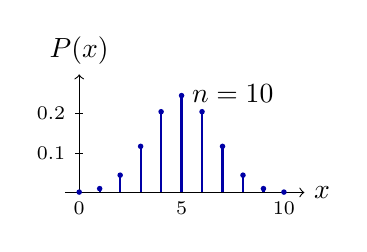
\begin{tikzpicture}[x=0.26cm,y=5cm]
\draw[->] (-.7,0)--(11,0) node[right] {$x$};
\draw[->] (0,0)--(0,.3) node[above] {$P(x)$};
\draw[blue!65!black,thick] (0,0)--(0,0.000976562500);\fill[blue!65!black] (0,0.000976562500) circle(1pt);
\draw[blue!65!black,thick] (1,0)--(1,0.009765625000);\fill[blue!65!black] (1,0.009765625000) circle(1pt);
\draw[blue!65!black,thick] (2,0)--(2,0.043945312500);\fill[blue!65!black] (2,0.043945312500) circle(1pt);
\draw[blue!65!black,thick] (3,0)--(3,0.117187500000);\fill[blue!65!black] (3,0.117187500000) circle(1pt);
\draw[blue!65!black,thick] (4,0)--(4,0.205078125000);\fill[blue!65!black] (4,0.205078125000) circle(1pt);
\draw[blue!65!black,thick] (5,0)--(5,0.246093750000);\fill[blue!65!black] (5,0.246093750000) circle(1pt);
\draw[blue!65!black,thick] (6,0)--(6,0.205078125000);\fill[blue!65!black] (6,0.205078125000) circle(1pt);
\draw[blue!65!black,thick] (7,0)--(7,0.117187500000);\fill[blue!65!black] (7,0.117187500000) circle(1pt);
\draw[blue!65!black,thick] (8,0)--(8,0.043945312500);\fill[blue!65!black] (8,0.043945312500) circle(1pt);
\draw[blue!65!black,thick] (9,0)--(9,0.009765625000);\fill[blue!65!black] (9,0.009765625000) circle(1pt);
\draw[blue!65!black,thick] (10,0)--(10,0.000976562500);\fill[blue!65!black] (10,0.000976562500) circle(1pt);
\node[below,font=\scriptsize] at (0,0) {0};
\node[below,font=\scriptsize] at (5,0) {5};
\node[below,font=\scriptsize] at (10,0) {10};
\draw (-.2,0.1)--(.2,0.1) node[left=3pt,font=\scriptsize] {0.1};
\draw (-.2,0.2)--(.2,0.2) node[left=3pt,font=\scriptsize] {0.2};
\node at (7.5,.25) {$n=10$};
\end{tikzpicture}\par\medskip
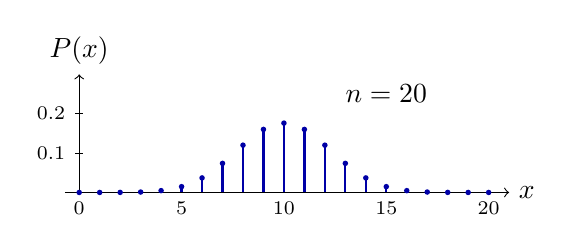
\begin{tikzpicture}[x=0.26cm,y=5cm]
\draw[->] (-.7,0)--(21,0) node[right] {$x$};
\draw[->] (0,0)--(0,.3) node[above] {$P(x)$};
\draw[blue!65!black,thick] (0,0)--(0,0.000000953674);\fill[blue!65!black] (0,0.000000953674) circle(1pt);
\draw[blue!65!black,thick] (1,0)--(1,0.000019073486);\fill[blue!65!black] (1,0.000019073486) circle(1pt);
\draw[blue!65!black,thick] (2,0)--(2,0.000181198120);\fill[blue!65!black] (2,0.000181198120) circle(1pt);
\draw[blue!65!black,thick] (3,0)--(3,0.001087188721);\fill[blue!65!black] (3,0.001087188721) circle(1pt);
\draw[blue!65!black,thick] (4,0)--(4,0.004620552063);\fill[blue!65!black] (4,0.004620552063) circle(1pt);
\draw[blue!65!black,thick] (5,0)--(5,0.014785766602);\fill[blue!65!black] (5,0.014785766602) circle(1pt);
\draw[blue!65!black,thick] (6,0)--(6,0.036964416504);\fill[blue!65!black] (6,0.036964416504) circle(1pt);
\draw[blue!65!black,thick] (7,0)--(7,0.073928833008);\fill[blue!65!black] (7,0.073928833008) circle(1pt);
\draw[blue!65!black,thick] (8,0)--(8,0.120134353638);\fill[blue!65!black] (8,0.120134353638) circle(1pt);
\draw[blue!65!black,thick] (9,0)--(9,0.160179138184);\fill[blue!65!black] (9,0.160179138184) circle(1pt);
\draw[blue!65!black,thick] (10,0)--(10,0.176197052002);\fill[blue!65!black] (10,0.176197052002) circle(1pt);
\draw[blue!65!black,thick] (11,0)--(11,0.160179138184);\fill[blue!65!black] (11,0.160179138184) circle(1pt);
\draw[blue!65!black,thick] (12,0)--(12,0.120134353638);\fill[blue!65!black] (12,0.120134353638) circle(1pt);
\draw[blue!65!black,thick] (13,0)--(13,0.073928833008);\fill[blue!65!black] (13,0.073928833008) circle(1pt);
\draw[blue!65!black,thick] (14,0)--(14,0.036964416504);\fill[blue!65!black] (14,0.036964416504) circle(1pt);
\draw[blue!65!black,thick] (15,0)--(15,0.014785766602);\fill[blue!65!black] (15,0.014785766602) circle(1pt);
\draw[blue!65!black,thick] (16,0)--(16,0.004620552063);\fill[blue!65!black] (16,0.004620552063) circle(1pt);
\draw[blue!65!black,thick] (17,0)--(17,0.001087188721);\fill[blue!65!black] (17,0.001087188721) circle(1pt);
\draw[blue!65!black,thick] (18,0)--(18,0.000181198120);\fill[blue!65!black] (18,0.000181198120) circle(1pt);
\draw[blue!65!black,thick] (19,0)--(19,0.000019073486);\fill[blue!65!black] (19,0.000019073486) circle(1pt);
\draw[blue!65!black,thick] (20,0)--(20,0.000000953674);\fill[blue!65!black] (20,0.000000953674) circle(1pt);
\node[below,font=\scriptsize] at (0,0) {0};
\node[below,font=\scriptsize] at (5,0) {5};
\node[below,font=\scriptsize] at (10,0) {10};
\node[below,font=\scriptsize] at (15,0) {15};
\node[below,font=\scriptsize] at (20,0) {20};
\draw (-.2,0.1)--(.2,0.1) node[left=3pt,font=\scriptsize] {0.1};
\draw (-.2,0.2)--(.2,0.2) node[left=3pt,font=\scriptsize] {0.2};
\node at (15.0,.25) {$n=20$};
\end{tikzpicture}\par\medskip
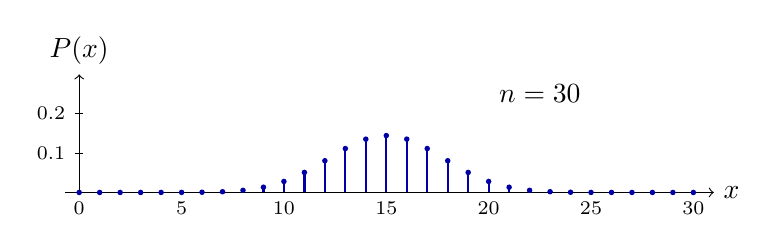
\begin{tikzpicture}[x=0.26cm,y=5cm]
\draw[->] (-.7,0)--(31,0) node[right] {$x$};
\draw[->] (0,0)--(0,.3) node[above] {$P(x)$};
\draw[blue!65!black,thick] (0,0)--(0,0.000000000931);\fill[blue!65!black] (0,0.000000000931) circle(1pt);
\draw[blue!65!black,thick] (1,0)--(1,0.000000027940);\fill[blue!65!black] (1,0.000000027940) circle(1pt);
\draw[blue!65!black,thick] (2,0)--(2,0.000000405125);\fill[blue!65!black] (2,0.000000405125) circle(1pt);
\draw[blue!65!black,thick] (3,0)--(3,0.000003781170);\fill[blue!65!black] (3,0.000003781170) circle(1pt);
\draw[blue!65!black,thick] (4,0)--(4,0.000025522895);\fill[blue!65!black] (4,0.000025522895) circle(1pt);
\draw[blue!65!black,thick] (5,0)--(5,0.000132719055);\fill[blue!65!black] (5,0.000132719055) circle(1pt);
\draw[blue!65!black,thick] (6,0)--(6,0.000552996062);\fill[blue!65!black] (6,0.000552996062) circle(1pt);
\draw[blue!65!black,thick] (7,0)--(7,0.001895986497);\fill[blue!65!black] (7,0.001895986497) circle(1pt);
\draw[blue!65!black,thick] (8,0)--(8,0.005450961180);\fill[blue!65!black] (8,0.005450961180) circle(1pt);
\draw[blue!65!black,thick] (9,0)--(9,0.013324571773);\fill[blue!65!black] (9,0.013324571773) circle(1pt);
\draw[blue!65!black,thick] (10,0)--(10,0.027981600724);\fill[blue!65!black] (10,0.027981600724) circle(1pt);
\draw[blue!65!black,thick] (11,0)--(11,0.050875637680);\fill[blue!65!black] (11,0.050875637680) circle(1pt);
\draw[blue!65!black,thick] (12,0)--(12,0.080553092994);\fill[blue!65!black] (12,0.080553092994) circle(1pt);
\draw[blue!65!black,thick] (13,0)--(13,0.111535051838);\fill[blue!65!black] (13,0.111535051838) circle(1pt);
\draw[blue!65!black,thick] (14,0)--(14,0.135435420088);\fill[blue!65!black] (14,0.135435420088) circle(1pt);
\draw[blue!65!black,thick] (15,0)--(15,0.144464448094);\fill[blue!65!black] (15,0.144464448094) circle(1pt);
\draw[blue!65!black,thick] (16,0)--(16,0.135435420088);\fill[blue!65!black] (16,0.135435420088) circle(1pt);
\draw[blue!65!black,thick] (17,0)--(17,0.111535051838);\fill[blue!65!black] (17,0.111535051838) circle(1pt);
\draw[blue!65!black,thick] (18,0)--(18,0.080553092994);\fill[blue!65!black] (18,0.080553092994) circle(1pt);
\draw[blue!65!black,thick] (19,0)--(19,0.050875637680);\fill[blue!65!black] (19,0.050875637680) circle(1pt);
\draw[blue!65!black,thick] (20,0)--(20,0.027981600724);\fill[blue!65!black] (20,0.027981600724) circle(1pt);
\draw[blue!65!black,thick] (21,0)--(21,0.013324571773);\fill[blue!65!black] (21,0.013324571773) circle(1pt);
\draw[blue!65!black,thick] (22,0)--(22,0.005450961180);\fill[blue!65!black] (22,0.005450961180) circle(1pt);
\draw[blue!65!black,thick] (23,0)--(23,0.001895986497);\fill[blue!65!black] (23,0.001895986497) circle(1pt);
\draw[blue!65!black,thick] (24,0)--(24,0.000552996062);\fill[blue!65!black] (24,0.000552996062) circle(1pt);
\draw[blue!65!black,thick] (25,0)--(25,0.000132719055);\fill[blue!65!black] (25,0.000132719055) circle(1pt);
\draw[blue!65!black,thick] (26,0)--(26,0.000025522895);\fill[blue!65!black] (26,0.000025522895) circle(1pt);
\draw[blue!65!black,thick] (27,0)--(27,0.000003781170);\fill[blue!65!black] (27,0.000003781170) circle(1pt);
\draw[blue!65!black,thick] (28,0)--(28,0.000000405125);\fill[blue!65!black] (28,0.000000405125) circle(1pt);
\draw[blue!65!black,thick] (29,0)--(29,0.000000027940);\fill[blue!65!black] (29,0.000000027940) circle(1pt);
\draw[blue!65!black,thick] (30,0)--(30,0.000000000931);\fill[blue!65!black] (30,0.000000000931) circle(1pt);
\node[below,font=\scriptsize] at (0,0) {0};
\node[below,font=\scriptsize] at (5,0) {5};
\node[below,font=\scriptsize] at (10,0) {10};
\node[below,font=\scriptsize] at (15,0) {15};
\node[below,font=\scriptsize] at (20,0) {20};
\node[below,font=\scriptsize] at (25,0) {25};
\node[below,font=\scriptsize] at (30,0) {30};
\draw (-.2,0.1)--(.2,0.1) node[left=3pt,font=\scriptsize] {0.1};
\draw (-.2,0.2)--(.2,0.2) node[left=3pt,font=\scriptsize] {0.2};
\node at (22.5,.25) {$n=30$};
\end{tikzpicture}
\end{center}


\Needspace{5\baselineskip}
\par\bigskip
\noindent\textbf{23.3.2}\quad Plot the binomial probability
function for the probabilities $p=1/6$, $q=5/6$, and $n=6$
throws of a die.
\solution
Define a success as a specified face, say a six, on each independent
fair-die throw. The number $X$ of successes in six throws has
\[
P(X=x)=\binom6x(1/6)^x(5/6)^{6-x}
=\frac{\binom6x5^{6-x}}{46656},\quad x=0,\ldots,6.
\]
All values, and thus the plot without interpolation, are
\[
\begin{array}{c|rrrrrrr}
x&0&1&2&3&4&5&6\\\hline
46656P(x)&15625&18750&9375&2500&375&30&1
\end{array}
\]
The numerator sum is 46656. The mean is $6/6=1$ and the largest
mass is at $x=1$.
\begin{center}
\begin{tikzpicture}[x=1cm,y=7cm]
\draw[->](-.5,0)--(6.8,0) node[right]{$x$};
\draw[->](0,0)--(0,.47) node[above]{$P(x)$};
\foreach \x/\y in {0/.3348979767,1/.4018775720,2/.2009387860,3/.05358367627,4/.008037551440,5/.0006430041152,6/.00002143347051}{
\draw[blue!65!black,thick](\x,0)--(\x,\y);
\fill[blue!65!black](\x,\y) circle(1.3pt);
\node[below] at(\x,0){\x};}
\foreach \y in {.1,.2,.3,.4}{\draw(-.06,\y)--(.06,\y) node[left=4pt,font=\scriptsize]{\y};}
\end{tikzpicture}
\end{center}


\Needspace{5\baselineskip}
\par\bigskip
\noindent\textbf{23.3.3}\quad A hardware company knows that the
probability of mass-producing nails includes a small probability
$p=0.03$ of defective nails (usually without a sharp tip). What
is the probability of finding more than two defective nails in
its commercial box of 100 nails?
\erratum{Assume independent defects with the same probability for
each nail.}
\solution
Assume nail defects are independent, with common probability $0.03$.
Then $X$, the number of defective nails, is binomial with $n=100$.
Use the complement of $X=0,1,2$:
\begin{align*}
P(X>2)&=1-\sum_{j=0}^2\binom{100}j(0.03)^j(0.97)^{100-j}\\
&=1-(0.97)^{100}-100(0.03)(0.97)^{99}
 -4950(0.03)^2(0.97)^{98}\\
&=\boxed{0.5802249170\simeq58.02\%.}
\end{align*}
The independence assumption matters: a defect rate alone would not
determine the box probability if production defects were correlated.


\Needspace{5\baselineskip}
\par\bigskip
\noindent\textbf{23.3.4}\quad Four cards are drawn from a shuffled
bridge deck. What is the probability that they are all red? That
they are all hearts? That they are honors? Compare the
probabilities when each card is put back at a random place
before drawing the next card, with the probabilities when the
cards are not replaced in the deck.
\solution
There are 26 red cards,13 hearts and 20 honors (10,J,Q,K,A).
If a category contains $K$ cards, replacement gives four independent
successes with probability $(K/52)^4$. Without replacement the
conditional success probabilities successively decrease:
\[
P_K=\frac K{52}\frac{K-1}{51}\frac{K-2}{50}\frac{K-3}{49}
=\frac{\binom K4}{\binom{52}4}.
\]
Consequently
\[
\begin{array}{c|c|c}
\text{category}&\text{with replacement}&\text{without replacement}\\\hline
\text{red}&1/16&\binom{26}4/\binom{52}4\\
\text{hearts}&1/256&\binom{13}4/\binom{52}4\\
\text{honors}&(5/13)^4&\binom{20}4/\binom{52}4
\end{array}
\]
For $0<K<52$ and $j=1,2,3$, $(K-j)/(52-j)<K/52$,
since $52(K-j)<K(52-j)$ is equivalent to $K<52$.
Thus all three probabilities are strictly smaller without replacement.


\Needspace{5\baselineskip}
\par\bigskip
\noindent\textbf{23.3.5}\quad Show that for the binomial
distribution of Eq.~(23.42), \erratum{the mean value of $x$ is $np$;
find the exact integer mode or modes}.
\solution
\erratum{The mean is $np$, but the exact most probable integer need
not be $np$. The manual differentiates the moment-generating function,
which computes the mean and does not prove the printed mode claim.}
To establish the mean, write $X=I_1+\cdots+I_n$, where each success
indicator has $P(I_j=1)=p$ and $P(I_j=0)=1-p$. Then
\[
 \langle I_j\rangle=1\cdot p+0\cdot(1-p)=p,\qquad
 \boxed{\langle X\rangle=\sum_{j=1}^n\langle I_j\rangle=np}.
\]
To find the mode for $0<p<1$, write $q=1-p$ and compare consecutive positive masses:
\[
\frac{P(x+1)}{P(x)}
=\frac{n-x}{x+1}\frac pq.
\]
It exceeds 1 exactly when
\[
(n-x)p>(x+1)(1-p)
\quad\Longleftrightarrow\quad x+1<(n+1)p.
\]
If $(n+1)p$ is not an integer, the sequence increases up to
$\lfloor(n+1)p\rfloor$ and decreases thereafter. If $(n+1)p=k$
is an integer, $P(k)=P(k-1)$ and these are the two maxima. Hence
\[
\boxed{\begin{cases}
\text{unique mode }\lfloor(n+1)p\rfloor,&(n+1)p\notin\mathbb Z,\\
\text{modes }k-1,k,&(n+1)p=k\in\{1,\ldots,n\}.
\end{cases}}
\]
The endpoint cases $p=0,1$ have sole modes $0,n$, respectively;
$n=0$ is the point mass at 0. For example,$n=3,p=1/2$ has mean $1.5$
but modes 1 and 2. For large $n$, a continuous central approximation
places the peak near $np$; it is not the exact integer-mode statement.


\Needspace{12\baselineskip}
\subsection*{23.4 Poisson Distribution}

\Needspace{5\baselineskip}
\par\bigskip
\noindent\textbf{23.4.1}\quad Radioactive decays for long-lived
isotopes are governed by the Poisson distribution. In a
Rutherford--Geiger experiment, the numbers of emitted $\alpha$
particles are counted in each of $n=2608$ time intervals of 7.5
seconds each. In Table~23.1 $n_{i}$ is the number of time
intervals in which $i$ particles were emitted. Determine the
average number $\lambda$ of particles emitted per time interval,
and compare the $n_{i}$ of Table~23.1 with $np_{i}$ computed
from the Poisson distribution with mean value $\lambda$.
\begin{center}
\emph{Table~23.1\quad Data for Exercise~23.4.1}\\[4pt]
\begin{tabular}{c|*{11}{r}}
$i$ & 0 & 1 & 2 & 3 & 4 & 5 & 6 & 7 & 8 & 9 & 10\\
\hline
$n_{i}$ & 57 & 203 & 383 & 525 & 532 & 408 & 273 & 139 & 45 & 27
& 16
\end{tabular}
\end{center}
\solution
The total number of recorded intervals and total particle count are
\begin{align*}
N&=57+203+383+525+532+408+273+139+45+27+16=2608,\\
S&=203+766+1575+2128+2040+1638+973+360+243+160=10086.
\end{align*}
Thus the fitted mean per7.5-second interval is
\[
\boxed{\widehat\lambda=S/N=10086/2608=3.8673312883.}
\]
Use $E_0=Ne^{-\widehat\lambda}$, followed by the exact recurrence
$E_{i+1}=\widehat\lambda E_i/(i+1)$, to compute $E_i=Np_i$.
\begin{center}
\begin{tabular}{r|r|r}
$i$&observed $n_i$&Poisson expected $Np_i$\\\hline
0&57&54.544\\1&203&210.940\\2&383&407.887\\
3&525&525.811\\4&532&508.372\\5&408&393.208\\
6&273&253.444\\7&139&140.022\\8&45&67.689\\
9&27&29.086\\10&16&11.249\\$>10$&0&5.749
\end{tabular}
\end{center}
The final expected tail is $2608-\sum_{i=0}^{10}E_i$; it is required
because the Poisson model has unbounded support. Observed values
fluctuate around their expectations rather than agreeing termwise.
\erratum{The manual's entry 55.7 at $i=0$ is inconsistent with the
stated data and fitted mean; the direct value is 54.544.
Its displayed formula for $np_i$ also omits the factor $n$ on the
right: $p_i=e^{-\lambda}\lambda^i/i!$, whereas the expected count
is $np_i$. No renormalization to $i\le10$ has been made.}


\Needspace{5\baselineskip}
\par\bigskip
\noindent\textbf{23.4.2}\quad Derive the standard deviation of a
Poisson distribution of mean value $\mu$.
\solution
For $\mu>0$, the Poisson mass is $p_n=e^{-\mu}\mu^n/n!$,
$n=0,1,\ldots$. Shift the factorial sums:
\begin{align*}
\langle X\rangle&=e^{-\mu}\sum_{n=1}^{\infty}
\frac{n\mu^n}{n!}
=\mu e^{-\mu}\sum_{m=0}^{\infty}\frac{\mu^m}{m!}=\mu,\\
\langle X(X-1)\rangle&=e^{-\mu}\sum_{n=2}^{\infty}
\frac{n(n-1)\mu^n}{n!}
=\mu^2e^{-\mu}\sum_{m=0}^{\infty}\frac{\mu^m}{m!}=\mu^2.
\end{align*}
Since $X^2=X(X-1)+X$, $\langle X^2\rangle=\mu^2+\mu$ and
\[
\boxed{\operatorname{Var}X=\mu,\qquad\sigma_X=\sqrt\mu.}
\]
At $\mu=0$ the distribution is concentrated at 0 and the same result holds.


\Needspace{5\baselineskip}
\par\bigskip
\noindent\textbf{23.4.3}\quad The number of $\alpha$-particles
emitted by the decay of a radium sample is counted per minute
for 40 hours. The total number is 5000. How many 1-minute
intervals are expected with (a) 2, and (b) 5 $\alpha$-particles?
\erratum{Use a constant-rate Poisson model with its rate estimated
from the observed total.}
\solution
There are $40\cdot60=2400$ one-minute intervals. Their fitted mean is
$\mu=5000/2400=25/12$ decays per minute. The expected number of
intervals containing exactly $k$ decays is
\[
E_k=2400P(X=k)=2400e^{-25/12}\frac{(25/12)^k}{k!}.
\]
In particular,
\[
\boxed{E_2=648.5128721\simeq649,\qquad
E_5=97.73354192\simeq98\text{ intervals}.}
\]
These are expectations under the fitted Poisson model, not guaranteed
integer observations. \erratum{The manual calls the 2400 intervals
seconds rather than minutes and stops at single-interval probabilities.
The question asks for the corresponding expected numbers of intervals.}


\Needspace{5\baselineskip}
\par\bigskip
\noindent\textbf{23.4.4}\quad For a radioactive sample, 10 decays
are counted on average in 100 seconds. Use the Poisson
distribution to estimate the probability of counting 3 decays in
10 seconds.
\solution
The rate is $10/100=0.1$ decay per second, so a 10-second interval has
Poisson mean $\mu=1$. Therefore
\[
\boxed{P(X=3)=e^{-1}\frac{1^3}{3!}=\frac1{6e}
=0.0613132402\simeq6.13\%.}
\]
The time rescaling changes the mean, not the factorial in the mass formula.


\Needspace{5\baselineskip}
\par\bigskip
\noindent\textbf{23.4.5}\quad $^{238}$ U has a half-life of
$4.51\times10^{9}$ years. Its decay series ends with the stable
lead isotope $^{206}$ Pb. The ratio of the number of $^{206}$ Pb to
$^{238}$ U atoms in a rock sample is measured as 0.0058. Estimate
the age of the rock assuming that all the lead in the rock is
from the initial decay of the $^{238}$ U, which determines the
rate of the entire decay process, because the subsequent steps
take place far more rapidly.
\erratum{Assume a closed sample, with no uranium or lead gained or
lost since formation and no initial lead.}
\par\emph{Hint.}~This is not a Poisson distribution problem,
but is an application of the decay law $N(t)=Ne^{-\lambda t}$,
where $\lambda$, the decay constant, is related to the half-life
$T$ by $T=\ln 2/\lambda$.
\par\nobreak\hfill\emph{ANS.}\enspace $3.8\times10^{7}$ years.
\solution
Let $U_0$ be the initial uranium count and $U(t)=U_0e^{-\lambda t}$
the remaining count. Under the stated closed-sample, zero-initial-lead
and rapid-daughter-decay assumptions, $L(t)=U_0-U(t)$.
Thus the measured ratio is
\[
R=\frac{L(t)}{U(t)}=\frac{U_0}{U(t)}-1=e^{\lambda t}-1.
\]
Solving, and using the \emph{given} half-life $T$,
\[
\boxed{t=\frac{\ln(1+R)}\lambda
=\frac{4.51\times10^9}{\ln2}\ln(1.0058)
=3.7628998\times10^7\ \text{years}
\simeq3.8\times10^7\ \text{years}.}
\]
One uranium decay ultimately yields one lead atom in this accounting;
the intermediate decay steps are not additional initial uranium atoms.


\Needspace{5\baselineskip}
\par\bigskip
\noindent\textbf{23.4.6}\quad The probability of hitting a target
in one shot is known to be 20\%. If five shots are fired
independently, what is the probability of striking the target at
least once?
\solution
The probability that one shot misses is $1-0.2=0.8$. By independence,
all five miss with probability $0.8^5=0.32768$. Its complement is
\[
\boxed{P(\text{at least one hit})=1-0.8^5=0.67232=67.232\%.}
\]
This is an exact binomial complement; a Poisson approximation is unnecessary.


\Needspace{12\baselineskip}
\subsection*{23.5 Gauss' Normal Distribution}

\Needspace{5\baselineskip}
\par\bigskip
\noindent\textbf{23.5.1}\quad Show that the variance of the
normal distribution given by Eq.~(23.56) is $\sigma^{2}$, the
symbol in that equation. \erratum{Take $\sigma>0$.}
\solution
For $\sigma>0$, write the density explicitly:
\[
f(x)=\frac1{\sigma\sqrt{2\pi}}
 e^{-(x-\mu)^2/(2\sigma^2)}.
\]
With $z=(x-\mu)/\sigma$, normalization is
$(2\pi)^{-1/2}\int_{-\infty}^{\infty}e^{-z^2/2}\,dz=1$.
Oddness gives $\langle X-\mu\rangle=0$, so the mean really is $\mu$.
For the variance, integrate by parts using
$d(e^{-z^2/2})=-ze^{-z^2/2}\,dz$:
\begin{align*}
\operatorname{Var}X
&=\frac{\sigma^2}{\sqrt{2\pi}}
 \int_{-\infty}^{\infty}z^2e^{-z^2/2}\,dz\\
&=\frac{\sigma^2}{\sqrt{2\pi}}
 \left([-ze^{-z^2/2}]_{-\infty}^{\infty}
 +\int_{-\infty}^{\infty}e^{-z^2/2}\,dz\right)
=\boxed{\sigma^2}.
\end{align*}
The boundary term is zero because the Gaussian dominates the linear factor.


\Needspace{5\baselineskip}
\par\bigskip
\noindent\textbf{23.5.2}\quad Show that Eq.~(23.62) can be
obtained by manipulation of the formula Eq.~(23.61) for $W(v)$.
\erratum{Use $0<p<1$, $q=1-p$, $n>0$, and $-pn<v<qn$;
both formulas represent the same Stirling approximation.}
\solution
Let $0<p<1$, $q=1-p$, $s=pn+v$, and $n-s=qn-v$.
The Stirling approximation in Eq.(23.61) is
\[
W(v)=\frac{p^sq^{n-s}n^{n+1/2}e^{-n+s+(n-s)}}
 {\sqrt{2\pi}(pn+v)^{s+1/2}(qn-v)^{n-s+1/2}}.
\]
The exponential is $e^0=1$. Factor the two denominator powers:
\[
(pn+v)^{s+1/2}=(pn)^{s+1/2}(1+v/(pn))^{s+1/2},
\]
\[
(qn-v)^{n-s+1/2}=(qn)^{n-s+1/2}(1-v/(qn))^{n-s+1/2}.
\]
The remaining constant quotient is
\[
\frac{p^sq^{n-s}n^{n+1/2}}
 {p^{s+1/2}q^{n-s+1/2}n^{(s+1/2)+(n-s+1/2)}}
=p^{-1/2}q^{-1/2}n^{-1/2}.
\]
Therefore
\[
\boxed{W(v)=\frac{(1+v/(pn))^{-(pn+v+1/2)}
 (1-v/(qn))^{-(qn-v+1/2)}}{\sqrt{2\pi pqn}}.}
\]
The rearrangement is exact for the Stirling expression; its identification
with the original binomial mass is asymptotic, requiring both $s$ and $n-s$
large. For real logarithms also require $-pn<v<qn$.


\Needspace{5\baselineskip}
\par\bigskip
\noindent\textbf{23.5.3}\quad With $W(v)$ the expression in
Eq.~(23.62), show that the expansion of $\ln W(v)$ in powers of
$v$ leads to Eq.~(23.63).
\erratum{Take $p,q>0$ fixed, $p+q=1$, and $|v|<\min(pn,qn)$.
For the Gaussian limit use the central scaling $v=O(\sqrt n)$.}
\solution
Take the logarithm of the preceding result:
\begin{align*}
\ln W(v)={}&-\tfrac12\ln(2\pi pqn)
 -(pn+v+\tfrac12)\ln(1+v/(pn))\\
 &-(qn-v+\tfrac12)\ln(1-v/(qn)).
\end{align*}
For $|v|<\min(pn,qn)$ use $\ln(1+u)=u-u^2/2+O(u^3)$.
Keeping all terms through $v^2$, including the half-power factors,
\begin{align*}
-(pn+v+\tfrac12)\ln(1+v/(pn))
&=-v-\frac{v}{2pn}-\frac{v^2}{2pn}+\frac{v^2}{4p^2n^2}+O(v^3),\\
-(qn-v+\tfrac12)\ln(1-v/(qn))
&=v+\frac{v}{2qn}-\frac{v^2}{2qn}+\frac{v^2}{4q^2n^2}+O(v^3).
\end{align*}
The $-v$ and $v$ cancel. Collecting the rest yields Eq.(23.63):
\[
\boxed{\begin{aligned}
\ln W(v)={}&-\tfrac12\ln(2\pi pqn)
 -\frac{v}{2n}\left(\frac1p-\frac1q\right)\\
 &-\frac{v^2}{2n}\left(\frac1p+\frac1q\right)
 +\frac{v^2}{4n^2}\left(\frac1{p^2}+\frac1{q^2}\right)+O(v^3).
\end{aligned}}
\]
Here $O(v^3)$ first denotes a Taylor remainder for fixed $n,p,q$.
For the limiting argument hold $p,q>0$ fixed and take $v=O(\sqrt n)$.
The remainder is then $O(|v|^3/n^2+|v|^3/n^3)=O(n^{-1/2})$,
while the displayed linear and last quadratic corrections also vanish.
Since $1/p+1/q=1/(pq)$, the surviving form is
\[
W(v)\sim\frac1{\sqrt{2\pi npq}}e^{-v^2/(2npq)}.
\]
This central scaling does not assert a uniformly accurate Gaussian
approximation all the way to the extreme binomial tails.


\Needspace{5\baselineskip}
\par\bigskip
\noindent\textbf{23.5.4}\quad What is the probability for a
normally distributed random variable to differ by more than
$4\sigma$ from its mean value? Compare your result with the
corresponding one from Chebyshev's inequality. Explain the
difference in your own words. \erratum{Assume $\sigma>0$.}
\solution
Standardize $Z=(X-\mu)/\sigma$, for $\sigma>0$.
Symmetry and $u=z/\sqrt2$ give
\[
P(|X-\mu|>4\sigma)=\frac2{\sqrt{2\pi}}\int_4^\infty e^{-z^2/2}\,dz
=\operatorname{erfc}(2\sqrt2)
=\boxed{6.33424837\times10^{-5}}.
\]
This is about $0.00633425\%$. Chebyshev's inequality gives only
\[
P(|X-\mu|>4\sigma)\le\frac1{4^2}=0.0625=6.25\%.
\]
The bound is about 987 times the exact Gaussian tail. Chebyshev uses
only the variance and applies to every distribution with that variance;
the Gaussian computation uses its entire density, including its rapidly
decaying tails. A general upper bound need not be attained by this
particular density.
\erratum{The manual's trailing approximation $6.3\times10^{-5}\approx
10^{-3}$ is numerically incorrect.}


\Needspace{5\baselineskip}
\par\bigskip
\noindent\textbf{23.5.5}\quad An instructor grades a final exam
of a large undergraduate class, obtaining the mean value of
points \erratum{$m$} and the variance $\sigma^{2}$. Assuming a
normal distribution for the \erratum{random variable $M$} of
points, he defines a grade F when $M<m-3\sigma/2$, D when
$m-3\sigma/2<M<m-\sigma/2$, C when $m-\sigma/2<M<m+\sigma/2$, B
when $m+\sigma/2<M<m+3\sigma/2$, and A when $M>m+3\sigma/2$.
What is the percentage of As, Fs; Bs, Ds; and Cs? Redesign the
cutoffs so that there are equal percentages of As and Fs (5\%),
25\% Bs and Ds, and 40\% Cs. \erratum{Assume $\sigma>0$.}
\solution
Use the corrected notation: $m$ is the mean, $M$ the random score,
and $Z=(M-m)/\sigma$ has standard normal CDF
\[
\Phi(z)=\frac1{\sqrt{2\pi}}\int_{-\infty}^{z}e^{-u^2/2}\,du
=\tfrac12[1+\operatorname{erf}(z/\sqrt2)].
\]
The original cutoffs give
\begin{align*}
P(A)=P(F)&=1-\Phi(1.5)=0.0668072013,\\
P(B)=P(D)&=\Phi(1.5)-\Phi(0.5)=0.2417303375,\\
P(C)&=\Phi(0.5)-\Phi(-0.5)=0.3829249225.
\end{align*}
Thus the percentages are $\boxed{6.68072\%,\ 24.17303\%,\ 38.29249\%}$
for each extreme grade, each adjacent grade, and C, respectively.
They sum as $2(6.68072)+2(24.17303)+38.29249=100\%$, up to rounding.

For the redesign let the positive thresholds be $a>b>0$.
The outer 5\% requires $\Phi(a)=0.95$, and the next 25\% requires
$\Phi(a)-\Phi(b)=0.25$, hence $\Phi(b)=0.70$.
Therefore
\[
a=\Phi^{-1}(0.95)=1.644853627,\qquad
b=\Phi^{-1}(0.70)=0.524400513.
\]
The new four score boundaries, in order, are
\[
\boxed{m-1.644853627\sigma,\quad m-0.524400513\sigma,
\quad m+0.524400513\sigma,\quad m+1.644853627\sigma.}
\]
They yield 5\%,25\%,40\%,25\%,5\%. Any assignment of an exact
boundary to one adjacent grade gives the same probabilities because
a continuous normal variable has no point masses.


\Needspace{12\baselineskip}
\subsection*{23.6 Transformations of Random Variables}

\Needspace{5\baselineskip}
\par\bigskip
\noindent\textbf{23.6.1}\quad Let $X_{1},X_{2},\ldots,X_{n}$ be
independent normal random variables with the same mean $\bar{x}$
and variance $\sigma^{2}$. Show that
\[
\frac{\displaystyle\sum_{i}X_{i}/n-\bar{x}}
{\erratum{\sigma/\sqrt{n}}}
\]
is normal with mean zero and variance 1.
\erratum{Take integer $n\ge1$ and $\sigma>0$.}
\solution
Take $n\ge1$ and $\sigma>0$. To track the distribution, use the
characteristic function, not just its first two moments. For a centered
normal variable of variance $\sigma^2$, write $\phi(t)=\langle e^{itX}\rangle$.
Since $xf(x)=-\sigma^2f'(x)$, differentiation followed by integration
by parts gives
\[
\phi'(t)=i\int xe^{itx}f(x)\,dx
=-i\sigma^2\int e^{itx}f'(x)\,dx
=-\sigma^2t\phi(t).
\]
The boundary term vanishes. With $\phi(0)=1$ this yields
$\phi(t)=e^{-\sigma^2t^2/2}$; translation by $\bar x$ adds $e^{it\bar x}$.
Independence therefore gives
\[
\phi_{\overline X}(t)
=\prod_{j=1}^n\phi_{X_j}(t/n)
=\left[e^{it\bar x/n-\sigma^2t^2/(2n^2)}\right]^n
=e^{it\bar x-\sigma^2t^2/(2n)}.
\]
Thus $\overline X=n^{-1}\sum X_j$ is normal with mean $\bar x$
and variance $\sigma^2/n$. For the requested variable,
\[
Z=\frac{\overline X-\bar x}{\sigma/\sqrt n},
\qquad\phi_Z(t)=e^{-t^2/2},
\qquad\boxed{Z\sim N(0,1).}
\]
\erratum{The corrected denominator is $\sigma/\sqrt n$.
The printed $\sigma\sqrt n$ would give variance $1/n^2$ instead.}
For $\sigma=0$ all observations are constant and this standardization
is undefined, so positivity is necessary.


\Needspace{5\baselineskip}
\par\bigskip
\noindent\textbf{23.6.2}\quad If the random variable $X$ is
normal with mean value 29 and standard deviation 3, what can you
say about the distributions of $2X-1$ and $3X+2$?
\solution
For $Y=aX+b$ with $a\ne0$, change variables $x=(y-b)/a$:
\[
f_Y(y)=\frac1{|a|}\frac1{3\sqrt{2\pi}}
\exp\left[-\frac{((y-b)/a-29)^2}{18}\right]
=\frac1{3|a|\sqrt{2\pi}}
\exp\left[-\frac{(y-(29a+b))^2}{2(3a)^2}\right].
\]
This identifies both full distributions:
\[
\boxed{2X-1\sim N(57,36),\quad\sigma=6;\qquad
3X+2\sim N(89,81),\quad\sigma=9.}
\]
The second argument of $N(\mu,\tau^2)$ here denotes variance.
\erratum{The manual multiplies variance by $a$ and reports
$3\sqrt2$ and $3\sqrt3$ as standard deviations. The correct
variance factor is $a^2$, so the standard-deviation factor is $|a|$.}


\Needspace{5\baselineskip}
\par\bigskip
\noindent\textbf{23.6.3}\quad For a normal distribution of mean
value $m$ and variance $\sigma^{2}$, find the distance $r$ such
that half the area under the bell shape is between $m-r$ and
$m+r$. \erratum{Assume $\sigma>0$ and seek $r\ge0$.}
\solution
For $\sigma>0$, standardize $z=(x-m)/\sigma$ and use symmetry:
\[
\frac12=P(m-r\le X\le m+r)
=2\Phi(r/\sigma)-1
=\operatorname{erf}\left(\frac r{\sigma\sqrt2}\right).
\]
Hence $\Phi(r/\sigma)=3/4$, and strict monotonicity gives the unique
nonnegative answer
\[
\boxed{r=\sigma\Phi^{-1}(3/4)
=\sigma\sqrt2\,\operatorname{erf}^{-1}(1/2)
=0.6744897502\sigma.}
\]
This interval contains the central half of the probability mass.


\Needspace{5\baselineskip}
\par\bigskip
\noindent\textbf{23.6.4}\quad If $\langle X\rangle$, $\langle
Y\rangle$ are the average values of two independent random
variables $X$, $Y$, what is the expectation value of the product
$XY$? \erratum{Assume finite absolute first moments.}
\solution
Assume finite absolute first moments. Independence gives the product
joint measure, and also $\langle|XY|\rangle=\langle|X|\rangle
\langle|Y|\rangle<\infty$, so the integrals may be separated.
When densities exist, this reads
\[
\boxed{\begin{aligned}
\langle XY\rangle
&=\int_{-\infty}^{\infty}\int_{-\infty}^{\infty}
 xy\,p_X(x)p_Y(y)\,dx\,dy\\
&=\left(\int xp_X(x)\,dx\right)
 \left(\int yp_Y(y)\,dy\right)
=\langle X\rangle\langle Y\rangle.
\end{aligned}}
\]
For general laws the same calculation uses their product probability
measure; discrete laws give sums.
\erratum{The manual omits the factors $xy$, $x$, and $y$ in its
three integrals. Without them those integrals are normalization
integrals equal to 1, not the stated expectations.}
It follows in
particular that $\operatorname{cov}(X,Y)=0$ when second moments exist.


\Needspace{5\baselineskip}
\par\bigskip
\noindent\textbf{23.6.5}\quad If $X$ and $Y$ are two independent
random variables with different probability densities and the
function $f(x,y)$ has derivatives of any order,
\erratum{explain why the two means alone do not determine
$\langle f(X,Y)\rangle$. Derive a finite Taylor expansion in central
moments, including its remainder, and state conditions for an infinite
moment expansion. Give the covariance and correlation of $X,Y$;
also derive the corresponding formulas for transformed variables
$G=g(X,Y)$ and $H=h(X,Y)$ when the required moments exist.}
\solution
\erratum{The two means alone do not determine $\langle f(X,Y)\rangle$.
Higher moments are needed. Existence of derivatives of every order
also does not justify an infinite Taylor expansion or its termwise
expectation. The manual's weighted integral is not the ordinary
covariance of the independent variables.}

Let $\mu=\langle X\rangle$, $\nu=\langle Y\rangle$,
$U=X-\mu$, $V=Y-\nu$, and define central moments
$M_r=\langle U^r\rangle$, $N_s=\langle V^s\rangle$ when finite.
Then $M_0=N_0=1$, $M_1=N_1=0$, and independence implies
$\langle U^rV^s\rangle=M_rN_s$. The always valid starting point,
when $\langle|f(X,Y)|\rangle<\infty$, is
\[
\langle f(X,Y)\rangle=\iint f(x,y)p_X(x)p_Y(y)\,dx\,dy.
\]
For a finite Taylor order $k$, apply one-variable Taylor's theorem to
$g(t)=f(\mu+tU,\nu+tV)$ at $t=0$, evaluated at $t=1$.
The chain rule and binomial theorem give
\[
 g^{(j)}(t)=\sum_{r+s=j}\frac{j!}{r!s!}U^rV^s
 f_{rs}(\mu+tU,\nu+tV).
\]
Dividing $g^{(j)}(0)$ by $j!$ gives the following coefficients:
\[
f(X,Y)=\sum_{r+s\le k}\frac{f_{rs}(\mu,\nu)}{r!s!}U^rV^s+R_k,
\]
\[
R_k=\frac1{k!}\int_0^1(1-t)^k
 (U\partial_x+V\partial_y)^{k+1}
 f(\mu+tU,\nu+tV)\,dt,
\quad f_{rs}=\partial_x^r\partial_y^sf.
\]
Assuming integrability of these terms, taking expectations gives the
rigorous finite form
\[
\boxed{\langle f(X,Y)\rangle
=\sum_{r+s\le k}\frac{f_{rs}(\mu,\nu)}{r!s!}M_rN_s+\langle R_k\rangle.}
\]
For example, through second order,
\[
\langle f(X,Y)\rangle
=f(\mu,\nu)+\tfrac12f_{20}(\mu,\nu)\sigma_X^2
+\tfrac12f_{02}(\mu,\nu)\sigma_Y^2+\langle R_2\rangle.
\]
The mixed term is zero because $M_1N_1=0$. If the Taylor series equals
$f$ on the support and is integrable term by term (for example,
$\sum_{r,s}|f_{rs}(\mu,\nu)|\langle|U|^r\rangle
\langle|V|^s\rangle/(r!s!)<\infty$), the limit is
\[
\langle f(X,Y)\rangle=\sum_{r,s\ge0}
\frac{f_{rs}(\mu,\nu)}{r!s!}M_rN_s.
\]
Both stated conditions matter. For a counterexample to determination
by the means, take $f(x,y)=x^2$, independent $Y$ uniform on $[-3,3]$,
and compare $X$ uniform on $[-1,1]$ with $X$ uniform on $[-2,2]$.
All means are zero, but the expectations are $1/3$ and $4/3$.
For a counterexample to smoothness sufficing, the smooth function
$f(x,y)=e^{-1/x^2}$ for $x\ne0$, extended by 0 at $x=0$, has every
derivative at $(0,0)$ zero: each derivative is an exponential times
a polynomial in $1/x$, whose limit is 0. For centered independent
normal $X,Y$, its expectation is nevertheless strictly positive.

For the variables actually named in the question,
\[
\boxed{\operatorname{cov}(X,Y)=M_1N_1=0,\qquad\rho_{XY}=0}
\]
provided both variances are finite and nonzero; correlation is
undefined if either variance is zero. For the transformed variables
$G=g(X,Y)$ and $H=h(X,Y)$,
write their Taylor coefficients as $g_{rs}/(r!s!)$ and $h_{uv}/(u!v!)$,
all evaluated at $(\mu,\nu)$. Under convergence and interchange
conditions for the product as well,
\[
\boxed{\begin{aligned}
\operatorname{cov}(G,H)=\sum_{r,s,u,v\ge0}
\frac{g_{rs}h_{uv}}{r!s!u!v!}
\big[M_{r+u}N_{s+v}-M_rN_sM_uN_v\big].
\end{aligned}}
\]
This follows by expanding $\langle GH\rangle-\langle G\rangle\langle H\rangle$;
setting $h=g$ gives the variance. The correlation is this covariance
divided by $\sqrt{\operatorname{Var}G\operatorname{Var}H}$, when positive.
To lowest order in small fluctuations it becomes
\[
\operatorname{cov}(G,H)\simeq g_xh_x\sigma_X^2+g_yh_y\sigma_Y^2.
\]
Finally the manual's object $\langle UVf(X,Y)\rangle$ would instead
expand as $\sum f_{rs}M_{r+1}N_{s+1}/(r!s!)$, with leading term
$f_{11}\sigma_X^2\sigma_Y^2$. It is a weighted mixed moment,
not a covariance or a normalized correlation of $X,Y$.


\Needspace{5\baselineskip}
\par\bigskip
\noindent\textbf{23.6.6}\quad Let $f(x,y)$ be the joint
probability density of two random variables $X$, $Y$. Find the
variance $\sigma^{2}(aX+bY)$, where $a$, $b$ are constants. What
happens when $X$, $Y$ are independent?
\erratum{Take real $a,b,X,Y$ and finite second moments.}
\solution
Set $\mu=\langle X\rangle$, $\nu=\langle Y\rangle$ and assume finite
second moments. Since $\langle aX+bY\rangle=a\mu+b\nu$,
\begin{align*}
\operatorname{Var}(aX+bY)
&=\iint[a(x-\mu)+b(y-\nu)]^2f(x,y)\,dx\,dy\\
&=a^2\iint(x-\mu)^2f\,dx\,dy
+b^2\iint(y-\nu)^2f\,dx\,dy\\
&\quad+2ab\iint(x-\mu)(y-\nu)f\,dx\,dy\\
&=\boxed{a^2\sigma_X^2+b^2\sigma_Y^2+2ab\operatorname{cov}(X,Y)}.
\end{align*}
All integrations are over $\mathbb R^2$. For independent $X,Y$,
$f(x,y)=p_X(x)p_Y(y)$ makes the final integral the product of two
zero centered means. Thus $\boxed{\operatorname{Var}(aX+bY)
=a^2\sigma_X^2+b^2\sigma_Y^2}$ in that case.


\Needspace{5\baselineskip}
\par\bigskip
\noindent\textbf{23.6.7}\quad Obtain an addition theorem for the
distribution of a random variable $Y=X_{1}+X_{2}$ where $X_{1}$
and $X_{2}$ are \erratum{independent} Gauss normal random variables with different mean
values $\mu_{j}$ and variances $\sigma_{j}^{2}$.
\par\nobreak\hfill\emph{ANS.}\enspace
$Y$ is normal with mean $\mu_{1}+\mu_{2}$ and variance
$\sigma_{1}^{2}+\sigma_{2}^{2}$.
\solution
\erratum{The stated answer requires independence, as in the
addition theorem being used. Normal marginal distributions alone
are insufficient. The manual's final exponential also omits a factor $1/2$.}
Let $X_j\sim N(\mu_j,\sigma_j^2)$ independently. Their characteristic
functions, derived in Exercise 23.6.1, multiply:
\begin{align*}
\phi_Y(t)&=\langle e^{it(X_1+X_2)}\rangle
=\langle e^{itX_1}\rangle\langle e^{itX_2}\rangle\\
&=e^{it\mu_1-\sigma_1^2t^2/2}
 e^{it\mu_2-\sigma_2^2t^2/2}
=e^{it(\mu_1+\mu_2)-(\sigma_1^2+\sigma_2^2)t^2/2}.
\end{align*}
The characteristic function identifies the complete distribution:
\[
\boxed{Y\sim N(\mu_1+\mu_2,\sigma_1^2+\sigma_2^2).}
\]
One can also check it directly by convolution. With $S=\sigma_1^2+\sigma_2^2$
and $h=y-\mu_1-\mu_2$, set $u=x-\mu_1$. Completing the square gives
\[
\frac{u^2}{\sigma_1^2}+\frac{(h-u)^2}{\sigma_2^2}
=\frac S{\sigma_1^2\sigma_2^2}
 \left(u-\frac{\sigma_1^2h}{S}\right)^2+\frac{h^2}S.
\]
The Gaussian convolution integral is consequently
\[
f_Y(y)=\frac{e^{-h^2/(2S)}}{2\pi\sigma_1\sigma_2}
 \sqrt{\frac{2\pi\sigma_1^2\sigma_2^2}{S}}
=\frac{e^{-h^2/(2S)}}{\sqrt{2\pi S}}.
\]
This calculation assumes positive variances; a zero variance just
adds a constant, and both zero give a point mass.
Without independence, take $X_1=Z$, $X_2=1+2Z$ for $Z\sim N(0,1)$.
Then the sum has variance 9, whereas the printed sum of marginal
variances is $1+4=5$. For jointly normal dependent variables the
correct variance adds $2\operatorname{cov}(X_1,X_2)$.


\Needspace{5\baselineskip}
\par\bigskip
\noindent\textbf{23.6.8}\quad Show that the Fourier transform of
the gamma-distribution probability density, Eq.~(23.83), has the
functional form given in Eq.~(23.84).
\erratum{Take $p,\sigma>0$ and use the book's positive-exponent,
$1/\sqrt{2\pi}$ Fourier convention.}
\solution
For $p>0$, $\sigma>0$, Eq.(23.83) is
\[
g(y)=\frac{y^{p-1}e^{-y/(2\sigma^2)}}{(2\sigma^2)^p\Gamma(p)},
\quad y>0,
\]
and zero elsewhere. In the book's positive-exponent Fourier convention,
\[
\widehat g(t)=\frac1{\sqrt{2\pi}(2\sigma^2)^p\Gamma(p)}
 \int_0^\infty y^{p-1}e^{-ay}\,dy,
\qquad a=\frac1{2\sigma^2}-it.
\]
For positive real $a$, $u=ay$ gives the integral $\Gamma(p)a^{-p}$.
Both the integral and $a^{-p}$ are holomorphic in $\Re a>0$,
using the logarithm continued from positive real $a$; exponential
domination justifies differentiation on its compact subsets.
The identity theorem extends the formula throughout that half-plane,
which contains every $a$ above for real $t$. Substitution gives
\[
\boxed{\widehat g(t)=\frac1{\sqrt{2\pi}}
 (1-2i\sigma^2t)^{-p}.}
\]
At $t=0$ it is $1/\sqrt{2\pi}$, confirming normalization.
The characteristic function is $\sqrt{2\pi}\widehat g(t)$;
it has value 1 at 0 and gives mean $2p\sigma^2$ on differentiation.


\Needspace{12\baselineskip}
\subsection*{23.7 Statistics}

\Needspace{5\baselineskip}
\par\bigskip
\noindent\textbf{23.7.1}\quad Let $\Delta A$ be the error of a
measurement of $A$, etc. \erratum{Use first-order propagation of uncorrelated
errors at nonzero nominal values} to show that
\[
\left(\frac{\sigma(C)}{C}\right)^{2}
\erratum{\simeq}\left(\frac{\sigma(A)}{A}\right)^{2}
+\left(\frac{\sigma(B)}{B}\right)^{2}
\]
holds for the product $C=AB$ and the ratio $C=A/B$.
\solution
\erratum{The stated rule is first-order error propagation for
uncorrelated errors, evaluated at nonzero nominal $A,B$.
Correlations add a cross term, and nonlinear propagation need not
satisfy this rule exactly.}
Write the errors as $\delta A$, $\delta B$, with zero means. For the
product, first-order Taylor expansion gives
\[
\delta C=B\delta A+A\delta B,
\qquad\frac{\delta C}{C}=\frac{\delta A}{A}+\frac{\delta B}{B}.
\]
For the ratio, the two derivatives are $\partial_AC=1/B$ and
$\partial_BC=-A/B^2$, so
\[
\delta C=\frac{\delta A}{B}-\frac{A\delta B}{B^2},
\qquad\frac{\delta C}{C}=\frac{\delta A}{A}-\frac{\delta B}{B}.
\]
Square each relation and average:
\[
\frac{\sigma_C^2}{C^2}\simeq
\frac{\sigma_A^2}{A^2}+\frac{\sigma_B^2}{B^2}
\ \mathbin{\pm}\frac{2\operatorname{cov}(A,B)}{AB},
\]
where $+$ is for the product and $-$ for the ratio. With zero covariance,
\[
\boxed{\left(\frac{\sigma_C}{C}\right)^2\simeq
\left(\frac{\sigma_A}{A}\right)^2+
\left(\frac{\sigma_B}{B}\right)^2.}
\]
To see the scope of the approximation, for independent random $A,B$
with nonzero means $\mu_A,\mu_B$ the exact product formula is
\begin{align*}
\operatorname{Var}(AB)
&=\langle A^2\rangle\langle B^2\rangle-\mu_A^2\mu_B^2\\
&=(\mu_A^2+\sigma_A^2)(\mu_B^2+\sigma_B^2)-\mu_A^2\mu_B^2\\
&=\mu_B^2\sigma_A^2+\mu_A^2\sigma_B^2+\sigma_A^2\sigma_B^2.
\end{align*}
First-order propagation omits the last, higher-order term.
For a ratio it additionally requires fluctuations small enough that
the denominator stays away from zero in the regime being approximated.


\Needspace{5\baselineskip}
\par\bigskip
\noindent\textbf{23.7.2}\quad Find the mean value and standard
deviation of the sample of measurements $x_{1}=6.0$,
$x_{2}=6.5$, $x_{3}=5.9$, $x_{4}=6.1$, $x_{5}=6.2$. If the point
$x_{6}=6.1$ is added to the sample, how does the change affect
the mean value and standard deviation?
\erratum{Use the sample standard deviation with divisor $N-1$;
state separately the empirical-distribution convention with divisor $N$.}
\solution
Use the sample standard deviation of Eq.(23.95), with divisor $N-1$.
For the five given measurements,
\[
\bar x_5=\frac{6.0+6.5+5.9+6.1+6.2}{5}
=\frac{30.7}{5}=6.14.
\]
The squared-deviation sum is
\[
S_5=(-.14)^2+(.36)^2+(-.24)^2+(-.04)^2+(.06)^2
=.0196+.1296+.0576+.0016+.0036=.212.
\]
Thus
\[
\boxed{\bar x_5=6.14,\quad s_5^2=.212/4=.053,
\quad s_5=.230217289.}
\]
Adding $x_6=6.1$ gives $\bar x_6=36.8/6=92/15=6.133333333$.
To compute its spread exactly, write the six deviations with denominator 30:
\[
\left(-\frac4{30},\frac{11}{30},-\frac7{30},-\frac1{30},
\frac2{30},-\frac1{30}\right).
\]
They sum to zero and their squared sum is
$S_6=(16+121+49+1+4+1)/900=192/900=16/75$.
Therefore
\[
\boxed{s_6^2=\frac{16/75}{5}=\frac{16}{375},
\qquad s_6=.206559112.}
\]
The mean decreases by $1/150=0.006666667$ and the sample standard
deviation decreases by about $0.0236582$.
If one instead describes the empirical distribution with divisor $N$
as in Eq.(23.23), its standard deviations are $\sqrt{.212/5}=.205912603$
and $\sqrt{(16/75)/6}=.188561808$; these are different conventions.
\erratum{The manual omits the original $x_4=6.1$, computing four
then five observations. The exercise supplies five then six.}


\Needspace{5\baselineskip}
\par\bigskip
\noindent\textbf{23.7.3}\quad Carry out a $\chi^{2}$ analysis of
the fit corresponding to Fig.~23.10 using the same points as in
Example~23.7.2, but with the errors now associated with the
$t_{i}$ rather than the $y_{i}$.
\erratum{Keep the fit through the origin. Treat the ordinates as exact
and the quoted uncertainties as known standard deviations of independent
normal time errors.}
\solution
\erratum{The actual textbook Example 23.7.2 has $y_3=2.7$.
The manual substitutes $3.0$ and consequently obtains a different fit.
Use the textbook data throughout.}
With the errors now assigned to time, the exact ordinates are
$y=(0.8,1.5,2.7)$ and the measured times are $t=(1,2,3)$,
with independent standard deviations $\sigma=(0.1,0.05,0.2)$.
The physical constraint remains that the line passes through the origin.
Fit $t=by$ by minimizing
\[
\chi^2(b)=\frac{(1-.8b)^2}{.1^2}
+\frac{(2-1.5b)^2}{.05^2}
+\frac{(3-2.7b)^2}{.2^2}.
\]
Differentiate and set the result to zero:
\[
0=-2\sum_j\frac{y_j(t_j-by_j)}{\sigma_j^2},\qquad
\widehat b=\frac ND,
\quad N=\sum_j\frac{y_jt_j}{\sigma_j^2},\quad
D=\sum_j\frac{y_j^2}{\sigma_j^2}.
\]
The individual terms give
\[
N=80+1200+202.5=1482.5,\qquad
D=64+900+182.25=1146.25.
\]
Since $\chi^{2\prime\prime}(b)=2D>0$, this is the unique minimum:
\[
\boxed{\widehat b=\frac{1186}{917}=1.2933478735,
\qquad y=\frac{917}{1186}t=0.7731871838t.}
\]
For its uncertainty, differentiate the estimator with respect to each
time: $\partial\widehat b/\partial t_j=y_j/(D\sigma_j^2)$.
Because the estimator is linear, independent-error propagation is exact:
\[
\operatorname{Var}\widehat b
=\sum_j\frac{y_j^2\sigma_j^2}{D^2\sigma_j^4}
=\frac1D=\frac4{4585},\qquad
\boxed{\sigma_b=0.0295365880.}
\]
Completing the quadratic gives
\[
\chi^2(b)=\chi^2_{\min}+D(b-\widehat b)^2,
\quad
\chi^2_{\min}=\sum_jt_j^2/\sigma_j^2-N^2/D
=1925-\frac{1482.5^2}{1146.25}
=\frac{6980}{917}=7.6117775354.
\]
For independent normal measurement errors with the specified variances,
write $z_j=t_j/\sigma_j$, $v_j=y_j/\sigma_j$.
Minimizing $\|z-bv\|^2$ projects $z$ onto the one-dimensional span of
$v$. An orthogonal rotation taking $v$ to the first coordinate leaves
the standardized normal errors independent with unit variance. The
residual squared norm uses the other two coordinates, so it has
$3-1=2$ degrees of freedom. Its upper-tail probability is
\[
\boxed{P(\chi_2^2\ge\chi^2_{\min})
=e^{-\chi^2_{\min}/2}=0.0222394227.}
\]
Thus a residual at least this large occurs about 2.22\% of the time
under this model and the stated errors. The fit has reduced
$\chi^2=3.805888768$; this alone does not identify which model assumption
is responsible for the discrepancy.
\begin{center}
\begin{tikzpicture}[x=1.8cm,y=1.25cm]
\draw[->](0,0)--(3.6,0) node[right]{$t$};
\draw[->](0,0)--(0,3.1) node[above]{$y$};
\draw[blue!65!black,thick](0,0)--(3.55,2.7448145);
\foreach \x/\y/\e in {1/.8/.1,2/1.5/.05,3/2.7/.2}{
 \draw (\x-\e,\y)--(\x+\e,\y);
 \draw (\x-\e,\y-.06)--(\x-\e,\y+.06);
 \draw (\x+\e,\y-.06)--(\x+\e,\y+.06);
 \fill (\x,\y) circle(1.6pt);}
\foreach \x in {1,2,3}{\node[below] at(\x,0){\x};}
\foreach \y in {1,2,3}{\node[left] at(0,\y){\y};}
\end{tikzpicture}
\end{center}
If a 95\% confidence interval for $b$ is also desired, known normal
measurement errors give $\widehat b\pm1.959963985\sigma_b$:
\[
b\in[1.235457225,1.351238522].
\]
Taking reciprocals reverses the positive endpoints, giving
$dy/dt\in[0.740061790,0.809416935]$.
\erratum{Here $\sigma_b$ already is the estimator's standard deviation;
it must not be divided by $\sqrt3$. With known individual variances
there is no additional Student-$t$ factor either.}


\Needspace{5\baselineskip}
\par\bigskip
\noindent\textbf{23.7.4}\quad Using the data from Exercise~23.7.2
(including the point $x_{6}$), find the 90\% and 95\% confidence
intervals for the mean of the $x_{i}$.
\erratum{Assume independent observations from one normal population
with unknown mean and variance.}
\solution
Assume the six measurements are an independent sample from a normal
population with unknown mean $\mu$ and unknown variance $\sigma^2$.
Exercise 23.7.2 gives
\[
N=6,\quad\bar x=\frac{92}{15},\quad
s^2=\frac1{N-1}\sum_{j=1}^N(x_j-\bar x)^2=\frac{16}{375}.
\]
The standard error of the mean is therefore
\[
\frac{s}{\sqrt N}=\sqrt{\frac{16}{375\cdot6}}
=\sqrt{\frac8{1125}}=0.0843274043.
\]
To distinguish sample size from degrees of freedom, standardize the
six observations by their true $\mu,\sigma$ and rotate their Gaussian
coordinate vector orthogonally so that its first coordinate is the
normalized sum. Its density is proportional to $\exp(-\sum z_j^2/2)$,
which is unchanged by this rotation and factors over the new coordinates.
Thus
\[
Z=\frac{\sqrt N(\overline X-\mu)}\sigma\sim N(0,1),\qquad
Q=\frac{(N-1)S^2}{\sigma^2}\sim\chi^2_{N-1}
\]
are independent: the residual squared norm uses the other five
coordinates. Their ratio is
\[
T=\frac{Z}{\sqrt{Q/(N-1)}}
=\frac{\overline X-\mu}{S/\sqrt N}\sim t_5.
\]
Let $c_p$ have $P(T\le c_p)=p$. By symmetry,
$P(-c_p\le T\le c_p)=2p-1$. Solving these inequalities for $\mu$
gives the confidence interval $\bar x\pm c_p s/\sqrt N$.
For 90\% and 95\% use respectively $p=.95,.975$:
\[
c_{.95}=2.0150483733,\qquad c_{.975}=2.5705818356.
\]
They can be obtained by integrating the normalized density
\[
f_5(t)=\frac{\Gamma(3)}{\sqrt{5\pi}\Gamma(5/2)}
(1+t^2/5)^{-3}
\]
and solving $\int_{-\infty}^{c_p}f_5(t)\,dt=p$.
Multiplication by the standard error yields
\[
\boxed{\begin{aligned}
90\%:&\quad6.133333333\pm0.169923799
 =[5.963409535,6.303257132],\\
95\%:&\quad6.133333333\pm0.216770494
 =[5.916562840,6.350103827].
\end{aligned}}
\]
\erratum{The sample size is 6; the Student distribution has 5 degrees
of freedom. The manual's use of $\sqrt5$ in the standard error confuses
these quantities and makes both intervals too wide.}
The stated coverage is for repeated sampling under the normal-sample
assumptions, rather than a probability distribution assigned to the
fixed unknown population mean.


\end{document}
